\documentclass[11pt,oneside,openright]{./style/phdthesis}

\usepackage{amsmath}
\usepackage[ansinew]{inputenc}
\usepackage[portuguese]{babel}
\usepackage[printonlyused, withpage]{acronym}
\usepackage{a4wide}
\usepackage{palatino}
\usepackage{fancyhdr}
\usepackage{fancybox}
\usepackage{amssymb}
%\usepackage{chapterbib} %com este package as referencias bibliográficas aparecem no final de cada capítulo
\usepackage{cite}
\usepackage{epsfig}
\usepackage{subfigure}
\usepackage{graphics}
\usepackage{float}
\usepackage{here}
\usepackage[T1]{fontenc}
\usepackage{rotating}
\usepackage{multirow}
%\usepackage{comment}
%\usepackage{captionhack}
\usepackage{epigraph}
\usepackage[linkcolor=black]{hyperref}
%\renewcommand{\thesubfigure}{}
\hypersetup{colorlinks=true}
\usepackage{enumerate}
%\usepackage[numbers,sort&compress]{natbib}
%\usepackage{hypernat}
\usepackage{booktabs}
\usepackage{url}                    % needed to cite a site
\usepackage{eurosym}
\usepackage{makeidx}
\usepackage{datatool}
\usepackage[toc, acronym]{glossaries}
\usepackage{graphicx}
\usepackage{caption}
%\usepackage{subcaption}

\usepackage{tabulary}
\usepackage{braket}

% subfile handling packages
\usepackage{subfiles}

\usepackage{multicol}
\usepackage{tcolorbox}
\usepackage{booktabs}

\usepackage{pdfpages}               % to append pdf files \includepdf[pages={-}]{myfile.pdf}



\newcommand{\onlyinsubfile}[1]{#1}
\newcommand{\notinsubfile}[1]{}
\renewcommand{\textfraction}{0.01}
\renewcommand{\topfraction}{0.99}
\renewcommand{\floatpagefraction}{0.99}
\renewcommand{\bottomfraction}{0.99}
\renewcommand{\heavyrulewidth}{1pt}
\renewcommand{\lightrulewidth}{0.50pt}
\renewcommand{\chaptername}{Capítulo}
\renewcommand{\figurename}{Figura}
\renewcommand{\appendixname}{\Large{Anexo}}
\renewcommand{\tablename}{Tabela}
\renewcommand{\acronymname}{Acrónimos}

\newcommand{\mli}[1]{\mathit{#1}}
\newcommand{\intSpace}{\!\!\!\!}
\newcommand{\doubleInt}{\!\!\int\intSpace\int\!\!}
\newcommand{\TX}{\mathit{TX}}
\newcommand{\NLI}{\mathit{NLI}}
\newcommand{\eff}{\mathit{eff}}
\newcommand{\LOASE}{\mathit{LO-ASE}}
\newcommand{\LONLI}{\mathit{LO-NLI}}
\renewcommand{\kbldelim}{[}% Left delimiter
\renewcommand{\kbrdelim}{]}% Right delimiter

%\makesavenoteenv{tabular}



\hyphenpenalty=50000
\tolerance=10000
%%% General page formatting

\oddsidemargin 0.2in
\evensidemargin 0in
%\textwidth 155mm
\headheight 15.0pt
\topmargin 0in
%\textheight 237mm

% footheight 1.0in

\makeatletter
\providecommand*{\diff}%
{\@ifnextchar^{\DIfF}{\DIfF^{}}}
\def\DIfF^#1{%
\mathop{\mathrm{\mathstrut d}}%
\nolimits^{#1}\gobblespace}
\def\gobblespace{%
\futurelet\diffarg\opspace}
\def\opspace{%
\let\DiffSpace\!%
\ifx\diffarg(%
\let\DiffSpace\relax
\else
\ifx\diffarg[%
\let\DiffSpace\relax
\else
\ifx\diffarg\{%
\let\DiffSpace\relax
\fi\fi\fi\DiffSpace}

\providecommand*{\tDeriv}[3][]{%
\frac{\diff^{#1}#2}{\diff #3^{#1}}}
\providecommand*{\pDeriv}[3][]{%
\frac{\partial^{#1}#2}%
{\partial #3^{#1}}}

\graphicspath{{./figures/}}


\DeclareMathOperator{\erf}{erf}
\DeclareMathOperator{\erfc}{erfc}
\DeclareMathOperator{\sinc}{sinc}
\DeclareMathOperator{\R}{Re}
\DeclareMathOperator{\I}{Im}
\DeclareMathOperator{\asinh}{asinh}

%\newcommand{\publ}{}

\pagenumbering{arabic} 

\setcounter{MaxMatrixCols}{20}

\makeindex

\begin{document}
%%  include the LaTeX files containing the text for each chapters

% ------------------------------------------------------------------------
\title{NetXPTO - NetPlanner}
\author{}
\date{\today}
\maketitle
% ------------------------------------------------------------------------

% ------------------------------------------------------------------------fc
\tableofcontents
% ------------------------------------------------------------------------


%\chapter{Introduction}
\label{introduction}

The amount of traffic, in particular IP traffic, has been increasing very substantially. This increase is due to the growing number of Internet-based applications, the increase in the number of devices connected to the Internet, the expansion of optical fiber to customers' homes, increased bandwidth of mobile access technologies, and increased of video traffic.
At the same time, with the increase in traffic, operators are under heavy pressure to reduce the cost per bit transported. This implies the introduction of new technologies, which on the one hand increase the capacity of transport of the networks and on the other, reduce the costs of operation (OPEX).
This process of technological conversion is operating in a macroeconomic scenario in which operators find it difficult to finance which forces them to have strong investment constraints (CAPEX).
The transport networks have been networks predominantly based on circuit switching, either at the level of the optical channels or at the level of the electrical circuits, and the introduction of packet switching undermines this paradigm.
In this scenario, particularly considering the increase in packet traffic, packet switching solutions for transport networks and mixed solutions have been presented by the device manufacturers where packet and circuit switching coexists on the same equipment.

\newpage
%%%%%%%%%%%%%%%%%%%%%%%%%%%%%%%%%%%%%%%%%%%%%%%%%%%%%%%%%%%%%%%%%%%%%%%%
\section{Motivation and objectives}
\label{objectives}
Falta motivação.

To achieve the main objectives of this dissertation, the following steps must be taken:

\begin{enumerate}
  \item Define one reference network and three different scenarios for performing tests.
  \item Develop ILP models for opaque, transparent and translucent networks without protection and using 1 + 1 protection.
  \item Develop ILP models for opaque, transparent and translucent networks with 1 + 1 protection.
  \item Get analytical solutions for the two previous points.
  \item Compare the analytical results and results based on ILP with the results obtained through heuristics.
\end{enumerate}


%%%%%%%%%%%%%%%%%%%%%%%%%%%%%%%%%%%%%%%%%%%%%%%%%%%%%%%%%%%%%%%%%%%%%%%%%%%%%%%%%%%%%%%
\section{Thesis outline}
\label{outline}

This thesis is organized in 7 chapters. Chapter \ref{chap_reference_network} consists of a state-of-art review about optical transport networks. In this chapter is also where the reference network used throughout the dissertation as well as the different traffics used is defined. The Chapter \ref{chap_capex} begins by determining the CAPEX calculation formula for use in the ILP model and for analytical calculations. The first section refers to ILP models and the other to analytical models. In Chapter \ref{chap_ilp} are several sections each for a particular mode of transport and certain survivability. In section \ref{ILP_Opaque_Survivability} we have opaque without survivability, in section \ref{ILP_Opaque_Protection} opaque with 1+1 protection. Sections \ref{ILP_Transp_Survivability} and \ref{ILP_Transp_Protection} relate to the transparent and lastly sections \ref{ILP_Transluc_Survivability} and \ref{ILP_Transluc_Protection} refer to the translucent. In the referred section it is possible to see the model description, the detailed description of the results and the conclusions of these results. The analytical calculation of all the models referred to in Chapter \ref{chap_ilp} can be found in Chapter \ref{chap_analytical}. In Chapter \ref{chap_comparative} the results obtained throughout this dissertation are compared and the chapter is divided into six sections where each corresponds to a certain mode of transport with their respective survivability. The last step is the conclusions \ref{chap_conclusions} and suggestions for future research directions.

%%%%%%%%%%%%%%%%%%%%%%%%%%%%%%%%%%%%%%%%%%%%%%%%%%%%%%%%%%%%%%%%%%%%%%%%%%%%%%%%%%%%%%%%%%%%%%%%%%%%%%%%%%%%%%%%%%%%%%%%%%%%%

%
% ------------------------------------------------------------------------
\chapter{Simulator Structure}

LinkPlanner is a signals open-source simulator.

The major entity is the system.

A system comprises a set of blocks.

The blocks interact with each other through signals.

\section{System}

\section{Blocks}

\section{Signals}

List of available signals:

\begin{itemize}
    \item Signal

\end{itemize}









%
% ------------------------------------------------------------------------
\chapter{Development Cycle}

The NetXPTO-LinkPlanner has been developed by several people using git as a version control system.
The NetXPTO-LinkPlanner repository is located in the GitHub site http://github.com/netxpto/linkplanner.
The more updated functional version of the software is in the branch master.
Master should be considered a functional beta version of the software.
Periodically new releases are delivered from the master branch under the branch name Release<Year><Month><Day>.
The integration of the work of all people is performed by Armando Nolasco Pinto in the branch Develop.
Each developer has is how branch with his/her name.




%\clearpage

\section{Physical Topology}\label{Reference_Network_Topology}
\begin{tcolorbox}	
\begin{tabular}{p{2.75cm} p{0.2cm} p{10.5cm}} 	
\textbf{Student Name}  &:& Tiago Esteves    (October 03, 2017 - )\\
\end{tabular}
\end{tcolorbox}
\vspace{11pt}

In the following figure we can see that our reference network consists of 6 nodes and 8 bidirectional links.
Besides this layout of links and nodes will also need to know the average length of the links.
This value varies depending on the length of each link so it will be necessary to define all distances between the respective nodes.
Finally, it is also necessary to indicate the total traffic used in this network so the ODU matrices will be created.\\

\begin{figure}[h!]
\centering
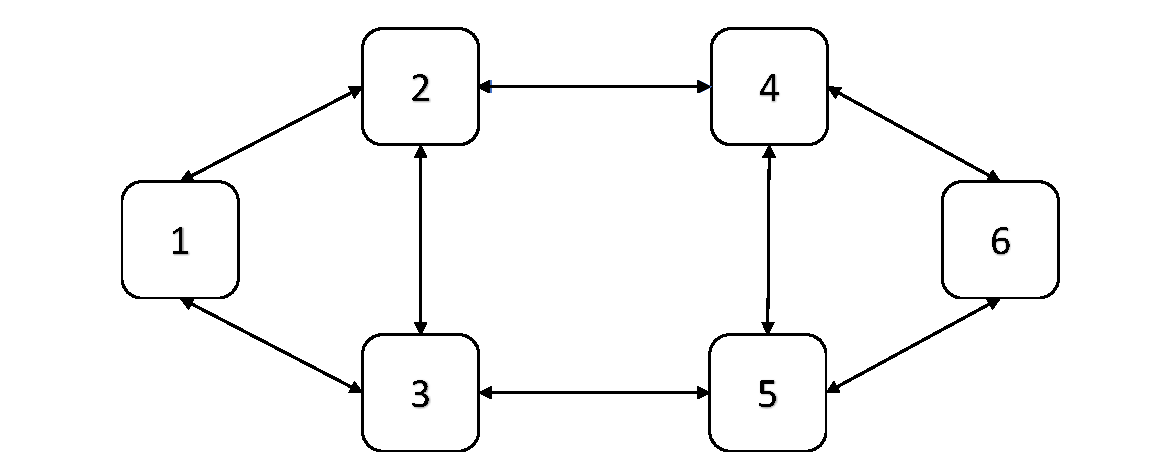
\includegraphics[width=\textwidth]{sdf/reference_network/figures/RedeTeste}
\caption{Physical topology of the reference network.}
\end{figure}

\vspace{11pt}
The distance matrix for this reference network is the same regardless of its associated traffic.
The values indicated in the distance matrix, referred to below, are expressed in kilometers (Km) and, as it could not be otherwise, this matrix is symmetric because the distance from $1$ to $2$ must be the same as $2$ to $1$.\\

\[
Dist=
  \begin{bmatrix}
    0 & 500 & 500 & 0 & 0 & 0 \\
    500 & 0 & 400 & 500 & 0 & 0 \\
    500 & 400 & 0 & 0 & 500 & 0 \\
    0 & 500 & 0 & 0 & 600 & 450 \\
    0 & 0 & 500 & 600 & 0 & 550 \\
    0 & 0 & 0 & 450 & 550 & 0
  \end{bmatrix}
\]

\newpage
For this project has to take into consideration the table \ref{table_ref_net} because in it we can see the values of the variables associated with this network.\\

\begin{table}[h!]
\centering
\begin{tabular}{|| c | c | c||}
 \hline
 Constant & Description & Value \\
 \hline\hline
 N & Number of nodes & 6 \\
 L & Number of bidirectional links & 8 \\
 <$\delta$> & Node out-degree & 2.667 \\
 <len> & Mean link length (km) & 500 \\
 <h> & Mean number of hops for working paths & 1.533 \\
 <h'> & Mean number of hops for backup paths & 2.467 \\
 \hline
\end{tabular}
\caption{Table of reference network values}
\label{table_ref_net}
\end{table}


\section{Traffic Matrices}\label{Reference_Network_Traffic}
\begin{tcolorbox}	
\begin{tabular}{p{2.75cm} p{0.2cm} p{10.5cm}} 	
\textbf{Student Name}  &:& Tiago Esteves    (October 03, 2017 - )\\
\end{tabular}
\end{tcolorbox}
\vspace{11pt}

For a better interpretation of the later results we will assume three traffic models for this network.
Being the first model with a low traffic scenario, the second with a medium traffic scenario and a last one with a high traffic scenario.
For each scenario it will be necessary to create different traffic matrices and to know the traffic of the network we will use five matrices of traffic.
These traffic matrices are represented by ODU0, ODU1, ODU2, ODU3 and ODU4 where each one has a certain data rate.
The ODU0 corresponds to 1.25 Gbits/s, the ODU1 corresponds to 2.5 Gbits/s, the ODU2 corresponds to 10 Gbits/s, the ODU3 corresponds to 40 Gbits/s and finally the ODU4 corresponds to 100 Gbits/s.
As we can see below, these arrays are bi-directional because they are symmetric arrays and as such, the traffic sent in a certain direction must be the same traffic sent in that opposite direction.

\subsection{Low traffic scenario}\label{low_traffic_scenario}

The traffic matrices for this scenario are:

\[
ODU0=
  \begin{bmatrix}
    0 & 5 & 1 & 3 & 1 & 3 \\
    5 & 0 & 0 & 1 & 5 & 0 \\
    1 & 0 & 0 & 1 & 4 & 1 \\
    3 & 1 & 1 & 0 & 1 & 1 \\
    1 & 5 & 4 & 1 & 0 & 3 \\
    3 & 0 & 1 & 1 & 3 & 0
  \end{bmatrix}
\quad ODU1=
  \begin{bmatrix}
    0 & 2 & 4 & 2 & 0 & 5 \\
    2 & 0 & 0 & 3 & 1 & 1 \\
    4 & 0 & 0 & 1 & 1 & 0 \\
    2 & 3 & 1 & 0 & 1 & 3 \\
    0 & 1 & 1 & 1 & 0 & 1 \\
    5 & 1 & 0 & 3 & 1 & 0
  \end{bmatrix}
\quad ODU2=
  \begin{bmatrix}
    0 & 1 & 1 & 1 & 0 & 0 \\
    1 & 0 & 0 & 0 & 1 & 0 \\
    1 & 0 & 0 & 1 & 1 & 0 \\
    1 & 0 & 1 & 0 & 1 & 0 \\
    0 & 1 & 1 & 1 & 0 & 1 \\
    0 & 0 & 0 & 0 & 1 & 0
  \end{bmatrix}
\]
\[
ODU3=
  \begin{bmatrix}
    0 & 0 & 0 & 0 & 0 & 0 \\
    0 & 0 & 1 & 0 & 0 & 1 \\
    0 & 1 & 0 & 0 & 1 & 0 \\
    0 & 0 & 0 & 0 & 0 & 0 \\
    0 & 0 & 1 & 0 & 0 & 0 \\
    0 & 1 & 0 & 0 & 0 & 0
  \end{bmatrix}
\qquad ODU4=
  \begin{bmatrix}
    0 & 0 & 0 & 0 & 0 & 0 \\
    0 & 0 & 0 & 0 & 0 & 1 \\
    0 & 0 & 0 & 0 & 0 & 0 \\
    0 & 0 & 0 & 0 & 0 & 0 \\
    0 & 0 & 0 & 0 & 0 & 1 \\
    0 & 1 & 0 & 0 & 1 & 0
  \end{bmatrix}
\]

\vspace{17pt}
Through these ODU's we can calculate total network traffic for the low traffic scenario:\\

$T_1^0$ = 60x1.25 = 75 Gbits/s \qquad
$T_1^1$ = 50x2.5 = 125 Gbits/s \qquad
$T_1^2$ = 16x10 = 160 Gbits/s \\

$T_1^3$ = 6x40 = 240 Gbits/s \quad
$T_1^4$ = 4x100 = 400 Gbits/s \\

$T_{1}$ = 75 + 125 + 160 + 240 + 400 = 1000 Gbits/s \qquad
$T$ = 1000/2 = \textbf{0.5 Tbits/s}\\

Where the variable $T_1^x$ represents the unidirectional traffic of the ODUx, for example, $T_1^0$ represents the unidirectional traffic of the ODU0 and $T_1^1$ represents the unidirectional traffic of the ODU1. The variable $T_{1}$ represents the total of unidirectional traffic that is injected into the network and finally the variable $T$ represents the total of bidirectional traffic.\\

\subsection{Medium traffic scenario}\label{medium_traffic_scenario}

The traffic matrices for this scenario are:

\[
ODU0=
  \begin{bmatrix}
    0 & 0 & 0 & 0 & 0 & 0 \\
    0 & 0 & 0 & 0 & 0 & 0 \\
    0 & 0 & 0 & 0 & 0 & 0 \\
    0 & 0 & 0 & 0 & 0 & 0 \\
    0 & 0 & 0 & 0 & 0 & 0 \\
    0 & 0 & 0 & 0 & 0 & 0
  \end{bmatrix}
\quad ODU1=
  \begin{bmatrix}
    0 & 2 & 0 & 4 & 6 & 0 \\
    2 & 0 & 0 & 4 & 2 & 2 \\
    0 & 0 & 0 & 2 & 2 & 2 \\
    4 & 4 & 2 & 0 & 0 & 0 \\
    6 & 2 & 2 & 0 & 0 & 6 \\
    0 & 2 & 2 & 0 & 6 & 0
  \end{bmatrix}
\quad ODU2=
  \begin{bmatrix}
    0 & 0 & 2 & 6 & 0 & 0 \\
    0 & 0 & 2 & 0 & 2 & 2 \\
    2 & 2 & 0 & 0 & 4 & 2 \\
    6 & 0 & 0 & 0 & 2 & 0 \\
    0 & 2 & 4 & 2 & 0 & 0 \\
    0 & 2 & 2 & 0 & 0 & 0
  \end{bmatrix}
\]
\[
ODU3=
  \begin{bmatrix}
    0 & 0 & 0 & 0 & 0 & 0 \\
    0 & 0 & 0 & 0 & 0 & 0 \\
    0 & 0 & 0 & 0 & 0 & 0 \\
    0 & 0 & 0 & 0 & 0 & 0 \\
    0 & 0 & 0 & 0 & 0 & 0 \\
    0 & 0 & 0 & 0 & 0 & 0
  \end{bmatrix}
\qquad ODU4=
  \begin{bmatrix}
    0 & 2 & 0 & 2 & 2 & 0 \\
    2 & 0 & 4 & 2 & 0 & 2 \\
    0 & 4 & 0 & 0 & 0 & 2 \\
    2 & 2 & 0 & 0 & 2 & 0 \\
    2 & 0 & 0 & 2 & 0 & 0 \\
    0 & 2 & 2 & 0 & 0 & 0
  \end{bmatrix}
\]

\newpage
Through these ODU's we can calculate total network traffic for the low traffic scenario:\\

$T_1^0$ = 0x1.25 = 0 Gbits/s \qquad
$T_1^1$ = 64x2.5 = 160 Gbits/s \qquad
$T_1^2$ = 44x10 = 440 Gbits/s \\

$T_1^3$ = 0x40 = 0 Gbits/s \quad
$T_1^4$ = 36x100 = 3600 Gbits/s \\

$T_{1}$ = 0 + 160 + 440 + 0 + 3600 = 4200 Gbits/s \qquad
$T$ = 4200/2 = \textbf{2.1 Tbits/s}\\

\subsection{High traffic scenario}\label{high_traffic_scenario}

The traffic matrices for this scenario are:

\[
ODU0=
  \begin{bmatrix}
    0 & 50 & 10 & 30 & 10 & 30 \\
    50 & 0 & 0 & 10 & 50 & 0 \\
    10 & 0 & 0 & 10 & 40 & 10 \\
    30 & 10 & 10 & 0 & 10 & 0 \\
    10 & 50 & 40 & 10 & 0 & 30 \\
    30 & 0 & 10 & 10 & 30 & 0
  \end{bmatrix}
\quad ODU1=
  \begin{bmatrix}
    0 & 20 & 40 & 20 & 0 & 50 \\
    20 & 0 & 0 & 30 & 10 & 10 \\
    40 & 0 & 0 & 10 & 10 & 0 \\
    30 & 30 & 10 & 0 & 10 & 30 \\
    0 & 10 & 10 & 10 & 0 & 10 \\
    50 & 10 & 0 & 30 & 10 & 0
  \end{bmatrix}
\]
\[
ODU2=
  \begin{bmatrix}
    0 & 10 & 10 & 10 & 0 & 0 \\
    10 & 0 & 0 & 0 & 10 & 0 \\
    10 & 0 & 0 & 10 & 10 & 0 \\
    10 & 0 & 10 & 0 & 10 & 0 \\
    0 & 10 & 10 & 10 & 0 & 10 \\
    0 & 0 & 0 & 0 & 10 & 0
  \end{bmatrix}
\quad ODU3=
  \begin{bmatrix}
    0 & 0 & 0 & 0 & 0 & 0 \\
    0 & 0 & 10 & 0 & 0 & 10 \\
    0 & 10 & 0 & 0 & 10 & 0 \\
    0 & 0 & 0 & 0 & 0 & 0 \\
    0 & 0 & 10 & 0 & 0 & 0 \\
    0 & 10 & 0 & 0 & 0 & 0
  \end{bmatrix}
\]
\[
ODU4=
  \begin{bmatrix}
    0 & 0 & 0 & 0 & 0 & 0 \\
    0 & 0 & 0 & 0 & 0 & 10 \\
    0 & 0 & 0 & 0 & 0 & 0 \\
    0 & 0 & 0 & 0 & 0 & 0 \\
    0 & 0 & 0 & 0 & 0 & 10 \\
    0 & 10 & 0 & 0 & 10 & 0
  \end{bmatrix}
\]

\vspace{17pt}
Through these ODU's we can calculate total network traffic for the low traffic scenario:\\

$T_1^0$ = 600x1.25 = 750 Gbits/s \quad
$T_1^1$ = 500x2.5 = 1205 Gbits/s \quad
$T_1^2$ = 160x10 = 1600 Gbits/s \\

$T_1^3$ = 60x40 = 2400 Gbits/s \quad
$T_1^4$ = 40x100 = 4000 Gbits/s \\

$T_{1}$ = 750 + 1250 + 1600 + 2400 + 4000 = 10000 Gbits/s \qquad
$T$ = 10000/2 = \textbf{5 Tbits/s}\\




%
% ------------------------------------------------------------------------
\chapter{Integer Linear Programming}
\label{chap_ilp}
ILP models are used to design networks that describe real components and their capabilities through a set of linear equations. Despite their quality, the solutions obtained through these models, depending on the number of variables and computational resources, can take days, months or even years \cite{ILP01}.
The current chapter is to propose and describe an optimization model for calculating the capital expenditures of the network, based on the three modes of transport (opaque, transparent and translucent) without survivability and protection.
In the following sections it is proposed in detail the restrictions of the three models previously mentioned, without survivability and with protection as well as a detailed report of the obtained results for each case.

%Subsection with the different transport mode
\clearpage

\subsection{Opaque without Survivability}\label{ILP_Opaque_Survivability}
\begin{tcolorbox}	
\begin{tabular}{p{2.75cm} p{0.2cm} p{10.5cm}} 	
\textbf{Student Name}  &:& Tiago Esteves    (October 03, 2017 - )\\
\textbf{Goal}          &:& Implement the ILP model for the opaque transport mode without survivability.
\end{tabular}
\end{tcolorbox}

\subsubsection{Model description}

First, for a better understanding of the functions and variables used in the ILP, a table \ref{description_opaque} will be created with all indexes, inputs and variables and with their respective description.\\

\begin{table}[h!]
\centering
\begin{tabular}{ |p{1cm}||p{13cm}|}
 \hline
 \multicolumn{2}{|c|}{Description of notation used in the objective function} \\
 \hline
 \hline
 $i$ & index for start node of a physical link \\
 $j$ & index for end node of a physical link \\
 $o$ & index for node that is origin of a demand \\
 $d$ & index for node that is destination of a demand \\
 $c$ & index for bit rate of the client signal \\
 $($ i,j $)$ & physical link between the nodes $i$ and $j$ \\
 $($ o,d $)$ & demand between the nodes $o$ and $d$ \\
 $C$ & set of the client signal \\
 $f_{ij}^{od}$ & binary variable indicating if link between the nodes $i$ and $j$ is used in the path between nodes $o$ and $d$ \\
 $L_{ij}$ & binary variable indicating if link between the nodes $i$ and $j$ is used \\
 $W_{ij}$ & number of optical channels between the nodes $i$ and $j$\\
 $B_c $ & client signals granularities $($1.25, 2.5, 10, 40, 100$)$ \\
 $D_{odc}$ & client demands with bit rate $c$ between nodes $o$ and $d$ \\
 $G_{ij}$ & network topology in form of adjacency matrix \\
 \hline
\end{tabular}
\caption{Table with description of variables}
\label{description_opaque}
\end{table}

Before carrying out the description of the objective function we must take into account the following particularity of this mode of transport:
\begin{itemize}
  \item $N_{OXC,n}$ = 0, \quad $\forall$ n
  \item $N_{EXC,n}$ = 1, \quad $\forall$ n that process traffic
\end{itemize}


\vspace{11pt}
The objective function of following the ILP is a minimization of the CAPEX through the equation \ref{Capex} where in this case for the cost of nodes we only have in consideration the electric cost \ref{Capex_Node_EXC} because of the particularity previously mentioned.
In this case the value of $P_{exc,c,n}$ is obtained by equation \ref{EXC_pexc1_opaque} for long-reach and by the equation \ref{EXC_pexc2_opaque} for short-reach.\\

\newpage
As previously mentioned, equation \ref{EXC_pexc1_opaque} refers to the number of long-reach ports, that is, the number of line ports of node n is calculated.

\begin{equation}
P_{exc,-1,n} = \sum_{j=1}^{N} w_{nj}
\label{EXC_pexc1_opaque}
\end{equation}

\begin{itemize}
\item{$P_{exc,-1,n}$	$\rightarrow$	Number of long-reach ports of the electrical switch, i.e. number of line ports}
\item{$w_{nj}$			$\rightarrow$	Number of optical channels between node $n$ and node $j$}
\end{itemize}

\vspace{11pt}
As previously mentioned, equation \ref{EXC_pexc2_opaque} refers to the number of sort-reach ports, that is, the number of tributary ports with bit-rate c in node n is calculated.

\begin{equation}
P_{exc,c,n} = \sum_{d=1}^{N} D_{nd,c}
\label{EXC_pexc2_opaque}
\end{equation}

\begin{itemize}
\item{$P_{exc,c,n}$	$\rightarrow$	Number of sort-reach ports of the electrical switch}
\item{$D_{nj,c}$	$\rightarrow$	client demands between nodes $n$ and $d$ with bit rate $c$}
\end{itemize}

\vspace{11pt}
In this case there is the following particularity:

\begin{itemize}
  \item When $n$=$j$ the value of client demands is always zero, i.e, $D_{nn,c}=0$
\end{itemize}


\vspace{17pt}
The objective function, to be minimized, is the expression \ref{ILPOpaque_CAPEX}.\\


$subject$ $to$
\begin{equation}
\sum_{j\textbackslash \{o\}} f_{ij}^{od} = 1  \qquad \qquad \qquad \qquad \qquad \qquad \qquad \qquad \qquad \qquad
\forall(o,d) : o < d, \forall i: i = o
\label{ILPOpaque1_Surv}
\end{equation}

This constraint are equal to the constraint \ref{ILPOpaque1_CAPEX} assuming that Z variable has the value of 1.

\begin{equation}
\sum_{j\textbackslash \{o\}} f_{ij}^{od} = \sum_{j\textbackslash \{d\}} f_{ji}^{od}   \qquad \qquad \qquad \qquad \qquad \qquad \qquad \qquad
\forall(o,d) : o < d, \forall i: i \neq o,d
\label{ILPOpaque2_Surv}
\end{equation}

This constraint are equal to the constraint \ref{ILPOpaque2_CAPEX}.

\begin{equation}
\sum_{j\textbackslash \{d\}} f_{ji}^{od} = 1  \qquad \qquad \qquad \qquad \qquad \qquad \qquad \qquad \qquad \qquad
\forall(o,d) : o < d, \forall i: i = d
\label{ILPOpaque3_Surv}
\end{equation}

This constraint are equal to the constraint \ref{ILPOpaque3_CAPEX} assuming that Z variable has the value of 1.

\begin{equation}
\sum_{(o,d):o<d} \left(f_{ij}^{od} + f_{ji}^{od}\right) + \sum_{c\in C} (B\left(c\right) D_{odc}\leq100 W_{ij} G_{ij} \qquad \qquad \qquad \qquad
\forall(i,j) : i < j
\label{ILPOpaque4_Surv}
\end{equation}

This restriction is considered grooming constraint, so it means the total client traffic flows can not be greater than the capacity of optical channels on all links.

\begin{equation}
W_{ij} \leq K_{ij} L_{ij} \qquad  \qquad \qquad \qquad \qquad \qquad \qquad \qquad \qquad \qquad \qquad \qquad \qquad \forall(i,j) : i < j
\label{ILPOpaque5_Surv}
\end{equation}

This restriction concerns the capacity of the optical channels which must be less or equal to the maximum number of optical channels. For any situation the maximum number of optical channels supported by each transmission system is 80, i.e., $K_{ij}$ = 80.

\begin{equation}
f_{ij}^{od} , f_{ji}^{od} \in \{0,1\}   \qquad \qquad \qquad \qquad \qquad \qquad \qquad \qquad \qquad
\forall(i,j) : i < j, \forall(o,d) : o < d
\label{ILPOpaque6_Surv}
\end{equation}

The number of flows per demand in this case can be zero if there are no traffic demands or one if considering traffic.

\begin{equation}
W_{ij} \in \mathbb{N}  \qquad \qquad \qquad \qquad \qquad \qquad \qquad \qquad \qquad \qquad \qquad \qquad \qquad
\forall(i,j) : i < j
\label{ILPOpaque7_Surv}
\end{equation}

The last constraint is just needed to ensure the number optical of channels is a positive integer values greater than zero.\\

 
\subsubsection{Result description}

To perform the calculations using the implementation of the models described in previous subsection it is necessary to use a mathematical software tool. For this we will use MATLAB which is ideal for dealing with linear programming problems and can call the LPsolve through an external interface.\\
We already have all the necessary to obtain the CAPEX value for the reference network \ref{Reference_Network_Topology}. As described in the subsection of network traffic \ref{Reference_Network_Traffic}, we have three values of network traffic (low, medium and high traffic) so we have to obtain three different CAPEX.
The value of the CAPEX of the network will be calculated based on the costs of the equipment present in the table \ref{table_cost_ilp}.
\newpage
\begin{table}[h!]
\centering
\begin{tabular}{|| c | c||}
 \hline
 Equipment & Cost \\
 \hline\hline
 OLT without transponders & 15000 \euro \\
 Transponder & 5000 \euro/Gb \\
 Unidirectional Optical Amplifier & 4000 \euro \\
 EXC & 10000 \euro \\
 OXC & 20000 \euro \\
 EXC Port & 1000 \euro /Gb/s\\
 OXC Port & 2500 \euro /porto \\
 \hline
\end{tabular}
\caption{Table with costs}
\label{table_cost_ilp}
\end{table}


\textbf{Low Traffic Scenario:}\\

In this scenario we have to take into account the traffic calculated in \ref{low_traffic_scenario}. In figure \ref{link_opaque_surv_ref_low} we can see the number of optical channels and the number of amplifiers for each link calculated through MatLab.\\
 
\begin{figure}[h!]
\centering
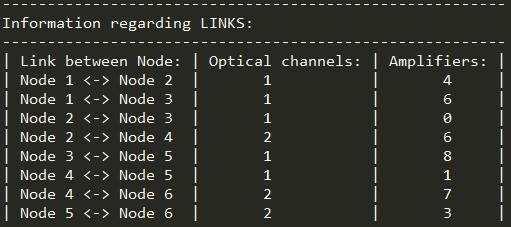
\includegraphics[width=10cm]{sdf/ilp/opaque_survivability/figures/link_opaque_surv_ref_low}
\caption{The ILP script used in the low scenario with the Link information.}
\label{link_opaque_surv_ref_low}
\end{figure}

In figure \ref{node_opaque_surv_ref_low}  we can see the number of transceivers, the number of line ports and the number of tributary ports for each node.\\

\begin{figure}[h!]
\centering
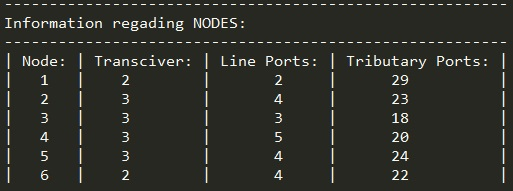
\includegraphics[width=10cm]{sdf/ilp/opaque_survivability/figures/node_opaque_surv_ref_low}
\caption{The ILP script used in the low scenario with the Node information.}
\label{node_opaque_surv_ref_low}
\end{figure}

Detailed description of each node:

Node 1:\\
- Needs 2 transceivers:\\
-- One to connect to Node 2;\\
-- One to connect to Node 3;\\
- Needs 2 line ports:\\
-- 1 line ports to connect to Node 2;\\
-- 1 line ports to connect to Node 3;\\
- Needs 29 tributary ports:\\
-- Where 13 is the ODU0;\\
-- Where 13 is the ODU1;\\
-- Where 3 is the ODU2;\\

Node 2:\\
- Needs 3 transceivers:\\
-- One to connect to Node 1;\\
-- One to connect to Node 3;\\
-- One to connect to Node 4;\\
- Needs 4 line ports:\\
-- 1 line ports to connect to Node 1;\\
-- 1 line ports to connect to Node 3;\\
-- 2 line ports to connect to Node 4;\\
- Needs 23 tributary ports:\\
-- Where 11 is the ODU0;\\
-- Where 7 is the ODU1;\\
-- Where 2 is the ODU2;\\
-- Where 2 is the ODU3;\\
-- Where 1 is the ODU4;\\

Node 3:\\
- Needs 3 transceivers:\\
-- One to connect to Node 1;\\
-- One to connect to Node 2;\\
-- One to connect to Node 5;\\
- Needs 3 line ports:\\
-- 1 line ports to connect to Node 1;\\
-- 1 line ports to connect to Node 2;\\
-- 1 line ports to connect to Node 5;\\
- Needs 18 tributary ports:\\
-- Where 7 is the ODU0;\\
-- Where 6 is the ODU1;\\
-- Where 3 is the ODU2;\\
-- Where 2 is the ODU3;\\

Node 4:\\
- Needs 3 transceivers:\\
-- One to connect to Node 2;\\
-- One to connect to Node 5;\\
-- One to connect to Node 6;\\
- Needs 5 line ports:\\
-- 2 line ports to connect to Node 2;\\
-- 1 line ports to connect to Node 5;\\
-- 2 line ports to connect to Node 6;\\
- Needs 20 tributary ports:\\
-- Where 7 is the ODU0;\\
-- Where 10 is the ODU1;\\
-- Where 3 is the ODU2;\\

Node 5:\\
- Needs 3 transceivers:\\
-- One to connect to Node 3;\\
-- One to connect to Node 4;\\
-- One to connect to Node 6;\\
- Needs 4 line ports:\\
-- 1 line ports to connect to Node 3;\\
-- 1 line ports to connect to Node 4;\\
-- 2 line ports to connect to Node 6;\\
- Needs 24 tributary ports:\\
-- Where 14 is the ODU0;\\
-- Where 4 is the ODU1;\\
-- Where 4 is the ODU2;\\
-- Where 1 is the ODU3;\\
-- Where 1 is the ODU4;\\

Node 6:\\
\quad - Needs 2 transceivers:\\
\quad \qquad - One to connect to Node 4;\\
\quad \qquad - One to connect to Node 5;\\
\quad - Needs 4 line ports:\\
\quad \qquad - 2 line ports to connect to Node 4;\\
\quad \qquad - 2 line ports to connect to Node 5;\\
\quad - Needs 22 tributary ports:\\
\quad \qquad - Where 8 is the ODU0;\\
\quad \qquad - Where 10 is the ODU1;\\
\quad \qquad - Where 1 is the ODU2;\\
\quad \qquad - Where 1 is the ODU3;\\
\quad \qquad - Where 2 is the ODU4;\\

Information regarding PATHS:\\

Path between Node1 <-> Node2:
\quad-Link(1,2)

Path between Node1 <-> Node3:
\quad-Link(1,3)

Path between Node1 <-> Node4:
\quad-Link(1,2) -Link(2,4)

Path between Node1 <-> Node5:
\quad-Link(1,3) -Link(3,5)

Path between Node1 <-> Node6:
\quad-Link(1,3) -Link(3,5) -Link(5,6)

Path between Node2 <-> Node3:
\quad-Link(2,3)

Path between Node2 <-> Node4:
\quad-Link(2,4)

Path between Node2 <-> Node5:
\quad-Link(2,3) -Link(3,5)

Path between Node2 <-> Node6:
\quad-Link(2,4) -Link(4,6)

Path between Node3 <-> Node4:
\quad-Link(3,2) -Link(2,4)

Path between Node3 <-> Node5:
\quad-Link(3,5)

Path between Node3 <-> Node6:
\quad-Link(3,5) -Link(5,6)

Path between Node4 <-> Node5:
\quad-Link(4,5)

Path between Node4 <-> Node6:
\quad-Link(4,6)

Path between Node5 <-> Node6:
\quad-Link(5,6)

\vspace{11pt}
Through the figure \ref{scriptopaque_surv_ref_low} we can see the result of CAPEX obtained with this ILP model.\\

\begin{figure}[h!]
\centering
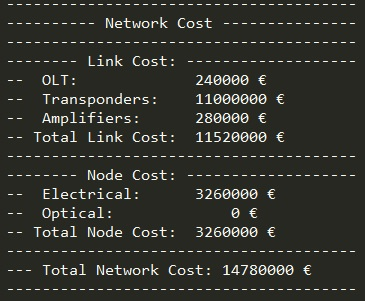
\includegraphics[width=10cm]{sdf/ilp/opaque_survivability/figures/script_opaque_surv_ref_low}
\caption{The ILP script used in the low scenario with the network cost.}
\label{scriptopaque_surv_ref_low}
\end{figure}

As we can see the cost of CAPEX for this scenario is \textbf{14 632 000 \euro}.\\


\textbf{Medium Traffic Scenario:}\\

In this scenario we have to take into account the traffic calculated in \ref{medium_traffic_scenario}. In table \ref{result_ILP2_reference} we can see the number of optical channels for each link calculated through MatLab and through the image \ref{scriptopaque_surv_ref_medium} we can see the results obtained with this ILP model.\\

\begin{table}[h!]
\centering
\begin{tabular}{|| c | c||}
 \hline
 Number of optical channels & Value \\
 \hline\hline
 in the link (1,2) & 5 \\
 in the link (1,3) & 3 \\
 in the link (2,3) & 5 \\
 in the link (2,4) & 8 \\
 in the link (3,5) & 5 \\
 in the link (4,5) & 3 \\
 in the link (4,6) & 3 \\
 in the link (5,6) & 3 \\
 \hline
\end{tabular}
\caption{Table with the number of optical channels for each link}
\label{result_ILP2_reference}
\end{table}


\begin{figure}[h!]
\centering
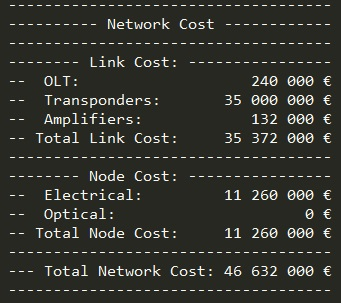
\includegraphics[width=10cm]{sdf/ilp/opaque_survivability/figures/script_opaque_surv_ref_medium}
\caption{The ILP script used in the medium scenario with the network cost.}
\label{scriptopaque_surv_ref_medium}
\end{figure}

As we can see the cost of CAPEX for this scenario is \textbf{46 632 000 \euro}.\\

\newpage
\textbf{High Traffic Scenario:}\\

In this scenario we have to take into account the traffic calculated in \ref{high_traffic_scenario}. In table \ref{result_ILP3_reference} we can see the number of optical channels for each link calculated through MatLab and through the image \ref{scriptopaque_surv_ref_high} we can see the results obtained with this ILP model.\\

\begin{table}[h!]
\centering
\begin{tabular}{|| c | c||}
 \hline
 Number of optical channels & Value \\
 \hline\hline
 in the link (1,2) & 4 \\
 in the link (1,3) & 4 \\
 in the link (2,3) & 4 \\
 in the link (2,4) & 19 \\
 in the link (3,5) & 9 \\
 in the link (4,5) & 5 \\
 in the link (4,6) & 16 \\
 in the link (5,6) & 14 \\
 \hline
\end{tabular}
\caption{Table with the number of optical channels for each link}
\label{result_ILP3_reference}
\end{table}


\begin{figure}[h!]
\centering
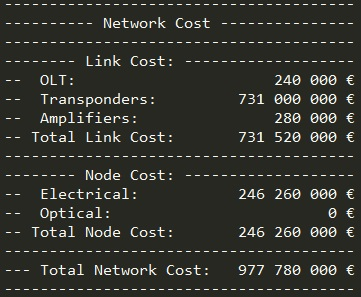
\includegraphics[width=10cm]{sdf/ilp/opaque_survivability/figures/script_opaque_surv_ref_high}
\caption{The ILP script used in the high scenario with the network cost.}
\label{scriptopaque_surv_ref_high}
\end{figure}

As we can see the cost of CAPEX for this scenario is \textbf{100 432 000 \euro}\\

\clearpage

\section{Opaque with 1+1 protection}\label{ILP_Opaque_Protection}

\subsection{Model description}

Once more, firstly in order to be able to apply the ILP model we have to take into account the physical and logical topologies allowed by this mode of transport and the type of survivability. Again based in section \ref{opaque} we can conclude that both topologies are the same and the following figures can be confirmed.\\

\begin{figure}[h!]
\centering
\includegraphics[width=10cm]{sdf/ilp/opaque_protection/figures/allowed_physical_topology}
\caption{Opaque with 1+1 protection: allowed physical topology. The allowed physical topology is defined by the duct and sites in the field. It is assumed that each duct supports up to 1 bidirectional transmission system and each site supports up to 1 node.}
\label{allowed_physical_protectionlow}
\end{figure}

\vspace{13pt}
\begin{figure}[h!]
\centering
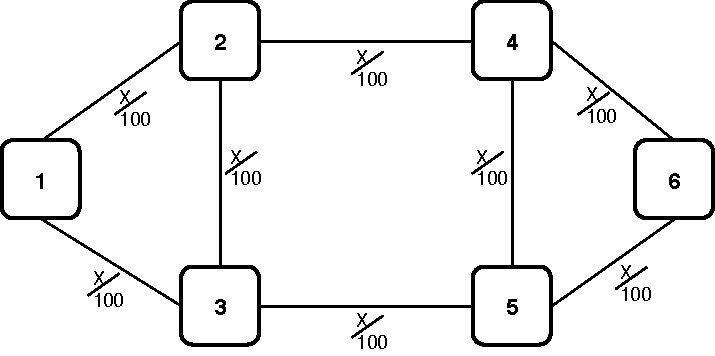
\includegraphics[width=10cm]{sdf/ilp/opaque_protection/figures/allowed_optical_topology}
\caption{Opaque with 1+1 protection: allowed optical topology. The allowed optical topology is defined by the transport mode. It is assumed that each transmission system supports up to 100 optical channels.}
\label{allowed_optical_protectionlow}
\end{figure}

Now taking this into account and based on the specific constraints of the opaque mode with 1+1 protection it is possible to define the ILP model \cite{tesevasco}.\\
\newpage
The objective function, to be minimized, is the expression \ref{Capex}, i.e.,

\begin{equation*}
  minimize \qquad \Big\{ \quad C_C \quad \Big\}
\end{equation*}

$subject$ $to$
\begin{equation}
\sum_{j=1\textbackslash \{o\}}^{N} fb_{ij}^{od} = 2  \qquad \qquad \qquad \qquad \qquad \qquad \qquad \qquad \qquad
\forall(o,d) : o < d, \forall i: i = o
\label{ILPOpaque1}
\end{equation}
\noindent
Constraint \ref{ILPOpaque1} is equal to the constraint \ref{ILPOpaque1_CAPEX} assuming that Z = 2.

\begin{equation}
\sum_{j=1\textbackslash \{o\}}^{N} fb_{ij}^{od} = \sum_{j=1\textbackslash \{d\}}^{N} f_{ji}^{od}   \qquad \qquad \qquad \qquad \qquad \qquad
\forall(o,d) : o < d, \forall i: i \neq o,d
\label{ILPOpaque2}
\end{equation}
\noindent
Constraint \ref{ILPOpaque2} is equal to the constraint \ref{ILPOpaque2_CAPEX}

\begin{equation}
\sum_{j=1\textbackslash \{d\}}^{N} fb_{ji}^{od} = 2  \qquad \qquad \qquad \qquad \qquad \qquad \qquad \qquad \qquad
\forall(o,d) : o < d, \forall i: i = d
\label{ILPOpaque3}
\end{equation}
\noindent
Constraint \ref{ILPOpaque3} is equal to the constraint \ref{ILPOpaque3_CAPEX} assuming that Z = 2.

\begin{equation}
\sum_{o=1}^{N} \sum_{d=o+1}^{N} \left(fb_{ij}^{od} + fb_{ji}^{od}\right) \sum_{c=1}^{C} (B\left(c\right) D_{odc})\leq \tau W_{ij} G_{ij} \qquad \qquad \qquad \qquad
\forall(i,j) : i < j
\label{ILPOpaque4}
\end{equation}
\noindent
The constraint \ref{ILPOpaque4} is considered the grooming constraint and is equal to the constraint \ref{ILPOpaque4_Surv} referred to in the case without survivability.

\begin{equation}
W_{ij} \leq K_{ij} L_{ij} \qquad \qquad \qquad \qquad \qquad \qquad \qquad \qquad \qquad \qquad \qquad \qquad \forall(i,j) : i < j
\label{ILPOpaque5}
\end{equation}
\noindent
Constraint \ref{ILPOpaque5} refers to the capacity of optical channels where they must be less or equal than the maximum number. For any situation, the maximum number of optical channels per transmission system is 100, that is, $K_{ij}$ = 100.

\begin{equation}
fb_{ij}^{od} , fb_{ji}^{od} , L_{ij} \in \{0,1\} \qquad \qquad \qquad \qquad \qquad \qquad \qquad
\forall(i,j) : i < j, \forall(o,d) : o < d
\label{ILPOpaque6}
\end{equation}
\noindent
The number of flows per demand in this case can be zero if there are no traffic demands or one if considering working or protection traffic, in relation to the use of the link, can be zero if it is not being used or one if is being used.
\newpage
\begin{equation}
W_{ij} \in \mathbb{N}  \qquad \qquad \qquad \qquad \qquad \qquad \qquad \qquad \qquad \qquad \qquad \qquad \qquad
\forall(i,j) : i < j\label{ILPOpaque7}
\end{equation}
\noindent
The last constraint is just needed to ensure the number of optical channels is a positive integer value.\\


\subsection{Result description}

As described in the subsection of network traffic \ref{Reference_Network_Traffic}, we have three values of network traffic so we have to obtain three different CAPEX.
The value of the CAPEX of the network will be calculated based on the costs of the equipment present in the table \ref{table_cost_ilp}.\\

\textbf{Low Traffic Scenario:}\\

In a first phase, we will show the resulting physical and optical topology. These topologies are based on the allowed topologies referred to in the model description and also taking into account the logical topology for all ODU's mentioned in the section \ref{low_scenario}.\\

\begin{figure}[h!]
\centering
\includegraphics[width=11cm]{sdf/ilp/opaque_protection/figures/physical_topology}
\caption{Opaque with 1+1 protection in low scenario: physical topology after dimensioning.}
\label{physical_protectionlow}
\end{figure}
\newpage
\begin{figure}[h!]
\centering
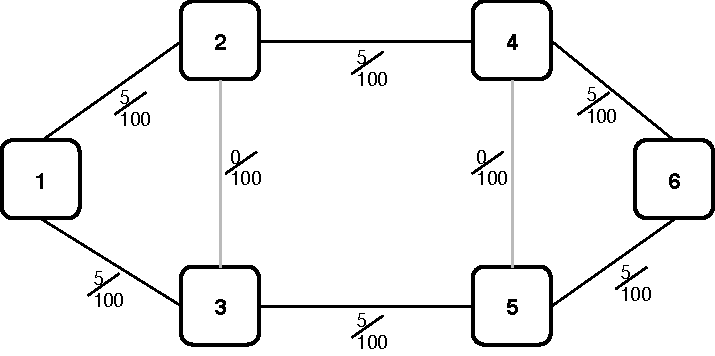
\includegraphics[width=11cm]{sdf/ilp/opaque_protection/figures/optical_topology_low}
\caption{Opaque with 1+1 protection in low scenario: optical topology after dimensioning.}
\label{optical_protectionlow}
\end{figure}

In table \ref{link_opaque_protec_ref_low} we can see the number of optical channels calculated using \ref{Capex_Link} and \ref{ILPOpaque_CAPEX} and the number of amplifiers for each link calculated using \ref{Capex_amplifiers}.

\begin{table}[h!]
\centering
\begin{tabular}{|| c | c | c ||}
 \hline
 \multicolumn{3}{|| c ||}{Information regarding links} \\
 \hline
 \hline
 Bidirectional Link & Optical Channels & Amplifiers\\
 \hline
 Node 1 <-> Node 2 & 2 & 4 \\
 Node 1 <-> Node 3 & 2 & 6 \\
 Node 2 <-> Node 3 & 3 & 0 \\
 Node 2 <-> Node 4 & 3 & 6 \\
 Node 3 <-> Node 5 & 3 & 8 \\
 Node 4 <-> Node 5 & 3 & 1 \\
 Node 4 <-> Node 6 & 3 & 7 \\
 Node 5 <-> Node 6 & 3 & 3 \\
 \hline
\end{tabular}
\caption{Table with information regarding links for opaque mode with 1+1 protection in low scenario.}
\label{link_opaque_protec_ref_low}
\end{table}

In table \ref{node_opaque_protec_ref_low} we can see the resulting nodal degree at the physical layer, calculated based on the number of connections that the node in question performs, the number of line ports calculated using \ref{EXC_pexc1_opaque} and the number of tributary ports calculated using \ref{EXC_pexc2_opaque} for each node.

\begin{table}[h!]
\centering
\begin{tabular}{|| c | c | c | c ||}
 \hline
 \multicolumn{4}{|| c ||}{Information regarding nodes} \\
 \hline
 \hline
 Node & Resulting Nodal Degree & Line Ports & Tributary Ports\\
 \hline
 1 & 2 & 4 & 29 \\
 2 & 3 & 8 & 23 \\
 3 & 3 & 8 & 18 \\
 4 & 3 & 9 & 20 \\
 5 & 3 & 9 & 24 \\
 6 & 2 & 6 & 22 \\
\hline
\end{tabular}
\caption{Table with information regarding nodes for opaque mode with 1+1 protection in low scenario.}
\label{node_opaque_protec_ref_low}
\end{table}
\newpage
Through the information obtained previously on the nodes we can now create tables with detailed information about each node. In each table mentioned below we can see how many ports are connected to a given node and its bit rate and how many ports are assigned to each different bit rate.

\begin{table}[h!]
\centering
\begin{tabular}{|| c | c | c ||}
 \hline
 \multicolumn{3}{|| c ||}{Detailed description of Node 1} \\
 \hline
 \hline
  & Number of tributary ports & Bit rate \\ \hline
\multirow{3}{*}{29 tributary ports} & 13 & ODU0 \\
 & 13 & ODU1 \\
 & 3 & ODU2 \\
 \hline
 \hline
  & Node<--Optical Channels-->Node & Bit rate \\
 \hline
 \multirow{2}{*}{4 line ports} & 1  <---- 2 ---->  2 & \multirow{2}{*}{100 Gbits/s} \\
 & 1  <---- 2 ---->  3 & \\
\hline
\end{tabular}
\caption{Opaque with 1+1 protection in low scenario: detailed description of node 1. The number of demands is distributed to the various destination nodes, this distribution can be observed in section \ref{low_scenario}.}
\end{table}

\begin{table}[h!]
\centering
\begin{tabular}{|| c | c | c ||}
 \hline
 \multicolumn{3}{|| c ||}{Detailed description of Node 2} \\
 \hline
 \hline
  & Number of total demands & Bit rate \\ \hline
\multirow{5}{*}{23 tributary ports} & 11 & ODU0 \\
 & 7 & ODU1 \\
 & 2 & ODU2 \\
 & 2 & ODU3 \\
 & 1 & ODU4 \\
 \hline
 \hline
  & Node<--Optical Channels-->Node & Bit rate \\ \hline
 \multirow{3}{*}{8 line ports} & 2  <---- 2 ---->  1 & \multirow{3}{*}{100 Gbits/s} \\
 & 2  <---- 3 ---->  3 & \\
 & 2  <---- 3 ---->  4 & \\
\hline
\end{tabular}
\caption{Opaque with 1+1 protection in low scenario: detailed description of node 2. The number of demands is distributed to the various destination nodes, this distribution can be observed in section \ref{low_scenario}.}
\end{table}

\begin{table}[h!]
\centering
\begin{tabular}{|| c | c | c ||}
 \hline
 \multicolumn{3}{|| c ||}{Detailed description of Node 3} \\
 \hline
 \hline
  & Number of total demands & Bit rate \\ \hline
\multirow{4}{*}{18 tributary ports} & 7 & ODU0 \\
 & 6 & ODU1\\
 & 3 & ODU2\\
 & 2 & ODU3\\
 \hline
 \hline
   & Node<--Optical Channels-->Node & Bit rate \\ \hline
 \multirow{3}{*}{8 line ports} & 3  <---- 2 ---->  1 & \multirow{3}{*}{100 Gbits/s}\\
 & 3  <---- 3 ---->  2 & \\
 & 3  <---- 3 ---->  5 & \\
\hline
\end{tabular}
\caption{Opaque with 1+1 protection in low scenario: detailed description of node 3. The number of demands is distributed to the various destination nodes, this distribution can be observed in section \ref{low_scenario}.}
\end{table}
\newpage
\begin{table}[h!]
\centering
\begin{tabular}{|| c | c | c ||}
 \hline
 \multicolumn{3}{|| c ||}{Detailed description of Node 4} \\
 \hline
 \hline
  & Number of total demands & Bit rate \\ \hline
\multirow{3}{*}{20 tributary ports} & 7 & ODU0 \\
 & 10 & ODU1 \\
 & 3 & ODU2 \\
 \hline
 \hline
   & Node<--Optical Channels-->Node & Bit rate \\ \hline
 \multirow{3}{*}{9 line ports} & 4  <---- 3 ---->  2 & \multirow{3}{*}{100 Gbits/s}\\
 & 4  <---- 3 ---->  5 & \\
 & 4  <---- 3 ---->  6 & \\
\hline
\end{tabular}
\caption{Opaque with 1+1 protection in low scenario: detailed description of node 4. The number of demands is distributed to the various destination nodes, this distribution can be observed in section \ref{low_scenario}.}
\end{table}

\begin{table}[h!]
\centering
\begin{tabular}{|| c | c | c ||}
 \hline
 \multicolumn{3}{|| c ||}{Detailed description of Node 5} \\
 \hline
 \hline
  & Number of total demands & Bit rate \\ \hline
\multirow{5}{*}{24 tributary ports} & 14 & ODU0 \\
 & 4 & ODU1 \\
 & 4 & ODU2 \\
 & 1 & ODU3 \\
 & 1 & ODU4 \\
 \hline
 \hline
   & Node<--Optical Channels-->Node & Bit rate \\ \hline
 \multirow{3}{*}{9 line ports} & 5  <---- 3 ---->  2 & \multirow{3}{*}{100 Gbits/s}\\
 & 5  <---- 3 ---->  4 & \\
 & 5  <---- 3 ---->  6 & \\
\hline
\end{tabular}
\caption{Opaque with 1+1 protection in low scenario: detailed description of node 5. The number of demands is distributed to the various destination nodes, this distribution can be observed in section \ref{low_scenario}.}
\end{table}

\begin{table}[h!]
\centering
\begin{tabular}{|| c | c | c ||}
 \hline
 \multicolumn{3}{|| c ||}{Detailed description of Node 6} \\
 \hline
 \hline
  & Number of total demands & Bit rate \\ \hline
\multirow{5}{*}{22 tributary ports} & 8 & ODU0 \\
 & 10 & ODU1 \\
 & 1 & ODU2 \\
 & 1 & ODU3 \\
 & 2 & ODU4 \\
 \hline
 \hline
   & Node<--Optical Channels-->Node & Bit rate \\ \hline
 \multirow{2}{*}{6 line ports} & 6  <---- 3 ---->  4 & \multirow{2}{*}{100 Gbits/s}\\
 & 6  <---- 3 ---->  5 & \\
\hline
\end{tabular}
\caption{Opaque with 1+1 protection in low scenario: detailed description of node 6. The number of demands is distributed to the various destination nodes, this distribution can be observed in section \ref{low_scenario}.}
\end{table}

\newpage
In the next table, we can see all the routing obtained for all nodes. These paths are bidirectional so the path from one node to another is the same path in the opposite direction. In the Links column we can see that there are two paths but it is not possible to distinguish them because we do not know which is protection and which is working.

\begin{table}[h!]
\centering
\begin{tabular}{|| c | c | c | c | c | c | c | c ||}
 \hline
 \multicolumn{8}{|| c ||}{Routing} \\
 \hline
 \hline
 o & d & Links & ODU0 & ODU1 & ODU2 & ODU3 & ODU4\\
 \hline
 \multirow{2}{*}{1} & \multirow{2}{*}{2} & \{(1,2)\} & \multirow{2}{*}{5} & \multirow{2}{*}{2} & \multirow{2}{*}{1} & \multirow{2}{*}{0} & \multirow{2}{*}{0} \\
 & & \{(1,3),(3,2)\} & & & & & \\ \hline
 \multirow{2}{*}{1} & \multirow{2}{*}{3} & \{(1,3)\} & \multirow{2}{*}{1} & \multirow{2}{*}{4} & \multirow{2}{*}{1} & \multirow{2}{*}{0} & \multirow{2}{*}{0}\\
 & & \{(1,2),(2,3)\} & & & & &\\ \hline
 \multirow{2}{*}{1} & \multirow{2}{*}{4} & \{(1,2),(2,4)\} & \multirow{2}{*}{3} & \multirow{2}{*}{2} & \multirow{2}{*}{1} & \multirow{2}{*}{0} & \multirow{2}{*}{0}\\
 & & \{(1,3),(3,5),(5,4)\} & & & & &\\ \hline
 \multirow{2}{*}{1} & \multirow{2}{*}{5} & \{(1,3),(3,5)\} & \multirow{2}{*}{1} & \multirow{2}{*}{0} & \multirow{2}{*}{0} & \multirow{2}{*}{0} & \multirow{2}{*}{0}\\
 & & \{(1,2),(2,4),(4,5)\} & & & & &\\ \hline
 \multirow{2}{*}{1} & \multirow{2}{*}{6} & \{(1,2),(2,4),(4,6)\} & \multirow{2}{*}{3} & \multirow{2}{*}{5} & \multirow{2}{*}{0} & \multirow{2}{*}{0} & \multirow{2}{*}{0}\\
 & & \{(1,3),(3,5),(5,6)\} & & & & &\\ \hline
 \multirow{2}{*}{2} & \multirow{2}{*}{3} & \{(2,3)\} & \multirow{2}{*}{0} & \multirow{2}{*}{0} & \multirow{2}{*}{0} & \multirow{2}{*}{1} & \multirow{2}{*}{0}\\
 & & \{(2,1),(1,3)\} & & & & &\\ \hline
 \multirow{2}{*}{2} & \multirow{2}{*}{4} & \{(2,4)\} & \multirow{2}{*}{1} & \multirow{2}{*}{3} & \multirow{2}{*}{0} & \multirow{2}{*}{0} & \multirow{2}{*}{0}\\
 & & \{(2,3),(3,5),(5,4)\} & & & & &\\ \hline
 \multirow{2}{*}{2} & \multirow{2}{*}{5} & \{(2,3),(3,5)\} & \multirow{2}{*}{5} & \multirow{2}{*}{1} & \multirow{2}{*}{1} & \multirow{2}{*}{0} & \multirow{2}{*}{0}\\
 & & \{(2,4),(4,5)\} & & & & &\\ \hline
 \multirow{2}{*}{2} & \multirow{2}{*}{6} & \{(2,4),(4,6)\} & \multirow{2}{*}{0} & \multirow{2}{*}{1} & \multirow{2}{*}{0} & \multirow{2}{*}{1} & \multirow{2}{*}{1}\\
 & & \{(2,3),(3,5),(5,6)\} & & & & &\\ \hline
 \multirow{2}{*}{3} & \multirow{2}{*}{4} & \{(3,2),(2,4)\} & \multirow{2}{*}{1} & \multirow{2}{*}{1} & \multirow{2}{*}{1} & \multirow{2}{*}{0} & \multirow{2}{*}{0}\\
 & & \{(3,5),(5,4)\} & & & & &\\ \hline
 \multirow{2}{*}{3} & \multirow{2}{*}{5} & \{(3,5)\} & \multirow{2}{*}{4} & \multirow{2}{*}{1} & \multirow{2}{*}{1} & \multirow{2}{*}{1} & \multirow{2}{*}{0}\\
 & & \{(3,1),(1,2),(2,4),(4,5)\} & & & & &\\ \hline
 \multirow{2}{*}{3} & \multirow{2}{*}{6} & \{(3,5),(5,6)\} & \multirow{2}{*}{1} & \multirow{2}{*}{0} & \multirow{2}{*}{0} & \multirow{2}{*}{0} & \multirow{2}{*}{0}\\
 & & \{(3,2),(2,4),(4,6)\} & & & & &\\ \hline
 \multirow{2}{*}{4} & \multirow{2}{*}{5} & \{(4,5)\} & \multirow{2}{*}{1} & \multirow{2}{*}{1} & \multirow{2}{*}{1} & \multirow{2}{*}{0} & \multirow{2}{*}{0}\\
 & & \{(4,6),(6,5)\} & & & & &\\ \hline
 \multirow{2}{*}{4} & \multirow{2}{*}{6} & \{(4,6)\} & \multirow{2}{*}{1} & \multirow{2}{*}{3} & \multirow{2}{*}{0} & \multirow{2}{*}{0} & \multirow{2}{*}{0}\\
 & & \{(4,5),(5,6)\} & & & & &\\ \hline
 \multirow{2}{*}{5} & \multirow{2}{*}{6} & \{(5,6)\} & \multirow{2}{*}{3} & \multirow{2}{*}{1} & \multirow{2}{*}{1} & \multirow{2}{*}{0} & \multirow{2}{*}{1}\\
 & & \{(5,4),(4,6)\} & & & & &\\
 \hline
\end{tabular}
\caption{Opaque with 1+1 protection in low scenario: description of routing. We are assuming that between a pair of nodes all demands follow the same route.}
\label{path_opaque_protec_ref_low}
\end{table}

Finally, in next page, through table \ref{scriptopaque_protec_ref_low} we can see the CAPEX result for this model. This value is obtained using equation \ref{ILPOpaque_CAPEX} and all of the constraints mentioned above.\\
\newpage
\begin{table}[h!]
\centering
\begin{tabular}{|| c | c | c | c | c | c | c ||}
 \hline
 \multicolumn{7}{|| c ||}{CAPEX of the Network} \\
 \hline
 \hline
 \multicolumn{3}{|| c |}{ } & Quantity & Unit Price & Cost & Total \\
 \hline
 \multirow{3}{*}{\makecell{Link \\ Cost}} & \multicolumn{2}{ c |}{OLTs} & 16 & 15 000 \euro & 240 000 \euro & \multirow{3}{*}{22 520 000 \euro} \\ \cline{2-6}
 & \multicolumn{2}{ c |}{100 Gbits/s Transceivers} & 44 & 5 000 \euro/Gbit/s & 22 000 000 \euro & \\ \cline{2-6}
 & \multicolumn{2}{ c |}{Amplifiers} & 70 & 4 000 \euro & 280 000 \euro & \\
 \hline
 \multirow{9}{*}{\makecell{Node \\ Cost}} & \multirow{7}{*}{Electrical} & EXCs & 6 & 10 000 \euro & 60 000 \euro & \multirow{9}{*}{4 462 590 \euro} \\ \cline{3-6}
 & & ODU0 Ports & 60 & 10 \euro/port & 600 \euro & \\ \cline{3-6}
 & & ODU1 Ports & 50 & 15 \euro/port & 750 \euro & \\ \cline{3-6}
 & & ODU2 Ports & 16 & 30 \euro/port & 480 \euro & \\ \cline{3-6}
 & & ODU3 Ports & 6 & 60 \euro/port & 360 \euro & \\ \cline{3-6}
 & & ODU4 Ports & 4 & 100 \euro/port & 400 \euro & \\ \cline{3-6}
 & & Line Ports & 44 & 100 000 \euro/port & 4 400 000 \euro & \\ \cline{2-6}
 & \multirow{2}{*}{Optical} & OXCs & 0 & 20 000 \euro & 0 \euro & \\ \cline{3-6}
 & & Ports & 0 & 2 500 \euro/porto & 0 \euro & \\
 \hline
 \multicolumn{6}{|| c |}{Total Network Cost} & 26 982 590 \euro \\
\hline
\end{tabular}
\caption{Opaque with 1+1 protection in low scenario: detailed description of CAPEX for this scenario.}
\label{scriptopaque_protec_ref_low}
\end{table}


\textbf{Medium Traffic Scenario:}\\

In a first phase, we will show the resulting physical and optical topology. These topologies are based on the allowed topologies referred to in the model description and also taking into account the logical topology for all ODU's mentioned in the section \ref{medium_traffic_scenario}.\\

\begin{figure}[h!]
\centering
\includegraphics[width=11cm]{sdf/ilp/opaque_protection/figures/physical_topology}
\caption{Opaque with 1+1 protection in medium scenario: physical topology after dimensioning.}
\label{physical_protectionmedium}
\end{figure}
\newpage
\begin{figure}[h!]
\centering
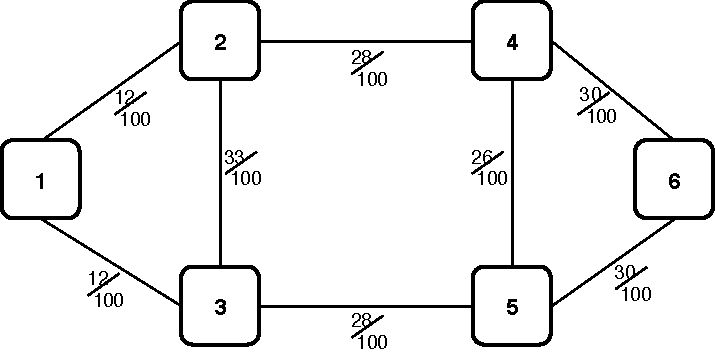
\includegraphics[width=11cm]{sdf/ilp/opaque_protection/figures/optical_topology_medium}
\caption{Opaque with 1+1 protection in medium scenario: optical topology after dimensioning.}
\label{optical_protectionmedium}
\end{figure}

Through table \ref{link_opaque_protec_ref_medium} we can see the number of optical channels calculated using \ref{Capex_Link} and \ref{ILPOpaque_CAPEX} and the number of amplifiers for each link calculated using \ref{Capex_amplifiers}.

\begin{table}[h!]
\centering
\begin{tabular}{|| c | c | c ||}
 \hline
 \multicolumn{3}{|| c ||}{Information regarding links} \\
 \hline
 \hline
 Bidirectional Link & Optical Channels & Amplifiers\\
 \hline
 Node 1 <-> Node 2 & 12 & 4 \\
 Node 1 <-> Node 3 & 12 & 6 \\
 Node 2 <-> Node 3 & 33 & 0 \\
 Node 2 <-> Node 4 & 28 & 6 \\
 Node 3 <-> Node 5 & 28 & 8 \\
 Node 4 <-> Node 5 & 26 & 1 \\
 Node 4 <-> Node 6 & 30 & 7 \\
 Node 5 <-> Node 6 & 30 & 3 \\
 \hline
\end{tabular}
\caption{Table with information regarding links for opaque mode with 1+1 protection in medium scenario.}
\label{link_opaque_protec_ref_medium}
\end{table}

We can see the resulting nodal degree at the physical layer, calculated based on the number of connections that the node in question performs, the number of line ports calculated using \ref{EXC_pexc1_opaque} and the number of tributary ports calculated using \ref{EXC_pexc2_opaque} for each node in table \ref{node_opaque_protec_ref_medium}.

\begin{table}[h!]
\centering
\begin{tabular}{|| c | c | c | c ||}
 \hline
 \multicolumn{4}{|| c ||}{Information regarding nodes} \\
 \hline
 \hline
 Node & Connections & Line Ports & Tributary Ports\\
 \hline
 1 & 2 & 24 & 290 \\
 2 & 3 & 73 & 230 \\
 3 & 3 & 73 & 180 \\
 4 & 3 & 84 & 200 \\
 5 & 3 & 84 & 240 \\
 6 & 2 & 60 & 220 \\
\hline
\end{tabular}
\caption{Table with information regarding nodes for opaque mode with 1+1 protection in medium scenario.}
\label{node_opaque_protec_ref_medium}
\end{table}

\newpage
Once more through the information obtained previously on the nodes we can now create tables with detailed information about each node. In each table mentioned below we can see how many ports are connected to a given node and its bit rate and how many ports are assigned to each different bit rate.

\begin{table}[h!]
\centering
\begin{tabular}{|| c | c | c ||}
 \hline
 \multicolumn{3}{|| c ||}{Detailed description of Node 1} \\
 \hline
 \hline
  & Number of total demands & bit rate \\ \hline
\multirow{3}{*}{290 tributary ports} & 130 & ODU0 \\
 & 130 & ODU1 \\
 & 30 & ODU2 \\
 \hline
 \hline
  & Node <-- Optical Channels --> Node & bit rate \\ \hline
\multirow{2}{*}{24 line ports} & 1  <---- 12 ---->  2 & \multirow{2}{*}{100 Gbtis/s} \\
 & 1  <---- 12 ---->  3 & \\
\hline
\end{tabular}
\caption{Opaque with 1+1 protection in medium scenario: detailed description of node 1. The number of demands is distributed to the various destination nodes, this distribution can be observed in section \ref{medium_traffic_scenario}.}
\end{table}

\begin{table}[h!]
\centering
\begin{tabular}{|| c | c | c ||}
 \hline
 \multicolumn{3}{|| c ||}{Detailed description of Node 2} \\
 \hline
 \hline
  & Number of total demands & bit rate \\ \hline
\multirow{5}{*}{230 tributary ports} & 110 & ODU0 \\
 & 70 & ODU1 \\
 & 20 & ODU2 \\
 & 20 & ODU3 \\
 & 10 & ODU4 \\
 \hline
 \hline
  & Node <-- Optical Channels --> Node & bit rate \\ \hline
 \multirow{3}{*}{73 line ports} & 2  <---- 12 ---->  1 & \multirow{3}{*}{100 Gbtis/s}\\
 & 2  <---- 33 ---->  3 & \\
 & 2  <---- 28 ---->  4 & \\
\hline
\end{tabular}
\caption{Opaque with 1+1 protection in medium scenario: detailed description of node 2. The number of demands is distributed to the various destination nodes, this distribution can be observed in section \ref{medium_traffic_scenario}.}
\end{table}

\begin{table}[h!]
\centering
\begin{tabular}{|| c | c | c ||}
 \hline
 \multicolumn{3}{|| c ||}{Detailed description of Node 3} \\
 \hline
 \hline
  & Number of total demands & bit rate \\ \hline
\multirow{4}{*}{180 tributary ports} & 70 & ODU0 \\
 & 60 & ODU1\\
 & 30 & ODU2\\
 & 20 & ODU3\\
  & Node <-- Optical Channels --> Node & bit rate \\ \hline
 \multirow{3}{*}{73 line ports} & 3  <---- 12 ---->  1 & \multirow{3}{*}{100 Gbtis/s}\\
 & 3  <---- 33 ---->  2 & \\
 & 3  <---- 28 ---->  5 & \\
\hline
\end{tabular}
\caption{Opaque with 1+1 protection in medium scenario: detailed description of node 3. The number of demands is distributed to the various destination nodes, this distribution can be observed in section \ref{medium_traffic_scenario}.}
\end{table}

\newpage
\begin{table}[h!]
\centering
\begin{tabular}{|| c | c | c ||}
 \hline
 \multicolumn{3}{|| c ||}{Detailed description of Node 4} \\
 \hline
 \hline
  & Number of total demands & bit rate \\ \hline
\multirow{3}{*}{200 tributary ports} & 70 & ODU0 \\
 & 100 & ODU1 \\
 & 30 & ODU2 \\
  & Node <-- Optical Channels --> Node & bit rate \\ \hline
\multirow{3}{*}{84 line ports} & 4  <---- 28 ---->  2 & \multirow{3}{*}{100 Gbtis/s}\\
 & 4  <---- 26 ---->  5 & \\
 & 4  <---- 30 ---->  6 & \\
\hline
\end{tabular}
\caption{Opaque with 1+1 protection in medium scenario: detailed description of node 4. The number of demands is distributed to the various destination nodes, this distribution can be observed in section \ref{medium_traffic_scenario}.}
\end{table}

\begin{table}[h!]
\centering
\begin{tabular}{|| c | c | c ||}
 \hline
 \multicolumn{3}{|| c ||}{Detailed description of Node 5} \\
 \hline
 \hline
  & Number of total demands & bit rate \\ \hline
\multirow{5}{*}{240 tributary ports} & 140 & ODU0 \\
 & 40 & ODU1 \\
 & 40 & ODU2 \\
 & 10 & ODU3 \\
 & 10 & ODU4 \\
  & Node <-- Optical Channels --> Node & bit rate \\ \hline
 \multirow{3}{*}{84 line ports} & 5  <---- 28 ---->  3 & \multirow{3}{*}{100 Gbtis/s} \\
 & 5  <---- 26 ---->  4 & \\
 & 5  <---- 30 ---->  6 & \\
\hline
\end{tabular}
\caption{Opaque with 1+1 protection in medium scenario: detailed description of node 5. The number of demands is distributed to the various destination nodes, this distribution can be observed in section \ref{medium_traffic_scenario}.}
\end{table}

\begin{table}[h!]
\centering
\begin{tabular}{|| c | c | c ||}
 \hline
 \multicolumn{3}{|| c ||}{Detailed description of Node 6} \\
 \hline
 \hline
  & Number of total demands & bit rate \\ \hline
\multirow{5}{*}{220 tributary ports} & 80 & ODU0 \\
 & 100 & ODU1 \\
 & 10 & ODU2 \\
 & 10 & ODU3 \\
 & 20 & ODU4 \\
  & Node <-- Optical Channels --> Node & bit rate \\ \hline
 \multirow{2}{*}{60 line ports} & 6  <---- 30 ---->  4 & \multirow{2}{*}{100 Gbtis/s} \\
 & 6  <---- 30 ---->  5 & \\
\hline
\end{tabular}
\caption{Opaque with 1+1 protection in medium scenario: detailed description of node 6. The number of demands is distributed to the various destination nodes, this distribution can be observed in section \ref{medium_traffic_scenario}.}
\end{table}

\newpage
Now let's focus on the routing information. These paths are bidirectional so the path from one node to another is the same path in the opposite direction. In table \ref{path_opaque_protec_ref_medium} we can see all the routing obtained for all nodes. In the Links column we can see that there are two paths but it is not possible to distinguish them because we do not know which is protection and which is working.\\

\begin{table}[h!]
\centering
\begin{tabular}{|| c | c | c | c | c | c | c | c ||}
 \hline
 \multicolumn{8}{|| c ||}{Routing} \\
 \hline
 \hline
 o & d & Links & ODU0 & ODU1 & ODU2 & ODU3 & ODU4\\
 \hline
 \multirow{2}{*}{1} & \multirow{2}{*}{2} & \{(1,2)\} & \multirow{2}{*}{50} & \multirow{2}{*}{20} & \multirow{2}{*}{10} & \multirow{2}{*}{0} & \multirow{2}{*}{0} \\
 & & \{(1,3),(3,2)\} & & & & & \\ \hline
 \multirow{2}{*}{1} & \multirow{2}{*}{3} & \{(1,3)\} & \multirow{2}{*}{10} & \multirow{2}{*}{40} & \multirow{2}{*}{10} & \multirow{2}{*}{0} & \multirow{2}{*}{0}\\
 & & \{(1,2),(2,3)\} & & & & &\\ \hline
 \multirow{2}{*}{1} & \multirow{2}{*}{4} & \{(1,2),(2,4)\} & \multirow{2}{*}{30} & \multirow{2}{*}{20} & \multirow{2}{*}{10} & \multirow{2}{*}{0} & \multirow{2}{*}{0}\\
 & & \{(1,3),(3,5),(5,4)\} & & & & &\\ \hline
 \multirow{2}{*}{1} & \multirow{2}{*}{5} & \{(1,3),(3,5)\} & \multirow{2}{*}{10} & \multirow{2}{*}{0} & \multirow{2}{*}{0} & \multirow{2}{*}{0} & \multirow{2}{*}{0}\\
 & & \{(1,2),(2,4),(4,5)\} & & & & &\\ \hline
 \multirow{2}{*}{1} & \multirow{2}{*}{6} & \{(1,2),(2,4),(4,6)\} & \multirow{2}{*}{30} & \multirow{2}{*}{50} & \multirow{2}{*}{0} & \multirow{2}{*}{0} & \multirow{2}{*}{0}\\
 & & \{(1,3),(3,5),(5,6)\} & & & & &\\ \hline
 \multirow{2}{*}{2} & \multirow{2}{*}{3} & \{(2,3)\} & \multirow{2}{*}{0} & \multirow{2}{*}{0} & \multirow{2}{*}{0} & \multirow{2}{*}{10} & \multirow{2}{*}{0}\\
 & & \{(2,1),(1,3)\} & & & & &\\ \hline
 \multirow{2}{*}{2} & \multirow{2}{*}{4} & \{(2,4)\} & \multirow{2}{*}{10} & \multirow{2}{*}{30} & \multirow{2}{*}{0} & \multirow{2}{*}{0} & \multirow{2}{*}{0}\\
 & & \{(2,3),(3,5),(5,4)\} & & & & &\\ \hline
 \multirow{2}{*}{2} & \multirow{2}{*}{5} & \{(2,4),(4,5)\} & \multirow{2}{*}{50} & \multirow{2}{*}{10} & \multirow{2}{*}{10} & \multirow{2}{*}{0} & \multirow{2}{*}{0}\\
 & & \{(2,3),(3,5)\} & & & & &\\ \hline
 \multirow{2}{*}{2} & \multirow{2}{*}{6} & \{(2,4),(4,6)\} & \multirow{2}{*}{0} & \multirow{2}{*}{10} & \multirow{2}{*}{0} & \multirow{2}{*}{10} & \multirow{2}{*}{10}\\
 & & \{(2,3),(3,5),(5,6)\} & & & & &\\ \hline
 \multirow{2}{*}{3} & \multirow{2}{*}{4} & \{(3,2),(2,4)\} & \multirow{2}{*}{10} & \multirow{2}{*}{10} & \multirow{2}{*}{10} & \multirow{2}{*}{0} & \multirow{2}{*}{0}\\
 & & \{(3,5),(5,4)\} & & & & &\\ \hline
 \multirow{2}{*}{3} & \multirow{2}{*}{5} & \{(3,5)\} & \multirow{2}{*}{40} & \multirow{2}{*}{10} & \multirow{2}{*}{10} & \multirow{2}{*}{10} & \multirow{2}{*}{0}\\
 & & \{(3,2),(2,4),(4,5)\} & & & & &\\ \hline
 \multirow{2}{*}{3} & \multirow{2}{*}{6} & \{(3,5),(5,6)\} & \multirow{2}{*}{10} & \multirow{2}{*}{0} & \multirow{2}{*}{0} & \multirow{2}{*}{0} & \multirow{2}{*}{0}\\
 & & \{(3,2),(2,4),(4,6)\} & & & & &\\ \hline
 \multirow{2}{*}{4} & \multirow{2}{*}{5} & \{(4,5)\} & \multirow{2}{*}{10} & \multirow{2}{*}{10} & \multirow{2}{*}{10} & \multirow{2}{*}{0} & \multirow{2}{*}{0}\\
 & & \{(4,6),(6,5)\} & & & & &\\ \hline
 \multirow{2}{*}{4} & \multirow{2}{*}{6} & \{(4,6)\} & \multirow{2}{*}{10} & \multirow{2}{*}{30} & \multirow{2}{*}{0} & \multirow{2}{*}{0} & \multirow{2}{*}{0}\\
 & & \{(4,5),(5,6)\} & & & & &\\ \hline
 \multirow{2}{*}{5} & \multirow{2}{*}{6} & \{(5,6)\} & \multirow{2}{*}{30} & \multirow{2}{*}{10} & \multirow{2}{*}{10} & \multirow{2}{*}{0} & \multirow{2}{*}{10}\\
 & & \{(5,4),(4,6)\} & & & & &\\
 \hline
\end{tabular}
\caption{Opaque with 1+1 protection in medium scenario: table with description of routing. We are assuming that between a pair of nodes all demands follow the same route.}
\label{path_opaque_protec_ref_medium}
\end{table}

Once more in next page, through table \ref{scriptopaque_protec_ref_medium} we can see the CAPEX result for this model. This value is obtained using equation \ref{ILPOpaque_CAPEX} and all of the constraints mentioned above.\\
\newpage
\begin{table}[h!]
\centering
\begin{tabular}{||c|c|c|c|c|c|c||}
 \hline
 \multicolumn{7}{||c||}{CAPEX of the Network} \\
 \hline
 \hline
 \multicolumn{3}{||c|}{}& Quantity & Unit Price & Cost & Total \\
 \hline
 \multirow{3}{*}{\makecell{Link \\ Cost}} & \multicolumn{2}{c|}{OLTs}&16&15 000 \euro&240 000 \euro&\multirow{3}{*}{199 520 000 \euro}\\ \cline{2-6}
 & \multicolumn{2}{c|}{100 Gbits/s Transceivers}&398&5 000 \euro/Gbit/s&199 000 000 \euro&\\ \cline{2-6}
 & \multicolumn{2}{c|}{Amplifiers}&70&4 000 \euro&280 000 \euro&\\
 \hline
 \multirow{9}{*}{\makecell{Node \\ Cost}}&\multirow{7}{*}{Electrical}&EXCs & 6 & 10 000 \euro & 60 000 \euro & \multirow{9}{*}{39 885 900 \euro} \\ \cline{3-6}
 & &ODU0 Ports& 600 & 10 \euro/port & 6 000 \euro & \\ \cline{3-6}
 & &ODU1 Ports& 500 & 15 \euro/port & 7 500 \euro & \\ \cline{3-6}
 & &ODU2 Ports& 160 & 30 \euro/port & 4 800 \euro & \\ \cline{3-6}
 & &ODU3 Ports& 60 & 60 \euro/port & 3 600 \euro & \\ \cline{3-6}
 & &ODU4 Ports& 40 & 100 \euro/port & 4 000 \euro & \\ \cline{3-6}
 & &Line Ports& 398 &100 000 \euro/port&39 800 000 \euro& \\ \cline{2-6}
 & \multirow{2}{*}{Optical} & OXCs & 0 & 20 000 \euro & 0 \euro & \\ \cline{3-6}
 & & Ports & 0 & 2 500 \euro/porto & 0 \euro & \\
 \hline
 \multicolumn{6}{|| c |}{Total Network Cost} & 239 405 900 \euro \\
\hline
\end{tabular}
\caption{Opaque with 1+1 protection in medium scenario: table with detailed description of CAPEX for this scenario.}
\label{scriptopaque_protec_ref_medium}
\end{table}


\textbf{High Traffic Scenario:}\\

In a first phase, we will show the resulting physical and optical topology. These topologies are based on the allowed topologies referred to in the model description and also taking into account the logical topology for all ODU's mentioned in the section \ref{high_traffic_scenario}.\\

\begin{figure}[h!]
\centering
\includegraphics[width=11cm]{sdf/ilp/opaque_protection/figures/physical_topology}
\caption{Opaque with 1+1 protection in high scenario: physical topology after dimensioning.}
\label{physical_protectionhigh}
\end{figure}

\newpage
\begin{figure}[h!]
\centering
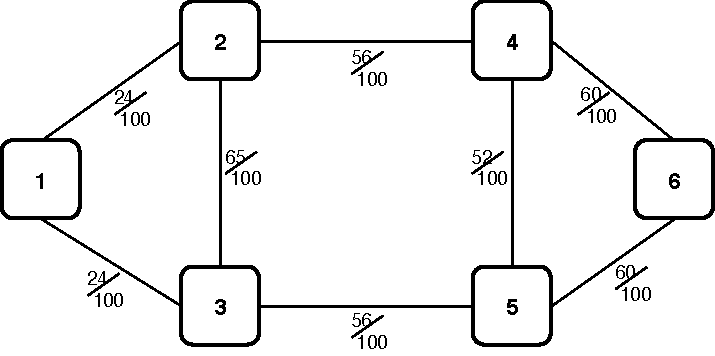
\includegraphics[width=11cm]{sdf/ilp/opaque_protection/figures/optical_topology_high}
\caption{Opaque with 1+1 protection in high scenario: optical topology after dimensioning.}
\label{optical_protectionhigh}
\end{figure}

In table \ref{link_opaque_protec_ref_high} we can see the number of optical channels calculated using \ref{Capex_Link} and \ref{Capex} and the number of amplifiers for each link calculated using \ref{amplifiers}.

\begin{table}[h!]
\centering
\begin{tabular}{|| c | c | c ||}
 \hline
 \multicolumn{3}{|| c ||}{Information regarding links} \\
 \hline
 \hline
 Bidirectional Link & Optical Channels & Amplifiers\\
 \hline
 Node 1 <-> Node 2 & 24 & 4 \\
 Node 1 <-> Node 3 & 24 & 6 \\
 Node 2 <-> Node 3 & 65 & 0 \\
 Node 2 <-> Node 4 & 56 & 6 \\
 Node 3 <-> Node 5 & 56 & 8 \\
 Node 4 <-> Node 5 & 52 & 1 \\
 Node 4 <-> Node 6 & 60 & 7 \\
 Node 5 <-> Node 6 & 60 & 3 \\
 \hline
\end{tabular}
\caption{Table with information regarding links for opaque mode with 1+1 protection in high scenario.}
\label{link_opaque_protec_ref_high}
\end{table}

In table \ref{node_opaque_protec_ref_high} we can see the resulting nodal degree at the physical layer, calculated based on the number of connections that the node in question performs, the number of line ports calculated using \ref{EXC_pexc1_opaque} and the number of tributary ports calculated using \ref{EXC_pexc2_opaque} for each node.

\begin{table}[h!]
\centering
\begin{tabular}{|| c | c | c | c ||}
 \hline
 \multicolumn{4}{|| c ||}{Information regarding nodes} \\
 \hline
 \hline
 Node & Resulting Nodal Degree & Line Ports & Tributary Ports\\
 \hline
 1 & 2 & 48 & 580 \\
 2 & 3 & 145 & 460 \\
 3 & 3 & 145 & 360 \\
 4 & 3 & 168 & 400 \\
 5 & 3 & 168 & 480 \\
 6 & 2 & 120 & 440 \\
\hline
\end{tabular}
\caption{Table with information regarding nodes for opaque mode with 1+1 protection in high scenario.}
\label{node_opaque_protec_ref_high}
\end{table}

\newpage
Once again, through the information obtained previously on the nodes we can now create tables with detailed information about each node. In each table mentioned below we can see how many ports are connected to a given node and its bit rate and how many ports are assigned to each different bit rate.

\begin{table}[h!]
\centering
\begin{tabular}{|| c | c | c ||}
 \hline
 \multicolumn{3}{|| c ||}{Detailed description of Node 1} \\
 \hline
 \hline
  & Number of total demands & bit rate \\ \hline
\multirow{3}{*}{580 tributary ports} & 260 & ODU0 \\
 & 260 & ODU1 \\
 & 60 & ODU2 \\
  & Node <-- Optical Channels --> Node & bit rate \\ \hline
\multirow{2}{*}{48 line ports} & 1  <---- 24 ---->  2 & \multirow{2}{*}{100 Gbtis/s} \\
 & 1  <---- 24 ---->  3 & \\
\hline
\end{tabular}
\caption{Opaque with 1+1 protection in high scenario: detailed description of node 1. The number of demands is distributed to the various destination nodes, this distribution can be observed in section \ref{high_traffic_scenario}.}
\end{table}

\begin{table}[h!]
\centering
\begin{tabular}{|| c | c | c ||}
 \hline
 \multicolumn{3}{|| c ||}{Detailed description of Node 2} \\
 \hline
 \hline
  & Number of total demands & bit rate \\ \hline
\multirow{5}{*}{460 tributary ports} & 220 & ODU0 \\
 & 140 & ODU1 \\
 & 40 & ODU2 \\
 & 40 & ODU3 \\
 & 20 & ODU4 \\
  & Node <-- Optical Channels --> Node & bit rate \\ \hline
 \multirow{3}{*}{145 line ports} & 2  <---- 24 ---->  1 & \multirow{3}{*}{100 Gbtis/s}\\
 & 2  <---- 65 ---->  3 & \\
 & 2  <---- 56 ---->  4 & \\
\hline
\end{tabular}
\caption{Opaque with 1+1 protection in high scenario: detailed description of node 2. The number of demands is distributed to the various destination nodes, this distribution can be observed in section \ref{high_traffic_scenario}.}
\end{table}

\begin{table}[h!]
\centering
\begin{tabular}{|| c | c | c ||}
 \hline
 \multicolumn{3}{|| c ||}{Detailed description of Node 3} \\
 \hline
 \hline
  & Number of total demands & bit rate \\ \hline
\multirow{4}{*}{360 tributary ports} & 140 & ODU0 \\
 & 120 & ODU1\\
 & 60 & ODU2\\
 & 40 & ODU3\\
  & Node <-- Optical Channels --> Node & bit rate \\ \hline
 \multirow{3}{*}{145 line ports} & 3  <---- 24 ---->  1 & \multirow{3}{*}{100 Gbtis/s}\\
 & 3  <---- 65 ---->  2 & \\
 & 3  <---- 56 ---->  5 & \\
\hline
\end{tabular}
\caption{Opaque with 1+1 protection in high scenario: detailed description of node 3. The number of demands is distributed to the various destination nodes, this distribution can be observed in section \ref{high_traffic_scenario}.}
\end{table}

\newpage
\begin{table}[h!]
\centering
\begin{tabular}{|| c | c | c ||}
 \hline
 \multicolumn{3}{|| c ||}{Detailed description of Node 4} \\
 \hline
 \hline
  & Number of total demands & bit rate \\ \hline
\multirow{3}{*}{400 tributary ports} & 140 & ODU0 \\
 & 200 & ODU1 \\
 & 60 & ODU2 \\
  & Node <-- Optical Channels --> Node & bit rate \\ \hline
\multirow{3}{*}{168 line ports} & 4  <---- 56 ---->  2 & \multirow{3}{*}{100 Gbtis/s}\\
 & 4  <---- 52 ---->  5 & \\
 & 4  <---- 60 ---->  6 & \\
\hline
\end{tabular}
\caption{Opaque with 1+1 protection in high scenario: detailed description of node 4. The number of demands is distributed to the various destination nodes, this distribution can be observed in section \ref{high_traffic_scenario}.}
\end{table}

\begin{table}[h!]
\centering
\begin{tabular}{|| c | c | c ||}
 \hline
 \multicolumn{3}{|| c ||}{Detailed description of Node 5} \\
 \hline
 \hline
  & Number of total demands & bit rate \\ \hline
\multirow{5}{*}{480 tributary ports} & 280 & ODU0 \\
 & 80 & ODU1 \\
 & 80 & ODU2 \\
 & 20 & ODU3 \\
 & 20 & ODU4 \\
  & Node <-- Optical Channels --> Node & bit rate \\ \hline
 \multirow{3}{*}{168 line ports} & 5  <---- 56 ---->  3 & \multirow{3}{*}{100 Gbtis/s} \\
 & 5  <---- 52 ---->  4 & \\
 & 5  <---- 60 ---->  6 & \\
\hline
\end{tabular}
\caption{Opaque with 1+1 protection in high scenario: detailed description of node 5. The number of demands is distributed to the various destination nodes, this distribution can be observed in section \ref{high_traffic_scenario}.}
\end{table}

\begin{table}[h!]
\centering
\begin{tabular}{|| c | c | c ||}
 \hline
 \multicolumn{3}{|| c ||}{Detailed description of Node 6} \\
 \hline
 \hline
  & Number of total demands & bit rate \\ \hline
\multirow{5}{*}{440 tributary ports} & 160 & ODU0 \\
 & 200 & ODU1 \\
 & 20 & ODU2 \\
 & 20 & ODU3 \\
 & 40 & ODU4 \\
  & Node <-- Optical Channels --> Node & bit rate \\ \hline
 \multirow{2}{*}{120 line ports} & 6  <---- 60 ---->  4 & \multirow{2}{*}{100 Gbtis/s} \\
 & 6  <---- 60 ---->  5 & \\
\hline
\end{tabular}
\caption{Opaque with 1+1 protection in high scenario: detailed description of node 6. The number of demands is distributed to the various destination nodes, this distribution can be observed in section \ref{high_traffic_scenario}.}
\end{table}

\newpage
Now through the table \ref{path_opaque_protec_ref_high} we can see all the routing obtained for all nodes. These paths are bidirectional so the path from one node to another is the same path in the opposite direction. In the Links column we can see that there are two paths but it is not possible to distinguish them because we do not know which is protection and which is working.

\begin{table}[h!]
\centering
\begin{tabular}{|| c | c | c | c | c | c | c | c ||}
 \hline
 \multicolumn{8}{|| c ||}{Routing} \\
 \hline
 \hline
 o & d & Links & ODU0 & ODU1 & ODU2 & ODU3 & ODU4\\
 \hline
 \multirow{2}{*}{1} & \multirow{2}{*}{2} & \{(1,2)\} & \multirow{2}{*}{100} & \multirow{2}{*}{40} & \multirow{2}{*}{20} & \multirow{2}{*}{0} & \multirow{2}{*}{0} \\
 & & \{(1,3),(3,2)\} & & & & & \\ \hline
 \multirow{2}{*}{1} & \multirow{2}{*}{3} & \{(1,3)\} & \multirow{2}{*}{20} & \multirow{2}{*}{80} & \multirow{2}{*}{20} & \multirow{2}{*}{0} & \multirow{2}{*}{0}\\
 & & \{(1,2),(2,3)\} & & & & &\\ \hline
 \multirow{2}{*}{1} & \multirow{2}{*}{4} & \{(1,2),(2,4)\} & \multirow{2}{*}{60} & \multirow{2}{*}{40} & \multirow{2}{*}{20} & \multirow{2}{*}{0} & \multirow{2}{*}{0}\\
 & & \{(1,3),(3,5),(5,4)\} & & & & &\\ \hline
 \multirow{2}{*}{1} & \multirow{2}{*}{5} & \{(1,3),(3,5)\} & \multirow{2}{*}{20} & \multirow{2}{*}{0} & \multirow{2}{*}{0} & \multirow{2}{*}{0} & \multirow{2}{*}{0}\\
 & & \{(1,2),(2,4),(4,5)\} & & & & &\\ \hline
 \multirow{2}{*}{1} & \multirow{2}{*}{6} & \{(1,2),(2,4),(4,6)\} & \multirow{2}{*}{60} & \multirow{2}{*}{100} & \multirow{2}{*}{0} & \multirow{2}{*}{0} & \multirow{2}{*}{0}\\
 & & \{(1,3),(3,5),(5,6)\} & & & & &\\ \hline
 \multirow{2}{*}{2} & \multirow{2}{*}{3} & \{(2,3)\} & \multirow{2}{*}{0} & \multirow{2}{*}{0} & \multirow{2}{*}{0} & \multirow{2}{*}{20} & \multirow{2}{*}{0}\\
 & & \{(2,1),(1,3)\} & & & & &\\ \hline
 \multirow{2}{*}{2} & \multirow{2}{*}{4} & \{(2,4)\} & \multirow{2}{*}{20} & \multirow{2}{*}{60} & \multirow{2}{*}{0} & \multirow{2}{*}{0} & \multirow{2}{*}{0}\\
 & & \{(2,3),(3,5),(5,4)\} & & & & &\\ \hline
 \multirow{2}{*}{2} & \multirow{2}{*}{5} & \{(2,4),(4,5)\} & \multirow{2}{*}{100} & \multirow{2}{*}{20} & \multirow{2}{*}{20} & \multirow{2}{*}{0} & \multirow{2}{*}{0}\\
 & & \{(2,3),(3,5)\} & & & & &\\ \hline
 \multirow{2}{*}{2} & \multirow{2}{*}{6} & \{(2,4),(4,6)\} & \multirow{2}{*}{0} & \multirow{2}{*}{20} & \multirow{2}{*}{0} & \multirow{2}{*}{20} & \multirow{2}{*}{20}\\
 & & \{(2,3),(3,5),(5,6)\} & & & & &\\ \hline
 \multirow{2}{*}{3} & \multirow{2}{*}{4} & \{(3,2),(2,4)\} & \multirow{2}{*}{20} & \multirow{2}{*}{20} & \multirow{2}{*}{20} & \multirow{2}{*}{0} & \multirow{2}{*}{0}\\
 & & \{(3,5),(5,4)\} & & & & &\\ \hline
 \multirow{2}{*}{3} & \multirow{2}{*}{5} & \{(3,5)\} & \multirow{2}{*}{80} & \multirow{2}{*}{20} & \multirow{2}{*}{20} & \multirow{2}{*}{20} & \multirow{2}{*}{0}\\
 & & \{(3,2),(2,4),(4,5)\} & & & & &\\ \hline
 \multirow{2}{*}{3} & \multirow{2}{*}{6} & \{(3,5),(5,6)\} & \multirow{2}{*}{20} & \multirow{2}{*}{0} & \multirow{2}{*}{0} & \multirow{2}{*}{0} & \multirow{2}{*}{0}\\
 & & \{(3,2),(2,4),(4,6)\} & & & & &\\ \hline
 \multirow{2}{*}{4} & \multirow{2}{*}{5} & \{(4,5)\} & \multirow{2}{*}{20} & \multirow{2}{*}{20} & \multirow{2}{*}{20} & \multirow{2}{*}{0} & \multirow{2}{*}{0}\\
 & & \{(4,6),(6,5)\} & & & & &\\ \hline
 \multirow{2}{*}{4} & \multirow{2}{*}{6} & \{(4,6)\} & \multirow{2}{*}{20} & \multirow{2}{*}{60} & \multirow{2}{*}{0} & \multirow{2}{*}{0} & \multirow{2}{*}{0}\\
 & & \{(4,5),(5,6)\} & & & & &\\ \hline
 \multirow{2}{*}{5} & \multirow{2}{*}{6} & \{(5,6)\} & \multirow{2}{*}{60} & \multirow{2}{*}{20} & \multirow{2}{*}{20} & \multirow{2}{*}{0} & \multirow{2}{*}{20}\\
 & & \{(5,4),(4,6)\} & & & & &\\
 \hline
\end{tabular}
\caption{Opaque with 1+1 protection in high scenario: description of routing. We are assuming that between a pair of nodes all demands follow the same route.}
\label{path_opaque_protec_ref_high}
\end{table}

Finally in next page, through table \ref{scriptopaque_protec_ref_high} we can see the CAPEX result for this model. This value is obtained using equation \ref{ILPOpaque_CAPEX} and all of the constraints mentioned above.\\
\newpage
\begin{table}[h!]
\centering
\begin{tabular}{||c|c|c|c|c|c|c||}
 \hline
 \multicolumn{7}{||c||}{CAPEX of the Network} \\
 \hline
 \hline
 \multicolumn{3}{||c|}{} & Quantity & Unit Price & Cost & Total \\
 \hline
 \multirow{3}{*}{\makecell{Link \\ Cost}} &\multicolumn{2}{c|}{OLTs}&16&15 000 \euro&240 000 \euro&\multirow{3}{*}{397 520 000 \euro}\\ \cline{2-6}
 & \multicolumn{2}{c|}{100 Gbits/s Transceivers}&794&5 000 \euro/Gbit/s&397 000 000 \euro&\\ \cline{2-6}
 & \multicolumn{2}{c|}{Amplifiers} & 70 & 4 000 \euro & 280 000 \euro & \\
 \hline
 \multirow{9}{*}{\makecell{Node \\ Cost}} &\multirow{7}{*}{Electrical}&EXCs&6& 10 000 \euro & 60 000 \euro & \multirow{9}{*}{79 511 800 \euro} \\ \cline{3-6}
 & &ODU0 Ports&1 200& 10 \euro/port & 12 000 \euro & \\ \cline{3-6}
 & &ODU1 Ports&1 000& 15 \euro/port & 15 000 \euro & \\ \cline{3-6}
 & &ODU2 Ports& 320 & 30 \euro/port & 9 600 \euro & \\ \cline{3-6}
 & &ODU3 Ports& 120 & 60 \euro/port & 7 200 \euro & \\ \cline{3-6}
 & &ODU4 Ports& 80 & 100 \euro/port & 8 000 \euro & \\ \cline{3-6}
 & &Line Ports& 794 &100 000 \euro/port&79 400 000 \euro&\\ \cline{2-6}
 & \multirow{2}{*}{Optical} & OXCs & 0 & 20 000 \euro & 0 \euro & \\ \cline{3-6}
 & & Ports & 0 & 2 500 \euro/porto & 0 \euro & \\
 \hline
 \multicolumn{6}{||c|}{Total Network Cost} &477 031 800 \euro \\
\hline
\end{tabular}
\caption{Opaque with 1+1 protection in high scenario: detailed description of CAPEX for this scenario.}
\label{scriptopaque_protec_ref_high}
\end{table}

\subsection{Conclusions}

Once we have obtained the results for all the scenarios we will now draw some conclusions about these results. For a better analysis of the results will be created the table \ref{table_comparative_opaque_protec} with the number of line ports, tributary ports and transceivers because they are important values for the cost of CAPEX, the cost of links, the cost of nodes and finally the cost of CAPEX.\\

\begin{table}[h!]
\centering
\begin{tabular}{| c | c | c | c |}
 \hline
  & Low Traffic & Medium Traffic  & High Traffic \\
 \hline\hline
 CAPEX without survivability&11 266 590 \euro&90 605 900 \euro&178 231 800 \euro\\ \hline
 CAPEX/Gbit/s without survivability&22 533 \euro/Gbit/s&18 121 \euro/Gbit/s&17 823 \euro/Gbit/s\\ \hline
 Traffic (Gbit/s) & 500 & 5 000 & 10 000 \\ \hline
 Bidirectional Links used & 8 & 8 & 8 \\ \hline
 Number of Line ports & 44 & 398 & 794 \\ \hline
 Number of Tributary ports & 136 & 1 360 & 2 720 \\ \hline
 Number of Transceivers & 44 & 398 & 794 \\ \hline
 Link Cost & 22 520 000 \euro & 199 520 000 \euro & 397 520 000 \euro \\ \hline
 Node Cost & 4 462 590 \euro & 39 885 900 \euro & 79 511 800 \euro \\ \hline
 CAPEX & \textbf{26 982 590 \euro} & \textbf{239 405 900 \euro} & \textbf{477 031 800 \euro} \\ \hline
 CAPEX/Gbit/s & \textbf{53 965 \euro/Gbit/s} & \textbf{47 881 \euro/Gbit/s} & \textbf{47 703 \euro/Gbit/s}\\
 \hline
\end{tabular}
\caption{Opaque with 1+1 protection: Table with the various CAPEX values obtained in the different traffic scenarios.}
\label{table_comparative_opaque_protec}
\end{table}

Looking at the previous table we can make some comparisons between the several scenarios:

\begin{itemize}
  \item All scenarios uses all available links. This is because in this case regardless of traffic we always need two possible paths.
  \item Comparing the low traffic with the others we can see that despite having an increase of factor ten (medium traffic) and factor twenty (high traffic), the same increase does not occur in the final cost (it is lower). This happens because the number of the transceivers is lower than expected which leads by carrying the traffic with less network components and, consequently, the network CAPEX is lower.
  \item Comparing the medium traffic with the high traffic we can see that the increase of the factor is double and in the final cost this factor is very close but still inferior. This happens because the number of the transceivers is also lower but very close to the expected.
  \item Comparing the CAPEX cost per bit we can see that in the low traffic the cost is higher than the medium and high traffic, which in these two cases the value is very similar. This happens because the lower the traffic, the higher CAPEX/bit will be. We can see that in medium and high traffic the results tend to be one closer value.
  \item Comparing this cost with the without survivability cost we can conclude that protection is significantly more expensive. As can be seen in the table this increase is more than double as with 1+1 protection we have a cost more than twice than the cost without survivability.
\end{itemize}

\clearpage

\subsection{Transparent without Survivability}\label{ILP_Transp_Survivability}
\begin{tcolorbox}	
\begin{tabular}{p{2.75cm} p{0.2cm} p{10.5cm}} 	
\textbf{Student Name}  &:& Tiago Esteves    (October 03, 2017 - )\\
\textbf{Goal}          &:& Implement the ILP model for the transparent transport mode without survivability.
\end{tabular}
\end{tcolorbox}

\subsubsection{Model description}

First, for a better understanding of the functions and variables used in the ILP, a table \ref{description_transp} will be created with all indexes, inputs and variables and with their respective description.

\begin{table}[h!]
\centering
\begin{tabular}{ |p{1cm}||p{13cm}|}
 \hline
 \multicolumn{2}{|c|}{Description of notation used in the objective function} \\
 \hline
 \hline
 $i$ & index for start node of a physical link \\
 $j$ & index for end node of a physical link \\
 $o$ & index for node that is origin of a demand \\
 $d$ & index for node that is destination of a demand \\
 $c$ & index for bit rate of the client signal \\
 $($ i,j $)$ & physical link between the nodes $i$ and $j$ \\
 $($ o,d $)$ & demand between the nodes $o$ and $d$ \\
 $C$ & set of the client signal \\
 $f_{ij}^{od}$ & the number of 100 Gbit/s optical channels between the nodes $o$ and $d$ that uses link ($i$,$j$) \\
 $fp_{ij}^{od}$ & the number of 100 Gbit/s optical channels (with protection) between the nodes $o$ and $d$ that uses link ($i$,$j$) \\
 $L_{ij}$ & binary variable indicating if link between the nodes $i$ and $j$ is used \\
 $\lambda_{od}$ & the number of 100 Gbit/s optical channels between the nodes $o$ and $d$ \\
 $D_{odc}$ & client demands between nodes $o$ and $d$ with bit rate $c$ \\
 $G$ & Network topology in form of adjacency matrix \\
 \hline
\end{tabular}
\caption{Table with description of variables}
\label{description_transp}
\end{table}

Before carrying out the description of the objective function we must take into account the following particularity of this mode of transport:
\begin{itemize}
  \item $N_{OXC,n}$ = 1, \quad $\forall$ n that process traffic
  \item $N_{EXC,n}$ = 1, \quad $\forall$ n that process traffic
\end{itemize}

\vspace{7pt}
The objective function of following the ILP is a minimization of the CAPEX through the equation \ref{Capex} where in this case for the cost of nodes we have in consideration electric \ref{Capex_Node_EXC} and optical cost \ref{Capex_Node_OXC}. In this case the value of $P_{exc,c,n}$ is obtained by equation \ref{EXC_pexc1_transparent} for short-reach and by the equation \ref{EXC_pexc2_transparent} for long-reach and the value of $P_{oxc,n}$ is obtained by equation \ref{OXC_poxc_transparent}.\\

The equation \ref{EXC_pexc1_transparent} refers to the number of sort-reach ports of the electrical switch with bit-rate $c$ in node $n$, $P_{exc,c,n}$, i.e. the number of tributary ports with bit-rate $c$ in node $n$ which can be calculated as

\begin{equation}
P_{exc,c,n} = \sum_{d=1}^{N} D_{nd,c}
\label{EXC_pexc1_transparent}
\end{equation}

\vspace{11pt}
\noindent
where $D_{nd,c}$ are the client demands between nodes $n$ and $d$ with bit rate $c$.\\

In this case there is the following particularity:
\begin{itemize}
  \item When $n$=$d$ the value of client demands is always zero, i.e, $D_{nn,c}=0$
\end{itemize}

\vspace{11pt}
As previously mentioned, the equation \ref{EXC_pexc2_transparent} refers to the number of long-reach ports of the electrical switch with bit-rate -1 in node n, $P_{exc,-1,n}$, i.e. the number of add ports of node n which can be calculated as

\begin{equation}
P_{exc,-1,n} = \sum_{j=1}^{N} \lambda_{nj}
\label{EXC_pexc2_transparent}
\end{equation}

\vspace{11pt}
\noindent
where $\lambda_{nj}$ is the number of optical channels between node $n$ and node $j$.\\

The equation \ref{OXC_poxc_transparent} refers to the number of ports in optical switch in node n, $P_{oxc,n}$, i.e. the number of line ports and the number of adding ports of node n which can be calculated as

\begin{equation}
P_{oxc,n} = \sum_{j=1}^{N} f_{nj}^{od} + \sum_{j=1}^{N} \lambda_{nj}
\label{OXC_poxc_transparent}
\end{equation}

\vspace{11pt}
\noindent
where $f_{nj}^{od}$ refers to the number of line ports for all demand pairs (od) and $\lambda_{nj}$ refers to the number of add ports.\\

The objective function, to be minimized, is the expression \ref{ILPOpaque_CAPEX}, i.e.,
\begin{equation*}
  minimize \qquad \Big\{ \quad C_C \quad \Big\}
\end{equation*}

$subject$ $to$
\begin{equation}
\sum_{c\in C} B\left(c\right) D_{odc} \leq \tau \lambda_{od} \qquad \qquad \qquad \qquad \qquad \qquad \qquad \qquad \qquad \qquad
\forall(o,d) : o < d
\label{ILPTransp0_surv}
\end{equation}

This restriction is considered grooming constraint and for this model the grooming can be done before routing since the traffic is aggregated just for demands between the same nodes, thus not depending on the routes. The variable  $\tau$ is always 100 Gbits/s.

\begin{equation}
\sum_{j\textbackslash \{o\}} f_{ij}^{od} = \lambda_{od}  \qquad \qquad \qquad \qquad \qquad \qquad \qquad \qquad \qquad
\forall(o,d) : o < d, \forall i: i = o
\label{ILPTransp1_surv}
\end{equation}

This constraint are equal to the constraint \ref{ILPOpaque1_CAPEX} assuming that Z variable has the value of number of optical channels between this demand for all bidirectional links.

\begin{equation}
\sum_{j\textbackslash \{o\}} f_{ij}^{od} = \sum_{j\textbackslash \{d\}} f_{ji}^{od} \qquad \qquad \qquad \qquad \qquad \qquad \qquad \qquad
\forall(o,d) : o < d, \forall i: i \neq o,d
\label{ILPTransp2_surv}
\end{equation}

This constraint are equal to the constraint \ref{ILPOpaque2_CAPEX}.

\begin{equation}
\sum_{j\textbackslash \{d\}} f_{ji}^{od} = \lambda_{od}  \qquad \qquad \qquad \qquad \qquad \qquad \qquad \qquad \qquad
\forall(o,d) : o < d, \forall i: i = d
\label{ILPTransp3_surv}
\end{equation}

This constraint are equal to the constraint \ref{ILPOpaque3_CAPEX} assuming that Z variable has the value of number of optical channels between this demand for all bidirectional links.

\begin{equation}
\sum_{o=1} \sum_{d=o+1} \left(f_{ij}^{od} + f_{ji}^{od}\right) \leq K_{ij} G_{ij} L_{ij} \qquad \qquad \qquad \qquad \qquad \qquad \qquad
\forall(i,j) : i < j
\label{ILPTransp4_surv}
\end{equation}

This restriction answers capacity constraint problem. Then, total flows must be less or equal to the capacity of network links. For any situation the maximum number of optical channels supported by each transmission system is 100, i.e., $K_{ij}$ = 100.

\begin{equation}
f_{ij}^{od} , f_{ji}^{od} , \lambda_{od} \in \mathbb{N}   \qquad \qquad \qquad \qquad \qquad \qquad \qquad \qquad
\forall(i,j) : i < j, \forall(o,d) : o < d
\label{ILPTransp5_surv}
\end{equation}

Last constraint define the total number of flows and the number of optical channels must be a counting number.\\


\subsubsection{Result description}

To perform the calculations using the implementation of the models described previously it is necessary to use a mathematical software tool. For this we will use MATLAB which is ideal for dealing with linear programming problems and can call the LPsolve through an external interface.\\
We already have all the necessary to obtain the CAPEX value for the reference network \ref{Reference_Network_Topology}. As described in the subsection of network traffic \ref{Reference_Network_Traffic}, we have three values of network traffic (low, medium and high traffic) so we have to obtain three different CAPEX.
The value of the CAPEX of the network will be calculated based on the costs of the equipment present in the table \ref{table_cost_ilp}.

\newpage
\textbf{Low Traffic Scenario:}\\

In this scenario we have to take into account the traffic calculated in \ref{low_scenario}. In a first phase we will show the various existing topologies of the network. The first are the allowed topologies, physical and optical topology, the second are the logical topology for all ODUs and finally the resulting physical and optical topology.\\

\begin{figure}[h!]
\centering
\includegraphics[width=12cm]{sdf/ilp/transparent_survivability/figures/allowed_physical_topology}
\caption{Allowed physical topology. The allowed physical topology is defined by the duct and sites in the field. It is assumed that each duct supports up to 1 bidirectional transmission system and each site supports up to 1 node.}
\label{allowed2_physical_low}
\end{figure}

\vspace{11pt}
\begin{figure}[h!]
\centering
\includegraphics[width=12cm]{sdf/ilp/transparent_survivability/figures/allowed_optical_topology}
\caption{Allowed optical topology. The allowed optical topology is defined by the transport mode (transparent transport mode in this case). It is assumed that each connections between demands supports up to 100 lightpaths.}
\label{allowed2_optical_low}
\end{figure}

\newpage
\begin{figure}[h!]
\centering
\includegraphics[width=12cm]{sdf/ilp/transparent_survivability/figures/logical_topology_ODU0_low}
\caption{ODU0 logical topology defined by the ODU0 traffic matrix.}
\label{logical2_ODU0_low}
\end{figure}

\begin{figure}[h!]
\centering
\includegraphics[width=12cm]{sdf/ilp/transparent_survivability/figures/logical_topology_ODU1_low}
\caption{ODU1 logical topology defined by the ODU1 traffic matrix.}
\label{logical2_ODU1_low}
\end{figure}

\begin{figure}[h!]
\centering
\includegraphics[width=12cm]{sdf/ilp/transparent_survivability/figures/logical_topology_ODU2_low}
\caption{ODU2 logical topology defined by the ODU2 traffic matrix.}
\label{logical2_ODU2_low}
\end{figure}

\begin{figure}[h!]
\centering
\includegraphics[width=12cm]{sdf/ilp/transparent_survivability/figures/logical_topology_ODU3_low}
\caption{ODU3 logical topology defined by the ODU3 traffic matrix.}
\label{logical2_ODU3_low}
\end{figure}

\begin{figure}[h!]
\centering
\includegraphics[width=12cm]{sdf/ilp/transparent_survivability/figures/logical_topology_ODU4_low}
\caption{ODU4 logical topology defined by the ODU4 traffic matrix.}
\label{logical2_ODU4_low}
\end{figure}

\begin{figure}[h!]
\centering
\includegraphics[width=12cm]{sdf/ilp/transparent_survivability/figures/physical_topology}
\caption{Physical topology after dimensioning.}
\label{physical2_low}
\end{figure}
\newpage
\begin{figure}[h!]
\centering
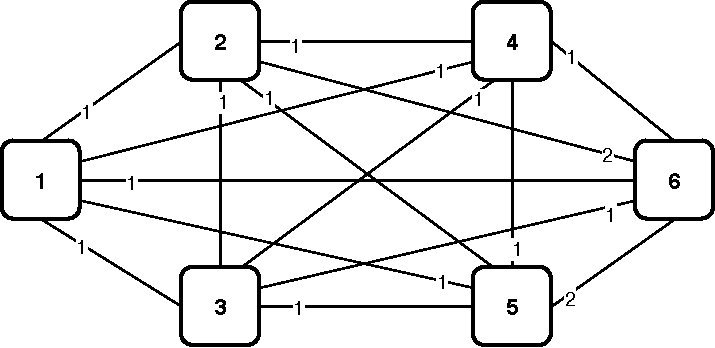
\includegraphics[width=11cm]{sdf/ilp/transparent_survivability/figures/optical_topology_low}
\caption{Optical topology after dimensioning.}
\label{optical2_low}
\end{figure}

In table \ref{link_transp_surv_ref_low} we can see the number of optical channels calculated using \ref{Capex_Link} and \ref{ILPOpaque_CAPEX} and the number of amplifiers for each link calculated using \ref{Capex_amplifiers}.

\begin{table}[h!]
\centering
\begin{tabular}{|| c | c | c ||}
 \hline
 \multicolumn{3}{|| c ||}{Information regarding links} \\
 \hline
 \hline
 Bidirectional Link & Optical Channels & Amplifiers\\
 \hline
 Node 1 <-> Node 2 & 3 & 4 \\
 Node 1 <-> Node 3 & 2 & 6 \\
 Node 2 <-> Node 3 & 3 & 0 \\
 Node 2 <-> Node 4 & 6 & 6 \\
 Node 3 <-> Node 5 & 4 & 8 \\
 Node 4 <-> Node 5 & 1 & 1 \\
 Node 4 <-> Node 6 & 4 & 7 \\
 Node 5 <-> Node 6 & 3 & 3 \\
 \hline
\end{tabular}
\caption{Table with information regarding links for transparent mode.}
\label{link_transp_surv_ref_low}
\end{table}

In table \ref{node_transp_surv_ref_low} we can see the number of line ports and add ports using \ref{OXC_poxc_transparent} the number of long-reach transponders using \ref{EXC_pexc2_transparent} and the number of tributary ports using \ref{EXC_pexc1_transparent}.

\begin{table}[h!]
\centering
\begin{tabular}{|| c | c | c | c | c | c ||}
 \hline
 \multicolumn{6}{|| c ||}{Information regarding nodes} \\
 \hline
 \hline
 \multicolumn{2}{|| c |}{ } & \multicolumn{2}{ c |}{Electrical part} & \multicolumn{2}{ c ||}{Optical part} \\
 \hline
 Node & Resulting Nodal Degree & Tributary Ports & LR Transponders & Add Ports & Line Ports\\
 \hline
 1 & 2 & 29 & 5 & 5 & 5 \\
 2 & 3 & 23 & 6 & 6 & 12 \\
 3 & 3 & 18 & 5 & 5 & 9 \\
 4 & 3 & 20 & 5 & 5 & 11 \\
 5 & 3 & 24 & 6 & 6 & 8 \\
 6 & 2 & 22 & 7 & 7 & 7 \\
\hline
\end{tabular}
\caption{Table with information regarding nodes for transparent mode.}
\label{node_transp_surv_ref_low}
\end{table}

\newpage
Through the information obtained previously on the nodes we can now create tables with detailed information about each node. In each table mentioned below we can see how many ports are connected to a given node and its bit rate (in relation to the line ports and the add ports) and how many ports are assigned to each different bit rate (in relation to the tributary ports).\\

\begin{table}[h!]
\centering
\begin{tabular}{|| c | c | c ||}
 \hline
 \multicolumn{3}{|| c ||}{Detailed description of Node 1} \\
 \hline
 \hline
 Electrical part & Number of total demands & Bit rate \\
 \hline
\multirow{3}{*}{29 tributary ports} & 13 & ODU0 \\
 & 13 & ODU1 \\
 & 3 & ODU2 \\
 \hline
  & Node<--Optical Channels-->Node & Bit rate \\
  \hline
\multirow{5}{*}{5 LR Transponders} & 1  <---- 1 ---->  2 & \multirow{5}{*}{100 Gbits/s} \\
  & 1  <---- 1 ---->  3 & \\
  & 1  <---- 1 ---->  4 & \\
  & 1  <---- 1 ---->  5 & \\
  & 1  <---- 1 ---->  6 & \\
 \hline
 \hline
 Optical part & Node<--Optical Channels-->Node & Bit rate \\
 \hline
 \multirow{5}{*}{5 add ports} & 1  <---- 1 ---->  2 & \multirow{10}{*}{100 Gbits/s} \\
  & 1  <---- 1 ---->  3 & \\
  & 1  <---- 1 ---->  4 & \\
  & 1  <---- 1 ---->  5 & \\
  & 1  <---- 1 ---->  6 & \\ \cline{1-2}
 \multirow{5}{*}{5 line ports} & 1  <---- 1 ---->  2 & \\
  & 1  <---- 1 ---->  3 & \\
  & 1  <---- 1 ---->  4 & \\
  & 1  <---- 1 ---->  5 & \\
  & 1  <---- 1 ---->  6 & \\
\hline
\end{tabular}
\caption{Table with detailed description of node 1. The number of demands is distributed to the various destination nodes, this distribution can be observed in section \ref{low_scenario}. Regarding the number of line ports when this node is equal to the source, it means that add ports are used, otherwise it means that through ports are used. In this node as we can see there are no through ports.}
\end{table}

\newpage
\begin{table}[h!]
\centering
\begin{tabular}{|| c | c | c ||}
 \hline
 \multicolumn{3}{|| c ||}{Detailed description of Node 2} \\
 \hline
 \hline
 Electrical part & Number of total demands & Bit rate \\ \hline
\multirow{5}{*}{23 tributary ports} & 11 & ODU0 \\
 & 7 & ODU1 \\
 & 2 & ODU2 \\
 & 2 & ODU3 \\
 & 1 & ODU4 \\
 \hline
  & Node<--Optical Channels-->Node & Bit rate \\
  \hline
\multirow{5}{*}{6 LR Transponders} & 2  <---- 1 ---->  1 & \multirow{5}{*}{100 Gbits/s} \\
  & 2  <---- 1 ---->  3 & \\
  & 2  <---- 1 ---->  4 & \\
  & 2  <---- 1 ---->  5 & \\
  & 2  <---- 2 ---->  6 & \\
 \hline
 \hline
 Optical part & Node<--Optical Channels-->Node & Bit rate \\
 \hline
 \multirow{5}{*}{6 add ports} & 2  <---- 1 ---->  1 & \multirow{13}{*}{100 Gbits/s} \\
  & 2  <---- 1 ---->  3 & \\
  & 2  <---- 1 ---->  4 & \\
  & 2  <---- 1 ---->  5 & \\
  & 2  <---- 2 ---->  6 & \\ \cline{1-2}
 \multirow{8}{*}{12 line ports} & 2  <---- 1 ---->  1 & \\
  & 2  <---- 1 ---->  3 & \\
  & 2  <---- 1 ---->  4 & \\
  & 2  <---- 1 ---->  5 & \\
  & 2  <---- 2 ---->  6 & \\
  & 1  <---- 1 ---->  4 & \\
  & 1  <---- 1 ---->  6 & \\
  & 3  <---- 1 ---->  4 & \\
\hline
\end{tabular}
\caption{Table with detailed description of node 2. The number of demands is distributed to the various destination nodes, this distribution can be observed in section \ref{low_scenario}. Regarding the number of line ports when this node is equal to the source, it means that add ports are used, otherwise it means that through ports are used. In both cases, the number of ports is double the number of optical channels.}
\end{table}

\newpage
\begin{table}[h!]
\centering
\begin{tabular}{|| c | c | c ||}
 \hline
 \multicolumn{3}{|| c ||}{Detailed description of Node 3} \\
 \hline
 \hline
 Electrical part & Number of total demands & Bit rate \\
 \hline
 \multirow{4}{*}{18 tributary ports} & 7 & ODU0 \\
 & 6 & ODU1\\
 & 3 & ODU2\\
 & 2 & ODU3\\
 \hline
  & Node<--Optical Channels-->Node & Bit rate \\ \hline
 \multirow{5}{*}{5 LR Transponders} & 3  <---- 1 ---->  1 & \multirow{5}{*}{100 Gbits/s} \\
  & 3  <---- 1 ---->  2 & \\
  & 3  <---- 1 ---->  4 & \\
  & 3  <---- 1 ---->  5 & \\
  & 3  <---- 1 ---->  6 & \\
 \hline
 \hline
 Optical part & Node<--Optical Channels-->Node & Bit rate \\
 \hline
 \multirow{5}{*}{5 add ports} & 3  <---- 1 ---->  1 & \multirow{12}{*}{100 Gbits/s} \\
  & 3  <---- 1 ---->  2 & \\
  & 3  <---- 1 ---->  4 & \\
  & 3  <---- 1 ---->  5 & \\
  & 3  <---- 1 ---->  6 & \\ \cline{1-2}
 \multirow{7}{*}{9 line ports} & 3  <---- 1 ---->  1 & \\
  & 3  <---- 1 ---->  2 & \\
  & 3  <---- 1 ---->  4 & \\
  & 3  <---- 1 ---->  5 & \\
  & 3  <---- 1 ---->  6 & \\
  & 1  <---- 1 ---->  5 & \\
  & 2  <---- 1 ---->  5 & \\
\hline
\end{tabular}
\caption{Table with detailed description of node 3. The number of demands is distributed to the various destination nodes, this distribution can be observed in section \ref{low_scenario}. Regarding the number of line ports when this node is equal to the source, it means that add ports are used, otherwise it means that through ports are used. In the latter the number of ports is double the number of optical channels.}
\end{table}

\newpage
\begin{table}[h!]
\centering
\begin{tabular}{|| c | c | c ||}
 \hline
 \multicolumn{3}{|| c ||}{Detailed description of Node 4} \\
 \hline
 \hline
 Electrical part & Number of total demands & Bit rate \\ \hline
\multirow{3}{*}{20 tributary ports} & 7 & ODU0 \\
 & 10 & ODU1 \\
 & 3 & ODU2 \\
 \hline
  & Node<--Optical Channels-->Node & Bit rate \\ \hline
 \multirow{5}{*}{5 LR Transponders} & 4  <---- 1 ---->  1 & \multirow{5}{*}{100 Gbits/s} \\
  & 4  <---- 1 ---->  2 & \\
  & 4  <---- 1 ---->  3 & \\
  & 4  <---- 1 ---->  5 & \\
  & 4  <---- 1 ---->  6 & \\
 \hline
 \hline
 Optical part & Node<--Optical Channels-->Node & Bit rate \\
 \hline
 \multirow{5}{*}{5 add ports} & 4  <---- 1 ---->  1 & \multirow{12}{*}{100 Gbits/s} \\
  & 4  <---- 1 ---->  2 & \\
  & 4  <---- 1 ---->  3 & \\
  & 4  <---- 1 ---->  5 & \\
  & 4  <---- 1 ---->  6 & \\ \cline{1-2}
 \multirow{7}{*}{11 line ports} & 4  <---- 1 ---->  1 & \\
  & 4  <---- 1 ---->  2 & \\
  & 4  <---- 1 ---->  3 & \\
  & 4  <---- 1 ---->  5 & \\
  & 4  <---- 1 ---->  6 & \\
  & 1  <---- 1 ---->  6 & \\
  & 2  <---- 2 ---->  6 & \\
\hline
\end{tabular}
\caption{Table with detailed description of node 4. The number of demands is distributed to the various destination nodes, this distribution can be observed in section \ref{low_scenario}. Regarding the number of line ports when this node is equal to the source, it means that add ports are used, otherwise it means that through ports are used. In the latter the number of ports is double the number of optical channels.}
\end{table}

\newpage
\begin{table}[h!]
\centering
\begin{tabular}{|| c | c | c ||}
 \hline
 \multicolumn{3}{|| c ||}{Detailed description of Node 5} \\
 \hline
 \hline
 Electrical part & Number of total demands & Bit rate \\ \hline
\multirow{5}{*}{24 tributary ports} & 14 & ODU0 \\
 & 4 & ODU1 \\
 & 4 & ODU2 \\
 & 1 & ODU3 \\
 & 1 & ODU4 \\
 \hline
  & Node<--Optical Channels-->Node & Bit rate \\ \hline
 \multirow{5}{*}{6 LR Trasponders} & 5  <---- 1 ---->  1 & \multirow{5}{*}{100 Gbits/s} \\
  & 5  <---- 1 ---->  2 & \\
  & 5  <---- 1 ---->  3 & \\
  & 5  <---- 1 ---->  4 & \\
  & 5  <---- 2 ---->  6 & \\
 \hline
 \hline
 Optical part & Node<--Optical Channels-->Node & Bit rate \\
 \hline
 \multirow{5}{*}{6 add ports} & 5  <---- 1 ---->  1 & \multirow{11}{*}{100 Gbits/s} \\
  & 5  <---- 1 ---->  2 & \\
  & 5  <---- 1 ---->  3 & \\
  & 5  <---- 1 ---->  4 & \\
  & 5  <---- 2 ---->  6 & \\ \cline{1-2}
 \multirow{6}{*}{8 line ports} & 5  <---- 1 ---->  1 & \\
  & 5  <---- 1 ---->  2 & \\
  & 5  <---- 1 ---->  3 & \\
  & 5  <---- 1 ---->  4 & \\
  & 5  <---- 2 ---->  6 & \\
  & 3  <---- 1 ---->  6 &\\
\hline
\end{tabular}
\caption{Table with detailed description of node 5. The number of demands is distributed to the various destination nodes, this distribution can be observed in section \ref{low_scenario}. Regarding the number of line ports when this node is equal to the source, it means that add ports are used, otherwise it means that through ports are used. In the latter the number of ports is double the number of optical channels.}
\end{table}

\newpage
\begin{table}[h!]
\centering
\begin{tabular}{|| c | c | c ||}
 \hline
 \multicolumn{3}{|| c ||}{Detailed description of Node 6} \\
 \hline
 \hline
 Electrical part & Number of total demands & Bit rate \\ \hline
\multirow{5}{*}{22 tributary ports} & 8 & ODU0 \\
 & 10 & ODU1 \\
 & 1 & ODU2 \\
 & 1 & ODU3 \\
 & 2 & ODU4 \\
 \hline
  & Node<--Optical Channels-->Node & Bit rate \\ \hline
 \multirow{5}{*}{7 LR Transponders} & 6  <---- 1 ---->  1 & \\
  & 6  <---- 2 ---->  2 & \\
  & 6  <---- 1 ---->  3 & \\
  & 6  <---- 1 ---->  4 & \\
  & 6  <---- 2 ---->  5 & \\
 \hline
 Optical part & Node<--Optical Channels-->Node & Bit rate \\
 \hline
 \multirow{5}{*}{7 add ports} & 6  <---- 1 ---->  1 & \multirow{10}{*}{100 Gbits/s} \\
  & 6  <---- 2 ---->  2 & \\
  & 6  <---- 1 ---->  3 & \\
  & 6  <---- 1 ---->  4 & \\
  & 6  <---- 2 ---->  5 & \\ \cline{1-2}
 \multirow{5}{*}{7 line ports} & 6  <---- 1 ---->  1 & \\
  & 6  <---- 2 ---->  2 & \\
  & 6  <---- 1 ---->  3 & \\
  & 6  <---- 1 ---->  4 & \\
  & 6  <---- 2 ---->  5 & \\
\hline
\end{tabular}
\caption{Table with detailed description of node 6. The number of demands is distributed to the various destination nodes, this distribution can be observed in section \ref{low_scenario}. Regarding the number of line ports when this node is equal to the source, it means that add ports are used, otherwise it means that through ports are used.  In this node as we can see there are no through ports.}
\end{table}

\vspace{17pt}
Now, in next page, let's focus on the routing information in table \ref{path_transp_surv_ref_low}. These paths are bidirectional so the path from one node to another is the same path in the opposite direction.\\
\newpage
\begin{table}[h!]
\centering
\begin{tabular}{|| c | c | c ||}
 \hline
 \multicolumn{3}{|| c ||}{Routing} \\
 \hline
 \hline
 o & d & Links \\
 \hline
 1 & 2 & \{(1,2)\} \\ \hline
 1 & 3 & \{(1,3)\} \\ \hline
 1 & 4 & \{(1,2),(2,4)\}\\ \hline
 1 & 5 & \{(1,3),(3,5)\}\\ \hline
 1 & 6 & \{(1,2),(2,4),(4,6)\}\\ \hline
 2 & 3 & \{(2,3)\}\\ \hline
 2 & 4 & \{(2,4)\}\\ \hline
 2 & 5 & \{(2,3),(3,5)\}\\ \hline
 2 & 6 & \{(2,4),(4,6)\}\\ \hline
 3 & 4 & \{(3,2),(2,4)\}\\ \hline
 3 & 5 & \{(3,5)\}\\ \hline
 3 & 6 & \{(3,5),(5,6)\}\\ \hline
 4 & 5 & \{(4,5)\}\\ \hline
 4 & 6 & \{(4,6)\}\\ \hline
 5 & 6 & \{(5,6)\}\\
 \hline
\end{tabular}
\caption{Table with description of routing.}
\label{path_transp_surv_ref_low}
\end{table}

Finally and most importantly through table \ref{scripttransp_surv_ref_low} we can see the CAPEX result for this model. This value is obtained using equation \ref{ILPOpaque_CAPEX} and all of the constraints mentioned above.\\

\begin{table}[h!]
\centering
\begin{tabular}{|| c | c | c | c | c | c | c ||}
 \hline
 \multicolumn{7}{|| c ||}{CAPEX of the Network} \\
 \hline
 \hline
 \multicolumn{3}{|| c |}{ } & Quantity & Unit Price & Cost & Total \\
 \hline
 \multirow{3}{*}{Link Cost} & \multicolumn{2}{ c |}{OLTs} & 16 & 15 000 \euro & 240 000 \euro & \multirow{3}{*}{26 520 000 \euro} \\ \cline{2-6}
 & \multicolumn{2}{ c |}{100 Gbits/s Transceivers} & 52 & 5 000 \euro/Gbit/s & 26 000 000 \euro & \\ \cline{2-6}
 & \multicolumn{2}{ c |}{Amplifiers} & 70 & 4 000 \euro & 280 000 \euro & \\
 \hline
 \multirow{10}{*}{Node Cost} & \multirow{7}{*}{Electrical} & EXCs & 6 & 10 000 \euro & 60 000 \euro & \multirow{10}{*}{3 797 590 \euro} \\ \cline{3-6}
 & & ODU0 Ports & 60 & 10 \euro/port & 600 \euro & \\ \cline{3-6}
 & & ODU1 Ports & 50 & 15 \euro/port & 750 \euro & \\ \cline{3-6}
 & & ODU2 Ports & 16 & 30 \euro/port & 480 \euro & \\ \cline{3-6}
 & & ODU3 Ports & 6 & 60 \euro/port & 360 \euro & \\ \cline{3-6}
 & & ODU4 Ports & 4 & 100 \euro/port & 400 \euro & \\ \cline{3-6}
 & &Transponders& 34 & 100 000 \euro/port & 3 400 000 \euro & \\ \cline{2-6}
 & \multirow{3}{*}{Optical} & OXCs & 6 & 20 000 \euro & 120 000 \euro & \\ \cline{3-6}
 & & Line Ports & 52 & 2 500 \euro/port & 130 000 \euro & \\ \cline{3-6}
 & & Add Ports & 34 & 2 500 \euro/port & 85 000 \euro & \\
 \hline
 \multicolumn{6}{|| c |}{Total Network Cost} & 30 317 590 \euro \\
\hline
\end{tabular}
\caption{Table with detailed description of CAPEX for this scenario.}
\label{scripttransp_surv_ref_low}
\end{table}

\newpage
All the values calculated in the previous table were obtained through the equations \ref{Capex_Link} and \ref{Capex_Node} referred to in section \ref{ILP_CAPEX}, but for a more detailed analysis we created table \ref{formulas_transp} where we can see how all the parameters are calculated individually.\\

\begin{table}[h!]
\centering
\begin{tabular}{|| c | c ||}
 \hline
  & Equation used to calculate the cost \\ \hline
 OLTs & \(\displaystyle 2 \sum_{i=1}^{N}\sum_{j=i+1}^{N} L_{ij} \gamma_0^{OLT} \) \\ \hline
 Transceivers & \(\displaystyle 2 \sum_{i=1}^{N}\sum_{j=i+1}^{N} L_{ij} f_{ij}^{od} \gamma_1^{OLT} \tau \) \\ \hline
 Amplifiers & \(\displaystyle 2 \sum_{i=1}^{N}\sum_{j=i+1}^{N} L_{ij} N^R_{ij} c^R \) \\ \hline
 EXCs & \(\displaystyle \sum_{n=1}^N N_{exc,n} \gamma_{e0} \) \\ \hline
 ODU0 Port & \(\displaystyle \sum_{n=1}^{N} \sum_{d=1}^{N} N_{exc,n} D_{nd,0} \gamma_{e1,0} \) \\ \hline
 ODU1 Port & \(\displaystyle \sum_{n=1}^{N} \sum_{d=1}^{N} N_{exc,n} D_{nd,1} \gamma_{e1,1} \) \\ \hline
 ODU2 Port & \(\displaystyle \sum_{n=1}^{N} \sum_{d=1}^{N} N_{exc,n} D_{nd,2} \gamma_{e1,2} \)\\ \hline
 ODU3 Port & \(\displaystyle \sum_{n=1}^{N} \sum_{d=1}^{N} N_{exc,n} D_{nd,3} \gamma_{e1,3} \) \\ \hline
 ODU4 Port & \(\displaystyle \sum_{n=1}^{N} \sum_{d=1}^{N} N_{exc,n} D_{nd,4} \gamma_{e1,4} \) \\ \hline
 LR Transponders & \(\displaystyle \sum_{n=1}^{N} \sum_{j=1}^{N} N_{exc,n} \lambda_{od} \gamma_{e1,-1} \) \\ \hline
 OXCs & \(\displaystyle \sum_{n=1}^N N_{oxc,n} \gamma_{o0} \) \\ \hline
 Add Port & \(\displaystyle \sum_{n=1}^{N} \sum_{j=1}^{N} N_{oxc,n} \lambda_{od} \gamma_{o1} \) \\ \hline
 Line Port & \(\displaystyle \sum_{n=1}^{N} \sum_{j=1}^{N} N_{oxc,n} f_{ij}^{od} \gamma_{o1} \) \\ \hline
 CAPEX & The final cost is calculated by summing all previous results. \\
 \hline
 \end{tabular}
\caption{Table with description of calculation}
\label{formulas_transp}
\end{table}

\newpage
\textbf{Medium Traffic Scenario:}\\

In this scenario we have to take into account the traffic calculated in \ref{medium_traffic_scenario}. In a first phase we will show the various existing topologies of the network. The first are the allowed topologies, physical and optical topology, the second are the logical topology for all ODUs and finally the resulting physical and optical topology.\\

\begin{figure}[h!]
\centering
\includegraphics[width=12cm]{sdf/ilp/transparent_survivability/figures/allowed_physical_topology}
\caption{Allowed physical topology. The allowed physical topology is defined by the duct and sites in the field. It is assumed that each duct supports up to 1 bidirectional transmission system and each site supports up to 1 node.}
\label{allowed2_physical_medium}
\end{figure}

\vspace{11pt}
\begin{figure}[h!]
\centering
\includegraphics[width=12cm]{sdf/ilp/transparent_survivability/figures/allowed_optical_topology}
\caption{Allowed optical topology. The allowed optical topology is defined by the transport mode (transparent transport mode in this case). It is assumed that each connections between demands supports up to 100 lightpaths.}
\label{allowed2_optical_medium}
\end{figure}

\newpage
\begin{figure}[h!]
\centering
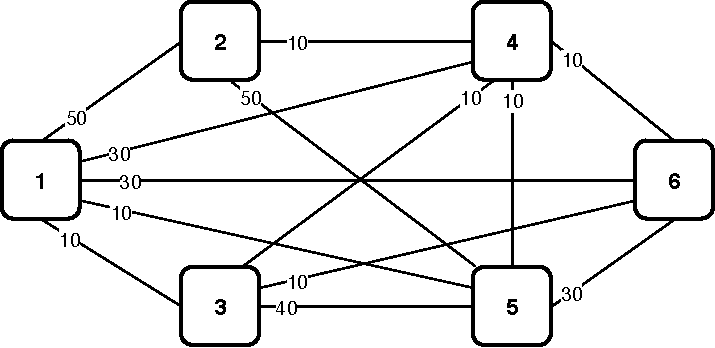
\includegraphics[width=12cm]{sdf/ilp/transparent_survivability/figures/logical_topology_ODU0_medium}
\caption{ODU0 logical topology defined by the ODU0 traffic matrix.}
\label{logical2_ODU0_medium}
\end{figure}

\begin{figure}[h!]
\centering
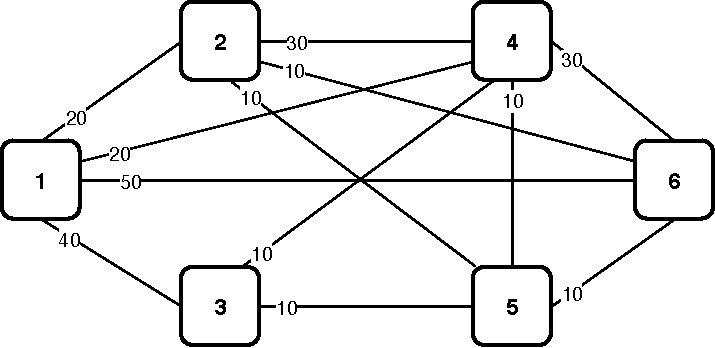
\includegraphics[width=12cm]{sdf/ilp/transparent_survivability/figures/logical_topology_ODU1_medium}
\caption{ODU1 logical topology defined by the ODU1 traffic matrix.}
\label{logical2_ODU1_medium}
\end{figure}

\begin{figure}[h!]
\centering
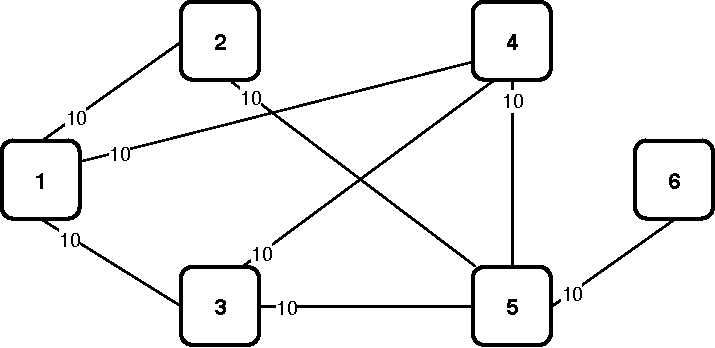
\includegraphics[width=12cm]{sdf/ilp/transparent_survivability/figures/logical_topology_ODU2_medium}
\caption{ODU2 logical topology defined by the ODU2 traffic matrix.}
\label{logical2_ODU2_medium}
\end{figure}

\begin{figure}[h!]
\centering
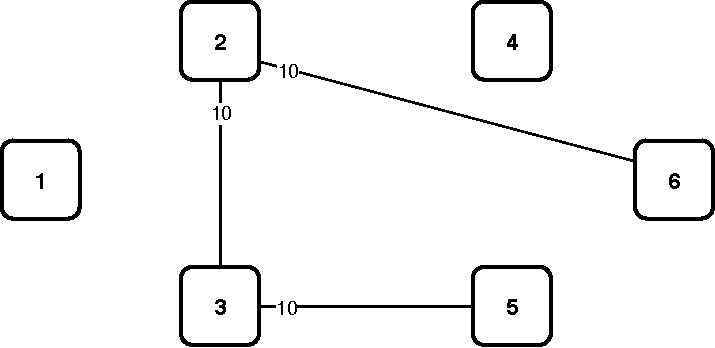
\includegraphics[width=12cm]{sdf/ilp/transparent_survivability/figures/logical_topology_ODU3_medium}
\caption{ODU3 logical topology defined by the ODU3 traffic matrix.}
\label{logical2_ODU3_medium}
\end{figure}

\begin{figure}[h!]
\centering
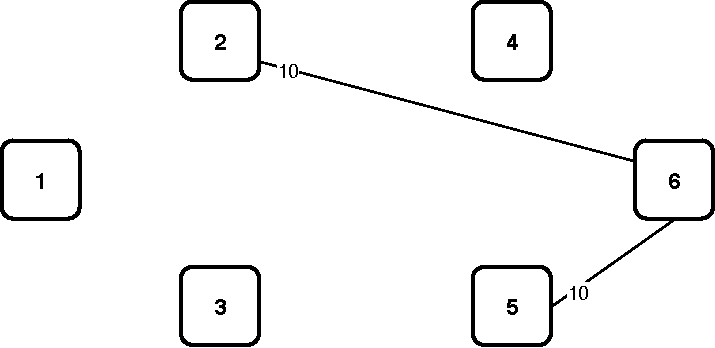
\includegraphics[width=12cm]{sdf/ilp/transparent_survivability/figures/logical_topology_ODU4_medium}
\caption{ODU4 logical topology defined by the ODU4 traffic matrix.}
\label{logical2_ODU4_medium}
\end{figure}

\begin{figure}[h!]
\centering
\includegraphics[width=12cm]{sdf/ilp/transparent_survivability/figures/physical_topology}
\caption{Physical topology after dimensioning.}
\label{physical2_medium}
\end{figure}
\newpage
\begin{figure}[h!]
\centering
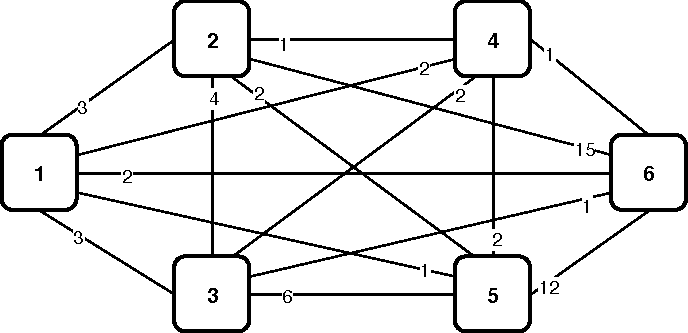
\includegraphics[width=11cm]{sdf/ilp/transparent_survivability/figures/optical_topology_medium}
\caption{Optical topology after dimensioning.}
\label{optical2_medium}
\end{figure}

In table \ref{link_transp_surv_ref_medium} we can see the number of optical channels calculated using \ref{Capex_Link} and \ref{ILPOpaque_CAPEX} and the number of amplifiers for each link calculated using \ref{Capex_amplifiers}.

\begin{table}[h!]
\centering
\begin{tabular}{|| c | c | c ||}
 \hline
 \multicolumn{3}{|| c ||}{Information regarding links} \\
 \hline
 \hline
 Bidirectional Link & Optical Channels & Amplifiers\\
 \hline
 Node 1 <-> Node 2 & 7 & 4 \\
 Node 1 <-> Node 3 & 4 & 6 \\
 Node 2 <-> Node 3 & 8 & 0 \\
 Node 2 <-> Node 4 & 22 & 6 \\
 Node 3 <-> Node 5 & 10 & 8 \\
 Node 4 <-> Node 5 & 2 & 1 \\
 Node 4 <-> Node 6 & 18 & 7 \\
 Node 5 <-> Node 6 & 13 & 3 \\
 \hline
\end{tabular}
\caption{Table with information regarding links for transparent mode.}
\label{link_transp_surv_ref_medium}
\end{table}

In table \ref{node_transp_surv_ref_medium} we can see the number of line ports and add ports using \ref{OXC_poxc_transparent} the number of long-reach transponders using \ref{EXC_pexc2_transparent} and the number of tributary ports using \ref{EXC_pexc1_transparent}.

\begin{table}[h!]
\centering
\begin{tabular}{|| c | c | c | c | c | c ||}
 \hline
 \multicolumn{6}{|| c ||}{Information regarding nodes} \\
 \hline
 \hline
 \multicolumn{2}{|| c |}{ } & \multicolumn{2}{ c |}{Electrical part} & \multicolumn{2}{ c ||}{Optical part} \\
 \hline
 Node & Resulting Nodal Degree & Tributary Ports & LR Transponders & Add Ports & Line Ports\\
 \hline
 1 & 2 & 290 & 11 & 11 & 11 \\
 2 & 3 & 230 & 25 & 25 & 37 \\
 3 & 3 & 180 & 16 & 16 & 22 \\
 4 & 3 & 200 & 8 & 8 & 42 \\
 5 & 3 & 240 & 23 & 23 & 25 \\
 6 & 2 & 220 & 31 & 31 & 31 \\
\hline
\end{tabular}
\caption{Table with information regarding nodes for transparent mode.}
\label{node_transp_surv_ref_medium}
\end{table}

\newpage
Through the information obtained previously on the nodes we can now create tables with detailed information about each node. In each table mentioned below we can see how many ports are connected to a given node and its bit rate (in relation to the line ports and the add ports) and how many ports are assigned to each different bit rate (in relation to the tributary ports).\\

\begin{table}[h!]
\centering
\begin{tabular}{|| c | c | c ||}
 \hline
 \multicolumn{3}{|| c ||}{Detailed description of Node 1} \\
 \hline
 \hline
 Electrical part & Number of total demands & Bit rate \\ \hline
\multirow{3}{*}{290 tributary ports} & 130 & ODU0 \\
 & 130 & ODU1 \\
 & 30 & ODU2 \\
 \hline
  & Node<--Optical Channels-->Node & Bit rate \\ \hline
 \multirow{5}{*}{11 LR Transponders} & 1  <---- 3 ---->  2 & \multirow{5}{*}{100 Gbits/s} \\
  & 1  <---- 3 ---->  3 & \\
  & 1  <---- 2 ---->  4 & \\
  & 1  <---- 1 ---->  5 & \\
  & 1  <---- 2 ---->  6 & \\
 \hline
 \hline
 Optical part & Node<--Optical Channels-->Node & Bit rate \\
 \hline
 \multirow{5}{*}{11 add ports} & 1  <---- 3 ---->  2 & \multirow{10}{*}{100 Gbits/s} \\
  & 1  <---- 3 ---->  3 & \\
  & 1  <---- 2 ---->  4 & \\
  & 1  <---- 1 ---->  5 & \\
  & 1  <---- 2 ---->  6 & \\ \cline{1-2}
 \multirow{5}{*}{11 line ports} & 1  <---- 3 ---->  2 & \\
  & 1  <---- 3 ---->  3 & \\
  & 1  <---- 2 ---->  4 & \\
  & 1  <---- 1 ---->  5 & \\
  & 1  <---- 2 ---->  6 & \\
\hline
\end{tabular}
\caption{Table with detailed description of node 1. The number of demands is distributed to the various destination nodes, this distribution can be observed in section \ref{medium_traffic_scenario} . Regarding the number of line ports when this node is equal to the source, it means that add ports are used, otherwise it means that through ports are used.  In this node as we can see there are no through ports.}
\end{table}

\newpage
\begin{table}[h!]
\centering
\begin{tabular}{|| c | c | c ||}
 \hline
 \multicolumn{3}{|| c ||}{Detailed description of Node 2} \\
 \hline
 \hline
 Electrical part & Number of total demands & Bit rate \\ \hline
\multirow{5}{*}{230 tributary ports} & 110 & ODU0 \\
 & 70 & ODU1 \\
 & 20 & ODU2 \\
 & 20 & ODU3 \\
 & 10 & ODU4 \\
 \hline
  & Node<--Optical Channels-->Node & Bit rate \\
 \hline
 \multirow{5}{*}{25 LR Transponders} & 2  <---- 3 ---->  1 & \multirow{5}{*}{100 Gbits/s} \\
  & 2  <---- 4 ---->  3 & \\
  & 2  <---- 1 ---->  4 & \\
  & 2  <---- 2 ---->  5 & \\
  & 2  <---- 15 ---->  6 & \\
 \hline
 \hline
 Optical part & Node<--Optical Channels-->Node & Bit rate \\
 \hline
 \multirow{5}{*}{25 add ports} & 2  <---- 3 ---->  1 & \multirow{13}{*}{100 Gbits/s} \\
  & 2  <---- 4 ---->  3 & \\
  & 2  <---- 1 ---->  4 & \\
  & 2  <---- 2 ---->  5 & \\
  & 2  <---- 15 ---->  6 & \\ \cline{1-2}
 \multirow{8}{*}{37 line ports} & 2  <---- 3 ---->  1 & \\
  & 2  <---- 4 ---->  3 & \\
  & 2  <---- 1 ---->  4 & \\
  & 2  <---- 2 ---->  5 & \\
  & 2  <---- 15 ---->  6 & \\
  & 1  <---- 2 ---->  4 & \\
  & 1  <---- 2 ---->  6 & \\
  & 3  <---- 2 ---->  4 & \\
\hline
\end{tabular}
\caption{Table with detailed description of node 2. The number of demands is distributed to the various destination nodes, this distribution can be observed in section \ref{medium_traffic_scenario} . Regarding the number of line ports when this node is equal to the source, it means that add ports are used, otherwise it means that through ports are used. In the latter the number of ports is double the number of optical channels.}
\end{table}

\newpage
\begin{table}[h!]
\centering
\begin{tabular}{|| c | c | c ||}
 \hline
 \multicolumn{3}{|| c ||}{Detailed description of Node 3} \\
 \hline
 \hline
 Electrical part & Number of total demands & Bit rate \\ \hline
\multirow{4}{*}{180 tributary ports} & 70 & ODU0 \\
 & 60 & ODU1\\
 & 30 & ODU2\\
 & 20 & ODU3\\
 \hline
  & Node<--Optical Channels-->Node & Bit rate \\
 \hline
 \multirow{5}{*}{16 LR Transponders} & 3  <---- 3 ---->  1 & \multirow{5}{*}{100 Gbits/s} \\
  & 3  <---- 4 ---->  2 & \\
  & 3  <---- 2 ---->  4 & \\
  & 3  <---- 6 ---->  5 & \\
  & 3  <---- 1 ---->  6 & \\
 \hline
 \hline
 Optical part & Node<--Optical Channels-->Node & Bit rate \\
 \hline
 \multirow{5}{*}{16 add ports} & 3  <---- 3 ---->  1 & \multirow{12}{*}{100 Gbits/s}  \\
  & 3  <---- 4 ---->  2 & \\
  & 3  <---- 2 ---->  4 & \\
  & 3  <---- 6 ---->  5 & \\
  & 3  <---- 1 ---->  6 & \\ \cline{1-2}
 \multirow{7}{*}{22 line ports} & 3  <---- 3 ---->  1 & \\
  & 3  <---- 4 ---->  2 & \\
  & 3  <---- 2 ---->  4 & \\
  & 3  <---- 6 ---->  5 & \\
  & 3  <---- 1 ---->  6 & \\
  & 1  <---- 1 ---->  5 & \\
  & 2  <---- 2 ---->  5 & \\
\hline
\end{tabular}
\caption{Table with detailed description of node 3. The number of demands is distributed to the various destination nodes, this distribution can be observed in section \ref{medium_traffic_scenario} . Regarding the number of line ports when this node is equal to the source, it means that add ports are used, otherwise it means that through ports are used. In the latter the number of ports is double the number of optical channels.}
\end{table}

\newpage
\begin{table}[h!]
\centering
\begin{tabular}{|| c | c | c ||}
 \hline
 \multicolumn{3}{|| c ||}{Detailed description of Node 4} \\
 \hline
 \hline
 Electrical part & Number of total demands & Bit rate \\ \hline
\multirow{3}{*}{200 tributary ports} & 70 & ODU0 \\
 & 100 & ODU1 \\
 & 30 & ODU2 \\
 \hline
  & Node<--Optical Channels-->Node & Bit rate \\
 \hline
 \multirow{5}{*}{8 add ports} & 4  <---- 2 ---->  1 & \multirow{5}{*}{100 Gbits/s} \\
  & 4  <---- 1 ---->  2 & \\
  & 4  <---- 2 ---->  3 & \\
  & 4  <---- 2 ---->  5 & \\
  & 4  <---- 1 ---->  6 & \\
 \hline
 Optical part & Node<--Optical Channels-->Node & Bit rate \\
 \hline
 \multirow{5}{*}{8 add ports} & 4  <---- 2 ---->  1 & \multirow{12}{*}{100 Gbits/s} \\
  & 4  <---- 1 ---->  2 & \\
  & 4  <---- 2 ---->  3 & \\
  & 4  <---- 2 ---->  5 & \\
  & 4  <---- 1 ---->  6 & \\ \cline{1-2}
 \multirow{7}{*}{42 line ports} & 4  <---- 2 ---->  1 & \\
  & 4  <---- 1 ---->  2 & \\
  & 4  <---- 2 ---->  3 & \\
  & 4  <---- 2 ---->  5 & \\
  & 4  <---- 1 ---->  6 & \\
  & 1  <---- 2 ---->  6 & \\
  & 2  <---- 15 ---->  6 & \\
\hline
\end{tabular}
\caption{Table with detailed description of node 4. The number of demands is distributed to the various destination nodes, this distribution can be observed in section \ref{medium_traffic_scenario} . Regarding the number of line ports when this node is equal to the source, it means that add ports are used, otherwise it means that through ports are used. In the latter the number of ports is double the number of optical channels.}
\end{table}

\newpage
\begin{table}[h!]
\centering
\begin{tabular}{|| c | c | c ||}
 \hline
 \multicolumn{3}{|| c ||}{Detailed description of Node 5} \\
 \hline
 \hline
 Electrical part & Number of total demands & Bit rate \\ \hline
\multirow{5}{*}{240 tributary ports} & 140 & ODU0 \\
 & 40 & ODU1 \\
 & 40 & ODU2 \\
 & 10 & ODU3 \\
 & 10 & ODU4 \\
 \hline
  & Node<--Optical Channels-->Node & Bit rate \\
 \hline
 \multirow{5}{*}{23 LR Transponders} & 5  <---- 1 ---->  1 & \multirow{5}{*}{100 Gbits/s}\\
  & 5  <---- 2 ---->  2 & \\
  & 5  <---- 6 ---->  3 & \\
  & 5  <---- 2 ---->  4 & \\
  & 5  <---- 12 ---->  6 & \\
 \hline
 \hline
 Optical part & Node<--Optical Channels-->Node & Bit rate \\
 \hline
 \multirow{5}{*}{23 add ports} & 5  <---- 1 ---->  1 & \multirow{11}{*}{100 Gbits/s} \\
  & 5  <---- 2 ---->  2 & \\
  & 5  <---- 6 ---->  3 & \\
  & 5  <---- 2 ---->  4 & \\
  & 5  <---- 12 ---->  6 & \\ \cline{1-2}
 \multirow{6}{*}{25 line ports} & 5  <---- 1 ---->  1 & \\
  & 5  <---- 2 ---->  2 & \\
  & 5  <---- 6 ---->  3 & \\
  & 5  <---- 2 ---->  4 & \\
  & 5  <---- 12 ---->  6 & \\
  & 3  <---- 1 ---->  6 & \\
\hline
\end{tabular}
\caption{Table with detailed description of node 5. The number of demands is distributed to the various destination nodes, this distribution can be observed in section \ref{medium_traffic_scenario} . Regarding the number of line ports when this node is equal to the source, it means that add ports are used, otherwise it means that through ports are used. In the latter the number of ports is double the number of optical channels.}
\end{table}

\newpage
\begin{table}[h!]
\centering
\begin{tabular}{|| c | c | c ||}
 \hline
 \multicolumn{3}{|| c ||}{Detailed description of Node 6} \\
 \hline
 \hline
 Electrical part & Number of total demands & Bit rate \\ \hline
\multirow{5}{*}{220 tributary ports} & 80 & ODU0 \\
 & 100 & ODU1 \\
 & 10 & ODU2 \\
 & 10 & ODU3 \\
 & 20 & ODU4 \\
 \hline
  & Node<--Optical Channels-->Node & Bit rate \\
 \hline
 \multirow{5}{*}{31 LR Transponders} & 6  <---- 2 ---->  1 & \multirow{5}{*}{100 Gbits/s} \\
  & 6  <---- 15 ---->  2 & \\
  & 6  <---- 1 ---->  3 & \\
  & 6  <---- 1 ---->  4 & \\
  & 6  <---- 12 ---->  5 & \\
 \hline
 \hline
 Optical part & Node<--Optical Channels-->Node & Bit rate \\
 \hline
 \multirow{5}{*}{31 add ports} & 6  <---- 2 ---->  1 & \multirow{10}{*}{100 Gbits/s} \\
  & 6  <---- 15 ---->  2 & \\
  & 6  <---- 1 ---->  3 & \\
  & 6  <---- 1 ---->  4 & \\
  & 6  <---- 12 ---->  5 & \\ \cline{1-2}
 \multirow{3}{*}{31 line ports} & 6  <---- 2 ---->  1 & \\
  & 6  <---- 15 ---->  2 & \\
  & 6  <---- 1 ---->  3 & \\
  & 6  <---- 1 ---->  4 & \\
  & 6  <---- 12 ---->  5 & \\
\hline
\end{tabular}
\caption{Table with detailed description of node 6. The number of demands is distributed to the various destination nodes, this distribution can be observed in section \ref{medium_traffic_scenario} . Regarding the number of line ports when this node is equal to the source, it means that add ports are used, otherwise it means that through ports are used.  In this node as we can see there are no through ports.}
\end{table}

\vspace{17pt}
Now, in next page, let's focus on the routing information in table \ref{path_transp_surv_ref_medium}. These paths are bidirectional so the path from one node to another is the same path in the opposite direction.\\
\newpage
\begin{table}[h!]
\centering
\begin{tabular}{|| c | c | c ||}
 \hline
 \multicolumn{3}{|| c ||}{Routing} \\
 \hline
 \hline
 o & d & Links \\
 \hline
 1 & 2 & \{(1,2)\} \\ \hline
 1 & 3 & \{(1,3)\} \\ \hline
 1 & 4 & \{(1,2),(2,4)\}\\ \hline
 1 & 5 & \{(1,3),(3,5)\}\\ \hline
 1 & 6 & \{(1,2),(2,4),(4,6)\}\\ \hline
 2 & 3 & \{(2,3)\}\\ \hline
 2 & 4 & \{(2,4)\}\\ \hline
 2 & 5 & \{(2,3),(3,5)\}\\ \hline
 2 & 6 & \{(2,4),(4,6)\}\\ \hline
 3 & 4 & \{(3,2),(2,4)\}\\ \hline
 3 & 5 & \{(3,5)\}\\ \hline
 3 & 6 & \{(3,5),(5,6)\}\\ \hline
 4 & 5 & \{(4,5)\}\\ \hline
 4 & 6 & \{(4,6)\}\\ \hline
 5 & 6 & \{(5,6)\}\\
 \hline
\end{tabular}
\caption{Table with description of routing}
\label{path_transp_surv_ref_medium}
\end{table}

Finally and most importantly through table \ref{scripttransp_surv_ref_medium} we can see the CAPEX result for this model. This value is obtained using equation \ref{ILPOpaque_CAPEX} and all of the constraints mentioned above. In table \ref{formulas_transp} mentioned in previous scenario we can see how all the values were calculated.

\begin{table}[h!]
\centering
\begin{tabular}{|| c | c | c | c | c | c | c ||}
 \hline
 \multicolumn{7}{|| c ||}{CAPEX of the Network} \\
 \hline
 \hline
 \multicolumn{3}{|| c |}{ } & Quantity & Unit Price & Cost & Total \\
 \hline
 \multirow{3}{*}{Link Cost} & \multicolumn{2}{ c |}{OLTs} & 16 & 15 000 \euro & 240 000 \euro & \multirow{3}{*}{84 520 000 \euro} \\ \cline{2-6}
 & \multicolumn{2}{ c |}{100 Gbits/s Transceivers} & 168 & 5 000 \euro/Gbit/s & 84 000 000 \euro & \\ \cline{2-6}
 & \multicolumn{2}{ c |}{Amplifiers} & 70 & 4 000 \euro & 280 000 \euro & \\
 \hline
 \multirow{10}{*}{Node Cost} & \multirow{7}{*}{Electrical} & EXCs & 6 & 10 000 \euro & 60 000 \euro & \multirow{10}{*}{12 310 900 \euro} \\ \cline{3-6}
 & & ODU0 Ports & 600 & 10 \euro/port & 6 000 \euro & \\ \cline{3-6}
 & & ODU1 Ports & 500 & 15 \euro/port & 7 500 \euro & \\ \cline{3-6}
 & & ODU2 Ports & 160 & 30 \euro/port & 4 800 \euro & \\ \cline{3-6}
 & & ODU3 Ports & 60 & 60 \euro/port & 3 600 \euro & \\ \cline{3-6}
 & & ODU4 Ports & 40 & 100 \euro/port & 4 000 \euro & \\ \cline{3-6}
 & &Transponders& 114 & 100 000 \euro/port & 11 400 000 \euro & \\ \cline{2-6}
 & \multirow{3}{*}{Optical} & OXCs & 6 & 20 000 \euro & 120 000 \euro & \\ \cline{3-6}
 & & Line Ports & 168 & 2 500 \euro/port & 420 000 \euro & \\ \cline{3-6}
 & & Add Ports & 114 & 2 500 \euro/port & 285 000 \euro & \\
 \hline
 \multicolumn{6}{|| c |}{Total Network Cost} &96 830 900 \euro \\
\hline
\end{tabular}
\caption{Table with detailed description of CAPEX}
\label{scripttransp_surv_ref_medium}
\end{table}

\newpage
\textbf{High Traffic Scenario:}\\

In this scenario we have to take into account the traffic calculated in \ref{high_traffic_scenario}. In a first phase we will show the various existing topologies of the network. The first are the allowed topologies, physical and optical topology, the second are the logical topology for all ODUs and finally the resulting physical and optical topology.\\

\begin{figure}[h!]
\centering
\includegraphics[width=12cm]{sdf/ilp/transparent_survivability/figures/allowed_physical_topology}
\caption{Allowed physical topology. The allowed physical topology is defined by the duct and sites in the field. It is assumed that each duct supports up to 1 bidirectional transmission system and each site supports up to 1 node.}
\label{allowed2_physical_high}
\end{figure}

\vspace{11pt}
\begin{figure}[h!]
\centering
\includegraphics[width=12cm]{sdf/ilp/transparent_survivability/figures/allowed_optical_topology}
\caption{Allowed optical topology. The allowed optical topology is defined by the transport mode (transparent transport mode in this case). It is assumed that each connections between demands supports up to 100 lightpaths.}
\label{allowed2_optical_high}
\end{figure}

\newpage
\begin{figure}[h!]
\centering
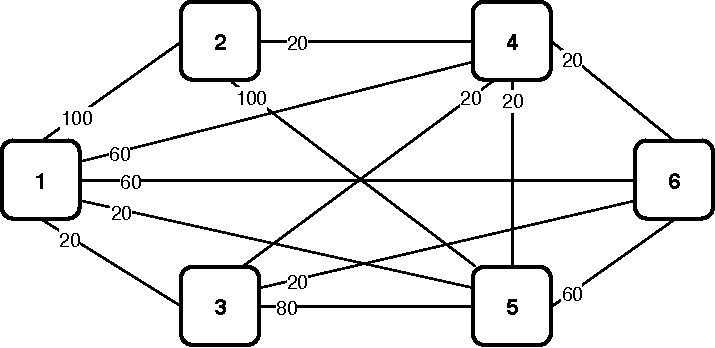
\includegraphics[width=12cm]{sdf/ilp/transparent_survivability/figures/logical_topology_ODU0_high}
\caption{ODU0 logical topology defined by the ODU0 traffic matrix.}
\label{logical2_ODU0_high}
\end{figure}

\begin{figure}[h!]
\centering
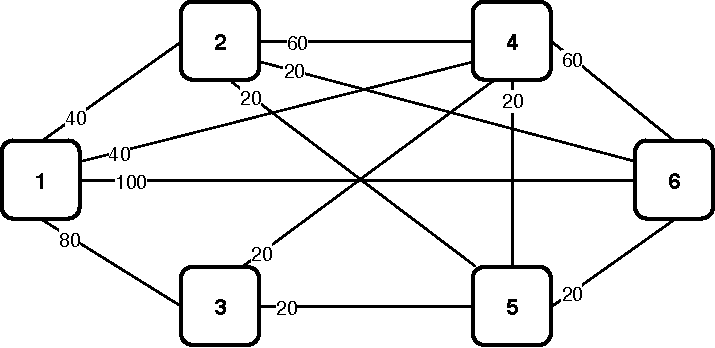
\includegraphics[width=12cm]{sdf/ilp/transparent_survivability/figures/logical_topology_ODU1_high}
\caption{ODU1 logical topology defined by the ODU1 traffic matrix.}
\label{logical2_ODU1_high}
\end{figure}

\begin{figure}[h!]
\centering
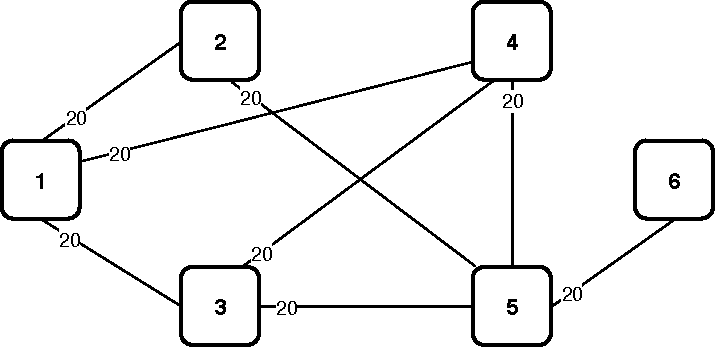
\includegraphics[width=12cm]{sdf/ilp/transparent_survivability/figures/logical_topology_ODU2_high}
\caption{ODU2 logical topology defined by the ODU2 traffic matrix.}
\label{logical2_ODU2_high}
\end{figure}

\begin{figure}[h!]
\centering
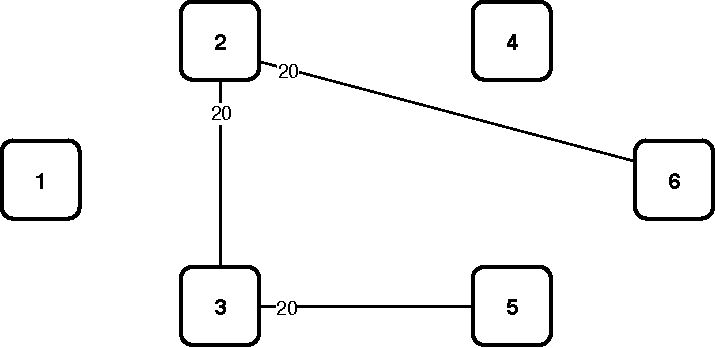
\includegraphics[width=12cm]{sdf/ilp/transparent_survivability/figures/logical_topology_ODU3_high}
\caption{ODU3 logical topology defined by the ODU3 traffic matrix.}
\label{logical2_ODU3_high}
\end{figure}

\begin{figure}[h!]
\centering
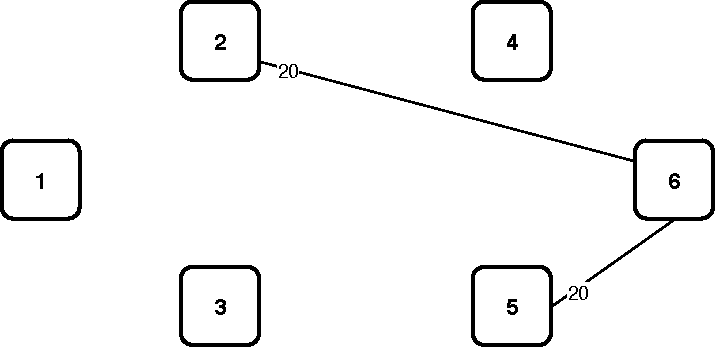
\includegraphics[width=12cm]{sdf/ilp/transparent_survivability/figures/logical_topology_ODU4_high}
\caption{ODU4 logical topology defined by the ODU4 traffic matrix.}
\label{logical2_ODU4_high}
\end{figure}

\begin{figure}[h!]
\centering
\includegraphics[width=12cm]{sdf/ilp/transparent_survivability/figures/physical_topology}
\caption{Physical topology after dimensioning.}
\label{physical2_high}
\end{figure}

\newpage
\begin{figure}[h!]
\centering
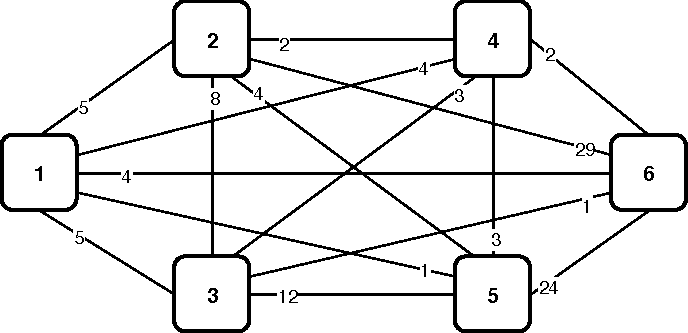
\includegraphics[width=11cm]{sdf/ilp/transparent_survivability/figures/optical_topology_high}
\caption{Optical topology after dimensioning.}
\label{optical2_high}
\end{figure}

In table \ref{link_transp_surv_ref_high} we can see the number of optical channels calculated using \ref{Capex_Link} and \ref{ILPOpaque_CAPEX} and the number of amplifiers for each link calculated using \ref{Capex_amplifiers}.

\begin{table}[h!]
\centering
\begin{tabular}{|| c | c | c ||}
 \hline
 \multicolumn{3}{|| c ||}{Information regarding links} \\
 \hline
 \hline
 Bidirectional Link & Optical Channels & Amplifiers\\
 \hline
 Node 1 <-> Node 2 & 13 & 4 \\
 Node 1 <-> Node 3 & 6 & 6 \\
 Node 2 <-> Node 3 & 15 & 0 \\
 Node 2 <-> Node 4 & 42 & 6 \\
 Node 3 <-> Node 5 & 18 & 8 \\
 Node 4 <-> Node 5 & 3 & 1 \\
 Node 4 <-> Node 6 & 35 & 7 \\
 Node 5 <-> Node 6 & 25 & 3 \\
 \hline
\end{tabular}
\caption{Table with information regarding links for transparent mode.}
\label{link_transp_surv_ref_high}
\end{table}

In table \ref{node_transp_surv_ref_high} we can see the number of line ports and add ports using \ref{OXC_poxc_transparent} the number of long-reach transponders using \ref{EXC_pexc2_transparent} and the number of tributary ports using \ref{EXC_pexc1_transparent}.

\begin{table}[h!]
\centering
\begin{tabular}{|| c | c | c | c | c | c ||}
 \hline
 \multicolumn{6}{|| c ||}{Information regarding nodes} \\
 \hline
 \hline
 \multicolumn{2}{|| c |}{ } & \multicolumn{2}{ c |}{Electrical part} & \multicolumn{2}{ c ||}{Optical part} \\
 \hline
 Node & Resulting Nodal Degree & Tributary Ports & LR Transponders & Add Ports & Line Ports\\
 \hline
 1 & 2 & 580 & 19 & 19 & 19 \\
 2 & 3 & 460 & 48 & 48 & 70 \\
 3 & 3 & 360 & 29 & 29 & 39 \\
 4 & 3 & 400 & 14 & 14 & 80 \\
 5 & 3 & 480 & 44 & 44 & 46 \\
 6 & 2 & 440 & 60 & 60 & 60 \\
\hline
\end{tabular}
\caption{Table with information regarding nodes for transparent mode.}
\label{node_transp_surv_ref_high}
\end{table}

\newpage
Through the information obtained previously on the nodes we can now create tables with detailed information about each node. In each table mentioned below we can see how many ports are connected to a given node and its bit rate (in relation to the line ports and the add ports) and how many ports are assigned to each different bit rate (in relation to the tributary ports).\\

\begin{table}[h!]
\centering
\begin{tabular}{|| c | c | c ||}
 \hline
 \multicolumn{3}{|| c ||}{Detailed description of Node 1} \\
 \hline
 \hline
 Electrical part & Number of total demands & Bit rate \\ \hline
\multirow{3}{*}{580 tributary ports} & 260 & ODU0 \\
 & 260 & ODU1 \\
 & 60 & ODU2 \\
 \hline
  & Node<--Optical Channels-->Node & Bit rate \\
 \hline
 \multirow{5}{*}{19 LR Transponders} & 1  <---- 5 ---->  2 & \multirow{5}{*}{100 Gbits/s} \\
  & 1  <---- 5 ---->  3 & \\
  & 1  <---- 4 ---->  4 & \\
  & 1  <---- 1 ---->  5 & \\
  & 1  <---- 4 ---->  6 & \\
 \hline
 \hline
 Optical part & Node<--Optical Channels-->Node & Bit rate \\
 \hline
 \multirow{5}{*}{19 add ports} & 1  <---- 5 ---->  2 & \multirow{10}{*}{100 Gbits/s} \\
  & 1  <---- 5 ---->  3 & \\
  & 1  <---- 4 ---->  4 & \\
  & 1  <---- 1 ---->  5 & \\
  & 1  <---- 4 ---->  6 & \\ \cline{1-2}
 \multirow{5}{*}{19 line ports} & 1  <---- 5 ---->  2 & \\
  & 1  <---- 5 ---->  3 & \\
  & 1  <---- 4 ---->  4 & \\
  & 1  <---- 1 ---->  5 & \\
  & 1  <---- 4 ---->  6 & \\
\hline
\end{tabular}
\caption{Table with detailed description of node 1. The number of demands is distributed to the various destination nodes, this distribution can be observed in section \ref{high_traffic_scenario}. Regarding the number of line ports when this node is equal to the source, it means that add ports are used, otherwise it means that through ports are used. In this node as we can see there are no through ports.}
\end{table}

\newpage
\begin{table}[h!]
\centering
\begin{tabular}{|| c | c | c ||}
 \hline
 \multicolumn{3}{|| c ||}{Detailed description of Node 2} \\
 \hline
 \hline
 Electrical part & Number of total demands & Bit rate \\ \hline
\multirow{5}{*}{460 tributary ports} & 220 & ODU0 \\
 & 140 & ODU1 \\
 & 40 & ODU2 \\
 & 40 & ODU3 \\
 & 20 & ODU4 \\
 \hline
  & Node<--Optical Channels-->Node & Bit rate \\
 \hline
 \multirow{5}{*}{48 LR Transponders} & 2  <---- 5 ---->  1 & \multirow{5}{*}{100 Gbits/s} \\
  & 2  <---- 8 ---->  3 & \\
  & 2  <---- 2 ---->  4 & \\
  & 2  <---- 4 ---->  5 & \\
  & 2  <---- 29 ---->  6 & \\
 \hline
 \hline
 Optical part & Node<--Optical Channels-->Node & Bit rate \\
 \hline
 \multirow{5}{*}{48 add ports} & 2  <---- 5 ---->  1 & \multirow{13}{*}{100 Gbits/s} \\
  & 2  <---- 8 ---->  3 & \\
  & 2  <---- 2 ---->  4 & \\
  & 2  <---- 4 ---->  5 & \\
  & 2  <---- 29 ---->  6 & \\ \cline{1-2}
 \multirow{8}{*}{70 line ports} & 2  <---- 5 ---->  1 & \\
  & 2  <---- 8 ---->  3 & \\
  & 2  <---- 2 ---->  4 & \\
  & 2  <---- 4 ---->  5 & \\
  & 2  <---- 29 ---->  6 & \\
  & 1  <---- 4 ---->  4 & \\
  & 1  <---- 4 ---->  6 & \\
  & 3  <---- 3 ---->  4 & \\
\hline
\end{tabular}
\caption{Table with detailed description of node 2. The number of demands is distributed to the various destination nodes, this distribution can be observed in section \ref{high_traffic_scenario} . Regarding the number of line ports when this node is equal to the source, it means that add ports are used, otherwise it means that through ports are used. In the latter the number of ports is double the number of optical channels.}
\end{table}

\newpage
\begin{table}[h!]
\centering
\begin{tabular}{|| c | c | c ||}
 \hline
 \multicolumn{3}{|| c ||}{Detailed description of Node 3} \\
 \hline
 \hline
 Electrical part & Number of total demands & Bit rate \\ \hline
\multirow{4}{*}{360 tributary ports} & 140 & ODU0 \\
 & 120 & ODU1\\
 & 60 & ODU2\\
 & 40 & ODU3\\
 \hline
  & Node<--Optical Channels-->Node & Bit rate \\
 \hline
 \multirow{5}{*}{29 LR Transponders} & 3  <---- 5 ---->  1 & \multirow{5}{*}{100 Gbits/s} \\
  & 3  <---- 8 ---->  2 & \\
  & 3  <---- 3 ---->  4 & \\
  & 3  <---- 12 ---->  5 & \\
  & 3  <---- 1 ---->  6 & \\
 \hline
 \hline
 Optical part & Node<--Optical Channels-->Node & Bit rate \\
 \hline
 \multirow{5}{*}{29 add ports} & 3  <---- 5 ---->  1 & \multirow{12}{*}{100 Gbits/s} \\
  & 3  <---- 8 ---->  2 & \\
  & 3  <---- 3 ---->  4 & \\
  & 3  <---- 12 ---->  5 & \\
  & 3  <---- 1 ---->  6 & \\ \cline{1-2}
 \multirow{7}{*}{39 line ports} & 3  <---- 5 ---->  1 & \\
  & 3  <---- 8 ---->  2 & \\
  & 3  <---- 3 ---->  4 & \\
  & 3  <---- 12 ---->  5 & \\
  & 3  <---- 1 ---->  6 & \\
  & 1  <---- 1 ---->  5 & \\
  & 2  <---- 4 ---->  5 & \\ 
\hline
\end{tabular}
\caption{Table with detailed description of node 3. The number of demands is distributed to the various destination nodes, this distribution can be observed in section \ref{high_traffic_scenario} . Regarding the number of line ports when this node is equal to the source, it means that add ports are used, otherwise it means that through ports are used. In the latter the number of ports is double the number of optical channels.}
\end{table}

\newpage
\begin{table}[h!]
\centering
\begin{tabular}{|| c | c | c ||}
 \hline
 \multicolumn{3}{|| c ||}{Detailed description of Node 4} \\
 \hline
 \hline
 Electrical part & Number of total demands & Bit rate \\ \hline
\multirow{3}{*}{400 tributary ports} & 140 & ODU0 \\
 & 200 & ODU1 \\
 & 60 & ODU2 \\
 \hline
  & Node<--Optical Channels-->Node & Bit rate \\
 \hline
 \multirow{5}{*}{14 LR Transponders} & 4  <---- 4 ---->  1 & \multirow{5}{*}{100 Gbits/s} \\
  & 4  <---- 2 ---->  2 & \\
  & 4  <---- 3 ---->  3 & \\
  & 4  <---- 3 ---->  5 & \\
  & 4  <---- 2 ---->  6 & \\
 \hline
 \hline
 Optical part & Node<--Optical Channels-->Node & Bit rate \\
 \hline
 \multirow{5}{*}{14 add ports} & 4  <---- 4 ---->  1 & \multirow{12}{*}{100 Gbits/s} \\
  & 4  <---- 2 ---->  2 & \\
  & 4  <---- 3 ---->  3 & \\
  & 4  <---- 3 ---->  5 & \\
  & 4  <---- 2 ---->  6 & \\ \cline{1-2}
 \multirow{7}{*}{80 line ports} & 4  <---- 4 ---->  1 & \\
  & 4  <---- 2 ---->  2 & \\
  & 4  <---- 3 ---->  3 & \\
  & 4  <---- 3 ---->  5 & \\
  & 4  <---- 2 ---->  6 & \\
  & 1  <---- 4 ---->  6 & \\
  & 2  <---- 29 ---->  6 & \\ 
\hline
\end{tabular}
\caption{Table with detailed description of node 4. The number of demands is distributed to the various destination nodes, this distribution can be observed in section \ref{high_traffic_scenario} . Regarding the number of line ports when this node is equal to the source, it means that add ports are used, otherwise it means that through ports are used. In the latter the number of ports is double the number of optical channels.}
\end{table}

\newpage
\begin{table}[h!]
\centering
\begin{tabular}{|| c | c | c ||}
 \hline
 \multicolumn{3}{|| c ||}{Detailed description of Node 5} \\
 \hline
 \hline
 Electrical part & Number of total demands & Bit rate \\ \hline
\multirow{5}{*}{480 tributary ports} & 280 & ODU0 \\
 & 80 & ODU1 \\
 & 80 & ODU2 \\
 & 20 & ODU3 \\
 & 20 & ODU4 \\
 \hline
  & Node<--Optical Channels-->Node & Bit rate \\
 \hline
 \multirow{5}{*}{44 LR Transponders} & 5  <---- 1 ---->  1 & \multirow{5}{*}{100 Gbits/s} \\
  & 5  <---- 4 ---->  2 & \\
  & 5  <---- 12 ---->  3 & \\
  & 5  <---- 3 ---->  4 & \\
  & 5  <---- 24 ---->  6 & \\
 \hline
 \hline
 Optical part & Node<--Optical Channels-->Node & Bit rate \\
 \hline
 \multirow{5}{*}{44 add ports} & 5  <---- 1 ---->  1 & \multirow{11}{*}{100 Gbits/s} \\
  & 5  <---- 4 ---->  2 & \\
  & 5  <---- 12 ---->  3 & \\
  & 5  <---- 3 ---->  4 & \\
  & 5  <---- 24 ---->  6 & \\ \cline{1-2}
 \multirow{6}{*}{46 line ports} & 5  <---- 1 ---->  1 & \\
  & 5  <---- 4 ---->  2 & \\
  & 5  <---- 12 ---->  3 & \\
  & 5  <---- 3 ---->  4 & \\
  & 5  <---- 24 ---->  6 & \\
  & 3  <---- 1 ---->  6 & \\ 
\hline
\end{tabular}
\caption{Table with detailed description of node 5. The number of demands is distributed to the various destination nodes, this distribution can be observed in section \ref{high_traffic_scenario} . Regarding the number of line ports when this node is equal to the source, it means that add ports are used, otherwise it means that through ports are used. In the latter the number of ports is double the number of optical channels.}
\end{table}

\newpage
\begin{table}[h!]
\centering
\begin{tabular}{|| c | c | c ||}
 \hline
 \multicolumn{3}{|| c ||}{Detailed description of Node 6} \\
 \hline
 \hline
 Electrical part & Number of total demands & Bit rate \\ \hline
\multirow{5}{*}{440 tributary ports} & 160 & ODU0 \\
 & 200 & ODU1 \\
 & 20 & ODU2 \\
 & 20 & ODU3 \\
 & 40 & ODU4 \\
 \hline
  & Node<--Optical Channels-->Node & Bit rate \\
 \hline
 \multirow{5}{*}{60 LR Transponders} & 6  <---- 4 ---->  1 & \multirow{5}{*}{100 Gbits/s} \\
  & 6  <---- 29 ---->  2 & \\
  & 6  <---- 1 ---->  3 & \\
  & 6  <---- 2 ---->  4 & \\
  & 6  <---- 24 ---->  5 & \\
 \hline
 \hline
 Optical part & Node<--Optical Channels-->Node & Bit rate \\
 \hline
 \multirow{5}{*}{60 add ports} & 6  <---- 4 ---->  1 & \multirow{10}{*}{100 Gbits/s} \\
  & 6  <---- 29 ---->  2 & \\
  & 6  <---- 1 ---->  3 & \\
  & 6  <---- 2 ---->  4 & \\
  & 6  <---- 24 ---->  5 & \\ \cline{1-2}
 \multirow{5}{*}{60 line ports} & 6  <---- 4 ---->  1 & \\
  & 6  <---- 29 ---->  2 & \\
  & 6  <---- 1 ---->  3 & \\
  & 6  <---- 2 ---->  4 & \\
  & 6  <---- 24 ---->  5 & \\
\hline
\end{tabular}
\caption{Table with detailed description of node 6. The number of demands is distributed to the various destination nodes, this distribution can be observed in section \ref{high_traffic_scenario}. Regarding the number of line ports when this node is equal to the source, it means that add ports are used, otherwise it means that through ports are used. In this node as we can see there are no through ports.}
\end{table}

\vspace{17pt}
Now, in next page, let's focus on the routing information in table \ref{path_transp_surv_ref_high}. These paths are bidirectional so the path from one node to another is the same path in the opposite direction.\\
\newpage
\begin{table}[h!]
\centering
\begin{tabular}{|| c | c | c ||}
 \hline
 \multicolumn{3}{|| c ||}{Routing} \\
 \hline
 \hline
 o & d & Links \\
 \hline
 1 & 2 & \{(1,2)\} \\ \hline
 1 & 3 & \{(1,3)\} \\ \hline
 1 & 4 & \{(1,2),(2,4)\}\\ \hline
 1 & 5 & \{(1,3),(3,5)\}\\ \hline
 1 & 6 & \{(1,2),(2,4),(4,6)\}\\ \hline
 2 & 3 & \{(2,3)\}\\ \hline
 2 & 4 & \{(2,4)\}\\ \hline
 2 & 5 & \{(2,3),(3,5)\}\\ \hline
 2 & 6 & \{(2,4),(4,6)\}\\ \hline
 3 & 4 & \{(3,2),(2,4)\}\\ \hline
 3 & 5 & \{(3,5)\}\\ \hline
 3 & 6 & \{(3,5),(5,6)\}\\ \hline
 4 & 5 & \{(4,5)\}\\ \hline
 4 & 6 & \{(4,6)\}\\ \hline
 5 & 6 & \{(5,6)\}\\
 \hline
\end{tabular}
\caption{Table with description of routing}
\label{path_transp_surv_ref_high}
\end{table}

Finally and most importantly through table \ref{scripttransp_surv_ref_high} we can see the CAPEX result for this model. This value is obtained using equation \ref{ILPOpaque_CAPEX} and all of the constraints mentioned above. In table \ref{formulas_transp} mentioned in previous scenario we can see how all the values were calculated.

\begin{table}[h!]
\centering
\begin{tabular}{|| c | c | c | c | c | c | c ||}
 \hline
 \multicolumn{7}{|| c ||}{CAPEX of the Network} \\
 \hline
 \hline
 \multicolumn{3}{|| c |}{ } & Quantity & Unit Price & Cost & Total \\
 \hline
 \multirow{3}{*}{Link Cost} & \multicolumn{2}{ c |}{OLTs} & 16 & 15 000 \euro & 240 000 \euro & \multirow{3}{*}{157 520 000 \euro} \\ \cline{2-6}
 & \multicolumn{2}{ c |}{100 Gbits/s Transceivers} & 314 & 5 000 \euro/Gbit/s & 157 000 000 \euro & \\ \cline{2-6}
 & \multicolumn{2}{ c |}{Amplifiers} & 70 & 4 000 \euro & 280 000 \euro & \\
 \hline
 \multirow{10}{*}{Node Cost} & \multirow{7}{*}{Electrical} & EXCs & 6 & 10 000 \euro & 60 000 \euro & \multirow{10}{*}{22 951 800 \euro} \\ \cline{3-6}
 & & ODU0 Ports & 1 200 & 10 \euro/port & 12 000 \euro & \\ \cline{3-6}
 & & ODU1 Ports & 1 000 & 15 \euro/port & 15 000 \euro & \\ \cline{3-6}
 & & ODU2 Ports & 320 & 30 \euro/port & 9 600 \euro & \\ \cline{3-6}
 & & ODU3 Ports & 120 & 60 \euro/port & 7 200 \euro & \\ \cline{3-6}
 & & ODU4 Ports & 80 & 100 \euro/port & 8 000 \euro & \\ \cline{3-6}
 & &Transponders& 214 & 100 000 \euro/port & 21 400 000 \euro & \\ \cline{2-6}
 & \multirow{3}{*}{Optical} & OXCs & 6 & 20 000 \euro & 120 000 \euro & \\ \cline{3-6}
 & & Line Ports & 314 & 2 500 \euro/port & 785 000 \euro & \\ \cline{3-6}
 & & Add Ports & 214 & 2 500 \euro/port & 535 000 \euro & \\
 \hline
 \multicolumn{6}{|| c |}{Total Network Cost} & 180 471 800 \euro \\
\hline
\end{tabular}
\caption{Table with detailed description of CAPEX for this scenario.}
\label{scripttransp_surv_ref_high}
\end{table}

\newpage
\subsubsection{Conclusions}

Once we have obtained the results for all the scenarios we will now draw some conclusions about these results. For a better analysis of the results will be created the table \ref{table_comparative_transp_surv} with the number of line ports and add ports of the optical part, the tributary ports, the transponders and transceivers because they are important values for the cost of CAPEX, the cost of links, the cost of nodes and finally the cost of CAPEX.\\

\begin{table}[h!]
\centering
\begin{tabular}{| c | c | c | c |}
 \hline
  & Low Traffic & Medium Traffic  & High Traffic \\
 \hline\hline
 Traffic (Gbit/s) & 500 & 5 000 & 10 000 \\ \hline
 Number of Add ports & 34 & 114 & 214 \\ \hline
 Number of Line ports & 52 & 168 & 314 \\ \hline
 Number of Tributary ports & 136 & 1 360 & 2 720 \\ \hline
 Number of Transceivers & 52 & 168 & 314 \\ \hline
 Number of Transponders & 34 & 114 & 214 \\ \hline
 Link Cost & 26 520 000 \euro & 84 520 000 \euro & 157 520 000 \euro \\ \hline
 Node Cost & 3 797 590 \euro & 12 310 900 \euro & 22 951 800 \euro \\ \hline
 CAPEX & \textbf{30 317 590 \euro} & \textbf{96 830 900 \euro} & \textbf{180 471 800 \euro} \\ \hline
 CAPEX/Gbit/s & \textbf{60 635.18 \euro/Gbit/s} & \textbf{19 366.18 \euro/Gbit/s} & \textbf{18 047.68 \euro/Gbit/s}\\
 \hline
\end{tabular}
\caption{Table with the various CAPEX values obtained in the different traffic scenarios.}
\label{table_comparative_transp_surv}
\end{table}

Looking at the previous table we can make some comparisons between the several scenarios:

\begin{itemize}
    \item Comparing the low traffic scenario with the others, we can see that, despite having an increase of factor ten (average scenario) and factor twenty (high scenario), the same increase does not occur in the final cost (it is lower). This happens because the number of transceivers is smaller than expected (an average scenario of 520 would be expected and a high scenario would be expected in 1040);
    \item Comparing the medium traffic scenario with the high traffic scenario, we can see that the factor increase is double and in the final cost this factor is very close but still lower. Again, this happens because the number of transceivers is smaller, but very close to what was expected (the high scenario would be expected at 336);
    \item Comparing the cost with the traffic, we see that, for the low traffic scenario, the cost per traffic is very high in relation to the other two. We can conclude that a low traffic scenario becomes more expensive than a high traffic scenario.
\end{itemize}


\vspace{13pt}
\subsubsection{Opens Issues}

The creation of this model for any scenario, started with some considerations and some open issues being:

\begin{itemize}
  \item Allow blocking.
  \subitem The presented model assume that the solution is possible or impossible, does not support a partial solution where some demands are not routed (are blocked).
  \item Allow multiple transmission system.
  \subitem The presented model for each link only supports one transmission system.
\end{itemize}


\clearpage

\subsection{Transparent with 1+1 Protection}\label{ILP_Transp_Protection}
\begin{tcolorbox}	
\begin{tabular}{p{2.75cm} p{0.2cm} p{10.5cm}} 	
\textbf{Student Name}  &:& Tiago Esteves    (October 03, 2017 - )\\
\textbf{Goal}          &:& Implement the ILP model for the transparent transport mode with 1 plus 1 protection.
\end{tabular}
\end{tcolorbox}
\vspace{11pt}

Here, in this case, we must take into account table \ref{description_transp}, previously mentioned, in order to better understand the objective function.\\

Before carrying out the description of the objective function we must take into account the following particularity of this mode of transport:
\begin{itemize}
  \item $N_{OXC,n}$ = 1, \quad $\forall$ n that process traffic
  \item $N_{EXC,n}$ = 1, \quad $\forall$ n that process traffic
\end{itemize}

\vspace{11pt}
The objective function of following the ILP is a minimization of the CAPEX through the equation \ref{Capex} where in this case for the cost of nodes we have in consideration the electric cost \ref{Capex_Node_EXC} and the optical cost \ref{Capex_Node_OXC}.
In this case the value of $P_{exc,c,n}$ is obtained by equation \ref{EXC_pexc1_transparentp} for short-reach and by the equation \ref{EXC_pexc2_transparentp} for long-reach and the value of $P_{oxc,n}$ is obtained by equation \ref{OXC_poxc_transparentp}.\\

The equation \ref{EXC_pexc1_transparentp} refers to the number of sort-reach ports of the electrical switch with bit-rate $c$ in node $n$, $P_{exc,c,n}$, i.e. the number of tributary ports with bit-rate $c$ in node $n$ which can be calculated as

\begin{equation}
P_{exc,c,n} = \sum_{d=1}^{N} D_{nd,c}
\label{EXC_pexc1_transparentp}
\end{equation}

\vspace{11pt}
\noindent
where $D_{nd,c}$ are the client demands between nodes $n$ and $d$ with bit rate $c$.\\

In this case there is the following particularity:

\begin{itemize}
  \item When $n$=$d$ the value of client demands is always zero, i.e, $D_{nn,c}=0$
\end{itemize}

\vspace{11pt}
As previously mentioned, the equation \ref{EXC_pexc2_transparentp} refers to the number of long-reach ports of the electrical switch with bit-rate -1 in node n, $P_{exc,-1,n}$, i.e. the number of add ports of node n which can be calculated as

\begin{equation}
P_{exc,-1,n} = \sum_{j=1}^{N} \lambda_{nj}
\label{EXC_pexc2_transparentp}
\end{equation}

\vspace{11pt}
\noindent
where $\lambda_{nj}$ is the number of optical channels between node $n$ and node $j$.\\

The equation \ref{OXC_poxc_transparentp} refers to the number of ports in optical switch in node n, $P_{oxc,n}$, i.e. the number of line ports and the number of adding ports of node n which can be calculated as

\begin{equation}
P_{oxc,n} = \sum_{j=1}^{N} f_{nj}^{od} + \sum_{j=1}^{N} \lambda_{nj}
\label{OXC_poxc_transparentp}
\end{equation}

\vspace{11pt}
\noindent
where $f_{nj}^{od}$ refers to the number of line ports for all demand pairs (od) and $\lambda_{nj}$ refers to the number of add ports.\\

The objective function, to be minimized, is the expression \ref{ILPOpaque_CAPEX}, i.e.,
\begin{equation*}
  minimize \qquad \Big\{ \quad C_C \quad \Big\}
\end{equation*}

$subject$ $to$
\begin{equation}
\sum_{c\in C} B\left(c\right) D_{odc} \leq \tau \lambda_{od} \qquad \qquad \qquad \qquad \qquad \qquad \qquad \qquad \qquad \qquad
\forall(o,d) : o < d
\label{ILPTransp0}
\end{equation}
\noindent
This restriction is considered grooming constraint and for this model the grooming can be done before routing since the traffic is aggregated just for demands between the same nodes, thus not depending on the routes. The variable  $\tau$ is always 100 Gbits/s.

\begin{equation}
\sum_{j\textbackslash \{o\}} f_{ij}^{od} = \lambda_{od} \qquad \qquad \qquad \qquad \qquad \qquad \qquad \qquad \qquad
\forall(o,d) : o < d, \forall i: i = o
\label{ILPTransp1}
\end{equation}
\noindent
This constraint are equal to the constraint \ref{ILPOpaque1_CAPEX} assuming that Z variable has the value of number of optical channels between this demand for all bidirectional links.

\begin{equation}
\sum_{j\textbackslash \{o\}} f_{ij}^{od} = \sum_{j\textbackslash \{d\}} f_{ji}^{od} \qquad \qquad \qquad \qquad \qquad \qquad \qquad \qquad
\forall(o,d) : o < d, \forall i: i \neq o,d
\label{ILPTransp2}
\end{equation}
\noindent
This constraint are equal to the constraint \ref{ILPOpaque2_CAPEX}.

\begin{equation}
\sum_{j\textbackslash \{d\}} f_{ji}^{od} = \lambda_{od}  \qquad \qquad \qquad \qquad \qquad \qquad \qquad \qquad \qquad
\forall(o,d) : o < d, \forall i: i = d
\label{ILPTransp3}
\end{equation}
\noindent
This constraint are equal to the constraint \ref{ILPOpaque3_CAPEX} assuming that Z variable has the value of number of optical channels between this demand for all bidirectional links.
\newpage
\begin{equation}
\sum_{j\textbackslash \{o\}} fp_{ij}^{od} = \lambda_{od} \qquad \qquad \qquad \qquad \qquad \qquad \qquad \qquad \qquad
\forall(o,d) : o < d, \forall i: i = o
\label{ILPTransp1p}
\end{equation}
\noindent
This are the protection flow conservation constraints and ensure that, for each $(o,d)$ pair, we route the number of optical channels units of flow from node $o$ to node $d$, the source node sends the number of optical channels units of flow.

\begin{equation}
\sum_{j\textbackslash \{o\}} fp_{ij}^{od} = \sum_{j\textbackslash \{d\}} fp_{ji}^{od} \qquad \qquad \qquad \qquad \qquad \qquad \qquad
\forall(o,d) : o < d, \forall i: i \neq o,d
\label{ILPTransp2p}
\end{equation}
\noindent
This constraint ensure that the remaining nodes, being neither origin or destination, the receive flow have to be send.

\begin{equation}
\sum_{j\textbackslash \{d\}} fp_{ji}^{od} = \lambda_{od} \qquad \qquad \qquad \qquad \qquad \qquad \qquad \qquad \qquad
\forall(o,d) : o < d, \forall i: i = d
\label{ILPTransp3p}
\end{equation}
\noindent
This are the usual flow conservation constraints and ensure that, for each $(o,d)$ pair, we route the number of optical channels units of flow from node $o$ to node $d$, the destination node has to receive those numbers of optical channels units of flow.

\begin{equation}
\sum_{o=1} \sum_{d=o+1} \left(f_{ij}^{od}  + fp_{ij}^{od}\right) \leq \lambda_{od}  \qquad \qquad \qquad \qquad \qquad \qquad \qquad \qquad \qquad
\forall (o,d), (i,j)
\label{ILPTransp4p}
\end{equation}
\noindent
This constraint assures us that the variable $f_{ij}^{od}$ (working flow) and $fp_{ij}^{od}$ (protection flow) are different.

\begin{equation}
\sum_{o=1} \sum_{d=o+1} \left(f_{ij}^{od} + f_{ji}^{od} + fp_{ij}^{od} + fp_{ji}^{od}\right) \leq K_{ij} G_{ij} L_{ij} \qquad \qquad \qquad \qquad
\forall(i,j) : i < j
\label{ILPTransp4}
\end{equation}
\noindent
This restriction answers capacity constraint problem. Then, total flows must be less or equal to the capacity of network links. For any situation the maximum number of optical channels supported by each transmission system is 100, i.e., $K_{ij}$ = 100.

\begin{equation}
f_{ij}^{od} , f_{ji}^{od} , fp_{ij}^{od} , fp_{ji}^{od} , \lambda_{od} \in \mathbb{N}   \qquad \qquad \qquad \qquad \qquad
\forall(i,j) : i < j, \forall(o,d) : o < d
\label{ILPTransp5}
\end{equation}
\noindent
This constraint define the total number of flows and the number of optical channels must be a counting number.

\begin{equation}
L_{i,j} \in \{0,1\} \qquad \qquad \qquad \qquad \qquad \qquad \qquad \qquad \qquad \qquad \qquad \qquad \qquad \qquad
\forall(i,j)
\label{ILPTranspL1}
\end{equation}
\noindent
Last constraint refers to the use of the link where this variable can be zero if it is not being used or one if is being used.\\


\subsubsection{Result description}

To perform the calculations using the implementation of the models described previously it is necessary to use a mathematical software tool. For this we will use MATLAB which is ideal for dealing with linear programming problems and can call the LPsolve through an external interface. We already have all the necessary to obtain the CAPEX value for the reference network \ref{Reference_Network_Topology}. As described in the subsection of network traffic \ref{Reference_Network_Traffic}, we have three values of network traffic (low, medium and high traffic) so we have to obtain three different CAPEX. The value of the CAPEX of the network will be calculated based on the costs of the equipment present in the table \ref{table_cost_ilp}.\\

\vspace{17pt}
\textbf{Low Traffic Scenario:}\\

In this scenario we have to take into account the traffic calculated in \ref{low_scenario}. In a first phase we will show the various existing topologies of the network. The first are the allowed topologies, physical and optical topology, the second are the logical topology for all ODUs and finally the resulting physical and optical topology.\\

\begin{figure}[h!]
\centering
\includegraphics[width=13cm]{sdf/ilp/transparent_protection/figures/allowed_physical_topology}
\caption{Allowed physical topology. The allowed physical topology is defined by the duct and sites in the field. It is assumed that each duct supports up to 1 bidirectional transmission system and each site supports up to 1 node.}
\label{allowed2_physical_protectionlow}
\end{figure}
\newpage
\begin{figure}[h!]
\centering
\includegraphics[width=11cm]{sdf/ilp/transparent_protection/figures/allowed_optical_topology}
\caption{Allowed optical topology. The allowed optical topology is defined by the transport mode (transparent transport mode in this case). It is assumed that each connections between demands supports up to 100 lightpaths.}
\label{allowed2_optical_protectionlow}
\end{figure}

\begin{figure}[h!]
\centering
\includegraphics[width=11cm]{sdf/ilp/transparent_protection/figures/logical_topology_ODU0_low}
\caption{ODU0 logical topology defined by the ODU0 traffic matrix.}
\label{logical2_ODU0_protectionlow}
\end{figure}

\begin{figure}[h!]
\centering
\includegraphics[width=11cm]{sdf/ilp/transparent_protection/figures/logical_topology_ODU1_low}
\caption{ODU1 logical topology defined by the ODU1 traffic matrix.}
\label{logical2_ODU1_protectionlow}
\end{figure}
\newpage
\begin{figure}[h!]
\centering
\includegraphics[width=12cm]{sdf/ilp/transparent_protection/figures/logical_topology_ODU2_low}
\caption{ODU2 logical topology defined by the ODU2 traffic matrix.}
\label{logical2_ODU2_protectionlow}
\end{figure}

\begin{figure}[h!]
\centering
\includegraphics[width=12cm]{sdf/ilp/transparent_protection/figures/logical_topology_ODU3_low}
\caption{ODU3 logical topology defined by the ODU3 traffic matrix.}
\label{logical2_ODU3_protectionlow}
\end{figure}

\begin{figure}[h!]
\centering
\includegraphics[width=12cm]{sdf/ilp/transparent_protection/figures/logical_topology_ODU4_low}
\caption{ODU4 logical topology defined by the ODU4 traffic matrix.}
\label{logical2_ODU4_protectionlow}
\end{figure}
\newpage
\begin{figure}[h!]
\centering
\includegraphics[width=13cm]{sdf/ilp/transparent_protection/figures/physical_topology}
\caption{Physical topology after dimensioning.}
\label{physical2_protectionlow}
\end{figure}

\vspace{17pt}
\begin{figure}[h!]
\centering
\includegraphics[width=13cm]{sdf/ilp/transparent_protection/figures/optical_topology_low}
\caption{Optical topology after dimensioning.}
\label{optical2_protectionlow}
\end{figure}

\vspace{17pt}
In table \ref{link_transp_protec_ref_low} we can see the number of optical channels calculated using \ref{Capex_Link} and \ref{ILPOpaque_CAPEX} and the number of amplifiers for each link calculated using \ref{Capex_amplifiers}.\\

In table \ref{node_transp_protec_ref_low} we can see the resulting nodal degree at the physical layer, calculated based on the number of connections that the node in question performs, the number of line ports and the number of add ports for the optical part calculated using \ref{OXC_poxc_transparentp} the number of long-reach transponders calculated using \ref{EXC_pexc2_transparentp} and the number of tributary ports calculated using \ref{EXC_pexc1_transparentp} for each node.\\

\newpage
\begin{table}[h!]
\centering
\begin{tabular}{|| c | c | c ||}
 \hline
 \multicolumn{3}{|| c ||}{Information regarding links} \\
 \hline
 \hline
 Bidirectional Link & Optical Channels & Amplifiers\\
 \hline
 Node 1 <-> Node 2 & 6 & 4 \\
 Node 1 <-> Node 3 & 6 & 6 \\
 Node 2 <-> Node 3 & 10 & 0 \\
 Node 2 <-> Node 4 & 10 & 6 \\
 Node 3 <-> Node 5 & 10 & 8 \\
 Node 4 <-> Node 5 & 10 & 1 \\
 Node 4 <-> Node 6 & 8 & 7 \\
 Node 5 <-> Node 6 & 8 & 3 \\
 \hline
\end{tabular}
\caption{Table with information regarding links for transparent mode with 1+1 protection.}
\label{link_transp_protec_ref_low}
\end{table}

\vspace{15pt}
\begin{table}[h!]
\centering
\begin{tabular}{|| c | c | c | c | c | c ||}
 \hline
 \multicolumn{6}{|| c ||}{Information regarding nodes} \\
 \hline
 \hline
 \multicolumn{2}{|| c |}{ } & \multicolumn{2}{ c |}{Electrical part} & \multicolumn{2}{ c ||}{Optical part} \\
 \hline
 Node & Resulting Nodal Degree & Tributary Ports & LR Transponders & Add Ports & Line Ports\\
 \hline
 1 & 2 & 29 & 5 & 5 & 12 \\
 2 & 3 & 23 & 6 & 6 & 26 \\
 3 & 3 & 18 & 5 & 5 & 26 \\
 4 & 3 & 20 & 5 & 5 & 28 \\
 5 & 3 & 24 & 6 & 6 & 28 \\
 6 & 2 & 22 & 7 & 7 & 16 \\
\hline
\end{tabular}
\caption{Table with information regarding nodes for transparent mode with 1+1 protection.}
\label{node_transp_protec_ref_low}
\end{table}

\vspace{15pt}
Through the information obtained previously on the nodes we can now create tables with detailed information about each node. In each table mentioned below we can see how many ports are connected to a given node and its bit rate (in relation to the line ports and the add ports) and how many ports are assigned to each different bit rate (in relation to the tributary ports).\\
\newpage
\begin{table}[h!]
\centering
\begin{tabular}{|| c | c | c ||}
 \hline
 \multicolumn{3}{|| c ||}{Detailed description of Node 1} \\
 \hline
 \hline
 Electrical part & Number of tributary ports & Bit rate \\ \hline
\multirow{3}{*}{29 tributary ports} & 13 & ODU0 \\
 & 13 & ODU1 \\
 & 3 & ODU2 \\
 \hline
  & Node<--Optical Channels-->Node & Bit rate \\
 \hline
 \multirow{5}{*}{5 LR Transponders} & 1  <---- 1 ---->  2 & \multirow{5}{*}{100 Gbits/s} \\
  & 1  <---- 1 ---->  3 & \\
  & 1  <---- 1 ---->  4 & \\
  & 1  <---- 1 ---->  5 & \\
  & 1  <---- 1 ---->  6 & \\
 \hline
 \hline
 Optical part & Node<--Optical Channels-->Node & Bit rate \\
 \hline
 \multirow{5}{*}{5 add ports} & 1  <---- 1 ---->  2 & \multirow{11}{*}{100 Gbits/s} \\
  & 1  <---- 1 ---->  3 & \\
  & 1  <---- 1 ---->  4 & \\
  & 1  <---- 1 ---->  5 & \\
  & 1  <---- 1 ---->  6 & \\ \cline{1-2}
 \multirow{6}{*}{12 line ports} & 1  <---- 1 ---->  2 & \\
  & 1  <---- 1 ---->  3 & \\
  & 1  <---- 1 ---->  4 & \\
  & 1  <---- 1 ---->  5 & \\
  & 1  <---- 1 ---->  6 & \\
  & 2  <---- 1 ---->  3 & \\
\hline
\end{tabular}
\caption{Table with detailed description of node 1. The number of demands is distributed to the various destination nodes, this distribution can be observed in section \ref{low_scenario}. Regarding the number of line ports when this node is equal to the source, it means that add ports are used, otherwise it means that through ports are used. In both cases the number of ports is double the number of optical channels.}
\end{table}

\newpage
\begin{table}[h!]
\centering
\begin{tabular}{|| c | c | c ||}
 \hline
 \multicolumn{3}{|| c ||}{Detailed description of Node 2} \\
 \hline
 \hline
 Electrical part & Number of tributary ports & Bit rate \\ \hline
\multirow{5}{*}{23 tributary ports} & 11 & ODU0 \\
 & 7 & ODU1 \\
 & 2 & ODU2 \\
 & 2 & ODU3 \\
 & 1 & ODU4 \\
 \hline
  & Node<--Optical Channels-->Node & Bit rate \\
 \hline
 \multirow{5}{*}{6 LR Transponders} & 2  <---- 1 ---->  1 & \multirow{5}{*}{100 Gbits/s}\\
  & 2  <---- 1 ---->  3 & \\
  & 2  <---- 1 ---->  4 & \\
  & 2  <---- 1 ---->  5 & \\
  & 2  <---- 2 ---->  6 & \\
 \hline
 \hline
 Optical part & Node<--Optical Channels-->Node & Bit rate \\
 \hline
 \multirow{5}{*}{6 add ports} & 2  <---- 1 ---->  1 & \multirow{17}{*}{100 Gbits/s} \\
  & 2  <---- 1 ---->  3 & \\
  & 2  <---- 1 ---->  4 & \\
  & 2  <---- 1 ---->  5 & \\
  & 2  <---- 2 ---->  6 & \\ \cline{1-2}
 \multirow{12}{*}{26 line ports} & 2  <---- 1 ---->  1 & \\
  & 2  <---- 1 ---->  3 & \\
  & 2  <---- 1 ---->  4 & \\
  & 2  <---- 1 ---->  5 & \\
  & 2  <---- 2 ---->  6 & \\
  & 1  <---- 1 ---->  3 & \\
  & 1  <---- 1 ---->  4 & \\
  & 1  <---- 1 ---->  5 & \\
  & 1  <---- 1 ---->  6 & \\
  & 3  <---- 1 ---->  4 & \\
  & 3  <---- 1 ---->  5 & \\
  & 3  <---- 1 ---->  6 & \\
\hline
\end{tabular}
\caption{Table with detailed description of node 2. The number of demands is distributed to the various destination nodes, this distribution can be observed in section \ref{low_scenario}. Regarding the number of line ports when this node is equal to the source, it means that add ports are used, otherwise it means that through ports are used. In both cases the number of ports is double the number of optical channels.}
\end{table}

\newpage
\begin{table}[h!]
\centering
\begin{tabular}{|| c | c | c ||}
 \hline
 \multicolumn{3}{|| c ||}{Detailed description of Node 3} \\
 \hline
 \hline
 Electrical part & Number of tributary ports & Bit rate \\ \hline
\multirow{4}{*}{18 tributary ports} & 7 & ODU0 \\
 & 6 & ODU1\\
 & 3 & ODU2\\
 & 2 & ODU3\\
 \hline
  & Node<--Optical Channels-->Node & Bit rate \\
 \hline
 \multirow{5}{*}{5 LR Transponders} & 3  <---- 1 ---->  1 & \multirow{5}{*}{100 Gbits/s} \\
  & 3  <---- 1 ---->  2 & \\
  & 3  <---- 1 ---->  4 & \\
  & 3  <---- 1 ---->  5 & \\
  & 3  <---- 1 ---->  6 & \\
 \hline
 \hline
 Optical part & Node<--Optical Channels-->Node & Bit rate \\
 \hline
 \multirow{5}{*}{5 add ports} & 3  <---- 1 ---->  1 & \multirow{17}{*}{100 Gbits/s} \\
  & 3  <---- 1 ---->  2 & \\
  & 3  <---- 1 ---->  4 & \\
  & 3  <---- 1 ---->  5 & \\
  & 3  <---- 1 ---->  6 & \\ \cline{1-2}
 \multirow{12}{*}{26 line ports} & 3  <---- 1 ---->  1 & \\
  & 3  <---- 1 ---->  2 & \\
  & 3  <---- 1 ---->  4 & \\
  & 3  <---- 1 ---->  5 & \\
  & 3  <---- 1 ---->  6 & \\
  & 1  <---- 1 ---->  2 & \\
  & 1  <---- 1 ---->  4 & \\
  & 1  <---- 1 ---->  5 & \\
  & 1  <---- 1 ---->  6 & \\
  & 2  <---- 1 ---->  4 & \\
  & 2  <---- 1 ---->  5 & \\
  & 2  <---- 2 ---->  6 & \\
\hline
\end{tabular}
\caption{Table with detailed description of node 3. The number of demands is distributed to the various destination nodes, this distribution can be observed in section \ref{low_scenario}. Regarding the number of line ports when this node is equal to the source, it means that add ports are used, otherwise it means that through ports are used. In both cases the number of ports is double the number of optical channels.}
\end{table}

\newpage
\begin{table}[h!]
\centering
\begin{tabular}{|| c | c | c ||}
 \hline
 \multicolumn{3}{|| c ||}{Detailed description of Node 4} \\
 \hline
 \hline
 Electrical part & Number of tributary ports & Bit rate \\ \hline
\multirow{3}{*}{20 tributary ports} & 7 & ODU0 \\
 & 10 & ODU1 \\
 & 3 & ODU2 \\
 \hline
  & Node<--Optical Channels-->Node & Bit rate \\
 \hline
 \multirow{5}{*}{5 LR Transponders} & 4  <---- 1 ---->  1 & \multirow{5}{*}{100 Gbits/s} \\
  & 4  <---- 1 ---->  2 & \\
  & 4  <---- 1 ---->  3 & \\
  & 4  <---- 1 ---->  5 & \\
  & 4  <---- 1 ---->  6 & \\
 \hline
 \hline
 Optical part & Node<--Optical Channels-->Node & Bit rate \\
 \hline
 \multirow{5}{*}{5 add ports} & 4  <---- 1 ---->  1 & \multirow{17}{*}{100 Gbits/s} \\
  & 4  <---- 1 ---->  2 & \\
  & 4  <---- 1 ---->  3 & \\
  & 4  <---- 1 ---->  5 & \\
  & 4  <---- 1 ---->  6 & \\ \cline{1-2}
 \multirow{12}{*}{28 line ports} & 4  <---- 1 ---->  1 & \\
  & 4  <---- 1 ---->  2 & \\
  & 4  <---- 1 ---->  3 & \\
  & 4  <---- 1 ---->  5 & \\
  & 4  <---- 1 ---->  6 & \\
  & 1  <---- 1 ---->  5 & \\
  & 1  <---- 1 ---->  6 & \\
  & 2  <---- 1 ---->  5 & \\
  & 2  <---- 2 ---->  6 & \\
  & 3  <---- 1 ---->  5 & \\
  & 3  <---- 1 ---->  6 & \\
  & 5  <---- 2 ---->  6 & \\
\hline
\end{tabular}
\caption{Table with detailed description of node 4. The number of demands is distributed to the various destination nodes, this distribution can be observed in section \ref{low_scenario}. Regarding the number of line ports when this node is equal to the source, it means that add ports are used, otherwise it means that through ports are used. In both cases the number of ports is double the number of optical channels.}
\end{table}

\newpage
\begin{table}[h!]
\centering
\begin{tabular}{|| c | c | c ||}
 \hline
 \multicolumn{3}{|| c ||}{Detailed description of Node 5} \\
 \hline
 \hline
 Electrical part & Number of tributary ports & Bit rate \\ \hline
\multirow{5}{*}{24 tributary ports} & 14 & ODU0 \\
 & 4 & ODU1 \\
 & 4 & ODU2 \\
 & 1 & ODU3 \\
 & 1 & ODU4 \\
 \hline
  & Node<--Optical Channels-->Node & Bit rate \\
 \hline
 \multirow{5}{*}{6 LR Transponders} & 5  <---- 1 ---->  1 & \multirow{5}{*}{100 Gbits/s} \\
  & 5  <---- 1 ---->  2 & \\
  & 5  <---- 1 ---->  3 & \\
  & 5  <---- 1 ---->  4 & \\
  & 5  <---- 2 ---->  6 & \\
 \hline
 \hline
 Optical part & Node<--Optical Channels-->Node & Bit rate \\
 \hline
 \multirow{5}{*}{6 add ports} & 5  <---- 1 ---->  1 & \multirow{17}{*}{100 Gbits/s} \\
  & 5  <---- 1 ---->  2 & \\
  & 5  <---- 1 ---->  3 & \\
  & 5  <---- 1 ---->  4 & \\
  & 5  <---- 2 ---->  6 & \\ \cline{1-2}
 \multirow{12}{*}{28 line ports} & 5  <---- 1 ---->  1 & \\
  & 5  <---- 1 ---->  2 & \\
  & 5  <---- 1 ---->  3 & \\
  & 5  <---- 1 ---->  4 & \\
  & 5  <---- 2 ---->  6 & \\
  & 1  <---- 1 ---->  4 & \\
  & 1  <---- 1 ---->  6 & \\
  & 2  <---- 1 ---->  4 & \\
  & 2  <---- 2 ---->  6 & \\
  & 3  <---- 1 ---->  4 & \\
  & 3  <---- 1 ---->  6 & \\
  & 4  <---- 1 ---->  6 & \\
\hline
\end{tabular}
\caption{Table with detailed description of node 5. The number of demands is distributed to the various destination nodes, this distribution can be observed in section \ref{low_scenario}. Regarding the number of line ports when this node is equal to the source, it means that add ports are used, otherwise it means that through ports are used. In both cases the number of ports is double the number of optical channels.}
\end{table}

\newpage
\begin{table}[h!]
\centering
\begin{tabular}{|| c | c | c ||}
 \hline
 \multicolumn{3}{|| c ||}{Detailed description of Node 6} \\
 \hline
 \hline
 Electrical part & Number of tributary ports & Bit rate \\ \hline
\multirow{5}{*}{22 tributary ports} & 8 & ODU0 \\
 & 10 & ODU1 \\
 & 1 & ODU2 \\
 & 1 & ODU3 \\
 & 2 & ODU4 \\
 \hline
  & Node<--Optical Channels-->Node & Bit rate \\
 \hline
 \multirow{5}{*}{7 add ports} & 6  <---- 1 ---->  1 & \multirow{5}{*}{100 Gbits/s} \\
  & 6  <---- 2 ---->  2 & \\
  & 6  <---- 1 ---->  3 & \\
  & 6  <---- 1 ---->  4 & \\
  & 6  <---- 2 ---->  5 & \\
 \hline
 \hline
 Optical part & Node<--Optical Channels-->Node & Bit rate \\
 \hline
 \multirow{5}{*}{7 add ports} & 6  <---- 1 ---->  1 & \multirow{11}{*}{100 Gbits/s} \\
  & 6  <---- 2 ---->  2 & \\
  & 6  <---- 1 ---->  3 & \\
  & 6  <---- 1 ---->  4 & \\
  & 6  <---- 2 ---->  5 & \\ \cline{1-2}
 \multirow{6}{*}{16 line ports} & 6  <---- 1 ---->  1 & \\
  & 6  <---- 2 ---->  2 & \\
  & 6  <---- 1 ---->  3 & \\
  & 6  <---- 1 ---->  4 & \\
  & 6  <---- 2 ---->  5 & \\
  & 4  <---- 1 ---->  5 & \\
\hline
\end{tabular}
\caption{Table with detailed description of node 6. The number of demands is distributed to the various destination nodes, this distribution can be observed in section \ref{low_scenario}. Regarding the number of line ports when this node is equal to the source, it means that add ports are used, otherwise it means that through ports are used. In both cases the number of ports is double the number of optical channels.}
\end{table}

\newpage
In next step let's focus on the routing information. These paths are bidirectional so the path from one node to another is the same path in the opposite direction. In table \ref{path_transp_protec_ref_low} we can see all the routing obtained for all nodes.\\

\begin{table}[h!]
\centering
\begin{tabular}{|| c | c | c ||}
 \hline
 \multicolumn{3}{|| c ||}{Routing} \\
 \hline
 \hline
 o & d & Links \\
 \hline
 \multirow{2}{*}{1} & \multirow{2}{*}{2} & \{(1,3),(3,2)\} \\
 & & \{(1,2)\} \\ \hline
 \multirow{2}{*}{1} & \multirow{2}{*}{3} & \{(1,2),(2,3)\} \\
 & & \{(1,3)\} \\ \hline
 \multirow{2}{*}{1} & \multirow{2}{*}{4} & \{(1,3),(3,5),(5,4)\} \\
 & & \{(1,2),(2,4)\} \\ \hline
 \multirow{2}{*}{1} & \multirow{2}{*}{5} & \{(1,2),(2,4),(4,5)\} \\
 & & \{(1,3),(3,5)\} \\ \hline
 \multirow{2}{*}{1} & \multirow{2}{*}{6} & \{(1,3),(3,5),(5,6)\} \\
 & & \{(1,2),(2,4),(4,6)\} \\ \hline
 \multirow{2}{*}{2} & \multirow{2}{*}{3} & \{(2,1),(1,3)\} \\
 & & \{(2,3)\} \\ \hline
 \multirow{2}{*}{2} & \multirow{2}{*}{4} & \{(2,3),(3,5),(5,4)\} \\
 & & \{(2,4)\} \\ \hline
 \multirow{2}{*}{2} & \multirow{2}{*}{5} & \{(2,4),(4,5)\} \\
 & & \{(2,3),(3,5)\} \\ \hline
 \multirow{2}{*}{2} & \multirow{2}{*}{6} & \{(2,3),(3,5),(5,6)\} \\
 & & \{(2,4),(4,6)\} \\ \hline
 \multirow{2}{*}{3} & \multirow{2}{*}{4} & \{(3,5),(5,4)\} \\
 & & \{(3,2),(2,4)\} \\ \hline
 \multirow{2}{*}{3} & \multirow{2}{*}{5} & \{(3,2),(2,4),(4,5)\} \\
 & & \{(3,5)\} \\ \hline
 \multirow{2}{*}{3} & \multirow{2}{*}{6} & \{(3,2),(2,4),(4,6)\} \\
 & & \{(3,5),(5,6)\} \\ \hline
 \multirow{2}{*}{4} & \multirow{2}{*}{5} & \{(4,6),(6,5)\} \\
 & & \{(4,5)\} \\ \hline
 \multirow{2}{*}{4} & \multirow{2}{*}{6} & \{(4,5),(5,6)\} \\
 & & \{(4,6)\} \\ \hline
 \multirow{2}{*}{5} & \multirow{2}{*}{6} & \{(5,4),(4,6)\} \\
 & & \{(5,6)\} \\
 \hline
\end{tabular}
\caption{Table with description of routing. For each pair of demands (o,d) there are always two paths where the first is the working path and the second is protection.}
\label{path_transp_protec_ref_low}
\end{table}


Finally and most importantly through table \ref{scripttransp_protec_ref_low} we can see the CAPEX result for this model. This value is obtained using equation \ref{ILPOpaque_CAPEX} and all of the constraints mentioned above. In table \ref{formulas_transp} mentioned in previous model we can see how all the values were calculated.\\

\begin{table}[h!]
\centering
\begin{tabular}{|| c | c | c | c | c | c | c ||}
 \hline
 \multicolumn{7}{|| c ||}{CAPEX of the Network} \\
 \hline
 \hline
 \multicolumn{3}{|| c |}{ } & Quantity & Unit Price & Cost & Total \\
 \hline
 \multirow{3}{*}{Link Cost} & \multicolumn{2}{ c |}{OLTs} & 16 & 15 000 \euro & 240 000 \euro & \multirow{3}{*}{68 520 000 \euro} \\ \cline{2-6}
 & \multicolumn{2}{ c |}{100 Gbits/s Transceivers} & 136 & 5 000 \euro/Gbit/s & 68 000 000 \euro & \\ \cline{2-6}
 & \multicolumn{2}{ c |}{Amplifiers} & 70 & 4 000 \euro & 280 000 \euro & \\
 \hline
 \multirow{10}{*}{Node Cost} & \multirow{7}{*}{Electrical} & EXCs & 6 & 10 000 \euro & 60 000 \euro & \multirow{10}{*}{3 947 590 \euro} \\ \cline{3-6}
 & & ODU0 Ports & 60 & 10 \euro/port & 600 \euro & \\ \cline{3-6}
 & & ODU1 Ports & 50 & 15 \euro/port & 750 \euro & \\ \cline{3-6}
 & & ODU2 Ports & 16 & 30 \euro/port & 480 \euro & \\ \cline{3-6}
 & & ODU3 Ports & 6 & 60 \euro/port & 360 \euro & \\ \cline{3-6}
 & & ODU4 Ports & 4 & 100 \euro/port & 400 \euro & \\ \cline{3-6}
 & &Transponders& 34 & 100 000 \euro/port & 3 400 000 \euro & \\ \cline{2-6}
 & \multirow{3}{*}{Optical} & OXCs & 6 & 20 000 \euro & 120 000 \euro & \\ \cline{3-6}
 & & Line Ports & 136 & 2 500 \euro/port & 340 000 \euro & \\ \cline{3-6}
 & & Add Ports & 34 & 2 500 \euro/port & 85 000 \euro & \\
 \hline
 \multicolumn{6}{|| c |}{Total Network Cost} & 72 467 590 \euro \\
\hline
\end{tabular}
\caption{Table with detailed description of CAPEX for this scenario.}
\label{scripttransp_protec_ref_low}
\end{table}



\textbf{Medium Traffic Scenario:}\\

In this scenario we have to take into account the traffic calculated in \ref{medium_traffic_scenario}. As this scenario is quite complex the model was taking a long time to obtain a result and therefore a deadline has been set. This deadline was one week (7 days) because we assume that at this time it is possible to find an optimal solution. Now, in a first phase we will show the various existing topologies of the network.

\begin{figure}[h!]
\centering
\includegraphics[width=11cm]{sdf/ilp/transparent_protection/figures/allowed_physical_topology}
\caption{Allowed physical topology. The allowed physical topology is defined by the duct and sites in the field. It is assumed that each duct supports up to 1 bidirectional transmission system and each site supports up to 1 node.}
\label{allowed2_physical_protectionmedium}
\end{figure}

\newpage
\begin{figure}[h!]
\centering
\includegraphics[width=11cm]{sdf/ilp/transparent_protection/figures/allowed_optical_topology}
\caption{Allowed optical topology. The allowed optical topology is defined by the transport mode (transparent transport mode in this case). It is assumed that each connections between demands supports up to 100 lightpaths.}
\label{allowed2_optical_protectionmedium}
\end{figure}

\begin{figure}[h!]
\centering
\includegraphics[width=11cm]{sdf/ilp/transparent_protection/figures/logical_topology_ODU0_medium}
\caption{ODU0 logical topology defined by the ODU0 traffic matrix.}
\label{logical2_ODU0_protectionmedium}
\end{figure}

\begin{figure}[h!]
\centering
\includegraphics[width=11cm]{sdf/ilp/transparent_protection/figures/logical_topology_ODU1_medium}
\caption{ODU1 logical topology defined by the ODU1 traffic matrix.}
\label{logical2_ODU1_protectionmedium}
\end{figure}

\newpage
\begin{figure}[h!]
\centering
\includegraphics[width=12cm]{sdf/ilp/transparent_protection/figures/logical_topology_ODU2_medium}
\caption{ODU2 logical topology defined by the ODU2 traffic matrix.}
\label{logical2_ODU2_protectionmedium}
\end{figure}

\begin{figure}[h!]
\centering
\includegraphics[width=12cm]{sdf/ilp/transparent_protection/figures/logical_topology_ODU3_medium}
\caption{ODU3 logical topology defined by the ODU3 traffic matrix.}
\label{logical2_ODU3_protectionmedium}
\end{figure}

\begin{figure}[h!]
\centering
\includegraphics[width=12cm]{sdf/ilp/transparent_protection/figures/logical_topology_ODU4_medium}
\caption{ODU4 logical topology defined by the ODU4 traffic matrix.}
\label{logical2_ODU4_protectionmedium}
\end{figure}

\newpage
\begin{figure}[h!]
\centering
\includegraphics[width=12cm]{sdf/ilp/transparent_protection/figures/physical_topology}
\caption{Physical topology after dimensioning.}
\label{physical2_protectionmedium}
\end{figure}

\vspace{17pt}
\begin{figure}[h!]
\centering
\includegraphics[width=12cm]{sdf/ilp/transparent_protection/figures/optical_topology_medium}
\caption{Optical topology after dimensioning.}
\label{optical2_protectionmedium}
\end{figure}


\vspace{17pt}
In table \ref{link_transp_protec_ref_medium} we can see the number of optical channels calculated using \ref{Capex_Link} and \ref{ILPOpaque_CAPEX} and the number of amplifiers for each link calculated using \ref{Capex_amplifiers}.\\

In table \ref{node_transp_protec_ref_medium} we can see the resulting nodal degree at the physical layer, calculated based on the number of connections that the node in question performs, the number of line ports and the number of add ports for the optical part calculated using \ref{OXC_poxc_transparentp} the number of long-reach transponders calculated using \ref{EXC_pexc2_transparentp} and the number of tributary ports calculated using \ref{EXC_pexc1_transparentp} for each node.\\

\newpage
\begin{table}[h!]
\centering
\begin{tabular}{|| c | c | c ||}
 \hline
 \multicolumn{3}{|| c ||}{Information regarding links} \\
 \hline
 \hline
 Bidirectional Link & Optical Channels & Amplifiers\\
 \hline
 Node 1 <-> Node 2 & 15 & 4 \\
 Node 1 <-> Node 3 & 15 & 6 \\
 Node 2 <-> Node 3 & 37 & 0 \\
 Node 2 <-> Node 4 & 32 & 6 \\
 Node 3 <-> Node 5 & 32 & 8 \\
 Node 4 <-> Node 5 & 29 & 1 \\
 Node 4 <-> Node 6 & 33 & 7 \\
 Node 5 <-> Node 6 & 33 & 3 \\
 \hline
\end{tabular}
\caption{Table with information regarding links for transparent mode with 1+1 protection.}
\label{link_transp_protec_ref_medium}
\end{table}

\vspace{15pt}
\begin{table}[h!]
\centering
\begin{tabular}{|| c | c | c | c | c | c ||}
 \hline
 \multicolumn{6}{|| c ||}{Information regarding nodes} \\
 \hline
 \hline
 \multicolumn{2}{|| c |}{ } & \multicolumn{2}{ c |}{Electrical part} & \multicolumn{2}{ c ||}{Optical part} \\
 \hline
 Node & Resulting Nodal Degree & Tributary Ports & LR Transponders & Add Ports & Line Ports\\
 \hline
 1 & 2 & 290 & 11 & 11 & 30 \\
 2 & 3 & 230 & 25 & 25 & 84 \\
 3 & 3 & 180 & 16 & 16 & 84 \\
 4 & 3 & 200 & 8 & 8 & 94 \\
 5 & 3 & 240 & 23 & 23 & 94 \\
 6 & 2 & 220 & 31 & 31 & 66 \\
\hline
\end{tabular}
\caption{Table with information regarding nodes for transparent mode with 1+1 protection.}
\label{node_transp_protec_ref_medium}
\end{table}

\vspace{15pt}
Through the information obtained previously on the nodes we can now create tables with detailed information about each node. In each table mentioned below we can see how many ports are connected to a given node and its bit rate (in relation to the line ports and the add ports) and how many ports are assigned to each different bit rate (in relation to the tributary ports).\\
\newpage
\begin{table}[h!]
\centering
\begin{tabular}{|| c | c | c ||}
 \hline
 \multicolumn{3}{|| c ||}{Detailed description of Node 1} \\
 \hline
 \hline
 Electrical part & Number of tributary ports & Bit rate \\ \hline
\multirow{3}{*}{290 tributary ports} & 130 & ODU0 \\
 & 130 & ODU1 \\
 & 30 & ODU2 \\
 \hline
  & Node<--Optical Channels-->Node & Bit rate \\
 \hline
 \multirow{5}{*}{11 LR Transponders} & 1  <---- 3 ---->  2 & \multirow{5}{*}{100 Gbits/s} \\
  & 1  <---- 3 ---->  3 & \\
  & 1  <---- 2 ---->  4 & \\
  & 1  <---- 1 ---->  5 & \\
  & 1  <---- 2 ---->  6 & \\
 \hline
 \hline
 Optical part & Node<--Optical Channels-->Node & Bit rate \\
 \hline
 \multirow{5}{*}{11 add ports} & 1  <---- 3 ---->  2 & \multirow{11}{*}{100 Gbits/s} \\
  & 1  <---- 3 ---->  3 & \\
  & 1  <---- 2 ---->  4 & \\
  & 1  <---- 1 ---->  5 & \\
  & 1  <---- 2 ---->  6 & \\ \cline{1-2}
 \multirow{6}{*}{30 line ports} & 1  <---- 3 ---->  2 & \\
  & 1  <---- 3 ---->  3 & \\
  & 1  <---- 2 ---->  4 & \\
  & 1  <---- 1 ---->  5 & \\
  & 1  <---- 2 ---->  6 & \\
  & 2  <---- 4 ---->  3 & \\
\hline
\end{tabular}
\caption{Table with detailed description of node 1. The number of demands is distributed to the various destination nodes, this distribution can be observed in section \ref{medium_traffic_scenario}. Regarding the number of line ports when this node is equal to the source, it means that add ports are used, otherwise it means that through ports are used. In both cases the number of ports is double the number of optical channels.}
\end{table}

\newpage
\begin{table}[h!]
\centering
\begin{tabular}{|| c | c | c ||}
 \hline
 \multicolumn{3}{|| c ||}{Detailed description of Node 2} \\
 \hline
 \hline
 Electrical part & Number of tributary ports & Bit rate \\ \hline
\multirow{5}{*}{230 tributary ports} & 110 & ODU0 \\
 & 70 & ODU1 \\
 & 20 & ODU2 \\
 & 20 & ODU3 \\
 & 10 & ODU4 \\
 \hline
  & Node<--Optical Channels-->Node & Bit rate \\
 \hline
 \multirow{5}{*}{25 LR Transponders} & 2  <---- 3 ---->  1 & \multirow{5}{*}{100 Gbits/s} \\
  & 2  <---- 4 ---->  3 & \\
  & 2  <---- 1 ---->  4 & \\
  & 2  <---- 2 ---->  5 & \\
  & 2  <---- 15 ---->  6 & \\
 \hline
 \hline
 Optical part & Node<--Optical Channels-->Node & Bit rate \\
 \hline
 \multirow{5}{*}{25 add ports} & 2  <---- 3 ---->  1 & \multirow{17}{*}{100 Gbits/s} \\
  & 2  <---- 4 ---->  3 & \\
  & 2  <---- 1 ---->  4 & \\
  & 2  <---- 2 ---->  5 & \\
  & 2  <---- 15 ---->  6 & \\ \cline{1-2}
 \multirow{12}{*}{84 line ports} & 2  <---- 3 ---->  1 & \\
  & 2  <---- 4 ---->  3 & \\
  & 2  <---- 1 ---->  4 & \\
  & 2  <---- 2 ---->  5 & \\
  & 2  <---- 15 ---->  6 & \\
  & 1  <---- 3 ---->  3 & \\
  & 1  <---- 2 ---->  4 & \\
  & 1  <---- 1 ---->  5 & \\
  & 1  <---- 2 ---->  6 & \\
  & 3  <---- 2 ---->  4 & \\
  & 3  <---- 6 ---->  5 & \\
  & 3  <---- 1 ---->  6 & \\
\hline
\end{tabular}
\caption{Table with detailed description of node 2. The number of demands is distributed to the various destination nodes, this distribution can be observed in section \ref{medium_traffic_scenario}. Regarding the number of line ports when this node is equal to the source, it means that add ports are used, otherwise it means that through ports are used. In both cases the number of ports is double the number of optical channels.}
\end{table}

\newpage
\begin{table}[h!]
\centering
\begin{tabular}{|| c | c | c ||}
 \hline
 \multicolumn{3}{|| c ||}{Detailed description of Node 3} \\
 \hline
 \hline
 Electrical part & Number of tributary ports & Bit rate \\ \hline
\multirow{4}{*}{180 tributary ports} & 70 & ODU0 \\
 & 60 & ODU1\\
 & 30 & ODU2\\
 & 20 & ODU3\\
 \hline
  & Node<--Optical Channels-->Node & Bit rate \\
 \hline
 \multirow{5}{*}{16 LR Transponders} & 3  <---- 3 ---->  1 & \multirow{5}{*}{100 Gbits/s} \\
  & 3  <---- 4 ---->  2 & \\
  & 3  <---- 2 ---->  4 & \\
  & 3  <---- 6 ---->  5 & \\
  & 3  <---- 1 ---->  6 & \\
 \hline
 \hline
 Optical part & Node<--Optical Channels-->Node & Bit rate \\
 \hline
 \multirow{5}{*}{16 add ports} & 3  <---- 3 ---->  1 & \multirow{17}{*}{100 Gbits/s} \\
  & 3  <---- 4 ---->  2 & \\
  & 3  <---- 2 ---->  4 & \\
  & 3  <---- 6 ---->  5 & \\
  & 3  <---- 1 ---->  6 & \\ \cline{1-2}
 \multirow{12}{*}{84 line ports} & 3  <---- 3 ---->  1 & \\
  & 3  <---- 4 ---->  2 & \\
  & 3  <---- 2 ---->  4 & \\
  & 3  <---- 6 ---->  5 & \\
  & 3  <---- 1 ---->  6 & \\
  & 1  <---- 3 ---->  2 & \\
  & 1  <---- 2 ---->  4 & \\
  & 1  <---- 1 ---->  5 & \\
  & 1  <---- 2 ---->  6 & \\
  & 2  <---- 1 ---->  4 & \\
  & 2  <---- 2 ---->  5 & \\
  & 2  <---- 15 ---->  6 & \\
\hline
\end{tabular}
\caption{Table with detailed description of node 3. The number of demands is distributed to the various destination nodes, this distribution can be observed in section \ref{medium_traffic_scenario}. Regarding the number of line ports when this node is equal to the source, it means that add ports are used, otherwise it means that through ports are used. In both cases the number of ports is double the number of optical channels.}
\end{table}

\newpage
\begin{table}[h!]
\centering
\begin{tabular}{|| c | c | c ||}
 \hline
 \multicolumn{3}{|| c ||}{Detailed description of Node 4} \\
 \hline
 \hline
 Electrical part & Number of tributary ports & Bit rate \\ \hline
\multirow{3}{*}{200 tributary ports} & 70 & ODU0 \\
 & 100 & ODU1 \\
 & 30 & ODU2 \\
 \hline
  & Node<--Optical Channels-->Node & Bit rate \\
 \hline
 \multirow{5}{*}{8 LR Transponders} & 4  <---- 2 ---->  1 & \multirow{5}{*}{100 Gbits/s} \\
  & 4  <---- 1 ---->  2 & \\
  & 4  <---- 2 ---->  3 & \\
  & 4  <---- 2 ---->  5 & \\
  & 4  <---- 1 ---->  6 & \\
 \hline
 \hline
 Optical part & Node<--Optical Channels-->Node & Bit rate \\
 \hline
 \multirow{5}{*}{8 add ports} & 4  <---- 2 ---->  1 & \multirow{17}{*}{100 Gbits/s} \\
  & 4  <---- 1 ---->  2 & \\
  & 4  <---- 2 ---->  3 & \\
  & 4  <---- 2 ---->  5 & \\
  & 4  <---- 1 ---->  6 & \\ \cline{1-2}
 \multirow{12}{*}{94 line ports} & 4  <---- 2 ---->  1 & \\
  & 4  <---- 1 ---->  2 & \\
  & 4  <---- 2 ---->  3 & \\
  & 4  <---- 2 ---->  5 & \\
  & 4  <---- 1 ---->  6 & \\
  & 1  <---- 1 ---->  5 & \\
  & 1  <---- 2 ---->  6 & \\
  & 2  <---- 2 ---->  5 & \\
  & 2  <---- 15 ---->  6 & \\
  & 3  <---- 6 ---->  5 & \\
  & 3  <---- 1 ---->  6 & \\
  & 5  <---- 12 ---->  6 & \\
\hline
\end{tabular}
\caption{Table with detailed description of node 4. The number of demands is distributed to the various destination nodes, this distribution can be observed in section \ref{medium_traffic_scenario}. Regarding the number of line ports when this node is equal to the source, it means that add ports are used, otherwise it means that through ports are used. In both cases the number of ports is double the number of optical channels.}
\end{table}

\newpage
\begin{table}[h!]
\centering
\begin{tabular}{|| c | c | c ||}
 \hline
 \multicolumn{3}{|| c ||}{Detailed description of Node 5} \\
 \hline
 \hline
 Electrical part & Number of tributary ports & Bit rate \\ \hline
\multirow{5}{*}{240 tributary ports} & 140 & ODU0 \\
 & 40 & ODU1 \\
 & 40 & ODU2 \\
 & 10 & ODU3 \\
 & 10 & ODU4 \\
 \hline
  & Node<--Optical Channels-->Node & Bit rate \\
 \hline
 \multirow{5}{*}{23 LR Transponders} & 5  <---- 1 ---->  1 & \multirow{5}{*}{100 Gbits/s} \\
  & 5  <---- 2 ---->  2 & \\
  & 5  <---- 6 ---->  3 & \\
  & 5  <---- 2 ---->  4 & \\
  & 5  <---- 12 ---->  6 & \\
 \hline
 \hline
 Optical part & Node<--Optical Channels-->Node & Bit rate \\
 \hline
 \multirow{5}{*}{23 add ports} & 5  <---- 1 ---->  1 & \multirow{17}{*}{100 Gbits/s} \\
  & 5  <---- 2 ---->  2 & \\
  & 5  <---- 6 ---->  3 & \\
  & 5  <---- 2 ---->  4 & \\
  & 5  <---- 12 ---->  6 & \\ \cline{1-2}
 \multirow{12}{*}{94 line ports} & 5  <---- 1 ---->  1 & \\
  & 5  <---- 2 ---->  2 & \\
  & 5  <---- 6 ---->  3 & \\
  & 5  <---- 2 ---->  4 & \\
  & 5  <---- 12 ---->  6 & \\
  & 1  <---- 2 ---->  4 & \\
  & 1  <---- 2 ---->  6 & \\
  & 2  <---- 1 ---->  4 & \\
  & 2  <---- 15 ---->  6 & \\
  & 3  <---- 2 ---->  4 & \\
  & 3  <---- 1 ---->  6 & \\
  & 4  <---- 1 ---->  6 & \\
\hline
\end{tabular}
\caption{Table with detailed description of node 5. The number of demands is distributed to the various destination nodes, this distribution can be observed in section \ref{medium_traffic_scenario}. Regarding the number of line ports when this node is equal to the source, it means that add ports are used, otherwise it means that through ports are used. In both cases the number of ports is double the number of optical channels.}
\end{table}

\newpage
\begin{table}[h!]
\centering
\begin{tabular}{|| c | c | c ||}
 \hline
 \multicolumn{3}{|| c ||}{Detailed description of Node 6} \\
 \hline
 \hline
 Electrical part & Number of tributary ports & Bit rate \\ \hline
\multirow{5}{*}{220 tributary ports} & 80 & ODU0 \\
 & 100 & ODU1 \\
 & 10 & ODU2 \\
 & 10 & ODU3 \\
 & 20 & ODU4 \\
 \hline
  & Node<--Optical Channels-->Node & Bit rate \\
 \hline
 \multirow{5}{*}{31 LR Transponders} & 6  <---- 2 ---->  1 & \multirow{5}{*}{100 Gbits/s} \\
  & 6  <---- 15 ---->  2 & \\
  & 6  <---- 1 ---->  3 & \\
  & 6  <---- 1 ---->  4 & \\
  & 6  <---- 12 ---->  5 & \\
 \hline
 \hline
 Optical part & Node<--Optical Channels-->Node & Bit rate \\
 \hline
 \multirow{5}{*}{31 add ports} & 6  <---- 2 ---->  1 & \multirow{11}{*}{100 Gbits/s} \\
  & 6  <---- 15 ---->  2 & \\
  & 6  <---- 1 ---->  3 & \\
  & 6  <---- 1 ---->  4 & \\
  & 6  <---- 12 ---->  5 & \\ \cline{1-2}
 \multirow{6}{*}{66 line ports} & 6  <---- 2 ---->  1 & \\
  & 6  <---- 15 ---->  2 & \\
  & 6  <---- 1 ---->  3 & \\
  & 6  <---- 1 ---->  4 & \\
  & 6  <---- 12 ---->  5 & \\
  & 4  <---- 2 ---->  5 & \\
\hline
\end{tabular}
\caption{Table with detailed description of node 6. The number of demands is distributed to the various destination nodes, this distribution can be observed in section \ref{medium_traffic_scenario}. Regarding the number of line ports when this node is equal to the source, it means that add ports are used, otherwise it means that through ports are used. In both cases the number of ports is double the number of optical channels.}
\end{table}

\newpage
In next step let's focus on the routing information. These paths are bidirectional so the
path from one node to another is the same path in the opposite direction. In table \ref{path_transp_protec_ref_medium} we can see all the routing obtained for all nodes.\\

\begin{table}[h!]
\centering
\begin{tabular}{|| c | c | c ||}
 \hline
 \multicolumn{3}{|| c ||}{Routing} \\
 \hline
 \hline
 o & d & Links \\
 \hline
 \multirow{2}{*}{1} & \multirow{2}{*}{2} & \{(1,3),(3,2)\} \\
 & & \{(1,2)\} \\ \hline
 \multirow{2}{*}{1} & \multirow{2}{*}{3} & \{(1,2),(2,3)\} \\
 & & \{(1,3)\} \\ \hline
 \multirow{2}{*}{1} & \multirow{2}{*}{4} & \{(1,3),(3,5),(5,4)\} \\
 & & \{(1,2),(2,4)\} \\ \hline
 \multirow{2}{*}{1} & \multirow{2}{*}{5} & \{(1,2),(2,4),(4,5)\} \\
 & & \{(1,3),(3,5)\} \\ \hline
 \multirow{2}{*}{1} & \multirow{2}{*}{6} & \{(1,3),(3,5),(5,6)\} \\
 & & \{(1,2),(2,4),(4,6)\} \\ \hline
 \multirow{2}{*}{2} & \multirow{2}{*}{3} & \{(2,1),(1,3)\} \\
 & & \{(2,3)\} \\ \hline
 \multirow{2}{*}{2} & \multirow{2}{*}{4} & \{(2,3),(3,5),(5,4)\} \\
 & & \{(2,4)\} \\ \hline
 \multirow{2}{*}{2} & \multirow{2}{*}{5} & \{(2,4),(4,5)\} \\
 & & \{(2,3),(3,5)\} \\ \hline
 \multirow{2}{*}{2} & \multirow{2}{*}{6} & \{(2,3),(3,5),(5,6)\} \\
 & & \{(2,4),(4,6)\} \\ \hline
 \multirow{2}{*}{3} & \multirow{2}{*}{4} & \{(3,5),(5,4)\} \\
 & & \{(3,2),(2,4)\} \\ \hline
 \multirow{2}{*}{3} & \multirow{2}{*}{5} & \{(3,2),(2,4),(4,5)\} \\
 & & \{(3,5)\} \\ \hline
 \multirow{2}{*}{3} & \multirow{2}{*}{6} & \{(3,2),(2,4),(4,6)\} \\
 & & \{(3,5),(5,6)\} \\ \hline
 \multirow{2}{*}{4} & \multirow{2}{*}{5} & \{(4,6),(6,5)\} \\
 & & \{(4,5)\} \\ \hline
 \multirow{2}{*}{4} & \multirow{2}{*}{6} & \{(4,5),(5,6)\} \\
 & & \{(4,6)\} \\ \hline
 \multirow{2}{*}{5} & \multirow{2}{*}{6} & \{(5,4),(4,6)\} \\
 & & \{(5,6)\} \\
 \hline
\end{tabular}
\caption{Table with description of routing. For each pair of demands (o,d) there are always two paths where the first is the working path and the second is protection.}
\label{path_transp_protec_ref_medium}
\end{table}


Finally and most importantly through table \ref{scripttransp_protec_ref_medium} we can see the CAPEX result for this model. This value is obtained using equation \ref{ILPOpaque_CAPEX} and all of the constraints mentioned above. In table \ref{formulas_transp} mentioned in previous model we can see how all the values were calculated.\\

\begin{table}[h!]
\centering
\begin{tabular}{|| c | c | c | c | c | c | c ||}
 \hline
 \multicolumn{7}{|| c ||}{CAPEX of the Network} \\
 \hline
 \hline
 \multicolumn{3}{|| c |}{ } & Quantity & Unit Price & Cost & Total \\
 \hline
 \multirow{3}{*}{Link Cost} & \multicolumn{2}{ c |}{OLTs} & 16 & 15 000 \euro & 240 000 \euro & \multirow{3}{*}{226 520 000 \euro} \\ \cline{2-6}
 & \multicolumn{2}{ c |}{100 Gbits/s Transceivers} & 452 & 5 000 \euro/Gbit/s & 226 000 000 \euro & \\ \cline{2-6}
 & \multicolumn{2}{ c |}{Amplifiers} & 70 & 4 000 \euro & 280 000 \euro & \\
 \hline
 \multirow{10}{*}{Node Cost} & \multirow{7}{*}{Electrical} & EXCs & 6 & 10 000 \euro & 60 000 \euro & \multirow{10}{*}{13 020 900 \euro} \\ \cline{3-6}
 & & ODU0 Ports & 600 & 10 \euro/port & 6 000 \euro & \\ \cline{3-6}
 & & ODU1 Ports & 500 & 15 \euro/port & 7 500 \euro & \\ \cline{3-6}
 & & ODU2 Ports & 160 & 30 \euro/port & 4 800 \euro & \\ \cline{3-6}
 & & ODU3 Ports & 60 & 60 \euro/port & 3 600 \euro & \\ \cline{3-6}
 & & ODU4 Ports & 40 & 100 \euro/port & 4 000 \euro & \\ \cline{3-6}
 & &Transponders& 114 & 100 000 \euro/port & 11 400 000 \euro & \\ \cline{2-6}
 & \multirow{3}{*}{Optical} & OXCs & 6 & 20 000 \euro & 120 000 \euro & \\ \cline{3-6}
 & & Line Ports & 452 & 2 500 \euro/port & 1 130 000 \euro & \\ \cline{3-6}
 & & Add Ports & 114 & 2 500 \euro/port & 285 000 \euro & \\
 \hline
 \multicolumn{6}{|| c |}{Total Network Cost} & 239 540 900 \euro \\
\hline
\end{tabular}
\caption{Table with detailed description of CAPEX for this scenario.}
\label{scripttransp_protec_ref_medium}
\end{table}



\textbf{High Traffic Scenario:}\\

In this scenario we have to take into account the traffic calculated in \ref{high_traffic_scenario}. As this scenario is quite complex the model was taking a long time to obtain a result and therefore a deadline has been set. This deadline was one week (7 days) because we assume that at this time it is possible to find an optimal solution. Now, in a first phase we will show the various existing topologies of the network.

\begin{figure}[h!]
\centering
\includegraphics[width=11cm]{sdf/ilp/transparent_protection/figures/allowed_physical_topology}
\caption{Allowed physical topology. The allowed physical topology is defined by the duct and sites in the field. It is assumed that each duct supports up to 1 bidirectional transmission system and each site supports up to 1 node.}
\label{allowed2_physical_protectionhigh}
\end{figure}

\newpage
\begin{figure}[h!]
\centering
\includegraphics[width=11cm]{sdf/ilp/transparent_protection/figures/allowed_optical_topology}
\caption{Allowed optical topology. The allowed optical topology is defined by the transport mode (transparent transport mode in this case). It is assumed that each connections between demands supports up to 100 lightpaths.}
\label{allowed2_optical_protectionhigh}
\end{figure}

\begin{figure}[h!]
\centering
\includegraphics[width=11cm]{sdf/ilp/transparent_protection/figures/logical_topology_ODU0_high}
\caption{ODU0 logical topology defined by the ODU0 traffic matrix.}
\label{logical2_ODU0_protectionhigh}
\end{figure}

\begin{figure}[h!]
\centering
\includegraphics[width=11cm]{sdf/ilp/transparent_protection/figures/logical_topology_ODU1_high}
\caption{ODU1 logical topology defined by the ODU1 traffic matrix.}
\label{logical2_ODU1_protectionhigh}
\end{figure}

\newpage
\begin{figure}[h!]
\centering
\includegraphics[width=12cm]{sdf/ilp/transparent_protection/figures/logical_topology_ODU2_high}
\caption{ODU2 logical topology defined by the ODU2 traffic matrix.}
\label{logical2_ODU2_protectionhigh}
\end{figure}

\begin{figure}[h!]
\centering
\includegraphics[width=12cm]{sdf/ilp/transparent_protection/figures/logical_topology_ODU3_high}
\caption{ODU3 logical topology defined by the ODU3 traffic matrix.}
\label{logical2_ODU3_protectionhigh}
\end{figure}

\begin{figure}[h!]
\centering
\includegraphics[width=12cm]{sdf/ilp/transparent_protection/figures/logical_topology_ODU4_high}
\caption{ODU4 logical topology defined by the ODU4 traffic matrix.}
\label{logical2_ODU4_protectionhigh}
\end{figure}

\newpage
\begin{figure}[h!]
\centering
\includegraphics[width=12cm]{sdf/ilp/transparent_protection/figures/physical_topology}
\caption{Physical topology after dimensioning.}
\label{physical2_protectionhigh}
\end{figure}

\vspace{17pt}
\begin{figure}[h!]
\centering
\includegraphics[width=12cm]{sdf/ilp/transparent_protection/figures/optical_topology_high}
\caption{Optical topology after dimensioning.}
\label{optical2_protectionhigh}
\end{figure}


\vspace{17pt}
In table \ref{link_transp_protec_ref_high} we can see the number of optical channels calculated using \ref{Capex_Link} and \ref{ILPOpaque_CAPEX} and the number of amplifiers for each link calculated using \ref{Capex_amplifiers}.\\

In table \ref{node_transp_protec_ref_high} we can see the resulting nodal degree at the physical layer, calculated based on the number of connections that the node in question performs, the number of line ports and the number of add ports for the optical part calculated using \ref{OXC_poxc_transparentp} the number of long-reach transponders calculated using \ref{EXC_pexc2_transparentp} and the number of tributary ports calculated using \ref{EXC_pexc1_transparentp} for each node.\\

\newpage
\begin{table}[h!]
\centering
\begin{tabular}{|| c | c | c ||}
 \hline
 \multicolumn{3}{|| c ||}{Information regarding links} \\
 \hline
 \hline
 Bidirectional Link & Optical Channels & Amplifiers\\
 \hline
 Node 1 <-> Node 2 & 27 & 4 \\
 Node 1 <-> Node 3 & 27 & 6 \\
 Node 2 <-> Node 3 & 69 & 0 \\
 Node 2 <-> Node 4 & 60 & 6 \\
 Node 3 <-> Node 5 & 60 & 8 \\
 Node 4 <-> Node 5 & 55 & 1 \\
 Node 4 <-> Node 6 & 63 & 7 \\
 Node 5 <-> Node 6 & 63 & 3 \\
 \hline
\end{tabular}
\caption{Table with information regarding links for transparent mode with 1+1 protection.}
\label{link_transp_protec_ref_high}
\end{table}

\vspace{20pt}
\begin{table}[h!]
\centering
\begin{tabular}{|| c | c | c | c | c | c ||}
 \hline
 \multicolumn{6}{|| c ||}{Information regarding nodes} \\
 \hline
 \hline
 \multicolumn{2}{|| c |}{ } & \multicolumn{2}{ c |}{Electrical part} & \multicolumn{2}{ c ||}{Optical part} \\
 \hline
 Node & Resulting Nodal Degree & Tributary Ports & LR Transponders & Add Ports & Line Ports\\
 \hline
 1 & 2 & 580 & 19 & 19 & 54 \\
 2 & 3 & 460 & 48 & 48 & 156 \\
 3 & 3 & 360 & 29 & 29 & 156 \\
 4 & 3 & 400 & 14 & 14 & 178 \\
 5 & 3 & 480 & 44 & 44 & 178 \\
 6 & 2 & 440 & 60 & 60 & 126 \\
\hline
\end{tabular}
\caption{Table with information regarding nodes for transparent mode with 1+1 protection.}
\label{node_transp_protec_ref_high}
\end{table}

\vspace{20pt}
Through the information obtained previously on the nodes we can now create tables with detailed information about each node. In each table mentioned below we can see how many ports are connected to a given node and its bit rate (in relation to the line ports and the add ports) and how many ports are assigned to each different bit rate (in relation to the tributary ports).\\

\newpage
\begin{table}[h!]
\centering
\begin{tabular}{|| c | c | c ||}
 \hline
 \multicolumn{3}{|| c ||}{Detailed description of Node 1} \\
 \hline
 \hline
 Electrical part & Number of tributary ports & Bit rate \\ \hline
\multirow{3}{*}{580 tributary ports} & 260 & ODU0 \\
 & 260 & ODU1 \\
 & 60 & ODU2 \\
 \hline
  & Node<--Optical Channels-->Node & Bit rate \\
 \hline
 \multirow{5}{*}{19 LR Transponders} & 1  <---- 5 ---->  2 & \multirow{5}{*}{100 Gbits/s} \\
  & 1  <---- 5 ---->  3 & \\
  & 1  <---- 4 ---->  4 & \\
  & 1  <---- 1 ---->  5 & \\
  & 1  <---- 4 ---->  6 & \\
 \hline
 \hline
 Optical part & Node<--Optical Channels-->Node & Bit rate \\
 \hline
 \multirow{5}{*}{19 add ports} & 1  <---- 5 ---->  2 & \multirow{11}{*}{100 Gbits/s} \\
  & 1  <---- 5 ---->  3 & \\
  & 1  <---- 4 ---->  4 & \\
  & 1  <---- 1 ---->  5 & \\
  & 1  <---- 4 ---->  6 & \\ \cline{1-2}
 \multirow{6}{*}{54 line ports} & 1  <---- 5 ---->  2 & \\
  & 1  <---- 5 ---->  3 & \\
  & 1  <---- 4 ---->  4 & \\
  & 1  <---- 1 ---->  5 & \\
  & 1  <---- 4 ---->  6 & \\
  & 2  <---- 8 ---->  3 & \\
\hline
\end{tabular}
\caption{Table with detailed description of node 1. The number of demands is distributed to the various destination nodes, this distribution can be observed in section \ref{high_traffic_scenario} . Regarding the number of line ports when this node is equal to the source, it means that add ports are used, otherwise it means that through ports are used. In both cases the number of ports is double the number of optical channels.}
\end{table}

\newpage
\begin{table}[h!]
\centering
\begin{tabular}{|| c | c | c ||}
 \hline
 \multicolumn{3}{|| c ||}{Detailed description of Node 2} \\
 \hline
 \hline
 Electrical part & Number of tributary ports & Bit rate \\ \hline
\multirow{5}{*}{460 tributary ports} & 220 & ODU0 \\
 & 140 & ODU1 \\
 & 40 & ODU2 \\
 & 40 & ODU3 \\
 & 20 & ODU4 \\
 \hline
  Node<--Optical Channels-->Node & Bit rate \\
 \hline
 \multirow{5}{*}{48 LR Transponders} & 2  <---- 5 ---->  1 & \multirow{5}{*}{100 Gbits/s} \\
  & 2  <---- 8 ---->  3 & \\
  & 2  <---- 2 ---->  4 & \\
  & 2  <---- 4 ---->  5 & \\
  & 2  <---- 29 ---->  6 & \\
 \hline
 \hline
 Optical part & Node<--Optical Channels-->Node & Bit rate \\
 \hline
 \multirow{5}{*}{48 add ports} & 2  <---- 5 ---->  1 & \multirow{17}{*}{100 Gbits/s} \\
  & 2  <---- 8 ---->  3 & \\
  & 2  <---- 2 ---->  4 & \\
  & 2  <---- 4 ---->  5 & \\
  & 2  <---- 29 ---->  6 & \\ \cline{1-2}
 \multirow{12}{*}{156 line ports} & 2  <---- 5 ---->  1 & \\
  & 2  <---- 8 ---->  3 & \\
  & 2  <---- 2 ---->  4 & \\
  & 2  <---- 4 ---->  5 & \\
  & 2  <---- 29 ---->  6 & \\
  & 1  <---- 5 ---->  3 & \\
  & 1  <---- 4 ---->  4 & \\
  & 1  <---- 1 ---->  5 & \\
  & 1  <---- 4 ---->  6 & \\
  & 3  <---- 3 ---->  4 & \\
  & 3  <---- 12 ---->  5 & \\
  & 3  <---- 1 ---->  6  & \\
\hline
\end{tabular}
\caption{Table with detailed description of node 2. The number of demands is distributed to the various destination nodes, this distribution can be observed in section \ref{high_traffic_scenario} . Regarding the number of line ports when this node is equal to the source, it means that add ports are used, otherwise it means that through ports are used. In both cases the number of ports is double the number of optical channels.}
\end{table}

\newpage
\begin{table}[h!]
\centering
\begin{tabular}{|| c | c | c ||}
 \hline
 \multicolumn{3}{|| c ||}{Detailed description of Node 3} \\
 \hline
 \hline
 Electrical part & Number of tributary ports & Bit rate \\ \hline
\multirow{4}{*}{360 tributary ports} & 140 & ODU0 \\
 & 120 & ODU1\\
 & 60 & ODU2\\
 & 40 & ODU3\\
 \hline
  & Node<--Optical Channels-->Node & Bit rate \\
 \hline
 \multirow{5}{*}{29 LR Transponders} & 3  <---- 5 ---->  1 & \multirow{5}{*}{100 Gbits/s} \\
  & 3  <---- 8 ---->  2 & \\
  & 3  <---- 3 ---->  4 & \\
  & 3  <---- 12 ---->  5 & \\
  & 3  <---- 1 ---->  6 & \\
 \hline
 \hline
 Optical part & Node<--Optical Channels-->Node & Bit rate \\
 \hline
 \multirow{5}{*}{29 add ports} & 3  <---- 5 ---->  1 & \multirow{17}{*}{100 Gbits/s} \\
  & 3  <---- 8 ---->  2 & \\
  & 3  <---- 3 ---->  4 & \\
  & 3  <---- 12 ---->  5 & \\
  & 3  <---- 1 ---->  6 & \\ \cline{1-2}
 \multirow{12}{*}{156 line ports} & 3  <---- 5 ---->  1 & \\
  & 3  <---- 8 ---->  2 & \\
  & 3  <---- 3 ---->  4 & \\
  & 3  <---- 12 ---->  5 & \\
  & 3  <---- 1 ---->  6 & \\
  & 1  <---- 5 ---->  2 & \\
  & 1  <---- 4 ---->  4 & \\
  & 1  <---- 1 ---->  5 & \\
  & 1  <---- 4 ---->  6 & \\
  & 2  <---- 2 ---->  4 & \\
  & 2  <---- 4 ---->  5 & \\
  & 2  <---- 29 ---->  6 & \\
\hline
\end{tabular}
\caption{Table with detailed description of node 3. The number of demands is distributed to the various destination nodes, this distribution can be observed in section \ref{high_traffic_scenario} . Regarding the number of line ports when this node is equal to the source, it means that add ports are used, otherwise it means that through ports are used. In both cases the number of ports is double the number of optical channels.}
\end{table}

\newpage
\begin{table}[h!]
\centering
\begin{tabular}{|| c | c | c ||}
 \hline
 \multicolumn{3}{|| c ||}{Detailed description of Node 4} \\
 \hline
 \hline
 Electrical part & Number of tributary ports & Bit rate \\ \hline
\multirow{3}{*}{400 tributary ports} & 140 & ODU0 \\
 & 200 & ODU1 \\
 & 60 & ODU2 \\
 \hline
  & Node<--Optical Channels-->Node & Bit rate \\
 \hline
 \multirow{5}{*}{14 LR Transponders} & 4  <---- 4 ---->  1 & \multirow{5}{*}{100 Gbits/s} \\
  & 4  <---- 2 ---->  2 & \\
  & 4  <---- 3 ---->  3 & \\
  & 4  <---- 3 ---->  5 & \\
  & 4  <---- 2 ---->  6 & \\
 \hline
 \hline
 Optical part & Node<--Optical Channels-->Node & Bit rate \\
 \hline
 \multirow{5}{*}{14 add ports} & 4  <---- 4 ---->  1 & \multirow{17}{*}{100 Gbits/s} \\
  & 4  <---- 2 ---->  2 & \\
  & 4  <---- 3 ---->  3 & \\
  & 4  <---- 3 ---->  5 & \\
  & 4  <---- 2 ---->  6 & \\ \cline{1-2}
  \multirow{12}{*}{178 line ports} & 4  <---- 4 ---->  1 & \\
  & 4  <---- 2 ---->  2 & \\
  & 4  <---- 3 ---->  3 & \\
  & 4  <---- 3 ---->  5 & \\
  & 4  <---- 2 ---->  6 & \\
  & 1  <---- 1 ---->  5 & \\
  & 1  <---- 4 ---->  6 & \\
  & 2  <---- 4 ---->  5 & \\
  & 2  <---- 29 ---->  6 & \\
  & 3  <---- 12 ---->  5 & \\
  & 3  <---- 1 ---->  6 & \\
  & 5  <---- 24 ---->  6 & \\
\hline
\end{tabular}
\caption{Table with detailed description of node 4. The number of demands is distributed to the various destination nodes, this distribution can be observed in section \ref{high_traffic_scenario} . Regarding the number of line ports when this node is equal to the source, it means that add ports are used, otherwise it means that through ports are used. In both cases the number of ports is double the number of optical channels.}
\end{table}

\newpage
\begin{table}[h!]
\centering
\begin{tabular}{|| c | c | c ||}
 \hline
 \multicolumn{3}{|| c ||}{Detailed description of Node 5} \\
 \hline
 \hline
 Electrical part & Number of tributary ports & Bit rate \\ \hline
\multirow{5}{*}{480 tributary ports} & 280 & ODU0 \\
 & 80 & ODU1 \\
 & 80 & ODU2 \\
 & 20 & ODU3 \\
 & 20 & ODU4 \\
 \hline
  Node<--Optical Channels-->Node & Bit rate \\
 \hline
 \multirow{5}{*}{44 LR Transponders} & 5  <---- 1 ---->  1 & \multirow{5}{*}{100 Gbits/s} \\
  & 5  <---- 4 ---->  2 & \\
  & 5  <---- 12 ---->  3 & \\
  & 5  <---- 3 ---->  4 & \\
  & 5  <---- 24 ---->  6 & \\
 \hline
 \hline
 Optical part & Node<--Optical Channels-->Node & Bit rate \\
 \hline
 \multirow{5}{*}{44 add ports} & 5  <---- 1 ---->  1 & \multirow{17}{*}{100 Gbits/s} \\
  & 5  <---- 4 ---->  2 & \\
  & 5  <---- 12 ---->  3 & \\
  & 5  <---- 3 ---->  4 & \\
  & 5  <---- 24 ---->  6 & \\ \cline{1-2}
 \multirow{12}{*}{178 line ports} & 5  <---- 1 ---->  1 & \\
  & 5  <---- 4 ---->  2 & \\
  & 5  <---- 12 ---->  3 & \\
  & 5  <---- 3 ---->  4 & \\
  & 5  <---- 24 ---->  6 & \\
  & 1  <---- 4 ---->  4 & \\
  & 1  <---- 4 ---->  6 & \\
  & 2  <---- 2 ---->  4 & \\
  & 2  <---- 29 ---->  6 & \\
  & 3  <---- 3 ---->  4 & \\
  & 3  <---- 1 ---->  6 & \\
  & 4  <---- 2 ---->  6 & \\
\hline
\end{tabular}
\caption{Table with detailed description of node 5. The number of demands is distributed to the various destination nodes, this distribution can be observed in section \ref{high_traffic_scenario} . Regarding the number of line ports when this node is equal to the source, it means that add ports are used, otherwise it means that through ports are used. In both cases the number of ports is double the number of optical channels.}
\end{table}

\newpage
\begin{table}[h!]
\centering
\begin{tabular}{|| c | c | c ||}
 \hline
 \multicolumn{3}{|| c ||}{Detailed description of Node 6} \\
 \hline
 \hline
 Electrical part & Number of tributary ports & Bit rate \\ \hline
\multirow{5}{*}{440 tributary ports} & 160 & ODU0 \\
 & 200 & ODU1 \\
 & 20 & ODU2 \\
 & 20 & ODU3 \\
 & 40 & ODU4 \\
 \hline
  & Node<--Optical Channels-->Node & Bit rate \\
 \hline
 \multirow{5}{*}{60 LR Transponders} & 6  <---- 4 ---->  1 & \multirow{5}{*}{100 Gbits/s} \\
  & 6  <---- 29 ---->  2 & \\
  & 6  <---- 1 ---->  3 & \\
  & 6  <---- 2 ---->  4 & \\
  & 6  <---- 24 ---->  5 & \\
 \hline
 \hline
 Optical part & Node<--Optical Channels-->Node & Bit rate \\
 \hline
 \multirow{5}{*}{60 add ports} & 6  <---- 4 ---->  1 & \multirow{11}{*}{100 Gbits/s}\\
  & 6  <---- 29 ---->  2 & \\
  & 6  <---- 1 ---->  3 & \\
  & 6  <---- 2 ---->  4 & \\
  & 6  <---- 24 ---->  5 & \\ \cline{1-2}
  \multirow{6}{*}{126 line ports} & 6  <---- 4 ---->  1 & \\
  & 6  <---- 29 ---->  2 & \\
  & 6  <---- 1 ---->  3 & \\
  & 6  <---- 2 ---->  4 & \\
  & 6  <---- 24 ---->  5 & \\
  & 4  <---- 3 ---->  5 & \\
\hline
\end{tabular}
\caption{Table with detailed description of node 6. The number of demands is distributed to the various destination nodes, this distribution can be observed in section \ref{high_traffic_scenario} . Regarding the number of line ports when this node is equal to the source, it means that add ports are used, otherwise it means that through ports are used. In both cases the number of ports is double the number of optical channels.}
\end{table}

\newpage
Now let's focus on the routing information in table \ref{path_transp_protec_ref_high}. These paths are bidirectional so the path from one node to another is the same path in the opposite direction.\\

\begin{table}[h!]
\centering
\begin{tabular}{|| c | c | c ||}
 \hline
 \multicolumn{3}{|| c ||}{Routing} \\
 \hline
 \hline
 o & d & Links \\
 \hline
 \multirow{2}{*}{1} & \multirow{2}{*}{2} & \{(1,3),(3,2)\} \\
 & & \{(1,2)\} \\ \hline
 \multirow{2}{*}{1} & \multirow{2}{*}{3} & \{(1,2),(2,3)\} \\
 & & \{(1,3)\} \\ \hline
 \multirow{2}{*}{1} & \multirow{2}{*}{4} & \{(1,3),(3,5),(5,4)\} \\
 & & \{(1,2),(2,4)\} \\ \hline
 \multirow{2}{*}{1} & \multirow{2}{*}{5} & \{(1,2),(2,4),(4,5)\} \\
 & & \{(1,3),(3,5)\} \\ \hline
 \multirow{2}{*}{1} & \multirow{2}{*}{6} & \{(1,3),(3,5),(5,6)\} \\
 & & \{(1,2),(2,4),(4,6)\} \\ \hline
 \multirow{2}{*}{2} & \multirow{2}{*}{3} & \{(2,1),(1,3)\} \\
 & & \{(2,3)\} \\ \hline
 \multirow{2}{*}{2} & \multirow{2}{*}{4} & \{(2,3),(3,5),(5,4)\} \\
 & & \{(2,4)\} \\ \hline
 \multirow{2}{*}{2} & \multirow{2}{*}{5} & \{(2,4),(4,5)\} \\
 & & \{(2,3),(3,5)\} \\ \hline
 \multirow{2}{*}{2} & \multirow{2}{*}{6} & \{(2,3),(3,5),(5,6)\} \\
 & & \{(2,4),(4,6)\} \\ \hline
 \multirow{2}{*}{3} & \multirow{2}{*}{4} & \{(3,5),(5,4)\} \\
 & & \{(3,2),(2,4)\} \\ \hline
 \multirow{2}{*}{3} & \multirow{2}{*}{5} & \{(3,2),(2,4),(4,5)\} \\
 & & \{(3,5)\} \\ \hline
 \multirow{2}{*}{3} & \multirow{2}{*}{6} & \{(3,2),(2,4),(4,6)\} \\
 & & \{(3,5),(5,6)\} \\ \hline
 \multirow{2}{*}{4} & \multirow{2}{*}{5} & \{(4,6),(6,5)\} \\
 & & \{(4,5)\} \\ \hline
 \multirow{2}{*}{4} & \multirow{2}{*}{6} & \{(4,5),(5,6)\} \\
 & & \{(4,6)\} \\ \hline
 \multirow{2}{*}{5} & \multirow{2}{*}{6} & \{(5,4),(4,6)\} \\
 & & \{(5,6)\} \\
 \hline
\end{tabular}
\caption{Table with description of routing. For each pair of demands (o,d) there are always two paths where the first is the working path and the second is protection.}
\label{path_transp_protec_ref_high}
\end{table}

Finally and most importantly through table \ref{scripttransp_surv_ref_high} we can see the CAPEX result for this model. This value is obtained using equation \ref{ILPOpaque_CAPEX} and all of the constraints mentioned above. In table \ref{formulas_transp} mentioned in previous scenario we can see how all the values were calculated.\\
\newpage
\begin{table}[h!]
\centering
\begin{tabular}{|| c | c | c | c | c | c | c ||}
 \hline
 \multicolumn{7}{|| c ||}{CAPEX of the Network} \\
 \hline
 \hline
 \multicolumn{3}{|| c |}{ } & Quantity & Unit Price & Cost & Total \\
 \hline
 \multirow{3}{*}{Link Cost} & \multicolumn{2}{ c |}{OLTs} & 16 & 15 000 \euro & 240 000 \euro & \multirow{3}{*}{424 520 000 \euro} \\ \cline{2-6}
 & \multicolumn{2}{ c |}{100 Gbits/s Transceivers}& 848 & 5 000 \euro/Gbit/s & 424 000 000 \euro & \\ \cline{2-6}
 & \multicolumn{2}{ c |}{Amplifiers} & 70 & 4 000 \euro & 280 000 \euro & \\
 \hline
 \multirow{10}{*}{Node Cost} & \multirow{7}{*}{Electrical} & EXCs & 6 & 10 000 \euro & 60 000 \euro & \multirow{10}{*}{24 286 800 \euro} \\ \cline{3-6}
 & & ODU0 Ports & 1 200 & 10 \euro/port & 12 000 \euro & \\ \cline{3-6}
 & & ODU1 Ports & 1 000 & 15 \euro/port & 15 000 \euro & \\ \cline{3-6}
 & & ODU2 Ports & 320 & 30 \euro/port & 9 600 \euro & \\ \cline{3-6}
 & & ODU3 Ports & 120 & 60 \euro/port & 7 200 \euro & \\ \cline{3-6}
 & & ODU4 Ports & 80 & 100 \euro/port & 8 000 \euro & \\ \cline{3-6}
 & &Transponders& 214 & 100 000 \euro/port & 21 400 000 \euro & \\ \cline{2-6}
 & \multirow{3}{*}{Optical} & OXCs & 6 & 20 000 \euro & 120 000 \euro & \\ \cline{3-6}
 & & Line Ports & 848 & 2 500 \euro/port & 2 120 000 \euro & \\ \cline{3-6}
 & & Add Ports & 214 & 2 500 \euro/port & 535 000 \euro & \\
 \hline
 \multicolumn{6}{|| c |}{Total Network Cost} & 448 806 800 \euro \\
\hline
\end{tabular}
\caption{Table with detailed description of CAPEX for this scenario.}
\label{scripttransp_protec_ref_high}
\end{table}


\subsubsection{Conclusions}

Once we have obtained the results for all the scenarios we will now draw some conclusions about these results. For a better analysis of the results will be created the table \ref{table_comparative_transp_surv}.\\

\begin{table}[h!]
\centering
\begin{tabular}{| c | c | c | c |}
 \hline
  & Low Traffic & Medium Traffic  & High Traffic \\
 \hline\hline
 CAPEX without survivability&30 317 590 \euro&96 830 900 \euro&180 471 800 \euro\\ \hline
 CAPEX/Gbit/s without survivability&60 630 \euro/Gbit/s& 19 366 \euro/Gbit/s&18 047 \euro/Gbit/s\\ \hline
 Traffic (Gbit/s) & 500 & 5 000 & 10 000 \\ \hline
 Number of Add ports & 34 & 114 & 214 \\ \hline
 Number of Line ports & 136 & 452 & 848 \\ \hline
 Number of Tributary ports & 138 & 1 380 & 2 760 \\ \hline
 Number of Transceivers & 136 & 452 & 848 \\ \hline
 Number of Transponders & 34 & 114 & 214 \\ \hline
 Link Cost & 68 520 000 \euro & 226 520 000 \euro & 424 520 000 \euro \\ \hline
 Node Cost & 3 947 590 \euro & 13 020 900 \euro & 24 286 800 \euro \\ \hline
 CAPEX & \textbf{72 467 590 \euro} & \textbf{239 540 900\euro} & \textbf{448 806 800 \euro} \\ \hline
 CAPEX/Gbit/s & \textbf{144 935 \euro/Gbit/s} & \textbf{47 908 \euro/Gbit/s} & \textbf{44 880 \euro/Gbit/s}\\
 \hline
\end{tabular}
\caption{Table with different value of CAPEX for this case.}
\label{table_comparative_transp_protec}
\end{table}

\newpage
Looking at the previous table we can make some comparisons between the several scenarios:

\begin{itemize}
    \item Comparing the low traffic scenario with the others, we can see that, despite having an increase of factor ten (average scenario) and factor twenty (high scenario), the same increase does not occur in the final cost (it is lower). This happens because the number of transceivers is smaller than expected (an medium scenario of 1360 would be expected and a high scenario would be expected in 2720);
    \item Comparing the medium traffic scenario with the high traffic scenario, we can see that the factor increase is double and in the final cost this factor is very close but still lower. Again, this happens because the number of transceivers is smaller, but very close to what was expected (the high scenario would be expected at 904);
    \item Comparing the cost with the traffic, we see that, for the low traffic scenario, the cost per traffic is very high in relation to the other two. We can conclude that a low traffic scenario becomes more expensive than a high traffic scenario.
    \item Comparing this cost with survivability cost we can conclude that protection is significantly more expensive. As can be seen in the table this increase is more than double soon with 1+1 protection we have a cost more than twice the cost without protection.
\end{itemize}


\vspace{13pt}
\subsubsection{Opens Issues}

The creation of this model for any scenario, started with some considerations and some open issues being:

\begin{itemize}
  \item Allow blocking.
  \subitem The presented model assume that the solution is possible or impossible, does not support a partial solution where some demands are not routed (are blocked).
  \item Allow multiple transmission system.
  \subitem The presented model for each link only supports one transmission system.
\end{itemize}


\clearpage

\subsection{Translucent without Survivability}\label{ILP_Transluc_Survivability}
\begin{tcolorbox}	
\begin{tabular}{p{2.75cm} p{0.2cm} p{10.5cm}} 	
\textbf{Student Name}  &:& Tiago Esteves    (October 03, 2017 - )\\
\textbf{Goal}          &:& Implement the ILP model for the translucent transport mode without survivability.
\end{tabular}
\end{tcolorbox}

\subsubsection{Model description}

First, for a better understanding of the functions and variables used in the ILP, a table \ref{description_transluc} will be created with all indexes, inputs and variables and with their respective description.

\begin{table}[h!]
\centering
\begin{tabular}{ |p{1cm}||p{13cm}|}
 \hline
 \multicolumn{2}{|c|}{Description of notation used in the objective function} \\
 \hline
 \hline
 $i$ & index for start node of a physical link \\
 $j$ & index for end node of a physical link \\
 $o$ & index for node that is origin of a demand \\
 $d$ & index for node that is destination of a demand \\
 $c$ & index for bit rate of the client signal \\
 $($ i,j $)$ & physical link between the nodes $i$ and $j$ \\
 $($ o,d $)$ & demand between the nodes $o$ and $d$ \\
 $($ p,k $)$ & lightpath between the nodes $p$ and $k$ \\
 $C$ & set of the client signal \\
 $L_{ij}$ & binary variable indicating if link between the nodes $i$ and $j$ is used \\
 $Ls_{pk}^{odc}$ & Number of ODU-o low speed signals from node $o$ to node $d$ with bit rate $c$ employing lightpath $(p,k)$ \\
 $f_{ij}^{pk}$ & Number of 100 Gbit/s optical channels (number of flows) between the link $i$ and $j$ for all demand pairs between $p$ and $k$ \\
 $\lambda_{pk}$ & Number of lightpath channels between the nodes $p$ and $k$ \\
 $B$ & Client signals granularities $($1.25, 2.5, 10, 40, 100$)$ \\
 $D_{odc}$ & Client traffic demands between the nodes $o$ and $d$ with bit rate $c$ \\
 $G$ & Network topology in form of adjacency matrix \\
 \hline
\end{tabular}
\caption{Table with description of variables}
\label{description_transluc}
\end{table}

Before carrying out the description of the objective function we must take into account the following particularity of this mode of transport:
\begin{itemize}
  \item $N_{OXC,n}$ = 1, \quad $\forall$ n that process traffic
  \item $N_{EXC,n}$ = 1, \quad $\forall$ n that process traffic
\end{itemize}

\vspace{7pt}
The objective function of following the ILP is a minimization of the CAPEX through the equation \ref{Capex} where in this case for the cost of nodes we have in consideration electric \ref{Capex_Node_EXC} and optical cost \ref{Capex_Node_OXC}. In this case the value of $P_{exc,c,n}$ is obtained by equation \ref{EXC_pexc1_transluc} for short-reach and by the equation \ref{EXC_pexc2_transluc} for long-reach and the value of $P_{oxc,n}$ is obtained by equation \ref{OXC_poxc_transluc}.\\

The equation \ref{EXC_pexc1_transluc} refers to the number of sort-reach ports of the electrical switch with bit-rate $c$ in node $n$, $P_{exc,c,n}$, i.e. the number of tributary ports with bit-rate $c$ in node $n$ which can be calculated as

\begin{equation}
P_{exc,c,n} = \sum_{d=1}^{N} D_{nd,c}
\label{EXC_pexc1_transluc}
\end{equation}

\vspace{11pt}
\noindent
where $D_{nd,c}$ are the client demands between nodes $n$ and $d$ with bit rate $c$.\\

In this case there is the following particularity:
\begin{itemize}
  \item When $n$=$d$ the value of client demands is always zero, i.e, $D_{nn,c}=0$
\end{itemize}

\vspace{11pt}
As previously mentioned, the equation \ref{EXC_pexc2_transluc} refers to the number of long-reach ports of the electrical switch with bit-rate -1 in node n, $P_{exc,-1,n}$, i.e. the number of add ports of node n which can be calculated as

\begin{equation}
P_{exc,-1,n} = \sum_{j=1}^{N} \lambda_{nj}
\label{EXC_pexc2_transluc}
\end{equation}

\vspace{11pt}
\noindent
where $\lambda_{nj}$ is the number of optical channels between node $n$ and node $j$.\\

The equation \ref{OXC_poxc_transluc} refers to the number of ports in optical switch in node n, $P_{oxc,n}$, i.e. the number of line ports and the number of adding ports of node n which can be calculated as

\begin{equation}
P_{oxc,n} = \sum_{j=1}^{N} f_{nj}^{od} + \sum_{j=1}^{N} \lambda_{nj}
\label{OXC_poxc_transluc}
\end{equation}

\vspace{11pt}
\noindent
where $f_{nj}^{od}$ refers to the number of line ports for all demand pairs (od) and $\lambda_{nj}$ refers to the number of add ports.\\

The objective function, to be minimized, is the expression \ref{ILPOpaque_CAPEX}, i.e.,
\begin{equation*}
  minimize \qquad \Big\{ \quad C_C \quad \Big\}
\end{equation*}

$subject$ $to$
\begin{equation}
\sum_{k\textbackslash \{o\}} Ls_{pk}^{odc} = D_{odc} \qquad \qquad \qquad \qquad \qquad \qquad \qquad
\forall(o,d,c) : o < d, \forall p: p = o
\label{ILPTransluc1}
\end{equation}
\noindent
This are the virtual flow conservation constraints and ensure that, for each $(o,d)$ pair, we route client demand units of flow from node $o$ to node $d$, the source node sends client demand units of flow.

\begin{equation}
\sum_{k\textbackslash \{p,o\}} Ls_{pk}^{odc} = \sum_{k\textbackslash \{p,d\}} Ls_{kp}^{odc} \qquad \qquad \qquad \qquad
\forall(o,d,c) : o < d, \forall p: p \neq o,d
\label{ILPTransluc2}
\end{equation}
\noindent
This constraint ensure that the remaining nodes, being neither origin or destination, the receive flow have to be send.

\begin{equation}
\sum_{k\textbackslash \{d\}} Ls_{kp}^{odc} = D_{odc} \qquad \qquad \qquad \qquad \qquad \qquad \qquad \qquad
\forall(o,d,c) : o < d, \forall p: p = d
\label{ILPTransluc3}
\end{equation}
\noindent
This are the virtual flow conservation constraints and ensure that, for each $(o,d)$ pair, we route client demand units of flow from node $o$ to node $d$, the destination node has to receive those client demand units of flow.

\begin{equation}
\sum_{o=1} \sum_{d=o+1} \sum_{c=1} B(c)(Ls_{pk}^{odc} + Ls_{kp}^{odc}) \leq  \tau \lambda_{pk} \qquad \qquad \qquad \qquad \qquad \qquad
\forall (p,k) : p < k
\label{ILPTransluc4}
\end{equation}
\noindent
This restriction is considered grooming constraint and the variable $\tau$ is always 100 Gbits/s.

\begin{equation}
\sum_{j\textbackslash \{p\}} f_{ij}^{pk} = \lambda_{pk}  \qquad \qquad \qquad \qquad \qquad \qquad \qquad \qquad \qquad
\forall(p,k) : p < k, \forall i: i = p
\label{ILPTransluc6}
\end{equation}
\noindent
This constraint are equal to the constraint \ref{ILPOpaque1_CAPEX} assuming that Z variable has the value of number of optical channels between this demand for all bidirectional links.

\begin{equation}
\sum_{j\textbackslash \{p\}} f_{ij}^{pk} = \sum_{j\textbackslash \{k\}} f_{ji}^{pk} \qquad \qquad \qquad \qquad \qquad \qquad \qquad \qquad
\forall(p,k) : p < k, \forall i: i \neq p,k
\label{ILPTransluc7}
\end{equation}
\noindent
This constraint are equal to the constraint \ref{ILPOpaque2_CAPEX}.

\begin{equation}
\sum_{j\textbackslash \{k\}} f_{ji}^{pk} = \lambda_{pk}  \qquad \qquad \qquad \qquad \qquad \qquad \qquad \qquad \qquad
\forall(p,k) : p < k, \forall i: i = k
\label{ILPTransluc8}
\end{equation}
\noindent
This constraint are equal to the constraint \ref{ILPOpaque3_CAPEX} assuming that Z variable has the value of number of optical channels between this demand for all bidirectional links.

\begin{equation}
\sum_{p=1} \sum_{k=p+1} \left( f_{ij}^{pk} + f_{ji}^{pk}\right) \leq K_{ij} G_{ij} L_{ij} \qquad \qquad \qquad \qquad \qquad \qquad \qquad
\forall (i,j) : i < j
\label{ILPTransluc9}
\end{equation}
\noindent
This restriction answers capacity constraint problem. Then, total flows must be less or equal to the capacity of network links. For any situation the maximum number of optical channels supported by each transmission system is 100, i.e., $K_{ij}$ = 100.

\begin{equation}
f_{ij}^{pk} , f_{ji}^{pk} , Ls_{pk}^{odc} , Ls_{kp}^{odc} , \lambda_{pk} \in \mathbb{N}   \qquad \qquad \qquad \qquad \qquad
\forall(i,j) : i < j, \forall(o,d) : o < d
\label{ILPTransluc10}
\end{equation}
\noindent
This constraint defines that these variables must be a counting number.

\begin{equation}
L_{i,j} \in \{0,1\} \qquad \qquad \qquad \qquad \qquad \qquad \qquad \qquad \qquad \qquad \qquad \qquad \qquad \qquad
\forall(i,j)
\label{ILPTransluc11}
\end{equation}
\noindent
Last constraint refers to the use of the link where this variable can be zero if it is not being used or one if is being used.

\subsubsection{Result description}

To perform the calculations using the implementation of the models described previously it is necessary to use a mathematical software tool. For this we will use MATLAB which is ideal for dealing with linear programming problems and can call the LPsolve through an external interface.
We already have all the necessary to obtain the CAPEX value for the reference network \ref{Reference_Network_Topology}. As described in the subsection of network traffic \ref{Reference_Network_Traffic}, we have three values of network traffic so we have to obtain three different CAPEX. The value of the CAPEX of the network will be calculated based on the costs of the equipment present in the table \ref{table_cost_ilp}.\\

\textbf{Low Traffic Scenario:}\\

In this scenario we have to take into account the traffic calculated in \ref{low_scenario}. In a first phase we will show the various existing topologies of the network. The first are the allowed topologies, physical and optical topology, the second are the logical topology for all ODUs and finally the resulting physical and optical topology.

\begin{figure}[h!]
\centering
\includegraphics[width=11cm]{sdf/ilp/translucent_survivability/figures/allowed_physical_topology}
\caption{Allowed physical topology. The allowed physical topology is defined by the duct and sites in the field. It is assumed that each duct supports up to 1 bidirectional transmission system and each site supports up to 1 node.}
\label{allowed3_physical_low}
\end{figure}

\newpage
\begin{figure}[h!]
\centering
\includegraphics[width=11cm]{sdf/ilp/translucent_survivability/figures/allowed_optical_topology}
\caption{Allowed optical topology. The allowed optical topology is defined by the transport mode (translucent transport mode in this case). It is assumed that each connections between demands supports up to 100 lightpaths.}
\label{allowed3_optical_low}
\end{figure}

\begin{figure}[h!]
\centering
\includegraphics[width=11cm]{sdf/ilp/translucent_survivability/figures/logical_topology_ODU0_low}
\caption{ODU0 logical topology defined by the ODU0 traffic matrix.}
\label{logical3_ODU0_low}
\end{figure}

\begin{figure}[h!]
\centering
\includegraphics[width=11cm]{sdf/ilp/translucent_survivability/figures/logical_topology_ODU1_low}
\caption{ODU1 logical topology defined by the ODU1 traffic matrix.}
\label{logical3_ODU1_low}
\end{figure}

\newpage
\begin{figure}[h!]
\centering
\includegraphics[width=12cm]{sdf/ilp/translucent_survivability/figures/logical_topology_ODU2_low}
\caption{ODU2 logical topology defined by the ODU2 traffic matrix.}
\label{logical3_ODU2_low}
\end{figure}

\begin{figure}[h!]
\centering
\includegraphics[width=12cm]{sdf/ilp/translucent_survivability/figures/logical_topology_ODU3_low}
\caption{ODU3 logical topology defined by the ODU3 traffic matrix.}
\label{logical3_ODU3_low}
\end{figure}

\begin{figure}[h!]
\centering
\includegraphics[width=12cm]{sdf/ilp/translucent_survivability/figures/logical_topology_ODU4_low}
\caption{ODU4 logical topology defined by the ODU4 traffic matrix.}
\label{logical3_ODU4_low}
\end{figure}
\newpage
\begin{figure}[h!]
\centering
\includegraphics[width=12cm]{sdf/ilp/translucent_survivability/figures/physical_topology}
\caption{Physical topology after dimensioning.}
\label{physical3_low}
\end{figure}

\vspace{13pt}
\begin{figure}[h!]
\centering
\includegraphics[width=12cm]{sdf/ilp/translucent_survivability/figures/optical_topology_low}
\caption{Optical topology after dimensioning.}
\label{optical3_low}
\end{figure}

\vspace{15pt}
In table \ref{link_transluc_surv_ref_low} we can see the number of optical channels calculated using \ref{Capex_Link} and \ref{ILPOpaque_CAPEX} and the number of amplifiers for each link calculated using \ref{Capex_amplifiers}. In the case where there are no optical channels we assume that the number of amplifiers is zero.\\

In table \ref{node_transluc_surv_ref_low} we can see the resulting nodal degree at the physical layer, calculated based on the number of connections that the node in question performs, the number of line ports and add ports using \ref{OXC_poxc_transluc} the number of long-reach transponders using \ref{EXC_pexc2_transluc} and the number of tributary ports using \ref{EXC_pexc1_transluc}.\\

\newpage
\begin{table}[h!]
\centering
\begin{tabular}{|| c | c | c ||}
 \hline
 \multicolumn{3}{|| c ||}{Information regarding links} \\
 \hline
 \hline
 Bidirectional Link & Optical Channels & Amplifiers\\
 \hline
 Node 1 <-> Node 2 & 1 & 4 \\
 Node 1 <-> Node 3 & 0 & 0 \\
 Node 2 <-> Node 3 & 2 & 0 \\
 Node 2 <-> Node 4 & 1 & 6 \\
 Node 3 <-> Node 5 & 0 & 0 \\
 Node 4 <-> Node 5 & 1 & 1 \\
 Node 4 <-> Node 6 & 0 & 0 \\
 Node 5 <-> Node 6 & 1 & 3 \\
 \hline
\end{tabular}
\caption{Table with information regarding links for translucent mode without survivability.}
\label{link_transluc_surv_ref_low}
\end{table}

\vspace{17pt}
\begin{table}[h!]
\centering
\begin{tabular}{|| c | c | c | c | c | c ||}
 \hline
 \multicolumn{6}{|| c ||}{Information regarding nodes} \\
 \hline
 \hline
 \multicolumn{2}{|| c |}{ } & \multicolumn{2}{ c |}{Electrical part} & \multicolumn{2}{ c ||}{Optical part} \\
 \hline
 Node & Resulting Nodal Degree & Tributary Ports & LR Transponders & Add Ports & Line Ports\\
 \hline
 1 & 1 & 29 & 1 & 1 & 1 \\
 2 & 3 & 23 & 2 & 2 & 4 \\
 3 & 1 & 18 & 2 & 2 & 2 \\
 4 & 2 & 20 & 2 & 2 & 2 \\
 5 & 2 & 24 & 2 & 2 & 2 \\
 6 & 1 & 22 & 1 & 1 & 1 \\
\hline
\end{tabular}
\caption{Table with information regarding nodes for translucent mode without survivability.}
\label{node_transluc_surv_ref_low}
\end{table}

\vspace{17pt}
Through the information obtained previously on the nodes we can now create tables with detailed information about each node. In each table mentioned below we can see how many ports are connected to a given node and its bit rate (in relation to the line ports) and how many ports are assigned to each different bit rate (in relation to the tributary ports).\\
\newpage
\begin{table}[h!]
\centering
\begin{tabular}{|| c | c | c ||}
 \hline
 \multicolumn{3}{|| c ||}{Detailed description of Node 1} \\
 \hline
 \hline
 Electrical part & Number of total demands & Bit rate \\
 \hline
\multirow{3}{*}{29 tributary ports} & 13 & ODU0 \\
 & 13 & ODU1 \\
 & 3 & ODU2 \\
 \hline
  & Node<--Optical Channels-->Node & Bit rate \\
 \hline
 1 LR Transponders & 1  <---- 1 ---->  2 & 100 Gbits/s \\
 \hline
 \hline
 Optical part & Node<--Optical Channels-->Node & Bit rate \\
 \hline
 1 add ports & 1  <---- 1 ---->  2 & 100 Gbits/s \\ \cline{1-2}
 1 line ports & 1  <---- 1 ---->  2 & \\
\hline
\end{tabular}
\caption{Table with detailed description of node 1. The number of demands is distributed to the various destination nodes, this distribution can be observed in section \ref{low_scenario}.}
\end{table}

\vspace{13pt}
\begin{table}[h!]
\centering
\begin{tabular}{|| c | c | c ||}
 \hline
 \multicolumn{3}{|| c ||}{Detailed description of Node 2} \\
 \hline
 \hline
 Electrical part & Number of total demands & Bit rate \\ \hline
\multirow{5}{*}{23 tributary ports} & 11 & ODU0 \\
 & 7 & ODU1 \\
 & 2 & ODU2 \\
 & 2 & ODU3 \\
 & 1 & ODU4 \\
 \hline
  & Node<--Optical Channels-->Node & Bit rate \\
  \hline
\multirow{2}{*}{2 LR Transponders} & 2  <---- 1 ---->  1 & \multirow{2}{*}{100 Gbits/s} \\
  & 2  <---- 1 ---->  3 & \\
 \hline
 \hline
 Optical part & Node<--Optical Channels-->Node & Bit rate \\
 \hline
 \multirow{2}{*}{2 add ports} & 2  <---- 1 ---->  1 & \multirow{5}{*}{100 Gbits/s} \\
  & 2  <---- 1 ---->  3 & \\ \cline{1-2}
 \multirow{3}{*}{4 line ports} & 2  <---- 1 ---->  1 & \\
  & 2  <---- 1 ---->  3 & \\
  & 3  <---- 1 ---->  4 & \\
\hline
\end{tabular}
\caption{Table with detailed description of node 2. The number of demands is distributed to the various destination nodes, this distribution can be observed in section \ref{low_scenario}. Regarding the number of line ports when this node is equal to the source, it means that add ports are used, otherwise it means that through ports are used. In the latter the number of ports is double the number of optical channels.}
\end{table}

\newpage
\begin{table}[h!]
\centering
\begin{tabular}{|| c | c | c ||}
 \hline
 \multicolumn{3}{|| c ||}{Detailed description of Node 3} \\
 \hline
 \hline
 Electrical part & Number of total demands & Bit rate \\
 \hline
 \multirow{4}{*}{18 tributary ports} & 7 & ODU0 \\
 & 6 & ODU1\\
 & 3 & ODU2\\
 & 2 & ODU3\\
 \hline
  & Node<--Optical Channels-->Node & Bit rate \\ \hline
 \multirow{2}{*}{2 LR Transponders} & 3  <---- 1 ---->  2 & \multirow{2}{*}{100 Gbits/s} \\
  & 3  <---- 1 ---->  4 & \\
 \hline
 \hline
 Optical part & Node<--Optical Channels-->Node & Bit rate \\
 \hline
 \multirow{2}{*}{2 add ports} & 3  <---- 1 ---->  2 & \multirow{4}{*}{100 Gbits/s} \\
  & 3  <---- 1 ---->  4 & \\ \cline{1-2}
 \multirow{2}{*}{2 line ports} & 3  <---- 1 ---->  2 & \\
  & 3  <---- 1 ---->  4 & \\
\hline
\end{tabular}
\caption{Table with detailed description of node 3. The number of demands is distributed to the various destination nodes, this distribution can be observed in section \ref{low_scenario}.}
\end{table}

\vspace{13pt}
\begin{table}[h!]
\centering
\begin{tabular}{|| c | c | c ||}
 \hline
 \multicolumn{3}{|| c ||}{Detailed description of Node 4} \\
 \hline
 \hline
 Electrical part & Number of total demands & Bit rate \\ \hline
\multirow{3}{*}{20 tributary ports} & 7 & ODU0 \\
 & 10 & ODU1 \\
 & 3 & ODU2 \\
 \hline
  & Node<--Optical Channels-->Node & Bit rate \\ \hline
 \multirow{2}{*}{2 LR Transponders} & 4  <---- 1 ---->  3 & \multirow{2}{*}{100 Gbits/s} \\
  & 4  <---- 1 ---->  5 & \\
 \hline
 \hline
 Optical part & Node<--Optical Channels-->Node & Bit rate \\
 \hline
 \multirow{2}{*}{2 add ports} & 4  <---- 1 ---->  3 & \multirow{4}{*}{100 Gbits/s} \\
  & 4  <---- 1 ---->  5 & \\ \cline{1-2}
 \multirow{2}{*}{2 line ports} & 4  <---- 1 ---->  3 & \\
  & 4  <---- 1 ---->  5 & \\
\hline
\end{tabular}
\caption{Table with detailed description of node 4. The number of demands is distributed to the various destination nodes, this distribution can be observed in section \ref{low_scenario}.}
\end{table}

\newpage
\begin{table}[h!]
\centering
\begin{tabular}{|| c | c | c ||}
 \hline
 \multicolumn{3}{|| c ||}{Detailed description of Node 5} \\
 \hline
 \hline
 Electrical part & Number of total demands & Bit rate \\ \hline
\multirow{5}{*}{24 tributary ports} & 14 & ODU0 \\
 & 4 & ODU1 \\
 & 4 & ODU2 \\
 & 1 & ODU3 \\
 & 1 & ODU4 \\
 \hline
  & Node<--Optical Channels-->Node & Bit rate \\ \hline
 \multirow{2}{*}{2 LR Transponders} & 5  <---- 1 ---->  4 & \multirow{2}{*}{100 Gbits/s} \\
  & 5  <---- 2 ---->  6 & \\
 \hline
 \hline
 Optical part & Node<--Optical Channels-->Node & Bit rate \\
 \hline
 \multirow{2}{*}{2 add ports} & 5  <---- 1 ---->  4 & \multirow{4}{*}{100 Gbits/s} \\
  & 5  <---- 2 ---->  6 & \\ \cline{1-2}
 \multirow{2}{*}{2 line ports} & 5  <---- 1 ---->  4 & \\
  & 5  <---- 2 ---->  6 & \\
\hline
\end{tabular}
\caption{Table with detailed description of node 5. The number of demands is distributed to the various destination nodes, this distribution can be observed in section \ref{low_scenario}.}
\end{table}

\vspace{13pt}
\begin{table}[h!]
\centering
\begin{tabular}{|| c | c | c ||}
 \hline
 \multicolumn{3}{|| c ||}{Detailed description of Node 6} \\
 \hline
 \hline
 Electrical part & Number of total demands & Bit rate \\ \hline
\multirow{5}{*}{22 tributary ports} & 8 & ODU0 \\
 & 10 & ODU1 \\
 & 1 & ODU2 \\
 & 1 & ODU3 \\
 & 2 & ODU4 \\
 \hline
  & Node<--Optical Channels-->Node & Bit rate \\ \hline
 1 LR Transponders & 6  <---- 1 ---->  5 & 100 Gbits/s \\
 \hline
 Optical part & Node<--Optical Channels-->Node & Bit rate \\
 \hline
 1 add ports & 6  <---- 1 ---->  5 & 100 Gbits/s \\ \cline{1-2}
 1 line ports & 6  <---- 1 ---->  5 & \\
\hline
\end{tabular}
\caption{Table with detailed description of node 6. The number of demands is distributed to the various destination nodes, this distribution can be observed in section \ref{low_scenario}.}
\end{table}

\vspace{17pt}
Now, in next page, let's focus on the routing information in table \ref{path_transluc_surv_ref_low}. These paths are bidirectional so the path from one node to another is the same path in the opposite direction.\\

\begin{table}[h!]
\centering
\begin{tabular}{|| c | c | c ||}
 \hline
 \multicolumn{3}{|| c ||}{Routing} \\
 \hline
 \hline
 o & d & Links \\
 \hline
 1 & 2 & \{(1,2)\} \\ \hline
 1 & 3 & \{(1,2),(2,3)\} \\ \hline
 1 & 4 & \{(1,2),(2,4)\}\\ \hline
 1 & 5 & \{(1,2),(2,4),(4,5)\}\\ \hline
 1 & 6 & \{(1,2),(2,4),(4,5),(5,6)\}\\ \hline
 2 & 3 & \{(2,3)\}\\ \hline
 2 & 4 & \{(2,4)\}\\ \hline
 2 & 5 & \{(2,4),(4,5)\}\\ \hline
 2 & 6 & \{(2,4),(4,5),(5,6)\}\\ \hline
 3 & 4 & \{(3,2),(2,4)\}\\ \hline
 3 & 5 & \{(3,2),(2,4),(4,5)\}\\ \hline
 3 & 6 & \{(3,2),(2,4),(4,5),(5,6)\}\\ \hline
 4 & 5 & \{(4,5)\}\\ \hline
 4 & 6 & \{(4,5),(5,6)\}\\ \hline
 5 & 6 & \{(5,6)\}\\
 \hline
\end{tabular}
\caption{Table with description of routing.}
\label{path_transluc_surv_ref_low}
\end{table}

Finally and most importantly through table \ref{scripttransluc_surv_ref_low} we can see the CAPEX result for this model. This value is obtained using equation \ref{ILPOpaque_CAPEX} and all of the constraints mentioned above.\\

\begin{table}[h!]
\centering
\begin{tabular}{|| c | c | c | c | c | c | c ||}
 \hline
 \multicolumn{7}{|| c ||}{CAPEX of the Network} \\
 \hline
 \hline
 \multicolumn{3}{|| c |}{ } & Quantity & Unit Price & Cost & Total \\
 \hline
 \multirow{3}{*}{Link Cost} & \multicolumn{2}{ c |}{OLTs} & 10 & 15 000 \euro & 150 000 \euro & \multirow{3}{*}{6 262 000 \euro} \\ \cline{2-6}
 & \multicolumn{2}{ c |}{100 Gbits/s Transceivers} & 12 & 5 000 \euro/Gbit/s & 6 000 000 \euro & \\ \cline{2-6}
 & \multicolumn{2}{ c |}{Amplifiers} & 28 & 4 000 \euro & 112 000 \euro & \\
 \hline
 \multirow{10}{*}{Node Cost} & \multirow{7}{*}{Electrical} & EXCs & 6 & 10 000 \euro & 60 000 \euro & \multirow{10}{*}{1 237 590 \euro} \\ \cline{3-6}
 & & ODU0 Ports & 60 & 10 \euro/port & 600 \euro & \\ \cline{3-6}
 & & ODU1 Ports & 50 & 15 \euro/port & 750 \euro & \\ \cline{3-6}
 & & ODU2 Ports & 16 & 30 \euro/port & 480 \euro & \\ \cline{3-6}
 & & ODU3 Ports & 6 & 60 \euro/port & 360 \euro & \\ \cline{3-6}
 & & ODU4 Ports & 4 & 100 \euro/port & 400 \euro & \\ \cline{3-6}
 & &Transponders& 10 & 100 000 \euro/port & 1 000 000 \euro & \\ \cline{2-6}
 & \multirow{3}{*}{Optical} & OXCs & 6 & 20 000 \euro & 120 000 \euro & \\ \cline{3-6}
 & & Line Ports & 12 & 2 500 \euro/port & 30 000 \euro & \\ \cline{3-6}
 & & Add Ports & 10 & 2 500 \euro/port & 25 000 \euro & \\
 \hline
 \multicolumn{6}{|| c |}{Total Network Cost} & 7 499 590 \euro \\
\hline
\end{tabular}
\caption{Table with detailed description of CAPEX for this scenario.}
\label{scripttransluc_surv_ref_low}
\end{table}

\newpage
\textbf{Medium Traffic Scenario:}\\

In this scenario we have to take into account the traffic calculated in \ref{medium_traffic_scenario}. In a first phase we will show the various existing topologies of the network. The first are the allowed topologies, physical and optical topology, the second are the logical topology for all ODUs and finally the resulting physical and optical topology.\\

\begin{figure}[h!]
\centering
\includegraphics[width=12cm]{sdf/ilp/translucent_survivability/figures/allowed_physical_topology}
\caption{Allowed physical topology. The allowed physical topology is defined by the duct and sites in the field. It is assumed that each duct supports up to 1 bidirectional transmission system and each site supports up to 1 node.}
\label{allowed3_physical_medium}
\end{figure}
\vspace{11pt}
\begin{figure}[h!]
\centering
\includegraphics[width=12cm]{sdf/ilp/translucent_survivability/figures/allowed_optical_topology}
\caption{Allowed optical topology. The allowed optical topology is defined by the transport mode (translucent transport mode in this case). It is assumed that each connections between demands supports up to 100 lightpaths.}
\label{allowed3_optical_medium}
\end{figure}

\newpage
\begin{figure}[h!]
\centering
\includegraphics[width=12cm]{sdf/ilp/translucent_survivability/figures/logical_topology_ODU0_medium}
\caption{ODU0 logical topology defined by the ODU0 traffic matrix.}
\label{logical3_ODU0_medium}
\end{figure}

\begin{figure}[h!]
\centering
\includegraphics[width=12cm]{sdf/ilp/translucent_survivability/figures/logical_topology_ODU1_medium}
\caption{ODU1 logical topology defined by the ODU1 traffic matrix.}
\label{logical3_ODU1_medium}
\end{figure}

\begin{figure}[h!]
\centering
\includegraphics[width=12cm]{sdf/ilp/translucent_survivability/figures/logical_topology_ODU2_medium}
\caption{ODU2 logical topology defined by the ODU2 traffic matrix.}
\label{logical3_ODU2_medium}
\end{figure}

\begin{figure}[h!]
\centering
\includegraphics[width=12cm]{sdf/ilp/translucent_survivability/figures/logical_topology_ODU3_medium}
\caption{ODU3 logical topology defined by the ODU3 traffic matrix.}
\label{logical3_ODU3_medium}
\end{figure}

\begin{figure}[h!]
\centering
\includegraphics[width=12cm]{sdf/ilp/translucent_survivability/figures/logical_topology_ODU4_medium}
\caption{ODU4 logical topology defined by the ODU4 traffic matrix.}
\label{logical3_ODU4_medium}
\end{figure}

\begin{figure}[h!]
\centering
\includegraphics[width=12cm]{sdf/ilp/translucent_survivability/figures/physical_topology}
\caption{Physical topology after dimensioning.}
\label{physical3_medium}
\end{figure}

\newpage
\begin{figure}[h!]
\centering
\includegraphics[width=13cm]{sdf/ilp/translucent_survivability/figures/optical_topology_medium}
\caption{Optical topology after dimensioning.}
\label{optical3_medium}
\end{figure}

\vspace{15pt}
In table \ref{link_transluc_surv_ref_medium} we can see the number of optical channels calculated using \ref{Capex_Link} and \ref{ILPOpaque_CAPEX} and the number of amplifiers for each link calculated using \ref{Capex_amplifiers}. In the case where there are no optical channels we assume that the number of amplifiers is zero.\\

\begin{table}[h!]
\centering
\begin{tabular}{|| c | c | c ||}
 \hline
 \multicolumn{3}{|| c ||}{Information regarding links} \\
 \hline
 \hline
 Bidirectional Link & Optical Channels & Amplifiers\\
 \hline
 Node 1 <-> Node 2 & 2 & 4 \\
 Node 1 <-> Node 3 & 0 & 0 \\
 Node 2 <-> Node 3 & 10 & 0 \\
 Node 2 <-> Node 4 & 2 & 6 \\
 Node 3 <-> Node 5 & 0 & 0 \\
 Node 4 <-> Node 5 & 1 & 1 \\
 Node 4 <-> Node 6 & 0 & 0 \\
 Node 5 <-> Node 6 & 5 & 3 \\
 \hline
\end{tabular}
\caption{Table with information regarding links for translucent mode without survivability.}
\label{link_transluc_surv_ref_medium}
\end{table}

\vspace{15pt}
In table \ref{node_transluc_surv_ref_medium} we can see the resulting nodal degree at the physical layer, calculated based on the number of connections that the node in question performs, the number of line ports and add ports using \ref{OXC_poxc_transluc} the number of long-reach transponders using \ref{EXC_pexc2_transluc} and the number of tributary ports using \ref{EXC_pexc1_transluc}.\\

\newpage

\begin{table}[h!]
\centering
\begin{tabular}{|| c | c | c | c | c | c ||}
 \hline
 \multicolumn{6}{|| c ||}{Information regarding nodes} \\
 \hline
 \hline
 \multicolumn{2}{|| c |}{ } & \multicolumn{2}{ c |}{Electrical part} & \multicolumn{2}{ c ||}{Optical part} \\
 \hline
 Node & Resulting Nodal Degree & Tributary Ports & LR Transponders & Add Ports & Line Ports\\
 \hline
 1 & 1 & 290 & 2 & 2 & 2 \\
 2 & 3 & 230 & 10 & 10 & 14 \\
 3 & 1 & 180 & 10 & 10 & 10 \\
 4 & 2 & 200 & 3 & 3 & 3 \\
 5 & 2 & 240 & 6 & 6 & 6 \\
 6 & 1 & 220 & 5 & 5 & 5 \\
\hline
\end{tabular}
\caption{Table with information regarding nodes for translucent mode without survivability.}
\label{node_transluc_surv_ref_medium}
\end{table}

\vspace{17pt}
Through the information obtained previously on the nodes we can now create tables with detailed information about each node. In each table mentioned below we can see how many ports are connected to a given node and its bit rate (in relation to the line ports) and how many ports are assigned to each different bit rate (in relation to the tributary ports).\\

\begin{table}[h!]
\centering
\begin{tabular}{|| c | c | c ||}
 \hline
 \multicolumn{3}{|| c ||}{Detailed description of Node 1} \\
 \hline
 \hline
 Electrical part & Number of total demands & Bit rate \\
 \hline
\multirow{3}{*}{290 tributary ports} & 130 & ODU0 \\
 & 130 & ODU1 \\
 & 30 & ODU2 \\
 \hline
  & Node<--Optical Channels-->Node & Bit rate \\
 \hline
 2 LR Transponders & 1  <---- 2 ---->  2 & 100 Gbits/s \\
 \hline
 \hline
 Optical part & Node<--Optical Channels-->Node & Bit rate \\
 \hline
 2 add ports & 1  <---- 2 ---->  2 & 100 Gbits/s \\ \cline{1-2}
 2 line ports & 1  <---- 2 ---->  2 & \\
\hline
\end{tabular}
\caption{Table with detailed description of node 1. The number of demands is distributed to the various destination nodes, this distribution can be observed in section \ref{medium_traffic_scenario}.}
\end{table}

\newpage
\begin{table}[h!]
\centering
\begin{tabular}{|| c | c | c ||}
 \hline
 \multicolumn{3}{|| c ||}{Detailed description of Node 2} \\
 \hline
 \hline
 Electrical part & Number of total demands & Bit rate \\ \hline
\multirow{5}{*}{230 tributary ports} & 110 & ODU0 \\
 & 70 & ODU1 \\
 & 20 & ODU2 \\
 & 20 & ODU3 \\
 & 10 & ODU4 \\
 \hline
  & Node<--Optical Channels-->Node & Bit rate \\
  \hline
\multirow{2}{*}{10 LR Transponders} & 2  <---- 2 ---->  1 & \multirow{2}{*}{100 Gbits/s} \\
  & 2  <---- 8 ---->  3 & \\
 \hline
 \hline
 Optical part & Node<--Optical Channels-->Node & Bit rate \\
 \hline
 \multirow{2}{*}{10 add ports} & 2  <---- 2 ---->  1 & \multirow{5}{*}{100 Gbits/s} \\
  & 2  <---- 8 ---->  3 & \\ \cline{1-2}
 \multirow{3}{*}{14 line ports} & 2  <---- 2 ---->  1 & \\
  & 2  <---- 8 ---->  3 & \\
  & 3  <---- 2 ---->  4 & \\
\hline
\end{tabular}
\caption{Table with detailed description of node 2. The number of demands is distributed to the various destination nodes, this distribution can be observed in section \ref{medium_traffic_scenario}. Regarding the number of line ports when this node is equal to the source, it means that add ports are used, otherwise it means that through ports are used.}
\end{table}

\begin{table}[h!]
\centering
\begin{tabular}{|| c | c | c ||}
 \hline
 \multicolumn{3}{|| c ||}{Detailed description of Node 3} \\
 \hline
 \hline
 Electrical part & Number of total demands & Bit rate \\
 \hline
 \multirow{4}{*}{180 tributary ports} & 70 & ODU0 \\
 & 60 & ODU1\\
 & 30 & ODU2\\
 & 20 & ODU3\\
 \hline
  & Node<--Optical Channels-->Node & Bit rate \\ \hline
 \multirow{2}{*}{10 LR Transponders} & 3  <---- 8 ---->  2 & \multirow{2}{*}{100 Gbits/s} \\
  & 3  <---- 2 ---->  4 & \\
 \hline
 \hline
 Optical part & Node<--Optical Channels-->Node & Bit rate \\
 \hline
 \multirow{2}{*}{10 add ports} & 3  <---- 8 ---->  2 & \multirow{4}{*}{100 Gbits/s} \\
  & 3  <---- 2 ---->  4 & \\ \cline{1-2}
 \multirow{2}{*}{10 line ports} & 3  <---- 8 ---->  2 & \\
  & 3  <---- 2 ---->  4 & \\
\hline
\end{tabular}
\caption{Table with detailed description of node 3. The number of demands is distributed to the various destination nodes, this distribution can be observed in section \ref{medium_traffic_scenario}.}
\end{table}

\newpage
\begin{table}[h!]
\centering
\begin{tabular}{|| c | c | c ||}
 \hline
 \multicolumn{3}{|| c ||}{Detailed description of Node 4} \\
 \hline
 \hline
 Electrical part & Number of total demands & Bit rate \\ \hline
\multirow{3}{*}{200 tributary ports} & 70 & ODU0 \\
 & 100 & ODU1 \\
 & 30 & ODU2 \\
 \hline
  & Node<--Optical Channels-->Node & Bit rate \\ \hline
 \multirow{2}{*}{3 LR Transponders} & 4  <---- 2 ---->  3 & \multirow{2}{*}{100 Gbits/s} \\
  & 4  <---- 1 ---->  5 & \\
 \hline
 \hline
 Optical part & Node<--Optical Channels-->Node & Bit rate \\
 \hline
 \multirow{2}{*}{3 add ports} & 4  <---- 2 ---->  3 & \multirow{4}{*}{100 Gbits/s} \\
  & 4  <---- 1 ---->  5 & \\ \cline{1-2}
 \multirow{2}{*}{3 line ports} & 4  <---- 2 ---->  3 & \\
  & 4  <---- 1 ---->  5 & \\
\hline
\end{tabular}
\caption{Table with detailed description of node 4. The number of demands is distributed to the various destination nodes, this distribution can be observed in section \ref{medium_traffic_scenario}.}
\end{table}

\vspace{13pt}
\begin{table}[h!]
\centering
\begin{tabular}{|| c | c | c ||}
 \hline
 \multicolumn{3}{|| c ||}{Detailed description of Node 5} \\
 \hline
 \hline
 Electrical part & Number of total demands & Bit rate \\ \hline
\multirow{5}{*}{240 tributary ports} & 140 & ODU0 \\
 & 40 & ODU1 \\
 & 40 & ODU2 \\
 & 10 & ODU3 \\
 & 10 & ODU4 \\
 \hline
  & Node<--Optical Channels-->Node & Bit rate \\ \hline
 \multirow{2}{*}{6 LR Transponders} & 5  <---- 1 ---->  4 & \multirow{2}{*}{100 Gbits/s} \\
  & 5  <---- 5 ---->  6 & \\
 \hline
 \hline
 Optical part & Node<--Optical Channels-->Node & Bit rate \\
 \hline
 \multirow{2}{*}{6 add ports} & 5  <---- 1 ---->  4 & \multirow{4}{*}{100 Gbits/s} \\
  & 5  <---- 5 ---->  6 & \\ \cline{1-2}
 \multirow{2}{*}{6 line ports} & 5  <---- 1 ---->  4 & \\
  & 5  <---- 5 ---->  6 & \\
\hline
\end{tabular}
\caption{Table with detailed description of node 5. The number of demands is distributed to the various destination nodes, this distribution can be observed in section \ref{medium_traffic_scenario}.}
\end{table}

\newpage
\begin{table}[h!]
\centering
\begin{tabular}{|| c | c | c ||}
 \hline
 \multicolumn{3}{|| c ||}{Detailed description of Node 6} \\
 \hline
 \hline
 Electrical part & Number of total demands & Bit rate \\ \hline
\multirow{5}{*}{220 tributary ports} & 80 & ODU0 \\
 & 100 & ODU1 \\
 & 10 & ODU2 \\
 & 10 & ODU3 \\
 & 20 & ODU4 \\
 \hline
  & Node<--Optical Channels-->Node & Bit rate \\ \hline
 5 LR Transponders & 6  <---- 5 ---->  5 & 100 Gbits/s \\
 \hline
 Optical part & Node<--Optical Channels-->Node & Bit rate \\
 \hline
 5 add ports & 6  <---- 5 ---->  5 & 100 Gbits/s \\ \cline{1-2}
 5 line ports & 6  <---- 5 ---->  5 & \\
\hline
\end{tabular}
\caption{Table with detailed description of node 6. The number of demands is distributed to the various destination nodes, this distribution can be observed in section \ref{medium_traffic_scenario}.}
\end{table}

Now let's focus on the routing information in table \ref{path_transluc_surv_ref_low}. These paths are bidirectional so the path from one node to another is the same path in the opposite direction.\\

\begin{table}[h!]
\centering
\begin{tabular}{|| c | c | c ||}
 \hline
 \multicolumn{3}{|| c ||}{Routing} \\
 \hline
 \hline
 o & d & Links \\
 \hline
 1 & 2 & \{(1,2)\} \\ \hline
 1 & 3 & \{(1,2),(2,3)\} \\ \hline
 1 & 4 & \{(1,2),(2,4)\}\\ \hline
 1 & 5 & \{(1,2),(2,4),(4,5)\}\\ \hline
 1 & 6 & \{(1,2),(2,4),(4,5),(5,6)\}\\ \hline
 2 & 3 & \{(2,3)\}\\ \hline
 2 & 4 & \{(2,4)\}\\ \hline
 2 & 5 & \{(2,4),(4,5)\}\\ \hline
 2 & 6 & \{(2,4),(4,5),(5,6)\}\\ \hline
 3 & 4 & \{(3,2),(2,4)\}\\ \hline
 3 & 5 & \{(3,2),(2,4),(4,5)\}\\ \hline
 3 & 6 & \{(3,2),(2,4),(4,5),(5,6)\}\\ \hline
 4 & 5 & \{(4,5)\}\\ \hline
 4 & 6 & \{(4,5),(5,6)\}\\ \hline
 5 & 6 & \{(5,6)\}\\
 \hline
\end{tabular}
\caption{Table with description of routing.}
\label{path_transluc_surv_ref_medium}
\end{table}

Finally and most importantly through table \ref{scripttransluc_surv_ref_medium} we can see the CAPEX result for this model. This value is obtained using equation \ref{ILPOpaque_CAPEX} and all of the constraints mentioned above.\\

\begin{table}[h!]
\centering
\begin{tabular}{|| c | c | c | c | c | c | c ||}
 \hline
 \multicolumn{7}{|| c ||}{CAPEX of the Network} \\
 \hline
 \hline
 \multicolumn{3}{|| c |}{ } & Quantity & Unit Price & Cost & Total \\
 \hline
 \multirow{3}{*}{Link Cost} & \multicolumn{2}{ c |}{OLTs} & 10 & 15 000 \euro & 150 000 \euro & \multirow{3}{*}{20 262 000 \euro} \\ \cline{2-6}
 & \multicolumn{2}{ c |}{100 Gbits/s Transceivers} & 40 & 5 000 \euro/Gbit/s & 20 000 000 \euro & \\ \cline{2-6}
 & \multicolumn{2}{ c |}{Amplifiers} & 28 & 4 000 \euro & 112 000 \euro & \\
 \hline
 \multirow{10}{*}{Node Cost} & \multirow{7}{*}{Electrical} & EXCs & 6 & 10 000 \euro & 60 000 \euro & \multirow{10}{*}{3 995 900 \euro} \\ \cline{3-6}
 & & ODU0 Ports & 600 & 10 \euro/port & 6 000 \euro & \\ \cline{3-6}
 & & ODU1 Ports & 500 & 15 \euro/port & 7 500 \euro & \\ \cline{3-6}
 & & ODU2 Ports & 160 & 30 \euro/port & 4 800 \euro & \\ \cline{3-6}
 & & ODU3 Ports & 60 & 60 \euro/port & 3 600 \euro & \\ \cline{3-6}
 & & ODU4 Ports & 40 & 100 \euro/port & 4 000 \euro & \\ \cline{3-6}
 & &Transponders& 36 & 100 000 \euro/port & 3 600 000 \euro & \\ \cline{2-6}
 & \multirow{3}{*}{Optical} & OXCs & 6 & 20 000 \euro & 120 000 \euro & \\ \cline{3-6}
 & & Line Ports & 40 & 2 500 \euro/port & 100 000 \euro & \\ \cline{3-6}
 & & Add Ports & 36 & 2 500 \euro/port & 90 000 \euro & \\
 \hline
 \multicolumn{6}{|| c |}{Total Network Cost} & 24 257 900 \euro \\
\hline
\end{tabular}
\caption{Table with detailed description of CAPEX for this scenario.}
\label{scripttransluc_surv_ref_medium}
\end{table}

\vspace{13pt}
\textbf{High Traffic Scenario:}\\

In this scenario we have to take into account the traffic calculated in \ref{high_traffic_scenario}. In a first phase we will show the various existing topologies of the network. The first are the allowed topologies, physical and optical topology, the second are the logical topology for all ODUs and finally the resulting physical and optical topology.

\begin{figure}[h!]
\centering
\includegraphics[width=11cm]{sdf/ilp/translucent_survivability/figures/allowed_physical_topology}
\caption{Allowed physical topology. The allowed physical topology is defined by the duct and sites in the field. It is assumed that each duct supports up to 1 bidirectional transmission system and each site supports up to 1 node.}
\label{allowed3_physical_high}
\end{figure}

\newpage
\begin{figure}[h!]
\centering
\includegraphics[width=11cm]{sdf/ilp/translucent_survivability/figures/allowed_optical_topology}
\caption{Allowed optical topology. The allowed optical topology is defined by the transport mode (translucent transport mode in this case). It is assumed that each connections between demands supports up to 100 lightpaths.}
\label{allowed3_optical_high}
\end{figure}

\begin{figure}[h!]
\centering
\includegraphics[width=11cm]{sdf/ilp/translucent_survivability/figures/logical_topology_ODU0_high}
\caption{ODU0 logical topology defined by the ODU0 traffic matrix.}
\label{logical3_ODU0_high}
\end{figure}

\begin{figure}[h!]
\centering
\includegraphics[width=11cm]{sdf/ilp/translucent_survivability/figures/logical_topology_ODU1_high}
\caption{ODU1 logical topology defined by the ODU1 traffic matrix.}
\label{logical3_ODU1_high}
\end{figure}
\newpage
\begin{figure}[h!]
\centering
\includegraphics[width=12cm]{sdf/ilp/translucent_survivability/figures/logical_topology_ODU2_high}
\caption{ODU2 logical topology defined by the ODU2 traffic matrix.}
\label{logical3_ODU2_high}
\end{figure}

\begin{figure}[h!]
\centering
\includegraphics[width=12cm]{sdf/ilp/translucent_survivability/figures/logical_topology_ODU3_high}
\caption{ODU3 logical topology defined by the ODU3 traffic matrix.}
\label{logical3_ODU3_high}
\end{figure}

\begin{figure}[h!]
\centering
\includegraphics[width=12cm]{sdf/ilp/translucent_survivability/figures/logical_topology_ODU4_high}
\caption{ODU4 logical topology defined by the ODU4 traffic matrix.}
\label{logical3_ODU4_high}
\end{figure}
\newpage
\begin{figure}[h!]
\centering
\includegraphics[width=13cm]{sdf/ilp/translucent_survivability/figures/physical_topology}
\caption{Physical topology after dimensioning.}
\label{physical3_high}
\end{figure}

\vspace{13pt}
\begin{figure}[h!]
\centering
\includegraphics[width=13cm]{sdf/ilp/translucent_survivability/figures/optical_topology_high}
\caption{Optical topology after dimensioning.}
\label{optical3_high}
\end{figure}

\vspace{15pt}
In table \ref{link_transluc_surv_ref_high} we can see the number of optical channels calculated using \ref{Capex_Link} and \ref{ILPOpaque_CAPEX} and the number of amplifiers for each link calculated using \ref{Capex_amplifiers}. In the case where there are no optical channels we assume that the number of amplifiers is zero.\\

In table \ref{node_transluc_surv_ref_high} we can see the resulting nodal degree at the physical layer, calculated based on the number of connections that the node in question performs, the number of line ports and add ports using \ref{OXC_poxc_transluc} the number of long-reach transponders using \ref{EXC_pexc2_transluc} and the number of tributary ports using \ref{EXC_pexc1_transluc}.\\
\newpage
\begin{table}[h!]
\centering
\begin{tabular}{|| c | c | c ||}
 \hline
 \multicolumn{3}{|| c ||}{Information regarding links} \\
 \hline
 \hline
 Bidirectional Link & Optical Channels & Amplifiers\\
 \hline
 Node 1 <-> Node 2 & 4 & 4 \\
 Node 1 <-> Node 3 & 0 & 0 \\
 Node 2 <-> Node 3 & 20 & 0 \\
 Node 2 <-> Node 4 & 4 & 6 \\
 Node 3 <-> Node 5 & 0 & 0 \\
 Node 4 <-> Node 5 & 1 & 1 \\
 Node 4 <-> Node 6 & 0 & 0 \\
 Node 5 <-> Node 6 & 10 & 3 \\
 \hline
\end{tabular}
\caption{Table with information regarding links for translucent mode without survivability.}
\label{link_transluc_surv_ref_high}
\end{table}

\vspace{17pt}
\begin{table}[h!]
\centering
\begin{tabular}{|| c | c | c | c | c | c ||}
 \hline
 \multicolumn{6}{|| c ||}{Information regarding nodes} \\
 \hline
 \hline
 \multicolumn{2}{|| c |}{ } & \multicolumn{2}{ c |}{Electrical part} & \multicolumn{2}{ c ||}{Optical part} \\
 \hline
 Node & Resulting Nodal Degree & Tributary Ports & LR Transponders & Add Ports & Line Ports\\
 \hline
 1 & 1 & 580 & 4 & 4 & 4 \\
 2 & 3 & 460 & 20 & 20 & 28 \\
 3 & 1 & 360 & 20 & 20 & 20 \\
 4 & 2 & 400 & 5 & 5 & 5 \\
 5 & 2 & 480 & 11 & 11 & 11 \\
 6 & 1 & 440 & 10 & 10 & 10 \\
\hline
\end{tabular}
\caption{Table with information regarding nodes for translucent mode without survivability.}
\label{node_transluc_surv_ref_high}
\end{table}

\vspace{17pt}
Through the information obtained previously on the nodes we can now create tables with detailed information about each node. In each table mentioned below we can see how many ports are connected to a given node and its bit rate (in relation to the line ports) and how many ports are assigned to each different bit rate (in relation to the tributary ports).\\
\newpage
\begin{table}[h!]
\centering
\begin{tabular}{|| c | c | c ||}
 \hline
 \multicolumn{3}{|| c ||}{Detailed description of Node 1} \\
 \hline
 \hline
 Electrical part & Number of total demands & Bit rate \\
 \hline
\multirow{3}{*}{580 tributary ports} & 260 & ODU0 \\
 & 260 & ODU1 \\
 & 60 & ODU2 \\
 \hline
  & Node<--Optical Channels-->Node & Bit rate \\
 \hline
 4 LR Transponders & 1  <---- 4 ---->  2 & 100 Gbits/s \\
 \hline
 \hline
 Optical part & Node<--Optical Channels-->Node & Bit rate \\
 \hline
 4 add ports & 1  <---- 4 ---->  2 & 100 Gbits/s \\ \cline{1-2}
 4 line ports & 1  <---- 4 ---->  2 & \\
\hline
\end{tabular}
\caption{Table with detailed description of node 1. The number of demands is distributed to the various destination nodes, this distribution can be observed in section \ref{high_traffic_scenario}.}
\end{table}

\vspace{13pt}
\begin{table}[h!]
\centering
\begin{tabular}{|| c | c | c ||}
 \hline
 \multicolumn{3}{|| c ||}{Detailed description of Node 2} \\
 \hline
 \hline
 Electrical part & Number of total demands & Bit rate \\ \hline
\multirow{5}{*}{460 tributary ports} & 220 & ODU0 \\
 & 140 & ODU1 \\
 & 40 & ODU2 \\
 & 40 & ODU3 \\
 & 20 & ODU4 \\
 \hline
  & Node<--Optical Channels-->Node & Bit rate \\
  \hline
\multirow{2}{*}{20 LR Transponders} & 2  <---- 4 ---->  1 & \multirow{2}{*}{100 Gbits/s} \\
  & 2  <---- 16 ---->  3 & \\
 \hline
 \hline
 Optical part & Node<--Optical Channels-->Node & Bit rate \\
 \hline
 \multirow{2}{*}{20 add ports} & 2  <---- 4 ---->  1 & \multirow{5}{*}{100 Gbits/s} \\
  & 2  <---- 16 ---->  3 & \\ \cline{1-2}
 \multirow{3}{*}{28 line ports} & 2  <---- 4 ---->  1 & \\
  & 2  <---- 16 ---->  3 & \\
  & 3  <---- 4 ---->  4 & \\
\hline
\end{tabular}
\caption{Table with detailed description of node 2. The number of demands is distributed to the various destination nodes, this distribution can be observed in section \ref{high_traffic_scenario}. Regarding the number of line ports when this node is equal to the source, it means that add ports are used, otherwise it means that through ports are used. In the latter the number of ports is double the number of optical channels.}
\end{table}

\newpage
\begin{table}[h!]
\centering
\begin{tabular}{|| c | c | c ||}
 \hline
 \multicolumn{3}{|| c ||}{Detailed description of Node 3} \\
 \hline
 \hline
 Electrical part & Number of total demands & Bit rate \\
 \hline
 \multirow{4}{*}{360 tributary ports} & 140 & ODU0 \\
 & 120 & ODU1\\
 & 60 & ODU2\\
 & 40 & ODU3\\
 \hline
  & Node<--Optical Channels-->Node & Bit rate \\ \hline
 \multirow{2}{*}{20 LR Transponders} & 3  <---- 16 ---->  2 & \multirow{2}{*}{100 Gbits/s} \\
  & 3  <---- 4 ---->  4 & \\
 \hline
 \hline
 Optical part & Node<--Optical Channels-->Node & Bit rate \\
 \hline
 \multirow{2}{*}{20 add ports} & 3  <---- 16 ---->  2 & \multirow{4}{*}{100 Gbits/s} \\
  & 3  <---- 4 ---->  4 & \\ \cline{1-2}
 \multirow{2}{*}{20 line ports} & 3  <---- 16 ---->  2 & \\
  & 3  <---- 4 ---->  4 & \\
\hline
\end{tabular}
\caption{Table with detailed description of node 3. The number of demands is distributed to the various destination nodes, this distribution can be observed in section \ref{high_traffic_scenario}.}
\end{table}

\vspace{13pt}
\begin{table}[h!]
\centering
\begin{tabular}{|| c | c | c ||}
 \hline
 \multicolumn{3}{|| c ||}{Detailed description of Node 4} \\
 \hline
 \hline
 Electrical part & Number of total demands & Bit rate \\ \hline
\multirow{3}{*}{400 tributary ports} & 140 & ODU0 \\
 & 200 & ODU1 \\
 & 60 & ODU2 \\
 \hline
  & Node<--Optical Channels-->Node & Bit rate \\ \hline
 \multirow{2}{*}{5 LR Transponders} & 4  <---- 4 ---->  3 & \multirow{2}{*}{100 Gbits/s} \\
  & 4  <---- 1 ---->  5 & \\
 \hline
 \hline
 Optical part & Node<--Optical Channels-->Node & Bit rate \\
 \hline
 \multirow{2}{*}{5 add ports} & 4  <---- 4 ---->  3 & \multirow{4}{*}{100 Gbits/s} \\
  & 4  <---- 1 ---->  5 & \\ \cline{1-2}
 \multirow{2}{*}{5 line ports} & 4  <---- 4 ---->  3 & \\
  & 4  <---- 1 ---->  5 & \\
\hline
\end{tabular}
\caption{Table with detailed description of node 4. The number of demands is distributed to the various destination nodes, this distribution can be observed in section \ref{high_traffic_scenario}.}
\end{table}

\newpage
\begin{table}[h!]
\centering
\begin{tabular}{|| c | c | c ||}
 \hline
 \multicolumn{3}{|| c ||}{Detailed description of Node 5} \\
 \hline
 \hline
 Electrical part & Number of total demands & Bit rate \\ \hline
\multirow{5}{*}{480 tributary ports} & 280 & ODU0 \\
 & 80 & ODU1 \\
 & 80 & ODU2 \\
 & 20 & ODU3 \\
 & 20 & ODU4 \\
 \hline
  & Node<--Optical Channels-->Node & Bit rate \\ \hline
 \multirow{2}{*}{11 LR Transponders} & 5  <---- 1 ---->  4 & \multirow{2}{*}{100 Gbits/s} \\
  & 5  <---- 10 ---->  6 & \\
 \hline
 \hline
 Optical part & Node<--Optical Channels-->Node & Bit rate \\
 \hline
 \multirow{2}{*}{11 add ports} & 5  <---- 1 ---->  4 & \multirow{4}{*}{100 Gbits/s} \\
  & 5  <---- 10 ---->  6 & \\ \cline{1-2}
 \multirow{2}{*}{11 line ports} & 5  <---- 1 ---->  4 & \\
  & 5  <---- 10 ---->  6 & \\
\hline
\end{tabular}
\caption{Table with detailed description of node 5. The number of demands is distributed to the various destination nodes, this distribution can be observed in section \ref{high_traffic_scenario}.}
\end{table}

\vspace{13pt}
\begin{table}[h!]
\centering
\begin{tabular}{|| c | c | c ||}
 \hline
 \multicolumn{3}{|| c ||}{Detailed description of Node 6} \\
 \hline
 \hline
 Electrical part & Number of total demands & Bit rate \\ \hline
\multirow{5}{*}{440 tributary ports} & 160 & ODU0 \\
 & 200 & ODU1 \\
 & 20 & ODU2 \\
 & 20 & ODU3 \\
 & 40 & ODU4 \\
 \hline
  & Node<--Optical Channels-->Node & Bit rate \\ \hline
 10 LR Transponders & 6  <---- 10 ---->  5 & 100 Gbits/s \\
 \hline
 Optical part & Node<--Optical Channels-->Node & Bit rate \\
 \hline
 10 add ports & 6  <---- 10 ---->  5 & 100 Gbits/s \\ \cline{1-2}
 10 line ports & 6  <---- 10 ---->  5 & \\
\hline
\end{tabular}
\caption{Table with detailed description of node 6. The number of demands is distributed to the various destination nodes, this distribution can be observed in section \ref{high_traffic_scenario}.}
\end{table}

\vspace{17pt}
Now, in next page, let's focus on the routing information in table \ref{path_transluc_surv_ref_high}. These paths are bidirectional so the path from one node to another is the same path in the opposite direction.\\

\begin{table}[h!]
\centering
\begin{tabular}{|| c | c | c ||}
 \hline
 \multicolumn{3}{|| c ||}{Routing} \\
 \hline
 \hline
 o & d & Links \\
 \hline
 1 & 2 & \{(1,2)\} \\ \hline
 1 & 3 & \{(1,2),(2,3)\} \\ \hline
 1 & 4 & \{(1,2),(2,4)\}\\ \hline
 1 & 5 & \{(1,2),(2,4),(4,5)\}\\ \hline
 1 & 6 & \{(1,2),(2,4),(4,5),(5,6)\}\\ \hline
 2 & 3 & \{(2,3)\}\\ \hline
 2 & 4 & \{(2,4)\}\\ \hline
 2 & 5 & \{(2,4),(4,5)\}\\ \hline
 2 & 6 & \{(2,4),(4,5),(5,6)\}\\ \hline
 3 & 4 & \{(3,2),(2,4)\}\\ \hline
 3 & 5 & \{(3,2),(2,4),(4,5)\}\\ \hline
 3 & 6 & \{(3,2),(2,4),(4,5),(5,6)\}\\ \hline
 4 & 5 & \{(4,5)\}\\ \hline
 4 & 6 & \{(4,5),(5,6)\}\\ \hline
 5 & 6 & \{(5,6)\}\\
 \hline
\end{tabular}
\caption{Table with description of routing.}
\label{path_transluc_surv_ref_high}
\end{table}

Finally and most importantly through table \ref{scripttransluc_surv_ref_high} we can see the CAPEX result for this model. This value is obtained using equation \ref{ILPOpaque_CAPEX} and all of the constraints mentioned above.\\

\begin{table}[h!]
\centering
\begin{tabular}{|| c | c | c | c | c | c | c ||}
 \hline
 \multicolumn{7}{|| c ||}{CAPEX of the Network} \\
 \hline
 \hline
 \multicolumn{3}{|| c |}{ } & Quantity & Unit Price & Cost & Total \\
 \hline
 \multirow{3}{*}{Link Cost} & \multicolumn{2}{ c |}{OLTs} & 10 & 15 000 \euro & 150 000 \euro & \multirow{3}{*}{39 262 000 \euro} \\ \cline{2-6}
 & \multicolumn{2}{ c |}{100 Gbits/s Transceivers} & 78 & 5 000 \euro/Gbit/s & 39 000 000 \euro & \\ \cline{2-6}
 & \multicolumn{2}{ c |}{Amplifiers} & 28 & 4 000 \euro & 112 000 \euro & \\
 \hline
 \multirow{10}{*}{Node Cost} & \multirow{7}{*}{Electrical} & EXCs & 6 & 10 000 \euro & 60 000 \euro & \multirow{10}{*}{7 601 800 \euro} \\ \cline{3-6}
 & & ODU0 Ports & 1 200 & 10 \euro/port & 12 000 \euro & \\ \cline{3-6}
 & & ODU1 Ports & 1 000 & 15 \euro/port & 15 000 \euro & \\ \cline{3-6}
 & & ODU2 Ports & 320 & 30 \euro/port & 9 600 \euro & \\ \cline{3-6}
 & & ODU3 Ports & 120 & 60 \euro/port & 7 200 \euro & \\ \cline{3-6}
 & & ODU4 Ports & 80 & 100 \euro/port & 8 000 \euro & \\ \cline{3-6}
 & &Transponders& 70 & 100 000 \euro/port & 7 000 000 \euro & \\ \cline{2-6}
 & \multirow{3}{*}{Optical} & OXCs & 6 & 20 000 \euro & 120 000 \euro & \\ \cline{3-6}
 & & Line Ports & 78 & 2 500 \euro/port & 195 000 \euro & \\ \cline{3-6}
 & & Add Ports & 70 & 2 500 \euro/port & 175 000 \euro & \\
 \hline
 \multicolumn{6}{|| c |}{Total Network Cost} & 46 863 800 \euro \\
\hline
\end{tabular}
\caption{Table with detailed description of CAPEX for this scenario.}
\label{scripttransluc_surv_ref_high}
\end{table}


\subsubsection{Conclusions}

Once we have obtained the results for all the scenarios we will now draw some conclusions about these results. For a better analysis of the results will be created the table \ref{table_comparative_transluc_surv} with the number of line ports and add ports of the optical part, the tributary ports, the transponders and transceivers because they are important values for the cost of CAPEX, the cost of links, the cost of nodes and finally the cost of CAPEX.\\

\begin{table}[h!]
\centering
\begin{tabular}{| c | c | c | c |}
 \hline
  & Low Traffic & Medium Traffic  & High Traffic \\
 \hline\hline
 Traffic (Gbit/s) & 500 & 5 000 & 10 000 \\ \hline
 Number of Add ports & 10 & 36 & 70 \\ \hline
 Number of Line ports & 12 & 40 & 78 \\ \hline
 Number of Tributary ports & 136 & 1 360 & 2 720 \\ \hline
 Number of Transceivers & 12 & 40 & 78 \\ \hline
 Number of Transponders & 10 & 36 & 70 \\ \hline
 Link Cost & 6 262 000 \euro & 20 260 000 \euro & 39 262 000 \euro \\ \hline
 Node Cost & 1 237 590 \euro & 3 995 900 \euro & 7 601 800 \euro \\ \hline
 CAPEX & \textbf{7 499 590 \euro} & \textbf{24 257 900 \euro} & \textbf{46 863 800 \euro} \\ \hline
 CAPEX/Gbit/s & \textbf{14 999 \euro/Gbit/s} & \textbf{4 952 \euro/Gbit/s} & \textbf{4 686 \euro/Gbit/s}\\
 \hline
\end{tabular}
\caption{Table with the various CAPEX values obtained in the different traffic scenarios.}
\label{table_comparative_transluc_surv}
\end{table}

Looking at the previous table we can make some comparisons between the several scenarios:

\begin{itemize}
    \item Comparing the low traffic scenario with the others, we can see that, despite having an increase of factor ten (average scenario) and factor twenty (high scenario), the same increase does not occur in the final cost (it is lower). This happens because the number of transceivers is smaller than expected (an medium scenario of 120 would be expected and a high scenario would be expected in 240);
    \item Comparing the medium traffic scenario with the high traffic scenario, we can see that the factor increase is double and in the final cost this factor is very close but still lower. Again, this happens because the number of transceivers is smaller, but very close to what was expected (the high scenario would be expected at 80);
    \item Comparing the cost with the traffic, we see that, for the low traffic scenario, the cost per traffic is very high in relation to the other two. We can conclude that a low traffic scenario becomes more expensive than a high traffic scenario.
\end{itemize}


\vspace{13pt}
\subsubsection{Opens Issues}

The creation of this model for any scenario, started with some considerations and some open issues being:

\begin{itemize}
  \item Allow blocking.
  \subitem The presented model assume that the solution is possible or impossible, does not support a partial solution where some demands are not routed (are blocked).
  \item Allow multiple transmission system.
  \subitem The presented model for each link only supports one transmission system.
  \item Allow to set a Maximum Reach.
  \subitem The model presented does not define a maximum reach assumes that for any connection it never reaches that value.
  \item Defines the variable $N_{oxc}$.
  \subitem The presented model assumes that it is a fixed variable where it will be used on all nodes of the network.
\end{itemize}


\clearpage

\subsection{Translucent with 1+1 Protection}\label{ILP_Transluc_Protection}
\begin{tcolorbox}	
\begin{tabular}{p{2.75cm} p{0.2cm} p{10.5cm}} 	
\textbf{Student Name}  &:& Tiago Esteves    (October 03, 2017 - )\\
\textbf{Goal}          &:& Implement the ILP model for the translucent transport mode with 1 plus 1 protection.
\end{tabular}
\end{tcolorbox}

\subsubsection{Model description}

Here, in this case, we must take into account table \ref{description_transluc}, previously mentioned, in order to better understand the objective function.\\

Before carrying out the description of the objective function we must take into account the following particularity of this mode of transport:
\begin{itemize}
  \item $N_{OXC,n}$ = 1, \quad $\forall$ n that process traffic
  \item $N_{EXC,n}$ = 1, \quad $\forall$ n that process traffic
\end{itemize}

\vspace{11pt}
The objective function of following the ILP is a minimization of the CAPEX through the equation \ref{Capex} where in this case for the cost of nodes we have in consideration electric \ref{Capex_Node_EXC} and optical cost \ref{Capex_Node_OXC}. In this case the value of $P_{exc,c,n}$ is obtained by equation \ref{EXC_pexc1_translucp} for short-reach and by the equation \ref{EXC_pexc2_translucp} for long-reach and the value of $P_{oxc,n}$ is obtained by equation \ref{OXC_poxc_translucp}.\\

The equation \ref{EXC_pexc1_translucp} refers to the number of sort-reach ports of the electrical switch with bit-rate $c$ in node $n$, $P_{exc,c,n}$, i.e. the number of tributary ports with bit-rate $c$ in node $n$ which can be calculated as

\begin{equation}
P_{exc,c,n} = \sum_{d=1}^{N} D_{nd,c}
\label{EXC_pexc1_translucp}
\end{equation}

\vspace{11pt}
\noindent
where $D_{nd,c}$ are the client demands between nodes $n$ and $d$ with bit rate $c$.\\

In this case there is the following particularity:
\begin{itemize}
  \item When $n$=$d$ the value of client demands is always zero, i.e, $D_{nn,c}=0$
\end{itemize}

\vspace{11pt}
As previously mentioned, the equation \ref{EXC_pexc2_translucp} refers to the number of long-reach ports of the electrical switch with bit-rate -1 in node n, $P_{exc,-1,n}$, i.e. the number of add ports of node n which can be calculated as

\begin{equation}
P_{exc,-1,n} = \sum_{j=1}^{N} \lambda_{nj}
\label{EXC_pexc2_translucp}
\end{equation}

\vspace{11pt}
\noindent
where $\lambda_{nj}$ is the number of optical channels between node $n$ and node $j$.\\

The equation \ref{OXC_poxc_translucp} refers to the number of ports in optical switch in node n, $P_{oxc,n}$, i.e. the number of line ports and the number of adding ports of node n which can be calculated as

\begin{equation}
P_{oxc,n} = \sum_{j=1}^{N} f_{nj}^{od} + \sum_{j=1}^{N} \lambda_{nj}
\label{OXC_poxc_translucp}
\end{equation}

\vspace{11pt}
\noindent
where $f_{nj}^{od}$ refers to the number of line ports for all demand pairs (od) and $\lambda_{nj}$ refers to the number of add ports.\\

The objective function, to be minimized, is the expression \ref{ILPOpaque_CAPEX}, i.e.,
\begin{equation*}
  minimize \qquad \Big\{ \quad C_C \quad \Big\}
\end{equation*}

$subject$ $to$
\begin{equation}
\sum_{j\textbackslash \{o\}} Ls_{ij}^{odc} = D_{odc}  \qquad \qquad \qquad \qquad \qquad \qquad \qquad \qquad \qquad
\forall(o,d) : o < d, \forall i: i = o
\label{ILPTranslucp1}
\end{equation}
\noindent
This constraint are the virtual flow conservation constraints and ensure that, for all (o,d) pairs with bit rate $c$ we routes client demand traffic of flow from node $o$ to node $d$ with bit rate $c$ for all bidirectional links (i,j) when $j$ is not equal to the origin of the demand.

\begin{equation}
\sum_{j\textbackslash \{i,o\}} Ls_{ij}^{odc} = \sum_{j\textbackslash \{i,d\}} Ls_{ji}^{odc} \qquad \qquad \qquad \qquad \qquad \qquad \qquad
\forall(o,d) : o < d, \forall i: i \neq o,d
\label{ILPTranslucp2}
\end{equation}
\noindent
In this constraint, assuming bidirectional traffic, so the demand traffic of flow in both directions of the link is the same.

\begin{equation}
\sum_{j\textbackslash \{d\}} Ls_{ji}^{odc} = D_{odc} \qquad \qquad \qquad \qquad \qquad \qquad \qquad \qquad \qquad
\forall(o,d) : o < d, \forall i: i = d
\label{ILPTranslucp3}
\end{equation}
\noindent
This constraint are the virtual flow conservation constraints and ensure that, for all (o,d) pairs with bit rate $c$ we routes demand traffic of flow from node $o$ to node $d$ with bit rate $c$ for all bidirectional links (j,i) when $i$ is not equal to the destination of the demand.

\begin{equation}
\sum_{j\textbackslash \{o\}} Lsp_{ij}^{odc} = D_{odc}  \qquad \qquad \qquad \qquad \qquad \qquad \qquad \qquad \qquad
\forall(o,d) : o < d, \forall i: i = o
\label{ILPTranslucp1p}
\end{equation}
\noindent
This constraint are the virtual flow conservation constraints (protection) and ensure that, for all (o,d) pairs with bit rate $c$ we routes client demand traffic of flow from node $o$ to node $d$ with bit rate $c$ for all bidirectional links (i,j) when $j$ is not equal to the origin of the demand.

\begin{equation}
\sum_{j\textbackslash \{i,o\}} Lsp_{ij}^{odc} = \sum_{j\textbackslash \{i,d\}} Lsp_{ji}^{odc} \qquad \qquad \qquad \qquad \qquad
\forall(o,d) : o < d, \forall i: i \neq o,d
\label{ILPTranslucp2p}
\end{equation}
\noindent
In this constraint, assuming bidirectional traffic, so the demand traffic of flow in both directions of the link is the same (protection).

\begin{equation}
\sum_{j\textbackslash \{d\}} Lsp_{ji}^{odc} = D_{odc} \qquad \qquad \qquad \qquad \qquad \qquad \qquad \qquad \qquad
\forall(o,d) : o < d, \forall i: i = d
\label{ILPTranslucp3p}
\end{equation}
\noindent
This constraint are the virtual flow conservation constraints (protection) and ensure that, for all (o,d) pairs with bit rate $c$ we routes demand traffic of flow from node $o$ to node $d$ with bit rate $c$ for all bidirectional links (j,i) when $i$ is not equal to the destination of the demand.

\begin{equation}
\sum_{o=1} \sum_{d=o+1} \left(Ls_{ij}^{odc} + Lsp_{ij}^{odc}\right) \leq D_{odc} \qquad \qquad \qquad \qquad \qquad \qquad \qquad
\forall (o,d), (i,j)
\label{ILPTranslucpx}
\end{equation}
\noindent
This constraint assures us that the variable $Ls_{ij}^{odc}$ (working flow) and $Lsp_{ij}^{odc}$ (protection flow) are different.

\begin{equation}
\sum_{o=1} \sum_{d=o+1} B(c) \left(Ls_{ij}^{odc} + Lsp_{ij}^{odc}\right) \leq  \tau \lambda_{od} \qquad \qquad \qquad \qquad \qquad \qquad \qquad
\forall (i,j)
\label{ILPTranslucp4}
\end{equation}
\noindent
This restriction is considered grooming constraint and the variable $\tau$ is always 100 Gbits/s.

\begin{equation}
\sum_{j\textbackslash \{o\}} f_{ij}^{od} = \lambda_{od}  \qquad \qquad \qquad \qquad \qquad \qquad \qquad \qquad \qquad
\forall(o,d) : o < d, \forall i: i = o
\label{ILPTranslucp6}
\end{equation}
\noindent
This constraint are equal to the constraint \ref{ILPOpaque1_CAPEX} assuming that Z variable has the value of number of optical channels between this demand for all bidirectional links.

\begin{equation}
\sum_{j\textbackslash \{o\}} f_{ij}^{od} = \sum_{j\textbackslash \{d\}} f_{ji}^{od} \qquad \qquad \qquad \qquad \qquad \qquad \qquad \qquad
\forall(o,d) : o < d, \forall i: i \neq o,d
\label{ILPTranslucp7}
\end{equation}
\noindent
This constraint are equal to the constraint \ref{ILPOpaque2_CAPEX}.

\begin{equation}
\sum_{j\textbackslash \{d\}} f_{ji}^{od} = \lambda_{od}  \qquad \qquad \qquad \qquad \qquad \qquad \qquad \qquad \qquad
\forall(o,d) : o < d, \forall i: i = d
\label{ILPTranslucp8}
\end{equation}
\noindent
This constraint are equal to the constraint \ref{ILPOpaque3_CAPEX} assuming that Z variable has the value of number of optical channels between this demand for all bidirectional links.

\begin{equation}
\sum_{o=1} \sum_{d=o+1} \left( f_{ij}^{od} + f_{ji}^{od}\right) \leq K_{ij} G_{ij} L_{ij} \qquad \qquad \qquad \qquad \qquad \qquad \qquad
\forall (i,j) : i < j
\label{ILPTranslucp9}
\end{equation}
\noindent
This restriction answers capacity constraint problem. Then, total flows must be less or equal to the capacity of network links. For any situation the maximum number of optical channels supported by each transmission system is 100, i.e., $K_{ij}$ = 100.

\begin{equation}
f_{ij}^{od} , f_{ji}^{od} , Ls_{ij}^{odc} , Ls_{ji}^{odc} , Lsp_{ij}^{odc} , Lsp_{ji}^{odc}, \lambda_{od} \in \mathbb{N} \qquad \qquad
\forall(i,j) : i < j, \forall(o,d) : o < d
\label{ILPTranslucp10}
\end{equation}
\noindent
This constraint defines that these variables must be a counting number.

\begin{equation}
L_{i,j} \in \{0,1\} \qquad \qquad \qquad \qquad \qquad \qquad \qquad \qquad \qquad \qquad \qquad \qquad \qquad \qquad
\forall(i,j)
\label{ILPTranslucp11}
\end{equation}
\noindent
Last constraint refers to the use of the link where this variable can be zero if it is not being used or one if is being used.

\vspace{18pt}
\subsubsection{Result description}

To perform the calculations using the implementation of the models described previously it is necessary to use a mathematical software tool. For this we will use MATLAB which is ideal for dealing with linear programming problems and can call the LPsolve through an external interface.
We already have all the necessary to obtain the CAPEX value for the reference network \ref{Reference_Network_Topology}. As described in the subsection of network traffic \ref{Reference_Network_Traffic}, we have three values of network traffic so we have to obtain three different CAPEX. The value of the CAPEX of the network will be calculated based on the costs of the equipment present in the table \ref{table_cost_ilp}.\\

\textbf{Low Traffic Scenario:}\\

In this scenario we have to take into account the traffic calculated in \ref{low_scenario}. In a first phase we will show the various existing topologies of the network. The first are the allowed topologies, physical and optical topology, the second are the logical topology for all ODUs and finally the resulting physical and optical topology.\\

\newpage
\begin{figure}[h!]
\centering
\includegraphics[width=13cm]{sdf/ilp/translucent_protection/figures/allowed_physical_topology}
\caption{Allowed physical topology. The allowed physical topology is defined by the duct and sites in the field. It is assumed that each duct supports up to 1 bidirectional transmission system and each site supports up to 1 node.}
\label{allowed3_physical_protectionlow}
\end{figure}

\vspace{20pt}
\begin{figure}[h!]
\centering
\includegraphics[width=13cm]{sdf/ilp/translucent_protection/figures/allowed_optical_topology}
\caption{Allowed optical topology. The allowed optical topology is defined by the transport mode (translucent transport mode in this case). It is assumed that each connections between demands supports up to 100 lightpaths.}
\label{allowed3_optical_protectionlow}
\end{figure}

\newpage
\begin{figure}[h!]
\centering
\includegraphics[width=12cm]{sdf/ilp/translucent_protection/figures/logical_topology_ODU0_low}
\caption{ODU0 logical topology defined by the ODU0 traffic matrix.}
\label{logical3_ODU0_protectionlow}
\end{figure}

\begin{figure}[h!]
\centering
\includegraphics[width=12cm]{sdf/ilp/translucent_protection/figures/logical_topology_ODU1_low}
\caption{ODU1 logical topology defined by the ODU1 traffic matrix.}
\label{logical3_ODU1_protectionlow}
\end{figure}

\begin{figure}[h!]
\centering
\includegraphics[width=12cm]{sdf/ilp/translucent_protection/figures/logical_topology_ODU2_low}
\caption{ODU2 logical topology defined by the ODU2 traffic matrix.}
\label{logical3_ODU2_protectionlow}
\end{figure}

\begin{figure}[h!]
\centering
\includegraphics[width=12cm]{sdf/ilp/translucent_protection/figures/logical_topology_ODU3_low}
\caption{ODU3 logical topology defined by the ODU3 traffic matrix.}
\label{logical3_ODU3_protectionlow}
\end{figure}

\begin{figure}[h!]
\centering
\includegraphics[width=12cm]{sdf/ilp/translucent_protection/figures/logical_topology_ODU4_low}
\caption{ODU4 logical topology defined by the ODU4 traffic matrix.}
\label{logical3_ODU4_protectionlow}
\end{figure}

\begin{figure}[h!]
\centering
\includegraphics[width=12cm]{sdf/ilp/translucent_protection/figures/physical_topology}
\caption{Physical topology after dimensioning.}
\label{physical3_protectionlow}
\end{figure}
\newpage
\begin{figure}[h!]
\centering
\includegraphics[width=12cm]{sdf/ilp/translucent_protection/figures/optical_topology_low}
\caption{Optical topology after dimensioning.}
\label{optical3_protectionlow}
\end{figure}

\vspace{15pt}
In table \ref{link_transluc_protec_ref_low} we can see the number of optical channels calculated using \ref{Capex_Link} and \ref{ILPOpaque_CAPEX} and the number of amplifiers for each link calculated using \ref{Capex_amplifiers}. In the case where there are no optical channels we assume that the number of amplifiers is zero.\\

\begin{table}[h!]
\centering
\begin{tabular}{|| c | c | c ||}
 \hline
 \multicolumn{3}{|| c ||}{Information regarding links} \\
 \hline
 \hline
 Bidirectional Link & Optical Channels & Amplifiers\\
 \hline
 Node 1 <-> Node 2 & 1 & 4 \\
 Node 1 <-> Node 3 & 0 & 0 \\
 Node 2 <-> Node 3 & 2 & 0 \\
 Node 2 <-> Node 4 & 1 & 6 \\
 Node 3 <-> Node 5 & 0 & 0 \\
 Node 4 <-> Node 5 & 1 & 1 \\
 Node 4 <-> Node 6 & 0 & 0 \\
 Node 5 <-> Node 6 & 1 & 3 \\
 \hline
\end{tabular}
\caption{Table with information regarding links for translucent mode with 1+1 protection.}
\label{link_transluc_protec_ref_low}
\end{table}

\vspace{15pt}
In table \ref{node_transluc_protec_ref_low} we can see the resulting nodal degree at the physical layer, calculated based on the number of connections that the node in question performs, the number of line ports and add ports using \ref{OXC_poxc_transluc} the number of long-reach transponders using \ref{EXC_pexc2_transluc} and the number of tributary ports using \ref{EXC_pexc1_transluc}.\\
\newpage
\begin{table}[h!]
\centering
\begin{tabular}{|| c | c | c | c | c | c ||}
 \hline
 \multicolumn{6}{|| c ||}{Information regarding nodes} \\
 \hline
 \hline
 \multicolumn{2}{|| c |}{ } & \multicolumn{2}{ c |}{Electrical part} & \multicolumn{2}{ c ||}{Optical part} \\
 \hline
 Node & Resulting Nodal Degree & Tributary Ports & LR Transponders & Add Ports & Line Ports\\
 \hline
 1 & 1 & 29 & 1 & 1 & 1 \\
 2 & 3 & 23 & 2 & 2 & 4 \\
 3 & 1 & 18 & 2 & 2 & 2 \\
 4 & 2 & 20 & 2 & 2 & 2 \\
 5 & 2 & 24 & 2 & 2 & 2 \\
 6 & 1 & 22 & 1 & 1 & 1 \\
\hline
\end{tabular}
\caption{Table with information regarding nodes for translucent mode with 1+1 protection.}
\label{node_transluc_protec_ref_low}
\end{table}

\vspace{15pt}
Through the information obtained previously on the nodes we can now create tables with detailed information about each node. In each table mentioned below we can see how many ports are connected to a given node and its bit rate (in relation to the line ports) and how many ports are assigned to each different bit rate (in relation to the tributary ports).\\

\begin{table}[h!]
\centering
\begin{tabular}{|| c | c | c ||}
 \hline
 \multicolumn{3}{|| c ||}{Detailed description of Node 1} \\
 \hline
 \hline
 Electrical part & Number of total demands & Bit rate \\
 \hline
\multirow{3}{*}{29 tributary ports} & 13 & ODU0 \\
 & 13 & ODU1 \\
 & 3 & ODU2 \\
 \hline
  & Node<--Optical Channels-->Node & Bit rate \\
 \hline
 1 LR Transponders & 1  <---- 1 ---->  2 & 100 Gbits/s \\
 \hline
 \hline
 Optical part & Node<--Optical Channels-->Node & Bit rate \\
 \hline
 1 add ports & 1  <---- 1 ---->  2 & 100 Gbits/s \\ \cline{1-2}
 1 line ports & 1  <---- 1 ---->  2 & \\
\hline
\end{tabular}
\caption{Table with detailed description of node 1. The number of demands is distributed to the various destination nodes, this distribution can be observed in section \ref{low_scenario}.}
\end{table}
\newpage
\begin{table}[h!]
\centering
\begin{tabular}{|| c | c | c ||}
 \hline
 \multicolumn{3}{|| c ||}{Detailed description of Node 2} \\
 \hline
 \hline
 Electrical part & Number of total demands & Bit rate \\ \hline
\multirow{5}{*}{23 tributary ports} & 11 & ODU0 \\
 & 7 & ODU1 \\
 & 2 & ODU2 \\
 & 2 & ODU3 \\
 & 1 & ODU4 \\
 \hline
  & Node<--Optical Channels-->Node & Bit rate \\
  \hline
\multirow{2}{*}{2 LR Transponders} & 2  <---- 1 ---->  1 & \multirow{2}{*}{100 Gbits/s} \\
  & 2  <---- 1 ---->  3 & \\
 \hline
 \hline
 Optical part & Node<--Optical Channels-->Node & Bit rate \\
 \hline
 \multirow{2}{*}{2 add ports} & 2  <---- 1 ---->  1 & \multirow{5}{*}{100 Gbits/s} \\
  & 2  <---- 1 ---->  3 & \\ \cline{1-2}
 \multirow{3}{*}{4 line ports} & 2  <---- 1 ---->  1 & \\
  & 2  <---- 1 ---->  3 & \\
  & 3  <---- 1 ---->  4 & \\
\hline
\end{tabular}
\caption{Table with detailed description of node 2. The number of demands is distributed to the various destination nodes, this distribution can be observed in section \ref{low_scenario}. Regarding the number of line ports when this node is equal to the source, it means that add ports are used, otherwise it means that through ports are used.}
\end{table}

\begin{table}[h!]
\centering
\begin{tabular}{|| c | c | c ||}
 \hline
 \multicolumn{3}{|| c ||}{Detailed description of Node 3} \\
 \hline
 \hline
 Electrical part & Number of total demands & Bit rate \\
 \hline
 \multirow{4}{*}{18 tributary ports} & 7 & ODU0 \\
 & 6 & ODU1\\
 & 3 & ODU2\\
 & 2 & ODU3\\
 \hline
  & Node<--Optical Channels-->Node & Bit rate \\ \hline
 \multirow{2}{*}{2 LR Transponders} & 3  <---- 1 ---->  2 & \multirow{2}{*}{100 Gbits/s} \\
  & 3  <---- 1 ---->  4 & \\
 \hline
 \hline
 Optical part & Node<--Optical Channels-->Node & Bit rate \\
 \hline
 \multirow{2}{*}{2 add ports} & 3  <---- 1 ---->  2 & \multirow{4}{*}{100 Gbits/s} \\
  & 3  <---- 1 ---->  4 & \\ \cline{1-2}
 \multirow{2}{*}{2 line ports} & 3  <---- 1 ---->  2 & \\
  & 3  <---- 1 ---->  4 & \\
\hline
\end{tabular}
\caption{Table with detailed description of node 3. The number of demands is distributed to the various destination nodes, this distribution can be observed in section \ref{low_scenario}.}
\end{table}

\newpage
\begin{table}[h!]
\centering
\begin{tabular}{|| c | c | c ||}
 \hline
 \multicolumn{3}{|| c ||}{Detailed description of Node 4} \\
 \hline
 \hline
 Electrical part & Number of total demands & Bit rate \\ \hline
\multirow{3}{*}{20 tributary ports} & 7 & ODU0 \\
 & 10 & ODU1 \\
 & 3 & ODU2 \\
 \hline
  & Node<--Optical Channels-->Node & Bit rate \\ \hline
 \multirow{2}{*}{2 LR Transponders} & 4  <---- 1 ---->  3 & \multirow{2}{*}{100 Gbits/s} \\
  & 4  <---- 1 ---->  5 & \\
 \hline
 \hline
 Optical part & Node<--Optical Channels-->Node & Bit rate \\
 \hline
 \multirow{2}{*}{2 add ports} & 4  <---- 1 ---->  3 & \multirow{4}{*}{100 Gbits/s} \\
  & 4  <---- 1 ---->  5 & \\ \cline{1-2}
 \multirow{2}{*}{2 line ports} & 4  <---- 1 ---->  3 & \\
  & 4  <---- 1 ---->  5 & \\
\hline
\end{tabular}
\caption{Table with detailed description of node 4. The number of demands is distributed to the various destination nodes, this distribution can be observed in section \ref{low_scenario}.}
\end{table}

\vspace{13pt}
\begin{table}[h!]
\centering
\begin{tabular}{|| c | c | c ||}
 \hline
 \multicolumn{3}{|| c ||}{Detailed description of Node 5} \\
 \hline
 \hline
 Electrical part & Number of total demands & Bit rate \\ \hline
\multirow{5}{*}{24 tributary ports} & 14 & ODU0 \\
 & 4 & ODU1 \\
 & 4 & ODU2 \\
 & 1 & ODU3 \\
 & 1 & ODU4 \\
 \hline
  & Node<--Optical Channels-->Node & Bit rate \\ \hline
 \multirow{2}{*}{2 LR Transponders} & 5  <---- 1 ---->  4 & \multirow{2}{*}{100 Gbits/s} \\
  & 5  <---- 2 ---->  6 & \\
 \hline
 \hline
 Optical part & Node<--Optical Channels-->Node & Bit rate \\
 \hline
 \multirow{2}{*}{2 add ports} & 5  <---- 1 ---->  4 & \multirow{4}{*}{100 Gbits/s} \\
  & 5  <---- 2 ---->  6 & \\ \cline{1-2}
 \multirow{2}{*}{2 line ports} & 5  <---- 1 ---->  4 & \\
  & 5  <---- 2 ---->  6 & \\
\hline
\end{tabular}
\caption{Table with detailed description of node 5. The number of demands is distributed to the various destination nodes, this distribution can be observed in section \ref{low_scenario}.}
\end{table}

\newpage
\begin{table}[h!]
\centering
\begin{tabular}{|| c | c | c ||}
 \hline
 \multicolumn{3}{|| c ||}{Detailed description of Node 6} \\
 \hline
 \hline
 Electrical part & Number of total demands & Bit rate \\ \hline
\multirow{5}{*}{22 tributary ports} & 8 & ODU0 \\
 & 10 & ODU1 \\
 & 1 & ODU2 \\
 & 1 & ODU3 \\
 & 2 & ODU4 \\
 \hline
  & Node<--Optical Channels-->Node & Bit rate \\ \hline
 1 LR Transponders & 6  <---- 1 ---->  5 & 100 Gbits/s \\
 \hline
 Optical part & Node<--Optical Channels-->Node & Bit rate \\
 \hline
 1 add ports & 6  <---- 1 ---->  5 & 100 Gbits/s \\ \cline{1-2}
 1 line ports & 6  <---- 1 ---->  5 & \\
\hline
\end{tabular}
\caption{Table with detailed description of node 6. The number of demands is distributed to the various destination nodes, this distribution can be observed in section \ref{low_scenario}.}
\end{table}

Now let's focus on the routing information in table \ref{path_transluc_protec_ref_low}. These paths are bidirectional so the path from one node to another is the same path in the opposite direction.\\

\begin{table}[h!]
\centering
\begin{tabular}{|| c | c | c ||}
 \hline
 \multicolumn{3}{|| c ||}{Routing} \\
 \hline
 \hline
 o & d & Links \\
 \hline
 1 & 2 & \{(1,2)\} \\ \hline
 1 & 3 & \{(1,2),(2,3)\} \\ \hline
 1 & 4 & \{(1,2),(2,4)\}\\ \hline
 1 & 5 & \{(1,2),(2,4),(4,5)\}\\ \hline
 1 & 6 & \{(1,2),(2,4),(4,5),(5,6)\}\\ \hline
 2 & 3 & \{(2,3)\}\\ \hline
 2 & 4 & \{(2,4)\}\\ \hline
 2 & 5 & \{(2,4),(4,5)\}\\ \hline
 2 & 6 & \{(2,4),(4,5),(5,6)\}\\ \hline
 3 & 4 & \{(3,2),(2,4)\}\\ \hline
 3 & 5 & \{(3,2),(2,4),(4,5)\}\\ \hline
 3 & 6 & \{(3,2),(2,4),(4,5),(5,6)\}\\ \hline
 4 & 5 & \{(4,5)\}\\ \hline
 4 & 6 & \{(4,5),(5,6)\}\\ \hline
 5 & 6 & \{(5,6)\}\\
 \hline
\end{tabular}
\caption{Table with description of routing.}
\label{path_transluc_protec_ref_low}
\end{table}

Finally and most importantly through table \ref{scripttransluc_protec_ref_low} we can see the CAPEX result for this model. This value is obtained using equation \ref{ILPOpaque_CAPEX} and all of the constraints mentioned above.\\

\begin{table}[h!]
\centering
\begin{tabular}{|| c | c | c | c | c | c | c ||}
 \hline
 \multicolumn{7}{|| c ||}{CAPEX of the Network} \\
 \hline
 \hline
 \multicolumn{3}{|| c |}{ } & Quantity & Unit Price & Cost & Total \\
 \hline
 \multirow{3}{*}{Link Cost} & \multicolumn{2}{ c |}{OLTs} & 10 & 15 000 \euro & 150 000 \euro & \multirow{3}{*}{6 262 000 \euro} \\ \cline{2-6}
 & \multicolumn{2}{ c |}{100 Gbits/s Transceivers} & 12 & 5 000 \euro/Gbit/s & 6 000 000 \euro & \\ \cline{2-6}
 & \multicolumn{2}{ c |}{Amplifiers} & 28 & 4 000 \euro & 112 000 \euro & \\
 \hline
 \multirow{10}{*}{Node Cost} & \multirow{7}{*}{Electrical} & EXCs & 6 & 10 000 \euro & 60 000 \euro & \multirow{10}{*}{1 237 590 \euro} \\ \cline{3-6}
 & & ODU0 Ports & 60 & 10 \euro/port & 600 \euro & \\ \cline{3-6}
 & & ODU1 Ports & 50 & 15 \euro/port & 750 \euro & \\ \cline{3-6}
 & & ODU2 Ports & 16 & 30 \euro/port & 480 \euro & \\ \cline{3-6}
 & & ODU3 Ports & 6 & 60 \euro/port & 360 \euro & \\ \cline{3-6}
 & & ODU4 Ports & 4 & 100 \euro/port & 400 \euro & \\ \cline{3-6}
 & &Transponders& 10 & 100 000 \euro/port & 1 000 000 \euro & \\ \cline{2-6}
 & \multirow{3}{*}{Optical} & OXCs & 6 & 20 000 \euro & 120 000 \euro & \\ \cline{3-6}
 & & Line Ports & 12 & 2 500 \euro/port & 30 000 \euro & \\ \cline{3-6}
 & & Add Ports & 10 & 2 500 \euro/port & 25 000 \euro & \\
 \hline
 \multicolumn{6}{|| c |}{Total Network Cost} & 7 499 590 \euro \\
\hline
\end{tabular}
\caption{Table with detailed description of CAPEX for this scenario.}
\label{scripttransluc_protec_ref_low}
\end{table}

\clearpage
\textbf{High Traffic Scenario:}\\

In this scenario we have to take into account the traffic calculated in \ref{high_traffic_scenario}. In a first phase, we will show the resulting physical and optical topology. These topologies are based on the allowed topologies referred to in the model description and also taking into account the logical topology for all ODUs mentioned in the section \ref{high_traffic_scenario}. \\

\begin{figure}[h!]
\centering
\includegraphics[width=12cm]{sdf/ilp/translucent_protection/figures/physical_topology}
\caption{Translucent with 1+1 protection in high scenario: Physical topology after dimensioning.}
\label{physical3_protectionhigh}
\end{figure}

\begin{figure}[h!]
\centering
\includegraphics[width=12cm]{sdf/ilp/translucent_protection/figures/physical_topology}
\caption{Translucent with 1+1 protection in high scenario: Optical topology after dimensioning.}
\label{optical3_protectionhigh}
\end{figure}

In table \ref{link_transluc_protec_ref_high} we can see the number of optical channels calculated using \ref{Capex_Link} and \ref{ILPOpaque_CAPEX} and the number of amplifiers for each link calculated using \ref{Capex_amplifiers}.\\
In table \ref{node_transluc_protec_ref_high} we can see the resulting nodal degree at the physical layer, the number of line ports and add ports using \ref{OXC_poxc_transluc} the number of long-reach transponders using \ref{EXC_pexc2_transluc} and the number of tributary ports using \ref{EXC_pexc1_transluc}.\\
\newpage
\begin{table}[h!]
\centering
\begin{tabular}{|| c | c | c ||}
 \hline
 \multicolumn{3}{|| c ||}{Information regarding links} \\
 \hline
 \hline
 Bidirectional Link & Optical Channels & Amplifiers\\
 \hline
 Node 1 <-> Node 2 & 4 & 4 \\
 Node 1 <-> Node 3 & 4 & 6 \\
 Node 2 <-> Node 3 & 2 & 0 \\
 Node 2 <-> Node 4 & 14 & 6 \\
 Node 3 <-> Node 5 & 10 & 8 \\
 Node 4 <-> Node 5 & 8 & 1 \\
 Node 4 <-> Node 6 & 22 & 7 \\
 Node 5 <-> Node 6 & 18 & 3 \\
 \hline
\end{tabular}
\caption{Table with information regarding links for translucent mode with 1+1 protection in high scenario.}
\label{link_transluc_protec_ref_high}
\end{table}

\begin{table}[h!]
\centering
\begin{tabular}{|| c | c | c | c | c | c ||}
 \hline
 \multicolumn{6}{|| c ||}{Information regarding nodes} \\
 \hline
 \hline
 \multicolumn{2}{|| c |}{ } & \multicolumn{2}{ c |}{Electrical part} & \multicolumn{2}{ c ||}{Optical part} \\
 \hline
 Node & Resulting Nodal Degree & Tributary Ports & LR Transponders & Add Ports & Line Ports\\
 \hline
 1 & 2 & 290 & 8 & 8 & 8 \\
 2 & 3 & 230 & 20 & 20 & 20 \\
 3 & 3 & 180 & 16 & 16 & 16 \\
 4 & 3 & 200 & 24 & 24 & 44 \\
 5 & 3 & 240 & 24 & 24 & 36 \\
 6 & 2 & 220 & 40 & 40 & 40 \\
\hline
\end{tabular}
\caption{Table with information regarding nodes for translucent mode with 1+1 protection in high scenario.}
\label{node_transluc_protec_ref_high}
\end{table}

Through the information obtained previously on the nodes we can now create tables with detailed information about each node.

\begin{table}[h!]
\centering
\begin{tabular}{|| c | c | c ||}
 \hline
 \multicolumn{3}{|| c ||}{Detailed description of Node 1} \\
 \hline
 \hline
 Electrical part & Number of total demands & Bit rate \\
 \hline
\multirow{3}{*}{290 tributary ports} & 130 & ODU0 \\
 & 130 & ODU1 \\
 & 30 & ODU2 \\
 \hline
  & Node<--Optical Channels-->Node & Bit rate \\
 \hline
\multirow{2}{*}{8 LR Transponders} & 1  <---- 4 ---->  2 & \multirow{2}{*}{100 Gbits/s} \\
  & 1  <---- 4 ---->  3 & \\
 \hline
 \hline
 Optical part & Node<--Optical Channels-->Node & Bit rate \\
 \hline
 \multirow{2}{*}{8 add ports} & 1  <---- 4 ---->  2 & \multirow{4}{*}{100 Gbits/s} \\
  & 1  <---- 4 ---->  3 & \\ \cline{1-2}
 \multirow{2}{*}{8 line ports} & 1  <---- 4 ---->  2 & \\
  & 1  <---- 4 ---->  3 & \\
\hline
\end{tabular}
\caption{Translucent with 1+1 protection in high scenario: Detailed description of node 1. The number of demands is distributed to the various destination nodes, this distribution can be observed in section \ref{high_traffic_scenario}.}
\end{table}
\newpage
\begin{table}[h!]
\centering
\begin{tabular}{|| c | c | c ||}
 \hline
 \multicolumn{3}{|| c ||}{Detailed description of Node 2} \\
 \hline
 \hline
 Electrical part & Number of total demands & Bit rate \\ \hline
\multirow{5}{*}{230 tributary ports} & 110 & ODU0 \\
 & 70 & ODU1 \\
 & 20 & ODU2 \\
 & 20 & ODU3 \\
 & 10 & ODU4 \\
 \hline
  & Node<--Optical Channels-->Node & Bit rate \\
  \hline
\multirow{4}{*}{20 LR Transponders} & 2  <---- 4 ---->  1 & \multirow{4}{*}{100 Gbits/s} \\
  & 2  <---- 2 ---->  3 & \\
  & 2  <---- 4 ---->  4 & \\
  & 2  <---- 10 ---->  6 & \\
 \hline
 \hline
 Optical part & Node<--Optical Channels-->Node & Bit rate \\
 \hline
 \multirow{4}{*}{20 add ports} & 2  <---- 4 ---->  1 & \multirow{8}{*}{100 Gbits/s} \\
  & 2  <---- 2 ---->  3 & \\
  & 2  <---- 4 ---->  4 & \\
  & 2  <---- 10 ---->  6 & \\ \cline{1-2}
 \multirow{4}{*}{20 line ports} & 2  <---- 4 ---->  1 & \\
  & 2  <---- 2 ---->  3 & \\
  & 2  <---- 4 ---->  4 & \\
  & 2  <---- 10 ---->  6 & \\
\hline
\end{tabular}
\caption{Translucent with 1+1 protection in high scenario: Detailed description of node 2. The number of demands is distributed to the various destination nodes, this distribution can be observed in section \ref{high_traffic_scenario}.}
\end{table}

\begin{table}[h!]
\centering
\begin{tabular}{|| c | c | c ||}
 \hline
 \multicolumn{3}{|| c ||}{Detailed description of Node 4} \\
 \hline
 \hline
 Electrical part & Number of total demands & Bit rate \\ \hline
\multirow{3}{*}{200 tributary ports} & 70 & ODU0 \\
 & 100 & ODU1 \\
 & 30 & ODU2 \\
 \hline
  & Node<--Optical Channels-->Node & Bit rate \\ \hline
 \multirow{3}{*}{24 LR Transponders} & 4  <---- 4 ---->  2 & \multirow{3}{*}{100 Gbits/s} \\
  & 4  <---- 8 ---->  5 & \\
  & 4  <---- 12 ---->  6 & \\
 \hline
 \hline
 Optical part & Node<--Optical Channels-->Node & Bit rate \\
 \hline
 \multirow{3}{*}{24 add ports} & 4  <---- 4 ---->  2 & \multirow{7}{*}{100 Gbits/s} \\
  & 4  <---- 8 ---->  5 & \\
  & 4  <---- 12 ---->  6 & \\ \cline{1-2}
 \multirow{4}{*}{44 line ports} & 4  <---- 4 ---->  2 & \\
  & 4  <---- 8 ---->  5 & \\
  & 4  <---- 12 ---->  6 & \\
  & 2  <---- 10 ---->  6 & \\
\hline
\end{tabular}
\caption{Translucent with 1+1 protection in high scenario: Detailed description of node 4. The number of demands is distributed to the various destination nodes, this distribution can be observed in section \ref{high_traffic_scenario}.}
\end{table}

\newpage
\begin{table}[h!]
\centering
\begin{tabular}{|| c | c | c ||}
 \hline
 \multicolumn{3}{|| c ||}{Detailed description of Node 3} \\
 \hline
 \hline
 Electrical part & Number of total demands & Bit rate \\
 \hline
 \multirow{4}{*}{180 tributary ports} & 70 & ODU0 \\
 & 60 & ODU1\\
 & 30 & ODU2\\
 & 20 & ODU3\\
 \hline
  & Node<--Optical Channels-->Node & Bit rate \\ \hline
 \multirow{4}{*}{16 LR Transponders} & 3  <---- 4 ---->  1 & \multirow{4}{*}{100 Gbits/s} \\
  & 3  <---- 2 ---->  2 & \\
  & 3  <---- 4 ---->  5 & \\
  & 3  <---- 6 ---->  6 & \\
 \hline
 \hline
 Optical part & Node<--Optical Channels-->Node & Bit rate \\
 \hline
 \multirow{4}{*}{16 add ports} & 3  <---- 4 ---->  1 & \multirow{8}{*}{100 Gbits/s} \\
  & 3  <---- 2 ---->  2 & \\
  & 3  <---- 4 ---->  5 & \\
  & 3  <---- 6 ---->  6 & \\ \cline{1-2}
 \multirow{4}{*}{16 line ports} & 3  <---- 4 ---->  1 & \\
  & 3  <---- 2 ---->  2 & \\
  & 3  <---- 4 ---->  5 & \\
  & 3  <---- 6 ---->  6 & \\
\hline
\end{tabular}
\caption{Translucent with 1+1 protection in high scenario: Detailed description of node 3. The number of demands is distributed to the various destination nodes, this distribution can be observed in section \ref{high_traffic_scenario}.}
\end{table}

\begin{table}[h!]
\centering
\begin{tabular}{|| c | c | c ||}
 \hline
 \multicolumn{3}{|| c ||}{Detailed description of Node 6} \\
 \hline
 \hline
 Electrical part & Number of total demands & Bit rate \\ \hline
\multirow{5}{*}{220 tributary ports} & 80 & ODU0 \\
 & 100 & ODU1 \\
 & 10 & ODU2 \\
 & 10 & ODU3 \\
 & 20 & ODU4 \\
 \hline
  & Node<--Optical Channels-->Node & Bit rate \\ \hline
 \multirow{3}{*}{20 LR Transponders} & 6  <---- 4 ---->  2 & \multirow{3}{*}{100 Gbits/s} \\
  & 6  <---- 2 ---->  4 & \\
  & 6  <---- 14 ---->  5 & \\
 \hline
 Optical part & Node<--Optical Channels-->Node & Bit rate \\
 \hline
 \multirow{3}{*}{20 add ports} & 6  <---- 4 ---->  2 & \multirow{6}{*}{100 Gbits/s} \\
  & 6  <---- 2 ---->  4 & \\
  & 6  <---- 14 ---->  5 & \\ \cline{1-2}
 \multirow{3}{*}{20 line ports} & 6  <---- 4 ---->  2 & \\
  & 6  <---- 2 ---->  4 & \\
  & 6  <---- 14 ---->  5 & \\
\hline
\end{tabular}
\caption{Translucent with 1+1 protection in high scenario: Detailed description of node 6. The number of demands is distributed to the various destination nodes, can be observed in section \ref{high_traffic_scenario}.}
\end{table}

\newpage
\begin{table}[h!]
\centering
\begin{tabular}{|| c | c | c ||}
 \hline
 \multicolumn{3}{|| c ||}{Detailed description of Node 5} \\
 \hline
 \hline
 Electrical part & Number of total demands & Bit rate \\ \hline
\multirow{5}{*}{240 tributary ports} & 140 & ODU0 \\
 & 40 & ODU1 \\
 & 40 & ODU2 \\
 & 10 & ODU3 \\
 & 10 & ODU4 \\
 \hline
  & Node<--Optical Channels-->Node & Bit rate \\ \hline
 \multirow{3}{*}{24 LR Transponders} & 5  <---- 4 ---->  3 & \multirow{3}{*}{100 Gbits/s} \\
  & 5  <---- 8 ---->  4 & \\
  & 5  <---- 12 ---->  6 & \\
 \hline
 \hline
 Optical part & Node<--Optical Channels-->Node & Bit rate \\
 \hline
 \multirow{3}{*}{24 add ports} & 5  <---- 4 ---->  3 & \multirow{7}{*}{100 Gbits/s} \\
  & 5  <---- 8 ---->  4 & \\
  & 5  <---- 12 ---->  6 & \\ \cline{1-2}
 \multirow{4}{*}{36 line ports} & 5  <---- 4 ---->  3 & \\
  & 5  <---- 8 ---->  4 & \\
  & 5  <---- 12 ---->  6 & \\
  & 3  <---- 6 ---->  6 & \\
\hline
\end{tabular}
\caption{Translucent with 1+1 protection in high scenario: Detailed description of node 5. The number of demands is distributed to the various destination nodes, this distribution can be observed in section \ref{high_traffic_scenario}.}
\end{table}

Now through table \ref{scripttransluc_protec_ref_high} we can see the CAPEX result for this model. This value is obtained using equation \ref{Capex} and all of the constraints mentioned above.

\begin{table}[h!]
\centering
\begin{tabular}{|| c | c | c | c | c | c | c ||}
 \hline
 \multicolumn{7}{|| c ||}{CAPEX of the Network} \\
 \hline
 \hline
 \multicolumn{3}{|| c |}{ } & Quantity & Unit Price & Cost & Total \\
 \hline
 \multirow{3}{*}{Link Cost} & \multicolumn{2}{ c |}{OLTs} & 16 & 15 000 \euro & 240 000 \euro & \multirow{3}{*}{82 520 000 \euro} \\ \cline{2-6}
 & \multicolumn{2}{ c |}{100 Gbits/s Transceivers} & 164 & 5 000 \euro/Gbit/s & 82 000 000 \euro & \\ \cline{2-6}
 & \multicolumn{2}{ c |}{Amplifiers} & 70 & 4 000 \euro & 280 000 \euro & \\
 \hline
 \multirow{10}{*}{Node Cost} & \multirow{7}{*}{Electrical} & EXCs & 6 & 10 000 \euro & 60 000 \euro & \multirow{10}{*}{14 145 900 \euro} \\ \cline{3-6}
 & & ODU0 Ports & 600 & 10 \euro/port & 6 000 \euro & \\ \cline{3-6}
 & & ODU1 Ports & 500 & 15 \euro/port & 7 500 \euro & \\ \cline{3-6}
 & & ODU2 Ports & 160 & 30 \euro/port & 4 800 \euro & \\ \cline{3-6}
 & & ODU3 Ports & 60 & 60 \euro/port & 3 600 \euro & \\ \cline{3-6}
 & & ODU4 Ports & 40 & 100 \euro/port & 4 000 \euro & \\ \cline{3-6}
 & &Transponders& 132 & 100 000 \euro/port & 13 200 000 \euro & \\ \cline{2-6}
 & \multirow{3}{*}{Optical} & OXCs & 6 & 20 000 \euro & 120 000 \euro & \\ \cline{3-6}
 & & Line Ports & 164 & 2 500 \euro/port & 410 000 \euro & \\ \cline{3-6}
 & & Add Ports & 132 & 2 500 \euro/port & 330 000 \euro & \\
 \hline
 \multicolumn{6}{|| c |}{Total Network Cost} & 96 665 900 \euro \\
\hline
\end{tabular}
\caption{Translucent with 1+1 protection in high scenario: Detailed description of CAPEX for this scenario.}
\label{scripttransluc_protec_ref_high}
\end{table}

In next page, let's focus on the routing information. These paths are bidirectional so the path from one node to another is the same path in the opposite direction.

\newpage
\begin{table}[h]
\centering
\begin{tabular}{||c|c|c|c|c||}
 \hline
 \multicolumn{5}{|| c ||}{Routing} \\
 \hline
 \hline
 o & d & Type & Links & Demands \\
 \hline
 \multirow{2}{*}{1}&\multirow{2}{*}{2}&W&\{(1,3),(3,5),(5,6),(6,4),(4,2)\}&50 ODU0, 20 ODU1, 10 ODU2\\
  & &P& \{(1,2)\} &50 ODU0, 20 ODU1, 10 ODU2 \\ \hline
 \multirow{2}{*}{1}&\multirow{2}{*}{3}&W& \{(1,2),(2,3)\} & 10 ODU0, 40 ODU1, 10 ODU2\\
  & &P& \{(1,3)\} & 10 ODU0, 40 ODU1, 10 ODU2 \\ \hline
 \multirow{2}{*}{1} & \multirow{2}{*}{4}&W&\{(1,3),(3,5),(5,6),(6,4)\}&30 ODU0, 20 ODU1, 10 ODU2\\
  & &P& \{(1,2),(2,4)\} & 30 ODU0, 20 ODU1, 10 ODU2 \\ \hline
 \multirow{2}{*}{1} & \multirow{2}{*}{5}&W&\{(1,2),(2,4),(4,5)\}& 10 ODU0\\
  & &P& \{(1,3),(3,5)\} & 10 ODU0 \\ \hline
 \multirow{2}{*}{1} & \multirow{2}{*}{6}&W& \{(1,3),(3,5),(5,6)\} & 30 ODU0, 50 ODU1 \\
  & &P& \{(1,2),(2,4),(4,6)\} & 30 ODU0, 50 ODU1 \\ \hline
 \multirow{4}{*}{2} & \multirow{4}{*}{3}&W& \{(2,1),(1,3)\} & 5 ODU3 \\
  & &W& \{(2,4),(4,6),(6,5),(5,3)\} & 5 ODU3 \\
  & &P& \{(2,3)\} & 5 ODU3 \\
  & &P& \{(2,1),(1,3)\} & 5 ODU3 \\ \hline
 \multirow{2}{*}{2} & \multirow{2}{*}{4}&W&\{(2,4),(4,6),(6,4)\}&10 ODU0, 30 ODU1 \\
  & &P& \{(2,4)\} & 10 ODU0, 30 ODU1 \\ \hline
 \multirow{4}{*}{2} & \multirow{4}{*}{5}&W&\{(2,4),(4,5)\} & 50 ODU0, 10 ODU1 \\
  & &W& \{(2,1),(1,3),(3,5)\} & 1 ODU2 \\
  & &P& \{(2,3),(3,5)\} & 50 ODU0, 10 ODU1 \\
  & &P& \{(2,4),(4,5)\} & 1 ODU2 \\ \hline
 \multirow{4}{*}{2} & \multirow{4}{*}{6}&W&\{(2,3),(3,5),(5,6)\}& 10 ODU1, 2 ODU4 \\
  & &W& \{(2,4),(4,6)\} & 10 0DU3, 4 ODU4 \\
  & &W& \{(2,1),(1,3),(3,5),(5,6)\} & 4 ODU4 \\
  & &P& \{(2,4),(4,6)\} & 10 ODU1, 10 ODU3, 10 ODU4 \\ \hline
 \multirow{2}{*}{3} & \multirow{2}{*}{4}&W& \{(3,5),(5,6),(6,4)\} & 10 ODU0, 10 ODU1, 10 ODU2 \\
  & &P& \{(3,2),(2,4)\} & 10 ODU0, 10 ODU1, 10 ODU2 \\ \hline
 \multirow{3}{*}{3}&\multirow{3}{*}{5}&W&\{(3,2),(2,4),(4,5)\}&40 ODU0, 10 ODU1 \\
  & &W& \{(3,5),(5,6),(6,4),(4,5)\}& 10 ODU2, 10 ODU3\\
  & &P& \{(3,5)\} & 40 ODU0, 10 ODU1, 10 ODU2, 10 ODU3 \\ \hline
 \multirow{2}{*}{3} & \multirow{2}{*}{6}&W& \{(3,2),(2,4),(4,6)\} & 10 ODU0 \\
  & &P& \{(3,6)\} & 10 ODU0 \\ \hline
 \multirow{3}{*}{4} & \multirow{3}{*}{5}&W& \{(4,2),(2,3),(3,5)\} & 10 ODU0 \\
  & &W& \{(4,6),(6,5),(5,3),(3,5)\} & 10 ODU1, 10 ODU2 \\
  & &P& \{(4,5)\} & 10 ODU0, 10 ODU1, 10 ODU2 \\ \hline
 \multirow{2}{*}{4} & \multirow{2}{*}{6}&W& \{(4,2),(2,4),(4,6)\} & 10 ODU0, 30 ODU1\\
  & &P& \{(4,6)\} & 10 ODU0, 30 ODU1\\ \hline
 \multirow{3}{*}{5} & \multirow{3}{*}{6}&W&\{(5,3),(3,5),(5,6)\}& 30 ODU0, 10 ODU1, 10 ODU2, 2 ODU4 \\
  & &W& \{(5,4),(4,6)\} & 8 ODU4 \\
  & &P& \{(5,6)\}& 30 ODU0, 10 ODU1, 10 ODU2, 10 ODU4 \\ \hline
\end{tabular}
\caption{Translucent with 1+1 protection in high scenario: Description of demands routing. The type W means that it is working path and type P protection path.}
\label{path_transluc_protec_ref_high}
\end{table}
\newpage

\clearpage
\subsection{Conclusions}

Once we have obtained the results for all the scenarios we will now draw some conclusions about these results. For a better analysis of the results will be created the table \ref{table_comparative_transluc_protec}.

\begin{table}[h!]
\centering
\begin{tabular}{| c | c | c | c |}
 \hline
  & Low Traffic & Medium Traffic  & High Traffic \\
 \hline\hline
 CAPEX without survivability&7 531 590 \euro&43 427 900 \euro&85 988 800 \euro\\ \hline
 CAPEX/Gbit/s without survivability&15 063 \euro/Gbit/s& 8 686 \euro/Gbit/s&8 599 \euro/Gbit/s\\ \hline
 Traffic (Gbit/s) & 500 & 5 000 & 10 000 \\ \hline
 Number of Add ports & 18 & 132 & x \\ \hline
 Number of Line ports & 20 & 164 & x \\ \hline
 Number of Tributary ports & 136 & 1 360 & 2 720 \\ \hline
 Number of Transceivers & 20 & 164 & x \\ \hline
 Number of Transponders & 18 & 132 & x \\ \hline
 Link Cost & 10 490 000 \euro & 82 520 000 \euro & x x x \euro \\ \hline
 Node Cost & 2 077 590 \euro & 14 145 900 \euro & x x x \euro \\ \hline
 CAPEX & \textbf{12 567 590 \euro} & \textbf{96 665 900 \euro} & \textbf{x x x \euro} \\ \hline
 CAPEX/Gbit/s & \textbf{25 135 \euro/Gbit/s} & \textbf{19 333 \euro/Gbit/s} & \textbf{x x \euro/Gbit/s}\\
 \hline
\end{tabular}
\caption{Translucent with 1+1 protection: Table with the various CAPEX values obtained in the different traffic scenarios.}
\label{table_comparative_transluc_protec}
\end{table}

Looking at the previous table we can make some comparisons between the several scenarios:

\begin{itemize}
    \item Comparing the low traffic with the others we can see that despite having an increase of factor ten (medium traffic) and factor twenty (high traffic), the same increase does not occur in the final cost (it is lower). This happens because the number of the transceivers is lower than expected which leads by carrying the traffic with less network components and, consequently, the network CAPEX is lower.
  \item Comparing the medium traffic with the high traffic we can see that the increase of the factor is double and in the final cost this factor is very close but still inferior. This happens because the number of the transceivers is also lower but very close to the expected.
  \item Comparing the CAPEX cost per bit we can see that in the low traffic the cost is higher than the medium and high traffic, which in these two cases the value is similar, but still inferior in the higher traffic. This happens because the higher the traffic, the lower CAPEX/Gbit/s will be. We can see that in medium and high traffic the results tend to be one closer and lower value.
  \item Comparing this cost with the without survivability cost we can conclude that protection is significantly more expensive. As can be seen in the table this increase is approximately double as with 1+1 protection we have a cost more than twice than the cost without survivability.
\end{itemize}

\include{chapter/heuristics}
%
% ------------------------------------------------------------------------
\chapter{Analytical Models}
\label{chap_analytical}
The focus of the current section is to propose and describe the analytical computation of the network CAPEX, based on the various modes of transport without survivability and protection.
In the following sections, all calculations for opaque and transparent modes of transport are presented in detail, without survivability and with 1+1 protection.

%Subsection with the different transport mode
\clearpage

\section{Opaque without survivability}\label{analytical_Opaque_Survivability}

In this case the survivability coefficient is zero because it is without survivability.\\
As described in the subsection of network traffic \ref{Reference_Network_Traffic}, we have three values of network traffic so we have to obtain three different CAPEX.\\

\textbf{Low Traffic Scenario:}\\

In this scenario we have to take into account the traffic calculated in \ref{low_scenario}.\\

Using equation \ref{demands}:\\

$D$ = $\frac{1}{2}$ * $($ 1 + 1 $)$ * $($ $\frac{1000}{100}$ $)$ \qquad \qquad $D$ = 10\\

Replacing in equation \ref{optical_channels}:\\

$<w>$ = $($ $\frac{10 * 1.533}{16}$ $)$ * $($ 1 + 0$)$ \qquad \qquad $<w>$ = 1\\

Using equation \ref{amplifiers}:\\

$N^R$ = $($ $\frac{460}{100}$-1 $)$ + $($ $\frac{640}{100}$-1$)$ + $($ $\frac{75}{100}$-1 $)$ + $($ $\frac{684}{100}$ -1$)$ + $($ $\frac{890}{100}$-1$)$ + $($ $\frac{103}{100}$-1$)$ + $($ $\frac{761}{100}$-1$)$ + $($ $\frac{361}{100}$-1$)$\\

$N^R$ = 35\\

Finally, replacing all in equation \ref{analytical_linkCosts} the Link Cost is:\\

$C_L$ = $($2 * 8 * 15 000$)$ + $($2 * 8 * 5 000 * 100 * 1$)$ + $($2 * 35 * 4 000$)$ = \textbf{8 520 000 \euro}\\

In relation to the cost of the nodes we first use the equation \ref{average_demand}:\\

$<d>$ = $\frac{10}{6}$ \qquad \qquad $<d>$ = 1.6667\\

Replacing in equation \ref{Pexc_opaque}:\\

$<P_{exc}>$ = 1.6667 * 1.533 * $($1 + $0$ $)$ \qquad \qquad $<P_{exc}>$ = 2.5550 \\

Finally, replacing all in equation \ref{analytical_electricalCost} the Node Cost is:\\

$C_N$ = $C_{exc}$ = 6 * $($10 000 + $($1 000 * 100 * 2.5550 $)$ $)$ + $($20 * 136$)$ = \textbf{1 595 720 \euro}\\

The CAPEX is:\\

$CAPEX$ = 8 520 000 + 1 595 720 \qquad \qquad $CAPEX$ = \textbf{10 115 720 \euro}\\

\textbf{Medium Traffic Scenario}\\

In this scenario we have to take into account the traffic calculated in \ref{medium_traffic_scenario}.\\

Using equation \ref{demands}:\\

$D$ = $\frac{1}{2}$ * $($ 1 + 1 $)$ * $($ $\frac{10 000}{100}$ $)$ \qquad \qquad $D$ = 100\\

replacing in equation \ref{optical_channels}:\\

$<w>$ = $($ $\frac{100 * 1.533}{16}$ $)$ * $($ 1 + 0$)$ \qquad \quad $<w>$ = 9.625\\

Using equation \ref{amplifiers}:\\

$N^R$ = $($ $\frac{460}{100}$-1 $)$ + $($ $\frac{640}{100}$-1$)$ + $($ $\frac{75}{100}$-1 $)$ + $($ $\frac{684}{100}$ -1$)$ + $($ $\frac{890}{100}$-1$)$ + $($ $\frac{103}{100}$-1$)$ + $($ $\frac{761}{100}$-1$)$ + $($ $\frac{361}{100}$-1$)$\\

$N^R$ = 35\\

Finally, replacing all in equation \ref{analytical_linkCosts} the Link Cost is:\\

$C_L$ = $($2 * 8 * 15 000$)$ + $($2 * 8 * 5 000 * 100 * 9.625$)$ + $($2 * 35 * 4 000$)$ = \textbf{77 520 000 \euro}\\

In relation to the cost of the nodes we first use the equation \ref{average_demand}:\\

$<d>$ = $\frac{100}{6}$ \qquad \qquad $<d>$ = 16.6667\\

Replacing in equation \ref{Pexc_opaque}:\\

$<P_{exc}>$ = 16.6667 * 1.533 * $($ 1 + 0 $)$ \qquad \qquad $<P_{exc}>$ = 25.5501 \\

Finally, replacing all in equation \ref{analytical_electricalCost} the Node Cost is:\\

$C_N$ = $C_{exc}$ = 6 * $($10 000 + $($1 000 * 100 * 25.5501 $)$ $)$ + $($20 * 1 360$)$ = \textbf{15 417 260 \euro}\\

The CAPEX is:\\

$CAPEX$ = 77 520 000 + 15 417 260 \qquad \qquad $CAPEX$ = \textbf{92 937 260 \euro}\\

\textbf{High Traffic Scenario}\\

In this scenario we have to take into account the traffic calculated in \ref{high_traffic_scenario}.\\

Using equation \ref{demands}:\\

$D$ = $\frac{1}{2}$ * $($ 1 + 1 $)$ * $($ $\frac{20 000}{100}$ $)$ \qquad \qquad $D$ = 200\\

replacing in equation \ref{optical_channels}:\\

$<w>$ = $($ $\frac{200 * 1.533}{16}$ $)$ * $($ 1 + 0$)$ \qquad \quad $<w>$ = 19.1875\\

Using equation \ref{amplifiers}:\\

$N^R$ = $($ $\frac{460}{100}$-1 $)$ + $($ $\frac{640}{100}$-1$)$ + $($ $\frac{75}{100}$-1 $)$ + $($ $\frac{684}{100}$ -1$)$ + $($ $\frac{890}{100}$-1$)$ + $($ $\frac{103}{100}$-1$)$ + $($ $\frac{761}{100}$-1$)$ + $($ $\frac{361}{100}$-1$)$\\

$N^R$ = 35\\

Finally, replacing all in equation \ref{analytical_linkCosts} the Link Cost is:\\

$C_L$ = $($2 * 8 * 15 000$)$ + $($2 * 8 * 5 000 * 100 * 19.1875$)$ + $($2 * 35 * 4 000$)$ = \textbf{154 020 000 \euro}\\

In relation to the cost of the nodes we first use the equation \ref{average_demand}:\\

$<d>$ = $\frac{200}{6}$ \qquad \qquad $<d>$ = 33.3333\\

Replacing in equation \ref{Pexc_opaque}:\\

$<P_{exc}>$ = 33.3333 * 1.533 * $($1 + $0$ $)$ \qquad \qquad $<P_{exc}>$ = 51.0999 \\

Finally, replacing all in equation \ref{analytical_electricalCost} the Node Cost is:\\

$C_N$ = $C_{exc}$ = 6 * $($10 000 + $($1 000 * 100 * 51.0999 $)$ $)$ + $($20 * 2 720$)$ = \textbf{30 774 340 \euro}\\

The CAPEX is:\\

$CAPEX$ = 154 020 000 + 30 774 340 \qquad \qquad $CAPEX$ = \textbf{184 794 340 \euro}


\clearpage

\subsection{Opaque with 1+1 Protection}\label{analytical_Opaque_Protection}
\begin{tcolorbox}	
\begin{tabular}{p{2.75cm} p{0.2cm} p{10.5cm}} 	
\textbf{Student Name}  &:& Tiago Esteves    (October 03, 2017 - )\\
\textbf{Goal}          &:& Implement the analytical model for the opaque transport mode with 1 plus 1 protection.
\end{tabular}
\end{tcolorbox}

\subsubsection{Model description}

Before carrying out the detailed description we must take into account the following peculiarities of this mode of transport:
\begin{itemize}
  \item $C_{oxc}$ = 0
  \item $\xi$ = 1
  \item $<k>$ = $<kp>$
\end{itemize}

\vspace{11pt}
The first particularity exists because in this mode of transport there is no optical cost, in the case of the second we are assuming that the coefficient has value 1 and finally in the last particularity we are assuming that the survivability coefficient is $<kp>$ because it is with protection 1+1 where

\begin{equation}
<kp> = \frac{<h'>}{<h>}
\label{coefficient_protec}
\end{equation}

\vspace{11pt}
Finally looking at the equation \ref{analytical_electricalCost}  we can see that we already have practically all the values with the exception of the average number of ports the electrical switch,$<P_{exc}>$, that can be calculated as

\begin{equation}
<P_{exc}> = <d> \times [1 + \left(1 + <k>\right) \times <h>]
\label{Pexc_opaque_protec}
\end{equation}
\vspace{11pt}
\noindent
where $<d>$ is the average number of demands, $<k>$	is the survivability coefficient and $<h>$ is the average number of hops.\\


\subsubsection{Result description}

We already have all the necessary formulas to obtain the CAPEX value for the reference network \ref{Reference_Network_Topology}. As described in the subsection of network traffic \ref{Reference_Network_Traffic}, we have three values of network traffic (low, medium and high traffic) so we have to obtain three different CAPEX.\\
First for all scenarios we have to take into account the survivability coefficient \ref{coefficient_protec}.\\

$<kp>$ = $\frac{2.467}{1.533}$ = 1.609

\textbf{Low Traffic Scenario:}\\
In this scenario we have to take into account the traffic calculated in \ref{low_scenario}.\\

Using equation \ref{demands}:\\

$D$ = $\frac{1}{2}$ * $($ 1 + 1 $)$ * $($ $\frac{1000}{100}$ $)$ \qquad \qquad $D$ = 10\\

Replacing in equation \ref{optical_channels}:\\

$<w>$ = $($ $\frac{10 * 1.533}{16}$ $)$ * $($ 1 + 1.609$)$ \qquad \qquad $<w>$ = 2.609\\

Using equation \ref{amplifiers}:\\

$N^R$ = $($ $\frac{460}{100}$-1 $)$ + $($ $\frac{640}{100}$-1$)$ + $($ $\frac{75}{100}$-1 $)$ + $($ $\frac{684}{100}$ -1$)$ + $($ $\frac{890}{100}$-1$)$ + $($ $\frac{103}{100}$-1$)$ + $($ $\frac{761}{100}$-1$)$ + $($ $\frac{361}{100}$-1$)$\\

$N^R$ = 35\\

Finally, replacing all in equation \ref{analytical_linkCosts} the Link Cost is:\\

$C_L$ = $($2 * 8 * 15 000$)$ + $($2 * 8 * 5 000 * 100 * 2.609$)$ + $($2 * 35 * 4 000$)$\\

$C_L$ = \textbf{21 392 000 \euro}\\

In relation to the cost of the nodes we first use the equation \ref{average_demand}:\\

$<d>$ = $\frac{10}{6}$ \qquad \qquad $<d>$ = 1.6667\\

Replacing in equation \ref{Pexc_opaque_protec}:\\

$<P_{exc}>$ = 1.6667 * $[$1 + $($1 + $1.609$ $)$ * 1.533$]$ \qquad \quad $<P_{exc}>$ = 8.3328 \\

Finally, replacing all in equation \ref{analytical_electricalCost} the Node Cost is:\\

$C_N$ = $C_{exc}$ = 6 * $($10 000 + $($1 000 * 100 * 8.3328 $)$ $)$\\

$C_N$ = \textbf{5 059 680 \euro}\\

The CAPEX is:\\
$CAPEX$ = 21 392 000 + 5 059 680\\

$CAPEX$ = \textbf{26 451 680 \euro}\\

\textbf{Medium Traffic Scenario}\\
In this scenario we have to take into account the traffic calculated in \ref{medium_traffic_scenario}.\\

Using equation \ref{demands}:\\

$D$ = $\frac{1}{2}$ * $($ 1 + 1 $)$ * $($ $\frac{10000}{100}$ $)$ \qquad \qquad $D$ = 100\\

Replacing in equation \ref{optical_channels}:\\

$<w>$ = $($ $\frac{100 * 1.533}{16}$ $)$ * $($ 1 + 1.609$)$ \qquad \qquad $<w>$ = 25.11\\

Using equation \ref{amplifiers}:\\

$N^R$ = $($ $\frac{460}{100}$-1 $)$ + $($ $\frac{640}{100}$-1$)$ + $($ $\frac{75}{100}$-1 $)$ + $($ $\frac{684}{100}$ -1$)$ + $($ $\frac{890}{100}$-1$)$ + $($ $\frac{103}{100}$-1$)$ + $($ $\frac{761}{100}$-1$)$ + $($ $\frac{361}{100}$-1$)$\\

$N^R$ = 35\\

Finally, replacing all in equation \ref{analytical_linkCosts} the Link Cost is:\\

$C_L$ = $($2 * 8 * 15 000$)$ + $($2 * 8 * 5 000 * 100 * 25.11$)$ + $($2 * 35 * 4 000$)$\\

$C_L$ = \textbf{201 400 000 \euro}\\

In relation to the cost of the nodes we first use the equation \ref{average_demand}:\\

$<d>$ = $\frac{100}{6}$ \qquad \qquad $<d>$ = 16.6667\\

Replacing in equation \ref{Pexc_opaque_protec}:\\

$<P_{exc}>$ = 16.6667 * $[$1 + $($1 + $1.609$ $)$ * 1.533$]$ \qquad \quad $<P_{exc}>$ = 83.3268 \\

Finally, replacing all in equation \ref{analytical_electricalCost} the Node Cost is:\\

$C_N$ = $C_{exc}$ = 6 * $($10 000 + $($1 000 * 100 * 83.3268 $)$ $)$\\

$C_N$ = \textbf{49 996 140 \euro}\\

The CAPEX is:\\
$CAPEX$ = 201 400 000 + 49 996 140\\

$CAPEX$ = \textbf{251 396 140 \euro}\\

\textbf{High Traffic Scenario}\\
In this scenario we have to take into account the traffic calculated in \ref{high_traffic_scenario}.\\

Using equation \ref{demands}:\\

$D$ = $\frac{1}{2}$ * $($ 1 + 1 $)$ * $($ $\frac{20000}{100}$ $)$ \qquad \qquad $D$ = 200\\

Replacing in equation \ref{optical_channels}:\\

$<w>$ = $($ $\frac{200 * 1.533}{16}$ $)$ * $($ 1 + 1.609$)$ \qquad \qquad $<w>$ = 50.060\\

Using equation \ref{amplifiers}:\\

$N^R$ = $($ $\frac{460}{100}$-1 $)$ + $($ $\frac{640}{100}$-1$)$ + $($ $\frac{75}{100}$-1 $)$ + $($ $\frac{684}{100}$ -1$)$ + $($ $\frac{890}{100}$-1$)$ + $($ $\frac{103}{100}$-1$)$ + $($ $\frac{761}{100}$-1$)$ + $($ $\frac{361}{100}$-1$)$\\

$N^R$ = 35\\

Finally, replacing all in equation \ref{analytical_linkCosts} the Link Cost is:\\

$C_L$ = $($2 * 8 * 15 000$)$ + $($2 * 8 * 5 000 * 100 * 50.060$)$ + $($2 * 35 * 4 000$)$\\

$C_L$ = \textbf{401 001 500 \euro}\\

In relation to the cost of the nodes we first use the equation \ref{average_demand}:\\

$<d>$ = $\frac{200}{6}$ \qquad \qquad $<d>$ = 33.3333\\

Replacing in equation \ref{Pexc_opaque_protec}:\\

$<P_{exc}>$ = 33.3333 * $[$1 + $($1 + $1.609$ $)$ * 1.533$]$ \qquad \quad $<P_{exc}>$ = 166.6530 \\

Finally, replacing all in equation \ref{analytical_electricalCost} the Node Cost is:\\

$C_N$ = $C_{exc}$ = 6 * $($10 000 + $($1 000 * 100 * 166.6530 $)$ $)$\\

$C_N$ = \textbf{100 051 800 \euro}\\

The CAPEX is:\\
$CAPEX$ = 401 001 500 + 100 051 800\\

$CAPEX$ = \textbf{501 053 300 \euro}\\


\clearpage

\subsection{Transparent without Survivability}\label{analytical_Transp_Survivability}
\begin{tcolorbox}	
\begin{tabular}{p{2.75cm} p{0.2cm} p{10.5cm}} 	
\textbf{Student Name}  &:& Tiago Esteves    (October 03, 2017 - )\\
\textbf{Goal}          &:& Implement the analytical model for the transparent transport mode without survivability.
\end{tabular}
\end{tcolorbox}
\vspace{11pt}


\clearpage

\subsection{Transparent with 1+1 Protection}\label{analytical_Transp_Protection}
\begin{tcolorbox}	
\begin{tabular}{p{2.75cm} p{0.2cm} p{10.5cm}} 	
\textbf{Student Name}  &:& Tiago Esteves    (October 03, 2017 - )\\
\textbf{Goal}          &:& Implement the analytical model for the transparent transport mode with 1 plus 1 protection.
\end{tabular}
\end{tcolorbox}

\subsubsection{Model description}

Before carrying out the detailed description we must take into account the following peculiarities of this mode of transport:
\begin{itemize}
  \item $\xi$ = 2
  \item $<k>$ = $<kp>$
\end{itemize}

\vspace{11pt}
The first particularity exists because we are assuming that the coefficient has value 2 and finally in the last particularity we are assuming that the survivability coefficient is $<kp>$ because it is with protection 1+1 where this variable are represented in equation \ref{coefficient_protec}.\\

Finally looking at the equation \ref{analytical_electricalCost} we can see that we already have practically all the values with the exception of the average number of ports the electrical switch and the average number of ports the optical switch.\\

The average number of ports the electrical switch,$<P_{exc}>$, can be calculated as

\begin{equation}
<P_{exc}> = 2 <d>
\label{Pexc_transp_protec}
\end{equation}
\vspace{11pt}

The average number of ports the optical switch,$<P_{oxc}>$, can be calculated as

\begin{equation}
<P_{oxc}> = <d> \times [1 + \left(1 + <k>\right) \times <h>]
\label{Poxc_transp_protec}
\end{equation}


\subsubsection{Result description}

We already have all the necessary formulas to obtain the CAPEX value for the reference network \ref{Reference_Network_Topology}. As described in the subsection of network traffic \ref{Reference_Network_Traffic}, we have three values of network traffic (low, medium and high traffic) so we have to obtain three different CAPEX.\\

First for all scenarios we have to take into account the survivability coefficient \ref{coefficient_protec}.\\

$<kp>$ = $\frac{2.467}{1.533}$ = 1.609\\

\textbf{Low Traffic Scenario:}\\
In this scenario we have to take into account the traffic calculated in \ref{low_scenario}.\\

Using equation \ref{demands}:\\

$D$ = $\frac{1}{2}$ * $($ 1 + 2 $)$ * $($ $\frac{1000}{100}$ $)$ \qquad \qquad $D$ = 15\\

Replacing in equation \ref{optical_channels}:\\

$<w>$ = $($ $\frac{15 * 1.533}{8}$ $)$ * $($ 1 + 1.609$)$ \qquad \qquad $<w>$ = 7.501\\

Using equation \ref{amplifiers}:\\

$N^R$ = 35\\

Finally, replacing all in equation \ref{analytical_linkCosts} the Link Cost is:\\

$C_L$ = $($2 * 8 * 15 000$)$ + $($2 * 8 * 5 000 * 100 * 7.501$)$ + $($35 * 4 000$)$\\

$C_L$ = \textbf{60 388 000 \euro}\\

In relation to the cost of the nodes we first use the equation \ref{average_demand}:\\

$<d>$ = $\frac{2 * 15}{6}$ \qquad \qquad $<d>$ = 5\\

Replacing in equation \ref{Pexc_transp} and \ref{Poxc_transp}:\\

$<P_{exc}>$ = 2 * 5 = 10\\

$<P_{oxc}>$ = 5 * $[$1 + $($1 + $1.609$ $)$ * 1.533$]$ \qquad \quad $<P_{oxc}>$ = 24.998 \\

Finally, replacing all in equation \ref{analytical_electricalCost} and \ref{analytical_opticalCost} the Node Cost is:\\

$C_N$ = $C_{exc}$ + $C_{oxc}$ = $\left( 6*(10 000 + (1 000 * 100 * 10 ) ) \right)$ + $\left(6*(20 000 + (2 500 * 24.998 ) ) \right)$\\

$C_N$ = 6 060 000 + 494 970 = \textbf{6 554 970 \euro}\\

The CAPEX is:\\
$CAPEX$ = 60 388 000 + 6 554 970\\

$CAPEX$ = \textbf{66 942 970 \euro}\\


\textbf{Medium Traffic Scenario:}\\
In this scenario we have to take into account the traffic calculated in \ref{medium_traffic_scenario}.\\

Using equation \ref{demands}:\\

$D$ = $\frac{1}{2}$ * $($ 1 + 2 $)$ * $($ $\frac{10000}{100}$ $)$ \qquad \qquad $D$ = 150\\

Replacing in equation \ref{optical_channels}:\\

$<w>$ = $($ $\frac{150 * 1.533}{8}$ $)$ * $($ 1 + 1.609$)$ \qquad \qquad $<w>$ = 75.009\\

Using equation \ref{amplifiers}:\\

$N^R$ = 35\\

Finally, replacing all in equation \ref{analytical_linkCosts} the Link Cost is:\\

$C_L$ = $($2 * 8 * 15 000$)$ + $($2 * 8 * 5 000 * 100 * 75.009$)$ + $($35 * 4 000$)$\\

$C_L$ = \textbf{600 452 000 \euro}\\

In relation to the cost of the nodes we first use the equation \ref{average_demand}:\\

$<d>$ = $\frac{2 * 150}{6}$ \qquad \qquad $<d>$ = 50\\

Replacing in equation \ref{Pexc_transp} and \ref{Poxc_transp}:\\

$<P_{exc}>$ = 2 * 50 = 100\\

$<P_{oxc}>$ = 50 * $[$1 + $($1 + $1.609$ $)$ * 1.533$]$ \qquad \quad $<P_{oxc}>$ = 249.980 \\

Finally, replacing all in equation \ref{analytical_electricalCost} and \ref{analytical_opticalCost} the Node Cost is:\\

$C_N$ = $C_{exc}$ + $C_{oxc}$ = $\left( 6*(10 000 + (1 000 * 100 * 100 ) ) \right)$ + $\left(6*(20 000 + (2 500 * 249.980 ) ) \right)$\\

$C_N$ = 60 060 000 + 3 869 700 = \textbf{63 929 700 \euro}\\

The CAPEX is:\\
$CAPEX$ = 600 452 000 + 63 929 700\\

$CAPEX$ = \textbf{664 381 700 \euro}\\


\textbf{High Traffic Scenario:}\\
In this scenario we have to take into account the traffic calculated in \ref{high_traffic_scenario}.\\

Using equation \ref{demands}:\\

$D$ = $\frac{1}{2}$ * $($ 1 + 2 $)$ * $($ $\frac{20000}{100}$ $)$ \qquad \qquad $D$ = 300\\

Replacing in equation \ref{optical_channels}:\\

$<w>$ = $($ $\frac{300 * 1.533}{8}$ $)$ * $($ 1 + 1.609$)$ \qquad \qquad $<w>$ = 150.018\\

Using equation \ref{amplifiers}:\\

$N^R$ = 35\\

Finally, replacing all in equation \ref{analytical_linkCosts} the Link Cost is:\\

$C_L$ = $($2 * 8 * 15 000$)$ + $($2 * 8 * 5 000 * 100 * 150.018$)$ + $($35 * 4 000$)$\\

$C_L$ = \textbf{1 200 524 000 \euro}\\

In relation to the cost of the nodes we first use the equation \ref{average_demand}:\\

$<d>$ = $\frac{2 * 300}{6}$ \qquad \qquad $<d>$ = 100\\

Replacing in equation \ref{Pexc_transp} and \ref{Poxc_transp}:\\

$<P_{exc}>$ = 2 * 100 = 200\\

$<P_{oxc}>$ = 100 * $[$1 + $($1 + $1.609$ $)$ * 1.533$]$ \qquad \quad $<P_{oxc}>$ = 499.9597 \\

Finally, replacing all in equation \ref{analytical_electricalCost} and \ref{analytical_opticalCost} the Node Cost is:\\

$C_N$ = $C_{exc}$ + $C_{oxc}$ = $\left( 6*(10 000 + (1 000 * 100 * 200 ) ) \right)$ + $\left(6*(20 000 + (2 500 * 499.9597 ) ) \right)$\\

$C_N$ = 120 060 000 + 7 619 396 = \textbf{127 679 396 \euro}\\

The CAPEX is:\\
$CAPEX$ = 1 200 524 000 + 127 679 396\\

$CAPEX$ = \textbf{1 328 203 396 \euro}\\




%
% ------------------------------------------------------------------------
\chapter{Comparative analysis}
\label{chap_comparative}
This chapter aims to make comparative analyzes between the two models described in the previous chapters as well as comparisons with heuristic algorithms. The chapter is divided into 6 subsections, each of which corresponds to a mode of transport with a specific survivability mode. Sections \ref{comparative_Opaque_Survivability} and \ref{comparative_Opaque_Protection} correspond to opaque without survivability and with 1+1 protection respectively, the following two \ref{comparative_Transp_Survivability} and \ref{comparative_Transp_Protection} are equivalent to the transparent mode also without survivability and 1+1 protection, finally follows the translucent mode without survivability \ref{comparative_Transluc_Survivability} and with 1+1 protection \ref{comparative_Transluc_Protection}.

\clearpage

\section{Opaque without survivability}\label{comparative_Opaque_Survivability}

In this section, we will compare the CAPEX values obtained for the three scenarios in the three types of design. The first is the dimensioning using ILPs \ref{ILP_Opaque_Survivability}, the second through analytical models \ref{analytical_Opaque_Survivability} and finally using heuristic algorithms following a guide document \cite{tesevasco}. It is possible to see these results in detail in the appendices.\\
For a better analysis of the results, table \ref{table_comparative_opaque_sur} was created, with all the scenarios used where it is possible to see values obtained and their margin of error for the ILP model.\\


\begin{table}[h!]
\centering
\begin{tabular}{| c | c | c | c | c |}
 \hline
 \multicolumn{2}{| c |}{ } & ILP & Analytical & Heuristic \\
 \hline\hline
 \multirow{3}{*}{\textbf{Low Traffic}} & Link Cost & 9 404 000 \euro & 8 520 000 \euro & 12 020 000 \euro \\
  & Node Cost & 1 862 590 \euro & 1 595 720 \euro & 2 362 590 \euro \\
  & CAPEX & \textbf{11 266 590 \euro} & \textbf{10 115 720 \euro} (10\%)& \textbf{14 382 590 \euro} (28\%)\\
 \hline
 \hline
 \multirow{3}{*}{\textbf{Medium Traffic}} & Link Cost & 75 520 000 \euro & 77 520 000 \euro & 77 020 000 \euro \\
  & Node Cost & 15 085 900 \euro & 15 417 260 \euro & 15 385 900 \euro \\
  & CAPEX & \textbf{90 605 900 \euro} & \textbf{92 937 260 \euro} (3\%)& \textbf{92 405 900 \euro} (2\%)\\
 \hline
 \hline
 \multirow{3}{*}{\textbf{High Traffic}} & Link Cost & 148 520 000 \euro & 154 020 000 \euro & 149 020 000 \euro \\
  & Node Cost & 29 711 800 \euro & 30 774 340 \euro & 29 814 200 \euro \\
  & CAPEX & \textbf{178 231 800 \euro} & \textbf{184 794 340 \euro} (4\%)& \textbf{178 834 200 \euro} (0,3\%)\\
  \hline
\end{tabular}
\caption{Opaque without survivability: Table with different value of CAPEX for all scenarios. }
\label{table_comparative_opaque_sur}
\end{table}

\vspace{13pt}
As expected, in all three scenarios, the result obtained through the ILP model is always better (lower) than the value obtained through heuristics. This happens because with the ILP model we always get the optimal solution while with the heuristics we get an approximation of this solution. We can conclude that the higher the traffic, the lower the difference between the ILP and the heuristics because the traffic increase also increases the variables for the heuristic algorithms. Compared with the analytical value, this comparison can not be done literally because the analytical model works with mean values, so this result may be lower or higher than that obtained in the ILP model. It is possible to conclude that this value always has a margin of error of less than 10\% for low scenario and less than 5\% for the other two scenarios. We can conclude that after obtaining the analytical value if applied the margin of error previously mentioned we know that in this interval is the optimal cost.

\clearpage

\section{Opaque with 1+1 Protection}\label{comparative_Opaque_Protection}
\begin{tcolorbox}	
\begin{tabular}{p{2.75cm} p{0.2cm} p{10.5cm}} 	
\textbf{Student Name}  &:& Tiago Esteves    (October 03, 2017 - )\\
\textbf{Goal}          &:& Comparative analysis of the results of the models used for the opaque transport mode with 1 plus 1 protection.
\end{tabular}
\end{tcolorbox}
\vspace{11pt}

In this section we will compare the CAPEX values obtained for the three scenarios in the three types of dimensioning. For a better analysis of the results, the table \ref{table_comparative_opaque_protec} was created with all the scenarios used and their values obtained.

\begin{table}[h!]
\centering
\begin{tabular}{| c | c | c | c | c |}
 \hline
 \multicolumn{2}{| c |}{ } & Analytical & ILP & Heuristic \\
 \hline\hline
 \multirow{3}{*}{\textbf{Low Traffic}} & Link Cost & 21 392 000 \euro & 22 520 000 \euro & 23 520 000 \euro \\
  & Node Cost & 4 062 380 \euro & 4 462 590 \euro & 4 662 590 \euro \\
  & CAPEX & \textbf{25 454 380 \euro} & \textbf{26 982 590 \euro} & \textbf{28 182 590 \euro} \\
 \hline
 \hline
 \multirow{3}{*}{\textbf{Medium Traffic}} & Link Cost & 201 400 000 \euro & 199 520 000 \euro & 199 520 000 \euro \\
  & Node Cost & 40 083 260 \euro & 39 885 900 \euro & 39 885 900 \euro \\
  & CAPEX & \textbf{241 483 260 \euro} & \textbf{239 405 900 \euro} & \textbf{239 405 900 \euro} \\
 \hline
 \hline
 \multirow{3}{*}{\textbf{High Traffic}} & Link Cost & 401 001 500 \euro & 397 520 000 \euro & 397 520 000 \euro \\
  & Node Cost & 80 106 280 \euro & 79 511 800 \euro & 79 514 200 \euro \\
  & CAPEX & \textbf{481 107 780 \euro} & \textbf{477 031 800 \euro} & \textbf{477 034 200 \euro} \\
 \hline
\end{tabular}
\caption{Opaque with 1+1 protection: Table with different value of CAPEX for all scenarios.}
\label{table_comparative_opaque_protec}
\end{table}

Again, as expected, in all three scenarios, the result obtained by the ILP model is always better (smaller) than the value obtained through the heuristic. As the ILP model always gets the optimal solution, another scenario could not happen. As it is possible to see for average traffic values, the heuristics can reach the optimum value, thus concluding that the higher the traffic, the smaller the difference between the ILP and the heuristics. Compared to the analytical value, as this model works with mean values the comparison is made taking into account its margin of error. It can be concluded that this value always has a margin of error of less than 5\% for the low scenario and less than 1\% for the other two scenarios. We can conclude that after obtaining the analytical value, if we apply the margin of error mentioned above, we know that in this interval is the optimal cost.

\clearpage

\section{Transparent without survivability}\label{comparative_Transp_Survivability}

For a better analysis of the results, table \ref{table_comparative_transp_sur} was created, with all the scenarios used where it is possible to see values obtained and their margin of error for the ILP model. The first is the dimensioning using ILPs \ref{ILP_Transp_Survivability}, the second through analytical models \ref{analytical_Transp_Survivability} and finally using heuristic algorithms following a guide document \cite{tesevasco}. It is possible to see these results in detail in the appendices.\\



\begin{table}[h!]
\centering
\begin{tabular}{| c | c | c | c | c |}
 \hline
 \multicolumn{2}{| c |}{ } & ILP & Analytical & Heuristic \\
 \hline\hline
 \multirow{3}{*}{\textbf{Low Traffic}} & Link Cost & 26 520 000 \euro & 9 520 000 \euro & 26 520 000 \euro \\
  & Node Cost & 3 797 590 \euro & 1 307 792 \euro & 3 797 590 \euro \\
  & CAPEX & \textbf{30 317 590 \euro} & \textbf{10 827 792 \euro} (64\%)& \textbf{30 317 590 \euro} (0\%)\\
  \hline
 \hline
 \multirow{3}{*}{\textbf{Medium Traffic}} & Link Cost & 84 520 000 \euro & 87 020 000 \euro & 84 520 000 \euro \\
  & Node Cost & 12 310 900 \euro & 12 169 607 \euro & 15 180 900 \euro \\
  & CAPEX & \textbf{96 830 900 \euro} & \textbf{99 189 607 \euro} (2,4\%)& \textbf{99 700 900 \euro} (3\%)\\
 \hline
 \hline
 \multirow{3}{*}{\textbf{High Traffic}} & Link Cost & 157 520 000 \euro & 173 020 000 \euro & 157 520 000 \euro \\
  & Node Cost & 22 951 800 \euro & 24 159 213 \euro & 28 486 800 \euro \\
  & CAPEX & \textbf{180 471 800 \euro} & \textbf{197 179 213 \euro} (9,2\%)& \textbf{186 006 800 \euro} (3\%)\\
 \hline
\end{tabular}
\caption{Transparent without survivability: Table with different value of CAPEX for all scenarios.}
\label{table_comparative_transp_sur}
\end{table}

\vspace{13pt}
Comparing the ILP model with the analytical model for this transport mode without survivability we noticed that for the low scenario there is a very high margin of error, approximately 64\%, this error is high due to the grooming coefficient. For the analytic model this value is initially defined and is fixed for any scenario but in the case of the ILP model this does not happen. In the ILP model, the coefficient varies and in the low scenario case due to the existence of little traffic this coefficient is much higher than the analytical one. For the remaining scenarios it is possible to conclude that there is a much lower margin of error (below 10\%). In comparison with the heuristic model, once again as expected, the result obtained by the ILP model is always better than the value obtained through the heuristic. In the case of low scenario the heuristic can achieve the optimum cost. In this mode of transport, the smaller the amount of traffic, the heuristic is closer to the ILP model.

\clearpage

\section{Transparent with 1+1 protection}\label{comparative_Transp_Protection}

Once more, for a better analysis of the results, table \ref{table_comparative_transp_protec} was created, with all the scenarios used where it is possible to see values obtained and their margin of error for the ILP model. The first is the dimensioning using ILPs \ref{ILP_Transp_Protection}, the second through analytical models \ref{analytical_Transp_Protection} and finally using heuristic algorithms following a guide document \cite{tesevasco}. It is possible to see these results in detail in the appendices.\\



\begin{table}[h!]
\centering
\begin{tabular}{| c | c | c | c | c |}
 \hline
 \multicolumn{2}{| c |}{ } & ILP & Analytical & Heuristic \\
 \hline\hline
 \multirow{3}{*}{\textbf{Low Traffic}} & Link Cost & 68 520 000 \euro & 24 000 800 \euro & 68 520 000 \euro \\
  & Node Cost & 3 947 590 \euro & 1 448 333 \euro & 4 007 590 \euro \\
  & CAPEX & \textbf{72 467 590 \euro} & \textbf{25 449 133 \euro} (65\%)& \textbf{72 527 590 \euro} (0,1\%)\\
  \hline
 \hline
 \multirow{3}{*}{\textbf{Medium Traffic}} & Link Cost & 226 520 000 \euro & 226 198 400 \euro & 226 520 000 \euro \\
  & Node Cost & 13 020 900 \euro & 12 863 336 \euro & 15 890 900 \euro \\
  & CAPEX & \textbf{239 540 900 \euro*} & \textbf{239 061 736 \euro} (0,2\%)& \textbf{242 410 900 \euro} (1,2\%)\\
 \hline
 \hline
 \multirow{3}{*}{\textbf{High Traffic}} & Link Cost & 424 520 000 \euro & 450 572 800 \euro & 424 520 000 \euro \\
  & Node Cost & 24 286 800 \euro & 25 546 673 \euro & 29 821 800 \euro \\
  & CAPEX & \textbf{448 806 800 \euro*} & \textbf{476 119 473 \euro} (6\%)& \textbf{454 341 800 \euro} (1,2\%)\\
 \hline
\end{tabular}
\caption{Transparent with 1+1 protection: Table with different value of CAPEX for all scenarios.}
\label{table_comparative_transp_protec}
\end{table}

\vspace{13pt}
Comparing the ILP model with the analytical model for this transport mode with 1 + 1 protection there is a very high margin of error (approximately 65\%) for the low scenario. This error happens again for the same reason as above. In this ILP model the coefficient of grooming varies and in this case this value is once again much higher than the analytic one.
For the other two scenarios, as previously mentioned, due to its complexity the model was only executed during two weeks. After these two weeks is presented the best result found so far, which may be the optimal cost or not.
Still in relation to the analytical mode, for the remaining scenarios, it is possible to conclude that it has a much lower margin of error (below 10\%).
Equating to the heuristic model it is possible to observe that the result obtained by the ILP model is always better (smaller) than the value obtained through the heuristic.
For the medium and high scenarios, although it is not possible to guarantee that the indicated value is optimal, it is possible to affirm that it is quite close since, as previously mentioned, it maintains a margin lower than 10\% (compared to the analytic) and obtained a lower value in relation to heuristic.

\clearpage

\section{Translucent without survivability}\label{comparative_Transluc_Survivability}

In this section, we will compare the CAPEX values obtained for the three scenarios in the two types of design. The first is the dimensioning using ILPs \ref{ILP_Transluc_Survivability} and the second using heuristic algorithms following a guide document \cite{tesevasco}. It is possible to see these results in detail in the appendices. For this case it was not possible to obtain analytical values for comparison.\\
For a better analysis of the results, table \ref{table_comparative_translucent_sur} was created, with all the scenarios used where it is possible to see values obtained and their margin of error for the ILP model.\\


\begin{table}[h!]
\centering
\begin{tabular}{| c | c | c | c |}
 \hline
 \multicolumn{2}{| c |}{ } & ILP & Heuristic \\
 \hline\hline
 \multirow{3}{*}{\textbf{Low Traffic}} & Link Cost & 6 294 000 \euro & 9 520 000 \euro \\
  & Node Cost & 1 237 590 \euro & 2 072 590 \euro \\
  & CAPEX & \textbf{7 531 590 \euro} & \textbf{11 592 590 \euro} (53,9\%)\\
 \hline
 \hline
 \multirow{3}{*}{\textbf{Medium Traffic}} & Link Cost & 36 482 000 \euro & 40 520 000 \euro \\
  & Node Cost & 6 945 900 \euro & 8 605 900 \euro \\
  & CAPEX & \textbf{43 427 900 \euro} & \textbf{49 125 900 \euro} (13,2\%)\\
 \hline
 \hline
 \multirow{3}{*}{\textbf{High Traffic}} & Link Cost & 72 482 000 \euro & 77 520 000 \euro \\
  & Node Cost & 13 506 800 \euro & 16 401 800 \euro \\
  & CAPEX & \textbf{85 988 800 \euro} & \textbf{93 921 800 \euro} (9,2\%)\\
  \hline
\end{tabular}
\caption{Translucent without survivability: Table with different value of CAPEX for all scenarios. }
\label{table_comparative_translucent_sur}
\end{table}


\vspace{13pt}
As already mentioned it is not possible to make comparisons between ILP and analytical calculations. As expected, the results obtained by the ILP model are always better than the values obtained through the heuristic. Comparing the ILP model with the heuristic model for this particular case, we note that, for the low scenario, there is a larger margin of error, approximately 54\%, than for the medium and high scenarios.
In the case of the medium scenario, the heuristic already approaches the optimal cost where the margin of error is lowest, approximately 13\%, which is a big difference compared to the low scenario.
For the high scenario, the heuristic is closer to the ILP model. The value is larger than the ILP model as expected, but with a low margin of error, approximately 9\%.\\

\clearpage

\section{Translucent with 1+1 Protection}\label{comparative_Transluc_Protection}
\begin{tcolorbox}	
\begin{tabular}{p{2.75cm} p{0.2cm} p{10.5cm}} 	
\textbf{Student Name}  &:& Tiago Esteves    (October 03, 2017 - )\\
\textbf{Goal}          &:& Comparative analysis of the results of the models used for the translucent transport mode with 1 plus 1 protection.
\end{tabular}
\end{tcolorbox}
\vspace{11pt}

In this section we will compare the CAPEX values obtained for the three scenarios in the three types of dimensioning. For a better analysis of the results, the table \ref{table_comparative_translucent_protec} was created with all the scenarios used and their values obtained.

\begin{table}[h!]
\centering
\begin{tabular}{| c | c | c | c |}
 \hline
 \multicolumn{2}{| c |}{ } & ILP & Heuristic \\
 \hline\hline
 \multirow{3}{*}{\textbf{Low Traffic}} & Link Cost & 10 490 000 \euro & 27 520 000 \euro \\
  & Node Cost & 2 077 590 \euro & 2 162 590 \euro \\
  & CAPEX & \textbf{12 567 590 \euro} & \textbf{29 682 590 \euro} \\
 \hline
 \hline
 \multirow{3}{*}{\textbf{Medium Traffic}} & Link Cost & 82 520 000 \euro & 90 520 000 \euro \\
  & Node Cost & 14 145 900 \euro & 8 855 900 \euro \\
  & CAPEX & \textbf{96 665 900 \euro} & \textbf{99 375 900 \euro} \\
 \hline
 \hline
 \multirow{3}{*}{\textbf{High Traffic}} & Link Cost & xxxxxxx \euro & 169 520 000 \euro \\
  & Node Cost & xxxxxx \euro & 16 861 800 \euro \\
  & CAPEX & \textbf{xxxxxx \euro} & \textbf{186 381 800 \euro} \\
  \hline
\end{tabular}
\caption{Translucent with 1+1 protection: Table with different value of CAPEX for all scenarios. }
\label{table_comparative_translucent_protec}
\end{table}



%%%%%%%%%%%%%%%%%%%%%%%%%%%%%%%%%%%%%%%%%%%%%%%%%%%%%%%%%%%%%%%%%%%%%%%%%%%%%%%%%%%%%%%%%%%%%%%%%%%%%%%%%%%%%%%%%%%%%%%%%%%%%

% References
\phantomsection
\addcontentsline{toc}{section}{References}
%
\renewcommand{\bibname}{References}
%\bibliographystyle{IEEEtran}
%\bibliography{rmorais}
%
%
% Generated by IEEEtran.bst, version: 1.13 (2008/09/30)
\begin{thebibliography}{10}
\providecommand{\url}[1]{#1}
\csname url@samestyle\endcsname
\providecommand{\newblock}{\relax}
\providecommand{\bibinfo}[2]{#2}
\providecommand{\BIBentrySTDinterwordspacing}{\spaceskip=0pt\relax}
\providecommand{\BIBentryALTinterwordstretchfactor}{4}
\providecommand{\BIBentryALTinterwordspacing}{\spaceskip=\fontdimen2\font plus
\BIBentryALTinterwordstretchfactor\fontdimen3\font minus
  \fontdimen4\font\relax}
\providecommand{\BIBforeignlanguage}[2]{{%
\expandafter\ifx\csname l@#1\endcsname\relax
\typeout{** WARNING: IEEEtran.bst: No hyphenation pattern has been}%
\typeout{** loaded for the language `#1'. Using the pattern for}%
\typeout{** the default language instead.}%
\else
\language=\csname l@#1\endcsname
\fi
#2}}
\providecommand{\BIBdecl}{\relax}
\BIBdecl

\bibitem{tesevasco}
V.~R.~B.~S. Braz, ``Dimensioning and Optimization of Node Architecture in Optical Transport Networks.'' Master's thesis, Universidade de Aveiro, 2016.

\end{thebibliography}

%
% ------------------------------------------------------------------------
\chapter{Case Studies}

\clearpage

\begin{tcolorbox}	
\begin{tabular}{p{2.75cm} p{0.2cm} p{10.5cm}} 	
\textbf{Student Name}  &:& Tiago Esteves\\
\textbf{Starting Date} &:& October 03, 2017\\
\textbf{Goal}          &:& Implement the dimensioning of optical networks in the translucent transport mode.
\end{tabular}
\end{tcolorbox}

\section{Opaque with 1+1 Protection}
In this case study we focus on the opaque case with 1 + 1 protection.

\subsection{Physical Network Topology}

\subsubsection{Reference Network}
As we can see in the figure, our reference network consists of 6 nodes and 8 Bidirectional links.
The average length of the links was chosen so that the following calculations are more simplistic.

\begin{figure}[h!]
\centering
\includegraphics[width=\textwidth]{RedeTeste}
\caption{Physical Topology of the Reference Network.}
\end{figure}


The following table shows the values of the variables associated with this network.
\begin{table}[h!]
\centering
\begin{tabular}{|| c | c | c||}
 \hline
 Constant & Description & Value \\
 \hline\hline
 N & Number of Nodes & 6 \\
 L & Number of Bidirectional Links & 8 \\
 <$\delta$> & Node out-degree & 2,667 \\
 <len> & Mean Link Length (km) & 500 \\
 <h> & Mean Number of Hops,for Working Paths & 1,533 \\
 <h'> & Mean Number of Hops,for Backup Paths & 2,467 \\
 \hline
\end{tabular}
\caption{Table of reference network values}
\label{table:1}
\end{table}

As we can see from table \ref{table:1}, to do all the calculations necessary for this project, let us know the value of the traffic used. This value is defined depending on the scenario used, as we can see:
\begin{itemize}
  \item Low Traffic: \textbf{0.5 TBits/s}
  \item High Traffic: \textbf{5 TBits/s}
\end{itemize}

\subsubsection{Realistic Network}
The real network chosen for this work is the EON (European Optical Network).
The way the nodes are arranged geographically can be seen from the following figure.

\begin{figure}[h!]
\centering
\includegraphics[width=\textwidth]{EON_Rede_Realista}
\caption{Physical Topology of the Realistic Network.}
\end{figure}

\begin{table}[h!]
The table \ref{table:2} shows the values of the variables associated with this network.\vspace{10pt}
\centering
\begin{tabular}{|| c | c | c||}
 \hline
 Constant & Description & Value \\
 \hline\hline
 N & Number of Nodes & 19 \\
 L & Number of Bidirectional Links & 37 \\
 <$\delta$> & Node out-degree & 3,89 \\
 <len> & Mean Link Length (km) & 753,76 \\
 <h> & Mean Number of Hops,for Working Paths & 2,3 \\
 <h'> & Mean Number of Hops,for Backup Paths & 3,2 \\
 \hline
\end{tabular}
\caption{Table of realistic network values}
\label{table:2}
\end{table}

Again, to make all the necessary calculations, only the value of the traffic used is missing. This value is set depending on the scenario used, as we can see:

\begin{itemize}
  \item Low Traffic: \textbf{2 TBits/s}
  \item High Traffic: \textbf{20 TBits/s}
\end{itemize}

\subsection{Dimensioning using ILP}

\subsubsection{ILP models}\label{ILP_models_OP}
The objective function of following ILP is a minimization of the sum of two variables: total number of flows crossing link (i; j) for all demand pairs (o; d) and total number of optical channels in each link (i; j).

\begin{equation}
minimize    \sum_{(i,j)} \sum_{(o,d)} f_{ij}^{od} + \sum_{(i,j)} W_{ij}
\label{ILPOpaque}
\end{equation}

$subject$ $to$
\begin{equation}
\sum_{j\textbackslash \{o\}} f_{ij}^{od} = 2  \qquad \qquad \qquad \qquad \qquad \qquad \qquad \qquad \qquad \qquad
\forall(o,d) : o < d, \forall i: i = o
\label{ILPOpaque1}
\end{equation}

\vspace{-5pt}
\begin{equation}
\sum_{j\textbackslash \{o\}} f_{ij}^{od} = \sum_{j\ \{d\}} f_{ji}^{od}   \qquad \qquad \qquad \qquad \qquad \qquad \qquad \qquad
\forall(o,d) : o < d, \forall i: i \neq o,d
\label{ILPOpaque2}
\end{equation}

\vspace{-5pt}
\begin{equation}
\sum_{j\textbackslash \{d\}} f_{ji}^{od} = 2  \qquad \qquad \qquad \qquad \qquad \qquad \qquad \qquad \qquad \qquad
\forall(o,d) : o < d, \forall i: i = d
\label{ILPOpaque3}
\end{equation}

\vspace{-5pt}
\begin{equation}
\sum_{(o,d):o<d} \left(f_{ij}^{od} + f_{ji}^{od}\right) + \sum_{c\in C} (B\left(c\right) D_{cod}\leq100 W_{ij} G_{ij} \qquad \qquad \qquad \qquad \qquad
\forall(i,j) : i < j
\label{ILPOpaque4}
\end{equation}

\vspace{-5pt}
\begin{equation}
W_{ij} \leq 80 \qquad  \qquad \qquad \qquad \qquad \qquad \qquad \qquad \qquad \qquad \qquad \qquad \qquad \forall(i,j) : i < j
\label{ILPOpaque5}
\end{equation}

\vspace{-5pt}
\begin{equation}
f_{ij}^{od} , f_{ji}^{od} \in \{0,2\}   \qquad \qquad \qquad \qquad \qquad \qquad \qquad \qquad \qquad
\forall(i,j) : i < j, \forall(o,d) : o < d
\label{ILPOpaque6}
\end{equation}

\vspace{-5pt}
\begin{equation}
W_{ij} \in \mathbb{N}  \qquad \qquad \qquad \qquad \qquad \qquad \qquad \qquad \qquad \qquad \qquad \qquad \qquad
\forall(i,j) : i < j\label{ILPOpaque7}
\end{equation}


The objective function, to be minimized, is the expression \ref{ILPOpaque}. The flow conservation constraints are \ref{ILPOpaque1}, \ref{ILPOpaque2} and \ref{ILPOpaque3}. First constraint ensures that, for all demand pairs (o,d), it routes two flows of traffic for all bidirectional links (i,j) when $j$ is not equal to the origin of the demand. Equation \ref{ILPOpaque3} is based on the same idea of \ref{ILPOpaque}, however applied in reverse direction. Assuming bidirectional traffic, so the number of flows in both directions of the link is the same \ref{ILPOpaque2}. The inequality \ref{ILPOpaque4} is considered grooming constraint, so it means the total client traffic flows can not be greater than the capacity of optical channels on all links. Another important constraint \ref{ILPOpaque5} is the capacity of the optical channels which must be less or equal to 100 Gb/s or 80 ODU0. The number of flows per demand can be zero if there are no traffic demands or two if considering working and protection traffic \ref{ILPOpaque6}. The last constraint is just needed to ensure the number optical of channels is a positive integer values greater than zero.


\subsubsection{ILP Results}

In this initial phase the results will be presented using ILP to calculate the CAPEX of the reference network.

The value of the CAPEX of the network will be calculated based on the costs of the equipment present in the figure below.
\begin{figure}[h!]
  \centering
  \includegraphics[scale=1]{TabValor}
  \caption{Table with costs}
  \label{TabCustOp}
\end{figure}

In addition to the equipment costs, we will also use the parameter "span", which in this case will have a value of 100.
Because this value is used to calculate the number of optical amplifiers required in the network using Equation \ref{amplifiers}.

\begin{equation}
N^R = \sum\limits_{l=1}^L\left(\left\lceil\frac{len_l}{span}\right\rceil-1\right)
\label{amplifiers}
\end{equation}

The other parameters of this equation are:
\begin{itemize}
\item{$N^R$			$\rightarrow$ Total number of regenerators/amplifiers}
\item{$len_l$		$\rightarrow$ Length of link l}
\item{$span$		$\rightarrow$ Distance between amplifiers}	
\end{itemize}	

To know the value of CAPEX it is necessary to know the value of the cost of the links and the cost of the nodes.

To calculate the cost of the nodes, the sum of the costs of the optical and electrical node is made. For this case the value of the optical cost is zero only needing to know the electric cost of the nodes that is given by equation \ref{electricalCostOpaque}.

\begin{equation}
C_{exc} = \left(\gamma_{e0}\times N\right) + \gamma_{e1} \times \left(T_1 + \left(2 \times w^0 \times \tau \right)\right)
\label{electricalCostOpaque}
\end{equation}

\begin{itemize}
\item{$C_{exc}$		$\rightarrow$	Electrical Ports Cost}
\item{$\gamma_{e0}$	$\rightarrow$	EXC cost in Euros}
\item{$N$			$\rightarrow$	Number of Nodes}
\item{$\gamma_{e1}$	$\rightarrow$	EXC port cost in Euros}
\item{$T_1$         $\rightarrow$   Total Unidirectional Traffic}
\item{$w^0$			$\rightarrow$	Total number of optical channels}
\item{$\tau$		$\rightarrow$	Traffic per port}
\end{itemize}

To calculate the cost of the Links we will use the equation \ref{linkCosts}.

\begin{equation}
C_L = \left(\gamma_0^{OLT} \times L\right) + \left(\gamma_1^{OLT} \times \tau \times W\right) + \left(N^R \times c^R\right)
\label{linkCosts}
\end{equation}	
	
\begin{itemize}
\item{$C_L$				$\rightarrow$	Links Cost}
\item{$\gamma_0^{OLT}$	$\rightarrow$	OLT cost in Euros}
\item{$L$				$\rightarrow$	Number of unidirectional Links}
\item{$\gamma_1^{OLT}$	$\rightarrow$	Transponder cost in Euros}
\item{$W$             $\rightarrow$	Total number of optical channels}
\item{$N^R$				$\rightarrow$	Total number of optical amplifiers}
\item{$c^R$				$\rightarrow$	Optical amplifiers cost in Euros}
\end{itemize}

To perform the calculations using the implementation of the models described in section \ref{ILP_models_OP} it is necessary to use a mathematical software tool. For this we will use MATLAB which is ideal for dealing with linear programming problems and can call the LPsolve through an external interface.

\pagebreak
Using the values calculated through MatLab as well as the values indicated in table \ref{table:1} or table \ref{table:2} (depending on the scenario used) and figure \ref{TabCustOp} we can finally calculate the CAPEX value using equations \ref{electricalCostOpaque} and \ref{linkCosts} for the various situations mentioned.\\

\textbf{Low Traffic scenario:}\\

$C_L$ = \textbf{24 336 000\euro}

$C_N$ = $C_{exc}$ = \textbf{5 860 000\euro}

$CAPEX$ = 24 336 000 + 5 860 000 = \textbf{30 196 000\euro}\\

\textbf{High Traffic scenario:}\\

$C_L$ = \textbf{191 336 000\euro}

$C_N$ = $C_{exc}$ = \textbf{48 260 000 \euro}

$CAPEX$ = 191 336 000 + 48 260 000 = \textbf{239 596 000 \euro}\\

\subsection{Dimensioning using Heuristics}

\subsubsection{Heuristics Models}

\subsubsection{Heuristics Results}

\subsection{Analysis and comparison of results}

\clearpage

\section{Transparent with 1+1 Protection}
In this case study we focus on the transparent case with 1 + 1 protection.
In this mode of transport, the information travels in a route defined through optical channels between origin and destination nodes always in the optical domain and, consequently, physical topology and logical topology are different.
An advantage of this mode of transport is the possibility of transporting express traffic.
An disadvantage is that the capacity utilization of the optical channels is worse than in the opaque mode of transport due to grooming only customer signs with the same endpoints.

\subsection{Physical Network Topology}
\begin{tcolorbox}	
\begin{tabular}{p{2.75cm} p{0.2cm} p{10.5cm}} 	
\textbf{Student Name}  &:& Tiago Esteves    (October 03, 2017 - )\\
\textbf{Goal}          &:& Implement the dimensioning of optical networks in the transparent transport mode.
\end{tabular}
\end{tcolorbox}
\vspace{-5pt}

\subsubsection{Reference Network}
In the figure below we ca see that our reference network consists of 6 nodes and 8 Bidirectional links.
The matrix of distances between the respective nodes and the ODU's matrices are the same as those reported in the opaque transport mode.

\begin{figure}[h!]
\centering
\includegraphics[width=\textwidth]{RedeTeste}
\caption{Physical Topology of the Reference Network.}
\end{figure}

The distance matrix is the same for the two scenarios but the ODU's matrices are not.
In this case only the matrices for the case of high traffic are elucidated, being that in the case of a low traffic it is only necessary to divide these matrices by the value 10.

\[
Dist=
  \begin{bmatrix}
    0 & 500 & 500 & 0 & 0 & 0 \\
    500 & 0 & 400 & 500 & 0 & 0 \\
    500 & 400 & 0 & 0 & 500 & 0 \\
    0 & 500 & 0 & 0 & 600 & 450 \\
    0 & 0 & 500 & 600 & 0 & 550 \\
    0 & 0 & 0 & 450 & 550 & 0
  \end{bmatrix}
\quad ODU0=
  \begin{bmatrix}
    0 & 50 & 10 & 30 & 10 & 30 \\
    50 & 0 & 0 & 10 & 50 & 0 \\
    10 & 0 & 0 & 10 & 40 & 10 \\
    30 & 10 & 10 & 0 & 10 & 0 \\
    10 & 50 & 40 & 10 & 0 & 30 \\
    30 & 0 & 10 & 10 & 30 & 0
  \end{bmatrix}
\]
\[
ODU1=
  \begin{bmatrix}
    0 & 20 & 40 & 20 & 0 & 50 \\
    20 & 0 & 0 & 30 & 10 & 10 \\
    40 & 0 & 0 & 10 & 10 & 0 \\
    30 & 30 & 10 & 0 & 10 & 30 \\
    0 & 10 & 10 & 10 & 0 & 10 \\
    50 & 10 & 0 & 30 & 10 & 0
  \end{bmatrix}
\quad ODU2=
  \begin{bmatrix}
    0 & 10 & 10 & 10 & 0 & 0 \\
    10 & 0 & 0 & 0 & 10 & 0 \\
    10 & 0 & 0 & 10 & 10 & 0 \\
    10 & 0 & 10 & 0 & 10 & 0 \\
    0 & 10 & 10 & 10 & 0 & 10 \\
    0 & 0 & 0 & 0 & 10 & 0
  \end{bmatrix}
\]
\[
ODU3=
  \begin{bmatrix}
    0 & 0 & 0 & 0 & 0 & 0 \\
    0 & 0 & 10 & 0 & 0 & 10 \\
    0 & 10 & 0 & 0 & 10 & 0 \\
    0 & 0 & 0 & 0 & 0 & 0 \\
    0 & 0 & 10 & 0 & 0 & 0 \\
    0 & 10 & 0 & 0 & 0 & 0
  \end{bmatrix}
\qquad ODU4=
  \begin{bmatrix}
    0 & 0 & 0 & 0 & 0 & 0 \\
    0 & 0 & 0 & 0 & 0 & 10 \\
    0 & 0 & 0 & 0 & 0 & 0 \\
    0 & 0 & 0 & 0 & 0 & 0 \\
    0 & 0 & 0 & 0 & 0 & 10 \\
    0 & 10 & 0 & 0 & 10 & 0
  \end{bmatrix}
\]

Through these ODU's we can calculate total network traffic for the low traffic scenario:\\
$T_1^0$ = 600x1.25 = 750 Gbits/s \qquad
$T_1^1$ = 500x2.5 = 1250 Gbits/s \qquad
$T_1^2$ = 160x10 = 1600 Gbits/s \\
$T_1^3$ = 60x40 = 2400 Gbits/s \quad
$T_1^4$ = 40x100 = 4000 Gbits/s \\
$T_{1total}$ = 750 + 1250 + 1600 + 2400 + 4000 = 10000 Gbits/s \qquad
$T_{total}$ = 10000/2 = 5 Tbits/s\\

We can thus conclude that the total traffic for the two scenarios is as follows:
\begin{itemize}
  \item Low Traffic: \textbf{0.5 TBits/s}
  \item High Traffic: \textbf{5 TBits/s}
\end{itemize}

Finally for this project has to take into consideration the table \ref{table:3} because in it we can see the values of the variables associated with this network.
\begin{table}[h!]
\centering
\begin{tabular}{|| c | c | c||}
 \hline
 Constant & Description & Value \\
 \hline\hline
 N & Number of nodes & 6 \\
 L & Number of bidirectional links & 8 \\
 <$\delta$> & Node out-degree & 2.667 \\
 <len> & Mean link length (km) & 500 \\
 <h> & Mean number of hops for working paths & 1.533 \\
 <h'> & Mean number of hops for backup paths & 2.467 \\
 \hline
\end{tabular}
\caption{Table of reference network values}
\label{table:3}
\end{table}


\subsubsection{Realistic Network}
The real network chosen for this work is the EON (European Optical Network).
The way the nodes are arranged geographically can be seen from the following figure and the matrix of distances created in the next page is constructed based on real distances.
In this case just ODU's matrices are created to be able to determine the total traffic used in each scenario.

\begin{figure}[h!]
\centering
\includegraphics[width=\textwidth]{EON_Rede_Realista}
\caption{Physical Topology of the Realistic Network.}
\end{figure}

The table \ref{table:4} shows the values of the variables associated with this network.
\begin{table}[h!]
\centering
\begin{tabular}{|| c | c | c||}
 \hline
 Constant & Description & Value \\
 \hline\hline
 N & Number of nodes & 19 \\
 L & Number of bidirectional links & 37 \\
 <$\delta$> & Node out-degree & 3.89 \\
 <len> & Mean link length (km) & 753.76 \\
 <h> & Mean number of hops for working paths & 2.3 \\
 <h'> & Mean number of hops for backup paths & 3.2 \\
 \hline
\end{tabular}
\caption{Table of realistic network values}
\label{table:4}
\end{table}

Again, through the ODU's we can calculate the total traffic for both scenarios being them:
\begin{itemize}
  \item Low Traffic: \textbf{2 TBits/s}
  \item High Traffic: \textbf{20 TBits/s}
\end{itemize}


\[
  \text{Dist} = \kbordermatrix{
    & Oslo & Stockholm & Moscow & Copenhagen & Berlin & Prague & Vienna & Zagreb & Athens & Rome & Milan & Zurich & Brussels & Amesterdan & London & Dublin & Paris & Madrid & Lisbon \\
    Oslo & 0 & 500 & 500 & 0 & 0 & 0 & 0 & 500 & 500 & 0 & 0 & 500 & 500 & 0 & 0 & 0 & 0 & 500 & 500 \\
    Stockholm & 0 & 500 & 500 & 0 & 0 & 0 & 0 & 500 & 500 & 0 & 0 & 500 & 500 & 0 & 0 & 0 & 0 & 500 & 500 \\
    Moscow & 0 & 500 & 500 & 0 & 0 & 0 & 0 & 500 & 500 & 0 & 0 & 500 & 500 & 0 & 0 & 0 & 0 & 500 & 500 \\
    Copenhagen & 0 & 500 & 500 & 0 & 0 & 0 & 0 & 500 & 500 & 0 & 0 & 500 & 500 & 0 & 0 & 0 & 0 & 500 & 500 \\
    Berlin & 0 & 500 & 500 & 0 & 0 & 0 & 0 & 500 & 500 & 0 & 0 & 500 & 500 & 0 & 0 & 0 & 0 & 500 & 500 \\
    Prague & 0 & 500 & 500 & 0 & 0 & 0 & 0 & 500 & 500 & 0 & 0 & 500 & 500 & 0 & 0 & 0 & 0 & 500 & 500 \\
    Vienna & 0 & 500 & 500 & 0 & 0 & 0 & 0 & 500 & 500 & 0 & 0 & 500 & 500 & 0 & 0 & 0 & 0 & 500 & 500 \\
    Zagreb & 0 & 500 & 500 & 0 & 0 & 0 & 0 & 500 & 500 & 0 & 0 & 500 & 500 & 0 & 0 & 0 & 0 & 500 & 500 \\
    Athens & 0 & 500 & 500 & 0 & 0 & 0 & 0 & 500 & 500 & 0 & 0 & 500 & 500 & 0 & 0 & 0 & 0 & 500 & 500 \\
    Rome & 0 & 500 & 500 & 0 & 0 & 0 & 0 & 500 & 500 & 0 & 0 & 500 & 500 & 0 & 0 & 0 & 0 & 500 & 500 \\
    Milan & 0 & 500 & 500 & 0 & 0 & 0 & 0 & 500 & 500 & 0 & 0 & 500 & 500 & 0 & 0 & 0 & 0 & 500 & 500 \\
    Zurich & 0 & 500 & 500 & 0 & 0 & 0 & 0 & 500 & 500 & 0 & 0 & 500 & 500 & 0 & 0 & 0 & 0 & 500 & 500 \\
    Brussels & 0 & 500 & 500 & 0 & 0 & 0 & 0 & 500 & 500 & 0 & 0 & 500 & 500 & 0 & 0 & 0 & 0 & 500 & 500 \\
    Amesterdan & 0 & 500 & 500 & 0 & 0 & 0 & 0 & 500 & 500 & 0 & 0 & 500 & 500 & 0 & 0 & 0 & 0 & 500 & 500 \\
    London & 0 & 500 & 500 & 0 & 0 & 0 & 0 & 500 & 500 & 0 & 0 & 500 & 500 & 0 & 0 & 0 & 0 & 500 & 500 \\
    Dublin & 0 & 500 & 500 & 0 & 0 & 0 & 0 & 500 & 500 & 0 & 0 & 500 & 500 & 0 & 0 & 0 & 0 & 500 & 500 \\
    Paris & 0 & 500 & 500 & 0 & 0 & 0 & 0 & 500 & 500 & 0 & 0 & 500 & 500 & 0 & 0 & 0 & 0 & 500 & 500\\
    Madrid & 0 & 500 & 500 & 0 & 0 & 0 & 0 & 500 & 500 & 0 & 0 & 500 & 500 & 0 & 0 & 0 & 0 & 500 & 500 \\
    Lisbon & 0 & 500 & 500 & 0 & 0 & 0 & 0 & 500 & 500 & 0 & 0 & 500 & 500 & 0 & 0 & 0 & 0 & 500 & 444
  }
\]


\newpage
\subsection{Dimensioning using ILP}
\begin{tcolorbox}	
\begin{tabular}{p{2.75cm} p{0.2cm} p{10.5cm}} 	
\textbf{Student Name}  &:& Tiago Esteves    (October 03, 2017 - )\\
\textbf{Goal}          &:& Implement the dimensioning of optical networks in the transparent transport mode.
\end{tabular}
\end{tcolorbox}

\subsubsection{ILP Models} \label{ILP_models_Transp}

Again, for a better understanding of the functions and variables used in the ILP, a table \ref{description_transp} will be created with all the variables and their description. \\

\begin{table}[h!]
\centering
\begin{tabular}{ |p{1cm}||p{13cm}|}
 \hline
 \multicolumn{2}{|c|}{Description of notation used in the objective function} \\
 \hline
 \hline
 $i$ & index for start node of a physical link \\
 $j$ & index for end node of a physical link \\
 $o$ & index for node that is origin of a demand \\
 $d$ & index for node that is destination of a demand \\
 $($ i,j $)$ & physical link between the nodes $i$ and $j$ \\
 $($ o,d $)$ & demand between the nodes $o$ and $d$ \\
 $f_{ij}^{od}$ & Number of 100 Gbit/s optical channels (number of flows) between the link $i$ and $j$ for all demand pairs between $o$ and $d$ \\
 $W_{od}$ & number of optical channels between the nodes $o$ and $d$\\
 G & Network topology in form of adjacency matrix \\
 \hline
\end{tabular}
\caption{Table with description of variables}
\label{description_transp}
\end{table}


The optimization model suggested for transparent transport mode with dedicated path protection intends to minimize the total number of flows crossing link (i, j) for all demand pairs (o, d). The mathematical model described below also minimizes the total number of optical channels between each demand end nodes $W_{od}$, instead of minimizing the number of optical link-by-link channels as in the previous model.

\vspace{10pt}
\begin{equation}
minimize    \sum_{(i,j)} \sum_{(o,d)} f_{ij}^{od} + \sum_{(o,d)} W_{od}
\label{ILPTransp}
\end{equation}

$subject$ $to$
\begin{equation}
\sum_{j\textbackslash \{o\}} f_{ij}^{od} = 2  \qquad \qquad \qquad \qquad \qquad \qquad \qquad \qquad \qquad \qquad
\forall(o,d) : o < d, \forall i: i = o
\label{ILPTransp1}
\end{equation}

\begin{equation}
\sum_{j\textbackslash \{o\}} f_{ij}^{od} = \sum_{j\textbackslash \{d\}} f_{ji}^{od}   \qquad \qquad \qquad \qquad \qquad \qquad \qquad \qquad
\forall(o,d) : o < d, \forall i: i \neq o,d
\label{ILPTransp2}
\end{equation}

\begin{equation}
\sum_{j\textbackslash \{d\}} f_{ji}^{od} = 2  \qquad \qquad \qquad \qquad \qquad \qquad \qquad \qquad \qquad \qquad
\forall(o,d) : o < d, \forall i: i = d
\label{ILPTransp3}
\end{equation}

\begin{equation}
\sum_{(o,d):o<d} \left(f_{ij}^{od} + f_{ji}^{od}\right) W_{od} \leq 80 G_{ij} \qquad \qquad \qquad \qquad \qquad \qquad \qquad \qquad
\forall(i,j) : i < j
\label{ILPTransp4}
\end{equation}

\begin{equation}
f_{ij}^{od} , f_{ji}^{od} \in \{0,2\}   \qquad \qquad \qquad \qquad \qquad \qquad \qquad \qquad \qquad
\forall(i,j) : i < j, \forall(o,d) : o < d
\label{ILPTransp5}
\end{equation}

\begin{equation}
W_{od} \in \mathbb{N}  \qquad \qquad \qquad \qquad \qquad \qquad \qquad \qquad \qquad \qquad \qquad \qquad \qquad
\forall(o,d) : o < d
\label{ILPTransp6}
\end{equation}


The objective function, to be minimized, is the expression \ref{ILPTransp}. The flow conservation is performed by equations \ref{ILPTransp1}, \ref{ILPTransp2} and \ref{ILPTransp3} and share the same mathematical description of opaque model. The inequality \ref{ILPTransp4} answers capacity constraint problem. Then, total flows times the traffic of the demands must be less or equal to the capacity of network links. The grooming of this model can be done before routing since the traffic is aggregated just for demands between the same nodes, thus not depending on the routes. Last two constraints define the total number of flows must be zero if there is no demand, or two for a demand with traffic protection, and the number of optical channels must be a counting number.

\subsubsection{ILP Results}

In this initial phase the results will be presented using ILP to calculate the CAPEX of the reference network and the realistic network.
The value of the CAPEX of the network will be calculated based on the costs of the equipment present in the table below.

\begin{table}[h!]
\centering
\begin{tabular}{|| c | c||}
 \hline
 Equipment & Cost \\
 \hline\hline
 OLT without transponders & 15000 \euro \\
 Transponder & 5000 \euro/Gb \\
 Optical Amplifier & 4000 \euro \\
 EXC & 10000 \euro \\
 OXC & 20000 \euro \\
 EXC Port & 1000 \euro /Gb/s\\
 OXC Port & 2500 \euro /porto \\
 \hline
\end{tabular}
\caption{Table with costs}
\label{table_cost2}
\end{table}

In addition to the equipment costs we will also use the parameter "span", which in this case will have a value of 100, because this value is used to calculate the number of optical amplifiers required in the network using Equation \ref{amplifiersTransp}.

\begin{equation}
N^R = \sum\limits_{l=1}^L\left(\left\lceil\frac{len_l}{span}\right\rceil-1\right)
\label{amplifiersTransp}
\end{equation} \\

To know the value of CAPEX it is necessary to know the value of the cost of the links and the cost of the nodes.

To calculate the cost of the nodes, the sum of the costs of the optical and electrical node is made. For this case the optical cost is given by equation \ref{opticalCost} and the electrical cost by the equation \ref{electricalCostTransp}.


\begin{equation}
C_{oxc} = \left(\gamma_{o0} \times N \right) + \gamma_{o1} \times  \left(P_{LINE} + P_{ADD}\right)
\label{opticalCost}
\end{equation}	
	
\begin{itemize}
\item{$C_{oxc}$		$\rightarrow$	Optical Ports Cost}
\item{$\gamma_{o0}$	$\rightarrow$	OXC cost in Euros}
\item{$\gamma_{o1}$	$\rightarrow$	OXC port cost in Euros}
\item{$P_{TRIB}	$	$\rightarrow$	Number of tributary ports}
\item{$P_{ADD} $	$\rightarrow$	Number of adding ports}
\end{itemize}

\begin{equation}
C_{exc} = \left(\gamma_{e0}\times N\right) + \gamma_{e1} \times \left(2 \times T_1 \right)		\label{electricalCostTransp}
\end{equation}

\vspace{10pt}

To calculate the cost of the Links we will use the equation \ref{linkCostsTransp}.

\begin{equation}
C_L = \left(2 \times \gamma_0^{OLT} \times L\right) + \left(2 \times \gamma_1^{OLT} \times \tau \times W\right) + \left(N^R \times c^R\right)
\label{linkCostsTransp}
\end{equation} \\
	
\vspace{11pt}
To perform the calculations using the implementation of the models described in section \ref{ILP_models_OP} it is necessary to use a mathematical software tool. For this we will use MATLAB which is ideal for dealing with linear programming problems and can call the LPsolve through an external interface. \\

\textbf{Scenario 1: Test Network Low Traffic} \label{Scenario1_transp} \\
In this scenario we used the table \ref{table:3}. In the table \ref{result_ILP1_T} we can see the values calculated through MatLab and using the values indicated in table \ref{table_cost2} we can finally calculate the CAPEX value. \\
\newpage
\begin{table}[h!]
\centering
\begin{tabular}{|| c | c||}
 \hline
 Number of optical channels & Value \\
 \hline\hline
 in the link (1,2) & 2 \\
 in the link (1,3) & 2 \\
 in the link (2,3) & 4 \\
 in the link (2,4) & 3 \\
 in the link (3,5) & 3 \\
 in the link (4,5) & 3 \\
 in the link (4,6) & 3 \\
 in the link (5,6) & 3 \\
 \hline
\end{tabular}
\caption{Table with results}
\label{result_ILP1_T}
\end{table}

Using equation \ref{linkCostsTransp} : \\
$C_L$ = $($2 * 15 000 * 8$)$ + $($2 * 5 000 * 100 * $)$ + $($24 * 4 000$)$ \\
$C_L$ = \textbf{ \euro} \\

Using equation \ref{electricalCostTransp} : \\
$C_{exc}$ = $($6 * 10 000$)$ + 1 000 * $($2 * 1 000$)$ \\
$C_{exc}$ = \textbf{2 060 000\euro} \\

Using equation \ref{opticalCost} : \\
$C_{oxc}$ = $($6 * 10 000$)$ + 1 000 * $($ + $)$ \\
$C_{oxc}$ = \textbf{ \euro} \\
$C_N$ = $C_{oxc}$ + $C_{exc}$ = \textbf{ \euro} \\

$CAPEX$ =  +  = \textbf{ \euro}\\

\textbf{Scenario 2: Test Network High Traffic} \label{Scenario2_transp} \\
In this scenario we used again the table \ref{table:3} In the table \ref{result_ILP2_T} we can see the values calculated through MatLab and using the values indicated in table \ref{table_cost2} we can finally calculate the CAPEX value.

\begin{table}[h!]
\centering
\begin{tabular}{|| c | c||}
 \hline
 Number of optical channels & Value \\
 \hline\hline
 in the link (1,2) & 2 \\
 in the link (1,3) & 2 \\
 in the link (2,3) & 4 \\
 in the link (2,4) & 3 \\
 in the link (3,5) & 3 \\
 in the link (4,5) & 3 \\
 in the link (4,6) & 3 \\
 in the link (5,6) & 3 \\
 \hline
\end{tabular}
\caption{Table with results}
\label{result_ILP2_T}
\end{table}


Using equation \ref{linkCostsTransp} : \\
$C_L$ = $($2 * 15 000 * 8$)$ + $($2 * 5 000 * 100 * $)$ + $($24 * 4 000$)$ \\
$C_L$ = \textbf{ \euro} \\

Using equation \ref{electricalCostTransp} : \\
$C_{exc}$ = $($6 * 10 000$)$ + 1 000 * $($2 * 2 000$)$ \\
$C_{exc}$ = \textbf{4 060 000 \euro} \\

Using equation \ref{opticalCost} : \\
$C_{oxc}$ = $($6 * 10 000$)$ + 1 000 * $($ + $)$ \\
$C_{oxc}$ = \textbf{ \euro} \\
$C_N$ = $C_{oxc}$ + $C_{exc}$ = \textbf{ \euro} \\

$CAPEX$ =  +  = \textbf{ \euro}\\


\vspace{11pt}
\textbf{Scenario 3: Realistic Network Low Traffic} \label{Scenario3_transp} \\
In this scenario we used the table \ref{table:4} In the table \ref{result_ILP3_T} we can see the values calculated through MatLab and using the values indicated in table \ref{table_cost2} we can finally calculate the CAPEX value. \\

\begin{table}[h!]
\centering
\begin{tabular}{|| c | c||}
 \hline
 Number of optical channels & Value \\
 \hline\hline
 in the link (1,2) & 2 \\
 in the link (1,3) & 2 \\
 in the link (2,3) & 4 \\
 in the link (2,4) & 3 \\
 in the link (3,5) & 3 \\
 in the link (4,5) & 3 \\
 in the link (4,6) & 3 \\
 in the link (5,6) & 3 \\
 \hline
\end{tabular}
\caption{Table with results}
\label{result_ILP3_T}
\end{table}

Using equation \ref{linkCostsTransp} : \\
$C_L$ = $($2 * 15 000 * 37$)$ + $($2 * 5 000 * 100 * $)$ + $($24 * 4 000$)$ \\
$C_L$ = \textbf{ \euro} \\

Using equation \ref{electricalCostTransp} : \\
$C_{exc}$ = $($19 * 10 000$)$ + 1 000 * $($2 * 4 000$)$ \\
$C_{exc}$ = \textbf{8 190 000\euro} \\

Using equation \ref{opticalCost} : \\
$C_{oxc}$ = $($19 * 10 000$)$ + 1 000 * $($ + $)$ \\
$C_{oxc}$ = \textbf{ \euro} \\
$C_N$ = $C_{oxc}$ + $C_{exc}$ = \textbf{ \euro} \\

$CAPEX$ =  +  = \textbf{ \euro}\\


\vspace{11pt}
\textbf{Scenario 4: Realistic Network High Traffic} \label{Scenario4_transp} \\
In this scenario we used again the table \ref{table:4} In the table \ref{result_ILP4_T} we can see the values calculated through MatLab and using the values indicated in table \ref{table_cost2} we can finally calculate the CAPEX value. \\

\begin{table}[h!]
\centering
\begin{tabular}{|| c | c||}
 \hline
 Number of optical channels & Value \\
 \hline\hline
 in the link (1,2) & 2 \\
 in the link (1,3) & 2 \\
 in the link (2,3) & 4 \\
 in the link (2,4) & 3 \\
 in the link (3,5) & 3 \\
 in the link (4,5) & 3 \\
 in the link (4,6) & 3 \\
 in the link (5,6) & 3 \\
 \hline
\end{tabular}
\caption{Table with results}
\label{result_ILP4_T}
\end{table}

Using equation \ref{linkCostsTransp} : \\
$C_L$ = $($2 * 15 000 * 37$)$ + $($2 * 5 000 * 100 * $)$ + $($24 * 4 000$)$ \\
$C_L$ = \textbf{ \euro} \\

Using equation \ref{electricalCostTransp} : \\
$C_{exc}$ = $($19 * 10 000$)$ + 1 000 * $($2 * 40 000$)$ \\
$C_{exc}$ = \textbf{80 190 000\euro} \\

Using equation \ref{opticalCost} : \\
$C_{oxc}$ = $($19 * 10 000$)$ + 1 000 * $($ + $)$ \\
$C_{oxc}$ = \textbf{ \euro} \\
$C_N$ = $C_{oxc}$ + $C_{exc}$ = \textbf{ \euro} \\

$CAPEX$ =  +  = \textbf{ \euro}\\

\newpage

\subsection{Dimensioning using Heuristics}

\subsubsection{Heuristics Models}

\subsubsection{Heuristics Results}

\subsection{Comparative Analysis} 
\clearpage

\begin{tcolorbox}	
\begin{tabular}{p{2.75cm} p{0.2cm} p{10.5cm}} 	
\textbf{Student Name}  &:& Tiago Esteves\\
\textbf{Starting Date} &:& October 03, 2017\\
\textbf{Goal}          &:& Implement the dimensioning of optical networks in the translucent transport mode.
\end{tabular}
\end{tcolorbox}

\section{Translucent with 1+1 Protection}
In this case study we focus on the translucent case with 1 + 1 protection.


\subsection{Physical Network Topology}

\subsubsection{Reference Network}
As we can see in the figure, our reference network consists of 6 nodes and 8 Bidirectional links.
The average length of the links was chosen so that the following calculations are more simplistic.

\begin{figure}[h!]
\centering
\includegraphics[width=\textwidth]{RedeTeste}
\caption{Physical Topology of the Reference Network.}
\end{figure}

The following table shows the values of the variables associated with this network.
\begin{table}[h!]
\centering
\begin{tabular}{|| c | c | c||}
 \hline
 Constant & Description & Value \\
 \hline\hline
 N & Number of Nodes & 6 \\
 L & Number of Bidirectional Links & 8 \\
 <$\delta$> & Node out-degree & 2,667 \\
 <len> & Mean Link Length (km) & 500 \\
 <h> & Mean Number of Hops,for Working Paths & 1,533 \\
 <h'> & Mean Number of Hops,for Backup Paths & 2,467 \\
 \hline
\end{tabular}
\caption{Table of reference network values}
\label{table:5}
\end{table}

As we can see from table \ref{table:5}, to do all the calculations necessary for this project, let us know the value of the traffic used. This value is defined depending on the scenario used, as we can see:
\begin{itemize}
  \item Low Traffic: \textbf{0.5 TBits/s}
  \item High Traffic: \textbf{5 TBits/s}
\end{itemize}

\subsubsection{Realistic Network}
The real network chosen for this work is the EON (European Optical Network). \\
The way the nodes are arranged geographically can be seen from the following figure.

\begin{figure}[h!]
\centering
\includegraphics[width=\textwidth]{EON_Rede_Realista}
\caption{Physical Topology of the Realistic Network.}
\end{figure}


Again, to make all the necessary calculations, only the value of the traffic used is missing. This value is set depending on the scenario used, as we can see:

\begin{itemize}
  \item Low Traffic: \textbf{2 TBits/s}
  \item High Traffic: \textbf{20 TBits/s}
\end{itemize}

\begin{table}[h!]
The table \ref{table:6} shows the values of the variables associated with this network.\vspace{10pt}
\centering
\begin{tabular}{|| c | c | c||}
 \hline
 Constant & Description & Value \\
 \hline\hline
 N & Number of Nodes & 19 \\
 L & Number of Bidirectional Links & 37 \\
 <$\delta$> & Node out-degree & 3,89 \\
 <len> & Mean Link Length (km) & 753,76 \\
 <h> & Mean Number of Hops,for Working Paths & 2,3 \\
 <h'> & Mean Number of Hops,for Backup Paths & 3,2 \\
 \hline
\end{tabular}
\caption{Table of realistic network values}
\label{table:6}
\end{table}

\newpage
\subsection{Dimensioning using ILP}

\subsubsection{ILP models} \label{ILP_models_Transluc}

Again, for a better understanding of the functions and variables used in the ILP, a table \ref{description_transluc} will be created with all the variables and their description. \\

\begin{table}[h!]
\centering
\begin{tabular}{|| c | c||}
 \hline
 Variables & Description \\
 \hline\hline
 $($ i,j $)$ & Origin node, i and destination node, j of a Link \\
 $($ o,d $)$ & Origin node, o and destination node, d of a Demand \\
 c & Client traffic Type $($ 1 to 5 $)$ \\
 L &  \\
 y &  \\
 W & Number of optical channels \\
 B & Client signals granularities $($1.25, 2.5, 10, 40, 100$)$ \\
 D & Client traffic demands \\
 G & Network topology in form of Adjacency matrix \\
 BD & \\
 \hline
\end{tabular}
\caption{Table with description of variables}
\label{description_transluc}
\end{table}

\vspace{20pt}

\begin{equation}
minimize \qquad \qquad \qquad \qquad \qquad  \sum_{(o,d,b)} W_{od}
\label{ILPTransluc}
\end{equation}

$subject$ $to$

\begin{equation}
\sum_{j \neq i} L_{ij}^{od} = D_{odc}
\qquad \qquad \qquad \qquad \qquad \qquad \qquad \qquad \qquad
\forall o,c,d : o < d
\label{ILPTransluc1}
\end{equation}

\begin{equation}
\sum_{j \neq i \ j \neq o} L_{ij}^{od} = \sum_{j \neq i \ j \neq o} L_{ji}^{od}
\qquad \qquad \qquad \qquad \qquad \qquad
\forall s,d,p,o : s < d : p \neq s : p \neq d
\label{ILPTransluc2}
\end{equation}

\begin{equation}
\sum_{i \neq j} L_{ji}^{od} = D_{odc}
\qquad \qquad \qquad \qquad \qquad \qquad \qquad \qquad
\forall o,d,c : o < d
\label{ILPTransluc3}
\end{equation}

\begin{equation}
\sum_{(o,d,c): o<d} (B(c) \times L_{ij}^{od}) \leq  \sum_{b} BD_b \times W_{ijb}
\qquad \qquad \qquad \qquad \qquad
\forall i,j
\label{ILPTransluc4}
\end{equation}

\begin{equation}
L_{ij}^{od} \geq 0;
\qquad \qquad \qquad \qquad \qquad \qquad \qquad \qquad \qquad \qquad
\forall o,d,i,j : o < d
\label{ILPTransluc5}
\end{equation}

\begin{equation}
\sum_{i \neq j} y_{ij}^{od} = W_{od}
\qquad \qquad \qquad \qquad \qquad \qquad \qquad \qquad \qquad \qquad \qquad
\forall i,j,b
\label{ILPTransluc6}
\end{equation}

\begin{equation}
\sum_{j\neq i \ j\neq o} y_{ij}^{od} = \sum_{j \neq i \ j \neq d} y_{ji}^{od}
\qquad \qquad \qquad \qquad \qquad \qquad \qquad
\forall o,d,i,b : i \neq d : i \neq o
\label{ILPTransluc7}
\end{equation}

\begin{equation}
\sum_{j \neq i} y_{ji}^{od} = W_{od}
\qquad \qquad \qquad \qquad \qquad \qquad \qquad \qquad \qquad \qquad \qquad
\forall o,d,b
\label{ILPTransluc8}
\end{equation}

\begin{equation}
\sum_{(o,d,b)} \left( y_{ij}^{od} + y_{ji}^{od}\right) \leq 80 G_{ij}
\qquad \qquad \qquad \qquad \qquad \qquad \qquad
\forall i,j : i < j
\label{ILPTransluc9}
\end{equation}

\begin{equation}
y_{ij}^{od} \geq 0
\qquad \qquad \qquad \qquad \qquad \qquad \qquad \qquad \qquad \qquad \qquad \qquad
\forall o,d,i,j,b
\label{ILPTransluc10}
\end{equation}	


\subsubsection{ILP Results}

In this initial phase the results will be presented using ILP to calculate the CAPEX of the reference network.

The value of the CAPEX of the network will be calculated based on the costs of the equipment present in the table below.
\begin{table}[h!]
\centering
\begin{tabular}{|| c | c||}
 \hline
 Equipment & Cost \\
 \hline\hline
 OLT without transponders & 15000 \euro \\
 Transponder & 5000 \euro/Gb \\
 Optical Amplifier & 4000 \euro \\
 EXC & 10000 \euro \\
 OXC & 20000 \euro \\
 EXC Port & 1000 \euro /Gb/s\\
 OXC Port & 2500 \euro /porto \\
 \hline
\end{tabular}
\caption{Table with costs}
\label{table_cost3}
\end{table}

In addition to the equipment costs, we will also use the parameter "span", which in this case will have a value of 100.
Because this value is used to calculate the number of optical amplifiers required in the network using Equation \ref{amplifiersTranslu}.

\begin{equation}
N^R = \sum\limits_{l=1}^L\left(\left\lceil\frac{len_l}{span}\right\rceil-1\right)
\label{amplifiersTranslu}
\end{equation} \\

To know the value of CAPEX it is necessary to know the value of the cost of the links and the cost of the nodes.

To calculate the cost of the nodes, the sum of the costs of the optical and electrical node is made. %For this case the optical cost is given by equation \ref{opticalCost} and the electrical cost by the equation \ref{electricalCostTransp}.

%\begin{equation}
%C_{oxc} = \left(\gamma_{o0} \times N \right) + \gamma_{o1} \times  \left(P_{LINE} + P_{ADD}\right)
%\label{opticalCost}
%\end{equation}	
	
%\begin{itemize}
%\item{$C_{oxc}$		$\rightarrow$	Optical Ports Cost}
%\item{$\gamma_{o0}$	$\rightarrow$	OXC cost in Euros}
%\item{$\gamma_{o1}$	$\rightarrow$	OXC port cost in Euros}
%\item{$P_{TRIB}	$	$\rightarrow$	Number of tributary ports}
%\item{$P_{ADD} $	$\rightarrow$	Number of adding ports}
%\end{itemize}

%\begin{equation}
%C_{exc} = \left(\gamma_{e0}\times N\right) + \gamma_{e1} \times \left(2 \times T_1 \right)		\label{electricalCostTransp}
%\end{equation} \\


To calculate the cost of the Links we will use the equation .

%\begin{equation}
%C_L = \left(\gamma_0^{OLT} \times L\right) + \left(\gamma_1^{OLT} \times \tau \times W\right) + \left(N^R \times %c^R\right)
%\label{linkCostsTransp}
%\end{equation} \\
	

Finally we will calculate the CAPEX values for the various situations mentioned.\\

\textbf{Low Traffic scenario:}\\

$C_L$ = \textbf{\euro}

$C_N$ = \textbf{\euro}

$CAPEX$ = \textbf{\euro}\\

\textbf{High Traffic scenario:}\\

$C_L$ = \textbf{\euro}

$C_N$ = \textbf{ \euro}

$CAPEX$ =  \textbf{ \euro}\\

\subsection{Dimensioning using Analytical solution}

\subsubsection{Analytical Models}

\subsubsection{Analytical Results}

\newpage

\subsection{Dimensioning using Heuristics}

\subsubsection{Heuristics Models}

\subsubsection{Heuristics Results}

\subsection{Analysis and comparison of results}


%
% ------------------------------------------------------------------------
\chapter{Appendices}

\clearpage

\graphicspath{{./figures/}}
\section{Net2Plan Guide}\label{net2plan_guide}
This first section will describe how to install Net2Plan and some of the solvers.

    \subsection*{Net2Plan Download and Installation}
    \vspace{0.5cm}

    In the software folder (NetPlanner/software/net2plan) there is a stable version of all required installers or programs.
    \noindent
	Before downloading Net2Plan, the first step is to verify if the computer has the necessary Java Runtime Environment.
    The Java Runtime Environment is necessary as Net2Plan was coded in Java.
    Version 8 or later is recommended.
    In the software folder you can find an installer for the Java SE Runtime Environment 8 Update 151, file JavaSetup8u151.exe.
    The latest available version can be found in the Java website at \url{https://java.com/en/download/}.
	\noindent	
    Having installed the Java Environment it is now possible to run the Net2Plan software program.
    It is possible to run Net2Plan (version  0.4.2) directly from the folder NetPlanner/software/net2plan-0.4.2.
    There is also available a zip file from which the program can be extracted and then executed.
    The program can be started just by double clicking on the "File Net2Plan.jar" \ or, alternatively, by right clicking the "File Net2Plan.jar $\rightarrow$ Open With $\rightarrow$ Java(TM) Platform SE binary".
    The latest available version can be also found in the Net2Plan website at \url{http://net2plan.com/download.php}.

    \begin{figure}[h!]
       	\centering
       	\includegraphics[width = 13cm]{Net2Plan.pdf}
       	\caption{Net2Plan v0.4.2. opening menu.}
    \end{figure}

    \newpage
	\subsection*{Net2Plan Options and Solvers Instalation}
	\vspace{0.5cm}
	To access the main Net2Plan options click "File $\rightarrow$ Options". In this window the global parameters for simulations can be changed if needed.
	For example, an important option to note in this tab is the parameter "defaultRunnableCodePath", whose value should be the path to the jar file containing NetPlanner algorithms. As will be explained further on, Net2Plan is an open source tool and as such, new algorithms can be implemented and the default path can be changed to the path where those will be available instead of loading them manually each time Net2Plan is opened.	The remaining parameters are related to solver options, which are the default external solvers used and also the path in which the $".dll"$, $".so"$, $".dylib"$ files of each solver are available. By default there is no path for each solver but in this case it was already changed to where the solvers were installed.
	
	\begin{figure} [h!]
		\centering
		\includegraphics[width = 13cm]{Net2Plan_options.pdf}
		\caption{Net2Plan v0.4.2. general options.}
	\end{figure}
		
	These external solvers are not extracted along with Net2Plan and as such, they need to be downloaded if needed for the algorithms to be used.

%As "cplex" is a paid application, only the other two solvers will be shown as the process is similar.\\
%		
%	The "IPOPT" solver can be downloaded from \url{http://www.coin-or.org/download/source/Ipopt/}. There are various choices available to download but for this case the $.dll$ is the main file needed. An example of an algorithm which uses this solver is shown on Figure \ref{Net2Plan_ipopt}. Note that the "solverLibraryName" has the path shown earlier on the "Solver options" tab, this would have to be added manually if not introduced into the main options.
%	
%	\begin{figure}[h!]
%		\centering
%		\includegraphics[width = 7cm]{Net2Plan_ipopt.pdf}
%		\caption{Net2Plan Algorithm with $ipopt$ solver}
%		\label{Net2Plan_ipopt}
%	\end{figure}
%		
%	The other free solver also used by some Net2Plan is "glpk", this one can be downloaded from \url{http://sourceforge.net/projects/winglpk/?source=typ_redirect}. An example is shown on Figure \ref{Net2Plan_glpk}. Again note the path shows up as in the options.
%		
%
%	\begin{figure}[h!]
%		\centering
%		\includegraphics[width = 7cm]{Net2Plan_glpk.pdf}
%		\caption{Net2Plan Algorithm with $glpk$ solver}
%		\label{Net2Plan_glpk}
%	\end{figure}		
%		   	
%    \newpage

\newpage
\section*{Net2Plan Tools and Configuration}
This section will describe in some detail the tools presented in Net2Plan and how to configure it as a network planner, most notably how to create a traffic matrix, design a network topology and some of the simulation options available with some algorithms created.

	\subsection*{Creating Traffic Matrices}
    To start creating a traffic matrix in Net2Plan go to "Tools $\rightarrow$ Traffic matrix design" \ or press $Alt+2$. The traffic matrix menu is shown on Figure \ref{Net2Plan_traffic}.
	
	\begin{figure}[H]
		\vspace{-0.3cm}
		\centering	
		\includegraphics[width = 16cm]{Net2Plan_traffic.pdf}
		\caption{Net2Plan traffic matrix design.}
		\label{Net2Plan_traffic}
	\end{figure}
		
	On the top left side a traffic pattern can be chosen for one matrix or several matrixes if used the "Apply batch" \ option.
	
	\begin{itemize}	
		
		\item{"Constant" \ has two parameters: the number of nodes and a constant value. This creates an uniform matrix with the number of nodes chosen and traffic equal to the value selected.}
	
		\item{"Uniform (0,10)" \, has the number of nodes and the option of being symmetric as the parameters. The matrix then has the number of nodes introduced and an amount of traffic chosen randomly between 0 and 10 which can be symmetric or not depending on the choice done.}
	
		\item{"Uniform (0,100)" \, is very similar to the other uniform option whereas in this case the traffic values are chosen randomly between 0 and 100.}
	
		\item{"50\% Uniform (0,100) \& 50\% Uniform (0,10)" \, and "25\% Uniform (0,100) \& 75\% Uniform (0,10)" \, are as expected a mixture of the previous two options.}
	
		\item{"Gravity model" \, in this option a number of nodes is chosen as well as the amount of traffic both generated and received by each node. The sum of the traffic generated by all the nodes needs to be equal to the sum of the traffic received by them. }

	\end{itemize}
	
	Below the traffic pattern options, an existing model can be loaded and additional parameters defined such as Population and Node Level.
	
	On the right side a traffic matrix can be created manually by defining the number of nodes on "resize this" \ and the amount of traffic can be typed on each demand. The other options above the matrix are self explanatory. For example, "multiply this" \ multiplies all the traffic values by a constant number chosen. A point to note is that most options has an "all" \ choice as it is possible to have more than one matrix created.
	
	Below the matrix part are two further options available for the matrices, the first one is the option to select a normalization pattern such as "Total normalization" \ where a total number of traffic can be chosen for the network and the demands are adapted to it accordingly. The other option is to create a set of matrices based on the designed one.\\
	
	Figure \ref{TrafficMatrixCreation} shows how to create batch of matrices with constant traffic.
	
	\begin{figure}[h!]
		\centering
		\includegraphics[width = 13cm]{TrafficMatrixCreation.pdf}
		\caption{Net2Plan example on creating a batch of matrices.}
		\label{TrafficMatrixCreation}
	\end{figure} 	
	
	Using this option, 5 traffic matrices for a 6 node network were created all with a constant value of 1 as can be seen on figure \ref{Net2Plan_matrix} that shows the first matrix of the batch.

	\begin{figure}[h!]
		\centering
		\includegraphics[width = 13cm]{Net2Plan_matrix.pdf}
		\caption{Net2Plan traffic matrix example.}
		\label{Net2Plan_matrix}
	\end{figure}
	
	This example demonstrates how several different types of traffic can be introduced for a network by creating different matrices for each of them. These can then be saved individually and will further on be used as traffic matrices for ODU's 0 through 4. The traffic matrices can be saved by clicking on the "Save all" \ button and choose a destination path.
	
		
	\subsection*{Creating the Network Topologies} \label{Creating the Network topologies}
	To start with the network creation tools in Net2Plan go to "Tools $\rightarrow$ Offline network design" \ or press $Alt+1$. The network design menu is shown on figure \ref{Net2Plan_Network}.
	
	\begin{figure}[h!]
		\centering
		\includegraphics[width = 17cm]{Net2Plan_Network.pdf}
		\caption{Net2Plan Offline Network Design}
		\label{Net2Plan_Network}
	\end{figure}
	
	On the left side, the network topology part has the option to load an existing design and demand set or a new one can be created. To create a new network, first nodes have to be introduced by right clicking on the grey area and choosing "Add node here". Links between nodes are created by holding a click on the origin node and dragging until the destination node, holding shift before releasing the click creates 2 links, one in each direction. Another option to create links is to right click on an existing node and choosing the desired create a link option. Nodes can be moved by holding control and dragging them into the desired position.\\
	
	Below the network topology is the "Warnings" \ box where the parts missing from having a functional network are displayed. For example if the nodes and links where already created it should say "traffic demand set is not defined" \ and "Routing is not defined" \ as these were still not introduced.\\
	
	The whole right side of the network design menu are the parameters separated into various tabs which will be explored further on in this document. Besides these tabs, there is also the tab for Algorithm execution where the network is modified based on built algorithms, for example a routing algorithm and the "View Reports" \ tab where information on the network can be displayed from built in reports. \\

	Figure \ref{Net2Plan_Network_1} demonstrates an example of the 6 node and 16 links network created using the tools explained above. As can be seen on the image at the warning tab, this network sill has several steps left to become a fully functional network. The link capacity will be defined based on the routing algorithm chosen and the demand set will be loaded based on the matrices created. \\
		
	\begin{figure}[h!]
		\centering
		\includegraphics[width = 12cm]{Net2Plan_Network_1.pdf}
		\caption{Net2Plan network example.}
		\label{Net2Plan_Network_1}
	\end{figure}

	The links and nodes parameters created for the network can be visualized and modified as seen on figures \ref{Net2Plan_Network_Parameters_a} and \ref{Net2Plan_Network_Parameters_b} displaying the tabs for each case.
	

	\begin{figure}[!h]
		\centering
		\subfigure[a]
		{
			\includegraphics[width=8cm]{Net2Plan_Network_Parameters.pdf}
			\label{Net2Plan_Network_Parameters_a}
		}
		\subfigure[b]
		{
			\includegraphics[width=8cm]{Net2Plan_Network_Parameters_1.pdf}
			\label{Net2Plan_Network_Parameters_b}
		}
		\caption{Network a) Nodes tab ; b) Links tab}
	\end{figure}	
	
	On the Nodes tab most of the parameters are still 0 as there is no traffic on the network but there are three parameters that can be changed here. A node name can be set and both x and y coordinates can be defined as a more thorough alternative to define the node position.
	
	On the links tab, again most is at 0 at this moment while the parameters that can be manually set are the link capacity, at 0 until defined and the link length which was set to the same value in every link.\\
	
	Having the basic physical topology created, the next step is to load the demand set into the network. In the case where there are multiple traffic matrices an algorithm was developed to aggregate these in order for it to be possible to load all demands.
	For traffic matrices with ODU signals, an algorithm called "joinTrafficMatrices" \ can aggregate the different ODUs and convert them to "ODUs" \ in order to have all the traffic in the same units. Besides converting the different ones to just one "ODUs", it also creates an attribute in each demand indicating the type of the signal before converting. This attribute can be seen on the demands tab after loading the resulting demand list. Figure \ref{joinMatrices} shows the algorithm to be used.
	

	\begin{figure}[h!]
		\centering
		\includegraphics[width=11cm]{Net2Plan_joinMatrices.pdf}
		\caption{Join traffic matrices algorithm.}
		\label{joinMatrices}		
	\end{figure}
	
	As can be seen on Figure \ref{joinMatrices} there are 6 user defined parameters, the first five are the paths for the traffic matrices to be aggregated in order, as said in the description. The last parameter is the resulting demand list that can then be loaded into the network.
	
The name of the files are in order: "ODU0.n2p" \ through "ODU4.n2p". All the path and file names can be changed to where the matrices are saved taking into account that just the order of the ODUs needs to be kept due to the conversion to ODU0 units.\\
	
	To load the resulting demands into the created network, the second icon on top of the network topology called "Load a demand traffic set" \ is used. After this, the warning tab changes from "Traffic demand set not defined" \ to "Traffic losses: Not all the traffic is being carried". This new warning indicates that the demand are in the network but as the routes have not yet been defined the traffic is not being transported, i.e, it now needs a routing and grooming algorithm for the traffic to be carried on the network.\\
	
	In the demands tab, all the traffic that was created will be displayed in order of ODU type. For this case as all matrices were unitary and uniform, there are thirty demands with offered traffic 1 which is the ODU0 matrix and then consecutively groups of 30 demands (6 nodes) with offered traffic based on the ODU type (5 matrices). For example, an ODU1 is equivalent to two ODU0 so these demands have 2 in offered traffic and an attribute called ODU with value 1.\\
		
	Before going into the network routing, the network transport mode needs to be defined by creating a logical topology. An algorithm was developed that creates a new layer consisting on this topology depending on the transport mode chosen. This algorithm can be seen on Figure \ref{Logical_Topology_Algorithm}.\\

	\begin{figure}[H]
		\centering
		\includegraphics[width = 12cm]{Logical_Topology_Algorithm.pdf}
		\caption{Net2Plan Logical Topology Algorithm}
		\label{Logical_Topology_Algorithm}
	\end{figure}


	There are two user defined parameters on this algorithm. The "logicalTopology" \ parameter defines the type of transport mode: opaque or transparent.\\
	
%The other parameter, "maximumOpticalReach" is only needed for the translucent transport mode to define the distance between OEO (Optical-Electrical-Optical) conversions.
	
	Besides creating this new layer, the algorithm also copies the demands to that layer and defines the logical links based on the length of the physical ones.
	Figures \ref{Net2Plan_Opaque}, \ref{Net2Plan_Transparent}  demonstrate the resulting logical topologies for each transport mode.
	
			\begin{figure}[!h]
				\centering
				\subfigure[]{
					\includegraphics[width=7cm]{Net2Plan_Opaque.pdf}
					\label{Net2Plan_Opaque}					
				}
				\subfigure[]{
					\includegraphics[width=7cm]{Net2Plan_Transparent.pdf}		
					\label{Net2Plan_Transparent}									
				}
				
				\caption{Logical Topology: a) Opaque; b) Transparent;}								
			\end{figure}	

	As can be seen on the logical topologies, for an opaque transport mode the traffic goes through an OEO conversion at every node and as such the logical topology is the same as the physical one.
	
	In the transparent mode, there are no regeneration in intermediate nodes and as such the logical topology shows that the traffic between nodes flows directly without grooming with signals from another source.
	
	%Lastly for the Translucent mode, the grooming is performed in a mix between the previous two modes. Up to a certain reach defined in the logical topology algorithm the network acts similarly to a transparent one and after that distance the signal is regenerated as in an Opaque network. For the example presented the optical reach was 400 km.

	\subsection*{Routing and Grooming} \label{Routing and Grooming}
	In this section, different routing and grooming options will be discussed for both a network without protection and using a 1+1 protection scheme (dedicated path protection).\\
	The routing will be done based on a shortest path algorithm where the routes for each demand are created based one either the shortest number of hops needed to reach the destination node or by shortest distance in km. The option can be chosen as a user defined parameter on the algorithm as can be seen on Figure \ref{Grooming_Algorithm}. This algorithm does the routing in both the logical and physical topologies based on the transport mode chosen and makes sure routes are bidirectional meaning the route from node $o$ to $d$ should be the opposite direction of node $d$ to $o$ as there could be different routes with the shortest path that are not using the same path.
	
	\vspace{0.5cm}
	\begin{figure}[h!]
		\centering
		\includegraphics[width = 11cm]{Grooming_Algorithm.pdf}
		\caption{Net2Plan Grooming shortest Path Algorithm}
		\label{Grooming_Algorithm}
	\end{figure}	
	
	Besides the metric through which the shortest path is calculated, the other available parameter defines the amount of ODU0s each wavelength is capable of carrying. By default it is set for 100 Gbit/s.\\

	%The other option for routing without protection is based on reducing the number of wavelengths needed for the network to carry all traffic. Instead of finding the shortest distance between origin and destination node, this algorithm creates the routes based on the previous ones, for example, if the first demand goes through a specific group of links and there is enough capacity in the wavelengths left for the traffic in the next one that demand will be routed to use this spare capacity instead of going through the shortest path.
	
	%As this algorithm is only trying to reduce wasted capacity in links the only user defined parameter available is as before the wavelength capacity in ODU0s, as can be seen on Figure \ref{Grooming2_Algorithm}. The default value is again defined as 100 Gbit/s.
		
	%An important point to take into consideration in this algorithm is that even though it might reduce the number of wavelengths needed compared to the shortest path it is not the optimal solution. This fact is due to the limitation imposed by Net2Plan as there is not an option to obtain all available paths between two nodes. The option chosen in order to perform the calculations was to obtain two disjoint paths between the origin and destination node and then performs the steps explained above. This limitation is also felt when creating protection segments in the network as will be explained further on in the 1+1 protection scheme grooming.\\
	
    %\begin{figure}[h!]
	%	\centering
	%	\includegraphics[width = 17cm]{Grooming2_Algorithm.pdf}
	%	\caption{Net2Plan  minimize wavelengths grooming Algorithm}
	%	\label{Grooming2_Algorithm}
	%\end{figure}	
	
	%To create the network routing with a 1+1 protection scheme in place, the algorithms developed for this instance are similar to the ones presented for a network without protection whereas in this case besides finding routes for each demand a protection segment is created with a disjoint path to the one used for the route. "Grooming1\_1" is an algorithm that creates the routes as in the "Grooming" algorithm by choosing the shortestPath and then making the disjoint path the protection one. This algorithm can be run as seen on \ref{Grooming11_Algorithm}.
	
	%\begin{figure}[h!]
	%	\centering
	%	\includegraphics[width = 17cm]{Grooming11_Algorithm.pdf}
	%	\caption{Net2Plan Grooming with protection segments Algorithm}
	%	\label{Grooming11_Algorithm}
	%\end{figure}	
	
	The protection segments similarly to the routes have their own tab where information on their path, route it protects and such can be observed.
	
	\subsection*{Reports} \label{Reports}
	As looking separately at each tab to obtain information for different parts of the network is a slow process and does not show some important metrics, Net2Plan allows for the creation of reports where in a similar way to algorithms they can be adjusted to display the information needed, these can also be seen in html format for an easier read. In this section, the report developed will be demonstrated.
	
%   	The first report developed for the optical network classes is called "lineMatrix". This report can be loaded as seen on Figure \ref{lineMatrix_Report}.
%	
%	\begin{figure}[h!]
%		\centering
%		\includegraphics[width=15cm]{lineMatrix_Report.pdf}
%		\caption{Line matrix report}
%		\label{lineMatrix_Report}
%	\end{figure}
%	
%	This report showcases the client matrix created for each ODU type as well as the line matrices in both topologies. In the physical topology the matrix is in Och, number of wavelengths between nodes while on the logical topology there is both a matrix in Och and one in ODU0s.
%	
%	Another report that was created was called "simplifiedReport". This one is a simplified version of the "networkDesign" report whereas in this case only the most relevant information is displayed as can be seen on Figure \ref{simplified_Report}.
%	
%	\begin{figure}[h!]
%		\centering
%		\includegraphics[width=16cm]{simplified_Report.pdf}
%		\caption{Simplified Report}
%		\label{simplified_Report}
%	\end{figure}	
%	
%	Both of these reports have no user defined parameters as they only relay network information. Another option to obtain more network metrics is to use the "Report\_networkDesignModified" as this is a modified version of the already built in Net2Plan report but with a few fixes. This option not only represents the metrics in tables but also has expressions indicating how some of the main network metric can be calculated from basic information. For example the average node degree is obtained by calculating $\frac{E}{N}$.\\
	
	A very important aspect in network planning that is not present natively in Net2Plan is a Network Cost report. To fulfil this gap, a report was created to obtain the network CAPEX based on user defined equipment costs present on Table \ref{EquipmentCosts}.
		
	\begin{table} [h]
		\centering
		\resizebox{0.4\textwidth}{!}{
		\begin{tabular} {|c|c|}
			\hline
			Equipment & Costs \\
			\hline
			OLT					&	15000\euro		\\ \hline
			Transponder			&	5000\euro/GB	\\ \hline
			Optical Amplifier	&	4000\euro		\\ \hline
			EXC					&	10000\euro		\\ \hline
			OXC					&	20000\euro		\\ \hline
			EXC Port			&	1000\euro/GB/s	\\ \hline
			OXC Port			&	2500\euro/port	\\ \hline										
		\end{tabular}}
		\caption{Equipment Costs}			
		\label{EquipmentCosts}			
	\end{table}
	
	These Equipment costs are introduced into a report as user defined parameters as can be seen on Figure \ref{networkCost_Report}.
	
	\begin{figure}[h!]
		\centering
		\includegraphics[width=7.5cm]{networkCost_Report.pdf}
		\caption{Network Cost Report}
		\label{networkCost_Report}
	\end{figure}	
	
%	Besides the equipment costs, this report also has the parameter "span". The value of this variable is used to calculate the number of optical amplifiers needed in the network using Equation \ref{amplifiersLink}.
	
%	\begin{equation}
%		N^R = \sum\limits_{l=1}^L\left(\left\lceil\frac{len_l}{span}\right\rceil-1\right)
%		\label{amplifiersLink}
%	\end{equation}

%	The other parameters of this equation being:
	
%	\begin{itemize}
%		\item{$N^R$			$\rightarrow$ Total number of regenerators/amplifiers}
%		\item{$len_l$		$\rightarrow$ Length of link l}
%		\item{$span$		$\rightarrow$ Distance between amplifiers}	
%	\end{itemize}	
	
	By running the report, three main categories are presented to the user.
	
	The first category displayed by the report is the Detailed per-link description. In here the number of optical channels or wavelengths is displayed for each link based on the grooming algorithm used. The numbers displayed are based on the physical topology and represent all the wavelengths that will be needed to transport the network traffic. Using this information it is possible to obtain the average and total number of optical channels on the network.
	
	Besides the number of wavelengths, this section also indicates the amount of amplifiers necessary in each link. \\
	
	The second category is the Detailed per-node description. This section displays a table indicating how many ports are needed of each type for every node. The number of tributary ports obtained in each node is the sum of all traffic originating from that node or ending on it depending if its the input or output ports divided by the amount of traffic each optical channel can carry. This number also depends on the links through which traffic will be routed. %for example, if 40 ODU0s are transmitted into 2 separate links only one wavelengths could carry it but as they are going through different routes then 2 wavelengths will be used resulting in also a need for 2 tributary ports.\\
	
	The number of line ports is obtained by adding the total amount of optical channels in the links that use that specific node as origin or destination.\\
	
	Finally the total number of ports is as expected the sum of all the tributary ports with the line ones. With this information the average and the total number of ports in the network can be obtained which will later be used in calculating the network cost.\\
	
	Having the node and link information available, the network cost can then be calculated as displayed on the third category of the report and the total network CAPEX, summing the electrical and the optical costs.							

%	The Node electrical cost is obtained with Equation \ref{electricalPortsCostTransparent} for a Transparent Network.
	
%	\begin{equation}
%		C_{exc} = \left(\gamma_{e0}\times N\right) + \left(\gamma_{e1} \times \tau \times 2 \times P_{TRIB}\right)
%		\label{electricalPortsCostTransparent}
%	\end{equation}
	
%	\begin{itemize}
%		\item{$C_{exc}$		$\rightarrow$	Electrical Ports Cost}
%		\item{$\gamma_{e0}$	$\rightarrow$	EXC cost in Euros}
%		\item{$\gamma_{e1}$	$\rightarrow$	EXC port cost in Euros per GB/s}
%		\item{$\tau$		$\rightarrow$	Traffic supported by optical channel}
%		\item{$P_{TRIB}$	$\rightarrow$	Number of tributary ports}
%	\end{itemize}
	
%	The cost values can be obtained from Table \ref{EquipmentCosts}, the number of nodes is a known value when designing a network, the traffic supported by optical channel is defined by the grooming algorithm or by dividing the link capacity by its amount of optical channels and the number of tributary ports was obtained on the previous section of the report. \\
	
%	For an Opaque network, the electrical nodes cost is similar as displayed in Equation \ref{electricalPortsCostOpaque}.\\
	
%	\begin{equation}
%	C_{exc} = \left(\gamma_{e0}\times N\right) + \left(\gamma_{e1} \times \tau \left(P_{LINE} + P_{TRIB}\right)\right)
%	\label{electricalPortsCostOpaque}
%	\end{equation}	\\
	
%	The node optical cost on the other hand, can be calculated for a Transparent network using Equation \ref{opticalPortsCost}.
	
%	\begin{equation}
%		C_{oxc} = \left(\gamma_{o0} \times N \right) + \gamma_{o1} \times  \left(P_{LINE} + P_{TRIB}\right)
%		\label{opticalPortsCost}
%	\end{equation}	
	
%	\begin{itemize}
%		\item{$C_{oxc}$		$\rightarrow$	Optical Ports Cost}
%		\item{$\gamma_{o0}$	$\rightarrow$	OXC cost in Euros}
%		\item{$N$			$\rightarrow$	Number of Nodes}
%		\item{$\gamma_{o1}$	$\rightarrow$	OXC port cost in Euros}
%		\item{$P_{TRIB}	$	$\rightarrow$	Number of tributary ports}
%		\item{$P_{LINE} $	$\rightarrow$	Number of line ports}
%	\end{itemize}
		
%	As for the electrical ports, the cost values were previously defined in Table \ref{EquipmentCosts} and as such, only the number of ports is needed. These value were obtained on the second part of the report (Detailed per-Node description). \\
	
%	For an Opaque network, the node optical cost is 0 as the ports are all electrical. \\
	
%	The Node Total Cost is as expected the sum of both the optical and electrical node costs. \\
	
%	The rest of the network cost is from the links. This cost is obtained with Equation \ref{linksCost}.
	
%	\begin{equation}
%		C_L = \left(\gamma_0^{OLT} \times L\right) + \left(\gamma_1^{OLT} \times \tau \times W\right) + \left(N^R \times c^R\right)
%		\label{linksCost}
%	\end{equation}	
	
%	\begin{itemize}
%		\item{$C_L$				$\rightarrow$	Links Cost}
%		\item{$\gamma_0^{OLT}$	$\rightarrow$	OLT cost in Euros}
%		\item{$L$				$\rightarrow$	Number of unidirectional Links}
%		\item{$\gamma_1^{OLT}$	$\rightarrow$	Transponder cost in Euros}
%		\item{$\tau$			$\rightarrow$	Traffic per port}
%		\item{$W$				$\rightarrow$	Total number of optical channels}
%		\item{$N^R$				$\rightarrow$	Total number of optical amplifiers}
%		\item{$c^R$				$\rightarrow$	Optical amplifiers cost in Euros}
%	\end{itemize}
	
%	As in previous equations, the costs are all available in Table \ref{EquipmentCosts}. The total number of optical channels can be obtained by summing the wavelengths in each link on the Detailed per-Link description section. The number of optical amplifiers was calculated previously with Equation \ref{EquipmentCosts}.
	
%	The middle part of the equation: $\gamma_1^{OLT} \times \tau \times W$ refers to the Transponders cost while the rest is the "Fiber" and the "OLT" cost.	Lastly the total network cost can be obtained by adding the Links cost with the Nodes cost.\\
	
%	\section*{Results}
%	This section will display the results obtained using the algorithms and reports previously explained for a network with an Opaque transport mode and for one with Transparent.

	
%	\subsection*{Opaque with 1+1 protection}
	%For this case, the difference to the previous example will be as for the case of a transparent network in the creation of a protection segment for each route.
	
%	The results will be displayed only in the logical topology as in an opaque network it is the same as the physical one.
%	Using the algorithm presented on figure \ref{Grooming_Algorithm} the routes and protection segments are created as well as the grooming. \\
	
%	There is not a second algorithm type for wavelengths reduction due to the fact that, that algorithm chooses the best path based on the shortest or disjointed path which in this case both need to be used one for work and one for protection. As such, is difficult to reduce in any instance the shortest path because of the algorithm performance.
	
%	The traffic matrix for the reference 6 node network, used for demonstration is shown below.
	
%	\begin{figure}[h!]
%		\centering
%		\includegraphics[width=9cm]{opaqueLineMatricesLogical11.pdf}	
%		\caption{}
%		\label{opaqueLineMatricesLogical11}								
%	\end{figure}	
	
%	The amount of traffic that needs to be reserved in each link is as was to be expected a lot higher due to the need to reserve double the amount and in more links. The same happens in terms of wavelengths. \\
	
%	Tab layer will display the average number of hops per protection segment as in this case as the other metrics will stay the same. This is shown on Figure \ref{simplifiedReportOpaque11}.
%	
%	\begin{figure}[h!]
%		\centering
%		\includegraphics[width=9cm]{simplifiedReportOpaque11.pdf}	
%		\caption{simplified Report for opaque transport mode with 1+1 protection}
%		\label{simplifiedReportOpaque11}								
%	\end{figure}
%	
%	The number obtained for the second shortest path is the same as was obtained in the physical topology in the transparent network since as explained the algorithm being used is the same only difference will be on the way the grooming is done. \\
	
%	The number of wavelengths can again be seen on the links section of the "networkCost" report as well as the amplifiers needed on Figure \ref{networkCost_Report_Links_Opaque11}.
	
%	\begin{figure}[h!]
%		\centering
%		\includegraphics[width=11cm]{networkCost_Report_Links_Opaque11.pdf}	
%		\caption{Links for Opaque Network with 1+1 Protection}
%		\label{networkCost_Report_Links_Opaque11}								
%	\end{figure}	
	
%	The conclusions to take from these results are the same as was previously discussed as the number of amplifiers does not change and the wavelengths are the ones shown on the line matrices.
	
%	As for the nodes in the network Figure \ref{networkCost_Report_Nodes_Opaque11} shows the ports needed.
	
%	\begin{figure}[h!]
%		\centering
%		\includegraphics[width=11cm]{networkCost_Report_Nodes_Opaque11.pdf}	
%		\caption{Nodes for Opaque Network with 1+1 Protection}
%		\label{networkCost_Report_Nodes_Opaque11}								
%	\end{figure}		
	
%	Again, the difference for the case without protection is only on the number of line ports as this value is based on the number of wavelengths going in or out of that node.
	
%	Comparing the number of ports obtained here with the network with a transparent transport mode, the amount is lower for the opaque network due to the reduced number of wavelengths required to route the traffic. \\
	
%	Lastly the total network cost is on Figure \ref{networkCost_Report_Cost_Opaque11}.\\
	
%	\begin{figure}[!h]
%		\centering
%		\includegraphics[width=9cm]{networkCost_Report_Cost_Opaque11.pdf}	
%		\caption{Network Cost for Opaque Network with 1+1 Protection}
%		\label{networkCost_Report_Cost_Opaque11}								
%	\end{figure}	
	
%	\pagebreak
	
%	The increase in cost is as described on the transparent network just based on the additional number of wavelengths required which translates in also more trunk ports needed. As noted above in the amount of ports, the cost is also lower in this instance when compared to the transparent network due to the cheaper cost in transponders and optical ports.
	
%		\subsection*{Transparent with 1+1 protection}
		
%		For a network with a transparent transport mode, the routing as was explained before, is done using a shortest path algorithm since there are no traffic grooming between different node pairs. For this instance as there is also a 1+1 protection scheme in place, the algorithm needs to not only create the routes but also a protection segment for each route. This segment is the shortest disjoint path of the route created.

%		Comparing the results obtained here with the previous example, it can be seen that the amount of traffic and wavelengths is significantly higher. It is in both cases, double the amount of before since the same quantity needs to be reserved for protection.\\
		
%		The conclusions that can be taken from the physical topology are as explained before, the huge number of wavelengths is related to the needed for double the amount of traffic where this extra will go through even more links.
		
%		For the logical topology the Average second shortest path number of hops is 1 since as for the shortest path, it is considered that there are always direct links between nodes in a transparent network. As for the physical topology, this value is not so obvious as it has to be calculated based on the second shortest path between each node pair. \\

%		These differences for the transparent network with protection segments can also be seen on the information provided in the "networkCost" report. Figure \ref{networkCost_Report_Links_Transparent11} shows the results for the links in the physical topology.\\
		
%		\begin{figure}[!h]
%			\centering
%			\includegraphics[width=11cm]{networkCost_Report_Links_Transparent11.pdf}
%			\caption{Links for Transparent Network with 1+1 Protection}
%			\label{networkCost_Report_Links_Transparent11}						
%		\end{figure}	
		
%		It can be seen that as expected the number of amplifiers is the same due to the link lengths remaining constant but the number of wavelengths are higher due to having a grooming scheme worst with this topology.\\
%		\newpage
%		The results in terms of ports per node are shown below.
		
%		\begin{figure}[!h]
%			\centering
%			\includegraphics[width=11cm]{networkCost_Report_Nodes_Transparent11.pdf}
%			\caption{Nodes for Transparent Network with 1+1 Protection}
%			\label{networkCost_Report_Nodes_Transparent11}						
%		\end{figure}
		
%		 The number of tributary ports remain the same but the number of line ports increase based on the higher number of wavelengths needed in the network.\\
		
%		Lastly, the total network cost is shown on Figure \ref{networkCost_Report_Cost_Transparent11}.\\
		
		
%		\begin{figure}[!h]
%			\centering
%			\includegraphics[width=9cm]{networkCost_Report_Cost_Transparent11.pdf}	
%			\caption{Network Cost for Transparent Network with 1+1 Protection}
%			\label{networkCost_Report_Cost_Transparent11}								
%		\end{figure}		
		
%		The results obtained for the network Cost confirm those obtained in the previous categories in this report. The OLT and amplifiers cost does not change as the number of links and amplifiers remains the same. Similarly, the electrical ports cost is also the same as the amount of ADD/DROP ports remains the same.
		
%		The differences are in the Transponders cost in the links and the Optical cost in the nodes. These as expected, cost more based on the increased number of them needed in the network to have a 1+1 protection scheme in a transparent transport mode network.		
	
    \newpage
	\section*{Simulations}
	To access the Simulations window go to  "Tools $\rightarrow$ Online Simulation" \ or press $Alt + 3$. The simulations menu is very similar to the one available for network design with the notable difference that in this instance the network needs to have already been saved with every definition done as all the tabs described earlier are only available here for viewing.
	
	Using the already built network with the demand set introduced as well as routing and protection segments, an example of a Time-varying simulation is demonstrated. The main parameters to be chosen on this simulation are the "Event generator" \ and the "Provisioning algorithm", displayed on Figures \ref{Net2Plan_Simulation} and \ref{Net2Plan_Simulation_1}.
	
	\begin{figure}[!h]
		\centering
		\subfigure[]
		{
			\includegraphics[width = 5cm]{Net2Plan_Simulation.pdf}
			\label{Net2Plan_Simulation}
		}
		\subfigure[]
		{
			\includegraphics[width = 5cm]{Net2Plan_Simulation_1.pdf}
			\label{Net2Plan_Simulation_1}
		}
		\caption{a) Net2Plan Event generator ; b) Net2Plan Provisioning algorithm}
	\end{figure}	

	The Event generator shown creates a time varying simulation by updating the network traffic based on the chosen parameters while the allocation algorithm in this case only allocates this traffic into the available routes. Besides these options it is also possible to change the main simulation parameters which are displayed on the top half.

	Having defined all the simulation parameters and the other necessary options, the simulation can be started by just pressing "run" \ below the network topology at the lower left side. The "simulation controller" \ will update automatically based on the time defined at the simulation parameters or it can be paused for an update on the results.
	
	\newpage

	\section*{Implementing new algorithms on Net2Plan}
	\vspace{1cm}
	This section will demonstrate some of the possibilities provided by Net2Plan as an open source tool. By creating new algorithms or reports it is possible to adapt this program for most necessities in terms of network planning.

	There are already several built-in algorithms present in Net2Plan but as it is impossible to have an algorithm built for every specific necessity it is possible for each user to build new ones or modify existing ones to fulfil what needs to be done.\\
	
	As everything in Net2Plan was built in Java, the program "Eclipse" \ that can be downloaded from \url{https://eclipse.org/downloads/} was chosen as the best option for coding. All the .java files from the available algorithms in Net2Plan can be downloaded from its website and introduced into "Eclipse" \ to create a class.
	
	When opening Eclipse, the first choice is to define the work directory in which all the projects will be created. Having defined the workspace, Figure \ref{Eclipse_project} demonstrates the window for creating new projects in Eclipse, this can be accessed by going into "File $\rightarrow$ New $\rightarrow$ Java Project". In this window, only the name needs to be defined and then finish.
	
	\vspace{1.5cm}
	\begin{figure}[h!]
		\centering
		\includegraphics[width = 13cm]{Eclipse_project.pdf}
		\caption{Eclipse new project}
		\label{Eclipse_project}
	\end{figure}	
	
	\newpage
	
	Having created a new project, a "src" \ directory should be available where the .java should be located. As a starting point, an existing algorithm should be used as a template and then modified to do its necessary purpose. Figure \ref{Eclipse_project_1} shows a newly created project called "logicalTopology".
	
	\vspace{1.5cm}
	\begin{figure}[h!]
		\centering
		\includegraphics[width = 13cm]{Eclipse_project_1.pdf}
		\caption{Eclipse new project with source file}
		\label{Eclipse_project_1}
	\end{figure}	
	
	To add the library files to a project, right click on it and choose "Build Path $\rightarrow$ Configure Build Path ...". On the window that appears, press "Add External Jars..." and include all the files in the Net2Plan "lib" \ directory as shown on Figures \ref{Eclipse_libraries} and \ref{Eclipse_libraries_1}.
	
	\vspace{1cm}
	\begin{figure}[!h]
		\centering
		\subfigure[]
		{
			\includegraphics[width = 7.2cm]{Eclipse_libraries.pdf}
			\label{Eclipse_libraries}
		}
		\subfigure[]
		{
			\includegraphics[width = 8.2cm]{Eclipse_libraries_1.pdf}
			\label{Eclipse_libraries_1}
		}
		\caption{a) Eclipse Java Configure Build Path ; b) Net2Plan library files}
	\end{figure}	
	
	To further illustrate how these modifications to algorithms work, the project created above using an existing code as a template was modified to create a new algorithm which creates the logical topology of a network in another layer. The code created is shown on Figure \ref{Eclipse_project}.

By saving this project on Eclipse a .class file is created on the bin directory of the project which can be loaded on Net2Plan. On the "Algorithm execution" \ tab at the "Offline network design", the "BuiltInExamples.jar" \ is loaded as the default location for algorithms and as it is a .jar file all the available ones that came with Net2Plan are integrated into it.	To get the newly created algorithm available, press "Load" \ and find the .class file created in Eclipse as shown on Figure \ref{Net2Plan_introduce_algorithm}.
	
	\begin{figure}[h!]
		\centering
		\includegraphics[width = 10.5cm]{Net2Plan_introduce_algorithm.pdf}
		\caption{Net2Plan new algorithm}
		\label{Net2Plan_introduce_algorithm}
	\end{figure}
			
				
			
	As was said before and can be seen on the "Description", this algorithm creates the network logical topology as was explained on section \ref{Creating the Network topologies}.
			
	Algorithms developed on Eclipse can be exported into a .jar file so on Net2Plan this file can be loaded and all the algorithms developed are shown in a list in the same manner as the ones that came with the Net2Plan installation. The export option can be accessed by going into File $\rightarrow$ Export, and the menu are shown in Figures \ref{Eclipse_export} and \ref{Eclipse_export_1}.
	
	\begin{figure}[!h]
		\centering
		\subfigure[]
		{
			\includegraphics[width = 6cm]{Eclipse_export.pdf}
			\label{Eclipse_export}
		}
		\subfigure[]
		{
			\includegraphics[width = 6cm]{Eclipse_export_1.pdf}
			\label{Eclipse_export_1}
		}
		\caption{a) Eclipse export ; b) Projects to export into a .jar file}
	\end{figure}
	
	By default only the .class files are exported along with the necessary libraries so that the algorithms can be loaded on Net2Plan. There is however an option to also export the .java files so that if needed the ones who will use the code also have access to it if they need to change it.
	 						
	\newpage

	\section*{Developing new Reports}
	Similarly to the way algorithms can be modified or new ones created, also reports can be done using almost the same steps. For the following examples, the "Optical\_Network\_networkcost" \ is being used as a basis for modifying or creating new reports.

	An important point to note as the main difference as to when modifying algorithms, is that in this case not only are the Net2Plan libraries needed but also the extra files summoned by the report. These files can be found opening the "BuiltInExamples.jar" \ file in the Net2Plan directory on the corresponding report.

	For the report being used there is an .html file called "main" \ which is where the information to be displayed in html form is described as well as several image files that are displayed in the report. As such, if the modifications to be done in the reports are to be shown in html format the "main.html" \ file needs to be modified in order to adapt to these changes.
	
	The tables themselves are created in eclipse as Java code but the html file needs to be opened for example with "Notepadd++" \ to change some its code as the tables are being appended into the html. Figure \ref{html_report} shows the modified html that is used in the Optical\_Network\_networkcost.
	
	\begin{figure}[h!]
		\centering
		\includegraphics[width = 17cm]{html_report.pdf}
		\caption{Html file for network cost report.}
		\label{html_report}
	\end{figure}	
		
	As can be seen, this is a simple example of an html file since there are only hyper links created to link the contents index to the tables. Other options could be added as for example, hyper links to each of the network costs with the formula describing its calculations by adding the necessary information in this file. These extra options are present on more complex reports such as the "Report\_networkDesign" \ where the images used are equations showcasing how some of the calculations are done.
	
\newpage

\section*{Algorithms Used}

\subsubsection{Join Traffic Matrices Algorithm}\label{join_traffic_matrices_algorithm}

\vspace{11pt}
The first algorithm used is the "Join Traffic Matrices" \ algorithm and it joins the traffic demands of the ODU traffic matrices into a file. This file will be used later for loading the traffic demands to the network topological design on Net2Plan. This algorithm aggregates the traffic matrices from ODU0 to ODU4. If it is used a network with multiple matrices and, respectively, multiple traffic demands it is possible to join each of them and save it.

\begin{figure}[H]
\centering
\includegraphics[width=10cm]{join_traffic_matrices.pdf}
\caption{Join traffic matrices algorithm using Net2Plan.}
\label{join_traffic_matrices}
\end{figure}

\subsubsection{Logical Topology Algorithm}\label{logical_topology_algorithm}

\vspace{11pt}
The "Logical Topology" \ algorithm is the second one used and it is based on the transport mode that is used in the network and it creates the logical topology on another layer. The logical topology value is introduced by the user and it can be one of the three transport modes available. If the transport mode chosen is opaque there is no need of having a second layer because the logical layer is the same as the physical one and if the transport mode is transparent or translucent it is needed to add a new logical layer. One advantage of this algorithm is that all the traffic demands are copied to the new layer and all the arguments remains the same depending on the previous layer, not interfering with the network topology.

It is also needed to add by the user the capacity that is used in each wavelength from all origin nodes to all destination nodes and the length of the links with values of the distance matrix represented in \label{Reference_Network_Topology} and expressed in km.

\begin{figure}[h!]
\centering
\includegraphics[width=10cm]{logical_topology.pdf}
\caption{Logical topology algorithm using Net2Plan.}
\label{logical_topology}
\end{figure}

\subsubsection{Grooming Algorithm}\label{grooming_algorithm}

\vspace{11pt}
The "Grooming" algorithm \ is a shortest-path heuristic algorithm that creates routes and protection paths based on hops or km, accordingly to the pre-defined logical topology. The goal of this grooming algorithm is to minimize the number of links for each path between all node pairs and this will lead to the reduction of the number of wavelengths to serve a set of connections and, consequently, to a lower cost of nodes and lower CAPEX.

The approach of the routing algorithm is to route all the traffic demands using the "Dijkstra" \ algorithm and uses the shortest number of hops to reach the destination node. The shortest path between two nodes is the one that includes connections whose sum of weights is the least possible. Routing through the shortest path consists in routing sequentially each element of a traffic matrix to the shortest path in the network. The routing is done in the logical and physical topologies of the network. In addition, the route from node o to d should be the opposite direction of node d to o as there could be different routes with the shortest path that are not using the same path. It is assumed that links are bidirectional and the traffic demands are given between pairs of nodes and a network topology. In this case, each wavelength will be served by two wavelength paths. If the number of used wavelengths is minimum, the number of used fibers will be also minimum, which minimizes the CAPEX.

The 1+1 protection scheme (dedicated path protection) assumes that each link has a dedicated protection communication channel. For this scenario, it is necessary to assign different wavelengths to the primary and protection paths. It is chosen the best path based on the shortest or disjointed path, for without survivability or with 1+1 protection, respectively. The goal is to minimize the number of assigned wavelengths and network components and lower the network CAPEX.

\begin{figure}[H]
\centering
\includegraphics[width=12cm]{grooming.pdf}
\caption{Grooming algorithm using Net2Plan.}
\label{grooming}
\end{figure}
\label{net2planguide}
\clearpage

\section{Installing LPSOLVE for using in MatLab}
\begin{tcolorbox}	
\begin{tabular}{p{2.75cm} p{0.2cm} p{10.5cm}} 	
\textbf{Student Name}  &:& Tiago Esteves        (November 28, 2017 - )\\
\textbf{Goal}          &:& Help other to install lpsolve for using in MatLab.
\end{tabular}
\end{tcolorbox}


In this section will describe how to install lpsolve and how it can be used through matlab. For this it is necessary to follow the following steps:
\begin{enumerate}
  \item Install lpsolve in your computer
  \item Install lpsolve matlab extensions
  \item Install the library
\end{enumerate}

\textbf{Step 1:}\\
The first thing to do is to install lpsolve using the execute file "lp-solve-5.5.2.5-IDE-Setup" that can be found in GitHub through this link \url{https://github.com/netxpto/NetPlanner/tree/Develop/software/lpsolve}. The installation is quite simple and contains few steps for its execution. \\
In case there is any doubt or question you can always use the lpsolve reference guide in link: \url{http://lpsolve.sourceforge.net/5.5/} \\

\textbf{Step 2:}\\
In this step it is necessary to go to GitHub again and download with the name "lp-solve-5.5.2.0-MATLAB-exe-win64" in link \url{https://github.com/netxpto/NetPlanner/tree/Develop/software/lpsolve} and extract all the files. Then you need to put the \textbf{mxlpsolve.mexw64} and \textbf{mxlpsolve.m} files in the same folder as the .m files. \\
In case there is any doubt or question you can always use this guide for help: \url{there is any doubt or question you can always use the lpsolve reference guide in link:} \\

\textbf{Setp 3:}\\
Finally, once again in GitHub through the link \url{https://github.com/netxpto/NetPlanner/tree/Develop/software/lpsolve} we can find the last folder to get the necessary library, thus downloading the folder "lp-solve-5.5.2.0-dev-win64" and then include in the Windows PATH environment. \\


\clearpage

\section{Codify ILP in MatLab}
\begin{tcolorbox}	
\begin{tabular}{p{2.75cm} p{0.2cm} p{10.5cm}} 	
\textbf{Student Name}  &:& Tiago Esteves        (November 28, 2017 - December 05, 2017)\\
\textbf{Goal}          &:& Help other to install lpsolve for using in MatLab.
\end{tabular}
\end{tcolorbox}
\vspace{17pt}

The first step to do as we can see in the image \ref{first_step} is to define the number of nodes in our network, create the matrices ODU for our traffic and then create a vector with the number of amplifiers in our network. In relation to the latter, the number of amplifiers is calculated through the distances between the nodes. These distances can be obtained through the matrix created initially but since it is a symmetric matrix we just need to use the upper matrix to create this vector.\\

\begin{figure}[h!]
\centering
\includegraphics[width=\textwidth]{appendices/lpsolve/figures/first_step}
\caption{Number of nodes, matrices of ODU and number of amplifiers.}
\label{first_step}
\end{figure}

\vspace{13pt}
Following the code we can observe several cost variables with their respective values that will be necessary for the following calculations.\\
The next step can be observed in the image \ref{second_step}, where in this part we have to define the number of variables used in the constraints the total of these variables and also to create the ilp with these variables. As you can see in the image, each variable is calculated differently because each variable has a different value. Ilp is created using the 'make\_lp' function of mxlpsolve.\\
\newpage
\begin{figure}[h!]
\centering
\includegraphics[width=\textwidth]{appendices/lpsolve/figures/second_step}
\caption{Number of variables, total number of variables and create ilp.}
\label{second_step}
\end{figure}

\vspace{13pt}
Through the image \ref{third_step} we can see how the objective function defined in section \ref{ILP_Opaque_Survivability} (Opaque without survivability) is encoded. The first thing to do for coding the objective function is to create a vector (f\_row) with the total number of variables, then for each position of a given variable we have to assign its corresponding value. This value is seen through the equation \ref{Capex}. Finally, using the 'set\_obj\_fn' function of mxlpsolve the objective function is defined.\\

\begin{figure}[h!]
\centering
\includegraphics[width=\textwidth]{appendices/lpsolve/figures/third_step}
\caption{Objective function.}
\label{third_step}
\end{figure}

\vspace{13pt}
After defining the objective function we have to code all the necessary restrictions for the mode of transport in question. In the image \ref{four_step} we can see the first restriction referred to in section \ref{ILP_Opaque_Survivability}.
The use of the first two cycles 'for' is related to the fact that it has to be applied to all $o$ with $o$ being greater than $d$. The other two case 'for' refers to the fact that it is for all $i$ and for all $f$ where $i$ is equal to $o$, hence the use of an 'if' in between these two 'for'. Thus, it is only necessary to have an if loop for the case of $f$ to be different from $o$ because this $f$ is different from the origin. As this constraint refers to variable $f_{ij}^{od}$ f\_index is used where this variable is equal to the value calculated by the function index\_calculation2. Finally, the 'add constraint' function of mxlpsolve is used to add this constraint indicating that position (f\_row) must be equal (3) to 1.\\

\begin{figure}[h!]
\centering
\includegraphics[width=\textwidth]{appendices/lpsolve/figures/four_step}
\caption{First constraint of this model.}
\label{four_step}
\end{figure}

\vspace{13pt}
After all the restrictions on the mode of transport in question have been codified, it is necessary to define the variables. As we can see in the image \ref{five_step} for the case of section \ref{ILP_Opaque_Survivability} (Opaque without survivability) the variables 'var\_f' and 'var\_L' are binary and the variable 'var\_w' is integer. Finally we use the 'write\_lp' function of mxlpsolve to write ilp to a file and the 'solve' function of mxlpsolve to solve this ilp.\\

\begin{figure}[h!]
\centering
\includegraphics[width=\textwidth]{appendices/lpsolve/figures/five_step}
\caption{Definition of variables, write and solve the ilp.}
\label{five_step}
\end{figure}

Finally, only code is made to display the results in detail using 'fprintf' and creating variables to store the calculated values.\\


%\clearpage

\section{Opaque with 1+1 protection appendices}
\begin{tcolorbox}	
\begin{tabular}{p{2.75cm} p{0.2cm} p{10.5cm}} 	
\textbf{Student Name}  &:& Tiago Esteves    (November 28, 2017 - )\\
\textbf{Goal}          &:& Implement the dimensioning of optical networks in the opaque transport mode.
\end{tabular}
\end{tcolorbox}

\subsection{Reference Network with Low Traffic}

\subsubsection{ILP using LPSolve}

/* Objective function */ \\

min: +C1 +C2 +C3 +C4 +C5 +C6 +C7 +C8 +C9 +C10 +C11 +C12 +C13 +C14 +C15 +C16 +C17 +C18 +C19 +C20 +C21 +C22
 +C23 +C24 +C25 +C26 +C27 +C28 +C29 +C30 +C31 +C32 +C33 +C34 +C35 +C36 +C37 +C38 +C39 +C40 +C41 +C42
 +C43 +C44 +C45 +C46 +C47 +C48 +C49 +C50 +C51 +C52 +C53 +C54 +C55 +C56 +C57 +C58 +C59 +C60 +C61 +C62
 +C63 +C64 +C65 +C66 +C67 +C68 +C69 +C70 +C71 +C72 +C73 +C74 +C75 +C76 +C77 +C78 +C79 +C80 +C81 +C82
 +C83 +C84 +C85 +C86 +C87 +C88 +C89 +C90 +C91 +C92 +C93 +C94 +C95 +C96 +C97 +C98 +C99 +C100 +C101 +C102
 +C103 +C104 +C105 +C106 +C107 +C108 +C109 +C110 +C111 +C112 +C113 +C114 +C115 +C116 +C117 +C118 +C119
 +C120 +C121 +C122 +C123 +C124 +C125 +C126 +C127 +C128 +C129 +C130 +C131 +C132 +C133 +C134 +C135 +C136
 +C137 +C138 +C139 +C140 +C141 +C142 +C143 +C144 +C145 +C146 +C147 +C148 +C149 +C150 +C151 +C152 +C153
 +C154 +C155 +C156 +C157 +C158 +C159 +C160 +C161 +C162 +C163 +C164 +C165 +C166 +C167 +C168 +C169 +C170
 +C171 +C172 +C173 +C174 +C175 +C176 +C177 +C178 +C179 +C180 +C181 +C182 +C183 +C184 +C185 +C186 +C187
 +C188 +C189 +C190 +C191 +C192 +C193 +C194 +C195 +C196 +C197 +C198 +C199 +C200 +C201 +C202 +C203 +C204
 +C205 +C206 +C207 +C208 +C209 +C210 +C211 +C212 +C213 +C214 +C215 +C216 +C217 +C218 +C219 +C220 +C221
 +C222 +C223 +C224 +C225 +C226 +C227 +C228 +C229 +C230 +C231 +C232 +C233 +C234 +C235 +C236 +C237 +C238
 +C239 +C240 +C241 +C242 +C243 +C244 +C245 +C246 +C247 +C248 +C249 +C250 +C251 +C252 +C253 +C254 +C255
 +C256 +C257 +C258 +C259 +C260 +C261 +C262 +C263 +C264 +C265 +C266 +C267 +C268 +C269 +C270 +C271 +C272
 +C273 +C274 +C275 +C276 +C277 +C278 +C279 +C280 +C281 +C282 +C283 +C284 +C285 +C286 +C287 +C288 +C289
 +C290 +C291 +C292 +C293 +C294 +C295 +C296 +C297 +C298 +C299 +C300 +C301 +C302 +C303 +C304 +C305 +C306
 +C307 +C308 +C309 +C310 +C311 +C312 +C313 +C314 +C315 +C316 +C317 +C318 +C319 +C320 +C321 +C322 +C323
 +C324 +C325 +C326 +C327 +C328 +C329 +C330 +C331 +C332 +C333 +C334 +C335 +C336 +C337 +C338 +C339 +C340
 +C341 +C342 +C343 +C344 +C345 +C346 +C347 +C348 +C349 +C350 +C351 +C352 +C353 +C354 +C355 +C356 +C357
 +C358 +C359 +C360 +C361 +C362 +C363 +C364 +C365 +C366 +C367 +C368 +C369 +C370 +C371 +C372 +C373 +C374
 +C375 +C376 +C377 +C378 +C379 +C380 +C381 +C382 +C383 +C384 +C385 +C386 +C387 +C388 +C389 +C390 +C391
 +C392 +C393 +C394 +C395 +C396 +C397 +C398 +C399 +C400 +C401 +C402 +C403 +C404 +C405 +C406 +C407 +C408
 +C409 +C410 +C411 +C412 +C413 +C414 +C415 +C416 +C417 +C418 +C419 +C420 +C421 +C422 +C423 +C424 +C425
 +C426 +C427 +C428 +C429 +C430 +C431 +C432 +C433 +C434 +C435 +C436 +C437 +C438 +C439 +C440 +C441 +C442
 +C443 +C444 +C445 +C446 +C447 +C448 +C449 +C450 +C451 +C452 +C453 +C454 +C455 +C456 +C457 +C458 +C459
 +C460 +C461 +C462 +C463 +C464 +C465 +C466 +C467 +C468 +C469 +C470 +C471 +C472 +C473 +C474 +C475 +C476
 +C477 +C478 +C479 +C480 +C481 +C482 +C483 +C484 +C485 +C486 +C487 +C488 +C489 +C490 +C491 +C492 +C493
 +C494 +C495 +C496 +C497 +C498 +C499 +C500 +C501 +C502 +C503 +C504 +C505 +C506 +C507 +C508 +C509 +C510
 +C511 +C512 +C513 +C514 +C515 +C516 +C517 +C518 +C519 +C520 +C521 +C522 +C523 +C524 +C525 +C526 +C527
 +C528 +C529 +C530 +C531 +C532 +C533 +C534 +C535 +C536 +C537 +C538 +C539 +C540 +C541 +C542 +C543 +C544
 +C545 +C546 +C547 +C548 +C549 +C550 +C551 +C552 +C553 +C554 +C555 +C556 +C557 +C558 +C559 +C560 +C561
 +C562 +C563 +C564 +C565 +C566 +C567 +C568 +C569 +C570 +C571 +C572 +C573 +C574 +C575 +C576 +C577 +C578
 +C579 +C580 +C581 +C582 +C583 +C584 +C585 +C586 +C587 +C588 +C589 +C590 +C591 +C592 +C593 +C594 +C595
 +C596 +C597 +C598 +C599 +C600 +C601 +C602 +C603 +C604 +C605 +C606 +C607 +C608 +C609 +C610 +C611 +C612
 +C613 +C614 +C615 +C616 +C617 +C618 +C619 +C620 +C621 +C622 +C623 +C624 +C625 +C626 +C627 +C628 +C629
 +C630 +C631 +C632 +C633 +C634 +C635 +C636 +C637 +C638 +C639 +C640 +C641 +C642 +C643 +C644 +C645 +C646
 +C647 +C648 +C649 +C650 +C651 +C652 +C653 +C654 +C655 +C656 +C657 +C658 +C659 +C660 +C661 +C662 +C663
 +C664 +C665 +C666 +C667 +C668 +C669 +C670 +C671 +C672 +C673 +C674 +C675 +C676 +C677 +C678 +C679 +C680
 +C681 +C682 +C683 +C684 +C685 +C686 +C687 +C688 +C689 +C690 +C691 +C692 +C693 +C694 +C695 +C696 +C697
 +C698 +C699 +C700 +C701 +C702 +C703 +C704 +C705 +C706 +C707 +C708 +C709 +C710 +C711 +C712 +C713 +C714
 +C715 +C716 +C717 +C718 +C719 +C720 +C721 +C722 +C723 +C724 +C725 +C726 +C727 +C728 +C729 +C730 +C731
 +C732 +C733 +C734 +C735 +C736 +C737 +C738 +C739 +C740 +C741 +C742 +C743 +C744 +C745 +C746 +C747 +C748
 +C749 +C750 +C751 +C752 +C753 +C754 +C755 +C756 +C757 +C758 +C759 +C760 +C761 +C762 +C763 +C764 +C765
 +C766 +C767 +C768 +C769 +C770 +C771 +C772 +C773 +C774 +C775 +C776 +C777 +C778 +C779 +C780 +C781 +C782
 +C783 +C784 +C785 +C786 +C787 +C788 +C789 +C790 +C791 +C792 +C793 +C794 +C795 +C796 +C797 +C798 +C799
 +C800 +C801 +C802 +C803 +C804 +C805 +C806 +C807 +C808 +C809 +C810 +C811 +C812 +C813 +C814 +C815 +C816
 +C817 +C818 +C819 +C820 +C821 +C822 +C823 +C824 +C825 +C826 +C827 +C828 +C829 +C830 +C831 +C832 +C833
 +C834 +C835 +C836 +C837 +C838 +C839 +C840 +C841 +C842 +C843 +C844 +C845 +C846 +C847 +C848 +C849 +C850
 +C851 +C852 +C853 +C854 +C855 +C856 +C857 +C858 +C859 +C860 +C861 +C862 +C863 +C864 +C865 +C866 +C867
 +C868 +C869 +C870 +C871 +C872 +C873 +C874 +C875 +C876 +C877 +C878 +C879 +C880 +C881 +C882 +C883 +C884
 +C885 +C886 +C887 +C888 +C889 +C890 +C891 +C892 +C893 +C894 +C895 +C896 +C897 +C898 +C899 +C900 +C901
 +C902 +C903 +C904 +C905 +C906 +C907 +C908 +C909 +C910 +C911 +C912 +C913 +C914 +C915; \\

/* Constraints */ \\
+C1 +C2 = 2;
+C1 +C12 +C17 = 2;
-C2 +C12 +C14 -C23 = 0;
+C17 +C19 +C20 -C24 -C29 = 0;
-C14 -C19 +C23 +C24 +C25 -C30 = 0;
-C20 -C25 +C29 +C30 = 0;
+C31 +C32 = 2;
-C31 +C37 +C38 -C47 = 0;
+C32 +C37 +C53 = 2;
-C38 +C47 +C49 +C50 -C54 -C59 = 0;
-C49 +C53 +C54 +C55 -C60 = 0;
-C50 -C55 +C59 +C60 = 0;
+C61 +C62 = 2;
-C61 +C67 +C68 -C72 = 0;
-C62 -C67 +C72 +C74 -C83 = 0;
+C68 +C84 +C89 = 2;
-C74 +C83 +C84 +C85 -C90 = 0;
-C85 +C89 +C90 = 0;
+C91 +C92 = 2;
-C91 +C97 +C98 -C102 -C107 = 0;
-C92 -C97 +C102 +C104 = 0;
-C98 +C107 +C109 +C110 -C119 = 0;
+C104 +C109 +C120 = 2;
-C110 +C119 +C120 = 0;
+C121 +C122 = 2;
-C121 +C127 +C128 -C132 -C137 = 0;
-C122 -C127 +C132 +C134 -C143 = 0;
-C128 +C137 +C139 +C140 -C144 = 0;
-C134 -C139 +C143 +C144 +C145 = 0;
+C140 +C145 = 2;
+C152 -C156 = 0;
+C156 +C157 +C158 = 2;
+C152 +C157 +C173 = 2;
-C158 +C169 +C170 -C174 -C179 = 0;
-C169 +C173 +C174 +C175 -C180 = 0;
-C170 -C175 +C179 +C180 = 0;
+C182 -C186 -C191 = 0;
+C186 +C187 +C188 = 2;
-C182 -C187 +C191 +C194 -C203 = 0;
+C188 +C204 +C209 = 2;
-C194 +C203 +C204 +C205 -C210 = 0;
-C205 +C209 +C210 = 0;
+C212 -C216 -C221 = 0;
+C216 +C217 +C218 = 2;
-C212 -C217 +C221 +C224 = 0;
-C218 +C229 +C230 -C239 = 0;
+C224 +C229 +C240 = 2;
-C230 +C239 +C240 = 0;
+C242 -C246 -C251 = 0;
+C246 +C247 +C248 = 2;
-C242 -C247 +C251 +C254 -C263 = 0;
-C248 +C259 +C260 -C264 = 0;
-C254 -C259 +C263 +C264 +C265 = 0;
+C260 +C265 = 2;
+C271 -C276 -C281 = 0;
-C271 +C276 +C278 -C282 = 0;
+C281 +C282 +C284 = 2;
+C278 +C294 +C299 = 2;
-C284 +C294 +C295 -C300 = 0;
-C295 +C299 +C300 = 0;
+C301 -C306 -C311 = 0;
-C301 +C306 +C308 -C312 -C317 = 0;
+C311 +C312 +C314 = 2;
-C308 +C317 +C319 +C320 -C329 = 0;
+C314 +C319 +C330 = 2;
-C320 +C329 +C330 = 0;
+C331 -C336 -C341 = 0;
-C331 +C336 +C338 -C342 -C347 = 0;
+C341 +C342 +C344 = 2;
-C338 +C347 +C349 +C350 -C354 = 0;
-C344 -C349 +C354 +C355 = 0;
+C350 +C355 = 2;
+C361 +C362 -C366 -C371 = 0;
-C361 +C366 +C367 -C372 -C377 = 0;
-C362 -C367 +C371 +C372 +C374 = 0;
+C377 +C379 +C380 = 2;
+C374 +C379 +C390 = 2;
-C380 +C390 = 0;
+C391 +C392 -C396 -C401 = 0;
-C391 +C396 +C397 -C402 -C407 = 0;
-C392 -C397 +C401 +C402 +C404 -C413 = 0;
+C407 +C409 +C410 = 2;
-C404 -C409 +C413 +C415 = 0;
+C410 +C415 = 2;
+C421 +C422 -C426 -C431 = 0;
-C421 +C426 +C427 +C428 -C432 -C437 = 0;
-C422 -C427 +C431 +C432 -C443 = 0;
-C428 +C437 +C440 -C444 = 0;
+C443 +C444 +C445 = 2;
+C440 +C445 = 2;
+21.25 C1 +21.25 C6 +21.25 C31 +21.25 C36 +18.75 C61 +18.75 C66 +1.25 C91 +1.25 C96 +16.25 C121 +16.25 C126
 +40 C151 +40 C156 +8.75 C181 +8.75 C186 +18.75 C211 +18.75 C216 +142.5 C241 +142.5 C246 +13.75 C271
 +13.75 C276 +57.5 C301 +57.5 C306 +1.25 C331 +1.25 C336 +13.75 C361 +13.75 C366 +8.75 C391 +8.75 C396
 +116.25 C421 +116.25 C426 -100 C901 <= 0;
+21.25 C2 +21.25 C11 +21.25 C32 +21.25 C41 +18.75 C62 +18.75 C71 +1.25 C92 +1.25 C101 +16.25 C122 +16.25 C131
 +40 C152 +40 C161 +8.75 C182 +8.75 C191 +18.75 C212 +18.75 C221 +142.5 C242 +142.5 C251 +13.75 C272
 +13.75 C281 +57.5 C302 +57.5 C311 +1.25 C332 +1.25 C341 +13.75 C362 +13.75 C371 +8.75 C392 +8.75 C401
 +116.25 C422 +116.25 C431 -100 C902 <= 0;
+21.25 C3 +21.25 C16 +21.25 C33 +21.25 C46 +18.75 C63 +18.75 C76 +1.25 C93 +1.25 C106 +16.25 C123 +16.25 C136
 +40 C153 +40 C166 +8.75 C183 +8.75 C196 +18.75 C213 +18.75 C226 +142.5 C243 +142.5 C256 +13.75 C273
 +13.75 C286 +57.5 C303 +57.5 C316 +1.25 C333 +1.25 C346 +13.75 C363 +13.75 C376 +8.75 C393 +8.75 C406
 +116.25 C423 +116.25 C436 <= 0;
+21.25 C4 +21.25 C21 +21.25 C34 +21.25 C51 +18.75 C64 +18.75 C81 +1.25 C94 +1.25 C111 +16.25 C124 +16.25 C141
 +40 C154 +40 C171 +8.75 C184 +8.75 C201 +18.75 C214 +18.75 C231 +142.5 C244 +142.5 C261 +13.75 C274
 +13.75 C291 +57.5 C304 +57.5 C321 +1.25 C334 +1.25 C351 +13.75 C364 +13.75 C381 +8.75 C394 +8.75 C411
 +116.25 C424 +116.25 C441 <= 0;
+21.25 C5 +21.25 C26 +21.25 C35 +21.25 C56 +18.75 C65 +18.75 C86 +1.25 C95 +1.25 C116 +16.25 C125 +16.25 C146
 +40 C155 +40 C176 +8.75 C185 +8.75 C206 +18.75 C215 +18.75 C236 +142.5 C245 +142.5 C266 +13.75 C275
 +13.75 C296 +57.5 C305 +57.5 C326 +1.25 C335 +1.25 C356 +13.75 C365 +13.75 C386 +8.75 C395 +8.75 C416
 +116.25 C425 +116.25 C446 <= 0;
+21.25 C7 +21.25 C12 +21.25 C37 +21.25 C42 +18.75 C67 +18.75 C72 +1.25 C97 +1.25 C102 +16.25 C127 +16.25 C132
 +40 C157 +40 C162 +8.75 C187 +8.75 C192 +18.75 C217 +18.75 C222 +142.5 C247 +142.5 C252 +13.75 C277
 +13.75 C282 +57.5 C307 +57.5 C312 +1.25 C337 +1.25 C342 +13.75 C367 +13.75 C372 +8.75 C397 +8.75 C402
 +116.25 C427 +116.25 C432 -100 C906 <= 0;
+21.25 C8 +21.25 C17 +21.25 C38 +21.25 C47 +18.75 C68 +18.75 C77 +1.25 C98 +1.25 C107 +16.25 C128 +16.25 C137
 +40 C158 +40 C167 +8.75 C188 +8.75 C197 +18.75 C218 +18.75 C227 +142.5 C248 +142.5 C257 +13.75 C278
 +13.75 C287 +57.5 C308 +57.5 C317 +1.25 C338 +1.25 C347 +13.75 C368 +13.75 C377 +8.75 C398 +8.75 C407
 +116.25 C428 +116.25 C437 -100 C907 <= 0;
+21.25 C9 +21.25 C22 +21.25 C39 +21.25 C52 +18.75 C69 +18.75 C82 +1.25 C99 +1.25 C112 +16.25 C129 +16.25 C142
 +40 C159 +40 C172 +8.75 C189 +8.75 C202 +18.75 C219 +18.75 C232 +142.5 C249 +142.5 C262 +13.75 C279
 +13.75 C292 +57.5 C309 +57.5 C322 +1.25 C339 +1.25 C352 +13.75 C369 +13.75 C382 +8.75 C399 +8.75 C412
 +116.25 C429 +116.25 C442 <= 0;
+21.25 C10 +21.25 C27 +21.25 C40 +21.25 C57 +18.75 C70 +18.75 C87 +1.25 C100 +1.25 C117 +16.25 C130 +16.25 C147
 +40 C160 +40 C177 +8.75 C190 +8.75 C207 +18.75 C220 +18.75 C237 +142.5 C250 +142.5 C267 +13.75 C280
 +13.75 C297 +57.5 C310 +57.5 C327 +1.25 C340 +1.25 C357 +13.75 C370 +13.75 C387 +8.75 C400 +8.75 C417
 +116.25 C430 +116.25 C447 <= 0;
+21.25 C13 +21.25 C18 +21.25 C43 +21.25 C48 +18.75 C73 +18.75 C78 +1.25 C103 +1.25 C108 +16.25 C133 +16.25 C138
 +40 C163 +40 C168 +8.75 C193 +8.75 C198 +18.75 C223 +18.75 C228 +142.5 C253 +142.5 C258 +13.75 C283
 +13.75 C288 +57.5 C313 +57.5 C318 +1.25 C343 +1.25 C348 +13.75 C373 +13.75 C378 +8.75 C403 +8.75 C408
 +116.25 C433 +116.25 C438 <= 0;
+21.25 C14 +21.25 C23 +21.25 C44 +21.25 C53 +18.75 C74 +18.75 C83 +1.25 C104 +1.25 C113 +16.25 C134 +16.25 C143
 +40 C164 +40 C173 +8.75 C194 +8.75 C203 +18.75 C224 +18.75 C233 +142.5 C254 +142.5 C263 +13.75 C284
 +13.75 C293 +57.5 C314 +57.5 C323 +1.25 C344 +1.25 C353 +13.75 C374 +13.75 C383 +8.75 C404 +8.75 C413
 +116.25 C434 +116.25 C443 -100 C911 <= 0;
+21.25 C15 +21.25 C28 +21.25 C45 +21.25 C58 +18.75 C75 +18.75 C88 +1.25 C105 +1.25 C118 +16.25 C135 +16.25 C148
 +40 C165 +40 C178 +8.75 C195 +8.75 C208 +18.75 C225 +18.75 C238 +142.5 C255 +142.5 C268 +13.75 C285
 +13.75 C298 +57.5 C315 +57.5 C328 +1.25 C345 +1.25 C358 +13.75 C375 +13.75 C388 +8.75 C405 +8.75 C418
 +116.25 C435 +116.25 C448 <= 0;
+21.25 C19 +21.25 C24 +21.25 C49 +21.25 C54 +18.75 C79 +18.75 C84 +1.25 C109 +1.25 C114 +16.25 C139 +16.25 C144
 +40 C169 +40 C174 +8.75 C199 +8.75 C204 +18.75 C229 +18.75 C234 +142.5 C259 +142.5 C264 +13.75 C289
 +13.75 C294 +57.5 C319 +57.5 C324 +1.25 C349 +1.25 C354 +13.75 C379 +13.75 C384 +8.75 C409 +8.75 C414
 +116.25 C439 +116.25 C444 -100 C913 <= 0;
+21.25 C20 +21.25 C29 +21.25 C50 +21.25 C59 +18.75 C80 +18.75 C89 +1.25 C110 +1.25 C119 +16.25 C140 +16.25 C149
 +40 C170 +40 C179 +8.75 C200 +8.75 C209 +18.75 C230 +18.75 C239 +142.5 C260 +142.5 C269 +13.75 C290
 +13.75 C299 +57.5 C320 +57.5 C329 +1.25 C350 +1.25 C359 +13.75 C380 +13.75 C389 +8.75 C410 +8.75 C419
 +116.25 C440 +116.25 C449 -100 C914 <= 0;
+21.25 C25 +21.25 C30 +21.25 C55 +21.25 C60 +18.75 C85 +18.75 C90 +1.25 C115 +1.25 C120 +16.25 C145 +16.25 C150
 +40 C175 +40 C180 +8.75 C205 +8.75 C210 +18.75 C235 +18.75 C240 +142.5 C265 +142.5 C270 +13.75 C295
 +13.75 C300 +57.5 C325 +57.5 C330 +1.25 C355 +1.25 C360 +13.75 C385 +13.75 C390 +8.75 C415 +8.75 C420
 +116.25 C445 +116.25 C450 -100 C915 <= 0; \\
R106: +C901 <= 80;
R107: +C902 <= 80;
R108: +C903 <= 80;
R109: +C904 <= 80;
R110: +C905 <= 80;
R111: +C906 <= 80;
R112: +C907 <= 80;
R113: +C908 <= 80;
R114: +C909 <= 80;
R115: +C910 <= 80;
R116: +C911 <= 80;
R117: +C912 <= 80;
R118: +C913 <= 80;
R119: +C914 <= 80;
R120: +C915 <= 80; \\

/* Variable bounds */ \\
C1 <= 1;
C2 <= 1;
C3 <= 1;
C4 <= 1;
C5 <= 1;
C6 <= 1;
C7 <= 1;
C8 <= 1;
C9 <= 1;
C10 <= 1;
C11 <= 1;
C12 <= 1;
C13 <= 1;
C14 <= 1;
C15 <= 1;
C16 <= 1;
C17 <= 1;
C18 <= 1;
C19 <= 1;
C20 <= 1;
C21 <= 1;
C22 <= 1;
C23 <= 1;
C24 <= 1;
C25 <= 1;
C26 <= 1;
C27 <= 1;
C28 <= 1;
C29 <= 1;
C30 <= 1;
C31 <= 1;
C32 <= 1;
C33 <= 1;
C34 <= 1;
C35 <= 1;
C36 <= 1;
C37 <= 1;
C38 <= 1;
C39 <= 1;
C40 <= 1;
C41 <= 1;
C42 <= 1;
C43 <= 1;
C44 <= 1;
C45 <= 1;
C46 <= 1;
C47 <= 1;
C48 <= 1;
C49 <= 1;
C50 <= 1;
C51 <= 1;
C52 <= 1;
C53 <= 1;
C54 <= 1;
C55 <= 1;
C56 <= 1;
C57 <= 1;
C58 <= 1;
C59 <= 1;
C60 <= 1;
C61 <= 1;
C62 <= 1;
C63 <= 1;
C64 <= 1;
C65 <= 1;
C66 <= 1;
C67 <= 1;
C68 <= 1;
C69 <= 1;
C70 <= 1;
C71 <= 1;
C72 <= 1;
C73 <= 1;
C74 <= 1;
C75 <= 1;
C76 <= 1;
C77 <= 1;
C78 <= 1;
C79 <= 1;
C80 <= 1;
C81 <= 1;
C82 <= 1;
C83 <= 1;
C84 <= 1;
C85 <= 1;
C86 <= 1;
C87 <= 1;
C88 <= 1;
C89 <= 1;
C90 <= 1;
C91 <= 1;
C92 <= 1;
C93 <= 1;
C94 <= 1;
C95 <= 1;
C96 <= 1;
C97 <= 1;
C98 <= 1;
C99 <= 1;
C100 <= 1;
C101 <= 1;
C102 <= 1;
C103 <= 1;
C104 <= 1;
C105 <= 1;
C106 <= 1;
C107 <= 1;
C108 <= 1;
C109 <= 1;
C110 <= 1;
C111 <= 1;
C112 <= 1;
C113 <= 1;
C114 <= 1;
C115 <= 1;
C116 <= 1;
C117 <= 1;
C118 <= 1;
C119 <= 1;
C120 <= 1;
C121 <= 1;
C122 <= 1;
C123 <= 1;
C124 <= 1;
C125 <= 1;
C126 <= 1;
C127 <= 1;
C128 <= 1;
C129 <= 1;
C130 <= 1;
C131 <= 1;
C132 <= 1;
C133 <= 1;
C134 <= 1;
C135 <= 1;
C136 <= 1;
C137 <= 1;
C138 <= 1;
C139 <= 1;
C140 <= 1;
C141 <= 1;
C142 <= 1;
C143 <= 1;
C144 <= 1;
C145 <= 1;
C146 <= 1;
C147 <= 1;
C148 <= 1;
C149 <= 1;
C150 <= 1;
C151 <= 1;
C152 <= 1;
C153 <= 1;
C154 <= 1;
C155 <= 1;
C156 <= 1;
C157 <= 1;
C158 <= 1;
C159 <= 1;
C160 <= 1;
C161 <= 1;
C162 <= 1;
C163 <= 1;
C164 <= 1;
C165 <= 1;
C166 <= 1;
C167 <= 1;
C168 <= 1;
C169 <= 1;
C170 <= 1;
C171 <= 1;
C172 <= 1;
C173 <= 1;
C174 <= 1;
C175 <= 1;
C176 <= 1;
C177 <= 1;
C178 <= 1;
C179 <= 1;
C180 <= 1;
C181 <= 1;
C182 <= 1;
C183 <= 1;
C184 <= 1;
C185 <= 1;
C186 <= 1;
C187 <= 1;
C188 <= 1;
C189 <= 1;
C190 <= 1;
C191 <= 1;
C192 <= 1;
C193 <= 1;
C194 <= 1;
C195 <= 1;
C196 <= 1;
C197 <= 1;
C198 <= 1;
C199 <= 1;
C200 <= 1;
C201 <= 1;
C202 <= 1;
C203 <= 1;
C204 <= 1;
C205 <= 1;
C206 <= 1;
C207 <= 1;
C208 <= 1;
C209 <= 1;
C210 <= 1;
C211 <= 1;
C212 <= 1;
C213 <= 1;
C214 <= 1;
C215 <= 1;
C216 <= 1;
C217 <= 1;
C218 <= 1;
C219 <= 1;
C220 <= 1;
C221 <= 1;
C222 <= 1;
C223 <= 1;
C224 <= 1;
C225 <= 1;
C226 <= 1;
C227 <= 1;
C228 <= 1;
C229 <= 1;
C230 <= 1;
C231 <= 1;
C232 <= 1;
C233 <= 1;
C234 <= 1;
C235 <= 1;
C236 <= 1;
C237 <= 1;
C238 <= 1;
C239 <= 1;
C240 <= 1;
C241 <= 1;
C242 <= 1;
C243 <= 1;
C244 <= 1;
C245 <= 1;
C246 <= 1;
C247 <= 1;
C248 <= 1;
C249 <= 1;
C250 <= 1;
C251 <= 1;
C252 <= 1;
C253 <= 1;
C254 <= 1;
C255 <= 1;
C256 <= 1;
C257 <= 1;
C258 <= 1;
C259 <= 1;
C260 <= 1;
C261 <= 1;
C262 <= 1;
C263 <= 1;
C264 <= 1;
C265 <= 1;
C266 <= 1;
C267 <= 1;
C268 <= 1;
C269 <= 1;
C270 <= 1;
C271 <= 1;
C272 <= 1;
C273 <= 1;
C274 <= 1;
C275 <= 1;
C276 <= 1;
C277 <= 1;
C278 <= 1;
C279 <= 1;
C280 <= 1;
C281 <= 1;
C282 <= 1;
C283 <= 1;
C284 <= 1;
C285 <= 1;
C286 <= 1;
C287 <= 1;
C288 <= 1;
C289 <= 1;
C290 <= 1;
C291 <= 1;
C292 <= 1;
C293 <= 1;
C294 <= 1;
C295 <= 1;
C296 <= 1;
C297 <= 1;
C298 <= 1;
C299 <= 1;
C300 <= 1;
C301 <= 1;
C302 <= 1;
C303 <= 1;
C304 <= 1;
C305 <= 1;
C306 <= 1;
C307 <= 1;
C308 <= 1;
C309 <= 1;
C310 <= 1;
C311 <= 1;
C312 <= 1;
C313 <= 1;
C314 <= 1;
C315 <= 1;
C316 <= 1;
C317 <= 1;
C318 <= 1;
C319 <= 1;
C320 <= 1;
C321 <= 1;
C322 <= 1;
C323 <= 1;
C324 <= 1;
C325 <= 1;
C326 <= 1;
C327 <= 1;
C328 <= 1;
C329 <= 1;
C330 <= 1;
C331 <= 1;
C332 <= 1;
C333 <= 1;
C334 <= 1;
C335 <= 1;
C336 <= 1;
C337 <= 1;
C338 <= 1;
C339 <= 1;
C340 <= 1;
C341 <= 1;
C342 <= 1;
C343 <= 1;
C344 <= 1;
C345 <= 1;
C346 <= 1;
C347 <= 1;
C348 <= 1;
C349 <= 1;
C350 <= 1;
C351 <= 1;
C352 <= 1;
C353 <= 1;
C354 <= 1;
C355 <= 1;
C356 <= 1;
C357 <= 1;
C358 <= 1;
C359 <= 1;
C360 <= 1;
C361 <= 1;
C362 <= 1;
C363 <= 1;
C364 <= 1;
C365 <= 1;
C366 <= 1;
C367 <= 1;
C368 <= 1;
C369 <= 1;
C370 <= 1;
C371 <= 1;
C372 <= 1;
C373 <= 1;
C374 <= 1;
C375 <= 1;
C376 <= 1;
C377 <= 1;
C378 <= 1;
C379 <= 1;
C380 <= 1;
C381 <= 1;
C382 <= 1;
C383 <= 1;
C384 <= 1;
C385 <= 1;
C386 <= 1;
C387 <= 1;
C388 <= 1;
C389 <= 1;
C390 <= 1;
C391 <= 1;
C392 <= 1;
C393 <= 1;
C394 <= 1;
C395 <= 1;
C396 <= 1;
C397 <= 1;
C398 <= 1;
C399 <= 1;
C400 <= 1;
C401 <= 1;
C402 <= 1;
C403 <= 1;
C404 <= 1;
C405 <= 1;
C406 <= 1;
C407 <= 1;
C408 <= 1;
C409 <= 1;
C410 <= 1;
C411 <= 1;
C412 <= 1;
C413 <= 1;
C414 <= 1;
C415 <= 1;
C416 <= 1;
C417 <= 1;
C418 <= 1;
C419 <= 1;
C420 <= 1;
C421 <= 1;
C422 <= 1;
C423 <= 1;
C424 <= 1;
C425 <= 1;
C426 <= 1;
C427 <= 1;
C428 <= 1;
C429 <= 1;
C430 <= 1;
C431 <= 1;
C432 <= 1;
C433 <= 1;
C434 <= 1;
C435 <= 1;
C436 <= 1;
C437 <= 1;
C438 <= 1;
C439 <= 1;
C440 <= 1;
C441 <= 1;
C442 <= 1;
C443 <= 1;
C444 <= 1;
C445 <= 1;
C446 <= 1;
C447 <= 1;
C448 <= 1;
C449 <= 1;
C450 <= 1;
C451 <= 1;
C452 <= 1;
C453 <= 1;
C454 <= 1;
C455 <= 1;
C456 <= 1;
C457 <= 1;
C458 <= 1;
C459 <= 1;
C460 <= 1;
C461 <= 1;
C462 <= 1;
C463 <= 1;
C464 <= 1;
C465 <= 1;
C466 <= 1;
C467 <= 1;
C468 <= 1;
C469 <= 1;
C470 <= 1;
C471 <= 1;
C472 <= 1;
C473 <= 1;
C474 <= 1;
C475 <= 1;
C476 <= 1;
C477 <= 1;
C478 <= 1;
C479 <= 1;
C480 <= 1;
C481 <= 1;
C482 <= 1;
C483 <= 1;
C484 <= 1;
C485 <= 1;
C486 <= 1;
C487 <= 1;
C488 <= 1;
C489 <= 1;
C490 <= 1;
C491 <= 1;
C492 <= 1;
C493 <= 1;
C494 <= 1;
C495 <= 1;
C496 <= 1;
C497 <= 1;
C498 <= 1;
C499 <= 1;
C500 <= 1;
C501 <= 1;
C502 <= 1;
C503 <= 1;
C504 <= 1;
C505 <= 1;
C506 <= 1;
C507 <= 1;
C508 <= 1;
C509 <= 1;
C510 <= 1;
C511 <= 1;
C512 <= 1;
C513 <= 1;
C514 <= 1;
C515 <= 1;
C516 <= 1;
C517 <= 1;
C518 <= 1;
C519 <= 1;
C520 <= 1;
C521 <= 1;
C522 <= 1;
C523 <= 1;
C524 <= 1;
C525 <= 1;
C526 <= 1;
C527 <= 1;
C528 <= 1;
C529 <= 1;
C530 <= 1;
C531 <= 1;
C532 <= 1;
C533 <= 1;
C534 <= 1;
C535 <= 1;
C536 <= 1;
C537 <= 1;
C538 <= 1;
C539 <= 1;
C540 <= 1;
C541 <= 1;
C542 <= 1;
C543 <= 1;
C544 <= 1;
C545 <= 1;
C546 <= 1;
C547 <= 1;
C548 <= 1;
C549 <= 1;
C550 <= 1;
C551 <= 1;
C552 <= 1;
C553 <= 1;
C554 <= 1;
C555 <= 1;
C556 <= 1;
C557 <= 1;
C558 <= 1;
C559 <= 1;
C560 <= 1;
C561 <= 1;
C562 <= 1;
C563 <= 1;
C564 <= 1;
C565 <= 1;
C566 <= 1;
C567 <= 1;
C568 <= 1;
C569 <= 1;
C570 <= 1;
C571 <= 1;
C572 <= 1;
C573 <= 1;
C574 <= 1;
C575 <= 1;
C576 <= 1;
C577 <= 1;
C578 <= 1;
C579 <= 1;
C580 <= 1;
C581 <= 1;
C582 <= 1;
C583 <= 1;
C584 <= 1;
C585 <= 1;
C586 <= 1;
C587 <= 1;
C588 <= 1;
C589 <= 1;
C590 <= 1;
C591 <= 1;
C592 <= 1;
C593 <= 1;
C594 <= 1;
C595 <= 1;
C596 <= 1;
C597 <= 1;
C598 <= 1;
C599 <= 1;
C600 <= 1;
C601 <= 1;
C602 <= 1;
C603 <= 1;
C604 <= 1;
C605 <= 1;
C606 <= 1;
C607 <= 1;
C608 <= 1;
C609 <= 1;
C610 <= 1;
C611 <= 1;
C612 <= 1;
C613 <= 1;
C614 <= 1;
C615 <= 1;
C616 <= 1;
C617 <= 1;
C618 <= 1;
C619 <= 1;
C620 <= 1;
C621 <= 1;
C622 <= 1;
C623 <= 1;
C624 <= 1;
C625 <= 1;
C626 <= 1;
C627 <= 1;
C628 <= 1;
C629 <= 1;
C630 <= 1;
C631 <= 1;
C632 <= 1;
C633 <= 1;
C634 <= 1;
C635 <= 1;
C636 <= 1;
C637 <= 1;
C638 <= 1;
C639 <= 1;
C640 <= 1;
C641 <= 1;
C642 <= 1;
C643 <= 1;
C644 <= 1;
C645 <= 1;
C646 <= 1;
C647 <= 1;
C648 <= 1;
C649 <= 1;
C650 <= 1;
C651 <= 1;
C652 <= 1;
C653 <= 1;
C654 <= 1;
C655 <= 1;
C656 <= 1;
C657 <= 1;
C658 <= 1;
C659 <= 1;
C660 <= 1;
C661 <= 1;
C662 <= 1;
C663 <= 1;
C664 <= 1;
C665 <= 1;
C666 <= 1;
C667 <= 1;
C668 <= 1;
C669 <= 1;
C670 <= 1;
C671 <= 1;
C672 <= 1;
C673 <= 1;
C674 <= 1;
C675 <= 1;
C676 <= 1;
C677 <= 1;
C678 <= 1;
C679 <= 1;
C680 <= 1;
C681 <= 1;
C682 <= 1;
C683 <= 1;
C684 <= 1;
C685 <= 1;
C686 <= 1;
C687 <= 1;
C688 <= 1;
C689 <= 1;
C690 <= 1;
C691 <= 1;
C692 <= 1;
C693 <= 1;
C694 <= 1;
C695 <= 1;
C696 <= 1;
C697 <= 1;
C698 <= 1;
C699 <= 1;
C700 <= 1;
C701 <= 1;
C702 <= 1;
C703 <= 1;
C704 <= 1;
C705 <= 1;
C706 <= 1;
C707 <= 1;
C708 <= 1;
C709 <= 1;
C710 <= 1;
C711 <= 1;
C712 <= 1;
C713 <= 1;
C714 <= 1;
C715 <= 1;
C716 <= 1;
C717 <= 1;
C718 <= 1;
C719 <= 1;
C720 <= 1;
C721 <= 1;
C722 <= 1;
C723 <= 1;
C724 <= 1;
C725 <= 1;
C726 <= 1;
C727 <= 1;
C728 <= 1;
C729 <= 1;
C730 <= 1;
C731 <= 1;
C732 <= 1;
C733 <= 1;
C734 <= 1;
C735 <= 1;
C736 <= 1;
C737 <= 1;
C738 <= 1;
C739 <= 1;
C740 <= 1;
C741 <= 1;
C742 <= 1;
C743 <= 1;
C744 <= 1;
C745 <= 1;
C746 <= 1;
C747 <= 1;
C748 <= 1;
C749 <= 1;
C750 <= 1;
C751 <= 1;
C752 <= 1;
C753 <= 1;
C754 <= 1;
C755 <= 1;
C756 <= 1;
C757 <= 1;
C758 <= 1;
C759 <= 1;
C760 <= 1;
C761 <= 1;
C762 <= 1;
C763 <= 1;
C764 <= 1;
C765 <= 1;
C766 <= 1;
C767 <= 1;
C768 <= 1;
C769 <= 1;
C770 <= 1;
C771 <= 1;
C772 <= 1;
C773 <= 1;
C774 <= 1;
C775 <= 1;
C776 <= 1;
C777 <= 1;
C778 <= 1;
C779 <= 1;
C780 <= 1;
C781 <= 1;
C782 <= 1;
C783 <= 1;
C784 <= 1;
C785 <= 1;
C786 <= 1;
C787 <= 1;
C788 <= 1;
C789 <= 1;
C790 <= 1;
C791 <= 1;
C792 <= 1;
C793 <= 1;
C794 <= 1;
C795 <= 1;
C796 <= 1;
C797 <= 1;
C798 <= 1;
C799 <= 1;
C800 <= 1;
C801 <= 1;
C802 <= 1;
C803 <= 1;
C804 <= 1;
C805 <= 1;
C806 <= 1;
C807 <= 1;
C808 <= 1;
C809 <= 1;
C810 <= 1;
C811 <= 1;
C812 <= 1;
C813 <= 1;
C814 <= 1;
C815 <= 1;
C816 <= 1;
C817 <= 1;
C818 <= 1;
C819 <= 1;
C820 <= 1;
C821 <= 1;
C822 <= 1;
C823 <= 1;
C824 <= 1;
C825 <= 1;
C826 <= 1;
C827 <= 1;
C828 <= 1;
C829 <= 1;
C830 <= 1;
C831 <= 1;
C832 <= 1;
C833 <= 1;
C834 <= 1;
C835 <= 1;
C836 <= 1;
C837 <= 1;
C838 <= 1;
C839 <= 1;
C840 <= 1;
C841 <= 1;
C842 <= 1;
C843 <= 1;
C844 <= 1;
C845 <= 1;
C846 <= 1;
C847 <= 1;
C848 <= 1;
C849 <= 1;
C850 <= 1;
C851 <= 1;
C852 <= 1;
C853 <= 1;
C854 <= 1;
C855 <= 1;
C856 <= 1;
C857 <= 1;
C858 <= 1;
C859 <= 1;
C860 <= 1;
C861 <= 1;
C862 <= 1;
C863 <= 1;
C864 <= 1;
C865 <= 1;
C866 <= 1;
C867 <= 1;
C868 <= 1;
C869 <= 1;
C870 <= 1;
C871 <= 1;
C872 <= 1;
C873 <= 1;
C874 <= 1;
C875 <= 1;
C876 <= 1;
C877 <= 1;
C878 <= 1;
C879 <= 1;
C880 <= 1;
C881 <= 1;
C882 <= 1;
C883 <= 1;
C884 <= 1;
C885 <= 1;
C886 <= 1;
C887 <= 1;
C888 <= 1;
C889 <= 1;
C890 <= 1;
C891 <= 1;
C892 <= 1;
C893 <= 1;
C894 <= 1;
C895 <= 1;
C896 <= 1;
C897 <= 1;
C898 <= 1;
C899 <= 1;
C900 <= 1; \\

/* Integer definitions */ \\
int C1, C2, C3, C4, C5, C6, C7, C8, C9, C10, C11, C12, C13, C14, C15, C16, C17, C18, C19, C20, C21, C22, C23, C24, C25, C26, C27, C28, C29, C30, C31, C32, C33, C34, C35, C36, C37, C38, C39, C40, C41, C42, C43, C44, C45, C46, C47, C48, C49, C50, C51, C52, C53, C54, C55, C56, C57, C58, C59, C60, C61, C62, C63, C64, C65, C66, C67, C68, C69, C70, C71, C72, C73, C74, C75, C76, C77, C78, C79, C80, C81, C82, C83, C84, C85, C86, C87, C88, C89, C90, C91, C92, C93, C94, C95, C96, C97, C98, C99, C100, C101, C102, C103, C104, C105, C106, C107, C108, C109, C110, C111, C112, C113, C114, C115, C116, C117, C118, C119, C120, C121, C122, C123, C124, C125, C126, C127, C128, C129, C130, C131, C132, C133, C134, C135, C136, C137, C138, C139, C140, C141, C142, C143, C144, C145, C146, C147, C148, C149, C150, C151, C152, C153, C154, C155, C156, C157, C158, C159, C160, C161, C162, C163, C164, C165, C166, C167, C168, C169, C170, C171, C172, C173, C174, C175, C176, C177, C178, C179, C180, C181, C182, C183, C184, C185, C186, C187, C188, C189, C190, C191, C192, C193, C194, C195, C196, C197, C198, C199, C200, C201, C202, C203, C204, C205, C206, C207, C208, C209, C210, C211, C212, C213, C214, C215, C216, C217, C218, C219, C220, C221, C222, C223, C224, C225, C226, C227, C228, C229, C230, C231, C232, C233, C234, C235, C236, C237, C238, C239, C240, C241, C242, C243, C244, C245, C246, C247, C248, C249, C250, C251, C252, C253, C254, C255, C256, C257, C258, C259, C260, C261, C262, C263, C264, C265, C266, C267, C268, C269, C270, C271, C272, C273, C274, C275, C276, C277, C278, C279, C280, C281, C282, C283, C284, C285, C286, C287, C288, C289, C290, C291, C292, C293, C294, C295, C296, C297, C298, C299, C300, C301, C302, C303, C304, C305, C306, C307, C308, C309, C310, C311, C312, C313, C314 ,C315, C316, C317, C318, C319, C320, C321, C322,
C323, C324, C325, C326, C327, C328, C329, C330, C331, C332, C333, C334, C335, C336, C337, C338, C339, C340, C341,
C342, C343, C344, C345, C346, C347, C348, C349, C350, C351, C352, C353, C354, C355, C356, C357, C358, C359, C360,
C361, C362, C363, C364, C365, C366, C367, C368, C369, C370, C371, C372, C373, C374, C375, C376, C377, C378, C379, C380, C381, C382, C383, C384, C385, C386, C387, C388, C389, C390, C391, C392, C393, C394, C395, C396, C397, C398, C399, C400, C401, C402, C403, C404, C405, C406, C407, C408, C409, C410, C411, C412, C413, C414, C415, C416, C417, C418, C419, C420, C421, C422, C423, C424, C425, C426, C427, C428, C429, C430, C431, C432, C433, C434, C435, C436, C437, C438, C439, C440, C441, C442, C443, C444, C445, C446, C447, C448, C449, C450, C451, C452, C453, C454, C455, C456, C457, C458, C459, C460, C461, C462, C463, C464, C465, C466, C467, C468, C469, C470, C471, C472, C473, C474, C475, C476, C477, C478, C479, C480, C481, C482, C483, C484, C485, C486, C487, C488, C489, C490, C491, C492, C493, C494, C495, C496, C497, C498, C499, C500, C501, C502, C503, C504, C505, C506, C507, C508, C509, C510, C511, C512, C513, C514, C515, C516, C517, C518, C519, C520, C521, C522, C523, C524, C525, C526, C527, C528, C529, C530, C531, C532, C533, C534, C535, C536, C537, C538, C539, C540, C541, C542, C543, C544, C545, C546, C547, C548, C549, C550, C551, C552, C553, C554, C555, C556, C557, C558, C559, C560, C561, C562, C563, C564, C565, C566, C567, C568, C569, C570, C571, C572, C573, C574, C575, C576, C577, C578, C579, C580, C581, C582, C583, C584, C585, C586, C587, C588, C589, C590, C591, C592, C593, C594, C595, C596, C597, C598, C599, C600, C601, C602, C603, C604, C605, C606, C607, C608, C609, C610, C611, C612, C613, C614, C615, C616, C617, C618, C619, C620, C621, C622, C623, C624, C625, C626, C627, C628, C629, C630, C631, C632, C633, C634, C635, C636, C637, C638, C639, C640, C641, C642, C643, C644, C645, C646, C647, C648, C649, C650, C651, C652, C653, C654, C655, C656, C657, C658, C659, C660, C661, C662, C663, C664, C665, C666, C667, C668, C669, C670, C671, C672, C673, C674, C675, C676, C677, C678, C679, C680, C681, C682, C683, C684, C685, C686, C687, C688, C689, C690, C691, C692, C693, C694, C695, C696, C697, C698, C699, C700, C701, C702, C703, C704, C705, C706, C707, C708, C709, C710, C711, C712, C713, C714, C715, C716, C717, C718, C719, C720, C721, C722, C723, C724, C725, C726, C727, C728, C729, C730, C731, C732, C733, C734, C735, C736, C737, C738, C739, C740, C741, C742, C743, C744, C745, C746, C747, C748, C749, C750, C751, C752, C753, C754, C755, C756, C757, C758, C759, C760, C761, C762, C763, C764, C765, C766, C767, C768, C769, C770, C771, C772, C773, C774, C775, C776, C777, C778, C779, C780, C781, C782, C783, C784, C785, C786, C787, C788, C789, C790, C791, C792, C793, C794, C795, C796, C797, C798, C799, C800, C801, C802, C803, C804, C805, C806, C807, C808, C809, C810, C811, C812, C813 ,C814, C815, C816, C817, C818, C819, C820, C821, C822, C823, C824, C825, C826, C827, C828, C829, C830, C831, C832, C833, C834, C835, C836, C837, C838, C839, C840, C841, C842, C843, C844, C845, C846, C847, C848, C849, C850, C851, C852, C853, C854, C855, C856, C857, C858, C859, C860, C861, C862, C863, C864, C865, C866, C867, C868, C869, C870, C871, C872, C873, C874, C875, C876, C877, C878, C879, C880, C881, C882, C883, C884, C885, C886, C887, C888, C889, C890, C891, C892, C893, C894, C895, C896, C897, C898, C899, C900, C901, C902, C903, C904, C905, C906, C907, C908, C909, C910, C911, C912, C913, C914, C915; \\


\subsubsection{Result through Script using MatLab}

\qquad RESULTS: Reference Network \\

\quad Scenario: Opaque Low Traffic \\

---------------------------------------------------\\
LINKS\\

Number of optical channels in the link (1,2): 2 \\
\qquad Number of optical channels in the link (1,3): 2 \\
\qquad Number of optical channels in the link (2,3): 4 \\
\qquad Number of optical channels in the link (2,4): 3 \\
\qquad Number of optical channels in the link (3,5): 3 \\
\qquad Number of optical channels in the link (4,5): 3 \\
\qquad Number of optical channels in the link (4,6): 3 \\
\qquad Number of optical channels in the link (5,6): 3 \\

---------------------------------------------------\\
NODES\\

Tributary Ports =\\

\begin{tabular}{|c|c|c|c|c|c|}
  \hline
  Node & ODU0 & ODU1 & ODU2 & ODU3 & ODU4 \\
  \hline\hline
  1 & 13 & 13 & 3 & 0 & 0 \\
  2 & 11 & 7 & 2 & 2 & 1 \\
  3 & 7 & 6 & 3 & 2 & 0 \\
  4 & 7 & 10 & 3 & 0 & 0 \\
  5 & 14 & 4 & 4 & 1 & 1 \\
  6 & 8 & 10 & 1 & 1 & 2 \\
  \hline
\end{tabular}

\vspace{15pt}

Line Ports = \\

\begin{tabular}{|c|c|}
  \hline
  Node & ODU4 \\
  \hline\hline
  1 & 4 \\
  2 & 9 \\
  3 & 9 \\
  4 & 9 \\
  5 & 9 \\
  6 & 6 \\
  \hline
\end{tabular}

\vspace{11pt}

---------------------------------------------------\\

PATHS\\
Link (1,2)---------------------------------\\
Path between node (1,2)\\
Path between node (1,3)\\
Path between node (1,4)\\
Path between node (1,5)\\
Path between node (1,6)\\
Path between node (2,3)\\
Link (1,3)---------------------------------\\
Path between node (1,2)\\
Path between node (1,3)\\
Path between node (1,4)\\
Path between node (1,5)\\
Path between node (1,6)\\
Path between node (2,3)\\
Link (2,3)---------------------------------\\
Path between node (1,2)\\
Path between node (1,3)\\
Path between node (2,3)\\
Path between node (2,4)\\
Path between node (2,5)\\
Path between node (2,6)\\
Path between node (3,4)\\
Path between node (3,5)\\
Path between node (3,6)\\
Link (2,4)---------------------------------\\
Path between node (1,4)\\
Path between node (1,5)\\
Path between node (1,6)\\
Path between node (2,4)\\
Path between node (2,5)\\
Path between node (2,6)\\
Path between node (3,4)\\
Path between node (3,5)\\
Path between node (3,6)\\
Link (3,5)---------------------------------\\
Path between node (1,4)\\
Path between node (1,5)\\
Path between node (1,6)\\
Path between node (2,4)\\
Path between node (2,5)\\
Path between node (2,6)\\
Path between node (3,4)\\
Path between node (3,5)\\
Path between node (3,6)\\
Link (4,5)---------------------------------\\
Path between node (1,4)\\
Path between node (1,5)\\
Path between node (2,4)\\
Path between node (2,5)\\
Path between node (3,4)\\
Path between node (3,5)\\
Path between node (4,5)\\
Path between node (4,6)\\
Path between node (5,6)\\
Link (4,6)---------------------------------\\
Path between node (1,6)\\
Path between node (2,6)\\
Path between node (3,6)\\
Path between node (4,5)\\
Path between node (4,6)\\
Path between node (5,6)\\
Link (5,6)--------------------------------- \\
Path between node (1,6)\\
Path between node (2,6)\\
Path between node (3,6)\\
Path between node (4,5)\\
Path between node (4,6)\\
Path between node (5,6)\\

----------------------------------------\\
\quad	---------- Network Cost ----------------\\
\quad	-------------------------------------------------\\
\quad	-------- Link Cost: ----------------------\\
\quad	--  OLT:             240000 \euro   \\
\quad	--  Transponders:    23000000 \euro\\
\quad	--  Amplifiers:      96000 \euro\\
\quad	-- Total Link Cost:  23336000 \euro\\
\quad	-------------------------------------------------\\
\quad	-------- Node Cost: -----------------------\\
\quad	--  Electrical:      5660000 \euro\\
\quad	--  Optical:             0 \euro\\
\quad	-- Total Node Cost:  5660000 \euro\\
\quad	-------------------------------------------------\\
\quad	--- Total Network Cost: 28996000 \euro\\
\quad	-------------------------------------------------\\

\subsection{Reference Network with High Traffic}

\subsubsection{ILP using LPSolve}

/* Objective function */ \\
min: +C1 +C2 +C3 +C4 +C5 +C6 +C7 +C8 +C9 +C10 +C11 +C12 +C13 +C14 +C15 +C16 +C17 +C18 +C19 +C20 +C21 +C22
 +C23 +C24 +C25 +C26 +C27 +C28 +C29 +C30 +C31 +C32 +C33 +C34 +C35 +C36 +C37 +C38 +C39 +C40 +C41 +C42
 +C43 +C44 +C45 +C46 +C47 +C48 +C49 +C50 +C51 +C52 +C53 +C54 +C55 +C56 +C57 +C58 +C59 +C60 +C61 +C62
 +C63 +C64 +C65 +C66 +C67 +C68 +C69 +C70 +C71 +C72 +C73 +C74 +C75 +C76 +C77 +C78 +C79 +C80 +C81 +C82
 +C83 +C84 +C85 +C86 +C87 +C88 +C89 +C90 +C91 +C92 +C93 +C94 +C95 +C96 +C97 +C98 +C99 +C100 +C101 +C102
 +C103 +C104 +C105 +C106 +C107 +C108 +C109 +C110 +C111 +C112 +C113 +C114 +C115 +C116 +C117 +C118 +C119
 +C120 +C121 +C122 +C123 +C124 +C125 +C126 +C127 +C128 +C129 +C130 +C131 +C132 +C133 +C134 +C135 +C136
 +C137 +C138 +C139 +C140 +C141 +C142 +C143 +C144 +C145 +C146 +C147 +C148 +C149 +C150 +C151 +C152 +C153
 +C154 +C155 +C156 +C157 +C158 +C159 +C160 +C161 +C162 +C163 +C164 +C165 +C166 +C167 +C168 +C169 +C170
 +C171 +C172 +C173 +C174 +C175 +C176 +C177 +C178 +C179 +C180 +C181 +C182 +C183 +C184 +C185 +C186 +C187
 +C188 +C189 +C190 +C191 +C192 +C193 +C194 +C195 +C196 +C197 +C198 +C199 +C200 +C201 +C202 +C203 +C204
 +C205 +C206 +C207 +C208 +C209 +C210 +C211 +C212 +C213 +C214 +C215 +C216 +C217 +C218 +C219 +C220 +C221
 +C222 +C223 +C224 +C225 +C226 +C227 +C228 +C229 +C230 +C231 +C232 +C233 +C234 +C235 +C236 +C237 +C238
 +C239 +C240 +C241 +C242 +C243 +C244 +C245 +C246 +C247 +C248 +C249 +C250 +C251 +C252 +C253 +C254 +C255
 +C256 +C257 +C258 +C259 +C260 +C261 +C262 +C263 +C264 +C265 +C266 +C267 +C268 +C269 +C270 +C271 +C272
 +C273 +C274 +C275 +C276 +C277 +C278 +C279 +C280 +C281 +C282 +C283 +C284 +C285 +C286 +C287 +C288 +C289
 +C290 +C291 +C292 +C293 +C294 +C295 +C296 +C297 +C298 +C299 +C300 +C301 +C302 +C303 +C304 +C305 +C306
 +C307 +C308 +C309 +C310 +C311 +C312 +C313 +C314 +C315 +C316 +C317 +C318 +C319 +C320 +C321 +C322 +C323
 +C324 +C325 +C326 +C327 +C328 +C329 +C330 +C331 +C332 +C333 +C334 +C335 +C336 +C337 +C338 +C339 +C340
 +C341 +C342 +C343 +C344 +C345 +C346 +C347 +C348 +C349 +C350 +C351 +C352 +C353 +C354 +C355 +C356 +C357
 +C358 +C359 +C360 +C361 +C362 +C363 +C364 +C365 +C366 +C367 +C368 +C369 +C370 +C371 +C372 +C373 +C374
 +C375 +C376 +C377 +C378 +C379 +C380 +C381 +C382 +C383 +C384 +C385 +C386 +C387 +C388 +C389 +C390 +C391
 +C392 +C393 +C394 +C395 +C396 +C397 +C398 +C399 +C400 +C401 +C402 +C403 +C404 +C405 +C406 +C407 +C408
 +C409 +C410 +C411 +C412 +C413 +C414 +C415 +C416 +C417 +C418 +C419 +C420 +C421 +C422 +C423 +C424 +C425
 +C426 +C427 +C428 +C429 +C430 +C431 +C432 +C433 +C434 +C435 +C436 +C437 +C438 +C439 +C440 +C441 +C442
 +C443 +C444 +C445 +C446 +C447 +C448 +C449 +C450 +C451 +C452 +C453 +C454 +C455 +C456 +C457 +C458 +C459
 +C460 +C461 +C462 +C463 +C464 +C465 +C466 +C467 +C468 +C469 +C470 +C471 +C472 +C473 +C474 +C475 +C476
 +C477 +C478 +C479 +C480 +C481 +C482 +C483 +C484 +C485 +C486 +C487 +C488 +C489 +C490 +C491 +C492 +C493
 +C494 +C495 +C496 +C497 +C498 +C499 +C500 +C501 +C502 +C503 +C504 +C505 +C506 +C507 +C508 +C509 +C510
 +C511 +C512 +C513 +C514 +C515 +C516 +C517 +C518 +C519 +C520 +C521 +C522 +C523 +C524 +C525 +C526 +C527
 +C528 +C529 +C530 +C531 +C532 +C533 +C534 +C535 +C536 +C537 +C538 +C539 +C540 +C541 +C542 +C543 +C544
 +C545 +C546 +C547 +C548 +C549 +C550 +C551 +C552 +C553 +C554 +C555 +C556 +C557 +C558 +C559 +C560 +C561
 +C562 +C563 +C564 +C565 +C566 +C567 +C568 +C569 +C570 +C571 +C572 +C573 +C574 +C575 +C576 +C577 +C578
 +C579 +C580 +C581 +C582 +C583 +C584 +C585 +C586 +C587 +C588 +C589 +C590 +C591 +C592 +C593 +C594 +C595
 +C596 +C597 +C598 +C599 +C600 +C601 +C602 +C603 +C604 +C605 +C606 +C607 +C608 +C609 +C610 +C611 +C612
 +C613 +C614 +C615 +C616 +C617 +C618 +C619 +C620 +C621 +C622 +C623 +C624 +C625 +C626 +C627 +C628 +C629
 +C630 +C631 +C632 +C633 +C634 +C635 +C636 +C637 +C638 +C639 +C640 +C641 +C642 +C643 +C644 +C645 +C646
 +C647 +C648 +C649 +C650 +C651 +C652 +C653 +C654 +C655 +C656 +C657 +C658 +C659 +C660 +C661 +C662 +C663
 +C664 +C665 +C666 +C667 +C668 +C669 +C670 +C671 +C672 +C673 +C674 +C675 +C676 +C677 +C678 +C679 +C680
 +C681 +C682 +C683 +C684 +C685 +C686 +C687 +C688 +C689 +C690 +C691 +C692 +C693 +C694 +C695 +C696 +C697
 +C698 +C699 +C700 +C701 +C702 +C703 +C704 +C705 +C706 +C707 +C708 +C709 +C710 +C711 +C712 +C713 +C714
 +C715 +C716 +C717 +C718 +C719 +C720 +C721 +C722 +C723 +C724 +C725 +C726 +C727 +C728 +C729 +C730 +C731
 +C732 +C733 +C734 +C735 +C736 +C737 +C738 +C739 +C740 +C741 +C742 +C743 +C744 +C745 +C746 +C747 +C748
 +C749 +C750 +C751 +C752 +C753 +C754 +C755 +C756 +C757 +C758 +C759 +C760 +C761 +C762 +C763 +C764 +C765
 +C766 +C767 +C768 +C769 +C770 +C771 +C772 +C773 +C774 +C775 +C776 +C777 +C778 +C779 +C780 +C781 +C782
 +C783 +C784 +C785 +C786 +C787 +C788 +C789 +C790 +C791 +C792 +C793 +C794 +C795 +C796 +C797 +C798 +C799
 +C800 +C801 +C802 +C803 +C804 +C805 +C806 +C807 +C808 +C809 +C810 +C811 +C812 +C813 +C814 +C815 +C816
 +C817 +C818 +C819 +C820 +C821 +C822 +C823 +C824 +C825 +C826 +C827 +C828 +C829 +C830 +C831 +C832 +C833
 +C834 +C835 +C836 +C837 +C838 +C839 +C840 +C841 +C842 +C843 +C844 +C845 +C846 +C847 +C848 +C849 +C850
 +C851 +C852 +C853 +C854 +C855 +C856 +C857 +C858 +C859 +C860 +C861 +C862 +C863 +C864 +C865 +C866 +C867
 +C868 +C869 +C870 +C871 +C872 +C873 +C874 +C875 +C876 +C877 +C878 +C879 +C880 +C881 +C882 +C883 +C884
 +C885 +C886 +C887 +C888 +C889 +C890 +C891 +C892 +C893 +C894 +C895 +C896 +C897 +C898 +C899 +C900 +C901
 +C902 +C903 +C904 +C905 +C906 +C907 +C908 +C909 +C910 +C911 +C912 +C913 +C914 +C915; \\

/* Constraints */ \\
+C1 +C2 = 2;
+C1 +C12 +C17 = 2;
-C2 +C12 +C14 -C23 = 0;
+C17 +C19 +C20 -C24 -C29 = 0;
-C14 -C19 +C23 +C24 +C25 -C30 = 0;
-C20 -C25 +C29 +C30 = 0;
+C31 +C32 = 2;
-C31 +C37 +C38 -C47 = 0;
+C32 +C37 +C53 = 2;
-C38 +C47 +C49 +C50 -C54 -C59 = 0;
-C49 +C53 +C54 +C55 -C60 = 0;
-C50 -C55 +C59 +C60 = 0;
+C61 +C62 = 2;
-C61 +C67 +C68 -C72 = 0;
-C62 -C67 +C72 +C74 -C83 = 0;
+C68 +C84 +C89 = 2;
-C74 +C83 +C84 +C85 -C90 = 0;
-C85 +C89 +C90 = 0;
+C91 +C92 = 2;
-C91 +C97 +C98 -C102 -C107 = 0;
-C92 -C97 +C102 +C104 = 0;
-C98 +C107 +C109 +C110 -C119 = 0;
+C104 +C109 +C120 = 2;
-C110 +C119 +C120 = 0;
+C121 +C122 = 2;
-C121 +C127 +C128 -C132 -C137 = 0;
-C122 -C127 +C132 +C134 -C143 = 0;
-C128 +C137 +C139 +C140 -C144 = 0;
-C134 -C139 +C143 +C144 +C145 = 0;
+C140 +C145 = 2;
+C152 -C156 = 0;
+C156 +C157 +C158 = 2;
+C152 +C157 +C173 = 2;
-C158 +C169 +C170 -C174 -C179 = 0;
-C169 +C173 +C174 +C175 -C180 = 0;
-C170 -C175 +C179 +C180 = 0;
+C182 -C186 -C191 = 0;
+C186 +C187 +C188 = 2;
-C182 -C187 +C191 +C194 -C203 = 0;
+C188 +C204 +C209 = 2;
-C194 +C203 +C204 +C205 -C210 = 0;
-C205 +C209 +C210 = 0;
+C212 -C216 -C221 = 0;
+C216 +C217 +C218 = 2;
-C212 -C217 +C221 +C224 = 0;
-C218 +C229 +C230 -C239 = 0;
+C224 +C229 +C240 = 2;
-C230 +C239 +C240 = 0;
+C242 -C246 -C251 = 0;
+C246 +C247 +C248 = 2;
-C242 -C247 +C251 +C254 -C263 = 0;
-C248 +C259 +C260 -C264 = 0;
-C254 -C259 +C263 +C264 +C265 = 0;
+C260 +C265 = 2;
+C271 -C276 -C281 = 0;
-C271 +C276 +C278 -C282 = 0;
+C281 +C282 +C284 = 2;
+C278 +C294 +C299 = 2;
-C284 +C294 +C295 -C300 = 0;
-C295 +C299 +C300 = 0;
+C301 -C306 -C311 = 0;
-C301 +C306 +C308 -C312 -C317 = 0;
+C311 +C312 +C314 = 2;
-C308 +C317 +C319 +C320 -C329 = 0;
+C314 +C319 +C330 = 2;
-C320 +C329 +C330 = 0;
+C331 -C336 -C341 = 0;
-C331 +C336 +C338 -C342 -C347 = 0;
+C341 +C342 +C344 = 2;
-C338 +C347 +C349 +C350 -C354 = 0;
-C344 -C349 +C354 +C355 = 0;
+C350 +C355 = 2;
+C361 +C362 -C366 -C371 = 0;
-C361 +C366 +C367 -C372 -C377 = 0;
-C362 -C367 +C371 +C372 +C374 = 0;
+C377 +C379 +C380 = 2;
+C374 +C379 +C390 = 2;
-C380 +C390 = 0;
+C391 +C392 -C396 -C401 = 0;
-C391 +C396 +C397 -C402 -C407 = 0;
-C392 -C397 +C401 +C402 +C404 -C413 = 0;
+C407 +C409 +C410 = 2;
-C404 -C409 +C413 +C415 = 0;
+C410 +C415 = 2;
+C421 +C422 -C426 -C431 = 0;
-C421 +C426 +C427 +C428 -C432 -C437 = 0;
-C422 -C427 +C431 +C432 -C443 = 0;
-C428 +C437 +C440 -C444 = 0;
+C443 +C444 +C445 = 2;
+C440 +C445 = 2;
+212.5 C1 +212.5 C6 +212.5 C31 +212.5 C36 +187.5 C61 +187.5 C66 +12.5 C91 +12.5 C96 +162.5 C121 +162.5 C126
 +400 C151 +400 C156 +87.5 C181 +87.5 C186 +187.5 C211 +187.5 C216 +1425 C241 +1425 C246 +137.5 C271
 +137.5 C276 +575 C301 +575 C306 +12.5 C331 +12.5 C336 +137.5 C361 +137.5 C366 +87.5 C391 +87.5 C396
 +1162.5 C421 +1162.5 C426 -100 C901 <= 0;
+212.5 C2 +212.5 C11 +212.5 C32 +212.5 C41 +187.5 C62 +187.5 C71 +12.5 C92 +12.5 C101 +162.5 C122 +162.5 C131
 +400 C152 +400 C161 +87.5 C182 +87.5 C191 +187.5 C212 +187.5 C221 +1425 C242 +1425 C251 +137.5 C272
 +137.5 C281 +575 C302 +575 C311 +12.5 C332 +12.5 C341 +137.5 C362 +137.5 C371 +87.5 C392 +87.5 C401
 +1162.5 C422 +1162.5 C431 -100 C902 <= 0;
+212.5 C3 +212.5 C16 +212.5 C33 +212.5 C46 +187.5 C63 +187.5 C76 +12.5 C93 +12.5 C106 +162.5 C123 +162.5 C136
 +400 C153 +400 C166 +87.5 C183 +87.5 C196 +187.5 C213 +187.5 C226 +1425 C243 +1425 C256 +137.5 C273
 +137.5 C286 +575 C303 +575 C316 +12.5 C333 +12.5 C346 +137.5 C363 +137.5 C376 +87.5 C393 +87.5 C406
 +1162.5 C423 +1162.5 C436 <= 0;
+212.5 C4 +212.5 C21 +212.5 C34 +212.5 C51 +187.5 C64 +187.5 C81 +12.5 C94 +12.5 C111 +162.5 C124 +162.5 C141
 +400 C154 +400 C171 +87.5 C184 +87.5 C201 +187.5 C214 +187.5 C231 +1425 C244 +1425 C261 +137.5 C274
 +137.5 C291 +575 C304 +575 C321 +12.5 C334 +12.5 C351 +137.5 C364 +137.5 C381 +87.5 C394 +87.5 C411
 +1162.5 C424 +1162.5 C441 <= 0;
+212.5 C5 +212.5 C26 +212.5 C35 +212.5 C56 +187.5 C65 +187.5 C86 +12.5 C95 +12.5 C116 +162.5 C125 +162.5 C146
 +400 C155 +400 C176 +87.5 C185 +87.5 C206 +187.5 C215 +187.5 C236 +1425 C245 +1425 C266 +137.5 C275
 +137.5 C296 +575 C305 +575 C326 +12.5 C335 +12.5 C356 +137.5 C365 +137.5 C386 +87.5 C395 +87.5 C416
 +1162.5 C425 +1162.5 C446 <= 0;
+212.5 C7 +212.5 C12 +212.5 C37 +212.5 C42 +187.5 C67 +187.5 C72 +12.5 C97 +12.5 C102 +162.5 C127 +162.5 C132
 +400 C157 +400 C162 +87.5 C187 +87.5 C192 +187.5 C217 +187.5 C222 +1425 C247 +1425 C252 +137.5 C277
 +137.5 C282 +575 C307 +575 C312 +12.5 C337 +12.5 C342 +137.5 C367 +137.5 C372 +87.5 C397 +87.5 C402
 +1162.5 C427 +1162.5 C432 -100 C906 <= 0;
+212.5 C8 +212.5 C17 +212.5 C38 +212.5 C47 +187.5 C68 +187.5 C77 +12.5 C98 +12.5 C107 +162.5 C128 +162.5 C137
 +400 C158 +400 C167 +87.5 C188 +87.5 C197 +187.5 C218 +187.5 C227 +1425 C248 +1425 C257 +137.5 C278
 +137.5 C287 +575 C308 +575 C317 +12.5 C338 +12.5 C347 +137.5 C368 +137.5 C377 +87.5 C398 +87.5 C407
 +1162.5 C428 +1162.5 C437 -100 C907 <= 0;
+212.5 C9 +212.5 C22 +212.5 C39 +212.5 C52 +187.5 C69 +187.5 C82 +12.5 C99 +12.5 C112 +162.5 C129 +162.5 C142
 +400 C159 +400 C172 +87.5 C189 +87.5 C202 +187.5 C219 +187.5 C232 +1425 C249 +1425 C262 +137.5 C279
 +137.5 C292 +575 C309 +575 C322 +12.5 C339 +12.5 C352 +137.5 C369 +137.5 C382 +87.5 C399 +87.5 C412
 +1162.5 C429 +1162.5 C442 <= 0;
+212.5 C10 +212.5 C27 +212.5 C40 +212.5 C57 +187.5 C70 +187.5 C87 +12.5 C100 +12.5 C117 +162.5 C130 +162.5 C147
 +400 C160 +400 C177 +87.5 C190 +87.5 C207 +187.5 C220 +187.5 C237 +1425 C250 +1425 C267 +137.5 C280
 +137.5 C297 +575 C310 +575 C327 +12.5 C340 +12.5 C357 +137.5 C370 +137.5 C387 +87.5 C400 +87.5 C417
 +1162.5 C430 +1162.5 C447 <= 0;
+212.5 C13 +212.5 C18 +212.5 C43 +212.5 C48 +187.5 C73 +187.5 C78 +12.5 C103 +12.5 C108 +162.5 C133 +162.5 C138
 +400 C163 +400 C168 +87.5 C193 +87.5 C198 +187.5 C223 +187.5 C228 +1425 C253 +1425 C258 +137.5 C283
 +137.5 C288 +575 C313 +575 C318 +12.5 C343 +12.5 C348 +137.5 C373 +137.5 C378 +87.5 C403 +87.5 C408
 +1162.5 C433 +1162.5 C438 <= 0;
+212.5 C14 +212.5 C23 +212.5 C44 +212.5 C53 +187.5 C74 +187.5 C83 +12.5 C104 +12.5 C113 +162.5 C134 +162.5 C143
 +400 C164 +400 C173 +87.5 C194 +87.5 C203 +187.5 C224 +187.5 C233 +1425 C254 +1425 C263 +137.5 C284
 +137.5 C293 +575 C314 +575 C323 +12.5 C344 +12.5 C353 +137.5 C374 +137.5 C383 +87.5 C404 +87.5 C413
 +1162.5 C434 +1162.5 C443 -100 C911 <= 0;
+212.5 C15 +212.5 C28 +212.5 C45 +212.5 C58 +187.5 C75 +187.5 C88 +12.5 C105 +12.5 C118 +162.5 C135 +162.5 C148
 +400 C165 +400 C178 +87.5 C195 +87.5 C208 +187.5 C225 +187.5 C238 +1425 C255 +1425 C268 +137.5 C285
 +137.5 C298 +575 C315 +575 C328 +12.5 C345 +12.5 C358 +137.5 C375 +137.5 C388 +87.5 C405 +87.5 C418
 +1162.5 C435 +1162.5 C448 <= 0;
+212.5 C19 +212.5 C24 +212.5 C49 +212.5 C54 +187.5 C79 +187.5 C84 +12.5 C109 +12.5 C114 +162.5 C139 +162.5 C144
 +400 C169 +400 C174 +87.5 C199 +87.5 C204 +187.5 C229 +187.5 C234 +1425 C259 +1425 C264 +137.5 C289
 +137.5 C294 +575 C319 +575 C324 +12.5 C349 +12.5 C354 +137.5 C379 +137.5 C384 +87.5 C409 +87.5 C414
 +1162.5 C439 +1162.5 C444 -100 C913 <= 0;
+212.5 C20 +212.5 C29 +212.5 C50 +212.5 C59 +187.5 C80 +187.5 C89 +12.5 C110 +12.5 C119 +162.5 C140 +162.5 C149
 +400 C170 +400 C179 +87.5 C200 +87.5 C209 +187.5 C230 +187.5 C239 +1425 C260 +1425 C269 +137.5 C290
 +137.5 C299 +575 C320 +575 C329 +12.5 C350 +12.5 C359 +137.5 C380 +137.5 C389 +87.5 C410 +87.5 C419
 +1162.5 C440 +1162.5 C449 -100 C914 <= 0;
+212.5 C25 +212.5 C30 +212.5 C55 +212.5 C60 +187.5 C85 +187.5 C90 +12.5 C115 +12.5 C120 +162.5 C145 +162.5 C150
 +400 C175 +400 C180 +87.5 C205 +87.5 C210 +187.5 C235 +187.5 C240 +1425 C265 +1425 C270 +137.5 C295
 +137.5 C300 +575 C325 +575 C330 +12.5 C355 +12.5 C360 +137.5 C385 +137.5 C390 +87.5 C415 +87.5 C420
 +1162.5 C445 +1162.5 C450 -100 C915 <= 0;
R106: +C901 <= 80;
R107: +C902 <= 80;
R108: +C903 <= 80;
R109: +C904 <= 80;
R110: +C905 <= 80;
R111: +C906 <= 80;
R112: +C907 <= 80;
R113: +C908 <= 80;
R114: +C909 <= 80;
R115: +C910 <= 80;
R116: +C911 <= 80;
R117: +C912 <= 80;
R118: +C913 <= 80;
R119: +C914 <= 80;
R120: +C915 <= 80; \\

/* Variable bounds */ \\
C1 <= 1;
C2 <= 1;
C3 <= 1;
C4 <= 1;
C5 <= 1;
C6 <= 1;
C7 <= 1;
C8 <= 1;
C9 <= 1;
C10 <= 1;
C11 <= 1;
C12 <= 1;
C13 <= 1;
C14 <= 1;
C15 <= 1;
C16 <= 1;
C17 <= 1;
C18 <= 1;
C19 <= 1;
C20 <= 1;
C21 <= 1;
C22 <= 1;
C23 <= 1;
C24 <= 1;
C25 <= 1;
C26 <= 1;
C27 <= 1;
C28 <= 1;
C29 <= 1;
C30 <= 1;
C31 <= 1;
C32 <= 1;
C33 <= 1;
C34 <= 1;
C35 <= 1;
C36 <= 1;
C37 <= 1;
C38 <= 1;
C39 <= 1;
C40 <= 1;
C41 <= 1;
C42 <= 1;
C43 <= 1;
C44 <= 1;
C45 <= 1;
C46 <= 1;
C47 <= 1;
C48 <= 1;
C49 <= 1;
C50 <= 1;
C51 <= 1;
C52 <= 1;
C53 <= 1;
C54 <= 1;
C55 <= 1;
C56 <= 1;
C57 <= 1;
C58 <= 1;
C59 <= 1;
C60 <= 1;
C61 <= 1;
C62 <= 1;
C63 <= 1;
C64 <= 1;
C65 <= 1;
C66 <= 1;
C67 <= 1;
C68 <= 1;
C69 <= 1;
C70 <= 1;
C71 <= 1;
C72 <= 1;
C73 <= 1;
C74 <= 1;
C75 <= 1;
C76 <= 1;
C77 <= 1;
C78 <= 1;
C79 <= 1;
C80 <= 1;
C81 <= 1;
C82 <= 1;
C83 <= 1;
C84 <= 1;
C85 <= 1;
C86 <= 1;
C87 <= 1;
C88 <= 1;
C89 <= 1;
C90 <= 1;
C91 <= 1;
C92 <= 1;
C93 <= 1;
C94 <= 1;
C95 <= 1;
C96 <= 1;
C97 <= 1;
C98 <= 1;
C99 <= 1;
C100 <= 1;
C101 <= 1;
C102 <= 1;
C103 <= 1;
C104 <= 1;
C105 <= 1;
C106 <= 1;
C107 <= 1;
C108 <= 1;
C109 <= 1;
C110 <= 1;
C111 <= 1;
C112 <= 1;
C113 <= 1;
C114 <= 1;
C115 <= 1;
C116 <= 1;
C117 <= 1;
C118 <= 1;
C119 <= 1;
C120 <= 1;
C121 <= 1;
C122 <= 1;
C123 <= 1;
C124 <= 1;
C125 <= 1;
C126 <= 1;
C127 <= 1;
C128 <= 1;
C129 <= 1;
C130 <= 1;
C131 <= 1;
C132 <= 1;
C133 <= 1;
C134 <= 1;
C135 <= 1;
C136 <= 1;
C137 <= 1;
C138 <= 1;
C139 <= 1;
C140 <= 1;
C141 <= 1;
C142 <= 1;
C143 <= 1;
C144 <= 1;
C145 <= 1;
C146 <= 1;
C147 <= 1;
C148 <= 1;
C149 <= 1;
C150 <= 1;
C151 <= 1;
C152 <= 1;
C153 <= 1;
C154 <= 1;
C155 <= 1;
C156 <= 1;
C157 <= 1;
C158 <= 1;
C159 <= 1;
C160 <= 1;
C161 <= 1;
C162 <= 1;
C163 <= 1;
C164 <= 1;
C165 <= 1;
C166 <= 1;
C167 <= 1;
C168 <= 1;
C169 <= 1;
C170 <= 1;
C171 <= 1;
C172 <= 1;
C173 <= 1;
C174 <= 1;
C175 <= 1;
C176 <= 1;
C177 <= 1;
C178 <= 1;
C179 <= 1;
C180 <= 1;
C181 <= 1;
C182 <= 1;
C183 <= 1;
C184 <= 1;
C185 <= 1;
C186 <= 1;
C187 <= 1;
C188 <= 1;
C189 <= 1;
C190 <= 1;
C191 <= 1;
C192 <= 1;
C193 <= 1;
C194 <= 1;
C195 <= 1;
C196 <= 1;
C197 <= 1;
C198 <= 1;
C199 <= 1;
C200 <= 1;
C201 <= 1;
C202 <= 1;
C203 <= 1;
C204 <= 1;
C205 <= 1;
C206 <= 1;
C207 <= 1;
C208 <= 1;
C209 <= 1;
C210 <= 1;
C211 <= 1;
C212 <= 1;
C213 <= 1;
C214 <= 1;
C215 <= 1;
C216 <= 1;
C217 <= 1;
C218 <= 1;
C219 <= 1;
C220 <= 1;
C221 <= 1;
C222 <= 1;
C223 <= 1;
C224 <= 1;
C225 <= 1;
C226 <= 1;
C227 <= 1;
C228 <= 1;
C229 <= 1;
C230 <= 1;
C231 <= 1;
C232 <= 1;
C233 <= 1;
C234 <= 1;
C235 <= 1;
C236 <= 1;
C237 <= 1;
C238 <= 1;
C239 <= 1;
C240 <= 1;
C241 <= 1;
C242 <= 1;
C243 <= 1;
C244 <= 1;
C245 <= 1;
C246 <= 1;
C247 <= 1;
C248 <= 1;
C249 <= 1;
C250 <= 1;
C251 <= 1;
C252 <= 1;
C253 <= 1;
C254 <= 1;
C255 <= 1;
C256 <= 1;
C257 <= 1;
C258 <= 1;
C259 <= 1;
C260 <= 1;
C261 <= 1;
C262 <= 1;
C263 <= 1;
C264 <= 1;
C265 <= 1;
C266 <= 1;
C267 <= 1;
C268 <= 1;
C269 <= 1;
C270 <= 1;
C271 <= 1;
C272 <= 1;
C273 <= 1;
C274 <= 1;
C275 <= 1;
C276 <= 1;
C277 <= 1;
C278 <= 1;
C279 <= 1;
C280 <= 1;
C281 <= 1;
C282 <= 1;
C283 <= 1;
C284 <= 1;
C285 <= 1;
C286 <= 1;
C287 <= 1;
C288 <= 1;
C289 <= 1;
C290 <= 1;
C291 <= 1;
C292 <= 1;
C293 <= 1;
C294 <= 1;
C295 <= 1;
C296 <= 1;
C297 <= 1;
C298 <= 1;
C299 <= 1;
C300 <= 1;
C301 <= 1;
C302 <= 1;
C303 <= 1;
C304 <= 1;
C305 <= 1;
C306 <= 1;
C307 <= 1;
C308 <= 1;
C309 <= 1;
C310 <= 1;
C311 <= 1;
C312 <= 1;
C313 <= 1;
C314 <= 1;
C315 <= 1;
C316 <= 1;
C317 <= 1;
C318 <= 1;
C319 <= 1;
C320 <= 1;
C321 <= 1;
C322 <= 1;
C323 <= 1;
C324 <= 1;
C325 <= 1;
C326 <= 1;
C327 <= 1;
C328 <= 1;
C329 <= 1;
C330 <= 1;
C331 <= 1;
C332 <= 1;
C333 <= 1;
C334 <= 1;
C335 <= 1;
C336 <= 1;
C337 <= 1;
C338 <= 1;
C339 <= 1;
C340 <= 1;
C341 <= 1;
C342 <= 1;
C343 <= 1;
C344 <= 1;
C345 <= 1;
C346 <= 1;
C347 <= 1;
C348 <= 1;
C349 <= 1;
C350 <= 1;
C351 <= 1;
C352 <= 1;
C353 <= 1;
C354 <= 1;
C355 <= 1;
C356 <= 1;
C357 <= 1;
C358 <= 1;
C359 <= 1;
C360 <= 1;
C361 <= 1;
C362 <= 1;
C363 <= 1;
C364 <= 1;
C365 <= 1;
C366 <= 1;
C367 <= 1;
C368 <= 1;
C369 <= 1;
C370 <= 1;
C371 <= 1;
C372 <= 1;
C373 <= 1;
C374 <= 1;
C375 <= 1;
C376 <= 1;
C377 <= 1;
C378 <= 1;
C379 <= 1;
C380 <= 1;
C381 <= 1;
C382 <= 1;
C383 <= 1;
C384 <= 1;
C385 <= 1;
C386 <= 1;
C387 <= 1;
C388 <= 1;
C389 <= 1;
C390 <= 1;
C391 <= 1;
C392 <= 1;
C393 <= 1;
C394 <= 1;
C395 <= 1;
C396 <= 1;
C397 <= 1;
C398 <= 1;
C399 <= 1;
C400 <= 1;
C401 <= 1;
C402 <= 1;
C403 <= 1;
C404 <= 1;
C405 <= 1;
C406 <= 1;
C407 <= 1;
C408 <= 1;
C409 <= 1;
C410 <= 1;
C411 <= 1;
C412 <= 1;
C413 <= 1;
C414 <= 1;
C415 <= 1;
C416 <= 1;
C417 <= 1;
C418 <= 1;
C419 <= 1;
C420 <= 1;
C421 <= 1;
C422 <= 1;
C423 <= 1;
C424 <= 1;
C425 <= 1;
C426 <= 1;
C427 <= 1;
C428 <= 1;
C429 <= 1;
C430 <= 1;
C431 <= 1;
C432 <= 1;
C433 <= 1;
C434 <= 1;
C435 <= 1;
C436 <= 1;
C437 <= 1;
C438 <= 1;
C439 <= 1;
C440 <= 1;
C441 <= 1;
C442 <= 1;
C443 <= 1;
C444 <= 1;
C445 <= 1;
C446 <= 1;
C447 <= 1;
C448 <= 1;
C449 <= 1;
C450 <= 1;
C451 <= 1;
C452 <= 1;
C453 <= 1;
C454 <= 1;
C455 <= 1;
C456 <= 1;
C457 <= 1;
C458 <= 1;
C459 <= 1;
C460 <= 1;
C461 <= 1;
C462 <= 1;
C463 <= 1;
C464 <= 1;
C465 <= 1;
C466 <= 1;
C467 <= 1;
C468 <= 1;
C469 <= 1;
C470 <= 1;
C471 <= 1;
C472 <= 1;
C473 <= 1;
C474 <= 1;
C475 <= 1;
C476 <= 1;
C477 <= 1;
C478 <= 1;
C479 <= 1;
C480 <= 1;
C481 <= 1;
C482 <= 1;
C483 <= 1;
C484 <= 1;
C485 <= 1;
C486 <= 1;
C487 <= 1;
C488 <= 1;
C489 <= 1;
C490 <= 1;
C491 <= 1;
C492 <= 1;
C493 <= 1;
C494 <= 1;
C495 <= 1;
C496 <= 1;
C497 <= 1;
C498 <= 1;
C499 <= 1;
C500 <= 1;
C501 <= 1;
C502 <= 1;
C503 <= 1;
C504 <= 1;
C505 <= 1;
C506 <= 1;
C507 <= 1;
C508 <= 1;
C509 <= 1;
C510 <= 1;
C511 <= 1;
C512 <= 1;
C513 <= 1;
C514 <= 1;
C515 <= 1;
C516 <= 1;
C517 <= 1;
C518 <= 1;
C519 <= 1;
C520 <= 1;
C521 <= 1;
C522 <= 1;
C523 <= 1;
C524 <= 1;
C525 <= 1;
C526 <= 1;
C527 <= 1;
C528 <= 1;
C529 <= 1;
C530 <= 1;
C531 <= 1;
C532 <= 1;
C533 <= 1;
C534 <= 1;
C535 <= 1;
C536 <= 1;
C537 <= 1;
C538 <= 1;
C539 <= 1;
C540 <= 1;
C541 <= 1;
C542 <= 1;
C543 <= 1;
C544 <= 1;
C545 <= 1;
C546 <= 1;
C547 <= 1;
C548 <= 1;
C549 <= 1;
C550 <= 1;
C551 <= 1;
C552 <= 1;
C553 <= 1;
C554 <= 1;
C555 <= 1;
C556 <= 1;
C557 <= 1;
C558 <= 1;
C559 <= 1;
C560 <= 1;
C561 <= 1;
C562 <= 1;
C563 <= 1;
C564 <= 1;
C565 <= 1;
C566 <= 1;
C567 <= 1;
C568 <= 1;
C569 <= 1;
C570 <= 1;
C571 <= 1;
C572 <= 1;
C573 <= 1;
C574 <= 1;
C575 <= 1;
C576 <= 1;
C577 <= 1;
C578 <= 1;
C579 <= 1;
C580 <= 1;
C581 <= 1;
C582 <= 1;
C583 <= 1;
C584 <= 1;
C585 <= 1;
C586 <= 1;
C587 <= 1;
C588 <= 1;
C589 <= 1;
C590 <= 1;
C591 <= 1;
C592 <= 1;
C593 <= 1;
C594 <= 1;
C595 <= 1;
C596 <= 1;
C597 <= 1;
C598 <= 1;
C599 <= 1;
C600 <= 1;
C601 <= 1;
C602 <= 1;
C603 <= 1;
C604 <= 1;
C605 <= 1;
C606 <= 1;
C607 <= 1;
C608 <= 1;
C609 <= 1;
C610 <= 1;
C611 <= 1;
C612 <= 1;
C613 <= 1;
C614 <= 1;
C615 <= 1;
C616 <= 1;
C617 <= 1;
C618 <= 1;
C619 <= 1;
C620 <= 1;
C621 <= 1;
C622 <= 1;
C623 <= 1;
C624 <= 1;
C625 <= 1;
C626 <= 1;
C627 <= 1;
C628 <= 1;
C629 <= 1;
C630 <= 1;
C631 <= 1;
C632 <= 1;
C633 <= 1;
C634 <= 1;
C635 <= 1;
C636 <= 1;
C637 <= 1;
C638 <= 1;
C639 <= 1;
C640 <= 1;
C641 <= 1;
C642 <= 1;
C643 <= 1;
C644 <= 1;
C645 <= 1;
C646 <= 1;
C647 <= 1;
C648 <= 1;
C649 <= 1;
C650 <= 1;
C651 <= 1;
C652 <= 1;
C653 <= 1;
C654 <= 1;
C655 <= 1;
C656 <= 1;
C657 <= 1;
C658 <= 1;
C659 <= 1;
C660 <= 1;
C661 <= 1;
C662 <= 1;
C663 <= 1;
C664 <= 1;
C665 <= 1;
C666 <= 1;
C667 <= 1;
C668 <= 1;
C669 <= 1;
C670 <= 1;
C671 <= 1;
C672 <= 1;
C673 <= 1;
C674 <= 1;
C675 <= 1;
C676 <= 1;
C677 <= 1;
C678 <= 1;
C679 <= 1;
C680 <= 1;
C681 <= 1;
C682 <= 1;
C683 <= 1;
C684 <= 1;
C685 <= 1;
C686 <= 1;
C687 <= 1;
C688 <= 1;
C689 <= 1;
C690 <= 1;
C691 <= 1;
C692 <= 1;
C693 <= 1;
C694 <= 1;
C695 <= 1;
C696 <= 1;
C697 <= 1;
C698 <= 1;
C699 <= 1;
C700 <= 1;
C701 <= 1;
C702 <= 1;
C703 <= 1;
C704 <= 1;
C705 <= 1;
C706 <= 1;
C707 <= 1;
C708 <= 1;
C709 <= 1;
C710 <= 1;
C711 <= 1;
C712 <= 1;
C713 <= 1;
C714 <= 1;
C715 <= 1;
C716 <= 1;
C717 <= 1;
C718 <= 1;
C719 <= 1;
C720 <= 1;
C721 <= 1;
C722 <= 1;
C723 <= 1;
C724 <= 1;
C725 <= 1;
C726 <= 1;
C727 <= 1;
C728 <= 1;
C729 <= 1;
C730 <= 1;
C731 <= 1;
C732 <= 1;
C733 <= 1;
C734 <= 1;
C735 <= 1;
C736 <= 1;
C737 <= 1;
C738 <= 1;
C739 <= 1;
C740 <= 1;
C741 <= 1;
C742 <= 1;
C743 <= 1;
C744 <= 1;
C745 <= 1;
C746 <= 1;
C747 <= 1;
C748 <= 1;
C749 <= 1;
C750 <= 1;
C751 <= 1;
C752 <= 1;
C753 <= 1;
C754 <= 1;
C755 <= 1;
C756 <= 1;
C757 <= 1;
C758 <= 1;
C759 <= 1;
C760 <= 1;
C761 <= 1;
C762 <= 1;
C763 <= 1;
C764 <= 1;
C765 <= 1;
C766 <= 1;
C767 <= 1;
C768 <= 1;
C769 <= 1;
C770 <= 1;
C771 <= 1;
C772 <= 1;
C773 <= 1;
C774 <= 1;
C775 <= 1;
C776 <= 1;
C777 <= 1;
C778 <= 1;
C779 <= 1;
C780 <= 1;
C781 <= 1;
C782 <= 1;
C783 <= 1;
C784 <= 1;
C785 <= 1;
C786 <= 1;
C787 <= 1;
C788 <= 1;
C789 <= 1;
C790 <= 1;
C791 <= 1;
C792 <= 1;
C793 <= 1;
C794 <= 1;
C795 <= 1;
C796 <= 1;
C797 <= 1;
C798 <= 1;
C799 <= 1;
C800 <= 1;
C801 <= 1;
C802 <= 1;
C803 <= 1;
C804 <= 1;
C805 <= 1;
C806 <= 1;
C807 <= 1;
C808 <= 1;
C809 <= 1;
C810 <= 1;
C811 <= 1;
C812 <= 1;
C813 <= 1;
C814 <= 1;
C815 <= 1;
C816 <= 1;
C817 <= 1;
C818 <= 1;
C819 <= 1;
C820 <= 1;
C821 <= 1;
C822 <= 1;
C823 <= 1;
C824 <= 1;
C825 <= 1;
C826 <= 1;
C827 <= 1;
C828 <= 1;
C829 <= 1;
C830 <= 1;
C831 <= 1;
C832 <= 1;
C833 <= 1;
C834 <= 1;
C835 <= 1;
C836 <= 1;
C837 <= 1;
C838 <= 1;
C839 <= 1;
C840 <= 1;
C841 <= 1;
C842 <= 1;
C843 <= 1;
C844 <= 1;
C845 <= 1;
C846 <= 1;
C847 <= 1;
C848 <= 1;
C849 <= 1;
C850 <= 1;
C851 <= 1;
C852 <= 1;
C853 <= 1;
C854 <= 1;
C855 <= 1;
C856 <= 1;
C857 <= 1;
C858 <= 1;
C859 <= 1;
C860 <= 1;
C861 <= 1;
C862 <= 1;
C863 <= 1;
C864 <= 1;
C865 <= 1;
C866 <= 1;
C867 <= 1;
C868 <= 1;
C869 <= 1;
C870 <= 1;
C871 <= 1;
C872 <= 1;
C873 <= 1;
C874 <= 1;
C875 <= 1;
C876 <= 1;
C877 <= 1;
C878 <= 1;
C879 <= 1;
C880 <= 1;
C881 <= 1;
C882 <= 1;
C883 <= 1;
C884 <= 1;
C885 <= 1;
C886 <= 1;
C887 <= 1;
C888 <= 1;
C889 <= 1;
C890 <= 1;
C891 <= 1;
C892 <= 1;
C893 <= 1;
C894 <= 1;
C895 <= 1;
C896 <= 1;
C897 <= 1;
C898 <= 1;
C899 <= 1;
C900 <= 1; \\

/* Integer definitions */ \\
int C1, C2, C3, C4, C5, C6, C7, C8, C9, C10, C11, C12, C13, C14, C15, C16, C17, C18, C19, C20, C21, C22, C23, C24, C25, C26, C27, C28, C29, C30, C31, C32, C33, C34, C35, C36, C37, C38, C39, C40, C41, C42, C43, C44, C45, C46, C47, C48, C49, C50, C51, C52, C53, C54, C55, C56, C57, C58, C59, C60, C61, C62, C63, C64, C65, C66, C67, C68, C69, C70, C71, C72, C73, C74, C75, C76, C77, C78, C79, C80, C81, C82, C83, C84, C85, C86, C87, C88, C89, C90, C91, C92, C93, C94, C95, C96, C97, C98, C99, C100, C101, C102, C103, C104, C105, C106, C107, C108, C109, C110, C111, C112, C113, C114, C115, C116, C117, C118, C119, C120, C121, C122, C123, C124, C125, C126, C127, C128, C129, C130, C131, C132, C133, C134, C135, C136, C137, C138, C139, C140, C141, C142, C143, C144, C145, C146, C147, C148, C149, C150, C151, C152, C153, C154, C155, C156, C157, C158, C159, C160, C161, C162, C163, C164, C165, C166, C167, C168, C169, C170, C171, C172, C173, C174, C175, C176, C177, C178, C179, C180, C181, C182, C183, C184, C185, C186, C187, C188, C189, C190, C191, C192, C193, C194, C195, C196, C197, C198, C199, C200, C201, C202, C203, C204, C205, C206, C207, C208, C209, C210, C211, C212, C213, C214, C215, C216, C217, C218, C219, C220, C221, C222, C223, C224, C225, C226, C227, C228, C229, C230, C231, C232, C233, C234, C235, C236, C237, C238, C239, C240, C241, C242, C243, C244, C245, C246, C247, C248, C249, C250, C251, C252, C253, C254, C255, C256, C257, C258, C259, C260, C261, C262, C263, C264, C265, C266, C267, C268, C269, C270, C271, C272, C273, C274, C275, C276, C277, C278, C279, C280, C281, C282, C283, C284, C285, C286, C287, C288, C289, C290, C291, C292, C293, C294, C295, C296, C297, C298, C299, C300, C301, C302, C303, C304, C305, C306, C307, C308, C309, C310, C311, C312, C313, C314 ,C315, C316, C317, C318, C319, C320, C321, C322,
C323, C324, C325, C326, C327, C328, C329, C330, C331, C332, C333, C334, C335, C336, C337, C338, C339, C340, C341,
C342, C343, C344, C345, C346, C347, C348, C349, C350, C351, C352, C353, C354, C355, C356, C357, C358, C359, C360,
C361, C362, C363, C364, C365, C366, C367, C368, C369, C370, C371, C372, C373, C374, C375, C376, C377, C378, C379, C380, C381, C382, C383, C384, C385, C386, C387, C388, C389, C390, C391, C392, C393, C394, C395, C396, C397, C398, C399, C400, C401, C402, C403, C404, C405, C406, C407, C408, C409, C410, C411, C412, C413, C414, C415, C416, C417, C418, C419, C420, C421, C422, C423, C424, C425, C426, C427, C428, C429, C430, C431, C432, C433, C434, C435, C436, C437, C438, C439, C440, C441, C442, C443, C444, C445, C446, C447, C448, C449, C450, C451, C452, C453, C454, C455, C456, C457, C458, C459, C460, C461, C462, C463, C464, C465, C466, C467, C468, C469, C470, C471, C472, C473, C474, C475, C476, C477, C478, C479, C480, C481, C482, C483, C484, C485, C486, C487, C488, C489, C490, C491, C492, C493, C494, C495, C496, C497, C498, C499, C500, C501, C502, C503, C504, C505, C506, C507, C508, C509, C510, C511, C512, C513, C514, C515, C516, C517, C518, C519, C520, C521, C522, C523, C524, C525, C526, C527, C528, C529, C530, C531, C532, C533, C534, C535, C536, C537, C538, C539, C540, C541, C542, C543, C544, C545, C546, C547, C548, C549, C550, C551, C552, C553, C554, C555, C556, C557, C558, C559, C560, C561, C562, C563, C564, C565, C566, C567, C568, C569, C570, C571, C572, C573, C574, C575, C576, C577, C578, C579, C580, C581, C582, C583, C584, C585, C586, C587, C588, C589, C590, C591, C592, C593, C594, C595, C596, C597, C598, C599, C600, C601, C602, C603, C604, C605, C606, C607, C608, C609, C610, C611, C612, C613, C614, C615, C616, C617, C618, C619, C620, C621, C622, C623, C624, C625, C626, C627, C628, C629, C630, C631, C632, C633, C634, C635, C636, C637, C638, C639, C640, C641, C642, C643, C644, C645, C646, C647, C648, C649, C650, C651, C652, C653, C654, C655, C656, C657, C658, C659, C660, C661, C662, C663, C664, C665, C666, C667, C668, C669, C670, C671, C672, C673, C674, C675, C676, C677, C678, C679, C680, C681, C682, C683, C684, C685, C686, C687, C688, C689, C690, C691, C692, C693, C694, C695, C696, C697, C698, C699, C700, C701, C702, C703, C704, C705, C706, C707, C708, C709, C710, C711, C712, C713, C714, C715, C716, C717, C718, C719, C720, C721, C722, C723, C724, C725, C726, C727, C728, C729, C730, C731, C732, C733, C734, C735, C736, C737, C738, C739, C740, C741, C742, C743, C744, C745, C746, C747, C748, C749, C750, C751, C752, C753, C754, C755, C756, C757, C758, C759, C760, C761, C762, C763, C764, C765, C766, C767, C768, C769, C770, C771, C772, C773, C774, C775, C776, C777, C778, C779, C780, C781, C782, C783, C784, C785, C786, C787, C788, C789, C790, C791, C792, C793, C794, C795, C796, C797, C798, C799, C800, C801, C802, C803, C804, C805, C806, C807, C808, C809, C810, C811, C812, C813 ,C814, C815, C816, C817, C818, C819, C820, C821, C822, C823, C824, C825, C826, C827, C828, C829, C830, C831, C832, C833, C834, C835, C836, C837, C838, C839, C840, C841, C842, C843, C844, C845, C846, C847, C848, C849, C850, C851, C852, C853, C854, C855, C856, C857, C858, C859, C860, C861, C862, C863, C864, C865, C866, C867, C868, C869, C870, C871, C872, C873, C874, C875, C876, C877, C878, C879, C880, C881, C882, C883, C884, C885, C886, C887, C888, C889, C890, C891, C892, C893, C894, C895, C896, C897, C898, C899, C900, C901, C902, C903, C904, C905, C906, C907, C908, C909, C910, C911, C912, C913, C914, C915; \\


\subsubsection{Result through Script using MatLab}

\qquad RESULTS: Reference Network \\

\quad Scenario: Opaque High Traffic \\

---------------------------------------------------\\
LINKS\\

Number of optical channels in the link (1,2): 12 \\
\qquad Number of optical channels in the link (1,3): 12 \\
\qquad Number of optical channels in the link (2,3): 33 \\
\qquad Number of optical channels in the link (2,4): 28 \\
\qquad Number of optical channels in the link (3,5): 28 \\
\qquad Number of optical channels in the link (4,5): 26 \\
\qquad Number of optical channels in the link (4,6): 30 \\
\qquad Number of optical channels in the link (5,6): 30 \\


---------------------------------------------------\\
NODES\\

Tributary Ports = \\

\begin{tabular}{|c|c|c|c|c|c|}
  \hline
  Node & ODU0 & ODU1 & ODU2 & ODU3 & ODU4 \\
  \hline\hline
  1 & 130 & 130 & 30 & 0 & 0 \\
  2 & 110 & 70 & 20 & 20 & 10 \\
  3 & 70 & 60 & 30 & 20 & 0 \\
  4 & 70 & 100 & 30 & 0 & 0 \\
  5 & 140 & 40 & 40 & 10 & 10 \\
  6 & 80 & 100 & 10 & 10 & 20 \\
  \hline
\end{tabular}

\vspace{11pt}

Line Ports = \\

\begin{tabular}{|c|c|}
  \hline
  Node & ODU4 \\
  \hline\hline
  1 & 24 \\
  2 & 73 \\
  3 & 73 \\
  4 & 84 \\
  5 & 84 \\
  6 & 60 \\
  \hline
\end{tabular}

\vspace{11pt}

---------------------------------------------------\\

PATHS\\
Link (1,2)---------------------------------\\
Path between node (1,2)\\
Path between node (1,3)\\
Path between node (1,4)\\
Path between node (1,5)\\
Path between node (1,6)\\
Path between node (2,3)\\
Link (1,3)---------------------------------\\
Path between node (1,2)\\
Path between node (1,3)\\
Path between node (1,4)\\
Path between node (1,5)\\
Path between node (1,6)\\
Path between node (2,3)\\
Link (2,3)---------------------------------\\
Path between node (1,2)\\
Path between node (1,3)\\
Path between node (2,3)\\
Path between node (2,4)\\
Path between node (2,5)\\
Path between node (2,6)\\
Path between node (3,4)\\
Path between node (3,5)\\
Path between node (3,6)\\
Link (2,4)---------------------------------\\
Path between node (1,4)\\
Path between node (1,5)\\
Path between node (1,6)\\
Path between node (2,4)\\
Path between node (2,5)\\
Path between node (2,6)\\
Path between node (3,4)\\
Path between node (3,5)\\
Path between node (3,6)\\
Link (3,5)---------------------------------\\
Path between node (1,4)\\
Path between node (1,5)\\
Path between node (1,6)\\
Path between node (2,4)\\
Path between node (2,5)\\
Path between node (2,6)\\
Path between node (3,4)\\
Path between node (3,5)\\
Path between node (3,6)\\
Link (4,5)---------------------------------\\
Path between node (1,4)\\
Path between node (1,5)\\
Path between node (2,4)\\
Path between node (2,5)\\
Path between node (3,4)\\
Path between node (3,5)\\
Path between node (4,5)\\
Path between node (4,6)\\
Path between node (5,6)\\
Link (4,6)---------------------------------\\
Path between node (1,6)\\
Path between node (2,6)\\
Path between node (3,6)\\
Path between node (4,5)\\
Path between node (4,6)\\
Path between node (5,6)\\
Link (5,6)---------------------------------\\
Path between node (1,6)\\
Path between node (2,6)\\
Path between node (3,6)\\
Path between node (4,5)\\
Path between node (4,6)\\
Path between node (5,6)\\


----------------------------------------\\
\quad	---------- Network Cost ----------------\\
\quad	-------------------------------------------------\\
\quad	-------- Link Cost: ----------------------\\
\quad	--  OLT:             240000 \euro   \\
\quad	--  Transponders:    199000000 \euro\\
\quad	--  Amplifiers:      96000 \euro\\
\quad	-- Total Link Cost:  199336000 \euro\\
\quad	-------------------------------------------------\\
\quad	-------- Node Cost: -----------------------\\
\quad	--  Electrical:      49860000 \euro\\
\quad	--  Optical:             0 \euro\\
\quad	-- Total Node Cost:  49860000 \euro\\
\quad	-------------------------------------------------\\
\quad	--- Total Network Cost: 249196000 \euro\\
\quad	-------------------------------------------------\\

\subsection{Realistic Network with Low Traffic}

\subsubsection{ILP using LPSolve}

/* Objective function */ \\

min: +C1 +C2 +C3 +C4 +C5 +C6 +C7 +C8 +C9 +C10 +C11 +C12 +C13 +C14 +C15 +C16 +C17 +C18 +C19 +C20 +C21 +C22
 +C23 +C24 +C25 +C26 +C27 +C28 +C29 +C30 +C31 +C32 +C33 +C34 +C35 +C36 +C37 +C38 +C39 +C40 +C41 +C42
 +C43 +C44 +C45 +C46 +C47 +C48 +C49 +C50 +C51 +C52 +C53 +C54 +C55 +C56 +C57 +C58 +C59 +C60 +C61 +C62
 +C63 +C64 +C65 +C66 +C67 +C68 +C69 +C70 +C71 +C72 +C73 +C74 +C75 +C76 +C77 +C78 +C79 +C80 +C81 +C82
 +C83 +C84 +C85 +C86 +C87 +C88 +C89 +C90 +C91 +C92 +C93 +C94 +C95 +C96 +C97 +C98 +C99 +C100 +C101 +C102
 +C103 +C104 +C105 +C106 +C107 +C108 +C109 +C110 +C111 +C112 +C113 +C114 +C115 +C116 +C117 +C118 +C119
 +C120 +C121 +C122 +C123 +C124 +C125 +C126 +C127 +C128 +C129 +C130 +C131 +C132 +C133 +C134 +C135 +C136
 +C137 +C138 +C139 +C140 +C141 +C142 +C143 +C144 +C145 +C146 +C147 +C148 +C149 +C150 +C151 +C152 +C153
 +C154 +C155 +C156 +C157 +C158 +C159 +C160 +C161 +C162 +C163 +C164 +C165 +C166 +C167 +C168 +C169 +C170
 +C171 +C172 +C173 +C174 +C175 +C176 +C177 +C178 +C179 +C180 +C181 +C182 +C183 +C184 +C185 +C186 +C187
 +C188 +C189 +C190 +C191 +C192 +C193 +C194 +C195 +C196 +C197 +C198 +C199 +C200 +C201 +C202 +C203 +C204
 +C205 +C206 +C207 +C208 +C209 +C210 +C211 +C212 +C213 +C214 +C215 +C216 +C217 +C218 +C219 +C220 +C221
 +C222 +C223 +C224 +C225 +C226 +C227 +C228 +C229 +C230 +C231 +C232 +C233 +C234 +C235 +C236 +C237 +C238
 +C239 +C240 +C241 +C242 +C243 +C244 +C245 +C246 +C247 +C248 +C249 +C250 +C251 +C252 +C253 +C254 +C255
 +C256 +C257 +C258 +C259 +C260 +C261 +C262 +C263 +C264 +C265 +C266 +C267 +C268 +C269 +C270 +C271 +C272
 +C273 +C274 +C275 +C276 +C277 +C278 +C279 +C280 +C281 +C282 +C283 +C284 +C285 +C286 +C287 +C288 +C289
 +C290 +C291 +C292 +C293 +C294 +C295 +C296 +C297 +C298 +C299 +C300 +C301 +C302 +C303 +C304 +C305 +C306
 +C307 +C308 +C309 +C310 +C311 +C312 +C313 +C314 +C315 +C316 +C317 +C318 +C319 +C320 +C321 +C322 +C323
 +C324 +C325 +C326 +C327 +C328 +C329 +C330 +C331 +C332 +C333 +C334 +C335 +C336 +C337 +C338 +C339 +C340
 +C341 +C342 +C343 +C344 +C345 +C346 +C347 +C348 +C349 +C350 +C351 +C352 +C353 +C354 +C355 +C356 +C357
 +C358 +C359 +C360 +C361 +C362 +C363 +C364 +C365 +C366 +C367 +C368 +C369 +C370 +C371 +C372 +C373 +C374
 +C375 +C376 +C377 +C378 +C379 +C380 +C381 +C382 +C383 +C384 +C385 +C386 +C387 +C388 +C389 +C390 +C391
 +C392 +C393 +C394 +C395 +C396 +C397 +C398 +C399 +C400 +C401 +C402 +C403 +C404 +C405 +C406 +C407 +C408
 +C409 +C410 +C411 +C412 +C413 +C414 +C415 +C416 +C417 +C418 +C419 +C420 +C421 +C422 +C423 +C424 +C425
 +C426 +C427 +C428 +C429 +C430 +C431 +C432 +C433 +C434 +C435 +C436 +C437 +C438 +C439 +C440 +C441 +C442
 +C443 +C444 +C445 +C446 +C447 +C448 +C449 +C450 +C451 +C452 +C453 +C454 +C455 +C456 +C457 +C458 +C459
 +C460 +C461 +C462 +C463 +C464 +C465 +C466 +C467 +C468 +C469 +C470 +C471 +C472 +C473 +C474 +C475 +C476
 +C477 +C478 +C479 +C480 +C481 +C482 +C483 +C484 +C485 +C486 +C487 +C488 +C489 +C490 +C491 +C492 +C493
 +C494 +C495 +C496 +C497 +C498 +C499 +C500 +C501 +C502 +C503 +C504 +C505 +C506 +C507 +C508 +C509 +C510
 +C511 +C512 +C513 +C514 +C515 +C516 +C517 +C518 +C519 +C520 +C521 +C522 +C523 +C524 +C525 +C526 +C527
 +C528 +C529 +C530 +C531 +C532 +C533 +C534 +C535 +C536 +C537 +C538 +C539 +C540 +C541 +C542 +C543 +C544
 +C545 +C546 +C547 +C548 +C549 +C550 +C551 +C552 +C553 +C554 +C555 +C556 +C557 +C558 +C559 +C560 +C561
 +C562 +C563 +C564 +C565 +C566 +C567 +C568 +C569 +C570 +C571 +C572 +C573 +C574 +C575 +C576 +C577 +C578
 +C579 +C580 +C581 +C582 +C583 +C584 +C585 +C586 +C587 +C588 +C589 +C590 +C591 +C592 +C593 +C594 +C595
 +C596 +C597 +C598 +C599 +C600 +C601 +C602 +C603 +C604 +C605 +C606 +C607 +C608 +C609 +C610 +C611 +C612
 +C613 +C614 +C615 +C616 +C617 +C618 +C619 +C620 +C621 +C622 +C623 +C624 +C625 +C626 +C627 +C628 +C629
 +C630 +C631 +C632 +C633 +C634 +C635 +C636 +C637 +C638 +C639 +C640 +C641 +C642 +C643 +C644 +C645 +C646
 +C647 +C648 +C649 +C650 +C651 +C652 +C653 +C654 +C655 +C656 +C657 +C658 +C659 +C660 +C661 +C662 +C663
 +C664 +C665 +C666 +C667 +C668 +C669 +C670 +C671 +C672 +C673 +C674 +C675 +C676 +C677 +C678 +C679 +C680
 +C681 +C682 +C683 +C684 +C685 +C686 +C687 +C688 +C689 +C690 +C691 +C692 +C693 +C694 +C695 +C696 +C697
 +C698 +C699 +C700 +C701 +C702 +C703 +C704 +C705 +C706 +C707 +C708 +C709 +C710 +C711 +C712 +C713 +C714
 +C715 +C716 +C717 +C718 +C719 +C720 +C721 +C722 +C723 +C724 +C725 +C726 +C727 +C728 +C729 +C730 +C731
 +C732 +C733 +C734 +C735 +C736 +C737 +C738 +C739 +C740 +C741 +C742 +C743 +C744 +C745 +C746 +C747 +C748
 +C749 +C750 +C751 +C752 +C753 +C754 +C755 +C756 +C757 +C758 +C759 +C760 +C761 +C762 +C763 +C764 +C765
 +C766 +C767 +C768 +C769 +C770 +C771 +C772 +C773 +C774 +C775 +C776 +C777 +C778 +C779 +C780 +C781 +C782
 +C783 +C784 +C785 +C786 +C787 +C788 +C789 +C790 +C791 +C792 +C793 +C794 +C795 +C796 +C797 +C798 +C799
 +C800 +C801 +C802 +C803 +C804 +C805 +C806 +C807 +C808 +C809 +C810 +C811 +C812 +C813 +C814 +C815 +C816
 +C817 +C818 +C819 +C820 +C821 +C822 +C823 +C824 +C825 +C826 +C827 +C828 +C829 +C830 +C831 +C832 +C833
 +C834 +C835 +C836 +C837 +C838 +C839 +C840 +C841 +C842 +C843 +C844 +C845 +C846 +C847 +C848 +C849 +C850
 +C851 +C852 +C853 +C854 +C855 +C856 +C857 +C858 +C859 +C860 +C861 +C862 +C863 +C864 +C865 +C866 +C867
 +C868 +C869 +C870 +C871 +C872 +C873 +C874 +C875 +C876 +C877 +C878 +C879 +C880 +C881 +C882 +C883 +C884
 +C885 +C886 +C887 +C888 +C889 +C890 +C891 +C892 +C893 +C894 +C895 +C896 +C897 +C898 +C899 +C900 +C901
 +C902 +C903 +C904 +C905 +C906 +C907 +C908 +C909 +C910 +C911 +C912 +C913 +C914 +C915 +C916 +C917 +C918
 +C919 +C920 +C921 +C922 +C923 +C924 +C925 +C926 +C927 +C928 +C929 +C930 +C931 +C932 +C933 +C934 +C935
 +C936 +C937 +C938 +C939 +C940 +C941 +C942 +C943 +C944 +C945 +C946 +C947 +C948 +C949 +C950 +C951 +C952
 +C953 +C954 +C955 +C956 +C957 +C958 +C959 +C960 +C961 +C962 +C963 +C964 +C965 +C966 +C967 +C968 +C969
 +C970 +C971 +C972 +C973 +C974 +C975 +C976 +C977 +C978 +C979 +C980 +C981 +C982 +C983 +C984 +C985 +C986
 +C987 +C988 +C989 +C990 +C991 +C992 +C993 +C994 +C995 +C996 +C997 +C998 +C999 +C1000 +C1001 +C1002 +C1003
 +C1004 +C1005 +C1006 +C1007 +C1008 +C1009 +C1010 +C1011 +C1012 +C1013 +C1014 +C1015 +C1016 +C1017 +C1018
 +C1019 +C1020 +C1021 +C1022 +C1023 +C1024 +C1025 +C1026 +C1027 +C1028 +C1029 +C1030 +C1031 +C1032 +C1033
 +C1034 +C1035 +C1036 +C1037 +C1038 +C1039 +C1040 +C1041 +C1042 +C1043 +C1044 +C1045 +C1046 +C1047 +C1048
 +C1049 +C1050 +C1051 +C1052 +C1053 +C1054 +C1055 +C1056 +C1057 +C1058 +C1059 +C1060 +C1061 +C1062 +C1063
 +C1064 +C1065 +C1066 +C1067 +C1068 +C1069 +C1070 +C1071 +C1072 +C1073 +C1074 +C1075 +C1076 +C1077 +C1078
 +C1079 +C1080 +C1081 +C1082 +C1083 +C1084 +C1085 +C1086 +C1087 +C1088 +C1089 +C1090 +C1091 +C1092 +C1093
 +C1094 +C1095 +C1096 +C1097 +C1098 +C1099 +C1100 +C1101 +C1102 +C1103 +C1104 +C1105 +C1106 +C1107 +C1108
 +C1109 +C1110 +C1111 +C1112 +C1113 +C1114 +C1115 +C1116 +C1117 +C1118 +C1119 +C1120 +C1121 +C1122 +C1123
 +C1124 +C1125 +C1126 +C1127 +C1128 +C1129 +C1130 +C1131 +C1132 +C1133 +C1134 +C1135 +C1136 +C1137 +C1138
 +C1139 +C1140 +C1141 +C1142 +C1143 +C1144 +C1145 +C1146 +C1147 +C1148 +C1149 +C1150 +C1151 +C1152 +C1153
 +C1154 +C1155 +C1156 +C1157 +C1158 +C1159 +C1160 +C1161 +C1162 +C1163 +C1164 +C1165 +C1166 +C1167 +C1168
 +C1169 +C1170 +C1171 +C1172 +C1173 +C1174 +C1175 +C1176 +C1177 +C1178 +C1179 +C1180 +C1181 +C1182 +C1183
 +C1184 +C1185 +C1186 +C1187 +C1188 +C1189 +C1190 +C1191 +C1192 +C1193 +C1194 +C1195 +C1196 +C1197 +C1198
 +C1199 +C1200 +C1201 +C1202 +C1203 +C1204 +C1205 +C1206 +C1207 +C1208 +C1209 +C1210 +C1211 +C1212 +C1213
 +C1214 +C1215 +C1216 +C1217 +C1218 +C1219 +C1220 +C1221 +C1222 +C1223 +C1224 +C1225 +C1226 +C1227 +C1228
 +C1229 +C1230 +C1231 +C1232 +C1233 +C1234 +C1235 +C1236 +C1237 +C1238 +C1239 +C1240 +C1241 +C1242 +C1243
 +C1244 +C1245 +C1246 +C1247 +C1248 +C1249 +C1250 +C1251 +C1252 +C1253 +C1254 +C1255 +C1256 +C1257 +C1258
 +C1259 +C1260 +C1261 +C1262 +C1263 +C1264 +C1265 +C1266 +C1267 +C1268 +C1269 +C1270 +C1271 +C1272 +C1273
 +C1274 +C1275 +C1276 +C1277 +C1278 +C1279 +C1280 +C1281 +C1282 +C1283 +C1284 +C1285 +C1286 +C1287 +C1288
 +C1289 +C1290 +C1291 +C1292 +C1293 +C1294 +C1295 +C1296 +C1297 +C1298 +C1299 +C1300 +C1301 +C1302 +C1303
 +C1304 +C1305 +C1306 +C1307 +C1308 +C1309 +C1310 +C1311 +C1312 +C1313 +C1314 +C1315 +C1316 +C1317 +C1318
 +C1319 +C1320 +C1321 +C1322 +C1323 +C1324 +C1325 +C1326 +C1327 +C1328 +C1329 +C1330 +C1331 +C1332 +C1333
 +C1334 +C1335 +C1336 +C1337 +C1338 +C1339 +C1340 +C1341 +C1342 +C1343 +C1344 +C1345 +C1346 +C1347 +C1348
 +C1349 +C1350 +C1351 +C1352 +C1353 +C1354 +C1355 +C1356 +C1357 +C1358 +C1359 +C1360 +C1361 +C1362 +C1363
 +C1364 +C1365 +C1366 +C1367 +C1368 +C1369 +C1370 +C1371 +C1372 +C1373 +C1374 +C1375 +C1376 +C1377 +C1378
 +C1379 +C1380 +C1381 +C1382 +C1383 +C1384 +C1385 +C1386 +C1387 +C1388 +C1389 +C1390 +C1391 +C1392 +C1393
 +C1394 +C1395 +C1396 +C1397 +C1398 +C1399 +C1400 +C1401 +C1402 +C1403 +C1404 +C1405 +C1406 +C1407 +C1408
 +C1409 +C1410 +C1411 +C1412 +C1413 +C1414 +C1415 +C1416 +C1417 +C1418 +C1419 +C1420 +C1421 +C1422 +C1423
 +C1424 +C1425 +C1426 +C1427 +C1428 +C1429 +C1430 +C1431 +C1432 +C1433 +C1434 +C1435 +C1436 +C1437 +C1438
 +C1439 +C1440 +C1441 +C1442 +C1443 +C1444 +C1445 +C1446 +C1447 +C1448 +C1449 +C1450 +C1451 +C1452 +C1453
 +C1454 +C1455 +C1456 +C1457 +C1458 +C1459 +C1460 +C1461 +C1462 +C1463 +C1464 +C1465 +C1466 +C1467 +C1468
 +C1469 +C1470 +C1471 +C1472 +C1473 +C1474 +C1475 +C1476 +C1477 +C1478 +C1479 +C1480 +C1481 +C1482 +C1483
 +C1484 +C1485 +C1486 +C1487 +C1488 +C1489 +C1490 +C1491 +C1492 +C1493 +C1494 +C1495 +C1496 +C1497 +C1498
 +C1499 +C1500 +C1501 +C1502 +C1503 +C1504 +C1505 +C1506 +C1507 +C1508 +C1509 +C1510 +C1511 +C1512 +C1513
 +C1514 +C1515 +C1516 +C1517 +C1518 +C1519 +C1520 +C1521 +C1522 +C1523 +C1524 +C1525 +C1526 +C1527 +C1528
 +C1529 +C1530 +C1531 +C1532 +C1533 +C1534 +C1535 +C1536 +C1537 +C1538 +C1539 +C1540 +C1541 +C1542 +C1543
 +C1544 +C1545 +C1546 +C1547 +C1548 +C1549 +C1550 +C1551 +C1552 +C1553 +C1554 +C1555 +C1556 +C1557 +C1558
 +C1559 +C1560 +C1561 +C1562 +C1563 +C1564 +C1565 +C1566 +C1567 +C1568 +C1569 +C1570 +C1571 +C1572 +C1573
 +C1574 +C1575 +C1576 +C1577 +C1578 +C1579 +C1580 +C1581 +C1582 +C1583 +C1584 +C1585 +C1586 +C1587 +C1588
 +C1589 +C1590 +C1591 +C1592 +C1593 +C1594 +C1595 +C1596 +C1597 +C1598 +C1599 +C1600 +C1601 +C1602 +C1603
 +C1604 +C1605 +C1606 +C1607 +C1608 +C1609 +C1610 +C1611 +C1612 +C1613 +C1614 +C1615 +C1616 +C1617 +C1618
 +C1619 +C1620 +C1621 +C1622 +C1623 +C1624 +C1625 +C1626 +C1627 +C1628 +C1629 +C1630 +C1631 +C1632 +C1633
 +C1634 +C1635 +C1636 +C1637 +C1638 +C1639 +C1640 +C1641 +C1642 +C1643 +C1644 +C1645 +C1646 +C1647 +C1648
 +C1649 +C1650 +C1651 +C1652 +C1653 +C1654 +C1655 +C1656 +C1657 +C1658 +C1659 +C1660 +C1661 +C1662 +C1663
 +C1664 +C1665 +C1666 +C1667 +C1668 +C1669 +C1670 +C1671 +C1672 +C1673 +C1674 +C1675 +C1676 +C1677 +C1678
 +C1679 +C1680 +C1681 +C1682 +C1683 +C1684 +C1685 +C1686 +C1687 +C1688 +C1689 +C1690 +C1691 +C1692 +C1693
 +C1694 +C1695 +C1696 +C1697 +C1698 +C1699 +C1700 +C1701 +C1702 +C1703 +C1704 +C1705 +C1706 +C1707 +C1708
 +C1709 +C1710 +C1711 +C1712 +C1713 +C1714 +C1715 +C1716 +C1717 +C1718 +C1719 +C1720 +C1721 +C1722 +C1723
 +C1724 +C1725 +C1726 +C1727 +C1728 +C1729 +C1730 +C1731 +C1732 +C1733 +C1734 +C1735 +C1736 +C1737 +C1738
 +C1739 +C1740 +C1741 +C1742 +C1743 +C1744 +C1745 +C1746 +C1747 +C1748 +C1749 +C1750 +C1751 +C1752 +C1753
 +C1754 +C1755 +C1756 +C1757 +C1758 +C1759 +C1760 +C1761 +C1762 +C1763 +C1764 +C1765 +C1766 +C1767 +C1768
 +C1769 +C1770 +C1771 +C1772 +C1773 +C1774 +C1775 +C1776 +C1777 +C1778 +C1779 +C1780 +C1781 +C1782 +C1783
 +C1784 +C1785 +C1786 +C1787 +C1788 +C1789 +C1790 +C1791 +C1792 +C1793 +C1794 +C1795 +C1796 +C1797 +C1798
 +C1799 +C1800 +C1801 +C1802 +C1803 +C1804 +C1805 +C1806 +C1807 +C1808 +C1809 +C1810 +C1811 +C1812 +C1813
 +C1814 +C1815 +C1816 +C1817 +C1818 +C1819 +C1820 +C1821 +C1822 +C1823 +C1824 +C1825 +C1826 +C1827 +C1828
 +C1829 +C1830 +C1831 +C1832 +C1833 +C1834 +C1835 +C1836 +C1837 +C1838 +C1839 +C1840 +C1841 +C1842 +C1843
 +C1844 +C1845 +C1846 +C1847 +C1848 +C1849 +C1850 +C1851 +C1852 +C1853 +C1854 +C1855 +C1856 +C1857 +C1858
 +C1859 +C1860 +C1861 +C1862 +C1863 +C1864 +C1865 +C1866 +C1867 +C1868 +C1869 +C1870 +C1871 +C1872 +C1873
 +C1874 +C1875 +C1876 +C1877 +C1878 +C1879 +C1880 +C1881 +C1882 +C1883 +C1884 +C1885 +C1886 +C1887 +C1888
 +C1889 +C1890 +C1891 +C1892 +C1893 +C1894 +C1895 +C1896 +C1897 +C1898 +C1899 +C1900 +C1901 +C1902 +C1903
 +C1904 +C1905 +C1906 +C1907 +C1908 +C1909 +C1910 +C1911 +C1912 +C1913 +C1914 +C1915 +C1916 +C1917 +C1918
 +C1919 +C1920 +C1921 +C1922 +C1923 +C1924 +C1925 +C1926 +C1927 +C1928 +C1929 +C1930 +C1931 +C1932 +C1933
 +C1934 +C1935 +C1936 +C1937 +C1938 +C1939 +C1940 +C1941 +C1942 +C1943 +C1944 +C1945 +C1946 +C1947 +C1948
 +C1949 +C1950 +C1951 +C1952 +C1953 +C1954 +C1955 +C1956 +C1957 +C1958 +C1959 +C1960 +C1961 +C1962 +C1963
 +C1964 +C1965 +C1966 +C1967 +C1968 +C1969 +C1970 +C1971 +C1972 +C1973 +C1974 +C1975 +C1976 +C1977 +C1978
 +C1979 +C1980 +C1981 +C1982 +C1983 +C1984 +C1985 +C1986 +C1987 +C1988 +C1989 +C1990 +C1991 +C1992 +C1993
 +C1994 +C1995 +C1996 +C1997 +C1998 +C1999 +C2000 +C2001 +C2002 +C2003 +C2004 +C2005 +C2006 +C2007 +C2008
 +C2009 +C2010 +C2011 +C2012 +C2013 +C2014 +C2015 +C2016 +C2017 +C2018 +C2019 +C2020 +C2021 +C2022 +C2023
 +C2024 +C2025 +C2026 +C2027 +C2028 +C2029 +C2030 +C2031 +C2032 +C2033 +C2034 +C2035 +C2036 +C2037 +C2038
 +C2039 +C2040 +C2041 +C2042 +C2043 +C2044 +C2045 +C2046 +C2047 +C2048 +C2049 +C2050 +C2051 +C2052 +C2053
 +C2054 +C2055 +C2056 +C2057 +C2058 +C2059 +C2060 +C2061 +C2062 +C2063 +C2064 +C2065 +C2066 +C2067 +C2068
 +C2069 +C2070 +C2071 +C2072 +C2073 +C2074 +C2075 +C2076 +C2077 +C2078 +C2079 +C2080 +C2081 +C2082 +C2083
 +C2084 +C2085 +C2086 +C2087 +C2088 +C2089 +C2090 +C2091 +C2092 +C2093 +C2094 +C2095 +C2096 +C2097 +C2098
 +C2099 +C2100 +C2101 +C2102 +C2103 +C2104 +C2105 +C2106 +C2107 +C2108 +C2109 +C2110 +C2111 +C2112 +C2113
 +C2114 +C2115 +C2116 +C2117 +C2118 +C2119 +C2120 +C2121 +C2122 +C2123 +C2124 +C2125 +C2126 +C2127 +C2128
 +C2129 +C2130 +C2131 +C2132 +C2133 +C2134 +C2135 +C2136 +C2137 +C2138 +C2139 +C2140 +C2141 +C2142 +C2143
 +C2144 +C2145 +C2146 +C2147 +C2148 +C2149 +C2150 +C2151 +C2152 +C2153 +C2154 +C2155 +C2156 +C2157 +C2158
 +C2159 +C2160 +C2161 +C2162 +C2163 +C2164 +C2165 +C2166 +C2167 +C2168 +C2169 +C2170 +C2171 +C2172 +C2173
 +C2174 +C2175 +C2176 +C2177 +C2178 +C2179 +C2180 +C2181 +C2182 +C2183 +C2184 +C2185 +C2186 +C2187 +C2188
 +C2189 +C2190 +C2191 +C2192 +C2193 +C2194 +C2195 +C2196 +C2197 +C2198 +C2199 +C2200 +C2201 +C2202 +C2203
 +C2204 +C2205 +C2206 +C2207 +C2208 +C2209 +C2210 +C2211 +C2212 +C2213 +C2214 +C2215 +C2216 +C2217 +C2218
 +C2219 +C2220 +C2221 +C2222 +C2223 +C2224 +C2225 +C2226 +C2227 +C2228 +C2229 +C2230 +C2231 +C2232 +C2233
 +C2234 +C2235 +C2236 +C2237 +C2238 +C2239 +C2240 +C2241 +C2242 +C2243 +C2244 +C2245 +C2246 +C2247 +C2248
 +C2249 +C2250 +C2251 +C2252 +C2253 +C2254 +C2255 +C2256 +C2257 +C2258 +C2259 +C2260 +C2261 +C2262 +C2263
 +C2264 +C2265 +C2266 +C2267 +C2268 +C2269 +C2270 +C2271 +C2272 +C2273 +C2274 +C2275 +C2276 +C2277 +C2278
 +C2279 +C2280 +C2281 +C2282 +C2283 +C2284 +C2285 +C2286 +C2287 +C2288 +C2289 +C2290 +C2291 +C2292 +C2293
 +C2294 +C2295 +C2296 +C2297 +C2298 +C2299 +C2300 +C2301 +C2302 +C2303 +C2304 +C2305 +C2306 +C2307 +C2308
 +C2309 +C2310 +C2311 +C2312 +C2313 +C2314 +C2315 +C2316 +C2317 +C2318 +C2319 +C2320 +C2321 +C2322 +C2323
 +C2324 +C2325 +C2326 +C2327 +C2328 +C2329 +C2330 +C2331 +C2332 +C2333 +C2334 +C2335 +C2336 +C2337 +C2338
 +C2339 +C2340 +C2341 +C2342 +C2343 +C2344 +C2345 +C2346 +C2347 +C2348 +C2349 +C2350 +C2351 +C2352 +C2353
 +C2354 +C2355 +C2356 +C2357 +C2358 +C2359 +C2360 +C2361 +C2362 +C2363 +C2364 +C2365 +C2366 +C2367 +C2368
 +C2369 +C2370 +C2371 +C2372 +C2373 +C2374 +C2375 +C2376 +C2377 +C2378 +C2379 +C2380 +C2381 +C2382 +C2383
 +C2384 +C2385 +C2386 +C2387 +C2388 +C2389 +C2390 +C2391 +C2392 +C2393 +C2394 +C2395 +C2396 +C2397 +C2398
 +C2399 +C2400 +C2401 +C2402 +C2403 +C2404 +C2405 +C2406 +C2407 +C2408 +C2409 +C2410 +C2411 +C2412 +C2413
 +C2414 +C2415 +C2416 +C2417 +C2418 +C2419 +C2420 +C2421 +C2422 +C2423 +C2424 +C2425 +C2426 +C2427 +C2428
 +C2429 +C2430 +C2431 +C2432 +C2433 +C2434 +C2435 +C2436 +C2437 +C2438 +C2439 +C2440 +C2441 +C2442 +C2443
 +C2444 +C2445 +C2446 +C2447 +C2448 +C2449 +C2450 +C2451 +C2452 +C2453 +C2454 +C2455 +C2456 +C2457 +C2458
 +C2459 +C2460 +C2461 +C2462 +C2463 +C2464 +C2465 +C2466 +C2467 +C2468 +C2469 +C2470 +C2471 +C2472 +C2473
 +C2474 +C2475 +C2476 +C2477 +C2478 +C2479 +C2480 +C2481 +C2482 +C2483 +C2484 +C2485 +C2486 +C2487 +C2488
 +C2489 +C2490 +C2491 +C2492 +C2493 +C2494 +C2495 +C2496 +C2497 +C2498 +C2499 +C2500 +C2501 +C2502 +C2503
 +C2504 +C2505 +C2506 +C2507 +C2508 +C2509 +C2510 +C2511 +C2512 +C2513 +C2514 +C2515 +C2516 +C2517 +C2518
 +C2519 +C2520 +C2521 +C2522 +C2523 +C2524 +C2525 +C2526 +C2527 +C2528 +C2529 +C2530 +C2531 +C2532 +C2533
 +C2534 +C2535 +C2536 +C2537 +C2538 +C2539 +C2540 +C2541 +C2542 +C2543 +C2544 +C2545 +C2546 +C2547 +C2548
 +C2549 +C2550 +C2551 +C2552 +C2553 +C2554 +C2555 +C2556 +C2557 +C2558 +C2559 +C2560 +C2561 +C2562 +C2563
 +C2564 +C2565 +C2566 +C2567 +C2568 +C2569 +C2570 +C2571 +C2572 +C2573 +C2574 +C2575 +C2576 +C2577 +C2578
 +C2579 +C2580 +C2581 +C2582 +C2583 +C2584 +C2585 +C2586 +C2587 +C2588 +C2589 +C2590 +C2591 +C2592 +C2593
 +C2594 +C2595 +C2596 +C2597 +C2598 +C2599 +C2600 +C2601 +C2602 +C2603 +C2604 +C2605 +C2606 +C2607 +C2608
 +C2609 +C2610 +C2611 +C2612 +C2613 +C2614 +C2615 +C2616 +C2617 +C2618 +C2619 +C2620 +C2621 +C2622 +C2623
 +C2624 +C2625 +C2626 +C2627 +C2628 +C2629 +C2630 +C2631 +C2632 +C2633 +C2634 +C2635 +C2636 +C2637 +C2638
 +C2639 +C2640 +C2641 +C2642 +C2643 +C2644 +C2645 +C2646 +C2647 +C2648 +C2649 +C2650 +C2651 +C2652 +C2653
 +C2654 +C2655 +C2656 +C2657 +C2658 +C2659 +C2660 +C2661 +C2662 +C2663 +C2664 +C2665 +C2666 +C2667 +C2668
 +C2669 +C2670 +C2671 +C2672 +C2673 +C2674 +C2675 +C2676 +C2677 +C2678 +C2679 +C2680 +C2681 +C2682 +C2683
 +C2684 +C2685 +C2686 +C2687 +C2688 +C2689 +C2690 +C2691 +C2692 +C2693 +C2694 +C2695 +C2696 +C2697 +C2698
 +C2699 +C2700 +C2701 +C2702 +C2703 +C2704 +C2705 +C2706 +C2707 +C2708 +C2709 +C2710 +C2711 +C2712 +C2713
 +C2714 +C2715 +C2716 +C2717 +C2718 +C2719 +C2720 +C2721 +C2722 +C2723 +C2724 +C2725 +C2726 +C2727 +C2728
 +C2729 +C2730 +C2731 +C2732 +C2733 +C2734 +C2735 +C2736 +C2737 +C2738 +C2739 +C2740 +C2741 +C2742 +C2743
 +C2744 +C2745 +C2746 +C2747 +C2748 +C2749 +C2750 +C2751 +C2752 +C2753 +C2754 +C2755 +C2756 +C2757 +C2758
 +C2759 +C2760 +C2761 +C2762 +C2763 +C2764 +C2765 +C2766 +C2767 +C2768 +C2769 +C2770 +C2771 +C2772 +C2773
 +C2774 +C2775 +C2776 +C2777 +C2778 +C2779 +C2780 +C2781 +C2782 +C2783 +C2784 +C2785 +C2786 +C2787 +C2788
 +C2789 +C2790 +C2791 +C2792 +C2793 +C2794 +C2795 +C2796 +C2797 +C2798 +C2799 +C2800 +C2801 +C2802 +C2803
 +C2804 +C2805 +C2806 +C2807 +C2808 +C2809 +C2810 +C2811 +C2812 +C2813 +C2814 +C2815 +C2816 +C2817 +C2818
 +C2819 +C2820 +C2821 +C2822 +C2823 +C2824 +C2825 +C2826 +C2827 +C2828 +C2829 +C2830 +C2831 +C2832 +C2833
 +C2834 +C2835 +C2836 +C2837 +C2838 +C2839 +C2840 +C2841 +C2842 +C2843 +C2844 +C2845 +C2846 +C2847 +C2848
 +C2849 +C2850 +C2851 +C2852 +C2853 +C2854 +C2855 +C2856 +C2857 +C2858 +C2859 +C2860 +C2861 +C2862 +C2863
 +C2864 +C2865 +C2866 +C2867 +C2868 +C2869 +C2870 +C2871 +C2872 +C2873 +C2874 +C2875 +C2876 +C2877 +C2878
 +C2879 +C2880 +C2881 +C2882 +C2883 +C2884 +C2885 +C2886 +C2887 +C2888 +C2889 +C2890 +C2891 +C2892 +C2893
 +C2894 +C2895 +C2896 +C2897 +C2898 +C2899 +C2900 +C2901 +C2902 +C2903 +C2904 +C2905 +C2906 +C2907 +C2908
 +C2909 +C2910 +C2911 +C2912 +C2913 +C2914 +C2915 +C2916 +C2917 +C2918 +C2919 +C2920 +C2921 +C2922 +C2923
 +C2924 +C2925 +C2926 +C2927 +C2928 +C2929 +C2930 +C2931 +C2932 +C2933 +C2934 +C2935 +C2936 +C2937 +C2938
 +C2939 +C2940 +C2941 +C2942 +C2943 +C2944 +C2945 +C2946 +C2947 +C2948 +C2949 +C2950 +C2951 +C2952 +C2953
 +C2954 +C2955 +C2956 +C2957 +C2958 +C2959 +C2960 +C2961 +C2962 +C2963 +C2964 +C2965 +C2966 +C2967 +C2968
 +C2969 +C2970 +C2971 +C2972 +C2973 +C2974 +C2975 +C2976 +C2977 +C2978 +C2979 +C2980 +C2981 +C2982 +C2983
 +C2984 +C2985 +C2986 +C2987 +C2988 +C2989 +C2990 +C2991 +C2992 +C2993 +C2994 +C2995 +C2996 +C2997 +C2998
 +C2999 +C3000 +C3001 +C3002 +C3003 +C3004 +C3005 +C3006 +C3007 +C3008 +C3009 +C3010 +C3011 +C3012 +C3013
 +C3014 +C3015 +C3016 +C3017 +C3018 +C3019 +C3020 +C3021 +C3022 +C3023 +C3024 +C3025 +C3026 +C3027 +C3028
 +C3029 +C3030 +C3031 +C3032 +C3033 +C3034 +C3035 +C3036 +C3037 +C3038 +C3039 +C3040 +C3041 +C3042 +C3043
 +C3044 +C3045 +C3046 +C3047 +C3048 +C3049 +C3050 +C3051 +C3052 +C3053 +C3054 +C3055 +C3056 +C3057 +C3058
 +C3059 +C3060 +C3061 +C3062 +C3063 +C3064 +C3065 +C3066 +C3067 +C3068 +C3069 +C3070 +C3071 +C3072 +C3073
 +C3074 +C3075 +C3076 +C3077 +C3078 +C3079 +C3080 +C3081 +C3082 +C3083 +C3084 +C3085 +C3086 +C3087 +C3088
 +C3089 +C3090 +C3091 +C3092 +C3093 +C3094 +C3095 +C3096 +C3097 +C3098 +C3099 +C3100 +C3101 +C3102 +C3103
 +C3104 +C3105 +C3106 +C3107 +C3108 +C3109 +C3110 +C3111 +C3112 +C3113 +C3114 +C3115 +C3116 +C3117 +C3118
 +C3119 +C3120 +C3121 +C3122 +C3123 +C3124 +C3125 +C3126 +C3127 +C3128 +C3129 +C3130 +C3131 +C3132 +C3133
 +C3134 +C3135 +C3136 +C3137 +C3138 +C3139 +C3140 +C3141 +C3142 +C3143 +C3144 +C3145 +C3146 +C3147 +C3148
 +C3149 +C3150 +C3151 +C3152 +C3153 +C3154 +C3155 +C3156 +C3157 +C3158 +C3159 +C3160 +C3161 +C3162 +C3163
 +C3164 +C3165 +C3166 +C3167 +C3168 +C3169 +C3170 +C3171 +C3172 +C3173 +C3174 +C3175 +C3176 +C3177 +C3178
 +C3179 +C3180 +C3181 +C3182 +C3183 +C3184 +C3185 +C3186 +C3187 +C3188 +C3189 +C3190 +C3191 +C3192 +C3193
 +C3194 +C3195 +C3196 +C3197 +C3198 +C3199 +C3200 +C3201 +C3202 +C3203 +C3204 +C3205 +C3206 +C3207 +C3208
 +C3209 +C3210 +C3211 +C3212 +C3213 +C3214 +C3215 +C3216 +C3217 +C3218 +C3219 +C3220 +C3221 +C3222 +C3223
 +C3224 +C3225 +C3226 +C3227 +C3228 +C3229 +C3230 +C3231 +C3232 +C3233 +C3234 +C3235 +C3236 +C3237 +C3238
 +C3239 +C3240 +C3241 +C3242 +C3243 +C3244 +C3245 +C3246 +C3247 +C3248 +C3249 +C3250 +C3251 +C3252 +C3253
 +C3254 +C3255 +C3256 +C3257 +C3258 +C3259 +C3260 +C3261 +C3262 +C3263 +C3264 +C3265 +C3266 +C3267 +C3268
 +C3269 +C3270 +C3271 +C3272 +C3273 +C3274 +C3275 +C3276 +C3277 +C3278 +C3279 +C3280 +C3281 +C3282 +C3283
 +C3284 +C3285 +C3286 +C3287 +C3288 +C3289 +C3290 +C3291 +C3292 +C3293 +C3294 +C3295 +C3296 +C3297 +C3298
 +C3299 +C3300 +C3301 +C3302 +C3303 +C3304 +C3305 +C3306 +C3307 +C3308 +C3309 +C3310 +C3311 +C3312 +C3313
 +C3314 +C3315 +C3316 +C3317 +C3318 +C3319 +C3320 +C3321 +C3322 +C3323 +C3324 +C3325 +C3326 +C3327 +C3328
 +C3329 +C3330 +C3331 +C3332 +C3333 +C3334 +C3335 +C3336 +C3337 +C3338 +C3339 +C3340 +C3341 +C3342 +C3343
 +C3344 +C3345 +C3346 +C3347 +C3348 +C3349 +C3350 +C3351 +C3352 +C3353 +C3354 +C3355 +C3356 +C3357 +C3358
 +C3359 +C3360 +C3361 +C3362 +C3363 +C3364 +C3365 +C3366 +C3367 +C3368 +C3369 +C3370 +C3371 +C3372 +C3373
 +C3374 +C3375 +C3376 +C3377 +C3378 +C3379 +C3380 +C3381 +C3382 +C3383 +C3384 +C3385 +C3386 +C3387 +C3388
 +C3389 +C3390 +C3391 +C3392 +C3393 +C3394 +C3395 +C3396 +C3397 +C3398 +C3399 +C3400 +C3401 +C3402 +C3403
 +C3404 +C3405 +C3406 +C3407 +C3408 +C3409 +C3410 +C3411 +C3412 +C3413 +C3414 +C3415 +C3416 +C3417 +C3418
 +C3419 +C3420 +C3421 +C3422 +C3423 +C3424 +C3425 +C3426 +C3427 +C3428 +C3429 +C3430 +C3431 +C3432 +C3433
 +C3434 +C3435 +C3436 +C3437 +C3438 +C3439 +C3440 +C3441 +C3442 +C3443 +C3444 +C3445 +C3446 +C3447 +C3448
 +C3449 +C3450 +C3451 +C3452 +C3453 +C3454 +C3455 +C3456 +C3457 +C3458 +C3459 +C3460 +C3461 +C3462 +C3463
 +C3464 +C3465 +C3466 +C3467 +C3468 +C3469 +C3470 +C3471 +C3472 +C3473 +C3474 +C3475 +C3476 +C3477 +C3478
 +C3479 +C3480 +C3481 +C3482 +C3483 +C3484 +C3485 +C3486 +C3487 +C3488 +C3489 +C3490 +C3491 +C3492 +C3493
 +C3494 +C3495 +C3496 +C3497 +C3498 +C3499 +C3500 +C3501 +C3502 +C3503 +C3504 +C3505 +C3506 +C3507 +C3508
 +C3509 +C3510 +C3511 +C3512 +C3513 +C3514 +C3515 +C3516 +C3517 +C3518 +C3519 +C3520 +C3521 +C3522 +C3523
 +C3524 +C3525 +C3526 +C3527 +C3528 +C3529 +C3530 +C3531 +C3532 +C3533 +C3534 +C3535 +C3536 +C3537 +C3538
 +C3539 +C3540 +C3541 +C3542 +C3543 +C3544 +C3545 +C3546 +C3547 +C3548 +C3549 +C3550 +C3551 +C3552 +C3553
 +C3554 +C3555 +C3556 +C3557 +C3558 +C3559 +C3560 +C3561 +C3562 +C3563 +C3564 +C3565 +C3566 +C3567 +C3568
 +C3569 +C3570 +C3571 +C3572 +C3573 +C3574 +C3575 +C3576 +C3577 +C3578 +C3579 +C3580 +C3581 +C3582 +C3583
 +C3584 +C3585 +C3586 +C3587 +C3588 +C3589 +C3590 +C3591 +C3592 +C3593 +C3594 +C3595 +C3596 +C3597 +C3598
 +C3599 +C3600 +C3601 +C3602 +C3603 +C3604 +C3605 +C3606 +C3607 +C3608 +C3609 +C3610 +C3611 +C3612 +C3613
 +C3614 +C3615 +C3616 +C3617 +C3618 +C3619 +C3620 +C3621 +C3622 +C3623 +C3624 +C3625 +C3626 +C3627 +C3628
 +C3629 +C3630 +C3631 +C3632 +C3633 +C3634 +C3635 +C3636 +C3637 +C3638 +C3639 +C3640 +C3641 +C3642 +C3643
 +C3644 +C3645 +C3646 +C3647 +C3648 +C3649 +C3650 +C3651 +C3652 +C3653 +C3654 +C3655 +C3656 +C3657 +C3658
 +C3659 +C3660 +C3661 +C3662 +C3663 +C3664 +C3665 +C3666 +C3667 +C3668 +C3669 +C3670 +C3671 +C3672 +C3673
 +C3674 +C3675 +C3676 +C3677 +C3678 +C3679 +C3680 +C3681 +C3682 +C3683 +C3684 +C3685 +C3686 +C3687 +C3688
 +C3689 +C3690 +C3691 +C3692 +C3693 +C3694 +C3695 +C3696 +C3697 +C3698 +C3699 +C3700 +C3701 +C3702 +C3703
 +C3704 +C3705 +C3706 +C3707 +C3708 +C3709 +C3710 +C3711 +C3712 +C3713 +C3714 +C3715 +C3716 +C3717 +C3718
 +C3719 +C3720 +C3721 +C3722 +C3723 +C3724 +C3725 +C3726 +C3727 +C3728 +C3729 +C3730 +C3731 +C3732 +C3733
 +C3734 +C3735 +C3736 +C3737 +C3738 +C3739 +C3740 +C3741 +C3742 +C3743 +C3744 +C3745 +C3746 +C3747 +C3748
 +C3749 +C3750 +C3751 +C3752 +C3753 +C3754 +C3755 +C3756 +C3757 +C3758 +C3759 +C3760 +C3761 +C3762 +C3763
 +C3764 +C3765 +C3766 +C3767 +C3768 +C3769 +C3770 +C3771 +C3772 +C3773 +C3774 +C3775 +C3776 +C3777 +C3778
 +C3779 +C3780 +C3781 +C3782 +C3783 +C3784 +C3785 +C3786 +C3787 +C3788 +C3789 +C3790 +C3791 +C3792 +C3793
 +C3794 +C3795 +C3796 +C3797 +C3798 +C3799 +C3800 +C3801 +C3802 +C3803 +C3804 +C3805 +C3806 +C3807 +C3808
 +C3809 +C3810 +C3811 +C3812 +C3813 +C3814 +C3815 +C3816 +C3817 +C3818 +C3819 +C3820 +C3821 +C3822 +C3823
 +C3824 +C3825 +C3826 +C3827 +C3828 +C3829 +C3830 +C3831 +C3832 +C3833 +C3834 +C3835 +C3836 +C3837 +C3838
 +C3839 +C3840 +C3841 +C3842 +C3843 +C3844 +C3845 +C3846 +C3847 +C3848 +C3849 +C3850 +C3851 +C3852 +C3853
 +C3854 +C3855 +C3856 +C3857 +C3858 +C3859 +C3860 +C3861 +C3862 +C3863 +C3864 +C3865 +C3866 +C3867 +C3868
 +C3869 +C3870 +C3871 +C3872 +C3873 +C3874 +C3875 +C3876 +C3877 +C3878 +C3879 +C3880 +C3881 +C3882 +C3883
 +C3884 +C3885 +C3886 +C3887 +C3888 +C3889 +C3890 +C3891 +C3892 +C3893 +C3894 +C3895 +C3896 +C3897 +C3898
 +C3899 +C3900 +C3901 +C3902 +C3903 +C3904 +C3905 +C3906 +C3907 +C3908 +C3909 +C3910 +C3911 +C3912 +C3913
 +C3914 +C3915 +C3916 +C3917 +C3918 +C3919 +C3920 +C3921 +C3922 +C3923 +C3924 +C3925 +C3926 +C3927 +C3928
 +C3929 +C3930 +C3931 +C3932 +C3933 +C3934 +C3935 +C3936 +C3937 +C3938 +C3939 +C3940 +C3941 +C3942 +C3943
 +C3944 +C3945 +C3946 +C3947 +C3948 +C3949 +C3950 +C3951 +C3952 +C3953 +C3954 +C3955 +C3956 +C3957 +C3958
 +C3959 +C3960 +C3961 +C3962 +C3963 +C3964 +C3965 +C3966 +C3967 +C3968 +C3969 +C3970 +C3971 +C3972 +C3973
 +C3974 +C3975 +C3976 +C3977 +C3978 +C3979 +C3980 +C3981 +C3982 +C3983 +C3984 +C3985 +C3986 +C3987 +C3988
 +C3989 +C3990 +C3991 +C3992 +C3993 +C3994 +C3995 +C3996 +C3997 +C3998 +C3999 +C4000 +C4001 +C4002 +C4003
 +C4004 +C4005 +C4006 +C4007 +C4008 +C4009 +C4010 +C4011 +C4012 +C4013 +C4014 +C4015 +C4016 +C4017 +C4018
 +C4019 +C4020 +C4021 +C4022 +C4023 +C4024 +C4025 +C4026 +C4027 +C4028 +C4029 +C4030 +C4031 +C4032 +C4033
 +C4034 +C4035 +C4036 +C4037 +C4038 +C4039 +C4040 +C4041 +C4042 +C4043 +C4044 +C4045 +C4046 +C4047 +C4048
 +C4049 +C4050 +C4051 +C4052 +C4053 +C4054 +C4055 +C4056 +C4057 +C4058 +C4059 +C4060 +C4061 +C4062 +C4063
 +C4064 +C4065 +C4066 +C4067 +C4068 +C4069 +C4070 +C4071 +C4072 +C4073 +C4074 +C4075 +C4076 +C4077 +C4078
 +C4079 +C4080 +C4081 +C4082 +C4083 +C4084 +C4085 +C4086 +C4087 +C4088 +C4089 +C4090 +C4091 +C4092 +C4093
 +C4094 +C4095 +C4096 +C4097 +C4098 +C4099 +C4100 +C4101 +C4102 +C4103 +C4104 +C4105 +C4106 +C4107 +C4108
 +C4109 +C4110 +C4111 +C4112 +C4113 +C4114 +C4115 +C4116 +C4117 +C4118 +C4119 +C4120 +C4121 +C4122 +C4123
 +C4124 +C4125 +C4126 +C4127 +C4128 +C4129 +C4130 +C4131 +C4132 +C4133 +C4134 +C4135 +C4136 +C4137 +C4138
 +C4139 +C4140 +C4141 +C4142 +C4143 +C4144 +C4145 +C4146 +C4147 +C4148 +C4149 +C4150 +C4151 +C4152 +C4153
 +C4154 +C4155 +C4156 +C4157 +C4158 +C4159 +C4160 +C4161 +C4162 +C4163 +C4164 +C4165 +C4166 +C4167 +C4168
 +C4169 +C4170 +C4171 +C4172 +C4173 +C4174 +C4175 +C4176 +C4177 +C4178 +C4179 +C4180 +C4181 +C4182 +C4183
 +C4184 +C4185 +C4186 +C4187 +C4188 +C4189 +C4190 +C4191 +C4192 +C4193 +C4194 +C4195 +C4196 +C4197 +C4198
 +C4199 +C4200 +C4201 +C4202 +C4203 +C4204 +C4205 +C4206 +C4207 +C4208 +C4209 +C4210 +C4211 +C4212 +C4213
 +C4214 +C4215 +C4216 +C4217 +C4218 +C4219 +C4220 +C4221 +C4222 +C4223 +C4224 +C4225 +C4226 +C4227 +C4228
 +C4229 +C4230 +C4231 +C4232 +C4233 +C4234 +C4235 +C4236 +C4237 +C4238 +C4239 +C4240 +C4241 +C4242 +C4243
 +C4244 +C4245 +C4246 +C4247 +C4248 +C4249 +C4250 +C4251 +C4252 +C4253 +C4254 +C4255 +C4256 +C4257 +C4258
 +C4259 +C4260 +C4261 +C4262 +C4263 +C4264 +C4265 +C4266 +C4267 +C4268 +C4269 +C4270 +C4271 +C4272 +C4273
 +C4274 +C4275 +C4276 +C4277 +C4278 +C4279 +C4280 +C4281 +C4282 +C4283 +C4284 +C4285 +C4286 +C4287 +C4288
 +C4289 +C4290 +C4291 +C4292 +C4293 +C4294 +C4295 +C4296 +C4297 +C4298 +C4299 +C4300 +C4301 +C4302 +C4303
 +C4304 +C4305 +C4306 +C4307 +C4308 +C4309 +C4310 +C4311 +C4312 +C4313 +C4314 +C4315 +C4316 +C4317 +C4318
 +C4319 +C4320 +C4321 +C4322 +C4323 +C4324 +C4325 +C4326 +C4327 +C4328 +C4329 +C4330 +C4331 +C4332 +C4333
 +C4334 +C4335 +C4336 +C4337 +C4338 +C4339 +C4340 +C4341 +C4342 +C4343 +C4344 +C4345 +C4346 +C4347 +C4348
 +C4349 +C4350 +C4351 +C4352 +C4353 +C4354 +C4355 +C4356 +C4357 +C4358 +C4359 +C4360 +C4361 +C4362 +C4363
 +C4364 +C4365 +C4366 +C4367 +C4368 +C4369 +C4370 +C4371 +C4372 +C4373 +C4374 +C4375 +C4376 +C4377 +C4378
 +C4379 +C4380 +C4381 +C4382 +C4383 +C4384 +C4385 +C4386 +C4387 +C4388 +C4389 +C4390 +C4391 +C4392 +C4393
 +C4394 +C4395 +C4396 +C4397 +C4398 +C4399 +C4400 +C4401 +C4402 +C4403 +C4404 +C4405 +C4406 +C4407 +C4408
 +C4409 +C4410 +C4411 +C4412 +C4413 +C4414 +C4415 +C4416 +C4417 +C4418 +C4419 +C4420 +C4421 +C4422 +C4423
 +C4424 +C4425 +C4426 +C4427 +C4428 +C4429 +C4430 +C4431 +C4432 +C4433 +C4434 +C4435 +C4436 +C4437 +C4438
 +C4439 +C4440 +C4441 +C4442 +C4443 +C4444 +C4445 +C4446 +C4447 +C4448 +C4449 +C4450 +C4451 +C4452 +C4453
 +C4454 +C4455 +C4456 +C4457 +C4458 +C4459 +C4460 +C4461 +C4462 +C4463 +C4464 +C4465 +C4466 +C4467 +C4468
 +C4469 +C4470 +C4471 +C4472 +C4473 +C4474 +C4475 +C4476 +C4477 +C4478 +C4479 +C4480 +C4481 +C4482 +C4483
 +C4484 +C4485 +C4486 +C4487 +C4488 +C4489 +C4490 +C4491 +C4492 +C4493 +C4494 +C4495 +C4496 +C4497 +C4498
 +C4499 +C4500 +C4501 +C4502 +C4503 +C4504 +C4505 +C4506 +C4507 +C4508 +C4509 +C4510 +C4511 +C4512 +C4513
 +C4514 +C4515 +C4516 +C4517 +C4518 +C4519 +C4520 +C4521 +C4522 +C4523 +C4524 +C4525 +C4526 +C4527 +C4528
 +C4529 +C4530 +C4531 +C4532 +C4533 +C4534 +C4535 +C4536 +C4537 +C4538 +C4539 +C4540 +C4541 +C4542 +C4543
 +C4544 +C4545 +C4546 +C4547 +C4548 +C4549 +C4550 +C4551 +C4552 +C4553 +C4554 +C4555 +C4556 +C4557 +C4558
 +C4559 +C4560 +C4561 +C4562 +C4563 +C4564 +C4565 +C4566 +C4567 +C4568 +C4569 +C4570 +C4571 +C4572 +C4573
 +C4574 +C4575 +C4576 +C4577 +C4578 +C4579 +C4580 +C4581 +C4582 +C4583 +C4584 +C4585 +C4586 +C4587 +C4588
 +C4589 +C4590 +C4591 +C4592 +C4593 +C4594 +C4595 +C4596 +C4597 +C4598 +C4599 +C4600 +C4601 +C4602 +C4603
 +C4604 +C4605 +C4606 +C4607 +C4608 +C4609 +C4610 +C4611 +C4612 +C4613 +C4614 +C4615 +C4616 +C4617 +C4618
 +C4619 +C4620 +C4621 +C4622 +C4623 +C4624 +C4625 +C4626 +C4627 +C4628 +C4629 +C4630 +C4631 +C4632 +C4633
 +C4634 +C4635 +C4636 +C4637 +C4638 +C4639 +C4640 +C4641 +C4642 +C4643 +C4644 +C4645 +C4646 +C4647 +C4648
 +C4649 +C4650 +C4651 +C4652 +C4653 +C4654 +C4655 +C4656 +C4657 +C4658 +C4659 +C4660 +C4661 +C4662 +C4663
 +C4664 +C4665 +C4666 +C4667 +C4668 +C4669 +C4670 +C4671 +C4672 +C4673 +C4674 +C4675 +C4676 +C4677 +C4678
 +C4679 +C4680 +C4681 +C4682 +C4683 +C4684 +C4685 +C4686 +C4687 +C4688 +C4689 +C4690 +C4691 +C4692 +C4693
 +C4694 +C4695 +C4696 +C4697 +C4698 +C4699 +C4700 +C4701 +C4702 +C4703 +C4704 +C4705 +C4706 +C4707 +C4708
 +C4709 +C4710 +C4711 +C4712 +C4713 +C4714 +C4715 +C4716 +C4717 +C4718 +C4719 +C4720 +C4721 +C4722 +C4723
 +C4724 +C4725 +C4726 +C4727 +C4728 +C4729 +C4730 +C4731 +C4732 +C4733 +C4734 +C4735 +C4736 +C4737 +C4738
 +C4739 +C4740 +C4741 +C4742 +C4743 +C4744 +C4745 +C4746 +C4747 +C4748 +C4749 +C4750 +C4751 +C4752 +C4753
 +C4754 +C4755 +C4756 +C4757 +C4758 +C4759 +C4760 +C4761 +C4762 +C4763 +C4764 +C4765 +C4766 +C4767 +C4768
 +C4769 +C4770 +C4771 +C4772 +C4773 +C4774 +C4775 +C4776 +C4777 +C4778 +C4779 +C4780 +C4781 +C4782 +C4783
 +C4784 +C4785 +C4786 +C4787 +C4788 +C4789 +C4790 +C4791 +C4792 +C4793 +C4794 +C4795 +C4796 +C4797 +C4798
 +C4799 +C4800 +C4801 +C4802 +C4803 +C4804 +C4805 +C4806 +C4807 +C4808 +C4809 +C4810 +C4811 +C4812 +C4813
 +C4814 +C4815 +C4816 +C4817 +C4818 +C4819 +C4820 +C4821 +C4822 +C4823 +C4824 +C4825 +C4826 +C4827 +C4828
 +C4829 +C4830 +C4831 +C4832 +C4833 +C4834 +C4835 +C4836 +C4837 +C4838 +C4839 +C4840 +C4841 +C4842 +C4843
 +C4844 +C4845 +C4846 +C4847 +C4848 +C4849 +C4850 +C4851 +C4852 +C4853 +C4854 +C4855 +C4856 +C4857 +C4858
 +C4859 +C4860 +C4861 +C4862 +C4863 +C4864 +C4865 +C4866 +C4867 +C4868 +C4869 +C4870 +C4871 +C4872 +C4873
 +C4874 +C4875 +C4876 +C4877 +C4878 +C4879 +C4880 +C4881 +C4882 +C4883 +C4884 +C4885 +C4886 +C4887 +C4888
 +C4889 +C4890 +C4891 +C4892 +C4893 +C4894 +C4895 +C4896 +C4897 +C4898 +C4899 +C4900 +C4901 +C4902 +C4903
 +C4904 +C4905 +C4906 +C4907 +C4908 +C4909 +C4910 +C4911 +C4912 +C4913 +C4914 +C4915 +C4916 +C4917 +C4918
 +C4919 +C4920 +C4921 +C4922 +C4923 +C4924 +C4925 +C4926 +C4927 +C4928 +C4929 +C4930 +C4931 +C4932 +C4933
 +C4934 +C4935 +C4936 +C4937 +C4938 +C4939 +C4940 +C4941 +C4942 +C4943 +C4944 +C4945 +C4946 +C4947 +C4948
 +C4949 +C4950 +C4951 +C4952 +C4953 +C4954 +C4955 +C4956 +C4957 +C4958 +C4959 +C4960 +C4961 +C4962 +C4963
 +C4964 +C4965 +C4966 +C4967 +C4968 +C4969 +C4970 +C4971 +C4972 +C4973 +C4974 +C4975 +C4976 +C4977 +C4978
 +C4979 +C4980 +C4981 +C4982 +C4983 +C4984 +C4985 +C4986 +C4987 +C4988 +C4989 +C4990 +C4991 +C4992 +C4993
 +C4994 +C4995 +C4996 +C4997 +C4998 +C4999 +C5000 +C5001 +C5002 +C5003 +C5004 +C5005 +C5006 +C5007 +C5008
 +C5009 +C5010 +C5011 +C5012 +C5013 +C5014 +C5015 +C5016 +C5017 +C5018 +C5019 +C5020 +C5021 +C5022 +C5023
 +C5024 +C5025 +C5026 +C5027 +C5028 +C5029 +C5030 +C5031 +C5032 +C5033 +C5034 +C5035 +C5036 +C5037 +C5038
 +C5039 +C5040 +C5041 +C5042 +C5043 +C5044 +C5045 +C5046 +C5047 +C5048 +C5049 +C5050 +C5051 +C5052 +C5053
 +C5054 +C5055 +C5056 +C5057 +C5058 +C5059 +C5060 +C5061 +C5062 +C5063 +C5064 +C5065 +C5066 +C5067 +C5068
 +C5069 +C5070 +C5071 +C5072 +C5073 +C5074 +C5075 +C5076 +C5077 +C5078 +C5079 +C5080 +C5081 +C5082 +C5083
 +C5084 +C5085 +C5086 +C5087 +C5088 +C5089 +C5090 +C5091 +C5092 +C5093 +C5094 +C5095 +C5096 +C5097 +C5098
 +C5099 +C5100 +C5101 +C5102 +C5103 +C5104 +C5105 +C5106 +C5107 +C5108 +C5109 +C5110 +C5111 +C5112 +C5113
 +C5114 +C5115 +C5116 +C5117 +C5118 +C5119 +C5120 +C5121 +C5122 +C5123 +C5124 +C5125 +C5126 +C5127 +C5128
 +C5129 +C5130 +C5131 +C5132 +C5133 +C5134 +C5135 +C5136 +C5137 +C5138 +C5139 +C5140 +C5141 +C5142 +C5143
 +C5144 +C5145 +C5146 +C5147 +C5148 +C5149 +C5150 +C5151 +C5152 +C5153 +C5154 +C5155 +C5156 +C5157 +C5158
 +C5159 +C5160 +C5161 +C5162 +C5163 +C5164 +C5165 +C5166 +C5167 +C5168 +C5169 +C5170 +C5171 +C5172 +C5173
 +C5174 +C5175 +C5176 +C5177 +C5178 +C5179 +C5180 +C5181 +C5182 +C5183 +C5184 +C5185 +C5186 +C5187 +C5188
 +C5189 +C5190 +C5191 +C5192 +C5193 +C5194 +C5195 +C5196 +C5197 +C5198 +C5199 +C5200 +C5201 +C5202 +C5203
 +C5204 +C5205 +C5206 +C5207 +C5208 +C5209 +C5210 +C5211 +C5212 +C5213 +C5214 +C5215 +C5216 +C5217 +C5218
 +C5219 +C5220 +C5221 +C5222 +C5223 +C5224 +C5225 +C5226 +C5227 +C5228 +C5229 +C5230 +C5231 +C5232 +C5233
 +C5234 +C5235 +C5236 +C5237 +C5238 +C5239 +C5240 +C5241 +C5242 +C5243 +C5244 +C5245 +C5246 +C5247 +C5248
 +C5249 +C5250 +C5251 +C5252 +C5253 +C5254 +C5255 +C5256 +C5257 +C5258 +C5259 +C5260 +C5261 +C5262 +C5263
 +C5264 +C5265 +C5266 +C5267 +C5268 +C5269 +C5270 +C5271 +C5272 +C5273 +C5274 +C5275 +C5276 +C5277 +C5278
 +C5279 +C5280 +C5281 +C5282 +C5283 +C5284 +C5285 +C5286 +C5287 +C5288 +C5289 +C5290 +C5291 +C5292 +C5293
 +C5294 +C5295 +C5296 +C5297 +C5298 +C5299 +C5300 +C5301 +C5302 +C5303 +C5304 +C5305 +C5306 +C5307 +C5308
 +C5309 +C5310 +C5311 +C5312 +C5313 +C5314 +C5315 +C5316 +C5317 +C5318 +C5319 +C5320 +C5321 +C5322 +C5323
 +C5324 +C5325 +C5326 +C5327 +C5328 +C5329 +C5330 +C5331 +C5332 +C5333 +C5334 +C5335 +C5336 +C5337 +C5338
 +C5339 +C5340 +C5341 +C5342 +C5343 +C5344 +C5345 +C5346 +C5347 +C5348 +C5349 +C5350 +C5351 +C5352 +C5353
 +C5354 +C5355 +C5356 +C5357 +C5358 +C5359 +C5360 +C5361 +C5362 +C5363 +C5364 +C5365 +C5366 +C5367 +C5368
 +C5369 +C5370 +C5371 +C5372 +C5373 +C5374 +C5375 +C5376 +C5377 +C5378 +C5379 +C5380 +C5381 +C5382 +C5383
 +C5384 +C5385 +C5386 +C5387 +C5388 +C5389 +C5390 +C5391 +C5392 +C5393 +C5394 +C5395 +C5396 +C5397 +C5398
 +C5399 +C5400 +C5401 +C5402 +C5403 +C5404 +C5405 +C5406 +C5407 +C5408 +C5409 +C5410 +C5411 +C5412 +C5413
 +C5414 +C5415 +C5416 +C5417 +C5418 +C5419 +C5420 +C5421 +C5422 +C5423 +C5424 +C5425 +C5426 +C5427 +C5428
 +C5429 +C5430 +C5431 +C5432 +C5433 +C5434 +C5435 +C5436 +C5437 +C5438 +C5439 +C5440 +C5441 +C5442 +C5443
 +C5444 +C5445 +C5446 +C5447 +C5448 +C5449 +C5450 +C5451 +C5452 +C5453 +C5454 +C5455 +C5456 +C5457 +C5458
 +C5459 +C5460 +C5461 +C5462 +C5463 +C5464 +C5465 +C5466 +C5467 +C5468 +C5469 +C5470 +C5471 +C5472 +C5473
 +C5474 +C5475 +C5476 +C5477 +C5478 +C5479 +C5480 +C5481 +C5482 +C5483 +C5484 +C5485 +C5486 +C5487 +C5488
 +C5489 +C5490 +C5491 +C5492 +C5493 +C5494 +C5495 +C5496 +C5497 +C5498 +C5499 +C5500 +C5501 +C5502 +C5503
 +C5504 +C5505 +C5506 +C5507 +C5508 +C5509 +C5510 +C5511 +C5512 +C5513 +C5514 +C5515 +C5516 +C5517 +C5518
 +C5519 +C5520 +C5521 +C5522 +C5523 +C5524 +C5525 +C5526 +C5527 +C5528 +C5529 +C5530 +C5531 +C5532 +C5533
 +C5534 +C5535 +C5536 +C5537 +C5538 +C5539 +C5540 +C5541 +C5542 +C5543 +C5544 +C5545 +C5546 +C5547 +C5548
 +C5549 +C5550 +C5551 +C5552 +C5553 +C5554 +C5555 +C5556 +C5557 +C5558 +C5559 +C5560 +C5561 +C5562 +C5563
 +C5564 +C5565 +C5566 +C5567 +C5568 +C5569 +C5570 +C5571 +C5572 +C5573 +C5574 +C5575 +C5576 +C5577 +C5578
 +C5579 +C5580 +C5581 +C5582 +C5583 +C5584 +C5585 +C5586 +C5587 +C5588 +C5589 +C5590 +C5591 +C5592 +C5593
 +C5594 +C5595 +C5596 +C5597 +C5598 +C5599 +C5600 +C5601 +C5602 +C5603 +C5604 +C5605 +C5606 +C5607 +C5608
 +C5609 +C5610 +C5611 +C5612 +C5613 +C5614 +C5615 +C5616 +C5617 +C5618 +C5619 +C5620 +C5621 +C5622 +C5623
 +C5624 +C5625 +C5626 +C5627 +C5628 +C5629 +C5630 +C5631 +C5632 +C5633 +C5634 +C5635 +C5636 +C5637 +C5638
 +C5639 +C5640 +C5641 +C5642 +C5643 +C5644 +C5645 +C5646 +C5647 +C5648 +C5649 +C5650 +C5651 +C5652 +C5653
 +C5654 +C5655 +C5656 +C5657 +C5658 +C5659 +C5660 +C5661 +C5662 +C5663 +C5664 +C5665 +C5666 +C5667 +C5668
 +C5669 +C5670 +C5671 +C5672 +C5673 +C5674 +C5675 +C5676 +C5677 +C5678 +C5679 +C5680 +C5681 +C5682 +C5683
 +C5684 +C5685 +C5686 +C5687 +C5688 +C5689 +C5690 +C5691 +C5692 +C5693 +C5694 +C5695 +C5696 +C5697 +C5698
 +C5699 +C5700 +C5701 +C5702 +C5703 +C5704 +C5705 +C5706 +C5707 +C5708 +C5709 +C5710 +C5711 +C5712 +C5713
 +C5714 +C5715 +C5716 +C5717 +C5718 +C5719 +C5720 +C5721 +C5722 +C5723 +C5724 +C5725 +C5726 +C5727 +C5728
 +C5729 +C5730 +C5731 +C5732 +C5733 +C5734 +C5735 +C5736 +C5737 +C5738 +C5739 +C5740 +C5741 +C5742 +C5743
 +C5744 +C5745 +C5746 +C5747 +C5748 +C5749 +C5750 +C5751 +C5752 +C5753 +C5754 +C5755 +C5756 +C5757 +C5758
 +C5759 +C5760 +C5761 +C5762 +C5763 +C5764 +C5765 +C5766 +C5767 +C5768 +C5769 +C5770 +C5771 +C5772 +C5773
 +C5774 +C5775 +C5776 +C5777 +C5778 +C5779 +C5780 +C5781 +C5782 +C5783 +C5784 +C5785 +C5786 +C5787 +C5788
 +C5789 +C5790 +C5791 +C5792 +C5793 +C5794 +C5795 +C5796 +C5797 +C5798 +C5799 +C5800 +C5801 +C5802 +C5803
 +C5804 +C5805 +C5806 +C5807 +C5808 +C5809 +C5810 +C5811 +C5812 +C5813 +C5814 +C5815 +C5816 +C5817 +C5818
 +C5819 +C5820 +C5821 +C5822 +C5823 +C5824 +C5825 +C5826 +C5827 +C5828 +C5829 +C5830 +C5831 +C5832 +C5833
 +C5834 +C5835 +C5836 +C5837 +C5838 +C5839 +C5840 +C5841 +C5842 +C5843 +C5844 +C5845 +C5846 +C5847 +C5848
 +C5849 +C5850 +C5851 +C5852 +C5853 +C5854 +C5855 +C5856 +C5857 +C5858 +C5859 +C5860 +C5861 +C5862 +C5863
 +C5864 +C5865 +C5866 +C5867 +C5868 +C5869 +C5870 +C5871 +C5872 +C5873 +C5874 +C5875 +C5876 +C5877 +C5878
 +C5879 +C5880 +C5881 +C5882 +C5883 +C5884 +C5885 +C5886 +C5887 +C5888 +C5889 +C5890 +C5891 +C5892 +C5893
 +C5894 +C5895 +C5896 +C5897 +C5898 +C5899 +C5900 +C5901 +C5902 +C5903 +C5904 +C5905 +C5906 +C5907 +C5908
 +C5909 +C5910 +C5911 +C5912 +C5913 +C5914 +C5915 +C5916 +C5917 +C5918 +C5919 +C5920 +C5921 +C5922 +C5923
 +C5924 +C5925 +C5926 +C5927 +C5928 +C5929 +C5930 +C5931 +C5932 +C5933 +C5934 +C5935 +C5936 +C5937 +C5938
 +C5939 +C5940 +C5941 +C5942 +C5943 +C5944 +C5945 +C5946 +C5947 +C5948 +C5949 +C5950 +C5951 +C5952 +C5953
 +C5954 +C5955 +C5956 +C5957 +C5958 +C5959 +C5960 +C5961 +C5962 +C5963 +C5964 +C5965 +C5966 +C5967 +C5968
 +C5969 +C5970 +C5971 +C5972 +C5973 +C5974 +C5975 +C5976 +C5977 +C5978 +C5979 +C5980 +C5981 +C5982 +C5983
 +C5984 +C5985 +C5986 +C5987 +C5988 +C5989 +C5990 +C5991 +C5992 +C5993 +C5994 +C5995 +C5996 +C5997 +C5998
 +C5999 +C6000 +C6001 +C6002 +C6003 +C6004 +C6005 +C6006 +C6007 +C6008 +C6009 +C6010 +C6011 +C6012 +C6013
 +C6014 +C6015 +C6016 +C6017 +C6018 +C6019 +C6020 +C6021 +C6022 +C6023 +C6024 +C6025 +C6026 +C6027 +C6028
 +C6029 +C6030 +C6031 +C6032 +C6033 +C6034 +C6035 +C6036 +C6037 +C6038 +C6039 +C6040 +C6041 +C6042 +C6043
 +C6044 +C6045 +C6046 +C6047 +C6048 +C6049 +C6050 +C6051 +C6052 +C6053 +C6054 +C6055 +C6056 +C6057 +C6058
 +C6059 +C6060 +C6061 +C6062 +C6063 +C6064 +C6065 +C6066 +C6067 +C6068 +C6069 +C6070 +C6071 +C6072 +C6073
 +C6074 +C6075 +C6076 +C6077 +C6078 +C6079 +C6080 +C6081 +C6082 +C6083 +C6084 +C6085 +C6086 +C6087 +C6088
 +C6089 +C6090 +C6091 +C6092 +C6093 +C6094 +C6095 +C6096 +C6097 +C6098 +C6099 +C6100 +C6101 +C6102 +C6103
 +C6104 +C6105 +C6106 +C6107 +C6108 +C6109 +C6110 +C6111 +C6112 +C6113 +C6114 +C6115 +C6116 +C6117 +C6118
 +C6119 +C6120 +C6121 +C6122 +C6123 +C6124 +C6125 +C6126 +C6127 +C6128 +C6129 +C6130 +C6131 +C6132 +C6133
 +C6134 +C6135 +C6136 +C6137 +C6138 +C6139 +C6140 +C6141 +C6142 +C6143 +C6144 +C6145 +C6146 +C6147 +C6148
 +C6149 +C6150 +C6151 +C6152 +C6153 +C6154 +C6155 +C6156 +C6157 +C6158 +C6159 +C6160 +C6161 +C6162 +C6163
 +C6164 +C6165 +C6166 +C6167 +C6168 +C6169 +C6170 +C6171 +C6172 +C6173 +C6174 +C6175 +C6176 +C6177 +C6178
 +C6179 +C6180 +C6181 +C6182 +C6183 +C6184 +C6185 +C6186 +C6187 +C6188 +C6189 +C6190 +C6191 +C6192 +C6193
 +C6194 +C6195 +C6196 +C6197 +C6198 +C6199 +C6200 +C6201 +C6202 +C6203 +C6204 +C6205 +C6206 +C6207 +C6208
 +C6209 +C6210 +C6211 +C6212 +C6213 +C6214 +C6215 +C6216 +C6217 +C6218 +C6219 +C6220 +C6221 +C6222 +C6223
 +C6224 +C6225 +C6226 +C6227 +C6228 +C6229 +C6230 +C6231 +C6232 +C6233 +C6234 +C6235 +C6236 +C6237 +C6238
 +C6239 +C6240 +C6241 +C6242 +C6243 +C6244 +C6245 +C6246 +C6247 +C6248 +C6249 +C6250 +C6251 +C6252 +C6253
 +C6254 +C6255 +C6256 +C6257 +C6258 +C6259 +C6260 +C6261 +C6262 +C6263 +C6264 +C6265 +C6266 +C6267 +C6268
 +C6269 +C6270 +C6271 +C6272 +C6273 +C6274 +C6275 +C6276 +C6277 +C6278 +C6279 +C6280 +C6281 +C6282 +C6283
 +C6284 +C6285 +C6286 +C6287 +C6288 +C6289 +C6290 +C6291 +C6292 +C6293 +C6294 +C6295 +C6296 +C6297 +C6298
 +C6299 +C6300 +C6301 +C6302 +C6303 +C6304 +C6305 +C6306 +C6307 +C6308 +C6309 +C6310 +C6311 +C6312 +C6313
 +C6314 +C6315 +C6316 +C6317 +C6318 +C6319 +C6320 +C6321 +C6322 +C6323 +C6324 +C6325 +C6326 +C6327 +C6328
 +C6329 +C6330 +C6331 +C6332 +C6333 +C6334 +C6335 +C6336 +C6337 +C6338 +C6339 +C6340 +C6341 +C6342 +C6343
 +C6344 +C6345 +C6346 +C6347 +C6348 +C6349 +C6350 +C6351 +C6352 +C6353 +C6354 +C6355 +C6356 +C6357 +C6358
 +C6359 +C6360 +C6361 +C6362 +C6363 +C6364 +C6365 +C6366 +C6367 +C6368 +C6369 +C6370 +C6371 +C6372 +C6373
 +C6374 +C6375 +C6376 +C6377 +C6378 +C6379 +C6380 +C6381 +C6382 +C6383 +C6384 +C6385 +C6386 +C6387 +C6388
 +C6389 +C6390 +C6391 +C6392 +C6393 +C6394 +C6395 +C6396 +C6397 +C6398 +C6399 +C6400 +C6401 +C6402 +C6403
 +C6404 +C6405 +C6406 +C6407 +C6408 +C6409 +C6410 +C6411 +C6412 +C6413 +C6414 +C6415 +C6416 +C6417 +C6418
 +C6419 +C6420 +C6421 +C6422 +C6423 +C6424 +C6425 +C6426 +C6427 +C6428 +C6429 +C6430 +C6431 +C6432 +C6433
 +C6434 +C6435 +C6436 +C6437 +C6438 +C6439 +C6440 +C6441 +C6442 +C6443 +C6444 +C6445 +C6446 +C6447 +C6448
 +C6449 +C6450 +C6451 +C6452 +C6453 +C6454 +C6455 +C6456 +C6457 +C6458 +C6459 +C6460 +C6461 +C6462 +C6463
 +C6464 +C6465 +C6466 +C6467 +C6468 +C6469 +C6470 +C6471 +C6472 +C6473 +C6474 +C6475 +C6476 +C6477 +C6478
 +C6479 +C6480 +C6481 +C6482 +C6483 +C6484 +C6485 +C6486 +C6487 +C6488 +C6489 +C6490 +C6491 +C6492 +C6493
 +C6494 +C6495 +C6496 +C6497 +C6498 +C6499 +C6500 +C6501 +C6502 +C6503 +C6504 +C6505 +C6506 +C6507 +C6508
 +C6509 +C6510 +C6511 +C6512 +C6513 +C6514 +C6515 +C6516 +C6517 +C6518 +C6519 +C6520 +C6521 +C6522 +C6523
 +C6524 +C6525 +C6526 +C6527 +C6528 +C6529 +C6530 +C6531 +C6532 +C6533 +C6534 +C6535 +C6536 +C6537 +C6538
 +C6539 +C6540 +C6541 +C6542 +C6543 +C6544 +C6545 +C6546 +C6547 +C6548 +C6549 +C6550 +C6551 +C6552 +C6553
 +C6554 +C6555 +C6556 +C6557 +C6558 +C6559 +C6560 +C6561 +C6562 +C6563 +C6564 +C6565 +C6566 +C6567 +C6568
 +C6569 +C6570 +C6571 +C6572 +C6573 +C6574 +C6575 +C6576 +C6577 +C6578 +C6579 +C6580 +C6581 +C6582 +C6583
 +C6584 +C6585 +C6586 +C6587 +C6588 +C6589 +C6590 +C6591 +C6592 +C6593 +C6594 +C6595 +C6596 +C6597 +C6598
 +C6599 +C6600 +C6601 +C6602 +C6603 +C6604 +C6605 +C6606 +C6607 +C6608 +C6609 +C6610 +C6611 +C6612 +C6613
 +C6614 +C6615 +C6616 +C6617 +C6618 +C6619 +C6620 +C6621 +C6622 +C6623 +C6624 +C6625 +C6626 +C6627 +C6628
 +C6629 +C6630 +C6631 +C6632 +C6633 +C6634 +C6635 +C6636 +C6637 +C6638 +C6639 +C6640 +C6641 +C6642 +C6643
 +C6644 +C6645 +C6646 +C6647 +C6648 +C6649 +C6650 +C6651 +C6652 +C6653 +C6654 +C6655 +C6656 +C6657 +C6658
 +C6659 +C6660 +C6661 +C6662 +C6663 +C6664 +C6665 +C6666 +C6667 +C6668 +C6669 +C6670 +C6671 +C6672 +C6673
 +C6674 +C6675 +C6676 +C6677 +C6678 +C6679 +C6680 +C6681 +C6682 +C6683 +C6684 +C6685 +C6686 +C6687 +C6688
 +C6689 +C6690 +C6691 +C6692 +C6693 +C6694 +C6695 +C6696 +C6697 +C6698 +C6699 +C6700 +C6701 +C6702 +C6703
 +C6704 +C6705 +C6706 +C6707 +C6708 +C6709 +C6710 +C6711 +C6712 +C6713 +C6714 +C6715 +C6716 +C6717 +C6718
 +C6719 +C6720 +C6721 +C6722 +C6723 +C6724 +C6725 +C6726 +C6727 +C6728 +C6729 +C6730 +C6731 +C6732 +C6733
 +C6734 +C6735 +C6736 +C6737 +C6738 +C6739 +C6740 +C6741 +C6742 +C6743 +C6744 +C6745 +C6746 +C6747 +C6748
 +C6749 +C6750 +C6751 +C6752 +C6753 +C6754 +C6755 +C6756 +C6757 +C6758 +C6759 +C6760 +C6761 +C6762 +C6763
 +C6764 +C6765 +C6766 +C6767 +C6768 +C6769 +C6770 +C6771 +C6772 +C6773 +C6774 +C6775 +C6776 +C6777 +C6778
 +C6779 +C6780 +C6781 +C6782 +C6783 +C6784 +C6785 +C6786 +C6787 +C6788 +C6789 +C6790 +C6791 +C6792 +C6793
 +C6794 +C6795 +C6796 +C6797 +C6798 +C6799 +C6800 +C6801 +C6802 +C6803 +C6804 +C6805 +C6806 +C6807 +C6808
 +C6809 +C6810 +C6811 +C6812 +C6813 +C6814 +C6815 +C6816 +C6817 +C6818 +C6819 +C6820 +C6821 +C6822 +C6823
 +C6824 +C6825 +C6826 +C6827 +C6828 +C6829 +C6830 +C6831 +C6832 +C6833 +C6834 +C6835 +C6836 +C6837 +C6838
 +C6839 +C6840 +C6841 +C6842 +C6843 +C6844 +C6845 +C6846 +C6847 +C6848 +C6849 +C6850 +C6851 +C6852 +C6853
 +C6854 +C6855 +C6856 +C6857 +C6858 +C6859 +C6860 +C6861 +C6862 +C6863 +C6864 +C6865 +C6866 +C6867 +C6868
 +C6869 +C6870 +C6871 +C6872 +C6873 +C6874 +C6875 +C6876 +C6877 +C6878 +C6879 +C6880 +C6881 +C6882 +C6883
 +C6884 +C6885 +C6886 +C6887 +C6888 +C6889 +C6890 +C6891 +C6892 +C6893 +C6894 +C6895 +C6896 +C6897 +C6898
 +C6899 +C6900 +C6901 +C6902 +C6903 +C6904 +C6905 +C6906 +C6907 +C6908 +C6909 +C6910 +C6911 +C6912 +C6913
 +C6914 +C6915 +C6916 +C6917 +C6918 +C6919 +C6920 +C6921 +C6922 +C6923 +C6924 +C6925 +C6926 +C6927 +C6928
 +C6929 +C6930 +C6931 +C6932 +C6933 +C6934 +C6935 +C6936 +C6937 +C6938 +C6939 +C6940 +C6941 +C6942 +C6943
 +C6944 +C6945 +C6946 +C6947 +C6948 +C6949 +C6950 +C6951 +C6952 +C6953 +C6954 +C6955 +C6956 +C6957 +C6958
 +C6959 +C6960 +C6961 +C6962 +C6963 +C6964 +C6965 +C6966 +C6967 +C6968 +C6969 +C6970 +C6971 +C6972 +C6973
 +C6974 +C6975 +C6976 +C6977 +C6978 +C6979 +C6980 +C6981 +C6982 +C6983 +C6984 +C6985 +C6986 +C6987 +C6988
 +C6989 +C6990 +C6991 +C6992 +C6993 +C6994 +C6995 +C6996 +C6997 +C6998 +C6999 +C7000 +C7001 +C7002 +C7003
 +C7004 +C7005 +C7006 +C7007 +C7008 +C7009 +C7010 +C7011 +C7012 +C7013 +C7014 +C7015 +C7016 +C7017 +C7018
 +C7019 +C7020 +C7021 +C7022 +C7023 +C7024 +C7025 +C7026 +C7027 +C7028 +C7029 +C7030 +C7031 +C7032 +C7033
 +C7034 +C7035 +C7036 +C7037 +C7038 +C7039 +C7040 +C7041 +C7042 +C7043 +C7044 +C7045 +C7046 +C7047 +C7048
 +C7049 +C7050 +C7051 +C7052 +C7053 +C7054 +C7055 +C7056 +C7057 +C7058 +C7059 +C7060 +C7061 +C7062 +C7063
 +C7064 +C7065 +C7066 +C7067 +C7068 +C7069 +C7070 +C7071 +C7072 +C7073 +C7074 +C7075 +C7076 +C7077 +C7078
 +C7079 +C7080 +C7081 +C7082 +C7083 +C7084 +C7085 +C7086 +C7087 +C7088 +C7089 +C7090 +C7091 +C7092 +C7093
 +C7094 +C7095 +C7096 +C7097 +C7098 +C7099 +C7100 +C7101 +C7102 +C7103 +C7104 +C7105 +C7106 +C7107 +C7108
 +C7109 +C7110 +C7111 +C7112 +C7113 +C7114 +C7115 +C7116 +C7117 +C7118 +C7119 +C7120 +C7121 +C7122 +C7123
 +C7124 +C7125 +C7126 +C7127 +C7128 +C7129 +C7130 +C7131 +C7132 +C7133 +C7134 +C7135 +C7136 +C7137 +C7138
 +C7139 +C7140 +C7141 +C7142 +C7143 +C7144 +C7145 +C7146 +C7147 +C7148 +C7149 +C7150 +C7151 +C7152 +C7153
 +C7154 +C7155 +C7156 +C7157 +C7158 +C7159 +C7160 +C7161 +C7162 +C7163 +C7164 +C7165 +C7166 +C7167 +C7168
 +C7169 +C7170 +C7171 +C7172 +C7173 +C7174 +C7175 +C7176 +C7177 +C7178 +C7179 +C7180 +C7181 +C7182 +C7183
 +C7184 +C7185 +C7186 +C7187 +C7188 +C7189 +C7190 +C7191 +C7192 +C7193 +C7194 +C7195 +C7196 +C7197 +C7198
 +C7199 +C7200 +C7201 +C7202 +C7203 +C7204 +C7205 +C7206 +C7207 +C7208 +C7209 +C7210 +C7211 +C7212 +C7213
 +C7214 +C7215 +C7216 +C7217 +C7218 +C7219 +C7220 +C7221 +C7222 +C7223 +C7224 +C7225 +C7226 +C7227 +C7228
 +C7229 +C7230 +C7231 +C7232 +C7233 +C7234 +C7235 +C7236 +C7237 +C7238 +C7239 +C7240 +C7241 +C7242 +C7243
 +C7244 +C7245 +C7246 +C7247 +C7248 +C7249 +C7250 +C7251 +C7252 +C7253 +C7254 +C7255 +C7256 +C7257 +C7258
 +C7259 +C7260 +C7261 +C7262 +C7263 +C7264 +C7265 +C7266 +C7267 +C7268 +C7269 +C7270 +C7271 +C7272 +C7273
 +C7274 +C7275 +C7276 +C7277 +C7278 +C7279 +C7280 +C7281 +C7282 +C7283 +C7284 +C7285 +C7286 +C7287 +C7288
 +C7289 +C7290 +C7291 +C7292 +C7293 +C7294 +C7295 +C7296 +C7297 +C7298 +C7299 +C7300 +C7301 +C7302 +C7303
 +C7304 +C7305 +C7306 +C7307 +C7308 +C7309 +C7310 +C7311 +C7312 +C7313 +C7314 +C7315 +C7316 +C7317 +C7318
 +C7319 +C7320 +C7321 +C7322 +C7323 +C7324 +C7325 +C7326 +C7327 +C7328 +C7329 +C7330 +C7331 +C7332 +C7333
 +C7334 +C7335 +C7336 +C7337 +C7338 +C7339 +C7340 +C7341 +C7342 +C7343 +C7344 +C7345 +C7346 +C7347 +C7348
 +C7349 +C7350 +C7351 +C7352 +C7353 +C7354 +C7355 +C7356 +C7357 +C7358 +C7359 +C7360 +C7361 +C7362 +C7363
 +C7364 +C7365 +C7366 +C7367 +C7368 +C7369 +C7370 +C7371 +C7372 +C7373 +C7374 +C7375 +C7376 +C7377 +C7378
 +C7379 +C7380 +C7381 +C7382 +C7383 +C7384 +C7385 +C7386 +C7387 +C7388 +C7389 +C7390 +C7391 +C7392 +C7393
 +C7394 +C7395 +C7396 +C7397 +C7398 +C7399 +C7400 +C7401 +C7402 +C7403 +C7404 +C7405 +C7406 +C7407 +C7408
 +C7409 +C7410 +C7411 +C7412 +C7413 +C7414 +C7415 +C7416 +C7417 +C7418 +C7419 +C7420 +C7421 +C7422 +C7423
 +C7424 +C7425 +C7426 +C7427 +C7428 +C7429 +C7430 +C7431 +C7432 +C7433 +C7434 +C7435 +C7436 +C7437 +C7438
 +C7439 +C7440 +C7441 +C7442 +C7443 +C7444 +C7445 +C7446 +C7447 +C7448 +C7449 +C7450 +C7451 +C7452 +C7453
 +C7454 +C7455 +C7456 +C7457 +C7458 +C7459 +C7460 +C7461 +C7462 +C7463 +C7464 +C7465 +C7466 +C7467 +C7468
 +C7469 +C7470 +C7471 +C7472 +C7473 +C7474 +C7475 +C7476 +C7477 +C7478 +C7479 +C7480 +C7481 +C7482 +C7483
 +C7484 +C7485 +C7486 +C7487 +C7488 +C7489 +C7490 +C7491 +C7492 +C7493 +C7494 +C7495 +C7496 +C7497 +C7498
 +C7499 +C7500 +C7501 +C7502 +C7503 +C7504 +C7505 +C7506 +C7507 +C7508 +C7509 +C7510 +C7511 +C7512 +C7513
 +C7514 +C7515 +C7516 +C7517 +C7518 +C7519 +C7520 +C7521 +C7522 +C7523 +C7524 +C7525 +C7526 +C7527 +C7528
 +C7529 +C7530 +C7531 +C7532 +C7533 +C7534 +C7535 +C7536 +C7537 +C7538 +C7539 +C7540 +C7541 +C7542 +C7543
 +C7544 +C7545 +C7546 +C7547 +C7548 +C7549 +C7550 +C7551 +C7552 +C7553 +C7554 +C7555 +C7556 +C7557 +C7558
 +C7559 +C7560 +C7561 +C7562 +C7563 +C7564 +C7565 +C7566 +C7567 +C7568 +C7569 +C7570 +C7571 +C7572 +C7573
 +C7574 +C7575 +C7576 +C7577 +C7578 +C7579 +C7580 +C7581 +C7582 +C7583 +C7584 +C7585 +C7586 +C7587 +C7588
 +C7589 +C7590 +C7591 +C7592 +C7593 +C7594 +C7595 +C7596 +C7597 +C7598 +C7599 +C7600 +C7601 +C7602 +C7603
 +C7604 +C7605 +C7606 +C7607 +C7608 +C7609 +C7610 +C7611 +C7612 +C7613 +C7614 +C7615 +C7616 +C7617 +C7618
 +C7619 +C7620 +C7621 +C7622 +C7623 +C7624 +C7625 +C7626 +C7627 +C7628 +C7629 +C7630 +C7631 +C7632 +C7633
 +C7634 +C7635 +C7636 +C7637 +C7638 +C7639 +C7640 +C7641 +C7642 +C7643 +C7644 +C7645 +C7646 +C7647 +C7648
 +C7649 +C7650 +C7651 +C7652 +C7653 +C7654 +C7655 +C7656 +C7657 +C7658 +C7659 +C7660 +C7661 +C7662 +C7663
 +C7664 +C7665 +C7666 +C7667 +C7668 +C7669 +C7670 +C7671 +C7672 +C7673 +C7674 +C7675 +C7676 +C7677 +C7678
 +C7679 +C7680 +C7681 +C7682 +C7683 +C7684 +C7685 +C7686 +C7687 +C7688 +C7689 +C7690 +C7691 +C7692 +C7693
 +C7694 +C7695 +C7696 +C7697 +C7698 +C7699 +C7700 +C7701 +C7702 +C7703 +C7704 +C7705 +C7706 +C7707 +C7708
 +C7709 +C7710 +C7711 +C7712 +C7713 +C7714 +C7715 +C7716 +C7717 +C7718 +C7719 +C7720 +C7721 +C7722 +C7723
 +C7724 +C7725 +C7726 +C7727 +C7728 +C7729 +C7730 +C7731 +C7732 +C7733 +C7734 +C7735 +C7736 +C7737 +C7738
 +C7739 +C7740 +C7741 +C7742 +C7743 +C7744 +C7745 +C7746 +C7747 +C7748 +C7749 +C7750 +C7751 +C7752 +C7753
 +C7754 +C7755 +C7756 +C7757 +C7758 +C7759 +C7760 +C7761 +C7762 +C7763 +C7764 +C7765 +C7766 +C7767 +C7768
 +C7769 +C7770 +C7771 +C7772 +C7773 +C7774 +C7775 +C7776 +C7777 +C7778 +C7779 +C7780 +C7781 +C7782 +C7783
 +C7784 +C7785 +C7786 +C7787 +C7788 +C7789 +C7790 +C7791 +C7792 +C7793 +C7794 +C7795 +C7796 +C7797 +C7798
 +C7799 +C7800 +C7801 +C7802 +C7803 +C7804 +C7805 +C7806 +C7807 +C7808 +C7809 +C7810 +C7811 +C7812 +C7813
 +C7814 +C7815 +C7816 +C7817 +C7818 +C7819 +C7820 +C7821 +C7822 +C7823 +C7824 +C7825 +C7826 +C7827 +C7828
 +C7829 +C7830 +C7831 +C7832 +C7833 +C7834 +C7835 +C7836 +C7837 +C7838 +C7839 +C7840 +C7841 +C7842 +C7843
 +C7844 +C7845 +C7846 +C7847 +C7848 +C7849 +C7850 +C7851 +C7852 +C7853 +C7854 +C7855 +C7856 +C7857 +C7858
 +C7859 +C7860 +C7861 +C7862 +C7863 +C7864 +C7865 +C7866 +C7867 +C7868 +C7869 +C7870 +C7871 +C7872 +C7873
 +C7874 +C7875 +C7876 +C7877 +C7878 +C7879 +C7880 +C7881 +C7882 +C7883 +C7884 +C7885 +C7886 +C7887 +C7888
 +C7889 +C7890 +C7891 +C7892 +C7893 +C7894 +C7895 +C7896 +C7897 +C7898 +C7899 +C7900 +C7901 +C7902 +C7903
 +C7904 +C7905 +C7906 +C7907 +C7908 +C7909 +C7910 +C7911 +C7912 +C7913 +C7914 +C7915 +C7916 +C7917 +C7918
 +C7919 +C7920 +C7921 +C7922 +C7923 +C7924 +C7925 +C7926 +C7927 +C7928 +C7929 +C7930 +C7931 +C7932 +C7933
 +C7934 +C7935 +C7936 +C7937 +C7938 +C7939 +C7940 +C7941 +C7942 +C7943 +C7944 +C7945 +C7946 +C7947 +C7948
 +C7949 +C7950 +C7951 +C7952 +C7953 +C7954 +C7955 +C7956 +C7957 +C7958 +C7959 +C7960 +C7961 +C7962 +C7963
 +C7964 +C7965 +C7966 +C7967 +C7968 +C7969 +C7970 +C7971 +C7972 +C7973 +C7974 +C7975 +C7976 +C7977 +C7978
 +C7979 +C7980 +C7981 +C7982 +C7983 +C7984 +C7985 +C7986 +C7987 +C7988 +C7989 +C7990 +C7991 +C7992 +C7993
 +C7994 +C7995 +C7996 +C7997 +C7998 +C7999 +C8000 +C8001 +C8002 +C8003 +C8004 +C8005 +C8006 +C8007 +C8008
 +C8009 +C8010 +C8011 +C8012 +C8013 +C8014 +C8015 +C8016 +C8017 +C8018 +C8019 +C8020 +C8021 +C8022 +C8023
 +C8024 +C8025 +C8026 +C8027 +C8028 +C8029 +C8030 +C8031 +C8032 +C8033 +C8034 +C8035 +C8036 +C8037 +C8038
 +C8039 +C8040 +C8041 +C8042 +C8043 +C8044 +C8045 +C8046 +C8047 +C8048 +C8049 +C8050 +C8051 +C8052 +C8053
 +C8054 +C8055 +C8056 +C8057 +C8058 +C8059 +C8060 +C8061 +C8062 +C8063 +C8064 +C8065 +C8066 +C8067 +C8068
 +C8069 +C8070 +C8071 +C8072 +C8073 +C8074 +C8075 +C8076 +C8077 +C8078 +C8079 +C8080 +C8081 +C8082 +C8083
 +C8084 +C8085 +C8086 +C8087 +C8088 +C8089 +C8090 +C8091 +C8092 +C8093 +C8094 +C8095 +C8096 +C8097 +C8098
 +C8099 +C8100 +C8101 +C8102 +C8103 +C8104 +C8105 +C8106 +C8107 +C8108 +C8109 +C8110 +C8111 +C8112 +C8113
 +C8114 +C8115 +C8116 +C8117 +C8118 +C8119 +C8120 +C8121 +C8122 +C8123 +C8124 +C8125 +C8126 +C8127 +C8128
 +C8129 +C8130 +C8131 +C8132 +C8133 +C8134 +C8135 +C8136 +C8137 +C8138 +C8139 +C8140 +C8141 +C8142 +C8143
 +C8144 +C8145 +C8146 +C8147 +C8148 +C8149 +C8150 +C8151 +C8152 +C8153 +C8154 +C8155 +C8156 +C8157 +C8158
 +C8159 +C8160 +C8161 +C8162 +C8163 +C8164 +C8165 +C8166 +C8167 +C8168 +C8169 +C8170 +C8171 +C8172 +C8173
 +C8174 +C8175 +C8176 +C8177 +C8178 +C8179 +C8180 +C8181 +C8182 +C8183 +C8184 +C8185 +C8186 +C8187 +C8188
 +C8189 +C8190 +C8191 +C8192 +C8193 +C8194 +C8195 +C8196 +C8197 +C8198 +C8199 +C8200 +C8201 +C8202 +C8203
 +C8204 +C8205 +C8206 +C8207 +C8208 +C8209 +C8210 +C8211 +C8212 +C8213 +C8214 +C8215 +C8216 +C8217 +C8218
 +C8219 +C8220 +C8221 +C8222 +C8223 +C8224 +C8225 +C8226 +C8227 +C8228 +C8229 +C8230 +C8231 +C8232 +C8233
 +C8234 +C8235 +C8236 +C8237 +C8238 +C8239 +C8240 +C8241 +C8242 +C8243 +C8244 +C8245 +C8246 +C8247 +C8248
 +C8249 +C8250 +C8251 +C8252 +C8253 +C8254 +C8255 +C8256 +C8257 +C8258 +C8259 +C8260 +C8261 +C8262 +C8263
 +C8264 +C8265 +C8266 +C8267 +C8268 +C8269 +C8270 +C8271 +C8272 +C8273 +C8274 +C8275 +C8276 +C8277 +C8278
 +C8279 +C8280 +C8281 +C8282 +C8283 +C8284 +C8285 +C8286 +C8287 +C8288 +C8289 +C8290 +C8291 +C8292 +C8293
 +C8294 +C8295 +C8296 +C8297 +C8298 +C8299 +C8300 +C8301 +C8302 +C8303 +C8304 +C8305 +C8306 +C8307 +C8308
 +C8309 +C8310 +C8311 +C8312 +C8313 +C8314 +C8315 +C8316 +C8317 +C8318 +C8319 +C8320 +C8321 +C8322 +C8323
 +C8324 +C8325 +C8326 +C8327 +C8328 +C8329 +C8330 +C8331 +C8332 +C8333 +C8334 +C8335 +C8336 +C8337 +C8338
 +C8339 +C8340 +C8341 +C8342 +C8343 +C8344 +C8345 +C8346 +C8347 +C8348 +C8349 +C8350 +C8351 +C8352 +C8353
 +C8354 +C8355 +C8356 +C8357 +C8358 +C8359 +C8360 +C8361 +C8362 +C8363 +C8364 +C8365 +C8366 +C8367 +C8368
 +C8369 +C8370 +C8371 +C8372 +C8373 +C8374 +C8375 +C8376 +C8377 +C8378 +C8379 +C8380 +C8381 +C8382 +C8383
 +C8384 +C8385 +C8386 +C8387 +C8388 +C8389 +C8390 +C8391 +C8392 +C8393 +C8394 +C8395 +C8396 +C8397 +C8398
 +C8399 +C8400 +C8401 +C8402 +C8403 +C8404 +C8405 +C8406 +C8407 +C8408 +C8409 +C8410 +C8411 +C8412 +C8413
 +C8414 +C8415 +C8416 +C8417 +C8418 +C8419 +C8420 +C8421 +C8422 +C8423 +C8424 +C8425 +C8426 +C8427 +C8428
 +C8429 +C8430 +C8431 +C8432 +C8433 +C8434 +C8435 +C8436 +C8437 +C8438 +C8439 +C8440 +C8441 +C8442 +C8443
 +C8444 +C8445 +C8446 +C8447 +C8448 +C8449 +C8450 +C8451 +C8452 +C8453 +C8454 +C8455 +C8456 +C8457 +C8458
 +C8459 +C8460 +C8461 +C8462 +C8463 +C8464 +C8465 +C8466 +C8467 +C8468 +C8469 +C8470 +C8471 +C8472 +C8473
 +C8474 +C8475 +C8476 +C8477 +C8478 +C8479 +C8480 +C8481 +C8482 +C8483 +C8484 +C8485 +C8486 +C8487 +C8488
 +C8489 +C8490 +C8491 +C8492 +C8493 +C8494 +C8495 +C8496 +C8497 +C8498 +C8499 +C8500 +C8501 +C8502 +C8503
 +C8504 +C8505 +C8506 +C8507 +C8508 +C8509 +C8510 +C8511 +C8512 +C8513 +C8514 +C8515 +C8516 +C8517 +C8518
 +C8519 +C8520 +C8521 +C8522 +C8523 +C8524 +C8525 +C8526 +C8527 +C8528 +C8529 +C8530 +C8531 +C8532 +C8533
 +C8534 +C8535 +C8536 +C8537 +C8538 +C8539 +C8540 +C8541 +C8542 +C8543 +C8544 +C8545 +C8546 +C8547 +C8548
 +C8549 +C8550 +C8551 +C8552 +C8553 +C8554 +C8555 +C8556 +C8557 +C8558 +C8559 +C8560 +C8561 +C8562 +C8563
 +C8564 +C8565 +C8566 +C8567 +C8568 +C8569 +C8570 +C8571 +C8572 +C8573 +C8574 +C8575 +C8576 +C8577 +C8578
 +C8579 +C8580 +C8581 +C8582 +C8583 +C8584 +C8585 +C8586 +C8587 +C8588 +C8589 +C8590 +C8591 +C8592 +C8593
 +C8594 +C8595 +C8596 +C8597 +C8598 +C8599 +C8600 +C8601 +C8602 +C8603 +C8604 +C8605 +C8606 +C8607 +C8608
 +C8609 +C8610 +C8611 +C8612 +C8613 +C8614 +C8615 +C8616 +C8617 +C8618 +C8619 +C8620 +C8621 +C8622 +C8623
 +C8624 +C8625 +C8626 +C8627 +C8628 +C8629 +C8630 +C8631 +C8632 +C8633 +C8634 +C8635 +C8636 +C8637 +C8638
 +C8639 +C8640 +C8641 +C8642 +C8643 +C8644 +C8645 +C8646 +C8647 +C8648 +C8649 +C8650 +C8651 +C8652 +C8653
 +C8654 +C8655 +C8656 +C8657 +C8658 +C8659 +C8660 +C8661 +C8662 +C8663 +C8664 +C8665 +C8666 +C8667 +C8668
 +C8669 +C8670 +C8671 +C8672 +C8673 +C8674 +C8675 +C8676 +C8677 +C8678 +C8679 +C8680 +C8681 +C8682 +C8683
 +C8684 +C8685 +C8686 +C8687 +C8688 +C8689 +C8690 +C8691 +C8692 +C8693 +C8694 +C8695 +C8696 +C8697 +C8698
 +C8699 +C8700 +C8701 +C8702 +C8703 +C8704 +C8705 +C8706 +C8707 +C8708 +C8709 +C8710 +C8711 +C8712 +C8713
 +C8714 +C8715 +C8716 +C8717 +C8718 +C8719 +C8720 +C8721 +C8722 +C8723 +C8724 +C8725 +C8726 +C8727 +C8728
 +C8729 +C8730 +C8731 +C8732 +C8733 +C8734 +C8735 +C8736 +C8737 +C8738 +C8739 +C8740 +C8741 +C8742 +C8743
 +C8744 +C8745 +C8746 +C8747 +C8748 +C8749 +C8750 +C8751 +C8752 +C8753 +C8754 +C8755 +C8756 +C8757 +C8758
 +C8759 +C8760 +C8761 +C8762 +C8763 +C8764 +C8765 +C8766 +C8767 +C8768 +C8769 +C8770 +C8771 +C8772 +C8773
 +C8774 +C8775 +C8776 +C8777 +C8778 +C8779 +C8780 +C8781 +C8782 +C8783 +C8784 +C8785 +C8786 +C8787 +C8788
 +C8789 +C8790 +C8791 +C8792 +C8793 +C8794 +C8795 +C8796 +C8797 +C8798 +C8799 +C8800 +C8801 +C8802 +C8803
 +C8804 +C8805 +C8806 +C8807 +C8808 +C8809 +C8810 +C8811 +C8812 +C8813 +C8814 +C8815 +C8816 +C8817 +C8818
 +C8819 +C8820 +C8821 +C8822 +C8823 +C8824 +C8825 +C8826 +C8827 +C8828 +C8829 +C8830 +C8831 +C8832 +C8833
 +C8834 +C8835 +C8836 +C8837 +C8838 +C8839 +C8840 +C8841 +C8842 +C8843 +C8844 +C8845 +C8846 +C8847 +C8848
 +C8849 +C8850 +C8851 +C8852 +C8853 +C8854 +C8855 +C8856 +C8857 +C8858 +C8859 +C8860 +C8861 +C8862 +C8863
 +C8864 +C8865 +C8866 +C8867 +C8868 +C8869 +C8870 +C8871 +C8872 +C8873 +C8874 +C8875 +C8876 +C8877 +C8878
 +C8879 +C8880 +C8881 +C8882 +C8883 +C8884 +C8885 +C8886 +C8887 +C8888 +C8889 +C8890 +C8891 +C8892 +C8893
 +C8894 +C8895 +C8896 +C8897 +C8898 +C8899 +C8900 +C8901 +C8902 +C8903 +C8904 +C8905 +C8906 +C8907 +C8908
 +C8909 +C8910 +C8911 +C8912 +C8913 +C8914 +C8915 +C8916 +C8917 +C8918 +C8919 +C8920 +C8921 +C8922 +C8923
 +C8924 +C8925 +C8926 +C8927 +C8928 +C8929 +C8930 +C8931 +C8932 +C8933 +C8934 +C8935 +C8936 +C8937 +C8938
 +C8939 +C8940 +C8941 +C8942 +C8943 +C8944 +C8945 +C8946 +C8947 +C8948 +C8949 +C8950 +C8951 +C8952 +C8953
 +C8954 +C8955 +C8956 +C8957 +C8958 +C8959 +C8960 +C8961 +C8962 +C8963 +C8964 +C8965 +C8966 +C8967 +C8968
 +C8969 +C8970 +C8971 +C8972 +C8973 +C8974 +C8975 +C8976 +C8977 +C8978 +C8979 +C8980 +C8981 +C8982 +C8983
 +C8984 +C8985 +C8986 +C8987 +C8988 +C8989 +C8990 +C8991 +C8992 +C8993 +C8994 +C8995 +C8996 +C8997 +C8998
 +C8999 +C9000 +C9001 +C9002 +C9003 +C9004 +C9005 +C9006 +C9007 +C9008 +C9009 +C9010 +C9011 +C9012 +C9013
 +C9014 +C9015 +C9016 +C9017 +C9018 +C9019 +C9020 +C9021 +C9022 +C9023 +C9024 +C9025 +C9026 +C9027 +C9028
 +C9029 +C9030 +C9031 +C9032 +C9033 +C9034 +C9035 +C9036 +C9037 +C9038 +C9039 +C9040 +C9041 +C9042 +C9043
 +C9044 +C9045 +C9046 +C9047 +C9048 +C9049 +C9050 +C9051 +C9052 +C9053 +C9054 +C9055 +C9056 +C9057 +C9058
 +C9059 +C9060 +C9061 +C9062 +C9063 +C9064 +C9065 +C9066 +C9067 +C9068 +C9069 +C9070 +C9071 +C9072 +C9073
 +C9074 +C9075 +C9076 +C9077 +C9078 +C9079 +C9080 +C9081 +C9082 +C9083 +C9084 +C9085 +C9086 +C9087 +C9088
 +C9089 +C9090 +C9091 +C9092 +C9093 +C9094 +C9095 +C9096 +C9097 +C9098 +C9099 +C9100 +C9101 +C9102 +C9103
 +C9104 +C9105 +C9106 +C9107 +C9108 +C9109 +C9110 +C9111 +C9112 +C9113 +C9114 +C9115 +C9116 +C9117 +C9118
 +C9119 +C9120 +C9121 +C9122 +C9123 +C9124 +C9125 +C9126 +C9127 +C9128 +C9129 +C9130 +C9131 +C9132 +C9133
 +C9134 +C9135 +C9136 +C9137 +C9138 +C9139 +C9140 +C9141 +C9142 +C9143 +C9144 +C9145 +C9146 +C9147 +C9148
 +C9149 +C9150 +C9151 +C9152 +C9153 +C9154 +C9155 +C9156 +C9157 +C9158 +C9159 +C9160 +C9161 +C9162 +C9163
 +C9164 +C9165 +C9166 +C9167 +C9168 +C9169 +C9170 +C9171 +C9172 +C9173 +C9174 +C9175 +C9176 +C9177 +C9178
 +C9179 +C9180 +C9181 +C9182 +C9183 +C9184 +C9185 +C9186 +C9187 +C9188 +C9189 +C9190 +C9191 +C9192 +C9193
 +C9194 +C9195 +C9196 +C9197 +C9198 +C9199 +C9200 +C9201 +C9202 +C9203 +C9204 +C9205 +C9206 +C9207 +C9208
 +C9209 +C9210 +C9211 +C9212 +C9213 +C9214 +C9215 +C9216 +C9217 +C9218 +C9219 +C9220 +C9221 +C9222 +C9223
 +C9224 +C9225 +C9226 +C9227 +C9228 +C9229 +C9230 +C9231 +C9232 +C9233 +C9234 +C9235 +C9236 +C9237 +C9238
 +C9239 +C9240 +C9241 +C9242 +C9243 +C9244 +C9245 +C9246 +C9247 +C9248 +C9249 +C9250 +C9251 +C9252 +C9253
 +C9254 +C9255 +C9256 +C9257 +C9258 +C9259 +C9260 +C9261 +C9262 +C9263 +C9264 +C9265 +C9266 +C9267 +C9268
 +C9269 +C9270 +C9271 +C9272 +C9273 +C9274 +C9275 +C9276 +C9277 +C9278 +C9279 +C9280 +C9281 +C9282 +C9283
 +C9284 +C9285 +C9286 +C9287 +C9288 +C9289 +C9290 +C9291 +C9292 +C9293 +C9294 +C9295 +C9296 +C9297 +C9298
 +C9299 +C9300 +C9301 +C9302 +C9303 +C9304 +C9305 +C9306 +C9307 +C9308 +C9309 +C9310 +C9311 +C9312 +C9313
 +C9314 +C9315 +C9316 +C9317 +C9318 +C9319 +C9320 +C9321 +C9322 +C9323 +C9324 +C9325 +C9326 +C9327 +C9328
 +C9329 +C9330 +C9331 +C9332 +C9333 +C9334 +C9335 +C9336 +C9337 +C9338 +C9339 +C9340 +C9341 +C9342 +C9343
 +C9344 +C9345 +C9346 +C9347 +C9348 +C9349 +C9350 +C9351 +C9352 +C9353 +C9354 +C9355 +C9356 +C9357 +C9358
 +C9359 +C9360 +C9361 +C9362 +C9363 +C9364 +C9365 +C9366 +C9367 +C9368 +C9369 +C9370 +C9371 +C9372 +C9373
 +C9374 +C9375 +C9376 +C9377 +C9378 +C9379 +C9380 +C9381 +C9382 +C9383 +C9384 +C9385 +C9386 +C9387 +C9388
 +C9389 +C9390 +C9391 +C9392 +C9393 +C9394 +C9395 +C9396 +C9397 +C9398 +C9399 +C9400 +C9401 +C9402 +C9403
 +C9404 +C9405 +C9406 +C9407 +C9408 +C9409 +C9410 +C9411 +C9412 +C9413 +C9414 +C9415 +C9416 +C9417 +C9418
 +C9419 +C9420 +C9421 +C9422 +C9423 +C9424 +C9425 +C9426 +C9427 +C9428 +C9429 +C9430 +C9431 +C9432 +C9433
 +C9434 +C9435 +C9436 +C9437 +C9438 +C9439 +C9440 +C9441 +C9442 +C9443 +C9444 +C9445 +C9446 +C9447 +C9448
 +C9449 +C9450 +C9451 +C9452 +C9453 +C9454 +C9455 +C9456 +C9457 +C9458 +C9459 +C9460 +C9461 +C9462 +C9463
 +C9464 +C9465 +C9466 +C9467 +C9468 +C9469 +C9470 +C9471 +C9472 +C9473 +C9474 +C9475 +C9476 +C9477 +C9478
 +C9479 +C9480 +C9481 +C9482 +C9483 +C9484 +C9485 +C9486 +C9487 +C9488 +C9489 +C9490 +C9491 +C9492 +C9493
 +C9494 +C9495 +C9496 +C9497 +C9498 +C9499 +C9500 +C9501 +C9502 +C9503 +C9504 +C9505 +C9506 +C9507 +C9508
 +C9509 +C9510 +C9511 +C9512 +C9513 +C9514 +C9515 +C9516 +C9517 +C9518 +C9519 +C9520 +C9521 +C9522 +C9523
 +C9524 +C9525 +C9526 +C9527 +C9528 +C9529 +C9530 +C9531 +C9532 +C9533 +C9534 +C9535 +C9536 +C9537 +C9538
 +C9539 +C9540 +C9541 +C9542 +C9543 +C9544 +C9545 +C9546 +C9547 +C9548 +C9549 +C9550 +C9551 +C9552 +C9553
 +C9554 +C9555 +C9556 +C9557 +C9558 +C9559 +C9560 +C9561 +C9562 +C9563 +C9564 +C9565 +C9566 +C9567 +C9568
 +C9569 +C9570 +C9571 +C9572 +C9573 +C9574 +C9575 +C9576 +C9577 +C9578 +C9579 +C9580 +C9581 +C9582 +C9583
 +C9584 +C9585 +C9586 +C9587 +C9588 +C9589 +C9590 +C9591 +C9592 +C9593 +C9594 +C9595 +C9596 +C9597 +C9598
 +C9599 +C9600 +C9601 +C9602 +C9603 +C9604 +C9605 +C9606 +C9607 +C9608 +C9609 +C9610 +C9611 +C9612 +C9613
 +C9614 +C9615 +C9616 +C9617 +C9618 +C9619 +C9620 +C9621 +C9622 +C9623 +C9624 +C9625 +C9626 +C9627 +C9628
 +C9629 +C9630 +C9631 +C9632 +C9633 +C9634 +C9635 +C9636 +C9637 +C9638 +C9639 +C9640 +C9641 +C9642 +C9643
 +C9644 +C9645 +C9646 +C9647 +C9648 +C9649 +C9650 +C9651 +C9652 +C9653 +C9654 +C9655 +C9656 +C9657 +C9658
 +C9659 +C9660 +C9661 +C9662 +C9663 +C9664 +C9665 +C9666 +C9667 +C9668 +C9669 +C9670 +C9671 +C9672 +C9673
 +C9674 +C9675 +C9676 +C9677 +C9678 +C9679 +C9680 +C9681 +C9682 +C9683 +C9684 +C9685 +C9686 +C9687 +C9688
 +C9689 +C9690 +C9691 +C9692 +C9693 +C9694 +C9695 +C9696 +C9697 +C9698 +C9699 +C9700 +C9701 +C9702 +C9703
 +C9704 +C9705 +C9706 +C9707 +C9708 +C9709 +C9710 +C9711 +C9712 +C9713 +C9714 +C9715 +C9716 +C9717 +C9718
 +C9719 +C9720 +C9721 +C9722 +C9723 +C9724 +C9725 +C9726 +C9727 +C9728 +C9729 +C9730 +C9731 +C9732 +C9733
 +C9734 +C9735 +C9736 +C9737 +C9738 +C9739 +C9740 +C9741 +C9742 +C9743 +C9744 +C9745 +C9746 +C9747 +C9748
 +C9749 +C9750 +C9751 +C9752 +C9753 +C9754 +C9755 +C9756 +C9757 +C9758 +C9759 +C9760 +C9761 +C9762 +C9763
 +C9764 +C9765 +C9766 +C9767 +C9768 +C9769 +C9770 +C9771 +C9772 +C9773 +C9774 +C9775 +C9776 +C9777 +C9778
 +C9779 +C9780 +C9781 +C9782 +C9783 +C9784 +C9785 +C9786 +C9787 +C9788 +C9789 +C9790 +C9791 +C9792 +C9793
 +C9794 +C9795 +C9796 +C9797 +C9798 +C9799 +C9800 +C9801 +C9802 +C9803 +C9804 +C9805 +C9806 +C9807 +C9808
 +C9809 +C9810 +C9811 +C9812 +C9813 +C9814 +C9815 +C9816 +C9817 +C9818 +C9819 +C9820 +C9821 +C9822 +C9823
 +C9824 +C9825 +C9826 +C9827 +C9828 +C9829 +C9830 +C9831 +C9832 +C9833 +C9834 +C9835 +C9836 +C9837 +C9838
 +C9839 +C9840 +C9841 +C9842 +C9843 +C9844 +C9845 +C9846 +C9847 +C9848 +C9849 +C9850 +C9851 +C9852 +C9853
 +C9854 +C9855 +C9856 +C9857 +C9858 +C9859 +C9860 +C9861 +C9862 +C9863 +C9864 +C9865 +C9866 +C9867 +C9868
 +C9869 +C9870 +C9871 +C9872 +C9873 +C9874 +C9875 +C9876 +C9877 +C9878 +C9879 +C9880 +C9881 +C9882 +C9883
 +C9884 +C9885 +C9886 +C9887 +C9888 +C9889 +C9890 +C9891 +C9892 +C9893 +C9894 +C9895 +C9896 +C9897 +C9898
 +C9899 +C9900 +C9901 +C9902 +C9903 +C9904 +C9905 +C9906 +C9907 +C9908 +C9909 +C9910 +C9911 +C9912 +C9913
 +C9914 +C9915 +C9916 +C9917 +C9918 +C9919 +C9920 +C9921 +C9922 +C9923 +C9924 +C9925 +C9926 +C9927 +C9928
 +C9929 +C9930 +C9931 +C9932 +C9933 +C9934 +C9935 +C9936 +C9937 +C9938 +C9939 +C9940 +C9941 +C9942 +C9943
 +C9944 +C9945 +C9946 +C9947 +C9948 +C9949 +C9950 +C9951 +C9952 +C9953 +C9954 +C9955 +C9956 +C9957 +C9958
 +C9959 +C9960 +C9961 +C9962 +C9963 +C9964 +C9965 +C9966 +C9967 +C9968 +C9969 +C9970 +C9971 +C9972 +C9973
 +C9974 +C9975 +C9976 +C9977 +C9978 +C9979 +C9980 +C9981 +C9982 +C9983 +C9984 +C9985 +C9986 +C9987 +C9988
 +C9989 +C9990 +C9991 +C9992 +C9993 +C9994 +C9995 +C9996 +C9997 +C9998 +C9999 +C10000 +C10001 +C10002
 +C10003 +C10004 +C10005 +C10006 +C10007 +C10008 +C10009 +C10010 +C10011 +C10012 +C10013 +C10014 +C10015
 +C10016 +C10017 +C10018 +C10019 +C10020 +C10021 +C10022 +C10023 +C10024 +C10025 +C10026 +C10027 +C10028
 +C10029 +C10030 +C10031 +C10032 +C10033 +C10034 +C10035 +C10036 +C10037 +C10038 +C10039 +C10040 +C10041
 +C10042 +C10043 +C10044 +C10045 +C10046 +C10047 +C10048 +C10049 +C10050 +C10051 +C10052 +C10053 +C10054
 +C10055 +C10056 +C10057 +C10058 +C10059 +C10060 +C10061 +C10062 +C10063 +C10064 +C10065 +C10066 +C10067
 +C10068 +C10069 +C10070 +C10071 +C10072 +C10073 +C10074 +C10075 +C10076 +C10077 +C10078 +C10079 +C10080
 +C10081 +C10082 +C10083 +C10084 +C10085 +C10086 +C10087 +C10088 +C10089 +C10090 +C10091 +C10092 +C10093
 +C10094 +C10095 +C10096 +C10097 +C10098 +C10099 +C10100 +C10101 +C10102 +C10103 +C10104 +C10105 +C10106
 +C10107 +C10108 +C10109 +C10110 +C10111 +C10112 +C10113 +C10114 +C10115 +C10116 +C10117 +C10118 +C10119
 +C10120 +C10121 +C10122 +C10123 +C10124 +C10125 +C10126 +C10127 +C10128 +C10129 +C10130 +C10131 +C10132
 +C10133 +C10134 +C10135 +C10136 +C10137 +C10138 +C10139 +C10140 +C10141 +C10142 +C10143 +C10144 +C10145
 +C10146 +C10147 +C10148 +C10149 +C10150 +C10151 +C10152 +C10153 +C10154 +C10155 +C10156 +C10157 +C10158
 +C10159 +C10160 +C10161 +C10162 +C10163 +C10164 +C10165 +C10166 +C10167 +C10168 +C10169 +C10170 +C10171
 +C10172 +C10173 +C10174 +C10175 +C10176 +C10177 +C10178 +C10179 +C10180 +C10181 +C10182 +C10183 +C10184
 +C10185 +C10186 +C10187 +C10188 +C10189 +C10190 +C10191 +C10192 +C10193 +C10194 +C10195 +C10196 +C10197
 +C10198 +C10199 +C10200 +C10201 +C10202 +C10203 +C10204 +C10205 +C10206 +C10207 +C10208 +C10209 +C10210
 +C10211 +C10212 +C10213 +C10214 +C10215 +C10216 +C10217 +C10218 +C10219 +C10220 +C10221 +C10222 +C10223
 +C10224 +C10225 +C10226 +C10227 +C10228 +C10229 +C10230 +C10231 +C10232 +C10233 +C10234 +C10235 +C10236
 +C10237 +C10238 +C10239 +C10240 +C10241 +C10242 +C10243 +C10244 +C10245 +C10246 +C10247 +C10248 +C10249
 +C10250 +C10251 +C10252 +C10253 +C10254 +C10255 +C10256 +C10257 +C10258 +C10259 +C10260 +C10261 +C10262
 +C10263 +C10264 +C10265 +C10266 +C10267 +C10268 +C10269 +C10270 +C10271 +C10272 +C10273 +C10274 +C10275
 +C10276 +C10277 +C10278 +C10279 +C10280 +C10281 +C10282 +C10283 +C10284 +C10285 +C10286 +C10287 +C10288
 +C10289 +C10290 +C10291 +C10292 +C10293 +C10294 +C10295 +C10296 +C10297 +C10298 +C10299 +C10300 +C10301
 +C10302 +C10303 +C10304 +C10305 +C10306 +C10307 +C10308 +C10309 +C10310 +C10311 +C10312 +C10313 +C10314
 +C10315 +C10316 +C10317 +C10318 +C10319 +C10320 +C10321 +C10322 +C10323 +C10324 +C10325 +C10326 +C10327
 +C10328 +C10329 +C10330 +C10331 +C10332 +C10333 +C10334 +C10335 +C10336 +C10337 +C10338 +C10339 +C10340
 +C10341 +C10342 +C10343 +C10344 +C10345 +C10346 +C10347 +C10348 +C10349 +C10350 +C10351 +C10352 +C10353
 +C10354 +C10355 +C10356 +C10357 +C10358 +C10359 +C10360 +C10361 +C10362 +C10363 +C10364 +C10365 +C10366
 +C10367 +C10368 +C10369 +C10370 +C10371 +C10372 +C10373 +C10374 +C10375 +C10376 +C10377 +C10378 +C10379
 +C10380 +C10381 +C10382 +C10383 +C10384 +C10385 +C10386 +C10387 +C10388 +C10389 +C10390 +C10391 +C10392
 +C10393 +C10394 +C10395 +C10396 +C10397 +C10398 +C10399 +C10400 +C10401 +C10402 +C10403 +C10404 +C10405
 +C10406 +C10407 +C10408 +C10409 +C10410 +C10411 +C10412 +C10413 +C10414 +C10415 +C10416 +C10417 +C10418
 +C10419 +C10420 +C10421 +C10422 +C10423 +C10424 +C10425 +C10426 +C10427 +C10428 +C10429 +C10430 +C10431
 +C10432 +C10433 +C10434 +C10435 +C10436 +C10437 +C10438 +C10439 +C10440 +C10441 +C10442 +C10443 +C10444
 +C10445 +C10446 +C10447 +C10448 +C10449 +C10450 +C10451 +C10452 +C10453 +C10454 +C10455 +C10456 +C10457
 +C10458 +C10459 +C10460 +C10461 +C10462 +C10463 +C10464 +C10465 +C10466 +C10467 +C10468 +C10469 +C10470
 +C10471 +C10472 +C10473 +C10474 +C10475 +C10476 +C10477 +C10478 +C10479 +C10480 +C10481 +C10482 +C10483
 +C10484 +C10485 +C10486 +C10487 +C10488 +C10489 +C10490 +C10491 +C10492 +C10493 +C10494 +C10495 +C10496
 +C10497 +C10498 +C10499 +C10500 +C10501 +C10502 +C10503 +C10504 +C10505 +C10506 +C10507 +C10508 +C10509
 +C10510 +C10511 +C10512 +C10513 +C10514 +C10515 +C10516 +C10517 +C10518 +C10519 +C10520 +C10521 +C10522
 +C10523 +C10524 +C10525 +C10526 +C10527 +C10528 +C10529 +C10530 +C10531 +C10532 +C10533 +C10534 +C10535
 +C10536 +C10537 +C10538 +C10539 +C10540 +C10541 +C10542 +C10543 +C10544 +C10545 +C10546 +C10547 +C10548
 +C10549 +C10550 +C10551 +C10552 +C10553 +C10554 +C10555 +C10556 +C10557 +C10558 +C10559 +C10560 +C10561
 +C10562 +C10563 +C10564 +C10565 +C10566 +C10567 +C10568 +C10569 +C10570 +C10571 +C10572 +C10573 +C10574
 +C10575 +C10576 +C10577 +C10578 +C10579 +C10580 +C10581 +C10582 +C10583 +C10584 +C10585 +C10586 +C10587
 +C10588 +C10589 +C10590 +C10591 +C10592 +C10593 +C10594 +C10595 +C10596 +C10597 +C10598 +C10599 +C10600
 +C10601 +C10602 +C10603 +C10604 +C10605 +C10606 +C10607 +C10608 +C10609 +C10610 +C10611 +C10612 +C10613
 +C10614 +C10615 +C10616 +C10617 +C10618 +C10619 +C10620 +C10621 +C10622 +C10623 +C10624 +C10625 +C10626
 +C10627 +C10628 +C10629 +C10630 +C10631 +C10632 +C10633 +C10634 +C10635 +C10636 +C10637 +C10638 +C10639
 +C10640 +C10641 +C10642 +C10643 +C10644 +C10645 +C10646 +C10647 +C10648 +C10649 +C10650 +C10651 +C10652
 +C10653 +C10654 +C10655 +C10656 +C10657 +C10658 +C10659 +C10660 +C10661 +C10662 +C10663 +C10664 +C10665
 +C10666 +C10667 +C10668 +C10669 +C10670 +C10671 +C10672 +C10673 +C10674 +C10675 +C10676 +C10677 +C10678
 +C10679 +C10680 +C10681 +C10682 +C10683 +C10684 +C10685 +C10686 +C10687 +C10688 +C10689 +C10690 +C10691
 +C10692 +C10693 +C10694 +C10695 +C10696 +C10697 +C10698 +C10699 +C10700 +C10701 +C10702 +C10703 +C10704
 +C10705 +C10706 +C10707 +C10708 +C10709 +C10710 +C10711 +C10712 +C10713 +C10714 +C10715 +C10716 +C10717
 +C10718 +C10719 +C10720 +C10721 +C10722 +C10723 +C10724 +C10725 +C10726 +C10727 +C10728 +C10729 +C10730
 +C10731 +C10732 +C10733 +C10734 +C10735 +C10736 +C10737 +C10738 +C10739 +C10740 +C10741 +C10742 +C10743
 +C10744 +C10745 +C10746 +C10747 +C10748 +C10749 +C10750 +C10751 +C10752 +C10753 +C10754 +C10755 +C10756
 +C10757 +C10758 +C10759 +C10760 +C10761 +C10762 +C10763 +C10764 +C10765 +C10766 +C10767 +C10768 +C10769
 +C10770 +C10771 +C10772 +C10773 +C10774 +C10775 +C10776 +C10777 +C10778 +C10779 +C10780 +C10781 +C10782
 +C10783 +C10784 +C10785 +C10786 +C10787 +C10788 +C10789 +C10790 +C10791 +C10792 +C10793 +C10794 +C10795
 +C10796 +C10797 +C10798 +C10799 +C10800 +C10801 +C10802 +C10803 +C10804 +C10805 +C10806 +C10807 +C10808
 +C10809 +C10810 +C10811 +C10812 +C10813 +C10814 +C10815 +C10816 +C10817 +C10818 +C10819 +C10820 +C10821
 +C10822 +C10823 +C10824 +C10825 +C10826 +C10827 +C10828 +C10829 +C10830 +C10831 +C10832 +C10833 +C10834
 +C10835 +C10836 +C10837 +C10838 +C10839 +C10840 +C10841 +C10842 +C10843 +C10844 +C10845 +C10846 +C10847
 +C10848 +C10849 +C10850 +C10851 +C10852 +C10853 +C10854 +C10855 +C10856 +C10857 +C10858 +C10859 +C10860
 +C10861 +C10862 +C10863 +C10864 +C10865 +C10866 +C10867 +C10868 +C10869 +C10870 +C10871 +C10872 +C10873
 +C10874 +C10875 +C10876 +C10877 +C10878 +C10879 +C10880 +C10881 +C10882 +C10883 +C10884 +C10885 +C10886
 +C10887 +C10888 +C10889 +C10890 +C10891 +C10892 +C10893 +C10894 +C10895 +C10896 +C10897 +C10898 +C10899
 +C10900 +C10901 +C10902 +C10903 +C10904 +C10905 +C10906 +C10907 +C10908 +C10909 +C10910 +C10911 +C10912
 +C10913 +C10914 +C10915 +C10916 +C10917 +C10918 +C10919 +C10920 +C10921 +C10922 +C10923 +C10924 +C10925
 +C10926 +C10927 +C10928 +C10929 +C10930 +C10931 +C10932 +C10933 +C10934 +C10935 +C10936 +C10937 +C10938
 +C10939 +C10940 +C10941 +C10942 +C10943 +C10944 +C10945 +C10946 +C10947 +C10948 +C10949 +C10950 +C10951
 +C10952 +C10953 +C10954 +C10955 +C10956 +C10957 +C10958 +C10959 +C10960 +C10961 +C10962 +C10963 +C10964
 +C10965 +C10966 +C10967 +C10968 +C10969 +C10970 +C10971 +C10972 +C10973 +C10974 +C10975 +C10976 +C10977
 +C10978 +C10979 +C10980 +C10981 +C10982 +C10983 +C10984 +C10985 +C10986 +C10987 +C10988 +C10989 +C10990
 +C10991 +C10992 +C10993 +C10994 +C10995 +C10996 +C10997 +C10998 +C10999 +C11000 +C11001 +C11002 +C11003
 +C11004 +C11005 +C11006 +C11007 +C11008 +C11009 +C11010 +C11011 +C11012 +C11013 +C11014 +C11015 +C11016
 +C11017 +C11018 +C11019 +C11020 +C11021 +C11022 +C11023 +C11024 +C11025 +C11026 +C11027 +C11028 +C11029
 +C11030 +C11031 +C11032 +C11033 +C11034 +C11035 +C11036 +C11037 +C11038 +C11039 +C11040 +C11041 +C11042
 +C11043 +C11044 +C11045 +C11046 +C11047 +C11048 +C11049 +C11050 +C11051 +C11052 +C11053 +C11054 +C11055
 +C11056 +C11057 +C11058 +C11059 +C11060 +C11061 +C11062 +C11063 +C11064 +C11065 +C11066 +C11067 +C11068
 +C11069 +C11070 +C11071 +C11072 +C11073 +C11074 +C11075 +C11076 +C11077 +C11078 +C11079 +C11080 +C11081
 +C11082 +C11083 +C11084 +C11085 +C11086 +C11087 +C11088 +C11089 +C11090 +C11091 +C11092 +C11093 +C11094
 +C11095 +C11096 +C11097 +C11098 +C11099 +C11100 +C11101 +C11102 +C11103 +C11104 +C11105 +C11106 +C11107
 +C11108 +C11109 +C11110 +C11111 +C11112 +C11113 +C11114 +C11115 +C11116 +C11117 +C11118 +C11119 +C11120
 +C11121 +C11122 +C11123 +C11124 +C11125 +C11126 +C11127 +C11128 +C11129 +C11130 +C11131 +C11132 +C11133
 +C11134 +C11135 +C11136 +C11137 +C11138 +C11139 +C11140 +C11141 +C11142 +C11143 +C11144 +C11145 +C11146
 +C11147 +C11148 +C11149 +C11150 +C11151 +C11152 +C11153 +C11154 +C11155 +C11156 +C11157 +C11158 +C11159
 +C11160 +C11161 +C11162 +C11163 +C11164 +C11165 +C11166 +C11167 +C11168 +C11169 +C11170 +C11171 +C11172
 +C11173 +C11174 +C11175 +C11176 +C11177 +C11178 +C11179 +C11180 +C11181 +C11182 +C11183 +C11184 +C11185
 +C11186 +C11187 +C11188 +C11189 +C11190 +C11191 +C11192 +C11193 +C11194 +C11195 +C11196 +C11197 +C11198
 +C11199 +C11200 +C11201 +C11202 +C11203 +C11204 +C11205 +C11206 +C11207 +C11208 +C11209 +C11210 +C11211
 +C11212 +C11213 +C11214 +C11215 +C11216 +C11217 +C11218 +C11219 +C11220 +C11221 +C11222 +C11223 +C11224
 +C11225 +C11226 +C11227 +C11228 +C11229 +C11230 +C11231 +C11232 +C11233 +C11234 +C11235 +C11236 +C11237
 +C11238 +C11239 +C11240 +C11241 +C11242 +C11243 +C11244 +C11245 +C11246 +C11247 +C11248 +C11249 +C11250
 +C11251 +C11252 +C11253 +C11254 +C11255 +C11256 +C11257 +C11258 +C11259 +C11260 +C11261 +C11262 +C11263
 +C11264 +C11265 +C11266 +C11267 +C11268 +C11269 +C11270 +C11271 +C11272 +C11273 +C11274 +C11275 +C11276
 +C11277 +C11278 +C11279 +C11280 +C11281 +C11282 +C11283 +C11284 +C11285 +C11286 +C11287 +C11288 +C11289
 +C11290 +C11291 +C11292 +C11293 +C11294 +C11295 +C11296 +C11297 +C11298 +C11299 +C11300 +C11301 +C11302
 +C11303 +C11304 +C11305 +C11306 +C11307 +C11308 +C11309 +C11310 +C11311 +C11312 +C11313 +C11314 +C11315
 +C11316 +C11317 +C11318 +C11319 +C11320 +C11321 +C11322 +C11323 +C11324 +C11325 +C11326 +C11327 +C11328
 +C11329 +C11330 +C11331 +C11332 +C11333 +C11334 +C11335 +C11336 +C11337 +C11338 +C11339 +C11340 +C11341
 +C11342 +C11343 +C11344 +C11345 +C11346 +C11347 +C11348 +C11349 +C11350 +C11351 +C11352 +C11353 +C11354
 +C11355 +C11356 +C11357 +C11358 +C11359 +C11360 +C11361 +C11362 +C11363 +C11364 +C11365 +C11366 +C11367
 +C11368 +C11369 +C11370 +C11371 +C11372 +C11373 +C11374 +C11375 +C11376 +C11377 +C11378 +C11379 +C11380
 +C11381 +C11382 +C11383 +C11384 +C11385 +C11386 +C11387 +C11388 +C11389 +C11390 +C11391 +C11392 +C11393
 +C11394 +C11395 +C11396 +C11397 +C11398 +C11399 +C11400 +C11401 +C11402 +C11403 +C11404 +C11405 +C11406
 +C11407 +C11408 +C11409 +C11410 +C11411 +C11412 +C11413 +C11414 +C11415 +C11416 +C11417 +C11418 +C11419
 +C11420 +C11421 +C11422 +C11423 +C11424 +C11425 +C11426 +C11427 +C11428 +C11429 +C11430 +C11431 +C11432
 +C11433 +C11434 +C11435 +C11436 +C11437 +C11438 +C11439 +C11440 +C11441 +C11442 +C11443 +C11444 +C11445
 +C11446 +C11447 +C11448 +C11449 +C11450 +C11451 +C11452 +C11453 +C11454 +C11455 +C11456 +C11457 +C11458
 +C11459 +C11460 +C11461 +C11462 +C11463 +C11464 +C11465 +C11466 +C11467 +C11468 +C11469 +C11470 +C11471
 +C11472 +C11473 +C11474 +C11475 +C11476 +C11477 +C11478 +C11479 +C11480 +C11481 +C11482 +C11483 +C11484
 +C11485 +C11486 +C11487 +C11488 +C11489 +C11490 +C11491 +C11492 +C11493 +C11494 +C11495 +C11496 +C11497
 +C11498 +C11499 +C11500 +C11501 +C11502 +C11503 +C11504 +C11505 +C11506 +C11507 +C11508 +C11509 +C11510
 +C11511 +C11512 +C11513 +C11514 +C11515 +C11516 +C11517 +C11518 +C11519 +C11520 +C11521 +C11522 +C11523
 +C11524 +C11525 +C11526 +C11527 +C11528 +C11529 +C11530 +C11531 +C11532 +C11533 +C11534 +C11535 +C11536
 +C11537 +C11538 +C11539 +C11540 +C11541 +C11542 +C11543 +C11544 +C11545 +C11546 +C11547 +C11548 +C11549
 +C11550 +C11551 +C11552 +C11553 +C11554 +C11555 +C11556 +C11557 +C11558 +C11559 +C11560 +C11561 +C11562
 +C11563 +C11564 +C11565 +C11566 +C11567 +C11568 +C11569 +C11570 +C11571 +C11572 +C11573 +C11574 +C11575
 +C11576 +C11577 +C11578 +C11579 +C11580 +C11581 +C11582 +C11583 +C11584 +C11585 +C11586 +C11587 +C11588
 +C11589 +C11590 +C11591 +C11592 +C11593 +C11594 +C11595 +C11596 +C11597 +C11598 +C11599 +C11600 +C11601
 +C11602 +C11603 +C11604 +C11605 +C11606 +C11607 +C11608 +C11609 +C11610 +C11611 +C11612 +C11613 +C11614
 +C11615 +C11616 +C11617 +C11618 +C11619 +C11620 +C11621 +C11622 +C11623 +C11624 +C11625 +C11626 +C11627
 +C11628 +C11629 +C11630 +C11631 +C11632 +C11633 +C11634 +C11635 +C11636 +C11637 +C11638 +C11639 +C11640
 +C11641 +C11642 +C11643 +C11644 +C11645 +C11646 +C11647 +C11648 +C11649 +C11650 +C11651 +C11652 +C11653
 +C11654 +C11655 +C11656 +C11657 +C11658 +C11659 +C11660 +C11661 +C11662 +C11663 +C11664 +C11665 +C11666
 +C11667 +C11668 +C11669 +C11670 +C11671 +C11672 +C11673 +C11674 +C11675 +C11676 +C11677 +C11678 +C11679
 +C11680 +C11681 +C11682 +C11683 +C11684 +C11685 +C11686 +C11687 +C11688 +C11689 +C11690 +C11691 +C11692
 +C11693 +C11694 +C11695 +C11696 +C11697 +C11698 +C11699 +C11700 +C11701 +C11702 +C11703 +C11704 +C11705
 +C11706 +C11707 +C11708 +C11709 +C11710 +C11711 +C11712 +C11713 +C11714 +C11715 +C11716 +C11717 +C11718
 +C11719 +C11720 +C11721 +C11722 +C11723 +C11724 +C11725 +C11726 +C11727 +C11728 +C11729 +C11730 +C11731
 +C11732 +C11733 +C11734 +C11735 +C11736 +C11737 +C11738 +C11739 +C11740 +C11741 +C11742 +C11743 +C11744
 +C11745 +C11746 +C11747 +C11748 +C11749 +C11750 +C11751 +C11752 +C11753 +C11754 +C11755 +C11756 +C11757
 +C11758 +C11759 +C11760 +C11761 +C11762 +C11763 +C11764 +C11765 +C11766 +C11767 +C11768 +C11769 +C11770
 +C11771 +C11772 +C11773 +C11774 +C11775 +C11776 +C11777 +C11778 +C11779 +C11780 +C11781 +C11782 +C11783
 +C11784 +C11785 +C11786 +C11787 +C11788 +C11789 +C11790 +C11791 +C11792 +C11793 +C11794 +C11795 +C11796
 +C11797 +C11798 +C11799 +C11800 +C11801 +C11802 +C11803 +C11804 +C11805 +C11806 +C11807 +C11808 +C11809
 +C11810 +C11811 +C11812 +C11813 +C11814 +C11815 +C11816 +C11817 +C11818 +C11819 +C11820 +C11821 +C11822
 +C11823 +C11824 +C11825 +C11826 +C11827 +C11828 +C11829 +C11830 +C11831 +C11832 +C11833 +C11834 +C11835
 +C11836 +C11837 +C11838 +C11839 +C11840 +C11841 +C11842 +C11843 +C11844 +C11845 +C11846 +C11847 +C11848
 +C11849 +C11850 +C11851 +C11852 +C11853 +C11854 +C11855 +C11856 +C11857 +C11858 +C11859 +C11860 +C11861
 +C11862 +C11863 +C11864 +C11865 +C11866 +C11867 +C11868 +C11869 +C11870 +C11871 +C11872 +C11873 +C11874
 +C11875 +C11876 +C11877 +C11878 +C11879 +C11880 +C11881 +C11882 +C11883 +C11884 +C11885 +C11886 +C11887
 +C11888 +C11889 +C11890 +C11891 +C11892 +C11893 +C11894 +C11895 +C11896 +C11897 +C11898 +C11899 +C11900
 +C11901 +C11902 +C11903 +C11904 +C11905 +C11906 +C11907 +C11908 +C11909 +C11910 +C11911 +C11912 +C11913
 +C11914 +C11915 +C11916 +C11917 +C11918 +C11919 +C11920 +C11921 +C11922 +C11923 +C11924 +C11925 +C11926
 +C11927 +C11928 +C11929 +C11930 +C11931 +C11932 +C11933 +C11934 +C11935 +C11936 +C11937 +C11938 +C11939
 +C11940 +C11941 +C11942 +C11943 +C11944 +C11945 +C11946 +C11947 +C11948 +C11949 +C11950 +C11951 +C11952
 +C11953 +C11954 +C11955 +C11956 +C11957 +C11958 +C11959 +C11960 +C11961 +C11962 +C11963 +C11964 +C11965
 +C11966 +C11967 +C11968 +C11969 +C11970 +C11971 +C11972 +C11973 +C11974 +C11975 +C11976 +C11977 +C11978
 +C11979 +C11980 +C11981 +C11982 +C11983 +C11984 +C11985 +C11986 +C11987 +C11988 +C11989 +C11990 +C11991
 +C11992 +C11993 +C11994 +C11995 +C11996 +C11997 +C11998 +C11999 +C12000 +C12001 +C12002 +C12003 +C12004
 +C12005 +C12006 +C12007 +C12008 +C12009 +C12010 +C12011 +C12012 +C12013 +C12014 +C12015 +C12016 +C12017
 +C12018 +C12019 +C12020 +C12021 +C12022 +C12023 +C12024 +C12025 +C12026 +C12027 +C12028 +C12029 +C12030
 +C12031 +C12032 +C12033 +C12034 +C12035 +C12036 +C12037 +C12038 +C12039 +C12040 +C12041 +C12042 +C12043
 +C12044 +C12045 +C12046 +C12047 +C12048 +C12049 +C12050 +C12051 +C12052 +C12053 +C12054 +C12055 +C12056
 +C12057 +C12058 +C12059 +C12060 +C12061 +C12062 +C12063 +C12064 +C12065 +C12066 +C12067 +C12068 +C12069
 +C12070 +C12071 +C12072 +C12073 +C12074 +C12075 +C12076 +C12077 +C12078 +C12079 +C12080 +C12081 +C12082
 +C12083 +C12084 +C12085 +C12086 +C12087 +C12088 +C12089 +C12090 +C12091 +C12092 +C12093 +C12094 +C12095
 +C12096 +C12097 +C12098 +C12099 +C12100 +C12101 +C12102 +C12103 +C12104 +C12105 +C12106 +C12107 +C12108
 +C12109 +C12110 +C12111 +C12112 +C12113 +C12114 +C12115 +C12116 +C12117 +C12118 +C12119 +C12120 +C12121
 +C12122 +C12123 +C12124 +C12125 +C12126 +C12127 +C12128 +C12129 +C12130 +C12131 +C12132 +C12133 +C12134
 +C12135 +C12136 +C12137 +C12138 +C12139 +C12140 +C12141 +C12142 +C12143 +C12144 +C12145 +C12146 +C12147
 +C12148 +C12149 +C12150 +C12151 +C12152 +C12153 +C12154 +C12155 +C12156 +C12157 +C12158 +C12159 +C12160
 +C12161 +C12162 +C12163 +C12164 +C12165 +C12166 +C12167 +C12168 +C12169 +C12170 +C12171 +C12172 +C12173
 +C12174 +C12175 +C12176 +C12177 +C12178 +C12179 +C12180 +C12181 +C12182 +C12183 +C12184 +C12185 +C12186
 +C12187 +C12188 +C12189 +C12190 +C12191 +C12192 +C12193 +C12194 +C12195 +C12196 +C12197 +C12198 +C12199
 +C12200 +C12201 +C12202 +C12203 +C12204 +C12205 +C12206 +C12207 +C12208 +C12209 +C12210 +C12211 +C12212
 +C12213 +C12214 +C12215 +C12216 +C12217 +C12218 +C12219 +C12220 +C12221 +C12222 +C12223 +C12224 +C12225
 +C12226 +C12227 +C12228 +C12229 +C12230 +C12231 +C12232 +C12233 +C12234 +C12235 +C12236 +C12237 +C12238
 +C12239 +C12240 +C12241 +C12242 +C12243 +C12244 +C12245 +C12246 +C12247 +C12248 +C12249 +C12250 +C12251
 +C12252 +C12253 +C12254 +C12255 +C12256 +C12257 +C12258 +C12259 +C12260 +C12261 +C12262 +C12263 +C12264
 +C12265 +C12266 +C12267 +C12268 +C12269 +C12270 +C12271 +C12272 +C12273 +C12274 +C12275 +C12276 +C12277
 +C12278 +C12279 +C12280 +C12281 +C12282 +C12283 +C12284 +C12285 +C12286 +C12287 +C12288 +C12289 +C12290
 +C12291 +C12292 +C12293 +C12294 +C12295 +C12296 +C12297 +C12298 +C12299 +C12300 +C12301 +C12302 +C12303
 +C12304 +C12305 +C12306 +C12307 +C12308 +C12309 +C12310 +C12311 +C12312 +C12313 +C12314 +C12315 +C12316
 +C12317 +C12318 +C12319 +C12320 +C12321 +C12322 +C12323 +C12324 +C12325 +C12326 +C12327 +C12328 +C12329
 +C12330 +C12331 +C12332 +C12333 +C12334 +C12335 +C12336 +C12337 +C12338 +C12339 +C12340 +C12341 +C12342
 +C12343 +C12344 +C12345 +C12346 +C12347 +C12348 +C12349 +C12350 +C12351 +C12352 +C12353 +C12354 +C12355
 +C12356 +C12357 +C12358 +C12359 +C12360 +C12361 +C12362 +C12363 +C12364 +C12365 +C12366 +C12367 +C12368
 +C12369 +C12370 +C12371 +C12372 +C12373 +C12374 +C12375 +C12376 +C12377 +C12378 +C12379 +C12380 +C12381
 +C12382 +C12383 +C12384 +C12385 +C12386 +C12387 +C12388 +C12389 +C12390 +C12391 +C12392 +C12393 +C12394
 +C12395 +C12396 +C12397 +C12398 +C12399 +C12400 +C12401 +C12402 +C12403 +C12404 +C12405 +C12406 +C12407
 +C12408 +C12409 +C12410 +C12411 +C12412 +C12413 +C12414 +C12415 +C12416 +C12417 +C12418 +C12419 +C12420
 +C12421 +C12422 +C12423 +C12424 +C12425 +C12426 +C12427 +C12428 +C12429 +C12430 +C12431 +C12432 +C12433
 +C12434 +C12435 +C12436 +C12437 +C12438 +C12439 +C12440 +C12441 +C12442 +C12443 +C12444 +C12445 +C12446
 +C12447 +C12448 +C12449 +C12450 +C12451 +C12452 +C12453 +C12454 +C12455 +C12456 +C12457 +C12458 +C12459
 +C12460 +C12461 +C12462 +C12463 +C12464 +C12465 +C12466 +C12467 +C12468 +C12469 +C12470 +C12471 +C12472
 +C12473 +C12474 +C12475 +C12476 +C12477 +C12478 +C12479 +C12480 +C12481 +C12482 +C12483 +C12484 +C12485
 +C12486 +C12487 +C12488 +C12489 +C12490 +C12491 +C12492 +C12493 +C12494 +C12495 +C12496 +C12497 +C12498
 +C12499 +C12500 +C12501 +C12502 +C12503 +C12504 +C12505 +C12506 +C12507 +C12508 +C12509 +C12510 +C12511
 +C12512 +C12513 +C12514 +C12515 +C12516 +C12517 +C12518 +C12519 +C12520 +C12521 +C12522 +C12523 +C12524
 +C12525 +C12526 +C12527 +C12528 +C12529 +C12530 +C12531 +C12532 +C12533 +C12534 +C12535 +C12536 +C12537
 +C12538 +C12539 +C12540 +C12541 +C12542 +C12543 +C12544 +C12545 +C12546 +C12547 +C12548 +C12549 +C12550
 +C12551 +C12552 +C12553 +C12554 +C12555 +C12556 +C12557 +C12558 +C12559 +C12560 +C12561 +C12562 +C12563
 +C12564 +C12565 +C12566 +C12567 +C12568 +C12569 +C12570 +C12571 +C12572 +C12573 +C12574 +C12575 +C12576
 +C12577 +C12578 +C12579 +C12580 +C12581 +C12582 +C12583 +C12584 +C12585 +C12586 +C12587 +C12588 +C12589
 +C12590 +C12591 +C12592 +C12593 +C12594 +C12595 +C12596 +C12597 +C12598 +C12599 +C12600 +C12601 +C12602
 +C12603 +C12604 +C12605 +C12606 +C12607 +C12608 +C12609 +C12610 +C12611 +C12612 +C12613 +C12614 +C12615
 +C12616 +C12617 +C12618 +C12619 +C12620 +C12621 +C12622 +C12623 +C12624 +C12625 +C12626 +C12627 +C12628
 +C12629 +C12630 +C12631 +C12632 +C12633 +C12634 +C12635 +C12636 +C12637 +C12638 +C12639 +C12640 +C12641
 +C12642 +C12643 +C12644 +C12645 +C12646 +C12647 +C12648 +C12649 +C12650 +C12651 +C12652 +C12653 +C12654
 +C12655 +C12656 +C12657 +C12658 +C12659 +C12660 +C12661 +C12662 +C12663 +C12664 +C12665 +C12666 +C12667
 +C12668 +C12669 +C12670 +C12671 +C12672 +C12673 +C12674 +C12675 +C12676 +C12677 +C12678 +C12679 +C12680
 +C12681 +C12682 +C12683 +C12684 +C12685 +C12686 +C12687 +C12688 +C12689 +C12690 +C12691 +C12692 +C12693
 +C12694 +C12695 +C12696 +C12697 +C12698 +C12699 +C12700 +C12701 +C12702 +C12703 +C12704 +C12705 +C12706
 +C12707 +C12708 +C12709 +C12710 +C12711 +C12712 +C12713 +C12714 +C12715 +C12716 +C12717 +C12718 +C12719
 +C12720 +C12721 +C12722 +C12723 +C12724 +C12725 +C12726 +C12727 +C12728 +C12729 +C12730 +C12731 +C12732
 +C12733 +C12734 +C12735 +C12736 +C12737 +C12738 +C12739 +C12740 +C12741 +C12742 +C12743 +C12744 +C12745
 +C12746 +C12747 +C12748 +C12749 +C12750 +C12751 +C12752 +C12753 +C12754 +C12755 +C12756 +C12757 +C12758
 +C12759 +C12760 +C12761 +C12762 +C12763 +C12764 +C12765 +C12766 +C12767 +C12768 +C12769 +C12770 +C12771
 +C12772 +C12773 +C12774 +C12775 +C12776 +C12777 +C12778 +C12779 +C12780 +C12781 +C12782 +C12783 +C12784
 +C12785 +C12786 +C12787 +C12788 +C12789 +C12790 +C12791 +C12792 +C12793 +C12794 +C12795 +C12796 +C12797
 +C12798 +C12799 +C12800 +C12801 +C12802 +C12803 +C12804 +C12805 +C12806 +C12807 +C12808 +C12809 +C12810
 +C12811 +C12812 +C12813 +C12814 +C12815 +C12816 +C12817 +C12818 +C12819 +C12820 +C12821 +C12822 +C12823
 +C12824 +C12825 +C12826 +C12827 +C12828 +C12829 +C12830 +C12831 +C12832 +C12833 +C12834 +C12835 +C12836
 +C12837 +C12838 +C12839 +C12840 +C12841 +C12842 +C12843 +C12844 +C12845 +C12846 +C12847 +C12848 +C12849
 +C12850 +C12851 +C12852 +C12853 +C12854 +C12855 +C12856 +C12857 +C12858 +C12859 +C12860 +C12861 +C12862
 +C12863 +C12864 +C12865 +C12866 +C12867 +C12868 +C12869 +C12870 +C12871 +C12872 +C12873 +C12874 +C12875
 +C12876 +C12877 +C12878 +C12879 +C12880 +C12881 +C12882 +C12883 +C12884 +C12885 +C12886 +C12887 +C12888
 +C12889 +C12890 +C12891 +C12892 +C12893 +C12894 +C12895 +C12896 +C12897 +C12898 +C12899 +C12900 +C12901
 +C12902 +C12903 +C12904 +C12905 +C12906 +C12907 +C12908 +C12909 +C12910 +C12911 +C12912 +C12913 +C12914
 +C12915 +C12916 +C12917 +C12918 +C12919 +C12920 +C12921 +C12922 +C12923 +C12924 +C12925 +C12926 +C12927
 +C12928 +C12929 +C12930 +C12931 +C12932 +C12933 +C12934 +C12935 +C12936 +C12937 +C12938 +C12939 +C12940
 +C12941 +C12942 +C12943 +C12944 +C12945 +C12946 +C12947 +C12948 +C12949 +C12950 +C12951 +C12952 +C12953
 +C12954 +C12955 +C12956 +C12957 +C12958 +C12959 +C12960 +C12961 +C12962 +C12963 +C12964 +C12965 +C12966
 +C12967 +C12968 +C12969 +C12970 +C12971 +C12972 +C12973 +C12974 +C12975 +C12976 +C12977 +C12978 +C12979
 +C12980 +C12981 +C12982 +C12983 +C12984 +C12985 +C12986 +C12987 +C12988 +C12989 +C12990 +C12991 +C12992
 +C12993 +C12994 +C12995 +C12996 +C12997 +C12998 +C12999 +C13000 +C13001 +C13002 +C13003 +C13004 +C13005
 +C13006 +C13007 +C13008 +C13009 +C13010 +C13011 +C13012 +C13013 +C13014 +C13015 +C13016 +C13017 +C13018
 +C13019 +C13020 +C13021 +C13022 +C13023 +C13024 +C13025 +C13026 +C13027 +C13028 +C13029 +C13030 +C13031
 +C13032 +C13033 +C13034 +C13035 +C13036 +C13037 +C13038 +C13039 +C13040 +C13041 +C13042 +C13043 +C13044
 +C13045 +C13046 +C13047 +C13048 +C13049 +C13050 +C13051 +C13052 +C13053 +C13054 +C13055 +C13056 +C13057
 +C13058 +C13059 +C13060 +C13061 +C13062 +C13063 +C13064 +C13065 +C13066 +C13067 +C13068 +C13069 +C13070
 +C13071 +C13072 +C13073 +C13074 +C13075 +C13076 +C13077 +C13078 +C13079 +C13080 +C13081 +C13082 +C13083
 +C13084 +C13085 +C13086 +C13087 +C13088 +C13089 +C13090 +C13091 +C13092 +C13093 +C13094 +C13095 +C13096
 +C13097 +C13098 +C13099 +C13100 +C13101 +C13102 +C13103 +C13104 +C13105 +C13106 +C13107 +C13108 +C13109
 +C13110 +C13111 +C13112 +C13113 +C13114 +C13115 +C13116 +C13117 +C13118 +C13119 +C13120 +C13121 +C13122
 +C13123 +C13124 +C13125 +C13126 +C13127 +C13128 +C13129 +C13130 +C13131 +C13132 +C13133 +C13134 +C13135
 +C13136 +C13137 +C13138 +C13139 +C13140 +C13141 +C13142 +C13143 +C13144 +C13145 +C13146 +C13147 +C13148
 +C13149 +C13150 +C13151 +C13152 +C13153 +C13154 +C13155 +C13156 +C13157 +C13158 +C13159 +C13160 +C13161
 +C13162 +C13163 +C13164 +C13165 +C13166 +C13167 +C13168 +C13169 +C13170 +C13171 +C13172 +C13173 +C13174
 +C13175 +C13176 +C13177 +C13178 +C13179 +C13180 +C13181 +C13182 +C13183 +C13184 +C13185 +C13186 +C13187
 +C13188 +C13189 +C13190 +C13191 +C13192 +C13193 +C13194 +C13195 +C13196 +C13197 +C13198 +C13199 +C13200
 +C13201 +C13202 +C13203 +C13204 +C13205 +C13206 +C13207 +C13208 +C13209 +C13210 +C13211 +C13212 +C13213
 +C13214 +C13215 +C13216 +C13217 +C13218 +C13219 +C13220 +C13221 +C13222 +C13223 +C13224 +C13225 +C13226
 +C13227 +C13228 +C13229 +C13230 +C13231 +C13232 +C13233 +C13234 +C13235 +C13236 +C13237 +C13238 +C13239
 +C13240 +C13241 +C13242 +C13243 +C13244 +C13245 +C13246 +C13247 +C13248 +C13249 +C13250 +C13251 +C13252
 +C13253 +C13254 +C13255 +C13256 +C13257 +C13258 +C13259 +C13260 +C13261 +C13262 +C13263 +C13264 +C13265
 +C13266 +C13267 +C13268 +C13269 +C13270 +C13271 +C13272 +C13273 +C13274 +C13275 +C13276 +C13277 +C13278
 +C13279 +C13280 +C13281 +C13282 +C13283 +C13284 +C13285 +C13286 +C13287 +C13288 +C13289 +C13290 +C13291
 +C13292 +C13293 +C13294 +C13295 +C13296 +C13297 +C13298 +C13299 +C13300 +C13301 +C13302 +C13303 +C13304
 +C13305 +C13306 +C13307 +C13308 +C13309 +C13310 +C13311 +C13312 +C13313 +C13314 +C13315 +C13316 +C13317
 +C13318 +C13319 +C13320 +C13321 +C13322 +C13323 +C13324 +C13325 +C13326 +C13327 +C13328 +C13329 +C13330
 +C13331 +C13332 +C13333 +C13334 +C13335 +C13336 +C13337 +C13338 +C13339 +C13340 +C13341 +C13342 +C13343
 +C13344 +C13345 +C13346 +C13347 +C13348 +C13349 +C13350 +C13351 +C13352 +C13353 +C13354 +C13355 +C13356
 +C13357 +C13358 +C13359 +C13360 +C13361 +C13362 +C13363 +C13364 +C13365 +C13366 +C13367 +C13368 +C13369
 +C13370 +C13371 +C13372 +C13373 +C13374 +C13375 +C13376 +C13377 +C13378 +C13379 +C13380 +C13381 +C13382
 +C13383 +C13384 +C13385 +C13386 +C13387 +C13388 +C13389 +C13390 +C13391 +C13392 +C13393 +C13394 +C13395
 +C13396 +C13397 +C13398 +C13399 +C13400 +C13401 +C13402 +C13403 +C13404 +C13405 +C13406 +C13407 +C13408
 +C13409 +C13410 +C13411 +C13412 +C13413 +C13414 +C13415 +C13416 +C13417 +C13418 +C13419 +C13420 +C13421
 +C13422 +C13423 +C13424 +C13425 +C13426 +C13427 +C13428 +C13429 +C13430 +C13431 +C13432 +C13433 +C13434
 +C13435 +C13436 +C13437 +C13438 +C13439 +C13440 +C13441 +C13442 +C13443 +C13444 +C13445 +C13446 +C13447
 +C13448 +C13449 +C13450 +C13451 +C13452 +C13453 +C13454 +C13455 +C13456 +C13457 +C13458 +C13459 +C13460
 +C13461 +C13462 +C13463 +C13464 +C13465 +C13466 +C13467 +C13468 +C13469 +C13470 +C13471 +C13472 +C13473
 +C13474 +C13475 +C13476 +C13477 +C13478 +C13479 +C13480 +C13481 +C13482 +C13483 +C13484 +C13485 +C13486
 +C13487 +C13488 +C13489 +C13490 +C13491 +C13492 +C13493 +C13494 +C13495 +C13496 +C13497 +C13498 +C13499
 +C13500 +C13501 +C13502 +C13503 +C13504 +C13505 +C13506 +C13507 +C13508 +C13509 +C13510 +C13511 +C13512
 +C13513 +C13514 +C13515 +C13516 +C13517 +C13518 +C13519 +C13520 +C13521 +C13522 +C13523 +C13524 +C13525
 +C13526 +C13527 +C13528 +C13529 +C13530 +C13531 +C13532 +C13533 +C13534 +C13535 +C13536 +C13537 +C13538
 +C13539 +C13540 +C13541 +C13542 +C13543 +C13544 +C13545 +C13546 +C13547 +C13548 +C13549 +C13550 +C13551
 +C13552 +C13553 +C13554 +C13555 +C13556 +C13557 +C13558 +C13559 +C13560 +C13561 +C13562 +C13563 +C13564
 +C13565 +C13566 +C13567 +C13568 +C13569 +C13570 +C13571 +C13572 +C13573 +C13574 +C13575 +C13576 +C13577
 +C13578 +C13579 +C13580 +C13581 +C13582 +C13583 +C13584 +C13585 +C13586 +C13587 +C13588 +C13589 +C13590
 +C13591 +C13592 +C13593 +C13594 +C13595 +C13596 +C13597 +C13598 +C13599 +C13600 +C13601 +C13602 +C13603
 +C13604 +C13605 +C13606 +C13607 +C13608 +C13609 +C13610 +C13611 +C13612 +C13613 +C13614 +C13615 +C13616
 +C13617 +C13618 +C13619 +C13620 +C13621 +C13622 +C13623 +C13624 +C13625 +C13626 +C13627 +C13628 +C13629
 +C13630 +C13631 +C13632 +C13633 +C13634 +C13635 +C13636 +C13637 +C13638 +C13639 +C13640 +C13641 +C13642
 +C13643 +C13644 +C13645 +C13646 +C13647 +C13648 +C13649 +C13650 +C13651 +C13652 +C13653 +C13654 +C13655
 +C13656 +C13657 +C13658 +C13659 +C13660 +C13661 +C13662 +C13663 +C13664 +C13665 +C13666 +C13667 +C13668
 +C13669 +C13670 +C13671 +C13672 +C13673 +C13674 +C13675 +C13676 +C13677 +C13678 +C13679 +C13680 +C13681
 +C13682 +C13683 +C13684 +C13685 +C13686 +C13687 +C13688 +C13689 +C13690 +C13691 +C13692 +C13693 +C13694
 +C13695 +C13696 +C13697 +C13698 +C13699 +C13700 +C13701 +C13702 +C13703 +C13704 +C13705 +C13706 +C13707
 +C13708 +C13709 +C13710 +C13711 +C13712 +C13713 +C13714 +C13715 +C13716 +C13717 +C13718 +C13719 +C13720
 +C13721 +C13722 +C13723 +C13724 +C13725 +C13726 +C13727 +C13728 +C13729 +C13730 +C13731 +C13732 +C13733
 +C13734 +C13735 +C13736 +C13737 +C13738 +C13739 +C13740 +C13741 +C13742 +C13743 +C13744 +C13745 +C13746
 +C13747 +C13748 +C13749 +C13750 +C13751 +C13752 +C13753 +C13754 +C13755 +C13756 +C13757 +C13758 +C13759
 +C13760 +C13761 +C13762 +C13763 +C13764 +C13765 +C13766 +C13767 +C13768 +C13769 +C13770 +C13771 +C13772
 +C13773 +C13774 +C13775 +C13776 +C13777 +C13778 +C13779 +C13780 +C13781 +C13782 +C13783 +C13784 +C13785
 +C13786 +C13787 +C13788 +C13789 +C13790 +C13791 +C13792 +C13793 +C13794 +C13795 +C13796 +C13797 +C13798
 +C13799 +C13800 +C13801 +C13802 +C13803 +C13804 +C13805 +C13806 +C13807 +C13808 +C13809 +C13810 +C13811
 +C13812 +C13813 +C13814 +C13815 +C13816 +C13817 +C13818 +C13819 +C13820 +C13821 +C13822 +C13823 +C13824
 +C13825 +C13826 +C13827 +C13828 +C13829 +C13830 +C13831 +C13832 +C13833 +C13834 +C13835 +C13836 +C13837
 +C13838 +C13839 +C13840 +C13841 +C13842 +C13843 +C13844 +C13845 +C13846 +C13847 +C13848 +C13849 +C13850
 +C13851 +C13852 +C13853 +C13854 +C13855 +C13856 +C13857 +C13858 +C13859 +C13860 +C13861 +C13862 +C13863
 +C13864 +C13865 +C13866 +C13867 +C13868 +C13869 +C13870 +C13871 +C13872 +C13873 +C13874 +C13875 +C13876
 +C13877 +C13878 +C13879 +C13880 +C13881 +C13882 +C13883 +C13884 +C13885 +C13886 +C13887 +C13888 +C13889
 +C13890 +C13891 +C13892 +C13893 +C13894 +C13895 +C13896 +C13897 +C13898 +C13899 +C13900 +C13901 +C13902
 +C13903 +C13904 +C13905 +C13906 +C13907 +C13908 +C13909 +C13910 +C13911 +C13912 +C13913 +C13914 +C13915
 +C13916 +C13917 +C13918 +C13919 +C13920 +C13921 +C13922 +C13923 +C13924 +C13925 +C13926 +C13927 +C13928
 +C13929 +C13930 +C13931 +C13932 +C13933 +C13934 +C13935 +C13936 +C13937 +C13938 +C13939 +C13940 +C13941
 +C13942 +C13943 +C13944 +C13945 +C13946 +C13947 +C13948 +C13949 +C13950 +C13951 +C13952 +C13953 +C13954
 +C13955 +C13956 +C13957 +C13958 +C13959 +C13960 +C13961 +C13962 +C13963 +C13964 +C13965 +C13966 +C13967
 +C13968 +C13969 +C13970 +C13971 +C13972 +C13973 +C13974 +C13975 +C13976 +C13977 +C13978 +C13979 +C13980
 +C13981 +C13982 +C13983 +C13984 +C13985 +C13986 +C13987 +C13988 +C13989 +C13990 +C13991 +C13992 +C13993
 +C13994 +C13995 +C13996 +C13997 +C13998 +C13999 +C14000 +C14001 +C14002 +C14003 +C14004 +C14005 +C14006
 +C14007 +C14008 +C14009 +C14010 +C14011 +C14012 +C14013 +C14014 +C14015 +C14016 +C14017 +C14018 +C14019
 +C14020 +C14021 +C14022 +C14023 +C14024 +C14025 +C14026 +C14027 +C14028 +C14029 +C14030 +C14031 +C14032
 +C14033 +C14034 +C14035 +C14036 +C14037 +C14038 +C14039 +C14040 +C14041 +C14042 +C14043 +C14044 +C14045
 +C14046 +C14047 +C14048 +C14049 +C14050 +C14051 +C14052 +C14053 +C14054 +C14055 +C14056 +C14057 +C14058
 +C14059 +C14060 +C14061 +C14062 +C14063 +C14064 +C14065 +C14066 +C14067 +C14068 +C14069 +C14070 +C14071
 +C14072 +C14073 +C14074 +C14075 +C14076 +C14077 +C14078 +C14079 +C14080 +C14081 +C14082 +C14083 +C14084
 +C14085 +C14086 +C14087 +C14088 +C14089 +C14090 +C14091 +C14092 +C14093 +C14094 +C14095 +C14096 +C14097
 +C14098 +C14099 +C14100 +C14101 +C14102 +C14103 +C14104 +C14105 +C14106 +C14107 +C14108 +C14109 +C14110
 +C14111 +C14112 +C14113 +C14114 +C14115 +C14116 +C14117 +C14118 +C14119 +C14120 +C14121 +C14122 +C14123
 +C14124 +C14125 +C14126 +C14127 +C14128 +C14129 +C14130 +C14131 +C14132 +C14133 +C14134 +C14135 +C14136
 +C14137 +C14138 +C14139 +C14140 +C14141 +C14142 +C14143 +C14144 +C14145 +C14146 +C14147 +C14148 +C14149
 +C14150 +C14151 +C14152 +C14153 +C14154 +C14155 +C14156 +C14157 +C14158 +C14159 +C14160 +C14161 +C14162
 +C14163 +C14164 +C14165 +C14166 +C14167 +C14168 +C14169 +C14170 +C14171 +C14172 +C14173 +C14174 +C14175
 +C14176 +C14177 +C14178 +C14179 +C14180 +C14181 +C14182 +C14183 +C14184 +C14185 +C14186 +C14187 +C14188
 +C14189 +C14190 +C14191 +C14192 +C14193 +C14194 +C14195 +C14196 +C14197 +C14198 +C14199 +C14200 +C14201
 +C14202 +C14203 +C14204 +C14205 +C14206 +C14207 +C14208 +C14209 +C14210 +C14211 +C14212 +C14213 +C14214
 +C14215 +C14216 +C14217 +C14218 +C14219 +C14220 +C14221 +C14222 +C14223 +C14224 +C14225 +C14226 +C14227
 +C14228 +C14229 +C14230 +C14231 +C14232 +C14233 +C14234 +C14235 +C14236 +C14237 +C14238 +C14239 +C14240
 +C14241 +C14242 +C14243 +C14244 +C14245 +C14246 +C14247 +C14248 +C14249 +C14250 +C14251 +C14252 +C14253
 +C14254 +C14255 +C14256 +C14257 +C14258 +C14259 +C14260 +C14261 +C14262 +C14263 +C14264 +C14265 +C14266
 +C14267 +C14268 +C14269 +C14270 +C14271 +C14272 +C14273 +C14274 +C14275 +C14276 +C14277 +C14278 +C14279
 +C14280 +C14281 +C14282 +C14283 +C14284 +C14285 +C14286 +C14287 +C14288 +C14289 +C14290 +C14291 +C14292
 +C14293 +C14294 +C14295 +C14296 +C14297 +C14298 +C14299 +C14300 +C14301 +C14302 +C14303 +C14304 +C14305
 +C14306 +C14307 +C14308 +C14309 +C14310 +C14311 +C14312 +C14313 +C14314 +C14315 +C14316 +C14317 +C14318
 +C14319 +C14320 +C14321 +C14322 +C14323 +C14324 +C14325 +C14326 +C14327 +C14328 +C14329 +C14330 +C14331
 +C14332 +C14333 +C14334 +C14335 +C14336 +C14337 +C14338 +C14339 +C14340 +C14341 +C14342 +C14343 +C14344
 +C14345 +C14346 +C14347 +C14348 +C14349 +C14350 +C14351 +C14352 +C14353 +C14354 +C14355 +C14356 +C14357
 +C14358 +C14359 +C14360 +C14361 +C14362 +C14363 +C14364 +C14365 +C14366 +C14367 +C14368 +C14369 +C14370
 +C14371 +C14372 +C14373 +C14374 +C14375 +C14376 +C14377 +C14378 +C14379 +C14380 +C14381 +C14382 +C14383
 +C14384 +C14385 +C14386 +C14387 +C14388 +C14389 +C14390 +C14391 +C14392 +C14393 +C14394 +C14395 +C14396
 +C14397 +C14398 +C14399 +C14400 +C14401 +C14402 +C14403 +C14404 +C14405 +C14406 +C14407 +C14408 +C14409
 +C14410 +C14411 +C14412 +C14413 +C14414 +C14415 +C14416 +C14417 +C14418 +C14419 +C14420 +C14421 +C14422
 +C14423 +C14424 +C14425 +C14426 +C14427 +C14428 +C14429 +C14430 +C14431 +C14432 +C14433 +C14434 +C14435
 +C14436 +C14437 +C14438 +C14439 +C14440 +C14441 +C14442 +C14443 +C14444 +C14445 +C14446 +C14447 +C14448
 +C14449 +C14450 +C14451 +C14452 +C14453 +C14454 +C14455 +C14456 +C14457 +C14458 +C14459 +C14460 +C14461
 +C14462 +C14463 +C14464 +C14465 +C14466 +C14467 +C14468 +C14469 +C14470 +C14471 +C14472 +C14473 +C14474
 +C14475 +C14476 +C14477 +C14478 +C14479 +C14480 +C14481 +C14482 +C14483 +C14484 +C14485 +C14486 +C14487
 +C14488 +C14489 +C14490 +C14491 +C14492 +C14493 +C14494 +C14495 +C14496 +C14497 +C14498 +C14499 +C14500
 +C14501 +C14502 +C14503 +C14504 +C14505 +C14506 +C14507 +C14508 +C14509 +C14510 +C14511 +C14512 +C14513
 +C14514 +C14515 +C14516 +C14517 +C14518 +C14519 +C14520 +C14521 +C14522 +C14523 +C14524 +C14525 +C14526
 +C14527 +C14528 +C14529 +C14530 +C14531 +C14532 +C14533 +C14534 +C14535 +C14536 +C14537 +C14538 +C14539
 +C14540 +C14541 +C14542 +C14543 +C14544 +C14545 +C14546 +C14547 +C14548 +C14549 +C14550 +C14551 +C14552
 +C14553 +C14554 +C14555 +C14556 +C14557 +C14558 +C14559 +C14560 +C14561 +C14562 +C14563 +C14564 +C14565
 +C14566 +C14567 +C14568 +C14569 +C14570 +C14571 +C14572 +C14573 +C14574 +C14575 +C14576 +C14577 +C14578
 +C14579 +C14580 +C14581 +C14582 +C14583 +C14584 +C14585 +C14586 +C14587 +C14588 +C14589 +C14590 +C14591
 +C14592 +C14593 +C14594 +C14595 +C14596 +C14597 +C14598 +C14599 +C14600 +C14601 +C14602 +C14603 +C14604
 +C14605 +C14606 +C14607 +C14608 +C14609 +C14610 +C14611 +C14612 +C14613 +C14614 +C14615 +C14616 +C14617
 +C14618 +C14619 +C14620 +C14621 +C14622 +C14623 +C14624 +C14625 +C14626 +C14627 +C14628 +C14629 +C14630
 +C14631 +C14632 +C14633 +C14634 +C14635 +C14636 +C14637 +C14638 +C14639 +C14640 +C14641 +C14642 +C14643
 +C14644 +C14645 +C14646 +C14647 +C14648 +C14649 +C14650 +C14651 +C14652 +C14653 +C14654 +C14655 +C14656
 +C14657 +C14658 +C14659 +C14660 +C14661 +C14662 +C14663 +C14664 +C14665 +C14666 +C14667 +C14668 +C14669
 +C14670 +C14671 +C14672 +C14673 +C14674 +C14675 +C14676 +C14677 +C14678 +C14679 +C14680 +C14681 +C14682
 +C14683 +C14684 +C14685 +C14686 +C14687 +C14688 +C14689 +C14690 +C14691 +C14692 +C14693 +C14694 +C14695
 +C14696 +C14697 +C14698 +C14699 +C14700 +C14701 +C14702 +C14703 +C14704 +C14705 +C14706 +C14707 +C14708
 +C14709 +C14710 +C14711 +C14712 +C14713 +C14714 +C14715 +C14716 +C14717 +C14718 +C14719 +C14720 +C14721
 +C14722 +C14723 +C14724 +C14725 +C14726 +C14727 +C14728 +C14729 +C14730 +C14731 +C14732 +C14733 +C14734
 +C14735 +C14736 +C14737 +C14738 +C14739 +C14740 +C14741 +C14742 +C14743 +C14744 +C14745 +C14746 +C14747
 +C14748 +C14749 +C14750 +C14751 +C14752 +C14753 +C14754 +C14755 +C14756 +C14757 +C14758 +C14759 +C14760
 +C14761 +C14762 +C14763 +C14764 +C14765 +C14766 +C14767 +C14768 +C14769 +C14770 +C14771 +C14772 +C14773
 +C14774 +C14775 +C14776 +C14777 +C14778 +C14779 +C14780 +C14781 +C14782 +C14783 +C14784 +C14785 +C14786
 +C14787 +C14788 +C14789 +C14790 +C14791 +C14792 +C14793 +C14794 +C14795 +C14796 +C14797 +C14798 +C14799
 +C14800 +C14801 +C14802 +C14803 +C14804 +C14805 +C14806 +C14807 +C14808 +C14809 +C14810 +C14811 +C14812
 +C14813 +C14814 +C14815 +C14816 +C14817 +C14818 +C14819 +C14820 +C14821 +C14822 +C14823 +C14824 +C14825
 +C14826 +C14827 +C14828 +C14829 +C14830 +C14831 +C14832 +C14833 +C14834 +C14835 +C14836 +C14837 +C14838
 +C14839 +C14840 +C14841 +C14842 +C14843 +C14844 +C14845 +C14846 +C14847 +C14848 +C14849 +C14850 +C14851
 +C14852 +C14853 +C14854 +C14855 +C14856 +C14857 +C14858 +C14859 +C14860 +C14861 +C14862 +C14863 +C14864
 +C14865 +C14866 +C14867 +C14868 +C14869 +C14870 +C14871 +C14872 +C14873 +C14874 +C14875 +C14876 +C14877
 +C14878 +C14879 +C14880 +C14881 +C14882 +C14883 +C14884 +C14885 +C14886 +C14887 +C14888 +C14889 +C14890
 +C14891 +C14892 +C14893 +C14894 +C14895 +C14896 +C14897 +C14898 +C14899 +C14900 +C14901 +C14902 +C14903
 +C14904 +C14905 +C14906 +C14907 +C14908 +C14909 +C14910 +C14911 +C14912 +C14913 +C14914 +C14915 +C14916
 +C14917 +C14918 +C14919 +C14920 +C14921 +C14922 +C14923 +C14924 +C14925 +C14926 +C14927 +C14928 +C14929
 +C14930 +C14931 +C14932 +C14933 +C14934 +C14935 +C14936 +C14937 +C14938 +C14939 +C14940 +C14941 +C14942
 +C14943 +C14944 +C14945 +C14946 +C14947 +C14948 +C14949 +C14950 +C14951 +C14952 +C14953 +C14954 +C14955
 +C14956 +C14957 +C14958 +C14959 +C14960 +C14961 +C14962 +C14963 +C14964 +C14965 +C14966 +C14967 +C14968
 +C14969 +C14970 +C14971 +C14972 +C14973 +C14974 +C14975 +C14976 +C14977 +C14978 +C14979 +C14980 +C14981
 +C14982 +C14983 +C14984 +C14985 +C14986 +C14987 +C14988 +C14989 +C14990 +C14991 +C14992 +C14993 +C14994
 +C14995 +C14996 +C14997 +C14998 +C14999 +C15000 +C15001 +C15002 +C15003 +C15004 +C15005 +C15006 +C15007
 +C15008 +C15009 +C15010 +C15011 +C15012 +C15013 +C15014 +C15015 +C15016 +C15017 +C15018 +C15019 +C15020
 +C15021 +C15022 +C15023 +C15024 +C15025 +C15026 +C15027 +C15028 +C15029 +C15030 +C15031 +C15032 +C15033
 +C15034 +C15035 +C15036 +C15037 +C15038 +C15039 +C15040 +C15041 +C15042 +C15043 +C15044 +C15045 +C15046
 +C15047 +C15048 +C15049 +C15050 +C15051 +C15052 +C15053 +C15054 +C15055 +C15056 +C15057 +C15058 +C15059
 +C15060 +C15061 +C15062 +C15063 +C15064 +C15065 +C15066 +C15067 +C15068 +C15069 +C15070 +C15071 +C15072
 +C15073 +C15074 +C15075 +C15076 +C15077 +C15078 +C15079 +C15080 +C15081 +C15082 +C15083 +C15084 +C15085
 +C15086 +C15087 +C15088 +C15089 +C15090 +C15091 +C15092 +C15093 +C15094 +C15095 +C15096 +C15097 +C15098
 +C15099 +C15100 +C15101 +C15102 +C15103 +C15104 +C15105 +C15106 +C15107 +C15108 +C15109 +C15110 +C15111
 +C15112 +C15113 +C15114 +C15115 +C15116 +C15117 +C15118 +C15119 +C15120 +C15121 +C15122 +C15123 +C15124
 +C15125 +C15126 +C15127 +C15128 +C15129 +C15130 +C15131 +C15132 +C15133 +C15134 +C15135 +C15136 +C15137
 +C15138 +C15139 +C15140 +C15141 +C15142 +C15143 +C15144 +C15145 +C15146 +C15147 +C15148 +C15149 +C15150
 +C15151 +C15152 +C15153 +C15154 +C15155 +C15156 +C15157 +C15158 +C15159 +C15160 +C15161 +C15162 +C15163
 +C15164 +C15165 +C15166 +C15167 +C15168 +C15169 +C15170 +C15171 +C15172 +C15173 +C15174 +C15175 +C15176
 +C15177 +C15178 +C15179 +C15180 +C15181 +C15182 +C15183 +C15184 +C15185 +C15186 +C15187 +C15188 +C15189
 +C15190 +C15191 +C15192 +C15193 +C15194 +C15195 +C15196 +C15197 +C15198 +C15199 +C15200 +C15201 +C15202
 +C15203 +C15204 +C15205 +C15206 +C15207 +C15208 +C15209 +C15210 +C15211 +C15212 +C15213 +C15214 +C15215
 +C15216 +C15217 +C15218 +C15219 +C15220 +C15221 +C15222 +C15223 +C15224 +C15225 +C15226 +C15227 +C15228
 +C15229 +C15230 +C15231 +C15232 +C15233 +C15234 +C15235 +C15236 +C15237 +C15238 +C15239 +C15240 +C15241
 +C15242 +C15243 +C15244 +C15245 +C15246 +C15247 +C15248 +C15249 +C15250 +C15251 +C15252 +C15253 +C15254
 +C15255 +C15256 +C15257 +C15258 +C15259 +C15260 +C15261 +C15262 +C15263 +C15264 +C15265 +C15266 +C15267
 +C15268 +C15269 +C15270 +C15271 +C15272 +C15273 +C15274 +C15275 +C15276 +C15277 +C15278 +C15279 +C15280
 +C15281 +C15282 +C15283 +C15284 +C15285 +C15286 +C15287 +C15288 +C15289 +C15290 +C15291 +C15292 +C15293
 +C15294 +C15295 +C15296 +C15297 +C15298 +C15299 +C15300 +C15301 +C15302 +C15303 +C15304 +C15305 +C15306
 +C15307 +C15308 +C15309 +C15310 +C15311 +C15312 +C15313 +C15314 +C15315 +C15316 +C15317 +C15318 +C15319
 +C15320 +C15321 +C15322 +C15323 +C15324 +C15325 +C15326 +C15327 +C15328 +C15329 +C15330 +C15331 +C15332
 +C15333 +C15334 +C15335 +C15336 +C15337 +C15338 +C15339 +C15340 +C15341 +C15342 +C15343 +C15344 +C15345
 +C15346 +C15347 +C15348 +C15349 +C15350 +C15351 +C15352 +C15353 +C15354 +C15355 +C15356 +C15357 +C15358
 +C15359 +C15360 +C15361 +C15362 +C15363 +C15364 +C15365 +C15366 +C15367 +C15368 +C15369 +C15370 +C15371
 +C15372 +C15373 +C15374 +C15375 +C15376 +C15377 +C15378 +C15379 +C15380 +C15381 +C15382 +C15383 +C15384
 +C15385 +C15386 +C15387 +C15388 +C15389 +C15390 +C15391 +C15392 +C15393 +C15394 +C15395 +C15396 +C15397
 +C15398 +C15399 +C15400 +C15401 +C15402 +C15403 +C15404 +C15405 +C15406 +C15407 +C15408 +C15409 +C15410
 +C15411 +C15412 +C15413 +C15414 +C15415 +C15416 +C15417 +C15418 +C15419 +C15420 +C15421 +C15422 +C15423
 +C15424 +C15425 +C15426 +C15427 +C15428 +C15429 +C15430 +C15431 +C15432 +C15433 +C15434 +C15435 +C15436
 +C15437 +C15438 +C15439 +C15440 +C15441 +C15442 +C15443 +C15444 +C15445 +C15446 +C15447 +C15448 +C15449
 +C15450 +C15451 +C15452 +C15453 +C15454 +C15455 +C15456 +C15457 +C15458 +C15459 +C15460 +C15461 +C15462
 +C15463 +C15464 +C15465 +C15466 +C15467 +C15468 +C15469 +C15470 +C15471 +C15472 +C15473 +C15474 +C15475
 +C15476 +C15477 +C15478 +C15479 +C15480 +C15481 +C15482 +C15483 +C15484 +C15485 +C15486 +C15487 +C15488
 +C15489 +C15490 +C15491 +C15492 +C15493 +C15494 +C15495 +C15496 +C15497 +C15498 +C15499 +C15500 +C15501
 +C15502 +C15503 +C15504 +C15505 +C15506 +C15507 +C15508 +C15509 +C15510 +C15511 +C15512 +C15513 +C15514
 +C15515 +C15516 +C15517 +C15518 +C15519 +C15520 +C15521 +C15522 +C15523 +C15524 +C15525 +C15526 +C15527
 +C15528 +C15529 +C15530 +C15531 +C15532 +C15533 +C15534 +C15535 +C15536 +C15537 +C15538 +C15539 +C15540
 +C15541 +C15542 +C15543 +C15544 +C15545 +C15546 +C15547 +C15548 +C15549 +C15550 +C15551 +C15552 +C15553
 +C15554 +C15555 +C15556 +C15557 +C15558 +C15559 +C15560 +C15561 +C15562 +C15563 +C15564 +C15565 +C15566
 +C15567 +C15568 +C15569 +C15570 +C15571 +C15572 +C15573 +C15574 +C15575 +C15576 +C15577 +C15578 +C15579
 +C15580 +C15581 +C15582 +C15583 +C15584 +C15585 +C15586 +C15587 +C15588 +C15589 +C15590 +C15591 +C15592
 +C15593 +C15594 +C15595 +C15596 +C15597 +C15598 +C15599 +C15600 +C15601 +C15602 +C15603 +C15604 +C15605
 +C15606 +C15607 +C15608 +C15609 +C15610 +C15611 +C15612 +C15613 +C15614 +C15615 +C15616 +C15617 +C15618
 +C15619 +C15620 +C15621 +C15622 +C15623 +C15624 +C15625 +C15626 +C15627 +C15628 +C15629 +C15630 +C15631
 +C15632 +C15633 +C15634 +C15635 +C15636 +C15637 +C15638 +C15639 +C15640 +C15641 +C15642 +C15643 +C15644
 +C15645 +C15646 +C15647 +C15648 +C15649 +C15650 +C15651 +C15652 +C15653 +C15654 +C15655 +C15656 +C15657
 +C15658 +C15659 +C15660 +C15661 +C15662 +C15663 +C15664 +C15665 +C15666 +C15667 +C15668 +C15669 +C15670
 +C15671 +C15672 +C15673 +C15674 +C15675 +C15676 +C15677 +C15678 +C15679 +C15680 +C15681 +C15682 +C15683
 +C15684 +C15685 +C15686 +C15687 +C15688 +C15689 +C15690 +C15691 +C15692 +C15693 +C15694 +C15695 +C15696
 +C15697 +C15698 +C15699 +C15700 +C15701 +C15702 +C15703 +C15704 +C15705 +C15706 +C15707 +C15708 +C15709
 +C15710 +C15711 +C15712 +C15713 +C15714 +C15715 +C15716 +C15717 +C15718 +C15719 +C15720 +C15721 +C15722
 +C15723 +C15724 +C15725 +C15726 +C15727 +C15728 +C15729 +C15730 +C15731 +C15732 +C15733 +C15734 +C15735
 +C15736 +C15737 +C15738 +C15739 +C15740 +C15741 +C15742 +C15743 +C15744 +C15745 +C15746 +C15747 +C15748
 +C15749 +C15750 +C15751 +C15752 +C15753 +C15754 +C15755 +C15756 +C15757 +C15758 +C15759 +C15760 +C15761
 +C15762 +C15763 +C15764 +C15765 +C15766 +C15767 +C15768 +C15769 +C15770 +C15771 +C15772 +C15773 +C15774
 +C15775 +C15776 +C15777 +C15778 +C15779 +C15780 +C15781 +C15782 +C15783 +C15784 +C15785 +C15786 +C15787
 +C15788 +C15789 +C15790 +C15791 +C15792 +C15793 +C15794 +C15795 +C15796 +C15797 +C15798 +C15799 +C15800
 +C15801 +C15802 +C15803 +C15804 +C15805 +C15806 +C15807 +C15808 +C15809 +C15810 +C15811 +C15812 +C15813
 +C15814 +C15815 +C15816 +C15817 +C15818 +C15819 +C15820 +C15821 +C15822 +C15823 +C15824 +C15825 +C15826
 +C15827 +C15828 +C15829 +C15830 +C15831 +C15832 +C15833 +C15834 +C15835 +C15836 +C15837 +C15838 +C15839
 +C15840 +C15841 +C15842 +C15843 +C15844 +C15845 +C15846 +C15847 +C15848 +C15849 +C15850 +C15851 +C15852
 +C15853 +C15854 +C15855 +C15856 +C15857 +C15858 +C15859 +C15860 +C15861 +C15862 +C15863 +C15864 +C15865
 +C15866 +C15867 +C15868 +C15869 +C15870 +C15871 +C15872 +C15873 +C15874 +C15875 +C15876 +C15877 +C15878
 +C15879 +C15880 +C15881 +C15882 +C15883 +C15884 +C15885 +C15886 +C15887 +C15888 +C15889 +C15890 +C15891
 +C15892 +C15893 +C15894 +C15895 +C15896 +C15897 +C15898 +C15899 +C15900 +C15901 +C15902 +C15903 +C15904
 +C15905 +C15906 +C15907 +C15908 +C15909 +C15910 +C15911 +C15912 +C15913 +C15914 +C15915 +C15916 +C15917
 +C15918 +C15919 +C15920 +C15921 +C15922 +C15923 +C15924 +C15925 +C15926 +C15927 +C15928 +C15929 +C15930
 +C15931 +C15932 +C15933 +C15934 +C15935 +C15936 +C15937 +C15938 +C15939 +C15940 +C15941 +C15942 +C15943
 +C15944 +C15945 +C15946 +C15947 +C15948 +C15949 +C15950 +C15951 +C15952 +C15953 +C15954 +C15955 +C15956
 +C15957 +C15958 +C15959 +C15960 +C15961 +C15962 +C15963 +C15964 +C15965 +C15966 +C15967 +C15968 +C15969
 +C15970 +C15971 +C15972 +C15973 +C15974 +C15975 +C15976 +C15977 +C15978 +C15979 +C15980 +C15981 +C15982
 +C15983 +C15984 +C15985 +C15986 +C15987 +C15988 +C15989 +C15990 +C15991 +C15992 +C15993 +C15994 +C15995
 +C15996 +C15997 +C15998 +C15999 +C16000 +C16001 +C16002 +C16003 +C16004 +C16005 +C16006 +C16007 +C16008
 +C16009 +C16010 +C16011 +C16012 +C16013 +C16014 +C16015 +C16016 +C16017 +C16018 +C16019 +C16020 +C16021
 +C16022 +C16023 +C16024 +C16025 +C16026 +C16027 +C16028 +C16029 +C16030 +C16031 +C16032 +C16033 +C16034
 +C16035 +C16036 +C16037 +C16038 +C16039 +C16040 +C16041 +C16042 +C16043 +C16044 +C16045 +C16046 +C16047
 +C16048 +C16049 +C16050 +C16051 +C16052 +C16053 +C16054 +C16055 +C16056 +C16057 +C16058 +C16059 +C16060
 +C16061 +C16062 +C16063 +C16064 +C16065 +C16066 +C16067 +C16068 +C16069 +C16070 +C16071 +C16072 +C16073
 +C16074 +C16075 +C16076 +C16077 +C16078 +C16079 +C16080 +C16081 +C16082 +C16083 +C16084 +C16085 +C16086
 +C16087 +C16088 +C16089 +C16090 +C16091 +C16092 +C16093 +C16094 +C16095 +C16096 +C16097 +C16098 +C16099
 +C16100 +C16101 +C16102 +C16103 +C16104 +C16105 +C16106 +C16107 +C16108 +C16109 +C16110 +C16111 +C16112
 +C16113 +C16114 +C16115 +C16116 +C16117 +C16118 +C16119 +C16120 +C16121 +C16122 +C16123 +C16124 +C16125
 +C16126 +C16127 +C16128 +C16129 +C16130 +C16131 +C16132 +C16133 +C16134 +C16135 +C16136 +C16137 +C16138
 +C16139 +C16140 +C16141 +C16142 +C16143 +C16144 +C16145 +C16146 +C16147 +C16148 +C16149 +C16150 +C16151
 +C16152 +C16153 +C16154 +C16155 +C16156 +C16157 +C16158 +C16159 +C16160 +C16161 +C16162 +C16163 +C16164
 +C16165 +C16166 +C16167 +C16168 +C16169 +C16170 +C16171 +C16172 +C16173 +C16174 +C16175 +C16176 +C16177
 +C16178 +C16179 +C16180 +C16181 +C16182 +C16183 +C16184 +C16185 +C16186 +C16187 +C16188 +C16189 +C16190
 +C16191 +C16192 +C16193 +C16194 +C16195 +C16196 +C16197 +C16198 +C16199 +C16200 +C16201 +C16202 +C16203
 +C16204 +C16205 +C16206 +C16207 +C16208 +C16209 +C16210 +C16211 +C16212 +C16213 +C16214 +C16215 +C16216
 +C16217 +C16218 +C16219 +C16220 +C16221 +C16222 +C16223 +C16224 +C16225 +C16226 +C16227 +C16228 +C16229
 +C16230 +C16231 +C16232 +C16233 +C16234 +C16235 +C16236 +C16237 +C16238 +C16239 +C16240 +C16241 +C16242
 +C16243 +C16244 +C16245 +C16246 +C16247 +C16248 +C16249 +C16250 +C16251 +C16252 +C16253 +C16254 +C16255
 +C16256 +C16257 +C16258 +C16259 +C16260 +C16261 +C16262 +C16263 +C16264 +C16265 +C16266 +C16267 +C16268
 +C16269 +C16270 +C16271 +C16272 +C16273 +C16274 +C16275 +C16276 +C16277 +C16278 +C16279 +C16280 +C16281
 +C16282 +C16283 +C16284 +C16285 +C16286 +C16287 +C16288 +C16289 +C16290 +C16291 +C16292 +C16293 +C16294
 +C16295 +C16296 +C16297 +C16298 +C16299 +C16300 +C16301 +C16302 +C16303 +C16304 +C16305 +C16306 +C16307
 +C16308 +C16309 +C16310 +C16311 +C16312 +C16313 +C16314 +C16315 +C16316 +C16317 +C16318 +C16319 +C16320
 +C16321 +C16322 +C16323 +C16324 +C16325 +C16326 +C16327 +C16328 +C16329 +C16330 +C16331 +C16332 +C16333
 +C16334 +C16335 +C16336 +C16337 +C16338 +C16339 +C16340 +C16341 +C16342 +C16343 +C16344 +C16345 +C16346
 +C16347 +C16348 +C16349 +C16350 +C16351 +C16352 +C16353 +C16354 +C16355 +C16356 +C16357 +C16358 +C16359
 +C16360 +C16361 +C16362 +C16363 +C16364 +C16365 +C16366 +C16367 +C16368 +C16369 +C16370 +C16371 +C16372
 +C16373 +C16374 +C16375 +C16376 +C16377 +C16378 +C16379 +C16380 +C16381 +C16382 +C16383 +C16384 +C16385
 +C16386 +C16387 +C16388 +C16389 +C16390 +C16391 +C16392 +C16393 +C16394 +C16395 +C16396 +C16397 +C16398
 +C16399 +C16400 +C16401 +C16402 +C16403 +C16404 +C16405 +C16406 +C16407 +C16408 +C16409 +C16410 +C16411
 +C16412 +C16413 +C16414 +C16415 +C16416 +C16417 +C16418 +C16419 +C16420 +C16421 +C16422 +C16423 +C16424
 +C16425 +C16426 +C16427 +C16428 +C16429 +C16430 +C16431 +C16432 +C16433 +C16434 +C16435 +C16436 +C16437
 +C16438 +C16439 +C16440 +C16441 +C16442 +C16443 +C16444 +C16445 +C16446 +C16447 +C16448 +C16449 +C16450
 +C16451 +C16452 +C16453 +C16454 +C16455 +C16456 +C16457 +C16458 +C16459 +C16460 +C16461 +C16462 +C16463
 +C16464 +C16465 +C16466 +C16467 +C16468 +C16469 +C16470 +C16471 +C16472 +C16473 +C16474 +C16475 +C16476
 +C16477 +C16478 +C16479 +C16480 +C16481 +C16482 +C16483 +C16484 +C16485 +C16486 +C16487 +C16488 +C16489
 +C16490 +C16491 +C16492 +C16493 +C16494 +C16495 +C16496 +C16497 +C16498 +C16499 +C16500 +C16501 +C16502
 +C16503 +C16504 +C16505 +C16506 +C16507 +C16508 +C16509 +C16510 +C16511 +C16512 +C16513 +C16514 +C16515
 +C16516 +C16517 +C16518 +C16519 +C16520 +C16521 +C16522 +C16523 +C16524 +C16525 +C16526 +C16527 +C16528
 +C16529 +C16530 +C16531 +C16532 +C16533 +C16534 +C16535 +C16536 +C16537 +C16538 +C16539 +C16540 +C16541
 +C16542 +C16543 +C16544 +C16545 +C16546 +C16547 +C16548 +C16549 +C16550 +C16551 +C16552 +C16553 +C16554
 +C16555 +C16556 +C16557 +C16558 +C16559 +C16560 +C16561 +C16562 +C16563 +C16564 +C16565 +C16566 +C16567
 +C16568 +C16569 +C16570 +C16571 +C16572 +C16573 +C16574 +C16575 +C16576 +C16577 +C16578 +C16579 +C16580
 +C16581 +C16582 +C16583 +C16584 +C16585 +C16586 +C16587 +C16588 +C16589 +C16590 +C16591 +C16592 +C16593
 +C16594 +C16595 +C16596 +C16597 +C16598 +C16599 +C16600 +C16601 +C16602 +C16603 +C16604 +C16605 +C16606
 +C16607 +C16608 +C16609 +C16610 +C16611 +C16612 +C16613 +C16614 +C16615 +C16616 +C16617 +C16618 +C16619
 +C16620 +C16621 +C16622 +C16623 +C16624 +C16625 +C16626 +C16627 +C16628 +C16629 +C16630 +C16631 +C16632
 +C16633 +C16634 +C16635 +C16636 +C16637 +C16638 +C16639 +C16640 +C16641 +C16642 +C16643 +C16644 +C16645
 +C16646 +C16647 +C16648 +C16649 +C16650 +C16651 +C16652 +C16653 +C16654 +C16655 +C16656 +C16657 +C16658
 +C16659 +C16660 +C16661 +C16662 +C16663 +C16664 +C16665 +C16666 +C16667 +C16668 +C16669 +C16670 +C16671
 +C16672 +C16673 +C16674 +C16675 +C16676 +C16677 +C16678 +C16679 +C16680 +C16681 +C16682 +C16683 +C16684
 +C16685 +C16686 +C16687 +C16688 +C16689 +C16690 +C16691 +C16692 +C16693 +C16694 +C16695 +C16696 +C16697
 +C16698 +C16699 +C16700 +C16701 +C16702 +C16703 +C16704 +C16705 +C16706 +C16707 +C16708 +C16709 +C16710
 +C16711 +C16712 +C16713 +C16714 +C16715 +C16716 +C16717 +C16718 +C16719 +C16720 +C16721 +C16722 +C16723
 +C16724 +C16725 +C16726 +C16727 +C16728 +C16729 +C16730 +C16731 +C16732 +C16733 +C16734 +C16735 +C16736
 +C16737 +C16738 +C16739 +C16740 +C16741 +C16742 +C16743 +C16744 +C16745 +C16746 +C16747 +C16748 +C16749
 +C16750 +C16751 +C16752 +C16753 +C16754 +C16755 +C16756 +C16757 +C16758 +C16759 +C16760 +C16761 +C16762
 +C16763 +C16764 +C16765 +C16766 +C16767 +C16768 +C16769 +C16770 +C16771 +C16772 +C16773 +C16774 +C16775
 +C16776 +C16777 +C16778 +C16779 +C16780 +C16781 +C16782 +C16783 +C16784 +C16785 +C16786 +C16787 +C16788
 +C16789 +C16790 +C16791 +C16792 +C16793 +C16794 +C16795 +C16796 +C16797 +C16798 +C16799 +C16800 +C16801
 +C16802 +C16803 +C16804 +C16805 +C16806 +C16807 +C16808 +C16809 +C16810 +C16811 +C16812 +C16813 +C16814
 +C16815 +C16816 +C16817 +C16818 +C16819 +C16820 +C16821 +C16822 +C16823 +C16824 +C16825 +C16826 +C16827
 +C16828 +C16829 +C16830 +C16831 +C16832 +C16833 +C16834 +C16835 +C16836 +C16837 +C16838 +C16839 +C16840
 +C16841 +C16842 +C16843 +C16844 +C16845 +C16846 +C16847 +C16848 +C16849 +C16850 +C16851 +C16852 +C16853
 +C16854 +C16855 +C16856 +C16857 +C16858 +C16859 +C16860 +C16861 +C16862 +C16863 +C16864 +C16865 +C16866
 +C16867 +C16868 +C16869 +C16870 +C16871 +C16872 +C16873 +C16874 +C16875 +C16876 +C16877 +C16878 +C16879
 +C16880 +C16881 +C16882 +C16883 +C16884 +C16885 +C16886 +C16887 +C16888 +C16889 +C16890 +C16891 +C16892
 +C16893 +C16894 +C16895 +C16896 +C16897 +C16898 +C16899 +C16900 +C16901 +C16902 +C16903 +C16904 +C16905
 +C16906 +C16907 +C16908 +C16909 +C16910 +C16911 +C16912 +C16913 +C16914 +C16915 +C16916 +C16917 +C16918
 +C16919 +C16920 +C16921 +C16922 +C16923 +C16924 +C16925 +C16926 +C16927 +C16928 +C16929 +C16930 +C16931
 +C16932 +C16933 +C16934 +C16935 +C16936 +C16937 +C16938 +C16939 +C16940 +C16941 +C16942 +C16943 +C16944
 +C16945 +C16946 +C16947 +C16948 +C16949 +C16950 +C16951 +C16952 +C16953 +C16954 +C16955 +C16956 +C16957
 +C16958 +C16959 +C16960 +C16961 +C16962 +C16963 +C16964 +C16965 +C16966 +C16967 +C16968 +C16969 +C16970
 +C16971 +C16972 +C16973 +C16974 +C16975 +C16976 +C16977 +C16978 +C16979 +C16980 +C16981 +C16982 +C16983
 +C16984 +C16985 +C16986 +C16987 +C16988 +C16989 +C16990 +C16991 +C16992 +C16993 +C16994 +C16995 +C16996
 +C16997 +C16998 +C16999 +C17000 +C17001 +C17002 +C17003 +C17004 +C17005 +C17006 +C17007 +C17008 +C17009
 +C17010 +C17011 +C17012 +C17013 +C17014 +C17015 +C17016 +C17017 +C17018 +C17019 +C17020 +C17021 +C17022
 +C17023 +C17024 +C17025 +C17026 +C17027 +C17028 +C17029 +C17030 +C17031 +C17032 +C17033 +C17034 +C17035
 +C17036 +C17037 +C17038 +C17039 +C17040 +C17041 +C17042 +C17043 +C17044 +C17045 +C17046 +C17047 +C17048
 +C17049 +C17050 +C17051 +C17052 +C17053 +C17054 +C17055 +C17056 +C17057 +C17058 +C17059 +C17060 +C17061
 +C17062 +C17063 +C17064 +C17065 +C17066 +C17067 +C17068 +C17069 +C17070 +C17071 +C17072 +C17073 +C17074
 +C17075 +C17076 +C17077 +C17078 +C17079 +C17080 +C17081 +C17082 +C17083 +C17084 +C17085 +C17086 +C17087
 +C17088 +C17089 +C17090 +C17091 +C17092 +C17093 +C17094 +C17095 +C17096 +C17097 +C17098 +C17099 +C17100
 +C17101 +C17102 +C17103 +C17104 +C17105 +C17106 +C17107 +C17108 +C17109 +C17110 +C17111 +C17112 +C17113
 +C17114 +C17115 +C17116 +C17117 +C17118 +C17119 +C17120 +C17121 +C17122 +C17123 +C17124 +C17125 +C17126
 +C17127 +C17128 +C17129 +C17130 +C17131 +C17132 +C17133 +C17134 +C17135 +C17136 +C17137 +C17138 +C17139
 +C17140 +C17141 +C17142 +C17143 +C17144 +C17145 +C17146 +C17147 +C17148 +C17149 +C17150 +C17151 +C17152
 +C17153 +C17154 +C17155 +C17156 +C17157 +C17158 +C17159 +C17160 +C17161 +C17162 +C17163 +C17164 +C17165
 +C17166 +C17167 +C17168 +C17169 +C17170 +C17171 +C17172 +C17173 +C17174 +C17175 +C17176 +C17177 +C17178
 +C17179 +C17180 +C17181 +C17182 +C17183 +C17184 +C17185 +C17186 +C17187 +C17188 +C17189 +C17190 +C17191
 +C17192 +C17193 +C17194 +C17195 +C17196 +C17197 +C17198 +C17199 +C17200 +C17201 +C17202 +C17203 +C17204
 +C17205 +C17206 +C17207 +C17208 +C17209 +C17210 +C17211 +C17212 +C17213 +C17214 +C17215 +C17216 +C17217
 +C17218 +C17219 +C17220 +C17221 +C17222 +C17223 +C17224 +C17225 +C17226 +C17227 +C17228 +C17229 +C17230
 +C17231 +C17232 +C17233 +C17234 +C17235 +C17236 +C17237 +C17238 +C17239 +C17240 +C17241 +C17242 +C17243
 +C17244 +C17245 +C17246 +C17247 +C17248 +C17249 +C17250 +C17251 +C17252 +C17253 +C17254 +C17255 +C17256
 +C17257 +C17258 +C17259 +C17260 +C17261 +C17262 +C17263 +C17264 +C17265 +C17266 +C17267 +C17268 +C17269
 +C17270 +C17271 +C17272 +C17273 +C17274 +C17275 +C17276 +C17277 +C17278 +C17279 +C17280 +C17281 +C17282
 +C17283 +C17284 +C17285 +C17286 +C17287 +C17288 +C17289 +C17290 +C17291 +C17292 +C17293 +C17294 +C17295
 +C17296 +C17297 +C17298 +C17299 +C17300 +C17301 +C17302 +C17303 +C17304 +C17305 +C17306 +C17307 +C17308
 +C17309 +C17310 +C17311 +C17312 +C17313 +C17314 +C17315 +C17316 +C17317 +C17318 +C17319 +C17320 +C17321
 +C17322 +C17323 +C17324 +C17325 +C17326 +C17327 +C17328 +C17329 +C17330 +C17331 +C17332 +C17333 +C17334
 +C17335 +C17336 +C17337 +C17338 +C17339 +C17340 +C17341 +C17342 +C17343 +C17344 +C17345 +C17346 +C17347
 +C17348 +C17349 +C17350 +C17351 +C17352 +C17353 +C17354 +C17355 +C17356 +C17357 +C17358 +C17359 +C17360
 +C17361 +C17362 +C17363 +C17364 +C17365 +C17366 +C17367 +C17368 +C17369 +C17370 +C17371 +C17372 +C17373
 +C17374 +C17375 +C17376 +C17377 +C17378 +C17379 +C17380 +C17381 +C17382 +C17383 +C17384 +C17385 +C17386
 +C17387 +C17388 +C17389 +C17390 +C17391 +C17392 +C17393 +C17394 +C17395 +C17396 +C17397 +C17398 +C17399
 +C17400 +C17401 +C17402 +C17403 +C17404 +C17405 +C17406 +C17407 +C17408 +C17409 +C17410 +C17411 +C17412
 +C17413 +C17414 +C17415 +C17416 +C17417 +C17418 +C17419 +C17420 +C17421 +C17422 +C17423 +C17424 +C17425
 +C17426 +C17427 +C17428 +C17429 +C17430 +C17431 +C17432 +C17433 +C17434 +C17435 +C17436 +C17437 +C17438
 +C17439 +C17440 +C17441 +C17442 +C17443 +C17444 +C17445 +C17446 +C17447 +C17448 +C17449 +C17450 +C17451
 +C17452 +C17453 +C17454 +C17455 +C17456 +C17457 +C17458 +C17459 +C17460 +C17461 +C17462 +C17463 +C17464
 +C17465 +C17466 +C17467 +C17468 +C17469 +C17470 +C17471 +C17472 +C17473 +C17474 +C17475 +C17476 +C17477
 +C17478 +C17479 +C17480 +C17481 +C17482 +C17483 +C17484 +C17485 +C17486 +C17487 +C17488 +C17489 +C17490
 +C17491 +C17492 +C17493 +C17494 +C17495 +C17496 +C17497 +C17498 +C17499 +C17500 +C17501 +C17502 +C17503
 +C17504 +C17505 +C17506 +C17507 +C17508 +C17509 +C17510 +C17511 +C17512 +C17513 +C17514 +C17515 +C17516
 +C17517 +C17518 +C17519 +C17520 +C17521 +C17522 +C17523 +C17524 +C17525 +C17526 +C17527 +C17528 +C17529
 +C17530 +C17531 +C17532 +C17533 +C17534 +C17535 +C17536 +C17537 +C17538 +C17539 +C17540 +C17541 +C17542
 +C17543 +C17544 +C17545 +C17546 +C17547 +C17548 +C17549 +C17550 +C17551 +C17552 +C17553 +C17554 +C17555
 +C17556 +C17557 +C17558 +C17559 +C17560 +C17561 +C17562 +C17563 +C17564 +C17565 +C17566 +C17567 +C17568
 +C17569 +C17570 +C17571 +C17572 +C17573 +C17574 +C17575 +C17576 +C17577 +C17578 +C17579 +C17580 +C17581
 +C17582 +C17583 +C17584 +C17585 +C17586 +C17587 +C17588 +C17589 +C17590 +C17591 +C17592 +C17593 +C17594
 +C17595 +C17596 +C17597 +C17598 +C17599 +C17600 +C17601 +C17602 +C17603 +C17604 +C17605 +C17606 +C17607
 +C17608 +C17609 +C17610 +C17611 +C17612 +C17613 +C17614 +C17615 +C17616 +C17617 +C17618 +C17619 +C17620
 +C17621 +C17622 +C17623 +C17624 +C17625 +C17626 +C17627 +C17628 +C17629 +C17630 +C17631 +C17632 +C17633
 +C17634 +C17635 +C17636 +C17637 +C17638 +C17639 +C17640 +C17641 +C17642 +C17643 +C17644 +C17645 +C17646
 +C17647 +C17648 +C17649 +C17650 +C17651 +C17652 +C17653 +C17654 +C17655 +C17656 +C17657 +C17658 +C17659
 +C17660 +C17661 +C17662 +C17663 +C17664 +C17665 +C17666 +C17667 +C17668 +C17669 +C17670 +C17671 +C17672
 +C17673 +C17674 +C17675 +C17676 +C17677 +C17678 +C17679 +C17680 +C17681 +C17682 +C17683 +C17684 +C17685
 +C17686 +C17687 +C17688 +C17689 +C17690 +C17691 +C17692 +C17693 +C17694 +C17695 +C17696 +C17697 +C17698
 +C17699 +C17700 +C17701 +C17702 +C17703 +C17704 +C17705 +C17706 +C17707 +C17708 +C17709 +C17710 +C17711
 +C17712 +C17713 +C17714 +C17715 +C17716 +C17717 +C17718 +C17719 +C17720 +C17721 +C17722 +C17723 +C17724
 +C17725 +C17726 +C17727 +C17728 +C17729 +C17730 +C17731 +C17732 +C17733 +C17734 +C17735 +C17736 +C17737
 +C17738 +C17739 +C17740 +C17741 +C17742 +C17743 +C17744 +C17745 +C17746 +C17747 +C17748 +C17749 +C17750
 +C17751 +C17752 +C17753 +C17754 +C17755 +C17756 +C17757 +C17758 +C17759 +C17760 +C17761 +C17762 +C17763
 +C17764 +C17765 +C17766 +C17767 +C17768 +C17769 +C17770 +C17771 +C17772 +C17773 +C17774 +C17775 +C17776
 +C17777 +C17778 +C17779 +C17780 +C17781 +C17782 +C17783 +C17784 +C17785 +C17786 +C17787 +C17788 +C17789
 +C17790 +C17791 +C17792 +C17793 +C17794 +C17795 +C17796 +C17797 +C17798 +C17799 +C17800 +C17801 +C17802
 +C17803 +C17804 +C17805 +C17806 +C17807 +C17808 +C17809 +C17810 +C17811 +C17812 +C17813 +C17814 +C17815
 +C17816 +C17817 +C17818 +C17819 +C17820 +C17821 +C17822 +C17823 +C17824 +C17825 +C17826 +C17827 +C17828
 +C17829 +C17830 +C17831 +C17832 +C17833 +C17834 +C17835 +C17836 +C17837 +C17838 +C17839 +C17840 +C17841
 +C17842 +C17843 +C17844 +C17845 +C17846 +C17847 +C17848 +C17849 +C17850 +C17851 +C17852 +C17853 +C17854
 +C17855 +C17856 +C17857 +C17858 +C17859 +C17860 +C17861 +C17862 +C17863 +C17864 +C17865 +C17866 +C17867
 +C17868 +C17869 +C17870 +C17871 +C17872 +C17873 +C17874 +C17875 +C17876 +C17877 +C17878 +C17879 +C17880
 +C17881 +C17882 +C17883 +C17884 +C17885 +C17886 +C17887 +C17888 +C17889 +C17890 +C17891 +C17892 +C17893
 +C17894 +C17895 +C17896 +C17897 +C17898 +C17899 +C17900 +C17901 +C17902 +C17903 +C17904 +C17905 +C17906
 +C17907 +C17908 +C17909 +C17910 +C17911 +C17912 +C17913 +C17914 +C17915 +C17916 +C17917 +C17918 +C17919
 +C17920 +C17921 +C17922 +C17923 +C17924 +C17925 +C17926 +C17927 +C17928 +C17929 +C17930 +C17931 +C17932
 +C17933 +C17934 +C17935 +C17936 +C17937 +C17938 +C17939 +C17940 +C17941 +C17942 +C17943 +C17944 +C17945
 +C17946 +C17947 +C17948 +C17949 +C17950 +C17951 +C17952 +C17953 +C17954 +C17955 +C17956 +C17957 +C17958
 +C17959 +C17960 +C17961 +C17962 +C17963 +C17964 +C17965 +C17966 +C17967 +C17968 +C17969 +C17970 +C17971
 +C17972 +C17973 +C17974 +C17975 +C17976 +C17977 +C17978 +C17979 +C17980 +C17981 +C17982 +C17983 +C17984
 +C17985 +C17986 +C17987 +C17988 +C17989 +C17990 +C17991 +C17992 +C17993 +C17994 +C17995 +C17996 +C17997
 +C17998 +C17999 +C18000 +C18001 +C18002 +C18003 +C18004 +C18005 +C18006 +C18007 +C18008 +C18009 +C18010
 +C18011 +C18012 +C18013 +C18014 +C18015 +C18016 +C18017 +C18018 +C18019 +C18020 +C18021 +C18022 +C18023
 +C18024 +C18025 +C18026 +C18027 +C18028 +C18029 +C18030 +C18031 +C18032 +C18033 +C18034 +C18035 +C18036
 +C18037 +C18038 +C18039 +C18040 +C18041 +C18042 +C18043 +C18044 +C18045 +C18046 +C18047 +C18048 +C18049
 +C18050 +C18051 +C18052 +C18053 +C18054 +C18055 +C18056 +C18057 +C18058 +C18059 +C18060 +C18061 +C18062
 +C18063 +C18064 +C18065 +C18066 +C18067 +C18068 +C18069 +C18070 +C18071 +C18072 +C18073 +C18074 +C18075
 +C18076 +C18077 +C18078 +C18079 +C18080 +C18081 +C18082 +C18083 +C18084 +C18085 +C18086 +C18087 +C18088
 +C18089 +C18090 +C18091 +C18092 +C18093 +C18094 +C18095 +C18096 +C18097 +C18098 +C18099 +C18100 +C18101
 +C18102 +C18103 +C18104 +C18105 +C18106 +C18107 +C18108 +C18109 +C18110 +C18111 +C18112 +C18113 +C18114
 +C18115 +C18116 +C18117 +C18118 +C18119 +C18120 +C18121 +C18122 +C18123 +C18124 +C18125 +C18126 +C18127
 +C18128 +C18129 +C18130 +C18131 +C18132 +C18133 +C18134 +C18135 +C18136 +C18137 +C18138 +C18139 +C18140
 +C18141 +C18142 +C18143 +C18144 +C18145 +C18146 +C18147 +C18148 +C18149 +C18150 +C18151 +C18152 +C18153
 +C18154 +C18155 +C18156 +C18157 +C18158 +C18159 +C18160 +C18161 +C18162 +C18163 +C18164 +C18165 +C18166
 +C18167 +C18168 +C18169 +C18170 +C18171 +C18172 +C18173 +C18174 +C18175 +C18176 +C18177 +C18178 +C18179
 +C18180 +C18181 +C18182 +C18183 +C18184 +C18185 +C18186 +C18187 +C18188 +C18189 +C18190 +C18191 +C18192
 +C18193 +C18194 +C18195 +C18196 +C18197 +C18198 +C18199 +C18200 +C18201 +C18202 +C18203 +C18204 +C18205
 +C18206 +C18207 +C18208 +C18209 +C18210 +C18211 +C18212 +C18213 +C18214 +C18215 +C18216 +C18217 +C18218
 +C18219 +C18220 +C18221 +C18222 +C18223 +C18224 +C18225 +C18226 +C18227 +C18228 +C18229 +C18230 +C18231
 +C18232 +C18233 +C18234 +C18235 +C18236 +C18237 +C18238 +C18239 +C18240 +C18241 +C18242 +C18243 +C18244
 +C18245 +C18246 +C18247 +C18248 +C18249 +C18250 +C18251 +C18252 +C18253 +C18254 +C18255 +C18256 +C18257
 +C18258 +C18259 +C18260 +C18261 +C18262 +C18263 +C18264 +C18265 +C18266 +C18267 +C18268 +C18269 +C18270
 +C18271 +C18272 +C18273 +C18274 +C18275 +C18276 +C18277 +C18278 +C18279 +C18280 +C18281 +C18282 +C18283
 +C18284 +C18285 +C18286 +C18287 +C18288 +C18289 +C18290 +C18291 +C18292 +C18293 +C18294 +C18295 +C18296
 +C18297 +C18298 +C18299 +C18300 +C18301 +C18302 +C18303 +C18304 +C18305 +C18306 +C18307 +C18308 +C18309
 +C18310 +C18311 +C18312 +C18313 +C18314 +C18315 +C18316 +C18317 +C18318 +C18319 +C18320 +C18321 +C18322
 +C18323 +C18324 +C18325 +C18326 +C18327 +C18328 +C18329 +C18330 +C18331 +C18332 +C18333 +C18334 +C18335
 +C18336 +C18337 +C18338 +C18339 +C18340 +C18341 +C18342 +C18343 +C18344 +C18345 +C18346 +C18347 +C18348
 +C18349 +C18350 +C18351 +C18352 +C18353 +C18354 +C18355 +C18356 +C18357 +C18358 +C18359 +C18360 +C18361
 +C18362 +C18363 +C18364 +C18365 +C18366 +C18367 +C18368 +C18369 +C18370 +C18371 +C18372 +C18373 +C18374
 +C18375 +C18376 +C18377 +C18378 +C18379 +C18380 +C18381 +C18382 +C18383 +C18384 +C18385 +C18386 +C18387
 +C18388 +C18389 +C18390 +C18391 +C18392 +C18393 +C18394 +C18395 +C18396 +C18397 +C18398 +C18399 +C18400
 +C18401 +C18402 +C18403 +C18404 +C18405 +C18406 +C18407 +C18408 +C18409 +C18410 +C18411 +C18412 +C18413
 +C18414 +C18415 +C18416 +C18417 +C18418 +C18419 +C18420 +C18421 +C18422 +C18423 +C18424 +C18425 +C18426
 +C18427 +C18428 +C18429 +C18430 +C18431 +C18432 +C18433 +C18434 +C18435 +C18436 +C18437 +C18438 +C18439
 +C18440 +C18441 +C18442 +C18443 +C18444 +C18445 +C18446 +C18447 +C18448 +C18449 +C18450 +C18451 +C18452
 +C18453 +C18454 +C18455 +C18456 +C18457 +C18458 +C18459 +C18460 +C18461 +C18462 +C18463 +C18464 +C18465
 +C18466 +C18467 +C18468 +C18469 +C18470 +C18471 +C18472 +C18473 +C18474 +C18475 +C18476 +C18477 +C18478
 +C18479 +C18480 +C18481 +C18482 +C18483 +C18484 +C18485 +C18486 +C18487 +C18488 +C18489 +C18490 +C18491
 +C18492 +C18493 +C18494 +C18495 +C18496 +C18497 +C18498 +C18499 +C18500 +C18501 +C18502 +C18503 +C18504
 +C18505 +C18506 +C18507 +C18508 +C18509 +C18510 +C18511 +C18512 +C18513 +C18514 +C18515 +C18516 +C18517
 +C18518 +C18519 +C18520 +C18521 +C18522 +C18523 +C18524 +C18525 +C18526 +C18527 +C18528 +C18529 +C18530
 +C18531 +C18532 +C18533 +C18534 +C18535 +C18536 +C18537 +C18538 +C18539 +C18540 +C18541 +C18542 +C18543
 +C18544 +C18545 +C18546 +C18547 +C18548 +C18549 +C18550 +C18551 +C18552 +C18553 +C18554 +C18555 +C18556
 +C18557 +C18558 +C18559 +C18560 +C18561 +C18562 +C18563 +C18564 +C18565 +C18566 +C18567 +C18568 +C18569
 +C18570 +C18571 +C18572 +C18573 +C18574 +C18575 +C18576 +C18577 +C18578 +C18579 +C18580 +C18581 +C18582
 +C18583 +C18584 +C18585 +C18586 +C18587 +C18588 +C18589 +C18590 +C18591 +C18592 +C18593 +C18594 +C18595
 +C18596 +C18597 +C18598 +C18599 +C18600 +C18601 +C18602 +C18603 +C18604 +C18605 +C18606 +C18607 +C18608
 +C18609 +C18610 +C18611 +C18612 +C18613 +C18614 +C18615 +C18616 +C18617 +C18618 +C18619 +C18620 +C18621
 +C18622 +C18623 +C18624 +C18625 +C18626 +C18627 +C18628 +C18629 +C18630 +C18631 +C18632 +C18633 +C18634
 +C18635 +C18636 +C18637 +C18638 +C18639 +C18640 +C18641 +C18642 +C18643 +C18644 +C18645 +C18646 +C18647
 +C18648 +C18649 +C18650 +C18651 +C18652 +C18653 +C18654 +C18655 +C18656 +C18657 +C18658 +C18659 +C18660
 +C18661 +C18662 +C18663 +C18664 +C18665 +C18666 +C18667 +C18668 +C18669 +C18670 +C18671 +C18672 +C18673
 +C18674 +C18675 +C18676 +C18677 +C18678 +C18679 +C18680 +C18681 +C18682 +C18683 +C18684 +C18685 +C18686
 +C18687 +C18688 +C18689 +C18690 +C18691 +C18692 +C18693 +C18694 +C18695 +C18696 +C18697 +C18698 +C18699
 +C18700 +C18701 +C18702 +C18703 +C18704 +C18705 +C18706 +C18707 +C18708 +C18709 +C18710 +C18711 +C18712
 +C18713 +C18714 +C18715 +C18716 +C18717 +C18718 +C18719 +C18720 +C18721 +C18722 +C18723 +C18724 +C18725
 +C18726 +C18727 +C18728 +C18729 +C18730 +C18731 +C18732 +C18733 +C18734 +C18735 +C18736 +C18737 +C18738
 +C18739 +C18740 +C18741 +C18742 +C18743 +C18744 +C18745 +C18746 +C18747 +C18748 +C18749 +C18750 +C18751
 +C18752 +C18753 +C18754 +C18755 +C18756 +C18757 +C18758 +C18759 +C18760 +C18761 +C18762 +C18763 +C18764
 +C18765 +C18766 +C18767 +C18768 +C18769 +C18770 +C18771 +C18772 +C18773 +C18774 +C18775 +C18776 +C18777
 +C18778 +C18779 +C18780 +C18781 +C18782 +C18783 +C18784 +C18785 +C18786 +C18787 +C18788 +C18789 +C18790
 +C18791 +C18792 +C18793 +C18794 +C18795 +C18796 +C18797 +C18798 +C18799 +C18800 +C18801 +C18802 +C18803
 +C18804 +C18805 +C18806 +C18807 +C18808 +C18809 +C18810 +C18811 +C18812 +C18813 +C18814 +C18815 +C18816
 +C18817 +C18818 +C18819 +C18820 +C18821 +C18822 +C18823 +C18824 +C18825 +C18826 +C18827 +C18828 +C18829
 +C18830 +C18831 +C18832 +C18833 +C18834 +C18835 +C18836 +C18837 +C18838 +C18839 +C18840 +C18841 +C18842
 +C18843 +C18844 +C18845 +C18846 +C18847 +C18848 +C18849 +C18850 +C18851 +C18852 +C18853 +C18854 +C18855
 +C18856 +C18857 +C18858 +C18859 +C18860 +C18861 +C18862 +C18863 +C18864 +C18865 +C18866 +C18867 +C18868
 +C18869 +C18870 +C18871 +C18872 +C18873 +C18874 +C18875 +C18876 +C18877 +C18878 +C18879 +C18880 +C18881
 +C18882 +C18883 +C18884 +C18885 +C18886 +C18887 +C18888 +C18889 +C18890 +C18891 +C18892 +C18893 +C18894
 +C18895 +C18896 +C18897 +C18898 +C18899 +C18900 +C18901 +C18902 +C18903 +C18904 +C18905 +C18906 +C18907
 +C18908 +C18909 +C18910 +C18911 +C18912 +C18913 +C18914 +C18915 +C18916 +C18917 +C18918 +C18919 +C18920
 +C18921 +C18922 +C18923 +C18924 +C18925 +C18926 +C18927 +C18928 +C18929 +C18930 +C18931 +C18932 +C18933
 +C18934 +C18935 +C18936 +C18937 +C18938 +C18939 +C18940 +C18941 +C18942 +C18943 +C18944 +C18945 +C18946
 +C18947 +C18948 +C18949 +C18950 +C18951 +C18952 +C18953 +C18954 +C18955 +C18956 +C18957 +C18958 +C18959
 +C18960 +C18961 +C18962 +C18963 +C18964 +C18965 +C18966 +C18967 +C18968 +C18969 +C18970 +C18971 +C18972
 +C18973 +C18974 +C18975 +C18976 +C18977 +C18978 +C18979 +C18980 +C18981 +C18982 +C18983 +C18984 +C18985
 +C18986 +C18987 +C18988 +C18989 +C18990 +C18991 +C18992 +C18993 +C18994 +C18995 +C18996 +C18997 +C18998
 +C18999 +C19000 +C19001 +C19002 +C19003 +C19004 +C19005 +C19006 +C19007 +C19008 +C19009 +C19010 +C19011
 +C19012 +C19013 +C19014 +C19015 +C19016 +C19017 +C19018 +C19019 +C19020 +C19021 +C19022 +C19023 +C19024
 +C19025 +C19026 +C19027 +C19028 +C19029 +C19030 +C19031 +C19032 +C19033 +C19034 +C19035 +C19036 +C19037
 +C19038 +C19039 +C19040 +C19041 +C19042 +C19043 +C19044 +C19045 +C19046 +C19047 +C19048 +C19049 +C19050
 +C19051 +C19052 +C19053 +C19054 +C19055 +C19056 +C19057 +C19058 +C19059 +C19060 +C19061 +C19062 +C19063
 +C19064 +C19065 +C19066 +C19067 +C19068 +C19069 +C19070 +C19071 +C19072 +C19073 +C19074 +C19075 +C19076
 +C19077 +C19078 +C19079 +C19080 +C19081 +C19082 +C19083 +C19084 +C19085 +C19086 +C19087 +C19088 +C19089
 +C19090 +C19091 +C19092 +C19093 +C19094 +C19095 +C19096 +C19097 +C19098 +C19099 +C19100 +C19101 +C19102
 +C19103 +C19104 +C19105 +C19106 +C19107 +C19108 +C19109 +C19110 +C19111 +C19112 +C19113 +C19114 +C19115
 +C19116 +C19117 +C19118 +C19119 +C19120 +C19121 +C19122 +C19123 +C19124 +C19125 +C19126 +C19127 +C19128
 +C19129 +C19130 +C19131 +C19132 +C19133 +C19134 +C19135 +C19136 +C19137 +C19138 +C19139 +C19140 +C19141
 +C19142 +C19143 +C19144 +C19145 +C19146 +C19147 +C19148 +C19149 +C19150 +C19151 +C19152 +C19153 +C19154
 +C19155 +C19156 +C19157 +C19158 +C19159 +C19160 +C19161 +C19162 +C19163 +C19164 +C19165 +C19166 +C19167
 +C19168 +C19169 +C19170 +C19171 +C19172 +C19173 +C19174 +C19175 +C19176 +C19177 +C19178 +C19179 +C19180
 +C19181 +C19182 +C19183 +C19184 +C19185 +C19186 +C19187 +C19188 +C19189 +C19190 +C19191 +C19192 +C19193
 +C19194 +C19195 +C19196 +C19197 +C19198 +C19199 +C19200 +C19201 +C19202 +C19203 +C19204 +C19205 +C19206
 +C19207 +C19208 +C19209 +C19210 +C19211 +C19212 +C19213 +C19214 +C19215 +C19216 +C19217 +C19218 +C19219
 +C19220 +C19221 +C19222 +C19223 +C19224 +C19225 +C19226 +C19227 +C19228 +C19229 +C19230 +C19231 +C19232
 +C19233 +C19234 +C19235 +C19236 +C19237 +C19238 +C19239 +C19240 +C19241 +C19242 +C19243 +C19244 +C19245
 +C19246 +C19247 +C19248 +C19249 +C19250 +C19251 +C19252 +C19253 +C19254 +C19255 +C19256 +C19257 +C19258
 +C19259 +C19260 +C19261 +C19262 +C19263 +C19264 +C19265 +C19266 +C19267 +C19268 +C19269 +C19270 +C19271
 +C19272 +C19273 +C19274 +C19275 +C19276 +C19277 +C19278 +C19279 +C19280 +C19281 +C19282 +C19283 +C19284
 +C19285 +C19286 +C19287 +C19288 +C19289 +C19290 +C19291 +C19292 +C19293 +C19294 +C19295 +C19296 +C19297
 +C19298 +C19299 +C19300 +C19301 +C19302 +C19303 +C19304 +C19305 +C19306 +C19307 +C19308 +C19309 +C19310
 +C19311 +C19312 +C19313 +C19314 +C19315 +C19316 +C19317 +C19318 +C19319 +C19320 +C19321 +C19322 +C19323
 +C19324 +C19325 +C19326 +C19327 +C19328 +C19329 +C19330 +C19331 +C19332 +C19333 +C19334 +C19335 +C19336
 +C19337 +C19338 +C19339 +C19340 +C19341 +C19342 +C19343 +C19344 +C19345 +C19346 +C19347 +C19348 +C19349
 +C19350 +C19351 +C19352 +C19353 +C19354 +C19355 +C19356 +C19357 +C19358 +C19359 +C19360 +C19361 +C19362
 +C19363 +C19364 +C19365 +C19366 +C19367 +C19368 +C19369 +C19370 +C19371 +C19372 +C19373 +C19374 +C19375
 +C19376 +C19377 +C19378 +C19379 +C19380 +C19381 +C19382 +C19383 +C19384 +C19385 +C19386 +C19387 +C19388
 +C19389 +C19390 +C19391 +C19392 +C19393 +C19394 +C19395 +C19396 +C19397 +C19398 +C19399 +C19400 +C19401
 +C19402 +C19403 +C19404 +C19405 +C19406 +C19407 +C19408 +C19409 +C19410 +C19411 +C19412 +C19413 +C19414
 +C19415 +C19416 +C19417 +C19418 +C19419 +C19420 +C19421 +C19422 +C19423 +C19424 +C19425 +C19426 +C19427
 +C19428 +C19429 +C19430 +C19431 +C19432 +C19433 +C19434 +C19435 +C19436 +C19437 +C19438 +C19439 +C19440
 +C19441 +C19442 +C19443 +C19444 +C19445 +C19446 +C19447 +C19448 +C19449 +C19450 +C19451 +C19452 +C19453
 +C19454 +C19455 +C19456 +C19457 +C19458 +C19459 +C19460 +C19461 +C19462 +C19463 +C19464 +C19465 +C19466
 +C19467 +C19468 +C19469 +C19470 +C19471 +C19472 +C19473 +C19474 +C19475 +C19476 +C19477 +C19478 +C19479
 +C19480 +C19481 +C19482 +C19483 +C19484 +C19485 +C19486 +C19487 +C19488 +C19489 +C19490 +C19491 +C19492
 +C19493 +C19494 +C19495 +C19496 +C19497 +C19498 +C19499 +C19500 +C19501 +C19502 +C19503 +C19504 +C19505
 +C19506 +C19507 +C19508 +C19509 +C19510 +C19511 +C19512 +C19513 +C19514 +C19515 +C19516 +C19517 +C19518
 +C19519 +C19520 +C19521 +C19522 +C19523 +C19524 +C19525 +C19526 +C19527 +C19528 +C19529 +C19530 +C19531
 +C19532 +C19533 +C19534 +C19535 +C19536 +C19537 +C19538 +C19539 +C19540 +C19541 +C19542 +C19543 +C19544
 +C19545 +C19546 +C19547 +C19548 +C19549 +C19550 +C19551 +C19552 +C19553 +C19554 +C19555 +C19556 +C19557
 +C19558 +C19559 +C19560 +C19561 +C19562 +C19563 +C19564 +C19565 +C19566 +C19567 +C19568 +C19569 +C19570
 +C19571 +C19572 +C19573 +C19574 +C19575 +C19576 +C19577 +C19578 +C19579 +C19580 +C19581 +C19582 +C19583
 +C19584 +C19585 +C19586 +C19587 +C19588 +C19589 +C19590 +C19591 +C19592 +C19593 +C19594 +C19595 +C19596
 +C19597 +C19598 +C19599 +C19600 +C19601 +C19602 +C19603 +C19604 +C19605 +C19606 +C19607 +C19608 +C19609
 +C19610 +C19611 +C19612 +C19613 +C19614 +C19615 +C19616 +C19617 +C19618 +C19619 +C19620 +C19621 +C19622
 +C19623 +C19624 +C19625 +C19626 +C19627 +C19628 +C19629 +C19630 +C19631 +C19632 +C19633 +C19634 +C19635
 +C19636 +C19637 +C19638 +C19639 +C19640 +C19641 +C19642 +C19643 +C19644 +C19645 +C19646 +C19647 +C19648
 +C19649 +C19650 +C19651 +C19652 +C19653 +C19654 +C19655 +C19656 +C19657 +C19658 +C19659 +C19660 +C19661
 +C19662 +C19663 +C19664 +C19665 +C19666 +C19667 +C19668 +C19669 +C19670 +C19671 +C19672 +C19673 +C19674
 +C19675 +C19676 +C19677 +C19678 +C19679 +C19680 +C19681 +C19682 +C19683 +C19684 +C19685 +C19686 +C19687
 +C19688 +C19689 +C19690 +C19691 +C19692 +C19693 +C19694 +C19695 +C19696 +C19697 +C19698 +C19699 +C19700
 +C19701 +C19702 +C19703 +C19704 +C19705 +C19706 +C19707 +C19708 +C19709 +C19710 +C19711 +C19712 +C19713
 +C19714 +C19715 +C19716 +C19717 +C19718 +C19719 +C19720 +C19721 +C19722 +C19723 +C19724 +C19725 +C19726
 +C19727 +C19728 +C19729 +C19730 +C19731 +C19732 +C19733 +C19734 +C19735 +C19736 +C19737 +C19738 +C19739
 +C19740 +C19741 +C19742 +C19743 +C19744 +C19745 +C19746 +C19747 +C19748 +C19749 +C19750 +C19751 +C19752
 +C19753 +C19754 +C19755 +C19756 +C19757 +C19758 +C19759 +C19760 +C19761 +C19762 +C19763 +C19764 +C19765
 +C19766 +C19767 +C19768 +C19769 +C19770 +C19771 +C19772 +C19773 +C19774 +C19775 +C19776 +C19777 +C19778
 +C19779 +C19780 +C19781 +C19782 +C19783 +C19784 +C19785 +C19786 +C19787 +C19788 +C19789 +C19790 +C19791
 +C19792 +C19793 +C19794 +C19795 +C19796 +C19797 +C19798 +C19799 +C19800 +C19801 +C19802 +C19803 +C19804
 +C19805 +C19806 +C19807 +C19808 +C19809 +C19810 +C19811 +C19812 +C19813 +C19814 +C19815 +C19816 +C19817
 +C19818 +C19819 +C19820 +C19821 +C19822 +C19823 +C19824 +C19825 +C19826 +C19827 +C19828 +C19829 +C19830
 +C19831 +C19832 +C19833 +C19834 +C19835 +C19836 +C19837 +C19838 +C19839 +C19840 +C19841 +C19842 +C19843
 +C19844 +C19845 +C19846 +C19847 +C19848 +C19849 +C19850 +C19851 +C19852 +C19853 +C19854 +C19855 +C19856
 +C19857 +C19858 +C19859 +C19860 +C19861 +C19862 +C19863 +C19864 +C19865 +C19866 +C19867 +C19868 +C19869
 +C19870 +C19871 +C19872 +C19873 +C19874 +C19875 +C19876 +C19877 +C19878 +C19879 +C19880 +C19881 +C19882
 +C19883 +C19884 +C19885 +C19886 +C19887 +C19888 +C19889 +C19890 +C19891 +C19892 +C19893 +C19894 +C19895
 +C19896 +C19897 +C19898 +C19899 +C19900 +C19901 +C19902 +C19903 +C19904 +C19905 +C19906 +C19907 +C19908
 +C19909 +C19910 +C19911 +C19912 +C19913 +C19914 +C19915 +C19916 +C19917 +C19918 +C19919 +C19920 +C19921
 +C19922 +C19923 +C19924 +C19925 +C19926 +C19927 +C19928 +C19929 +C19930 +C19931 +C19932 +C19933 +C19934
 +C19935 +C19936 +C19937 +C19938 +C19939 +C19940 +C19941 +C19942 +C19943 +C19944 +C19945 +C19946 +C19947
 +C19948 +C19949 +C19950 +C19951 +C19952 +C19953 +C19954 +C19955 +C19956 +C19957 +C19958 +C19959 +C19960
 +C19961 +C19962 +C19963 +C19964 +C19965 +C19966 +C19967 +C19968 +C19969 +C19970 +C19971 +C19972 +C19973
 +C19974 +C19975 +C19976 +C19977 +C19978 +C19979 +C19980 +C19981 +C19982 +C19983 +C19984 +C19985 +C19986
 +C19987 +C19988 +C19989 +C19990 +C19991 +C19992 +C19993 +C19994 +C19995 +C19996 +C19997 +C19998 +C19999
 +C20000 +C20001 +C20002 +C20003 +C20004 +C20005 +C20006 +C20007 +C20008 +C20009 +C20010 +C20011 +C20012
 +C20013 +C20014 +C20015 +C20016 +C20017 +C20018 +C20019 +C20020 +C20021 +C20022 +C20023 +C20024 +C20025
 +C20026 +C20027 +C20028 +C20029 +C20030 +C20031 +C20032 +C20033 +C20034 +C20035 +C20036 +C20037 +C20038
 +C20039 +C20040 +C20041 +C20042 +C20043 +C20044 +C20045 +C20046 +C20047 +C20048 +C20049 +C20050 +C20051
 +C20052 +C20053 +C20054 +C20055 +C20056 +C20057 +C20058 +C20059 +C20060 +C20061 +C20062 +C20063 +C20064
 +C20065 +C20066 +C20067 +C20068 +C20069 +C20070 +C20071 +C20072 +C20073 +C20074 +C20075 +C20076 +C20077
 +C20078 +C20079 +C20080 +C20081 +C20082 +C20083 +C20084 +C20085 +C20086 +C20087 +C20088 +C20089 +C20090
 +C20091 +C20092 +C20093 +C20094 +C20095 +C20096 +C20097 +C20098 +C20099 +C20100 +C20101 +C20102 +C20103
 +C20104 +C20105 +C20106 +C20107 +C20108 +C20109 +C20110 +C20111 +C20112 +C20113 +C20114 +C20115 +C20116
 +C20117 +C20118 +C20119 +C20120 +C20121 +C20122 +C20123 +C20124 +C20125 +C20126 +C20127 +C20128 +C20129
 +C20130 +C20131 +C20132 +C20133 +C20134 +C20135 +C20136 +C20137 +C20138 +C20139 +C20140 +C20141 +C20142
 +C20143 +C20144 +C20145 +C20146 +C20147 +C20148 +C20149 +C20150 +C20151 +C20152 +C20153 +C20154 +C20155
 +C20156 +C20157 +C20158 +C20159 +C20160 +C20161 +C20162 +C20163 +C20164 +C20165 +C20166 +C20167 +C20168
 +C20169 +C20170 +C20171 +C20172 +C20173 +C20174 +C20175 +C20176 +C20177 +C20178 +C20179 +C20180 +C20181
 +C20182 +C20183 +C20184 +C20185 +C20186 +C20187 +C20188 +C20189 +C20190 +C20191 +C20192 +C20193 +C20194
 +C20195 +C20196 +C20197 +C20198 +C20199 +C20200 +C20201 +C20202 +C20203 +C20204 +C20205 +C20206 +C20207
 +C20208 +C20209 +C20210 +C20211 +C20212 +C20213 +C20214 +C20215 +C20216 +C20217 +C20218 +C20219 +C20220
 +C20221 +C20222 +C20223 +C20224 +C20225 +C20226 +C20227 +C20228 +C20229 +C20230 +C20231 +C20232 +C20233
 +C20234 +C20235 +C20236 +C20237 +C20238 +C20239 +C20240 +C20241 +C20242 +C20243 +C20244 +C20245 +C20246
 +C20247 +C20248 +C20249 +C20250 +C20251 +C20252 +C20253 +C20254 +C20255 +C20256 +C20257 +C20258 +C20259
 +C20260 +C20261 +C20262 +C20263 +C20264 +C20265 +C20266 +C20267 +C20268 +C20269 +C20270 +C20271 +C20272
 +C20273 +C20274 +C20275 +C20276 +C20277 +C20278 +C20279 +C20280 +C20281 +C20282 +C20283 +C20284 +C20285
 +C20286 +C20287 +C20288 +C20289 +C20290 +C20291 +C20292 +C20293 +C20294 +C20295 +C20296 +C20297 +C20298
 +C20299 +C20300 +C20301 +C20302 +C20303 +C20304 +C20305 +C20306 +C20307 +C20308 +C20309 +C20310 +C20311
 +C20312 +C20313 +C20314 +C20315 +C20316 +C20317 +C20318 +C20319 +C20320 +C20321 +C20322 +C20323 +C20324
 +C20325 +C20326 +C20327 +C20328 +C20329 +C20330 +C20331 +C20332 +C20333 +C20334 +C20335 +C20336 +C20337
 +C20338 +C20339 +C20340 +C20341 +C20342 +C20343 +C20344 +C20345 +C20346 +C20347 +C20348 +C20349 +C20350
 +C20351 +C20352 +C20353 +C20354 +C20355 +C20356 +C20357 +C20358 +C20359 +C20360 +C20361 +C20362 +C20363
 +C20364 +C20365 +C20366 +C20367 +C20368 +C20369 +C20370 +C20371 +C20372 +C20373 +C20374 +C20375 +C20376
 +C20377 +C20378 +C20379 +C20380 +C20381 +C20382 +C20383 +C20384 +C20385 +C20386 +C20387 +C20388 +C20389
 +C20390 +C20391 +C20392 +C20393 +C20394 +C20395 +C20396 +C20397 +C20398 +C20399 +C20400 +C20401 +C20402
 +C20403 +C20404 +C20405 +C20406 +C20407 +C20408 +C20409 +C20410 +C20411 +C20412 +C20413 +C20414 +C20415
 +C20416 +C20417 +C20418 +C20419 +C20420 +C20421 +C20422 +C20423 +C20424 +C20425 +C20426 +C20427 +C20428
 +C20429 +C20430 +C20431 +C20432 +C20433 +C20434 +C20435 +C20436 +C20437 +C20438 +C20439 +C20440 +C20441
 +C20442 +C20443 +C20444 +C20445 +C20446 +C20447 +C20448 +C20449 +C20450 +C20451 +C20452 +C20453 +C20454
 +C20455 +C20456 +C20457 +C20458 +C20459 +C20460 +C20461 +C20462 +C20463 +C20464 +C20465 +C20466 +C20467
 +C20468 +C20469 +C20470 +C20471 +C20472 +C20473 +C20474 +C20475 +C20476 +C20477 +C20478 +C20479 +C20480
 +C20481 +C20482 +C20483 +C20484 +C20485 +C20486 +C20487 +C20488 +C20489 +C20490 +C20491 +C20492 +C20493
 +C20494 +C20495 +C20496 +C20497 +C20498 +C20499 +C20500 +C20501 +C20502 +C20503 +C20504 +C20505 +C20506
 +C20507 +C20508 +C20509 +C20510 +C20511 +C20512 +C20513 +C20514 +C20515 +C20516 +C20517 +C20518 +C20519
 +C20520 +C20521 +C20522 +C20523 +C20524 +C20525 +C20526 +C20527 +C20528 +C20529 +C20530 +C20531 +C20532
 +C20533 +C20534 +C20535 +C20536 +C20537 +C20538 +C20539 +C20540 +C20541 +C20542 +C20543 +C20544 +C20545
 +C20546 +C20547 +C20548 +C20549 +C20550 +C20551 +C20552 +C20553 +C20554 +C20555 +C20556 +C20557 +C20558
 +C20559 +C20560 +C20561 +C20562 +C20563 +C20564 +C20565 +C20566 +C20567 +C20568 +C20569 +C20570 +C20571
 +C20572 +C20573 +C20574 +C20575 +C20576 +C20577 +C20578 +C20579 +C20580 +C20581 +C20582 +C20583 +C20584
 +C20585 +C20586 +C20587 +C20588 +C20589 +C20590 +C20591 +C20592 +C20593 +C20594 +C20595 +C20596 +C20597
 +C20598 +C20599 +C20600 +C20601 +C20602 +C20603 +C20604 +C20605 +C20606 +C20607 +C20608 +C20609 +C20610
 +C20611 +C20612 +C20613 +C20614 +C20615 +C20616 +C20617 +C20618 +C20619 +C20620 +C20621 +C20622 +C20623
 +C20624 +C20625 +C20626 +C20627 +C20628 +C20629 +C20630 +C20631 +C20632 +C20633 +C20634 +C20635 +C20636
 +C20637 +C20638 +C20639 +C20640 +C20641 +C20642 +C20643 +C20644 +C20645 +C20646 +C20647 +C20648 +C20649
 +C20650 +C20651 +C20652 +C20653 +C20654 +C20655 +C20656 +C20657 +C20658 +C20659 +C20660 +C20661 +C20662
 +C20663 +C20664 +C20665 +C20666 +C20667 +C20668 +C20669 +C20670 +C20671 +C20672 +C20673 +C20674 +C20675
 +C20676 +C20677 +C20678 +C20679 +C20680 +C20681 +C20682 +C20683 +C20684 +C20685 +C20686 +C20687 +C20688
 +C20689 +C20690 +C20691 +C20692 +C20693 +C20694 +C20695 +C20696 +C20697 +C20698 +C20699 +C20700 +C20701
 +C20702 +C20703 +C20704 +C20705 +C20706 +C20707 +C20708 +C20709 +C20710 +C20711 +C20712 +C20713 +C20714
 +C20715 +C20716 +C20717 +C20718 +C20719 +C20720 +C20721 +C20722 +C20723 +C20724 +C20725 +C20726 +C20727
 +C20728 +C20729 +C20730 +C20731 +C20732 +C20733 +C20734 +C20735 +C20736 +C20737 +C20738 +C20739 +C20740
 +C20741 +C20742 +C20743 +C20744 +C20745 +C20746 +C20747 +C20748 +C20749 +C20750 +C20751 +C20752 +C20753
 +C20754 +C20755 +C20756 +C20757 +C20758 +C20759 +C20760 +C20761 +C20762 +C20763 +C20764 +C20765 +C20766
 +C20767 +C20768 +C20769 +C20770 +C20771 +C20772 +C20773 +C20774 +C20775 +C20776 +C20777 +C20778 +C20779
 +C20780 +C20781 +C20782 +C20783 +C20784 +C20785 +C20786 +C20787 +C20788 +C20789 +C20790 +C20791 +C20792
 +C20793 +C20794 +C20795 +C20796 +C20797 +C20798 +C20799 +C20800 +C20801 +C20802 +C20803 +C20804 +C20805
 +C20806 +C20807 +C20808 +C20809 +C20810 +C20811 +C20812 +C20813 +C20814 +C20815 +C20816 +C20817 +C20818
 +C20819 +C20820 +C20821 +C20822 +C20823 +C20824 +C20825 +C20826 +C20827 +C20828 +C20829 +C20830 +C20831
 +C20832 +C20833 +C20834 +C20835 +C20836 +C20837 +C20838 +C20839 +C20840 +C20841 +C20842 +C20843 +C20844
 +C20845 +C20846 +C20847 +C20848 +C20849 +C20850 +C20851 +C20852 +C20853 +C20854 +C20855 +C20856 +C20857
 +C20858 +C20859 +C20860 +C20861 +C20862 +C20863 +C20864 +C20865 +C20866 +C20867 +C20868 +C20869 +C20870
 +C20871 +C20872 +C20873 +C20874 +C20875 +C20876 +C20877 +C20878 +C20879 +C20880 +C20881 +C20882 +C20883
 +C20884 +C20885 +C20886 +C20887 +C20888 +C20889 +C20890 +C20891 +C20892 +C20893 +C20894 +C20895 +C20896
 +C20897 +C20898 +C20899 +C20900 +C20901 +C20902 +C20903 +C20904 +C20905 +C20906 +C20907 +C20908 +C20909
 +C20910 +C20911 +C20912 +C20913 +C20914 +C20915 +C20916 +C20917 +C20918 +C20919 +C20920 +C20921 +C20922
 +C20923 +C20924 +C20925 +C20926 +C20927 +C20928 +C20929 +C20930 +C20931 +C20932 +C20933 +C20934 +C20935
 +C20936 +C20937 +C20938 +C20939 +C20940 +C20941 +C20942 +C20943 +C20944 +C20945 +C20946 +C20947 +C20948
 +C20949 +C20950 +C20951 +C20952 +C20953 +C20954 +C20955 +C20956 +C20957 +C20958 +C20959 +C20960 +C20961
 +C20962 +C20963 +C20964 +C20965 +C20966 +C20967 +C20968 +C20969 +C20970 +C20971 +C20972 +C20973 +C20974
 +C20975 +C20976 +C20977 +C20978 +C20979 +C20980 +C20981 +C20982 +C20983 +C20984 +C20985 +C20986 +C20987
 +C20988 +C20989 +C20990 +C20991 +C20992 +C20993 +C20994 +C20995 +C20996 +C20997 +C20998 +C20999 +C21000
 +C21001 +C21002 +C21003 +C21004 +C21005 +C21006 +C21007 +C21008 +C21009 +C21010 +C21011 +C21012 +C21013
 +C21014 +C21015 +C21016 +C21017 +C21018 +C21019 +C21020 +C21021 +C21022 +C21023 +C21024 +C21025 +C21026
 +C21027 +C21028 +C21029 +C21030 +C21031 +C21032 +C21033 +C21034 +C21035 +C21036 +C21037 +C21038 +C21039
 +C21040 +C21041 +C21042 +C21043 +C21044 +C21045 +C21046 +C21047 +C21048 +C21049 +C21050 +C21051 +C21052
 +C21053 +C21054 +C21055 +C21056 +C21057 +C21058 +C21059 +C21060 +C21061 +C21062 +C21063 +C21064 +C21065
 +C21066 +C21067 +C21068 +C21069 +C21070 +C21071 +C21072 +C21073 +C21074 +C21075 +C21076 +C21077 +C21078
 +C21079 +C21080 +C21081 +C21082 +C21083 +C21084 +C21085 +C21086 +C21087 +C21088 +C21089 +C21090 +C21091
 +C21092 +C21093 +C21094 +C21095 +C21096 +C21097 +C21098 +C21099 +C21100 +C21101 +C21102 +C21103 +C21104
 +C21105 +C21106 +C21107 +C21108 +C21109 +C21110 +C21111 +C21112 +C21113 +C21114 +C21115 +C21116 +C21117
 +C21118 +C21119 +C21120 +C21121 +C21122 +C21123 +C21124 +C21125 +C21126 +C21127 +C21128 +C21129 +C21130
 +C21131 +C21132 +C21133 +C21134 +C21135 +C21136 +C21137 +C21138 +C21139 +C21140 +C21141 +C21142 +C21143
 +C21144 +C21145 +C21146 +C21147 +C21148 +C21149 +C21150 +C21151 +C21152 +C21153 +C21154 +C21155 +C21156
 +C21157 +C21158 +C21159 +C21160 +C21161 +C21162 +C21163 +C21164 +C21165 +C21166 +C21167 +C21168 +C21169
 +C21170 +C21171 +C21172 +C21173 +C21174 +C21175 +C21176 +C21177 +C21178 +C21179 +C21180 +C21181 +C21182
 +C21183 +C21184 +C21185 +C21186 +C21187 +C21188 +C21189 +C21190 +C21191 +C21192 +C21193 +C21194 +C21195
 +C21196 +C21197 +C21198 +C21199 +C21200 +C21201 +C21202 +C21203 +C21204 +C21205 +C21206 +C21207 +C21208
 +C21209 +C21210 +C21211 +C21212 +C21213 +C21214 +C21215 +C21216 +C21217 +C21218 +C21219 +C21220 +C21221
 +C21222 +C21223 +C21224 +C21225 +C21226 +C21227 +C21228 +C21229 +C21230 +C21231 +C21232 +C21233 +C21234
 +C21235 +C21236 +C21237 +C21238 +C21239 +C21240 +C21241 +C21242 +C21243 +C21244 +C21245 +C21246 +C21247
 +C21248 +C21249 +C21250 +C21251 +C21252 +C21253 +C21254 +C21255 +C21256 +C21257 +C21258 +C21259 +C21260
 +C21261 +C21262 +C21263 +C21264 +C21265 +C21266 +C21267 +C21268 +C21269 +C21270 +C21271 +C21272 +C21273
 +C21274 +C21275 +C21276 +C21277 +C21278 +C21279 +C21280 +C21281 +C21282 +C21283 +C21284 +C21285 +C21286
 +C21287 +C21288 +C21289 +C21290 +C21291 +C21292 +C21293 +C21294 +C21295 +C21296 +C21297 +C21298 +C21299
 +C21300 +C21301 +C21302 +C21303 +C21304 +C21305 +C21306 +C21307 +C21308 +C21309 +C21310 +C21311 +C21312
 +C21313 +C21314 +C21315 +C21316 +C21317 +C21318 +C21319 +C21320 +C21321 +C21322 +C21323 +C21324 +C21325
 +C21326 +C21327 +C21328 +C21329 +C21330 +C21331 +C21332 +C21333 +C21334 +C21335 +C21336 +C21337 +C21338
 +C21339 +C21340 +C21341 +C21342 +C21343 +C21344 +C21345 +C21346 +C21347 +C21348 +C21349 +C21350 +C21351
 +C21352 +C21353 +C21354 +C21355 +C21356 +C21357 +C21358 +C21359 +C21360 +C21361 +C21362 +C21363 +C21364
 +C21365 +C21366 +C21367 +C21368 +C21369 +C21370 +C21371 +C21372 +C21373 +C21374 +C21375 +C21376 +C21377
 +C21378 +C21379 +C21380 +C21381 +C21382 +C21383 +C21384 +C21385 +C21386 +C21387 +C21388 +C21389 +C21390
 +C21391 +C21392 +C21393 +C21394 +C21395 +C21396 +C21397 +C21398 +C21399 +C21400 +C21401 +C21402 +C21403
 +C21404 +C21405 +C21406 +C21407 +C21408 +C21409 +C21410 +C21411 +C21412 +C21413 +C21414 +C21415 +C21416
 +C21417 +C21418 +C21419 +C21420 +C21421 +C21422 +C21423 +C21424 +C21425 +C21426 +C21427 +C21428 +C21429
 +C21430 +C21431 +C21432 +C21433 +C21434 +C21435 +C21436 +C21437 +C21438 +C21439 +C21440 +C21441 +C21442
 +C21443 +C21444 +C21445 +C21446 +C21447 +C21448 +C21449 +C21450 +C21451 +C21452 +C21453 +C21454 +C21455
 +C21456 +C21457 +C21458 +C21459 +C21460 +C21461 +C21462 +C21463 +C21464 +C21465 +C21466 +C21467 +C21468
 +C21469 +C21470 +C21471 +C21472 +C21473 +C21474 +C21475 +C21476 +C21477 +C21478 +C21479 +C21480 +C21481
 +C21482 +C21483 +C21484 +C21485 +C21486 +C21487 +C21488 +C21489 +C21490 +C21491 +C21492 +C21493 +C21494
 +C21495 +C21496 +C21497 +C21498 +C21499 +C21500 +C21501 +C21502 +C21503 +C21504 +C21505 +C21506 +C21507
 +C21508 +C21509 +C21510 +C21511 +C21512 +C21513 +C21514 +C21515 +C21516 +C21517 +C21518 +C21519 +C21520
 +C21521 +C21522 +C21523 +C21524 +C21525 +C21526 +C21527 +C21528 +C21529 +C21530 +C21531 +C21532 +C21533
 +C21534 +C21535 +C21536 +C21537 +C21538 +C21539 +C21540 +C21541 +C21542 +C21543 +C21544 +C21545 +C21546
 +C21547 +C21548 +C21549 +C21550 +C21551 +C21552 +C21553 +C21554 +C21555 +C21556 +C21557 +C21558 +C21559
 +C21560 +C21561 +C21562 +C21563 +C21564 +C21565 +C21566 +C21567 +C21568 +C21569 +C21570 +C21571 +C21572
 +C21573 +C21574 +C21575 +C21576 +C21577 +C21578 +C21579 +C21580 +C21581 +C21582 +C21583 +C21584 +C21585
 +C21586 +C21587 +C21588 +C21589 +C21590 +C21591 +C21592 +C21593 +C21594 +C21595 +C21596 +C21597 +C21598
 +C21599 +C21600 +C21601 +C21602 +C21603 +C21604 +C21605 +C21606 +C21607 +C21608 +C21609 +C21610 +C21611
 +C21612 +C21613 +C21614 +C21615 +C21616 +C21617 +C21618 +C21619 +C21620 +C21621 +C21622 +C21623 +C21624
 +C21625 +C21626 +C21627 +C21628 +C21629 +C21630 +C21631 +C21632 +C21633 +C21634 +C21635 +C21636 +C21637
 +C21638 +C21639 +C21640 +C21641 +C21642 +C21643 +C21644 +C21645 +C21646 +C21647 +C21648 +C21649 +C21650
 +C21651 +C21652 +C21653 +C21654 +C21655 +C21656 +C21657 +C21658 +C21659 +C21660 +C21661 +C21662 +C21663
 +C21664 +C21665 +C21666 +C21667 +C21668 +C21669 +C21670 +C21671 +C21672 +C21673 +C21674 +C21675 +C21676
 +C21677 +C21678 +C21679 +C21680 +C21681 +C21682 +C21683 +C21684 +C21685 +C21686 +C21687 +C21688 +C21689
 +C21690 +C21691 +C21692 +C21693 +C21694 +C21695 +C21696 +C21697 +C21698 +C21699 +C21700 +C21701 +C21702
 +C21703 +C21704 +C21705 +C21706 +C21707 +C21708 +C21709 +C21710 +C21711 +C21712 +C21713 +C21714 +C21715
 +C21716 +C21717 +C21718 +C21719 +C21720 +C21721 +C21722 +C21723 +C21724 +C21725 +C21726 +C21727 +C21728
 +C21729 +C21730 +C21731 +C21732 +C21733 +C21734 +C21735 +C21736 +C21737 +C21738 +C21739 +C21740 +C21741
 +C21742 +C21743 +C21744 +C21745 +C21746 +C21747 +C21748 +C21749 +C21750 +C21751 +C21752 +C21753 +C21754
 +C21755 +C21756 +C21757 +C21758 +C21759 +C21760 +C21761 +C21762 +C21763 +C21764 +C21765 +C21766 +C21767
 +C21768 +C21769 +C21770 +C21771 +C21772 +C21773 +C21774 +C21775 +C21776 +C21777 +C21778 +C21779 +C21780
 +C21781 +C21782 +C21783 +C21784 +C21785 +C21786 +C21787 +C21788 +C21789 +C21790 +C21791 +C21792 +C21793
 +C21794 +C21795 +C21796 +C21797 +C21798 +C21799 +C21800 +C21801 +C21802 +C21803 +C21804 +C21805 +C21806
 +C21807 +C21808 +C21809 +C21810 +C21811 +C21812 +C21813 +C21814 +C21815 +C21816 +C21817 +C21818 +C21819
 +C21820 +C21821 +C21822 +C21823 +C21824 +C21825 +C21826 +C21827 +C21828 +C21829 +C21830 +C21831 +C21832
 +C21833 +C21834 +C21835 +C21836 +C21837 +C21838 +C21839 +C21840 +C21841 +C21842 +C21843 +C21844 +C21845
 +C21846 +C21847 +C21848 +C21849 +C21850 +C21851 +C21852 +C21853 +C21854 +C21855 +C21856 +C21857 +C21858
 +C21859 +C21860 +C21861 +C21862 +C21863 +C21864 +C21865 +C21866 +C21867 +C21868 +C21869 +C21870 +C21871
 +C21872 +C21873 +C21874 +C21875 +C21876 +C21877 +C21878 +C21879 +C21880 +C21881 +C21882 +C21883 +C21884
 +C21885 +C21886 +C21887 +C21888 +C21889 +C21890 +C21891 +C21892 +C21893 +C21894 +C21895 +C21896 +C21897
 +C21898 +C21899 +C21900 +C21901 +C21902 +C21903 +C21904 +C21905 +C21906 +C21907 +C21908 +C21909 +C21910
 +C21911 +C21912 +C21913 +C21914 +C21915 +C21916 +C21917 +C21918 +C21919 +C21920 +C21921 +C21922 +C21923
 +C21924 +C21925 +C21926 +C21927 +C21928 +C21929 +C21930 +C21931 +C21932 +C21933 +C21934 +C21935 +C21936
 +C21937 +C21938 +C21939 +C21940 +C21941 +C21942 +C21943 +C21944 +C21945 +C21946 +C21947 +C21948 +C21949
 +C21950 +C21951 +C21952 +C21953 +C21954 +C21955 +C21956 +C21957 +C21958 +C21959 +C21960 +C21961 +C21962
 +C21963 +C21964 +C21965 +C21966 +C21967 +C21968 +C21969 +C21970 +C21971 +C21972 +C21973 +C21974 +C21975
 +C21976 +C21977 +C21978 +C21979 +C21980 +C21981 +C21982 +C21983 +C21984 +C21985 +C21986 +C21987 +C21988
 +C21989 +C21990 +C21991 +C21992 +C21993 +C21994 +C21995 +C21996 +C21997 +C21998 +C21999 +C22000 +C22001
 +C22002 +C22003 +C22004 +C22005 +C22006 +C22007 +C22008 +C22009 +C22010 +C22011 +C22012 +C22013 +C22014
 +C22015 +C22016 +C22017 +C22018 +C22019 +C22020 +C22021 +C22022 +C22023 +C22024 +C22025 +C22026 +C22027
 +C22028 +C22029 +C22030 +C22031 +C22032 +C22033 +C22034 +C22035 +C22036 +C22037 +C22038 +C22039 +C22040
 +C22041 +C22042 +C22043 +C22044 +C22045 +C22046 +C22047 +C22048 +C22049 +C22050 +C22051 +C22052 +C22053
 +C22054 +C22055 +C22056 +C22057 +C22058 +C22059 +C22060 +C22061 +C22062 +C22063 +C22064 +C22065 +C22066
 +C22067 +C22068 +C22069 +C22070 +C22071 +C22072 +C22073 +C22074 +C22075 +C22076 +C22077 +C22078 +C22079
 +C22080 +C22081 +C22082 +C22083 +C22084 +C22085 +C22086 +C22087 +C22088 +C22089 +C22090 +C22091 +C22092
 +C22093 +C22094 +C22095 +C22096 +C22097 +C22098 +C22099 +C22100 +C22101 +C22102 +C22103 +C22104 +C22105
 +C22106 +C22107 +C22108 +C22109 +C22110 +C22111 +C22112 +C22113 +C22114 +C22115 +C22116 +C22117 +C22118
 +C22119 +C22120 +C22121 +C22122 +C22123 +C22124 +C22125 +C22126 +C22127 +C22128 +C22129 +C22130 +C22131
 +C22132 +C22133 +C22134 +C22135 +C22136 +C22137 +C22138 +C22139 +C22140 +C22141 +C22142 +C22143 +C22144
 +C22145 +C22146 +C22147 +C22148 +C22149 +C22150 +C22151 +C22152 +C22153 +C22154 +C22155 +C22156 +C22157
 +C22158 +C22159 +C22160 +C22161 +C22162 +C22163 +C22164 +C22165 +C22166 +C22167 +C22168 +C22169 +C22170
 +C22171 +C22172 +C22173 +C22174 +C22175 +C22176 +C22177 +C22178 +C22179 +C22180 +C22181 +C22182 +C22183
 +C22184 +C22185 +C22186 +C22187 +C22188 +C22189 +C22190 +C22191 +C22192 +C22193 +C22194 +C22195 +C22196
 +C22197 +C22198 +C22199 +C22200 +C22201 +C22202 +C22203 +C22204 +C22205 +C22206 +C22207 +C22208 +C22209
 +C22210 +C22211 +C22212 +C22213 +C22214 +C22215 +C22216 +C22217 +C22218 +C22219 +C22220 +C22221 +C22222
 +C22223 +C22224 +C22225 +C22226 +C22227 +C22228 +C22229 +C22230 +C22231 +C22232 +C22233 +C22234 +C22235
 +C22236 +C22237 +C22238 +C22239 +C22240 +C22241 +C22242 +C22243 +C22244 +C22245 +C22246 +C22247 +C22248
 +C22249 +C22250 +C22251 +C22252 +C22253 +C22254 +C22255 +C22256 +C22257 +C22258 +C22259 +C22260 +C22261
 +C22262 +C22263 +C22264 +C22265 +C22266 +C22267 +C22268 +C22269 +C22270 +C22271 +C22272 +C22273 +C22274
 +C22275 +C22276 +C22277 +C22278 +C22279 +C22280 +C22281 +C22282 +C22283 +C22284 +C22285 +C22286 +C22287
 +C22288 +C22289 +C22290 +C22291 +C22292 +C22293 +C22294 +C22295 +C22296 +C22297 +C22298 +C22299 +C22300
 +C22301 +C22302 +C22303 +C22304 +C22305 +C22306 +C22307 +C22308 +C22309 +C22310 +C22311 +C22312 +C22313
 +C22314 +C22315 +C22316 +C22317 +C22318 +C22319 +C22320 +C22321 +C22322 +C22323 +C22324 +C22325 +C22326
 +C22327 +C22328 +C22329 +C22330 +C22331 +C22332 +C22333 +C22334 +C22335 +C22336 +C22337 +C22338 +C22339
 +C22340 +C22341 +C22342 +C22343 +C22344 +C22345 +C22346 +C22347 +C22348 +C22349 +C22350 +C22351 +C22352
 +C22353 +C22354 +C22355 +C22356 +C22357 +C22358 +C22359 +C22360 +C22361 +C22362 +C22363 +C22364 +C22365
 +C22366 +C22367 +C22368 +C22369 +C22370 +C22371 +C22372 +C22373 +C22374 +C22375 +C22376 +C22377 +C22378
 +C22379 +C22380 +C22381 +C22382 +C22383 +C22384 +C22385 +C22386 +C22387 +C22388 +C22389 +C22390 +C22391
 +C22392 +C22393 +C22394 +C22395 +C22396 +C22397 +C22398 +C22399 +C22400 +C22401 +C22402 +C22403 +C22404
 +C22405 +C22406 +C22407 +C22408 +C22409 +C22410 +C22411 +C22412 +C22413 +C22414 +C22415 +C22416 +C22417
 +C22418 +C22419 +C22420 +C22421 +C22422 +C22423 +C22424 +C22425 +C22426 +C22427 +C22428 +C22429 +C22430
 +C22431 +C22432 +C22433 +C22434 +C22435 +C22436 +C22437 +C22438 +C22439 +C22440 +C22441 +C22442 +C22443
 +C22444 +C22445 +C22446 +C22447 +C22448 +C22449 +C22450 +C22451 +C22452 +C22453 +C22454 +C22455 +C22456
 +C22457 +C22458 +C22459 +C22460 +C22461 +C22462 +C22463 +C22464 +C22465 +C22466 +C22467 +C22468 +C22469
 +C22470 +C22471 +C22472 +C22473 +C22474 +C22475 +C22476 +C22477 +C22478 +C22479 +C22480 +C22481 +C22482
 +C22483 +C22484 +C22485 +C22486 +C22487 +C22488 +C22489 +C22490 +C22491 +C22492 +C22493 +C22494 +C22495
 +C22496 +C22497 +C22498 +C22499 +C22500 +C22501 +C22502 +C22503 +C22504 +C22505 +C22506 +C22507 +C22508
 +C22509 +C22510 +C22511 +C22512 +C22513 +C22514 +C22515 +C22516 +C22517 +C22518 +C22519 +C22520 +C22521
 +C22522 +C22523 +C22524 +C22525 +C22526 +C22527 +C22528 +C22529 +C22530 +C22531 +C22532 +C22533 +C22534
 +C22535 +C22536 +C22537 +C22538 +C22539 +C22540 +C22541 +C22542 +C22543 +C22544 +C22545 +C22546 +C22547
 +C22548 +C22549 +C22550 +C22551 +C22552 +C22553 +C22554 +C22555 +C22556 +C22557 +C22558 +C22559 +C22560
 +C22561 +C22562 +C22563 +C22564 +C22565 +C22566 +C22567 +C22568 +C22569 +C22570 +C22571 +C22572 +C22573
 +C22574 +C22575 +C22576 +C22577 +C22578 +C22579 +C22580 +C22581 +C22582 +C22583 +C22584 +C22585 +C22586
 +C22587 +C22588 +C22589 +C22590 +C22591 +C22592 +C22593 +C22594 +C22595 +C22596 +C22597 +C22598 +C22599
 +C22600 +C22601 +C22602 +C22603 +C22604 +C22605 +C22606 +C22607 +C22608 +C22609 +C22610 +C22611 +C22612
 +C22613 +C22614 +C22615 +C22616 +C22617 +C22618 +C22619 +C22620 +C22621 +C22622 +C22623 +C22624 +C22625
 +C22626 +C22627 +C22628 +C22629 +C22630 +C22631 +C22632 +C22633 +C22634 +C22635 +C22636 +C22637 +C22638
 +C22639 +C22640 +C22641 +C22642 +C22643 +C22644 +C22645 +C22646 +C22647 +C22648 +C22649 +C22650 +C22651
 +C22652 +C22653 +C22654 +C22655 +C22656 +C22657 +C22658 +C22659 +C22660 +C22661 +C22662 +C22663 +C22664
 +C22665 +C22666 +C22667 +C22668 +C22669 +C22670 +C22671 +C22672 +C22673 +C22674 +C22675 +C22676 +C22677
 +C22678 +C22679 +C22680 +C22681 +C22682 +C22683 +C22684 +C22685 +C22686 +C22687 +C22688 +C22689 +C22690
 +C22691 +C22692 +C22693 +C22694 +C22695 +C22696 +C22697 +C22698 +C22699 +C22700 +C22701 +C22702 +C22703
 +C22704 +C22705 +C22706 +C22707 +C22708 +C22709 +C22710 +C22711 +C22712 +C22713 +C22714 +C22715 +C22716
 +C22717 +C22718 +C22719 +C22720 +C22721 +C22722 +C22723 +C22724 +C22725 +C22726 +C22727 +C22728 +C22729
 +C22730 +C22731 +C22732 +C22733 +C22734 +C22735 +C22736 +C22737 +C22738 +C22739 +C22740 +C22741 +C22742
 +C22743 +C22744 +C22745 +C22746 +C22747 +C22748 +C22749 +C22750 +C22751 +C22752 +C22753 +C22754 +C22755
 +C22756 +C22757 +C22758 +C22759 +C22760 +C22761 +C22762 +C22763 +C22764 +C22765 +C22766 +C22767 +C22768
 +C22769 +C22770 +C22771 +C22772 +C22773 +C22774 +C22775 +C22776 +C22777 +C22778 +C22779 +C22780 +C22781
 +C22782 +C22783 +C22784 +C22785 +C22786 +C22787 +C22788 +C22789 +C22790 +C22791 +C22792 +C22793 +C22794
 +C22795 +C22796 +C22797 +C22798 +C22799 +C22800 +C22801 +C22802 +C22803 +C22804 +C22805 +C22806 +C22807
 +C22808 +C22809 +C22810 +C22811 +C22812 +C22813 +C22814 +C22815 +C22816 +C22817 +C22818 +C22819 +C22820
 +C22821 +C22822 +C22823 +C22824 +C22825 +C22826 +C22827 +C22828 +C22829 +C22830 +C22831 +C22832 +C22833
 +C22834 +C22835 +C22836 +C22837 +C22838 +C22839 +C22840 +C22841 +C22842 +C22843 +C22844 +C22845 +C22846
 +C22847 +C22848 +C22849 +C22850 +C22851 +C22852 +C22853 +C22854 +C22855 +C22856 +C22857 +C22858 +C22859
 +C22860 +C22861 +C22862 +C22863 +C22864 +C22865 +C22866 +C22867 +C22868 +C22869 +C22870 +C22871 +C22872
 +C22873 +C22874 +C22875 +C22876 +C22877 +C22878 +C22879 +C22880 +C22881 +C22882 +C22883 +C22884 +C22885
 +C22886 +C22887 +C22888 +C22889 +C22890 +C22891 +C22892 +C22893 +C22894 +C22895 +C22896 +C22897 +C22898
 +C22899 +C22900 +C22901 +C22902 +C22903 +C22904 +C22905 +C22906 +C22907 +C22908 +C22909 +C22910 +C22911
 +C22912 +C22913 +C22914 +C22915 +C22916 +C22917 +C22918 +C22919 +C22920 +C22921 +C22922 +C22923 +C22924
 +C22925 +C22926 +C22927 +C22928 +C22929 +C22930 +C22931 +C22932 +C22933 +C22934 +C22935 +C22936 +C22937
 +C22938 +C22939 +C22940 +C22941 +C22942 +C22943 +C22944 +C22945 +C22946 +C22947 +C22948 +C22949 +C22950
 +C22951 +C22952 +C22953 +C22954 +C22955 +C22956 +C22957 +C22958 +C22959 +C22960 +C22961 +C22962 +C22963
 +C22964 +C22965 +C22966 +C22967 +C22968 +C22969 +C22970 +C22971 +C22972 +C22973 +C22974 +C22975 +C22976
 +C22977 +C22978 +C22979 +C22980 +C22981 +C22982 +C22983 +C22984 +C22985 +C22986 +C22987 +C22988 +C22989
 +C22990 +C22991 +C22992 +C22993 +C22994 +C22995 +C22996 +C22997 +C22998 +C22999 +C23000 +C23001 +C23002
 +C23003 +C23004 +C23005 +C23006 +C23007 +C23008 +C23009 +C23010 +C23011 +C23012 +C23013 +C23014 +C23015
 +C23016 +C23017 +C23018 +C23019 +C23020 +C23021 +C23022 +C23023 +C23024 +C23025 +C23026 +C23027 +C23028
 +C23029 +C23030 +C23031 +C23032 +C23033 +C23034 +C23035 +C23036 +C23037 +C23038 +C23039 +C23040 +C23041
 +C23042 +C23043 +C23044 +C23045 +C23046 +C23047 +C23048 +C23049 +C23050 +C23051 +C23052 +C23053 +C23054
 +C23055 +C23056 +C23057 +C23058 +C23059 +C23060 +C23061 +C23062 +C23063 +C23064 +C23065 +C23066 +C23067
 +C23068 +C23069 +C23070 +C23071 +C23072 +C23073 +C23074 +C23075 +C23076 +C23077 +C23078 +C23079 +C23080
 +C23081 +C23082 +C23083 +C23084 +C23085 +C23086 +C23087 +C23088 +C23089 +C23090 +C23091 +C23092 +C23093
 +C23094 +C23095 +C23096 +C23097 +C23098 +C23099 +C23100 +C23101 +C23102 +C23103 +C23104 +C23105 +C23106
 +C23107 +C23108 +C23109 +C23110 +C23111 +C23112 +C23113 +C23114 +C23115 +C23116 +C23117 +C23118 +C23119
 +C23120 +C23121 +C23122 +C23123 +C23124 +C23125 +C23126 +C23127 +C23128 +C23129 +C23130 +C23131 +C23132
 +C23133 +C23134 +C23135 +C23136 +C23137 +C23138 +C23139 +C23140 +C23141 +C23142 +C23143 +C23144 +C23145
 +C23146 +C23147 +C23148 +C23149 +C23150 +C23151 +C23152 +C23153 +C23154 +C23155 +C23156 +C23157 +C23158
 +C23159 +C23160 +C23161 +C23162 +C23163 +C23164 +C23165 +C23166 +C23167 +C23168 +C23169 +C23170 +C23171
 +C23172 +C23173 +C23174 +C23175 +C23176 +C23177 +C23178 +C23179 +C23180 +C23181 +C23182 +C23183 +C23184
 +C23185 +C23186 +C23187 +C23188 +C23189 +C23190 +C23191 +C23192 +C23193 +C23194 +C23195 +C23196 +C23197
 +C23198 +C23199 +C23200 +C23201 +C23202 +C23203 +C23204 +C23205 +C23206 +C23207 +C23208 +C23209 +C23210
 +C23211 +C23212 +C23213 +C23214 +C23215 +C23216 +C23217 +C23218 +C23219 +C23220 +C23221 +C23222 +C23223
 +C23224 +C23225 +C23226 +C23227 +C23228 +C23229 +C23230 +C23231 +C23232 +C23233 +C23234 +C23235 +C23236
 +C23237 +C23238 +C23239 +C23240 +C23241 +C23242 +C23243 +C23244 +C23245 +C23246 +C23247 +C23248 +C23249
 +C23250 +C23251 +C23252 +C23253 +C23254 +C23255 +C23256 +C23257 +C23258 +C23259 +C23260 +C23261 +C23262
 +C23263 +C23264 +C23265 +C23266 +C23267 +C23268 +C23269 +C23270 +C23271 +C23272 +C23273 +C23274 +C23275
 +C23276 +C23277 +C23278 +C23279 +C23280 +C23281 +C23282 +C23283 +C23284 +C23285 +C23286 +C23287 +C23288
 +C23289 +C23290 +C23291 +C23292 +C23293 +C23294 +C23295 +C23296 +C23297 +C23298 +C23299 +C23300 +C23301
 +C23302 +C23303 +C23304 +C23305 +C23306 +C23307 +C23308 +C23309 +C23310 +C23311 +C23312 +C23313 +C23314
 +C23315 +C23316 +C23317 +C23318 +C23319 +C23320 +C23321 +C23322 +C23323 +C23324 +C23325 +C23326 +C23327
 +C23328 +C23329 +C23330 +C23331 +C23332 +C23333 +C23334 +C23335 +C23336 +C23337 +C23338 +C23339 +C23340
 +C23341 +C23342 +C23343 +C23344 +C23345 +C23346 +C23347 +C23348 +C23349 +C23350 +C23351 +C23352 +C23353
 +C23354 +C23355 +C23356 +C23357 +C23358 +C23359 +C23360 +C23361 +C23362 +C23363 +C23364 +C23365 +C23366
 +C23367 +C23368 +C23369 +C23370 +C23371 +C23372 +C23373 +C23374 +C23375 +C23376 +C23377 +C23378 +C23379
 +C23380 +C23381 +C23382 +C23383 +C23384 +C23385 +C23386 +C23387 +C23388 +C23389 +C23390 +C23391 +C23392
 +C23393 +C23394 +C23395 +C23396 +C23397 +C23398 +C23399 +C23400 +C23401 +C23402 +C23403 +C23404 +C23405
 +C23406 +C23407 +C23408 +C23409 +C23410 +C23411 +C23412 +C23413 +C23414 +C23415 +C23416 +C23417 +C23418
 +C23419 +C23420 +C23421 +C23422 +C23423 +C23424 +C23425 +C23426 +C23427 +C23428 +C23429 +C23430 +C23431
 +C23432 +C23433 +C23434 +C23435 +C23436 +C23437 +C23438 +C23439 +C23440 +C23441 +C23442 +C23443 +C23444
 +C23445 +C23446 +C23447 +C23448 +C23449 +C23450 +C23451 +C23452 +C23453 +C23454 +C23455 +C23456 +C23457
 +C23458 +C23459 +C23460 +C23461 +C23462 +C23463 +C23464 +C23465 +C23466 +C23467 +C23468 +C23469 +C23470
 +C23471 +C23472 +C23473 +C23474 +C23475 +C23476 +C23477 +C23478 +C23479 +C23480 +C23481 +C23482 +C23483
 +C23484 +C23485 +C23486 +C23487 +C23488 +C23489 +C23490 +C23491 +C23492 +C23493 +C23494 +C23495 +C23496
 +C23497 +C23498 +C23499 +C23500 +C23501 +C23502 +C23503 +C23504 +C23505 +C23506 +C23507 +C23508 +C23509
 +C23510 +C23511 +C23512 +C23513 +C23514 +C23515 +C23516 +C23517 +C23518 +C23519 +C23520 +C23521 +C23522
 +C23523 +C23524 +C23525 +C23526 +C23527 +C23528 +C23529 +C23530 +C23531 +C23532 +C23533 +C23534 +C23535
 +C23536 +C23537 +C23538 +C23539 +C23540 +C23541 +C23542 +C23543 +C23544 +C23545 +C23546 +C23547 +C23548
 +C23549 +C23550 +C23551 +C23552 +C23553 +C23554 +C23555 +C23556 +C23557 +C23558 +C23559 +C23560 +C23561
 +C23562 +C23563 +C23564 +C23565 +C23566 +C23567 +C23568 +C23569 +C23570 +C23571 +C23572 +C23573 +C23574
 +C23575 +C23576 +C23577 +C23578 +C23579 +C23580 +C23581 +C23582 +C23583 +C23584 +C23585 +C23586 +C23587
 +C23588 +C23589 +C23590 +C23591 +C23592 +C23593 +C23594 +C23595 +C23596 +C23597 +C23598 +C23599 +C23600
 +C23601 +C23602 +C23603 +C23604 +C23605 +C23606 +C23607 +C23608 +C23609 +C23610 +C23611 +C23612 +C23613
 +C23614 +C23615 +C23616 +C23617 +C23618 +C23619 +C23620 +C23621 +C23622 +C23623 +C23624 +C23625 +C23626
 +C23627 +C23628 +C23629 +C23630 +C23631 +C23632 +C23633 +C23634 +C23635 +C23636 +C23637 +C23638 +C23639
 +C23640 +C23641 +C23642 +C23643 +C23644 +C23645 +C23646 +C23647 +C23648 +C23649 +C23650 +C23651 +C23652
 +C23653 +C23654 +C23655 +C23656 +C23657 +C23658 +C23659 +C23660 +C23661 +C23662 +C23663 +C23664 +C23665
 +C23666 +C23667 +C23668 +C23669 +C23670 +C23671 +C23672 +C23673 +C23674 +C23675 +C23676 +C23677 +C23678
 +C23679 +C23680 +C23681 +C23682 +C23683 +C23684 +C23685 +C23686 +C23687 +C23688 +C23689 +C23690 +C23691
 +C23692 +C23693 +C23694 +C23695 +C23696 +C23697 +C23698 +C23699 +C23700 +C23701 +C23702 +C23703 +C23704
 +C23705 +C23706 +C23707 +C23708 +C23709 +C23710 +C23711 +C23712 +C23713 +C23714 +C23715 +C23716 +C23717
 +C23718 +C23719 +C23720 +C23721 +C23722 +C23723 +C23724 +C23725 +C23726 +C23727 +C23728 +C23729 +C23730
 +C23731 +C23732 +C23733 +C23734 +C23735 +C23736 +C23737 +C23738 +C23739 +C23740 +C23741 +C23742 +C23743
 +C23744 +C23745 +C23746 +C23747 +C23748 +C23749 +C23750 +C23751 +C23752 +C23753 +C23754 +C23755 +C23756
 +C23757 +C23758 +C23759 +C23760 +C23761 +C23762 +C23763 +C23764 +C23765 +C23766 +C23767 +C23768 +C23769
 +C23770 +C23771 +C23772 +C23773 +C23774 +C23775 +C23776 +C23777 +C23778 +C23779 +C23780 +C23781 +C23782
 +C23783 +C23784 +C23785 +C23786 +C23787 +C23788 +C23789 +C23790 +C23791 +C23792 +C23793 +C23794 +C23795
 +C23796 +C23797 +C23798 +C23799 +C23800 +C23801 +C23802 +C23803 +C23804 +C23805 +C23806 +C23807 +C23808
 +C23809 +C23810 +C23811 +C23812 +C23813 +C23814 +C23815 +C23816 +C23817 +C23818 +C23819 +C23820 +C23821
 +C23822 +C23823 +C23824 +C23825 +C23826 +C23827 +C23828 +C23829 +C23830 +C23831 +C23832 +C23833 +C23834
 +C23835 +C23836 +C23837 +C23838 +C23839 +C23840 +C23841 +C23842 +C23843 +C23844 +C23845 +C23846 +C23847
 +C23848 +C23849 +C23850 +C23851 +C23852 +C23853 +C23854 +C23855 +C23856 +C23857 +C23858 +C23859 +C23860
 +C23861 +C23862 +C23863 +C23864 +C23865 +C23866 +C23867 +C23868 +C23869 +C23870 +C23871 +C23872 +C23873
 +C23874 +C23875 +C23876 +C23877 +C23878 +C23879 +C23880 +C23881 +C23882 +C23883 +C23884 +C23885 +C23886
 +C23887 +C23888 +C23889 +C23890 +C23891 +C23892 +C23893 +C23894 +C23895 +C23896 +C23897 +C23898 +C23899
 +C23900 +C23901 +C23902 +C23903 +C23904 +C23905 +C23906 +C23907 +C23908 +C23909 +C23910 +C23911 +C23912
 +C23913 +C23914 +C23915 +C23916 +C23917 +C23918 +C23919 +C23920 +C23921 +C23922 +C23923 +C23924 +C23925
 +C23926 +C23927 +C23928 +C23929 +C23930 +C23931 +C23932 +C23933 +C23934 +C23935 +C23936 +C23937 +C23938
 +C23939 +C23940 +C23941 +C23942 +C23943 +C23944 +C23945 +C23946 +C23947 +C23948 +C23949 +C23950 +C23951
 +C23952 +C23953 +C23954 +C23955 +C23956 +C23957 +C23958 +C23959 +C23960 +C23961 +C23962 +C23963 +C23964
 +C23965 +C23966 +C23967 +C23968 +C23969 +C23970 +C23971 +C23972 +C23973 +C23974 +C23975 +C23976 +C23977
 +C23978 +C23979 +C23980 +C23981 +C23982 +C23983 +C23984 +C23985 +C23986 +C23987 +C23988 +C23989 +C23990
 +C23991 +C23992 +C23993 +C23994 +C23995 +C23996 +C23997 +C23998 +C23999 +C24000 +C24001 +C24002 +C24003
 +C24004 +C24005 +C24006 +C24007 +C24008 +C24009 +C24010 +C24011 +C24012 +C24013 +C24014 +C24015 +C24016
 +C24017 +C24018 +C24019 +C24020 +C24021 +C24022 +C24023 +C24024 +C24025 +C24026 +C24027 +C24028 +C24029
 +C24030 +C24031 +C24032 +C24033 +C24034 +C24035 +C24036 +C24037 +C24038 +C24039 +C24040 +C24041 +C24042
 +C24043 +C24044 +C24045 +C24046 +C24047 +C24048 +C24049 +C24050 +C24051 +C24052 +C24053 +C24054 +C24055
 +C24056 +C24057 +C24058 +C24059 +C24060 +C24061 +C24062 +C24063 +C24064 +C24065 +C24066 +C24067 +C24068
 +C24069 +C24070 +C24071 +C24072 +C24073 +C24074 +C24075 +C24076 +C24077 +C24078 +C24079 +C24080 +C24081
 +C24082 +C24083 +C24084 +C24085 +C24086 +C24087 +C24088 +C24089 +C24090 +C24091 +C24092 +C24093 +C24094
 +C24095 +C24096 +C24097 +C24098 +C24099 +C24100 +C24101 +C24102 +C24103 +C24104 +C24105 +C24106 +C24107
 +C24108 +C24109 +C24110 +C24111 +C24112 +C24113 +C24114 +C24115 +C24116 +C24117 +C24118 +C24119 +C24120
 +C24121 +C24122 +C24123 +C24124 +C24125 +C24126 +C24127 +C24128 +C24129 +C24130 +C24131 +C24132 +C24133
 +C24134 +C24135 +C24136 +C24137 +C24138 +C24139 +C24140 +C24141 +C24142 +C24143 +C24144 +C24145 +C24146
 +C24147 +C24148 +C24149 +C24150 +C24151 +C24152 +C24153 +C24154 +C24155 +C24156 +C24157 +C24158 +C24159
 +C24160 +C24161 +C24162 +C24163 +C24164 +C24165 +C24166 +C24167 +C24168 +C24169 +C24170 +C24171 +C24172
 +C24173 +C24174 +C24175 +C24176 +C24177 +C24178 +C24179 +C24180 +C24181 +C24182 +C24183 +C24184 +C24185
 +C24186 +C24187 +C24188 +C24189 +C24190 +C24191 +C24192 +C24193 +C24194 +C24195 +C24196 +C24197 +C24198
 +C24199 +C24200 +C24201 +C24202 +C24203 +C24204 +C24205 +C24206 +C24207 +C24208 +C24209 +C24210 +C24211
 +C24212 +C24213 +C24214 +C24215 +C24216 +C24217 +C24218 +C24219 +C24220 +C24221 +C24222 +C24223 +C24224
 +C24225 +C24226 +C24227 +C24228 +C24229 +C24230 +C24231 +C24232 +C24233 +C24234 +C24235 +C24236 +C24237
 +C24238 +C24239 +C24240 +C24241 +C24242 +C24243 +C24244 +C24245 +C24246 +C24247 +C24248 +C24249 +C24250
 +C24251 +C24252 +C24253 +C24254 +C24255 +C24256 +C24257 +C24258 +C24259 +C24260 +C24261 +C24262 +C24263
 +C24264 +C24265 +C24266 +C24267 +C24268 +C24269 +C24270 +C24271 +C24272 +C24273 +C24274 +C24275 +C24276
 +C24277 +C24278 +C24279 +C24280 +C24281 +C24282 +C24283 +C24284 +C24285 +C24286 +C24287 +C24288 +C24289
 +C24290 +C24291 +C24292 +C24293 +C24294 +C24295 +C24296 +C24297 +C24298 +C24299 +C24300 +C24301 +C24302
 +C24303 +C24304 +C24305 +C24306 +C24307 +C24308 +C24309 +C24310 +C24311 +C24312 +C24313 +C24314 +C24315
 +C24316 +C24317 +C24318 +C24319 +C24320 +C24321 +C24322 +C24323 +C24324 +C24325 +C24326 +C24327 +C24328
 +C24329 +C24330 +C24331 +C24332 +C24333 +C24334 +C24335 +C24336 +C24337 +C24338 +C24339 +C24340 +C24341
 +C24342 +C24343 +C24344 +C24345 +C24346 +C24347 +C24348 +C24349 +C24350 +C24351 +C24352 +C24353 +C24354
 +C24355 +C24356 +C24357 +C24358 +C24359 +C24360 +C24361 +C24362 +C24363 +C24364 +C24365 +C24366 +C24367
 +C24368 +C24369 +C24370 +C24371 +C24372 +C24373 +C24374 +C24375 +C24376 +C24377 +C24378 +C24379 +C24380
 +C24381 +C24382 +C24383 +C24384 +C24385 +C24386 +C24387 +C24388 +C24389 +C24390 +C24391 +C24392 +C24393
 +C24394 +C24395 +C24396 +C24397 +C24398 +C24399 +C24400 +C24401 +C24402 +C24403 +C24404 +C24405 +C24406
 +C24407 +C24408 +C24409 +C24410 +C24411 +C24412 +C24413 +C24414 +C24415 +C24416 +C24417 +C24418 +C24419
 +C24420 +C24421 +C24422 +C24423 +C24424 +C24425 +C24426 +C24427 +C24428 +C24429 +C24430 +C24431 +C24432
 +C24433 +C24434 +C24435 +C24436 +C24437 +C24438 +C24439 +C24440 +C24441 +C24442 +C24443 +C24444 +C24445
 +C24446 +C24447 +C24448 +C24449 +C24450 +C24451 +C24452 +C24453 +C24454 +C24455 +C24456 +C24457 +C24458
 +C24459 +C24460 +C24461 +C24462 +C24463 +C24464 +C24465 +C24466 +C24467 +C24468 +C24469 +C24470 +C24471
 +C24472 +C24473 +C24474 +C24475 +C24476 +C24477 +C24478 +C24479 +C24480 +C24481 +C24482 +C24483 +C24484
 +C24485 +C24486 +C24487 +C24488 +C24489 +C24490 +C24491 +C24492 +C24493 +C24494 +C24495 +C24496 +C24497
 +C24498 +C24499 +C24500 +C24501 +C24502 +C24503 +C24504 +C24505 +C24506 +C24507 +C24508 +C24509 +C24510
 +C24511 +C24512 +C24513 +C24514 +C24515 +C24516 +C24517 +C24518 +C24519 +C24520 +C24521 +C24522 +C24523
 +C24524 +C24525 +C24526 +C24527 +C24528 +C24529 +C24530 +C24531 +C24532 +C24533 +C24534 +C24535 +C24536
 +C24537 +C24538 +C24539 +C24540 +C24541 +C24542 +C24543 +C24544 +C24545 +C24546 +C24547 +C24548 +C24549
 +C24550 +C24551 +C24552 +C24553 +C24554 +C24555 +C24556 +C24557 +C24558 +C24559 +C24560 +C24561 +C24562
 +C24563 +C24564 +C24565 +C24566 +C24567 +C24568 +C24569 +C24570 +C24571 +C24572 +C24573 +C24574 +C24575
 +C24576 +C24577 +C24578 +C24579 +C24580 +C24581 +C24582 +C24583 +C24584 +C24585 +C24586 +C24587 +C24588
 +C24589 +C24590 +C24591 +C24592 +C24593 +C24594 +C24595 +C24596 +C24597 +C24598 +C24599 +C24600 +C24601
 +C24602 +C24603 +C24604 +C24605 +C24606 +C24607 +C24608 +C24609 +C24610 +C24611 +C24612 +C24613 +C24614
 +C24615 +C24616 +C24617 +C24618 +C24619 +C24620 +C24621 +C24622 +C24623 +C24624 +C24625 +C24626 +C24627
 +C24628 +C24629 +C24630 +C24631 +C24632 +C24633 +C24634 +C24635 +C24636 +C24637 +C24638 +C24639 +C24640
 +C24641 +C24642 +C24643 +C24644 +C24645 +C24646 +C24647 +C24648 +C24649 +C24650 +C24651 +C24652 +C24653
 +C24654 +C24655 +C24656 +C24657 +C24658 +C24659 +C24660 +C24661 +C24662 +C24663 +C24664 +C24665 +C24666
 +C24667 +C24668 +C24669 +C24670 +C24671 +C24672 +C24673 +C24674 +C24675 +C24676 +C24677 +C24678 +C24679
 +C24680 +C24681 +C24682 +C24683 +C24684 +C24685 +C24686 +C24687 +C24688 +C24689 +C24690 +C24691 +C24692
 +C24693 +C24694 +C24695 +C24696 +C24697 +C24698 +C24699 +C24700 +C24701 +C24702 +C24703 +C24704 +C24705
 +C24706 +C24707 +C24708 +C24709 +C24710 +C24711 +C24712 +C24713 +C24714 +C24715 +C24716 +C24717 +C24718
 +C24719 +C24720 +C24721 +C24722 +C24723 +C24724 +C24725 +C24726 +C24727 +C24728 +C24729 +C24730 +C24731
 +C24732 +C24733 +C24734 +C24735 +C24736 +C24737 +C24738 +C24739 +C24740 +C24741 +C24742 +C24743 +C24744
 +C24745 +C24746 +C24747 +C24748 +C24749 +C24750 +C24751 +C24752 +C24753 +C24754 +C24755 +C24756 +C24757
 +C24758 +C24759 +C24760 +C24761 +C24762 +C24763 +C24764 +C24765 +C24766 +C24767 +C24768 +C24769 +C24770
 +C24771 +C24772 +C24773 +C24774 +C24775 +C24776 +C24777 +C24778 +C24779 +C24780 +C24781 +C24782 +C24783
 +C24784 +C24785 +C24786 +C24787 +C24788 +C24789 +C24790 +C24791 +C24792 +C24793 +C24794 +C24795 +C24796
 +C24797 +C24798 +C24799 +C24800 +C24801 +C24802 +C24803 +C24804 +C24805 +C24806 +C24807 +C24808 +C24809
 +C24810 +C24811 +C24812 +C24813 +C24814 +C24815 +C24816 +C24817 +C24818 +C24819 +C24820 +C24821 +C24822
 +C24823 +C24824 +C24825 +C24826 +C24827 +C24828 +C24829 +C24830 +C24831 +C24832 +C24833 +C24834 +C24835
 +C24836 +C24837 +C24838 +C24839 +C24840 +C24841 +C24842 +C24843 +C24844 +C24845 +C24846 +C24847 +C24848
 +C24849 +C24850 +C24851 +C24852 +C24853 +C24854 +C24855 +C24856 +C24857 +C24858 +C24859 +C24860 +C24861
 +C24862 +C24863 +C24864 +C24865 +C24866 +C24867 +C24868 +C24869 +C24870 +C24871 +C24872 +C24873 +C24874
 +C24875 +C24876 +C24877 +C24878 +C24879 +C24880 +C24881 +C24882 +C24883 +C24884 +C24885 +C24886 +C24887
 +C24888 +C24889 +C24890 +C24891 +C24892 +C24893 +C24894 +C24895 +C24896 +C24897 +C24898 +C24899 +C24900
 +C24901 +C24902 +C24903 +C24904 +C24905 +C24906 +C24907 +C24908 +C24909 +C24910 +C24911 +C24912 +C24913
 +C24914 +C24915 +C24916 +C24917 +C24918 +C24919 +C24920 +C24921 +C24922 +C24923 +C24924 +C24925 +C24926
 +C24927 +C24928 +C24929 +C24930 +C24931 +C24932 +C24933 +C24934 +C24935 +C24936 +C24937 +C24938 +C24939
 +C24940 +C24941 +C24942 +C24943 +C24944 +C24945 +C24946 +C24947 +C24948 +C24949 +C24950 +C24951 +C24952
 +C24953 +C24954 +C24955 +C24956 +C24957 +C24958 +C24959 +C24960 +C24961 +C24962 +C24963 +C24964 +C24965
 +C24966 +C24967 +C24968 +C24969 +C24970 +C24971 +C24972 +C24973 +C24974 +C24975 +C24976 +C24977 +C24978
 +C24979 +C24980 +C24981 +C24982 +C24983 +C24984 +C24985 +C24986 +C24987 +C24988 +C24989 +C24990 +C24991
 +C24992 +C24993 +C24994 +C24995 +C24996 +C24997 +C24998 +C24999 +C25000 +C25001 +C25002 +C25003 +C25004
 +C25005 +C25006 +C25007 +C25008 +C25009 +C25010 +C25011 +C25012 +C25013 +C25014 +C25015 +C25016 +C25017
 +C25018 +C25019 +C25020 +C25021 +C25022 +C25023 +C25024 +C25025 +C25026 +C25027 +C25028 +C25029 +C25030
 +C25031 +C25032 +C25033 +C25034 +C25035 +C25036 +C25037 +C25038 +C25039 +C25040 +C25041 +C25042 +C25043
 +C25044 +C25045 +C25046 +C25047 +C25048 +C25049 +C25050 +C25051 +C25052 +C25053 +C25054 +C25055 +C25056
 +C25057 +C25058 +C25059 +C25060 +C25061 +C25062 +C25063 +C25064 +C25065 +C25066 +C25067 +C25068 +C25069
 +C25070 +C25071 +C25072 +C25073 +C25074 +C25075 +C25076 +C25077 +C25078 +C25079 +C25080 +C25081 +C25082
 +C25083 +C25084 +C25085 +C25086 +C25087 +C25088 +C25089 +C25090 +C25091 +C25092 +C25093 +C25094 +C25095
 +C25096 +C25097 +C25098 +C25099 +C25100 +C25101 +C25102 +C25103 +C25104 +C25105 +C25106 +C25107 +C25108
 +C25109 +C25110 +C25111 +C25112 +C25113 +C25114 +C25115 +C25116 +C25117 +C25118 +C25119 +C25120 +C25121
 +C25122 +C25123 +C25124 +C25125 +C25126 +C25127 +C25128 +C25129 +C25130 +C25131 +C25132 +C25133 +C25134
 +C25135 +C25136 +C25137 +C25138 +C25139 +C25140 +C25141 +C25142 +C25143 +C25144 +C25145 +C25146 +C25147
 +C25148 +C25149 +C25150 +C25151 +C25152 +C25153 +C25154 +C25155 +C25156 +C25157 +C25158 +C25159 +C25160
 +C25161 +C25162 +C25163 +C25164 +C25165 +C25166 +C25167 +C25168 +C25169 +C25170 +C25171 +C25172 +C25173
 +C25174 +C25175 +C25176 +C25177 +C25178 +C25179 +C25180 +C25181 +C25182 +C25183 +C25184 +C25185 +C25186
 +C25187 +C25188 +C25189 +C25190 +C25191 +C25192 +C25193 +C25194 +C25195 +C25196 +C25197 +C25198 +C25199
 +C25200 +C25201 +C25202 +C25203 +C25204 +C25205 +C25206 +C25207 +C25208 +C25209 +C25210 +C25211 +C25212
 +C25213 +C25214 +C25215 +C25216 +C25217 +C25218 +C25219 +C25220 +C25221 +C25222 +C25223 +C25224 +C25225
 +C25226 +C25227 +C25228 +C25229 +C25230 +C25231 +C25232 +C25233 +C25234 +C25235 +C25236 +C25237 +C25238
 +C25239 +C25240 +C25241 +C25242 +C25243 +C25244 +C25245 +C25246 +C25247 +C25248 +C25249 +C25250 +C25251
 +C25252 +C25253 +C25254 +C25255 +C25256 +C25257 +C25258 +C25259 +C25260 +C25261 +C25262 +C25263 +C25264
 +C25265 +C25266 +C25267 +C25268 +C25269 +C25270 +C25271 +C25272 +C25273 +C25274 +C25275 +C25276 +C25277
 +C25278 +C25279 +C25280 +C25281 +C25282 +C25283 +C25284 +C25285 +C25286 +C25287 +C25288 +C25289 +C25290
 +C25291 +C25292 +C25293 +C25294 +C25295 +C25296 +C25297 +C25298 +C25299 +C25300 +C25301 +C25302 +C25303
 +C25304 +C25305 +C25306 +C25307 +C25308 +C25309 +C25310 +C25311 +C25312 +C25313 +C25314 +C25315 +C25316
 +C25317 +C25318 +C25319 +C25320 +C25321 +C25322 +C25323 +C25324 +C25325 +C25326 +C25327 +C25328 +C25329
 +C25330 +C25331 +C25332 +C25333 +C25334 +C25335 +C25336 +C25337 +C25338 +C25339 +C25340 +C25341 +C25342
 +C25343 +C25344 +C25345 +C25346 +C25347 +C25348 +C25349 +C25350 +C25351 +C25352 +C25353 +C25354 +C25355
 +C25356 +C25357 +C25358 +C25359 +C25360 +C25361 +C25362 +C25363 +C25364 +C25365 +C25366 +C25367 +C25368
 +C25369 +C25370 +C25371 +C25372 +C25373 +C25374 +C25375 +C25376 +C25377 +C25378 +C25379 +C25380 +C25381
 +C25382 +C25383 +C25384 +C25385 +C25386 +C25387 +C25388 +C25389 +C25390 +C25391 +C25392 +C25393 +C25394
 +C25395 +C25396 +C25397 +C25398 +C25399 +C25400 +C25401 +C25402 +C25403 +C25404 +C25405 +C25406 +C25407
 +C25408 +C25409 +C25410 +C25411 +C25412 +C25413 +C25414 +C25415 +C25416 +C25417 +C25418 +C25419 +C25420
 +C25421 +C25422 +C25423 +C25424 +C25425 +C25426 +C25427 +C25428 +C25429 +C25430 +C25431 +C25432 +C25433
 +C25434 +C25435 +C25436 +C25437 +C25438 +C25439 +C25440 +C25441 +C25442 +C25443 +C25444 +C25445 +C25446
 +C25447 +C25448 +C25449 +C25450 +C25451 +C25452 +C25453 +C25454 +C25455 +C25456 +C25457 +C25458 +C25459
 +C25460 +C25461 +C25462 +C25463 +C25464 +C25465 +C25466 +C25467 +C25468 +C25469 +C25470 +C25471 +C25472
 +C25473 +C25474 +C25475 +C25476 +C25477 +C25478 +C25479 +C25480 +C25481 +C25482 +C25483 +C25484 +C25485
 +C25486 +C25487 +C25488 +C25489 +C25490 +C25491 +C25492 +C25493 +C25494 +C25495 +C25496 +C25497 +C25498
 +C25499 +C25500 +C25501 +C25502 +C25503 +C25504 +C25505 +C25506 +C25507 +C25508 +C25509 +C25510 +C25511
 +C25512 +C25513 +C25514 +C25515 +C25516 +C25517 +C25518 +C25519 +C25520 +C25521 +C25522 +C25523 +C25524
 +C25525 +C25526 +C25527 +C25528 +C25529 +C25530 +C25531 +C25532 +C25533 +C25534 +C25535 +C25536 +C25537
 +C25538 +C25539 +C25540 +C25541 +C25542 +C25543 +C25544 +C25545 +C25546 +C25547 +C25548 +C25549 +C25550
 +C25551 +C25552 +C25553 +C25554 +C25555 +C25556 +C25557 +C25558 +C25559 +C25560 +C25561 +C25562 +C25563
 +C25564 +C25565 +C25566 +C25567 +C25568 +C25569 +C25570 +C25571 +C25572 +C25573 +C25574 +C25575 +C25576
 +C25577 +C25578 +C25579 +C25580 +C25581 +C25582 +C25583 +C25584 +C25585 +C25586 +C25587 +C25588 +C25589
 +C25590 +C25591 +C25592 +C25593 +C25594 +C25595 +C25596 +C25597 +C25598 +C25599 +C25600 +C25601 +C25602
 +C25603 +C25604 +C25605 +C25606 +C25607 +C25608 +C25609 +C25610 +C25611 +C25612 +C25613 +C25614 +C25615
 +C25616 +C25617 +C25618 +C25619 +C25620 +C25621 +C25622 +C25623 +C25624 +C25625 +C25626 +C25627 +C25628
 +C25629 +C25630 +C25631 +C25632 +C25633 +C25634 +C25635 +C25636 +C25637 +C25638 +C25639 +C25640 +C25641
 +C25642 +C25643 +C25644 +C25645 +C25646 +C25647 +C25648 +C25649 +C25650 +C25651 +C25652 +C25653 +C25654
 +C25655 +C25656 +C25657 +C25658 +C25659 +C25660 +C25661 +C25662 +C25663 +C25664 +C25665 +C25666 +C25667
 +C25668 +C25669 +C25670 +C25671 +C25672 +C25673 +C25674 +C25675 +C25676 +C25677 +C25678 +C25679 +C25680
 +C25681 +C25682 +C25683 +C25684 +C25685 +C25686 +C25687 +C25688 +C25689 +C25690 +C25691 +C25692 +C25693
 +C25694 +C25695 +C25696 +C25697 +C25698 +C25699 +C25700 +C25701 +C25702 +C25703 +C25704 +C25705 +C25706
 +C25707 +C25708 +C25709 +C25710 +C25711 +C25712 +C25713 +C25714 +C25715 +C25716 +C25717 +C25718 +C25719
 +C25720 +C25721 +C25722 +C25723 +C25724 +C25725 +C25726 +C25727 +C25728 +C25729 +C25730 +C25731 +C25732
 +C25733 +C25734 +C25735 +C25736 +C25737 +C25738 +C25739 +C25740 +C25741 +C25742 +C25743 +C25744 +C25745
 +C25746 +C25747 +C25748 +C25749 +C25750 +C25751 +C25752 +C25753 +C25754 +C25755 +C25756 +C25757 +C25758
 +C25759 +C25760 +C25761 +C25762 +C25763 +C25764 +C25765 +C25766 +C25767 +C25768 +C25769 +C25770 +C25771
 +C25772 +C25773 +C25774 +C25775 +C25776 +C25777 +C25778 +C25779 +C25780 +C25781 +C25782 +C25783 +C25784
 +C25785 +C25786 +C25787 +C25788 +C25789 +C25790 +C25791 +C25792 +C25793 +C25794 +C25795 +C25796 +C25797
 +C25798 +C25799 +C25800 +C25801 +C25802 +C25803 +C25804 +C25805 +C25806 +C25807 +C25808 +C25809 +C25810
 +C25811 +C25812 +C25813 +C25814 +C25815 +C25816 +C25817 +C25818 +C25819 +C25820 +C25821 +C25822 +C25823
 +C25824 +C25825 +C25826 +C25827 +C25828 +C25829 +C25830 +C25831 +C25832 +C25833 +C25834 +C25835 +C25836
 +C25837 +C25838 +C25839 +C25840 +C25841 +C25842 +C25843 +C25844 +C25845 +C25846 +C25847 +C25848 +C25849
 +C25850 +C25851 +C25852 +C25853 +C25854 +C25855 +C25856 +C25857 +C25858 +C25859 +C25860 +C25861 +C25862
 +C25863 +C25864 +C25865 +C25866 +C25867 +C25868 +C25869 +C25870 +C25871 +C25872 +C25873 +C25874 +C25875
 +C25876 +C25877 +C25878 +C25879 +C25880 +C25881 +C25882 +C25883 +C25884 +C25885 +C25886 +C25887 +C25888
 +C25889 +C25890 +C25891 +C25892 +C25893 +C25894 +C25895 +C25896 +C25897 +C25898 +C25899 +C25900 +C25901
 +C25902 +C25903 +C25904 +C25905 +C25906 +C25907 +C25908 +C25909 +C25910 +C25911 +C25912 +C25913 +C25914
 +C25915 +C25916 +C25917 +C25918 +C25919 +C25920 +C25921 +C25922 +C25923 +C25924 +C25925 +C25926 +C25927
 +C25928 +C25929 +C25930 +C25931 +C25932 +C25933 +C25934 +C25935 +C25936 +C25937 +C25938 +C25939 +C25940
 +C25941 +C25942 +C25943 +C25944 +C25945 +C25946 +C25947 +C25948 +C25949 +C25950 +C25951 +C25952 +C25953
 +C25954 +C25955 +C25956 +C25957 +C25958 +C25959 +C25960 +C25961 +C25962 +C25963 +C25964 +C25965 +C25966
 +C25967 +C25968 +C25969 +C25970 +C25971 +C25972 +C25973 +C25974 +C25975 +C25976 +C25977 +C25978 +C25979
 +C25980 +C25981 +C25982 +C25983 +C25984 +C25985 +C25986 +C25987 +C25988 +C25989 +C25990 +C25991 +C25992
 +C25993 +C25994 +C25995 +C25996 +C25997 +C25998 +C25999 +C26000 +C26001 +C26002 +C26003 +C26004 +C26005
 +C26006 +C26007 +C26008 +C26009 +C26010 +C26011 +C26012 +C26013 +C26014 +C26015 +C26016 +C26017 +C26018
 +C26019 +C26020 +C26021 +C26022 +C26023 +C26024 +C26025 +C26026 +C26027 +C26028 +C26029 +C26030 +C26031
 +C26032 +C26033 +C26034 +C26035 +C26036 +C26037 +C26038 +C26039 +C26040 +C26041 +C26042 +C26043 +C26044
 +C26045 +C26046 +C26047 +C26048 +C26049 +C26050 +C26051 +C26052 +C26053 +C26054 +C26055 +C26056 +C26057
 +C26058 +C26059 +C26060 +C26061 +C26062 +C26063 +C26064 +C26065 +C26066 +C26067 +C26068 +C26069 +C26070
 +C26071 +C26072 +C26073 +C26074 +C26075 +C26076 +C26077 +C26078 +C26079 +C26080 +C26081 +C26082 +C26083
 +C26084 +C26085 +C26086 +C26087 +C26088 +C26089 +C26090 +C26091 +C26092 +C26093 +C26094 +C26095 +C26096
 +C26097 +C26098 +C26099 +C26100 +C26101 +C26102 +C26103 +C26104 +C26105 +C26106 +C26107 +C26108 +C26109
 +C26110 +C26111 +C26112 +C26113 +C26114 +C26115 +C26116 +C26117 +C26118 +C26119 +C26120 +C26121 +C26122
 +C26123 +C26124 +C26125 +C26126 +C26127 +C26128 +C26129 +C26130 +C26131 +C26132 +C26133 +C26134 +C26135
 +C26136 +C26137 +C26138 +C26139 +C26140 +C26141 +C26142 +C26143 +C26144 +C26145 +C26146 +C26147 +C26148
 +C26149 +C26150 +C26151 +C26152 +C26153 +C26154 +C26155 +C26156 +C26157 +C26158 +C26159 +C26160 +C26161
 +C26162 +C26163 +C26164 +C26165 +C26166 +C26167 +C26168 +C26169 +C26170 +C26171 +C26172 +C26173 +C26174
 +C26175 +C26176 +C26177 +C26178 +C26179 +C26180 +C26181 +C26182 +C26183 +C26184 +C26185 +C26186 +C26187
 +C26188 +C26189 +C26190 +C26191 +C26192 +C26193 +C26194 +C26195 +C26196 +C26197 +C26198 +C26199 +C26200
 +C26201 +C26202 +C26203 +C26204 +C26205 +C26206 +C26207 +C26208 +C26209 +C26210 +C26211 +C26212 +C26213
 +C26214 +C26215 +C26216 +C26217 +C26218 +C26219 +C26220 +C26221 +C26222 +C26223 +C26224 +C26225 +C26226
 +C26227 +C26228 +C26229 +C26230 +C26231 +C26232 +C26233 +C26234 +C26235 +C26236 +C26237 +C26238 +C26239
 +C26240 +C26241 +C26242 +C26243 +C26244 +C26245 +C26246 +C26247 +C26248 +C26249 +C26250 +C26251 +C26252
 +C26253 +C26254 +C26255 +C26256 +C26257 +C26258 +C26259 +C26260 +C26261 +C26262 +C26263 +C26264 +C26265
 +C26266 +C26267 +C26268 +C26269 +C26270 +C26271 +C26272 +C26273 +C26274 +C26275 +C26276 +C26277 +C26278
 +C26279 +C26280 +C26281 +C26282 +C26283 +C26284 +C26285 +C26286 +C26287 +C26288 +C26289 +C26290 +C26291
 +C26292 +C26293 +C26294 +C26295 +C26296 +C26297 +C26298 +C26299 +C26300 +C26301 +C26302 +C26303 +C26304
 +C26305 +C26306 +C26307 +C26308 +C26309 +C26310 +C26311 +C26312 +C26313 +C26314 +C26315 +C26316 +C26317
 +C26318 +C26319 +C26320 +C26321 +C26322 +C26323 +C26324 +C26325 +C26326 +C26327 +C26328 +C26329 +C26330
 +C26331 +C26332 +C26333 +C26334 +C26335 +C26336 +C26337 +C26338 +C26339 +C26340 +C26341 +C26342 +C26343
 +C26344 +C26345 +C26346 +C26347 +C26348 +C26349 +C26350 +C26351 +C26352 +C26353 +C26354 +C26355 +C26356
 +C26357 +C26358 +C26359 +C26360 +C26361 +C26362 +C26363 +C26364 +C26365 +C26366 +C26367 +C26368 +C26369
 +C26370 +C26371 +C26372 +C26373 +C26374 +C26375 +C26376 +C26377 +C26378 +C26379 +C26380 +C26381 +C26382
 +C26383 +C26384 +C26385 +C26386 +C26387 +C26388 +C26389 +C26390 +C26391 +C26392 +C26393 +C26394 +C26395
 +C26396 +C26397 +C26398 +C26399 +C26400 +C26401 +C26402 +C26403 +C26404 +C26405 +C26406 +C26407 +C26408
 +C26409 +C26410 +C26411 +C26412 +C26413 +C26414 +C26415 +C26416 +C26417 +C26418 +C26419 +C26420 +C26421
 +C26422 +C26423 +C26424 +C26425 +C26426 +C26427 +C26428 +C26429 +C26430 +C26431 +C26432 +C26433 +C26434
 +C26435 +C26436 +C26437 +C26438 +C26439 +C26440 +C26441 +C26442 +C26443 +C26444 +C26445 +C26446 +C26447
 +C26448 +C26449 +C26450 +C26451 +C26452 +C26453 +C26454 +C26455 +C26456 +C26457 +C26458 +C26459 +C26460
 +C26461 +C26462 +C26463 +C26464 +C26465 +C26466 +C26467 +C26468 +C26469 +C26470 +C26471 +C26472 +C26473
 +C26474 +C26475 +C26476 +C26477 +C26478 +C26479 +C26480 +C26481 +C26482 +C26483 +C26484 +C26485 +C26486
 +C26487 +C26488 +C26489 +C26490 +C26491 +C26492 +C26493 +C26494 +C26495 +C26496 +C26497 +C26498 +C26499
 +C26500 +C26501 +C26502 +C26503 +C26504 +C26505 +C26506 +C26507 +C26508 +C26509 +C26510 +C26511 +C26512
 +C26513 +C26514 +C26515 +C26516 +C26517 +C26518 +C26519 +C26520 +C26521 +C26522 +C26523 +C26524 +C26525
 +C26526 +C26527 +C26528 +C26529 +C26530 +C26531 +C26532 +C26533 +C26534 +C26535 +C26536 +C26537 +C26538
 +C26539 +C26540 +C26541 +C26542 +C26543 +C26544 +C26545 +C26546 +C26547 +C26548 +C26549 +C26550 +C26551
 +C26552 +C26553 +C26554 +C26555 +C26556 +C26557 +C26558 +C26559 +C26560 +C26561 +C26562 +C26563 +C26564
 +C26565 +C26566 +C26567 +C26568 +C26569 +C26570 +C26571 +C26572 +C26573 +C26574 +C26575 +C26576 +C26577
 +C26578 +C26579 +C26580 +C26581 +C26582 +C26583 +C26584 +C26585 +C26586 +C26587 +C26588 +C26589 +C26590
 +C26591 +C26592 +C26593 +C26594 +C26595 +C26596 +C26597 +C26598 +C26599 +C26600 +C26601 +C26602 +C26603
 +C26604 +C26605 +C26606 +C26607 +C26608 +C26609 +C26610 +C26611 +C26612 +C26613 +C26614 +C26615 +C26616
 +C26617 +C26618 +C26619 +C26620 +C26621 +C26622 +C26623 +C26624 +C26625 +C26626 +C26627 +C26628 +C26629
 +C26630 +C26631 +C26632 +C26633 +C26634 +C26635 +C26636 +C26637 +C26638 +C26639 +C26640 +C26641 +C26642
 +C26643 +C26644 +C26645 +C26646 +C26647 +C26648 +C26649 +C26650 +C26651 +C26652 +C26653 +C26654 +C26655
 +C26656 +C26657 +C26658 +C26659 +C26660 +C26661 +C26662 +C26663 +C26664 +C26665 +C26666 +C26667 +C26668
 +C26669 +C26670 +C26671 +C26672 +C26673 +C26674 +C26675 +C26676 +C26677 +C26678 +C26679 +C26680 +C26681
 +C26682 +C26683 +C26684 +C26685 +C26686 +C26687 +C26688 +C26689 +C26690 +C26691 +C26692 +C26693 +C26694
 +C26695 +C26696 +C26697 +C26698 +C26699 +C26700 +C26701 +C26702 +C26703 +C26704 +C26705 +C26706 +C26707
 +C26708 +C26709 +C26710 +C26711 +C26712 +C26713 +C26714 +C26715 +C26716 +C26717 +C26718 +C26719 +C26720
 +C26721 +C26722 +C26723 +C26724 +C26725 +C26726 +C26727 +C26728 +C26729 +C26730 +C26731 +C26732 +C26733
 +C26734 +C26735 +C26736 +C26737 +C26738 +C26739 +C26740 +C26741 +C26742 +C26743 +C26744 +C26745 +C26746
 +C26747 +C26748 +C26749 +C26750 +C26751 +C26752 +C26753 +C26754 +C26755 +C26756 +C26757 +C26758 +C26759
 +C26760 +C26761 +C26762 +C26763 +C26764 +C26765 +C26766 +C26767 +C26768 +C26769 +C26770 +C26771 +C26772
 +C26773 +C26774 +C26775 +C26776 +C26777 +C26778 +C26779 +C26780 +C26781 +C26782 +C26783 +C26784 +C26785
 +C26786 +C26787 +C26788 +C26789 +C26790 +C26791 +C26792 +C26793 +C26794 +C26795 +C26796 +C26797 +C26798
 +C26799 +C26800 +C26801 +C26802 +C26803 +C26804 +C26805 +C26806 +C26807 +C26808 +C26809 +C26810 +C26811
 +C26812 +C26813 +C26814 +C26815 +C26816 +C26817 +C26818 +C26819 +C26820 +C26821 +C26822 +C26823 +C26824
 +C26825 +C26826 +C26827 +C26828 +C26829 +C26830 +C26831 +C26832 +C26833 +C26834 +C26835 +C26836 +C26837
 +C26838 +C26839 +C26840 +C26841 +C26842 +C26843 +C26844 +C26845 +C26846 +C26847 +C26848 +C26849 +C26850
 +C26851 +C26852 +C26853 +C26854 +C26855 +C26856 +C26857 +C26858 +C26859 +C26860 +C26861 +C26862 +C26863
 +C26864 +C26865 +C26866 +C26867 +C26868 +C26869 +C26870 +C26871 +C26872 +C26873 +C26874 +C26875 +C26876
 +C26877 +C26878 +C26879 +C26880 +C26881 +C26882 +C26883 +C26884 +C26885 +C26886 +C26887 +C26888 +C26889
 +C26890 +C26891 +C26892 +C26893 +C26894 +C26895 +C26896 +C26897 +C26898 +C26899 +C26900 +C26901 +C26902
 +C26903 +C26904 +C26905 +C26906 +C26907 +C26908 +C26909 +C26910 +C26911 +C26912 +C26913 +C26914 +C26915
 +C26916 +C26917 +C26918 +C26919 +C26920 +C26921 +C26922 +C26923 +C26924 +C26925 +C26926 +C26927 +C26928
 +C26929 +C26930 +C26931 +C26932 +C26933 +C26934 +C26935 +C26936 +C26937 +C26938 +C26939 +C26940 +C26941
 +C26942 +C26943 +C26944 +C26945 +C26946 +C26947 +C26948 +C26949 +C26950 +C26951 +C26952 +C26953 +C26954
 +C26955 +C26956 +C26957 +C26958 +C26959 +C26960 +C26961 +C26962 +C26963 +C26964 +C26965 +C26966 +C26967
 +C26968 +C26969 +C26970 +C26971 +C26972 +C26973 +C26974 +C26975 +C26976 +C26977 +C26978 +C26979 +C26980
 +C26981 +C26982 +C26983 +C26984 +C26985 +C26986 +C26987 +C26988 +C26989 +C26990 +C26991 +C26992 +C26993
 +C26994 +C26995 +C26996 +C26997 +C26998 +C26999 +C27000 +C27001 +C27002 +C27003 +C27004 +C27005 +C27006
 +C27007 +C27008 +C27009 +C27010 +C27011 +C27012 +C27013 +C27014 +C27015 +C27016 +C27017 +C27018 +C27019
 +C27020 +C27021 +C27022 +C27023 +C27024 +C27025 +C27026 +C27027 +C27028 +C27029 +C27030 +C27031 +C27032
 +C27033 +C27034 +C27035 +C27036 +C27037 +C27038 +C27039 +C27040 +C27041 +C27042 +C27043 +C27044 +C27045
 +C27046 +C27047 +C27048 +C27049 +C27050 +C27051 +C27052 +C27053 +C27054 +C27055 +C27056 +C27057 +C27058
 +C27059 +C27060 +C27061 +C27062 +C27063 +C27064 +C27065 +C27066 +C27067 +C27068 +C27069 +C27070 +C27071
 +C27072 +C27073 +C27074 +C27075 +C27076 +C27077 +C27078 +C27079 +C27080 +C27081 +C27082 +C27083 +C27084
 +C27085 +C27086 +C27087 +C27088 +C27089 +C27090 +C27091 +C27092 +C27093 +C27094 +C27095 +C27096 +C27097
 +C27098 +C27099 +C27100 +C27101 +C27102 +C27103 +C27104 +C27105 +C27106 +C27107 +C27108 +C27109 +C27110
 +C27111 +C27112 +C27113 +C27114 +C27115 +C27116 +C27117 +C27118 +C27119 +C27120 +C27121 +C27122 +C27123
 +C27124 +C27125 +C27126 +C27127 +C27128 +C27129 +C27130 +C27131 +C27132 +C27133 +C27134 +C27135 +C27136
 +C27137 +C27138 +C27139 +C27140 +C27141 +C27142 +C27143 +C27144 +C27145 +C27146 +C27147 +C27148 +C27149
 +C27150 +C27151 +C27152 +C27153 +C27154 +C27155 +C27156 +C27157 +C27158 +C27159 +C27160 +C27161 +C27162
 +C27163 +C27164 +C27165 +C27166 +C27167 +C27168 +C27169 +C27170 +C27171 +C27172 +C27173 +C27174 +C27175
 +C27176 +C27177 +C27178 +C27179 +C27180 +C27181 +C27182 +C27183 +C27184 +C27185 +C27186 +C27187 +C27188
 +C27189 +C27190 +C27191 +C27192 +C27193 +C27194 +C27195 +C27196 +C27197 +C27198 +C27199 +C27200 +C27201
 +C27202 +C27203 +C27204 +C27205 +C27206 +C27207 +C27208 +C27209 +C27210 +C27211 +C27212 +C27213 +C27214
 +C27215 +C27216 +C27217 +C27218 +C27219 +C27220 +C27221 +C27222 +C27223 +C27224 +C27225 +C27226 +C27227
 +C27228 +C27229 +C27230 +C27231 +C27232 +C27233 +C27234 +C27235 +C27236 +C27237 +C27238 +C27239 +C27240
 +C27241 +C27242 +C27243 +C27244 +C27245 +C27246 +C27247 +C27248 +C27249 +C27250 +C27251 +C27252 +C27253
 +C27254 +C27255 +C27256 +C27257 +C27258 +C27259 +C27260 +C27261 +C27262 +C27263 +C27264 +C27265 +C27266
 +C27267 +C27268 +C27269 +C27270 +C27271 +C27272 +C27273 +C27274 +C27275 +C27276 +C27277 +C27278 +C27279
 +C27280 +C27281 +C27282 +C27283 +C27284 +C27285 +C27286 +C27287 +C27288 +C27289 +C27290 +C27291 +C27292
 +C27293 +C27294 +C27295 +C27296 +C27297 +C27298 +C27299 +C27300 +C27301 +C27302 +C27303 +C27304 +C27305
 +C27306 +C27307 +C27308 +C27309 +C27310 +C27311 +C27312 +C27313 +C27314 +C27315 +C27316 +C27317 +C27318
 +C27319 +C27320 +C27321 +C27322 +C27323 +C27324 +C27325 +C27326 +C27327 +C27328 +C27329 +C27330 +C27331
 +C27332 +C27333 +C27334 +C27335 +C27336 +C27337 +C27338 +C27339 +C27340 +C27341 +C27342 +C27343 +C27344
 +C27345 +C27346 +C27347 +C27348 +C27349 +C27350 +C27351 +C27352 +C27353 +C27354 +C27355 +C27356 +C27357
 +C27358 +C27359 +C27360 +C27361 +C27362 +C27363 +C27364 +C27365 +C27366 +C27367 +C27368 +C27369 +C27370
 +C27371 +C27372 +C27373 +C27374 +C27375 +C27376 +C27377 +C27378 +C27379 +C27380 +C27381 +C27382 +C27383
 +C27384 +C27385 +C27386 +C27387 +C27388 +C27389 +C27390 +C27391 +C27392 +C27393 +C27394 +C27395 +C27396
 +C27397 +C27398 +C27399 +C27400 +C27401 +C27402 +C27403 +C27404 +C27405 +C27406 +C27407 +C27408 +C27409
 +C27410 +C27411 +C27412 +C27413 +C27414 +C27415 +C27416 +C27417 +C27418 +C27419 +C27420 +C27421 +C27422
 +C27423 +C27424 +C27425 +C27426 +C27427 +C27428 +C27429 +C27430 +C27431 +C27432 +C27433 +C27434 +C27435
 +C27436 +C27437 +C27438 +C27439 +C27440 +C27441 +C27442 +C27443 +C27444 +C27445 +C27446 +C27447 +C27448
 +C27449 +C27450 +C27451 +C27452 +C27453 +C27454 +C27455 +C27456 +C27457 +C27458 +C27459 +C27460 +C27461
 +C27462 +C27463 +C27464 +C27465 +C27466 +C27467 +C27468 +C27469 +C27470 +C27471 +C27472 +C27473 +C27474
 +C27475 +C27476 +C27477 +C27478 +C27479 +C27480 +C27481 +C27482 +C27483 +C27484 +C27485 +C27486 +C27487
 +C27488 +C27489 +C27490 +C27491 +C27492 +C27493 +C27494 +C27495 +C27496 +C27497 +C27498 +C27499 +C27500
 +C27501 +C27502 +C27503 +C27504 +C27505 +C27506 +C27507 +C27508 +C27509 +C27510 +C27511 +C27512 +C27513
 +C27514 +C27515 +C27516 +C27517 +C27518 +C27519 +C27520 +C27521 +C27522 +C27523 +C27524 +C27525 +C27526
 +C27527 +C27528 +C27529 +C27530 +C27531 +C27532 +C27533 +C27534 +C27535 +C27536 +C27537 +C27538 +C27539
 +C27540 +C27541 +C27542 +C27543 +C27544 +C27545 +C27546 +C27547 +C27548 +C27549 +C27550 +C27551 +C27552
 +C27553 +C27554 +C27555 +C27556 +C27557 +C27558 +C27559 +C27560 +C27561 +C27562 +C27563 +C27564 +C27565
 +C27566 +C27567 +C27568 +C27569 +C27570 +C27571 +C27572 +C27573 +C27574 +C27575 +C27576 +C27577 +C27578
 +C27579 +C27580 +C27581 +C27582 +C27583 +C27584 +C27585 +C27586 +C27587 +C27588 +C27589 +C27590 +C27591
 +C27592 +C27593 +C27594 +C27595 +C27596 +C27597 +C27598 +C27599 +C27600 +C27601 +C27602 +C27603 +C27604
 +C27605 +C27606 +C27607 +C27608 +C27609 +C27610 +C27611 +C27612 +C27613 +C27614 +C27615 +C27616 +C27617
 +C27618 +C27619 +C27620 +C27621 +C27622 +C27623 +C27624 +C27625 +C27626 +C27627 +C27628 +C27629 +C27630
 +C27631 +C27632 +C27633 +C27634 +C27635 +C27636 +C27637 +C27638 +C27639 +C27640 +C27641 +C27642 +C27643
 +C27644 +C27645 +C27646 +C27647 +C27648 +C27649 +C27650 +C27651 +C27652 +C27653 +C27654 +C27655 +C27656
 +C27657 +C27658 +C27659 +C27660 +C27661 +C27662 +C27663 +C27664 +C27665 +C27666 +C27667 +C27668 +C27669
 +C27670 +C27671 +C27672 +C27673 +C27674 +C27675 +C27676 +C27677 +C27678 +C27679 +C27680 +C27681 +C27682
 +C27683 +C27684 +C27685 +C27686 +C27687 +C27688 +C27689 +C27690 +C27691 +C27692 +C27693 +C27694 +C27695
 +C27696 +C27697 +C27698 +C27699 +C27700 +C27701 +C27702 +C27703 +C27704 +C27705 +C27706 +C27707 +C27708
 +C27709 +C27710 +C27711 +C27712 +C27713 +C27714 +C27715 +C27716 +C27717 +C27718 +C27719 +C27720 +C27721
 +C27722 +C27723 +C27724 +C27725 +C27726 +C27727 +C27728 +C27729 +C27730 +C27731 +C27732 +C27733 +C27734
 +C27735 +C27736 +C27737 +C27738 +C27739 +C27740 +C27741 +C27742 +C27743 +C27744 +C27745 +C27746 +C27747
 +C27748 +C27749 +C27750 +C27751 +C27752 +C27753 +C27754 +C27755 +C27756 +C27757 +C27758 +C27759 +C27760
 +C27761 +C27762 +C27763 +C27764 +C27765 +C27766 +C27767 +C27768 +C27769 +C27770 +C27771 +C27772 +C27773
 +C27774 +C27775 +C27776 +C27777 +C27778 +C27779 +C27780 +C27781 +C27782 +C27783 +C27784 +C27785 +C27786
 +C27787 +C27788 +C27789 +C27790 +C27791 +C27792 +C27793 +C27794 +C27795 +C27796 +C27797 +C27798 +C27799
 +C27800 +C27801 +C27802 +C27803 +C27804 +C27805 +C27806 +C27807 +C27808 +C27809 +C27810 +C27811 +C27812
 +C27813 +C27814 +C27815 +C27816 +C27817 +C27818 +C27819 +C27820 +C27821 +C27822 +C27823 +C27824 +C27825
 +C27826 +C27827 +C27828 +C27829 +C27830 +C27831 +C27832 +C27833 +C27834 +C27835 +C27836 +C27837 +C27838
 +C27839 +C27840 +C27841 +C27842 +C27843 +C27844 +C27845 +C27846 +C27847 +C27848 +C27849 +C27850 +C27851
 +C27852 +C27853 +C27854 +C27855 +C27856 +C27857 +C27858 +C27859 +C27860 +C27861 +C27862 +C27863 +C27864
 +C27865 +C27866 +C27867 +C27868 +C27869 +C27870 +C27871 +C27872 +C27873 +C27874 +C27875 +C27876 +C27877
 +C27878 +C27879 +C27880 +C27881 +C27882 +C27883 +C27884 +C27885 +C27886 +C27887 +C27888 +C27889 +C27890
 +C27891 +C27892 +C27893 +C27894 +C27895 +C27896 +C27897 +C27898 +C27899 +C27900 +C27901 +C27902 +C27903
 +C27904 +C27905 +C27906 +C27907 +C27908 +C27909 +C27910 +C27911 +C27912 +C27913 +C27914 +C27915 +C27916
 +C27917 +C27918 +C27919 +C27920 +C27921 +C27922 +C27923 +C27924 +C27925 +C27926 +C27927 +C27928 +C27929
 +C27930 +C27931 +C27932 +C27933 +C27934 +C27935 +C27936 +C27937 +C27938 +C27939 +C27940 +C27941 +C27942
 +C27943 +C27944 +C27945 +C27946 +C27947 +C27948 +C27949 +C27950 +C27951 +C27952 +C27953 +C27954 +C27955
 +C27956 +C27957 +C27958 +C27959 +C27960 +C27961 +C27962 +C27963 +C27964 +C27965 +C27966 +C27967 +C27968
 +C27969 +C27970 +C27971 +C27972 +C27973 +C27974 +C27975 +C27976 +C27977 +C27978 +C27979 +C27980 +C27981
 +C27982 +C27983 +C27984 +C27985 +C27986 +C27987 +C27988 +C27989 +C27990 +C27991 +C27992 +C27993 +C27994
 +C27995 +C27996 +C27997 +C27998 +C27999 +C28000 +C28001 +C28002 +C28003 +C28004 +C28005 +C28006 +C28007
 +C28008 +C28009 +C28010 +C28011 +C28012 +C28013 +C28014 +C28015 +C28016 +C28017 +C28018 +C28019 +C28020
 +C28021 +C28022 +C28023 +C28024 +C28025 +C28026 +C28027 +C28028 +C28029 +C28030 +C28031 +C28032 +C28033
 +C28034 +C28035 +C28036 +C28037 +C28038 +C28039 +C28040 +C28041 +C28042 +C28043 +C28044 +C28045 +C28046
 +C28047 +C28048 +C28049 +C28050 +C28051 +C28052 +C28053 +C28054 +C28055 +C28056 +C28057 +C28058 +C28059
 +C28060 +C28061 +C28062 +C28063 +C28064 +C28065 +C28066 +C28067 +C28068 +C28069 +C28070 +C28071 +C28072
 +C28073 +C28074 +C28075 +C28076 +C28077 +C28078 +C28079 +C28080 +C28081 +C28082 +C28083 +C28084 +C28085
 +C28086 +C28087 +C28088 +C28089 +C28090 +C28091 +C28092 +C28093 +C28094 +C28095 +C28096 +C28097 +C28098
 +C28099 +C28100 +C28101 +C28102 +C28103 +C28104 +C28105 +C28106 +C28107 +C28108 +C28109 +C28110 +C28111
 +C28112 +C28113 +C28114 +C28115 +C28116 +C28117 +C28118 +C28119 +C28120 +C28121 +C28122 +C28123 +C28124
 +C28125 +C28126 +C28127 +C28128 +C28129 +C28130 +C28131 +C28132 +C28133 +C28134 +C28135 +C28136 +C28137
 +C28138 +C28139 +C28140 +C28141 +C28142 +C28143 +C28144 +C28145 +C28146 +C28147 +C28148 +C28149 +C28150
 +C28151 +C28152 +C28153 +C28154 +C28155 +C28156 +C28157 +C28158 +C28159 +C28160 +C28161 +C28162 +C28163
 +C28164 +C28165 +C28166 +C28167 +C28168 +C28169 +C28170 +C28171 +C28172 +C28173 +C28174 +C28175 +C28176
 +C28177 +C28178 +C28179 +C28180 +C28181 +C28182 +C28183 +C28184 +C28185 +C28186 +C28187 +C28188 +C28189
 +C28190 +C28191 +C28192 +C28193 +C28194 +C28195 +C28196 +C28197 +C28198 +C28199 +C28200 +C28201 +C28202
 +C28203 +C28204 +C28205 +C28206 +C28207 +C28208 +C28209 +C28210 +C28211 +C28212 +C28213 +C28214 +C28215
 +C28216 +C28217 +C28218 +C28219 +C28220 +C28221 +C28222 +C28223 +C28224 +C28225 +C28226 +C28227 +C28228
 +C28229 +C28230 +C28231 +C28232 +C28233 +C28234 +C28235 +C28236 +C28237 +C28238 +C28239 +C28240 +C28241
 +C28242 +C28243 +C28244 +C28245 +C28246 +C28247 +C28248 +C28249 +C28250 +C28251 +C28252 +C28253 +C28254
 +C28255 +C28256 +C28257 +C28258 +C28259 +C28260 +C28261 +C28262 +C28263 +C28264 +C28265 +C28266 +C28267
 +C28268 +C28269 +C28270 +C28271 +C28272 +C28273 +C28274 +C28275 +C28276 +C28277 +C28278 +C28279 +C28280
 +C28281 +C28282 +C28283 +C28284 +C28285 +C28286 +C28287 +C28288 +C28289 +C28290 +C28291 +C28292 +C28293
 +C28294 +C28295 +C28296 +C28297 +C28298 +C28299 +C28300 +C28301 +C28302 +C28303 +C28304 +C28305 +C28306
 +C28307 +C28308 +C28309 +C28310 +C28311 +C28312 +C28313 +C28314 +C28315 +C28316 +C28317 +C28318 +C28319
 +C28320 +C28321 +C28322 +C28323 +C28324 +C28325 +C28326 +C28327 +C28328 +C28329 +C28330 +C28331 +C28332
 +C28333 +C28334 +C28335 +C28336 +C28337 +C28338 +C28339 +C28340 +C28341 +C28342 +C28343 +C28344 +C28345
 +C28346 +C28347 +C28348 +C28349 +C28350 +C28351 +C28352 +C28353 +C28354 +C28355 +C28356 +C28357 +C28358
 +C28359 +C28360 +C28361 +C28362 +C28363 +C28364 +C28365 +C28366 +C28367 +C28368 +C28369 +C28370 +C28371
 +C28372 +C28373 +C28374 +C28375 +C28376 +C28377 +C28378 +C28379 +C28380 +C28381 +C28382 +C28383 +C28384
 +C28385 +C28386 +C28387 +C28388 +C28389 +C28390 +C28391 +C28392 +C28393 +C28394 +C28395 +C28396 +C28397
 +C28398 +C28399 +C28400 +C28401 +C28402 +C28403 +C28404 +C28405 +C28406 +C28407 +C28408 +C28409 +C28410
 +C28411 +C28412 +C28413 +C28414 +C28415 +C28416 +C28417 +C28418 +C28419 +C28420 +C28421 +C28422 +C28423
 +C28424 +C28425 +C28426 +C28427 +C28428 +C28429 +C28430 +C28431 +C28432 +C28433 +C28434 +C28435 +C28436
 +C28437 +C28438 +C28439 +C28440 +C28441 +C28442 +C28443 +C28444 +C28445 +C28446 +C28447 +C28448 +C28449
 +C28450 +C28451 +C28452 +C28453 +C28454 +C28455 +C28456 +C28457 +C28458 +C28459 +C28460 +C28461 +C28462
 +C28463 +C28464 +C28465 +C28466 +C28467 +C28468 +C28469 +C28470 +C28471 +C28472 +C28473 +C28474 +C28475
 +C28476 +C28477 +C28478 +C28479 +C28480 +C28481 +C28482 +C28483 +C28484 +C28485 +C28486 +C28487 +C28488
 +C28489 +C28490 +C28491 +C28492 +C28493 +C28494 +C28495 +C28496 +C28497 +C28498 +C28499 +C28500 +C28501
 +C28502 +C28503 +C28504 +C28505 +C28506 +C28507 +C28508 +C28509 +C28510 +C28511 +C28512 +C28513 +C28514
 +C28515 +C28516 +C28517 +C28518 +C28519 +C28520 +C28521 +C28522 +C28523 +C28524 +C28525 +C28526 +C28527
 +C28528 +C28529 +C28530 +C28531 +C28532 +C28533 +C28534 +C28535 +C28536 +C28537 +C28538 +C28539 +C28540
 +C28541 +C28542 +C28543 +C28544 +C28545 +C28546 +C28547 +C28548 +C28549 +C28550 +C28551 +C28552 +C28553
 +C28554 +C28555 +C28556 +C28557 +C28558 +C28559 +C28560 +C28561 +C28562 +C28563 +C28564 +C28565 +C28566
 +C28567 +C28568 +C28569 +C28570 +C28571 +C28572 +C28573 +C28574 +C28575 +C28576 +C28577 +C28578 +C28579
 +C28580 +C28581 +C28582 +C28583 +C28584 +C28585 +C28586 +C28587 +C28588 +C28589 +C28590 +C28591 +C28592
 +C28593 +C28594 +C28595 +C28596 +C28597 +C28598 +C28599 +C28600 +C28601 +C28602 +C28603 +C28604 +C28605
 +C28606 +C28607 +C28608 +C28609 +C28610 +C28611 +C28612 +C28613 +C28614 +C28615 +C28616 +C28617 +C28618
 +C28619 +C28620 +C28621 +C28622 +C28623 +C28624 +C28625 +C28626 +C28627 +C28628 +C28629 +C28630 +C28631
 +C28632 +C28633 +C28634 +C28635 +C28636 +C28637 +C28638 +C28639 +C28640 +C28641 +C28642 +C28643 +C28644
 +C28645 +C28646 +C28647 +C28648 +C28649 +C28650 +C28651 +C28652 +C28653 +C28654 +C28655 +C28656 +C28657
 +C28658 +C28659 +C28660 +C28661 +C28662 +C28663 +C28664 +C28665 +C28666 +C28667 +C28668 +C28669 +C28670
 +C28671 +C28672 +C28673 +C28674 +C28675 +C28676 +C28677 +C28678 +C28679 +C28680 +C28681 +C28682 +C28683
 +C28684 +C28685 +C28686 +C28687 +C28688 +C28689 +C28690 +C28691 +C28692 +C28693 +C28694 +C28695 +C28696
 +C28697 +C28698 +C28699 +C28700 +C28701 +C28702 +C28703 +C28704 +C28705 +C28706 +C28707 +C28708 +C28709
 +C28710 +C28711 +C28712 +C28713 +C28714 +C28715 +C28716 +C28717 +C28718 +C28719 +C28720 +C28721 +C28722
 +C28723 +C28724 +C28725 +C28726 +C28727 +C28728 +C28729 +C28730 +C28731 +C28732 +C28733 +C28734 +C28735
 +C28736 +C28737 +C28738 +C28739 +C28740 +C28741 +C28742 +C28743 +C28744 +C28745 +C28746 +C28747 +C28748
 +C28749 +C28750 +C28751 +C28752 +C28753 +C28754 +C28755 +C28756 +C28757 +C28758 +C28759 +C28760 +C28761
 +C28762 +C28763 +C28764 +C28765 +C28766 +C28767 +C28768 +C28769 +C28770 +C28771 +C28772 +C28773 +C28774
 +C28775 +C28776 +C28777 +C28778 +C28779 +C28780 +C28781 +C28782 +C28783 +C28784 +C28785 +C28786 +C28787
 +C28788 +C28789 +C28790 +C28791 +C28792 +C28793 +C28794 +C28795 +C28796 +C28797 +C28798 +C28799 +C28800
 +C28801 +C28802 +C28803 +C28804 +C28805 +C28806 +C28807 +C28808 +C28809 +C28810 +C28811 +C28812 +C28813
 +C28814 +C28815 +C28816 +C28817 +C28818 +C28819 +C28820 +C28821 +C28822 +C28823 +C28824 +C28825 +C28826
 +C28827 +C28828 +C28829 +C28830 +C28831 +C28832 +C28833 +C28834 +C28835 +C28836 +C28837 +C28838 +C28839
 +C28840 +C28841 +C28842 +C28843 +C28844 +C28845 +C28846 +C28847 +C28848 +C28849 +C28850 +C28851 +C28852
 +C28853 +C28854 +C28855 +C28856 +C28857 +C28858 +C28859 +C28860 +C28861 +C28862 +C28863 +C28864 +C28865
 +C28866 +C28867 +C28868 +C28869 +C28870 +C28871 +C28872 +C28873 +C28874 +C28875 +C28876 +C28877 +C28878
 +C28879 +C28880 +C28881 +C28882 +C28883 +C28884 +C28885 +C28886 +C28887 +C28888 +C28889 +C28890 +C28891
 +C28892 +C28893 +C28894 +C28895 +C28896 +C28897 +C28898 +C28899 +C28900 +C28901 +C28902 +C28903 +C28904
 +C28905 +C28906 +C28907 +C28908 +C28909 +C28910 +C28911 +C28912 +C28913 +C28914 +C28915 +C28916 +C28917
 +C28918 +C28919 +C28920 +C28921 +C28922 +C28923 +C28924 +C28925 +C28926 +C28927 +C28928 +C28929 +C28930
 +C28931 +C28932 +C28933 +C28934 +C28935 +C28936 +C28937 +C28938 +C28939 +C28940 +C28941 +C28942 +C28943
 +C28944 +C28945 +C28946 +C28947 +C28948 +C28949 +C28950 +C28951 +C28952 +C28953 +C28954 +C28955 +C28956
 +C28957 +C28958 +C28959 +C28960 +C28961 +C28962 +C28963 +C28964 +C28965 +C28966 +C28967 +C28968 +C28969
 +C28970 +C28971 +C28972 +C28973 +C28974 +C28975 +C28976 +C28977 +C28978 +C28979 +C28980 +C28981 +C28982
 +C28983 +C28984 +C28985 +C28986 +C28987 +C28988 +C28989 +C28990 +C28991 +C28992 +C28993 +C28994 +C28995
 +C28996 +C28997 +C28998 +C28999 +C29000 +C29001 +C29002 +C29003 +C29004 +C29005 +C29006 +C29007 +C29008
 +C29009 +C29010 +C29011 +C29012 +C29013 +C29014 +C29015 +C29016 +C29017 +C29018 +C29019 +C29020 +C29021
 +C29022 +C29023 +C29024 +C29025 +C29026 +C29027 +C29028 +C29029 +C29030 +C29031 +C29032 +C29033 +C29034
 +C29035 +C29036 +C29037 +C29038 +C29039 +C29040 +C29041 +C29042 +C29043 +C29044 +C29045 +C29046 +C29047
 +C29048 +C29049 +C29050 +C29051 +C29052 +C29053 +C29054 +C29055 +C29056 +C29057 +C29058 +C29059 +C29060
 +C29061 +C29062 +C29063 +C29064 +C29065 +C29066 +C29067 +C29068 +C29069 +C29070 +C29071 +C29072 +C29073
 +C29074 +C29075 +C29076 +C29077 +C29078 +C29079 +C29080 +C29081 +C29082 +C29083 +C29084 +C29085 +C29086
 +C29087 +C29088 +C29089 +C29090 +C29091 +C29092 +C29093 +C29094 +C29095 +C29096 +C29097 +C29098 +C29099
 +C29100 +C29101 +C29102 +C29103 +C29104 +C29105 +C29106 +C29107 +C29108 +C29109 +C29110 +C29111 +C29112
 +C29113 +C29114 +C29115 +C29116 +C29117 +C29118 +C29119 +C29120 +C29121 +C29122 +C29123 +C29124 +C29125
 +C29126 +C29127 +C29128 +C29129 +C29130 +C29131 +C29132 +C29133 +C29134 +C29135 +C29136 +C29137 +C29138
 +C29139 +C29140 +C29141 +C29142 +C29143 +C29144 +C29145 +C29146 +C29147 +C29148 +C29149 +C29150 +C29151
 +C29152 +C29153 +C29154 +C29155 +C29156 +C29157 +C29158 +C29159 +C29160 +C29161 +C29162 +C29163 +C29164
 +C29165 +C29166 +C29167 +C29168 +C29169 +C29170 +C29171 +C29172 +C29173 +C29174 +C29175 +C29176 +C29177
 +C29178 +C29179 +C29180 +C29181 +C29182 +C29183 +C29184 +C29185 +C29186 +C29187 +C29188 +C29189 +C29190
 +C29191 +C29192 +C29193 +C29194 +C29195 +C29196 +C29197 +C29198 +C29199 +C29200 +C29201 +C29202 +C29203
 +C29204 +C29205 +C29206 +C29207 +C29208 +C29209 +C29210 +C29211 +C29212 +C29213 +C29214 +C29215 +C29216
 +C29217 +C29218 +C29219 +C29220 +C29221 +C29222 +C29223 +C29224 +C29225 +C29226 +C29227 +C29228 +C29229
 +C29230 +C29231 +C29232 +C29233 +C29234 +C29235 +C29236 +C29237 +C29238 +C29239 +C29240 +C29241 +C29242
 +C29243 +C29244 +C29245 +C29246 +C29247 +C29248 +C29249 +C29250 +C29251 +C29252 +C29253 +C29254 +C29255
 +C29256 +C29257 +C29258 +C29259 +C29260 +C29261 +C29262 +C29263 +C29264 +C29265 +C29266 +C29267 +C29268
 +C29269 +C29270 +C29271 +C29272 +C29273 +C29274 +C29275 +C29276 +C29277 +C29278 +C29279 +C29280 +C29281
 +C29282 +C29283 +C29284 +C29285 +C29286 +C29287 +C29288 +C29289 +C29290 +C29291 +C29292 +C29293 +C29294
 +C29295 +C29296 +C29297 +C29298 +C29299 +C29300 +C29301 +C29302 +C29303 +C29304 +C29305 +C29306 +C29307
 +C29308 +C29309 +C29310 +C29311 +C29312 +C29313 +C29314 +C29315 +C29316 +C29317 +C29318 +C29319 +C29320
 +C29321 +C29322 +C29323 +C29324 +C29325 +C29326 +C29327 +C29328 +C29329 +C29330 +C29331 +C29332 +C29333
 +C29334 +C29335 +C29336 +C29337 +C29338 +C29339 +C29340 +C29341 +C29342 +C29343 +C29344 +C29345 +C29346
 +C29347 +C29348 +C29349 +C29350 +C29351 +C29352 +C29353 +C29354 +C29355 +C29356 +C29357 +C29358 +C29359
 +C29360 +C29361 +C29362 +C29363 +C29364 +C29365 +C29366 +C29367 +C29368 +C29369 +C29370 +C29371 +C29372
 +C29373 +C29374 +C29375 +C29376 +C29377 +C29378 +C29379 +C29380 +C29381 +C29382 +C29383 +C29384 +C29385
 +C29386 +C29387 +C29388 +C29389 +C29390 +C29391 +C29392 +C29393 +C29394 +C29395 +C29396 +C29397 +C29398
 +C29399 +C29400 +C29401 +C29402 +C29403 +C29404 +C29405 +C29406 +C29407 +C29408 +C29409 +C29410 +C29411
 +C29412 +C29413 +C29414 +C29415 +C29416 +C29417 +C29418 +C29419 +C29420 +C29421 +C29422 +C29423 +C29424
 +C29425 +C29426 +C29427 +C29428 +C29429 +C29430 +C29431 +C29432 +C29433 +C29434 +C29435 +C29436 +C29437
 +C29438 +C29439 +C29440 +C29441 +C29442 +C29443 +C29444 +C29445 +C29446 +C29447 +C29448 +C29449 +C29450
 +C29451 +C29452 +C29453 +C29454 +C29455 +C29456 +C29457 +C29458 +C29459 +C29460 +C29461 +C29462 +C29463
 +C29464 +C29465 +C29466 +C29467 +C29468 +C29469 +C29470 +C29471 +C29472 +C29473 +C29474 +C29475 +C29476
 +C29477 +C29478 +C29479 +C29480 +C29481 +C29482 +C29483 +C29484 +C29485 +C29486 +C29487 +C29488 +C29489
 +C29490 +C29491 +C29492 +C29493 +C29494 +C29495 +C29496 +C29497 +C29498 +C29499 +C29500 +C29501 +C29502
 +C29503 +C29504 +C29505 +C29506 +C29507 +C29508 +C29509 +C29510 +C29511 +C29512 +C29513 +C29514 +C29515
 +C29516 +C29517 +C29518 +C29519 +C29520 +C29521 +C29522 +C29523 +C29524 +C29525 +C29526 +C29527 +C29528
 +C29529 +C29530 +C29531 +C29532 +C29533 +C29534 +C29535 +C29536 +C29537 +C29538 +C29539 +C29540 +C29541
 +C29542 +C29543 +C29544 +C29545 +C29546 +C29547 +C29548 +C29549 +C29550 +C29551 +C29552 +C29553 +C29554
 +C29555 +C29556 +C29557 +C29558 +C29559 +C29560 +C29561 +C29562 +C29563 +C29564 +C29565 +C29566 +C29567
 +C29568 +C29569 +C29570 +C29571 +C29572 +C29573 +C29574 +C29575 +C29576 +C29577 +C29578 +C29579 +C29580
 +C29581 +C29582 +C29583 +C29584 +C29585 +C29586 +C29587 +C29588 +C29589 +C29590 +C29591 +C29592 +C29593
 +C29594 +C29595 +C29596 +C29597 +C29598 +C29599 +C29600 +C29601 +C29602 +C29603 +C29604 +C29605 +C29606
 +C29607 +C29608 +C29609 +C29610 +C29611 +C29612 +C29613 +C29614 +C29615 +C29616 +C29617 +C29618 +C29619
 +C29620 +C29621 +C29622 +C29623 +C29624 +C29625 +C29626 +C29627 +C29628 +C29629 +C29630 +C29631 +C29632
 +C29633 +C29634 +C29635 +C29636 +C29637 +C29638 +C29639 +C29640 +C29641 +C29642 +C29643 +C29644 +C29645
 +C29646 +C29647 +C29648 +C29649 +C29650 +C29651 +C29652 +C29653 +C29654 +C29655 +C29656 +C29657 +C29658
 +C29659 +C29660 +C29661 +C29662 +C29663 +C29664 +C29665 +C29666 +C29667 +C29668 +C29669 +C29670 +C29671
 +C29672 +C29673 +C29674 +C29675 +C29676 +C29677 +C29678 +C29679 +C29680 +C29681 +C29682 +C29683 +C29684
 +C29685 +C29686 +C29687 +C29688 +C29689 +C29690 +C29691 +C29692 +C29693 +C29694 +C29695 +C29696 +C29697
 +C29698 +C29699 +C29700 +C29701 +C29702 +C29703 +C29704 +C29705 +C29706 +C29707 +C29708 +C29709 +C29710
 +C29711 +C29712 +C29713 +C29714 +C29715 +C29716 +C29717 +C29718 +C29719 +C29720 +C29721 +C29722 +C29723
 +C29724 +C29725 +C29726 +C29727 +C29728 +C29729 +C29730 +C29731 +C29732 +C29733 +C29734 +C29735 +C29736
 +C29737 +C29738 +C29739 +C29740 +C29741 +C29742 +C29743 +C29744 +C29745 +C29746 +C29747 +C29748 +C29749
 +C29750 +C29751 +C29752 +C29753 +C29754 +C29755 +C29756 +C29757 +C29758 +C29759 +C29760 +C29761 +C29762
 +C29763 +C29764 +C29765 +C29766 +C29767 +C29768 +C29769 +C29770 +C29771 +C29772 +C29773 +C29774 +C29775
 +C29776 +C29777 +C29778 +C29779 +C29780 +C29781 +C29782 +C29783 +C29784 +C29785 +C29786 +C29787 +C29788
 +C29789 +C29790 +C29791 +C29792 +C29793 +C29794 +C29795 +C29796 +C29797 +C29798 +C29799 +C29800 +C29801
 +C29802 +C29803 +C29804 +C29805 +C29806 +C29807 +C29808 +C29809 +C29810 +C29811 +C29812 +C29813 +C29814
 +C29815 +C29816 +C29817 +C29818 +C29819 +C29820 +C29821 +C29822 +C29823 +C29824 +C29825 +C29826 +C29827
 +C29828 +C29829 +C29830 +C29831 +C29832 +C29833 +C29834 +C29835 +C29836 +C29837 +C29838 +C29839 +C29840
 +C29841 +C29842 +C29843 +C29844 +C29845 +C29846 +C29847 +C29848 +C29849 +C29850 +C29851 +C29852 +C29853
 +C29854 +C29855 +C29856 +C29857 +C29858 +C29859 +C29860 +C29861 +C29862 +C29863 +C29864 +C29865 +C29866
 +C29867 +C29868 +C29869 +C29870 +C29871 +C29872 +C29873 +C29874 +C29875 +C29876 +C29877 +C29878 +C29879
 +C29880 +C29881 +C29882 +C29883 +C29884 +C29885 +C29886 +C29887 +C29888 +C29889 +C29890 +C29891 +C29892
 +C29893 +C29894 +C29895 +C29896 +C29897 +C29898 +C29899 +C29900 +C29901 +C29902 +C29903 +C29904 +C29905
 +C29906 +C29907 +C29908 +C29909 +C29910 +C29911 +C29912 +C29913 +C29914 +C29915 +C29916 +C29917 +C29918
 +C29919 +C29920 +C29921 +C29922 +C29923 +C29924 +C29925 +C29926 +C29927 +C29928 +C29929 +C29930 +C29931
 +C29932 +C29933 +C29934 +C29935 +C29936 +C29937 +C29938 +C29939 +C29940 +C29941 +C29942 +C29943 +C29944
 +C29945 +C29946 +C29947 +C29948 +C29949 +C29950 +C29951 +C29952 +C29953 +C29954 +C29955 +C29956 +C29957
 +C29958 +C29959 +C29960 +C29961 +C29962 +C29963 +C29964 +C29965 +C29966 +C29967 +C29968 +C29969 +C29970
 +C29971 +C29972 +C29973 +C29974 +C29975 +C29976 +C29977 +C29978 +C29979 +C29980 +C29981 +C29982 +C29983
 +C29984 +C29985 +C29986 +C29987 +C29988 +C29989 +C29990 +C29991 +C29992 +C29993 +C29994 +C29995 +C29996
 +C29997 +C29998 +C29999 +C30000 +C30001 +C30002 +C30003 +C30004 +C30005 +C30006 +C30007 +C30008 +C30009
 +C30010 +C30011 +C30012 +C30013 +C30014 +C30015 +C30016 +C30017 +C30018 +C30019 +C30020 +C30021 +C30022
 +C30023 +C30024 +C30025 +C30026 +C30027 +C30028 +C30029 +C30030 +C30031 +C30032 +C30033 +C30034 +C30035
 +C30036 +C30037 +C30038 +C30039 +C30040 +C30041 +C30042 +C30043 +C30044 +C30045 +C30046 +C30047 +C30048
 +C30049 +C30050 +C30051 +C30052 +C30053 +C30054 +C30055 +C30056 +C30057 +C30058 +C30059 +C30060 +C30061
 +C30062 +C30063 +C30064 +C30065 +C30066 +C30067 +C30068 +C30069 +C30070 +C30071 +C30072 +C30073 +C30074
 +C30075 +C30076 +C30077 +C30078 +C30079 +C30080 +C30081 +C30082 +C30083 +C30084 +C30085 +C30086 +C30087
 +C30088 +C30089 +C30090 +C30091 +C30092 +C30093 +C30094 +C30095 +C30096 +C30097 +C30098 +C30099 +C30100
 +C30101 +C30102 +C30103 +C30104 +C30105 +C30106 +C30107 +C30108 +C30109 +C30110 +C30111 +C30112 +C30113
 +C30114 +C30115 +C30116 +C30117 +C30118 +C30119 +C30120 +C30121 +C30122 +C30123 +C30124 +C30125 +C30126
 +C30127 +C30128 +C30129 +C30130 +C30131 +C30132 +C30133 +C30134 +C30135 +C30136 +C30137 +C30138 +C30139
 +C30140 +C30141 +C30142 +C30143 +C30144 +C30145 +C30146 +C30147 +C30148 +C30149 +C30150 +C30151 +C30152
 +C30153 +C30154 +C30155 +C30156 +C30157 +C30158 +C30159 +C30160 +C30161 +C30162 +C30163 +C30164 +C30165
 +C30166 +C30167 +C30168 +C30169 +C30170 +C30171 +C30172 +C30173 +C30174 +C30175 +C30176 +C30177 +C30178
 +C30179 +C30180 +C30181 +C30182 +C30183 +C30184 +C30185 +C30186 +C30187 +C30188 +C30189 +C30190 +C30191
 +C30192 +C30193 +C30194 +C30195 +C30196 +C30197 +C30198 +C30199 +C30200 +C30201 +C30202 +C30203 +C30204
 +C30205 +C30206 +C30207 +C30208 +C30209 +C30210 +C30211 +C30212 +C30213 +C30214 +C30215 +C30216 +C30217
 +C30218 +C30219 +C30220 +C30221 +C30222 +C30223 +C30224 +C30225 +C30226 +C30227 +C30228 +C30229 +C30230
 +C30231 +C30232 +C30233 +C30234 +C30235 +C30236 +C30237 +C30238 +C30239 +C30240 +C30241 +C30242 +C30243
 +C30244 +C30245 +C30246 +C30247 +C30248 +C30249 +C30250 +C30251 +C30252 +C30253 +C30254 +C30255 +C30256
 +C30257 +C30258 +C30259 +C30260 +C30261 +C30262 +C30263 +C30264 +C30265 +C30266 +C30267 +C30268 +C30269
 +C30270 +C30271 +C30272 +C30273 +C30274 +C30275 +C30276 +C30277 +C30278 +C30279 +C30280 +C30281 +C30282
 +C30283 +C30284 +C30285 +C30286 +C30287 +C30288 +C30289 +C30290 +C30291 +C30292 +C30293 +C30294 +C30295
 +C30296 +C30297 +C30298 +C30299 +C30300 +C30301 +C30302 +C30303 +C30304 +C30305 +C30306 +C30307 +C30308
 +C30309 +C30310 +C30311 +C30312 +C30313 +C30314 +C30315 +C30316 +C30317 +C30318 +C30319 +C30320 +C30321
 +C30322 +C30323 +C30324 +C30325 +C30326 +C30327 +C30328 +C30329 +C30330 +C30331 +C30332 +C30333 +C30334
 +C30335 +C30336 +C30337 +C30338 +C30339 +C30340 +C30341 +C30342 +C30343 +C30344 +C30345 +C30346 +C30347
 +C30348 +C30349 +C30350 +C30351 +C30352 +C30353 +C30354 +C30355 +C30356 +C30357 +C30358 +C30359 +C30360
 +C30361 +C30362 +C30363 +C30364 +C30365 +C30366 +C30367 +C30368 +C30369 +C30370 +C30371 +C30372 +C30373
 +C30374 +C30375 +C30376 +C30377 +C30378 +C30379 +C30380 +C30381 +C30382 +C30383 +C30384 +C30385 +C30386
 +C30387 +C30388 +C30389 +C30390 +C30391 +C30392 +C30393 +C30394 +C30395 +C30396 +C30397 +C30398 +C30399
 +C30400 +C30401 +C30402 +C30403 +C30404 +C30405 +C30406 +C30407 +C30408 +C30409 +C30410 +C30411 +C30412
 +C30413 +C30414 +C30415 +C30416 +C30417 +C30418 +C30419 +C30420 +C30421 +C30422 +C30423 +C30424 +C30425
 +C30426 +C30427 +C30428 +C30429 +C30430 +C30431 +C30432 +C30433 +C30434 +C30435 +C30436 +C30437 +C30438
 +C30439 +C30440 +C30441 +C30442 +C30443 +C30444 +C30445 +C30446 +C30447 +C30448 +C30449 +C30450 +C30451
 +C30452 +C30453 +C30454 +C30455 +C30456 +C30457 +C30458 +C30459 +C30460 +C30461 +C30462 +C30463 +C30464
 +C30465 +C30466 +C30467 +C30468 +C30469 +C30470 +C30471 +C30472 +C30473 +C30474 +C30475 +C30476 +C30477
 +C30478 +C30479 +C30480 +C30481 +C30482 +C30483 +C30484 +C30485 +C30486 +C30487 +C30488 +C30489 +C30490
 +C30491 +C30492 +C30493 +C30494 +C30495 +C30496 +C30497 +C30498 +C30499 +C30500 +C30501 +C30502 +C30503
 +C30504 +C30505 +C30506 +C30507 +C30508 +C30509 +C30510 +C30511 +C30512 +C30513 +C30514 +C30515 +C30516
 +C30517 +C30518 +C30519 +C30520 +C30521 +C30522 +C30523 +C30524 +C30525 +C30526 +C30527 +C30528 +C30529
 +C30530 +C30531 +C30532 +C30533 +C30534 +C30535 +C30536 +C30537 +C30538 +C30539 +C30540 +C30541 +C30542
 +C30543 +C30544 +C30545 +C30546 +C30547 +C30548 +C30549 +C30550 +C30551 +C30552 +C30553 +C30554 +C30555
 +C30556 +C30557 +C30558 +C30559 +C30560 +C30561 +C30562 +C30563 +C30564 +C30565 +C30566 +C30567 +C30568
 +C30569 +C30570 +C30571 +C30572 +C30573 +C30574 +C30575 +C30576 +C30577 +C30578 +C30579 +C30580 +C30581
 +C30582 +C30583 +C30584 +C30585 +C30586 +C30587 +C30588 +C30589 +C30590 +C30591 +C30592 +C30593 +C30594
 +C30595 +C30596 +C30597 +C30598 +C30599 +C30600 +C30601 +C30602 +C30603 +C30604 +C30605 +C30606 +C30607
 +C30608 +C30609 +C30610 +C30611 +C30612 +C30613 +C30614 +C30615 +C30616 +C30617 +C30618 +C30619 +C30620
 +C30621 +C30622 +C30623 +C30624 +C30625 +C30626 +C30627 +C30628 +C30629 +C30630 +C30631 +C30632 +C30633
 +C30634 +C30635 +C30636 +C30637 +C30638 +C30639 +C30640 +C30641 +C30642 +C30643 +C30644 +C30645 +C30646
 +C30647 +C30648 +C30649 +C30650 +C30651 +C30652 +C30653 +C30654 +C30655 +C30656 +C30657 +C30658 +C30659
 +C30660 +C30661 +C30662 +C30663 +C30664 +C30665 +C30666 +C30667 +C30668 +C30669 +C30670 +C30671 +C30672
 +C30673 +C30674 +C30675 +C30676 +C30677 +C30678 +C30679 +C30680 +C30681 +C30682 +C30683 +C30684 +C30685
 +C30686 +C30687 +C30688 +C30689 +C30690 +C30691 +C30692 +C30693 +C30694 +C30695 +C30696 +C30697 +C30698
 +C30699 +C30700 +C30701 +C30702 +C30703 +C30704 +C30705 +C30706 +C30707 +C30708 +C30709 +C30710 +C30711
 +C30712 +C30713 +C30714 +C30715 +C30716 +C30717 +C30718 +C30719 +C30720 +C30721 +C30722 +C30723 +C30724
 +C30725 +C30726 +C30727 +C30728 +C30729 +C30730 +C30731 +C30732 +C30733 +C30734 +C30735 +C30736 +C30737
 +C30738 +C30739 +C30740 +C30741 +C30742 +C30743 +C30744 +C30745 +C30746 +C30747 +C30748 +C30749 +C30750
 +C30751 +C30752 +C30753 +C30754 +C30755 +C30756 +C30757 +C30758 +C30759 +C30760 +C30761 +C30762 +C30763
 +C30764 +C30765 +C30766 +C30767 +C30768 +C30769 +C30770 +C30771 +C30772 +C30773 +C30774 +C30775 +C30776
 +C30777 +C30778 +C30779 +C30780 +C30781 +C30782 +C30783 +C30784 +C30785 +C30786 +C30787 +C30788 +C30789
 +C30790 +C30791 +C30792 +C30793 +C30794 +C30795 +C30796 +C30797 +C30798 +C30799 +C30800 +C30801 +C30802
 +C30803 +C30804 +C30805 +C30806 +C30807 +C30808 +C30809 +C30810 +C30811 +C30812 +C30813 +C30814 +C30815
 +C30816 +C30817 +C30818 +C30819 +C30820 +C30821 +C30822 +C30823 +C30824 +C30825 +C30826 +C30827 +C30828
 +C30829 +C30830 +C30831 +C30832 +C30833 +C30834 +C30835 +C30836 +C30837 +C30838 +C30839 +C30840 +C30841
 +C30842 +C30843 +C30844 +C30845 +C30846 +C30847 +C30848 +C30849 +C30850 +C30851 +C30852 +C30853 +C30854
 +C30855 +C30856 +C30857 +C30858 +C30859 +C30860 +C30861 +C30862 +C30863 +C30864 +C30865 +C30866 +C30867
 +C30868 +C30869 +C30870 +C30871 +C30872 +C30873 +C30874 +C30875 +C30876 +C30877 +C30878 +C30879 +C30880
 +C30881 +C30882 +C30883 +C30884 +C30885 +C30886 +C30887 +C30888 +C30889 +C30890 +C30891 +C30892 +C30893
 +C30894 +C30895 +C30896 +C30897 +C30898 +C30899 +C30900 +C30901 +C30902 +C30903 +C30904 +C30905 +C30906
 +C30907 +C30908 +C30909 +C30910 +C30911 +C30912 +C30913 +C30914 +C30915 +C30916 +C30917 +C30918 +C30919
 +C30920 +C30921 +C30922 +C30923 +C30924 +C30925 +C30926 +C30927 +C30928 +C30929 +C30930 +C30931 +C30932
 +C30933 +C30934 +C30935 +C30936 +C30937 +C30938 +C30939 +C30940 +C30941 +C30942 +C30943 +C30944 +C30945
 +C30946 +C30947 +C30948 +C30949 +C30950 +C30951 +C30952 +C30953 +C30954 +C30955 +C30956 +C30957 +C30958
 +C30959 +C30960 +C30961 +C30962 +C30963 +C30964 +C30965 +C30966 +C30967 +C30968 +C30969 +C30970 +C30971
 +C30972 +C30973 +C30974 +C30975 +C30976 +C30977 +C30978 +C30979 +C30980 +C30981 +C30982 +C30983 +C30984
 +C30985 +C30986 +C30987 +C30988 +C30989 +C30990 +C30991 +C30992 +C30993 +C30994 +C30995 +C30996 +C30997
 +C30998 +C30999 +C31000 +C31001 +C31002 +C31003 +C31004 +C31005 +C31006 +C31007 +C31008 +C31009 +C31010
 +C31011 +C31012 +C31013 +C31014 +C31015 +C31016 +C31017 +C31018 +C31019 +C31020 +C31021 +C31022 +C31023
 +C31024 +C31025 +C31026 +C31027 +C31028 +C31029 +C31030 +C31031 +C31032 +C31033 +C31034 +C31035 +C31036
 +C31037 +C31038 +C31039 +C31040 +C31041 +C31042 +C31043 +C31044 +C31045 +C31046 +C31047 +C31048 +C31049
 +C31050 +C31051 +C31052 +C31053 +C31054 +C31055 +C31056 +C31057 +C31058 +C31059 +C31060 +C31061 +C31062
 +C31063 +C31064 +C31065 +C31066 +C31067 +C31068 +C31069 +C31070 +C31071 +C31072 +C31073 +C31074 +C31075
 +C31076 +C31077 +C31078 +C31079 +C31080 +C31081 +C31082 +C31083 +C31084 +C31085 +C31086 +C31087 +C31088
 +C31089 +C31090 +C31091 +C31092 +C31093 +C31094 +C31095 +C31096 +C31097 +C31098 +C31099 +C31100 +C31101
 +C31102 +C31103 +C31104 +C31105 +C31106 +C31107 +C31108 +C31109 +C31110 +C31111 +C31112 +C31113 +C31114
 +C31115 +C31116 +C31117 +C31118 +C31119 +C31120 +C31121 +C31122 +C31123 +C31124 +C31125 +C31126 +C31127
 +C31128 +C31129 +C31130 +C31131 +C31132 +C31133 +C31134 +C31135 +C31136 +C31137 +C31138 +C31139 +C31140
 +C31141 +C31142 +C31143 +C31144 +C31145 +C31146 +C31147 +C31148 +C31149 +C31150 +C31151 +C31152 +C31153
 +C31154 +C31155 +C31156 +C31157 +C31158 +C31159 +C31160 +C31161 +C31162 +C31163 +C31164 +C31165 +C31166
 +C31167 +C31168 +C31169 +C31170 +C31171 +C31172 +C31173 +C31174 +C31175 +C31176 +C31177 +C31178 +C31179
 +C31180 +C31181 +C31182 +C31183 +C31184 +C31185 +C31186 +C31187 +C31188 +C31189 +C31190 +C31191 +C31192
 +C31193 +C31194 +C31195 +C31196 +C31197 +C31198 +C31199 +C31200 +C31201 +C31202 +C31203 +C31204 +C31205
 +C31206 +C31207 +C31208 +C31209 +C31210 +C31211 +C31212 +C31213 +C31214 +C31215 +C31216 +C31217 +C31218
 +C31219 +C31220 +C31221 +C31222 +C31223 +C31224 +C31225 +C31226 +C31227 +C31228 +C31229 +C31230 +C31231
 +C31232 +C31233 +C31234 +C31235 +C31236 +C31237 +C31238 +C31239 +C31240 +C31241 +C31242 +C31243 +C31244
 +C31245 +C31246 +C31247 +C31248 +C31249 +C31250 +C31251 +C31252 +C31253 +C31254 +C31255 +C31256 +C31257
 +C31258 +C31259 +C31260 +C31261 +C31262 +C31263 +C31264 +C31265 +C31266 +C31267 +C31268 +C31269 +C31270
 +C31271 +C31272 +C31273 +C31274 +C31275 +C31276 +C31277 +C31278 +C31279 +C31280 +C31281 +C31282 +C31283
 +C31284 +C31285 +C31286 +C31287 +C31288 +C31289 +C31290 +C31291 +C31292 +C31293 +C31294 +C31295 +C31296
 +C31297 +C31298 +C31299 +C31300 +C31301 +C31302 +C31303 +C31304 +C31305 +C31306 +C31307 +C31308 +C31309
 +C31310 +C31311 +C31312 +C31313 +C31314 +C31315 +C31316 +C31317 +C31318 +C31319 +C31320 +C31321 +C31322
 +C31323 +C31324 +C31325 +C31326 +C31327 +C31328 +C31329 +C31330 +C31331 +C31332 +C31333 +C31334 +C31335
 +C31336 +C31337 +C31338 +C31339 +C31340 +C31341 +C31342 +C31343 +C31344 +C31345 +C31346 +C31347 +C31348
 +C31349 +C31350 +C31351 +C31352 +C31353 +C31354 +C31355 +C31356 +C31357 +C31358 +C31359 +C31360 +C31361
 +C31362 +C31363 +C31364 +C31365 +C31366 +C31367 +C31368 +C31369 +C31370 +C31371 +C31372 +C31373 +C31374
 +C31375 +C31376 +C31377 +C31378 +C31379 +C31380 +C31381 +C31382 +C31383 +C31384 +C31385 +C31386 +C31387
 +C31388 +C31389 +C31390 +C31391 +C31392 +C31393 +C31394 +C31395 +C31396 +C31397 +C31398 +C31399 +C31400
 +C31401 +C31402 +C31403 +C31404 +C31405 +C31406 +C31407 +C31408 +C31409 +C31410 +C31411 +C31412 +C31413
 +C31414 +C31415 +C31416 +C31417 +C31418 +C31419 +C31420 +C31421 +C31422 +C31423 +C31424 +C31425 +C31426
 +C31427 +C31428 +C31429 +C31430 +C31431 +C31432 +C31433 +C31434 +C31435 +C31436 +C31437 +C31438 +C31439
 +C31440 +C31441 +C31442 +C31443 +C31444 +C31445 +C31446 +C31447 +C31448 +C31449 +C31450 +C31451 +C31452
 +C31453 +C31454 +C31455 +C31456 +C31457 +C31458 +C31459 +C31460 +C31461 +C31462 +C31463 +C31464 +C31465
 +C31466 +C31467 +C31468 +C31469 +C31470 +C31471 +C31472 +C31473 +C31474 +C31475 +C31476 +C31477 +C31478
 +C31479 +C31480 +C31481 +C31482 +C31483 +C31484 +C31485 +C31486 +C31487 +C31488 +C31489 +C31490 +C31491
 +C31492 +C31493 +C31494 +C31495 +C31496 +C31497 +C31498 +C31499 +C31500 +C31501 +C31502 +C31503 +C31504
 +C31505 +C31506 +C31507 +C31508 +C31509 +C31510 +C31511 +C31512 +C31513 +C31514 +C31515 +C31516 +C31517
 +C31518 +C31519 +C31520 +C31521 +C31522 +C31523 +C31524 +C31525 +C31526 +C31527 +C31528 +C31529 +C31530
 +C31531 +C31532 +C31533 +C31534 +C31535 +C31536 +C31537 +C31538 +C31539 +C31540 +C31541 +C31542 +C31543
 +C31544 +C31545 +C31546 +C31547 +C31548 +C31549 +C31550 +C31551 +C31552 +C31553 +C31554 +C31555 +C31556
 +C31557 +C31558 +C31559 +C31560 +C31561 +C31562 +C31563 +C31564 +C31565 +C31566 +C31567 +C31568 +C31569
 +C31570 +C31571 +C31572 +C31573 +C31574 +C31575 +C31576 +C31577 +C31578 +C31579 +C31580 +C31581 +C31582
 +C31583 +C31584 +C31585 +C31586 +C31587 +C31588 +C31589 +C31590 +C31591 +C31592 +C31593 +C31594 +C31595
 +C31596 +C31597 +C31598 +C31599 +C31600 +C31601 +C31602 +C31603 +C31604 +C31605 +C31606 +C31607 +C31608
 +C31609 +C31610 +C31611 +C31612 +C31613 +C31614 +C31615 +C31616 +C31617 +C31618 +C31619 +C31620 +C31621
 +C31622 +C31623 +C31624 +C31625 +C31626 +C31627 +C31628 +C31629 +C31630 +C31631 +C31632 +C31633 +C31634
 +C31635 +C31636 +C31637 +C31638 +C31639 +C31640 +C31641 +C31642 +C31643 +C31644 +C31645 +C31646 +C31647
 +C31648 +C31649 +C31650 +C31651 +C31652 +C31653 +C31654 +C31655 +C31656 +C31657 +C31658 +C31659 +C31660
 +C31661 +C31662 +C31663 +C31664 +C31665 +C31666 +C31667 +C31668 +C31669 +C31670 +C31671 +C31672 +C31673
 +C31674 +C31675 +C31676 +C31677 +C31678 +C31679 +C31680 +C31681 +C31682 +C31683 +C31684 +C31685 +C31686
 +C31687 +C31688 +C31689 +C31690 +C31691 +C31692 +C31693 +C31694 +C31695 +C31696 +C31697 +C31698 +C31699
 +C31700 +C31701 +C31702 +C31703 +C31704 +C31705 +C31706 +C31707 +C31708 +C31709 +C31710 +C31711 +C31712
 +C31713 +C31714 +C31715 +C31716 +C31717 +C31718 +C31719 +C31720 +C31721 +C31722 +C31723 +C31724 +C31725
 +C31726 +C31727 +C31728 +C31729 +C31730 +C31731 +C31732 +C31733 +C31734 +C31735 +C31736 +C31737 +C31738
 +C31739 +C31740 +C31741 +C31742 +C31743 +C31744 +C31745 +C31746 +C31747 +C31748 +C31749 +C31750 +C31751
 +C31752 +C31753 +C31754 +C31755 +C31756 +C31757 +C31758 +C31759 +C31760 +C31761 +C31762 +C31763 +C31764
 +C31765 +C31766 +C31767 +C31768 +C31769 +C31770 +C31771 +C31772 +C31773 +C31774 +C31775 +C31776 +C31777
 +C31778 +C31779 +C31780 +C31781 +C31782 +C31783 +C31784 +C31785 +C31786 +C31787 +C31788 +C31789 +C31790
 +C31791 +C31792 +C31793 +C31794 +C31795 +C31796 +C31797 +C31798 +C31799 +C31800 +C31801 +C31802 +C31803
 +C31804 +C31805 +C31806 +C31807 +C31808 +C31809 +C31810 +C31811 +C31812 +C31813 +C31814 +C31815 +C31816
 +C31817 +C31818 +C31819 +C31820 +C31821 +C31822 +C31823 +C31824 +C31825 +C31826 +C31827 +C31828 +C31829
 +C31830 +C31831 +C31832 +C31833 +C31834 +C31835 +C31836 +C31837 +C31838 +C31839 +C31840 +C31841 +C31842
 +C31843 +C31844 +C31845 +C31846 +C31847 +C31848 +C31849 +C31850 +C31851 +C31852 +C31853 +C31854 +C31855
 +C31856 +C31857 +C31858 +C31859 +C31860 +C31861 +C31862 +C31863 +C31864 +C31865 +C31866 +C31867 +C31868
 +C31869 +C31870 +C31871 +C31872 +C31873 +C31874 +C31875 +C31876 +C31877 +C31878 +C31879 +C31880 +C31881
 +C31882 +C31883 +C31884 +C31885 +C31886 +C31887 +C31888 +C31889 +C31890 +C31891 +C31892 +C31893 +C31894
 +C31895 +C31896 +C31897 +C31898 +C31899 +C31900 +C31901 +C31902 +C31903 +C31904 +C31905 +C31906 +C31907
 +C31908 +C31909 +C31910 +C31911 +C31912 +C31913 +C31914 +C31915 +C31916 +C31917 +C31918 +C31919 +C31920
 +C31921 +C31922 +C31923 +C31924 +C31925 +C31926 +C31927 +C31928 +C31929 +C31930 +C31931 +C31932 +C31933
 +C31934 +C31935 +C31936 +C31937 +C31938 +C31939 +C31940 +C31941 +C31942 +C31943 +C31944 +C31945 +C31946
 +C31947 +C31948 +C31949 +C31950 +C31951 +C31952 +C31953 +C31954 +C31955 +C31956 +C31957 +C31958 +C31959
 +C31960 +C31961 +C31962 +C31963 +C31964 +C31965 +C31966 +C31967 +C31968 +C31969 +C31970 +C31971 +C31972
 +C31973 +C31974 +C31975 +C31976 +C31977 +C31978 +C31979 +C31980 +C31981 +C31982 +C31983 +C31984 +C31985
 +C31986 +C31987 +C31988 +C31989 +C31990 +C31991 +C31992 +C31993 +C31994 +C31995 +C31996 +C31997 +C31998
 +C31999 +C32000 +C32001 +C32002 +C32003 +C32004 +C32005 +C32006 +C32007 +C32008 +C32009 +C32010 +C32011
 +C32012 +C32013 +C32014 +C32015 +C32016 +C32017 +C32018 +C32019 +C32020 +C32021 +C32022 +C32023 +C32024
 +C32025 +C32026 +C32027 +C32028 +C32029 +C32030 +C32031 +C32032 +C32033 +C32034 +C32035 +C32036 +C32037
 +C32038 +C32039 +C32040 +C32041 +C32042 +C32043 +C32044 +C32045 +C32046 +C32047 +C32048 +C32049 +C32050
 +C32051 +C32052 +C32053 +C32054 +C32055 +C32056 +C32057 +C32058 +C32059 +C32060 +C32061 +C32062 +C32063
 +C32064 +C32065 +C32066 +C32067 +C32068 +C32069 +C32070 +C32071 +C32072 +C32073 +C32074 +C32075 +C32076
 +C32077 +C32078 +C32079 +C32080 +C32081 +C32082 +C32083 +C32084 +C32085 +C32086 +C32087 +C32088 +C32089
 +C32090 +C32091 +C32092 +C32093 +C32094 +C32095 +C32096 +C32097 +C32098 +C32099 +C32100 +C32101 +C32102
 +C32103 +C32104 +C32105 +C32106 +C32107 +C32108 +C32109 +C32110 +C32111 +C32112 +C32113 +C32114 +C32115
 +C32116 +C32117 +C32118 +C32119 +C32120 +C32121 +C32122 +C32123 +C32124 +C32125 +C32126 +C32127 +C32128
 +C32129 +C32130 +C32131 +C32132 +C32133 +C32134 +C32135 +C32136 +C32137 +C32138 +C32139 +C32140 +C32141
 +C32142 +C32143 +C32144 +C32145 +C32146 +C32147 +C32148 +C32149 +C32150 +C32151 +C32152 +C32153 +C32154
 +C32155 +C32156 +C32157 +C32158 +C32159 +C32160 +C32161 +C32162 +C32163 +C32164 +C32165 +C32166 +C32167
 +C32168 +C32169 +C32170 +C32171 +C32172 +C32173 +C32174 +C32175 +C32176 +C32177 +C32178 +C32179 +C32180
 +C32181 +C32182 +C32183 +C32184 +C32185 +C32186 +C32187 +C32188 +C32189 +C32190 +C32191 +C32192 +C32193
 +C32194 +C32195 +C32196 +C32197 +C32198 +C32199 +C32200 +C32201 +C32202 +C32203 +C32204 +C32205 +C32206
 +C32207 +C32208 +C32209 +C32210 +C32211 +C32212 +C32213 +C32214 +C32215 +C32216 +C32217 +C32218 +C32219
 +C32220 +C32221 +C32222 +C32223 +C32224 +C32225 +C32226 +C32227 +C32228 +C32229 +C32230 +C32231 +C32232
 +C32233 +C32234 +C32235 +C32236 +C32237 +C32238 +C32239 +C32240 +C32241 +C32242 +C32243 +C32244 +C32245
 +C32246 +C32247 +C32248 +C32249 +C32250 +C32251 +C32252 +C32253 +C32254 +C32255 +C32256 +C32257 +C32258
 +C32259 +C32260 +C32261 +C32262 +C32263 +C32264 +C32265 +C32266 +C32267 +C32268 +C32269 +C32270 +C32271
 +C32272 +C32273 +C32274 +C32275 +C32276 +C32277 +C32278 +C32279 +C32280 +C32281 +C32282 +C32283 +C32284
 +C32285 +C32286 +C32287 +C32288 +C32289 +C32290 +C32291 +C32292 +C32293 +C32294 +C32295 +C32296 +C32297
 +C32298 +C32299 +C32300 +C32301 +C32302 +C32303 +C32304 +C32305 +C32306 +C32307 +C32308 +C32309 +C32310
 +C32311 +C32312 +C32313 +C32314 +C32315 +C32316 +C32317 +C32318 +C32319 +C32320 +C32321 +C32322 +C32323
 +C32324 +C32325 +C32326 +C32327 +C32328 +C32329 +C32330 +C32331 +C32332 +C32333 +C32334 +C32335 +C32336
 +C32337 +C32338 +C32339 +C32340 +C32341 +C32342 +C32343 +C32344 +C32345 +C32346 +C32347 +C32348 +C32349
 +C32350 +C32351 +C32352 +C32353 +C32354 +C32355 +C32356 +C32357 +C32358 +C32359 +C32360 +C32361 +C32362
 +C32363 +C32364 +C32365 +C32366 +C32367 +C32368 +C32369 +C32370 +C32371 +C32372 +C32373 +C32374 +C32375
 +C32376 +C32377 +C32378 +C32379 +C32380 +C32381 +C32382 +C32383 +C32384 +C32385 +C32386 +C32387 +C32388
 +C32389 +C32390 +C32391 +C32392 +C32393 +C32394 +C32395 +C32396 +C32397 +C32398 +C32399 +C32400 +C32401
 +C32402 +C32403 +C32404 +C32405 +C32406 +C32407 +C32408 +C32409 +C32410 +C32411 +C32412 +C32413 +C32414
 +C32415 +C32416 +C32417 +C32418 +C32419 +C32420 +C32421 +C32422 +C32423 +C32424 +C32425 +C32426 +C32427
 +C32428 +C32429 +C32430 +C32431 +C32432 +C32433 +C32434 +C32435 +C32436 +C32437 +C32438 +C32439 +C32440
 +C32441 +C32442 +C32443 +C32444 +C32445 +C32446 +C32447 +C32448 +C32449 +C32450 +C32451 +C32452 +C32453
 +C32454 +C32455 +C32456 +C32457 +C32458 +C32459 +C32460 +C32461 +C32462 +C32463 +C32464 +C32465 +C32466
 +C32467 +C32468 +C32469 +C32470 +C32471 +C32472 +C32473 +C32474 +C32475 +C32476 +C32477 +C32478 +C32479
 +C32480 +C32481 +C32482 +C32483 +C32484 +C32485 +C32486 +C32487 +C32488 +C32489 +C32490 +C32491 +C32492
 +C32493 +C32494 +C32495 +C32496 +C32497 +C32498 +C32499 +C32500 +C32501 +C32502 +C32503 +C32504 +C32505
 +C32506 +C32507 +C32508 +C32509 +C32510 +C32511 +C32512 +C32513 +C32514 +C32515 +C32516 +C32517 +C32518
 +C32519 +C32520 +C32521 +C32522 +C32523 +C32524 +C32525 +C32526 +C32527 +C32528 +C32529 +C32530 +C32531
 +C32532 +C32533 +C32534 +C32535 +C32536 +C32537 +C32538 +C32539 +C32540 +C32541 +C32542 +C32543 +C32544
 +C32545 +C32546 +C32547 +C32548 +C32549 +C32550 +C32551 +C32552 +C32553 +C32554 +C32555 +C32556 +C32557
 +C32558 +C32559 +C32560 +C32561 +C32562 +C32563 +C32564 +C32565 +C32566 +C32567 +C32568 +C32569 +C32570
 +C32571 +C32572 +C32573 +C32574 +C32575 +C32576 +C32577 +C32578 +C32579 +C32580 +C32581 +C32582 +C32583
 +C32584 +C32585 +C32586 +C32587 +C32588 +C32589 +C32590 +C32591 +C32592 +C32593 +C32594 +C32595 +C32596
 +C32597 +C32598 +C32599 +C32600 +C32601 +C32602 +C32603 +C32604 +C32605 +C32606 +C32607 +C32608 +C32609
 +C32610 +C32611 +C32612 +C32613 +C32614 +C32615 +C32616 +C32617 +C32618 +C32619 +C32620 +C32621 +C32622
 +C32623 +C32624 +C32625 +C32626 +C32627 +C32628 +C32629 +C32630 +C32631 +C32632 +C32633 +C32634 +C32635
 +C32636 +C32637 +C32638 +C32639 +C32640 +C32641 +C32642 +C32643 +C32644 +C32645 +C32646 +C32647 +C32648
 +C32649 +C32650 +C32651 +C32652 +C32653 +C32654 +C32655 +C32656 +C32657 +C32658 +C32659 +C32660 +C32661
 +C32662 +C32663 +C32664 +C32665 +C32666 +C32667 +C32668 +C32669 +C32670 +C32671 +C32672 +C32673 +C32674
 +C32675 +C32676 +C32677 +C32678 +C32679 +C32680 +C32681 +C32682 +C32683 +C32684 +C32685 +C32686 +C32687
 +C32688 +C32689 +C32690 +C32691 +C32692 +C32693 +C32694 +C32695 +C32696 +C32697 +C32698 +C32699 +C32700
 +C32701 +C32702 +C32703 +C32704 +C32705 +C32706 +C32707 +C32708 +C32709 +C32710 +C32711 +C32712 +C32713
 +C32714 +C32715 +C32716 +C32717 +C32718 +C32719 +C32720 +C32721 +C32722 +C32723 +C32724 +C32725 +C32726
 +C32727 +C32728 +C32729 +C32730 +C32731 +C32732 +C32733 +C32734 +C32735 +C32736 +C32737 +C32738 +C32739
 +C32740 +C32741 +C32742 +C32743 +C32744 +C32745 +C32746 +C32747 +C32748 +C32749 +C32750 +C32751 +C32752
 +C32753 +C32754 +C32755 +C32756 +C32757 +C32758 +C32759 +C32760 +C32761 +C32762 +C32763 +C32764 +C32765
 +C32766 +C32767 +C32768 +C32769 +C32770 +C32771 +C32772 +C32773 +C32774 +C32775 +C32776 +C32777 +C32778
 +C32779 +C32780 +C32781 +C32782 +C32783 +C32784 +C32785 +C32786 +C32787 +C32788 +C32789 +C32790 +C32791
 +C32792 +C32793 +C32794 +C32795 +C32796 +C32797 +C32798 +C32799 +C32800 +C32801 +C32802 +C32803 +C32804
 +C32805 +C32806 +C32807 +C32808 +C32809 +C32810 +C32811 +C32812 +C32813 +C32814 +C32815 +C32816 +C32817
 +C32818 +C32819 +C32820 +C32821 +C32822 +C32823 +C32824 +C32825 +C32826 +C32827 +C32828 +C32829 +C32830
 +C32831 +C32832 +C32833 +C32834 +C32835 +C32836 +C32837 +C32838 +C32839 +C32840 +C32841 +C32842 +C32843
 +C32844 +C32845 +C32846 +C32847 +C32848 +C32849 +C32850 +C32851 +C32852 +C32853 +C32854 +C32855 +C32856
 +C32857 +C32858 +C32859 +C32860 +C32861 +C32862 +C32863 +C32864 +C32865 +C32866 +C32867 +C32868 +C32869
 +C32870 +C32871 +C32872 +C32873 +C32874 +C32875 +C32876 +C32877 +C32878 +C32879 +C32880 +C32881 +C32882
 +C32883 +C32884 +C32885 +C32886 +C32887 +C32888 +C32889 +C32890 +C32891 +C32892 +C32893 +C32894 +C32895
 +C32896 +C32897 +C32898 +C32899 +C32900 +C32901 +C32902 +C32903 +C32904 +C32905 +C32906 +C32907 +C32908
 +C32909 +C32910 +C32911 +C32912 +C32913 +C32914 +C32915 +C32916 +C32917 +C32918 +C32919 +C32920 +C32921
 +C32922 +C32923 +C32924 +C32925 +C32926 +C32927 +C32928 +C32929 +C32930 +C32931 +C32932 +C32933 +C32934
 +C32935 +C32936 +C32937 +C32938 +C32939 +C32940 +C32941 +C32942 +C32943 +C32944 +C32945 +C32946 +C32947
 +C32948 +C32949 +C32950 +C32951 +C32952 +C32953 +C32954 +C32955 +C32956 +C32957 +C32958 +C32959 +C32960
 +C32961 +C32962 +C32963 +C32964 +C32965 +C32966 +C32967 +C32968 +C32969 +C32970 +C32971 +C32972 +C32973
 +C32974 +C32975 +C32976 +C32977 +C32978 +C32979 +C32980 +C32981 +C32982 +C32983 +C32984 +C32985 +C32986
 +C32987 +C32988 +C32989 +C32990 +C32991 +C32992 +C32993 +C32994 +C32995 +C32996 +C32997 +C32998 +C32999
 +C33000 +C33001 +C33002 +C33003 +C33004 +C33005 +C33006 +C33007 +C33008 +C33009 +C33010 +C33011 +C33012
 +C33013 +C33014 +C33015 +C33016 +C33017 +C33018 +C33019 +C33020 +C33021 +C33022 +C33023 +C33024 +C33025
 +C33026 +C33027 +C33028 +C33029 +C33030 +C33031 +C33032 +C33033 +C33034 +C33035 +C33036 +C33037 +C33038
 +C33039 +C33040 +C33041 +C33042 +C33043 +C33044 +C33045 +C33046 +C33047 +C33048 +C33049 +C33050 +C33051
 +C33052 +C33053 +C33054 +C33055 +C33056 +C33057 +C33058 +C33059 +C33060 +C33061 +C33062 +C33063 +C33064
 +C33065 +C33066 +C33067 +C33068 +C33069 +C33070 +C33071 +C33072 +C33073 +C33074 +C33075 +C33076 +C33077
 +C33078 +C33079 +C33080 +C33081 +C33082 +C33083 +C33084 +C33085 +C33086 +C33087 +C33088 +C33089 +C33090
 +C33091 +C33092 +C33093 +C33094 +C33095 +C33096 +C33097 +C33098 +C33099 +C33100 +C33101 +C33102 +C33103
 +C33104 +C33105 +C33106 +C33107 +C33108 +C33109 +C33110 +C33111 +C33112 +C33113 +C33114 +C33115 +C33116
 +C33117 +C33118 +C33119 +C33120 +C33121 +C33122 +C33123 +C33124 +C33125 +C33126 +C33127 +C33128 +C33129
 +C33130 +C33131 +C33132 +C33133 +C33134 +C33135 +C33136 +C33137 +C33138 +C33139 +C33140 +C33141 +C33142
 +C33143 +C33144 +C33145 +C33146 +C33147 +C33148 +C33149 +C33150 +C33151 +C33152 +C33153 +C33154 +C33155
 +C33156 +C33157 +C33158 +C33159 +C33160 +C33161 +C33162 +C33163 +C33164 +C33165 +C33166 +C33167 +C33168
 +C33169 +C33170 +C33171 +C33172 +C33173 +C33174 +C33175 +C33176 +C33177 +C33178 +C33179 +C33180 +C33181
 +C33182 +C33183 +C33184 +C33185 +C33186 +C33187 +C33188 +C33189 +C33190 +C33191 +C33192 +C33193 +C33194
 +C33195 +C33196 +C33197 +C33198 +C33199 +C33200 +C33201 +C33202 +C33203 +C33204 +C33205 +C33206 +C33207
 +C33208 +C33209 +C33210 +C33211 +C33212 +C33213 +C33214 +C33215 +C33216 +C33217 +C33218 +C33219 +C33220
 +C33221 +C33222 +C33223 +C33224 +C33225 +C33226 +C33227 +C33228 +C33229 +C33230 +C33231 +C33232 +C33233
 +C33234 +C33235 +C33236 +C33237 +C33238 +C33239 +C33240 +C33241 +C33242 +C33243 +C33244 +C33245 +C33246
 +C33247 +C33248 +C33249 +C33250 +C33251 +C33252 +C33253 +C33254 +C33255 +C33256 +C33257 +C33258 +C33259
 +C33260 +C33261 +C33262 +C33263 +C33264 +C33265 +C33266 +C33267 +C33268 +C33269 +C33270 +C33271 +C33272
 +C33273 +C33274 +C33275 +C33276 +C33277 +C33278 +C33279 +C33280 +C33281 +C33282 +C33283 +C33284 +C33285
 +C33286 +C33287 +C33288 +C33289 +C33290 +C33291 +C33292 +C33293 +C33294 +C33295 +C33296 +C33297 +C33298
 +C33299 +C33300 +C33301 +C33302 +C33303 +C33304 +C33305 +C33306 +C33307 +C33308 +C33309 +C33310 +C33311
 +C33312 +C33313 +C33314 +C33315 +C33316 +C33317 +C33318 +C33319 +C33320 +C33321 +C33322 +C33323 +C33324
 +C33325 +C33326 +C33327 +C33328 +C33329 +C33330 +C33331 +C33332 +C33333 +C33334 +C33335 +C33336 +C33337
 +C33338 +C33339 +C33340 +C33341 +C33342 +C33343 +C33344 +C33345 +C33346 +C33347 +C33348 +C33349 +C33350
 +C33351 +C33352 +C33353 +C33354 +C33355 +C33356 +C33357 +C33358 +C33359 +C33360 +C33361 +C33362 +C33363
 +C33364 +C33365 +C33366 +C33367 +C33368 +C33369 +C33370 +C33371 +C33372 +C33373 +C33374 +C33375 +C33376
 +C33377 +C33378 +C33379 +C33380 +C33381 +C33382 +C33383 +C33384 +C33385 +C33386 +C33387 +C33388 +C33389
 +C33390 +C33391 +C33392 +C33393 +C33394 +C33395 +C33396 +C33397 +C33398 +C33399 +C33400 +C33401 +C33402
 +C33403 +C33404 +C33405 +C33406 +C33407 +C33408 +C33409 +C33410 +C33411 +C33412 +C33413 +C33414 +C33415
 +C33416 +C33417 +C33418 +C33419 +C33420 +C33421 +C33422 +C33423 +C33424 +C33425 +C33426 +C33427 +C33428
 +C33429 +C33430 +C33431 +C33432 +C33433 +C33434 +C33435 +C33436 +C33437 +C33438 +C33439 +C33440 +C33441
 +C33442 +C33443 +C33444 +C33445 +C33446 +C33447 +C33448 +C33449 +C33450 +C33451 +C33452 +C33453 +C33454
 +C33455 +C33456 +C33457 +C33458 +C33459 +C33460 +C33461 +C33462 +C33463 +C33464 +C33465 +C33466 +C33467
 +C33468 +C33469 +C33470 +C33471 +C33472 +C33473 +C33474 +C33475 +C33476 +C33477 +C33478 +C33479 +C33480
 +C33481 +C33482 +C33483 +C33484 +C33485 +C33486 +C33487 +C33488 +C33489 +C33490 +C33491 +C33492 +C33493
 +C33494 +C33495 +C33496 +C33497 +C33498 +C33499 +C33500 +C33501 +C33502 +C33503 +C33504 +C33505 +C33506
 +C33507 +C33508 +C33509 +C33510 +C33511 +C33512 +C33513 +C33514 +C33515 +C33516 +C33517 +C33518 +C33519
 +C33520 +C33521 +C33522 +C33523 +C33524 +C33525 +C33526 +C33527 +C33528 +C33529 +C33530 +C33531 +C33532
 +C33533 +C33534 +C33535 +C33536 +C33537 +C33538 +C33539 +C33540 +C33541 +C33542 +C33543 +C33544 +C33545
 +C33546 +C33547 +C33548 +C33549 +C33550 +C33551 +C33552 +C33553 +C33554 +C33555 +C33556 +C33557 +C33558
 +C33559 +C33560 +C33561 +C33562 +C33563 +C33564 +C33565 +C33566 +C33567 +C33568 +C33569 +C33570 +C33571
 +C33572 +C33573 +C33574 +C33575 +C33576 +C33577 +C33578 +C33579 +C33580 +C33581 +C33582 +C33583 +C33584
 +C33585 +C33586 +C33587 +C33588 +C33589 +C33590 +C33591 +C33592 +C33593 +C33594 +C33595 +C33596 +C33597
 +C33598 +C33599 +C33600 +C33601 +C33602 +C33603 +C33604 +C33605 +C33606 +C33607 +C33608 +C33609 +C33610
 +C33611 +C33612 +C33613 +C33614 +C33615 +C33616 +C33617 +C33618 +C33619 +C33620 +C33621 +C33622 +C33623
 +C33624 +C33625 +C33626 +C33627 +C33628 +C33629 +C33630 +C33631 +C33632 +C33633 +C33634 +C33635 +C33636
 +C33637 +C33638 +C33639 +C33640 +C33641 +C33642 +C33643 +C33644 +C33645 +C33646 +C33647 +C33648 +C33649
 +C33650 +C33651 +C33652 +C33653 +C33654 +C33655 +C33656 +C33657 +C33658 +C33659 +C33660 +C33661 +C33662
 +C33663 +C33664 +C33665 +C33666 +C33667 +C33668 +C33669 +C33670 +C33671 +C33672 +C33673 +C33674 +C33675
 +C33676 +C33677 +C33678 +C33679 +C33680 +C33681 +C33682 +C33683 +C33684 +C33685 +C33686 +C33687 +C33688
 +C33689 +C33690 +C33691 +C33692 +C33693 +C33694 +C33695 +C33696 +C33697 +C33698 +C33699 +C33700 +C33701
 +C33702 +C33703 +C33704 +C33705 +C33706 +C33707 +C33708 +C33709 +C33710 +C33711 +C33712 +C33713 +C33714
 +C33715 +C33716 +C33717 +C33718 +C33719 +C33720 +C33721 +C33722 +C33723 +C33724 +C33725 +C33726 +C33727
 +C33728 +C33729 +C33730 +C33731 +C33732 +C33733 +C33734 +C33735 +C33736 +C33737 +C33738 +C33739 +C33740
 +C33741 +C33742 +C33743 +C33744 +C33745 +C33746 +C33747 +C33748 +C33749 +C33750 +C33751 +C33752 +C33753
 +C33754 +C33755 +C33756 +C33757 +C33758 +C33759 +C33760 +C33761 +C33762 +C33763 +C33764 +C33765 +C33766
 +C33767 +C33768 +C33769 +C33770 +C33771 +C33772 +C33773 +C33774 +C33775 +C33776 +C33777 +C33778 +C33779
 +C33780 +C33781 +C33782 +C33783 +C33784 +C33785 +C33786 +C33787 +C33788 +C33789 +C33790 +C33791 +C33792
 +C33793 +C33794 +C33795 +C33796 +C33797 +C33798 +C33799 +C33800 +C33801 +C33802 +C33803 +C33804 +C33805
 +C33806 +C33807 +C33808 +C33809 +C33810 +C33811 +C33812 +C33813 +C33814 +C33815 +C33816 +C33817 +C33818
 +C33819 +C33820 +C33821 +C33822 +C33823 +C33824 +C33825 +C33826 +C33827 +C33828 +C33829 +C33830 +C33831
 +C33832 +C33833 +C33834 +C33835 +C33836 +C33837 +C33838 +C33839 +C33840 +C33841 +C33842 +C33843 +C33844
 +C33845 +C33846 +C33847 +C33848 +C33849 +C33850 +C33851 +C33852 +C33853 +C33854 +C33855 +C33856 +C33857
 +C33858 +C33859 +C33860 +C33861 +C33862 +C33863 +C33864 +C33865 +C33866 +C33867 +C33868 +C33869 +C33870
 +C33871 +C33872 +C33873 +C33874 +C33875 +C33876 +C33877 +C33878 +C33879 +C33880 +C33881 +C33882 +C33883
 +C33884 +C33885 +C33886 +C33887 +C33888 +C33889 +C33890 +C33891 +C33892 +C33893 +C33894 +C33895 +C33896
 +C33897 +C33898 +C33899 +C33900 +C33901 +C33902 +C33903 +C33904 +C33905 +C33906 +C33907 +C33908 +C33909
 +C33910 +C33911 +C33912 +C33913 +C33914 +C33915 +C33916 +C33917 +C33918 +C33919 +C33920 +C33921 +C33922
 +C33923 +C33924 +C33925 +C33926 +C33927 +C33928 +C33929 +C33930 +C33931 +C33932 +C33933 +C33934 +C33935
 +C33936 +C33937 +C33938 +C33939 +C33940 +C33941 +C33942 +C33943 +C33944 +C33945 +C33946 +C33947 +C33948
 +C33949 +C33950 +C33951 +C33952 +C33953 +C33954 +C33955 +C33956 +C33957 +C33958 +C33959 +C33960 +C33961
 +C33962 +C33963 +C33964 +C33965 +C33966 +C33967 +C33968 +C33969 +C33970 +C33971 +C33972 +C33973 +C33974
 +C33975 +C33976 +C33977 +C33978 +C33979 +C33980 +C33981 +C33982 +C33983 +C33984 +C33985 +C33986 +C33987
 +C33988 +C33989 +C33990 +C33991 +C33992 +C33993 +C33994 +C33995 +C33996 +C33997 +C33998 +C33999 +C34000
 +C34001 +C34002 +C34003 +C34004 +C34005 +C34006 +C34007 +C34008 +C34009 +C34010 +C34011 +C34012 +C34013
 +C34014 +C34015 +C34016 +C34017 +C34018 +C34019 +C34020 +C34021 +C34022 +C34023 +C34024 +C34025 +C34026
 +C34027 +C34028 +C34029 +C34030 +C34031 +C34032 +C34033 +C34034 +C34035 +C34036 +C34037 +C34038 +C34039
 +C34040 +C34041 +C34042 +C34043 +C34044 +C34045 +C34046 +C34047 +C34048 +C34049 +C34050 +C34051 +C34052
 +C34053 +C34054 +C34055 +C34056 +C34057 +C34058 +C34059 +C34060 +C34061 +C34062 +C34063 +C34064 +C34065
 +C34066 +C34067 +C34068 +C34069 +C34070 +C34071 +C34072 +C34073 +C34074 +C34075 +C34076 +C34077 +C34078
 +C34079 +C34080 +C34081 +C34082 +C34083 +C34084 +C34085 +C34086 +C34087 +C34088 +C34089 +C34090 +C34091
 +C34092 +C34093 +C34094 +C34095 +C34096 +C34097 +C34098 +C34099 +C34100 +C34101 +C34102 +C34103 +C34104
 +C34105 +C34106 +C34107 +C34108 +C34109 +C34110 +C34111 +C34112 +C34113 +C34114 +C34115 +C34116 +C34117
 +C34118 +C34119 +C34120 +C34121 +C34122 +C34123 +C34124 +C34125 +C34126 +C34127 +C34128 +C34129 +C34130
 +C34131 +C34132 +C34133 +C34134 +C34135 +C34136 +C34137 +C34138 +C34139 +C34140 +C34141 +C34142 +C34143
 +C34144 +C34145 +C34146 +C34147 +C34148 +C34149 +C34150 +C34151 +C34152 +C34153 +C34154 +C34155 +C34156
 +C34157 +C34158 +C34159 +C34160 +C34161 +C34162 +C34163 +C34164 +C34165 +C34166 +C34167 +C34168 +C34169
 +C34170 +C34171 +C34172 +C34173 +C34174 +C34175 +C34176 +C34177 +C34178 +C34179 +C34180 +C34181 +C34182
 +C34183 +C34184 +C34185 +C34186 +C34187 +C34188 +C34189 +C34190 +C34191 +C34192 +C34193 +C34194 +C34195
 +C34196 +C34197 +C34198 +C34199 +C34200 +C34201 +C34202 +C34203 +C34204 +C34205 +C34206 +C34207 +C34208
 +C34209 +C34210 +C34211 +C34212 +C34213 +C34214 +C34215 +C34216 +C34217 +C34218 +C34219 +C34220 +C34221
 +C34222 +C34223 +C34224 +C34225 +C34226 +C34227 +C34228 +C34229 +C34230 +C34231 +C34232 +C34233 +C34234
 +C34235 +C34236 +C34237 +C34238 +C34239 +C34240 +C34241 +C34242 +C34243 +C34244 +C34245 +C34246 +C34247
 +C34248 +C34249 +C34250 +C34251 +C34252 +C34253 +C34254 +C34255 +C34256 +C34257 +C34258 +C34259 +C34260
 +C34261 +C34262 +C34263 +C34264 +C34265 +C34266 +C34267 +C34268 +C34269 +C34270 +C34271 +C34272 +C34273
 +C34274 +C34275 +C34276 +C34277 +C34278 +C34279 +C34280 +C34281 +C34282 +C34283 +C34284 +C34285 +C34286
 +C34287 +C34288 +C34289 +C34290 +C34291 +C34292 +C34293 +C34294 +C34295 +C34296 +C34297 +C34298 +C34299
 +C34300 +C34301 +C34302 +C34303 +C34304 +C34305 +C34306 +C34307 +C34308 +C34309 +C34310 +C34311 +C34312
 +C34313 +C34314 +C34315 +C34316 +C34317 +C34318 +C34319 +C34320 +C34321 +C34322 +C34323 +C34324 +C34325
 +C34326 +C34327 +C34328 +C34329 +C34330 +C34331 +C34332 +C34333 +C34334 +C34335 +C34336 +C34337 +C34338
 +C34339 +C34340 +C34341 +C34342 +C34343 +C34344 +C34345 +C34346 +C34347 +C34348 +C34349 +C34350 +C34351
 +C34352 +C34353 +C34354 +C34355 +C34356 +C34357 +C34358 +C34359 +C34360 +C34361 +C34362 +C34363 +C34364
 +C34365 +C34366 +C34367 +C34368 +C34369 +C34370 +C34371 +C34372 +C34373 +C34374 +C34375 +C34376 +C34377
 +C34378 +C34379 +C34380 +C34381 +C34382 +C34383 +C34384 +C34385 +C34386 +C34387 +C34388 +C34389 +C34390
 +C34391 +C34392 +C34393 +C34394 +C34395 +C34396 +C34397 +C34398 +C34399 +C34400 +C34401 +C34402 +C34403
 +C34404 +C34405 +C34406 +C34407 +C34408 +C34409 +C34410 +C34411 +C34412 +C34413 +C34414 +C34415 +C34416
 +C34417 +C34418 +C34419 +C34420 +C34421 +C34422 +C34423 +C34424 +C34425 +C34426 +C34427 +C34428 +C34429
 +C34430 +C34431 +C34432 +C34433 +C34434 +C34435 +C34436 +C34437 +C34438 +C34439 +C34440 +C34441 +C34442
 +C34443 +C34444 +C34445 +C34446 +C34447 +C34448 +C34449 +C34450 +C34451 +C34452 +C34453 +C34454 +C34455
 +C34456 +C34457 +C34458 +C34459 +C34460 +C34461 +C34462 +C34463 +C34464 +C34465 +C34466 +C34467 +C34468
 +C34469 +C34470 +C34471 +C34472 +C34473 +C34474 +C34475 +C34476 +C34477 +C34478 +C34479 +C34480 +C34481
 +C34482 +C34483 +C34484 +C34485 +C34486 +C34487 +C34488 +C34489 +C34490 +C34491 +C34492 +C34493 +C34494
 +C34495 +C34496 +C34497 +C34498 +C34499 +C34500 +C34501 +C34502 +C34503 +C34504 +C34505 +C34506 +C34507
 +C34508 +C34509 +C34510 +C34511 +C34512 +C34513 +C34514 +C34515 +C34516 +C34517 +C34518 +C34519 +C34520
 +C34521 +C34522 +C34523 +C34524 +C34525 +C34526 +C34527 +C34528 +C34529 +C34530 +C34531 +C34532 +C34533
 +C34534 +C34535 +C34536 +C34537 +C34538 +C34539 +C34540 +C34541 +C34542 +C34543 +C34544 +C34545 +C34546
 +C34547 +C34548 +C34549 +C34550 +C34551 +C34552 +C34553 +C34554 +C34555 +C34556 +C34557 +C34558 +C34559
 +C34560 +C34561 +C34562 +C34563 +C34564 +C34565 +C34566 +C34567 +C34568 +C34569 +C34570 +C34571 +C34572
 +C34573 +C34574 +C34575 +C34576 +C34577 +C34578 +C34579 +C34580 +C34581 +C34582 +C34583 +C34584 +C34585
 +C34586 +C34587 +C34588 +C34589 +C34590 +C34591 +C34592 +C34593 +C34594 +C34595 +C34596 +C34597 +C34598
 +C34599 +C34600 +C34601 +C34602 +C34603 +C34604 +C34605 +C34606 +C34607 +C34608 +C34609 +C34610 +C34611
 +C34612 +C34613 +C34614 +C34615 +C34616 +C34617 +C34618 +C34619 +C34620 +C34621 +C34622 +C34623 +C34624
 +C34625 +C34626 +C34627 +C34628 +C34629 +C34630 +C34631 +C34632 +C34633 +C34634 +C34635 +C34636 +C34637
 +C34638 +C34639 +C34640 +C34641 +C34642 +C34643 +C34644 +C34645 +C34646 +C34647 +C34648 +C34649 +C34650
 +C34651 +C34652 +C34653 +C34654 +C34655 +C34656 +C34657 +C34658 +C34659 +C34660 +C34661 +C34662 +C34663
 +C34664 +C34665 +C34666 +C34667 +C34668 +C34669 +C34670 +C34671 +C34672 +C34673 +C34674 +C34675 +C34676
 +C34677 +C34678 +C34679 +C34680 +C34681 +C34682 +C34683 +C34684 +C34685 +C34686 +C34687 +C34688 +C34689
 +C34690 +C34691 +C34692 +C34693 +C34694 +C34695 +C34696 +C34697 +C34698 +C34699 +C34700 +C34701 +C34702
 +C34703 +C34704 +C34705 +C34706 +C34707 +C34708 +C34709 +C34710 +C34711 +C34712 +C34713 +C34714 +C34715
 +C34716 +C34717 +C34718 +C34719 +C34720 +C34721 +C34722 +C34723 +C34724 +C34725 +C34726 +C34727 +C34728
 +C34729 +C34730 +C34731 +C34732 +C34733 +C34734 +C34735 +C34736 +C34737 +C34738 +C34739 +C34740 +C34741
 +C34742 +C34743 +C34744 +C34745 +C34746 +C34747 +C34748 +C34749 +C34750 +C34751 +C34752 +C34753 +C34754
 +C34755 +C34756 +C34757 +C34758 +C34759 +C34760 +C34761 +C34762 +C34763 +C34764 +C34765 +C34766 +C34767
 +C34768 +C34769 +C34770 +C34771 +C34772 +C34773 +C34774 +C34775 +C34776 +C34777 +C34778 +C34779 +C34780
 +C34781 +C34782 +C34783 +C34784 +C34785 +C34786 +C34787 +C34788 +C34789 +C34790 +C34791 +C34792 +C34793
 +C34794 +C34795 +C34796 +C34797 +C34798 +C34799 +C34800 +C34801 +C34802 +C34803 +C34804 +C34805 +C34806
 +C34807 +C34808 +C34809 +C34810 +C34811 +C34812 +C34813 +C34814 +C34815 +C34816 +C34817 +C34818 +C34819
 +C34820 +C34821 +C34822 +C34823 +C34824 +C34825 +C34826 +C34827 +C34828 +C34829 +C34830 +C34831 +C34832
 +C34833 +C34834 +C34835 +C34836 +C34837 +C34838 +C34839 +C34840 +C34841 +C34842 +C34843 +C34844 +C34845
 +C34846 +C34847 +C34848 +C34849 +C34850 +C34851 +C34852 +C34853 +C34854 +C34855 +C34856 +C34857 +C34858
 +C34859 +C34860 +C34861 +C34862 +C34863 +C34864 +C34865 +C34866 +C34867 +C34868 +C34869 +C34870 +C34871
 +C34872 +C34873 +C34874 +C34875 +C34876 +C34877 +C34878 +C34879 +C34880 +C34881 +C34882 +C34883 +C34884
 +C34885 +C34886 +C34887 +C34888 +C34889 +C34890 +C34891 +C34892 +C34893 +C34894 +C34895 +C34896 +C34897
 +C34898 +C34899 +C34900 +C34901 +C34902 +C34903 +C34904 +C34905 +C34906 +C34907 +C34908 +C34909 +C34910
 +C34911 +C34912 +C34913 +C34914 +C34915 +C34916 +C34917 +C34918 +C34919 +C34920 +C34921 +C34922 +C34923
 +C34924 +C34925 +C34926 +C34927 +C34928 +C34929 +C34930 +C34931 +C34932 +C34933 +C34934 +C34935 +C34936
 +C34937 +C34938 +C34939 +C34940 +C34941 +C34942 +C34943 +C34944 +C34945 +C34946 +C34947 +C34948 +C34949
 +C34950 +C34951 +C34952 +C34953 +C34954 +C34955 +C34956 +C34957 +C34958 +C34959 +C34960 +C34961 +C34962
 +C34963 +C34964 +C34965 +C34966 +C34967 +C34968 +C34969 +C34970 +C34971 +C34972 +C34973 +C34974 +C34975
 +C34976 +C34977 +C34978 +C34979 +C34980 +C34981 +C34982 +C34983 +C34984 +C34985 +C34986 +C34987 +C34988
 +C34989 +C34990 +C34991 +C34992 +C34993 +C34994 +C34995 +C34996 +C34997 +C34998 +C34999 +C35000 +C35001
 +C35002 +C35003 +C35004 +C35005 +C35006 +C35007 +C35008 +C35009 +C35010 +C35011 +C35012 +C35013 +C35014
 +C35015 +C35016 +C35017 +C35018 +C35019 +C35020 +C35021 +C35022 +C35023 +C35024 +C35025 +C35026 +C35027
 +C35028 +C35029 +C35030 +C35031 +C35032 +C35033 +C35034 +C35035 +C35036 +C35037 +C35038 +C35039 +C35040
 +C35041 +C35042 +C35043 +C35044 +C35045 +C35046 +C35047 +C35048 +C35049 +C35050 +C35051 +C35052 +C35053
 +C35054 +C35055 +C35056 +C35057 +C35058 +C35059 +C35060 +C35061 +C35062 +C35063 +C35064 +C35065 +C35066
 +C35067 +C35068 +C35069 +C35070 +C35071 +C35072 +C35073 +C35074 +C35075 +C35076 +C35077 +C35078 +C35079
 +C35080 +C35081 +C35082 +C35083 +C35084 +C35085 +C35086 +C35087 +C35088 +C35089 +C35090 +C35091 +C35092
 +C35093 +C35094 +C35095 +C35096 +C35097 +C35098 +C35099 +C35100 +C35101 +C35102 +C35103 +C35104 +C35105
 +C35106 +C35107 +C35108 +C35109 +C35110 +C35111 +C35112 +C35113 +C35114 +C35115 +C35116 +C35117 +C35118
 +C35119 +C35120 +C35121 +C35122 +C35123 +C35124 +C35125 +C35126 +C35127 +C35128 +C35129 +C35130 +C35131
 +C35132 +C35133 +C35134 +C35135 +C35136 +C35137 +C35138 +C35139 +C35140 +C35141 +C35142 +C35143 +C35144
 +C35145 +C35146 +C35147 +C35148 +C35149 +C35150 +C35151 +C35152 +C35153 +C35154 +C35155 +C35156 +C35157
 +C35158 +C35159 +C35160 +C35161 +C35162 +C35163 +C35164 +C35165 +C35166 +C35167 +C35168 +C35169 +C35170
 +C35171 +C35172 +C35173 +C35174 +C35175 +C35176 +C35177 +C35178 +C35179 +C35180 +C35181 +C35182 +C35183
 +C35184 +C35185 +C35186 +C35187 +C35188 +C35189 +C35190 +C35191 +C35192 +C35193 +C35194 +C35195 +C35196
 +C35197 +C35198 +C35199 +C35200 +C35201 +C35202 +C35203 +C35204 +C35205 +C35206 +C35207 +C35208 +C35209
 +C35210 +C35211 +C35212 +C35213 +C35214 +C35215 +C35216 +C35217 +C35218 +C35219 +C35220 +C35221 +C35222
 +C35223 +C35224 +C35225 +C35226 +C35227 +C35228 +C35229 +C35230 +C35231 +C35232 +C35233 +C35234 +C35235
 +C35236 +C35237 +C35238 +C35239 +C35240 +C35241 +C35242 +C35243 +C35244 +C35245 +C35246 +C35247 +C35248
 +C35249 +C35250 +C35251 +C35252 +C35253 +C35254 +C35255 +C35256 +C35257 +C35258 +C35259 +C35260 +C35261
 +C35262 +C35263 +C35264 +C35265 +C35266 +C35267 +C35268 +C35269 +C35270 +C35271 +C35272 +C35273 +C35274
 +C35275 +C35276 +C35277 +C35278 +C35279 +C35280 +C35281 +C35282 +C35283 +C35284 +C35285 +C35286 +C35287
 +C35288 +C35289 +C35290 +C35291 +C35292 +C35293 +C35294 +C35295 +C35296 +C35297 +C35298 +C35299 +C35300
 +C35301 +C35302 +C35303 +C35304 +C35305 +C35306 +C35307 +C35308 +C35309 +C35310 +C35311 +C35312 +C35313
 +C35314 +C35315 +C35316 +C35317 +C35318 +C35319 +C35320 +C35321 +C35322 +C35323 +C35324 +C35325 +C35326
 +C35327 +C35328 +C35329 +C35330 +C35331 +C35332 +C35333 +C35334 +C35335 +C35336 +C35337 +C35338 +C35339
 +C35340 +C35341 +C35342 +C35343 +C35344 +C35345 +C35346 +C35347 +C35348 +C35349 +C35350 +C35351 +C35352
 +C35353 +C35354 +C35355 +C35356 +C35357 +C35358 +C35359 +C35360 +C35361 +C35362 +C35363 +C35364 +C35365
 +C35366 +C35367 +C35368 +C35369 +C35370 +C35371 +C35372 +C35373 +C35374 +C35375 +C35376 +C35377 +C35378
 +C35379 +C35380 +C35381 +C35382 +C35383 +C35384 +C35385 +C35386 +C35387 +C35388 +C35389 +C35390 +C35391
 +C35392 +C35393 +C35394 +C35395 +C35396 +C35397 +C35398 +C35399 +C35400 +C35401 +C35402 +C35403 +C35404
 +C35405 +C35406 +C35407 +C35408 +C35409 +C35410 +C35411 +C35412 +C35413 +C35414 +C35415 +C35416 +C35417
 +C35418 +C35419 +C35420 +C35421 +C35422 +C35423 +C35424 +C35425 +C35426 +C35427 +C35428 +C35429 +C35430
 +C35431 +C35432 +C35433 +C35434 +C35435 +C35436 +C35437 +C35438 +C35439 +C35440 +C35441 +C35442 +C35443
 +C35444 +C35445 +C35446 +C35447 +C35448 +C35449 +C35450 +C35451 +C35452 +C35453 +C35454 +C35455 +C35456
 +C35457 +C35458 +C35459 +C35460 +C35461 +C35462 +C35463 +C35464 +C35465 +C35466 +C35467 +C35468 +C35469
 +C35470 +C35471 +C35472 +C35473 +C35474 +C35475 +C35476 +C35477 +C35478 +C35479 +C35480 +C35481 +C35482
 +C35483 +C35484 +C35485 +C35486 +C35487 +C35488 +C35489 +C35490 +C35491 +C35492 +C35493 +C35494 +C35495
 +C35496 +C35497 +C35498 +C35499 +C35500 +C35501 +C35502 +C35503 +C35504 +C35505 +C35506 +C35507 +C35508
 +C35509 +C35510 +C35511 +C35512 +C35513 +C35514 +C35515 +C35516 +C35517 +C35518 +C35519 +C35520 +C35521
 +C35522 +C35523 +C35524 +C35525 +C35526 +C35527 +C35528 +C35529 +C35530 +C35531 +C35532 +C35533 +C35534
 +C35535 +C35536 +C35537 +C35538 +C35539 +C35540 +C35541 +C35542 +C35543 +C35544 +C35545 +C35546 +C35547
 +C35548 +C35549 +C35550 +C35551 +C35552 +C35553 +C35554 +C35555 +C35556 +C35557 +C35558 +C35559 +C35560
 +C35561 +C35562 +C35563 +C35564 +C35565 +C35566 +C35567 +C35568 +C35569 +C35570 +C35571 +C35572 +C35573
 +C35574 +C35575 +C35576 +C35577 +C35578 +C35579 +C35580 +C35581 +C35582 +C35583 +C35584 +C35585 +C35586
 +C35587 +C35588 +C35589 +C35590 +C35591 +C35592 +C35593 +C35594 +C35595 +C35596 +C35597 +C35598 +C35599
 +C35600 +C35601 +C35602 +C35603 +C35604 +C35605 +C35606 +C35607 +C35608 +C35609 +C35610 +C35611 +C35612
 +C35613 +C35614 +C35615 +C35616 +C35617 +C35618 +C35619 +C35620 +C35621 +C35622 +C35623 +C35624 +C35625
 +C35626 +C35627 +C35628 +C35629 +C35630 +C35631 +C35632 +C35633 +C35634 +C35635 +C35636 +C35637 +C35638
 +C35639 +C35640 +C35641 +C35642 +C35643 +C35644 +C35645 +C35646 +C35647 +C35648 +C35649 +C35650 +C35651
 +C35652 +C35653 +C35654 +C35655 +C35656 +C35657 +C35658 +C35659 +C35660 +C35661 +C35662 +C35663 +C35664
 +C35665 +C35666 +C35667 +C35668 +C35669 +C35670 +C35671 +C35672 +C35673 +C35674 +C35675 +C35676 +C35677
 +C35678 +C35679 +C35680 +C35681 +C35682 +C35683 +C35684 +C35685 +C35686 +C35687 +C35688 +C35689 +C35690
 +C35691 +C35692 +C35693 +C35694 +C35695 +C35696 +C35697 +C35698 +C35699 +C35700 +C35701 +C35702 +C35703
 +C35704 +C35705 +C35706 +C35707 +C35708 +C35709 +C35710 +C35711 +C35712 +C35713 +C35714 +C35715 +C35716
 +C35717 +C35718 +C35719 +C35720 +C35721 +C35722 +C35723 +C35724 +C35725 +C35726 +C35727 +C35728 +C35729
 +C35730 +C35731 +C35732 +C35733 +C35734 +C35735 +C35736 +C35737 +C35738 +C35739 +C35740 +C35741 +C35742
 +C35743 +C35744 +C35745 +C35746 +C35747 +C35748 +C35749 +C35750 +C35751 +C35752 +C35753 +C35754 +C35755
 +C35756 +C35757 +C35758 +C35759 +C35760 +C35761 +C35762 +C35763 +C35764 +C35765 +C35766 +C35767 +C35768
 +C35769 +C35770 +C35771 +C35772 +C35773 +C35774 +C35775 +C35776 +C35777 +C35778 +C35779 +C35780 +C35781
 +C35782 +C35783 +C35784 +C35785 +C35786 +C35787 +C35788 +C35789 +C35790 +C35791 +C35792 +C35793 +C35794
 +C35795 +C35796 +C35797 +C35798 +C35799 +C35800 +C35801 +C35802 +C35803 +C35804 +C35805 +C35806 +C35807
 +C35808 +C35809 +C35810 +C35811 +C35812 +C35813 +C35814 +C35815 +C35816 +C35817 +C35818 +C35819 +C35820
 +C35821 +C35822 +C35823 +C35824 +C35825 +C35826 +C35827 +C35828 +C35829 +C35830 +C35831 +C35832 +C35833
 +C35834 +C35835 +C35836 +C35837 +C35838 +C35839 +C35840 +C35841 +C35842 +C35843 +C35844 +C35845 +C35846
 +C35847 +C35848 +C35849 +C35850 +C35851 +C35852 +C35853 +C35854 +C35855 +C35856 +C35857 +C35858 +C35859
 +C35860 +C35861 +C35862 +C35863 +C35864 +C35865 +C35866 +C35867 +C35868 +C35869 +C35870 +C35871 +C35872
 +C35873 +C35874 +C35875 +C35876 +C35877 +C35878 +C35879 +C35880 +C35881 +C35882 +C35883 +C35884 +C35885
 +C35886 +C35887 +C35888 +C35889 +C35890 +C35891 +C35892 +C35893 +C35894 +C35895 +C35896 +C35897 +C35898
 +C35899 +C35900 +C35901 +C35902 +C35903 +C35904 +C35905 +C35906 +C35907 +C35908 +C35909 +C35910 +C35911
 +C35912 +C35913 +C35914 +C35915 +C35916 +C35917 +C35918 +C35919 +C35920 +C35921 +C35922 +C35923 +C35924
 +C35925 +C35926 +C35927 +C35928 +C35929 +C35930 +C35931 +C35932 +C35933 +C35934 +C35935 +C35936 +C35937
 +C35938 +C35939 +C35940 +C35941 +C35942 +C35943 +C35944 +C35945 +C35946 +C35947 +C35948 +C35949 +C35950
 +C35951 +C35952 +C35953 +C35954 +C35955 +C35956 +C35957 +C35958 +C35959 +C35960 +C35961 +C35962 +C35963
 +C35964 +C35965 +C35966 +C35967 +C35968 +C35969 +C35970 +C35971 +C35972 +C35973 +C35974 +C35975 +C35976
 +C35977 +C35978 +C35979 +C35980 +C35981 +C35982 +C35983 +C35984 +C35985 +C35986 +C35987 +C35988 +C35989
 +C35990 +C35991 +C35992 +C35993 +C35994 +C35995 +C35996 +C35997 +C35998 +C35999 +C36000 +C36001 +C36002
 +C36003 +C36004 +C36005 +C36006 +C36007 +C36008 +C36009 +C36010 +C36011 +C36012 +C36013 +C36014 +C36015
 +C36016 +C36017 +C36018 +C36019 +C36020 +C36021 +C36022 +C36023 +C36024 +C36025 +C36026 +C36027 +C36028
 +C36029 +C36030 +C36031 +C36032 +C36033 +C36034 +C36035 +C36036 +C36037 +C36038 +C36039 +C36040 +C36041
 +C36042 +C36043 +C36044 +C36045 +C36046 +C36047 +C36048 +C36049 +C36050 +C36051 +C36052 +C36053 +C36054
 +C36055 +C36056 +C36057 +C36058 +C36059 +C36060 +C36061 +C36062 +C36063 +C36064 +C36065 +C36066 +C36067
 +C36068 +C36069 +C36070 +C36071 +C36072 +C36073 +C36074 +C36075 +C36076 +C36077 +C36078 +C36079 +C36080
 +C36081 +C36082 +C36083 +C36084 +C36085 +C36086 +C36087 +C36088 +C36089 +C36090 +C36091 +C36092 +C36093
 +C36094 +C36095 +C36096 +C36097 +C36098 +C36099 +C36100 +C36101 +C36102 +C36103 +C36104 +C36105 +C36106
 +C36107 +C36108 +C36109 +C36110 +C36111 +C36112 +C36113 +C36114 +C36115 +C36116 +C36117 +C36118 +C36119
 +C36120 +C36121 +C36122 +C36123 +C36124 +C36125 +C36126 +C36127 +C36128 +C36129 +C36130 +C36131 +C36132
 +C36133 +C36134 +C36135 +C36136 +C36137 +C36138 +C36139 +C36140 +C36141 +C36142 +C36143 +C36144 +C36145
 +C36146 +C36147 +C36148 +C36149 +C36150 +C36151 +C36152 +C36153 +C36154 +C36155 +C36156 +C36157 +C36158
 +C36159 +C36160 +C36161 +C36162 +C36163 +C36164 +C36165 +C36166 +C36167 +C36168 +C36169 +C36170 +C36171
 +C36172 +C36173 +C36174 +C36175 +C36176 +C36177 +C36178 +C36179 +C36180 +C36181 +C36182 +C36183 +C36184
 +C36185 +C36186 +C36187 +C36188 +C36189 +C36190 +C36191 +C36192 +C36193 +C36194 +C36195 +C36196 +C36197
 +C36198 +C36199 +C36200 +C36201 +C36202 +C36203 +C36204 +C36205 +C36206 +C36207 +C36208 +C36209 +C36210
 +C36211 +C36212 +C36213 +C36214 +C36215 +C36216 +C36217 +C36218 +C36219 +C36220 +C36221 +C36222 +C36223
 +C36224 +C36225 +C36226 +C36227 +C36228 +C36229 +C36230 +C36231 +C36232 +C36233 +C36234 +C36235 +C36236
 +C36237 +C36238 +C36239 +C36240 +C36241 +C36242 +C36243 +C36244 +C36245 +C36246 +C36247 +C36248 +C36249
 +C36250 +C36251 +C36252 +C36253 +C36254 +C36255 +C36256 +C36257 +C36258 +C36259 +C36260 +C36261 +C36262
 +C36263 +C36264 +C36265 +C36266 +C36267 +C36268 +C36269 +C36270 +C36271 +C36272 +C36273 +C36274 +C36275
 +C36276 +C36277 +C36278 +C36279 +C36280 +C36281 +C36282 +C36283 +C36284 +C36285 +C36286 +C36287 +C36288
 +C36289 +C36290 +C36291 +C36292 +C36293 +C36294 +C36295 +C36296 +C36297 +C36298 +C36299 +C36300 +C36301
 +C36302 +C36303 +C36304 +C36305 +C36306 +C36307 +C36308 +C36309 +C36310 +C36311 +C36312 +C36313 +C36314
 +C36315 +C36316 +C36317 +C36318 +C36319 +C36320 +C36321 +C36322 +C36323 +C36324 +C36325 +C36326 +C36327
 +C36328 +C36329 +C36330 +C36331 +C36332 +C36333 +C36334 +C36335 +C36336 +C36337 +C36338 +C36339 +C36340
 +C36341 +C36342 +C36343 +C36344 +C36345 +C36346 +C36347 +C36348 +C36349 +C36350 +C36351 +C36352 +C36353
 +C36354 +C36355 +C36356 +C36357 +C36358 +C36359 +C36360 +C36361 +C36362 +C36363 +C36364 +C36365 +C36366
 +C36367 +C36368 +C36369 +C36370 +C36371 +C36372 +C36373 +C36374 +C36375 +C36376 +C36377 +C36378 +C36379
 +C36380 +C36381 +C36382 +C36383 +C36384 +C36385 +C36386 +C36387 +C36388 +C36389 +C36390 +C36391 +C36392
 +C36393 +C36394 +C36395 +C36396 +C36397 +C36398 +C36399 +C36400 +C36401 +C36402 +C36403 +C36404 +C36405
 +C36406 +C36407 +C36408 +C36409 +C36410 +C36411 +C36412 +C36413 +C36414 +C36415 +C36416 +C36417 +C36418
 +C36419 +C36420 +C36421 +C36422 +C36423 +C36424 +C36425 +C36426 +C36427 +C36428 +C36429 +C36430 +C36431
 +C36432 +C36433 +C36434 +C36435 +C36436 +C36437 +C36438 +C36439 +C36440 +C36441 +C36442 +C36443 +C36444
 +C36445 +C36446 +C36447 +C36448 +C36449 +C36450 +C36451 +C36452 +C36453 +C36454 +C36455 +C36456 +C36457
 +C36458 +C36459 +C36460 +C36461 +C36462 +C36463 +C36464 +C36465 +C36466 +C36467 +C36468 +C36469 +C36470
 +C36471 +C36472 +C36473 +C36474 +C36475 +C36476 +C36477 +C36478 +C36479 +C36480 +C36481 +C36482 +C36483
 +C36484 +C36485 +C36486 +C36487 +C36488 +C36489 +C36490 +C36491 +C36492 +C36493 +C36494 +C36495 +C36496
 +C36497 +C36498 +C36499 +C36500 +C36501 +C36502 +C36503 +C36504 +C36505 +C36506 +C36507 +C36508 +C36509
 +C36510 +C36511 +C36512 +C36513 +C36514 +C36515 +C36516 +C36517 +C36518 +C36519 +C36520 +C36521 +C36522
 +C36523 +C36524 +C36525 +C36526 +C36527 +C36528 +C36529 +C36530 +C36531 +C36532 +C36533 +C36534 +C36535
 +C36536 +C36537 +C36538 +C36539 +C36540 +C36541 +C36542 +C36543 +C36544 +C36545 +C36546 +C36547 +C36548
 +C36549 +C36550 +C36551 +C36552 +C36553 +C36554 +C36555 +C36556 +C36557 +C36558 +C36559 +C36560 +C36561
 +C36562 +C36563 +C36564 +C36565 +C36566 +C36567 +C36568 +C36569 +C36570 +C36571 +C36572 +C36573 +C36574
 +C36575 +C36576 +C36577 +C36578 +C36579 +C36580 +C36581 +C36582 +C36583 +C36584 +C36585 +C36586 +C36587
 +C36588 +C36589 +C36590 +C36591 +C36592 +C36593 +C36594 +C36595 +C36596 +C36597 +C36598 +C36599 +C36600
 +C36601 +C36602 +C36603 +C36604 +C36605 +C36606 +C36607 +C36608 +C36609 +C36610 +C36611 +C36612 +C36613
 +C36614 +C36615 +C36616 +C36617 +C36618 +C36619 +C36620 +C36621 +C36622 +C36623 +C36624 +C36625 +C36626
 +C36627 +C36628 +C36629 +C36630 +C36631 +C36632 +C36633 +C36634 +C36635 +C36636 +C36637 +C36638 +C36639
 +C36640 +C36641 +C36642 +C36643 +C36644 +C36645 +C36646 +C36647 +C36648 +C36649 +C36650 +C36651 +C36652
 +C36653 +C36654 +C36655 +C36656 +C36657 +C36658 +C36659 +C36660 +C36661 +C36662 +C36663 +C36664 +C36665
 +C36666 +C36667 +C36668 +C36669 +C36670 +C36671 +C36672 +C36673 +C36674 +C36675 +C36676 +C36677 +C36678
 +C36679 +C36680 +C36681 +C36682 +C36683 +C36684 +C36685 +C36686 +C36687 +C36688 +C36689 +C36690 +C36691
 +C36692 +C36693 +C36694 +C36695 +C36696 +C36697 +C36698 +C36699 +C36700 +C36701 +C36702 +C36703 +C36704
 +C36705 +C36706 +C36707 +C36708 +C36709 +C36710 +C36711 +C36712 +C36713 +C36714 +C36715 +C36716 +C36717
 +C36718 +C36719 +C36720 +C36721 +C36722 +C36723 +C36724 +C36725 +C36726 +C36727 +C36728 +C36729 +C36730
 +C36731 +C36732 +C36733 +C36734 +C36735 +C36736 +C36737 +C36738 +C36739 +C36740 +C36741 +C36742 +C36743
 +C36744 +C36745 +C36746 +C36747 +C36748 +C36749 +C36750 +C36751 +C36752 +C36753 +C36754 +C36755 +C36756
 +C36757 +C36758 +C36759 +C36760 +C36761 +C36762 +C36763 +C36764 +C36765 +C36766 +C36767 +C36768 +C36769
 +C36770 +C36771 +C36772 +C36773 +C36774 +C36775 +C36776 +C36777 +C36778 +C36779 +C36780 +C36781 +C36782
 +C36783 +C36784 +C36785 +C36786 +C36787 +C36788 +C36789 +C36790 +C36791 +C36792 +C36793 +C36794 +C36795
 +C36796 +C36797 +C36798 +C36799 +C36800 +C36801 +C36802 +C36803 +C36804 +C36805 +C36806 +C36807 +C36808
 +C36809 +C36810 +C36811 +C36812 +C36813 +C36814 +C36815 +C36816 +C36817 +C36818 +C36819 +C36820 +C36821
 +C36822 +C36823 +C36824 +C36825 +C36826 +C36827 +C36828 +C36829 +C36830 +C36831 +C36832 +C36833 +C36834
 +C36835 +C36836 +C36837 +C36838 +C36839 +C36840 +C36841 +C36842 +C36843 +C36844 +C36845 +C36846 +C36847
 +C36848 +C36849 +C36850 +C36851 +C36852 +C36853 +C36854 +C36855 +C36856 +C36857 +C36858 +C36859 +C36860
 +C36861 +C36862 +C36863 +C36864 +C36865 +C36866 +C36867 +C36868 +C36869 +C36870 +C36871 +C36872 +C36873
 +C36874 +C36875 +C36876 +C36877 +C36878 +C36879 +C36880 +C36881 +C36882 +C36883 +C36884 +C36885 +C36886
 +C36887 +C36888 +C36889 +C36890 +C36891 +C36892 +C36893 +C36894 +C36895 +C36896 +C36897 +C36898 +C36899
 +C36900 +C36901 +C36902 +C36903 +C36904 +C36905 +C36906 +C36907 +C36908 +C36909 +C36910 +C36911 +C36912
 +C36913 +C36914 +C36915 +C36916 +C36917 +C36918 +C36919 +C36920 +C36921 +C36922 +C36923 +C36924 +C36925
 +C36926 +C36927 +C36928 +C36929 +C36930 +C36931 +C36932 +C36933 +C36934 +C36935 +C36936 +C36937 +C36938
 +C36939 +C36940 +C36941 +C36942 +C36943 +C36944 +C36945 +C36946 +C36947 +C36948 +C36949 +C36950 +C36951
 +C36952 +C36953 +C36954 +C36955 +C36956 +C36957 +C36958 +C36959 +C36960 +C36961 +C36962 +C36963 +C36964
 +C36965 +C36966 +C36967 +C36968 +C36969 +C36970 +C36971 +C36972 +C36973 +C36974 +C36975 +C36976 +C36977
 +C36978 +C36979 +C36980 +C36981 +C36982 +C36983 +C36984 +C36985 +C36986 +C36987 +C36988 +C36989 +C36990
 +C36991 +C36992 +C36993 +C36994 +C36995 +C36996 +C36997 +C36998 +C36999 +C37000 +C37001 +C37002 +C37003
 +C37004 +C37005 +C37006 +C37007 +C37008 +C37009 +C37010 +C37011 +C37012 +C37013 +C37014 +C37015 +C37016
 +C37017 +C37018 +C37019 +C37020 +C37021 +C37022 +C37023 +C37024 +C37025 +C37026 +C37027 +C37028 +C37029
 +C37030 +C37031 +C37032 +C37033 +C37034 +C37035 +C37036 +C37037 +C37038 +C37039 +C37040 +C37041 +C37042
 +C37043 +C37044 +C37045 +C37046 +C37047 +C37048 +C37049 +C37050 +C37051 +C37052 +C37053 +C37054 +C37055
 +C37056 +C37057 +C37058 +C37059 +C37060 +C37061 +C37062 +C37063 +C37064 +C37065 +C37066 +C37067 +C37068
 +C37069 +C37070 +C37071 +C37072 +C37073 +C37074 +C37075 +C37076 +C37077 +C37078 +C37079 +C37080 +C37081
 +C37082 +C37083 +C37084 +C37085 +C37086 +C37087 +C37088 +C37089 +C37090 +C37091 +C37092 +C37093 +C37094
 +C37095 +C37096 +C37097 +C37098 +C37099 +C37100 +C37101 +C37102 +C37103 +C37104 +C37105 +C37106 +C37107
 +C37108 +C37109 +C37110 +C37111 +C37112 +C37113 +C37114 +C37115 +C37116 +C37117 +C37118 +C37119 +C37120
 +C37121 +C37122 +C37123 +C37124 +C37125 +C37126 +C37127 +C37128 +C37129 +C37130 +C37131 +C37132 +C37133
 +C37134 +C37135 +C37136 +C37137 +C37138 +C37139 +C37140 +C37141 +C37142 +C37143 +C37144 +C37145 +C37146
 +C37147 +C37148 +C37149 +C37150 +C37151 +C37152 +C37153 +C37154 +C37155 +C37156 +C37157 +C37158 +C37159
 +C37160 +C37161 +C37162 +C37163 +C37164 +C37165 +C37166 +C37167 +C37168 +C37169 +C37170 +C37171 +C37172
 +C37173 +C37174 +C37175 +C37176 +C37177 +C37178 +C37179 +C37180 +C37181 +C37182 +C37183 +C37184 +C37185
 +C37186 +C37187 +C37188 +C37189 +C37190 +C37191 +C37192 +C37193 +C37194 +C37195 +C37196 +C37197 +C37198
 +C37199 +C37200 +C37201 +C37202 +C37203 +C37204 +C37205 +C37206 +C37207 +C37208 +C37209 +C37210 +C37211
 +C37212 +C37213 +C37214 +C37215 +C37216 +C37217 +C37218 +C37219 +C37220 +C37221 +C37222 +C37223 +C37224
 +C37225 +C37226 +C37227 +C37228 +C37229 +C37230 +C37231 +C37232 +C37233 +C37234 +C37235 +C37236 +C37237
 +C37238 +C37239 +C37240 +C37241 +C37242 +C37243 +C37244 +C37245 +C37246 +C37247 +C37248 +C37249 +C37250
 +C37251 +C37252 +C37253 +C37254 +C37255 +C37256 +C37257 +C37258 +C37259 +C37260 +C37261 +C37262 +C37263
 +C37264 +C37265 +C37266 +C37267 +C37268 +C37269 +C37270 +C37271 +C37272 +C37273 +C37274 +C37275 +C37276
 +C37277 +C37278 +C37279 +C37280 +C37281 +C37282 +C37283 +C37284 +C37285 +C37286 +C37287 +C37288 +C37289
 +C37290 +C37291 +C37292 +C37293 +C37294 +C37295 +C37296 +C37297 +C37298 +C37299 +C37300 +C37301 +C37302
 +C37303 +C37304 +C37305 +C37306 +C37307 +C37308 +C37309 +C37310 +C37311 +C37312 +C37313 +C37314 +C37315
 +C37316 +C37317 +C37318 +C37319 +C37320 +C37321 +C37322 +C37323 +C37324 +C37325 +C37326 +C37327 +C37328
 +C37329 +C37330 +C37331 +C37332 +C37333 +C37334 +C37335 +C37336 +C37337 +C37338 +C37339 +C37340 +C37341
 +C37342 +C37343 +C37344 +C37345 +C37346 +C37347 +C37348 +C37349 +C37350 +C37351 +C37352 +C37353 +C37354
 +C37355 +C37356 +C37357 +C37358 +C37359 +C37360 +C37361 +C37362 +C37363 +C37364 +C37365 +C37366 +C37367
 +C37368 +C37369 +C37370 +C37371 +C37372 +C37373 +C37374 +C37375 +C37376 +C37377 +C37378 +C37379 +C37380
 +C37381 +C37382 +C37383 +C37384 +C37385 +C37386 +C37387 +C37388 +C37389 +C37390 +C37391 +C37392 +C37393
 +C37394 +C37395 +C37396 +C37397 +C37398 +C37399 +C37400 +C37401 +C37402 +C37403 +C37404 +C37405 +C37406
 +C37407 +C37408 +C37409 +C37410 +C37411 +C37412 +C37413 +C37414 +C37415 +C37416 +C37417 +C37418 +C37419
 +C37420 +C37421 +C37422 +C37423 +C37424 +C37425 +C37426 +C37427 +C37428 +C37429 +C37430 +C37431 +C37432
 +C37433 +C37434 +C37435 +C37436 +C37437 +C37438 +C37439 +C37440 +C37441 +C37442 +C37443 +C37444 +C37445
 +C37446 +C37447 +C37448 +C37449 +C37450 +C37451 +C37452 +C37453 +C37454 +C37455 +C37456 +C37457 +C37458
 +C37459 +C37460 +C37461 +C37462 +C37463 +C37464 +C37465 +C37466 +C37467 +C37468 +C37469 +C37470 +C37471
 +C37472 +C37473 +C37474 +C37475 +C37476 +C37477 +C37478 +C37479 +C37480 +C37481 +C37482 +C37483 +C37484
 +C37485 +C37486 +C37487 +C37488 +C37489 +C37490 +C37491 +C37492 +C37493 +C37494 +C37495 +C37496 +C37497
 +C37498 +C37499 +C37500 +C37501 +C37502 +C37503 +C37504 +C37505 +C37506 +C37507 +C37508 +C37509 +C37510
 +C37511 +C37512 +C37513 +C37514 +C37515 +C37516 +C37517 +C37518 +C37519 +C37520 +C37521 +C37522 +C37523
 +C37524 +C37525 +C37526 +C37527 +C37528 +C37529 +C37530 +C37531 +C37532 +C37533 +C37534 +C37535 +C37536
 +C37537 +C37538 +C37539 +C37540 +C37541 +C37542 +C37543 +C37544 +C37545 +C37546 +C37547 +C37548 +C37549
 +C37550 +C37551 +C37552 +C37553 +C37554 +C37555 +C37556 +C37557 +C37558 +C37559 +C37560 +C37561 +C37562
 +C37563 +C37564 +C37565 +C37566 +C37567 +C37568 +C37569 +C37570 +C37571 +C37572 +C37573 +C37574 +C37575
 +C37576 +C37577 +C37578 +C37579 +C37580 +C37581 +C37582 +C37583 +C37584 +C37585 +C37586 +C37587 +C37588
 +C37589 +C37590 +C37591 +C37592 +C37593 +C37594 +C37595 +C37596 +C37597 +C37598 +C37599 +C37600 +C37601
 +C37602 +C37603 +C37604 +C37605 +C37606 +C37607 +C37608 +C37609 +C37610 +C37611 +C37612 +C37613 +C37614
 +C37615 +C37616 +C37617 +C37618 +C37619 +C37620 +C37621 +C37622 +C37623 +C37624 +C37625 +C37626 +C37627
 +C37628 +C37629 +C37630 +C37631 +C37632 +C37633 +C37634 +C37635 +C37636 +C37637 +C37638 +C37639 +C37640
 +C37641 +C37642 +C37643 +C37644 +C37645 +C37646 +C37647 +C37648 +C37649 +C37650 +C37651 +C37652 +C37653
 +C37654 +C37655 +C37656 +C37657 +C37658 +C37659 +C37660 +C37661 +C37662 +C37663 +C37664 +C37665 +C37666
 +C37667 +C37668 +C37669 +C37670 +C37671 +C37672 +C37673 +C37674 +C37675 +C37676 +C37677 +C37678 +C37679
 +C37680 +C37681 +C37682 +C37683 +C37684 +C37685 +C37686 +C37687 +C37688 +C37689 +C37690 +C37691 +C37692
 +C37693 +C37694 +C37695 +C37696 +C37697 +C37698 +C37699 +C37700 +C37701 +C37702 +C37703 +C37704 +C37705
 +C37706 +C37707 +C37708 +C37709 +C37710 +C37711 +C37712 +C37713 +C37714 +C37715 +C37716 +C37717 +C37718
 +C37719 +C37720 +C37721 +C37722 +C37723 +C37724 +C37725 +C37726 +C37727 +C37728 +C37729 +C37730 +C37731
 +C37732 +C37733 +C37734 +C37735 +C37736 +C37737 +C37738 +C37739 +C37740 +C37741 +C37742 +C37743 +C37744
 +C37745 +C37746 +C37747 +C37748 +C37749 +C37750 +C37751 +C37752 +C37753 +C37754 +C37755 +C37756 +C37757
 +C37758 +C37759 +C37760 +C37761 +C37762 +C37763 +C37764 +C37765 +C37766 +C37767 +C37768 +C37769 +C37770
 +C37771 +C37772 +C37773 +C37774 +C37775 +C37776 +C37777 +C37778 +C37779 +C37780 +C37781 +C37782 +C37783
 +C37784 +C37785 +C37786 +C37787 +C37788 +C37789 +C37790 +C37791 +C37792 +C37793 +C37794 +C37795 +C37796
 +C37797 +C37798 +C37799 +C37800 +C37801 +C37802 +C37803 +C37804 +C37805 +C37806 +C37807 +C37808 +C37809
 +C37810 +C37811 +C37812 +C37813 +C37814 +C37815 +C37816 +C37817 +C37818 +C37819 +C37820 +C37821 +C37822
 +C37823 +C37824 +C37825 +C37826 +C37827 +C37828 +C37829 +C37830 +C37831 +C37832 +C37833 +C37834 +C37835
 +C37836 +C37837 +C37838 +C37839 +C37840 +C37841 +C37842 +C37843 +C37844 +C37845 +C37846 +C37847 +C37848
 +C37849 +C37850 +C37851 +C37852 +C37853 +C37854 +C37855 +C37856 +C37857 +C37858 +C37859 +C37860 +C37861
 +C37862 +C37863 +C37864 +C37865 +C37866 +C37867 +C37868 +C37869 +C37870 +C37871 +C37872 +C37873 +C37874
 +C37875 +C37876 +C37877 +C37878 +C37879 +C37880 +C37881 +C37882 +C37883 +C37884 +C37885 +C37886 +C37887
 +C37888 +C37889 +C37890 +C37891 +C37892 +C37893 +C37894 +C37895 +C37896 +C37897 +C37898 +C37899 +C37900
 +C37901 +C37902 +C37903 +C37904 +C37905 +C37906 +C37907 +C37908 +C37909 +C37910 +C37911 +C37912 +C37913
 +C37914 +C37915 +C37916 +C37917 +C37918 +C37919 +C37920 +C37921 +C37922 +C37923 +C37924 +C37925 +C37926
 +C37927 +C37928 +C37929 +C37930 +C37931 +C37932 +C37933 +C37934 +C37935 +C37936 +C37937 +C37938 +C37939
 +C37940 +C37941 +C37942 +C37943 +C37944 +C37945 +C37946 +C37947 +C37948 +C37949 +C37950 +C37951 +C37952
 +C37953 +C37954 +C37955 +C37956 +C37957 +C37958 +C37959 +C37960 +C37961 +C37962 +C37963 +C37964 +C37965
 +C37966 +C37967 +C37968 +C37969 +C37970 +C37971 +C37972 +C37973 +C37974 +C37975 +C37976 +C37977 +C37978
 +C37979 +C37980 +C37981 +C37982 +C37983 +C37984 +C37985 +C37986 +C37987 +C37988 +C37989 +C37990 +C37991
 +C37992 +C37993 +C37994 +C37995 +C37996 +C37997 +C37998 +C37999 +C38000 +C38001 +C38002 +C38003 +C38004
 +C38005 +C38006 +C38007 +C38008 +C38009 +C38010 +C38011 +C38012 +C38013 +C38014 +C38015 +C38016 +C38017
 +C38018 +C38019 +C38020 +C38021 +C38022 +C38023 +C38024 +C38025 +C38026 +C38027 +C38028 +C38029 +C38030
 +C38031 +C38032 +C38033 +C38034 +C38035 +C38036 +C38037 +C38038 +C38039 +C38040 +C38041 +C38042 +C38043
 +C38044 +C38045 +C38046 +C38047 +C38048 +C38049 +C38050 +C38051 +C38052 +C38053 +C38054 +C38055 +C38056
 +C38057 +C38058 +C38059 +C38060 +C38061 +C38062 +C38063 +C38064 +C38065 +C38066 +C38067 +C38068 +C38069
 +C38070 +C38071 +C38072 +C38073 +C38074 +C38075 +C38076 +C38077 +C38078 +C38079 +C38080 +C38081 +C38082
 +C38083 +C38084 +C38085 +C38086 +C38087 +C38088 +C38089 +C38090 +C38091 +C38092 +C38093 +C38094 +C38095
 +C38096 +C38097 +C38098 +C38099 +C38100 +C38101 +C38102 +C38103 +C38104 +C38105 +C38106 +C38107 +C38108
 +C38109 +C38110 +C38111 +C38112 +C38113 +C38114 +C38115 +C38116 +C38117 +C38118 +C38119 +C38120 +C38121
 +C38122 +C38123 +C38124 +C38125 +C38126 +C38127 +C38128 +C38129 +C38130 +C38131 +C38132 +C38133 +C38134
 +C38135 +C38136 +C38137 +C38138 +C38139 +C38140 +C38141 +C38142 +C38143 +C38144 +C38145 +C38146 +C38147
 +C38148 +C38149 +C38150 +C38151 +C38152 +C38153 +C38154 +C38155 +C38156 +C38157 +C38158 +C38159 +C38160
 +C38161 +C38162 +C38163 +C38164 +C38165 +C38166 +C38167 +C38168 +C38169 +C38170 +C38171 +C38172 +C38173
 +C38174 +C38175 +C38176 +C38177 +C38178 +C38179 +C38180 +C38181 +C38182 +C38183 +C38184 +C38185 +C38186
 +C38187 +C38188 +C38189 +C38190 +C38191 +C38192 +C38193 +C38194 +C38195 +C38196 +C38197 +C38198 +C38199
 +C38200 +C38201 +C38202 +C38203 +C38204 +C38205 +C38206 +C38207 +C38208 +C38209 +C38210 +C38211 +C38212
 +C38213 +C38214 +C38215 +C38216 +C38217 +C38218 +C38219 +C38220 +C38221 +C38222 +C38223 +C38224 +C38225
 +C38226 +C38227 +C38228 +C38229 +C38230 +C38231 +C38232 +C38233 +C38234 +C38235 +C38236 +C38237 +C38238
 +C38239 +C38240 +C38241 +C38242 +C38243 +C38244 +C38245 +C38246 +C38247 +C38248 +C38249 +C38250 +C38251
 +C38252 +C38253 +C38254 +C38255 +C38256 +C38257 +C38258 +C38259 +C38260 +C38261 +C38262 +C38263 +C38264
 +C38265 +C38266 +C38267 +C38268 +C38269 +C38270 +C38271 +C38272 +C38273 +C38274 +C38275 +C38276 +C38277
 +C38278 +C38279 +C38280 +C38281 +C38282 +C38283 +C38284 +C38285 +C38286 +C38287 +C38288 +C38289 +C38290
 +C38291 +C38292 +C38293 +C38294 +C38295 +C38296 +C38297 +C38298 +C38299 +C38300 +C38301 +C38302 +C38303
 +C38304 +C38305 +C38306 +C38307 +C38308 +C38309 +C38310 +C38311 +C38312 +C38313 +C38314 +C38315 +C38316
 +C38317 +C38318 +C38319 +C38320 +C38321 +C38322 +C38323 +C38324 +C38325 +C38326 +C38327 +C38328 +C38329
 +C38330 +C38331 +C38332 +C38333 +C38334 +C38335 +C38336 +C38337 +C38338 +C38339 +C38340 +C38341 +C38342
 +C38343 +C38344 +C38345 +C38346 +C38347 +C38348 +C38349 +C38350 +C38351 +C38352 +C38353 +C38354 +C38355
 +C38356 +C38357 +C38358 +C38359 +C38360 +C38361 +C38362 +C38363 +C38364 +C38365 +C38366 +C38367 +C38368
 +C38369 +C38370 +C38371 +C38372 +C38373 +C38374 +C38375 +C38376 +C38377 +C38378 +C38379 +C38380 +C38381
 +C38382 +C38383 +C38384 +C38385 +C38386 +C38387 +C38388 +C38389 +C38390 +C38391 +C38392 +C38393 +C38394
 +C38395 +C38396 +C38397 +C38398 +C38399 +C38400 +C38401 +C38402 +C38403 +C38404 +C38405 +C38406 +C38407
 +C38408 +C38409 +C38410 +C38411 +C38412 +C38413 +C38414 +C38415 +C38416 +C38417 +C38418 +C38419 +C38420
 +C38421 +C38422 +C38423 +C38424 +C38425 +C38426 +C38427 +C38428 +C38429 +C38430 +C38431 +C38432 +C38433
 +C38434 +C38435 +C38436 +C38437 +C38438 +C38439 +C38440 +C38441 +C38442 +C38443 +C38444 +C38445 +C38446
 +C38447 +C38448 +C38449 +C38450 +C38451 +C38452 +C38453 +C38454 +C38455 +C38456 +C38457 +C38458 +C38459
 +C38460 +C38461 +C38462 +C38463 +C38464 +C38465 +C38466 +C38467 +C38468 +C38469 +C38470 +C38471 +C38472
 +C38473 +C38474 +C38475 +C38476 +C38477 +C38478 +C38479 +C38480 +C38481 +C38482 +C38483 +C38484 +C38485
 +C38486 +C38487 +C38488 +C38489 +C38490 +C38491 +C38492 +C38493 +C38494 +C38495 +C38496 +C38497 +C38498
 +C38499 +C38500 +C38501 +C38502 +C38503 +C38504 +C38505 +C38506 +C38507 +C38508 +C38509 +C38510 +C38511
 +C38512 +C38513 +C38514 +C38515 +C38516 +C38517 +C38518 +C38519 +C38520 +C38521 +C38522 +C38523 +C38524
 +C38525 +C38526 +C38527 +C38528 +C38529 +C38530 +C38531 +C38532 +C38533 +C38534 +C38535 +C38536 +C38537
 +C38538 +C38539 +C38540 +C38541 +C38542 +C38543 +C38544 +C38545 +C38546 +C38547 +C38548 +C38549 +C38550
 +C38551 +C38552 +C38553 +C38554 +C38555 +C38556 +C38557 +C38558 +C38559 +C38560 +C38561 +C38562 +C38563
 +C38564 +C38565 +C38566 +C38567 +C38568 +C38569 +C38570 +C38571 +C38572 +C38573 +C38574 +C38575 +C38576
 +C38577 +C38578 +C38579 +C38580 +C38581 +C38582 +C38583 +C38584 +C38585 +C38586 +C38587 +C38588 +C38589
 +C38590 +C38591 +C38592 +C38593 +C38594 +C38595 +C38596 +C38597 +C38598 +C38599 +C38600 +C38601 +C38602
 +C38603 +C38604 +C38605 +C38606 +C38607 +C38608 +C38609 +C38610 +C38611 +C38612 +C38613 +C38614 +C38615
 +C38616 +C38617 +C38618 +C38619 +C38620 +C38621 +C38622 +C38623 +C38624 +C38625 +C38626 +C38627 +C38628
 +C38629 +C38630 +C38631 +C38632 +C38633 +C38634 +C38635 +C38636 +C38637 +C38638 +C38639 +C38640 +C38641
 +C38642 +C38643 +C38644 +C38645 +C38646 +C38647 +C38648 +C38649 +C38650 +C38651 +C38652 +C38653 +C38654
 +C38655 +C38656 +C38657 +C38658 +C38659 +C38660 +C38661 +C38662 +C38663 +C38664 +C38665 +C38666 +C38667
 +C38668 +C38669 +C38670 +C38671 +C38672 +C38673 +C38674 +C38675 +C38676 +C38677 +C38678 +C38679 +C38680
 +C38681 +C38682 +C38683 +C38684 +C38685 +C38686 +C38687 +C38688 +C38689 +C38690 +C38691 +C38692 +C38693
 +C38694 +C38695 +C38696 +C38697 +C38698 +C38699 +C38700 +C38701 +C38702 +C38703 +C38704 +C38705 +C38706
 +C38707 +C38708 +C38709 +C38710 +C38711 +C38712 +C38713 +C38714 +C38715 +C38716 +C38717 +C38718 +C38719
 +C38720 +C38721 +C38722 +C38723 +C38724 +C38725 +C38726 +C38727 +C38728 +C38729 +C38730 +C38731 +C38732
 +C38733 +C38734 +C38735 +C38736 +C38737 +C38738 +C38739 +C38740 +C38741 +C38742 +C38743 +C38744 +C38745
 +C38746 +C38747 +C38748 +C38749 +C38750 +C38751 +C38752 +C38753 +C38754 +C38755 +C38756 +C38757 +C38758
 +C38759 +C38760 +C38761 +C38762 +C38763 +C38764 +C38765 +C38766 +C38767 +C38768 +C38769 +C38770 +C38771
 +C38772 +C38773 +C38774 +C38775 +C38776 +C38777 +C38778 +C38779 +C38780 +C38781 +C38782 +C38783 +C38784
 +C38785 +C38786 +C38787 +C38788 +C38789 +C38790 +C38791 +C38792 +C38793 +C38794 +C38795 +C38796 +C38797
 +C38798 +C38799 +C38800 +C38801 +C38802 +C38803 +C38804 +C38805 +C38806 +C38807 +C38808 +C38809 +C38810
 +C38811 +C38812 +C38813 +C38814 +C38815 +C38816 +C38817 +C38818 +C38819 +C38820 +C38821 +C38822 +C38823
 +C38824 +C38825 +C38826 +C38827 +C38828 +C38829 +C38830 +C38831 +C38832 +C38833 +C38834 +C38835 +C38836
 +C38837 +C38838 +C38839 +C38840 +C38841 +C38842 +C38843 +C38844 +C38845 +C38846 +C38847 +C38848 +C38849
 +C38850 +C38851 +C38852 +C38853 +C38854 +C38855 +C38856 +C38857 +C38858 +C38859 +C38860 +C38861 +C38862
 +C38863 +C38864 +C38865 +C38866 +C38867 +C38868 +C38869 +C38870 +C38871 +C38872 +C38873 +C38874 +C38875
 +C38876 +C38877 +C38878 +C38879 +C38880 +C38881 +C38882 +C38883 +C38884 +C38885 +C38886 +C38887 +C38888
 +C38889 +C38890 +C38891 +C38892 +C38893 +C38894 +C38895 +C38896 +C38897 +C38898 +C38899 +C38900 +C38901
 +C38902 +C38903 +C38904 +C38905 +C38906 +C38907 +C38908 +C38909 +C38910 +C38911 +C38912 +C38913 +C38914
 +C38915 +C38916 +C38917 +C38918 +C38919 +C38920 +C38921 +C38922 +C38923 +C38924 +C38925 +C38926 +C38927
 +C38928 +C38929 +C38930 +C38931 +C38932 +C38933 +C38934 +C38935 +C38936 +C38937 +C38938 +C38939 +C38940
 +C38941 +C38942 +C38943 +C38944 +C38945 +C38946 +C38947 +C38948 +C38949 +C38950 +C38951 +C38952 +C38953
 +C38954 +C38955 +C38956 +C38957 +C38958 +C38959 +C38960 +C38961 +C38962 +C38963 +C38964 +C38965 +C38966
 +C38967 +C38968 +C38969 +C38970 +C38971 +C38972 +C38973 +C38974 +C38975 +C38976 +C38977 +C38978 +C38979
 +C38980 +C38981 +C38982 +C38983 +C38984 +C38985 +C38986 +C38987 +C38988 +C38989 +C38990 +C38991 +C38992
 +C38993 +C38994 +C38995 +C38996 +C38997 +C38998 +C38999 +C39000 +C39001 +C39002 +C39003 +C39004 +C39005
 +C39006 +C39007 +C39008 +C39009 +C39010 +C39011 +C39012 +C39013 +C39014 +C39015 +C39016 +C39017 +C39018
 +C39019 +C39020 +C39021 +C39022 +C39023 +C39024 +C39025 +C39026 +C39027 +C39028 +C39029 +C39030 +C39031
 +C39032 +C39033 +C39034 +C39035 +C39036 +C39037 +C39038 +C39039 +C39040 +C39041 +C39042 +C39043 +C39044
 +C39045 +C39046 +C39047 +C39048 +C39049 +C39050 +C39051 +C39052 +C39053 +C39054 +C39055 +C39056 +C39057
 +C39058 +C39059 +C39060 +C39061 +C39062 +C39063 +C39064 +C39065 +C39066 +C39067 +C39068 +C39069 +C39070
 +C39071 +C39072 +C39073 +C39074 +C39075 +C39076 +C39077 +C39078 +C39079 +C39080 +C39081 +C39082 +C39083
 +C39084 +C39085 +C39086 +C39087 +C39088 +C39089 +C39090 +C39091 +C39092 +C39093 +C39094 +C39095 +C39096
 +C39097 +C39098 +C39099 +C39100 +C39101 +C39102 +C39103 +C39104 +C39105 +C39106 +C39107 +C39108 +C39109
 +C39110 +C39111 +C39112 +C39113 +C39114 +C39115 +C39116 +C39117 +C39118 +C39119 +C39120 +C39121 +C39122
 +C39123 +C39124 +C39125 +C39126 +C39127 +C39128 +C39129 +C39130 +C39131 +C39132 +C39133 +C39134 +C39135
 +C39136 +C39137 +C39138 +C39139 +C39140 +C39141 +C39142 +C39143 +C39144 +C39145 +C39146 +C39147 +C39148
 +C39149 +C39150 +C39151 +C39152 +C39153 +C39154 +C39155 +C39156 +C39157 +C39158 +C39159 +C39160 +C39161
 +C39162 +C39163 +C39164 +C39165 +C39166 +C39167 +C39168 +C39169 +C39170 +C39171 +C39172 +C39173 +C39174
 +C39175 +C39176 +C39177 +C39178 +C39179 +C39180 +C39181 +C39182 +C39183 +C39184 +C39185 +C39186 +C39187
 +C39188 +C39189 +C39190 +C39191 +C39192 +C39193 +C39194 +C39195 +C39196 +C39197 +C39198 +C39199 +C39200
 +C39201 +C39202 +C39203 +C39204 +C39205 +C39206 +C39207 +C39208 +C39209 +C39210 +C39211 +C39212 +C39213
 +C39214 +C39215 +C39216 +C39217 +C39218 +C39219 +C39220 +C39221 +C39222 +C39223 +C39224 +C39225 +C39226
 +C39227 +C39228 +C39229 +C39230 +C39231 +C39232 +C39233 +C39234 +C39235 +C39236 +C39237 +C39238 +C39239
 +C39240 +C39241 +C39242 +C39243 +C39244 +C39245 +C39246 +C39247 +C39248 +C39249 +C39250 +C39251 +C39252
 +C39253 +C39254 +C39255 +C39256 +C39257 +C39258 +C39259 +C39260 +C39261 +C39262 +C39263 +C39264 +C39265
 +C39266 +C39267 +C39268 +C39269 +C39270 +C39271 +C39272 +C39273 +C39274 +C39275 +C39276 +C39277 +C39278
 +C39279 +C39280 +C39281 +C39282 +C39283 +C39284 +C39285 +C39286 +C39287 +C39288 +C39289 +C39290 +C39291
 +C39292 +C39293 +C39294 +C39295 +C39296 +C39297 +C39298 +C39299 +C39300 +C39301 +C39302 +C39303 +C39304
 +C39305 +C39306 +C39307 +C39308 +C39309 +C39310 +C39311 +C39312 +C39313 +C39314 +C39315 +C39316 +C39317
 +C39318 +C39319 +C39320 +C39321 +C39322 +C39323 +C39324 +C39325 +C39326 +C39327 +C39328 +C39329 +C39330
 +C39331 +C39332 +C39333 +C39334 +C39335 +C39336 +C39337 +C39338 +C39339 +C39340 +C39341 +C39342 +C39343
 +C39344 +C39345 +C39346 +C39347 +C39348 +C39349 +C39350 +C39351 +C39352 +C39353 +C39354 +C39355 +C39356
 +C39357 +C39358 +C39359 +C39360 +C39361 +C39362 +C39363 +C39364 +C39365 +C39366 +C39367 +C39368 +C39369
 +C39370 +C39371 +C39372 +C39373 +C39374 +C39375 +C39376 +C39377 +C39378 +C39379 +C39380 +C39381 +C39382
 +C39383 +C39384 +C39385 +C39386 +C39387 +C39388 +C39389 +C39390 +C39391 +C39392 +C39393 +C39394 +C39395
 +C39396 +C39397 +C39398 +C39399 +C39400 +C39401 +C39402 +C39403 +C39404 +C39405 +C39406 +C39407 +C39408
 +C39409 +C39410 +C39411 +C39412 +C39413 +C39414 +C39415 +C39416 +C39417 +C39418 +C39419 +C39420 +C39421
 +C39422 +C39423 +C39424 +C39425 +C39426 +C39427 +C39428 +C39429 +C39430 +C39431 +C39432 +C39433 +C39434
 +C39435 +C39436 +C39437 +C39438 +C39439 +C39440 +C39441 +C39442 +C39443 +C39444 +C39445 +C39446 +C39447
 +C39448 +C39449 +C39450 +C39451 +C39452 +C39453 +C39454 +C39455 +C39456 +C39457 +C39458 +C39459 +C39460
 +C39461 +C39462 +C39463 +C39464 +C39465 +C39466 +C39467 +C39468 +C39469 +C39470 +C39471 +C39472 +C39473
 +C39474 +C39475 +C39476 +C39477 +C39478 +C39479 +C39480 +C39481 +C39482 +C39483 +C39484 +C39485 +C39486
 +C39487 +C39488 +C39489 +C39490 +C39491 +C39492 +C39493 +C39494 +C39495 +C39496 +C39497 +C39498 +C39499
 +C39500 +C39501 +C39502 +C39503 +C39504 +C39505 +C39506 +C39507 +C39508 +C39509 +C39510 +C39511 +C39512
 +C39513 +C39514 +C39515 +C39516 +C39517 +C39518 +C39519 +C39520 +C39521 +C39522 +C39523 +C39524 +C39525
 +C39526 +C39527 +C39528 +C39529 +C39530 +C39531 +C39532 +C39533 +C39534 +C39535 +C39536 +C39537 +C39538
 +C39539 +C39540 +C39541 +C39542 +C39543 +C39544 +C39545 +C39546 +C39547 +C39548 +C39549 +C39550 +C39551
 +C39552 +C39553 +C39554 +C39555 +C39556 +C39557 +C39558 +C39559 +C39560 +C39561 +C39562 +C39563 +C39564
 +C39565 +C39566 +C39567 +C39568 +C39569 +C39570 +C39571 +C39572 +C39573 +C39574 +C39575 +C39576 +C39577
 +C39578 +C39579 +C39580 +C39581 +C39582 +C39583 +C39584 +C39585 +C39586 +C39587 +C39588 +C39589 +C39590
 +C39591 +C39592 +C39593 +C39594 +C39595 +C39596 +C39597 +C39598 +C39599 +C39600 +C39601 +C39602 +C39603
 +C39604 +C39605 +C39606 +C39607 +C39608 +C39609 +C39610 +C39611 +C39612 +C39613 +C39614 +C39615 +C39616
 +C39617 +C39618 +C39619 +C39620 +C39621 +C39622 +C39623 +C39624 +C39625 +C39626 +C39627 +C39628 +C39629
 +C39630 +C39631 +C39632 +C39633 +C39634 +C39635 +C39636 +C39637 +C39638 +C39639 +C39640 +C39641 +C39642
 +C39643 +C39644 +C39645 +C39646 +C39647 +C39648 +C39649 +C39650 +C39651 +C39652 +C39653 +C39654 +C39655
 +C39656 +C39657 +C39658 +C39659 +C39660 +C39661 +C39662 +C39663 +C39664 +C39665 +C39666 +C39667 +C39668
 +C39669 +C39670 +C39671 +C39672 +C39673 +C39674 +C39675 +C39676 +C39677 +C39678 +C39679 +C39680 +C39681
 +C39682 +C39683 +C39684 +C39685 +C39686 +C39687 +C39688 +C39689 +C39690 +C39691 +C39692 +C39693 +C39694
 +C39695 +C39696 +C39697 +C39698 +C39699 +C39700 +C39701 +C39702 +C39703 +C39704 +C39705 +C39706 +C39707
 +C39708 +C39709 +C39710 +C39711 +C39712 +C39713 +C39714 +C39715 +C39716 +C39717 +C39718 +C39719 +C39720
 +C39721 +C39722 +C39723 +C39724 +C39725 +C39726 +C39727 +C39728 +C39729 +C39730 +C39731 +C39732 +C39733
 +C39734 +C39735 +C39736 +C39737 +C39738 +C39739 +C39740 +C39741 +C39742 +C39743 +C39744 +C39745 +C39746
 +C39747 +C39748 +C39749 +C39750 +C39751 +C39752 +C39753 +C39754 +C39755 +C39756 +C39757 +C39758 +C39759
 +C39760 +C39761 +C39762 +C39763 +C39764 +C39765 +C39766 +C39767 +C39768 +C39769 +C39770 +C39771 +C39772
 +C39773 +C39774 +C39775 +C39776 +C39777 +C39778 +C39779 +C39780 +C39781 +C39782 +C39783 +C39784 +C39785
 +C39786 +C39787 +C39788 +C39789 +C39790 +C39791 +C39792 +C39793 +C39794 +C39795 +C39796 +C39797 +C39798
 +C39799 +C39800 +C39801 +C39802 +C39803 +C39804 +C39805 +C39806 +C39807 +C39808 +C39809 +C39810 +C39811
 +C39812 +C39813 +C39814 +C39815 +C39816 +C39817 +C39818 +C39819 +C39820 +C39821 +C39822 +C39823 +C39824
 +C39825 +C39826 +C39827 +C39828 +C39829 +C39830 +C39831 +C39832 +C39833 +C39834 +C39835 +C39836 +C39837
 +C39838 +C39839 +C39840 +C39841 +C39842 +C39843 +C39844 +C39845 +C39846 +C39847 +C39848 +C39849 +C39850
 +C39851 +C39852 +C39853 +C39854 +C39855 +C39856 +C39857 +C39858 +C39859 +C39860 +C39861 +C39862 +C39863
 +C39864 +C39865 +C39866 +C39867 +C39868 +C39869 +C39870 +C39871 +C39872 +C39873 +C39874 +C39875 +C39876
 +C39877 +C39878 +C39879 +C39880 +C39881 +C39882 +C39883 +C39884 +C39885 +C39886 +C39887 +C39888 +C39889
 +C39890 +C39891 +C39892 +C39893 +C39894 +C39895 +C39896 +C39897 +C39898 +C39899 +C39900 +C39901 +C39902
 +C39903 +C39904 +C39905 +C39906 +C39907 +C39908 +C39909 +C39910 +C39911 +C39912 +C39913 +C39914 +C39915
 +C39916 +C39917 +C39918 +C39919 +C39920 +C39921 +C39922 +C39923 +C39924 +C39925 +C39926 +C39927 +C39928
 +C39929 +C39930 +C39931 +C39932 +C39933 +C39934 +C39935 +C39936 +C39937 +C39938 +C39939 +C39940 +C39941
 +C39942 +C39943 +C39944 +C39945 +C39946 +C39947 +C39948 +C39949 +C39950 +C39951 +C39952 +C39953 +C39954
 +C39955 +C39956 +C39957 +C39958 +C39959 +C39960 +C39961 +C39962 +C39963 +C39964 +C39965 +C39966 +C39967
 +C39968 +C39969 +C39970 +C39971 +C39972 +C39973 +C39974 +C39975 +C39976 +C39977 +C39978 +C39979 +C39980
 +C39981 +C39982 +C39983 +C39984 +C39985 +C39986 +C39987 +C39988 +C39989 +C39990 +C39991 +C39992 +C39993
 +C39994 +C39995 +C39996 +C39997 +C39998 +C39999 +C40000 +C40001 +C40002 +C40003 +C40004 +C40005 +C40006
 +C40007 +C40008 +C40009 +C40010 +C40011 +C40012 +C40013 +C40014 +C40015 +C40016 +C40017 +C40018 +C40019
 +C40020 +C40021 +C40022 +C40023 +C40024 +C40025 +C40026 +C40027 +C40028 +C40029 +C40030 +C40031 +C40032
 +C40033 +C40034 +C40035 +C40036 +C40037 +C40038 +C40039 +C40040 +C40041 +C40042 +C40043 +C40044 +C40045
 +C40046 +C40047 +C40048 +C40049 +C40050 +C40051 +C40052 +C40053 +C40054 +C40055 +C40056 +C40057 +C40058
 +C40059 +C40060 +C40061 +C40062 +C40063 +C40064 +C40065 +C40066 +C40067 +C40068 +C40069 +C40070 +C40071
 +C40072 +C40073 +C40074 +C40075 +C40076 +C40077 +C40078 +C40079 +C40080 +C40081 +C40082 +C40083 +C40084
 +C40085 +C40086 +C40087 +C40088 +C40089 +C40090 +C40091 +C40092 +C40093 +C40094 +C40095 +C40096 +C40097
 +C40098 +C40099 +C40100 +C40101 +C40102 +C40103 +C40104 +C40105 +C40106 +C40107 +C40108 +C40109 +C40110
 +C40111 +C40112 +C40113 +C40114 +C40115 +C40116 +C40117 +C40118 +C40119 +C40120 +C40121 +C40122 +C40123
 +C40124 +C40125 +C40126 +C40127 +C40128 +C40129 +C40130 +C40131 +C40132 +C40133 +C40134 +C40135 +C40136
 +C40137 +C40138 +C40139 +C40140 +C40141 +C40142 +C40143 +C40144 +C40145 +C40146 +C40147 +C40148 +C40149
 +C40150 +C40151 +C40152 +C40153 +C40154 +C40155 +C40156 +C40157 +C40158 +C40159 +C40160 +C40161 +C40162
 +C40163 +C40164 +C40165 +C40166 +C40167 +C40168 +C40169 +C40170 +C40171 +C40172 +C40173 +C40174 +C40175
 +C40176 +C40177 +C40178 +C40179 +C40180 +C40181 +C40182 +C40183 +C40184 +C40185 +C40186 +C40187 +C40188
 +C40189 +C40190 +C40191 +C40192 +C40193 +C40194 +C40195 +C40196 +C40197 +C40198 +C40199 +C40200 +C40201
 +C40202 +C40203 +C40204 +C40205 +C40206 +C40207 +C40208 +C40209 +C40210 +C40211 +C40212 +C40213 +C40214
 +C40215 +C40216 +C40217 +C40218 +C40219 +C40220 +C40221 +C40222 +C40223 +C40224 +C40225 +C40226 +C40227
 +C40228 +C40229 +C40230 +C40231 +C40232 +C40233 +C40234 +C40235 +C40236 +C40237 +C40238 +C40239 +C40240
 +C40241 +C40242 +C40243 +C40244 +C40245 +C40246 +C40247 +C40248 +C40249 +C40250 +C40251 +C40252 +C40253
 +C40254 +C40255 +C40256 +C40257 +C40258 +C40259 +C40260 +C40261 +C40262 +C40263 +C40264 +C40265 +C40266
 +C40267 +C40268 +C40269 +C40270 +C40271 +C40272 +C40273 +C40274 +C40275 +C40276 +C40277 +C40278 +C40279
 +C40280 +C40281 +C40282 +C40283 +C40284 +C40285 +C40286 +C40287 +C40288 +C40289 +C40290 +C40291 +C40292
 +C40293 +C40294 +C40295 +C40296 +C40297 +C40298 +C40299 +C40300 +C40301 +C40302 +C40303 +C40304 +C40305
 +C40306 +C40307 +C40308 +C40309 +C40310 +C40311 +C40312 +C40313 +C40314 +C40315 +C40316 +C40317 +C40318
 +C40319 +C40320 +C40321 +C40322 +C40323 +C40324 +C40325 +C40326 +C40327 +C40328 +C40329 +C40330 +C40331
 +C40332 +C40333 +C40334 +C40335 +C40336 +C40337 +C40338 +C40339 +C40340 +C40341 +C40342 +C40343 +C40344
 +C40345 +C40346 +C40347 +C40348 +C40349 +C40350 +C40351 +C40352 +C40353 +C40354 +C40355 +C40356 +C40357
 +C40358 +C40359 +C40360 +C40361 +C40362 +C40363 +C40364 +C40365 +C40366 +C40367 +C40368 +C40369 +C40370
 +C40371 +C40372 +C40373 +C40374 +C40375 +C40376 +C40377 +C40378 +C40379 +C40380 +C40381 +C40382 +C40383
 +C40384 +C40385 +C40386 +C40387 +C40388 +C40389 +C40390 +C40391 +C40392 +C40393 +C40394 +C40395 +C40396
 +C40397 +C40398 +C40399 +C40400 +C40401 +C40402 +C40403 +C40404 +C40405 +C40406 +C40407 +C40408 +C40409
 +C40410 +C40411 +C40412 +C40413 +C40414 +C40415 +C40416 +C40417 +C40418 +C40419 +C40420 +C40421 +C40422
 +C40423 +C40424 +C40425 +C40426 +C40427 +C40428 +C40429 +C40430 +C40431 +C40432 +C40433 +C40434 +C40435
 +C40436 +C40437 +C40438 +C40439 +C40440 +C40441 +C40442 +C40443 +C40444 +C40445 +C40446 +C40447 +C40448
 +C40449 +C40450 +C40451 +C40452 +C40453 +C40454 +C40455 +C40456 +C40457 +C40458 +C40459 +C40460 +C40461
 +C40462 +C40463 +C40464 +C40465 +C40466 +C40467 +C40468 +C40469 +C40470 +C40471 +C40472 +C40473 +C40474
 +C40475 +C40476 +C40477 +C40478 +C40479 +C40480 +C40481 +C40482 +C40483 +C40484 +C40485 +C40486 +C40487
 +C40488 +C40489 +C40490 +C40491 +C40492 +C40493 +C40494 +C40495 +C40496 +C40497 +C40498 +C40499 +C40500
 +C40501 +C40502 +C40503 +C40504 +C40505 +C40506 +C40507 +C40508 +C40509 +C40510 +C40511 +C40512 +C40513
 +C40514 +C40515 +C40516 +C40517 +C40518 +C40519 +C40520 +C40521 +C40522 +C40523 +C40524 +C40525 +C40526
 +C40527 +C40528 +C40529 +C40530 +C40531 +C40532 +C40533 +C40534 +C40535 +C40536 +C40537 +C40538 +C40539
 +C40540 +C40541 +C40542 +C40543 +C40544 +C40545 +C40546 +C40547 +C40548 +C40549 +C40550 +C40551 +C40552
 +C40553 +C40554 +C40555 +C40556 +C40557 +C40558 +C40559 +C40560 +C40561 +C40562 +C40563 +C40564 +C40565
 +C40566 +C40567 +C40568 +C40569 +C40570 +C40571 +C40572 +C40573 +C40574 +C40575 +C40576 +C40577 +C40578
 +C40579 +C40580 +C40581 +C40582 +C40583 +C40584 +C40585 +C40586 +C40587 +C40588 +C40589 +C40590 +C40591
 +C40592 +C40593 +C40594 +C40595 +C40596 +C40597 +C40598 +C40599 +C40600 +C40601 +C40602 +C40603 +C40604
 +C40605 +C40606 +C40607 +C40608 +C40609 +C40610 +C40611 +C40612 +C40613 +C40614 +C40615 +C40616 +C40617
 +C40618 +C40619 +C40620 +C40621 +C40622 +C40623 +C40624 +C40625 +C40626 +C40627 +C40628 +C40629 +C40630
 +C40631 +C40632 +C40633 +C40634 +C40635 +C40636 +C40637 +C40638 +C40639 +C40640 +C40641 +C40642 +C40643
 +C40644 +C40645 +C40646 +C40647 +C40648 +C40649 +C40650 +C40651 +C40652 +C40653 +C40654 +C40655 +C40656
 +C40657 +C40658 +C40659 +C40660 +C40661 +C40662 +C40663 +C40664 +C40665 +C40666 +C40667 +C40668 +C40669
 +C40670 +C40671 +C40672 +C40673 +C40674 +C40675 +C40676 +C40677 +C40678 +C40679 +C40680 +C40681 +C40682
 +C40683 +C40684 +C40685 +C40686 +C40687 +C40688 +C40689 +C40690 +C40691 +C40692 +C40693 +C40694 +C40695
 +C40696 +C40697 +C40698 +C40699 +C40700 +C40701 +C40702 +C40703 +C40704 +C40705 +C40706 +C40707 +C40708
 +C40709 +C40710 +C40711 +C40712 +C40713 +C40714 +C40715 +C40716 +C40717 +C40718 +C40719 +C40720 +C40721
 +C40722 +C40723 +C40724 +C40725 +C40726 +C40727 +C40728 +C40729 +C40730 +C40731 +C40732 +C40733 +C40734
 +C40735 +C40736 +C40737 +C40738 +C40739 +C40740 +C40741 +C40742 +C40743 +C40744 +C40745 +C40746 +C40747
 +C40748 +C40749 +C40750 +C40751 +C40752 +C40753 +C40754 +C40755 +C40756 +C40757 +C40758 +C40759 +C40760
 +C40761 +C40762 +C40763 +C40764 +C40765 +C40766 +C40767 +C40768 +C40769 +C40770 +C40771 +C40772 +C40773
 +C40774 +C40775 +C40776 +C40777 +C40778 +C40779 +C40780 +C40781 +C40782 +C40783 +C40784 +C40785 +C40786
 +C40787 +C40788 +C40789 +C40790 +C40791 +C40792 +C40793 +C40794 +C40795 +C40796 +C40797 +C40798 +C40799
 +C40800 +C40801 +C40802 +C40803 +C40804 +C40805 +C40806 +C40807 +C40808 +C40809 +C40810 +C40811 +C40812
 +C40813 +C40814 +C40815 +C40816 +C40817 +C40818 +C40819 +C40820 +C40821 +C40822 +C40823 +C40824 +C40825
 +C40826 +C40827 +C40828 +C40829 +C40830 +C40831 +C40832 +C40833 +C40834 +C40835 +C40836 +C40837 +C40838
 +C40839 +C40840 +C40841 +C40842 +C40843 +C40844 +C40845 +C40846 +C40847 +C40848 +C40849 +C40850 +C40851
 +C40852 +C40853 +C40854 +C40855 +C40856 +C40857 +C40858 +C40859 +C40860 +C40861 +C40862 +C40863 +C40864
 +C40865 +C40866 +C40867 +C40868 +C40869 +C40870 +C40871 +C40872 +C40873 +C40874 +C40875 +C40876 +C40877
 +C40878 +C40879 +C40880 +C40881 +C40882 +C40883 +C40884 +C40885 +C40886 +C40887 +C40888 +C40889 +C40890
 +C40891 +C40892 +C40893 +C40894 +C40895 +C40896 +C40897 +C40898 +C40899 +C40900 +C40901 +C40902 +C40903
 +C40904 +C40905 +C40906 +C40907 +C40908 +C40909 +C40910 +C40911 +C40912 +C40913 +C40914 +C40915 +C40916
 +C40917 +C40918 +C40919 +C40920 +C40921 +C40922 +C40923 +C40924 +C40925 +C40926 +C40927 +C40928 +C40929
 +C40930 +C40931 +C40932 +C40933 +C40934 +C40935 +C40936 +C40937 +C40938 +C40939 +C40940 +C40941 +C40942
 +C40943 +C40944 +C40945 +C40946 +C40947 +C40948 +C40949 +C40950 +C40951 +C40952 +C40953 +C40954 +C40955
 +C40956 +C40957 +C40958 +C40959 +C40960 +C40961 +C40962 +C40963 +C40964 +C40965 +C40966 +C40967 +C40968
 +C40969 +C40970 +C40971 +C40972 +C40973 +C40974 +C40975 +C40976 +C40977 +C40978 +C40979 +C40980 +C40981
 +C40982 +C40983 +C40984 +C40985 +C40986 +C40987 +C40988 +C40989 +C40990 +C40991 +C40992 +C40993 +C40994
 +C40995 +C40996 +C40997 +C40998 +C40999 +C41000 +C41001 +C41002 +C41003 +C41004 +C41005 +C41006 +C41007
 +C41008 +C41009 +C41010 +C41011 +C41012 +C41013 +C41014 +C41015 +C41016 +C41017 +C41018 +C41019 +C41020
 +C41021 +C41022 +C41023 +C41024 +C41025 +C41026 +C41027 +C41028 +C41029 +C41030 +C41031 +C41032 +C41033
 +C41034 +C41035 +C41036 +C41037 +C41038 +C41039 +C41040 +C41041 +C41042 +C41043 +C41044 +C41045 +C41046
 +C41047 +C41048 +C41049 +C41050 +C41051 +C41052 +C41053 +C41054 +C41055 +C41056 +C41057 +C41058 +C41059
 +C41060 +C41061 +C41062 +C41063 +C41064 +C41065 +C41066 +C41067 +C41068 +C41069 +C41070 +C41071 +C41072
 +C41073 +C41074 +C41075 +C41076 +C41077 +C41078 +C41079 +C41080 +C41081 +C41082 +C41083 +C41084 +C41085
 +C41086 +C41087 +C41088 +C41089 +C41090 +C41091 +C41092 +C41093 +C41094 +C41095 +C41096 +C41097 +C41098
 +C41099 +C41100 +C41101 +C41102 +C41103 +C41104 +C41105 +C41106 +C41107 +C41108 +C41109 +C41110 +C41111
 +C41112 +C41113 +C41114 +C41115 +C41116 +C41117 +C41118 +C41119 +C41120 +C41121 +C41122 +C41123 +C41124
 +C41125 +C41126 +C41127 +C41128 +C41129 +C41130 +C41131 +C41132 +C41133 +C41134 +C41135 +C41136 +C41137
 +C41138 +C41139 +C41140 +C41141 +C41142 +C41143 +C41144 +C41145 +C41146 +C41147 +C41148 +C41149 +C41150
 +C41151 +C41152 +C41153 +C41154 +C41155 +C41156 +C41157 +C41158 +C41159 +C41160 +C41161 +C41162 +C41163
 +C41164 +C41165 +C41166 +C41167 +C41168 +C41169 +C41170 +C41171 +C41172 +C41173 +C41174 +C41175 +C41176
 +C41177 +C41178 +C41179 +C41180 +C41181 +C41182 +C41183 +C41184 +C41185 +C41186 +C41187 +C41188 +C41189
 +C41190 +C41191 +C41192 +C41193 +C41194 +C41195 +C41196 +C41197 +C41198 +C41199 +C41200 +C41201 +C41202
 +C41203 +C41204 +C41205 +C41206 +C41207 +C41208 +C41209 +C41210 +C41211 +C41212 +C41213 +C41214 +C41215
 +C41216 +C41217 +C41218 +C41219 +C41220 +C41221 +C41222 +C41223 +C41224 +C41225 +C41226 +C41227 +C41228
 +C41229 +C41230 +C41231 +C41232 +C41233 +C41234 +C41235 +C41236 +C41237 +C41238 +C41239 +C41240 +C41241
 +C41242 +C41243 +C41244 +C41245 +C41246 +C41247 +C41248 +C41249 +C41250 +C41251 +C41252 +C41253 +C41254
 +C41255 +C41256 +C41257 +C41258 +C41259 +C41260 +C41261 +C41262 +C41263 +C41264 +C41265 +C41266 +C41267
 +C41268 +C41269 +C41270 +C41271 +C41272 +C41273 +C41274 +C41275 +C41276 +C41277 +C41278 +C41279 +C41280
 +C41281 +C41282 +C41283 +C41284 +C41285 +C41286 +C41287 +C41288 +C41289 +C41290 +C41291 +C41292 +C41293
 +C41294 +C41295 +C41296 +C41297 +C41298 +C41299 +C41300 +C41301 +C41302 +C41303 +C41304 +C41305 +C41306
 +C41307 +C41308 +C41309 +C41310 +C41311 +C41312 +C41313 +C41314 +C41315 +C41316 +C41317 +C41318 +C41319
 +C41320 +C41321 +C41322 +C41323 +C41324 +C41325 +C41326 +C41327 +C41328 +C41329 +C41330 +C41331 +C41332
 +C41333 +C41334 +C41335 +C41336 +C41337 +C41338 +C41339 +C41340 +C41341 +C41342 +C41343 +C41344 +C41345
 +C41346 +C41347 +C41348 +C41349 +C41350 +C41351 +C41352 +C41353 +C41354 +C41355 +C41356 +C41357 +C41358
 +C41359 +C41360 +C41361 +C41362 +C41363 +C41364 +C41365 +C41366 +C41367 +C41368 +C41369 +C41370 +C41371
 +C41372 +C41373 +C41374 +C41375 +C41376 +C41377 +C41378 +C41379 +C41380 +C41381 +C41382 +C41383 +C41384
 +C41385 +C41386 +C41387 +C41388 +C41389 +C41390 +C41391 +C41392 +C41393 +C41394 +C41395 +C41396 +C41397
 +C41398 +C41399 +C41400 +C41401 +C41402 +C41403 +C41404 +C41405 +C41406 +C41407 +C41408 +C41409 +C41410
 +C41411 +C41412 +C41413 +C41414 +C41415 +C41416 +C41417 +C41418 +C41419 +C41420 +C41421 +C41422 +C41423
 +C41424 +C41425 +C41426 +C41427 +C41428 +C41429 +C41430 +C41431 +C41432 +C41433 +C41434 +C41435 +C41436
 +C41437 +C41438 +C41439 +C41440 +C41441 +C41442 +C41443 +C41444 +C41445 +C41446 +C41447 +C41448 +C41449
 +C41450 +C41451 +C41452 +C41453 +C41454 +C41455 +C41456 +C41457 +C41458 +C41459 +C41460 +C41461 +C41462
 +C41463 +C41464 +C41465 +C41466 +C41467 +C41468 +C41469 +C41470 +C41471 +C41472 +C41473 +C41474 +C41475
 +C41476 +C41477 +C41478 +C41479 +C41480 +C41481 +C41482 +C41483 +C41484 +C41485 +C41486 +C41487 +C41488
 +C41489 +C41490 +C41491 +C41492 +C41493 +C41494 +C41495 +C41496 +C41497 +C41498 +C41499 +C41500 +C41501
 +C41502 +C41503 +C41504 +C41505 +C41506 +C41507 +C41508 +C41509 +C41510 +C41511 +C41512 +C41513 +C41514
 +C41515 +C41516 +C41517 +C41518 +C41519 +C41520 +C41521 +C41522 +C41523 +C41524 +C41525 +C41526 +C41527
 +C41528 +C41529 +C41530 +C41531 +C41532 +C41533 +C41534 +C41535 +C41536 +C41537 +C41538 +C41539 +C41540
 +C41541 +C41542 +C41543 +C41544 +C41545 +C41546 +C41547 +C41548 +C41549 +C41550 +C41551 +C41552 +C41553
 +C41554 +C41555 +C41556 +C41557 +C41558 +C41559 +C41560 +C41561 +C41562 +C41563 +C41564 +C41565 +C41566
 +C41567 +C41568 +C41569 +C41570 +C41571 +C41572 +C41573 +C41574 +C41575 +C41576 +C41577 +C41578 +C41579
 +C41580 +C41581 +C41582 +C41583 +C41584 +C41585 +C41586 +C41587 +C41588 +C41589 +C41590 +C41591 +C41592
 +C41593 +C41594 +C41595 +C41596 +C41597 +C41598 +C41599 +C41600 +C41601 +C41602 +C41603 +C41604 +C41605
 +C41606 +C41607 +C41608 +C41609 +C41610 +C41611 +C41612 +C41613 +C41614 +C41615 +C41616 +C41617 +C41618
 +C41619 +C41620 +C41621 +C41622 +C41623 +C41624 +C41625 +C41626 +C41627 +C41628 +C41629 +C41630 +C41631
 +C41632 +C41633 +C41634 +C41635 +C41636 +C41637 +C41638 +C41639 +C41640 +C41641 +C41642 +C41643 +C41644
 +C41645 +C41646 +C41647 +C41648 +C41649 +C41650 +C41651 +C41652 +C41653 +C41654 +C41655 +C41656 +C41657
 +C41658 +C41659 +C41660 +C41661 +C41662 +C41663 +C41664 +C41665 +C41666 +C41667 +C41668 +C41669 +C41670
 +C41671 +C41672 +C41673 +C41674 +C41675 +C41676 +C41677 +C41678 +C41679 +C41680 +C41681 +C41682 +C41683
 +C41684 +C41685 +C41686 +C41687 +C41688 +C41689 +C41690 +C41691 +C41692 +C41693 +C41694 +C41695 +C41696
 +C41697 +C41698 +C41699 +C41700 +C41701 +C41702 +C41703 +C41704 +C41705 +C41706 +C41707 +C41708 +C41709
 +C41710 +C41711 +C41712 +C41713 +C41714 +C41715 +C41716 +C41717 +C41718 +C41719 +C41720 +C41721 +C41722
 +C41723 +C41724 +C41725 +C41726 +C41727 +C41728 +C41729 +C41730 +C41731 +C41732 +C41733 +C41734 +C41735
 +C41736 +C41737 +C41738 +C41739 +C41740 +C41741 +C41742 +C41743 +C41744 +C41745 +C41746 +C41747 +C41748
 +C41749 +C41750 +C41751 +C41752 +C41753 +C41754 +C41755 +C41756 +C41757 +C41758 +C41759 +C41760 +C41761
 +C41762 +C41763 +C41764 +C41765 +C41766 +C41767 +C41768 +C41769 +C41770 +C41771 +C41772 +C41773 +C41774
 +C41775 +C41776 +C41777 +C41778 +C41779 +C41780 +C41781 +C41782 +C41783 +C41784 +C41785 +C41786 +C41787
 +C41788 +C41789 +C41790 +C41791 +C41792 +C41793 +C41794 +C41795 +C41796 +C41797 +C41798 +C41799 +C41800
 +C41801 +C41802 +C41803 +C41804 +C41805 +C41806 +C41807 +C41808 +C41809 +C41810 +C41811 +C41812 +C41813
 +C41814 +C41815 +C41816 +C41817 +C41818 +C41819 +C41820 +C41821 +C41822 +C41823 +C41824 +C41825 +C41826
 +C41827 +C41828 +C41829 +C41830 +C41831 +C41832 +C41833 +C41834 +C41835 +C41836 +C41837 +C41838 +C41839
 +C41840 +C41841 +C41842 +C41843 +C41844 +C41845 +C41846 +C41847 +C41848 +C41849 +C41850 +C41851 +C41852
 +C41853 +C41854 +C41855 +C41856 +C41857 +C41858 +C41859 +C41860 +C41861 +C41862 +C41863 +C41864 +C41865
 +C41866 +C41867 +C41868 +C41869 +C41870 +C41871 +C41872 +C41873 +C41874 +C41875 +C41876 +C41877 +C41878
 +C41879 +C41880 +C41881 +C41882 +C41883 +C41884 +C41885 +C41886 +C41887 +C41888 +C41889 +C41890 +C41891
 +C41892 +C41893 +C41894 +C41895 +C41896 +C41897 +C41898 +C41899 +C41900 +C41901 +C41902 +C41903 +C41904
 +C41905 +C41906 +C41907 +C41908 +C41909 +C41910 +C41911 +C41912 +C41913 +C41914 +C41915 +C41916 +C41917
 +C41918 +C41919 +C41920 +C41921 +C41922 +C41923 +C41924 +C41925 +C41926 +C41927 +C41928 +C41929 +C41930
 +C41931 +C41932 +C41933 +C41934 +C41935 +C41936 +C41937 +C41938 +C41939 +C41940 +C41941 +C41942 +C41943
 +C41944 +C41945 +C41946 +C41947 +C41948 +C41949 +C41950 +C41951 +C41952 +C41953 +C41954 +C41955 +C41956
 +C41957 +C41958 +C41959 +C41960 +C41961 +C41962 +C41963 +C41964 +C41965 +C41966 +C41967 +C41968 +C41969
 +C41970 +C41971 +C41972 +C41973 +C41974 +C41975 +C41976 +C41977 +C41978 +C41979 +C41980 +C41981 +C41982
 +C41983 +C41984 +C41985 +C41986 +C41987 +C41988 +C41989 +C41990 +C41991 +C41992 +C41993 +C41994 +C41995
 +C41996 +C41997 +C41998 +C41999 +C42000 +C42001 +C42002 +C42003 +C42004 +C42005 +C42006 +C42007 +C42008
 +C42009 +C42010 +C42011 +C42012 +C42013 +C42014 +C42015 +C42016 +C42017 +C42018 +C42019 +C42020 +C42021
 +C42022 +C42023 +C42024 +C42025 +C42026 +C42027 +C42028 +C42029 +C42030 +C42031 +C42032 +C42033 +C42034
 +C42035 +C42036 +C42037 +C42038 +C42039 +C42040 +C42041 +C42042 +C42043 +C42044 +C42045 +C42046 +C42047
 +C42048 +C42049 +C42050 +C42051 +C42052 +C42053 +C42054 +C42055 +C42056 +C42057 +C42058 +C42059 +C42060
 +C42061 +C42062 +C42063 +C42064 +C42065 +C42066 +C42067 +C42068 +C42069 +C42070 +C42071 +C42072 +C42073
 +C42074 +C42075 +C42076 +C42077 +C42078 +C42079 +C42080 +C42081 +C42082 +C42083 +C42084 +C42085 +C42086
 +C42087 +C42088 +C42089 +C42090 +C42091 +C42092 +C42093 +C42094 +C42095 +C42096 +C42097 +C42098 +C42099
 +C42100 +C42101 +C42102 +C42103 +C42104 +C42105 +C42106 +C42107 +C42108 +C42109 +C42110 +C42111 +C42112
 +C42113 +C42114 +C42115 +C42116 +C42117 +C42118 +C42119 +C42120 +C42121 +C42122 +C42123 +C42124 +C42125
 +C42126 +C42127 +C42128 +C42129 +C42130 +C42131 +C42132 +C42133 +C42134 +C42135 +C42136 +C42137 +C42138
 +C42139 +C42140 +C42141 +C42142 +C42143 +C42144 +C42145 +C42146 +C42147 +C42148 +C42149 +C42150 +C42151
 +C42152 +C42153 +C42154 +C42155 +C42156 +C42157 +C42158 +C42159 +C42160 +C42161 +C42162 +C42163 +C42164
 +C42165 +C42166 +C42167 +C42168 +C42169 +C42170 +C42171 +C42172 +C42173 +C42174 +C42175 +C42176 +C42177
 +C42178 +C42179 +C42180 +C42181 +C42182 +C42183 +C42184 +C42185 +C42186 +C42187 +C42188 +C42189 +C42190
 +C42191 +C42192 +C42193 +C42194 +C42195 +C42196 +C42197 +C42198 +C42199 +C42200 +C42201 +C42202 +C42203
 +C42204 +C42205 +C42206 +C42207 +C42208 +C42209 +C42210 +C42211 +C42212 +C42213 +C42214 +C42215 +C42216
 +C42217 +C42218 +C42219 +C42220 +C42221 +C42222 +C42223 +C42224 +C42225 +C42226 +C42227 +C42228 +C42229
 +C42230 +C42231 +C42232 +C42233 +C42234 +C42235 +C42236 +C42237 +C42238 +C42239 +C42240 +C42241 +C42242
 +C42243 +C42244 +C42245 +C42246 +C42247 +C42248 +C42249 +C42250 +C42251 +C42252 +C42253 +C42254 +C42255
 +C42256 +C42257 +C42258 +C42259 +C42260 +C42261 +C42262 +C42263 +C42264 +C42265 +C42266 +C42267 +C42268
 +C42269 +C42270 +C42271 +C42272 +C42273 +C42274 +C42275 +C42276 +C42277 +C42278 +C42279 +C42280 +C42281
 +C42282 +C42283 +C42284 +C42285 +C42286 +C42287 +C42288 +C42289 +C42290 +C42291 +C42292 +C42293 +C42294
 +C42295 +C42296 +C42297 +C42298 +C42299 +C42300 +C42301 +C42302 +C42303 +C42304 +C42305 +C42306 +C42307
 +C42308 +C42309 +C42310 +C42311 +C42312 +C42313 +C42314 +C42315 +C42316 +C42317 +C42318 +C42319 +C42320
 +C42321 +C42322 +C42323 +C42324 +C42325 +C42326 +C42327 +C42328 +C42329 +C42330 +C42331 +C42332 +C42333
 +C42334 +C42335 +C42336 +C42337 +C42338 +C42339 +C42340 +C42341 +C42342 +C42343 +C42344 +C42345 +C42346
 +C42347 +C42348 +C42349 +C42350 +C42351 +C42352 +C42353 +C42354 +C42355 +C42356 +C42357 +C42358 +C42359
 +C42360 +C42361 +C42362 +C42363 +C42364 +C42365 +C42366 +C42367 +C42368 +C42369 +C42370 +C42371 +C42372
 +C42373 +C42374 +C42375 +C42376 +C42377 +C42378 +C42379 +C42380 +C42381 +C42382 +C42383 +C42384 +C42385
 +C42386 +C42387 +C42388 +C42389 +C42390 +C42391 +C42392 +C42393 +C42394 +C42395 +C42396 +C42397 +C42398
 +C42399 +C42400 +C42401 +C42402 +C42403 +C42404 +C42405 +C42406 +C42407 +C42408 +C42409 +C42410 +C42411
 +C42412 +C42413 +C42414 +C42415 +C42416 +C42417 +C42418 +C42419 +C42420 +C42421 +C42422 +C42423 +C42424
 +C42425 +C42426 +C42427 +C42428 +C42429 +C42430 +C42431 +C42432 +C42433 +C42434 +C42435 +C42436 +C42437
 +C42438 +C42439 +C42440 +C42441 +C42442 +C42443 +C42444 +C42445 +C42446 +C42447 +C42448 +C42449 +C42450
 +C42451 +C42452 +C42453 +C42454 +C42455 +C42456 +C42457 +C42458 +C42459 +C42460 +C42461 +C42462 +C42463
 +C42464 +C42465 +C42466 +C42467 +C42468 +C42469 +C42470 +C42471 +C42472 +C42473 +C42474 +C42475 +C42476
 +C42477 +C42478 +C42479 +C42480 +C42481 +C42482 +C42483 +C42484 +C42485 +C42486 +C42487 +C42488 +C42489
 +C42490 +C42491 +C42492 +C42493 +C42494 +C42495 +C42496 +C42497 +C42498 +C42499 +C42500 +C42501 +C42502
 +C42503 +C42504 +C42505 +C42506 +C42507 +C42508 +C42509 +C42510 +C42511 +C42512 +C42513 +C42514 +C42515
 +C42516 +C42517 +C42518 +C42519 +C42520 +C42521 +C42522 +C42523 +C42524 +C42525 +C42526 +C42527 +C42528
 +C42529 +C42530 +C42531 +C42532 +C42533 +C42534 +C42535 +C42536 +C42537 +C42538 +C42539 +C42540 +C42541
 +C42542 +C42543 +C42544 +C42545 +C42546 +C42547 +C42548 +C42549 +C42550 +C42551 +C42552 +C42553 +C42554
 +C42555 +C42556 +C42557 +C42558 +C42559 +C42560 +C42561 +C42562 +C42563 +C42564 +C42565 +C42566 +C42567
 +C42568 +C42569 +C42570 +C42571 +C42572 +C42573 +C42574 +C42575 +C42576 +C42577 +C42578 +C42579 +C42580
 +C42581 +C42582 +C42583 +C42584 +C42585 +C42586 +C42587 +C42588 +C42589 +C42590 +C42591 +C42592 +C42593
 +C42594 +C42595 +C42596 +C42597 +C42598 +C42599 +C42600 +C42601 +C42602 +C42603 +C42604 +C42605 +C42606
 +C42607 +C42608 +C42609 +C42610 +C42611 +C42612 +C42613 +C42614 +C42615 +C42616 +C42617 +C42618 +C42619
 +C42620 +C42621 +C42622 +C42623 +C42624 +C42625 +C42626 +C42627 +C42628 +C42629 +C42630 +C42631 +C42632
 +C42633 +C42634 +C42635 +C42636 +C42637 +C42638 +C42639 +C42640 +C42641 +C42642 +C42643 +C42644 +C42645
 +C42646 +C42647 +C42648 +C42649 +C42650 +C42651 +C42652 +C42653 +C42654 +C42655 +C42656 +C42657 +C42658
 +C42659 +C42660 +C42661 +C42662 +C42663 +C42664 +C42665 +C42666 +C42667 +C42668 +C42669 +C42670 +C42671
 +C42672 +C42673 +C42674 +C42675 +C42676 +C42677 +C42678 +C42679 +C42680 +C42681 +C42682 +C42683 +C42684
 +C42685 +C42686 +C42687 +C42688 +C42689 +C42690 +C42691 +C42692 +C42693 +C42694 +C42695 +C42696 +C42697
 +C42698 +C42699 +C42700 +C42701 +C42702 +C42703 +C42704 +C42705 +C42706 +C42707 +C42708 +C42709 +C42710
 +C42711 +C42712 +C42713 +C42714 +C42715 +C42716 +C42717 +C42718 +C42719 +C42720 +C42721 +C42722 +C42723
 +C42724 +C42725 +C42726 +C42727 +C42728 +C42729 +C42730 +C42731 +C42732 +C42733 +C42734 +C42735 +C42736
 +C42737 +C42738 +C42739 +C42740 +C42741 +C42742 +C42743 +C42744 +C42745 +C42746 +C42747 +C42748 +C42749
 +C42750 +C42751 +C42752 +C42753 +C42754 +C42755 +C42756 +C42757 +C42758 +C42759 +C42760 +C42761 +C42762
 +C42763 +C42764 +C42765 +C42766 +C42767 +C42768 +C42769 +C42770 +C42771 +C42772 +C42773 +C42774 +C42775
 +C42776 +C42777 +C42778 +C42779 +C42780 +C42781 +C42782 +C42783 +C42784 +C42785 +C42786 +C42787 +C42788
 +C42789 +C42790 +C42791 +C42792 +C42793 +C42794 +C42795 +C42796 +C42797 +C42798 +C42799 +C42800 +C42801
 +C42802 +C42803 +C42804 +C42805 +C42806 +C42807 +C42808 +C42809 +C42810 +C42811 +C42812 +C42813 +C42814
 +C42815 +C42816 +C42817 +C42818 +C42819 +C42820 +C42821 +C42822 +C42823 +C42824 +C42825 +C42826 +C42827
 +C42828 +C42829 +C42830 +C42831 +C42832 +C42833 +C42834 +C42835 +C42836 +C42837 +C42838 +C42839 +C42840
 +C42841 +C42842 +C42843 +C42844 +C42845 +C42846 +C42847 +C42848 +C42849 +C42850 +C42851 +C42852 +C42853
 +C42854 +C42855 +C42856 +C42857 +C42858 +C42859 +C42860 +C42861 +C42862 +C42863 +C42864 +C42865 +C42866
 +C42867 +C42868 +C42869 +C42870 +C42871 +C42872 +C42873 +C42874 +C42875 +C42876 +C42877 +C42878 +C42879
 +C42880 +C42881 +C42882 +C42883 +C42884 +C42885 +C42886 +C42887 +C42888 +C42889 +C42890 +C42891 +C42892
 +C42893 +C42894 +C42895 +C42896 +C42897 +C42898 +C42899 +C42900 +C42901 +C42902 +C42903 +C42904 +C42905
 +C42906 +C42907 +C42908 +C42909 +C42910 +C42911 +C42912 +C42913 +C42914 +C42915 +C42916 +C42917 +C42918
 +C42919 +C42920 +C42921 +C42922 +C42923 +C42924 +C42925 +C42926 +C42927 +C42928 +C42929 +C42930 +C42931
 +C42932 +C42933 +C42934 +C42935 +C42936 +C42937 +C42938 +C42939 +C42940 +C42941 +C42942 +C42943 +C42944
 +C42945 +C42946 +C42947 +C42948 +C42949 +C42950 +C42951 +C42952 +C42953 +C42954 +C42955 +C42956 +C42957
 +C42958 +C42959 +C42960 +C42961 +C42962 +C42963 +C42964 +C42965 +C42966 +C42967 +C42968 +C42969 +C42970
 +C42971 +C42972 +C42973 +C42974 +C42975 +C42976 +C42977 +C42978 +C42979 +C42980 +C42981 +C42982 +C42983
 +C42984 +C42985 +C42986 +C42987 +C42988 +C42989 +C42990 +C42991 +C42992 +C42993 +C42994 +C42995 +C42996
 +C42997 +C42998 +C42999 +C43000 +C43001 +C43002 +C43003 +C43004 +C43005 +C43006 +C43007 +C43008 +C43009
 +C43010 +C43011 +C43012 +C43013 +C43014 +C43015 +C43016 +C43017 +C43018 +C43019 +C43020 +C43021 +C43022
 +C43023 +C43024 +C43025 +C43026 +C43027 +C43028 +C43029 +C43030 +C43031 +C43032 +C43033 +C43034 +C43035
 +C43036 +C43037 +C43038 +C43039 +C43040 +C43041 +C43042 +C43043 +C43044 +C43045 +C43046 +C43047 +C43048
 +C43049 +C43050 +C43051 +C43052 +C43053 +C43054 +C43055 +C43056 +C43057 +C43058 +C43059 +C43060 +C43061
 +C43062 +C43063 +C43064 +C43065 +C43066 +C43067 +C43068 +C43069 +C43070 +C43071 +C43072 +C43073 +C43074
 +C43075 +C43076 +C43077 +C43078 +C43079 +C43080 +C43081 +C43082 +C43083 +C43084 +C43085 +C43086 +C43087
 +C43088 +C43089 +C43090 +C43091 +C43092 +C43093 +C43094 +C43095 +C43096 +C43097 +C43098 +C43099 +C43100
 +C43101 +C43102 +C43103 +C43104 +C43105 +C43106 +C43107 +C43108 +C43109 +C43110 +C43111 +C43112 +C43113
 +C43114 +C43115 +C43116 +C43117 +C43118 +C43119 +C43120 +C43121 +C43122 +C43123 +C43124 +C43125 +C43126
 +C43127 +C43128 +C43129 +C43130 +C43131 +C43132 +C43133 +C43134 +C43135 +C43136 +C43137 +C43138 +C43139
 +C43140 +C43141 +C43142 +C43143 +C43144 +C43145 +C43146 +C43147 +C43148 +C43149 +C43150 +C43151 +C43152
 +C43153 +C43154 +C43155 +C43156 +C43157 +C43158 +C43159 +C43160 +C43161 +C43162 +C43163 +C43164 +C43165
 +C43166 +C43167 +C43168 +C43169 +C43170 +C43171 +C43172 +C43173 +C43174 +C43175 +C43176 +C43177 +C43178
 +C43179 +C43180 +C43181 +C43182 +C43183 +C43184 +C43185 +C43186 +C43187 +C43188 +C43189 +C43190 +C43191
 +C43192 +C43193 +C43194 +C43195 +C43196 +C43197 +C43198 +C43199 +C43200 +C43201 +C43202 +C43203 +C43204
 +C43205 +C43206 +C43207 +C43208 +C43209 +C43210 +C43211 +C43212 +C43213 +C43214 +C43215 +C43216 +C43217
 +C43218 +C43219 +C43220 +C43221 +C43222 +C43223 +C43224 +C43225 +C43226 +C43227 +C43228 +C43229 +C43230
 +C43231 +C43232 +C43233 +C43234 +C43235 +C43236 +C43237 +C43238 +C43239 +C43240 +C43241 +C43242 +C43243
 +C43244 +C43245 +C43246 +C43247 +C43248 +C43249 +C43250 +C43251 +C43252 +C43253 +C43254 +C43255 +C43256
 +C43257 +C43258 +C43259 +C43260 +C43261 +C43262 +C43263 +C43264 +C43265 +C43266 +C43267 +C43268 +C43269
 +C43270 +C43271 +C43272 +C43273 +C43274 +C43275 +C43276 +C43277 +C43278 +C43279 +C43280 +C43281 +C43282
 +C43283 +C43284 +C43285 +C43286 +C43287 +C43288 +C43289 +C43290 +C43291 +C43292 +C43293 +C43294 +C43295
 +C43296 +C43297 +C43298 +C43299 +C43300 +C43301 +C43302 +C43303 +C43304 +C43305 +C43306 +C43307 +C43308
 +C43309 +C43310 +C43311 +C43312 +C43313 +C43314 +C43315 +C43316 +C43317 +C43318 +C43319 +C43320 +C43321
 +C43322 +C43323 +C43324 +C43325 +C43326 +C43327 +C43328 +C43329 +C43330 +C43331 +C43332 +C43333 +C43334
 +C43335 +C43336 +C43337 +C43338 +C43339 +C43340 +C43341 +C43342 +C43343 +C43344 +C43345 +C43346 +C43347
 +C43348 +C43349 +C43350 +C43351 +C43352 +C43353 +C43354 +C43355 +C43356 +C43357 +C43358 +C43359 +C43360
 +C43361 +C43362 +C43363 +C43364 +C43365 +C43366 +C43367 +C43368 +C43369 +C43370 +C43371 +C43372 +C43373
 +C43374 +C43375 +C43376 +C43377 +C43378 +C43379 +C43380 +C43381 +C43382 +C43383 +C43384 +C43385 +C43386
 +C43387 +C43388 +C43389 +C43390 +C43391 +C43392 +C43393 +C43394 +C43395 +C43396 +C43397 +C43398 +C43399
 +C43400 +C43401 +C43402 +C43403 +C43404 +C43405 +C43406 +C43407 +C43408 +C43409 +C43410 +C43411 +C43412
 +C43413 +C43414 +C43415 +C43416 +C43417 +C43418 +C43419 +C43420 +C43421 +C43422 +C43423 +C43424 +C43425
 +C43426 +C43427 +C43428 +C43429 +C43430 +C43431 +C43432 +C43433 +C43434 +C43435 +C43436 +C43437 +C43438
 +C43439 +C43440 +C43441 +C43442 +C43443 +C43444 +C43445 +C43446 +C43447 +C43448 +C43449 +C43450 +C43451
 +C43452 +C43453 +C43454 +C43455 +C43456 +C43457 +C43458 +C43459 +C43460 +C43461 +C43462 +C43463 +C43464
 +C43465 +C43466 +C43467 +C43468 +C43469 +C43470 +C43471 +C43472 +C43473 +C43474 +C43475 +C43476 +C43477
 +C43478 +C43479 +C43480 +C43481 +C43482 +C43483 +C43484 +C43485 +C43486 +C43487 +C43488 +C43489 +C43490
 +C43491 +C43492 +C43493 +C43494 +C43495 +C43496 +C43497 +C43498 +C43499 +C43500 +C43501 +C43502 +C43503
 +C43504 +C43505 +C43506 +C43507 +C43508 +C43509 +C43510 +C43511 +C43512 +C43513 +C43514 +C43515 +C43516
 +C43517 +C43518 +C43519 +C43520 +C43521 +C43522 +C43523 +C43524 +C43525 +C43526 +C43527 +C43528 +C43529
 +C43530 +C43531 +C43532 +C43533 +C43534 +C43535 +C43536 +C43537 +C43538 +C43539 +C43540 +C43541 +C43542
 +C43543 +C43544 +C43545 +C43546 +C43547 +C43548 +C43549 +C43550 +C43551 +C43552 +C43553 +C43554 +C43555
 +C43556 +C43557 +C43558 +C43559 +C43560 +C43561 +C43562 +C43563 +C43564 +C43565 +C43566 +C43567 +C43568
 +C43569 +C43570 +C43571 +C43572 +C43573 +C43574 +C43575 +C43576 +C43577 +C43578 +C43579 +C43580 +C43581
 +C43582 +C43583 +C43584 +C43585 +C43586 +C43587 +C43588 +C43589 +C43590 +C43591 +C43592 +C43593 +C43594
 +C43595 +C43596 +C43597 +C43598 +C43599 +C43600 +C43601 +C43602 +C43603 +C43604 +C43605 +C43606 +C43607
 +C43608 +C43609 +C43610 +C43611 +C43612 +C43613 +C43614 +C43615 +C43616 +C43617 +C43618 +C43619 +C43620
 +C43621 +C43622 +C43623 +C43624 +C43625 +C43626 +C43627 +C43628 +C43629 +C43630 +C43631 +C43632 +C43633
 +C43634 +C43635 +C43636 +C43637 +C43638 +C43639 +C43640 +C43641 +C43642 +C43643 +C43644 +C43645 +C43646
 +C43647 +C43648 +C43649 +C43650 +C43651 +C43652 +C43653 +C43654 +C43655 +C43656 +C43657 +C43658 +C43659
 +C43660 +C43661 +C43662 +C43663 +C43664 +C43665 +C43666 +C43667 +C43668 +C43669 +C43670 +C43671 +C43672
 +C43673 +C43674 +C43675 +C43676 +C43677 +C43678 +C43679 +C43680 +C43681 +C43682 +C43683 +C43684 +C43685
 +C43686 +C43687 +C43688 +C43689 +C43690 +C43691 +C43692 +C43693 +C43694 +C43695 +C43696 +C43697 +C43698
 +C43699 +C43700 +C43701 +C43702 +C43703 +C43704 +C43705 +C43706 +C43707 +C43708 +C43709 +C43710 +C43711
 +C43712 +C43713 +C43714 +C43715 +C43716 +C43717 +C43718 +C43719 +C43720 +C43721 +C43722 +C43723 +C43724
 +C43725 +C43726 +C43727 +C43728 +C43729 +C43730 +C43731 +C43732 +C43733 +C43734 +C43735 +C43736 +C43737
 +C43738 +C43739 +C43740 +C43741 +C43742 +C43743 +C43744 +C43745 +C43746 +C43747 +C43748 +C43749 +C43750
 +C43751 +C43752 +C43753 +C43754 +C43755 +C43756 +C43757 +C43758 +C43759 +C43760 +C43761 +C43762 +C43763
 +C43764 +C43765 +C43766 +C43767 +C43768 +C43769 +C43770 +C43771 +C43772 +C43773 +C43774 +C43775 +C43776
 +C43777 +C43778 +C43779 +C43780 +C43781 +C43782 +C43783 +C43784 +C43785 +C43786 +C43787 +C43788 +C43789
 +C43790 +C43791 +C43792 +C43793 +C43794 +C43795 +C43796 +C43797 +C43798 +C43799 +C43800 +C43801 +C43802
 +C43803 +C43804 +C43805 +C43806 +C43807 +C43808 +C43809 +C43810 +C43811 +C43812 +C43813 +C43814 +C43815
 +C43816 +C43817 +C43818 +C43819 +C43820 +C43821 +C43822 +C43823 +C43824 +C43825 +C43826 +C43827 +C43828
 +C43829 +C43830 +C43831 +C43832 +C43833 +C43834 +C43835 +C43836 +C43837 +C43838 +C43839 +C43840 +C43841
 +C43842 +C43843 +C43844 +C43845 +C43846 +C43847 +C43848 +C43849 +C43850 +C43851 +C43852 +C43853 +C43854
 +C43855 +C43856 +C43857 +C43858 +C43859 +C43860 +C43861 +C43862 +C43863 +C43864 +C43865 +C43866 +C43867
 +C43868 +C43869 +C43870 +C43871 +C43872 +C43873 +C43874 +C43875 +C43876 +C43877 +C43878 +C43879 +C43880
 +C43881 +C43882 +C43883 +C43884 +C43885 +C43886 +C43887 +C43888 +C43889 +C43890 +C43891 +C43892 +C43893
 +C43894 +C43895 +C43896 +C43897 +C43898 +C43899 +C43900 +C43901 +C43902 +C43903 +C43904 +C43905 +C43906
 +C43907 +C43908 +C43909 +C43910 +C43911 +C43912 +C43913 +C43914 +C43915 +C43916 +C43917 +C43918 +C43919
 +C43920 +C43921 +C43922 +C43923 +C43924 +C43925 +C43926 +C43927 +C43928 +C43929 +C43930 +C43931 +C43932
 +C43933 +C43934 +C43935 +C43936 +C43937 +C43938 +C43939 +C43940 +C43941 +C43942 +C43943 +C43944 +C43945
 +C43946 +C43947 +C43948 +C43949 +C43950 +C43951 +C43952 +C43953 +C43954 +C43955 +C43956 +C43957 +C43958
 +C43959 +C43960 +C43961 +C43962 +C43963 +C43964 +C43965 +C43966 +C43967 +C43968 +C43969 +C43970 +C43971
 +C43972 +C43973 +C43974 +C43975 +C43976 +C43977 +C43978 +C43979 +C43980 +C43981 +C43982 +C43983 +C43984
 +C43985 +C43986 +C43987 +C43988 +C43989 +C43990 +C43991 +C43992 +C43993 +C43994 +C43995 +C43996 +C43997
 +C43998 +C43999 +C44000 +C44001 +C44002 +C44003 +C44004 +C44005 +C44006 +C44007 +C44008 +C44009 +C44010
 +C44011 +C44012 +C44013 +C44014 +C44015 +C44016 +C44017 +C44018 +C44019 +C44020 +C44021 +C44022 +C44023
 +C44024 +C44025 +C44026 +C44027 +C44028 +C44029 +C44030 +C44031 +C44032 +C44033 +C44034 +C44035 +C44036
 +C44037 +C44038 +C44039 +C44040 +C44041 +C44042 +C44043 +C44044 +C44045 +C44046 +C44047 +C44048 +C44049
 +C44050 +C44051 +C44052 +C44053 +C44054 +C44055 +C44056 +C44057 +C44058 +C44059 +C44060 +C44061 +C44062
 +C44063 +C44064 +C44065 +C44066 +C44067 +C44068 +C44069 +C44070 +C44071 +C44072 +C44073 +C44074 +C44075
 +C44076 +C44077 +C44078 +C44079 +C44080 +C44081 +C44082 +C44083 +C44084 +C44085 +C44086 +C44087 +C44088
 +C44089 +C44090 +C44091 +C44092 +C44093 +C44094 +C44095 +C44096 +C44097 +C44098 +C44099 +C44100 +C44101
 +C44102 +C44103 +C44104 +C44105 +C44106 +C44107 +C44108 +C44109 +C44110 +C44111 +C44112 +C44113 +C44114
 +C44115 +C44116 +C44117 +C44118 +C44119 +C44120 +C44121 +C44122 +C44123 +C44124 +C44125 +C44126 +C44127
 +C44128 +C44129 +C44130 +C44131 +C44132 +C44133 +C44134 +C44135 +C44136 +C44137 +C44138 +C44139 +C44140
 +C44141 +C44142 +C44143 +C44144 +C44145 +C44146 +C44147 +C44148 +C44149 +C44150 +C44151 +C44152 +C44153
 +C44154 +C44155 +C44156 +C44157 +C44158 +C44159 +C44160 +C44161 +C44162 +C44163 +C44164 +C44165 +C44166
 +C44167 +C44168 +C44169 +C44170 +C44171 +C44172 +C44173 +C44174 +C44175 +C44176 +C44177 +C44178 +C44179
 +C44180 +C44181 +C44182 +C44183 +C44184 +C44185 +C44186 +C44187 +C44188 +C44189 +C44190 +C44191 +C44192
 +C44193 +C44194 +C44195 +C44196 +C44197 +C44198 +C44199 +C44200 +C44201 +C44202 +C44203 +C44204 +C44205
 +C44206 +C44207 +C44208 +C44209 +C44210 +C44211 +C44212 +C44213 +C44214 +C44215 +C44216 +C44217 +C44218
 +C44219 +C44220 +C44221 +C44222 +C44223 +C44224 +C44225 +C44226 +C44227 +C44228 +C44229 +C44230 +C44231
 +C44232 +C44233 +C44234 +C44235 +C44236 +C44237 +C44238 +C44239 +C44240 +C44241 +C44242 +C44243 +C44244
 +C44245 +C44246 +C44247 +C44248 +C44249 +C44250 +C44251 +C44252 +C44253 +C44254 +C44255 +C44256 +C44257
 +C44258 +C44259 +C44260 +C44261 +C44262 +C44263 +C44264 +C44265 +C44266 +C44267 +C44268 +C44269 +C44270
 +C44271 +C44272 +C44273 +C44274 +C44275 +C44276 +C44277 +C44278 +C44279 +C44280 +C44281 +C44282 +C44283
 +C44284 +C44285 +C44286 +C44287 +C44288 +C44289 +C44290 +C44291 +C44292 +C44293 +C44294 +C44295 +C44296
 +C44297 +C44298 +C44299 +C44300 +C44301 +C44302 +C44303 +C44304 +C44305 +C44306 +C44307 +C44308 +C44309
 +C44310 +C44311 +C44312 +C44313 +C44314 +C44315 +C44316 +C44317 +C44318 +C44319 +C44320 +C44321 +C44322
 +C44323 +C44324 +C44325 +C44326 +C44327 +C44328 +C44329 +C44330 +C44331 +C44332 +C44333 +C44334 +C44335
 +C44336 +C44337 +C44338 +C44339 +C44340 +C44341 +C44342 +C44343 +C44344 +C44345 +C44346 +C44347 +C44348
 +C44349 +C44350 +C44351 +C44352 +C44353 +C44354 +C44355 +C44356 +C44357 +C44358 +C44359 +C44360 +C44361
 +C44362 +C44363 +C44364 +C44365 +C44366 +C44367 +C44368 +C44369 +C44370 +C44371 +C44372 +C44373 +C44374
 +C44375 +C44376 +C44377 +C44378 +C44379 +C44380 +C44381 +C44382 +C44383 +C44384 +C44385 +C44386 +C44387
 +C44388 +C44389 +C44390 +C44391 +C44392 +C44393 +C44394 +C44395 +C44396 +C44397 +C44398 +C44399 +C44400
 +C44401 +C44402 +C44403 +C44404 +C44405 +C44406 +C44407 +C44408 +C44409 +C44410 +C44411 +C44412 +C44413
 +C44414 +C44415 +C44416 +C44417 +C44418 +C44419 +C44420 +C44421 +C44422 +C44423 +C44424 +C44425 +C44426
 +C44427 +C44428 +C44429 +C44430 +C44431 +C44432 +C44433 +C44434 +C44435 +C44436 +C44437 +C44438 +C44439
 +C44440 +C44441 +C44442 +C44443 +C44444 +C44445 +C44446 +C44447 +C44448 +C44449 +C44450 +C44451 +C44452
 +C44453 +C44454 +C44455 +C44456 +C44457 +C44458 +C44459 +C44460 +C44461 +C44462 +C44463 +C44464 +C44465
 +C44466 +C44467 +C44468 +C44469 +C44470 +C44471 +C44472 +C44473 +C44474 +C44475 +C44476 +C44477 +C44478
 +C44479 +C44480 +C44481 +C44482 +C44483 +C44484 +C44485 +C44486 +C44487 +C44488 +C44489 +C44490 +C44491
 +C44492 +C44493 +C44494 +C44495 +C44496 +C44497 +C44498 +C44499 +C44500 +C44501 +C44502 +C44503 +C44504
 +C44505 +C44506 +C44507 +C44508 +C44509 +C44510 +C44511 +C44512 +C44513 +C44514 +C44515 +C44516 +C44517
 +C44518 +C44519 +C44520 +C44521 +C44522 +C44523 +C44524 +C44525 +C44526 +C44527 +C44528 +C44529 +C44530
 +C44531 +C44532 +C44533 +C44534 +C44535 +C44536 +C44537 +C44538 +C44539 +C44540 +C44541 +C44542 +C44543
 +C44544 +C44545 +C44546 +C44547 +C44548 +C44549 +C44550 +C44551 +C44552 +C44553 +C44554 +C44555 +C44556
 +C44557 +C44558 +C44559 +C44560 +C44561 +C44562 +C44563 +C44564 +C44565 +C44566 +C44567 +C44568 +C44569
 +C44570 +C44571 +C44572 +C44573 +C44574 +C44575 +C44576 +C44577 +C44578 +C44579 +C44580 +C44581 +C44582
 +C44583 +C44584 +C44585 +C44586 +C44587 +C44588 +C44589 +C44590 +C44591 +C44592 +C44593 +C44594 +C44595
 +C44596 +C44597 +C44598 +C44599 +C44600 +C44601 +C44602 +C44603 +C44604 +C44605 +C44606 +C44607 +C44608
 +C44609 +C44610 +C44611 +C44612 +C44613 +C44614 +C44615 +C44616 +C44617 +C44618 +C44619 +C44620 +C44621
 +C44622 +C44623 +C44624 +C44625 +C44626 +C44627 +C44628 +C44629 +C44630 +C44631 +C44632 +C44633 +C44634
 +C44635 +C44636 +C44637 +C44638 +C44639 +C44640 +C44641 +C44642 +C44643 +C44644 +C44645 +C44646 +C44647
 +C44648 +C44649 +C44650 +C44651 +C44652 +C44653 +C44654 +C44655 +C44656 +C44657 +C44658 +C44659 +C44660
 +C44661 +C44662 +C44663 +C44664 +C44665 +C44666 +C44667 +C44668 +C44669 +C44670 +C44671 +C44672 +C44673
 +C44674 +C44675 +C44676 +C44677 +C44678 +C44679 +C44680 +C44681 +C44682 +C44683 +C44684 +C44685 +C44686
 +C44687 +C44688 +C44689 +C44690 +C44691 +C44692 +C44693 +C44694 +C44695 +C44696 +C44697 +C44698 +C44699
 +C44700 +C44701 +C44702 +C44703 +C44704 +C44705 +C44706 +C44707 +C44708 +C44709 +C44710 +C44711 +C44712
 +C44713 +C44714 +C44715 +C44716 +C44717 +C44718 +C44719 +C44720 +C44721 +C44722 +C44723 +C44724 +C44725
 +C44726 +C44727 +C44728 +C44729 +C44730 +C44731 +C44732 +C44733 +C44734 +C44735 +C44736 +C44737 +C44738
 +C44739 +C44740 +C44741 +C44742 +C44743 +C44744 +C44745 +C44746 +C44747 +C44748 +C44749 +C44750 +C44751
 +C44752 +C44753 +C44754 +C44755 +C44756 +C44757 +C44758 +C44759 +C44760 +C44761 +C44762 +C44763 +C44764
 +C44765 +C44766 +C44767 +C44768 +C44769 +C44770 +C44771 +C44772 +C44773 +C44774 +C44775 +C44776 +C44777
 +C44778 +C44779 +C44780 +C44781 +C44782 +C44783 +C44784 +C44785 +C44786 +C44787 +C44788 +C44789 +C44790
 +C44791 +C44792 +C44793 +C44794 +C44795 +C44796 +C44797 +C44798 +C44799 +C44800 +C44801 +C44802 +C44803
 +C44804 +C44805 +C44806 +C44807 +C44808 +C44809 +C44810 +C44811 +C44812 +C44813 +C44814 +C44815 +C44816
 +C44817 +C44818 +C44819 +C44820 +C44821 +C44822 +C44823 +C44824 +C44825 +C44826 +C44827 +C44828 +C44829
 +C44830 +C44831 +C44832 +C44833 +C44834 +C44835 +C44836 +C44837 +C44838 +C44839 +C44840 +C44841 +C44842
 +C44843 +C44844 +C44845 +C44846 +C44847 +C44848 +C44849 +C44850 +C44851 +C44852 +C44853 +C44854 +C44855
 +C44856 +C44857 +C44858 +C44859 +C44860 +C44861 +C44862 +C44863 +C44864 +C44865 +C44866 +C44867 +C44868
 +C44869 +C44870 +C44871 +C44872 +C44873 +C44874 +C44875 +C44876 +C44877 +C44878 +C44879 +C44880 +C44881
 +C44882 +C44883 +C44884 +C44885 +C44886 +C44887 +C44888 +C44889 +C44890 +C44891 +C44892 +C44893 +C44894
 +C44895 +C44896 +C44897 +C44898 +C44899 +C44900 +C44901 +C44902 +C44903 +C44904 +C44905 +C44906 +C44907
 +C44908 +C44909 +C44910 +C44911 +C44912 +C44913 +C44914 +C44915 +C44916 +C44917 +C44918 +C44919 +C44920
 +C44921 +C44922 +C44923 +C44924 +C44925 +C44926 +C44927 +C44928 +C44929 +C44930 +C44931 +C44932 +C44933
 +C44934 +C44935 +C44936 +C44937 +C44938 +C44939 +C44940 +C44941 +C44942 +C44943 +C44944 +C44945 +C44946
 +C44947 +C44948 +C44949 +C44950 +C44951 +C44952 +C44953 +C44954 +C44955 +C44956 +C44957 +C44958 +C44959
 +C44960 +C44961 +C44962 +C44963 +C44964 +C44965 +C44966 +C44967 +C44968 +C44969 +C44970 +C44971 +C44972
 +C44973 +C44974 +C44975 +C44976 +C44977 +C44978 +C44979 +C44980 +C44981 +C44982 +C44983 +C44984 +C44985
 +C44986 +C44987 +C44988 +C44989 +C44990 +C44991 +C44992 +C44993 +C44994 +C44995 +C44996 +C44997 +C44998
 +C44999 +C45000 +C45001 +C45002 +C45003 +C45004 +C45005 +C45006 +C45007 +C45008 +C45009 +C45010 +C45011
 +C45012 +C45013 +C45014 +C45015 +C45016 +C45017 +C45018 +C45019 +C45020 +C45021 +C45022 +C45023 +C45024
 +C45025 +C45026 +C45027 +C45028 +C45029 +C45030 +C45031 +C45032 +C45033 +C45034 +C45035 +C45036 +C45037
 +C45038 +C45039 +C45040 +C45041 +C45042 +C45043 +C45044 +C45045 +C45046 +C45047 +C45048 +C45049 +C45050
 +C45051 +C45052 +C45053 +C45054 +C45055 +C45056 +C45057 +C45058 +C45059 +C45060 +C45061 +C45062 +C45063
 +C45064 +C45065 +C45066 +C45067 +C45068 +C45069 +C45070 +C45071 +C45072 +C45073 +C45074 +C45075 +C45076
 +C45077 +C45078 +C45079 +C45080 +C45081 +C45082 +C45083 +C45084 +C45085 +C45086 +C45087 +C45088 +C45089
 +C45090 +C45091 +C45092 +C45093 +C45094 +C45095 +C45096 +C45097 +C45098 +C45099 +C45100 +C45101 +C45102
 +C45103 +C45104 +C45105 +C45106 +C45107 +C45108 +C45109 +C45110 +C45111 +C45112 +C45113 +C45114 +C45115
 +C45116 +C45117 +C45118 +C45119 +C45120 +C45121 +C45122 +C45123 +C45124 +C45125 +C45126 +C45127 +C45128
 +C45129 +C45130 +C45131 +C45132 +C45133 +C45134 +C45135 +C45136 +C45137 +C45138 +C45139 +C45140 +C45141
 +C45142 +C45143 +C45144 +C45145 +C45146 +C45147 +C45148 +C45149 +C45150 +C45151 +C45152 +C45153 +C45154
 +C45155 +C45156 +C45157 +C45158 +C45159 +C45160 +C45161 +C45162 +C45163 +C45164 +C45165 +C45166 +C45167
 +C45168 +C45169 +C45170 +C45171 +C45172 +C45173 +C45174 +C45175 +C45176 +C45177 +C45178 +C45179 +C45180
 +C45181 +C45182 +C45183 +C45184 +C45185 +C45186 +C45187 +C45188 +C45189 +C45190 +C45191 +C45192 +C45193
 +C45194 +C45195 +C45196 +C45197 +C45198 +C45199 +C45200 +C45201 +C45202 +C45203 +C45204 +C45205 +C45206
 +C45207 +C45208 +C45209 +C45210 +C45211 +C45212 +C45213 +C45214 +C45215 +C45216 +C45217 +C45218 +C45219
 +C45220 +C45221 +C45222 +C45223 +C45224 +C45225 +C45226 +C45227 +C45228 +C45229 +C45230 +C45231 +C45232
 +C45233 +C45234 +C45235 +C45236 +C45237 +C45238 +C45239 +C45240 +C45241 +C45242 +C45243 +C45244 +C45245
 +C45246 +C45247 +C45248 +C45249 +C45250 +C45251 +C45252 +C45253 +C45254 +C45255 +C45256 +C45257 +C45258
 +C45259 +C45260 +C45261 +C45262 +C45263 +C45264 +C45265 +C45266 +C45267 +C45268 +C45269 +C45270 +C45271
 +C45272 +C45273 +C45274 +C45275 +C45276 +C45277 +C45278 +C45279 +C45280 +C45281 +C45282 +C45283 +C45284
 +C45285 +C45286 +C45287 +C45288 +C45289 +C45290 +C45291 +C45292 +C45293 +C45294 +C45295 +C45296 +C45297
 +C45298 +C45299 +C45300 +C45301 +C45302 +C45303 +C45304 +C45305 +C45306 +C45307 +C45308 +C45309 +C45310
 +C45311 +C45312 +C45313 +C45314 +C45315 +C45316 +C45317 +C45318 +C45319 +C45320 +C45321 +C45322 +C45323
 +C45324 +C45325 +C45326 +C45327 +C45328 +C45329 +C45330 +C45331 +C45332 +C45333 +C45334 +C45335 +C45336
 +C45337 +C45338 +C45339 +C45340 +C45341 +C45342 +C45343 +C45344 +C45345 +C45346 +C45347 +C45348 +C45349
 +C45350 +C45351 +C45352 +C45353 +C45354 +C45355 +C45356 +C45357 +C45358 +C45359 +C45360 +C45361 +C45362
 +C45363 +C45364 +C45365 +C45366 +C45367 +C45368 +C45369 +C45370 +C45371 +C45372 +C45373 +C45374 +C45375
 +C45376 +C45377 +C45378 +C45379 +C45380 +C45381 +C45382 +C45383 +C45384 +C45385 +C45386 +C45387 +C45388
 +C45389 +C45390 +C45391 +C45392 +C45393 +C45394 +C45395 +C45396 +C45397 +C45398 +C45399 +C45400 +C45401
 +C45402 +C45403 +C45404 +C45405 +C45406 +C45407 +C45408 +C45409 +C45410 +C45411 +C45412 +C45413 +C45414
 +C45415 +C45416 +C45417 +C45418 +C45419 +C45420 +C45421 +C45422 +C45423 +C45424 +C45425 +C45426 +C45427
 +C45428 +C45429 +C45430 +C45431 +C45432 +C45433 +C45434 +C45435 +C45436 +C45437 +C45438 +C45439 +C45440
 +C45441 +C45442 +C45443 +C45444 +C45445 +C45446 +C45447 +C45448 +C45449 +C45450 +C45451 +C45452 +C45453
 +C45454 +C45455 +C45456 +C45457 +C45458 +C45459 +C45460 +C45461 +C45462 +C45463 +C45464 +C45465 +C45466
 +C45467 +C45468 +C45469 +C45470 +C45471 +C45472 +C45473 +C45474 +C45475 +C45476 +C45477 +C45478 +C45479
 +C45480 +C45481 +C45482 +C45483 +C45484 +C45485 +C45486 +C45487 +C45488 +C45489 +C45490 +C45491 +C45492
 +C45493 +C45494 +C45495 +C45496 +C45497 +C45498 +C45499 +C45500 +C45501 +C45502 +C45503 +C45504 +C45505
 +C45506 +C45507 +C45508 +C45509 +C45510 +C45511 +C45512 +C45513 +C45514 +C45515 +C45516 +C45517 +C45518
 +C45519 +C45520 +C45521 +C45522 +C45523 +C45524 +C45525 +C45526 +C45527 +C45528 +C45529 +C45530 +C45531
 +C45532 +C45533 +C45534 +C45535 +C45536 +C45537 +C45538 +C45539 +C45540 +C45541 +C45542 +C45543 +C45544
 +C45545 +C45546 +C45547 +C45548 +C45549 +C45550 +C45551 +C45552 +C45553 +C45554 +C45555 +C45556 +C45557
 +C45558 +C45559 +C45560 +C45561 +C45562 +C45563 +C45564 +C45565 +C45566 +C45567 +C45568 +C45569 +C45570
 +C45571 +C45572 +C45573 +C45574 +C45575 +C45576 +C45577 +C45578 +C45579 +C45580 +C45581 +C45582 +C45583
 +C45584 +C45585 +C45586 +C45587 +C45588 +C45589 +C45590 +C45591 +C45592 +C45593 +C45594 +C45595 +C45596
 +C45597 +C45598 +C45599 +C45600 +C45601 +C45602 +C45603 +C45604 +C45605 +C45606 +C45607 +C45608 +C45609
 +C45610 +C45611 +C45612 +C45613 +C45614 +C45615 +C45616 +C45617 +C45618 +C45619 +C45620 +C45621 +C45622
 +C45623 +C45624 +C45625 +C45626 +C45627 +C45628 +C45629 +C45630 +C45631 +C45632 +C45633 +C45634 +C45635
 +C45636 +C45637 +C45638 +C45639 +C45640 +C45641 +C45642 +C45643 +C45644 +C45645 +C45646 +C45647 +C45648
 +C45649 +C45650 +C45651 +C45652 +C45653 +C45654 +C45655 +C45656 +C45657 +C45658 +C45659 +C45660 +C45661
 +C45662 +C45663 +C45664 +C45665 +C45666 +C45667 +C45668 +C45669 +C45670 +C45671 +C45672 +C45673 +C45674
 +C45675 +C45676 +C45677 +C45678 +C45679 +C45680 +C45681 +C45682 +C45683 +C45684 +C45685 +C45686 +C45687
 +C45688 +C45689 +C45690 +C45691 +C45692 +C45693 +C45694 +C45695 +C45696 +C45697 +C45698 +C45699 +C45700
 +C45701 +C45702 +C45703 +C45704 +C45705 +C45706 +C45707 +C45708 +C45709 +C45710 +C45711 +C45712 +C45713
 +C45714 +C45715 +C45716 +C45717 +C45718 +C45719 +C45720 +C45721 +C45722 +C45723 +C45724 +C45725 +C45726
 +C45727 +C45728 +C45729 +C45730 +C45731 +C45732 +C45733 +C45734 +C45735 +C45736 +C45737 +C45738 +C45739
 +C45740 +C45741 +C45742 +C45743 +C45744 +C45745 +C45746 +C45747 +C45748 +C45749 +C45750 +C45751 +C45752
 +C45753 +C45754 +C45755 +C45756 +C45757 +C45758 +C45759 +C45760 +C45761 +C45762 +C45763 +C45764 +C45765
 +C45766 +C45767 +C45768 +C45769 +C45770 +C45771 +C45772 +C45773 +C45774 +C45775 +C45776 +C45777 +C45778
 +C45779 +C45780 +C45781 +C45782 +C45783 +C45784 +C45785 +C45786 +C45787 +C45788 +C45789 +C45790 +C45791
 +C45792 +C45793 +C45794 +C45795 +C45796 +C45797 +C45798 +C45799 +C45800 +C45801 +C45802 +C45803 +C45804
 +C45805 +C45806 +C45807 +C45808 +C45809 +C45810 +C45811 +C45812 +C45813 +C45814 +C45815 +C45816 +C45817
 +C45818 +C45819 +C45820 +C45821 +C45822 +C45823 +C45824 +C45825 +C45826 +C45827 +C45828 +C45829 +C45830
 +C45831 +C45832 +C45833 +C45834 +C45835 +C45836 +C45837 +C45838 +C45839 +C45840 +C45841 +C45842 +C45843
 +C45844 +C45845 +C45846 +C45847 +C45848 +C45849 +C45850 +C45851 +C45852 +C45853 +C45854 +C45855 +C45856
 +C45857 +C45858 +C45859 +C45860 +C45861 +C45862 +C45863 +C45864 +C45865 +C45866 +C45867 +C45868 +C45869
 +C45870 +C45871 +C45872 +C45873 +C45874 +C45875 +C45876 +C45877 +C45878 +C45879 +C45880 +C45881 +C45882
 +C45883 +C45884 +C45885 +C45886 +C45887 +C45888 +C45889 +C45890 +C45891 +C45892 +C45893 +C45894 +C45895
 +C45896 +C45897 +C45898 +C45899 +C45900 +C45901 +C45902 +C45903 +C45904 +C45905 +C45906 +C45907 +C45908
 +C45909 +C45910 +C45911 +C45912 +C45913 +C45914 +C45915 +C45916 +C45917 +C45918 +C45919 +C45920 +C45921
 +C45922 +C45923 +C45924 +C45925 +C45926 +C45927 +C45928 +C45929 +C45930 +C45931 +C45932 +C45933 +C45934
 +C45935 +C45936 +C45937 +C45938 +C45939 +C45940 +C45941 +C45942 +C45943 +C45944 +C45945 +C45946 +C45947
 +C45948 +C45949 +C45950 +C45951 +C45952 +C45953 +C45954 +C45955 +C45956 +C45957 +C45958 +C45959 +C45960
 +C45961 +C45962 +C45963 +C45964 +C45965 +C45966 +C45967 +C45968 +C45969 +C45970 +C45971 +C45972 +C45973
 +C45974 +C45975 +C45976 +C45977 +C45978 +C45979 +C45980 +C45981 +C45982 +C45983 +C45984 +C45985 +C45986
 +C45987 +C45988 +C45989 +C45990 +C45991 +C45992 +C45993 +C45994 +C45995 +C45996 +C45997 +C45998 +C45999
 +C46000 +C46001 +C46002 +C46003 +C46004 +C46005 +C46006 +C46007 +C46008 +C46009 +C46010 +C46011 +C46012
 +C46013 +C46014 +C46015 +C46016 +C46017 +C46018 +C46019 +C46020 +C46021 +C46022 +C46023 +C46024 +C46025
 +C46026 +C46027 +C46028 +C46029 +C46030 +C46031 +C46032 +C46033 +C46034 +C46035 +C46036 +C46037 +C46038
 +C46039 +C46040 +C46041 +C46042 +C46043 +C46044 +C46045 +C46046 +C46047 +C46048 +C46049 +C46050 +C46051
 +C46052 +C46053 +C46054 +C46055 +C46056 +C46057 +C46058 +C46059 +C46060 +C46061 +C46062 +C46063 +C46064
 +C46065 +C46066 +C46067 +C46068 +C46069 +C46070 +C46071 +C46072 +C46073 +C46074 +C46075 +C46076 +C46077
 +C46078 +C46079 +C46080 +C46081 +C46082 +C46083 +C46084 +C46085 +C46086 +C46087 +C46088 +C46089 +C46090
 +C46091 +C46092 +C46093 +C46094 +C46095 +C46096 +C46097 +C46098 +C46099 +C46100 +C46101 +C46102 +C46103
 +C46104 +C46105 +C46106 +C46107 +C46108 +C46109 +C46110 +C46111 +C46112 +C46113 +C46114 +C46115 +C46116
 +C46117 +C46118 +C46119 +C46120 +C46121 +C46122 +C46123 +C46124 +C46125 +C46126 +C46127 +C46128 +C46129
 +C46130 +C46131 +C46132 +C46133 +C46134 +C46135 +C46136 +C46137 +C46138 +C46139 +C46140 +C46141 +C46142
 +C46143 +C46144 +C46145 +C46146 +C46147 +C46148 +C46149 +C46150 +C46151 +C46152 +C46153 +C46154 +C46155
 +C46156 +C46157 +C46158 +C46159 +C46160 +C46161 +C46162 +C46163 +C46164 +C46165 +C46166 +C46167 +C46168
 +C46169 +C46170 +C46171 +C46172 +C46173 +C46174 +C46175 +C46176 +C46177 +C46178 +C46179 +C46180 +C46181
 +C46182 +C46183 +C46184 +C46185 +C46186 +C46187 +C46188 +C46189 +C46190 +C46191 +C46192 +C46193 +C46194
 +C46195 +C46196 +C46197 +C46198 +C46199 +C46200 +C46201 +C46202 +C46203 +C46204 +C46205 +C46206 +C46207
 +C46208 +C46209 +C46210 +C46211 +C46212 +C46213 +C46214 +C46215 +C46216 +C46217 +C46218 +C46219 +C46220
 +C46221 +C46222 +C46223 +C46224 +C46225 +C46226 +C46227 +C46228 +C46229 +C46230 +C46231 +C46232 +C46233
 +C46234 +C46235 +C46236 +C46237 +C46238 +C46239 +C46240 +C46241 +C46242 +C46243 +C46244 +C46245 +C46246
 +C46247 +C46248 +C46249 +C46250 +C46251 +C46252 +C46253 +C46254 +C46255 +C46256 +C46257 +C46258 +C46259
 +C46260 +C46261 +C46262 +C46263 +C46264 +C46265 +C46266 +C46267 +C46268 +C46269 +C46270 +C46271 +C46272
 +C46273 +C46274 +C46275 +C46276 +C46277 +C46278 +C46279 +C46280 +C46281 +C46282 +C46283 +C46284 +C46285
 +C46286 +C46287 +C46288 +C46289 +C46290 +C46291 +C46292 +C46293 +C46294 +C46295 +C46296 +C46297 +C46298
 +C46299 +C46300 +C46301 +C46302 +C46303 +C46304 +C46305 +C46306 +C46307 +C46308 +C46309 +C46310 +C46311
 +C46312 +C46313 +C46314 +C46315 +C46316 +C46317 +C46318 +C46319 +C46320 +C46321 +C46322 +C46323 +C46324
 +C46325 +C46326 +C46327 +C46328 +C46329 +C46330 +C46331 +C46332 +C46333 +C46334 +C46335 +C46336 +C46337
 +C46338 +C46339 +C46340 +C46341 +C46342 +C46343 +C46344 +C46345 +C46346 +C46347 +C46348 +C46349 +C46350
 +C46351 +C46352 +C46353 +C46354 +C46355 +C46356 +C46357 +C46358 +C46359 +C46360 +C46361 +C46362 +C46363
 +C46364 +C46365 +C46366 +C46367 +C46368 +C46369 +C46370 +C46371 +C46372 +C46373 +C46374 +C46375 +C46376
 +C46377 +C46378 +C46379 +C46380 +C46381 +C46382 +C46383 +C46384 +C46385 +C46386 +C46387 +C46388 +C46389
 +C46390 +C46391 +C46392 +C46393 +C46394 +C46395 +C46396 +C46397 +C46398 +C46399 +C46400 +C46401 +C46402
 +C46403 +C46404 +C46405 +C46406 +C46407 +C46408 +C46409 +C46410 +C46411 +C46412 +C46413 +C46414 +C46415
 +C46416 +C46417 +C46418 +C46419 +C46420 +C46421 +C46422 +C46423 +C46424 +C46425 +C46426 +C46427 +C46428
 +C46429 +C46430 +C46431 +C46432 +C46433 +C46434 +C46435 +C46436 +C46437 +C46438 +C46439 +C46440 +C46441
 +C46442 +C46443 +C46444 +C46445 +C46446 +C46447 +C46448 +C46449 +C46450 +C46451 +C46452 +C46453 +C46454
 +C46455 +C46456 +C46457 +C46458 +C46459 +C46460 +C46461 +C46462 +C46463 +C46464 +C46465 +C46466 +C46467
 +C46468 +C46469 +C46470 +C46471 +C46472 +C46473 +C46474 +C46475 +C46476 +C46477 +C46478 +C46479 +C46480
 +C46481 +C46482 +C46483 +C46484 +C46485 +C46486 +C46487 +C46488 +C46489 +C46490 +C46491 +C46492 +C46493
 +C46494 +C46495 +C46496 +C46497 +C46498 +C46499 +C46500 +C46501 +C46502 +C46503 +C46504 +C46505 +C46506
 +C46507 +C46508 +C46509 +C46510 +C46511 +C46512 +C46513 +C46514 +C46515 +C46516 +C46517 +C46518 +C46519
 +C46520 +C46521 +C46522 +C46523 +C46524 +C46525 +C46526 +C46527 +C46528 +C46529 +C46530 +C46531 +C46532
 +C46533 +C46534 +C46535 +C46536 +C46537 +C46538 +C46539 +C46540 +C46541 +C46542 +C46543 +C46544 +C46545
 +C46546 +C46547 +C46548 +C46549 +C46550 +C46551 +C46552 +C46553 +C46554 +C46555 +C46556 +C46557 +C46558
 +C46559 +C46560 +C46561 +C46562 +C46563 +C46564 +C46565 +C46566 +C46567 +C46568 +C46569 +C46570 +C46571
 +C46572 +C46573 +C46574 +C46575 +C46576 +C46577 +C46578 +C46579 +C46580 +C46581 +C46582 +C46583 +C46584
 +C46585 +C46586 +C46587 +C46588 +C46589 +C46590 +C46591 +C46592 +C46593 +C46594 +C46595 +C46596 +C46597
 +C46598 +C46599 +C46600 +C46601 +C46602 +C46603 +C46604 +C46605 +C46606 +C46607 +C46608 +C46609 +C46610
 +C46611 +C46612 +C46613 +C46614 +C46615 +C46616 +C46617 +C46618 +C46619 +C46620 +C46621 +C46622 +C46623
 +C46624 +C46625 +C46626 +C46627 +C46628 +C46629 +C46630 +C46631 +C46632 +C46633 +C46634 +C46635 +C46636
 +C46637 +C46638 +C46639 +C46640 +C46641 +C46642 +C46643 +C46644 +C46645 +C46646 +C46647 +C46648 +C46649
 +C46650 +C46651 +C46652 +C46653 +C46654 +C46655 +C46656 +C46657 +C46658 +C46659 +C46660 +C46661 +C46662
 +C46663 +C46664 +C46665 +C46666 +C46667 +C46668 +C46669 +C46670 +C46671 +C46672 +C46673 +C46674 +C46675
 +C46676 +C46677 +C46678 +C46679 +C46680 +C46681 +C46682 +C46683 +C46684 +C46685 +C46686 +C46687 +C46688
 +C46689 +C46690 +C46691 +C46692 +C46693 +C46694 +C46695 +C46696 +C46697 +C46698 +C46699 +C46700 +C46701
 +C46702 +C46703 +C46704 +C46705 +C46706 +C46707 +C46708 +C46709 +C46710 +C46711 +C46712 +C46713 +C46714
 +C46715 +C46716 +C46717 +C46718 +C46719 +C46720 +C46721 +C46722 +C46723 +C46724 +C46725 +C46726 +C46727
 +C46728 +C46729 +C46730 +C46731 +C46732 +C46733 +C46734 +C46735 +C46736 +C46737 +C46738 +C46739 +C46740
 +C46741 +C46742 +C46743 +C46744 +C46745 +C46746 +C46747 +C46748 +C46749 +C46750 +C46751 +C46752 +C46753
 +C46754 +C46755 +C46756 +C46757 +C46758 +C46759 +C46760 +C46761 +C46762 +C46763 +C46764 +C46765 +C46766
 +C46767 +C46768 +C46769 +C46770 +C46771 +C46772 +C46773 +C46774 +C46775 +C46776 +C46777 +C46778 +C46779
 +C46780 +C46781 +C46782 +C46783 +C46784 +C46785 +C46786 +C46787 +C46788 +C46789 +C46790 +C46791 +C46792
 +C46793 +C46794 +C46795 +C46796 +C46797 +C46798 +C46799 +C46800 +C46801 +C46802 +C46803 +C46804 +C46805
 +C46806 +C46807 +C46808 +C46809 +C46810 +C46811 +C46812 +C46813 +C46814 +C46815 +C46816 +C46817 +C46818
 +C46819 +C46820 +C46821 +C46822 +C46823 +C46824 +C46825 +C46826 +C46827 +C46828 +C46829 +C46830 +C46831
 +C46832 +C46833 +C46834 +C46835 +C46836 +C46837 +C46838 +C46839 +C46840 +C46841 +C46842 +C46843 +C46844
 +C46845 +C46846 +C46847 +C46848 +C46849 +C46850 +C46851 +C46852 +C46853 +C46854 +C46855 +C46856 +C46857
 +C46858 +C46859 +C46860 +C46861 +C46862 +C46863 +C46864 +C46865 +C46866 +C46867 +C46868 +C46869 +C46870
 +C46871 +C46872 +C46873 +C46874 +C46875 +C46876 +C46877 +C46878 +C46879 +C46880 +C46881 +C46882 +C46883
 +C46884 +C46885 +C46886 +C46887 +C46888 +C46889 +C46890 +C46891 +C46892 +C46893 +C46894 +C46895 +C46896
 +C46897 +C46898 +C46899 +C46900 +C46901 +C46902 +C46903 +C46904 +C46905 +C46906 +C46907 +C46908 +C46909
 +C46910 +C46911 +C46912 +C46913 +C46914 +C46915 +C46916 +C46917 +C46918 +C46919 +C46920 +C46921 +C46922
 +C46923 +C46924 +C46925 +C46926 +C46927 +C46928 +C46929 +C46930 +C46931 +C46932 +C46933 +C46934 +C46935
 +C46936 +C46937 +C46938 +C46939 +C46940 +C46941 +C46942 +C46943 +C46944 +C46945 +C46946 +C46947 +C46948
 +C46949 +C46950 +C46951 +C46952 +C46953 +C46954 +C46955 +C46956 +C46957 +C46958 +C46959 +C46960 +C46961
 +C46962 +C46963 +C46964 +C46965 +C46966 +C46967 +C46968 +C46969 +C46970 +C46971 +C46972 +C46973 +C46974
 +C46975 +C46976 +C46977 +C46978 +C46979 +C46980 +C46981 +C46982 +C46983 +C46984 +C46985 +C46986 +C46987
 +C46988 +C46989 +C46990 +C46991 +C46992 +C46993 +C46994 +C46995 +C46996 +C46997 +C46998 +C46999 +C47000
 +C47001 +C47002 +C47003 +C47004 +C47005 +C47006 +C47007 +C47008 +C47009 +C47010 +C47011 +C47012 +C47013
 +C47014 +C47015 +C47016 +C47017 +C47018 +C47019 +C47020 +C47021 +C47022 +C47023 +C47024 +C47025 +C47026
 +C47027 +C47028 +C47029 +C47030 +C47031 +C47032 +C47033 +C47034 +C47035 +C47036 +C47037 +C47038 +C47039
 +C47040 +C47041 +C47042 +C47043 +C47044 +C47045 +C47046 +C47047 +C47048 +C47049 +C47050 +C47051 +C47052
 +C47053 +C47054 +C47055 +C47056 +C47057 +C47058 +C47059 +C47060 +C47061 +C47062 +C47063 +C47064 +C47065
 +C47066 +C47067 +C47068 +C47069 +C47070 +C47071 +C47072 +C47073 +C47074 +C47075 +C47076 +C47077 +C47078
 +C47079 +C47080 +C47081 +C47082 +C47083 +C47084 +C47085 +C47086 +C47087 +C47088 +C47089 +C47090 +C47091
 +C47092 +C47093 +C47094 +C47095 +C47096 +C47097 +C47098 +C47099 +C47100 +C47101 +C47102 +C47103 +C47104
 +C47105 +C47106 +C47107 +C47108 +C47109 +C47110 +C47111 +C47112 +C47113 +C47114 +C47115 +C47116 +C47117
 +C47118 +C47119 +C47120 +C47121 +C47122 +C47123 +C47124 +C47125 +C47126 +C47127 +C47128 +C47129 +C47130
 +C47131 +C47132 +C47133 +C47134 +C47135 +C47136 +C47137 +C47138 +C47139 +C47140 +C47141 +C47142 +C47143
 +C47144 +C47145 +C47146 +C47147 +C47148 +C47149 +C47150 +C47151 +C47152 +C47153 +C47154 +C47155 +C47156
 +C47157 +C47158 +C47159 +C47160 +C47161 +C47162 +C47163 +C47164 +C47165 +C47166 +C47167 +C47168 +C47169
 +C47170 +C47171 +C47172 +C47173 +C47174 +C47175 +C47176 +C47177 +C47178 +C47179 +C47180 +C47181 +C47182
 +C47183 +C47184 +C47185 +C47186 +C47187 +C47188 +C47189 +C47190 +C47191 +C47192 +C47193 +C47194 +C47195
 +C47196 +C47197 +C47198 +C47199 +C47200 +C47201 +C47202 +C47203 +C47204 +C47205 +C47206 +C47207 +C47208
 +C47209 +C47210 +C47211 +C47212 +C47213 +C47214 +C47215 +C47216 +C47217 +C47218 +C47219 +C47220 +C47221
 +C47222 +C47223 +C47224 +C47225 +C47226 +C47227 +C47228 +C47229 +C47230 +C47231 +C47232 +C47233 +C47234
 +C47235 +C47236 +C47237 +C47238 +C47239 +C47240 +C47241 +C47242 +C47243 +C47244 +C47245 +C47246 +C47247
 +C47248 +C47249 +C47250 +C47251 +C47252 +C47253 +C47254 +C47255 +C47256 +C47257 +C47258 +C47259 +C47260
 +C47261 +C47262 +C47263 +C47264 +C47265 +C47266 +C47267 +C47268 +C47269 +C47270 +C47271 +C47272 +C47273
 +C47274 +C47275 +C47276 +C47277 +C47278 +C47279 +C47280 +C47281 +C47282 +C47283 +C47284 +C47285 +C47286
 +C47287 +C47288 +C47289 +C47290 +C47291 +C47292 +C47293 +C47294 +C47295 +C47296 +C47297 +C47298 +C47299
 +C47300 +C47301 +C47302 +C47303 +C47304 +C47305 +C47306 +C47307 +C47308 +C47309 +C47310 +C47311 +C47312
 +C47313 +C47314 +C47315 +C47316 +C47317 +C47318 +C47319 +C47320 +C47321 +C47322 +C47323 +C47324 +C47325
 +C47326 +C47327 +C47328 +C47329 +C47330 +C47331 +C47332 +C47333 +C47334 +C47335 +C47336 +C47337 +C47338
 +C47339 +C47340 +C47341 +C47342 +C47343 +C47344 +C47345 +C47346 +C47347 +C47348 +C47349 +C47350 +C47351
 +C47352 +C47353 +C47354 +C47355 +C47356 +C47357 +C47358 +C47359 +C47360 +C47361 +C47362 +C47363 +C47364
 +C47365 +C47366 +C47367 +C47368 +C47369 +C47370 +C47371 +C47372 +C47373 +C47374 +C47375 +C47376 +C47377
 +C47378 +C47379 +C47380 +C47381 +C47382 +C47383 +C47384 +C47385 +C47386 +C47387 +C47388 +C47389 +C47390
 +C47391 +C47392 +C47393 +C47394 +C47395 +C47396 +C47397 +C47398 +C47399 +C47400 +C47401 +C47402 +C47403
 +C47404 +C47405 +C47406 +C47407 +C47408 +C47409 +C47410 +C47411 +C47412 +C47413 +C47414 +C47415 +C47416
 +C47417 +C47418 +C47419 +C47420 +C47421 +C47422 +C47423 +C47424 +C47425 +C47426 +C47427 +C47428 +C47429
 +C47430 +C47431 +C47432 +C47433 +C47434 +C47435 +C47436 +C47437 +C47438 +C47439 +C47440 +C47441 +C47442
 +C47443 +C47444 +C47445 +C47446 +C47447 +C47448 +C47449 +C47450 +C47451 +C47452 +C47453 +C47454 +C47455
 +C47456 +C47457 +C47458 +C47459 +C47460 +C47461 +C47462 +C47463 +C47464 +C47465 +C47466 +C47467 +C47468
 +C47469 +C47470 +C47471 +C47472 +C47473 +C47474 +C47475 +C47476 +C47477 +C47478 +C47479 +C47480 +C47481
 +C47482 +C47483 +C47484 +C47485 +C47486 +C47487 +C47488 +C47489 +C47490 +C47491 +C47492 +C47493 +C47494
 +C47495 +C47496 +C47497 +C47498 +C47499 +C47500 +C47501 +C47502 +C47503 +C47504 +C47505 +C47506 +C47507
 +C47508 +C47509 +C47510 +C47511 +C47512 +C47513 +C47514 +C47515 +C47516 +C47517 +C47518 +C47519 +C47520
 +C47521 +C47522 +C47523 +C47524 +C47525 +C47526 +C47527 +C47528 +C47529 +C47530 +C47531 +C47532 +C47533
 +C47534 +C47535 +C47536 +C47537 +C47538 +C47539 +C47540 +C47541 +C47542 +C47543 +C47544 +C47545 +C47546
 +C47547 +C47548 +C47549 +C47550 +C47551 +C47552 +C47553 +C47554 +C47555 +C47556 +C47557 +C47558 +C47559
 +C47560 +C47561 +C47562 +C47563 +C47564 +C47565 +C47566 +C47567 +C47568 +C47569 +C47570 +C47571 +C47572
 +C47573 +C47574 +C47575 +C47576 +C47577 +C47578 +C47579 +C47580 +C47581 +C47582 +C47583 +C47584 +C47585
 +C47586 +C47587 +C47588 +C47589 +C47590 +C47591 +C47592 +C47593 +C47594 +C47595 +C47596 +C47597 +C47598
 +C47599 +C47600 +C47601 +C47602 +C47603 +C47604 +C47605 +C47606 +C47607 +C47608 +C47609 +C47610 +C47611
 +C47612 +C47613 +C47614 +C47615 +C47616 +C47617 +C47618 +C47619 +C47620 +C47621 +C47622 +C47623 +C47624
 +C47625 +C47626 +C47627 +C47628 +C47629 +C47630 +C47631 +C47632 +C47633 +C47634 +C47635 +C47636 +C47637
 +C47638 +C47639 +C47640 +C47641 +C47642 +C47643 +C47644 +C47645 +C47646 +C47647 +C47648 +C47649 +C47650
 +C47651 +C47652 +C47653 +C47654 +C47655 +C47656 +C47657 +C47658 +C47659 +C47660 +C47661 +C47662 +C47663
 +C47664 +C47665 +C47666 +C47667 +C47668 +C47669 +C47670 +C47671 +C47672 +C47673 +C47674 +C47675 +C47676
 +C47677 +C47678 +C47679 +C47680 +C47681 +C47682 +C47683 +C47684 +C47685 +C47686 +C47687 +C47688 +C47689
 +C47690 +C47691 +C47692 +C47693 +C47694 +C47695 +C47696 +C47697 +C47698 +C47699 +C47700 +C47701 +C47702
 +C47703 +C47704 +C47705 +C47706 +C47707 +C47708 +C47709 +C47710 +C47711 +C47712 +C47713 +C47714 +C47715
 +C47716 +C47717 +C47718 +C47719 +C47720 +C47721 +C47722 +C47723 +C47724 +C47725 +C47726 +C47727 +C47728
 +C47729 +C47730 +C47731 +C47732 +C47733 +C47734 +C47735 +C47736 +C47737 +C47738 +C47739 +C47740 +C47741
 +C47742 +C47743 +C47744 +C47745 +C47746 +C47747 +C47748 +C47749 +C47750 +C47751 +C47752 +C47753 +C47754
 +C47755 +C47756 +C47757 +C47758 +C47759 +C47760 +C47761 +C47762 +C47763 +C47764 +C47765 +C47766 +C47767
 +C47768 +C47769 +C47770 +C47771 +C47772 +C47773 +C47774 +C47775 +C47776 +C47777 +C47778 +C47779 +C47780
 +C47781 +C47782 +C47783 +C47784 +C47785 +C47786 +C47787 +C47788 +C47789 +C47790 +C47791 +C47792 +C47793
 +C47794 +C47795 +C47796 +C47797 +C47798 +C47799 +C47800 +C47801 +C47802 +C47803 +C47804 +C47805 +C47806
 +C47807 +C47808 +C47809 +C47810 +C47811 +C47812 +C47813 +C47814 +C47815 +C47816 +C47817 +C47818 +C47819
 +C47820 +C47821 +C47822 +C47823 +C47824 +C47825 +C47826 +C47827 +C47828 +C47829 +C47830 +C47831 +C47832
 +C47833 +C47834 +C47835 +C47836 +C47837 +C47838 +C47839 +C47840 +C47841 +C47842 +C47843 +C47844 +C47845
 +C47846 +C47847 +C47848 +C47849 +C47850 +C47851 +C47852 +C47853 +C47854 +C47855 +C47856 +C47857 +C47858
 +C47859 +C47860 +C47861 +C47862 +C47863 +C47864 +C47865 +C47866 +C47867 +C47868 +C47869 +C47870 +C47871
 +C47872 +C47873 +C47874 +C47875 +C47876 +C47877 +C47878 +C47879 +C47880 +C47881 +C47882 +C47883 +C47884
 +C47885 +C47886 +C47887 +C47888 +C47889 +C47890 +C47891 +C47892 +C47893 +C47894 +C47895 +C47896 +C47897
 +C47898 +C47899 +C47900 +C47901 +C47902 +C47903 +C47904 +C47905 +C47906 +C47907 +C47908 +C47909 +C47910
 +C47911 +C47912 +C47913 +C47914 +C47915 +C47916 +C47917 +C47918 +C47919 +C47920 +C47921 +C47922 +C47923
 +C47924 +C47925 +C47926 +C47927 +C47928 +C47929 +C47930 +C47931 +C47932 +C47933 +C47934 +C47935 +C47936
 +C47937 +C47938 +C47939 +C47940 +C47941 +C47942 +C47943 +C47944 +C47945 +C47946 +C47947 +C47948 +C47949
 +C47950 +C47951 +C47952 +C47953 +C47954 +C47955 +C47956 +C47957 +C47958 +C47959 +C47960 +C47961 +C47962
 +C47963 +C47964 +C47965 +C47966 +C47967 +C47968 +C47969 +C47970 +C47971 +C47972 +C47973 +C47974 +C47975
 +C47976 +C47977 +C47978 +C47979 +C47980 +C47981 +C47982 +C47983 +C47984 +C47985 +C47986 +C47987 +C47988
 +C47989 +C47990 +C47991 +C47992 +C47993 +C47994 +C47995 +C47996 +C47997 +C47998 +C47999 +C48000 +C48001
 +C48002 +C48003 +C48004 +C48005 +C48006 +C48007 +C48008 +C48009 +C48010 +C48011 +C48012 +C48013 +C48014
 +C48015 +C48016 +C48017 +C48018 +C48019 +C48020 +C48021 +C48022 +C48023 +C48024 +C48025 +C48026 +C48027
 +C48028 +C48029 +C48030 +C48031 +C48032 +C48033 +C48034 +C48035 +C48036 +C48037 +C48038 +C48039 +C48040
 +C48041 +C48042 +C48043 +C48044 +C48045 +C48046 +C48047 +C48048 +C48049 +C48050 +C48051 +C48052 +C48053
 +C48054 +C48055 +C48056 +C48057 +C48058 +C48059 +C48060 +C48061 +C48062 +C48063 +C48064 +C48065 +C48066
 +C48067 +C48068 +C48069 +C48070 +C48071 +C48072 +C48073 +C48074 +C48075 +C48076 +C48077 +C48078 +C48079
 +C48080 +C48081 +C48082 +C48083 +C48084 +C48085 +C48086 +C48087 +C48088 +C48089 +C48090 +C48091 +C48092
 +C48093 +C48094 +C48095 +C48096 +C48097 +C48098 +C48099 +C48100 +C48101 +C48102 +C48103 +C48104 +C48105
 +C48106 +C48107 +C48108 +C48109 +C48110 +C48111 +C48112 +C48113 +C48114 +C48115 +C48116 +C48117 +C48118
 +C48119 +C48120 +C48121 +C48122 +C48123 +C48124 +C48125 +C48126 +C48127 +C48128 +C48129 +C48130 +C48131
 +C48132 +C48133 +C48134 +C48135 +C48136 +C48137 +C48138 +C48139 +C48140 +C48141 +C48142 +C48143 +C48144
 +C48145 +C48146 +C48147 +C48148 +C48149 +C48150 +C48151 +C48152 +C48153 +C48154 +C48155 +C48156 +C48157
 +C48158 +C48159 +C48160 +C48161 +C48162 +C48163 +C48164 +C48165 +C48166 +C48167 +C48168 +C48169 +C48170
 +C48171 +C48172 +C48173 +C48174 +C48175 +C48176 +C48177 +C48178 +C48179 +C48180 +C48181 +C48182 +C48183
 +C48184 +C48185 +C48186 +C48187 +C48188 +C48189 +C48190 +C48191 +C48192 +C48193 +C48194 +C48195 +C48196
 +C48197 +C48198 +C48199 +C48200 +C48201 +C48202 +C48203 +C48204 +C48205 +C48206 +C48207 +C48208 +C48209
 +C48210 +C48211 +C48212 +C48213 +C48214 +C48215 +C48216 +C48217 +C48218 +C48219 +C48220 +C48221 +C48222
 +C48223 +C48224 +C48225 +C48226 +C48227 +C48228 +C48229 +C48230 +C48231 +C48232 +C48233 +C48234 +C48235
 +C48236 +C48237 +C48238 +C48239 +C48240 +C48241 +C48242 +C48243 +C48244 +C48245 +C48246 +C48247 +C48248
 +C48249 +C48250 +C48251 +C48252 +C48253 +C48254 +C48255 +C48256 +C48257 +C48258 +C48259 +C48260 +C48261
 +C48262 +C48263 +C48264 +C48265 +C48266 +C48267 +C48268 +C48269 +C48270 +C48271 +C48272 +C48273 +C48274
 +C48275 +C48276 +C48277 +C48278 +C48279 +C48280 +C48281 +C48282 +C48283 +C48284 +C48285 +C48286 +C48287
 +C48288 +C48289 +C48290 +C48291 +C48292 +C48293 +C48294 +C48295 +C48296 +C48297 +C48298 +C48299 +C48300
 +C48301 +C48302 +C48303 +C48304 +C48305 +C48306 +C48307 +C48308 +C48309 +C48310 +C48311 +C48312 +C48313
 +C48314 +C48315 +C48316 +C48317 +C48318 +C48319 +C48320 +C48321 +C48322 +C48323 +C48324 +C48325 +C48326
 +C48327 +C48328 +C48329 +C48330 +C48331 +C48332 +C48333 +C48334 +C48335 +C48336 +C48337 +C48338 +C48339
 +C48340 +C48341 +C48342 +C48343 +C48344 +C48345 +C48346 +C48347 +C48348 +C48349 +C48350 +C48351 +C48352
 +C48353 +C48354 +C48355 +C48356 +C48357 +C48358 +C48359 +C48360 +C48361 +C48362 +C48363 +C48364 +C48365
 +C48366 +C48367 +C48368 +C48369 +C48370 +C48371 +C48372 +C48373 +C48374 +C48375 +C48376 +C48377 +C48378
 +C48379 +C48380 +C48381 +C48382 +C48383 +C48384 +C48385 +C48386 +C48387 +C48388 +C48389 +C48390 +C48391
 +C48392 +C48393 +C48394 +C48395 +C48396 +C48397 +C48398 +C48399 +C48400 +C48401 +C48402 +C48403 +C48404
 +C48405 +C48406 +C48407 +C48408 +C48409 +C48410 +C48411 +C48412 +C48413 +C48414 +C48415 +C48416 +C48417
 +C48418 +C48419 +C48420 +C48421 +C48422 +C48423 +C48424 +C48425 +C48426 +C48427 +C48428 +C48429 +C48430
 +C48431 +C48432 +C48433 +C48434 +C48435 +C48436 +C48437 +C48438 +C48439 +C48440 +C48441 +C48442 +C48443
 +C48444 +C48445 +C48446 +C48447 +C48448 +C48449 +C48450 +C48451 +C48452 +C48453 +C48454 +C48455 +C48456
 +C48457 +C48458 +C48459 +C48460 +C48461 +C48462 +C48463 +C48464 +C48465 +C48466 +C48467 +C48468 +C48469
 +C48470 +C48471 +C48472 +C48473 +C48474 +C48475 +C48476 +C48477 +C48478 +C48479 +C48480 +C48481 +C48482
 +C48483 +C48484 +C48485 +C48486 +C48487 +C48488 +C48489 +C48490 +C48491 +C48492 +C48493 +C48494 +C48495
 +C48496 +C48497 +C48498 +C48499 +C48500 +C48501 +C48502 +C48503 +C48504 +C48505 +C48506 +C48507 +C48508
 +C48509 +C48510 +C48511 +C48512 +C48513 +C48514 +C48515 +C48516 +C48517 +C48518 +C48519 +C48520 +C48521
 +C48522 +C48523 +C48524 +C48525 +C48526 +C48527 +C48528 +C48529 +C48530 +C48531 +C48532 +C48533 +C48534
 +C48535 +C48536 +C48537 +C48538 +C48539 +C48540 +C48541 +C48542 +C48543 +C48544 +C48545 +C48546 +C48547
 +C48548 +C48549 +C48550 +C48551 +C48552 +C48553 +C48554 +C48555 +C48556 +C48557 +C48558 +C48559 +C48560
 +C48561 +C48562 +C48563 +C48564 +C48565 +C48566 +C48567 +C48568 +C48569 +C48570 +C48571 +C48572 +C48573
 +C48574 +C48575 +C48576 +C48577 +C48578 +C48579 +C48580 +C48581 +C48582 +C48583 +C48584 +C48585 +C48586
 +C48587 +C48588 +C48589 +C48590 +C48591 +C48592 +C48593 +C48594 +C48595 +C48596 +C48597 +C48598 +C48599
 +C48600 +C48601 +C48602 +C48603 +C48604 +C48605 +C48606 +C48607 +C48608 +C48609 +C48610 +C48611 +C48612
 +C48613 +C48614 +C48615 +C48616 +C48617 +C48618 +C48619 +C48620 +C48621 +C48622 +C48623 +C48624 +C48625
 +C48626 +C48627 +C48628 +C48629 +C48630 +C48631 +C48632 +C48633 +C48634 +C48635 +C48636 +C48637 +C48638
 +C48639 +C48640 +C48641 +C48642 +C48643 +C48644 +C48645 +C48646 +C48647 +C48648 +C48649 +C48650 +C48651
 +C48652 +C48653 +C48654 +C48655 +C48656 +C48657 +C48658 +C48659 +C48660 +C48661 +C48662 +C48663 +C48664
 +C48665 +C48666 +C48667 +C48668 +C48669 +C48670 +C48671 +C48672 +C48673 +C48674 +C48675 +C48676 +C48677
 +C48678 +C48679 +C48680 +C48681 +C48682 +C48683 +C48684 +C48685 +C48686 +C48687 +C48688 +C48689 +C48690
 +C48691 +C48692 +C48693 +C48694 +C48695 +C48696 +C48697 +C48698 +C48699 +C48700 +C48701 +C48702 +C48703
 +C48704 +C48705 +C48706 +C48707 +C48708 +C48709 +C48710 +C48711 +C48712 +C48713 +C48714 +C48715 +C48716
 +C48717 +C48718 +C48719 +C48720 +C48721 +C48722 +C48723 +C48724 +C48725 +C48726 +C48727 +C48728 +C48729
 +C48730 +C48731 +C48732 +C48733 +C48734 +C48735 +C48736 +C48737 +C48738 +C48739 +C48740 +C48741 +C48742
 +C48743 +C48744 +C48745 +C48746 +C48747 +C48748 +C48749 +C48750 +C48751 +C48752 +C48753 +C48754 +C48755
 +C48756 +C48757 +C48758 +C48759 +C48760 +C48761 +C48762 +C48763 +C48764 +C48765 +C48766 +C48767 +C48768
 +C48769 +C48770 +C48771 +C48772 +C48773 +C48774 +C48775 +C48776 +C48777 +C48778 +C48779 +C48780 +C48781
 +C48782 +C48783 +C48784 +C48785 +C48786 +C48787 +C48788 +C48789 +C48790 +C48791 +C48792 +C48793 +C48794
 +C48795 +C48796 +C48797 +C48798 +C48799 +C48800 +C48801 +C48802 +C48803 +C48804 +C48805 +C48806 +C48807
 +C48808 +C48809 +C48810 +C48811 +C48812 +C48813 +C48814 +C48815 +C48816 +C48817 +C48818 +C48819 +C48820
 +C48821 +C48822 +C48823 +C48824 +C48825 +C48826 +C48827 +C48828 +C48829 +C48830 +C48831 +C48832 +C48833
 +C48834 +C48835 +C48836 +C48837 +C48838 +C48839 +C48840 +C48841 +C48842 +C48843 +C48844 +C48845 +C48846
 +C48847 +C48848 +C48849 +C48850 +C48851 +C48852 +C48853 +C48854 +C48855 +C48856 +C48857 +C48858 +C48859
 +C48860 +C48861 +C48862 +C48863 +C48864 +C48865 +C48866 +C48867 +C48868 +C48869 +C48870 +C48871 +C48872
 +C48873 +C48874 +C48875 +C48876 +C48877 +C48878 +C48879 +C48880 +C48881 +C48882 +C48883 +C48884 +C48885
 +C48886 +C48887 +C48888 +C48889 +C48890 +C48891 +C48892 +C48893 +C48894 +C48895 +C48896 +C48897 +C48898
 +C48899 +C48900 +C48901 +C48902 +C48903 +C48904 +C48905 +C48906 +C48907 +C48908 +C48909 +C48910 +C48911
 +C48912 +C48913 +C48914 +C48915 +C48916 +C48917 +C48918 +C48919 +C48920 +C48921 +C48922 +C48923 +C48924
 +C48925 +C48926 +C48927 +C48928 +C48929 +C48930 +C48931 +C48932 +C48933 +C48934 +C48935 +C48936 +C48937
 +C48938 +C48939 +C48940 +C48941 +C48942 +C48943 +C48944 +C48945 +C48946 +C48947 +C48948 +C48949 +C48950
 +C48951 +C48952 +C48953 +C48954 +C48955 +C48956 +C48957 +C48958 +C48959 +C48960 +C48961 +C48962 +C48963
 +C48964 +C48965 +C48966 +C48967 +C48968 +C48969 +C48970 +C48971 +C48972 +C48973 +C48974 +C48975 +C48976
 +C48977 +C48978 +C48979 +C48980 +C48981 +C48982 +C48983 +C48984 +C48985 +C48986 +C48987 +C48988 +C48989
 +C48990 +C48991 +C48992 +C48993 +C48994 +C48995 +C48996 +C48997 +C48998 +C48999 +C49000 +C49001 +C49002
 +C49003 +C49004 +C49005 +C49006 +C49007 +C49008 +C49009 +C49010 +C49011 +C49012 +C49013 +C49014 +C49015
 +C49016 +C49017 +C49018 +C49019 +C49020 +C49021 +C49022 +C49023 +C49024 +C49025 +C49026 +C49027 +C49028
 +C49029 +C49030 +C49031 +C49032 +C49033 +C49034 +C49035 +C49036 +C49037 +C49038 +C49039 +C49040 +C49041
 +C49042 +C49043 +C49044 +C49045 +C49046 +C49047 +C49048 +C49049 +C49050 +C49051 +C49052 +C49053 +C49054
 +C49055 +C49056 +C49057 +C49058 +C49059 +C49060 +C49061 +C49062 +C49063 +C49064 +C49065 +C49066 +C49067
 +C49068 +C49069 +C49070 +C49071 +C49072 +C49073 +C49074 +C49075 +C49076 +C49077 +C49078 +C49079 +C49080
 +C49081 +C49082 +C49083 +C49084 +C49085 +C49086 +C49087 +C49088 +C49089 +C49090 +C49091 +C49092 +C49093
 +C49094 +C49095 +C49096 +C49097 +C49098 +C49099 +C49100 +C49101 +C49102 +C49103 +C49104 +C49105 +C49106
 +C49107 +C49108 +C49109 +C49110 +C49111 +C49112 +C49113 +C49114 +C49115 +C49116 +C49117 +C49118 +C49119
 +C49120 +C49121 +C49122 +C49123 +C49124 +C49125 +C49126 +C49127 +C49128 +C49129 +C49130 +C49131 +C49132
 +C49133 +C49134 +C49135 +C49136 +C49137 +C49138 +C49139 +C49140 +C49141 +C49142 +C49143 +C49144 +C49145
 +C49146 +C49147 +C49148 +C49149 +C49150 +C49151 +C49152 +C49153 +C49154 +C49155 +C49156 +C49157 +C49158
 +C49159 +C49160 +C49161 +C49162 +C49163 +C49164 +C49165 +C49166 +C49167 +C49168 +C49169 +C49170 +C49171
 +C49172 +C49173 +C49174 +C49175 +C49176 +C49177 +C49178 +C49179 +C49180 +C49181 +C49182 +C49183 +C49184
 +C49185 +C49186 +C49187 +C49188 +C49189 +C49190 +C49191 +C49192 +C49193 +C49194 +C49195 +C49196 +C49197
 +C49198 +C49199 +C49200 +C49201 +C49202 +C49203 +C49204 +C49205 +C49206 +C49207 +C49208 +C49209 +C49210
 +C49211 +C49212 +C49213 +C49214 +C49215 +C49216 +C49217 +C49218 +C49219 +C49220 +C49221 +C49222 +C49223
 +C49224 +C49225 +C49226 +C49227 +C49228 +C49229 +C49230 +C49231 +C49232 +C49233 +C49234 +C49235 +C49236
 +C49237 +C49238 +C49239 +C49240 +C49241 +C49242 +C49243 +C49244 +C49245 +C49246 +C49247 +C49248 +C49249
 +C49250 +C49251 +C49252 +C49253 +C49254 +C49255 +C49256 +C49257 +C49258 +C49259 +C49260 +C49261 +C49262
 +C49263 +C49264 +C49265 +C49266 +C49267 +C49268 +C49269 +C49270 +C49271 +C49272 +C49273 +C49274 +C49275
 +C49276 +C49277 +C49278 +C49279 +C49280 +C49281 +C49282 +C49283 +C49284 +C49285 +C49286 +C49287 +C49288
 +C49289 +C49290 +C49291 +C49292 +C49293 +C49294 +C49295 +C49296 +C49297 +C49298 +C49299 +C49300 +C49301
 +C49302 +C49303 +C49304 +C49305 +C49306 +C49307 +C49308 +C49309 +C49310 +C49311 +C49312 +C49313 +C49314
 +C49315 +C49316 +C49317 +C49318 +C49319 +C49320 +C49321 +C49322 +C49323 +C49324 +C49325 +C49326 +C49327
 +C49328 +C49329 +C49330 +C49331 +C49332 +C49333 +C49334 +C49335 +C49336 +C49337 +C49338 +C49339 +C49340
 +C49341 +C49342 +C49343 +C49344 +C49345 +C49346 +C49347 +C49348 +C49349 +C49350 +C49351 +C49352 +C49353
 +C49354 +C49355 +C49356 +C49357 +C49358 +C49359 +C49360 +C49361 +C49362 +C49363 +C49364 +C49365 +C49366
 +C49367 +C49368 +C49369 +C49370 +C49371 +C49372 +C49373 +C49374 +C49375 +C49376 +C49377 +C49378 +C49379
 +C49380 +C49381 +C49382 +C49383 +C49384 +C49385 +C49386 +C49387 +C49388 +C49389 +C49390 +C49391 +C49392
 +C49393 +C49394 +C49395 +C49396 +C49397 +C49398 +C49399 +C49400 +C49401 +C49402 +C49403 +C49404 +C49405
 +C49406 +C49407 +C49408 +C49409 +C49410 +C49411 +C49412 +C49413 +C49414 +C49415 +C49416 +C49417 +C49418
 +C49419 +C49420 +C49421 +C49422 +C49423 +C49424 +C49425 +C49426 +C49427 +C49428 +C49429 +C49430 +C49431
 +C49432 +C49433 +C49434 +C49435 +C49436 +C49437 +C49438 +C49439 +C49440 +C49441 +C49442 +C49443 +C49444
 +C49445 +C49446 +C49447 +C49448 +C49449 +C49450 +C49451 +C49452 +C49453 +C49454 +C49455 +C49456 +C49457
 +C49458 +C49459 +C49460 +C49461 +C49462 +C49463 +C49464 +C49465 +C49466 +C49467 +C49468 +C49469 +C49470
 +C49471 +C49472 +C49473 +C49474 +C49475 +C49476 +C49477 +C49478 +C49479 +C49480 +C49481 +C49482 +C49483
 +C49484 +C49485 +C49486 +C49487 +C49488 +C49489 +C49490 +C49491 +C49492 +C49493 +C49494 +C49495 +C49496
 +C49497 +C49498 +C49499 +C49500 +C49501 +C49502 +C49503 +C49504 +C49505 +C49506 +C49507 +C49508 +C49509
 +C49510 +C49511 +C49512 +C49513 +C49514 +C49515 +C49516 +C49517 +C49518 +C49519 +C49520 +C49521 +C49522
 +C49523 +C49524 +C49525 +C49526 +C49527 +C49528 +C49529 +C49530 +C49531 +C49532 +C49533 +C49534 +C49535
 +C49536 +C49537 +C49538 +C49539 +C49540 +C49541 +C49542 +C49543 +C49544 +C49545 +C49546 +C49547 +C49548
 +C49549 +C49550 +C49551 +C49552 +C49553 +C49554 +C49555 +C49556 +C49557 +C49558 +C49559 +C49560 +C49561
 +C49562 +C49563 +C49564 +C49565 +C49566 +C49567 +C49568 +C49569 +C49570 +C49571 +C49572 +C49573 +C49574
 +C49575 +C49576 +C49577 +C49578 +C49579 +C49580 +C49581 +C49582 +C49583 +C49584 +C49585 +C49586 +C49587
 +C49588 +C49589 +C49590 +C49591 +C49592 +C49593 +C49594 +C49595 +C49596 +C49597 +C49598 +C49599 +C49600
 +C49601 +C49602 +C49603 +C49604 +C49605 +C49606 +C49607 +C49608 +C49609 +C49610 +C49611 +C49612 +C49613
 +C49614 +C49615 +C49616 +C49617 +C49618 +C49619 +C49620 +C49621 +C49622 +C49623 +C49624 +C49625 +C49626
 +C49627 +C49628 +C49629 +C49630 +C49631 +C49632 +C49633 +C49634 +C49635 +C49636 +C49637 +C49638 +C49639
 +C49640 +C49641 +C49642 +C49643 +C49644 +C49645 +C49646 +C49647 +C49648 +C49649 +C49650 +C49651 +C49652
 +C49653 +C49654 +C49655 +C49656 +C49657 +C49658 +C49659 +C49660 +C49661 +C49662 +C49663 +C49664 +C49665
 +C49666 +C49667 +C49668 +C49669 +C49670 +C49671 +C49672 +C49673 +C49674 +C49675 +C49676 +C49677 +C49678
 +C49679 +C49680 +C49681 +C49682 +C49683 +C49684 +C49685 +C49686 +C49687 +C49688 +C49689 +C49690 +C49691
 +C49692 +C49693 +C49694 +C49695 +C49696 +C49697 +C49698 +C49699 +C49700 +C49701 +C49702 +C49703 +C49704
 +C49705 +C49706 +C49707 +C49708 +C49709 +C49710 +C49711 +C49712 +C49713 +C49714 +C49715 +C49716 +C49717
 +C49718 +C49719 +C49720 +C49721 +C49722 +C49723 +C49724 +C49725 +C49726 +C49727 +C49728 +C49729 +C49730
 +C49731 +C49732 +C49733 +C49734 +C49735 +C49736 +C49737 +C49738 +C49739 +C49740 +C49741 +C49742 +C49743
 +C49744 +C49745 +C49746 +C49747 +C49748 +C49749 +C49750 +C49751 +C49752 +C49753 +C49754 +C49755 +C49756
 +C49757 +C49758 +C49759 +C49760 +C49761 +C49762 +C49763 +C49764 +C49765 +C49766 +C49767 +C49768 +C49769
 +C49770 +C49771 +C49772 +C49773 +C49774 +C49775 +C49776 +C49777 +C49778 +C49779 +C49780 +C49781 +C49782
 +C49783 +C49784 +C49785 +C49786 +C49787 +C49788 +C49789 +C49790 +C49791 +C49792 +C49793 +C49794 +C49795
 +C49796 +C49797 +C49798 +C49799 +C49800 +C49801 +C49802 +C49803 +C49804 +C49805 +C49806 +C49807 +C49808
 +C49809 +C49810 +C49811 +C49812 +C49813 +C49814 +C49815 +C49816 +C49817 +C49818 +C49819 +C49820 +C49821
 +C49822 +C49823 +C49824 +C49825 +C49826 +C49827 +C49828 +C49829 +C49830 +C49831 +C49832 +C49833 +C49834
 +C49835 +C49836 +C49837 +C49838 +C49839 +C49840 +C49841 +C49842 +C49843 +C49844 +C49845 +C49846 +C49847
 +C49848 +C49849 +C49850 +C49851 +C49852 +C49853 +C49854 +C49855 +C49856 +C49857 +C49858 +C49859 +C49860
 +C49861 +C49862 +C49863 +C49864 +C49865 +C49866 +C49867 +C49868 +C49869 +C49870 +C49871 +C49872 +C49873
 +C49874 +C49875 +C49876 +C49877 +C49878 +C49879 +C49880 +C49881 +C49882 +C49883 +C49884 +C49885 +C49886
 +C49887 +C49888 +C49889 +C49890 +C49891 +C49892 +C49893 +C49894 +C49895 +C49896 +C49897 +C49898 +C49899
 +C49900 +C49901 +C49902 +C49903 +C49904 +C49905 +C49906 +C49907 +C49908 +C49909 +C49910 +C49911 +C49912
 +C49913 +C49914 +C49915 +C49916 +C49917 +C49918 +C49919 +C49920 +C49921 +C49922 +C49923 +C49924 +C49925
 +C49926 +C49927 +C49928 +C49929 +C49930 +C49931 +C49932 +C49933 +C49934 +C49935 +C49936 +C49937 +C49938
 +C49939 +C49940 +C49941 +C49942 +C49943 +C49944 +C49945 +C49946 +C49947 +C49948 +C49949 +C49950 +C49951
 +C49952 +C49953 +C49954 +C49955 +C49956 +C49957 +C49958 +C49959 +C49960 +C49961 +C49962 +C49963 +C49964
 +C49965 +C49966 +C49967 +C49968 +C49969 +C49970 +C49971 +C49972 +C49973 +C49974 +C49975 +C49976 +C49977
 +C49978 +C49979 +C49980 +C49981 +C49982 +C49983 +C49984 +C49985 +C49986 +C49987 +C49988 +C49989 +C49990
 +C49991 +C49992 +C49993 +C49994 +C49995 +C49996 +C49997 +C49998 +C49999 +C50000 +C50001 +C50002 +C50003
 +C50004 +C50005 +C50006 +C50007 +C50008 +C50009 +C50010 +C50011 +C50012 +C50013 +C50014 +C50015 +C50016
 +C50017 +C50018 +C50019 +C50020 +C50021 +C50022 +C50023 +C50024 +C50025 +C50026 +C50027 +C50028 +C50029
 +C50030 +C50031 +C50032 +C50033 +C50034 +C50035 +C50036 +C50037 +C50038 +C50039 +C50040 +C50041 +C50042
 +C50043 +C50044 +C50045 +C50046 +C50047 +C50048 +C50049 +C50050 +C50051 +C50052 +C50053 +C50054 +C50055
 +C50056 +C50057 +C50058 +C50059 +C50060 +C50061 +C50062 +C50063 +C50064 +C50065 +C50066 +C50067 +C50068
 +C50069 +C50070 +C50071 +C50072 +C50073 +C50074 +C50075 +C50076 +C50077 +C50078 +C50079 +C50080 +C50081
 +C50082 +C50083 +C50084 +C50085 +C50086 +C50087 +C50088 +C50089 +C50090 +C50091 +C50092 +C50093 +C50094
 +C50095 +C50096 +C50097 +C50098 +C50099 +C50100 +C50101 +C50102 +C50103 +C50104 +C50105 +C50106 +C50107
 +C50108 +C50109 +C50110 +C50111 +C50112 +C50113 +C50114 +C50115 +C50116 +C50117 +C50118 +C50119 +C50120
 +C50121 +C50122 +C50123 +C50124 +C50125 +C50126 +C50127 +C50128 +C50129 +C50130 +C50131 +C50132 +C50133
 +C50134 +C50135 +C50136 +C50137 +C50138 +C50139 +C50140 +C50141 +C50142 +C50143 +C50144 +C50145 +C50146
 +C50147 +C50148 +C50149 +C50150 +C50151 +C50152 +C50153 +C50154 +C50155 +C50156 +C50157 +C50158 +C50159
 +C50160 +C50161 +C50162 +C50163 +C50164 +C50165 +C50166 +C50167 +C50168 +C50169 +C50170 +C50171 +C50172
 +C50173 +C50174 +C50175 +C50176 +C50177 +C50178 +C50179 +C50180 +C50181 +C50182 +C50183 +C50184 +C50185
 +C50186 +C50187 +C50188 +C50189 +C50190 +C50191 +C50192 +C50193 +C50194 +C50195 +C50196 +C50197 +C50198
 +C50199 +C50200 +C50201 +C50202 +C50203 +C50204 +C50205 +C50206 +C50207 +C50208 +C50209 +C50210 +C50211
 +C50212 +C50213 +C50214 +C50215 +C50216 +C50217 +C50218 +C50219 +C50220 +C50221 +C50222 +C50223 +C50224
 +C50225 +C50226 +C50227 +C50228 +C50229 +C50230 +C50231 +C50232 +C50233 +C50234 +C50235 +C50236 +C50237
 +C50238 +C50239 +C50240 +C50241 +C50242 +C50243 +C50244 +C50245 +C50246 +C50247 +C50248 +C50249 +C50250
 +C50251 +C50252 +C50253 +C50254 +C50255 +C50256 +C50257 +C50258 +C50259 +C50260 +C50261 +C50262 +C50263
 +C50264 +C50265 +C50266 +C50267 +C50268 +C50269 +C50270 +C50271 +C50272 +C50273 +C50274 +C50275 +C50276
 +C50277 +C50278 +C50279 +C50280 +C50281 +C50282 +C50283 +C50284 +C50285 +C50286 +C50287 +C50288 +C50289
 +C50290 +C50291 +C50292 +C50293 +C50294 +C50295 +C50296 +C50297 +C50298 +C50299 +C50300 +C50301 +C50302
 +C50303 +C50304 +C50305 +C50306 +C50307 +C50308 +C50309 +C50310 +C50311 +C50312 +C50313 +C50314 +C50315
 +C50316 +C50317 +C50318 +C50319 +C50320 +C50321 +C50322 +C50323 +C50324 +C50325 +C50326 +C50327 +C50328
 +C50329 +C50330 +C50331 +C50332 +C50333 +C50334 +C50335 +C50336 +C50337 +C50338 +C50339 +C50340 +C50341
 +C50342 +C50343 +C50344 +C50345 +C50346 +C50347 +C50348 +C50349 +C50350 +C50351 +C50352 +C50353 +C50354
 +C50355 +C50356 +C50357 +C50358 +C50359 +C50360 +C50361 +C50362 +C50363 +C50364 +C50365 +C50366 +C50367
 +C50368 +C50369 +C50370 +C50371 +C50372 +C50373 +C50374 +C50375 +C50376 +C50377 +C50378 +C50379 +C50380
 +C50381 +C50382 +C50383 +C50384 +C50385 +C50386 +C50387 +C50388 +C50389 +C50390 +C50391 +C50392 +C50393
 +C50394 +C50395 +C50396 +C50397 +C50398 +C50399 +C50400 +C50401 +C50402 +C50403 +C50404 +C50405 +C50406
 +C50407 +C50408 +C50409 +C50410 +C50411 +C50412 +C50413 +C50414 +C50415 +C50416 +C50417 +C50418 +C50419
 +C50420 +C50421 +C50422 +C50423 +C50424 +C50425 +C50426 +C50427 +C50428 +C50429 +C50430 +C50431 +C50432
 +C50433 +C50434 +C50435 +C50436 +C50437 +C50438 +C50439 +C50440 +C50441 +C50442 +C50443 +C50444 +C50445
 +C50446 +C50447 +C50448 +C50449 +C50450 +C50451 +C50452 +C50453 +C50454 +C50455 +C50456 +C50457 +C50458
 +C50459 +C50460 +C50461 +C50462 +C50463 +C50464 +C50465 +C50466 +C50467 +C50468 +C50469 +C50470 +C50471
 +C50472 +C50473 +C50474 +C50475 +C50476 +C50477 +C50478 +C50479 +C50480 +C50481 +C50482 +C50483 +C50484
 +C50485 +C50486 +C50487 +C50488 +C50489 +C50490 +C50491 +C50492 +C50493 +C50494 +C50495 +C50496 +C50497
 +C50498 +C50499 +C50500 +C50501 +C50502 +C50503 +C50504 +C50505 +C50506 +C50507 +C50508 +C50509 +C50510
 +C50511 +C50512 +C50513 +C50514 +C50515 +C50516 +C50517 +C50518 +C50519 +C50520 +C50521 +C50522 +C50523
 +C50524 +C50525 +C50526 +C50527 +C50528 +C50529 +C50530 +C50531 +C50532 +C50533 +C50534 +C50535 +C50536
 +C50537 +C50538 +C50539 +C50540 +C50541 +C50542 +C50543 +C50544 +C50545 +C50546 +C50547 +C50548 +C50549
 +C50550 +C50551 +C50552 +C50553 +C50554 +C50555 +C50556 +C50557 +C50558 +C50559 +C50560 +C50561 +C50562
 +C50563 +C50564 +C50565 +C50566 +C50567 +C50568 +C50569 +C50570 +C50571 +C50572 +C50573 +C50574 +C50575
 +C50576 +C50577 +C50578 +C50579 +C50580 +C50581 +C50582 +C50583 +C50584 +C50585 +C50586 +C50587 +C50588
 +C50589 +C50590 +C50591 +C50592 +C50593 +C50594 +C50595 +C50596 +C50597 +C50598 +C50599 +C50600 +C50601
 +C50602 +C50603 +C50604 +C50605 +C50606 +C50607 +C50608 +C50609 +C50610 +C50611 +C50612 +C50613 +C50614
 +C50615 +C50616 +C50617 +C50618 +C50619 +C50620 +C50621 +C50622 +C50623 +C50624 +C50625 +C50626 +C50627
 +C50628 +C50629 +C50630 +C50631 +C50632 +C50633 +C50634 +C50635 +C50636 +C50637 +C50638 +C50639 +C50640
 +C50641 +C50642 +C50643 +C50644 +C50645 +C50646 +C50647 +C50648 +C50649 +C50650 +C50651 +C50652 +C50653
 +C50654 +C50655 +C50656 +C50657 +C50658 +C50659 +C50660 +C50661 +C50662 +C50663 +C50664 +C50665 +C50666
 +C50667 +C50668 +C50669 +C50670 +C50671 +C50672 +C50673 +C50674 +C50675 +C50676 +C50677 +C50678 +C50679
 +C50680 +C50681 +C50682 +C50683 +C50684 +C50685 +C50686 +C50687 +C50688 +C50689 +C50690 +C50691 +C50692
 +C50693 +C50694 +C50695 +C50696 +C50697 +C50698 +C50699 +C50700 +C50701 +C50702 +C50703 +C50704 +C50705
 +C50706 +C50707 +C50708 +C50709 +C50710 +C50711 +C50712 +C50713 +C50714 +C50715 +C50716 +C50717 +C50718
 +C50719 +C50720 +C50721 +C50722 +C50723 +C50724 +C50725 +C50726 +C50727 +C50728 +C50729 +C50730 +C50731
 +C50732 +C50733 +C50734 +C50735 +C50736 +C50737 +C50738 +C50739 +C50740 +C50741 +C50742 +C50743 +C50744
 +C50745 +C50746 +C50747 +C50748 +C50749 +C50750 +C50751 +C50752 +C50753 +C50754 +C50755 +C50756 +C50757
 +C50758 +C50759 +C50760 +C50761 +C50762 +C50763 +C50764 +C50765 +C50766 +C50767 +C50768 +C50769 +C50770
 +C50771 +C50772 +C50773 +C50774 +C50775 +C50776 +C50777 +C50778 +C50779 +C50780 +C50781 +C50782 +C50783
 +C50784 +C50785 +C50786 +C50787 +C50788 +C50789 +C50790 +C50791 +C50792 +C50793 +C50794 +C50795 +C50796
 +C50797 +C50798 +C50799 +C50800 +C50801 +C50802 +C50803 +C50804 +C50805 +C50806 +C50807 +C50808 +C50809
 +C50810 +C50811 +C50812 +C50813 +C50814 +C50815 +C50816 +C50817 +C50818 +C50819 +C50820 +C50821 +C50822
 +C50823 +C50824 +C50825 +C50826 +C50827 +C50828 +C50829 +C50830 +C50831 +C50832 +C50833 +C50834 +C50835
 +C50836 +C50837 +C50838 +C50839 +C50840 +C50841 +C50842 +C50843 +C50844 +C50845 +C50846 +C50847 +C50848
 +C50849 +C50850 +C50851 +C50852 +C50853 +C50854 +C50855 +C50856 +C50857 +C50858 +C50859 +C50860 +C50861
 +C50862 +C50863 +C50864 +C50865 +C50866 +C50867 +C50868 +C50869 +C50870 +C50871 +C50872 +C50873 +C50874
 +C50875 +C50876 +C50877 +C50878 +C50879 +C50880 +C50881 +C50882 +C50883 +C50884 +C50885 +C50886 +C50887
 +C50888 +C50889 +C50890 +C50891 +C50892 +C50893 +C50894 +C50895 +C50896 +C50897 +C50898 +C50899 +C50900
 +C50901 +C50902 +C50903 +C50904 +C50905 +C50906 +C50907 +C50908 +C50909 +C50910 +C50911 +C50912 +C50913
 +C50914 +C50915 +C50916 +C50917 +C50918 +C50919 +C50920 +C50921 +C50922 +C50923 +C50924 +C50925 +C50926
 +C50927 +C50928 +C50929 +C50930 +C50931 +C50932 +C50933 +C50934 +C50935 +C50936 +C50937 +C50938 +C50939
 +C50940 +C50941 +C50942 +C50943 +C50944 +C50945 +C50946 +C50947 +C50948 +C50949 +C50950 +C50951 +C50952
 +C50953 +C50954 +C50955 +C50956 +C50957 +C50958 +C50959 +C50960 +C50961 +C50962 +C50963 +C50964 +C50965
 +C50966 +C50967 +C50968 +C50969 +C50970 +C50971 +C50972 +C50973 +C50974 +C50975 +C50976 +C50977 +C50978
 +C50979 +C50980 +C50981 +C50982 +C50983 +C50984 +C50985 +C50986 +C50987 +C50988 +C50989 +C50990 +C50991
 +C50992 +C50993 +C50994 +C50995 +C50996 +C50997 +C50998 +C50999 +C51000 +C51001 +C51002 +C51003 +C51004
 +C51005 +C51006 +C51007 +C51008 +C51009 +C51010 +C51011 +C51012 +C51013 +C51014 +C51015 +C51016 +C51017
 +C51018 +C51019 +C51020 +C51021 +C51022 +C51023 +C51024 +C51025 +C51026 +C51027 +C51028 +C51029 +C51030
 +C51031 +C51032 +C51033 +C51034 +C51035 +C51036 +C51037 +C51038 +C51039 +C51040 +C51041 +C51042 +C51043
 +C51044 +C51045 +C51046 +C51047 +C51048 +C51049 +C51050 +C51051 +C51052 +C51053 +C51054 +C51055 +C51056
 +C51057 +C51058 +C51059 +C51060 +C51061 +C51062 +C51063 +C51064 +C51065 +C51066 +C51067 +C51068 +C51069
 +C51070 +C51071 +C51072 +C51073 +C51074 +C51075 +C51076 +C51077 +C51078 +C51079 +C51080 +C51081 +C51082
 +C51083 +C51084 +C51085 +C51086 +C51087 +C51088 +C51089 +C51090 +C51091 +C51092 +C51093 +C51094 +C51095
 +C51096 +C51097 +C51098 +C51099 +C51100 +C51101 +C51102 +C51103 +C51104 +C51105 +C51106 +C51107 +C51108
 +C51109 +C51110 +C51111 +C51112 +C51113 +C51114 +C51115 +C51116 +C51117 +C51118 +C51119 +C51120 +C51121
 +C51122 +C51123 +C51124 +C51125 +C51126 +C51127 +C51128 +C51129 +C51130 +C51131 +C51132 +C51133 +C51134
 +C51135 +C51136 +C51137 +C51138 +C51139 +C51140 +C51141 +C51142 +C51143 +C51144 +C51145 +C51146 +C51147
 +C51148 +C51149 +C51150 +C51151 +C51152 +C51153 +C51154 +C51155 +C51156 +C51157 +C51158 +C51159 +C51160
 +C51161 +C51162 +C51163 +C51164 +C51165 +C51166 +C51167 +C51168 +C51169 +C51170 +C51171 +C51172 +C51173
 +C51174 +C51175 +C51176 +C51177 +C51178 +C51179 +C51180 +C51181 +C51182 +C51183 +C51184 +C51185 +C51186
 +C51187 +C51188 +C51189 +C51190 +C51191 +C51192 +C51193 +C51194 +C51195 +C51196 +C51197 +C51198 +C51199
 +C51200 +C51201 +C51202 +C51203 +C51204 +C51205 +C51206 +C51207 +C51208 +C51209 +C51210 +C51211 +C51212
 +C51213 +C51214 +C51215 +C51216 +C51217 +C51218 +C51219 +C51220 +C51221 +C51222 +C51223 +C51224 +C51225
 +C51226 +C51227 +C51228 +C51229 +C51230 +C51231 +C51232 +C51233 +C51234 +C51235 +C51236 +C51237 +C51238
 +C51239 +C51240 +C51241 +C51242 +C51243 +C51244 +C51245 +C51246 +C51247 +C51248 +C51249 +C51250 +C51251
 +C51252 +C51253 +C51254 +C51255 +C51256 +C51257 +C51258 +C51259 +C51260 +C51261 +C51262 +C51263 +C51264
 +C51265 +C51266 +C51267 +C51268 +C51269 +C51270 +C51271 +C51272 +C51273 +C51274 +C51275 +C51276 +C51277
 +C51278 +C51279 +C51280 +C51281 +C51282 +C51283 +C51284 +C51285 +C51286 +C51287 +C51288 +C51289 +C51290
 +C51291 +C51292 +C51293 +C51294 +C51295 +C51296 +C51297 +C51298 +C51299 +C51300 +C51301 +C51302 +C51303
 +C51304 +C51305 +C51306 +C51307 +C51308 +C51309 +C51310 +C51311 +C51312 +C51313 +C51314 +C51315 +C51316
 +C51317 +C51318 +C51319 +C51320 +C51321 +C51322 +C51323 +C51324 +C51325 +C51326 +C51327 +C51328 +C51329
 +C51330 +C51331 +C51332 +C51333 +C51334 +C51335 +C51336 +C51337 +C51338 +C51339 +C51340 +C51341 +C51342
 +C51343 +C51344 +C51345 +C51346 +C51347 +C51348 +C51349 +C51350 +C51351 +C51352 +C51353 +C51354 +C51355
 +C51356 +C51357 +C51358 +C51359 +C51360 +C51361 +C51362 +C51363 +C51364 +C51365 +C51366 +C51367 +C51368
 +C51369 +C51370 +C51371 +C51372 +C51373 +C51374 +C51375 +C51376 +C51377 +C51378 +C51379 +C51380 +C51381
 +C51382 +C51383 +C51384 +C51385 +C51386 +C51387 +C51388 +C51389 +C51390 +C51391 +C51392 +C51393 +C51394
 +C51395 +C51396 +C51397 +C51398 +C51399 +C51400 +C51401 +C51402 +C51403 +C51404 +C51405 +C51406 +C51407
 +C51408 +C51409 +C51410 +C51411 +C51412 +C51413 +C51414 +C51415 +C51416 +C51417 +C51418 +C51419 +C51420
 +C51421 +C51422 +C51423 +C51424 +C51425 +C51426 +C51427 +C51428 +C51429 +C51430 +C51431 +C51432 +C51433
 +C51434 +C51435 +C51436 +C51437 +C51438 +C51439 +C51440 +C51441 +C51442 +C51443 +C51444 +C51445 +C51446
 +C51447 +C51448 +C51449 +C51450 +C51451 +C51452 +C51453 +C51454 +C51455 +C51456 +C51457 +C51458 +C51459
 +C51460 +C51461 +C51462 +C51463 +C51464 +C51465 +C51466 +C51467 +C51468 +C51469 +C51470 +C51471 +C51472
 +C51473 +C51474 +C51475 +C51476 +C51477 +C51478 +C51479 +C51480 +C51481 +C51482 +C51483 +C51484 +C51485
 +C51486 +C51487 +C51488 +C51489 +C51490 +C51491 +C51492 +C51493 +C51494 +C51495 +C51496 +C51497 +C51498
 +C51499 +C51500 +C51501 +C51502 +C51503 +C51504 +C51505 +C51506 +C51507 +C51508 +C51509 +C51510 +C51511
 +C51512 +C51513 +C51514 +C51515 +C51516 +C51517 +C51518 +C51519 +C51520 +C51521 +C51522 +C51523 +C51524
 +C51525 +C51526 +C51527 +C51528 +C51529 +C51530 +C51531 +C51532 +C51533 +C51534 +C51535 +C51536 +C51537
 +C51538 +C51539 +C51540 +C51541 +C51542 +C51543 +C51544 +C51545 +C51546 +C51547 +C51548 +C51549 +C51550
 +C51551 +C51552 +C51553 +C51554 +C51555 +C51556 +C51557 +C51558 +C51559 +C51560 +C51561 +C51562 +C51563
 +C51564 +C51565 +C51566 +C51567 +C51568 +C51569 +C51570 +C51571 +C51572 +C51573 +C51574 +C51575 +C51576
 +C51577 +C51578 +C51579 +C51580 +C51581 +C51582 +C51583 +C51584 +C51585 +C51586 +C51587 +C51588 +C51589
 +C51590 +C51591 +C51592 +C51593 +C51594 +C51595 +C51596 +C51597 +C51598 +C51599 +C51600 +C51601 +C51602
 +C51603 +C51604 +C51605 +C51606 +C51607 +C51608 +C51609 +C51610 +C51611 +C51612 +C51613 +C51614 +C51615
 +C51616 +C51617 +C51618 +C51619 +C51620 +C51621 +C51622 +C51623 +C51624 +C51625 +C51626 +C51627 +C51628
 +C51629 +C51630 +C51631 +C51632 +C51633 +C51634 +C51635 +C51636 +C51637 +C51638 +C51639 +C51640 +C51641
 +C51642 +C51643 +C51644 +C51645 +C51646 +C51647 +C51648 +C51649 +C51650 +C51651 +C51652 +C51653 +C51654
 +C51655 +C51656 +C51657 +C51658 +C51659 +C51660 +C51661 +C51662 +C51663 +C51664 +C51665 +C51666 +C51667
 +C51668 +C51669 +C51670 +C51671 +C51672 +C51673 +C51674 +C51675 +C51676 +C51677 +C51678 +C51679 +C51680
 +C51681 +C51682 +C51683 +C51684 +C51685 +C51686 +C51687 +C51688 +C51689 +C51690 +C51691 +C51692 +C51693
 +C51694 +C51695 +C51696 +C51697 +C51698 +C51699 +C51700 +C51701 +C51702 +C51703 +C51704 +C51705 +C51706
 +C51707 +C51708 +C51709 +C51710 +C51711 +C51712 +C51713 +C51714 +C51715 +C51716 +C51717 +C51718 +C51719
 +C51720 +C51721 +C51722 +C51723 +C51724 +C51725 +C51726 +C51727 +C51728 +C51729 +C51730 +C51731 +C51732
 +C51733 +C51734 +C51735 +C51736 +C51737 +C51738 +C51739 +C51740 +C51741 +C51742 +C51743 +C51744 +C51745
 +C51746 +C51747 +C51748 +C51749 +C51750 +C51751 +C51752 +C51753 +C51754 +C51755 +C51756 +C51757 +C51758
 +C51759 +C51760 +C51761 +C51762 +C51763 +C51764 +C51765 +C51766 +C51767 +C51768 +C51769 +C51770 +C51771
 +C51772 +C51773 +C51774 +C51775 +C51776 +C51777 +C51778 +C51779 +C51780 +C51781 +C51782 +C51783 +C51784
 +C51785 +C51786 +C51787 +C51788 +C51789 +C51790 +C51791 +C51792 +C51793 +C51794 +C51795 +C51796 +C51797
 +C51798 +C51799 +C51800 +C51801 +C51802 +C51803 +C51804 +C51805 +C51806 +C51807 +C51808 +C51809 +C51810
 +C51811 +C51812 +C51813 +C51814 +C51815 +C51816 +C51817 +C51818 +C51819 +C51820 +C51821 +C51822 +C51823
 +C51824 +C51825 +C51826 +C51827 +C51828 +C51829 +C51830 +C51831 +C51832 +C51833 +C51834 +C51835 +C51836
 +C51837 +C51838 +C51839 +C51840 +C51841 +C51842 +C51843 +C51844 +C51845 +C51846 +C51847 +C51848 +C51849
 +C51850 +C51851 +C51852 +C51853 +C51854 +C51855 +C51856 +C51857 +C51858 +C51859 +C51860 +C51861 +C51862
 +C51863 +C51864 +C51865 +C51866 +C51867 +C51868 +C51869 +C51870 +C51871 +C51872 +C51873 +C51874 +C51875
 +C51876 +C51877 +C51878 +C51879 +C51880 +C51881 +C51882 +C51883 +C51884 +C51885 +C51886 +C51887 +C51888
 +C51889 +C51890 +C51891 +C51892 +C51893 +C51894 +C51895 +C51896 +C51897 +C51898 +C51899 +C51900 +C51901
 +C51902 +C51903 +C51904 +C51905 +C51906 +C51907 +C51908 +C51909 +C51910 +C51911 +C51912 +C51913 +C51914
 +C51915 +C51916 +C51917 +C51918 +C51919 +C51920 +C51921 +C51922 +C51923 +C51924 +C51925 +C51926 +C51927
 +C51928 +C51929 +C51930 +C51931 +C51932 +C51933 +C51934 +C51935 +C51936 +C51937 +C51938 +C51939 +C51940
 +C51941 +C51942 +C51943 +C51944 +C51945 +C51946 +C51947 +C51948 +C51949 +C51950 +C51951 +C51952 +C51953
 +C51954 +C51955 +C51956 +C51957 +C51958 +C51959 +C51960 +C51961 +C51962 +C51963 +C51964 +C51965 +C51966
 +C51967 +C51968 +C51969 +C51970 +C51971 +C51972 +C51973 +C51974 +C51975 +C51976 +C51977 +C51978 +C51979
 +C51980 +C51981 +C51982 +C51983 +C51984 +C51985 +C51986 +C51987 +C51988 +C51989 +C51990 +C51991 +C51992
 +C51993 +C51994 +C51995 +C51996 +C51997 +C51998 +C51999 +C52000 +C52001 +C52002 +C52003 +C52004 +C52005
 +C52006 +C52007 +C52008 +C52009 +C52010 +C52011 +C52012 +C52013 +C52014 +C52015 +C52016 +C52017 +C52018
 +C52019 +C52020 +C52021 +C52022 +C52023 +C52024 +C52025 +C52026 +C52027 +C52028 +C52029 +C52030 +C52031
 +C52032 +C52033 +C52034 +C52035 +C52036 +C52037 +C52038 +C52039 +C52040 +C52041 +C52042 +C52043 +C52044
 +C52045 +C52046 +C52047 +C52048 +C52049 +C52050 +C52051 +C52052 +C52053 +C52054 +C52055 +C52056 +C52057
 +C52058 +C52059 +C52060 +C52061 +C52062 +C52063 +C52064 +C52065 +C52066 +C52067 +C52068 +C52069 +C52070
 +C52071 +C52072 +C52073 +C52074 +C52075 +C52076 +C52077 +C52078 +C52079 +C52080 +C52081 +C52082 +C52083
 +C52084 +C52085 +C52086 +C52087 +C52088 +C52089 +C52090 +C52091 +C52092 +C52093 +C52094 +C52095 +C52096
 +C52097 +C52098 +C52099 +C52100 +C52101 +C52102 +C52103 +C52104 +C52105 +C52106 +C52107 +C52108 +C52109
 +C52110 +C52111 +C52112 +C52113 +C52114 +C52115 +C52116 +C52117 +C52118 +C52119 +C52120 +C52121 +C52122
 +C52123 +C52124 +C52125 +C52126 +C52127 +C52128 +C52129 +C52130 +C52131 +C52132 +C52133 +C52134 +C52135
 +C52136 +C52137 +C52138 +C52139 +C52140 +C52141 +C52142 +C52143 +C52144 +C52145 +C52146 +C52147 +C52148
 +C52149 +C52150 +C52151 +C52152 +C52153 +C52154 +C52155 +C52156 +C52157 +C52158 +C52159 +C52160 +C52161
 +C52162 +C52163 +C52164 +C52165 +C52166 +C52167 +C52168 +C52169 +C52170 +C52171 +C52172 +C52173 +C52174
 +C52175 +C52176 +C52177 +C52178 +C52179 +C52180 +C52181 +C52182 +C52183 +C52184 +C52185 +C52186 +C52187
 +C52188 +C52189 +C52190 +C52191 +C52192 +C52193 +C52194 +C52195 +C52196 +C52197 +C52198 +C52199 +C52200
 +C52201 +C52202 +C52203 +C52204 +C52205 +C52206 +C52207 +C52208 +C52209 +C52210 +C52211 +C52212 +C52213
 +C52214 +C52215 +C52216 +C52217 +C52218 +C52219 +C52220 +C52221 +C52222 +C52223 +C52224 +C52225 +C52226
 +C52227 +C52228 +C52229 +C52230 +C52231 +C52232 +C52233 +C52234 +C52235 +C52236 +C52237 +C52238 +C52239
 +C52240 +C52241 +C52242 +C52243 +C52244 +C52245 +C52246 +C52247 +C52248 +C52249 +C52250 +C52251 +C52252
 +C52253 +C52254 +C52255 +C52256 +C52257 +C52258 +C52259 +C52260 +C52261 +C52262 +C52263 +C52264 +C52265
 +C52266 +C52267 +C52268 +C52269 +C52270 +C52271 +C52272 +C52273 +C52274 +C52275 +C52276 +C52277 +C52278
 +C52279 +C52280 +C52281 +C52282 +C52283 +C52284 +C52285 +C52286 +C52287 +C52288 +C52289 +C52290 +C52291
 +C52292 +C52293 +C52294 +C52295 +C52296 +C52297 +C52298 +C52299 +C52300 +C52301 +C52302 +C52303 +C52304
 +C52305 +C52306 +C52307 +C52308 +C52309 +C52310 +C52311 +C52312 +C52313 +C52314 +C52315 +C52316 +C52317
 +C52318 +C52319 +C52320 +C52321 +C52322 +C52323 +C52324 +C52325 +C52326 +C52327 +C52328 +C52329 +C52330
 +C52331 +C52332 +C52333 +C52334 +C52335 +C52336 +C52337 +C52338 +C52339 +C52340 +C52341 +C52342 +C52343
 +C52344 +C52345 +C52346 +C52347 +C52348 +C52349 +C52350 +C52351 +C52352 +C52353 +C52354 +C52355 +C52356
 +C52357 +C52358 +C52359 +C52360 +C52361 +C52362 +C52363 +C52364 +C52365 +C52366 +C52367 +C52368 +C52369
 +C52370 +C52371 +C52372 +C52373 +C52374 +C52375 +C52376 +C52377 +C52378 +C52379 +C52380 +C52381 +C52382
 +C52383 +C52384 +C52385 +C52386 +C52387 +C52388 +C52389 +C52390 +C52391 +C52392 +C52393 +C52394 +C52395
 +C52396 +C52397 +C52398 +C52399 +C52400 +C52401 +C52402 +C52403 +C52404 +C52405 +C52406 +C52407 +C52408
 +C52409 +C52410 +C52411 +C52412 +C52413 +C52414 +C52415 +C52416 +C52417 +C52418 +C52419 +C52420 +C52421
 +C52422 +C52423 +C52424 +C52425 +C52426 +C52427 +C52428 +C52429 +C52430 +C52431 +C52432 +C52433 +C52434
 +C52435 +C52436 +C52437 +C52438 +C52439 +C52440 +C52441 +C52442 +C52443 +C52444 +C52445 +C52446 +C52447
 +C52448 +C52449 +C52450 +C52451 +C52452 +C52453 +C52454 +C52455 +C52456 +C52457 +C52458 +C52459 +C52460
 +C52461 +C52462 +C52463 +C52464 +C52465 +C52466 +C52467 +C52468 +C52469 +C52470 +C52471 +C52472 +C52473
 +C52474 +C52475 +C52476 +C52477 +C52478 +C52479 +C52480 +C52481 +C52482 +C52483 +C52484 +C52485 +C52486
 +C52487 +C52488 +C52489 +C52490 +C52491 +C52492 +C52493 +C52494 +C52495 +C52496 +C52497 +C52498 +C52499
 +C52500 +C52501 +C52502 +C52503 +C52504 +C52505 +C52506 +C52507 +C52508 +C52509 +C52510 +C52511 +C52512
 +C52513 +C52514 +C52515 +C52516 +C52517 +C52518 +C52519 +C52520 +C52521 +C52522 +C52523 +C52524 +C52525
 +C52526 +C52527 +C52528 +C52529 +C52530 +C52531 +C52532 +C52533 +C52534 +C52535 +C52536 +C52537 +C52538
 +C52539 +C52540 +C52541 +C52542 +C52543 +C52544 +C52545 +C52546 +C52547 +C52548 +C52549 +C52550 +C52551
 +C52552 +C52553 +C52554 +C52555 +C52556 +C52557 +C52558 +C52559 +C52560 +C52561 +C52562 +C52563 +C52564
 +C52565 +C52566 +C52567 +C52568 +C52569 +C52570 +C52571 +C52572 +C52573 +C52574 +C52575 +C52576 +C52577
 +C52578 +C52579 +C52580 +C52581 +C52582 +C52583 +C52584 +C52585 +C52586 +C52587 +C52588 +C52589 +C52590
 +C52591 +C52592 +C52593 +C52594 +C52595 +C52596 +C52597 +C52598 +C52599 +C52600 +C52601 +C52602 +C52603
 +C52604 +C52605 +C52606 +C52607 +C52608 +C52609 +C52610 +C52611 +C52612 +C52613 +C52614 +C52615 +C52616
 +C52617 +C52618 +C52619 +C52620 +C52621 +C52622 +C52623 +C52624 +C52625 +C52626 +C52627 +C52628 +C52629
 +C52630 +C52631 +C52632 +C52633 +C52634 +C52635 +C52636 +C52637 +C52638 +C52639 +C52640 +C52641 +C52642
 +C52643 +C52644 +C52645 +C52646 +C52647 +C52648 +C52649 +C52650 +C52651 +C52652 +C52653 +C52654 +C52655
 +C52656 +C52657 +C52658 +C52659 +C52660 +C52661 +C52662 +C52663 +C52664 +C52665 +C52666 +C52667 +C52668
 +C52669 +C52670 +C52671 +C52672 +C52673 +C52674 +C52675 +C52676 +C52677 +C52678 +C52679 +C52680 +C52681
 +C52682 +C52683 +C52684 +C52685 +C52686 +C52687 +C52688 +C52689 +C52690 +C52691 +C52692 +C52693 +C52694
 +C52695 +C52696 +C52697 +C52698 +C52699 +C52700 +C52701 +C52702 +C52703 +C52704 +C52705 +C52706 +C52707
 +C52708 +C52709 +C52710 +C52711 +C52712 +C52713 +C52714 +C52715 +C52716 +C52717 +C52718 +C52719 +C52720
 +C52721 +C52722 +C52723 +C52724 +C52725 +C52726 +C52727 +C52728 +C52729 +C52730 +C52731 +C52732 +C52733
 +C52734 +C52735 +C52736 +C52737 +C52738 +C52739 +C52740 +C52741 +C52742 +C52743 +C52744 +C52745 +C52746
 +C52747 +C52748 +C52749 +C52750 +C52751 +C52752 +C52753 +C52754 +C52755 +C52756 +C52757 +C52758 +C52759
 +C52760 +C52761 +C52762 +C52763 +C52764 +C52765 +C52766 +C52767 +C52768 +C52769 +C52770 +C52771 +C52772
 +C52773 +C52774 +C52775 +C52776 +C52777 +C52778 +C52779 +C52780 +C52781 +C52782 +C52783 +C52784 +C52785
 +C52786 +C52787 +C52788 +C52789 +C52790 +C52791 +C52792 +C52793 +C52794 +C52795 +C52796 +C52797 +C52798
 +C52799 +C52800 +C52801 +C52802 +C52803 +C52804 +C52805 +C52806 +C52807 +C52808 +C52809 +C52810 +C52811
 +C52812 +C52813 +C52814 +C52815 +C52816 +C52817 +C52818 +C52819 +C52820 +C52821 +C52822 +C52823 +C52824
 +C52825 +C52826 +C52827 +C52828 +C52829 +C52830 +C52831 +C52832 +C52833 +C52834 +C52835 +C52836 +C52837
 +C52838 +C52839 +C52840 +C52841 +C52842 +C52843 +C52844 +C52845 +C52846 +C52847 +C52848 +C52849 +C52850
 +C52851 +C52852 +C52853 +C52854 +C52855 +C52856 +C52857 +C52858 +C52859 +C52860 +C52861 +C52862 +C52863
 +C52864 +C52865 +C52866 +C52867 +C52868 +C52869 +C52870 +C52871 +C52872 +C52873 +C52874 +C52875 +C52876
 +C52877 +C52878 +C52879 +C52880 +C52881 +C52882 +C52883 +C52884 +C52885 +C52886 +C52887 +C52888 +C52889
 +C52890 +C52891 +C52892 +C52893 +C52894 +C52895 +C52896 +C52897 +C52898 +C52899 +C52900 +C52901 +C52902
 +C52903 +C52904 +C52905 +C52906 +C52907 +C52908 +C52909 +C52910 +C52911 +C52912 +C52913 +C52914 +C52915
 +C52916 +C52917 +C52918 +C52919 +C52920 +C52921 +C52922 +C52923 +C52924 +C52925 +C52926 +C52927 +C52928
 +C52929 +C52930 +C52931 +C52932 +C52933 +C52934 +C52935 +C52936 +C52937 +C52938 +C52939 +C52940 +C52941
 +C52942 +C52943 +C52944 +C52945 +C52946 +C52947 +C52948 +C52949 +C52950 +C52951 +C52952 +C52953 +C52954
 +C52955 +C52956 +C52957 +C52958 +C52959 +C52960 +C52961 +C52962 +C52963 +C52964 +C52965 +C52966 +C52967
 +C52968 +C52969 +C52970 +C52971 +C52972 +C52973 +C52974 +C52975 +C52976 +C52977 +C52978 +C52979 +C52980
 +C52981 +C52982 +C52983 +C52984 +C52985 +C52986 +C52987 +C52988 +C52989 +C52990 +C52991 +C52992 +C52993
 +C52994 +C52995 +C52996 +C52997 +C52998 +C52999 +C53000 +C53001 +C53002 +C53003 +C53004 +C53005 +C53006
 +C53007 +C53008 +C53009 +C53010 +C53011 +C53012 +C53013 +C53014 +C53015 +C53016 +C53017 +C53018 +C53019
 +C53020 +C53021 +C53022 +C53023 +C53024 +C53025 +C53026 +C53027 +C53028 +C53029 +C53030 +C53031 +C53032
 +C53033 +C53034 +C53035 +C53036 +C53037 +C53038 +C53039 +C53040 +C53041 +C53042 +C53043 +C53044 +C53045
 +C53046 +C53047 +C53048 +C53049 +C53050 +C53051 +C53052 +C53053 +C53054 +C53055 +C53056 +C53057 +C53058
 +C53059 +C53060 +C53061 +C53062 +C53063 +C53064 +C53065 +C53066 +C53067 +C53068 +C53069 +C53070 +C53071
 +C53072 +C53073 +C53074 +C53075 +C53076 +C53077 +C53078 +C53079 +C53080 +C53081 +C53082 +C53083 +C53084
 +C53085 +C53086 +C53087 +C53088 +C53089 +C53090 +C53091 +C53092 +C53093 +C53094 +C53095 +C53096 +C53097
 +C53098 +C53099 +C53100 +C53101 +C53102 +C53103 +C53104 +C53105 +C53106 +C53107 +C53108 +C53109 +C53110
 +C53111 +C53112 +C53113 +C53114 +C53115 +C53116 +C53117 +C53118 +C53119 +C53120 +C53121 +C53122 +C53123
 +C53124 +C53125 +C53126 +C53127 +C53128 +C53129 +C53130 +C53131 +C53132 +C53133 +C53134 +C53135 +C53136
 +C53137 +C53138 +C53139 +C53140 +C53141 +C53142 +C53143 +C53144 +C53145 +C53146 +C53147 +C53148 +C53149
 +C53150 +C53151 +C53152 +C53153 +C53154 +C53155 +C53156 +C53157 +C53158 +C53159 +C53160 +C53161 +C53162
 +C53163 +C53164 +C53165 +C53166 +C53167 +C53168 +C53169 +C53170 +C53171 +C53172 +C53173 +C53174 +C53175
 +C53176 +C53177 +C53178 +C53179 +C53180 +C53181 +C53182 +C53183 +C53184 +C53185 +C53186 +C53187 +C53188
 +C53189 +C53190 +C53191 +C53192 +C53193 +C53194 +C53195 +C53196 +C53197 +C53198 +C53199 +C53200 +C53201
 +C53202 +C53203 +C53204 +C53205 +C53206 +C53207 +C53208 +C53209 +C53210 +C53211 +C53212 +C53213 +C53214
 +C53215 +C53216 +C53217 +C53218 +C53219 +C53220 +C53221 +C53222 +C53223 +C53224 +C53225 +C53226 +C53227
 +C53228 +C53229 +C53230 +C53231 +C53232 +C53233 +C53234 +C53235 +C53236 +C53237 +C53238 +C53239 +C53240
 +C53241 +C53242 +C53243 +C53244 +C53245 +C53246 +C53247 +C53248 +C53249 +C53250 +C53251 +C53252 +C53253
 +C53254 +C53255 +C53256 +C53257 +C53258 +C53259 +C53260 +C53261 +C53262 +C53263 +C53264 +C53265 +C53266
 +C53267 +C53268 +C53269 +C53270 +C53271 +C53272 +C53273 +C53274 +C53275 +C53276 +C53277 +C53278 +C53279
 +C53280 +C53281 +C53282 +C53283 +C53284 +C53285 +C53286 +C53287 +C53288 +C53289 +C53290 +C53291 +C53292
 +C53293 +C53294 +C53295 +C53296 +C53297 +C53298 +C53299 +C53300 +C53301 +C53302 +C53303 +C53304 +C53305
 +C53306 +C53307 +C53308 +C53309 +C53310 +C53311 +C53312 +C53313 +C53314 +C53315 +C53316 +C53317 +C53318
 +C53319 +C53320 +C53321 +C53322 +C53323 +C53324 +C53325 +C53326 +C53327 +C53328 +C53329 +C53330 +C53331
 +C53332 +C53333 +C53334 +C53335 +C53336 +C53337 +C53338 +C53339 +C53340 +C53341 +C53342 +C53343 +C53344
 +C53345 +C53346 +C53347 +C53348 +C53349 +C53350 +C53351 +C53352 +C53353 +C53354 +C53355 +C53356 +C53357
 +C53358 +C53359 +C53360 +C53361 +C53362 +C53363 +C53364 +C53365 +C53366 +C53367 +C53368 +C53369 +C53370
 +C53371 +C53372 +C53373 +C53374 +C53375 +C53376 +C53377 +C53378 +C53379 +C53380 +C53381 +C53382 +C53383
 +C53384 +C53385 +C53386 +C53387 +C53388 +C53389 +C53390 +C53391 +C53392 +C53393 +C53394 +C53395 +C53396
 +C53397 +C53398 +C53399 +C53400 +C53401 +C53402 +C53403 +C53404 +C53405 +C53406 +C53407 +C53408 +C53409
 +C53410 +C53411 +C53412 +C53413 +C53414 +C53415 +C53416 +C53417 +C53418 +C53419 +C53420 +C53421 +C53422
 +C53423 +C53424 +C53425 +C53426 +C53427 +C53428 +C53429 +C53430 +C53431 +C53432 +C53433 +C53434 +C53435
 +C53436 +C53437 +C53438 +C53439 +C53440 +C53441 +C53442 +C53443 +C53444 +C53445 +C53446 +C53447 +C53448
 +C53449 +C53450 +C53451 +C53452 +C53453 +C53454 +C53455 +C53456 +C53457 +C53458 +C53459 +C53460 +C53461
 +C53462 +C53463 +C53464 +C53465 +C53466 +C53467 +C53468 +C53469 +C53470 +C53471 +C53472 +C53473 +C53474
 +C53475 +C53476 +C53477 +C53478 +C53479 +C53480 +C53481 +C53482 +C53483 +C53484 +C53485 +C53486 +C53487
 +C53488 +C53489 +C53490 +C53491 +C53492 +C53493 +C53494 +C53495 +C53496 +C53497 +C53498 +C53499 +C53500
 +C53501 +C53502 +C53503 +C53504 +C53505 +C53506 +C53507 +C53508 +C53509 +C53510 +C53511 +C53512 +C53513
 +C53514 +C53515 +C53516 +C53517 +C53518 +C53519 +C53520 +C53521 +C53522 +C53523 +C53524 +C53525 +C53526
 +C53527 +C53528 +C53529 +C53530 +C53531 +C53532 +C53533 +C53534 +C53535 +C53536 +C53537 +C53538 +C53539
 +C53540 +C53541 +C53542 +C53543 +C53544 +C53545 +C53546 +C53547 +C53548 +C53549 +C53550 +C53551 +C53552
 +C53553 +C53554 +C53555 +C53556 +C53557 +C53558 +C53559 +C53560 +C53561 +C53562 +C53563 +C53564 +C53565
 +C53566 +C53567 +C53568 +C53569 +C53570 +C53571 +C53572 +C53573 +C53574 +C53575 +C53576 +C53577 +C53578
 +C53579 +C53580 +C53581 +C53582 +C53583 +C53584 +C53585 +C53586 +C53587 +C53588 +C53589 +C53590 +C53591
 +C53592 +C53593 +C53594 +C53595 +C53596 +C53597 +C53598 +C53599 +C53600 +C53601 +C53602 +C53603 +C53604
 +C53605 +C53606 +C53607 +C53608 +C53609 +C53610 +C53611 +C53612 +C53613 +C53614 +C53615 +C53616 +C53617
 +C53618 +C53619 +C53620 +C53621 +C53622 +C53623 +C53624 +C53625 +C53626 +C53627 +C53628 +C53629 +C53630
 +C53631 +C53632 +C53633 +C53634 +C53635 +C53636 +C53637 +C53638 +C53639 +C53640 +C53641 +C53642 +C53643
 +C53644 +C53645 +C53646 +C53647 +C53648 +C53649 +C53650 +C53651 +C53652 +C53653 +C53654 +C53655 +C53656
 +C53657 +C53658 +C53659 +C53660 +C53661 +C53662 +C53663 +C53664 +C53665 +C53666 +C53667 +C53668 +C53669
 +C53670 +C53671 +C53672 +C53673 +C53674 +C53675 +C53676 +C53677 +C53678 +C53679 +C53680 +C53681 +C53682
 +C53683 +C53684 +C53685 +C53686 +C53687 +C53688 +C53689 +C53690 +C53691 +C53692 +C53693 +C53694 +C53695
 +C53696 +C53697 +C53698 +C53699 +C53700 +C53701 +C53702 +C53703 +C53704 +C53705 +C53706 +C53707 +C53708
 +C53709 +C53710 +C53711 +C53712 +C53713 +C53714 +C53715 +C53716 +C53717 +C53718 +C53719 +C53720 +C53721
 +C53722 +C53723 +C53724 +C53725 +C53726 +C53727 +C53728 +C53729 +C53730 +C53731 +C53732 +C53733 +C53734
 +C53735 +C53736 +C53737 +C53738 +C53739 +C53740 +C53741 +C53742 +C53743 +C53744 +C53745 +C53746 +C53747
 +C53748 +C53749 +C53750 +C53751 +C53752 +C53753 +C53754 +C53755 +C53756 +C53757 +C53758 +C53759 +C53760
 +C53761 +C53762 +C53763 +C53764 +C53765 +C53766 +C53767 +C53768 +C53769 +C53770 +C53771 +C53772 +C53773
 +C53774 +C53775 +C53776 +C53777 +C53778 +C53779 +C53780 +C53781 +C53782 +C53783 +C53784 +C53785 +C53786
 +C53787 +C53788 +C53789 +C53790 +C53791 +C53792 +C53793 +C53794 +C53795 +C53796 +C53797 +C53798 +C53799
 +C53800 +C53801 +C53802 +C53803 +C53804 +C53805 +C53806 +C53807 +C53808 +C53809 +C53810 +C53811 +C53812
 +C53813 +C53814 +C53815 +C53816 +C53817 +C53818 +C53819 +C53820 +C53821 +C53822 +C53823 +C53824 +C53825
 +C53826 +C53827 +C53828 +C53829 +C53830 +C53831 +C53832 +C53833 +C53834 +C53835 +C53836 +C53837 +C53838
 +C53839 +C53840 +C53841 +C53842 +C53843 +C53844 +C53845 +C53846 +C53847 +C53848 +C53849 +C53850 +C53851
 +C53852 +C53853 +C53854 +C53855 +C53856 +C53857 +C53858 +C53859 +C53860 +C53861 +C53862 +C53863 +C53864
 +C53865 +C53866 +C53867 +C53868 +C53869 +C53870 +C53871 +C53872 +C53873 +C53874 +C53875 +C53876 +C53877
 +C53878 +C53879 +C53880 +C53881 +C53882 +C53883 +C53884 +C53885 +C53886 +C53887 +C53888 +C53889 +C53890
 +C53891 +C53892 +C53893 +C53894 +C53895 +C53896 +C53897 +C53898 +C53899 +C53900 +C53901 +C53902 +C53903
 +C53904 +C53905 +C53906 +C53907 +C53908 +C53909 +C53910 +C53911 +C53912 +C53913 +C53914 +C53915 +C53916
 +C53917 +C53918 +C53919 +C53920 +C53921 +C53922 +C53923 +C53924 +C53925 +C53926 +C53927 +C53928 +C53929
 +C53930 +C53931 +C53932 +C53933 +C53934 +C53935 +C53936 +C53937 +C53938 +C53939 +C53940 +C53941 +C53942
 +C53943 +C53944 +C53945 +C53946 +C53947 +C53948 +C53949 +C53950 +C53951 +C53952 +C53953 +C53954 +C53955
 +C53956 +C53957 +C53958 +C53959 +C53960 +C53961 +C53962 +C53963 +C53964 +C53965 +C53966 +C53967 +C53968
 +C53969 +C53970 +C53971 +C53972 +C53973 +C53974 +C53975 +C53976 +C53977 +C53978 +C53979 +C53980 +C53981
 +C53982 +C53983 +C53984 +C53985 +C53986 +C53987 +C53988 +C53989 +C53990 +C53991 +C53992 +C53993 +C53994
 +C53995 +C53996 +C53997 +C53998 +C53999 +C54000 +C54001 +C54002 +C54003 +C54004 +C54005 +C54006 +C54007
 +C54008 +C54009 +C54010 +C54011 +C54012 +C54013 +C54014 +C54015 +C54016 +C54017 +C54018 +C54019 +C54020
 +C54021 +C54022 +C54023 +C54024 +C54025 +C54026 +C54027 +C54028 +C54029 +C54030 +C54031 +C54032 +C54033
 +C54034 +C54035 +C54036 +C54037 +C54038 +C54039 +C54040 +C54041 +C54042 +C54043 +C54044 +C54045 +C54046
 +C54047 +C54048 +C54049 +C54050 +C54051 +C54052 +C54053 +C54054 +C54055 +C54056 +C54057 +C54058 +C54059
 +C54060 +C54061 +C54062 +C54063 +C54064 +C54065 +C54066 +C54067 +C54068 +C54069 +C54070 +C54071 +C54072
 +C54073 +C54074 +C54075 +C54076 +C54077 +C54078 +C54079 +C54080 +C54081 +C54082 +C54083 +C54084 +C54085
 +C54086 +C54087 +C54088 +C54089 +C54090 +C54091 +C54092 +C54093 +C54094 +C54095 +C54096 +C54097 +C54098
 +C54099 +C54100 +C54101 +C54102 +C54103 +C54104 +C54105 +C54106 +C54107 +C54108 +C54109 +C54110 +C54111
 +C54112 +C54113 +C54114 +C54115 +C54116 +C54117 +C54118 +C54119 +C54120 +C54121 +C54122 +C54123 +C54124
 +C54125 +C54126 +C54127 +C54128 +C54129 +C54130 +C54131 +C54132 +C54133 +C54134 +C54135 +C54136 +C54137
 +C54138 +C54139 +C54140 +C54141 +C54142 +C54143 +C54144 +C54145 +C54146 +C54147 +C54148 +C54149 +C54150
 +C54151 +C54152 +C54153 +C54154 +C54155 +C54156 +C54157 +C54158 +C54159 +C54160 +C54161 +C54162 +C54163
 +C54164 +C54165 +C54166 +C54167 +C54168 +C54169 +C54170 +C54171 +C54172 +C54173 +C54174 +C54175 +C54176
 +C54177 +C54178 +C54179 +C54180 +C54181 +C54182 +C54183 +C54184 +C54185 +C54186 +C54187 +C54188 +C54189
 +C54190 +C54191 +C54192 +C54193 +C54194 +C54195 +C54196 +C54197 +C54198 +C54199 +C54200 +C54201 +C54202
 +C54203 +C54204 +C54205 +C54206 +C54207 +C54208 +C54209 +C54210 +C54211 +C54212 +C54213 +C54214 +C54215
 +C54216 +C54217 +C54218 +C54219 +C54220 +C54221 +C54222 +C54223 +C54224 +C54225 +C54226 +C54227 +C54228
 +C54229 +C54230 +C54231 +C54232 +C54233 +C54234 +C54235 +C54236 +C54237 +C54238 +C54239 +C54240 +C54241
 +C54242 +C54243 +C54244 +C54245 +C54246 +C54247 +C54248 +C54249 +C54250 +C54251 +C54252 +C54253 +C54254
 +C54255 +C54256 +C54257 +C54258 +C54259 +C54260 +C54261 +C54262 +C54263 +C54264 +C54265 +C54266 +C54267
 +C54268 +C54269 +C54270 +C54271 +C54272 +C54273 +C54274 +C54275 +C54276 +C54277 +C54278 +C54279 +C54280
 +C54281 +C54282 +C54283 +C54284 +C54285 +C54286 +C54287 +C54288 +C54289 +C54290 +C54291 +C54292 +C54293
 +C54294 +C54295 +C54296 +C54297 +C54298 +C54299 +C54300 +C54301 +C54302 +C54303 +C54304 +C54305 +C54306
 +C54307 +C54308 +C54309 +C54310 +C54311 +C54312 +C54313 +C54314 +C54315 +C54316 +C54317 +C54318 +C54319
 +C54320 +C54321 +C54322 +C54323 +C54324 +C54325 +C54326 +C54327 +C54328 +C54329 +C54330 +C54331 +C54332
 +C54333 +C54334 +C54335 +C54336 +C54337 +C54338 +C54339 +C54340 +C54341 +C54342 +C54343 +C54344 +C54345
 +C54346 +C54347 +C54348 +C54349 +C54350 +C54351 +C54352 +C54353 +C54354 +C54355 +C54356 +C54357 +C54358
 +C54359 +C54360 +C54361 +C54362 +C54363 +C54364 +C54365 +C54366 +C54367 +C54368 +C54369 +C54370 +C54371
 +C54372 +C54373 +C54374 +C54375 +C54376 +C54377 +C54378 +C54379 +C54380 +C54381 +C54382 +C54383 +C54384
 +C54385 +C54386 +C54387 +C54388 +C54389 +C54390 +C54391 +C54392 +C54393 +C54394 +C54395 +C54396 +C54397
 +C54398 +C54399 +C54400 +C54401 +C54402 +C54403 +C54404 +C54405 +C54406 +C54407 +C54408 +C54409 +C54410
 +C54411 +C54412 +C54413 +C54414 +C54415 +C54416 +C54417 +C54418 +C54419 +C54420 +C54421 +C54422 +C54423
 +C54424 +C54425 +C54426 +C54427 +C54428 +C54429 +C54430 +C54431 +C54432 +C54433 +C54434 +C54435 +C54436
 +C54437 +C54438 +C54439 +C54440 +C54441 +C54442 +C54443 +C54444 +C54445 +C54446 +C54447 +C54448 +C54449
 +C54450 +C54451 +C54452 +C54453 +C54454 +C54455 +C54456 +C54457 +C54458 +C54459 +C54460 +C54461 +C54462
 +C54463 +C54464 +C54465 +C54466 +C54467 +C54468 +C54469 +C54470 +C54471 +C54472 +C54473 +C54474 +C54475
 +C54476 +C54477 +C54478 +C54479 +C54480 +C54481 +C54482 +C54483 +C54484 +C54485 +C54486 +C54487 +C54488
 +C54489 +C54490 +C54491 +C54492 +C54493 +C54494 +C54495 +C54496 +C54497 +C54498 +C54499 +C54500 +C54501
 +C54502 +C54503 +C54504 +C54505 +C54506 +C54507 +C54508 +C54509 +C54510 +C54511 +C54512 +C54513 +C54514
 +C54515 +C54516 +C54517 +C54518 +C54519 +C54520 +C54521 +C54522 +C54523 +C54524 +C54525 +C54526 +C54527
 +C54528 +C54529 +C54530 +C54531 +C54532 +C54533 +C54534 +C54535 +C54536 +C54537 +C54538 +C54539 +C54540
 +C54541 +C54542 +C54543 +C54544 +C54545 +C54546 +C54547 +C54548 +C54549 +C54550 +C54551 +C54552 +C54553
 +C54554 +C54555 +C54556 +C54557 +C54558 +C54559 +C54560 +C54561 +C54562 +C54563 +C54564 +C54565 +C54566
 +C54567 +C54568 +C54569 +C54570 +C54571 +C54572 +C54573 +C54574 +C54575 +C54576 +C54577 +C54578 +C54579
 +C54580 +C54581 +C54582 +C54583 +C54584 +C54585 +C54586 +C54587 +C54588 +C54589 +C54590 +C54591 +C54592
 +C54593 +C54594 +C54595 +C54596 +C54597 +C54598 +C54599 +C54600 +C54601 +C54602 +C54603 +C54604 +C54605
 +C54606 +C54607 +C54608 +C54609 +C54610 +C54611 +C54612 +C54613 +C54614 +C54615 +C54616 +C54617 +C54618
 +C54619 +C54620 +C54621 +C54622 +C54623 +C54624 +C54625 +C54626 +C54627 +C54628 +C54629 +C54630 +C54631
 +C54632 +C54633 +C54634 +C54635 +C54636 +C54637 +C54638 +C54639 +C54640 +C54641 +C54642 +C54643 +C54644
 +C54645 +C54646 +C54647 +C54648 +C54649 +C54650 +C54651 +C54652 +C54653 +C54654 +C54655 +C54656 +C54657
 +C54658 +C54659 +C54660 +C54661 +C54662 +C54663 +C54664 +C54665 +C54666 +C54667 +C54668 +C54669 +C54670
 +C54671 +C54672 +C54673 +C54674 +C54675 +C54676 +C54677 +C54678 +C54679 +C54680 +C54681 +C54682 +C54683
 +C54684 +C54685 +C54686 +C54687 +C54688 +C54689 +C54690 +C54691 +C54692 +C54693 +C54694 +C54695 +C54696
 +C54697 +C54698 +C54699 +C54700 +C54701 +C54702 +C54703 +C54704 +C54705 +C54706 +C54707 +C54708 +C54709
 +C54710 +C54711 +C54712 +C54713 +C54714 +C54715 +C54716 +C54717 +C54718 +C54719 +C54720 +C54721 +C54722
 +C54723 +C54724 +C54725 +C54726 +C54727 +C54728 +C54729 +C54730 +C54731 +C54732 +C54733 +C54734 +C54735
 +C54736 +C54737 +C54738 +C54739 +C54740 +C54741 +C54742 +C54743 +C54744 +C54745 +C54746 +C54747 +C54748
 +C54749 +C54750 +C54751 +C54752 +C54753 +C54754 +C54755 +C54756 +C54757 +C54758 +C54759 +C54760 +C54761
 +C54762 +C54763 +C54764 +C54765 +C54766 +C54767 +C54768 +C54769 +C54770 +C54771 +C54772 +C54773 +C54774
 +C54775 +C54776 +C54777 +C54778 +C54779 +C54780 +C54781 +C54782 +C54783 +C54784 +C54785 +C54786 +C54787
 +C54788 +C54789 +C54790 +C54791 +C54792 +C54793 +C54794 +C54795 +C54796 +C54797 +C54798 +C54799 +C54800
 +C54801 +C54802 +C54803 +C54804 +C54805 +C54806 +C54807 +C54808 +C54809 +C54810 +C54811 +C54812 +C54813
 +C54814 +C54815 +C54816 +C54817 +C54818 +C54819 +C54820 +C54821 +C54822 +C54823 +C54824 +C54825 +C54826
 +C54827 +C54828 +C54829 +C54830 +C54831 +C54832 +C54833 +C54834 +C54835 +C54836 +C54837 +C54838 +C54839
 +C54840 +C54841 +C54842 +C54843 +C54844 +C54845 +C54846 +C54847 +C54848 +C54849 +C54850 +C54851 +C54852
 +C54853 +C54854 +C54855 +C54856 +C54857 +C54858 +C54859 +C54860 +C54861 +C54862 +C54863 +C54864 +C54865
 +C54866 +C54867 +C54868 +C54869 +C54870 +C54871 +C54872 +C54873 +C54874 +C54875 +C54876 +C54877 +C54878
 +C54879 +C54880 +C54881 +C54882 +C54883 +C54884 +C54885 +C54886 +C54887 +C54888 +C54889 +C54890 +C54891
 +C54892 +C54893 +C54894 +C54895 +C54896 +C54897 +C54898 +C54899 +C54900 +C54901 +C54902 +C54903 +C54904
 +C54905 +C54906 +C54907 +C54908 +C54909 +C54910 +C54911 +C54912 +C54913 +C54914 +C54915 +C54916 +C54917
 +C54918 +C54919 +C54920 +C54921 +C54922 +C54923 +C54924 +C54925 +C54926 +C54927 +C54928 +C54929 +C54930
 +C54931 +C54932 +C54933 +C54934 +C54935 +C54936 +C54937 +C54938 +C54939 +C54940 +C54941 +C54942 +C54943
 +C54944 +C54945 +C54946 +C54947 +C54948 +C54949 +C54950 +C54951 +C54952 +C54953 +C54954 +C54955 +C54956
 +C54957 +C54958 +C54959 +C54960 +C54961 +C54962 +C54963 +C54964 +C54965 +C54966 +C54967 +C54968 +C54969
 +C54970 +C54971 +C54972 +C54973 +C54974 +C54975 +C54976 +C54977 +C54978 +C54979 +C54980 +C54981 +C54982
 +C54983 +C54984 +C54985 +C54986 +C54987 +C54988 +C54989 +C54990 +C54991 +C54992 +C54993 +C54994 +C54995
 +C54996 +C54997 +C54998 +C54999 +C55000 +C55001 +C55002 +C55003 +C55004 +C55005 +C55006 +C55007 +C55008
 +C55009 +C55010 +C55011 +C55012 +C55013 +C55014 +C55015 +C55016 +C55017 +C55018 +C55019 +C55020 +C55021
 +C55022 +C55023 +C55024 +C55025 +C55026 +C55027 +C55028 +C55029 +C55030 +C55031 +C55032 +C55033 +C55034
 +C55035 +C55036 +C55037 +C55038 +C55039 +C55040 +C55041 +C55042 +C55043 +C55044 +C55045 +C55046 +C55047
 +C55048 +C55049 +C55050 +C55051 +C55052 +C55053 +C55054 +C55055 +C55056 +C55057 +C55058 +C55059 +C55060
 +C55061 +C55062 +C55063 +C55064 +C55065 +C55066 +C55067 +C55068 +C55069 +C55070 +C55071 +C55072 +C55073
 +C55074 +C55075 +C55076 +C55077 +C55078 +C55079 +C55080 +C55081 +C55082 +C55083 +C55084 +C55085 +C55086
 +C55087 +C55088 +C55089 +C55090 +C55091 +C55092 +C55093 +C55094 +C55095 +C55096 +C55097 +C55098 +C55099
 +C55100 +C55101 +C55102 +C55103 +C55104 +C55105 +C55106 +C55107 +C55108 +C55109 +C55110 +C55111 +C55112
 +C55113 +C55114 +C55115 +C55116 +C55117 +C55118 +C55119 +C55120 +C55121 +C55122 +C55123 +C55124 +C55125
 +C55126 +C55127 +C55128 +C55129 +C55130 +C55131 +C55132 +C55133 +C55134 +C55135 +C55136 +C55137 +C55138
 +C55139 +C55140 +C55141 +C55142 +C55143 +C55144 +C55145 +C55146 +C55147 +C55148 +C55149 +C55150 +C55151
 +C55152 +C55153 +C55154 +C55155 +C55156 +C55157 +C55158 +C55159 +C55160 +C55161 +C55162 +C55163 +C55164
 +C55165 +C55166 +C55167 +C55168 +C55169 +C55170 +C55171 +C55172 +C55173 +C55174 +C55175 +C55176 +C55177
 +C55178 +C55179 +C55180 +C55181 +C55182 +C55183 +C55184 +C55185 +C55186 +C55187 +C55188 +C55189 +C55190
 +C55191 +C55192 +C55193 +C55194 +C55195 +C55196 +C55197 +C55198 +C55199 +C55200 +C55201 +C55202 +C55203
 +C55204 +C55205 +C55206 +C55207 +C55208 +C55209 +C55210 +C55211 +C55212 +C55213 +C55214 +C55215 +C55216
 +C55217 +C55218 +C55219 +C55220 +C55221 +C55222 +C55223 +C55224 +C55225 +C55226 +C55227 +C55228 +C55229
 +C55230 +C55231 +C55232 +C55233 +C55234 +C55235 +C55236 +C55237 +C55238 +C55239 +C55240 +C55241 +C55242
 +C55243 +C55244 +C55245 +C55246 +C55247 +C55248 +C55249 +C55250 +C55251 +C55252 +C55253 +C55254 +C55255
 +C55256 +C55257 +C55258 +C55259 +C55260 +C55261 +C55262 +C55263 +C55264 +C55265 +C55266 +C55267 +C55268
 +C55269 +C55270 +C55271 +C55272 +C55273 +C55274 +C55275 +C55276 +C55277 +C55278 +C55279 +C55280 +C55281
 +C55282 +C55283 +C55284 +C55285 +C55286 +C55287 +C55288 +C55289 +C55290 +C55291 +C55292 +C55293 +C55294
 +C55295 +C55296 +C55297 +C55298 +C55299 +C55300 +C55301 +C55302 +C55303 +C55304 +C55305 +C55306 +C55307
 +C55308 +C55309 +C55310 +C55311 +C55312 +C55313 +C55314 +C55315 +C55316 +C55317 +C55318 +C55319 +C55320
 +C55321 +C55322 +C55323 +C55324 +C55325 +C55326 +C55327 +C55328 +C55329 +C55330 +C55331 +C55332 +C55333
 +C55334 +C55335 +C55336 +C55337 +C55338 +C55339 +C55340 +C55341 +C55342 +C55343 +C55344 +C55345 +C55346
 +C55347 +C55348 +C55349 +C55350 +C55351 +C55352 +C55353 +C55354 +C55355 +C55356 +C55357 +C55358 +C55359
 +C55360 +C55361 +C55362 +C55363 +C55364 +C55365 +C55366 +C55367 +C55368 +C55369 +C55370 +C55371 +C55372
 +C55373 +C55374 +C55375 +C55376 +C55377 +C55378 +C55379 +C55380 +C55381 +C55382 +C55383 +C55384 +C55385
 +C55386 +C55387 +C55388 +C55389 +C55390 +C55391 +C55392 +C55393 +C55394 +C55395 +C55396 +C55397 +C55398
 +C55399 +C55400 +C55401 +C55402 +C55403 +C55404 +C55405 +C55406 +C55407 +C55408 +C55409 +C55410 +C55411
 +C55412 +C55413 +C55414 +C55415 +C55416 +C55417 +C55418 +C55419 +C55420 +C55421 +C55422 +C55423 +C55424
 +C55425 +C55426 +C55427 +C55428 +C55429 +C55430 +C55431 +C55432 +C55433 +C55434 +C55435 +C55436 +C55437
 +C55438 +C55439 +C55440 +C55441 +C55442 +C55443 +C55444 +C55445 +C55446 +C55447 +C55448 +C55449 +C55450
 +C55451 +C55452 +C55453 +C55454 +C55455 +C55456 +C55457 +C55458 +C55459 +C55460 +C55461 +C55462 +C55463
 +C55464 +C55465 +C55466 +C55467 +C55468 +C55469 +C55470 +C55471 +C55472 +C55473 +C55474 +C55475 +C55476
 +C55477 +C55478 +C55479 +C55480 +C55481 +C55482 +C55483 +C55484 +C55485 +C55486 +C55487 +C55488 +C55489
 +C55490 +C55491 +C55492 +C55493 +C55494 +C55495 +C55496 +C55497 +C55498 +C55499 +C55500 +C55501 +C55502
 +C55503 +C55504 +C55505 +C55506 +C55507 +C55508 +C55509 +C55510 +C55511 +C55512 +C55513 +C55514 +C55515
 +C55516 +C55517 +C55518 +C55519 +C55520 +C55521 +C55522 +C55523 +C55524 +C55525 +C55526 +C55527 +C55528
 +C55529 +C55530 +C55531 +C55532 +C55533 +C55534 +C55535 +C55536 +C55537 +C55538 +C55539 +C55540 +C55541
 +C55542 +C55543 +C55544 +C55545 +C55546 +C55547 +C55548 +C55549 +C55550 +C55551 +C55552 +C55553 +C55554
 +C55555 +C55556 +C55557 +C55558 +C55559 +C55560 +C55561 +C55562 +C55563 +C55564 +C55565 +C55566 +C55567
 +C55568 +C55569 +C55570 +C55571 +C55572 +C55573 +C55574 +C55575 +C55576 +C55577 +C55578 +C55579 +C55580
 +C55581 +C55582 +C55583 +C55584 +C55585 +C55586 +C55587 +C55588 +C55589 +C55590 +C55591 +C55592 +C55593
 +C55594 +C55595 +C55596 +C55597 +C55598 +C55599 +C55600 +C55601 +C55602 +C55603 +C55604 +C55605 +C55606
 +C55607 +C55608 +C55609 +C55610 +C55611 +C55612 +C55613 +C55614 +C55615 +C55616 +C55617 +C55618 +C55619
 +C55620 +C55621 +C55622 +C55623 +C55624 +C55625 +C55626 +C55627 +C55628 +C55629 +C55630 +C55631 +C55632
 +C55633 +C55634 +C55635 +C55636 +C55637 +C55638 +C55639 +C55640 +C55641 +C55642 +C55643 +C55644 +C55645
 +C55646 +C55647 +C55648 +C55649 +C55650 +C55651 +C55652 +C55653 +C55654 +C55655 +C55656 +C55657 +C55658
 +C55659 +C55660 +C55661 +C55662 +C55663 +C55664 +C55665 +C55666 +C55667 +C55668 +C55669 +C55670 +C55671
 +C55672 +C55673 +C55674 +C55675 +C55676 +C55677 +C55678 +C55679 +C55680 +C55681 +C55682 +C55683 +C55684
 +C55685 +C55686 +C55687 +C55688 +C55689 +C55690 +C55691 +C55692 +C55693 +C55694 +C55695 +C55696 +C55697
 +C55698 +C55699 +C55700 +C55701 +C55702 +C55703 +C55704 +C55705 +C55706 +C55707 +C55708 +C55709 +C55710
 +C55711 +C55712 +C55713 +C55714 +C55715 +C55716 +C55717 +C55718 +C55719 +C55720 +C55721 +C55722 +C55723
 +C55724 +C55725 +C55726 +C55727 +C55728 +C55729 +C55730 +C55731 +C55732 +C55733 +C55734 +C55735 +C55736
 +C55737 +C55738 +C55739 +C55740 +C55741 +C55742 +C55743 +C55744 +C55745 +C55746 +C55747 +C55748 +C55749
 +C55750 +C55751 +C55752 +C55753 +C55754 +C55755 +C55756 +C55757 +C55758 +C55759 +C55760 +C55761 +C55762
 +C55763 +C55764 +C55765 +C55766 +C55767 +C55768 +C55769 +C55770 +C55771 +C55772 +C55773 +C55774 +C55775
 +C55776 +C55777 +C55778 +C55779 +C55780 +C55781 +C55782 +C55783 +C55784 +C55785 +C55786 +C55787 +C55788
 +C55789 +C55790 +C55791 +C55792 +C55793 +C55794 +C55795 +C55796 +C55797 +C55798 +C55799 +C55800 +C55801
 +C55802 +C55803 +C55804 +C55805 +C55806 +C55807 +C55808 +C55809 +C55810 +C55811 +C55812 +C55813 +C55814
 +C55815 +C55816 +C55817 +C55818 +C55819 +C55820 +C55821 +C55822 +C55823 +C55824 +C55825 +C55826 +C55827
 +C55828 +C55829 +C55830 +C55831 +C55832 +C55833 +C55834 +C55835 +C55836 +C55837 +C55838 +C55839 +C55840
 +C55841 +C55842 +C55843 +C55844 +C55845 +C55846 +C55847 +C55848 +C55849 +C55850 +C55851 +C55852 +C55853
 +C55854 +C55855 +C55856 +C55857 +C55858 +C55859 +C55860 +C55861 +C55862 +C55863 +C55864 +C55865 +C55866
 +C55867 +C55868 +C55869 +C55870 +C55871 +C55872 +C55873 +C55874 +C55875 +C55876 +C55877 +C55878 +C55879
 +C55880 +C55881 +C55882 +C55883 +C55884 +C55885 +C55886 +C55887 +C55888 +C55889 +C55890 +C55891 +C55892
 +C55893 +C55894 +C55895 +C55896 +C55897 +C55898 +C55899 +C55900 +C55901 +C55902 +C55903 +C55904 +C55905
 +C55906 +C55907 +C55908 +C55909 +C55910 +C55911 +C55912 +C55913 +C55914 +C55915 +C55916 +C55917 +C55918
 +C55919 +C55920 +C55921 +C55922 +C55923 +C55924 +C55925 +C55926 +C55927 +C55928 +C55929 +C55930 +C55931
 +C55932 +C55933 +C55934 +C55935 +C55936 +C55937 +C55938 +C55939 +C55940 +C55941 +C55942 +C55943 +C55944
 +C55945 +C55946 +C55947 +C55948 +C55949 +C55950 +C55951 +C55952 +C55953 +C55954 +C55955 +C55956 +C55957
 +C55958 +C55959 +C55960 +C55961 +C55962 +C55963 +C55964 +C55965 +C55966 +C55967 +C55968 +C55969 +C55970
 +C55971 +C55972 +C55973 +C55974 +C55975 +C55976 +C55977 +C55978 +C55979 +C55980 +C55981 +C55982 +C55983
 +C55984 +C55985 +C55986 +C55987 +C55988 +C55989 +C55990 +C55991 +C55992 +C55993 +C55994 +C55995 +C55996
 +C55997 +C55998 +C55999 +C56000 +C56001 +C56002 +C56003 +C56004 +C56005 +C56006 +C56007 +C56008 +C56009
 +C56010 +C56011 +C56012 +C56013 +C56014 +C56015 +C56016 +C56017 +C56018 +C56019 +C56020 +C56021 +C56022
 +C56023 +C56024 +C56025 +C56026 +C56027 +C56028 +C56029 +C56030 +C56031 +C56032 +C56033 +C56034 +C56035
 +C56036 +C56037 +C56038 +C56039 +C56040 +C56041 +C56042 +C56043 +C56044 +C56045 +C56046 +C56047 +C56048
 +C56049 +C56050 +C56051 +C56052 +C56053 +C56054 +C56055 +C56056 +C56057 +C56058 +C56059 +C56060 +C56061
 +C56062 +C56063 +C56064 +C56065 +C56066 +C56067 +C56068 +C56069 +C56070 +C56071 +C56072 +C56073 +C56074
 +C56075 +C56076 +C56077 +C56078 +C56079 +C56080 +C56081 +C56082 +C56083 +C56084 +C56085 +C56086 +C56087
 +C56088 +C56089 +C56090 +C56091 +C56092 +C56093 +C56094 +C56095 +C56096 +C56097 +C56098 +C56099 +C56100
 +C56101 +C56102 +C56103 +C56104 +C56105 +C56106 +C56107 +C56108 +C56109 +C56110 +C56111 +C56112 +C56113
 +C56114 +C56115 +C56116 +C56117 +C56118 +C56119 +C56120 +C56121 +C56122 +C56123 +C56124 +C56125 +C56126
 +C56127 +C56128 +C56129 +C56130 +C56131 +C56132 +C56133 +C56134 +C56135 +C56136 +C56137 +C56138 +C56139
 +C56140 +C56141 +C56142 +C56143 +C56144 +C56145 +C56146 +C56147 +C56148 +C56149 +C56150 +C56151 +C56152
 +C56153 +C56154 +C56155 +C56156 +C56157 +C56158 +C56159 +C56160 +C56161 +C56162 +C56163 +C56164 +C56165
 +C56166 +C56167 +C56168 +C56169 +C56170 +C56171 +C56172 +C56173 +C56174 +C56175 +C56176 +C56177 +C56178
 +C56179 +C56180 +C56181 +C56182 +C56183 +C56184 +C56185 +C56186 +C56187 +C56188 +C56189 +C56190 +C56191
 +C56192 +C56193 +C56194 +C56195 +C56196 +C56197 +C56198 +C56199 +C56200 +C56201 +C56202 +C56203 +C56204
 +C56205 +C56206 +C56207 +C56208 +C56209 +C56210 +C56211 +C56212 +C56213 +C56214 +C56215 +C56216 +C56217
 +C56218 +C56219 +C56220 +C56221 +C56222 +C56223 +C56224 +C56225 +C56226 +C56227 +C56228 +C56229 +C56230
 +C56231 +C56232 +C56233 +C56234 +C56235 +C56236 +C56237 +C56238 +C56239 +C56240 +C56241 +C56242 +C56243
 +C56244 +C56245 +C56246 +C56247 +C56248 +C56249 +C56250 +C56251 +C56252 +C56253 +C56254 +C56255 +C56256
 +C56257 +C56258 +C56259 +C56260 +C56261 +C56262 +C56263 +C56264 +C56265 +C56266 +C56267 +C56268 +C56269
 +C56270 +C56271 +C56272 +C56273 +C56274 +C56275 +C56276 +C56277 +C56278 +C56279 +C56280 +C56281 +C56282
 +C56283 +C56284 +C56285 +C56286 +C56287 +C56288 +C56289 +C56290 +C56291 +C56292 +C56293 +C56294 +C56295
 +C56296 +C56297 +C56298 +C56299 +C56300 +C56301 +C56302 +C56303 +C56304 +C56305 +C56306 +C56307 +C56308
 +C56309 +C56310 +C56311 +C56312 +C56313 +C56314 +C56315 +C56316 +C56317 +C56318 +C56319 +C56320 +C56321
 +C56322 +C56323 +C56324 +C56325 +C56326 +C56327 +C56328 +C56329 +C56330 +C56331 +C56332 +C56333 +C56334
 +C56335 +C56336 +C56337 +C56338 +C56339 +C56340 +C56341 +C56342 +C56343 +C56344 +C56345 +C56346 +C56347
 +C56348 +C56349 +C56350 +C56351 +C56352 +C56353 +C56354 +C56355 +C56356 +C56357 +C56358 +C56359 +C56360
 +C56361 +C56362 +C56363 +C56364 +C56365 +C56366 +C56367 +C56368 +C56369 +C56370 +C56371 +C56372 +C56373
 +C56374 +C56375 +C56376 +C56377 +C56378 +C56379 +C56380 +C56381 +C56382 +C56383 +C56384 +C56385 +C56386
 +C56387 +C56388 +C56389 +C56390 +C56391 +C56392 +C56393 +C56394 +C56395 +C56396 +C56397 +C56398 +C56399
 +C56400 +C56401 +C56402 +C56403 +C56404 +C56405 +C56406 +C56407 +C56408 +C56409 +C56410 +C56411 +C56412
 +C56413 +C56414 +C56415 +C56416 +C56417 +C56418 +C56419 +C56420 +C56421 +C56422 +C56423 +C56424 +C56425
 +C56426 +C56427 +C56428 +C56429 +C56430 +C56431 +C56432 +C56433 +C56434 +C56435 +C56436 +C56437 +C56438
 +C56439 +C56440 +C56441 +C56442 +C56443 +C56444 +C56445 +C56446 +C56447 +C56448 +C56449 +C56450 +C56451
 +C56452 +C56453 +C56454 +C56455 +C56456 +C56457 +C56458 +C56459 +C56460 +C56461 +C56462 +C56463 +C56464
 +C56465 +C56466 +C56467 +C56468 +C56469 +C56470 +C56471 +C56472 +C56473 +C56474 +C56475 +C56476 +C56477
 +C56478 +C56479 +C56480 +C56481 +C56482 +C56483 +C56484 +C56485 +C56486 +C56487 +C56488 +C56489 +C56490
 +C56491 +C56492 +C56493 +C56494 +C56495 +C56496 +C56497 +C56498 +C56499 +C56500 +C56501 +C56502 +C56503
 +C56504 +C56505 +C56506 +C56507 +C56508 +C56509 +C56510 +C56511 +C56512 +C56513 +C56514 +C56515 +C56516
 +C56517 +C56518 +C56519 +C56520 +C56521 +C56522 +C56523 +C56524 +C56525 +C56526 +C56527 +C56528 +C56529
 +C56530 +C56531 +C56532 +C56533 +C56534 +C56535 +C56536 +C56537 +C56538 +C56539 +C56540 +C56541 +C56542
 +C56543 +C56544 +C56545 +C56546 +C56547 +C56548 +C56549 +C56550 +C56551 +C56552 +C56553 +C56554 +C56555
 +C56556 +C56557 +C56558 +C56559 +C56560 +C56561 +C56562 +C56563 +C56564 +C56565 +C56566 +C56567 +C56568
 +C56569 +C56570 +C56571 +C56572 +C56573 +C56574 +C56575 +C56576 +C56577 +C56578 +C56579 +C56580 +C56581
 +C56582 +C56583 +C56584 +C56585 +C56586 +C56587 +C56588 +C56589 +C56590 +C56591 +C56592 +C56593 +C56594
 +C56595 +C56596 +C56597 +C56598 +C56599 +C56600 +C56601 +C56602 +C56603 +C56604 +C56605 +C56606 +C56607
 +C56608 +C56609 +C56610 +C56611 +C56612 +C56613 +C56614 +C56615 +C56616 +C56617 +C56618 +C56619 +C56620
 +C56621 +C56622 +C56623 +C56624 +C56625 +C56626 +C56627 +C56628 +C56629 +C56630 +C56631 +C56632 +C56633
 +C56634 +C56635 +C56636 +C56637 +C56638 +C56639 +C56640 +C56641 +C56642 +C56643 +C56644 +C56645 +C56646
 +C56647 +C56648 +C56649 +C56650 +C56651 +C56652 +C56653 +C56654 +C56655 +C56656 +C56657 +C56658 +C56659
 +C56660 +C56661 +C56662 +C56663 +C56664 +C56665 +C56666 +C56667 +C56668 +C56669 +C56670 +C56671 +C56672
 +C56673 +C56674 +C56675 +C56676 +C56677 +C56678 +C56679 +C56680 +C56681 +C56682 +C56683 +C56684 +C56685
 +C56686 +C56687 +C56688 +C56689 +C56690 +C56691 +C56692 +C56693 +C56694 +C56695 +C56696 +C56697 +C56698
 +C56699 +C56700 +C56701 +C56702 +C56703 +C56704 +C56705 +C56706 +C56707 +C56708 +C56709 +C56710 +C56711
 +C56712 +C56713 +C56714 +C56715 +C56716 +C56717 +C56718 +C56719 +C56720 +C56721 +C56722 +C56723 +C56724
 +C56725 +C56726 +C56727 +C56728 +C56729 +C56730 +C56731 +C56732 +C56733 +C56734 +C56735 +C56736 +C56737
 +C56738 +C56739 +C56740 +C56741 +C56742 +C56743 +C56744 +C56745 +C56746 +C56747 +C56748 +C56749 +C56750
 +C56751 +C56752 +C56753 +C56754 +C56755 +C56756 +C56757 +C56758 +C56759 +C56760 +C56761 +C56762 +C56763
 +C56764 +C56765 +C56766 +C56767 +C56768 +C56769 +C56770 +C56771 +C56772 +C56773 +C56774 +C56775 +C56776
 +C56777 +C56778 +C56779 +C56780 +C56781 +C56782 +C56783 +C56784 +C56785 +C56786 +C56787 +C56788 +C56789
 +C56790 +C56791 +C56792 +C56793 +C56794 +C56795 +C56796 +C56797 +C56798 +C56799 +C56800 +C56801 +C56802
 +C56803 +C56804 +C56805 +C56806 +C56807 +C56808 +C56809 +C56810 +C56811 +C56812 +C56813 +C56814 +C56815
 +C56816 +C56817 +C56818 +C56819 +C56820 +C56821 +C56822 +C56823 +C56824 +C56825 +C56826 +C56827 +C56828
 +C56829 +C56830 +C56831 +C56832 +C56833 +C56834 +C56835 +C56836 +C56837 +C56838 +C56839 +C56840 +C56841
 +C56842 +C56843 +C56844 +C56845 +C56846 +C56847 +C56848 +C56849 +C56850 +C56851 +C56852 +C56853 +C56854
 +C56855 +C56856 +C56857 +C56858 +C56859 +C56860 +C56861 +C56862 +C56863 +C56864 +C56865 +C56866 +C56867
 +C56868 +C56869 +C56870 +C56871 +C56872 +C56873 +C56874 +C56875 +C56876 +C56877 +C56878 +C56879 +C56880
 +C56881 +C56882 +C56883 +C56884 +C56885 +C56886 +C56887 +C56888 +C56889 +C56890 +C56891 +C56892 +C56893
 +C56894 +C56895 +C56896 +C56897 +C56898 +C56899 +C56900 +C56901 +C56902 +C56903 +C56904 +C56905 +C56906
 +C56907 +C56908 +C56909 +C56910 +C56911 +C56912 +C56913 +C56914 +C56915 +C56916 +C56917 +C56918 +C56919
 +C56920 +C56921 +C56922 +C56923 +C56924 +C56925 +C56926 +C56927 +C56928 +C56929 +C56930 +C56931 +C56932
 +C56933 +C56934 +C56935 +C56936 +C56937 +C56938 +C56939 +C56940 +C56941 +C56942 +C56943 +C56944 +C56945
 +C56946 +C56947 +C56948 +C56949 +C56950 +C56951 +C56952 +C56953 +C56954 +C56955 +C56956 +C56957 +C56958
 +C56959 +C56960 +C56961 +C56962 +C56963 +C56964 +C56965 +C56966 +C56967 +C56968 +C56969 +C56970 +C56971
 +C56972 +C56973 +C56974 +C56975 +C56976 +C56977 +C56978 +C56979 +C56980 +C56981 +C56982 +C56983 +C56984
 +C56985 +C56986 +C56987 +C56988 +C56989 +C56990 +C56991 +C56992 +C56993 +C56994 +C56995 +C56996 +C56997
 +C56998 +C56999 +C57000 +C57001 +C57002 +C57003 +C57004 +C57005 +C57006 +C57007 +C57008 +C57009 +C57010
 +C57011 +C57012 +C57013 +C57014 +C57015 +C57016 +C57017 +C57018 +C57019 +C57020 +C57021 +C57022 +C57023
 +C57024 +C57025 +C57026 +C57027 +C57028 +C57029 +C57030 +C57031 +C57032 +C57033 +C57034 +C57035 +C57036
 +C57037 +C57038 +C57039 +C57040 +C57041 +C57042 +C57043 +C57044 +C57045 +C57046 +C57047 +C57048 +C57049
 +C57050 +C57051 +C57052 +C57053 +C57054 +C57055 +C57056 +C57057 +C57058 +C57059 +C57060 +C57061 +C57062
 +C57063 +C57064 +C57065 +C57066 +C57067 +C57068 +C57069 +C57070 +C57071 +C57072 +C57073 +C57074 +C57075
 +C57076 +C57077 +C57078 +C57079 +C57080 +C57081 +C57082 +C57083 +C57084 +C57085 +C57086 +C57087 +C57088
 +C57089 +C57090 +C57091 +C57092 +C57093 +C57094 +C57095 +C57096 +C57097 +C57098 +C57099 +C57100 +C57101
 +C57102 +C57103 +C57104 +C57105 +C57106 +C57107 +C57108 +C57109 +C57110 +C57111 +C57112 +C57113 +C57114
 +C57115 +C57116 +C57117 +C57118 +C57119 +C57120 +C57121 +C57122 +C57123 +C57124 +C57125 +C57126 +C57127
 +C57128 +C57129 +C57130 +C57131 +C57132 +C57133 +C57134 +C57135 +C57136 +C57137 +C57138 +C57139 +C57140
 +C57141 +C57142 +C57143 +C57144 +C57145 +C57146 +C57147 +C57148 +C57149 +C57150 +C57151 +C57152 +C57153
 +C57154 +C57155 +C57156 +C57157 +C57158 +C57159 +C57160 +C57161 +C57162 +C57163 +C57164 +C57165 +C57166
 +C57167 +C57168 +C57169 +C57170 +C57171 +C57172 +C57173 +C57174 +C57175 +C57176 +C57177 +C57178 +C57179
 +C57180 +C57181 +C57182 +C57183 +C57184 +C57185 +C57186 +C57187 +C57188 +C57189 +C57190 +C57191 +C57192
 +C57193 +C57194 +C57195 +C57196 +C57197 +C57198 +C57199 +C57200 +C57201 +C57202 +C57203 +C57204 +C57205
 +C57206 +C57207 +C57208 +C57209 +C57210 +C57211 +C57212 +C57213 +C57214 +C57215 +C57216 +C57217 +C57218
 +C57219 +C57220 +C57221 +C57222 +C57223 +C57224 +C57225 +C57226 +C57227 +C57228 +C57229 +C57230 +C57231
 +C57232 +C57233 +C57234 +C57235 +C57236 +C57237 +C57238 +C57239 +C57240 +C57241 +C57242 +C57243 +C57244
 +C57245 +C57246 +C57247 +C57248 +C57249 +C57250 +C57251 +C57252 +C57253 +C57254 +C57255 +C57256 +C57257
 +C57258 +C57259 +C57260 +C57261 +C57262 +C57263 +C57264 +C57265 +C57266 +C57267 +C57268 +C57269 +C57270
 +C57271 +C57272 +C57273 +C57274 +C57275 +C57276 +C57277 +C57278 +C57279 +C57280 +C57281 +C57282 +C57283
 +C57284 +C57285 +C57286 +C57287 +C57288 +C57289 +C57290 +C57291 +C57292 +C57293 +C57294 +C57295 +C57296
 +C57297 +C57298 +C57299 +C57300 +C57301 +C57302 +C57303 +C57304 +C57305 +C57306 +C57307 +C57308 +C57309
 +C57310 +C57311 +C57312 +C57313 +C57314 +C57315 +C57316 +C57317 +C57318 +C57319 +C57320 +C57321 +C57322
 +C57323 +C57324 +C57325 +C57326 +C57327 +C57328 +C57329 +C57330 +C57331 +C57332 +C57333 +C57334 +C57335
 +C57336 +C57337 +C57338 +C57339 +C57340 +C57341 +C57342 +C57343 +C57344 +C57345 +C57346 +C57347 +C57348
 +C57349 +C57350 +C57351 +C57352 +C57353 +C57354 +C57355 +C57356 +C57357 +C57358 +C57359 +C57360 +C57361
 +C57362 +C57363 +C57364 +C57365 +C57366 +C57367 +C57368 +C57369 +C57370 +C57371 +C57372 +C57373 +C57374
 +C57375 +C57376 +C57377 +C57378 +C57379 +C57380 +C57381 +C57382 +C57383 +C57384 +C57385 +C57386 +C57387
 +C57388 +C57389 +C57390 +C57391 +C57392 +C57393 +C57394 +C57395 +C57396 +C57397 +C57398 +C57399 +C57400
 +C57401 +C57402 +C57403 +C57404 +C57405 +C57406 +C57407 +C57408 +C57409 +C57410 +C57411 +C57412 +C57413
 +C57414 +C57415 +C57416 +C57417 +C57418 +C57419 +C57420 +C57421 +C57422 +C57423 +C57424 +C57425 +C57426
 +C57427 +C57428 +C57429 +C57430 +C57431 +C57432 +C57433 +C57434 +C57435 +C57436 +C57437 +C57438 +C57439
 +C57440 +C57441 +C57442 +C57443 +C57444 +C57445 +C57446 +C57447 +C57448 +C57449 +C57450 +C57451 +C57452
 +C57453 +C57454 +C57455 +C57456 +C57457 +C57458 +C57459 +C57460 +C57461 +C57462 +C57463 +C57464 +C57465
 +C57466 +C57467 +C57468 +C57469 +C57470 +C57471 +C57472 +C57473 +C57474 +C57475 +C57476 +C57477 +C57478
 +C57479 +C57480 +C57481 +C57482 +C57483 +C57484 +C57485 +C57486 +C57487 +C57488 +C57489 +C57490 +C57491
 +C57492 +C57493 +C57494 +C57495 +C57496 +C57497 +C57498 +C57499 +C57500 +C57501 +C57502 +C57503 +C57504
 +C57505 +C57506 +C57507 +C57508 +C57509 +C57510 +C57511 +C57512 +C57513 +C57514 +C57515 +C57516 +C57517
 +C57518 +C57519 +C57520 +C57521 +C57522 +C57523 +C57524 +C57525 +C57526 +C57527 +C57528 +C57529 +C57530
 +C57531 +C57532 +C57533 +C57534 +C57535 +C57536 +C57537 +C57538 +C57539 +C57540 +C57541 +C57542 +C57543
 +C57544 +C57545 +C57546 +C57547 +C57548 +C57549 +C57550 +C57551 +C57552 +C57553 +C57554 +C57555 +C57556
 +C57557 +C57558 +C57559 +C57560 +C57561 +C57562 +C57563 +C57564 +C57565 +C57566 +C57567 +C57568 +C57569
 +C57570 +C57571 +C57572 +C57573 +C57574 +C57575 +C57576 +C57577 +C57578 +C57579 +C57580 +C57581 +C57582
 +C57583 +C57584 +C57585 +C57586 +C57587 +C57588 +C57589 +C57590 +C57591 +C57592 +C57593 +C57594 +C57595
 +C57596 +C57597 +C57598 +C57599 +C57600 +C57601 +C57602 +C57603 +C57604 +C57605 +C57606 +C57607 +C57608
 +C57609 +C57610 +C57611 +C57612 +C57613 +C57614 +C57615 +C57616 +C57617 +C57618 +C57619 +C57620 +C57621
 +C57622 +C57623 +C57624 +C57625 +C57626 +C57627 +C57628 +C57629 +C57630 +C57631 +C57632 +C57633 +C57634
 +C57635 +C57636 +C57637 +C57638 +C57639 +C57640 +C57641 +C57642 +C57643 +C57644 +C57645 +C57646 +C57647
 +C57648 +C57649 +C57650 +C57651 +C57652 +C57653 +C57654 +C57655 +C57656 +C57657 +C57658 +C57659 +C57660
 +C57661 +C57662 +C57663 +C57664 +C57665 +C57666 +C57667 +C57668 +C57669 +C57670 +C57671 +C57672 +C57673
 +C57674 +C57675 +C57676 +C57677 +C57678 +C57679 +C57680 +C57681 +C57682 +C57683 +C57684 +C57685 +C57686
 +C57687 +C57688 +C57689 +C57690 +C57691 +C57692 +C57693 +C57694 +C57695 +C57696 +C57697 +C57698 +C57699
 +C57700 +C57701 +C57702 +C57703 +C57704 +C57705 +C57706 +C57707 +C57708 +C57709 +C57710 +C57711 +C57712
 +C57713 +C57714 +C57715 +C57716 +C57717 +C57718 +C57719 +C57720 +C57721 +C57722 +C57723 +C57724 +C57725
 +C57726 +C57727 +C57728 +C57729 +C57730 +C57731 +C57732 +C57733 +C57734 +C57735 +C57736 +C57737 +C57738
 +C57739 +C57740 +C57741 +C57742 +C57743 +C57744 +C57745 +C57746 +C57747 +C57748 +C57749 +C57750 +C57751
 +C57752 +C57753 +C57754 +C57755 +C57756 +C57757 +C57758 +C57759 +C57760 +C57761 +C57762 +C57763 +C57764
 +C57765 +C57766 +C57767 +C57768 +C57769 +C57770 +C57771 +C57772 +C57773 +C57774 +C57775 +C57776 +C57777
 +C57778 +C57779 +C57780 +C57781 +C57782 +C57783 +C57784 +C57785 +C57786 +C57787 +C57788 +C57789 +C57790
 +C57791 +C57792 +C57793 +C57794 +C57795 +C57796 +C57797 +C57798 +C57799 +C57800 +C57801 +C57802 +C57803
 +C57804 +C57805 +C57806 +C57807 +C57808 +C57809 +C57810 +C57811 +C57812 +C57813 +C57814 +C57815 +C57816
 +C57817 +C57818 +C57819 +C57820 +C57821 +C57822 +C57823 +C57824 +C57825 +C57826 +C57827 +C57828 +C57829
 +C57830 +C57831 +C57832 +C57833 +C57834 +C57835 +C57836 +C57837 +C57838 +C57839 +C57840 +C57841 +C57842
 +C57843 +C57844 +C57845 +C57846 +C57847 +C57848 +C57849 +C57850 +C57851 +C57852 +C57853 +C57854 +C57855
 +C57856 +C57857 +C57858 +C57859 +C57860 +C57861 +C57862 +C57863 +C57864 +C57865 +C57866 +C57867 +C57868
 +C57869 +C57870 +C57871 +C57872 +C57873 +C57874 +C57875 +C57876 +C57877 +C57878 +C57879 +C57880 +C57881
 +C57882 +C57883 +C57884 +C57885 +C57886 +C57887 +C57888 +C57889 +C57890 +C57891 +C57892 +C57893 +C57894
 +C57895 +C57896 +C57897 +C57898 +C57899 +C57900 +C57901 +C57902 +C57903 +C57904 +C57905 +C57906 +C57907
 +C57908 +C57909 +C57910 +C57911 +C57912 +C57913 +C57914 +C57915 +C57916 +C57917 +C57918 +C57919 +C57920
 +C57921 +C57922 +C57923 +C57924 +C57925 +C57926 +C57927 +C57928 +C57929 +C57930 +C57931 +C57932 +C57933
 +C57934 +C57935 +C57936 +C57937 +C57938 +C57939 +C57940 +C57941 +C57942 +C57943 +C57944 +C57945 +C57946
 +C57947 +C57948 +C57949 +C57950 +C57951 +C57952 +C57953 +C57954 +C57955 +C57956 +C57957 +C57958 +C57959
 +C57960 +C57961 +C57962 +C57963 +C57964 +C57965 +C57966 +C57967 +C57968 +C57969 +C57970 +C57971 +C57972
 +C57973 +C57974 +C57975 +C57976 +C57977 +C57978 +C57979 +C57980 +C57981 +C57982 +C57983 +C57984 +C57985
 +C57986 +C57987 +C57988 +C57989 +C57990 +C57991 +C57992 +C57993 +C57994 +C57995 +C57996 +C57997 +C57998
 +C57999 +C58000 +C58001 +C58002 +C58003 +C58004 +C58005 +C58006 +C58007 +C58008 +C58009 +C58010 +C58011
 +C58012 +C58013 +C58014 +C58015 +C58016 +C58017 +C58018 +C58019 +C58020 +C58021 +C58022 +C58023 +C58024
 +C58025 +C58026 +C58027 +C58028 +C58029 +C58030 +C58031 +C58032 +C58033 +C58034 +C58035 +C58036 +C58037
 +C58038 +C58039 +C58040 +C58041 +C58042 +C58043 +C58044 +C58045 +C58046 +C58047 +C58048 +C58049 +C58050
 +C58051 +C58052 +C58053 +C58054 +C58055 +C58056 +C58057 +C58058 +C58059 +C58060 +C58061 +C58062 +C58063
 +C58064 +C58065 +C58066 +C58067 +C58068 +C58069 +C58070 +C58071 +C58072 +C58073 +C58074 +C58075 +C58076
 +C58077 +C58078 +C58079 +C58080 +C58081 +C58082 +C58083 +C58084 +C58085 +C58086 +C58087 +C58088 +C58089
 +C58090 +C58091 +C58092 +C58093 +C58094 +C58095 +C58096 +C58097 +C58098 +C58099 +C58100 +C58101 +C58102
 +C58103 +C58104 +C58105 +C58106 +C58107 +C58108 +C58109 +C58110 +C58111 +C58112 +C58113 +C58114 +C58115
 +C58116 +C58117 +C58118 +C58119 +C58120 +C58121 +C58122 +C58123 +C58124 +C58125 +C58126 +C58127 +C58128
 +C58129 +C58130 +C58131 +C58132 +C58133 +C58134 +C58135 +C58136 +C58137 +C58138 +C58139 +C58140 +C58141
 +C58142 +C58143 +C58144 +C58145 +C58146 +C58147 +C58148 +C58149 +C58150 +C58151 +C58152 +C58153 +C58154
 +C58155 +C58156 +C58157 +C58158 +C58159 +C58160 +C58161 +C58162 +C58163 +C58164 +C58165 +C58166 +C58167
 +C58168 +C58169 +C58170 +C58171 +C58172 +C58173 +C58174 +C58175 +C58176 +C58177 +C58178 +C58179 +C58180
 +C58181 +C58182 +C58183 +C58184 +C58185 +C58186 +C58187 +C58188 +C58189 +C58190 +C58191 +C58192 +C58193
 +C58194 +C58195 +C58196 +C58197 +C58198 +C58199 +C58200 +C58201 +C58202 +C58203 +C58204 +C58205 +C58206
 +C58207 +C58208 +C58209 +C58210 +C58211 +C58212 +C58213 +C58214 +C58215 +C58216 +C58217 +C58218 +C58219
 +C58220 +C58221 +C58222 +C58223 +C58224 +C58225 +C58226 +C58227 +C58228 +C58229 +C58230 +C58231 +C58232
 +C58233 +C58234 +C58235 +C58236 +C58237 +C58238 +C58239 +C58240 +C58241 +C58242 +C58243 +C58244 +C58245
 +C58246 +C58247 +C58248 +C58249 +C58250 +C58251 +C58252 +C58253 +C58254 +C58255 +C58256 +C58257 +C58258
 +C58259 +C58260 +C58261 +C58262 +C58263 +C58264 +C58265 +C58266 +C58267 +C58268 +C58269 +C58270 +C58271
 +C58272 +C58273 +C58274 +C58275 +C58276 +C58277 +C58278 +C58279 +C58280 +C58281 +C58282 +C58283 +C58284
 +C58285 +C58286 +C58287 +C58288 +C58289 +C58290 +C58291 +C58292 +C58293 +C58294 +C58295 +C58296 +C58297
 +C58298 +C58299 +C58300 +C58301 +C58302 +C58303 +C58304 +C58305 +C58306 +C58307 +C58308 +C58309 +C58310
 +C58311 +C58312 +C58313 +C58314 +C58315 +C58316 +C58317 +C58318 +C58319 +C58320 +C58321 +C58322 +C58323
 +C58324 +C58325 +C58326 +C58327 +C58328 +C58329 +C58330 +C58331 +C58332 +C58333 +C58334 +C58335 +C58336
 +C58337 +C58338 +C58339 +C58340 +C58341 +C58342 +C58343 +C58344 +C58345 +C58346 +C58347 +C58348 +C58349
 +C58350 +C58351 +C58352 +C58353 +C58354 +C58355 +C58356 +C58357 +C58358 +C58359 +C58360 +C58361 +C58362
 +C58363 +C58364 +C58365 +C58366 +C58367 +C58368 +C58369 +C58370 +C58371 +C58372 +C58373 +C58374 +C58375
 +C58376 +C58377 +C58378 +C58379 +C58380 +C58381 +C58382 +C58383 +C58384 +C58385 +C58386 +C58387 +C58388
 +C58389 +C58390 +C58391 +C58392 +C58393 +C58394 +C58395 +C58396 +C58397 +C58398 +C58399 +C58400 +C58401
 +C58402 +C58403 +C58404 +C58405 +C58406 +C58407 +C58408 +C58409 +C58410 +C58411 +C58412 +C58413 +C58414
 +C58415 +C58416 +C58417 +C58418 +C58419 +C58420 +C58421 +C58422 +C58423 +C58424 +C58425 +C58426 +C58427
 +C58428 +C58429 +C58430 +C58431 +C58432 +C58433 +C58434 +C58435 +C58436 +C58437 +C58438 +C58439 +C58440
 +C58441 +C58442 +C58443 +C58444 +C58445 +C58446 +C58447 +C58448 +C58449 +C58450 +C58451 +C58452 +C58453
 +C58454 +C58455 +C58456 +C58457 +C58458 +C58459 +C58460 +C58461 +C58462 +C58463 +C58464 +C58465 +C58466
 +C58467 +C58468 +C58469 +C58470 +C58471 +C58472 +C58473 +C58474 +C58475 +C58476 +C58477 +C58478 +C58479
 +C58480 +C58481 +C58482 +C58483 +C58484 +C58485 +C58486 +C58487 +C58488 +C58489 +C58490 +C58491 +C58492
 +C58493 +C58494 +C58495 +C58496 +C58497 +C58498 +C58499 +C58500 +C58501 +C58502 +C58503 +C58504 +C58505
 +C58506 +C58507 +C58508 +C58509 +C58510 +C58511 +C58512 +C58513 +C58514 +C58515 +C58516 +C58517 +C58518
 +C58519 +C58520 +C58521 +C58522 +C58523 +C58524 +C58525 +C58526 +C58527 +C58528 +C58529 +C58530 +C58531
 +C58532 +C58533 +C58534 +C58535 +C58536 +C58537 +C58538 +C58539 +C58540 +C58541 +C58542 +C58543 +C58544
 +C58545 +C58546 +C58547 +C58548 +C58549 +C58550 +C58551 +C58552 +C58553 +C58554 +C58555 +C58556 +C58557
 +C58558 +C58559 +C58560 +C58561 +C58562 +C58563 +C58564 +C58565 +C58566 +C58567 +C58568 +C58569 +C58570
 +C58571 +C58572 +C58573 +C58574 +C58575 +C58576 +C58577 +C58578 +C58579 +C58580 +C58581 +C58582 +C58583
 +C58584 +C58585 +C58586 +C58587 +C58588 +C58589 +C58590 +C58591 +C58592 +C58593 +C58594 +C58595 +C58596
 +C58597 +C58598 +C58599 +C58600 +C58601 +C58602 +C58603 +C58604 +C58605 +C58606 +C58607 +C58608 +C58609
 +C58610 +C58611 +C58612 +C58613 +C58614 +C58615 +C58616 +C58617 +C58618 +C58619 +C58620 +C58621 +C58622
 +C58623 +C58624 +C58625 +C58626 +C58627 +C58628 +C58629 +C58630 +C58631 +C58632 +C58633 +C58634 +C58635
 +C58636 +C58637 +C58638 +C58639 +C58640 +C58641 +C58642 +C58643 +C58644 +C58645 +C58646 +C58647 +C58648
 +C58649 +C58650 +C58651 +C58652 +C58653; \\

/* Constraints */ \\
/* Variable bounds */ \\
/* Integer definitions */ \\
Regarding the information of these three points I didn't put here the result used in ILP solve because they are immense lines of code and would occupy immense space. These three points are identical to those referred to in the previous scenarios but in this case with much more variable, approximately sixty thousand.

\subsubsection{Result through Script using MatLab}

RESULTS: Realistic Network \\

Scenario: Opaque Low Traffic \\

--------------------------------------------------- \\
LINKS\\

Number of optical channels in link (1,2): 4 \\
Number of optical channels in link (1,4): 4 \\
Number of optical channels in link (1,15): 2 \\
Number of optical channels in link (2,3): 3 \\
Number of optical channels in link (2,4): 5 \\
Number of optical channels in link (2,5): 5 \\
Number of optical channels in link (3,5): 3 \\
Number of optical channels in link (4,14): 2 \\
Number of optical channels in link (5,6): 3 \\
Number of optical channels in link (5,7): 6 \\
Number of optical channels in link (5,11): 3 \\
Number of optical channels in link (5,14): 1 \\
Number of optical channels in link (5,15): 4 \\
Number of optical channels in link (6,7): 3 \\
Number of optical channels in link (6,11): 2 \\
Number of optical channels in link (6,12): 1 \\
Number of optical channels in link (6,14): 2 \\
Number of optical channels in link (7,8): 4 \\
Number of optical channels in link (8,9): 2 \\
Number of optical channels in link (8,10): 2 \\
Number of optical channels in link (8,11): 3 \\
Number of optical channels in link (9,10): 2 \\
Number of optical channels in link (10,11): 2 \\
Number of optical channels in link (11,12): 1 \\
Number of optical channels in link (11,17): 4 \\
Number of optical channels in link (12,13): 2 \\
Number of optical channels in link (12,17): 2 \\
Number of optical channels in link (13,14): 1 \\
Number of optical channels in link (13,15): 1 \\
Number of optical channels in link (13,17): 2 \\
Number of optical channels in link (14,15): 1 \\
Number of optical channels in link (15,16): 2 \\
Number of optical channels in link (15,17): 4 \\
Number of optical channels in link (15,19): 7 \\
Number of optical channels in link (16,17): 2 \\
Number of optical channels in link (17,18): 7 \\
Number of optical channels in link (18,19): 7 \\

--------------------------------------------------- \\
NODES \\

Tributary Ports = \\

\begin{tabular}{|c|c|c|c|c|c|}
  \hline
  Node & ODU0 & ODU1 & ODU2 & ODU3 & ODU4 \\
  \hline\hline
  1 & 18 & 8 & 6 & 0 & 1 \\
  2 & 18 & 10 & 9 & 0 & 1 \\
  3 & 18 & 14 & 9 & 0 & 1 \\
  4 & 18 & 15 & 12 & 0 & 1 \\
  5 & 18 & 15 & 8 & 0 & 1 \\
  6 & 18 & 16 & 12 & 0 & 1 \\
  7 & 18 & 16 & 4 & 1 & 1 \\
  8 & 18 & 16 & 0 & 1 &1 \\
  9 & 12 & 10 & 2 & 1& 1 \\
  10 & 9 & 7 & 2 & 1 & 1 \\
  11 & 9 & 9 & 0 & 1 & 0 \\
  12 & 9 & 9 & 0 & 1 & 1 \\
  13 & 9 & 9 & 0 & 1 & 1 \\
  14 & 8 & 8 & 0 & 1 & 0 \\
  15 & 8 & 8 & 0 & 1 & 1 \\
  16 & 8 & 8 & 0 & 1 & 1 \\
  17 & 8 & 8 & 0 & 1 & 0 \\
  18 & 8 & 7 & 0 & 1 & 1 \\
  19 & 8 & 7 & 0 & 12 & 1 \\
  \hline
\end{tabular}

Line Ports = \\

\begin{tabular}{|c|c|}
  \hline
  Node & ODU4 \\
  \hline\hline
  1 & 10 \\
  2 & 17 \\
  3 & 6 \\
  4 & 11 \\
  5 & 25 \\
  6 & 11 \\
  7 & 13 \\
  8 & 11 \\
  9 & 4 \\
  10 & 6 \\
  11 & 15 \\
  12 & 6 \\
  13 & 6 \\
  14 & 7 \\
  15 & 21 \\
  16 & 4 \\
  17 & 21 \\
  18 & 14 \\
  19 & 14 \\
  \hline
\end{tabular}

--------------------------------------------------- \\

PATHS \\
Link (1,2)--------------------------------- \\
Path between node (1,2) \\
Path between node (1,3) \\
Path between node (1,4) \\
Path between node (1,5) \\
Path between node (1,8) \\
Path between node (1,9) \\
Path between node (1,10) \\
Path between node (1,11) \\
Path between node (2,4) \\
Path between node (2,15) \\
Path between node (2,16) \\
Path between node (2,17) \\
Path between node (2,18) \\
Path between node (2,19) \\
Path between node (3,4) \\
Path between node (3,15) \\
Link (1,4)--------------------------------- \\
Path between node (1,2) \\
Path between node (1,4) \\
Path between node (1,6) \\
Path between node (1,7) \\
Path between node (1,12) \\
Path between node (1,13) \\
Path between node (1,14) \\
Path between node (1,15) \\
Path between node (1,16) \\
Path between node (1,17) \\
Path between node (1,18) \\
Path between node (1,19) \\
Path between node (2,4) \\
Path between node (3,4) \\
Path between node (4,13) \\
Path between node (4,15) \\
Path between node (4,16) \\
Path between node (4,17) \\
Path between node (4,18) \\
Path between node (4,19) \\
Link (1,15)--------------------------------- \\
Path between node (1,3) \\
Path between node (1,5) \\
Path between node (1,6) \\
Path between node (1,7) \\
Path between node (1,8)\\
Path between node (1,9) \\
Path between node (1,10)\\
Path between node (1,11)\\
Path between node (1,12) \\
Path between node (1,13) \\
Path between node (1,14) \\
Path between node (1,15) \\
Path between node (1,16) \\
Path between node (1,17) \\
Path between node (1,18) \\
Path between node (1,19) \\
Path between node (2,15) \\
Path between node (2,16)\\
Path between node (2,17)\\
Path between node (2,18) \\
Path between node (2,19) \\
Path between node (3,15) \\
Path between node (4,13) \\
Path between node (4,15) \\
Path between node (4,16) \\
Path between node (4,17) \\
Path between node (4,18) \\
Path between node (4,19) \\
Link (2,3)--------------------------------- \\
Path between node (1,3)\\
Path between node (2,3)\\
Path between node (2,5)\\
Path between node (2,7)\\
Path between node (2,8)\\
Path between node (2,9)\\
Path between node (2,10)\\
Path between node (2,11)\\
Path between node (2,12)\\
Path between node (3,4)\\
Path between node (3,5)\\
Path between node (3,6)\\
Path between node (3,7)\\
Path between node (3,8)\\
Path between node (3,9)\\
Path between node (3,10)\\
Path between node (3,11)\\
Path between node (3,12)\\
Path between node (3,13)\\
Path between node (3,14)\\
Path between node (3,15)\\
Path between node (3,16)\\
Path between node (3,17)\\
Path between node (3,18)\\
Path between node (3,19)\\
Link (2,4)--------------------------------- \\
Path between node (1,2)\\
Path between node (1,4)\\
Path between node (2,4)\\
Path between node (2,6)\\
Path between node (2,13)\\
Path between node (2,14)\\
Path between node (3,4)\\
Path between node (3,6)\\
Path between node (3,14)\\
Path between node (4,5)\\
Path between node (4,6)\\
Path between node (4,7)\\
Path between node (4,8)\\
Path between node (4,9)\\
Path between node (4,10)\\
Path between node (4,11)\\
Path between node (4,12)\\
Path between node (4,14)\\
Link (2,5)--------------------------------- \\
Path between node (1,5)\\
Path between node (1,8)\\
Path between node (1,9)\\
Path between node (1,10)\\
Path between node (1,11)\\
Path between node (2,3)\\
Path between node (2,5)\\
Path between node (2,6)\\
Path between node (2,7)\\
Path between node (2,8)\\
Path between node (2,9)\\
Path between node (2,10)\\
Path between node (2,11)\\
Path between node (2,12)\\
Path between node (2,13)\\
Path between node (2,14)\\
Path between node (2,15)\\
Path between node (2,16)\\
Path between node (2,17)\\
Path between node (2,18)\\
Path between node (2,19)\\
Path between node (3,4)\\
Path between node (3,5)\\
Path between node (3,7)\\
Path between node (3,8)\\
Path between node (3,9)\\
Path between node (3,10)\\
Path between node (3,11)\\
Path between node (3,12)\\
Path between node (3,13)\\
Path between node (3,16)\\
Path between node (3,17)\\
Path between node (3,18)\\
Path between node (3,19)\\
Path between node (4,5)\\
Path between node (4,6)\\
Path between node (4,7)\\
Path between node (4,8)\\
Path between node (4,9)\\
Path between node (4,10)\\
Path between node (4,11)\\
Path between node (4,12)\\
Path between node (4,14)\\
Link (3,5)--------------------------------- \\
Path between node (1,3)\\
Path between node (2,3)\\
Path between node (2,5)\\
Path between node (2,7)\\
Path between node (2,8)\\
Path between node (2,9)\\
Path between node (2,10)\\
Path between node (2,11)\\
Path between node (2,12)\\
Path between node (3,4)\\
Path between node (3,5)\\
Path between node (3,6)\\
Path between node (3,7)\\
Path between node (3,8)\\
Path between node (3,9)\\
Path between node (3,10)\\
Path between node (3,11)\\
Path between node (3,12)\\
Path between node (3,13)\\
Path between node (3,14)\\
Path between node (3,15)\\
Path between node (3,16)\\
Path between node (3,17)\\
Path between node (3,18)\\
Path between node (3,19)\\
Link (4,14)--------------------------------- \\
Path between node (1,6) \\
Path between node (1,7) \\
Path between node (1,12) \\
Path between node (1,13) \\
Path between node (1,14) \\
Path between node (1,15)\\
Path between node (1,16)\\
Path between node (1,17)\\
Path between node (1,18)\\
Path between node (1,19)\\
Path between node (2,6)\\
Path between node (2,13)\\
Path between node (2,14)\\
Path between node (3,6)\\
Path between node (3,14)\\
Path between node (4,5)\\
Path between node (4,6)\\
Path between node (4,7)\\
Path between node (4,8)\\
Path between node (4,9)\\
Path between node (4,10)\\
Path between node (4,11)\\
Path between node (4,12)\\
Path between node (4,13)\\
Path between node (4,14) \\
Path between node (4,15) \\
Path between node (4,16) \\
Path between node (4,17) \\
Path between node (4,18) \\
Path between node (4,19) \\
Link (5,6)--------------------------------- \\
Path between node (1,6)\\
Path between node (2,6)\\
Path between node (2,7)\\
Path between node (2,11)\\
Path between node (2,12)\\
Path between node (3,6)\\
Path between node (3,7)\\
Path between node (3,11)\\
Path between node (3,12)\\
Path between node (4,6)\\
Path between node (5,6)\\
Path between node (5,7)\\
Path between node (5,11)\\
Path between node (5,12)\\
Path between node (5,14)\\
Path between node (6,7)\\
Path between node (6,11)\\
Path between node (6,14)\\
Path between node (6,15)\\
Path between node (6,16)\\
Path between node (6,18)\\
Path between node (6,19)\\
Link (5,7)---------------------------------\\
Path between node (1,7)\\
Path between node (1,8)\\
Path between node (1,9)\\
Path between node (1,10)\\
Path between node (2,7)\\
Path between node (2,8)\\
Path between node (2,9)\\
Path between node (2,10)\\
Path between node (3,7)\\
Path between node (3,8)\\
Path between node (3,9)\\
Path between node (3,10)\\
Path between node (4,7)\\
Path between node (4,8)\\
Path between node (4,9)\\
Path between node (4,10)\\
Path between node (5,6)\\
Path between node (5,7)\\
Path between node (5,8)\\
Path between node (5,9)\\
Path between node (5,10)\\
Path between node (6,7)\\
Path between node (7,8)\\
Path between node (7,9)\\
Path between node (7,10)\\
Path between node (7,11)\\
Path between node (7,12)\\
Path between node (7,13)\\
Path between node (7,14)\\
Path between node (7,15)\\
Path between node (7,16)\\
Path between node (7,17)\\
Path between node (7,18)\\
Path between node (7,19)\\
Path between node (8,13)\\
Path between node (8,15)\\
Path between node (8,16)\\
Path between node (8,18)\\
Path between node (8,19)\\
Path between node (9,15)\\
Path between node (9,16)\\
Path between node (9,18)\\
Path between node (9,19)\\
Path between node (10,15)\\
Path between node (10,16)\\
Path between node (10,18)\\
Path between node (10,19)\\
Link (5,11)--------------------------------- \\
Path between node (1,8)\\
Path between node (1,9)\\
Path between node (1,10)\\
Path between node (1,11)\\
Path between node (2,8)\\
Path between node (2,9)\\
Path between node (2,10)\\
Path between node (2,11)\\
Path between node (2,12)\\
Path between node (2,16)\\
Path between node (2,17)\\
Path between node (2,18)\\
Path between node (2,19)\\
Path between node (3,8)\\
Path between node (3,9)\\
Path between node (3,10)\\
Path between node (3,11)\\
Path between node (3,12)\\
Path between node (3,16)\\
Path between node (3,17)\\
Path between node (3,18)\\
Path between node (3,19)\\
Path between node (4,8)\\
Path between node (4,10)\\
Path between node (4,11)\\
Path between node (4,12)\\
Path between node (5,8)\\
Path between node (5,9)\\
Path between node (5,10)\\
Path between node (5,11)\\
Path between node (5,12)\\
Path between node (5,16)\\
Path between node (5,17)\\
Path between node (5,18)\\
Path between node (5,19)\\
Path between node (6,11)\\
Path between node (7,8)\\
Path between node (7,9)\\
Path between node (7,10)\\
Path between node (7,11)\\
Path between node (7,12)\\
Path between node (7,17)\\
Path between node (8,14)\\
Path between node (9,14)\\
Path between node (10,14)\\
Path between node (11,14)\\
Path between node (11,15)\\
Path between node (11,16)\\
Path between node (11,18)\\
Path between node (11,19)\\
Link (5,14)--------------------------------- \\
Path between node (2,14) \\
Path between node (3,13) \\
Path between node (3,14) \\
Path between node (4,5) \\
Path between node (4,8) \\
Path between node (4,10) \\
Path between node (4,14) \\
Path between node (5,13) \\
Path between node (5,14) \\
Path between node (5,15) \\
Path between node (6,14) \\
Path between node (7,13) \\
Path between node (7,14) \\
Path between node (8,13) \\
Path between node (8,14) \\
Path between node (9,14) \\
Path between node (10,14) \\
Path between node (11,14) \\
Path between node (14,15) \\
Link (5,15)--------------------------------- \\
Path between node (1,3)\\
Path between node (1,5)\\
Path between node (1,6)\\
Path between node (1,7)\\
Path between node (1,8)\\
Path between node (1,9)\\
Path between node (1,10)\\
Path between node (2,13)\\
Path between node (2,15)\\
Path between node (3,13)\\
Path between node (3,15)\\
Path between node (3,16)\\
Path between node (3,17)\\
Path between node (3,18)\\
Path between node (3,19)\\
Path between node (5,13)\\
Path between node (5,15)\\
Path between node (5,16)\\
Path between node (5,17)\\
Path between node (5,18)\\
Path between node (5,19)\\
Path between node (6,15)\\
Path between node (6,16)\\
Path between node (6,18)\\
Path between node (6,19)\\
Path between node (7,15)\\
Path between node (7,16)\\
Path between node (7,18)\\
Path between node (7,19)\\
Path between node (8,15)\\
Path between node (8,16)\\
Path between node (8,18)\\
Path between node (8,19)\\
Path between node (9,15)\\
Path between node (9,16)\\
Path between node (9,18)\\
Path between node (9,19)\\
Path between node (10,15)\\
Path between node (10,16)\\
Path between node (10,18)\\
Path between node (10,19)\\
Path between node (11,15)\\
Path between node (11,16)\\
Path between node (11,18)\\
Path between node (11,19)\\
Path between node (14,15)\\
Link (6,7)--------------------------------- \\
Path between node (1,7)\\
Path between node (2,7)\\
Path between node (3,7)\\
Path between node (4,7)\\
Path between node (5,6)\\
Path between node (5,7)\\
Path between node (6,7)\\
Path between node (6,8)\\
Path between node (6,9)\\
Path between node (6,10)\\
Path between node (7,11)\\
Path between node (7,12)\\
Path between node (7,13)\\
Path between node (7,14)\\
Path between node (7,15)\\
Path between node (7,17)\\
Path between node (7,18)\\
Path between node (7,19)\\
Path between node (8,12)\\
Path between node (8,14)\\
Path between node (9,12)\\
Path between node (9,14)\\
Path between node (10,12)\\
Path between node (10,14)\\
Link (6,11)--------------------------------- \\
Path between node (2,11)\\
Path between node (3,11)\\
Path between node (4,9)\\
Path between node (4,11)\\
Path between node (5,11)\\
Path between node (6,8)\\
Path between node (6,9)\\
Path between node (6,10)\\
Path between node (6,11)\\
Path between node (6,12)\\
Path between node (6,16)\\
Path between node (6,17)\\
Path between node (6,18)\\
Path between node (6,19)\\
Path between node (7,11)\\
Path between node (7,18)\\
Path between node (7,19)\\
Path between node (11,12)\\
Path between node (11,14)\\
Link (6,12)--------------------------------- \\
Path between node (2,12)\\
Path between node (3,12)\\
Path between node (4,12)\\
Path between node (5,12)\\
Path between node (6,12)\\
Path between node (6,13)\\
Path between node (6,17)\\
Path between node (7,12)\\
Path between node (7,13)\\
Path between node (7,17)\\
Path between node (8,12)\\
Path between node (9,12)\\
Path between node (10,12)\\
Path between node (11,12)\\
Path between node (12,14)\\
Link (6,14)--------------------------------- \\
Path between node (1,6) \\
Path between node (1,7) \\
Path between node (2,6) \\
Path between node (3,6) \\
Path between node (4,6) \\
Path between node (4,7) \\
Path between node (4,9) \\
Path between node (4,11) \\
Path between node (4,12) \\
Path between node (5,14) \\
Path between node (6,13) \\
Path between node (6,14) \\
Path between node (6,15) \\
Path between node (7,14) \\
Path between node (7,15) \\
Path between node (8,14) \\
Path between node (9,14) \\
Path between node (10,14)\\
Path between node (11,14)\\
Path between node (12,14)\\
Link (7,8)--------------------------------- \\
Path between node (1,8)\\
Path between node (1,9)\\
Path between node (1,10)\\
Path between node (2,8)\\
Path between node (2,9)\\
Path between node (2,10)\\
Path between node (3,8)\\
Path between node (3,9)\\
Path between node (3,10)\\
Path between node (4,8)\\
Path between node (4,9)\\
Path between node (4,10)\\
Path between node (5,8)\\
Path between node (5,9)\\
Path between node (5,10)\\
Path between node (6,8)\\
Path between node (6,9)\\
Path between node (6,10)\\
Path between node (7,8)\\
Path between node (7,9) \\
Path between node (7,10) \\
Path between node (7,16) \\
Path between node (8,12) \\
Path between node (8,13) \\
Path between node (8,14) \\
Path between node (8,15) \\
Path between node (8,16) \\
Path between node (8,18) \\
Path between node (8,19) \\
Path between node (9,12) \\
Path between node (9,14) \\
Path between node (9,15) \\
Path between node (9,16) \\
Path between node (9,18) \\
Path between node (9,19) \\
Path between node (10,12) \\
Path between node (10,14) \\
Path between node (10,15) \\
Path between node (10,16) \\
Path between node (10,18) \\
Path between node (10,19) \\
Link (8,9)--------------------------------- \\
Path between node (1,9)\\
Path between node (2,9)\\
Path between node (3,9)\\
Path between node (4,9)\\
Path between node (5,9)\\
Path between node (6,9)\\
Path between node (7,9)\\
Path between node (8,9)\\
Path between node (9,10)\\
Path between node (9,11)\\
Path between node (9,12)\\
Path between node (9,13)\\
Path between node (9,14)\\
Path between node (9,15)\\
Path between node (9,16)\\
Path between node (9,17)\\
Path between node (9,18)\\
Path between node (9,19)\\
Link (8,10)--------------------------------- \\
Path between node (1,10)\\
Path between node (2,10)\\
Path between node (3,10)\\
Path between node (4,10)\\
Path between node (5,10)\\
Path between node (6,10)\\
Path between node (7,10)\\
Path between node (8,9)\\
Path between node (8,10)\\
Path between node (8,11)\\
Path between node (8,17)\\
Path between node (9,10)\\
Path between node (10,11)\\
Path between node (10,12)\\
Path between node (10,13)\\
Path between node (10,14)\\
Path between node (10,15)\\
Path between node (10,16)\\
Path between node (10,17)\\
Path between node (10,18)\\
Path between node (10,19)\\
Link (8,11)--------------------------------- \\
Path between node (1,8)\\
Path between node (2,8)\\
Path between node (3,8)\\
Path between node (4,8)\\
Path between node (5,8)\\
Path between node (6,8)\\
Path between node (7,8)\\
Path between node (7,16)\\
Path between node (8,10)\\
Path between node (8,11)\\
Path between node (8,12)\\
Path between node (8,13)\\
Path between node (8,14)\\
Path between node (8,15)\\
Path between node (8,16)\\
Path between node (8,17)\\
Path between node (8,18)\\
Path between node (8,19)\\
Path between node (9,11)\\
Path between node (9,13)\\
Path between node (9,17)\\
Path between node (10,11)\\
Path between node (10,13)\\
Path between node (10,17)\\
Link (9,10)--------------------------------- \\
Path between node (1,9)\\
Path between node (2,9)\\
Path between node (3,9)\\
Path between node (4,9)\\
Path between node (5,9)\\
Path between node (6,9)\\
Path between node (7,9)\\
Path between node (8,9)\\
Path between node (9,10)\\
Path between node (9,11)\\
Path between node (9,12)\\
Path between node (9,13)\\
Path between node (9,14)\\
Path between node (9,15)\\
Path between node (9,16)\\
Path between node (9,17)\\
Path between node (9,18)\\
Path between node (9,19)\\
Link (10,11)--------------------------------- \\
Path between node (1,9)\\
Path between node (1,10)\\
Path between node (2,9)\\
Path between node (2,10)\\
Path between node (3,9)\\
Path between node (3,10)\\
Path between node (4,9)\\
Path between node (4,10)\\
Path between node (5,9)\\
Path between node (5,10)\\
Path between node (6,9)\\
Path between node (6,10)\\
Path between node (7,9)\\
Path between node (7,10)\\
Path between node (8,10)\\
Path between node (8,11)\\
Path between node (8,17)\\
Path between node (9,11)\\
Path between node (9,12)\\
Path between node (9,13)\\
Path between node (9,14)\\
Path between node (9,15)\\
Path between node (9,16)\\
Path between node (9,17)\\
Path between node (9,18)\\
Path between node (9,19)\\
Path between node (10,11)\\
Path between node (10,12)\\
Path between node (10,13)\\
Path between node (10,14)\\
Path between node (10,15)\\
Path between node (10,16)\\
Path between node (10,17)\\
Path between node (10,18)\\
Path between node (10,19)\\
Link (11,12)--------------------------------- \\
Path between node (2,12)\\
Path between node (3,12)\\
Path between node (4,12)\\
Path between node (5,12)\\
Path between node (6,12)\\
Path between node (7,12)\\
Path between node (8,12)\\
Path between node (8,13)\\
Path between node (8,17)\\
Path between node (9,12)\\
Path between node (9,13)\\
Path between node (9,17)\\
Path between node (10,12)\\
Path between node (10,13)\\
Path between node (10,17)\\
Path between node (11,12)\\
Path between node (11,13)\\
Path between node (11,17)\\
Path between node (12,17)\\
Link (11,17)--------------------------------- \\
Path between node (1,11)\\
Path between node (2,16)\\
Path between node (2,17)\\
Path between node (2,18)\\
Path between node (2,19)\\
Path between node (3,16)\\
Path between node (3,17)\\
Path between node (3,18)\\
Path between node (3,19)\\
Path between node (5,16)\\
Path between node (5,17)\\
Path between node (5,18)\\
Path between node (5,19)\\
Path between node (6,16)\\
Path between node (6,17)\\
Path between node (6,18)\\
Path between node (6,19)\\
Path between node (7,16)\\
Path between node (7,17)\\
Path between node (7,18)\\
Path between node (7,19)\\
Path between node (8,15)\\
Path between node (8,16)\\
Path between node (8,17)\\
Path between node (8,18)\\
Path between node (8,19)\\
Path between node (9,13)\\
Path between node (9,15)\\
Path between node (9,16)\\
Path between node (9,17)\\
Path between node (9,18)\\
Path between node (9,19)\\
Path between node (10,13)\\
Path between node (10,15)\\
Path between node (10,16)\\
Path between node (10,17)\\
Path between node (10,18)\\
Path between node (10,19)\\
Path between node (11,13)\\
Path between node (11,15)\\
Path between node (11,16)\\
Path between node (11,17)\\
Path between node (11,18)\\
Path between node (11,19)\\
Path between node (12,17)\\
Link (12,13)--------------------------------- \\
Path between node (1,12)\\
Path between node (6,13)\\
Path between node (7,13)\\
Path between node (8,13)\\
Path between node (9,13)\\
Path between node (10,13)\\
Path between node (11,13)\\
Path between node (12,13)\\
Path between node (12,14)\\
Path between node (12,15)\\
Path between node (12,16)\\
Path between node (12,18)\\
Path between node (12,19)\\
Path between node (13,17)\\
Link (12,17)--------------------------------- \\
Path between node (1,12)\\
Path between node (6,17)\\
Path between node (7,17)\\
Path between node (8,17)\\
Path between node (9,17)\\
Path between node (10,17)\\
Path between node (11,17)\\
Path between node (12,13)\\
Path between node (12,15)\\
Path between node (12,16)\\
Path between node (12,17)\\
Path between node (12,18)\\
Path between node (12,19)\\
Path between node (13,17)\\
Link (13,14)--------------------------------- \\
Path between node (1,12)\\
Path between node (1,13)\\
Path between node (1,17)\\
Path between node (2,13)\\
Path between node (3,13)\\
Path between node (4,13)\\
Path between node (4,17)\\
Path between node (5,13)\\
Path between node (6,13)\\
Path between node (7,13)\\
Path between node (8,13)\\
Path between node (12,14)\\
Path between node (13,14)\\
Path between node (13,15)\\
Path between node (14,16)\\
Path between node (14,17)\\
Path between node (14,18)\\
Path between node (14,19)\\
Link (13,15)--------------------------------- \\
Path between node (1,13)\\
Path between node (2,13)\\
Path between node (3,13)\\
Path between node (4,13)\\
Path between node (5,13)\\
Path between node (12,15)\\
Path between node (12,16)\\
Path between node (12,18)\\
Path between node (12,19)\\
Path between node (13,14)\\
Path between node (13,15)\\
Path between node (13,16)\\
Path between node (13,18)\\
Path between node (13,19)\\
Path between node (15,17)\\
Link (13,17)--------------------------------- \\
Path between node (1,17)\\
Path between node (4,17) \\
Path between node (9,13) \\
Path between node (10,13) \\
Path between node (11,13) \\
Path between node (12,13) \\
Path between node (13,16) \\
Path between node (13,17) \\
Path between node (13,18) \\
Path between node (13,19) \\
Path between node (14,16) \\
Path between node (14,17) \\
Path between node (14,18) \\
Path between node (14,19) \\
Path between node (15,17) \\
Link (14,15)--------------------------------- \\
Path between node (1,14)\\
Path between node (1,15)\\
Path between node (1,16)\\
Path between node (1,18)\\
Path between node (1,19)\\
Path between node (4,15)\\
Path between node (4,16)\\
Path between node (4,18)\\
Path between node (4,19)\\
Path between node (5,15)\\
Path between node (6,15)\\
Path between node (7,15)\\
Path between node (13,14)\\
Path between node (13,15)\\
Path between node (14,15)\\
Path between node (14,16)\\
Path between node (14,17)\\
Path between node (14,18)\\
Path between node (14,19)\\
Link (15,16)--------------------------------- \\
Path between node (1,16)\\
Path between node (2,16)\\
Path between node (3,16)\\
Path between node (4,16)\\
Path between node (5,16)\\
Path between node (6,16)\\
Path between node (7,16)\\
Path between node (8,16)\\
Path between node (9,16)\\
Path between node (10,16)\\
Path between node (11,16)\\
Path between node (12,16)\\
Path between node (13,16)\\
Path between node (14,16)\\
Path between node (15,16)\\
Path between node (16,17)\\
Path between node (16,18)\\
Path between node (16,19)\\
Link (15,17)--------------------------------- \\
Path between node (1,11)\\
Path between node (1,12)\\
Path between node (1,16)\\
Path between node (1,17)\\
Path between node (1,18)\\
Path between node (1,19)\\
Path between node (2,17)\\
Path between node (3,17)\\
Path between node (4,16)\\
Path between node (4,17) \\
Path between node (4,18) \\
Path between node (4,19) \\
Path between node (5,17) \\
Path between node (8,15) \\
Path between node (9,15) \\
Path between node (10,15) \\
Path between node (11,15) \\
Path between node (12,15) \\
Path between node (14,17) \\
Path between node (15,16) \\
Path between node (15,17) \\
Path between node (15,18) \\
Path between node (15,19) \\
Path between node (16,17) \\
Path between node (17,18) \\
Path between node (17,19) \\
Path between node (18,19) \\
Link (15,19)--------------------------------- \\
Path between node (1,18) \\
Path between node (1,19) \\
Path between node (2,18) \\
Path between node (2,19) \\
Path between node (3,18) \\
Path between node (3,19) \\
Path between node (4,18)\\
Path between node (4,19)\\
Path between node (5,18)\\
Path between node (5,19)\\
Path between node (6,18)\\
Path between node (6,19)\\
Path between node (7,18)\\
Path between node (7,19)\\
Path between node (8,18)\\
Path between node (8,19)\\
Path between node (9,18)\\
Path between node (9,19)\\
Path between node (10,18)\\
Path between node (10,19)\\
Path between node (11,18)\\
Path between node (11,19)\\
Path between node (12,18)\\
Path between node (12,19)\\
Path between node (13,18)\\
Path between node (13,19)\\
Path between node (14,18)\\
Path between node (14,19)\\
Path between node (15,18)\\
Path between node (15,19)\\
Path between node (16,18)\\
Path between node (16,19)\\
Path between node (17,18)\\
Path between node (17,19)\\
Path between node (18,19)\\
Link (16,17)--------------------------------- \\
Path between node (1,16)\\
Path between node (2,16)\\
Path between node (3,16)\\
Path between node (4,16)\\
Path between node (5,16)\\
Path between node (6,16)\\
Path between node (7,16)\\
Path between node (8,16)\\
Path between node (9,16)\\
Path between node (10,16)\\
Path between node (11,16)\\
Path between node (12,16)\\
Path between node (13,16)\\
Path between node (14,16)\\
Path between node (15,16)\\
Path between node (16,17)\\
Path between node (16,18)\\
Path between node (16,19)\\
Link (17,18)--------------------------------- \\
Path between node (1,18)\\
Path between node (1,19)\\
Path between node (2,18)\\
Path between node (2,19)\\
Path between node (3,18)\\
Path between node (3,19)\\
Path between node (4,18)\\
Path between node (4,19)\\
Path between node (5,18)\\
Path between node (5,19)\\
Path between node (6,18)\\
Path between node (6,19)\\
Path between node (7,18)\\
Path between node (7,19)\\
Path between node (8,18)\\
Path between node (8,19)\\
Path between node (9,18)\\
Path between node (9,19)\\
Path between node (10,18)\\
Path between node (10,19)\\
Path between node (11,18)\\
Path between node (11,19)\\
Path between node (12,18)\\
Path between node (12,19)\\
Path between node (13,18)\\
Path between node (13,19)\\
Path between node (14,18)\\
Path between node (14,19)\\
Path between node (15,18)\\
Path between node (15,19)\\
Path between node (16,18)\\
Path between node (16,19)\\
Path between node (17,18)\\
Path between node (17,19)\\
Path between node (18,19)\\
Link (18,19)--------------------------------- \\
Path between node (1,18)\\
Path between node (1,19)\\
Path between node (2,18)\\
Path between node (2,19)\\
Path between node (3,18)\\
Path between node (3,19)\\
Path between node (4,18)\\
Path between node (4,19)\\
Path between node (5,18)\\
Path between node (5,19)\\
Path between node (6,18)\\
Path between node (6,19)\\
Path between node (7,18)\\
Path between node (7,19)\\
Path between node (8,18)\\
Path between node (8,19)\\
Path between node (9,18)\\
Path between node (9,19) \\
Path between node (10,18) \\
Path between node (10,19) \\
Path between node (11,18) \\
Path between node (11,19) \\
Path between node (12,18) \\
Path between node (12,19) \\
Path between node (13,18) \\
Path between node (13,19) \\
Path between node (14,18) \\
Path between node (14,19) \\
Path between node (15,18) \\
Path between node (15,19) \\
Path between node (16,18) \\
Path between node (16,19) \\
Path between node (17,18) \\
Path between node (17,19) \\
Path between node (18,19) \\


\subsection{Realistic Network with High Traffic}

\subsubsection{ILP using LPSolve}

/* Objective function */ \\

min: +C1 +C2 +C3 +C4 +C5 +C6 +C7 +C8 +C9 +C10 +C11 +C12 +C13 +C14 +C15 +C16 +C17 +C18 +C19 +C20 +C21 +C22
 +C23 +C24 +C25 +C26 +C27 +C28 +C29 +C30 +C31 +C32 +C33 +C34 +C35 +C36 +C37 +C38 +C39 +C40 +C41 +C42
 +C43 +C44 +C45 +C46 +C47 +C48 +C49 +C50 +C51 +C52 +C53 +C54 +C55 +C56 +C57 +C58 +C59 +C60 +C61 +C62
 +C63 +C64 +C65 +C66 +C67 +C68 +C69 +C70 +C71 +C72 +C73 +C74 +C75 +C76 +C77 +C78 +C79 +C80 +C81 +C82
 +C83 +C84 +C85 +C86 +C87 +C88 +C89 +C90 +C91 +C92 +C93 +C94 +C95 +C96 +C97 +C98 +C99 +C100 +C101 +C102
 +C103 +C104 +C105 +C106 +C107 +C108 +C109 +C110 +C111 +C112 +C113 +C114 +C115 +C116 +C117 +C118 +C119
 +C120 +C121 +C122 +C123 +C124 +C125 +C126 +C127 +C128 +C129 +C130 +C131 +C132 +C133 +C134 +C135 +C136
 +C137 +C138 +C139 +C140 +C141 +C142 +C143 +C144 +C145 +C146 +C147 +C148 +C149 +C150 +C151 +C152 +C153
 +C154 +C155 +C156 +C157 +C158 +C159 +C160 +C161 +C162 +C163 +C164 +C165 +C166 +C167 +C168 +C169 +C170
 +C171 +C172 +C173 +C174 +C175 +C176 +C177 +C178 +C179 +C180 +C181 +C182 +C183 +C184 +C185 +C186 +C187
 +C188 +C189 +C190 +C191 +C192 +C193 +C194 +C195 +C196 +C197 +C198 +C199 +C200 +C201 +C202 +C203 +C204
 +C205 +C206 +C207 +C208 +C209 +C210 +C211 +C212 +C213 +C214 +C215 +C216 +C217 +C218 +C219 +C220 +C221
 +C222 +C223 +C224 +C225 +C226 +C227 +C228 +C229 +C230 +C231 +C232 +C233 +C234 +C235 +C236 +C237 +C238
 +C239 +C240 +C241 +C242 +C243 +C244 +C245 +C246 +C247 +C248 +C249 +C250 +C251 +C252 +C253 +C254 +C255
 +C256 +C257 +C258 +C259 +C260 +C261 +C262 +C263 +C264 +C265 +C266 +C267 +C268 +C269 +C270 +C271 +C272
 +C273 +C274 +C275 +C276 +C277 +C278 +C279 +C280 +C281 +C282 +C283 +C284 +C285 +C286 +C287 +C288 +C289
 +C290 +C291 +C292 +C293 +C294 +C295 +C296 +C297 +C298 +C299 +C300 +C301 +C302 +C303 +C304 +C305 +C306
 +C307 +C308 +C309 +C310 +C311 +C312 +C313 +C314 +C315 +C316 +C317 +C318 +C319 +C320 +C321 +C322 +C323
 +C324 +C325 +C326 +C327 +C328 +C329 +C330 +C331 +C332 +C333 +C334 +C335 +C336 +C337 +C338 +C339 +C340
 +C341 +C342 +C343 +C344 +C345 +C346 +C347 +C348 +C349 +C350 +C351 +C352 +C353 +C354 +C355 +C356 +C357
 +C358 +C359 +C360 +C361 +C362 +C363 +C364 +C365 +C366 +C367 +C368 +C369 +C370 +C371 +C372 +C373 +C374
 +C375 +C376 +C377 +C378 +C379 +C380 +C381 +C382 +C383 +C384 +C385 +C386 +C387 +C388 +C389 +C390 +C391
 +C392 +C393 +C394 +C395 +C396 +C397 +C398 +C399 +C400 +C401 +C402 +C403 +C404 +C405 +C406 +C407 +C408
 +C409 +C410 +C411 +C412 +C413 +C414 +C415 +C416 +C417 +C418 +C419 +C420 +C421 +C422 +C423 +C424 +C425
 +C426 +C427 +C428 +C429 +C430 +C431 +C432 +C433 +C434 +C435 +C436 +C437 +C438 +C439 +C440 +C441 +C442
 +C443 +C444 +C445 +C446 +C447 +C448 +C449 +C450 +C451 +C452 +C453 +C454 +C455 +C456 +C457 +C458 +C459
 +C460 +C461 +C462 +C463 +C464 +C465 +C466 +C467 +C468 +C469 +C470 +C471 +C472 +C473 +C474 +C475 +C476
 +C477 +C478 +C479 +C480 +C481 +C482 +C483 +C484 +C485 +C486 +C487 +C488 +C489 +C490 +C491 +C492 +C493
 +C494 +C495 +C496 +C497 +C498 +C499 +C500 +C501 +C502 +C503 +C504 +C505 +C506 +C507 +C508 +C509 +C510
 +C511 +C512 +C513 +C514 +C515 +C516 +C517 +C518 +C519 +C520 +C521 +C522 +C523 +C524 +C525 +C526 +C527
 +C528 +C529 +C530 +C531 +C532 +C533 +C534 +C535 +C536 +C537 +C538 +C539 +C540 +C541 +C542 +C543 +C544
 +C545 +C546 +C547 +C548 +C549 +C550 +C551 +C552 +C553 +C554 +C555 +C556 +C557 +C558 +C559 +C560 +C561
 +C562 +C563 +C564 +C565 +C566 +C567 +C568 +C569 +C570 +C571 +C572 +C573 +C574 +C575 +C576 +C577 +C578
 +C579 +C580 +C581 +C582 +C583 +C584 +C585 +C586 +C587 +C588 +C589 +C590 +C591 +C592 +C593 +C594 +C595
 +C596 +C597 +C598 +C599 +C600 +C601 +C602 +C603 +C604 +C605 +C606 +C607 +C608 +C609 +C610 +C611 +C612
 +C613 +C614 +C615 +C616 +C617 +C618 +C619 +C620 +C621 +C622 +C623 +C624 +C625 +C626 +C627 +C628 +C629
 +C630 +C631 +C632 +C633 +C634 +C635 +C636 +C637 +C638 +C639 +C640 +C641 +C642 +C643 +C644 +C645 +C646
 +C647 +C648 +C649 +C650 +C651 +C652 +C653 +C654 +C655 +C656 +C657 +C658 +C659 +C660 +C661 +C662 +C663
 +C664 +C665 +C666 +C667 +C668 +C669 +C670 +C671 +C672 +C673 +C674 +C675 +C676 +C677 +C678 +C679 +C680
 +C681 +C682 +C683 +C684 +C685 +C686 +C687 +C688 +C689 +C690 +C691 +C692 +C693 +C694 +C695 +C696 +C697
 +C698 +C699 +C700 +C701 +C702 +C703 +C704 +C705 +C706 +C707 +C708 +C709 +C710 +C711 +C712 +C713 +C714
 +C715 +C716 +C717 +C718 +C719 +C720 +C721 +C722 +C723 +C724 +C725 +C726 +C727 +C728 +C729 +C730 +C731
 +C732 +C733 +C734 +C735 +C736 +C737 +C738 +C739 +C740 +C741 +C742 +C743 +C744 +C745 +C746 +C747 +C748
 +C749 +C750 +C751 +C752 +C753 +C754 +C755 +C756 +C757 +C758 +C759 +C760 +C761 +C762 +C763 +C764 +C765
 +C766 +C767 +C768 +C769 +C770 +C771 +C772 +C773 +C774 +C775 +C776 +C777 +C778 +C779 +C780 +C781 +C782
 +C783 +C784 +C785 +C786 +C787 +C788 +C789 +C790 +C791 +C792 +C793 +C794 +C795 +C796 +C797 +C798 +C799
 +C800 +C801 +C802 +C803 +C804 +C805 +C806 +C807 +C808 +C809 +C810 +C811 +C812 +C813 +C814 +C815 +C816
 +C817 +C818 +C819 +C820 +C821 +C822 +C823 +C824 +C825 +C826 +C827 +C828 +C829 +C830 +C831 +C832 +C833
 +C834 +C835 +C836 +C837 +C838 +C839 +C840 +C841 +C842 +C843 +C844 +C845 +C846 +C847 +C848 +C849 +C850
 +C851 +C852 +C853 +C854 +C855 +C856 +C857 +C858 +C859 +C860 +C861 +C862 +C863 +C864 +C865 +C866 +C867
 +C868 +C869 +C870 +C871 +C872 +C873 +C874 +C875 +C876 +C877 +C878 +C879 +C880 +C881 +C882 +C883 +C884
 +C885 +C886 +C887 +C888 +C889 +C890 +C891 +C892 +C893 +C894 +C895 +C896 +C897 +C898 +C899 +C900 +C901
 +C902 +C903 +C904 +C905 +C906 +C907 +C908 +C909 +C910 +C911 +C912 +C913 +C914 +C915 +C916 +C917 +C918
 +C919 +C920 +C921 +C922 +C923 +C924 +C925 +C926 +C927 +C928 +C929 +C930 +C931 +C932 +C933 +C934 +C935
 +C936 +C937 +C938 +C939 +C940 +C941 +C942 +C943 +C944 +C945 +C946 +C947 +C948 +C949 +C950 +C951 +C952
 +C953 +C954 +C955 +C956 +C957 +C958 +C959 +C960 +C961 +C962 +C963 +C964 +C965 +C966 +C967 +C968 +C969
 +C970 +C971 +C972 +C973 +C974 +C975 +C976 +C977 +C978 +C979 +C980 +C981 +C982 +C983 +C984 +C985 +C986
 +C987 +C988 +C989 +C990 +C991 +C992 +C993 +C994 +C995 +C996 +C997 +C998 +C999 +C1000 +C1001 +C1002 +C1003
 +C1004 +C1005 +C1006 +C1007 +C1008 +C1009 +C1010 +C1011 +C1012 +C1013 +C1014 +C1015 +C1016 +C1017 +C1018
 +C1019 +C1020 +C1021 +C1022 +C1023 +C1024 +C1025 +C1026 +C1027 +C1028 +C1029 +C1030 +C1031 +C1032 +C1033
 +C1034 +C1035 +C1036 +C1037 +C1038 +C1039 +C1040 +C1041 +C1042 +C1043 +C1044 +C1045 +C1046 +C1047 +C1048
 +C1049 +C1050 +C1051 +C1052 +C1053 +C1054 +C1055 +C1056 +C1057 +C1058 +C1059 +C1060 +C1061 +C1062 +C1063
 +C1064 +C1065 +C1066 +C1067 +C1068 +C1069 +C1070 +C1071 +C1072 +C1073 +C1074 +C1075 +C1076 +C1077 +C1078
 +C1079 +C1080 +C1081 +C1082 +C1083 +C1084 +C1085 +C1086 +C1087 +C1088 +C1089 +C1090 +C1091 +C1092 +C1093
 +C1094 +C1095 +C1096 +C1097 +C1098 +C1099 +C1100 +C1101 +C1102 +C1103 +C1104 +C1105 +C1106 +C1107 +C1108
 +C1109 +C1110 +C1111 +C1112 +C1113 +C1114 +C1115 +C1116 +C1117 +C1118 +C1119 +C1120 +C1121 +C1122 +C1123
 +C1124 +C1125 +C1126 +C1127 +C1128 +C1129 +C1130 +C1131 +C1132 +C1133 +C1134 +C1135 +C1136 +C1137 +C1138
 +C1139 +C1140 +C1141 +C1142 +C1143 +C1144 +C1145 +C1146 +C1147 +C1148 +C1149 +C1150 +C1151 +C1152 +C1153
 +C1154 +C1155 +C1156 +C1157 +C1158 +C1159 +C1160 +C1161 +C1162 +C1163 +C1164 +C1165 +C1166 +C1167 +C1168
 +C1169 +C1170 +C1171 +C1172 +C1173 +C1174 +C1175 +C1176 +C1177 +C1178 +C1179 +C1180 +C1181 +C1182 +C1183
 +C1184 +C1185 +C1186 +C1187 +C1188 +C1189 +C1190 +C1191 +C1192 +C1193 +C1194 +C1195 +C1196 +C1197 +C1198
 +C1199 +C1200 +C1201 +C1202 +C1203 +C1204 +C1205 +C1206 +C1207 +C1208 +C1209 +C1210 +C1211 +C1212 +C1213
 +C1214 +C1215 +C1216 +C1217 +C1218 +C1219 +C1220 +C1221 +C1222 +C1223 +C1224 +C1225 +C1226 +C1227 +C1228
 +C1229 +C1230 +C1231 +C1232 +C1233 +C1234 +C1235 +C1236 +C1237 +C1238 +C1239 +C1240 +C1241 +C1242 +C1243
 +C1244 +C1245 +C1246 +C1247 +C1248 +C1249 +C1250 +C1251 +C1252 +C1253 +C1254 +C1255 +C1256 +C1257 +C1258
 +C1259 +C1260 +C1261 +C1262 +C1263 +C1264 +C1265 +C1266 +C1267 +C1268 +C1269 +C1270 +C1271 +C1272 +C1273
 +C1274 +C1275 +C1276 +C1277 +C1278 +C1279 +C1280 +C1281 +C1282 +C1283 +C1284 +C1285 +C1286 +C1287 +C1288
 +C1289 +C1290 +C1291 +C1292 +C1293 +C1294 +C1295 +C1296 +C1297 +C1298 +C1299 +C1300 +C1301 +C1302 +C1303
 +C1304 +C1305 +C1306 +C1307 +C1308 +C1309 +C1310 +C1311 +C1312 +C1313 +C1314 +C1315 +C1316 +C1317 +C1318
 +C1319 +C1320 +C1321 +C1322 +C1323 +C1324 +C1325 +C1326 +C1327 +C1328 +C1329 +C1330 +C1331 +C1332 +C1333
 +C1334 +C1335 +C1336 +C1337 +C1338 +C1339 +C1340 +C1341 +C1342 +C1343 +C1344 +C1345 +C1346 +C1347 +C1348
 +C1349 +C1350 +C1351 +C1352 +C1353 +C1354 +C1355 +C1356 +C1357 +C1358 +C1359 +C1360 +C1361 +C1362 +C1363
 +C1364 +C1365 +C1366 +C1367 +C1368 +C1369 +C1370 +C1371 +C1372 +C1373 +C1374 +C1375 +C1376 +C1377 +C1378
 +C1379 +C1380 +C1381 +C1382 +C1383 +C1384 +C1385 +C1386 +C1387 +C1388 +C1389 +C1390 +C1391 +C1392 +C1393
 +C1394 +C1395 +C1396 +C1397 +C1398 +C1399 +C1400 +C1401 +C1402 +C1403 +C1404 +C1405 +C1406 +C1407 +C1408
 +C1409 +C1410 +C1411 +C1412 +C1413 +C1414 +C1415 +C1416 +C1417 +C1418 +C1419 +C1420 +C1421 +C1422 +C1423
 +C1424 +C1425 +C1426 +C1427 +C1428 +C1429 +C1430 +C1431 +C1432 +C1433 +C1434 +C1435 +C1436 +C1437 +C1438
 +C1439 +C1440 +C1441 +C1442 +C1443 +C1444 +C1445 +C1446 +C1447 +C1448 +C1449 +C1450 +C1451 +C1452 +C1453
 +C1454 +C1455 +C1456 +C1457 +C1458 +C1459 +C1460 +C1461 +C1462 +C1463 +C1464 +C1465 +C1466 +C1467 +C1468
 +C1469 +C1470 +C1471 +C1472 +C1473 +C1474 +C1475 +C1476 +C1477 +C1478 +C1479 +C1480 +C1481 +C1482 +C1483
 +C1484 +C1485 +C1486 +C1487 +C1488 +C1489 +C1490 +C1491 +C1492 +C1493 +C1494 +C1495 +C1496 +C1497 +C1498
 +C1499 +C1500 +C1501 +C1502 +C1503 +C1504 +C1505 +C1506 +C1507 +C1508 +C1509 +C1510 +C1511 +C1512 +C1513
 +C1514 +C1515 +C1516 +C1517 +C1518 +C1519 +C1520 +C1521 +C1522 +C1523 +C1524 +C1525 +C1526 +C1527 +C1528
 +C1529 +C1530 +C1531 +C1532 +C1533 +C1534 +C1535 +C1536 +C1537 +C1538 +C1539 +C1540 +C1541 +C1542 +C1543
 +C1544 +C1545 +C1546 +C1547 +C1548 +C1549 +C1550 +C1551 +C1552 +C1553 +C1554 +C1555 +C1556 +C1557 +C1558
 +C1559 +C1560 +C1561 +C1562 +C1563 +C1564 +C1565 +C1566 +C1567 +C1568 +C1569 +C1570 +C1571 +C1572 +C1573
 +C1574 +C1575 +C1576 +C1577 +C1578 +C1579 +C1580 +C1581 +C1582 +C1583 +C1584 +C1585 +C1586 +C1587 +C1588
 +C1589 +C1590 +C1591 +C1592 +C1593 +C1594 +C1595 +C1596 +C1597 +C1598 +C1599 +C1600 +C1601 +C1602 +C1603
 +C1604 +C1605 +C1606 +C1607 +C1608 +C1609 +C1610 +C1611 +C1612 +C1613 +C1614 +C1615 +C1616 +C1617 +C1618
 +C1619 +C1620 +C1621 +C1622 +C1623 +C1624 +C1625 +C1626 +C1627 +C1628 +C1629 +C1630 +C1631 +C1632 +C1633
 +C1634 +C1635 +C1636 +C1637 +C1638 +C1639 +C1640 +C1641 +C1642 +C1643 +C1644 +C1645 +C1646 +C1647 +C1648
 +C1649 +C1650 +C1651 +C1652 +C1653 +C1654 +C1655 +C1656 +C1657 +C1658 +C1659 +C1660 +C1661 +C1662 +C1663
 +C1664 +C1665 +C1666 +C1667 +C1668 +C1669 +C1670 +C1671 +C1672 +C1673 +C1674 +C1675 +C1676 +C1677 +C1678
 +C1679 +C1680 +C1681 +C1682 +C1683 +C1684 +C1685 +C1686 +C1687 +C1688 +C1689 +C1690 +C1691 +C1692 +C1693
 +C1694 +C1695 +C1696 +C1697 +C1698 +C1699 +C1700 +C1701 +C1702 +C1703 +C1704 +C1705 +C1706 +C1707 +C1708
 +C1709 +C1710 +C1711 +C1712 +C1713 +C1714 +C1715 +C1716 +C1717 +C1718 +C1719 +C1720 +C1721 +C1722 +C1723
 +C1724 +C1725 +C1726 +C1727 +C1728 +C1729 +C1730 +C1731 +C1732 +C1733 +C1734 +C1735 +C1736 +C1737 +C1738
 +C1739 +C1740 +C1741 +C1742 +C1743 +C1744 +C1745 +C1746 +C1747 +C1748 +C1749 +C1750 +C1751 +C1752 +C1753
 +C1754 +C1755 +C1756 +C1757 +C1758 +C1759 +C1760 +C1761 +C1762 +C1763 +C1764 +C1765 +C1766 +C1767 +C1768
 +C1769 +C1770 +C1771 +C1772 +C1773 +C1774 +C1775 +C1776 +C1777 +C1778 +C1779 +C1780 +C1781 +C1782 +C1783
 +C1784 +C1785 +C1786 +C1787 +C1788 +C1789 +C1790 +C1791 +C1792 +C1793 +C1794 +C1795 +C1796 +C1797 +C1798
 +C1799 +C1800 +C1801 +C1802 +C1803 +C1804 +C1805 +C1806 +C1807 +C1808 +C1809 +C1810 +C1811 +C1812 +C1813
 +C1814 +C1815 +C1816 +C1817 +C1818 +C1819 +C1820 +C1821 +C1822 +C1823 +C1824 +C1825 +C1826 +C1827 +C1828
 +C1829 +C1830 +C1831 +C1832 +C1833 +C1834 +C1835 +C1836 +C1837 +C1838 +C1839 +C1840 +C1841 +C1842 +C1843
 +C1844 +C1845 +C1846 +C1847 +C1848 +C1849 +C1850 +C1851 +C1852 +C1853 +C1854 +C1855 +C1856 +C1857 +C1858
 +C1859 +C1860 +C1861 +C1862 +C1863 +C1864 +C1865 +C1866 +C1867 +C1868 +C1869 +C1870 +C1871 +C1872 +C1873
 +C1874 +C1875 +C1876 +C1877 +C1878 +C1879 +C1880 +C1881 +C1882 +C1883 +C1884 +C1885 +C1886 +C1887 +C1888
 +C1889 +C1890 +C1891 +C1892 +C1893 +C1894 +C1895 +C1896 +C1897 +C1898 +C1899 +C1900 +C1901 +C1902 +C1903
 +C1904 +C1905 +C1906 +C1907 +C1908 +C1909 +C1910 +C1911 +C1912 +C1913 +C1914 +C1915 +C1916 +C1917 +C1918
 +C1919 +C1920 +C1921 +C1922 +C1923 +C1924 +C1925 +C1926 +C1927 +C1928 +C1929 +C1930 +C1931 +C1932 +C1933
 +C1934 +C1935 +C1936 +C1937 +C1938 +C1939 +C1940 +C1941 +C1942 +C1943 +C1944 +C1945 +C1946 +C1947 +C1948
 +C1949 +C1950 +C1951 +C1952 +C1953 +C1954 +C1955 +C1956 +C1957 +C1958 +C1959 +C1960 +C1961 +C1962 +C1963
 +C1964 +C1965 +C1966 +C1967 +C1968 +C1969 +C1970 +C1971 +C1972 +C1973 +C1974 +C1975 +C1976 +C1977 +C1978
 +C1979 +C1980 +C1981 +C1982 +C1983 +C1984 +C1985 +C1986 +C1987 +C1988 +C1989 +C1990 +C1991 +C1992 +C1993
 +C1994 +C1995 +C1996 +C1997 +C1998 +C1999 +C2000 +C2001 +C2002 +C2003 +C2004 +C2005 +C2006 +C2007 +C2008
 +C2009 +C2010 +C2011 +C2012 +C2013 +C2014 +C2015 +C2016 +C2017 +C2018 +C2019 +C2020 +C2021 +C2022 +C2023
 +C2024 +C2025 +C2026 +C2027 +C2028 +C2029 +C2030 +C2031 +C2032 +C2033 +C2034 +C2035 +C2036 +C2037 +C2038
 +C2039 +C2040 +C2041 +C2042 +C2043 +C2044 +C2045 +C2046 +C2047 +C2048 +C2049 +C2050 +C2051 +C2052 +C2053
 +C2054 +C2055 +C2056 +C2057 +C2058 +C2059 +C2060 +C2061 +C2062 +C2063 +C2064 +C2065 +C2066 +C2067 +C2068
 +C2069 +C2070 +C2071 +C2072 +C2073 +C2074 +C2075 +C2076 +C2077 +C2078 +C2079 +C2080 +C2081 +C2082 +C2083
 +C2084 +C2085 +C2086 +C2087 +C2088 +C2089 +C2090 +C2091 +C2092 +C2093 +C2094 +C2095 +C2096 +C2097 +C2098
 +C2099 +C2100 +C2101 +C2102 +C2103 +C2104 +C2105 +C2106 +C2107 +C2108 +C2109 +C2110 +C2111 +C2112 +C2113
 +C2114 +C2115 +C2116 +C2117 +C2118 +C2119 +C2120 +C2121 +C2122 +C2123 +C2124 +C2125 +C2126 +C2127 +C2128
 +C2129 +C2130 +C2131 +C2132 +C2133 +C2134 +C2135 +C2136 +C2137 +C2138 +C2139 +C2140 +C2141 +C2142 +C2143
 +C2144 +C2145 +C2146 +C2147 +C2148 +C2149 +C2150 +C2151 +C2152 +C2153 +C2154 +C2155 +C2156 +C2157 +C2158
 +C2159 +C2160 +C2161 +C2162 +C2163 +C2164 +C2165 +C2166 +C2167 +C2168 +C2169 +C2170 +C2171 +C2172 +C2173
 +C2174 +C2175 +C2176 +C2177 +C2178 +C2179 +C2180 +C2181 +C2182 +C2183 +C2184 +C2185 +C2186 +C2187 +C2188
 +C2189 +C2190 +C2191 +C2192 +C2193 +C2194 +C2195 +C2196 +C2197 +C2198 +C2199 +C2200 +C2201 +C2202 +C2203
 +C2204 +C2205 +C2206 +C2207 +C2208 +C2209 +C2210 +C2211 +C2212 +C2213 +C2214 +C2215 +C2216 +C2217 +C2218
 +C2219 +C2220 +C2221 +C2222 +C2223 +C2224 +C2225 +C2226 +C2227 +C2228 +C2229 +C2230 +C2231 +C2232 +C2233
 +C2234 +C2235 +C2236 +C2237 +C2238 +C2239 +C2240 +C2241 +C2242 +C2243 +C2244 +C2245 +C2246 +C2247 +C2248
 +C2249 +C2250 +C2251 +C2252 +C2253 +C2254 +C2255 +C2256 +C2257 +C2258 +C2259 +C2260 +C2261 +C2262 +C2263
 +C2264 +C2265 +C2266 +C2267 +C2268 +C2269 +C2270 +C2271 +C2272 +C2273 +C2274 +C2275 +C2276 +C2277 +C2278
 +C2279 +C2280 +C2281 +C2282 +C2283 +C2284 +C2285 +C2286 +C2287 +C2288 +C2289 +C2290 +C2291 +C2292 +C2293
 +C2294 +C2295 +C2296 +C2297 +C2298 +C2299 +C2300 +C2301 +C2302 +C2303 +C2304 +C2305 +C2306 +C2307 +C2308
 +C2309 +C2310 +C2311 +C2312 +C2313 +C2314 +C2315 +C2316 +C2317 +C2318 +C2319 +C2320 +C2321 +C2322 +C2323
 +C2324 +C2325 +C2326 +C2327 +C2328 +C2329 +C2330 +C2331 +C2332 +C2333 +C2334 +C2335 +C2336 +C2337 +C2338
 +C2339 +C2340 +C2341 +C2342 +C2343 +C2344 +C2345 +C2346 +C2347 +C2348 +C2349 +C2350 +C2351 +C2352 +C2353
 +C2354 +C2355 +C2356 +C2357 +C2358 +C2359 +C2360 +C2361 +C2362 +C2363 +C2364 +C2365 +C2366 +C2367 +C2368
 +C2369 +C2370 +C2371 +C2372 +C2373 +C2374 +C2375 +C2376 +C2377 +C2378 +C2379 +C2380 +C2381 +C2382 +C2383
 +C2384 +C2385 +C2386 +C2387 +C2388 +C2389 +C2390 +C2391 +C2392 +C2393 +C2394 +C2395 +C2396 +C2397 +C2398
 +C2399 +C2400 +C2401 +C2402 +C2403 +C2404 +C2405 +C2406 +C2407 +C2408 +C2409 +C2410 +C2411 +C2412 +C2413
 +C2414 +C2415 +C2416 +C2417 +C2418 +C2419 +C2420 +C2421 +C2422 +C2423 +C2424 +C2425 +C2426 +C2427 +C2428
 +C2429 +C2430 +C2431 +C2432 +C2433 +C2434 +C2435 +C2436 +C2437 +C2438 +C2439 +C2440 +C2441 +C2442 +C2443
 +C2444 +C2445 +C2446 +C2447 +C2448 +C2449 +C2450 +C2451 +C2452 +C2453 +C2454 +C2455 +C2456 +C2457 +C2458
 +C2459 +C2460 +C2461 +C2462 +C2463 +C2464 +C2465 +C2466 +C2467 +C2468 +C2469 +C2470 +C2471 +C2472 +C2473
 +C2474 +C2475 +C2476 +C2477 +C2478 +C2479 +C2480 +C2481 +C2482 +C2483 +C2484 +C2485 +C2486 +C2487 +C2488
 +C2489 +C2490 +C2491 +C2492 +C2493 +C2494 +C2495 +C2496 +C2497 +C2498 +C2499 +C2500 +C2501 +C2502 +C2503
 +C2504 +C2505 +C2506 +C2507 +C2508 +C2509 +C2510 +C2511 +C2512 +C2513 +C2514 +C2515 +C2516 +C2517 +C2518
 +C2519 +C2520 +C2521 +C2522 +C2523 +C2524 +C2525 +C2526 +C2527 +C2528 +C2529 +C2530 +C2531 +C2532 +C2533
 +C2534 +C2535 +C2536 +C2537 +C2538 +C2539 +C2540 +C2541 +C2542 +C2543 +C2544 +C2545 +C2546 +C2547 +C2548
 +C2549 +C2550 +C2551 +C2552 +C2553 +C2554 +C2555 +C2556 +C2557 +C2558 +C2559 +C2560 +C2561 +C2562 +C2563
 +C2564 +C2565 +C2566 +C2567 +C2568 +C2569 +C2570 +C2571 +C2572 +C2573 +C2574 +C2575 +C2576 +C2577 +C2578
 +C2579 +C2580 +C2581 +C2582 +C2583 +C2584 +C2585 +C2586 +C2587 +C2588 +C2589 +C2590 +C2591 +C2592 +C2593
 +C2594 +C2595 +C2596 +C2597 +C2598 +C2599 +C2600 +C2601 +C2602 +C2603 +C2604 +C2605 +C2606 +C2607 +C2608
 +C2609 +C2610 +C2611 +C2612 +C2613 +C2614 +C2615 +C2616 +C2617 +C2618 +C2619 +C2620 +C2621 +C2622 +C2623
 +C2624 +C2625 +C2626 +C2627 +C2628 +C2629 +C2630 +C2631 +C2632 +C2633 +C2634 +C2635 +C2636 +C2637 +C2638
 +C2639 +C2640 +C2641 +C2642 +C2643 +C2644 +C2645 +C2646 +C2647 +C2648 +C2649 +C2650 +C2651 +C2652 +C2653
 +C2654 +C2655 +C2656 +C2657 +C2658 +C2659 +C2660 +C2661 +C2662 +C2663 +C2664 +C2665 +C2666 +C2667 +C2668
 +C2669 +C2670 +C2671 +C2672 +C2673 +C2674 +C2675 +C2676 +C2677 +C2678 +C2679 +C2680 +C2681 +C2682 +C2683
 +C2684 +C2685 +C2686 +C2687 +C2688 +C2689 +C2690 +C2691 +C2692 +C2693 +C2694 +C2695 +C2696 +C2697 +C2698
 +C2699 +C2700 +C2701 +C2702 +C2703 +C2704 +C2705 +C2706 +C2707 +C2708 +C2709 +C2710 +C2711 +C2712 +C2713
 +C2714 +C2715 +C2716 +C2717 +C2718 +C2719 +C2720 +C2721 +C2722 +C2723 +C2724 +C2725 +C2726 +C2727 +C2728
 +C2729 +C2730 +C2731 +C2732 +C2733 +C2734 +C2735 +C2736 +C2737 +C2738 +C2739 +C2740 +C2741 +C2742 +C2743
 +C2744 +C2745 +C2746 +C2747 +C2748 +C2749 +C2750 +C2751 +C2752 +C2753 +C2754 +C2755 +C2756 +C2757 +C2758
 +C2759 +C2760 +C2761 +C2762 +C2763 +C2764 +C2765 +C2766 +C2767 +C2768 +C2769 +C2770 +C2771 +C2772 +C2773
 +C2774 +C2775 +C2776 +C2777 +C2778 +C2779 +C2780 +C2781 +C2782 +C2783 +C2784 +C2785 +C2786 +C2787 +C2788
 +C2789 +C2790 +C2791 +C2792 +C2793 +C2794 +C2795 +C2796 +C2797 +C2798 +C2799 +C2800 +C2801 +C2802 +C2803
 +C2804 +C2805 +C2806 +C2807 +C2808 +C2809 +C2810 +C2811 +C2812 +C2813 +C2814 +C2815 +C2816 +C2817 +C2818
 +C2819 +C2820 +C2821 +C2822 +C2823 +C2824 +C2825 +C2826 +C2827 +C2828 +C2829 +C2830 +C2831 +C2832 +C2833
 +C2834 +C2835 +C2836 +C2837 +C2838 +C2839 +C2840 +C2841 +C2842 +C2843 +C2844 +C2845 +C2846 +C2847 +C2848
 +C2849 +C2850 +C2851 +C2852 +C2853 +C2854 +C2855 +C2856 +C2857 +C2858 +C2859 +C2860 +C2861 +C2862 +C2863
 +C2864 +C2865 +C2866 +C2867 +C2868 +C2869 +C2870 +C2871 +C2872 +C2873 +C2874 +C2875 +C2876 +C2877 +C2878
 +C2879 +C2880 +C2881 +C2882 +C2883 +C2884 +C2885 +C2886 +C2887 +C2888 +C2889 +C2890 +C2891 +C2892 +C2893
 +C2894 +C2895 +C2896 +C2897 +C2898 +C2899 +C2900 +C2901 +C2902 +C2903 +C2904 +C2905 +C2906 +C2907 +C2908
 +C2909 +C2910 +C2911 +C2912 +C2913 +C2914 +C2915 +C2916 +C2917 +C2918 +C2919 +C2920 +C2921 +C2922 +C2923
 +C2924 +C2925 +C2926 +C2927 +C2928 +C2929 +C2930 +C2931 +C2932 +C2933 +C2934 +C2935 +C2936 +C2937 +C2938
 +C2939 +C2940 +C2941 +C2942 +C2943 +C2944 +C2945 +C2946 +C2947 +C2948 +C2949 +C2950 +C2951 +C2952 +C2953
 +C2954 +C2955 +C2956 +C2957 +C2958 +C2959 +C2960 +C2961 +C2962 +C2963 +C2964 +C2965 +C2966 +C2967 +C2968
 +C2969 +C2970 +C2971 +C2972 +C2973 +C2974 +C2975 +C2976 +C2977 +C2978 +C2979 +C2980 +C2981 +C2982 +C2983
 +C2984 +C2985 +C2986 +C2987 +C2988 +C2989 +C2990 +C2991 +C2992 +C2993 +C2994 +C2995 +C2996 +C2997 +C2998
 +C2999 +C3000 +C3001 +C3002 +C3003 +C3004 +C3005 +C3006 +C3007 +C3008 +C3009 +C3010 +C3011 +C3012 +C3013
 +C3014 +C3015 +C3016 +C3017 +C3018 +C3019 +C3020 +C3021 +C3022 +C3023 +C3024 +C3025 +C3026 +C3027 +C3028
 +C3029 +C3030 +C3031 +C3032 +C3033 +C3034 +C3035 +C3036 +C3037 +C3038 +C3039 +C3040 +C3041 +C3042 +C3043
 +C3044 +C3045 +C3046 +C3047 +C3048 +C3049 +C3050 +C3051 +C3052 +C3053 +C3054 +C3055 +C3056 +C3057 +C3058
 +C3059 +C3060 +C3061 +C3062 +C3063 +C3064 +C3065 +C3066 +C3067 +C3068 +C3069 +C3070 +C3071 +C3072 +C3073
 +C3074 +C3075 +C3076 +C3077 +C3078 +C3079 +C3080 +C3081 +C3082 +C3083 +C3084 +C3085 +C3086 +C3087 +C3088
 +C3089 +C3090 +C3091 +C3092 +C3093 +C3094 +C3095 +C3096 +C3097 +C3098 +C3099 +C3100 +C3101 +C3102 +C3103
 +C3104 +C3105 +C3106 +C3107 +C3108 +C3109 +C3110 +C3111 +C3112 +C3113 +C3114 +C3115 +C3116 +C3117 +C3118
 +C3119 +C3120 +C3121 +C3122 +C3123 +C3124 +C3125 +C3126 +C3127 +C3128 +C3129 +C3130 +C3131 +C3132 +C3133
 +C3134 +C3135 +C3136 +C3137 +C3138 +C3139 +C3140 +C3141 +C3142 +C3143 +C3144 +C3145 +C3146 +C3147 +C3148
 +C3149 +C3150 +C3151 +C3152 +C3153 +C3154 +C3155 +C3156 +C3157 +C3158 +C3159 +C3160 +C3161 +C3162 +C3163
 +C3164 +C3165 +C3166 +C3167 +C3168 +C3169 +C3170 +C3171 +C3172 +C3173 +C3174 +C3175 +C3176 +C3177 +C3178
 +C3179 +C3180 +C3181 +C3182 +C3183 +C3184 +C3185 +C3186 +C3187 +C3188 +C3189 +C3190 +C3191 +C3192 +C3193
 +C3194 +C3195 +C3196 +C3197 +C3198 +C3199 +C3200 +C3201 +C3202 +C3203 +C3204 +C3205 +C3206 +C3207 +C3208
 +C3209 +C3210 +C3211 +C3212 +C3213 +C3214 +C3215 +C3216 +C3217 +C3218 +C3219 +C3220 +C3221 +C3222 +C3223
 +C3224 +C3225 +C3226 +C3227 +C3228 +C3229 +C3230 +C3231 +C3232 +C3233 +C3234 +C3235 +C3236 +C3237 +C3238
 +C3239 +C3240 +C3241 +C3242 +C3243 +C3244 +C3245 +C3246 +C3247 +C3248 +C3249 +C3250 +C3251 +C3252 +C3253
 +C3254 +C3255 +C3256 +C3257 +C3258 +C3259 +C3260 +C3261 +C3262 +C3263 +C3264 +C3265 +C3266 +C3267 +C3268
 +C3269 +C3270 +C3271 +C3272 +C3273 +C3274 +C3275 +C3276 +C3277 +C3278 +C3279 +C3280 +C3281 +C3282 +C3283
 +C3284 +C3285 +C3286 +C3287 +C3288 +C3289 +C3290 +C3291 +C3292 +C3293 +C3294 +C3295 +C3296 +C3297 +C3298
 +C3299 +C3300 +C3301 +C3302 +C3303 +C3304 +C3305 +C3306 +C3307 +C3308 +C3309 +C3310 +C3311 +C3312 +C3313
 +C3314 +C3315 +C3316 +C3317 +C3318 +C3319 +C3320 +C3321 +C3322 +C3323 +C3324 +C3325 +C3326 +C3327 +C3328
 +C3329 +C3330 +C3331 +C3332 +C3333 +C3334 +C3335 +C3336 +C3337 +C3338 +C3339 +C3340 +C3341 +C3342 +C3343
 +C3344 +C3345 +C3346 +C3347 +C3348 +C3349 +C3350 +C3351 +C3352 +C3353 +C3354 +C3355 +C3356 +C3357 +C3358
 +C3359 +C3360 +C3361 +C3362 +C3363 +C3364 +C3365 +C3366 +C3367 +C3368 +C3369 +C3370 +C3371 +C3372 +C3373
 +C3374 +C3375 +C3376 +C3377 +C3378 +C3379 +C3380 +C3381 +C3382 +C3383 +C3384 +C3385 +C3386 +C3387 +C3388
 +C3389 +C3390 +C3391 +C3392 +C3393 +C3394 +C3395 +C3396 +C3397 +C3398 +C3399 +C3400 +C3401 +C3402 +C3403
 +C3404 +C3405 +C3406 +C3407 +C3408 +C3409 +C3410 +C3411 +C3412 +C3413 +C3414 +C3415 +C3416 +C3417 +C3418
 +C3419 +C3420 +C3421 +C3422 +C3423 +C3424 +C3425 +C3426 +C3427 +C3428 +C3429 +C3430 +C3431 +C3432 +C3433
 +C3434 +C3435 +C3436 +C3437 +C3438 +C3439 +C3440 +C3441 +C3442 +C3443 +C3444 +C3445 +C3446 +C3447 +C3448
 +C3449 +C3450 +C3451 +C3452 +C3453 +C3454 +C3455 +C3456 +C3457 +C3458 +C3459 +C3460 +C3461 +C3462 +C3463
 +C3464 +C3465 +C3466 +C3467 +C3468 +C3469 +C3470 +C3471 +C3472 +C3473 +C3474 +C3475 +C3476 +C3477 +C3478
 +C3479 +C3480 +C3481 +C3482 +C3483 +C3484 +C3485 +C3486 +C3487 +C3488 +C3489 +C3490 +C3491 +C3492 +C3493
 +C3494 +C3495 +C3496 +C3497 +C3498 +C3499 +C3500 +C3501 +C3502 +C3503 +C3504 +C3505 +C3506 +C3507 +C3508
 +C3509 +C3510 +C3511 +C3512 +C3513 +C3514 +C3515 +C3516 +C3517 +C3518 +C3519 +C3520 +C3521 +C3522 +C3523
 +C3524 +C3525 +C3526 +C3527 +C3528 +C3529 +C3530 +C3531 +C3532 +C3533 +C3534 +C3535 +C3536 +C3537 +C3538
 +C3539 +C3540 +C3541 +C3542 +C3543 +C3544 +C3545 +C3546 +C3547 +C3548 +C3549 +C3550 +C3551 +C3552 +C3553
 +C3554 +C3555 +C3556 +C3557 +C3558 +C3559 +C3560 +C3561 +C3562 +C3563 +C3564 +C3565 +C3566 +C3567 +C3568
 +C3569 +C3570 +C3571 +C3572 +C3573 +C3574 +C3575 +C3576 +C3577 +C3578 +C3579 +C3580 +C3581 +C3582 +C3583
 +C3584 +C3585 +C3586 +C3587 +C3588 +C3589 +C3590 +C3591 +C3592 +C3593 +C3594 +C3595 +C3596 +C3597 +C3598
 +C3599 +C3600 +C3601 +C3602 +C3603 +C3604 +C3605 +C3606 +C3607 +C3608 +C3609 +C3610 +C3611 +C3612 +C3613
 +C3614 +C3615 +C3616 +C3617 +C3618 +C3619 +C3620 +C3621 +C3622 +C3623 +C3624 +C3625 +C3626 +C3627 +C3628
 +C3629 +C3630 +C3631 +C3632 +C3633 +C3634 +C3635 +C3636 +C3637 +C3638 +C3639 +C3640 +C3641 +C3642 +C3643
 +C3644 +C3645 +C3646 +C3647 +C3648 +C3649 +C3650 +C3651 +C3652 +C3653 +C3654 +C3655 +C3656 +C3657 +C3658
 +C3659 +C3660 +C3661 +C3662 +C3663 +C3664 +C3665 +C3666 +C3667 +C3668 +C3669 +C3670 +C3671 +C3672 +C3673
 +C3674 +C3675 +C3676 +C3677 +C3678 +C3679 +C3680 +C3681 +C3682 +C3683 +C3684 +C3685 +C3686 +C3687 +C3688
 +C3689 +C3690 +C3691 +C3692 +C3693 +C3694 +C3695 +C3696 +C3697 +C3698 +C3699 +C3700 +C3701 +C3702 +C3703
 +C3704 +C3705 +C3706 +C3707 +C3708 +C3709 +C3710 +C3711 +C3712 +C3713 +C3714 +C3715 +C3716 +C3717 +C3718
 +C3719 +C3720 +C3721 +C3722 +C3723 +C3724 +C3725 +C3726 +C3727 +C3728 +C3729 +C3730 +C3731 +C3732 +C3733
 +C3734 +C3735 +C3736 +C3737 +C3738 +C3739 +C3740 +C3741 +C3742 +C3743 +C3744 +C3745 +C3746 +C3747 +C3748
 +C3749 +C3750 +C3751 +C3752 +C3753 +C3754 +C3755 +C3756 +C3757 +C3758 +C3759 +C3760 +C3761 +C3762 +C3763
 +C3764 +C3765 +C3766 +C3767 +C3768 +C3769 +C3770 +C3771 +C3772 +C3773 +C3774 +C3775 +C3776 +C3777 +C3778
 +C3779 +C3780 +C3781 +C3782 +C3783 +C3784 +C3785 +C3786 +C3787 +C3788 +C3789 +C3790 +C3791 +C3792 +C3793
 +C3794 +C3795 +C3796 +C3797 +C3798 +C3799 +C3800 +C3801 +C3802 +C3803 +C3804 +C3805 +C3806 +C3807 +C3808
 +C3809 +C3810 +C3811 +C3812 +C3813 +C3814 +C3815 +C3816 +C3817 +C3818 +C3819 +C3820 +C3821 +C3822 +C3823
 +C3824 +C3825 +C3826 +C3827 +C3828 +C3829 +C3830 +C3831 +C3832 +C3833 +C3834 +C3835 +C3836 +C3837 +C3838
 +C3839 +C3840 +C3841 +C3842 +C3843 +C3844 +C3845 +C3846 +C3847 +C3848 +C3849 +C3850 +C3851 +C3852 +C3853
 +C3854 +C3855 +C3856 +C3857 +C3858 +C3859 +C3860 +C3861 +C3862 +C3863 +C3864 +C3865 +C3866 +C3867 +C3868
 +C3869 +C3870 +C3871 +C3872 +C3873 +C3874 +C3875 +C3876 +C3877 +C3878 +C3879 +C3880 +C3881 +C3882 +C3883
 +C3884 +C3885 +C3886 +C3887 +C3888 +C3889 +C3890 +C3891 +C3892 +C3893 +C3894 +C3895 +C3896 +C3897 +C3898
 +C3899 +C3900 +C3901 +C3902 +C3903 +C3904 +C3905 +C3906 +C3907 +C3908 +C3909 +C3910 +C3911 +C3912 +C3913
 +C3914 +C3915 +C3916 +C3917 +C3918 +C3919 +C3920 +C3921 +C3922 +C3923 +C3924 +C3925 +C3926 +C3927 +C3928
 +C3929 +C3930 +C3931 +C3932 +C3933 +C3934 +C3935 +C3936 +C3937 +C3938 +C3939 +C3940 +C3941 +C3942 +C3943
 +C3944 +C3945 +C3946 +C3947 +C3948 +C3949 +C3950 +C3951 +C3952 +C3953 +C3954 +C3955 +C3956 +C3957 +C3958
 +C3959 +C3960 +C3961 +C3962 +C3963 +C3964 +C3965 +C3966 +C3967 +C3968 +C3969 +C3970 +C3971 +C3972 +C3973
 +C3974 +C3975 +C3976 +C3977 +C3978 +C3979 +C3980 +C3981 +C3982 +C3983 +C3984 +C3985 +C3986 +C3987 +C3988
 +C3989 +C3990 +C3991 +C3992 +C3993 +C3994 +C3995 +C3996 +C3997 +C3998 +C3999 +C4000 +C4001 +C4002 +C4003
 +C4004 +C4005 +C4006 +C4007 +C4008 +C4009 +C4010 +C4011 +C4012 +C4013 +C4014 +C4015 +C4016 +C4017 +C4018
 +C4019 +C4020 +C4021 +C4022 +C4023 +C4024 +C4025 +C4026 +C4027 +C4028 +C4029 +C4030 +C4031 +C4032 +C4033
 +C4034 +C4035 +C4036 +C4037 +C4038 +C4039 +C4040 +C4041 +C4042 +C4043 +C4044 +C4045 +C4046 +C4047 +C4048
 +C4049 +C4050 +C4051 +C4052 +C4053 +C4054 +C4055 +C4056 +C4057 +C4058 +C4059 +C4060 +C4061 +C4062 +C4063
 +C4064 +C4065 +C4066 +C4067 +C4068 +C4069 +C4070 +C4071 +C4072 +C4073 +C4074 +C4075 +C4076 +C4077 +C4078
 +C4079 +C4080 +C4081 +C4082 +C4083 +C4084 +C4085 +C4086 +C4087 +C4088 +C4089 +C4090 +C4091 +C4092 +C4093
 +C4094 +C4095 +C4096 +C4097 +C4098 +C4099 +C4100 +C4101 +C4102 +C4103 +C4104 +C4105 +C4106 +C4107 +C4108
 +C4109 +C4110 +C4111 +C4112 +C4113 +C4114 +C4115 +C4116 +C4117 +C4118 +C4119 +C4120 +C4121 +C4122 +C4123
 +C4124 +C4125 +C4126 +C4127 +C4128 +C4129 +C4130 +C4131 +C4132 +C4133 +C4134 +C4135 +C4136 +C4137 +C4138
 +C4139 +C4140 +C4141 +C4142 +C4143 +C4144 +C4145 +C4146 +C4147 +C4148 +C4149 +C4150 +C4151 +C4152 +C4153
 +C4154 +C4155 +C4156 +C4157 +C4158 +C4159 +C4160 +C4161 +C4162 +C4163 +C4164 +C4165 +C4166 +C4167 +C4168
 +C4169 +C4170 +C4171 +C4172 +C4173 +C4174 +C4175 +C4176 +C4177 +C4178 +C4179 +C4180 +C4181 +C4182 +C4183
 +C4184 +C4185 +C4186 +C4187 +C4188 +C4189 +C4190 +C4191 +C4192 +C4193 +C4194 +C4195 +C4196 +C4197 +C4198
 +C4199 +C4200 +C4201 +C4202 +C4203 +C4204 +C4205 +C4206 +C4207 +C4208 +C4209 +C4210 +C4211 +C4212 +C4213
 +C4214 +C4215 +C4216 +C4217 +C4218 +C4219 +C4220 +C4221 +C4222 +C4223 +C4224 +C4225 +C4226 +C4227 +C4228
 +C4229 +C4230 +C4231 +C4232 +C4233 +C4234 +C4235 +C4236 +C4237 +C4238 +C4239 +C4240 +C4241 +C4242 +C4243
 +C4244 +C4245 +C4246 +C4247 +C4248 +C4249 +C4250 +C4251 +C4252 +C4253 +C4254 +C4255 +C4256 +C4257 +C4258
 +C4259 +C4260 +C4261 +C4262 +C4263 +C4264 +C4265 +C4266 +C4267 +C4268 +C4269 +C4270 +C4271 +C4272 +C4273
 +C4274 +C4275 +C4276 +C4277 +C4278 +C4279 +C4280 +C4281 +C4282 +C4283 +C4284 +C4285 +C4286 +C4287 +C4288
 +C4289 +C4290 +C4291 +C4292 +C4293 +C4294 +C4295 +C4296 +C4297 +C4298 +C4299 +C4300 +C4301 +C4302 +C4303
 +C4304 +C4305 +C4306 +C4307 +C4308 +C4309 +C4310 +C4311 +C4312 +C4313 +C4314 +C4315 +C4316 +C4317 +C4318
 +C4319 +C4320 +C4321 +C4322 +C4323 +C4324 +C4325 +C4326 +C4327 +C4328 +C4329 +C4330 +C4331 +C4332 +C4333
 +C4334 +C4335 +C4336 +C4337 +C4338 +C4339 +C4340 +C4341 +C4342 +C4343 +C4344 +C4345 +C4346 +C4347 +C4348
 +C4349 +C4350 +C4351 +C4352 +C4353 +C4354 +C4355 +C4356 +C4357 +C4358 +C4359 +C4360 +C4361 +C4362 +C4363
 +C4364 +C4365 +C4366 +C4367 +C4368 +C4369 +C4370 +C4371 +C4372 +C4373 +C4374 +C4375 +C4376 +C4377 +C4378
 +C4379 +C4380 +C4381 +C4382 +C4383 +C4384 +C4385 +C4386 +C4387 +C4388 +C4389 +C4390 +C4391 +C4392 +C4393
 +C4394 +C4395 +C4396 +C4397 +C4398 +C4399 +C4400 +C4401 +C4402 +C4403 +C4404 +C4405 +C4406 +C4407 +C4408
 +C4409 +C4410 +C4411 +C4412 +C4413 +C4414 +C4415 +C4416 +C4417 +C4418 +C4419 +C4420 +C4421 +C4422 +C4423
 +C4424 +C4425 +C4426 +C4427 +C4428 +C4429 +C4430 +C4431 +C4432 +C4433 +C4434 +C4435 +C4436 +C4437 +C4438
 +C4439 +C4440 +C4441 +C4442 +C4443 +C4444 +C4445 +C4446 +C4447 +C4448 +C4449 +C4450 +C4451 +C4452 +C4453
 +C4454 +C4455 +C4456 +C4457 +C4458 +C4459 +C4460 +C4461 +C4462 +C4463 +C4464 +C4465 +C4466 +C4467 +C4468
 +C4469 +C4470 +C4471 +C4472 +C4473 +C4474 +C4475 +C4476 +C4477 +C4478 +C4479 +C4480 +C4481 +C4482 +C4483
 +C4484 +C4485 +C4486 +C4487 +C4488 +C4489 +C4490 +C4491 +C4492 +C4493 +C4494 +C4495 +C4496 +C4497 +C4498
 +C4499 +C4500 +C4501 +C4502 +C4503 +C4504 +C4505 +C4506 +C4507 +C4508 +C4509 +C4510 +C4511 +C4512 +C4513
 +C4514 +C4515 +C4516 +C4517 +C4518 +C4519 +C4520 +C4521 +C4522 +C4523 +C4524 +C4525 +C4526 +C4527 +C4528
 +C4529 +C4530 +C4531 +C4532 +C4533 +C4534 +C4535 +C4536 +C4537 +C4538 +C4539 +C4540 +C4541 +C4542 +C4543
 +C4544 +C4545 +C4546 +C4547 +C4548 +C4549 +C4550 +C4551 +C4552 +C4553 +C4554 +C4555 +C4556 +C4557 +C4558
 +C4559 +C4560 +C4561 +C4562 +C4563 +C4564 +C4565 +C4566 +C4567 +C4568 +C4569 +C4570 +C4571 +C4572 +C4573
 +C4574 +C4575 +C4576 +C4577 +C4578 +C4579 +C4580 +C4581 +C4582 +C4583 +C4584 +C4585 +C4586 +C4587 +C4588
 +C4589 +C4590 +C4591 +C4592 +C4593 +C4594 +C4595 +C4596 +C4597 +C4598 +C4599 +C4600 +C4601 +C4602 +C4603
 +C4604 +C4605 +C4606 +C4607 +C4608 +C4609 +C4610 +C4611 +C4612 +C4613 +C4614 +C4615 +C4616 +C4617 +C4618
 +C4619 +C4620 +C4621 +C4622 +C4623 +C4624 +C4625 +C4626 +C4627 +C4628 +C4629 +C4630 +C4631 +C4632 +C4633
 +C4634 +C4635 +C4636 +C4637 +C4638 +C4639 +C4640 +C4641 +C4642 +C4643 +C4644 +C4645 +C4646 +C4647 +C4648
 +C4649 +C4650 +C4651 +C4652 +C4653 +C4654 +C4655 +C4656 +C4657 +C4658 +C4659 +C4660 +C4661 +C4662 +C4663
 +C4664 +C4665 +C4666 +C4667 +C4668 +C4669 +C4670 +C4671 +C4672 +C4673 +C4674 +C4675 +C4676 +C4677 +C4678
 +C4679 +C4680 +C4681 +C4682 +C4683 +C4684 +C4685 +C4686 +C4687 +C4688 +C4689 +C4690 +C4691 +C4692 +C4693
 +C4694 +C4695 +C4696 +C4697 +C4698 +C4699 +C4700 +C4701 +C4702 +C4703 +C4704 +C4705 +C4706 +C4707 +C4708
 +C4709 +C4710 +C4711 +C4712 +C4713 +C4714 +C4715 +C4716 +C4717 +C4718 +C4719 +C4720 +C4721 +C4722 +C4723
 +C4724 +C4725 +C4726 +C4727 +C4728 +C4729 +C4730 +C4731 +C4732 +C4733 +C4734 +C4735 +C4736 +C4737 +C4738
 +C4739 +C4740 +C4741 +C4742 +C4743 +C4744 +C4745 +C4746 +C4747 +C4748 +C4749 +C4750 +C4751 +C4752 +C4753
 +C4754 +C4755 +C4756 +C4757 +C4758 +C4759 +C4760 +C4761 +C4762 +C4763 +C4764 +C4765 +C4766 +C4767 +C4768
 +C4769 +C4770 +C4771 +C4772 +C4773 +C4774 +C4775 +C4776 +C4777 +C4778 +C4779 +C4780 +C4781 +C4782 +C4783
 +C4784 +C4785 +C4786 +C4787 +C4788 +C4789 +C4790 +C4791 +C4792 +C4793 +C4794 +C4795 +C4796 +C4797 +C4798
 +C4799 +C4800 +C4801 +C4802 +C4803 +C4804 +C4805 +C4806 +C4807 +C4808 +C4809 +C4810 +C4811 +C4812 +C4813
 +C4814 +C4815 +C4816 +C4817 +C4818 +C4819 +C4820 +C4821 +C4822 +C4823 +C4824 +C4825 +C4826 +C4827 +C4828
 +C4829 +C4830 +C4831 +C4832 +C4833 +C4834 +C4835 +C4836 +C4837 +C4838 +C4839 +C4840 +C4841 +C4842 +C4843
 +C4844 +C4845 +C4846 +C4847 +C4848 +C4849 +C4850 +C4851 +C4852 +C4853 +C4854 +C4855 +C4856 +C4857 +C4858
 +C4859 +C4860 +C4861 +C4862 +C4863 +C4864 +C4865 +C4866 +C4867 +C4868 +C4869 +C4870 +C4871 +C4872 +C4873
 +C4874 +C4875 +C4876 +C4877 +C4878 +C4879 +C4880 +C4881 +C4882 +C4883 +C4884 +C4885 +C4886 +C4887 +C4888
 +C4889 +C4890 +C4891 +C4892 +C4893 +C4894 +C4895 +C4896 +C4897 +C4898 +C4899 +C4900 +C4901 +C4902 +C4903
 +C4904 +C4905 +C4906 +C4907 +C4908 +C4909 +C4910 +C4911 +C4912 +C4913 +C4914 +C4915 +C4916 +C4917 +C4918
 +C4919 +C4920 +C4921 +C4922 +C4923 +C4924 +C4925 +C4926 +C4927 +C4928 +C4929 +C4930 +C4931 +C4932 +C4933
 +C4934 +C4935 +C4936 +C4937 +C4938 +C4939 +C4940 +C4941 +C4942 +C4943 +C4944 +C4945 +C4946 +C4947 +C4948
 +C4949 +C4950 +C4951 +C4952 +C4953 +C4954 +C4955 +C4956 +C4957 +C4958 +C4959 +C4960 +C4961 +C4962 +C4963
 +C4964 +C4965 +C4966 +C4967 +C4968 +C4969 +C4970 +C4971 +C4972 +C4973 +C4974 +C4975 +C4976 +C4977 +C4978
 +C4979 +C4980 +C4981 +C4982 +C4983 +C4984 +C4985 +C4986 +C4987 +C4988 +C4989 +C4990 +C4991 +C4992 +C4993
 +C4994 +C4995 +C4996 +C4997 +C4998 +C4999 +C5000 +C5001 +C5002 +C5003 +C5004 +C5005 +C5006 +C5007 +C5008
 +C5009 +C5010 +C5011 +C5012 +C5013 +C5014 +C5015 +C5016 +C5017 +C5018 +C5019 +C5020 +C5021 +C5022 +C5023
 +C5024 +C5025 +C5026 +C5027 +C5028 +C5029 +C5030 +C5031 +C5032 +C5033 +C5034 +C5035 +C5036 +C5037 +C5038
 +C5039 +C5040 +C5041 +C5042 +C5043 +C5044 +C5045 +C5046 +C5047 +C5048 +C5049 +C5050 +C5051 +C5052 +C5053
 +C5054 +C5055 +C5056 +C5057 +C5058 +C5059 +C5060 +C5061 +C5062 +C5063 +C5064 +C5065 +C5066 +C5067 +C5068
 +C5069 +C5070 +C5071 +C5072 +C5073 +C5074 +C5075 +C5076 +C5077 +C5078 +C5079 +C5080 +C5081 +C5082 +C5083
 +C5084 +C5085 +C5086 +C5087 +C5088 +C5089 +C5090 +C5091 +C5092 +C5093 +C5094 +C5095 +C5096 +C5097 +C5098
 +C5099 +C5100 +C5101 +C5102 +C5103 +C5104 +C5105 +C5106 +C5107 +C5108 +C5109 +C5110 +C5111 +C5112 +C5113
 +C5114 +C5115 +C5116 +C5117 +C5118 +C5119 +C5120 +C5121 +C5122 +C5123 +C5124 +C5125 +C5126 +C5127 +C5128
 +C5129 +C5130 +C5131 +C5132 +C5133 +C5134 +C5135 +C5136 +C5137 +C5138 +C5139 +C5140 +C5141 +C5142 +C5143
 +C5144 +C5145 +C5146 +C5147 +C5148 +C5149 +C5150 +C5151 +C5152 +C5153 +C5154 +C5155 +C5156 +C5157 +C5158
 +C5159 +C5160 +C5161 +C5162 +C5163 +C5164 +C5165 +C5166 +C5167 +C5168 +C5169 +C5170 +C5171 +C5172 +C5173
 +C5174 +C5175 +C5176 +C5177 +C5178 +C5179 +C5180 +C5181 +C5182 +C5183 +C5184 +C5185 +C5186 +C5187 +C5188
 +C5189 +C5190 +C5191 +C5192 +C5193 +C5194 +C5195 +C5196 +C5197 +C5198 +C5199 +C5200 +C5201 +C5202 +C5203
 +C5204 +C5205 +C5206 +C5207 +C5208 +C5209 +C5210 +C5211 +C5212 +C5213 +C5214 +C5215 +C5216 +C5217 +C5218
 +C5219 +C5220 +C5221 +C5222 +C5223 +C5224 +C5225 +C5226 +C5227 +C5228 +C5229 +C5230 +C5231 +C5232 +C5233
 +C5234 +C5235 +C5236 +C5237 +C5238 +C5239 +C5240 +C5241 +C5242 +C5243 +C5244 +C5245 +C5246 +C5247 +C5248
 +C5249 +C5250 +C5251 +C5252 +C5253 +C5254 +C5255 +C5256 +C5257 +C5258 +C5259 +C5260 +C5261 +C5262 +C5263
 +C5264 +C5265 +C5266 +C5267 +C5268 +C5269 +C5270 +C5271 +C5272 +C5273 +C5274 +C5275 +C5276 +C5277 +C5278
 +C5279 +C5280 +C5281 +C5282 +C5283 +C5284 +C5285 +C5286 +C5287 +C5288 +C5289 +C5290 +C5291 +C5292 +C5293
 +C5294 +C5295 +C5296 +C5297 +C5298 +C5299 +C5300 +C5301 +C5302 +C5303 +C5304 +C5305 +C5306 +C5307 +C5308
 +C5309 +C5310 +C5311 +C5312 +C5313 +C5314 +C5315 +C5316 +C5317 +C5318 +C5319 +C5320 +C5321 +C5322 +C5323
 +C5324 +C5325 +C5326 +C5327 +C5328 +C5329 +C5330 +C5331 +C5332 +C5333 +C5334 +C5335 +C5336 +C5337 +C5338
 +C5339 +C5340 +C5341 +C5342 +C5343 +C5344 +C5345 +C5346 +C5347 +C5348 +C5349 +C5350 +C5351 +C5352 +C5353
 +C5354 +C5355 +C5356 +C5357 +C5358 +C5359 +C5360 +C5361 +C5362 +C5363 +C5364 +C5365 +C5366 +C5367 +C5368
 +C5369 +C5370 +C5371 +C5372 +C5373 +C5374 +C5375 +C5376 +C5377 +C5378 +C5379 +C5380 +C5381 +C5382 +C5383
 +C5384 +C5385 +C5386 +C5387 +C5388 +C5389 +C5390 +C5391 +C5392 +C5393 +C5394 +C5395 +C5396 +C5397 +C5398
 +C5399 +C5400 +C5401 +C5402 +C5403 +C5404 +C5405 +C5406 +C5407 +C5408 +C5409 +C5410 +C5411 +C5412 +C5413
 +C5414 +C5415 +C5416 +C5417 +C5418 +C5419 +C5420 +C5421 +C5422 +C5423 +C5424 +C5425 +C5426 +C5427 +C5428
 +C5429 +C5430 +C5431 +C5432 +C5433 +C5434 +C5435 +C5436 +C5437 +C5438 +C5439 +C5440 +C5441 +C5442 +C5443
 +C5444 +C5445 +C5446 +C5447 +C5448 +C5449 +C5450 +C5451 +C5452 +C5453 +C5454 +C5455 +C5456 +C5457 +C5458
 +C5459 +C5460 +C5461 +C5462 +C5463 +C5464 +C5465 +C5466 +C5467 +C5468 +C5469 +C5470 +C5471 +C5472 +C5473
 +C5474 +C5475 +C5476 +C5477 +C5478 +C5479 +C5480 +C5481 +C5482 +C5483 +C5484 +C5485 +C5486 +C5487 +C5488
 +C5489 +C5490 +C5491 +C5492 +C5493 +C5494 +C5495 +C5496 +C5497 +C5498 +C5499 +C5500 +C5501 +C5502 +C5503
 +C5504 +C5505 +C5506 +C5507 +C5508 +C5509 +C5510 +C5511 +C5512 +C5513 +C5514 +C5515 +C5516 +C5517 +C5518
 +C5519 +C5520 +C5521 +C5522 +C5523 +C5524 +C5525 +C5526 +C5527 +C5528 +C5529 +C5530 +C5531 +C5532 +C5533
 +C5534 +C5535 +C5536 +C5537 +C5538 +C5539 +C5540 +C5541 +C5542 +C5543 +C5544 +C5545 +C5546 +C5547 +C5548
 +C5549 +C5550 +C5551 +C5552 +C5553 +C5554 +C5555 +C5556 +C5557 +C5558 +C5559 +C5560 +C5561 +C5562 +C5563
 +C5564 +C5565 +C5566 +C5567 +C5568 +C5569 +C5570 +C5571 +C5572 +C5573 +C5574 +C5575 +C5576 +C5577 +C5578
 +C5579 +C5580 +C5581 +C5582 +C5583 +C5584 +C5585 +C5586 +C5587 +C5588 +C5589 +C5590 +C5591 +C5592 +C5593
 +C5594 +C5595 +C5596 +C5597 +C5598 +C5599 +C5600 +C5601 +C5602 +C5603 +C5604 +C5605 +C5606 +C5607 +C5608
 +C5609 +C5610 +C5611 +C5612 +C5613 +C5614 +C5615 +C5616 +C5617 +C5618 +C5619 +C5620 +C5621 +C5622 +C5623
 +C5624 +C5625 +C5626 +C5627 +C5628 +C5629 +C5630 +C5631 +C5632 +C5633 +C5634 +C5635 +C5636 +C5637 +C5638
 +C5639 +C5640 +C5641 +C5642 +C5643 +C5644 +C5645 +C5646 +C5647 +C5648 +C5649 +C5650 +C5651 +C5652 +C5653
 +C5654 +C5655 +C5656 +C5657 +C5658 +C5659 +C5660 +C5661 +C5662 +C5663 +C5664 +C5665 +C5666 +C5667 +C5668
 +C5669 +C5670 +C5671 +C5672 +C5673 +C5674 +C5675 +C5676 +C5677 +C5678 +C5679 +C5680 +C5681 +C5682 +C5683
 +C5684 +C5685 +C5686 +C5687 +C5688 +C5689 +C5690 +C5691 +C5692 +C5693 +C5694 +C5695 +C5696 +C5697 +C5698
 +C5699 +C5700 +C5701 +C5702 +C5703 +C5704 +C5705 +C5706 +C5707 +C5708 +C5709 +C5710 +C5711 +C5712 +C5713
 +C5714 +C5715 +C5716 +C5717 +C5718 +C5719 +C5720 +C5721 +C5722 +C5723 +C5724 +C5725 +C5726 +C5727 +C5728
 +C5729 +C5730 +C5731 +C5732 +C5733 +C5734 +C5735 +C5736 +C5737 +C5738 +C5739 +C5740 +C5741 +C5742 +C5743
 +C5744 +C5745 +C5746 +C5747 +C5748 +C5749 +C5750 +C5751 +C5752 +C5753 +C5754 +C5755 +C5756 +C5757 +C5758
 +C5759 +C5760 +C5761 +C5762 +C5763 +C5764 +C5765 +C5766 +C5767 +C5768 +C5769 +C5770 +C5771 +C5772 +C5773
 +C5774 +C5775 +C5776 +C5777 +C5778 +C5779 +C5780 +C5781 +C5782 +C5783 +C5784 +C5785 +C5786 +C5787 +C5788
 +C5789 +C5790 +C5791 +C5792 +C5793 +C5794 +C5795 +C5796 +C5797 +C5798 +C5799 +C5800 +C5801 +C5802 +C5803
 +C5804 +C5805 +C5806 +C5807 +C5808 +C5809 +C5810 +C5811 +C5812 +C5813 +C5814 +C5815 +C5816 +C5817 +C5818
 +C5819 +C5820 +C5821 +C5822 +C5823 +C5824 +C5825 +C5826 +C5827 +C5828 +C5829 +C5830 +C5831 +C5832 +C5833
 +C5834 +C5835 +C5836 +C5837 +C5838 +C5839 +C5840 +C5841 +C5842 +C5843 +C5844 +C5845 +C5846 +C5847 +C5848
 +C5849 +C5850 +C5851 +C5852 +C5853 +C5854 +C5855 +C5856 +C5857 +C5858 +C5859 +C5860 +C5861 +C5862 +C5863
 +C5864 +C5865 +C5866 +C5867 +C5868 +C5869 +C5870 +C5871 +C5872 +C5873 +C5874 +C5875 +C5876 +C5877 +C5878
 +C5879 +C5880 +C5881 +C5882 +C5883 +C5884 +C5885 +C5886 +C5887 +C5888 +C5889 +C5890 +C5891 +C5892 +C5893
 +C5894 +C5895 +C5896 +C5897 +C5898 +C5899 +C5900 +C5901 +C5902 +C5903 +C5904 +C5905 +C5906 +C5907 +C5908
 +C5909 +C5910 +C5911 +C5912 +C5913 +C5914 +C5915 +C5916 +C5917 +C5918 +C5919 +C5920 +C5921 +C5922 +C5923
 +C5924 +C5925 +C5926 +C5927 +C5928 +C5929 +C5930 +C5931 +C5932 +C5933 +C5934 +C5935 +C5936 +C5937 +C5938
 +C5939 +C5940 +C5941 +C5942 +C5943 +C5944 +C5945 +C5946 +C5947 +C5948 +C5949 +C5950 +C5951 +C5952 +C5953
 +C5954 +C5955 +C5956 +C5957 +C5958 +C5959 +C5960 +C5961 +C5962 +C5963 +C5964 +C5965 +C5966 +C5967 +C5968
 +C5969 +C5970 +C5971 +C5972 +C5973 +C5974 +C5975 +C5976 +C5977 +C5978 +C5979 +C5980 +C5981 +C5982 +C5983
 +C5984 +C5985 +C5986 +C5987 +C5988 +C5989 +C5990 +C5991 +C5992 +C5993 +C5994 +C5995 +C5996 +C5997 +C5998
 +C5999 +C6000 +C6001 +C6002 +C6003 +C6004 +C6005 +C6006 +C6007 +C6008 +C6009 +C6010 +C6011 +C6012 +C6013
 +C6014 +C6015 +C6016 +C6017 +C6018 +C6019 +C6020 +C6021 +C6022 +C6023 +C6024 +C6025 +C6026 +C6027 +C6028
 +C6029 +C6030 +C6031 +C6032 +C6033 +C6034 +C6035 +C6036 +C6037 +C6038 +C6039 +C6040 +C6041 +C6042 +C6043
 +C6044 +C6045 +C6046 +C6047 +C6048 +C6049 +C6050 +C6051 +C6052 +C6053 +C6054 +C6055 +C6056 +C6057 +C6058
 +C6059 +C6060 +C6061 +C6062 +C6063 +C6064 +C6065 +C6066 +C6067 +C6068 +C6069 +C6070 +C6071 +C6072 +C6073
 +C6074 +C6075 +C6076 +C6077 +C6078 +C6079 +C6080 +C6081 +C6082 +C6083 +C6084 +C6085 +C6086 +C6087 +C6088
 +C6089 +C6090 +C6091 +C6092 +C6093 +C6094 +C6095 +C6096 +C6097 +C6098 +C6099 +C6100 +C6101 +C6102 +C6103
 +C6104 +C6105 +C6106 +C6107 +C6108 +C6109 +C6110 +C6111 +C6112 +C6113 +C6114 +C6115 +C6116 +C6117 +C6118
 +C6119 +C6120 +C6121 +C6122 +C6123 +C6124 +C6125 +C6126 +C6127 +C6128 +C6129 +C6130 +C6131 +C6132 +C6133
 +C6134 +C6135 +C6136 +C6137 +C6138 +C6139 +C6140 +C6141 +C6142 +C6143 +C6144 +C6145 +C6146 +C6147 +C6148
 +C6149 +C6150 +C6151 +C6152 +C6153 +C6154 +C6155 +C6156 +C6157 +C6158 +C6159 +C6160 +C6161 +C6162 +C6163
 +C6164 +C6165 +C6166 +C6167 +C6168 +C6169 +C6170 +C6171 +C6172 +C6173 +C6174 +C6175 +C6176 +C6177 +C6178
 +C6179 +C6180 +C6181 +C6182 +C6183 +C6184 +C6185 +C6186 +C6187 +C6188 +C6189 +C6190 +C6191 +C6192 +C6193
 +C6194 +C6195 +C6196 +C6197 +C6198 +C6199 +C6200 +C6201 +C6202 +C6203 +C6204 +C6205 +C6206 +C6207 +C6208
 +C6209 +C6210 +C6211 +C6212 +C6213 +C6214 +C6215 +C6216 +C6217 +C6218 +C6219 +C6220 +C6221 +C6222 +C6223
 +C6224 +C6225 +C6226 +C6227 +C6228 +C6229 +C6230 +C6231 +C6232 +C6233 +C6234 +C6235 +C6236 +C6237 +C6238
 +C6239 +C6240 +C6241 +C6242 +C6243 +C6244 +C6245 +C6246 +C6247 +C6248 +C6249 +C6250 +C6251 +C6252 +C6253
 +C6254 +C6255 +C6256 +C6257 +C6258 +C6259 +C6260 +C6261 +C6262 +C6263 +C6264 +C6265 +C6266 +C6267 +C6268
 +C6269 +C6270 +C6271 +C6272 +C6273 +C6274 +C6275 +C6276 +C6277 +C6278 +C6279 +C6280 +C6281 +C6282 +C6283
 +C6284 +C6285 +C6286 +C6287 +C6288 +C6289 +C6290 +C6291 +C6292 +C6293 +C6294 +C6295 +C6296 +C6297 +C6298
 +C6299 +C6300 +C6301 +C6302 +C6303 +C6304 +C6305 +C6306 +C6307 +C6308 +C6309 +C6310 +C6311 +C6312 +C6313
 +C6314 +C6315 +C6316 +C6317 +C6318 +C6319 +C6320 +C6321 +C6322 +C6323 +C6324 +C6325 +C6326 +C6327 +C6328
 +C6329 +C6330 +C6331 +C6332 +C6333 +C6334 +C6335 +C6336 +C6337 +C6338 +C6339 +C6340 +C6341 +C6342 +C6343
 +C6344 +C6345 +C6346 +C6347 +C6348 +C6349 +C6350 +C6351 +C6352 +C6353 +C6354 +C6355 +C6356 +C6357 +C6358
 +C6359 +C6360 +C6361 +C6362 +C6363 +C6364 +C6365 +C6366 +C6367 +C6368 +C6369 +C6370 +C6371 +C6372 +C6373
 +C6374 +C6375 +C6376 +C6377 +C6378 +C6379 +C6380 +C6381 +C6382 +C6383 +C6384 +C6385 +C6386 +C6387 +C6388
 +C6389 +C6390 +C6391 +C6392 +C6393 +C6394 +C6395 +C6396 +C6397 +C6398 +C6399 +C6400 +C6401 +C6402 +C6403
 +C6404 +C6405 +C6406 +C6407 +C6408 +C6409 +C6410 +C6411 +C6412 +C6413 +C6414 +C6415 +C6416 +C6417 +C6418
 +C6419 +C6420 +C6421 +C6422 +C6423 +C6424 +C6425 +C6426 +C6427 +C6428 +C6429 +C6430 +C6431 +C6432 +C6433
 +C6434 +C6435 +C6436 +C6437 +C6438 +C6439 +C6440 +C6441 +C6442 +C6443 +C6444 +C6445 +C6446 +C6447 +C6448
 +C6449 +C6450 +C6451 +C6452 +C6453 +C6454 +C6455 +C6456 +C6457 +C6458 +C6459 +C6460 +C6461 +C6462 +C6463
 +C6464 +C6465 +C6466 +C6467 +C6468 +C6469 +C6470 +C6471 +C6472 +C6473 +C6474 +C6475 +C6476 +C6477 +C6478
 +C6479 +C6480 +C6481 +C6482 +C6483 +C6484 +C6485 +C6486 +C6487 +C6488 +C6489 +C6490 +C6491 +C6492 +C6493
 +C6494 +C6495 +C6496 +C6497 +C6498 +C6499 +C6500 +C6501 +C6502 +C6503 +C6504 +C6505 +C6506 +C6507 +C6508
 +C6509 +C6510 +C6511 +C6512 +C6513 +C6514 +C6515 +C6516 +C6517 +C6518 +C6519 +C6520 +C6521 +C6522 +C6523
 +C6524 +C6525 +C6526 +C6527 +C6528 +C6529 +C6530 +C6531 +C6532 +C6533 +C6534 +C6535 +C6536 +C6537 +C6538
 +C6539 +C6540 +C6541 +C6542 +C6543 +C6544 +C6545 +C6546 +C6547 +C6548 +C6549 +C6550 +C6551 +C6552 +C6553
 +C6554 +C6555 +C6556 +C6557 +C6558 +C6559 +C6560 +C6561 +C6562 +C6563 +C6564 +C6565 +C6566 +C6567 +C6568
 +C6569 +C6570 +C6571 +C6572 +C6573 +C6574 +C6575 +C6576 +C6577 +C6578 +C6579 +C6580 +C6581 +C6582 +C6583
 +C6584 +C6585 +C6586 +C6587 +C6588 +C6589 +C6590 +C6591 +C6592 +C6593 +C6594 +C6595 +C6596 +C6597 +C6598
 +C6599 +C6600 +C6601 +C6602 +C6603 +C6604 +C6605 +C6606 +C6607 +C6608 +C6609 +C6610 +C6611 +C6612 +C6613
 +C6614 +C6615 +C6616 +C6617 +C6618 +C6619 +C6620 +C6621 +C6622 +C6623 +C6624 +C6625 +C6626 +C6627 +C6628
 +C6629 +C6630 +C6631 +C6632 +C6633 +C6634 +C6635 +C6636 +C6637 +C6638 +C6639 +C6640 +C6641 +C6642 +C6643
 +C6644 +C6645 +C6646 +C6647 +C6648 +C6649 +C6650 +C6651 +C6652 +C6653 +C6654 +C6655 +C6656 +C6657 +C6658
 +C6659 +C6660 +C6661 +C6662 +C6663 +C6664 +C6665 +C6666 +C6667 +C6668 +C6669 +C6670 +C6671 +C6672 +C6673
 +C6674 +C6675 +C6676 +C6677 +C6678 +C6679 +C6680 +C6681 +C6682 +C6683 +C6684 +C6685 +C6686 +C6687 +C6688
 +C6689 +C6690 +C6691 +C6692 +C6693 +C6694 +C6695 +C6696 +C6697 +C6698 +C6699 +C6700 +C6701 +C6702 +C6703
 +C6704 +C6705 +C6706 +C6707 +C6708 +C6709 +C6710 +C6711 +C6712 +C6713 +C6714 +C6715 +C6716 +C6717 +C6718
 +C6719 +C6720 +C6721 +C6722 +C6723 +C6724 +C6725 +C6726 +C6727 +C6728 +C6729 +C6730 +C6731 +C6732 +C6733
 +C6734 +C6735 +C6736 +C6737 +C6738 +C6739 +C6740 +C6741 +C6742 +C6743 +C6744 +C6745 +C6746 +C6747 +C6748
 +C6749 +C6750 +C6751 +C6752 +C6753 +C6754 +C6755 +C6756 +C6757 +C6758 +C6759 +C6760 +C6761 +C6762 +C6763
 +C6764 +C6765 +C6766 +C6767 +C6768 +C6769 +C6770 +C6771 +C6772 +C6773 +C6774 +C6775 +C6776 +C6777 +C6778
 +C6779 +C6780 +C6781 +C6782 +C6783 +C6784 +C6785 +C6786 +C6787 +C6788 +C6789 +C6790 +C6791 +C6792 +C6793
 +C6794 +C6795 +C6796 +C6797 +C6798 +C6799 +C6800 +C6801 +C6802 +C6803 +C6804 +C6805 +C6806 +C6807 +C6808
 +C6809 +C6810 +C6811 +C6812 +C6813 +C6814 +C6815 +C6816 +C6817 +C6818 +C6819 +C6820 +C6821 +C6822 +C6823
 +C6824 +C6825 +C6826 +C6827 +C6828 +C6829 +C6830 +C6831 +C6832 +C6833 +C6834 +C6835 +C6836 +C6837 +C6838
 +C6839 +C6840 +C6841 +C6842 +C6843 +C6844 +C6845 +C6846 +C6847 +C6848 +C6849 +C6850 +C6851 +C6852 +C6853
 +C6854 +C6855 +C6856 +C6857 +C6858 +C6859 +C6860 +C6861 +C6862 +C6863 +C6864 +C6865 +C6866 +C6867 +C6868
 +C6869 +C6870 +C6871 +C6872 +C6873 +C6874 +C6875 +C6876 +C6877 +C6878 +C6879 +C6880 +C6881 +C6882 +C6883
 +C6884 +C6885 +C6886 +C6887 +C6888 +C6889 +C6890 +C6891 +C6892 +C6893 +C6894 +C6895 +C6896 +C6897 +C6898
 +C6899 +C6900 +C6901 +C6902 +C6903 +C6904 +C6905 +C6906 +C6907 +C6908 +C6909 +C6910 +C6911 +C6912 +C6913
 +C6914 +C6915 +C6916 +C6917 +C6918 +C6919 +C6920 +C6921 +C6922 +C6923 +C6924 +C6925 +C6926 +C6927 +C6928
 +C6929 +C6930 +C6931 +C6932 +C6933 +C6934 +C6935 +C6936 +C6937 +C6938 +C6939 +C6940 +C6941 +C6942 +C6943
 +C6944 +C6945 +C6946 +C6947 +C6948 +C6949 +C6950 +C6951 +C6952 +C6953 +C6954 +C6955 +C6956 +C6957 +C6958
 +C6959 +C6960 +C6961 +C6962 +C6963 +C6964 +C6965 +C6966 +C6967 +C6968 +C6969 +C6970 +C6971 +C6972 +C6973
 +C6974 +C6975 +C6976 +C6977 +C6978 +C6979 +C6980 +C6981 +C6982 +C6983 +C6984 +C6985 +C6986 +C6987 +C6988
 +C6989 +C6990 +C6991 +C6992 +C6993 +C6994 +C6995 +C6996 +C6997 +C6998 +C6999 +C7000 +C7001 +C7002 +C7003
 +C7004 +C7005 +C7006 +C7007 +C7008 +C7009 +C7010 +C7011 +C7012 +C7013 +C7014 +C7015 +C7016 +C7017 +C7018
 +C7019 +C7020 +C7021 +C7022 +C7023 +C7024 +C7025 +C7026 +C7027 +C7028 +C7029 +C7030 +C7031 +C7032 +C7033
 +C7034 +C7035 +C7036 +C7037 +C7038 +C7039 +C7040 +C7041 +C7042 +C7043 +C7044 +C7045 +C7046 +C7047 +C7048
 +C7049 +C7050 +C7051 +C7052 +C7053 +C7054 +C7055 +C7056 +C7057 +C7058 +C7059 +C7060 +C7061 +C7062 +C7063
 +C7064 +C7065 +C7066 +C7067 +C7068 +C7069 +C7070 +C7071 +C7072 +C7073 +C7074 +C7075 +C7076 +C7077 +C7078
 +C7079 +C7080 +C7081 +C7082 +C7083 +C7084 +C7085 +C7086 +C7087 +C7088 +C7089 +C7090 +C7091 +C7092 +C7093
 +C7094 +C7095 +C7096 +C7097 +C7098 +C7099 +C7100 +C7101 +C7102 +C7103 +C7104 +C7105 +C7106 +C7107 +C7108
 +C7109 +C7110 +C7111 +C7112 +C7113 +C7114 +C7115 +C7116 +C7117 +C7118 +C7119 +C7120 +C7121 +C7122 +C7123
 +C7124 +C7125 +C7126 +C7127 +C7128 +C7129 +C7130 +C7131 +C7132 +C7133 +C7134 +C7135 +C7136 +C7137 +C7138
 +C7139 +C7140 +C7141 +C7142 +C7143 +C7144 +C7145 +C7146 +C7147 +C7148 +C7149 +C7150 +C7151 +C7152 +C7153
 +C7154 +C7155 +C7156 +C7157 +C7158 +C7159 +C7160 +C7161 +C7162 +C7163 +C7164 +C7165 +C7166 +C7167 +C7168
 +C7169 +C7170 +C7171 +C7172 +C7173 +C7174 +C7175 +C7176 +C7177 +C7178 +C7179 +C7180 +C7181 +C7182 +C7183
 +C7184 +C7185 +C7186 +C7187 +C7188 +C7189 +C7190 +C7191 +C7192 +C7193 +C7194 +C7195 +C7196 +C7197 +C7198
 +C7199 +C7200 +C7201 +C7202 +C7203 +C7204 +C7205 +C7206 +C7207 +C7208 +C7209 +C7210 +C7211 +C7212 +C7213
 +C7214 +C7215 +C7216 +C7217 +C7218 +C7219 +C7220 +C7221 +C7222 +C7223 +C7224 +C7225 +C7226 +C7227 +C7228
 +C7229 +C7230 +C7231 +C7232 +C7233 +C7234 +C7235 +C7236 +C7237 +C7238 +C7239 +C7240 +C7241 +C7242 +C7243
 +C7244 +C7245 +C7246 +C7247 +C7248 +C7249 +C7250 +C7251 +C7252 +C7253 +C7254 +C7255 +C7256 +C7257 +C7258
 +C7259 +C7260 +C7261 +C7262 +C7263 +C7264 +C7265 +C7266 +C7267 +C7268 +C7269 +C7270 +C7271 +C7272 +C7273
 +C7274 +C7275 +C7276 +C7277 +C7278 +C7279 +C7280 +C7281 +C7282 +C7283 +C7284 +C7285 +C7286 +C7287 +C7288
 +C7289 +C7290 +C7291 +C7292 +C7293 +C7294 +C7295 +C7296 +C7297 +C7298 +C7299 +C7300 +C7301 +C7302 +C7303
 +C7304 +C7305 +C7306 +C7307 +C7308 +C7309 +C7310 +C7311 +C7312 +C7313 +C7314 +C7315 +C7316 +C7317 +C7318
 +C7319 +C7320 +C7321 +C7322 +C7323 +C7324 +C7325 +C7326 +C7327 +C7328 +C7329 +C7330 +C7331 +C7332 +C7333
 +C7334 +C7335 +C7336 +C7337 +C7338 +C7339 +C7340 +C7341 +C7342 +C7343 +C7344 +C7345 +C7346 +C7347 +C7348
 +C7349 +C7350 +C7351 +C7352 +C7353 +C7354 +C7355 +C7356 +C7357 +C7358 +C7359 +C7360 +C7361 +C7362 +C7363
 +C7364 +C7365 +C7366 +C7367 +C7368 +C7369 +C7370 +C7371 +C7372 +C7373 +C7374 +C7375 +C7376 +C7377 +C7378
 +C7379 +C7380 +C7381 +C7382 +C7383 +C7384 +C7385 +C7386 +C7387 +C7388 +C7389 +C7390 +C7391 +C7392 +C7393
 +C7394 +C7395 +C7396 +C7397 +C7398 +C7399 +C7400 +C7401 +C7402 +C7403 +C7404 +C7405 +C7406 +C7407 +C7408
 +C7409 +C7410 +C7411 +C7412 +C7413 +C7414 +C7415 +C7416 +C7417 +C7418 +C7419 +C7420 +C7421 +C7422 +C7423
 +C7424 +C7425 +C7426 +C7427 +C7428 +C7429 +C7430 +C7431 +C7432 +C7433 +C7434 +C7435 +C7436 +C7437 +C7438
 +C7439 +C7440 +C7441 +C7442 +C7443 +C7444 +C7445 +C7446 +C7447 +C7448 +C7449 +C7450 +C7451 +C7452 +C7453
 +C7454 +C7455 +C7456 +C7457 +C7458 +C7459 +C7460 +C7461 +C7462 +C7463 +C7464 +C7465 +C7466 +C7467 +C7468
 +C7469 +C7470 +C7471 +C7472 +C7473 +C7474 +C7475 +C7476 +C7477 +C7478 +C7479 +C7480 +C7481 +C7482 +C7483
 +C7484 +C7485 +C7486 +C7487 +C7488 +C7489 +C7490 +C7491 +C7492 +C7493 +C7494 +C7495 +C7496 +C7497 +C7498
 +C7499 +C7500 +C7501 +C7502 +C7503 +C7504 +C7505 +C7506 +C7507 +C7508 +C7509 +C7510 +C7511 +C7512 +C7513
 +C7514 +C7515 +C7516 +C7517 +C7518 +C7519 +C7520 +C7521 +C7522 +C7523 +C7524 +C7525 +C7526 +C7527 +C7528
 +C7529 +C7530 +C7531 +C7532 +C7533 +C7534 +C7535 +C7536 +C7537 +C7538 +C7539 +C7540 +C7541 +C7542 +C7543
 +C7544 +C7545 +C7546 +C7547 +C7548 +C7549 +C7550 +C7551 +C7552 +C7553 +C7554 +C7555 +C7556 +C7557 +C7558
 +C7559 +C7560 +C7561 +C7562 +C7563 +C7564 +C7565 +C7566 +C7567 +C7568 +C7569 +C7570 +C7571 +C7572 +C7573
 +C7574 +C7575 +C7576 +C7577 +C7578 +C7579 +C7580 +C7581 +C7582 +C7583 +C7584 +C7585 +C7586 +C7587 +C7588
 +C7589 +C7590 +C7591 +C7592 +C7593 +C7594 +C7595 +C7596 +C7597 +C7598 +C7599 +C7600 +C7601 +C7602 +C7603
 +C7604 +C7605 +C7606 +C7607 +C7608 +C7609 +C7610 +C7611 +C7612 +C7613 +C7614 +C7615 +C7616 +C7617 +C7618
 +C7619 +C7620 +C7621 +C7622 +C7623 +C7624 +C7625 +C7626 +C7627 +C7628 +C7629 +C7630 +C7631 +C7632 +C7633
 +C7634 +C7635 +C7636 +C7637 +C7638 +C7639 +C7640 +C7641 +C7642 +C7643 +C7644 +C7645 +C7646 +C7647 +C7648
 +C7649 +C7650 +C7651 +C7652 +C7653 +C7654 +C7655 +C7656 +C7657 +C7658 +C7659 +C7660 +C7661 +C7662 +C7663
 +C7664 +C7665 +C7666 +C7667 +C7668 +C7669 +C7670 +C7671 +C7672 +C7673 +C7674 +C7675 +C7676 +C7677 +C7678
 +C7679 +C7680 +C7681 +C7682 +C7683 +C7684 +C7685 +C7686 +C7687 +C7688 +C7689 +C7690 +C7691 +C7692 +C7693
 +C7694 +C7695 +C7696 +C7697 +C7698 +C7699 +C7700 +C7701 +C7702 +C7703 +C7704 +C7705 +C7706 +C7707 +C7708
 +C7709 +C7710 +C7711 +C7712 +C7713 +C7714 +C7715 +C7716 +C7717 +C7718 +C7719 +C7720 +C7721 +C7722 +C7723
 +C7724 +C7725 +C7726 +C7727 +C7728 +C7729 +C7730 +C7731 +C7732 +C7733 +C7734 +C7735 +C7736 +C7737 +C7738
 +C7739 +C7740 +C7741 +C7742 +C7743 +C7744 +C7745 +C7746 +C7747 +C7748 +C7749 +C7750 +C7751 +C7752 +C7753
 +C7754 +C7755 +C7756 +C7757 +C7758 +C7759 +C7760 +C7761 +C7762 +C7763 +C7764 +C7765 +C7766 +C7767 +C7768
 +C7769 +C7770 +C7771 +C7772 +C7773 +C7774 +C7775 +C7776 +C7777 +C7778 +C7779 +C7780 +C7781 +C7782 +C7783
 +C7784 +C7785 +C7786 +C7787 +C7788 +C7789 +C7790 +C7791 +C7792 +C7793 +C7794 +C7795 +C7796 +C7797 +C7798
 +C7799 +C7800 +C7801 +C7802 +C7803 +C7804 +C7805 +C7806 +C7807 +C7808 +C7809 +C7810 +C7811 +C7812 +C7813
 +C7814 +C7815 +C7816 +C7817 +C7818 +C7819 +C7820 +C7821 +C7822 +C7823 +C7824 +C7825 +C7826 +C7827 +C7828
 +C7829 +C7830 +C7831 +C7832 +C7833 +C7834 +C7835 +C7836 +C7837 +C7838 +C7839 +C7840 +C7841 +C7842 +C7843
 +C7844 +C7845 +C7846 +C7847 +C7848 +C7849 +C7850 +C7851 +C7852 +C7853 +C7854 +C7855 +C7856 +C7857 +C7858
 +C7859 +C7860 +C7861 +C7862 +C7863 +C7864 +C7865 +C7866 +C7867 +C7868 +C7869 +C7870 +C7871 +C7872 +C7873
 +C7874 +C7875 +C7876 +C7877 +C7878 +C7879 +C7880 +C7881 +C7882 +C7883 +C7884 +C7885 +C7886 +C7887 +C7888
 +C7889 +C7890 +C7891 +C7892 +C7893 +C7894 +C7895 +C7896 +C7897 +C7898 +C7899 +C7900 +C7901 +C7902 +C7903
 +C7904 +C7905 +C7906 +C7907 +C7908 +C7909 +C7910 +C7911 +C7912 +C7913 +C7914 +C7915 +C7916 +C7917 +C7918
 +C7919 +C7920 +C7921 +C7922 +C7923 +C7924 +C7925 +C7926 +C7927 +C7928 +C7929 +C7930 +C7931 +C7932 +C7933
 +C7934 +C7935 +C7936 +C7937 +C7938 +C7939 +C7940 +C7941 +C7942 +C7943 +C7944 +C7945 +C7946 +C7947 +C7948
 +C7949 +C7950 +C7951 +C7952 +C7953 +C7954 +C7955 +C7956 +C7957 +C7958 +C7959 +C7960 +C7961 +C7962 +C7963
 +C7964 +C7965 +C7966 +C7967 +C7968 +C7969 +C7970 +C7971 +C7972 +C7973 +C7974 +C7975 +C7976 +C7977 +C7978
 +C7979 +C7980 +C7981 +C7982 +C7983 +C7984 +C7985 +C7986 +C7987 +C7988 +C7989 +C7990 +C7991 +C7992 +C7993
 +C7994 +C7995 +C7996 +C7997 +C7998 +C7999 +C8000 +C8001 +C8002 +C8003 +C8004 +C8005 +C8006 +C8007 +C8008
 +C8009 +C8010 +C8011 +C8012 +C8013 +C8014 +C8015 +C8016 +C8017 +C8018 +C8019 +C8020 +C8021 +C8022 +C8023
 +C8024 +C8025 +C8026 +C8027 +C8028 +C8029 +C8030 +C8031 +C8032 +C8033 +C8034 +C8035 +C8036 +C8037 +C8038
 +C8039 +C8040 +C8041 +C8042 +C8043 +C8044 +C8045 +C8046 +C8047 +C8048 +C8049 +C8050 +C8051 +C8052 +C8053
 +C8054 +C8055 +C8056 +C8057 +C8058 +C8059 +C8060 +C8061 +C8062 +C8063 +C8064 +C8065 +C8066 +C8067 +C8068
 +C8069 +C8070 +C8071 +C8072 +C8073 +C8074 +C8075 +C8076 +C8077 +C8078 +C8079 +C8080 +C8081 +C8082 +C8083
 +C8084 +C8085 +C8086 +C8087 +C8088 +C8089 +C8090 +C8091 +C8092 +C8093 +C8094 +C8095 +C8096 +C8097 +C8098
 +C8099 +C8100 +C8101 +C8102 +C8103 +C8104 +C8105 +C8106 +C8107 +C8108 +C8109 +C8110 +C8111 +C8112 +C8113
 +C8114 +C8115 +C8116 +C8117 +C8118 +C8119 +C8120 +C8121 +C8122 +C8123 +C8124 +C8125 +C8126 +C8127 +C8128
 +C8129 +C8130 +C8131 +C8132 +C8133 +C8134 +C8135 +C8136 +C8137 +C8138 +C8139 +C8140 +C8141 +C8142 +C8143
 +C8144 +C8145 +C8146 +C8147 +C8148 +C8149 +C8150 +C8151 +C8152 +C8153 +C8154 +C8155 +C8156 +C8157 +C8158
 +C8159 +C8160 +C8161 +C8162 +C8163 +C8164 +C8165 +C8166 +C8167 +C8168 +C8169 +C8170 +C8171 +C8172 +C8173
 +C8174 +C8175 +C8176 +C8177 +C8178 +C8179 +C8180 +C8181 +C8182 +C8183 +C8184 +C8185 +C8186 +C8187 +C8188
 +C8189 +C8190 +C8191 +C8192 +C8193 +C8194 +C8195 +C8196 +C8197 +C8198 +C8199 +C8200 +C8201 +C8202 +C8203
 +C8204 +C8205 +C8206 +C8207 +C8208 +C8209 +C8210 +C8211 +C8212 +C8213 +C8214 +C8215 +C8216 +C8217 +C8218
 +C8219 +C8220 +C8221 +C8222 +C8223 +C8224 +C8225 +C8226 +C8227 +C8228 +C8229 +C8230 +C8231 +C8232 +C8233
 +C8234 +C8235 +C8236 +C8237 +C8238 +C8239 +C8240 +C8241 +C8242 +C8243 +C8244 +C8245 +C8246 +C8247 +C8248
 +C8249 +C8250 +C8251 +C8252 +C8253 +C8254 +C8255 +C8256 +C8257 +C8258 +C8259 +C8260 +C8261 +C8262 +C8263
 +C8264 +C8265 +C8266 +C8267 +C8268 +C8269 +C8270 +C8271 +C8272 +C8273 +C8274 +C8275 +C8276 +C8277 +C8278
 +C8279 +C8280 +C8281 +C8282 +C8283 +C8284 +C8285 +C8286 +C8287 +C8288 +C8289 +C8290 +C8291 +C8292 +C8293
 +C8294 +C8295 +C8296 +C8297 +C8298 +C8299 +C8300 +C8301 +C8302 +C8303 +C8304 +C8305 +C8306 +C8307 +C8308
 +C8309 +C8310 +C8311 +C8312 +C8313 +C8314 +C8315 +C8316 +C8317 +C8318 +C8319 +C8320 +C8321 +C8322 +C8323
 +C8324 +C8325 +C8326 +C8327 +C8328 +C8329 +C8330 +C8331 +C8332 +C8333 +C8334 +C8335 +C8336 +C8337 +C8338
 +C8339 +C8340 +C8341 +C8342 +C8343 +C8344 +C8345 +C8346 +C8347 +C8348 +C8349 +C8350 +C8351 +C8352 +C8353
 +C8354 +C8355 +C8356 +C8357 +C8358 +C8359 +C8360 +C8361 +C8362 +C8363 +C8364 +C8365 +C8366 +C8367 +C8368
 +C8369 +C8370 +C8371 +C8372 +C8373 +C8374 +C8375 +C8376 +C8377 +C8378 +C8379 +C8380 +C8381 +C8382 +C8383
 +C8384 +C8385 +C8386 +C8387 +C8388 +C8389 +C8390 +C8391 +C8392 +C8393 +C8394 +C8395 +C8396 +C8397 +C8398
 +C8399 +C8400 +C8401 +C8402 +C8403 +C8404 +C8405 +C8406 +C8407 +C8408 +C8409 +C8410 +C8411 +C8412 +C8413
 +C8414 +C8415 +C8416 +C8417 +C8418 +C8419 +C8420 +C8421 +C8422 +C8423 +C8424 +C8425 +C8426 +C8427 +C8428
 +C8429 +C8430 +C8431 +C8432 +C8433 +C8434 +C8435 +C8436 +C8437 +C8438 +C8439 +C8440 +C8441 +C8442 +C8443
 +C8444 +C8445 +C8446 +C8447 +C8448 +C8449 +C8450 +C8451 +C8452 +C8453 +C8454 +C8455 +C8456 +C8457 +C8458
 +C8459 +C8460 +C8461 +C8462 +C8463 +C8464 +C8465 +C8466 +C8467 +C8468 +C8469 +C8470 +C8471 +C8472 +C8473
 +C8474 +C8475 +C8476 +C8477 +C8478 +C8479 +C8480 +C8481 +C8482 +C8483 +C8484 +C8485 +C8486 +C8487 +C8488
 +C8489 +C8490 +C8491 +C8492 +C8493 +C8494 +C8495 +C8496 +C8497 +C8498 +C8499 +C8500 +C8501 +C8502 +C8503
 +C8504 +C8505 +C8506 +C8507 +C8508 +C8509 +C8510 +C8511 +C8512 +C8513 +C8514 +C8515 +C8516 +C8517 +C8518
 +C8519 +C8520 +C8521 +C8522 +C8523 +C8524 +C8525 +C8526 +C8527 +C8528 +C8529 +C8530 +C8531 +C8532 +C8533
 +C8534 +C8535 +C8536 +C8537 +C8538 +C8539 +C8540 +C8541 +C8542 +C8543 +C8544 +C8545 +C8546 +C8547 +C8548
 +C8549 +C8550 +C8551 +C8552 +C8553 +C8554 +C8555 +C8556 +C8557 +C8558 +C8559 +C8560 +C8561 +C8562 +C8563
 +C8564 +C8565 +C8566 +C8567 +C8568 +C8569 +C8570 +C8571 +C8572 +C8573 +C8574 +C8575 +C8576 +C8577 +C8578
 +C8579 +C8580 +C8581 +C8582 +C8583 +C8584 +C8585 +C8586 +C8587 +C8588 +C8589 +C8590 +C8591 +C8592 +C8593
 +C8594 +C8595 +C8596 +C8597 +C8598 +C8599 +C8600 +C8601 +C8602 +C8603 +C8604 +C8605 +C8606 +C8607 +C8608
 +C8609 +C8610 +C8611 +C8612 +C8613 +C8614 +C8615 +C8616 +C8617 +C8618 +C8619 +C8620 +C8621 +C8622 +C8623
 +C8624 +C8625 +C8626 +C8627 +C8628 +C8629 +C8630 +C8631 +C8632 +C8633 +C8634 +C8635 +C8636 +C8637 +C8638
 +C8639 +C8640 +C8641 +C8642 +C8643 +C8644 +C8645 +C8646 +C8647 +C8648 +C8649 +C8650 +C8651 +C8652 +C8653
 +C8654 +C8655 +C8656 +C8657 +C8658 +C8659 +C8660 +C8661 +C8662 +C8663 +C8664 +C8665 +C8666 +C8667 +C8668
 +C8669 +C8670 +C8671 +C8672 +C8673 +C8674 +C8675 +C8676 +C8677 +C8678 +C8679 +C8680 +C8681 +C8682 +C8683
 +C8684 +C8685 +C8686 +C8687 +C8688 +C8689 +C8690 +C8691 +C8692 +C8693 +C8694 +C8695 +C8696 +C8697 +C8698
 +C8699 +C8700 +C8701 +C8702 +C8703 +C8704 +C8705 +C8706 +C8707 +C8708 +C8709 +C8710 +C8711 +C8712 +C8713
 +C8714 +C8715 +C8716 +C8717 +C8718 +C8719 +C8720 +C8721 +C8722 +C8723 +C8724 +C8725 +C8726 +C8727 +C8728
 +C8729 +C8730 +C8731 +C8732 +C8733 +C8734 +C8735 +C8736 +C8737 +C8738 +C8739 +C8740 +C8741 +C8742 +C8743
 +C8744 +C8745 +C8746 +C8747 +C8748 +C8749 +C8750 +C8751 +C8752 +C8753 +C8754 +C8755 +C8756 +C8757 +C8758
 +C8759 +C8760 +C8761 +C8762 +C8763 +C8764 +C8765 +C8766 +C8767 +C8768 +C8769 +C8770 +C8771 +C8772 +C8773
 +C8774 +C8775 +C8776 +C8777 +C8778 +C8779 +C8780 +C8781 +C8782 +C8783 +C8784 +C8785 +C8786 +C8787 +C8788
 +C8789 +C8790 +C8791 +C8792 +C8793 +C8794 +C8795 +C8796 +C8797 +C8798 +C8799 +C8800 +C8801 +C8802 +C8803
 +C8804 +C8805 +C8806 +C8807 +C8808 +C8809 +C8810 +C8811 +C8812 +C8813 +C8814 +C8815 +C8816 +C8817 +C8818
 +C8819 +C8820 +C8821 +C8822 +C8823 +C8824 +C8825 +C8826 +C8827 +C8828 +C8829 +C8830 +C8831 +C8832 +C8833
 +C8834 +C8835 +C8836 +C8837 +C8838 +C8839 +C8840 +C8841 +C8842 +C8843 +C8844 +C8845 +C8846 +C8847 +C8848
 +C8849 +C8850 +C8851 +C8852 +C8853 +C8854 +C8855 +C8856 +C8857 +C8858 +C8859 +C8860 +C8861 +C8862 +C8863
 +C8864 +C8865 +C8866 +C8867 +C8868 +C8869 +C8870 +C8871 +C8872 +C8873 +C8874 +C8875 +C8876 +C8877 +C8878
 +C8879 +C8880 +C8881 +C8882 +C8883 +C8884 +C8885 +C8886 +C8887 +C8888 +C8889 +C8890 +C8891 +C8892 +C8893
 +C8894 +C8895 +C8896 +C8897 +C8898 +C8899 +C8900 +C8901 +C8902 +C8903 +C8904 +C8905 +C8906 +C8907 +C8908
 +C8909 +C8910 +C8911 +C8912 +C8913 +C8914 +C8915 +C8916 +C8917 +C8918 +C8919 +C8920 +C8921 +C8922 +C8923
 +C8924 +C8925 +C8926 +C8927 +C8928 +C8929 +C8930 +C8931 +C8932 +C8933 +C8934 +C8935 +C8936 +C8937 +C8938
 +C8939 +C8940 +C8941 +C8942 +C8943 +C8944 +C8945 +C8946 +C8947 +C8948 +C8949 +C8950 +C8951 +C8952 +C8953
 +C8954 +C8955 +C8956 +C8957 +C8958 +C8959 +C8960 +C8961 +C8962 +C8963 +C8964 +C8965 +C8966 +C8967 +C8968
 +C8969 +C8970 +C8971 +C8972 +C8973 +C8974 +C8975 +C8976 +C8977 +C8978 +C8979 +C8980 +C8981 +C8982 +C8983
 +C8984 +C8985 +C8986 +C8987 +C8988 +C8989 +C8990 +C8991 +C8992 +C8993 +C8994 +C8995 +C8996 +C8997 +C8998
 +C8999 +C9000 +C9001 +C9002 +C9003 +C9004 +C9005 +C9006 +C9007 +C9008 +C9009 +C9010 +C9011 +C9012 +C9013
 +C9014 +C9015 +C9016 +C9017 +C9018 +C9019 +C9020 +C9021 +C9022 +C9023 +C9024 +C9025 +C9026 +C9027 +C9028
 +C9029 +C9030 +C9031 +C9032 +C9033 +C9034 +C9035 +C9036 +C9037 +C9038 +C9039 +C9040 +C9041 +C9042 +C9043
 +C9044 +C9045 +C9046 +C9047 +C9048 +C9049 +C9050 +C9051 +C9052 +C9053 +C9054 +C9055 +C9056 +C9057 +C9058
 +C9059 +C9060 +C9061 +C9062 +C9063 +C9064 +C9065 +C9066 +C9067 +C9068 +C9069 +C9070 +C9071 +C9072 +C9073
 +C9074 +C9075 +C9076 +C9077 +C9078 +C9079 +C9080 +C9081 +C9082 +C9083 +C9084 +C9085 +C9086 +C9087 +C9088
 +C9089 +C9090 +C9091 +C9092 +C9093 +C9094 +C9095 +C9096 +C9097 +C9098 +C9099 +C9100 +C9101 +C9102 +C9103
 +C9104 +C9105 +C9106 +C9107 +C9108 +C9109 +C9110 +C9111 +C9112 +C9113 +C9114 +C9115 +C9116 +C9117 +C9118
 +C9119 +C9120 +C9121 +C9122 +C9123 +C9124 +C9125 +C9126 +C9127 +C9128 +C9129 +C9130 +C9131 +C9132 +C9133
 +C9134 +C9135 +C9136 +C9137 +C9138 +C9139 +C9140 +C9141 +C9142 +C9143 +C9144 +C9145 +C9146 +C9147 +C9148
 +C9149 +C9150 +C9151 +C9152 +C9153 +C9154 +C9155 +C9156 +C9157 +C9158 +C9159 +C9160 +C9161 +C9162 +C9163
 +C9164 +C9165 +C9166 +C9167 +C9168 +C9169 +C9170 +C9171 +C9172 +C9173 +C9174 +C9175 +C9176 +C9177 +C9178
 +C9179 +C9180 +C9181 +C9182 +C9183 +C9184 +C9185 +C9186 +C9187 +C9188 +C9189 +C9190 +C9191 +C9192 +C9193
 +C9194 +C9195 +C9196 +C9197 +C9198 +C9199 +C9200 +C9201 +C9202 +C9203 +C9204 +C9205 +C9206 +C9207 +C9208
 +C9209 +C9210 +C9211 +C9212 +C9213 +C9214 +C9215 +C9216 +C9217 +C9218 +C9219 +C9220 +C9221 +C9222 +C9223
 +C9224 +C9225 +C9226 +C9227 +C9228 +C9229 +C9230 +C9231 +C9232 +C9233 +C9234 +C9235 +C9236 +C9237 +C9238
 +C9239 +C9240 +C9241 +C9242 +C9243 +C9244 +C9245 +C9246 +C9247 +C9248 +C9249 +C9250 +C9251 +C9252 +C9253
 +C9254 +C9255 +C9256 +C9257 +C9258 +C9259 +C9260 +C9261 +C9262 +C9263 +C9264 +C9265 +C9266 +C9267 +C9268
 +C9269 +C9270 +C9271 +C9272 +C9273 +C9274 +C9275 +C9276 +C9277 +C9278 +C9279 +C9280 +C9281 +C9282 +C9283
 +C9284 +C9285 +C9286 +C9287 +C9288 +C9289 +C9290 +C9291 +C9292 +C9293 +C9294 +C9295 +C9296 +C9297 +C9298
 +C9299 +C9300 +C9301 +C9302 +C9303 +C9304 +C9305 +C9306 +C9307 +C9308 +C9309 +C9310 +C9311 +C9312 +C9313
 +C9314 +C9315 +C9316 +C9317 +C9318 +C9319 +C9320 +C9321 +C9322 +C9323 +C9324 +C9325 +C9326 +C9327 +C9328
 +C9329 +C9330 +C9331 +C9332 +C9333 +C9334 +C9335 +C9336 +C9337 +C9338 +C9339 +C9340 +C9341 +C9342 +C9343
 +C9344 +C9345 +C9346 +C9347 +C9348 +C9349 +C9350 +C9351 +C9352 +C9353 +C9354 +C9355 +C9356 +C9357 +C9358
 +C9359 +C9360 +C9361 +C9362 +C9363 +C9364 +C9365 +C9366 +C9367 +C9368 +C9369 +C9370 +C9371 +C9372 +C9373
 +C9374 +C9375 +C9376 +C9377 +C9378 +C9379 +C9380 +C9381 +C9382 +C9383 +C9384 +C9385 +C9386 +C9387 +C9388
 +C9389 +C9390 +C9391 +C9392 +C9393 +C9394 +C9395 +C9396 +C9397 +C9398 +C9399 +C9400 +C9401 +C9402 +C9403
 +C9404 +C9405 +C9406 +C9407 +C9408 +C9409 +C9410 +C9411 +C9412 +C9413 +C9414 +C9415 +C9416 +C9417 +C9418
 +C9419 +C9420 +C9421 +C9422 +C9423 +C9424 +C9425 +C9426 +C9427 +C9428 +C9429 +C9430 +C9431 +C9432 +C9433
 +C9434 +C9435 +C9436 +C9437 +C9438 +C9439 +C9440 +C9441 +C9442 +C9443 +C9444 +C9445 +C9446 +C9447 +C9448
 +C9449 +C9450 +C9451 +C9452 +C9453 +C9454 +C9455 +C9456 +C9457 +C9458 +C9459 +C9460 +C9461 +C9462 +C9463
 +C9464 +C9465 +C9466 +C9467 +C9468 +C9469 +C9470 +C9471 +C9472 +C9473 +C9474 +C9475 +C9476 +C9477 +C9478
 +C9479 +C9480 +C9481 +C9482 +C9483 +C9484 +C9485 +C9486 +C9487 +C9488 +C9489 +C9490 +C9491 +C9492 +C9493
 +C9494 +C9495 +C9496 +C9497 +C9498 +C9499 +C9500 +C9501 +C9502 +C9503 +C9504 +C9505 +C9506 +C9507 +C9508
 +C9509 +C9510 +C9511 +C9512 +C9513 +C9514 +C9515 +C9516 +C9517 +C9518 +C9519 +C9520 +C9521 +C9522 +C9523
 +C9524 +C9525 +C9526 +C9527 +C9528 +C9529 +C9530 +C9531 +C9532 +C9533 +C9534 +C9535 +C9536 +C9537 +C9538
 +C9539 +C9540 +C9541 +C9542 +C9543 +C9544 +C9545 +C9546 +C9547 +C9548 +C9549 +C9550 +C9551 +C9552 +C9553
 +C9554 +C9555 +C9556 +C9557 +C9558 +C9559 +C9560 +C9561 +C9562 +C9563 +C9564 +C9565 +C9566 +C9567 +C9568
 +C9569 +C9570 +C9571 +C9572 +C9573 +C9574 +C9575 +C9576 +C9577 +C9578 +C9579 +C9580 +C9581 +C9582 +C9583
 +C9584 +C9585 +C9586 +C9587 +C9588 +C9589 +C9590 +C9591 +C9592 +C9593 +C9594 +C9595 +C9596 +C9597 +C9598
 +C9599 +C9600 +C9601 +C9602 +C9603 +C9604 +C9605 +C9606 +C9607 +C9608 +C9609 +C9610 +C9611 +C9612 +C9613
 +C9614 +C9615 +C9616 +C9617 +C9618 +C9619 +C9620 +C9621 +C9622 +C9623 +C9624 +C9625 +C9626 +C9627 +C9628
 +C9629 +C9630 +C9631 +C9632 +C9633 +C9634 +C9635 +C9636 +C9637 +C9638 +C9639 +C9640 +C9641 +C9642 +C9643
 +C9644 +C9645 +C9646 +C9647 +C9648 +C9649 +C9650 +C9651 +C9652 +C9653 +C9654 +C9655 +C9656 +C9657 +C9658
 +C9659 +C9660 +C9661 +C9662 +C9663 +C9664 +C9665 +C9666 +C9667 +C9668 +C9669 +C9670 +C9671 +C9672 +C9673
 +C9674 +C9675 +C9676 +C9677 +C9678 +C9679 +C9680 +C9681 +C9682 +C9683 +C9684 +C9685 +C9686 +C9687 +C9688
 +C9689 +C9690 +C9691 +C9692 +C9693 +C9694 +C9695 +C9696 +C9697 +C9698 +C9699 +C9700 +C9701 +C9702 +C9703
 +C9704 +C9705 +C9706 +C9707 +C9708 +C9709 +C9710 +C9711 +C9712 +C9713 +C9714 +C9715 +C9716 +C9717 +C9718
 +C9719 +C9720 +C9721 +C9722 +C9723 +C9724 +C9725 +C9726 +C9727 +C9728 +C9729 +C9730 +C9731 +C9732 +C9733
 +C9734 +C9735 +C9736 +C9737 +C9738 +C9739 +C9740 +C9741 +C9742 +C9743 +C9744 +C9745 +C9746 +C9747 +C9748
 +C9749 +C9750 +C9751 +C9752 +C9753 +C9754 +C9755 +C9756 +C9757 +C9758 +C9759 +C9760 +C9761 +C9762 +C9763
 +C9764 +C9765 +C9766 +C9767 +C9768 +C9769 +C9770 +C9771 +C9772 +C9773 +C9774 +C9775 +C9776 +C9777 +C9778
 +C9779 +C9780 +C9781 +C9782 +C9783 +C9784 +C9785 +C9786 +C9787 +C9788 +C9789 +C9790 +C9791 +C9792 +C9793
 +C9794 +C9795 +C9796 +C9797 +C9798 +C9799 +C9800 +C9801 +C9802 +C9803 +C9804 +C9805 +C9806 +C9807 +C9808
 +C9809 +C9810 +C9811 +C9812 +C9813 +C9814 +C9815 +C9816 +C9817 +C9818 +C9819 +C9820 +C9821 +C9822 +C9823
 +C9824 +C9825 +C9826 +C9827 +C9828 +C9829 +C9830 +C9831 +C9832 +C9833 +C9834 +C9835 +C9836 +C9837 +C9838
 +C9839 +C9840 +C9841 +C9842 +C9843 +C9844 +C9845 +C9846 +C9847 +C9848 +C9849 +C9850 +C9851 +C9852 +C9853
 +C9854 +C9855 +C9856 +C9857 +C9858 +C9859 +C9860 +C9861 +C9862 +C9863 +C9864 +C9865 +C9866 +C9867 +C9868
 +C9869 +C9870 +C9871 +C9872 +C9873 +C9874 +C9875 +C9876 +C9877 +C9878 +C9879 +C9880 +C9881 +C9882 +C9883
 +C9884 +C9885 +C9886 +C9887 +C9888 +C9889 +C9890 +C9891 +C9892 +C9893 +C9894 +C9895 +C9896 +C9897 +C9898
 +C9899 +C9900 +C9901 +C9902 +C9903 +C9904 +C9905 +C9906 +C9907 +C9908 +C9909 +C9910 +C9911 +C9912 +C9913
 +C9914 +C9915 +C9916 +C9917 +C9918 +C9919 +C9920 +C9921 +C9922 +C9923 +C9924 +C9925 +C9926 +C9927 +C9928
 +C9929 +C9930 +C9931 +C9932 +C9933 +C9934 +C9935 +C9936 +C9937 +C9938 +C9939 +C9940 +C9941 +C9942 +C9943
 +C9944 +C9945 +C9946 +C9947 +C9948 +C9949 +C9950 +C9951 +C9952 +C9953 +C9954 +C9955 +C9956 +C9957 +C9958
 +C9959 +C9960 +C9961 +C9962 +C9963 +C9964 +C9965 +C9966 +C9967 +C9968 +C9969 +C9970 +C9971 +C9972 +C9973
 +C9974 +C9975 +C9976 +C9977 +C9978 +C9979 +C9980 +C9981 +C9982 +C9983 +C9984 +C9985 +C9986 +C9987 +C9988
 +C9989 +C9990 +C9991 +C9992 +C9993 +C9994 +C9995 +C9996 +C9997 +C9998 +C9999 +C10000 +C10001 +C10002
 +C10003 +C10004 +C10005 +C10006 +C10007 +C10008 +C10009 +C10010 +C10011 +C10012 +C10013 +C10014 +C10015
 +C10016 +C10017 +C10018 +C10019 +C10020 +C10021 +C10022 +C10023 +C10024 +C10025 +C10026 +C10027 +C10028
 +C10029 +C10030 +C10031 +C10032 +C10033 +C10034 +C10035 +C10036 +C10037 +C10038 +C10039 +C10040 +C10041
 +C10042 +C10043 +C10044 +C10045 +C10046 +C10047 +C10048 +C10049 +C10050 +C10051 +C10052 +C10053 +C10054
 +C10055 +C10056 +C10057 +C10058 +C10059 +C10060 +C10061 +C10062 +C10063 +C10064 +C10065 +C10066 +C10067
 +C10068 +C10069 +C10070 +C10071 +C10072 +C10073 +C10074 +C10075 +C10076 +C10077 +C10078 +C10079 +C10080
 +C10081 +C10082 +C10083 +C10084 +C10085 +C10086 +C10087 +C10088 +C10089 +C10090 +C10091 +C10092 +C10093
 +C10094 +C10095 +C10096 +C10097 +C10098 +C10099 +C10100 +C10101 +C10102 +C10103 +C10104 +C10105 +C10106
 +C10107 +C10108 +C10109 +C10110 +C10111 +C10112 +C10113 +C10114 +C10115 +C10116 +C10117 +C10118 +C10119
 +C10120 +C10121 +C10122 +C10123 +C10124 +C10125 +C10126 +C10127 +C10128 +C10129 +C10130 +C10131 +C10132
 +C10133 +C10134 +C10135 +C10136 +C10137 +C10138 +C10139 +C10140 +C10141 +C10142 +C10143 +C10144 +C10145
 +C10146 +C10147 +C10148 +C10149 +C10150 +C10151 +C10152 +C10153 +C10154 +C10155 +C10156 +C10157 +C10158
 +C10159 +C10160 +C10161 +C10162 +C10163 +C10164 +C10165 +C10166 +C10167 +C10168 +C10169 +C10170 +C10171
 +C10172 +C10173 +C10174 +C10175 +C10176 +C10177 +C10178 +C10179 +C10180 +C10181 +C10182 +C10183 +C10184
 +C10185 +C10186 +C10187 +C10188 +C10189 +C10190 +C10191 +C10192 +C10193 +C10194 +C10195 +C10196 +C10197
 +C10198 +C10199 +C10200 +C10201 +C10202 +C10203 +C10204 +C10205 +C10206 +C10207 +C10208 +C10209 +C10210
 +C10211 +C10212 +C10213 +C10214 +C10215 +C10216 +C10217 +C10218 +C10219 +C10220 +C10221 +C10222 +C10223
 +C10224 +C10225 +C10226 +C10227 +C10228 +C10229 +C10230 +C10231 +C10232 +C10233 +C10234 +C10235 +C10236
 +C10237 +C10238 +C10239 +C10240 +C10241 +C10242 +C10243 +C10244 +C10245 +C10246 +C10247 +C10248 +C10249
 +C10250 +C10251 +C10252 +C10253 +C10254 +C10255 +C10256 +C10257 +C10258 +C10259 +C10260 +C10261 +C10262
 +C10263 +C10264 +C10265 +C10266 +C10267 +C10268 +C10269 +C10270 +C10271 +C10272 +C10273 +C10274 +C10275
 +C10276 +C10277 +C10278 +C10279 +C10280 +C10281 +C10282 +C10283 +C10284 +C10285 +C10286 +C10287 +C10288
 +C10289 +C10290 +C10291 +C10292 +C10293 +C10294 +C10295 +C10296 +C10297 +C10298 +C10299 +C10300 +C10301
 +C10302 +C10303 +C10304 +C10305 +C10306 +C10307 +C10308 +C10309 +C10310 +C10311 +C10312 +C10313 +C10314
 +C10315 +C10316 +C10317 +C10318 +C10319 +C10320 +C10321 +C10322 +C10323 +C10324 +C10325 +C10326 +C10327
 +C10328 +C10329 +C10330 +C10331 +C10332 +C10333 +C10334 +C10335 +C10336 +C10337 +C10338 +C10339 +C10340
 +C10341 +C10342 +C10343 +C10344 +C10345 +C10346 +C10347 +C10348 +C10349 +C10350 +C10351 +C10352 +C10353
 +C10354 +C10355 +C10356 +C10357 +C10358 +C10359 +C10360 +C10361 +C10362 +C10363 +C10364 +C10365 +C10366
 +C10367 +C10368 +C10369 +C10370 +C10371 +C10372 +C10373 +C10374 +C10375 +C10376 +C10377 +C10378 +C10379
 +C10380 +C10381 +C10382 +C10383 +C10384 +C10385 +C10386 +C10387 +C10388 +C10389 +C10390 +C10391 +C10392
 +C10393 +C10394 +C10395 +C10396 +C10397 +C10398 +C10399 +C10400 +C10401 +C10402 +C10403 +C10404 +C10405
 +C10406 +C10407 +C10408 +C10409 +C10410 +C10411 +C10412 +C10413 +C10414 +C10415 +C10416 +C10417 +C10418
 +C10419 +C10420 +C10421 +C10422 +C10423 +C10424 +C10425 +C10426 +C10427 +C10428 +C10429 +C10430 +C10431
 +C10432 +C10433 +C10434 +C10435 +C10436 +C10437 +C10438 +C10439 +C10440 +C10441 +C10442 +C10443 +C10444
 +C10445 +C10446 +C10447 +C10448 +C10449 +C10450 +C10451 +C10452 +C10453 +C10454 +C10455 +C10456 +C10457
 +C10458 +C10459 +C10460 +C10461 +C10462 +C10463 +C10464 +C10465 +C10466 +C10467 +C10468 +C10469 +C10470
 +C10471 +C10472 +C10473 +C10474 +C10475 +C10476 +C10477 +C10478 +C10479 +C10480 +C10481 +C10482 +C10483
 +C10484 +C10485 +C10486 +C10487 +C10488 +C10489 +C10490 +C10491 +C10492 +C10493 +C10494 +C10495 +C10496
 +C10497 +C10498 +C10499 +C10500 +C10501 +C10502 +C10503 +C10504 +C10505 +C10506 +C10507 +C10508 +C10509
 +C10510 +C10511 +C10512 +C10513 +C10514 +C10515 +C10516 +C10517 +C10518 +C10519 +C10520 +C10521 +C10522
 +C10523 +C10524 +C10525 +C10526 +C10527 +C10528 +C10529 +C10530 +C10531 +C10532 +C10533 +C10534 +C10535
 +C10536 +C10537 +C10538 +C10539 +C10540 +C10541 +C10542 +C10543 +C10544 +C10545 +C10546 +C10547 +C10548
 +C10549 +C10550 +C10551 +C10552 +C10553 +C10554 +C10555 +C10556 +C10557 +C10558 +C10559 +C10560 +C10561
 +C10562 +C10563 +C10564 +C10565 +C10566 +C10567 +C10568 +C10569 +C10570 +C10571 +C10572 +C10573 +C10574
 +C10575 +C10576 +C10577 +C10578 +C10579 +C10580 +C10581 +C10582 +C10583 +C10584 +C10585 +C10586 +C10587
 +C10588 +C10589 +C10590 +C10591 +C10592 +C10593 +C10594 +C10595 +C10596 +C10597 +C10598 +C10599 +C10600
 +C10601 +C10602 +C10603 +C10604 +C10605 +C10606 +C10607 +C10608 +C10609 +C10610 +C10611 +C10612 +C10613
 +C10614 +C10615 +C10616 +C10617 +C10618 +C10619 +C10620 +C10621 +C10622 +C10623 +C10624 +C10625 +C10626
 +C10627 +C10628 +C10629 +C10630 +C10631 +C10632 +C10633 +C10634 +C10635 +C10636 +C10637 +C10638 +C10639
 +C10640 +C10641 +C10642 +C10643 +C10644 +C10645 +C10646 +C10647 +C10648 +C10649 +C10650 +C10651 +C10652
 +C10653 +C10654 +C10655 +C10656 +C10657 +C10658 +C10659 +C10660 +C10661 +C10662 +C10663 +C10664 +C10665
 +C10666 +C10667 +C10668 +C10669 +C10670 +C10671 +C10672 +C10673 +C10674 +C10675 +C10676 +C10677 +C10678
 +C10679 +C10680 +C10681 +C10682 +C10683 +C10684 +C10685 +C10686 +C10687 +C10688 +C10689 +C10690 +C10691
 +C10692 +C10693 +C10694 +C10695 +C10696 +C10697 +C10698 +C10699 +C10700 +C10701 +C10702 +C10703 +C10704
 +C10705 +C10706 +C10707 +C10708 +C10709 +C10710 +C10711 +C10712 +C10713 +C10714 +C10715 +C10716 +C10717
 +C10718 +C10719 +C10720 +C10721 +C10722 +C10723 +C10724 +C10725 +C10726 +C10727 +C10728 +C10729 +C10730
 +C10731 +C10732 +C10733 +C10734 +C10735 +C10736 +C10737 +C10738 +C10739 +C10740 +C10741 +C10742 +C10743
 +C10744 +C10745 +C10746 +C10747 +C10748 +C10749 +C10750 +C10751 +C10752 +C10753 +C10754 +C10755 +C10756
 +C10757 +C10758 +C10759 +C10760 +C10761 +C10762 +C10763 +C10764 +C10765 +C10766 +C10767 +C10768 +C10769
 +C10770 +C10771 +C10772 +C10773 +C10774 +C10775 +C10776 +C10777 +C10778 +C10779 +C10780 +C10781 +C10782
 +C10783 +C10784 +C10785 +C10786 +C10787 +C10788 +C10789 +C10790 +C10791 +C10792 +C10793 +C10794 +C10795
 +C10796 +C10797 +C10798 +C10799 +C10800 +C10801 +C10802 +C10803 +C10804 +C10805 +C10806 +C10807 +C10808
 +C10809 +C10810 +C10811 +C10812 +C10813 +C10814 +C10815 +C10816 +C10817 +C10818 +C10819 +C10820 +C10821
 +C10822 +C10823 +C10824 +C10825 +C10826 +C10827 +C10828 +C10829 +C10830 +C10831 +C10832 +C10833 +C10834
 +C10835 +C10836 +C10837 +C10838 +C10839 +C10840 +C10841 +C10842 +C10843 +C10844 +C10845 +C10846 +C10847
 +C10848 +C10849 +C10850 +C10851 +C10852 +C10853 +C10854 +C10855 +C10856 +C10857 +C10858 +C10859 +C10860
 +C10861 +C10862 +C10863 +C10864 +C10865 +C10866 +C10867 +C10868 +C10869 +C10870 +C10871 +C10872 +C10873
 +C10874 +C10875 +C10876 +C10877 +C10878 +C10879 +C10880 +C10881 +C10882 +C10883 +C10884 +C10885 +C10886
 +C10887 +C10888 +C10889 +C10890 +C10891 +C10892 +C10893 +C10894 +C10895 +C10896 +C10897 +C10898 +C10899
 +C10900 +C10901 +C10902 +C10903 +C10904 +C10905 +C10906 +C10907 +C10908 +C10909 +C10910 +C10911 +C10912
 +C10913 +C10914 +C10915 +C10916 +C10917 +C10918 +C10919 +C10920 +C10921 +C10922 +C10923 +C10924 +C10925
 +C10926 +C10927 +C10928 +C10929 +C10930 +C10931 +C10932 +C10933 +C10934 +C10935 +C10936 +C10937 +C10938
 +C10939 +C10940 +C10941 +C10942 +C10943 +C10944 +C10945 +C10946 +C10947 +C10948 +C10949 +C10950 +C10951
 +C10952 +C10953 +C10954 +C10955 +C10956 +C10957 +C10958 +C10959 +C10960 +C10961 +C10962 +C10963 +C10964
 +C10965 +C10966 +C10967 +C10968 +C10969 +C10970 +C10971 +C10972 +C10973 +C10974 +C10975 +C10976 +C10977
 +C10978 +C10979 +C10980 +C10981 +C10982 +C10983 +C10984 +C10985 +C10986 +C10987 +C10988 +C10989 +C10990
 +C10991 +C10992 +C10993 +C10994 +C10995 +C10996 +C10997 +C10998 +C10999 +C11000 +C11001 +C11002 +C11003
 +C11004 +C11005 +C11006 +C11007 +C11008 +C11009 +C11010 +C11011 +C11012 +C11013 +C11014 +C11015 +C11016
 +C11017 +C11018 +C11019 +C11020 +C11021 +C11022 +C11023 +C11024 +C11025 +C11026 +C11027 +C11028 +C11029
 +C11030 +C11031 +C11032 +C11033 +C11034 +C11035 +C11036 +C11037 +C11038 +C11039 +C11040 +C11041 +C11042
 +C11043 +C11044 +C11045 +C11046 +C11047 +C11048 +C11049 +C11050 +C11051 +C11052 +C11053 +C11054 +C11055
 +C11056 +C11057 +C11058 +C11059 +C11060 +C11061 +C11062 +C11063 +C11064 +C11065 +C11066 +C11067 +C11068
 +C11069 +C11070 +C11071 +C11072 +C11073 +C11074 +C11075 +C11076 +C11077 +C11078 +C11079 +C11080 +C11081
 +C11082 +C11083 +C11084 +C11085 +C11086 +C11087 +C11088 +C11089 +C11090 +C11091 +C11092 +C11093 +C11094
 +C11095 +C11096 +C11097 +C11098 +C11099 +C11100 +C11101 +C11102 +C11103 +C11104 +C11105 +C11106 +C11107
 +C11108 +C11109 +C11110 +C11111 +C11112 +C11113 +C11114 +C11115 +C11116 +C11117 +C11118 +C11119 +C11120
 +C11121 +C11122 +C11123 +C11124 +C11125 +C11126 +C11127 +C11128 +C11129 +C11130 +C11131 +C11132 +C11133
 +C11134 +C11135 +C11136 +C11137 +C11138 +C11139 +C11140 +C11141 +C11142 +C11143 +C11144 +C11145 +C11146
 +C11147 +C11148 +C11149 +C11150 +C11151 +C11152 +C11153 +C11154 +C11155 +C11156 +C11157 +C11158 +C11159
 +C11160 +C11161 +C11162 +C11163 +C11164 +C11165 +C11166 +C11167 +C11168 +C11169 +C11170 +C11171 +C11172
 +C11173 +C11174 +C11175 +C11176 +C11177 +C11178 +C11179 +C11180 +C11181 +C11182 +C11183 +C11184 +C11185
 +C11186 +C11187 +C11188 +C11189 +C11190 +C11191 +C11192 +C11193 +C11194 +C11195 +C11196 +C11197 +C11198
 +C11199 +C11200 +C11201 +C11202 +C11203 +C11204 +C11205 +C11206 +C11207 +C11208 +C11209 +C11210 +C11211
 +C11212 +C11213 +C11214 +C11215 +C11216 +C11217 +C11218 +C11219 +C11220 +C11221 +C11222 +C11223 +C11224
 +C11225 +C11226 +C11227 +C11228 +C11229 +C11230 +C11231 +C11232 +C11233 +C11234 +C11235 +C11236 +C11237
 +C11238 +C11239 +C11240 +C11241 +C11242 +C11243 +C11244 +C11245 +C11246 +C11247 +C11248 +C11249 +C11250
 +C11251 +C11252 +C11253 +C11254 +C11255 +C11256 +C11257 +C11258 +C11259 +C11260 +C11261 +C11262 +C11263
 +C11264 +C11265 +C11266 +C11267 +C11268 +C11269 +C11270 +C11271 +C11272 +C11273 +C11274 +C11275 +C11276
 +C11277 +C11278 +C11279 +C11280 +C11281 +C11282 +C11283 +C11284 +C11285 +C11286 +C11287 +C11288 +C11289
 +C11290 +C11291 +C11292 +C11293 +C11294 +C11295 +C11296 +C11297 +C11298 +C11299 +C11300 +C11301 +C11302
 +C11303 +C11304 +C11305 +C11306 +C11307 +C11308 +C11309 +C11310 +C11311 +C11312 +C11313 +C11314 +C11315
 +C11316 +C11317 +C11318 +C11319 +C11320 +C11321 +C11322 +C11323 +C11324 +C11325 +C11326 +C11327 +C11328
 +C11329 +C11330 +C11331 +C11332 +C11333 +C11334 +C11335 +C11336 +C11337 +C11338 +C11339 +C11340 +C11341
 +C11342 +C11343 +C11344 +C11345 +C11346 +C11347 +C11348 +C11349 +C11350 +C11351 +C11352 +C11353 +C11354
 +C11355 +C11356 +C11357 +C11358 +C11359 +C11360 +C11361 +C11362 +C11363 +C11364 +C11365 +C11366 +C11367
 +C11368 +C11369 +C11370 +C11371 +C11372 +C11373 +C11374 +C11375 +C11376 +C11377 +C11378 +C11379 +C11380
 +C11381 +C11382 +C11383 +C11384 +C11385 +C11386 +C11387 +C11388 +C11389 +C11390 +C11391 +C11392 +C11393
 +C11394 +C11395 +C11396 +C11397 +C11398 +C11399 +C11400 +C11401 +C11402 +C11403 +C11404 +C11405 +C11406
 +C11407 +C11408 +C11409 +C11410 +C11411 +C11412 +C11413 +C11414 +C11415 +C11416 +C11417 +C11418 +C11419
 +C11420 +C11421 +C11422 +C11423 +C11424 +C11425 +C11426 +C11427 +C11428 +C11429 +C11430 +C11431 +C11432
 +C11433 +C11434 +C11435 +C11436 +C11437 +C11438 +C11439 +C11440 +C11441 +C11442 +C11443 +C11444 +C11445
 +C11446 +C11447 +C11448 +C11449 +C11450 +C11451 +C11452 +C11453 +C11454 +C11455 +C11456 +C11457 +C11458
 +C11459 +C11460 +C11461 +C11462 +C11463 +C11464 +C11465 +C11466 +C11467 +C11468 +C11469 +C11470 +C11471
 +C11472 +C11473 +C11474 +C11475 +C11476 +C11477 +C11478 +C11479 +C11480 +C11481 +C11482 +C11483 +C11484
 +C11485 +C11486 +C11487 +C11488 +C11489 +C11490 +C11491 +C11492 +C11493 +C11494 +C11495 +C11496 +C11497
 +C11498 +C11499 +C11500 +C11501 +C11502 +C11503 +C11504 +C11505 +C11506 +C11507 +C11508 +C11509 +C11510
 +C11511 +C11512 +C11513 +C11514 +C11515 +C11516 +C11517 +C11518 +C11519 +C11520 +C11521 +C11522 +C11523
 +C11524 +C11525 +C11526 +C11527 +C11528 +C11529 +C11530 +C11531 +C11532 +C11533 +C11534 +C11535 +C11536
 +C11537 +C11538 +C11539 +C11540 +C11541 +C11542 +C11543 +C11544 +C11545 +C11546 +C11547 +C11548 +C11549
 +C11550 +C11551 +C11552 +C11553 +C11554 +C11555 +C11556 +C11557 +C11558 +C11559 +C11560 +C11561 +C11562
 +C11563 +C11564 +C11565 +C11566 +C11567 +C11568 +C11569 +C11570 +C11571 +C11572 +C11573 +C11574 +C11575
 +C11576 +C11577 +C11578 +C11579 +C11580 +C11581 +C11582 +C11583 +C11584 +C11585 +C11586 +C11587 +C11588
 +C11589 +C11590 +C11591 +C11592 +C11593 +C11594 +C11595 +C11596 +C11597 +C11598 +C11599 +C11600 +C11601
 +C11602 +C11603 +C11604 +C11605 +C11606 +C11607 +C11608 +C11609 +C11610 +C11611 +C11612 +C11613 +C11614
 +C11615 +C11616 +C11617 +C11618 +C11619 +C11620 +C11621 +C11622 +C11623 +C11624 +C11625 +C11626 +C11627
 +C11628 +C11629 +C11630 +C11631 +C11632 +C11633 +C11634 +C11635 +C11636 +C11637 +C11638 +C11639 +C11640
 +C11641 +C11642 +C11643 +C11644 +C11645 +C11646 +C11647 +C11648 +C11649 +C11650 +C11651 +C11652 +C11653
 +C11654 +C11655 +C11656 +C11657 +C11658 +C11659 +C11660 +C11661 +C11662 +C11663 +C11664 +C11665 +C11666
 +C11667 +C11668 +C11669 +C11670 +C11671 +C11672 +C11673 +C11674 +C11675 +C11676 +C11677 +C11678 +C11679
 +C11680 +C11681 +C11682 +C11683 +C11684 +C11685 +C11686 +C11687 +C11688 +C11689 +C11690 +C11691 +C11692
 +C11693 +C11694 +C11695 +C11696 +C11697 +C11698 +C11699 +C11700 +C11701 +C11702 +C11703 +C11704 +C11705
 +C11706 +C11707 +C11708 +C11709 +C11710 +C11711 +C11712 +C11713 +C11714 +C11715 +C11716 +C11717 +C11718
 +C11719 +C11720 +C11721 +C11722 +C11723 +C11724 +C11725 +C11726 +C11727 +C11728 +C11729 +C11730 +C11731
 +C11732 +C11733 +C11734 +C11735 +C11736 +C11737 +C11738 +C11739 +C11740 +C11741 +C11742 +C11743 +C11744
 +C11745 +C11746 +C11747 +C11748 +C11749 +C11750 +C11751 +C11752 +C11753 +C11754 +C11755 +C11756 +C11757
 +C11758 +C11759 +C11760 +C11761 +C11762 +C11763 +C11764 +C11765 +C11766 +C11767 +C11768 +C11769 +C11770
 +C11771 +C11772 +C11773 +C11774 +C11775 +C11776 +C11777 +C11778 +C11779 +C11780 +C11781 +C11782 +C11783
 +C11784 +C11785 +C11786 +C11787 +C11788 +C11789 +C11790 +C11791 +C11792 +C11793 +C11794 +C11795 +C11796
 +C11797 +C11798 +C11799 +C11800 +C11801 +C11802 +C11803 +C11804 +C11805 +C11806 +C11807 +C11808 +C11809
 +C11810 +C11811 +C11812 +C11813 +C11814 +C11815 +C11816 +C11817 +C11818 +C11819 +C11820 +C11821 +C11822
 +C11823 +C11824 +C11825 +C11826 +C11827 +C11828 +C11829 +C11830 +C11831 +C11832 +C11833 +C11834 +C11835
 +C11836 +C11837 +C11838 +C11839 +C11840 +C11841 +C11842 +C11843 +C11844 +C11845 +C11846 +C11847 +C11848
 +C11849 +C11850 +C11851 +C11852 +C11853 +C11854 +C11855 +C11856 +C11857 +C11858 +C11859 +C11860 +C11861
 +C11862 +C11863 +C11864 +C11865 +C11866 +C11867 +C11868 +C11869 +C11870 +C11871 +C11872 +C11873 +C11874
 +C11875 +C11876 +C11877 +C11878 +C11879 +C11880 +C11881 +C11882 +C11883 +C11884 +C11885 +C11886 +C11887
 +C11888 +C11889 +C11890 +C11891 +C11892 +C11893 +C11894 +C11895 +C11896 +C11897 +C11898 +C11899 +C11900
 +C11901 +C11902 +C11903 +C11904 +C11905 +C11906 +C11907 +C11908 +C11909 +C11910 +C11911 +C11912 +C11913
 +C11914 +C11915 +C11916 +C11917 +C11918 +C11919 +C11920 +C11921 +C11922 +C11923 +C11924 +C11925 +C11926
 +C11927 +C11928 +C11929 +C11930 +C11931 +C11932 +C11933 +C11934 +C11935 +C11936 +C11937 +C11938 +C11939
 +C11940 +C11941 +C11942 +C11943 +C11944 +C11945 +C11946 +C11947 +C11948 +C11949 +C11950 +C11951 +C11952
 +C11953 +C11954 +C11955 +C11956 +C11957 +C11958 +C11959 +C11960 +C11961 +C11962 +C11963 +C11964 +C11965
 +C11966 +C11967 +C11968 +C11969 +C11970 +C11971 +C11972 +C11973 +C11974 +C11975 +C11976 +C11977 +C11978
 +C11979 +C11980 +C11981 +C11982 +C11983 +C11984 +C11985 +C11986 +C11987 +C11988 +C11989 +C11990 +C11991
 +C11992 +C11993 +C11994 +C11995 +C11996 +C11997 +C11998 +C11999 +C12000 +C12001 +C12002 +C12003 +C12004
 +C12005 +C12006 +C12007 +C12008 +C12009 +C12010 +C12011 +C12012 +C12013 +C12014 +C12015 +C12016 +C12017
 +C12018 +C12019 +C12020 +C12021 +C12022 +C12023 +C12024 +C12025 +C12026 +C12027 +C12028 +C12029 +C12030
 +C12031 +C12032 +C12033 +C12034 +C12035 +C12036 +C12037 +C12038 +C12039 +C12040 +C12041 +C12042 +C12043
 +C12044 +C12045 +C12046 +C12047 +C12048 +C12049 +C12050 +C12051 +C12052 +C12053 +C12054 +C12055 +C12056
 +C12057 +C12058 +C12059 +C12060 +C12061 +C12062 +C12063 +C12064 +C12065 +C12066 +C12067 +C12068 +C12069
 +C12070 +C12071 +C12072 +C12073 +C12074 +C12075 +C12076 +C12077 +C12078 +C12079 +C12080 +C12081 +C12082
 +C12083 +C12084 +C12085 +C12086 +C12087 +C12088 +C12089 +C12090 +C12091 +C12092 +C12093 +C12094 +C12095
 +C12096 +C12097 +C12098 +C12099 +C12100 +C12101 +C12102 +C12103 +C12104 +C12105 +C12106 +C12107 +C12108
 +C12109 +C12110 +C12111 +C12112 +C12113 +C12114 +C12115 +C12116 +C12117 +C12118 +C12119 +C12120 +C12121
 +C12122 +C12123 +C12124 +C12125 +C12126 +C12127 +C12128 +C12129 +C12130 +C12131 +C12132 +C12133 +C12134
 +C12135 +C12136 +C12137 +C12138 +C12139 +C12140 +C12141 +C12142 +C12143 +C12144 +C12145 +C12146 +C12147
 +C12148 +C12149 +C12150 +C12151 +C12152 +C12153 +C12154 +C12155 +C12156 +C12157 +C12158 +C12159 +C12160
 +C12161 +C12162 +C12163 +C12164 +C12165 +C12166 +C12167 +C12168 +C12169 +C12170 +C12171 +C12172 +C12173
 +C12174 +C12175 +C12176 +C12177 +C12178 +C12179 +C12180 +C12181 +C12182 +C12183 +C12184 +C12185 +C12186
 +C12187 +C12188 +C12189 +C12190 +C12191 +C12192 +C12193 +C12194 +C12195 +C12196 +C12197 +C12198 +C12199
 +C12200 +C12201 +C12202 +C12203 +C12204 +C12205 +C12206 +C12207 +C12208 +C12209 +C12210 +C12211 +C12212
 +C12213 +C12214 +C12215 +C12216 +C12217 +C12218 +C12219 +C12220 +C12221 +C12222 +C12223 +C12224 +C12225
 +C12226 +C12227 +C12228 +C12229 +C12230 +C12231 +C12232 +C12233 +C12234 +C12235 +C12236 +C12237 +C12238
 +C12239 +C12240 +C12241 +C12242 +C12243 +C12244 +C12245 +C12246 +C12247 +C12248 +C12249 +C12250 +C12251
 +C12252 +C12253 +C12254 +C12255 +C12256 +C12257 +C12258 +C12259 +C12260 +C12261 +C12262 +C12263 +C12264
 +C12265 +C12266 +C12267 +C12268 +C12269 +C12270 +C12271 +C12272 +C12273 +C12274 +C12275 +C12276 +C12277
 +C12278 +C12279 +C12280 +C12281 +C12282 +C12283 +C12284 +C12285 +C12286 +C12287 +C12288 +C12289 +C12290
 +C12291 +C12292 +C12293 +C12294 +C12295 +C12296 +C12297 +C12298 +C12299 +C12300 +C12301 +C12302 +C12303
 +C12304 +C12305 +C12306 +C12307 +C12308 +C12309 +C12310 +C12311 +C12312 +C12313 +C12314 +C12315 +C12316
 +C12317 +C12318 +C12319 +C12320 +C12321 +C12322 +C12323 +C12324 +C12325 +C12326 +C12327 +C12328 +C12329
 +C12330 +C12331 +C12332 +C12333 +C12334 +C12335 +C12336 +C12337 +C12338 +C12339 +C12340 +C12341 +C12342
 +C12343 +C12344 +C12345 +C12346 +C12347 +C12348 +C12349 +C12350 +C12351 +C12352 +C12353 +C12354 +C12355
 +C12356 +C12357 +C12358 +C12359 +C12360 +C12361 +C12362 +C12363 +C12364 +C12365 +C12366 +C12367 +C12368
 +C12369 +C12370 +C12371 +C12372 +C12373 +C12374 +C12375 +C12376 +C12377 +C12378 +C12379 +C12380 +C12381
 +C12382 +C12383 +C12384 +C12385 +C12386 +C12387 +C12388 +C12389 +C12390 +C12391 +C12392 +C12393 +C12394
 +C12395 +C12396 +C12397 +C12398 +C12399 +C12400 +C12401 +C12402 +C12403 +C12404 +C12405 +C12406 +C12407
 +C12408 +C12409 +C12410 +C12411 +C12412 +C12413 +C12414 +C12415 +C12416 +C12417 +C12418 +C12419 +C12420
 +C12421 +C12422 +C12423 +C12424 +C12425 +C12426 +C12427 +C12428 +C12429 +C12430 +C12431 +C12432 +C12433
 +C12434 +C12435 +C12436 +C12437 +C12438 +C12439 +C12440 +C12441 +C12442 +C12443 +C12444 +C12445 +C12446
 +C12447 +C12448 +C12449 +C12450 +C12451 +C12452 +C12453 +C12454 +C12455 +C12456 +C12457 +C12458 +C12459
 +C12460 +C12461 +C12462 +C12463 +C12464 +C12465 +C12466 +C12467 +C12468 +C12469 +C12470 +C12471 +C12472
 +C12473 +C12474 +C12475 +C12476 +C12477 +C12478 +C12479 +C12480 +C12481 +C12482 +C12483 +C12484 +C12485
 +C12486 +C12487 +C12488 +C12489 +C12490 +C12491 +C12492 +C12493 +C12494 +C12495 +C12496 +C12497 +C12498
 +C12499 +C12500 +C12501 +C12502 +C12503 +C12504 +C12505 +C12506 +C12507 +C12508 +C12509 +C12510 +C12511
 +C12512 +C12513 +C12514 +C12515 +C12516 +C12517 +C12518 +C12519 +C12520 +C12521 +C12522 +C12523 +C12524
 +C12525 +C12526 +C12527 +C12528 +C12529 +C12530 +C12531 +C12532 +C12533 +C12534 +C12535 +C12536 +C12537
 +C12538 +C12539 +C12540 +C12541 +C12542 +C12543 +C12544 +C12545 +C12546 +C12547 +C12548 +C12549 +C12550
 +C12551 +C12552 +C12553 +C12554 +C12555 +C12556 +C12557 +C12558 +C12559 +C12560 +C12561 +C12562 +C12563
 +C12564 +C12565 +C12566 +C12567 +C12568 +C12569 +C12570 +C12571 +C12572 +C12573 +C12574 +C12575 +C12576
 +C12577 +C12578 +C12579 +C12580 +C12581 +C12582 +C12583 +C12584 +C12585 +C12586 +C12587 +C12588 +C12589
 +C12590 +C12591 +C12592 +C12593 +C12594 +C12595 +C12596 +C12597 +C12598 +C12599 +C12600 +C12601 +C12602
 +C12603 +C12604 +C12605 +C12606 +C12607 +C12608 +C12609 +C12610 +C12611 +C12612 +C12613 +C12614 +C12615
 +C12616 +C12617 +C12618 +C12619 +C12620 +C12621 +C12622 +C12623 +C12624 +C12625 +C12626 +C12627 +C12628
 +C12629 +C12630 +C12631 +C12632 +C12633 +C12634 +C12635 +C12636 +C12637 +C12638 +C12639 +C12640 +C12641
 +C12642 +C12643 +C12644 +C12645 +C12646 +C12647 +C12648 +C12649 +C12650 +C12651 +C12652 +C12653 +C12654
 +C12655 +C12656 +C12657 +C12658 +C12659 +C12660 +C12661 +C12662 +C12663 +C12664 +C12665 +C12666 +C12667
 +C12668 +C12669 +C12670 +C12671 +C12672 +C12673 +C12674 +C12675 +C12676 +C12677 +C12678 +C12679 +C12680
 +C12681 +C12682 +C12683 +C12684 +C12685 +C12686 +C12687 +C12688 +C12689 +C12690 +C12691 +C12692 +C12693
 +C12694 +C12695 +C12696 +C12697 +C12698 +C12699 +C12700 +C12701 +C12702 +C12703 +C12704 +C12705 +C12706
 +C12707 +C12708 +C12709 +C12710 +C12711 +C12712 +C12713 +C12714 +C12715 +C12716 +C12717 +C12718 +C12719
 +C12720 +C12721 +C12722 +C12723 +C12724 +C12725 +C12726 +C12727 +C12728 +C12729 +C12730 +C12731 +C12732
 +C12733 +C12734 +C12735 +C12736 +C12737 +C12738 +C12739 +C12740 +C12741 +C12742 +C12743 +C12744 +C12745
 +C12746 +C12747 +C12748 +C12749 +C12750 +C12751 +C12752 +C12753 +C12754 +C12755 +C12756 +C12757 +C12758
 +C12759 +C12760 +C12761 +C12762 +C12763 +C12764 +C12765 +C12766 +C12767 +C12768 +C12769 +C12770 +C12771
 +C12772 +C12773 +C12774 +C12775 +C12776 +C12777 +C12778 +C12779 +C12780 +C12781 +C12782 +C12783 +C12784
 +C12785 +C12786 +C12787 +C12788 +C12789 +C12790 +C12791 +C12792 +C12793 +C12794 +C12795 +C12796 +C12797
 +C12798 +C12799 +C12800 +C12801 +C12802 +C12803 +C12804 +C12805 +C12806 +C12807 +C12808 +C12809 +C12810
 +C12811 +C12812 +C12813 +C12814 +C12815 +C12816 +C12817 +C12818 +C12819 +C12820 +C12821 +C12822 +C12823
 +C12824 +C12825 +C12826 +C12827 +C12828 +C12829 +C12830 +C12831 +C12832 +C12833 +C12834 +C12835 +C12836
 +C12837 +C12838 +C12839 +C12840 +C12841 +C12842 +C12843 +C12844 +C12845 +C12846 +C12847 +C12848 +C12849
 +C12850 +C12851 +C12852 +C12853 +C12854 +C12855 +C12856 +C12857 +C12858 +C12859 +C12860 +C12861 +C12862
 +C12863 +C12864 +C12865 +C12866 +C12867 +C12868 +C12869 +C12870 +C12871 +C12872 +C12873 +C12874 +C12875
 +C12876 +C12877 +C12878 +C12879 +C12880 +C12881 +C12882 +C12883 +C12884 +C12885 +C12886 +C12887 +C12888
 +C12889 +C12890 +C12891 +C12892 +C12893 +C12894 +C12895 +C12896 +C12897 +C12898 +C12899 +C12900 +C12901
 +C12902 +C12903 +C12904 +C12905 +C12906 +C12907 +C12908 +C12909 +C12910 +C12911 +C12912 +C12913 +C12914
 +C12915 +C12916 +C12917 +C12918 +C12919 +C12920 +C12921 +C12922 +C12923 +C12924 +C12925 +C12926 +C12927
 +C12928 +C12929 +C12930 +C12931 +C12932 +C12933 +C12934 +C12935 +C12936 +C12937 +C12938 +C12939 +C12940
 +C12941 +C12942 +C12943 +C12944 +C12945 +C12946 +C12947 +C12948 +C12949 +C12950 +C12951 +C12952 +C12953
 +C12954 +C12955 +C12956 +C12957 +C12958 +C12959 +C12960 +C12961 +C12962 +C12963 +C12964 +C12965 +C12966
 +C12967 +C12968 +C12969 +C12970 +C12971 +C12972 +C12973 +C12974 +C12975 +C12976 +C12977 +C12978 +C12979
 +C12980 +C12981 +C12982 +C12983 +C12984 +C12985 +C12986 +C12987 +C12988 +C12989 +C12990 +C12991 +C12992
 +C12993 +C12994 +C12995 +C12996 +C12997 +C12998 +C12999 +C13000 +C13001 +C13002 +C13003 +C13004 +C13005
 +C13006 +C13007 +C13008 +C13009 +C13010 +C13011 +C13012 +C13013 +C13014 +C13015 +C13016 +C13017 +C13018
 +C13019 +C13020 +C13021 +C13022 +C13023 +C13024 +C13025 +C13026 +C13027 +C13028 +C13029 +C13030 +C13031
 +C13032 +C13033 +C13034 +C13035 +C13036 +C13037 +C13038 +C13039 +C13040 +C13041 +C13042 +C13043 +C13044
 +C13045 +C13046 +C13047 +C13048 +C13049 +C13050 +C13051 +C13052 +C13053 +C13054 +C13055 +C13056 +C13057
 +C13058 +C13059 +C13060 +C13061 +C13062 +C13063 +C13064 +C13065 +C13066 +C13067 +C13068 +C13069 +C13070
 +C13071 +C13072 +C13073 +C13074 +C13075 +C13076 +C13077 +C13078 +C13079 +C13080 +C13081 +C13082 +C13083
 +C13084 +C13085 +C13086 +C13087 +C13088 +C13089 +C13090 +C13091 +C13092 +C13093 +C13094 +C13095 +C13096
 +C13097 +C13098 +C13099 +C13100 +C13101 +C13102 +C13103 +C13104 +C13105 +C13106 +C13107 +C13108 +C13109
 +C13110 +C13111 +C13112 +C13113 +C13114 +C13115 +C13116 +C13117 +C13118 +C13119 +C13120 +C13121 +C13122
 +C13123 +C13124 +C13125 +C13126 +C13127 +C13128 +C13129 +C13130 +C13131 +C13132 +C13133 +C13134 +C13135
 +C13136 +C13137 +C13138 +C13139 +C13140 +C13141 +C13142 +C13143 +C13144 +C13145 +C13146 +C13147 +C13148
 +C13149 +C13150 +C13151 +C13152 +C13153 +C13154 +C13155 +C13156 +C13157 +C13158 +C13159 +C13160 +C13161
 +C13162 +C13163 +C13164 +C13165 +C13166 +C13167 +C13168 +C13169 +C13170 +C13171 +C13172 +C13173 +C13174
 +C13175 +C13176 +C13177 +C13178 +C13179 +C13180 +C13181 +C13182 +C13183 +C13184 +C13185 +C13186 +C13187
 +C13188 +C13189 +C13190 +C13191 +C13192 +C13193 +C13194 +C13195 +C13196 +C13197 +C13198 +C13199 +C13200
 +C13201 +C13202 +C13203 +C13204 +C13205 +C13206 +C13207 +C13208 +C13209 +C13210 +C13211 +C13212 +C13213
 +C13214 +C13215 +C13216 +C13217 +C13218 +C13219 +C13220 +C13221 +C13222 +C13223 +C13224 +C13225 +C13226
 +C13227 +C13228 +C13229 +C13230 +C13231 +C13232 +C13233 +C13234 +C13235 +C13236 +C13237 +C13238 +C13239
 +C13240 +C13241 +C13242 +C13243 +C13244 +C13245 +C13246 +C13247 +C13248 +C13249 +C13250 +C13251 +C13252
 +C13253 +C13254 +C13255 +C13256 +C13257 +C13258 +C13259 +C13260 +C13261 +C13262 +C13263 +C13264 +C13265
 +C13266 +C13267 +C13268 +C13269 +C13270 +C13271 +C13272 +C13273 +C13274 +C13275 +C13276 +C13277 +C13278
 +C13279 +C13280 +C13281 +C13282 +C13283 +C13284 +C13285 +C13286 +C13287 +C13288 +C13289 +C13290 +C13291
 +C13292 +C13293 +C13294 +C13295 +C13296 +C13297 +C13298 +C13299 +C13300 +C13301 +C13302 +C13303 +C13304
 +C13305 +C13306 +C13307 +C13308 +C13309 +C13310 +C13311 +C13312 +C13313 +C13314 +C13315 +C13316 +C13317
 +C13318 +C13319 +C13320 +C13321 +C13322 +C13323 +C13324 +C13325 +C13326 +C13327 +C13328 +C13329 +C13330
 +C13331 +C13332 +C13333 +C13334 +C13335 +C13336 +C13337 +C13338 +C13339 +C13340 +C13341 +C13342 +C13343
 +C13344 +C13345 +C13346 +C13347 +C13348 +C13349 +C13350 +C13351 +C13352 +C13353 +C13354 +C13355 +C13356
 +C13357 +C13358 +C13359 +C13360 +C13361 +C13362 +C13363 +C13364 +C13365 +C13366 +C13367 +C13368 +C13369
 +C13370 +C13371 +C13372 +C13373 +C13374 +C13375 +C13376 +C13377 +C13378 +C13379 +C13380 +C13381 +C13382
 +C13383 +C13384 +C13385 +C13386 +C13387 +C13388 +C13389 +C13390 +C13391 +C13392 +C13393 +C13394 +C13395
 +C13396 +C13397 +C13398 +C13399 +C13400 +C13401 +C13402 +C13403 +C13404 +C13405 +C13406 +C13407 +C13408
 +C13409 +C13410 +C13411 +C13412 +C13413 +C13414 +C13415 +C13416 +C13417 +C13418 +C13419 +C13420 +C13421
 +C13422 +C13423 +C13424 +C13425 +C13426 +C13427 +C13428 +C13429 +C13430 +C13431 +C13432 +C13433 +C13434
 +C13435 +C13436 +C13437 +C13438 +C13439 +C13440 +C13441 +C13442 +C13443 +C13444 +C13445 +C13446 +C13447
 +C13448 +C13449 +C13450 +C13451 +C13452 +C13453 +C13454 +C13455 +C13456 +C13457 +C13458 +C13459 +C13460
 +C13461 +C13462 +C13463 +C13464 +C13465 +C13466 +C13467 +C13468 +C13469 +C13470 +C13471 +C13472 +C13473
 +C13474 +C13475 +C13476 +C13477 +C13478 +C13479 +C13480 +C13481 +C13482 +C13483 +C13484 +C13485 +C13486
 +C13487 +C13488 +C13489 +C13490 +C13491 +C13492 +C13493 +C13494 +C13495 +C13496 +C13497 +C13498 +C13499
 +C13500 +C13501 +C13502 +C13503 +C13504 +C13505 +C13506 +C13507 +C13508 +C13509 +C13510 +C13511 +C13512
 +C13513 +C13514 +C13515 +C13516 +C13517 +C13518 +C13519 +C13520 +C13521 +C13522 +C13523 +C13524 +C13525
 +C13526 +C13527 +C13528 +C13529 +C13530 +C13531 +C13532 +C13533 +C13534 +C13535 +C13536 +C13537 +C13538
 +C13539 +C13540 +C13541 +C13542 +C13543 +C13544 +C13545 +C13546 +C13547 +C13548 +C13549 +C13550 +C13551
 +C13552 +C13553 +C13554 +C13555 +C13556 +C13557 +C13558 +C13559 +C13560 +C13561 +C13562 +C13563 +C13564
 +C13565 +C13566 +C13567 +C13568 +C13569 +C13570 +C13571 +C13572 +C13573 +C13574 +C13575 +C13576 +C13577
 +C13578 +C13579 +C13580 +C13581 +C13582 +C13583 +C13584 +C13585 +C13586 +C13587 +C13588 +C13589 +C13590
 +C13591 +C13592 +C13593 +C13594 +C13595 +C13596 +C13597 +C13598 +C13599 +C13600 +C13601 +C13602 +C13603
 +C13604 +C13605 +C13606 +C13607 +C13608 +C13609 +C13610 +C13611 +C13612 +C13613 +C13614 +C13615 +C13616
 +C13617 +C13618 +C13619 +C13620 +C13621 +C13622 +C13623 +C13624 +C13625 +C13626 +C13627 +C13628 +C13629
 +C13630 +C13631 +C13632 +C13633 +C13634 +C13635 +C13636 +C13637 +C13638 +C13639 +C13640 +C13641 +C13642
 +C13643 +C13644 +C13645 +C13646 +C13647 +C13648 +C13649 +C13650 +C13651 +C13652 +C13653 +C13654 +C13655
 +C13656 +C13657 +C13658 +C13659 +C13660 +C13661 +C13662 +C13663 +C13664 +C13665 +C13666 +C13667 +C13668
 +C13669 +C13670 +C13671 +C13672 +C13673 +C13674 +C13675 +C13676 +C13677 +C13678 +C13679 +C13680 +C13681
 +C13682 +C13683 +C13684 +C13685 +C13686 +C13687 +C13688 +C13689 +C13690 +C13691 +C13692 +C13693 +C13694
 +C13695 +C13696 +C13697 +C13698 +C13699 +C13700 +C13701 +C13702 +C13703 +C13704 +C13705 +C13706 +C13707
 +C13708 +C13709 +C13710 +C13711 +C13712 +C13713 +C13714 +C13715 +C13716 +C13717 +C13718 +C13719 +C13720
 +C13721 +C13722 +C13723 +C13724 +C13725 +C13726 +C13727 +C13728 +C13729 +C13730 +C13731 +C13732 +C13733
 +C13734 +C13735 +C13736 +C13737 +C13738 +C13739 +C13740 +C13741 +C13742 +C13743 +C13744 +C13745 +C13746
 +C13747 +C13748 +C13749 +C13750 +C13751 +C13752 +C13753 +C13754 +C13755 +C13756 +C13757 +C13758 +C13759
 +C13760 +C13761 +C13762 +C13763 +C13764 +C13765 +C13766 +C13767 +C13768 +C13769 +C13770 +C13771 +C13772
 +C13773 +C13774 +C13775 +C13776 +C13777 +C13778 +C13779 +C13780 +C13781 +C13782 +C13783 +C13784 +C13785
 +C13786 +C13787 +C13788 +C13789 +C13790 +C13791 +C13792 +C13793 +C13794 +C13795 +C13796 +C13797 +C13798
 +C13799 +C13800 +C13801 +C13802 +C13803 +C13804 +C13805 +C13806 +C13807 +C13808 +C13809 +C13810 +C13811
 +C13812 +C13813 +C13814 +C13815 +C13816 +C13817 +C13818 +C13819 +C13820 +C13821 +C13822 +C13823 +C13824
 +C13825 +C13826 +C13827 +C13828 +C13829 +C13830 +C13831 +C13832 +C13833 +C13834 +C13835 +C13836 +C13837
 +C13838 +C13839 +C13840 +C13841 +C13842 +C13843 +C13844 +C13845 +C13846 +C13847 +C13848 +C13849 +C13850
 +C13851 +C13852 +C13853 +C13854 +C13855 +C13856 +C13857 +C13858 +C13859 +C13860 +C13861 +C13862 +C13863
 +C13864 +C13865 +C13866 +C13867 +C13868 +C13869 +C13870 +C13871 +C13872 +C13873 +C13874 +C13875 +C13876
 +C13877 +C13878 +C13879 +C13880 +C13881 +C13882 +C13883 +C13884 +C13885 +C13886 +C13887 +C13888 +C13889
 +C13890 +C13891 +C13892 +C13893 +C13894 +C13895 +C13896 +C13897 +C13898 +C13899 +C13900 +C13901 +C13902
 +C13903 +C13904 +C13905 +C13906 +C13907 +C13908 +C13909 +C13910 +C13911 +C13912 +C13913 +C13914 +C13915
 +C13916 +C13917 +C13918 +C13919 +C13920 +C13921 +C13922 +C13923 +C13924 +C13925 +C13926 +C13927 +C13928
 +C13929 +C13930 +C13931 +C13932 +C13933 +C13934 +C13935 +C13936 +C13937 +C13938 +C13939 +C13940 +C13941
 +C13942 +C13943 +C13944 +C13945 +C13946 +C13947 +C13948 +C13949 +C13950 +C13951 +C13952 +C13953 +C13954
 +C13955 +C13956 +C13957 +C13958 +C13959 +C13960 +C13961 +C13962 +C13963 +C13964 +C13965 +C13966 +C13967
 +C13968 +C13969 +C13970 +C13971 +C13972 +C13973 +C13974 +C13975 +C13976 +C13977 +C13978 +C13979 +C13980
 +C13981 +C13982 +C13983 +C13984 +C13985 +C13986 +C13987 +C13988 +C13989 +C13990 +C13991 +C13992 +C13993
 +C13994 +C13995 +C13996 +C13997 +C13998 +C13999 +C14000 +C14001 +C14002 +C14003 +C14004 +C14005 +C14006
 +C14007 +C14008 +C14009 +C14010 +C14011 +C14012 +C14013 +C14014 +C14015 +C14016 +C14017 +C14018 +C14019
 +C14020 +C14021 +C14022 +C14023 +C14024 +C14025 +C14026 +C14027 +C14028 +C14029 +C14030 +C14031 +C14032
 +C14033 +C14034 +C14035 +C14036 +C14037 +C14038 +C14039 +C14040 +C14041 +C14042 +C14043 +C14044 +C14045
 +C14046 +C14047 +C14048 +C14049 +C14050 +C14051 +C14052 +C14053 +C14054 +C14055 +C14056 +C14057 +C14058
 +C14059 +C14060 +C14061 +C14062 +C14063 +C14064 +C14065 +C14066 +C14067 +C14068 +C14069 +C14070 +C14071
 +C14072 +C14073 +C14074 +C14075 +C14076 +C14077 +C14078 +C14079 +C14080 +C14081 +C14082 +C14083 +C14084
 +C14085 +C14086 +C14087 +C14088 +C14089 +C14090 +C14091 +C14092 +C14093 +C14094 +C14095 +C14096 +C14097
 +C14098 +C14099 +C14100 +C14101 +C14102 +C14103 +C14104 +C14105 +C14106 +C14107 +C14108 +C14109 +C14110
 +C14111 +C14112 +C14113 +C14114 +C14115 +C14116 +C14117 +C14118 +C14119 +C14120 +C14121 +C14122 +C14123
 +C14124 +C14125 +C14126 +C14127 +C14128 +C14129 +C14130 +C14131 +C14132 +C14133 +C14134 +C14135 +C14136
 +C14137 +C14138 +C14139 +C14140 +C14141 +C14142 +C14143 +C14144 +C14145 +C14146 +C14147 +C14148 +C14149
 +C14150 +C14151 +C14152 +C14153 +C14154 +C14155 +C14156 +C14157 +C14158 +C14159 +C14160 +C14161 +C14162
 +C14163 +C14164 +C14165 +C14166 +C14167 +C14168 +C14169 +C14170 +C14171 +C14172 +C14173 +C14174 +C14175
 +C14176 +C14177 +C14178 +C14179 +C14180 +C14181 +C14182 +C14183 +C14184 +C14185 +C14186 +C14187 +C14188
 +C14189 +C14190 +C14191 +C14192 +C14193 +C14194 +C14195 +C14196 +C14197 +C14198 +C14199 +C14200 +C14201
 +C14202 +C14203 +C14204 +C14205 +C14206 +C14207 +C14208 +C14209 +C14210 +C14211 +C14212 +C14213 +C14214
 +C14215 +C14216 +C14217 +C14218 +C14219 +C14220 +C14221 +C14222 +C14223 +C14224 +C14225 +C14226 +C14227
 +C14228 +C14229 +C14230 +C14231 +C14232 +C14233 +C14234 +C14235 +C14236 +C14237 +C14238 +C14239 +C14240
 +C14241 +C14242 +C14243 +C14244 +C14245 +C14246 +C14247 +C14248 +C14249 +C14250 +C14251 +C14252 +C14253
 +C14254 +C14255 +C14256 +C14257 +C14258 +C14259 +C14260 +C14261 +C14262 +C14263 +C14264 +C14265 +C14266
 +C14267 +C14268 +C14269 +C14270 +C14271 +C14272 +C14273 +C14274 +C14275 +C14276 +C14277 +C14278 +C14279
 +C14280 +C14281 +C14282 +C14283 +C14284 +C14285 +C14286 +C14287 +C14288 +C14289 +C14290 +C14291 +C14292
 +C14293 +C14294 +C14295 +C14296 +C14297 +C14298 +C14299 +C14300 +C14301 +C14302 +C14303 +C14304 +C14305
 +C14306 +C14307 +C14308 +C14309 +C14310 +C14311 +C14312 +C14313 +C14314 +C14315 +C14316 +C14317 +C14318
 +C14319 +C14320 +C14321 +C14322 +C14323 +C14324 +C14325 +C14326 +C14327 +C14328 +C14329 +C14330 +C14331
 +C14332 +C14333 +C14334 +C14335 +C14336 +C14337 +C14338 +C14339 +C14340 +C14341 +C14342 +C14343 +C14344
 +C14345 +C14346 +C14347 +C14348 +C14349 +C14350 +C14351 +C14352 +C14353 +C14354 +C14355 +C14356 +C14357
 +C14358 +C14359 +C14360 +C14361 +C14362 +C14363 +C14364 +C14365 +C14366 +C14367 +C14368 +C14369 +C14370
 +C14371 +C14372 +C14373 +C14374 +C14375 +C14376 +C14377 +C14378 +C14379 +C14380 +C14381 +C14382 +C14383
 +C14384 +C14385 +C14386 +C14387 +C14388 +C14389 +C14390 +C14391 +C14392 +C14393 +C14394 +C14395 +C14396
 +C14397 +C14398 +C14399 +C14400 +C14401 +C14402 +C14403 +C14404 +C14405 +C14406 +C14407 +C14408 +C14409
 +C14410 +C14411 +C14412 +C14413 +C14414 +C14415 +C14416 +C14417 +C14418 +C14419 +C14420 +C14421 +C14422
 +C14423 +C14424 +C14425 +C14426 +C14427 +C14428 +C14429 +C14430 +C14431 +C14432 +C14433 +C14434 +C14435
 +C14436 +C14437 +C14438 +C14439 +C14440 +C14441 +C14442 +C14443 +C14444 +C14445 +C14446 +C14447 +C14448
 +C14449 +C14450 +C14451 +C14452 +C14453 +C14454 +C14455 +C14456 +C14457 +C14458 +C14459 +C14460 +C14461
 +C14462 +C14463 +C14464 +C14465 +C14466 +C14467 +C14468 +C14469 +C14470 +C14471 +C14472 +C14473 +C14474
 +C14475 +C14476 +C14477 +C14478 +C14479 +C14480 +C14481 +C14482 +C14483 +C14484 +C14485 +C14486 +C14487
 +C14488 +C14489 +C14490 +C14491 +C14492 +C14493 +C14494 +C14495 +C14496 +C14497 +C14498 +C14499 +C14500
 +C14501 +C14502 +C14503 +C14504 +C14505 +C14506 +C14507 +C14508 +C14509 +C14510 +C14511 +C14512 +C14513
 +C14514 +C14515 +C14516 +C14517 +C14518 +C14519 +C14520 +C14521 +C14522 +C14523 +C14524 +C14525 +C14526
 +C14527 +C14528 +C14529 +C14530 +C14531 +C14532 +C14533 +C14534 +C14535 +C14536 +C14537 +C14538 +C14539
 +C14540 +C14541 +C14542 +C14543 +C14544 +C14545 +C14546 +C14547 +C14548 +C14549 +C14550 +C14551 +C14552
 +C14553 +C14554 +C14555 +C14556 +C14557 +C14558 +C14559 +C14560 +C14561 +C14562 +C14563 +C14564 +C14565
 +C14566 +C14567 +C14568 +C14569 +C14570 +C14571 +C14572 +C14573 +C14574 +C14575 +C14576 +C14577 +C14578
 +C14579 +C14580 +C14581 +C14582 +C14583 +C14584 +C14585 +C14586 +C14587 +C14588 +C14589 +C14590 +C14591
 +C14592 +C14593 +C14594 +C14595 +C14596 +C14597 +C14598 +C14599 +C14600 +C14601 +C14602 +C14603 +C14604
 +C14605 +C14606 +C14607 +C14608 +C14609 +C14610 +C14611 +C14612 +C14613 +C14614 +C14615 +C14616 +C14617
 +C14618 +C14619 +C14620 +C14621 +C14622 +C14623 +C14624 +C14625 +C14626 +C14627 +C14628 +C14629 +C14630
 +C14631 +C14632 +C14633 +C14634 +C14635 +C14636 +C14637 +C14638 +C14639 +C14640 +C14641 +C14642 +C14643
 +C14644 +C14645 +C14646 +C14647 +C14648 +C14649 +C14650 +C14651 +C14652 +C14653 +C14654 +C14655 +C14656
 +C14657 +C14658 +C14659 +C14660 +C14661 +C14662 +C14663 +C14664 +C14665 +C14666 +C14667 +C14668 +C14669
 +C14670 +C14671 +C14672 +C14673 +C14674 +C14675 +C14676 +C14677 +C14678 +C14679 +C14680 +C14681 +C14682
 +C14683 +C14684 +C14685 +C14686 +C14687 +C14688 +C14689 +C14690 +C14691 +C14692 +C14693 +C14694 +C14695
 +C14696 +C14697 +C14698 +C14699 +C14700 +C14701 +C14702 +C14703 +C14704 +C14705 +C14706 +C14707 +C14708
 +C14709 +C14710 +C14711 +C14712 +C14713 +C14714 +C14715 +C14716 +C14717 +C14718 +C14719 +C14720 +C14721
 +C14722 +C14723 +C14724 +C14725 +C14726 +C14727 +C14728 +C14729 +C14730 +C14731 +C14732 +C14733 +C14734
 +C14735 +C14736 +C14737 +C14738 +C14739 +C14740 +C14741 +C14742 +C14743 +C14744 +C14745 +C14746 +C14747
 +C14748 +C14749 +C14750 +C14751 +C14752 +C14753 +C14754 +C14755 +C14756 +C14757 +C14758 +C14759 +C14760
 +C14761 +C14762 +C14763 +C14764 +C14765 +C14766 +C14767 +C14768 +C14769 +C14770 +C14771 +C14772 +C14773
 +C14774 +C14775 +C14776 +C14777 +C14778 +C14779 +C14780 +C14781 +C14782 +C14783 +C14784 +C14785 +C14786
 +C14787 +C14788 +C14789 +C14790 +C14791 +C14792 +C14793 +C14794 +C14795 +C14796 +C14797 +C14798 +C14799
 +C14800 +C14801 +C14802 +C14803 +C14804 +C14805 +C14806 +C14807 +C14808 +C14809 +C14810 +C14811 +C14812
 +C14813 +C14814 +C14815 +C14816 +C14817 +C14818 +C14819 +C14820 +C14821 +C14822 +C14823 +C14824 +C14825
 +C14826 +C14827 +C14828 +C14829 +C14830 +C14831 +C14832 +C14833 +C14834 +C14835 +C14836 +C14837 +C14838
 +C14839 +C14840 +C14841 +C14842 +C14843 +C14844 +C14845 +C14846 +C14847 +C14848 +C14849 +C14850 +C14851
 +C14852 +C14853 +C14854 +C14855 +C14856 +C14857 +C14858 +C14859 +C14860 +C14861 +C14862 +C14863 +C14864
 +C14865 +C14866 +C14867 +C14868 +C14869 +C14870 +C14871 +C14872 +C14873 +C14874 +C14875 +C14876 +C14877
 +C14878 +C14879 +C14880 +C14881 +C14882 +C14883 +C14884 +C14885 +C14886 +C14887 +C14888 +C14889 +C14890
 +C14891 +C14892 +C14893 +C14894 +C14895 +C14896 +C14897 +C14898 +C14899 +C14900 +C14901 +C14902 +C14903
 +C14904 +C14905 +C14906 +C14907 +C14908 +C14909 +C14910 +C14911 +C14912 +C14913 +C14914 +C14915 +C14916
 +C14917 +C14918 +C14919 +C14920 +C14921 +C14922 +C14923 +C14924 +C14925 +C14926 +C14927 +C14928 +C14929
 +C14930 +C14931 +C14932 +C14933 +C14934 +C14935 +C14936 +C14937 +C14938 +C14939 +C14940 +C14941 +C14942
 +C14943 +C14944 +C14945 +C14946 +C14947 +C14948 +C14949 +C14950 +C14951 +C14952 +C14953 +C14954 +C14955
 +C14956 +C14957 +C14958 +C14959 +C14960 +C14961 +C14962 +C14963 +C14964 +C14965 +C14966 +C14967 +C14968
 +C14969 +C14970 +C14971 +C14972 +C14973 +C14974 +C14975 +C14976 +C14977 +C14978 +C14979 +C14980 +C14981
 +C14982 +C14983 +C14984 +C14985 +C14986 +C14987 +C14988 +C14989 +C14990 +C14991 +C14992 +C14993 +C14994
 +C14995 +C14996 +C14997 +C14998 +C14999 +C15000 +C15001 +C15002 +C15003 +C15004 +C15005 +C15006 +C15007
 +C15008 +C15009 +C15010 +C15011 +C15012 +C15013 +C15014 +C15015 +C15016 +C15017 +C15018 +C15019 +C15020
 +C15021 +C15022 +C15023 +C15024 +C15025 +C15026 +C15027 +C15028 +C15029 +C15030 +C15031 +C15032 +C15033
 +C15034 +C15035 +C15036 +C15037 +C15038 +C15039 +C15040 +C15041 +C15042 +C15043 +C15044 +C15045 +C15046
 +C15047 +C15048 +C15049 +C15050 +C15051 +C15052 +C15053 +C15054 +C15055 +C15056 +C15057 +C15058 +C15059
 +C15060 +C15061 +C15062 +C15063 +C15064 +C15065 +C15066 +C15067 +C15068 +C15069 +C15070 +C15071 +C15072
 +C15073 +C15074 +C15075 +C15076 +C15077 +C15078 +C15079 +C15080 +C15081 +C15082 +C15083 +C15084 +C15085
 +C15086 +C15087 +C15088 +C15089 +C15090 +C15091 +C15092 +C15093 +C15094 +C15095 +C15096 +C15097 +C15098
 +C15099 +C15100 +C15101 +C15102 +C15103 +C15104 +C15105 +C15106 +C15107 +C15108 +C15109 +C15110 +C15111
 +C15112 +C15113 +C15114 +C15115 +C15116 +C15117 +C15118 +C15119 +C15120 +C15121 +C15122 +C15123 +C15124
 +C15125 +C15126 +C15127 +C15128 +C15129 +C15130 +C15131 +C15132 +C15133 +C15134 +C15135 +C15136 +C15137
 +C15138 +C15139 +C15140 +C15141 +C15142 +C15143 +C15144 +C15145 +C15146 +C15147 +C15148 +C15149 +C15150
 +C15151 +C15152 +C15153 +C15154 +C15155 +C15156 +C15157 +C15158 +C15159 +C15160 +C15161 +C15162 +C15163
 +C15164 +C15165 +C15166 +C15167 +C15168 +C15169 +C15170 +C15171 +C15172 +C15173 +C15174 +C15175 +C15176
 +C15177 +C15178 +C15179 +C15180 +C15181 +C15182 +C15183 +C15184 +C15185 +C15186 +C15187 +C15188 +C15189
 +C15190 +C15191 +C15192 +C15193 +C15194 +C15195 +C15196 +C15197 +C15198 +C15199 +C15200 +C15201 +C15202
 +C15203 +C15204 +C15205 +C15206 +C15207 +C15208 +C15209 +C15210 +C15211 +C15212 +C15213 +C15214 +C15215
 +C15216 +C15217 +C15218 +C15219 +C15220 +C15221 +C15222 +C15223 +C15224 +C15225 +C15226 +C15227 +C15228
 +C15229 +C15230 +C15231 +C15232 +C15233 +C15234 +C15235 +C15236 +C15237 +C15238 +C15239 +C15240 +C15241
 +C15242 +C15243 +C15244 +C15245 +C15246 +C15247 +C15248 +C15249 +C15250 +C15251 +C15252 +C15253 +C15254
 +C15255 +C15256 +C15257 +C15258 +C15259 +C15260 +C15261 +C15262 +C15263 +C15264 +C15265 +C15266 +C15267
 +C15268 +C15269 +C15270 +C15271 +C15272 +C15273 +C15274 +C15275 +C15276 +C15277 +C15278 +C15279 +C15280
 +C15281 +C15282 +C15283 +C15284 +C15285 +C15286 +C15287 +C15288 +C15289 +C15290 +C15291 +C15292 +C15293
 +C15294 +C15295 +C15296 +C15297 +C15298 +C15299 +C15300 +C15301 +C15302 +C15303 +C15304 +C15305 +C15306
 +C15307 +C15308 +C15309 +C15310 +C15311 +C15312 +C15313 +C15314 +C15315 +C15316 +C15317 +C15318 +C15319
 +C15320 +C15321 +C15322 +C15323 +C15324 +C15325 +C15326 +C15327 +C15328 +C15329 +C15330 +C15331 +C15332
 +C15333 +C15334 +C15335 +C15336 +C15337 +C15338 +C15339 +C15340 +C15341 +C15342 +C15343 +C15344 +C15345
 +C15346 +C15347 +C15348 +C15349 +C15350 +C15351 +C15352 +C15353 +C15354 +C15355 +C15356 +C15357 +C15358
 +C15359 +C15360 +C15361 +C15362 +C15363 +C15364 +C15365 +C15366 +C15367 +C15368 +C15369 +C15370 +C15371
 +C15372 +C15373 +C15374 +C15375 +C15376 +C15377 +C15378 +C15379 +C15380 +C15381 +C15382 +C15383 +C15384
 +C15385 +C15386 +C15387 +C15388 +C15389 +C15390 +C15391 +C15392 +C15393 +C15394 +C15395 +C15396 +C15397
 +C15398 +C15399 +C15400 +C15401 +C15402 +C15403 +C15404 +C15405 +C15406 +C15407 +C15408 +C15409 +C15410
 +C15411 +C15412 +C15413 +C15414 +C15415 +C15416 +C15417 +C15418 +C15419 +C15420 +C15421 +C15422 +C15423
 +C15424 +C15425 +C15426 +C15427 +C15428 +C15429 +C15430 +C15431 +C15432 +C15433 +C15434 +C15435 +C15436
 +C15437 +C15438 +C15439 +C15440 +C15441 +C15442 +C15443 +C15444 +C15445 +C15446 +C15447 +C15448 +C15449
 +C15450 +C15451 +C15452 +C15453 +C15454 +C15455 +C15456 +C15457 +C15458 +C15459 +C15460 +C15461 +C15462
 +C15463 +C15464 +C15465 +C15466 +C15467 +C15468 +C15469 +C15470 +C15471 +C15472 +C15473 +C15474 +C15475
 +C15476 +C15477 +C15478 +C15479 +C15480 +C15481 +C15482 +C15483 +C15484 +C15485 +C15486 +C15487 +C15488
 +C15489 +C15490 +C15491 +C15492 +C15493 +C15494 +C15495 +C15496 +C15497 +C15498 +C15499 +C15500 +C15501
 +C15502 +C15503 +C15504 +C15505 +C15506 +C15507 +C15508 +C15509 +C15510 +C15511 +C15512 +C15513 +C15514
 +C15515 +C15516 +C15517 +C15518 +C15519 +C15520 +C15521 +C15522 +C15523 +C15524 +C15525 +C15526 +C15527
 +C15528 +C15529 +C15530 +C15531 +C15532 +C15533 +C15534 +C15535 +C15536 +C15537 +C15538 +C15539 +C15540
 +C15541 +C15542 +C15543 +C15544 +C15545 +C15546 +C15547 +C15548 +C15549 +C15550 +C15551 +C15552 +C15553
 +C15554 +C15555 +C15556 +C15557 +C15558 +C15559 +C15560 +C15561 +C15562 +C15563 +C15564 +C15565 +C15566
 +C15567 +C15568 +C15569 +C15570 +C15571 +C15572 +C15573 +C15574 +C15575 +C15576 +C15577 +C15578 +C15579
 +C15580 +C15581 +C15582 +C15583 +C15584 +C15585 +C15586 +C15587 +C15588 +C15589 +C15590 +C15591 +C15592
 +C15593 +C15594 +C15595 +C15596 +C15597 +C15598 +C15599 +C15600 +C15601 +C15602 +C15603 +C15604 +C15605
 +C15606 +C15607 +C15608 +C15609 +C15610 +C15611 +C15612 +C15613 +C15614 +C15615 +C15616 +C15617 +C15618
 +C15619 +C15620 +C15621 +C15622 +C15623 +C15624 +C15625 +C15626 +C15627 +C15628 +C15629 +C15630 +C15631
 +C15632 +C15633 +C15634 +C15635 +C15636 +C15637 +C15638 +C15639 +C15640 +C15641 +C15642 +C15643 +C15644
 +C15645 +C15646 +C15647 +C15648 +C15649 +C15650 +C15651 +C15652 +C15653 +C15654 +C15655 +C15656 +C15657
 +C15658 +C15659 +C15660 +C15661 +C15662 +C15663 +C15664 +C15665 +C15666 +C15667 +C15668 +C15669 +C15670
 +C15671 +C15672 +C15673 +C15674 +C15675 +C15676 +C15677 +C15678 +C15679 +C15680 +C15681 +C15682 +C15683
 +C15684 +C15685 +C15686 +C15687 +C15688 +C15689 +C15690 +C15691 +C15692 +C15693 +C15694 +C15695 +C15696
 +C15697 +C15698 +C15699 +C15700 +C15701 +C15702 +C15703 +C15704 +C15705 +C15706 +C15707 +C15708 +C15709
 +C15710 +C15711 +C15712 +C15713 +C15714 +C15715 +C15716 +C15717 +C15718 +C15719 +C15720 +C15721 +C15722
 +C15723 +C15724 +C15725 +C15726 +C15727 +C15728 +C15729 +C15730 +C15731 +C15732 +C15733 +C15734 +C15735
 +C15736 +C15737 +C15738 +C15739 +C15740 +C15741 +C15742 +C15743 +C15744 +C15745 +C15746 +C15747 +C15748
 +C15749 +C15750 +C15751 +C15752 +C15753 +C15754 +C15755 +C15756 +C15757 +C15758 +C15759 +C15760 +C15761
 +C15762 +C15763 +C15764 +C15765 +C15766 +C15767 +C15768 +C15769 +C15770 +C15771 +C15772 +C15773 +C15774
 +C15775 +C15776 +C15777 +C15778 +C15779 +C15780 +C15781 +C15782 +C15783 +C15784 +C15785 +C15786 +C15787
 +C15788 +C15789 +C15790 +C15791 +C15792 +C15793 +C15794 +C15795 +C15796 +C15797 +C15798 +C15799 +C15800
 +C15801 +C15802 +C15803 +C15804 +C15805 +C15806 +C15807 +C15808 +C15809 +C15810 +C15811 +C15812 +C15813
 +C15814 +C15815 +C15816 +C15817 +C15818 +C15819 +C15820 +C15821 +C15822 +C15823 +C15824 +C15825 +C15826
 +C15827 +C15828 +C15829 +C15830 +C15831 +C15832 +C15833 +C15834 +C15835 +C15836 +C15837 +C15838 +C15839
 +C15840 +C15841 +C15842 +C15843 +C15844 +C15845 +C15846 +C15847 +C15848 +C15849 +C15850 +C15851 +C15852
 +C15853 +C15854 +C15855 +C15856 +C15857 +C15858 +C15859 +C15860 +C15861 +C15862 +C15863 +C15864 +C15865
 +C15866 +C15867 +C15868 +C15869 +C15870 +C15871 +C15872 +C15873 +C15874 +C15875 +C15876 +C15877 +C15878
 +C15879 +C15880 +C15881 +C15882 +C15883 +C15884 +C15885 +C15886 +C15887 +C15888 +C15889 +C15890 +C15891
 +C15892 +C15893 +C15894 +C15895 +C15896 +C15897 +C15898 +C15899 +C15900 +C15901 +C15902 +C15903 +C15904
 +C15905 +C15906 +C15907 +C15908 +C15909 +C15910 +C15911 +C15912 +C15913 +C15914 +C15915 +C15916 +C15917
 +C15918 +C15919 +C15920 +C15921 +C15922 +C15923 +C15924 +C15925 +C15926 +C15927 +C15928 +C15929 +C15930
 +C15931 +C15932 +C15933 +C15934 +C15935 +C15936 +C15937 +C15938 +C15939 +C15940 +C15941 +C15942 +C15943
 +C15944 +C15945 +C15946 +C15947 +C15948 +C15949 +C15950 +C15951 +C15952 +C15953 +C15954 +C15955 +C15956
 +C15957 +C15958 +C15959 +C15960 +C15961 +C15962 +C15963 +C15964 +C15965 +C15966 +C15967 +C15968 +C15969
 +C15970 +C15971 +C15972 +C15973 +C15974 +C15975 +C15976 +C15977 +C15978 +C15979 +C15980 +C15981 +C15982
 +C15983 +C15984 +C15985 +C15986 +C15987 +C15988 +C15989 +C15990 +C15991 +C15992 +C15993 +C15994 +C15995
 +C15996 +C15997 +C15998 +C15999 +C16000 +C16001 +C16002 +C16003 +C16004 +C16005 +C16006 +C16007 +C16008
 +C16009 +C16010 +C16011 +C16012 +C16013 +C16014 +C16015 +C16016 +C16017 +C16018 +C16019 +C16020 +C16021
 +C16022 +C16023 +C16024 +C16025 +C16026 +C16027 +C16028 +C16029 +C16030 +C16031 +C16032 +C16033 +C16034
 +C16035 +C16036 +C16037 +C16038 +C16039 +C16040 +C16041 +C16042 +C16043 +C16044 +C16045 +C16046 +C16047
 +C16048 +C16049 +C16050 +C16051 +C16052 +C16053 +C16054 +C16055 +C16056 +C16057 +C16058 +C16059 +C16060
 +C16061 +C16062 +C16063 +C16064 +C16065 +C16066 +C16067 +C16068 +C16069 +C16070 +C16071 +C16072 +C16073
 +C16074 +C16075 +C16076 +C16077 +C16078 +C16079 +C16080 +C16081 +C16082 +C16083 +C16084 +C16085 +C16086
 +C16087 +C16088 +C16089 +C16090 +C16091 +C16092 +C16093 +C16094 +C16095 +C16096 +C16097 +C16098 +C16099
 +C16100 +C16101 +C16102 +C16103 +C16104 +C16105 +C16106 +C16107 +C16108 +C16109 +C16110 +C16111 +C16112
 +C16113 +C16114 +C16115 +C16116 +C16117 +C16118 +C16119 +C16120 +C16121 +C16122 +C16123 +C16124 +C16125
 +C16126 +C16127 +C16128 +C16129 +C16130 +C16131 +C16132 +C16133 +C16134 +C16135 +C16136 +C16137 +C16138
 +C16139 +C16140 +C16141 +C16142 +C16143 +C16144 +C16145 +C16146 +C16147 +C16148 +C16149 +C16150 +C16151
 +C16152 +C16153 +C16154 +C16155 +C16156 +C16157 +C16158 +C16159 +C16160 +C16161 +C16162 +C16163 +C16164
 +C16165 +C16166 +C16167 +C16168 +C16169 +C16170 +C16171 +C16172 +C16173 +C16174 +C16175 +C16176 +C16177
 +C16178 +C16179 +C16180 +C16181 +C16182 +C16183 +C16184 +C16185 +C16186 +C16187 +C16188 +C16189 +C16190
 +C16191 +C16192 +C16193 +C16194 +C16195 +C16196 +C16197 +C16198 +C16199 +C16200 +C16201 +C16202 +C16203
 +C16204 +C16205 +C16206 +C16207 +C16208 +C16209 +C16210 +C16211 +C16212 +C16213 +C16214 +C16215 +C16216
 +C16217 +C16218 +C16219 +C16220 +C16221 +C16222 +C16223 +C16224 +C16225 +C16226 +C16227 +C16228 +C16229
 +C16230 +C16231 +C16232 +C16233 +C16234 +C16235 +C16236 +C16237 +C16238 +C16239 +C16240 +C16241 +C16242
 +C16243 +C16244 +C16245 +C16246 +C16247 +C16248 +C16249 +C16250 +C16251 +C16252 +C16253 +C16254 +C16255
 +C16256 +C16257 +C16258 +C16259 +C16260 +C16261 +C16262 +C16263 +C16264 +C16265 +C16266 +C16267 +C16268
 +C16269 +C16270 +C16271 +C16272 +C16273 +C16274 +C16275 +C16276 +C16277 +C16278 +C16279 +C16280 +C16281
 +C16282 +C16283 +C16284 +C16285 +C16286 +C16287 +C16288 +C16289 +C16290 +C16291 +C16292 +C16293 +C16294
 +C16295 +C16296 +C16297 +C16298 +C16299 +C16300 +C16301 +C16302 +C16303 +C16304 +C16305 +C16306 +C16307
 +C16308 +C16309 +C16310 +C16311 +C16312 +C16313 +C16314 +C16315 +C16316 +C16317 +C16318 +C16319 +C16320
 +C16321 +C16322 +C16323 +C16324 +C16325 +C16326 +C16327 +C16328 +C16329 +C16330 +C16331 +C16332 +C16333
 +C16334 +C16335 +C16336 +C16337 +C16338 +C16339 +C16340 +C16341 +C16342 +C16343 +C16344 +C16345 +C16346
 +C16347 +C16348 +C16349 +C16350 +C16351 +C16352 +C16353 +C16354 +C16355 +C16356 +C16357 +C16358 +C16359
 +C16360 +C16361 +C16362 +C16363 +C16364 +C16365 +C16366 +C16367 +C16368 +C16369 +C16370 +C16371 +C16372
 +C16373 +C16374 +C16375 +C16376 +C16377 +C16378 +C16379 +C16380 +C16381 +C16382 +C16383 +C16384 +C16385
 +C16386 +C16387 +C16388 +C16389 +C16390 +C16391 +C16392 +C16393 +C16394 +C16395 +C16396 +C16397 +C16398
 +C16399 +C16400 +C16401 +C16402 +C16403 +C16404 +C16405 +C16406 +C16407 +C16408 +C16409 +C16410 +C16411
 +C16412 +C16413 +C16414 +C16415 +C16416 +C16417 +C16418 +C16419 +C16420 +C16421 +C16422 +C16423 +C16424
 +C16425 +C16426 +C16427 +C16428 +C16429 +C16430 +C16431 +C16432 +C16433 +C16434 +C16435 +C16436 +C16437
 +C16438 +C16439 +C16440 +C16441 +C16442 +C16443 +C16444 +C16445 +C16446 +C16447 +C16448 +C16449 +C16450
 +C16451 +C16452 +C16453 +C16454 +C16455 +C16456 +C16457 +C16458 +C16459 +C16460 +C16461 +C16462 +C16463
 +C16464 +C16465 +C16466 +C16467 +C16468 +C16469 +C16470 +C16471 +C16472 +C16473 +C16474 +C16475 +C16476
 +C16477 +C16478 +C16479 +C16480 +C16481 +C16482 +C16483 +C16484 +C16485 +C16486 +C16487 +C16488 +C16489
 +C16490 +C16491 +C16492 +C16493 +C16494 +C16495 +C16496 +C16497 +C16498 +C16499 +C16500 +C16501 +C16502
 +C16503 +C16504 +C16505 +C16506 +C16507 +C16508 +C16509 +C16510 +C16511 +C16512 +C16513 +C16514 +C16515
 +C16516 +C16517 +C16518 +C16519 +C16520 +C16521 +C16522 +C16523 +C16524 +C16525 +C16526 +C16527 +C16528
 +C16529 +C16530 +C16531 +C16532 +C16533 +C16534 +C16535 +C16536 +C16537 +C16538 +C16539 +C16540 +C16541
 +C16542 +C16543 +C16544 +C16545 +C16546 +C16547 +C16548 +C16549 +C16550 +C16551 +C16552 +C16553 +C16554
 +C16555 +C16556 +C16557 +C16558 +C16559 +C16560 +C16561 +C16562 +C16563 +C16564 +C16565 +C16566 +C16567
 +C16568 +C16569 +C16570 +C16571 +C16572 +C16573 +C16574 +C16575 +C16576 +C16577 +C16578 +C16579 +C16580
 +C16581 +C16582 +C16583 +C16584 +C16585 +C16586 +C16587 +C16588 +C16589 +C16590 +C16591 +C16592 +C16593
 +C16594 +C16595 +C16596 +C16597 +C16598 +C16599 +C16600 +C16601 +C16602 +C16603 +C16604 +C16605 +C16606
 +C16607 +C16608 +C16609 +C16610 +C16611 +C16612 +C16613 +C16614 +C16615 +C16616 +C16617 +C16618 +C16619
 +C16620 +C16621 +C16622 +C16623 +C16624 +C16625 +C16626 +C16627 +C16628 +C16629 +C16630 +C16631 +C16632
 +C16633 +C16634 +C16635 +C16636 +C16637 +C16638 +C16639 +C16640 +C16641 +C16642 +C16643 +C16644 +C16645
 +C16646 +C16647 +C16648 +C16649 +C16650 +C16651 +C16652 +C16653 +C16654 +C16655 +C16656 +C16657 +C16658
 +C16659 +C16660 +C16661 +C16662 +C16663 +C16664 +C16665 +C16666 +C16667 +C16668 +C16669 +C16670 +C16671
 +C16672 +C16673 +C16674 +C16675 +C16676 +C16677 +C16678 +C16679 +C16680 +C16681 +C16682 +C16683 +C16684
 +C16685 +C16686 +C16687 +C16688 +C16689 +C16690 +C16691 +C16692 +C16693 +C16694 +C16695 +C16696 +C16697
 +C16698 +C16699 +C16700 +C16701 +C16702 +C16703 +C16704 +C16705 +C16706 +C16707 +C16708 +C16709 +C16710
 +C16711 +C16712 +C16713 +C16714 +C16715 +C16716 +C16717 +C16718 +C16719 +C16720 +C16721 +C16722 +C16723
 +C16724 +C16725 +C16726 +C16727 +C16728 +C16729 +C16730 +C16731 +C16732 +C16733 +C16734 +C16735 +C16736
 +C16737 +C16738 +C16739 +C16740 +C16741 +C16742 +C16743 +C16744 +C16745 +C16746 +C16747 +C16748 +C16749
 +C16750 +C16751 +C16752 +C16753 +C16754 +C16755 +C16756 +C16757 +C16758 +C16759 +C16760 +C16761 +C16762
 +C16763 +C16764 +C16765 +C16766 +C16767 +C16768 +C16769 +C16770 +C16771 +C16772 +C16773 +C16774 +C16775
 +C16776 +C16777 +C16778 +C16779 +C16780 +C16781 +C16782 +C16783 +C16784 +C16785 +C16786 +C16787 +C16788
 +C16789 +C16790 +C16791 +C16792 +C16793 +C16794 +C16795 +C16796 +C16797 +C16798 +C16799 +C16800 +C16801
 +C16802 +C16803 +C16804 +C16805 +C16806 +C16807 +C16808 +C16809 +C16810 +C16811 +C16812 +C16813 +C16814
 +C16815 +C16816 +C16817 +C16818 +C16819 +C16820 +C16821 +C16822 +C16823 +C16824 +C16825 +C16826 +C16827
 +C16828 +C16829 +C16830 +C16831 +C16832 +C16833 +C16834 +C16835 +C16836 +C16837 +C16838 +C16839 +C16840
 +C16841 +C16842 +C16843 +C16844 +C16845 +C16846 +C16847 +C16848 +C16849 +C16850 +C16851 +C16852 +C16853
 +C16854 +C16855 +C16856 +C16857 +C16858 +C16859 +C16860 +C16861 +C16862 +C16863 +C16864 +C16865 +C16866
 +C16867 +C16868 +C16869 +C16870 +C16871 +C16872 +C16873 +C16874 +C16875 +C16876 +C16877 +C16878 +C16879
 +C16880 +C16881 +C16882 +C16883 +C16884 +C16885 +C16886 +C16887 +C16888 +C16889 +C16890 +C16891 +C16892
 +C16893 +C16894 +C16895 +C16896 +C16897 +C16898 +C16899 +C16900 +C16901 +C16902 +C16903 +C16904 +C16905
 +C16906 +C16907 +C16908 +C16909 +C16910 +C16911 +C16912 +C16913 +C16914 +C16915 +C16916 +C16917 +C16918
 +C16919 +C16920 +C16921 +C16922 +C16923 +C16924 +C16925 +C16926 +C16927 +C16928 +C16929 +C16930 +C16931
 +C16932 +C16933 +C16934 +C16935 +C16936 +C16937 +C16938 +C16939 +C16940 +C16941 +C16942 +C16943 +C16944
 +C16945 +C16946 +C16947 +C16948 +C16949 +C16950 +C16951 +C16952 +C16953 +C16954 +C16955 +C16956 +C16957
 +C16958 +C16959 +C16960 +C16961 +C16962 +C16963 +C16964 +C16965 +C16966 +C16967 +C16968 +C16969 +C16970
 +C16971 +C16972 +C16973 +C16974 +C16975 +C16976 +C16977 +C16978 +C16979 +C16980 +C16981 +C16982 +C16983
 +C16984 +C16985 +C16986 +C16987 +C16988 +C16989 +C16990 +C16991 +C16992 +C16993 +C16994 +C16995 +C16996
 +C16997 +C16998 +C16999 +C17000 +C17001 +C17002 +C17003 +C17004 +C17005 +C17006 +C17007 +C17008 +C17009
 +C17010 +C17011 +C17012 +C17013 +C17014 +C17015 +C17016 +C17017 +C17018 +C17019 +C17020 +C17021 +C17022
 +C17023 +C17024 +C17025 +C17026 +C17027 +C17028 +C17029 +C17030 +C17031 +C17032 +C17033 +C17034 +C17035
 +C17036 +C17037 +C17038 +C17039 +C17040 +C17041 +C17042 +C17043 +C17044 +C17045 +C17046 +C17047 +C17048
 +C17049 +C17050 +C17051 +C17052 +C17053 +C17054 +C17055 +C17056 +C17057 +C17058 +C17059 +C17060 +C17061
 +C17062 +C17063 +C17064 +C17065 +C17066 +C17067 +C17068 +C17069 +C17070 +C17071 +C17072 +C17073 +C17074
 +C17075 +C17076 +C17077 +C17078 +C17079 +C17080 +C17081 +C17082 +C17083 +C17084 +C17085 +C17086 +C17087
 +C17088 +C17089 +C17090 +C17091 +C17092 +C17093 +C17094 +C17095 +C17096 +C17097 +C17098 +C17099 +C17100
 +C17101 +C17102 +C17103 +C17104 +C17105 +C17106 +C17107 +C17108 +C17109 +C17110 +C17111 +C17112 +C17113
 +C17114 +C17115 +C17116 +C17117 +C17118 +C17119 +C17120 +C17121 +C17122 +C17123 +C17124 +C17125 +C17126
 +C17127 +C17128 +C17129 +C17130 +C17131 +C17132 +C17133 +C17134 +C17135 +C17136 +C17137 +C17138 +C17139
 +C17140 +C17141 +C17142 +C17143 +C17144 +C17145 +C17146 +C17147 +C17148 +C17149 +C17150 +C17151 +C17152
 +C17153 +C17154 +C17155 +C17156 +C17157 +C17158 +C17159 +C17160 +C17161 +C17162 +C17163 +C17164 +C17165
 +C17166 +C17167 +C17168 +C17169 +C17170 +C17171 +C17172 +C17173 +C17174 +C17175 +C17176 +C17177 +C17178
 +C17179 +C17180 +C17181 +C17182 +C17183 +C17184 +C17185 +C17186 +C17187 +C17188 +C17189 +C17190 +C17191
 +C17192 +C17193 +C17194 +C17195 +C17196 +C17197 +C17198 +C17199 +C17200 +C17201 +C17202 +C17203 +C17204
 +C17205 +C17206 +C17207 +C17208 +C17209 +C17210 +C17211 +C17212 +C17213 +C17214 +C17215 +C17216 +C17217
 +C17218 +C17219 +C17220 +C17221 +C17222 +C17223 +C17224 +C17225 +C17226 +C17227 +C17228 +C17229 +C17230
 +C17231 +C17232 +C17233 +C17234 +C17235 +C17236 +C17237 +C17238 +C17239 +C17240 +C17241 +C17242 +C17243
 +C17244 +C17245 +C17246 +C17247 +C17248 +C17249 +C17250 +C17251 +C17252 +C17253 +C17254 +C17255 +C17256
 +C17257 +C17258 +C17259 +C17260 +C17261 +C17262 +C17263 +C17264 +C17265 +C17266 +C17267 +C17268 +C17269
 +C17270 +C17271 +C17272 +C17273 +C17274 +C17275 +C17276 +C17277 +C17278 +C17279 +C17280 +C17281 +C17282
 +C17283 +C17284 +C17285 +C17286 +C17287 +C17288 +C17289 +C17290 +C17291 +C17292 +C17293 +C17294 +C17295
 +C17296 +C17297 +C17298 +C17299 +C17300 +C17301 +C17302 +C17303 +C17304 +C17305 +C17306 +C17307 +C17308
 +C17309 +C17310 +C17311 +C17312 +C17313 +C17314 +C17315 +C17316 +C17317 +C17318 +C17319 +C17320 +C17321
 +C17322 +C17323 +C17324 +C17325 +C17326 +C17327 +C17328 +C17329 +C17330 +C17331 +C17332 +C17333 +C17334
 +C17335 +C17336 +C17337 +C17338 +C17339 +C17340 +C17341 +C17342 +C17343 +C17344 +C17345 +C17346 +C17347
 +C17348 +C17349 +C17350 +C17351 +C17352 +C17353 +C17354 +C17355 +C17356 +C17357 +C17358 +C17359 +C17360
 +C17361 +C17362 +C17363 +C17364 +C17365 +C17366 +C17367 +C17368 +C17369 +C17370 +C17371 +C17372 +C17373
 +C17374 +C17375 +C17376 +C17377 +C17378 +C17379 +C17380 +C17381 +C17382 +C17383 +C17384 +C17385 +C17386
 +C17387 +C17388 +C17389 +C17390 +C17391 +C17392 +C17393 +C17394 +C17395 +C17396 +C17397 +C17398 +C17399
 +C17400 +C17401 +C17402 +C17403 +C17404 +C17405 +C17406 +C17407 +C17408 +C17409 +C17410 +C17411 +C17412
 +C17413 +C17414 +C17415 +C17416 +C17417 +C17418 +C17419 +C17420 +C17421 +C17422 +C17423 +C17424 +C17425
 +C17426 +C17427 +C17428 +C17429 +C17430 +C17431 +C17432 +C17433 +C17434 +C17435 +C17436 +C17437 +C17438
 +C17439 +C17440 +C17441 +C17442 +C17443 +C17444 +C17445 +C17446 +C17447 +C17448 +C17449 +C17450 +C17451
 +C17452 +C17453 +C17454 +C17455 +C17456 +C17457 +C17458 +C17459 +C17460 +C17461 +C17462 +C17463 +C17464
 +C17465 +C17466 +C17467 +C17468 +C17469 +C17470 +C17471 +C17472 +C17473 +C17474 +C17475 +C17476 +C17477
 +C17478 +C17479 +C17480 +C17481 +C17482 +C17483 +C17484 +C17485 +C17486 +C17487 +C17488 +C17489 +C17490
 +C17491 +C17492 +C17493 +C17494 +C17495 +C17496 +C17497 +C17498 +C17499 +C17500 +C17501 +C17502 +C17503
 +C17504 +C17505 +C17506 +C17507 +C17508 +C17509 +C17510 +C17511 +C17512 +C17513 +C17514 +C17515 +C17516
 +C17517 +C17518 +C17519 +C17520 +C17521 +C17522 +C17523 +C17524 +C17525 +C17526 +C17527 +C17528 +C17529
 +C17530 +C17531 +C17532 +C17533 +C17534 +C17535 +C17536 +C17537 +C17538 +C17539 +C17540 +C17541 +C17542
 +C17543 +C17544 +C17545 +C17546 +C17547 +C17548 +C17549 +C17550 +C17551 +C17552 +C17553 +C17554 +C17555
 +C17556 +C17557 +C17558 +C17559 +C17560 +C17561 +C17562 +C17563 +C17564 +C17565 +C17566 +C17567 +C17568
 +C17569 +C17570 +C17571 +C17572 +C17573 +C17574 +C17575 +C17576 +C17577 +C17578 +C17579 +C17580 +C17581
 +C17582 +C17583 +C17584 +C17585 +C17586 +C17587 +C17588 +C17589 +C17590 +C17591 +C17592 +C17593 +C17594
 +C17595 +C17596 +C17597 +C17598 +C17599 +C17600 +C17601 +C17602 +C17603 +C17604 +C17605 +C17606 +C17607
 +C17608 +C17609 +C17610 +C17611 +C17612 +C17613 +C17614 +C17615 +C17616 +C17617 +C17618 +C17619 +C17620
 +C17621 +C17622 +C17623 +C17624 +C17625 +C17626 +C17627 +C17628 +C17629 +C17630 +C17631 +C17632 +C17633
 +C17634 +C17635 +C17636 +C17637 +C17638 +C17639 +C17640 +C17641 +C17642 +C17643 +C17644 +C17645 +C17646
 +C17647 +C17648 +C17649 +C17650 +C17651 +C17652 +C17653 +C17654 +C17655 +C17656 +C17657 +C17658 +C17659
 +C17660 +C17661 +C17662 +C17663 +C17664 +C17665 +C17666 +C17667 +C17668 +C17669 +C17670 +C17671 +C17672
 +C17673 +C17674 +C17675 +C17676 +C17677 +C17678 +C17679 +C17680 +C17681 +C17682 +C17683 +C17684 +C17685
 +C17686 +C17687 +C17688 +C17689 +C17690 +C17691 +C17692 +C17693 +C17694 +C17695 +C17696 +C17697 +C17698
 +C17699 +C17700 +C17701 +C17702 +C17703 +C17704 +C17705 +C17706 +C17707 +C17708 +C17709 +C17710 +C17711
 +C17712 +C17713 +C17714 +C17715 +C17716 +C17717 +C17718 +C17719 +C17720 +C17721 +C17722 +C17723 +C17724
 +C17725 +C17726 +C17727 +C17728 +C17729 +C17730 +C17731 +C17732 +C17733 +C17734 +C17735 +C17736 +C17737
 +C17738 +C17739 +C17740 +C17741 +C17742 +C17743 +C17744 +C17745 +C17746 +C17747 +C17748 +C17749 +C17750
 +C17751 +C17752 +C17753 +C17754 +C17755 +C17756 +C17757 +C17758 +C17759 +C17760 +C17761 +C17762 +C17763
 +C17764 +C17765 +C17766 +C17767 +C17768 +C17769 +C17770 +C17771 +C17772 +C17773 +C17774 +C17775 +C17776
 +C17777 +C17778 +C17779 +C17780 +C17781 +C17782 +C17783 +C17784 +C17785 +C17786 +C17787 +C17788 +C17789
 +C17790 +C17791 +C17792 +C17793 +C17794 +C17795 +C17796 +C17797 +C17798 +C17799 +C17800 +C17801 +C17802
 +C17803 +C17804 +C17805 +C17806 +C17807 +C17808 +C17809 +C17810 +C17811 +C17812 +C17813 +C17814 +C17815
 +C17816 +C17817 +C17818 +C17819 +C17820 +C17821 +C17822 +C17823 +C17824 +C17825 +C17826 +C17827 +C17828
 +C17829 +C17830 +C17831 +C17832 +C17833 +C17834 +C17835 +C17836 +C17837 +C17838 +C17839 +C17840 +C17841
 +C17842 +C17843 +C17844 +C17845 +C17846 +C17847 +C17848 +C17849 +C17850 +C17851 +C17852 +C17853 +C17854
 +C17855 +C17856 +C17857 +C17858 +C17859 +C17860 +C17861 +C17862 +C17863 +C17864 +C17865 +C17866 +C17867
 +C17868 +C17869 +C17870 +C17871 +C17872 +C17873 +C17874 +C17875 +C17876 +C17877 +C17878 +C17879 +C17880
 +C17881 +C17882 +C17883 +C17884 +C17885 +C17886 +C17887 +C17888 +C17889 +C17890 +C17891 +C17892 +C17893
 +C17894 +C17895 +C17896 +C17897 +C17898 +C17899 +C17900 +C17901 +C17902 +C17903 +C17904 +C17905 +C17906
 +C17907 +C17908 +C17909 +C17910 +C17911 +C17912 +C17913 +C17914 +C17915 +C17916 +C17917 +C17918 +C17919
 +C17920 +C17921 +C17922 +C17923 +C17924 +C17925 +C17926 +C17927 +C17928 +C17929 +C17930 +C17931 +C17932
 +C17933 +C17934 +C17935 +C17936 +C17937 +C17938 +C17939 +C17940 +C17941 +C17942 +C17943 +C17944 +C17945
 +C17946 +C17947 +C17948 +C17949 +C17950 +C17951 +C17952 +C17953 +C17954 +C17955 +C17956 +C17957 +C17958
 +C17959 +C17960 +C17961 +C17962 +C17963 +C17964 +C17965 +C17966 +C17967 +C17968 +C17969 +C17970 +C17971
 +C17972 +C17973 +C17974 +C17975 +C17976 +C17977 +C17978 +C17979 +C17980 +C17981 +C17982 +C17983 +C17984
 +C17985 +C17986 +C17987 +C17988 +C17989 +C17990 +C17991 +C17992 +C17993 +C17994 +C17995 +C17996 +C17997
 +C17998 +C17999 +C18000 +C18001 +C18002 +C18003 +C18004 +C18005 +C18006 +C18007 +C18008 +C18009 +C18010
 +C18011 +C18012 +C18013 +C18014 +C18015 +C18016 +C18017 +C18018 +C18019 +C18020 +C18021 +C18022 +C18023
 +C18024 +C18025 +C18026 +C18027 +C18028 +C18029 +C18030 +C18031 +C18032 +C18033 +C18034 +C18035 +C18036
 +C18037 +C18038 +C18039 +C18040 +C18041 +C18042 +C18043 +C18044 +C18045 +C18046 +C18047 +C18048 +C18049
 +C18050 +C18051 +C18052 +C18053 +C18054 +C18055 +C18056 +C18057 +C18058 +C18059 +C18060 +C18061 +C18062
 +C18063 +C18064 +C18065 +C18066 +C18067 +C18068 +C18069 +C18070 +C18071 +C18072 +C18073 +C18074 +C18075
 +C18076 +C18077 +C18078 +C18079 +C18080 +C18081 +C18082 +C18083 +C18084 +C18085 +C18086 +C18087 +C18088
 +C18089 +C18090 +C18091 +C18092 +C18093 +C18094 +C18095 +C18096 +C18097 +C18098 +C18099 +C18100 +C18101
 +C18102 +C18103 +C18104 +C18105 +C18106 +C18107 +C18108 +C18109 +C18110 +C18111 +C18112 +C18113 +C18114
 +C18115 +C18116 +C18117 +C18118 +C18119 +C18120 +C18121 +C18122 +C18123 +C18124 +C18125 +C18126 +C18127
 +C18128 +C18129 +C18130 +C18131 +C18132 +C18133 +C18134 +C18135 +C18136 +C18137 +C18138 +C18139 +C18140
 +C18141 +C18142 +C18143 +C18144 +C18145 +C18146 +C18147 +C18148 +C18149 +C18150 +C18151 +C18152 +C18153
 +C18154 +C18155 +C18156 +C18157 +C18158 +C18159 +C18160 +C18161 +C18162 +C18163 +C18164 +C18165 +C18166
 +C18167 +C18168 +C18169 +C18170 +C18171 +C18172 +C18173 +C18174 +C18175 +C18176 +C18177 +C18178 +C18179
 +C18180 +C18181 +C18182 +C18183 +C18184 +C18185 +C18186 +C18187 +C18188 +C18189 +C18190 +C18191 +C18192
 +C18193 +C18194 +C18195 +C18196 +C18197 +C18198 +C18199 +C18200 +C18201 +C18202 +C18203 +C18204 +C18205
 +C18206 +C18207 +C18208 +C18209 +C18210 +C18211 +C18212 +C18213 +C18214 +C18215 +C18216 +C18217 +C18218
 +C18219 +C18220 +C18221 +C18222 +C18223 +C18224 +C18225 +C18226 +C18227 +C18228 +C18229 +C18230 +C18231
 +C18232 +C18233 +C18234 +C18235 +C18236 +C18237 +C18238 +C18239 +C18240 +C18241 +C18242 +C18243 +C18244
 +C18245 +C18246 +C18247 +C18248 +C18249 +C18250 +C18251 +C18252 +C18253 +C18254 +C18255 +C18256 +C18257
 +C18258 +C18259 +C18260 +C18261 +C18262 +C18263 +C18264 +C18265 +C18266 +C18267 +C18268 +C18269 +C18270
 +C18271 +C18272 +C18273 +C18274 +C18275 +C18276 +C18277 +C18278 +C18279 +C18280 +C18281 +C18282 +C18283
 +C18284 +C18285 +C18286 +C18287 +C18288 +C18289 +C18290 +C18291 +C18292 +C18293 +C18294 +C18295 +C18296
 +C18297 +C18298 +C18299 +C18300 +C18301 +C18302 +C18303 +C18304 +C18305 +C18306 +C18307 +C18308 +C18309
 +C18310 +C18311 +C18312 +C18313 +C18314 +C18315 +C18316 +C18317 +C18318 +C18319 +C18320 +C18321 +C18322
 +C18323 +C18324 +C18325 +C18326 +C18327 +C18328 +C18329 +C18330 +C18331 +C18332 +C18333 +C18334 +C18335
 +C18336 +C18337 +C18338 +C18339 +C18340 +C18341 +C18342 +C18343 +C18344 +C18345 +C18346 +C18347 +C18348
 +C18349 +C18350 +C18351 +C18352 +C18353 +C18354 +C18355 +C18356 +C18357 +C18358 +C18359 +C18360 +C18361
 +C18362 +C18363 +C18364 +C18365 +C18366 +C18367 +C18368 +C18369 +C18370 +C18371 +C18372 +C18373 +C18374
 +C18375 +C18376 +C18377 +C18378 +C18379 +C18380 +C18381 +C18382 +C18383 +C18384 +C18385 +C18386 +C18387
 +C18388 +C18389 +C18390 +C18391 +C18392 +C18393 +C18394 +C18395 +C18396 +C18397 +C18398 +C18399 +C18400
 +C18401 +C18402 +C18403 +C18404 +C18405 +C18406 +C18407 +C18408 +C18409 +C18410 +C18411 +C18412 +C18413
 +C18414 +C18415 +C18416 +C18417 +C18418 +C18419 +C18420 +C18421 +C18422 +C18423 +C18424 +C18425 +C18426
 +C18427 +C18428 +C18429 +C18430 +C18431 +C18432 +C18433 +C18434 +C18435 +C18436 +C18437 +C18438 +C18439
 +C18440 +C18441 +C18442 +C18443 +C18444 +C18445 +C18446 +C18447 +C18448 +C18449 +C18450 +C18451 +C18452
 +C18453 +C18454 +C18455 +C18456 +C18457 +C18458 +C18459 +C18460 +C18461 +C18462 +C18463 +C18464 +C18465
 +C18466 +C18467 +C18468 +C18469 +C18470 +C18471 +C18472 +C18473 +C18474 +C18475 +C18476 +C18477 +C18478
 +C18479 +C18480 +C18481 +C18482 +C18483 +C18484 +C18485 +C18486 +C18487 +C18488 +C18489 +C18490 +C18491
 +C18492 +C18493 +C18494 +C18495 +C18496 +C18497 +C18498 +C18499 +C18500 +C18501 +C18502 +C18503 +C18504
 +C18505 +C18506 +C18507 +C18508 +C18509 +C18510 +C18511 +C18512 +C18513 +C18514 +C18515 +C18516 +C18517
 +C18518 +C18519 +C18520 +C18521 +C18522 +C18523 +C18524 +C18525 +C18526 +C18527 +C18528 +C18529 +C18530
 +C18531 +C18532 +C18533 +C18534 +C18535 +C18536 +C18537 +C18538 +C18539 +C18540 +C18541 +C18542 +C18543
 +C18544 +C18545 +C18546 +C18547 +C18548 +C18549 +C18550 +C18551 +C18552 +C18553 +C18554 +C18555 +C18556
 +C18557 +C18558 +C18559 +C18560 +C18561 +C18562 +C18563 +C18564 +C18565 +C18566 +C18567 +C18568 +C18569
 +C18570 +C18571 +C18572 +C18573 +C18574 +C18575 +C18576 +C18577 +C18578 +C18579 +C18580 +C18581 +C18582
 +C18583 +C18584 +C18585 +C18586 +C18587 +C18588 +C18589 +C18590 +C18591 +C18592 +C18593 +C18594 +C18595
 +C18596 +C18597 +C18598 +C18599 +C18600 +C18601 +C18602 +C18603 +C18604 +C18605 +C18606 +C18607 +C18608
 +C18609 +C18610 +C18611 +C18612 +C18613 +C18614 +C18615 +C18616 +C18617 +C18618 +C18619 +C18620 +C18621
 +C18622 +C18623 +C18624 +C18625 +C18626 +C18627 +C18628 +C18629 +C18630 +C18631 +C18632 +C18633 +C18634
 +C18635 +C18636 +C18637 +C18638 +C18639 +C18640 +C18641 +C18642 +C18643 +C18644 +C18645 +C18646 +C18647
 +C18648 +C18649 +C18650 +C18651 +C18652 +C18653 +C18654 +C18655 +C18656 +C18657 +C18658 +C18659 +C18660
 +C18661 +C18662 +C18663 +C18664 +C18665 +C18666 +C18667 +C18668 +C18669 +C18670 +C18671 +C18672 +C18673
 +C18674 +C18675 +C18676 +C18677 +C18678 +C18679 +C18680 +C18681 +C18682 +C18683 +C18684 +C18685 +C18686
 +C18687 +C18688 +C18689 +C18690 +C18691 +C18692 +C18693 +C18694 +C18695 +C18696 +C18697 +C18698 +C18699
 +C18700 +C18701 +C18702 +C18703 +C18704 +C18705 +C18706 +C18707 +C18708 +C18709 +C18710 +C18711 +C18712
 +C18713 +C18714 +C18715 +C18716 +C18717 +C18718 +C18719 +C18720 +C18721 +C18722 +C18723 +C18724 +C18725
 +C18726 +C18727 +C18728 +C18729 +C18730 +C18731 +C18732 +C18733 +C18734 +C18735 +C18736 +C18737 +C18738
 +C18739 +C18740 +C18741 +C18742 +C18743 +C18744 +C18745 +C18746 +C18747 +C18748 +C18749 +C18750 +C18751
 +C18752 +C18753 +C18754 +C18755 +C18756 +C18757 +C18758 +C18759 +C18760 +C18761 +C18762 +C18763 +C18764
 +C18765 +C18766 +C18767 +C18768 +C18769 +C18770 +C18771 +C18772 +C18773 +C18774 +C18775 +C18776 +C18777
 +C18778 +C18779 +C18780 +C18781 +C18782 +C18783 +C18784 +C18785 +C18786 +C18787 +C18788 +C18789 +C18790
 +C18791 +C18792 +C18793 +C18794 +C18795 +C18796 +C18797 +C18798 +C18799 +C18800 +C18801 +C18802 +C18803
 +C18804 +C18805 +C18806 +C18807 +C18808 +C18809 +C18810 +C18811 +C18812 +C18813 +C18814 +C18815 +C18816
 +C18817 +C18818 +C18819 +C18820 +C18821 +C18822 +C18823 +C18824 +C18825 +C18826 +C18827 +C18828 +C18829
 +C18830 +C18831 +C18832 +C18833 +C18834 +C18835 +C18836 +C18837 +C18838 +C18839 +C18840 +C18841 +C18842
 +C18843 +C18844 +C18845 +C18846 +C18847 +C18848 +C18849 +C18850 +C18851 +C18852 +C18853 +C18854 +C18855
 +C18856 +C18857 +C18858 +C18859 +C18860 +C18861 +C18862 +C18863 +C18864 +C18865 +C18866 +C18867 +C18868
 +C18869 +C18870 +C18871 +C18872 +C18873 +C18874 +C18875 +C18876 +C18877 +C18878 +C18879 +C18880 +C18881
 +C18882 +C18883 +C18884 +C18885 +C18886 +C18887 +C18888 +C18889 +C18890 +C18891 +C18892 +C18893 +C18894
 +C18895 +C18896 +C18897 +C18898 +C18899 +C18900 +C18901 +C18902 +C18903 +C18904 +C18905 +C18906 +C18907
 +C18908 +C18909 +C18910 +C18911 +C18912 +C18913 +C18914 +C18915 +C18916 +C18917 +C18918 +C18919 +C18920
 +C18921 +C18922 +C18923 +C18924 +C18925 +C18926 +C18927 +C18928 +C18929 +C18930 +C18931 +C18932 +C18933
 +C18934 +C18935 +C18936 +C18937 +C18938 +C18939 +C18940 +C18941 +C18942 +C18943 +C18944 +C18945 +C18946
 +C18947 +C18948 +C18949 +C18950 +C18951 +C18952 +C18953 +C18954 +C18955 +C18956 +C18957 +C18958 +C18959
 +C18960 +C18961 +C18962 +C18963 +C18964 +C18965 +C18966 +C18967 +C18968 +C18969 +C18970 +C18971 +C18972
 +C18973 +C18974 +C18975 +C18976 +C18977 +C18978 +C18979 +C18980 +C18981 +C18982 +C18983 +C18984 +C18985
 +C18986 +C18987 +C18988 +C18989 +C18990 +C18991 +C18992 +C18993 +C18994 +C18995 +C18996 +C18997 +C18998
 +C18999 +C19000 +C19001 +C19002 +C19003 +C19004 +C19005 +C19006 +C19007 +C19008 +C19009 +C19010 +C19011
 +C19012 +C19013 +C19014 +C19015 +C19016 +C19017 +C19018 +C19019 +C19020 +C19021 +C19022 +C19023 +C19024
 +C19025 +C19026 +C19027 +C19028 +C19029 +C19030 +C19031 +C19032 +C19033 +C19034 +C19035 +C19036 +C19037
 +C19038 +C19039 +C19040 +C19041 +C19042 +C19043 +C19044 +C19045 +C19046 +C19047 +C19048 +C19049 +C19050
 +C19051 +C19052 +C19053 +C19054 +C19055 +C19056 +C19057 +C19058 +C19059 +C19060 +C19061 +C19062 +C19063
 +C19064 +C19065 +C19066 +C19067 +C19068 +C19069 +C19070 +C19071 +C19072 +C19073 +C19074 +C19075 +C19076
 +C19077 +C19078 +C19079 +C19080 +C19081 +C19082 +C19083 +C19084 +C19085 +C19086 +C19087 +C19088 +C19089
 +C19090 +C19091 +C19092 +C19093 +C19094 +C19095 +C19096 +C19097 +C19098 +C19099 +C19100 +C19101 +C19102
 +C19103 +C19104 +C19105 +C19106 +C19107 +C19108 +C19109 +C19110 +C19111 +C19112 +C19113 +C19114 +C19115
 +C19116 +C19117 +C19118 +C19119 +C19120 +C19121 +C19122 +C19123 +C19124 +C19125 +C19126 +C19127 +C19128
 +C19129 +C19130 +C19131 +C19132 +C19133 +C19134 +C19135 +C19136 +C19137 +C19138 +C19139 +C19140 +C19141
 +C19142 +C19143 +C19144 +C19145 +C19146 +C19147 +C19148 +C19149 +C19150 +C19151 +C19152 +C19153 +C19154
 +C19155 +C19156 +C19157 +C19158 +C19159 +C19160 +C19161 +C19162 +C19163 +C19164 +C19165 +C19166 +C19167
 +C19168 +C19169 +C19170 +C19171 +C19172 +C19173 +C19174 +C19175 +C19176 +C19177 +C19178 +C19179 +C19180
 +C19181 +C19182 +C19183 +C19184 +C19185 +C19186 +C19187 +C19188 +C19189 +C19190 +C19191 +C19192 +C19193
 +C19194 +C19195 +C19196 +C19197 +C19198 +C19199 +C19200 +C19201 +C19202 +C19203 +C19204 +C19205 +C19206
 +C19207 +C19208 +C19209 +C19210 +C19211 +C19212 +C19213 +C19214 +C19215 +C19216 +C19217 +C19218 +C19219
 +C19220 +C19221 +C19222 +C19223 +C19224 +C19225 +C19226 +C19227 +C19228 +C19229 +C19230 +C19231 +C19232
 +C19233 +C19234 +C19235 +C19236 +C19237 +C19238 +C19239 +C19240 +C19241 +C19242 +C19243 +C19244 +C19245
 +C19246 +C19247 +C19248 +C19249 +C19250 +C19251 +C19252 +C19253 +C19254 +C19255 +C19256 +C19257 +C19258
 +C19259 +C19260 +C19261 +C19262 +C19263 +C19264 +C19265 +C19266 +C19267 +C19268 +C19269 +C19270 +C19271
 +C19272 +C19273 +C19274 +C19275 +C19276 +C19277 +C19278 +C19279 +C19280 +C19281 +C19282 +C19283 +C19284
 +C19285 +C19286 +C19287 +C19288 +C19289 +C19290 +C19291 +C19292 +C19293 +C19294 +C19295 +C19296 +C19297
 +C19298 +C19299 +C19300 +C19301 +C19302 +C19303 +C19304 +C19305 +C19306 +C19307 +C19308 +C19309 +C19310
 +C19311 +C19312 +C19313 +C19314 +C19315 +C19316 +C19317 +C19318 +C19319 +C19320 +C19321 +C19322 +C19323
 +C19324 +C19325 +C19326 +C19327 +C19328 +C19329 +C19330 +C19331 +C19332 +C19333 +C19334 +C19335 +C19336
 +C19337 +C19338 +C19339 +C19340 +C19341 +C19342 +C19343 +C19344 +C19345 +C19346 +C19347 +C19348 +C19349
 +C19350 +C19351 +C19352 +C19353 +C19354 +C19355 +C19356 +C19357 +C19358 +C19359 +C19360 +C19361 +C19362
 +C19363 +C19364 +C19365 +C19366 +C19367 +C19368 +C19369 +C19370 +C19371 +C19372 +C19373 +C19374 +C19375
 +C19376 +C19377 +C19378 +C19379 +C19380 +C19381 +C19382 +C19383 +C19384 +C19385 +C19386 +C19387 +C19388
 +C19389 +C19390 +C19391 +C19392 +C19393 +C19394 +C19395 +C19396 +C19397 +C19398 +C19399 +C19400 +C19401
 +C19402 +C19403 +C19404 +C19405 +C19406 +C19407 +C19408 +C19409 +C19410 +C19411 +C19412 +C19413 +C19414
 +C19415 +C19416 +C19417 +C19418 +C19419 +C19420 +C19421 +C19422 +C19423 +C19424 +C19425 +C19426 +C19427
 +C19428 +C19429 +C19430 +C19431 +C19432 +C19433 +C19434 +C19435 +C19436 +C19437 +C19438 +C19439 +C19440
 +C19441 +C19442 +C19443 +C19444 +C19445 +C19446 +C19447 +C19448 +C19449 +C19450 +C19451 +C19452 +C19453
 +C19454 +C19455 +C19456 +C19457 +C19458 +C19459 +C19460 +C19461 +C19462 +C19463 +C19464 +C19465 +C19466
 +C19467 +C19468 +C19469 +C19470 +C19471 +C19472 +C19473 +C19474 +C19475 +C19476 +C19477 +C19478 +C19479
 +C19480 +C19481 +C19482 +C19483 +C19484 +C19485 +C19486 +C19487 +C19488 +C19489 +C19490 +C19491 +C19492
 +C19493 +C19494 +C19495 +C19496 +C19497 +C19498 +C19499 +C19500 +C19501 +C19502 +C19503 +C19504 +C19505
 +C19506 +C19507 +C19508 +C19509 +C19510 +C19511 +C19512 +C19513 +C19514 +C19515 +C19516 +C19517 +C19518
 +C19519 +C19520 +C19521 +C19522 +C19523 +C19524 +C19525 +C19526 +C19527 +C19528 +C19529 +C19530 +C19531
 +C19532 +C19533 +C19534 +C19535 +C19536 +C19537 +C19538 +C19539 +C19540 +C19541 +C19542 +C19543 +C19544
 +C19545 +C19546 +C19547 +C19548 +C19549 +C19550 +C19551 +C19552 +C19553 +C19554 +C19555 +C19556 +C19557
 +C19558 +C19559 +C19560 +C19561 +C19562 +C19563 +C19564 +C19565 +C19566 +C19567 +C19568 +C19569 +C19570
 +C19571 +C19572 +C19573 +C19574 +C19575 +C19576 +C19577 +C19578 +C19579 +C19580 +C19581 +C19582 +C19583
 +C19584 +C19585 +C19586 +C19587 +C19588 +C19589 +C19590 +C19591 +C19592 +C19593 +C19594 +C19595 +C19596
 +C19597 +C19598 +C19599 +C19600 +C19601 +C19602 +C19603 +C19604 +C19605 +C19606 +C19607 +C19608 +C19609
 +C19610 +C19611 +C19612 +C19613 +C19614 +C19615 +C19616 +C19617 +C19618 +C19619 +C19620 +C19621 +C19622
 +C19623 +C19624 +C19625 +C19626 +C19627 +C19628 +C19629 +C19630 +C19631 +C19632 +C19633 +C19634 +C19635
 +C19636 +C19637 +C19638 +C19639 +C19640 +C19641 +C19642 +C19643 +C19644 +C19645 +C19646 +C19647 +C19648
 +C19649 +C19650 +C19651 +C19652 +C19653 +C19654 +C19655 +C19656 +C19657 +C19658 +C19659 +C19660 +C19661
 +C19662 +C19663 +C19664 +C19665 +C19666 +C19667 +C19668 +C19669 +C19670 +C19671 +C19672 +C19673 +C19674
 +C19675 +C19676 +C19677 +C19678 +C19679 +C19680 +C19681 +C19682 +C19683 +C19684 +C19685 +C19686 +C19687
 +C19688 +C19689 +C19690 +C19691 +C19692 +C19693 +C19694 +C19695 +C19696 +C19697 +C19698 +C19699 +C19700
 +C19701 +C19702 +C19703 +C19704 +C19705 +C19706 +C19707 +C19708 +C19709 +C19710 +C19711 +C19712 +C19713
 +C19714 +C19715 +C19716 +C19717 +C19718 +C19719 +C19720 +C19721 +C19722 +C19723 +C19724 +C19725 +C19726
 +C19727 +C19728 +C19729 +C19730 +C19731 +C19732 +C19733 +C19734 +C19735 +C19736 +C19737 +C19738 +C19739
 +C19740 +C19741 +C19742 +C19743 +C19744 +C19745 +C19746 +C19747 +C19748 +C19749 +C19750 +C19751 +C19752
 +C19753 +C19754 +C19755 +C19756 +C19757 +C19758 +C19759 +C19760 +C19761 +C19762 +C19763 +C19764 +C19765
 +C19766 +C19767 +C19768 +C19769 +C19770 +C19771 +C19772 +C19773 +C19774 +C19775 +C19776 +C19777 +C19778
 +C19779 +C19780 +C19781 +C19782 +C19783 +C19784 +C19785 +C19786 +C19787 +C19788 +C19789 +C19790 +C19791
 +C19792 +C19793 +C19794 +C19795 +C19796 +C19797 +C19798 +C19799 +C19800 +C19801 +C19802 +C19803 +C19804
 +C19805 +C19806 +C19807 +C19808 +C19809 +C19810 +C19811 +C19812 +C19813 +C19814 +C19815 +C19816 +C19817
 +C19818 +C19819 +C19820 +C19821 +C19822 +C19823 +C19824 +C19825 +C19826 +C19827 +C19828 +C19829 +C19830
 +C19831 +C19832 +C19833 +C19834 +C19835 +C19836 +C19837 +C19838 +C19839 +C19840 +C19841 +C19842 +C19843
 +C19844 +C19845 +C19846 +C19847 +C19848 +C19849 +C19850 +C19851 +C19852 +C19853 +C19854 +C19855 +C19856
 +C19857 +C19858 +C19859 +C19860 +C19861 +C19862 +C19863 +C19864 +C19865 +C19866 +C19867 +C19868 +C19869
 +C19870 +C19871 +C19872 +C19873 +C19874 +C19875 +C19876 +C19877 +C19878 +C19879 +C19880 +C19881 +C19882
 +C19883 +C19884 +C19885 +C19886 +C19887 +C19888 +C19889 +C19890 +C19891 +C19892 +C19893 +C19894 +C19895
 +C19896 +C19897 +C19898 +C19899 +C19900 +C19901 +C19902 +C19903 +C19904 +C19905 +C19906 +C19907 +C19908
 +C19909 +C19910 +C19911 +C19912 +C19913 +C19914 +C19915 +C19916 +C19917 +C19918 +C19919 +C19920 +C19921
 +C19922 +C19923 +C19924 +C19925 +C19926 +C19927 +C19928 +C19929 +C19930 +C19931 +C19932 +C19933 +C19934
 +C19935 +C19936 +C19937 +C19938 +C19939 +C19940 +C19941 +C19942 +C19943 +C19944 +C19945 +C19946 +C19947
 +C19948 +C19949 +C19950 +C19951 +C19952 +C19953 +C19954 +C19955 +C19956 +C19957 +C19958 +C19959 +C19960
 +C19961 +C19962 +C19963 +C19964 +C19965 +C19966 +C19967 +C19968 +C19969 +C19970 +C19971 +C19972 +C19973
 +C19974 +C19975 +C19976 +C19977 +C19978 +C19979 +C19980 +C19981 +C19982 +C19983 +C19984 +C19985 +C19986
 +C19987 +C19988 +C19989 +C19990 +C19991 +C19992 +C19993 +C19994 +C19995 +C19996 +C19997 +C19998 +C19999
 +C20000 +C20001 +C20002 +C20003 +C20004 +C20005 +C20006 +C20007 +C20008 +C20009 +C20010 +C20011 +C20012
 +C20013 +C20014 +C20015 +C20016 +C20017 +C20018 +C20019 +C20020 +C20021 +C20022 +C20023 +C20024 +C20025
 +C20026 +C20027 +C20028 +C20029 +C20030 +C20031 +C20032 +C20033 +C20034 +C20035 +C20036 +C20037 +C20038
 +C20039 +C20040 +C20041 +C20042 +C20043 +C20044 +C20045 +C20046 +C20047 +C20048 +C20049 +C20050 +C20051
 +C20052 +C20053 +C20054 +C20055 +C20056 +C20057 +C20058 +C20059 +C20060 +C20061 +C20062 +C20063 +C20064
 +C20065 +C20066 +C20067 +C20068 +C20069 +C20070 +C20071 +C20072 +C20073 +C20074 +C20075 +C20076 +C20077
 +C20078 +C20079 +C20080 +C20081 +C20082 +C20083 +C20084 +C20085 +C20086 +C20087 +C20088 +C20089 +C20090
 +C20091 +C20092 +C20093 +C20094 +C20095 +C20096 +C20097 +C20098 +C20099 +C20100 +C20101 +C20102 +C20103
 +C20104 +C20105 +C20106 +C20107 +C20108 +C20109 +C20110 +C20111 +C20112 +C20113 +C20114 +C20115 +C20116
 +C20117 +C20118 +C20119 +C20120 +C20121 +C20122 +C20123 +C20124 +C20125 +C20126 +C20127 +C20128 +C20129
 +C20130 +C20131 +C20132 +C20133 +C20134 +C20135 +C20136 +C20137 +C20138 +C20139 +C20140 +C20141 +C20142
 +C20143 +C20144 +C20145 +C20146 +C20147 +C20148 +C20149 +C20150 +C20151 +C20152 +C20153 +C20154 +C20155
 +C20156 +C20157 +C20158 +C20159 +C20160 +C20161 +C20162 +C20163 +C20164 +C20165 +C20166 +C20167 +C20168
 +C20169 +C20170 +C20171 +C20172 +C20173 +C20174 +C20175 +C20176 +C20177 +C20178 +C20179 +C20180 +C20181
 +C20182 +C20183 +C20184 +C20185 +C20186 +C20187 +C20188 +C20189 +C20190 +C20191 +C20192 +C20193 +C20194
 +C20195 +C20196 +C20197 +C20198 +C20199 +C20200 +C20201 +C20202 +C20203 +C20204 +C20205 +C20206 +C20207
 +C20208 +C20209 +C20210 +C20211 +C20212 +C20213 +C20214 +C20215 +C20216 +C20217 +C20218 +C20219 +C20220
 +C20221 +C20222 +C20223 +C20224 +C20225 +C20226 +C20227 +C20228 +C20229 +C20230 +C20231 +C20232 +C20233
 +C20234 +C20235 +C20236 +C20237 +C20238 +C20239 +C20240 +C20241 +C20242 +C20243 +C20244 +C20245 +C20246
 +C20247 +C20248 +C20249 +C20250 +C20251 +C20252 +C20253 +C20254 +C20255 +C20256 +C20257 +C20258 +C20259
 +C20260 +C20261 +C20262 +C20263 +C20264 +C20265 +C20266 +C20267 +C20268 +C20269 +C20270 +C20271 +C20272
 +C20273 +C20274 +C20275 +C20276 +C20277 +C20278 +C20279 +C20280 +C20281 +C20282 +C20283 +C20284 +C20285
 +C20286 +C20287 +C20288 +C20289 +C20290 +C20291 +C20292 +C20293 +C20294 +C20295 +C20296 +C20297 +C20298
 +C20299 +C20300 +C20301 +C20302 +C20303 +C20304 +C20305 +C20306 +C20307 +C20308 +C20309 +C20310 +C20311
 +C20312 +C20313 +C20314 +C20315 +C20316 +C20317 +C20318 +C20319 +C20320 +C20321 +C20322 +C20323 +C20324
 +C20325 +C20326 +C20327 +C20328 +C20329 +C20330 +C20331 +C20332 +C20333 +C20334 +C20335 +C20336 +C20337
 +C20338 +C20339 +C20340 +C20341 +C20342 +C20343 +C20344 +C20345 +C20346 +C20347 +C20348 +C20349 +C20350
 +C20351 +C20352 +C20353 +C20354 +C20355 +C20356 +C20357 +C20358 +C20359 +C20360 +C20361 +C20362 +C20363
 +C20364 +C20365 +C20366 +C20367 +C20368 +C20369 +C20370 +C20371 +C20372 +C20373 +C20374 +C20375 +C20376
 +C20377 +C20378 +C20379 +C20380 +C20381 +C20382 +C20383 +C20384 +C20385 +C20386 +C20387 +C20388 +C20389
 +C20390 +C20391 +C20392 +C20393 +C20394 +C20395 +C20396 +C20397 +C20398 +C20399 +C20400 +C20401 +C20402
 +C20403 +C20404 +C20405 +C20406 +C20407 +C20408 +C20409 +C20410 +C20411 +C20412 +C20413 +C20414 +C20415
 +C20416 +C20417 +C20418 +C20419 +C20420 +C20421 +C20422 +C20423 +C20424 +C20425 +C20426 +C20427 +C20428
 +C20429 +C20430 +C20431 +C20432 +C20433 +C20434 +C20435 +C20436 +C20437 +C20438 +C20439 +C20440 +C20441
 +C20442 +C20443 +C20444 +C20445 +C20446 +C20447 +C20448 +C20449 +C20450 +C20451 +C20452 +C20453 +C20454
 +C20455 +C20456 +C20457 +C20458 +C20459 +C20460 +C20461 +C20462 +C20463 +C20464 +C20465 +C20466 +C20467
 +C20468 +C20469 +C20470 +C20471 +C20472 +C20473 +C20474 +C20475 +C20476 +C20477 +C20478 +C20479 +C20480
 +C20481 +C20482 +C20483 +C20484 +C20485 +C20486 +C20487 +C20488 +C20489 +C20490 +C20491 +C20492 +C20493
 +C20494 +C20495 +C20496 +C20497 +C20498 +C20499 +C20500 +C20501 +C20502 +C20503 +C20504 +C20505 +C20506
 +C20507 +C20508 +C20509 +C20510 +C20511 +C20512 +C20513 +C20514 +C20515 +C20516 +C20517 +C20518 +C20519
 +C20520 +C20521 +C20522 +C20523 +C20524 +C20525 +C20526 +C20527 +C20528 +C20529 +C20530 +C20531 +C20532
 +C20533 +C20534 +C20535 +C20536 +C20537 +C20538 +C20539 +C20540 +C20541 +C20542 +C20543 +C20544 +C20545
 +C20546 +C20547 +C20548 +C20549 +C20550 +C20551 +C20552 +C20553 +C20554 +C20555 +C20556 +C20557 +C20558
 +C20559 +C20560 +C20561 +C20562 +C20563 +C20564 +C20565 +C20566 +C20567 +C20568 +C20569 +C20570 +C20571
 +C20572 +C20573 +C20574 +C20575 +C20576 +C20577 +C20578 +C20579 +C20580 +C20581 +C20582 +C20583 +C20584
 +C20585 +C20586 +C20587 +C20588 +C20589 +C20590 +C20591 +C20592 +C20593 +C20594 +C20595 +C20596 +C20597
 +C20598 +C20599 +C20600 +C20601 +C20602 +C20603 +C20604 +C20605 +C20606 +C20607 +C20608 +C20609 +C20610
 +C20611 +C20612 +C20613 +C20614 +C20615 +C20616 +C20617 +C20618 +C20619 +C20620 +C20621 +C20622 +C20623
 +C20624 +C20625 +C20626 +C20627 +C20628 +C20629 +C20630 +C20631 +C20632 +C20633 +C20634 +C20635 +C20636
 +C20637 +C20638 +C20639 +C20640 +C20641 +C20642 +C20643 +C20644 +C20645 +C20646 +C20647 +C20648 +C20649
 +C20650 +C20651 +C20652 +C20653 +C20654 +C20655 +C20656 +C20657 +C20658 +C20659 +C20660 +C20661 +C20662
 +C20663 +C20664 +C20665 +C20666 +C20667 +C20668 +C20669 +C20670 +C20671 +C20672 +C20673 +C20674 +C20675
 +C20676 +C20677 +C20678 +C20679 +C20680 +C20681 +C20682 +C20683 +C20684 +C20685 +C20686 +C20687 +C20688
 +C20689 +C20690 +C20691 +C20692 +C20693 +C20694 +C20695 +C20696 +C20697 +C20698 +C20699 +C20700 +C20701
 +C20702 +C20703 +C20704 +C20705 +C20706 +C20707 +C20708 +C20709 +C20710 +C20711 +C20712 +C20713 +C20714
 +C20715 +C20716 +C20717 +C20718 +C20719 +C20720 +C20721 +C20722 +C20723 +C20724 +C20725 +C20726 +C20727
 +C20728 +C20729 +C20730 +C20731 +C20732 +C20733 +C20734 +C20735 +C20736 +C20737 +C20738 +C20739 +C20740
 +C20741 +C20742 +C20743 +C20744 +C20745 +C20746 +C20747 +C20748 +C20749 +C20750 +C20751 +C20752 +C20753
 +C20754 +C20755 +C20756 +C20757 +C20758 +C20759 +C20760 +C20761 +C20762 +C20763 +C20764 +C20765 +C20766
 +C20767 +C20768 +C20769 +C20770 +C20771 +C20772 +C20773 +C20774 +C20775 +C20776 +C20777 +C20778 +C20779
 +C20780 +C20781 +C20782 +C20783 +C20784 +C20785 +C20786 +C20787 +C20788 +C20789 +C20790 +C20791 +C20792
 +C20793 +C20794 +C20795 +C20796 +C20797 +C20798 +C20799 +C20800 +C20801 +C20802 +C20803 +C20804 +C20805
 +C20806 +C20807 +C20808 +C20809 +C20810 +C20811 +C20812 +C20813 +C20814 +C20815 +C20816 +C20817 +C20818
 +C20819 +C20820 +C20821 +C20822 +C20823 +C20824 +C20825 +C20826 +C20827 +C20828 +C20829 +C20830 +C20831
 +C20832 +C20833 +C20834 +C20835 +C20836 +C20837 +C20838 +C20839 +C20840 +C20841 +C20842 +C20843 +C20844
 +C20845 +C20846 +C20847 +C20848 +C20849 +C20850 +C20851 +C20852 +C20853 +C20854 +C20855 +C20856 +C20857
 +C20858 +C20859 +C20860 +C20861 +C20862 +C20863 +C20864 +C20865 +C20866 +C20867 +C20868 +C20869 +C20870
 +C20871 +C20872 +C20873 +C20874 +C20875 +C20876 +C20877 +C20878 +C20879 +C20880 +C20881 +C20882 +C20883
 +C20884 +C20885 +C20886 +C20887 +C20888 +C20889 +C20890 +C20891 +C20892 +C20893 +C20894 +C20895 +C20896
 +C20897 +C20898 +C20899 +C20900 +C20901 +C20902 +C20903 +C20904 +C20905 +C20906 +C20907 +C20908 +C20909
 +C20910 +C20911 +C20912 +C20913 +C20914 +C20915 +C20916 +C20917 +C20918 +C20919 +C20920 +C20921 +C20922
 +C20923 +C20924 +C20925 +C20926 +C20927 +C20928 +C20929 +C20930 +C20931 +C20932 +C20933 +C20934 +C20935
 +C20936 +C20937 +C20938 +C20939 +C20940 +C20941 +C20942 +C20943 +C20944 +C20945 +C20946 +C20947 +C20948
 +C20949 +C20950 +C20951 +C20952 +C20953 +C20954 +C20955 +C20956 +C20957 +C20958 +C20959 +C20960 +C20961
 +C20962 +C20963 +C20964 +C20965 +C20966 +C20967 +C20968 +C20969 +C20970 +C20971 +C20972 +C20973 +C20974
 +C20975 +C20976 +C20977 +C20978 +C20979 +C20980 +C20981 +C20982 +C20983 +C20984 +C20985 +C20986 +C20987
 +C20988 +C20989 +C20990 +C20991 +C20992 +C20993 +C20994 +C20995 +C20996 +C20997 +C20998 +C20999 +C21000
 +C21001 +C21002 +C21003 +C21004 +C21005 +C21006 +C21007 +C21008 +C21009 +C21010 +C21011 +C21012 +C21013
 +C21014 +C21015 +C21016 +C21017 +C21018 +C21019 +C21020 +C21021 +C21022 +C21023 +C21024 +C21025 +C21026
 +C21027 +C21028 +C21029 +C21030 +C21031 +C21032 +C21033 +C21034 +C21035 +C21036 +C21037 +C21038 +C21039
 +C21040 +C21041 +C21042 +C21043 +C21044 +C21045 +C21046 +C21047 +C21048 +C21049 +C21050 +C21051 +C21052
 +C21053 +C21054 +C21055 +C21056 +C21057 +C21058 +C21059 +C21060 +C21061 +C21062 +C21063 +C21064 +C21065
 +C21066 +C21067 +C21068 +C21069 +C21070 +C21071 +C21072 +C21073 +C21074 +C21075 +C21076 +C21077 +C21078
 +C21079 +C21080 +C21081 +C21082 +C21083 +C21084 +C21085 +C21086 +C21087 +C21088 +C21089 +C21090 +C21091
 +C21092 +C21093 +C21094 +C21095 +C21096 +C21097 +C21098 +C21099 +C21100 +C21101 +C21102 +C21103 +C21104
 +C21105 +C21106 +C21107 +C21108 +C21109 +C21110 +C21111 +C21112 +C21113 +C21114 +C21115 +C21116 +C21117
 +C21118 +C21119 +C21120 +C21121 +C21122 +C21123 +C21124 +C21125 +C21126 +C21127 +C21128 +C21129 +C21130
 +C21131 +C21132 +C21133 +C21134 +C21135 +C21136 +C21137 +C21138 +C21139 +C21140 +C21141 +C21142 +C21143
 +C21144 +C21145 +C21146 +C21147 +C21148 +C21149 +C21150 +C21151 +C21152 +C21153 +C21154 +C21155 +C21156
 +C21157 +C21158 +C21159 +C21160 +C21161 +C21162 +C21163 +C21164 +C21165 +C21166 +C21167 +C21168 +C21169
 +C21170 +C21171 +C21172 +C21173 +C21174 +C21175 +C21176 +C21177 +C21178 +C21179 +C21180 +C21181 +C21182
 +C21183 +C21184 +C21185 +C21186 +C21187 +C21188 +C21189 +C21190 +C21191 +C21192 +C21193 +C21194 +C21195
 +C21196 +C21197 +C21198 +C21199 +C21200 +C21201 +C21202 +C21203 +C21204 +C21205 +C21206 +C21207 +C21208
 +C21209 +C21210 +C21211 +C21212 +C21213 +C21214 +C21215 +C21216 +C21217 +C21218 +C21219 +C21220 +C21221
 +C21222 +C21223 +C21224 +C21225 +C21226 +C21227 +C21228 +C21229 +C21230 +C21231 +C21232 +C21233 +C21234
 +C21235 +C21236 +C21237 +C21238 +C21239 +C21240 +C21241 +C21242 +C21243 +C21244 +C21245 +C21246 +C21247
 +C21248 +C21249 +C21250 +C21251 +C21252 +C21253 +C21254 +C21255 +C21256 +C21257 +C21258 +C21259 +C21260
 +C21261 +C21262 +C21263 +C21264 +C21265 +C21266 +C21267 +C21268 +C21269 +C21270 +C21271 +C21272 +C21273
 +C21274 +C21275 +C21276 +C21277 +C21278 +C21279 +C21280 +C21281 +C21282 +C21283 +C21284 +C21285 +C21286
 +C21287 +C21288 +C21289 +C21290 +C21291 +C21292 +C21293 +C21294 +C21295 +C21296 +C21297 +C21298 +C21299
 +C21300 +C21301 +C21302 +C21303 +C21304 +C21305 +C21306 +C21307 +C21308 +C21309 +C21310 +C21311 +C21312
 +C21313 +C21314 +C21315 +C21316 +C21317 +C21318 +C21319 +C21320 +C21321 +C21322 +C21323 +C21324 +C21325
 +C21326 +C21327 +C21328 +C21329 +C21330 +C21331 +C21332 +C21333 +C21334 +C21335 +C21336 +C21337 +C21338
 +C21339 +C21340 +C21341 +C21342 +C21343 +C21344 +C21345 +C21346 +C21347 +C21348 +C21349 +C21350 +C21351
 +C21352 +C21353 +C21354 +C21355 +C21356 +C21357 +C21358 +C21359 +C21360 +C21361 +C21362 +C21363 +C21364
 +C21365 +C21366 +C21367 +C21368 +C21369 +C21370 +C21371 +C21372 +C21373 +C21374 +C21375 +C21376 +C21377
 +C21378 +C21379 +C21380 +C21381 +C21382 +C21383 +C21384 +C21385 +C21386 +C21387 +C21388 +C21389 +C21390
 +C21391 +C21392 +C21393 +C21394 +C21395 +C21396 +C21397 +C21398 +C21399 +C21400 +C21401 +C21402 +C21403
 +C21404 +C21405 +C21406 +C21407 +C21408 +C21409 +C21410 +C21411 +C21412 +C21413 +C21414 +C21415 +C21416
 +C21417 +C21418 +C21419 +C21420 +C21421 +C21422 +C21423 +C21424 +C21425 +C21426 +C21427 +C21428 +C21429
 +C21430 +C21431 +C21432 +C21433 +C21434 +C21435 +C21436 +C21437 +C21438 +C21439 +C21440 +C21441 +C21442
 +C21443 +C21444 +C21445 +C21446 +C21447 +C21448 +C21449 +C21450 +C21451 +C21452 +C21453 +C21454 +C21455
 +C21456 +C21457 +C21458 +C21459 +C21460 +C21461 +C21462 +C21463 +C21464 +C21465 +C21466 +C21467 +C21468
 +C21469 +C21470 +C21471 +C21472 +C21473 +C21474 +C21475 +C21476 +C21477 +C21478 +C21479 +C21480 +C21481
 +C21482 +C21483 +C21484 +C21485 +C21486 +C21487 +C21488 +C21489 +C21490 +C21491 +C21492 +C21493 +C21494
 +C21495 +C21496 +C21497 +C21498 +C21499 +C21500 +C21501 +C21502 +C21503 +C21504 +C21505 +C21506 +C21507
 +C21508 +C21509 +C21510 +C21511 +C21512 +C21513 +C21514 +C21515 +C21516 +C21517 +C21518 +C21519 +C21520
 +C21521 +C21522 +C21523 +C21524 +C21525 +C21526 +C21527 +C21528 +C21529 +C21530 +C21531 +C21532 +C21533
 +C21534 +C21535 +C21536 +C21537 +C21538 +C21539 +C21540 +C21541 +C21542 +C21543 +C21544 +C21545 +C21546
 +C21547 +C21548 +C21549 +C21550 +C21551 +C21552 +C21553 +C21554 +C21555 +C21556 +C21557 +C21558 +C21559
 +C21560 +C21561 +C21562 +C21563 +C21564 +C21565 +C21566 +C21567 +C21568 +C21569 +C21570 +C21571 +C21572
 +C21573 +C21574 +C21575 +C21576 +C21577 +C21578 +C21579 +C21580 +C21581 +C21582 +C21583 +C21584 +C21585
 +C21586 +C21587 +C21588 +C21589 +C21590 +C21591 +C21592 +C21593 +C21594 +C21595 +C21596 +C21597 +C21598
 +C21599 +C21600 +C21601 +C21602 +C21603 +C21604 +C21605 +C21606 +C21607 +C21608 +C21609 +C21610 +C21611
 +C21612 +C21613 +C21614 +C21615 +C21616 +C21617 +C21618 +C21619 +C21620 +C21621 +C21622 +C21623 +C21624
 +C21625 +C21626 +C21627 +C21628 +C21629 +C21630 +C21631 +C21632 +C21633 +C21634 +C21635 +C21636 +C21637
 +C21638 +C21639 +C21640 +C21641 +C21642 +C21643 +C21644 +C21645 +C21646 +C21647 +C21648 +C21649 +C21650
 +C21651 +C21652 +C21653 +C21654 +C21655 +C21656 +C21657 +C21658 +C21659 +C21660 +C21661 +C21662 +C21663
 +C21664 +C21665 +C21666 +C21667 +C21668 +C21669 +C21670 +C21671 +C21672 +C21673 +C21674 +C21675 +C21676
 +C21677 +C21678 +C21679 +C21680 +C21681 +C21682 +C21683 +C21684 +C21685 +C21686 +C21687 +C21688 +C21689
 +C21690 +C21691 +C21692 +C21693 +C21694 +C21695 +C21696 +C21697 +C21698 +C21699 +C21700 +C21701 +C21702
 +C21703 +C21704 +C21705 +C21706 +C21707 +C21708 +C21709 +C21710 +C21711 +C21712 +C21713 +C21714 +C21715
 +C21716 +C21717 +C21718 +C21719 +C21720 +C21721 +C21722 +C21723 +C21724 +C21725 +C21726 +C21727 +C21728
 +C21729 +C21730 +C21731 +C21732 +C21733 +C21734 +C21735 +C21736 +C21737 +C21738 +C21739 +C21740 +C21741
 +C21742 +C21743 +C21744 +C21745 +C21746 +C21747 +C21748 +C21749 +C21750 +C21751 +C21752 +C21753 +C21754
 +C21755 +C21756 +C21757 +C21758 +C21759 +C21760 +C21761 +C21762 +C21763 +C21764 +C21765 +C21766 +C21767
 +C21768 +C21769 +C21770 +C21771 +C21772 +C21773 +C21774 +C21775 +C21776 +C21777 +C21778 +C21779 +C21780
 +C21781 +C21782 +C21783 +C21784 +C21785 +C21786 +C21787 +C21788 +C21789 +C21790 +C21791 +C21792 +C21793
 +C21794 +C21795 +C21796 +C21797 +C21798 +C21799 +C21800 +C21801 +C21802 +C21803 +C21804 +C21805 +C21806
 +C21807 +C21808 +C21809 +C21810 +C21811 +C21812 +C21813 +C21814 +C21815 +C21816 +C21817 +C21818 +C21819
 +C21820 +C21821 +C21822 +C21823 +C21824 +C21825 +C21826 +C21827 +C21828 +C21829 +C21830 +C21831 +C21832
 +C21833 +C21834 +C21835 +C21836 +C21837 +C21838 +C21839 +C21840 +C21841 +C21842 +C21843 +C21844 +C21845
 +C21846 +C21847 +C21848 +C21849 +C21850 +C21851 +C21852 +C21853 +C21854 +C21855 +C21856 +C21857 +C21858
 +C21859 +C21860 +C21861 +C21862 +C21863 +C21864 +C21865 +C21866 +C21867 +C21868 +C21869 +C21870 +C21871
 +C21872 +C21873 +C21874 +C21875 +C21876 +C21877 +C21878 +C21879 +C21880 +C21881 +C21882 +C21883 +C21884
 +C21885 +C21886 +C21887 +C21888 +C21889 +C21890 +C21891 +C21892 +C21893 +C21894 +C21895 +C21896 +C21897
 +C21898 +C21899 +C21900 +C21901 +C21902 +C21903 +C21904 +C21905 +C21906 +C21907 +C21908 +C21909 +C21910
 +C21911 +C21912 +C21913 +C21914 +C21915 +C21916 +C21917 +C21918 +C21919 +C21920 +C21921 +C21922 +C21923
 +C21924 +C21925 +C21926 +C21927 +C21928 +C21929 +C21930 +C21931 +C21932 +C21933 +C21934 +C21935 +C21936
 +C21937 +C21938 +C21939 +C21940 +C21941 +C21942 +C21943 +C21944 +C21945 +C21946 +C21947 +C21948 +C21949
 +C21950 +C21951 +C21952 +C21953 +C21954 +C21955 +C21956 +C21957 +C21958 +C21959 +C21960 +C21961 +C21962
 +C21963 +C21964 +C21965 +C21966 +C21967 +C21968 +C21969 +C21970 +C21971 +C21972 +C21973 +C21974 +C21975
 +C21976 +C21977 +C21978 +C21979 +C21980 +C21981 +C21982 +C21983 +C21984 +C21985 +C21986 +C21987 +C21988
 +C21989 +C21990 +C21991 +C21992 +C21993 +C21994 +C21995 +C21996 +C21997 +C21998 +C21999 +C22000 +C22001
 +C22002 +C22003 +C22004 +C22005 +C22006 +C22007 +C22008 +C22009 +C22010 +C22011 +C22012 +C22013 +C22014
 +C22015 +C22016 +C22017 +C22018 +C22019 +C22020 +C22021 +C22022 +C22023 +C22024 +C22025 +C22026 +C22027
 +C22028 +C22029 +C22030 +C22031 +C22032 +C22033 +C22034 +C22035 +C22036 +C22037 +C22038 +C22039 +C22040
 +C22041 +C22042 +C22043 +C22044 +C22045 +C22046 +C22047 +C22048 +C22049 +C22050 +C22051 +C22052 +C22053
 +C22054 +C22055 +C22056 +C22057 +C22058 +C22059 +C22060 +C22061 +C22062 +C22063 +C22064 +C22065 +C22066
 +C22067 +C22068 +C22069 +C22070 +C22071 +C22072 +C22073 +C22074 +C22075 +C22076 +C22077 +C22078 +C22079
 +C22080 +C22081 +C22082 +C22083 +C22084 +C22085 +C22086 +C22087 +C22088 +C22089 +C22090 +C22091 +C22092
 +C22093 +C22094 +C22095 +C22096 +C22097 +C22098 +C22099 +C22100 +C22101 +C22102 +C22103 +C22104 +C22105
 +C22106 +C22107 +C22108 +C22109 +C22110 +C22111 +C22112 +C22113 +C22114 +C22115 +C22116 +C22117 +C22118
 +C22119 +C22120 +C22121 +C22122 +C22123 +C22124 +C22125 +C22126 +C22127 +C22128 +C22129 +C22130 +C22131
 +C22132 +C22133 +C22134 +C22135 +C22136 +C22137 +C22138 +C22139 +C22140 +C22141 +C22142 +C22143 +C22144
 +C22145 +C22146 +C22147 +C22148 +C22149 +C22150 +C22151 +C22152 +C22153 +C22154 +C22155 +C22156 +C22157
 +C22158 +C22159 +C22160 +C22161 +C22162 +C22163 +C22164 +C22165 +C22166 +C22167 +C22168 +C22169 +C22170
 +C22171 +C22172 +C22173 +C22174 +C22175 +C22176 +C22177 +C22178 +C22179 +C22180 +C22181 +C22182 +C22183
 +C22184 +C22185 +C22186 +C22187 +C22188 +C22189 +C22190 +C22191 +C22192 +C22193 +C22194 +C22195 +C22196
 +C22197 +C22198 +C22199 +C22200 +C22201 +C22202 +C22203 +C22204 +C22205 +C22206 +C22207 +C22208 +C22209
 +C22210 +C22211 +C22212 +C22213 +C22214 +C22215 +C22216 +C22217 +C22218 +C22219 +C22220 +C22221 +C22222
 +C22223 +C22224 +C22225 +C22226 +C22227 +C22228 +C22229 +C22230 +C22231 +C22232 +C22233 +C22234 +C22235
 +C22236 +C22237 +C22238 +C22239 +C22240 +C22241 +C22242 +C22243 +C22244 +C22245 +C22246 +C22247 +C22248
 +C22249 +C22250 +C22251 +C22252 +C22253 +C22254 +C22255 +C22256 +C22257 +C22258 +C22259 +C22260 +C22261
 +C22262 +C22263 +C22264 +C22265 +C22266 +C22267 +C22268 +C22269 +C22270 +C22271 +C22272 +C22273 +C22274
 +C22275 +C22276 +C22277 +C22278 +C22279 +C22280 +C22281 +C22282 +C22283 +C22284 +C22285 +C22286 +C22287
 +C22288 +C22289 +C22290 +C22291 +C22292 +C22293 +C22294 +C22295 +C22296 +C22297 +C22298 +C22299 +C22300
 +C22301 +C22302 +C22303 +C22304 +C22305 +C22306 +C22307 +C22308 +C22309 +C22310 +C22311 +C22312 +C22313
 +C22314 +C22315 +C22316 +C22317 +C22318 +C22319 +C22320 +C22321 +C22322 +C22323 +C22324 +C22325 +C22326
 +C22327 +C22328 +C22329 +C22330 +C22331 +C22332 +C22333 +C22334 +C22335 +C22336 +C22337 +C22338 +C22339
 +C22340 +C22341 +C22342 +C22343 +C22344 +C22345 +C22346 +C22347 +C22348 +C22349 +C22350 +C22351 +C22352
 +C22353 +C22354 +C22355 +C22356 +C22357 +C22358 +C22359 +C22360 +C22361 +C22362 +C22363 +C22364 +C22365
 +C22366 +C22367 +C22368 +C22369 +C22370 +C22371 +C22372 +C22373 +C22374 +C22375 +C22376 +C22377 +C22378
 +C22379 +C22380 +C22381 +C22382 +C22383 +C22384 +C22385 +C22386 +C22387 +C22388 +C22389 +C22390 +C22391
 +C22392 +C22393 +C22394 +C22395 +C22396 +C22397 +C22398 +C22399 +C22400 +C22401 +C22402 +C22403 +C22404
 +C22405 +C22406 +C22407 +C22408 +C22409 +C22410 +C22411 +C22412 +C22413 +C22414 +C22415 +C22416 +C22417
 +C22418 +C22419 +C22420 +C22421 +C22422 +C22423 +C22424 +C22425 +C22426 +C22427 +C22428 +C22429 +C22430
 +C22431 +C22432 +C22433 +C22434 +C22435 +C22436 +C22437 +C22438 +C22439 +C22440 +C22441 +C22442 +C22443
 +C22444 +C22445 +C22446 +C22447 +C22448 +C22449 +C22450 +C22451 +C22452 +C22453 +C22454 +C22455 +C22456
 +C22457 +C22458 +C22459 +C22460 +C22461 +C22462 +C22463 +C22464 +C22465 +C22466 +C22467 +C22468 +C22469
 +C22470 +C22471 +C22472 +C22473 +C22474 +C22475 +C22476 +C22477 +C22478 +C22479 +C22480 +C22481 +C22482
 +C22483 +C22484 +C22485 +C22486 +C22487 +C22488 +C22489 +C22490 +C22491 +C22492 +C22493 +C22494 +C22495
 +C22496 +C22497 +C22498 +C22499 +C22500 +C22501 +C22502 +C22503 +C22504 +C22505 +C22506 +C22507 +C22508
 +C22509 +C22510 +C22511 +C22512 +C22513 +C22514 +C22515 +C22516 +C22517 +C22518 +C22519 +C22520 +C22521
 +C22522 +C22523 +C22524 +C22525 +C22526 +C22527 +C22528 +C22529 +C22530 +C22531 +C22532 +C22533 +C22534
 +C22535 +C22536 +C22537 +C22538 +C22539 +C22540 +C22541 +C22542 +C22543 +C22544 +C22545 +C22546 +C22547
 +C22548 +C22549 +C22550 +C22551 +C22552 +C22553 +C22554 +C22555 +C22556 +C22557 +C22558 +C22559 +C22560
 +C22561 +C22562 +C22563 +C22564 +C22565 +C22566 +C22567 +C22568 +C22569 +C22570 +C22571 +C22572 +C22573
 +C22574 +C22575 +C22576 +C22577 +C22578 +C22579 +C22580 +C22581 +C22582 +C22583 +C22584 +C22585 +C22586
 +C22587 +C22588 +C22589 +C22590 +C22591 +C22592 +C22593 +C22594 +C22595 +C22596 +C22597 +C22598 +C22599
 +C22600 +C22601 +C22602 +C22603 +C22604 +C22605 +C22606 +C22607 +C22608 +C22609 +C22610 +C22611 +C22612
 +C22613 +C22614 +C22615 +C22616 +C22617 +C22618 +C22619 +C22620 +C22621 +C22622 +C22623 +C22624 +C22625
 +C22626 +C22627 +C22628 +C22629 +C22630 +C22631 +C22632 +C22633 +C22634 +C22635 +C22636 +C22637 +C22638
 +C22639 +C22640 +C22641 +C22642 +C22643 +C22644 +C22645 +C22646 +C22647 +C22648 +C22649 +C22650 +C22651
 +C22652 +C22653 +C22654 +C22655 +C22656 +C22657 +C22658 +C22659 +C22660 +C22661 +C22662 +C22663 +C22664
 +C22665 +C22666 +C22667 +C22668 +C22669 +C22670 +C22671 +C22672 +C22673 +C22674 +C22675 +C22676 +C22677
 +C22678 +C22679 +C22680 +C22681 +C22682 +C22683 +C22684 +C22685 +C22686 +C22687 +C22688 +C22689 +C22690
 +C22691 +C22692 +C22693 +C22694 +C22695 +C22696 +C22697 +C22698 +C22699 +C22700 +C22701 +C22702 +C22703
 +C22704 +C22705 +C22706 +C22707 +C22708 +C22709 +C22710 +C22711 +C22712 +C22713 +C22714 +C22715 +C22716
 +C22717 +C22718 +C22719 +C22720 +C22721 +C22722 +C22723 +C22724 +C22725 +C22726 +C22727 +C22728 +C22729
 +C22730 +C22731 +C22732 +C22733 +C22734 +C22735 +C22736 +C22737 +C22738 +C22739 +C22740 +C22741 +C22742
 +C22743 +C22744 +C22745 +C22746 +C22747 +C22748 +C22749 +C22750 +C22751 +C22752 +C22753 +C22754 +C22755
 +C22756 +C22757 +C22758 +C22759 +C22760 +C22761 +C22762 +C22763 +C22764 +C22765 +C22766 +C22767 +C22768
 +C22769 +C22770 +C22771 +C22772 +C22773 +C22774 +C22775 +C22776 +C22777 +C22778 +C22779 +C22780 +C22781
 +C22782 +C22783 +C22784 +C22785 +C22786 +C22787 +C22788 +C22789 +C22790 +C22791 +C22792 +C22793 +C22794
 +C22795 +C22796 +C22797 +C22798 +C22799 +C22800 +C22801 +C22802 +C22803 +C22804 +C22805 +C22806 +C22807
 +C22808 +C22809 +C22810 +C22811 +C22812 +C22813 +C22814 +C22815 +C22816 +C22817 +C22818 +C22819 +C22820
 +C22821 +C22822 +C22823 +C22824 +C22825 +C22826 +C22827 +C22828 +C22829 +C22830 +C22831 +C22832 +C22833
 +C22834 +C22835 +C22836 +C22837 +C22838 +C22839 +C22840 +C22841 +C22842 +C22843 +C22844 +C22845 +C22846
 +C22847 +C22848 +C22849 +C22850 +C22851 +C22852 +C22853 +C22854 +C22855 +C22856 +C22857 +C22858 +C22859
 +C22860 +C22861 +C22862 +C22863 +C22864 +C22865 +C22866 +C22867 +C22868 +C22869 +C22870 +C22871 +C22872
 +C22873 +C22874 +C22875 +C22876 +C22877 +C22878 +C22879 +C22880 +C22881 +C22882 +C22883 +C22884 +C22885
 +C22886 +C22887 +C22888 +C22889 +C22890 +C22891 +C22892 +C22893 +C22894 +C22895 +C22896 +C22897 +C22898
 +C22899 +C22900 +C22901 +C22902 +C22903 +C22904 +C22905 +C22906 +C22907 +C22908 +C22909 +C22910 +C22911
 +C22912 +C22913 +C22914 +C22915 +C22916 +C22917 +C22918 +C22919 +C22920 +C22921 +C22922 +C22923 +C22924
 +C22925 +C22926 +C22927 +C22928 +C22929 +C22930 +C22931 +C22932 +C22933 +C22934 +C22935 +C22936 +C22937
 +C22938 +C22939 +C22940 +C22941 +C22942 +C22943 +C22944 +C22945 +C22946 +C22947 +C22948 +C22949 +C22950
 +C22951 +C22952 +C22953 +C22954 +C22955 +C22956 +C22957 +C22958 +C22959 +C22960 +C22961 +C22962 +C22963
 +C22964 +C22965 +C22966 +C22967 +C22968 +C22969 +C22970 +C22971 +C22972 +C22973 +C22974 +C22975 +C22976
 +C22977 +C22978 +C22979 +C22980 +C22981 +C22982 +C22983 +C22984 +C22985 +C22986 +C22987 +C22988 +C22989
 +C22990 +C22991 +C22992 +C22993 +C22994 +C22995 +C22996 +C22997 +C22998 +C22999 +C23000 +C23001 +C23002
 +C23003 +C23004 +C23005 +C23006 +C23007 +C23008 +C23009 +C23010 +C23011 +C23012 +C23013 +C23014 +C23015
 +C23016 +C23017 +C23018 +C23019 +C23020 +C23021 +C23022 +C23023 +C23024 +C23025 +C23026 +C23027 +C23028
 +C23029 +C23030 +C23031 +C23032 +C23033 +C23034 +C23035 +C23036 +C23037 +C23038 +C23039 +C23040 +C23041
 +C23042 +C23043 +C23044 +C23045 +C23046 +C23047 +C23048 +C23049 +C23050 +C23051 +C23052 +C23053 +C23054
 +C23055 +C23056 +C23057 +C23058 +C23059 +C23060 +C23061 +C23062 +C23063 +C23064 +C23065 +C23066 +C23067
 +C23068 +C23069 +C23070 +C23071 +C23072 +C23073 +C23074 +C23075 +C23076 +C23077 +C23078 +C23079 +C23080
 +C23081 +C23082 +C23083 +C23084 +C23085 +C23086 +C23087 +C23088 +C23089 +C23090 +C23091 +C23092 +C23093
 +C23094 +C23095 +C23096 +C23097 +C23098 +C23099 +C23100 +C23101 +C23102 +C23103 +C23104 +C23105 +C23106
 +C23107 +C23108 +C23109 +C23110 +C23111 +C23112 +C23113 +C23114 +C23115 +C23116 +C23117 +C23118 +C23119
 +C23120 +C23121 +C23122 +C23123 +C23124 +C23125 +C23126 +C23127 +C23128 +C23129 +C23130 +C23131 +C23132
 +C23133 +C23134 +C23135 +C23136 +C23137 +C23138 +C23139 +C23140 +C23141 +C23142 +C23143 +C23144 +C23145
 +C23146 +C23147 +C23148 +C23149 +C23150 +C23151 +C23152 +C23153 +C23154 +C23155 +C23156 +C23157 +C23158
 +C23159 +C23160 +C23161 +C23162 +C23163 +C23164 +C23165 +C23166 +C23167 +C23168 +C23169 +C23170 +C23171
 +C23172 +C23173 +C23174 +C23175 +C23176 +C23177 +C23178 +C23179 +C23180 +C23181 +C23182 +C23183 +C23184
 +C23185 +C23186 +C23187 +C23188 +C23189 +C23190 +C23191 +C23192 +C23193 +C23194 +C23195 +C23196 +C23197
 +C23198 +C23199 +C23200 +C23201 +C23202 +C23203 +C23204 +C23205 +C23206 +C23207 +C23208 +C23209 +C23210
 +C23211 +C23212 +C23213 +C23214 +C23215 +C23216 +C23217 +C23218 +C23219 +C23220 +C23221 +C23222 +C23223
 +C23224 +C23225 +C23226 +C23227 +C23228 +C23229 +C23230 +C23231 +C23232 +C23233 +C23234 +C23235 +C23236
 +C23237 +C23238 +C23239 +C23240 +C23241 +C23242 +C23243 +C23244 +C23245 +C23246 +C23247 +C23248 +C23249
 +C23250 +C23251 +C23252 +C23253 +C23254 +C23255 +C23256 +C23257 +C23258 +C23259 +C23260 +C23261 +C23262
 +C23263 +C23264 +C23265 +C23266 +C23267 +C23268 +C23269 +C23270 +C23271 +C23272 +C23273 +C23274 +C23275
 +C23276 +C23277 +C23278 +C23279 +C23280 +C23281 +C23282 +C23283 +C23284 +C23285 +C23286 +C23287 +C23288
 +C23289 +C23290 +C23291 +C23292 +C23293 +C23294 +C23295 +C23296 +C23297 +C23298 +C23299 +C23300 +C23301
 +C23302 +C23303 +C23304 +C23305 +C23306 +C23307 +C23308 +C23309 +C23310 +C23311 +C23312 +C23313 +C23314
 +C23315 +C23316 +C23317 +C23318 +C23319 +C23320 +C23321 +C23322 +C23323 +C23324 +C23325 +C23326 +C23327
 +C23328 +C23329 +C23330 +C23331 +C23332 +C23333 +C23334 +C23335 +C23336 +C23337 +C23338 +C23339 +C23340
 +C23341 +C23342 +C23343 +C23344 +C23345 +C23346 +C23347 +C23348 +C23349 +C23350 +C23351 +C23352 +C23353
 +C23354 +C23355 +C23356 +C23357 +C23358 +C23359 +C23360 +C23361 +C23362 +C23363 +C23364 +C23365 +C23366
 +C23367 +C23368 +C23369 +C23370 +C23371 +C23372 +C23373 +C23374 +C23375 +C23376 +C23377 +C23378 +C23379
 +C23380 +C23381 +C23382 +C23383 +C23384 +C23385 +C23386 +C23387 +C23388 +C23389 +C23390 +C23391 +C23392
 +C23393 +C23394 +C23395 +C23396 +C23397 +C23398 +C23399 +C23400 +C23401 +C23402 +C23403 +C23404 +C23405
 +C23406 +C23407 +C23408 +C23409 +C23410 +C23411 +C23412 +C23413 +C23414 +C23415 +C23416 +C23417 +C23418
 +C23419 +C23420 +C23421 +C23422 +C23423 +C23424 +C23425 +C23426 +C23427 +C23428 +C23429 +C23430 +C23431
 +C23432 +C23433 +C23434 +C23435 +C23436 +C23437 +C23438 +C23439 +C23440 +C23441 +C23442 +C23443 +C23444
 +C23445 +C23446 +C23447 +C23448 +C23449 +C23450 +C23451 +C23452 +C23453 +C23454 +C23455 +C23456 +C23457
 +C23458 +C23459 +C23460 +C23461 +C23462 +C23463 +C23464 +C23465 +C23466 +C23467 +C23468 +C23469 +C23470
 +C23471 +C23472 +C23473 +C23474 +C23475 +C23476 +C23477 +C23478 +C23479 +C23480 +C23481 +C23482 +C23483
 +C23484 +C23485 +C23486 +C23487 +C23488 +C23489 +C23490 +C23491 +C23492 +C23493 +C23494 +C23495 +C23496
 +C23497 +C23498 +C23499 +C23500 +C23501 +C23502 +C23503 +C23504 +C23505 +C23506 +C23507 +C23508 +C23509
 +C23510 +C23511 +C23512 +C23513 +C23514 +C23515 +C23516 +C23517 +C23518 +C23519 +C23520 +C23521 +C23522
 +C23523 +C23524 +C23525 +C23526 +C23527 +C23528 +C23529 +C23530 +C23531 +C23532 +C23533 +C23534 +C23535
 +C23536 +C23537 +C23538 +C23539 +C23540 +C23541 +C23542 +C23543 +C23544 +C23545 +C23546 +C23547 +C23548
 +C23549 +C23550 +C23551 +C23552 +C23553 +C23554 +C23555 +C23556 +C23557 +C23558 +C23559 +C23560 +C23561
 +C23562 +C23563 +C23564 +C23565 +C23566 +C23567 +C23568 +C23569 +C23570 +C23571 +C23572 +C23573 +C23574
 +C23575 +C23576 +C23577 +C23578 +C23579 +C23580 +C23581 +C23582 +C23583 +C23584 +C23585 +C23586 +C23587
 +C23588 +C23589 +C23590 +C23591 +C23592 +C23593 +C23594 +C23595 +C23596 +C23597 +C23598 +C23599 +C23600
 +C23601 +C23602 +C23603 +C23604 +C23605 +C23606 +C23607 +C23608 +C23609 +C23610 +C23611 +C23612 +C23613
 +C23614 +C23615 +C23616 +C23617 +C23618 +C23619 +C23620 +C23621 +C23622 +C23623 +C23624 +C23625 +C23626
 +C23627 +C23628 +C23629 +C23630 +C23631 +C23632 +C23633 +C23634 +C23635 +C23636 +C23637 +C23638 +C23639
 +C23640 +C23641 +C23642 +C23643 +C23644 +C23645 +C23646 +C23647 +C23648 +C23649 +C23650 +C23651 +C23652
 +C23653 +C23654 +C23655 +C23656 +C23657 +C23658 +C23659 +C23660 +C23661 +C23662 +C23663 +C23664 +C23665
 +C23666 +C23667 +C23668 +C23669 +C23670 +C23671 +C23672 +C23673 +C23674 +C23675 +C23676 +C23677 +C23678
 +C23679 +C23680 +C23681 +C23682 +C23683 +C23684 +C23685 +C23686 +C23687 +C23688 +C23689 +C23690 +C23691
 +C23692 +C23693 +C23694 +C23695 +C23696 +C23697 +C23698 +C23699 +C23700 +C23701 +C23702 +C23703 +C23704
 +C23705 +C23706 +C23707 +C23708 +C23709 +C23710 +C23711 +C23712 +C23713 +C23714 +C23715 +C23716 +C23717
 +C23718 +C23719 +C23720 +C23721 +C23722 +C23723 +C23724 +C23725 +C23726 +C23727 +C23728 +C23729 +C23730
 +C23731 +C23732 +C23733 +C23734 +C23735 +C23736 +C23737 +C23738 +C23739 +C23740 +C23741 +C23742 +C23743
 +C23744 +C23745 +C23746 +C23747 +C23748 +C23749 +C23750 +C23751 +C23752 +C23753 +C23754 +C23755 +C23756
 +C23757 +C23758 +C23759 +C23760 +C23761 +C23762 +C23763 +C23764 +C23765 +C23766 +C23767 +C23768 +C23769
 +C23770 +C23771 +C23772 +C23773 +C23774 +C23775 +C23776 +C23777 +C23778 +C23779 +C23780 +C23781 +C23782
 +C23783 +C23784 +C23785 +C23786 +C23787 +C23788 +C23789 +C23790 +C23791 +C23792 +C23793 +C23794 +C23795
 +C23796 +C23797 +C23798 +C23799 +C23800 +C23801 +C23802 +C23803 +C23804 +C23805 +C23806 +C23807 +C23808
 +C23809 +C23810 +C23811 +C23812 +C23813 +C23814 +C23815 +C23816 +C23817 +C23818 +C23819 +C23820 +C23821
 +C23822 +C23823 +C23824 +C23825 +C23826 +C23827 +C23828 +C23829 +C23830 +C23831 +C23832 +C23833 +C23834
 +C23835 +C23836 +C23837 +C23838 +C23839 +C23840 +C23841 +C23842 +C23843 +C23844 +C23845 +C23846 +C23847
 +C23848 +C23849 +C23850 +C23851 +C23852 +C23853 +C23854 +C23855 +C23856 +C23857 +C23858 +C23859 +C23860
 +C23861 +C23862 +C23863 +C23864 +C23865 +C23866 +C23867 +C23868 +C23869 +C23870 +C23871 +C23872 +C23873
 +C23874 +C23875 +C23876 +C23877 +C23878 +C23879 +C23880 +C23881 +C23882 +C23883 +C23884 +C23885 +C23886
 +C23887 +C23888 +C23889 +C23890 +C23891 +C23892 +C23893 +C23894 +C23895 +C23896 +C23897 +C23898 +C23899
 +C23900 +C23901 +C23902 +C23903 +C23904 +C23905 +C23906 +C23907 +C23908 +C23909 +C23910 +C23911 +C23912
 +C23913 +C23914 +C23915 +C23916 +C23917 +C23918 +C23919 +C23920 +C23921 +C23922 +C23923 +C23924 +C23925
 +C23926 +C23927 +C23928 +C23929 +C23930 +C23931 +C23932 +C23933 +C23934 +C23935 +C23936 +C23937 +C23938
 +C23939 +C23940 +C23941 +C23942 +C23943 +C23944 +C23945 +C23946 +C23947 +C23948 +C23949 +C23950 +C23951
 +C23952 +C23953 +C23954 +C23955 +C23956 +C23957 +C23958 +C23959 +C23960 +C23961 +C23962 +C23963 +C23964
 +C23965 +C23966 +C23967 +C23968 +C23969 +C23970 +C23971 +C23972 +C23973 +C23974 +C23975 +C23976 +C23977
 +C23978 +C23979 +C23980 +C23981 +C23982 +C23983 +C23984 +C23985 +C23986 +C23987 +C23988 +C23989 +C23990
 +C23991 +C23992 +C23993 +C23994 +C23995 +C23996 +C23997 +C23998 +C23999 +C24000 +C24001 +C24002 +C24003
 +C24004 +C24005 +C24006 +C24007 +C24008 +C24009 +C24010 +C24011 +C24012 +C24013 +C24014 +C24015 +C24016
 +C24017 +C24018 +C24019 +C24020 +C24021 +C24022 +C24023 +C24024 +C24025 +C24026 +C24027 +C24028 +C24029
 +C24030 +C24031 +C24032 +C24033 +C24034 +C24035 +C24036 +C24037 +C24038 +C24039 +C24040 +C24041 +C24042
 +C24043 +C24044 +C24045 +C24046 +C24047 +C24048 +C24049 +C24050 +C24051 +C24052 +C24053 +C24054 +C24055
 +C24056 +C24057 +C24058 +C24059 +C24060 +C24061 +C24062 +C24063 +C24064 +C24065 +C24066 +C24067 +C24068
 +C24069 +C24070 +C24071 +C24072 +C24073 +C24074 +C24075 +C24076 +C24077 +C24078 +C24079 +C24080 +C24081
 +C24082 +C24083 +C24084 +C24085 +C24086 +C24087 +C24088 +C24089 +C24090 +C24091 +C24092 +C24093 +C24094
 +C24095 +C24096 +C24097 +C24098 +C24099 +C24100 +C24101 +C24102 +C24103 +C24104 +C24105 +C24106 +C24107
 +C24108 +C24109 +C24110 +C24111 +C24112 +C24113 +C24114 +C24115 +C24116 +C24117 +C24118 +C24119 +C24120
 +C24121 +C24122 +C24123 +C24124 +C24125 +C24126 +C24127 +C24128 +C24129 +C24130 +C24131 +C24132 +C24133
 +C24134 +C24135 +C24136 +C24137 +C24138 +C24139 +C24140 +C24141 +C24142 +C24143 +C24144 +C24145 +C24146
 +C24147 +C24148 +C24149 +C24150 +C24151 +C24152 +C24153 +C24154 +C24155 +C24156 +C24157 +C24158 +C24159
 +C24160 +C24161 +C24162 +C24163 +C24164 +C24165 +C24166 +C24167 +C24168 +C24169 +C24170 +C24171 +C24172
 +C24173 +C24174 +C24175 +C24176 +C24177 +C24178 +C24179 +C24180 +C24181 +C24182 +C24183 +C24184 +C24185
 +C24186 +C24187 +C24188 +C24189 +C24190 +C24191 +C24192 +C24193 +C24194 +C24195 +C24196 +C24197 +C24198
 +C24199 +C24200 +C24201 +C24202 +C24203 +C24204 +C24205 +C24206 +C24207 +C24208 +C24209 +C24210 +C24211
 +C24212 +C24213 +C24214 +C24215 +C24216 +C24217 +C24218 +C24219 +C24220 +C24221 +C24222 +C24223 +C24224
 +C24225 +C24226 +C24227 +C24228 +C24229 +C24230 +C24231 +C24232 +C24233 +C24234 +C24235 +C24236 +C24237
 +C24238 +C24239 +C24240 +C24241 +C24242 +C24243 +C24244 +C24245 +C24246 +C24247 +C24248 +C24249 +C24250
 +C24251 +C24252 +C24253 +C24254 +C24255 +C24256 +C24257 +C24258 +C24259 +C24260 +C24261 +C24262 +C24263
 +C24264 +C24265 +C24266 +C24267 +C24268 +C24269 +C24270 +C24271 +C24272 +C24273 +C24274 +C24275 +C24276
 +C24277 +C24278 +C24279 +C24280 +C24281 +C24282 +C24283 +C24284 +C24285 +C24286 +C24287 +C24288 +C24289
 +C24290 +C24291 +C24292 +C24293 +C24294 +C24295 +C24296 +C24297 +C24298 +C24299 +C24300 +C24301 +C24302
 +C24303 +C24304 +C24305 +C24306 +C24307 +C24308 +C24309 +C24310 +C24311 +C24312 +C24313 +C24314 +C24315
 +C24316 +C24317 +C24318 +C24319 +C24320 +C24321 +C24322 +C24323 +C24324 +C24325 +C24326 +C24327 +C24328
 +C24329 +C24330 +C24331 +C24332 +C24333 +C24334 +C24335 +C24336 +C24337 +C24338 +C24339 +C24340 +C24341
 +C24342 +C24343 +C24344 +C24345 +C24346 +C24347 +C24348 +C24349 +C24350 +C24351 +C24352 +C24353 +C24354
 +C24355 +C24356 +C24357 +C24358 +C24359 +C24360 +C24361 +C24362 +C24363 +C24364 +C24365 +C24366 +C24367
 +C24368 +C24369 +C24370 +C24371 +C24372 +C24373 +C24374 +C24375 +C24376 +C24377 +C24378 +C24379 +C24380
 +C24381 +C24382 +C24383 +C24384 +C24385 +C24386 +C24387 +C24388 +C24389 +C24390 +C24391 +C24392 +C24393
 +C24394 +C24395 +C24396 +C24397 +C24398 +C24399 +C24400 +C24401 +C24402 +C24403 +C24404 +C24405 +C24406
 +C24407 +C24408 +C24409 +C24410 +C24411 +C24412 +C24413 +C24414 +C24415 +C24416 +C24417 +C24418 +C24419
 +C24420 +C24421 +C24422 +C24423 +C24424 +C24425 +C24426 +C24427 +C24428 +C24429 +C24430 +C24431 +C24432
 +C24433 +C24434 +C24435 +C24436 +C24437 +C24438 +C24439 +C24440 +C24441 +C24442 +C24443 +C24444 +C24445
 +C24446 +C24447 +C24448 +C24449 +C24450 +C24451 +C24452 +C24453 +C24454 +C24455 +C24456 +C24457 +C24458
 +C24459 +C24460 +C24461 +C24462 +C24463 +C24464 +C24465 +C24466 +C24467 +C24468 +C24469 +C24470 +C24471
 +C24472 +C24473 +C24474 +C24475 +C24476 +C24477 +C24478 +C24479 +C24480 +C24481 +C24482 +C24483 +C24484
 +C24485 +C24486 +C24487 +C24488 +C24489 +C24490 +C24491 +C24492 +C24493 +C24494 +C24495 +C24496 +C24497
 +C24498 +C24499 +C24500 +C24501 +C24502 +C24503 +C24504 +C24505 +C24506 +C24507 +C24508 +C24509 +C24510
 +C24511 +C24512 +C24513 +C24514 +C24515 +C24516 +C24517 +C24518 +C24519 +C24520 +C24521 +C24522 +C24523
 +C24524 +C24525 +C24526 +C24527 +C24528 +C24529 +C24530 +C24531 +C24532 +C24533 +C24534 +C24535 +C24536
 +C24537 +C24538 +C24539 +C24540 +C24541 +C24542 +C24543 +C24544 +C24545 +C24546 +C24547 +C24548 +C24549
 +C24550 +C24551 +C24552 +C24553 +C24554 +C24555 +C24556 +C24557 +C24558 +C24559 +C24560 +C24561 +C24562
 +C24563 +C24564 +C24565 +C24566 +C24567 +C24568 +C24569 +C24570 +C24571 +C24572 +C24573 +C24574 +C24575
 +C24576 +C24577 +C24578 +C24579 +C24580 +C24581 +C24582 +C24583 +C24584 +C24585 +C24586 +C24587 +C24588
 +C24589 +C24590 +C24591 +C24592 +C24593 +C24594 +C24595 +C24596 +C24597 +C24598 +C24599 +C24600 +C24601
 +C24602 +C24603 +C24604 +C24605 +C24606 +C24607 +C24608 +C24609 +C24610 +C24611 +C24612 +C24613 +C24614
 +C24615 +C24616 +C24617 +C24618 +C24619 +C24620 +C24621 +C24622 +C24623 +C24624 +C24625 +C24626 +C24627
 +C24628 +C24629 +C24630 +C24631 +C24632 +C24633 +C24634 +C24635 +C24636 +C24637 +C24638 +C24639 +C24640
 +C24641 +C24642 +C24643 +C24644 +C24645 +C24646 +C24647 +C24648 +C24649 +C24650 +C24651 +C24652 +C24653
 +C24654 +C24655 +C24656 +C24657 +C24658 +C24659 +C24660 +C24661 +C24662 +C24663 +C24664 +C24665 +C24666
 +C24667 +C24668 +C24669 +C24670 +C24671 +C24672 +C24673 +C24674 +C24675 +C24676 +C24677 +C24678 +C24679
 +C24680 +C24681 +C24682 +C24683 +C24684 +C24685 +C24686 +C24687 +C24688 +C24689 +C24690 +C24691 +C24692
 +C24693 +C24694 +C24695 +C24696 +C24697 +C24698 +C24699 +C24700 +C24701 +C24702 +C24703 +C24704 +C24705
 +C24706 +C24707 +C24708 +C24709 +C24710 +C24711 +C24712 +C24713 +C24714 +C24715 +C24716 +C24717 +C24718
 +C24719 +C24720 +C24721 +C24722 +C24723 +C24724 +C24725 +C24726 +C24727 +C24728 +C24729 +C24730 +C24731
 +C24732 +C24733 +C24734 +C24735 +C24736 +C24737 +C24738 +C24739 +C24740 +C24741 +C24742 +C24743 +C24744
 +C24745 +C24746 +C24747 +C24748 +C24749 +C24750 +C24751 +C24752 +C24753 +C24754 +C24755 +C24756 +C24757
 +C24758 +C24759 +C24760 +C24761 +C24762 +C24763 +C24764 +C24765 +C24766 +C24767 +C24768 +C24769 +C24770
 +C24771 +C24772 +C24773 +C24774 +C24775 +C24776 +C24777 +C24778 +C24779 +C24780 +C24781 +C24782 +C24783
 +C24784 +C24785 +C24786 +C24787 +C24788 +C24789 +C24790 +C24791 +C24792 +C24793 +C24794 +C24795 +C24796
 +C24797 +C24798 +C24799 +C24800 +C24801 +C24802 +C24803 +C24804 +C24805 +C24806 +C24807 +C24808 +C24809
 +C24810 +C24811 +C24812 +C24813 +C24814 +C24815 +C24816 +C24817 +C24818 +C24819 +C24820 +C24821 +C24822
 +C24823 +C24824 +C24825 +C24826 +C24827 +C24828 +C24829 +C24830 +C24831 +C24832 +C24833 +C24834 +C24835
 +C24836 +C24837 +C24838 +C24839 +C24840 +C24841 +C24842 +C24843 +C24844 +C24845 +C24846 +C24847 +C24848
 +C24849 +C24850 +C24851 +C24852 +C24853 +C24854 +C24855 +C24856 +C24857 +C24858 +C24859 +C24860 +C24861
 +C24862 +C24863 +C24864 +C24865 +C24866 +C24867 +C24868 +C24869 +C24870 +C24871 +C24872 +C24873 +C24874
 +C24875 +C24876 +C24877 +C24878 +C24879 +C24880 +C24881 +C24882 +C24883 +C24884 +C24885 +C24886 +C24887
 +C24888 +C24889 +C24890 +C24891 +C24892 +C24893 +C24894 +C24895 +C24896 +C24897 +C24898 +C24899 +C24900
 +C24901 +C24902 +C24903 +C24904 +C24905 +C24906 +C24907 +C24908 +C24909 +C24910 +C24911 +C24912 +C24913
 +C24914 +C24915 +C24916 +C24917 +C24918 +C24919 +C24920 +C24921 +C24922 +C24923 +C24924 +C24925 +C24926
 +C24927 +C24928 +C24929 +C24930 +C24931 +C24932 +C24933 +C24934 +C24935 +C24936 +C24937 +C24938 +C24939
 +C24940 +C24941 +C24942 +C24943 +C24944 +C24945 +C24946 +C24947 +C24948 +C24949 +C24950 +C24951 +C24952
 +C24953 +C24954 +C24955 +C24956 +C24957 +C24958 +C24959 +C24960 +C24961 +C24962 +C24963 +C24964 +C24965
 +C24966 +C24967 +C24968 +C24969 +C24970 +C24971 +C24972 +C24973 +C24974 +C24975 +C24976 +C24977 +C24978
 +C24979 +C24980 +C24981 +C24982 +C24983 +C24984 +C24985 +C24986 +C24987 +C24988 +C24989 +C24990 +C24991
 +C24992 +C24993 +C24994 +C24995 +C24996 +C24997 +C24998 +C24999 +C25000 +C25001 +C25002 +C25003 +C25004
 +C25005 +C25006 +C25007 +C25008 +C25009 +C25010 +C25011 +C25012 +C25013 +C25014 +C25015 +C25016 +C25017
 +C25018 +C25019 +C25020 +C25021 +C25022 +C25023 +C25024 +C25025 +C25026 +C25027 +C25028 +C25029 +C25030
 +C25031 +C25032 +C25033 +C25034 +C25035 +C25036 +C25037 +C25038 +C25039 +C25040 +C25041 +C25042 +C25043
 +C25044 +C25045 +C25046 +C25047 +C25048 +C25049 +C25050 +C25051 +C25052 +C25053 +C25054 +C25055 +C25056
 +C25057 +C25058 +C25059 +C25060 +C25061 +C25062 +C25063 +C25064 +C25065 +C25066 +C25067 +C25068 +C25069
 +C25070 +C25071 +C25072 +C25073 +C25074 +C25075 +C25076 +C25077 +C25078 +C25079 +C25080 +C25081 +C25082
 +C25083 +C25084 +C25085 +C25086 +C25087 +C25088 +C25089 +C25090 +C25091 +C25092 +C25093 +C25094 +C25095
 +C25096 +C25097 +C25098 +C25099 +C25100 +C25101 +C25102 +C25103 +C25104 +C25105 +C25106 +C25107 +C25108
 +C25109 +C25110 +C25111 +C25112 +C25113 +C25114 +C25115 +C25116 +C25117 +C25118 +C25119 +C25120 +C25121
 +C25122 +C25123 +C25124 +C25125 +C25126 +C25127 +C25128 +C25129 +C25130 +C25131 +C25132 +C25133 +C25134
 +C25135 +C25136 +C25137 +C25138 +C25139 +C25140 +C25141 +C25142 +C25143 +C25144 +C25145 +C25146 +C25147
 +C25148 +C25149 +C25150 +C25151 +C25152 +C25153 +C25154 +C25155 +C25156 +C25157 +C25158 +C25159 +C25160
 +C25161 +C25162 +C25163 +C25164 +C25165 +C25166 +C25167 +C25168 +C25169 +C25170 +C25171 +C25172 +C25173
 +C25174 +C25175 +C25176 +C25177 +C25178 +C25179 +C25180 +C25181 +C25182 +C25183 +C25184 +C25185 +C25186
 +C25187 +C25188 +C25189 +C25190 +C25191 +C25192 +C25193 +C25194 +C25195 +C25196 +C25197 +C25198 +C25199
 +C25200 +C25201 +C25202 +C25203 +C25204 +C25205 +C25206 +C25207 +C25208 +C25209 +C25210 +C25211 +C25212
 +C25213 +C25214 +C25215 +C25216 +C25217 +C25218 +C25219 +C25220 +C25221 +C25222 +C25223 +C25224 +C25225
 +C25226 +C25227 +C25228 +C25229 +C25230 +C25231 +C25232 +C25233 +C25234 +C25235 +C25236 +C25237 +C25238
 +C25239 +C25240 +C25241 +C25242 +C25243 +C25244 +C25245 +C25246 +C25247 +C25248 +C25249 +C25250 +C25251
 +C25252 +C25253 +C25254 +C25255 +C25256 +C25257 +C25258 +C25259 +C25260 +C25261 +C25262 +C25263 +C25264
 +C25265 +C25266 +C25267 +C25268 +C25269 +C25270 +C25271 +C25272 +C25273 +C25274 +C25275 +C25276 +C25277
 +C25278 +C25279 +C25280 +C25281 +C25282 +C25283 +C25284 +C25285 +C25286 +C25287 +C25288 +C25289 +C25290
 +C25291 +C25292 +C25293 +C25294 +C25295 +C25296 +C25297 +C25298 +C25299 +C25300 +C25301 +C25302 +C25303
 +C25304 +C25305 +C25306 +C25307 +C25308 +C25309 +C25310 +C25311 +C25312 +C25313 +C25314 +C25315 +C25316
 +C25317 +C25318 +C25319 +C25320 +C25321 +C25322 +C25323 +C25324 +C25325 +C25326 +C25327 +C25328 +C25329
 +C25330 +C25331 +C25332 +C25333 +C25334 +C25335 +C25336 +C25337 +C25338 +C25339 +C25340 +C25341 +C25342
 +C25343 +C25344 +C25345 +C25346 +C25347 +C25348 +C25349 +C25350 +C25351 +C25352 +C25353 +C25354 +C25355
 +C25356 +C25357 +C25358 +C25359 +C25360 +C25361 +C25362 +C25363 +C25364 +C25365 +C25366 +C25367 +C25368
 +C25369 +C25370 +C25371 +C25372 +C25373 +C25374 +C25375 +C25376 +C25377 +C25378 +C25379 +C25380 +C25381
 +C25382 +C25383 +C25384 +C25385 +C25386 +C25387 +C25388 +C25389 +C25390 +C25391 +C25392 +C25393 +C25394
 +C25395 +C25396 +C25397 +C25398 +C25399 +C25400 +C25401 +C25402 +C25403 +C25404 +C25405 +C25406 +C25407
 +C25408 +C25409 +C25410 +C25411 +C25412 +C25413 +C25414 +C25415 +C25416 +C25417 +C25418 +C25419 +C25420
 +C25421 +C25422 +C25423 +C25424 +C25425 +C25426 +C25427 +C25428 +C25429 +C25430 +C25431 +C25432 +C25433
 +C25434 +C25435 +C25436 +C25437 +C25438 +C25439 +C25440 +C25441 +C25442 +C25443 +C25444 +C25445 +C25446
 +C25447 +C25448 +C25449 +C25450 +C25451 +C25452 +C25453 +C25454 +C25455 +C25456 +C25457 +C25458 +C25459
 +C25460 +C25461 +C25462 +C25463 +C25464 +C25465 +C25466 +C25467 +C25468 +C25469 +C25470 +C25471 +C25472
 +C25473 +C25474 +C25475 +C25476 +C25477 +C25478 +C25479 +C25480 +C25481 +C25482 +C25483 +C25484 +C25485
 +C25486 +C25487 +C25488 +C25489 +C25490 +C25491 +C25492 +C25493 +C25494 +C25495 +C25496 +C25497 +C25498
 +C25499 +C25500 +C25501 +C25502 +C25503 +C25504 +C25505 +C25506 +C25507 +C25508 +C25509 +C25510 +C25511
 +C25512 +C25513 +C25514 +C25515 +C25516 +C25517 +C25518 +C25519 +C25520 +C25521 +C25522 +C25523 +C25524
 +C25525 +C25526 +C25527 +C25528 +C25529 +C25530 +C25531 +C25532 +C25533 +C25534 +C25535 +C25536 +C25537
 +C25538 +C25539 +C25540 +C25541 +C25542 +C25543 +C25544 +C25545 +C25546 +C25547 +C25548 +C25549 +C25550
 +C25551 +C25552 +C25553 +C25554 +C25555 +C25556 +C25557 +C25558 +C25559 +C25560 +C25561 +C25562 +C25563
 +C25564 +C25565 +C25566 +C25567 +C25568 +C25569 +C25570 +C25571 +C25572 +C25573 +C25574 +C25575 +C25576
 +C25577 +C25578 +C25579 +C25580 +C25581 +C25582 +C25583 +C25584 +C25585 +C25586 +C25587 +C25588 +C25589
 +C25590 +C25591 +C25592 +C25593 +C25594 +C25595 +C25596 +C25597 +C25598 +C25599 +C25600 +C25601 +C25602
 +C25603 +C25604 +C25605 +C25606 +C25607 +C25608 +C25609 +C25610 +C25611 +C25612 +C25613 +C25614 +C25615
 +C25616 +C25617 +C25618 +C25619 +C25620 +C25621 +C25622 +C25623 +C25624 +C25625 +C25626 +C25627 +C25628
 +C25629 +C25630 +C25631 +C25632 +C25633 +C25634 +C25635 +C25636 +C25637 +C25638 +C25639 +C25640 +C25641
 +C25642 +C25643 +C25644 +C25645 +C25646 +C25647 +C25648 +C25649 +C25650 +C25651 +C25652 +C25653 +C25654
 +C25655 +C25656 +C25657 +C25658 +C25659 +C25660 +C25661 +C25662 +C25663 +C25664 +C25665 +C25666 +C25667
 +C25668 +C25669 +C25670 +C25671 +C25672 +C25673 +C25674 +C25675 +C25676 +C25677 +C25678 +C25679 +C25680
 +C25681 +C25682 +C25683 +C25684 +C25685 +C25686 +C25687 +C25688 +C25689 +C25690 +C25691 +C25692 +C25693
 +C25694 +C25695 +C25696 +C25697 +C25698 +C25699 +C25700 +C25701 +C25702 +C25703 +C25704 +C25705 +C25706
 +C25707 +C25708 +C25709 +C25710 +C25711 +C25712 +C25713 +C25714 +C25715 +C25716 +C25717 +C25718 +C25719
 +C25720 +C25721 +C25722 +C25723 +C25724 +C25725 +C25726 +C25727 +C25728 +C25729 +C25730 +C25731 +C25732
 +C25733 +C25734 +C25735 +C25736 +C25737 +C25738 +C25739 +C25740 +C25741 +C25742 +C25743 +C25744 +C25745
 +C25746 +C25747 +C25748 +C25749 +C25750 +C25751 +C25752 +C25753 +C25754 +C25755 +C25756 +C25757 +C25758
 +C25759 +C25760 +C25761 +C25762 +C25763 +C25764 +C25765 +C25766 +C25767 +C25768 +C25769 +C25770 +C25771
 +C25772 +C25773 +C25774 +C25775 +C25776 +C25777 +C25778 +C25779 +C25780 +C25781 +C25782 +C25783 +C25784
 +C25785 +C25786 +C25787 +C25788 +C25789 +C25790 +C25791 +C25792 +C25793 +C25794 +C25795 +C25796 +C25797
 +C25798 +C25799 +C25800 +C25801 +C25802 +C25803 +C25804 +C25805 +C25806 +C25807 +C25808 +C25809 +C25810
 +C25811 +C25812 +C25813 +C25814 +C25815 +C25816 +C25817 +C25818 +C25819 +C25820 +C25821 +C25822 +C25823
 +C25824 +C25825 +C25826 +C25827 +C25828 +C25829 +C25830 +C25831 +C25832 +C25833 +C25834 +C25835 +C25836
 +C25837 +C25838 +C25839 +C25840 +C25841 +C25842 +C25843 +C25844 +C25845 +C25846 +C25847 +C25848 +C25849
 +C25850 +C25851 +C25852 +C25853 +C25854 +C25855 +C25856 +C25857 +C25858 +C25859 +C25860 +C25861 +C25862
 +C25863 +C25864 +C25865 +C25866 +C25867 +C25868 +C25869 +C25870 +C25871 +C25872 +C25873 +C25874 +C25875
 +C25876 +C25877 +C25878 +C25879 +C25880 +C25881 +C25882 +C25883 +C25884 +C25885 +C25886 +C25887 +C25888
 +C25889 +C25890 +C25891 +C25892 +C25893 +C25894 +C25895 +C25896 +C25897 +C25898 +C25899 +C25900 +C25901
 +C25902 +C25903 +C25904 +C25905 +C25906 +C25907 +C25908 +C25909 +C25910 +C25911 +C25912 +C25913 +C25914
 +C25915 +C25916 +C25917 +C25918 +C25919 +C25920 +C25921 +C25922 +C25923 +C25924 +C25925 +C25926 +C25927
 +C25928 +C25929 +C25930 +C25931 +C25932 +C25933 +C25934 +C25935 +C25936 +C25937 +C25938 +C25939 +C25940
 +C25941 +C25942 +C25943 +C25944 +C25945 +C25946 +C25947 +C25948 +C25949 +C25950 +C25951 +C25952 +C25953
 +C25954 +C25955 +C25956 +C25957 +C25958 +C25959 +C25960 +C25961 +C25962 +C25963 +C25964 +C25965 +C25966
 +C25967 +C25968 +C25969 +C25970 +C25971 +C25972 +C25973 +C25974 +C25975 +C25976 +C25977 +C25978 +C25979
 +C25980 +C25981 +C25982 +C25983 +C25984 +C25985 +C25986 +C25987 +C25988 +C25989 +C25990 +C25991 +C25992
 +C25993 +C25994 +C25995 +C25996 +C25997 +C25998 +C25999 +C26000 +C26001 +C26002 +C26003 +C26004 +C26005
 +C26006 +C26007 +C26008 +C26009 +C26010 +C26011 +C26012 +C26013 +C26014 +C26015 +C26016 +C26017 +C26018
 +C26019 +C26020 +C26021 +C26022 +C26023 +C26024 +C26025 +C26026 +C26027 +C26028 +C26029 +C26030 +C26031
 +C26032 +C26033 +C26034 +C26035 +C26036 +C26037 +C26038 +C26039 +C26040 +C26041 +C26042 +C26043 +C26044
 +C26045 +C26046 +C26047 +C26048 +C26049 +C26050 +C26051 +C26052 +C26053 +C26054 +C26055 +C26056 +C26057
 +C26058 +C26059 +C26060 +C26061 +C26062 +C26063 +C26064 +C26065 +C26066 +C26067 +C26068 +C26069 +C26070
 +C26071 +C26072 +C26073 +C26074 +C26075 +C26076 +C26077 +C26078 +C26079 +C26080 +C26081 +C26082 +C26083
 +C26084 +C26085 +C26086 +C26087 +C26088 +C26089 +C26090 +C26091 +C26092 +C26093 +C26094 +C26095 +C26096
 +C26097 +C26098 +C26099 +C26100 +C26101 +C26102 +C26103 +C26104 +C26105 +C26106 +C26107 +C26108 +C26109
 +C26110 +C26111 +C26112 +C26113 +C26114 +C26115 +C26116 +C26117 +C26118 +C26119 +C26120 +C26121 +C26122
 +C26123 +C26124 +C26125 +C26126 +C26127 +C26128 +C26129 +C26130 +C26131 +C26132 +C26133 +C26134 +C26135
 +C26136 +C26137 +C26138 +C26139 +C26140 +C26141 +C26142 +C26143 +C26144 +C26145 +C26146 +C26147 +C26148
 +C26149 +C26150 +C26151 +C26152 +C26153 +C26154 +C26155 +C26156 +C26157 +C26158 +C26159 +C26160 +C26161
 +C26162 +C26163 +C26164 +C26165 +C26166 +C26167 +C26168 +C26169 +C26170 +C26171 +C26172 +C26173 +C26174
 +C26175 +C26176 +C26177 +C26178 +C26179 +C26180 +C26181 +C26182 +C26183 +C26184 +C26185 +C26186 +C26187
 +C26188 +C26189 +C26190 +C26191 +C26192 +C26193 +C26194 +C26195 +C26196 +C26197 +C26198 +C26199 +C26200
 +C26201 +C26202 +C26203 +C26204 +C26205 +C26206 +C26207 +C26208 +C26209 +C26210 +C26211 +C26212 +C26213
 +C26214 +C26215 +C26216 +C26217 +C26218 +C26219 +C26220 +C26221 +C26222 +C26223 +C26224 +C26225 +C26226
 +C26227 +C26228 +C26229 +C26230 +C26231 +C26232 +C26233 +C26234 +C26235 +C26236 +C26237 +C26238 +C26239
 +C26240 +C26241 +C26242 +C26243 +C26244 +C26245 +C26246 +C26247 +C26248 +C26249 +C26250 +C26251 +C26252
 +C26253 +C26254 +C26255 +C26256 +C26257 +C26258 +C26259 +C26260 +C26261 +C26262 +C26263 +C26264 +C26265
 +C26266 +C26267 +C26268 +C26269 +C26270 +C26271 +C26272 +C26273 +C26274 +C26275 +C26276 +C26277 +C26278
 +C26279 +C26280 +C26281 +C26282 +C26283 +C26284 +C26285 +C26286 +C26287 +C26288 +C26289 +C26290 +C26291
 +C26292 +C26293 +C26294 +C26295 +C26296 +C26297 +C26298 +C26299 +C26300 +C26301 +C26302 +C26303 +C26304
 +C26305 +C26306 +C26307 +C26308 +C26309 +C26310 +C26311 +C26312 +C26313 +C26314 +C26315 +C26316 +C26317
 +C26318 +C26319 +C26320 +C26321 +C26322 +C26323 +C26324 +C26325 +C26326 +C26327 +C26328 +C26329 +C26330
 +C26331 +C26332 +C26333 +C26334 +C26335 +C26336 +C26337 +C26338 +C26339 +C26340 +C26341 +C26342 +C26343
 +C26344 +C26345 +C26346 +C26347 +C26348 +C26349 +C26350 +C26351 +C26352 +C26353 +C26354 +C26355 +C26356
 +C26357 +C26358 +C26359 +C26360 +C26361 +C26362 +C26363 +C26364 +C26365 +C26366 +C26367 +C26368 +C26369
 +C26370 +C26371 +C26372 +C26373 +C26374 +C26375 +C26376 +C26377 +C26378 +C26379 +C26380 +C26381 +C26382
 +C26383 +C26384 +C26385 +C26386 +C26387 +C26388 +C26389 +C26390 +C26391 +C26392 +C26393 +C26394 +C26395
 +C26396 +C26397 +C26398 +C26399 +C26400 +C26401 +C26402 +C26403 +C26404 +C26405 +C26406 +C26407 +C26408
 +C26409 +C26410 +C26411 +C26412 +C26413 +C26414 +C26415 +C26416 +C26417 +C26418 +C26419 +C26420 +C26421
 +C26422 +C26423 +C26424 +C26425 +C26426 +C26427 +C26428 +C26429 +C26430 +C26431 +C26432 +C26433 +C26434
 +C26435 +C26436 +C26437 +C26438 +C26439 +C26440 +C26441 +C26442 +C26443 +C26444 +C26445 +C26446 +C26447
 +C26448 +C26449 +C26450 +C26451 +C26452 +C26453 +C26454 +C26455 +C26456 +C26457 +C26458 +C26459 +C26460
 +C26461 +C26462 +C26463 +C26464 +C26465 +C26466 +C26467 +C26468 +C26469 +C26470 +C26471 +C26472 +C26473
 +C26474 +C26475 +C26476 +C26477 +C26478 +C26479 +C26480 +C26481 +C26482 +C26483 +C26484 +C26485 +C26486
 +C26487 +C26488 +C26489 +C26490 +C26491 +C26492 +C26493 +C26494 +C26495 +C26496 +C26497 +C26498 +C26499
 +C26500 +C26501 +C26502 +C26503 +C26504 +C26505 +C26506 +C26507 +C26508 +C26509 +C26510 +C26511 +C26512
 +C26513 +C26514 +C26515 +C26516 +C26517 +C26518 +C26519 +C26520 +C26521 +C26522 +C26523 +C26524 +C26525
 +C26526 +C26527 +C26528 +C26529 +C26530 +C26531 +C26532 +C26533 +C26534 +C26535 +C26536 +C26537 +C26538
 +C26539 +C26540 +C26541 +C26542 +C26543 +C26544 +C26545 +C26546 +C26547 +C26548 +C26549 +C26550 +C26551
 +C26552 +C26553 +C26554 +C26555 +C26556 +C26557 +C26558 +C26559 +C26560 +C26561 +C26562 +C26563 +C26564
 +C26565 +C26566 +C26567 +C26568 +C26569 +C26570 +C26571 +C26572 +C26573 +C26574 +C26575 +C26576 +C26577
 +C26578 +C26579 +C26580 +C26581 +C26582 +C26583 +C26584 +C26585 +C26586 +C26587 +C26588 +C26589 +C26590
 +C26591 +C26592 +C26593 +C26594 +C26595 +C26596 +C26597 +C26598 +C26599 +C26600 +C26601 +C26602 +C26603
 +C26604 +C26605 +C26606 +C26607 +C26608 +C26609 +C26610 +C26611 +C26612 +C26613 +C26614 +C26615 +C26616
 +C26617 +C26618 +C26619 +C26620 +C26621 +C26622 +C26623 +C26624 +C26625 +C26626 +C26627 +C26628 +C26629
 +C26630 +C26631 +C26632 +C26633 +C26634 +C26635 +C26636 +C26637 +C26638 +C26639 +C26640 +C26641 +C26642
 +C26643 +C26644 +C26645 +C26646 +C26647 +C26648 +C26649 +C26650 +C26651 +C26652 +C26653 +C26654 +C26655
 +C26656 +C26657 +C26658 +C26659 +C26660 +C26661 +C26662 +C26663 +C26664 +C26665 +C26666 +C26667 +C26668
 +C26669 +C26670 +C26671 +C26672 +C26673 +C26674 +C26675 +C26676 +C26677 +C26678 +C26679 +C26680 +C26681
 +C26682 +C26683 +C26684 +C26685 +C26686 +C26687 +C26688 +C26689 +C26690 +C26691 +C26692 +C26693 +C26694
 +C26695 +C26696 +C26697 +C26698 +C26699 +C26700 +C26701 +C26702 +C26703 +C26704 +C26705 +C26706 +C26707
 +C26708 +C26709 +C26710 +C26711 +C26712 +C26713 +C26714 +C26715 +C26716 +C26717 +C26718 +C26719 +C26720
 +C26721 +C26722 +C26723 +C26724 +C26725 +C26726 +C26727 +C26728 +C26729 +C26730 +C26731 +C26732 +C26733
 +C26734 +C26735 +C26736 +C26737 +C26738 +C26739 +C26740 +C26741 +C26742 +C26743 +C26744 +C26745 +C26746
 +C26747 +C26748 +C26749 +C26750 +C26751 +C26752 +C26753 +C26754 +C26755 +C26756 +C26757 +C26758 +C26759
 +C26760 +C26761 +C26762 +C26763 +C26764 +C26765 +C26766 +C26767 +C26768 +C26769 +C26770 +C26771 +C26772
 +C26773 +C26774 +C26775 +C26776 +C26777 +C26778 +C26779 +C26780 +C26781 +C26782 +C26783 +C26784 +C26785
 +C26786 +C26787 +C26788 +C26789 +C26790 +C26791 +C26792 +C26793 +C26794 +C26795 +C26796 +C26797 +C26798
 +C26799 +C26800 +C26801 +C26802 +C26803 +C26804 +C26805 +C26806 +C26807 +C26808 +C26809 +C26810 +C26811
 +C26812 +C26813 +C26814 +C26815 +C26816 +C26817 +C26818 +C26819 +C26820 +C26821 +C26822 +C26823 +C26824
 +C26825 +C26826 +C26827 +C26828 +C26829 +C26830 +C26831 +C26832 +C26833 +C26834 +C26835 +C26836 +C26837
 +C26838 +C26839 +C26840 +C26841 +C26842 +C26843 +C26844 +C26845 +C26846 +C26847 +C26848 +C26849 +C26850
 +C26851 +C26852 +C26853 +C26854 +C26855 +C26856 +C26857 +C26858 +C26859 +C26860 +C26861 +C26862 +C26863
 +C26864 +C26865 +C26866 +C26867 +C26868 +C26869 +C26870 +C26871 +C26872 +C26873 +C26874 +C26875 +C26876
 +C26877 +C26878 +C26879 +C26880 +C26881 +C26882 +C26883 +C26884 +C26885 +C26886 +C26887 +C26888 +C26889
 +C26890 +C26891 +C26892 +C26893 +C26894 +C26895 +C26896 +C26897 +C26898 +C26899 +C26900 +C26901 +C26902
 +C26903 +C26904 +C26905 +C26906 +C26907 +C26908 +C26909 +C26910 +C26911 +C26912 +C26913 +C26914 +C26915
 +C26916 +C26917 +C26918 +C26919 +C26920 +C26921 +C26922 +C26923 +C26924 +C26925 +C26926 +C26927 +C26928
 +C26929 +C26930 +C26931 +C26932 +C26933 +C26934 +C26935 +C26936 +C26937 +C26938 +C26939 +C26940 +C26941
 +C26942 +C26943 +C26944 +C26945 +C26946 +C26947 +C26948 +C26949 +C26950 +C26951 +C26952 +C26953 +C26954
 +C26955 +C26956 +C26957 +C26958 +C26959 +C26960 +C26961 +C26962 +C26963 +C26964 +C26965 +C26966 +C26967
 +C26968 +C26969 +C26970 +C26971 +C26972 +C26973 +C26974 +C26975 +C26976 +C26977 +C26978 +C26979 +C26980
 +C26981 +C26982 +C26983 +C26984 +C26985 +C26986 +C26987 +C26988 +C26989 +C26990 +C26991 +C26992 +C26993
 +C26994 +C26995 +C26996 +C26997 +C26998 +C26999 +C27000 +C27001 +C27002 +C27003 +C27004 +C27005 +C27006
 +C27007 +C27008 +C27009 +C27010 +C27011 +C27012 +C27013 +C27014 +C27015 +C27016 +C27017 +C27018 +C27019
 +C27020 +C27021 +C27022 +C27023 +C27024 +C27025 +C27026 +C27027 +C27028 +C27029 +C27030 +C27031 +C27032
 +C27033 +C27034 +C27035 +C27036 +C27037 +C27038 +C27039 +C27040 +C27041 +C27042 +C27043 +C27044 +C27045
 +C27046 +C27047 +C27048 +C27049 +C27050 +C27051 +C27052 +C27053 +C27054 +C27055 +C27056 +C27057 +C27058
 +C27059 +C27060 +C27061 +C27062 +C27063 +C27064 +C27065 +C27066 +C27067 +C27068 +C27069 +C27070 +C27071
 +C27072 +C27073 +C27074 +C27075 +C27076 +C27077 +C27078 +C27079 +C27080 +C27081 +C27082 +C27083 +C27084
 +C27085 +C27086 +C27087 +C27088 +C27089 +C27090 +C27091 +C27092 +C27093 +C27094 +C27095 +C27096 +C27097
 +C27098 +C27099 +C27100 +C27101 +C27102 +C27103 +C27104 +C27105 +C27106 +C27107 +C27108 +C27109 +C27110
 +C27111 +C27112 +C27113 +C27114 +C27115 +C27116 +C27117 +C27118 +C27119 +C27120 +C27121 +C27122 +C27123
 +C27124 +C27125 +C27126 +C27127 +C27128 +C27129 +C27130 +C27131 +C27132 +C27133 +C27134 +C27135 +C27136
 +C27137 +C27138 +C27139 +C27140 +C27141 +C27142 +C27143 +C27144 +C27145 +C27146 +C27147 +C27148 +C27149
 +C27150 +C27151 +C27152 +C27153 +C27154 +C27155 +C27156 +C27157 +C27158 +C27159 +C27160 +C27161 +C27162
 +C27163 +C27164 +C27165 +C27166 +C27167 +C27168 +C27169 +C27170 +C27171 +C27172 +C27173 +C27174 +C27175
 +C27176 +C27177 +C27178 +C27179 +C27180 +C27181 +C27182 +C27183 +C27184 +C27185 +C27186 +C27187 +C27188
 +C27189 +C27190 +C27191 +C27192 +C27193 +C27194 +C27195 +C27196 +C27197 +C27198 +C27199 +C27200 +C27201
 +C27202 +C27203 +C27204 +C27205 +C27206 +C27207 +C27208 +C27209 +C27210 +C27211 +C27212 +C27213 +C27214
 +C27215 +C27216 +C27217 +C27218 +C27219 +C27220 +C27221 +C27222 +C27223 +C27224 +C27225 +C27226 +C27227
 +C27228 +C27229 +C27230 +C27231 +C27232 +C27233 +C27234 +C27235 +C27236 +C27237 +C27238 +C27239 +C27240
 +C27241 +C27242 +C27243 +C27244 +C27245 +C27246 +C27247 +C27248 +C27249 +C27250 +C27251 +C27252 +C27253
 +C27254 +C27255 +C27256 +C27257 +C27258 +C27259 +C27260 +C27261 +C27262 +C27263 +C27264 +C27265 +C27266
 +C27267 +C27268 +C27269 +C27270 +C27271 +C27272 +C27273 +C27274 +C27275 +C27276 +C27277 +C27278 +C27279
 +C27280 +C27281 +C27282 +C27283 +C27284 +C27285 +C27286 +C27287 +C27288 +C27289 +C27290 +C27291 +C27292
 +C27293 +C27294 +C27295 +C27296 +C27297 +C27298 +C27299 +C27300 +C27301 +C27302 +C27303 +C27304 +C27305
 +C27306 +C27307 +C27308 +C27309 +C27310 +C27311 +C27312 +C27313 +C27314 +C27315 +C27316 +C27317 +C27318
 +C27319 +C27320 +C27321 +C27322 +C27323 +C27324 +C27325 +C27326 +C27327 +C27328 +C27329 +C27330 +C27331
 +C27332 +C27333 +C27334 +C27335 +C27336 +C27337 +C27338 +C27339 +C27340 +C27341 +C27342 +C27343 +C27344
 +C27345 +C27346 +C27347 +C27348 +C27349 +C27350 +C27351 +C27352 +C27353 +C27354 +C27355 +C27356 +C27357
 +C27358 +C27359 +C27360 +C27361 +C27362 +C27363 +C27364 +C27365 +C27366 +C27367 +C27368 +C27369 +C27370
 +C27371 +C27372 +C27373 +C27374 +C27375 +C27376 +C27377 +C27378 +C27379 +C27380 +C27381 +C27382 +C27383
 +C27384 +C27385 +C27386 +C27387 +C27388 +C27389 +C27390 +C27391 +C27392 +C27393 +C27394 +C27395 +C27396
 +C27397 +C27398 +C27399 +C27400 +C27401 +C27402 +C27403 +C27404 +C27405 +C27406 +C27407 +C27408 +C27409
 +C27410 +C27411 +C27412 +C27413 +C27414 +C27415 +C27416 +C27417 +C27418 +C27419 +C27420 +C27421 +C27422
 +C27423 +C27424 +C27425 +C27426 +C27427 +C27428 +C27429 +C27430 +C27431 +C27432 +C27433 +C27434 +C27435
 +C27436 +C27437 +C27438 +C27439 +C27440 +C27441 +C27442 +C27443 +C27444 +C27445 +C27446 +C27447 +C27448
 +C27449 +C27450 +C27451 +C27452 +C27453 +C27454 +C27455 +C27456 +C27457 +C27458 +C27459 +C27460 +C27461
 +C27462 +C27463 +C27464 +C27465 +C27466 +C27467 +C27468 +C27469 +C27470 +C27471 +C27472 +C27473 +C27474
 +C27475 +C27476 +C27477 +C27478 +C27479 +C27480 +C27481 +C27482 +C27483 +C27484 +C27485 +C27486 +C27487
 +C27488 +C27489 +C27490 +C27491 +C27492 +C27493 +C27494 +C27495 +C27496 +C27497 +C27498 +C27499 +C27500
 +C27501 +C27502 +C27503 +C27504 +C27505 +C27506 +C27507 +C27508 +C27509 +C27510 +C27511 +C27512 +C27513
 +C27514 +C27515 +C27516 +C27517 +C27518 +C27519 +C27520 +C27521 +C27522 +C27523 +C27524 +C27525 +C27526
 +C27527 +C27528 +C27529 +C27530 +C27531 +C27532 +C27533 +C27534 +C27535 +C27536 +C27537 +C27538 +C27539
 +C27540 +C27541 +C27542 +C27543 +C27544 +C27545 +C27546 +C27547 +C27548 +C27549 +C27550 +C27551 +C27552
 +C27553 +C27554 +C27555 +C27556 +C27557 +C27558 +C27559 +C27560 +C27561 +C27562 +C27563 +C27564 +C27565
 +C27566 +C27567 +C27568 +C27569 +C27570 +C27571 +C27572 +C27573 +C27574 +C27575 +C27576 +C27577 +C27578
 +C27579 +C27580 +C27581 +C27582 +C27583 +C27584 +C27585 +C27586 +C27587 +C27588 +C27589 +C27590 +C27591
 +C27592 +C27593 +C27594 +C27595 +C27596 +C27597 +C27598 +C27599 +C27600 +C27601 +C27602 +C27603 +C27604
 +C27605 +C27606 +C27607 +C27608 +C27609 +C27610 +C27611 +C27612 +C27613 +C27614 +C27615 +C27616 +C27617
 +C27618 +C27619 +C27620 +C27621 +C27622 +C27623 +C27624 +C27625 +C27626 +C27627 +C27628 +C27629 +C27630
 +C27631 +C27632 +C27633 +C27634 +C27635 +C27636 +C27637 +C27638 +C27639 +C27640 +C27641 +C27642 +C27643
 +C27644 +C27645 +C27646 +C27647 +C27648 +C27649 +C27650 +C27651 +C27652 +C27653 +C27654 +C27655 +C27656
 +C27657 +C27658 +C27659 +C27660 +C27661 +C27662 +C27663 +C27664 +C27665 +C27666 +C27667 +C27668 +C27669
 +C27670 +C27671 +C27672 +C27673 +C27674 +C27675 +C27676 +C27677 +C27678 +C27679 +C27680 +C27681 +C27682
 +C27683 +C27684 +C27685 +C27686 +C27687 +C27688 +C27689 +C27690 +C27691 +C27692 +C27693 +C27694 +C27695
 +C27696 +C27697 +C27698 +C27699 +C27700 +C27701 +C27702 +C27703 +C27704 +C27705 +C27706 +C27707 +C27708
 +C27709 +C27710 +C27711 +C27712 +C27713 +C27714 +C27715 +C27716 +C27717 +C27718 +C27719 +C27720 +C27721
 +C27722 +C27723 +C27724 +C27725 +C27726 +C27727 +C27728 +C27729 +C27730 +C27731 +C27732 +C27733 +C27734
 +C27735 +C27736 +C27737 +C27738 +C27739 +C27740 +C27741 +C27742 +C27743 +C27744 +C27745 +C27746 +C27747
 +C27748 +C27749 +C27750 +C27751 +C27752 +C27753 +C27754 +C27755 +C27756 +C27757 +C27758 +C27759 +C27760
 +C27761 +C27762 +C27763 +C27764 +C27765 +C27766 +C27767 +C27768 +C27769 +C27770 +C27771 +C27772 +C27773
 +C27774 +C27775 +C27776 +C27777 +C27778 +C27779 +C27780 +C27781 +C27782 +C27783 +C27784 +C27785 +C27786
 +C27787 +C27788 +C27789 +C27790 +C27791 +C27792 +C27793 +C27794 +C27795 +C27796 +C27797 +C27798 +C27799
 +C27800 +C27801 +C27802 +C27803 +C27804 +C27805 +C27806 +C27807 +C27808 +C27809 +C27810 +C27811 +C27812
 +C27813 +C27814 +C27815 +C27816 +C27817 +C27818 +C27819 +C27820 +C27821 +C27822 +C27823 +C27824 +C27825
 +C27826 +C27827 +C27828 +C27829 +C27830 +C27831 +C27832 +C27833 +C27834 +C27835 +C27836 +C27837 +C27838
 +C27839 +C27840 +C27841 +C27842 +C27843 +C27844 +C27845 +C27846 +C27847 +C27848 +C27849 +C27850 +C27851
 +C27852 +C27853 +C27854 +C27855 +C27856 +C27857 +C27858 +C27859 +C27860 +C27861 +C27862 +C27863 +C27864
 +C27865 +C27866 +C27867 +C27868 +C27869 +C27870 +C27871 +C27872 +C27873 +C27874 +C27875 +C27876 +C27877
 +C27878 +C27879 +C27880 +C27881 +C27882 +C27883 +C27884 +C27885 +C27886 +C27887 +C27888 +C27889 +C27890
 +C27891 +C27892 +C27893 +C27894 +C27895 +C27896 +C27897 +C27898 +C27899 +C27900 +C27901 +C27902 +C27903
 +C27904 +C27905 +C27906 +C27907 +C27908 +C27909 +C27910 +C27911 +C27912 +C27913 +C27914 +C27915 +C27916
 +C27917 +C27918 +C27919 +C27920 +C27921 +C27922 +C27923 +C27924 +C27925 +C27926 +C27927 +C27928 +C27929
 +C27930 +C27931 +C27932 +C27933 +C27934 +C27935 +C27936 +C27937 +C27938 +C27939 +C27940 +C27941 +C27942
 +C27943 +C27944 +C27945 +C27946 +C27947 +C27948 +C27949 +C27950 +C27951 +C27952 +C27953 +C27954 +C27955
 +C27956 +C27957 +C27958 +C27959 +C27960 +C27961 +C27962 +C27963 +C27964 +C27965 +C27966 +C27967 +C27968
 +C27969 +C27970 +C27971 +C27972 +C27973 +C27974 +C27975 +C27976 +C27977 +C27978 +C27979 +C27980 +C27981
 +C27982 +C27983 +C27984 +C27985 +C27986 +C27987 +C27988 +C27989 +C27990 +C27991 +C27992 +C27993 +C27994
 +C27995 +C27996 +C27997 +C27998 +C27999 +C28000 +C28001 +C28002 +C28003 +C28004 +C28005 +C28006 +C28007
 +C28008 +C28009 +C28010 +C28011 +C28012 +C28013 +C28014 +C28015 +C28016 +C28017 +C28018 +C28019 +C28020
 +C28021 +C28022 +C28023 +C28024 +C28025 +C28026 +C28027 +C28028 +C28029 +C28030 +C28031 +C28032 +C28033
 +C28034 +C28035 +C28036 +C28037 +C28038 +C28039 +C28040 +C28041 +C28042 +C28043 +C28044 +C28045 +C28046
 +C28047 +C28048 +C28049 +C28050 +C28051 +C28052 +C28053 +C28054 +C28055 +C28056 +C28057 +C28058 +C28059
 +C28060 +C28061 +C28062 +C28063 +C28064 +C28065 +C28066 +C28067 +C28068 +C28069 +C28070 +C28071 +C28072
 +C28073 +C28074 +C28075 +C28076 +C28077 +C28078 +C28079 +C28080 +C28081 +C28082 +C28083 +C28084 +C28085
 +C28086 +C28087 +C28088 +C28089 +C28090 +C28091 +C28092 +C28093 +C28094 +C28095 +C28096 +C28097 +C28098
 +C28099 +C28100 +C28101 +C28102 +C28103 +C28104 +C28105 +C28106 +C28107 +C28108 +C28109 +C28110 +C28111
 +C28112 +C28113 +C28114 +C28115 +C28116 +C28117 +C28118 +C28119 +C28120 +C28121 +C28122 +C28123 +C28124
 +C28125 +C28126 +C28127 +C28128 +C28129 +C28130 +C28131 +C28132 +C28133 +C28134 +C28135 +C28136 +C28137
 +C28138 +C28139 +C28140 +C28141 +C28142 +C28143 +C28144 +C28145 +C28146 +C28147 +C28148 +C28149 +C28150
 +C28151 +C28152 +C28153 +C28154 +C28155 +C28156 +C28157 +C28158 +C28159 +C28160 +C28161 +C28162 +C28163
 +C28164 +C28165 +C28166 +C28167 +C28168 +C28169 +C28170 +C28171 +C28172 +C28173 +C28174 +C28175 +C28176
 +C28177 +C28178 +C28179 +C28180 +C28181 +C28182 +C28183 +C28184 +C28185 +C28186 +C28187 +C28188 +C28189
 +C28190 +C28191 +C28192 +C28193 +C28194 +C28195 +C28196 +C28197 +C28198 +C28199 +C28200 +C28201 +C28202
 +C28203 +C28204 +C28205 +C28206 +C28207 +C28208 +C28209 +C28210 +C28211 +C28212 +C28213 +C28214 +C28215
 +C28216 +C28217 +C28218 +C28219 +C28220 +C28221 +C28222 +C28223 +C28224 +C28225 +C28226 +C28227 +C28228
 +C28229 +C28230 +C28231 +C28232 +C28233 +C28234 +C28235 +C28236 +C28237 +C28238 +C28239 +C28240 +C28241
 +C28242 +C28243 +C28244 +C28245 +C28246 +C28247 +C28248 +C28249 +C28250 +C28251 +C28252 +C28253 +C28254
 +C28255 +C28256 +C28257 +C28258 +C28259 +C28260 +C28261 +C28262 +C28263 +C28264 +C28265 +C28266 +C28267
 +C28268 +C28269 +C28270 +C28271 +C28272 +C28273 +C28274 +C28275 +C28276 +C28277 +C28278 +C28279 +C28280
 +C28281 +C28282 +C28283 +C28284 +C28285 +C28286 +C28287 +C28288 +C28289 +C28290 +C28291 +C28292 +C28293
 +C28294 +C28295 +C28296 +C28297 +C28298 +C28299 +C28300 +C28301 +C28302 +C28303 +C28304 +C28305 +C28306
 +C28307 +C28308 +C28309 +C28310 +C28311 +C28312 +C28313 +C28314 +C28315 +C28316 +C28317 +C28318 +C28319
 +C28320 +C28321 +C28322 +C28323 +C28324 +C28325 +C28326 +C28327 +C28328 +C28329 +C28330 +C28331 +C28332
 +C28333 +C28334 +C28335 +C28336 +C28337 +C28338 +C28339 +C28340 +C28341 +C28342 +C28343 +C28344 +C28345
 +C28346 +C28347 +C28348 +C28349 +C28350 +C28351 +C28352 +C28353 +C28354 +C28355 +C28356 +C28357 +C28358
 +C28359 +C28360 +C28361 +C28362 +C28363 +C28364 +C28365 +C28366 +C28367 +C28368 +C28369 +C28370 +C28371
 +C28372 +C28373 +C28374 +C28375 +C28376 +C28377 +C28378 +C28379 +C28380 +C28381 +C28382 +C28383 +C28384
 +C28385 +C28386 +C28387 +C28388 +C28389 +C28390 +C28391 +C28392 +C28393 +C28394 +C28395 +C28396 +C28397
 +C28398 +C28399 +C28400 +C28401 +C28402 +C28403 +C28404 +C28405 +C28406 +C28407 +C28408 +C28409 +C28410
 +C28411 +C28412 +C28413 +C28414 +C28415 +C28416 +C28417 +C28418 +C28419 +C28420 +C28421 +C28422 +C28423
 +C28424 +C28425 +C28426 +C28427 +C28428 +C28429 +C28430 +C28431 +C28432 +C28433 +C28434 +C28435 +C28436
 +C28437 +C28438 +C28439 +C28440 +C28441 +C28442 +C28443 +C28444 +C28445 +C28446 +C28447 +C28448 +C28449
 +C28450 +C28451 +C28452 +C28453 +C28454 +C28455 +C28456 +C28457 +C28458 +C28459 +C28460 +C28461 +C28462
 +C28463 +C28464 +C28465 +C28466 +C28467 +C28468 +C28469 +C28470 +C28471 +C28472 +C28473 +C28474 +C28475
 +C28476 +C28477 +C28478 +C28479 +C28480 +C28481 +C28482 +C28483 +C28484 +C28485 +C28486 +C28487 +C28488
 +C28489 +C28490 +C28491 +C28492 +C28493 +C28494 +C28495 +C28496 +C28497 +C28498 +C28499 +C28500 +C28501
 +C28502 +C28503 +C28504 +C28505 +C28506 +C28507 +C28508 +C28509 +C28510 +C28511 +C28512 +C28513 +C28514
 +C28515 +C28516 +C28517 +C28518 +C28519 +C28520 +C28521 +C28522 +C28523 +C28524 +C28525 +C28526 +C28527
 +C28528 +C28529 +C28530 +C28531 +C28532 +C28533 +C28534 +C28535 +C28536 +C28537 +C28538 +C28539 +C28540
 +C28541 +C28542 +C28543 +C28544 +C28545 +C28546 +C28547 +C28548 +C28549 +C28550 +C28551 +C28552 +C28553
 +C28554 +C28555 +C28556 +C28557 +C28558 +C28559 +C28560 +C28561 +C28562 +C28563 +C28564 +C28565 +C28566
 +C28567 +C28568 +C28569 +C28570 +C28571 +C28572 +C28573 +C28574 +C28575 +C28576 +C28577 +C28578 +C28579
 +C28580 +C28581 +C28582 +C28583 +C28584 +C28585 +C28586 +C28587 +C28588 +C28589 +C28590 +C28591 +C28592
 +C28593 +C28594 +C28595 +C28596 +C28597 +C28598 +C28599 +C28600 +C28601 +C28602 +C28603 +C28604 +C28605
 +C28606 +C28607 +C28608 +C28609 +C28610 +C28611 +C28612 +C28613 +C28614 +C28615 +C28616 +C28617 +C28618
 +C28619 +C28620 +C28621 +C28622 +C28623 +C28624 +C28625 +C28626 +C28627 +C28628 +C28629 +C28630 +C28631
 +C28632 +C28633 +C28634 +C28635 +C28636 +C28637 +C28638 +C28639 +C28640 +C28641 +C28642 +C28643 +C28644
 +C28645 +C28646 +C28647 +C28648 +C28649 +C28650 +C28651 +C28652 +C28653 +C28654 +C28655 +C28656 +C28657
 +C28658 +C28659 +C28660 +C28661 +C28662 +C28663 +C28664 +C28665 +C28666 +C28667 +C28668 +C28669 +C28670
 +C28671 +C28672 +C28673 +C28674 +C28675 +C28676 +C28677 +C28678 +C28679 +C28680 +C28681 +C28682 +C28683
 +C28684 +C28685 +C28686 +C28687 +C28688 +C28689 +C28690 +C28691 +C28692 +C28693 +C28694 +C28695 +C28696
 +C28697 +C28698 +C28699 +C28700 +C28701 +C28702 +C28703 +C28704 +C28705 +C28706 +C28707 +C28708 +C28709
 +C28710 +C28711 +C28712 +C28713 +C28714 +C28715 +C28716 +C28717 +C28718 +C28719 +C28720 +C28721 +C28722
 +C28723 +C28724 +C28725 +C28726 +C28727 +C28728 +C28729 +C28730 +C28731 +C28732 +C28733 +C28734 +C28735
 +C28736 +C28737 +C28738 +C28739 +C28740 +C28741 +C28742 +C28743 +C28744 +C28745 +C28746 +C28747 +C28748
 +C28749 +C28750 +C28751 +C28752 +C28753 +C28754 +C28755 +C28756 +C28757 +C28758 +C28759 +C28760 +C28761
 +C28762 +C28763 +C28764 +C28765 +C28766 +C28767 +C28768 +C28769 +C28770 +C28771 +C28772 +C28773 +C28774
 +C28775 +C28776 +C28777 +C28778 +C28779 +C28780 +C28781 +C28782 +C28783 +C28784 +C28785 +C28786 +C28787
 +C28788 +C28789 +C28790 +C28791 +C28792 +C28793 +C28794 +C28795 +C28796 +C28797 +C28798 +C28799 +C28800
 +C28801 +C28802 +C28803 +C28804 +C28805 +C28806 +C28807 +C28808 +C28809 +C28810 +C28811 +C28812 +C28813
 +C28814 +C28815 +C28816 +C28817 +C28818 +C28819 +C28820 +C28821 +C28822 +C28823 +C28824 +C28825 +C28826
 +C28827 +C28828 +C28829 +C28830 +C28831 +C28832 +C28833 +C28834 +C28835 +C28836 +C28837 +C28838 +C28839
 +C28840 +C28841 +C28842 +C28843 +C28844 +C28845 +C28846 +C28847 +C28848 +C28849 +C28850 +C28851 +C28852
 +C28853 +C28854 +C28855 +C28856 +C28857 +C28858 +C28859 +C28860 +C28861 +C28862 +C28863 +C28864 +C28865
 +C28866 +C28867 +C28868 +C28869 +C28870 +C28871 +C28872 +C28873 +C28874 +C28875 +C28876 +C28877 +C28878
 +C28879 +C28880 +C28881 +C28882 +C28883 +C28884 +C28885 +C28886 +C28887 +C28888 +C28889 +C28890 +C28891
 +C28892 +C28893 +C28894 +C28895 +C28896 +C28897 +C28898 +C28899 +C28900 +C28901 +C28902 +C28903 +C28904
 +C28905 +C28906 +C28907 +C28908 +C28909 +C28910 +C28911 +C28912 +C28913 +C28914 +C28915 +C28916 +C28917
 +C28918 +C28919 +C28920 +C28921 +C28922 +C28923 +C28924 +C28925 +C28926 +C28927 +C28928 +C28929 +C28930
 +C28931 +C28932 +C28933 +C28934 +C28935 +C28936 +C28937 +C28938 +C28939 +C28940 +C28941 +C28942 +C28943
 +C28944 +C28945 +C28946 +C28947 +C28948 +C28949 +C28950 +C28951 +C28952 +C28953 +C28954 +C28955 +C28956
 +C28957 +C28958 +C28959 +C28960 +C28961 +C28962 +C28963 +C28964 +C28965 +C28966 +C28967 +C28968 +C28969
 +C28970 +C28971 +C28972 +C28973 +C28974 +C28975 +C28976 +C28977 +C28978 +C28979 +C28980 +C28981 +C28982
 +C28983 +C28984 +C28985 +C28986 +C28987 +C28988 +C28989 +C28990 +C28991 +C28992 +C28993 +C28994 +C28995
 +C28996 +C28997 +C28998 +C28999 +C29000 +C29001 +C29002 +C29003 +C29004 +C29005 +C29006 +C29007 +C29008
 +C29009 +C29010 +C29011 +C29012 +C29013 +C29014 +C29015 +C29016 +C29017 +C29018 +C29019 +C29020 +C29021
 +C29022 +C29023 +C29024 +C29025 +C29026 +C29027 +C29028 +C29029 +C29030 +C29031 +C29032 +C29033 +C29034
 +C29035 +C29036 +C29037 +C29038 +C29039 +C29040 +C29041 +C29042 +C29043 +C29044 +C29045 +C29046 +C29047
 +C29048 +C29049 +C29050 +C29051 +C29052 +C29053 +C29054 +C29055 +C29056 +C29057 +C29058 +C29059 +C29060
 +C29061 +C29062 +C29063 +C29064 +C29065 +C29066 +C29067 +C29068 +C29069 +C29070 +C29071 +C29072 +C29073
 +C29074 +C29075 +C29076 +C29077 +C29078 +C29079 +C29080 +C29081 +C29082 +C29083 +C29084 +C29085 +C29086
 +C29087 +C29088 +C29089 +C29090 +C29091 +C29092 +C29093 +C29094 +C29095 +C29096 +C29097 +C29098 +C29099
 +C29100 +C29101 +C29102 +C29103 +C29104 +C29105 +C29106 +C29107 +C29108 +C29109 +C29110 +C29111 +C29112
 +C29113 +C29114 +C29115 +C29116 +C29117 +C29118 +C29119 +C29120 +C29121 +C29122 +C29123 +C29124 +C29125
 +C29126 +C29127 +C29128 +C29129 +C29130 +C29131 +C29132 +C29133 +C29134 +C29135 +C29136 +C29137 +C29138
 +C29139 +C29140 +C29141 +C29142 +C29143 +C29144 +C29145 +C29146 +C29147 +C29148 +C29149 +C29150 +C29151
 +C29152 +C29153 +C29154 +C29155 +C29156 +C29157 +C29158 +C29159 +C29160 +C29161 +C29162 +C29163 +C29164
 +C29165 +C29166 +C29167 +C29168 +C29169 +C29170 +C29171 +C29172 +C29173 +C29174 +C29175 +C29176 +C29177
 +C29178 +C29179 +C29180 +C29181 +C29182 +C29183 +C29184 +C29185 +C29186 +C29187 +C29188 +C29189 +C29190
 +C29191 +C29192 +C29193 +C29194 +C29195 +C29196 +C29197 +C29198 +C29199 +C29200 +C29201 +C29202 +C29203
 +C29204 +C29205 +C29206 +C29207 +C29208 +C29209 +C29210 +C29211 +C29212 +C29213 +C29214 +C29215 +C29216
 +C29217 +C29218 +C29219 +C29220 +C29221 +C29222 +C29223 +C29224 +C29225 +C29226 +C29227 +C29228 +C29229
 +C29230 +C29231 +C29232 +C29233 +C29234 +C29235 +C29236 +C29237 +C29238 +C29239 +C29240 +C29241 +C29242
 +C29243 +C29244 +C29245 +C29246 +C29247 +C29248 +C29249 +C29250 +C29251 +C29252 +C29253 +C29254 +C29255
 +C29256 +C29257 +C29258 +C29259 +C29260 +C29261 +C29262 +C29263 +C29264 +C29265 +C29266 +C29267 +C29268
 +C29269 +C29270 +C29271 +C29272 +C29273 +C29274 +C29275 +C29276 +C29277 +C29278 +C29279 +C29280 +C29281
 +C29282 +C29283 +C29284 +C29285 +C29286 +C29287 +C29288 +C29289 +C29290 +C29291 +C29292 +C29293 +C29294
 +C29295 +C29296 +C29297 +C29298 +C29299 +C29300 +C29301 +C29302 +C29303 +C29304 +C29305 +C29306 +C29307
 +C29308 +C29309 +C29310 +C29311 +C29312 +C29313 +C29314 +C29315 +C29316 +C29317 +C29318 +C29319 +C29320
 +C29321 +C29322 +C29323 +C29324 +C29325 +C29326 +C29327 +C29328 +C29329 +C29330 +C29331 +C29332 +C29333
 +C29334 +C29335 +C29336 +C29337 +C29338 +C29339 +C29340 +C29341 +C29342 +C29343 +C29344 +C29345 +C29346
 +C29347 +C29348 +C29349 +C29350 +C29351 +C29352 +C29353 +C29354 +C29355 +C29356 +C29357 +C29358 +C29359
 +C29360 +C29361 +C29362 +C29363 +C29364 +C29365 +C29366 +C29367 +C29368 +C29369 +C29370 +C29371 +C29372
 +C29373 +C29374 +C29375 +C29376 +C29377 +C29378 +C29379 +C29380 +C29381 +C29382 +C29383 +C29384 +C29385
 +C29386 +C29387 +C29388 +C29389 +C29390 +C29391 +C29392 +C29393 +C29394 +C29395 +C29396 +C29397 +C29398
 +C29399 +C29400 +C29401 +C29402 +C29403 +C29404 +C29405 +C29406 +C29407 +C29408 +C29409 +C29410 +C29411
 +C29412 +C29413 +C29414 +C29415 +C29416 +C29417 +C29418 +C29419 +C29420 +C29421 +C29422 +C29423 +C29424
 +C29425 +C29426 +C29427 +C29428 +C29429 +C29430 +C29431 +C29432 +C29433 +C29434 +C29435 +C29436 +C29437
 +C29438 +C29439 +C29440 +C29441 +C29442 +C29443 +C29444 +C29445 +C29446 +C29447 +C29448 +C29449 +C29450
 +C29451 +C29452 +C29453 +C29454 +C29455 +C29456 +C29457 +C29458 +C29459 +C29460 +C29461 +C29462 +C29463
 +C29464 +C29465 +C29466 +C29467 +C29468 +C29469 +C29470 +C29471 +C29472 +C29473 +C29474 +C29475 +C29476
 +C29477 +C29478 +C29479 +C29480 +C29481 +C29482 +C29483 +C29484 +C29485 +C29486 +C29487 +C29488 +C29489
 +C29490 +C29491 +C29492 +C29493 +C29494 +C29495 +C29496 +C29497 +C29498 +C29499 +C29500 +C29501 +C29502
 +C29503 +C29504 +C29505 +C29506 +C29507 +C29508 +C29509 +C29510 +C29511 +C29512 +C29513 +C29514 +C29515
 +C29516 +C29517 +C29518 +C29519 +C29520 +C29521 +C29522 +C29523 +C29524 +C29525 +C29526 +C29527 +C29528
 +C29529 +C29530 +C29531 +C29532 +C29533 +C29534 +C29535 +C29536 +C29537 +C29538 +C29539 +C29540 +C29541
 +C29542 +C29543 +C29544 +C29545 +C29546 +C29547 +C29548 +C29549 +C29550 +C29551 +C29552 +C29553 +C29554
 +C29555 +C29556 +C29557 +C29558 +C29559 +C29560 +C29561 +C29562 +C29563 +C29564 +C29565 +C29566 +C29567
 +C29568 +C29569 +C29570 +C29571 +C29572 +C29573 +C29574 +C29575 +C29576 +C29577 +C29578 +C29579 +C29580
 +C29581 +C29582 +C29583 +C29584 +C29585 +C29586 +C29587 +C29588 +C29589 +C29590 +C29591 +C29592 +C29593
 +C29594 +C29595 +C29596 +C29597 +C29598 +C29599 +C29600 +C29601 +C29602 +C29603 +C29604 +C29605 +C29606
 +C29607 +C29608 +C29609 +C29610 +C29611 +C29612 +C29613 +C29614 +C29615 +C29616 +C29617 +C29618 +C29619
 +C29620 +C29621 +C29622 +C29623 +C29624 +C29625 +C29626 +C29627 +C29628 +C29629 +C29630 +C29631 +C29632
 +C29633 +C29634 +C29635 +C29636 +C29637 +C29638 +C29639 +C29640 +C29641 +C29642 +C29643 +C29644 +C29645
 +C29646 +C29647 +C29648 +C29649 +C29650 +C29651 +C29652 +C29653 +C29654 +C29655 +C29656 +C29657 +C29658
 +C29659 +C29660 +C29661 +C29662 +C29663 +C29664 +C29665 +C29666 +C29667 +C29668 +C29669 +C29670 +C29671
 +C29672 +C29673 +C29674 +C29675 +C29676 +C29677 +C29678 +C29679 +C29680 +C29681 +C29682 +C29683 +C29684
 +C29685 +C29686 +C29687 +C29688 +C29689 +C29690 +C29691 +C29692 +C29693 +C29694 +C29695 +C29696 +C29697
 +C29698 +C29699 +C29700 +C29701 +C29702 +C29703 +C29704 +C29705 +C29706 +C29707 +C29708 +C29709 +C29710
 +C29711 +C29712 +C29713 +C29714 +C29715 +C29716 +C29717 +C29718 +C29719 +C29720 +C29721 +C29722 +C29723
 +C29724 +C29725 +C29726 +C29727 +C29728 +C29729 +C29730 +C29731 +C29732 +C29733 +C29734 +C29735 +C29736
 +C29737 +C29738 +C29739 +C29740 +C29741 +C29742 +C29743 +C29744 +C29745 +C29746 +C29747 +C29748 +C29749
 +C29750 +C29751 +C29752 +C29753 +C29754 +C29755 +C29756 +C29757 +C29758 +C29759 +C29760 +C29761 +C29762
 +C29763 +C29764 +C29765 +C29766 +C29767 +C29768 +C29769 +C29770 +C29771 +C29772 +C29773 +C29774 +C29775
 +C29776 +C29777 +C29778 +C29779 +C29780 +C29781 +C29782 +C29783 +C29784 +C29785 +C29786 +C29787 +C29788
 +C29789 +C29790 +C29791 +C29792 +C29793 +C29794 +C29795 +C29796 +C29797 +C29798 +C29799 +C29800 +C29801
 +C29802 +C29803 +C29804 +C29805 +C29806 +C29807 +C29808 +C29809 +C29810 +C29811 +C29812 +C29813 +C29814
 +C29815 +C29816 +C29817 +C29818 +C29819 +C29820 +C29821 +C29822 +C29823 +C29824 +C29825 +C29826 +C29827
 +C29828 +C29829 +C29830 +C29831 +C29832 +C29833 +C29834 +C29835 +C29836 +C29837 +C29838 +C29839 +C29840
 +C29841 +C29842 +C29843 +C29844 +C29845 +C29846 +C29847 +C29848 +C29849 +C29850 +C29851 +C29852 +C29853
 +C29854 +C29855 +C29856 +C29857 +C29858 +C29859 +C29860 +C29861 +C29862 +C29863 +C29864 +C29865 +C29866
 +C29867 +C29868 +C29869 +C29870 +C29871 +C29872 +C29873 +C29874 +C29875 +C29876 +C29877 +C29878 +C29879
 +C29880 +C29881 +C29882 +C29883 +C29884 +C29885 +C29886 +C29887 +C29888 +C29889 +C29890 +C29891 +C29892
 +C29893 +C29894 +C29895 +C29896 +C29897 +C29898 +C29899 +C29900 +C29901 +C29902 +C29903 +C29904 +C29905
 +C29906 +C29907 +C29908 +C29909 +C29910 +C29911 +C29912 +C29913 +C29914 +C29915 +C29916 +C29917 +C29918
 +C29919 +C29920 +C29921 +C29922 +C29923 +C29924 +C29925 +C29926 +C29927 +C29928 +C29929 +C29930 +C29931
 +C29932 +C29933 +C29934 +C29935 +C29936 +C29937 +C29938 +C29939 +C29940 +C29941 +C29942 +C29943 +C29944
 +C29945 +C29946 +C29947 +C29948 +C29949 +C29950 +C29951 +C29952 +C29953 +C29954 +C29955 +C29956 +C29957
 +C29958 +C29959 +C29960 +C29961 +C29962 +C29963 +C29964 +C29965 +C29966 +C29967 +C29968 +C29969 +C29970
 +C29971 +C29972 +C29973 +C29974 +C29975 +C29976 +C29977 +C29978 +C29979 +C29980 +C29981 +C29982 +C29983
 +C29984 +C29985 +C29986 +C29987 +C29988 +C29989 +C29990 +C29991 +C29992 +C29993 +C29994 +C29995 +C29996
 +C29997 +C29998 +C29999 +C30000 +C30001 +C30002 +C30003 +C30004 +C30005 +C30006 +C30007 +C30008 +C30009
 +C30010 +C30011 +C30012 +C30013 +C30014 +C30015 +C30016 +C30017 +C30018 +C30019 +C30020 +C30021 +C30022
 +C30023 +C30024 +C30025 +C30026 +C30027 +C30028 +C30029 +C30030 +C30031 +C30032 +C30033 +C30034 +C30035
 +C30036 +C30037 +C30038 +C30039 +C30040 +C30041 +C30042 +C30043 +C30044 +C30045 +C30046 +C30047 +C30048
 +C30049 +C30050 +C30051 +C30052 +C30053 +C30054 +C30055 +C30056 +C30057 +C30058 +C30059 +C30060 +C30061
 +C30062 +C30063 +C30064 +C30065 +C30066 +C30067 +C30068 +C30069 +C30070 +C30071 +C30072 +C30073 +C30074
 +C30075 +C30076 +C30077 +C30078 +C30079 +C30080 +C30081 +C30082 +C30083 +C30084 +C30085 +C30086 +C30087
 +C30088 +C30089 +C30090 +C30091 +C30092 +C30093 +C30094 +C30095 +C30096 +C30097 +C30098 +C30099 +C30100
 +C30101 +C30102 +C30103 +C30104 +C30105 +C30106 +C30107 +C30108 +C30109 +C30110 +C30111 +C30112 +C30113
 +C30114 +C30115 +C30116 +C30117 +C30118 +C30119 +C30120 +C30121 +C30122 +C30123 +C30124 +C30125 +C30126
 +C30127 +C30128 +C30129 +C30130 +C30131 +C30132 +C30133 +C30134 +C30135 +C30136 +C30137 +C30138 +C30139
 +C30140 +C30141 +C30142 +C30143 +C30144 +C30145 +C30146 +C30147 +C30148 +C30149 +C30150 +C30151 +C30152
 +C30153 +C30154 +C30155 +C30156 +C30157 +C30158 +C30159 +C30160 +C30161 +C30162 +C30163 +C30164 +C30165
 +C30166 +C30167 +C30168 +C30169 +C30170 +C30171 +C30172 +C30173 +C30174 +C30175 +C30176 +C30177 +C30178
 +C30179 +C30180 +C30181 +C30182 +C30183 +C30184 +C30185 +C30186 +C30187 +C30188 +C30189 +C30190 +C30191
 +C30192 +C30193 +C30194 +C30195 +C30196 +C30197 +C30198 +C30199 +C30200 +C30201 +C30202 +C30203 +C30204
 +C30205 +C30206 +C30207 +C30208 +C30209 +C30210 +C30211 +C30212 +C30213 +C30214 +C30215 +C30216 +C30217
 +C30218 +C30219 +C30220 +C30221 +C30222 +C30223 +C30224 +C30225 +C30226 +C30227 +C30228 +C30229 +C30230
 +C30231 +C30232 +C30233 +C30234 +C30235 +C30236 +C30237 +C30238 +C30239 +C30240 +C30241 +C30242 +C30243
 +C30244 +C30245 +C30246 +C30247 +C30248 +C30249 +C30250 +C30251 +C30252 +C30253 +C30254 +C30255 +C30256
 +C30257 +C30258 +C30259 +C30260 +C30261 +C30262 +C30263 +C30264 +C30265 +C30266 +C30267 +C30268 +C30269
 +C30270 +C30271 +C30272 +C30273 +C30274 +C30275 +C30276 +C30277 +C30278 +C30279 +C30280 +C30281 +C30282
 +C30283 +C30284 +C30285 +C30286 +C30287 +C30288 +C30289 +C30290 +C30291 +C30292 +C30293 +C30294 +C30295
 +C30296 +C30297 +C30298 +C30299 +C30300 +C30301 +C30302 +C30303 +C30304 +C30305 +C30306 +C30307 +C30308
 +C30309 +C30310 +C30311 +C30312 +C30313 +C30314 +C30315 +C30316 +C30317 +C30318 +C30319 +C30320 +C30321
 +C30322 +C30323 +C30324 +C30325 +C30326 +C30327 +C30328 +C30329 +C30330 +C30331 +C30332 +C30333 +C30334
 +C30335 +C30336 +C30337 +C30338 +C30339 +C30340 +C30341 +C30342 +C30343 +C30344 +C30345 +C30346 +C30347
 +C30348 +C30349 +C30350 +C30351 +C30352 +C30353 +C30354 +C30355 +C30356 +C30357 +C30358 +C30359 +C30360
 +C30361 +C30362 +C30363 +C30364 +C30365 +C30366 +C30367 +C30368 +C30369 +C30370 +C30371 +C30372 +C30373
 +C30374 +C30375 +C30376 +C30377 +C30378 +C30379 +C30380 +C30381 +C30382 +C30383 +C30384 +C30385 +C30386
 +C30387 +C30388 +C30389 +C30390 +C30391 +C30392 +C30393 +C30394 +C30395 +C30396 +C30397 +C30398 +C30399
 +C30400 +C30401 +C30402 +C30403 +C30404 +C30405 +C30406 +C30407 +C30408 +C30409 +C30410 +C30411 +C30412
 +C30413 +C30414 +C30415 +C30416 +C30417 +C30418 +C30419 +C30420 +C30421 +C30422 +C30423 +C30424 +C30425
 +C30426 +C30427 +C30428 +C30429 +C30430 +C30431 +C30432 +C30433 +C30434 +C30435 +C30436 +C30437 +C30438
 +C30439 +C30440 +C30441 +C30442 +C30443 +C30444 +C30445 +C30446 +C30447 +C30448 +C30449 +C30450 +C30451
 +C30452 +C30453 +C30454 +C30455 +C30456 +C30457 +C30458 +C30459 +C30460 +C30461 +C30462 +C30463 +C30464
 +C30465 +C30466 +C30467 +C30468 +C30469 +C30470 +C30471 +C30472 +C30473 +C30474 +C30475 +C30476 +C30477
 +C30478 +C30479 +C30480 +C30481 +C30482 +C30483 +C30484 +C30485 +C30486 +C30487 +C30488 +C30489 +C30490
 +C30491 +C30492 +C30493 +C30494 +C30495 +C30496 +C30497 +C30498 +C30499 +C30500 +C30501 +C30502 +C30503
 +C30504 +C30505 +C30506 +C30507 +C30508 +C30509 +C30510 +C30511 +C30512 +C30513 +C30514 +C30515 +C30516
 +C30517 +C30518 +C30519 +C30520 +C30521 +C30522 +C30523 +C30524 +C30525 +C30526 +C30527 +C30528 +C30529
 +C30530 +C30531 +C30532 +C30533 +C30534 +C30535 +C30536 +C30537 +C30538 +C30539 +C30540 +C30541 +C30542
 +C30543 +C30544 +C30545 +C30546 +C30547 +C30548 +C30549 +C30550 +C30551 +C30552 +C30553 +C30554 +C30555
 +C30556 +C30557 +C30558 +C30559 +C30560 +C30561 +C30562 +C30563 +C30564 +C30565 +C30566 +C30567 +C30568
 +C30569 +C30570 +C30571 +C30572 +C30573 +C30574 +C30575 +C30576 +C30577 +C30578 +C30579 +C30580 +C30581
 +C30582 +C30583 +C30584 +C30585 +C30586 +C30587 +C30588 +C30589 +C30590 +C30591 +C30592 +C30593 +C30594
 +C30595 +C30596 +C30597 +C30598 +C30599 +C30600 +C30601 +C30602 +C30603 +C30604 +C30605 +C30606 +C30607
 +C30608 +C30609 +C30610 +C30611 +C30612 +C30613 +C30614 +C30615 +C30616 +C30617 +C30618 +C30619 +C30620
 +C30621 +C30622 +C30623 +C30624 +C30625 +C30626 +C30627 +C30628 +C30629 +C30630 +C30631 +C30632 +C30633
 +C30634 +C30635 +C30636 +C30637 +C30638 +C30639 +C30640 +C30641 +C30642 +C30643 +C30644 +C30645 +C30646
 +C30647 +C30648 +C30649 +C30650 +C30651 +C30652 +C30653 +C30654 +C30655 +C30656 +C30657 +C30658 +C30659
 +C30660 +C30661 +C30662 +C30663 +C30664 +C30665 +C30666 +C30667 +C30668 +C30669 +C30670 +C30671 +C30672
 +C30673 +C30674 +C30675 +C30676 +C30677 +C30678 +C30679 +C30680 +C30681 +C30682 +C30683 +C30684 +C30685
 +C30686 +C30687 +C30688 +C30689 +C30690 +C30691 +C30692 +C30693 +C30694 +C30695 +C30696 +C30697 +C30698
 +C30699 +C30700 +C30701 +C30702 +C30703 +C30704 +C30705 +C30706 +C30707 +C30708 +C30709 +C30710 +C30711
 +C30712 +C30713 +C30714 +C30715 +C30716 +C30717 +C30718 +C30719 +C30720 +C30721 +C30722 +C30723 +C30724
 +C30725 +C30726 +C30727 +C30728 +C30729 +C30730 +C30731 +C30732 +C30733 +C30734 +C30735 +C30736 +C30737
 +C30738 +C30739 +C30740 +C30741 +C30742 +C30743 +C30744 +C30745 +C30746 +C30747 +C30748 +C30749 +C30750
 +C30751 +C30752 +C30753 +C30754 +C30755 +C30756 +C30757 +C30758 +C30759 +C30760 +C30761 +C30762 +C30763
 +C30764 +C30765 +C30766 +C30767 +C30768 +C30769 +C30770 +C30771 +C30772 +C30773 +C30774 +C30775 +C30776
 +C30777 +C30778 +C30779 +C30780 +C30781 +C30782 +C30783 +C30784 +C30785 +C30786 +C30787 +C30788 +C30789
 +C30790 +C30791 +C30792 +C30793 +C30794 +C30795 +C30796 +C30797 +C30798 +C30799 +C30800 +C30801 +C30802
 +C30803 +C30804 +C30805 +C30806 +C30807 +C30808 +C30809 +C30810 +C30811 +C30812 +C30813 +C30814 +C30815
 +C30816 +C30817 +C30818 +C30819 +C30820 +C30821 +C30822 +C30823 +C30824 +C30825 +C30826 +C30827 +C30828
 +C30829 +C30830 +C30831 +C30832 +C30833 +C30834 +C30835 +C30836 +C30837 +C30838 +C30839 +C30840 +C30841
 +C30842 +C30843 +C30844 +C30845 +C30846 +C30847 +C30848 +C30849 +C30850 +C30851 +C30852 +C30853 +C30854
 +C30855 +C30856 +C30857 +C30858 +C30859 +C30860 +C30861 +C30862 +C30863 +C30864 +C30865 +C30866 +C30867
 +C30868 +C30869 +C30870 +C30871 +C30872 +C30873 +C30874 +C30875 +C30876 +C30877 +C30878 +C30879 +C30880
 +C30881 +C30882 +C30883 +C30884 +C30885 +C30886 +C30887 +C30888 +C30889 +C30890 +C30891 +C30892 +C30893
 +C30894 +C30895 +C30896 +C30897 +C30898 +C30899 +C30900 +C30901 +C30902 +C30903 +C30904 +C30905 +C30906
 +C30907 +C30908 +C30909 +C30910 +C30911 +C30912 +C30913 +C30914 +C30915 +C30916 +C30917 +C30918 +C30919
 +C30920 +C30921 +C30922 +C30923 +C30924 +C30925 +C30926 +C30927 +C30928 +C30929 +C30930 +C30931 +C30932
 +C30933 +C30934 +C30935 +C30936 +C30937 +C30938 +C30939 +C30940 +C30941 +C30942 +C30943 +C30944 +C30945
 +C30946 +C30947 +C30948 +C30949 +C30950 +C30951 +C30952 +C30953 +C30954 +C30955 +C30956 +C30957 +C30958
 +C30959 +C30960 +C30961 +C30962 +C30963 +C30964 +C30965 +C30966 +C30967 +C30968 +C30969 +C30970 +C30971
 +C30972 +C30973 +C30974 +C30975 +C30976 +C30977 +C30978 +C30979 +C30980 +C30981 +C30982 +C30983 +C30984
 +C30985 +C30986 +C30987 +C30988 +C30989 +C30990 +C30991 +C30992 +C30993 +C30994 +C30995 +C30996 +C30997
 +C30998 +C30999 +C31000 +C31001 +C31002 +C31003 +C31004 +C31005 +C31006 +C31007 +C31008 +C31009 +C31010
 +C31011 +C31012 +C31013 +C31014 +C31015 +C31016 +C31017 +C31018 +C31019 +C31020 +C31021 +C31022 +C31023
 +C31024 +C31025 +C31026 +C31027 +C31028 +C31029 +C31030 +C31031 +C31032 +C31033 +C31034 +C31035 +C31036
 +C31037 +C31038 +C31039 +C31040 +C31041 +C31042 +C31043 +C31044 +C31045 +C31046 +C31047 +C31048 +C31049
 +C31050 +C31051 +C31052 +C31053 +C31054 +C31055 +C31056 +C31057 +C31058 +C31059 +C31060 +C31061 +C31062
 +C31063 +C31064 +C31065 +C31066 +C31067 +C31068 +C31069 +C31070 +C31071 +C31072 +C31073 +C31074 +C31075
 +C31076 +C31077 +C31078 +C31079 +C31080 +C31081 +C31082 +C31083 +C31084 +C31085 +C31086 +C31087 +C31088
 +C31089 +C31090 +C31091 +C31092 +C31093 +C31094 +C31095 +C31096 +C31097 +C31098 +C31099 +C31100 +C31101
 +C31102 +C31103 +C31104 +C31105 +C31106 +C31107 +C31108 +C31109 +C31110 +C31111 +C31112 +C31113 +C31114
 +C31115 +C31116 +C31117 +C31118 +C31119 +C31120 +C31121 +C31122 +C31123 +C31124 +C31125 +C31126 +C31127
 +C31128 +C31129 +C31130 +C31131 +C31132 +C31133 +C31134 +C31135 +C31136 +C31137 +C31138 +C31139 +C31140
 +C31141 +C31142 +C31143 +C31144 +C31145 +C31146 +C31147 +C31148 +C31149 +C31150 +C31151 +C31152 +C31153
 +C31154 +C31155 +C31156 +C31157 +C31158 +C31159 +C31160 +C31161 +C31162 +C31163 +C31164 +C31165 +C31166
 +C31167 +C31168 +C31169 +C31170 +C31171 +C31172 +C31173 +C31174 +C31175 +C31176 +C31177 +C31178 +C31179
 +C31180 +C31181 +C31182 +C31183 +C31184 +C31185 +C31186 +C31187 +C31188 +C31189 +C31190 +C31191 +C31192
 +C31193 +C31194 +C31195 +C31196 +C31197 +C31198 +C31199 +C31200 +C31201 +C31202 +C31203 +C31204 +C31205
 +C31206 +C31207 +C31208 +C31209 +C31210 +C31211 +C31212 +C31213 +C31214 +C31215 +C31216 +C31217 +C31218
 +C31219 +C31220 +C31221 +C31222 +C31223 +C31224 +C31225 +C31226 +C31227 +C31228 +C31229 +C31230 +C31231
 +C31232 +C31233 +C31234 +C31235 +C31236 +C31237 +C31238 +C31239 +C31240 +C31241 +C31242 +C31243 +C31244
 +C31245 +C31246 +C31247 +C31248 +C31249 +C31250 +C31251 +C31252 +C31253 +C31254 +C31255 +C31256 +C31257
 +C31258 +C31259 +C31260 +C31261 +C31262 +C31263 +C31264 +C31265 +C31266 +C31267 +C31268 +C31269 +C31270
 +C31271 +C31272 +C31273 +C31274 +C31275 +C31276 +C31277 +C31278 +C31279 +C31280 +C31281 +C31282 +C31283
 +C31284 +C31285 +C31286 +C31287 +C31288 +C31289 +C31290 +C31291 +C31292 +C31293 +C31294 +C31295 +C31296
 +C31297 +C31298 +C31299 +C31300 +C31301 +C31302 +C31303 +C31304 +C31305 +C31306 +C31307 +C31308 +C31309
 +C31310 +C31311 +C31312 +C31313 +C31314 +C31315 +C31316 +C31317 +C31318 +C31319 +C31320 +C31321 +C31322
 +C31323 +C31324 +C31325 +C31326 +C31327 +C31328 +C31329 +C31330 +C31331 +C31332 +C31333 +C31334 +C31335
 +C31336 +C31337 +C31338 +C31339 +C31340 +C31341 +C31342 +C31343 +C31344 +C31345 +C31346 +C31347 +C31348
 +C31349 +C31350 +C31351 +C31352 +C31353 +C31354 +C31355 +C31356 +C31357 +C31358 +C31359 +C31360 +C31361
 +C31362 +C31363 +C31364 +C31365 +C31366 +C31367 +C31368 +C31369 +C31370 +C31371 +C31372 +C31373 +C31374
 +C31375 +C31376 +C31377 +C31378 +C31379 +C31380 +C31381 +C31382 +C31383 +C31384 +C31385 +C31386 +C31387
 +C31388 +C31389 +C31390 +C31391 +C31392 +C31393 +C31394 +C31395 +C31396 +C31397 +C31398 +C31399 +C31400
 +C31401 +C31402 +C31403 +C31404 +C31405 +C31406 +C31407 +C31408 +C31409 +C31410 +C31411 +C31412 +C31413
 +C31414 +C31415 +C31416 +C31417 +C31418 +C31419 +C31420 +C31421 +C31422 +C31423 +C31424 +C31425 +C31426
 +C31427 +C31428 +C31429 +C31430 +C31431 +C31432 +C31433 +C31434 +C31435 +C31436 +C31437 +C31438 +C31439
 +C31440 +C31441 +C31442 +C31443 +C31444 +C31445 +C31446 +C31447 +C31448 +C31449 +C31450 +C31451 +C31452
 +C31453 +C31454 +C31455 +C31456 +C31457 +C31458 +C31459 +C31460 +C31461 +C31462 +C31463 +C31464 +C31465
 +C31466 +C31467 +C31468 +C31469 +C31470 +C31471 +C31472 +C31473 +C31474 +C31475 +C31476 +C31477 +C31478
 +C31479 +C31480 +C31481 +C31482 +C31483 +C31484 +C31485 +C31486 +C31487 +C31488 +C31489 +C31490 +C31491
 +C31492 +C31493 +C31494 +C31495 +C31496 +C31497 +C31498 +C31499 +C31500 +C31501 +C31502 +C31503 +C31504
 +C31505 +C31506 +C31507 +C31508 +C31509 +C31510 +C31511 +C31512 +C31513 +C31514 +C31515 +C31516 +C31517
 +C31518 +C31519 +C31520 +C31521 +C31522 +C31523 +C31524 +C31525 +C31526 +C31527 +C31528 +C31529 +C31530
 +C31531 +C31532 +C31533 +C31534 +C31535 +C31536 +C31537 +C31538 +C31539 +C31540 +C31541 +C31542 +C31543
 +C31544 +C31545 +C31546 +C31547 +C31548 +C31549 +C31550 +C31551 +C31552 +C31553 +C31554 +C31555 +C31556
 +C31557 +C31558 +C31559 +C31560 +C31561 +C31562 +C31563 +C31564 +C31565 +C31566 +C31567 +C31568 +C31569
 +C31570 +C31571 +C31572 +C31573 +C31574 +C31575 +C31576 +C31577 +C31578 +C31579 +C31580 +C31581 +C31582
 +C31583 +C31584 +C31585 +C31586 +C31587 +C31588 +C31589 +C31590 +C31591 +C31592 +C31593 +C31594 +C31595
 +C31596 +C31597 +C31598 +C31599 +C31600 +C31601 +C31602 +C31603 +C31604 +C31605 +C31606 +C31607 +C31608
 +C31609 +C31610 +C31611 +C31612 +C31613 +C31614 +C31615 +C31616 +C31617 +C31618 +C31619 +C31620 +C31621
 +C31622 +C31623 +C31624 +C31625 +C31626 +C31627 +C31628 +C31629 +C31630 +C31631 +C31632 +C31633 +C31634
 +C31635 +C31636 +C31637 +C31638 +C31639 +C31640 +C31641 +C31642 +C31643 +C31644 +C31645 +C31646 +C31647
 +C31648 +C31649 +C31650 +C31651 +C31652 +C31653 +C31654 +C31655 +C31656 +C31657 +C31658 +C31659 +C31660
 +C31661 +C31662 +C31663 +C31664 +C31665 +C31666 +C31667 +C31668 +C31669 +C31670 +C31671 +C31672 +C31673
 +C31674 +C31675 +C31676 +C31677 +C31678 +C31679 +C31680 +C31681 +C31682 +C31683 +C31684 +C31685 +C31686
 +C31687 +C31688 +C31689 +C31690 +C31691 +C31692 +C31693 +C31694 +C31695 +C31696 +C31697 +C31698 +C31699
 +C31700 +C31701 +C31702 +C31703 +C31704 +C31705 +C31706 +C31707 +C31708 +C31709 +C31710 +C31711 +C31712
 +C31713 +C31714 +C31715 +C31716 +C31717 +C31718 +C31719 +C31720 +C31721 +C31722 +C31723 +C31724 +C31725
 +C31726 +C31727 +C31728 +C31729 +C31730 +C31731 +C31732 +C31733 +C31734 +C31735 +C31736 +C31737 +C31738
 +C31739 +C31740 +C31741 +C31742 +C31743 +C31744 +C31745 +C31746 +C31747 +C31748 +C31749 +C31750 +C31751
 +C31752 +C31753 +C31754 +C31755 +C31756 +C31757 +C31758 +C31759 +C31760 +C31761 +C31762 +C31763 +C31764
 +C31765 +C31766 +C31767 +C31768 +C31769 +C31770 +C31771 +C31772 +C31773 +C31774 +C31775 +C31776 +C31777
 +C31778 +C31779 +C31780 +C31781 +C31782 +C31783 +C31784 +C31785 +C31786 +C31787 +C31788 +C31789 +C31790
 +C31791 +C31792 +C31793 +C31794 +C31795 +C31796 +C31797 +C31798 +C31799 +C31800 +C31801 +C31802 +C31803
 +C31804 +C31805 +C31806 +C31807 +C31808 +C31809 +C31810 +C31811 +C31812 +C31813 +C31814 +C31815 +C31816
 +C31817 +C31818 +C31819 +C31820 +C31821 +C31822 +C31823 +C31824 +C31825 +C31826 +C31827 +C31828 +C31829
 +C31830 +C31831 +C31832 +C31833 +C31834 +C31835 +C31836 +C31837 +C31838 +C31839 +C31840 +C31841 +C31842
 +C31843 +C31844 +C31845 +C31846 +C31847 +C31848 +C31849 +C31850 +C31851 +C31852 +C31853 +C31854 +C31855
 +C31856 +C31857 +C31858 +C31859 +C31860 +C31861 +C31862 +C31863 +C31864 +C31865 +C31866 +C31867 +C31868
 +C31869 +C31870 +C31871 +C31872 +C31873 +C31874 +C31875 +C31876 +C31877 +C31878 +C31879 +C31880 +C31881
 +C31882 +C31883 +C31884 +C31885 +C31886 +C31887 +C31888 +C31889 +C31890 +C31891 +C31892 +C31893 +C31894
 +C31895 +C31896 +C31897 +C31898 +C31899 +C31900 +C31901 +C31902 +C31903 +C31904 +C31905 +C31906 +C31907
 +C31908 +C31909 +C31910 +C31911 +C31912 +C31913 +C31914 +C31915 +C31916 +C31917 +C31918 +C31919 +C31920
 +C31921 +C31922 +C31923 +C31924 +C31925 +C31926 +C31927 +C31928 +C31929 +C31930 +C31931 +C31932 +C31933
 +C31934 +C31935 +C31936 +C31937 +C31938 +C31939 +C31940 +C31941 +C31942 +C31943 +C31944 +C31945 +C31946
 +C31947 +C31948 +C31949 +C31950 +C31951 +C31952 +C31953 +C31954 +C31955 +C31956 +C31957 +C31958 +C31959
 +C31960 +C31961 +C31962 +C31963 +C31964 +C31965 +C31966 +C31967 +C31968 +C31969 +C31970 +C31971 +C31972
 +C31973 +C31974 +C31975 +C31976 +C31977 +C31978 +C31979 +C31980 +C31981 +C31982 +C31983 +C31984 +C31985
 +C31986 +C31987 +C31988 +C31989 +C31990 +C31991 +C31992 +C31993 +C31994 +C31995 +C31996 +C31997 +C31998
 +C31999 +C32000 +C32001 +C32002 +C32003 +C32004 +C32005 +C32006 +C32007 +C32008 +C32009 +C32010 +C32011
 +C32012 +C32013 +C32014 +C32015 +C32016 +C32017 +C32018 +C32019 +C32020 +C32021 +C32022 +C32023 +C32024
 +C32025 +C32026 +C32027 +C32028 +C32029 +C32030 +C32031 +C32032 +C32033 +C32034 +C32035 +C32036 +C32037
 +C32038 +C32039 +C32040 +C32041 +C32042 +C32043 +C32044 +C32045 +C32046 +C32047 +C32048 +C32049 +C32050
 +C32051 +C32052 +C32053 +C32054 +C32055 +C32056 +C32057 +C32058 +C32059 +C32060 +C32061 +C32062 +C32063
 +C32064 +C32065 +C32066 +C32067 +C32068 +C32069 +C32070 +C32071 +C32072 +C32073 +C32074 +C32075 +C32076
 +C32077 +C32078 +C32079 +C32080 +C32081 +C32082 +C32083 +C32084 +C32085 +C32086 +C32087 +C32088 +C32089
 +C32090 +C32091 +C32092 +C32093 +C32094 +C32095 +C32096 +C32097 +C32098 +C32099 +C32100 +C32101 +C32102
 +C32103 +C32104 +C32105 +C32106 +C32107 +C32108 +C32109 +C32110 +C32111 +C32112 +C32113 +C32114 +C32115
 +C32116 +C32117 +C32118 +C32119 +C32120 +C32121 +C32122 +C32123 +C32124 +C32125 +C32126 +C32127 +C32128
 +C32129 +C32130 +C32131 +C32132 +C32133 +C32134 +C32135 +C32136 +C32137 +C32138 +C32139 +C32140 +C32141
 +C32142 +C32143 +C32144 +C32145 +C32146 +C32147 +C32148 +C32149 +C32150 +C32151 +C32152 +C32153 +C32154
 +C32155 +C32156 +C32157 +C32158 +C32159 +C32160 +C32161 +C32162 +C32163 +C32164 +C32165 +C32166 +C32167
 +C32168 +C32169 +C32170 +C32171 +C32172 +C32173 +C32174 +C32175 +C32176 +C32177 +C32178 +C32179 +C32180
 +C32181 +C32182 +C32183 +C32184 +C32185 +C32186 +C32187 +C32188 +C32189 +C32190 +C32191 +C32192 +C32193
 +C32194 +C32195 +C32196 +C32197 +C32198 +C32199 +C32200 +C32201 +C32202 +C32203 +C32204 +C32205 +C32206
 +C32207 +C32208 +C32209 +C32210 +C32211 +C32212 +C32213 +C32214 +C32215 +C32216 +C32217 +C32218 +C32219
 +C32220 +C32221 +C32222 +C32223 +C32224 +C32225 +C32226 +C32227 +C32228 +C32229 +C32230 +C32231 +C32232
 +C32233 +C32234 +C32235 +C32236 +C32237 +C32238 +C32239 +C32240 +C32241 +C32242 +C32243 +C32244 +C32245
 +C32246 +C32247 +C32248 +C32249 +C32250 +C32251 +C32252 +C32253 +C32254 +C32255 +C32256 +C32257 +C32258
 +C32259 +C32260 +C32261 +C32262 +C32263 +C32264 +C32265 +C32266 +C32267 +C32268 +C32269 +C32270 +C32271
 +C32272 +C32273 +C32274 +C32275 +C32276 +C32277 +C32278 +C32279 +C32280 +C32281 +C32282 +C32283 +C32284
 +C32285 +C32286 +C32287 +C32288 +C32289 +C32290 +C32291 +C32292 +C32293 +C32294 +C32295 +C32296 +C32297
 +C32298 +C32299 +C32300 +C32301 +C32302 +C32303 +C32304 +C32305 +C32306 +C32307 +C32308 +C32309 +C32310
 +C32311 +C32312 +C32313 +C32314 +C32315 +C32316 +C32317 +C32318 +C32319 +C32320 +C32321 +C32322 +C32323
 +C32324 +C32325 +C32326 +C32327 +C32328 +C32329 +C32330 +C32331 +C32332 +C32333 +C32334 +C32335 +C32336
 +C32337 +C32338 +C32339 +C32340 +C32341 +C32342 +C32343 +C32344 +C32345 +C32346 +C32347 +C32348 +C32349
 +C32350 +C32351 +C32352 +C32353 +C32354 +C32355 +C32356 +C32357 +C32358 +C32359 +C32360 +C32361 +C32362
 +C32363 +C32364 +C32365 +C32366 +C32367 +C32368 +C32369 +C32370 +C32371 +C32372 +C32373 +C32374 +C32375
 +C32376 +C32377 +C32378 +C32379 +C32380 +C32381 +C32382 +C32383 +C32384 +C32385 +C32386 +C32387 +C32388
 +C32389 +C32390 +C32391 +C32392 +C32393 +C32394 +C32395 +C32396 +C32397 +C32398 +C32399 +C32400 +C32401
 +C32402 +C32403 +C32404 +C32405 +C32406 +C32407 +C32408 +C32409 +C32410 +C32411 +C32412 +C32413 +C32414
 +C32415 +C32416 +C32417 +C32418 +C32419 +C32420 +C32421 +C32422 +C32423 +C32424 +C32425 +C32426 +C32427
 +C32428 +C32429 +C32430 +C32431 +C32432 +C32433 +C32434 +C32435 +C32436 +C32437 +C32438 +C32439 +C32440
 +C32441 +C32442 +C32443 +C32444 +C32445 +C32446 +C32447 +C32448 +C32449 +C32450 +C32451 +C32452 +C32453
 +C32454 +C32455 +C32456 +C32457 +C32458 +C32459 +C32460 +C32461 +C32462 +C32463 +C32464 +C32465 +C32466
 +C32467 +C32468 +C32469 +C32470 +C32471 +C32472 +C32473 +C32474 +C32475 +C32476 +C32477 +C32478 +C32479
 +C32480 +C32481 +C32482 +C32483 +C32484 +C32485 +C32486 +C32487 +C32488 +C32489 +C32490 +C32491 +C32492
 +C32493 +C32494 +C32495 +C32496 +C32497 +C32498 +C32499 +C32500 +C32501 +C32502 +C32503 +C32504 +C32505
 +C32506 +C32507 +C32508 +C32509 +C32510 +C32511 +C32512 +C32513 +C32514 +C32515 +C32516 +C32517 +C32518
 +C32519 +C32520 +C32521 +C32522 +C32523 +C32524 +C32525 +C32526 +C32527 +C32528 +C32529 +C32530 +C32531
 +C32532 +C32533 +C32534 +C32535 +C32536 +C32537 +C32538 +C32539 +C32540 +C32541 +C32542 +C32543 +C32544
 +C32545 +C32546 +C32547 +C32548 +C32549 +C32550 +C32551 +C32552 +C32553 +C32554 +C32555 +C32556 +C32557
 +C32558 +C32559 +C32560 +C32561 +C32562 +C32563 +C32564 +C32565 +C32566 +C32567 +C32568 +C32569 +C32570
 +C32571 +C32572 +C32573 +C32574 +C32575 +C32576 +C32577 +C32578 +C32579 +C32580 +C32581 +C32582 +C32583
 +C32584 +C32585 +C32586 +C32587 +C32588 +C32589 +C32590 +C32591 +C32592 +C32593 +C32594 +C32595 +C32596
 +C32597 +C32598 +C32599 +C32600 +C32601 +C32602 +C32603 +C32604 +C32605 +C32606 +C32607 +C32608 +C32609
 +C32610 +C32611 +C32612 +C32613 +C32614 +C32615 +C32616 +C32617 +C32618 +C32619 +C32620 +C32621 +C32622
 +C32623 +C32624 +C32625 +C32626 +C32627 +C32628 +C32629 +C32630 +C32631 +C32632 +C32633 +C32634 +C32635
 +C32636 +C32637 +C32638 +C32639 +C32640 +C32641 +C32642 +C32643 +C32644 +C32645 +C32646 +C32647 +C32648
 +C32649 +C32650 +C32651 +C32652 +C32653 +C32654 +C32655 +C32656 +C32657 +C32658 +C32659 +C32660 +C32661
 +C32662 +C32663 +C32664 +C32665 +C32666 +C32667 +C32668 +C32669 +C32670 +C32671 +C32672 +C32673 +C32674
 +C32675 +C32676 +C32677 +C32678 +C32679 +C32680 +C32681 +C32682 +C32683 +C32684 +C32685 +C32686 +C32687
 +C32688 +C32689 +C32690 +C32691 +C32692 +C32693 +C32694 +C32695 +C32696 +C32697 +C32698 +C32699 +C32700
 +C32701 +C32702 +C32703 +C32704 +C32705 +C32706 +C32707 +C32708 +C32709 +C32710 +C32711 +C32712 +C32713
 +C32714 +C32715 +C32716 +C32717 +C32718 +C32719 +C32720 +C32721 +C32722 +C32723 +C32724 +C32725 +C32726
 +C32727 +C32728 +C32729 +C32730 +C32731 +C32732 +C32733 +C32734 +C32735 +C32736 +C32737 +C32738 +C32739
 +C32740 +C32741 +C32742 +C32743 +C32744 +C32745 +C32746 +C32747 +C32748 +C32749 +C32750 +C32751 +C32752
 +C32753 +C32754 +C32755 +C32756 +C32757 +C32758 +C32759 +C32760 +C32761 +C32762 +C32763 +C32764 +C32765
 +C32766 +C32767 +C32768 +C32769 +C32770 +C32771 +C32772 +C32773 +C32774 +C32775 +C32776 +C32777 +C32778
 +C32779 +C32780 +C32781 +C32782 +C32783 +C32784 +C32785 +C32786 +C32787 +C32788 +C32789 +C32790 +C32791
 +C32792 +C32793 +C32794 +C32795 +C32796 +C32797 +C32798 +C32799 +C32800 +C32801 +C32802 +C32803 +C32804
 +C32805 +C32806 +C32807 +C32808 +C32809 +C32810 +C32811 +C32812 +C32813 +C32814 +C32815 +C32816 +C32817
 +C32818 +C32819 +C32820 +C32821 +C32822 +C32823 +C32824 +C32825 +C32826 +C32827 +C32828 +C32829 +C32830
 +C32831 +C32832 +C32833 +C32834 +C32835 +C32836 +C32837 +C32838 +C32839 +C32840 +C32841 +C32842 +C32843
 +C32844 +C32845 +C32846 +C32847 +C32848 +C32849 +C32850 +C32851 +C32852 +C32853 +C32854 +C32855 +C32856
 +C32857 +C32858 +C32859 +C32860 +C32861 +C32862 +C32863 +C32864 +C32865 +C32866 +C32867 +C32868 +C32869
 +C32870 +C32871 +C32872 +C32873 +C32874 +C32875 +C32876 +C32877 +C32878 +C32879 +C32880 +C32881 +C32882
 +C32883 +C32884 +C32885 +C32886 +C32887 +C32888 +C32889 +C32890 +C32891 +C32892 +C32893 +C32894 +C32895
 +C32896 +C32897 +C32898 +C32899 +C32900 +C32901 +C32902 +C32903 +C32904 +C32905 +C32906 +C32907 +C32908
 +C32909 +C32910 +C32911 +C32912 +C32913 +C32914 +C32915 +C32916 +C32917 +C32918 +C32919 +C32920 +C32921
 +C32922 +C32923 +C32924 +C32925 +C32926 +C32927 +C32928 +C32929 +C32930 +C32931 +C32932 +C32933 +C32934
 +C32935 +C32936 +C32937 +C32938 +C32939 +C32940 +C32941 +C32942 +C32943 +C32944 +C32945 +C32946 +C32947
 +C32948 +C32949 +C32950 +C32951 +C32952 +C32953 +C32954 +C32955 +C32956 +C32957 +C32958 +C32959 +C32960
 +C32961 +C32962 +C32963 +C32964 +C32965 +C32966 +C32967 +C32968 +C32969 +C32970 +C32971 +C32972 +C32973
 +C32974 +C32975 +C32976 +C32977 +C32978 +C32979 +C32980 +C32981 +C32982 +C32983 +C32984 +C32985 +C32986
 +C32987 +C32988 +C32989 +C32990 +C32991 +C32992 +C32993 +C32994 +C32995 +C32996 +C32997 +C32998 +C32999
 +C33000 +C33001 +C33002 +C33003 +C33004 +C33005 +C33006 +C33007 +C33008 +C33009 +C33010 +C33011 +C33012
 +C33013 +C33014 +C33015 +C33016 +C33017 +C33018 +C33019 +C33020 +C33021 +C33022 +C33023 +C33024 +C33025
 +C33026 +C33027 +C33028 +C33029 +C33030 +C33031 +C33032 +C33033 +C33034 +C33035 +C33036 +C33037 +C33038
 +C33039 +C33040 +C33041 +C33042 +C33043 +C33044 +C33045 +C33046 +C33047 +C33048 +C33049 +C33050 +C33051
 +C33052 +C33053 +C33054 +C33055 +C33056 +C33057 +C33058 +C33059 +C33060 +C33061 +C33062 +C33063 +C33064
 +C33065 +C33066 +C33067 +C33068 +C33069 +C33070 +C33071 +C33072 +C33073 +C33074 +C33075 +C33076 +C33077
 +C33078 +C33079 +C33080 +C33081 +C33082 +C33083 +C33084 +C33085 +C33086 +C33087 +C33088 +C33089 +C33090
 +C33091 +C33092 +C33093 +C33094 +C33095 +C33096 +C33097 +C33098 +C33099 +C33100 +C33101 +C33102 +C33103
 +C33104 +C33105 +C33106 +C33107 +C33108 +C33109 +C33110 +C33111 +C33112 +C33113 +C33114 +C33115 +C33116
 +C33117 +C33118 +C33119 +C33120 +C33121 +C33122 +C33123 +C33124 +C33125 +C33126 +C33127 +C33128 +C33129
 +C33130 +C33131 +C33132 +C33133 +C33134 +C33135 +C33136 +C33137 +C33138 +C33139 +C33140 +C33141 +C33142
 +C33143 +C33144 +C33145 +C33146 +C33147 +C33148 +C33149 +C33150 +C33151 +C33152 +C33153 +C33154 +C33155
 +C33156 +C33157 +C33158 +C33159 +C33160 +C33161 +C33162 +C33163 +C33164 +C33165 +C33166 +C33167 +C33168
 +C33169 +C33170 +C33171 +C33172 +C33173 +C33174 +C33175 +C33176 +C33177 +C33178 +C33179 +C33180 +C33181
 +C33182 +C33183 +C33184 +C33185 +C33186 +C33187 +C33188 +C33189 +C33190 +C33191 +C33192 +C33193 +C33194
 +C33195 +C33196 +C33197 +C33198 +C33199 +C33200 +C33201 +C33202 +C33203 +C33204 +C33205 +C33206 +C33207
 +C33208 +C33209 +C33210 +C33211 +C33212 +C33213 +C33214 +C33215 +C33216 +C33217 +C33218 +C33219 +C33220
 +C33221 +C33222 +C33223 +C33224 +C33225 +C33226 +C33227 +C33228 +C33229 +C33230 +C33231 +C33232 +C33233
 +C33234 +C33235 +C33236 +C33237 +C33238 +C33239 +C33240 +C33241 +C33242 +C33243 +C33244 +C33245 +C33246
 +C33247 +C33248 +C33249 +C33250 +C33251 +C33252 +C33253 +C33254 +C33255 +C33256 +C33257 +C33258 +C33259
 +C33260 +C33261 +C33262 +C33263 +C33264 +C33265 +C33266 +C33267 +C33268 +C33269 +C33270 +C33271 +C33272
 +C33273 +C33274 +C33275 +C33276 +C33277 +C33278 +C33279 +C33280 +C33281 +C33282 +C33283 +C33284 +C33285
 +C33286 +C33287 +C33288 +C33289 +C33290 +C33291 +C33292 +C33293 +C33294 +C33295 +C33296 +C33297 +C33298
 +C33299 +C33300 +C33301 +C33302 +C33303 +C33304 +C33305 +C33306 +C33307 +C33308 +C33309 +C33310 +C33311
 +C33312 +C33313 +C33314 +C33315 +C33316 +C33317 +C33318 +C33319 +C33320 +C33321 +C33322 +C33323 +C33324
 +C33325 +C33326 +C33327 +C33328 +C33329 +C33330 +C33331 +C33332 +C33333 +C33334 +C33335 +C33336 +C33337
 +C33338 +C33339 +C33340 +C33341 +C33342 +C33343 +C33344 +C33345 +C33346 +C33347 +C33348 +C33349 +C33350
 +C33351 +C33352 +C33353 +C33354 +C33355 +C33356 +C33357 +C33358 +C33359 +C33360 +C33361 +C33362 +C33363
 +C33364 +C33365 +C33366 +C33367 +C33368 +C33369 +C33370 +C33371 +C33372 +C33373 +C33374 +C33375 +C33376
 +C33377 +C33378 +C33379 +C33380 +C33381 +C33382 +C33383 +C33384 +C33385 +C33386 +C33387 +C33388 +C33389
 +C33390 +C33391 +C33392 +C33393 +C33394 +C33395 +C33396 +C33397 +C33398 +C33399 +C33400 +C33401 +C33402
 +C33403 +C33404 +C33405 +C33406 +C33407 +C33408 +C33409 +C33410 +C33411 +C33412 +C33413 +C33414 +C33415
 +C33416 +C33417 +C33418 +C33419 +C33420 +C33421 +C33422 +C33423 +C33424 +C33425 +C33426 +C33427 +C33428
 +C33429 +C33430 +C33431 +C33432 +C33433 +C33434 +C33435 +C33436 +C33437 +C33438 +C33439 +C33440 +C33441
 +C33442 +C33443 +C33444 +C33445 +C33446 +C33447 +C33448 +C33449 +C33450 +C33451 +C33452 +C33453 +C33454
 +C33455 +C33456 +C33457 +C33458 +C33459 +C33460 +C33461 +C33462 +C33463 +C33464 +C33465 +C33466 +C33467
 +C33468 +C33469 +C33470 +C33471 +C33472 +C33473 +C33474 +C33475 +C33476 +C33477 +C33478 +C33479 +C33480
 +C33481 +C33482 +C33483 +C33484 +C33485 +C33486 +C33487 +C33488 +C33489 +C33490 +C33491 +C33492 +C33493
 +C33494 +C33495 +C33496 +C33497 +C33498 +C33499 +C33500 +C33501 +C33502 +C33503 +C33504 +C33505 +C33506
 +C33507 +C33508 +C33509 +C33510 +C33511 +C33512 +C33513 +C33514 +C33515 +C33516 +C33517 +C33518 +C33519
 +C33520 +C33521 +C33522 +C33523 +C33524 +C33525 +C33526 +C33527 +C33528 +C33529 +C33530 +C33531 +C33532
 +C33533 +C33534 +C33535 +C33536 +C33537 +C33538 +C33539 +C33540 +C33541 +C33542 +C33543 +C33544 +C33545
 +C33546 +C33547 +C33548 +C33549 +C33550 +C33551 +C33552 +C33553 +C33554 +C33555 +C33556 +C33557 +C33558
 +C33559 +C33560 +C33561 +C33562 +C33563 +C33564 +C33565 +C33566 +C33567 +C33568 +C33569 +C33570 +C33571
 +C33572 +C33573 +C33574 +C33575 +C33576 +C33577 +C33578 +C33579 +C33580 +C33581 +C33582 +C33583 +C33584
 +C33585 +C33586 +C33587 +C33588 +C33589 +C33590 +C33591 +C33592 +C33593 +C33594 +C33595 +C33596 +C33597
 +C33598 +C33599 +C33600 +C33601 +C33602 +C33603 +C33604 +C33605 +C33606 +C33607 +C33608 +C33609 +C33610
 +C33611 +C33612 +C33613 +C33614 +C33615 +C33616 +C33617 +C33618 +C33619 +C33620 +C33621 +C33622 +C33623
 +C33624 +C33625 +C33626 +C33627 +C33628 +C33629 +C33630 +C33631 +C33632 +C33633 +C33634 +C33635 +C33636
 +C33637 +C33638 +C33639 +C33640 +C33641 +C33642 +C33643 +C33644 +C33645 +C33646 +C33647 +C33648 +C33649
 +C33650 +C33651 +C33652 +C33653 +C33654 +C33655 +C33656 +C33657 +C33658 +C33659 +C33660 +C33661 +C33662
 +C33663 +C33664 +C33665 +C33666 +C33667 +C33668 +C33669 +C33670 +C33671 +C33672 +C33673 +C33674 +C33675
 +C33676 +C33677 +C33678 +C33679 +C33680 +C33681 +C33682 +C33683 +C33684 +C33685 +C33686 +C33687 +C33688
 +C33689 +C33690 +C33691 +C33692 +C33693 +C33694 +C33695 +C33696 +C33697 +C33698 +C33699 +C33700 +C33701
 +C33702 +C33703 +C33704 +C33705 +C33706 +C33707 +C33708 +C33709 +C33710 +C33711 +C33712 +C33713 +C33714
 +C33715 +C33716 +C33717 +C33718 +C33719 +C33720 +C33721 +C33722 +C33723 +C33724 +C33725 +C33726 +C33727
 +C33728 +C33729 +C33730 +C33731 +C33732 +C33733 +C33734 +C33735 +C33736 +C33737 +C33738 +C33739 +C33740
 +C33741 +C33742 +C33743 +C33744 +C33745 +C33746 +C33747 +C33748 +C33749 +C33750 +C33751 +C33752 +C33753
 +C33754 +C33755 +C33756 +C33757 +C33758 +C33759 +C33760 +C33761 +C33762 +C33763 +C33764 +C33765 +C33766
 +C33767 +C33768 +C33769 +C33770 +C33771 +C33772 +C33773 +C33774 +C33775 +C33776 +C33777 +C33778 +C33779
 +C33780 +C33781 +C33782 +C33783 +C33784 +C33785 +C33786 +C33787 +C33788 +C33789 +C33790 +C33791 +C33792
 +C33793 +C33794 +C33795 +C33796 +C33797 +C33798 +C33799 +C33800 +C33801 +C33802 +C33803 +C33804 +C33805
 +C33806 +C33807 +C33808 +C33809 +C33810 +C33811 +C33812 +C33813 +C33814 +C33815 +C33816 +C33817 +C33818
 +C33819 +C33820 +C33821 +C33822 +C33823 +C33824 +C33825 +C33826 +C33827 +C33828 +C33829 +C33830 +C33831
 +C33832 +C33833 +C33834 +C33835 +C33836 +C33837 +C33838 +C33839 +C33840 +C33841 +C33842 +C33843 +C33844
 +C33845 +C33846 +C33847 +C33848 +C33849 +C33850 +C33851 +C33852 +C33853 +C33854 +C33855 +C33856 +C33857
 +C33858 +C33859 +C33860 +C33861 +C33862 +C33863 +C33864 +C33865 +C33866 +C33867 +C33868 +C33869 +C33870
 +C33871 +C33872 +C33873 +C33874 +C33875 +C33876 +C33877 +C33878 +C33879 +C33880 +C33881 +C33882 +C33883
 +C33884 +C33885 +C33886 +C33887 +C33888 +C33889 +C33890 +C33891 +C33892 +C33893 +C33894 +C33895 +C33896
 +C33897 +C33898 +C33899 +C33900 +C33901 +C33902 +C33903 +C33904 +C33905 +C33906 +C33907 +C33908 +C33909
 +C33910 +C33911 +C33912 +C33913 +C33914 +C33915 +C33916 +C33917 +C33918 +C33919 +C33920 +C33921 +C33922
 +C33923 +C33924 +C33925 +C33926 +C33927 +C33928 +C33929 +C33930 +C33931 +C33932 +C33933 +C33934 +C33935
 +C33936 +C33937 +C33938 +C33939 +C33940 +C33941 +C33942 +C33943 +C33944 +C33945 +C33946 +C33947 +C33948
 +C33949 +C33950 +C33951 +C33952 +C33953 +C33954 +C33955 +C33956 +C33957 +C33958 +C33959 +C33960 +C33961
 +C33962 +C33963 +C33964 +C33965 +C33966 +C33967 +C33968 +C33969 +C33970 +C33971 +C33972 +C33973 +C33974
 +C33975 +C33976 +C33977 +C33978 +C33979 +C33980 +C33981 +C33982 +C33983 +C33984 +C33985 +C33986 +C33987
 +C33988 +C33989 +C33990 +C33991 +C33992 +C33993 +C33994 +C33995 +C33996 +C33997 +C33998 +C33999 +C34000
 +C34001 +C34002 +C34003 +C34004 +C34005 +C34006 +C34007 +C34008 +C34009 +C34010 +C34011 +C34012 +C34013
 +C34014 +C34015 +C34016 +C34017 +C34018 +C34019 +C34020 +C34021 +C34022 +C34023 +C34024 +C34025 +C34026
 +C34027 +C34028 +C34029 +C34030 +C34031 +C34032 +C34033 +C34034 +C34035 +C34036 +C34037 +C34038 +C34039
 +C34040 +C34041 +C34042 +C34043 +C34044 +C34045 +C34046 +C34047 +C34048 +C34049 +C34050 +C34051 +C34052
 +C34053 +C34054 +C34055 +C34056 +C34057 +C34058 +C34059 +C34060 +C34061 +C34062 +C34063 +C34064 +C34065
 +C34066 +C34067 +C34068 +C34069 +C34070 +C34071 +C34072 +C34073 +C34074 +C34075 +C34076 +C34077 +C34078
 +C34079 +C34080 +C34081 +C34082 +C34083 +C34084 +C34085 +C34086 +C34087 +C34088 +C34089 +C34090 +C34091
 +C34092 +C34093 +C34094 +C34095 +C34096 +C34097 +C34098 +C34099 +C34100 +C34101 +C34102 +C34103 +C34104
 +C34105 +C34106 +C34107 +C34108 +C34109 +C34110 +C34111 +C34112 +C34113 +C34114 +C34115 +C34116 +C34117
 +C34118 +C34119 +C34120 +C34121 +C34122 +C34123 +C34124 +C34125 +C34126 +C34127 +C34128 +C34129 +C34130
 +C34131 +C34132 +C34133 +C34134 +C34135 +C34136 +C34137 +C34138 +C34139 +C34140 +C34141 +C34142 +C34143
 +C34144 +C34145 +C34146 +C34147 +C34148 +C34149 +C34150 +C34151 +C34152 +C34153 +C34154 +C34155 +C34156
 +C34157 +C34158 +C34159 +C34160 +C34161 +C34162 +C34163 +C34164 +C34165 +C34166 +C34167 +C34168 +C34169
 +C34170 +C34171 +C34172 +C34173 +C34174 +C34175 +C34176 +C34177 +C34178 +C34179 +C34180 +C34181 +C34182
 +C34183 +C34184 +C34185 +C34186 +C34187 +C34188 +C34189 +C34190 +C34191 +C34192 +C34193 +C34194 +C34195
 +C34196 +C34197 +C34198 +C34199 +C34200 +C34201 +C34202 +C34203 +C34204 +C34205 +C34206 +C34207 +C34208
 +C34209 +C34210 +C34211 +C34212 +C34213 +C34214 +C34215 +C34216 +C34217 +C34218 +C34219 +C34220 +C34221
 +C34222 +C34223 +C34224 +C34225 +C34226 +C34227 +C34228 +C34229 +C34230 +C34231 +C34232 +C34233 +C34234
 +C34235 +C34236 +C34237 +C34238 +C34239 +C34240 +C34241 +C34242 +C34243 +C34244 +C34245 +C34246 +C34247
 +C34248 +C34249 +C34250 +C34251 +C34252 +C34253 +C34254 +C34255 +C34256 +C34257 +C34258 +C34259 +C34260
 +C34261 +C34262 +C34263 +C34264 +C34265 +C34266 +C34267 +C34268 +C34269 +C34270 +C34271 +C34272 +C34273
 +C34274 +C34275 +C34276 +C34277 +C34278 +C34279 +C34280 +C34281 +C34282 +C34283 +C34284 +C34285 +C34286
 +C34287 +C34288 +C34289 +C34290 +C34291 +C34292 +C34293 +C34294 +C34295 +C34296 +C34297 +C34298 +C34299
 +C34300 +C34301 +C34302 +C34303 +C34304 +C34305 +C34306 +C34307 +C34308 +C34309 +C34310 +C34311 +C34312
 +C34313 +C34314 +C34315 +C34316 +C34317 +C34318 +C34319 +C34320 +C34321 +C34322 +C34323 +C34324 +C34325
 +C34326 +C34327 +C34328 +C34329 +C34330 +C34331 +C34332 +C34333 +C34334 +C34335 +C34336 +C34337 +C34338
 +C34339 +C34340 +C34341 +C34342 +C34343 +C34344 +C34345 +C34346 +C34347 +C34348 +C34349 +C34350 +C34351
 +C34352 +C34353 +C34354 +C34355 +C34356 +C34357 +C34358 +C34359 +C34360 +C34361 +C34362 +C34363 +C34364
 +C34365 +C34366 +C34367 +C34368 +C34369 +C34370 +C34371 +C34372 +C34373 +C34374 +C34375 +C34376 +C34377
 +C34378 +C34379 +C34380 +C34381 +C34382 +C34383 +C34384 +C34385 +C34386 +C34387 +C34388 +C34389 +C34390
 +C34391 +C34392 +C34393 +C34394 +C34395 +C34396 +C34397 +C34398 +C34399 +C34400 +C34401 +C34402 +C34403
 +C34404 +C34405 +C34406 +C34407 +C34408 +C34409 +C34410 +C34411 +C34412 +C34413 +C34414 +C34415 +C34416
 +C34417 +C34418 +C34419 +C34420 +C34421 +C34422 +C34423 +C34424 +C34425 +C34426 +C34427 +C34428 +C34429
 +C34430 +C34431 +C34432 +C34433 +C34434 +C34435 +C34436 +C34437 +C34438 +C34439 +C34440 +C34441 +C34442
 +C34443 +C34444 +C34445 +C34446 +C34447 +C34448 +C34449 +C34450 +C34451 +C34452 +C34453 +C34454 +C34455
 +C34456 +C34457 +C34458 +C34459 +C34460 +C34461 +C34462 +C34463 +C34464 +C34465 +C34466 +C34467 +C34468
 +C34469 +C34470 +C34471 +C34472 +C34473 +C34474 +C34475 +C34476 +C34477 +C34478 +C34479 +C34480 +C34481
 +C34482 +C34483 +C34484 +C34485 +C34486 +C34487 +C34488 +C34489 +C34490 +C34491 +C34492 +C34493 +C34494
 +C34495 +C34496 +C34497 +C34498 +C34499 +C34500 +C34501 +C34502 +C34503 +C34504 +C34505 +C34506 +C34507
 +C34508 +C34509 +C34510 +C34511 +C34512 +C34513 +C34514 +C34515 +C34516 +C34517 +C34518 +C34519 +C34520
 +C34521 +C34522 +C34523 +C34524 +C34525 +C34526 +C34527 +C34528 +C34529 +C34530 +C34531 +C34532 +C34533
 +C34534 +C34535 +C34536 +C34537 +C34538 +C34539 +C34540 +C34541 +C34542 +C34543 +C34544 +C34545 +C34546
 +C34547 +C34548 +C34549 +C34550 +C34551 +C34552 +C34553 +C34554 +C34555 +C34556 +C34557 +C34558 +C34559
 +C34560 +C34561 +C34562 +C34563 +C34564 +C34565 +C34566 +C34567 +C34568 +C34569 +C34570 +C34571 +C34572
 +C34573 +C34574 +C34575 +C34576 +C34577 +C34578 +C34579 +C34580 +C34581 +C34582 +C34583 +C34584 +C34585
 +C34586 +C34587 +C34588 +C34589 +C34590 +C34591 +C34592 +C34593 +C34594 +C34595 +C34596 +C34597 +C34598
 +C34599 +C34600 +C34601 +C34602 +C34603 +C34604 +C34605 +C34606 +C34607 +C34608 +C34609 +C34610 +C34611
 +C34612 +C34613 +C34614 +C34615 +C34616 +C34617 +C34618 +C34619 +C34620 +C34621 +C34622 +C34623 +C34624
 +C34625 +C34626 +C34627 +C34628 +C34629 +C34630 +C34631 +C34632 +C34633 +C34634 +C34635 +C34636 +C34637
 +C34638 +C34639 +C34640 +C34641 +C34642 +C34643 +C34644 +C34645 +C34646 +C34647 +C34648 +C34649 +C34650
 +C34651 +C34652 +C34653 +C34654 +C34655 +C34656 +C34657 +C34658 +C34659 +C34660 +C34661 +C34662 +C34663
 +C34664 +C34665 +C34666 +C34667 +C34668 +C34669 +C34670 +C34671 +C34672 +C34673 +C34674 +C34675 +C34676
 +C34677 +C34678 +C34679 +C34680 +C34681 +C34682 +C34683 +C34684 +C34685 +C34686 +C34687 +C34688 +C34689
 +C34690 +C34691 +C34692 +C34693 +C34694 +C34695 +C34696 +C34697 +C34698 +C34699 +C34700 +C34701 +C34702
 +C34703 +C34704 +C34705 +C34706 +C34707 +C34708 +C34709 +C34710 +C34711 +C34712 +C34713 +C34714 +C34715
 +C34716 +C34717 +C34718 +C34719 +C34720 +C34721 +C34722 +C34723 +C34724 +C34725 +C34726 +C34727 +C34728
 +C34729 +C34730 +C34731 +C34732 +C34733 +C34734 +C34735 +C34736 +C34737 +C34738 +C34739 +C34740 +C34741
 +C34742 +C34743 +C34744 +C34745 +C34746 +C34747 +C34748 +C34749 +C34750 +C34751 +C34752 +C34753 +C34754
 +C34755 +C34756 +C34757 +C34758 +C34759 +C34760 +C34761 +C34762 +C34763 +C34764 +C34765 +C34766 +C34767
 +C34768 +C34769 +C34770 +C34771 +C34772 +C34773 +C34774 +C34775 +C34776 +C34777 +C34778 +C34779 +C34780
 +C34781 +C34782 +C34783 +C34784 +C34785 +C34786 +C34787 +C34788 +C34789 +C34790 +C34791 +C34792 +C34793
 +C34794 +C34795 +C34796 +C34797 +C34798 +C34799 +C34800 +C34801 +C34802 +C34803 +C34804 +C34805 +C34806
 +C34807 +C34808 +C34809 +C34810 +C34811 +C34812 +C34813 +C34814 +C34815 +C34816 +C34817 +C34818 +C34819
 +C34820 +C34821 +C34822 +C34823 +C34824 +C34825 +C34826 +C34827 +C34828 +C34829 +C34830 +C34831 +C34832
 +C34833 +C34834 +C34835 +C34836 +C34837 +C34838 +C34839 +C34840 +C34841 +C34842 +C34843 +C34844 +C34845
 +C34846 +C34847 +C34848 +C34849 +C34850 +C34851 +C34852 +C34853 +C34854 +C34855 +C34856 +C34857 +C34858
 +C34859 +C34860 +C34861 +C34862 +C34863 +C34864 +C34865 +C34866 +C34867 +C34868 +C34869 +C34870 +C34871
 +C34872 +C34873 +C34874 +C34875 +C34876 +C34877 +C34878 +C34879 +C34880 +C34881 +C34882 +C34883 +C34884
 +C34885 +C34886 +C34887 +C34888 +C34889 +C34890 +C34891 +C34892 +C34893 +C34894 +C34895 +C34896 +C34897
 +C34898 +C34899 +C34900 +C34901 +C34902 +C34903 +C34904 +C34905 +C34906 +C34907 +C34908 +C34909 +C34910
 +C34911 +C34912 +C34913 +C34914 +C34915 +C34916 +C34917 +C34918 +C34919 +C34920 +C34921 +C34922 +C34923
 +C34924 +C34925 +C34926 +C34927 +C34928 +C34929 +C34930 +C34931 +C34932 +C34933 +C34934 +C34935 +C34936
 +C34937 +C34938 +C34939 +C34940 +C34941 +C34942 +C34943 +C34944 +C34945 +C34946 +C34947 +C34948 +C34949
 +C34950 +C34951 +C34952 +C34953 +C34954 +C34955 +C34956 +C34957 +C34958 +C34959 +C34960 +C34961 +C34962
 +C34963 +C34964 +C34965 +C34966 +C34967 +C34968 +C34969 +C34970 +C34971 +C34972 +C34973 +C34974 +C34975
 +C34976 +C34977 +C34978 +C34979 +C34980 +C34981 +C34982 +C34983 +C34984 +C34985 +C34986 +C34987 +C34988
 +C34989 +C34990 +C34991 +C34992 +C34993 +C34994 +C34995 +C34996 +C34997 +C34998 +C34999 +C35000 +C35001
 +C35002 +C35003 +C35004 +C35005 +C35006 +C35007 +C35008 +C35009 +C35010 +C35011 +C35012 +C35013 +C35014
 +C35015 +C35016 +C35017 +C35018 +C35019 +C35020 +C35021 +C35022 +C35023 +C35024 +C35025 +C35026 +C35027
 +C35028 +C35029 +C35030 +C35031 +C35032 +C35033 +C35034 +C35035 +C35036 +C35037 +C35038 +C35039 +C35040
 +C35041 +C35042 +C35043 +C35044 +C35045 +C35046 +C35047 +C35048 +C35049 +C35050 +C35051 +C35052 +C35053
 +C35054 +C35055 +C35056 +C35057 +C35058 +C35059 +C35060 +C35061 +C35062 +C35063 +C35064 +C35065 +C35066
 +C35067 +C35068 +C35069 +C35070 +C35071 +C35072 +C35073 +C35074 +C35075 +C35076 +C35077 +C35078 +C35079
 +C35080 +C35081 +C35082 +C35083 +C35084 +C35085 +C35086 +C35087 +C35088 +C35089 +C35090 +C35091 +C35092
 +C35093 +C35094 +C35095 +C35096 +C35097 +C35098 +C35099 +C35100 +C35101 +C35102 +C35103 +C35104 +C35105
 +C35106 +C35107 +C35108 +C35109 +C35110 +C35111 +C35112 +C35113 +C35114 +C35115 +C35116 +C35117 +C35118
 +C35119 +C35120 +C35121 +C35122 +C35123 +C35124 +C35125 +C35126 +C35127 +C35128 +C35129 +C35130 +C35131
 +C35132 +C35133 +C35134 +C35135 +C35136 +C35137 +C35138 +C35139 +C35140 +C35141 +C35142 +C35143 +C35144
 +C35145 +C35146 +C35147 +C35148 +C35149 +C35150 +C35151 +C35152 +C35153 +C35154 +C35155 +C35156 +C35157
 +C35158 +C35159 +C35160 +C35161 +C35162 +C35163 +C35164 +C35165 +C35166 +C35167 +C35168 +C35169 +C35170
 +C35171 +C35172 +C35173 +C35174 +C35175 +C35176 +C35177 +C35178 +C35179 +C35180 +C35181 +C35182 +C35183
 +C35184 +C35185 +C35186 +C35187 +C35188 +C35189 +C35190 +C35191 +C35192 +C35193 +C35194 +C35195 +C35196
 +C35197 +C35198 +C35199 +C35200 +C35201 +C35202 +C35203 +C35204 +C35205 +C35206 +C35207 +C35208 +C35209
 +C35210 +C35211 +C35212 +C35213 +C35214 +C35215 +C35216 +C35217 +C35218 +C35219 +C35220 +C35221 +C35222
 +C35223 +C35224 +C35225 +C35226 +C35227 +C35228 +C35229 +C35230 +C35231 +C35232 +C35233 +C35234 +C35235
 +C35236 +C35237 +C35238 +C35239 +C35240 +C35241 +C35242 +C35243 +C35244 +C35245 +C35246 +C35247 +C35248
 +C35249 +C35250 +C35251 +C35252 +C35253 +C35254 +C35255 +C35256 +C35257 +C35258 +C35259 +C35260 +C35261
 +C35262 +C35263 +C35264 +C35265 +C35266 +C35267 +C35268 +C35269 +C35270 +C35271 +C35272 +C35273 +C35274
 +C35275 +C35276 +C35277 +C35278 +C35279 +C35280 +C35281 +C35282 +C35283 +C35284 +C35285 +C35286 +C35287
 +C35288 +C35289 +C35290 +C35291 +C35292 +C35293 +C35294 +C35295 +C35296 +C35297 +C35298 +C35299 +C35300
 +C35301 +C35302 +C35303 +C35304 +C35305 +C35306 +C35307 +C35308 +C35309 +C35310 +C35311 +C35312 +C35313
 +C35314 +C35315 +C35316 +C35317 +C35318 +C35319 +C35320 +C35321 +C35322 +C35323 +C35324 +C35325 +C35326
 +C35327 +C35328 +C35329 +C35330 +C35331 +C35332 +C35333 +C35334 +C35335 +C35336 +C35337 +C35338 +C35339
 +C35340 +C35341 +C35342 +C35343 +C35344 +C35345 +C35346 +C35347 +C35348 +C35349 +C35350 +C35351 +C35352
 +C35353 +C35354 +C35355 +C35356 +C35357 +C35358 +C35359 +C35360 +C35361 +C35362 +C35363 +C35364 +C35365
 +C35366 +C35367 +C35368 +C35369 +C35370 +C35371 +C35372 +C35373 +C35374 +C35375 +C35376 +C35377 +C35378
 +C35379 +C35380 +C35381 +C35382 +C35383 +C35384 +C35385 +C35386 +C35387 +C35388 +C35389 +C35390 +C35391
 +C35392 +C35393 +C35394 +C35395 +C35396 +C35397 +C35398 +C35399 +C35400 +C35401 +C35402 +C35403 +C35404
 +C35405 +C35406 +C35407 +C35408 +C35409 +C35410 +C35411 +C35412 +C35413 +C35414 +C35415 +C35416 +C35417
 +C35418 +C35419 +C35420 +C35421 +C35422 +C35423 +C35424 +C35425 +C35426 +C35427 +C35428 +C35429 +C35430
 +C35431 +C35432 +C35433 +C35434 +C35435 +C35436 +C35437 +C35438 +C35439 +C35440 +C35441 +C35442 +C35443
 +C35444 +C35445 +C35446 +C35447 +C35448 +C35449 +C35450 +C35451 +C35452 +C35453 +C35454 +C35455 +C35456
 +C35457 +C35458 +C35459 +C35460 +C35461 +C35462 +C35463 +C35464 +C35465 +C35466 +C35467 +C35468 +C35469
 +C35470 +C35471 +C35472 +C35473 +C35474 +C35475 +C35476 +C35477 +C35478 +C35479 +C35480 +C35481 +C35482
 +C35483 +C35484 +C35485 +C35486 +C35487 +C35488 +C35489 +C35490 +C35491 +C35492 +C35493 +C35494 +C35495
 +C35496 +C35497 +C35498 +C35499 +C35500 +C35501 +C35502 +C35503 +C35504 +C35505 +C35506 +C35507 +C35508
 +C35509 +C35510 +C35511 +C35512 +C35513 +C35514 +C35515 +C35516 +C35517 +C35518 +C35519 +C35520 +C35521
 +C35522 +C35523 +C35524 +C35525 +C35526 +C35527 +C35528 +C35529 +C35530 +C35531 +C35532 +C35533 +C35534
 +C35535 +C35536 +C35537 +C35538 +C35539 +C35540 +C35541 +C35542 +C35543 +C35544 +C35545 +C35546 +C35547
 +C35548 +C35549 +C35550 +C35551 +C35552 +C35553 +C35554 +C35555 +C35556 +C35557 +C35558 +C35559 +C35560
 +C35561 +C35562 +C35563 +C35564 +C35565 +C35566 +C35567 +C35568 +C35569 +C35570 +C35571 +C35572 +C35573
 +C35574 +C35575 +C35576 +C35577 +C35578 +C35579 +C35580 +C35581 +C35582 +C35583 +C35584 +C35585 +C35586
 +C35587 +C35588 +C35589 +C35590 +C35591 +C35592 +C35593 +C35594 +C35595 +C35596 +C35597 +C35598 +C35599
 +C35600 +C35601 +C35602 +C35603 +C35604 +C35605 +C35606 +C35607 +C35608 +C35609 +C35610 +C35611 +C35612
 +C35613 +C35614 +C35615 +C35616 +C35617 +C35618 +C35619 +C35620 +C35621 +C35622 +C35623 +C35624 +C35625
 +C35626 +C35627 +C35628 +C35629 +C35630 +C35631 +C35632 +C35633 +C35634 +C35635 +C35636 +C35637 +C35638
 +C35639 +C35640 +C35641 +C35642 +C35643 +C35644 +C35645 +C35646 +C35647 +C35648 +C35649 +C35650 +C35651
 +C35652 +C35653 +C35654 +C35655 +C35656 +C35657 +C35658 +C35659 +C35660 +C35661 +C35662 +C35663 +C35664
 +C35665 +C35666 +C35667 +C35668 +C35669 +C35670 +C35671 +C35672 +C35673 +C35674 +C35675 +C35676 +C35677
 +C35678 +C35679 +C35680 +C35681 +C35682 +C35683 +C35684 +C35685 +C35686 +C35687 +C35688 +C35689 +C35690
 +C35691 +C35692 +C35693 +C35694 +C35695 +C35696 +C35697 +C35698 +C35699 +C35700 +C35701 +C35702 +C35703
 +C35704 +C35705 +C35706 +C35707 +C35708 +C35709 +C35710 +C35711 +C35712 +C35713 +C35714 +C35715 +C35716
 +C35717 +C35718 +C35719 +C35720 +C35721 +C35722 +C35723 +C35724 +C35725 +C35726 +C35727 +C35728 +C35729
 +C35730 +C35731 +C35732 +C35733 +C35734 +C35735 +C35736 +C35737 +C35738 +C35739 +C35740 +C35741 +C35742
 +C35743 +C35744 +C35745 +C35746 +C35747 +C35748 +C35749 +C35750 +C35751 +C35752 +C35753 +C35754 +C35755
 +C35756 +C35757 +C35758 +C35759 +C35760 +C35761 +C35762 +C35763 +C35764 +C35765 +C35766 +C35767 +C35768
 +C35769 +C35770 +C35771 +C35772 +C35773 +C35774 +C35775 +C35776 +C35777 +C35778 +C35779 +C35780 +C35781
 +C35782 +C35783 +C35784 +C35785 +C35786 +C35787 +C35788 +C35789 +C35790 +C35791 +C35792 +C35793 +C35794
 +C35795 +C35796 +C35797 +C35798 +C35799 +C35800 +C35801 +C35802 +C35803 +C35804 +C35805 +C35806 +C35807
 +C35808 +C35809 +C35810 +C35811 +C35812 +C35813 +C35814 +C35815 +C35816 +C35817 +C35818 +C35819 +C35820
 +C35821 +C35822 +C35823 +C35824 +C35825 +C35826 +C35827 +C35828 +C35829 +C35830 +C35831 +C35832 +C35833
 +C35834 +C35835 +C35836 +C35837 +C35838 +C35839 +C35840 +C35841 +C35842 +C35843 +C35844 +C35845 +C35846
 +C35847 +C35848 +C35849 +C35850 +C35851 +C35852 +C35853 +C35854 +C35855 +C35856 +C35857 +C35858 +C35859
 +C35860 +C35861 +C35862 +C35863 +C35864 +C35865 +C35866 +C35867 +C35868 +C35869 +C35870 +C35871 +C35872
 +C35873 +C35874 +C35875 +C35876 +C35877 +C35878 +C35879 +C35880 +C35881 +C35882 +C35883 +C35884 +C35885
 +C35886 +C35887 +C35888 +C35889 +C35890 +C35891 +C35892 +C35893 +C35894 +C35895 +C35896 +C35897 +C35898
 +C35899 +C35900 +C35901 +C35902 +C35903 +C35904 +C35905 +C35906 +C35907 +C35908 +C35909 +C35910 +C35911
 +C35912 +C35913 +C35914 +C35915 +C35916 +C35917 +C35918 +C35919 +C35920 +C35921 +C35922 +C35923 +C35924
 +C35925 +C35926 +C35927 +C35928 +C35929 +C35930 +C35931 +C35932 +C35933 +C35934 +C35935 +C35936 +C35937
 +C35938 +C35939 +C35940 +C35941 +C35942 +C35943 +C35944 +C35945 +C35946 +C35947 +C35948 +C35949 +C35950
 +C35951 +C35952 +C35953 +C35954 +C35955 +C35956 +C35957 +C35958 +C35959 +C35960 +C35961 +C35962 +C35963
 +C35964 +C35965 +C35966 +C35967 +C35968 +C35969 +C35970 +C35971 +C35972 +C35973 +C35974 +C35975 +C35976
 +C35977 +C35978 +C35979 +C35980 +C35981 +C35982 +C35983 +C35984 +C35985 +C35986 +C35987 +C35988 +C35989
 +C35990 +C35991 +C35992 +C35993 +C35994 +C35995 +C35996 +C35997 +C35998 +C35999 +C36000 +C36001 +C36002
 +C36003 +C36004 +C36005 +C36006 +C36007 +C36008 +C36009 +C36010 +C36011 +C36012 +C36013 +C36014 +C36015
 +C36016 +C36017 +C36018 +C36019 +C36020 +C36021 +C36022 +C36023 +C36024 +C36025 +C36026 +C36027 +C36028
 +C36029 +C36030 +C36031 +C36032 +C36033 +C36034 +C36035 +C36036 +C36037 +C36038 +C36039 +C36040 +C36041
 +C36042 +C36043 +C36044 +C36045 +C36046 +C36047 +C36048 +C36049 +C36050 +C36051 +C36052 +C36053 +C36054
 +C36055 +C36056 +C36057 +C36058 +C36059 +C36060 +C36061 +C36062 +C36063 +C36064 +C36065 +C36066 +C36067
 +C36068 +C36069 +C36070 +C36071 +C36072 +C36073 +C36074 +C36075 +C36076 +C36077 +C36078 +C36079 +C36080
 +C36081 +C36082 +C36083 +C36084 +C36085 +C36086 +C36087 +C36088 +C36089 +C36090 +C36091 +C36092 +C36093
 +C36094 +C36095 +C36096 +C36097 +C36098 +C36099 +C36100 +C36101 +C36102 +C36103 +C36104 +C36105 +C36106
 +C36107 +C36108 +C36109 +C36110 +C36111 +C36112 +C36113 +C36114 +C36115 +C36116 +C36117 +C36118 +C36119
 +C36120 +C36121 +C36122 +C36123 +C36124 +C36125 +C36126 +C36127 +C36128 +C36129 +C36130 +C36131 +C36132
 +C36133 +C36134 +C36135 +C36136 +C36137 +C36138 +C36139 +C36140 +C36141 +C36142 +C36143 +C36144 +C36145
 +C36146 +C36147 +C36148 +C36149 +C36150 +C36151 +C36152 +C36153 +C36154 +C36155 +C36156 +C36157 +C36158
 +C36159 +C36160 +C36161 +C36162 +C36163 +C36164 +C36165 +C36166 +C36167 +C36168 +C36169 +C36170 +C36171
 +C36172 +C36173 +C36174 +C36175 +C36176 +C36177 +C36178 +C36179 +C36180 +C36181 +C36182 +C36183 +C36184
 +C36185 +C36186 +C36187 +C36188 +C36189 +C36190 +C36191 +C36192 +C36193 +C36194 +C36195 +C36196 +C36197
 +C36198 +C36199 +C36200 +C36201 +C36202 +C36203 +C36204 +C36205 +C36206 +C36207 +C36208 +C36209 +C36210
 +C36211 +C36212 +C36213 +C36214 +C36215 +C36216 +C36217 +C36218 +C36219 +C36220 +C36221 +C36222 +C36223
 +C36224 +C36225 +C36226 +C36227 +C36228 +C36229 +C36230 +C36231 +C36232 +C36233 +C36234 +C36235 +C36236
 +C36237 +C36238 +C36239 +C36240 +C36241 +C36242 +C36243 +C36244 +C36245 +C36246 +C36247 +C36248 +C36249
 +C36250 +C36251 +C36252 +C36253 +C36254 +C36255 +C36256 +C36257 +C36258 +C36259 +C36260 +C36261 +C36262
 +C36263 +C36264 +C36265 +C36266 +C36267 +C36268 +C36269 +C36270 +C36271 +C36272 +C36273 +C36274 +C36275
 +C36276 +C36277 +C36278 +C36279 +C36280 +C36281 +C36282 +C36283 +C36284 +C36285 +C36286 +C36287 +C36288
 +C36289 +C36290 +C36291 +C36292 +C36293 +C36294 +C36295 +C36296 +C36297 +C36298 +C36299 +C36300 +C36301
 +C36302 +C36303 +C36304 +C36305 +C36306 +C36307 +C36308 +C36309 +C36310 +C36311 +C36312 +C36313 +C36314
 +C36315 +C36316 +C36317 +C36318 +C36319 +C36320 +C36321 +C36322 +C36323 +C36324 +C36325 +C36326 +C36327
 +C36328 +C36329 +C36330 +C36331 +C36332 +C36333 +C36334 +C36335 +C36336 +C36337 +C36338 +C36339 +C36340
 +C36341 +C36342 +C36343 +C36344 +C36345 +C36346 +C36347 +C36348 +C36349 +C36350 +C36351 +C36352 +C36353
 +C36354 +C36355 +C36356 +C36357 +C36358 +C36359 +C36360 +C36361 +C36362 +C36363 +C36364 +C36365 +C36366
 +C36367 +C36368 +C36369 +C36370 +C36371 +C36372 +C36373 +C36374 +C36375 +C36376 +C36377 +C36378 +C36379
 +C36380 +C36381 +C36382 +C36383 +C36384 +C36385 +C36386 +C36387 +C36388 +C36389 +C36390 +C36391 +C36392
 +C36393 +C36394 +C36395 +C36396 +C36397 +C36398 +C36399 +C36400 +C36401 +C36402 +C36403 +C36404 +C36405
 +C36406 +C36407 +C36408 +C36409 +C36410 +C36411 +C36412 +C36413 +C36414 +C36415 +C36416 +C36417 +C36418
 +C36419 +C36420 +C36421 +C36422 +C36423 +C36424 +C36425 +C36426 +C36427 +C36428 +C36429 +C36430 +C36431
 +C36432 +C36433 +C36434 +C36435 +C36436 +C36437 +C36438 +C36439 +C36440 +C36441 +C36442 +C36443 +C36444
 +C36445 +C36446 +C36447 +C36448 +C36449 +C36450 +C36451 +C36452 +C36453 +C36454 +C36455 +C36456 +C36457
 +C36458 +C36459 +C36460 +C36461 +C36462 +C36463 +C36464 +C36465 +C36466 +C36467 +C36468 +C36469 +C36470
 +C36471 +C36472 +C36473 +C36474 +C36475 +C36476 +C36477 +C36478 +C36479 +C36480 +C36481 +C36482 +C36483
 +C36484 +C36485 +C36486 +C36487 +C36488 +C36489 +C36490 +C36491 +C36492 +C36493 +C36494 +C36495 +C36496
 +C36497 +C36498 +C36499 +C36500 +C36501 +C36502 +C36503 +C36504 +C36505 +C36506 +C36507 +C36508 +C36509
 +C36510 +C36511 +C36512 +C36513 +C36514 +C36515 +C36516 +C36517 +C36518 +C36519 +C36520 +C36521 +C36522
 +C36523 +C36524 +C36525 +C36526 +C36527 +C36528 +C36529 +C36530 +C36531 +C36532 +C36533 +C36534 +C36535
 +C36536 +C36537 +C36538 +C36539 +C36540 +C36541 +C36542 +C36543 +C36544 +C36545 +C36546 +C36547 +C36548
 +C36549 +C36550 +C36551 +C36552 +C36553 +C36554 +C36555 +C36556 +C36557 +C36558 +C36559 +C36560 +C36561
 +C36562 +C36563 +C36564 +C36565 +C36566 +C36567 +C36568 +C36569 +C36570 +C36571 +C36572 +C36573 +C36574
 +C36575 +C36576 +C36577 +C36578 +C36579 +C36580 +C36581 +C36582 +C36583 +C36584 +C36585 +C36586 +C36587
 +C36588 +C36589 +C36590 +C36591 +C36592 +C36593 +C36594 +C36595 +C36596 +C36597 +C36598 +C36599 +C36600
 +C36601 +C36602 +C36603 +C36604 +C36605 +C36606 +C36607 +C36608 +C36609 +C36610 +C36611 +C36612 +C36613
 +C36614 +C36615 +C36616 +C36617 +C36618 +C36619 +C36620 +C36621 +C36622 +C36623 +C36624 +C36625 +C36626
 +C36627 +C36628 +C36629 +C36630 +C36631 +C36632 +C36633 +C36634 +C36635 +C36636 +C36637 +C36638 +C36639
 +C36640 +C36641 +C36642 +C36643 +C36644 +C36645 +C36646 +C36647 +C36648 +C36649 +C36650 +C36651 +C36652
 +C36653 +C36654 +C36655 +C36656 +C36657 +C36658 +C36659 +C36660 +C36661 +C36662 +C36663 +C36664 +C36665
 +C36666 +C36667 +C36668 +C36669 +C36670 +C36671 +C36672 +C36673 +C36674 +C36675 +C36676 +C36677 +C36678
 +C36679 +C36680 +C36681 +C36682 +C36683 +C36684 +C36685 +C36686 +C36687 +C36688 +C36689 +C36690 +C36691
 +C36692 +C36693 +C36694 +C36695 +C36696 +C36697 +C36698 +C36699 +C36700 +C36701 +C36702 +C36703 +C36704
 +C36705 +C36706 +C36707 +C36708 +C36709 +C36710 +C36711 +C36712 +C36713 +C36714 +C36715 +C36716 +C36717
 +C36718 +C36719 +C36720 +C36721 +C36722 +C36723 +C36724 +C36725 +C36726 +C36727 +C36728 +C36729 +C36730
 +C36731 +C36732 +C36733 +C36734 +C36735 +C36736 +C36737 +C36738 +C36739 +C36740 +C36741 +C36742 +C36743
 +C36744 +C36745 +C36746 +C36747 +C36748 +C36749 +C36750 +C36751 +C36752 +C36753 +C36754 +C36755 +C36756
 +C36757 +C36758 +C36759 +C36760 +C36761 +C36762 +C36763 +C36764 +C36765 +C36766 +C36767 +C36768 +C36769
 +C36770 +C36771 +C36772 +C36773 +C36774 +C36775 +C36776 +C36777 +C36778 +C36779 +C36780 +C36781 +C36782
 +C36783 +C36784 +C36785 +C36786 +C36787 +C36788 +C36789 +C36790 +C36791 +C36792 +C36793 +C36794 +C36795
 +C36796 +C36797 +C36798 +C36799 +C36800 +C36801 +C36802 +C36803 +C36804 +C36805 +C36806 +C36807 +C36808
 +C36809 +C36810 +C36811 +C36812 +C36813 +C36814 +C36815 +C36816 +C36817 +C36818 +C36819 +C36820 +C36821
 +C36822 +C36823 +C36824 +C36825 +C36826 +C36827 +C36828 +C36829 +C36830 +C36831 +C36832 +C36833 +C36834
 +C36835 +C36836 +C36837 +C36838 +C36839 +C36840 +C36841 +C36842 +C36843 +C36844 +C36845 +C36846 +C36847
 +C36848 +C36849 +C36850 +C36851 +C36852 +C36853 +C36854 +C36855 +C36856 +C36857 +C36858 +C36859 +C36860
 +C36861 +C36862 +C36863 +C36864 +C36865 +C36866 +C36867 +C36868 +C36869 +C36870 +C36871 +C36872 +C36873
 +C36874 +C36875 +C36876 +C36877 +C36878 +C36879 +C36880 +C36881 +C36882 +C36883 +C36884 +C36885 +C36886
 +C36887 +C36888 +C36889 +C36890 +C36891 +C36892 +C36893 +C36894 +C36895 +C36896 +C36897 +C36898 +C36899
 +C36900 +C36901 +C36902 +C36903 +C36904 +C36905 +C36906 +C36907 +C36908 +C36909 +C36910 +C36911 +C36912
 +C36913 +C36914 +C36915 +C36916 +C36917 +C36918 +C36919 +C36920 +C36921 +C36922 +C36923 +C36924 +C36925
 +C36926 +C36927 +C36928 +C36929 +C36930 +C36931 +C36932 +C36933 +C36934 +C36935 +C36936 +C36937 +C36938
 +C36939 +C36940 +C36941 +C36942 +C36943 +C36944 +C36945 +C36946 +C36947 +C36948 +C36949 +C36950 +C36951
 +C36952 +C36953 +C36954 +C36955 +C36956 +C36957 +C36958 +C36959 +C36960 +C36961 +C36962 +C36963 +C36964
 +C36965 +C36966 +C36967 +C36968 +C36969 +C36970 +C36971 +C36972 +C36973 +C36974 +C36975 +C36976 +C36977
 +C36978 +C36979 +C36980 +C36981 +C36982 +C36983 +C36984 +C36985 +C36986 +C36987 +C36988 +C36989 +C36990
 +C36991 +C36992 +C36993 +C36994 +C36995 +C36996 +C36997 +C36998 +C36999 +C37000 +C37001 +C37002 +C37003
 +C37004 +C37005 +C37006 +C37007 +C37008 +C37009 +C37010 +C37011 +C37012 +C37013 +C37014 +C37015 +C37016
 +C37017 +C37018 +C37019 +C37020 +C37021 +C37022 +C37023 +C37024 +C37025 +C37026 +C37027 +C37028 +C37029
 +C37030 +C37031 +C37032 +C37033 +C37034 +C37035 +C37036 +C37037 +C37038 +C37039 +C37040 +C37041 +C37042
 +C37043 +C37044 +C37045 +C37046 +C37047 +C37048 +C37049 +C37050 +C37051 +C37052 +C37053 +C37054 +C37055
 +C37056 +C37057 +C37058 +C37059 +C37060 +C37061 +C37062 +C37063 +C37064 +C37065 +C37066 +C37067 +C37068
 +C37069 +C37070 +C37071 +C37072 +C37073 +C37074 +C37075 +C37076 +C37077 +C37078 +C37079 +C37080 +C37081
 +C37082 +C37083 +C37084 +C37085 +C37086 +C37087 +C37088 +C37089 +C37090 +C37091 +C37092 +C37093 +C37094
 +C37095 +C37096 +C37097 +C37098 +C37099 +C37100 +C37101 +C37102 +C37103 +C37104 +C37105 +C37106 +C37107
 +C37108 +C37109 +C37110 +C37111 +C37112 +C37113 +C37114 +C37115 +C37116 +C37117 +C37118 +C37119 +C37120
 +C37121 +C37122 +C37123 +C37124 +C37125 +C37126 +C37127 +C37128 +C37129 +C37130 +C37131 +C37132 +C37133
 +C37134 +C37135 +C37136 +C37137 +C37138 +C37139 +C37140 +C37141 +C37142 +C37143 +C37144 +C37145 +C37146
 +C37147 +C37148 +C37149 +C37150 +C37151 +C37152 +C37153 +C37154 +C37155 +C37156 +C37157 +C37158 +C37159
 +C37160 +C37161 +C37162 +C37163 +C37164 +C37165 +C37166 +C37167 +C37168 +C37169 +C37170 +C37171 +C37172
 +C37173 +C37174 +C37175 +C37176 +C37177 +C37178 +C37179 +C37180 +C37181 +C37182 +C37183 +C37184 +C37185
 +C37186 +C37187 +C37188 +C37189 +C37190 +C37191 +C37192 +C37193 +C37194 +C37195 +C37196 +C37197 +C37198
 +C37199 +C37200 +C37201 +C37202 +C37203 +C37204 +C37205 +C37206 +C37207 +C37208 +C37209 +C37210 +C37211
 +C37212 +C37213 +C37214 +C37215 +C37216 +C37217 +C37218 +C37219 +C37220 +C37221 +C37222 +C37223 +C37224
 +C37225 +C37226 +C37227 +C37228 +C37229 +C37230 +C37231 +C37232 +C37233 +C37234 +C37235 +C37236 +C37237
 +C37238 +C37239 +C37240 +C37241 +C37242 +C37243 +C37244 +C37245 +C37246 +C37247 +C37248 +C37249 +C37250
 +C37251 +C37252 +C37253 +C37254 +C37255 +C37256 +C37257 +C37258 +C37259 +C37260 +C37261 +C37262 +C37263
 +C37264 +C37265 +C37266 +C37267 +C37268 +C37269 +C37270 +C37271 +C37272 +C37273 +C37274 +C37275 +C37276
 +C37277 +C37278 +C37279 +C37280 +C37281 +C37282 +C37283 +C37284 +C37285 +C37286 +C37287 +C37288 +C37289
 +C37290 +C37291 +C37292 +C37293 +C37294 +C37295 +C37296 +C37297 +C37298 +C37299 +C37300 +C37301 +C37302
 +C37303 +C37304 +C37305 +C37306 +C37307 +C37308 +C37309 +C37310 +C37311 +C37312 +C37313 +C37314 +C37315
 +C37316 +C37317 +C37318 +C37319 +C37320 +C37321 +C37322 +C37323 +C37324 +C37325 +C37326 +C37327 +C37328
 +C37329 +C37330 +C37331 +C37332 +C37333 +C37334 +C37335 +C37336 +C37337 +C37338 +C37339 +C37340 +C37341
 +C37342 +C37343 +C37344 +C37345 +C37346 +C37347 +C37348 +C37349 +C37350 +C37351 +C37352 +C37353 +C37354
 +C37355 +C37356 +C37357 +C37358 +C37359 +C37360 +C37361 +C37362 +C37363 +C37364 +C37365 +C37366 +C37367
 +C37368 +C37369 +C37370 +C37371 +C37372 +C37373 +C37374 +C37375 +C37376 +C37377 +C37378 +C37379 +C37380
 +C37381 +C37382 +C37383 +C37384 +C37385 +C37386 +C37387 +C37388 +C37389 +C37390 +C37391 +C37392 +C37393
 +C37394 +C37395 +C37396 +C37397 +C37398 +C37399 +C37400 +C37401 +C37402 +C37403 +C37404 +C37405 +C37406
 +C37407 +C37408 +C37409 +C37410 +C37411 +C37412 +C37413 +C37414 +C37415 +C37416 +C37417 +C37418 +C37419
 +C37420 +C37421 +C37422 +C37423 +C37424 +C37425 +C37426 +C37427 +C37428 +C37429 +C37430 +C37431 +C37432
 +C37433 +C37434 +C37435 +C37436 +C37437 +C37438 +C37439 +C37440 +C37441 +C37442 +C37443 +C37444 +C37445
 +C37446 +C37447 +C37448 +C37449 +C37450 +C37451 +C37452 +C37453 +C37454 +C37455 +C37456 +C37457 +C37458
 +C37459 +C37460 +C37461 +C37462 +C37463 +C37464 +C37465 +C37466 +C37467 +C37468 +C37469 +C37470 +C37471
 +C37472 +C37473 +C37474 +C37475 +C37476 +C37477 +C37478 +C37479 +C37480 +C37481 +C37482 +C37483 +C37484
 +C37485 +C37486 +C37487 +C37488 +C37489 +C37490 +C37491 +C37492 +C37493 +C37494 +C37495 +C37496 +C37497
 +C37498 +C37499 +C37500 +C37501 +C37502 +C37503 +C37504 +C37505 +C37506 +C37507 +C37508 +C37509 +C37510
 +C37511 +C37512 +C37513 +C37514 +C37515 +C37516 +C37517 +C37518 +C37519 +C37520 +C37521 +C37522 +C37523
 +C37524 +C37525 +C37526 +C37527 +C37528 +C37529 +C37530 +C37531 +C37532 +C37533 +C37534 +C37535 +C37536
 +C37537 +C37538 +C37539 +C37540 +C37541 +C37542 +C37543 +C37544 +C37545 +C37546 +C37547 +C37548 +C37549
 +C37550 +C37551 +C37552 +C37553 +C37554 +C37555 +C37556 +C37557 +C37558 +C37559 +C37560 +C37561 +C37562
 +C37563 +C37564 +C37565 +C37566 +C37567 +C37568 +C37569 +C37570 +C37571 +C37572 +C37573 +C37574 +C37575
 +C37576 +C37577 +C37578 +C37579 +C37580 +C37581 +C37582 +C37583 +C37584 +C37585 +C37586 +C37587 +C37588
 +C37589 +C37590 +C37591 +C37592 +C37593 +C37594 +C37595 +C37596 +C37597 +C37598 +C37599 +C37600 +C37601
 +C37602 +C37603 +C37604 +C37605 +C37606 +C37607 +C37608 +C37609 +C37610 +C37611 +C37612 +C37613 +C37614
 +C37615 +C37616 +C37617 +C37618 +C37619 +C37620 +C37621 +C37622 +C37623 +C37624 +C37625 +C37626 +C37627
 +C37628 +C37629 +C37630 +C37631 +C37632 +C37633 +C37634 +C37635 +C37636 +C37637 +C37638 +C37639 +C37640
 +C37641 +C37642 +C37643 +C37644 +C37645 +C37646 +C37647 +C37648 +C37649 +C37650 +C37651 +C37652 +C37653
 +C37654 +C37655 +C37656 +C37657 +C37658 +C37659 +C37660 +C37661 +C37662 +C37663 +C37664 +C37665 +C37666
 +C37667 +C37668 +C37669 +C37670 +C37671 +C37672 +C37673 +C37674 +C37675 +C37676 +C37677 +C37678 +C37679
 +C37680 +C37681 +C37682 +C37683 +C37684 +C37685 +C37686 +C37687 +C37688 +C37689 +C37690 +C37691 +C37692
 +C37693 +C37694 +C37695 +C37696 +C37697 +C37698 +C37699 +C37700 +C37701 +C37702 +C37703 +C37704 +C37705
 +C37706 +C37707 +C37708 +C37709 +C37710 +C37711 +C37712 +C37713 +C37714 +C37715 +C37716 +C37717 +C37718
 +C37719 +C37720 +C37721 +C37722 +C37723 +C37724 +C37725 +C37726 +C37727 +C37728 +C37729 +C37730 +C37731
 +C37732 +C37733 +C37734 +C37735 +C37736 +C37737 +C37738 +C37739 +C37740 +C37741 +C37742 +C37743 +C37744
 +C37745 +C37746 +C37747 +C37748 +C37749 +C37750 +C37751 +C37752 +C37753 +C37754 +C37755 +C37756 +C37757
 +C37758 +C37759 +C37760 +C37761 +C37762 +C37763 +C37764 +C37765 +C37766 +C37767 +C37768 +C37769 +C37770
 +C37771 +C37772 +C37773 +C37774 +C37775 +C37776 +C37777 +C37778 +C37779 +C37780 +C37781 +C37782 +C37783
 +C37784 +C37785 +C37786 +C37787 +C37788 +C37789 +C37790 +C37791 +C37792 +C37793 +C37794 +C37795 +C37796
 +C37797 +C37798 +C37799 +C37800 +C37801 +C37802 +C37803 +C37804 +C37805 +C37806 +C37807 +C37808 +C37809
 +C37810 +C37811 +C37812 +C37813 +C37814 +C37815 +C37816 +C37817 +C37818 +C37819 +C37820 +C37821 +C37822
 +C37823 +C37824 +C37825 +C37826 +C37827 +C37828 +C37829 +C37830 +C37831 +C37832 +C37833 +C37834 +C37835
 +C37836 +C37837 +C37838 +C37839 +C37840 +C37841 +C37842 +C37843 +C37844 +C37845 +C37846 +C37847 +C37848
 +C37849 +C37850 +C37851 +C37852 +C37853 +C37854 +C37855 +C37856 +C37857 +C37858 +C37859 +C37860 +C37861
 +C37862 +C37863 +C37864 +C37865 +C37866 +C37867 +C37868 +C37869 +C37870 +C37871 +C37872 +C37873 +C37874
 +C37875 +C37876 +C37877 +C37878 +C37879 +C37880 +C37881 +C37882 +C37883 +C37884 +C37885 +C37886 +C37887
 +C37888 +C37889 +C37890 +C37891 +C37892 +C37893 +C37894 +C37895 +C37896 +C37897 +C37898 +C37899 +C37900
 +C37901 +C37902 +C37903 +C37904 +C37905 +C37906 +C37907 +C37908 +C37909 +C37910 +C37911 +C37912 +C37913
 +C37914 +C37915 +C37916 +C37917 +C37918 +C37919 +C37920 +C37921 +C37922 +C37923 +C37924 +C37925 +C37926
 +C37927 +C37928 +C37929 +C37930 +C37931 +C37932 +C37933 +C37934 +C37935 +C37936 +C37937 +C37938 +C37939
 +C37940 +C37941 +C37942 +C37943 +C37944 +C37945 +C37946 +C37947 +C37948 +C37949 +C37950 +C37951 +C37952
 +C37953 +C37954 +C37955 +C37956 +C37957 +C37958 +C37959 +C37960 +C37961 +C37962 +C37963 +C37964 +C37965
 +C37966 +C37967 +C37968 +C37969 +C37970 +C37971 +C37972 +C37973 +C37974 +C37975 +C37976 +C37977 +C37978
 +C37979 +C37980 +C37981 +C37982 +C37983 +C37984 +C37985 +C37986 +C37987 +C37988 +C37989 +C37990 +C37991
 +C37992 +C37993 +C37994 +C37995 +C37996 +C37997 +C37998 +C37999 +C38000 +C38001 +C38002 +C38003 +C38004
 +C38005 +C38006 +C38007 +C38008 +C38009 +C38010 +C38011 +C38012 +C38013 +C38014 +C38015 +C38016 +C38017
 +C38018 +C38019 +C38020 +C38021 +C38022 +C38023 +C38024 +C38025 +C38026 +C38027 +C38028 +C38029 +C38030
 +C38031 +C38032 +C38033 +C38034 +C38035 +C38036 +C38037 +C38038 +C38039 +C38040 +C38041 +C38042 +C38043
 +C38044 +C38045 +C38046 +C38047 +C38048 +C38049 +C38050 +C38051 +C38052 +C38053 +C38054 +C38055 +C38056
 +C38057 +C38058 +C38059 +C38060 +C38061 +C38062 +C38063 +C38064 +C38065 +C38066 +C38067 +C38068 +C38069
 +C38070 +C38071 +C38072 +C38073 +C38074 +C38075 +C38076 +C38077 +C38078 +C38079 +C38080 +C38081 +C38082
 +C38083 +C38084 +C38085 +C38086 +C38087 +C38088 +C38089 +C38090 +C38091 +C38092 +C38093 +C38094 +C38095
 +C38096 +C38097 +C38098 +C38099 +C38100 +C38101 +C38102 +C38103 +C38104 +C38105 +C38106 +C38107 +C38108
 +C38109 +C38110 +C38111 +C38112 +C38113 +C38114 +C38115 +C38116 +C38117 +C38118 +C38119 +C38120 +C38121
 +C38122 +C38123 +C38124 +C38125 +C38126 +C38127 +C38128 +C38129 +C38130 +C38131 +C38132 +C38133 +C38134
 +C38135 +C38136 +C38137 +C38138 +C38139 +C38140 +C38141 +C38142 +C38143 +C38144 +C38145 +C38146 +C38147
 +C38148 +C38149 +C38150 +C38151 +C38152 +C38153 +C38154 +C38155 +C38156 +C38157 +C38158 +C38159 +C38160
 +C38161 +C38162 +C38163 +C38164 +C38165 +C38166 +C38167 +C38168 +C38169 +C38170 +C38171 +C38172 +C38173
 +C38174 +C38175 +C38176 +C38177 +C38178 +C38179 +C38180 +C38181 +C38182 +C38183 +C38184 +C38185 +C38186
 +C38187 +C38188 +C38189 +C38190 +C38191 +C38192 +C38193 +C38194 +C38195 +C38196 +C38197 +C38198 +C38199
 +C38200 +C38201 +C38202 +C38203 +C38204 +C38205 +C38206 +C38207 +C38208 +C38209 +C38210 +C38211 +C38212
 +C38213 +C38214 +C38215 +C38216 +C38217 +C38218 +C38219 +C38220 +C38221 +C38222 +C38223 +C38224 +C38225
 +C38226 +C38227 +C38228 +C38229 +C38230 +C38231 +C38232 +C38233 +C38234 +C38235 +C38236 +C38237 +C38238
 +C38239 +C38240 +C38241 +C38242 +C38243 +C38244 +C38245 +C38246 +C38247 +C38248 +C38249 +C38250 +C38251
 +C38252 +C38253 +C38254 +C38255 +C38256 +C38257 +C38258 +C38259 +C38260 +C38261 +C38262 +C38263 +C38264
 +C38265 +C38266 +C38267 +C38268 +C38269 +C38270 +C38271 +C38272 +C38273 +C38274 +C38275 +C38276 +C38277
 +C38278 +C38279 +C38280 +C38281 +C38282 +C38283 +C38284 +C38285 +C38286 +C38287 +C38288 +C38289 +C38290
 +C38291 +C38292 +C38293 +C38294 +C38295 +C38296 +C38297 +C38298 +C38299 +C38300 +C38301 +C38302 +C38303
 +C38304 +C38305 +C38306 +C38307 +C38308 +C38309 +C38310 +C38311 +C38312 +C38313 +C38314 +C38315 +C38316
 +C38317 +C38318 +C38319 +C38320 +C38321 +C38322 +C38323 +C38324 +C38325 +C38326 +C38327 +C38328 +C38329
 +C38330 +C38331 +C38332 +C38333 +C38334 +C38335 +C38336 +C38337 +C38338 +C38339 +C38340 +C38341 +C38342
 +C38343 +C38344 +C38345 +C38346 +C38347 +C38348 +C38349 +C38350 +C38351 +C38352 +C38353 +C38354 +C38355
 +C38356 +C38357 +C38358 +C38359 +C38360 +C38361 +C38362 +C38363 +C38364 +C38365 +C38366 +C38367 +C38368
 +C38369 +C38370 +C38371 +C38372 +C38373 +C38374 +C38375 +C38376 +C38377 +C38378 +C38379 +C38380 +C38381
 +C38382 +C38383 +C38384 +C38385 +C38386 +C38387 +C38388 +C38389 +C38390 +C38391 +C38392 +C38393 +C38394
 +C38395 +C38396 +C38397 +C38398 +C38399 +C38400 +C38401 +C38402 +C38403 +C38404 +C38405 +C38406 +C38407
 +C38408 +C38409 +C38410 +C38411 +C38412 +C38413 +C38414 +C38415 +C38416 +C38417 +C38418 +C38419 +C38420
 +C38421 +C38422 +C38423 +C38424 +C38425 +C38426 +C38427 +C38428 +C38429 +C38430 +C38431 +C38432 +C38433
 +C38434 +C38435 +C38436 +C38437 +C38438 +C38439 +C38440 +C38441 +C38442 +C38443 +C38444 +C38445 +C38446
 +C38447 +C38448 +C38449 +C38450 +C38451 +C38452 +C38453 +C38454 +C38455 +C38456 +C38457 +C38458 +C38459
 +C38460 +C38461 +C38462 +C38463 +C38464 +C38465 +C38466 +C38467 +C38468 +C38469 +C38470 +C38471 +C38472
 +C38473 +C38474 +C38475 +C38476 +C38477 +C38478 +C38479 +C38480 +C38481 +C38482 +C38483 +C38484 +C38485
 +C38486 +C38487 +C38488 +C38489 +C38490 +C38491 +C38492 +C38493 +C38494 +C38495 +C38496 +C38497 +C38498
 +C38499 +C38500 +C38501 +C38502 +C38503 +C38504 +C38505 +C38506 +C38507 +C38508 +C38509 +C38510 +C38511
 +C38512 +C38513 +C38514 +C38515 +C38516 +C38517 +C38518 +C38519 +C38520 +C38521 +C38522 +C38523 +C38524
 +C38525 +C38526 +C38527 +C38528 +C38529 +C38530 +C38531 +C38532 +C38533 +C38534 +C38535 +C38536 +C38537
 +C38538 +C38539 +C38540 +C38541 +C38542 +C38543 +C38544 +C38545 +C38546 +C38547 +C38548 +C38549 +C38550
 +C38551 +C38552 +C38553 +C38554 +C38555 +C38556 +C38557 +C38558 +C38559 +C38560 +C38561 +C38562 +C38563
 +C38564 +C38565 +C38566 +C38567 +C38568 +C38569 +C38570 +C38571 +C38572 +C38573 +C38574 +C38575 +C38576
 +C38577 +C38578 +C38579 +C38580 +C38581 +C38582 +C38583 +C38584 +C38585 +C38586 +C38587 +C38588 +C38589
 +C38590 +C38591 +C38592 +C38593 +C38594 +C38595 +C38596 +C38597 +C38598 +C38599 +C38600 +C38601 +C38602
 +C38603 +C38604 +C38605 +C38606 +C38607 +C38608 +C38609 +C38610 +C38611 +C38612 +C38613 +C38614 +C38615
 +C38616 +C38617 +C38618 +C38619 +C38620 +C38621 +C38622 +C38623 +C38624 +C38625 +C38626 +C38627 +C38628
 +C38629 +C38630 +C38631 +C38632 +C38633 +C38634 +C38635 +C38636 +C38637 +C38638 +C38639 +C38640 +C38641
 +C38642 +C38643 +C38644 +C38645 +C38646 +C38647 +C38648 +C38649 +C38650 +C38651 +C38652 +C38653 +C38654
 +C38655 +C38656 +C38657 +C38658 +C38659 +C38660 +C38661 +C38662 +C38663 +C38664 +C38665 +C38666 +C38667
 +C38668 +C38669 +C38670 +C38671 +C38672 +C38673 +C38674 +C38675 +C38676 +C38677 +C38678 +C38679 +C38680
 +C38681 +C38682 +C38683 +C38684 +C38685 +C38686 +C38687 +C38688 +C38689 +C38690 +C38691 +C38692 +C38693
 +C38694 +C38695 +C38696 +C38697 +C38698 +C38699 +C38700 +C38701 +C38702 +C38703 +C38704 +C38705 +C38706
 +C38707 +C38708 +C38709 +C38710 +C38711 +C38712 +C38713 +C38714 +C38715 +C38716 +C38717 +C38718 +C38719
 +C38720 +C38721 +C38722 +C38723 +C38724 +C38725 +C38726 +C38727 +C38728 +C38729 +C38730 +C38731 +C38732
 +C38733 +C38734 +C38735 +C38736 +C38737 +C38738 +C38739 +C38740 +C38741 +C38742 +C38743 +C38744 +C38745
 +C38746 +C38747 +C38748 +C38749 +C38750 +C38751 +C38752 +C38753 +C38754 +C38755 +C38756 +C38757 +C38758
 +C38759 +C38760 +C38761 +C38762 +C38763 +C38764 +C38765 +C38766 +C38767 +C38768 +C38769 +C38770 +C38771
 +C38772 +C38773 +C38774 +C38775 +C38776 +C38777 +C38778 +C38779 +C38780 +C38781 +C38782 +C38783 +C38784
 +C38785 +C38786 +C38787 +C38788 +C38789 +C38790 +C38791 +C38792 +C38793 +C38794 +C38795 +C38796 +C38797
 +C38798 +C38799 +C38800 +C38801 +C38802 +C38803 +C38804 +C38805 +C38806 +C38807 +C38808 +C38809 +C38810
 +C38811 +C38812 +C38813 +C38814 +C38815 +C38816 +C38817 +C38818 +C38819 +C38820 +C38821 +C38822 +C38823
 +C38824 +C38825 +C38826 +C38827 +C38828 +C38829 +C38830 +C38831 +C38832 +C38833 +C38834 +C38835 +C38836
 +C38837 +C38838 +C38839 +C38840 +C38841 +C38842 +C38843 +C38844 +C38845 +C38846 +C38847 +C38848 +C38849
 +C38850 +C38851 +C38852 +C38853 +C38854 +C38855 +C38856 +C38857 +C38858 +C38859 +C38860 +C38861 +C38862
 +C38863 +C38864 +C38865 +C38866 +C38867 +C38868 +C38869 +C38870 +C38871 +C38872 +C38873 +C38874 +C38875
 +C38876 +C38877 +C38878 +C38879 +C38880 +C38881 +C38882 +C38883 +C38884 +C38885 +C38886 +C38887 +C38888
 +C38889 +C38890 +C38891 +C38892 +C38893 +C38894 +C38895 +C38896 +C38897 +C38898 +C38899 +C38900 +C38901
 +C38902 +C38903 +C38904 +C38905 +C38906 +C38907 +C38908 +C38909 +C38910 +C38911 +C38912 +C38913 +C38914
 +C38915 +C38916 +C38917 +C38918 +C38919 +C38920 +C38921 +C38922 +C38923 +C38924 +C38925 +C38926 +C38927
 +C38928 +C38929 +C38930 +C38931 +C38932 +C38933 +C38934 +C38935 +C38936 +C38937 +C38938 +C38939 +C38940
 +C38941 +C38942 +C38943 +C38944 +C38945 +C38946 +C38947 +C38948 +C38949 +C38950 +C38951 +C38952 +C38953
 +C38954 +C38955 +C38956 +C38957 +C38958 +C38959 +C38960 +C38961 +C38962 +C38963 +C38964 +C38965 +C38966
 +C38967 +C38968 +C38969 +C38970 +C38971 +C38972 +C38973 +C38974 +C38975 +C38976 +C38977 +C38978 +C38979
 +C38980 +C38981 +C38982 +C38983 +C38984 +C38985 +C38986 +C38987 +C38988 +C38989 +C38990 +C38991 +C38992
 +C38993 +C38994 +C38995 +C38996 +C38997 +C38998 +C38999 +C39000 +C39001 +C39002 +C39003 +C39004 +C39005
 +C39006 +C39007 +C39008 +C39009 +C39010 +C39011 +C39012 +C39013 +C39014 +C39015 +C39016 +C39017 +C39018
 +C39019 +C39020 +C39021 +C39022 +C39023 +C39024 +C39025 +C39026 +C39027 +C39028 +C39029 +C39030 +C39031
 +C39032 +C39033 +C39034 +C39035 +C39036 +C39037 +C39038 +C39039 +C39040 +C39041 +C39042 +C39043 +C39044
 +C39045 +C39046 +C39047 +C39048 +C39049 +C39050 +C39051 +C39052 +C39053 +C39054 +C39055 +C39056 +C39057
 +C39058 +C39059 +C39060 +C39061 +C39062 +C39063 +C39064 +C39065 +C39066 +C39067 +C39068 +C39069 +C39070
 +C39071 +C39072 +C39073 +C39074 +C39075 +C39076 +C39077 +C39078 +C39079 +C39080 +C39081 +C39082 +C39083
 +C39084 +C39085 +C39086 +C39087 +C39088 +C39089 +C39090 +C39091 +C39092 +C39093 +C39094 +C39095 +C39096
 +C39097 +C39098 +C39099 +C39100 +C39101 +C39102 +C39103 +C39104 +C39105 +C39106 +C39107 +C39108 +C39109
 +C39110 +C39111 +C39112 +C39113 +C39114 +C39115 +C39116 +C39117 +C39118 +C39119 +C39120 +C39121 +C39122
 +C39123 +C39124 +C39125 +C39126 +C39127 +C39128 +C39129 +C39130 +C39131 +C39132 +C39133 +C39134 +C39135
 +C39136 +C39137 +C39138 +C39139 +C39140 +C39141 +C39142 +C39143 +C39144 +C39145 +C39146 +C39147 +C39148
 +C39149 +C39150 +C39151 +C39152 +C39153 +C39154 +C39155 +C39156 +C39157 +C39158 +C39159 +C39160 +C39161
 +C39162 +C39163 +C39164 +C39165 +C39166 +C39167 +C39168 +C39169 +C39170 +C39171 +C39172 +C39173 +C39174
 +C39175 +C39176 +C39177 +C39178 +C39179 +C39180 +C39181 +C39182 +C39183 +C39184 +C39185 +C39186 +C39187
 +C39188 +C39189 +C39190 +C39191 +C39192 +C39193 +C39194 +C39195 +C39196 +C39197 +C39198 +C39199 +C39200
 +C39201 +C39202 +C39203 +C39204 +C39205 +C39206 +C39207 +C39208 +C39209 +C39210 +C39211 +C39212 +C39213
 +C39214 +C39215 +C39216 +C39217 +C39218 +C39219 +C39220 +C39221 +C39222 +C39223 +C39224 +C39225 +C39226
 +C39227 +C39228 +C39229 +C39230 +C39231 +C39232 +C39233 +C39234 +C39235 +C39236 +C39237 +C39238 +C39239
 +C39240 +C39241 +C39242 +C39243 +C39244 +C39245 +C39246 +C39247 +C39248 +C39249 +C39250 +C39251 +C39252
 +C39253 +C39254 +C39255 +C39256 +C39257 +C39258 +C39259 +C39260 +C39261 +C39262 +C39263 +C39264 +C39265
 +C39266 +C39267 +C39268 +C39269 +C39270 +C39271 +C39272 +C39273 +C39274 +C39275 +C39276 +C39277 +C39278
 +C39279 +C39280 +C39281 +C39282 +C39283 +C39284 +C39285 +C39286 +C39287 +C39288 +C39289 +C39290 +C39291
 +C39292 +C39293 +C39294 +C39295 +C39296 +C39297 +C39298 +C39299 +C39300 +C39301 +C39302 +C39303 +C39304
 +C39305 +C39306 +C39307 +C39308 +C39309 +C39310 +C39311 +C39312 +C39313 +C39314 +C39315 +C39316 +C39317
 +C39318 +C39319 +C39320 +C39321 +C39322 +C39323 +C39324 +C39325 +C39326 +C39327 +C39328 +C39329 +C39330
 +C39331 +C39332 +C39333 +C39334 +C39335 +C39336 +C39337 +C39338 +C39339 +C39340 +C39341 +C39342 +C39343
 +C39344 +C39345 +C39346 +C39347 +C39348 +C39349 +C39350 +C39351 +C39352 +C39353 +C39354 +C39355 +C39356
 +C39357 +C39358 +C39359 +C39360 +C39361 +C39362 +C39363 +C39364 +C39365 +C39366 +C39367 +C39368 +C39369
 +C39370 +C39371 +C39372 +C39373 +C39374 +C39375 +C39376 +C39377 +C39378 +C39379 +C39380 +C39381 +C39382
 +C39383 +C39384 +C39385 +C39386 +C39387 +C39388 +C39389 +C39390 +C39391 +C39392 +C39393 +C39394 +C39395
 +C39396 +C39397 +C39398 +C39399 +C39400 +C39401 +C39402 +C39403 +C39404 +C39405 +C39406 +C39407 +C39408
 +C39409 +C39410 +C39411 +C39412 +C39413 +C39414 +C39415 +C39416 +C39417 +C39418 +C39419 +C39420 +C39421
 +C39422 +C39423 +C39424 +C39425 +C39426 +C39427 +C39428 +C39429 +C39430 +C39431 +C39432 +C39433 +C39434
 +C39435 +C39436 +C39437 +C39438 +C39439 +C39440 +C39441 +C39442 +C39443 +C39444 +C39445 +C39446 +C39447
 +C39448 +C39449 +C39450 +C39451 +C39452 +C39453 +C39454 +C39455 +C39456 +C39457 +C39458 +C39459 +C39460
 +C39461 +C39462 +C39463 +C39464 +C39465 +C39466 +C39467 +C39468 +C39469 +C39470 +C39471 +C39472 +C39473
 +C39474 +C39475 +C39476 +C39477 +C39478 +C39479 +C39480 +C39481 +C39482 +C39483 +C39484 +C39485 +C39486
 +C39487 +C39488 +C39489 +C39490 +C39491 +C39492 +C39493 +C39494 +C39495 +C39496 +C39497 +C39498 +C39499
 +C39500 +C39501 +C39502 +C39503 +C39504 +C39505 +C39506 +C39507 +C39508 +C39509 +C39510 +C39511 +C39512
 +C39513 +C39514 +C39515 +C39516 +C39517 +C39518 +C39519 +C39520 +C39521 +C39522 +C39523 +C39524 +C39525
 +C39526 +C39527 +C39528 +C39529 +C39530 +C39531 +C39532 +C39533 +C39534 +C39535 +C39536 +C39537 +C39538
 +C39539 +C39540 +C39541 +C39542 +C39543 +C39544 +C39545 +C39546 +C39547 +C39548 +C39549 +C39550 +C39551
 +C39552 +C39553 +C39554 +C39555 +C39556 +C39557 +C39558 +C39559 +C39560 +C39561 +C39562 +C39563 +C39564
 +C39565 +C39566 +C39567 +C39568 +C39569 +C39570 +C39571 +C39572 +C39573 +C39574 +C39575 +C39576 +C39577
 +C39578 +C39579 +C39580 +C39581 +C39582 +C39583 +C39584 +C39585 +C39586 +C39587 +C39588 +C39589 +C39590
 +C39591 +C39592 +C39593 +C39594 +C39595 +C39596 +C39597 +C39598 +C39599 +C39600 +C39601 +C39602 +C39603
 +C39604 +C39605 +C39606 +C39607 +C39608 +C39609 +C39610 +C39611 +C39612 +C39613 +C39614 +C39615 +C39616
 +C39617 +C39618 +C39619 +C39620 +C39621 +C39622 +C39623 +C39624 +C39625 +C39626 +C39627 +C39628 +C39629
 +C39630 +C39631 +C39632 +C39633 +C39634 +C39635 +C39636 +C39637 +C39638 +C39639 +C39640 +C39641 +C39642
 +C39643 +C39644 +C39645 +C39646 +C39647 +C39648 +C39649 +C39650 +C39651 +C39652 +C39653 +C39654 +C39655
 +C39656 +C39657 +C39658 +C39659 +C39660 +C39661 +C39662 +C39663 +C39664 +C39665 +C39666 +C39667 +C39668
 +C39669 +C39670 +C39671 +C39672 +C39673 +C39674 +C39675 +C39676 +C39677 +C39678 +C39679 +C39680 +C39681
 +C39682 +C39683 +C39684 +C39685 +C39686 +C39687 +C39688 +C39689 +C39690 +C39691 +C39692 +C39693 +C39694
 +C39695 +C39696 +C39697 +C39698 +C39699 +C39700 +C39701 +C39702 +C39703 +C39704 +C39705 +C39706 +C39707
 +C39708 +C39709 +C39710 +C39711 +C39712 +C39713 +C39714 +C39715 +C39716 +C39717 +C39718 +C39719 +C39720
 +C39721 +C39722 +C39723 +C39724 +C39725 +C39726 +C39727 +C39728 +C39729 +C39730 +C39731 +C39732 +C39733
 +C39734 +C39735 +C39736 +C39737 +C39738 +C39739 +C39740 +C39741 +C39742 +C39743 +C39744 +C39745 +C39746
 +C39747 +C39748 +C39749 +C39750 +C39751 +C39752 +C39753 +C39754 +C39755 +C39756 +C39757 +C39758 +C39759
 +C39760 +C39761 +C39762 +C39763 +C39764 +C39765 +C39766 +C39767 +C39768 +C39769 +C39770 +C39771 +C39772
 +C39773 +C39774 +C39775 +C39776 +C39777 +C39778 +C39779 +C39780 +C39781 +C39782 +C39783 +C39784 +C39785
 +C39786 +C39787 +C39788 +C39789 +C39790 +C39791 +C39792 +C39793 +C39794 +C39795 +C39796 +C39797 +C39798
 +C39799 +C39800 +C39801 +C39802 +C39803 +C39804 +C39805 +C39806 +C39807 +C39808 +C39809 +C39810 +C39811
 +C39812 +C39813 +C39814 +C39815 +C39816 +C39817 +C39818 +C39819 +C39820 +C39821 +C39822 +C39823 +C39824
 +C39825 +C39826 +C39827 +C39828 +C39829 +C39830 +C39831 +C39832 +C39833 +C39834 +C39835 +C39836 +C39837
 +C39838 +C39839 +C39840 +C39841 +C39842 +C39843 +C39844 +C39845 +C39846 +C39847 +C39848 +C39849 +C39850
 +C39851 +C39852 +C39853 +C39854 +C39855 +C39856 +C39857 +C39858 +C39859 +C39860 +C39861 +C39862 +C39863
 +C39864 +C39865 +C39866 +C39867 +C39868 +C39869 +C39870 +C39871 +C39872 +C39873 +C39874 +C39875 +C39876
 +C39877 +C39878 +C39879 +C39880 +C39881 +C39882 +C39883 +C39884 +C39885 +C39886 +C39887 +C39888 +C39889
 +C39890 +C39891 +C39892 +C39893 +C39894 +C39895 +C39896 +C39897 +C39898 +C39899 +C39900 +C39901 +C39902
 +C39903 +C39904 +C39905 +C39906 +C39907 +C39908 +C39909 +C39910 +C39911 +C39912 +C39913 +C39914 +C39915
 +C39916 +C39917 +C39918 +C39919 +C39920 +C39921 +C39922 +C39923 +C39924 +C39925 +C39926 +C39927 +C39928
 +C39929 +C39930 +C39931 +C39932 +C39933 +C39934 +C39935 +C39936 +C39937 +C39938 +C39939 +C39940 +C39941
 +C39942 +C39943 +C39944 +C39945 +C39946 +C39947 +C39948 +C39949 +C39950 +C39951 +C39952 +C39953 +C39954
 +C39955 +C39956 +C39957 +C39958 +C39959 +C39960 +C39961 +C39962 +C39963 +C39964 +C39965 +C39966 +C39967
 +C39968 +C39969 +C39970 +C39971 +C39972 +C39973 +C39974 +C39975 +C39976 +C39977 +C39978 +C39979 +C39980
 +C39981 +C39982 +C39983 +C39984 +C39985 +C39986 +C39987 +C39988 +C39989 +C39990 +C39991 +C39992 +C39993
 +C39994 +C39995 +C39996 +C39997 +C39998 +C39999 +C40000 +C40001 +C40002 +C40003 +C40004 +C40005 +C40006
 +C40007 +C40008 +C40009 +C40010 +C40011 +C40012 +C40013 +C40014 +C40015 +C40016 +C40017 +C40018 +C40019
 +C40020 +C40021 +C40022 +C40023 +C40024 +C40025 +C40026 +C40027 +C40028 +C40029 +C40030 +C40031 +C40032
 +C40033 +C40034 +C40035 +C40036 +C40037 +C40038 +C40039 +C40040 +C40041 +C40042 +C40043 +C40044 +C40045
 +C40046 +C40047 +C40048 +C40049 +C40050 +C40051 +C40052 +C40053 +C40054 +C40055 +C40056 +C40057 +C40058
 +C40059 +C40060 +C40061 +C40062 +C40063 +C40064 +C40065 +C40066 +C40067 +C40068 +C40069 +C40070 +C40071
 +C40072 +C40073 +C40074 +C40075 +C40076 +C40077 +C40078 +C40079 +C40080 +C40081 +C40082 +C40083 +C40084
 +C40085 +C40086 +C40087 +C40088 +C40089 +C40090 +C40091 +C40092 +C40093 +C40094 +C40095 +C40096 +C40097
 +C40098 +C40099 +C40100 +C40101 +C40102 +C40103 +C40104 +C40105 +C40106 +C40107 +C40108 +C40109 +C40110
 +C40111 +C40112 +C40113 +C40114 +C40115 +C40116 +C40117 +C40118 +C40119 +C40120 +C40121 +C40122 +C40123
 +C40124 +C40125 +C40126 +C40127 +C40128 +C40129 +C40130 +C40131 +C40132 +C40133 +C40134 +C40135 +C40136
 +C40137 +C40138 +C40139 +C40140 +C40141 +C40142 +C40143 +C40144 +C40145 +C40146 +C40147 +C40148 +C40149
 +C40150 +C40151 +C40152 +C40153 +C40154 +C40155 +C40156 +C40157 +C40158 +C40159 +C40160 +C40161 +C40162
 +C40163 +C40164 +C40165 +C40166 +C40167 +C40168 +C40169 +C40170 +C40171 +C40172 +C40173 +C40174 +C40175
 +C40176 +C40177 +C40178 +C40179 +C40180 +C40181 +C40182 +C40183 +C40184 +C40185 +C40186 +C40187 +C40188
 +C40189 +C40190 +C40191 +C40192 +C40193 +C40194 +C40195 +C40196 +C40197 +C40198 +C40199 +C40200 +C40201
 +C40202 +C40203 +C40204 +C40205 +C40206 +C40207 +C40208 +C40209 +C40210 +C40211 +C40212 +C40213 +C40214
 +C40215 +C40216 +C40217 +C40218 +C40219 +C40220 +C40221 +C40222 +C40223 +C40224 +C40225 +C40226 +C40227
 +C40228 +C40229 +C40230 +C40231 +C40232 +C40233 +C40234 +C40235 +C40236 +C40237 +C40238 +C40239 +C40240
 +C40241 +C40242 +C40243 +C40244 +C40245 +C40246 +C40247 +C40248 +C40249 +C40250 +C40251 +C40252 +C40253
 +C40254 +C40255 +C40256 +C40257 +C40258 +C40259 +C40260 +C40261 +C40262 +C40263 +C40264 +C40265 +C40266
 +C40267 +C40268 +C40269 +C40270 +C40271 +C40272 +C40273 +C40274 +C40275 +C40276 +C40277 +C40278 +C40279
 +C40280 +C40281 +C40282 +C40283 +C40284 +C40285 +C40286 +C40287 +C40288 +C40289 +C40290 +C40291 +C40292
 +C40293 +C40294 +C40295 +C40296 +C40297 +C40298 +C40299 +C40300 +C40301 +C40302 +C40303 +C40304 +C40305
 +C40306 +C40307 +C40308 +C40309 +C40310 +C40311 +C40312 +C40313 +C40314 +C40315 +C40316 +C40317 +C40318
 +C40319 +C40320 +C40321 +C40322 +C40323 +C40324 +C40325 +C40326 +C40327 +C40328 +C40329 +C40330 +C40331
 +C40332 +C40333 +C40334 +C40335 +C40336 +C40337 +C40338 +C40339 +C40340 +C40341 +C40342 +C40343 +C40344
 +C40345 +C40346 +C40347 +C40348 +C40349 +C40350 +C40351 +C40352 +C40353 +C40354 +C40355 +C40356 +C40357
 +C40358 +C40359 +C40360 +C40361 +C40362 +C40363 +C40364 +C40365 +C40366 +C40367 +C40368 +C40369 +C40370
 +C40371 +C40372 +C40373 +C40374 +C40375 +C40376 +C40377 +C40378 +C40379 +C40380 +C40381 +C40382 +C40383
 +C40384 +C40385 +C40386 +C40387 +C40388 +C40389 +C40390 +C40391 +C40392 +C40393 +C40394 +C40395 +C40396
 +C40397 +C40398 +C40399 +C40400 +C40401 +C40402 +C40403 +C40404 +C40405 +C40406 +C40407 +C40408 +C40409
 +C40410 +C40411 +C40412 +C40413 +C40414 +C40415 +C40416 +C40417 +C40418 +C40419 +C40420 +C40421 +C40422
 +C40423 +C40424 +C40425 +C40426 +C40427 +C40428 +C40429 +C40430 +C40431 +C40432 +C40433 +C40434 +C40435
 +C40436 +C40437 +C40438 +C40439 +C40440 +C40441 +C40442 +C40443 +C40444 +C40445 +C40446 +C40447 +C40448
 +C40449 +C40450 +C40451 +C40452 +C40453 +C40454 +C40455 +C40456 +C40457 +C40458 +C40459 +C40460 +C40461
 +C40462 +C40463 +C40464 +C40465 +C40466 +C40467 +C40468 +C40469 +C40470 +C40471 +C40472 +C40473 +C40474
 +C40475 +C40476 +C40477 +C40478 +C40479 +C40480 +C40481 +C40482 +C40483 +C40484 +C40485 +C40486 +C40487
 +C40488 +C40489 +C40490 +C40491 +C40492 +C40493 +C40494 +C40495 +C40496 +C40497 +C40498 +C40499 +C40500
 +C40501 +C40502 +C40503 +C40504 +C40505 +C40506 +C40507 +C40508 +C40509 +C40510 +C40511 +C40512 +C40513
 +C40514 +C40515 +C40516 +C40517 +C40518 +C40519 +C40520 +C40521 +C40522 +C40523 +C40524 +C40525 +C40526
 +C40527 +C40528 +C40529 +C40530 +C40531 +C40532 +C40533 +C40534 +C40535 +C40536 +C40537 +C40538 +C40539
 +C40540 +C40541 +C40542 +C40543 +C40544 +C40545 +C40546 +C40547 +C40548 +C40549 +C40550 +C40551 +C40552
 +C40553 +C40554 +C40555 +C40556 +C40557 +C40558 +C40559 +C40560 +C40561 +C40562 +C40563 +C40564 +C40565
 +C40566 +C40567 +C40568 +C40569 +C40570 +C40571 +C40572 +C40573 +C40574 +C40575 +C40576 +C40577 +C40578
 +C40579 +C40580 +C40581 +C40582 +C40583 +C40584 +C40585 +C40586 +C40587 +C40588 +C40589 +C40590 +C40591
 +C40592 +C40593 +C40594 +C40595 +C40596 +C40597 +C40598 +C40599 +C40600 +C40601 +C40602 +C40603 +C40604
 +C40605 +C40606 +C40607 +C40608 +C40609 +C40610 +C40611 +C40612 +C40613 +C40614 +C40615 +C40616 +C40617
 +C40618 +C40619 +C40620 +C40621 +C40622 +C40623 +C40624 +C40625 +C40626 +C40627 +C40628 +C40629 +C40630
 +C40631 +C40632 +C40633 +C40634 +C40635 +C40636 +C40637 +C40638 +C40639 +C40640 +C40641 +C40642 +C40643
 +C40644 +C40645 +C40646 +C40647 +C40648 +C40649 +C40650 +C40651 +C40652 +C40653 +C40654 +C40655 +C40656
 +C40657 +C40658 +C40659 +C40660 +C40661 +C40662 +C40663 +C40664 +C40665 +C40666 +C40667 +C40668 +C40669
 +C40670 +C40671 +C40672 +C40673 +C40674 +C40675 +C40676 +C40677 +C40678 +C40679 +C40680 +C40681 +C40682
 +C40683 +C40684 +C40685 +C40686 +C40687 +C40688 +C40689 +C40690 +C40691 +C40692 +C40693 +C40694 +C40695
 +C40696 +C40697 +C40698 +C40699 +C40700 +C40701 +C40702 +C40703 +C40704 +C40705 +C40706 +C40707 +C40708
 +C40709 +C40710 +C40711 +C40712 +C40713 +C40714 +C40715 +C40716 +C40717 +C40718 +C40719 +C40720 +C40721
 +C40722 +C40723 +C40724 +C40725 +C40726 +C40727 +C40728 +C40729 +C40730 +C40731 +C40732 +C40733 +C40734
 +C40735 +C40736 +C40737 +C40738 +C40739 +C40740 +C40741 +C40742 +C40743 +C40744 +C40745 +C40746 +C40747
 +C40748 +C40749 +C40750 +C40751 +C40752 +C40753 +C40754 +C40755 +C40756 +C40757 +C40758 +C40759 +C40760
 +C40761 +C40762 +C40763 +C40764 +C40765 +C40766 +C40767 +C40768 +C40769 +C40770 +C40771 +C40772 +C40773
 +C40774 +C40775 +C40776 +C40777 +C40778 +C40779 +C40780 +C40781 +C40782 +C40783 +C40784 +C40785 +C40786
 +C40787 +C40788 +C40789 +C40790 +C40791 +C40792 +C40793 +C40794 +C40795 +C40796 +C40797 +C40798 +C40799
 +C40800 +C40801 +C40802 +C40803 +C40804 +C40805 +C40806 +C40807 +C40808 +C40809 +C40810 +C40811 +C40812
 +C40813 +C40814 +C40815 +C40816 +C40817 +C40818 +C40819 +C40820 +C40821 +C40822 +C40823 +C40824 +C40825
 +C40826 +C40827 +C40828 +C40829 +C40830 +C40831 +C40832 +C40833 +C40834 +C40835 +C40836 +C40837 +C40838
 +C40839 +C40840 +C40841 +C40842 +C40843 +C40844 +C40845 +C40846 +C40847 +C40848 +C40849 +C40850 +C40851
 +C40852 +C40853 +C40854 +C40855 +C40856 +C40857 +C40858 +C40859 +C40860 +C40861 +C40862 +C40863 +C40864
 +C40865 +C40866 +C40867 +C40868 +C40869 +C40870 +C40871 +C40872 +C40873 +C40874 +C40875 +C40876 +C40877
 +C40878 +C40879 +C40880 +C40881 +C40882 +C40883 +C40884 +C40885 +C40886 +C40887 +C40888 +C40889 +C40890
 +C40891 +C40892 +C40893 +C40894 +C40895 +C40896 +C40897 +C40898 +C40899 +C40900 +C40901 +C40902 +C40903
 +C40904 +C40905 +C40906 +C40907 +C40908 +C40909 +C40910 +C40911 +C40912 +C40913 +C40914 +C40915 +C40916
 +C40917 +C40918 +C40919 +C40920 +C40921 +C40922 +C40923 +C40924 +C40925 +C40926 +C40927 +C40928 +C40929
 +C40930 +C40931 +C40932 +C40933 +C40934 +C40935 +C40936 +C40937 +C40938 +C40939 +C40940 +C40941 +C40942
 +C40943 +C40944 +C40945 +C40946 +C40947 +C40948 +C40949 +C40950 +C40951 +C40952 +C40953 +C40954 +C40955
 +C40956 +C40957 +C40958 +C40959 +C40960 +C40961 +C40962 +C40963 +C40964 +C40965 +C40966 +C40967 +C40968
 +C40969 +C40970 +C40971 +C40972 +C40973 +C40974 +C40975 +C40976 +C40977 +C40978 +C40979 +C40980 +C40981
 +C40982 +C40983 +C40984 +C40985 +C40986 +C40987 +C40988 +C40989 +C40990 +C40991 +C40992 +C40993 +C40994
 +C40995 +C40996 +C40997 +C40998 +C40999 +C41000 +C41001 +C41002 +C41003 +C41004 +C41005 +C41006 +C41007
 +C41008 +C41009 +C41010 +C41011 +C41012 +C41013 +C41014 +C41015 +C41016 +C41017 +C41018 +C41019 +C41020
 +C41021 +C41022 +C41023 +C41024 +C41025 +C41026 +C41027 +C41028 +C41029 +C41030 +C41031 +C41032 +C41033
 +C41034 +C41035 +C41036 +C41037 +C41038 +C41039 +C41040 +C41041 +C41042 +C41043 +C41044 +C41045 +C41046
 +C41047 +C41048 +C41049 +C41050 +C41051 +C41052 +C41053 +C41054 +C41055 +C41056 +C41057 +C41058 +C41059
 +C41060 +C41061 +C41062 +C41063 +C41064 +C41065 +C41066 +C41067 +C41068 +C41069 +C41070 +C41071 +C41072
 +C41073 +C41074 +C41075 +C41076 +C41077 +C41078 +C41079 +C41080 +C41081 +C41082 +C41083 +C41084 +C41085
 +C41086 +C41087 +C41088 +C41089 +C41090 +C41091 +C41092 +C41093 +C41094 +C41095 +C41096 +C41097 +C41098
 +C41099 +C41100 +C41101 +C41102 +C41103 +C41104 +C41105 +C41106 +C41107 +C41108 +C41109 +C41110 +C41111
 +C41112 +C41113 +C41114 +C41115 +C41116 +C41117 +C41118 +C41119 +C41120 +C41121 +C41122 +C41123 +C41124
 +C41125 +C41126 +C41127 +C41128 +C41129 +C41130 +C41131 +C41132 +C41133 +C41134 +C41135 +C41136 +C41137
 +C41138 +C41139 +C41140 +C41141 +C41142 +C41143 +C41144 +C41145 +C41146 +C41147 +C41148 +C41149 +C41150
 +C41151 +C41152 +C41153 +C41154 +C41155 +C41156 +C41157 +C41158 +C41159 +C41160 +C41161 +C41162 +C41163
 +C41164 +C41165 +C41166 +C41167 +C41168 +C41169 +C41170 +C41171 +C41172 +C41173 +C41174 +C41175 +C41176
 +C41177 +C41178 +C41179 +C41180 +C41181 +C41182 +C41183 +C41184 +C41185 +C41186 +C41187 +C41188 +C41189
 +C41190 +C41191 +C41192 +C41193 +C41194 +C41195 +C41196 +C41197 +C41198 +C41199 +C41200 +C41201 +C41202
 +C41203 +C41204 +C41205 +C41206 +C41207 +C41208 +C41209 +C41210 +C41211 +C41212 +C41213 +C41214 +C41215
 +C41216 +C41217 +C41218 +C41219 +C41220 +C41221 +C41222 +C41223 +C41224 +C41225 +C41226 +C41227 +C41228
 +C41229 +C41230 +C41231 +C41232 +C41233 +C41234 +C41235 +C41236 +C41237 +C41238 +C41239 +C41240 +C41241
 +C41242 +C41243 +C41244 +C41245 +C41246 +C41247 +C41248 +C41249 +C41250 +C41251 +C41252 +C41253 +C41254
 +C41255 +C41256 +C41257 +C41258 +C41259 +C41260 +C41261 +C41262 +C41263 +C41264 +C41265 +C41266 +C41267
 +C41268 +C41269 +C41270 +C41271 +C41272 +C41273 +C41274 +C41275 +C41276 +C41277 +C41278 +C41279 +C41280
 +C41281 +C41282 +C41283 +C41284 +C41285 +C41286 +C41287 +C41288 +C41289 +C41290 +C41291 +C41292 +C41293
 +C41294 +C41295 +C41296 +C41297 +C41298 +C41299 +C41300 +C41301 +C41302 +C41303 +C41304 +C41305 +C41306
 +C41307 +C41308 +C41309 +C41310 +C41311 +C41312 +C41313 +C41314 +C41315 +C41316 +C41317 +C41318 +C41319
 +C41320 +C41321 +C41322 +C41323 +C41324 +C41325 +C41326 +C41327 +C41328 +C41329 +C41330 +C41331 +C41332
 +C41333 +C41334 +C41335 +C41336 +C41337 +C41338 +C41339 +C41340 +C41341 +C41342 +C41343 +C41344 +C41345
 +C41346 +C41347 +C41348 +C41349 +C41350 +C41351 +C41352 +C41353 +C41354 +C41355 +C41356 +C41357 +C41358
 +C41359 +C41360 +C41361 +C41362 +C41363 +C41364 +C41365 +C41366 +C41367 +C41368 +C41369 +C41370 +C41371
 +C41372 +C41373 +C41374 +C41375 +C41376 +C41377 +C41378 +C41379 +C41380 +C41381 +C41382 +C41383 +C41384
 +C41385 +C41386 +C41387 +C41388 +C41389 +C41390 +C41391 +C41392 +C41393 +C41394 +C41395 +C41396 +C41397
 +C41398 +C41399 +C41400 +C41401 +C41402 +C41403 +C41404 +C41405 +C41406 +C41407 +C41408 +C41409 +C41410
 +C41411 +C41412 +C41413 +C41414 +C41415 +C41416 +C41417 +C41418 +C41419 +C41420 +C41421 +C41422 +C41423
 +C41424 +C41425 +C41426 +C41427 +C41428 +C41429 +C41430 +C41431 +C41432 +C41433 +C41434 +C41435 +C41436
 +C41437 +C41438 +C41439 +C41440 +C41441 +C41442 +C41443 +C41444 +C41445 +C41446 +C41447 +C41448 +C41449
 +C41450 +C41451 +C41452 +C41453 +C41454 +C41455 +C41456 +C41457 +C41458 +C41459 +C41460 +C41461 +C41462
 +C41463 +C41464 +C41465 +C41466 +C41467 +C41468 +C41469 +C41470 +C41471 +C41472 +C41473 +C41474 +C41475
 +C41476 +C41477 +C41478 +C41479 +C41480 +C41481 +C41482 +C41483 +C41484 +C41485 +C41486 +C41487 +C41488
 +C41489 +C41490 +C41491 +C41492 +C41493 +C41494 +C41495 +C41496 +C41497 +C41498 +C41499 +C41500 +C41501
 +C41502 +C41503 +C41504 +C41505 +C41506 +C41507 +C41508 +C41509 +C41510 +C41511 +C41512 +C41513 +C41514
 +C41515 +C41516 +C41517 +C41518 +C41519 +C41520 +C41521 +C41522 +C41523 +C41524 +C41525 +C41526 +C41527
 +C41528 +C41529 +C41530 +C41531 +C41532 +C41533 +C41534 +C41535 +C41536 +C41537 +C41538 +C41539 +C41540
 +C41541 +C41542 +C41543 +C41544 +C41545 +C41546 +C41547 +C41548 +C41549 +C41550 +C41551 +C41552 +C41553
 +C41554 +C41555 +C41556 +C41557 +C41558 +C41559 +C41560 +C41561 +C41562 +C41563 +C41564 +C41565 +C41566
 +C41567 +C41568 +C41569 +C41570 +C41571 +C41572 +C41573 +C41574 +C41575 +C41576 +C41577 +C41578 +C41579
 +C41580 +C41581 +C41582 +C41583 +C41584 +C41585 +C41586 +C41587 +C41588 +C41589 +C41590 +C41591 +C41592
 +C41593 +C41594 +C41595 +C41596 +C41597 +C41598 +C41599 +C41600 +C41601 +C41602 +C41603 +C41604 +C41605
 +C41606 +C41607 +C41608 +C41609 +C41610 +C41611 +C41612 +C41613 +C41614 +C41615 +C41616 +C41617 +C41618
 +C41619 +C41620 +C41621 +C41622 +C41623 +C41624 +C41625 +C41626 +C41627 +C41628 +C41629 +C41630 +C41631
 +C41632 +C41633 +C41634 +C41635 +C41636 +C41637 +C41638 +C41639 +C41640 +C41641 +C41642 +C41643 +C41644
 +C41645 +C41646 +C41647 +C41648 +C41649 +C41650 +C41651 +C41652 +C41653 +C41654 +C41655 +C41656 +C41657
 +C41658 +C41659 +C41660 +C41661 +C41662 +C41663 +C41664 +C41665 +C41666 +C41667 +C41668 +C41669 +C41670
 +C41671 +C41672 +C41673 +C41674 +C41675 +C41676 +C41677 +C41678 +C41679 +C41680 +C41681 +C41682 +C41683
 +C41684 +C41685 +C41686 +C41687 +C41688 +C41689 +C41690 +C41691 +C41692 +C41693 +C41694 +C41695 +C41696
 +C41697 +C41698 +C41699 +C41700 +C41701 +C41702 +C41703 +C41704 +C41705 +C41706 +C41707 +C41708 +C41709
 +C41710 +C41711 +C41712 +C41713 +C41714 +C41715 +C41716 +C41717 +C41718 +C41719 +C41720 +C41721 +C41722
 +C41723 +C41724 +C41725 +C41726 +C41727 +C41728 +C41729 +C41730 +C41731 +C41732 +C41733 +C41734 +C41735
 +C41736 +C41737 +C41738 +C41739 +C41740 +C41741 +C41742 +C41743 +C41744 +C41745 +C41746 +C41747 +C41748
 +C41749 +C41750 +C41751 +C41752 +C41753 +C41754 +C41755 +C41756 +C41757 +C41758 +C41759 +C41760 +C41761
 +C41762 +C41763 +C41764 +C41765 +C41766 +C41767 +C41768 +C41769 +C41770 +C41771 +C41772 +C41773 +C41774
 +C41775 +C41776 +C41777 +C41778 +C41779 +C41780 +C41781 +C41782 +C41783 +C41784 +C41785 +C41786 +C41787
 +C41788 +C41789 +C41790 +C41791 +C41792 +C41793 +C41794 +C41795 +C41796 +C41797 +C41798 +C41799 +C41800
 +C41801 +C41802 +C41803 +C41804 +C41805 +C41806 +C41807 +C41808 +C41809 +C41810 +C41811 +C41812 +C41813
 +C41814 +C41815 +C41816 +C41817 +C41818 +C41819 +C41820 +C41821 +C41822 +C41823 +C41824 +C41825 +C41826
 +C41827 +C41828 +C41829 +C41830 +C41831 +C41832 +C41833 +C41834 +C41835 +C41836 +C41837 +C41838 +C41839
 +C41840 +C41841 +C41842 +C41843 +C41844 +C41845 +C41846 +C41847 +C41848 +C41849 +C41850 +C41851 +C41852
 +C41853 +C41854 +C41855 +C41856 +C41857 +C41858 +C41859 +C41860 +C41861 +C41862 +C41863 +C41864 +C41865
 +C41866 +C41867 +C41868 +C41869 +C41870 +C41871 +C41872 +C41873 +C41874 +C41875 +C41876 +C41877 +C41878
 +C41879 +C41880 +C41881 +C41882 +C41883 +C41884 +C41885 +C41886 +C41887 +C41888 +C41889 +C41890 +C41891
 +C41892 +C41893 +C41894 +C41895 +C41896 +C41897 +C41898 +C41899 +C41900 +C41901 +C41902 +C41903 +C41904
 +C41905 +C41906 +C41907 +C41908 +C41909 +C41910 +C41911 +C41912 +C41913 +C41914 +C41915 +C41916 +C41917
 +C41918 +C41919 +C41920 +C41921 +C41922 +C41923 +C41924 +C41925 +C41926 +C41927 +C41928 +C41929 +C41930
 +C41931 +C41932 +C41933 +C41934 +C41935 +C41936 +C41937 +C41938 +C41939 +C41940 +C41941 +C41942 +C41943
 +C41944 +C41945 +C41946 +C41947 +C41948 +C41949 +C41950 +C41951 +C41952 +C41953 +C41954 +C41955 +C41956
 +C41957 +C41958 +C41959 +C41960 +C41961 +C41962 +C41963 +C41964 +C41965 +C41966 +C41967 +C41968 +C41969
 +C41970 +C41971 +C41972 +C41973 +C41974 +C41975 +C41976 +C41977 +C41978 +C41979 +C41980 +C41981 +C41982
 +C41983 +C41984 +C41985 +C41986 +C41987 +C41988 +C41989 +C41990 +C41991 +C41992 +C41993 +C41994 +C41995
 +C41996 +C41997 +C41998 +C41999 +C42000 +C42001 +C42002 +C42003 +C42004 +C42005 +C42006 +C42007 +C42008
 +C42009 +C42010 +C42011 +C42012 +C42013 +C42014 +C42015 +C42016 +C42017 +C42018 +C42019 +C42020 +C42021
 +C42022 +C42023 +C42024 +C42025 +C42026 +C42027 +C42028 +C42029 +C42030 +C42031 +C42032 +C42033 +C42034
 +C42035 +C42036 +C42037 +C42038 +C42039 +C42040 +C42041 +C42042 +C42043 +C42044 +C42045 +C42046 +C42047
 +C42048 +C42049 +C42050 +C42051 +C42052 +C42053 +C42054 +C42055 +C42056 +C42057 +C42058 +C42059 +C42060
 +C42061 +C42062 +C42063 +C42064 +C42065 +C42066 +C42067 +C42068 +C42069 +C42070 +C42071 +C42072 +C42073
 +C42074 +C42075 +C42076 +C42077 +C42078 +C42079 +C42080 +C42081 +C42082 +C42083 +C42084 +C42085 +C42086
 +C42087 +C42088 +C42089 +C42090 +C42091 +C42092 +C42093 +C42094 +C42095 +C42096 +C42097 +C42098 +C42099
 +C42100 +C42101 +C42102 +C42103 +C42104 +C42105 +C42106 +C42107 +C42108 +C42109 +C42110 +C42111 +C42112
 +C42113 +C42114 +C42115 +C42116 +C42117 +C42118 +C42119 +C42120 +C42121 +C42122 +C42123 +C42124 +C42125
 +C42126 +C42127 +C42128 +C42129 +C42130 +C42131 +C42132 +C42133 +C42134 +C42135 +C42136 +C42137 +C42138
 +C42139 +C42140 +C42141 +C42142 +C42143 +C42144 +C42145 +C42146 +C42147 +C42148 +C42149 +C42150 +C42151
 +C42152 +C42153 +C42154 +C42155 +C42156 +C42157 +C42158 +C42159 +C42160 +C42161 +C42162 +C42163 +C42164
 +C42165 +C42166 +C42167 +C42168 +C42169 +C42170 +C42171 +C42172 +C42173 +C42174 +C42175 +C42176 +C42177
 +C42178 +C42179 +C42180 +C42181 +C42182 +C42183 +C42184 +C42185 +C42186 +C42187 +C42188 +C42189 +C42190
 +C42191 +C42192 +C42193 +C42194 +C42195 +C42196 +C42197 +C42198 +C42199 +C42200 +C42201 +C42202 +C42203
 +C42204 +C42205 +C42206 +C42207 +C42208 +C42209 +C42210 +C42211 +C42212 +C42213 +C42214 +C42215 +C42216
 +C42217 +C42218 +C42219 +C42220 +C42221 +C42222 +C42223 +C42224 +C42225 +C42226 +C42227 +C42228 +C42229
 +C42230 +C42231 +C42232 +C42233 +C42234 +C42235 +C42236 +C42237 +C42238 +C42239 +C42240 +C42241 +C42242
 +C42243 +C42244 +C42245 +C42246 +C42247 +C42248 +C42249 +C42250 +C42251 +C42252 +C42253 +C42254 +C42255
 +C42256 +C42257 +C42258 +C42259 +C42260 +C42261 +C42262 +C42263 +C42264 +C42265 +C42266 +C42267 +C42268
 +C42269 +C42270 +C42271 +C42272 +C42273 +C42274 +C42275 +C42276 +C42277 +C42278 +C42279 +C42280 +C42281
 +C42282 +C42283 +C42284 +C42285 +C42286 +C42287 +C42288 +C42289 +C42290 +C42291 +C42292 +C42293 +C42294
 +C42295 +C42296 +C42297 +C42298 +C42299 +C42300 +C42301 +C42302 +C42303 +C42304 +C42305 +C42306 +C42307
 +C42308 +C42309 +C42310 +C42311 +C42312 +C42313 +C42314 +C42315 +C42316 +C42317 +C42318 +C42319 +C42320
 +C42321 +C42322 +C42323 +C42324 +C42325 +C42326 +C42327 +C42328 +C42329 +C42330 +C42331 +C42332 +C42333
 +C42334 +C42335 +C42336 +C42337 +C42338 +C42339 +C42340 +C42341 +C42342 +C42343 +C42344 +C42345 +C42346
 +C42347 +C42348 +C42349 +C42350 +C42351 +C42352 +C42353 +C42354 +C42355 +C42356 +C42357 +C42358 +C42359
 +C42360 +C42361 +C42362 +C42363 +C42364 +C42365 +C42366 +C42367 +C42368 +C42369 +C42370 +C42371 +C42372
 +C42373 +C42374 +C42375 +C42376 +C42377 +C42378 +C42379 +C42380 +C42381 +C42382 +C42383 +C42384 +C42385
 +C42386 +C42387 +C42388 +C42389 +C42390 +C42391 +C42392 +C42393 +C42394 +C42395 +C42396 +C42397 +C42398
 +C42399 +C42400 +C42401 +C42402 +C42403 +C42404 +C42405 +C42406 +C42407 +C42408 +C42409 +C42410 +C42411
 +C42412 +C42413 +C42414 +C42415 +C42416 +C42417 +C42418 +C42419 +C42420 +C42421 +C42422 +C42423 +C42424
 +C42425 +C42426 +C42427 +C42428 +C42429 +C42430 +C42431 +C42432 +C42433 +C42434 +C42435 +C42436 +C42437
 +C42438 +C42439 +C42440 +C42441 +C42442 +C42443 +C42444 +C42445 +C42446 +C42447 +C42448 +C42449 +C42450
 +C42451 +C42452 +C42453 +C42454 +C42455 +C42456 +C42457 +C42458 +C42459 +C42460 +C42461 +C42462 +C42463
 +C42464 +C42465 +C42466 +C42467 +C42468 +C42469 +C42470 +C42471 +C42472 +C42473 +C42474 +C42475 +C42476
 +C42477 +C42478 +C42479 +C42480 +C42481 +C42482 +C42483 +C42484 +C42485 +C42486 +C42487 +C42488 +C42489
 +C42490 +C42491 +C42492 +C42493 +C42494 +C42495 +C42496 +C42497 +C42498 +C42499 +C42500 +C42501 +C42502
 +C42503 +C42504 +C42505 +C42506 +C42507 +C42508 +C42509 +C42510 +C42511 +C42512 +C42513 +C42514 +C42515
 +C42516 +C42517 +C42518 +C42519 +C42520 +C42521 +C42522 +C42523 +C42524 +C42525 +C42526 +C42527 +C42528
 +C42529 +C42530 +C42531 +C42532 +C42533 +C42534 +C42535 +C42536 +C42537 +C42538 +C42539 +C42540 +C42541
 +C42542 +C42543 +C42544 +C42545 +C42546 +C42547 +C42548 +C42549 +C42550 +C42551 +C42552 +C42553 +C42554
 +C42555 +C42556 +C42557 +C42558 +C42559 +C42560 +C42561 +C42562 +C42563 +C42564 +C42565 +C42566 +C42567
 +C42568 +C42569 +C42570 +C42571 +C42572 +C42573 +C42574 +C42575 +C42576 +C42577 +C42578 +C42579 +C42580
 +C42581 +C42582 +C42583 +C42584 +C42585 +C42586 +C42587 +C42588 +C42589 +C42590 +C42591 +C42592 +C42593
 +C42594 +C42595 +C42596 +C42597 +C42598 +C42599 +C42600 +C42601 +C42602 +C42603 +C42604 +C42605 +C42606
 +C42607 +C42608 +C42609 +C42610 +C42611 +C42612 +C42613 +C42614 +C42615 +C42616 +C42617 +C42618 +C42619
 +C42620 +C42621 +C42622 +C42623 +C42624 +C42625 +C42626 +C42627 +C42628 +C42629 +C42630 +C42631 +C42632
 +C42633 +C42634 +C42635 +C42636 +C42637 +C42638 +C42639 +C42640 +C42641 +C42642 +C42643 +C42644 +C42645
 +C42646 +C42647 +C42648 +C42649 +C42650 +C42651 +C42652 +C42653 +C42654 +C42655 +C42656 +C42657 +C42658
 +C42659 +C42660 +C42661 +C42662 +C42663 +C42664 +C42665 +C42666 +C42667 +C42668 +C42669 +C42670 +C42671
 +C42672 +C42673 +C42674 +C42675 +C42676 +C42677 +C42678 +C42679 +C42680 +C42681 +C42682 +C42683 +C42684
 +C42685 +C42686 +C42687 +C42688 +C42689 +C42690 +C42691 +C42692 +C42693 +C42694 +C42695 +C42696 +C42697
 +C42698 +C42699 +C42700 +C42701 +C42702 +C42703 +C42704 +C42705 +C42706 +C42707 +C42708 +C42709 +C42710
 +C42711 +C42712 +C42713 +C42714 +C42715 +C42716 +C42717 +C42718 +C42719 +C42720 +C42721 +C42722 +C42723
 +C42724 +C42725 +C42726 +C42727 +C42728 +C42729 +C42730 +C42731 +C42732 +C42733 +C42734 +C42735 +C42736
 +C42737 +C42738 +C42739 +C42740 +C42741 +C42742 +C42743 +C42744 +C42745 +C42746 +C42747 +C42748 +C42749
 +C42750 +C42751 +C42752 +C42753 +C42754 +C42755 +C42756 +C42757 +C42758 +C42759 +C42760 +C42761 +C42762
 +C42763 +C42764 +C42765 +C42766 +C42767 +C42768 +C42769 +C42770 +C42771 +C42772 +C42773 +C42774 +C42775
 +C42776 +C42777 +C42778 +C42779 +C42780 +C42781 +C42782 +C42783 +C42784 +C42785 +C42786 +C42787 +C42788
 +C42789 +C42790 +C42791 +C42792 +C42793 +C42794 +C42795 +C42796 +C42797 +C42798 +C42799 +C42800 +C42801
 +C42802 +C42803 +C42804 +C42805 +C42806 +C42807 +C42808 +C42809 +C42810 +C42811 +C42812 +C42813 +C42814
 +C42815 +C42816 +C42817 +C42818 +C42819 +C42820 +C42821 +C42822 +C42823 +C42824 +C42825 +C42826 +C42827
 +C42828 +C42829 +C42830 +C42831 +C42832 +C42833 +C42834 +C42835 +C42836 +C42837 +C42838 +C42839 +C42840
 +C42841 +C42842 +C42843 +C42844 +C42845 +C42846 +C42847 +C42848 +C42849 +C42850 +C42851 +C42852 +C42853
 +C42854 +C42855 +C42856 +C42857 +C42858 +C42859 +C42860 +C42861 +C42862 +C42863 +C42864 +C42865 +C42866
 +C42867 +C42868 +C42869 +C42870 +C42871 +C42872 +C42873 +C42874 +C42875 +C42876 +C42877 +C42878 +C42879
 +C42880 +C42881 +C42882 +C42883 +C42884 +C42885 +C42886 +C42887 +C42888 +C42889 +C42890 +C42891 +C42892
 +C42893 +C42894 +C42895 +C42896 +C42897 +C42898 +C42899 +C42900 +C42901 +C42902 +C42903 +C42904 +C42905
 +C42906 +C42907 +C42908 +C42909 +C42910 +C42911 +C42912 +C42913 +C42914 +C42915 +C42916 +C42917 +C42918
 +C42919 +C42920 +C42921 +C42922 +C42923 +C42924 +C42925 +C42926 +C42927 +C42928 +C42929 +C42930 +C42931
 +C42932 +C42933 +C42934 +C42935 +C42936 +C42937 +C42938 +C42939 +C42940 +C42941 +C42942 +C42943 +C42944
 +C42945 +C42946 +C42947 +C42948 +C42949 +C42950 +C42951 +C42952 +C42953 +C42954 +C42955 +C42956 +C42957
 +C42958 +C42959 +C42960 +C42961 +C42962 +C42963 +C42964 +C42965 +C42966 +C42967 +C42968 +C42969 +C42970
 +C42971 +C42972 +C42973 +C42974 +C42975 +C42976 +C42977 +C42978 +C42979 +C42980 +C42981 +C42982 +C42983
 +C42984 +C42985 +C42986 +C42987 +C42988 +C42989 +C42990 +C42991 +C42992 +C42993 +C42994 +C42995 +C42996
 +C42997 +C42998 +C42999 +C43000 +C43001 +C43002 +C43003 +C43004 +C43005 +C43006 +C43007 +C43008 +C43009
 +C43010 +C43011 +C43012 +C43013 +C43014 +C43015 +C43016 +C43017 +C43018 +C43019 +C43020 +C43021 +C43022
 +C43023 +C43024 +C43025 +C43026 +C43027 +C43028 +C43029 +C43030 +C43031 +C43032 +C43033 +C43034 +C43035
 +C43036 +C43037 +C43038 +C43039 +C43040 +C43041 +C43042 +C43043 +C43044 +C43045 +C43046 +C43047 +C43048
 +C43049 +C43050 +C43051 +C43052 +C43053 +C43054 +C43055 +C43056 +C43057 +C43058 +C43059 +C43060 +C43061
 +C43062 +C43063 +C43064 +C43065 +C43066 +C43067 +C43068 +C43069 +C43070 +C43071 +C43072 +C43073 +C43074
 +C43075 +C43076 +C43077 +C43078 +C43079 +C43080 +C43081 +C43082 +C43083 +C43084 +C43085 +C43086 +C43087
 +C43088 +C43089 +C43090 +C43091 +C43092 +C43093 +C43094 +C43095 +C43096 +C43097 +C43098 +C43099 +C43100
 +C43101 +C43102 +C43103 +C43104 +C43105 +C43106 +C43107 +C43108 +C43109 +C43110 +C43111 +C43112 +C43113
 +C43114 +C43115 +C43116 +C43117 +C43118 +C43119 +C43120 +C43121 +C43122 +C43123 +C43124 +C43125 +C43126
 +C43127 +C43128 +C43129 +C43130 +C43131 +C43132 +C43133 +C43134 +C43135 +C43136 +C43137 +C43138 +C43139
 +C43140 +C43141 +C43142 +C43143 +C43144 +C43145 +C43146 +C43147 +C43148 +C43149 +C43150 +C43151 +C43152
 +C43153 +C43154 +C43155 +C43156 +C43157 +C43158 +C43159 +C43160 +C43161 +C43162 +C43163 +C43164 +C43165
 +C43166 +C43167 +C43168 +C43169 +C43170 +C43171 +C43172 +C43173 +C43174 +C43175 +C43176 +C43177 +C43178
 +C43179 +C43180 +C43181 +C43182 +C43183 +C43184 +C43185 +C43186 +C43187 +C43188 +C43189 +C43190 +C43191
 +C43192 +C43193 +C43194 +C43195 +C43196 +C43197 +C43198 +C43199 +C43200 +C43201 +C43202 +C43203 +C43204
 +C43205 +C43206 +C43207 +C43208 +C43209 +C43210 +C43211 +C43212 +C43213 +C43214 +C43215 +C43216 +C43217
 +C43218 +C43219 +C43220 +C43221 +C43222 +C43223 +C43224 +C43225 +C43226 +C43227 +C43228 +C43229 +C43230
 +C43231 +C43232 +C43233 +C43234 +C43235 +C43236 +C43237 +C43238 +C43239 +C43240 +C43241 +C43242 +C43243
 +C43244 +C43245 +C43246 +C43247 +C43248 +C43249 +C43250 +C43251 +C43252 +C43253 +C43254 +C43255 +C43256
 +C43257 +C43258 +C43259 +C43260 +C43261 +C43262 +C43263 +C43264 +C43265 +C43266 +C43267 +C43268 +C43269
 +C43270 +C43271 +C43272 +C43273 +C43274 +C43275 +C43276 +C43277 +C43278 +C43279 +C43280 +C43281 +C43282
 +C43283 +C43284 +C43285 +C43286 +C43287 +C43288 +C43289 +C43290 +C43291 +C43292 +C43293 +C43294 +C43295
 +C43296 +C43297 +C43298 +C43299 +C43300 +C43301 +C43302 +C43303 +C43304 +C43305 +C43306 +C43307 +C43308
 +C43309 +C43310 +C43311 +C43312 +C43313 +C43314 +C43315 +C43316 +C43317 +C43318 +C43319 +C43320 +C43321
 +C43322 +C43323 +C43324 +C43325 +C43326 +C43327 +C43328 +C43329 +C43330 +C43331 +C43332 +C43333 +C43334
 +C43335 +C43336 +C43337 +C43338 +C43339 +C43340 +C43341 +C43342 +C43343 +C43344 +C43345 +C43346 +C43347
 +C43348 +C43349 +C43350 +C43351 +C43352 +C43353 +C43354 +C43355 +C43356 +C43357 +C43358 +C43359 +C43360
 +C43361 +C43362 +C43363 +C43364 +C43365 +C43366 +C43367 +C43368 +C43369 +C43370 +C43371 +C43372 +C43373
 +C43374 +C43375 +C43376 +C43377 +C43378 +C43379 +C43380 +C43381 +C43382 +C43383 +C43384 +C43385 +C43386
 +C43387 +C43388 +C43389 +C43390 +C43391 +C43392 +C43393 +C43394 +C43395 +C43396 +C43397 +C43398 +C43399
 +C43400 +C43401 +C43402 +C43403 +C43404 +C43405 +C43406 +C43407 +C43408 +C43409 +C43410 +C43411 +C43412
 +C43413 +C43414 +C43415 +C43416 +C43417 +C43418 +C43419 +C43420 +C43421 +C43422 +C43423 +C43424 +C43425
 +C43426 +C43427 +C43428 +C43429 +C43430 +C43431 +C43432 +C43433 +C43434 +C43435 +C43436 +C43437 +C43438
 +C43439 +C43440 +C43441 +C43442 +C43443 +C43444 +C43445 +C43446 +C43447 +C43448 +C43449 +C43450 +C43451
 +C43452 +C43453 +C43454 +C43455 +C43456 +C43457 +C43458 +C43459 +C43460 +C43461 +C43462 +C43463 +C43464
 +C43465 +C43466 +C43467 +C43468 +C43469 +C43470 +C43471 +C43472 +C43473 +C43474 +C43475 +C43476 +C43477
 +C43478 +C43479 +C43480 +C43481 +C43482 +C43483 +C43484 +C43485 +C43486 +C43487 +C43488 +C43489 +C43490
 +C43491 +C43492 +C43493 +C43494 +C43495 +C43496 +C43497 +C43498 +C43499 +C43500 +C43501 +C43502 +C43503
 +C43504 +C43505 +C43506 +C43507 +C43508 +C43509 +C43510 +C43511 +C43512 +C43513 +C43514 +C43515 +C43516
 +C43517 +C43518 +C43519 +C43520 +C43521 +C43522 +C43523 +C43524 +C43525 +C43526 +C43527 +C43528 +C43529
 +C43530 +C43531 +C43532 +C43533 +C43534 +C43535 +C43536 +C43537 +C43538 +C43539 +C43540 +C43541 +C43542
 +C43543 +C43544 +C43545 +C43546 +C43547 +C43548 +C43549 +C43550 +C43551 +C43552 +C43553 +C43554 +C43555
 +C43556 +C43557 +C43558 +C43559 +C43560 +C43561 +C43562 +C43563 +C43564 +C43565 +C43566 +C43567 +C43568
 +C43569 +C43570 +C43571 +C43572 +C43573 +C43574 +C43575 +C43576 +C43577 +C43578 +C43579 +C43580 +C43581
 +C43582 +C43583 +C43584 +C43585 +C43586 +C43587 +C43588 +C43589 +C43590 +C43591 +C43592 +C43593 +C43594
 +C43595 +C43596 +C43597 +C43598 +C43599 +C43600 +C43601 +C43602 +C43603 +C43604 +C43605 +C43606 +C43607
 +C43608 +C43609 +C43610 +C43611 +C43612 +C43613 +C43614 +C43615 +C43616 +C43617 +C43618 +C43619 +C43620
 +C43621 +C43622 +C43623 +C43624 +C43625 +C43626 +C43627 +C43628 +C43629 +C43630 +C43631 +C43632 +C43633
 +C43634 +C43635 +C43636 +C43637 +C43638 +C43639 +C43640 +C43641 +C43642 +C43643 +C43644 +C43645 +C43646
 +C43647 +C43648 +C43649 +C43650 +C43651 +C43652 +C43653 +C43654 +C43655 +C43656 +C43657 +C43658 +C43659
 +C43660 +C43661 +C43662 +C43663 +C43664 +C43665 +C43666 +C43667 +C43668 +C43669 +C43670 +C43671 +C43672
 +C43673 +C43674 +C43675 +C43676 +C43677 +C43678 +C43679 +C43680 +C43681 +C43682 +C43683 +C43684 +C43685
 +C43686 +C43687 +C43688 +C43689 +C43690 +C43691 +C43692 +C43693 +C43694 +C43695 +C43696 +C43697 +C43698
 +C43699 +C43700 +C43701 +C43702 +C43703 +C43704 +C43705 +C43706 +C43707 +C43708 +C43709 +C43710 +C43711
 +C43712 +C43713 +C43714 +C43715 +C43716 +C43717 +C43718 +C43719 +C43720 +C43721 +C43722 +C43723 +C43724
 +C43725 +C43726 +C43727 +C43728 +C43729 +C43730 +C43731 +C43732 +C43733 +C43734 +C43735 +C43736 +C43737
 +C43738 +C43739 +C43740 +C43741 +C43742 +C43743 +C43744 +C43745 +C43746 +C43747 +C43748 +C43749 +C43750
 +C43751 +C43752 +C43753 +C43754 +C43755 +C43756 +C43757 +C43758 +C43759 +C43760 +C43761 +C43762 +C43763
 +C43764 +C43765 +C43766 +C43767 +C43768 +C43769 +C43770 +C43771 +C43772 +C43773 +C43774 +C43775 +C43776
 +C43777 +C43778 +C43779 +C43780 +C43781 +C43782 +C43783 +C43784 +C43785 +C43786 +C43787 +C43788 +C43789
 +C43790 +C43791 +C43792 +C43793 +C43794 +C43795 +C43796 +C43797 +C43798 +C43799 +C43800 +C43801 +C43802
 +C43803 +C43804 +C43805 +C43806 +C43807 +C43808 +C43809 +C43810 +C43811 +C43812 +C43813 +C43814 +C43815
 +C43816 +C43817 +C43818 +C43819 +C43820 +C43821 +C43822 +C43823 +C43824 +C43825 +C43826 +C43827 +C43828
 +C43829 +C43830 +C43831 +C43832 +C43833 +C43834 +C43835 +C43836 +C43837 +C43838 +C43839 +C43840 +C43841
 +C43842 +C43843 +C43844 +C43845 +C43846 +C43847 +C43848 +C43849 +C43850 +C43851 +C43852 +C43853 +C43854
 +C43855 +C43856 +C43857 +C43858 +C43859 +C43860 +C43861 +C43862 +C43863 +C43864 +C43865 +C43866 +C43867
 +C43868 +C43869 +C43870 +C43871 +C43872 +C43873 +C43874 +C43875 +C43876 +C43877 +C43878 +C43879 +C43880
 +C43881 +C43882 +C43883 +C43884 +C43885 +C43886 +C43887 +C43888 +C43889 +C43890 +C43891 +C43892 +C43893
 +C43894 +C43895 +C43896 +C43897 +C43898 +C43899 +C43900 +C43901 +C43902 +C43903 +C43904 +C43905 +C43906
 +C43907 +C43908 +C43909 +C43910 +C43911 +C43912 +C43913 +C43914 +C43915 +C43916 +C43917 +C43918 +C43919
 +C43920 +C43921 +C43922 +C43923 +C43924 +C43925 +C43926 +C43927 +C43928 +C43929 +C43930 +C43931 +C43932
 +C43933 +C43934 +C43935 +C43936 +C43937 +C43938 +C43939 +C43940 +C43941 +C43942 +C43943 +C43944 +C43945
 +C43946 +C43947 +C43948 +C43949 +C43950 +C43951 +C43952 +C43953 +C43954 +C43955 +C43956 +C43957 +C43958
 +C43959 +C43960 +C43961 +C43962 +C43963 +C43964 +C43965 +C43966 +C43967 +C43968 +C43969 +C43970 +C43971
 +C43972 +C43973 +C43974 +C43975 +C43976 +C43977 +C43978 +C43979 +C43980 +C43981 +C43982 +C43983 +C43984
 +C43985 +C43986 +C43987 +C43988 +C43989 +C43990 +C43991 +C43992 +C43993 +C43994 +C43995 +C43996 +C43997
 +C43998 +C43999 +C44000 +C44001 +C44002 +C44003 +C44004 +C44005 +C44006 +C44007 +C44008 +C44009 +C44010
 +C44011 +C44012 +C44013 +C44014 +C44015 +C44016 +C44017 +C44018 +C44019 +C44020 +C44021 +C44022 +C44023
 +C44024 +C44025 +C44026 +C44027 +C44028 +C44029 +C44030 +C44031 +C44032 +C44033 +C44034 +C44035 +C44036
 +C44037 +C44038 +C44039 +C44040 +C44041 +C44042 +C44043 +C44044 +C44045 +C44046 +C44047 +C44048 +C44049
 +C44050 +C44051 +C44052 +C44053 +C44054 +C44055 +C44056 +C44057 +C44058 +C44059 +C44060 +C44061 +C44062
 +C44063 +C44064 +C44065 +C44066 +C44067 +C44068 +C44069 +C44070 +C44071 +C44072 +C44073 +C44074 +C44075
 +C44076 +C44077 +C44078 +C44079 +C44080 +C44081 +C44082 +C44083 +C44084 +C44085 +C44086 +C44087 +C44088
 +C44089 +C44090 +C44091 +C44092 +C44093 +C44094 +C44095 +C44096 +C44097 +C44098 +C44099 +C44100 +C44101
 +C44102 +C44103 +C44104 +C44105 +C44106 +C44107 +C44108 +C44109 +C44110 +C44111 +C44112 +C44113 +C44114
 +C44115 +C44116 +C44117 +C44118 +C44119 +C44120 +C44121 +C44122 +C44123 +C44124 +C44125 +C44126 +C44127
 +C44128 +C44129 +C44130 +C44131 +C44132 +C44133 +C44134 +C44135 +C44136 +C44137 +C44138 +C44139 +C44140
 +C44141 +C44142 +C44143 +C44144 +C44145 +C44146 +C44147 +C44148 +C44149 +C44150 +C44151 +C44152 +C44153
 +C44154 +C44155 +C44156 +C44157 +C44158 +C44159 +C44160 +C44161 +C44162 +C44163 +C44164 +C44165 +C44166
 +C44167 +C44168 +C44169 +C44170 +C44171 +C44172 +C44173 +C44174 +C44175 +C44176 +C44177 +C44178 +C44179
 +C44180 +C44181 +C44182 +C44183 +C44184 +C44185 +C44186 +C44187 +C44188 +C44189 +C44190 +C44191 +C44192
 +C44193 +C44194 +C44195 +C44196 +C44197 +C44198 +C44199 +C44200 +C44201 +C44202 +C44203 +C44204 +C44205
 +C44206 +C44207 +C44208 +C44209 +C44210 +C44211 +C44212 +C44213 +C44214 +C44215 +C44216 +C44217 +C44218
 +C44219 +C44220 +C44221 +C44222 +C44223 +C44224 +C44225 +C44226 +C44227 +C44228 +C44229 +C44230 +C44231
 +C44232 +C44233 +C44234 +C44235 +C44236 +C44237 +C44238 +C44239 +C44240 +C44241 +C44242 +C44243 +C44244
 +C44245 +C44246 +C44247 +C44248 +C44249 +C44250 +C44251 +C44252 +C44253 +C44254 +C44255 +C44256 +C44257
 +C44258 +C44259 +C44260 +C44261 +C44262 +C44263 +C44264 +C44265 +C44266 +C44267 +C44268 +C44269 +C44270
 +C44271 +C44272 +C44273 +C44274 +C44275 +C44276 +C44277 +C44278 +C44279 +C44280 +C44281 +C44282 +C44283
 +C44284 +C44285 +C44286 +C44287 +C44288 +C44289 +C44290 +C44291 +C44292 +C44293 +C44294 +C44295 +C44296
 +C44297 +C44298 +C44299 +C44300 +C44301 +C44302 +C44303 +C44304 +C44305 +C44306 +C44307 +C44308 +C44309
 +C44310 +C44311 +C44312 +C44313 +C44314 +C44315 +C44316 +C44317 +C44318 +C44319 +C44320 +C44321 +C44322
 +C44323 +C44324 +C44325 +C44326 +C44327 +C44328 +C44329 +C44330 +C44331 +C44332 +C44333 +C44334 +C44335
 +C44336 +C44337 +C44338 +C44339 +C44340 +C44341 +C44342 +C44343 +C44344 +C44345 +C44346 +C44347 +C44348
 +C44349 +C44350 +C44351 +C44352 +C44353 +C44354 +C44355 +C44356 +C44357 +C44358 +C44359 +C44360 +C44361
 +C44362 +C44363 +C44364 +C44365 +C44366 +C44367 +C44368 +C44369 +C44370 +C44371 +C44372 +C44373 +C44374
 +C44375 +C44376 +C44377 +C44378 +C44379 +C44380 +C44381 +C44382 +C44383 +C44384 +C44385 +C44386 +C44387
 +C44388 +C44389 +C44390 +C44391 +C44392 +C44393 +C44394 +C44395 +C44396 +C44397 +C44398 +C44399 +C44400
 +C44401 +C44402 +C44403 +C44404 +C44405 +C44406 +C44407 +C44408 +C44409 +C44410 +C44411 +C44412 +C44413
 +C44414 +C44415 +C44416 +C44417 +C44418 +C44419 +C44420 +C44421 +C44422 +C44423 +C44424 +C44425 +C44426
 +C44427 +C44428 +C44429 +C44430 +C44431 +C44432 +C44433 +C44434 +C44435 +C44436 +C44437 +C44438 +C44439
 +C44440 +C44441 +C44442 +C44443 +C44444 +C44445 +C44446 +C44447 +C44448 +C44449 +C44450 +C44451 +C44452
 +C44453 +C44454 +C44455 +C44456 +C44457 +C44458 +C44459 +C44460 +C44461 +C44462 +C44463 +C44464 +C44465
 +C44466 +C44467 +C44468 +C44469 +C44470 +C44471 +C44472 +C44473 +C44474 +C44475 +C44476 +C44477 +C44478
 +C44479 +C44480 +C44481 +C44482 +C44483 +C44484 +C44485 +C44486 +C44487 +C44488 +C44489 +C44490 +C44491
 +C44492 +C44493 +C44494 +C44495 +C44496 +C44497 +C44498 +C44499 +C44500 +C44501 +C44502 +C44503 +C44504
 +C44505 +C44506 +C44507 +C44508 +C44509 +C44510 +C44511 +C44512 +C44513 +C44514 +C44515 +C44516 +C44517
 +C44518 +C44519 +C44520 +C44521 +C44522 +C44523 +C44524 +C44525 +C44526 +C44527 +C44528 +C44529 +C44530
 +C44531 +C44532 +C44533 +C44534 +C44535 +C44536 +C44537 +C44538 +C44539 +C44540 +C44541 +C44542 +C44543
 +C44544 +C44545 +C44546 +C44547 +C44548 +C44549 +C44550 +C44551 +C44552 +C44553 +C44554 +C44555 +C44556
 +C44557 +C44558 +C44559 +C44560 +C44561 +C44562 +C44563 +C44564 +C44565 +C44566 +C44567 +C44568 +C44569
 +C44570 +C44571 +C44572 +C44573 +C44574 +C44575 +C44576 +C44577 +C44578 +C44579 +C44580 +C44581 +C44582
 +C44583 +C44584 +C44585 +C44586 +C44587 +C44588 +C44589 +C44590 +C44591 +C44592 +C44593 +C44594 +C44595
 +C44596 +C44597 +C44598 +C44599 +C44600 +C44601 +C44602 +C44603 +C44604 +C44605 +C44606 +C44607 +C44608
 +C44609 +C44610 +C44611 +C44612 +C44613 +C44614 +C44615 +C44616 +C44617 +C44618 +C44619 +C44620 +C44621
 +C44622 +C44623 +C44624 +C44625 +C44626 +C44627 +C44628 +C44629 +C44630 +C44631 +C44632 +C44633 +C44634
 +C44635 +C44636 +C44637 +C44638 +C44639 +C44640 +C44641 +C44642 +C44643 +C44644 +C44645 +C44646 +C44647
 +C44648 +C44649 +C44650 +C44651 +C44652 +C44653 +C44654 +C44655 +C44656 +C44657 +C44658 +C44659 +C44660
 +C44661 +C44662 +C44663 +C44664 +C44665 +C44666 +C44667 +C44668 +C44669 +C44670 +C44671 +C44672 +C44673
 +C44674 +C44675 +C44676 +C44677 +C44678 +C44679 +C44680 +C44681 +C44682 +C44683 +C44684 +C44685 +C44686
 +C44687 +C44688 +C44689 +C44690 +C44691 +C44692 +C44693 +C44694 +C44695 +C44696 +C44697 +C44698 +C44699
 +C44700 +C44701 +C44702 +C44703 +C44704 +C44705 +C44706 +C44707 +C44708 +C44709 +C44710 +C44711 +C44712
 +C44713 +C44714 +C44715 +C44716 +C44717 +C44718 +C44719 +C44720 +C44721 +C44722 +C44723 +C44724 +C44725
 +C44726 +C44727 +C44728 +C44729 +C44730 +C44731 +C44732 +C44733 +C44734 +C44735 +C44736 +C44737 +C44738
 +C44739 +C44740 +C44741 +C44742 +C44743 +C44744 +C44745 +C44746 +C44747 +C44748 +C44749 +C44750 +C44751
 +C44752 +C44753 +C44754 +C44755 +C44756 +C44757 +C44758 +C44759 +C44760 +C44761 +C44762 +C44763 +C44764
 +C44765 +C44766 +C44767 +C44768 +C44769 +C44770 +C44771 +C44772 +C44773 +C44774 +C44775 +C44776 +C44777
 +C44778 +C44779 +C44780 +C44781 +C44782 +C44783 +C44784 +C44785 +C44786 +C44787 +C44788 +C44789 +C44790
 +C44791 +C44792 +C44793 +C44794 +C44795 +C44796 +C44797 +C44798 +C44799 +C44800 +C44801 +C44802 +C44803
 +C44804 +C44805 +C44806 +C44807 +C44808 +C44809 +C44810 +C44811 +C44812 +C44813 +C44814 +C44815 +C44816
 +C44817 +C44818 +C44819 +C44820 +C44821 +C44822 +C44823 +C44824 +C44825 +C44826 +C44827 +C44828 +C44829
 +C44830 +C44831 +C44832 +C44833 +C44834 +C44835 +C44836 +C44837 +C44838 +C44839 +C44840 +C44841 +C44842
 +C44843 +C44844 +C44845 +C44846 +C44847 +C44848 +C44849 +C44850 +C44851 +C44852 +C44853 +C44854 +C44855
 +C44856 +C44857 +C44858 +C44859 +C44860 +C44861 +C44862 +C44863 +C44864 +C44865 +C44866 +C44867 +C44868
 +C44869 +C44870 +C44871 +C44872 +C44873 +C44874 +C44875 +C44876 +C44877 +C44878 +C44879 +C44880 +C44881
 +C44882 +C44883 +C44884 +C44885 +C44886 +C44887 +C44888 +C44889 +C44890 +C44891 +C44892 +C44893 +C44894
 +C44895 +C44896 +C44897 +C44898 +C44899 +C44900 +C44901 +C44902 +C44903 +C44904 +C44905 +C44906 +C44907
 +C44908 +C44909 +C44910 +C44911 +C44912 +C44913 +C44914 +C44915 +C44916 +C44917 +C44918 +C44919 +C44920
 +C44921 +C44922 +C44923 +C44924 +C44925 +C44926 +C44927 +C44928 +C44929 +C44930 +C44931 +C44932 +C44933
 +C44934 +C44935 +C44936 +C44937 +C44938 +C44939 +C44940 +C44941 +C44942 +C44943 +C44944 +C44945 +C44946
 +C44947 +C44948 +C44949 +C44950 +C44951 +C44952 +C44953 +C44954 +C44955 +C44956 +C44957 +C44958 +C44959
 +C44960 +C44961 +C44962 +C44963 +C44964 +C44965 +C44966 +C44967 +C44968 +C44969 +C44970 +C44971 +C44972
 +C44973 +C44974 +C44975 +C44976 +C44977 +C44978 +C44979 +C44980 +C44981 +C44982 +C44983 +C44984 +C44985
 +C44986 +C44987 +C44988 +C44989 +C44990 +C44991 +C44992 +C44993 +C44994 +C44995 +C44996 +C44997 +C44998
 +C44999 +C45000 +C45001 +C45002 +C45003 +C45004 +C45005 +C45006 +C45007 +C45008 +C45009 +C45010 +C45011
 +C45012 +C45013 +C45014 +C45015 +C45016 +C45017 +C45018 +C45019 +C45020 +C45021 +C45022 +C45023 +C45024
 +C45025 +C45026 +C45027 +C45028 +C45029 +C45030 +C45031 +C45032 +C45033 +C45034 +C45035 +C45036 +C45037
 +C45038 +C45039 +C45040 +C45041 +C45042 +C45043 +C45044 +C45045 +C45046 +C45047 +C45048 +C45049 +C45050
 +C45051 +C45052 +C45053 +C45054 +C45055 +C45056 +C45057 +C45058 +C45059 +C45060 +C45061 +C45062 +C45063
 +C45064 +C45065 +C45066 +C45067 +C45068 +C45069 +C45070 +C45071 +C45072 +C45073 +C45074 +C45075 +C45076
 +C45077 +C45078 +C45079 +C45080 +C45081 +C45082 +C45083 +C45084 +C45085 +C45086 +C45087 +C45088 +C45089
 +C45090 +C45091 +C45092 +C45093 +C45094 +C45095 +C45096 +C45097 +C45098 +C45099 +C45100 +C45101 +C45102
 +C45103 +C45104 +C45105 +C45106 +C45107 +C45108 +C45109 +C45110 +C45111 +C45112 +C45113 +C45114 +C45115
 +C45116 +C45117 +C45118 +C45119 +C45120 +C45121 +C45122 +C45123 +C45124 +C45125 +C45126 +C45127 +C45128
 +C45129 +C45130 +C45131 +C45132 +C45133 +C45134 +C45135 +C45136 +C45137 +C45138 +C45139 +C45140 +C45141
 +C45142 +C45143 +C45144 +C45145 +C45146 +C45147 +C45148 +C45149 +C45150 +C45151 +C45152 +C45153 +C45154
 +C45155 +C45156 +C45157 +C45158 +C45159 +C45160 +C45161 +C45162 +C45163 +C45164 +C45165 +C45166 +C45167
 +C45168 +C45169 +C45170 +C45171 +C45172 +C45173 +C45174 +C45175 +C45176 +C45177 +C45178 +C45179 +C45180
 +C45181 +C45182 +C45183 +C45184 +C45185 +C45186 +C45187 +C45188 +C45189 +C45190 +C45191 +C45192 +C45193
 +C45194 +C45195 +C45196 +C45197 +C45198 +C45199 +C45200 +C45201 +C45202 +C45203 +C45204 +C45205 +C45206
 +C45207 +C45208 +C45209 +C45210 +C45211 +C45212 +C45213 +C45214 +C45215 +C45216 +C45217 +C45218 +C45219
 +C45220 +C45221 +C45222 +C45223 +C45224 +C45225 +C45226 +C45227 +C45228 +C45229 +C45230 +C45231 +C45232
 +C45233 +C45234 +C45235 +C45236 +C45237 +C45238 +C45239 +C45240 +C45241 +C45242 +C45243 +C45244 +C45245
 +C45246 +C45247 +C45248 +C45249 +C45250 +C45251 +C45252 +C45253 +C45254 +C45255 +C45256 +C45257 +C45258
 +C45259 +C45260 +C45261 +C45262 +C45263 +C45264 +C45265 +C45266 +C45267 +C45268 +C45269 +C45270 +C45271
 +C45272 +C45273 +C45274 +C45275 +C45276 +C45277 +C45278 +C45279 +C45280 +C45281 +C45282 +C45283 +C45284
 +C45285 +C45286 +C45287 +C45288 +C45289 +C45290 +C45291 +C45292 +C45293 +C45294 +C45295 +C45296 +C45297
 +C45298 +C45299 +C45300 +C45301 +C45302 +C45303 +C45304 +C45305 +C45306 +C45307 +C45308 +C45309 +C45310
 +C45311 +C45312 +C45313 +C45314 +C45315 +C45316 +C45317 +C45318 +C45319 +C45320 +C45321 +C45322 +C45323
 +C45324 +C45325 +C45326 +C45327 +C45328 +C45329 +C45330 +C45331 +C45332 +C45333 +C45334 +C45335 +C45336
 +C45337 +C45338 +C45339 +C45340 +C45341 +C45342 +C45343 +C45344 +C45345 +C45346 +C45347 +C45348 +C45349
 +C45350 +C45351 +C45352 +C45353 +C45354 +C45355 +C45356 +C45357 +C45358 +C45359 +C45360 +C45361 +C45362
 +C45363 +C45364 +C45365 +C45366 +C45367 +C45368 +C45369 +C45370 +C45371 +C45372 +C45373 +C45374 +C45375
 +C45376 +C45377 +C45378 +C45379 +C45380 +C45381 +C45382 +C45383 +C45384 +C45385 +C45386 +C45387 +C45388
 +C45389 +C45390 +C45391 +C45392 +C45393 +C45394 +C45395 +C45396 +C45397 +C45398 +C45399 +C45400 +C45401
 +C45402 +C45403 +C45404 +C45405 +C45406 +C45407 +C45408 +C45409 +C45410 +C45411 +C45412 +C45413 +C45414
 +C45415 +C45416 +C45417 +C45418 +C45419 +C45420 +C45421 +C45422 +C45423 +C45424 +C45425 +C45426 +C45427
 +C45428 +C45429 +C45430 +C45431 +C45432 +C45433 +C45434 +C45435 +C45436 +C45437 +C45438 +C45439 +C45440
 +C45441 +C45442 +C45443 +C45444 +C45445 +C45446 +C45447 +C45448 +C45449 +C45450 +C45451 +C45452 +C45453
 +C45454 +C45455 +C45456 +C45457 +C45458 +C45459 +C45460 +C45461 +C45462 +C45463 +C45464 +C45465 +C45466
 +C45467 +C45468 +C45469 +C45470 +C45471 +C45472 +C45473 +C45474 +C45475 +C45476 +C45477 +C45478 +C45479
 +C45480 +C45481 +C45482 +C45483 +C45484 +C45485 +C45486 +C45487 +C45488 +C45489 +C45490 +C45491 +C45492
 +C45493 +C45494 +C45495 +C45496 +C45497 +C45498 +C45499 +C45500 +C45501 +C45502 +C45503 +C45504 +C45505
 +C45506 +C45507 +C45508 +C45509 +C45510 +C45511 +C45512 +C45513 +C45514 +C45515 +C45516 +C45517 +C45518
 +C45519 +C45520 +C45521 +C45522 +C45523 +C45524 +C45525 +C45526 +C45527 +C45528 +C45529 +C45530 +C45531
 +C45532 +C45533 +C45534 +C45535 +C45536 +C45537 +C45538 +C45539 +C45540 +C45541 +C45542 +C45543 +C45544
 +C45545 +C45546 +C45547 +C45548 +C45549 +C45550 +C45551 +C45552 +C45553 +C45554 +C45555 +C45556 +C45557
 +C45558 +C45559 +C45560 +C45561 +C45562 +C45563 +C45564 +C45565 +C45566 +C45567 +C45568 +C45569 +C45570
 +C45571 +C45572 +C45573 +C45574 +C45575 +C45576 +C45577 +C45578 +C45579 +C45580 +C45581 +C45582 +C45583
 +C45584 +C45585 +C45586 +C45587 +C45588 +C45589 +C45590 +C45591 +C45592 +C45593 +C45594 +C45595 +C45596
 +C45597 +C45598 +C45599 +C45600 +C45601 +C45602 +C45603 +C45604 +C45605 +C45606 +C45607 +C45608 +C45609
 +C45610 +C45611 +C45612 +C45613 +C45614 +C45615 +C45616 +C45617 +C45618 +C45619 +C45620 +C45621 +C45622
 +C45623 +C45624 +C45625 +C45626 +C45627 +C45628 +C45629 +C45630 +C45631 +C45632 +C45633 +C45634 +C45635
 +C45636 +C45637 +C45638 +C45639 +C45640 +C45641 +C45642 +C45643 +C45644 +C45645 +C45646 +C45647 +C45648
 +C45649 +C45650 +C45651 +C45652 +C45653 +C45654 +C45655 +C45656 +C45657 +C45658 +C45659 +C45660 +C45661
 +C45662 +C45663 +C45664 +C45665 +C45666 +C45667 +C45668 +C45669 +C45670 +C45671 +C45672 +C45673 +C45674
 +C45675 +C45676 +C45677 +C45678 +C45679 +C45680 +C45681 +C45682 +C45683 +C45684 +C45685 +C45686 +C45687
 +C45688 +C45689 +C45690 +C45691 +C45692 +C45693 +C45694 +C45695 +C45696 +C45697 +C45698 +C45699 +C45700
 +C45701 +C45702 +C45703 +C45704 +C45705 +C45706 +C45707 +C45708 +C45709 +C45710 +C45711 +C45712 +C45713
 +C45714 +C45715 +C45716 +C45717 +C45718 +C45719 +C45720 +C45721 +C45722 +C45723 +C45724 +C45725 +C45726
 +C45727 +C45728 +C45729 +C45730 +C45731 +C45732 +C45733 +C45734 +C45735 +C45736 +C45737 +C45738 +C45739
 +C45740 +C45741 +C45742 +C45743 +C45744 +C45745 +C45746 +C45747 +C45748 +C45749 +C45750 +C45751 +C45752
 +C45753 +C45754 +C45755 +C45756 +C45757 +C45758 +C45759 +C45760 +C45761 +C45762 +C45763 +C45764 +C45765
 +C45766 +C45767 +C45768 +C45769 +C45770 +C45771 +C45772 +C45773 +C45774 +C45775 +C45776 +C45777 +C45778
 +C45779 +C45780 +C45781 +C45782 +C45783 +C45784 +C45785 +C45786 +C45787 +C45788 +C45789 +C45790 +C45791
 +C45792 +C45793 +C45794 +C45795 +C45796 +C45797 +C45798 +C45799 +C45800 +C45801 +C45802 +C45803 +C45804
 +C45805 +C45806 +C45807 +C45808 +C45809 +C45810 +C45811 +C45812 +C45813 +C45814 +C45815 +C45816 +C45817
 +C45818 +C45819 +C45820 +C45821 +C45822 +C45823 +C45824 +C45825 +C45826 +C45827 +C45828 +C45829 +C45830
 +C45831 +C45832 +C45833 +C45834 +C45835 +C45836 +C45837 +C45838 +C45839 +C45840 +C45841 +C45842 +C45843
 +C45844 +C45845 +C45846 +C45847 +C45848 +C45849 +C45850 +C45851 +C45852 +C45853 +C45854 +C45855 +C45856
 +C45857 +C45858 +C45859 +C45860 +C45861 +C45862 +C45863 +C45864 +C45865 +C45866 +C45867 +C45868 +C45869
 +C45870 +C45871 +C45872 +C45873 +C45874 +C45875 +C45876 +C45877 +C45878 +C45879 +C45880 +C45881 +C45882
 +C45883 +C45884 +C45885 +C45886 +C45887 +C45888 +C45889 +C45890 +C45891 +C45892 +C45893 +C45894 +C45895
 +C45896 +C45897 +C45898 +C45899 +C45900 +C45901 +C45902 +C45903 +C45904 +C45905 +C45906 +C45907 +C45908
 +C45909 +C45910 +C45911 +C45912 +C45913 +C45914 +C45915 +C45916 +C45917 +C45918 +C45919 +C45920 +C45921
 +C45922 +C45923 +C45924 +C45925 +C45926 +C45927 +C45928 +C45929 +C45930 +C45931 +C45932 +C45933 +C45934
 +C45935 +C45936 +C45937 +C45938 +C45939 +C45940 +C45941 +C45942 +C45943 +C45944 +C45945 +C45946 +C45947
 +C45948 +C45949 +C45950 +C45951 +C45952 +C45953 +C45954 +C45955 +C45956 +C45957 +C45958 +C45959 +C45960
 +C45961 +C45962 +C45963 +C45964 +C45965 +C45966 +C45967 +C45968 +C45969 +C45970 +C45971 +C45972 +C45973
 +C45974 +C45975 +C45976 +C45977 +C45978 +C45979 +C45980 +C45981 +C45982 +C45983 +C45984 +C45985 +C45986
 +C45987 +C45988 +C45989 +C45990 +C45991 +C45992 +C45993 +C45994 +C45995 +C45996 +C45997 +C45998 +C45999
 +C46000 +C46001 +C46002 +C46003 +C46004 +C46005 +C46006 +C46007 +C46008 +C46009 +C46010 +C46011 +C46012
 +C46013 +C46014 +C46015 +C46016 +C46017 +C46018 +C46019 +C46020 +C46021 +C46022 +C46023 +C46024 +C46025
 +C46026 +C46027 +C46028 +C46029 +C46030 +C46031 +C46032 +C46033 +C46034 +C46035 +C46036 +C46037 +C46038
 +C46039 +C46040 +C46041 +C46042 +C46043 +C46044 +C46045 +C46046 +C46047 +C46048 +C46049 +C46050 +C46051
 +C46052 +C46053 +C46054 +C46055 +C46056 +C46057 +C46058 +C46059 +C46060 +C46061 +C46062 +C46063 +C46064
 +C46065 +C46066 +C46067 +C46068 +C46069 +C46070 +C46071 +C46072 +C46073 +C46074 +C46075 +C46076 +C46077
 +C46078 +C46079 +C46080 +C46081 +C46082 +C46083 +C46084 +C46085 +C46086 +C46087 +C46088 +C46089 +C46090
 +C46091 +C46092 +C46093 +C46094 +C46095 +C46096 +C46097 +C46098 +C46099 +C46100 +C46101 +C46102 +C46103
 +C46104 +C46105 +C46106 +C46107 +C46108 +C46109 +C46110 +C46111 +C46112 +C46113 +C46114 +C46115 +C46116
 +C46117 +C46118 +C46119 +C46120 +C46121 +C46122 +C46123 +C46124 +C46125 +C46126 +C46127 +C46128 +C46129
 +C46130 +C46131 +C46132 +C46133 +C46134 +C46135 +C46136 +C46137 +C46138 +C46139 +C46140 +C46141 +C46142
 +C46143 +C46144 +C46145 +C46146 +C46147 +C46148 +C46149 +C46150 +C46151 +C46152 +C46153 +C46154 +C46155
 +C46156 +C46157 +C46158 +C46159 +C46160 +C46161 +C46162 +C46163 +C46164 +C46165 +C46166 +C46167 +C46168
 +C46169 +C46170 +C46171 +C46172 +C46173 +C46174 +C46175 +C46176 +C46177 +C46178 +C46179 +C46180 +C46181
 +C46182 +C46183 +C46184 +C46185 +C46186 +C46187 +C46188 +C46189 +C46190 +C46191 +C46192 +C46193 +C46194
 +C46195 +C46196 +C46197 +C46198 +C46199 +C46200 +C46201 +C46202 +C46203 +C46204 +C46205 +C46206 +C46207
 +C46208 +C46209 +C46210 +C46211 +C46212 +C46213 +C46214 +C46215 +C46216 +C46217 +C46218 +C46219 +C46220
 +C46221 +C46222 +C46223 +C46224 +C46225 +C46226 +C46227 +C46228 +C46229 +C46230 +C46231 +C46232 +C46233
 +C46234 +C46235 +C46236 +C46237 +C46238 +C46239 +C46240 +C46241 +C46242 +C46243 +C46244 +C46245 +C46246
 +C46247 +C46248 +C46249 +C46250 +C46251 +C46252 +C46253 +C46254 +C46255 +C46256 +C46257 +C46258 +C46259
 +C46260 +C46261 +C46262 +C46263 +C46264 +C46265 +C46266 +C46267 +C46268 +C46269 +C46270 +C46271 +C46272
 +C46273 +C46274 +C46275 +C46276 +C46277 +C46278 +C46279 +C46280 +C46281 +C46282 +C46283 +C46284 +C46285
 +C46286 +C46287 +C46288 +C46289 +C46290 +C46291 +C46292 +C46293 +C46294 +C46295 +C46296 +C46297 +C46298
 +C46299 +C46300 +C46301 +C46302 +C46303 +C46304 +C46305 +C46306 +C46307 +C46308 +C46309 +C46310 +C46311
 +C46312 +C46313 +C46314 +C46315 +C46316 +C46317 +C46318 +C46319 +C46320 +C46321 +C46322 +C46323 +C46324
 +C46325 +C46326 +C46327 +C46328 +C46329 +C46330 +C46331 +C46332 +C46333 +C46334 +C46335 +C46336 +C46337
 +C46338 +C46339 +C46340 +C46341 +C46342 +C46343 +C46344 +C46345 +C46346 +C46347 +C46348 +C46349 +C46350
 +C46351 +C46352 +C46353 +C46354 +C46355 +C46356 +C46357 +C46358 +C46359 +C46360 +C46361 +C46362 +C46363
 +C46364 +C46365 +C46366 +C46367 +C46368 +C46369 +C46370 +C46371 +C46372 +C46373 +C46374 +C46375 +C46376
 +C46377 +C46378 +C46379 +C46380 +C46381 +C46382 +C46383 +C46384 +C46385 +C46386 +C46387 +C46388 +C46389
 +C46390 +C46391 +C46392 +C46393 +C46394 +C46395 +C46396 +C46397 +C46398 +C46399 +C46400 +C46401 +C46402
 +C46403 +C46404 +C46405 +C46406 +C46407 +C46408 +C46409 +C46410 +C46411 +C46412 +C46413 +C46414 +C46415
 +C46416 +C46417 +C46418 +C46419 +C46420 +C46421 +C46422 +C46423 +C46424 +C46425 +C46426 +C46427 +C46428
 +C46429 +C46430 +C46431 +C46432 +C46433 +C46434 +C46435 +C46436 +C46437 +C46438 +C46439 +C46440 +C46441
 +C46442 +C46443 +C46444 +C46445 +C46446 +C46447 +C46448 +C46449 +C46450 +C46451 +C46452 +C46453 +C46454
 +C46455 +C46456 +C46457 +C46458 +C46459 +C46460 +C46461 +C46462 +C46463 +C46464 +C46465 +C46466 +C46467
 +C46468 +C46469 +C46470 +C46471 +C46472 +C46473 +C46474 +C46475 +C46476 +C46477 +C46478 +C46479 +C46480
 +C46481 +C46482 +C46483 +C46484 +C46485 +C46486 +C46487 +C46488 +C46489 +C46490 +C46491 +C46492 +C46493
 +C46494 +C46495 +C46496 +C46497 +C46498 +C46499 +C46500 +C46501 +C46502 +C46503 +C46504 +C46505 +C46506
 +C46507 +C46508 +C46509 +C46510 +C46511 +C46512 +C46513 +C46514 +C46515 +C46516 +C46517 +C46518 +C46519
 +C46520 +C46521 +C46522 +C46523 +C46524 +C46525 +C46526 +C46527 +C46528 +C46529 +C46530 +C46531 +C46532
 +C46533 +C46534 +C46535 +C46536 +C46537 +C46538 +C46539 +C46540 +C46541 +C46542 +C46543 +C46544 +C46545
 +C46546 +C46547 +C46548 +C46549 +C46550 +C46551 +C46552 +C46553 +C46554 +C46555 +C46556 +C46557 +C46558
 +C46559 +C46560 +C46561 +C46562 +C46563 +C46564 +C46565 +C46566 +C46567 +C46568 +C46569 +C46570 +C46571
 +C46572 +C46573 +C46574 +C46575 +C46576 +C46577 +C46578 +C46579 +C46580 +C46581 +C46582 +C46583 +C46584
 +C46585 +C46586 +C46587 +C46588 +C46589 +C46590 +C46591 +C46592 +C46593 +C46594 +C46595 +C46596 +C46597
 +C46598 +C46599 +C46600 +C46601 +C46602 +C46603 +C46604 +C46605 +C46606 +C46607 +C46608 +C46609 +C46610
 +C46611 +C46612 +C46613 +C46614 +C46615 +C46616 +C46617 +C46618 +C46619 +C46620 +C46621 +C46622 +C46623
 +C46624 +C46625 +C46626 +C46627 +C46628 +C46629 +C46630 +C46631 +C46632 +C46633 +C46634 +C46635 +C46636
 +C46637 +C46638 +C46639 +C46640 +C46641 +C46642 +C46643 +C46644 +C46645 +C46646 +C46647 +C46648 +C46649
 +C46650 +C46651 +C46652 +C46653 +C46654 +C46655 +C46656 +C46657 +C46658 +C46659 +C46660 +C46661 +C46662
 +C46663 +C46664 +C46665 +C46666 +C46667 +C46668 +C46669 +C46670 +C46671 +C46672 +C46673 +C46674 +C46675
 +C46676 +C46677 +C46678 +C46679 +C46680 +C46681 +C46682 +C46683 +C46684 +C46685 +C46686 +C46687 +C46688
 +C46689 +C46690 +C46691 +C46692 +C46693 +C46694 +C46695 +C46696 +C46697 +C46698 +C46699 +C46700 +C46701
 +C46702 +C46703 +C46704 +C46705 +C46706 +C46707 +C46708 +C46709 +C46710 +C46711 +C46712 +C46713 +C46714
 +C46715 +C46716 +C46717 +C46718 +C46719 +C46720 +C46721 +C46722 +C46723 +C46724 +C46725 +C46726 +C46727
 +C46728 +C46729 +C46730 +C46731 +C46732 +C46733 +C46734 +C46735 +C46736 +C46737 +C46738 +C46739 +C46740
 +C46741 +C46742 +C46743 +C46744 +C46745 +C46746 +C46747 +C46748 +C46749 +C46750 +C46751 +C46752 +C46753
 +C46754 +C46755 +C46756 +C46757 +C46758 +C46759 +C46760 +C46761 +C46762 +C46763 +C46764 +C46765 +C46766
 +C46767 +C46768 +C46769 +C46770 +C46771 +C46772 +C46773 +C46774 +C46775 +C46776 +C46777 +C46778 +C46779
 +C46780 +C46781 +C46782 +C46783 +C46784 +C46785 +C46786 +C46787 +C46788 +C46789 +C46790 +C46791 +C46792
 +C46793 +C46794 +C46795 +C46796 +C46797 +C46798 +C46799 +C46800 +C46801 +C46802 +C46803 +C46804 +C46805
 +C46806 +C46807 +C46808 +C46809 +C46810 +C46811 +C46812 +C46813 +C46814 +C46815 +C46816 +C46817 +C46818
 +C46819 +C46820 +C46821 +C46822 +C46823 +C46824 +C46825 +C46826 +C46827 +C46828 +C46829 +C46830 +C46831
 +C46832 +C46833 +C46834 +C46835 +C46836 +C46837 +C46838 +C46839 +C46840 +C46841 +C46842 +C46843 +C46844
 +C46845 +C46846 +C46847 +C46848 +C46849 +C46850 +C46851 +C46852 +C46853 +C46854 +C46855 +C46856 +C46857
 +C46858 +C46859 +C46860 +C46861 +C46862 +C46863 +C46864 +C46865 +C46866 +C46867 +C46868 +C46869 +C46870
 +C46871 +C46872 +C46873 +C46874 +C46875 +C46876 +C46877 +C46878 +C46879 +C46880 +C46881 +C46882 +C46883
 +C46884 +C46885 +C46886 +C46887 +C46888 +C46889 +C46890 +C46891 +C46892 +C46893 +C46894 +C46895 +C46896
 +C46897 +C46898 +C46899 +C46900 +C46901 +C46902 +C46903 +C46904 +C46905 +C46906 +C46907 +C46908 +C46909
 +C46910 +C46911 +C46912 +C46913 +C46914 +C46915 +C46916 +C46917 +C46918 +C46919 +C46920 +C46921 +C46922
 +C46923 +C46924 +C46925 +C46926 +C46927 +C46928 +C46929 +C46930 +C46931 +C46932 +C46933 +C46934 +C46935
 +C46936 +C46937 +C46938 +C46939 +C46940 +C46941 +C46942 +C46943 +C46944 +C46945 +C46946 +C46947 +C46948
 +C46949 +C46950 +C46951 +C46952 +C46953 +C46954 +C46955 +C46956 +C46957 +C46958 +C46959 +C46960 +C46961
 +C46962 +C46963 +C46964 +C46965 +C46966 +C46967 +C46968 +C46969 +C46970 +C46971 +C46972 +C46973 +C46974
 +C46975 +C46976 +C46977 +C46978 +C46979 +C46980 +C46981 +C46982 +C46983 +C46984 +C46985 +C46986 +C46987
 +C46988 +C46989 +C46990 +C46991 +C46992 +C46993 +C46994 +C46995 +C46996 +C46997 +C46998 +C46999 +C47000
 +C47001 +C47002 +C47003 +C47004 +C47005 +C47006 +C47007 +C47008 +C47009 +C47010 +C47011 +C47012 +C47013
 +C47014 +C47015 +C47016 +C47017 +C47018 +C47019 +C47020 +C47021 +C47022 +C47023 +C47024 +C47025 +C47026
 +C47027 +C47028 +C47029 +C47030 +C47031 +C47032 +C47033 +C47034 +C47035 +C47036 +C47037 +C47038 +C47039
 +C47040 +C47041 +C47042 +C47043 +C47044 +C47045 +C47046 +C47047 +C47048 +C47049 +C47050 +C47051 +C47052
 +C47053 +C47054 +C47055 +C47056 +C47057 +C47058 +C47059 +C47060 +C47061 +C47062 +C47063 +C47064 +C47065
 +C47066 +C47067 +C47068 +C47069 +C47070 +C47071 +C47072 +C47073 +C47074 +C47075 +C47076 +C47077 +C47078
 +C47079 +C47080 +C47081 +C47082 +C47083 +C47084 +C47085 +C47086 +C47087 +C47088 +C47089 +C47090 +C47091
 +C47092 +C47093 +C47094 +C47095 +C47096 +C47097 +C47098 +C47099 +C47100 +C47101 +C47102 +C47103 +C47104
 +C47105 +C47106 +C47107 +C47108 +C47109 +C47110 +C47111 +C47112 +C47113 +C47114 +C47115 +C47116 +C47117
 +C47118 +C47119 +C47120 +C47121 +C47122 +C47123 +C47124 +C47125 +C47126 +C47127 +C47128 +C47129 +C47130
 +C47131 +C47132 +C47133 +C47134 +C47135 +C47136 +C47137 +C47138 +C47139 +C47140 +C47141 +C47142 +C47143
 +C47144 +C47145 +C47146 +C47147 +C47148 +C47149 +C47150 +C47151 +C47152 +C47153 +C47154 +C47155 +C47156
 +C47157 +C47158 +C47159 +C47160 +C47161 +C47162 +C47163 +C47164 +C47165 +C47166 +C47167 +C47168 +C47169
 +C47170 +C47171 +C47172 +C47173 +C47174 +C47175 +C47176 +C47177 +C47178 +C47179 +C47180 +C47181 +C47182
 +C47183 +C47184 +C47185 +C47186 +C47187 +C47188 +C47189 +C47190 +C47191 +C47192 +C47193 +C47194 +C47195
 +C47196 +C47197 +C47198 +C47199 +C47200 +C47201 +C47202 +C47203 +C47204 +C47205 +C47206 +C47207 +C47208
 +C47209 +C47210 +C47211 +C47212 +C47213 +C47214 +C47215 +C47216 +C47217 +C47218 +C47219 +C47220 +C47221
 +C47222 +C47223 +C47224 +C47225 +C47226 +C47227 +C47228 +C47229 +C47230 +C47231 +C47232 +C47233 +C47234
 +C47235 +C47236 +C47237 +C47238 +C47239 +C47240 +C47241 +C47242 +C47243 +C47244 +C47245 +C47246 +C47247
 +C47248 +C47249 +C47250 +C47251 +C47252 +C47253 +C47254 +C47255 +C47256 +C47257 +C47258 +C47259 +C47260
 +C47261 +C47262 +C47263 +C47264 +C47265 +C47266 +C47267 +C47268 +C47269 +C47270 +C47271 +C47272 +C47273
 +C47274 +C47275 +C47276 +C47277 +C47278 +C47279 +C47280 +C47281 +C47282 +C47283 +C47284 +C47285 +C47286
 +C47287 +C47288 +C47289 +C47290 +C47291 +C47292 +C47293 +C47294 +C47295 +C47296 +C47297 +C47298 +C47299
 +C47300 +C47301 +C47302 +C47303 +C47304 +C47305 +C47306 +C47307 +C47308 +C47309 +C47310 +C47311 +C47312
 +C47313 +C47314 +C47315 +C47316 +C47317 +C47318 +C47319 +C47320 +C47321 +C47322 +C47323 +C47324 +C47325
 +C47326 +C47327 +C47328 +C47329 +C47330 +C47331 +C47332 +C47333 +C47334 +C47335 +C47336 +C47337 +C47338
 +C47339 +C47340 +C47341 +C47342 +C47343 +C47344 +C47345 +C47346 +C47347 +C47348 +C47349 +C47350 +C47351
 +C47352 +C47353 +C47354 +C47355 +C47356 +C47357 +C47358 +C47359 +C47360 +C47361 +C47362 +C47363 +C47364
 +C47365 +C47366 +C47367 +C47368 +C47369 +C47370 +C47371 +C47372 +C47373 +C47374 +C47375 +C47376 +C47377
 +C47378 +C47379 +C47380 +C47381 +C47382 +C47383 +C47384 +C47385 +C47386 +C47387 +C47388 +C47389 +C47390
 +C47391 +C47392 +C47393 +C47394 +C47395 +C47396 +C47397 +C47398 +C47399 +C47400 +C47401 +C47402 +C47403
 +C47404 +C47405 +C47406 +C47407 +C47408 +C47409 +C47410 +C47411 +C47412 +C47413 +C47414 +C47415 +C47416
 +C47417 +C47418 +C47419 +C47420 +C47421 +C47422 +C47423 +C47424 +C47425 +C47426 +C47427 +C47428 +C47429
 +C47430 +C47431 +C47432 +C47433 +C47434 +C47435 +C47436 +C47437 +C47438 +C47439 +C47440 +C47441 +C47442
 +C47443 +C47444 +C47445 +C47446 +C47447 +C47448 +C47449 +C47450 +C47451 +C47452 +C47453 +C47454 +C47455
 +C47456 +C47457 +C47458 +C47459 +C47460 +C47461 +C47462 +C47463 +C47464 +C47465 +C47466 +C47467 +C47468
 +C47469 +C47470 +C47471 +C47472 +C47473 +C47474 +C47475 +C47476 +C47477 +C47478 +C47479 +C47480 +C47481
 +C47482 +C47483 +C47484 +C47485 +C47486 +C47487 +C47488 +C47489 +C47490 +C47491 +C47492 +C47493 +C47494
 +C47495 +C47496 +C47497 +C47498 +C47499 +C47500 +C47501 +C47502 +C47503 +C47504 +C47505 +C47506 +C47507
 +C47508 +C47509 +C47510 +C47511 +C47512 +C47513 +C47514 +C47515 +C47516 +C47517 +C47518 +C47519 +C47520
 +C47521 +C47522 +C47523 +C47524 +C47525 +C47526 +C47527 +C47528 +C47529 +C47530 +C47531 +C47532 +C47533
 +C47534 +C47535 +C47536 +C47537 +C47538 +C47539 +C47540 +C47541 +C47542 +C47543 +C47544 +C47545 +C47546
 +C47547 +C47548 +C47549 +C47550 +C47551 +C47552 +C47553 +C47554 +C47555 +C47556 +C47557 +C47558 +C47559
 +C47560 +C47561 +C47562 +C47563 +C47564 +C47565 +C47566 +C47567 +C47568 +C47569 +C47570 +C47571 +C47572
 +C47573 +C47574 +C47575 +C47576 +C47577 +C47578 +C47579 +C47580 +C47581 +C47582 +C47583 +C47584 +C47585
 +C47586 +C47587 +C47588 +C47589 +C47590 +C47591 +C47592 +C47593 +C47594 +C47595 +C47596 +C47597 +C47598
 +C47599 +C47600 +C47601 +C47602 +C47603 +C47604 +C47605 +C47606 +C47607 +C47608 +C47609 +C47610 +C47611
 +C47612 +C47613 +C47614 +C47615 +C47616 +C47617 +C47618 +C47619 +C47620 +C47621 +C47622 +C47623 +C47624
 +C47625 +C47626 +C47627 +C47628 +C47629 +C47630 +C47631 +C47632 +C47633 +C47634 +C47635 +C47636 +C47637
 +C47638 +C47639 +C47640 +C47641 +C47642 +C47643 +C47644 +C47645 +C47646 +C47647 +C47648 +C47649 +C47650
 +C47651 +C47652 +C47653 +C47654 +C47655 +C47656 +C47657 +C47658 +C47659 +C47660 +C47661 +C47662 +C47663
 +C47664 +C47665 +C47666 +C47667 +C47668 +C47669 +C47670 +C47671 +C47672 +C47673 +C47674 +C47675 +C47676
 +C47677 +C47678 +C47679 +C47680 +C47681 +C47682 +C47683 +C47684 +C47685 +C47686 +C47687 +C47688 +C47689
 +C47690 +C47691 +C47692 +C47693 +C47694 +C47695 +C47696 +C47697 +C47698 +C47699 +C47700 +C47701 +C47702
 +C47703 +C47704 +C47705 +C47706 +C47707 +C47708 +C47709 +C47710 +C47711 +C47712 +C47713 +C47714 +C47715
 +C47716 +C47717 +C47718 +C47719 +C47720 +C47721 +C47722 +C47723 +C47724 +C47725 +C47726 +C47727 +C47728
 +C47729 +C47730 +C47731 +C47732 +C47733 +C47734 +C47735 +C47736 +C47737 +C47738 +C47739 +C47740 +C47741
 +C47742 +C47743 +C47744 +C47745 +C47746 +C47747 +C47748 +C47749 +C47750 +C47751 +C47752 +C47753 +C47754
 +C47755 +C47756 +C47757 +C47758 +C47759 +C47760 +C47761 +C47762 +C47763 +C47764 +C47765 +C47766 +C47767
 +C47768 +C47769 +C47770 +C47771 +C47772 +C47773 +C47774 +C47775 +C47776 +C47777 +C47778 +C47779 +C47780
 +C47781 +C47782 +C47783 +C47784 +C47785 +C47786 +C47787 +C47788 +C47789 +C47790 +C47791 +C47792 +C47793
 +C47794 +C47795 +C47796 +C47797 +C47798 +C47799 +C47800 +C47801 +C47802 +C47803 +C47804 +C47805 +C47806
 +C47807 +C47808 +C47809 +C47810 +C47811 +C47812 +C47813 +C47814 +C47815 +C47816 +C47817 +C47818 +C47819
 +C47820 +C47821 +C47822 +C47823 +C47824 +C47825 +C47826 +C47827 +C47828 +C47829 +C47830 +C47831 +C47832
 +C47833 +C47834 +C47835 +C47836 +C47837 +C47838 +C47839 +C47840 +C47841 +C47842 +C47843 +C47844 +C47845
 +C47846 +C47847 +C47848 +C47849 +C47850 +C47851 +C47852 +C47853 +C47854 +C47855 +C47856 +C47857 +C47858
 +C47859 +C47860 +C47861 +C47862 +C47863 +C47864 +C47865 +C47866 +C47867 +C47868 +C47869 +C47870 +C47871
 +C47872 +C47873 +C47874 +C47875 +C47876 +C47877 +C47878 +C47879 +C47880 +C47881 +C47882 +C47883 +C47884
 +C47885 +C47886 +C47887 +C47888 +C47889 +C47890 +C47891 +C47892 +C47893 +C47894 +C47895 +C47896 +C47897
 +C47898 +C47899 +C47900 +C47901 +C47902 +C47903 +C47904 +C47905 +C47906 +C47907 +C47908 +C47909 +C47910
 +C47911 +C47912 +C47913 +C47914 +C47915 +C47916 +C47917 +C47918 +C47919 +C47920 +C47921 +C47922 +C47923
 +C47924 +C47925 +C47926 +C47927 +C47928 +C47929 +C47930 +C47931 +C47932 +C47933 +C47934 +C47935 +C47936
 +C47937 +C47938 +C47939 +C47940 +C47941 +C47942 +C47943 +C47944 +C47945 +C47946 +C47947 +C47948 +C47949
 +C47950 +C47951 +C47952 +C47953 +C47954 +C47955 +C47956 +C47957 +C47958 +C47959 +C47960 +C47961 +C47962
 +C47963 +C47964 +C47965 +C47966 +C47967 +C47968 +C47969 +C47970 +C47971 +C47972 +C47973 +C47974 +C47975
 +C47976 +C47977 +C47978 +C47979 +C47980 +C47981 +C47982 +C47983 +C47984 +C47985 +C47986 +C47987 +C47988
 +C47989 +C47990 +C47991 +C47992 +C47993 +C47994 +C47995 +C47996 +C47997 +C47998 +C47999 +C48000 +C48001
 +C48002 +C48003 +C48004 +C48005 +C48006 +C48007 +C48008 +C48009 +C48010 +C48011 +C48012 +C48013 +C48014
 +C48015 +C48016 +C48017 +C48018 +C48019 +C48020 +C48021 +C48022 +C48023 +C48024 +C48025 +C48026 +C48027
 +C48028 +C48029 +C48030 +C48031 +C48032 +C48033 +C48034 +C48035 +C48036 +C48037 +C48038 +C48039 +C48040
 +C48041 +C48042 +C48043 +C48044 +C48045 +C48046 +C48047 +C48048 +C48049 +C48050 +C48051 +C48052 +C48053
 +C48054 +C48055 +C48056 +C48057 +C48058 +C48059 +C48060 +C48061 +C48062 +C48063 +C48064 +C48065 +C48066
 +C48067 +C48068 +C48069 +C48070 +C48071 +C48072 +C48073 +C48074 +C48075 +C48076 +C48077 +C48078 +C48079
 +C48080 +C48081 +C48082 +C48083 +C48084 +C48085 +C48086 +C48087 +C48088 +C48089 +C48090 +C48091 +C48092
 +C48093 +C48094 +C48095 +C48096 +C48097 +C48098 +C48099 +C48100 +C48101 +C48102 +C48103 +C48104 +C48105
 +C48106 +C48107 +C48108 +C48109 +C48110 +C48111 +C48112 +C48113 +C48114 +C48115 +C48116 +C48117 +C48118
 +C48119 +C48120 +C48121 +C48122 +C48123 +C48124 +C48125 +C48126 +C48127 +C48128 +C48129 +C48130 +C48131
 +C48132 +C48133 +C48134 +C48135 +C48136 +C48137 +C48138 +C48139 +C48140 +C48141 +C48142 +C48143 +C48144
 +C48145 +C48146 +C48147 +C48148 +C48149 +C48150 +C48151 +C48152 +C48153 +C48154 +C48155 +C48156 +C48157
 +C48158 +C48159 +C48160 +C48161 +C48162 +C48163 +C48164 +C48165 +C48166 +C48167 +C48168 +C48169 +C48170
 +C48171 +C48172 +C48173 +C48174 +C48175 +C48176 +C48177 +C48178 +C48179 +C48180 +C48181 +C48182 +C48183
 +C48184 +C48185 +C48186 +C48187 +C48188 +C48189 +C48190 +C48191 +C48192 +C48193 +C48194 +C48195 +C48196
 +C48197 +C48198 +C48199 +C48200 +C48201 +C48202 +C48203 +C48204 +C48205 +C48206 +C48207 +C48208 +C48209
 +C48210 +C48211 +C48212 +C48213 +C48214 +C48215 +C48216 +C48217 +C48218 +C48219 +C48220 +C48221 +C48222
 +C48223 +C48224 +C48225 +C48226 +C48227 +C48228 +C48229 +C48230 +C48231 +C48232 +C48233 +C48234 +C48235
 +C48236 +C48237 +C48238 +C48239 +C48240 +C48241 +C48242 +C48243 +C48244 +C48245 +C48246 +C48247 +C48248
 +C48249 +C48250 +C48251 +C48252 +C48253 +C48254 +C48255 +C48256 +C48257 +C48258 +C48259 +C48260 +C48261
 +C48262 +C48263 +C48264 +C48265 +C48266 +C48267 +C48268 +C48269 +C48270 +C48271 +C48272 +C48273 +C48274
 +C48275 +C48276 +C48277 +C48278 +C48279 +C48280 +C48281 +C48282 +C48283 +C48284 +C48285 +C48286 +C48287
 +C48288 +C48289 +C48290 +C48291 +C48292 +C48293 +C48294 +C48295 +C48296 +C48297 +C48298 +C48299 +C48300
 +C48301 +C48302 +C48303 +C48304 +C48305 +C48306 +C48307 +C48308 +C48309 +C48310 +C48311 +C48312 +C48313
 +C48314 +C48315 +C48316 +C48317 +C48318 +C48319 +C48320 +C48321 +C48322 +C48323 +C48324 +C48325 +C48326
 +C48327 +C48328 +C48329 +C48330 +C48331 +C48332 +C48333 +C48334 +C48335 +C48336 +C48337 +C48338 +C48339
 +C48340 +C48341 +C48342 +C48343 +C48344 +C48345 +C48346 +C48347 +C48348 +C48349 +C48350 +C48351 +C48352
 +C48353 +C48354 +C48355 +C48356 +C48357 +C48358 +C48359 +C48360 +C48361 +C48362 +C48363 +C48364 +C48365
 +C48366 +C48367 +C48368 +C48369 +C48370 +C48371 +C48372 +C48373 +C48374 +C48375 +C48376 +C48377 +C48378
 +C48379 +C48380 +C48381 +C48382 +C48383 +C48384 +C48385 +C48386 +C48387 +C48388 +C48389 +C48390 +C48391
 +C48392 +C48393 +C48394 +C48395 +C48396 +C48397 +C48398 +C48399 +C48400 +C48401 +C48402 +C48403 +C48404
 +C48405 +C48406 +C48407 +C48408 +C48409 +C48410 +C48411 +C48412 +C48413 +C48414 +C48415 +C48416 +C48417
 +C48418 +C48419 +C48420 +C48421 +C48422 +C48423 +C48424 +C48425 +C48426 +C48427 +C48428 +C48429 +C48430
 +C48431 +C48432 +C48433 +C48434 +C48435 +C48436 +C48437 +C48438 +C48439 +C48440 +C48441 +C48442 +C48443
 +C48444 +C48445 +C48446 +C48447 +C48448 +C48449 +C48450 +C48451 +C48452 +C48453 +C48454 +C48455 +C48456
 +C48457 +C48458 +C48459 +C48460 +C48461 +C48462 +C48463 +C48464 +C48465 +C48466 +C48467 +C48468 +C48469
 +C48470 +C48471 +C48472 +C48473 +C48474 +C48475 +C48476 +C48477 +C48478 +C48479 +C48480 +C48481 +C48482
 +C48483 +C48484 +C48485 +C48486 +C48487 +C48488 +C48489 +C48490 +C48491 +C48492 +C48493 +C48494 +C48495
 +C48496 +C48497 +C48498 +C48499 +C48500 +C48501 +C48502 +C48503 +C48504 +C48505 +C48506 +C48507 +C48508
 +C48509 +C48510 +C48511 +C48512 +C48513 +C48514 +C48515 +C48516 +C48517 +C48518 +C48519 +C48520 +C48521
 +C48522 +C48523 +C48524 +C48525 +C48526 +C48527 +C48528 +C48529 +C48530 +C48531 +C48532 +C48533 +C48534
 +C48535 +C48536 +C48537 +C48538 +C48539 +C48540 +C48541 +C48542 +C48543 +C48544 +C48545 +C48546 +C48547
 +C48548 +C48549 +C48550 +C48551 +C48552 +C48553 +C48554 +C48555 +C48556 +C48557 +C48558 +C48559 +C48560
 +C48561 +C48562 +C48563 +C48564 +C48565 +C48566 +C48567 +C48568 +C48569 +C48570 +C48571 +C48572 +C48573
 +C48574 +C48575 +C48576 +C48577 +C48578 +C48579 +C48580 +C48581 +C48582 +C48583 +C48584 +C48585 +C48586
 +C48587 +C48588 +C48589 +C48590 +C48591 +C48592 +C48593 +C48594 +C48595 +C48596 +C48597 +C48598 +C48599
 +C48600 +C48601 +C48602 +C48603 +C48604 +C48605 +C48606 +C48607 +C48608 +C48609 +C48610 +C48611 +C48612
 +C48613 +C48614 +C48615 +C48616 +C48617 +C48618 +C48619 +C48620 +C48621 +C48622 +C48623 +C48624 +C48625
 +C48626 +C48627 +C48628 +C48629 +C48630 +C48631 +C48632 +C48633 +C48634 +C48635 +C48636 +C48637 +C48638
 +C48639 +C48640 +C48641 +C48642 +C48643 +C48644 +C48645 +C48646 +C48647 +C48648 +C48649 +C48650 +C48651
 +C48652 +C48653 +C48654 +C48655 +C48656 +C48657 +C48658 +C48659 +C48660 +C48661 +C48662 +C48663 +C48664
 +C48665 +C48666 +C48667 +C48668 +C48669 +C48670 +C48671 +C48672 +C48673 +C48674 +C48675 +C48676 +C48677
 +C48678 +C48679 +C48680 +C48681 +C48682 +C48683 +C48684 +C48685 +C48686 +C48687 +C48688 +C48689 +C48690
 +C48691 +C48692 +C48693 +C48694 +C48695 +C48696 +C48697 +C48698 +C48699 +C48700 +C48701 +C48702 +C48703
 +C48704 +C48705 +C48706 +C48707 +C48708 +C48709 +C48710 +C48711 +C48712 +C48713 +C48714 +C48715 +C48716
 +C48717 +C48718 +C48719 +C48720 +C48721 +C48722 +C48723 +C48724 +C48725 +C48726 +C48727 +C48728 +C48729
 +C48730 +C48731 +C48732 +C48733 +C48734 +C48735 +C48736 +C48737 +C48738 +C48739 +C48740 +C48741 +C48742
 +C48743 +C48744 +C48745 +C48746 +C48747 +C48748 +C48749 +C48750 +C48751 +C48752 +C48753 +C48754 +C48755
 +C48756 +C48757 +C48758 +C48759 +C48760 +C48761 +C48762 +C48763 +C48764 +C48765 +C48766 +C48767 +C48768
 +C48769 +C48770 +C48771 +C48772 +C48773 +C48774 +C48775 +C48776 +C48777 +C48778 +C48779 +C48780 +C48781
 +C48782 +C48783 +C48784 +C48785 +C48786 +C48787 +C48788 +C48789 +C48790 +C48791 +C48792 +C48793 +C48794
 +C48795 +C48796 +C48797 +C48798 +C48799 +C48800 +C48801 +C48802 +C48803 +C48804 +C48805 +C48806 +C48807
 +C48808 +C48809 +C48810 +C48811 +C48812 +C48813 +C48814 +C48815 +C48816 +C48817 +C48818 +C48819 +C48820
 +C48821 +C48822 +C48823 +C48824 +C48825 +C48826 +C48827 +C48828 +C48829 +C48830 +C48831 +C48832 +C48833
 +C48834 +C48835 +C48836 +C48837 +C48838 +C48839 +C48840 +C48841 +C48842 +C48843 +C48844 +C48845 +C48846
 +C48847 +C48848 +C48849 +C48850 +C48851 +C48852 +C48853 +C48854 +C48855 +C48856 +C48857 +C48858 +C48859
 +C48860 +C48861 +C48862 +C48863 +C48864 +C48865 +C48866 +C48867 +C48868 +C48869 +C48870 +C48871 +C48872
 +C48873 +C48874 +C48875 +C48876 +C48877 +C48878 +C48879 +C48880 +C48881 +C48882 +C48883 +C48884 +C48885
 +C48886 +C48887 +C48888 +C48889 +C48890 +C48891 +C48892 +C48893 +C48894 +C48895 +C48896 +C48897 +C48898
 +C48899 +C48900 +C48901 +C48902 +C48903 +C48904 +C48905 +C48906 +C48907 +C48908 +C48909 +C48910 +C48911
 +C48912 +C48913 +C48914 +C48915 +C48916 +C48917 +C48918 +C48919 +C48920 +C48921 +C48922 +C48923 +C48924
 +C48925 +C48926 +C48927 +C48928 +C48929 +C48930 +C48931 +C48932 +C48933 +C48934 +C48935 +C48936 +C48937
 +C48938 +C48939 +C48940 +C48941 +C48942 +C48943 +C48944 +C48945 +C48946 +C48947 +C48948 +C48949 +C48950
 +C48951 +C48952 +C48953 +C48954 +C48955 +C48956 +C48957 +C48958 +C48959 +C48960 +C48961 +C48962 +C48963
 +C48964 +C48965 +C48966 +C48967 +C48968 +C48969 +C48970 +C48971 +C48972 +C48973 +C48974 +C48975 +C48976
 +C48977 +C48978 +C48979 +C48980 +C48981 +C48982 +C48983 +C48984 +C48985 +C48986 +C48987 +C48988 +C48989
 +C48990 +C48991 +C48992 +C48993 +C48994 +C48995 +C48996 +C48997 +C48998 +C48999 +C49000 +C49001 +C49002
 +C49003 +C49004 +C49005 +C49006 +C49007 +C49008 +C49009 +C49010 +C49011 +C49012 +C49013 +C49014 +C49015
 +C49016 +C49017 +C49018 +C49019 +C49020 +C49021 +C49022 +C49023 +C49024 +C49025 +C49026 +C49027 +C49028
 +C49029 +C49030 +C49031 +C49032 +C49033 +C49034 +C49035 +C49036 +C49037 +C49038 +C49039 +C49040 +C49041
 +C49042 +C49043 +C49044 +C49045 +C49046 +C49047 +C49048 +C49049 +C49050 +C49051 +C49052 +C49053 +C49054
 +C49055 +C49056 +C49057 +C49058 +C49059 +C49060 +C49061 +C49062 +C49063 +C49064 +C49065 +C49066 +C49067
 +C49068 +C49069 +C49070 +C49071 +C49072 +C49073 +C49074 +C49075 +C49076 +C49077 +C49078 +C49079 +C49080
 +C49081 +C49082 +C49083 +C49084 +C49085 +C49086 +C49087 +C49088 +C49089 +C49090 +C49091 +C49092 +C49093
 +C49094 +C49095 +C49096 +C49097 +C49098 +C49099 +C49100 +C49101 +C49102 +C49103 +C49104 +C49105 +C49106
 +C49107 +C49108 +C49109 +C49110 +C49111 +C49112 +C49113 +C49114 +C49115 +C49116 +C49117 +C49118 +C49119
 +C49120 +C49121 +C49122 +C49123 +C49124 +C49125 +C49126 +C49127 +C49128 +C49129 +C49130 +C49131 +C49132
 +C49133 +C49134 +C49135 +C49136 +C49137 +C49138 +C49139 +C49140 +C49141 +C49142 +C49143 +C49144 +C49145
 +C49146 +C49147 +C49148 +C49149 +C49150 +C49151 +C49152 +C49153 +C49154 +C49155 +C49156 +C49157 +C49158
 +C49159 +C49160 +C49161 +C49162 +C49163 +C49164 +C49165 +C49166 +C49167 +C49168 +C49169 +C49170 +C49171
 +C49172 +C49173 +C49174 +C49175 +C49176 +C49177 +C49178 +C49179 +C49180 +C49181 +C49182 +C49183 +C49184
 +C49185 +C49186 +C49187 +C49188 +C49189 +C49190 +C49191 +C49192 +C49193 +C49194 +C49195 +C49196 +C49197
 +C49198 +C49199 +C49200 +C49201 +C49202 +C49203 +C49204 +C49205 +C49206 +C49207 +C49208 +C49209 +C49210
 +C49211 +C49212 +C49213 +C49214 +C49215 +C49216 +C49217 +C49218 +C49219 +C49220 +C49221 +C49222 +C49223
 +C49224 +C49225 +C49226 +C49227 +C49228 +C49229 +C49230 +C49231 +C49232 +C49233 +C49234 +C49235 +C49236
 +C49237 +C49238 +C49239 +C49240 +C49241 +C49242 +C49243 +C49244 +C49245 +C49246 +C49247 +C49248 +C49249
 +C49250 +C49251 +C49252 +C49253 +C49254 +C49255 +C49256 +C49257 +C49258 +C49259 +C49260 +C49261 +C49262
 +C49263 +C49264 +C49265 +C49266 +C49267 +C49268 +C49269 +C49270 +C49271 +C49272 +C49273 +C49274 +C49275
 +C49276 +C49277 +C49278 +C49279 +C49280 +C49281 +C49282 +C49283 +C49284 +C49285 +C49286 +C49287 +C49288
 +C49289 +C49290 +C49291 +C49292 +C49293 +C49294 +C49295 +C49296 +C49297 +C49298 +C49299 +C49300 +C49301
 +C49302 +C49303 +C49304 +C49305 +C49306 +C49307 +C49308 +C49309 +C49310 +C49311 +C49312 +C49313 +C49314
 +C49315 +C49316 +C49317 +C49318 +C49319 +C49320 +C49321 +C49322 +C49323 +C49324 +C49325 +C49326 +C49327
 +C49328 +C49329 +C49330 +C49331 +C49332 +C49333 +C49334 +C49335 +C49336 +C49337 +C49338 +C49339 +C49340
 +C49341 +C49342 +C49343 +C49344 +C49345 +C49346 +C49347 +C49348 +C49349 +C49350 +C49351 +C49352 +C49353
 +C49354 +C49355 +C49356 +C49357 +C49358 +C49359 +C49360 +C49361 +C49362 +C49363 +C49364 +C49365 +C49366
 +C49367 +C49368 +C49369 +C49370 +C49371 +C49372 +C49373 +C49374 +C49375 +C49376 +C49377 +C49378 +C49379
 +C49380 +C49381 +C49382 +C49383 +C49384 +C49385 +C49386 +C49387 +C49388 +C49389 +C49390 +C49391 +C49392
 +C49393 +C49394 +C49395 +C49396 +C49397 +C49398 +C49399 +C49400 +C49401 +C49402 +C49403 +C49404 +C49405
 +C49406 +C49407 +C49408 +C49409 +C49410 +C49411 +C49412 +C49413 +C49414 +C49415 +C49416 +C49417 +C49418
 +C49419 +C49420 +C49421 +C49422 +C49423 +C49424 +C49425 +C49426 +C49427 +C49428 +C49429 +C49430 +C49431
 +C49432 +C49433 +C49434 +C49435 +C49436 +C49437 +C49438 +C49439 +C49440 +C49441 +C49442 +C49443 +C49444
 +C49445 +C49446 +C49447 +C49448 +C49449 +C49450 +C49451 +C49452 +C49453 +C49454 +C49455 +C49456 +C49457
 +C49458 +C49459 +C49460 +C49461 +C49462 +C49463 +C49464 +C49465 +C49466 +C49467 +C49468 +C49469 +C49470
 +C49471 +C49472 +C49473 +C49474 +C49475 +C49476 +C49477 +C49478 +C49479 +C49480 +C49481 +C49482 +C49483
 +C49484 +C49485 +C49486 +C49487 +C49488 +C49489 +C49490 +C49491 +C49492 +C49493 +C49494 +C49495 +C49496
 +C49497 +C49498 +C49499 +C49500 +C49501 +C49502 +C49503 +C49504 +C49505 +C49506 +C49507 +C49508 +C49509
 +C49510 +C49511 +C49512 +C49513 +C49514 +C49515 +C49516 +C49517 +C49518 +C49519 +C49520 +C49521 +C49522
 +C49523 +C49524 +C49525 +C49526 +C49527 +C49528 +C49529 +C49530 +C49531 +C49532 +C49533 +C49534 +C49535
 +C49536 +C49537 +C49538 +C49539 +C49540 +C49541 +C49542 +C49543 +C49544 +C49545 +C49546 +C49547 +C49548
 +C49549 +C49550 +C49551 +C49552 +C49553 +C49554 +C49555 +C49556 +C49557 +C49558 +C49559 +C49560 +C49561
 +C49562 +C49563 +C49564 +C49565 +C49566 +C49567 +C49568 +C49569 +C49570 +C49571 +C49572 +C49573 +C49574
 +C49575 +C49576 +C49577 +C49578 +C49579 +C49580 +C49581 +C49582 +C49583 +C49584 +C49585 +C49586 +C49587
 +C49588 +C49589 +C49590 +C49591 +C49592 +C49593 +C49594 +C49595 +C49596 +C49597 +C49598 +C49599 +C49600
 +C49601 +C49602 +C49603 +C49604 +C49605 +C49606 +C49607 +C49608 +C49609 +C49610 +C49611 +C49612 +C49613
 +C49614 +C49615 +C49616 +C49617 +C49618 +C49619 +C49620 +C49621 +C49622 +C49623 +C49624 +C49625 +C49626
 +C49627 +C49628 +C49629 +C49630 +C49631 +C49632 +C49633 +C49634 +C49635 +C49636 +C49637 +C49638 +C49639
 +C49640 +C49641 +C49642 +C49643 +C49644 +C49645 +C49646 +C49647 +C49648 +C49649 +C49650 +C49651 +C49652
 +C49653 +C49654 +C49655 +C49656 +C49657 +C49658 +C49659 +C49660 +C49661 +C49662 +C49663 +C49664 +C49665
 +C49666 +C49667 +C49668 +C49669 +C49670 +C49671 +C49672 +C49673 +C49674 +C49675 +C49676 +C49677 +C49678
 +C49679 +C49680 +C49681 +C49682 +C49683 +C49684 +C49685 +C49686 +C49687 +C49688 +C49689 +C49690 +C49691
 +C49692 +C49693 +C49694 +C49695 +C49696 +C49697 +C49698 +C49699 +C49700 +C49701 +C49702 +C49703 +C49704
 +C49705 +C49706 +C49707 +C49708 +C49709 +C49710 +C49711 +C49712 +C49713 +C49714 +C49715 +C49716 +C49717
 +C49718 +C49719 +C49720 +C49721 +C49722 +C49723 +C49724 +C49725 +C49726 +C49727 +C49728 +C49729 +C49730
 +C49731 +C49732 +C49733 +C49734 +C49735 +C49736 +C49737 +C49738 +C49739 +C49740 +C49741 +C49742 +C49743
 +C49744 +C49745 +C49746 +C49747 +C49748 +C49749 +C49750 +C49751 +C49752 +C49753 +C49754 +C49755 +C49756
 +C49757 +C49758 +C49759 +C49760 +C49761 +C49762 +C49763 +C49764 +C49765 +C49766 +C49767 +C49768 +C49769
 +C49770 +C49771 +C49772 +C49773 +C49774 +C49775 +C49776 +C49777 +C49778 +C49779 +C49780 +C49781 +C49782
 +C49783 +C49784 +C49785 +C49786 +C49787 +C49788 +C49789 +C49790 +C49791 +C49792 +C49793 +C49794 +C49795
 +C49796 +C49797 +C49798 +C49799 +C49800 +C49801 +C49802 +C49803 +C49804 +C49805 +C49806 +C49807 +C49808
 +C49809 +C49810 +C49811 +C49812 +C49813 +C49814 +C49815 +C49816 +C49817 +C49818 +C49819 +C49820 +C49821
 +C49822 +C49823 +C49824 +C49825 +C49826 +C49827 +C49828 +C49829 +C49830 +C49831 +C49832 +C49833 +C49834
 +C49835 +C49836 +C49837 +C49838 +C49839 +C49840 +C49841 +C49842 +C49843 +C49844 +C49845 +C49846 +C49847
 +C49848 +C49849 +C49850 +C49851 +C49852 +C49853 +C49854 +C49855 +C49856 +C49857 +C49858 +C49859 +C49860
 +C49861 +C49862 +C49863 +C49864 +C49865 +C49866 +C49867 +C49868 +C49869 +C49870 +C49871 +C49872 +C49873
 +C49874 +C49875 +C49876 +C49877 +C49878 +C49879 +C49880 +C49881 +C49882 +C49883 +C49884 +C49885 +C49886
 +C49887 +C49888 +C49889 +C49890 +C49891 +C49892 +C49893 +C49894 +C49895 +C49896 +C49897 +C49898 +C49899
 +C49900 +C49901 +C49902 +C49903 +C49904 +C49905 +C49906 +C49907 +C49908 +C49909 +C49910 +C49911 +C49912
 +C49913 +C49914 +C49915 +C49916 +C49917 +C49918 +C49919 +C49920 +C49921 +C49922 +C49923 +C49924 +C49925
 +C49926 +C49927 +C49928 +C49929 +C49930 +C49931 +C49932 +C49933 +C49934 +C49935 +C49936 +C49937 +C49938
 +C49939 +C49940 +C49941 +C49942 +C49943 +C49944 +C49945 +C49946 +C49947 +C49948 +C49949 +C49950 +C49951
 +C49952 +C49953 +C49954 +C49955 +C49956 +C49957 +C49958 +C49959 +C49960 +C49961 +C49962 +C49963 +C49964
 +C49965 +C49966 +C49967 +C49968 +C49969 +C49970 +C49971 +C49972 +C49973 +C49974 +C49975 +C49976 +C49977
 +C49978 +C49979 +C49980 +C49981 +C49982 +C49983 +C49984 +C49985 +C49986 +C49987 +C49988 +C49989 +C49990
 +C49991 +C49992 +C49993 +C49994 +C49995 +C49996 +C49997 +C49998 +C49999 +C50000 +C50001 +C50002 +C50003
 +C50004 +C50005 +C50006 +C50007 +C50008 +C50009 +C50010 +C50011 +C50012 +C50013 +C50014 +C50015 +C50016
 +C50017 +C50018 +C50019 +C50020 +C50021 +C50022 +C50023 +C50024 +C50025 +C50026 +C50027 +C50028 +C50029
 +C50030 +C50031 +C50032 +C50033 +C50034 +C50035 +C50036 +C50037 +C50038 +C50039 +C50040 +C50041 +C50042
 +C50043 +C50044 +C50045 +C50046 +C50047 +C50048 +C50049 +C50050 +C50051 +C50052 +C50053 +C50054 +C50055
 +C50056 +C50057 +C50058 +C50059 +C50060 +C50061 +C50062 +C50063 +C50064 +C50065 +C50066 +C50067 +C50068
 +C50069 +C50070 +C50071 +C50072 +C50073 +C50074 +C50075 +C50076 +C50077 +C50078 +C50079 +C50080 +C50081
 +C50082 +C50083 +C50084 +C50085 +C50086 +C50087 +C50088 +C50089 +C50090 +C50091 +C50092 +C50093 +C50094
 +C50095 +C50096 +C50097 +C50098 +C50099 +C50100 +C50101 +C50102 +C50103 +C50104 +C50105 +C50106 +C50107
 +C50108 +C50109 +C50110 +C50111 +C50112 +C50113 +C50114 +C50115 +C50116 +C50117 +C50118 +C50119 +C50120
 +C50121 +C50122 +C50123 +C50124 +C50125 +C50126 +C50127 +C50128 +C50129 +C50130 +C50131 +C50132 +C50133
 +C50134 +C50135 +C50136 +C50137 +C50138 +C50139 +C50140 +C50141 +C50142 +C50143 +C50144 +C50145 +C50146
 +C50147 +C50148 +C50149 +C50150 +C50151 +C50152 +C50153 +C50154 +C50155 +C50156 +C50157 +C50158 +C50159
 +C50160 +C50161 +C50162 +C50163 +C50164 +C50165 +C50166 +C50167 +C50168 +C50169 +C50170 +C50171 +C50172
 +C50173 +C50174 +C50175 +C50176 +C50177 +C50178 +C50179 +C50180 +C50181 +C50182 +C50183 +C50184 +C50185
 +C50186 +C50187 +C50188 +C50189 +C50190 +C50191 +C50192 +C50193 +C50194 +C50195 +C50196 +C50197 +C50198
 +C50199 +C50200 +C50201 +C50202 +C50203 +C50204 +C50205 +C50206 +C50207 +C50208 +C50209 +C50210 +C50211
 +C50212 +C50213 +C50214 +C50215 +C50216 +C50217 +C50218 +C50219 +C50220 +C50221 +C50222 +C50223 +C50224
 +C50225 +C50226 +C50227 +C50228 +C50229 +C50230 +C50231 +C50232 +C50233 +C50234 +C50235 +C50236 +C50237
 +C50238 +C50239 +C50240 +C50241 +C50242 +C50243 +C50244 +C50245 +C50246 +C50247 +C50248 +C50249 +C50250
 +C50251 +C50252 +C50253 +C50254 +C50255 +C50256 +C50257 +C50258 +C50259 +C50260 +C50261 +C50262 +C50263
 +C50264 +C50265 +C50266 +C50267 +C50268 +C50269 +C50270 +C50271 +C50272 +C50273 +C50274 +C50275 +C50276
 +C50277 +C50278 +C50279 +C50280 +C50281 +C50282 +C50283 +C50284 +C50285 +C50286 +C50287 +C50288 +C50289
 +C50290 +C50291 +C50292 +C50293 +C50294 +C50295 +C50296 +C50297 +C50298 +C50299 +C50300 +C50301 +C50302
 +C50303 +C50304 +C50305 +C50306 +C50307 +C50308 +C50309 +C50310 +C50311 +C50312 +C50313 +C50314 +C50315
 +C50316 +C50317 +C50318 +C50319 +C50320 +C50321 +C50322 +C50323 +C50324 +C50325 +C50326 +C50327 +C50328
 +C50329 +C50330 +C50331 +C50332 +C50333 +C50334 +C50335 +C50336 +C50337 +C50338 +C50339 +C50340 +C50341
 +C50342 +C50343 +C50344 +C50345 +C50346 +C50347 +C50348 +C50349 +C50350 +C50351 +C50352 +C50353 +C50354
 +C50355 +C50356 +C50357 +C50358 +C50359 +C50360 +C50361 +C50362 +C50363 +C50364 +C50365 +C50366 +C50367
 +C50368 +C50369 +C50370 +C50371 +C50372 +C50373 +C50374 +C50375 +C50376 +C50377 +C50378 +C50379 +C50380
 +C50381 +C50382 +C50383 +C50384 +C50385 +C50386 +C50387 +C50388 +C50389 +C50390 +C50391 +C50392 +C50393
 +C50394 +C50395 +C50396 +C50397 +C50398 +C50399 +C50400 +C50401 +C50402 +C50403 +C50404 +C50405 +C50406
 +C50407 +C50408 +C50409 +C50410 +C50411 +C50412 +C50413 +C50414 +C50415 +C50416 +C50417 +C50418 +C50419
 +C50420 +C50421 +C50422 +C50423 +C50424 +C50425 +C50426 +C50427 +C50428 +C50429 +C50430 +C50431 +C50432
 +C50433 +C50434 +C50435 +C50436 +C50437 +C50438 +C50439 +C50440 +C50441 +C50442 +C50443 +C50444 +C50445
 +C50446 +C50447 +C50448 +C50449 +C50450 +C50451 +C50452 +C50453 +C50454 +C50455 +C50456 +C50457 +C50458
 +C50459 +C50460 +C50461 +C50462 +C50463 +C50464 +C50465 +C50466 +C50467 +C50468 +C50469 +C50470 +C50471
 +C50472 +C50473 +C50474 +C50475 +C50476 +C50477 +C50478 +C50479 +C50480 +C50481 +C50482 +C50483 +C50484
 +C50485 +C50486 +C50487 +C50488 +C50489 +C50490 +C50491 +C50492 +C50493 +C50494 +C50495 +C50496 +C50497
 +C50498 +C50499 +C50500 +C50501 +C50502 +C50503 +C50504 +C50505 +C50506 +C50507 +C50508 +C50509 +C50510
 +C50511 +C50512 +C50513 +C50514 +C50515 +C50516 +C50517 +C50518 +C50519 +C50520 +C50521 +C50522 +C50523
 +C50524 +C50525 +C50526 +C50527 +C50528 +C50529 +C50530 +C50531 +C50532 +C50533 +C50534 +C50535 +C50536
 +C50537 +C50538 +C50539 +C50540 +C50541 +C50542 +C50543 +C50544 +C50545 +C50546 +C50547 +C50548 +C50549
 +C50550 +C50551 +C50552 +C50553 +C50554 +C50555 +C50556 +C50557 +C50558 +C50559 +C50560 +C50561 +C50562
 +C50563 +C50564 +C50565 +C50566 +C50567 +C50568 +C50569 +C50570 +C50571 +C50572 +C50573 +C50574 +C50575
 +C50576 +C50577 +C50578 +C50579 +C50580 +C50581 +C50582 +C50583 +C50584 +C50585 +C50586 +C50587 +C50588
 +C50589 +C50590 +C50591 +C50592 +C50593 +C50594 +C50595 +C50596 +C50597 +C50598 +C50599 +C50600 +C50601
 +C50602 +C50603 +C50604 +C50605 +C50606 +C50607 +C50608 +C50609 +C50610 +C50611 +C50612 +C50613 +C50614
 +C50615 +C50616 +C50617 +C50618 +C50619 +C50620 +C50621 +C50622 +C50623 +C50624 +C50625 +C50626 +C50627
 +C50628 +C50629 +C50630 +C50631 +C50632 +C50633 +C50634 +C50635 +C50636 +C50637 +C50638 +C50639 +C50640
 +C50641 +C50642 +C50643 +C50644 +C50645 +C50646 +C50647 +C50648 +C50649 +C50650 +C50651 +C50652 +C50653
 +C50654 +C50655 +C50656 +C50657 +C50658 +C50659 +C50660 +C50661 +C50662 +C50663 +C50664 +C50665 +C50666
 +C50667 +C50668 +C50669 +C50670 +C50671 +C50672 +C50673 +C50674 +C50675 +C50676 +C50677 +C50678 +C50679
 +C50680 +C50681 +C50682 +C50683 +C50684 +C50685 +C50686 +C50687 +C50688 +C50689 +C50690 +C50691 +C50692
 +C50693 +C50694 +C50695 +C50696 +C50697 +C50698 +C50699 +C50700 +C50701 +C50702 +C50703 +C50704 +C50705
 +C50706 +C50707 +C50708 +C50709 +C50710 +C50711 +C50712 +C50713 +C50714 +C50715 +C50716 +C50717 +C50718
 +C50719 +C50720 +C50721 +C50722 +C50723 +C50724 +C50725 +C50726 +C50727 +C50728 +C50729 +C50730 +C50731
 +C50732 +C50733 +C50734 +C50735 +C50736 +C50737 +C50738 +C50739 +C50740 +C50741 +C50742 +C50743 +C50744
 +C50745 +C50746 +C50747 +C50748 +C50749 +C50750 +C50751 +C50752 +C50753 +C50754 +C50755 +C50756 +C50757
 +C50758 +C50759 +C50760 +C50761 +C50762 +C50763 +C50764 +C50765 +C50766 +C50767 +C50768 +C50769 +C50770
 +C50771 +C50772 +C50773 +C50774 +C50775 +C50776 +C50777 +C50778 +C50779 +C50780 +C50781 +C50782 +C50783
 +C50784 +C50785 +C50786 +C50787 +C50788 +C50789 +C50790 +C50791 +C50792 +C50793 +C50794 +C50795 +C50796
 +C50797 +C50798 +C50799 +C50800 +C50801 +C50802 +C50803 +C50804 +C50805 +C50806 +C50807 +C50808 +C50809
 +C50810 +C50811 +C50812 +C50813 +C50814 +C50815 +C50816 +C50817 +C50818 +C50819 +C50820 +C50821 +C50822
 +C50823 +C50824 +C50825 +C50826 +C50827 +C50828 +C50829 +C50830 +C50831 +C50832 +C50833 +C50834 +C50835
 +C50836 +C50837 +C50838 +C50839 +C50840 +C50841 +C50842 +C50843 +C50844 +C50845 +C50846 +C50847 +C50848
 +C50849 +C50850 +C50851 +C50852 +C50853 +C50854 +C50855 +C50856 +C50857 +C50858 +C50859 +C50860 +C50861
 +C50862 +C50863 +C50864 +C50865 +C50866 +C50867 +C50868 +C50869 +C50870 +C50871 +C50872 +C50873 +C50874
 +C50875 +C50876 +C50877 +C50878 +C50879 +C50880 +C50881 +C50882 +C50883 +C50884 +C50885 +C50886 +C50887
 +C50888 +C50889 +C50890 +C50891 +C50892 +C50893 +C50894 +C50895 +C50896 +C50897 +C50898 +C50899 +C50900
 +C50901 +C50902 +C50903 +C50904 +C50905 +C50906 +C50907 +C50908 +C50909 +C50910 +C50911 +C50912 +C50913
 +C50914 +C50915 +C50916 +C50917 +C50918 +C50919 +C50920 +C50921 +C50922 +C50923 +C50924 +C50925 +C50926
 +C50927 +C50928 +C50929 +C50930 +C50931 +C50932 +C50933 +C50934 +C50935 +C50936 +C50937 +C50938 +C50939
 +C50940 +C50941 +C50942 +C50943 +C50944 +C50945 +C50946 +C50947 +C50948 +C50949 +C50950 +C50951 +C50952
 +C50953 +C50954 +C50955 +C50956 +C50957 +C50958 +C50959 +C50960 +C50961 +C50962 +C50963 +C50964 +C50965
 +C50966 +C50967 +C50968 +C50969 +C50970 +C50971 +C50972 +C50973 +C50974 +C50975 +C50976 +C50977 +C50978
 +C50979 +C50980 +C50981 +C50982 +C50983 +C50984 +C50985 +C50986 +C50987 +C50988 +C50989 +C50990 +C50991
 +C50992 +C50993 +C50994 +C50995 +C50996 +C50997 +C50998 +C50999 +C51000 +C51001 +C51002 +C51003 +C51004
 +C51005 +C51006 +C51007 +C51008 +C51009 +C51010 +C51011 +C51012 +C51013 +C51014 +C51015 +C51016 +C51017
 +C51018 +C51019 +C51020 +C51021 +C51022 +C51023 +C51024 +C51025 +C51026 +C51027 +C51028 +C51029 +C51030
 +C51031 +C51032 +C51033 +C51034 +C51035 +C51036 +C51037 +C51038 +C51039 +C51040 +C51041 +C51042 +C51043
 +C51044 +C51045 +C51046 +C51047 +C51048 +C51049 +C51050 +C51051 +C51052 +C51053 +C51054 +C51055 +C51056
 +C51057 +C51058 +C51059 +C51060 +C51061 +C51062 +C51063 +C51064 +C51065 +C51066 +C51067 +C51068 +C51069
 +C51070 +C51071 +C51072 +C51073 +C51074 +C51075 +C51076 +C51077 +C51078 +C51079 +C51080 +C51081 +C51082
 +C51083 +C51084 +C51085 +C51086 +C51087 +C51088 +C51089 +C51090 +C51091 +C51092 +C51093 +C51094 +C51095
 +C51096 +C51097 +C51098 +C51099 +C51100 +C51101 +C51102 +C51103 +C51104 +C51105 +C51106 +C51107 +C51108
 +C51109 +C51110 +C51111 +C51112 +C51113 +C51114 +C51115 +C51116 +C51117 +C51118 +C51119 +C51120 +C51121
 +C51122 +C51123 +C51124 +C51125 +C51126 +C51127 +C51128 +C51129 +C51130 +C51131 +C51132 +C51133 +C51134
 +C51135 +C51136 +C51137 +C51138 +C51139 +C51140 +C51141 +C51142 +C51143 +C51144 +C51145 +C51146 +C51147
 +C51148 +C51149 +C51150 +C51151 +C51152 +C51153 +C51154 +C51155 +C51156 +C51157 +C51158 +C51159 +C51160
 +C51161 +C51162 +C51163 +C51164 +C51165 +C51166 +C51167 +C51168 +C51169 +C51170 +C51171 +C51172 +C51173
 +C51174 +C51175 +C51176 +C51177 +C51178 +C51179 +C51180 +C51181 +C51182 +C51183 +C51184 +C51185 +C51186
 +C51187 +C51188 +C51189 +C51190 +C51191 +C51192 +C51193 +C51194 +C51195 +C51196 +C51197 +C51198 +C51199
 +C51200 +C51201 +C51202 +C51203 +C51204 +C51205 +C51206 +C51207 +C51208 +C51209 +C51210 +C51211 +C51212
 +C51213 +C51214 +C51215 +C51216 +C51217 +C51218 +C51219 +C51220 +C51221 +C51222 +C51223 +C51224 +C51225
 +C51226 +C51227 +C51228 +C51229 +C51230 +C51231 +C51232 +C51233 +C51234 +C51235 +C51236 +C51237 +C51238
 +C51239 +C51240 +C51241 +C51242 +C51243 +C51244 +C51245 +C51246 +C51247 +C51248 +C51249 +C51250 +C51251
 +C51252 +C51253 +C51254 +C51255 +C51256 +C51257 +C51258 +C51259 +C51260 +C51261 +C51262 +C51263 +C51264
 +C51265 +C51266 +C51267 +C51268 +C51269 +C51270 +C51271 +C51272 +C51273 +C51274 +C51275 +C51276 +C51277
 +C51278 +C51279 +C51280 +C51281 +C51282 +C51283 +C51284 +C51285 +C51286 +C51287 +C51288 +C51289 +C51290
 +C51291 +C51292 +C51293 +C51294 +C51295 +C51296 +C51297 +C51298 +C51299 +C51300 +C51301 +C51302 +C51303
 +C51304 +C51305 +C51306 +C51307 +C51308 +C51309 +C51310 +C51311 +C51312 +C51313 +C51314 +C51315 +C51316
 +C51317 +C51318 +C51319 +C51320 +C51321 +C51322 +C51323 +C51324 +C51325 +C51326 +C51327 +C51328 +C51329
 +C51330 +C51331 +C51332 +C51333 +C51334 +C51335 +C51336 +C51337 +C51338 +C51339 +C51340 +C51341 +C51342
 +C51343 +C51344 +C51345 +C51346 +C51347 +C51348 +C51349 +C51350 +C51351 +C51352 +C51353 +C51354 +C51355
 +C51356 +C51357 +C51358 +C51359 +C51360 +C51361 +C51362 +C51363 +C51364 +C51365 +C51366 +C51367 +C51368
 +C51369 +C51370 +C51371 +C51372 +C51373 +C51374 +C51375 +C51376 +C51377 +C51378 +C51379 +C51380 +C51381
 +C51382 +C51383 +C51384 +C51385 +C51386 +C51387 +C51388 +C51389 +C51390 +C51391 +C51392 +C51393 +C51394
 +C51395 +C51396 +C51397 +C51398 +C51399 +C51400 +C51401 +C51402 +C51403 +C51404 +C51405 +C51406 +C51407
 +C51408 +C51409 +C51410 +C51411 +C51412 +C51413 +C51414 +C51415 +C51416 +C51417 +C51418 +C51419 +C51420
 +C51421 +C51422 +C51423 +C51424 +C51425 +C51426 +C51427 +C51428 +C51429 +C51430 +C51431 +C51432 +C51433
 +C51434 +C51435 +C51436 +C51437 +C51438 +C51439 +C51440 +C51441 +C51442 +C51443 +C51444 +C51445 +C51446
 +C51447 +C51448 +C51449 +C51450 +C51451 +C51452 +C51453 +C51454 +C51455 +C51456 +C51457 +C51458 +C51459
 +C51460 +C51461 +C51462 +C51463 +C51464 +C51465 +C51466 +C51467 +C51468 +C51469 +C51470 +C51471 +C51472
 +C51473 +C51474 +C51475 +C51476 +C51477 +C51478 +C51479 +C51480 +C51481 +C51482 +C51483 +C51484 +C51485
 +C51486 +C51487 +C51488 +C51489 +C51490 +C51491 +C51492 +C51493 +C51494 +C51495 +C51496 +C51497 +C51498
 +C51499 +C51500 +C51501 +C51502 +C51503 +C51504 +C51505 +C51506 +C51507 +C51508 +C51509 +C51510 +C51511
 +C51512 +C51513 +C51514 +C51515 +C51516 +C51517 +C51518 +C51519 +C51520 +C51521 +C51522 +C51523 +C51524
 +C51525 +C51526 +C51527 +C51528 +C51529 +C51530 +C51531 +C51532 +C51533 +C51534 +C51535 +C51536 +C51537
 +C51538 +C51539 +C51540 +C51541 +C51542 +C51543 +C51544 +C51545 +C51546 +C51547 +C51548 +C51549 +C51550
 +C51551 +C51552 +C51553 +C51554 +C51555 +C51556 +C51557 +C51558 +C51559 +C51560 +C51561 +C51562 +C51563
 +C51564 +C51565 +C51566 +C51567 +C51568 +C51569 +C51570 +C51571 +C51572 +C51573 +C51574 +C51575 +C51576
 +C51577 +C51578 +C51579 +C51580 +C51581 +C51582 +C51583 +C51584 +C51585 +C51586 +C51587 +C51588 +C51589
 +C51590 +C51591 +C51592 +C51593 +C51594 +C51595 +C51596 +C51597 +C51598 +C51599 +C51600 +C51601 +C51602
 +C51603 +C51604 +C51605 +C51606 +C51607 +C51608 +C51609 +C51610 +C51611 +C51612 +C51613 +C51614 +C51615
 +C51616 +C51617 +C51618 +C51619 +C51620 +C51621 +C51622 +C51623 +C51624 +C51625 +C51626 +C51627 +C51628
 +C51629 +C51630 +C51631 +C51632 +C51633 +C51634 +C51635 +C51636 +C51637 +C51638 +C51639 +C51640 +C51641
 +C51642 +C51643 +C51644 +C51645 +C51646 +C51647 +C51648 +C51649 +C51650 +C51651 +C51652 +C51653 +C51654
 +C51655 +C51656 +C51657 +C51658 +C51659 +C51660 +C51661 +C51662 +C51663 +C51664 +C51665 +C51666 +C51667
 +C51668 +C51669 +C51670 +C51671 +C51672 +C51673 +C51674 +C51675 +C51676 +C51677 +C51678 +C51679 +C51680
 +C51681 +C51682 +C51683 +C51684 +C51685 +C51686 +C51687 +C51688 +C51689 +C51690 +C51691 +C51692 +C51693
 +C51694 +C51695 +C51696 +C51697 +C51698 +C51699 +C51700 +C51701 +C51702 +C51703 +C51704 +C51705 +C51706
 +C51707 +C51708 +C51709 +C51710 +C51711 +C51712 +C51713 +C51714 +C51715 +C51716 +C51717 +C51718 +C51719
 +C51720 +C51721 +C51722 +C51723 +C51724 +C51725 +C51726 +C51727 +C51728 +C51729 +C51730 +C51731 +C51732
 +C51733 +C51734 +C51735 +C51736 +C51737 +C51738 +C51739 +C51740 +C51741 +C51742 +C51743 +C51744 +C51745
 +C51746 +C51747 +C51748 +C51749 +C51750 +C51751 +C51752 +C51753 +C51754 +C51755 +C51756 +C51757 +C51758
 +C51759 +C51760 +C51761 +C51762 +C51763 +C51764 +C51765 +C51766 +C51767 +C51768 +C51769 +C51770 +C51771
 +C51772 +C51773 +C51774 +C51775 +C51776 +C51777 +C51778 +C51779 +C51780 +C51781 +C51782 +C51783 +C51784
 +C51785 +C51786 +C51787 +C51788 +C51789 +C51790 +C51791 +C51792 +C51793 +C51794 +C51795 +C51796 +C51797
 +C51798 +C51799 +C51800 +C51801 +C51802 +C51803 +C51804 +C51805 +C51806 +C51807 +C51808 +C51809 +C51810
 +C51811 +C51812 +C51813 +C51814 +C51815 +C51816 +C51817 +C51818 +C51819 +C51820 +C51821 +C51822 +C51823
 +C51824 +C51825 +C51826 +C51827 +C51828 +C51829 +C51830 +C51831 +C51832 +C51833 +C51834 +C51835 +C51836
 +C51837 +C51838 +C51839 +C51840 +C51841 +C51842 +C51843 +C51844 +C51845 +C51846 +C51847 +C51848 +C51849
 +C51850 +C51851 +C51852 +C51853 +C51854 +C51855 +C51856 +C51857 +C51858 +C51859 +C51860 +C51861 +C51862
 +C51863 +C51864 +C51865 +C51866 +C51867 +C51868 +C51869 +C51870 +C51871 +C51872 +C51873 +C51874 +C51875
 +C51876 +C51877 +C51878 +C51879 +C51880 +C51881 +C51882 +C51883 +C51884 +C51885 +C51886 +C51887 +C51888
 +C51889 +C51890 +C51891 +C51892 +C51893 +C51894 +C51895 +C51896 +C51897 +C51898 +C51899 +C51900 +C51901
 +C51902 +C51903 +C51904 +C51905 +C51906 +C51907 +C51908 +C51909 +C51910 +C51911 +C51912 +C51913 +C51914
 +C51915 +C51916 +C51917 +C51918 +C51919 +C51920 +C51921 +C51922 +C51923 +C51924 +C51925 +C51926 +C51927
 +C51928 +C51929 +C51930 +C51931 +C51932 +C51933 +C51934 +C51935 +C51936 +C51937 +C51938 +C51939 +C51940
 +C51941 +C51942 +C51943 +C51944 +C51945 +C51946 +C51947 +C51948 +C51949 +C51950 +C51951 +C51952 +C51953
 +C51954 +C51955 +C51956 +C51957 +C51958 +C51959 +C51960 +C51961 +C51962 +C51963 +C51964 +C51965 +C51966
 +C51967 +C51968 +C51969 +C51970 +C51971 +C51972 +C51973 +C51974 +C51975 +C51976 +C51977 +C51978 +C51979
 +C51980 +C51981 +C51982 +C51983 +C51984 +C51985 +C51986 +C51987 +C51988 +C51989 +C51990 +C51991 +C51992
 +C51993 +C51994 +C51995 +C51996 +C51997 +C51998 +C51999 +C52000 +C52001 +C52002 +C52003 +C52004 +C52005
 +C52006 +C52007 +C52008 +C52009 +C52010 +C52011 +C52012 +C52013 +C52014 +C52015 +C52016 +C52017 +C52018
 +C52019 +C52020 +C52021 +C52022 +C52023 +C52024 +C52025 +C52026 +C52027 +C52028 +C52029 +C52030 +C52031
 +C52032 +C52033 +C52034 +C52035 +C52036 +C52037 +C52038 +C52039 +C52040 +C52041 +C52042 +C52043 +C52044
 +C52045 +C52046 +C52047 +C52048 +C52049 +C52050 +C52051 +C52052 +C52053 +C52054 +C52055 +C52056 +C52057
 +C52058 +C52059 +C52060 +C52061 +C52062 +C52063 +C52064 +C52065 +C52066 +C52067 +C52068 +C52069 +C52070
 +C52071 +C52072 +C52073 +C52074 +C52075 +C52076 +C52077 +C52078 +C52079 +C52080 +C52081 +C52082 +C52083
 +C52084 +C52085 +C52086 +C52087 +C52088 +C52089 +C52090 +C52091 +C52092 +C52093 +C52094 +C52095 +C52096
 +C52097 +C52098 +C52099 +C52100 +C52101 +C52102 +C52103 +C52104 +C52105 +C52106 +C52107 +C52108 +C52109
 +C52110 +C52111 +C52112 +C52113 +C52114 +C52115 +C52116 +C52117 +C52118 +C52119 +C52120 +C52121 +C52122
 +C52123 +C52124 +C52125 +C52126 +C52127 +C52128 +C52129 +C52130 +C52131 +C52132 +C52133 +C52134 +C52135
 +C52136 +C52137 +C52138 +C52139 +C52140 +C52141 +C52142 +C52143 +C52144 +C52145 +C52146 +C52147 +C52148
 +C52149 +C52150 +C52151 +C52152 +C52153 +C52154 +C52155 +C52156 +C52157 +C52158 +C52159 +C52160 +C52161
 +C52162 +C52163 +C52164 +C52165 +C52166 +C52167 +C52168 +C52169 +C52170 +C52171 +C52172 +C52173 +C52174
 +C52175 +C52176 +C52177 +C52178 +C52179 +C52180 +C52181 +C52182 +C52183 +C52184 +C52185 +C52186 +C52187
 +C52188 +C52189 +C52190 +C52191 +C52192 +C52193 +C52194 +C52195 +C52196 +C52197 +C52198 +C52199 +C52200
 +C52201 +C52202 +C52203 +C52204 +C52205 +C52206 +C52207 +C52208 +C52209 +C52210 +C52211 +C52212 +C52213
 +C52214 +C52215 +C52216 +C52217 +C52218 +C52219 +C52220 +C52221 +C52222 +C52223 +C52224 +C52225 +C52226
 +C52227 +C52228 +C52229 +C52230 +C52231 +C52232 +C52233 +C52234 +C52235 +C52236 +C52237 +C52238 +C52239
 +C52240 +C52241 +C52242 +C52243 +C52244 +C52245 +C52246 +C52247 +C52248 +C52249 +C52250 +C52251 +C52252
 +C52253 +C52254 +C52255 +C52256 +C52257 +C52258 +C52259 +C52260 +C52261 +C52262 +C52263 +C52264 +C52265
 +C52266 +C52267 +C52268 +C52269 +C52270 +C52271 +C52272 +C52273 +C52274 +C52275 +C52276 +C52277 +C52278
 +C52279 +C52280 +C52281 +C52282 +C52283 +C52284 +C52285 +C52286 +C52287 +C52288 +C52289 +C52290 +C52291
 +C52292 +C52293 +C52294 +C52295 +C52296 +C52297 +C52298 +C52299 +C52300 +C52301 +C52302 +C52303 +C52304
 +C52305 +C52306 +C52307 +C52308 +C52309 +C52310 +C52311 +C52312 +C52313 +C52314 +C52315 +C52316 +C52317
 +C52318 +C52319 +C52320 +C52321 +C52322 +C52323 +C52324 +C52325 +C52326 +C52327 +C52328 +C52329 +C52330
 +C52331 +C52332 +C52333 +C52334 +C52335 +C52336 +C52337 +C52338 +C52339 +C52340 +C52341 +C52342 +C52343
 +C52344 +C52345 +C52346 +C52347 +C52348 +C52349 +C52350 +C52351 +C52352 +C52353 +C52354 +C52355 +C52356
 +C52357 +C52358 +C52359 +C52360 +C52361 +C52362 +C52363 +C52364 +C52365 +C52366 +C52367 +C52368 +C52369
 +C52370 +C52371 +C52372 +C52373 +C52374 +C52375 +C52376 +C52377 +C52378 +C52379 +C52380 +C52381 +C52382
 +C52383 +C52384 +C52385 +C52386 +C52387 +C52388 +C52389 +C52390 +C52391 +C52392 +C52393 +C52394 +C52395
 +C52396 +C52397 +C52398 +C52399 +C52400 +C52401 +C52402 +C52403 +C52404 +C52405 +C52406 +C52407 +C52408
 +C52409 +C52410 +C52411 +C52412 +C52413 +C52414 +C52415 +C52416 +C52417 +C52418 +C52419 +C52420 +C52421
 +C52422 +C52423 +C52424 +C52425 +C52426 +C52427 +C52428 +C52429 +C52430 +C52431 +C52432 +C52433 +C52434
 +C52435 +C52436 +C52437 +C52438 +C52439 +C52440 +C52441 +C52442 +C52443 +C52444 +C52445 +C52446 +C52447
 +C52448 +C52449 +C52450 +C52451 +C52452 +C52453 +C52454 +C52455 +C52456 +C52457 +C52458 +C52459 +C52460
 +C52461 +C52462 +C52463 +C52464 +C52465 +C52466 +C52467 +C52468 +C52469 +C52470 +C52471 +C52472 +C52473
 +C52474 +C52475 +C52476 +C52477 +C52478 +C52479 +C52480 +C52481 +C52482 +C52483 +C52484 +C52485 +C52486
 +C52487 +C52488 +C52489 +C52490 +C52491 +C52492 +C52493 +C52494 +C52495 +C52496 +C52497 +C52498 +C52499
 +C52500 +C52501 +C52502 +C52503 +C52504 +C52505 +C52506 +C52507 +C52508 +C52509 +C52510 +C52511 +C52512
 +C52513 +C52514 +C52515 +C52516 +C52517 +C52518 +C52519 +C52520 +C52521 +C52522 +C52523 +C52524 +C52525
 +C52526 +C52527 +C52528 +C52529 +C52530 +C52531 +C52532 +C52533 +C52534 +C52535 +C52536 +C52537 +C52538
 +C52539 +C52540 +C52541 +C52542 +C52543 +C52544 +C52545 +C52546 +C52547 +C52548 +C52549 +C52550 +C52551
 +C52552 +C52553 +C52554 +C52555 +C52556 +C52557 +C52558 +C52559 +C52560 +C52561 +C52562 +C52563 +C52564
 +C52565 +C52566 +C52567 +C52568 +C52569 +C52570 +C52571 +C52572 +C52573 +C52574 +C52575 +C52576 +C52577
 +C52578 +C52579 +C52580 +C52581 +C52582 +C52583 +C52584 +C52585 +C52586 +C52587 +C52588 +C52589 +C52590
 +C52591 +C52592 +C52593 +C52594 +C52595 +C52596 +C52597 +C52598 +C52599 +C52600 +C52601 +C52602 +C52603
 +C52604 +C52605 +C52606 +C52607 +C52608 +C52609 +C52610 +C52611 +C52612 +C52613 +C52614 +C52615 +C52616
 +C52617 +C52618 +C52619 +C52620 +C52621 +C52622 +C52623 +C52624 +C52625 +C52626 +C52627 +C52628 +C52629
 +C52630 +C52631 +C52632 +C52633 +C52634 +C52635 +C52636 +C52637 +C52638 +C52639 +C52640 +C52641 +C52642
 +C52643 +C52644 +C52645 +C52646 +C52647 +C52648 +C52649 +C52650 +C52651 +C52652 +C52653 +C52654 +C52655
 +C52656 +C52657 +C52658 +C52659 +C52660 +C52661 +C52662 +C52663 +C52664 +C52665 +C52666 +C52667 +C52668
 +C52669 +C52670 +C52671 +C52672 +C52673 +C52674 +C52675 +C52676 +C52677 +C52678 +C52679 +C52680 +C52681
 +C52682 +C52683 +C52684 +C52685 +C52686 +C52687 +C52688 +C52689 +C52690 +C52691 +C52692 +C52693 +C52694
 +C52695 +C52696 +C52697 +C52698 +C52699 +C52700 +C52701 +C52702 +C52703 +C52704 +C52705 +C52706 +C52707
 +C52708 +C52709 +C52710 +C52711 +C52712 +C52713 +C52714 +C52715 +C52716 +C52717 +C52718 +C52719 +C52720
 +C52721 +C52722 +C52723 +C52724 +C52725 +C52726 +C52727 +C52728 +C52729 +C52730 +C52731 +C52732 +C52733
 +C52734 +C52735 +C52736 +C52737 +C52738 +C52739 +C52740 +C52741 +C52742 +C52743 +C52744 +C52745 +C52746
 +C52747 +C52748 +C52749 +C52750 +C52751 +C52752 +C52753 +C52754 +C52755 +C52756 +C52757 +C52758 +C52759
 +C52760 +C52761 +C52762 +C52763 +C52764 +C52765 +C52766 +C52767 +C52768 +C52769 +C52770 +C52771 +C52772
 +C52773 +C52774 +C52775 +C52776 +C52777 +C52778 +C52779 +C52780 +C52781 +C52782 +C52783 +C52784 +C52785
 +C52786 +C52787 +C52788 +C52789 +C52790 +C52791 +C52792 +C52793 +C52794 +C52795 +C52796 +C52797 +C52798
 +C52799 +C52800 +C52801 +C52802 +C52803 +C52804 +C52805 +C52806 +C52807 +C52808 +C52809 +C52810 +C52811
 +C52812 +C52813 +C52814 +C52815 +C52816 +C52817 +C52818 +C52819 +C52820 +C52821 +C52822 +C52823 +C52824
 +C52825 +C52826 +C52827 +C52828 +C52829 +C52830 +C52831 +C52832 +C52833 +C52834 +C52835 +C52836 +C52837
 +C52838 +C52839 +C52840 +C52841 +C52842 +C52843 +C52844 +C52845 +C52846 +C52847 +C52848 +C52849 +C52850
 +C52851 +C52852 +C52853 +C52854 +C52855 +C52856 +C52857 +C52858 +C52859 +C52860 +C52861 +C52862 +C52863
 +C52864 +C52865 +C52866 +C52867 +C52868 +C52869 +C52870 +C52871 +C52872 +C52873 +C52874 +C52875 +C52876
 +C52877 +C52878 +C52879 +C52880 +C52881 +C52882 +C52883 +C52884 +C52885 +C52886 +C52887 +C52888 +C52889
 +C52890 +C52891 +C52892 +C52893 +C52894 +C52895 +C52896 +C52897 +C52898 +C52899 +C52900 +C52901 +C52902
 +C52903 +C52904 +C52905 +C52906 +C52907 +C52908 +C52909 +C52910 +C52911 +C52912 +C52913 +C52914 +C52915
 +C52916 +C52917 +C52918 +C52919 +C52920 +C52921 +C52922 +C52923 +C52924 +C52925 +C52926 +C52927 +C52928
 +C52929 +C52930 +C52931 +C52932 +C52933 +C52934 +C52935 +C52936 +C52937 +C52938 +C52939 +C52940 +C52941
 +C52942 +C52943 +C52944 +C52945 +C52946 +C52947 +C52948 +C52949 +C52950 +C52951 +C52952 +C52953 +C52954
 +C52955 +C52956 +C52957 +C52958 +C52959 +C52960 +C52961 +C52962 +C52963 +C52964 +C52965 +C52966 +C52967
 +C52968 +C52969 +C52970 +C52971 +C52972 +C52973 +C52974 +C52975 +C52976 +C52977 +C52978 +C52979 +C52980
 +C52981 +C52982 +C52983 +C52984 +C52985 +C52986 +C52987 +C52988 +C52989 +C52990 +C52991 +C52992 +C52993
 +C52994 +C52995 +C52996 +C52997 +C52998 +C52999 +C53000 +C53001 +C53002 +C53003 +C53004 +C53005 +C53006
 +C53007 +C53008 +C53009 +C53010 +C53011 +C53012 +C53013 +C53014 +C53015 +C53016 +C53017 +C53018 +C53019
 +C53020 +C53021 +C53022 +C53023 +C53024 +C53025 +C53026 +C53027 +C53028 +C53029 +C53030 +C53031 +C53032
 +C53033 +C53034 +C53035 +C53036 +C53037 +C53038 +C53039 +C53040 +C53041 +C53042 +C53043 +C53044 +C53045
 +C53046 +C53047 +C53048 +C53049 +C53050 +C53051 +C53052 +C53053 +C53054 +C53055 +C53056 +C53057 +C53058
 +C53059 +C53060 +C53061 +C53062 +C53063 +C53064 +C53065 +C53066 +C53067 +C53068 +C53069 +C53070 +C53071
 +C53072 +C53073 +C53074 +C53075 +C53076 +C53077 +C53078 +C53079 +C53080 +C53081 +C53082 +C53083 +C53084
 +C53085 +C53086 +C53087 +C53088 +C53089 +C53090 +C53091 +C53092 +C53093 +C53094 +C53095 +C53096 +C53097
 +C53098 +C53099 +C53100 +C53101 +C53102 +C53103 +C53104 +C53105 +C53106 +C53107 +C53108 +C53109 +C53110
 +C53111 +C53112 +C53113 +C53114 +C53115 +C53116 +C53117 +C53118 +C53119 +C53120 +C53121 +C53122 +C53123
 +C53124 +C53125 +C53126 +C53127 +C53128 +C53129 +C53130 +C53131 +C53132 +C53133 +C53134 +C53135 +C53136
 +C53137 +C53138 +C53139 +C53140 +C53141 +C53142 +C53143 +C53144 +C53145 +C53146 +C53147 +C53148 +C53149
 +C53150 +C53151 +C53152 +C53153 +C53154 +C53155 +C53156 +C53157 +C53158 +C53159 +C53160 +C53161 +C53162
 +C53163 +C53164 +C53165 +C53166 +C53167 +C53168 +C53169 +C53170 +C53171 +C53172 +C53173 +C53174 +C53175
 +C53176 +C53177 +C53178 +C53179 +C53180 +C53181 +C53182 +C53183 +C53184 +C53185 +C53186 +C53187 +C53188
 +C53189 +C53190 +C53191 +C53192 +C53193 +C53194 +C53195 +C53196 +C53197 +C53198 +C53199 +C53200 +C53201
 +C53202 +C53203 +C53204 +C53205 +C53206 +C53207 +C53208 +C53209 +C53210 +C53211 +C53212 +C53213 +C53214
 +C53215 +C53216 +C53217 +C53218 +C53219 +C53220 +C53221 +C53222 +C53223 +C53224 +C53225 +C53226 +C53227
 +C53228 +C53229 +C53230 +C53231 +C53232 +C53233 +C53234 +C53235 +C53236 +C53237 +C53238 +C53239 +C53240
 +C53241 +C53242 +C53243 +C53244 +C53245 +C53246 +C53247 +C53248 +C53249 +C53250 +C53251 +C53252 +C53253
 +C53254 +C53255 +C53256 +C53257 +C53258 +C53259 +C53260 +C53261 +C53262 +C53263 +C53264 +C53265 +C53266
 +C53267 +C53268 +C53269 +C53270 +C53271 +C53272 +C53273 +C53274 +C53275 +C53276 +C53277 +C53278 +C53279
 +C53280 +C53281 +C53282 +C53283 +C53284 +C53285 +C53286 +C53287 +C53288 +C53289 +C53290 +C53291 +C53292
 +C53293 +C53294 +C53295 +C53296 +C53297 +C53298 +C53299 +C53300 +C53301 +C53302 +C53303 +C53304 +C53305
 +C53306 +C53307 +C53308 +C53309 +C53310 +C53311 +C53312 +C53313 +C53314 +C53315 +C53316 +C53317 +C53318
 +C53319 +C53320 +C53321 +C53322 +C53323 +C53324 +C53325 +C53326 +C53327 +C53328 +C53329 +C53330 +C53331
 +C53332 +C53333 +C53334 +C53335 +C53336 +C53337 +C53338 +C53339 +C53340 +C53341 +C53342 +C53343 +C53344
 +C53345 +C53346 +C53347 +C53348 +C53349 +C53350 +C53351 +C53352 +C53353 +C53354 +C53355 +C53356 +C53357
 +C53358 +C53359 +C53360 +C53361 +C53362 +C53363 +C53364 +C53365 +C53366 +C53367 +C53368 +C53369 +C53370
 +C53371 +C53372 +C53373 +C53374 +C53375 +C53376 +C53377 +C53378 +C53379 +C53380 +C53381 +C53382 +C53383
 +C53384 +C53385 +C53386 +C53387 +C53388 +C53389 +C53390 +C53391 +C53392 +C53393 +C53394 +C53395 +C53396
 +C53397 +C53398 +C53399 +C53400 +C53401 +C53402 +C53403 +C53404 +C53405 +C53406 +C53407 +C53408 +C53409
 +C53410 +C53411 +C53412 +C53413 +C53414 +C53415 +C53416 +C53417 +C53418 +C53419 +C53420 +C53421 +C53422
 +C53423 +C53424 +C53425 +C53426 +C53427 +C53428 +C53429 +C53430 +C53431 +C53432 +C53433 +C53434 +C53435
 +C53436 +C53437 +C53438 +C53439 +C53440 +C53441 +C53442 +C53443 +C53444 +C53445 +C53446 +C53447 +C53448
 +C53449 +C53450 +C53451 +C53452 +C53453 +C53454 +C53455 +C53456 +C53457 +C53458 +C53459 +C53460 +C53461
 +C53462 +C53463 +C53464 +C53465 +C53466 +C53467 +C53468 +C53469 +C53470 +C53471 +C53472 +C53473 +C53474
 +C53475 +C53476 +C53477 +C53478 +C53479 +C53480 +C53481 +C53482 +C53483 +C53484 +C53485 +C53486 +C53487
 +C53488 +C53489 +C53490 +C53491 +C53492 +C53493 +C53494 +C53495 +C53496 +C53497 +C53498 +C53499 +C53500
 +C53501 +C53502 +C53503 +C53504 +C53505 +C53506 +C53507 +C53508 +C53509 +C53510 +C53511 +C53512 +C53513
 +C53514 +C53515 +C53516 +C53517 +C53518 +C53519 +C53520 +C53521 +C53522 +C53523 +C53524 +C53525 +C53526
 +C53527 +C53528 +C53529 +C53530 +C53531 +C53532 +C53533 +C53534 +C53535 +C53536 +C53537 +C53538 +C53539
 +C53540 +C53541 +C53542 +C53543 +C53544 +C53545 +C53546 +C53547 +C53548 +C53549 +C53550 +C53551 +C53552
 +C53553 +C53554 +C53555 +C53556 +C53557 +C53558 +C53559 +C53560 +C53561 +C53562 +C53563 +C53564 +C53565
 +C53566 +C53567 +C53568 +C53569 +C53570 +C53571 +C53572 +C53573 +C53574 +C53575 +C53576 +C53577 +C53578
 +C53579 +C53580 +C53581 +C53582 +C53583 +C53584 +C53585 +C53586 +C53587 +C53588 +C53589 +C53590 +C53591
 +C53592 +C53593 +C53594 +C53595 +C53596 +C53597 +C53598 +C53599 +C53600 +C53601 +C53602 +C53603 +C53604
 +C53605 +C53606 +C53607 +C53608 +C53609 +C53610 +C53611 +C53612 +C53613 +C53614 +C53615 +C53616 +C53617
 +C53618 +C53619 +C53620 +C53621 +C53622 +C53623 +C53624 +C53625 +C53626 +C53627 +C53628 +C53629 +C53630
 +C53631 +C53632 +C53633 +C53634 +C53635 +C53636 +C53637 +C53638 +C53639 +C53640 +C53641 +C53642 +C53643
 +C53644 +C53645 +C53646 +C53647 +C53648 +C53649 +C53650 +C53651 +C53652 +C53653 +C53654 +C53655 +C53656
 +C53657 +C53658 +C53659 +C53660 +C53661 +C53662 +C53663 +C53664 +C53665 +C53666 +C53667 +C53668 +C53669
 +C53670 +C53671 +C53672 +C53673 +C53674 +C53675 +C53676 +C53677 +C53678 +C53679 +C53680 +C53681 +C53682
 +C53683 +C53684 +C53685 +C53686 +C53687 +C53688 +C53689 +C53690 +C53691 +C53692 +C53693 +C53694 +C53695
 +C53696 +C53697 +C53698 +C53699 +C53700 +C53701 +C53702 +C53703 +C53704 +C53705 +C53706 +C53707 +C53708
 +C53709 +C53710 +C53711 +C53712 +C53713 +C53714 +C53715 +C53716 +C53717 +C53718 +C53719 +C53720 +C53721
 +C53722 +C53723 +C53724 +C53725 +C53726 +C53727 +C53728 +C53729 +C53730 +C53731 +C53732 +C53733 +C53734
 +C53735 +C53736 +C53737 +C53738 +C53739 +C53740 +C53741 +C53742 +C53743 +C53744 +C53745 +C53746 +C53747
 +C53748 +C53749 +C53750 +C53751 +C53752 +C53753 +C53754 +C53755 +C53756 +C53757 +C53758 +C53759 +C53760
 +C53761 +C53762 +C53763 +C53764 +C53765 +C53766 +C53767 +C53768 +C53769 +C53770 +C53771 +C53772 +C53773
 +C53774 +C53775 +C53776 +C53777 +C53778 +C53779 +C53780 +C53781 +C53782 +C53783 +C53784 +C53785 +C53786
 +C53787 +C53788 +C53789 +C53790 +C53791 +C53792 +C53793 +C53794 +C53795 +C53796 +C53797 +C53798 +C53799
 +C53800 +C53801 +C53802 +C53803 +C53804 +C53805 +C53806 +C53807 +C53808 +C53809 +C53810 +C53811 +C53812
 +C53813 +C53814 +C53815 +C53816 +C53817 +C53818 +C53819 +C53820 +C53821 +C53822 +C53823 +C53824 +C53825
 +C53826 +C53827 +C53828 +C53829 +C53830 +C53831 +C53832 +C53833 +C53834 +C53835 +C53836 +C53837 +C53838
 +C53839 +C53840 +C53841 +C53842 +C53843 +C53844 +C53845 +C53846 +C53847 +C53848 +C53849 +C53850 +C53851
 +C53852 +C53853 +C53854 +C53855 +C53856 +C53857 +C53858 +C53859 +C53860 +C53861 +C53862 +C53863 +C53864
 +C53865 +C53866 +C53867 +C53868 +C53869 +C53870 +C53871 +C53872 +C53873 +C53874 +C53875 +C53876 +C53877
 +C53878 +C53879 +C53880 +C53881 +C53882 +C53883 +C53884 +C53885 +C53886 +C53887 +C53888 +C53889 +C53890
 +C53891 +C53892 +C53893 +C53894 +C53895 +C53896 +C53897 +C53898 +C53899 +C53900 +C53901 +C53902 +C53903
 +C53904 +C53905 +C53906 +C53907 +C53908 +C53909 +C53910 +C53911 +C53912 +C53913 +C53914 +C53915 +C53916
 +C53917 +C53918 +C53919 +C53920 +C53921 +C53922 +C53923 +C53924 +C53925 +C53926 +C53927 +C53928 +C53929
 +C53930 +C53931 +C53932 +C53933 +C53934 +C53935 +C53936 +C53937 +C53938 +C53939 +C53940 +C53941 +C53942
 +C53943 +C53944 +C53945 +C53946 +C53947 +C53948 +C53949 +C53950 +C53951 +C53952 +C53953 +C53954 +C53955
 +C53956 +C53957 +C53958 +C53959 +C53960 +C53961 +C53962 +C53963 +C53964 +C53965 +C53966 +C53967 +C53968
 +C53969 +C53970 +C53971 +C53972 +C53973 +C53974 +C53975 +C53976 +C53977 +C53978 +C53979 +C53980 +C53981
 +C53982 +C53983 +C53984 +C53985 +C53986 +C53987 +C53988 +C53989 +C53990 +C53991 +C53992 +C53993 +C53994
 +C53995 +C53996 +C53997 +C53998 +C53999 +C54000 +C54001 +C54002 +C54003 +C54004 +C54005 +C54006 +C54007
 +C54008 +C54009 +C54010 +C54011 +C54012 +C54013 +C54014 +C54015 +C54016 +C54017 +C54018 +C54019 +C54020
 +C54021 +C54022 +C54023 +C54024 +C54025 +C54026 +C54027 +C54028 +C54029 +C54030 +C54031 +C54032 +C54033
 +C54034 +C54035 +C54036 +C54037 +C54038 +C54039 +C54040 +C54041 +C54042 +C54043 +C54044 +C54045 +C54046
 +C54047 +C54048 +C54049 +C54050 +C54051 +C54052 +C54053 +C54054 +C54055 +C54056 +C54057 +C54058 +C54059
 +C54060 +C54061 +C54062 +C54063 +C54064 +C54065 +C54066 +C54067 +C54068 +C54069 +C54070 +C54071 +C54072
 +C54073 +C54074 +C54075 +C54076 +C54077 +C54078 +C54079 +C54080 +C54081 +C54082 +C54083 +C54084 +C54085
 +C54086 +C54087 +C54088 +C54089 +C54090 +C54091 +C54092 +C54093 +C54094 +C54095 +C54096 +C54097 +C54098
 +C54099 +C54100 +C54101 +C54102 +C54103 +C54104 +C54105 +C54106 +C54107 +C54108 +C54109 +C54110 +C54111
 +C54112 +C54113 +C54114 +C54115 +C54116 +C54117 +C54118 +C54119 +C54120 +C54121 +C54122 +C54123 +C54124
 +C54125 +C54126 +C54127 +C54128 +C54129 +C54130 +C54131 +C54132 +C54133 +C54134 +C54135 +C54136 +C54137
 +C54138 +C54139 +C54140 +C54141 +C54142 +C54143 +C54144 +C54145 +C54146 +C54147 +C54148 +C54149 +C54150
 +C54151 +C54152 +C54153 +C54154 +C54155 +C54156 +C54157 +C54158 +C54159 +C54160 +C54161 +C54162 +C54163
 +C54164 +C54165 +C54166 +C54167 +C54168 +C54169 +C54170 +C54171 +C54172 +C54173 +C54174 +C54175 +C54176
 +C54177 +C54178 +C54179 +C54180 +C54181 +C54182 +C54183 +C54184 +C54185 +C54186 +C54187 +C54188 +C54189
 +C54190 +C54191 +C54192 +C54193 +C54194 +C54195 +C54196 +C54197 +C54198 +C54199 +C54200 +C54201 +C54202
 +C54203 +C54204 +C54205 +C54206 +C54207 +C54208 +C54209 +C54210 +C54211 +C54212 +C54213 +C54214 +C54215
 +C54216 +C54217 +C54218 +C54219 +C54220 +C54221 +C54222 +C54223 +C54224 +C54225 +C54226 +C54227 +C54228
 +C54229 +C54230 +C54231 +C54232 +C54233 +C54234 +C54235 +C54236 +C54237 +C54238 +C54239 +C54240 +C54241
 +C54242 +C54243 +C54244 +C54245 +C54246 +C54247 +C54248 +C54249 +C54250 +C54251 +C54252 +C54253 +C54254
 +C54255 +C54256 +C54257 +C54258 +C54259 +C54260 +C54261 +C54262 +C54263 +C54264 +C54265 +C54266 +C54267
 +C54268 +C54269 +C54270 +C54271 +C54272 +C54273 +C54274 +C54275 +C54276 +C54277 +C54278 +C54279 +C54280
 +C54281 +C54282 +C54283 +C54284 +C54285 +C54286 +C54287 +C54288 +C54289 +C54290 +C54291 +C54292 +C54293
 +C54294 +C54295 +C54296 +C54297 +C54298 +C54299 +C54300 +C54301 +C54302 +C54303 +C54304 +C54305 +C54306
 +C54307 +C54308 +C54309 +C54310 +C54311 +C54312 +C54313 +C54314 +C54315 +C54316 +C54317 +C54318 +C54319
 +C54320 +C54321 +C54322 +C54323 +C54324 +C54325 +C54326 +C54327 +C54328 +C54329 +C54330 +C54331 +C54332
 +C54333 +C54334 +C54335 +C54336 +C54337 +C54338 +C54339 +C54340 +C54341 +C54342 +C54343 +C54344 +C54345
 +C54346 +C54347 +C54348 +C54349 +C54350 +C54351 +C54352 +C54353 +C54354 +C54355 +C54356 +C54357 +C54358
 +C54359 +C54360 +C54361 +C54362 +C54363 +C54364 +C54365 +C54366 +C54367 +C54368 +C54369 +C54370 +C54371
 +C54372 +C54373 +C54374 +C54375 +C54376 +C54377 +C54378 +C54379 +C54380 +C54381 +C54382 +C54383 +C54384
 +C54385 +C54386 +C54387 +C54388 +C54389 +C54390 +C54391 +C54392 +C54393 +C54394 +C54395 +C54396 +C54397
 +C54398 +C54399 +C54400 +C54401 +C54402 +C54403 +C54404 +C54405 +C54406 +C54407 +C54408 +C54409 +C54410
 +C54411 +C54412 +C54413 +C54414 +C54415 +C54416 +C54417 +C54418 +C54419 +C54420 +C54421 +C54422 +C54423
 +C54424 +C54425 +C54426 +C54427 +C54428 +C54429 +C54430 +C54431 +C54432 +C54433 +C54434 +C54435 +C54436
 +C54437 +C54438 +C54439 +C54440 +C54441 +C54442 +C54443 +C54444 +C54445 +C54446 +C54447 +C54448 +C54449
 +C54450 +C54451 +C54452 +C54453 +C54454 +C54455 +C54456 +C54457 +C54458 +C54459 +C54460 +C54461 +C54462
 +C54463 +C54464 +C54465 +C54466 +C54467 +C54468 +C54469 +C54470 +C54471 +C54472 +C54473 +C54474 +C54475
 +C54476 +C54477 +C54478 +C54479 +C54480 +C54481 +C54482 +C54483 +C54484 +C54485 +C54486 +C54487 +C54488
 +C54489 +C54490 +C54491 +C54492 +C54493 +C54494 +C54495 +C54496 +C54497 +C54498 +C54499 +C54500 +C54501
 +C54502 +C54503 +C54504 +C54505 +C54506 +C54507 +C54508 +C54509 +C54510 +C54511 +C54512 +C54513 +C54514
 +C54515 +C54516 +C54517 +C54518 +C54519 +C54520 +C54521 +C54522 +C54523 +C54524 +C54525 +C54526 +C54527
 +C54528 +C54529 +C54530 +C54531 +C54532 +C54533 +C54534 +C54535 +C54536 +C54537 +C54538 +C54539 +C54540
 +C54541 +C54542 +C54543 +C54544 +C54545 +C54546 +C54547 +C54548 +C54549 +C54550 +C54551 +C54552 +C54553
 +C54554 +C54555 +C54556 +C54557 +C54558 +C54559 +C54560 +C54561 +C54562 +C54563 +C54564 +C54565 +C54566
 +C54567 +C54568 +C54569 +C54570 +C54571 +C54572 +C54573 +C54574 +C54575 +C54576 +C54577 +C54578 +C54579
 +C54580 +C54581 +C54582 +C54583 +C54584 +C54585 +C54586 +C54587 +C54588 +C54589 +C54590 +C54591 +C54592
 +C54593 +C54594 +C54595 +C54596 +C54597 +C54598 +C54599 +C54600 +C54601 +C54602 +C54603 +C54604 +C54605
 +C54606 +C54607 +C54608 +C54609 +C54610 +C54611 +C54612 +C54613 +C54614 +C54615 +C54616 +C54617 +C54618
 +C54619 +C54620 +C54621 +C54622 +C54623 +C54624 +C54625 +C54626 +C54627 +C54628 +C54629 +C54630 +C54631
 +C54632 +C54633 +C54634 +C54635 +C54636 +C54637 +C54638 +C54639 +C54640 +C54641 +C54642 +C54643 +C54644
 +C54645 +C54646 +C54647 +C54648 +C54649 +C54650 +C54651 +C54652 +C54653 +C54654 +C54655 +C54656 +C54657
 +C54658 +C54659 +C54660 +C54661 +C54662 +C54663 +C54664 +C54665 +C54666 +C54667 +C54668 +C54669 +C54670
 +C54671 +C54672 +C54673 +C54674 +C54675 +C54676 +C54677 +C54678 +C54679 +C54680 +C54681 +C54682 +C54683
 +C54684 +C54685 +C54686 +C54687 +C54688 +C54689 +C54690 +C54691 +C54692 +C54693 +C54694 +C54695 +C54696
 +C54697 +C54698 +C54699 +C54700 +C54701 +C54702 +C54703 +C54704 +C54705 +C54706 +C54707 +C54708 +C54709
 +C54710 +C54711 +C54712 +C54713 +C54714 +C54715 +C54716 +C54717 +C54718 +C54719 +C54720 +C54721 +C54722
 +C54723 +C54724 +C54725 +C54726 +C54727 +C54728 +C54729 +C54730 +C54731 +C54732 +C54733 +C54734 +C54735
 +C54736 +C54737 +C54738 +C54739 +C54740 +C54741 +C54742 +C54743 +C54744 +C54745 +C54746 +C54747 +C54748
 +C54749 +C54750 +C54751 +C54752 +C54753 +C54754 +C54755 +C54756 +C54757 +C54758 +C54759 +C54760 +C54761
 +C54762 +C54763 +C54764 +C54765 +C54766 +C54767 +C54768 +C54769 +C54770 +C54771 +C54772 +C54773 +C54774
 +C54775 +C54776 +C54777 +C54778 +C54779 +C54780 +C54781 +C54782 +C54783 +C54784 +C54785 +C54786 +C54787
 +C54788 +C54789 +C54790 +C54791 +C54792 +C54793 +C54794 +C54795 +C54796 +C54797 +C54798 +C54799 +C54800
 +C54801 +C54802 +C54803 +C54804 +C54805 +C54806 +C54807 +C54808 +C54809 +C54810 +C54811 +C54812 +C54813
 +C54814 +C54815 +C54816 +C54817 +C54818 +C54819 +C54820 +C54821 +C54822 +C54823 +C54824 +C54825 +C54826
 +C54827 +C54828 +C54829 +C54830 +C54831 +C54832 +C54833 +C54834 +C54835 +C54836 +C54837 +C54838 +C54839
 +C54840 +C54841 +C54842 +C54843 +C54844 +C54845 +C54846 +C54847 +C54848 +C54849 +C54850 +C54851 +C54852
 +C54853 +C54854 +C54855 +C54856 +C54857 +C54858 +C54859 +C54860 +C54861 +C54862 +C54863 +C54864 +C54865
 +C54866 +C54867 +C54868 +C54869 +C54870 +C54871 +C54872 +C54873 +C54874 +C54875 +C54876 +C54877 +C54878
 +C54879 +C54880 +C54881 +C54882 +C54883 +C54884 +C54885 +C54886 +C54887 +C54888 +C54889 +C54890 +C54891
 +C54892 +C54893 +C54894 +C54895 +C54896 +C54897 +C54898 +C54899 +C54900 +C54901 +C54902 +C54903 +C54904
 +C54905 +C54906 +C54907 +C54908 +C54909 +C54910 +C54911 +C54912 +C54913 +C54914 +C54915 +C54916 +C54917
 +C54918 +C54919 +C54920 +C54921 +C54922 +C54923 +C54924 +C54925 +C54926 +C54927 +C54928 +C54929 +C54930
 +C54931 +C54932 +C54933 +C54934 +C54935 +C54936 +C54937 +C54938 +C54939 +C54940 +C54941 +C54942 +C54943
 +C54944 +C54945 +C54946 +C54947 +C54948 +C54949 +C54950 +C54951 +C54952 +C54953 +C54954 +C54955 +C54956
 +C54957 +C54958 +C54959 +C54960 +C54961 +C54962 +C54963 +C54964 +C54965 +C54966 +C54967 +C54968 +C54969
 +C54970 +C54971 +C54972 +C54973 +C54974 +C54975 +C54976 +C54977 +C54978 +C54979 +C54980 +C54981 +C54982
 +C54983 +C54984 +C54985 +C54986 +C54987 +C54988 +C54989 +C54990 +C54991 +C54992 +C54993 +C54994 +C54995
 +C54996 +C54997 +C54998 +C54999 +C55000 +C55001 +C55002 +C55003 +C55004 +C55005 +C55006 +C55007 +C55008
 +C55009 +C55010 +C55011 +C55012 +C55013 +C55014 +C55015 +C55016 +C55017 +C55018 +C55019 +C55020 +C55021
 +C55022 +C55023 +C55024 +C55025 +C55026 +C55027 +C55028 +C55029 +C55030 +C55031 +C55032 +C55033 +C55034
 +C55035 +C55036 +C55037 +C55038 +C55039 +C55040 +C55041 +C55042 +C55043 +C55044 +C55045 +C55046 +C55047
 +C55048 +C55049 +C55050 +C55051 +C55052 +C55053 +C55054 +C55055 +C55056 +C55057 +C55058 +C55059 +C55060
 +C55061 +C55062 +C55063 +C55064 +C55065 +C55066 +C55067 +C55068 +C55069 +C55070 +C55071 +C55072 +C55073
 +C55074 +C55075 +C55076 +C55077 +C55078 +C55079 +C55080 +C55081 +C55082 +C55083 +C55084 +C55085 +C55086
 +C55087 +C55088 +C55089 +C55090 +C55091 +C55092 +C55093 +C55094 +C55095 +C55096 +C55097 +C55098 +C55099
 +C55100 +C55101 +C55102 +C55103 +C55104 +C55105 +C55106 +C55107 +C55108 +C55109 +C55110 +C55111 +C55112
 +C55113 +C55114 +C55115 +C55116 +C55117 +C55118 +C55119 +C55120 +C55121 +C55122 +C55123 +C55124 +C55125
 +C55126 +C55127 +C55128 +C55129 +C55130 +C55131 +C55132 +C55133 +C55134 +C55135 +C55136 +C55137 +C55138
 +C55139 +C55140 +C55141 +C55142 +C55143 +C55144 +C55145 +C55146 +C55147 +C55148 +C55149 +C55150 +C55151
 +C55152 +C55153 +C55154 +C55155 +C55156 +C55157 +C55158 +C55159 +C55160 +C55161 +C55162 +C55163 +C55164
 +C55165 +C55166 +C55167 +C55168 +C55169 +C55170 +C55171 +C55172 +C55173 +C55174 +C55175 +C55176 +C55177
 +C55178 +C55179 +C55180 +C55181 +C55182 +C55183 +C55184 +C55185 +C55186 +C55187 +C55188 +C55189 +C55190
 +C55191 +C55192 +C55193 +C55194 +C55195 +C55196 +C55197 +C55198 +C55199 +C55200 +C55201 +C55202 +C55203
 +C55204 +C55205 +C55206 +C55207 +C55208 +C55209 +C55210 +C55211 +C55212 +C55213 +C55214 +C55215 +C55216
 +C55217 +C55218 +C55219 +C55220 +C55221 +C55222 +C55223 +C55224 +C55225 +C55226 +C55227 +C55228 +C55229
 +C55230 +C55231 +C55232 +C55233 +C55234 +C55235 +C55236 +C55237 +C55238 +C55239 +C55240 +C55241 +C55242
 +C55243 +C55244 +C55245 +C55246 +C55247 +C55248 +C55249 +C55250 +C55251 +C55252 +C55253 +C55254 +C55255
 +C55256 +C55257 +C55258 +C55259 +C55260 +C55261 +C55262 +C55263 +C55264 +C55265 +C55266 +C55267 +C55268
 +C55269 +C55270 +C55271 +C55272 +C55273 +C55274 +C55275 +C55276 +C55277 +C55278 +C55279 +C55280 +C55281
 +C55282 +C55283 +C55284 +C55285 +C55286 +C55287 +C55288 +C55289 +C55290 +C55291 +C55292 +C55293 +C55294
 +C55295 +C55296 +C55297 +C55298 +C55299 +C55300 +C55301 +C55302 +C55303 +C55304 +C55305 +C55306 +C55307
 +C55308 +C55309 +C55310 +C55311 +C55312 +C55313 +C55314 +C55315 +C55316 +C55317 +C55318 +C55319 +C55320
 +C55321 +C55322 +C55323 +C55324 +C55325 +C55326 +C55327 +C55328 +C55329 +C55330 +C55331 +C55332 +C55333
 +C55334 +C55335 +C55336 +C55337 +C55338 +C55339 +C55340 +C55341 +C55342 +C55343 +C55344 +C55345 +C55346
 +C55347 +C55348 +C55349 +C55350 +C55351 +C55352 +C55353 +C55354 +C55355 +C55356 +C55357 +C55358 +C55359
 +C55360 +C55361 +C55362 +C55363 +C55364 +C55365 +C55366 +C55367 +C55368 +C55369 +C55370 +C55371 +C55372
 +C55373 +C55374 +C55375 +C55376 +C55377 +C55378 +C55379 +C55380 +C55381 +C55382 +C55383 +C55384 +C55385
 +C55386 +C55387 +C55388 +C55389 +C55390 +C55391 +C55392 +C55393 +C55394 +C55395 +C55396 +C55397 +C55398
 +C55399 +C55400 +C55401 +C55402 +C55403 +C55404 +C55405 +C55406 +C55407 +C55408 +C55409 +C55410 +C55411
 +C55412 +C55413 +C55414 +C55415 +C55416 +C55417 +C55418 +C55419 +C55420 +C55421 +C55422 +C55423 +C55424
 +C55425 +C55426 +C55427 +C55428 +C55429 +C55430 +C55431 +C55432 +C55433 +C55434 +C55435 +C55436 +C55437
 +C55438 +C55439 +C55440 +C55441 +C55442 +C55443 +C55444 +C55445 +C55446 +C55447 +C55448 +C55449 +C55450
 +C55451 +C55452 +C55453 +C55454 +C55455 +C55456 +C55457 +C55458 +C55459 +C55460 +C55461 +C55462 +C55463
 +C55464 +C55465 +C55466 +C55467 +C55468 +C55469 +C55470 +C55471 +C55472 +C55473 +C55474 +C55475 +C55476
 +C55477 +C55478 +C55479 +C55480 +C55481 +C55482 +C55483 +C55484 +C55485 +C55486 +C55487 +C55488 +C55489
 +C55490 +C55491 +C55492 +C55493 +C55494 +C55495 +C55496 +C55497 +C55498 +C55499 +C55500 +C55501 +C55502
 +C55503 +C55504 +C55505 +C55506 +C55507 +C55508 +C55509 +C55510 +C55511 +C55512 +C55513 +C55514 +C55515
 +C55516 +C55517 +C55518 +C55519 +C55520 +C55521 +C55522 +C55523 +C55524 +C55525 +C55526 +C55527 +C55528
 +C55529 +C55530 +C55531 +C55532 +C55533 +C55534 +C55535 +C55536 +C55537 +C55538 +C55539 +C55540 +C55541
 +C55542 +C55543 +C55544 +C55545 +C55546 +C55547 +C55548 +C55549 +C55550 +C55551 +C55552 +C55553 +C55554
 +C55555 +C55556 +C55557 +C55558 +C55559 +C55560 +C55561 +C55562 +C55563 +C55564 +C55565 +C55566 +C55567
 +C55568 +C55569 +C55570 +C55571 +C55572 +C55573 +C55574 +C55575 +C55576 +C55577 +C55578 +C55579 +C55580
 +C55581 +C55582 +C55583 +C55584 +C55585 +C55586 +C55587 +C55588 +C55589 +C55590 +C55591 +C55592 +C55593
 +C55594 +C55595 +C55596 +C55597 +C55598 +C55599 +C55600 +C55601 +C55602 +C55603 +C55604 +C55605 +C55606
 +C55607 +C55608 +C55609 +C55610 +C55611 +C55612 +C55613 +C55614 +C55615 +C55616 +C55617 +C55618 +C55619
 +C55620 +C55621 +C55622 +C55623 +C55624 +C55625 +C55626 +C55627 +C55628 +C55629 +C55630 +C55631 +C55632
 +C55633 +C55634 +C55635 +C55636 +C55637 +C55638 +C55639 +C55640 +C55641 +C55642 +C55643 +C55644 +C55645
 +C55646 +C55647 +C55648 +C55649 +C55650 +C55651 +C55652 +C55653 +C55654 +C55655 +C55656 +C55657 +C55658
 +C55659 +C55660 +C55661 +C55662 +C55663 +C55664 +C55665 +C55666 +C55667 +C55668 +C55669 +C55670 +C55671
 +C55672 +C55673 +C55674 +C55675 +C55676 +C55677 +C55678 +C55679 +C55680 +C55681 +C55682 +C55683 +C55684
 +C55685 +C55686 +C55687 +C55688 +C55689 +C55690 +C55691 +C55692 +C55693 +C55694 +C55695 +C55696 +C55697
 +C55698 +C55699 +C55700 +C55701 +C55702 +C55703 +C55704 +C55705 +C55706 +C55707 +C55708 +C55709 +C55710
 +C55711 +C55712 +C55713 +C55714 +C55715 +C55716 +C55717 +C55718 +C55719 +C55720 +C55721 +C55722 +C55723
 +C55724 +C55725 +C55726 +C55727 +C55728 +C55729 +C55730 +C55731 +C55732 +C55733 +C55734 +C55735 +C55736
 +C55737 +C55738 +C55739 +C55740 +C55741 +C55742 +C55743 +C55744 +C55745 +C55746 +C55747 +C55748 +C55749
 +C55750 +C55751 +C55752 +C55753 +C55754 +C55755 +C55756 +C55757 +C55758 +C55759 +C55760 +C55761 +C55762
 +C55763 +C55764 +C55765 +C55766 +C55767 +C55768 +C55769 +C55770 +C55771 +C55772 +C55773 +C55774 +C55775
 +C55776 +C55777 +C55778 +C55779 +C55780 +C55781 +C55782 +C55783 +C55784 +C55785 +C55786 +C55787 +C55788
 +C55789 +C55790 +C55791 +C55792 +C55793 +C55794 +C55795 +C55796 +C55797 +C55798 +C55799 +C55800 +C55801
 +C55802 +C55803 +C55804 +C55805 +C55806 +C55807 +C55808 +C55809 +C55810 +C55811 +C55812 +C55813 +C55814
 +C55815 +C55816 +C55817 +C55818 +C55819 +C55820 +C55821 +C55822 +C55823 +C55824 +C55825 +C55826 +C55827
 +C55828 +C55829 +C55830 +C55831 +C55832 +C55833 +C55834 +C55835 +C55836 +C55837 +C55838 +C55839 +C55840
 +C55841 +C55842 +C55843 +C55844 +C55845 +C55846 +C55847 +C55848 +C55849 +C55850 +C55851 +C55852 +C55853
 +C55854 +C55855 +C55856 +C55857 +C55858 +C55859 +C55860 +C55861 +C55862 +C55863 +C55864 +C55865 +C55866
 +C55867 +C55868 +C55869 +C55870 +C55871 +C55872 +C55873 +C55874 +C55875 +C55876 +C55877 +C55878 +C55879
 +C55880 +C55881 +C55882 +C55883 +C55884 +C55885 +C55886 +C55887 +C55888 +C55889 +C55890 +C55891 +C55892
 +C55893 +C55894 +C55895 +C55896 +C55897 +C55898 +C55899 +C55900 +C55901 +C55902 +C55903 +C55904 +C55905
 +C55906 +C55907 +C55908 +C55909 +C55910 +C55911 +C55912 +C55913 +C55914 +C55915 +C55916 +C55917 +C55918
 +C55919 +C55920 +C55921 +C55922 +C55923 +C55924 +C55925 +C55926 +C55927 +C55928 +C55929 +C55930 +C55931
 +C55932 +C55933 +C55934 +C55935 +C55936 +C55937 +C55938 +C55939 +C55940 +C55941 +C55942 +C55943 +C55944
 +C55945 +C55946 +C55947 +C55948 +C55949 +C55950 +C55951 +C55952 +C55953 +C55954 +C55955 +C55956 +C55957
 +C55958 +C55959 +C55960 +C55961 +C55962 +C55963 +C55964 +C55965 +C55966 +C55967 +C55968 +C55969 +C55970
 +C55971 +C55972 +C55973 +C55974 +C55975 +C55976 +C55977 +C55978 +C55979 +C55980 +C55981 +C55982 +C55983
 +C55984 +C55985 +C55986 +C55987 +C55988 +C55989 +C55990 +C55991 +C55992 +C55993 +C55994 +C55995 +C55996
 +C55997 +C55998 +C55999 +C56000 +C56001 +C56002 +C56003 +C56004 +C56005 +C56006 +C56007 +C56008 +C56009
 +C56010 +C56011 +C56012 +C56013 +C56014 +C56015 +C56016 +C56017 +C56018 +C56019 +C56020 +C56021 +C56022
 +C56023 +C56024 +C56025 +C56026 +C56027 +C56028 +C56029 +C56030 +C56031 +C56032 +C56033 +C56034 +C56035
 +C56036 +C56037 +C56038 +C56039 +C56040 +C56041 +C56042 +C56043 +C56044 +C56045 +C56046 +C56047 +C56048
 +C56049 +C56050 +C56051 +C56052 +C56053 +C56054 +C56055 +C56056 +C56057 +C56058 +C56059 +C56060 +C56061
 +C56062 +C56063 +C56064 +C56065 +C56066 +C56067 +C56068 +C56069 +C56070 +C56071 +C56072 +C56073 +C56074
 +C56075 +C56076 +C56077 +C56078 +C56079 +C56080 +C56081 +C56082 +C56083 +C56084 +C56085 +C56086 +C56087
 +C56088 +C56089 +C56090 +C56091 +C56092 +C56093 +C56094 +C56095 +C56096 +C56097 +C56098 +C56099 +C56100
 +C56101 +C56102 +C56103 +C56104 +C56105 +C56106 +C56107 +C56108 +C56109 +C56110 +C56111 +C56112 +C56113
 +C56114 +C56115 +C56116 +C56117 +C56118 +C56119 +C56120 +C56121 +C56122 +C56123 +C56124 +C56125 +C56126
 +C56127 +C56128 +C56129 +C56130 +C56131 +C56132 +C56133 +C56134 +C56135 +C56136 +C56137 +C56138 +C56139
 +C56140 +C56141 +C56142 +C56143 +C56144 +C56145 +C56146 +C56147 +C56148 +C56149 +C56150 +C56151 +C56152
 +C56153 +C56154 +C56155 +C56156 +C56157 +C56158 +C56159 +C56160 +C56161 +C56162 +C56163 +C56164 +C56165
 +C56166 +C56167 +C56168 +C56169 +C56170 +C56171 +C56172 +C56173 +C56174 +C56175 +C56176 +C56177 +C56178
 +C56179 +C56180 +C56181 +C56182 +C56183 +C56184 +C56185 +C56186 +C56187 +C56188 +C56189 +C56190 +C56191
 +C56192 +C56193 +C56194 +C56195 +C56196 +C56197 +C56198 +C56199 +C56200 +C56201 +C56202 +C56203 +C56204
 +C56205 +C56206 +C56207 +C56208 +C56209 +C56210 +C56211 +C56212 +C56213 +C56214 +C56215 +C56216 +C56217
 +C56218 +C56219 +C56220 +C56221 +C56222 +C56223 +C56224 +C56225 +C56226 +C56227 +C56228 +C56229 +C56230
 +C56231 +C56232 +C56233 +C56234 +C56235 +C56236 +C56237 +C56238 +C56239 +C56240 +C56241 +C56242 +C56243
 +C56244 +C56245 +C56246 +C56247 +C56248 +C56249 +C56250 +C56251 +C56252 +C56253 +C56254 +C56255 +C56256
 +C56257 +C56258 +C56259 +C56260 +C56261 +C56262 +C56263 +C56264 +C56265 +C56266 +C56267 +C56268 +C56269
 +C56270 +C56271 +C56272 +C56273 +C56274 +C56275 +C56276 +C56277 +C56278 +C56279 +C56280 +C56281 +C56282
 +C56283 +C56284 +C56285 +C56286 +C56287 +C56288 +C56289 +C56290 +C56291 +C56292 +C56293 +C56294 +C56295
 +C56296 +C56297 +C56298 +C56299 +C56300 +C56301 +C56302 +C56303 +C56304 +C56305 +C56306 +C56307 +C56308
 +C56309 +C56310 +C56311 +C56312 +C56313 +C56314 +C56315 +C56316 +C56317 +C56318 +C56319 +C56320 +C56321
 +C56322 +C56323 +C56324 +C56325 +C56326 +C56327 +C56328 +C56329 +C56330 +C56331 +C56332 +C56333 +C56334
 +C56335 +C56336 +C56337 +C56338 +C56339 +C56340 +C56341 +C56342 +C56343 +C56344 +C56345 +C56346 +C56347
 +C56348 +C56349 +C56350 +C56351 +C56352 +C56353 +C56354 +C56355 +C56356 +C56357 +C56358 +C56359 +C56360
 +C56361 +C56362 +C56363 +C56364 +C56365 +C56366 +C56367 +C56368 +C56369 +C56370 +C56371 +C56372 +C56373
 +C56374 +C56375 +C56376 +C56377 +C56378 +C56379 +C56380 +C56381 +C56382 +C56383 +C56384 +C56385 +C56386
 +C56387 +C56388 +C56389 +C56390 +C56391 +C56392 +C56393 +C56394 +C56395 +C56396 +C56397 +C56398 +C56399
 +C56400 +C56401 +C56402 +C56403 +C56404 +C56405 +C56406 +C56407 +C56408 +C56409 +C56410 +C56411 +C56412
 +C56413 +C56414 +C56415 +C56416 +C56417 +C56418 +C56419 +C56420 +C56421 +C56422 +C56423 +C56424 +C56425
 +C56426 +C56427 +C56428 +C56429 +C56430 +C56431 +C56432 +C56433 +C56434 +C56435 +C56436 +C56437 +C56438
 +C56439 +C56440 +C56441 +C56442 +C56443 +C56444 +C56445 +C56446 +C56447 +C56448 +C56449 +C56450 +C56451
 +C56452 +C56453 +C56454 +C56455 +C56456 +C56457 +C56458 +C56459 +C56460 +C56461 +C56462 +C56463 +C56464
 +C56465 +C56466 +C56467 +C56468 +C56469 +C56470 +C56471 +C56472 +C56473 +C56474 +C56475 +C56476 +C56477
 +C56478 +C56479 +C56480 +C56481 +C56482 +C56483 +C56484 +C56485 +C56486 +C56487 +C56488 +C56489 +C56490
 +C56491 +C56492 +C56493 +C56494 +C56495 +C56496 +C56497 +C56498 +C56499 +C56500 +C56501 +C56502 +C56503
 +C56504 +C56505 +C56506 +C56507 +C56508 +C56509 +C56510 +C56511 +C56512 +C56513 +C56514 +C56515 +C56516
 +C56517 +C56518 +C56519 +C56520 +C56521 +C56522 +C56523 +C56524 +C56525 +C56526 +C56527 +C56528 +C56529
 +C56530 +C56531 +C56532 +C56533 +C56534 +C56535 +C56536 +C56537 +C56538 +C56539 +C56540 +C56541 +C56542
 +C56543 +C56544 +C56545 +C56546 +C56547 +C56548 +C56549 +C56550 +C56551 +C56552 +C56553 +C56554 +C56555
 +C56556 +C56557 +C56558 +C56559 +C56560 +C56561 +C56562 +C56563 +C56564 +C56565 +C56566 +C56567 +C56568
 +C56569 +C56570 +C56571 +C56572 +C56573 +C56574 +C56575 +C56576 +C56577 +C56578 +C56579 +C56580 +C56581
 +C56582 +C56583 +C56584 +C56585 +C56586 +C56587 +C56588 +C56589 +C56590 +C56591 +C56592 +C56593 +C56594
 +C56595 +C56596 +C56597 +C56598 +C56599 +C56600 +C56601 +C56602 +C56603 +C56604 +C56605 +C56606 +C56607
 +C56608 +C56609 +C56610 +C56611 +C56612 +C56613 +C56614 +C56615 +C56616 +C56617 +C56618 +C56619 +C56620
 +C56621 +C56622 +C56623 +C56624 +C56625 +C56626 +C56627 +C56628 +C56629 +C56630 +C56631 +C56632 +C56633
 +C56634 +C56635 +C56636 +C56637 +C56638 +C56639 +C56640 +C56641 +C56642 +C56643 +C56644 +C56645 +C56646
 +C56647 +C56648 +C56649 +C56650 +C56651 +C56652 +C56653 +C56654 +C56655 +C56656 +C56657 +C56658 +C56659
 +C56660 +C56661 +C56662 +C56663 +C56664 +C56665 +C56666 +C56667 +C56668 +C56669 +C56670 +C56671 +C56672
 +C56673 +C56674 +C56675 +C56676 +C56677 +C56678 +C56679 +C56680 +C56681 +C56682 +C56683 +C56684 +C56685
 +C56686 +C56687 +C56688 +C56689 +C56690 +C56691 +C56692 +C56693 +C56694 +C56695 +C56696 +C56697 +C56698
 +C56699 +C56700 +C56701 +C56702 +C56703 +C56704 +C56705 +C56706 +C56707 +C56708 +C56709 +C56710 +C56711
 +C56712 +C56713 +C56714 +C56715 +C56716 +C56717 +C56718 +C56719 +C56720 +C56721 +C56722 +C56723 +C56724
 +C56725 +C56726 +C56727 +C56728 +C56729 +C56730 +C56731 +C56732 +C56733 +C56734 +C56735 +C56736 +C56737
 +C56738 +C56739 +C56740 +C56741 +C56742 +C56743 +C56744 +C56745 +C56746 +C56747 +C56748 +C56749 +C56750
 +C56751 +C56752 +C56753 +C56754 +C56755 +C56756 +C56757 +C56758 +C56759 +C56760 +C56761 +C56762 +C56763
 +C56764 +C56765 +C56766 +C56767 +C56768 +C56769 +C56770 +C56771 +C56772 +C56773 +C56774 +C56775 +C56776
 +C56777 +C56778 +C56779 +C56780 +C56781 +C56782 +C56783 +C56784 +C56785 +C56786 +C56787 +C56788 +C56789
 +C56790 +C56791 +C56792 +C56793 +C56794 +C56795 +C56796 +C56797 +C56798 +C56799 +C56800 +C56801 +C56802
 +C56803 +C56804 +C56805 +C56806 +C56807 +C56808 +C56809 +C56810 +C56811 +C56812 +C56813 +C56814 +C56815
 +C56816 +C56817 +C56818 +C56819 +C56820 +C56821 +C56822 +C56823 +C56824 +C56825 +C56826 +C56827 +C56828
 +C56829 +C56830 +C56831 +C56832 +C56833 +C56834 +C56835 +C56836 +C56837 +C56838 +C56839 +C56840 +C56841
 +C56842 +C56843 +C56844 +C56845 +C56846 +C56847 +C56848 +C56849 +C56850 +C56851 +C56852 +C56853 +C56854
 +C56855 +C56856 +C56857 +C56858 +C56859 +C56860 +C56861 +C56862 +C56863 +C56864 +C56865 +C56866 +C56867
 +C56868 +C56869 +C56870 +C56871 +C56872 +C56873 +C56874 +C56875 +C56876 +C56877 +C56878 +C56879 +C56880
 +C56881 +C56882 +C56883 +C56884 +C56885 +C56886 +C56887 +C56888 +C56889 +C56890 +C56891 +C56892 +C56893
 +C56894 +C56895 +C56896 +C56897 +C56898 +C56899 +C56900 +C56901 +C56902 +C56903 +C56904 +C56905 +C56906
 +C56907 +C56908 +C56909 +C56910 +C56911 +C56912 +C56913 +C56914 +C56915 +C56916 +C56917 +C56918 +C56919
 +C56920 +C56921 +C56922 +C56923 +C56924 +C56925 +C56926 +C56927 +C56928 +C56929 +C56930 +C56931 +C56932
 +C56933 +C56934 +C56935 +C56936 +C56937 +C56938 +C56939 +C56940 +C56941 +C56942 +C56943 +C56944 +C56945
 +C56946 +C56947 +C56948 +C56949 +C56950 +C56951 +C56952 +C56953 +C56954 +C56955 +C56956 +C56957 +C56958
 +C56959 +C56960 +C56961 +C56962 +C56963 +C56964 +C56965 +C56966 +C56967 +C56968 +C56969 +C56970 +C56971
 +C56972 +C56973 +C56974 +C56975 +C56976 +C56977 +C56978 +C56979 +C56980 +C56981 +C56982 +C56983 +C56984
 +C56985 +C56986 +C56987 +C56988 +C56989 +C56990 +C56991 +C56992 +C56993 +C56994 +C56995 +C56996 +C56997
 +C56998 +C56999 +C57000 +C57001 +C57002 +C57003 +C57004 +C57005 +C57006 +C57007 +C57008 +C57009 +C57010
 +C57011 +C57012 +C57013 +C57014 +C57015 +C57016 +C57017 +C57018 +C57019 +C57020 +C57021 +C57022 +C57023
 +C57024 +C57025 +C57026 +C57027 +C57028 +C57029 +C57030 +C57031 +C57032 +C57033 +C57034 +C57035 +C57036
 +C57037 +C57038 +C57039 +C57040 +C57041 +C57042 +C57043 +C57044 +C57045 +C57046 +C57047 +C57048 +C57049
 +C57050 +C57051 +C57052 +C57053 +C57054 +C57055 +C57056 +C57057 +C57058 +C57059 +C57060 +C57061 +C57062
 +C57063 +C57064 +C57065 +C57066 +C57067 +C57068 +C57069 +C57070 +C57071 +C57072 +C57073 +C57074 +C57075
 +C57076 +C57077 +C57078 +C57079 +C57080 +C57081 +C57082 +C57083 +C57084 +C57085 +C57086 +C57087 +C57088
 +C57089 +C57090 +C57091 +C57092 +C57093 +C57094 +C57095 +C57096 +C57097 +C57098 +C57099 +C57100 +C57101
 +C57102 +C57103 +C57104 +C57105 +C57106 +C57107 +C57108 +C57109 +C57110 +C57111 +C57112 +C57113 +C57114
 +C57115 +C57116 +C57117 +C57118 +C57119 +C57120 +C57121 +C57122 +C57123 +C57124 +C57125 +C57126 +C57127
 +C57128 +C57129 +C57130 +C57131 +C57132 +C57133 +C57134 +C57135 +C57136 +C57137 +C57138 +C57139 +C57140
 +C57141 +C57142 +C57143 +C57144 +C57145 +C57146 +C57147 +C57148 +C57149 +C57150 +C57151 +C57152 +C57153
 +C57154 +C57155 +C57156 +C57157 +C57158 +C57159 +C57160 +C57161 +C57162 +C57163 +C57164 +C57165 +C57166
 +C57167 +C57168 +C57169 +C57170 +C57171 +C57172 +C57173 +C57174 +C57175 +C57176 +C57177 +C57178 +C57179
 +C57180 +C57181 +C57182 +C57183 +C57184 +C57185 +C57186 +C57187 +C57188 +C57189 +C57190 +C57191 +C57192
 +C57193 +C57194 +C57195 +C57196 +C57197 +C57198 +C57199 +C57200 +C57201 +C57202 +C57203 +C57204 +C57205
 +C57206 +C57207 +C57208 +C57209 +C57210 +C57211 +C57212 +C57213 +C57214 +C57215 +C57216 +C57217 +C57218
 +C57219 +C57220 +C57221 +C57222 +C57223 +C57224 +C57225 +C57226 +C57227 +C57228 +C57229 +C57230 +C57231
 +C57232 +C57233 +C57234 +C57235 +C57236 +C57237 +C57238 +C57239 +C57240 +C57241 +C57242 +C57243 +C57244
 +C57245 +C57246 +C57247 +C57248 +C57249 +C57250 +C57251 +C57252 +C57253 +C57254 +C57255 +C57256 +C57257
 +C57258 +C57259 +C57260 +C57261 +C57262 +C57263 +C57264 +C57265 +C57266 +C57267 +C57268 +C57269 +C57270
 +C57271 +C57272 +C57273 +C57274 +C57275 +C57276 +C57277 +C57278 +C57279 +C57280 +C57281 +C57282 +C57283
 +C57284 +C57285 +C57286 +C57287 +C57288 +C57289 +C57290 +C57291 +C57292 +C57293 +C57294 +C57295 +C57296
 +C57297 +C57298 +C57299 +C57300 +C57301 +C57302 +C57303 +C57304 +C57305 +C57306 +C57307 +C57308 +C57309
 +C57310 +C57311 +C57312 +C57313 +C57314 +C57315 +C57316 +C57317 +C57318 +C57319 +C57320 +C57321 +C57322
 +C57323 +C57324 +C57325 +C57326 +C57327 +C57328 +C57329 +C57330 +C57331 +C57332 +C57333 +C57334 +C57335
 +C57336 +C57337 +C57338 +C57339 +C57340 +C57341 +C57342 +C57343 +C57344 +C57345 +C57346 +C57347 +C57348
 +C57349 +C57350 +C57351 +C57352 +C57353 +C57354 +C57355 +C57356 +C57357 +C57358 +C57359 +C57360 +C57361
 +C57362 +C57363 +C57364 +C57365 +C57366 +C57367 +C57368 +C57369 +C57370 +C57371 +C57372 +C57373 +C57374
 +C57375 +C57376 +C57377 +C57378 +C57379 +C57380 +C57381 +C57382 +C57383 +C57384 +C57385 +C57386 +C57387
 +C57388 +C57389 +C57390 +C57391 +C57392 +C57393 +C57394 +C57395 +C57396 +C57397 +C57398 +C57399 +C57400
 +C57401 +C57402 +C57403 +C57404 +C57405 +C57406 +C57407 +C57408 +C57409 +C57410 +C57411 +C57412 +C57413
 +C57414 +C57415 +C57416 +C57417 +C57418 +C57419 +C57420 +C57421 +C57422 +C57423 +C57424 +C57425 +C57426
 +C57427 +C57428 +C57429 +C57430 +C57431 +C57432 +C57433 +C57434 +C57435 +C57436 +C57437 +C57438 +C57439
 +C57440 +C57441 +C57442 +C57443 +C57444 +C57445 +C57446 +C57447 +C57448 +C57449 +C57450 +C57451 +C57452
 +C57453 +C57454 +C57455 +C57456 +C57457 +C57458 +C57459 +C57460 +C57461 +C57462 +C57463 +C57464 +C57465
 +C57466 +C57467 +C57468 +C57469 +C57470 +C57471 +C57472 +C57473 +C57474 +C57475 +C57476 +C57477 +C57478
 +C57479 +C57480 +C57481 +C57482 +C57483 +C57484 +C57485 +C57486 +C57487 +C57488 +C57489 +C57490 +C57491
 +C57492 +C57493 +C57494 +C57495 +C57496 +C57497 +C57498 +C57499 +C57500 +C57501 +C57502 +C57503 +C57504
 +C57505 +C57506 +C57507 +C57508 +C57509 +C57510 +C57511 +C57512 +C57513 +C57514 +C57515 +C57516 +C57517
 +C57518 +C57519 +C57520 +C57521 +C57522 +C57523 +C57524 +C57525 +C57526 +C57527 +C57528 +C57529 +C57530
 +C57531 +C57532 +C57533 +C57534 +C57535 +C57536 +C57537 +C57538 +C57539 +C57540 +C57541 +C57542 +C57543
 +C57544 +C57545 +C57546 +C57547 +C57548 +C57549 +C57550 +C57551 +C57552 +C57553 +C57554 +C57555 +C57556
 +C57557 +C57558 +C57559 +C57560 +C57561 +C57562 +C57563 +C57564 +C57565 +C57566 +C57567 +C57568 +C57569
 +C57570 +C57571 +C57572 +C57573 +C57574 +C57575 +C57576 +C57577 +C57578 +C57579 +C57580 +C57581 +C57582
 +C57583 +C57584 +C57585 +C57586 +C57587 +C57588 +C57589 +C57590 +C57591 +C57592 +C57593 +C57594 +C57595
 +C57596 +C57597 +C57598 +C57599 +C57600 +C57601 +C57602 +C57603 +C57604 +C57605 +C57606 +C57607 +C57608
 +C57609 +C57610 +C57611 +C57612 +C57613 +C57614 +C57615 +C57616 +C57617 +C57618 +C57619 +C57620 +C57621
 +C57622 +C57623 +C57624 +C57625 +C57626 +C57627 +C57628 +C57629 +C57630 +C57631 +C57632 +C57633 +C57634
 +C57635 +C57636 +C57637 +C57638 +C57639 +C57640 +C57641 +C57642 +C57643 +C57644 +C57645 +C57646 +C57647
 +C57648 +C57649 +C57650 +C57651 +C57652 +C57653 +C57654 +C57655 +C57656 +C57657 +C57658 +C57659 +C57660
 +C57661 +C57662 +C57663 +C57664 +C57665 +C57666 +C57667 +C57668 +C57669 +C57670 +C57671 +C57672 +C57673
 +C57674 +C57675 +C57676 +C57677 +C57678 +C57679 +C57680 +C57681 +C57682 +C57683 +C57684 +C57685 +C57686
 +C57687 +C57688 +C57689 +C57690 +C57691 +C57692 +C57693 +C57694 +C57695 +C57696 +C57697 +C57698 +C57699
 +C57700 +C57701 +C57702 +C57703 +C57704 +C57705 +C57706 +C57707 +C57708 +C57709 +C57710 +C57711 +C57712
 +C57713 +C57714 +C57715 +C57716 +C57717 +C57718 +C57719 +C57720 +C57721 +C57722 +C57723 +C57724 +C57725
 +C57726 +C57727 +C57728 +C57729 +C57730 +C57731 +C57732 +C57733 +C57734 +C57735 +C57736 +C57737 +C57738
 +C57739 +C57740 +C57741 +C57742 +C57743 +C57744 +C57745 +C57746 +C57747 +C57748 +C57749 +C57750 +C57751
 +C57752 +C57753 +C57754 +C57755 +C57756 +C57757 +C57758 +C57759 +C57760 +C57761 +C57762 +C57763 +C57764
 +C57765 +C57766 +C57767 +C57768 +C57769 +C57770 +C57771 +C57772 +C57773 +C57774 +C57775 +C57776 +C57777
 +C57778 +C57779 +C57780 +C57781 +C57782 +C57783 +C57784 +C57785 +C57786 +C57787 +C57788 +C57789 +C57790
 +C57791 +C57792 +C57793 +C57794 +C57795 +C57796 +C57797 +C57798 +C57799 +C57800 +C57801 +C57802 +C57803
 +C57804 +C57805 +C57806 +C57807 +C57808 +C57809 +C57810 +C57811 +C57812 +C57813 +C57814 +C57815 +C57816
 +C57817 +C57818 +C57819 +C57820 +C57821 +C57822 +C57823 +C57824 +C57825 +C57826 +C57827 +C57828 +C57829
 +C57830 +C57831 +C57832 +C57833 +C57834 +C57835 +C57836 +C57837 +C57838 +C57839 +C57840 +C57841 +C57842
 +C57843 +C57844 +C57845 +C57846 +C57847 +C57848 +C57849 +C57850 +C57851 +C57852 +C57853 +C57854 +C57855
 +C57856 +C57857 +C57858 +C57859 +C57860 +C57861 +C57862 +C57863 +C57864 +C57865 +C57866 +C57867 +C57868
 +C57869 +C57870 +C57871 +C57872 +C57873 +C57874 +C57875 +C57876 +C57877 +C57878 +C57879 +C57880 +C57881
 +C57882 +C57883 +C57884 +C57885 +C57886 +C57887 +C57888 +C57889 +C57890 +C57891 +C57892 +C57893 +C57894
 +C57895 +C57896 +C57897 +C57898 +C57899 +C57900 +C57901 +C57902 +C57903 +C57904 +C57905 +C57906 +C57907
 +C57908 +C57909 +C57910 +C57911 +C57912 +C57913 +C57914 +C57915 +C57916 +C57917 +C57918 +C57919 +C57920
 +C57921 +C57922 +C57923 +C57924 +C57925 +C57926 +C57927 +C57928 +C57929 +C57930 +C57931 +C57932 +C57933
 +C57934 +C57935 +C57936 +C57937 +C57938 +C57939 +C57940 +C57941 +C57942 +C57943 +C57944 +C57945 +C57946
 +C57947 +C57948 +C57949 +C57950 +C57951 +C57952 +C57953 +C57954 +C57955 +C57956 +C57957 +C57958 +C57959
 +C57960 +C57961 +C57962 +C57963 +C57964 +C57965 +C57966 +C57967 +C57968 +C57969 +C57970 +C57971 +C57972
 +C57973 +C57974 +C57975 +C57976 +C57977 +C57978 +C57979 +C57980 +C57981 +C57982 +C57983 +C57984 +C57985
 +C57986 +C57987 +C57988 +C57989 +C57990 +C57991 +C57992 +C57993 +C57994 +C57995 +C57996 +C57997 +C57998
 +C57999 +C58000 +C58001 +C58002 +C58003 +C58004 +C58005 +C58006 +C58007 +C58008 +C58009 +C58010 +C58011
 +C58012 +C58013 +C58014 +C58015 +C58016 +C58017 +C58018 +C58019 +C58020 +C58021 +C58022 +C58023 +C58024
 +C58025 +C58026 +C58027 +C58028 +C58029 +C58030 +C58031 +C58032 +C58033 +C58034 +C58035 +C58036 +C58037
 +C58038 +C58039 +C58040 +C58041 +C58042 +C58043 +C58044 +C58045 +C58046 +C58047 +C58048 +C58049 +C58050
 +C58051 +C58052 +C58053 +C58054 +C58055 +C58056 +C58057 +C58058 +C58059 +C58060 +C58061 +C58062 +C58063
 +C58064 +C58065 +C58066 +C58067 +C58068 +C58069 +C58070 +C58071 +C58072 +C58073 +C58074 +C58075 +C58076
 +C58077 +C58078 +C58079 +C58080 +C58081 +C58082 +C58083 +C58084 +C58085 +C58086 +C58087 +C58088 +C58089
 +C58090 +C58091 +C58092 +C58093 +C58094 +C58095 +C58096 +C58097 +C58098 +C58099 +C58100 +C58101 +C58102
 +C58103 +C58104 +C58105 +C58106 +C58107 +C58108 +C58109 +C58110 +C58111 +C58112 +C58113 +C58114 +C58115
 +C58116 +C58117 +C58118 +C58119 +C58120 +C58121 +C58122 +C58123 +C58124 +C58125 +C58126 +C58127 +C58128
 +C58129 +C58130 +C58131 +C58132 +C58133 +C58134 +C58135 +C58136 +C58137 +C58138 +C58139 +C58140 +C58141
 +C58142 +C58143 +C58144 +C58145 +C58146 +C58147 +C58148 +C58149 +C58150 +C58151 +C58152 +C58153 +C58154
 +C58155 +C58156 +C58157 +C58158 +C58159 +C58160 +C58161 +C58162 +C58163 +C58164 +C58165 +C58166 +C58167
 +C58168 +C58169 +C58170 +C58171 +C58172 +C58173 +C58174 +C58175 +C58176 +C58177 +C58178 +C58179 +C58180
 +C58181 +C58182 +C58183 +C58184 +C58185 +C58186 +C58187 +C58188 +C58189 +C58190 +C58191 +C58192 +C58193
 +C58194 +C58195 +C58196 +C58197 +C58198 +C58199 +C58200 +C58201 +C58202 +C58203 +C58204 +C58205 +C58206
 +C58207 +C58208 +C58209 +C58210 +C58211 +C58212 +C58213 +C58214 +C58215 +C58216 +C58217 +C58218 +C58219
 +C58220 +C58221 +C58222 +C58223 +C58224 +C58225 +C58226 +C58227 +C58228 +C58229 +C58230 +C58231 +C58232
 +C58233 +C58234 +C58235 +C58236 +C58237 +C58238 +C58239 +C58240 +C58241 +C58242 +C58243 +C58244 +C58245
 +C58246 +C58247 +C58248 +C58249 +C58250 +C58251 +C58252 +C58253 +C58254 +C58255 +C58256 +C58257 +C58258
 +C58259 +C58260 +C58261 +C58262 +C58263 +C58264 +C58265 +C58266 +C58267 +C58268 +C58269 +C58270 +C58271
 +C58272 +C58273 +C58274 +C58275 +C58276 +C58277 +C58278 +C58279 +C58280 +C58281 +C58282 +C58283 +C58284
 +C58285 +C58286 +C58287 +C58288 +C58289 +C58290 +C58291 +C58292 +C58293 +C58294 +C58295 +C58296 +C58297
 +C58298 +C58299 +C58300 +C58301 +C58302 +C58303 +C58304 +C58305 +C58306 +C58307 +C58308 +C58309 +C58310
 +C58311 +C58312 +C58313 +C58314 +C58315 +C58316 +C58317 +C58318 +C58319 +C58320 +C58321 +C58322 +C58323
 +C58324 +C58325 +C58326 +C58327 +C58328 +C58329 +C58330 +C58331 +C58332 +C58333 +C58334 +C58335 +C58336
 +C58337 +C58338 +C58339 +C58340 +C58341 +C58342 +C58343 +C58344 +C58345 +C58346 +C58347 +C58348 +C58349
 +C58350 +C58351 +C58352 +C58353 +C58354 +C58355 +C58356 +C58357 +C58358 +C58359 +C58360 +C58361 +C58362
 +C58363 +C58364 +C58365 +C58366 +C58367 +C58368 +C58369 +C58370 +C58371 +C58372 +C58373 +C58374 +C58375
 +C58376 +C58377 +C58378 +C58379 +C58380 +C58381 +C58382 +C58383 +C58384 +C58385 +C58386 +C58387 +C58388
 +C58389 +C58390 +C58391 +C58392 +C58393 +C58394 +C58395 +C58396 +C58397 +C58398 +C58399 +C58400 +C58401
 +C58402 +C58403 +C58404 +C58405 +C58406 +C58407 +C58408 +C58409 +C58410 +C58411 +C58412 +C58413 +C58414
 +C58415 +C58416 +C58417 +C58418 +C58419 +C58420 +C58421 +C58422 +C58423 +C58424 +C58425 +C58426 +C58427
 +C58428 +C58429 +C58430 +C58431 +C58432 +C58433 +C58434 +C58435 +C58436 +C58437 +C58438 +C58439 +C58440
 +C58441 +C58442 +C58443 +C58444 +C58445 +C58446 +C58447 +C58448 +C58449 +C58450 +C58451 +C58452 +C58453
 +C58454 +C58455 +C58456 +C58457 +C58458 +C58459 +C58460 +C58461 +C58462 +C58463 +C58464 +C58465 +C58466
 +C58467 +C58468 +C58469 +C58470 +C58471 +C58472 +C58473 +C58474 +C58475 +C58476 +C58477 +C58478 +C58479
 +C58480 +C58481 +C58482 +C58483 +C58484 +C58485 +C58486 +C58487 +C58488 +C58489 +C58490 +C58491 +C58492
 +C58493 +C58494 +C58495 +C58496 +C58497 +C58498 +C58499 +C58500 +C58501 +C58502 +C58503 +C58504 +C58505
 +C58506 +C58507 +C58508 +C58509 +C58510 +C58511 +C58512 +C58513 +C58514 +C58515 +C58516 +C58517 +C58518
 +C58519 +C58520 +C58521 +C58522 +C58523 +C58524 +C58525 +C58526 +C58527 +C58528 +C58529 +C58530 +C58531
 +C58532 +C58533 +C58534 +C58535 +C58536 +C58537 +C58538 +C58539 +C58540 +C58541 +C58542 +C58543 +C58544
 +C58545 +C58546 +C58547 +C58548 +C58549 +C58550 +C58551 +C58552 +C58553 +C58554 +C58555 +C58556 +C58557
 +C58558 +C58559 +C58560 +C58561 +C58562 +C58563 +C58564 +C58565 +C58566 +C58567 +C58568 +C58569 +C58570
 +C58571 +C58572 +C58573 +C58574 +C58575 +C58576 +C58577 +C58578 +C58579 +C58580 +C58581 +C58582 +C58583
 +C58584 +C58585 +C58586 +C58587 +C58588 +C58589 +C58590 +C58591 +C58592 +C58593 +C58594 +C58595 +C58596
 +C58597 +C58598 +C58599 +C58600 +C58601 +C58602 +C58603 +C58604 +C58605 +C58606 +C58607 +C58608 +C58609
 +C58610 +C58611 +C58612 +C58613 +C58614 +C58615 +C58616 +C58617 +C58618 +C58619 +C58620 +C58621 +C58622
 +C58623 +C58624 +C58625 +C58626 +C58627 +C58628 +C58629 +C58630 +C58631 +C58632 +C58633 +C58634 +C58635
 +C58636 +C58637 +C58638 +C58639 +C58640 +C58641 +C58642 +C58643 +C58644 +C58645 +C58646 +C58647 +C58648
 +C58649 +C58650 +C58651 +C58652 +C58653; \\

/* Constraints */ \\
/* Variable bounds */ \\
/* Integer definitions */ \\
Regarding the information of these three points I didn't put here the result used in ILP solve because they are immense lines of code and would occupy immense space. These three points are identical to those referred to in the previous scenarios but in this case with much more variable, approximately sixty thousand.


\subsubsection{Result through Script using MatLab}

RESULTS: Realistic Network \\

Scenario: Opaque High Traffic \\

---------------------------------------------------\\
LINKS\\

Number of optical channels in link (1,2): 80 \\
Number of optical channels in link (1,4): 80 \\
Number of optical channels in link (1,15): 80 \\
Number of optical channels in link (2,3): 50 \\
Number of optical channels in link (2,4): 49 \\
Number of optical channels in link (2,5): 69 \\
Number of optical channels in link (3,5): 32 \\
Number of optical channels in link (4,14): 15 \\
Number of optical channels in link (5,6): 80 \\
Number of optical channels in link (5,7): 80 \\
Number of optical channels in link (5,11): 45 \\
Number of optical channels in link (5,14): 24 \\
Number of optical channels in link (5,15): 27 \\
Number of optical channels in link (6,7): 80 \\
Number of optical channels in link (6,11): 80 \\
Number of optical channels in link (6,12): 55 \\
Number of optical channels in link (6,14): 39 \\
Number of optical channels in link (7,8): 45 \\
Number of optical channels in link (8,9): 20 \\
Number of optical channels in link (8,10): 28 \\
Number of optical channels in link (8,11): 36 \\
Number of optical channels in link (9,10): 20 \\
Number of optical channels in link (10,11): 13 \\
Number of optical channels in link (11,12): 8 \\
Number of optical channels in link (11,17): 35 \\
Number of optical channels in link (12,13): 19 \\
Number of optical channels in link (12,17): 28 \\
Number of optical channels in link (13,14): 27 \\
Number of optical channels in link (13,15): 3 \\
Number of optical channels in link (13,17): 6 \\
Number of optical channels in link (14,15): 41 \\
Number of optical channels in link (15,16): 17 \\
Number of optical channels in link (15,17): 18 \\
Number of optical channels in link (15,19): 64 \\
Number of optical channels in link (16,17): 17 \\
Number of optical channels in link (17,18): 64 \\
Number of optical channels in link (18,19): 64 \\

--------------------------------------------------- \\
NODES \\

Tributary Ports = \\

\begin{tabular}{|c|c|c|c|c|c|}
  \hline
  Node & ODU0 & ODU1 & ODU2 & ODU3 & ODU4 \\
  \hline\hline
  1 & 180 & 80 & 60 & 0 & 10 \\
  2 & 180 & 100 & 90 & 0 & 10 \\
  3 & 180 & 140 & 90 & 0 & 10 \\
  4 & 180 & 150 & 120 & 0 & 10 \\
  5 & 180 & 150 & 80 & 0 & 10 \\
  6 & 180 & 160 & 120 & 0 & 10 \\
  7 & 180 & 160 & 40 & 10 & 10 \\
  8 & 180 & 160 & 0 & 10 &10 \\
  9 & 120 & 100 & 20 & 10& 10 \\
  10 & 90 & 70 & 20 & 10 & 10 \\
  11 & 90 & 90 & 0 & 10 & 0 \\
  12 & 90 & 90 & 0 & 10 & 10 \\
  13 & 90 & 90 & 0 & 10 & 10 \\
  14 & 80 & 80 & 0 & 10 & 0 \\
  15 & 80 & 80 & 0 & 10 & 10 \\
  16 & 80 & 80 & 0 & 10 & 10 \\
  17 & 80 & 80 & 0 & 10 & 0 \\
  18 & 80 & 70 & 0 & 10 & 10 \\
  19 & 80 & 70 & 0 & 120 & 10 \\
  \hline
\end{tabular}

Line Ports = \\

\begin{tabular}{|c|c|}
  \hline
  Node & ODU4 \\
  \hline\hline
  1 & 240 \\
  2 & 248 \\
  3 & 82 \\
  4 & 144 \\
  5 & 357 \\
  6 & 334 \\
  7 & 205 \\
  8 & 129 \\
  9 & 40 \\
  10 & 61 \\
  11 & 217 \\
  12 & 110 \\
  13 & 55 \\
  14 & 146 \\
  15 & 250 \\
  16 & 34 \\
  17 & 168 \\
  18 & 128 \\
  19 & 128 \\
  \hline
\end{tabular}

--------------------------------------------------- \\

PATHS \\
Link (1,2)--------------------------------- \\
Path between node (1,2) \\
Path between node (1,3) \\
Path between node (1,4) \\
Path between node (1,5) \\
Path between node (1,8) \\
Path between node (1,9) \\
Path between node (1,10) \\
Path between node (1,11) \\
Path between node (2,4) \\
Path between node (2,15) \\
Path between node (2,16) \\
Path between node (2,17) \\
Path between node (2,18) \\
Path between node (2,19) \\
Path between node (3,4) \\
Path between node (3,15) \\
Link (1,4)--------------------------------- \\
Path between node (1,2) \\
Path between node (1,4) \\
Path between node (1,6) \\
Path between node (1,7) \\
Path between node (1,12) \\
Path between node (1,13) \\
Path between node (1,14) \\
Path between node (1,15) \\
Path between node (1,16) \\
Path between node (1,17) \\
Path between node (1,18) \\
Path between node (1,19) \\
Path between node (2,4) \\
Path between node (3,4) \\
Path between node (4,13) \\
Path between node (4,15) \\
Path between node (4,16) \\
Path between node (4,17) \\
Path between node (4,18) \\
Path between node (4,19) \\
Link (1,15)--------------------------------- \\
Path between node (1,3) \\
Path between node (1,5) \\
Path between node (1,6) \\
Path between node (1,7) \\
Path between node (1,8)\\
Path between node (1,9) \\
Path between node (1,10)\\
Path between node (1,11)\\
Path between node (1,12) \\
Path between node (1,13) \\
Path between node (1,14) \\
Path between node (1,15) \\
Path between node (1,16) \\
Path between node (1,17) \\
Path between node (1,18) \\
Path between node (1,19) \\
Path between node (2,15) \\
Path between node (2,16)\\
Path between node (2,17)\\
Path between node (2,18) \\
Path between node (2,19) \\
Path between node (3,15) \\
Path between node (4,13) \\
Path between node (4,15) \\
Path between node (4,16) \\
Path between node (4,17) \\
Path between node (4,18) \\
Path between node (4,19) \\
Link (2,3)--------------------------------- \\
Path between node (1,3)\\
Path between node (2,3)\\
Path between node (2,5)\\
Path between node (2,7)\\
Path between node (2,8)\\
Path between node (2,9)\\
Path between node (2,10)\\
Path between node (2,11)\\
Path between node (2,12)\\
Path between node (3,4)\\
Path between node (3,5)\\
Path between node (3,6)\\
Path between node (3,7)\\
Path between node (3,8)\\
Path between node (3,9)\\
Path between node (3,10)\\
Path between node (3,11)\\
Path between node (3,12)\\
Path between node (3,13)\\
Path between node (3,14)\\
Path between node (3,15)\\
Path between node (3,16)\\
Path between node (3,17)\\
Path between node (3,18)\\
Path between node (3,19)\\
Link (2,4)--------------------------------- \\
Path between node (1,2)\\
Path between node (1,4)\\
Path between node (2,4)\\
Path between node (2,6)\\
Path between node (2,13)\\
Path between node (2,14)\\
Path between node (3,4)\\
Path between node (3,6)\\
Path between node (3,14)\\
Path between node (4,5)\\
Path between node (4,6)\\
Path between node (4,7)\\
Path between node (4,8)\\
Path between node (4,9)\\
Path between node (4,10)\\
Path between node (4,11)\\
Path between node (4,12)\\
Path between node (4,14)\\
Link (2,5)--------------------------------- \\
Path between node (1,5)\\
Path between node (1,8)\\
Path between node (1,9)\\
Path between node (1,10)\\
Path between node (1,11)\\
Path between node (2,3)\\
Path between node (2,5)\\
Path between node (2,6)\\
Path between node (2,7)\\
Path between node (2,8)\\
Path between node (2,9)\\
Path between node (2,10)\\
Path between node (2,11)\\
Path between node (2,12)\\
Path between node (2,13)\\
Path between node (2,14)\\
Path between node (2,15)\\
Path between node (2,16)\\
Path between node (2,17)\\
Path between node (2,18)\\
Path between node (2,19)\\
Path between node (3,4)\\
Path between node (3,5)\\
Path between node (3,7)\\
Path between node (3,8)\\
Path between node (3,9)\\
Path between node (3,10)\\
Path between node (3,11)\\
Path between node (3,12)\\
Path between node (3,13)\\
Path between node (3,16)\\
Path between node (3,17)\\
Path between node (3,18)\\
Path between node (3,19)\\
Path between node (4,5)\\
Path between node (4,6)\\
Path between node (4,7)\\
Path between node (4,8)\\
Path between node (4,9)\\
Path between node (4,10)\\
Path between node (4,11)\\
Path between node (4,12)\\
Path between node (4,14)\\
Link (3,5)--------------------------------- \\
Path between node (1,3)\\
Path between node (2,3)\\
Path between node (2,5)\\
Path between node (2,7)\\
Path between node (2,8)\\
Path between node (2,9)\\
Path between node (2,10)\\
Path between node (2,11)\\
Path between node (2,12)\\
Path between node (3,4)\\
Path between node (3,5)\\
Path between node (3,6)\\
Path between node (3,7)\\
Path between node (3,8)\\
Path between node (3,9)\\
Path between node (3,10)\\
Path between node (3,11)\\
Path between node (3,12)\\
Path between node (3,13)\\
Path between node (3,14)\\
Path between node (3,15)\\
Path between node (3,16)\\
Path between node (3,17)\\
Path between node (3,18)\\
Path between node (3,19)\\
Link (4,14)--------------------------------- \\
Path between node (1,6) \\
Path between node (1,7) \\
Path between node (1,12) \\
Path between node (1,13) \\
Path between node (1,14) \\
Path between node (1,15)\\
Path between node (1,16)\\
Path between node (1,17)\\
Path between node (1,18)\\
Path between node (1,19)\\
Path between node (2,6)\\
Path between node (2,13)\\
Path between node (2,14)\\
Path between node (3,6)\\
Path between node (3,14)\\
Path between node (4,5)\\
Path between node (4,6)\\
Path between node (4,7)\\
Path between node (4,8)\\
Path between node (4,9)\\
Path between node (4,10)\\
Path between node (4,11)\\
Path between node (4,12)\\
Path between node (4,13)\\
Path between node (4,14) \\
Path between node (4,15) \\
Path between node (4,16) \\
Path between node (4,17) \\
Path between node (4,18) \\
Path between node (4,19) \\
Link (5,6)--------------------------------- \\
Path between node (1,6)\\
Path between node (2,6)\\
Path between node (2,7)\\
Path between node (2,11)\\
Path between node (2,12)\\
Path between node (3,6)\\
Path between node (3,7)\\
Path between node (3,11)\\
Path between node (3,12)\\
Path between node (4,6)\\
Path between node (5,6)\\
Path between node (5,7)\\
Path between node (5,11)\\
Path between node (5,12)\\
Path between node (5,14)\\
Path between node (6,7)\\
Path between node (6,11)\\
Path between node (6,14)\\
Path between node (6,15)\\
Path between node (6,16)\\
Path between node (6,18)\\
Path between node (6,19)\\
Link (5,7)---------------------------------\\
Path between node (1,7)\\
Path between node (1,8)\\
Path between node (1,9)\\
Path between node (1,10)\\
Path between node (2,7)\\
Path between node (2,8)\\
Path between node (2,9)\\
Path between node (2,10)\\
Path between node (3,7)\\
Path between node (3,8)\\
Path between node (3,9)\\
Path between node (3,10)\\
Path between node (4,7)\\
Path between node (4,8)\\
Path between node (4,9)\\
Path between node (4,10)\\
Path between node (5,6)\\
Path between node (5,7)\\
Path between node (5,8)\\
Path between node (5,9)\\
Path between node (5,10)\\
Path between node (6,7)\\
Path between node (7,8)\\
Path between node (7,9)\\
Path between node (7,10)\\
Path between node (7,11)\\
Path between node (7,12)\\
Path between node (7,13)\\
Path between node (7,14)\\
Path between node (7,15)\\
Path between node (7,16)\\
Path between node (7,17)\\
Path between node (7,18)\\
Path between node (7,19)\\
Path between node (8,13)\\
Path between node (8,15)\\
Path between node (8,16)\\
Path between node (8,18)\\
Path between node (8,19)\\
Path between node (9,15)\\
Path between node (9,16)\\
Path between node (9,18)\\
Path between node (9,19)\\
Path between node (10,15)\\
Path between node (10,16)\\
Path between node (10,18)\\
Path between node (10,19)\\
Link (5,11)--------------------------------- \\
Path between node (1,8)\\
Path between node (1,9)\\
Path between node (1,10)\\
Path between node (1,11)\\
Path between node (2,8)\\
Path between node (2,9)\\
Path between node (2,10)\\
Path between node (2,11)\\
Path between node (2,12)\\
Path between node (2,16)\\
Path between node (2,17)\\
Path between node (2,18)\\
Path between node (2,19)\\
Path between node (3,8)\\
Path between node (3,9)\\
Path between node (3,10)\\
Path between node (3,11)\\
Path between node (3,12)\\
Path between node (3,16)\\
Path between node (3,17)\\
Path between node (3,18)\\
Path between node (3,19)\\
Path between node (4,8)\\
Path between node (4,10)\\
Path between node (4,11)\\
Path between node (4,12)\\
Path between node (5,8)\\
Path between node (5,9)\\
Path between node (5,10)\\
Path between node (5,11)\\
Path between node (5,12)\\
Path between node (5,16)\\
Path between node (5,17)\\
Path between node (5,18)\\
Path between node (5,19)\\
Path between node (6,11)\\
Path between node (7,8)\\
Path between node (7,9)\\
Path between node (7,10)\\
Path between node (7,11)\\
Path between node (7,12)\\
Path between node (7,17)\\
Path between node (8,14)\\
Path between node (9,14)\\
Path between node (10,14)\\
Path between node (11,14)\\
Path between node (11,15)\\
Path between node (11,16)\\
Path between node (11,18)\\
Path between node (11,19)\\
Link (5,14)--------------------------------- \\
Path between node (2,14) \\
Path between node (3,13) \\
Path between node (3,14) \\
Path between node (4,5) \\
Path between node (4,8) \\
Path between node (4,10) \\
Path between node (4,14) \\
Path between node (5,13) \\
Path between node (5,14) \\
Path between node (5,15) \\
Path between node (6,14) \\
Path between node (7,13) \\
Path between node (7,14) \\
Path between node (8,13) \\
Path between node (8,14) \\
Path between node (9,14) \\
Path between node (10,14) \\
Path between node (11,14) \\
Path between node (14,15) \\
Link (5,15)--------------------------------- \\
Path between node (1,3)\\
Path between node (1,5)\\
Path between node (1,6)\\
Path between node (1,7)\\
Path between node (1,8)\\
Path between node (1,9)\\
Path between node (1,10)\\
Path between node (2,13)\\
Path between node (2,15)\\
Path between node (3,13)\\
Path between node (3,15)\\
Path between node (3,16)\\
Path between node (3,17)\\
Path between node (3,18)\\
Path between node (3,19)\\
Path between node (5,13)\\
Path between node (5,15)\\
Path between node (5,16)\\
Path between node (5,17)\\
Path between node (5,18)\\
Path between node (5,19)\\
Path between node (6,15)\\
Path between node (6,16)\\
Path between node (6,18)\\
Path between node (6,19)\\
Path between node (7,15)\\
Path between node (7,16)\\
Path between node (7,18)\\
Path between node (7,19)\\
Path between node (8,15)\\
Path between node (8,16)\\
Path between node (8,18)\\
Path between node (8,19)\\
Path between node (9,15)\\
Path between node (9,16)\\
Path between node (9,18)\\
Path between node (9,19)\\
Path between node (10,15)\\
Path between node (10,16)\\
Path between node (10,18)\\
Path between node (10,19)\\
Path between node (11,15)\\
Path between node (11,16)\\
Path between node (11,18)\\
Path between node (11,19)\\
Path between node (14,15)\\
Link (6,7)--------------------------------- \\
Path between node (1,7)\\
Path between node (2,7)\\
Path between node (3,7)\\
Path between node (4,7)\\
Path between node (5,6)\\
Path between node (5,7)\\
Path between node (6,7)\\
Path between node (6,8)\\
Path between node (6,9)\\
Path between node (6,10)\\
Path between node (7,11)\\
Path between node (7,12)\\
Path between node (7,13)\\
Path between node (7,14)\\
Path between node (7,15)\\
Path between node (7,17)\\
Path between node (7,18)\\
Path between node (7,19)\\
Path between node (8,12)\\
Path between node (8,14)\\
Path between node (9,12)\\
Path between node (9,14)\\
Path between node (10,12)\\
Path between node (10,14)\\
Link (6,11)--------------------------------- \\
Path between node (2,11)\\
Path between node (3,11)\\
Path between node (4,9)\\
Path between node (4,11)\\
Path between node (5,11)\\
Path between node (6,8)\\
Path between node (6,9)\\
Path between node (6,10)\\
Path between node (6,11)\\
Path between node (6,12)\\
Path between node (6,16)\\
Path between node (6,17)\\
Path between node (6,18)\\
Path between node (6,19)\\
Path between node (7,11)\\
Path between node (7,18)\\
Path between node (7,19)\\
Path between node (11,12)\\
Path between node (11,14)\\
Link (6,12)--------------------------------- \\
Path between node (2,12)\\
Path between node (3,12)\\
Path between node (4,12)\\
Path between node (5,12)\\
Path between node (6,12)\\
Path between node (6,13)\\
Path between node (6,17)\\
Path between node (7,12)\\
Path between node (7,13)\\
Path between node (7,17)\\
Path between node (8,12)\\
Path between node (9,12)\\
Path between node (10,12)\\
Path between node (11,12)\\
Path between node (12,14)\\
Link (6,14)--------------------------------- \\
Path between node (1,6) \\
Path between node (1,7) \\
Path between node (2,6) \\
Path between node (3,6) \\
Path between node (4,6) \\
Path between node (4,7) \\
Path between node (4,9) \\
Path between node (4,11) \\
Path between node (4,12) \\
Path between node (5,14) \\
Path between node (6,13) \\
Path between node (6,14) \\
Path between node (6,15) \\
Path between node (7,14) \\
Path between node (7,15) \\
Path between node (8,14) \\
Path between node (9,14) \\
Path between node (10,14)\\
Path between node (11,14)\\
Path between node (12,14)\\
Link (7,8)--------------------------------- \\
Path between node (1,8)\\
Path between node (1,9)\\
Path between node (1,10)\\
Path between node (2,8)\\
Path between node (2,9)\\
Path between node (2,10)\\
Path between node (3,8)\\
Path between node (3,9)\\
Path between node (3,10)\\
Path between node (4,8)\\
Path between node (4,9)\\
Path between node (4,10)\\
Path between node (5,8)\\
Path between node (5,9)\\
Path between node (5,10)\\
Path between node (6,8)\\
Path between node (6,9)\\
Path between node (6,10)\\
Path between node (7,8)\\
Path between node (7,9) \\
Path between node (7,10) \\
Path between node (7,16) \\
Path between node (8,12) \\
Path between node (8,13) \\
Path between node (8,14) \\
Path between node (8,15) \\
Path between node (8,16) \\
Path between node (8,18) \\
Path between node (8,19) \\
Path between node (9,12) \\
Path between node (9,14) \\
Path between node (9,15) \\
Path between node (9,16) \\
Path between node (9,18) \\
Path between node (9,19) \\
Path between node (10,12) \\
Path between node (10,14) \\
Path between node (10,15) \\
Path between node (10,16) \\
Path between node (10,18) \\
Path between node (10,19) \\
Link (8,9)--------------------------------- \\
Path between node (1,9)\\
Path between node (2,9)\\
Path between node (3,9)\\
Path between node (4,9)\\
Path between node (5,9)\\
Path between node (6,9)\\
Path between node (7,9)\\
Path between node (8,9)\\
Path between node (9,10)\\
Path between node (9,11)\\
Path between node (9,12)\\
Path between node (9,13)\\
Path between node (9,14)\\
Path between node (9,15)\\
Path between node (9,16)\\
Path between node (9,17)\\
Path between node (9,18)\\
Path between node (9,19)\\
Link (8,10)--------------------------------- \\
Path between node (1,10)\\
Path between node (2,10)\\
Path between node (3,10)\\
Path between node (4,10)\\
Path between node (5,10)\\
Path between node (6,10)\\
Path between node (7,10)\\
Path between node (8,9)\\
Path between node (8,10)\\
Path between node (8,11)\\
Path between node (8,17)\\
Path between node (9,10)\\
Path between node (10,11)\\
Path between node (10,12)\\
Path between node (10,13)\\
Path between node (10,14)\\
Path between node (10,15)\\
Path between node (10,16)\\
Path between node (10,17)\\
Path between node (10,18)\\
Path between node (10,19)\\
Link (8,11)--------------------------------- \\
Path between node (1,8)\\
Path between node (2,8)\\
Path between node (3,8)\\
Path between node (4,8)\\
Path between node (5,8)\\
Path between node (6,8)\\
Path between node (7,8)\\
Path between node (7,16)\\
Path between node (8,10)\\
Path between node (8,11)\\
Path between node (8,12)\\
Path between node (8,13)\\
Path between node (8,14)\\
Path between node (8,15)\\
Path between node (8,16)\\
Path between node (8,17)\\
Path between node (8,18)\\
Path between node (8,19)\\
Path between node (9,11)\\
Path between node (9,13)\\
Path between node (9,17)\\
Path between node (10,11)\\
Path between node (10,13)\\
Path between node (10,17)\\
Link (9,10)--------------------------------- \\
Path between node (1,9)\\
Path between node (2,9)\\
Path between node (3,9)\\
Path between node (4,9)\\
Path between node (5,9)\\
Path between node (6,9)\\
Path between node (7,9)\\
Path between node (8,9)\\
Path between node (9,10)\\
Path between node (9,11)\\
Path between node (9,12)\\
Path between node (9,13)\\
Path between node (9,14)\\
Path between node (9,15)\\
Path between node (9,16)\\
Path between node (9,17)\\
Path between node (9,18)\\
Path between node (9,19)\\
Link (10,11)--------------------------------- \\
Path between node (1,9)\\
Path between node (1,10)\\
Path between node (2,9)\\
Path between node (2,10)\\
Path between node (3,9)\\
Path between node (3,10)\\
Path between node (4,9)\\
Path between node (4,10)\\
Path between node (5,9)\\
Path between node (5,10)\\
Path between node (6,9)\\
Path between node (6,10)\\
Path between node (7,9)\\
Path between node (7,10)\\
Path between node (8,10)\\
Path between node (8,11)\\
Path between node (8,17)\\
Path between node (9,11)\\
Path between node (9,12)\\
Path between node (9,13)\\
Path between node (9,14)\\
Path between node (9,15)\\
Path between node (9,16)\\
Path between node (9,17)\\
Path between node (9,18)\\
Path between node (9,19)\\
Path between node (10,11)\\
Path between node (10,12)\\
Path between node (10,13)\\
Path between node (10,14)\\
Path between node (10,15)\\
Path between node (10,16)\\
Path between node (10,17)\\
Path between node (10,18)\\
Path between node (10,19)\\
Link (11,12)--------------------------------- \\
Path between node (2,12)\\
Path between node (3,12)\\
Path between node (4,12)\\
Path between node (5,12)\\
Path between node (6,12)\\
Path between node (7,12)\\
Path between node (8,12)\\
Path between node (8,13)\\
Path between node (8,17)\\
Path between node (9,12)\\
Path between node (9,13)\\
Path between node (9,17)\\
Path between node (10,12)\\
Path between node (10,13)\\
Path between node (10,17)\\
Path between node (11,12)\\
Path between node (11,13)\\
Path between node (11,17)\\
Path between node (12,17)\\
Link (11,17)--------------------------------- \\
Path between node (1,11)\\
Path between node (2,16)\\
Path between node (2,17)\\
Path between node (2,18)\\
Path between node (2,19)\\
Path between node (3,16)\\
Path between node (3,17)\\
Path between node (3,18)\\
Path between node (3,19)\\
Path between node (5,16)\\
Path between node (5,17)\\
Path between node (5,18)\\
Path between node (5,19)\\
Path between node (6,16)\\
Path between node (6,17)\\
Path between node (6,18)\\
Path between node (6,19)\\
Path between node (7,16)\\
Path between node (7,17)\\
Path between node (7,18)\\
Path between node (7,19)\\
Path between node (8,15)\\
Path between node (8,16)\\
Path between node (8,17)\\
Path between node (8,18)\\
Path between node (8,19)\\
Path between node (9,13)\\
Path between node (9,15)\\
Path between node (9,16)\\
Path between node (9,17)\\
Path between node (9,18)\\
Path between node (9,19)\\
Path between node (10,13)\\
Path between node (10,15)\\
Path between node (10,16)\\
Path between node (10,17)\\
Path between node (10,18)\\
Path between node (10,19)\\
Path between node (11,13)\\
Path between node (11,15)\\
Path between node (11,16)\\
Path between node (11,17)\\
Path between node (11,18)\\
Path between node (11,19)\\
Path between node (12,17)\\
Link (12,13)--------------------------------- \\
Path between node (1,12)\\
Path between node (6,13)\\
Path between node (7,13)\\
Path between node (8,13)\\
Path between node (9,13)\\
Path between node (10,13)\\
Path between node (11,13)\\
Path between node (12,13)\\
Path between node (12,14)\\
Path between node (12,15)\\
Path between node (12,16)\\
Path between node (12,18)\\
Path between node (12,19)\\
Path between node (13,17)\\
Link (12,17)--------------------------------- \\
Path between node (1,12)\\
Path between node (6,17)\\
Path between node (7,17)\\
Path between node (8,17)\\
Path between node (9,17)\\
Path between node (10,17)\\
Path between node (11,17)\\
Path between node (12,13)\\
Path between node (12,15)\\
Path between node (12,16)\\
Path between node (12,17)\\
Path between node (12,18)\\
Path between node (12,19)\\
Path between node (13,17)\\
Link (13,14)--------------------------------- \\
Path between node (1,12)\\
Path between node (1,13)\\
Path between node (1,17)\\
Path between node (2,13)\\
Path between node (3,13)\\
Path between node (4,13)\\
Path between node (4,17)\\
Path between node (5,13)\\
Path between node (6,13)\\
Path between node (7,13)\\
Path between node (8,13)\\
Path between node (12,14)\\
Path between node (13,14)\\
Path between node (13,15)\\
Path between node (14,16)\\
Path between node (14,17)\\
Path between node (14,18)\\
Path between node (14,19)\\
Link (13,15)--------------------------------- \\
Path between node (1,13)\\
Path between node (2,13)\\
Path between node (3,13)\\
Path between node (4,13)\\
Path between node (5,13)\\
Path between node (12,15)\\
Path between node (12,16)\\
Path between node (12,18)\\
Path between node (12,19)\\
Path between node (13,14)\\
Path between node (13,15)\\
Path between node (13,16)\\
Path between node (13,18)\\
Path between node (13,19)\\
Path between node (15,17)\\
Link (13,17)--------------------------------- \\
Path between node (1,17)\\
Path between node (4,17) \\
Path between node (9,13) \\
Path between node (10,13) \\
Path between node (11,13) \\
Path between node (12,13) \\
Path between node (13,16) \\
Path between node (13,17) \\
Path between node (13,18) \\
Path between node (13,19) \\
Path between node (14,16) \\
Path between node (14,17) \\
Path between node (14,18) \\
Path between node (14,19) \\
Path between node (15,17) \\
Link (14,15)--------------------------------- \\
Path between node (1,14)\\
Path between node (1,15)\\
Path between node (1,16)\\
Path between node (1,18)\\
Path between node (1,19)\\
Path between node (4,15)\\
Path between node (4,16)\\
Path between node (4,18)\\
Path between node (4,19)\\
Path between node (5,15)\\
Path between node (6,15)\\
Path between node (7,15)\\
Path between node (13,14)\\
Path between node (13,15)\\
Path between node (14,15)\\
Path between node (14,16)\\
Path between node (14,17)\\
Path between node (14,18)\\
Path between node (14,19)\\
Link (15,16)--------------------------------- \\
Path between node (1,16)\\
Path between node (2,16)\\
Path between node (3,16)\\
Path between node (4,16)\\
Path between node (5,16)\\
Path between node (6,16)\\
Path between node (7,16)\\
Path between node (8,16)\\
Path between node (9,16)\\
Path between node (10,16)\\
Path between node (11,16)\\
Path between node (12,16)\\
Path between node (13,16)\\
Path between node (14,16)\\
Path between node (15,16)\\
Path between node (16,17)\\
Path between node (16,18)\\
Path between node (16,19)\\
Link (15,17)--------------------------------- \\
Path between node (1,11)\\
Path between node (1,12)\\
Path between node (1,16)\\
Path between node (1,17)\\
Path between node (1,18)\\
Path between node (1,19)\\
Path between node (2,17)\\
Path between node (3,17)\\
Path between node (4,16)\\
Path between node (4,17) \\
Path between node (4,18) \\
Path between node (4,19) \\
Path between node (5,17) \\
Path between node (8,15) \\
Path between node (9,15) \\
Path between node (10,15) \\
Path between node (11,15) \\
Path between node (12,15) \\
Path between node (14,17) \\
Path between node (15,16) \\
Path between node (15,17) \\
Path between node (15,18) \\
Path between node (15,19) \\
Path between node (16,17) \\
Path between node (17,18) \\
Path between node (17,19) \\
Path between node (18,19) \\
Link (15,19)--------------------------------- \\
Path between node (1,18) \\
Path between node (1,19) \\
Path between node (2,18) \\
Path between node (2,19) \\
Path between node (3,18) \\
Path between node (3,19) \\
Path between node (4,18)\\
Path between node (4,19)\\
Path between node (5,18)\\
Path between node (5,19)\\
Path between node (6,18)\\
Path between node (6,19)\\
Path between node (7,18)\\
Path between node (7,19)\\
Path between node (8,18)\\
Path between node (8,19)\\
Path between node (9,18)\\
Path between node (9,19)\\
Path between node (10,18)\\
Path between node (10,19)\\
Path between node (11,18)\\
Path between node (11,19)\\
Path between node (12,18)\\
Path between node (12,19)\\
Path between node (13,18)\\
Path between node (13,19)\\
Path between node (14,18)\\
Path between node (14,19)\\
Path between node (15,18)\\
Path between node (15,19)\\
Path between node (16,18)\\
Path between node (16,19)\\
Path between node (17,18)\\
Path between node (17,19)\\
Path between node (18,19)\\
Link (16,17)--------------------------------- \\
Path between node (1,16)\\
Path between node (2,16)\\
Path between node (3,16)\\
Path between node (4,16)\\
Path between node (5,16)\\
Path between node (6,16)\\
Path between node (7,16)\\
Path between node (8,16)\\
Path between node (9,16)\\
Path between node (10,16)\\
Path between node (11,16)\\
Path between node (12,16)\\
Path between node (13,16)\\
Path between node (14,16)\\
Path between node (15,16)\\
Path between node (16,17)\\
Path between node (16,18)\\
Path between node (16,19)\\
Link (17,18)--------------------------------- \\
Path between node (1,18)\\
Path between node (1,19)\\
Path between node (2,18)\\
Path between node (2,19)\\
Path between node (3,18)\\
Path between node (3,19)\\
Path between node (4,18)\\
Path between node (4,19)\\
Path between node (5,18)\\
Path between node (5,19)\\
Path between node (6,18)\\
Path between node (6,19)\\
Path between node (7,18)\\
Path between node (7,19)\\
Path between node (8,18)\\
Path between node (8,19)\\
Path between node (9,18)\\
Path between node (9,19)\\
Path between node (10,18)\\
Path between node (10,19)\\
Path between node (11,18)\\
Path between node (11,19)\\
Path between node (12,18)\\
Path between node (12,19)\\
Path between node (13,18)\\
Path between node (13,19)\\
Path between node (14,18)\\
Path between node (14,19)\\
Path between node (15,18)\\
Path between node (15,19)\\
Path between node (16,18)\\
Path between node (16,19)\\
Path between node (17,18)\\
Path between node (17,19)\\
Path between node (18,19)\\
Link (18,19)--------------------------------- \\
Path between node (1,18)\\
Path between node (1,19)\\
Path between node (2,18)\\
Path between node (2,19)\\
Path between node (3,18)\\
Path between node (3,19)\\
Path between node (4,18)\\
Path between node (4,19)\\
Path between node (5,18)\\
Path between node (5,19)\\
Path between node (6,18)\\
Path between node (6,19)\\
Path between node (7,18)\\
Path between node (7,19)\\
Path between node (8,18)\\
Path between node (8,19)\\
Path between node (9,18)\\
Path between node (9,19) \\
Path between node (10,18) \\
Path between node (10,19) \\
Path between node (11,18) \\
Path between node (11,19) \\
Path between node (12,18) \\
Path between node (12,19) \\
Path between node (13,18) \\
Path between node (13,19) \\
Path between node (14,18) \\
Path between node (14,19) \\
Path between node (15,18) \\
Path between node (15,19) \\
Path between node (16,18) \\
Path between node (16,19) \\
Path between node (17,18) \\
Path between node (17,19) \\
Path between node (18,19) \\



%\clearpage

\section{Transparent with 1+1 protection appendices}
\begin{tcolorbox}	
\begin{tabular}{p{2.75cm} p{0.2cm} p{10.5cm}} 	
\textbf{Student Name}  &:& Tiago Esteves    (November 28, 2017 - )\\
\textbf{Goal}          &:& Implement the dimensioning of optical networks in the transparent transport mode.
\end{tabular}
\end{tcolorbox}

\subsection{Reference Network with Low Traffic}

\subsubsection{ILP using LPSolve}

/* Objective function */ \\

min: +C1 +C2 +C3 +C4 +C5 +C6 +C7 +C8 +C9 +C10 +C11 +C12 +C13 +C14 +C15 +C16 +C17 +C18 +C19 +C20 +C21 +C22
 +C23 +C24 +C25 +C26 +C27 +C28 +C29 +C30 +C31 +C32 +C33 +C34 +C35 +C36 +C37 +C38 +C39 +C40 +C41 +C42
 +C43 +C44 +C45 +C46 +C47 +C48 +C49 +C50 +C51 +C52 +C53 +C54 +C55 +C56 +C57 +C58 +C59 +C60 +C61 +C62
 +C63 +C64 +C65 +C66 +C67 +C68 +C69 +C70 +C71 +C72 +C73 +C74 +C75 +C76 +C77 +C78 +C79 +C80 +C81 +C82
 +C83 +C84 +C85 +C86 +C87 +C88 +C89 +C90 +C91 +C92 +C93 +C94 +C95 +C96 +C97 +C98 +C99 +C100 +C101 +C102
 +C103 +C104 +C105 +C106 +C107 +C108 +C109 +C110 +C111 +C112 +C113 +C114 +C115 +C116 +C117 +C118 +C119
 +C120 +C121 +C122 +C123 +C124 +C125 +C126 +C127 +C128 +C129 +C130 +C131 +C132 +C133 +C134 +C135 +C136
 +C137 +C138 +C139 +C140 +C141 +C142 +C143 +C144 +C145 +C146 +C147 +C148 +C149 +C150 +C151 +C152 +C153
 +C154 +C155 +C156 +C157 +C158 +C159 +C160 +C161 +C162 +C163 +C164 +C165 +C166 +C167 +C168 +C169 +C170
 +C171 +C172 +C173 +C174 +C175 +C176 +C177 +C178 +C179 +C180 +C181 +C182 +C183 +C184 +C185 +C186 +C187
 +C188 +C189 +C190 +C191 +C192 +C193 +C194 +C195 +C196 +C197 +C198 +C199 +C200 +C201 +C202 +C203 +C204
 +C205 +C206 +C207 +C208 +C209 +C210 +C211 +C212 +C213 +C214 +C215 +C216 +C217 +C218 +C219 +C220 +C221
 +C222 +C223 +C224 +C225 +C226 +C227 +C228 +C229 +C230 +C231 +C232 +C233 +C234 +C235 +C236 +C237 +C238
 +C239 +C240 +C241 +C242 +C243 +C244 +C245 +C246 +C247 +C248 +C249 +C250 +C251 +C252 +C253 +C254 +C255
 +C256 +C257 +C258 +C259 +C260 +C261 +C262 +C263 +C264 +C265 +C266 +C267 +C268 +C269 +C270 +C271 +C272
 +C273 +C274 +C275 +C276 +C277 +C278 +C279 +C280 +C281 +C282 +C283 +C284 +C285 +C286 +C287 +C288 +C289
 +C290 +C291 +C292 +C293 +C294 +C295 +C296 +C297 +C298 +C299 +C300 +C301 +C302 +C303 +C304 +C305 +C306
 +C307 +C308 +C309 +C310 +C311 +C312 +C313 +C314 +C315 +C316 +C317 +C318 +C319 +C320 +C321 +C322 +C323
 +C324 +C325 +C326 +C327 +C328 +C329 +C330 +C331 +C332 +C333 +C334 +C335 +C336 +C337 +C338 +C339 +C340
 +C341 +C342 +C343 +C344 +C345 +C346 +C347 +C348 +C349 +C350 +C351 +C352 +C353 +C354 +C355 +C356 +C357
 +C358 +C359 +C360 +C361 +C362 +C363 +C364 +C365 +C366 +C367 +C368 +C369 +C370 +C371 +C372 +C373 +C374
 +C375 +C376 +C377 +C378 +C379 +C380 +C381 +C382 +C383 +C384 +C385 +C386 +C387 +C388 +C389 +C390 +C391
 +C392 +C393 +C394 +C395 +C396 +C397 +C398 +C399 +C400 +C401 +C402 +C403 +C404 +C405 +C406 +C407 +C408
 +C409 +C410 +C411 +C412 +C413 +C414 +C415 +C416 +C417 +C418 +C419 +C420 +C421 +C422 +C423 +C424 +C425
 +C426 +C427 +C428 +C429 +C430 +C431 +C432 +C433 +C434 +C435 +C436 +C437 +C438 +C439 +C440 +C441 +C442
 +C443 +C444 +C445 +C446 +C447 +C448 +C449 +C450 +C451 +C452 +C453 +C454 +C455 +C456 +C457 +C458 +C459
 +C460 +C461 +C462 +C463 +C464 +C465 +C466 +C467 +C468 +C469 +C470 +C471 +C472 +C473 +C474 +C475 +C476
 +C477 +C478 +C479 +C480 +C481 +C482 +C483 +C484 +C485 +C486 +C487 +C488 +C489 +C490 +C491 +C492 +C493
 +C494 +C495 +C496 +C497 +C498 +C499 +C500 +C501 +C502 +C503 +C504 +C505 +C506 +C507 +C508 +C509 +C510
 +C511 +C512 +C513 +C514 +C515 +C516 +C517 +C518 +C519 +C520 +C521 +C522 +C523 +C524 +C525 +C526 +C527
 +C528 +C529 +C530 +C531 +C532 +C533 +C534 +C535 +C536 +C537 +C538 +C539 +C540 +C541 +C542 +C543 +C544
 +C545 +C546 +C547 +C548 +C549 +C550 +C551 +C552 +C553 +C554 +C555 +C556 +C557 +C558 +C559 +C560 +C561
 +C562 +C563 +C564 +C565 +C566 +C567 +C568 +C569 +C570 +C571 +C572 +C573 +C574 +C575 +C576 +C577 +C578
 +C579 +C580 +C581 +C582 +C583 +C584 +C585 +C586 +C587 +C588 +C589 +C590 +C591 +C592 +C593 +C594 +C595
 +C596 +C597 +C598 +C599 +C600 +C601 +C602 +C603 +C604 +C605 +C606 +C607 +C608 +C609 +C610 +C611 +C612
 +C613 +C614 +C615 +C616 +C617 +C618 +C619 +C620 +C621 +C622 +C623 +C624 +C625 +C626 +C627 +C628 +C629
 +C630 +C631 +C632 +C633 +C634 +C635 +C636 +C637 +C638 +C639 +C640 +C641 +C642 +C643 +C644 +C645 +C646
 +C647 +C648 +C649 +C650 +C651 +C652 +C653 +C654 +C655 +C656 +C657 +C658 +C659 +C660 +C661 +C662 +C663
 +C664 +C665 +C666 +C667 +C668 +C669 +C670 +C671 +C672 +C673 +C674 +C675 +C676 +C677 +C678 +C679 +C680
 +C681 +C682 +C683 +C684 +C685 +C686 +C687 +C688 +C689 +C690 +C691 +C692 +C693 +C694 +C695 +C696 +C697
 +C698 +C699 +C700 +C701 +C702 +C703 +C704 +C705 +C706 +C707 +C708 +C709 +C710 +C711 +C712 +C713 +C714
 +C715 +C716 +C717 +C718 +C719 +C720 +C721 +C722 +C723 +C724 +C725 +C726 +C727 +C728 +C729 +C730 +C731
 +C732 +C733 +C734 +C735 +C736 +C737 +C738 +C739 +C740 +C741 +C742 +C743 +C744 +C745 +C746 +C747 +C748
 +C749 +C750 +C751 +C752 +C753 +C754 +C755 +C756 +C757 +C758 +C759 +C760 +C761 +C762 +C763 +C764 +C765
 +C766 +C767 +C768 +C769 +C770 +C771 +C772 +C773 +C774 +C775 +C776 +C777 +C778 +C779 +C780 +C781 +C782
 +C783 +C784 +C785 +C786 +C787 +C788 +C789 +C790 +C791 +C792 +C793 +C794 +C795 +C796 +C797 +C798 +C799
 +C800 +C801 +C802 +C803 +C804 +C805 +C806 +C807 +C808 +C809 +C810 +C811 +C812 +C813 +C814 +C815 +C816
 +C817 +C818 +C819 +C820 +C821 +C822 +C823 +C824 +C825 +C826 +C827 +C828 +C829 +C830 +C831 +C832 +C833
 +C834 +C835 +C836 +C837 +C838 +C839 +C840 +C841 +C842 +C843 +C844 +C845 +C846 +C847 +C848 +C849 +C850
 +C851 +C852 +C853 +C854 +C855 +C856 +C857 +C858 +C859 +C860 +C861 +C862 +C863 +C864 +C865 +C866 +C867
 +C868 +C869 +C870 +C871 +C872 +C873 +C874 +C875 +C876 +C877 +C878 +C879 +C880 +C881 +C882 +C883 +C884
 +C885 +C886 +C887 +C888 +C889 +C890 +C891 +C892 +C893 +C894 +C895 +C896 +C897 +C898 +C899 +C900 +C901
 +C902 +C903 +C904 +C905 +C906 +C907 +C908 +C909 +C910 +C911 +C912 +C913 +C914 +C915 +C916 +C917 +C918
 +C919 +C920 +C921 +C922 +C923 +C924 +C925 +C926 +C927 +C928 +C929 +C930;\\

/* Constraints */ \\

R1: +100 C901 >= 21.25;
R2: +100 C902 >= 21.25;
R3: +100 C903 >= 18.75;
R4: +100 C904 >= 1.25;
R5: +100 C905 >= 16.25;
R6: +100 C906 >= 40;
R7: +100 C907 >= 8.75;
R8: +100 C908 >= 18.75;
R9: +100 C909 >= 142.5;
R10: +100 C910 >= 13.75;
R11: +100 C911 >= 57.5;
R12: +100 C912 >= 1.25;
R13: +100 C913 >= 13.75;
R14: +100 C914 >= 8.75;
R15: +100 C915 >= 116.25;
+C1 +C2 -C901 = 0;
+C1 +C12 +C17 -C901 = 0;
-C2 +C12 +C14 -C23 = 0;
+C17 +C19 +C20 -C24 -C29 = 0;
-C14 -C19 +C23 +C24 +C25 -C30 = 0;
-C20 -C25 +C29 +C30 = 0;
+C31 +C32 -C902 = 0;
-C31 +C37 +C38 -C47 = 0;
+C32 +C37 +C53 -C902 = 0;
-C38 +C47 +C49 +C50 -C54 -C59 = 0;
-C49 +C53 +C54 +C55 -C60 = 0;
-C50 -C55 +C59 +C60 = 0;
+C61 +C62 -C903 = 0;
-C61 +C67 +C68 -C72 = 0;
-C62 -C67 +C72 +C74 -C83 = 0;
+C68 +C84 +C89 -C903 = 0;
-C74 +C83 +C84 +C85 -C90 = 0;
-C85 +C89 +C90 = 0;
+C91 +C92 -C904 = 0;
-C91 +C97 +C98 -C102 -C107 = 0;
-C92 -C97 +C102 +C104 = 0;
-C98 +C107 +C109 +C110 -C119 = 0;
+C104 +C109 +C120 -C904 = 0;
-C110 +C119 +C120 = 0;
+C121 +C122 -C905 = 0;
-C121 +C127 +C128 -C132 -C137 = 0;
-C122 -C127 +C132 +C134 -C143 = 0;
-C128 +C137 +C139 +C140 -C144 = 0;
-C134 -C139 +C143 +C144 +C145 = 0;
+C140 +C145 -C905 = 0;
+C152 -C156 = 0;
+C156 +C157 +C158 -C906 = 0;
+C152 +C157 +C173 -C906 = 0;
-C158 +C169 +C170 -C174 -C179 = 0;
-C169 +C173 +C174 +C175 -C180 = 0;
-C170 -C175 +C179 +C180 = 0;
+C182 -C186 -C191 = 0;
+C186 +C187 +C188 -C907 = 0;
-C182 -C187 +C191 +C194 -C203 = 0;
+C188 +C204 +C209 -C907 = 0;
-C194 +C203 +C204 +C205 -C210 = 0;
-C205 +C209 +C210 = 0;
+C212 -C216 -C221 = 0;
+C216 +C217 +C218 -C908 = 0;
-C212 -C217 +C221 +C224 = 0;
-C218 +C229 +C230 -C239 = 0;
+C224 +C229 +C240 -C908 = 0;
-C230 +C239 +C240 = 0;
+C242 -C246 -C251 = 0;
+C246 +C247 +C248 -C909 = 0;
-C242 -C247 +C251 +C254 -C263 = 0;
-C248 +C259 +C260 -C264 = 0;
-C254 -C259 +C263 +C264 +C265 = 0;
+C260 +C265 -C909 = 0;
+C271 -C276 -C281 = 0;
-C271 +C276 +C278 -C282 = 0;
+C281 +C282 +C284 -C910 = 0;
+C278 +C294 +C299 -C910 = 0;
-C284 +C294 +C295 -C300 = 0;
-C295 +C299 +C300 = 0;
+C301 -C306 -C311 = 0;
-C301 +C306 +C308 -C312 -C317 = 0;
+C311 +C312 +C314 -C911 = 0;
-C308 +C317 +C319 +C320 -C329 = 0;
+C314 +C319 +C330 -C911 = 0;
-C320 +C329 +C330 = 0;
+C331 -C336 -C341 = 0;
-C331 +C336 +C338 -C342 -C347 = 0;
+C341 +C342 +C344 -C912 = 0;
-C338 +C347 +C349 +C350 -C354 = 0;
-C344 -C349 +C354 +C355 = 0;
+C350 +C355 -C912 = 0;
+C361 +C362 -C366 -C371 = 0;
-C361 +C366 +C367 -C372 -C377 = 0;
-C362 -C367 +C371 +C372 +C374 = 0;
+C377 +C379 +C380 -C913 = 0;
+C374 +C379 +C390 -C913 = 0;
-C380 +C390 = 0;
+C391 +C392 -C396 -C401 = 0;
-C391 +C396 +C397 -C402 -C407 = 0;
-C392 -C397 +C401 +C402 +C404 -C413 = 0;
+C407 +C409 +C410 -C914 = 0;
-C404 -C409 +C413 +C415 = 0;
+C410 +C415 -C914 = 0;
+C421 +C422 -C426 -C431 = 0;
-C421 +C426 +C427 +C428 -C432 -C437 = 0;
-C422 -C427 +C431 +C432 -C443 = 0;
-C428 +C437 +C440 -C444 = 0;
+C443 +C444 +C445 -C915 = 0;
+C440 +C445 -C915 = 0;
+C451 +C452 -C916 = 0;
+C451 +C462 +C467 -C916 = 0;
-C452 +C462 +C464 -C473 = 0;
+C467 +C469 +C470 -C474 -C479 = 0;
-C464 -C469 +C473 +C474 +C475 -C480 = 0;
-C470 -C475 +C479 +C480 = 0;
+C481 +C482 -C917 = 0;
-C481 +C487 +C488 -C497 = 0;
+C482 +C487 +C503 -C917 = 0;
-C488 +C497 +C499 +C500 -C504 -C509 = 0;
-C499 +C503 +C504 +C505 -C510 = 0;
-C500 -C505 +C509 +C510 = 0;
+C511 +C512 -C918 = 0;
-C511 +C517 +C518 -C522 = 0;
-C512 -C517 +C522 +C524 -C533 = 0;
+C518 +C534 +C539 -C918 = 0;
-C524 +C533 +C534 +C535 -C540 = 0;
-C535 +C539 +C540 = 0;
+C541 +C542 -C919 = 0;
-C541 +C547 +C548 -C552 -C557 = 0;
-C542 -C547 +C552 +C554 = 0;
-C548 +C557 +C559 +C560 -C569 = 0;
+C554 +C559 +C570 -C919 = 0;
-C560 +C569 +C570 = 0;
+C571 +C572 -C920 = 0;
-C571 +C577 +C578 -C582 -C587 = 0;
-C572 -C577 +C582 +C584 -C593 = 0;
-C578 +C587 +C589 +C590 -C594 = 0;
-C584 -C589 +C593 +C594 +C595 = 0;
+C590 +C595 -C920 = 0;
+C602 -C606 = 0;
+C606 +C607 +C608 -C921 = 0;
+C602 +C607 +C623 -C921 = 0;
-C608 +C619 +C620 -C624 -C629 = 0;
-C619 +C623 +C624 +C625 -C630 = 0;
-C620 -C625 +C629 +C630 = 0;
+C632 -C636 -C641 = 0;
+C636 +C637 +C638 -C922 = 0;
-C632 -C637 +C641 +C644 -C653 = 0;
+C638 +C654 +C659 -C922 = 0;
-C644 +C653 +C654 +C655 -C660 = 0;
-C655 +C659 +C660 = 0;
+C662 -C666 -C671 = 0;
+C666 +C667 +C668 -C923 = 0;
-C662 -C667 +C671 +C674 = 0;
-C668 +C679 +C680 -C689 = 0;
+C674 +C679 +C690 -C923 = 0;
-C680 +C689 +C690 = 0;
+C692 -C696 -C701 = 0;
+C696 +C697 +C698 -C924 = 0;
-C692 -C697 +C701 +C704 -C713 = 0;
-C698 +C709 +C710 -C714 = 0;
-C704 -C709 +C713 +C714 +C715 = 0;
+C710 +C715 -C924 = 0;
+C721 -C726 -C731 = 0;
-C721 +C726 +C728 -C732 = 0;
+C731 +C732 +C734 -C925 = 0;
+C728 +C744 +C749 -C925 = 0;
-C734 +C744 +C745 -C750 = 0;
-C745 +C749 +C750 = 0;
+C751 -C756 -C761 = 0;
-C751 +C756 +C758 -C762 -C767 = 0;
+C761 +C762 +C764 -C926 = 0;
-C758 +C767 +C769 +C770 -C779 = 0;
+C764 +C769 +C780 -C926 = 0;
-C770 +C779 +C780 = 0;
+C781 -C786 -C791 = 0;
-C781 +C786 +C788 -C792 -C797 = 0;
+C791 +C792 +C794 -C927 = 0;
-C788 +C797 +C799 +C800 -C804 = 0;
-C794 -C799 +C804 +C805 = 0;
+C800 +C805 -C927 = 0;
+C811 +C812 -C816 -C821 = 0;
-C811 +C816 +C817 -C822 -C827 = 0;
-C812 -C817 +C821 +C822 +C824 = 0;
+C827 +C829 +C830 -C928 = 0;
+C824 +C829 +C840 -C928 = 0;
-C830 +C840 = 0;
+C841 +C842 -C846 -C851 = 0;
-C841 +C846 +C847 -C852 -C857 = 0;
-C842 -C847 +C851 +C852 +C854 -C863 = 0;
+C857 +C859 +C860 -C929 = 0;
-C854 -C859 +C863 +C865 = 0;
+C860 +C865 -C929 = 0;
+C871 +C872 -C876 -C881 = 0;
-C871 +C876 +C877 +C878 -C882 -C887 = 0;
-C872 -C877 +C881 +C882 -C893 = 0;
-C878 +C887 +C890 -C894 = 0;
+C893 +C894 +C895 -C930 = 0;
+C890 +C895 -C930 = 0;
+C5 +C455 -C901 <= 0;
+C10 +C460 -C901 <= 0;
+C15 +C465 -C901 <= 0;
+C20 +C470 -C901 <= 0;
+C25 +C475 -C901 <= 0;
+C25 +C475 -C901 <= 0;
+C35 +C485 -C902 <= 0;
+C40 +C490 -C902 <= 0;
+C45 +C495 -C902 <= 0;
+C50 +C500 -C902 <= 0;
+C55 +C505 -C902 <= 0;
+C55 +C505 -C902 <= 0;
+C65 +C515 -C903 <= 0;
+C70 +C520 -C903 <= 0;
+C75 +C525 -C903 <= 0;
+C80 +C530 -C903 <= 0;
+C85 +C535 -C903 <= 0;
+C85 +C535 -C903 <= 0;
+C95 +C545 -C904 <= 0;
+C100 +C550 -C904 <= 0;
+C105 +C555 -C904 <= 0;
+C110 +C560 -C904 <= 0;
+C115 +C565 -C904 <= 0;
+C115 +C565 -C904 <= 0;
+C125 +C575 -C905 <= 0;
+C130 +C580 -C905 <= 0;
+C135 +C585 -C905 <= 0;
+C140 +C590 -C905 <= 0;
+C145 +C595 -C905 <= 0;
+C145 +C595 -C905 <= 0;
+C155 +C605 -C906 <= 0;
+C160 +C610 -C906 <= 0;
+C165 +C615 -C906 <= 0;
+C170 +C620 -C906 <= 0;
+C175 +C625 -C906 <= 0;
+C175 +C625 -C906 <= 0;
+C185 +C635 -C907 <= 0;
+C190 +C640 -C907 <= 0;
+C195 +C645 -C907 <= 0;
+C200 +C650 -C907 <= 0;
+C205 +C655 -C907 <= 0;
+C205 +C655 -C907 <= 0;
+C215 +C665 -C908 <= 0;
+C220 +C670 -C908 <= 0;
+C225 +C675 -C908 <= 0;
+C230 +C680 -C908 <= 0;
+C235 +C685 -C908 <= 0;
+C235 +C685 -C908 <= 0;
+C245 +C695 -C909 <= 0;
+C250 +C700 -C909 <= 0;
+C255 +C705 -C909 <= 0;
+C260 +C710 -C909 <= 0;
+C265 +C715 -C909 <= 0;
+C265 +C715 -C909 <= 0;
+C275 +C725 -C910 <= 0;
+C280 +C730 -C910 <= 0;
+C285 +C735 -C910 <= 0;
+C290 +C740 -C910 <= 0;
+C295 +C745 -C910 <= 0;
+C295 +C745 -C910 <= 0;
+C305 +C755 -C911 <= 0;
+C310 +C760 -C911 <= 0;
+C315 +C765 -C911 <= 0;
+C320 +C770 -C911 <= 0;
+C325 +C775 -C911 <= 0;
+C325 +C775 -C911 <= 0;
+C335 +C785 -C912 <= 0;
+C340 +C790 -C912 <= 0;
+C345 +C795 -C912 <= 0;
+C350 +C800 -C912 <= 0;
+C355 +C805 -C912 <= 0;
+C355 +C805 -C912 <= 0;
+C365 +C815 -C913 <= 0;
+C370 +C820 -C913 <= 0;
+C375 +C825 -C913 <= 0;
+C380 +C830 -C913 <= 0;
+C385 +C835 -C913 <= 0;
+C385 +C835 -C913 <= 0;
+C395 +C845 -C914 <= 0;
+C400 +C850 -C914 <= 0;
+C405 +C855 -C914 <= 0;
+C410 +C860 -C914 <= 0;
+C415 +C865 -C914 <= 0;
+C415 +C865 -C914 <= 0;
+C425 +C875 -C915 <= 0;
+C430 +C880 -C915 <= 0;
+C435 +C885 -C915 <= 0;
+C440 +C890 -C915 <= 0;
+C445 +C895 -C915 <= 0;
+C445 +C895 -C915 <= 0;
+C1 +C6 +C31 +C36 +C61 +C66 +C91 +C96 +C121 +C126 +C151 +C156 +C181 +C186 +C211 +C216 +C241 +C246 +C271
 +C276 +C301 +C306 +C331 +C336 +C361 +C366 +C391 +C396 +C421 +C426 +C451 +C456 +C481 +C486 +C511 +C516
 +C541 +C546 +C571 +C576 +C601 +C606 +C631 +C636 +C661 +C666 +C691 +C696 +C721 +C726 +C751 +C756 +C781
 +C786 +C811 +C816 +C841 +C846 +C871 +C876 <= 80;
+C2 +C11 +C32 +C41 +C62 +C71 +C92 +C101 +C122 +C131 +C152 +C161 +C182 +C191 +C212 +C221 +C242 +C251 +C272
 +C281 +C302 +C311 +C332 +C341 +C362 +C371 +C392 +C401 +C422 +C431 +C452 +C461 +C482 +C491 +C512 +C521
 +C542 +C551 +C572 +C581 +C602 +C611 +C632 +C641 +C662 +C671 +C692 +C701 +C722 +C731 +C752 +C761 +C782
 +C791 +C812 +C821 +C842 +C851 +C872 +C881 <= 80;
+C3 +C16 +C33 +C46 +C63 +C76 +C93 +C106 +C123 +C136 +C153 +C166 +C183 +C196 +C213 +C226 +C243 +C256 +C273
 +C286 +C303 +C316 +C333 +C346 +C363 +C376 +C393 +C406 +C423 +C436 +C453 +C466 +C483 +C496 +C513 +C526
 +C543 +C556 +C573 +C586 +C603 +C616 +C633 +C646 +C663 +C676 +C693 +C706 +C723 +C736 +C753 +C766 +C783
 +C796 +C813 +C826 +C843 +C856 +C873 +C886 <= 0;
+C4 +C21 +C34 +C51 +C64 +C81 +C94 +C111 +C124 +C141 +C154 +C171 +C184 +C201 +C214 +C231 +C244 +C261 +C274
 +C291 +C304 +C321 +C334 +C351 +C364 +C381 +C394 +C411 +C424 +C441 +C454 +C471 +C484 +C501 +C514 +C531
 +C544 +C561 +C574 +C591 +C604 +C621 +C634 +C651 +C664 +C681 +C694 +C711 +C724 +C741 +C754 +C771 +C784
 +C801 +C814 +C831 +C844 +C861 +C874 +C891 <= 0;
+C5 +C26 +C35 +C56 +C65 +C86 +C95 +C116 +C125 +C146 +C155 +C176 +C185 +C206 +C215 +C236 +C245 +C266 +C275
 +C296 +C305 +C326 +C335 +C356 +C365 +C386 +C395 +C416 +C425 +C446 +C455 +C476 +C485 +C506 +C515 +C536
 +C545 +C566 +C575 +C596 +C605 +C626 +C635 +C656 +C665 +C686 +C695 +C716 +C725 +C746 +C755 +C776 +C785
 +C806 +C815 +C836 +C845 +C866 +C875 +C896 <= 0;
+C7 +C12 +C37 +C42 +C67 +C72 +C97 +C102 +C127 +C132 +C157 +C162 +C187 +C192 +C217 +C222 +C247 +C252 +C277
 +C282 +C307 +C312 +C337 +C342 +C367 +C372 +C397 +C402 +C427 +C432 +C457 +C462 +C487 +C492 +C517 +C522
 +C547 +C552 +C577 +C582 +C607 +C612 +C637 +C642 +C667 +C672 +C697 +C702 +C727 +C732 +C757 +C762 +C787
 +C792 +C817 +C822 +C847 +C852 +C877 +C882 <= 80;
+C8 +C17 +C38 +C47 +C68 +C77 +C98 +C107 +C128 +C137 +C158 +C167 +C188 +C197 +C218 +C227 +C248 +C257 +C278
 +C287 +C308 +C317 +C338 +C347 +C368 +C377 +C398 +C407 +C428 +C437 +C458 +C467 +C488 +C497 +C518 +C527
 +C548 +C557 +C578 +C587 +C608 +C617 +C638 +C647 +C668 +C677 +C698 +C707 +C728 +C737 +C758 +C767 +C788
 +C797 +C818 +C827 +C848 +C857 +C878 +C887 <= 80;
+C9 +C22 +C39 +C52 +C69 +C82 +C99 +C112 +C129 +C142 +C159 +C172 +C189 +C202 +C219 +C232 +C249 +C262 +C279
 +C292 +C309 +C322 +C339 +C352 +C369 +C382 +C399 +C412 +C429 +C442 +C459 +C472 +C489 +C502 +C519 +C532
 +C549 +C562 +C579 +C592 +C609 +C622 +C639 +C652 +C669 +C682 +C699 +C712 +C729 +C742 +C759 +C772 +C789
 +C802 +C819 +C832 +C849 +C862 +C879 +C892 <= 0;
+C10 +C27 +C40 +C57 +C70 +C87 +C100 +C117 +C130 +C147 +C160 +C177 +C190 +C207 +C220 +C237 +C250 +C267
 +C280 +C297 +C310 +C327 +C340 +C357 +C370 +C387 +C400 +C417 +C430 +C447 +C460 +C477 +C490 +C507 +C520
 +C537 +C550 +C567 +C580 +C597 +C610 +C627 +C640 +C657 +C670 +C687 +C700 +C717 +C730 +C747 +C760 +C777
 +C790 +C807 +C820 +C837 +C850 +C867 +C880 +C897 <= 0;
+C13 +C18 +C43 +C48 +C73 +C78 +C103 +C108 +C133 +C138 +C163 +C168 +C193 +C198 +C223 +C228 +C253 +C258
 +C283 +C288 +C313 +C318 +C343 +C348 +C373 +C378 +C403 +C408 +C433 +C438 +C463 +C468 +C493 +C498 +C523
 +C528 +C553 +C558 +C583 +C588 +C613 +C618 +C643 +C648 +C673 +C678 +C703 +C708 +C733 +C738 +C763 +C768
 +C793 +C798 +C823 +C828 +C853 +C858 +C883 +C888 <= 0;
+C14 +C23 +C44 +C53 +C74 +C83 +C104 +C113 +C134 +C143 +C164 +C173 +C194 +C203 +C224 +C233 +C254 +C263
 +C284 +C293 +C314 +C323 +C344 +C353 +C374 +C383 +C404 +C413 +C434 +C443 +C464 +C473 +C494 +C503 +C524
 +C533 +C554 +C563 +C584 +C593 +C614 +C623 +C644 +C653 +C674 +C683 +C704 +C713 +C734 +C743 +C764 +C773
 +C794 +C803 +C824 +C833 +C854 +C863 +C884 +C893 <= 80;
+C15 +C28 +C45 +C58 +C75 +C88 +C105 +C118 +C135 +C148 +C165 +C178 +C195 +C208 +C225 +C238 +C255 +C268
 +C285 +C298 +C315 +C328 +C345 +C358 +C375 +C388 +C405 +C418 +C435 +C448 +C465 +C478 +C495 +C508 +C525
 +C538 +C555 +C568 +C585 +C598 +C615 +C628 +C645 +C658 +C675 +C688 +C705 +C718 +C735 +C748 +C765 +C778
 +C795 +C808 +C825 +C838 +C855 +C868 +C885 +C898 <= 0;
+C19 +C24 +C49 +C54 +C79 +C84 +C109 +C114 +C139 +C144 +C169 +C174 +C199 +C204 +C229 +C234 +C259 +C264
 +C289 +C294 +C319 +C324 +C349 +C354 +C379 +C384 +C409 +C414 +C439 +C444 +C469 +C474 +C499 +C504 +C529
 +C534 +C559 +C564 +C589 +C594 +C619 +C624 +C649 +C654 +C679 +C684 +C709 +C714 +C739 +C744 +C769 +C774
 +C799 +C804 +C829 +C834 +C859 +C864 +C889 +C894 <= 80;
+C20 +C29 +C50 +C59 +C80 +C89 +C110 +C119 +C140 +C149 +C170 +C179 +C200 +C209 +C230 +C239 +C260 +C269
 +C290 +C299 +C320 +C329 +C350 +C359 +C380 +C389 +C410 +C419 +C440 +C449 +C470 +C479 +C500 +C509 +C530
 +C539 +C560 +C569 +C590 +C599 +C620 +C629 +C650 +C659 +C680 +C689 +C710 +C719 +C740 +C749 +C770 +C779
 +C800 +C809 +C830 +C839 +C860 +C869 +C890 +C899 <= 80;
+C25 +C30 +C55 +C60 +C85 +C90 +C115 +C120 +C145 +C150 +C175 +C180 +C205 +C210 +C235 +C240 +C265 +C270
 +C295 +C300 +C325 +C330 +C355 +C360 +C385 +C390 +C415 +C420 +C445 +C450 +C475 +C480 +C505 +C510 +C535
 +C540 +C565 +C570 +C595 +C600 +C625 +C630 +C655 +C660 +C685 +C690 +C715 +C720 +C745 +C750 +C775 +C780
 +C805 +C810 +C835 +C840 +C865 +C870 +C895 +C900 <= 80;\\

/* Integer definitions */ \\

int C1, C2, C3, C4, C5, C6, C7, C8, C9, C10, C11, C12, C13, C14, C15, C16, C17, C18, C19, C20, C21, C22, C23, C24, C25, C26, C27, C28, C29, C30, C31, C32, C33, C34, C35, C36, C37, C38, C39, C40, C41, C42, C43, C44, C45, C46, C47, C48, C49, C50, C51, C52, C53, C54, C55, C56, C57, C58, C59, C60, C61, C62, C63, C64, C65, C66, C67, C68, C69, C70, C71, C72, C73, C74, C75, C76, C77, C78, C79, C80, C81, C82, C83, C84, C85, C86, C87, C88, C89, C90, C91, C92, C93, C94, C95, C96, C97, C98, C99, C100, C101, C102, C103, C104, C105, C106, C107, C108, C109, C110, C111, C112, C113, C114, C115, C116, C117, C118, C119, C120, C121, C122, C123, C124, C125, C126, C127, C128, C129, C130, C131, C132, C133, C134, C135, C136, C137, C138, C139, C140, C141, C142, C143, C144, C145, C146, C147, C148, C149, C150, C151, C152, C153, C154, C155, C156, C157, C158, C159, C160, C161, C162, C163, C164, C165, C166, C167, C168, C169, C170, C171, C172, C173, C174, C175, C176, C177, C178, C179, C180, C181, C182, C183, C184, C185, C186, C187, C188, C189, C190, C191, C192, C193, C194, C195, C196, C197, C198, C199, C200, C201, C202, C203, C204, C205, C206, C207, C208, C209, C210, C211, C212, C213, C214, C215, C216, C217, C218, C219, C220, C221, C222, C223, C224, C225, C226, C227, C228, C229, C230, C231, C232, C233, C234, C235, C236, C237, C238, C239, C240, C241, C242, C243, C244, C245, C246, C247, C248, C249, C250, C251, C252, C253, C254, C255, C256, C257, C258, C259, C260, C261, C262, C263, C264, C265, C266, C267, C268, C269, C270, C271, C272, C273, C274, C275, C276, C277, C278, C279, C280, C281, C282, C283, C284, C285, C286, C287, C288, C289, C290, C291, C292, C293, C294, C295, C296, C297, C298, C299, C300, C301, C302, C303, C304, C305, C306, C307, C308, C309, C310, C311, C312, C313, C314 ,C315, C316, C317, C318, C319, C320, C321, C322,
C323, C324, C325, C326, C327, C328, C329, C330, C331, C332, C333, C334, C335, C336, C337, C338, C339, C340, C341,
C342, C343, C344, C345, C346, C347, C348, C349, C350, C351, C352, C353, C354, C355, C356, C357, C358, C359, C360,
C361, C362, C363, C364, C365, C366, C367, C368, C369, C370, C371, C372, C373, C374, C375, C376, C377, C378, C379, C380, C381, C382, C383, C384, C385, C386, C387, C388, C389, C390, C391, C392, C393, C394, C395, C396, C397, C398, C399, C400, C401, C402, C403, C404, C405, C406, C407, C408, C409, C410, C411, C412, C413, C414, C415, C416, C417, C418, C419, C420, C421, C422, C423, C424, C425, C426, C427, C428, C429, C430, C431, C432, C433, C434, C435, C436, C437, C438, C439, C440, C441, C442, C443, C444, C445, C446, C447, C448, C449, C450, C451, C452, C453, C454, C455, C456, C457, C458, C459, C460, C461, C462, C463, C464, C465, C466, C467, C468, C469, C470, C471, C472, C473, C474, C475, C476, C477, C478, C479, C480, C481, C482, C483, C484, C485, C486, C487, C488, C489, C490, C491, C492, C493, C494, C495, C496, C497, C498, C499, C500, C501, C502, C503, C504, C505, C506, C507, C508, C509, C510, C511, C512, C513, C514, C515, C516, C517, C518, C519, C520, C521, C522, C523, C524, C525, C526, C527, C528, C529, C530, C531, C532, C533, C534, C535, C536, C537, C538, C539, C540, C541, C542, C543, C544, C545, C546, C547, C548, C549, C550, C551, C552, C553, C554, C555, C556, C557, C558, C559, C560, C561, C562, C563, C564, C565, C566, C567, C568, C569, C570, C571, C572, C573, C574, C575, C576, C577, C578, C579, C580, C581, C582, C583, C584, C585, C586, C587, C588, C589, C590, C591, C592, C593, C594, C595, C596, C597, C598, C599, C600, C601, C602, C603, C604, C605, C606, C607, C608, C609, C610, C611, C612, C613, C614, C615, C616, C617, C618, C619, C620, C621, C622, C623, C624, C625, C626, C627, C628, C629, C630, C631, C632, C633, C634, C635, C636, C637, C638, C639, C640, C641, C642, C643, C644, C645, C646, C647, C648, C649, C650, C651, C652, C653, C654, C655, C656, C657, C658, C659, C660, C661, C662, C663, C664, C665, C666, C667, C668, C669, C670, C671, C672, C673, C674, C675, C676, C677, C678, C679, C680, C681, C682, C683, C684, C685, C686, C687, C688, C689, C690, C691, C692, C693, C694, C695, C696, C697, C698, C699, C700, C701, C702, C703, C704, C705, C706, C707, C708, C709, C710, C711, C712, C713, C714, C715, C716, C717, C718, C719, C720, C721, C722, C723, C724, C725, C726, C727, C728, C729, C730, C731, C732, C733, C734, C735, C736, C737, C738, C739, C740, C741, C742, C743, C744, C745, C746, C747, C748, C749, C750, C751, C752, C753, C754, C755, C756, C757, C758, C759, C760, C761, C762, C763, C764, C765, C766, C767, C768, C769, C770, C771, C772, C773, C774, C775, C776, C777, C778, C779, C780, C781, C782, C783, C784, C785, C786, C787, C788, C789, C790, C791, C792, C793, C794, C795, C796, C797, C798, C799, C800, C801, C802, C803, C804, C805, C806, C807, C808, C809, C810, C811, C812, C813 ,C814, C815, C816, C817, C818, C819, C820, C821, C822, C823, C824, C825, C826, C827, C828, C829, C830, C831, C832, C833, C834, C835, C836, C837, C838, C839, C840, C841, C842, C843, C844, C845, C846, C847, C848, C849, C850, C851, C852, C853, C854, C855, C856, C857, C858, C859, C860, C861, C862, C863, C864, C865, C866, C867, C868, C869, C870, C871, C872, C873, C874, C875, C876, C877, C878, C879, C880, C881, C882, C883, C884, C885, C886, C887, C888, C889, C890, C891, C892, C893, C894, C895, C896, C897, C898, C899, C900, C901, C902, C903, C904, C905, C906, C907, C908, C909, C910, C911, C912, C913, C914, C915, C916, C917, C918, C919, C920, C921, C922, C923, C924, C925, C926, C927, C928, C929, C930; \\


\subsubsection{Result through Script using MatLab}

\qquad RESULTS: Reference Network \\

\quad Scenario: Transparent Low Traffic \\

LINKS \\

Number of optical channels in link (1,2): 3\\
\qquad Number of optical channels in link (1,3): 2\\
\qquad Number of optical channels in link (2,3): 3\\
\qquad Number of optical channels in link (2,4): 6\\
\qquad Number of optical channels in link (3,5): 4\\
\qquad Number of optical channels in link (4,5): 1\\
\qquad Number of optical channels in link (4,6): 4\\
\qquad Number of optical channels in link (5,6): 3\\

--------------------------------------------------- \\
NODES \\

Tributary  Ports = \\

\begin{tabular}{|c|c|c|c|c|c|}
  \hline
  Node & ODU0 & ODU1 & ODU2 & ODU3 & ODU4 \\
  \hline\hline
  1 & 13 & 13 & 3 & 0 & 0 \\
  2 & 11 & 7 & 2 & 2 & 1 \\
  3 & 7 & 6 & 3 & 2 & 0 \\
  4 & 7 & 10 & 3 & 0 & 0 \\
  5 & 14 & 4 & 4 & 1 & 1 \\
  6 & 8 & 10 & 1 & 1 & 2 \\
  \hline
\end{tabular}

\vspace{15pt}

Line Ports =\\

\begin{tabular}{|c|c|}
  \hline
  Node & ODU4 \\
  \hline\hline
  1 & 5 \\
  2 & 6 \\
  3 & 5 \\
  4 & 5 \\
  5 & 6 \\
  6 & 7 \\
  \hline
\end{tabular}

\vspace{11pt}

Through Ports = \\

\begin{tabular}{|c|c|}
  \hline
  Node & ODU4 \\
  \hline\hline
  1 & 5 \\
  2 & 12 \\
  3 & 9 \\
  4 & 11 \\
  5 & 8 \\
  6 & 7 \\
  \hline
\end{tabular}

\vspace{11pt}

-------------------------------------------------- \\

PATHS\\
Link (1,2)---------------------------------\\
Path between node (1,2)\\
Path between node (1,4)\\
Path between node (1,6)\\
Link (1,3)---------------------------------\\
Path between node (1,3)\\
Path between node (1,5)\\
Link (2,3)---------------------------------\\
Path between node (2,3)\\
Path between node (2,5)\\
Path between node (3,4)\\
Link (2,4)---------------------------------\\
Path between node (1,4)\\
Path between node (1,6)\\
Path between node (2,4)\\
Path between node (2,6)\\
Path between node (3,4)\\
Link (3,5)---------------------------------\\
Path between node (1,5)\\
Path between node (2,5)\\
Path between node (3,5)\\
Path between node (3,6)\\
Link (4,5)---------------------------------\\
Path between node (4,5)\\
Link (4,6)---------------------------------\\
Path between node (1,6)\\
Path between node (2,6)\\
Path between node (4,6)\\
Link (5,6)---------------------------------\\
Path between node (3,6)\\
Path between node (5,6)\\


\subsection{Reference Network with High Traffic}

\subsubsection{ILP using LPSolve}

/* Objective function */ \\

min: +C1 +C2 +C3 +C4 +C5 +C6 +C7 +C8 +C9 +C10 +C11 +C12 +C13 +C14 +C15 +C16 +C17 +C18 +C19 +C20 +C21 +C22
 +C23 +C24 +C25 +C26 +C27 +C28 +C29 +C30 +C31 +C32 +C33 +C34 +C35 +C36 +C37 +C38 +C39 +C40 +C41 +C42
 +C43 +C44 +C45 +C46 +C47 +C48 +C49 +C50 +C51 +C52 +C53 +C54 +C55 +C56 +C57 +C58 +C59 +C60 +C61 +C62
 +C63 +C64 +C65 +C66 +C67 +C68 +C69 +C70 +C71 +C72 +C73 +C74 +C75 +C76 +C77 +C78 +C79 +C80 +C81 +C82
 +C83 +C84 +C85 +C86 +C87 +C88 +C89 +C90 +C91 +C92 +C93 +C94 +C95 +C96 +C97 +C98 +C99 +C100 +C101 +C102
 +C103 +C104 +C105 +C106 +C107 +C108 +C109 +C110 +C111 +C112 +C113 +C114 +C115 +C116 +C117 +C118 +C119
 +C120 +C121 +C122 +C123 +C124 +C125 +C126 +C127 +C128 +C129 +C130 +C131 +C132 +C133 +C134 +C135 +C136
 +C137 +C138 +C139 +C140 +C141 +C142 +C143 +C144 +C145 +C146 +C147 +C148 +C149 +C150 +C151 +C152 +C153
 +C154 +C155 +C156 +C157 +C158 +C159 +C160 +C161 +C162 +C163 +C164 +C165 +C166 +C167 +C168 +C169 +C170
 +C171 +C172 +C173 +C174 +C175 +C176 +C177 +C178 +C179 +C180 +C181 +C182 +C183 +C184 +C185 +C186 +C187
 +C188 +C189 +C190 +C191 +C192 +C193 +C194 +C195 +C196 +C197 +C198 +C199 +C200 +C201 +C202 +C203 +C204
 +C205 +C206 +C207 +C208 +C209 +C210 +C211 +C212 +C213 +C214 +C215 +C216 +C217 +C218 +C219 +C220 +C221
 +C222 +C223 +C224 +C225 +C226 +C227 +C228 +C229 +C230 +C231 +C232 +C233 +C234 +C235 +C236 +C237 +C238
 +C239 +C240 +C241 +C242 +C243 +C244 +C245 +C246 +C247 +C248 +C249 +C250 +C251 +C252 +C253 +C254 +C255
 +C256 +C257 +C258 +C259 +C260 +C261 +C262 +C263 +C264 +C265 +C266 +C267 +C268 +C269 +C270 +C271 +C272
 +C273 +C274 +C275 +C276 +C277 +C278 +C279 +C280 +C281 +C282 +C283 +C284 +C285 +C286 +C287 +C288 +C289
 +C290 +C291 +C292 +C293 +C294 +C295 +C296 +C297 +C298 +C299 +C300 +C301 +C302 +C303 +C304 +C305 +C306
 +C307 +C308 +C309 +C310 +C311 +C312 +C313 +C314 +C315 +C316 +C317 +C318 +C319 +C320 +C321 +C322 +C323
 +C324 +C325 +C326 +C327 +C328 +C329 +C330 +C331 +C332 +C333 +C334 +C335 +C336 +C337 +C338 +C339 +C340
 +C341 +C342 +C343 +C344 +C345 +C346 +C347 +C348 +C349 +C350 +C351 +C352 +C353 +C354 +C355 +C356 +C357
 +C358 +C359 +C360 +C361 +C362 +C363 +C364 +C365 +C366 +C367 +C368 +C369 +C370 +C371 +C372 +C373 +C374
 +C375 +C376 +C377 +C378 +C379 +C380 +C381 +C382 +C383 +C384 +C385 +C386 +C387 +C388 +C389 +C390 +C391
 +C392 +C393 +C394 +C395 +C396 +C397 +C398 +C399 +C400 +C401 +C402 +C403 +C404 +C405 +C406 +C407 +C408
 +C409 +C410 +C411 +C412 +C413 +C414 +C415 +C416 +C417 +C418 +C419 +C420 +C421 +C422 +C423 +C424 +C425
 +C426 +C427 +C428 +C429 +C430 +C431 +C432 +C433 +C434 +C435 +C436 +C437 +C438 +C439 +C440 +C441 +C442
 +C443 +C444 +C445 +C446 +C447 +C448 +C449 +C450 +C451 +C452 +C453 +C454 +C455 +C456 +C457 +C458 +C459
 +C460 +C461 +C462 +C463 +C464 +C465 +C466 +C467 +C468 +C469 +C470 +C471 +C472 +C473 +C474 +C475 +C476
 +C477 +C478 +C479 +C480 +C481 +C482 +C483 +C484 +C485 +C486 +C487 +C488 +C489 +C490 +C491 +C492 +C493
 +C494 +C495 +C496 +C497 +C498 +C499 +C500 +C501 +C502 +C503 +C504 +C505 +C506 +C507 +C508 +C509 +C510
 +C511 +C512 +C513 +C514 +C515 +C516 +C517 +C518 +C519 +C520 +C521 +C522 +C523 +C524 +C525 +C526 +C527
 +C528 +C529 +C530 +C531 +C532 +C533 +C534 +C535 +C536 +C537 +C538 +C539 +C540 +C541 +C542 +C543 +C544
 +C545 +C546 +C547 +C548 +C549 +C550 +C551 +C552 +C553 +C554 +C555 +C556 +C557 +C558 +C559 +C560 +C561
 +C562 +C563 +C564 +C565 +C566 +C567 +C568 +C569 +C570 +C571 +C572 +C573 +C574 +C575 +C576 +C577 +C578
 +C579 +C580 +C581 +C582 +C583 +C584 +C585 +C586 +C587 +C588 +C589 +C590 +C591 +C592 +C593 +C594 +C595
 +C596 +C597 +C598 +C599 +C600 +C601 +C602 +C603 +C604 +C605 +C606 +C607 +C608 +C609 +C610 +C611 +C612
 +C613 +C614 +C615 +C616 +C617 +C618 +C619 +C620 +C621 +C622 +C623 +C624 +C625 +C626 +C627 +C628 +C629
 +C630 +C631 +C632 +C633 +C634 +C635 +C636 +C637 +C638 +C639 +C640 +C641 +C642 +C643 +C644 +C645 +C646
 +C647 +C648 +C649 +C650 +C651 +C652 +C653 +C654 +C655 +C656 +C657 +C658 +C659 +C660 +C661 +C662 +C663
 +C664 +C665 +C666 +C667 +C668 +C669 +C670 +C671 +C672 +C673 +C674 +C675 +C676 +C677 +C678 +C679 +C680
 +C681 +C682 +C683 +C684 +C685 +C686 +C687 +C688 +C689 +C690 +C691 +C692 +C693 +C694 +C695 +C696 +C697
 +C698 +C699 +C700 +C701 +C702 +C703 +C704 +C705 +C706 +C707 +C708 +C709 +C710 +C711 +C712 +C713 +C714
 +C715 +C716 +C717 +C718 +C719 +C720 +C721 +C722 +C723 +C724 +C725 +C726 +C727 +C728 +C729 +C730 +C731
 +C732 +C733 +C734 +C735 +C736 +C737 +C738 +C739 +C740 +C741 +C742 +C743 +C744 +C745 +C746 +C747 +C748
 +C749 +C750 +C751 +C752 +C753 +C754 +C755 +C756 +C757 +C758 +C759 +C760 +C761 +C762 +C763 +C764 +C765
 +C766 +C767 +C768 +C769 +C770 +C771 +C772 +C773 +C774 +C775 +C776 +C777 +C778 +C779 +C780 +C781 +C782
 +C783 +C784 +C785 +C786 +C787 +C788 +C789 +C790 +C791 +C792 +C793 +C794 +C795 +C796 +C797 +C798 +C799
 +C800 +C801 +C802 +C803 +C804 +C805 +C806 +C807 +C808 +C809 +C810 +C811 +C812 +C813 +C814 +C815 +C816
 +C817 +C818 +C819 +C820 +C821 +C822 +C823 +C824 +C825 +C826 +C827 +C828 +C829 +C830 +C831 +C832 +C833
 +C834 +C835 +C836 +C837 +C838 +C839 +C840 +C841 +C842 +C843 +C844 +C845 +C846 +C847 +C848 +C849 +C850
 +C851 +C852 +C853 +C854 +C855 +C856 +C857 +C858 +C859 +C860 +C861 +C862 +C863 +C864 +C865 +C866 +C867
 +C868 +C869 +C870 +C871 +C872 +C873 +C874 +C875 +C876 +C877 +C878 +C879 +C880 +C881 +C882 +C883 +C884
 +C885 +C886 +C887 +C888 +C889 +C890 +C891 +C892 +C893 +C894 +C895 +C896 +C897 +C898 +C899 +C900 +C901
 +C902 +C903 +C904 +C905 +C906 +C907 +C908 +C909 +C910 +C911 +C912 +C913 +C914 +C915 +C916 +C917 +C918
 +C919 +C920 +C921 +C922 +C923 +C924 +C925 +C926 +C927 +C928 +C929 +C930;\\

/* Constraints */ \\

R1: +100 C901 >= 212.5;
R2: +100 C902 >= 212.5;
R3: +100 C903 >= 187.5;
R4: +100 C904 >= 12.5;
R5: +100 C905 >= 162.5;
R6: +100 C906 >= 400;
R7: +100 C907 >= 87.5;
R8: +100 C908 >= 187.5;
R9: +100 C909 >= 1425;
R10: +100 C910 >= 137.5;
R11: +100 C911 >= 575;
R12: +100 C912 >= 12.5;
R13: +100 C913 >= 137.5;
R14: +100 C914 >= 87.5;
R15: +100 C915 >= 1162.5;
+C1 +C2 -C901 = 0;
+C1 +C12 +C17 -C901 = 0;
-C2 +C12 +C14 -C23 = 0;
+C17 +C19 +C20 -C24 -C29 = 0;
-C14 -C19 +C23 +C24 +C25 -C30 = 0;
-C20 -C25 +C29 +C30 = 0;
+C31 +C32 -C902 = 0;
-C31 +C37 +C38 -C47 = 0;
+C32 +C37 +C53 -C902 = 0;
-C38 +C47 +C49 +C50 -C54 -C59 = 0;
-C49 +C53 +C54 +C55 -C60 = 0;
-C50 -C55 +C59 +C60 = 0;
+C61 +C62 -C903 = 0;
-C61 +C67 +C68 -C72 = 0;
-C62 -C67 +C72 +C74 -C83 = 0;
+C68 +C84 +C89 -C903 = 0;
-C74 +C83 +C84 +C85 -C90 = 0;
-C85 +C89 +C90 = 0;
+C91 +C92 -C904 = 0;
-C91 +C97 +C98 -C102 -C107 = 0;
-C92 -C97 +C102 +C104 = 0;
-C98 +C107 +C109 +C110 -C119 = 0;
+C104 +C109 +C120 -C904 = 0;
-C110 +C119 +C120 = 0;
+C121 +C122 -C905 = 0;
-C121 +C127 +C128 -C132 -C137 = 0;
-C122 -C127 +C132 +C134 -C143 = 0;
-C128 +C137 +C139 +C140 -C144 = 0;
-C134 -C139 +C143 +C144 +C145 = 0;
+C140 +C145 -C905 = 0;
+C152 -C156 = 0;
+C156 +C157 +C158 -C906 = 0;
+C152 +C157 +C173 -C906 = 0;
-C158 +C169 +C170 -C174 -C179 = 0;
-C169 +C173 +C174 +C175 -C180 = 0;
-C170 -C175 +C179 +C180 = 0;
+C182 -C186 -C191 = 0;
+C186 +C187 +C188 -C907 = 0;
-C182 -C187 +C191 +C194 -C203 = 0;
+C188 +C204 +C209 -C907 = 0;
-C194 +C203 +C204 +C205 -C210 = 0;
-C205 +C209 +C210 = 0;
+C212 -C216 -C221 = 0;
+C216 +C217 +C218 -C908 = 0;
-C212 -C217 +C221 +C224 = 0;
-C218 +C229 +C230 -C239 = 0;
+C224 +C229 +C240 -C908 = 0;
-C230 +C239 +C240 = 0;
+C242 -C246 -C251 = 0;
+C246 +C247 +C248 -C909 = 0;
-C242 -C247 +C251 +C254 -C263 = 0;
-C248 +C259 +C260 -C264 = 0;
-C254 -C259 +C263 +C264 +C265 = 0;
+C260 +C265 -C909 = 0;
+C271 -C276 -C281 = 0;
-C271 +C276 +C278 -C282 = 0;
+C281 +C282 +C284 -C910 = 0;
+C278 +C294 +C299 -C910 = 0;
-C284 +C294 +C295 -C300 = 0;
-C295 +C299 +C300 = 0;
+C301 -C306 -C311 = 0;
-C301 +C306 +C308 -C312 -C317 = 0;
+C311 +C312 +C314 -C911 = 0;
-C308 +C317 +C319 +C320 -C329 = 0;
+C314 +C319 +C330 -C911 = 0;
-C320 +C329 +C330 = 0;
+C331 -C336 -C341 = 0;
-C331 +C336 +C338 -C342 -C347 = 0;
+C341 +C342 +C344 -C912 = 0;
-C338 +C347 +C349 +C350 -C354 = 0;
-C344 -C349 +C354 +C355 = 0;
+C350 +C355 -C912 = 0;
+C361 +C362 -C366 -C371 = 0;
-C361 +C366 +C367 -C372 -C377 = 0;
-C362 -C367 +C371 +C372 +C374 = 0;
+C377 +C379 +C380 -C913 = 0;
+C374 +C379 +C390 -C913 = 0;
-C380 +C390 = 0;
+C391 +C392 -C396 -C401 = 0;
-C391 +C396 +C397 -C402 -C407 = 0;
-C392 -C397 +C401 +C402 +C404 -C413 = 0;
+C407 +C409 +C410 -C914 = 0;
-C404 -C409 +C413 +C415 = 0;
+C410 +C415 -C914 = 0;
+C421 +C422 -C426 -C431 = 0;
-C421 +C426 +C427 +C428 -C432 -C437 = 0;
-C422 -C427 +C431 +C432 -C443 = 0;
-C428 +C437 +C440 -C444 = 0;
+C443 +C444 +C445 -C915 = 0;
+C440 +C445 -C915 = 0;
+C451 +C452 -C916 = 0;
+C451 +C462 +C467 -C916 = 0;
-C452 +C462 +C464 -C473 = 0;
+C467 +C469 +C470 -C474 -C479 = 0;
-C464 -C469 +C473 +C474 +C475 -C480 = 0;
-C470 -C475 +C479 +C480 = 0;
+C481 +C482 -C917 = 0;
-C481 +C487 +C488 -C497 = 0;
+C482 +C487 +C503 -C917 = 0;
-C488 +C497 +C499 +C500 -C504 -C509 = 0;
-C499 +C503 +C504 +C505 -C510 = 0;
-C500 -C505 +C509 +C510 = 0;
+C511 +C512 -C918 = 0;
-C511 +C517 +C518 -C522 = 0;
-C512 -C517 +C522 +C524 -C533 = 0;
+C518 +C534 +C539 -C918 = 0;
-C524 +C533 +C534 +C535 -C540 = 0;
-C535 +C539 +C540 = 0;
+C541 +C542 -C919 = 0;
-C541 +C547 +C548 -C552 -C557 = 0;
-C542 -C547 +C552 +C554 = 0;
-C548 +C557 +C559 +C560 -C569 = 0;
+C554 +C559 +C570 -C919 = 0;
-C560 +C569 +C570 = 0;
+C571 +C572 -C920 = 0;
-C571 +C577 +C578 -C582 -C587 = 0;
-C572 -C577 +C582 +C584 -C593 = 0;
-C578 +C587 +C589 +C590 -C594 = 0;
-C584 -C589 +C593 +C594 +C595 = 0;
+C590 +C595 -C920 = 0;
+C602 -C606 = 0;
+C606 +C607 +C608 -C921 = 0;
+C602 +C607 +C623 -C921 = 0;
-C608 +C619 +C620 -C624 -C629 = 0;
-C619 +C623 +C624 +C625 -C630 = 0;
-C620 -C625 +C629 +C630 = 0;
+C632 -C636 -C641 = 0;
+C636 +C637 +C638 -C922 = 0;
-C632 -C637 +C641 +C644 -C653 = 0;
+C638 +C654 +C659 -C922 = 0;
-C644 +C653 +C654 +C655 -C660 = 0;
-C655 +C659 +C660 = 0;
+C662 -C666 -C671 = 0;
+C666 +C667 +C668 -C923 = 0;
-C662 -C667 +C671 +C674 = 0;
-C668 +C679 +C680 -C689 = 0;
+C674 +C679 +C690 -C923 = 0;
-C680 +C689 +C690 = 0;
+C692 -C696 -C701 = 0;
+C696 +C697 +C698 -C924 = 0;
-C692 -C697 +C701 +C704 -C713 = 0;
-C698 +C709 +C710 -C714 = 0;
-C704 -C709 +C713 +C714 +C715 = 0;
+C710 +C715 -C924 = 0;
+C721 -C726 -C731 = 0;
-C721 +C726 +C728 -C732 = 0;
+C731 +C732 +C734 -C925 = 0;
+C728 +C744 +C749 -C925 = 0;
-C734 +C744 +C745 -C750 = 0;
-C745 +C749 +C750 = 0;
+C751 -C756 -C761 = 0;
-C751 +C756 +C758 -C762 -C767 = 0;
+C761 +C762 +C764 -C926 = 0;
-C758 +C767 +C769 +C770 -C779 = 0;
+C764 +C769 +C780 -C926 = 0;
-C770 +C779 +C780 = 0;
+C781 -C786 -C791 = 0;
-C781 +C786 +C788 -C792 -C797 = 0;
+C791 +C792 +C794 -C927 = 0;
-C788 +C797 +C799 +C800 -C804 = 0;
-C794 -C799 +C804 +C805 = 0;
+C800 +C805 -C927 = 0;
+C811 +C812 -C816 -C821 = 0;
-C811 +C816 +C817 -C822 -C827 = 0;
-C812 -C817 +C821 +C822 +C824 = 0;
+C827 +C829 +C830 -C928 = 0;
+C824 +C829 +C840 -C928 = 0;
-C830 +C840 = 0;
+C841 +C842 -C846 -C851 = 0;
-C841 +C846 +C847 -C852 -C857 = 0;
-C842 -C847 +C851 +C852 +C854 -C863 = 0;
+C857 +C859 +C860 -C929 = 0;
-C854 -C859 +C863 +C865 = 0;
+C860 +C865 -C929 = 0;
+C871 +C872 -C876 -C881 = 0;
-C871 +C876 +C877 +C878 -C882 -C887 = 0;
-C872 -C877 +C881 +C882 -C893 = 0;
-C878 +C887 +C890 -C894 = 0;
+C893 +C894 +C895 -C930 = 0;
+C890 +C895 -C930 = 0;
+C5 +C455 -C901 <= 0;
+C10 +C460 -C901 <= 0;
+C15 +C465 -C901 <= 0;
+C20 +C470 -C901 <= 0;
+C25 +C475 -C901 <= 0;
+C25 +C475 -C901 <= 0;
+C35 +C485 -C902 <= 0;
+C40 +C490 -C902 <= 0;
+C45 +C495 -C902 <= 0;
+C50 +C500 -C902 <= 0;
+C55 +C505 -C902 <= 0;
+C55 +C505 -C902 <= 0;
+C65 +C515 -C903 <= 0;
+C70 +C520 -C903 <= 0;
+C75 +C525 -C903 <= 0;
+C80 +C530 -C903 <= 0;
+C85 +C535 -C903 <= 0;
+C85 +C535 -C903 <= 0;
+C95 +C545 -C904 <= 0;
+C100 +C550 -C904 <= 0;
+C105 +C555 -C904 <= 0;
+C110 +C560 -C904 <= 0;
+C115 +C565 -C904 <= 0;
+C115 +C565 -C904 <= 0;
+C125 +C575 -C905 <= 0;
+C130 +C580 -C905 <= 0;
+C135 +C585 -C905 <= 0;
+C140 +C590 -C905 <= 0;
+C145 +C595 -C905 <= 0;
+C145 +C595 -C905 <= 0;
+C155 +C605 -C906 <= 0;
+C160 +C610 -C906 <= 0;
+C165 +C615 -C906 <= 0;
+C170 +C620 -C906 <= 0;
+C175 +C625 -C906 <= 0;
+C175 +C625 -C906 <= 0;
+C185 +C635 -C907 <= 0;
+C190 +C640 -C907 <= 0;
+C195 +C645 -C907 <= 0;
+C200 +C650 -C907 <= 0;
+C205 +C655 -C907 <= 0;
+C205 +C655 -C907 <= 0;
+C215 +C665 -C908 <= 0;
+C220 +C670 -C908 <= 0;
+C225 +C675 -C908 <= 0;
+C230 +C680 -C908 <= 0;
+C235 +C685 -C908 <= 0;
+C235 +C685 -C908 <= 0;
+C245 +C695 -C909 <= 0;
+C250 +C700 -C909 <= 0;
+C255 +C705 -C909 <= 0;
+C260 +C710 -C909 <= 0;
+C265 +C715 -C909 <= 0;
+C265 +C715 -C909 <= 0;
+C275 +C725 -C910 <= 0;
+C280 +C730 -C910 <= 0;
+C285 +C735 -C910 <= 0;
+C290 +C740 -C910 <= 0;
+C295 +C745 -C910 <= 0;
+C295 +C745 -C910 <= 0;
+C305 +C755 -C911 <= 0;
+C310 +C760 -C911 <= 0;
+C315 +C765 -C911 <= 0;
+C320 +C770 -C911 <= 0;
+C325 +C775 -C911 <= 0;
+C325 +C775 -C911 <= 0;
+C335 +C785 -C912 <= 0;
+C340 +C790 -C912 <= 0;
+C345 +C795 -C912 <= 0;
+C350 +C800 -C912 <= 0;
+C355 +C805 -C912 <= 0;
+C355 +C805 -C912 <= 0;
+C365 +C815 -C913 <= 0;
+C370 +C820 -C913 <= 0;
+C375 +C825 -C913 <= 0;
+C380 +C830 -C913 <= 0;
+C385 +C835 -C913 <= 0;
+C385 +C835 -C913 <= 0;
+C395 +C845 -C914 <= 0;
+C400 +C850 -C914 <= 0;
+C405 +C855 -C914 <= 0;
+C410 +C860 -C914 <= 0;
+C415 +C865 -C914 <= 0;
+C415 +C865 -C914 <= 0;
+C425 +C875 -C915 <= 0;
+C430 +C880 -C915 <= 0;
+C435 +C885 -C915 <= 0;
+C440 +C890 -C915 <= 0;
+C445 +C895 -C915 <= 0;
+C445 +C895 -C915 <= 0;
+C1 +C6 +C31 +C36 +C61 +C66 +C91 +C96 +C121 +C126 +C151 +C156 +C181 +C186 +C211 +C216 +C241 +C246 +C271
 +C276 +C301 +C306 +C331 +C336 +C361 +C366 +C391 +C396 +C421 +C426 +C451 +C456 +C481 +C486 +C511 +C516
 +C541 +C546 +C571 +C576 +C601 +C606 +C631 +C636 +C661 +C666 +C691 +C696 +C721 +C726 +C751 +C756 +C781
 +C786 +C811 +C816 +C841 +C846 +C871 +C876 <= 80;
+C2 +C11 +C32 +C41 +C62 +C71 +C92 +C101 +C122 +C131 +C152 +C161 +C182 +C191 +C212 +C221 +C242 +C251 +C272
 +C281 +C302 +C311 +C332 +C341 +C362 +C371 +C392 +C401 +C422 +C431 +C452 +C461 +C482 +C491 +C512 +C521
 +C542 +C551 +C572 +C581 +C602 +C611 +C632 +C641 +C662 +C671 +C692 +C701 +C722 +C731 +C752 +C761 +C782
 +C791 +C812 +C821 +C842 +C851 +C872 +C881 <= 80;
+C3 +C16 +C33 +C46 +C63 +C76 +C93 +C106 +C123 +C136 +C153 +C166 +C183 +C196 +C213 +C226 +C243 +C256 +C273
 +C286 +C303 +C316 +C333 +C346 +C363 +C376 +C393 +C406 +C423 +C436 +C453 +C466 +C483 +C496 +C513 +C526
 +C543 +C556 +C573 +C586 +C603 +C616 +C633 +C646 +C663 +C676 +C693 +C706 +C723 +C736 +C753 +C766 +C783
 +C796 +C813 +C826 +C843 +C856 +C873 +C886 <= 0;
+C4 +C21 +C34 +C51 +C64 +C81 +C94 +C111 +C124 +C141 +C154 +C171 +C184 +C201 +C214 +C231 +C244 +C261 +C274
 +C291 +C304 +C321 +C334 +C351 +C364 +C381 +C394 +C411 +C424 +C441 +C454 +C471 +C484 +C501 +C514 +C531
 +C544 +C561 +C574 +C591 +C604 +C621 +C634 +C651 +C664 +C681 +C694 +C711 +C724 +C741 +C754 +C771 +C784
 +C801 +C814 +C831 +C844 +C861 +C874 +C891 <= 0;
+C5 +C26 +C35 +C56 +C65 +C86 +C95 +C116 +C125 +C146 +C155 +C176 +C185 +C206 +C215 +C236 +C245 +C266 +C275
 +C296 +C305 +C326 +C335 +C356 +C365 +C386 +C395 +C416 +C425 +C446 +C455 +C476 +C485 +C506 +C515 +C536
 +C545 +C566 +C575 +C596 +C605 +C626 +C635 +C656 +C665 +C686 +C695 +C716 +C725 +C746 +C755 +C776 +C785
 +C806 +C815 +C836 +C845 +C866 +C875 +C896 <= 0;
+C7 +C12 +C37 +C42 +C67 +C72 +C97 +C102 +C127 +C132 +C157 +C162 +C187 +C192 +C217 +C222 +C247 +C252 +C277
 +C282 +C307 +C312 +C337 +C342 +C367 +C372 +C397 +C402 +C427 +C432 +C457 +C462 +C487 +C492 +C517 +C522
 +C547 +C552 +C577 +C582 +C607 +C612 +C637 +C642 +C667 +C672 +C697 +C702 +C727 +C732 +C757 +C762 +C787
 +C792 +C817 +C822 +C847 +C852 +C877 +C882 <= 80;
+C8 +C17 +C38 +C47 +C68 +C77 +C98 +C107 +C128 +C137 +C158 +C167 +C188 +C197 +C218 +C227 +C248 +C257 +C278
 +C287 +C308 +C317 +C338 +C347 +C368 +C377 +C398 +C407 +C428 +C437 +C458 +C467 +C488 +C497 +C518 +C527
 +C548 +C557 +C578 +C587 +C608 +C617 +C638 +C647 +C668 +C677 +C698 +C707 +C728 +C737 +C758 +C767 +C788
 +C797 +C818 +C827 +C848 +C857 +C878 +C887 <= 80;
+C9 +C22 +C39 +C52 +C69 +C82 +C99 +C112 +C129 +C142 +C159 +C172 +C189 +C202 +C219 +C232 +C249 +C262 +C279
 +C292 +C309 +C322 +C339 +C352 +C369 +C382 +C399 +C412 +C429 +C442 +C459 +C472 +C489 +C502 +C519 +C532
 +C549 +C562 +C579 +C592 +C609 +C622 +C639 +C652 +C669 +C682 +C699 +C712 +C729 +C742 +C759 +C772 +C789
 +C802 +C819 +C832 +C849 +C862 +C879 +C892 <= 0;
+C10 +C27 +C40 +C57 +C70 +C87 +C100 +C117 +C130 +C147 +C160 +C177 +C190 +C207 +C220 +C237 +C250 +C267
 +C280 +C297 +C310 +C327 +C340 +C357 +C370 +C387 +C400 +C417 +C430 +C447 +C460 +C477 +C490 +C507 +C520
 +C537 +C550 +C567 +C580 +C597 +C610 +C627 +C640 +C657 +C670 +C687 +C700 +C717 +C730 +C747 +C760 +C777
 +C790 +C807 +C820 +C837 +C850 +C867 +C880 +C897 <= 0;
+C13 +C18 +C43 +C48 +C73 +C78 +C103 +C108 +C133 +C138 +C163 +C168 +C193 +C198 +C223 +C228 +C253 +C258
 +C283 +C288 +C313 +C318 +C343 +C348 +C373 +C378 +C403 +C408 +C433 +C438 +C463 +C468 +C493 +C498 +C523
 +C528 +C553 +C558 +C583 +C588 +C613 +C618 +C643 +C648 +C673 +C678 +C703 +C708 +C733 +C738 +C763 +C768
 +C793 +C798 +C823 +C828 +C853 +C858 +C883 +C888 <= 0;
+C14 +C23 +C44 +C53 +C74 +C83 +C104 +C113 +C134 +C143 +C164 +C173 +C194 +C203 +C224 +C233 +C254 +C263
 +C284 +C293 +C314 +C323 +C344 +C353 +C374 +C383 +C404 +C413 +C434 +C443 +C464 +C473 +C494 +C503 +C524
 +C533 +C554 +C563 +C584 +C593 +C614 +C623 +C644 +C653 +C674 +C683 +C704 +C713 +C734 +C743 +C764 +C773
 +C794 +C803 +C824 +C833 +C854 +C863 +C884 +C893 <= 80;
+C15 +C28 +C45 +C58 +C75 +C88 +C105 +C118 +C135 +C148 +C165 +C178 +C195 +C208 +C225 +C238 +C255 +C268
 +C285 +C298 +C315 +C328 +C345 +C358 +C375 +C388 +C405 +C418 +C435 +C448 +C465 +C478 +C495 +C508 +C525
 +C538 +C555 +C568 +C585 +C598 +C615 +C628 +C645 +C658 +C675 +C688 +C705 +C718 +C735 +C748 +C765 +C778
 +C795 +C808 +C825 +C838 +C855 +C868 +C885 +C898 <= 0;
+C19 +C24 +C49 +C54 +C79 +C84 +C109 +C114 +C139 +C144 +C169 +C174 +C199 +C204 +C229 +C234 +C259 +C264
 +C289 +C294 +C319 +C324 +C349 +C354 +C379 +C384 +C409 +C414 +C439 +C444 +C469 +C474 +C499 +C504 +C529
 +C534 +C559 +C564 +C589 +C594 +C619 +C624 +C649 +C654 +C679 +C684 +C709 +C714 +C739 +C744 +C769 +C774
 +C799 +C804 +C829 +C834 +C859 +C864 +C889 +C894 <= 80;
+C20 +C29 +C50 +C59 +C80 +C89 +C110 +C119 +C140 +C149 +C170 +C179 +C200 +C209 +C230 +C239 +C260 +C269
 +C290 +C299 +C320 +C329 +C350 +C359 +C380 +C389 +C410 +C419 +C440 +C449 +C470 +C479 +C500 +C509 +C530
 +C539 +C560 +C569 +C590 +C599 +C620 +C629 +C650 +C659 +C680 +C689 +C710 +C719 +C740 +C749 +C770 +C779
 +C800 +C809 +C830 +C839 +C860 +C869 +C890 +C899 <= 80;
+C25 +C30 +C55 +C60 +C85 +C90 +C115 +C120 +C145 +C150 +C175 +C180 +C205 +C210 +C235 +C240 +C265 +C270
 +C295 +C300 +C325 +C330 +C355 +C360 +C385 +C390 +C415 +C420 +C445 +C450 +C475 +C480 +C505 +C510 +C535
 +C540 +C565 +C570 +C595 +C600 +C625 +C630 +C655 +C660 +C685 +C690 +C715 +C720 +C745 +C750 +C775 +C780
 +C805 +C810 +C835 +C840 +C865 +C870 +C895 +C900 <= 80;\\

/* Integer definitions */ \\

int C1, C2, C3, C4, C5, C6, C7, C8, C9, C10, C11, C12, C13, C14, C15, C16, C17, C18, C19, C20, C21, C22, C23, C24, C25, C26, C27, C28, C29, C30, C31, C32, C33, C34, C35, C36, C37, C38, C39, C40, C41, C42, C43, C44, C45, C46, C47, C48, C49, C50, C51, C52, C53, C54, C55, C56, C57, C58, C59, C60, C61, C62, C63, C64, C65, C66, C67, C68, C69, C70, C71, C72, C73, C74, C75, C76, C77, C78, C79, C80, C81, C82, C83, C84, C85, C86, C87, C88, C89, C90, C91, C92, C93, C94, C95, C96, C97, C98, C99, C100, C101, C102, C103, C104, C105, C106, C107, C108, C109, C110, C111, C112, C113, C114, C115, C116, C117, C118, C119, C120, C121, C122, C123, C124, C125, C126, C127, C128, C129, C130, C131, C132, C133, C134, C135, C136, C137, C138, C139, C140, C141, C142, C143, C144, C145, C146, C147, C148, C149, C150, C151, C152, C153, C154, C155, C156, C157, C158, C159, C160, C161, C162, C163, C164, C165, C166, C167, C168, C169, C170, C171, C172, C173, C174, C175, C176, C177, C178, C179, C180, C181, C182, C183, C184, C185, C186, C187, C188, C189, C190, C191, C192, C193, C194, C195, C196, C197, C198, C199, C200, C201, C202, C203, C204, C205, C206, C207, C208, C209, C210, C211, C212, C213, C214, C215, C216, C217, C218, C219, C220, C221, C222, C223, C224, C225, C226, C227, C228, C229, C230, C231, C232, C233, C234, C235, C236, C237, C238, C239, C240, C241, C242, C243, C244, C245, C246, C247, C248, C249, C250, C251, C252, C253, C254, C255, C256, C257, C258, C259, C260, C261, C262, C263, C264, C265, C266, C267, C268, C269, C270, C271, C272, C273, C274, C275, C276, C277, C278, C279, C280, C281, C282, C283, C284, C285, C286, C287, C288, C289, C290, C291, C292, C293, C294, C295, C296, C297, C298, C299, C300, C301, C302, C303, C304, C305, C306, C307, C308, C309, C310, C311, C312, C313, C314 ,C315, C316, C317, C318, C319, C320, C321, C322,
C323, C324, C325, C326, C327, C328, C329, C330, C331, C332, C333, C334, C335, C336, C337, C338, C339, C340, C341,
C342, C343, C344, C345, C346, C347, C348, C349, C350, C351, C352, C353, C354, C355, C356, C357, C358, C359, C360,
C361, C362, C363, C364, C365, C366, C367, C368, C369, C370, C371, C372, C373, C374, C375, C376, C377, C378, C379, C380, C381, C382, C383, C384, C385, C386, C387, C388, C389, C390, C391, C392, C393, C394, C395, C396, C397, C398, C399, C400, C401, C402, C403, C404, C405, C406, C407, C408, C409, C410, C411, C412, C413, C414, C415, C416, C417, C418, C419, C420, C421, C422, C423, C424, C425, C426, C427, C428, C429, C430, C431, C432, C433, C434, C435, C436, C437, C438, C439, C440, C441, C442, C443, C444, C445, C446, C447, C448, C449, C450, C451, C452, C453, C454, C455, C456, C457, C458, C459, C460, C461, C462, C463, C464, C465, C466, C467, C468, C469, C470, C471, C472, C473, C474, C475, C476, C477, C478, C479, C480, C481, C482, C483, C484, C485, C486, C487, C488, C489, C490, C491, C492, C493, C494, C495, C496, C497, C498, C499, C500, C501, C502, C503, C504, C505, C506, C507, C508, C509, C510, C511, C512, C513, C514, C515, C516, C517, C518, C519, C520, C521, C522, C523, C524, C525, C526, C527, C528, C529, C530, C531, C532, C533, C534, C535, C536, C537, C538, C539, C540, C541, C542, C543, C544, C545, C546, C547, C548, C549, C550, C551, C552, C553, C554, C555, C556, C557, C558, C559, C560, C561, C562, C563, C564, C565, C566, C567, C568, C569, C570, C571, C572, C573, C574, C575, C576, C577, C578, C579, C580, C581, C582, C583, C584, C585, C586, C587, C588, C589, C590, C591, C592, C593, C594, C595, C596, C597, C598, C599, C600, C601, C602, C603, C604, C605, C606, C607, C608, C609, C610, C611, C612, C613, C614, C615, C616, C617, C618, C619, C620, C621, C622, C623, C624, C625, C626, C627, C628, C629, C630, C631, C632, C633, C634, C635, C636, C637, C638, C639, C640, C641, C642, C643, C644, C645, C646, C647, C648, C649, C650, C651, C652, C653, C654, C655, C656, C657, C658, C659, C660, C661, C662, C663, C664, C665, C666, C667, C668, C669, C670, C671, C672, C673, C674, C675, C676, C677, C678, C679, C680, C681, C682, C683, C684, C685, C686, C687, C688, C689, C690, C691, C692, C693, C694, C695, C696, C697, C698, C699, C700, C701, C702, C703, C704, C705, C706, C707, C708, C709, C710, C711, C712, C713, C714, C715, C716, C717, C718, C719, C720, C721, C722, C723, C724, C725, C726, C727, C728, C729, C730, C731, C732, C733, C734, C735, C736, C737, C738, C739, C740, C741, C742, C743, C744, C745, C746, C747, C748, C749, C750, C751, C752, C753, C754, C755, C756, C757, C758, C759, C760, C761, C762, C763, C764, C765, C766, C767, C768, C769, C770, C771, C772, C773, C774, C775, C776, C777, C778, C779, C780, C781, C782, C783, C784, C785, C786, C787, C788, C789, C790, C791, C792, C793, C794, C795, C796, C797, C798, C799, C800, C801, C802, C803, C804, C805, C806, C807, C808, C809, C810, C811, C812, C813 ,C814, C815, C816, C817, C818, C819, C820, C821, C822, C823, C824, C825, C826, C827, C828, C829, C830, C831, C832, C833, C834, C835, C836, C837, C838, C839, C840, C841, C842, C843, C844, C845, C846, C847, C848, C849, C850, C851, C852, C853, C854, C855, C856, C857, C858, C859, C860, C861, C862, C863, C864, C865, C866, C867, C868, C869, C870, C871, C872, C873, C874, C875, C876, C877, C878, C879, C880, C881, C882, C883, C884, C885, C886, C887, C888, C889, C890, C891, C892, C893, C894, C895, C896, C897, C898, C899, C900, C901, C902, C903, C904, C905, C906, C907, C908, C909, C910, C911, C912, C913, C914, C915, C916, C917, C918, C919, C920, C921, C922, C923, C924, C925, C926, C927, C928, C929, C930; \\


\subsubsection{Result through Script using MatLab}

\qquad RESULTS: Reference Network \\

\quad Scenario: Transparent High Traffic \\

LINKS \\

Number of optical channels in link (1,2): 7\\
\qquad Number of optical channels in link (1,3): 4\\
\qquad Number of optical channels in link (2,3): 8\\
\qquad Number of optical channels in link (2,4): 22\\
\qquad Number of optical channels in link (3,5): 10\\
\qquad Number of optical channels in link (4,5): 2\\
\qquad Number of optical channels in link (4,6): 18\\
\qquad Number of optical channels in link (5,6): 13\\

--------------------------------------------------- \\
NODES \\

Tributary  Ports = \\

\begin{tabular}{|c|c|c|c|c|c|}
  \hline
  Node & ODU0 & ODU1 & ODU2 & ODU3 & ODU4 \\
  \hline\hline
  1 & 130 & 130 & 30 & 0 & 0 \\
  2 & 110 & 70 & 20 & 20 & 10 \\
  3 & 70 & 60 & 30 & 20 & 0 \\
  4 & 70 & 100 & 30 & 0 & 0 \\
  5 & 140 & 40 & 40 & 10 & 10 \\
  6 & 80 & 100 & 10 & 10 & 20 \\
  \hline
\end{tabular}

\vspace{15pt}

Line Ports =\\

\begin{tabular}{|c|c|}
  \hline
  Node & ODU4 \\
  \hline\hline
  1 & 11 \\
  2 & 25 \\
  3 & 16 \\
  4 & 8 \\
  5 & 23 \\
  6 & 31 \\
  \hline
\end{tabular}

\vspace{11pt}

Through Ports = \\

\begin{tabular}{|c|c|}
  \hline
  Node & ODU4 \\
  \hline\hline
  1 & 11 \\
  2 & 37 \\
  3 & 22 \\
  4 & 42 \\
  5 & 25 \\
  6 & 31 \\
  \hline
\end{tabular}

\vspace{11pt}

-------------------------------------------------- \\

PATHS\\
Link (1,2)---------------------------------\\
Path between node (1,2)\\
Path between node (1,4)\\
Path between node (1,6)\\
Link (1,3)---------------------------------\\
Path between node (1,3)\\
Path between node (1,5)\\
Link (2,3)---------------------------------\\
Path between node (2,3)\\
Path between node (2,5)\\
Path between node (3,4)\\
Link (2,4)---------------------------------\\
Path between node (1,4)\\
Path between node (1,6)\\
Path between node (2,4)\\
Path between node (2,6)\\
Path between node (3,4)\\
Link (3,5)---------------------------------\\
Path between node (1,5)\\
Path between node (2,5)\\
Path between node (3,5)\\
Path between node (3,6)\\
Link (4,5)---------------------------------\\
Path between node (4,5)\\
Link (4,6)---------------------------------\\
Path between node (1,6)\\
Path between node (2,6)\\
Path between node (4,6)\\
Link (5,6)---------------------------------\\
Path between node (3,6)\\
Path between node (5,6)\\


\subsection{Realistic Network with Low Traffic}

\subsubsection{ILP using LPSolve}

/* Objective function */ \\

min: +C1 +C2 +C3 +C4 +C5 +C6 +C7 +C8 +C9 +C10 +C11 +C12 +C13 +C14 +C15 +C16 +C17 +C18 +C19 +C20 +C21 +C22
 +C23 +C24 +C25 +C26 +C27 +C28 +C29 +C30 +C31 +C32 +C33 +C34 +C35 +C36 +C37 +C38 +C39 +C40 +C41 +C42
 +C43 +C44 +C45 +C46 +C47 +C48 +C49 +C50 +C51 +C52 +C53 +C54 +C55 +C56 +C57 +C58 +C59 +C60 +C61 +C62
 +C63 +C64 +C65 +C66 +C67 +C68 +C69 +C70 +C71 +C72 +C73 +C74 +C75 +C76 +C77 +C78 +C79 +C80 +C81 +C82
 +C83 +C84 +C85 +C86 +C87 +C88 +C89 +C90 +C91 +C92 +C93 +C94 +C95 +C96 +C97 +C98 +C99 +C100 +C101 +C102
 +C103 +C104 +C105 +C106 +C107 +C108 +C109 +C110 +C111 +C112 +C113 +C114 +C115 +C116 +C117 +C118 +C119
 +C120 +C121 +C122 +C123 +C124 +C125 +C126 +C127 +C128 +C129 +C130 +C131 +C132 +C133 +C134 +C135 +C136
 +C137 +C138 +C139 +C140 +C141 +C142 +C143 +C144 +C145 +C146 +C147 +C148 +C149 +C150 +C151 +C152 +C153
 +C154 +C155 +C156 +C157 +C158 +C159 +C160 +C161 +C162 +C163 +C164 +C165 +C166 +C167 +C168 +C169 +C170
 +C171 +C172 +C173 +C174 +C175 +C176 +C177 +C178 +C179 +C180 +C181 +C182 +C183 +C184 +C185 +C186 +C187
 +C188 +C189 +C190 +C191 +C192 +C193 +C194 +C195 +C196 +C197 +C198 +C199 +C200 +C201 +C202 +C203 +C204
 +C205 +C206 +C207 +C208 +C209 +C210 +C211 +C212 +C213 +C214 +C215 +C216 +C217 +C218 +C219 +C220 +C221
 +C222 +C223 +C224 +C225 +C226 +C227 +C228 +C229 +C230 +C231 +C232 +C233 +C234 +C235 +C236 +C237 +C238
 +C239 +C240 +C241 +C242 +C243 +C244 +C245 +C246 +C247 +C248 +C249 +C250 +C251 +C252 +C253 +C254 +C255
 +C256 +C257 +C258 +C259 +C260 +C261 +C262 +C263 +C264 +C265 +C266 +C267 +C268 +C269 +C270 +C271 +C272
 +C273 +C274 +C275 +C276 +C277 +C278 +C279 +C280 +C281 +C282 +C283 +C284 +C285 +C286 +C287 +C288 +C289
 +C290 +C291 +C292 +C293 +C294 +C295 +C296 +C297 +C298 +C299 +C300 +C301 +C302 +C303 +C304 +C305 +C306
 +C307 +C308 +C309 +C310 +C311 +C312 +C313 +C314 +C315 +C316 +C317 +C318 +C319 +C320 +C321 +C322 +C323
 +C324 +C325 +C326 +C327 +C328 +C329 +C330 +C331 +C332 +C333 +C334 +C335 +C336 +C337 +C338 +C339 +C340
 +C341 +C342 +C343 +C344 +C345 +C346 +C347 +C348 +C349 +C350 +C351 +C352 +C353 +C354 +C355 +C356 +C357
 +C358 +C359 +C360 +C361 +C362 +C363 +C364 +C365 +C366 +C367 +C368 +C369 +C370 +C371 +C372 +C373 +C374
 +C375 +C376 +C377 +C378 +C379 +C380 +C381 +C382 +C383 +C384 +C385 +C386 +C387 +C388 +C389 +C390 +C391
 +C392 +C393 +C394 +C395 +C396 +C397 +C398 +C399 +C400 +C401 +C402 +C403 +C404 +C405 +C406 +C407 +C408
 +C409 +C410 +C411 +C412 +C413 +C414 +C415 +C416 +C417 +C418 +C419 +C420 +C421 +C422 +C423 +C424 +C425
 +C426 +C427 +C428 +C429 +C430 +C431 +C432 +C433 +C434 +C435 +C436 +C437 +C438 +C439 +C440 +C441 +C442
 +C443 +C444 +C445 +C446 +C447 +C448 +C449 +C450 +C451 +C452 +C453 +C454 +C455 +C456 +C457 +C458 +C459
 +C460 +C461 +C462 +C463 +C464 +C465 +C466 +C467 +C468 +C469 +C470 +C471 +C472 +C473 +C474 +C475 +C476
 +C477 +C478 +C479 +C480 +C481 +C482 +C483 +C484 +C485 +C486 +C487 +C488 +C489 +C490 +C491 +C492 +C493
 +C494 +C495 +C496 +C497 +C498 +C499 +C500 +C501 +C502 +C503 +C504 +C505 +C506 +C507 +C508 +C509 +C510
 +C511 +C512 +C513 +C514 +C515 +C516 +C517 +C518 +C519 +C520 +C521 +C522 +C523 +C524 +C525 +C526 +C527
 +C528 +C529 +C530 +C531 +C532 +C533 +C534 +C535 +C536 +C537 +C538 +C539 +C540 +C541 +C542 +C543 +C544
 +C545 +C546 +C547 +C548 +C549 +C550 +C551 +C552 +C553 +C554 +C555 +C556 +C557 +C558 +C559 +C560 +C561
 +C562 +C563 +C564 +C565 +C566 +C567 +C568 +C569 +C570 +C571 +C572 +C573 +C574 +C575 +C576 +C577 +C578
 +C579 +C580 +C581 +C582 +C583 +C584 +C585 +C586 +C587 +C588 +C589 +C590 +C591 +C592 +C593 +C594 +C595
 +C596 +C597 +C598 +C599 +C600 +C601 +C602 +C603 +C604 +C605 +C606 +C607 +C608 +C609 +C610 +C611 +C612
 +C613 +C614 +C615 +C616 +C617 +C618 +C619 +C620 +C621 +C622 +C623 +C624 +C625 +C626 +C627 +C628 +C629
 +C630 +C631 +C632 +C633 +C634 +C635 +C636 +C637 +C638 +C639 +C640 +C641 +C642 +C643 +C644 +C645 +C646
 +C647 +C648 +C649 +C650 +C651 +C652 +C653 +C654 +C655 +C656 +C657 +C658 +C659 +C660 +C661 +C662 +C663
 +C664 +C665 +C666 +C667 +C668 +C669 +C670 +C671 +C672 +C673 +C674 +C675 +C676 +C677 +C678 +C679 +C680
 +C681 +C682 +C683 +C684 +C685 +C686 +C687 +C688 +C689 +C690 +C691 +C692 +C693 +C694 +C695 +C696 +C697
 +C698 +C699 +C700 +C701 +C702 +C703 +C704 +C705 +C706 +C707 +C708 +C709 +C710 +C711 +C712 +C713 +C714
 +C715 +C716 +C717 +C718 +C719 +C720 +C721 +C722 +C723 +C724 +C725 +C726 +C727 +C728 +C729 +C730 +C731
 +C732 +C733 +C734 +C735 +C736 +C737 +C738 +C739 +C740 +C741 +C742 +C743 +C744 +C745 +C746 +C747 +C748
 +C749 +C750 +C751 +C752 +C753 +C754 +C755 +C756 +C757 +C758 +C759 +C760 +C761 +C762 +C763 +C764 +C765
 +C766 +C767 +C768 +C769 +C770 +C771 +C772 +C773 +C774 +C775 +C776 +C777 +C778 +C779 +C780 +C781 +C782
 +C783 +C784 +C785 +C786 +C787 +C788 +C789 +C790 +C791 +C792 +C793 +C794 +C795 +C796 +C797 +C798 +C799
 +C800 +C801 +C802 +C803 +C804 +C805 +C806 +C807 +C808 +C809 +C810 +C811 +C812 +C813 +C814 +C815 +C816
 +C817 +C818 +C819 +C820 +C821 +C822 +C823 +C824 +C825 +C826 +C827 +C828 +C829 +C830 +C831 +C832 +C833
 +C834 +C835 +C836 +C837 +C838 +C839 +C840 +C841 +C842 +C843 +C844 +C845 +C846 +C847 +C848 +C849 +C850
 +C851 +C852 +C853 +C854 +C855 +C856 +C857 +C858 +C859 +C860 +C861 +C862 +C863 +C864 +C865 +C866 +C867
 +C868 +C869 +C870 +C871 +C872 +C873 +C874 +C875 +C876 +C877 +C878 +C879 +C880 +C881 +C882 +C883 +C884
 +C885 +C886 +C887 +C888 +C889 +C890 +C891 +C892 +C893 +C894 +C895 +C896 +C897 +C898 +C899 +C900 +C901
 +C902 +C903 +C904 +C905 +C906 +C907 +C908 +C909 +C910 +C911 +C912 +C913 +C914 +C915 +C916 +C917 +C918
 +C919 +C920 +C921 +C922 +C923 +C924 +C925 +C926 +C927 +C928 +C929 +C930 +C931 +C932 +C933 +C934 +C935
 +C936 +C937 +C938 +C939 +C940 +C941 +C942 +C943 +C944 +C945 +C946 +C947 +C948 +C949 +C950 +C951 +C952
 +C953 +C954 +C955 +C956 +C957 +C958 +C959 +C960 +C961 +C962 +C963 +C964 +C965 +C966 +C967 +C968 +C969
 +C970 +C971 +C972 +C973 +C974 +C975 +C976 +C977 +C978 +C979 +C980 +C981 +C982 +C983 +C984 +C985 +C986
 +C987 +C988 +C989 +C990 +C991 +C992 +C993 +C994 +C995 +C996 +C997 +C998 +C999 +C1000 +C1001 +C1002 +C1003
 +C1004 +C1005 +C1006 +C1007 +C1008 +C1009 +C1010 +C1011 +C1012 +C1013 +C1014 +C1015 +C1016 +C1017 +C1018
 +C1019 +C1020 +C1021 +C1022 +C1023 +C1024 +C1025 +C1026 +C1027 +C1028 +C1029 +C1030 +C1031 +C1032 +C1033
 +C1034 +C1035 +C1036 +C1037 +C1038 +C1039 +C1040 +C1041 +C1042 +C1043 +C1044 +C1045 +C1046 +C1047 +C1048
 +C1049 +C1050 +C1051 +C1052 +C1053 +C1054 +C1055 +C1056 +C1057 +C1058 +C1059 +C1060 +C1061 +C1062 +C1063
 +C1064 +C1065 +C1066 +C1067 +C1068 +C1069 +C1070 +C1071 +C1072 +C1073 +C1074 +C1075 +C1076 +C1077 +C1078
 +C1079 +C1080 +C1081 +C1082 +C1083 +C1084 +C1085 +C1086 +C1087 +C1088 +C1089 +C1090 +C1091 +C1092 +C1093
 +C1094 +C1095 +C1096 +C1097 +C1098 +C1099 +C1100 +C1101 +C1102 +C1103 +C1104 +C1105 +C1106 +C1107 +C1108
 +C1109 +C1110 +C1111 +C1112 +C1113 +C1114 +C1115 +C1116 +C1117 +C1118 +C1119 +C1120 +C1121 +C1122 +C1123
 +C1124 +C1125 +C1126 +C1127 +C1128 +C1129 +C1130 +C1131 +C1132 +C1133 +C1134 +C1135 +C1136 +C1137 +C1138
 +C1139 +C1140 +C1141 +C1142 +C1143 +C1144 +C1145 +C1146 +C1147 +C1148 +C1149 +C1150 +C1151 +C1152 +C1153
 +C1154 +C1155 +C1156 +C1157 +C1158 +C1159 +C1160 +C1161 +C1162 +C1163 +C1164 +C1165 +C1166 +C1167 +C1168
 +C1169 +C1170 +C1171 +C1172 +C1173 +C1174 +C1175 +C1176 +C1177 +C1178 +C1179 +C1180 +C1181 +C1182 +C1183
 +C1184 +C1185 +C1186 +C1187 +C1188 +C1189 +C1190 +C1191 +C1192 +C1193 +C1194 +C1195 +C1196 +C1197 +C1198
 +C1199 +C1200 +C1201 +C1202 +C1203 +C1204 +C1205 +C1206 +C1207 +C1208 +C1209 +C1210 +C1211 +C1212 +C1213
 +C1214 +C1215 +C1216 +C1217 +C1218 +C1219 +C1220 +C1221 +C1222 +C1223 +C1224 +C1225 +C1226 +C1227 +C1228
 +C1229 +C1230 +C1231 +C1232 +C1233 +C1234 +C1235 +C1236 +C1237 +C1238 +C1239 +C1240 +C1241 +C1242 +C1243
 +C1244 +C1245 +C1246 +C1247 +C1248 +C1249 +C1250 +C1251 +C1252 +C1253 +C1254 +C1255 +C1256 +C1257 +C1258
 +C1259 +C1260 +C1261 +C1262 +C1263 +C1264 +C1265 +C1266 +C1267 +C1268 +C1269 +C1270 +C1271 +C1272 +C1273
 +C1274 +C1275 +C1276 +C1277 +C1278 +C1279 +C1280 +C1281 +C1282 +C1283 +C1284 +C1285 +C1286 +C1287 +C1288
 +C1289 +C1290 +C1291 +C1292 +C1293 +C1294 +C1295 +C1296 +C1297 +C1298 +C1299 +C1300 +C1301 +C1302 +C1303
 +C1304 +C1305 +C1306 +C1307 +C1308 +C1309 +C1310 +C1311 +C1312 +C1313 +C1314 +C1315 +C1316 +C1317 +C1318
 +C1319 +C1320 +C1321 +C1322 +C1323 +C1324 +C1325 +C1326 +C1327 +C1328 +C1329 +C1330 +C1331 +C1332 +C1333
 +C1334 +C1335 +C1336 +C1337 +C1338 +C1339 +C1340 +C1341 +C1342 +C1343 +C1344 +C1345 +C1346 +C1347 +C1348
 +C1349 +C1350 +C1351 +C1352 +C1353 +C1354 +C1355 +C1356 +C1357 +C1358 +C1359 +C1360 +C1361 +C1362 +C1363
 +C1364 +C1365 +C1366 +C1367 +C1368 +C1369 +C1370 +C1371 +C1372 +C1373 +C1374 +C1375 +C1376 +C1377 +C1378
 +C1379 +C1380 +C1381 +C1382 +C1383 +C1384 +C1385 +C1386 +C1387 +C1388 +C1389 +C1390 +C1391 +C1392 +C1393
 +C1394 +C1395 +C1396 +C1397 +C1398 +C1399 +C1400 +C1401 +C1402 +C1403 +C1404 +C1405 +C1406 +C1407 +C1408
 +C1409 +C1410 +C1411 +C1412 +C1413 +C1414 +C1415 +C1416 +C1417 +C1418 +C1419 +C1420 +C1421 +C1422 +C1423
 +C1424 +C1425 +C1426 +C1427 +C1428 +C1429 +C1430 +C1431 +C1432 +C1433 +C1434 +C1435 +C1436 +C1437 +C1438
 +C1439 +C1440 +C1441 +C1442 +C1443 +C1444 +C1445 +C1446 +C1447 +C1448 +C1449 +C1450 +C1451 +C1452 +C1453
 +C1454 +C1455 +C1456 +C1457 +C1458 +C1459 +C1460 +C1461 +C1462 +C1463 +C1464 +C1465 +C1466 +C1467 +C1468
 +C1469 +C1470 +C1471 +C1472 +C1473 +C1474 +C1475 +C1476 +C1477 +C1478 +C1479 +C1480 +C1481 +C1482 +C1483
 +C1484 +C1485 +C1486 +C1487 +C1488 +C1489 +C1490 +C1491 +C1492 +C1493 +C1494 +C1495 +C1496 +C1497 +C1498
 +C1499 +C1500 +C1501 +C1502 +C1503 +C1504 +C1505 +C1506 +C1507 +C1508 +C1509 +C1510 +C1511 +C1512 +C1513
 +C1514 +C1515 +C1516 +C1517 +C1518 +C1519 +C1520 +C1521 +C1522 +C1523 +C1524 +C1525 +C1526 +C1527 +C1528
 +C1529 +C1530 +C1531 +C1532 +C1533 +C1534 +C1535 +C1536 +C1537 +C1538 +C1539 +C1540 +C1541 +C1542 +C1543
 +C1544 +C1545 +C1546 +C1547 +C1548 +C1549 +C1550 +C1551 +C1552 +C1553 +C1554 +C1555 +C1556 +C1557 +C1558
 +C1559 +C1560 +C1561 +C1562 +C1563 +C1564 +C1565 +C1566 +C1567 +C1568 +C1569 +C1570 +C1571 +C1572 +C1573
 +C1574 +C1575 +C1576 +C1577 +C1578 +C1579 +C1580 +C1581 +C1582 +C1583 +C1584 +C1585 +C1586 +C1587 +C1588
 +C1589 +C1590 +C1591 +C1592 +C1593 +C1594 +C1595 +C1596 +C1597 +C1598 +C1599 +C1600 +C1601 +C1602 +C1603
 +C1604 +C1605 +C1606 +C1607 +C1608 +C1609 +C1610 +C1611 +C1612 +C1613 +C1614 +C1615 +C1616 +C1617 +C1618
 +C1619 +C1620 +C1621 +C1622 +C1623 +C1624 +C1625 +C1626 +C1627 +C1628 +C1629 +C1630 +C1631 +C1632 +C1633
 +C1634 +C1635 +C1636 +C1637 +C1638 +C1639 +C1640 +C1641 +C1642 +C1643 +C1644 +C1645 +C1646 +C1647 +C1648
 +C1649 +C1650 +C1651 +C1652 +C1653 +C1654 +C1655 +C1656 +C1657 +C1658 +C1659 +C1660 +C1661 +C1662 +C1663
 +C1664 +C1665 +C1666 +C1667 +C1668 +C1669 +C1670 +C1671 +C1672 +C1673 +C1674 +C1675 +C1676 +C1677 +C1678
 +C1679 +C1680 +C1681 +C1682 +C1683 +C1684 +C1685 +C1686 +C1687 +C1688 +C1689 +C1690 +C1691 +C1692 +C1693
 +C1694 +C1695 +C1696 +C1697 +C1698 +C1699 +C1700 +C1701 +C1702 +C1703 +C1704 +C1705 +C1706 +C1707 +C1708
 +C1709 +C1710 +C1711 +C1712 +C1713 +C1714 +C1715 +C1716 +C1717 +C1718 +C1719 +C1720 +C1721 +C1722 +C1723
 +C1724 +C1725 +C1726 +C1727 +C1728 +C1729 +C1730 +C1731 +C1732 +C1733 +C1734 +C1735 +C1736 +C1737 +C1738
 +C1739 +C1740 +C1741 +C1742 +C1743 +C1744 +C1745 +C1746 +C1747 +C1748 +C1749 +C1750 +C1751 +C1752 +C1753
 +C1754 +C1755 +C1756 +C1757 +C1758 +C1759 +C1760 +C1761 +C1762 +C1763 +C1764 +C1765 +C1766 +C1767 +C1768
 +C1769 +C1770 +C1771 +C1772 +C1773 +C1774 +C1775 +C1776 +C1777 +C1778 +C1779 +C1780 +C1781 +C1782 +C1783
 +C1784 +C1785 +C1786 +C1787 +C1788 +C1789 +C1790 +C1791 +C1792 +C1793 +C1794 +C1795 +C1796 +C1797 +C1798
 +C1799 +C1800 +C1801 +C1802 +C1803 +C1804 +C1805 +C1806 +C1807 +C1808 +C1809 +C1810 +C1811 +C1812 +C1813
 +C1814 +C1815 +C1816 +C1817 +C1818 +C1819 +C1820 +C1821 +C1822 +C1823 +C1824 +C1825 +C1826 +C1827 +C1828
 +C1829 +C1830 +C1831 +C1832 +C1833 +C1834 +C1835 +C1836 +C1837 +C1838 +C1839 +C1840 +C1841 +C1842 +C1843
 +C1844 +C1845 +C1846 +C1847 +C1848 +C1849 +C1850 +C1851 +C1852 +C1853 +C1854 +C1855 +C1856 +C1857 +C1858
 +C1859 +C1860 +C1861 +C1862 +C1863 +C1864 +C1865 +C1866 +C1867 +C1868 +C1869 +C1870 +C1871 +C1872 +C1873
 +C1874 +C1875 +C1876 +C1877 +C1878 +C1879 +C1880 +C1881 +C1882 +C1883 +C1884 +C1885 +C1886 +C1887 +C1888
 +C1889 +C1890 +C1891 +C1892 +C1893 +C1894 +C1895 +C1896 +C1897 +C1898 +C1899 +C1900 +C1901 +C1902 +C1903
 +C1904 +C1905 +C1906 +C1907 +C1908 +C1909 +C1910 +C1911 +C1912 +C1913 +C1914 +C1915 +C1916 +C1917 +C1918
 +C1919 +C1920 +C1921 +C1922 +C1923 +C1924 +C1925 +C1926 +C1927 +C1928 +C1929 +C1930 +C1931 +C1932 +C1933
 +C1934 +C1935 +C1936 +C1937 +C1938 +C1939 +C1940 +C1941 +C1942 +C1943 +C1944 +C1945 +C1946 +C1947 +C1948
 +C1949 +C1950 +C1951 +C1952 +C1953 +C1954 +C1955 +C1956 +C1957 +C1958 +C1959 +C1960 +C1961 +C1962 +C1963
 +C1964 +C1965 +C1966 +C1967 +C1968 +C1969 +C1970 +C1971 +C1972 +C1973 +C1974 +C1975 +C1976 +C1977 +C1978
 +C1979 +C1980 +C1981 +C1982 +C1983 +C1984 +C1985 +C1986 +C1987 +C1988 +C1989 +C1990 +C1991 +C1992 +C1993
 +C1994 +C1995 +C1996 +C1997 +C1998 +C1999 +C2000 +C2001 +C2002 +C2003 +C2004 +C2005 +C2006 +C2007 +C2008
 +C2009 +C2010 +C2011 +C2012 +C2013 +C2014 +C2015 +C2016 +C2017 +C2018 +C2019 +C2020 +C2021 +C2022 +C2023
 +C2024 +C2025 +C2026 +C2027 +C2028 +C2029 +C2030 +C2031 +C2032 +C2033 +C2034 +C2035 +C2036 +C2037 +C2038
 +C2039 +C2040 +C2041 +C2042 +C2043 +C2044 +C2045 +C2046 +C2047 +C2048 +C2049 +C2050 +C2051 +C2052 +C2053
 +C2054 +C2055 +C2056 +C2057 +C2058 +C2059 +C2060 +C2061 +C2062 +C2063 +C2064 +C2065 +C2066 +C2067 +C2068
 +C2069 +C2070 +C2071 +C2072 +C2073 +C2074 +C2075 +C2076 +C2077 +C2078 +C2079 +C2080 +C2081 +C2082 +C2083
 +C2084 +C2085 +C2086 +C2087 +C2088 +C2089 +C2090 +C2091 +C2092 +C2093 +C2094 +C2095 +C2096 +C2097 +C2098
 +C2099 +C2100 +C2101 +C2102 +C2103 +C2104 +C2105 +C2106 +C2107 +C2108 +C2109 +C2110 +C2111 +C2112 +C2113
 +C2114 +C2115 +C2116 +C2117 +C2118 +C2119 +C2120 +C2121 +C2122 +C2123 +C2124 +C2125 +C2126 +C2127 +C2128
 +C2129 +C2130 +C2131 +C2132 +C2133 +C2134 +C2135 +C2136 +C2137 +C2138 +C2139 +C2140 +C2141 +C2142 +C2143
 +C2144 +C2145 +C2146 +C2147 +C2148 +C2149 +C2150 +C2151 +C2152 +C2153 +C2154 +C2155 +C2156 +C2157 +C2158
 +C2159 +C2160 +C2161 +C2162 +C2163 +C2164 +C2165 +C2166 +C2167 +C2168 +C2169 +C2170 +C2171 +C2172 +C2173
 +C2174 +C2175 +C2176 +C2177 +C2178 +C2179 +C2180 +C2181 +C2182 +C2183 +C2184 +C2185 +C2186 +C2187 +C2188
 +C2189 +C2190 +C2191 +C2192 +C2193 +C2194 +C2195 +C2196 +C2197 +C2198 +C2199 +C2200 +C2201 +C2202 +C2203
 +C2204 +C2205 +C2206 +C2207 +C2208 +C2209 +C2210 +C2211 +C2212 +C2213 +C2214 +C2215 +C2216 +C2217 +C2218
 +C2219 +C2220 +C2221 +C2222 +C2223 +C2224 +C2225 +C2226 +C2227 +C2228 +C2229 +C2230 +C2231 +C2232 +C2233
 +C2234 +C2235 +C2236 +C2237 +C2238 +C2239 +C2240 +C2241 +C2242 +C2243 +C2244 +C2245 +C2246 +C2247 +C2248
 +C2249 +C2250 +C2251 +C2252 +C2253 +C2254 +C2255 +C2256 +C2257 +C2258 +C2259 +C2260 +C2261 +C2262 +C2263
 +C2264 +C2265 +C2266 +C2267 +C2268 +C2269 +C2270 +C2271 +C2272 +C2273 +C2274 +C2275 +C2276 +C2277 +C2278
 +C2279 +C2280 +C2281 +C2282 +C2283 +C2284 +C2285 +C2286 +C2287 +C2288 +C2289 +C2290 +C2291 +C2292 +C2293
 +C2294 +C2295 +C2296 +C2297 +C2298 +C2299 +C2300 +C2301 +C2302 +C2303 +C2304 +C2305 +C2306 +C2307 +C2308
 +C2309 +C2310 +C2311 +C2312 +C2313 +C2314 +C2315 +C2316 +C2317 +C2318 +C2319 +C2320 +C2321 +C2322 +C2323
 +C2324 +C2325 +C2326 +C2327 +C2328 +C2329 +C2330 +C2331 +C2332 +C2333 +C2334 +C2335 +C2336 +C2337 +C2338
 +C2339 +C2340 +C2341 +C2342 +C2343 +C2344 +C2345 +C2346 +C2347 +C2348 +C2349 +C2350 +C2351 +C2352 +C2353
 +C2354 +C2355 +C2356 +C2357 +C2358 +C2359 +C2360 +C2361 +C2362 +C2363 +C2364 +C2365 +C2366 +C2367 +C2368
 +C2369 +C2370 +C2371 +C2372 +C2373 +C2374 +C2375 +C2376 +C2377 +C2378 +C2379 +C2380 +C2381 +C2382 +C2383
 +C2384 +C2385 +C2386 +C2387 +C2388 +C2389 +C2390 +C2391 +C2392 +C2393 +C2394 +C2395 +C2396 +C2397 +C2398
 +C2399 +C2400 +C2401 +C2402 +C2403 +C2404 +C2405 +C2406 +C2407 +C2408 +C2409 +C2410 +C2411 +C2412 +C2413
 +C2414 +C2415 +C2416 +C2417 +C2418 +C2419 +C2420 +C2421 +C2422 +C2423 +C2424 +C2425 +C2426 +C2427 +C2428
 +C2429 +C2430 +C2431 +C2432 +C2433 +C2434 +C2435 +C2436 +C2437 +C2438 +C2439 +C2440 +C2441 +C2442 +C2443
 +C2444 +C2445 +C2446 +C2447 +C2448 +C2449 +C2450 +C2451 +C2452 +C2453 +C2454 +C2455 +C2456 +C2457 +C2458
 +C2459 +C2460 +C2461 +C2462 +C2463 +C2464 +C2465 +C2466 +C2467 +C2468 +C2469 +C2470 +C2471 +C2472 +C2473
 +C2474 +C2475 +C2476 +C2477 +C2478 +C2479 +C2480 +C2481 +C2482 +C2483 +C2484 +C2485 +C2486 +C2487 +C2488
 +C2489 +C2490 +C2491 +C2492 +C2493 +C2494 +C2495 +C2496 +C2497 +C2498 +C2499 +C2500 +C2501 +C2502 +C2503
 +C2504 +C2505 +C2506 +C2507 +C2508 +C2509 +C2510 +C2511 +C2512 +C2513 +C2514 +C2515 +C2516 +C2517 +C2518
 +C2519 +C2520 +C2521 +C2522 +C2523 +C2524 +C2525 +C2526 +C2527 +C2528 +C2529 +C2530 +C2531 +C2532 +C2533
 +C2534 +C2535 +C2536 +C2537 +C2538 +C2539 +C2540 +C2541 +C2542 +C2543 +C2544 +C2545 +C2546 +C2547 +C2548
 +C2549 +C2550 +C2551 +C2552 +C2553 +C2554 +C2555 +C2556 +C2557 +C2558 +C2559 +C2560 +C2561 +C2562 +C2563
 +C2564 +C2565 +C2566 +C2567 +C2568 +C2569 +C2570 +C2571 +C2572 +C2573 +C2574 +C2575 +C2576 +C2577 +C2578
 +C2579 +C2580 +C2581 +C2582 +C2583 +C2584 +C2585 +C2586 +C2587 +C2588 +C2589 +C2590 +C2591 +C2592 +C2593
 +C2594 +C2595 +C2596 +C2597 +C2598 +C2599 +C2600 +C2601 +C2602 +C2603 +C2604 +C2605 +C2606 +C2607 +C2608
 +C2609 +C2610 +C2611 +C2612 +C2613 +C2614 +C2615 +C2616 +C2617 +C2618 +C2619 +C2620 +C2621 +C2622 +C2623
 +C2624 +C2625 +C2626 +C2627 +C2628 +C2629 +C2630 +C2631 +C2632 +C2633 +C2634 +C2635 +C2636 +C2637 +C2638
 +C2639 +C2640 +C2641 +C2642 +C2643 +C2644 +C2645 +C2646 +C2647 +C2648 +C2649 +C2650 +C2651 +C2652 +C2653
 +C2654 +C2655 +C2656 +C2657 +C2658 +C2659 +C2660 +C2661 +C2662 +C2663 +C2664 +C2665 +C2666 +C2667 +C2668
 +C2669 +C2670 +C2671 +C2672 +C2673 +C2674 +C2675 +C2676 +C2677 +C2678 +C2679 +C2680 +C2681 +C2682 +C2683
 +C2684 +C2685 +C2686 +C2687 +C2688 +C2689 +C2690 +C2691 +C2692 +C2693 +C2694 +C2695 +C2696 +C2697 +C2698
 +C2699 +C2700 +C2701 +C2702 +C2703 +C2704 +C2705 +C2706 +C2707 +C2708 +C2709 +C2710 +C2711 +C2712 +C2713
 +C2714 +C2715 +C2716 +C2717 +C2718 +C2719 +C2720 +C2721 +C2722 +C2723 +C2724 +C2725 +C2726 +C2727 +C2728
 +C2729 +C2730 +C2731 +C2732 +C2733 +C2734 +C2735 +C2736 +C2737 +C2738 +C2739 +C2740 +C2741 +C2742 +C2743
 +C2744 +C2745 +C2746 +C2747 +C2748 +C2749 +C2750 +C2751 +C2752 +C2753 +C2754 +C2755 +C2756 +C2757 +C2758
 +C2759 +C2760 +C2761 +C2762 +C2763 +C2764 +C2765 +C2766 +C2767 +C2768 +C2769 +C2770 +C2771 +C2772 +C2773
 +C2774 +C2775 +C2776 +C2777 +C2778 +C2779 +C2780 +C2781 +C2782 +C2783 +C2784 +C2785 +C2786 +C2787 +C2788
 +C2789 +C2790 +C2791 +C2792 +C2793 +C2794 +C2795 +C2796 +C2797 +C2798 +C2799 +C2800 +C2801 +C2802 +C2803
 +C2804 +C2805 +C2806 +C2807 +C2808 +C2809 +C2810 +C2811 +C2812 +C2813 +C2814 +C2815 +C2816 +C2817 +C2818
 +C2819 +C2820 +C2821 +C2822 +C2823 +C2824 +C2825 +C2826 +C2827 +C2828 +C2829 +C2830 +C2831 +C2832 +C2833
 +C2834 +C2835 +C2836 +C2837 +C2838 +C2839 +C2840 +C2841 +C2842 +C2843 +C2844 +C2845 +C2846 +C2847 +C2848
 +C2849 +C2850 +C2851 +C2852 +C2853 +C2854 +C2855 +C2856 +C2857 +C2858 +C2859 +C2860 +C2861 +C2862 +C2863
 +C2864 +C2865 +C2866 +C2867 +C2868 +C2869 +C2870 +C2871 +C2872 +C2873 +C2874 +C2875 +C2876 +C2877 +C2878
 +C2879 +C2880 +C2881 +C2882 +C2883 +C2884 +C2885 +C2886 +C2887 +C2888 +C2889 +C2890 +C2891 +C2892 +C2893
 +C2894 +C2895 +C2896 +C2897 +C2898 +C2899 +C2900 +C2901 +C2902 +C2903 +C2904 +C2905 +C2906 +C2907 +C2908
 +C2909 +C2910 +C2911 +C2912 +C2913 +C2914 +C2915 +C2916 +C2917 +C2918 +C2919 +C2920 +C2921 +C2922 +C2923
 +C2924 +C2925 +C2926 +C2927 +C2928 +C2929 +C2930 +C2931 +C2932 +C2933 +C2934 +C2935 +C2936 +C2937 +C2938
 +C2939 +C2940 +C2941 +C2942 +C2943 +C2944 +C2945 +C2946 +C2947 +C2948 +C2949 +C2950 +C2951 +C2952 +C2953
 +C2954 +C2955 +C2956 +C2957 +C2958 +C2959 +C2960 +C2961 +C2962 +C2963 +C2964 +C2965 +C2966 +C2967 +C2968
 +C2969 +C2970 +C2971 +C2972 +C2973 +C2974 +C2975 +C2976 +C2977 +C2978 +C2979 +C2980 +C2981 +C2982 +C2983
 +C2984 +C2985 +C2986 +C2987 +C2988 +C2989 +C2990 +C2991 +C2992 +C2993 +C2994 +C2995 +C2996 +C2997 +C2998
 +C2999 +C3000 +C3001 +C3002 +C3003 +C3004 +C3005 +C3006 +C3007 +C3008 +C3009 +C3010 +C3011 +C3012 +C3013
 +C3014 +C3015 +C3016 +C3017 +C3018 +C3019 +C3020 +C3021 +C3022 +C3023 +C3024 +C3025 +C3026 +C3027 +C3028
 +C3029 +C3030 +C3031 +C3032 +C3033 +C3034 +C3035 +C3036 +C3037 +C3038 +C3039 +C3040 +C3041 +C3042 +C3043
 +C3044 +C3045 +C3046 +C3047 +C3048 +C3049 +C3050 +C3051 +C3052 +C3053 +C3054 +C3055 +C3056 +C3057 +C3058
 +C3059 +C3060 +C3061 +C3062 +C3063 +C3064 +C3065 +C3066 +C3067 +C3068 +C3069 +C3070 +C3071 +C3072 +C3073
 +C3074 +C3075 +C3076 +C3077 +C3078 +C3079 +C3080 +C3081 +C3082 +C3083 +C3084 +C3085 +C3086 +C3087 +C3088
 +C3089 +C3090 +C3091 +C3092 +C3093 +C3094 +C3095 +C3096 +C3097 +C3098 +C3099 +C3100 +C3101 +C3102 +C3103
 +C3104 +C3105 +C3106 +C3107 +C3108 +C3109 +C3110 +C3111 +C3112 +C3113 +C3114 +C3115 +C3116 +C3117 +C3118
 +C3119 +C3120 +C3121 +C3122 +C3123 +C3124 +C3125 +C3126 +C3127 +C3128 +C3129 +C3130 +C3131 +C3132 +C3133
 +C3134 +C3135 +C3136 +C3137 +C3138 +C3139 +C3140 +C3141 +C3142 +C3143 +C3144 +C3145 +C3146 +C3147 +C3148
 +C3149 +C3150 +C3151 +C3152 +C3153 +C3154 +C3155 +C3156 +C3157 +C3158 +C3159 +C3160 +C3161 +C3162 +C3163
 +C3164 +C3165 +C3166 +C3167 +C3168 +C3169 +C3170 +C3171 +C3172 +C3173 +C3174 +C3175 +C3176 +C3177 +C3178
 +C3179 +C3180 +C3181 +C3182 +C3183 +C3184 +C3185 +C3186 +C3187 +C3188 +C3189 +C3190 +C3191 +C3192 +C3193
 +C3194 +C3195 +C3196 +C3197 +C3198 +C3199 +C3200 +C3201 +C3202 +C3203 +C3204 +C3205 +C3206 +C3207 +C3208
 +C3209 +C3210 +C3211 +C3212 +C3213 +C3214 +C3215 +C3216 +C3217 +C3218 +C3219 +C3220 +C3221 +C3222 +C3223
 +C3224 +C3225 +C3226 +C3227 +C3228 +C3229 +C3230 +C3231 +C3232 +C3233 +C3234 +C3235 +C3236 +C3237 +C3238
 +C3239 +C3240 +C3241 +C3242 +C3243 +C3244 +C3245 +C3246 +C3247 +C3248 +C3249 +C3250 +C3251 +C3252 +C3253
 +C3254 +C3255 +C3256 +C3257 +C3258 +C3259 +C3260 +C3261 +C3262 +C3263 +C3264 +C3265 +C3266 +C3267 +C3268
 +C3269 +C3270 +C3271 +C3272 +C3273 +C3274 +C3275 +C3276 +C3277 +C3278 +C3279 +C3280 +C3281 +C3282 +C3283
 +C3284 +C3285 +C3286 +C3287 +C3288 +C3289 +C3290 +C3291 +C3292 +C3293 +C3294 +C3295 +C3296 +C3297 +C3298
 +C3299 +C3300 +C3301 +C3302 +C3303 +C3304 +C3305 +C3306 +C3307 +C3308 +C3309 +C3310 +C3311 +C3312 +C3313
 +C3314 +C3315 +C3316 +C3317 +C3318 +C3319 +C3320 +C3321 +C3322 +C3323 +C3324 +C3325 +C3326 +C3327 +C3328
 +C3329 +C3330 +C3331 +C3332 +C3333 +C3334 +C3335 +C3336 +C3337 +C3338 +C3339 +C3340 +C3341 +C3342 +C3343
 +C3344 +C3345 +C3346 +C3347 +C3348 +C3349 +C3350 +C3351 +C3352 +C3353 +C3354 +C3355 +C3356 +C3357 +C3358
 +C3359 +C3360 +C3361 +C3362 +C3363 +C3364 +C3365 +C3366 +C3367 +C3368 +C3369 +C3370 +C3371 +C3372 +C3373
 +C3374 +C3375 +C3376 +C3377 +C3378 +C3379 +C3380 +C3381 +C3382 +C3383 +C3384 +C3385 +C3386 +C3387 +C3388
 +C3389 +C3390 +C3391 +C3392 +C3393 +C3394 +C3395 +C3396 +C3397 +C3398 +C3399 +C3400 +C3401 +C3402 +C3403
 +C3404 +C3405 +C3406 +C3407 +C3408 +C3409 +C3410 +C3411 +C3412 +C3413 +C3414 +C3415 +C3416 +C3417 +C3418
 +C3419 +C3420 +C3421 +C3422 +C3423 +C3424 +C3425 +C3426 +C3427 +C3428 +C3429 +C3430 +C3431 +C3432 +C3433
 +C3434 +C3435 +C3436 +C3437 +C3438 +C3439 +C3440 +C3441 +C3442 +C3443 +C3444 +C3445 +C3446 +C3447 +C3448
 +C3449 +C3450 +C3451 +C3452 +C3453 +C3454 +C3455 +C3456 +C3457 +C3458 +C3459 +C3460 +C3461 +C3462 +C3463
 +C3464 +C3465 +C3466 +C3467 +C3468 +C3469 +C3470 +C3471 +C3472 +C3473 +C3474 +C3475 +C3476 +C3477 +C3478
 +C3479 +C3480 +C3481 +C3482 +C3483 +C3484 +C3485 +C3486 +C3487 +C3488 +C3489 +C3490 +C3491 +C3492 +C3493
 +C3494 +C3495 +C3496 +C3497 +C3498 +C3499 +C3500 +C3501 +C3502 +C3503 +C3504 +C3505 +C3506 +C3507 +C3508
 +C3509 +C3510 +C3511 +C3512 +C3513 +C3514 +C3515 +C3516 +C3517 +C3518 +C3519 +C3520 +C3521 +C3522 +C3523
 +C3524 +C3525 +C3526 +C3527 +C3528 +C3529 +C3530 +C3531 +C3532 +C3533 +C3534 +C3535 +C3536 +C3537 +C3538
 +C3539 +C3540 +C3541 +C3542 +C3543 +C3544 +C3545 +C3546 +C3547 +C3548 +C3549 +C3550 +C3551 +C3552 +C3553
 +C3554 +C3555 +C3556 +C3557 +C3558 +C3559 +C3560 +C3561 +C3562 +C3563 +C3564 +C3565 +C3566 +C3567 +C3568
 +C3569 +C3570 +C3571 +C3572 +C3573 +C3574 +C3575 +C3576 +C3577 +C3578 +C3579 +C3580 +C3581 +C3582 +C3583
 +C3584 +C3585 +C3586 +C3587 +C3588 +C3589 +C3590 +C3591 +C3592 +C3593 +C3594 +C3595 +C3596 +C3597 +C3598
 +C3599 +C3600 +C3601 +C3602 +C3603 +C3604 +C3605 +C3606 +C3607 +C3608 +C3609 +C3610 +C3611 +C3612 +C3613
 +C3614 +C3615 +C3616 +C3617 +C3618 +C3619 +C3620 +C3621 +C3622 +C3623 +C3624 +C3625 +C3626 +C3627 +C3628
 +C3629 +C3630 +C3631 +C3632 +C3633 +C3634 +C3635 +C3636 +C3637 +C3638 +C3639 +C3640 +C3641 +C3642 +C3643
 +C3644 +C3645 +C3646 +C3647 +C3648 +C3649 +C3650 +C3651 +C3652 +C3653 +C3654 +C3655 +C3656 +C3657 +C3658
 +C3659 +C3660 +C3661 +C3662 +C3663 +C3664 +C3665 +C3666 +C3667 +C3668 +C3669 +C3670 +C3671 +C3672 +C3673
 +C3674 +C3675 +C3676 +C3677 +C3678 +C3679 +C3680 +C3681 +C3682 +C3683 +C3684 +C3685 +C3686 +C3687 +C3688
 +C3689 +C3690 +C3691 +C3692 +C3693 +C3694 +C3695 +C3696 +C3697 +C3698 +C3699 +C3700 +C3701 +C3702 +C3703
 +C3704 +C3705 +C3706 +C3707 +C3708 +C3709 +C3710 +C3711 +C3712 +C3713 +C3714 +C3715 +C3716 +C3717 +C3718
 +C3719 +C3720 +C3721 +C3722 +C3723 +C3724 +C3725 +C3726 +C3727 +C3728 +C3729 +C3730 +C3731 +C3732 +C3733
 +C3734 +C3735 +C3736 +C3737 +C3738 +C3739 +C3740 +C3741 +C3742 +C3743 +C3744 +C3745 +C3746 +C3747 +C3748
 +C3749 +C3750 +C3751 +C3752 +C3753 +C3754 +C3755 +C3756 +C3757 +C3758 +C3759 +C3760 +C3761 +C3762 +C3763
 +C3764 +C3765 +C3766 +C3767 +C3768 +C3769 +C3770 +C3771 +C3772 +C3773 +C3774 +C3775 +C3776 +C3777 +C3778
 +C3779 +C3780 +C3781 +C3782 +C3783 +C3784 +C3785 +C3786 +C3787 +C3788 +C3789 +C3790 +C3791 +C3792 +C3793
 +C3794 +C3795 +C3796 +C3797 +C3798 +C3799 +C3800 +C3801 +C3802 +C3803 +C3804 +C3805 +C3806 +C3807 +C3808
 +C3809 +C3810 +C3811 +C3812 +C3813 +C3814 +C3815 +C3816 +C3817 +C3818 +C3819 +C3820 +C3821 +C3822 +C3823
 +C3824 +C3825 +C3826 +C3827 +C3828 +C3829 +C3830 +C3831 +C3832 +C3833 +C3834 +C3835 +C3836 +C3837 +C3838
 +C3839 +C3840 +C3841 +C3842 +C3843 +C3844 +C3845 +C3846 +C3847 +C3848 +C3849 +C3850 +C3851 +C3852 +C3853
 +C3854 +C3855 +C3856 +C3857 +C3858 +C3859 +C3860 +C3861 +C3862 +C3863 +C3864 +C3865 +C3866 +C3867 +C3868
 +C3869 +C3870 +C3871 +C3872 +C3873 +C3874 +C3875 +C3876 +C3877 +C3878 +C3879 +C3880 +C3881 +C3882 +C3883
 +C3884 +C3885 +C3886 +C3887 +C3888 +C3889 +C3890 +C3891 +C3892 +C3893 +C3894 +C3895 +C3896 +C3897 +C3898
 +C3899 +C3900 +C3901 +C3902 +C3903 +C3904 +C3905 +C3906 +C3907 +C3908 +C3909 +C3910 +C3911 +C3912 +C3913
 +C3914 +C3915 +C3916 +C3917 +C3918 +C3919 +C3920 +C3921 +C3922 +C3923 +C3924 +C3925 +C3926 +C3927 +C3928
 +C3929 +C3930 +C3931 +C3932 +C3933 +C3934 +C3935 +C3936 +C3937 +C3938 +C3939 +C3940 +C3941 +C3942 +C3943
 +C3944 +C3945 +C3946 +C3947 +C3948 +C3949 +C3950 +C3951 +C3952 +C3953 +C3954 +C3955 +C3956 +C3957 +C3958
 +C3959 +C3960 +C3961 +C3962 +C3963 +C3964 +C3965 +C3966 +C3967 +C3968 +C3969 +C3970 +C3971 +C3972 +C3973
 +C3974 +C3975 +C3976 +C3977 +C3978 +C3979 +C3980 +C3981 +C3982 +C3983 +C3984 +C3985 +C3986 +C3987 +C3988
 +C3989 +C3990 +C3991 +C3992 +C3993 +C3994 +C3995 +C3996 +C3997 +C3998 +C3999 +C4000 +C4001 +C4002 +C4003
 +C4004 +C4005 +C4006 +C4007 +C4008 +C4009 +C4010 +C4011 +C4012 +C4013 +C4014 +C4015 +C4016 +C4017 +C4018
 +C4019 +C4020 +C4021 +C4022 +C4023 +C4024 +C4025 +C4026 +C4027 +C4028 +C4029 +C4030 +C4031 +C4032 +C4033
 +C4034 +C4035 +C4036 +C4037 +C4038 +C4039 +C4040 +C4041 +C4042 +C4043 +C4044 +C4045 +C4046 +C4047 +C4048
 +C4049 +C4050 +C4051 +C4052 +C4053 +C4054 +C4055 +C4056 +C4057 +C4058 +C4059 +C4060 +C4061 +C4062 +C4063
 +C4064 +C4065 +C4066 +C4067 +C4068 +C4069 +C4070 +C4071 +C4072 +C4073 +C4074 +C4075 +C4076 +C4077 +C4078
 +C4079 +C4080 +C4081 +C4082 +C4083 +C4084 +C4085 +C4086 +C4087 +C4088 +C4089 +C4090 +C4091 +C4092 +C4093
 +C4094 +C4095 +C4096 +C4097 +C4098 +C4099 +C4100 +C4101 +C4102 +C4103 +C4104 +C4105 +C4106 +C4107 +C4108
 +C4109 +C4110 +C4111 +C4112 +C4113 +C4114 +C4115 +C4116 +C4117 +C4118 +C4119 +C4120 +C4121 +C4122 +C4123
 +C4124 +C4125 +C4126 +C4127 +C4128 +C4129 +C4130 +C4131 +C4132 +C4133 +C4134 +C4135 +C4136 +C4137 +C4138
 +C4139 +C4140 +C4141 +C4142 +C4143 +C4144 +C4145 +C4146 +C4147 +C4148 +C4149 +C4150 +C4151 +C4152 +C4153
 +C4154 +C4155 +C4156 +C4157 +C4158 +C4159 +C4160 +C4161 +C4162 +C4163 +C4164 +C4165 +C4166 +C4167 +C4168
 +C4169 +C4170 +C4171 +C4172 +C4173 +C4174 +C4175 +C4176 +C4177 +C4178 +C4179 +C4180 +C4181 +C4182 +C4183
 +C4184 +C4185 +C4186 +C4187 +C4188 +C4189 +C4190 +C4191 +C4192 +C4193 +C4194 +C4195 +C4196 +C4197 +C4198
 +C4199 +C4200 +C4201 +C4202 +C4203 +C4204 +C4205 +C4206 +C4207 +C4208 +C4209 +C4210 +C4211 +C4212 +C4213
 +C4214 +C4215 +C4216 +C4217 +C4218 +C4219 +C4220 +C4221 +C4222 +C4223 +C4224 +C4225 +C4226 +C4227 +C4228
 +C4229 +C4230 +C4231 +C4232 +C4233 +C4234 +C4235 +C4236 +C4237 +C4238 +C4239 +C4240 +C4241 +C4242 +C4243
 +C4244 +C4245 +C4246 +C4247 +C4248 +C4249 +C4250 +C4251 +C4252 +C4253 +C4254 +C4255 +C4256 +C4257 +C4258
 +C4259 +C4260 +C4261 +C4262 +C4263 +C4264 +C4265 +C4266 +C4267 +C4268 +C4269 +C4270 +C4271 +C4272 +C4273
 +C4274 +C4275 +C4276 +C4277 +C4278 +C4279 +C4280 +C4281 +C4282 +C4283 +C4284 +C4285 +C4286 +C4287 +C4288
 +C4289 +C4290 +C4291 +C4292 +C4293 +C4294 +C4295 +C4296 +C4297 +C4298 +C4299 +C4300 +C4301 +C4302 +C4303
 +C4304 +C4305 +C4306 +C4307 +C4308 +C4309 +C4310 +C4311 +C4312 +C4313 +C4314 +C4315 +C4316 +C4317 +C4318
 +C4319 +C4320 +C4321 +C4322 +C4323 +C4324 +C4325 +C4326 +C4327 +C4328 +C4329 +C4330 +C4331 +C4332 +C4333
 +C4334 +C4335 +C4336 +C4337 +C4338 +C4339 +C4340 +C4341 +C4342 +C4343 +C4344 +C4345 +C4346 +C4347 +C4348
 +C4349 +C4350 +C4351 +C4352 +C4353 +C4354 +C4355 +C4356 +C4357 +C4358 +C4359 +C4360 +C4361 +C4362 +C4363
 +C4364 +C4365 +C4366 +C4367 +C4368 +C4369 +C4370 +C4371 +C4372 +C4373 +C4374 +C4375 +C4376 +C4377 +C4378
 +C4379 +C4380 +C4381 +C4382 +C4383 +C4384 +C4385 +C4386 +C4387 +C4388 +C4389 +C4390 +C4391 +C4392 +C4393
 +C4394 +C4395 +C4396 +C4397 +C4398 +C4399 +C4400 +C4401 +C4402 +C4403 +C4404 +C4405 +C4406 +C4407 +C4408
 +C4409 +C4410 +C4411 +C4412 +C4413 +C4414 +C4415 +C4416 +C4417 +C4418 +C4419 +C4420 +C4421 +C4422 +C4423
 +C4424 +C4425 +C4426 +C4427 +C4428 +C4429 +C4430 +C4431 +C4432 +C4433 +C4434 +C4435 +C4436 +C4437 +C4438
 +C4439 +C4440 +C4441 +C4442 +C4443 +C4444 +C4445 +C4446 +C4447 +C4448 +C4449 +C4450 +C4451 +C4452 +C4453
 +C4454 +C4455 +C4456 +C4457 +C4458 +C4459 +C4460 +C4461 +C4462 +C4463 +C4464 +C4465 +C4466 +C4467 +C4468
 +C4469 +C4470 +C4471 +C4472 +C4473 +C4474 +C4475 +C4476 +C4477 +C4478 +C4479 +C4480 +C4481 +C4482 +C4483
 +C4484 +C4485 +C4486 +C4487 +C4488 +C4489 +C4490 +C4491 +C4492 +C4493 +C4494 +C4495 +C4496 +C4497 +C4498
 +C4499 +C4500 +C4501 +C4502 +C4503 +C4504 +C4505 +C4506 +C4507 +C4508 +C4509 +C4510 +C4511 +C4512 +C4513
 +C4514 +C4515 +C4516 +C4517 +C4518 +C4519 +C4520 +C4521 +C4522 +C4523 +C4524 +C4525 +C4526 +C4527 +C4528
 +C4529 +C4530 +C4531 +C4532 +C4533 +C4534 +C4535 +C4536 +C4537 +C4538 +C4539 +C4540 +C4541 +C4542 +C4543
 +C4544 +C4545 +C4546 +C4547 +C4548 +C4549 +C4550 +C4551 +C4552 +C4553 +C4554 +C4555 +C4556 +C4557 +C4558
 +C4559 +C4560 +C4561 +C4562 +C4563 +C4564 +C4565 +C4566 +C4567 +C4568 +C4569 +C4570 +C4571 +C4572 +C4573
 +C4574 +C4575 +C4576 +C4577 +C4578 +C4579 +C4580 +C4581 +C4582 +C4583 +C4584 +C4585 +C4586 +C4587 +C4588
 +C4589 +C4590 +C4591 +C4592 +C4593 +C4594 +C4595 +C4596 +C4597 +C4598 +C4599 +C4600 +C4601 +C4602 +C4603
 +C4604 +C4605 +C4606 +C4607 +C4608 +C4609 +C4610 +C4611 +C4612 +C4613 +C4614 +C4615 +C4616 +C4617 +C4618
 +C4619 +C4620 +C4621 +C4622 +C4623 +C4624 +C4625 +C4626 +C4627 +C4628 +C4629 +C4630 +C4631 +C4632 +C4633
 +C4634 +C4635 +C4636 +C4637 +C4638 +C4639 +C4640 +C4641 +C4642 +C4643 +C4644 +C4645 +C4646 +C4647 +C4648
 +C4649 +C4650 +C4651 +C4652 +C4653 +C4654 +C4655 +C4656 +C4657 +C4658 +C4659 +C4660 +C4661 +C4662 +C4663
 +C4664 +C4665 +C4666 +C4667 +C4668 +C4669 +C4670 +C4671 +C4672 +C4673 +C4674 +C4675 +C4676 +C4677 +C4678
 +C4679 +C4680 +C4681 +C4682 +C4683 +C4684 +C4685 +C4686 +C4687 +C4688 +C4689 +C4690 +C4691 +C4692 +C4693
 +C4694 +C4695 +C4696 +C4697 +C4698 +C4699 +C4700 +C4701 +C4702 +C4703 +C4704 +C4705 +C4706 +C4707 +C4708
 +C4709 +C4710 +C4711 +C4712 +C4713 +C4714 +C4715 +C4716 +C4717 +C4718 +C4719 +C4720 +C4721 +C4722 +C4723
 +C4724 +C4725 +C4726 +C4727 +C4728 +C4729 +C4730 +C4731 +C4732 +C4733 +C4734 +C4735 +C4736 +C4737 +C4738
 +C4739 +C4740 +C4741 +C4742 +C4743 +C4744 +C4745 +C4746 +C4747 +C4748 +C4749 +C4750 +C4751 +C4752 +C4753
 +C4754 +C4755 +C4756 +C4757 +C4758 +C4759 +C4760 +C4761 +C4762 +C4763 +C4764 +C4765 +C4766 +C4767 +C4768
 +C4769 +C4770 +C4771 +C4772 +C4773 +C4774 +C4775 +C4776 +C4777 +C4778 +C4779 +C4780 +C4781 +C4782 +C4783
 +C4784 +C4785 +C4786 +C4787 +C4788 +C4789 +C4790 +C4791 +C4792 +C4793 +C4794 +C4795 +C4796 +C4797 +C4798
 +C4799 +C4800 +C4801 +C4802 +C4803 +C4804 +C4805 +C4806 +C4807 +C4808 +C4809 +C4810 +C4811 +C4812 +C4813
 +C4814 +C4815 +C4816 +C4817 +C4818 +C4819 +C4820 +C4821 +C4822 +C4823 +C4824 +C4825 +C4826 +C4827 +C4828
 +C4829 +C4830 +C4831 +C4832 +C4833 +C4834 +C4835 +C4836 +C4837 +C4838 +C4839 +C4840 +C4841 +C4842 +C4843
 +C4844 +C4845 +C4846 +C4847 +C4848 +C4849 +C4850 +C4851 +C4852 +C4853 +C4854 +C4855 +C4856 +C4857 +C4858
 +C4859 +C4860 +C4861 +C4862 +C4863 +C4864 +C4865 +C4866 +C4867 +C4868 +C4869 +C4870 +C4871 +C4872 +C4873
 +C4874 +C4875 +C4876 +C4877 +C4878 +C4879 +C4880 +C4881 +C4882 +C4883 +C4884 +C4885 +C4886 +C4887 +C4888
 +C4889 +C4890 +C4891 +C4892 +C4893 +C4894 +C4895 +C4896 +C4897 +C4898 +C4899 +C4900 +C4901 +C4902 +C4903
 +C4904 +C4905 +C4906 +C4907 +C4908 +C4909 +C4910 +C4911 +C4912 +C4913 +C4914 +C4915 +C4916 +C4917 +C4918
 +C4919 +C4920 +C4921 +C4922 +C4923 +C4924 +C4925 +C4926 +C4927 +C4928 +C4929 +C4930 +C4931 +C4932 +C4933
 +C4934 +C4935 +C4936 +C4937 +C4938 +C4939 +C4940 +C4941 +C4942 +C4943 +C4944 +C4945 +C4946 +C4947 +C4948
 +C4949 +C4950 +C4951 +C4952 +C4953 +C4954 +C4955 +C4956 +C4957 +C4958 +C4959 +C4960 +C4961 +C4962 +C4963
 +C4964 +C4965 +C4966 +C4967 +C4968 +C4969 +C4970 +C4971 +C4972 +C4973 +C4974 +C4975 +C4976 +C4977 +C4978
 +C4979 +C4980 +C4981 +C4982 +C4983 +C4984 +C4985 +C4986 +C4987 +C4988 +C4989 +C4990 +C4991 +C4992 +C4993
 +C4994 +C4995 +C4996 +C4997 +C4998 +C4999 +C5000 +C5001 +C5002 +C5003 +C5004 +C5005 +C5006 +C5007 +C5008
 +C5009 +C5010 +C5011 +C5012 +C5013 +C5014 +C5015 +C5016 +C5017 +C5018 +C5019 +C5020 +C5021 +C5022 +C5023
 +C5024 +C5025 +C5026 +C5027 +C5028 +C5029 +C5030 +C5031 +C5032 +C5033 +C5034 +C5035 +C5036 +C5037 +C5038
 +C5039 +C5040 +C5041 +C5042 +C5043 +C5044 +C5045 +C5046 +C5047 +C5048 +C5049 +C5050 +C5051 +C5052 +C5053
 +C5054 +C5055 +C5056 +C5057 +C5058 +C5059 +C5060 +C5061 +C5062 +C5063 +C5064 +C5065 +C5066 +C5067 +C5068
 +C5069 +C5070 +C5071 +C5072 +C5073 +C5074 +C5075 +C5076 +C5077 +C5078 +C5079 +C5080 +C5081 +C5082 +C5083
 +C5084 +C5085 +C5086 +C5087 +C5088 +C5089 +C5090 +C5091 +C5092 +C5093 +C5094 +C5095 +C5096 +C5097 +C5098
 +C5099 +C5100 +C5101 +C5102 +C5103 +C5104 +C5105 +C5106 +C5107 +C5108 +C5109 +C5110 +C5111 +C5112 +C5113
 +C5114 +C5115 +C5116 +C5117 +C5118 +C5119 +C5120 +C5121 +C5122 +C5123 +C5124 +C5125 +C5126 +C5127 +C5128
 +C5129 +C5130 +C5131 +C5132 +C5133 +C5134 +C5135 +C5136 +C5137 +C5138 +C5139 +C5140 +C5141 +C5142 +C5143
 +C5144 +C5145 +C5146 +C5147 +C5148 +C5149 +C5150 +C5151 +C5152 +C5153 +C5154 +C5155 +C5156 +C5157 +C5158
 +C5159 +C5160 +C5161 +C5162 +C5163 +C5164 +C5165 +C5166 +C5167 +C5168 +C5169 +C5170 +C5171 +C5172 +C5173
 +C5174 +C5175 +C5176 +C5177 +C5178 +C5179 +C5180 +C5181 +C5182 +C5183 +C5184 +C5185 +C5186 +C5187 +C5188
 +C5189 +C5190 +C5191 +C5192 +C5193 +C5194 +C5195 +C5196 +C5197 +C5198 +C5199 +C5200 +C5201 +C5202 +C5203
 +C5204 +C5205 +C5206 +C5207 +C5208 +C5209 +C5210 +C5211 +C5212 +C5213 +C5214 +C5215 +C5216 +C5217 +C5218
 +C5219 +C5220 +C5221 +C5222 +C5223 +C5224 +C5225 +C5226 +C5227 +C5228 +C5229 +C5230 +C5231 +C5232 +C5233
 +C5234 +C5235 +C5236 +C5237 +C5238 +C5239 +C5240 +C5241 +C5242 +C5243 +C5244 +C5245 +C5246 +C5247 +C5248
 +C5249 +C5250 +C5251 +C5252 +C5253 +C5254 +C5255 +C5256 +C5257 +C5258 +C5259 +C5260 +C5261 +C5262 +C5263
 +C5264 +C5265 +C5266 +C5267 +C5268 +C5269 +C5270 +C5271 +C5272 +C5273 +C5274 +C5275 +C5276 +C5277 +C5278
 +C5279 +C5280 +C5281 +C5282 +C5283 +C5284 +C5285 +C5286 +C5287 +C5288 +C5289 +C5290 +C5291 +C5292 +C5293
 +C5294 +C5295 +C5296 +C5297 +C5298 +C5299 +C5300 +C5301 +C5302 +C5303 +C5304 +C5305 +C5306 +C5307 +C5308
 +C5309 +C5310 +C5311 +C5312 +C5313 +C5314 +C5315 +C5316 +C5317 +C5318 +C5319 +C5320 +C5321 +C5322 +C5323
 +C5324 +C5325 +C5326 +C5327 +C5328 +C5329 +C5330 +C5331 +C5332 +C5333 +C5334 +C5335 +C5336 +C5337 +C5338
 +C5339 +C5340 +C5341 +C5342 +C5343 +C5344 +C5345 +C5346 +C5347 +C5348 +C5349 +C5350 +C5351 +C5352 +C5353
 +C5354 +C5355 +C5356 +C5357 +C5358 +C5359 +C5360 +C5361 +C5362 +C5363 +C5364 +C5365 +C5366 +C5367 +C5368
 +C5369 +C5370 +C5371 +C5372 +C5373 +C5374 +C5375 +C5376 +C5377 +C5378 +C5379 +C5380 +C5381 +C5382 +C5383
 +C5384 +C5385 +C5386 +C5387 +C5388 +C5389 +C5390 +C5391 +C5392 +C5393 +C5394 +C5395 +C5396 +C5397 +C5398
 +C5399 +C5400 +C5401 +C5402 +C5403 +C5404 +C5405 +C5406 +C5407 +C5408 +C5409 +C5410 +C5411 +C5412 +C5413
 +C5414 +C5415 +C5416 +C5417 +C5418 +C5419 +C5420 +C5421 +C5422 +C5423 +C5424 +C5425 +C5426 +C5427 +C5428
 +C5429 +C5430 +C5431 +C5432 +C5433 +C5434 +C5435 +C5436 +C5437 +C5438 +C5439 +C5440 +C5441 +C5442 +C5443
 +C5444 +C5445 +C5446 +C5447 +C5448 +C5449 +C5450 +C5451 +C5452 +C5453 +C5454 +C5455 +C5456 +C5457 +C5458
 +C5459 +C5460 +C5461 +C5462 +C5463 +C5464 +C5465 +C5466 +C5467 +C5468 +C5469 +C5470 +C5471 +C5472 +C5473
 +C5474 +C5475 +C5476 +C5477 +C5478 +C5479 +C5480 +C5481 +C5482 +C5483 +C5484 +C5485 +C5486 +C5487 +C5488
 +C5489 +C5490 +C5491 +C5492 +C5493 +C5494 +C5495 +C5496 +C5497 +C5498 +C5499 +C5500 +C5501 +C5502 +C5503
 +C5504 +C5505 +C5506 +C5507 +C5508 +C5509 +C5510 +C5511 +C5512 +C5513 +C5514 +C5515 +C5516 +C5517 +C5518
 +C5519 +C5520 +C5521 +C5522 +C5523 +C5524 +C5525 +C5526 +C5527 +C5528 +C5529 +C5530 +C5531 +C5532 +C5533
 +C5534 +C5535 +C5536 +C5537 +C5538 +C5539 +C5540 +C5541 +C5542 +C5543 +C5544 +C5545 +C5546 +C5547 +C5548
 +C5549 +C5550 +C5551 +C5552 +C5553 +C5554 +C5555 +C5556 +C5557 +C5558 +C5559 +C5560 +C5561 +C5562 +C5563
 +C5564 +C5565 +C5566 +C5567 +C5568 +C5569 +C5570 +C5571 +C5572 +C5573 +C5574 +C5575 +C5576 +C5577 +C5578
 +C5579 +C5580 +C5581 +C5582 +C5583 +C5584 +C5585 +C5586 +C5587 +C5588 +C5589 +C5590 +C5591 +C5592 +C5593
 +C5594 +C5595 +C5596 +C5597 +C5598 +C5599 +C5600 +C5601 +C5602 +C5603 +C5604 +C5605 +C5606 +C5607 +C5608
 +C5609 +C5610 +C5611 +C5612 +C5613 +C5614 +C5615 +C5616 +C5617 +C5618 +C5619 +C5620 +C5621 +C5622 +C5623
 +C5624 +C5625 +C5626 +C5627 +C5628 +C5629 +C5630 +C5631 +C5632 +C5633 +C5634 +C5635 +C5636 +C5637 +C5638
 +C5639 +C5640 +C5641 +C5642 +C5643 +C5644 +C5645 +C5646 +C5647 +C5648 +C5649 +C5650 +C5651 +C5652 +C5653
 +C5654 +C5655 +C5656 +C5657 +C5658 +C5659 +C5660 +C5661 +C5662 +C5663 +C5664 +C5665 +C5666 +C5667 +C5668
 +C5669 +C5670 +C5671 +C5672 +C5673 +C5674 +C5675 +C5676 +C5677 +C5678 +C5679 +C5680 +C5681 +C5682 +C5683
 +C5684 +C5685 +C5686 +C5687 +C5688 +C5689 +C5690 +C5691 +C5692 +C5693 +C5694 +C5695 +C5696 +C5697 +C5698
 +C5699 +C5700 +C5701 +C5702 +C5703 +C5704 +C5705 +C5706 +C5707 +C5708 +C5709 +C5710 +C5711 +C5712 +C5713
 +C5714 +C5715 +C5716 +C5717 +C5718 +C5719 +C5720 +C5721 +C5722 +C5723 +C5724 +C5725 +C5726 +C5727 +C5728
 +C5729 +C5730 +C5731 +C5732 +C5733 +C5734 +C5735 +C5736 +C5737 +C5738 +C5739 +C5740 +C5741 +C5742 +C5743
 +C5744 +C5745 +C5746 +C5747 +C5748 +C5749 +C5750 +C5751 +C5752 +C5753 +C5754 +C5755 +C5756 +C5757 +C5758
 +C5759 +C5760 +C5761 +C5762 +C5763 +C5764 +C5765 +C5766 +C5767 +C5768 +C5769 +C5770 +C5771 +C5772 +C5773
 +C5774 +C5775 +C5776 +C5777 +C5778 +C5779 +C5780 +C5781 +C5782 +C5783 +C5784 +C5785 +C5786 +C5787 +C5788
 +C5789 +C5790 +C5791 +C5792 +C5793 +C5794 +C5795 +C5796 +C5797 +C5798 +C5799 +C5800 +C5801 +C5802 +C5803
 +C5804 +C5805 +C5806 +C5807 +C5808 +C5809 +C5810 +C5811 +C5812 +C5813 +C5814 +C5815 +C5816 +C5817 +C5818
 +C5819 +C5820 +C5821 +C5822 +C5823 +C5824 +C5825 +C5826 +C5827 +C5828 +C5829 +C5830 +C5831 +C5832 +C5833
 +C5834 +C5835 +C5836 +C5837 +C5838 +C5839 +C5840 +C5841 +C5842 +C5843 +C5844 +C5845 +C5846 +C5847 +C5848
 +C5849 +C5850 +C5851 +C5852 +C5853 +C5854 +C5855 +C5856 +C5857 +C5858 +C5859 +C5860 +C5861 +C5862 +C5863
 +C5864 +C5865 +C5866 +C5867 +C5868 +C5869 +C5870 +C5871 +C5872 +C5873 +C5874 +C5875 +C5876 +C5877 +C5878
 +C5879 +C5880 +C5881 +C5882 +C5883 +C5884 +C5885 +C5886 +C5887 +C5888 +C5889 +C5890 +C5891 +C5892 +C5893
 +C5894 +C5895 +C5896 +C5897 +C5898 +C5899 +C5900 +C5901 +C5902 +C5903 +C5904 +C5905 +C5906 +C5907 +C5908
 +C5909 +C5910 +C5911 +C5912 +C5913 +C5914 +C5915 +C5916 +C5917 +C5918 +C5919 +C5920 +C5921 +C5922 +C5923
 +C5924 +C5925 +C5926 +C5927 +C5928 +C5929 +C5930 +C5931 +C5932 +C5933 +C5934 +C5935 +C5936 +C5937 +C5938
 +C5939 +C5940 +C5941 +C5942 +C5943 +C5944 +C5945 +C5946 +C5947 +C5948 +C5949 +C5950 +C5951 +C5952 +C5953
 +C5954 +C5955 +C5956 +C5957 +C5958 +C5959 +C5960 +C5961 +C5962 +C5963 +C5964 +C5965 +C5966 +C5967 +C5968
 +C5969 +C5970 +C5971 +C5972 +C5973 +C5974 +C5975 +C5976 +C5977 +C5978 +C5979 +C5980 +C5981 +C5982 +C5983
 +C5984 +C5985 +C5986 +C5987 +C5988 +C5989 +C5990 +C5991 +C5992 +C5993 +C5994 +C5995 +C5996 +C5997 +C5998
 +C5999 +C6000 +C6001 +C6002 +C6003 +C6004 +C6005 +C6006 +C6007 +C6008 +C6009 +C6010 +C6011 +C6012 +C6013
 +C6014 +C6015 +C6016 +C6017 +C6018 +C6019 +C6020 +C6021 +C6022 +C6023 +C6024 +C6025 +C6026 +C6027 +C6028
 +C6029 +C6030 +C6031 +C6032 +C6033 +C6034 +C6035 +C6036 +C6037 +C6038 +C6039 +C6040 +C6041 +C6042 +C6043
 +C6044 +C6045 +C6046 +C6047 +C6048 +C6049 +C6050 +C6051 +C6052 +C6053 +C6054 +C6055 +C6056 +C6057 +C6058
 +C6059 +C6060 +C6061 +C6062 +C6063 +C6064 +C6065 +C6066 +C6067 +C6068 +C6069 +C6070 +C6071 +C6072 +C6073
 +C6074 +C6075 +C6076 +C6077 +C6078 +C6079 +C6080 +C6081 +C6082 +C6083 +C6084 +C6085 +C6086 +C6087 +C6088
 +C6089 +C6090 +C6091 +C6092 +C6093 +C6094 +C6095 +C6096 +C6097 +C6098 +C6099 +C6100 +C6101 +C6102 +C6103
 +C6104 +C6105 +C6106 +C6107 +C6108 +C6109 +C6110 +C6111 +C6112 +C6113 +C6114 +C6115 +C6116 +C6117 +C6118
 +C6119 +C6120 +C6121 +C6122 +C6123 +C6124 +C6125 +C6126 +C6127 +C6128 +C6129 +C6130 +C6131 +C6132 +C6133
 +C6134 +C6135 +C6136 +C6137 +C6138 +C6139 +C6140 +C6141 +C6142 +C6143 +C6144 +C6145 +C6146 +C6147 +C6148
 +C6149 +C6150 +C6151 +C6152 +C6153 +C6154 +C6155 +C6156 +C6157 +C6158 +C6159 +C6160 +C6161 +C6162 +C6163
 +C6164 +C6165 +C6166 +C6167 +C6168 +C6169 +C6170 +C6171 +C6172 +C6173 +C6174 +C6175 +C6176 +C6177 +C6178
 +C6179 +C6180 +C6181 +C6182 +C6183 +C6184 +C6185 +C6186 +C6187 +C6188 +C6189 +C6190 +C6191 +C6192 +C6193
 +C6194 +C6195 +C6196 +C6197 +C6198 +C6199 +C6200 +C6201 +C6202 +C6203 +C6204 +C6205 +C6206 +C6207 +C6208
 +C6209 +C6210 +C6211 +C6212 +C6213 +C6214 +C6215 +C6216 +C6217 +C6218 +C6219 +C6220 +C6221 +C6222 +C6223
 +C6224 +C6225 +C6226 +C6227 +C6228 +C6229 +C6230 +C6231 +C6232 +C6233 +C6234 +C6235 +C6236 +C6237 +C6238
 +C6239 +C6240 +C6241 +C6242 +C6243 +C6244 +C6245 +C6246 +C6247 +C6248 +C6249 +C6250 +C6251 +C6252 +C6253
 +C6254 +C6255 +C6256 +C6257 +C6258 +C6259 +C6260 +C6261 +C6262 +C6263 +C6264 +C6265 +C6266 +C6267 +C6268
 +C6269 +C6270 +C6271 +C6272 +C6273 +C6274 +C6275 +C6276 +C6277 +C6278 +C6279 +C6280 +C6281 +C6282 +C6283
 +C6284 +C6285 +C6286 +C6287 +C6288 +C6289 +C6290 +C6291 +C6292 +C6293 +C6294 +C6295 +C6296 +C6297 +C6298
 +C6299 +C6300 +C6301 +C6302 +C6303 +C6304 +C6305 +C6306 +C6307 +C6308 +C6309 +C6310 +C6311 +C6312 +C6313
 +C6314 +C6315 +C6316 +C6317 +C6318 +C6319 +C6320 +C6321 +C6322 +C6323 +C6324 +C6325 +C6326 +C6327 +C6328
 +C6329 +C6330 +C6331 +C6332 +C6333 +C6334 +C6335 +C6336 +C6337 +C6338 +C6339 +C6340 +C6341 +C6342 +C6343
 +C6344 +C6345 +C6346 +C6347 +C6348 +C6349 +C6350 +C6351 +C6352 +C6353 +C6354 +C6355 +C6356 +C6357 +C6358
 +C6359 +C6360 +C6361 +C6362 +C6363 +C6364 +C6365 +C6366 +C6367 +C6368 +C6369 +C6370 +C6371 +C6372 +C6373
 +C6374 +C6375 +C6376 +C6377 +C6378 +C6379 +C6380 +C6381 +C6382 +C6383 +C6384 +C6385 +C6386 +C6387 +C6388
 +C6389 +C6390 +C6391 +C6392 +C6393 +C6394 +C6395 +C6396 +C6397 +C6398 +C6399 +C6400 +C6401 +C6402 +C6403
 +C6404 +C6405 +C6406 +C6407 +C6408 +C6409 +C6410 +C6411 +C6412 +C6413 +C6414 +C6415 +C6416 +C6417 +C6418
 +C6419 +C6420 +C6421 +C6422 +C6423 +C6424 +C6425 +C6426 +C6427 +C6428 +C6429 +C6430 +C6431 +C6432 +C6433
 +C6434 +C6435 +C6436 +C6437 +C6438 +C6439 +C6440 +C6441 +C6442 +C6443 +C6444 +C6445 +C6446 +C6447 +C6448
 +C6449 +C6450 +C6451 +C6452 +C6453 +C6454 +C6455 +C6456 +C6457 +C6458 +C6459 +C6460 +C6461 +C6462 +C6463
 +C6464 +C6465 +C6466 +C6467 +C6468 +C6469 +C6470 +C6471 +C6472 +C6473 +C6474 +C6475 +C6476 +C6477 +C6478
 +C6479 +C6480 +C6481 +C6482 +C6483 +C6484 +C6485 +C6486 +C6487 +C6488 +C6489 +C6490 +C6491 +C6492 +C6493
 +C6494 +C6495 +C6496 +C6497 +C6498 +C6499 +C6500 +C6501 +C6502 +C6503 +C6504 +C6505 +C6506 +C6507 +C6508
 +C6509 +C6510 +C6511 +C6512 +C6513 +C6514 +C6515 +C6516 +C6517 +C6518 +C6519 +C6520 +C6521 +C6522 +C6523
 +C6524 +C6525 +C6526 +C6527 +C6528 +C6529 +C6530 +C6531 +C6532 +C6533 +C6534 +C6535 +C6536 +C6537 +C6538
 +C6539 +C6540 +C6541 +C6542 +C6543 +C6544 +C6545 +C6546 +C6547 +C6548 +C6549 +C6550 +C6551 +C6552 +C6553
 +C6554 +C6555 +C6556 +C6557 +C6558 +C6559 +C6560 +C6561 +C6562 +C6563 +C6564 +C6565 +C6566 +C6567 +C6568
 +C6569 +C6570 +C6571 +C6572 +C6573 +C6574 +C6575 +C6576 +C6577 +C6578 +C6579 +C6580 +C6581 +C6582 +C6583
 +C6584 +C6585 +C6586 +C6587 +C6588 +C6589 +C6590 +C6591 +C6592 +C6593 +C6594 +C6595 +C6596 +C6597 +C6598
 +C6599 +C6600 +C6601 +C6602 +C6603 +C6604 +C6605 +C6606 +C6607 +C6608 +C6609 +C6610 +C6611 +C6612 +C6613
 +C6614 +C6615 +C6616 +C6617 +C6618 +C6619 +C6620 +C6621 +C6622 +C6623 +C6624 +C6625 +C6626 +C6627 +C6628
 +C6629 +C6630 +C6631 +C6632 +C6633 +C6634 +C6635 +C6636 +C6637 +C6638 +C6639 +C6640 +C6641 +C6642 +C6643
 +C6644 +C6645 +C6646 +C6647 +C6648 +C6649 +C6650 +C6651 +C6652 +C6653 +C6654 +C6655 +C6656 +C6657 +C6658
 +C6659 +C6660 +C6661 +C6662 +C6663 +C6664 +C6665 +C6666 +C6667 +C6668 +C6669 +C6670 +C6671 +C6672 +C6673
 +C6674 +C6675 +C6676 +C6677 +C6678 +C6679 +C6680 +C6681 +C6682 +C6683 +C6684 +C6685 +C6686 +C6687 +C6688
 +C6689 +C6690 +C6691 +C6692 +C6693 +C6694 +C6695 +C6696 +C6697 +C6698 +C6699 +C6700 +C6701 +C6702 +C6703
 +C6704 +C6705 +C6706 +C6707 +C6708 +C6709 +C6710 +C6711 +C6712 +C6713 +C6714 +C6715 +C6716 +C6717 +C6718
 +C6719 +C6720 +C6721 +C6722 +C6723 +C6724 +C6725 +C6726 +C6727 +C6728 +C6729 +C6730 +C6731 +C6732 +C6733
 +C6734 +C6735 +C6736 +C6737 +C6738 +C6739 +C6740 +C6741 +C6742 +C6743 +C6744 +C6745 +C6746 +C6747 +C6748
 +C6749 +C6750 +C6751 +C6752 +C6753 +C6754 +C6755 +C6756 +C6757 +C6758 +C6759 +C6760 +C6761 +C6762 +C6763
 +C6764 +C6765 +C6766 +C6767 +C6768 +C6769 +C6770 +C6771 +C6772 +C6773 +C6774 +C6775 +C6776 +C6777 +C6778
 +C6779 +C6780 +C6781 +C6782 +C6783 +C6784 +C6785 +C6786 +C6787 +C6788 +C6789 +C6790 +C6791 +C6792 +C6793
 +C6794 +C6795 +C6796 +C6797 +C6798 +C6799 +C6800 +C6801 +C6802 +C6803 +C6804 +C6805 +C6806 +C6807 +C6808
 +C6809 +C6810 +C6811 +C6812 +C6813 +C6814 +C6815 +C6816 +C6817 +C6818 +C6819 +C6820 +C6821 +C6822 +C6823
 +C6824 +C6825 +C6826 +C6827 +C6828 +C6829 +C6830 +C6831 +C6832 +C6833 +C6834 +C6835 +C6836 +C6837 +C6838
 +C6839 +C6840 +C6841 +C6842 +C6843 +C6844 +C6845 +C6846 +C6847 +C6848 +C6849 +C6850 +C6851 +C6852 +C6853
 +C6854 +C6855 +C6856 +C6857 +C6858 +C6859 +C6860 +C6861 +C6862 +C6863 +C6864 +C6865 +C6866 +C6867 +C6868
 +C6869 +C6870 +C6871 +C6872 +C6873 +C6874 +C6875 +C6876 +C6877 +C6878 +C6879 +C6880 +C6881 +C6882 +C6883
 +C6884 +C6885 +C6886 +C6887 +C6888 +C6889 +C6890 +C6891 +C6892 +C6893 +C6894 +C6895 +C6896 +C6897 +C6898
 +C6899 +C6900 +C6901 +C6902 +C6903 +C6904 +C6905 +C6906 +C6907 +C6908 +C6909 +C6910 +C6911 +C6912 +C6913
 +C6914 +C6915 +C6916 +C6917 +C6918 +C6919 +C6920 +C6921 +C6922 +C6923 +C6924 +C6925 +C6926 +C6927 +C6928
 +C6929 +C6930 +C6931 +C6932 +C6933 +C6934 +C6935 +C6936 +C6937 +C6938 +C6939 +C6940 +C6941 +C6942 +C6943
 +C6944 +C6945 +C6946 +C6947 +C6948 +C6949 +C6950 +C6951 +C6952 +C6953 +C6954 +C6955 +C6956 +C6957 +C6958
 +C6959 +C6960 +C6961 +C6962 +C6963 +C6964 +C6965 +C6966 +C6967 +C6968 +C6969 +C6970 +C6971 +C6972 +C6973
 +C6974 +C6975 +C6976 +C6977 +C6978 +C6979 +C6980 +C6981 +C6982 +C6983 +C6984 +C6985 +C6986 +C6987 +C6988
 +C6989 +C6990 +C6991 +C6992 +C6993 +C6994 +C6995 +C6996 +C6997 +C6998 +C6999 +C7000 +C7001 +C7002 +C7003
 +C7004 +C7005 +C7006 +C7007 +C7008 +C7009 +C7010 +C7011 +C7012 +C7013 +C7014 +C7015 +C7016 +C7017 +C7018
 +C7019 +C7020 +C7021 +C7022 +C7023 +C7024 +C7025 +C7026 +C7027 +C7028 +C7029 +C7030 +C7031 +C7032 +C7033
 +C7034 +C7035 +C7036 +C7037 +C7038 +C7039 +C7040 +C7041 +C7042 +C7043 +C7044 +C7045 +C7046 +C7047 +C7048
 +C7049 +C7050 +C7051 +C7052 +C7053 +C7054 +C7055 +C7056 +C7057 +C7058 +C7059 +C7060 +C7061 +C7062 +C7063
 +C7064 +C7065 +C7066 +C7067 +C7068 +C7069 +C7070 +C7071 +C7072 +C7073 +C7074 +C7075 +C7076 +C7077 +C7078
 +C7079 +C7080 +C7081 +C7082 +C7083 +C7084 +C7085 +C7086 +C7087 +C7088 +C7089 +C7090 +C7091 +C7092 +C7093
 +C7094 +C7095 +C7096 +C7097 +C7098 +C7099 +C7100 +C7101 +C7102 +C7103 +C7104 +C7105 +C7106 +C7107 +C7108
 +C7109 +C7110 +C7111 +C7112 +C7113 +C7114 +C7115 +C7116 +C7117 +C7118 +C7119 +C7120 +C7121 +C7122 +C7123
 +C7124 +C7125 +C7126 +C7127 +C7128 +C7129 +C7130 +C7131 +C7132 +C7133 +C7134 +C7135 +C7136 +C7137 +C7138
 +C7139 +C7140 +C7141 +C7142 +C7143 +C7144 +C7145 +C7146 +C7147 +C7148 +C7149 +C7150 +C7151 +C7152 +C7153
 +C7154 +C7155 +C7156 +C7157 +C7158 +C7159 +C7160 +C7161 +C7162 +C7163 +C7164 +C7165 +C7166 +C7167 +C7168
 +C7169 +C7170 +C7171 +C7172 +C7173 +C7174 +C7175 +C7176 +C7177 +C7178 +C7179 +C7180 +C7181 +C7182 +C7183
 +C7184 +C7185 +C7186 +C7187 +C7188 +C7189 +C7190 +C7191 +C7192 +C7193 +C7194 +C7195 +C7196 +C7197 +C7198
 +C7199 +C7200 +C7201 +C7202 +C7203 +C7204 +C7205 +C7206 +C7207 +C7208 +C7209 +C7210 +C7211 +C7212 +C7213
 +C7214 +C7215 +C7216 +C7217 +C7218 +C7219 +C7220 +C7221 +C7222 +C7223 +C7224 +C7225 +C7226 +C7227 +C7228
 +C7229 +C7230 +C7231 +C7232 +C7233 +C7234 +C7235 +C7236 +C7237 +C7238 +C7239 +C7240 +C7241 +C7242 +C7243
 +C7244 +C7245 +C7246 +C7247 +C7248 +C7249 +C7250 +C7251 +C7252 +C7253 +C7254 +C7255 +C7256 +C7257 +C7258
 +C7259 +C7260 +C7261 +C7262 +C7263 +C7264 +C7265 +C7266 +C7267 +C7268 +C7269 +C7270 +C7271 +C7272 +C7273
 +C7274 +C7275 +C7276 +C7277 +C7278 +C7279 +C7280 +C7281 +C7282 +C7283 +C7284 +C7285 +C7286 +C7287 +C7288
 +C7289 +C7290 +C7291 +C7292 +C7293 +C7294 +C7295 +C7296 +C7297 +C7298 +C7299 +C7300 +C7301 +C7302 +C7303
 +C7304 +C7305 +C7306 +C7307 +C7308 +C7309 +C7310 +C7311 +C7312 +C7313 +C7314 +C7315 +C7316 +C7317 +C7318
 +C7319 +C7320 +C7321 +C7322 +C7323 +C7324 +C7325 +C7326 +C7327 +C7328 +C7329 +C7330 +C7331 +C7332 +C7333
 +C7334 +C7335 +C7336 +C7337 +C7338 +C7339 +C7340 +C7341 +C7342 +C7343 +C7344 +C7345 +C7346 +C7347 +C7348
 +C7349 +C7350 +C7351 +C7352 +C7353 +C7354 +C7355 +C7356 +C7357 +C7358 +C7359 +C7360 +C7361 +C7362 +C7363
 +C7364 +C7365 +C7366 +C7367 +C7368 +C7369 +C7370 +C7371 +C7372 +C7373 +C7374 +C7375 +C7376 +C7377 +C7378
 +C7379 +C7380 +C7381 +C7382 +C7383 +C7384 +C7385 +C7386 +C7387 +C7388 +C7389 +C7390 +C7391 +C7392 +C7393
 +C7394 +C7395 +C7396 +C7397 +C7398 +C7399 +C7400 +C7401 +C7402 +C7403 +C7404 +C7405 +C7406 +C7407 +C7408
 +C7409 +C7410 +C7411 +C7412 +C7413 +C7414 +C7415 +C7416 +C7417 +C7418 +C7419 +C7420 +C7421 +C7422 +C7423
 +C7424 +C7425 +C7426 +C7427 +C7428 +C7429 +C7430 +C7431 +C7432 +C7433 +C7434 +C7435 +C7436 +C7437 +C7438
 +C7439 +C7440 +C7441 +C7442 +C7443 +C7444 +C7445 +C7446 +C7447 +C7448 +C7449 +C7450 +C7451 +C7452 +C7453
 +C7454 +C7455 +C7456 +C7457 +C7458 +C7459 +C7460 +C7461 +C7462 +C7463 +C7464 +C7465 +C7466 +C7467 +C7468
 +C7469 +C7470 +C7471 +C7472 +C7473 +C7474 +C7475 +C7476 +C7477 +C7478 +C7479 +C7480 +C7481 +C7482 +C7483
 +C7484 +C7485 +C7486 +C7487 +C7488 +C7489 +C7490 +C7491 +C7492 +C7493 +C7494 +C7495 +C7496 +C7497 +C7498
 +C7499 +C7500 +C7501 +C7502 +C7503 +C7504 +C7505 +C7506 +C7507 +C7508 +C7509 +C7510 +C7511 +C7512 +C7513
 +C7514 +C7515 +C7516 +C7517 +C7518 +C7519 +C7520 +C7521 +C7522 +C7523 +C7524 +C7525 +C7526 +C7527 +C7528
 +C7529 +C7530 +C7531 +C7532 +C7533 +C7534 +C7535 +C7536 +C7537 +C7538 +C7539 +C7540 +C7541 +C7542 +C7543
 +C7544 +C7545 +C7546 +C7547 +C7548 +C7549 +C7550 +C7551 +C7552 +C7553 +C7554 +C7555 +C7556 +C7557 +C7558
 +C7559 +C7560 +C7561 +C7562 +C7563 +C7564 +C7565 +C7566 +C7567 +C7568 +C7569 +C7570 +C7571 +C7572 +C7573
 +C7574 +C7575 +C7576 +C7577 +C7578 +C7579 +C7580 +C7581 +C7582 +C7583 +C7584 +C7585 +C7586 +C7587 +C7588
 +C7589 +C7590 +C7591 +C7592 +C7593 +C7594 +C7595 +C7596 +C7597 +C7598 +C7599 +C7600 +C7601 +C7602 +C7603
 +C7604 +C7605 +C7606 +C7607 +C7608 +C7609 +C7610 +C7611 +C7612 +C7613 +C7614 +C7615 +C7616 +C7617 +C7618
 +C7619 +C7620 +C7621 +C7622 +C7623 +C7624 +C7625 +C7626 +C7627 +C7628 +C7629 +C7630 +C7631 +C7632 +C7633
 +C7634 +C7635 +C7636 +C7637 +C7638 +C7639 +C7640 +C7641 +C7642 +C7643 +C7644 +C7645 +C7646 +C7647 +C7648
 +C7649 +C7650 +C7651 +C7652 +C7653 +C7654 +C7655 +C7656 +C7657 +C7658 +C7659 +C7660 +C7661 +C7662 +C7663
 +C7664 +C7665 +C7666 +C7667 +C7668 +C7669 +C7670 +C7671 +C7672 +C7673 +C7674 +C7675 +C7676 +C7677 +C7678
 +C7679 +C7680 +C7681 +C7682 +C7683 +C7684 +C7685 +C7686 +C7687 +C7688 +C7689 +C7690 +C7691 +C7692 +C7693
 +C7694 +C7695 +C7696 +C7697 +C7698 +C7699 +C7700 +C7701 +C7702 +C7703 +C7704 +C7705 +C7706 +C7707 +C7708
 +C7709 +C7710 +C7711 +C7712 +C7713 +C7714 +C7715 +C7716 +C7717 +C7718 +C7719 +C7720 +C7721 +C7722 +C7723
 +C7724 +C7725 +C7726 +C7727 +C7728 +C7729 +C7730 +C7731 +C7732 +C7733 +C7734 +C7735 +C7736 +C7737 +C7738
 +C7739 +C7740 +C7741 +C7742 +C7743 +C7744 +C7745 +C7746 +C7747 +C7748 +C7749 +C7750 +C7751 +C7752 +C7753
 +C7754 +C7755 +C7756 +C7757 +C7758 +C7759 +C7760 +C7761 +C7762 +C7763 +C7764 +C7765 +C7766 +C7767 +C7768
 +C7769 +C7770 +C7771 +C7772 +C7773 +C7774 +C7775 +C7776 +C7777 +C7778 +C7779 +C7780 +C7781 +C7782 +C7783
 +C7784 +C7785 +C7786 +C7787 +C7788 +C7789 +C7790 +C7791 +C7792 +C7793 +C7794 +C7795 +C7796 +C7797 +C7798
 +C7799 +C7800 +C7801 +C7802 +C7803 +C7804 +C7805 +C7806 +C7807 +C7808 +C7809 +C7810 +C7811 +C7812 +C7813
 +C7814 +C7815 +C7816 +C7817 +C7818 +C7819 +C7820 +C7821 +C7822 +C7823 +C7824 +C7825 +C7826 +C7827 +C7828
 +C7829 +C7830 +C7831 +C7832 +C7833 +C7834 +C7835 +C7836 +C7837 +C7838 +C7839 +C7840 +C7841 +C7842 +C7843
 +C7844 +C7845 +C7846 +C7847 +C7848 +C7849 +C7850 +C7851 +C7852 +C7853 +C7854 +C7855 +C7856 +C7857 +C7858
 +C7859 +C7860 +C7861 +C7862 +C7863 +C7864 +C7865 +C7866 +C7867 +C7868 +C7869 +C7870 +C7871 +C7872 +C7873
 +C7874 +C7875 +C7876 +C7877 +C7878 +C7879 +C7880 +C7881 +C7882 +C7883 +C7884 +C7885 +C7886 +C7887 +C7888
 +C7889 +C7890 +C7891 +C7892 +C7893 +C7894 +C7895 +C7896 +C7897 +C7898 +C7899 +C7900 +C7901 +C7902 +C7903
 +C7904 +C7905 +C7906 +C7907 +C7908 +C7909 +C7910 +C7911 +C7912 +C7913 +C7914 +C7915 +C7916 +C7917 +C7918
 +C7919 +C7920 +C7921 +C7922 +C7923 +C7924 +C7925 +C7926 +C7927 +C7928 +C7929 +C7930 +C7931 +C7932 +C7933
 +C7934 +C7935 +C7936 +C7937 +C7938 +C7939 +C7940 +C7941 +C7942 +C7943 +C7944 +C7945 +C7946 +C7947 +C7948
 +C7949 +C7950 +C7951 +C7952 +C7953 +C7954 +C7955 +C7956 +C7957 +C7958 +C7959 +C7960 +C7961 +C7962 +C7963
 +C7964 +C7965 +C7966 +C7967 +C7968 +C7969 +C7970 +C7971 +C7972 +C7973 +C7974 +C7975 +C7976 +C7977 +C7978
 +C7979 +C7980 +C7981 +C7982 +C7983 +C7984 +C7985 +C7986 +C7987 +C7988 +C7989 +C7990 +C7991 +C7992 +C7993
 +C7994 +C7995 +C7996 +C7997 +C7998 +C7999 +C8000 +C8001 +C8002 +C8003 +C8004 +C8005 +C8006 +C8007 +C8008
 +C8009 +C8010 +C8011 +C8012 +C8013 +C8014 +C8015 +C8016 +C8017 +C8018 +C8019 +C8020 +C8021 +C8022 +C8023
 +C8024 +C8025 +C8026 +C8027 +C8028 +C8029 +C8030 +C8031 +C8032 +C8033 +C8034 +C8035 +C8036 +C8037 +C8038
 +C8039 +C8040 +C8041 +C8042 +C8043 +C8044 +C8045 +C8046 +C8047 +C8048 +C8049 +C8050 +C8051 +C8052 +C8053
 +C8054 +C8055 +C8056 +C8057 +C8058 +C8059 +C8060 +C8061 +C8062 +C8063 +C8064 +C8065 +C8066 +C8067 +C8068
 +C8069 +C8070 +C8071 +C8072 +C8073 +C8074 +C8075 +C8076 +C8077 +C8078 +C8079 +C8080 +C8081 +C8082 +C8083
 +C8084 +C8085 +C8086 +C8087 +C8088 +C8089 +C8090 +C8091 +C8092 +C8093 +C8094 +C8095 +C8096 +C8097 +C8098
 +C8099 +C8100 +C8101 +C8102 +C8103 +C8104 +C8105 +C8106 +C8107 +C8108 +C8109 +C8110 +C8111 +C8112 +C8113
 +C8114 +C8115 +C8116 +C8117 +C8118 +C8119 +C8120 +C8121 +C8122 +C8123 +C8124 +C8125 +C8126 +C8127 +C8128
 +C8129 +C8130 +C8131 +C8132 +C8133 +C8134 +C8135 +C8136 +C8137 +C8138 +C8139 +C8140 +C8141 +C8142 +C8143
 +C8144 +C8145 +C8146 +C8147 +C8148 +C8149 +C8150 +C8151 +C8152 +C8153 +C8154 +C8155 +C8156 +C8157 +C8158
 +C8159 +C8160 +C8161 +C8162 +C8163 +C8164 +C8165 +C8166 +C8167 +C8168 +C8169 +C8170 +C8171 +C8172 +C8173
 +C8174 +C8175 +C8176 +C8177 +C8178 +C8179 +C8180 +C8181 +C8182 +C8183 +C8184 +C8185 +C8186 +C8187 +C8188
 +C8189 +C8190 +C8191 +C8192 +C8193 +C8194 +C8195 +C8196 +C8197 +C8198 +C8199 +C8200 +C8201 +C8202 +C8203
 +C8204 +C8205 +C8206 +C8207 +C8208 +C8209 +C8210 +C8211 +C8212 +C8213 +C8214 +C8215 +C8216 +C8217 +C8218
 +C8219 +C8220 +C8221 +C8222 +C8223 +C8224 +C8225 +C8226 +C8227 +C8228 +C8229 +C8230 +C8231 +C8232 +C8233
 +C8234 +C8235 +C8236 +C8237 +C8238 +C8239 +C8240 +C8241 +C8242 +C8243 +C8244 +C8245 +C8246 +C8247 +C8248
 +C8249 +C8250 +C8251 +C8252 +C8253 +C8254 +C8255 +C8256 +C8257 +C8258 +C8259 +C8260 +C8261 +C8262 +C8263
 +C8264 +C8265 +C8266 +C8267 +C8268 +C8269 +C8270 +C8271 +C8272 +C8273 +C8274 +C8275 +C8276 +C8277 +C8278
 +C8279 +C8280 +C8281 +C8282 +C8283 +C8284 +C8285 +C8286 +C8287 +C8288 +C8289 +C8290 +C8291 +C8292 +C8293
 +C8294 +C8295 +C8296 +C8297 +C8298 +C8299 +C8300 +C8301 +C8302 +C8303 +C8304 +C8305 +C8306 +C8307 +C8308
 +C8309 +C8310 +C8311 +C8312 +C8313 +C8314 +C8315 +C8316 +C8317 +C8318 +C8319 +C8320 +C8321 +C8322 +C8323
 +C8324 +C8325 +C8326 +C8327 +C8328 +C8329 +C8330 +C8331 +C8332 +C8333 +C8334 +C8335 +C8336 +C8337 +C8338
 +C8339 +C8340 +C8341 +C8342 +C8343 +C8344 +C8345 +C8346 +C8347 +C8348 +C8349 +C8350 +C8351 +C8352 +C8353
 +C8354 +C8355 +C8356 +C8357 +C8358 +C8359 +C8360 +C8361 +C8362 +C8363 +C8364 +C8365 +C8366 +C8367 +C8368
 +C8369 +C8370 +C8371 +C8372 +C8373 +C8374 +C8375 +C8376 +C8377 +C8378 +C8379 +C8380 +C8381 +C8382 +C8383
 +C8384 +C8385 +C8386 +C8387 +C8388 +C8389 +C8390 +C8391 +C8392 +C8393 +C8394 +C8395 +C8396 +C8397 +C8398
 +C8399 +C8400 +C8401 +C8402 +C8403 +C8404 +C8405 +C8406 +C8407 +C8408 +C8409 +C8410 +C8411 +C8412 +C8413
 +C8414 +C8415 +C8416 +C8417 +C8418 +C8419 +C8420 +C8421 +C8422 +C8423 +C8424 +C8425 +C8426 +C8427 +C8428
 +C8429 +C8430 +C8431 +C8432 +C8433 +C8434 +C8435 +C8436 +C8437 +C8438 +C8439 +C8440 +C8441 +C8442 +C8443
 +C8444 +C8445 +C8446 +C8447 +C8448 +C8449 +C8450 +C8451 +C8452 +C8453 +C8454 +C8455 +C8456 +C8457 +C8458
 +C8459 +C8460 +C8461 +C8462 +C8463 +C8464 +C8465 +C8466 +C8467 +C8468 +C8469 +C8470 +C8471 +C8472 +C8473
 +C8474 +C8475 +C8476 +C8477 +C8478 +C8479 +C8480 +C8481 +C8482 +C8483 +C8484 +C8485 +C8486 +C8487 +C8488
 +C8489 +C8490 +C8491 +C8492 +C8493 +C8494 +C8495 +C8496 +C8497 +C8498 +C8499 +C8500 +C8501 +C8502 +C8503
 +C8504 +C8505 +C8506 +C8507 +C8508 +C8509 +C8510 +C8511 +C8512 +C8513 +C8514 +C8515 +C8516 +C8517 +C8518
 +C8519 +C8520 +C8521 +C8522 +C8523 +C8524 +C8525 +C8526 +C8527 +C8528 +C8529 +C8530 +C8531 +C8532 +C8533
 +C8534 +C8535 +C8536 +C8537 +C8538 +C8539 +C8540 +C8541 +C8542 +C8543 +C8544 +C8545 +C8546 +C8547 +C8548
 +C8549 +C8550 +C8551 +C8552 +C8553 +C8554 +C8555 +C8556 +C8557 +C8558 +C8559 +C8560 +C8561 +C8562 +C8563
 +C8564 +C8565 +C8566 +C8567 +C8568 +C8569 +C8570 +C8571 +C8572 +C8573 +C8574 +C8575 +C8576 +C8577 +C8578
 +C8579 +C8580 +C8581 +C8582 +C8583 +C8584 +C8585 +C8586 +C8587 +C8588 +C8589 +C8590 +C8591 +C8592 +C8593
 +C8594 +C8595 +C8596 +C8597 +C8598 +C8599 +C8600 +C8601 +C8602 +C8603 +C8604 +C8605 +C8606 +C8607 +C8608
 +C8609 +C8610 +C8611 +C8612 +C8613 +C8614 +C8615 +C8616 +C8617 +C8618 +C8619 +C8620 +C8621 +C8622 +C8623
 +C8624 +C8625 +C8626 +C8627 +C8628 +C8629 +C8630 +C8631 +C8632 +C8633 +C8634 +C8635 +C8636 +C8637 +C8638
 +C8639 +C8640 +C8641 +C8642 +C8643 +C8644 +C8645 +C8646 +C8647 +C8648 +C8649 +C8650 +C8651 +C8652 +C8653
 +C8654 +C8655 +C8656 +C8657 +C8658 +C8659 +C8660 +C8661 +C8662 +C8663 +C8664 +C8665 +C8666 +C8667 +C8668
 +C8669 +C8670 +C8671 +C8672 +C8673 +C8674 +C8675 +C8676 +C8677 +C8678 +C8679 +C8680 +C8681 +C8682 +C8683
 +C8684 +C8685 +C8686 +C8687 +C8688 +C8689 +C8690 +C8691 +C8692 +C8693 +C8694 +C8695 +C8696 +C8697 +C8698
 +C8699 +C8700 +C8701 +C8702 +C8703 +C8704 +C8705 +C8706 +C8707 +C8708 +C8709 +C8710 +C8711 +C8712 +C8713
 +C8714 +C8715 +C8716 +C8717 +C8718 +C8719 +C8720 +C8721 +C8722 +C8723 +C8724 +C8725 +C8726 +C8727 +C8728
 +C8729 +C8730 +C8731 +C8732 +C8733 +C8734 +C8735 +C8736 +C8737 +C8738 +C8739 +C8740 +C8741 +C8742 +C8743
 +C8744 +C8745 +C8746 +C8747 +C8748 +C8749 +C8750 +C8751 +C8752 +C8753 +C8754 +C8755 +C8756 +C8757 +C8758
 +C8759 +C8760 +C8761 +C8762 +C8763 +C8764 +C8765 +C8766 +C8767 +C8768 +C8769 +C8770 +C8771 +C8772 +C8773
 +C8774 +C8775 +C8776 +C8777 +C8778 +C8779 +C8780 +C8781 +C8782 +C8783 +C8784 +C8785 +C8786 +C8787 +C8788
 +C8789 +C8790 +C8791 +C8792 +C8793 +C8794 +C8795 +C8796 +C8797 +C8798 +C8799 +C8800 +C8801 +C8802 +C8803
 +C8804 +C8805 +C8806 +C8807 +C8808 +C8809 +C8810 +C8811 +C8812 +C8813 +C8814 +C8815 +C8816 +C8817 +C8818
 +C8819 +C8820 +C8821 +C8822 +C8823 +C8824 +C8825 +C8826 +C8827 +C8828 +C8829 +C8830 +C8831 +C8832 +C8833
 +C8834 +C8835 +C8836 +C8837 +C8838 +C8839 +C8840 +C8841 +C8842 +C8843 +C8844 +C8845 +C8846 +C8847 +C8848
 +C8849 +C8850 +C8851 +C8852 +C8853 +C8854 +C8855 +C8856 +C8857 +C8858 +C8859 +C8860 +C8861 +C8862 +C8863
 +C8864 +C8865 +C8866 +C8867 +C8868 +C8869 +C8870 +C8871 +C8872 +C8873 +C8874 +C8875 +C8876 +C8877 +C8878
 +C8879 +C8880 +C8881 +C8882 +C8883 +C8884 +C8885 +C8886 +C8887 +C8888 +C8889 +C8890 +C8891 +C8892 +C8893
 +C8894 +C8895 +C8896 +C8897 +C8898 +C8899 +C8900 +C8901 +C8902 +C8903 +C8904 +C8905 +C8906 +C8907 +C8908
 +C8909 +C8910 +C8911 +C8912 +C8913 +C8914 +C8915 +C8916 +C8917 +C8918 +C8919 +C8920 +C8921 +C8922 +C8923
 +C8924 +C8925 +C8926 +C8927 +C8928 +C8929 +C8930 +C8931 +C8932 +C8933 +C8934 +C8935 +C8936 +C8937 +C8938
 +C8939 +C8940 +C8941 +C8942 +C8943 +C8944 +C8945 +C8946 +C8947 +C8948 +C8949 +C8950 +C8951 +C8952 +C8953
 +C8954 +C8955 +C8956 +C8957 +C8958 +C8959 +C8960 +C8961 +C8962 +C8963 +C8964 +C8965 +C8966 +C8967 +C8968
 +C8969 +C8970 +C8971 +C8972 +C8973 +C8974 +C8975 +C8976 +C8977 +C8978 +C8979 +C8980 +C8981 +C8982 +C8983
 +C8984 +C8985 +C8986 +C8987 +C8988 +C8989 +C8990 +C8991 +C8992 +C8993 +C8994 +C8995 +C8996 +C8997 +C8998
 +C8999 +C9000 +C9001 +C9002 +C9003 +C9004 +C9005 +C9006 +C9007 +C9008 +C9009 +C9010 +C9011 +C9012 +C9013
 +C9014 +C9015 +C9016 +C9017 +C9018 +C9019 +C9020 +C9021 +C9022 +C9023 +C9024 +C9025 +C9026 +C9027 +C9028
 +C9029 +C9030 +C9031 +C9032 +C9033 +C9034 +C9035 +C9036 +C9037 +C9038 +C9039 +C9040 +C9041 +C9042 +C9043
 +C9044 +C9045 +C9046 +C9047 +C9048 +C9049 +C9050 +C9051 +C9052 +C9053 +C9054 +C9055 +C9056 +C9057 +C9058
 +C9059 +C9060 +C9061 +C9062 +C9063 +C9064 +C9065 +C9066 +C9067 +C9068 +C9069 +C9070 +C9071 +C9072 +C9073
 +C9074 +C9075 +C9076 +C9077 +C9078 +C9079 +C9080 +C9081 +C9082 +C9083 +C9084 +C9085 +C9086 +C9087 +C9088
 +C9089 +C9090 +C9091 +C9092 +C9093 +C9094 +C9095 +C9096 +C9097 +C9098 +C9099 +C9100 +C9101 +C9102 +C9103
 +C9104 +C9105 +C9106 +C9107 +C9108 +C9109 +C9110 +C9111 +C9112 +C9113 +C9114 +C9115 +C9116 +C9117 +C9118
 +C9119 +C9120 +C9121 +C9122 +C9123 +C9124 +C9125 +C9126 +C9127 +C9128 +C9129 +C9130 +C9131 +C9132 +C9133
 +C9134 +C9135 +C9136 +C9137 +C9138 +C9139 +C9140 +C9141 +C9142 +C9143 +C9144 +C9145 +C9146 +C9147 +C9148
 +C9149 +C9150 +C9151 +C9152 +C9153 +C9154 +C9155 +C9156 +C9157 +C9158 +C9159 +C9160 +C9161 +C9162 +C9163
 +C9164 +C9165 +C9166 +C9167 +C9168 +C9169 +C9170 +C9171 +C9172 +C9173 +C9174 +C9175 +C9176 +C9177 +C9178
 +C9179 +C9180 +C9181 +C9182 +C9183 +C9184 +C9185 +C9186 +C9187 +C9188 +C9189 +C9190 +C9191 +C9192 +C9193
 +C9194 +C9195 +C9196 +C9197 +C9198 +C9199 +C9200 +C9201 +C9202 +C9203 +C9204 +C9205 +C9206 +C9207 +C9208
 +C9209 +C9210 +C9211 +C9212 +C9213 +C9214 +C9215 +C9216 +C9217 +C9218 +C9219 +C9220 +C9221 +C9222 +C9223
 +C9224 +C9225 +C9226 +C9227 +C9228 +C9229 +C9230 +C9231 +C9232 +C9233 +C9234 +C9235 +C9236 +C9237 +C9238
 +C9239 +C9240 +C9241 +C9242 +C9243 +C9244 +C9245 +C9246 +C9247 +C9248 +C9249 +C9250 +C9251 +C9252 +C9253
 +C9254 +C9255 +C9256 +C9257 +C9258 +C9259 +C9260 +C9261 +C9262 +C9263 +C9264 +C9265 +C9266 +C9267 +C9268
 +C9269 +C9270 +C9271 +C9272 +C9273 +C9274 +C9275 +C9276 +C9277 +C9278 +C9279 +C9280 +C9281 +C9282 +C9283
 +C9284 +C9285 +C9286 +C9287 +C9288 +C9289 +C9290 +C9291 +C9292 +C9293 +C9294 +C9295 +C9296 +C9297 +C9298
 +C9299 +C9300 +C9301 +C9302 +C9303 +C9304 +C9305 +C9306 +C9307 +C9308 +C9309 +C9310 +C9311 +C9312 +C9313
 +C9314 +C9315 +C9316 +C9317 +C9318 +C9319 +C9320 +C9321 +C9322 +C9323 +C9324 +C9325 +C9326 +C9327 +C9328
 +C9329 +C9330 +C9331 +C9332 +C9333 +C9334 +C9335 +C9336 +C9337 +C9338 +C9339 +C9340 +C9341 +C9342 +C9343
 +C9344 +C9345 +C9346 +C9347 +C9348 +C9349 +C9350 +C9351 +C9352 +C9353 +C9354 +C9355 +C9356 +C9357 +C9358
 +C9359 +C9360 +C9361 +C9362 +C9363 +C9364 +C9365 +C9366 +C9367 +C9368 +C9369 +C9370 +C9371 +C9372 +C9373
 +C9374 +C9375 +C9376 +C9377 +C9378 +C9379 +C9380 +C9381 +C9382 +C9383 +C9384 +C9385 +C9386 +C9387 +C9388
 +C9389 +C9390 +C9391 +C9392 +C9393 +C9394 +C9395 +C9396 +C9397 +C9398 +C9399 +C9400 +C9401 +C9402 +C9403
 +C9404 +C9405 +C9406 +C9407 +C9408 +C9409 +C9410 +C9411 +C9412 +C9413 +C9414 +C9415 +C9416 +C9417 +C9418
 +C9419 +C9420 +C9421 +C9422 +C9423 +C9424 +C9425 +C9426 +C9427 +C9428 +C9429 +C9430 +C9431 +C9432 +C9433
 +C9434 +C9435 +C9436 +C9437 +C9438 +C9439 +C9440 +C9441 +C9442 +C9443 +C9444 +C9445 +C9446 +C9447 +C9448
 +C9449 +C9450 +C9451 +C9452 +C9453 +C9454 +C9455 +C9456 +C9457 +C9458 +C9459 +C9460 +C9461 +C9462 +C9463
 +C9464 +C9465 +C9466 +C9467 +C9468 +C9469 +C9470 +C9471 +C9472 +C9473 +C9474 +C9475 +C9476 +C9477 +C9478
 +C9479 +C9480 +C9481 +C9482 +C9483 +C9484 +C9485 +C9486 +C9487 +C9488 +C9489 +C9490 +C9491 +C9492 +C9493
 +C9494 +C9495 +C9496 +C9497 +C9498 +C9499 +C9500 +C9501 +C9502 +C9503 +C9504 +C9505 +C9506 +C9507 +C9508
 +C9509 +C9510 +C9511 +C9512 +C9513 +C9514 +C9515 +C9516 +C9517 +C9518 +C9519 +C9520 +C9521 +C9522 +C9523
 +C9524 +C9525 +C9526 +C9527 +C9528 +C9529 +C9530 +C9531 +C9532 +C9533 +C9534 +C9535 +C9536 +C9537 +C9538
 +C9539 +C9540 +C9541 +C9542 +C9543 +C9544 +C9545 +C9546 +C9547 +C9548 +C9549 +C9550 +C9551 +C9552 +C9553
 +C9554 +C9555 +C9556 +C9557 +C9558 +C9559 +C9560 +C9561 +C9562 +C9563 +C9564 +C9565 +C9566 +C9567 +C9568
 +C9569 +C9570 +C9571 +C9572 +C9573 +C9574 +C9575 +C9576 +C9577 +C9578 +C9579 +C9580 +C9581 +C9582 +C9583
 +C9584 +C9585 +C9586 +C9587 +C9588 +C9589 +C9590 +C9591 +C9592 +C9593 +C9594 +C9595 +C9596 +C9597 +C9598
 +C9599 +C9600 +C9601 +C9602 +C9603 +C9604 +C9605 +C9606 +C9607 +C9608 +C9609 +C9610 +C9611 +C9612 +C9613
 +C9614 +C9615 +C9616 +C9617 +C9618 +C9619 +C9620 +C9621 +C9622 +C9623 +C9624 +C9625 +C9626 +C9627 +C9628
 +C9629 +C9630 +C9631 +C9632 +C9633 +C9634 +C9635 +C9636 +C9637 +C9638 +C9639 +C9640 +C9641 +C9642 +C9643
 +C9644 +C9645 +C9646 +C9647 +C9648 +C9649 +C9650 +C9651 +C9652 +C9653 +C9654 +C9655 +C9656 +C9657 +C9658
 +C9659 +C9660 +C9661 +C9662 +C9663 +C9664 +C9665 +C9666 +C9667 +C9668 +C9669 +C9670 +C9671 +C9672 +C9673
 +C9674 +C9675 +C9676 +C9677 +C9678 +C9679 +C9680 +C9681 +C9682 +C9683 +C9684 +C9685 +C9686 +C9687 +C9688
 +C9689 +C9690 +C9691 +C9692 +C9693 +C9694 +C9695 +C9696 +C9697 +C9698 +C9699 +C9700 +C9701 +C9702 +C9703
 +C9704 +C9705 +C9706 +C9707 +C9708 +C9709 +C9710 +C9711 +C9712 +C9713 +C9714 +C9715 +C9716 +C9717 +C9718
 +C9719 +C9720 +C9721 +C9722 +C9723 +C9724 +C9725 +C9726 +C9727 +C9728 +C9729 +C9730 +C9731 +C9732 +C9733
 +C9734 +C9735 +C9736 +C9737 +C9738 +C9739 +C9740 +C9741 +C9742 +C9743 +C9744 +C9745 +C9746 +C9747 +C9748
 +C9749 +C9750 +C9751 +C9752 +C9753 +C9754 +C9755 +C9756 +C9757 +C9758 +C9759 +C9760 +C9761 +C9762 +C9763
 +C9764 +C9765 +C9766 +C9767 +C9768 +C9769 +C9770 +C9771 +C9772 +C9773 +C9774 +C9775 +C9776 +C9777 +C9778
 +C9779 +C9780 +C9781 +C9782 +C9783 +C9784 +C9785 +C9786 +C9787 +C9788 +C9789 +C9790 +C9791 +C9792 +C9793
 +C9794 +C9795 +C9796 +C9797 +C9798 +C9799 +C9800 +C9801 +C9802 +C9803 +C9804 +C9805 +C9806 +C9807 +C9808
 +C9809 +C9810 +C9811 +C9812 +C9813 +C9814 +C9815 +C9816 +C9817 +C9818 +C9819 +C9820 +C9821 +C9822 +C9823
 +C9824 +C9825 +C9826 +C9827 +C9828 +C9829 +C9830 +C9831 +C9832 +C9833 +C9834 +C9835 +C9836 +C9837 +C9838
 +C9839 +C9840 +C9841 +C9842 +C9843 +C9844 +C9845 +C9846 +C9847 +C9848 +C9849 +C9850 +C9851 +C9852 +C9853
 +C9854 +C9855 +C9856 +C9857 +C9858 +C9859 +C9860 +C9861 +C9862 +C9863 +C9864 +C9865 +C9866 +C9867 +C9868
 +C9869 +C9870 +C9871 +C9872 +C9873 +C9874 +C9875 +C9876 +C9877 +C9878 +C9879 +C9880 +C9881 +C9882 +C9883
 +C9884 +C9885 +C9886 +C9887 +C9888 +C9889 +C9890 +C9891 +C9892 +C9893 +C9894 +C9895 +C9896 +C9897 +C9898
 +C9899 +C9900 +C9901 +C9902 +C9903 +C9904 +C9905 +C9906 +C9907 +C9908 +C9909 +C9910 +C9911 +C9912 +C9913
 +C9914 +C9915 +C9916 +C9917 +C9918 +C9919 +C9920 +C9921 +C9922 +C9923 +C9924 +C9925 +C9926 +C9927 +C9928
 +C9929 +C9930 +C9931 +C9932 +C9933 +C9934 +C9935 +C9936 +C9937 +C9938 +C9939 +C9940 +C9941 +C9942 +C9943
 +C9944 +C9945 +C9946 +C9947 +C9948 +C9949 +C9950 +C9951 +C9952 +C9953 +C9954 +C9955 +C9956 +C9957 +C9958
 +C9959 +C9960 +C9961 +C9962 +C9963 +C9964 +C9965 +C9966 +C9967 +C9968 +C9969 +C9970 +C9971 +C9972 +C9973
 +C9974 +C9975 +C9976 +C9977 +C9978 +C9979 +C9980 +C9981 +C9982 +C9983 +C9984 +C9985 +C9986 +C9987 +C9988
 +C9989 +C9990 +C9991 +C9992 +C9993 +C9994 +C9995 +C9996 +C9997 +C9998 +C9999 +C10000 +C10001 +C10002
 +C10003 +C10004 +C10005 +C10006 +C10007 +C10008 +C10009 +C10010 +C10011 +C10012 +C10013 +C10014 +C10015
 +C10016 +C10017 +C10018 +C10019 +C10020 +C10021 +C10022 +C10023 +C10024 +C10025 +C10026 +C10027 +C10028
 +C10029 +C10030 +C10031 +C10032 +C10033 +C10034 +C10035 +C10036 +C10037 +C10038 +C10039 +C10040 +C10041
 +C10042 +C10043 +C10044 +C10045 +C10046 +C10047 +C10048 +C10049 +C10050 +C10051 +C10052 +C10053 +C10054
 +C10055 +C10056 +C10057 +C10058 +C10059 +C10060 +C10061 +C10062 +C10063 +C10064 +C10065 +C10066 +C10067
 +C10068 +C10069 +C10070 +C10071 +C10072 +C10073 +C10074 +C10075 +C10076 +C10077 +C10078 +C10079 +C10080
 +C10081 +C10082 +C10083 +C10084 +C10085 +C10086 +C10087 +C10088 +C10089 +C10090 +C10091 +C10092 +C10093
 +C10094 +C10095 +C10096 +C10097 +C10098 +C10099 +C10100 +C10101 +C10102 +C10103 +C10104 +C10105 +C10106
 +C10107 +C10108 +C10109 +C10110 +C10111 +C10112 +C10113 +C10114 +C10115 +C10116 +C10117 +C10118 +C10119
 +C10120 +C10121 +C10122 +C10123 +C10124 +C10125 +C10126 +C10127 +C10128 +C10129 +C10130 +C10131 +C10132
 +C10133 +C10134 +C10135 +C10136 +C10137 +C10138 +C10139 +C10140 +C10141 +C10142 +C10143 +C10144 +C10145
 +C10146 +C10147 +C10148 +C10149 +C10150 +C10151 +C10152 +C10153 +C10154 +C10155 +C10156 +C10157 +C10158
 +C10159 +C10160 +C10161 +C10162 +C10163 +C10164 +C10165 +C10166 +C10167 +C10168 +C10169 +C10170 +C10171
 +C10172 +C10173 +C10174 +C10175 +C10176 +C10177 +C10178 +C10179 +C10180 +C10181 +C10182 +C10183 +C10184
 +C10185 +C10186 +C10187 +C10188 +C10189 +C10190 +C10191 +C10192 +C10193 +C10194 +C10195 +C10196 +C10197
 +C10198 +C10199 +C10200 +C10201 +C10202 +C10203 +C10204 +C10205 +C10206 +C10207 +C10208 +C10209 +C10210
 +C10211 +C10212 +C10213 +C10214 +C10215 +C10216 +C10217 +C10218 +C10219 +C10220 +C10221 +C10222 +C10223
 +C10224 +C10225 +C10226 +C10227 +C10228 +C10229 +C10230 +C10231 +C10232 +C10233 +C10234 +C10235 +C10236
 +C10237 +C10238 +C10239 +C10240 +C10241 +C10242 +C10243 +C10244 +C10245 +C10246 +C10247 +C10248 +C10249
 +C10250 +C10251 +C10252 +C10253 +C10254 +C10255 +C10256 +C10257 +C10258 +C10259 +C10260 +C10261 +C10262
 +C10263 +C10264 +C10265 +C10266 +C10267 +C10268 +C10269 +C10270 +C10271 +C10272 +C10273 +C10274 +C10275
 +C10276 +C10277 +C10278 +C10279 +C10280 +C10281 +C10282 +C10283 +C10284 +C10285 +C10286 +C10287 +C10288
 +C10289 +C10290 +C10291 +C10292 +C10293 +C10294 +C10295 +C10296 +C10297 +C10298 +C10299 +C10300 +C10301
 +C10302 +C10303 +C10304 +C10305 +C10306 +C10307 +C10308 +C10309 +C10310 +C10311 +C10312 +C10313 +C10314
 +C10315 +C10316 +C10317 +C10318 +C10319 +C10320 +C10321 +C10322 +C10323 +C10324 +C10325 +C10326 +C10327
 +C10328 +C10329 +C10330 +C10331 +C10332 +C10333 +C10334 +C10335 +C10336 +C10337 +C10338 +C10339 +C10340
 +C10341 +C10342 +C10343 +C10344 +C10345 +C10346 +C10347 +C10348 +C10349 +C10350 +C10351 +C10352 +C10353
 +C10354 +C10355 +C10356 +C10357 +C10358 +C10359 +C10360 +C10361 +C10362 +C10363 +C10364 +C10365 +C10366
 +C10367 +C10368 +C10369 +C10370 +C10371 +C10372 +C10373 +C10374 +C10375 +C10376 +C10377 +C10378 +C10379
 +C10380 +C10381 +C10382 +C10383 +C10384 +C10385 +C10386 +C10387 +C10388 +C10389 +C10390 +C10391 +C10392
 +C10393 +C10394 +C10395 +C10396 +C10397 +C10398 +C10399 +C10400 +C10401 +C10402 +C10403 +C10404 +C10405
 +C10406 +C10407 +C10408 +C10409 +C10410 +C10411 +C10412 +C10413 +C10414 +C10415 +C10416 +C10417 +C10418
 +C10419 +C10420 +C10421 +C10422 +C10423 +C10424 +C10425 +C10426 +C10427 +C10428 +C10429 +C10430 +C10431
 +C10432 +C10433 +C10434 +C10435 +C10436 +C10437 +C10438 +C10439 +C10440 +C10441 +C10442 +C10443 +C10444
 +C10445 +C10446 +C10447 +C10448 +C10449 +C10450 +C10451 +C10452 +C10453 +C10454 +C10455 +C10456 +C10457
 +C10458 +C10459 +C10460 +C10461 +C10462 +C10463 +C10464 +C10465 +C10466 +C10467 +C10468 +C10469 +C10470
 +C10471 +C10472 +C10473 +C10474 +C10475 +C10476 +C10477 +C10478 +C10479 +C10480 +C10481 +C10482 +C10483
 +C10484 +C10485 +C10486 +C10487 +C10488 +C10489 +C10490 +C10491 +C10492 +C10493 +C10494 +C10495 +C10496
 +C10497 +C10498 +C10499 +C10500 +C10501 +C10502 +C10503 +C10504 +C10505 +C10506 +C10507 +C10508 +C10509
 +C10510 +C10511 +C10512 +C10513 +C10514 +C10515 +C10516 +C10517 +C10518 +C10519 +C10520 +C10521 +C10522
 +C10523 +C10524 +C10525 +C10526 +C10527 +C10528 +C10529 +C10530 +C10531 +C10532 +C10533 +C10534 +C10535
 +C10536 +C10537 +C10538 +C10539 +C10540 +C10541 +C10542 +C10543 +C10544 +C10545 +C10546 +C10547 +C10548
 +C10549 +C10550 +C10551 +C10552 +C10553 +C10554 +C10555 +C10556 +C10557 +C10558 +C10559 +C10560 +C10561
 +C10562 +C10563 +C10564 +C10565 +C10566 +C10567 +C10568 +C10569 +C10570 +C10571 +C10572 +C10573 +C10574
 +C10575 +C10576 +C10577 +C10578 +C10579 +C10580 +C10581 +C10582 +C10583 +C10584 +C10585 +C10586 +C10587
 +C10588 +C10589 +C10590 +C10591 +C10592 +C10593 +C10594 +C10595 +C10596 +C10597 +C10598 +C10599 +C10600
 +C10601 +C10602 +C10603 +C10604 +C10605 +C10606 +C10607 +C10608 +C10609 +C10610 +C10611 +C10612 +C10613
 +C10614 +C10615 +C10616 +C10617 +C10618 +C10619 +C10620 +C10621 +C10622 +C10623 +C10624 +C10625 +C10626
 +C10627 +C10628 +C10629 +C10630 +C10631 +C10632 +C10633 +C10634 +C10635 +C10636 +C10637 +C10638 +C10639
 +C10640 +C10641 +C10642 +C10643 +C10644 +C10645 +C10646 +C10647 +C10648 +C10649 +C10650 +C10651 +C10652
 +C10653 +C10654 +C10655 +C10656 +C10657 +C10658 +C10659 +C10660 +C10661 +C10662 +C10663 +C10664 +C10665
 +C10666 +C10667 +C10668 +C10669 +C10670 +C10671 +C10672 +C10673 +C10674 +C10675 +C10676 +C10677 +C10678
 +C10679 +C10680 +C10681 +C10682 +C10683 +C10684 +C10685 +C10686 +C10687 +C10688 +C10689 +C10690 +C10691
 +C10692 +C10693 +C10694 +C10695 +C10696 +C10697 +C10698 +C10699 +C10700 +C10701 +C10702 +C10703 +C10704
 +C10705 +C10706 +C10707 +C10708 +C10709 +C10710 +C10711 +C10712 +C10713 +C10714 +C10715 +C10716 +C10717
 +C10718 +C10719 +C10720 +C10721 +C10722 +C10723 +C10724 +C10725 +C10726 +C10727 +C10728 +C10729 +C10730
 +C10731 +C10732 +C10733 +C10734 +C10735 +C10736 +C10737 +C10738 +C10739 +C10740 +C10741 +C10742 +C10743
 +C10744 +C10745 +C10746 +C10747 +C10748 +C10749 +C10750 +C10751 +C10752 +C10753 +C10754 +C10755 +C10756
 +C10757 +C10758 +C10759 +C10760 +C10761 +C10762 +C10763 +C10764 +C10765 +C10766 +C10767 +C10768 +C10769
 +C10770 +C10771 +C10772 +C10773 +C10774 +C10775 +C10776 +C10777 +C10778 +C10779 +C10780 +C10781 +C10782
 +C10783 +C10784 +C10785 +C10786 +C10787 +C10788 +C10789 +C10790 +C10791 +C10792 +C10793 +C10794 +C10795
 +C10796 +C10797 +C10798 +C10799 +C10800 +C10801 +C10802 +C10803 +C10804 +C10805 +C10806 +C10807 +C10808
 +C10809 +C10810 +C10811 +C10812 +C10813 +C10814 +C10815 +C10816 +C10817 +C10818 +C10819 +C10820 +C10821
 +C10822 +C10823 +C10824 +C10825 +C10826 +C10827 +C10828 +C10829 +C10830 +C10831 +C10832 +C10833 +C10834
 +C10835 +C10836 +C10837 +C10838 +C10839 +C10840 +C10841 +C10842 +C10843 +C10844 +C10845 +C10846 +C10847
 +C10848 +C10849 +C10850 +C10851 +C10852 +C10853 +C10854 +C10855 +C10856 +C10857 +C10858 +C10859 +C10860
 +C10861 +C10862 +C10863 +C10864 +C10865 +C10866 +C10867 +C10868 +C10869 +C10870 +C10871 +C10872 +C10873
 +C10874 +C10875 +C10876 +C10877 +C10878 +C10879 +C10880 +C10881 +C10882 +C10883 +C10884 +C10885 +C10886
 +C10887 +C10888 +C10889 +C10890 +C10891 +C10892 +C10893 +C10894 +C10895 +C10896 +C10897 +C10898 +C10899
 +C10900 +C10901 +C10902 +C10903 +C10904 +C10905 +C10906 +C10907 +C10908 +C10909 +C10910 +C10911 +C10912
 +C10913 +C10914 +C10915 +C10916 +C10917 +C10918 +C10919 +C10920 +C10921 +C10922 +C10923 +C10924 +C10925
 +C10926 +C10927 +C10928 +C10929 +C10930 +C10931 +C10932 +C10933 +C10934 +C10935 +C10936 +C10937 +C10938
 +C10939 +C10940 +C10941 +C10942 +C10943 +C10944 +C10945 +C10946 +C10947 +C10948 +C10949 +C10950 +C10951
 +C10952 +C10953 +C10954 +C10955 +C10956 +C10957 +C10958 +C10959 +C10960 +C10961 +C10962 +C10963 +C10964
 +C10965 +C10966 +C10967 +C10968 +C10969 +C10970 +C10971 +C10972 +C10973 +C10974 +C10975 +C10976 +C10977
 +C10978 +C10979 +C10980 +C10981 +C10982 +C10983 +C10984 +C10985 +C10986 +C10987 +C10988 +C10989 +C10990
 +C10991 +C10992 +C10993 +C10994 +C10995 +C10996 +C10997 +C10998 +C10999 +C11000 +C11001 +C11002 +C11003
 +C11004 +C11005 +C11006 +C11007 +C11008 +C11009 +C11010 +C11011 +C11012 +C11013 +C11014 +C11015 +C11016
 +C11017 +C11018 +C11019 +C11020 +C11021 +C11022 +C11023 +C11024 +C11025 +C11026 +C11027 +C11028 +C11029
 +C11030 +C11031 +C11032 +C11033 +C11034 +C11035 +C11036 +C11037 +C11038 +C11039 +C11040 +C11041 +C11042
 +C11043 +C11044 +C11045 +C11046 +C11047 +C11048 +C11049 +C11050 +C11051 +C11052 +C11053 +C11054 +C11055
 +C11056 +C11057 +C11058 +C11059 +C11060 +C11061 +C11062 +C11063 +C11064 +C11065 +C11066 +C11067 +C11068
 +C11069 +C11070 +C11071 +C11072 +C11073 +C11074 +C11075 +C11076 +C11077 +C11078 +C11079 +C11080 +C11081
 +C11082 +C11083 +C11084 +C11085 +C11086 +C11087 +C11088 +C11089 +C11090 +C11091 +C11092 +C11093 +C11094
 +C11095 +C11096 +C11097 +C11098 +C11099 +C11100 +C11101 +C11102 +C11103 +C11104 +C11105 +C11106 +C11107
 +C11108 +C11109 +C11110 +C11111 +C11112 +C11113 +C11114 +C11115 +C11116 +C11117 +C11118 +C11119 +C11120
 +C11121 +C11122 +C11123 +C11124 +C11125 +C11126 +C11127 +C11128 +C11129 +C11130 +C11131 +C11132 +C11133
 +C11134 +C11135 +C11136 +C11137 +C11138 +C11139 +C11140 +C11141 +C11142 +C11143 +C11144 +C11145 +C11146
 +C11147 +C11148 +C11149 +C11150 +C11151 +C11152 +C11153 +C11154 +C11155 +C11156 +C11157 +C11158 +C11159
 +C11160 +C11161 +C11162 +C11163 +C11164 +C11165 +C11166 +C11167 +C11168 +C11169 +C11170 +C11171 +C11172
 +C11173 +C11174 +C11175 +C11176 +C11177 +C11178 +C11179 +C11180 +C11181 +C11182 +C11183 +C11184 +C11185
 +C11186 +C11187 +C11188 +C11189 +C11190 +C11191 +C11192 +C11193 +C11194 +C11195 +C11196 +C11197 +C11198
 +C11199 +C11200 +C11201 +C11202 +C11203 +C11204 +C11205 +C11206 +C11207 +C11208 +C11209 +C11210 +C11211
 +C11212 +C11213 +C11214 +C11215 +C11216 +C11217 +C11218 +C11219 +C11220 +C11221 +C11222 +C11223 +C11224
 +C11225 +C11226 +C11227 +C11228 +C11229 +C11230 +C11231 +C11232 +C11233 +C11234 +C11235 +C11236 +C11237
 +C11238 +C11239 +C11240 +C11241 +C11242 +C11243 +C11244 +C11245 +C11246 +C11247 +C11248 +C11249 +C11250
 +C11251 +C11252 +C11253 +C11254 +C11255 +C11256 +C11257 +C11258 +C11259 +C11260 +C11261 +C11262 +C11263
 +C11264 +C11265 +C11266 +C11267 +C11268 +C11269 +C11270 +C11271 +C11272 +C11273 +C11274 +C11275 +C11276
 +C11277 +C11278 +C11279 +C11280 +C11281 +C11282 +C11283 +C11284 +C11285 +C11286 +C11287 +C11288 +C11289
 +C11290 +C11291 +C11292 +C11293 +C11294 +C11295 +C11296 +C11297 +C11298 +C11299 +C11300 +C11301 +C11302
 +C11303 +C11304 +C11305 +C11306 +C11307 +C11308 +C11309 +C11310 +C11311 +C11312 +C11313 +C11314 +C11315
 +C11316 +C11317 +C11318 +C11319 +C11320 +C11321 +C11322 +C11323 +C11324 +C11325 +C11326 +C11327 +C11328
 +C11329 +C11330 +C11331 +C11332 +C11333 +C11334 +C11335 +C11336 +C11337 +C11338 +C11339 +C11340 +C11341
 +C11342 +C11343 +C11344 +C11345 +C11346 +C11347 +C11348 +C11349 +C11350 +C11351 +C11352 +C11353 +C11354
 +C11355 +C11356 +C11357 +C11358 +C11359 +C11360 +C11361 +C11362 +C11363 +C11364 +C11365 +C11366 +C11367
 +C11368 +C11369 +C11370 +C11371 +C11372 +C11373 +C11374 +C11375 +C11376 +C11377 +C11378 +C11379 +C11380
 +C11381 +C11382 +C11383 +C11384 +C11385 +C11386 +C11387 +C11388 +C11389 +C11390 +C11391 +C11392 +C11393
 +C11394 +C11395 +C11396 +C11397 +C11398 +C11399 +C11400 +C11401 +C11402 +C11403 +C11404 +C11405 +C11406
 +C11407 +C11408 +C11409 +C11410 +C11411 +C11412 +C11413 +C11414 +C11415 +C11416 +C11417 +C11418 +C11419
 +C11420 +C11421 +C11422 +C11423 +C11424 +C11425 +C11426 +C11427 +C11428 +C11429 +C11430 +C11431 +C11432
 +C11433 +C11434 +C11435 +C11436 +C11437 +C11438 +C11439 +C11440 +C11441 +C11442 +C11443 +C11444 +C11445
 +C11446 +C11447 +C11448 +C11449 +C11450 +C11451 +C11452 +C11453 +C11454 +C11455 +C11456 +C11457 +C11458
 +C11459 +C11460 +C11461 +C11462 +C11463 +C11464 +C11465 +C11466 +C11467 +C11468 +C11469 +C11470 +C11471
 +C11472 +C11473 +C11474 +C11475 +C11476 +C11477 +C11478 +C11479 +C11480 +C11481 +C11482 +C11483 +C11484
 +C11485 +C11486 +C11487 +C11488 +C11489 +C11490 +C11491 +C11492 +C11493 +C11494 +C11495 +C11496 +C11497
 +C11498 +C11499 +C11500 +C11501 +C11502 +C11503 +C11504 +C11505 +C11506 +C11507 +C11508 +C11509 +C11510
 +C11511 +C11512 +C11513 +C11514 +C11515 +C11516 +C11517 +C11518 +C11519 +C11520 +C11521 +C11522 +C11523
 +C11524 +C11525 +C11526 +C11527 +C11528 +C11529 +C11530 +C11531 +C11532 +C11533 +C11534 +C11535 +C11536
 +C11537 +C11538 +C11539 +C11540 +C11541 +C11542 +C11543 +C11544 +C11545 +C11546 +C11547 +C11548 +C11549
 +C11550 +C11551 +C11552 +C11553 +C11554 +C11555 +C11556 +C11557 +C11558 +C11559 +C11560 +C11561 +C11562
 +C11563 +C11564 +C11565 +C11566 +C11567 +C11568 +C11569 +C11570 +C11571 +C11572 +C11573 +C11574 +C11575
 +C11576 +C11577 +C11578 +C11579 +C11580 +C11581 +C11582 +C11583 +C11584 +C11585 +C11586 +C11587 +C11588
 +C11589 +C11590 +C11591 +C11592 +C11593 +C11594 +C11595 +C11596 +C11597 +C11598 +C11599 +C11600 +C11601
 +C11602 +C11603 +C11604 +C11605 +C11606 +C11607 +C11608 +C11609 +C11610 +C11611 +C11612 +C11613 +C11614
 +C11615 +C11616 +C11617 +C11618 +C11619 +C11620 +C11621 +C11622 +C11623 +C11624 +C11625 +C11626 +C11627
 +C11628 +C11629 +C11630 +C11631 +C11632 +C11633 +C11634 +C11635 +C11636 +C11637 +C11638 +C11639 +C11640
 +C11641 +C11642 +C11643 +C11644 +C11645 +C11646 +C11647 +C11648 +C11649 +C11650 +C11651 +C11652 +C11653
 +C11654 +C11655 +C11656 +C11657 +C11658 +C11659 +C11660 +C11661 +C11662 +C11663 +C11664 +C11665 +C11666
 +C11667 +C11668 +C11669 +C11670 +C11671 +C11672 +C11673 +C11674 +C11675 +C11676 +C11677 +C11678 +C11679
 +C11680 +C11681 +C11682 +C11683 +C11684 +C11685 +C11686 +C11687 +C11688 +C11689 +C11690 +C11691 +C11692
 +C11693 +C11694 +C11695 +C11696 +C11697 +C11698 +C11699 +C11700 +C11701 +C11702 +C11703 +C11704 +C11705
 +C11706 +C11707 +C11708 +C11709 +C11710 +C11711 +C11712 +C11713 +C11714 +C11715 +C11716 +C11717 +C11718
 +C11719 +C11720 +C11721 +C11722 +C11723 +C11724 +C11725 +C11726 +C11727 +C11728 +C11729 +C11730 +C11731
 +C11732 +C11733 +C11734 +C11735 +C11736 +C11737 +C11738 +C11739 +C11740 +C11741 +C11742 +C11743 +C11744
 +C11745 +C11746 +C11747 +C11748 +C11749 +C11750 +C11751 +C11752 +C11753 +C11754 +C11755 +C11756 +C11757
 +C11758 +C11759 +C11760 +C11761 +C11762 +C11763 +C11764 +C11765 +C11766 +C11767 +C11768 +C11769 +C11770
 +C11771 +C11772 +C11773 +C11774 +C11775 +C11776 +C11777 +C11778 +C11779 +C11780 +C11781 +C11782 +C11783
 +C11784 +C11785 +C11786 +C11787 +C11788 +C11789 +C11790 +C11791 +C11792 +C11793 +C11794 +C11795 +C11796
 +C11797 +C11798 +C11799 +C11800 +C11801 +C11802 +C11803 +C11804 +C11805 +C11806 +C11807 +C11808 +C11809
 +C11810 +C11811 +C11812 +C11813 +C11814 +C11815 +C11816 +C11817 +C11818 +C11819 +C11820 +C11821 +C11822
 +C11823 +C11824 +C11825 +C11826 +C11827 +C11828 +C11829 +C11830 +C11831 +C11832 +C11833 +C11834 +C11835
 +C11836 +C11837 +C11838 +C11839 +C11840 +C11841 +C11842 +C11843 +C11844 +C11845 +C11846 +C11847 +C11848
 +C11849 +C11850 +C11851 +C11852 +C11853 +C11854 +C11855 +C11856 +C11857 +C11858 +C11859 +C11860 +C11861
 +C11862 +C11863 +C11864 +C11865 +C11866 +C11867 +C11868 +C11869 +C11870 +C11871 +C11872 +C11873 +C11874
 +C11875 +C11876 +C11877 +C11878 +C11879 +C11880 +C11881 +C11882 +C11883 +C11884 +C11885 +C11886 +C11887
 +C11888 +C11889 +C11890 +C11891 +C11892 +C11893 +C11894 +C11895 +C11896 +C11897 +C11898 +C11899 +C11900
 +C11901 +C11902 +C11903 +C11904 +C11905 +C11906 +C11907 +C11908 +C11909 +C11910 +C11911 +C11912 +C11913
 +C11914 +C11915 +C11916 +C11917 +C11918 +C11919 +C11920 +C11921 +C11922 +C11923 +C11924 +C11925 +C11926
 +C11927 +C11928 +C11929 +C11930 +C11931 +C11932 +C11933 +C11934 +C11935 +C11936 +C11937 +C11938 +C11939
 +C11940 +C11941 +C11942 +C11943 +C11944 +C11945 +C11946 +C11947 +C11948 +C11949 +C11950 +C11951 +C11952
 +C11953 +C11954 +C11955 +C11956 +C11957 +C11958 +C11959 +C11960 +C11961 +C11962 +C11963 +C11964 +C11965
 +C11966 +C11967 +C11968 +C11969 +C11970 +C11971 +C11972 +C11973 +C11974 +C11975 +C11976 +C11977 +C11978
 +C11979 +C11980 +C11981 +C11982 +C11983 +C11984 +C11985 +C11986 +C11987 +C11988 +C11989 +C11990 +C11991
 +C11992 +C11993 +C11994 +C11995 +C11996 +C11997 +C11998 +C11999 +C12000 +C12001 +C12002 +C12003 +C12004
 +C12005 +C12006 +C12007 +C12008 +C12009 +C12010 +C12011 +C12012 +C12013 +C12014 +C12015 +C12016 +C12017
 +C12018 +C12019 +C12020 +C12021 +C12022 +C12023 +C12024 +C12025 +C12026 +C12027 +C12028 +C12029 +C12030
 +C12031 +C12032 +C12033 +C12034 +C12035 +C12036 +C12037 +C12038 +C12039 +C12040 +C12041 +C12042 +C12043
 +C12044 +C12045 +C12046 +C12047 +C12048 +C12049 +C12050 +C12051 +C12052 +C12053 +C12054 +C12055 +C12056
 +C12057 +C12058 +C12059 +C12060 +C12061 +C12062 +C12063 +C12064 +C12065 +C12066 +C12067 +C12068 +C12069
 +C12070 +C12071 +C12072 +C12073 +C12074 +C12075 +C12076 +C12077 +C12078 +C12079 +C12080 +C12081 +C12082
 +C12083 +C12084 +C12085 +C12086 +C12087 +C12088 +C12089 +C12090 +C12091 +C12092 +C12093 +C12094 +C12095
 +C12096 +C12097 +C12098 +C12099 +C12100 +C12101 +C12102 +C12103 +C12104 +C12105 +C12106 +C12107 +C12108
 +C12109 +C12110 +C12111 +C12112 +C12113 +C12114 +C12115 +C12116 +C12117 +C12118 +C12119 +C12120 +C12121
 +C12122 +C12123 +C12124 +C12125 +C12126 +C12127 +C12128 +C12129 +C12130 +C12131 +C12132 +C12133 +C12134
 +C12135 +C12136 +C12137 +C12138 +C12139 +C12140 +C12141 +C12142 +C12143 +C12144 +C12145 +C12146 +C12147
 +C12148 +C12149 +C12150 +C12151 +C12152 +C12153 +C12154 +C12155 +C12156 +C12157 +C12158 +C12159 +C12160
 +C12161 +C12162 +C12163 +C12164 +C12165 +C12166 +C12167 +C12168 +C12169 +C12170 +C12171 +C12172 +C12173
 +C12174 +C12175 +C12176 +C12177 +C12178 +C12179 +C12180 +C12181 +C12182 +C12183 +C12184 +C12185 +C12186
 +C12187 +C12188 +C12189 +C12190 +C12191 +C12192 +C12193 +C12194 +C12195 +C12196 +C12197 +C12198 +C12199
 +C12200 +C12201 +C12202 +C12203 +C12204 +C12205 +C12206 +C12207 +C12208 +C12209 +C12210 +C12211 +C12212
 +C12213 +C12214 +C12215 +C12216 +C12217 +C12218 +C12219 +C12220 +C12221 +C12222 +C12223 +C12224 +C12225
 +C12226 +C12227 +C12228 +C12229 +C12230 +C12231 +C12232 +C12233 +C12234 +C12235 +C12236 +C12237 +C12238
 +C12239 +C12240 +C12241 +C12242 +C12243 +C12244 +C12245 +C12246 +C12247 +C12248 +C12249 +C12250 +C12251
 +C12252 +C12253 +C12254 +C12255 +C12256 +C12257 +C12258 +C12259 +C12260 +C12261 +C12262 +C12263 +C12264
 +C12265 +C12266 +C12267 +C12268 +C12269 +C12270 +C12271 +C12272 +C12273 +C12274 +C12275 +C12276 +C12277
 +C12278 +C12279 +C12280 +C12281 +C12282 +C12283 +C12284 +C12285 +C12286 +C12287 +C12288 +C12289 +C12290
 +C12291 +C12292 +C12293 +C12294 +C12295 +C12296 +C12297 +C12298 +C12299 +C12300 +C12301 +C12302 +C12303
 +C12304 +C12305 +C12306 +C12307 +C12308 +C12309 +C12310 +C12311 +C12312 +C12313 +C12314 +C12315 +C12316
 +C12317 +C12318 +C12319 +C12320 +C12321 +C12322 +C12323 +C12324 +C12325 +C12326 +C12327 +C12328 +C12329
 +C12330 +C12331 +C12332 +C12333 +C12334 +C12335 +C12336 +C12337 +C12338 +C12339 +C12340 +C12341 +C12342
 +C12343 +C12344 +C12345 +C12346 +C12347 +C12348 +C12349 +C12350 +C12351 +C12352 +C12353 +C12354 +C12355
 +C12356 +C12357 +C12358 +C12359 +C12360 +C12361 +C12362 +C12363 +C12364 +C12365 +C12366 +C12367 +C12368
 +C12369 +C12370 +C12371 +C12372 +C12373 +C12374 +C12375 +C12376 +C12377 +C12378 +C12379 +C12380 +C12381
 +C12382 +C12383 +C12384 +C12385 +C12386 +C12387 +C12388 +C12389 +C12390 +C12391 +C12392 +C12393 +C12394
 +C12395 +C12396 +C12397 +C12398 +C12399 +C12400 +C12401 +C12402 +C12403 +C12404 +C12405 +C12406 +C12407
 +C12408 +C12409 +C12410 +C12411 +C12412 +C12413 +C12414 +C12415 +C12416 +C12417 +C12418 +C12419 +C12420
 +C12421 +C12422 +C12423 +C12424 +C12425 +C12426 +C12427 +C12428 +C12429 +C12430 +C12431 +C12432 +C12433
 +C12434 +C12435 +C12436 +C12437 +C12438 +C12439 +C12440 +C12441 +C12442 +C12443 +C12444 +C12445 +C12446
 +C12447 +C12448 +C12449 +C12450 +C12451 +C12452 +C12453 +C12454 +C12455 +C12456 +C12457 +C12458 +C12459
 +C12460 +C12461 +C12462 +C12463 +C12464 +C12465 +C12466 +C12467 +C12468 +C12469 +C12470 +C12471 +C12472
 +C12473 +C12474 +C12475 +C12476 +C12477 +C12478 +C12479 +C12480 +C12481 +C12482 +C12483 +C12484 +C12485
 +C12486 +C12487 +C12488 +C12489 +C12490 +C12491 +C12492 +C12493 +C12494 +C12495 +C12496 +C12497 +C12498
 +C12499 +C12500 +C12501 +C12502 +C12503 +C12504 +C12505 +C12506 +C12507 +C12508 +C12509 +C12510 +C12511
 +C12512 +C12513 +C12514 +C12515 +C12516 +C12517 +C12518 +C12519 +C12520 +C12521 +C12522 +C12523 +C12524
 +C12525 +C12526 +C12527 +C12528 +C12529 +C12530 +C12531 +C12532 +C12533 +C12534 +C12535 +C12536 +C12537
 +C12538 +C12539 +C12540 +C12541 +C12542 +C12543 +C12544 +C12545 +C12546 +C12547 +C12548 +C12549 +C12550
 +C12551 +C12552 +C12553 +C12554 +C12555 +C12556 +C12557 +C12558 +C12559 +C12560 +C12561 +C12562 +C12563
 +C12564 +C12565 +C12566 +C12567 +C12568 +C12569 +C12570 +C12571 +C12572 +C12573 +C12574 +C12575 +C12576
 +C12577 +C12578 +C12579 +C12580 +C12581 +C12582 +C12583 +C12584 +C12585 +C12586 +C12587 +C12588 +C12589
 +C12590 +C12591 +C12592 +C12593 +C12594 +C12595 +C12596 +C12597 +C12598 +C12599 +C12600 +C12601 +C12602
 +C12603 +C12604 +C12605 +C12606 +C12607 +C12608 +C12609 +C12610 +C12611 +C12612 +C12613 +C12614 +C12615
 +C12616 +C12617 +C12618 +C12619 +C12620 +C12621 +C12622 +C12623 +C12624 +C12625 +C12626 +C12627 +C12628
 +C12629 +C12630 +C12631 +C12632 +C12633 +C12634 +C12635 +C12636 +C12637 +C12638 +C12639 +C12640 +C12641
 +C12642 +C12643 +C12644 +C12645 +C12646 +C12647 +C12648 +C12649 +C12650 +C12651 +C12652 +C12653 +C12654
 +C12655 +C12656 +C12657 +C12658 +C12659 +C12660 +C12661 +C12662 +C12663 +C12664 +C12665 +C12666 +C12667
 +C12668 +C12669 +C12670 +C12671 +C12672 +C12673 +C12674 +C12675 +C12676 +C12677 +C12678 +C12679 +C12680
 +C12681 +C12682 +C12683 +C12684 +C12685 +C12686 +C12687 +C12688 +C12689 +C12690 +C12691 +C12692 +C12693
 +C12694 +C12695 +C12696 +C12697 +C12698 +C12699 +C12700 +C12701 +C12702 +C12703 +C12704 +C12705 +C12706
 +C12707 +C12708 +C12709 +C12710 +C12711 +C12712 +C12713 +C12714 +C12715 +C12716 +C12717 +C12718 +C12719
 +C12720 +C12721 +C12722 +C12723 +C12724 +C12725 +C12726 +C12727 +C12728 +C12729 +C12730 +C12731 +C12732
 +C12733 +C12734 +C12735 +C12736 +C12737 +C12738 +C12739 +C12740 +C12741 +C12742 +C12743 +C12744 +C12745
 +C12746 +C12747 +C12748 +C12749 +C12750 +C12751 +C12752 +C12753 +C12754 +C12755 +C12756 +C12757 +C12758
 +C12759 +C12760 +C12761 +C12762 +C12763 +C12764 +C12765 +C12766 +C12767 +C12768 +C12769 +C12770 +C12771
 +C12772 +C12773 +C12774 +C12775 +C12776 +C12777 +C12778 +C12779 +C12780 +C12781 +C12782 +C12783 +C12784
 +C12785 +C12786 +C12787 +C12788 +C12789 +C12790 +C12791 +C12792 +C12793 +C12794 +C12795 +C12796 +C12797
 +C12798 +C12799 +C12800 +C12801 +C12802 +C12803 +C12804 +C12805 +C12806 +C12807 +C12808 +C12809 +C12810
 +C12811 +C12812 +C12813 +C12814 +C12815 +C12816 +C12817 +C12818 +C12819 +C12820 +C12821 +C12822 +C12823
 +C12824 +C12825 +C12826 +C12827 +C12828 +C12829 +C12830 +C12831 +C12832 +C12833 +C12834 +C12835 +C12836
 +C12837 +C12838 +C12839 +C12840 +C12841 +C12842 +C12843 +C12844 +C12845 +C12846 +C12847 +C12848 +C12849
 +C12850 +C12851 +C12852 +C12853 +C12854 +C12855 +C12856 +C12857 +C12858 +C12859 +C12860 +C12861 +C12862
 +C12863 +C12864 +C12865 +C12866 +C12867 +C12868 +C12869 +C12870 +C12871 +C12872 +C12873 +C12874 +C12875
 +C12876 +C12877 +C12878 +C12879 +C12880 +C12881 +C12882 +C12883 +C12884 +C12885 +C12886 +C12887 +C12888
 +C12889 +C12890 +C12891 +C12892 +C12893 +C12894 +C12895 +C12896 +C12897 +C12898 +C12899 +C12900 +C12901
 +C12902 +C12903 +C12904 +C12905 +C12906 +C12907 +C12908 +C12909 +C12910 +C12911 +C12912 +C12913 +C12914
 +C12915 +C12916 +C12917 +C12918 +C12919 +C12920 +C12921 +C12922 +C12923 +C12924 +C12925 +C12926 +C12927
 +C12928 +C12929 +C12930 +C12931 +C12932 +C12933 +C12934 +C12935 +C12936 +C12937 +C12938 +C12939 +C12940
 +C12941 +C12942 +C12943 +C12944 +C12945 +C12946 +C12947 +C12948 +C12949 +C12950 +C12951 +C12952 +C12953
 +C12954 +C12955 +C12956 +C12957 +C12958 +C12959 +C12960 +C12961 +C12962 +C12963 +C12964 +C12965 +C12966
 +C12967 +C12968 +C12969 +C12970 +C12971 +C12972 +C12973 +C12974 +C12975 +C12976 +C12977 +C12978 +C12979
 +C12980 +C12981 +C12982 +C12983 +C12984 +C12985 +C12986 +C12987 +C12988 +C12989 +C12990 +C12991 +C12992
 +C12993 +C12994 +C12995 +C12996 +C12997 +C12998 +C12999 +C13000 +C13001 +C13002 +C13003 +C13004 +C13005
 +C13006 +C13007 +C13008 +C13009 +C13010 +C13011 +C13012 +C13013 +C13014 +C13015 +C13016 +C13017 +C13018
 +C13019 +C13020 +C13021 +C13022 +C13023 +C13024 +C13025 +C13026 +C13027 +C13028 +C13029 +C13030 +C13031
 +C13032 +C13033 +C13034 +C13035 +C13036 +C13037 +C13038 +C13039 +C13040 +C13041 +C13042 +C13043 +C13044
 +C13045 +C13046 +C13047 +C13048 +C13049 +C13050 +C13051 +C13052 +C13053 +C13054 +C13055 +C13056 +C13057
 +C13058 +C13059 +C13060 +C13061 +C13062 +C13063 +C13064 +C13065 +C13066 +C13067 +C13068 +C13069 +C13070
 +C13071 +C13072 +C13073 +C13074 +C13075 +C13076 +C13077 +C13078 +C13079 +C13080 +C13081 +C13082 +C13083
 +C13084 +C13085 +C13086 +C13087 +C13088 +C13089 +C13090 +C13091 +C13092 +C13093 +C13094 +C13095 +C13096
 +C13097 +C13098 +C13099 +C13100 +C13101 +C13102 +C13103 +C13104 +C13105 +C13106 +C13107 +C13108 +C13109
 +C13110 +C13111 +C13112 +C13113 +C13114 +C13115 +C13116 +C13117 +C13118 +C13119 +C13120 +C13121 +C13122
 +C13123 +C13124 +C13125 +C13126 +C13127 +C13128 +C13129 +C13130 +C13131 +C13132 +C13133 +C13134 +C13135
 +C13136 +C13137 +C13138 +C13139 +C13140 +C13141 +C13142 +C13143 +C13144 +C13145 +C13146 +C13147 +C13148
 +C13149 +C13150 +C13151 +C13152 +C13153 +C13154 +C13155 +C13156 +C13157 +C13158 +C13159 +C13160 +C13161
 +C13162 +C13163 +C13164 +C13165 +C13166 +C13167 +C13168 +C13169 +C13170 +C13171 +C13172 +C13173 +C13174
 +C13175 +C13176 +C13177 +C13178 +C13179 +C13180 +C13181 +C13182 +C13183 +C13184 +C13185 +C13186 +C13187
 +C13188 +C13189 +C13190 +C13191 +C13192 +C13193 +C13194 +C13195 +C13196 +C13197 +C13198 +C13199 +C13200
 +C13201 +C13202 +C13203 +C13204 +C13205 +C13206 +C13207 +C13208 +C13209 +C13210 +C13211 +C13212 +C13213
 +C13214 +C13215 +C13216 +C13217 +C13218 +C13219 +C13220 +C13221 +C13222 +C13223 +C13224 +C13225 +C13226
 +C13227 +C13228 +C13229 +C13230 +C13231 +C13232 +C13233 +C13234 +C13235 +C13236 +C13237 +C13238 +C13239
 +C13240 +C13241 +C13242 +C13243 +C13244 +C13245 +C13246 +C13247 +C13248 +C13249 +C13250 +C13251 +C13252
 +C13253 +C13254 +C13255 +C13256 +C13257 +C13258 +C13259 +C13260 +C13261 +C13262 +C13263 +C13264 +C13265
 +C13266 +C13267 +C13268 +C13269 +C13270 +C13271 +C13272 +C13273 +C13274 +C13275 +C13276 +C13277 +C13278
 +C13279 +C13280 +C13281 +C13282 +C13283 +C13284 +C13285 +C13286 +C13287 +C13288 +C13289 +C13290 +C13291
 +C13292 +C13293 +C13294 +C13295 +C13296 +C13297 +C13298 +C13299 +C13300 +C13301 +C13302 +C13303 +C13304
 +C13305 +C13306 +C13307 +C13308 +C13309 +C13310 +C13311 +C13312 +C13313 +C13314 +C13315 +C13316 +C13317
 +C13318 +C13319 +C13320 +C13321 +C13322 +C13323 +C13324 +C13325 +C13326 +C13327 +C13328 +C13329 +C13330
 +C13331 +C13332 +C13333 +C13334 +C13335 +C13336 +C13337 +C13338 +C13339 +C13340 +C13341 +C13342 +C13343
 +C13344 +C13345 +C13346 +C13347 +C13348 +C13349 +C13350 +C13351 +C13352 +C13353 +C13354 +C13355 +C13356
 +C13357 +C13358 +C13359 +C13360 +C13361 +C13362 +C13363 +C13364 +C13365 +C13366 +C13367 +C13368 +C13369
 +C13370 +C13371 +C13372 +C13373 +C13374 +C13375 +C13376 +C13377 +C13378 +C13379 +C13380 +C13381 +C13382
 +C13383 +C13384 +C13385 +C13386 +C13387 +C13388 +C13389 +C13390 +C13391 +C13392 +C13393 +C13394 +C13395
 +C13396 +C13397 +C13398 +C13399 +C13400 +C13401 +C13402 +C13403 +C13404 +C13405 +C13406 +C13407 +C13408
 +C13409 +C13410 +C13411 +C13412 +C13413 +C13414 +C13415 +C13416 +C13417 +C13418 +C13419 +C13420 +C13421
 +C13422 +C13423 +C13424 +C13425 +C13426 +C13427 +C13428 +C13429 +C13430 +C13431 +C13432 +C13433 +C13434
 +C13435 +C13436 +C13437 +C13438 +C13439 +C13440 +C13441 +C13442 +C13443 +C13444 +C13445 +C13446 +C13447
 +C13448 +C13449 +C13450 +C13451 +C13452 +C13453 +C13454 +C13455 +C13456 +C13457 +C13458 +C13459 +C13460
 +C13461 +C13462 +C13463 +C13464 +C13465 +C13466 +C13467 +C13468 +C13469 +C13470 +C13471 +C13472 +C13473
 +C13474 +C13475 +C13476 +C13477 +C13478 +C13479 +C13480 +C13481 +C13482 +C13483 +C13484 +C13485 +C13486
 +C13487 +C13488 +C13489 +C13490 +C13491 +C13492 +C13493 +C13494 +C13495 +C13496 +C13497 +C13498 +C13499
 +C13500 +C13501 +C13502 +C13503 +C13504 +C13505 +C13506 +C13507 +C13508 +C13509 +C13510 +C13511 +C13512
 +C13513 +C13514 +C13515 +C13516 +C13517 +C13518 +C13519 +C13520 +C13521 +C13522 +C13523 +C13524 +C13525
 +C13526 +C13527 +C13528 +C13529 +C13530 +C13531 +C13532 +C13533 +C13534 +C13535 +C13536 +C13537 +C13538
 +C13539 +C13540 +C13541 +C13542 +C13543 +C13544 +C13545 +C13546 +C13547 +C13548 +C13549 +C13550 +C13551
 +C13552 +C13553 +C13554 +C13555 +C13556 +C13557 +C13558 +C13559 +C13560 +C13561 +C13562 +C13563 +C13564
 +C13565 +C13566 +C13567 +C13568 +C13569 +C13570 +C13571 +C13572 +C13573 +C13574 +C13575 +C13576 +C13577
 +C13578 +C13579 +C13580 +C13581 +C13582 +C13583 +C13584 +C13585 +C13586 +C13587 +C13588 +C13589 +C13590
 +C13591 +C13592 +C13593 +C13594 +C13595 +C13596 +C13597 +C13598 +C13599 +C13600 +C13601 +C13602 +C13603
 +C13604 +C13605 +C13606 +C13607 +C13608 +C13609 +C13610 +C13611 +C13612 +C13613 +C13614 +C13615 +C13616
 +C13617 +C13618 +C13619 +C13620 +C13621 +C13622 +C13623 +C13624 +C13625 +C13626 +C13627 +C13628 +C13629
 +C13630 +C13631 +C13632 +C13633 +C13634 +C13635 +C13636 +C13637 +C13638 +C13639 +C13640 +C13641 +C13642
 +C13643 +C13644 +C13645 +C13646 +C13647 +C13648 +C13649 +C13650 +C13651 +C13652 +C13653 +C13654 +C13655
 +C13656 +C13657 +C13658 +C13659 +C13660 +C13661 +C13662 +C13663 +C13664 +C13665 +C13666 +C13667 +C13668
 +C13669 +C13670 +C13671 +C13672 +C13673 +C13674 +C13675 +C13676 +C13677 +C13678 +C13679 +C13680 +C13681
 +C13682 +C13683 +C13684 +C13685 +C13686 +C13687 +C13688 +C13689 +C13690 +C13691 +C13692 +C13693 +C13694
 +C13695 +C13696 +C13697 +C13698 +C13699 +C13700 +C13701 +C13702 +C13703 +C13704 +C13705 +C13706 +C13707
 +C13708 +C13709 +C13710 +C13711 +C13712 +C13713 +C13714 +C13715 +C13716 +C13717 +C13718 +C13719 +C13720
 +C13721 +C13722 +C13723 +C13724 +C13725 +C13726 +C13727 +C13728 +C13729 +C13730 +C13731 +C13732 +C13733
 +C13734 +C13735 +C13736 +C13737 +C13738 +C13739 +C13740 +C13741 +C13742 +C13743 +C13744 +C13745 +C13746
 +C13747 +C13748 +C13749 +C13750 +C13751 +C13752 +C13753 +C13754 +C13755 +C13756 +C13757 +C13758 +C13759
 +C13760 +C13761 +C13762 +C13763 +C13764 +C13765 +C13766 +C13767 +C13768 +C13769 +C13770 +C13771 +C13772
 +C13773 +C13774 +C13775 +C13776 +C13777 +C13778 +C13779 +C13780 +C13781 +C13782 +C13783 +C13784 +C13785
 +C13786 +C13787 +C13788 +C13789 +C13790 +C13791 +C13792 +C13793 +C13794 +C13795 +C13796 +C13797 +C13798
 +C13799 +C13800 +C13801 +C13802 +C13803 +C13804 +C13805 +C13806 +C13807 +C13808 +C13809 +C13810 +C13811
 +C13812 +C13813 +C13814 +C13815 +C13816 +C13817 +C13818 +C13819 +C13820 +C13821 +C13822 +C13823 +C13824
 +C13825 +C13826 +C13827 +C13828 +C13829 +C13830 +C13831 +C13832 +C13833 +C13834 +C13835 +C13836 +C13837
 +C13838 +C13839 +C13840 +C13841 +C13842 +C13843 +C13844 +C13845 +C13846 +C13847 +C13848 +C13849 +C13850
 +C13851 +C13852 +C13853 +C13854 +C13855 +C13856 +C13857 +C13858 +C13859 +C13860 +C13861 +C13862 +C13863
 +C13864 +C13865 +C13866 +C13867 +C13868 +C13869 +C13870 +C13871 +C13872 +C13873 +C13874 +C13875 +C13876
 +C13877 +C13878 +C13879 +C13880 +C13881 +C13882 +C13883 +C13884 +C13885 +C13886 +C13887 +C13888 +C13889
 +C13890 +C13891 +C13892 +C13893 +C13894 +C13895 +C13896 +C13897 +C13898 +C13899 +C13900 +C13901 +C13902
 +C13903 +C13904 +C13905 +C13906 +C13907 +C13908 +C13909 +C13910 +C13911 +C13912 +C13913 +C13914 +C13915
 +C13916 +C13917 +C13918 +C13919 +C13920 +C13921 +C13922 +C13923 +C13924 +C13925 +C13926 +C13927 +C13928
 +C13929 +C13930 +C13931 +C13932 +C13933 +C13934 +C13935 +C13936 +C13937 +C13938 +C13939 +C13940 +C13941
 +C13942 +C13943 +C13944 +C13945 +C13946 +C13947 +C13948 +C13949 +C13950 +C13951 +C13952 +C13953 +C13954
 +C13955 +C13956 +C13957 +C13958 +C13959 +C13960 +C13961 +C13962 +C13963 +C13964 +C13965 +C13966 +C13967
 +C13968 +C13969 +C13970 +C13971 +C13972 +C13973 +C13974 +C13975 +C13976 +C13977 +C13978 +C13979 +C13980
 +C13981 +C13982 +C13983 +C13984 +C13985 +C13986 +C13987 +C13988 +C13989 +C13990 +C13991 +C13992 +C13993
 +C13994 +C13995 +C13996 +C13997 +C13998 +C13999 +C14000 +C14001 +C14002 +C14003 +C14004 +C14005 +C14006
 +C14007 +C14008 +C14009 +C14010 +C14011 +C14012 +C14013 +C14014 +C14015 +C14016 +C14017 +C14018 +C14019
 +C14020 +C14021 +C14022 +C14023 +C14024 +C14025 +C14026 +C14027 +C14028 +C14029 +C14030 +C14031 +C14032
 +C14033 +C14034 +C14035 +C14036 +C14037 +C14038 +C14039 +C14040 +C14041 +C14042 +C14043 +C14044 +C14045
 +C14046 +C14047 +C14048 +C14049 +C14050 +C14051 +C14052 +C14053 +C14054 +C14055 +C14056 +C14057 +C14058
 +C14059 +C14060 +C14061 +C14062 +C14063 +C14064 +C14065 +C14066 +C14067 +C14068 +C14069 +C14070 +C14071
 +C14072 +C14073 +C14074 +C14075 +C14076 +C14077 +C14078 +C14079 +C14080 +C14081 +C14082 +C14083 +C14084
 +C14085 +C14086 +C14087 +C14088 +C14089 +C14090 +C14091 +C14092 +C14093 +C14094 +C14095 +C14096 +C14097
 +C14098 +C14099 +C14100 +C14101 +C14102 +C14103 +C14104 +C14105 +C14106 +C14107 +C14108 +C14109 +C14110
 +C14111 +C14112 +C14113 +C14114 +C14115 +C14116 +C14117 +C14118 +C14119 +C14120 +C14121 +C14122 +C14123
 +C14124 +C14125 +C14126 +C14127 +C14128 +C14129 +C14130 +C14131 +C14132 +C14133 +C14134 +C14135 +C14136
 +C14137 +C14138 +C14139 +C14140 +C14141 +C14142 +C14143 +C14144 +C14145 +C14146 +C14147 +C14148 +C14149
 +C14150 +C14151 +C14152 +C14153 +C14154 +C14155 +C14156 +C14157 +C14158 +C14159 +C14160 +C14161 +C14162
 +C14163 +C14164 +C14165 +C14166 +C14167 +C14168 +C14169 +C14170 +C14171 +C14172 +C14173 +C14174 +C14175
 +C14176 +C14177 +C14178 +C14179 +C14180 +C14181 +C14182 +C14183 +C14184 +C14185 +C14186 +C14187 +C14188
 +C14189 +C14190 +C14191 +C14192 +C14193 +C14194 +C14195 +C14196 +C14197 +C14198 +C14199 +C14200 +C14201
 +C14202 +C14203 +C14204 +C14205 +C14206 +C14207 +C14208 +C14209 +C14210 +C14211 +C14212 +C14213 +C14214
 +C14215 +C14216 +C14217 +C14218 +C14219 +C14220 +C14221 +C14222 +C14223 +C14224 +C14225 +C14226 +C14227
 +C14228 +C14229 +C14230 +C14231 +C14232 +C14233 +C14234 +C14235 +C14236 +C14237 +C14238 +C14239 +C14240
 +C14241 +C14242 +C14243 +C14244 +C14245 +C14246 +C14247 +C14248 +C14249 +C14250 +C14251 +C14252 +C14253
 +C14254 +C14255 +C14256 +C14257 +C14258 +C14259 +C14260 +C14261 +C14262 +C14263 +C14264 +C14265 +C14266
 +C14267 +C14268 +C14269 +C14270 +C14271 +C14272 +C14273 +C14274 +C14275 +C14276 +C14277 +C14278 +C14279
 +C14280 +C14281 +C14282 +C14283 +C14284 +C14285 +C14286 +C14287 +C14288 +C14289 +C14290 +C14291 +C14292
 +C14293 +C14294 +C14295 +C14296 +C14297 +C14298 +C14299 +C14300 +C14301 +C14302 +C14303 +C14304 +C14305
 +C14306 +C14307 +C14308 +C14309 +C14310 +C14311 +C14312 +C14313 +C14314 +C14315 +C14316 +C14317 +C14318
 +C14319 +C14320 +C14321 +C14322 +C14323 +C14324 +C14325 +C14326 +C14327 +C14328 +C14329 +C14330 +C14331
 +C14332 +C14333 +C14334 +C14335 +C14336 +C14337 +C14338 +C14339 +C14340 +C14341 +C14342 +C14343 +C14344
 +C14345 +C14346 +C14347 +C14348 +C14349 +C14350 +C14351 +C14352 +C14353 +C14354 +C14355 +C14356 +C14357
 +C14358 +C14359 +C14360 +C14361 +C14362 +C14363 +C14364 +C14365 +C14366 +C14367 +C14368 +C14369 +C14370
 +C14371 +C14372 +C14373 +C14374 +C14375 +C14376 +C14377 +C14378 +C14379 +C14380 +C14381 +C14382 +C14383
 +C14384 +C14385 +C14386 +C14387 +C14388 +C14389 +C14390 +C14391 +C14392 +C14393 +C14394 +C14395 +C14396
 +C14397 +C14398 +C14399 +C14400 +C14401 +C14402 +C14403 +C14404 +C14405 +C14406 +C14407 +C14408 +C14409
 +C14410 +C14411 +C14412 +C14413 +C14414 +C14415 +C14416 +C14417 +C14418 +C14419 +C14420 +C14421 +C14422
 +C14423 +C14424 +C14425 +C14426 +C14427 +C14428 +C14429 +C14430 +C14431 +C14432 +C14433 +C14434 +C14435
 +C14436 +C14437 +C14438 +C14439 +C14440 +C14441 +C14442 +C14443 +C14444 +C14445 +C14446 +C14447 +C14448
 +C14449 +C14450 +C14451 +C14452 +C14453 +C14454 +C14455 +C14456 +C14457 +C14458 +C14459 +C14460 +C14461
 +C14462 +C14463 +C14464 +C14465 +C14466 +C14467 +C14468 +C14469 +C14470 +C14471 +C14472 +C14473 +C14474
 +C14475 +C14476 +C14477 +C14478 +C14479 +C14480 +C14481 +C14482 +C14483 +C14484 +C14485 +C14486 +C14487
 +C14488 +C14489 +C14490 +C14491 +C14492 +C14493 +C14494 +C14495 +C14496 +C14497 +C14498 +C14499 +C14500
 +C14501 +C14502 +C14503 +C14504 +C14505 +C14506 +C14507 +C14508 +C14509 +C14510 +C14511 +C14512 +C14513
 +C14514 +C14515 +C14516 +C14517 +C14518 +C14519 +C14520 +C14521 +C14522 +C14523 +C14524 +C14525 +C14526
 +C14527 +C14528 +C14529 +C14530 +C14531 +C14532 +C14533 +C14534 +C14535 +C14536 +C14537 +C14538 +C14539
 +C14540 +C14541 +C14542 +C14543 +C14544 +C14545 +C14546 +C14547 +C14548 +C14549 +C14550 +C14551 +C14552
 +C14553 +C14554 +C14555 +C14556 +C14557 +C14558 +C14559 +C14560 +C14561 +C14562 +C14563 +C14564 +C14565
 +C14566 +C14567 +C14568 +C14569 +C14570 +C14571 +C14572 +C14573 +C14574 +C14575 +C14576 +C14577 +C14578
 +C14579 +C14580 +C14581 +C14582 +C14583 +C14584 +C14585 +C14586 +C14587 +C14588 +C14589 +C14590 +C14591
 +C14592 +C14593 +C14594 +C14595 +C14596 +C14597 +C14598 +C14599 +C14600 +C14601 +C14602 +C14603 +C14604
 +C14605 +C14606 +C14607 +C14608 +C14609 +C14610 +C14611 +C14612 +C14613 +C14614 +C14615 +C14616 +C14617
 +C14618 +C14619 +C14620 +C14621 +C14622 +C14623 +C14624 +C14625 +C14626 +C14627 +C14628 +C14629 +C14630
 +C14631 +C14632 +C14633 +C14634 +C14635 +C14636 +C14637 +C14638 +C14639 +C14640 +C14641 +C14642 +C14643
 +C14644 +C14645 +C14646 +C14647 +C14648 +C14649 +C14650 +C14651 +C14652 +C14653 +C14654 +C14655 +C14656
 +C14657 +C14658 +C14659 +C14660 +C14661 +C14662 +C14663 +C14664 +C14665 +C14666 +C14667 +C14668 +C14669
 +C14670 +C14671 +C14672 +C14673 +C14674 +C14675 +C14676 +C14677 +C14678 +C14679 +C14680 +C14681 +C14682
 +C14683 +C14684 +C14685 +C14686 +C14687 +C14688 +C14689 +C14690 +C14691 +C14692 +C14693 +C14694 +C14695
 +C14696 +C14697 +C14698 +C14699 +C14700 +C14701 +C14702 +C14703 +C14704 +C14705 +C14706 +C14707 +C14708
 +C14709 +C14710 +C14711 +C14712 +C14713 +C14714 +C14715 +C14716 +C14717 +C14718 +C14719 +C14720 +C14721
 +C14722 +C14723 +C14724 +C14725 +C14726 +C14727 +C14728 +C14729 +C14730 +C14731 +C14732 +C14733 +C14734
 +C14735 +C14736 +C14737 +C14738 +C14739 +C14740 +C14741 +C14742 +C14743 +C14744 +C14745 +C14746 +C14747
 +C14748 +C14749 +C14750 +C14751 +C14752 +C14753 +C14754 +C14755 +C14756 +C14757 +C14758 +C14759 +C14760
 +C14761 +C14762 +C14763 +C14764 +C14765 +C14766 +C14767 +C14768 +C14769 +C14770 +C14771 +C14772 +C14773
 +C14774 +C14775 +C14776 +C14777 +C14778 +C14779 +C14780 +C14781 +C14782 +C14783 +C14784 +C14785 +C14786
 +C14787 +C14788 +C14789 +C14790 +C14791 +C14792 +C14793 +C14794 +C14795 +C14796 +C14797 +C14798 +C14799
 +C14800 +C14801 +C14802 +C14803 +C14804 +C14805 +C14806 +C14807 +C14808 +C14809 +C14810 +C14811 +C14812
 +C14813 +C14814 +C14815 +C14816 +C14817 +C14818 +C14819 +C14820 +C14821 +C14822 +C14823 +C14824 +C14825
 +C14826 +C14827 +C14828 +C14829 +C14830 +C14831 +C14832 +C14833 +C14834 +C14835 +C14836 +C14837 +C14838
 +C14839 +C14840 +C14841 +C14842 +C14843 +C14844 +C14845 +C14846 +C14847 +C14848 +C14849 +C14850 +C14851
 +C14852 +C14853 +C14854 +C14855 +C14856 +C14857 +C14858 +C14859 +C14860 +C14861 +C14862 +C14863 +C14864
 +C14865 +C14866 +C14867 +C14868 +C14869 +C14870 +C14871 +C14872 +C14873 +C14874 +C14875 +C14876 +C14877
 +C14878 +C14879 +C14880 +C14881 +C14882 +C14883 +C14884 +C14885 +C14886 +C14887 +C14888 +C14889 +C14890
 +C14891 +C14892 +C14893 +C14894 +C14895 +C14896 +C14897 +C14898 +C14899 +C14900 +C14901 +C14902 +C14903
 +C14904 +C14905 +C14906 +C14907 +C14908 +C14909 +C14910 +C14911 +C14912 +C14913 +C14914 +C14915 +C14916
 +C14917 +C14918 +C14919 +C14920 +C14921 +C14922 +C14923 +C14924 +C14925 +C14926 +C14927 +C14928 +C14929
 +C14930 +C14931 +C14932 +C14933 +C14934 +C14935 +C14936 +C14937 +C14938 +C14939 +C14940 +C14941 +C14942
 +C14943 +C14944 +C14945 +C14946 +C14947 +C14948 +C14949 +C14950 +C14951 +C14952 +C14953 +C14954 +C14955
 +C14956 +C14957 +C14958 +C14959 +C14960 +C14961 +C14962 +C14963 +C14964 +C14965 +C14966 +C14967 +C14968
 +C14969 +C14970 +C14971 +C14972 +C14973 +C14974 +C14975 +C14976 +C14977 +C14978 +C14979 +C14980 +C14981
 +C14982 +C14983 +C14984 +C14985 +C14986 +C14987 +C14988 +C14989 +C14990 +C14991 +C14992 +C14993 +C14994
 +C14995 +C14996 +C14997 +C14998 +C14999 +C15000 +C15001 +C15002 +C15003 +C15004 +C15005 +C15006 +C15007
 +C15008 +C15009 +C15010 +C15011 +C15012 +C15013 +C15014 +C15015 +C15016 +C15017 +C15018 +C15019 +C15020
 +C15021 +C15022 +C15023 +C15024 +C15025 +C15026 +C15027 +C15028 +C15029 +C15030 +C15031 +C15032 +C15033
 +C15034 +C15035 +C15036 +C15037 +C15038 +C15039 +C15040 +C15041 +C15042 +C15043 +C15044 +C15045 +C15046
 +C15047 +C15048 +C15049 +C15050 +C15051 +C15052 +C15053 +C15054 +C15055 +C15056 +C15057 +C15058 +C15059
 +C15060 +C15061 +C15062 +C15063 +C15064 +C15065 +C15066 +C15067 +C15068 +C15069 +C15070 +C15071 +C15072
 +C15073 +C15074 +C15075 +C15076 +C15077 +C15078 +C15079 +C15080 +C15081 +C15082 +C15083 +C15084 +C15085
 +C15086 +C15087 +C15088 +C15089 +C15090 +C15091 +C15092 +C15093 +C15094 +C15095 +C15096 +C15097 +C15098
 +C15099 +C15100 +C15101 +C15102 +C15103 +C15104 +C15105 +C15106 +C15107 +C15108 +C15109 +C15110 +C15111
 +C15112 +C15113 +C15114 +C15115 +C15116 +C15117 +C15118 +C15119 +C15120 +C15121 +C15122 +C15123 +C15124
 +C15125 +C15126 +C15127 +C15128 +C15129 +C15130 +C15131 +C15132 +C15133 +C15134 +C15135 +C15136 +C15137
 +C15138 +C15139 +C15140 +C15141 +C15142 +C15143 +C15144 +C15145 +C15146 +C15147 +C15148 +C15149 +C15150
 +C15151 +C15152 +C15153 +C15154 +C15155 +C15156 +C15157 +C15158 +C15159 +C15160 +C15161 +C15162 +C15163
 +C15164 +C15165 +C15166 +C15167 +C15168 +C15169 +C15170 +C15171 +C15172 +C15173 +C15174 +C15175 +C15176
 +C15177 +C15178 +C15179 +C15180 +C15181 +C15182 +C15183 +C15184 +C15185 +C15186 +C15187 +C15188 +C15189
 +C15190 +C15191 +C15192 +C15193 +C15194 +C15195 +C15196 +C15197 +C15198 +C15199 +C15200 +C15201 +C15202
 +C15203 +C15204 +C15205 +C15206 +C15207 +C15208 +C15209 +C15210 +C15211 +C15212 +C15213 +C15214 +C15215
 +C15216 +C15217 +C15218 +C15219 +C15220 +C15221 +C15222 +C15223 +C15224 +C15225 +C15226 +C15227 +C15228
 +C15229 +C15230 +C15231 +C15232 +C15233 +C15234 +C15235 +C15236 +C15237 +C15238 +C15239 +C15240 +C15241
 +C15242 +C15243 +C15244 +C15245 +C15246 +C15247 +C15248 +C15249 +C15250 +C15251 +C15252 +C15253 +C15254
 +C15255 +C15256 +C15257 +C15258 +C15259 +C15260 +C15261 +C15262 +C15263 +C15264 +C15265 +C15266 +C15267
 +C15268 +C15269 +C15270 +C15271 +C15272 +C15273 +C15274 +C15275 +C15276 +C15277 +C15278 +C15279 +C15280
 +C15281 +C15282 +C15283 +C15284 +C15285 +C15286 +C15287 +C15288 +C15289 +C15290 +C15291 +C15292 +C15293
 +C15294 +C15295 +C15296 +C15297 +C15298 +C15299 +C15300 +C15301 +C15302 +C15303 +C15304 +C15305 +C15306
 +C15307 +C15308 +C15309 +C15310 +C15311 +C15312 +C15313 +C15314 +C15315 +C15316 +C15317 +C15318 +C15319
 +C15320 +C15321 +C15322 +C15323 +C15324 +C15325 +C15326 +C15327 +C15328 +C15329 +C15330 +C15331 +C15332
 +C15333 +C15334 +C15335 +C15336 +C15337 +C15338 +C15339 +C15340 +C15341 +C15342 +C15343 +C15344 +C15345
 +C15346 +C15347 +C15348 +C15349 +C15350 +C15351 +C15352 +C15353 +C15354 +C15355 +C15356 +C15357 +C15358
 +C15359 +C15360 +C15361 +C15362 +C15363 +C15364 +C15365 +C15366 +C15367 +C15368 +C15369 +C15370 +C15371
 +C15372 +C15373 +C15374 +C15375 +C15376 +C15377 +C15378 +C15379 +C15380 +C15381 +C15382 +C15383 +C15384
 +C15385 +C15386 +C15387 +C15388 +C15389 +C15390 +C15391 +C15392 +C15393 +C15394 +C15395 +C15396 +C15397
 +C15398 +C15399 +C15400 +C15401 +C15402 +C15403 +C15404 +C15405 +C15406 +C15407 +C15408 +C15409 +C15410
 +C15411 +C15412 +C15413 +C15414 +C15415 +C15416 +C15417 +C15418 +C15419 +C15420 +C15421 +C15422 +C15423
 +C15424 +C15425 +C15426 +C15427 +C15428 +C15429 +C15430 +C15431 +C15432 +C15433 +C15434 +C15435 +C15436
 +C15437 +C15438 +C15439 +C15440 +C15441 +C15442 +C15443 +C15444 +C15445 +C15446 +C15447 +C15448 +C15449
 +C15450 +C15451 +C15452 +C15453 +C15454 +C15455 +C15456 +C15457 +C15458 +C15459 +C15460 +C15461 +C15462
 +C15463 +C15464 +C15465 +C15466 +C15467 +C15468 +C15469 +C15470 +C15471 +C15472 +C15473 +C15474 +C15475
 +C15476 +C15477 +C15478 +C15479 +C15480 +C15481 +C15482 +C15483 +C15484 +C15485 +C15486 +C15487 +C15488
 +C15489 +C15490 +C15491 +C15492 +C15493 +C15494 +C15495 +C15496 +C15497 +C15498 +C15499 +C15500 +C15501
 +C15502 +C15503 +C15504 +C15505 +C15506 +C15507 +C15508 +C15509 +C15510 +C15511 +C15512 +C15513 +C15514
 +C15515 +C15516 +C15517 +C15518 +C15519 +C15520 +C15521 +C15522 +C15523 +C15524 +C15525 +C15526 +C15527
 +C15528 +C15529 +C15530 +C15531 +C15532 +C15533 +C15534 +C15535 +C15536 +C15537 +C15538 +C15539 +C15540
 +C15541 +C15542 +C15543 +C15544 +C15545 +C15546 +C15547 +C15548 +C15549 +C15550 +C15551 +C15552 +C15553
 +C15554 +C15555 +C15556 +C15557 +C15558 +C15559 +C15560 +C15561 +C15562 +C15563 +C15564 +C15565 +C15566
 +C15567 +C15568 +C15569 +C15570 +C15571 +C15572 +C15573 +C15574 +C15575 +C15576 +C15577 +C15578 +C15579
 +C15580 +C15581 +C15582 +C15583 +C15584 +C15585 +C15586 +C15587 +C15588 +C15589 +C15590 +C15591 +C15592
 +C15593 +C15594 +C15595 +C15596 +C15597 +C15598 +C15599 +C15600 +C15601 +C15602 +C15603 +C15604 +C15605
 +C15606 +C15607 +C15608 +C15609 +C15610 +C15611 +C15612 +C15613 +C15614 +C15615 +C15616 +C15617 +C15618
 +C15619 +C15620 +C15621 +C15622 +C15623 +C15624 +C15625 +C15626 +C15627 +C15628 +C15629 +C15630 +C15631
 +C15632 +C15633 +C15634 +C15635 +C15636 +C15637 +C15638 +C15639 +C15640 +C15641 +C15642 +C15643 +C15644
 +C15645 +C15646 +C15647 +C15648 +C15649 +C15650 +C15651 +C15652 +C15653 +C15654 +C15655 +C15656 +C15657
 +C15658 +C15659 +C15660 +C15661 +C15662 +C15663 +C15664 +C15665 +C15666 +C15667 +C15668 +C15669 +C15670
 +C15671 +C15672 +C15673 +C15674 +C15675 +C15676 +C15677 +C15678 +C15679 +C15680 +C15681 +C15682 +C15683
 +C15684 +C15685 +C15686 +C15687 +C15688 +C15689 +C15690 +C15691 +C15692 +C15693 +C15694 +C15695 +C15696
 +C15697 +C15698 +C15699 +C15700 +C15701 +C15702 +C15703 +C15704 +C15705 +C15706 +C15707 +C15708 +C15709
 +C15710 +C15711 +C15712 +C15713 +C15714 +C15715 +C15716 +C15717 +C15718 +C15719 +C15720 +C15721 +C15722
 +C15723 +C15724 +C15725 +C15726 +C15727 +C15728 +C15729 +C15730 +C15731 +C15732 +C15733 +C15734 +C15735
 +C15736 +C15737 +C15738 +C15739 +C15740 +C15741 +C15742 +C15743 +C15744 +C15745 +C15746 +C15747 +C15748
 +C15749 +C15750 +C15751 +C15752 +C15753 +C15754 +C15755 +C15756 +C15757 +C15758 +C15759 +C15760 +C15761
 +C15762 +C15763 +C15764 +C15765 +C15766 +C15767 +C15768 +C15769 +C15770 +C15771 +C15772 +C15773 +C15774
 +C15775 +C15776 +C15777 +C15778 +C15779 +C15780 +C15781 +C15782 +C15783 +C15784 +C15785 +C15786 +C15787
 +C15788 +C15789 +C15790 +C15791 +C15792 +C15793 +C15794 +C15795 +C15796 +C15797 +C15798 +C15799 +C15800
 +C15801 +C15802 +C15803 +C15804 +C15805 +C15806 +C15807 +C15808 +C15809 +C15810 +C15811 +C15812 +C15813
 +C15814 +C15815 +C15816 +C15817 +C15818 +C15819 +C15820 +C15821 +C15822 +C15823 +C15824 +C15825 +C15826
 +C15827 +C15828 +C15829 +C15830 +C15831 +C15832 +C15833 +C15834 +C15835 +C15836 +C15837 +C15838 +C15839
 +C15840 +C15841 +C15842 +C15843 +C15844 +C15845 +C15846 +C15847 +C15848 +C15849 +C15850 +C15851 +C15852
 +C15853 +C15854 +C15855 +C15856 +C15857 +C15858 +C15859 +C15860 +C15861 +C15862 +C15863 +C15864 +C15865
 +C15866 +C15867 +C15868 +C15869 +C15870 +C15871 +C15872 +C15873 +C15874 +C15875 +C15876 +C15877 +C15878
 +C15879 +C15880 +C15881 +C15882 +C15883 +C15884 +C15885 +C15886 +C15887 +C15888 +C15889 +C15890 +C15891
 +C15892 +C15893 +C15894 +C15895 +C15896 +C15897 +C15898 +C15899 +C15900 +C15901 +C15902 +C15903 +C15904
 +C15905 +C15906 +C15907 +C15908 +C15909 +C15910 +C15911 +C15912 +C15913 +C15914 +C15915 +C15916 +C15917
 +C15918 +C15919 +C15920 +C15921 +C15922 +C15923 +C15924 +C15925 +C15926 +C15927 +C15928 +C15929 +C15930
 +C15931 +C15932 +C15933 +C15934 +C15935 +C15936 +C15937 +C15938 +C15939 +C15940 +C15941 +C15942 +C15943
 +C15944 +C15945 +C15946 +C15947 +C15948 +C15949 +C15950 +C15951 +C15952 +C15953 +C15954 +C15955 +C15956
 +C15957 +C15958 +C15959 +C15960 +C15961 +C15962 +C15963 +C15964 +C15965 +C15966 +C15967 +C15968 +C15969
 +C15970 +C15971 +C15972 +C15973 +C15974 +C15975 +C15976 +C15977 +C15978 +C15979 +C15980 +C15981 +C15982
 +C15983 +C15984 +C15985 +C15986 +C15987 +C15988 +C15989 +C15990 +C15991 +C15992 +C15993 +C15994 +C15995
 +C15996 +C15997 +C15998 +C15999 +C16000 +C16001 +C16002 +C16003 +C16004 +C16005 +C16006 +C16007 +C16008
 +C16009 +C16010 +C16011 +C16012 +C16013 +C16014 +C16015 +C16016 +C16017 +C16018 +C16019 +C16020 +C16021
 +C16022 +C16023 +C16024 +C16025 +C16026 +C16027 +C16028 +C16029 +C16030 +C16031 +C16032 +C16033 +C16034
 +C16035 +C16036 +C16037 +C16038 +C16039 +C16040 +C16041 +C16042 +C16043 +C16044 +C16045 +C16046 +C16047
 +C16048 +C16049 +C16050 +C16051 +C16052 +C16053 +C16054 +C16055 +C16056 +C16057 +C16058 +C16059 +C16060
 +C16061 +C16062 +C16063 +C16064 +C16065 +C16066 +C16067 +C16068 +C16069 +C16070 +C16071 +C16072 +C16073
 +C16074 +C16075 +C16076 +C16077 +C16078 +C16079 +C16080 +C16081 +C16082 +C16083 +C16084 +C16085 +C16086
 +C16087 +C16088 +C16089 +C16090 +C16091 +C16092 +C16093 +C16094 +C16095 +C16096 +C16097 +C16098 +C16099
 +C16100 +C16101 +C16102 +C16103 +C16104 +C16105 +C16106 +C16107 +C16108 +C16109 +C16110 +C16111 +C16112
 +C16113 +C16114 +C16115 +C16116 +C16117 +C16118 +C16119 +C16120 +C16121 +C16122 +C16123 +C16124 +C16125
 +C16126 +C16127 +C16128 +C16129 +C16130 +C16131 +C16132 +C16133 +C16134 +C16135 +C16136 +C16137 +C16138
 +C16139 +C16140 +C16141 +C16142 +C16143 +C16144 +C16145 +C16146 +C16147 +C16148 +C16149 +C16150 +C16151
 +C16152 +C16153 +C16154 +C16155 +C16156 +C16157 +C16158 +C16159 +C16160 +C16161 +C16162 +C16163 +C16164
 +C16165 +C16166 +C16167 +C16168 +C16169 +C16170 +C16171 +C16172 +C16173 +C16174 +C16175 +C16176 +C16177
 +C16178 +C16179 +C16180 +C16181 +C16182 +C16183 +C16184 +C16185 +C16186 +C16187 +C16188 +C16189 +C16190
 +C16191 +C16192 +C16193 +C16194 +C16195 +C16196 +C16197 +C16198 +C16199 +C16200 +C16201 +C16202 +C16203
 +C16204 +C16205 +C16206 +C16207 +C16208 +C16209 +C16210 +C16211 +C16212 +C16213 +C16214 +C16215 +C16216
 +C16217 +C16218 +C16219 +C16220 +C16221 +C16222 +C16223 +C16224 +C16225 +C16226 +C16227 +C16228 +C16229
 +C16230 +C16231 +C16232 +C16233 +C16234 +C16235 +C16236 +C16237 +C16238 +C16239 +C16240 +C16241 +C16242
 +C16243 +C16244 +C16245 +C16246 +C16247 +C16248 +C16249 +C16250 +C16251 +C16252 +C16253 +C16254 +C16255
 +C16256 +C16257 +C16258 +C16259 +C16260 +C16261 +C16262 +C16263 +C16264 +C16265 +C16266 +C16267 +C16268
 +C16269 +C16270 +C16271 +C16272 +C16273 +C16274 +C16275 +C16276 +C16277 +C16278 +C16279 +C16280 +C16281
 +C16282 +C16283 +C16284 +C16285 +C16286 +C16287 +C16288 +C16289 +C16290 +C16291 +C16292 +C16293 +C16294
 +C16295 +C16296 +C16297 +C16298 +C16299 +C16300 +C16301 +C16302 +C16303 +C16304 +C16305 +C16306 +C16307
 +C16308 +C16309 +C16310 +C16311 +C16312 +C16313 +C16314 +C16315 +C16316 +C16317 +C16318 +C16319 +C16320
 +C16321 +C16322 +C16323 +C16324 +C16325 +C16326 +C16327 +C16328 +C16329 +C16330 +C16331 +C16332 +C16333
 +C16334 +C16335 +C16336 +C16337 +C16338 +C16339 +C16340 +C16341 +C16342 +C16343 +C16344 +C16345 +C16346
 +C16347 +C16348 +C16349 +C16350 +C16351 +C16352 +C16353 +C16354 +C16355 +C16356 +C16357 +C16358 +C16359
 +C16360 +C16361 +C16362 +C16363 +C16364 +C16365 +C16366 +C16367 +C16368 +C16369 +C16370 +C16371 +C16372
 +C16373 +C16374 +C16375 +C16376 +C16377 +C16378 +C16379 +C16380 +C16381 +C16382 +C16383 +C16384 +C16385
 +C16386 +C16387 +C16388 +C16389 +C16390 +C16391 +C16392 +C16393 +C16394 +C16395 +C16396 +C16397 +C16398
 +C16399 +C16400 +C16401 +C16402 +C16403 +C16404 +C16405 +C16406 +C16407 +C16408 +C16409 +C16410 +C16411
 +C16412 +C16413 +C16414 +C16415 +C16416 +C16417 +C16418 +C16419 +C16420 +C16421 +C16422 +C16423 +C16424
 +C16425 +C16426 +C16427 +C16428 +C16429 +C16430 +C16431 +C16432 +C16433 +C16434 +C16435 +C16436 +C16437
 +C16438 +C16439 +C16440 +C16441 +C16442 +C16443 +C16444 +C16445 +C16446 +C16447 +C16448 +C16449 +C16450
 +C16451 +C16452 +C16453 +C16454 +C16455 +C16456 +C16457 +C16458 +C16459 +C16460 +C16461 +C16462 +C16463
 +C16464 +C16465 +C16466 +C16467 +C16468 +C16469 +C16470 +C16471 +C16472 +C16473 +C16474 +C16475 +C16476
 +C16477 +C16478 +C16479 +C16480 +C16481 +C16482 +C16483 +C16484 +C16485 +C16486 +C16487 +C16488 +C16489
 +C16490 +C16491 +C16492 +C16493 +C16494 +C16495 +C16496 +C16497 +C16498 +C16499 +C16500 +C16501 +C16502
 +C16503 +C16504 +C16505 +C16506 +C16507 +C16508 +C16509 +C16510 +C16511 +C16512 +C16513 +C16514 +C16515
 +C16516 +C16517 +C16518 +C16519 +C16520 +C16521 +C16522 +C16523 +C16524 +C16525 +C16526 +C16527 +C16528
 +C16529 +C16530 +C16531 +C16532 +C16533 +C16534 +C16535 +C16536 +C16537 +C16538 +C16539 +C16540 +C16541
 +C16542 +C16543 +C16544 +C16545 +C16546 +C16547 +C16548 +C16549 +C16550 +C16551 +C16552 +C16553 +C16554
 +C16555 +C16556 +C16557 +C16558 +C16559 +C16560 +C16561 +C16562 +C16563 +C16564 +C16565 +C16566 +C16567
 +C16568 +C16569 +C16570 +C16571 +C16572 +C16573 +C16574 +C16575 +C16576 +C16577 +C16578 +C16579 +C16580
 +C16581 +C16582 +C16583 +C16584 +C16585 +C16586 +C16587 +C16588 +C16589 +C16590 +C16591 +C16592 +C16593
 +C16594 +C16595 +C16596 +C16597 +C16598 +C16599 +C16600 +C16601 +C16602 +C16603 +C16604 +C16605 +C16606
 +C16607 +C16608 +C16609 +C16610 +C16611 +C16612 +C16613 +C16614 +C16615 +C16616 +C16617 +C16618 +C16619
 +C16620 +C16621 +C16622 +C16623 +C16624 +C16625 +C16626 +C16627 +C16628 +C16629 +C16630 +C16631 +C16632
 +C16633 +C16634 +C16635 +C16636 +C16637 +C16638 +C16639 +C16640 +C16641 +C16642 +C16643 +C16644 +C16645
 +C16646 +C16647 +C16648 +C16649 +C16650 +C16651 +C16652 +C16653 +C16654 +C16655 +C16656 +C16657 +C16658
 +C16659 +C16660 +C16661 +C16662 +C16663 +C16664 +C16665 +C16666 +C16667 +C16668 +C16669 +C16670 +C16671
 +C16672 +C16673 +C16674 +C16675 +C16676 +C16677 +C16678 +C16679 +C16680 +C16681 +C16682 +C16683 +C16684
 +C16685 +C16686 +C16687 +C16688 +C16689 +C16690 +C16691 +C16692 +C16693 +C16694 +C16695 +C16696 +C16697
 +C16698 +C16699 +C16700 +C16701 +C16702 +C16703 +C16704 +C16705 +C16706 +C16707 +C16708 +C16709 +C16710
 +C16711 +C16712 +C16713 +C16714 +C16715 +C16716 +C16717 +C16718 +C16719 +C16720 +C16721 +C16722 +C16723
 +C16724 +C16725 +C16726 +C16727 +C16728 +C16729 +C16730 +C16731 +C16732 +C16733 +C16734 +C16735 +C16736
 +C16737 +C16738 +C16739 +C16740 +C16741 +C16742 +C16743 +C16744 +C16745 +C16746 +C16747 +C16748 +C16749
 +C16750 +C16751 +C16752 +C16753 +C16754 +C16755 +C16756 +C16757 +C16758 +C16759 +C16760 +C16761 +C16762
 +C16763 +C16764 +C16765 +C16766 +C16767 +C16768 +C16769 +C16770 +C16771 +C16772 +C16773 +C16774 +C16775
 +C16776 +C16777 +C16778 +C16779 +C16780 +C16781 +C16782 +C16783 +C16784 +C16785 +C16786 +C16787 +C16788
 +C16789 +C16790 +C16791 +C16792 +C16793 +C16794 +C16795 +C16796 +C16797 +C16798 +C16799 +C16800 +C16801
 +C16802 +C16803 +C16804 +C16805 +C16806 +C16807 +C16808 +C16809 +C16810 +C16811 +C16812 +C16813 +C16814
 +C16815 +C16816 +C16817 +C16818 +C16819 +C16820 +C16821 +C16822 +C16823 +C16824 +C16825 +C16826 +C16827
 +C16828 +C16829 +C16830 +C16831 +C16832 +C16833 +C16834 +C16835 +C16836 +C16837 +C16838 +C16839 +C16840
 +C16841 +C16842 +C16843 +C16844 +C16845 +C16846 +C16847 +C16848 +C16849 +C16850 +C16851 +C16852 +C16853
 +C16854 +C16855 +C16856 +C16857 +C16858 +C16859 +C16860 +C16861 +C16862 +C16863 +C16864 +C16865 +C16866
 +C16867 +C16868 +C16869 +C16870 +C16871 +C16872 +C16873 +C16874 +C16875 +C16876 +C16877 +C16878 +C16879
 +C16880 +C16881 +C16882 +C16883 +C16884 +C16885 +C16886 +C16887 +C16888 +C16889 +C16890 +C16891 +C16892
 +C16893 +C16894 +C16895 +C16896 +C16897 +C16898 +C16899 +C16900 +C16901 +C16902 +C16903 +C16904 +C16905
 +C16906 +C16907 +C16908 +C16909 +C16910 +C16911 +C16912 +C16913 +C16914 +C16915 +C16916 +C16917 +C16918
 +C16919 +C16920 +C16921 +C16922 +C16923 +C16924 +C16925 +C16926 +C16927 +C16928 +C16929 +C16930 +C16931
 +C16932 +C16933 +C16934 +C16935 +C16936 +C16937 +C16938 +C16939 +C16940 +C16941 +C16942 +C16943 +C16944
 +C16945 +C16946 +C16947 +C16948 +C16949 +C16950 +C16951 +C16952 +C16953 +C16954 +C16955 +C16956 +C16957
 +C16958 +C16959 +C16960 +C16961 +C16962 +C16963 +C16964 +C16965 +C16966 +C16967 +C16968 +C16969 +C16970
 +C16971 +C16972 +C16973 +C16974 +C16975 +C16976 +C16977 +C16978 +C16979 +C16980 +C16981 +C16982 +C16983
 +C16984 +C16985 +C16986 +C16987 +C16988 +C16989 +C16990 +C16991 +C16992 +C16993 +C16994 +C16995 +C16996
 +C16997 +C16998 +C16999 +C17000 +C17001 +C17002 +C17003 +C17004 +C17005 +C17006 +C17007 +C17008 +C17009
 +C17010 +C17011 +C17012 +C17013 +C17014 +C17015 +C17016 +C17017 +C17018 +C17019 +C17020 +C17021 +C17022
 +C17023 +C17024 +C17025 +C17026 +C17027 +C17028 +C17029 +C17030 +C17031 +C17032 +C17033 +C17034 +C17035
 +C17036 +C17037 +C17038 +C17039 +C17040 +C17041 +C17042 +C17043 +C17044 +C17045 +C17046 +C17047 +C17048
 +C17049 +C17050 +C17051 +C17052 +C17053 +C17054 +C17055 +C17056 +C17057 +C17058 +C17059 +C17060 +C17061
 +C17062 +C17063 +C17064 +C17065 +C17066 +C17067 +C17068 +C17069 +C17070 +C17071 +C17072 +C17073 +C17074
 +C17075 +C17076 +C17077 +C17078 +C17079 +C17080 +C17081 +C17082 +C17083 +C17084 +C17085 +C17086 +C17087
 +C17088 +C17089 +C17090 +C17091 +C17092 +C17093 +C17094 +C17095 +C17096 +C17097 +C17098 +C17099 +C17100
 +C17101 +C17102 +C17103 +C17104 +C17105 +C17106 +C17107 +C17108 +C17109 +C17110 +C17111 +C17112 +C17113
 +C17114 +C17115 +C17116 +C17117 +C17118 +C17119 +C17120 +C17121 +C17122 +C17123 +C17124 +C17125 +C17126
 +C17127 +C17128 +C17129 +C17130 +C17131 +C17132 +C17133 +C17134 +C17135 +C17136 +C17137 +C17138 +C17139
 +C17140 +C17141 +C17142 +C17143 +C17144 +C17145 +C17146 +C17147 +C17148 +C17149 +C17150 +C17151 +C17152
 +C17153 +C17154 +C17155 +C17156 +C17157 +C17158 +C17159 +C17160 +C17161 +C17162 +C17163 +C17164 +C17165
 +C17166 +C17167 +C17168 +C17169 +C17170 +C17171 +C17172 +C17173 +C17174 +C17175 +C17176 +C17177 +C17178
 +C17179 +C17180 +C17181 +C17182 +C17183 +C17184 +C17185 +C17186 +C17187 +C17188 +C17189 +C17190 +C17191
 +C17192 +C17193 +C17194 +C17195 +C17196 +C17197 +C17198 +C17199 +C17200 +C17201 +C17202 +C17203 +C17204
 +C17205 +C17206 +C17207 +C17208 +C17209 +C17210 +C17211 +C17212 +C17213 +C17214 +C17215 +C17216 +C17217
 +C17218 +C17219 +C17220 +C17221 +C17222 +C17223 +C17224 +C17225 +C17226 +C17227 +C17228 +C17229 +C17230
 +C17231 +C17232 +C17233 +C17234 +C17235 +C17236 +C17237 +C17238 +C17239 +C17240 +C17241 +C17242 +C17243
 +C17244 +C17245 +C17246 +C17247 +C17248 +C17249 +C17250 +C17251 +C17252 +C17253 +C17254 +C17255 +C17256
 +C17257 +C17258 +C17259 +C17260 +C17261 +C17262 +C17263 +C17264 +C17265 +C17266 +C17267 +C17268 +C17269
 +C17270 +C17271 +C17272 +C17273 +C17274 +C17275 +C17276 +C17277 +C17278 +C17279 +C17280 +C17281 +C17282
 +C17283 +C17284 +C17285 +C17286 +C17287 +C17288 +C17289 +C17290 +C17291 +C17292 +C17293 +C17294 +C17295
 +C17296 +C17297 +C17298 +C17299 +C17300 +C17301 +C17302 +C17303 +C17304 +C17305 +C17306 +C17307 +C17308
 +C17309 +C17310 +C17311 +C17312 +C17313 +C17314 +C17315 +C17316 +C17317 +C17318 +C17319 +C17320 +C17321
 +C17322 +C17323 +C17324 +C17325 +C17326 +C17327 +C17328 +C17329 +C17330 +C17331 +C17332 +C17333 +C17334
 +C17335 +C17336 +C17337 +C17338 +C17339 +C17340 +C17341 +C17342 +C17343 +C17344 +C17345 +C17346 +C17347
 +C17348 +C17349 +C17350 +C17351 +C17352 +C17353 +C17354 +C17355 +C17356 +C17357 +C17358 +C17359 +C17360
 +C17361 +C17362 +C17363 +C17364 +C17365 +C17366 +C17367 +C17368 +C17369 +C17370 +C17371 +C17372 +C17373
 +C17374 +C17375 +C17376 +C17377 +C17378 +C17379 +C17380 +C17381 +C17382 +C17383 +C17384 +C17385 +C17386
 +C17387 +C17388 +C17389 +C17390 +C17391 +C17392 +C17393 +C17394 +C17395 +C17396 +C17397 +C17398 +C17399
 +C17400 +C17401 +C17402 +C17403 +C17404 +C17405 +C17406 +C17407 +C17408 +C17409 +C17410 +C17411 +C17412
 +C17413 +C17414 +C17415 +C17416 +C17417 +C17418 +C17419 +C17420 +C17421 +C17422 +C17423 +C17424 +C17425
 +C17426 +C17427 +C17428 +C17429 +C17430 +C17431 +C17432 +C17433 +C17434 +C17435 +C17436 +C17437 +C17438
 +C17439 +C17440 +C17441 +C17442 +C17443 +C17444 +C17445 +C17446 +C17447 +C17448 +C17449 +C17450 +C17451
 +C17452 +C17453 +C17454 +C17455 +C17456 +C17457 +C17458 +C17459 +C17460 +C17461 +C17462 +C17463 +C17464
 +C17465 +C17466 +C17467 +C17468 +C17469 +C17470 +C17471 +C17472 +C17473 +C17474 +C17475 +C17476 +C17477
 +C17478 +C17479 +C17480 +C17481 +C17482 +C17483 +C17484 +C17485 +C17486 +C17487 +C17488 +C17489 +C17490
 +C17491 +C17492 +C17493 +C17494 +C17495 +C17496 +C17497 +C17498 +C17499 +C17500 +C17501 +C17502 +C17503
 +C17504 +C17505 +C17506 +C17507 +C17508 +C17509 +C17510 +C17511 +C17512 +C17513 +C17514 +C17515 +C17516
 +C17517 +C17518 +C17519 +C17520 +C17521 +C17522 +C17523 +C17524 +C17525 +C17526 +C17527 +C17528 +C17529
 +C17530 +C17531 +C17532 +C17533 +C17534 +C17535 +C17536 +C17537 +C17538 +C17539 +C17540 +C17541 +C17542
 +C17543 +C17544 +C17545 +C17546 +C17547 +C17548 +C17549 +C17550 +C17551 +C17552 +C17553 +C17554 +C17555
 +C17556 +C17557 +C17558 +C17559 +C17560 +C17561 +C17562 +C17563 +C17564 +C17565 +C17566 +C17567 +C17568
 +C17569 +C17570 +C17571 +C17572 +C17573 +C17574 +C17575 +C17576 +C17577 +C17578 +C17579 +C17580 +C17581
 +C17582 +C17583 +C17584 +C17585 +C17586 +C17587 +C17588 +C17589 +C17590 +C17591 +C17592 +C17593 +C17594
 +C17595 +C17596 +C17597 +C17598 +C17599 +C17600 +C17601 +C17602 +C17603 +C17604 +C17605 +C17606 +C17607
 +C17608 +C17609 +C17610 +C17611 +C17612 +C17613 +C17614 +C17615 +C17616 +C17617 +C17618 +C17619 +C17620
 +C17621 +C17622 +C17623 +C17624 +C17625 +C17626 +C17627 +C17628 +C17629 +C17630 +C17631 +C17632 +C17633
 +C17634 +C17635 +C17636 +C17637 +C17638 +C17639 +C17640 +C17641 +C17642 +C17643 +C17644 +C17645 +C17646
 +C17647 +C17648 +C17649 +C17650 +C17651 +C17652 +C17653 +C17654 +C17655 +C17656 +C17657 +C17658 +C17659
 +C17660 +C17661 +C17662 +C17663 +C17664 +C17665 +C17666 +C17667 +C17668 +C17669 +C17670 +C17671 +C17672
 +C17673 +C17674 +C17675 +C17676 +C17677 +C17678 +C17679 +C17680 +C17681 +C17682 +C17683 +C17684 +C17685
 +C17686 +C17687 +C17688 +C17689 +C17690 +C17691 +C17692 +C17693 +C17694 +C17695 +C17696 +C17697 +C17698
 +C17699 +C17700 +C17701 +C17702 +C17703 +C17704 +C17705 +C17706 +C17707 +C17708 +C17709 +C17710 +C17711
 +C17712 +C17713 +C17714 +C17715 +C17716 +C17717 +C17718 +C17719 +C17720 +C17721 +C17722 +C17723 +C17724
 +C17725 +C17726 +C17727 +C17728 +C17729 +C17730 +C17731 +C17732 +C17733 +C17734 +C17735 +C17736 +C17737
 +C17738 +C17739 +C17740 +C17741 +C17742 +C17743 +C17744 +C17745 +C17746 +C17747 +C17748 +C17749 +C17750
 +C17751 +C17752 +C17753 +C17754 +C17755 +C17756 +C17757 +C17758 +C17759 +C17760 +C17761 +C17762 +C17763
 +C17764 +C17765 +C17766 +C17767 +C17768 +C17769 +C17770 +C17771 +C17772 +C17773 +C17774 +C17775 +C17776
 +C17777 +C17778 +C17779 +C17780 +C17781 +C17782 +C17783 +C17784 +C17785 +C17786 +C17787 +C17788 +C17789
 +C17790 +C17791 +C17792 +C17793 +C17794 +C17795 +C17796 +C17797 +C17798 +C17799 +C17800 +C17801 +C17802
 +C17803 +C17804 +C17805 +C17806 +C17807 +C17808 +C17809 +C17810 +C17811 +C17812 +C17813 +C17814 +C17815
 +C17816 +C17817 +C17818 +C17819 +C17820 +C17821 +C17822 +C17823 +C17824 +C17825 +C17826 +C17827 +C17828
 +C17829 +C17830 +C17831 +C17832 +C17833 +C17834 +C17835 +C17836 +C17837 +C17838 +C17839 +C17840 +C17841
 +C17842 +C17843 +C17844 +C17845 +C17846 +C17847 +C17848 +C17849 +C17850 +C17851 +C17852 +C17853 +C17854
 +C17855 +C17856 +C17857 +C17858 +C17859 +C17860 +C17861 +C17862 +C17863 +C17864 +C17865 +C17866 +C17867
 +C17868 +C17869 +C17870 +C17871 +C17872 +C17873 +C17874 +C17875 +C17876 +C17877 +C17878 +C17879 +C17880
 +C17881 +C17882 +C17883 +C17884 +C17885 +C17886 +C17887 +C17888 +C17889 +C17890 +C17891 +C17892 +C17893
 +C17894 +C17895 +C17896 +C17897 +C17898 +C17899 +C17900 +C17901 +C17902 +C17903 +C17904 +C17905 +C17906
 +C17907 +C17908 +C17909 +C17910 +C17911 +C17912 +C17913 +C17914 +C17915 +C17916 +C17917 +C17918 +C17919
 +C17920 +C17921 +C17922 +C17923 +C17924 +C17925 +C17926 +C17927 +C17928 +C17929 +C17930 +C17931 +C17932
 +C17933 +C17934 +C17935 +C17936 +C17937 +C17938 +C17939 +C17940 +C17941 +C17942 +C17943 +C17944 +C17945
 +C17946 +C17947 +C17948 +C17949 +C17950 +C17951 +C17952 +C17953 +C17954 +C17955 +C17956 +C17957 +C17958
 +C17959 +C17960 +C17961 +C17962 +C17963 +C17964 +C17965 +C17966 +C17967 +C17968 +C17969 +C17970 +C17971
 +C17972 +C17973 +C17974 +C17975 +C17976 +C17977 +C17978 +C17979 +C17980 +C17981 +C17982 +C17983 +C17984
 +C17985 +C17986 +C17987 +C17988 +C17989 +C17990 +C17991 +C17992 +C17993 +C17994 +C17995 +C17996 +C17997
 +C17998 +C17999 +C18000 +C18001 +C18002 +C18003 +C18004 +C18005 +C18006 +C18007 +C18008 +C18009 +C18010
 +C18011 +C18012 +C18013 +C18014 +C18015 +C18016 +C18017 +C18018 +C18019 +C18020 +C18021 +C18022 +C18023
 +C18024 +C18025 +C18026 +C18027 +C18028 +C18029 +C18030 +C18031 +C18032 +C18033 +C18034 +C18035 +C18036
 +C18037 +C18038 +C18039 +C18040 +C18041 +C18042 +C18043 +C18044 +C18045 +C18046 +C18047 +C18048 +C18049
 +C18050 +C18051 +C18052 +C18053 +C18054 +C18055 +C18056 +C18057 +C18058 +C18059 +C18060 +C18061 +C18062
 +C18063 +C18064 +C18065 +C18066 +C18067 +C18068 +C18069 +C18070 +C18071 +C18072 +C18073 +C18074 +C18075
 +C18076 +C18077 +C18078 +C18079 +C18080 +C18081 +C18082 +C18083 +C18084 +C18085 +C18086 +C18087 +C18088
 +C18089 +C18090 +C18091 +C18092 +C18093 +C18094 +C18095 +C18096 +C18097 +C18098 +C18099 +C18100 +C18101
 +C18102 +C18103 +C18104 +C18105 +C18106 +C18107 +C18108 +C18109 +C18110 +C18111 +C18112 +C18113 +C18114
 +C18115 +C18116 +C18117 +C18118 +C18119 +C18120 +C18121 +C18122 +C18123 +C18124 +C18125 +C18126 +C18127
 +C18128 +C18129 +C18130 +C18131 +C18132 +C18133 +C18134 +C18135 +C18136 +C18137 +C18138 +C18139 +C18140
 +C18141 +C18142 +C18143 +C18144 +C18145 +C18146 +C18147 +C18148 +C18149 +C18150 +C18151 +C18152 +C18153
 +C18154 +C18155 +C18156 +C18157 +C18158 +C18159 +C18160 +C18161 +C18162 +C18163 +C18164 +C18165 +C18166
 +C18167 +C18168 +C18169 +C18170 +C18171 +C18172 +C18173 +C18174 +C18175 +C18176 +C18177 +C18178 +C18179
 +C18180 +C18181 +C18182 +C18183 +C18184 +C18185 +C18186 +C18187 +C18188 +C18189 +C18190 +C18191 +C18192
 +C18193 +C18194 +C18195 +C18196 +C18197 +C18198 +C18199 +C18200 +C18201 +C18202 +C18203 +C18204 +C18205
 +C18206 +C18207 +C18208 +C18209 +C18210 +C18211 +C18212 +C18213 +C18214 +C18215 +C18216 +C18217 +C18218
 +C18219 +C18220 +C18221 +C18222 +C18223 +C18224 +C18225 +C18226 +C18227 +C18228 +C18229 +C18230 +C18231
 +C18232 +C18233 +C18234 +C18235 +C18236 +C18237 +C18238 +C18239 +C18240 +C18241 +C18242 +C18243 +C18244
 +C18245 +C18246 +C18247 +C18248 +C18249 +C18250 +C18251 +C18252 +C18253 +C18254 +C18255 +C18256 +C18257
 +C18258 +C18259 +C18260 +C18261 +C18262 +C18263 +C18264 +C18265 +C18266 +C18267 +C18268 +C18269 +C18270
 +C18271 +C18272 +C18273 +C18274 +C18275 +C18276 +C18277 +C18278 +C18279 +C18280 +C18281 +C18282 +C18283
 +C18284 +C18285 +C18286 +C18287 +C18288 +C18289 +C18290 +C18291 +C18292 +C18293 +C18294 +C18295 +C18296
 +C18297 +C18298 +C18299 +C18300 +C18301 +C18302 +C18303 +C18304 +C18305 +C18306 +C18307 +C18308 +C18309
 +C18310 +C18311 +C18312 +C18313 +C18314 +C18315 +C18316 +C18317 +C18318 +C18319 +C18320 +C18321 +C18322
 +C18323 +C18324 +C18325 +C18326 +C18327 +C18328 +C18329 +C18330 +C18331 +C18332 +C18333 +C18334 +C18335
 +C18336 +C18337 +C18338 +C18339 +C18340 +C18341 +C18342 +C18343 +C18344 +C18345 +C18346 +C18347 +C18348
 +C18349 +C18350 +C18351 +C18352 +C18353 +C18354 +C18355 +C18356 +C18357 +C18358 +C18359 +C18360 +C18361
 +C18362 +C18363 +C18364 +C18365 +C18366 +C18367 +C18368 +C18369 +C18370 +C18371 +C18372 +C18373 +C18374
 +C18375 +C18376 +C18377 +C18378 +C18379 +C18380 +C18381 +C18382 +C18383 +C18384 +C18385 +C18386 +C18387
 +C18388 +C18389 +C18390 +C18391 +C18392 +C18393 +C18394 +C18395 +C18396 +C18397 +C18398 +C18399 +C18400
 +C18401 +C18402 +C18403 +C18404 +C18405 +C18406 +C18407 +C18408 +C18409 +C18410 +C18411 +C18412 +C18413
 +C18414 +C18415 +C18416 +C18417 +C18418 +C18419 +C18420 +C18421 +C18422 +C18423 +C18424 +C18425 +C18426
 +C18427 +C18428 +C18429 +C18430 +C18431 +C18432 +C18433 +C18434 +C18435 +C18436 +C18437 +C18438 +C18439
 +C18440 +C18441 +C18442 +C18443 +C18444 +C18445 +C18446 +C18447 +C18448 +C18449 +C18450 +C18451 +C18452
 +C18453 +C18454 +C18455 +C18456 +C18457 +C18458 +C18459 +C18460 +C18461 +C18462 +C18463 +C18464 +C18465
 +C18466 +C18467 +C18468 +C18469 +C18470 +C18471 +C18472 +C18473 +C18474 +C18475 +C18476 +C18477 +C18478
 +C18479 +C18480 +C18481 +C18482 +C18483 +C18484 +C18485 +C18486 +C18487 +C18488 +C18489 +C18490 +C18491
 +C18492 +C18493 +C18494 +C18495 +C18496 +C18497 +C18498 +C18499 +C18500 +C18501 +C18502 +C18503 +C18504
 +C18505 +C18506 +C18507 +C18508 +C18509 +C18510 +C18511 +C18512 +C18513 +C18514 +C18515 +C18516 +C18517
 +C18518 +C18519 +C18520 +C18521 +C18522 +C18523 +C18524 +C18525 +C18526 +C18527 +C18528 +C18529 +C18530
 +C18531 +C18532 +C18533 +C18534 +C18535 +C18536 +C18537 +C18538 +C18539 +C18540 +C18541 +C18542 +C18543
 +C18544 +C18545 +C18546 +C18547 +C18548 +C18549 +C18550 +C18551 +C18552 +C18553 +C18554 +C18555 +C18556
 +C18557 +C18558 +C18559 +C18560 +C18561 +C18562 +C18563 +C18564 +C18565 +C18566 +C18567 +C18568 +C18569
 +C18570 +C18571 +C18572 +C18573 +C18574 +C18575 +C18576 +C18577 +C18578 +C18579 +C18580 +C18581 +C18582
 +C18583 +C18584 +C18585 +C18586 +C18587 +C18588 +C18589 +C18590 +C18591 +C18592 +C18593 +C18594 +C18595
 +C18596 +C18597 +C18598 +C18599 +C18600 +C18601 +C18602 +C18603 +C18604 +C18605 +C18606 +C18607 +C18608
 +C18609 +C18610 +C18611 +C18612 +C18613 +C18614 +C18615 +C18616 +C18617 +C18618 +C18619 +C18620 +C18621
 +C18622 +C18623 +C18624 +C18625 +C18626 +C18627 +C18628 +C18629 +C18630 +C18631 +C18632 +C18633 +C18634
 +C18635 +C18636 +C18637 +C18638 +C18639 +C18640 +C18641 +C18642 +C18643 +C18644 +C18645 +C18646 +C18647
 +C18648 +C18649 +C18650 +C18651 +C18652 +C18653 +C18654 +C18655 +C18656 +C18657 +C18658 +C18659 +C18660
 +C18661 +C18662 +C18663 +C18664 +C18665 +C18666 +C18667 +C18668 +C18669 +C18670 +C18671 +C18672 +C18673
 +C18674 +C18675 +C18676 +C18677 +C18678 +C18679 +C18680 +C18681 +C18682 +C18683 +C18684 +C18685 +C18686
 +C18687 +C18688 +C18689 +C18690 +C18691 +C18692 +C18693 +C18694 +C18695 +C18696 +C18697 +C18698 +C18699
 +C18700 +C18701 +C18702 +C18703 +C18704 +C18705 +C18706 +C18707 +C18708 +C18709 +C18710 +C18711 +C18712
 +C18713 +C18714 +C18715 +C18716 +C18717 +C18718 +C18719 +C18720 +C18721 +C18722 +C18723 +C18724 +C18725
 +C18726 +C18727 +C18728 +C18729 +C18730 +C18731 +C18732 +C18733 +C18734 +C18735 +C18736 +C18737 +C18738
 +C18739 +C18740 +C18741 +C18742 +C18743 +C18744 +C18745 +C18746 +C18747 +C18748 +C18749 +C18750 +C18751
 +C18752 +C18753 +C18754 +C18755 +C18756 +C18757 +C18758 +C18759 +C18760 +C18761 +C18762 +C18763 +C18764
 +C18765 +C18766 +C18767 +C18768 +C18769 +C18770 +C18771 +C18772 +C18773 +C18774 +C18775 +C18776 +C18777
 +C18778 +C18779 +C18780 +C18781 +C18782 +C18783 +C18784 +C18785 +C18786 +C18787 +C18788 +C18789 +C18790
 +C18791 +C18792 +C18793 +C18794 +C18795 +C18796 +C18797 +C18798 +C18799 +C18800 +C18801 +C18802 +C18803
 +C18804 +C18805 +C18806 +C18807 +C18808 +C18809 +C18810 +C18811 +C18812 +C18813 +C18814 +C18815 +C18816
 +C18817 +C18818 +C18819 +C18820 +C18821 +C18822 +C18823 +C18824 +C18825 +C18826 +C18827 +C18828 +C18829
 +C18830 +C18831 +C18832 +C18833 +C18834 +C18835 +C18836 +C18837 +C18838 +C18839 +C18840 +C18841 +C18842
 +C18843 +C18844 +C18845 +C18846 +C18847 +C18848 +C18849 +C18850 +C18851 +C18852 +C18853 +C18854 +C18855
 +C18856 +C18857 +C18858 +C18859 +C18860 +C18861 +C18862 +C18863 +C18864 +C18865 +C18866 +C18867 +C18868
 +C18869 +C18870 +C18871 +C18872 +C18873 +C18874 +C18875 +C18876 +C18877 +C18878 +C18879 +C18880 +C18881
 +C18882 +C18883 +C18884 +C18885 +C18886 +C18887 +C18888 +C18889 +C18890 +C18891 +C18892 +C18893 +C18894
 +C18895 +C18896 +C18897 +C18898 +C18899 +C18900 +C18901 +C18902 +C18903 +C18904 +C18905 +C18906 +C18907
 +C18908 +C18909 +C18910 +C18911 +C18912 +C18913 +C18914 +C18915 +C18916 +C18917 +C18918 +C18919 +C18920
 +C18921 +C18922 +C18923 +C18924 +C18925 +C18926 +C18927 +C18928 +C18929 +C18930 +C18931 +C18932 +C18933
 +C18934 +C18935 +C18936 +C18937 +C18938 +C18939 +C18940 +C18941 +C18942 +C18943 +C18944 +C18945 +C18946
 +C18947 +C18948 +C18949 +C18950 +C18951 +C18952 +C18953 +C18954 +C18955 +C18956 +C18957 +C18958 +C18959
 +C18960 +C18961 +C18962 +C18963 +C18964 +C18965 +C18966 +C18967 +C18968 +C18969 +C18970 +C18971 +C18972
 +C18973 +C18974 +C18975 +C18976 +C18977 +C18978 +C18979 +C18980 +C18981 +C18982 +C18983 +C18984 +C18985
 +C18986 +C18987 +C18988 +C18989 +C18990 +C18991 +C18992 +C18993 +C18994 +C18995 +C18996 +C18997 +C18998
 +C18999 +C19000 +C19001 +C19002 +C19003 +C19004 +C19005 +C19006 +C19007 +C19008 +C19009 +C19010 +C19011
 +C19012 +C19013 +C19014 +C19015 +C19016 +C19017 +C19018 +C19019 +C19020 +C19021 +C19022 +C19023 +C19024
 +C19025 +C19026 +C19027 +C19028 +C19029 +C19030 +C19031 +C19032 +C19033 +C19034 +C19035 +C19036 +C19037
 +C19038 +C19039 +C19040 +C19041 +C19042 +C19043 +C19044 +C19045 +C19046 +C19047 +C19048 +C19049 +C19050
 +C19051 +C19052 +C19053 +C19054 +C19055 +C19056 +C19057 +C19058 +C19059 +C19060 +C19061 +C19062 +C19063
 +C19064 +C19065 +C19066 +C19067 +C19068 +C19069 +C19070 +C19071 +C19072 +C19073 +C19074 +C19075 +C19076
 +C19077 +C19078 +C19079 +C19080 +C19081 +C19082 +C19083 +C19084 +C19085 +C19086 +C19087 +C19088 +C19089
 +C19090 +C19091 +C19092 +C19093 +C19094 +C19095 +C19096 +C19097 +C19098 +C19099 +C19100 +C19101 +C19102
 +C19103 +C19104 +C19105 +C19106 +C19107 +C19108 +C19109 +C19110 +C19111 +C19112 +C19113 +C19114 +C19115
 +C19116 +C19117 +C19118 +C19119 +C19120 +C19121 +C19122 +C19123 +C19124 +C19125 +C19126 +C19127 +C19128
 +C19129 +C19130 +C19131 +C19132 +C19133 +C19134 +C19135 +C19136 +C19137 +C19138 +C19139 +C19140 +C19141
 +C19142 +C19143 +C19144 +C19145 +C19146 +C19147 +C19148 +C19149 +C19150 +C19151 +C19152 +C19153 +C19154
 +C19155 +C19156 +C19157 +C19158 +C19159 +C19160 +C19161 +C19162 +C19163 +C19164 +C19165 +C19166 +C19167
 +C19168 +C19169 +C19170 +C19171 +C19172 +C19173 +C19174 +C19175 +C19176 +C19177 +C19178 +C19179 +C19180
 +C19181 +C19182 +C19183 +C19184 +C19185 +C19186 +C19187 +C19188 +C19189 +C19190 +C19191 +C19192 +C19193
 +C19194 +C19195 +C19196 +C19197 +C19198 +C19199 +C19200 +C19201 +C19202 +C19203 +C19204 +C19205 +C19206
 +C19207 +C19208 +C19209 +C19210 +C19211 +C19212 +C19213 +C19214 +C19215 +C19216 +C19217 +C19218 +C19219
 +C19220 +C19221 +C19222 +C19223 +C19224 +C19225 +C19226 +C19227 +C19228 +C19229 +C19230 +C19231 +C19232
 +C19233 +C19234 +C19235 +C19236 +C19237 +C19238 +C19239 +C19240 +C19241 +C19242 +C19243 +C19244 +C19245
 +C19246 +C19247 +C19248 +C19249 +C19250 +C19251 +C19252 +C19253 +C19254 +C19255 +C19256 +C19257 +C19258
 +C19259 +C19260 +C19261 +C19262 +C19263 +C19264 +C19265 +C19266 +C19267 +C19268 +C19269 +C19270 +C19271
 +C19272 +C19273 +C19274 +C19275 +C19276 +C19277 +C19278 +C19279 +C19280 +C19281 +C19282 +C19283 +C19284
 +C19285 +C19286 +C19287 +C19288 +C19289 +C19290 +C19291 +C19292 +C19293 +C19294 +C19295 +C19296 +C19297
 +C19298 +C19299 +C19300 +C19301 +C19302 +C19303 +C19304 +C19305 +C19306 +C19307 +C19308 +C19309 +C19310
 +C19311 +C19312 +C19313 +C19314 +C19315 +C19316 +C19317 +C19318 +C19319 +C19320 +C19321 +C19322 +C19323
 +C19324 +C19325 +C19326 +C19327 +C19328 +C19329 +C19330 +C19331 +C19332 +C19333 +C19334 +C19335 +C19336
 +C19337 +C19338 +C19339 +C19340 +C19341 +C19342 +C19343 +C19344 +C19345 +C19346 +C19347 +C19348 +C19349
 +C19350 +C19351 +C19352 +C19353 +C19354 +C19355 +C19356 +C19357 +C19358 +C19359 +C19360 +C19361 +C19362
 +C19363 +C19364 +C19365 +C19366 +C19367 +C19368 +C19369 +C19370 +C19371 +C19372 +C19373 +C19374 +C19375
 +C19376 +C19377 +C19378 +C19379 +C19380 +C19381 +C19382 +C19383 +C19384 +C19385 +C19386 +C19387 +C19388
 +C19389 +C19390 +C19391 +C19392 +C19393 +C19394 +C19395 +C19396 +C19397 +C19398 +C19399 +C19400 +C19401
 +C19402 +C19403 +C19404 +C19405 +C19406 +C19407 +C19408 +C19409 +C19410 +C19411 +C19412 +C19413 +C19414
 +C19415 +C19416 +C19417 +C19418 +C19419 +C19420 +C19421 +C19422 +C19423 +C19424 +C19425 +C19426 +C19427
 +C19428 +C19429 +C19430 +C19431 +C19432 +C19433 +C19434 +C19435 +C19436 +C19437 +C19438 +C19439 +C19440
 +C19441 +C19442 +C19443 +C19444 +C19445 +C19446 +C19447 +C19448 +C19449 +C19450 +C19451 +C19452 +C19453
 +C19454 +C19455 +C19456 +C19457 +C19458 +C19459 +C19460 +C19461 +C19462 +C19463 +C19464 +C19465 +C19466
 +C19467 +C19468 +C19469 +C19470 +C19471 +C19472 +C19473 +C19474 +C19475 +C19476 +C19477 +C19478 +C19479
 +C19480 +C19481 +C19482 +C19483 +C19484 +C19485 +C19486 +C19487 +C19488 +C19489 +C19490 +C19491 +C19492
 +C19493 +C19494 +C19495 +C19496 +C19497 +C19498 +C19499 +C19500 +C19501 +C19502 +C19503 +C19504 +C19505
 +C19506 +C19507 +C19508 +C19509 +C19510 +C19511 +C19512 +C19513 +C19514 +C19515 +C19516 +C19517 +C19518
 +C19519 +C19520 +C19521 +C19522 +C19523 +C19524 +C19525 +C19526 +C19527 +C19528 +C19529 +C19530 +C19531
 +C19532 +C19533 +C19534 +C19535 +C19536 +C19537 +C19538 +C19539 +C19540 +C19541 +C19542 +C19543 +C19544
 +C19545 +C19546 +C19547 +C19548 +C19549 +C19550 +C19551 +C19552 +C19553 +C19554 +C19555 +C19556 +C19557
 +C19558 +C19559 +C19560 +C19561 +C19562 +C19563 +C19564 +C19565 +C19566 +C19567 +C19568 +C19569 +C19570
 +C19571 +C19572 +C19573 +C19574 +C19575 +C19576 +C19577 +C19578 +C19579 +C19580 +C19581 +C19582 +C19583
 +C19584 +C19585 +C19586 +C19587 +C19588 +C19589 +C19590 +C19591 +C19592 +C19593 +C19594 +C19595 +C19596
 +C19597 +C19598 +C19599 +C19600 +C19601 +C19602 +C19603 +C19604 +C19605 +C19606 +C19607 +C19608 +C19609
 +C19610 +C19611 +C19612 +C19613 +C19614 +C19615 +C19616 +C19617 +C19618 +C19619 +C19620 +C19621 +C19622
 +C19623 +C19624 +C19625 +C19626 +C19627 +C19628 +C19629 +C19630 +C19631 +C19632 +C19633 +C19634 +C19635
 +C19636 +C19637 +C19638 +C19639 +C19640 +C19641 +C19642 +C19643 +C19644 +C19645 +C19646 +C19647 +C19648
 +C19649 +C19650 +C19651 +C19652 +C19653 +C19654 +C19655 +C19656 +C19657 +C19658 +C19659 +C19660 +C19661
 +C19662 +C19663 +C19664 +C19665 +C19666 +C19667 +C19668 +C19669 +C19670 +C19671 +C19672 +C19673 +C19674
 +C19675 +C19676 +C19677 +C19678 +C19679 +C19680 +C19681 +C19682 +C19683 +C19684 +C19685 +C19686 +C19687
 +C19688 +C19689 +C19690 +C19691 +C19692 +C19693 +C19694 +C19695 +C19696 +C19697 +C19698 +C19699 +C19700
 +C19701 +C19702 +C19703 +C19704 +C19705 +C19706 +C19707 +C19708 +C19709 +C19710 +C19711 +C19712 +C19713
 +C19714 +C19715 +C19716 +C19717 +C19718 +C19719 +C19720 +C19721 +C19722 +C19723 +C19724 +C19725 +C19726
 +C19727 +C19728 +C19729 +C19730 +C19731 +C19732 +C19733 +C19734 +C19735 +C19736 +C19737 +C19738 +C19739
 +C19740 +C19741 +C19742 +C19743 +C19744 +C19745 +C19746 +C19747 +C19748 +C19749 +C19750 +C19751 +C19752
 +C19753 +C19754 +C19755 +C19756 +C19757 +C19758 +C19759 +C19760 +C19761 +C19762 +C19763 +C19764 +C19765
 +C19766 +C19767 +C19768 +C19769 +C19770 +C19771 +C19772 +C19773 +C19774 +C19775 +C19776 +C19777 +C19778
 +C19779 +C19780 +C19781 +C19782 +C19783 +C19784 +C19785 +C19786 +C19787 +C19788 +C19789 +C19790 +C19791
 +C19792 +C19793 +C19794 +C19795 +C19796 +C19797 +C19798 +C19799 +C19800 +C19801 +C19802 +C19803 +C19804
 +C19805 +C19806 +C19807 +C19808 +C19809 +C19810 +C19811 +C19812 +C19813 +C19814 +C19815 +C19816 +C19817
 +C19818 +C19819 +C19820 +C19821 +C19822 +C19823 +C19824 +C19825 +C19826 +C19827 +C19828 +C19829 +C19830
 +C19831 +C19832 +C19833 +C19834 +C19835 +C19836 +C19837 +C19838 +C19839 +C19840 +C19841 +C19842 +C19843
 +C19844 +C19845 +C19846 +C19847 +C19848 +C19849 +C19850 +C19851 +C19852 +C19853 +C19854 +C19855 +C19856
 +C19857 +C19858 +C19859 +C19860 +C19861 +C19862 +C19863 +C19864 +C19865 +C19866 +C19867 +C19868 +C19869
 +C19870 +C19871 +C19872 +C19873 +C19874 +C19875 +C19876 +C19877 +C19878 +C19879 +C19880 +C19881 +C19882
 +C19883 +C19884 +C19885 +C19886 +C19887 +C19888 +C19889 +C19890 +C19891 +C19892 +C19893 +C19894 +C19895
 +C19896 +C19897 +C19898 +C19899 +C19900 +C19901 +C19902 +C19903 +C19904 +C19905 +C19906 +C19907 +C19908
 +C19909 +C19910 +C19911 +C19912 +C19913 +C19914 +C19915 +C19916 +C19917 +C19918 +C19919 +C19920 +C19921
 +C19922 +C19923 +C19924 +C19925 +C19926 +C19927 +C19928 +C19929 +C19930 +C19931 +C19932 +C19933 +C19934
 +C19935 +C19936 +C19937 +C19938 +C19939 +C19940 +C19941 +C19942 +C19943 +C19944 +C19945 +C19946 +C19947
 +C19948 +C19949 +C19950 +C19951 +C19952 +C19953 +C19954 +C19955 +C19956 +C19957 +C19958 +C19959 +C19960
 +C19961 +C19962 +C19963 +C19964 +C19965 +C19966 +C19967 +C19968 +C19969 +C19970 +C19971 +C19972 +C19973
 +C19974 +C19975 +C19976 +C19977 +C19978 +C19979 +C19980 +C19981 +C19982 +C19983 +C19984 +C19985 +C19986
 +C19987 +C19988 +C19989 +C19990 +C19991 +C19992 +C19993 +C19994 +C19995 +C19996 +C19997 +C19998 +C19999
 +C20000 +C20001 +C20002 +C20003 +C20004 +C20005 +C20006 +C20007 +C20008 +C20009 +C20010 +C20011 +C20012
 +C20013 +C20014 +C20015 +C20016 +C20017 +C20018 +C20019 +C20020 +C20021 +C20022 +C20023 +C20024 +C20025
 +C20026 +C20027 +C20028 +C20029 +C20030 +C20031 +C20032 +C20033 +C20034 +C20035 +C20036 +C20037 +C20038
 +C20039 +C20040 +C20041 +C20042 +C20043 +C20044 +C20045 +C20046 +C20047 +C20048 +C20049 +C20050 +C20051
 +C20052 +C20053 +C20054 +C20055 +C20056 +C20057 +C20058 +C20059 +C20060 +C20061 +C20062 +C20063 +C20064
 +C20065 +C20066 +C20067 +C20068 +C20069 +C20070 +C20071 +C20072 +C20073 +C20074 +C20075 +C20076 +C20077
 +C20078 +C20079 +C20080 +C20081 +C20082 +C20083 +C20084 +C20085 +C20086 +C20087 +C20088 +C20089 +C20090
 +C20091 +C20092 +C20093 +C20094 +C20095 +C20096 +C20097 +C20098 +C20099 +C20100 +C20101 +C20102 +C20103
 +C20104 +C20105 +C20106 +C20107 +C20108 +C20109 +C20110 +C20111 +C20112 +C20113 +C20114 +C20115 +C20116
 +C20117 +C20118 +C20119 +C20120 +C20121 +C20122 +C20123 +C20124 +C20125 +C20126 +C20127 +C20128 +C20129
 +C20130 +C20131 +C20132 +C20133 +C20134 +C20135 +C20136 +C20137 +C20138 +C20139 +C20140 +C20141 +C20142
 +C20143 +C20144 +C20145 +C20146 +C20147 +C20148 +C20149 +C20150 +C20151 +C20152 +C20153 +C20154 +C20155
 +C20156 +C20157 +C20158 +C20159 +C20160 +C20161 +C20162 +C20163 +C20164 +C20165 +C20166 +C20167 +C20168
 +C20169 +C20170 +C20171 +C20172 +C20173 +C20174 +C20175 +C20176 +C20177 +C20178 +C20179 +C20180 +C20181
 +C20182 +C20183 +C20184 +C20185 +C20186 +C20187 +C20188 +C20189 +C20190 +C20191 +C20192 +C20193 +C20194
 +C20195 +C20196 +C20197 +C20198 +C20199 +C20200 +C20201 +C20202 +C20203 +C20204 +C20205 +C20206 +C20207
 +C20208 +C20209 +C20210 +C20211 +C20212 +C20213 +C20214 +C20215 +C20216 +C20217 +C20218 +C20219 +C20220
 +C20221 +C20222 +C20223 +C20224 +C20225 +C20226 +C20227 +C20228 +C20229 +C20230 +C20231 +C20232 +C20233
 +C20234 +C20235 +C20236 +C20237 +C20238 +C20239 +C20240 +C20241 +C20242 +C20243 +C20244 +C20245 +C20246
 +C20247 +C20248 +C20249 +C20250 +C20251 +C20252 +C20253 +C20254 +C20255 +C20256 +C20257 +C20258 +C20259
 +C20260 +C20261 +C20262 +C20263 +C20264 +C20265 +C20266 +C20267 +C20268 +C20269 +C20270 +C20271 +C20272
 +C20273 +C20274 +C20275 +C20276 +C20277 +C20278 +C20279 +C20280 +C20281 +C20282 +C20283 +C20284 +C20285
 +C20286 +C20287 +C20288 +C20289 +C20290 +C20291 +C20292 +C20293 +C20294 +C20295 +C20296 +C20297 +C20298
 +C20299 +C20300 +C20301 +C20302 +C20303 +C20304 +C20305 +C20306 +C20307 +C20308 +C20309 +C20310 +C20311
 +C20312 +C20313 +C20314 +C20315 +C20316 +C20317 +C20318 +C20319 +C20320 +C20321 +C20322 +C20323 +C20324
 +C20325 +C20326 +C20327 +C20328 +C20329 +C20330 +C20331 +C20332 +C20333 +C20334 +C20335 +C20336 +C20337
 +C20338 +C20339 +C20340 +C20341 +C20342 +C20343 +C20344 +C20345 +C20346 +C20347 +C20348 +C20349 +C20350
 +C20351 +C20352 +C20353 +C20354 +C20355 +C20356 +C20357 +C20358 +C20359 +C20360 +C20361 +C20362 +C20363
 +C20364 +C20365 +C20366 +C20367 +C20368 +C20369 +C20370 +C20371 +C20372 +C20373 +C20374 +C20375 +C20376
 +C20377 +C20378 +C20379 +C20380 +C20381 +C20382 +C20383 +C20384 +C20385 +C20386 +C20387 +C20388 +C20389
 +C20390 +C20391 +C20392 +C20393 +C20394 +C20395 +C20396 +C20397 +C20398 +C20399 +C20400 +C20401 +C20402
 +C20403 +C20404 +C20405 +C20406 +C20407 +C20408 +C20409 +C20410 +C20411 +C20412 +C20413 +C20414 +C20415
 +C20416 +C20417 +C20418 +C20419 +C20420 +C20421 +C20422 +C20423 +C20424 +C20425 +C20426 +C20427 +C20428
 +C20429 +C20430 +C20431 +C20432 +C20433 +C20434 +C20435 +C20436 +C20437 +C20438 +C20439 +C20440 +C20441
 +C20442 +C20443 +C20444 +C20445 +C20446 +C20447 +C20448 +C20449 +C20450 +C20451 +C20452 +C20453 +C20454
 +C20455 +C20456 +C20457 +C20458 +C20459 +C20460 +C20461 +C20462 +C20463 +C20464 +C20465 +C20466 +C20467
 +C20468 +C20469 +C20470 +C20471 +C20472 +C20473 +C20474 +C20475 +C20476 +C20477 +C20478 +C20479 +C20480
 +C20481 +C20482 +C20483 +C20484 +C20485 +C20486 +C20487 +C20488 +C20489 +C20490 +C20491 +C20492 +C20493
 +C20494 +C20495 +C20496 +C20497 +C20498 +C20499 +C20500 +C20501 +C20502 +C20503 +C20504 +C20505 +C20506
 +C20507 +C20508 +C20509 +C20510 +C20511 +C20512 +C20513 +C20514 +C20515 +C20516 +C20517 +C20518 +C20519
 +C20520 +C20521 +C20522 +C20523 +C20524 +C20525 +C20526 +C20527 +C20528 +C20529 +C20530 +C20531 +C20532
 +C20533 +C20534 +C20535 +C20536 +C20537 +C20538 +C20539 +C20540 +C20541 +C20542 +C20543 +C20544 +C20545
 +C20546 +C20547 +C20548 +C20549 +C20550 +C20551 +C20552 +C20553 +C20554 +C20555 +C20556 +C20557 +C20558
 +C20559 +C20560 +C20561 +C20562 +C20563 +C20564 +C20565 +C20566 +C20567 +C20568 +C20569 +C20570 +C20571
 +C20572 +C20573 +C20574 +C20575 +C20576 +C20577 +C20578 +C20579 +C20580 +C20581 +C20582 +C20583 +C20584
 +C20585 +C20586 +C20587 +C20588 +C20589 +C20590 +C20591 +C20592 +C20593 +C20594 +C20595 +C20596 +C20597
 +C20598 +C20599 +C20600 +C20601 +C20602 +C20603 +C20604 +C20605 +C20606 +C20607 +C20608 +C20609 +C20610
 +C20611 +C20612 +C20613 +C20614 +C20615 +C20616 +C20617 +C20618 +C20619 +C20620 +C20621 +C20622 +C20623
 +C20624 +C20625 +C20626 +C20627 +C20628 +C20629 +C20630 +C20631 +C20632 +C20633 +C20634 +C20635 +C20636
 +C20637 +C20638 +C20639 +C20640 +C20641 +C20642 +C20643 +C20644 +C20645 +C20646 +C20647 +C20648 +C20649
 +C20650 +C20651 +C20652 +C20653 +C20654 +C20655 +C20656 +C20657 +C20658 +C20659 +C20660 +C20661 +C20662
 +C20663 +C20664 +C20665 +C20666 +C20667 +C20668 +C20669 +C20670 +C20671 +C20672 +C20673 +C20674 +C20675
 +C20676 +C20677 +C20678 +C20679 +C20680 +C20681 +C20682 +C20683 +C20684 +C20685 +C20686 +C20687 +C20688
 +C20689 +C20690 +C20691 +C20692 +C20693 +C20694 +C20695 +C20696 +C20697 +C20698 +C20699 +C20700 +C20701
 +C20702 +C20703 +C20704 +C20705 +C20706 +C20707 +C20708 +C20709 +C20710 +C20711 +C20712 +C20713 +C20714
 +C20715 +C20716 +C20717 +C20718 +C20719 +C20720 +C20721 +C20722 +C20723 +C20724 +C20725 +C20726 +C20727
 +C20728 +C20729 +C20730 +C20731 +C20732 +C20733 +C20734 +C20735 +C20736 +C20737 +C20738 +C20739 +C20740
 +C20741 +C20742 +C20743 +C20744 +C20745 +C20746 +C20747 +C20748 +C20749 +C20750 +C20751 +C20752 +C20753
 +C20754 +C20755 +C20756 +C20757 +C20758 +C20759 +C20760 +C20761 +C20762 +C20763 +C20764 +C20765 +C20766
 +C20767 +C20768 +C20769 +C20770 +C20771 +C20772 +C20773 +C20774 +C20775 +C20776 +C20777 +C20778 +C20779
 +C20780 +C20781 +C20782 +C20783 +C20784 +C20785 +C20786 +C20787 +C20788 +C20789 +C20790 +C20791 +C20792
 +C20793 +C20794 +C20795 +C20796 +C20797 +C20798 +C20799 +C20800 +C20801 +C20802 +C20803 +C20804 +C20805
 +C20806 +C20807 +C20808 +C20809 +C20810 +C20811 +C20812 +C20813 +C20814 +C20815 +C20816 +C20817 +C20818
 +C20819 +C20820 +C20821 +C20822 +C20823 +C20824 +C20825 +C20826 +C20827 +C20828 +C20829 +C20830 +C20831
 +C20832 +C20833 +C20834 +C20835 +C20836 +C20837 +C20838 +C20839 +C20840 +C20841 +C20842 +C20843 +C20844
 +C20845 +C20846 +C20847 +C20848 +C20849 +C20850 +C20851 +C20852 +C20853 +C20854 +C20855 +C20856 +C20857
 +C20858 +C20859 +C20860 +C20861 +C20862 +C20863 +C20864 +C20865 +C20866 +C20867 +C20868 +C20869 +C20870
 +C20871 +C20872 +C20873 +C20874 +C20875 +C20876 +C20877 +C20878 +C20879 +C20880 +C20881 +C20882 +C20883
 +C20884 +C20885 +C20886 +C20887 +C20888 +C20889 +C20890 +C20891 +C20892 +C20893 +C20894 +C20895 +C20896
 +C20897 +C20898 +C20899 +C20900 +C20901 +C20902 +C20903 +C20904 +C20905 +C20906 +C20907 +C20908 +C20909
 +C20910 +C20911 +C20912 +C20913 +C20914 +C20915 +C20916 +C20917 +C20918 +C20919 +C20920 +C20921 +C20922
 +C20923 +C20924 +C20925 +C20926 +C20927 +C20928 +C20929 +C20930 +C20931 +C20932 +C20933 +C20934 +C20935
 +C20936 +C20937 +C20938 +C20939 +C20940 +C20941 +C20942 +C20943 +C20944 +C20945 +C20946 +C20947 +C20948
 +C20949 +C20950 +C20951 +C20952 +C20953 +C20954 +C20955 +C20956 +C20957 +C20958 +C20959 +C20960 +C20961
 +C20962 +C20963 +C20964 +C20965 +C20966 +C20967 +C20968 +C20969 +C20970 +C20971 +C20972 +C20973 +C20974
 +C20975 +C20976 +C20977 +C20978 +C20979 +C20980 +C20981 +C20982 +C20983 +C20984 +C20985 +C20986 +C20987
 +C20988 +C20989 +C20990 +C20991 +C20992 +C20993 +C20994 +C20995 +C20996 +C20997 +C20998 +C20999 +C21000
 +C21001 +C21002 +C21003 +C21004 +C21005 +C21006 +C21007 +C21008 +C21009 +C21010 +C21011 +C21012 +C21013
 +C21014 +C21015 +C21016 +C21017 +C21018 +C21019 +C21020 +C21021 +C21022 +C21023 +C21024 +C21025 +C21026
 +C21027 +C21028 +C21029 +C21030 +C21031 +C21032 +C21033 +C21034 +C21035 +C21036 +C21037 +C21038 +C21039
 +C21040 +C21041 +C21042 +C21043 +C21044 +C21045 +C21046 +C21047 +C21048 +C21049 +C21050 +C21051 +C21052
 +C21053 +C21054 +C21055 +C21056 +C21057 +C21058 +C21059 +C21060 +C21061 +C21062 +C21063 +C21064 +C21065
 +C21066 +C21067 +C21068 +C21069 +C21070 +C21071 +C21072 +C21073 +C21074 +C21075 +C21076 +C21077 +C21078
 +C21079 +C21080 +C21081 +C21082 +C21083 +C21084 +C21085 +C21086 +C21087 +C21088 +C21089 +C21090 +C21091
 +C21092 +C21093 +C21094 +C21095 +C21096 +C21097 +C21098 +C21099 +C21100 +C21101 +C21102 +C21103 +C21104
 +C21105 +C21106 +C21107 +C21108 +C21109 +C21110 +C21111 +C21112 +C21113 +C21114 +C21115 +C21116 +C21117
 +C21118 +C21119 +C21120 +C21121 +C21122 +C21123 +C21124 +C21125 +C21126 +C21127 +C21128 +C21129 +C21130
 +C21131 +C21132 +C21133 +C21134 +C21135 +C21136 +C21137 +C21138 +C21139 +C21140 +C21141 +C21142 +C21143
 +C21144 +C21145 +C21146 +C21147 +C21148 +C21149 +C21150 +C21151 +C21152 +C21153 +C21154 +C21155 +C21156
 +C21157 +C21158 +C21159 +C21160 +C21161 +C21162 +C21163 +C21164 +C21165 +C21166 +C21167 +C21168 +C21169
 +C21170 +C21171 +C21172 +C21173 +C21174 +C21175 +C21176 +C21177 +C21178 +C21179 +C21180 +C21181 +C21182
 +C21183 +C21184 +C21185 +C21186 +C21187 +C21188 +C21189 +C21190 +C21191 +C21192 +C21193 +C21194 +C21195
 +C21196 +C21197 +C21198 +C21199 +C21200 +C21201 +C21202 +C21203 +C21204 +C21205 +C21206 +C21207 +C21208
 +C21209 +C21210 +C21211 +C21212 +C21213 +C21214 +C21215 +C21216 +C21217 +C21218 +C21219 +C21220 +C21221
 +C21222 +C21223 +C21224 +C21225 +C21226 +C21227 +C21228 +C21229 +C21230 +C21231 +C21232 +C21233 +C21234
 +C21235 +C21236 +C21237 +C21238 +C21239 +C21240 +C21241 +C21242 +C21243 +C21244 +C21245 +C21246 +C21247
 +C21248 +C21249 +C21250 +C21251 +C21252 +C21253 +C21254 +C21255 +C21256 +C21257 +C21258 +C21259 +C21260
 +C21261 +C21262 +C21263 +C21264 +C21265 +C21266 +C21267 +C21268 +C21269 +C21270 +C21271 +C21272 +C21273
 +C21274 +C21275 +C21276 +C21277 +C21278 +C21279 +C21280 +C21281 +C21282 +C21283 +C21284 +C21285 +C21286
 +C21287 +C21288 +C21289 +C21290 +C21291 +C21292 +C21293 +C21294 +C21295 +C21296 +C21297 +C21298 +C21299
 +C21300 +C21301 +C21302 +C21303 +C21304 +C21305 +C21306 +C21307 +C21308 +C21309 +C21310 +C21311 +C21312
 +C21313 +C21314 +C21315 +C21316 +C21317 +C21318 +C21319 +C21320 +C21321 +C21322 +C21323 +C21324 +C21325
 +C21326 +C21327 +C21328 +C21329 +C21330 +C21331 +C21332 +C21333 +C21334 +C21335 +C21336 +C21337 +C21338
 +C21339 +C21340 +C21341 +C21342 +C21343 +C21344 +C21345 +C21346 +C21347 +C21348 +C21349 +C21350 +C21351
 +C21352 +C21353 +C21354 +C21355 +C21356 +C21357 +C21358 +C21359 +C21360 +C21361 +C21362 +C21363 +C21364
 +C21365 +C21366 +C21367 +C21368 +C21369 +C21370 +C21371 +C21372 +C21373 +C21374 +C21375 +C21376 +C21377
 +C21378 +C21379 +C21380 +C21381 +C21382 +C21383 +C21384 +C21385 +C21386 +C21387 +C21388 +C21389 +C21390
 +C21391 +C21392 +C21393 +C21394 +C21395 +C21396 +C21397 +C21398 +C21399 +C21400 +C21401 +C21402 +C21403
 +C21404 +C21405 +C21406 +C21407 +C21408 +C21409 +C21410 +C21411 +C21412 +C21413 +C21414 +C21415 +C21416
 +C21417 +C21418 +C21419 +C21420 +C21421 +C21422 +C21423 +C21424 +C21425 +C21426 +C21427 +C21428 +C21429
 +C21430 +C21431 +C21432 +C21433 +C21434 +C21435 +C21436 +C21437 +C21438 +C21439 +C21440 +C21441 +C21442
 +C21443 +C21444 +C21445 +C21446 +C21447 +C21448 +C21449 +C21450 +C21451 +C21452 +C21453 +C21454 +C21455
 +C21456 +C21457 +C21458 +C21459 +C21460 +C21461 +C21462 +C21463 +C21464 +C21465 +C21466 +C21467 +C21468
 +C21469 +C21470 +C21471 +C21472 +C21473 +C21474 +C21475 +C21476 +C21477 +C21478 +C21479 +C21480 +C21481
 +C21482 +C21483 +C21484 +C21485 +C21486 +C21487 +C21488 +C21489 +C21490 +C21491 +C21492 +C21493 +C21494
 +C21495 +C21496 +C21497 +C21498 +C21499 +C21500 +C21501 +C21502 +C21503 +C21504 +C21505 +C21506 +C21507
 +C21508 +C21509 +C21510 +C21511 +C21512 +C21513 +C21514 +C21515 +C21516 +C21517 +C21518 +C21519 +C21520
 +C21521 +C21522 +C21523 +C21524 +C21525 +C21526 +C21527 +C21528 +C21529 +C21530 +C21531 +C21532 +C21533
 +C21534 +C21535 +C21536 +C21537 +C21538 +C21539 +C21540 +C21541 +C21542 +C21543 +C21544 +C21545 +C21546
 +C21547 +C21548 +C21549 +C21550 +C21551 +C21552 +C21553 +C21554 +C21555 +C21556 +C21557 +C21558 +C21559
 +C21560 +C21561 +C21562 +C21563 +C21564 +C21565 +C21566 +C21567 +C21568 +C21569 +C21570 +C21571 +C21572
 +C21573 +C21574 +C21575 +C21576 +C21577 +C21578 +C21579 +C21580 +C21581 +C21582 +C21583 +C21584 +C21585
 +C21586 +C21587 +C21588 +C21589 +C21590 +C21591 +C21592 +C21593 +C21594 +C21595 +C21596 +C21597 +C21598
 +C21599 +C21600 +C21601 +C21602 +C21603 +C21604 +C21605 +C21606 +C21607 +C21608 +C21609 +C21610 +C21611
 +C21612 +C21613 +C21614 +C21615 +C21616 +C21617 +C21618 +C21619 +C21620 +C21621 +C21622 +C21623 +C21624
 +C21625 +C21626 +C21627 +C21628 +C21629 +C21630 +C21631 +C21632 +C21633 +C21634 +C21635 +C21636 +C21637
 +C21638 +C21639 +C21640 +C21641 +C21642 +C21643 +C21644 +C21645 +C21646 +C21647 +C21648 +C21649 +C21650
 +C21651 +C21652 +C21653 +C21654 +C21655 +C21656 +C21657 +C21658 +C21659 +C21660 +C21661 +C21662 +C21663
 +C21664 +C21665 +C21666 +C21667 +C21668 +C21669 +C21670 +C21671 +C21672 +C21673 +C21674 +C21675 +C21676
 +C21677 +C21678 +C21679 +C21680 +C21681 +C21682 +C21683 +C21684 +C21685 +C21686 +C21687 +C21688 +C21689
 +C21690 +C21691 +C21692 +C21693 +C21694 +C21695 +C21696 +C21697 +C21698 +C21699 +C21700 +C21701 +C21702
 +C21703 +C21704 +C21705 +C21706 +C21707 +C21708 +C21709 +C21710 +C21711 +C21712 +C21713 +C21714 +C21715
 +C21716 +C21717 +C21718 +C21719 +C21720 +C21721 +C21722 +C21723 +C21724 +C21725 +C21726 +C21727 +C21728
 +C21729 +C21730 +C21731 +C21732 +C21733 +C21734 +C21735 +C21736 +C21737 +C21738 +C21739 +C21740 +C21741
 +C21742 +C21743 +C21744 +C21745 +C21746 +C21747 +C21748 +C21749 +C21750 +C21751 +C21752 +C21753 +C21754
 +C21755 +C21756 +C21757 +C21758 +C21759 +C21760 +C21761 +C21762 +C21763 +C21764 +C21765 +C21766 +C21767
 +C21768 +C21769 +C21770 +C21771 +C21772 +C21773 +C21774 +C21775 +C21776 +C21777 +C21778 +C21779 +C21780
 +C21781 +C21782 +C21783 +C21784 +C21785 +C21786 +C21787 +C21788 +C21789 +C21790 +C21791 +C21792 +C21793
 +C21794 +C21795 +C21796 +C21797 +C21798 +C21799 +C21800 +C21801 +C21802 +C21803 +C21804 +C21805 +C21806
 +C21807 +C21808 +C21809 +C21810 +C21811 +C21812 +C21813 +C21814 +C21815 +C21816 +C21817 +C21818 +C21819
 +C21820 +C21821 +C21822 +C21823 +C21824 +C21825 +C21826 +C21827 +C21828 +C21829 +C21830 +C21831 +C21832
 +C21833 +C21834 +C21835 +C21836 +C21837 +C21838 +C21839 +C21840 +C21841 +C21842 +C21843 +C21844 +C21845
 +C21846 +C21847 +C21848 +C21849 +C21850 +C21851 +C21852 +C21853 +C21854 +C21855 +C21856 +C21857 +C21858
 +C21859 +C21860 +C21861 +C21862 +C21863 +C21864 +C21865 +C21866 +C21867 +C21868 +C21869 +C21870 +C21871
 +C21872 +C21873 +C21874 +C21875 +C21876 +C21877 +C21878 +C21879 +C21880 +C21881 +C21882 +C21883 +C21884
 +C21885 +C21886 +C21887 +C21888 +C21889 +C21890 +C21891 +C21892 +C21893 +C21894 +C21895 +C21896 +C21897
 +C21898 +C21899 +C21900 +C21901 +C21902 +C21903 +C21904 +C21905 +C21906 +C21907 +C21908 +C21909 +C21910
 +C21911 +C21912 +C21913 +C21914 +C21915 +C21916 +C21917 +C21918 +C21919 +C21920 +C21921 +C21922 +C21923
 +C21924 +C21925 +C21926 +C21927 +C21928 +C21929 +C21930 +C21931 +C21932 +C21933 +C21934 +C21935 +C21936
 +C21937 +C21938 +C21939 +C21940 +C21941 +C21942 +C21943 +C21944 +C21945 +C21946 +C21947 +C21948 +C21949
 +C21950 +C21951 +C21952 +C21953 +C21954 +C21955 +C21956 +C21957 +C21958 +C21959 +C21960 +C21961 +C21962
 +C21963 +C21964 +C21965 +C21966 +C21967 +C21968 +C21969 +C21970 +C21971 +C21972 +C21973 +C21974 +C21975
 +C21976 +C21977 +C21978 +C21979 +C21980 +C21981 +C21982 +C21983 +C21984 +C21985 +C21986 +C21987 +C21988
 +C21989 +C21990 +C21991 +C21992 +C21993 +C21994 +C21995 +C21996 +C21997 +C21998 +C21999 +C22000 +C22001
 +C22002 +C22003 +C22004 +C22005 +C22006 +C22007 +C22008 +C22009 +C22010 +C22011 +C22012 +C22013 +C22014
 +C22015 +C22016 +C22017 +C22018 +C22019 +C22020 +C22021 +C22022 +C22023 +C22024 +C22025 +C22026 +C22027
 +C22028 +C22029 +C22030 +C22031 +C22032 +C22033 +C22034 +C22035 +C22036 +C22037 +C22038 +C22039 +C22040
 +C22041 +C22042 +C22043 +C22044 +C22045 +C22046 +C22047 +C22048 +C22049 +C22050 +C22051 +C22052 +C22053
 +C22054 +C22055 +C22056 +C22057 +C22058 +C22059 +C22060 +C22061 +C22062 +C22063 +C22064 +C22065 +C22066
 +C22067 +C22068 +C22069 +C22070 +C22071 +C22072 +C22073 +C22074 +C22075 +C22076 +C22077 +C22078 +C22079
 +C22080 +C22081 +C22082 +C22083 +C22084 +C22085 +C22086 +C22087 +C22088 +C22089 +C22090 +C22091 +C22092
 +C22093 +C22094 +C22095 +C22096 +C22097 +C22098 +C22099 +C22100 +C22101 +C22102 +C22103 +C22104 +C22105
 +C22106 +C22107 +C22108 +C22109 +C22110 +C22111 +C22112 +C22113 +C22114 +C22115 +C22116 +C22117 +C22118
 +C22119 +C22120 +C22121 +C22122 +C22123 +C22124 +C22125 +C22126 +C22127 +C22128 +C22129 +C22130 +C22131
 +C22132 +C22133 +C22134 +C22135 +C22136 +C22137 +C22138 +C22139 +C22140 +C22141 +C22142 +C22143 +C22144
 +C22145 +C22146 +C22147 +C22148 +C22149 +C22150 +C22151 +C22152 +C22153 +C22154 +C22155 +C22156 +C22157
 +C22158 +C22159 +C22160 +C22161 +C22162 +C22163 +C22164 +C22165 +C22166 +C22167 +C22168 +C22169 +C22170
 +C22171 +C22172 +C22173 +C22174 +C22175 +C22176 +C22177 +C22178 +C22179 +C22180 +C22181 +C22182 +C22183
 +C22184 +C22185 +C22186 +C22187 +C22188 +C22189 +C22190 +C22191 +C22192 +C22193 +C22194 +C22195 +C22196
 +C22197 +C22198 +C22199 +C22200 +C22201 +C22202 +C22203 +C22204 +C22205 +C22206 +C22207 +C22208 +C22209
 +C22210 +C22211 +C22212 +C22213 +C22214 +C22215 +C22216 +C22217 +C22218 +C22219 +C22220 +C22221 +C22222
 +C22223 +C22224 +C22225 +C22226 +C22227 +C22228 +C22229 +C22230 +C22231 +C22232 +C22233 +C22234 +C22235
 +C22236 +C22237 +C22238 +C22239 +C22240 +C22241 +C22242 +C22243 +C22244 +C22245 +C22246 +C22247 +C22248
 +C22249 +C22250 +C22251 +C22252 +C22253 +C22254 +C22255 +C22256 +C22257 +C22258 +C22259 +C22260 +C22261
 +C22262 +C22263 +C22264 +C22265 +C22266 +C22267 +C22268 +C22269 +C22270 +C22271 +C22272 +C22273 +C22274
 +C22275 +C22276 +C22277 +C22278 +C22279 +C22280 +C22281 +C22282 +C22283 +C22284 +C22285 +C22286 +C22287
 +C22288 +C22289 +C22290 +C22291 +C22292 +C22293 +C22294 +C22295 +C22296 +C22297 +C22298 +C22299 +C22300
 +C22301 +C22302 +C22303 +C22304 +C22305 +C22306 +C22307 +C22308 +C22309 +C22310 +C22311 +C22312 +C22313
 +C22314 +C22315 +C22316 +C22317 +C22318 +C22319 +C22320 +C22321 +C22322 +C22323 +C22324 +C22325 +C22326
 +C22327 +C22328 +C22329 +C22330 +C22331 +C22332 +C22333 +C22334 +C22335 +C22336 +C22337 +C22338 +C22339
 +C22340 +C22341 +C22342 +C22343 +C22344 +C22345 +C22346 +C22347 +C22348 +C22349 +C22350 +C22351 +C22352
 +C22353 +C22354 +C22355 +C22356 +C22357 +C22358 +C22359 +C22360 +C22361 +C22362 +C22363 +C22364 +C22365
 +C22366 +C22367 +C22368 +C22369 +C22370 +C22371 +C22372 +C22373 +C22374 +C22375 +C22376 +C22377 +C22378
 +C22379 +C22380 +C22381 +C22382 +C22383 +C22384 +C22385 +C22386 +C22387 +C22388 +C22389 +C22390 +C22391
 +C22392 +C22393 +C22394 +C22395 +C22396 +C22397 +C22398 +C22399 +C22400 +C22401 +C22402 +C22403 +C22404
 +C22405 +C22406 +C22407 +C22408 +C22409 +C22410 +C22411 +C22412 +C22413 +C22414 +C22415 +C22416 +C22417
 +C22418 +C22419 +C22420 +C22421 +C22422 +C22423 +C22424 +C22425 +C22426 +C22427 +C22428 +C22429 +C22430
 +C22431 +C22432 +C22433 +C22434 +C22435 +C22436 +C22437 +C22438 +C22439 +C22440 +C22441 +C22442 +C22443
 +C22444 +C22445 +C22446 +C22447 +C22448 +C22449 +C22450 +C22451 +C22452 +C22453 +C22454 +C22455 +C22456
 +C22457 +C22458 +C22459 +C22460 +C22461 +C22462 +C22463 +C22464 +C22465 +C22466 +C22467 +C22468 +C22469
 +C22470 +C22471 +C22472 +C22473 +C22474 +C22475 +C22476 +C22477 +C22478 +C22479 +C22480 +C22481 +C22482
 +C22483 +C22484 +C22485 +C22486 +C22487 +C22488 +C22489 +C22490 +C22491 +C22492 +C22493 +C22494 +C22495
 +C22496 +C22497 +C22498 +C22499 +C22500 +C22501 +C22502 +C22503 +C22504 +C22505 +C22506 +C22507 +C22508
 +C22509 +C22510 +C22511 +C22512 +C22513 +C22514 +C22515 +C22516 +C22517 +C22518 +C22519 +C22520 +C22521
 +C22522 +C22523 +C22524 +C22525 +C22526 +C22527 +C22528 +C22529 +C22530 +C22531 +C22532 +C22533 +C22534
 +C22535 +C22536 +C22537 +C22538 +C22539 +C22540 +C22541 +C22542 +C22543 +C22544 +C22545 +C22546 +C22547
 +C22548 +C22549 +C22550 +C22551 +C22552 +C22553 +C22554 +C22555 +C22556 +C22557 +C22558 +C22559 +C22560
 +C22561 +C22562 +C22563 +C22564 +C22565 +C22566 +C22567 +C22568 +C22569 +C22570 +C22571 +C22572 +C22573
 +C22574 +C22575 +C22576 +C22577 +C22578 +C22579 +C22580 +C22581 +C22582 +C22583 +C22584 +C22585 +C22586
 +C22587 +C22588 +C22589 +C22590 +C22591 +C22592 +C22593 +C22594 +C22595 +C22596 +C22597 +C22598 +C22599
 +C22600 +C22601 +C22602 +C22603 +C22604 +C22605 +C22606 +C22607 +C22608 +C22609 +C22610 +C22611 +C22612
 +C22613 +C22614 +C22615 +C22616 +C22617 +C22618 +C22619 +C22620 +C22621 +C22622 +C22623 +C22624 +C22625
 +C22626 +C22627 +C22628 +C22629 +C22630 +C22631 +C22632 +C22633 +C22634 +C22635 +C22636 +C22637 +C22638
 +C22639 +C22640 +C22641 +C22642 +C22643 +C22644 +C22645 +C22646 +C22647 +C22648 +C22649 +C22650 +C22651
 +C22652 +C22653 +C22654 +C22655 +C22656 +C22657 +C22658 +C22659 +C22660 +C22661 +C22662 +C22663 +C22664
 +C22665 +C22666 +C22667 +C22668 +C22669 +C22670 +C22671 +C22672 +C22673 +C22674 +C22675 +C22676 +C22677
 +C22678 +C22679 +C22680 +C22681 +C22682 +C22683 +C22684 +C22685 +C22686 +C22687 +C22688 +C22689 +C22690
 +C22691 +C22692 +C22693 +C22694 +C22695 +C22696 +C22697 +C22698 +C22699 +C22700 +C22701 +C22702 +C22703
 +C22704 +C22705 +C22706 +C22707 +C22708 +C22709 +C22710 +C22711 +C22712 +C22713 +C22714 +C22715 +C22716
 +C22717 +C22718 +C22719 +C22720 +C22721 +C22722 +C22723 +C22724 +C22725 +C22726 +C22727 +C22728 +C22729
 +C22730 +C22731 +C22732 +C22733 +C22734 +C22735 +C22736 +C22737 +C22738 +C22739 +C22740 +C22741 +C22742
 +C22743 +C22744 +C22745 +C22746 +C22747 +C22748 +C22749 +C22750 +C22751 +C22752 +C22753 +C22754 +C22755
 +C22756 +C22757 +C22758 +C22759 +C22760 +C22761 +C22762 +C22763 +C22764 +C22765 +C22766 +C22767 +C22768
 +C22769 +C22770 +C22771 +C22772 +C22773 +C22774 +C22775 +C22776 +C22777 +C22778 +C22779 +C22780 +C22781
 +C22782 +C22783 +C22784 +C22785 +C22786 +C22787 +C22788 +C22789 +C22790 +C22791 +C22792 +C22793 +C22794
 +C22795 +C22796 +C22797 +C22798 +C22799 +C22800 +C22801 +C22802 +C22803 +C22804 +C22805 +C22806 +C22807
 +C22808 +C22809 +C22810 +C22811 +C22812 +C22813 +C22814 +C22815 +C22816 +C22817 +C22818 +C22819 +C22820
 +C22821 +C22822 +C22823 +C22824 +C22825 +C22826 +C22827 +C22828 +C22829 +C22830 +C22831 +C22832 +C22833
 +C22834 +C22835 +C22836 +C22837 +C22838 +C22839 +C22840 +C22841 +C22842 +C22843 +C22844 +C22845 +C22846
 +C22847 +C22848 +C22849 +C22850 +C22851 +C22852 +C22853 +C22854 +C22855 +C22856 +C22857 +C22858 +C22859
 +C22860 +C22861 +C22862 +C22863 +C22864 +C22865 +C22866 +C22867 +C22868 +C22869 +C22870 +C22871 +C22872
 +C22873 +C22874 +C22875 +C22876 +C22877 +C22878 +C22879 +C22880 +C22881 +C22882 +C22883 +C22884 +C22885
 +C22886 +C22887 +C22888 +C22889 +C22890 +C22891 +C22892 +C22893 +C22894 +C22895 +C22896 +C22897 +C22898
 +C22899 +C22900 +C22901 +C22902 +C22903 +C22904 +C22905 +C22906 +C22907 +C22908 +C22909 +C22910 +C22911
 +C22912 +C22913 +C22914 +C22915 +C22916 +C22917 +C22918 +C22919 +C22920 +C22921 +C22922 +C22923 +C22924
 +C22925 +C22926 +C22927 +C22928 +C22929 +C22930 +C22931 +C22932 +C22933 +C22934 +C22935 +C22936 +C22937
 +C22938 +C22939 +C22940 +C22941 +C22942 +C22943 +C22944 +C22945 +C22946 +C22947 +C22948 +C22949 +C22950
 +C22951 +C22952 +C22953 +C22954 +C22955 +C22956 +C22957 +C22958 +C22959 +C22960 +C22961 +C22962 +C22963
 +C22964 +C22965 +C22966 +C22967 +C22968 +C22969 +C22970 +C22971 +C22972 +C22973 +C22974 +C22975 +C22976
 +C22977 +C22978 +C22979 +C22980 +C22981 +C22982 +C22983 +C22984 +C22985 +C22986 +C22987 +C22988 +C22989
 +C22990 +C22991 +C22992 +C22993 +C22994 +C22995 +C22996 +C22997 +C22998 +C22999 +C23000 +C23001 +C23002
 +C23003 +C23004 +C23005 +C23006 +C23007 +C23008 +C23009 +C23010 +C23011 +C23012 +C23013 +C23014 +C23015
 +C23016 +C23017 +C23018 +C23019 +C23020 +C23021 +C23022 +C23023 +C23024 +C23025 +C23026 +C23027 +C23028
 +C23029 +C23030 +C23031 +C23032 +C23033 +C23034 +C23035 +C23036 +C23037 +C23038 +C23039 +C23040 +C23041
 +C23042 +C23043 +C23044 +C23045 +C23046 +C23047 +C23048 +C23049 +C23050 +C23051 +C23052 +C23053 +C23054
 +C23055 +C23056 +C23057 +C23058 +C23059 +C23060 +C23061 +C23062 +C23063 +C23064 +C23065 +C23066 +C23067
 +C23068 +C23069 +C23070 +C23071 +C23072 +C23073 +C23074 +C23075 +C23076 +C23077 +C23078 +C23079 +C23080
 +C23081 +C23082 +C23083 +C23084 +C23085 +C23086 +C23087 +C23088 +C23089 +C23090 +C23091 +C23092 +C23093
 +C23094 +C23095 +C23096 +C23097 +C23098 +C23099 +C23100 +C23101 +C23102 +C23103 +C23104 +C23105 +C23106
 +C23107 +C23108 +C23109 +C23110 +C23111 +C23112 +C23113 +C23114 +C23115 +C23116 +C23117 +C23118 +C23119
 +C23120 +C23121 +C23122 +C23123 +C23124 +C23125 +C23126 +C23127 +C23128 +C23129 +C23130 +C23131 +C23132
 +C23133 +C23134 +C23135 +C23136 +C23137 +C23138 +C23139 +C23140 +C23141 +C23142 +C23143 +C23144 +C23145
 +C23146 +C23147 +C23148 +C23149 +C23150 +C23151 +C23152 +C23153 +C23154 +C23155 +C23156 +C23157 +C23158
 +C23159 +C23160 +C23161 +C23162 +C23163 +C23164 +C23165 +C23166 +C23167 +C23168 +C23169 +C23170 +C23171
 +C23172 +C23173 +C23174 +C23175 +C23176 +C23177 +C23178 +C23179 +C23180 +C23181 +C23182 +C23183 +C23184
 +C23185 +C23186 +C23187 +C23188 +C23189 +C23190 +C23191 +C23192 +C23193 +C23194 +C23195 +C23196 +C23197
 +C23198 +C23199 +C23200 +C23201 +C23202 +C23203 +C23204 +C23205 +C23206 +C23207 +C23208 +C23209 +C23210
 +C23211 +C23212 +C23213 +C23214 +C23215 +C23216 +C23217 +C23218 +C23219 +C23220 +C23221 +C23222 +C23223
 +C23224 +C23225 +C23226 +C23227 +C23228 +C23229 +C23230 +C23231 +C23232 +C23233 +C23234 +C23235 +C23236
 +C23237 +C23238 +C23239 +C23240 +C23241 +C23242 +C23243 +C23244 +C23245 +C23246 +C23247 +C23248 +C23249
 +C23250 +C23251 +C23252 +C23253 +C23254 +C23255 +C23256 +C23257 +C23258 +C23259 +C23260 +C23261 +C23262
 +C23263 +C23264 +C23265 +C23266 +C23267 +C23268 +C23269 +C23270 +C23271 +C23272 +C23273 +C23274 +C23275
 +C23276 +C23277 +C23278 +C23279 +C23280 +C23281 +C23282 +C23283 +C23284 +C23285 +C23286 +C23287 +C23288
 +C23289 +C23290 +C23291 +C23292 +C23293 +C23294 +C23295 +C23296 +C23297 +C23298 +C23299 +C23300 +C23301
 +C23302 +C23303 +C23304 +C23305 +C23306 +C23307 +C23308 +C23309 +C23310 +C23311 +C23312 +C23313 +C23314
 +C23315 +C23316 +C23317 +C23318 +C23319 +C23320 +C23321 +C23322 +C23323 +C23324 +C23325 +C23326 +C23327
 +C23328 +C23329 +C23330 +C23331 +C23332 +C23333 +C23334 +C23335 +C23336 +C23337 +C23338 +C23339 +C23340
 +C23341 +C23342 +C23343 +C23344 +C23345 +C23346 +C23347 +C23348 +C23349 +C23350 +C23351 +C23352 +C23353
 +C23354 +C23355 +C23356 +C23357 +C23358 +C23359 +C23360 +C23361 +C23362 +C23363 +C23364 +C23365 +C23366
 +C23367 +C23368 +C23369 +C23370 +C23371 +C23372 +C23373 +C23374 +C23375 +C23376 +C23377 +C23378 +C23379
 +C23380 +C23381 +C23382 +C23383 +C23384 +C23385 +C23386 +C23387 +C23388 +C23389 +C23390 +C23391 +C23392
 +C23393 +C23394 +C23395 +C23396 +C23397 +C23398 +C23399 +C23400 +C23401 +C23402 +C23403 +C23404 +C23405
 +C23406 +C23407 +C23408 +C23409 +C23410 +C23411 +C23412 +C23413 +C23414 +C23415 +C23416 +C23417 +C23418
 +C23419 +C23420 +C23421 +C23422 +C23423 +C23424 +C23425 +C23426 +C23427 +C23428 +C23429 +C23430 +C23431
 +C23432 +C23433 +C23434 +C23435 +C23436 +C23437 +C23438 +C23439 +C23440 +C23441 +C23442 +C23443 +C23444
 +C23445 +C23446 +C23447 +C23448 +C23449 +C23450 +C23451 +C23452 +C23453 +C23454 +C23455 +C23456 +C23457
 +C23458 +C23459 +C23460 +C23461 +C23462 +C23463 +C23464 +C23465 +C23466 +C23467 +C23468 +C23469 +C23470
 +C23471 +C23472 +C23473 +C23474 +C23475 +C23476 +C23477 +C23478 +C23479 +C23480 +C23481 +C23482 +C23483
 +C23484 +C23485 +C23486 +C23487 +C23488 +C23489 +C23490 +C23491 +C23492 +C23493 +C23494 +C23495 +C23496
 +C23497 +C23498 +C23499 +C23500 +C23501 +C23502 +C23503 +C23504 +C23505 +C23506 +C23507 +C23508 +C23509
 +C23510 +C23511 +C23512 +C23513 +C23514 +C23515 +C23516 +C23517 +C23518 +C23519 +C23520 +C23521 +C23522
 +C23523 +C23524 +C23525 +C23526 +C23527 +C23528 +C23529 +C23530 +C23531 +C23532 +C23533 +C23534 +C23535
 +C23536 +C23537 +C23538 +C23539 +C23540 +C23541 +C23542 +C23543 +C23544 +C23545 +C23546 +C23547 +C23548
 +C23549 +C23550 +C23551 +C23552 +C23553 +C23554 +C23555 +C23556 +C23557 +C23558 +C23559 +C23560 +C23561
 +C23562 +C23563 +C23564 +C23565 +C23566 +C23567 +C23568 +C23569 +C23570 +C23571 +C23572 +C23573 +C23574
 +C23575 +C23576 +C23577 +C23578 +C23579 +C23580 +C23581 +C23582 +C23583 +C23584 +C23585 +C23586 +C23587
 +C23588 +C23589 +C23590 +C23591 +C23592 +C23593 +C23594 +C23595 +C23596 +C23597 +C23598 +C23599 +C23600
 +C23601 +C23602 +C23603 +C23604 +C23605 +C23606 +C23607 +C23608 +C23609 +C23610 +C23611 +C23612 +C23613
 +C23614 +C23615 +C23616 +C23617 +C23618 +C23619 +C23620 +C23621 +C23622 +C23623 +C23624 +C23625 +C23626
 +C23627 +C23628 +C23629 +C23630 +C23631 +C23632 +C23633 +C23634 +C23635 +C23636 +C23637 +C23638 +C23639
 +C23640 +C23641 +C23642 +C23643 +C23644 +C23645 +C23646 +C23647 +C23648 +C23649 +C23650 +C23651 +C23652
 +C23653 +C23654 +C23655 +C23656 +C23657 +C23658 +C23659 +C23660 +C23661 +C23662 +C23663 +C23664 +C23665
 +C23666 +C23667 +C23668 +C23669 +C23670 +C23671 +C23672 +C23673 +C23674 +C23675 +C23676 +C23677 +C23678
 +C23679 +C23680 +C23681 +C23682 +C23683 +C23684 +C23685 +C23686 +C23687 +C23688 +C23689 +C23690 +C23691
 +C23692 +C23693 +C23694 +C23695 +C23696 +C23697 +C23698 +C23699 +C23700 +C23701 +C23702 +C23703 +C23704
 +C23705 +C23706 +C23707 +C23708 +C23709 +C23710 +C23711 +C23712 +C23713 +C23714 +C23715 +C23716 +C23717
 +C23718 +C23719 +C23720 +C23721 +C23722 +C23723 +C23724 +C23725 +C23726 +C23727 +C23728 +C23729 +C23730
 +C23731 +C23732 +C23733 +C23734 +C23735 +C23736 +C23737 +C23738 +C23739 +C23740 +C23741 +C23742 +C23743
 +C23744 +C23745 +C23746 +C23747 +C23748 +C23749 +C23750 +C23751 +C23752 +C23753 +C23754 +C23755 +C23756
 +C23757 +C23758 +C23759 +C23760 +C23761 +C23762 +C23763 +C23764 +C23765 +C23766 +C23767 +C23768 +C23769
 +C23770 +C23771 +C23772 +C23773 +C23774 +C23775 +C23776 +C23777 +C23778 +C23779 +C23780 +C23781 +C23782
 +C23783 +C23784 +C23785 +C23786 +C23787 +C23788 +C23789 +C23790 +C23791 +C23792 +C23793 +C23794 +C23795
 +C23796 +C23797 +C23798 +C23799 +C23800 +C23801 +C23802 +C23803 +C23804 +C23805 +C23806 +C23807 +C23808
 +C23809 +C23810 +C23811 +C23812 +C23813 +C23814 +C23815 +C23816 +C23817 +C23818 +C23819 +C23820 +C23821
 +C23822 +C23823 +C23824 +C23825 +C23826 +C23827 +C23828 +C23829 +C23830 +C23831 +C23832 +C23833 +C23834
 +C23835 +C23836 +C23837 +C23838 +C23839 +C23840 +C23841 +C23842 +C23843 +C23844 +C23845 +C23846 +C23847
 +C23848 +C23849 +C23850 +C23851 +C23852 +C23853 +C23854 +C23855 +C23856 +C23857 +C23858 +C23859 +C23860
 +C23861 +C23862 +C23863 +C23864 +C23865 +C23866 +C23867 +C23868 +C23869 +C23870 +C23871 +C23872 +C23873
 +C23874 +C23875 +C23876 +C23877 +C23878 +C23879 +C23880 +C23881 +C23882 +C23883 +C23884 +C23885 +C23886
 +C23887 +C23888 +C23889 +C23890 +C23891 +C23892 +C23893 +C23894 +C23895 +C23896 +C23897 +C23898 +C23899
 +C23900 +C23901 +C23902 +C23903 +C23904 +C23905 +C23906 +C23907 +C23908 +C23909 +C23910 +C23911 +C23912
 +C23913 +C23914 +C23915 +C23916 +C23917 +C23918 +C23919 +C23920 +C23921 +C23922 +C23923 +C23924 +C23925
 +C23926 +C23927 +C23928 +C23929 +C23930 +C23931 +C23932 +C23933 +C23934 +C23935 +C23936 +C23937 +C23938
 +C23939 +C23940 +C23941 +C23942 +C23943 +C23944 +C23945 +C23946 +C23947 +C23948 +C23949 +C23950 +C23951
 +C23952 +C23953 +C23954 +C23955 +C23956 +C23957 +C23958 +C23959 +C23960 +C23961 +C23962 +C23963 +C23964
 +C23965 +C23966 +C23967 +C23968 +C23969 +C23970 +C23971 +C23972 +C23973 +C23974 +C23975 +C23976 +C23977
 +C23978 +C23979 +C23980 +C23981 +C23982 +C23983 +C23984 +C23985 +C23986 +C23987 +C23988 +C23989 +C23990
 +C23991 +C23992 +C23993 +C23994 +C23995 +C23996 +C23997 +C23998 +C23999 +C24000 +C24001 +C24002 +C24003
 +C24004 +C24005 +C24006 +C24007 +C24008 +C24009 +C24010 +C24011 +C24012 +C24013 +C24014 +C24015 +C24016
 +C24017 +C24018 +C24019 +C24020 +C24021 +C24022 +C24023 +C24024 +C24025 +C24026 +C24027 +C24028 +C24029
 +C24030 +C24031 +C24032 +C24033 +C24034 +C24035 +C24036 +C24037 +C24038 +C24039 +C24040 +C24041 +C24042
 +C24043 +C24044 +C24045 +C24046 +C24047 +C24048 +C24049 +C24050 +C24051 +C24052 +C24053 +C24054 +C24055
 +C24056 +C24057 +C24058 +C24059 +C24060 +C24061 +C24062 +C24063 +C24064 +C24065 +C24066 +C24067 +C24068
 +C24069 +C24070 +C24071 +C24072 +C24073 +C24074 +C24075 +C24076 +C24077 +C24078 +C24079 +C24080 +C24081
 +C24082 +C24083 +C24084 +C24085 +C24086 +C24087 +C24088 +C24089 +C24090 +C24091 +C24092 +C24093 +C24094
 +C24095 +C24096 +C24097 +C24098 +C24099 +C24100 +C24101 +C24102 +C24103 +C24104 +C24105 +C24106 +C24107
 +C24108 +C24109 +C24110 +C24111 +C24112 +C24113 +C24114 +C24115 +C24116 +C24117 +C24118 +C24119 +C24120
 +C24121 +C24122 +C24123 +C24124 +C24125 +C24126 +C24127 +C24128 +C24129 +C24130 +C24131 +C24132 +C24133
 +C24134 +C24135 +C24136 +C24137 +C24138 +C24139 +C24140 +C24141 +C24142 +C24143 +C24144 +C24145 +C24146
 +C24147 +C24148 +C24149 +C24150 +C24151 +C24152 +C24153 +C24154 +C24155 +C24156 +C24157 +C24158 +C24159
 +C24160 +C24161 +C24162 +C24163 +C24164 +C24165 +C24166 +C24167 +C24168 +C24169 +C24170 +C24171 +C24172
 +C24173 +C24174 +C24175 +C24176 +C24177 +C24178 +C24179 +C24180 +C24181 +C24182 +C24183 +C24184 +C24185
 +C24186 +C24187 +C24188 +C24189 +C24190 +C24191 +C24192 +C24193 +C24194 +C24195 +C24196 +C24197 +C24198
 +C24199 +C24200 +C24201 +C24202 +C24203 +C24204 +C24205 +C24206 +C24207 +C24208 +C24209 +C24210 +C24211
 +C24212 +C24213 +C24214 +C24215 +C24216 +C24217 +C24218 +C24219 +C24220 +C24221 +C24222 +C24223 +C24224
 +C24225 +C24226 +C24227 +C24228 +C24229 +C24230 +C24231 +C24232 +C24233 +C24234 +C24235 +C24236 +C24237
 +C24238 +C24239 +C24240 +C24241 +C24242 +C24243 +C24244 +C24245 +C24246 +C24247 +C24248 +C24249 +C24250
 +C24251 +C24252 +C24253 +C24254 +C24255 +C24256 +C24257 +C24258 +C24259 +C24260 +C24261 +C24262 +C24263
 +C24264 +C24265 +C24266 +C24267 +C24268 +C24269 +C24270 +C24271 +C24272 +C24273 +C24274 +C24275 +C24276
 +C24277 +C24278 +C24279 +C24280 +C24281 +C24282 +C24283 +C24284 +C24285 +C24286 +C24287 +C24288 +C24289
 +C24290 +C24291 +C24292 +C24293 +C24294 +C24295 +C24296 +C24297 +C24298 +C24299 +C24300 +C24301 +C24302
 +C24303 +C24304 +C24305 +C24306 +C24307 +C24308 +C24309 +C24310 +C24311 +C24312 +C24313 +C24314 +C24315
 +C24316 +C24317 +C24318 +C24319 +C24320 +C24321 +C24322 +C24323 +C24324 +C24325 +C24326 +C24327 +C24328
 +C24329 +C24330 +C24331 +C24332 +C24333 +C24334 +C24335 +C24336 +C24337 +C24338 +C24339 +C24340 +C24341
 +C24342 +C24343 +C24344 +C24345 +C24346 +C24347 +C24348 +C24349 +C24350 +C24351 +C24352 +C24353 +C24354
 +C24355 +C24356 +C24357 +C24358 +C24359 +C24360 +C24361 +C24362 +C24363 +C24364 +C24365 +C24366 +C24367
 +C24368 +C24369 +C24370 +C24371 +C24372 +C24373 +C24374 +C24375 +C24376 +C24377 +C24378 +C24379 +C24380
 +C24381 +C24382 +C24383 +C24384 +C24385 +C24386 +C24387 +C24388 +C24389 +C24390 +C24391 +C24392 +C24393
 +C24394 +C24395 +C24396 +C24397 +C24398 +C24399 +C24400 +C24401 +C24402 +C24403 +C24404 +C24405 +C24406
 +C24407 +C24408 +C24409 +C24410 +C24411 +C24412 +C24413 +C24414 +C24415 +C24416 +C24417 +C24418 +C24419
 +C24420 +C24421 +C24422 +C24423 +C24424 +C24425 +C24426 +C24427 +C24428 +C24429 +C24430 +C24431 +C24432
 +C24433 +C24434 +C24435 +C24436 +C24437 +C24438 +C24439 +C24440 +C24441 +C24442 +C24443 +C24444 +C24445
 +C24446 +C24447 +C24448 +C24449 +C24450 +C24451 +C24452 +C24453 +C24454 +C24455 +C24456 +C24457 +C24458
 +C24459 +C24460 +C24461 +C24462 +C24463 +C24464 +C24465 +C24466 +C24467 +C24468 +C24469 +C24470 +C24471
 +C24472 +C24473 +C24474 +C24475 +C24476 +C24477 +C24478 +C24479 +C24480 +C24481 +C24482 +C24483 +C24484
 +C24485 +C24486 +C24487 +C24488 +C24489 +C24490 +C24491 +C24492 +C24493 +C24494 +C24495 +C24496 +C24497
 +C24498 +C24499 +C24500 +C24501 +C24502 +C24503 +C24504 +C24505 +C24506 +C24507 +C24508 +C24509 +C24510
 +C24511 +C24512 +C24513 +C24514 +C24515 +C24516 +C24517 +C24518 +C24519 +C24520 +C24521 +C24522 +C24523
 +C24524 +C24525 +C24526 +C24527 +C24528 +C24529 +C24530 +C24531 +C24532 +C24533 +C24534 +C24535 +C24536
 +C24537 +C24538 +C24539 +C24540 +C24541 +C24542 +C24543 +C24544 +C24545 +C24546 +C24547 +C24548 +C24549
 +C24550 +C24551 +C24552 +C24553 +C24554 +C24555 +C24556 +C24557 +C24558 +C24559 +C24560 +C24561 +C24562
 +C24563 +C24564 +C24565 +C24566 +C24567 +C24568 +C24569 +C24570 +C24571 +C24572 +C24573 +C24574 +C24575
 +C24576 +C24577 +C24578 +C24579 +C24580 +C24581 +C24582 +C24583 +C24584 +C24585 +C24586 +C24587 +C24588
 +C24589 +C24590 +C24591 +C24592 +C24593 +C24594 +C24595 +C24596 +C24597 +C24598 +C24599 +C24600 +C24601
 +C24602 +C24603 +C24604 +C24605 +C24606 +C24607 +C24608 +C24609 +C24610 +C24611 +C24612 +C24613 +C24614
 +C24615 +C24616 +C24617 +C24618 +C24619 +C24620 +C24621 +C24622 +C24623 +C24624 +C24625 +C24626 +C24627
 +C24628 +C24629 +C24630 +C24631 +C24632 +C24633 +C24634 +C24635 +C24636 +C24637 +C24638 +C24639 +C24640
 +C24641 +C24642 +C24643 +C24644 +C24645 +C24646 +C24647 +C24648 +C24649 +C24650 +C24651 +C24652 +C24653
 +C24654 +C24655 +C24656 +C24657 +C24658 +C24659 +C24660 +C24661 +C24662 +C24663 +C24664 +C24665 +C24666
 +C24667 +C24668 +C24669 +C24670 +C24671 +C24672 +C24673 +C24674 +C24675 +C24676 +C24677 +C24678 +C24679
 +C24680 +C24681 +C24682 +C24683 +C24684 +C24685 +C24686 +C24687 +C24688 +C24689 +C24690 +C24691 +C24692
 +C24693 +C24694 +C24695 +C24696 +C24697 +C24698 +C24699 +C24700 +C24701 +C24702 +C24703 +C24704 +C24705
 +C24706 +C24707 +C24708 +C24709 +C24710 +C24711 +C24712 +C24713 +C24714 +C24715 +C24716 +C24717 +C24718
 +C24719 +C24720 +C24721 +C24722 +C24723 +C24724 +C24725 +C24726 +C24727 +C24728 +C24729 +C24730 +C24731
 +C24732 +C24733 +C24734 +C24735 +C24736 +C24737 +C24738 +C24739 +C24740 +C24741 +C24742 +C24743 +C24744
 +C24745 +C24746 +C24747 +C24748 +C24749 +C24750 +C24751 +C24752 +C24753 +C24754 +C24755 +C24756 +C24757
 +C24758 +C24759 +C24760 +C24761 +C24762 +C24763 +C24764 +C24765 +C24766 +C24767 +C24768 +C24769 +C24770
 +C24771 +C24772 +C24773 +C24774 +C24775 +C24776 +C24777 +C24778 +C24779 +C24780 +C24781 +C24782 +C24783
 +C24784 +C24785 +C24786 +C24787 +C24788 +C24789 +C24790 +C24791 +C24792 +C24793 +C24794 +C24795 +C24796
 +C24797 +C24798 +C24799 +C24800 +C24801 +C24802 +C24803 +C24804 +C24805 +C24806 +C24807 +C24808 +C24809
 +C24810 +C24811 +C24812 +C24813 +C24814 +C24815 +C24816 +C24817 +C24818 +C24819 +C24820 +C24821 +C24822
 +C24823 +C24824 +C24825 +C24826 +C24827 +C24828 +C24829 +C24830 +C24831 +C24832 +C24833 +C24834 +C24835
 +C24836 +C24837 +C24838 +C24839 +C24840 +C24841 +C24842 +C24843 +C24844 +C24845 +C24846 +C24847 +C24848
 +C24849 +C24850 +C24851 +C24852 +C24853 +C24854 +C24855 +C24856 +C24857 +C24858 +C24859 +C24860 +C24861
 +C24862 +C24863 +C24864 +C24865 +C24866 +C24867 +C24868 +C24869 +C24870 +C24871 +C24872 +C24873 +C24874
 +C24875 +C24876 +C24877 +C24878 +C24879 +C24880 +C24881 +C24882 +C24883 +C24884 +C24885 +C24886 +C24887
 +C24888 +C24889 +C24890 +C24891 +C24892 +C24893 +C24894 +C24895 +C24896 +C24897 +C24898 +C24899 +C24900
 +C24901 +C24902 +C24903 +C24904 +C24905 +C24906 +C24907 +C24908 +C24909 +C24910 +C24911 +C24912 +C24913
 +C24914 +C24915 +C24916 +C24917 +C24918 +C24919 +C24920 +C24921 +C24922 +C24923 +C24924 +C24925 +C24926
 +C24927 +C24928 +C24929 +C24930 +C24931 +C24932 +C24933 +C24934 +C24935 +C24936 +C24937 +C24938 +C24939
 +C24940 +C24941 +C24942 +C24943 +C24944 +C24945 +C24946 +C24947 +C24948 +C24949 +C24950 +C24951 +C24952
 +C24953 +C24954 +C24955 +C24956 +C24957 +C24958 +C24959 +C24960 +C24961 +C24962 +C24963 +C24964 +C24965
 +C24966 +C24967 +C24968 +C24969 +C24970 +C24971 +C24972 +C24973 +C24974 +C24975 +C24976 +C24977 +C24978
 +C24979 +C24980 +C24981 +C24982 +C24983 +C24984 +C24985 +C24986 +C24987 +C24988 +C24989 +C24990 +C24991
 +C24992 +C24993 +C24994 +C24995 +C24996 +C24997 +C24998 +C24999 +C25000 +C25001 +C25002 +C25003 +C25004
 +C25005 +C25006 +C25007 +C25008 +C25009 +C25010 +C25011 +C25012 +C25013 +C25014 +C25015 +C25016 +C25017
 +C25018 +C25019 +C25020 +C25021 +C25022 +C25023 +C25024 +C25025 +C25026 +C25027 +C25028 +C25029 +C25030
 +C25031 +C25032 +C25033 +C25034 +C25035 +C25036 +C25037 +C25038 +C25039 +C25040 +C25041 +C25042 +C25043
 +C25044 +C25045 +C25046 +C25047 +C25048 +C25049 +C25050 +C25051 +C25052 +C25053 +C25054 +C25055 +C25056
 +C25057 +C25058 +C25059 +C25060 +C25061 +C25062 +C25063 +C25064 +C25065 +C25066 +C25067 +C25068 +C25069
 +C25070 +C25071 +C25072 +C25073 +C25074 +C25075 +C25076 +C25077 +C25078 +C25079 +C25080 +C25081 +C25082
 +C25083 +C25084 +C25085 +C25086 +C25087 +C25088 +C25089 +C25090 +C25091 +C25092 +C25093 +C25094 +C25095
 +C25096 +C25097 +C25098 +C25099 +C25100 +C25101 +C25102 +C25103 +C25104 +C25105 +C25106 +C25107 +C25108
 +C25109 +C25110 +C25111 +C25112 +C25113 +C25114 +C25115 +C25116 +C25117 +C25118 +C25119 +C25120 +C25121
 +C25122 +C25123 +C25124 +C25125 +C25126 +C25127 +C25128 +C25129 +C25130 +C25131 +C25132 +C25133 +C25134
 +C25135 +C25136 +C25137 +C25138 +C25139 +C25140 +C25141 +C25142 +C25143 +C25144 +C25145 +C25146 +C25147
 +C25148 +C25149 +C25150 +C25151 +C25152 +C25153 +C25154 +C25155 +C25156 +C25157 +C25158 +C25159 +C25160
 +C25161 +C25162 +C25163 +C25164 +C25165 +C25166 +C25167 +C25168 +C25169 +C25170 +C25171 +C25172 +C25173
 +C25174 +C25175 +C25176 +C25177 +C25178 +C25179 +C25180 +C25181 +C25182 +C25183 +C25184 +C25185 +C25186
 +C25187 +C25188 +C25189 +C25190 +C25191 +C25192 +C25193 +C25194 +C25195 +C25196 +C25197 +C25198 +C25199
 +C25200 +C25201 +C25202 +C25203 +C25204 +C25205 +C25206 +C25207 +C25208 +C25209 +C25210 +C25211 +C25212
 +C25213 +C25214 +C25215 +C25216 +C25217 +C25218 +C25219 +C25220 +C25221 +C25222 +C25223 +C25224 +C25225
 +C25226 +C25227 +C25228 +C25229 +C25230 +C25231 +C25232 +C25233 +C25234 +C25235 +C25236 +C25237 +C25238
 +C25239 +C25240 +C25241 +C25242 +C25243 +C25244 +C25245 +C25246 +C25247 +C25248 +C25249 +C25250 +C25251
 +C25252 +C25253 +C25254 +C25255 +C25256 +C25257 +C25258 +C25259 +C25260 +C25261 +C25262 +C25263 +C25264
 +C25265 +C25266 +C25267 +C25268 +C25269 +C25270 +C25271 +C25272 +C25273 +C25274 +C25275 +C25276 +C25277
 +C25278 +C25279 +C25280 +C25281 +C25282 +C25283 +C25284 +C25285 +C25286 +C25287 +C25288 +C25289 +C25290
 +C25291 +C25292 +C25293 +C25294 +C25295 +C25296 +C25297 +C25298 +C25299 +C25300 +C25301 +C25302 +C25303
 +C25304 +C25305 +C25306 +C25307 +C25308 +C25309 +C25310 +C25311 +C25312 +C25313 +C25314 +C25315 +C25316
 +C25317 +C25318 +C25319 +C25320 +C25321 +C25322 +C25323 +C25324 +C25325 +C25326 +C25327 +C25328 +C25329
 +C25330 +C25331 +C25332 +C25333 +C25334 +C25335 +C25336 +C25337 +C25338 +C25339 +C25340 +C25341 +C25342
 +C25343 +C25344 +C25345 +C25346 +C25347 +C25348 +C25349 +C25350 +C25351 +C25352 +C25353 +C25354 +C25355
 +C25356 +C25357 +C25358 +C25359 +C25360 +C25361 +C25362 +C25363 +C25364 +C25365 +C25366 +C25367 +C25368
 +C25369 +C25370 +C25371 +C25372 +C25373 +C25374 +C25375 +C25376 +C25377 +C25378 +C25379 +C25380 +C25381
 +C25382 +C25383 +C25384 +C25385 +C25386 +C25387 +C25388 +C25389 +C25390 +C25391 +C25392 +C25393 +C25394
 +C25395 +C25396 +C25397 +C25398 +C25399 +C25400 +C25401 +C25402 +C25403 +C25404 +C25405 +C25406 +C25407
 +C25408 +C25409 +C25410 +C25411 +C25412 +C25413 +C25414 +C25415 +C25416 +C25417 +C25418 +C25419 +C25420
 +C25421 +C25422 +C25423 +C25424 +C25425 +C25426 +C25427 +C25428 +C25429 +C25430 +C25431 +C25432 +C25433
 +C25434 +C25435 +C25436 +C25437 +C25438 +C25439 +C25440 +C25441 +C25442 +C25443 +C25444 +C25445 +C25446
 +C25447 +C25448 +C25449 +C25450 +C25451 +C25452 +C25453 +C25454 +C25455 +C25456 +C25457 +C25458 +C25459
 +C25460 +C25461 +C25462 +C25463 +C25464 +C25465 +C25466 +C25467 +C25468 +C25469 +C25470 +C25471 +C25472
 +C25473 +C25474 +C25475 +C25476 +C25477 +C25478 +C25479 +C25480 +C25481 +C25482 +C25483 +C25484 +C25485
 +C25486 +C25487 +C25488 +C25489 +C25490 +C25491 +C25492 +C25493 +C25494 +C25495 +C25496 +C25497 +C25498
 +C25499 +C25500 +C25501 +C25502 +C25503 +C25504 +C25505 +C25506 +C25507 +C25508 +C25509 +C25510 +C25511
 +C25512 +C25513 +C25514 +C25515 +C25516 +C25517 +C25518 +C25519 +C25520 +C25521 +C25522 +C25523 +C25524
 +C25525 +C25526 +C25527 +C25528 +C25529 +C25530 +C25531 +C25532 +C25533 +C25534 +C25535 +C25536 +C25537
 +C25538 +C25539 +C25540 +C25541 +C25542 +C25543 +C25544 +C25545 +C25546 +C25547 +C25548 +C25549 +C25550
 +C25551 +C25552 +C25553 +C25554 +C25555 +C25556 +C25557 +C25558 +C25559 +C25560 +C25561 +C25562 +C25563
 +C25564 +C25565 +C25566 +C25567 +C25568 +C25569 +C25570 +C25571 +C25572 +C25573 +C25574 +C25575 +C25576
 +C25577 +C25578 +C25579 +C25580 +C25581 +C25582 +C25583 +C25584 +C25585 +C25586 +C25587 +C25588 +C25589
 +C25590 +C25591 +C25592 +C25593 +C25594 +C25595 +C25596 +C25597 +C25598 +C25599 +C25600 +C25601 +C25602
 +C25603 +C25604 +C25605 +C25606 +C25607 +C25608 +C25609 +C25610 +C25611 +C25612 +C25613 +C25614 +C25615
 +C25616 +C25617 +C25618 +C25619 +C25620 +C25621 +C25622 +C25623 +C25624 +C25625 +C25626 +C25627 +C25628
 +C25629 +C25630 +C25631 +C25632 +C25633 +C25634 +C25635 +C25636 +C25637 +C25638 +C25639 +C25640 +C25641
 +C25642 +C25643 +C25644 +C25645 +C25646 +C25647 +C25648 +C25649 +C25650 +C25651 +C25652 +C25653 +C25654
 +C25655 +C25656 +C25657 +C25658 +C25659 +C25660 +C25661 +C25662 +C25663 +C25664 +C25665 +C25666 +C25667
 +C25668 +C25669 +C25670 +C25671 +C25672 +C25673 +C25674 +C25675 +C25676 +C25677 +C25678 +C25679 +C25680
 +C25681 +C25682 +C25683 +C25684 +C25685 +C25686 +C25687 +C25688 +C25689 +C25690 +C25691 +C25692 +C25693
 +C25694 +C25695 +C25696 +C25697 +C25698 +C25699 +C25700 +C25701 +C25702 +C25703 +C25704 +C25705 +C25706
 +C25707 +C25708 +C25709 +C25710 +C25711 +C25712 +C25713 +C25714 +C25715 +C25716 +C25717 +C25718 +C25719
 +C25720 +C25721 +C25722 +C25723 +C25724 +C25725 +C25726 +C25727 +C25728 +C25729 +C25730 +C25731 +C25732
 +C25733 +C25734 +C25735 +C25736 +C25737 +C25738 +C25739 +C25740 +C25741 +C25742 +C25743 +C25744 +C25745
 +C25746 +C25747 +C25748 +C25749 +C25750 +C25751 +C25752 +C25753 +C25754 +C25755 +C25756 +C25757 +C25758
 +C25759 +C25760 +C25761 +C25762 +C25763 +C25764 +C25765 +C25766 +C25767 +C25768 +C25769 +C25770 +C25771
 +C25772 +C25773 +C25774 +C25775 +C25776 +C25777 +C25778 +C25779 +C25780 +C25781 +C25782 +C25783 +C25784
 +C25785 +C25786 +C25787 +C25788 +C25789 +C25790 +C25791 +C25792 +C25793 +C25794 +C25795 +C25796 +C25797
 +C25798 +C25799 +C25800 +C25801 +C25802 +C25803 +C25804 +C25805 +C25806 +C25807 +C25808 +C25809 +C25810
 +C25811 +C25812 +C25813 +C25814 +C25815 +C25816 +C25817 +C25818 +C25819 +C25820 +C25821 +C25822 +C25823
 +C25824 +C25825 +C25826 +C25827 +C25828 +C25829 +C25830 +C25831 +C25832 +C25833 +C25834 +C25835 +C25836
 +C25837 +C25838 +C25839 +C25840 +C25841 +C25842 +C25843 +C25844 +C25845 +C25846 +C25847 +C25848 +C25849
 +C25850 +C25851 +C25852 +C25853 +C25854 +C25855 +C25856 +C25857 +C25858 +C25859 +C25860 +C25861 +C25862
 +C25863 +C25864 +C25865 +C25866 +C25867 +C25868 +C25869 +C25870 +C25871 +C25872 +C25873 +C25874 +C25875
 +C25876 +C25877 +C25878 +C25879 +C25880 +C25881 +C25882 +C25883 +C25884 +C25885 +C25886 +C25887 +C25888
 +C25889 +C25890 +C25891 +C25892 +C25893 +C25894 +C25895 +C25896 +C25897 +C25898 +C25899 +C25900 +C25901
 +C25902 +C25903 +C25904 +C25905 +C25906 +C25907 +C25908 +C25909 +C25910 +C25911 +C25912 +C25913 +C25914
 +C25915 +C25916 +C25917 +C25918 +C25919 +C25920 +C25921 +C25922 +C25923 +C25924 +C25925 +C25926 +C25927
 +C25928 +C25929 +C25930 +C25931 +C25932 +C25933 +C25934 +C25935 +C25936 +C25937 +C25938 +C25939 +C25940
 +C25941 +C25942 +C25943 +C25944 +C25945 +C25946 +C25947 +C25948 +C25949 +C25950 +C25951 +C25952 +C25953
 +C25954 +C25955 +C25956 +C25957 +C25958 +C25959 +C25960 +C25961 +C25962 +C25963 +C25964 +C25965 +C25966
 +C25967 +C25968 +C25969 +C25970 +C25971 +C25972 +C25973 +C25974 +C25975 +C25976 +C25977 +C25978 +C25979
 +C25980 +C25981 +C25982 +C25983 +C25984 +C25985 +C25986 +C25987 +C25988 +C25989 +C25990 +C25991 +C25992
 +C25993 +C25994 +C25995 +C25996 +C25997 +C25998 +C25999 +C26000 +C26001 +C26002 +C26003 +C26004 +C26005
 +C26006 +C26007 +C26008 +C26009 +C26010 +C26011 +C26012 +C26013 +C26014 +C26015 +C26016 +C26017 +C26018
 +C26019 +C26020 +C26021 +C26022 +C26023 +C26024 +C26025 +C26026 +C26027 +C26028 +C26029 +C26030 +C26031
 +C26032 +C26033 +C26034 +C26035 +C26036 +C26037 +C26038 +C26039 +C26040 +C26041 +C26042 +C26043 +C26044
 +C26045 +C26046 +C26047 +C26048 +C26049 +C26050 +C26051 +C26052 +C26053 +C26054 +C26055 +C26056 +C26057
 +C26058 +C26059 +C26060 +C26061 +C26062 +C26063 +C26064 +C26065 +C26066 +C26067 +C26068 +C26069 +C26070
 +C26071 +C26072 +C26073 +C26074 +C26075 +C26076 +C26077 +C26078 +C26079 +C26080 +C26081 +C26082 +C26083
 +C26084 +C26085 +C26086 +C26087 +C26088 +C26089 +C26090 +C26091 +C26092 +C26093 +C26094 +C26095 +C26096
 +C26097 +C26098 +C26099 +C26100 +C26101 +C26102 +C26103 +C26104 +C26105 +C26106 +C26107 +C26108 +C26109
 +C26110 +C26111 +C26112 +C26113 +C26114 +C26115 +C26116 +C26117 +C26118 +C26119 +C26120 +C26121 +C26122
 +C26123 +C26124 +C26125 +C26126 +C26127 +C26128 +C26129 +C26130 +C26131 +C26132 +C26133 +C26134 +C26135
 +C26136 +C26137 +C26138 +C26139 +C26140 +C26141 +C26142 +C26143 +C26144 +C26145 +C26146 +C26147 +C26148
 +C26149 +C26150 +C26151 +C26152 +C26153 +C26154 +C26155 +C26156 +C26157 +C26158 +C26159 +C26160 +C26161
 +C26162 +C26163 +C26164 +C26165 +C26166 +C26167 +C26168 +C26169 +C26170 +C26171 +C26172 +C26173 +C26174
 +C26175 +C26176 +C26177 +C26178 +C26179 +C26180 +C26181 +C26182 +C26183 +C26184 +C26185 +C26186 +C26187
 +C26188 +C26189 +C26190 +C26191 +C26192 +C26193 +C26194 +C26195 +C26196 +C26197 +C26198 +C26199 +C26200
 +C26201 +C26202 +C26203 +C26204 +C26205 +C26206 +C26207 +C26208 +C26209 +C26210 +C26211 +C26212 +C26213
 +C26214 +C26215 +C26216 +C26217 +C26218 +C26219 +C26220 +C26221 +C26222 +C26223 +C26224 +C26225 +C26226
 +C26227 +C26228 +C26229 +C26230 +C26231 +C26232 +C26233 +C26234 +C26235 +C26236 +C26237 +C26238 +C26239
 +C26240 +C26241 +C26242 +C26243 +C26244 +C26245 +C26246 +C26247 +C26248 +C26249 +C26250 +C26251 +C26252
 +C26253 +C26254 +C26255 +C26256 +C26257 +C26258 +C26259 +C26260 +C26261 +C26262 +C26263 +C26264 +C26265
 +C26266 +C26267 +C26268 +C26269 +C26270 +C26271 +C26272 +C26273 +C26274 +C26275 +C26276 +C26277 +C26278
 +C26279 +C26280 +C26281 +C26282 +C26283 +C26284 +C26285 +C26286 +C26287 +C26288 +C26289 +C26290 +C26291
 +C26292 +C26293 +C26294 +C26295 +C26296 +C26297 +C26298 +C26299 +C26300 +C26301 +C26302 +C26303 +C26304
 +C26305 +C26306 +C26307 +C26308 +C26309 +C26310 +C26311 +C26312 +C26313 +C26314 +C26315 +C26316 +C26317
 +C26318 +C26319 +C26320 +C26321 +C26322 +C26323 +C26324 +C26325 +C26326 +C26327 +C26328 +C26329 +C26330
 +C26331 +C26332 +C26333 +C26334 +C26335 +C26336 +C26337 +C26338 +C26339 +C26340 +C26341 +C26342 +C26343
 +C26344 +C26345 +C26346 +C26347 +C26348 +C26349 +C26350 +C26351 +C26352 +C26353 +C26354 +C26355 +C26356
 +C26357 +C26358 +C26359 +C26360 +C26361 +C26362 +C26363 +C26364 +C26365 +C26366 +C26367 +C26368 +C26369
 +C26370 +C26371 +C26372 +C26373 +C26374 +C26375 +C26376 +C26377 +C26378 +C26379 +C26380 +C26381 +C26382
 +C26383 +C26384 +C26385 +C26386 +C26387 +C26388 +C26389 +C26390 +C26391 +C26392 +C26393 +C26394 +C26395
 +C26396 +C26397 +C26398 +C26399 +C26400 +C26401 +C26402 +C26403 +C26404 +C26405 +C26406 +C26407 +C26408
 +C26409 +C26410 +C26411 +C26412 +C26413 +C26414 +C26415 +C26416 +C26417 +C26418 +C26419 +C26420 +C26421
 +C26422 +C26423 +C26424 +C26425 +C26426 +C26427 +C26428 +C26429 +C26430 +C26431 +C26432 +C26433 +C26434
 +C26435 +C26436 +C26437 +C26438 +C26439 +C26440 +C26441 +C26442 +C26443 +C26444 +C26445 +C26446 +C26447
 +C26448 +C26449 +C26450 +C26451 +C26452 +C26453 +C26454 +C26455 +C26456 +C26457 +C26458 +C26459 +C26460
 +C26461 +C26462 +C26463 +C26464 +C26465 +C26466 +C26467 +C26468 +C26469 +C26470 +C26471 +C26472 +C26473
 +C26474 +C26475 +C26476 +C26477 +C26478 +C26479 +C26480 +C26481 +C26482 +C26483 +C26484 +C26485 +C26486
 +C26487 +C26488 +C26489 +C26490 +C26491 +C26492 +C26493 +C26494 +C26495 +C26496 +C26497 +C26498 +C26499
 +C26500 +C26501 +C26502 +C26503 +C26504 +C26505 +C26506 +C26507 +C26508 +C26509 +C26510 +C26511 +C26512
 +C26513 +C26514 +C26515 +C26516 +C26517 +C26518 +C26519 +C26520 +C26521 +C26522 +C26523 +C26524 +C26525
 +C26526 +C26527 +C26528 +C26529 +C26530 +C26531 +C26532 +C26533 +C26534 +C26535 +C26536 +C26537 +C26538
 +C26539 +C26540 +C26541 +C26542 +C26543 +C26544 +C26545 +C26546 +C26547 +C26548 +C26549 +C26550 +C26551
 +C26552 +C26553 +C26554 +C26555 +C26556 +C26557 +C26558 +C26559 +C26560 +C26561 +C26562 +C26563 +C26564
 +C26565 +C26566 +C26567 +C26568 +C26569 +C26570 +C26571 +C26572 +C26573 +C26574 +C26575 +C26576 +C26577
 +C26578 +C26579 +C26580 +C26581 +C26582 +C26583 +C26584 +C26585 +C26586 +C26587 +C26588 +C26589 +C26590
 +C26591 +C26592 +C26593 +C26594 +C26595 +C26596 +C26597 +C26598 +C26599 +C26600 +C26601 +C26602 +C26603
 +C26604 +C26605 +C26606 +C26607 +C26608 +C26609 +C26610 +C26611 +C26612 +C26613 +C26614 +C26615 +C26616
 +C26617 +C26618 +C26619 +C26620 +C26621 +C26622 +C26623 +C26624 +C26625 +C26626 +C26627 +C26628 +C26629
 +C26630 +C26631 +C26632 +C26633 +C26634 +C26635 +C26636 +C26637 +C26638 +C26639 +C26640 +C26641 +C26642
 +C26643 +C26644 +C26645 +C26646 +C26647 +C26648 +C26649 +C26650 +C26651 +C26652 +C26653 +C26654 +C26655
 +C26656 +C26657 +C26658 +C26659 +C26660 +C26661 +C26662 +C26663 +C26664 +C26665 +C26666 +C26667 +C26668
 +C26669 +C26670 +C26671 +C26672 +C26673 +C26674 +C26675 +C26676 +C26677 +C26678 +C26679 +C26680 +C26681
 +C26682 +C26683 +C26684 +C26685 +C26686 +C26687 +C26688 +C26689 +C26690 +C26691 +C26692 +C26693 +C26694
 +C26695 +C26696 +C26697 +C26698 +C26699 +C26700 +C26701 +C26702 +C26703 +C26704 +C26705 +C26706 +C26707
 +C26708 +C26709 +C26710 +C26711 +C26712 +C26713 +C26714 +C26715 +C26716 +C26717 +C26718 +C26719 +C26720
 +C26721 +C26722 +C26723 +C26724 +C26725 +C26726 +C26727 +C26728 +C26729 +C26730 +C26731 +C26732 +C26733
 +C26734 +C26735 +C26736 +C26737 +C26738 +C26739 +C26740 +C26741 +C26742 +C26743 +C26744 +C26745 +C26746
 +C26747 +C26748 +C26749 +C26750 +C26751 +C26752 +C26753 +C26754 +C26755 +C26756 +C26757 +C26758 +C26759
 +C26760 +C26761 +C26762 +C26763 +C26764 +C26765 +C26766 +C26767 +C26768 +C26769 +C26770 +C26771 +C26772
 +C26773 +C26774 +C26775 +C26776 +C26777 +C26778 +C26779 +C26780 +C26781 +C26782 +C26783 +C26784 +C26785
 +C26786 +C26787 +C26788 +C26789 +C26790 +C26791 +C26792 +C26793 +C26794 +C26795 +C26796 +C26797 +C26798
 +C26799 +C26800 +C26801 +C26802 +C26803 +C26804 +C26805 +C26806 +C26807 +C26808 +C26809 +C26810 +C26811
 +C26812 +C26813 +C26814 +C26815 +C26816 +C26817 +C26818 +C26819 +C26820 +C26821 +C26822 +C26823 +C26824
 +C26825 +C26826 +C26827 +C26828 +C26829 +C26830 +C26831 +C26832 +C26833 +C26834 +C26835 +C26836 +C26837
 +C26838 +C26839 +C26840 +C26841 +C26842 +C26843 +C26844 +C26845 +C26846 +C26847 +C26848 +C26849 +C26850
 +C26851 +C26852 +C26853 +C26854 +C26855 +C26856 +C26857 +C26858 +C26859 +C26860 +C26861 +C26862 +C26863
 +C26864 +C26865 +C26866 +C26867 +C26868 +C26869 +C26870 +C26871 +C26872 +C26873 +C26874 +C26875 +C26876
 +C26877 +C26878 +C26879 +C26880 +C26881 +C26882 +C26883 +C26884 +C26885 +C26886 +C26887 +C26888 +C26889
 +C26890 +C26891 +C26892 +C26893 +C26894 +C26895 +C26896 +C26897 +C26898 +C26899 +C26900 +C26901 +C26902
 +C26903 +C26904 +C26905 +C26906 +C26907 +C26908 +C26909 +C26910 +C26911 +C26912 +C26913 +C26914 +C26915
 +C26916 +C26917 +C26918 +C26919 +C26920 +C26921 +C26922 +C26923 +C26924 +C26925 +C26926 +C26927 +C26928
 +C26929 +C26930 +C26931 +C26932 +C26933 +C26934 +C26935 +C26936 +C26937 +C26938 +C26939 +C26940 +C26941
 +C26942 +C26943 +C26944 +C26945 +C26946 +C26947 +C26948 +C26949 +C26950 +C26951 +C26952 +C26953 +C26954
 +C26955 +C26956 +C26957 +C26958 +C26959 +C26960 +C26961 +C26962 +C26963 +C26964 +C26965 +C26966 +C26967
 +C26968 +C26969 +C26970 +C26971 +C26972 +C26973 +C26974 +C26975 +C26976 +C26977 +C26978 +C26979 +C26980
 +C26981 +C26982 +C26983 +C26984 +C26985 +C26986 +C26987 +C26988 +C26989 +C26990 +C26991 +C26992 +C26993
 +C26994 +C26995 +C26996 +C26997 +C26998 +C26999 +C27000 +C27001 +C27002 +C27003 +C27004 +C27005 +C27006
 +C27007 +C27008 +C27009 +C27010 +C27011 +C27012 +C27013 +C27014 +C27015 +C27016 +C27017 +C27018 +C27019
 +C27020 +C27021 +C27022 +C27023 +C27024 +C27025 +C27026 +C27027 +C27028 +C27029 +C27030 +C27031 +C27032
 +C27033 +C27034 +C27035 +C27036 +C27037 +C27038 +C27039 +C27040 +C27041 +C27042 +C27043 +C27044 +C27045
 +C27046 +C27047 +C27048 +C27049 +C27050 +C27051 +C27052 +C27053 +C27054 +C27055 +C27056 +C27057 +C27058
 +C27059 +C27060 +C27061 +C27062 +C27063 +C27064 +C27065 +C27066 +C27067 +C27068 +C27069 +C27070 +C27071
 +C27072 +C27073 +C27074 +C27075 +C27076 +C27077 +C27078 +C27079 +C27080 +C27081 +C27082 +C27083 +C27084
 +C27085 +C27086 +C27087 +C27088 +C27089 +C27090 +C27091 +C27092 +C27093 +C27094 +C27095 +C27096 +C27097
 +C27098 +C27099 +C27100 +C27101 +C27102 +C27103 +C27104 +C27105 +C27106 +C27107 +C27108 +C27109 +C27110
 +C27111 +C27112 +C27113 +C27114 +C27115 +C27116 +C27117 +C27118 +C27119 +C27120 +C27121 +C27122 +C27123
 +C27124 +C27125 +C27126 +C27127 +C27128 +C27129 +C27130 +C27131 +C27132 +C27133 +C27134 +C27135 +C27136
 +C27137 +C27138 +C27139 +C27140 +C27141 +C27142 +C27143 +C27144 +C27145 +C27146 +C27147 +C27148 +C27149
 +C27150 +C27151 +C27152 +C27153 +C27154 +C27155 +C27156 +C27157 +C27158 +C27159 +C27160 +C27161 +C27162
 +C27163 +C27164 +C27165 +C27166 +C27167 +C27168 +C27169 +C27170 +C27171 +C27172 +C27173 +C27174 +C27175
 +C27176 +C27177 +C27178 +C27179 +C27180 +C27181 +C27182 +C27183 +C27184 +C27185 +C27186 +C27187 +C27188
 +C27189 +C27190 +C27191 +C27192 +C27193 +C27194 +C27195 +C27196 +C27197 +C27198 +C27199 +C27200 +C27201
 +C27202 +C27203 +C27204 +C27205 +C27206 +C27207 +C27208 +C27209 +C27210 +C27211 +C27212 +C27213 +C27214
 +C27215 +C27216 +C27217 +C27218 +C27219 +C27220 +C27221 +C27222 +C27223 +C27224 +C27225 +C27226 +C27227
 +C27228 +C27229 +C27230 +C27231 +C27232 +C27233 +C27234 +C27235 +C27236 +C27237 +C27238 +C27239 +C27240
 +C27241 +C27242 +C27243 +C27244 +C27245 +C27246 +C27247 +C27248 +C27249 +C27250 +C27251 +C27252 +C27253
 +C27254 +C27255 +C27256 +C27257 +C27258 +C27259 +C27260 +C27261 +C27262 +C27263 +C27264 +C27265 +C27266
 +C27267 +C27268 +C27269 +C27270 +C27271 +C27272 +C27273 +C27274 +C27275 +C27276 +C27277 +C27278 +C27279
 +C27280 +C27281 +C27282 +C27283 +C27284 +C27285 +C27286 +C27287 +C27288 +C27289 +C27290 +C27291 +C27292
 +C27293 +C27294 +C27295 +C27296 +C27297 +C27298 +C27299 +C27300 +C27301 +C27302 +C27303 +C27304 +C27305
 +C27306 +C27307 +C27308 +C27309 +C27310 +C27311 +C27312 +C27313 +C27314 +C27315 +C27316 +C27317 +C27318
 +C27319 +C27320 +C27321 +C27322 +C27323 +C27324 +C27325 +C27326 +C27327 +C27328 +C27329 +C27330 +C27331
 +C27332 +C27333 +C27334 +C27335 +C27336 +C27337 +C27338 +C27339 +C27340 +C27341 +C27342 +C27343 +C27344
 +C27345 +C27346 +C27347 +C27348 +C27349 +C27350 +C27351 +C27352 +C27353 +C27354 +C27355 +C27356 +C27357
 +C27358 +C27359 +C27360 +C27361 +C27362 +C27363 +C27364 +C27365 +C27366 +C27367 +C27368 +C27369 +C27370
 +C27371 +C27372 +C27373 +C27374 +C27375 +C27376 +C27377 +C27378 +C27379 +C27380 +C27381 +C27382 +C27383
 +C27384 +C27385 +C27386 +C27387 +C27388 +C27389 +C27390 +C27391 +C27392 +C27393 +C27394 +C27395 +C27396
 +C27397 +C27398 +C27399 +C27400 +C27401 +C27402 +C27403 +C27404 +C27405 +C27406 +C27407 +C27408 +C27409
 +C27410 +C27411 +C27412 +C27413 +C27414 +C27415 +C27416 +C27417 +C27418 +C27419 +C27420 +C27421 +C27422
 +C27423 +C27424 +C27425 +C27426 +C27427 +C27428 +C27429 +C27430 +C27431 +C27432 +C27433 +C27434 +C27435
 +C27436 +C27437 +C27438 +C27439 +C27440 +C27441 +C27442 +C27443 +C27444 +C27445 +C27446 +C27447 +C27448
 +C27449 +C27450 +C27451 +C27452 +C27453 +C27454 +C27455 +C27456 +C27457 +C27458 +C27459 +C27460 +C27461
 +C27462 +C27463 +C27464 +C27465 +C27466 +C27467 +C27468 +C27469 +C27470 +C27471 +C27472 +C27473 +C27474
 +C27475 +C27476 +C27477 +C27478 +C27479 +C27480 +C27481 +C27482 +C27483 +C27484 +C27485 +C27486 +C27487
 +C27488 +C27489 +C27490 +C27491 +C27492 +C27493 +C27494 +C27495 +C27496 +C27497 +C27498 +C27499 +C27500
 +C27501 +C27502 +C27503 +C27504 +C27505 +C27506 +C27507 +C27508 +C27509 +C27510 +C27511 +C27512 +C27513
 +C27514 +C27515 +C27516 +C27517 +C27518 +C27519 +C27520 +C27521 +C27522 +C27523 +C27524 +C27525 +C27526
 +C27527 +C27528 +C27529 +C27530 +C27531 +C27532 +C27533 +C27534 +C27535 +C27536 +C27537 +C27538 +C27539
 +C27540 +C27541 +C27542 +C27543 +C27544 +C27545 +C27546 +C27547 +C27548 +C27549 +C27550 +C27551 +C27552
 +C27553 +C27554 +C27555 +C27556 +C27557 +C27558 +C27559 +C27560 +C27561 +C27562 +C27563 +C27564 +C27565
 +C27566 +C27567 +C27568 +C27569 +C27570 +C27571 +C27572 +C27573 +C27574 +C27575 +C27576 +C27577 +C27578
 +C27579 +C27580 +C27581 +C27582 +C27583 +C27584 +C27585 +C27586 +C27587 +C27588 +C27589 +C27590 +C27591
 +C27592 +C27593 +C27594 +C27595 +C27596 +C27597 +C27598 +C27599 +C27600 +C27601 +C27602 +C27603 +C27604
 +C27605 +C27606 +C27607 +C27608 +C27609 +C27610 +C27611 +C27612 +C27613 +C27614 +C27615 +C27616 +C27617
 +C27618 +C27619 +C27620 +C27621 +C27622 +C27623 +C27624 +C27625 +C27626 +C27627 +C27628 +C27629 +C27630
 +C27631 +C27632 +C27633 +C27634 +C27635 +C27636 +C27637 +C27638 +C27639 +C27640 +C27641 +C27642 +C27643
 +C27644 +C27645 +C27646 +C27647 +C27648 +C27649 +C27650 +C27651 +C27652 +C27653 +C27654 +C27655 +C27656
 +C27657 +C27658 +C27659 +C27660 +C27661 +C27662 +C27663 +C27664 +C27665 +C27666 +C27667 +C27668 +C27669
 +C27670 +C27671 +C27672 +C27673 +C27674 +C27675 +C27676 +C27677 +C27678 +C27679 +C27680 +C27681 +C27682
 +C27683 +C27684 +C27685 +C27686 +C27687 +C27688 +C27689 +C27690 +C27691 +C27692 +C27693 +C27694 +C27695
 +C27696 +C27697 +C27698 +C27699 +C27700 +C27701 +C27702 +C27703 +C27704 +C27705 +C27706 +C27707 +C27708
 +C27709 +C27710 +C27711 +C27712 +C27713 +C27714 +C27715 +C27716 +C27717 +C27718 +C27719 +C27720 +C27721
 +C27722 +C27723 +C27724 +C27725 +C27726 +C27727 +C27728 +C27729 +C27730 +C27731 +C27732 +C27733 +C27734
 +C27735 +C27736 +C27737 +C27738 +C27739 +C27740 +C27741 +C27742 +C27743 +C27744 +C27745 +C27746 +C27747
 +C27748 +C27749 +C27750 +C27751 +C27752 +C27753 +C27754 +C27755 +C27756 +C27757 +C27758 +C27759 +C27760
 +C27761 +C27762 +C27763 +C27764 +C27765 +C27766 +C27767 +C27768 +C27769 +C27770 +C27771 +C27772 +C27773
 +C27774 +C27775 +C27776 +C27777 +C27778 +C27779 +C27780 +C27781 +C27782 +C27783 +C27784 +C27785 +C27786
 +C27787 +C27788 +C27789 +C27790 +C27791 +C27792 +C27793 +C27794 +C27795 +C27796 +C27797 +C27798 +C27799
 +C27800 +C27801 +C27802 +C27803 +C27804 +C27805 +C27806 +C27807 +C27808 +C27809 +C27810 +C27811 +C27812
 +C27813 +C27814 +C27815 +C27816 +C27817 +C27818 +C27819 +C27820 +C27821 +C27822 +C27823 +C27824 +C27825
 +C27826 +C27827 +C27828 +C27829 +C27830 +C27831 +C27832 +C27833 +C27834 +C27835 +C27836 +C27837 +C27838
 +C27839 +C27840 +C27841 +C27842 +C27843 +C27844 +C27845 +C27846 +C27847 +C27848 +C27849 +C27850 +C27851
 +C27852 +C27853 +C27854 +C27855 +C27856 +C27857 +C27858 +C27859 +C27860 +C27861 +C27862 +C27863 +C27864
 +C27865 +C27866 +C27867 +C27868 +C27869 +C27870 +C27871 +C27872 +C27873 +C27874 +C27875 +C27876 +C27877
 +C27878 +C27879 +C27880 +C27881 +C27882 +C27883 +C27884 +C27885 +C27886 +C27887 +C27888 +C27889 +C27890
 +C27891 +C27892 +C27893 +C27894 +C27895 +C27896 +C27897 +C27898 +C27899 +C27900 +C27901 +C27902 +C27903
 +C27904 +C27905 +C27906 +C27907 +C27908 +C27909 +C27910 +C27911 +C27912 +C27913 +C27914 +C27915 +C27916
 +C27917 +C27918 +C27919 +C27920 +C27921 +C27922 +C27923 +C27924 +C27925 +C27926 +C27927 +C27928 +C27929
 +C27930 +C27931 +C27932 +C27933 +C27934 +C27935 +C27936 +C27937 +C27938 +C27939 +C27940 +C27941 +C27942
 +C27943 +C27944 +C27945 +C27946 +C27947 +C27948 +C27949 +C27950 +C27951 +C27952 +C27953 +C27954 +C27955
 +C27956 +C27957 +C27958 +C27959 +C27960 +C27961 +C27962 +C27963 +C27964 +C27965 +C27966 +C27967 +C27968
 +C27969 +C27970 +C27971 +C27972 +C27973 +C27974 +C27975 +C27976 +C27977 +C27978 +C27979 +C27980 +C27981
 +C27982 +C27983 +C27984 +C27985 +C27986 +C27987 +C27988 +C27989 +C27990 +C27991 +C27992 +C27993 +C27994
 +C27995 +C27996 +C27997 +C27998 +C27999 +C28000 +C28001 +C28002 +C28003 +C28004 +C28005 +C28006 +C28007
 +C28008 +C28009 +C28010 +C28011 +C28012 +C28013 +C28014 +C28015 +C28016 +C28017 +C28018 +C28019 +C28020
 +C28021 +C28022 +C28023 +C28024 +C28025 +C28026 +C28027 +C28028 +C28029 +C28030 +C28031 +C28032 +C28033
 +C28034 +C28035 +C28036 +C28037 +C28038 +C28039 +C28040 +C28041 +C28042 +C28043 +C28044 +C28045 +C28046
 +C28047 +C28048 +C28049 +C28050 +C28051 +C28052 +C28053 +C28054 +C28055 +C28056 +C28057 +C28058 +C28059
 +C28060 +C28061 +C28062 +C28063 +C28064 +C28065 +C28066 +C28067 +C28068 +C28069 +C28070 +C28071 +C28072
 +C28073 +C28074 +C28075 +C28076 +C28077 +C28078 +C28079 +C28080 +C28081 +C28082 +C28083 +C28084 +C28085
 +C28086 +C28087 +C28088 +C28089 +C28090 +C28091 +C28092 +C28093 +C28094 +C28095 +C28096 +C28097 +C28098
 +C28099 +C28100 +C28101 +C28102 +C28103 +C28104 +C28105 +C28106 +C28107 +C28108 +C28109 +C28110 +C28111
 +C28112 +C28113 +C28114 +C28115 +C28116 +C28117 +C28118 +C28119 +C28120 +C28121 +C28122 +C28123 +C28124
 +C28125 +C28126 +C28127 +C28128 +C28129 +C28130 +C28131 +C28132 +C28133 +C28134 +C28135 +C28136 +C28137
 +C28138 +C28139 +C28140 +C28141 +C28142 +C28143 +C28144 +C28145 +C28146 +C28147 +C28148 +C28149 +C28150
 +C28151 +C28152 +C28153 +C28154 +C28155 +C28156 +C28157 +C28158 +C28159 +C28160 +C28161 +C28162 +C28163
 +C28164 +C28165 +C28166 +C28167 +C28168 +C28169 +C28170 +C28171 +C28172 +C28173 +C28174 +C28175 +C28176
 +C28177 +C28178 +C28179 +C28180 +C28181 +C28182 +C28183 +C28184 +C28185 +C28186 +C28187 +C28188 +C28189
 +C28190 +C28191 +C28192 +C28193 +C28194 +C28195 +C28196 +C28197 +C28198 +C28199 +C28200 +C28201 +C28202
 +C28203 +C28204 +C28205 +C28206 +C28207 +C28208 +C28209 +C28210 +C28211 +C28212 +C28213 +C28214 +C28215
 +C28216 +C28217 +C28218 +C28219 +C28220 +C28221 +C28222 +C28223 +C28224 +C28225 +C28226 +C28227 +C28228
 +C28229 +C28230 +C28231 +C28232 +C28233 +C28234 +C28235 +C28236 +C28237 +C28238 +C28239 +C28240 +C28241
 +C28242 +C28243 +C28244 +C28245 +C28246 +C28247 +C28248 +C28249 +C28250 +C28251 +C28252 +C28253 +C28254
 +C28255 +C28256 +C28257 +C28258 +C28259 +C28260 +C28261 +C28262 +C28263 +C28264 +C28265 +C28266 +C28267
 +C28268 +C28269 +C28270 +C28271 +C28272 +C28273 +C28274 +C28275 +C28276 +C28277 +C28278 +C28279 +C28280
 +C28281 +C28282 +C28283 +C28284 +C28285 +C28286 +C28287 +C28288 +C28289 +C28290 +C28291 +C28292 +C28293
 +C28294 +C28295 +C28296 +C28297 +C28298 +C28299 +C28300 +C28301 +C28302 +C28303 +C28304 +C28305 +C28306
 +C28307 +C28308 +C28309 +C28310 +C28311 +C28312 +C28313 +C28314 +C28315 +C28316 +C28317 +C28318 +C28319
 +C28320 +C28321 +C28322 +C28323 +C28324 +C28325 +C28326 +C28327 +C28328 +C28329 +C28330 +C28331 +C28332
 +C28333 +C28334 +C28335 +C28336 +C28337 +C28338 +C28339 +C28340 +C28341 +C28342 +C28343 +C28344 +C28345
 +C28346 +C28347 +C28348 +C28349 +C28350 +C28351 +C28352 +C28353 +C28354 +C28355 +C28356 +C28357 +C28358
 +C28359 +C28360 +C28361 +C28362 +C28363 +C28364 +C28365 +C28366 +C28367 +C28368 +C28369 +C28370 +C28371
 +C28372 +C28373 +C28374 +C28375 +C28376 +C28377 +C28378 +C28379 +C28380 +C28381 +C28382 +C28383 +C28384
 +C28385 +C28386 +C28387 +C28388 +C28389 +C28390 +C28391 +C28392 +C28393 +C28394 +C28395 +C28396 +C28397
 +C28398 +C28399 +C28400 +C28401 +C28402 +C28403 +C28404 +C28405 +C28406 +C28407 +C28408 +C28409 +C28410
 +C28411 +C28412 +C28413 +C28414 +C28415 +C28416 +C28417 +C28418 +C28419 +C28420 +C28421 +C28422 +C28423
 +C28424 +C28425 +C28426 +C28427 +C28428 +C28429 +C28430 +C28431 +C28432 +C28433 +C28434 +C28435 +C28436
 +C28437 +C28438 +C28439 +C28440 +C28441 +C28442 +C28443 +C28444 +C28445 +C28446 +C28447 +C28448 +C28449
 +C28450 +C28451 +C28452 +C28453 +C28454 +C28455 +C28456 +C28457 +C28458 +C28459 +C28460 +C28461 +C28462
 +C28463 +C28464 +C28465 +C28466 +C28467 +C28468 +C28469 +C28470 +C28471 +C28472 +C28473 +C28474 +C28475
 +C28476 +C28477 +C28478 +C28479 +C28480 +C28481 +C28482 +C28483 +C28484 +C28485 +C28486 +C28487 +C28488
 +C28489 +C28490 +C28491 +C28492 +C28493 +C28494 +C28495 +C28496 +C28497 +C28498 +C28499 +C28500 +C28501
 +C28502 +C28503 +C28504 +C28505 +C28506 +C28507 +C28508 +C28509 +C28510 +C28511 +C28512 +C28513 +C28514
 +C28515 +C28516 +C28517 +C28518 +C28519 +C28520 +C28521 +C28522 +C28523 +C28524 +C28525 +C28526 +C28527
 +C28528 +C28529 +C28530 +C28531 +C28532 +C28533 +C28534 +C28535 +C28536 +C28537 +C28538 +C28539 +C28540
 +C28541 +C28542 +C28543 +C28544 +C28545 +C28546 +C28547 +C28548 +C28549 +C28550 +C28551 +C28552 +C28553
 +C28554 +C28555 +C28556 +C28557 +C28558 +C28559 +C28560 +C28561 +C28562 +C28563 +C28564 +C28565 +C28566
 +C28567 +C28568 +C28569 +C28570 +C28571 +C28572 +C28573 +C28574 +C28575 +C28576 +C28577 +C28578 +C28579
 +C28580 +C28581 +C28582 +C28583 +C28584 +C28585 +C28586 +C28587 +C28588 +C28589 +C28590 +C28591 +C28592
 +C28593 +C28594 +C28595 +C28596 +C28597 +C28598 +C28599 +C28600 +C28601 +C28602 +C28603 +C28604 +C28605
 +C28606 +C28607 +C28608 +C28609 +C28610 +C28611 +C28612 +C28613 +C28614 +C28615 +C28616 +C28617 +C28618
 +C28619 +C28620 +C28621 +C28622 +C28623 +C28624 +C28625 +C28626 +C28627 +C28628 +C28629 +C28630 +C28631
 +C28632 +C28633 +C28634 +C28635 +C28636 +C28637 +C28638 +C28639 +C28640 +C28641 +C28642 +C28643 +C28644
 +C28645 +C28646 +C28647 +C28648 +C28649 +C28650 +C28651 +C28652 +C28653 +C28654 +C28655 +C28656 +C28657
 +C28658 +C28659 +C28660 +C28661 +C28662 +C28663 +C28664 +C28665 +C28666 +C28667 +C28668 +C28669 +C28670
 +C28671 +C28672 +C28673 +C28674 +C28675 +C28676 +C28677 +C28678 +C28679 +C28680 +C28681 +C28682 +C28683
 +C28684 +C28685 +C28686 +C28687 +C28688 +C28689 +C28690 +C28691 +C28692 +C28693 +C28694 +C28695 +C28696
 +C28697 +C28698 +C28699 +C28700 +C28701 +C28702 +C28703 +C28704 +C28705 +C28706 +C28707 +C28708 +C28709
 +C28710 +C28711 +C28712 +C28713 +C28714 +C28715 +C28716 +C28717 +C28718 +C28719 +C28720 +C28721 +C28722
 +C28723 +C28724 +C28725 +C28726 +C28727 +C28728 +C28729 +C28730 +C28731 +C28732 +C28733 +C28734 +C28735
 +C28736 +C28737 +C28738 +C28739 +C28740 +C28741 +C28742 +C28743 +C28744 +C28745 +C28746 +C28747 +C28748
 +C28749 +C28750 +C28751 +C28752 +C28753 +C28754 +C28755 +C28756 +C28757 +C28758 +C28759 +C28760 +C28761
 +C28762 +C28763 +C28764 +C28765 +C28766 +C28767 +C28768 +C28769 +C28770 +C28771 +C28772 +C28773 +C28774
 +C28775 +C28776 +C28777 +C28778 +C28779 +C28780 +C28781 +C28782 +C28783 +C28784 +C28785 +C28786 +C28787
 +C28788 +C28789 +C28790 +C28791 +C28792 +C28793 +C28794 +C28795 +C28796 +C28797 +C28798 +C28799 +C28800
 +C28801 +C28802 +C28803 +C28804 +C28805 +C28806 +C28807 +C28808 +C28809 +C28810 +C28811 +C28812 +C28813
 +C28814 +C28815 +C28816 +C28817 +C28818 +C28819 +C28820 +C28821 +C28822 +C28823 +C28824 +C28825 +C28826
 +C28827 +C28828 +C28829 +C28830 +C28831 +C28832 +C28833 +C28834 +C28835 +C28836 +C28837 +C28838 +C28839
 +C28840 +C28841 +C28842 +C28843 +C28844 +C28845 +C28846 +C28847 +C28848 +C28849 +C28850 +C28851 +C28852
 +C28853 +C28854 +C28855 +C28856 +C28857 +C28858 +C28859 +C28860 +C28861 +C28862 +C28863 +C28864 +C28865
 +C28866 +C28867 +C28868 +C28869 +C28870 +C28871 +C28872 +C28873 +C28874 +C28875 +C28876 +C28877 +C28878
 +C28879 +C28880 +C28881 +C28882 +C28883 +C28884 +C28885 +C28886 +C28887 +C28888 +C28889 +C28890 +C28891
 +C28892 +C28893 +C28894 +C28895 +C28896 +C28897 +C28898 +C28899 +C28900 +C28901 +C28902 +C28903 +C28904
 +C28905 +C28906 +C28907 +C28908 +C28909 +C28910 +C28911 +C28912 +C28913 +C28914 +C28915 +C28916 +C28917
 +C28918 +C28919 +C28920 +C28921 +C28922 +C28923 +C28924 +C28925 +C28926 +C28927 +C28928 +C28929 +C28930
 +C28931 +C28932 +C28933 +C28934 +C28935 +C28936 +C28937 +C28938 +C28939 +C28940 +C28941 +C28942 +C28943
 +C28944 +C28945 +C28946 +C28947 +C28948 +C28949 +C28950 +C28951 +C28952 +C28953 +C28954 +C28955 +C28956
 +C28957 +C28958 +C28959 +C28960 +C28961 +C28962 +C28963 +C28964 +C28965 +C28966 +C28967 +C28968 +C28969
 +C28970 +C28971 +C28972 +C28973 +C28974 +C28975 +C28976 +C28977 +C28978 +C28979 +C28980 +C28981 +C28982
 +C28983 +C28984 +C28985 +C28986 +C28987 +C28988 +C28989 +C28990 +C28991 +C28992 +C28993 +C28994 +C28995
 +C28996 +C28997 +C28998 +C28999 +C29000 +C29001 +C29002 +C29003 +C29004 +C29005 +C29006 +C29007 +C29008
 +C29009 +C29010 +C29011 +C29012 +C29013 +C29014 +C29015 +C29016 +C29017 +C29018 +C29019 +C29020 +C29021
 +C29022 +C29023 +C29024 +C29025 +C29026 +C29027 +C29028 +C29029 +C29030 +C29031 +C29032 +C29033 +C29034
 +C29035 +C29036 +C29037 +C29038 +C29039 +C29040 +C29041 +C29042 +C29043 +C29044 +C29045 +C29046 +C29047
 +C29048 +C29049 +C29050 +C29051 +C29052 +C29053 +C29054 +C29055 +C29056 +C29057 +C29058 +C29059 +C29060
 +C29061 +C29062 +C29063 +C29064 +C29065 +C29066 +C29067 +C29068 +C29069 +C29070 +C29071 +C29072 +C29073
 +C29074 +C29075 +C29076 +C29077 +C29078 +C29079 +C29080 +C29081 +C29082 +C29083 +C29084 +C29085 +C29086
 +C29087 +C29088 +C29089 +C29090 +C29091 +C29092 +C29093 +C29094 +C29095 +C29096 +C29097 +C29098 +C29099
 +C29100 +C29101 +C29102 +C29103 +C29104 +C29105 +C29106 +C29107 +C29108 +C29109 +C29110 +C29111 +C29112
 +C29113 +C29114 +C29115 +C29116 +C29117 +C29118 +C29119 +C29120 +C29121 +C29122 +C29123 +C29124 +C29125
 +C29126 +C29127 +C29128 +C29129 +C29130 +C29131 +C29132 +C29133 +C29134 +C29135 +C29136 +C29137 +C29138
 +C29139 +C29140 +C29141 +C29142 +C29143 +C29144 +C29145 +C29146 +C29147 +C29148 +C29149 +C29150 +C29151
 +C29152 +C29153 +C29154 +C29155 +C29156 +C29157 +C29158 +C29159 +C29160 +C29161 +C29162 +C29163 +C29164
 +C29165 +C29166 +C29167 +C29168 +C29169 +C29170 +C29171 +C29172 +C29173 +C29174 +C29175 +C29176 +C29177
 +C29178 +C29179 +C29180 +C29181 +C29182 +C29183 +C29184 +C29185 +C29186 +C29187 +C29188 +C29189 +C29190
 +C29191 +C29192 +C29193 +C29194 +C29195 +C29196 +C29197 +C29198 +C29199 +C29200 +C29201 +C29202 +C29203
 +C29204 +C29205 +C29206 +C29207 +C29208 +C29209 +C29210 +C29211 +C29212 +C29213 +C29214 +C29215 +C29216
 +C29217 +C29218 +C29219 +C29220 +C29221 +C29222 +C29223 +C29224 +C29225 +C29226 +C29227 +C29228 +C29229
 +C29230 +C29231 +C29232 +C29233 +C29234 +C29235 +C29236 +C29237 +C29238 +C29239 +C29240 +C29241 +C29242
 +C29243 +C29244 +C29245 +C29246 +C29247 +C29248 +C29249 +C29250 +C29251 +C29252 +C29253 +C29254 +C29255
 +C29256 +C29257 +C29258 +C29259 +C29260 +C29261 +C29262 +C29263 +C29264 +C29265 +C29266 +C29267 +C29268
 +C29269 +C29270 +C29271 +C29272 +C29273 +C29274 +C29275 +C29276 +C29277 +C29278 +C29279 +C29280 +C29281
 +C29282 +C29283 +C29284 +C29285 +C29286 +C29287 +C29288 +C29289 +C29290 +C29291 +C29292 +C29293 +C29294
 +C29295 +C29296 +C29297 +C29298 +C29299 +C29300 +C29301 +C29302 +C29303 +C29304 +C29305 +C29306 +C29307
 +C29308 +C29309 +C29310 +C29311 +C29312 +C29313 +C29314 +C29315 +C29316 +C29317 +C29318 +C29319 +C29320
 +C29321 +C29322 +C29323 +C29324 +C29325 +C29326 +C29327 +C29328 +C29329 +C29330 +C29331 +C29332 +C29333
 +C29334 +C29335 +C29336 +C29337 +C29338 +C29339 +C29340 +C29341 +C29342 +C29343 +C29344 +C29345 +C29346
 +C29347 +C29348 +C29349 +C29350 +C29351 +C29352 +C29353 +C29354 +C29355 +C29356 +C29357 +C29358 +C29359
 +C29360 +C29361 +C29362 +C29363 +C29364 +C29365 +C29366 +C29367 +C29368 +C29369 +C29370 +C29371 +C29372
 +C29373 +C29374 +C29375 +C29376 +C29377 +C29378 +C29379 +C29380 +C29381 +C29382 +C29383 +C29384 +C29385
 +C29386 +C29387 +C29388 +C29389 +C29390 +C29391 +C29392 +C29393 +C29394 +C29395 +C29396 +C29397 +C29398
 +C29399 +C29400 +C29401 +C29402 +C29403 +C29404 +C29405 +C29406 +C29407 +C29408 +C29409 +C29410 +C29411
 +C29412 +C29413 +C29414 +C29415 +C29416 +C29417 +C29418 +C29419 +C29420 +C29421 +C29422 +C29423 +C29424
 +C29425 +C29426 +C29427 +C29428 +C29429 +C29430 +C29431 +C29432 +C29433 +C29434 +C29435 +C29436 +C29437
 +C29438 +C29439 +C29440 +C29441 +C29442 +C29443 +C29444 +C29445 +C29446 +C29447 +C29448 +C29449 +C29450
 +C29451 +C29452 +C29453 +C29454 +C29455 +C29456 +C29457 +C29458 +C29459 +C29460 +C29461 +C29462 +C29463
 +C29464 +C29465 +C29466 +C29467 +C29468 +C29469 +C29470 +C29471 +C29472 +C29473 +C29474 +C29475 +C29476
 +C29477 +C29478 +C29479 +C29480 +C29481 +C29482 +C29483 +C29484 +C29485 +C29486 +C29487 +C29488 +C29489
 +C29490 +C29491 +C29492 +C29493 +C29494 +C29495 +C29496 +C29497 +C29498 +C29499 +C29500 +C29501 +C29502
 +C29503 +C29504 +C29505 +C29506 +C29507 +C29508 +C29509 +C29510 +C29511 +C29512 +C29513 +C29514 +C29515
 +C29516 +C29517 +C29518 +C29519 +C29520 +C29521 +C29522 +C29523 +C29524 +C29525 +C29526 +C29527 +C29528
 +C29529 +C29530 +C29531 +C29532 +C29533 +C29534 +C29535 +C29536 +C29537 +C29538 +C29539 +C29540 +C29541
 +C29542 +C29543 +C29544 +C29545 +C29546 +C29547 +C29548 +C29549 +C29550 +C29551 +C29552 +C29553 +C29554
 +C29555 +C29556 +C29557 +C29558 +C29559 +C29560 +C29561 +C29562 +C29563 +C29564 +C29565 +C29566 +C29567
 +C29568 +C29569 +C29570 +C29571 +C29572 +C29573 +C29574 +C29575 +C29576 +C29577 +C29578 +C29579 +C29580
 +C29581 +C29582 +C29583 +C29584 +C29585 +C29586 +C29587 +C29588 +C29589 +C29590 +C29591 +C29592 +C29593
 +C29594 +C29595 +C29596 +C29597 +C29598 +C29599 +C29600 +C29601 +C29602 +C29603 +C29604 +C29605 +C29606
 +C29607 +C29608 +C29609 +C29610 +C29611 +C29612 +C29613 +C29614 +C29615 +C29616 +C29617 +C29618 +C29619
 +C29620 +C29621 +C29622 +C29623 +C29624 +C29625 +C29626 +C29627 +C29628 +C29629 +C29630 +C29631 +C29632
 +C29633 +C29634 +C29635 +C29636 +C29637 +C29638 +C29639 +C29640 +C29641 +C29642 +C29643 +C29644 +C29645
 +C29646 +C29647 +C29648 +C29649 +C29650 +C29651 +C29652 +C29653 +C29654 +C29655 +C29656 +C29657 +C29658
 +C29659 +C29660 +C29661 +C29662 +C29663 +C29664 +C29665 +C29666 +C29667 +C29668 +C29669 +C29670 +C29671
 +C29672 +C29673 +C29674 +C29675 +C29676 +C29677 +C29678 +C29679 +C29680 +C29681 +C29682 +C29683 +C29684
 +C29685 +C29686 +C29687 +C29688 +C29689 +C29690 +C29691 +C29692 +C29693 +C29694 +C29695 +C29696 +C29697
 +C29698 +C29699 +C29700 +C29701 +C29702 +C29703 +C29704 +C29705 +C29706 +C29707 +C29708 +C29709 +C29710
 +C29711 +C29712 +C29713 +C29714 +C29715 +C29716 +C29717 +C29718 +C29719 +C29720 +C29721 +C29722 +C29723
 +C29724 +C29725 +C29726 +C29727 +C29728 +C29729 +C29730 +C29731 +C29732 +C29733 +C29734 +C29735 +C29736
 +C29737 +C29738 +C29739 +C29740 +C29741 +C29742 +C29743 +C29744 +C29745 +C29746 +C29747 +C29748 +C29749
 +C29750 +C29751 +C29752 +C29753 +C29754 +C29755 +C29756 +C29757 +C29758 +C29759 +C29760 +C29761 +C29762
 +C29763 +C29764 +C29765 +C29766 +C29767 +C29768 +C29769 +C29770 +C29771 +C29772 +C29773 +C29774 +C29775
 +C29776 +C29777 +C29778 +C29779 +C29780 +C29781 +C29782 +C29783 +C29784 +C29785 +C29786 +C29787 +C29788
 +C29789 +C29790 +C29791 +C29792 +C29793 +C29794 +C29795 +C29796 +C29797 +C29798 +C29799 +C29800 +C29801
 +C29802 +C29803 +C29804 +C29805 +C29806 +C29807 +C29808 +C29809 +C29810 +C29811 +C29812 +C29813 +C29814
 +C29815 +C29816 +C29817 +C29818 +C29819 +C29820 +C29821 +C29822 +C29823 +C29824 +C29825 +C29826 +C29827
 +C29828 +C29829 +C29830 +C29831 +C29832 +C29833 +C29834 +C29835 +C29836 +C29837 +C29838 +C29839 +C29840
 +C29841 +C29842 +C29843 +C29844 +C29845 +C29846 +C29847 +C29848 +C29849 +C29850 +C29851 +C29852 +C29853
 +C29854 +C29855 +C29856 +C29857 +C29858 +C29859 +C29860 +C29861 +C29862 +C29863 +C29864 +C29865 +C29866
 +C29867 +C29868 +C29869 +C29870 +C29871 +C29872 +C29873 +C29874 +C29875 +C29876 +C29877 +C29878 +C29879
 +C29880 +C29881 +C29882 +C29883 +C29884 +C29885 +C29886 +C29887 +C29888 +C29889 +C29890 +C29891 +C29892
 +C29893 +C29894 +C29895 +C29896 +C29897 +C29898 +C29899 +C29900 +C29901 +C29902 +C29903 +C29904 +C29905
 +C29906 +C29907 +C29908 +C29909 +C29910 +C29911 +C29912 +C29913 +C29914 +C29915 +C29916 +C29917 +C29918
 +C29919 +C29920 +C29921 +C29922 +C29923 +C29924 +C29925 +C29926 +C29927 +C29928 +C29929 +C29930 +C29931
 +C29932 +C29933 +C29934 +C29935 +C29936 +C29937 +C29938 +C29939 +C29940 +C29941 +C29942 +C29943 +C29944
 +C29945 +C29946 +C29947 +C29948 +C29949 +C29950 +C29951 +C29952 +C29953 +C29954 +C29955 +C29956 +C29957
 +C29958 +C29959 +C29960 +C29961 +C29962 +C29963 +C29964 +C29965 +C29966 +C29967 +C29968 +C29969 +C29970
 +C29971 +C29972 +C29973 +C29974 +C29975 +C29976 +C29977 +C29978 +C29979 +C29980 +C29981 +C29982 +C29983
 +C29984 +C29985 +C29986 +C29987 +C29988 +C29989 +C29990 +C29991 +C29992 +C29993 +C29994 +C29995 +C29996
 +C29997 +C29998 +C29999 +C30000 +C30001 +C30002 +C30003 +C30004 +C30005 +C30006 +C30007 +C30008 +C30009
 +C30010 +C30011 +C30012 +C30013 +C30014 +C30015 +C30016 +C30017 +C30018 +C30019 +C30020 +C30021 +C30022
 +C30023 +C30024 +C30025 +C30026 +C30027 +C30028 +C30029 +C30030 +C30031 +C30032 +C30033 +C30034 +C30035
 +C30036 +C30037 +C30038 +C30039 +C30040 +C30041 +C30042 +C30043 +C30044 +C30045 +C30046 +C30047 +C30048
 +C30049 +C30050 +C30051 +C30052 +C30053 +C30054 +C30055 +C30056 +C30057 +C30058 +C30059 +C30060 +C30061
 +C30062 +C30063 +C30064 +C30065 +C30066 +C30067 +C30068 +C30069 +C30070 +C30071 +C30072 +C30073 +C30074
 +C30075 +C30076 +C30077 +C30078 +C30079 +C30080 +C30081 +C30082 +C30083 +C30084 +C30085 +C30086 +C30087
 +C30088 +C30089 +C30090 +C30091 +C30092 +C30093 +C30094 +C30095 +C30096 +C30097 +C30098 +C30099 +C30100
 +C30101 +C30102 +C30103 +C30104 +C30105 +C30106 +C30107 +C30108 +C30109 +C30110 +C30111 +C30112 +C30113
 +C30114 +C30115 +C30116 +C30117 +C30118 +C30119 +C30120 +C30121 +C30122 +C30123 +C30124 +C30125 +C30126
 +C30127 +C30128 +C30129 +C30130 +C30131 +C30132 +C30133 +C30134 +C30135 +C30136 +C30137 +C30138 +C30139
 +C30140 +C30141 +C30142 +C30143 +C30144 +C30145 +C30146 +C30147 +C30148 +C30149 +C30150 +C30151 +C30152
 +C30153 +C30154 +C30155 +C30156 +C30157 +C30158 +C30159 +C30160 +C30161 +C30162 +C30163 +C30164 +C30165
 +C30166 +C30167 +C30168 +C30169 +C30170 +C30171 +C30172 +C30173 +C30174 +C30175 +C30176 +C30177 +C30178
 +C30179 +C30180 +C30181 +C30182 +C30183 +C30184 +C30185 +C30186 +C30187 +C30188 +C30189 +C30190 +C30191
 +C30192 +C30193 +C30194 +C30195 +C30196 +C30197 +C30198 +C30199 +C30200 +C30201 +C30202 +C30203 +C30204
 +C30205 +C30206 +C30207 +C30208 +C30209 +C30210 +C30211 +C30212 +C30213 +C30214 +C30215 +C30216 +C30217
 +C30218 +C30219 +C30220 +C30221 +C30222 +C30223 +C30224 +C30225 +C30226 +C30227 +C30228 +C30229 +C30230
 +C30231 +C30232 +C30233 +C30234 +C30235 +C30236 +C30237 +C30238 +C30239 +C30240 +C30241 +C30242 +C30243
 +C30244 +C30245 +C30246 +C30247 +C30248 +C30249 +C30250 +C30251 +C30252 +C30253 +C30254 +C30255 +C30256
 +C30257 +C30258 +C30259 +C30260 +C30261 +C30262 +C30263 +C30264 +C30265 +C30266 +C30267 +C30268 +C30269
 +C30270 +C30271 +C30272 +C30273 +C30274 +C30275 +C30276 +C30277 +C30278 +C30279 +C30280 +C30281 +C30282
 +C30283 +C30284 +C30285 +C30286 +C30287 +C30288 +C30289 +C30290 +C30291 +C30292 +C30293 +C30294 +C30295
 +C30296 +C30297 +C30298 +C30299 +C30300 +C30301 +C30302 +C30303 +C30304 +C30305 +C30306 +C30307 +C30308
 +C30309 +C30310 +C30311 +C30312 +C30313 +C30314 +C30315 +C30316 +C30317 +C30318 +C30319 +C30320 +C30321
 +C30322 +C30323 +C30324 +C30325 +C30326 +C30327 +C30328 +C30329 +C30330 +C30331 +C30332 +C30333 +C30334
 +C30335 +C30336 +C30337 +C30338 +C30339 +C30340 +C30341 +C30342 +C30343 +C30344 +C30345 +C30346 +C30347
 +C30348 +C30349 +C30350 +C30351 +C30352 +C30353 +C30354 +C30355 +C30356 +C30357 +C30358 +C30359 +C30360
 +C30361 +C30362 +C30363 +C30364 +C30365 +C30366 +C30367 +C30368 +C30369 +C30370 +C30371 +C30372 +C30373
 +C30374 +C30375 +C30376 +C30377 +C30378 +C30379 +C30380 +C30381 +C30382 +C30383 +C30384 +C30385 +C30386
 +C30387 +C30388 +C30389 +C30390 +C30391 +C30392 +C30393 +C30394 +C30395 +C30396 +C30397 +C30398 +C30399
 +C30400 +C30401 +C30402 +C30403 +C30404 +C30405 +C30406 +C30407 +C30408 +C30409 +C30410 +C30411 +C30412
 +C30413 +C30414 +C30415 +C30416 +C30417 +C30418 +C30419 +C30420 +C30421 +C30422 +C30423 +C30424 +C30425
 +C30426 +C30427 +C30428 +C30429 +C30430 +C30431 +C30432 +C30433 +C30434 +C30435 +C30436 +C30437 +C30438
 +C30439 +C30440 +C30441 +C30442 +C30443 +C30444 +C30445 +C30446 +C30447 +C30448 +C30449 +C30450 +C30451
 +C30452 +C30453 +C30454 +C30455 +C30456 +C30457 +C30458 +C30459 +C30460 +C30461 +C30462 +C30463 +C30464
 +C30465 +C30466 +C30467 +C30468 +C30469 +C30470 +C30471 +C30472 +C30473 +C30474 +C30475 +C30476 +C30477
 +C30478 +C30479 +C30480 +C30481 +C30482 +C30483 +C30484 +C30485 +C30486 +C30487 +C30488 +C30489 +C30490
 +C30491 +C30492 +C30493 +C30494 +C30495 +C30496 +C30497 +C30498 +C30499 +C30500 +C30501 +C30502 +C30503
 +C30504 +C30505 +C30506 +C30507 +C30508 +C30509 +C30510 +C30511 +C30512 +C30513 +C30514 +C30515 +C30516
 +C30517 +C30518 +C30519 +C30520 +C30521 +C30522 +C30523 +C30524 +C30525 +C30526 +C30527 +C30528 +C30529
 +C30530 +C30531 +C30532 +C30533 +C30534 +C30535 +C30536 +C30537 +C30538 +C30539 +C30540 +C30541 +C30542
 +C30543 +C30544 +C30545 +C30546 +C30547 +C30548 +C30549 +C30550 +C30551 +C30552 +C30553 +C30554 +C30555
 +C30556 +C30557 +C30558 +C30559 +C30560 +C30561 +C30562 +C30563 +C30564 +C30565 +C30566 +C30567 +C30568
 +C30569 +C30570 +C30571 +C30572 +C30573 +C30574 +C30575 +C30576 +C30577 +C30578 +C30579 +C30580 +C30581
 +C30582 +C30583 +C30584 +C30585 +C30586 +C30587 +C30588 +C30589 +C30590 +C30591 +C30592 +C30593 +C30594
 +C30595 +C30596 +C30597 +C30598 +C30599 +C30600 +C30601 +C30602 +C30603 +C30604 +C30605 +C30606 +C30607
 +C30608 +C30609 +C30610 +C30611 +C30612 +C30613 +C30614 +C30615 +C30616 +C30617 +C30618 +C30619 +C30620
 +C30621 +C30622 +C30623 +C30624 +C30625 +C30626 +C30627 +C30628 +C30629 +C30630 +C30631 +C30632 +C30633
 +C30634 +C30635 +C30636 +C30637 +C30638 +C30639 +C30640 +C30641 +C30642 +C30643 +C30644 +C30645 +C30646
 +C30647 +C30648 +C30649 +C30650 +C30651 +C30652 +C30653 +C30654 +C30655 +C30656 +C30657 +C30658 +C30659
 +C30660 +C30661 +C30662 +C30663 +C30664 +C30665 +C30666 +C30667 +C30668 +C30669 +C30670 +C30671 +C30672
 +C30673 +C30674 +C30675 +C30676 +C30677 +C30678 +C30679 +C30680 +C30681 +C30682 +C30683 +C30684 +C30685
 +C30686 +C30687 +C30688 +C30689 +C30690 +C30691 +C30692 +C30693 +C30694 +C30695 +C30696 +C30697 +C30698
 +C30699 +C30700 +C30701 +C30702 +C30703 +C30704 +C30705 +C30706 +C30707 +C30708 +C30709 +C30710 +C30711
 +C30712 +C30713 +C30714 +C30715 +C30716 +C30717 +C30718 +C30719 +C30720 +C30721 +C30722 +C30723 +C30724
 +C30725 +C30726 +C30727 +C30728 +C30729 +C30730 +C30731 +C30732 +C30733 +C30734 +C30735 +C30736 +C30737
 +C30738 +C30739 +C30740 +C30741 +C30742 +C30743 +C30744 +C30745 +C30746 +C30747 +C30748 +C30749 +C30750
 +C30751 +C30752 +C30753 +C30754 +C30755 +C30756 +C30757 +C30758 +C30759 +C30760 +C30761 +C30762 +C30763
 +C30764 +C30765 +C30766 +C30767 +C30768 +C30769 +C30770 +C30771 +C30772 +C30773 +C30774 +C30775 +C30776
 +C30777 +C30778 +C30779 +C30780 +C30781 +C30782 +C30783 +C30784 +C30785 +C30786 +C30787 +C30788 +C30789
 +C30790 +C30791 +C30792 +C30793 +C30794 +C30795 +C30796 +C30797 +C30798 +C30799 +C30800 +C30801 +C30802
 +C30803 +C30804 +C30805 +C30806 +C30807 +C30808 +C30809 +C30810 +C30811 +C30812 +C30813 +C30814 +C30815
 +C30816 +C30817 +C30818 +C30819 +C30820 +C30821 +C30822 +C30823 +C30824 +C30825 +C30826 +C30827 +C30828
 +C30829 +C30830 +C30831 +C30832 +C30833 +C30834 +C30835 +C30836 +C30837 +C30838 +C30839 +C30840 +C30841
 +C30842 +C30843 +C30844 +C30845 +C30846 +C30847 +C30848 +C30849 +C30850 +C30851 +C30852 +C30853 +C30854
 +C30855 +C30856 +C30857 +C30858 +C30859 +C30860 +C30861 +C30862 +C30863 +C30864 +C30865 +C30866 +C30867
 +C30868 +C30869 +C30870 +C30871 +C30872 +C30873 +C30874 +C30875 +C30876 +C30877 +C30878 +C30879 +C30880
 +C30881 +C30882 +C30883 +C30884 +C30885 +C30886 +C30887 +C30888 +C30889 +C30890 +C30891 +C30892 +C30893
 +C30894 +C30895 +C30896 +C30897 +C30898 +C30899 +C30900 +C30901 +C30902 +C30903 +C30904 +C30905 +C30906
 +C30907 +C30908 +C30909 +C30910 +C30911 +C30912 +C30913 +C30914 +C30915 +C30916 +C30917 +C30918 +C30919
 +C30920 +C30921 +C30922 +C30923 +C30924 +C30925 +C30926 +C30927 +C30928 +C30929 +C30930 +C30931 +C30932
 +C30933 +C30934 +C30935 +C30936 +C30937 +C30938 +C30939 +C30940 +C30941 +C30942 +C30943 +C30944 +C30945
 +C30946 +C30947 +C30948 +C30949 +C30950 +C30951 +C30952 +C30953 +C30954 +C30955 +C30956 +C30957 +C30958
 +C30959 +C30960 +C30961 +C30962 +C30963 +C30964 +C30965 +C30966 +C30967 +C30968 +C30969 +C30970 +C30971
 +C30972 +C30973 +C30974 +C30975 +C30976 +C30977 +C30978 +C30979 +C30980 +C30981 +C30982 +C30983 +C30984
 +C30985 +C30986 +C30987 +C30988 +C30989 +C30990 +C30991 +C30992 +C30993 +C30994 +C30995 +C30996 +C30997
 +C30998 +C30999 +C31000 +C31001 +C31002 +C31003 +C31004 +C31005 +C31006 +C31007 +C31008 +C31009 +C31010
 +C31011 +C31012 +C31013 +C31014 +C31015 +C31016 +C31017 +C31018 +C31019 +C31020 +C31021 +C31022 +C31023
 +C31024 +C31025 +C31026 +C31027 +C31028 +C31029 +C31030 +C31031 +C31032 +C31033 +C31034 +C31035 +C31036
 +C31037 +C31038 +C31039 +C31040 +C31041 +C31042 +C31043 +C31044 +C31045 +C31046 +C31047 +C31048 +C31049
 +C31050 +C31051 +C31052 +C31053 +C31054 +C31055 +C31056 +C31057 +C31058 +C31059 +C31060 +C31061 +C31062
 +C31063 +C31064 +C31065 +C31066 +C31067 +C31068 +C31069 +C31070 +C31071 +C31072 +C31073 +C31074 +C31075
 +C31076 +C31077 +C31078 +C31079 +C31080 +C31081 +C31082 +C31083 +C31084 +C31085 +C31086 +C31087 +C31088
 +C31089 +C31090 +C31091 +C31092 +C31093 +C31094 +C31095 +C31096 +C31097 +C31098 +C31099 +C31100 +C31101
 +C31102 +C31103 +C31104 +C31105 +C31106 +C31107 +C31108 +C31109 +C31110 +C31111 +C31112 +C31113 +C31114
 +C31115 +C31116 +C31117 +C31118 +C31119 +C31120 +C31121 +C31122 +C31123 +C31124 +C31125 +C31126 +C31127
 +C31128 +C31129 +C31130 +C31131 +C31132 +C31133 +C31134 +C31135 +C31136 +C31137 +C31138 +C31139 +C31140
 +C31141 +C31142 +C31143 +C31144 +C31145 +C31146 +C31147 +C31148 +C31149 +C31150 +C31151 +C31152 +C31153
 +C31154 +C31155 +C31156 +C31157 +C31158 +C31159 +C31160 +C31161 +C31162 +C31163 +C31164 +C31165 +C31166
 +C31167 +C31168 +C31169 +C31170 +C31171 +C31172 +C31173 +C31174 +C31175 +C31176 +C31177 +C31178 +C31179
 +C31180 +C31181 +C31182 +C31183 +C31184 +C31185 +C31186 +C31187 +C31188 +C31189 +C31190 +C31191 +C31192
 +C31193 +C31194 +C31195 +C31196 +C31197 +C31198 +C31199 +C31200 +C31201 +C31202 +C31203 +C31204 +C31205
 +C31206 +C31207 +C31208 +C31209 +C31210 +C31211 +C31212 +C31213 +C31214 +C31215 +C31216 +C31217 +C31218
 +C31219 +C31220 +C31221 +C31222 +C31223 +C31224 +C31225 +C31226 +C31227 +C31228 +C31229 +C31230 +C31231
 +C31232 +C31233 +C31234 +C31235 +C31236 +C31237 +C31238 +C31239 +C31240 +C31241 +C31242 +C31243 +C31244
 +C31245 +C31246 +C31247 +C31248 +C31249 +C31250 +C31251 +C31252 +C31253 +C31254 +C31255 +C31256 +C31257
 +C31258 +C31259 +C31260 +C31261 +C31262 +C31263 +C31264 +C31265 +C31266 +C31267 +C31268 +C31269 +C31270
 +C31271 +C31272 +C31273 +C31274 +C31275 +C31276 +C31277 +C31278 +C31279 +C31280 +C31281 +C31282 +C31283
 +C31284 +C31285 +C31286 +C31287 +C31288 +C31289 +C31290 +C31291 +C31292 +C31293 +C31294 +C31295 +C31296
 +C31297 +C31298 +C31299 +C31300 +C31301 +C31302 +C31303 +C31304 +C31305 +C31306 +C31307 +C31308 +C31309
 +C31310 +C31311 +C31312 +C31313 +C31314 +C31315 +C31316 +C31317 +C31318 +C31319 +C31320 +C31321 +C31322
 +C31323 +C31324 +C31325 +C31326 +C31327 +C31328 +C31329 +C31330 +C31331 +C31332 +C31333 +C31334 +C31335
 +C31336 +C31337 +C31338 +C31339 +C31340 +C31341 +C31342 +C31343 +C31344 +C31345 +C31346 +C31347 +C31348
 +C31349 +C31350 +C31351 +C31352 +C31353 +C31354 +C31355 +C31356 +C31357 +C31358 +C31359 +C31360 +C31361
 +C31362 +C31363 +C31364 +C31365 +C31366 +C31367 +C31368 +C31369 +C31370 +C31371 +C31372 +C31373 +C31374
 +C31375 +C31376 +C31377 +C31378 +C31379 +C31380 +C31381 +C31382 +C31383 +C31384 +C31385 +C31386 +C31387
 +C31388 +C31389 +C31390 +C31391 +C31392 +C31393 +C31394 +C31395 +C31396 +C31397 +C31398 +C31399 +C31400
 +C31401 +C31402 +C31403 +C31404 +C31405 +C31406 +C31407 +C31408 +C31409 +C31410 +C31411 +C31412 +C31413
 +C31414 +C31415 +C31416 +C31417 +C31418 +C31419 +C31420 +C31421 +C31422 +C31423 +C31424 +C31425 +C31426
 +C31427 +C31428 +C31429 +C31430 +C31431 +C31432 +C31433 +C31434 +C31435 +C31436 +C31437 +C31438 +C31439
 +C31440 +C31441 +C31442 +C31443 +C31444 +C31445 +C31446 +C31447 +C31448 +C31449 +C31450 +C31451 +C31452
 +C31453 +C31454 +C31455 +C31456 +C31457 +C31458 +C31459 +C31460 +C31461 +C31462 +C31463 +C31464 +C31465
 +C31466 +C31467 +C31468 +C31469 +C31470 +C31471 +C31472 +C31473 +C31474 +C31475 +C31476 +C31477 +C31478
 +C31479 +C31480 +C31481 +C31482 +C31483 +C31484 +C31485 +C31486 +C31487 +C31488 +C31489 +C31490 +C31491
 +C31492 +C31493 +C31494 +C31495 +C31496 +C31497 +C31498 +C31499 +C31500 +C31501 +C31502 +C31503 +C31504
 +C31505 +C31506 +C31507 +C31508 +C31509 +C31510 +C31511 +C31512 +C31513 +C31514 +C31515 +C31516 +C31517
 +C31518 +C31519 +C31520 +C31521 +C31522 +C31523 +C31524 +C31525 +C31526 +C31527 +C31528 +C31529 +C31530
 +C31531 +C31532 +C31533 +C31534 +C31535 +C31536 +C31537 +C31538 +C31539 +C31540 +C31541 +C31542 +C31543
 +C31544 +C31545 +C31546 +C31547 +C31548 +C31549 +C31550 +C31551 +C31552 +C31553 +C31554 +C31555 +C31556
 +C31557 +C31558 +C31559 +C31560 +C31561 +C31562 +C31563 +C31564 +C31565 +C31566 +C31567 +C31568 +C31569
 +C31570 +C31571 +C31572 +C31573 +C31574 +C31575 +C31576 +C31577 +C31578 +C31579 +C31580 +C31581 +C31582
 +C31583 +C31584 +C31585 +C31586 +C31587 +C31588 +C31589 +C31590 +C31591 +C31592 +C31593 +C31594 +C31595
 +C31596 +C31597 +C31598 +C31599 +C31600 +C31601 +C31602 +C31603 +C31604 +C31605 +C31606 +C31607 +C31608
 +C31609 +C31610 +C31611 +C31612 +C31613 +C31614 +C31615 +C31616 +C31617 +C31618 +C31619 +C31620 +C31621
 +C31622 +C31623 +C31624 +C31625 +C31626 +C31627 +C31628 +C31629 +C31630 +C31631 +C31632 +C31633 +C31634
 +C31635 +C31636 +C31637 +C31638 +C31639 +C31640 +C31641 +C31642 +C31643 +C31644 +C31645 +C31646 +C31647
 +C31648 +C31649 +C31650 +C31651 +C31652 +C31653 +C31654 +C31655 +C31656 +C31657 +C31658 +C31659 +C31660
 +C31661 +C31662 +C31663 +C31664 +C31665 +C31666 +C31667 +C31668 +C31669 +C31670 +C31671 +C31672 +C31673
 +C31674 +C31675 +C31676 +C31677 +C31678 +C31679 +C31680 +C31681 +C31682 +C31683 +C31684 +C31685 +C31686
 +C31687 +C31688 +C31689 +C31690 +C31691 +C31692 +C31693 +C31694 +C31695 +C31696 +C31697 +C31698 +C31699
 +C31700 +C31701 +C31702 +C31703 +C31704 +C31705 +C31706 +C31707 +C31708 +C31709 +C31710 +C31711 +C31712
 +C31713 +C31714 +C31715 +C31716 +C31717 +C31718 +C31719 +C31720 +C31721 +C31722 +C31723 +C31724 +C31725
 +C31726 +C31727 +C31728 +C31729 +C31730 +C31731 +C31732 +C31733 +C31734 +C31735 +C31736 +C31737 +C31738
 +C31739 +C31740 +C31741 +C31742 +C31743 +C31744 +C31745 +C31746 +C31747 +C31748 +C31749 +C31750 +C31751
 +C31752 +C31753 +C31754 +C31755 +C31756 +C31757 +C31758 +C31759 +C31760 +C31761 +C31762 +C31763 +C31764
 +C31765 +C31766 +C31767 +C31768 +C31769 +C31770 +C31771 +C31772 +C31773 +C31774 +C31775 +C31776 +C31777
 +C31778 +C31779 +C31780 +C31781 +C31782 +C31783 +C31784 +C31785 +C31786 +C31787 +C31788 +C31789 +C31790
 +C31791 +C31792 +C31793 +C31794 +C31795 +C31796 +C31797 +C31798 +C31799 +C31800 +C31801 +C31802 +C31803
 +C31804 +C31805 +C31806 +C31807 +C31808 +C31809 +C31810 +C31811 +C31812 +C31813 +C31814 +C31815 +C31816
 +C31817 +C31818 +C31819 +C31820 +C31821 +C31822 +C31823 +C31824 +C31825 +C31826 +C31827 +C31828 +C31829
 +C31830 +C31831 +C31832 +C31833 +C31834 +C31835 +C31836 +C31837 +C31838 +C31839 +C31840 +C31841 +C31842
 +C31843 +C31844 +C31845 +C31846 +C31847 +C31848 +C31849 +C31850 +C31851 +C31852 +C31853 +C31854 +C31855
 +C31856 +C31857 +C31858 +C31859 +C31860 +C31861 +C31862 +C31863 +C31864 +C31865 +C31866 +C31867 +C31868
 +C31869 +C31870 +C31871 +C31872 +C31873 +C31874 +C31875 +C31876 +C31877 +C31878 +C31879 +C31880 +C31881
 +C31882 +C31883 +C31884 +C31885 +C31886 +C31887 +C31888 +C31889 +C31890 +C31891 +C31892 +C31893 +C31894
 +C31895 +C31896 +C31897 +C31898 +C31899 +C31900 +C31901 +C31902 +C31903 +C31904 +C31905 +C31906 +C31907
 +C31908 +C31909 +C31910 +C31911 +C31912 +C31913 +C31914 +C31915 +C31916 +C31917 +C31918 +C31919 +C31920
 +C31921 +C31922 +C31923 +C31924 +C31925 +C31926 +C31927 +C31928 +C31929 +C31930 +C31931 +C31932 +C31933
 +C31934 +C31935 +C31936 +C31937 +C31938 +C31939 +C31940 +C31941 +C31942 +C31943 +C31944 +C31945 +C31946
 +C31947 +C31948 +C31949 +C31950 +C31951 +C31952 +C31953 +C31954 +C31955 +C31956 +C31957 +C31958 +C31959
 +C31960 +C31961 +C31962 +C31963 +C31964 +C31965 +C31966 +C31967 +C31968 +C31969 +C31970 +C31971 +C31972
 +C31973 +C31974 +C31975 +C31976 +C31977 +C31978 +C31979 +C31980 +C31981 +C31982 +C31983 +C31984 +C31985
 +C31986 +C31987 +C31988 +C31989 +C31990 +C31991 +C31992 +C31993 +C31994 +C31995 +C31996 +C31997 +C31998
 +C31999 +C32000 +C32001 +C32002 +C32003 +C32004 +C32005 +C32006 +C32007 +C32008 +C32009 +C32010 +C32011
 +C32012 +C32013 +C32014 +C32015 +C32016 +C32017 +C32018 +C32019 +C32020 +C32021 +C32022 +C32023 +C32024
 +C32025 +C32026 +C32027 +C32028 +C32029 +C32030 +C32031 +C32032 +C32033 +C32034 +C32035 +C32036 +C32037
 +C32038 +C32039 +C32040 +C32041 +C32042 +C32043 +C32044 +C32045 +C32046 +C32047 +C32048 +C32049 +C32050
 +C32051 +C32052 +C32053 +C32054 +C32055 +C32056 +C32057 +C32058 +C32059 +C32060 +C32061 +C32062 +C32063
 +C32064 +C32065 +C32066 +C32067 +C32068 +C32069 +C32070 +C32071 +C32072 +C32073 +C32074 +C32075 +C32076
 +C32077 +C32078 +C32079 +C32080 +C32081 +C32082 +C32083 +C32084 +C32085 +C32086 +C32087 +C32088 +C32089
 +C32090 +C32091 +C32092 +C32093 +C32094 +C32095 +C32096 +C32097 +C32098 +C32099 +C32100 +C32101 +C32102
 +C32103 +C32104 +C32105 +C32106 +C32107 +C32108 +C32109 +C32110 +C32111 +C32112 +C32113 +C32114 +C32115
 +C32116 +C32117 +C32118 +C32119 +C32120 +C32121 +C32122 +C32123 +C32124 +C32125 +C32126 +C32127 +C32128
 +C32129 +C32130 +C32131 +C32132 +C32133 +C32134 +C32135 +C32136 +C32137 +C32138 +C32139 +C32140 +C32141
 +C32142 +C32143 +C32144 +C32145 +C32146 +C32147 +C32148 +C32149 +C32150 +C32151 +C32152 +C32153 +C32154
 +C32155 +C32156 +C32157 +C32158 +C32159 +C32160 +C32161 +C32162 +C32163 +C32164 +C32165 +C32166 +C32167
 +C32168 +C32169 +C32170 +C32171 +C32172 +C32173 +C32174 +C32175 +C32176 +C32177 +C32178 +C32179 +C32180
 +C32181 +C32182 +C32183 +C32184 +C32185 +C32186 +C32187 +C32188 +C32189 +C32190 +C32191 +C32192 +C32193
 +C32194 +C32195 +C32196 +C32197 +C32198 +C32199 +C32200 +C32201 +C32202 +C32203 +C32204 +C32205 +C32206
 +C32207 +C32208 +C32209 +C32210 +C32211 +C32212 +C32213 +C32214 +C32215 +C32216 +C32217 +C32218 +C32219
 +C32220 +C32221 +C32222 +C32223 +C32224 +C32225 +C32226 +C32227 +C32228 +C32229 +C32230 +C32231 +C32232
 +C32233 +C32234 +C32235 +C32236 +C32237 +C32238 +C32239 +C32240 +C32241 +C32242 +C32243 +C32244 +C32245
 +C32246 +C32247 +C32248 +C32249 +C32250 +C32251 +C32252 +C32253 +C32254 +C32255 +C32256 +C32257 +C32258
 +C32259 +C32260 +C32261 +C32262 +C32263 +C32264 +C32265 +C32266 +C32267 +C32268 +C32269 +C32270 +C32271
 +C32272 +C32273 +C32274 +C32275 +C32276 +C32277 +C32278 +C32279 +C32280 +C32281 +C32282 +C32283 +C32284
 +C32285 +C32286 +C32287 +C32288 +C32289 +C32290 +C32291 +C32292 +C32293 +C32294 +C32295 +C32296 +C32297
 +C32298 +C32299 +C32300 +C32301 +C32302 +C32303 +C32304 +C32305 +C32306 +C32307 +C32308 +C32309 +C32310
 +C32311 +C32312 +C32313 +C32314 +C32315 +C32316 +C32317 +C32318 +C32319 +C32320 +C32321 +C32322 +C32323
 +C32324 +C32325 +C32326 +C32327 +C32328 +C32329 +C32330 +C32331 +C32332 +C32333 +C32334 +C32335 +C32336
 +C32337 +C32338 +C32339 +C32340 +C32341 +C32342 +C32343 +C32344 +C32345 +C32346 +C32347 +C32348 +C32349
 +C32350 +C32351 +C32352 +C32353 +C32354 +C32355 +C32356 +C32357 +C32358 +C32359 +C32360 +C32361 +C32362
 +C32363 +C32364 +C32365 +C32366 +C32367 +C32368 +C32369 +C32370 +C32371 +C32372 +C32373 +C32374 +C32375
 +C32376 +C32377 +C32378 +C32379 +C32380 +C32381 +C32382 +C32383 +C32384 +C32385 +C32386 +C32387 +C32388
 +C32389 +C32390 +C32391 +C32392 +C32393 +C32394 +C32395 +C32396 +C32397 +C32398 +C32399 +C32400 +C32401
 +C32402 +C32403 +C32404 +C32405 +C32406 +C32407 +C32408 +C32409 +C32410 +C32411 +C32412 +C32413 +C32414
 +C32415 +C32416 +C32417 +C32418 +C32419 +C32420 +C32421 +C32422 +C32423 +C32424 +C32425 +C32426 +C32427
 +C32428 +C32429 +C32430 +C32431 +C32432 +C32433 +C32434 +C32435 +C32436 +C32437 +C32438 +C32439 +C32440
 +C32441 +C32442 +C32443 +C32444 +C32445 +C32446 +C32447 +C32448 +C32449 +C32450 +C32451 +C32452 +C32453
 +C32454 +C32455 +C32456 +C32457 +C32458 +C32459 +C32460 +C32461 +C32462 +C32463 +C32464 +C32465 +C32466
 +C32467 +C32468 +C32469 +C32470 +C32471 +C32472 +C32473 +C32474 +C32475 +C32476 +C32477 +C32478 +C32479
 +C32480 +C32481 +C32482 +C32483 +C32484 +C32485 +C32486 +C32487 +C32488 +C32489 +C32490 +C32491 +C32492
 +C32493 +C32494 +C32495 +C32496 +C32497 +C32498 +C32499 +C32500 +C32501 +C32502 +C32503 +C32504 +C32505
 +C32506 +C32507 +C32508 +C32509 +C32510 +C32511 +C32512 +C32513 +C32514 +C32515 +C32516 +C32517 +C32518
 +C32519 +C32520 +C32521 +C32522 +C32523 +C32524 +C32525 +C32526 +C32527 +C32528 +C32529 +C32530 +C32531
 +C32532 +C32533 +C32534 +C32535 +C32536 +C32537 +C32538 +C32539 +C32540 +C32541 +C32542 +C32543 +C32544
 +C32545 +C32546 +C32547 +C32548 +C32549 +C32550 +C32551 +C32552 +C32553 +C32554 +C32555 +C32556 +C32557
 +C32558 +C32559 +C32560 +C32561 +C32562 +C32563 +C32564 +C32565 +C32566 +C32567 +C32568 +C32569 +C32570
 +C32571 +C32572 +C32573 +C32574 +C32575 +C32576 +C32577 +C32578 +C32579 +C32580 +C32581 +C32582 +C32583
 +C32584 +C32585 +C32586 +C32587 +C32588 +C32589 +C32590 +C32591 +C32592 +C32593 +C32594 +C32595 +C32596
 +C32597 +C32598 +C32599 +C32600 +C32601 +C32602 +C32603 +C32604 +C32605 +C32606 +C32607 +C32608 +C32609
 +C32610 +C32611 +C32612 +C32613 +C32614 +C32615 +C32616 +C32617 +C32618 +C32619 +C32620 +C32621 +C32622
 +C32623 +C32624 +C32625 +C32626 +C32627 +C32628 +C32629 +C32630 +C32631 +C32632 +C32633 +C32634 +C32635
 +C32636 +C32637 +C32638 +C32639 +C32640 +C32641 +C32642 +C32643 +C32644 +C32645 +C32646 +C32647 +C32648
 +C32649 +C32650 +C32651 +C32652 +C32653 +C32654 +C32655 +C32656 +C32657 +C32658 +C32659 +C32660 +C32661
 +C32662 +C32663 +C32664 +C32665 +C32666 +C32667 +C32668 +C32669 +C32670 +C32671 +C32672 +C32673 +C32674
 +C32675 +C32676 +C32677 +C32678 +C32679 +C32680 +C32681 +C32682 +C32683 +C32684 +C32685 +C32686 +C32687
 +C32688 +C32689 +C32690 +C32691 +C32692 +C32693 +C32694 +C32695 +C32696 +C32697 +C32698 +C32699 +C32700
 +C32701 +C32702 +C32703 +C32704 +C32705 +C32706 +C32707 +C32708 +C32709 +C32710 +C32711 +C32712 +C32713
 +C32714 +C32715 +C32716 +C32717 +C32718 +C32719 +C32720 +C32721 +C32722 +C32723 +C32724 +C32725 +C32726
 +C32727 +C32728 +C32729 +C32730 +C32731 +C32732 +C32733 +C32734 +C32735 +C32736 +C32737 +C32738 +C32739
 +C32740 +C32741 +C32742 +C32743 +C32744 +C32745 +C32746 +C32747 +C32748 +C32749 +C32750 +C32751 +C32752
 +C32753 +C32754 +C32755 +C32756 +C32757 +C32758 +C32759 +C32760 +C32761 +C32762 +C32763 +C32764 +C32765
 +C32766 +C32767 +C32768 +C32769 +C32770 +C32771 +C32772 +C32773 +C32774 +C32775 +C32776 +C32777 +C32778
 +C32779 +C32780 +C32781 +C32782 +C32783 +C32784 +C32785 +C32786 +C32787 +C32788 +C32789 +C32790 +C32791
 +C32792 +C32793 +C32794 +C32795 +C32796 +C32797 +C32798 +C32799 +C32800 +C32801 +C32802 +C32803 +C32804
 +C32805 +C32806 +C32807 +C32808 +C32809 +C32810 +C32811 +C32812 +C32813 +C32814 +C32815 +C32816 +C32817
 +C32818 +C32819 +C32820 +C32821 +C32822 +C32823 +C32824 +C32825 +C32826 +C32827 +C32828 +C32829 +C32830
 +C32831 +C32832 +C32833 +C32834 +C32835 +C32836 +C32837 +C32838 +C32839 +C32840 +C32841 +C32842 +C32843
 +C32844 +C32845 +C32846 +C32847 +C32848 +C32849 +C32850 +C32851 +C32852 +C32853 +C32854 +C32855 +C32856
 +C32857 +C32858 +C32859 +C32860 +C32861 +C32862 +C32863 +C32864 +C32865 +C32866 +C32867 +C32868 +C32869
 +C32870 +C32871 +C32872 +C32873 +C32874 +C32875 +C32876 +C32877 +C32878 +C32879 +C32880 +C32881 +C32882
 +C32883 +C32884 +C32885 +C32886 +C32887 +C32888 +C32889 +C32890 +C32891 +C32892 +C32893 +C32894 +C32895
 +C32896 +C32897 +C32898 +C32899 +C32900 +C32901 +C32902 +C32903 +C32904 +C32905 +C32906 +C32907 +C32908
 +C32909 +C32910 +C32911 +C32912 +C32913 +C32914 +C32915 +C32916 +C32917 +C32918 +C32919 +C32920 +C32921
 +C32922 +C32923 +C32924 +C32925 +C32926 +C32927 +C32928 +C32929 +C32930 +C32931 +C32932 +C32933 +C32934
 +C32935 +C32936 +C32937 +C32938 +C32939 +C32940 +C32941 +C32942 +C32943 +C32944 +C32945 +C32946 +C32947
 +C32948 +C32949 +C32950 +C32951 +C32952 +C32953 +C32954 +C32955 +C32956 +C32957 +C32958 +C32959 +C32960
 +C32961 +C32962 +C32963 +C32964 +C32965 +C32966 +C32967 +C32968 +C32969 +C32970 +C32971 +C32972 +C32973
 +C32974 +C32975 +C32976 +C32977 +C32978 +C32979 +C32980 +C32981 +C32982 +C32983 +C32984 +C32985 +C32986
 +C32987 +C32988 +C32989 +C32990 +C32991 +C32992 +C32993 +C32994 +C32995 +C32996 +C32997 +C32998 +C32999
 +C33000 +C33001 +C33002 +C33003 +C33004 +C33005 +C33006 +C33007 +C33008 +C33009 +C33010 +C33011 +C33012
 +C33013 +C33014 +C33015 +C33016 +C33017 +C33018 +C33019 +C33020 +C33021 +C33022 +C33023 +C33024 +C33025
 +C33026 +C33027 +C33028 +C33029 +C33030 +C33031 +C33032 +C33033 +C33034 +C33035 +C33036 +C33037 +C33038
 +C33039 +C33040 +C33041 +C33042 +C33043 +C33044 +C33045 +C33046 +C33047 +C33048 +C33049 +C33050 +C33051
 +C33052 +C33053 +C33054 +C33055 +C33056 +C33057 +C33058 +C33059 +C33060 +C33061 +C33062 +C33063 +C33064
 +C33065 +C33066 +C33067 +C33068 +C33069 +C33070 +C33071 +C33072 +C33073 +C33074 +C33075 +C33076 +C33077
 +C33078 +C33079 +C33080 +C33081 +C33082 +C33083 +C33084 +C33085 +C33086 +C33087 +C33088 +C33089 +C33090
 +C33091 +C33092 +C33093 +C33094 +C33095 +C33096 +C33097 +C33098 +C33099 +C33100 +C33101 +C33102 +C33103
 +C33104 +C33105 +C33106 +C33107 +C33108 +C33109 +C33110 +C33111 +C33112 +C33113 +C33114 +C33115 +C33116
 +C33117 +C33118 +C33119 +C33120 +C33121 +C33122 +C33123 +C33124 +C33125 +C33126 +C33127 +C33128 +C33129
 +C33130 +C33131 +C33132 +C33133 +C33134 +C33135 +C33136 +C33137 +C33138 +C33139 +C33140 +C33141 +C33142
 +C33143 +C33144 +C33145 +C33146 +C33147 +C33148 +C33149 +C33150 +C33151 +C33152 +C33153 +C33154 +C33155
 +C33156 +C33157 +C33158 +C33159 +C33160 +C33161 +C33162 +C33163 +C33164 +C33165 +C33166 +C33167 +C33168
 +C33169 +C33170 +C33171 +C33172 +C33173 +C33174 +C33175 +C33176 +C33177 +C33178 +C33179 +C33180 +C33181
 +C33182 +C33183 +C33184 +C33185 +C33186 +C33187 +C33188 +C33189 +C33190 +C33191 +C33192 +C33193 +C33194
 +C33195 +C33196 +C33197 +C33198 +C33199 +C33200 +C33201 +C33202 +C33203 +C33204 +C33205 +C33206 +C33207
 +C33208 +C33209 +C33210 +C33211 +C33212 +C33213 +C33214 +C33215 +C33216 +C33217 +C33218 +C33219 +C33220
 +C33221 +C33222 +C33223 +C33224 +C33225 +C33226 +C33227 +C33228 +C33229 +C33230 +C33231 +C33232 +C33233
 +C33234 +C33235 +C33236 +C33237 +C33238 +C33239 +C33240 +C33241 +C33242 +C33243 +C33244 +C33245 +C33246
 +C33247 +C33248 +C33249 +C33250 +C33251 +C33252 +C33253 +C33254 +C33255 +C33256 +C33257 +C33258 +C33259
 +C33260 +C33261 +C33262 +C33263 +C33264 +C33265 +C33266 +C33267 +C33268 +C33269 +C33270 +C33271 +C33272
 +C33273 +C33274 +C33275 +C33276 +C33277 +C33278 +C33279 +C33280 +C33281 +C33282 +C33283 +C33284 +C33285
 +C33286 +C33287 +C33288 +C33289 +C33290 +C33291 +C33292 +C33293 +C33294 +C33295 +C33296 +C33297 +C33298
 +C33299 +C33300 +C33301 +C33302 +C33303 +C33304 +C33305 +C33306 +C33307 +C33308 +C33309 +C33310 +C33311
 +C33312 +C33313 +C33314 +C33315 +C33316 +C33317 +C33318 +C33319 +C33320 +C33321 +C33322 +C33323 +C33324
 +C33325 +C33326 +C33327 +C33328 +C33329 +C33330 +C33331 +C33332 +C33333 +C33334 +C33335 +C33336 +C33337
 +C33338 +C33339 +C33340 +C33341 +C33342 +C33343 +C33344 +C33345 +C33346 +C33347 +C33348 +C33349 +C33350
 +C33351 +C33352 +C33353 +C33354 +C33355 +C33356 +C33357 +C33358 +C33359 +C33360 +C33361 +C33362 +C33363
 +C33364 +C33365 +C33366 +C33367 +C33368 +C33369 +C33370 +C33371 +C33372 +C33373 +C33374 +C33375 +C33376
 +C33377 +C33378 +C33379 +C33380 +C33381 +C33382 +C33383 +C33384 +C33385 +C33386 +C33387 +C33388 +C33389
 +C33390 +C33391 +C33392 +C33393 +C33394 +C33395 +C33396 +C33397 +C33398 +C33399 +C33400 +C33401 +C33402
 +C33403 +C33404 +C33405 +C33406 +C33407 +C33408 +C33409 +C33410 +C33411 +C33412 +C33413 +C33414 +C33415
 +C33416 +C33417 +C33418 +C33419 +C33420 +C33421 +C33422 +C33423 +C33424 +C33425 +C33426 +C33427 +C33428
 +C33429 +C33430 +C33431 +C33432 +C33433 +C33434 +C33435 +C33436 +C33437 +C33438 +C33439 +C33440 +C33441
 +C33442 +C33443 +C33444 +C33445 +C33446 +C33447 +C33448 +C33449 +C33450 +C33451 +C33452 +C33453 +C33454
 +C33455 +C33456 +C33457 +C33458 +C33459 +C33460 +C33461 +C33462 +C33463 +C33464 +C33465 +C33466 +C33467
 +C33468 +C33469 +C33470 +C33471 +C33472 +C33473 +C33474 +C33475 +C33476 +C33477 +C33478 +C33479 +C33480
 +C33481 +C33482 +C33483 +C33484 +C33485 +C33486 +C33487 +C33488 +C33489 +C33490 +C33491 +C33492 +C33493
 +C33494 +C33495 +C33496 +C33497 +C33498 +C33499 +C33500 +C33501 +C33502 +C33503 +C33504 +C33505 +C33506
 +C33507 +C33508 +C33509 +C33510 +C33511 +C33512 +C33513 +C33514 +C33515 +C33516 +C33517 +C33518 +C33519
 +C33520 +C33521 +C33522 +C33523 +C33524 +C33525 +C33526 +C33527 +C33528 +C33529 +C33530 +C33531 +C33532
 +C33533 +C33534 +C33535 +C33536 +C33537 +C33538 +C33539 +C33540 +C33541 +C33542 +C33543 +C33544 +C33545
 +C33546 +C33547 +C33548 +C33549 +C33550 +C33551 +C33552 +C33553 +C33554 +C33555 +C33556 +C33557 +C33558
 +C33559 +C33560 +C33561 +C33562 +C33563 +C33564 +C33565 +C33566 +C33567 +C33568 +C33569 +C33570 +C33571
 +C33572 +C33573 +C33574 +C33575 +C33576 +C33577 +C33578 +C33579 +C33580 +C33581 +C33582 +C33583 +C33584
 +C33585 +C33586 +C33587 +C33588 +C33589 +C33590 +C33591 +C33592 +C33593 +C33594 +C33595 +C33596 +C33597
 +C33598 +C33599 +C33600 +C33601 +C33602 +C33603 +C33604 +C33605 +C33606 +C33607 +C33608 +C33609 +C33610
 +C33611 +C33612 +C33613 +C33614 +C33615 +C33616 +C33617 +C33618 +C33619 +C33620 +C33621 +C33622 +C33623
 +C33624 +C33625 +C33626 +C33627 +C33628 +C33629 +C33630 +C33631 +C33632 +C33633 +C33634 +C33635 +C33636
 +C33637 +C33638 +C33639 +C33640 +C33641 +C33642 +C33643 +C33644 +C33645 +C33646 +C33647 +C33648 +C33649
 +C33650 +C33651 +C33652 +C33653 +C33654 +C33655 +C33656 +C33657 +C33658 +C33659 +C33660 +C33661 +C33662
 +C33663 +C33664 +C33665 +C33666 +C33667 +C33668 +C33669 +C33670 +C33671 +C33672 +C33673 +C33674 +C33675
 +C33676 +C33677 +C33678 +C33679 +C33680 +C33681 +C33682 +C33683 +C33684 +C33685 +C33686 +C33687 +C33688
 +C33689 +C33690 +C33691 +C33692 +C33693 +C33694 +C33695 +C33696 +C33697 +C33698 +C33699 +C33700 +C33701
 +C33702 +C33703 +C33704 +C33705 +C33706 +C33707 +C33708 +C33709 +C33710 +C33711 +C33712 +C33713 +C33714
 +C33715 +C33716 +C33717 +C33718 +C33719 +C33720 +C33721 +C33722 +C33723 +C33724 +C33725 +C33726 +C33727
 +C33728 +C33729 +C33730 +C33731 +C33732 +C33733 +C33734 +C33735 +C33736 +C33737 +C33738 +C33739 +C33740
 +C33741 +C33742 +C33743 +C33744 +C33745 +C33746 +C33747 +C33748 +C33749 +C33750 +C33751 +C33752 +C33753
 +C33754 +C33755 +C33756 +C33757 +C33758 +C33759 +C33760 +C33761 +C33762 +C33763 +C33764 +C33765 +C33766
 +C33767 +C33768 +C33769 +C33770 +C33771 +C33772 +C33773 +C33774 +C33775 +C33776 +C33777 +C33778 +C33779
 +C33780 +C33781 +C33782 +C33783 +C33784 +C33785 +C33786 +C33787 +C33788 +C33789 +C33790 +C33791 +C33792
 +C33793 +C33794 +C33795 +C33796 +C33797 +C33798 +C33799 +C33800 +C33801 +C33802 +C33803 +C33804 +C33805
 +C33806 +C33807 +C33808 +C33809 +C33810 +C33811 +C33812 +C33813 +C33814 +C33815 +C33816 +C33817 +C33818
 +C33819 +C33820 +C33821 +C33822 +C33823 +C33824 +C33825 +C33826 +C33827 +C33828 +C33829 +C33830 +C33831
 +C33832 +C33833 +C33834 +C33835 +C33836 +C33837 +C33838 +C33839 +C33840 +C33841 +C33842 +C33843 +C33844
 +C33845 +C33846 +C33847 +C33848 +C33849 +C33850 +C33851 +C33852 +C33853 +C33854 +C33855 +C33856 +C33857
 +C33858 +C33859 +C33860 +C33861 +C33862 +C33863 +C33864 +C33865 +C33866 +C33867 +C33868 +C33869 +C33870
 +C33871 +C33872 +C33873 +C33874 +C33875 +C33876 +C33877 +C33878 +C33879 +C33880 +C33881 +C33882 +C33883
 +C33884 +C33885 +C33886 +C33887 +C33888 +C33889 +C33890 +C33891 +C33892 +C33893 +C33894 +C33895 +C33896
 +C33897 +C33898 +C33899 +C33900 +C33901 +C33902 +C33903 +C33904 +C33905 +C33906 +C33907 +C33908 +C33909
 +C33910 +C33911 +C33912 +C33913 +C33914 +C33915 +C33916 +C33917 +C33918 +C33919 +C33920 +C33921 +C33922
 +C33923 +C33924 +C33925 +C33926 +C33927 +C33928 +C33929 +C33930 +C33931 +C33932 +C33933 +C33934 +C33935
 +C33936 +C33937 +C33938 +C33939 +C33940 +C33941 +C33942 +C33943 +C33944 +C33945 +C33946 +C33947 +C33948
 +C33949 +C33950 +C33951 +C33952 +C33953 +C33954 +C33955 +C33956 +C33957 +C33958 +C33959 +C33960 +C33961
 +C33962 +C33963 +C33964 +C33965 +C33966 +C33967 +C33968 +C33969 +C33970 +C33971 +C33972 +C33973 +C33974
 +C33975 +C33976 +C33977 +C33978 +C33979 +C33980 +C33981 +C33982 +C33983 +C33984 +C33985 +C33986 +C33987
 +C33988 +C33989 +C33990 +C33991 +C33992 +C33993 +C33994 +C33995 +C33996 +C33997 +C33998 +C33999 +C34000
 +C34001 +C34002 +C34003 +C34004 +C34005 +C34006 +C34007 +C34008 +C34009 +C34010 +C34011 +C34012 +C34013
 +C34014 +C34015 +C34016 +C34017 +C34018 +C34019 +C34020 +C34021 +C34022 +C34023 +C34024 +C34025 +C34026
 +C34027 +C34028 +C34029 +C34030 +C34031 +C34032 +C34033 +C34034 +C34035 +C34036 +C34037 +C34038 +C34039
 +C34040 +C34041 +C34042 +C34043 +C34044 +C34045 +C34046 +C34047 +C34048 +C34049 +C34050 +C34051 +C34052
 +C34053 +C34054 +C34055 +C34056 +C34057 +C34058 +C34059 +C34060 +C34061 +C34062 +C34063 +C34064 +C34065
 +C34066 +C34067 +C34068 +C34069 +C34070 +C34071 +C34072 +C34073 +C34074 +C34075 +C34076 +C34077 +C34078
 +C34079 +C34080 +C34081 +C34082 +C34083 +C34084 +C34085 +C34086 +C34087 +C34088 +C34089 +C34090 +C34091
 +C34092 +C34093 +C34094 +C34095 +C34096 +C34097 +C34098 +C34099 +C34100 +C34101 +C34102 +C34103 +C34104
 +C34105 +C34106 +C34107 +C34108 +C34109 +C34110 +C34111 +C34112 +C34113 +C34114 +C34115 +C34116 +C34117
 +C34118 +C34119 +C34120 +C34121 +C34122 +C34123 +C34124 +C34125 +C34126 +C34127 +C34128 +C34129 +C34130
 +C34131 +C34132 +C34133 +C34134 +C34135 +C34136 +C34137 +C34138 +C34139 +C34140 +C34141 +C34142 +C34143
 +C34144 +C34145 +C34146 +C34147 +C34148 +C34149 +C34150 +C34151 +C34152 +C34153 +C34154 +C34155 +C34156
 +C34157 +C34158 +C34159 +C34160 +C34161 +C34162 +C34163 +C34164 +C34165 +C34166 +C34167 +C34168 +C34169
 +C34170 +C34171 +C34172 +C34173 +C34174 +C34175 +C34176 +C34177 +C34178 +C34179 +C34180 +C34181 +C34182
 +C34183 +C34184 +C34185 +C34186 +C34187 +C34188 +C34189 +C34190 +C34191 +C34192 +C34193 +C34194 +C34195
 +C34196 +C34197 +C34198 +C34199 +C34200 +C34201 +C34202 +C34203 +C34204 +C34205 +C34206 +C34207 +C34208
 +C34209 +C34210 +C34211 +C34212 +C34213 +C34214 +C34215 +C34216 +C34217 +C34218 +C34219 +C34220 +C34221
 +C34222 +C34223 +C34224 +C34225 +C34226 +C34227 +C34228 +C34229 +C34230 +C34231 +C34232 +C34233 +C34234
 +C34235 +C34236 +C34237 +C34238 +C34239 +C34240 +C34241 +C34242 +C34243 +C34244 +C34245 +C34246 +C34247
 +C34248 +C34249 +C34250 +C34251 +C34252 +C34253 +C34254 +C34255 +C34256 +C34257 +C34258 +C34259 +C34260
 +C34261 +C34262 +C34263 +C34264 +C34265 +C34266 +C34267 +C34268 +C34269 +C34270 +C34271 +C34272 +C34273
 +C34274 +C34275 +C34276 +C34277 +C34278 +C34279 +C34280 +C34281 +C34282 +C34283 +C34284 +C34285 +C34286
 +C34287 +C34288 +C34289 +C34290 +C34291 +C34292 +C34293 +C34294 +C34295 +C34296 +C34297 +C34298 +C34299
 +C34300 +C34301 +C34302 +C34303 +C34304 +C34305 +C34306 +C34307 +C34308 +C34309 +C34310 +C34311 +C34312
 +C34313 +C34314 +C34315 +C34316 +C34317 +C34318 +C34319 +C34320 +C34321 +C34322 +C34323 +C34324 +C34325
 +C34326 +C34327 +C34328 +C34329 +C34330 +C34331 +C34332 +C34333 +C34334 +C34335 +C34336 +C34337 +C34338
 +C34339 +C34340 +C34341 +C34342 +C34343 +C34344 +C34345 +C34346 +C34347 +C34348 +C34349 +C34350 +C34351
 +C34352 +C34353 +C34354 +C34355 +C34356 +C34357 +C34358 +C34359 +C34360 +C34361 +C34362 +C34363 +C34364
 +C34365 +C34366 +C34367 +C34368 +C34369 +C34370 +C34371 +C34372 +C34373 +C34374 +C34375 +C34376 +C34377
 +C34378 +C34379 +C34380 +C34381 +C34382 +C34383 +C34384 +C34385 +C34386 +C34387 +C34388 +C34389 +C34390
 +C34391 +C34392 +C34393 +C34394 +C34395 +C34396 +C34397 +C34398 +C34399 +C34400 +C34401 +C34402 +C34403
 +C34404 +C34405 +C34406 +C34407 +C34408 +C34409 +C34410 +C34411 +C34412 +C34413 +C34414 +C34415 +C34416
 +C34417 +C34418 +C34419 +C34420 +C34421 +C34422 +C34423 +C34424 +C34425 +C34426 +C34427 +C34428 +C34429
 +C34430 +C34431 +C34432 +C34433 +C34434 +C34435 +C34436 +C34437 +C34438 +C34439 +C34440 +C34441 +C34442
 +C34443 +C34444 +C34445 +C34446 +C34447 +C34448 +C34449 +C34450 +C34451 +C34452 +C34453 +C34454 +C34455
 +C34456 +C34457 +C34458 +C34459 +C34460 +C34461 +C34462 +C34463 +C34464 +C34465 +C34466 +C34467 +C34468
 +C34469 +C34470 +C34471 +C34472 +C34473 +C34474 +C34475 +C34476 +C34477 +C34478 +C34479 +C34480 +C34481
 +C34482 +C34483 +C34484 +C34485 +C34486 +C34487 +C34488 +C34489 +C34490 +C34491 +C34492 +C34493 +C34494
 +C34495 +C34496 +C34497 +C34498 +C34499 +C34500 +C34501 +C34502 +C34503 +C34504 +C34505 +C34506 +C34507
 +C34508 +C34509 +C34510 +C34511 +C34512 +C34513 +C34514 +C34515 +C34516 +C34517 +C34518 +C34519 +C34520
 +C34521 +C34522 +C34523 +C34524 +C34525 +C34526 +C34527 +C34528 +C34529 +C34530 +C34531 +C34532 +C34533
 +C34534 +C34535 +C34536 +C34537 +C34538 +C34539 +C34540 +C34541 +C34542 +C34543 +C34544 +C34545 +C34546
 +C34547 +C34548 +C34549 +C34550 +C34551 +C34552 +C34553 +C34554 +C34555 +C34556 +C34557 +C34558 +C34559
 +C34560 +C34561 +C34562 +C34563 +C34564 +C34565 +C34566 +C34567 +C34568 +C34569 +C34570 +C34571 +C34572
 +C34573 +C34574 +C34575 +C34576 +C34577 +C34578 +C34579 +C34580 +C34581 +C34582 +C34583 +C34584 +C34585
 +C34586 +C34587 +C34588 +C34589 +C34590 +C34591 +C34592 +C34593 +C34594 +C34595 +C34596 +C34597 +C34598
 +C34599 +C34600 +C34601 +C34602 +C34603 +C34604 +C34605 +C34606 +C34607 +C34608 +C34609 +C34610 +C34611
 +C34612 +C34613 +C34614 +C34615 +C34616 +C34617 +C34618 +C34619 +C34620 +C34621 +C34622 +C34623 +C34624
 +C34625 +C34626 +C34627 +C34628 +C34629 +C34630 +C34631 +C34632 +C34633 +C34634 +C34635 +C34636 +C34637
 +C34638 +C34639 +C34640 +C34641 +C34642 +C34643 +C34644 +C34645 +C34646 +C34647 +C34648 +C34649 +C34650
 +C34651 +C34652 +C34653 +C34654 +C34655 +C34656 +C34657 +C34658 +C34659 +C34660 +C34661 +C34662 +C34663
 +C34664 +C34665 +C34666 +C34667 +C34668 +C34669 +C34670 +C34671 +C34672 +C34673 +C34674 +C34675 +C34676
 +C34677 +C34678 +C34679 +C34680 +C34681 +C34682 +C34683 +C34684 +C34685 +C34686 +C34687 +C34688 +C34689
 +C34690 +C34691 +C34692 +C34693 +C34694 +C34695 +C34696 +C34697 +C34698 +C34699 +C34700 +C34701 +C34702
 +C34703 +C34704 +C34705 +C34706 +C34707 +C34708 +C34709 +C34710 +C34711 +C34712 +C34713 +C34714 +C34715
 +C34716 +C34717 +C34718 +C34719 +C34720 +C34721 +C34722 +C34723 +C34724 +C34725 +C34726 +C34727 +C34728
 +C34729 +C34730 +C34731 +C34732 +C34733 +C34734 +C34735 +C34736 +C34737 +C34738 +C34739 +C34740 +C34741
 +C34742 +C34743 +C34744 +C34745 +C34746 +C34747 +C34748 +C34749 +C34750 +C34751 +C34752 +C34753 +C34754
 +C34755 +C34756 +C34757 +C34758 +C34759 +C34760 +C34761 +C34762 +C34763 +C34764 +C34765 +C34766 +C34767
 +C34768 +C34769 +C34770 +C34771 +C34772 +C34773 +C34774 +C34775 +C34776 +C34777 +C34778 +C34779 +C34780
 +C34781 +C34782 +C34783 +C34784 +C34785 +C34786 +C34787 +C34788 +C34789 +C34790 +C34791 +C34792 +C34793
 +C34794 +C34795 +C34796 +C34797 +C34798 +C34799 +C34800 +C34801 +C34802 +C34803 +C34804 +C34805 +C34806
 +C34807 +C34808 +C34809 +C34810 +C34811 +C34812 +C34813 +C34814 +C34815 +C34816 +C34817 +C34818 +C34819
 +C34820 +C34821 +C34822 +C34823 +C34824 +C34825 +C34826 +C34827 +C34828 +C34829 +C34830 +C34831 +C34832
 +C34833 +C34834 +C34835 +C34836 +C34837 +C34838 +C34839 +C34840 +C34841 +C34842 +C34843 +C34844 +C34845
 +C34846 +C34847 +C34848 +C34849 +C34850 +C34851 +C34852 +C34853 +C34854 +C34855 +C34856 +C34857 +C34858
 +C34859 +C34860 +C34861 +C34862 +C34863 +C34864 +C34865 +C34866 +C34867 +C34868 +C34869 +C34870 +C34871
 +C34872 +C34873 +C34874 +C34875 +C34876 +C34877 +C34878 +C34879 +C34880 +C34881 +C34882 +C34883 +C34884
 +C34885 +C34886 +C34887 +C34888 +C34889 +C34890 +C34891 +C34892 +C34893 +C34894 +C34895 +C34896 +C34897
 +C34898 +C34899 +C34900 +C34901 +C34902 +C34903 +C34904 +C34905 +C34906 +C34907 +C34908 +C34909 +C34910
 +C34911 +C34912 +C34913 +C34914 +C34915 +C34916 +C34917 +C34918 +C34919 +C34920 +C34921 +C34922 +C34923
 +C34924 +C34925 +C34926 +C34927 +C34928 +C34929 +C34930 +C34931 +C34932 +C34933 +C34934 +C34935 +C34936
 +C34937 +C34938 +C34939 +C34940 +C34941 +C34942 +C34943 +C34944 +C34945 +C34946 +C34947 +C34948 +C34949
 +C34950 +C34951 +C34952 +C34953 +C34954 +C34955 +C34956 +C34957 +C34958 +C34959 +C34960 +C34961 +C34962
 +C34963 +C34964 +C34965 +C34966 +C34967 +C34968 +C34969 +C34970 +C34971 +C34972 +C34973 +C34974 +C34975
 +C34976 +C34977 +C34978 +C34979 +C34980 +C34981 +C34982 +C34983 +C34984 +C34985 +C34986 +C34987 +C34988
 +C34989 +C34990 +C34991 +C34992 +C34993 +C34994 +C34995 +C34996 +C34997 +C34998 +C34999 +C35000 +C35001
 +C35002 +C35003 +C35004 +C35005 +C35006 +C35007 +C35008 +C35009 +C35010 +C35011 +C35012 +C35013 +C35014
 +C35015 +C35016 +C35017 +C35018 +C35019 +C35020 +C35021 +C35022 +C35023 +C35024 +C35025 +C35026 +C35027
 +C35028 +C35029 +C35030 +C35031 +C35032 +C35033 +C35034 +C35035 +C35036 +C35037 +C35038 +C35039 +C35040
 +C35041 +C35042 +C35043 +C35044 +C35045 +C35046 +C35047 +C35048 +C35049 +C35050 +C35051 +C35052 +C35053
 +C35054 +C35055 +C35056 +C35057 +C35058 +C35059 +C35060 +C35061 +C35062 +C35063 +C35064 +C35065 +C35066
 +C35067 +C35068 +C35069 +C35070 +C35071 +C35072 +C35073 +C35074 +C35075 +C35076 +C35077 +C35078 +C35079
 +C35080 +C35081 +C35082 +C35083 +C35084 +C35085 +C35086 +C35087 +C35088 +C35089 +C35090 +C35091 +C35092
 +C35093 +C35094 +C35095 +C35096 +C35097 +C35098 +C35099 +C35100 +C35101 +C35102 +C35103 +C35104 +C35105
 +C35106 +C35107 +C35108 +C35109 +C35110 +C35111 +C35112 +C35113 +C35114 +C35115 +C35116 +C35117 +C35118
 +C35119 +C35120 +C35121 +C35122 +C35123 +C35124 +C35125 +C35126 +C35127 +C35128 +C35129 +C35130 +C35131
 +C35132 +C35133 +C35134 +C35135 +C35136 +C35137 +C35138 +C35139 +C35140 +C35141 +C35142 +C35143 +C35144
 +C35145 +C35146 +C35147 +C35148 +C35149 +C35150 +C35151 +C35152 +C35153 +C35154 +C35155 +C35156 +C35157
 +C35158 +C35159 +C35160 +C35161 +C35162 +C35163 +C35164 +C35165 +C35166 +C35167 +C35168 +C35169 +C35170
 +C35171 +C35172 +C35173 +C35174 +C35175 +C35176 +C35177 +C35178 +C35179 +C35180 +C35181 +C35182 +C35183
 +C35184 +C35185 +C35186 +C35187 +C35188 +C35189 +C35190 +C35191 +C35192 +C35193 +C35194 +C35195 +C35196
 +C35197 +C35198 +C35199 +C35200 +C35201 +C35202 +C35203 +C35204 +C35205 +C35206 +C35207 +C35208 +C35209
 +C35210 +C35211 +C35212 +C35213 +C35214 +C35215 +C35216 +C35217 +C35218 +C35219 +C35220 +C35221 +C35222
 +C35223 +C35224 +C35225 +C35226 +C35227 +C35228 +C35229 +C35230 +C35231 +C35232 +C35233 +C35234 +C35235
 +C35236 +C35237 +C35238 +C35239 +C35240 +C35241 +C35242 +C35243 +C35244 +C35245 +C35246 +C35247 +C35248
 +C35249 +C35250 +C35251 +C35252 +C35253 +C35254 +C35255 +C35256 +C35257 +C35258 +C35259 +C35260 +C35261
 +C35262 +C35263 +C35264 +C35265 +C35266 +C35267 +C35268 +C35269 +C35270 +C35271 +C35272 +C35273 +C35274
 +C35275 +C35276 +C35277 +C35278 +C35279 +C35280 +C35281 +C35282 +C35283 +C35284 +C35285 +C35286 +C35287
 +C35288 +C35289 +C35290 +C35291 +C35292 +C35293 +C35294 +C35295 +C35296 +C35297 +C35298 +C35299 +C35300
 +C35301 +C35302 +C35303 +C35304 +C35305 +C35306 +C35307 +C35308 +C35309 +C35310 +C35311 +C35312 +C35313
 +C35314 +C35315 +C35316 +C35317 +C35318 +C35319 +C35320 +C35321 +C35322 +C35323 +C35324 +C35325 +C35326
 +C35327 +C35328 +C35329 +C35330 +C35331 +C35332 +C35333 +C35334 +C35335 +C35336 +C35337 +C35338 +C35339
 +C35340 +C35341 +C35342 +C35343 +C35344 +C35345 +C35346 +C35347 +C35348 +C35349 +C35350 +C35351 +C35352
 +C35353 +C35354 +C35355 +C35356 +C35357 +C35358 +C35359 +C35360 +C35361 +C35362 +C35363 +C35364 +C35365
 +C35366 +C35367 +C35368 +C35369 +C35370 +C35371 +C35372 +C35373 +C35374 +C35375 +C35376 +C35377 +C35378
 +C35379 +C35380 +C35381 +C35382 +C35383 +C35384 +C35385 +C35386 +C35387 +C35388 +C35389 +C35390 +C35391
 +C35392 +C35393 +C35394 +C35395 +C35396 +C35397 +C35398 +C35399 +C35400 +C35401 +C35402 +C35403 +C35404
 +C35405 +C35406 +C35407 +C35408 +C35409 +C35410 +C35411 +C35412 +C35413 +C35414 +C35415 +C35416 +C35417
 +C35418 +C35419 +C35420 +C35421 +C35422 +C35423 +C35424 +C35425 +C35426 +C35427 +C35428 +C35429 +C35430
 +C35431 +C35432 +C35433 +C35434 +C35435 +C35436 +C35437 +C35438 +C35439 +C35440 +C35441 +C35442 +C35443
 +C35444 +C35445 +C35446 +C35447 +C35448 +C35449 +C35450 +C35451 +C35452 +C35453 +C35454 +C35455 +C35456
 +C35457 +C35458 +C35459 +C35460 +C35461 +C35462 +C35463 +C35464 +C35465 +C35466 +C35467 +C35468 +C35469
 +C35470 +C35471 +C35472 +C35473 +C35474 +C35475 +C35476 +C35477 +C35478 +C35479 +C35480 +C35481 +C35482
 +C35483 +C35484 +C35485 +C35486 +C35487 +C35488 +C35489 +C35490 +C35491 +C35492 +C35493 +C35494 +C35495
 +C35496 +C35497 +C35498 +C35499 +C35500 +C35501 +C35502 +C35503 +C35504 +C35505 +C35506 +C35507 +C35508
 +C35509 +C35510 +C35511 +C35512 +C35513 +C35514 +C35515 +C35516 +C35517 +C35518 +C35519 +C35520 +C35521
 +C35522 +C35523 +C35524 +C35525 +C35526 +C35527 +C35528 +C35529 +C35530 +C35531 +C35532 +C35533 +C35534
 +C35535 +C35536 +C35537 +C35538 +C35539 +C35540 +C35541 +C35542 +C35543 +C35544 +C35545 +C35546 +C35547
 +C35548 +C35549 +C35550 +C35551 +C35552 +C35553 +C35554 +C35555 +C35556 +C35557 +C35558 +C35559 +C35560
 +C35561 +C35562 +C35563 +C35564 +C35565 +C35566 +C35567 +C35568 +C35569 +C35570 +C35571 +C35572 +C35573
 +C35574 +C35575 +C35576 +C35577 +C35578 +C35579 +C35580 +C35581 +C35582 +C35583 +C35584 +C35585 +C35586
 +C35587 +C35588 +C35589 +C35590 +C35591 +C35592 +C35593 +C35594 +C35595 +C35596 +C35597 +C35598 +C35599
 +C35600 +C35601 +C35602 +C35603 +C35604 +C35605 +C35606 +C35607 +C35608 +C35609 +C35610 +C35611 +C35612
 +C35613 +C35614 +C35615 +C35616 +C35617 +C35618 +C35619 +C35620 +C35621 +C35622 +C35623 +C35624 +C35625
 +C35626 +C35627 +C35628 +C35629 +C35630 +C35631 +C35632 +C35633 +C35634 +C35635 +C35636 +C35637 +C35638
 +C35639 +C35640 +C35641 +C35642 +C35643 +C35644 +C35645 +C35646 +C35647 +C35648 +C35649 +C35650 +C35651
 +C35652 +C35653 +C35654 +C35655 +C35656 +C35657 +C35658 +C35659 +C35660 +C35661 +C35662 +C35663 +C35664
 +C35665 +C35666 +C35667 +C35668 +C35669 +C35670 +C35671 +C35672 +C35673 +C35674 +C35675 +C35676 +C35677
 +C35678 +C35679 +C35680 +C35681 +C35682 +C35683 +C35684 +C35685 +C35686 +C35687 +C35688 +C35689 +C35690
 +C35691 +C35692 +C35693 +C35694 +C35695 +C35696 +C35697 +C35698 +C35699 +C35700 +C35701 +C35702 +C35703
 +C35704 +C35705 +C35706 +C35707 +C35708 +C35709 +C35710 +C35711 +C35712 +C35713 +C35714 +C35715 +C35716
 +C35717 +C35718 +C35719 +C35720 +C35721 +C35722 +C35723 +C35724 +C35725 +C35726 +C35727 +C35728 +C35729
 +C35730 +C35731 +C35732 +C35733 +C35734 +C35735 +C35736 +C35737 +C35738 +C35739 +C35740 +C35741 +C35742
 +C35743 +C35744 +C35745 +C35746 +C35747 +C35748 +C35749 +C35750 +C35751 +C35752 +C35753 +C35754 +C35755
 +C35756 +C35757 +C35758 +C35759 +C35760 +C35761 +C35762 +C35763 +C35764 +C35765 +C35766 +C35767 +C35768
 +C35769 +C35770 +C35771 +C35772 +C35773 +C35774 +C35775 +C35776 +C35777 +C35778 +C35779 +C35780 +C35781
 +C35782 +C35783 +C35784 +C35785 +C35786 +C35787 +C35788 +C35789 +C35790 +C35791 +C35792 +C35793 +C35794
 +C35795 +C35796 +C35797 +C35798 +C35799 +C35800 +C35801 +C35802 +C35803 +C35804 +C35805 +C35806 +C35807
 +C35808 +C35809 +C35810 +C35811 +C35812 +C35813 +C35814 +C35815 +C35816 +C35817 +C35818 +C35819 +C35820
 +C35821 +C35822 +C35823 +C35824 +C35825 +C35826 +C35827 +C35828 +C35829 +C35830 +C35831 +C35832 +C35833
 +C35834 +C35835 +C35836 +C35837 +C35838 +C35839 +C35840 +C35841 +C35842 +C35843 +C35844 +C35845 +C35846
 +C35847 +C35848 +C35849 +C35850 +C35851 +C35852 +C35853 +C35854 +C35855 +C35856 +C35857 +C35858 +C35859
 +C35860 +C35861 +C35862 +C35863 +C35864 +C35865 +C35866 +C35867 +C35868 +C35869 +C35870 +C35871 +C35872
 +C35873 +C35874 +C35875 +C35876 +C35877 +C35878 +C35879 +C35880 +C35881 +C35882 +C35883 +C35884 +C35885
 +C35886 +C35887 +C35888 +C35889 +C35890 +C35891 +C35892 +C35893 +C35894 +C35895 +C35896 +C35897 +C35898
 +C35899 +C35900 +C35901 +C35902 +C35903 +C35904 +C35905 +C35906 +C35907 +C35908 +C35909 +C35910 +C35911
 +C35912 +C35913 +C35914 +C35915 +C35916 +C35917 +C35918 +C35919 +C35920 +C35921 +C35922 +C35923 +C35924
 +C35925 +C35926 +C35927 +C35928 +C35929 +C35930 +C35931 +C35932 +C35933 +C35934 +C35935 +C35936 +C35937
 +C35938 +C35939 +C35940 +C35941 +C35942 +C35943 +C35944 +C35945 +C35946 +C35947 +C35948 +C35949 +C35950
 +C35951 +C35952 +C35953 +C35954 +C35955 +C35956 +C35957 +C35958 +C35959 +C35960 +C35961 +C35962 +C35963
 +C35964 +C35965 +C35966 +C35967 +C35968 +C35969 +C35970 +C35971 +C35972 +C35973 +C35974 +C35975 +C35976
 +C35977 +C35978 +C35979 +C35980 +C35981 +C35982 +C35983 +C35984 +C35985 +C35986 +C35987 +C35988 +C35989
 +C35990 +C35991 +C35992 +C35993 +C35994 +C35995 +C35996 +C35997 +C35998 +C35999 +C36000 +C36001 +C36002
 +C36003 +C36004 +C36005 +C36006 +C36007 +C36008 +C36009 +C36010 +C36011 +C36012 +C36013 +C36014 +C36015
 +C36016 +C36017 +C36018 +C36019 +C36020 +C36021 +C36022 +C36023 +C36024 +C36025 +C36026 +C36027 +C36028
 +C36029 +C36030 +C36031 +C36032 +C36033 +C36034 +C36035 +C36036 +C36037 +C36038 +C36039 +C36040 +C36041
 +C36042 +C36043 +C36044 +C36045 +C36046 +C36047 +C36048 +C36049 +C36050 +C36051 +C36052 +C36053 +C36054
 +C36055 +C36056 +C36057 +C36058 +C36059 +C36060 +C36061 +C36062 +C36063 +C36064 +C36065 +C36066 +C36067
 +C36068 +C36069 +C36070 +C36071 +C36072 +C36073 +C36074 +C36075 +C36076 +C36077 +C36078 +C36079 +C36080
 +C36081 +C36082 +C36083 +C36084 +C36085 +C36086 +C36087 +C36088 +C36089 +C36090 +C36091 +C36092 +C36093
 +C36094 +C36095 +C36096 +C36097 +C36098 +C36099 +C36100 +C36101 +C36102 +C36103 +C36104 +C36105 +C36106
 +C36107 +C36108 +C36109 +C36110 +C36111 +C36112 +C36113 +C36114 +C36115 +C36116 +C36117 +C36118 +C36119
 +C36120 +C36121 +C36122 +C36123 +C36124 +C36125 +C36126 +C36127 +C36128 +C36129 +C36130 +C36131 +C36132
 +C36133 +C36134 +C36135 +C36136 +C36137 +C36138 +C36139 +C36140 +C36141 +C36142 +C36143 +C36144 +C36145
 +C36146 +C36147 +C36148 +C36149 +C36150 +C36151 +C36152 +C36153 +C36154 +C36155 +C36156 +C36157 +C36158
 +C36159 +C36160 +C36161 +C36162 +C36163 +C36164 +C36165 +C36166 +C36167 +C36168 +C36169 +C36170 +C36171
 +C36172 +C36173 +C36174 +C36175 +C36176 +C36177 +C36178 +C36179 +C36180 +C36181 +C36182 +C36183 +C36184
 +C36185 +C36186 +C36187 +C36188 +C36189 +C36190 +C36191 +C36192 +C36193 +C36194 +C36195 +C36196 +C36197
 +C36198 +C36199 +C36200 +C36201 +C36202 +C36203 +C36204 +C36205 +C36206 +C36207 +C36208 +C36209 +C36210
 +C36211 +C36212 +C36213 +C36214 +C36215 +C36216 +C36217 +C36218 +C36219 +C36220 +C36221 +C36222 +C36223
 +C36224 +C36225 +C36226 +C36227 +C36228 +C36229 +C36230 +C36231 +C36232 +C36233 +C36234 +C36235 +C36236
 +C36237 +C36238 +C36239 +C36240 +C36241 +C36242 +C36243 +C36244 +C36245 +C36246 +C36247 +C36248 +C36249
 +C36250 +C36251 +C36252 +C36253 +C36254 +C36255 +C36256 +C36257 +C36258 +C36259 +C36260 +C36261 +C36262
 +C36263 +C36264 +C36265 +C36266 +C36267 +C36268 +C36269 +C36270 +C36271 +C36272 +C36273 +C36274 +C36275
 +C36276 +C36277 +C36278 +C36279 +C36280 +C36281 +C36282 +C36283 +C36284 +C36285 +C36286 +C36287 +C36288
 +C36289 +C36290 +C36291 +C36292 +C36293 +C36294 +C36295 +C36296 +C36297 +C36298 +C36299 +C36300 +C36301
 +C36302 +C36303 +C36304 +C36305 +C36306 +C36307 +C36308 +C36309 +C36310 +C36311 +C36312 +C36313 +C36314
 +C36315 +C36316 +C36317 +C36318 +C36319 +C36320 +C36321 +C36322 +C36323 +C36324 +C36325 +C36326 +C36327
 +C36328 +C36329 +C36330 +C36331 +C36332 +C36333 +C36334 +C36335 +C36336 +C36337 +C36338 +C36339 +C36340
 +C36341 +C36342 +C36343 +C36344 +C36345 +C36346 +C36347 +C36348 +C36349 +C36350 +C36351 +C36352 +C36353
 +C36354 +C36355 +C36356 +C36357 +C36358 +C36359 +C36360 +C36361 +C36362 +C36363 +C36364 +C36365 +C36366
 +C36367 +C36368 +C36369 +C36370 +C36371 +C36372 +C36373 +C36374 +C36375 +C36376 +C36377 +C36378 +C36379
 +C36380 +C36381 +C36382 +C36383 +C36384 +C36385 +C36386 +C36387 +C36388 +C36389 +C36390 +C36391 +C36392
 +C36393 +C36394 +C36395 +C36396 +C36397 +C36398 +C36399 +C36400 +C36401 +C36402 +C36403 +C36404 +C36405
 +C36406 +C36407 +C36408 +C36409 +C36410 +C36411 +C36412 +C36413 +C36414 +C36415 +C36416 +C36417 +C36418
 +C36419 +C36420 +C36421 +C36422 +C36423 +C36424 +C36425 +C36426 +C36427 +C36428 +C36429 +C36430 +C36431
 +C36432 +C36433 +C36434 +C36435 +C36436 +C36437 +C36438 +C36439 +C36440 +C36441 +C36442 +C36443 +C36444
 +C36445 +C36446 +C36447 +C36448 +C36449 +C36450 +C36451 +C36452 +C36453 +C36454 +C36455 +C36456 +C36457
 +C36458 +C36459 +C36460 +C36461 +C36462 +C36463 +C36464 +C36465 +C36466 +C36467 +C36468 +C36469 +C36470
 +C36471 +C36472 +C36473 +C36474 +C36475 +C36476 +C36477 +C36478 +C36479 +C36480 +C36481 +C36482 +C36483
 +C36484 +C36485 +C36486 +C36487 +C36488 +C36489 +C36490 +C36491 +C36492 +C36493 +C36494 +C36495 +C36496
 +C36497 +C36498 +C36499 +C36500 +C36501 +C36502 +C36503 +C36504 +C36505 +C36506 +C36507 +C36508 +C36509
 +C36510 +C36511 +C36512 +C36513 +C36514 +C36515 +C36516 +C36517 +C36518 +C36519 +C36520 +C36521 +C36522
 +C36523 +C36524 +C36525 +C36526 +C36527 +C36528 +C36529 +C36530 +C36531 +C36532 +C36533 +C36534 +C36535
 +C36536 +C36537 +C36538 +C36539 +C36540 +C36541 +C36542 +C36543 +C36544 +C36545 +C36546 +C36547 +C36548
 +C36549 +C36550 +C36551 +C36552 +C36553 +C36554 +C36555 +C36556 +C36557 +C36558 +C36559 +C36560 +C36561
 +C36562 +C36563 +C36564 +C36565 +C36566 +C36567 +C36568 +C36569 +C36570 +C36571 +C36572 +C36573 +C36574
 +C36575 +C36576 +C36577 +C36578 +C36579 +C36580 +C36581 +C36582 +C36583 +C36584 +C36585 +C36586 +C36587
 +C36588 +C36589 +C36590 +C36591 +C36592 +C36593 +C36594 +C36595 +C36596 +C36597 +C36598 +C36599 +C36600
 +C36601 +C36602 +C36603 +C36604 +C36605 +C36606 +C36607 +C36608 +C36609 +C36610 +C36611 +C36612 +C36613
 +C36614 +C36615 +C36616 +C36617 +C36618 +C36619 +C36620 +C36621 +C36622 +C36623 +C36624 +C36625 +C36626
 +C36627 +C36628 +C36629 +C36630 +C36631 +C36632 +C36633 +C36634 +C36635 +C36636 +C36637 +C36638 +C36639
 +C36640 +C36641 +C36642 +C36643 +C36644 +C36645 +C36646 +C36647 +C36648 +C36649 +C36650 +C36651 +C36652
 +C36653 +C36654 +C36655 +C36656 +C36657 +C36658 +C36659 +C36660 +C36661 +C36662 +C36663 +C36664 +C36665
 +C36666 +C36667 +C36668 +C36669 +C36670 +C36671 +C36672 +C36673 +C36674 +C36675 +C36676 +C36677 +C36678
 +C36679 +C36680 +C36681 +C36682 +C36683 +C36684 +C36685 +C36686 +C36687 +C36688 +C36689 +C36690 +C36691
 +C36692 +C36693 +C36694 +C36695 +C36696 +C36697 +C36698 +C36699 +C36700 +C36701 +C36702 +C36703 +C36704
 +C36705 +C36706 +C36707 +C36708 +C36709 +C36710 +C36711 +C36712 +C36713 +C36714 +C36715 +C36716 +C36717
 +C36718 +C36719 +C36720 +C36721 +C36722 +C36723 +C36724 +C36725 +C36726 +C36727 +C36728 +C36729 +C36730
 +C36731 +C36732 +C36733 +C36734 +C36735 +C36736 +C36737 +C36738 +C36739 +C36740 +C36741 +C36742 +C36743
 +C36744 +C36745 +C36746 +C36747 +C36748 +C36749 +C36750 +C36751 +C36752 +C36753 +C36754 +C36755 +C36756
 +C36757 +C36758 +C36759 +C36760 +C36761 +C36762 +C36763 +C36764 +C36765 +C36766 +C36767 +C36768 +C36769
 +C36770 +C36771 +C36772 +C36773 +C36774 +C36775 +C36776 +C36777 +C36778 +C36779 +C36780 +C36781 +C36782
 +C36783 +C36784 +C36785 +C36786 +C36787 +C36788 +C36789 +C36790 +C36791 +C36792 +C36793 +C36794 +C36795
 +C36796 +C36797 +C36798 +C36799 +C36800 +C36801 +C36802 +C36803 +C36804 +C36805 +C36806 +C36807 +C36808
 +C36809 +C36810 +C36811 +C36812 +C36813 +C36814 +C36815 +C36816 +C36817 +C36818 +C36819 +C36820 +C36821
 +C36822 +C36823 +C36824 +C36825 +C36826 +C36827 +C36828 +C36829 +C36830 +C36831 +C36832 +C36833 +C36834
 +C36835 +C36836 +C36837 +C36838 +C36839 +C36840 +C36841 +C36842 +C36843 +C36844 +C36845 +C36846 +C36847
 +C36848 +C36849 +C36850 +C36851 +C36852 +C36853 +C36854 +C36855 +C36856 +C36857 +C36858 +C36859 +C36860
 +C36861 +C36862 +C36863 +C36864 +C36865 +C36866 +C36867 +C36868 +C36869 +C36870 +C36871 +C36872 +C36873
 +C36874 +C36875 +C36876 +C36877 +C36878 +C36879 +C36880 +C36881 +C36882 +C36883 +C36884 +C36885 +C36886
 +C36887 +C36888 +C36889 +C36890 +C36891 +C36892 +C36893 +C36894 +C36895 +C36896 +C36897 +C36898 +C36899
 +C36900 +C36901 +C36902 +C36903 +C36904 +C36905 +C36906 +C36907 +C36908 +C36909 +C36910 +C36911 +C36912
 +C36913 +C36914 +C36915 +C36916 +C36917 +C36918 +C36919 +C36920 +C36921 +C36922 +C36923 +C36924 +C36925
 +C36926 +C36927 +C36928 +C36929 +C36930 +C36931 +C36932 +C36933 +C36934 +C36935 +C36936 +C36937 +C36938
 +C36939 +C36940 +C36941 +C36942 +C36943 +C36944 +C36945 +C36946 +C36947 +C36948 +C36949 +C36950 +C36951
 +C36952 +C36953 +C36954 +C36955 +C36956 +C36957 +C36958 +C36959 +C36960 +C36961 +C36962 +C36963 +C36964
 +C36965 +C36966 +C36967 +C36968 +C36969 +C36970 +C36971 +C36972 +C36973 +C36974 +C36975 +C36976 +C36977
 +C36978 +C36979 +C36980 +C36981 +C36982 +C36983 +C36984 +C36985 +C36986 +C36987 +C36988 +C36989 +C36990
 +C36991 +C36992 +C36993 +C36994 +C36995 +C36996 +C36997 +C36998 +C36999 +C37000 +C37001 +C37002 +C37003
 +C37004 +C37005 +C37006 +C37007 +C37008 +C37009 +C37010 +C37011 +C37012 +C37013 +C37014 +C37015 +C37016
 +C37017 +C37018 +C37019 +C37020 +C37021 +C37022 +C37023 +C37024 +C37025 +C37026 +C37027 +C37028 +C37029
 +C37030 +C37031 +C37032 +C37033 +C37034 +C37035 +C37036 +C37037 +C37038 +C37039 +C37040 +C37041 +C37042
 +C37043 +C37044 +C37045 +C37046 +C37047 +C37048 +C37049 +C37050 +C37051 +C37052 +C37053 +C37054 +C37055
 +C37056 +C37057 +C37058 +C37059 +C37060 +C37061 +C37062 +C37063 +C37064 +C37065 +C37066 +C37067 +C37068
 +C37069 +C37070 +C37071 +C37072 +C37073 +C37074 +C37075 +C37076 +C37077 +C37078 +C37079 +C37080 +C37081
 +C37082 +C37083 +C37084 +C37085 +C37086 +C37087 +C37088 +C37089 +C37090 +C37091 +C37092 +C37093 +C37094
 +C37095 +C37096 +C37097 +C37098 +C37099 +C37100 +C37101 +C37102 +C37103 +C37104 +C37105 +C37106 +C37107
 +C37108 +C37109 +C37110 +C37111 +C37112 +C37113 +C37114 +C37115 +C37116 +C37117 +C37118 +C37119 +C37120
 +C37121 +C37122 +C37123 +C37124 +C37125 +C37126 +C37127 +C37128 +C37129 +C37130 +C37131 +C37132 +C37133
 +C37134 +C37135 +C37136 +C37137 +C37138 +C37139 +C37140 +C37141 +C37142 +C37143 +C37144 +C37145 +C37146
 +C37147 +C37148 +C37149 +C37150 +C37151 +C37152 +C37153 +C37154 +C37155 +C37156 +C37157 +C37158 +C37159
 +C37160 +C37161 +C37162 +C37163 +C37164 +C37165 +C37166 +C37167 +C37168 +C37169 +C37170 +C37171 +C37172
 +C37173 +C37174 +C37175 +C37176 +C37177 +C37178 +C37179 +C37180 +C37181 +C37182 +C37183 +C37184 +C37185
 +C37186 +C37187 +C37188 +C37189 +C37190 +C37191 +C37192 +C37193 +C37194 +C37195 +C37196 +C37197 +C37198
 +C37199 +C37200 +C37201 +C37202 +C37203 +C37204 +C37205 +C37206 +C37207 +C37208 +C37209 +C37210 +C37211
 +C37212 +C37213 +C37214 +C37215 +C37216 +C37217 +C37218 +C37219 +C37220 +C37221 +C37222 +C37223 +C37224
 +C37225 +C37226 +C37227 +C37228 +C37229 +C37230 +C37231 +C37232 +C37233 +C37234 +C37235 +C37236 +C37237
 +C37238 +C37239 +C37240 +C37241 +C37242 +C37243 +C37244 +C37245 +C37246 +C37247 +C37248 +C37249 +C37250
 +C37251 +C37252 +C37253 +C37254 +C37255 +C37256 +C37257 +C37258 +C37259 +C37260 +C37261 +C37262 +C37263
 +C37264 +C37265 +C37266 +C37267 +C37268 +C37269 +C37270 +C37271 +C37272 +C37273 +C37274 +C37275 +C37276
 +C37277 +C37278 +C37279 +C37280 +C37281 +C37282 +C37283 +C37284 +C37285 +C37286 +C37287 +C37288 +C37289
 +C37290 +C37291 +C37292 +C37293 +C37294 +C37295 +C37296 +C37297 +C37298 +C37299 +C37300 +C37301 +C37302
 +C37303 +C37304 +C37305 +C37306 +C37307 +C37308 +C37309 +C37310 +C37311 +C37312 +C37313 +C37314 +C37315
 +C37316 +C37317 +C37318 +C37319 +C37320 +C37321 +C37322 +C37323 +C37324 +C37325 +C37326 +C37327 +C37328
 +C37329 +C37330 +C37331 +C37332 +C37333 +C37334 +C37335 +C37336 +C37337 +C37338 +C37339 +C37340 +C37341
 +C37342 +C37343 +C37344 +C37345 +C37346 +C37347 +C37348 +C37349 +C37350 +C37351 +C37352 +C37353 +C37354
 +C37355 +C37356 +C37357 +C37358 +C37359 +C37360 +C37361 +C37362 +C37363 +C37364 +C37365 +C37366 +C37367
 +C37368 +C37369 +C37370 +C37371 +C37372 +C37373 +C37374 +C37375 +C37376 +C37377 +C37378 +C37379 +C37380
 +C37381 +C37382 +C37383 +C37384 +C37385 +C37386 +C37387 +C37388 +C37389 +C37390 +C37391 +C37392 +C37393
 +C37394 +C37395 +C37396 +C37397 +C37398 +C37399 +C37400 +C37401 +C37402 +C37403 +C37404 +C37405 +C37406
 +C37407 +C37408 +C37409 +C37410 +C37411 +C37412 +C37413 +C37414 +C37415 +C37416 +C37417 +C37418 +C37419
 +C37420 +C37421 +C37422 +C37423 +C37424 +C37425 +C37426 +C37427 +C37428 +C37429 +C37430 +C37431 +C37432
 +C37433 +C37434 +C37435 +C37436 +C37437 +C37438 +C37439 +C37440 +C37441 +C37442 +C37443 +C37444 +C37445
 +C37446 +C37447 +C37448 +C37449 +C37450 +C37451 +C37452 +C37453 +C37454 +C37455 +C37456 +C37457 +C37458
 +C37459 +C37460 +C37461 +C37462 +C37463 +C37464 +C37465 +C37466 +C37467 +C37468 +C37469 +C37470 +C37471
 +C37472 +C37473 +C37474 +C37475 +C37476 +C37477 +C37478 +C37479 +C37480 +C37481 +C37482 +C37483 +C37484
 +C37485 +C37486 +C37487 +C37488 +C37489 +C37490 +C37491 +C37492 +C37493 +C37494 +C37495 +C37496 +C37497
 +C37498 +C37499 +C37500 +C37501 +C37502 +C37503 +C37504 +C37505 +C37506 +C37507 +C37508 +C37509 +C37510
 +C37511 +C37512 +C37513 +C37514 +C37515 +C37516 +C37517 +C37518 +C37519 +C37520 +C37521 +C37522 +C37523
 +C37524 +C37525 +C37526 +C37527 +C37528 +C37529 +C37530 +C37531 +C37532 +C37533 +C37534 +C37535 +C37536
 +C37537 +C37538 +C37539 +C37540 +C37541 +C37542 +C37543 +C37544 +C37545 +C37546 +C37547 +C37548 +C37549
 +C37550 +C37551 +C37552 +C37553 +C37554 +C37555 +C37556 +C37557 +C37558 +C37559 +C37560 +C37561 +C37562
 +C37563 +C37564 +C37565 +C37566 +C37567 +C37568 +C37569 +C37570 +C37571 +C37572 +C37573 +C37574 +C37575
 +C37576 +C37577 +C37578 +C37579 +C37580 +C37581 +C37582 +C37583 +C37584 +C37585 +C37586 +C37587 +C37588
 +C37589 +C37590 +C37591 +C37592 +C37593 +C37594 +C37595 +C37596 +C37597 +C37598 +C37599 +C37600 +C37601
 +C37602 +C37603 +C37604 +C37605 +C37606 +C37607 +C37608 +C37609 +C37610 +C37611 +C37612 +C37613 +C37614
 +C37615 +C37616 +C37617 +C37618 +C37619 +C37620 +C37621 +C37622 +C37623 +C37624 +C37625 +C37626 +C37627
 +C37628 +C37629 +C37630 +C37631 +C37632 +C37633 +C37634 +C37635 +C37636 +C37637 +C37638 +C37639 +C37640
 +C37641 +C37642 +C37643 +C37644 +C37645 +C37646 +C37647 +C37648 +C37649 +C37650 +C37651 +C37652 +C37653
 +C37654 +C37655 +C37656 +C37657 +C37658 +C37659 +C37660 +C37661 +C37662 +C37663 +C37664 +C37665 +C37666
 +C37667 +C37668 +C37669 +C37670 +C37671 +C37672 +C37673 +C37674 +C37675 +C37676 +C37677 +C37678 +C37679
 +C37680 +C37681 +C37682 +C37683 +C37684 +C37685 +C37686 +C37687 +C37688 +C37689 +C37690 +C37691 +C37692
 +C37693 +C37694 +C37695 +C37696 +C37697 +C37698 +C37699 +C37700 +C37701 +C37702 +C37703 +C37704 +C37705
 +C37706 +C37707 +C37708 +C37709 +C37710 +C37711 +C37712 +C37713 +C37714 +C37715 +C37716 +C37717 +C37718
 +C37719 +C37720 +C37721 +C37722 +C37723 +C37724 +C37725 +C37726 +C37727 +C37728 +C37729 +C37730 +C37731
 +C37732 +C37733 +C37734 +C37735 +C37736 +C37737 +C37738 +C37739 +C37740 +C37741 +C37742 +C37743 +C37744
 +C37745 +C37746 +C37747 +C37748 +C37749 +C37750 +C37751 +C37752 +C37753 +C37754 +C37755 +C37756 +C37757
 +C37758 +C37759 +C37760 +C37761 +C37762 +C37763 +C37764 +C37765 +C37766 +C37767 +C37768 +C37769 +C37770
 +C37771 +C37772 +C37773 +C37774 +C37775 +C37776 +C37777 +C37778 +C37779 +C37780 +C37781 +C37782 +C37783
 +C37784 +C37785 +C37786 +C37787 +C37788 +C37789 +C37790 +C37791 +C37792 +C37793 +C37794 +C37795 +C37796
 +C37797 +C37798 +C37799 +C37800 +C37801 +C37802 +C37803 +C37804 +C37805 +C37806 +C37807 +C37808 +C37809
 +C37810 +C37811 +C37812 +C37813 +C37814 +C37815 +C37816 +C37817 +C37818 +C37819 +C37820 +C37821 +C37822
 +C37823 +C37824 +C37825 +C37826 +C37827 +C37828 +C37829 +C37830 +C37831 +C37832 +C37833 +C37834 +C37835
 +C37836 +C37837 +C37838 +C37839 +C37840 +C37841 +C37842 +C37843 +C37844 +C37845 +C37846 +C37847 +C37848
 +C37849 +C37850 +C37851 +C37852 +C37853 +C37854 +C37855 +C37856 +C37857 +C37858 +C37859 +C37860 +C37861
 +C37862 +C37863 +C37864 +C37865 +C37866 +C37867 +C37868 +C37869 +C37870 +C37871 +C37872 +C37873 +C37874
 +C37875 +C37876 +C37877 +C37878 +C37879 +C37880 +C37881 +C37882 +C37883 +C37884 +C37885 +C37886 +C37887
 +C37888 +C37889 +C37890 +C37891 +C37892 +C37893 +C37894 +C37895 +C37896 +C37897 +C37898 +C37899 +C37900
 +C37901 +C37902 +C37903 +C37904 +C37905 +C37906 +C37907 +C37908 +C37909 +C37910 +C37911 +C37912 +C37913
 +C37914 +C37915 +C37916 +C37917 +C37918 +C37919 +C37920 +C37921 +C37922 +C37923 +C37924 +C37925 +C37926
 +C37927 +C37928 +C37929 +C37930 +C37931 +C37932 +C37933 +C37934 +C37935 +C37936 +C37937 +C37938 +C37939
 +C37940 +C37941 +C37942 +C37943 +C37944 +C37945 +C37946 +C37947 +C37948 +C37949 +C37950 +C37951 +C37952
 +C37953 +C37954 +C37955 +C37956 +C37957 +C37958 +C37959 +C37960 +C37961 +C37962 +C37963 +C37964 +C37965
 +C37966 +C37967 +C37968 +C37969 +C37970 +C37971 +C37972 +C37973 +C37974 +C37975 +C37976 +C37977 +C37978
 +C37979 +C37980 +C37981 +C37982 +C37983 +C37984 +C37985 +C37986 +C37987 +C37988 +C37989 +C37990 +C37991
 +C37992 +C37993 +C37994 +C37995 +C37996 +C37997 +C37998 +C37999 +C38000 +C38001 +C38002 +C38003 +C38004
 +C38005 +C38006 +C38007 +C38008 +C38009 +C38010 +C38011 +C38012 +C38013 +C38014 +C38015 +C38016 +C38017
 +C38018 +C38019 +C38020 +C38021 +C38022 +C38023 +C38024 +C38025 +C38026 +C38027 +C38028 +C38029 +C38030
 +C38031 +C38032 +C38033 +C38034 +C38035 +C38036 +C38037 +C38038 +C38039 +C38040 +C38041 +C38042 +C38043
 +C38044 +C38045 +C38046 +C38047 +C38048 +C38049 +C38050 +C38051 +C38052 +C38053 +C38054 +C38055 +C38056
 +C38057 +C38058 +C38059 +C38060 +C38061 +C38062 +C38063 +C38064 +C38065 +C38066 +C38067 +C38068 +C38069
 +C38070 +C38071 +C38072 +C38073 +C38074 +C38075 +C38076 +C38077 +C38078 +C38079 +C38080 +C38081 +C38082
 +C38083 +C38084 +C38085 +C38086 +C38087 +C38088 +C38089 +C38090 +C38091 +C38092 +C38093 +C38094 +C38095
 +C38096 +C38097 +C38098 +C38099 +C38100 +C38101 +C38102 +C38103 +C38104 +C38105 +C38106 +C38107 +C38108
 +C38109 +C38110 +C38111 +C38112 +C38113 +C38114 +C38115 +C38116 +C38117 +C38118 +C38119 +C38120 +C38121
 +C38122 +C38123 +C38124 +C38125 +C38126 +C38127 +C38128 +C38129 +C38130 +C38131 +C38132 +C38133 +C38134
 +C38135 +C38136 +C38137 +C38138 +C38139 +C38140 +C38141 +C38142 +C38143 +C38144 +C38145 +C38146 +C38147
 +C38148 +C38149 +C38150 +C38151 +C38152 +C38153 +C38154 +C38155 +C38156 +C38157 +C38158 +C38159 +C38160
 +C38161 +C38162 +C38163 +C38164 +C38165 +C38166 +C38167 +C38168 +C38169 +C38170 +C38171 +C38172 +C38173
 +C38174 +C38175 +C38176 +C38177 +C38178 +C38179 +C38180 +C38181 +C38182 +C38183 +C38184 +C38185 +C38186
 +C38187 +C38188 +C38189 +C38190 +C38191 +C38192 +C38193 +C38194 +C38195 +C38196 +C38197 +C38198 +C38199
 +C38200 +C38201 +C38202 +C38203 +C38204 +C38205 +C38206 +C38207 +C38208 +C38209 +C38210 +C38211 +C38212
 +C38213 +C38214 +C38215 +C38216 +C38217 +C38218 +C38219 +C38220 +C38221 +C38222 +C38223 +C38224 +C38225
 +C38226 +C38227 +C38228 +C38229 +C38230 +C38231 +C38232 +C38233 +C38234 +C38235 +C38236 +C38237 +C38238
 +C38239 +C38240 +C38241 +C38242 +C38243 +C38244 +C38245 +C38246 +C38247 +C38248 +C38249 +C38250 +C38251
 +C38252 +C38253 +C38254 +C38255 +C38256 +C38257 +C38258 +C38259 +C38260 +C38261 +C38262 +C38263 +C38264
 +C38265 +C38266 +C38267 +C38268 +C38269 +C38270 +C38271 +C38272 +C38273 +C38274 +C38275 +C38276 +C38277
 +C38278 +C38279 +C38280 +C38281 +C38282 +C38283 +C38284 +C38285 +C38286 +C38287 +C38288 +C38289 +C38290
 +C38291 +C38292 +C38293 +C38294 +C38295 +C38296 +C38297 +C38298 +C38299 +C38300 +C38301 +C38302 +C38303
 +C38304 +C38305 +C38306 +C38307 +C38308 +C38309 +C38310 +C38311 +C38312 +C38313 +C38314 +C38315 +C38316
 +C38317 +C38318 +C38319 +C38320 +C38321 +C38322 +C38323 +C38324 +C38325 +C38326 +C38327 +C38328 +C38329
 +C38330 +C38331 +C38332 +C38333 +C38334 +C38335 +C38336 +C38337 +C38338 +C38339 +C38340 +C38341 +C38342
 +C38343 +C38344 +C38345 +C38346 +C38347 +C38348 +C38349 +C38350 +C38351 +C38352 +C38353 +C38354 +C38355
 +C38356 +C38357 +C38358 +C38359 +C38360 +C38361 +C38362 +C38363 +C38364 +C38365 +C38366 +C38367 +C38368
 +C38369 +C38370 +C38371 +C38372 +C38373 +C38374 +C38375 +C38376 +C38377 +C38378 +C38379 +C38380 +C38381
 +C38382 +C38383 +C38384 +C38385 +C38386 +C38387 +C38388 +C38389 +C38390 +C38391 +C38392 +C38393 +C38394
 +C38395 +C38396 +C38397 +C38398 +C38399 +C38400 +C38401 +C38402 +C38403 +C38404 +C38405 +C38406 +C38407
 +C38408 +C38409 +C38410 +C38411 +C38412 +C38413 +C38414 +C38415 +C38416 +C38417 +C38418 +C38419 +C38420
 +C38421 +C38422 +C38423 +C38424 +C38425 +C38426 +C38427 +C38428 +C38429 +C38430 +C38431 +C38432 +C38433
 +C38434 +C38435 +C38436 +C38437 +C38438 +C38439 +C38440 +C38441 +C38442 +C38443 +C38444 +C38445 +C38446
 +C38447 +C38448 +C38449 +C38450 +C38451 +C38452 +C38453 +C38454 +C38455 +C38456 +C38457 +C38458 +C38459
 +C38460 +C38461 +C38462 +C38463 +C38464 +C38465 +C38466 +C38467 +C38468 +C38469 +C38470 +C38471 +C38472
 +C38473 +C38474 +C38475 +C38476 +C38477 +C38478 +C38479 +C38480 +C38481 +C38482 +C38483 +C38484 +C38485
 +C38486 +C38487 +C38488 +C38489 +C38490 +C38491 +C38492 +C38493 +C38494 +C38495 +C38496 +C38497 +C38498
 +C38499 +C38500 +C38501 +C38502 +C38503 +C38504 +C38505 +C38506 +C38507 +C38508 +C38509 +C38510 +C38511
 +C38512 +C38513 +C38514 +C38515 +C38516 +C38517 +C38518 +C38519 +C38520 +C38521 +C38522 +C38523 +C38524
 +C38525 +C38526 +C38527 +C38528 +C38529 +C38530 +C38531 +C38532 +C38533 +C38534 +C38535 +C38536 +C38537
 +C38538 +C38539 +C38540 +C38541 +C38542 +C38543 +C38544 +C38545 +C38546 +C38547 +C38548 +C38549 +C38550
 +C38551 +C38552 +C38553 +C38554 +C38555 +C38556 +C38557 +C38558 +C38559 +C38560 +C38561 +C38562 +C38563
 +C38564 +C38565 +C38566 +C38567 +C38568 +C38569 +C38570 +C38571 +C38572 +C38573 +C38574 +C38575 +C38576
 +C38577 +C38578 +C38579 +C38580 +C38581 +C38582 +C38583 +C38584 +C38585 +C38586 +C38587 +C38588 +C38589
 +C38590 +C38591 +C38592 +C38593 +C38594 +C38595 +C38596 +C38597 +C38598 +C38599 +C38600 +C38601 +C38602
 +C38603 +C38604 +C38605 +C38606 +C38607 +C38608 +C38609 +C38610 +C38611 +C38612 +C38613 +C38614 +C38615
 +C38616 +C38617 +C38618 +C38619 +C38620 +C38621 +C38622 +C38623 +C38624 +C38625 +C38626 +C38627 +C38628
 +C38629 +C38630 +C38631 +C38632 +C38633 +C38634 +C38635 +C38636 +C38637 +C38638 +C38639 +C38640 +C38641
 +C38642 +C38643 +C38644 +C38645 +C38646 +C38647 +C38648 +C38649 +C38650 +C38651 +C38652 +C38653 +C38654
 +C38655 +C38656 +C38657 +C38658 +C38659 +C38660 +C38661 +C38662 +C38663 +C38664 +C38665 +C38666 +C38667
 +C38668 +C38669 +C38670 +C38671 +C38672 +C38673 +C38674 +C38675 +C38676 +C38677 +C38678 +C38679 +C38680
 +C38681 +C38682 +C38683 +C38684 +C38685 +C38686 +C38687 +C38688 +C38689 +C38690 +C38691 +C38692 +C38693
 +C38694 +C38695 +C38696 +C38697 +C38698 +C38699 +C38700 +C38701 +C38702 +C38703 +C38704 +C38705 +C38706
 +C38707 +C38708 +C38709 +C38710 +C38711 +C38712 +C38713 +C38714 +C38715 +C38716 +C38717 +C38718 +C38719
 +C38720 +C38721 +C38722 +C38723 +C38724 +C38725 +C38726 +C38727 +C38728 +C38729 +C38730 +C38731 +C38732
 +C38733 +C38734 +C38735 +C38736 +C38737 +C38738 +C38739 +C38740 +C38741 +C38742 +C38743 +C38744 +C38745
 +C38746 +C38747 +C38748 +C38749 +C38750 +C38751 +C38752 +C38753 +C38754 +C38755 +C38756 +C38757 +C38758
 +C38759 +C38760 +C38761 +C38762 +C38763 +C38764 +C38765 +C38766 +C38767 +C38768 +C38769 +C38770 +C38771
 +C38772 +C38773 +C38774 +C38775 +C38776 +C38777 +C38778 +C38779 +C38780 +C38781 +C38782 +C38783 +C38784
 +C38785 +C38786 +C38787 +C38788 +C38789 +C38790 +C38791 +C38792 +C38793 +C38794 +C38795 +C38796 +C38797
 +C38798 +C38799 +C38800 +C38801 +C38802 +C38803 +C38804 +C38805 +C38806 +C38807 +C38808 +C38809 +C38810
 +C38811 +C38812 +C38813 +C38814 +C38815 +C38816 +C38817 +C38818 +C38819 +C38820 +C38821 +C38822 +C38823
 +C38824 +C38825 +C38826 +C38827 +C38828 +C38829 +C38830 +C38831 +C38832 +C38833 +C38834 +C38835 +C38836
 +C38837 +C38838 +C38839 +C38840 +C38841 +C38842 +C38843 +C38844 +C38845 +C38846 +C38847 +C38848 +C38849
 +C38850 +C38851 +C38852 +C38853 +C38854 +C38855 +C38856 +C38857 +C38858 +C38859 +C38860 +C38861 +C38862
 +C38863 +C38864 +C38865 +C38866 +C38867 +C38868 +C38869 +C38870 +C38871 +C38872 +C38873 +C38874 +C38875
 +C38876 +C38877 +C38878 +C38879 +C38880 +C38881 +C38882 +C38883 +C38884 +C38885 +C38886 +C38887 +C38888
 +C38889 +C38890 +C38891 +C38892 +C38893 +C38894 +C38895 +C38896 +C38897 +C38898 +C38899 +C38900 +C38901
 +C38902 +C38903 +C38904 +C38905 +C38906 +C38907 +C38908 +C38909 +C38910 +C38911 +C38912 +C38913 +C38914
 +C38915 +C38916 +C38917 +C38918 +C38919 +C38920 +C38921 +C38922 +C38923 +C38924 +C38925 +C38926 +C38927
 +C38928 +C38929 +C38930 +C38931 +C38932 +C38933 +C38934 +C38935 +C38936 +C38937 +C38938 +C38939 +C38940
 +C38941 +C38942 +C38943 +C38944 +C38945 +C38946 +C38947 +C38948 +C38949 +C38950 +C38951 +C38952 +C38953
 +C38954 +C38955 +C38956 +C38957 +C38958 +C38959 +C38960 +C38961 +C38962 +C38963 +C38964 +C38965 +C38966
 +C38967 +C38968 +C38969 +C38970 +C38971 +C38972 +C38973 +C38974 +C38975 +C38976 +C38977 +C38978 +C38979
 +C38980 +C38981 +C38982 +C38983 +C38984 +C38985 +C38986 +C38987 +C38988 +C38989 +C38990 +C38991 +C38992
 +C38993 +C38994 +C38995 +C38996 +C38997 +C38998 +C38999 +C39000 +C39001 +C39002 +C39003 +C39004 +C39005
 +C39006 +C39007 +C39008 +C39009 +C39010 +C39011 +C39012 +C39013 +C39014 +C39015 +C39016 +C39017 +C39018
 +C39019 +C39020 +C39021 +C39022 +C39023 +C39024 +C39025 +C39026 +C39027 +C39028 +C39029 +C39030 +C39031
 +C39032 +C39033 +C39034 +C39035 +C39036 +C39037 +C39038 +C39039 +C39040 +C39041 +C39042 +C39043 +C39044
 +C39045 +C39046 +C39047 +C39048 +C39049 +C39050 +C39051 +C39052 +C39053 +C39054 +C39055 +C39056 +C39057
 +C39058 +C39059 +C39060 +C39061 +C39062 +C39063 +C39064 +C39065 +C39066 +C39067 +C39068 +C39069 +C39070
 +C39071 +C39072 +C39073 +C39074 +C39075 +C39076 +C39077 +C39078 +C39079 +C39080 +C39081 +C39082 +C39083
 +C39084 +C39085 +C39086 +C39087 +C39088 +C39089 +C39090 +C39091 +C39092 +C39093 +C39094 +C39095 +C39096
 +C39097 +C39098 +C39099 +C39100 +C39101 +C39102 +C39103 +C39104 +C39105 +C39106 +C39107 +C39108 +C39109
 +C39110 +C39111 +C39112 +C39113 +C39114 +C39115 +C39116 +C39117 +C39118 +C39119 +C39120 +C39121 +C39122
 +C39123 +C39124 +C39125 +C39126 +C39127 +C39128 +C39129 +C39130 +C39131 +C39132 +C39133 +C39134 +C39135
 +C39136 +C39137 +C39138 +C39139 +C39140 +C39141 +C39142 +C39143 +C39144 +C39145 +C39146 +C39147 +C39148
 +C39149 +C39150 +C39151 +C39152 +C39153 +C39154 +C39155 +C39156 +C39157 +C39158 +C39159 +C39160 +C39161
 +C39162 +C39163 +C39164 +C39165 +C39166 +C39167 +C39168 +C39169 +C39170 +C39171 +C39172 +C39173 +C39174
 +C39175 +C39176 +C39177 +C39178 +C39179 +C39180 +C39181 +C39182 +C39183 +C39184 +C39185 +C39186 +C39187
 +C39188 +C39189 +C39190 +C39191 +C39192 +C39193 +C39194 +C39195 +C39196 +C39197 +C39198 +C39199 +C39200
 +C39201 +C39202 +C39203 +C39204 +C39205 +C39206 +C39207 +C39208 +C39209 +C39210 +C39211 +C39212 +C39213
 +C39214 +C39215 +C39216 +C39217 +C39218 +C39219 +C39220 +C39221 +C39222 +C39223 +C39224 +C39225 +C39226
 +C39227 +C39228 +C39229 +C39230 +C39231 +C39232 +C39233 +C39234 +C39235 +C39236 +C39237 +C39238 +C39239
 +C39240 +C39241 +C39242 +C39243 +C39244 +C39245 +C39246 +C39247 +C39248 +C39249 +C39250 +C39251 +C39252
 +C39253 +C39254 +C39255 +C39256 +C39257 +C39258 +C39259 +C39260 +C39261 +C39262 +C39263 +C39264 +C39265
 +C39266 +C39267 +C39268 +C39269 +C39270 +C39271 +C39272 +C39273 +C39274 +C39275 +C39276 +C39277 +C39278
 +C39279 +C39280 +C39281 +C39282 +C39283 +C39284 +C39285 +C39286 +C39287 +C39288 +C39289 +C39290 +C39291
 +C39292 +C39293 +C39294 +C39295 +C39296 +C39297 +C39298 +C39299 +C39300 +C39301 +C39302 +C39303 +C39304
 +C39305 +C39306 +C39307 +C39308 +C39309 +C39310 +C39311 +C39312 +C39313 +C39314 +C39315 +C39316 +C39317
 +C39318 +C39319 +C39320 +C39321 +C39322 +C39323 +C39324 +C39325 +C39326 +C39327 +C39328 +C39329 +C39330
 +C39331 +C39332 +C39333 +C39334 +C39335 +C39336 +C39337 +C39338 +C39339 +C39340 +C39341 +C39342 +C39343
 +C39344 +C39345 +C39346 +C39347 +C39348 +C39349 +C39350 +C39351 +C39352 +C39353 +C39354 +C39355 +C39356
 +C39357 +C39358 +C39359 +C39360 +C39361 +C39362 +C39363 +C39364 +C39365 +C39366 +C39367 +C39368 +C39369
 +C39370 +C39371 +C39372 +C39373 +C39374 +C39375 +C39376 +C39377 +C39378 +C39379 +C39380 +C39381 +C39382
 +C39383 +C39384 +C39385 +C39386 +C39387 +C39388 +C39389 +C39390 +C39391 +C39392 +C39393 +C39394 +C39395
 +C39396 +C39397 +C39398 +C39399 +C39400 +C39401 +C39402 +C39403 +C39404 +C39405 +C39406 +C39407 +C39408
 +C39409 +C39410 +C39411 +C39412 +C39413 +C39414 +C39415 +C39416 +C39417 +C39418 +C39419 +C39420 +C39421
 +C39422 +C39423 +C39424 +C39425 +C39426 +C39427 +C39428 +C39429 +C39430 +C39431 +C39432 +C39433 +C39434
 +C39435 +C39436 +C39437 +C39438 +C39439 +C39440 +C39441 +C39442 +C39443 +C39444 +C39445 +C39446 +C39447
 +C39448 +C39449 +C39450 +C39451 +C39452 +C39453 +C39454 +C39455 +C39456 +C39457 +C39458 +C39459 +C39460
 +C39461 +C39462 +C39463 +C39464 +C39465 +C39466 +C39467 +C39468 +C39469 +C39470 +C39471 +C39472 +C39473
 +C39474 +C39475 +C39476 +C39477 +C39478 +C39479 +C39480 +C39481 +C39482 +C39483 +C39484 +C39485 +C39486
 +C39487 +C39488 +C39489 +C39490 +C39491 +C39492 +C39493 +C39494 +C39495 +C39496 +C39497 +C39498 +C39499
 +C39500 +C39501 +C39502 +C39503 +C39504 +C39505 +C39506 +C39507 +C39508 +C39509 +C39510 +C39511 +C39512
 +C39513 +C39514 +C39515 +C39516 +C39517 +C39518 +C39519 +C39520 +C39521 +C39522 +C39523 +C39524 +C39525
 +C39526 +C39527 +C39528 +C39529 +C39530 +C39531 +C39532 +C39533 +C39534 +C39535 +C39536 +C39537 +C39538
 +C39539 +C39540 +C39541 +C39542 +C39543 +C39544 +C39545 +C39546 +C39547 +C39548 +C39549 +C39550 +C39551
 +C39552 +C39553 +C39554 +C39555 +C39556 +C39557 +C39558 +C39559 +C39560 +C39561 +C39562 +C39563 +C39564
 +C39565 +C39566 +C39567 +C39568 +C39569 +C39570 +C39571 +C39572 +C39573 +C39574 +C39575 +C39576 +C39577
 +C39578 +C39579 +C39580 +C39581 +C39582 +C39583 +C39584 +C39585 +C39586 +C39587 +C39588 +C39589 +C39590
 +C39591 +C39592 +C39593 +C39594 +C39595 +C39596 +C39597 +C39598 +C39599 +C39600 +C39601 +C39602 +C39603
 +C39604 +C39605 +C39606 +C39607 +C39608 +C39609 +C39610 +C39611 +C39612 +C39613 +C39614 +C39615 +C39616
 +C39617 +C39618 +C39619 +C39620 +C39621 +C39622 +C39623 +C39624 +C39625 +C39626 +C39627 +C39628 +C39629
 +C39630 +C39631 +C39632 +C39633 +C39634 +C39635 +C39636 +C39637 +C39638 +C39639 +C39640 +C39641 +C39642
 +C39643 +C39644 +C39645 +C39646 +C39647 +C39648 +C39649 +C39650 +C39651 +C39652 +C39653 +C39654 +C39655
 +C39656 +C39657 +C39658 +C39659 +C39660 +C39661 +C39662 +C39663 +C39664 +C39665 +C39666 +C39667 +C39668
 +C39669 +C39670 +C39671 +C39672 +C39673 +C39674 +C39675 +C39676 +C39677 +C39678 +C39679 +C39680 +C39681
 +C39682 +C39683 +C39684 +C39685 +C39686 +C39687 +C39688 +C39689 +C39690 +C39691 +C39692 +C39693 +C39694
 +C39695 +C39696 +C39697 +C39698 +C39699 +C39700 +C39701 +C39702 +C39703 +C39704 +C39705 +C39706 +C39707
 +C39708 +C39709 +C39710 +C39711 +C39712 +C39713 +C39714 +C39715 +C39716 +C39717 +C39718 +C39719 +C39720
 +C39721 +C39722 +C39723 +C39724 +C39725 +C39726 +C39727 +C39728 +C39729 +C39730 +C39731 +C39732 +C39733
 +C39734 +C39735 +C39736 +C39737 +C39738 +C39739 +C39740 +C39741 +C39742 +C39743 +C39744 +C39745 +C39746
 +C39747 +C39748 +C39749 +C39750 +C39751 +C39752 +C39753 +C39754 +C39755 +C39756 +C39757 +C39758 +C39759
 +C39760 +C39761 +C39762 +C39763 +C39764 +C39765 +C39766 +C39767 +C39768 +C39769 +C39770 +C39771 +C39772
 +C39773 +C39774 +C39775 +C39776 +C39777 +C39778 +C39779 +C39780 +C39781 +C39782 +C39783 +C39784 +C39785
 +C39786 +C39787 +C39788 +C39789 +C39790 +C39791 +C39792 +C39793 +C39794 +C39795 +C39796 +C39797 +C39798
 +C39799 +C39800 +C39801 +C39802 +C39803 +C39804 +C39805 +C39806 +C39807 +C39808 +C39809 +C39810 +C39811
 +C39812 +C39813 +C39814 +C39815 +C39816 +C39817 +C39818 +C39819 +C39820 +C39821 +C39822 +C39823 +C39824
 +C39825 +C39826 +C39827 +C39828 +C39829 +C39830 +C39831 +C39832 +C39833 +C39834 +C39835 +C39836 +C39837
 +C39838 +C39839 +C39840 +C39841 +C39842 +C39843 +C39844 +C39845 +C39846 +C39847 +C39848 +C39849 +C39850
 +C39851 +C39852 +C39853 +C39854 +C39855 +C39856 +C39857 +C39858 +C39859 +C39860 +C39861 +C39862 +C39863
 +C39864 +C39865 +C39866 +C39867 +C39868 +C39869 +C39870 +C39871 +C39872 +C39873 +C39874 +C39875 +C39876
 +C39877 +C39878 +C39879 +C39880 +C39881 +C39882 +C39883 +C39884 +C39885 +C39886 +C39887 +C39888 +C39889
 +C39890 +C39891 +C39892 +C39893 +C39894 +C39895 +C39896 +C39897 +C39898 +C39899 +C39900 +C39901 +C39902
 +C39903 +C39904 +C39905 +C39906 +C39907 +C39908 +C39909 +C39910 +C39911 +C39912 +C39913 +C39914 +C39915
 +C39916 +C39917 +C39918 +C39919 +C39920 +C39921 +C39922 +C39923 +C39924 +C39925 +C39926 +C39927 +C39928
 +C39929 +C39930 +C39931 +C39932 +C39933 +C39934 +C39935 +C39936 +C39937 +C39938 +C39939 +C39940 +C39941
 +C39942 +C39943 +C39944 +C39945 +C39946 +C39947 +C39948 +C39949 +C39950 +C39951 +C39952 +C39953 +C39954
 +C39955 +C39956 +C39957 +C39958 +C39959 +C39960 +C39961 +C39962 +C39963 +C39964 +C39965 +C39966 +C39967
 +C39968 +C39969 +C39970 +C39971 +C39972 +C39973 +C39974 +C39975 +C39976 +C39977 +C39978 +C39979 +C39980
 +C39981 +C39982 +C39983 +C39984 +C39985 +C39986 +C39987 +C39988 +C39989 +C39990 +C39991 +C39992 +C39993
 +C39994 +C39995 +C39996 +C39997 +C39998 +C39999 +C40000 +C40001 +C40002 +C40003 +C40004 +C40005 +C40006
 +C40007 +C40008 +C40009 +C40010 +C40011 +C40012 +C40013 +C40014 +C40015 +C40016 +C40017 +C40018 +C40019
 +C40020 +C40021 +C40022 +C40023 +C40024 +C40025 +C40026 +C40027 +C40028 +C40029 +C40030 +C40031 +C40032
 +C40033 +C40034 +C40035 +C40036 +C40037 +C40038 +C40039 +C40040 +C40041 +C40042 +C40043 +C40044 +C40045
 +C40046 +C40047 +C40048 +C40049 +C40050 +C40051 +C40052 +C40053 +C40054 +C40055 +C40056 +C40057 +C40058
 +C40059 +C40060 +C40061 +C40062 +C40063 +C40064 +C40065 +C40066 +C40067 +C40068 +C40069 +C40070 +C40071
 +C40072 +C40073 +C40074 +C40075 +C40076 +C40077 +C40078 +C40079 +C40080 +C40081 +C40082 +C40083 +C40084
 +C40085 +C40086 +C40087 +C40088 +C40089 +C40090 +C40091 +C40092 +C40093 +C40094 +C40095 +C40096 +C40097
 +C40098 +C40099 +C40100 +C40101 +C40102 +C40103 +C40104 +C40105 +C40106 +C40107 +C40108 +C40109 +C40110
 +C40111 +C40112 +C40113 +C40114 +C40115 +C40116 +C40117 +C40118 +C40119 +C40120 +C40121 +C40122 +C40123
 +C40124 +C40125 +C40126 +C40127 +C40128 +C40129 +C40130 +C40131 +C40132 +C40133 +C40134 +C40135 +C40136
 +C40137 +C40138 +C40139 +C40140 +C40141 +C40142 +C40143 +C40144 +C40145 +C40146 +C40147 +C40148 +C40149
 +C40150 +C40151 +C40152 +C40153 +C40154 +C40155 +C40156 +C40157 +C40158 +C40159 +C40160 +C40161 +C40162
 +C40163 +C40164 +C40165 +C40166 +C40167 +C40168 +C40169 +C40170 +C40171 +C40172 +C40173 +C40174 +C40175
 +C40176 +C40177 +C40178 +C40179 +C40180 +C40181 +C40182 +C40183 +C40184 +C40185 +C40186 +C40187 +C40188
 +C40189 +C40190 +C40191 +C40192 +C40193 +C40194 +C40195 +C40196 +C40197 +C40198 +C40199 +C40200 +C40201
 +C40202 +C40203 +C40204 +C40205 +C40206 +C40207 +C40208 +C40209 +C40210 +C40211 +C40212 +C40213 +C40214
 +C40215 +C40216 +C40217 +C40218 +C40219 +C40220 +C40221 +C40222 +C40223 +C40224 +C40225 +C40226 +C40227
 +C40228 +C40229 +C40230 +C40231 +C40232 +C40233 +C40234 +C40235 +C40236 +C40237 +C40238 +C40239 +C40240
 +C40241 +C40242 +C40243 +C40244 +C40245 +C40246 +C40247 +C40248 +C40249 +C40250 +C40251 +C40252 +C40253
 +C40254 +C40255 +C40256 +C40257 +C40258 +C40259 +C40260 +C40261 +C40262 +C40263 +C40264 +C40265 +C40266
 +C40267 +C40268 +C40269 +C40270 +C40271 +C40272 +C40273 +C40274 +C40275 +C40276 +C40277 +C40278 +C40279
 +C40280 +C40281 +C40282 +C40283 +C40284 +C40285 +C40286 +C40287 +C40288 +C40289 +C40290 +C40291 +C40292
 +C40293 +C40294 +C40295 +C40296 +C40297 +C40298 +C40299 +C40300 +C40301 +C40302 +C40303 +C40304 +C40305
 +C40306 +C40307 +C40308 +C40309 +C40310 +C40311 +C40312 +C40313 +C40314 +C40315 +C40316 +C40317 +C40318
 +C40319 +C40320 +C40321 +C40322 +C40323 +C40324 +C40325 +C40326 +C40327 +C40328 +C40329 +C40330 +C40331
 +C40332 +C40333 +C40334 +C40335 +C40336 +C40337 +C40338 +C40339 +C40340 +C40341 +C40342 +C40343 +C40344
 +C40345 +C40346 +C40347 +C40348 +C40349 +C40350 +C40351 +C40352 +C40353 +C40354 +C40355 +C40356 +C40357
 +C40358 +C40359 +C40360 +C40361 +C40362 +C40363 +C40364 +C40365 +C40366 +C40367 +C40368 +C40369 +C40370
 +C40371 +C40372 +C40373 +C40374 +C40375 +C40376 +C40377 +C40378 +C40379 +C40380 +C40381 +C40382 +C40383
 +C40384 +C40385 +C40386 +C40387 +C40388 +C40389 +C40390 +C40391 +C40392 +C40393 +C40394 +C40395 +C40396
 +C40397 +C40398 +C40399 +C40400 +C40401 +C40402 +C40403 +C40404 +C40405 +C40406 +C40407 +C40408 +C40409
 +C40410 +C40411 +C40412 +C40413 +C40414 +C40415 +C40416 +C40417 +C40418 +C40419 +C40420 +C40421 +C40422
 +C40423 +C40424 +C40425 +C40426 +C40427 +C40428 +C40429 +C40430 +C40431 +C40432 +C40433 +C40434 +C40435
 +C40436 +C40437 +C40438 +C40439 +C40440 +C40441 +C40442 +C40443 +C40444 +C40445 +C40446 +C40447 +C40448
 +C40449 +C40450 +C40451 +C40452 +C40453 +C40454 +C40455 +C40456 +C40457 +C40458 +C40459 +C40460 +C40461
 +C40462 +C40463 +C40464 +C40465 +C40466 +C40467 +C40468 +C40469 +C40470 +C40471 +C40472 +C40473 +C40474
 +C40475 +C40476 +C40477 +C40478 +C40479 +C40480 +C40481 +C40482 +C40483 +C40484 +C40485 +C40486 +C40487
 +C40488 +C40489 +C40490 +C40491 +C40492 +C40493 +C40494 +C40495 +C40496 +C40497 +C40498 +C40499 +C40500
 +C40501 +C40502 +C40503 +C40504 +C40505 +C40506 +C40507 +C40508 +C40509 +C40510 +C40511 +C40512 +C40513
 +C40514 +C40515 +C40516 +C40517 +C40518 +C40519 +C40520 +C40521 +C40522 +C40523 +C40524 +C40525 +C40526
 +C40527 +C40528 +C40529 +C40530 +C40531 +C40532 +C40533 +C40534 +C40535 +C40536 +C40537 +C40538 +C40539
 +C40540 +C40541 +C40542 +C40543 +C40544 +C40545 +C40546 +C40547 +C40548 +C40549 +C40550 +C40551 +C40552
 +C40553 +C40554 +C40555 +C40556 +C40557 +C40558 +C40559 +C40560 +C40561 +C40562 +C40563 +C40564 +C40565
 +C40566 +C40567 +C40568 +C40569 +C40570 +C40571 +C40572 +C40573 +C40574 +C40575 +C40576 +C40577 +C40578
 +C40579 +C40580 +C40581 +C40582 +C40583 +C40584 +C40585 +C40586 +C40587 +C40588 +C40589 +C40590 +C40591
 +C40592 +C40593 +C40594 +C40595 +C40596 +C40597 +C40598 +C40599 +C40600 +C40601 +C40602 +C40603 +C40604
 +C40605 +C40606 +C40607 +C40608 +C40609 +C40610 +C40611 +C40612 +C40613 +C40614 +C40615 +C40616 +C40617
 +C40618 +C40619 +C40620 +C40621 +C40622 +C40623 +C40624 +C40625 +C40626 +C40627 +C40628 +C40629 +C40630
 +C40631 +C40632 +C40633 +C40634 +C40635 +C40636 +C40637 +C40638 +C40639 +C40640 +C40641 +C40642 +C40643
 +C40644 +C40645 +C40646 +C40647 +C40648 +C40649 +C40650 +C40651 +C40652 +C40653 +C40654 +C40655 +C40656
 +C40657 +C40658 +C40659 +C40660 +C40661 +C40662 +C40663 +C40664 +C40665 +C40666 +C40667 +C40668 +C40669
 +C40670 +C40671 +C40672 +C40673 +C40674 +C40675 +C40676 +C40677 +C40678 +C40679 +C40680 +C40681 +C40682
 +C40683 +C40684 +C40685 +C40686 +C40687 +C40688 +C40689 +C40690 +C40691 +C40692 +C40693 +C40694 +C40695
 +C40696 +C40697 +C40698 +C40699 +C40700 +C40701 +C40702 +C40703 +C40704 +C40705 +C40706 +C40707 +C40708
 +C40709 +C40710 +C40711 +C40712 +C40713 +C40714 +C40715 +C40716 +C40717 +C40718 +C40719 +C40720 +C40721
 +C40722 +C40723 +C40724 +C40725 +C40726 +C40727 +C40728 +C40729 +C40730 +C40731 +C40732 +C40733 +C40734
 +C40735 +C40736 +C40737 +C40738 +C40739 +C40740 +C40741 +C40742 +C40743 +C40744 +C40745 +C40746 +C40747
 +C40748 +C40749 +C40750 +C40751 +C40752 +C40753 +C40754 +C40755 +C40756 +C40757 +C40758 +C40759 +C40760
 +C40761 +C40762 +C40763 +C40764 +C40765 +C40766 +C40767 +C40768 +C40769 +C40770 +C40771 +C40772 +C40773
 +C40774 +C40775 +C40776 +C40777 +C40778 +C40779 +C40780 +C40781 +C40782 +C40783 +C40784 +C40785 +C40786
 +C40787 +C40788 +C40789 +C40790 +C40791 +C40792 +C40793 +C40794 +C40795 +C40796 +C40797 +C40798 +C40799
 +C40800 +C40801 +C40802 +C40803 +C40804 +C40805 +C40806 +C40807 +C40808 +C40809 +C40810 +C40811 +C40812
 +C40813 +C40814 +C40815 +C40816 +C40817 +C40818 +C40819 +C40820 +C40821 +C40822 +C40823 +C40824 +C40825
 +C40826 +C40827 +C40828 +C40829 +C40830 +C40831 +C40832 +C40833 +C40834 +C40835 +C40836 +C40837 +C40838
 +C40839 +C40840 +C40841 +C40842 +C40843 +C40844 +C40845 +C40846 +C40847 +C40848 +C40849 +C40850 +C40851
 +C40852 +C40853 +C40854 +C40855 +C40856 +C40857 +C40858 +C40859 +C40860 +C40861 +C40862 +C40863 +C40864
 +C40865 +C40866 +C40867 +C40868 +C40869 +C40870 +C40871 +C40872 +C40873 +C40874 +C40875 +C40876 +C40877
 +C40878 +C40879 +C40880 +C40881 +C40882 +C40883 +C40884 +C40885 +C40886 +C40887 +C40888 +C40889 +C40890
 +C40891 +C40892 +C40893 +C40894 +C40895 +C40896 +C40897 +C40898 +C40899 +C40900 +C40901 +C40902 +C40903
 +C40904 +C40905 +C40906 +C40907 +C40908 +C40909 +C40910 +C40911 +C40912 +C40913 +C40914 +C40915 +C40916
 +C40917 +C40918 +C40919 +C40920 +C40921 +C40922 +C40923 +C40924 +C40925 +C40926 +C40927 +C40928 +C40929
 +C40930 +C40931 +C40932 +C40933 +C40934 +C40935 +C40936 +C40937 +C40938 +C40939 +C40940 +C40941 +C40942
 +C40943 +C40944 +C40945 +C40946 +C40947 +C40948 +C40949 +C40950 +C40951 +C40952 +C40953 +C40954 +C40955
 +C40956 +C40957 +C40958 +C40959 +C40960 +C40961 +C40962 +C40963 +C40964 +C40965 +C40966 +C40967 +C40968
 +C40969 +C40970 +C40971 +C40972 +C40973 +C40974 +C40975 +C40976 +C40977 +C40978 +C40979 +C40980 +C40981
 +C40982 +C40983 +C40984 +C40985 +C40986 +C40987 +C40988 +C40989 +C40990 +C40991 +C40992 +C40993 +C40994
 +C40995 +C40996 +C40997 +C40998 +C40999 +C41000 +C41001 +C41002 +C41003 +C41004 +C41005 +C41006 +C41007
 +C41008 +C41009 +C41010 +C41011 +C41012 +C41013 +C41014 +C41015 +C41016 +C41017 +C41018 +C41019 +C41020
 +C41021 +C41022 +C41023 +C41024 +C41025 +C41026 +C41027 +C41028 +C41029 +C41030 +C41031 +C41032 +C41033
 +C41034 +C41035 +C41036 +C41037 +C41038 +C41039 +C41040 +C41041 +C41042 +C41043 +C41044 +C41045 +C41046
 +C41047 +C41048 +C41049 +C41050 +C41051 +C41052 +C41053 +C41054 +C41055 +C41056 +C41057 +C41058 +C41059
 +C41060 +C41061 +C41062 +C41063 +C41064 +C41065 +C41066 +C41067 +C41068 +C41069 +C41070 +C41071 +C41072
 +C41073 +C41074 +C41075 +C41076 +C41077 +C41078 +C41079 +C41080 +C41081 +C41082 +C41083 +C41084 +C41085
 +C41086 +C41087 +C41088 +C41089 +C41090 +C41091 +C41092 +C41093 +C41094 +C41095 +C41096 +C41097 +C41098
 +C41099 +C41100 +C41101 +C41102 +C41103 +C41104 +C41105 +C41106 +C41107 +C41108 +C41109 +C41110 +C41111
 +C41112 +C41113 +C41114 +C41115 +C41116 +C41117 +C41118 +C41119 +C41120 +C41121 +C41122 +C41123 +C41124
 +C41125 +C41126 +C41127 +C41128 +C41129 +C41130 +C41131 +C41132 +C41133 +C41134 +C41135 +C41136 +C41137
 +C41138 +C41139 +C41140 +C41141 +C41142 +C41143 +C41144 +C41145 +C41146 +C41147 +C41148 +C41149 +C41150
 +C41151 +C41152 +C41153 +C41154 +C41155 +C41156 +C41157 +C41158 +C41159 +C41160 +C41161 +C41162 +C41163
 +C41164 +C41165 +C41166 +C41167 +C41168 +C41169 +C41170 +C41171 +C41172 +C41173 +C41174 +C41175 +C41176
 +C41177 +C41178 +C41179 +C41180 +C41181 +C41182 +C41183 +C41184 +C41185 +C41186 +C41187 +C41188 +C41189
 +C41190 +C41191 +C41192 +C41193 +C41194 +C41195 +C41196 +C41197 +C41198 +C41199 +C41200 +C41201 +C41202
 +C41203 +C41204 +C41205 +C41206 +C41207 +C41208 +C41209 +C41210 +C41211 +C41212 +C41213 +C41214 +C41215
 +C41216 +C41217 +C41218 +C41219 +C41220 +C41221 +C41222 +C41223 +C41224 +C41225 +C41226 +C41227 +C41228
 +C41229 +C41230 +C41231 +C41232 +C41233 +C41234 +C41235 +C41236 +C41237 +C41238 +C41239 +C41240 +C41241
 +C41242 +C41243 +C41244 +C41245 +C41246 +C41247 +C41248 +C41249 +C41250 +C41251 +C41252 +C41253 +C41254
 +C41255 +C41256 +C41257 +C41258 +C41259 +C41260 +C41261 +C41262 +C41263 +C41264 +C41265 +C41266 +C41267
 +C41268 +C41269 +C41270 +C41271 +C41272 +C41273 +C41274 +C41275 +C41276 +C41277 +C41278 +C41279 +C41280
 +C41281 +C41282 +C41283 +C41284 +C41285 +C41286 +C41287 +C41288 +C41289 +C41290 +C41291 +C41292 +C41293
 +C41294 +C41295 +C41296 +C41297 +C41298 +C41299 +C41300 +C41301 +C41302 +C41303 +C41304 +C41305 +C41306
 +C41307 +C41308 +C41309 +C41310 +C41311 +C41312 +C41313 +C41314 +C41315 +C41316 +C41317 +C41318 +C41319
 +C41320 +C41321 +C41322 +C41323 +C41324 +C41325 +C41326 +C41327 +C41328 +C41329 +C41330 +C41331 +C41332
 +C41333 +C41334 +C41335 +C41336 +C41337 +C41338 +C41339 +C41340 +C41341 +C41342 +C41343 +C41344 +C41345
 +C41346 +C41347 +C41348 +C41349 +C41350 +C41351 +C41352 +C41353 +C41354 +C41355 +C41356 +C41357 +C41358
 +C41359 +C41360 +C41361 +C41362 +C41363 +C41364 +C41365 +C41366 +C41367 +C41368 +C41369 +C41370 +C41371
 +C41372 +C41373 +C41374 +C41375 +C41376 +C41377 +C41378 +C41379 +C41380 +C41381 +C41382 +C41383 +C41384
 +C41385 +C41386 +C41387 +C41388 +C41389 +C41390 +C41391 +C41392 +C41393 +C41394 +C41395 +C41396 +C41397
 +C41398 +C41399 +C41400 +C41401 +C41402 +C41403 +C41404 +C41405 +C41406 +C41407 +C41408 +C41409 +C41410
 +C41411 +C41412 +C41413 +C41414 +C41415 +C41416 +C41417 +C41418 +C41419 +C41420 +C41421 +C41422 +C41423
 +C41424 +C41425 +C41426 +C41427 +C41428 +C41429 +C41430 +C41431 +C41432 +C41433 +C41434 +C41435 +C41436
 +C41437 +C41438 +C41439 +C41440 +C41441 +C41442 +C41443 +C41444 +C41445 +C41446 +C41447 +C41448 +C41449
 +C41450 +C41451 +C41452 +C41453 +C41454 +C41455 +C41456 +C41457 +C41458 +C41459 +C41460 +C41461 +C41462
 +C41463 +C41464 +C41465 +C41466 +C41467 +C41468 +C41469 +C41470 +C41471 +C41472 +C41473 +C41474 +C41475
 +C41476 +C41477 +C41478 +C41479 +C41480 +C41481 +C41482 +C41483 +C41484 +C41485 +C41486 +C41487 +C41488
 +C41489 +C41490 +C41491 +C41492 +C41493 +C41494 +C41495 +C41496 +C41497 +C41498 +C41499 +C41500 +C41501
 +C41502 +C41503 +C41504 +C41505 +C41506 +C41507 +C41508 +C41509 +C41510 +C41511 +C41512 +C41513 +C41514
 +C41515 +C41516 +C41517 +C41518 +C41519 +C41520 +C41521 +C41522 +C41523 +C41524 +C41525 +C41526 +C41527
 +C41528 +C41529 +C41530 +C41531 +C41532 +C41533 +C41534 +C41535 +C41536 +C41537 +C41538 +C41539 +C41540
 +C41541 +C41542 +C41543 +C41544 +C41545 +C41546 +C41547 +C41548 +C41549 +C41550 +C41551 +C41552 +C41553
 +C41554 +C41555 +C41556 +C41557 +C41558 +C41559 +C41560 +C41561 +C41562 +C41563 +C41564 +C41565 +C41566
 +C41567 +C41568 +C41569 +C41570 +C41571 +C41572 +C41573 +C41574 +C41575 +C41576 +C41577 +C41578 +C41579
 +C41580 +C41581 +C41582 +C41583 +C41584 +C41585 +C41586 +C41587 +C41588 +C41589 +C41590 +C41591 +C41592
 +C41593 +C41594 +C41595 +C41596 +C41597 +C41598 +C41599 +C41600 +C41601 +C41602 +C41603 +C41604 +C41605
 +C41606 +C41607 +C41608 +C41609 +C41610 +C41611 +C41612 +C41613 +C41614 +C41615 +C41616 +C41617 +C41618
 +C41619 +C41620 +C41621 +C41622 +C41623 +C41624 +C41625 +C41626 +C41627 +C41628 +C41629 +C41630 +C41631
 +C41632 +C41633 +C41634 +C41635 +C41636 +C41637 +C41638 +C41639 +C41640 +C41641 +C41642 +C41643 +C41644
 +C41645 +C41646 +C41647 +C41648 +C41649 +C41650 +C41651 +C41652 +C41653 +C41654 +C41655 +C41656 +C41657
 +C41658 +C41659 +C41660 +C41661 +C41662 +C41663 +C41664 +C41665 +C41666 +C41667 +C41668 +C41669 +C41670
 +C41671 +C41672 +C41673 +C41674 +C41675 +C41676 +C41677 +C41678 +C41679 +C41680 +C41681 +C41682 +C41683
 +C41684 +C41685 +C41686 +C41687 +C41688 +C41689 +C41690 +C41691 +C41692 +C41693 +C41694 +C41695 +C41696
 +C41697 +C41698 +C41699 +C41700 +C41701 +C41702 +C41703 +C41704 +C41705 +C41706 +C41707 +C41708 +C41709
 +C41710 +C41711 +C41712 +C41713 +C41714 +C41715 +C41716 +C41717 +C41718 +C41719 +C41720 +C41721 +C41722
 +C41723 +C41724 +C41725 +C41726 +C41727 +C41728 +C41729 +C41730 +C41731 +C41732 +C41733 +C41734 +C41735
 +C41736 +C41737 +C41738 +C41739 +C41740 +C41741 +C41742 +C41743 +C41744 +C41745 +C41746 +C41747 +C41748
 +C41749 +C41750 +C41751 +C41752 +C41753 +C41754 +C41755 +C41756 +C41757 +C41758 +C41759 +C41760 +C41761
 +C41762 +C41763 +C41764 +C41765 +C41766 +C41767 +C41768 +C41769 +C41770 +C41771 +C41772 +C41773 +C41774
 +C41775 +C41776 +C41777 +C41778 +C41779 +C41780 +C41781 +C41782 +C41783 +C41784 +C41785 +C41786 +C41787
 +C41788 +C41789 +C41790 +C41791 +C41792 +C41793 +C41794 +C41795 +C41796 +C41797 +C41798 +C41799 +C41800
 +C41801 +C41802 +C41803 +C41804 +C41805 +C41806 +C41807 +C41808 +C41809 +C41810 +C41811 +C41812 +C41813
 +C41814 +C41815 +C41816 +C41817 +C41818 +C41819 +C41820 +C41821 +C41822 +C41823 +C41824 +C41825 +C41826
 +C41827 +C41828 +C41829 +C41830 +C41831 +C41832 +C41833 +C41834 +C41835 +C41836 +C41837 +C41838 +C41839
 +C41840 +C41841 +C41842 +C41843 +C41844 +C41845 +C41846 +C41847 +C41848 +C41849 +C41850 +C41851 +C41852
 +C41853 +C41854 +C41855 +C41856 +C41857 +C41858 +C41859 +C41860 +C41861 +C41862 +C41863 +C41864 +C41865
 +C41866 +C41867 +C41868 +C41869 +C41870 +C41871 +C41872 +C41873 +C41874 +C41875 +C41876 +C41877 +C41878
 +C41879 +C41880 +C41881 +C41882 +C41883 +C41884 +C41885 +C41886 +C41887 +C41888 +C41889 +C41890 +C41891
 +C41892 +C41893 +C41894 +C41895 +C41896 +C41897 +C41898 +C41899 +C41900 +C41901 +C41902 +C41903 +C41904
 +C41905 +C41906 +C41907 +C41908 +C41909 +C41910 +C41911 +C41912 +C41913 +C41914 +C41915 +C41916 +C41917
 +C41918 +C41919 +C41920 +C41921 +C41922 +C41923 +C41924 +C41925 +C41926 +C41927 +C41928 +C41929 +C41930
 +C41931 +C41932 +C41933 +C41934 +C41935 +C41936 +C41937 +C41938 +C41939 +C41940 +C41941 +C41942 +C41943
 +C41944 +C41945 +C41946 +C41947 +C41948 +C41949 +C41950 +C41951 +C41952 +C41953 +C41954 +C41955 +C41956
 +C41957 +C41958 +C41959 +C41960 +C41961 +C41962 +C41963 +C41964 +C41965 +C41966 +C41967 +C41968 +C41969
 +C41970 +C41971 +C41972 +C41973 +C41974 +C41975 +C41976 +C41977 +C41978 +C41979 +C41980 +C41981 +C41982
 +C41983 +C41984 +C41985 +C41986 +C41987 +C41988 +C41989 +C41990 +C41991 +C41992 +C41993 +C41994 +C41995
 +C41996 +C41997 +C41998 +C41999 +C42000 +C42001 +C42002 +C42003 +C42004 +C42005 +C42006 +C42007 +C42008
 +C42009 +C42010 +C42011 +C42012 +C42013 +C42014 +C42015 +C42016 +C42017 +C42018 +C42019 +C42020 +C42021
 +C42022 +C42023 +C42024 +C42025 +C42026 +C42027 +C42028 +C42029 +C42030 +C42031 +C42032 +C42033 +C42034
 +C42035 +C42036 +C42037 +C42038 +C42039 +C42040 +C42041 +C42042 +C42043 +C42044 +C42045 +C42046 +C42047
 +C42048 +C42049 +C42050 +C42051 +C42052 +C42053 +C42054 +C42055 +C42056 +C42057 +C42058 +C42059 +C42060
 +C42061 +C42062 +C42063 +C42064 +C42065 +C42066 +C42067 +C42068 +C42069 +C42070 +C42071 +C42072 +C42073
 +C42074 +C42075 +C42076 +C42077 +C42078 +C42079 +C42080 +C42081 +C42082 +C42083 +C42084 +C42085 +C42086
 +C42087 +C42088 +C42089 +C42090 +C42091 +C42092 +C42093 +C42094 +C42095 +C42096 +C42097 +C42098 +C42099
 +C42100 +C42101 +C42102 +C42103 +C42104 +C42105 +C42106 +C42107 +C42108 +C42109 +C42110 +C42111 +C42112
 +C42113 +C42114 +C42115 +C42116 +C42117 +C42118 +C42119 +C42120 +C42121 +C42122 +C42123 +C42124 +C42125
 +C42126 +C42127 +C42128 +C42129 +C42130 +C42131 +C42132 +C42133 +C42134 +C42135 +C42136 +C42137 +C42138
 +C42139 +C42140 +C42141 +C42142 +C42143 +C42144 +C42145 +C42146 +C42147 +C42148 +C42149 +C42150 +C42151
 +C42152 +C42153 +C42154 +C42155 +C42156 +C42157 +C42158 +C42159 +C42160 +C42161 +C42162 +C42163 +C42164
 +C42165 +C42166 +C42167 +C42168 +C42169 +C42170 +C42171 +C42172 +C42173 +C42174 +C42175 +C42176 +C42177
 +C42178 +C42179 +C42180 +C42181 +C42182 +C42183 +C42184 +C42185 +C42186 +C42187 +C42188 +C42189 +C42190
 +C42191 +C42192 +C42193 +C42194 +C42195 +C42196 +C42197 +C42198 +C42199 +C42200 +C42201 +C42202 +C42203
 +C42204 +C42205 +C42206 +C42207 +C42208 +C42209 +C42210 +C42211 +C42212 +C42213 +C42214 +C42215 +C42216
 +C42217 +C42218 +C42219 +C42220 +C42221 +C42222 +C42223 +C42224 +C42225 +C42226 +C42227 +C42228 +C42229
 +C42230 +C42231 +C42232 +C42233 +C42234 +C42235 +C42236 +C42237 +C42238 +C42239 +C42240 +C42241 +C42242
 +C42243 +C42244 +C42245 +C42246 +C42247 +C42248 +C42249 +C42250 +C42251 +C42252 +C42253 +C42254 +C42255
 +C42256 +C42257 +C42258 +C42259 +C42260 +C42261 +C42262 +C42263 +C42264 +C42265 +C42266 +C42267 +C42268
 +C42269 +C42270 +C42271 +C42272 +C42273 +C42274 +C42275 +C42276 +C42277 +C42278 +C42279 +C42280 +C42281
 +C42282 +C42283 +C42284 +C42285 +C42286 +C42287 +C42288 +C42289 +C42290 +C42291 +C42292 +C42293 +C42294
 +C42295 +C42296 +C42297 +C42298 +C42299 +C42300 +C42301 +C42302 +C42303 +C42304 +C42305 +C42306 +C42307
 +C42308 +C42309 +C42310 +C42311 +C42312 +C42313 +C42314 +C42315 +C42316 +C42317 +C42318 +C42319 +C42320
 +C42321 +C42322 +C42323 +C42324 +C42325 +C42326 +C42327 +C42328 +C42329 +C42330 +C42331 +C42332 +C42333
 +C42334 +C42335 +C42336 +C42337 +C42338 +C42339 +C42340 +C42341 +C42342 +C42343 +C42344 +C42345 +C42346
 +C42347 +C42348 +C42349 +C42350 +C42351 +C42352 +C42353 +C42354 +C42355 +C42356 +C42357 +C42358 +C42359
 +C42360 +C42361 +C42362 +C42363 +C42364 +C42365 +C42366 +C42367 +C42368 +C42369 +C42370 +C42371 +C42372
 +C42373 +C42374 +C42375 +C42376 +C42377 +C42378 +C42379 +C42380 +C42381 +C42382 +C42383 +C42384 +C42385
 +C42386 +C42387 +C42388 +C42389 +C42390 +C42391 +C42392 +C42393 +C42394 +C42395 +C42396 +C42397 +C42398
 +C42399 +C42400 +C42401 +C42402 +C42403 +C42404 +C42405 +C42406 +C42407 +C42408 +C42409 +C42410 +C42411
 +C42412 +C42413 +C42414 +C42415 +C42416 +C42417 +C42418 +C42419 +C42420 +C42421 +C42422 +C42423 +C42424
 +C42425 +C42426 +C42427 +C42428 +C42429 +C42430 +C42431 +C42432 +C42433 +C42434 +C42435 +C42436 +C42437
 +C42438 +C42439 +C42440 +C42441 +C42442 +C42443 +C42444 +C42445 +C42446 +C42447 +C42448 +C42449 +C42450
 +C42451 +C42452 +C42453 +C42454 +C42455 +C42456 +C42457 +C42458 +C42459 +C42460 +C42461 +C42462 +C42463
 +C42464 +C42465 +C42466 +C42467 +C42468 +C42469 +C42470 +C42471 +C42472 +C42473 +C42474 +C42475 +C42476
 +C42477 +C42478 +C42479 +C42480 +C42481 +C42482 +C42483 +C42484 +C42485 +C42486 +C42487 +C42488 +C42489
 +C42490 +C42491 +C42492 +C42493 +C42494 +C42495 +C42496 +C42497 +C42498 +C42499 +C42500 +C42501 +C42502
 +C42503 +C42504 +C42505 +C42506 +C42507 +C42508 +C42509 +C42510 +C42511 +C42512 +C42513 +C42514 +C42515
 +C42516 +C42517 +C42518 +C42519 +C42520 +C42521 +C42522 +C42523 +C42524 +C42525 +C42526 +C42527 +C42528
 +C42529 +C42530 +C42531 +C42532 +C42533 +C42534 +C42535 +C42536 +C42537 +C42538 +C42539 +C42540 +C42541
 +C42542 +C42543 +C42544 +C42545 +C42546 +C42547 +C42548 +C42549 +C42550 +C42551 +C42552 +C42553 +C42554
 +C42555 +C42556 +C42557 +C42558 +C42559 +C42560 +C42561 +C42562 +C42563 +C42564 +C42565 +C42566 +C42567
 +C42568 +C42569 +C42570 +C42571 +C42572 +C42573 +C42574 +C42575 +C42576 +C42577 +C42578 +C42579 +C42580
 +C42581 +C42582 +C42583 +C42584 +C42585 +C42586 +C42587 +C42588 +C42589 +C42590 +C42591 +C42592 +C42593
 +C42594 +C42595 +C42596 +C42597 +C42598 +C42599 +C42600 +C42601 +C42602 +C42603 +C42604 +C42605 +C42606
 +C42607 +C42608 +C42609 +C42610 +C42611 +C42612 +C42613 +C42614 +C42615 +C42616 +C42617 +C42618 +C42619
 +C42620 +C42621 +C42622 +C42623 +C42624 +C42625 +C42626 +C42627 +C42628 +C42629 +C42630 +C42631 +C42632
 +C42633 +C42634 +C42635 +C42636 +C42637 +C42638 +C42639 +C42640 +C42641 +C42642 +C42643 +C42644 +C42645
 +C42646 +C42647 +C42648 +C42649 +C42650 +C42651 +C42652 +C42653 +C42654 +C42655 +C42656 +C42657 +C42658
 +C42659 +C42660 +C42661 +C42662 +C42663 +C42664 +C42665 +C42666 +C42667 +C42668 +C42669 +C42670 +C42671
 +C42672 +C42673 +C42674 +C42675 +C42676 +C42677 +C42678 +C42679 +C42680 +C42681 +C42682 +C42683 +C42684
 +C42685 +C42686 +C42687 +C42688 +C42689 +C42690 +C42691 +C42692 +C42693 +C42694 +C42695 +C42696 +C42697
 +C42698 +C42699 +C42700 +C42701 +C42702 +C42703 +C42704 +C42705 +C42706 +C42707 +C42708 +C42709 +C42710
 +C42711 +C42712 +C42713 +C42714 +C42715 +C42716 +C42717 +C42718 +C42719 +C42720 +C42721 +C42722 +C42723
 +C42724 +C42725 +C42726 +C42727 +C42728 +C42729 +C42730 +C42731 +C42732 +C42733 +C42734 +C42735 +C42736
 +C42737 +C42738 +C42739 +C42740 +C42741 +C42742 +C42743 +C42744 +C42745 +C42746 +C42747 +C42748 +C42749
 +C42750 +C42751 +C42752 +C42753 +C42754 +C42755 +C42756 +C42757 +C42758 +C42759 +C42760 +C42761 +C42762
 +C42763 +C42764 +C42765 +C42766 +C42767 +C42768 +C42769 +C42770 +C42771 +C42772 +C42773 +C42774 +C42775
 +C42776 +C42777 +C42778 +C42779 +C42780 +C42781 +C42782 +C42783 +C42784 +C42785 +C42786 +C42787 +C42788
 +C42789 +C42790 +C42791 +C42792 +C42793 +C42794 +C42795 +C42796 +C42797 +C42798 +C42799 +C42800 +C42801
 +C42802 +C42803 +C42804 +C42805 +C42806 +C42807 +C42808 +C42809 +C42810 +C42811 +C42812 +C42813 +C42814
 +C42815 +C42816 +C42817 +C42818 +C42819 +C42820 +C42821 +C42822 +C42823 +C42824 +C42825 +C42826 +C42827
 +C42828 +C42829 +C42830 +C42831 +C42832 +C42833 +C42834 +C42835 +C42836 +C42837 +C42838 +C42839 +C42840
 +C42841 +C42842 +C42843 +C42844 +C42845 +C42846 +C42847 +C42848 +C42849 +C42850 +C42851 +C42852 +C42853
 +C42854 +C42855 +C42856 +C42857 +C42858 +C42859 +C42860 +C42861 +C42862 +C42863 +C42864 +C42865 +C42866
 +C42867 +C42868 +C42869 +C42870 +C42871 +C42872 +C42873 +C42874 +C42875 +C42876 +C42877 +C42878 +C42879
 +C42880 +C42881 +C42882 +C42883 +C42884 +C42885 +C42886 +C42887 +C42888 +C42889 +C42890 +C42891 +C42892
 +C42893 +C42894 +C42895 +C42896 +C42897 +C42898 +C42899 +C42900 +C42901 +C42902 +C42903 +C42904 +C42905
 +C42906 +C42907 +C42908 +C42909 +C42910 +C42911 +C42912 +C42913 +C42914 +C42915 +C42916 +C42917 +C42918
 +C42919 +C42920 +C42921 +C42922 +C42923 +C42924 +C42925 +C42926 +C42927 +C42928 +C42929 +C42930 +C42931
 +C42932 +C42933 +C42934 +C42935 +C42936 +C42937 +C42938 +C42939 +C42940 +C42941 +C42942 +C42943 +C42944
 +C42945 +C42946 +C42947 +C42948 +C42949 +C42950 +C42951 +C42952 +C42953 +C42954 +C42955 +C42956 +C42957
 +C42958 +C42959 +C42960 +C42961 +C42962 +C42963 +C42964 +C42965 +C42966 +C42967 +C42968 +C42969 +C42970
 +C42971 +C42972 +C42973 +C42974 +C42975 +C42976 +C42977 +C42978 +C42979 +C42980 +C42981 +C42982 +C42983
 +C42984 +C42985 +C42986 +C42987 +C42988 +C42989 +C42990 +C42991 +C42992 +C42993 +C42994 +C42995 +C42996
 +C42997 +C42998 +C42999 +C43000 +C43001 +C43002 +C43003 +C43004 +C43005 +C43006 +C43007 +C43008 +C43009
 +C43010 +C43011 +C43012 +C43013 +C43014 +C43015 +C43016 +C43017 +C43018 +C43019 +C43020 +C43021 +C43022
 +C43023 +C43024 +C43025 +C43026 +C43027 +C43028 +C43029 +C43030 +C43031 +C43032 +C43033 +C43034 +C43035
 +C43036 +C43037 +C43038 +C43039 +C43040 +C43041 +C43042 +C43043 +C43044 +C43045 +C43046 +C43047 +C43048
 +C43049 +C43050 +C43051 +C43052 +C43053 +C43054 +C43055 +C43056 +C43057 +C43058 +C43059 +C43060 +C43061
 +C43062 +C43063 +C43064 +C43065 +C43066 +C43067 +C43068 +C43069 +C43070 +C43071 +C43072 +C43073 +C43074
 +C43075 +C43076 +C43077 +C43078 +C43079 +C43080 +C43081 +C43082 +C43083 +C43084 +C43085 +C43086 +C43087
 +C43088 +C43089 +C43090 +C43091 +C43092 +C43093 +C43094 +C43095 +C43096 +C43097 +C43098 +C43099 +C43100
 +C43101 +C43102 +C43103 +C43104 +C43105 +C43106 +C43107 +C43108 +C43109 +C43110 +C43111 +C43112 +C43113
 +C43114 +C43115 +C43116 +C43117 +C43118 +C43119 +C43120 +C43121 +C43122 +C43123 +C43124 +C43125 +C43126
 +C43127 +C43128 +C43129 +C43130 +C43131 +C43132 +C43133 +C43134 +C43135 +C43136 +C43137 +C43138 +C43139
 +C43140 +C43141 +C43142 +C43143 +C43144 +C43145 +C43146 +C43147 +C43148 +C43149 +C43150 +C43151 +C43152
 +C43153 +C43154 +C43155 +C43156 +C43157 +C43158 +C43159 +C43160 +C43161 +C43162 +C43163 +C43164 +C43165
 +C43166 +C43167 +C43168 +C43169 +C43170 +C43171 +C43172 +C43173 +C43174 +C43175 +C43176 +C43177 +C43178
 +C43179 +C43180 +C43181 +C43182 +C43183 +C43184 +C43185 +C43186 +C43187 +C43188 +C43189 +C43190 +C43191
 +C43192 +C43193 +C43194 +C43195 +C43196 +C43197 +C43198 +C43199 +C43200 +C43201 +C43202 +C43203 +C43204
 +C43205 +C43206 +C43207 +C43208 +C43209 +C43210 +C43211 +C43212 +C43213 +C43214 +C43215 +C43216 +C43217
 +C43218 +C43219 +C43220 +C43221 +C43222 +C43223 +C43224 +C43225 +C43226 +C43227 +C43228 +C43229 +C43230
 +C43231 +C43232 +C43233 +C43234 +C43235 +C43236 +C43237 +C43238 +C43239 +C43240 +C43241 +C43242 +C43243
 +C43244 +C43245 +C43246 +C43247 +C43248 +C43249 +C43250 +C43251 +C43252 +C43253 +C43254 +C43255 +C43256
 +C43257 +C43258 +C43259 +C43260 +C43261 +C43262 +C43263 +C43264 +C43265 +C43266 +C43267 +C43268 +C43269
 +C43270 +C43271 +C43272 +C43273 +C43274 +C43275 +C43276 +C43277 +C43278 +C43279 +C43280 +C43281 +C43282
 +C43283 +C43284 +C43285 +C43286 +C43287 +C43288 +C43289 +C43290 +C43291 +C43292 +C43293 +C43294 +C43295
 +C43296 +C43297 +C43298 +C43299 +C43300 +C43301 +C43302 +C43303 +C43304 +C43305 +C43306 +C43307 +C43308
 +C43309 +C43310 +C43311 +C43312 +C43313 +C43314 +C43315 +C43316 +C43317 +C43318 +C43319 +C43320 +C43321
 +C43322 +C43323 +C43324 +C43325 +C43326 +C43327 +C43328 +C43329 +C43330 +C43331 +C43332 +C43333 +C43334
 +C43335 +C43336 +C43337 +C43338 +C43339 +C43340 +C43341 +C43342 +C43343 +C43344 +C43345 +C43346 +C43347
 +C43348 +C43349 +C43350 +C43351 +C43352 +C43353 +C43354 +C43355 +C43356 +C43357 +C43358 +C43359 +C43360
 +C43361 +C43362 +C43363 +C43364 +C43365 +C43366 +C43367 +C43368 +C43369 +C43370 +C43371 +C43372 +C43373
 +C43374 +C43375 +C43376 +C43377 +C43378 +C43379 +C43380 +C43381 +C43382 +C43383 +C43384 +C43385 +C43386
 +C43387 +C43388 +C43389 +C43390 +C43391 +C43392 +C43393 +C43394 +C43395 +C43396 +C43397 +C43398 +C43399
 +C43400 +C43401 +C43402 +C43403 +C43404 +C43405 +C43406 +C43407 +C43408 +C43409 +C43410 +C43411 +C43412
 +C43413 +C43414 +C43415 +C43416 +C43417 +C43418 +C43419 +C43420 +C43421 +C43422 +C43423 +C43424 +C43425
 +C43426 +C43427 +C43428 +C43429 +C43430 +C43431 +C43432 +C43433 +C43434 +C43435 +C43436 +C43437 +C43438
 +C43439 +C43440 +C43441 +C43442 +C43443 +C43444 +C43445 +C43446 +C43447 +C43448 +C43449 +C43450 +C43451
 +C43452 +C43453 +C43454 +C43455 +C43456 +C43457 +C43458 +C43459 +C43460 +C43461 +C43462 +C43463 +C43464
 +C43465 +C43466 +C43467 +C43468 +C43469 +C43470 +C43471 +C43472 +C43473 +C43474 +C43475 +C43476 +C43477
 +C43478 +C43479 +C43480 +C43481 +C43482 +C43483 +C43484 +C43485 +C43486 +C43487 +C43488 +C43489 +C43490
 +C43491 +C43492 +C43493 +C43494 +C43495 +C43496 +C43497 +C43498 +C43499 +C43500 +C43501 +C43502 +C43503
 +C43504 +C43505 +C43506 +C43507 +C43508 +C43509 +C43510 +C43511 +C43512 +C43513 +C43514 +C43515 +C43516
 +C43517 +C43518 +C43519 +C43520 +C43521 +C43522 +C43523 +C43524 +C43525 +C43526 +C43527 +C43528 +C43529
 +C43530 +C43531 +C43532 +C43533 +C43534 +C43535 +C43536 +C43537 +C43538 +C43539 +C43540 +C43541 +C43542
 +C43543 +C43544 +C43545 +C43546 +C43547 +C43548 +C43549 +C43550 +C43551 +C43552 +C43553 +C43554 +C43555
 +C43556 +C43557 +C43558 +C43559 +C43560 +C43561 +C43562 +C43563 +C43564 +C43565 +C43566 +C43567 +C43568
 +C43569 +C43570 +C43571 +C43572 +C43573 +C43574 +C43575 +C43576 +C43577 +C43578 +C43579 +C43580 +C43581
 +C43582 +C43583 +C43584 +C43585 +C43586 +C43587 +C43588 +C43589 +C43590 +C43591 +C43592 +C43593 +C43594
 +C43595 +C43596 +C43597 +C43598 +C43599 +C43600 +C43601 +C43602 +C43603 +C43604 +C43605 +C43606 +C43607
 +C43608 +C43609 +C43610 +C43611 +C43612 +C43613 +C43614 +C43615 +C43616 +C43617 +C43618 +C43619 +C43620
 +C43621 +C43622 +C43623 +C43624 +C43625 +C43626 +C43627 +C43628 +C43629 +C43630 +C43631 +C43632 +C43633
 +C43634 +C43635 +C43636 +C43637 +C43638 +C43639 +C43640 +C43641 +C43642 +C43643 +C43644 +C43645 +C43646
 +C43647 +C43648 +C43649 +C43650 +C43651 +C43652 +C43653 +C43654 +C43655 +C43656 +C43657 +C43658 +C43659
 +C43660 +C43661 +C43662 +C43663 +C43664 +C43665 +C43666 +C43667 +C43668 +C43669 +C43670 +C43671 +C43672
 +C43673 +C43674 +C43675 +C43676 +C43677 +C43678 +C43679 +C43680 +C43681 +C43682 +C43683 +C43684 +C43685
 +C43686 +C43687 +C43688 +C43689 +C43690 +C43691 +C43692 +C43693 +C43694 +C43695 +C43696 +C43697 +C43698
 +C43699 +C43700 +C43701 +C43702 +C43703 +C43704 +C43705 +C43706 +C43707 +C43708 +C43709 +C43710 +C43711
 +C43712 +C43713 +C43714 +C43715 +C43716 +C43717 +C43718 +C43719 +C43720 +C43721 +C43722 +C43723 +C43724
 +C43725 +C43726 +C43727 +C43728 +C43729 +C43730 +C43731 +C43732 +C43733 +C43734 +C43735 +C43736 +C43737
 +C43738 +C43739 +C43740 +C43741 +C43742 +C43743 +C43744 +C43745 +C43746 +C43747 +C43748 +C43749 +C43750
 +C43751 +C43752 +C43753 +C43754 +C43755 +C43756 +C43757 +C43758 +C43759 +C43760 +C43761 +C43762 +C43763
 +C43764 +C43765 +C43766 +C43767 +C43768 +C43769 +C43770 +C43771 +C43772 +C43773 +C43774 +C43775 +C43776
 +C43777 +C43778 +C43779 +C43780 +C43781 +C43782 +C43783 +C43784 +C43785 +C43786 +C43787 +C43788 +C43789
 +C43790 +C43791 +C43792 +C43793 +C43794 +C43795 +C43796 +C43797 +C43798 +C43799 +C43800 +C43801 +C43802
 +C43803 +C43804 +C43805 +C43806 +C43807 +C43808 +C43809 +C43810 +C43811 +C43812 +C43813 +C43814 +C43815
 +C43816 +C43817 +C43818 +C43819 +C43820 +C43821 +C43822 +C43823 +C43824 +C43825 +C43826 +C43827 +C43828
 +C43829 +C43830 +C43831 +C43832 +C43833 +C43834 +C43835 +C43836 +C43837 +C43838 +C43839 +C43840 +C43841
 +C43842 +C43843 +C43844 +C43845 +C43846 +C43847 +C43848 +C43849 +C43850 +C43851 +C43852 +C43853 +C43854
 +C43855 +C43856 +C43857 +C43858 +C43859 +C43860 +C43861 +C43862 +C43863 +C43864 +C43865 +C43866 +C43867
 +C43868 +C43869 +C43870 +C43871 +C43872 +C43873 +C43874 +C43875 +C43876 +C43877 +C43878 +C43879 +C43880
 +C43881 +C43882 +C43883 +C43884 +C43885 +C43886 +C43887 +C43888 +C43889 +C43890 +C43891 +C43892 +C43893
 +C43894 +C43895 +C43896 +C43897 +C43898 +C43899 +C43900 +C43901 +C43902 +C43903 +C43904 +C43905 +C43906
 +C43907 +C43908 +C43909 +C43910 +C43911 +C43912 +C43913 +C43914 +C43915 +C43916 +C43917 +C43918 +C43919
 +C43920 +C43921 +C43922 +C43923 +C43924 +C43925 +C43926 +C43927 +C43928 +C43929 +C43930 +C43931 +C43932
 +C43933 +C43934 +C43935 +C43936 +C43937 +C43938 +C43939 +C43940 +C43941 +C43942 +C43943 +C43944 +C43945
 +C43946 +C43947 +C43948 +C43949 +C43950 +C43951 +C43952 +C43953 +C43954 +C43955 +C43956 +C43957 +C43958
 +C43959 +C43960 +C43961 +C43962 +C43963 +C43964 +C43965 +C43966 +C43967 +C43968 +C43969 +C43970 +C43971
 +C43972 +C43973 +C43974 +C43975 +C43976 +C43977 +C43978 +C43979 +C43980 +C43981 +C43982 +C43983 +C43984
 +C43985 +C43986 +C43987 +C43988 +C43989 +C43990 +C43991 +C43992 +C43993 +C43994 +C43995 +C43996 +C43997
 +C43998 +C43999 +C44000 +C44001 +C44002 +C44003 +C44004 +C44005 +C44006 +C44007 +C44008 +C44009 +C44010
 +C44011 +C44012 +C44013 +C44014 +C44015 +C44016 +C44017 +C44018 +C44019 +C44020 +C44021 +C44022 +C44023
 +C44024 +C44025 +C44026 +C44027 +C44028 +C44029 +C44030 +C44031 +C44032 +C44033 +C44034 +C44035 +C44036
 +C44037 +C44038 +C44039 +C44040 +C44041 +C44042 +C44043 +C44044 +C44045 +C44046 +C44047 +C44048 +C44049
 +C44050 +C44051 +C44052 +C44053 +C44054 +C44055 +C44056 +C44057 +C44058 +C44059 +C44060 +C44061 +C44062
 +C44063 +C44064 +C44065 +C44066 +C44067 +C44068 +C44069 +C44070 +C44071 +C44072 +C44073 +C44074 +C44075
 +C44076 +C44077 +C44078 +C44079 +C44080 +C44081 +C44082 +C44083 +C44084 +C44085 +C44086 +C44087 +C44088
 +C44089 +C44090 +C44091 +C44092 +C44093 +C44094 +C44095 +C44096 +C44097 +C44098 +C44099 +C44100 +C44101
 +C44102 +C44103 +C44104 +C44105 +C44106 +C44107 +C44108 +C44109 +C44110 +C44111 +C44112 +C44113 +C44114
 +C44115 +C44116 +C44117 +C44118 +C44119 +C44120 +C44121 +C44122 +C44123 +C44124 +C44125 +C44126 +C44127
 +C44128 +C44129 +C44130 +C44131 +C44132 +C44133 +C44134 +C44135 +C44136 +C44137 +C44138 +C44139 +C44140
 +C44141 +C44142 +C44143 +C44144 +C44145 +C44146 +C44147 +C44148 +C44149 +C44150 +C44151 +C44152 +C44153
 +C44154 +C44155 +C44156 +C44157 +C44158 +C44159 +C44160 +C44161 +C44162 +C44163 +C44164 +C44165 +C44166
 +C44167 +C44168 +C44169 +C44170 +C44171 +C44172 +C44173 +C44174 +C44175 +C44176 +C44177 +C44178 +C44179
 +C44180 +C44181 +C44182 +C44183 +C44184 +C44185 +C44186 +C44187 +C44188 +C44189 +C44190 +C44191 +C44192
 +C44193 +C44194 +C44195 +C44196 +C44197 +C44198 +C44199 +C44200 +C44201 +C44202 +C44203 +C44204 +C44205
 +C44206 +C44207 +C44208 +C44209 +C44210 +C44211 +C44212 +C44213 +C44214 +C44215 +C44216 +C44217 +C44218
 +C44219 +C44220 +C44221 +C44222 +C44223 +C44224 +C44225 +C44226 +C44227 +C44228 +C44229 +C44230 +C44231
 +C44232 +C44233 +C44234 +C44235 +C44236 +C44237 +C44238 +C44239 +C44240 +C44241 +C44242 +C44243 +C44244
 +C44245 +C44246 +C44247 +C44248 +C44249 +C44250 +C44251 +C44252 +C44253 +C44254 +C44255 +C44256 +C44257
 +C44258 +C44259 +C44260 +C44261 +C44262 +C44263 +C44264 +C44265 +C44266 +C44267 +C44268 +C44269 +C44270
 +C44271 +C44272 +C44273 +C44274 +C44275 +C44276 +C44277 +C44278 +C44279 +C44280 +C44281 +C44282 +C44283
 +C44284 +C44285 +C44286 +C44287 +C44288 +C44289 +C44290 +C44291 +C44292 +C44293 +C44294 +C44295 +C44296
 +C44297 +C44298 +C44299 +C44300 +C44301 +C44302 +C44303 +C44304 +C44305 +C44306 +C44307 +C44308 +C44309
 +C44310 +C44311 +C44312 +C44313 +C44314 +C44315 +C44316 +C44317 +C44318 +C44319 +C44320 +C44321 +C44322
 +C44323 +C44324 +C44325 +C44326 +C44327 +C44328 +C44329 +C44330 +C44331 +C44332 +C44333 +C44334 +C44335
 +C44336 +C44337 +C44338 +C44339 +C44340 +C44341 +C44342 +C44343 +C44344 +C44345 +C44346 +C44347 +C44348
 +C44349 +C44350 +C44351 +C44352 +C44353 +C44354 +C44355 +C44356 +C44357 +C44358 +C44359 +C44360 +C44361
 +C44362 +C44363 +C44364 +C44365 +C44366 +C44367 +C44368 +C44369 +C44370 +C44371 +C44372 +C44373 +C44374
 +C44375 +C44376 +C44377 +C44378 +C44379 +C44380 +C44381 +C44382 +C44383 +C44384 +C44385 +C44386 +C44387
 +C44388 +C44389 +C44390 +C44391 +C44392 +C44393 +C44394 +C44395 +C44396 +C44397 +C44398 +C44399 +C44400
 +C44401 +C44402 +C44403 +C44404 +C44405 +C44406 +C44407 +C44408 +C44409 +C44410 +C44411 +C44412 +C44413
 +C44414 +C44415 +C44416 +C44417 +C44418 +C44419 +C44420 +C44421 +C44422 +C44423 +C44424 +C44425 +C44426
 +C44427 +C44428 +C44429 +C44430 +C44431 +C44432 +C44433 +C44434 +C44435 +C44436 +C44437 +C44438 +C44439
 +C44440 +C44441 +C44442 +C44443 +C44444 +C44445 +C44446 +C44447 +C44448 +C44449 +C44450 +C44451 +C44452
 +C44453 +C44454 +C44455 +C44456 +C44457 +C44458 +C44459 +C44460 +C44461 +C44462 +C44463 +C44464 +C44465
 +C44466 +C44467 +C44468 +C44469 +C44470 +C44471 +C44472 +C44473 +C44474 +C44475 +C44476 +C44477 +C44478
 +C44479 +C44480 +C44481 +C44482 +C44483 +C44484 +C44485 +C44486 +C44487 +C44488 +C44489 +C44490 +C44491
 +C44492 +C44493 +C44494 +C44495 +C44496 +C44497 +C44498 +C44499 +C44500 +C44501 +C44502 +C44503 +C44504
 +C44505 +C44506 +C44507 +C44508 +C44509 +C44510 +C44511 +C44512 +C44513 +C44514 +C44515 +C44516 +C44517
 +C44518 +C44519 +C44520 +C44521 +C44522 +C44523 +C44524 +C44525 +C44526 +C44527 +C44528 +C44529 +C44530
 +C44531 +C44532 +C44533 +C44534 +C44535 +C44536 +C44537 +C44538 +C44539 +C44540 +C44541 +C44542 +C44543
 +C44544 +C44545 +C44546 +C44547 +C44548 +C44549 +C44550 +C44551 +C44552 +C44553 +C44554 +C44555 +C44556
 +C44557 +C44558 +C44559 +C44560 +C44561 +C44562 +C44563 +C44564 +C44565 +C44566 +C44567 +C44568 +C44569
 +C44570 +C44571 +C44572 +C44573 +C44574 +C44575 +C44576 +C44577 +C44578 +C44579 +C44580 +C44581 +C44582
 +C44583 +C44584 +C44585 +C44586 +C44587 +C44588 +C44589 +C44590 +C44591 +C44592 +C44593 +C44594 +C44595
 +C44596 +C44597 +C44598 +C44599 +C44600 +C44601 +C44602 +C44603 +C44604 +C44605 +C44606 +C44607 +C44608
 +C44609 +C44610 +C44611 +C44612 +C44613 +C44614 +C44615 +C44616 +C44617 +C44618 +C44619 +C44620 +C44621
 +C44622 +C44623 +C44624 +C44625 +C44626 +C44627 +C44628 +C44629 +C44630 +C44631 +C44632 +C44633 +C44634
 +C44635 +C44636 +C44637 +C44638 +C44639 +C44640 +C44641 +C44642 +C44643 +C44644 +C44645 +C44646 +C44647
 +C44648 +C44649 +C44650 +C44651 +C44652 +C44653 +C44654 +C44655 +C44656 +C44657 +C44658 +C44659 +C44660
 +C44661 +C44662 +C44663 +C44664 +C44665 +C44666 +C44667 +C44668 +C44669 +C44670 +C44671 +C44672 +C44673
 +C44674 +C44675 +C44676 +C44677 +C44678 +C44679 +C44680 +C44681 +C44682 +C44683 +C44684 +C44685 +C44686
 +C44687 +C44688 +C44689 +C44690 +C44691 +C44692 +C44693 +C44694 +C44695 +C44696 +C44697 +C44698 +C44699
 +C44700 +C44701 +C44702 +C44703 +C44704 +C44705 +C44706 +C44707 +C44708 +C44709 +C44710 +C44711 +C44712
 +C44713 +C44714 +C44715 +C44716 +C44717 +C44718 +C44719 +C44720 +C44721 +C44722 +C44723 +C44724 +C44725
 +C44726 +C44727 +C44728 +C44729 +C44730 +C44731 +C44732 +C44733 +C44734 +C44735 +C44736 +C44737 +C44738
 +C44739 +C44740 +C44741 +C44742 +C44743 +C44744 +C44745 +C44746 +C44747 +C44748 +C44749 +C44750 +C44751
 +C44752 +C44753 +C44754 +C44755 +C44756 +C44757 +C44758 +C44759 +C44760 +C44761 +C44762 +C44763 +C44764
 +C44765 +C44766 +C44767 +C44768 +C44769 +C44770 +C44771 +C44772 +C44773 +C44774 +C44775 +C44776 +C44777
 +C44778 +C44779 +C44780 +C44781 +C44782 +C44783 +C44784 +C44785 +C44786 +C44787 +C44788 +C44789 +C44790
 +C44791 +C44792 +C44793 +C44794 +C44795 +C44796 +C44797 +C44798 +C44799 +C44800 +C44801 +C44802 +C44803
 +C44804 +C44805 +C44806 +C44807 +C44808 +C44809 +C44810 +C44811 +C44812 +C44813 +C44814 +C44815 +C44816
 +C44817 +C44818 +C44819 +C44820 +C44821 +C44822 +C44823 +C44824 +C44825 +C44826 +C44827 +C44828 +C44829
 +C44830 +C44831 +C44832 +C44833 +C44834 +C44835 +C44836 +C44837 +C44838 +C44839 +C44840 +C44841 +C44842
 +C44843 +C44844 +C44845 +C44846 +C44847 +C44848 +C44849 +C44850 +C44851 +C44852 +C44853 +C44854 +C44855
 +C44856 +C44857 +C44858 +C44859 +C44860 +C44861 +C44862 +C44863 +C44864 +C44865 +C44866 +C44867 +C44868
 +C44869 +C44870 +C44871 +C44872 +C44873 +C44874 +C44875 +C44876 +C44877 +C44878 +C44879 +C44880 +C44881
 +C44882 +C44883 +C44884 +C44885 +C44886 +C44887 +C44888 +C44889 +C44890 +C44891 +C44892 +C44893 +C44894
 +C44895 +C44896 +C44897 +C44898 +C44899 +C44900 +C44901 +C44902 +C44903 +C44904 +C44905 +C44906 +C44907
 +C44908 +C44909 +C44910 +C44911 +C44912 +C44913 +C44914 +C44915 +C44916 +C44917 +C44918 +C44919 +C44920
 +C44921 +C44922 +C44923 +C44924 +C44925 +C44926 +C44927 +C44928 +C44929 +C44930 +C44931 +C44932 +C44933
 +C44934 +C44935 +C44936 +C44937 +C44938 +C44939 +C44940 +C44941 +C44942 +C44943 +C44944 +C44945 +C44946
 +C44947 +C44948 +C44949 +C44950 +C44951 +C44952 +C44953 +C44954 +C44955 +C44956 +C44957 +C44958 +C44959
 +C44960 +C44961 +C44962 +C44963 +C44964 +C44965 +C44966 +C44967 +C44968 +C44969 +C44970 +C44971 +C44972
 +C44973 +C44974 +C44975 +C44976 +C44977 +C44978 +C44979 +C44980 +C44981 +C44982 +C44983 +C44984 +C44985
 +C44986 +C44987 +C44988 +C44989 +C44990 +C44991 +C44992 +C44993 +C44994 +C44995 +C44996 +C44997 +C44998
 +C44999 +C45000 +C45001 +C45002 +C45003 +C45004 +C45005 +C45006 +C45007 +C45008 +C45009 +C45010 +C45011
 +C45012 +C45013 +C45014 +C45015 +C45016 +C45017 +C45018 +C45019 +C45020 +C45021 +C45022 +C45023 +C45024
 +C45025 +C45026 +C45027 +C45028 +C45029 +C45030 +C45031 +C45032 +C45033 +C45034 +C45035 +C45036 +C45037
 +C45038 +C45039 +C45040 +C45041 +C45042 +C45043 +C45044 +C45045 +C45046 +C45047 +C45048 +C45049 +C45050
 +C45051 +C45052 +C45053 +C45054 +C45055 +C45056 +C45057 +C45058 +C45059 +C45060 +C45061 +C45062 +C45063
 +C45064 +C45065 +C45066 +C45067 +C45068 +C45069 +C45070 +C45071 +C45072 +C45073 +C45074 +C45075 +C45076
 +C45077 +C45078 +C45079 +C45080 +C45081 +C45082 +C45083 +C45084 +C45085 +C45086 +C45087 +C45088 +C45089
 +C45090 +C45091 +C45092 +C45093 +C45094 +C45095 +C45096 +C45097 +C45098 +C45099 +C45100 +C45101 +C45102
 +C45103 +C45104 +C45105 +C45106 +C45107 +C45108 +C45109 +C45110 +C45111 +C45112 +C45113 +C45114 +C45115
 +C45116 +C45117 +C45118 +C45119 +C45120 +C45121 +C45122 +C45123 +C45124 +C45125 +C45126 +C45127 +C45128
 +C45129 +C45130 +C45131 +C45132 +C45133 +C45134 +C45135 +C45136 +C45137 +C45138 +C45139 +C45140 +C45141
 +C45142 +C45143 +C45144 +C45145 +C45146 +C45147 +C45148 +C45149 +C45150 +C45151 +C45152 +C45153 +C45154
 +C45155 +C45156 +C45157 +C45158 +C45159 +C45160 +C45161 +C45162 +C45163 +C45164 +C45165 +C45166 +C45167
 +C45168 +C45169 +C45170 +C45171 +C45172 +C45173 +C45174 +C45175 +C45176 +C45177 +C45178 +C45179 +C45180
 +C45181 +C45182 +C45183 +C45184 +C45185 +C45186 +C45187 +C45188 +C45189 +C45190 +C45191 +C45192 +C45193
 +C45194 +C45195 +C45196 +C45197 +C45198 +C45199 +C45200 +C45201 +C45202 +C45203 +C45204 +C45205 +C45206
 +C45207 +C45208 +C45209 +C45210 +C45211 +C45212 +C45213 +C45214 +C45215 +C45216 +C45217 +C45218 +C45219
 +C45220 +C45221 +C45222 +C45223 +C45224 +C45225 +C45226 +C45227 +C45228 +C45229 +C45230 +C45231 +C45232
 +C45233 +C45234 +C45235 +C45236 +C45237 +C45238 +C45239 +C45240 +C45241 +C45242 +C45243 +C45244 +C45245
 +C45246 +C45247 +C45248 +C45249 +C45250 +C45251 +C45252 +C45253 +C45254 +C45255 +C45256 +C45257 +C45258
 +C45259 +C45260 +C45261 +C45262 +C45263 +C45264 +C45265 +C45266 +C45267 +C45268 +C45269 +C45270 +C45271
 +C45272 +C45273 +C45274 +C45275 +C45276 +C45277 +C45278 +C45279 +C45280 +C45281 +C45282 +C45283 +C45284
 +C45285 +C45286 +C45287 +C45288 +C45289 +C45290 +C45291 +C45292 +C45293 +C45294 +C45295 +C45296 +C45297
 +C45298 +C45299 +C45300 +C45301 +C45302 +C45303 +C45304 +C45305 +C45306 +C45307 +C45308 +C45309 +C45310
 +C45311 +C45312 +C45313 +C45314 +C45315 +C45316 +C45317 +C45318 +C45319 +C45320 +C45321 +C45322 +C45323
 +C45324 +C45325 +C45326 +C45327 +C45328 +C45329 +C45330 +C45331 +C45332 +C45333 +C45334 +C45335 +C45336
 +C45337 +C45338 +C45339 +C45340 +C45341 +C45342 +C45343 +C45344 +C45345 +C45346 +C45347 +C45348 +C45349
 +C45350 +C45351 +C45352 +C45353 +C45354 +C45355 +C45356 +C45357 +C45358 +C45359 +C45360 +C45361 +C45362
 +C45363 +C45364 +C45365 +C45366 +C45367 +C45368 +C45369 +C45370 +C45371 +C45372 +C45373 +C45374 +C45375
 +C45376 +C45377 +C45378 +C45379 +C45380 +C45381 +C45382 +C45383 +C45384 +C45385 +C45386 +C45387 +C45388
 +C45389 +C45390 +C45391 +C45392 +C45393 +C45394 +C45395 +C45396 +C45397 +C45398 +C45399 +C45400 +C45401
 +C45402 +C45403 +C45404 +C45405 +C45406 +C45407 +C45408 +C45409 +C45410 +C45411 +C45412 +C45413 +C45414
 +C45415 +C45416 +C45417 +C45418 +C45419 +C45420 +C45421 +C45422 +C45423 +C45424 +C45425 +C45426 +C45427
 +C45428 +C45429 +C45430 +C45431 +C45432 +C45433 +C45434 +C45435 +C45436 +C45437 +C45438 +C45439 +C45440
 +C45441 +C45442 +C45443 +C45444 +C45445 +C45446 +C45447 +C45448 +C45449 +C45450 +C45451 +C45452 +C45453
 +C45454 +C45455 +C45456 +C45457 +C45458 +C45459 +C45460 +C45461 +C45462 +C45463 +C45464 +C45465 +C45466
 +C45467 +C45468 +C45469 +C45470 +C45471 +C45472 +C45473 +C45474 +C45475 +C45476 +C45477 +C45478 +C45479
 +C45480 +C45481 +C45482 +C45483 +C45484 +C45485 +C45486 +C45487 +C45488 +C45489 +C45490 +C45491 +C45492
 +C45493 +C45494 +C45495 +C45496 +C45497 +C45498 +C45499 +C45500 +C45501 +C45502 +C45503 +C45504 +C45505
 +C45506 +C45507 +C45508 +C45509 +C45510 +C45511 +C45512 +C45513 +C45514 +C45515 +C45516 +C45517 +C45518
 +C45519 +C45520 +C45521 +C45522 +C45523 +C45524 +C45525 +C45526 +C45527 +C45528 +C45529 +C45530 +C45531
 +C45532 +C45533 +C45534 +C45535 +C45536 +C45537 +C45538 +C45539 +C45540 +C45541 +C45542 +C45543 +C45544
 +C45545 +C45546 +C45547 +C45548 +C45549 +C45550 +C45551 +C45552 +C45553 +C45554 +C45555 +C45556 +C45557
 +C45558 +C45559 +C45560 +C45561 +C45562 +C45563 +C45564 +C45565 +C45566 +C45567 +C45568 +C45569 +C45570
 +C45571 +C45572 +C45573 +C45574 +C45575 +C45576 +C45577 +C45578 +C45579 +C45580 +C45581 +C45582 +C45583
 +C45584 +C45585 +C45586 +C45587 +C45588 +C45589 +C45590 +C45591 +C45592 +C45593 +C45594 +C45595 +C45596
 +C45597 +C45598 +C45599 +C45600 +C45601 +C45602 +C45603 +C45604 +C45605 +C45606 +C45607 +C45608 +C45609
 +C45610 +C45611 +C45612 +C45613 +C45614 +C45615 +C45616 +C45617 +C45618 +C45619 +C45620 +C45621 +C45622
 +C45623 +C45624 +C45625 +C45626 +C45627 +C45628 +C45629 +C45630 +C45631 +C45632 +C45633 +C45634 +C45635
 +C45636 +C45637 +C45638 +C45639 +C45640 +C45641 +C45642 +C45643 +C45644 +C45645 +C45646 +C45647 +C45648
 +C45649 +C45650 +C45651 +C45652 +C45653 +C45654 +C45655 +C45656 +C45657 +C45658 +C45659 +C45660 +C45661
 +C45662 +C45663 +C45664 +C45665 +C45666 +C45667 +C45668 +C45669 +C45670 +C45671 +C45672 +C45673 +C45674
 +C45675 +C45676 +C45677 +C45678 +C45679 +C45680 +C45681 +C45682 +C45683 +C45684 +C45685 +C45686 +C45687
 +C45688 +C45689 +C45690 +C45691 +C45692 +C45693 +C45694 +C45695 +C45696 +C45697 +C45698 +C45699 +C45700
 +C45701 +C45702 +C45703 +C45704 +C45705 +C45706 +C45707 +C45708 +C45709 +C45710 +C45711 +C45712 +C45713
 +C45714 +C45715 +C45716 +C45717 +C45718 +C45719 +C45720 +C45721 +C45722 +C45723 +C45724 +C45725 +C45726
 +C45727 +C45728 +C45729 +C45730 +C45731 +C45732 +C45733 +C45734 +C45735 +C45736 +C45737 +C45738 +C45739
 +C45740 +C45741 +C45742 +C45743 +C45744 +C45745 +C45746 +C45747 +C45748 +C45749 +C45750 +C45751 +C45752
 +C45753 +C45754 +C45755 +C45756 +C45757 +C45758 +C45759 +C45760 +C45761 +C45762 +C45763 +C45764 +C45765
 +C45766 +C45767 +C45768 +C45769 +C45770 +C45771 +C45772 +C45773 +C45774 +C45775 +C45776 +C45777 +C45778
 +C45779 +C45780 +C45781 +C45782 +C45783 +C45784 +C45785 +C45786 +C45787 +C45788 +C45789 +C45790 +C45791
 +C45792 +C45793 +C45794 +C45795 +C45796 +C45797 +C45798 +C45799 +C45800 +C45801 +C45802 +C45803 +C45804
 +C45805 +C45806 +C45807 +C45808 +C45809 +C45810 +C45811 +C45812 +C45813 +C45814 +C45815 +C45816 +C45817
 +C45818 +C45819 +C45820 +C45821 +C45822 +C45823 +C45824 +C45825 +C45826 +C45827 +C45828 +C45829 +C45830
 +C45831 +C45832 +C45833 +C45834 +C45835 +C45836 +C45837 +C45838 +C45839 +C45840 +C45841 +C45842 +C45843
 +C45844 +C45845 +C45846 +C45847 +C45848 +C45849 +C45850 +C45851 +C45852 +C45853 +C45854 +C45855 +C45856
 +C45857 +C45858 +C45859 +C45860 +C45861 +C45862 +C45863 +C45864 +C45865 +C45866 +C45867 +C45868 +C45869
 +C45870 +C45871 +C45872 +C45873 +C45874 +C45875 +C45876 +C45877 +C45878 +C45879 +C45880 +C45881 +C45882
 +C45883 +C45884 +C45885 +C45886 +C45887 +C45888 +C45889 +C45890 +C45891 +C45892 +C45893 +C45894 +C45895
 +C45896 +C45897 +C45898 +C45899 +C45900 +C45901 +C45902 +C45903 +C45904 +C45905 +C45906 +C45907 +C45908
 +C45909 +C45910 +C45911 +C45912 +C45913 +C45914 +C45915 +C45916 +C45917 +C45918 +C45919 +C45920 +C45921
 +C45922 +C45923 +C45924 +C45925 +C45926 +C45927 +C45928 +C45929 +C45930 +C45931 +C45932 +C45933 +C45934
 +C45935 +C45936 +C45937 +C45938 +C45939 +C45940 +C45941 +C45942 +C45943 +C45944 +C45945 +C45946 +C45947
 +C45948 +C45949 +C45950 +C45951 +C45952 +C45953 +C45954 +C45955 +C45956 +C45957 +C45958 +C45959 +C45960
 +C45961 +C45962 +C45963 +C45964 +C45965 +C45966 +C45967 +C45968 +C45969 +C45970 +C45971 +C45972 +C45973
 +C45974 +C45975 +C45976 +C45977 +C45978 +C45979 +C45980 +C45981 +C45982 +C45983 +C45984 +C45985 +C45986
 +C45987 +C45988 +C45989 +C45990 +C45991 +C45992 +C45993 +C45994 +C45995 +C45996 +C45997 +C45998 +C45999
 +C46000 +C46001 +C46002 +C46003 +C46004 +C46005 +C46006 +C46007 +C46008 +C46009 +C46010 +C46011 +C46012
 +C46013 +C46014 +C46015 +C46016 +C46017 +C46018 +C46019 +C46020 +C46021 +C46022 +C46023 +C46024 +C46025
 +C46026 +C46027 +C46028 +C46029 +C46030 +C46031 +C46032 +C46033 +C46034 +C46035 +C46036 +C46037 +C46038
 +C46039 +C46040 +C46041 +C46042 +C46043 +C46044 +C46045 +C46046 +C46047 +C46048 +C46049 +C46050 +C46051
 +C46052 +C46053 +C46054 +C46055 +C46056 +C46057 +C46058 +C46059 +C46060 +C46061 +C46062 +C46063 +C46064
 +C46065 +C46066 +C46067 +C46068 +C46069 +C46070 +C46071 +C46072 +C46073 +C46074 +C46075 +C46076 +C46077
 +C46078 +C46079 +C46080 +C46081 +C46082 +C46083 +C46084 +C46085 +C46086 +C46087 +C46088 +C46089 +C46090
 +C46091 +C46092 +C46093 +C46094 +C46095 +C46096 +C46097 +C46098 +C46099 +C46100 +C46101 +C46102 +C46103
 +C46104 +C46105 +C46106 +C46107 +C46108 +C46109 +C46110 +C46111 +C46112 +C46113 +C46114 +C46115 +C46116
 +C46117 +C46118 +C46119 +C46120 +C46121 +C46122 +C46123 +C46124 +C46125 +C46126 +C46127 +C46128 +C46129
 +C46130 +C46131 +C46132 +C46133 +C46134 +C46135 +C46136 +C46137 +C46138 +C46139 +C46140 +C46141 +C46142
 +C46143 +C46144 +C46145 +C46146 +C46147 +C46148 +C46149 +C46150 +C46151 +C46152 +C46153 +C46154 +C46155
 +C46156 +C46157 +C46158 +C46159 +C46160 +C46161 +C46162 +C46163 +C46164 +C46165 +C46166 +C46167 +C46168
 +C46169 +C46170 +C46171 +C46172 +C46173 +C46174 +C46175 +C46176 +C46177 +C46178 +C46179 +C46180 +C46181
 +C46182 +C46183 +C46184 +C46185 +C46186 +C46187 +C46188 +C46189 +C46190 +C46191 +C46192 +C46193 +C46194
 +C46195 +C46196 +C46197 +C46198 +C46199 +C46200 +C46201 +C46202 +C46203 +C46204 +C46205 +C46206 +C46207
 +C46208 +C46209 +C46210 +C46211 +C46212 +C46213 +C46214 +C46215 +C46216 +C46217 +C46218 +C46219 +C46220
 +C46221 +C46222 +C46223 +C46224 +C46225 +C46226 +C46227 +C46228 +C46229 +C46230 +C46231 +C46232 +C46233
 +C46234 +C46235 +C46236 +C46237 +C46238 +C46239 +C46240 +C46241 +C46242 +C46243 +C46244 +C46245 +C46246
 +C46247 +C46248 +C46249 +C46250 +C46251 +C46252 +C46253 +C46254 +C46255 +C46256 +C46257 +C46258 +C46259
 +C46260 +C46261 +C46262 +C46263 +C46264 +C46265 +C46266 +C46267 +C46268 +C46269 +C46270 +C46271 +C46272
 +C46273 +C46274 +C46275 +C46276 +C46277 +C46278 +C46279 +C46280 +C46281 +C46282 +C46283 +C46284 +C46285
 +C46286 +C46287 +C46288 +C46289 +C46290 +C46291 +C46292 +C46293 +C46294 +C46295 +C46296 +C46297 +C46298
 +C46299 +C46300 +C46301 +C46302 +C46303 +C46304 +C46305 +C46306 +C46307 +C46308 +C46309 +C46310 +C46311
 +C46312 +C46313 +C46314 +C46315 +C46316 +C46317 +C46318 +C46319 +C46320 +C46321 +C46322 +C46323 +C46324
 +C46325 +C46326 +C46327 +C46328 +C46329 +C46330 +C46331 +C46332 +C46333 +C46334 +C46335 +C46336 +C46337
 +C46338 +C46339 +C46340 +C46341 +C46342 +C46343 +C46344 +C46345 +C46346 +C46347 +C46348 +C46349 +C46350
 +C46351 +C46352 +C46353 +C46354 +C46355 +C46356 +C46357 +C46358 +C46359 +C46360 +C46361 +C46362 +C46363
 +C46364 +C46365 +C46366 +C46367 +C46368 +C46369 +C46370 +C46371 +C46372 +C46373 +C46374 +C46375 +C46376
 +C46377 +C46378 +C46379 +C46380 +C46381 +C46382 +C46383 +C46384 +C46385 +C46386 +C46387 +C46388 +C46389
 +C46390 +C46391 +C46392 +C46393 +C46394 +C46395 +C46396 +C46397 +C46398 +C46399 +C46400 +C46401 +C46402
 +C46403 +C46404 +C46405 +C46406 +C46407 +C46408 +C46409 +C46410 +C46411 +C46412 +C46413 +C46414 +C46415
 +C46416 +C46417 +C46418 +C46419 +C46420 +C46421 +C46422 +C46423 +C46424 +C46425 +C46426 +C46427 +C46428
 +C46429 +C46430 +C46431 +C46432 +C46433 +C46434 +C46435 +C46436 +C46437 +C46438 +C46439 +C46440 +C46441
 +C46442 +C46443 +C46444 +C46445 +C46446 +C46447 +C46448 +C46449 +C46450 +C46451 +C46452 +C46453 +C46454
 +C46455 +C46456 +C46457 +C46458 +C46459 +C46460 +C46461 +C46462 +C46463 +C46464 +C46465 +C46466 +C46467
 +C46468 +C46469 +C46470 +C46471 +C46472 +C46473 +C46474 +C46475 +C46476 +C46477 +C46478 +C46479 +C46480
 +C46481 +C46482 +C46483 +C46484 +C46485 +C46486 +C46487 +C46488 +C46489 +C46490 +C46491 +C46492 +C46493
 +C46494 +C46495 +C46496 +C46497 +C46498 +C46499 +C46500 +C46501 +C46502 +C46503 +C46504 +C46505 +C46506
 +C46507 +C46508 +C46509 +C46510 +C46511 +C46512 +C46513 +C46514 +C46515 +C46516 +C46517 +C46518 +C46519
 +C46520 +C46521 +C46522 +C46523 +C46524 +C46525 +C46526 +C46527 +C46528 +C46529 +C46530 +C46531 +C46532
 +C46533 +C46534 +C46535 +C46536 +C46537 +C46538 +C46539 +C46540 +C46541 +C46542 +C46543 +C46544 +C46545
 +C46546 +C46547 +C46548 +C46549 +C46550 +C46551 +C46552 +C46553 +C46554 +C46555 +C46556 +C46557 +C46558
 +C46559 +C46560 +C46561 +C46562 +C46563 +C46564 +C46565 +C46566 +C46567 +C46568 +C46569 +C46570 +C46571
 +C46572 +C46573 +C46574 +C46575 +C46576 +C46577 +C46578 +C46579 +C46580 +C46581 +C46582 +C46583 +C46584
 +C46585 +C46586 +C46587 +C46588 +C46589 +C46590 +C46591 +C46592 +C46593 +C46594 +C46595 +C46596 +C46597
 +C46598 +C46599 +C46600 +C46601 +C46602 +C46603 +C46604 +C46605 +C46606 +C46607 +C46608 +C46609 +C46610
 +C46611 +C46612 +C46613 +C46614 +C46615 +C46616 +C46617 +C46618 +C46619 +C46620 +C46621 +C46622 +C46623
 +C46624 +C46625 +C46626 +C46627 +C46628 +C46629 +C46630 +C46631 +C46632 +C46633 +C46634 +C46635 +C46636
 +C46637 +C46638 +C46639 +C46640 +C46641 +C46642 +C46643 +C46644 +C46645 +C46646 +C46647 +C46648 +C46649
 +C46650 +C46651 +C46652 +C46653 +C46654 +C46655 +C46656 +C46657 +C46658 +C46659 +C46660 +C46661 +C46662
 +C46663 +C46664 +C46665 +C46666 +C46667 +C46668 +C46669 +C46670 +C46671 +C46672 +C46673 +C46674 +C46675
 +C46676 +C46677 +C46678 +C46679 +C46680 +C46681 +C46682 +C46683 +C46684 +C46685 +C46686 +C46687 +C46688
 +C46689 +C46690 +C46691 +C46692 +C46693 +C46694 +C46695 +C46696 +C46697 +C46698 +C46699 +C46700 +C46701
 +C46702 +C46703 +C46704 +C46705 +C46706 +C46707 +C46708 +C46709 +C46710 +C46711 +C46712 +C46713 +C46714
 +C46715 +C46716 +C46717 +C46718 +C46719 +C46720 +C46721 +C46722 +C46723 +C46724 +C46725 +C46726 +C46727
 +C46728 +C46729 +C46730 +C46731 +C46732 +C46733 +C46734 +C46735 +C46736 +C46737 +C46738 +C46739 +C46740
 +C46741 +C46742 +C46743 +C46744 +C46745 +C46746 +C46747 +C46748 +C46749 +C46750 +C46751 +C46752 +C46753
 +C46754 +C46755 +C46756 +C46757 +C46758 +C46759 +C46760 +C46761 +C46762 +C46763 +C46764 +C46765 +C46766
 +C46767 +C46768 +C46769 +C46770 +C46771 +C46772 +C46773 +C46774 +C46775 +C46776 +C46777 +C46778 +C46779
 +C46780 +C46781 +C46782 +C46783 +C46784 +C46785 +C46786 +C46787 +C46788 +C46789 +C46790 +C46791 +C46792
 +C46793 +C46794 +C46795 +C46796 +C46797 +C46798 +C46799 +C46800 +C46801 +C46802 +C46803 +C46804 +C46805
 +C46806 +C46807 +C46808 +C46809 +C46810 +C46811 +C46812 +C46813 +C46814 +C46815 +C46816 +C46817 +C46818
 +C46819 +C46820 +C46821 +C46822 +C46823 +C46824 +C46825 +C46826 +C46827 +C46828 +C46829 +C46830 +C46831
 +C46832 +C46833 +C46834 +C46835 +C46836 +C46837 +C46838 +C46839 +C46840 +C46841 +C46842 +C46843 +C46844
 +C46845 +C46846 +C46847 +C46848 +C46849 +C46850 +C46851 +C46852 +C46853 +C46854 +C46855 +C46856 +C46857
 +C46858 +C46859 +C46860 +C46861 +C46862 +C46863 +C46864 +C46865 +C46866 +C46867 +C46868 +C46869 +C46870
 +C46871 +C46872 +C46873 +C46874 +C46875 +C46876 +C46877 +C46878 +C46879 +C46880 +C46881 +C46882 +C46883
 +C46884 +C46885 +C46886 +C46887 +C46888 +C46889 +C46890 +C46891 +C46892 +C46893 +C46894 +C46895 +C46896
 +C46897 +C46898 +C46899 +C46900 +C46901 +C46902 +C46903 +C46904 +C46905 +C46906 +C46907 +C46908 +C46909
 +C46910 +C46911 +C46912 +C46913 +C46914 +C46915 +C46916 +C46917 +C46918 +C46919 +C46920 +C46921 +C46922
 +C46923 +C46924 +C46925 +C46926 +C46927 +C46928 +C46929 +C46930 +C46931 +C46932 +C46933 +C46934 +C46935
 +C46936 +C46937 +C46938 +C46939 +C46940 +C46941 +C46942 +C46943 +C46944 +C46945 +C46946 +C46947 +C46948
 +C46949 +C46950 +C46951 +C46952 +C46953 +C46954 +C46955 +C46956 +C46957 +C46958 +C46959 +C46960 +C46961
 +C46962 +C46963 +C46964 +C46965 +C46966 +C46967 +C46968 +C46969 +C46970 +C46971 +C46972 +C46973 +C46974
 +C46975 +C46976 +C46977 +C46978 +C46979 +C46980 +C46981 +C46982 +C46983 +C46984 +C46985 +C46986 +C46987
 +C46988 +C46989 +C46990 +C46991 +C46992 +C46993 +C46994 +C46995 +C46996 +C46997 +C46998 +C46999 +C47000
 +C47001 +C47002 +C47003 +C47004 +C47005 +C47006 +C47007 +C47008 +C47009 +C47010 +C47011 +C47012 +C47013
 +C47014 +C47015 +C47016 +C47017 +C47018 +C47019 +C47020 +C47021 +C47022 +C47023 +C47024 +C47025 +C47026
 +C47027 +C47028 +C47029 +C47030 +C47031 +C47032 +C47033 +C47034 +C47035 +C47036 +C47037 +C47038 +C47039
 +C47040 +C47041 +C47042 +C47043 +C47044 +C47045 +C47046 +C47047 +C47048 +C47049 +C47050 +C47051 +C47052
 +C47053 +C47054 +C47055 +C47056 +C47057 +C47058 +C47059 +C47060 +C47061 +C47062 +C47063 +C47064 +C47065
 +C47066 +C47067 +C47068 +C47069 +C47070 +C47071 +C47072 +C47073 +C47074 +C47075 +C47076 +C47077 +C47078
 +C47079 +C47080 +C47081 +C47082 +C47083 +C47084 +C47085 +C47086 +C47087 +C47088 +C47089 +C47090 +C47091
 +C47092 +C47093 +C47094 +C47095 +C47096 +C47097 +C47098 +C47099 +C47100 +C47101 +C47102 +C47103 +C47104
 +C47105 +C47106 +C47107 +C47108 +C47109 +C47110 +C47111 +C47112 +C47113 +C47114 +C47115 +C47116 +C47117
 +C47118 +C47119 +C47120 +C47121 +C47122 +C47123 +C47124 +C47125 +C47126 +C47127 +C47128 +C47129 +C47130
 +C47131 +C47132 +C47133 +C47134 +C47135 +C47136 +C47137 +C47138 +C47139 +C47140 +C47141 +C47142 +C47143
 +C47144 +C47145 +C47146 +C47147 +C47148 +C47149 +C47150 +C47151 +C47152 +C47153 +C47154 +C47155 +C47156
 +C47157 +C47158 +C47159 +C47160 +C47161 +C47162 +C47163 +C47164 +C47165 +C47166 +C47167 +C47168 +C47169
 +C47170 +C47171 +C47172 +C47173 +C47174 +C47175 +C47176 +C47177 +C47178 +C47179 +C47180 +C47181 +C47182
 +C47183 +C47184 +C47185 +C47186 +C47187 +C47188 +C47189 +C47190 +C47191 +C47192 +C47193 +C47194 +C47195
 +C47196 +C47197 +C47198 +C47199 +C47200 +C47201 +C47202 +C47203 +C47204 +C47205 +C47206 +C47207 +C47208
 +C47209 +C47210 +C47211 +C47212 +C47213 +C47214 +C47215 +C47216 +C47217 +C47218 +C47219 +C47220 +C47221
 +C47222 +C47223 +C47224 +C47225 +C47226 +C47227 +C47228 +C47229 +C47230 +C47231 +C47232 +C47233 +C47234
 +C47235 +C47236 +C47237 +C47238 +C47239 +C47240 +C47241 +C47242 +C47243 +C47244 +C47245 +C47246 +C47247
 +C47248 +C47249 +C47250 +C47251 +C47252 +C47253 +C47254 +C47255 +C47256 +C47257 +C47258 +C47259 +C47260
 +C47261 +C47262 +C47263 +C47264 +C47265 +C47266 +C47267 +C47268 +C47269 +C47270 +C47271 +C47272 +C47273
 +C47274 +C47275 +C47276 +C47277 +C47278 +C47279 +C47280 +C47281 +C47282 +C47283 +C47284 +C47285 +C47286
 +C47287 +C47288 +C47289 +C47290 +C47291 +C47292 +C47293 +C47294 +C47295 +C47296 +C47297 +C47298 +C47299
 +C47300 +C47301 +C47302 +C47303 +C47304 +C47305 +C47306 +C47307 +C47308 +C47309 +C47310 +C47311 +C47312
 +C47313 +C47314 +C47315 +C47316 +C47317 +C47318 +C47319 +C47320 +C47321 +C47322 +C47323 +C47324 +C47325
 +C47326 +C47327 +C47328 +C47329 +C47330 +C47331 +C47332 +C47333 +C47334 +C47335 +C47336 +C47337 +C47338
 +C47339 +C47340 +C47341 +C47342 +C47343 +C47344 +C47345 +C47346 +C47347 +C47348 +C47349 +C47350 +C47351
 +C47352 +C47353 +C47354 +C47355 +C47356 +C47357 +C47358 +C47359 +C47360 +C47361 +C47362 +C47363 +C47364
 +C47365 +C47366 +C47367 +C47368 +C47369 +C47370 +C47371 +C47372 +C47373 +C47374 +C47375 +C47376 +C47377
 +C47378 +C47379 +C47380 +C47381 +C47382 +C47383 +C47384 +C47385 +C47386 +C47387 +C47388 +C47389 +C47390
 +C47391 +C47392 +C47393 +C47394 +C47395 +C47396 +C47397 +C47398 +C47399 +C47400 +C47401 +C47402 +C47403
 +C47404 +C47405 +C47406 +C47407 +C47408 +C47409 +C47410 +C47411 +C47412 +C47413 +C47414 +C47415 +C47416
 +C47417 +C47418 +C47419 +C47420 +C47421 +C47422 +C47423 +C47424 +C47425 +C47426 +C47427 +C47428 +C47429
 +C47430 +C47431 +C47432 +C47433 +C47434 +C47435 +C47436 +C47437 +C47438 +C47439 +C47440 +C47441 +C47442
 +C47443 +C47444 +C47445 +C47446 +C47447 +C47448 +C47449 +C47450 +C47451 +C47452 +C47453 +C47454 +C47455
 +C47456 +C47457 +C47458 +C47459 +C47460 +C47461 +C47462 +C47463 +C47464 +C47465 +C47466 +C47467 +C47468
 +C47469 +C47470 +C47471 +C47472 +C47473 +C47474 +C47475 +C47476 +C47477 +C47478 +C47479 +C47480 +C47481
 +C47482 +C47483 +C47484 +C47485 +C47486 +C47487 +C47488 +C47489 +C47490 +C47491 +C47492 +C47493 +C47494
 +C47495 +C47496 +C47497 +C47498 +C47499 +C47500 +C47501 +C47502 +C47503 +C47504 +C47505 +C47506 +C47507
 +C47508 +C47509 +C47510 +C47511 +C47512 +C47513 +C47514 +C47515 +C47516 +C47517 +C47518 +C47519 +C47520
 +C47521 +C47522 +C47523 +C47524 +C47525 +C47526 +C47527 +C47528 +C47529 +C47530 +C47531 +C47532 +C47533
 +C47534 +C47535 +C47536 +C47537 +C47538 +C47539 +C47540 +C47541 +C47542 +C47543 +C47544 +C47545 +C47546
 +C47547 +C47548 +C47549 +C47550 +C47551 +C47552 +C47553 +C47554 +C47555 +C47556 +C47557 +C47558 +C47559
 +C47560 +C47561 +C47562 +C47563 +C47564 +C47565 +C47566 +C47567 +C47568 +C47569 +C47570 +C47571 +C47572
 +C47573 +C47574 +C47575 +C47576 +C47577 +C47578 +C47579 +C47580 +C47581 +C47582 +C47583 +C47584 +C47585
 +C47586 +C47587 +C47588 +C47589 +C47590 +C47591 +C47592 +C47593 +C47594 +C47595 +C47596 +C47597 +C47598
 +C47599 +C47600 +C47601 +C47602 +C47603 +C47604 +C47605 +C47606 +C47607 +C47608 +C47609 +C47610 +C47611
 +C47612 +C47613 +C47614 +C47615 +C47616 +C47617 +C47618 +C47619 +C47620 +C47621 +C47622 +C47623 +C47624
 +C47625 +C47626 +C47627 +C47628 +C47629 +C47630 +C47631 +C47632 +C47633 +C47634 +C47635 +C47636 +C47637
 +C47638 +C47639 +C47640 +C47641 +C47642 +C47643 +C47644 +C47645 +C47646 +C47647 +C47648 +C47649 +C47650
 +C47651 +C47652 +C47653 +C47654 +C47655 +C47656 +C47657 +C47658 +C47659 +C47660 +C47661 +C47662 +C47663
 +C47664 +C47665 +C47666 +C47667 +C47668 +C47669 +C47670 +C47671 +C47672 +C47673 +C47674 +C47675 +C47676
 +C47677 +C47678 +C47679 +C47680 +C47681 +C47682 +C47683 +C47684 +C47685 +C47686 +C47687 +C47688 +C47689
 +C47690 +C47691 +C47692 +C47693 +C47694 +C47695 +C47696 +C47697 +C47698 +C47699 +C47700 +C47701 +C47702
 +C47703 +C47704 +C47705 +C47706 +C47707 +C47708 +C47709 +C47710 +C47711 +C47712 +C47713 +C47714 +C47715
 +C47716 +C47717 +C47718 +C47719 +C47720 +C47721 +C47722 +C47723 +C47724 +C47725 +C47726 +C47727 +C47728
 +C47729 +C47730 +C47731 +C47732 +C47733 +C47734 +C47735 +C47736 +C47737 +C47738 +C47739 +C47740 +C47741
 +C47742 +C47743 +C47744 +C47745 +C47746 +C47747 +C47748 +C47749 +C47750 +C47751 +C47752 +C47753 +C47754
 +C47755 +C47756 +C47757 +C47758 +C47759 +C47760 +C47761 +C47762 +C47763 +C47764 +C47765 +C47766 +C47767
 +C47768 +C47769 +C47770 +C47771 +C47772 +C47773 +C47774 +C47775 +C47776 +C47777 +C47778 +C47779 +C47780
 +C47781 +C47782 +C47783 +C47784 +C47785 +C47786 +C47787 +C47788 +C47789 +C47790 +C47791 +C47792 +C47793
 +C47794 +C47795 +C47796 +C47797 +C47798 +C47799 +C47800 +C47801 +C47802 +C47803 +C47804 +C47805 +C47806
 +C47807 +C47808 +C47809 +C47810 +C47811 +C47812 +C47813 +C47814 +C47815 +C47816 +C47817 +C47818 +C47819
 +C47820 +C47821 +C47822 +C47823 +C47824 +C47825 +C47826 +C47827 +C47828 +C47829 +C47830 +C47831 +C47832
 +C47833 +C47834 +C47835 +C47836 +C47837 +C47838 +C47839 +C47840 +C47841 +C47842 +C47843 +C47844 +C47845
 +C47846 +C47847 +C47848 +C47849 +C47850 +C47851 +C47852 +C47853 +C47854 +C47855 +C47856 +C47857 +C47858
 +C47859 +C47860 +C47861 +C47862 +C47863 +C47864 +C47865 +C47866 +C47867 +C47868 +C47869 +C47870 +C47871
 +C47872 +C47873 +C47874 +C47875 +C47876 +C47877 +C47878 +C47879 +C47880 +C47881 +C47882 +C47883 +C47884
 +C47885 +C47886 +C47887 +C47888 +C47889 +C47890 +C47891 +C47892 +C47893 +C47894 +C47895 +C47896 +C47897
 +C47898 +C47899 +C47900 +C47901 +C47902 +C47903 +C47904 +C47905 +C47906 +C47907 +C47908 +C47909 +C47910
 +C47911 +C47912 +C47913 +C47914 +C47915 +C47916 +C47917 +C47918 +C47919 +C47920 +C47921 +C47922 +C47923
 +C47924 +C47925 +C47926 +C47927 +C47928 +C47929 +C47930 +C47931 +C47932 +C47933 +C47934 +C47935 +C47936
 +C47937 +C47938 +C47939 +C47940 +C47941 +C47942 +C47943 +C47944 +C47945 +C47946 +C47947 +C47948 +C47949
 +C47950 +C47951 +C47952 +C47953 +C47954 +C47955 +C47956 +C47957 +C47958 +C47959 +C47960 +C47961 +C47962
 +C47963 +C47964 +C47965 +C47966 +C47967 +C47968 +C47969 +C47970 +C47971 +C47972 +C47973 +C47974 +C47975
 +C47976 +C47977 +C47978 +C47979 +C47980 +C47981 +C47982 +C47983 +C47984 +C47985 +C47986 +C47987 +C47988
 +C47989 +C47990 +C47991 +C47992 +C47993 +C47994 +C47995 +C47996 +C47997 +C47998 +C47999 +C48000 +C48001
 +C48002 +C48003 +C48004 +C48005 +C48006 +C48007 +C48008 +C48009 +C48010 +C48011 +C48012 +C48013 +C48014
 +C48015 +C48016 +C48017 +C48018 +C48019 +C48020 +C48021 +C48022 +C48023 +C48024 +C48025 +C48026 +C48027
 +C48028 +C48029 +C48030 +C48031 +C48032 +C48033 +C48034 +C48035 +C48036 +C48037 +C48038 +C48039 +C48040
 +C48041 +C48042 +C48043 +C48044 +C48045 +C48046 +C48047 +C48048 +C48049 +C48050 +C48051 +C48052 +C48053
 +C48054 +C48055 +C48056 +C48057 +C48058 +C48059 +C48060 +C48061 +C48062 +C48063 +C48064 +C48065 +C48066
 +C48067 +C48068 +C48069 +C48070 +C48071 +C48072 +C48073 +C48074 +C48075 +C48076 +C48077 +C48078 +C48079
 +C48080 +C48081 +C48082 +C48083 +C48084 +C48085 +C48086 +C48087 +C48088 +C48089 +C48090 +C48091 +C48092
 +C48093 +C48094 +C48095 +C48096 +C48097 +C48098 +C48099 +C48100 +C48101 +C48102 +C48103 +C48104 +C48105
 +C48106 +C48107 +C48108 +C48109 +C48110 +C48111 +C48112 +C48113 +C48114 +C48115 +C48116 +C48117 +C48118
 +C48119 +C48120 +C48121 +C48122 +C48123 +C48124 +C48125 +C48126 +C48127 +C48128 +C48129 +C48130 +C48131
 +C48132 +C48133 +C48134 +C48135 +C48136 +C48137 +C48138 +C48139 +C48140 +C48141 +C48142 +C48143 +C48144
 +C48145 +C48146 +C48147 +C48148 +C48149 +C48150 +C48151 +C48152 +C48153 +C48154 +C48155 +C48156 +C48157
 +C48158 +C48159 +C48160 +C48161 +C48162 +C48163 +C48164 +C48165 +C48166 +C48167 +C48168 +C48169 +C48170
 +C48171 +C48172 +C48173 +C48174 +C48175 +C48176 +C48177 +C48178 +C48179 +C48180 +C48181 +C48182 +C48183
 +C48184 +C48185 +C48186 +C48187 +C48188 +C48189 +C48190 +C48191 +C48192 +C48193 +C48194 +C48195 +C48196
 +C48197 +C48198 +C48199 +C48200 +C48201 +C48202 +C48203 +C48204 +C48205 +C48206 +C48207 +C48208 +C48209
 +C48210 +C48211 +C48212 +C48213 +C48214 +C48215 +C48216 +C48217 +C48218 +C48219 +C48220 +C48221 +C48222
 +C48223 +C48224 +C48225 +C48226 +C48227 +C48228 +C48229 +C48230 +C48231 +C48232 +C48233 +C48234 +C48235
 +C48236 +C48237 +C48238 +C48239 +C48240 +C48241 +C48242 +C48243 +C48244 +C48245 +C48246 +C48247 +C48248
 +C48249 +C48250 +C48251 +C48252 +C48253 +C48254 +C48255 +C48256 +C48257 +C48258 +C48259 +C48260 +C48261
 +C48262 +C48263 +C48264 +C48265 +C48266 +C48267 +C48268 +C48269 +C48270 +C48271 +C48272 +C48273 +C48274
 +C48275 +C48276 +C48277 +C48278 +C48279 +C48280 +C48281 +C48282 +C48283 +C48284 +C48285 +C48286 +C48287
 +C48288 +C48289 +C48290 +C48291 +C48292 +C48293 +C48294 +C48295 +C48296 +C48297 +C48298 +C48299 +C48300
 +C48301 +C48302 +C48303 +C48304 +C48305 +C48306 +C48307 +C48308 +C48309 +C48310 +C48311 +C48312 +C48313
 +C48314 +C48315 +C48316 +C48317 +C48318 +C48319 +C48320 +C48321 +C48322 +C48323 +C48324 +C48325 +C48326
 +C48327 +C48328 +C48329 +C48330 +C48331 +C48332 +C48333 +C48334 +C48335 +C48336 +C48337 +C48338 +C48339
 +C48340 +C48341 +C48342 +C48343 +C48344 +C48345 +C48346 +C48347 +C48348 +C48349 +C48350 +C48351 +C48352
 +C48353 +C48354 +C48355 +C48356 +C48357 +C48358 +C48359 +C48360 +C48361 +C48362 +C48363 +C48364 +C48365
 +C48366 +C48367 +C48368 +C48369 +C48370 +C48371 +C48372 +C48373 +C48374 +C48375 +C48376 +C48377 +C48378
 +C48379 +C48380 +C48381 +C48382 +C48383 +C48384 +C48385 +C48386 +C48387 +C48388 +C48389 +C48390 +C48391
 +C48392 +C48393 +C48394 +C48395 +C48396 +C48397 +C48398 +C48399 +C48400 +C48401 +C48402 +C48403 +C48404
 +C48405 +C48406 +C48407 +C48408 +C48409 +C48410 +C48411 +C48412 +C48413 +C48414 +C48415 +C48416 +C48417
 +C48418 +C48419 +C48420 +C48421 +C48422 +C48423 +C48424 +C48425 +C48426 +C48427 +C48428 +C48429 +C48430
 +C48431 +C48432 +C48433 +C48434 +C48435 +C48436 +C48437 +C48438 +C48439 +C48440 +C48441 +C48442 +C48443
 +C48444 +C48445 +C48446 +C48447 +C48448 +C48449 +C48450 +C48451 +C48452 +C48453 +C48454 +C48455 +C48456
 +C48457 +C48458 +C48459 +C48460 +C48461 +C48462 +C48463 +C48464 +C48465 +C48466 +C48467 +C48468 +C48469
 +C48470 +C48471 +C48472 +C48473 +C48474 +C48475 +C48476 +C48477 +C48478 +C48479 +C48480 +C48481 +C48482
 +C48483 +C48484 +C48485 +C48486 +C48487 +C48488 +C48489 +C48490 +C48491 +C48492 +C48493 +C48494 +C48495
 +C48496 +C48497 +C48498 +C48499 +C48500 +C48501 +C48502 +C48503 +C48504 +C48505 +C48506 +C48507 +C48508
 +C48509 +C48510 +C48511 +C48512 +C48513 +C48514 +C48515 +C48516 +C48517 +C48518 +C48519 +C48520 +C48521
 +C48522 +C48523 +C48524 +C48525 +C48526 +C48527 +C48528 +C48529 +C48530 +C48531 +C48532 +C48533 +C48534
 +C48535 +C48536 +C48537 +C48538 +C48539 +C48540 +C48541 +C48542 +C48543 +C48544 +C48545 +C48546 +C48547
 +C48548 +C48549 +C48550 +C48551 +C48552 +C48553 +C48554 +C48555 +C48556 +C48557 +C48558 +C48559 +C48560
 +C48561 +C48562 +C48563 +C48564 +C48565 +C48566 +C48567 +C48568 +C48569 +C48570 +C48571 +C48572 +C48573
 +C48574 +C48575 +C48576 +C48577 +C48578 +C48579 +C48580 +C48581 +C48582 +C48583 +C48584 +C48585 +C48586
 +C48587 +C48588 +C48589 +C48590 +C48591 +C48592 +C48593 +C48594 +C48595 +C48596 +C48597 +C48598 +C48599
 +C48600 +C48601 +C48602 +C48603 +C48604 +C48605 +C48606 +C48607 +C48608 +C48609 +C48610 +C48611 +C48612
 +C48613 +C48614 +C48615 +C48616 +C48617 +C48618 +C48619 +C48620 +C48621 +C48622 +C48623 +C48624 +C48625
 +C48626 +C48627 +C48628 +C48629 +C48630 +C48631 +C48632 +C48633 +C48634 +C48635 +C48636 +C48637 +C48638
 +C48639 +C48640 +C48641 +C48642 +C48643 +C48644 +C48645 +C48646 +C48647 +C48648 +C48649 +C48650 +C48651
 +C48652 +C48653 +C48654 +C48655 +C48656 +C48657 +C48658 +C48659 +C48660 +C48661 +C48662 +C48663 +C48664
 +C48665 +C48666 +C48667 +C48668 +C48669 +C48670 +C48671 +C48672 +C48673 +C48674 +C48675 +C48676 +C48677
 +C48678 +C48679 +C48680 +C48681 +C48682 +C48683 +C48684 +C48685 +C48686 +C48687 +C48688 +C48689 +C48690
 +C48691 +C48692 +C48693 +C48694 +C48695 +C48696 +C48697 +C48698 +C48699 +C48700 +C48701 +C48702 +C48703
 +C48704 +C48705 +C48706 +C48707 +C48708 +C48709 +C48710 +C48711 +C48712 +C48713 +C48714 +C48715 +C48716
 +C48717 +C48718 +C48719 +C48720 +C48721 +C48722 +C48723 +C48724 +C48725 +C48726 +C48727 +C48728 +C48729
 +C48730 +C48731 +C48732 +C48733 +C48734 +C48735 +C48736 +C48737 +C48738 +C48739 +C48740 +C48741 +C48742
 +C48743 +C48744 +C48745 +C48746 +C48747 +C48748 +C48749 +C48750 +C48751 +C48752 +C48753 +C48754 +C48755
 +C48756 +C48757 +C48758 +C48759 +C48760 +C48761 +C48762 +C48763 +C48764 +C48765 +C48766 +C48767 +C48768
 +C48769 +C48770 +C48771 +C48772 +C48773 +C48774 +C48775 +C48776 +C48777 +C48778 +C48779 +C48780 +C48781
 +C48782 +C48783 +C48784 +C48785 +C48786 +C48787 +C48788 +C48789 +C48790 +C48791 +C48792 +C48793 +C48794
 +C48795 +C48796 +C48797 +C48798 +C48799 +C48800 +C48801 +C48802 +C48803 +C48804 +C48805 +C48806 +C48807
 +C48808 +C48809 +C48810 +C48811 +C48812 +C48813 +C48814 +C48815 +C48816 +C48817 +C48818 +C48819 +C48820
 +C48821 +C48822 +C48823 +C48824 +C48825 +C48826 +C48827 +C48828 +C48829 +C48830 +C48831 +C48832 +C48833
 +C48834 +C48835 +C48836 +C48837 +C48838 +C48839 +C48840 +C48841 +C48842 +C48843 +C48844 +C48845 +C48846
 +C48847 +C48848 +C48849 +C48850 +C48851 +C48852 +C48853 +C48854 +C48855 +C48856 +C48857 +C48858 +C48859
 +C48860 +C48861 +C48862 +C48863 +C48864 +C48865 +C48866 +C48867 +C48868 +C48869 +C48870 +C48871 +C48872
 +C48873 +C48874 +C48875 +C48876 +C48877 +C48878 +C48879 +C48880 +C48881 +C48882 +C48883 +C48884 +C48885
 +C48886 +C48887 +C48888 +C48889 +C48890 +C48891 +C48892 +C48893 +C48894 +C48895 +C48896 +C48897 +C48898
 +C48899 +C48900 +C48901 +C48902 +C48903 +C48904 +C48905 +C48906 +C48907 +C48908 +C48909 +C48910 +C48911
 +C48912 +C48913 +C48914 +C48915 +C48916 +C48917 +C48918 +C48919 +C48920 +C48921 +C48922 +C48923 +C48924
 +C48925 +C48926 +C48927 +C48928 +C48929 +C48930 +C48931 +C48932 +C48933 +C48934 +C48935 +C48936 +C48937
 +C48938 +C48939 +C48940 +C48941 +C48942 +C48943 +C48944 +C48945 +C48946 +C48947 +C48948 +C48949 +C48950
 +C48951 +C48952 +C48953 +C48954 +C48955 +C48956 +C48957 +C48958 +C48959 +C48960 +C48961 +C48962 +C48963
 +C48964 +C48965 +C48966 +C48967 +C48968 +C48969 +C48970 +C48971 +C48972 +C48973 +C48974 +C48975 +C48976
 +C48977 +C48978 +C48979 +C48980 +C48981 +C48982 +C48983 +C48984 +C48985 +C48986 +C48987 +C48988 +C48989
 +C48990 +C48991 +C48992 +C48993 +C48994 +C48995 +C48996 +C48997 +C48998 +C48999 +C49000 +C49001 +C49002
 +C49003 +C49004 +C49005 +C49006 +C49007 +C49008 +C49009 +C49010 +C49011 +C49012 +C49013 +C49014 +C49015
 +C49016 +C49017 +C49018 +C49019 +C49020 +C49021 +C49022 +C49023 +C49024 +C49025 +C49026 +C49027 +C49028
 +C49029 +C49030 +C49031 +C49032 +C49033 +C49034 +C49035 +C49036 +C49037 +C49038 +C49039 +C49040 +C49041
 +C49042 +C49043 +C49044 +C49045 +C49046 +C49047 +C49048 +C49049 +C49050 +C49051 +C49052 +C49053 +C49054
 +C49055 +C49056 +C49057 +C49058 +C49059 +C49060 +C49061 +C49062 +C49063 +C49064 +C49065 +C49066 +C49067
 +C49068 +C49069 +C49070 +C49071 +C49072 +C49073 +C49074 +C49075 +C49076 +C49077 +C49078 +C49079 +C49080
 +C49081 +C49082 +C49083 +C49084 +C49085 +C49086 +C49087 +C49088 +C49089 +C49090 +C49091 +C49092 +C49093
 +C49094 +C49095 +C49096 +C49097 +C49098 +C49099 +C49100 +C49101 +C49102 +C49103 +C49104 +C49105 +C49106
 +C49107 +C49108 +C49109 +C49110 +C49111 +C49112 +C49113 +C49114 +C49115 +C49116 +C49117 +C49118 +C49119
 +C49120 +C49121 +C49122 +C49123 +C49124 +C49125 +C49126 +C49127 +C49128 +C49129 +C49130 +C49131 +C49132
 +C49133 +C49134 +C49135 +C49136 +C49137 +C49138 +C49139 +C49140 +C49141 +C49142 +C49143 +C49144 +C49145
 +C49146 +C49147 +C49148 +C49149 +C49150 +C49151 +C49152 +C49153 +C49154 +C49155 +C49156 +C49157 +C49158
 +C49159 +C49160 +C49161 +C49162 +C49163 +C49164 +C49165 +C49166 +C49167 +C49168 +C49169 +C49170 +C49171
 +C49172 +C49173 +C49174 +C49175 +C49176 +C49177 +C49178 +C49179 +C49180 +C49181 +C49182 +C49183 +C49184
 +C49185 +C49186 +C49187 +C49188 +C49189 +C49190 +C49191 +C49192 +C49193 +C49194 +C49195 +C49196 +C49197
 +C49198 +C49199 +C49200 +C49201 +C49202 +C49203 +C49204 +C49205 +C49206 +C49207 +C49208 +C49209 +C49210
 +C49211 +C49212 +C49213 +C49214 +C49215 +C49216 +C49217 +C49218 +C49219 +C49220 +C49221 +C49222 +C49223
 +C49224 +C49225 +C49226 +C49227 +C49228 +C49229 +C49230 +C49231 +C49232 +C49233 +C49234 +C49235 +C49236
 +C49237 +C49238 +C49239 +C49240 +C49241 +C49242 +C49243 +C49244 +C49245 +C49246 +C49247 +C49248 +C49249
 +C49250 +C49251 +C49252 +C49253 +C49254 +C49255 +C49256 +C49257 +C49258 +C49259 +C49260 +C49261 +C49262
 +C49263 +C49264 +C49265 +C49266 +C49267 +C49268 +C49269 +C49270 +C49271 +C49272 +C49273 +C49274 +C49275
 +C49276 +C49277 +C49278 +C49279 +C49280 +C49281 +C49282 +C49283 +C49284 +C49285 +C49286 +C49287 +C49288
 +C49289 +C49290 +C49291 +C49292 +C49293 +C49294 +C49295 +C49296 +C49297 +C49298 +C49299 +C49300 +C49301
 +C49302 +C49303 +C49304 +C49305 +C49306 +C49307 +C49308 +C49309 +C49310 +C49311 +C49312 +C49313 +C49314
 +C49315 +C49316 +C49317 +C49318 +C49319 +C49320 +C49321 +C49322 +C49323 +C49324 +C49325 +C49326 +C49327
 +C49328 +C49329 +C49330 +C49331 +C49332 +C49333 +C49334 +C49335 +C49336 +C49337 +C49338 +C49339 +C49340
 +C49341 +C49342 +C49343 +C49344 +C49345 +C49346 +C49347 +C49348 +C49349 +C49350 +C49351 +C49352 +C49353
 +C49354 +C49355 +C49356 +C49357 +C49358 +C49359 +C49360 +C49361 +C49362 +C49363 +C49364 +C49365 +C49366
 +C49367 +C49368 +C49369 +C49370 +C49371 +C49372 +C49373 +C49374 +C49375 +C49376 +C49377 +C49378 +C49379
 +C49380 +C49381 +C49382 +C49383 +C49384 +C49385 +C49386 +C49387 +C49388 +C49389 +C49390 +C49391 +C49392
 +C49393 +C49394 +C49395 +C49396 +C49397 +C49398 +C49399 +C49400 +C49401 +C49402 +C49403 +C49404 +C49405
 +C49406 +C49407 +C49408 +C49409 +C49410 +C49411 +C49412 +C49413 +C49414 +C49415 +C49416 +C49417 +C49418
 +C49419 +C49420 +C49421 +C49422 +C49423 +C49424 +C49425 +C49426 +C49427 +C49428 +C49429 +C49430 +C49431
 +C49432 +C49433 +C49434 +C49435 +C49436 +C49437 +C49438 +C49439 +C49440 +C49441 +C49442 +C49443 +C49444
 +C49445 +C49446 +C49447 +C49448 +C49449 +C49450 +C49451 +C49452 +C49453 +C49454 +C49455 +C49456 +C49457
 +C49458 +C49459 +C49460 +C49461 +C49462 +C49463 +C49464 +C49465 +C49466 +C49467 +C49468 +C49469 +C49470
 +C49471 +C49472 +C49473 +C49474 +C49475 +C49476 +C49477 +C49478 +C49479 +C49480 +C49481 +C49482 +C49483
 +C49484 +C49485 +C49486 +C49487 +C49488 +C49489 +C49490 +C49491 +C49492 +C49493 +C49494 +C49495 +C49496
 +C49497 +C49498 +C49499 +C49500 +C49501 +C49502 +C49503 +C49504 +C49505 +C49506 +C49507 +C49508 +C49509
 +C49510 +C49511 +C49512 +C49513 +C49514 +C49515 +C49516 +C49517 +C49518 +C49519 +C49520 +C49521 +C49522
 +C49523 +C49524 +C49525 +C49526 +C49527 +C49528 +C49529 +C49530 +C49531 +C49532 +C49533 +C49534 +C49535
 +C49536 +C49537 +C49538 +C49539 +C49540 +C49541 +C49542 +C49543 +C49544 +C49545 +C49546 +C49547 +C49548
 +C49549 +C49550 +C49551 +C49552 +C49553 +C49554 +C49555 +C49556 +C49557 +C49558 +C49559 +C49560 +C49561
 +C49562 +C49563 +C49564 +C49565 +C49566 +C49567 +C49568 +C49569 +C49570 +C49571 +C49572 +C49573 +C49574
 +C49575 +C49576 +C49577 +C49578 +C49579 +C49580 +C49581 +C49582 +C49583 +C49584 +C49585 +C49586 +C49587
 +C49588 +C49589 +C49590 +C49591 +C49592 +C49593 +C49594 +C49595 +C49596 +C49597 +C49598 +C49599 +C49600
 +C49601 +C49602 +C49603 +C49604 +C49605 +C49606 +C49607 +C49608 +C49609 +C49610 +C49611 +C49612 +C49613
 +C49614 +C49615 +C49616 +C49617 +C49618 +C49619 +C49620 +C49621 +C49622 +C49623 +C49624 +C49625 +C49626
 +C49627 +C49628 +C49629 +C49630 +C49631 +C49632 +C49633 +C49634 +C49635 +C49636 +C49637 +C49638 +C49639
 +C49640 +C49641 +C49642 +C49643 +C49644 +C49645 +C49646 +C49647 +C49648 +C49649 +C49650 +C49651 +C49652
 +C49653 +C49654 +C49655 +C49656 +C49657 +C49658 +C49659 +C49660 +C49661 +C49662 +C49663 +C49664 +C49665
 +C49666 +C49667 +C49668 +C49669 +C49670 +C49671 +C49672 +C49673 +C49674 +C49675 +C49676 +C49677 +C49678
 +C49679 +C49680 +C49681 +C49682 +C49683 +C49684 +C49685 +C49686 +C49687 +C49688 +C49689 +C49690 +C49691
 +C49692 +C49693 +C49694 +C49695 +C49696 +C49697 +C49698 +C49699 +C49700 +C49701 +C49702 +C49703 +C49704
 +C49705 +C49706 +C49707 +C49708 +C49709 +C49710 +C49711 +C49712 +C49713 +C49714 +C49715 +C49716 +C49717
 +C49718 +C49719 +C49720 +C49721 +C49722 +C49723 +C49724 +C49725 +C49726 +C49727 +C49728 +C49729 +C49730
 +C49731 +C49732 +C49733 +C49734 +C49735 +C49736 +C49737 +C49738 +C49739 +C49740 +C49741 +C49742 +C49743
 +C49744 +C49745 +C49746 +C49747 +C49748 +C49749 +C49750 +C49751 +C49752 +C49753 +C49754 +C49755 +C49756
 +C49757 +C49758 +C49759 +C49760 +C49761 +C49762 +C49763 +C49764 +C49765 +C49766 +C49767 +C49768 +C49769
 +C49770 +C49771 +C49772 +C49773 +C49774 +C49775 +C49776 +C49777 +C49778 +C49779 +C49780 +C49781 +C49782
 +C49783 +C49784 +C49785 +C49786 +C49787 +C49788 +C49789 +C49790 +C49791 +C49792 +C49793 +C49794 +C49795
 +C49796 +C49797 +C49798 +C49799 +C49800 +C49801 +C49802 +C49803 +C49804 +C49805 +C49806 +C49807 +C49808
 +C49809 +C49810 +C49811 +C49812 +C49813 +C49814 +C49815 +C49816 +C49817 +C49818 +C49819 +C49820 +C49821
 +C49822 +C49823 +C49824 +C49825 +C49826 +C49827 +C49828 +C49829 +C49830 +C49831 +C49832 +C49833 +C49834
 +C49835 +C49836 +C49837 +C49838 +C49839 +C49840 +C49841 +C49842 +C49843 +C49844 +C49845 +C49846 +C49847
 +C49848 +C49849 +C49850 +C49851 +C49852 +C49853 +C49854 +C49855 +C49856 +C49857 +C49858 +C49859 +C49860
 +C49861 +C49862 +C49863 +C49864 +C49865 +C49866 +C49867 +C49868 +C49869 +C49870 +C49871 +C49872 +C49873
 +C49874 +C49875 +C49876 +C49877 +C49878 +C49879 +C49880 +C49881 +C49882 +C49883 +C49884 +C49885 +C49886
 +C49887 +C49888 +C49889 +C49890 +C49891 +C49892 +C49893 +C49894 +C49895 +C49896 +C49897 +C49898 +C49899
 +C49900 +C49901 +C49902 +C49903 +C49904 +C49905 +C49906 +C49907 +C49908 +C49909 +C49910 +C49911 +C49912
 +C49913 +C49914 +C49915 +C49916 +C49917 +C49918 +C49919 +C49920 +C49921 +C49922 +C49923 +C49924 +C49925
 +C49926 +C49927 +C49928 +C49929 +C49930 +C49931 +C49932 +C49933 +C49934 +C49935 +C49936 +C49937 +C49938
 +C49939 +C49940 +C49941 +C49942 +C49943 +C49944 +C49945 +C49946 +C49947 +C49948 +C49949 +C49950 +C49951
 +C49952 +C49953 +C49954 +C49955 +C49956 +C49957 +C49958 +C49959 +C49960 +C49961 +C49962 +C49963 +C49964
 +C49965 +C49966 +C49967 +C49968 +C49969 +C49970 +C49971 +C49972 +C49973 +C49974 +C49975 +C49976 +C49977
 +C49978 +C49979 +C49980 +C49981 +C49982 +C49983 +C49984 +C49985 +C49986 +C49987 +C49988 +C49989 +C49990
 +C49991 +C49992 +C49993 +C49994 +C49995 +C49996 +C49997 +C49998 +C49999 +C50000 +C50001 +C50002 +C50003
 +C50004 +C50005 +C50006 +C50007 +C50008 +C50009 +C50010 +C50011 +C50012 +C50013 +C50014 +C50015 +C50016
 +C50017 +C50018 +C50019 +C50020 +C50021 +C50022 +C50023 +C50024 +C50025 +C50026 +C50027 +C50028 +C50029
 +C50030 +C50031 +C50032 +C50033 +C50034 +C50035 +C50036 +C50037 +C50038 +C50039 +C50040 +C50041 +C50042
 +C50043 +C50044 +C50045 +C50046 +C50047 +C50048 +C50049 +C50050 +C50051 +C50052 +C50053 +C50054 +C50055
 +C50056 +C50057 +C50058 +C50059 +C50060 +C50061 +C50062 +C50063 +C50064 +C50065 +C50066 +C50067 +C50068
 +C50069 +C50070 +C50071 +C50072 +C50073 +C50074 +C50075 +C50076 +C50077 +C50078 +C50079 +C50080 +C50081
 +C50082 +C50083 +C50084 +C50085 +C50086 +C50087 +C50088 +C50089 +C50090 +C50091 +C50092 +C50093 +C50094
 +C50095 +C50096 +C50097 +C50098 +C50099 +C50100 +C50101 +C50102 +C50103 +C50104 +C50105 +C50106 +C50107
 +C50108 +C50109 +C50110 +C50111 +C50112 +C50113 +C50114 +C50115 +C50116 +C50117 +C50118 +C50119 +C50120
 +C50121 +C50122 +C50123 +C50124 +C50125 +C50126 +C50127 +C50128 +C50129 +C50130 +C50131 +C50132 +C50133
 +C50134 +C50135 +C50136 +C50137 +C50138 +C50139 +C50140 +C50141 +C50142 +C50143 +C50144 +C50145 +C50146
 +C50147 +C50148 +C50149 +C50150 +C50151 +C50152 +C50153 +C50154 +C50155 +C50156 +C50157 +C50158 +C50159
 +C50160 +C50161 +C50162 +C50163 +C50164 +C50165 +C50166 +C50167 +C50168 +C50169 +C50170 +C50171 +C50172
 +C50173 +C50174 +C50175 +C50176 +C50177 +C50178 +C50179 +C50180 +C50181 +C50182 +C50183 +C50184 +C50185
 +C50186 +C50187 +C50188 +C50189 +C50190 +C50191 +C50192 +C50193 +C50194 +C50195 +C50196 +C50197 +C50198
 +C50199 +C50200 +C50201 +C50202 +C50203 +C50204 +C50205 +C50206 +C50207 +C50208 +C50209 +C50210 +C50211
 +C50212 +C50213 +C50214 +C50215 +C50216 +C50217 +C50218 +C50219 +C50220 +C50221 +C50222 +C50223 +C50224
 +C50225 +C50226 +C50227 +C50228 +C50229 +C50230 +C50231 +C50232 +C50233 +C50234 +C50235 +C50236 +C50237
 +C50238 +C50239 +C50240 +C50241 +C50242 +C50243 +C50244 +C50245 +C50246 +C50247 +C50248 +C50249 +C50250
 +C50251 +C50252 +C50253 +C50254 +C50255 +C50256 +C50257 +C50258 +C50259 +C50260 +C50261 +C50262 +C50263
 +C50264 +C50265 +C50266 +C50267 +C50268 +C50269 +C50270 +C50271 +C50272 +C50273 +C50274 +C50275 +C50276
 +C50277 +C50278 +C50279 +C50280 +C50281 +C50282 +C50283 +C50284 +C50285 +C50286 +C50287 +C50288 +C50289
 +C50290 +C50291 +C50292 +C50293 +C50294 +C50295 +C50296 +C50297 +C50298 +C50299 +C50300 +C50301 +C50302
 +C50303 +C50304 +C50305 +C50306 +C50307 +C50308 +C50309 +C50310 +C50311 +C50312 +C50313 +C50314 +C50315
 +C50316 +C50317 +C50318 +C50319 +C50320 +C50321 +C50322 +C50323 +C50324 +C50325 +C50326 +C50327 +C50328
 +C50329 +C50330 +C50331 +C50332 +C50333 +C50334 +C50335 +C50336 +C50337 +C50338 +C50339 +C50340 +C50341
 +C50342 +C50343 +C50344 +C50345 +C50346 +C50347 +C50348 +C50349 +C50350 +C50351 +C50352 +C50353 +C50354
 +C50355 +C50356 +C50357 +C50358 +C50359 +C50360 +C50361 +C50362 +C50363 +C50364 +C50365 +C50366 +C50367
 +C50368 +C50369 +C50370 +C50371 +C50372 +C50373 +C50374 +C50375 +C50376 +C50377 +C50378 +C50379 +C50380
 +C50381 +C50382 +C50383 +C50384 +C50385 +C50386 +C50387 +C50388 +C50389 +C50390 +C50391 +C50392 +C50393
 +C50394 +C50395 +C50396 +C50397 +C50398 +C50399 +C50400 +C50401 +C50402 +C50403 +C50404 +C50405 +C50406
 +C50407 +C50408 +C50409 +C50410 +C50411 +C50412 +C50413 +C50414 +C50415 +C50416 +C50417 +C50418 +C50419
 +C50420 +C50421 +C50422 +C50423 +C50424 +C50425 +C50426 +C50427 +C50428 +C50429 +C50430 +C50431 +C50432
 +C50433 +C50434 +C50435 +C50436 +C50437 +C50438 +C50439 +C50440 +C50441 +C50442 +C50443 +C50444 +C50445
 +C50446 +C50447 +C50448 +C50449 +C50450 +C50451 +C50452 +C50453 +C50454 +C50455 +C50456 +C50457 +C50458
 +C50459 +C50460 +C50461 +C50462 +C50463 +C50464 +C50465 +C50466 +C50467 +C50468 +C50469 +C50470 +C50471
 +C50472 +C50473 +C50474 +C50475 +C50476 +C50477 +C50478 +C50479 +C50480 +C50481 +C50482 +C50483 +C50484
 +C50485 +C50486 +C50487 +C50488 +C50489 +C50490 +C50491 +C50492 +C50493 +C50494 +C50495 +C50496 +C50497
 +C50498 +C50499 +C50500 +C50501 +C50502 +C50503 +C50504 +C50505 +C50506 +C50507 +C50508 +C50509 +C50510
 +C50511 +C50512 +C50513 +C50514 +C50515 +C50516 +C50517 +C50518 +C50519 +C50520 +C50521 +C50522 +C50523
 +C50524 +C50525 +C50526 +C50527 +C50528 +C50529 +C50530 +C50531 +C50532 +C50533 +C50534 +C50535 +C50536
 +C50537 +C50538 +C50539 +C50540 +C50541 +C50542 +C50543 +C50544 +C50545 +C50546 +C50547 +C50548 +C50549
 +C50550 +C50551 +C50552 +C50553 +C50554 +C50555 +C50556 +C50557 +C50558 +C50559 +C50560 +C50561 +C50562
 +C50563 +C50564 +C50565 +C50566 +C50567 +C50568 +C50569 +C50570 +C50571 +C50572 +C50573 +C50574 +C50575
 +C50576 +C50577 +C50578 +C50579 +C50580 +C50581 +C50582 +C50583 +C50584 +C50585 +C50586 +C50587 +C50588
 +C50589 +C50590 +C50591 +C50592 +C50593 +C50594 +C50595 +C50596 +C50597 +C50598 +C50599 +C50600 +C50601
 +C50602 +C50603 +C50604 +C50605 +C50606 +C50607 +C50608 +C50609 +C50610 +C50611 +C50612 +C50613 +C50614
 +C50615 +C50616 +C50617 +C50618 +C50619 +C50620 +C50621 +C50622 +C50623 +C50624 +C50625 +C50626 +C50627
 +C50628 +C50629 +C50630 +C50631 +C50632 +C50633 +C50634 +C50635 +C50636 +C50637 +C50638 +C50639 +C50640
 +C50641 +C50642 +C50643 +C50644 +C50645 +C50646 +C50647 +C50648 +C50649 +C50650 +C50651 +C50652 +C50653
 +C50654 +C50655 +C50656 +C50657 +C50658 +C50659 +C50660 +C50661 +C50662 +C50663 +C50664 +C50665 +C50666
 +C50667 +C50668 +C50669 +C50670 +C50671 +C50672 +C50673 +C50674 +C50675 +C50676 +C50677 +C50678 +C50679
 +C50680 +C50681 +C50682 +C50683 +C50684 +C50685 +C50686 +C50687 +C50688 +C50689 +C50690 +C50691 +C50692
 +C50693 +C50694 +C50695 +C50696 +C50697 +C50698 +C50699 +C50700 +C50701 +C50702 +C50703 +C50704 +C50705
 +C50706 +C50707 +C50708 +C50709 +C50710 +C50711 +C50712 +C50713 +C50714 +C50715 +C50716 +C50717 +C50718
 +C50719 +C50720 +C50721 +C50722 +C50723 +C50724 +C50725 +C50726 +C50727 +C50728 +C50729 +C50730 +C50731
 +C50732 +C50733 +C50734 +C50735 +C50736 +C50737 +C50738 +C50739 +C50740 +C50741 +C50742 +C50743 +C50744
 +C50745 +C50746 +C50747 +C50748 +C50749 +C50750 +C50751 +C50752 +C50753 +C50754 +C50755 +C50756 +C50757
 +C50758 +C50759 +C50760 +C50761 +C50762 +C50763 +C50764 +C50765 +C50766 +C50767 +C50768 +C50769 +C50770
 +C50771 +C50772 +C50773 +C50774 +C50775 +C50776 +C50777 +C50778 +C50779 +C50780 +C50781 +C50782 +C50783
 +C50784 +C50785 +C50786 +C50787 +C50788 +C50789 +C50790 +C50791 +C50792 +C50793 +C50794 +C50795 +C50796
 +C50797 +C50798 +C50799 +C50800 +C50801 +C50802 +C50803 +C50804 +C50805 +C50806 +C50807 +C50808 +C50809
 +C50810 +C50811 +C50812 +C50813 +C50814 +C50815 +C50816 +C50817 +C50818 +C50819 +C50820 +C50821 +C50822
 +C50823 +C50824 +C50825 +C50826 +C50827 +C50828 +C50829 +C50830 +C50831 +C50832 +C50833 +C50834 +C50835
 +C50836 +C50837 +C50838 +C50839 +C50840 +C50841 +C50842 +C50843 +C50844 +C50845 +C50846 +C50847 +C50848
 +C50849 +C50850 +C50851 +C50852 +C50853 +C50854 +C50855 +C50856 +C50857 +C50858 +C50859 +C50860 +C50861
 +C50862 +C50863 +C50864 +C50865 +C50866 +C50867 +C50868 +C50869 +C50870 +C50871 +C50872 +C50873 +C50874
 +C50875 +C50876 +C50877 +C50878 +C50879 +C50880 +C50881 +C50882 +C50883 +C50884 +C50885 +C50886 +C50887
 +C50888 +C50889 +C50890 +C50891 +C50892 +C50893 +C50894 +C50895 +C50896 +C50897 +C50898 +C50899 +C50900
 +C50901 +C50902 +C50903 +C50904 +C50905 +C50906 +C50907 +C50908 +C50909 +C50910 +C50911 +C50912 +C50913
 +C50914 +C50915 +C50916 +C50917 +C50918 +C50919 +C50920 +C50921 +C50922 +C50923 +C50924 +C50925 +C50926
 +C50927 +C50928 +C50929 +C50930 +C50931 +C50932 +C50933 +C50934 +C50935 +C50936 +C50937 +C50938 +C50939
 +C50940 +C50941 +C50942 +C50943 +C50944 +C50945 +C50946 +C50947 +C50948 +C50949 +C50950 +C50951 +C50952
 +C50953 +C50954 +C50955 +C50956 +C50957 +C50958 +C50959 +C50960 +C50961 +C50962 +C50963 +C50964 +C50965
 +C50966 +C50967 +C50968 +C50969 +C50970 +C50971 +C50972 +C50973 +C50974 +C50975 +C50976 +C50977 +C50978
 +C50979 +C50980 +C50981 +C50982 +C50983 +C50984 +C50985 +C50986 +C50987 +C50988 +C50989 +C50990 +C50991
 +C50992 +C50993 +C50994 +C50995 +C50996 +C50997 +C50998 +C50999 +C51000 +C51001 +C51002 +C51003 +C51004
 +C51005 +C51006 +C51007 +C51008 +C51009 +C51010 +C51011 +C51012 +C51013 +C51014 +C51015 +C51016 +C51017
 +C51018 +C51019 +C51020 +C51021 +C51022 +C51023 +C51024 +C51025 +C51026 +C51027 +C51028 +C51029 +C51030
 +C51031 +C51032 +C51033 +C51034 +C51035 +C51036 +C51037 +C51038 +C51039 +C51040 +C51041 +C51042 +C51043
 +C51044 +C51045 +C51046 +C51047 +C51048 +C51049 +C51050 +C51051 +C51052 +C51053 +C51054 +C51055 +C51056
 +C51057 +C51058 +C51059 +C51060 +C51061 +C51062 +C51063 +C51064 +C51065 +C51066 +C51067 +C51068 +C51069
 +C51070 +C51071 +C51072 +C51073 +C51074 +C51075 +C51076 +C51077 +C51078 +C51079 +C51080 +C51081 +C51082
 +C51083 +C51084 +C51085 +C51086 +C51087 +C51088 +C51089 +C51090 +C51091 +C51092 +C51093 +C51094 +C51095
 +C51096 +C51097 +C51098 +C51099 +C51100 +C51101 +C51102 +C51103 +C51104 +C51105 +C51106 +C51107 +C51108
 +C51109 +C51110 +C51111 +C51112 +C51113 +C51114 +C51115 +C51116 +C51117 +C51118 +C51119 +C51120 +C51121
 +C51122 +C51123 +C51124 +C51125 +C51126 +C51127 +C51128 +C51129 +C51130 +C51131 +C51132 +C51133 +C51134
 +C51135 +C51136 +C51137 +C51138 +C51139 +C51140 +C51141 +C51142 +C51143 +C51144 +C51145 +C51146 +C51147
 +C51148 +C51149 +C51150 +C51151 +C51152 +C51153 +C51154 +C51155 +C51156 +C51157 +C51158 +C51159 +C51160
 +C51161 +C51162 +C51163 +C51164 +C51165 +C51166 +C51167 +C51168 +C51169 +C51170 +C51171 +C51172 +C51173
 +C51174 +C51175 +C51176 +C51177 +C51178 +C51179 +C51180 +C51181 +C51182 +C51183 +C51184 +C51185 +C51186
 +C51187 +C51188 +C51189 +C51190 +C51191 +C51192 +C51193 +C51194 +C51195 +C51196 +C51197 +C51198 +C51199
 +C51200 +C51201 +C51202 +C51203 +C51204 +C51205 +C51206 +C51207 +C51208 +C51209 +C51210 +C51211 +C51212
 +C51213 +C51214 +C51215 +C51216 +C51217 +C51218 +C51219 +C51220 +C51221 +C51222 +C51223 +C51224 +C51225
 +C51226 +C51227 +C51228 +C51229 +C51230 +C51231 +C51232 +C51233 +C51234 +C51235 +C51236 +C51237 +C51238
 +C51239 +C51240 +C51241 +C51242 +C51243 +C51244 +C51245 +C51246 +C51247 +C51248 +C51249 +C51250 +C51251
 +C51252 +C51253 +C51254 +C51255 +C51256 +C51257 +C51258 +C51259 +C51260 +C51261 +C51262 +C51263 +C51264
 +C51265 +C51266 +C51267 +C51268 +C51269 +C51270 +C51271 +C51272 +C51273 +C51274 +C51275 +C51276 +C51277
 +C51278 +C51279 +C51280 +C51281 +C51282 +C51283 +C51284 +C51285 +C51286 +C51287 +C51288 +C51289 +C51290
 +C51291 +C51292 +C51293 +C51294 +C51295 +C51296 +C51297 +C51298 +C51299 +C51300 +C51301 +C51302 +C51303
 +C51304 +C51305 +C51306 +C51307 +C51308 +C51309 +C51310 +C51311 +C51312 +C51313 +C51314 +C51315 +C51316
 +C51317 +C51318 +C51319 +C51320 +C51321 +C51322 +C51323 +C51324 +C51325 +C51326 +C51327 +C51328 +C51329
 +C51330 +C51331 +C51332 +C51333 +C51334 +C51335 +C51336 +C51337 +C51338 +C51339 +C51340 +C51341 +C51342
 +C51343 +C51344 +C51345 +C51346 +C51347 +C51348 +C51349 +C51350 +C51351 +C51352 +C51353 +C51354 +C51355
 +C51356 +C51357 +C51358 +C51359 +C51360 +C51361 +C51362 +C51363 +C51364 +C51365 +C51366 +C51367 +C51368
 +C51369 +C51370 +C51371 +C51372 +C51373 +C51374 +C51375 +C51376 +C51377 +C51378 +C51379 +C51380 +C51381
 +C51382 +C51383 +C51384 +C51385 +C51386 +C51387 +C51388 +C51389 +C51390 +C51391 +C51392 +C51393 +C51394
 +C51395 +C51396 +C51397 +C51398 +C51399 +C51400 +C51401 +C51402 +C51403 +C51404 +C51405 +C51406 +C51407
 +C51408 +C51409 +C51410 +C51411 +C51412 +C51413 +C51414 +C51415 +C51416 +C51417 +C51418 +C51419 +C51420
 +C51421 +C51422 +C51423 +C51424 +C51425 +C51426 +C51427 +C51428 +C51429 +C51430 +C51431 +C51432 +C51433
 +C51434 +C51435 +C51436 +C51437 +C51438 +C51439 +C51440 +C51441 +C51442 +C51443 +C51444 +C51445 +C51446
 +C51447 +C51448 +C51449 +C51450 +C51451 +C51452 +C51453 +C51454 +C51455 +C51456 +C51457 +C51458 +C51459
 +C51460 +C51461 +C51462 +C51463 +C51464 +C51465 +C51466 +C51467 +C51468 +C51469 +C51470 +C51471 +C51472
 +C51473 +C51474 +C51475 +C51476 +C51477 +C51478 +C51479 +C51480 +C51481 +C51482 +C51483 +C51484 +C51485
 +C51486 +C51487 +C51488 +C51489 +C51490 +C51491 +C51492 +C51493 +C51494 +C51495 +C51496 +C51497 +C51498
 +C51499 +C51500 +C51501 +C51502 +C51503 +C51504 +C51505 +C51506 +C51507 +C51508 +C51509 +C51510 +C51511
 +C51512 +C51513 +C51514 +C51515 +C51516 +C51517 +C51518 +C51519 +C51520 +C51521 +C51522 +C51523 +C51524
 +C51525 +C51526 +C51527 +C51528 +C51529 +C51530 +C51531 +C51532 +C51533 +C51534 +C51535 +C51536 +C51537
 +C51538 +C51539 +C51540 +C51541 +C51542 +C51543 +C51544 +C51545 +C51546 +C51547 +C51548 +C51549 +C51550
 +C51551 +C51552 +C51553 +C51554 +C51555 +C51556 +C51557 +C51558 +C51559 +C51560 +C51561 +C51562 +C51563
 +C51564 +C51565 +C51566 +C51567 +C51568 +C51569 +C51570 +C51571 +C51572 +C51573 +C51574 +C51575 +C51576
 +C51577 +C51578 +C51579 +C51580 +C51581 +C51582 +C51583 +C51584 +C51585 +C51586 +C51587 +C51588 +C51589
 +C51590 +C51591 +C51592 +C51593 +C51594 +C51595 +C51596 +C51597 +C51598 +C51599 +C51600 +C51601 +C51602
 +C51603 +C51604 +C51605 +C51606 +C51607 +C51608 +C51609 +C51610 +C51611 +C51612 +C51613 +C51614 +C51615
 +C51616 +C51617 +C51618 +C51619 +C51620 +C51621 +C51622 +C51623 +C51624 +C51625 +C51626 +C51627 +C51628
 +C51629 +C51630 +C51631 +C51632 +C51633 +C51634 +C51635 +C51636 +C51637 +C51638 +C51639 +C51640 +C51641
 +C51642 +C51643 +C51644 +C51645 +C51646 +C51647 +C51648 +C51649 +C51650 +C51651 +C51652 +C51653 +C51654
 +C51655 +C51656 +C51657 +C51658 +C51659 +C51660 +C51661 +C51662 +C51663 +C51664 +C51665 +C51666 +C51667
 +C51668 +C51669 +C51670 +C51671 +C51672 +C51673 +C51674 +C51675 +C51676 +C51677 +C51678 +C51679 +C51680
 +C51681 +C51682 +C51683 +C51684 +C51685 +C51686 +C51687 +C51688 +C51689 +C51690 +C51691 +C51692 +C51693
 +C51694 +C51695 +C51696 +C51697 +C51698 +C51699 +C51700 +C51701 +C51702 +C51703 +C51704 +C51705 +C51706
 +C51707 +C51708 +C51709 +C51710 +C51711 +C51712 +C51713 +C51714 +C51715 +C51716 +C51717 +C51718 +C51719
 +C51720 +C51721 +C51722 +C51723 +C51724 +C51725 +C51726 +C51727 +C51728 +C51729 +C51730 +C51731 +C51732
 +C51733 +C51734 +C51735 +C51736 +C51737 +C51738 +C51739 +C51740 +C51741 +C51742 +C51743 +C51744 +C51745
 +C51746 +C51747 +C51748 +C51749 +C51750 +C51751 +C51752 +C51753 +C51754 +C51755 +C51756 +C51757 +C51758
 +C51759 +C51760 +C51761 +C51762 +C51763 +C51764 +C51765 +C51766 +C51767 +C51768 +C51769 +C51770 +C51771
 +C51772 +C51773 +C51774 +C51775 +C51776 +C51777 +C51778 +C51779 +C51780 +C51781 +C51782 +C51783 +C51784
 +C51785 +C51786 +C51787 +C51788 +C51789 +C51790 +C51791 +C51792 +C51793 +C51794 +C51795 +C51796 +C51797
 +C51798 +C51799 +C51800 +C51801 +C51802 +C51803 +C51804 +C51805 +C51806 +C51807 +C51808 +C51809 +C51810
 +C51811 +C51812 +C51813 +C51814 +C51815 +C51816 +C51817 +C51818 +C51819 +C51820 +C51821 +C51822 +C51823
 +C51824 +C51825 +C51826 +C51827 +C51828 +C51829 +C51830 +C51831 +C51832 +C51833 +C51834 +C51835 +C51836
 +C51837 +C51838 +C51839 +C51840 +C51841 +C51842 +C51843 +C51844 +C51845 +C51846 +C51847 +C51848 +C51849
 +C51850 +C51851 +C51852 +C51853 +C51854 +C51855 +C51856 +C51857 +C51858 +C51859 +C51860 +C51861 +C51862
 +C51863 +C51864 +C51865 +C51866 +C51867 +C51868 +C51869 +C51870 +C51871 +C51872 +C51873 +C51874 +C51875
 +C51876 +C51877 +C51878 +C51879 +C51880 +C51881 +C51882 +C51883 +C51884 +C51885 +C51886 +C51887 +C51888
 +C51889 +C51890 +C51891 +C51892 +C51893 +C51894 +C51895 +C51896 +C51897 +C51898 +C51899 +C51900 +C51901
 +C51902 +C51903 +C51904 +C51905 +C51906 +C51907 +C51908 +C51909 +C51910 +C51911 +C51912 +C51913 +C51914
 +C51915 +C51916 +C51917 +C51918 +C51919 +C51920 +C51921 +C51922 +C51923 +C51924 +C51925 +C51926 +C51927
 +C51928 +C51929 +C51930 +C51931 +C51932 +C51933 +C51934 +C51935 +C51936 +C51937 +C51938 +C51939 +C51940
 +C51941 +C51942 +C51943 +C51944 +C51945 +C51946 +C51947 +C51948 +C51949 +C51950 +C51951 +C51952 +C51953
 +C51954 +C51955 +C51956 +C51957 +C51958 +C51959 +C51960 +C51961 +C51962 +C51963 +C51964 +C51965 +C51966
 +C51967 +C51968 +C51969 +C51970 +C51971 +C51972 +C51973 +C51974 +C51975 +C51976 +C51977 +C51978 +C51979
 +C51980 +C51981 +C51982 +C51983 +C51984 +C51985 +C51986 +C51987 +C51988 +C51989 +C51990 +C51991 +C51992
 +C51993 +C51994 +C51995 +C51996 +C51997 +C51998 +C51999 +C52000 +C52001 +C52002 +C52003 +C52004 +C52005
 +C52006 +C52007 +C52008 +C52009 +C52010 +C52011 +C52012 +C52013 +C52014 +C52015 +C52016 +C52017 +C52018
 +C52019 +C52020 +C52021 +C52022 +C52023 +C52024 +C52025 +C52026 +C52027 +C52028 +C52029 +C52030 +C52031
 +C52032 +C52033 +C52034 +C52035 +C52036 +C52037 +C52038 +C52039 +C52040 +C52041 +C52042 +C52043 +C52044
 +C52045 +C52046 +C52047 +C52048 +C52049 +C52050 +C52051 +C52052 +C52053 +C52054 +C52055 +C52056 +C52057
 +C52058 +C52059 +C52060 +C52061 +C52062 +C52063 +C52064 +C52065 +C52066 +C52067 +C52068 +C52069 +C52070
 +C52071 +C52072 +C52073 +C52074 +C52075 +C52076 +C52077 +C52078 +C52079 +C52080 +C52081 +C52082 +C52083
 +C52084 +C52085 +C52086 +C52087 +C52088 +C52089 +C52090 +C52091 +C52092 +C52093 +C52094 +C52095 +C52096
 +C52097 +C52098 +C52099 +C52100 +C52101 +C52102 +C52103 +C52104 +C52105 +C52106 +C52107 +C52108 +C52109
 +C52110 +C52111 +C52112 +C52113 +C52114 +C52115 +C52116 +C52117 +C52118 +C52119 +C52120 +C52121 +C52122
 +C52123 +C52124 +C52125 +C52126 +C52127 +C52128 +C52129 +C52130 +C52131 +C52132 +C52133 +C52134 +C52135
 +C52136 +C52137 +C52138 +C52139 +C52140 +C52141 +C52142 +C52143 +C52144 +C52145 +C52146 +C52147 +C52148
 +C52149 +C52150 +C52151 +C52152 +C52153 +C52154 +C52155 +C52156 +C52157 +C52158 +C52159 +C52160 +C52161
 +C52162 +C52163 +C52164 +C52165 +C52166 +C52167 +C52168 +C52169 +C52170 +C52171 +C52172 +C52173 +C52174
 +C52175 +C52176 +C52177 +C52178 +C52179 +C52180 +C52181 +C52182 +C52183 +C52184 +C52185 +C52186 +C52187
 +C52188 +C52189 +C52190 +C52191 +C52192 +C52193 +C52194 +C52195 +C52196 +C52197 +C52198 +C52199 +C52200
 +C52201 +C52202 +C52203 +C52204 +C52205 +C52206 +C52207 +C52208 +C52209 +C52210 +C52211 +C52212 +C52213
 +C52214 +C52215 +C52216 +C52217 +C52218 +C52219 +C52220 +C52221 +C52222 +C52223 +C52224 +C52225 +C52226
 +C52227 +C52228 +C52229 +C52230 +C52231 +C52232 +C52233 +C52234 +C52235 +C52236 +C52237 +C52238 +C52239
 +C52240 +C52241 +C52242 +C52243 +C52244 +C52245 +C52246 +C52247 +C52248 +C52249 +C52250 +C52251 +C52252
 +C52253 +C52254 +C52255 +C52256 +C52257 +C52258 +C52259 +C52260 +C52261 +C52262 +C52263 +C52264 +C52265
 +C52266 +C52267 +C52268 +C52269 +C52270 +C52271 +C52272 +C52273 +C52274 +C52275 +C52276 +C52277 +C52278
 +C52279 +C52280 +C52281 +C52282 +C52283 +C52284 +C52285 +C52286 +C52287 +C52288 +C52289 +C52290 +C52291
 +C52292 +C52293 +C52294 +C52295 +C52296 +C52297 +C52298 +C52299 +C52300 +C52301 +C52302 +C52303 +C52304
 +C52305 +C52306 +C52307 +C52308 +C52309 +C52310 +C52311 +C52312 +C52313 +C52314 +C52315 +C52316 +C52317
 +C52318 +C52319 +C52320 +C52321 +C52322 +C52323 +C52324 +C52325 +C52326 +C52327 +C52328 +C52329 +C52330
 +C52331 +C52332 +C52333 +C52334 +C52335 +C52336 +C52337 +C52338 +C52339 +C52340 +C52341 +C52342 +C52343
 +C52344 +C52345 +C52346 +C52347 +C52348 +C52349 +C52350 +C52351 +C52352 +C52353 +C52354 +C52355 +C52356
 +C52357 +C52358 +C52359 +C52360 +C52361 +C52362 +C52363 +C52364 +C52365 +C52366 +C52367 +C52368 +C52369
 +C52370 +C52371 +C52372 +C52373 +C52374 +C52375 +C52376 +C52377 +C52378 +C52379 +C52380 +C52381 +C52382
 +C52383 +C52384 +C52385 +C52386 +C52387 +C52388 +C52389 +C52390 +C52391 +C52392 +C52393 +C52394 +C52395
 +C52396 +C52397 +C52398 +C52399 +C52400 +C52401 +C52402 +C52403 +C52404 +C52405 +C52406 +C52407 +C52408
 +C52409 +C52410 +C52411 +C52412 +C52413 +C52414 +C52415 +C52416 +C52417 +C52418 +C52419 +C52420 +C52421
 +C52422 +C52423 +C52424 +C52425 +C52426 +C52427 +C52428 +C52429 +C52430 +C52431 +C52432 +C52433 +C52434
 +C52435 +C52436 +C52437 +C52438 +C52439 +C52440 +C52441 +C52442 +C52443 +C52444 +C52445 +C52446 +C52447
 +C52448 +C52449 +C52450 +C52451 +C52452 +C52453 +C52454 +C52455 +C52456 +C52457 +C52458 +C52459 +C52460
 +C52461 +C52462 +C52463 +C52464 +C52465 +C52466 +C52467 +C52468 +C52469 +C52470 +C52471 +C52472 +C52473
 +C52474 +C52475 +C52476 +C52477 +C52478 +C52479 +C52480 +C52481 +C52482 +C52483 +C52484 +C52485 +C52486
 +C52487 +C52488 +C52489 +C52490 +C52491 +C52492 +C52493 +C52494 +C52495 +C52496 +C52497 +C52498 +C52499
 +C52500 +C52501 +C52502 +C52503 +C52504 +C52505 +C52506 +C52507 +C52508 +C52509 +C52510 +C52511 +C52512
 +C52513 +C52514 +C52515 +C52516 +C52517 +C52518 +C52519 +C52520 +C52521 +C52522 +C52523 +C52524 +C52525
 +C52526 +C52527 +C52528 +C52529 +C52530 +C52531 +C52532 +C52533 +C52534 +C52535 +C52536 +C52537 +C52538
 +C52539 +C52540 +C52541 +C52542 +C52543 +C52544 +C52545 +C52546 +C52547 +C52548 +C52549 +C52550 +C52551
 +C52552 +C52553 +C52554 +C52555 +C52556 +C52557 +C52558 +C52559 +C52560 +C52561 +C52562 +C52563 +C52564
 +C52565 +C52566 +C52567 +C52568 +C52569 +C52570 +C52571 +C52572 +C52573 +C52574 +C52575 +C52576 +C52577
 +C52578 +C52579 +C52580 +C52581 +C52582 +C52583 +C52584 +C52585 +C52586 +C52587 +C52588 +C52589 +C52590
 +C52591 +C52592 +C52593 +C52594 +C52595 +C52596 +C52597 +C52598 +C52599 +C52600 +C52601 +C52602 +C52603
 +C52604 +C52605 +C52606 +C52607 +C52608 +C52609 +C52610 +C52611 +C52612 +C52613 +C52614 +C52615 +C52616
 +C52617 +C52618 +C52619 +C52620 +C52621 +C52622 +C52623 +C52624 +C52625 +C52626 +C52627 +C52628 +C52629
 +C52630 +C52631 +C52632 +C52633 +C52634 +C52635 +C52636 +C52637 +C52638 +C52639 +C52640 +C52641 +C52642
 +C52643 +C52644 +C52645 +C52646 +C52647 +C52648 +C52649 +C52650 +C52651 +C52652 +C52653 +C52654 +C52655
 +C52656 +C52657 +C52658 +C52659 +C52660 +C52661 +C52662 +C52663 +C52664 +C52665 +C52666 +C52667 +C52668
 +C52669 +C52670 +C52671 +C52672 +C52673 +C52674 +C52675 +C52676 +C52677 +C52678 +C52679 +C52680 +C52681
 +C52682 +C52683 +C52684 +C52685 +C52686 +C52687 +C52688 +C52689 +C52690 +C52691 +C52692 +C52693 +C52694
 +C52695 +C52696 +C52697 +C52698 +C52699 +C52700 +C52701 +C52702 +C52703 +C52704 +C52705 +C52706 +C52707
 +C52708 +C52709 +C52710 +C52711 +C52712 +C52713 +C52714 +C52715 +C52716 +C52717 +C52718 +C52719 +C52720
 +C52721 +C52722 +C52723 +C52724 +C52725 +C52726 +C52727 +C52728 +C52729 +C52730 +C52731 +C52732 +C52733
 +C52734 +C52735 +C52736 +C52737 +C52738 +C52739 +C52740 +C52741 +C52742 +C52743 +C52744 +C52745 +C52746
 +C52747 +C52748 +C52749 +C52750 +C52751 +C52752 +C52753 +C52754 +C52755 +C52756 +C52757 +C52758 +C52759
 +C52760 +C52761 +C52762 +C52763 +C52764 +C52765 +C52766 +C52767 +C52768 +C52769 +C52770 +C52771 +C52772
 +C52773 +C52774 +C52775 +C52776 +C52777 +C52778 +C52779 +C52780 +C52781 +C52782 +C52783 +C52784 +C52785
 +C52786 +C52787 +C52788 +C52789 +C52790 +C52791 +C52792 +C52793 +C52794 +C52795 +C52796 +C52797 +C52798
 +C52799 +C52800 +C52801 +C52802 +C52803 +C52804 +C52805 +C52806 +C52807 +C52808 +C52809 +C52810 +C52811
 +C52812 +C52813 +C52814 +C52815 +C52816 +C52817 +C52818 +C52819 +C52820 +C52821 +C52822 +C52823 +C52824
 +C52825 +C52826 +C52827 +C52828 +C52829 +C52830 +C52831 +C52832 +C52833 +C52834 +C52835 +C52836 +C52837
 +C52838 +C52839 +C52840 +C52841 +C52842 +C52843 +C52844 +C52845 +C52846 +C52847 +C52848 +C52849 +C52850
 +C52851 +C52852 +C52853 +C52854 +C52855 +C52856 +C52857 +C52858 +C52859 +C52860 +C52861 +C52862 +C52863
 +C52864 +C52865 +C52866 +C52867 +C52868 +C52869 +C52870 +C52871 +C52872 +C52873 +C52874 +C52875 +C52876
 +C52877 +C52878 +C52879 +C52880 +C52881 +C52882 +C52883 +C52884 +C52885 +C52886 +C52887 +C52888 +C52889
 +C52890 +C52891 +C52892 +C52893 +C52894 +C52895 +C52896 +C52897 +C52898 +C52899 +C52900 +C52901 +C52902
 +C52903 +C52904 +C52905 +C52906 +C52907 +C52908 +C52909 +C52910 +C52911 +C52912 +C52913 +C52914 +C52915
 +C52916 +C52917 +C52918 +C52919 +C52920 +C52921 +C52922 +C52923 +C52924 +C52925 +C52926 +C52927 +C52928
 +C52929 +C52930 +C52931 +C52932 +C52933 +C52934 +C52935 +C52936 +C52937 +C52938 +C52939 +C52940 +C52941
 +C52942 +C52943 +C52944 +C52945 +C52946 +C52947 +C52948 +C52949 +C52950 +C52951 +C52952 +C52953 +C52954
 +C52955 +C52956 +C52957 +C52958 +C52959 +C52960 +C52961 +C52962 +C52963 +C52964 +C52965 +C52966 +C52967
 +C52968 +C52969 +C52970 +C52971 +C52972 +C52973 +C52974 +C52975 +C52976 +C52977 +C52978 +C52979 +C52980
 +C52981 +C52982 +C52983 +C52984 +C52985 +C52986 +C52987 +C52988 +C52989 +C52990 +C52991 +C52992 +C52993
 +C52994 +C52995 +C52996 +C52997 +C52998 +C52999 +C53000 +C53001 +C53002 +C53003 +C53004 +C53005 +C53006
 +C53007 +C53008 +C53009 +C53010 +C53011 +C53012 +C53013 +C53014 +C53015 +C53016 +C53017 +C53018 +C53019
 +C53020 +C53021 +C53022 +C53023 +C53024 +C53025 +C53026 +C53027 +C53028 +C53029 +C53030 +C53031 +C53032
 +C53033 +C53034 +C53035 +C53036 +C53037 +C53038 +C53039 +C53040 +C53041 +C53042 +C53043 +C53044 +C53045
 +C53046 +C53047 +C53048 +C53049 +C53050 +C53051 +C53052 +C53053 +C53054 +C53055 +C53056 +C53057 +C53058
 +C53059 +C53060 +C53061 +C53062 +C53063 +C53064 +C53065 +C53066 +C53067 +C53068 +C53069 +C53070 +C53071
 +C53072 +C53073 +C53074 +C53075 +C53076 +C53077 +C53078 +C53079 +C53080 +C53081 +C53082 +C53083 +C53084
 +C53085 +C53086 +C53087 +C53088 +C53089 +C53090 +C53091 +C53092 +C53093 +C53094 +C53095 +C53096 +C53097
 +C53098 +C53099 +C53100 +C53101 +C53102 +C53103 +C53104 +C53105 +C53106 +C53107 +C53108 +C53109 +C53110
 +C53111 +C53112 +C53113 +C53114 +C53115 +C53116 +C53117 +C53118 +C53119 +C53120 +C53121 +C53122 +C53123
 +C53124 +C53125 +C53126 +C53127 +C53128 +C53129 +C53130 +C53131 +C53132 +C53133 +C53134 +C53135 +C53136
 +C53137 +C53138 +C53139 +C53140 +C53141 +C53142 +C53143 +C53144 +C53145 +C53146 +C53147 +C53148 +C53149
 +C53150 +C53151 +C53152 +C53153 +C53154 +C53155 +C53156 +C53157 +C53158 +C53159 +C53160 +C53161 +C53162
 +C53163 +C53164 +C53165 +C53166 +C53167 +C53168 +C53169 +C53170 +C53171 +C53172 +C53173 +C53174 +C53175
 +C53176 +C53177 +C53178 +C53179 +C53180 +C53181 +C53182 +C53183 +C53184 +C53185 +C53186 +C53187 +C53188
 +C53189 +C53190 +C53191 +C53192 +C53193 +C53194 +C53195 +C53196 +C53197 +C53198 +C53199 +C53200 +C53201
 +C53202 +C53203 +C53204 +C53205 +C53206 +C53207 +C53208 +C53209 +C53210 +C53211 +C53212 +C53213 +C53214
 +C53215 +C53216 +C53217 +C53218 +C53219 +C53220 +C53221 +C53222 +C53223 +C53224 +C53225 +C53226 +C53227
 +C53228 +C53229 +C53230 +C53231 +C53232 +C53233 +C53234 +C53235 +C53236 +C53237 +C53238 +C53239 +C53240
 +C53241 +C53242 +C53243 +C53244 +C53245 +C53246 +C53247 +C53248 +C53249 +C53250 +C53251 +C53252 +C53253
 +C53254 +C53255 +C53256 +C53257 +C53258 +C53259 +C53260 +C53261 +C53262 +C53263 +C53264 +C53265 +C53266
 +C53267 +C53268 +C53269 +C53270 +C53271 +C53272 +C53273 +C53274 +C53275 +C53276 +C53277 +C53278 +C53279
 +C53280 +C53281 +C53282 +C53283 +C53284 +C53285 +C53286 +C53287 +C53288 +C53289 +C53290 +C53291 +C53292
 +C53293 +C53294 +C53295 +C53296 +C53297 +C53298 +C53299 +C53300 +C53301 +C53302 +C53303 +C53304 +C53305
 +C53306 +C53307 +C53308 +C53309 +C53310 +C53311 +C53312 +C53313 +C53314 +C53315 +C53316 +C53317 +C53318
 +C53319 +C53320 +C53321 +C53322 +C53323 +C53324 +C53325 +C53326 +C53327 +C53328 +C53329 +C53330 +C53331
 +C53332 +C53333 +C53334 +C53335 +C53336 +C53337 +C53338 +C53339 +C53340 +C53341 +C53342 +C53343 +C53344
 +C53345 +C53346 +C53347 +C53348 +C53349 +C53350 +C53351 +C53352 +C53353 +C53354 +C53355 +C53356 +C53357
 +C53358 +C53359 +C53360 +C53361 +C53362 +C53363 +C53364 +C53365 +C53366 +C53367 +C53368 +C53369 +C53370
 +C53371 +C53372 +C53373 +C53374 +C53375 +C53376 +C53377 +C53378 +C53379 +C53380 +C53381 +C53382 +C53383
 +C53384 +C53385 +C53386 +C53387 +C53388 +C53389 +C53390 +C53391 +C53392 +C53393 +C53394 +C53395 +C53396
 +C53397 +C53398 +C53399 +C53400 +C53401 +C53402 +C53403 +C53404 +C53405 +C53406 +C53407 +C53408 +C53409
 +C53410 +C53411 +C53412 +C53413 +C53414 +C53415 +C53416 +C53417 +C53418 +C53419 +C53420 +C53421 +C53422
 +C53423 +C53424 +C53425 +C53426 +C53427 +C53428 +C53429 +C53430 +C53431 +C53432 +C53433 +C53434 +C53435
 +C53436 +C53437 +C53438 +C53439 +C53440 +C53441 +C53442 +C53443 +C53444 +C53445 +C53446 +C53447 +C53448
 +C53449 +C53450 +C53451 +C53452 +C53453 +C53454 +C53455 +C53456 +C53457 +C53458 +C53459 +C53460 +C53461
 +C53462 +C53463 +C53464 +C53465 +C53466 +C53467 +C53468 +C53469 +C53470 +C53471 +C53472 +C53473 +C53474
 +C53475 +C53476 +C53477 +C53478 +C53479 +C53480 +C53481 +C53482 +C53483 +C53484 +C53485 +C53486 +C53487
 +C53488 +C53489 +C53490 +C53491 +C53492 +C53493 +C53494 +C53495 +C53496 +C53497 +C53498 +C53499 +C53500
 +C53501 +C53502 +C53503 +C53504 +C53505 +C53506 +C53507 +C53508 +C53509 +C53510 +C53511 +C53512 +C53513
 +C53514 +C53515 +C53516 +C53517 +C53518 +C53519 +C53520 +C53521 +C53522 +C53523 +C53524 +C53525 +C53526
 +C53527 +C53528 +C53529 +C53530 +C53531 +C53532 +C53533 +C53534 +C53535 +C53536 +C53537 +C53538 +C53539
 +C53540 +C53541 +C53542 +C53543 +C53544 +C53545 +C53546 +C53547 +C53548 +C53549 +C53550 +C53551 +C53552
 +C53553 +C53554 +C53555 +C53556 +C53557 +C53558 +C53559 +C53560 +C53561 +C53562 +C53563 +C53564 +C53565
 +C53566 +C53567 +C53568 +C53569 +C53570 +C53571 +C53572 +C53573 +C53574 +C53575 +C53576 +C53577 +C53578
 +C53579 +C53580 +C53581 +C53582 +C53583 +C53584 +C53585 +C53586 +C53587 +C53588 +C53589 +C53590 +C53591
 +C53592 +C53593 +C53594 +C53595 +C53596 +C53597 +C53598 +C53599 +C53600 +C53601 +C53602 +C53603 +C53604
 +C53605 +C53606 +C53607 +C53608 +C53609 +C53610 +C53611 +C53612 +C53613 +C53614 +C53615 +C53616 +C53617
 +C53618 +C53619 +C53620 +C53621 +C53622 +C53623 +C53624 +C53625 +C53626 +C53627 +C53628 +C53629 +C53630
 +C53631 +C53632 +C53633 +C53634 +C53635 +C53636 +C53637 +C53638 +C53639 +C53640 +C53641 +C53642 +C53643
 +C53644 +C53645 +C53646 +C53647 +C53648 +C53649 +C53650 +C53651 +C53652 +C53653 +C53654 +C53655 +C53656
 +C53657 +C53658 +C53659 +C53660 +C53661 +C53662 +C53663 +C53664 +C53665 +C53666 +C53667 +C53668 +C53669
 +C53670 +C53671 +C53672 +C53673 +C53674 +C53675 +C53676 +C53677 +C53678 +C53679 +C53680 +C53681 +C53682
 +C53683 +C53684 +C53685 +C53686 +C53687 +C53688 +C53689 +C53690 +C53691 +C53692 +C53693 +C53694 +C53695
 +C53696 +C53697 +C53698 +C53699 +C53700 +C53701 +C53702 +C53703 +C53704 +C53705 +C53706 +C53707 +C53708
 +C53709 +C53710 +C53711 +C53712 +C53713 +C53714 +C53715 +C53716 +C53717 +C53718 +C53719 +C53720 +C53721
 +C53722 +C53723 +C53724 +C53725 +C53726 +C53727 +C53728 +C53729 +C53730 +C53731 +C53732 +C53733 +C53734
 +C53735 +C53736 +C53737 +C53738 +C53739 +C53740 +C53741 +C53742 +C53743 +C53744 +C53745 +C53746 +C53747
 +C53748 +C53749 +C53750 +C53751 +C53752 +C53753 +C53754 +C53755 +C53756 +C53757 +C53758 +C53759 +C53760
 +C53761 +C53762 +C53763 +C53764 +C53765 +C53766 +C53767 +C53768 +C53769 +C53770 +C53771 +C53772 +C53773
 +C53774 +C53775 +C53776 +C53777 +C53778 +C53779 +C53780 +C53781 +C53782 +C53783 +C53784 +C53785 +C53786
 +C53787 +C53788 +C53789 +C53790 +C53791 +C53792 +C53793 +C53794 +C53795 +C53796 +C53797 +C53798 +C53799
 +C53800 +C53801 +C53802 +C53803 +C53804 +C53805 +C53806 +C53807 +C53808 +C53809 +C53810 +C53811 +C53812
 +C53813 +C53814 +C53815 +C53816 +C53817 +C53818 +C53819 +C53820 +C53821 +C53822 +C53823 +C53824 +C53825
 +C53826 +C53827 +C53828 +C53829 +C53830 +C53831 +C53832 +C53833 +C53834 +C53835 +C53836 +C53837 +C53838
 +C53839 +C53840 +C53841 +C53842 +C53843 +C53844 +C53845 +C53846 +C53847 +C53848 +C53849 +C53850 +C53851
 +C53852 +C53853 +C53854 +C53855 +C53856 +C53857 +C53858 +C53859 +C53860 +C53861 +C53862 +C53863 +C53864
 +C53865 +C53866 +C53867 +C53868 +C53869 +C53870 +C53871 +C53872 +C53873 +C53874 +C53875 +C53876 +C53877
 +C53878 +C53879 +C53880 +C53881 +C53882 +C53883 +C53884 +C53885 +C53886 +C53887 +C53888 +C53889 +C53890
 +C53891 +C53892 +C53893 +C53894 +C53895 +C53896 +C53897 +C53898 +C53899 +C53900 +C53901 +C53902 +C53903
 +C53904 +C53905 +C53906 +C53907 +C53908 +C53909 +C53910 +C53911 +C53912 +C53913 +C53914 +C53915 +C53916
 +C53917 +C53918 +C53919 +C53920 +C53921 +C53922 +C53923 +C53924 +C53925 +C53926 +C53927 +C53928 +C53929
 +C53930 +C53931 +C53932 +C53933 +C53934 +C53935 +C53936 +C53937 +C53938 +C53939 +C53940 +C53941 +C53942
 +C53943 +C53944 +C53945 +C53946 +C53947 +C53948 +C53949 +C53950 +C53951 +C53952 +C53953 +C53954 +C53955
 +C53956 +C53957 +C53958 +C53959 +C53960 +C53961 +C53962 +C53963 +C53964 +C53965 +C53966 +C53967 +C53968
 +C53969 +C53970 +C53971 +C53972 +C53973 +C53974 +C53975 +C53976 +C53977 +C53978 +C53979 +C53980 +C53981
 +C53982 +C53983 +C53984 +C53985 +C53986 +C53987 +C53988 +C53989 +C53990 +C53991 +C53992 +C53993 +C53994
 +C53995 +C53996 +C53997 +C53998 +C53999 +C54000 +C54001 +C54002 +C54003 +C54004 +C54005 +C54006 +C54007
 +C54008 +C54009 +C54010 +C54011 +C54012 +C54013 +C54014 +C54015 +C54016 +C54017 +C54018 +C54019 +C54020
 +C54021 +C54022 +C54023 +C54024 +C54025 +C54026 +C54027 +C54028 +C54029 +C54030 +C54031 +C54032 +C54033
 +C54034 +C54035 +C54036 +C54037 +C54038 +C54039 +C54040 +C54041 +C54042 +C54043 +C54044 +C54045 +C54046
 +C54047 +C54048 +C54049 +C54050 +C54051 +C54052 +C54053 +C54054 +C54055 +C54056 +C54057 +C54058 +C54059
 +C54060 +C54061 +C54062 +C54063 +C54064 +C54065 +C54066 +C54067 +C54068 +C54069 +C54070 +C54071 +C54072
 +C54073 +C54074 +C54075 +C54076 +C54077 +C54078 +C54079 +C54080 +C54081 +C54082 +C54083 +C54084 +C54085
 +C54086 +C54087 +C54088 +C54089 +C54090 +C54091 +C54092 +C54093 +C54094 +C54095 +C54096 +C54097 +C54098
 +C54099 +C54100 +C54101 +C54102 +C54103 +C54104 +C54105 +C54106 +C54107 +C54108 +C54109 +C54110 +C54111
 +C54112 +C54113 +C54114 +C54115 +C54116 +C54117 +C54118 +C54119 +C54120 +C54121 +C54122 +C54123 +C54124
 +C54125 +C54126 +C54127 +C54128 +C54129 +C54130 +C54131 +C54132 +C54133 +C54134 +C54135 +C54136 +C54137
 +C54138 +C54139 +C54140 +C54141 +C54142 +C54143 +C54144 +C54145 +C54146 +C54147 +C54148 +C54149 +C54150
 +C54151 +C54152 +C54153 +C54154 +C54155 +C54156 +C54157 +C54158 +C54159 +C54160 +C54161 +C54162 +C54163
 +C54164 +C54165 +C54166 +C54167 +C54168 +C54169 +C54170 +C54171 +C54172 +C54173 +C54174 +C54175 +C54176
 +C54177 +C54178 +C54179 +C54180 +C54181 +C54182 +C54183 +C54184 +C54185 +C54186 +C54187 +C54188 +C54189
 +C54190 +C54191 +C54192 +C54193 +C54194 +C54195 +C54196 +C54197 +C54198 +C54199 +C54200 +C54201 +C54202
 +C54203 +C54204 +C54205 +C54206 +C54207 +C54208 +C54209 +C54210 +C54211 +C54212 +C54213 +C54214 +C54215
 +C54216 +C54217 +C54218 +C54219 +C54220 +C54221 +C54222 +C54223 +C54224 +C54225 +C54226 +C54227 +C54228
 +C54229 +C54230 +C54231 +C54232 +C54233 +C54234 +C54235 +C54236 +C54237 +C54238 +C54239 +C54240 +C54241
 +C54242 +C54243 +C54244 +C54245 +C54246 +C54247 +C54248 +C54249 +C54250 +C54251 +C54252 +C54253 +C54254
 +C54255 +C54256 +C54257 +C54258 +C54259 +C54260 +C54261 +C54262 +C54263 +C54264 +C54265 +C54266 +C54267
 +C54268 +C54269 +C54270 +C54271 +C54272 +C54273 +C54274 +C54275 +C54276 +C54277 +C54278 +C54279 +C54280
 +C54281 +C54282 +C54283 +C54284 +C54285 +C54286 +C54287 +C54288 +C54289 +C54290 +C54291 +C54292 +C54293
 +C54294 +C54295 +C54296 +C54297 +C54298 +C54299 +C54300 +C54301 +C54302 +C54303 +C54304 +C54305 +C54306
 +C54307 +C54308 +C54309 +C54310 +C54311 +C54312 +C54313 +C54314 +C54315 +C54316 +C54317 +C54318 +C54319
 +C54320 +C54321 +C54322 +C54323 +C54324 +C54325 +C54326 +C54327 +C54328 +C54329 +C54330 +C54331 +C54332
 +C54333 +C54334 +C54335 +C54336 +C54337 +C54338 +C54339 +C54340 +C54341 +C54342 +C54343 +C54344 +C54345
 +C54346 +C54347 +C54348 +C54349 +C54350 +C54351 +C54352 +C54353 +C54354 +C54355 +C54356 +C54357 +C54358
 +C54359 +C54360 +C54361 +C54362 +C54363 +C54364 +C54365 +C54366 +C54367 +C54368 +C54369 +C54370 +C54371
 +C54372 +C54373 +C54374 +C54375 +C54376 +C54377 +C54378 +C54379 +C54380 +C54381 +C54382 +C54383 +C54384
 +C54385 +C54386 +C54387 +C54388 +C54389 +C54390 +C54391 +C54392 +C54393 +C54394 +C54395 +C54396 +C54397
 +C54398 +C54399 +C54400 +C54401 +C54402 +C54403 +C54404 +C54405 +C54406 +C54407 +C54408 +C54409 +C54410
 +C54411 +C54412 +C54413 +C54414 +C54415 +C54416 +C54417 +C54418 +C54419 +C54420 +C54421 +C54422 +C54423
 +C54424 +C54425 +C54426 +C54427 +C54428 +C54429 +C54430 +C54431 +C54432 +C54433 +C54434 +C54435 +C54436
 +C54437 +C54438 +C54439 +C54440 +C54441 +C54442 +C54443 +C54444 +C54445 +C54446 +C54447 +C54448 +C54449
 +C54450 +C54451 +C54452 +C54453 +C54454 +C54455 +C54456 +C54457 +C54458 +C54459 +C54460 +C54461 +C54462
 +C54463 +C54464 +C54465 +C54466 +C54467 +C54468 +C54469 +C54470 +C54471 +C54472 +C54473 +C54474 +C54475
 +C54476 +C54477 +C54478 +C54479 +C54480 +C54481 +C54482 +C54483 +C54484 +C54485 +C54486 +C54487 +C54488
 +C54489 +C54490 +C54491 +C54492 +C54493 +C54494 +C54495 +C54496 +C54497 +C54498 +C54499 +C54500 +C54501
 +C54502 +C54503 +C54504 +C54505 +C54506 +C54507 +C54508 +C54509 +C54510 +C54511 +C54512 +C54513 +C54514
 +C54515 +C54516 +C54517 +C54518 +C54519 +C54520 +C54521 +C54522 +C54523 +C54524 +C54525 +C54526 +C54527
 +C54528 +C54529 +C54530 +C54531 +C54532 +C54533 +C54534 +C54535 +C54536 +C54537 +C54538 +C54539 +C54540
 +C54541 +C54542 +C54543 +C54544 +C54545 +C54546 +C54547 +C54548 +C54549 +C54550 +C54551 +C54552 +C54553
 +C54554 +C54555 +C54556 +C54557 +C54558 +C54559 +C54560 +C54561 +C54562 +C54563 +C54564 +C54565 +C54566
 +C54567 +C54568 +C54569 +C54570 +C54571 +C54572 +C54573 +C54574 +C54575 +C54576 +C54577 +C54578 +C54579
 +C54580 +C54581 +C54582 +C54583 +C54584 +C54585 +C54586 +C54587 +C54588 +C54589 +C54590 +C54591 +C54592
 +C54593 +C54594 +C54595 +C54596 +C54597 +C54598 +C54599 +C54600 +C54601 +C54602 +C54603 +C54604 +C54605
 +C54606 +C54607 +C54608 +C54609 +C54610 +C54611 +C54612 +C54613 +C54614 +C54615 +C54616 +C54617 +C54618
 +C54619 +C54620 +C54621 +C54622 +C54623 +C54624 +C54625 +C54626 +C54627 +C54628 +C54629 +C54630 +C54631
 +C54632 +C54633 +C54634 +C54635 +C54636 +C54637 +C54638 +C54639 +C54640 +C54641 +C54642 +C54643 +C54644
 +C54645 +C54646 +C54647 +C54648 +C54649 +C54650 +C54651 +C54652 +C54653 +C54654 +C54655 +C54656 +C54657
 +C54658 +C54659 +C54660 +C54661 +C54662 +C54663 +C54664 +C54665 +C54666 +C54667 +C54668 +C54669 +C54670
 +C54671 +C54672 +C54673 +C54674 +C54675 +C54676 +C54677 +C54678 +C54679 +C54680 +C54681 +C54682 +C54683
 +C54684 +C54685 +C54686 +C54687 +C54688 +C54689 +C54690 +C54691 +C54692 +C54693 +C54694 +C54695 +C54696
 +C54697 +C54698 +C54699 +C54700 +C54701 +C54702 +C54703 +C54704 +C54705 +C54706 +C54707 +C54708 +C54709
 +C54710 +C54711 +C54712 +C54713 +C54714 +C54715 +C54716 +C54717 +C54718 +C54719 +C54720 +C54721 +C54722
 +C54723 +C54724 +C54725 +C54726 +C54727 +C54728 +C54729 +C54730 +C54731 +C54732 +C54733 +C54734 +C54735
 +C54736 +C54737 +C54738 +C54739 +C54740 +C54741 +C54742 +C54743 +C54744 +C54745 +C54746 +C54747 +C54748
 +C54749 +C54750 +C54751 +C54752 +C54753 +C54754 +C54755 +C54756 +C54757 +C54758 +C54759 +C54760 +C54761
 +C54762 +C54763 +C54764 +C54765 +C54766 +C54767 +C54768 +C54769 +C54770 +C54771 +C54772 +C54773 +C54774
 +C54775 +C54776 +C54777 +C54778 +C54779 +C54780 +C54781 +C54782 +C54783 +C54784 +C54785 +C54786 +C54787
 +C54788 +C54789 +C54790 +C54791 +C54792 +C54793 +C54794 +C54795 +C54796 +C54797 +C54798 +C54799 +C54800
 +C54801 +C54802 +C54803 +C54804 +C54805 +C54806 +C54807 +C54808 +C54809 +C54810 +C54811 +C54812 +C54813
 +C54814 +C54815 +C54816 +C54817 +C54818 +C54819 +C54820 +C54821 +C54822 +C54823 +C54824 +C54825 +C54826
 +C54827 +C54828 +C54829 +C54830 +C54831 +C54832 +C54833 +C54834 +C54835 +C54836 +C54837 +C54838 +C54839
 +C54840 +C54841 +C54842 +C54843 +C54844 +C54845 +C54846 +C54847 +C54848 +C54849 +C54850 +C54851 +C54852
 +C54853 +C54854 +C54855 +C54856 +C54857 +C54858 +C54859 +C54860 +C54861 +C54862 +C54863 +C54864 +C54865
 +C54866 +C54867 +C54868 +C54869 +C54870 +C54871 +C54872 +C54873 +C54874 +C54875 +C54876 +C54877 +C54878
 +C54879 +C54880 +C54881 +C54882 +C54883 +C54884 +C54885 +C54886 +C54887 +C54888 +C54889 +C54890 +C54891
 +C54892 +C54893 +C54894 +C54895 +C54896 +C54897 +C54898 +C54899 +C54900 +C54901 +C54902 +C54903 +C54904
 +C54905 +C54906 +C54907 +C54908 +C54909 +C54910 +C54911 +C54912 +C54913 +C54914 +C54915 +C54916 +C54917
 +C54918 +C54919 +C54920 +C54921 +C54922 +C54923 +C54924 +C54925 +C54926 +C54927 +C54928 +C54929 +C54930
 +C54931 +C54932 +C54933 +C54934 +C54935 +C54936 +C54937 +C54938 +C54939 +C54940 +C54941 +C54942 +C54943
 +C54944 +C54945 +C54946 +C54947 +C54948 +C54949 +C54950 +C54951 +C54952 +C54953 +C54954 +C54955 +C54956
 +C54957 +C54958 +C54959 +C54960 +C54961 +C54962 +C54963 +C54964 +C54965 +C54966 +C54967 +C54968 +C54969
 +C54970 +C54971 +C54972 +C54973 +C54974 +C54975 +C54976 +C54977 +C54978 +C54979 +C54980 +C54981 +C54982
 +C54983 +C54984 +C54985 +C54986 +C54987 +C54988 +C54989 +C54990 +C54991 +C54992 +C54993 +C54994 +C54995
 +C54996 +C54997 +C54998 +C54999 +C55000 +C55001 +C55002 +C55003 +C55004 +C55005 +C55006 +C55007 +C55008
 +C55009 +C55010 +C55011 +C55012 +C55013 +C55014 +C55015 +C55016 +C55017 +C55018 +C55019 +C55020 +C55021
 +C55022 +C55023 +C55024 +C55025 +C55026 +C55027 +C55028 +C55029 +C55030 +C55031 +C55032 +C55033 +C55034
 +C55035 +C55036 +C55037 +C55038 +C55039 +C55040 +C55041 +C55042 +C55043 +C55044 +C55045 +C55046 +C55047
 +C55048 +C55049 +C55050 +C55051 +C55052 +C55053 +C55054 +C55055 +C55056 +C55057 +C55058 +C55059 +C55060
 +C55061 +C55062 +C55063 +C55064 +C55065 +C55066 +C55067 +C55068 +C55069 +C55070 +C55071 +C55072 +C55073
 +C55074 +C55075 +C55076 +C55077 +C55078 +C55079 +C55080 +C55081 +C55082 +C55083 +C55084 +C55085 +C55086
 +C55087 +C55088 +C55089 +C55090 +C55091 +C55092 +C55093 +C55094 +C55095 +C55096 +C55097 +C55098 +C55099
 +C55100 +C55101 +C55102 +C55103 +C55104 +C55105 +C55106 +C55107 +C55108 +C55109 +C55110 +C55111 +C55112
 +C55113 +C55114 +C55115 +C55116 +C55117 +C55118 +C55119 +C55120 +C55121 +C55122 +C55123 +C55124 +C55125
 +C55126 +C55127 +C55128 +C55129 +C55130 +C55131 +C55132 +C55133 +C55134 +C55135 +C55136 +C55137 +C55138
 +C55139 +C55140 +C55141 +C55142 +C55143 +C55144 +C55145 +C55146 +C55147 +C55148 +C55149 +C55150 +C55151
 +C55152 +C55153 +C55154 +C55155 +C55156 +C55157 +C55158 +C55159 +C55160 +C55161 +C55162 +C55163 +C55164
 +C55165 +C55166 +C55167 +C55168 +C55169 +C55170 +C55171 +C55172 +C55173 +C55174 +C55175 +C55176 +C55177
 +C55178 +C55179 +C55180 +C55181 +C55182 +C55183 +C55184 +C55185 +C55186 +C55187 +C55188 +C55189 +C55190
 +C55191 +C55192 +C55193 +C55194 +C55195 +C55196 +C55197 +C55198 +C55199 +C55200 +C55201 +C55202 +C55203
 +C55204 +C55205 +C55206 +C55207 +C55208 +C55209 +C55210 +C55211 +C55212 +C55213 +C55214 +C55215 +C55216
 +C55217 +C55218 +C55219 +C55220 +C55221 +C55222 +C55223 +C55224 +C55225 +C55226 +C55227 +C55228 +C55229
 +C55230 +C55231 +C55232 +C55233 +C55234 +C55235 +C55236 +C55237 +C55238 +C55239 +C55240 +C55241 +C55242
 +C55243 +C55244 +C55245 +C55246 +C55247 +C55248 +C55249 +C55250 +C55251 +C55252 +C55253 +C55254 +C55255
 +C55256 +C55257 +C55258 +C55259 +C55260 +C55261 +C55262 +C55263 +C55264 +C55265 +C55266 +C55267 +C55268
 +C55269 +C55270 +C55271 +C55272 +C55273 +C55274 +C55275 +C55276 +C55277 +C55278 +C55279 +C55280 +C55281
 +C55282 +C55283 +C55284 +C55285 +C55286 +C55287 +C55288 +C55289 +C55290 +C55291 +C55292 +C55293 +C55294
 +C55295 +C55296 +C55297 +C55298 +C55299 +C55300 +C55301 +C55302 +C55303 +C55304 +C55305 +C55306 +C55307
 +C55308 +C55309 +C55310 +C55311 +C55312 +C55313 +C55314 +C55315 +C55316 +C55317 +C55318 +C55319 +C55320
 +C55321 +C55322 +C55323 +C55324 +C55325 +C55326 +C55327 +C55328 +C55329 +C55330 +C55331 +C55332 +C55333
 +C55334 +C55335 +C55336 +C55337 +C55338 +C55339 +C55340 +C55341 +C55342 +C55343 +C55344 +C55345 +C55346
 +C55347 +C55348 +C55349 +C55350 +C55351 +C55352 +C55353 +C55354 +C55355 +C55356 +C55357 +C55358 +C55359
 +C55360 +C55361 +C55362 +C55363 +C55364 +C55365 +C55366 +C55367 +C55368 +C55369 +C55370 +C55371 +C55372
 +C55373 +C55374 +C55375 +C55376 +C55377 +C55378 +C55379 +C55380 +C55381 +C55382 +C55383 +C55384 +C55385
 +C55386 +C55387 +C55388 +C55389 +C55390 +C55391 +C55392 +C55393 +C55394 +C55395 +C55396 +C55397 +C55398
 +C55399 +C55400 +C55401 +C55402 +C55403 +C55404 +C55405 +C55406 +C55407 +C55408 +C55409 +C55410 +C55411
 +C55412 +C55413 +C55414 +C55415 +C55416 +C55417 +C55418 +C55419 +C55420 +C55421 +C55422 +C55423 +C55424
 +C55425 +C55426 +C55427 +C55428 +C55429 +C55430 +C55431 +C55432 +C55433 +C55434 +C55435 +C55436 +C55437
 +C55438 +C55439 +C55440 +C55441 +C55442 +C55443 +C55444 +C55445 +C55446 +C55447 +C55448 +C55449 +C55450
 +C55451 +C55452 +C55453 +C55454 +C55455 +C55456 +C55457 +C55458 +C55459 +C55460 +C55461 +C55462 +C55463
 +C55464 +C55465 +C55466 +C55467 +C55468 +C55469 +C55470 +C55471 +C55472 +C55473 +C55474 +C55475 +C55476
 +C55477 +C55478 +C55479 +C55480 +C55481 +C55482 +C55483 +C55484 +C55485 +C55486 +C55487 +C55488 +C55489
 +C55490 +C55491 +C55492 +C55493 +C55494 +C55495 +C55496 +C55497 +C55498 +C55499 +C55500 +C55501 +C55502
 +C55503 +C55504 +C55505 +C55506 +C55507 +C55508 +C55509 +C55510 +C55511 +C55512 +C55513 +C55514 +C55515
 +C55516 +C55517 +C55518 +C55519 +C55520 +C55521 +C55522 +C55523 +C55524 +C55525 +C55526 +C55527 +C55528
 +C55529 +C55530 +C55531 +C55532 +C55533 +C55534 +C55535 +C55536 +C55537 +C55538 +C55539 +C55540 +C55541
 +C55542 +C55543 +C55544 +C55545 +C55546 +C55547 +C55548 +C55549 +C55550 +C55551 +C55552 +C55553 +C55554
 +C55555 +C55556 +C55557 +C55558 +C55559 +C55560 +C55561 +C55562 +C55563 +C55564 +C55565 +C55566 +C55567
 +C55568 +C55569 +C55570 +C55571 +C55572 +C55573 +C55574 +C55575 +C55576 +C55577 +C55578 +C55579 +C55580
 +C55581 +C55582 +C55583 +C55584 +C55585 +C55586 +C55587 +C55588 +C55589 +C55590 +C55591 +C55592 +C55593
 +C55594 +C55595 +C55596 +C55597 +C55598 +C55599 +C55600 +C55601 +C55602 +C55603 +C55604 +C55605 +C55606
 +C55607 +C55608 +C55609 +C55610 +C55611 +C55612 +C55613 +C55614 +C55615 +C55616 +C55617 +C55618 +C55619
 +C55620 +C55621 +C55622 +C55623 +C55624 +C55625 +C55626 +C55627 +C55628 +C55629 +C55630 +C55631 +C55632
 +C55633 +C55634 +C55635 +C55636 +C55637 +C55638 +C55639 +C55640 +C55641 +C55642 +C55643 +C55644 +C55645
 +C55646 +C55647 +C55648 +C55649 +C55650 +C55651 +C55652 +C55653 +C55654 +C55655 +C55656 +C55657 +C55658
 +C55659 +C55660 +C55661 +C55662 +C55663 +C55664 +C55665 +C55666 +C55667 +C55668 +C55669 +C55670 +C55671
 +C55672 +C55673 +C55674 +C55675 +C55676 +C55677 +C55678 +C55679 +C55680 +C55681 +C55682 +C55683 +C55684
 +C55685 +C55686 +C55687 +C55688 +C55689 +C55690 +C55691 +C55692 +C55693 +C55694 +C55695 +C55696 +C55697
 +C55698 +C55699 +C55700 +C55701 +C55702 +C55703 +C55704 +C55705 +C55706 +C55707 +C55708 +C55709 +C55710
 +C55711 +C55712 +C55713 +C55714 +C55715 +C55716 +C55717 +C55718 +C55719 +C55720 +C55721 +C55722 +C55723
 +C55724 +C55725 +C55726 +C55727 +C55728 +C55729 +C55730 +C55731 +C55732 +C55733 +C55734 +C55735 +C55736
 +C55737 +C55738 +C55739 +C55740 +C55741 +C55742 +C55743 +C55744 +C55745 +C55746 +C55747 +C55748 +C55749
 +C55750 +C55751 +C55752 +C55753 +C55754 +C55755 +C55756 +C55757 +C55758 +C55759 +C55760 +C55761 +C55762
 +C55763 +C55764 +C55765 +C55766 +C55767 +C55768 +C55769 +C55770 +C55771 +C55772 +C55773 +C55774 +C55775
 +C55776 +C55777 +C55778 +C55779 +C55780 +C55781 +C55782 +C55783 +C55784 +C55785 +C55786 +C55787 +C55788
 +C55789 +C55790 +C55791 +C55792 +C55793 +C55794 +C55795 +C55796 +C55797 +C55798 +C55799 +C55800 +C55801
 +C55802 +C55803 +C55804 +C55805 +C55806 +C55807 +C55808 +C55809 +C55810 +C55811 +C55812 +C55813 +C55814
 +C55815 +C55816 +C55817 +C55818 +C55819 +C55820 +C55821 +C55822 +C55823 +C55824 +C55825 +C55826 +C55827
 +C55828 +C55829 +C55830 +C55831 +C55832 +C55833 +C55834 +C55835 +C55836 +C55837 +C55838 +C55839 +C55840
 +C55841 +C55842 +C55843 +C55844 +C55845 +C55846 +C55847 +C55848 +C55849 +C55850 +C55851 +C55852 +C55853
 +C55854 +C55855 +C55856 +C55857 +C55858 +C55859 +C55860 +C55861 +C55862 +C55863 +C55864 +C55865 +C55866
 +C55867 +C55868 +C55869 +C55870 +C55871 +C55872 +C55873 +C55874 +C55875 +C55876 +C55877 +C55878 +C55879
 +C55880 +C55881 +C55882 +C55883 +C55884 +C55885 +C55886 +C55887 +C55888 +C55889 +C55890 +C55891 +C55892
 +C55893 +C55894 +C55895 +C55896 +C55897 +C55898 +C55899 +C55900 +C55901 +C55902 +C55903 +C55904 +C55905
 +C55906 +C55907 +C55908 +C55909 +C55910 +C55911 +C55912 +C55913 +C55914 +C55915 +C55916 +C55917 +C55918
 +C55919 +C55920 +C55921 +C55922 +C55923 +C55924 +C55925 +C55926 +C55927 +C55928 +C55929 +C55930 +C55931
 +C55932 +C55933 +C55934 +C55935 +C55936 +C55937 +C55938 +C55939 +C55940 +C55941 +C55942 +C55943 +C55944
 +C55945 +C55946 +C55947 +C55948 +C55949 +C55950 +C55951 +C55952 +C55953 +C55954 +C55955 +C55956 +C55957
 +C55958 +C55959 +C55960 +C55961 +C55962 +C55963 +C55964 +C55965 +C55966 +C55967 +C55968 +C55969 +C55970
 +C55971 +C55972 +C55973 +C55974 +C55975 +C55976 +C55977 +C55978 +C55979 +C55980 +C55981 +C55982 +C55983
 +C55984 +C55985 +C55986 +C55987 +C55988 +C55989 +C55990 +C55991 +C55992 +C55993 +C55994 +C55995 +C55996
 +C55997 +C55998 +C55999 +C56000 +C56001 +C56002 +C56003 +C56004 +C56005 +C56006 +C56007 +C56008 +C56009
 +C56010 +C56011 +C56012 +C56013 +C56014 +C56015 +C56016 +C56017 +C56018 +C56019 +C56020 +C56021 +C56022
 +C56023 +C56024 +C56025 +C56026 +C56027 +C56028 +C56029 +C56030 +C56031 +C56032 +C56033 +C56034 +C56035
 +C56036 +C56037 +C56038 +C56039 +C56040 +C56041 +C56042 +C56043 +C56044 +C56045 +C56046 +C56047 +C56048
 +C56049 +C56050 +C56051 +C56052 +C56053 +C56054 +C56055 +C56056 +C56057 +C56058 +C56059 +C56060 +C56061
 +C56062 +C56063 +C56064 +C56065 +C56066 +C56067 +C56068 +C56069 +C56070 +C56071 +C56072 +C56073 +C56074
 +C56075 +C56076 +C56077 +C56078 +C56079 +C56080 +C56081 +C56082 +C56083 +C56084 +C56085 +C56086 +C56087
 +C56088 +C56089 +C56090 +C56091 +C56092 +C56093 +C56094 +C56095 +C56096 +C56097 +C56098 +C56099 +C56100
 +C56101 +C56102 +C56103 +C56104 +C56105 +C56106 +C56107 +C56108 +C56109 +C56110 +C56111 +C56112 +C56113
 +C56114 +C56115 +C56116 +C56117 +C56118 +C56119 +C56120 +C56121 +C56122 +C56123 +C56124 +C56125 +C56126
 +C56127 +C56128 +C56129 +C56130 +C56131 +C56132 +C56133 +C56134 +C56135 +C56136 +C56137 +C56138 +C56139
 +C56140 +C56141 +C56142 +C56143 +C56144 +C56145 +C56146 +C56147 +C56148 +C56149 +C56150 +C56151 +C56152
 +C56153 +C56154 +C56155 +C56156 +C56157 +C56158 +C56159 +C56160 +C56161 +C56162 +C56163 +C56164 +C56165
 +C56166 +C56167 +C56168 +C56169 +C56170 +C56171 +C56172 +C56173 +C56174 +C56175 +C56176 +C56177 +C56178
 +C56179 +C56180 +C56181 +C56182 +C56183 +C56184 +C56185 +C56186 +C56187 +C56188 +C56189 +C56190 +C56191
 +C56192 +C56193 +C56194 +C56195 +C56196 +C56197 +C56198 +C56199 +C56200 +C56201 +C56202 +C56203 +C56204
 +C56205 +C56206 +C56207 +C56208 +C56209 +C56210 +C56211 +C56212 +C56213 +C56214 +C56215 +C56216 +C56217
 +C56218 +C56219 +C56220 +C56221 +C56222 +C56223 +C56224 +C56225 +C56226 +C56227 +C56228 +C56229 +C56230
 +C56231 +C56232 +C56233 +C56234 +C56235 +C56236 +C56237 +C56238 +C56239 +C56240 +C56241 +C56242 +C56243
 +C56244 +C56245 +C56246 +C56247 +C56248 +C56249 +C56250 +C56251 +C56252 +C56253 +C56254 +C56255 +C56256
 +C56257 +C56258 +C56259 +C56260 +C56261 +C56262 +C56263 +C56264 +C56265 +C56266 +C56267 +C56268 +C56269
 +C56270 +C56271 +C56272 +C56273 +C56274 +C56275 +C56276 +C56277 +C56278 +C56279 +C56280 +C56281 +C56282
 +C56283 +C56284 +C56285 +C56286 +C56287 +C56288 +C56289 +C56290 +C56291 +C56292 +C56293 +C56294 +C56295
 +C56296 +C56297 +C56298 +C56299 +C56300 +C56301 +C56302 +C56303 +C56304 +C56305 +C56306 +C56307 +C56308
 +C56309 +C56310 +C56311 +C56312 +C56313 +C56314 +C56315 +C56316 +C56317 +C56318 +C56319 +C56320 +C56321
 +C56322 +C56323 +C56324 +C56325 +C56326 +C56327 +C56328 +C56329 +C56330 +C56331 +C56332 +C56333 +C56334
 +C56335 +C56336 +C56337 +C56338 +C56339 +C56340 +C56341 +C56342 +C56343 +C56344 +C56345 +C56346 +C56347
 +C56348 +C56349 +C56350 +C56351 +C56352 +C56353 +C56354 +C56355 +C56356 +C56357 +C56358 +C56359 +C56360
 +C56361 +C56362 +C56363 +C56364 +C56365 +C56366 +C56367 +C56368 +C56369 +C56370 +C56371 +C56372 +C56373
 +C56374 +C56375 +C56376 +C56377 +C56378 +C56379 +C56380 +C56381 +C56382 +C56383 +C56384 +C56385 +C56386
 +C56387 +C56388 +C56389 +C56390 +C56391 +C56392 +C56393 +C56394 +C56395 +C56396 +C56397 +C56398 +C56399
 +C56400 +C56401 +C56402 +C56403 +C56404 +C56405 +C56406 +C56407 +C56408 +C56409 +C56410 +C56411 +C56412
 +C56413 +C56414 +C56415 +C56416 +C56417 +C56418 +C56419 +C56420 +C56421 +C56422 +C56423 +C56424 +C56425
 +C56426 +C56427 +C56428 +C56429 +C56430 +C56431 +C56432 +C56433 +C56434 +C56435 +C56436 +C56437 +C56438
 +C56439 +C56440 +C56441 +C56442 +C56443 +C56444 +C56445 +C56446 +C56447 +C56448 +C56449 +C56450 +C56451
 +C56452 +C56453 +C56454 +C56455 +C56456 +C56457 +C56458 +C56459 +C56460 +C56461 +C56462 +C56463 +C56464
 +C56465 +C56466 +C56467 +C56468 +C56469 +C56470 +C56471 +C56472 +C56473 +C56474 +C56475 +C56476 +C56477
 +C56478 +C56479 +C56480 +C56481 +C56482 +C56483 +C56484 +C56485 +C56486 +C56487 +C56488 +C56489 +C56490
 +C56491 +C56492 +C56493 +C56494 +C56495 +C56496 +C56497 +C56498 +C56499 +C56500 +C56501 +C56502 +C56503
 +C56504 +C56505 +C56506 +C56507 +C56508 +C56509 +C56510 +C56511 +C56512 +C56513 +C56514 +C56515 +C56516
 +C56517 +C56518 +C56519 +C56520 +C56521 +C56522 +C56523 +C56524 +C56525 +C56526 +C56527 +C56528 +C56529
 +C56530 +C56531 +C56532 +C56533 +C56534 +C56535 +C56536 +C56537 +C56538 +C56539 +C56540 +C56541 +C56542
 +C56543 +C56544 +C56545 +C56546 +C56547 +C56548 +C56549 +C56550 +C56551 +C56552 +C56553 +C56554 +C56555
 +C56556 +C56557 +C56558 +C56559 +C56560 +C56561 +C56562 +C56563 +C56564 +C56565 +C56566 +C56567 +C56568
 +C56569 +C56570 +C56571 +C56572 +C56573 +C56574 +C56575 +C56576 +C56577 +C56578 +C56579 +C56580 +C56581
 +C56582 +C56583 +C56584 +C56585 +C56586 +C56587 +C56588 +C56589 +C56590 +C56591 +C56592 +C56593 +C56594
 +C56595 +C56596 +C56597 +C56598 +C56599 +C56600 +C56601 +C56602 +C56603 +C56604 +C56605 +C56606 +C56607
 +C56608 +C56609 +C56610 +C56611 +C56612 +C56613 +C56614 +C56615 +C56616 +C56617 +C56618 +C56619 +C56620
 +C56621 +C56622 +C56623 +C56624 +C56625 +C56626 +C56627 +C56628 +C56629 +C56630 +C56631 +C56632 +C56633
 +C56634 +C56635 +C56636 +C56637 +C56638 +C56639 +C56640 +C56641 +C56642 +C56643 +C56644 +C56645 +C56646
 +C56647 +C56648 +C56649 +C56650 +C56651 +C56652 +C56653 +C56654 +C56655 +C56656 +C56657 +C56658 +C56659
 +C56660 +C56661 +C56662 +C56663 +C56664 +C56665 +C56666 +C56667 +C56668 +C56669 +C56670 +C56671 +C56672
 +C56673 +C56674 +C56675 +C56676 +C56677 +C56678 +C56679 +C56680 +C56681 +C56682 +C56683 +C56684 +C56685
 +C56686 +C56687 +C56688 +C56689 +C56690 +C56691 +C56692 +C56693 +C56694 +C56695 +C56696 +C56697 +C56698
 +C56699 +C56700 +C56701 +C56702 +C56703 +C56704 +C56705 +C56706 +C56707 +C56708 +C56709 +C56710 +C56711
 +C56712 +C56713 +C56714 +C56715 +C56716 +C56717 +C56718 +C56719 +C56720 +C56721 +C56722 +C56723 +C56724
 +C56725 +C56726 +C56727 +C56728 +C56729 +C56730 +C56731 +C56732 +C56733 +C56734 +C56735 +C56736 +C56737
 +C56738 +C56739 +C56740 +C56741 +C56742 +C56743 +C56744 +C56745 +C56746 +C56747 +C56748 +C56749 +C56750
 +C56751 +C56752 +C56753 +C56754 +C56755 +C56756 +C56757 +C56758 +C56759 +C56760 +C56761 +C56762 +C56763
 +C56764 +C56765 +C56766 +C56767 +C56768 +C56769 +C56770 +C56771 +C56772 +C56773 +C56774 +C56775 +C56776
 +C56777 +C56778 +C56779 +C56780 +C56781 +C56782 +C56783 +C56784 +C56785 +C56786 +C56787 +C56788 +C56789
 +C56790 +C56791 +C56792 +C56793 +C56794 +C56795 +C56796 +C56797 +C56798 +C56799 +C56800 +C56801 +C56802
 +C56803 +C56804 +C56805 +C56806 +C56807 +C56808 +C56809 +C56810 +C56811 +C56812 +C56813 +C56814 +C56815
 +C56816 +C56817 +C56818 +C56819 +C56820 +C56821 +C56822 +C56823 +C56824 +C56825 +C56826 +C56827 +C56828
 +C56829 +C56830 +C56831 +C56832 +C56833 +C56834 +C56835 +C56836 +C56837 +C56838 +C56839 +C56840 +C56841
 +C56842 +C56843 +C56844 +C56845 +C56846 +C56847 +C56848 +C56849 +C56850 +C56851 +C56852 +C56853 +C56854
 +C56855 +C56856 +C56857 +C56858 +C56859 +C56860 +C56861 +C56862 +C56863 +C56864 +C56865 +C56866 +C56867
 +C56868 +C56869 +C56870 +C56871 +C56872 +C56873 +C56874 +C56875 +C56876 +C56877 +C56878 +C56879 +C56880
 +C56881 +C56882 +C56883 +C56884 +C56885 +C56886 +C56887 +C56888 +C56889 +C56890 +C56891 +C56892 +C56893
 +C56894 +C56895 +C56896 +C56897 +C56898 +C56899 +C56900 +C56901 +C56902 +C56903 +C56904 +C56905 +C56906
 +C56907 +C56908 +C56909 +C56910 +C56911 +C56912 +C56913 +C56914 +C56915 +C56916 +C56917 +C56918 +C56919
 +C56920 +C56921 +C56922 +C56923 +C56924 +C56925 +C56926 +C56927 +C56928 +C56929 +C56930 +C56931 +C56932
 +C56933 +C56934 +C56935 +C56936 +C56937 +C56938 +C56939 +C56940 +C56941 +C56942 +C56943 +C56944 +C56945
 +C56946 +C56947 +C56948 +C56949 +C56950 +C56951 +C56952 +C56953 +C56954 +C56955 +C56956 +C56957 +C56958
 +C56959 +C56960 +C56961 +C56962 +C56963 +C56964 +C56965 +C56966 +C56967 +C56968 +C56969 +C56970 +C56971
 +C56972 +C56973 +C56974 +C56975 +C56976 +C56977 +C56978 +C56979 +C56980 +C56981 +C56982 +C56983 +C56984
 +C56985 +C56986 +C56987 +C56988 +C56989 +C56990 +C56991 +C56992 +C56993 +C56994 +C56995 +C56996 +C56997
 +C56998 +C56999 +C57000 +C57001 +C57002 +C57003 +C57004 +C57005 +C57006 +C57007 +C57008 +C57009 +C57010
 +C57011 +C57012 +C57013 +C57014 +C57015 +C57016 +C57017 +C57018 +C57019 +C57020 +C57021 +C57022 +C57023
 +C57024 +C57025 +C57026 +C57027 +C57028 +C57029 +C57030 +C57031 +C57032 +C57033 +C57034 +C57035 +C57036
 +C57037 +C57038 +C57039 +C57040 +C57041 +C57042 +C57043 +C57044 +C57045 +C57046 +C57047 +C57048 +C57049
 +C57050 +C57051 +C57052 +C57053 +C57054 +C57055 +C57056 +C57057 +C57058 +C57059 +C57060 +C57061 +C57062
 +C57063 +C57064 +C57065 +C57066 +C57067 +C57068 +C57069 +C57070 +C57071 +C57072 +C57073 +C57074 +C57075
 +C57076 +C57077 +C57078 +C57079 +C57080 +C57081 +C57082 +C57083 +C57084 +C57085 +C57086 +C57087 +C57088
 +C57089 +C57090 +C57091 +C57092 +C57093 +C57094 +C57095 +C57096 +C57097 +C57098 +C57099 +C57100 +C57101
 +C57102 +C57103 +C57104 +C57105 +C57106 +C57107 +C57108 +C57109 +C57110 +C57111 +C57112 +C57113 +C57114
 +C57115 +C57116 +C57117 +C57118 +C57119 +C57120 +C57121 +C57122 +C57123 +C57124 +C57125 +C57126 +C57127
 +C57128 +C57129 +C57130 +C57131 +C57132 +C57133 +C57134 +C57135 +C57136 +C57137 +C57138 +C57139 +C57140
 +C57141 +C57142 +C57143 +C57144 +C57145 +C57146 +C57147 +C57148 +C57149 +C57150 +C57151 +C57152 +C57153
 +C57154 +C57155 +C57156 +C57157 +C57158 +C57159 +C57160 +C57161 +C57162 +C57163 +C57164 +C57165 +C57166
 +C57167 +C57168 +C57169 +C57170 +C57171 +C57172 +C57173 +C57174 +C57175 +C57176 +C57177 +C57178 +C57179
 +C57180 +C57181 +C57182 +C57183 +C57184 +C57185 +C57186 +C57187 +C57188 +C57189 +C57190 +C57191 +C57192
 +C57193 +C57194 +C57195 +C57196 +C57197 +C57198 +C57199 +C57200 +C57201 +C57202 +C57203 +C57204 +C57205
 +C57206 +C57207 +C57208 +C57209 +C57210 +C57211 +C57212 +C57213 +C57214 +C57215 +C57216 +C57217 +C57218
 +C57219 +C57220 +C57221 +C57222 +C57223 +C57224 +C57225 +C57226 +C57227 +C57228 +C57229 +C57230 +C57231
 +C57232 +C57233 +C57234 +C57235 +C57236 +C57237 +C57238 +C57239 +C57240 +C57241 +C57242 +C57243 +C57244
 +C57245 +C57246 +C57247 +C57248 +C57249 +C57250 +C57251 +C57252 +C57253 +C57254 +C57255 +C57256 +C57257
 +C57258 +C57259 +C57260 +C57261 +C57262 +C57263 +C57264 +C57265 +C57266 +C57267 +C57268 +C57269 +C57270
 +C57271 +C57272 +C57273 +C57274 +C57275 +C57276 +C57277 +C57278 +C57279 +C57280 +C57281 +C57282 +C57283
 +C57284 +C57285 +C57286 +C57287 +C57288 +C57289 +C57290 +C57291 +C57292 +C57293 +C57294 +C57295 +C57296
 +C57297 +C57298 +C57299 +C57300 +C57301 +C57302 +C57303 +C57304 +C57305 +C57306 +C57307 +C57308 +C57309
 +C57310 +C57311 +C57312 +C57313 +C57314 +C57315 +C57316 +C57317 +C57318 +C57319 +C57320 +C57321 +C57322
 +C57323 +C57324 +C57325 +C57326 +C57327 +C57328 +C57329 +C57330 +C57331 +C57332 +C57333 +C57334 +C57335
 +C57336 +C57337 +C57338 +C57339 +C57340 +C57341 +C57342 +C57343 +C57344 +C57345 +C57346 +C57347 +C57348
 +C57349 +C57350 +C57351 +C57352 +C57353 +C57354 +C57355 +C57356 +C57357 +C57358 +C57359 +C57360 +C57361
 +C57362 +C57363 +C57364 +C57365 +C57366 +C57367 +C57368 +C57369 +C57370 +C57371 +C57372 +C57373 +C57374
 +C57375 +C57376 +C57377 +C57378 +C57379 +C57380 +C57381 +C57382 +C57383 +C57384 +C57385 +C57386 +C57387
 +C57388 +C57389 +C57390 +C57391 +C57392 +C57393 +C57394 +C57395 +C57396 +C57397 +C57398 +C57399 +C57400
 +C57401 +C57402 +C57403 +C57404 +C57405 +C57406 +C57407 +C57408 +C57409 +C57410 +C57411 +C57412 +C57413
 +C57414 +C57415 +C57416 +C57417 +C57418 +C57419 +C57420 +C57421 +C57422 +C57423 +C57424 +C57425 +C57426
 +C57427 +C57428 +C57429 +C57430 +C57431 +C57432 +C57433 +C57434 +C57435 +C57436 +C57437 +C57438 +C57439
 +C57440 +C57441 +C57442 +C57443 +C57444 +C57445 +C57446 +C57447 +C57448 +C57449 +C57450 +C57451 +C57452
 +C57453 +C57454 +C57455 +C57456 +C57457 +C57458 +C57459 +C57460 +C57461 +C57462 +C57463 +C57464 +C57465
 +C57466 +C57467 +C57468 +C57469 +C57470 +C57471 +C57472 +C57473 +C57474 +C57475 +C57476 +C57477 +C57478
 +C57479 +C57480 +C57481 +C57482 +C57483 +C57484 +C57485 +C57486 +C57487 +C57488 +C57489 +C57490 +C57491
 +C57492 +C57493 +C57494 +C57495 +C57496 +C57497 +C57498 +C57499 +C57500 +C57501 +C57502 +C57503 +C57504
 +C57505 +C57506 +C57507 +C57508 +C57509 +C57510 +C57511 +C57512 +C57513 +C57514 +C57515 +C57516 +C57517
 +C57518 +C57519 +C57520 +C57521 +C57522 +C57523 +C57524 +C57525 +C57526 +C57527 +C57528 +C57529 +C57530
 +C57531 +C57532 +C57533 +C57534 +C57535 +C57536 +C57537 +C57538 +C57539 +C57540 +C57541 +C57542 +C57543
 +C57544 +C57545 +C57546 +C57547 +C57548 +C57549 +C57550 +C57551 +C57552 +C57553 +C57554 +C57555 +C57556
 +C57557 +C57558 +C57559 +C57560 +C57561 +C57562 +C57563 +C57564 +C57565 +C57566 +C57567 +C57568 +C57569
 +C57570 +C57571 +C57572 +C57573 +C57574 +C57575 +C57576 +C57577 +C57578 +C57579 +C57580 +C57581 +C57582
 +C57583 +C57584 +C57585 +C57586 +C57587 +C57588 +C57589 +C57590 +C57591 +C57592 +C57593 +C57594 +C57595
 +C57596 +C57597 +C57598 +C57599 +C57600 +C57601 +C57602 +C57603 +C57604 +C57605 +C57606 +C57607 +C57608
 +C57609 +C57610 +C57611 +C57612 +C57613 +C57614 +C57615 +C57616 +C57617 +C57618 +C57619 +C57620 +C57621
 +C57622 +C57623 +C57624 +C57625 +C57626 +C57627 +C57628 +C57629 +C57630 +C57631 +C57632 +C57633 +C57634
 +C57635 +C57636 +C57637 +C57638 +C57639 +C57640 +C57641 +C57642 +C57643 +C57644 +C57645 +C57646 +C57647
 +C57648 +C57649 +C57650 +C57651 +C57652 +C57653 +C57654 +C57655 +C57656 +C57657 +C57658 +C57659 +C57660
 +C57661 +C57662 +C57663 +C57664 +C57665 +C57666 +C57667 +C57668 +C57669 +C57670 +C57671 +C57672 +C57673
 +C57674 +C57675 +C57676 +C57677 +C57678 +C57679 +C57680 +C57681 +C57682 +C57683 +C57684 +C57685 +C57686
 +C57687 +C57688 +C57689 +C57690 +C57691 +C57692 +C57693 +C57694 +C57695 +C57696 +C57697 +C57698 +C57699
 +C57700 +C57701 +C57702 +C57703 +C57704 +C57705 +C57706 +C57707 +C57708 +C57709 +C57710 +C57711 +C57712
 +C57713 +C57714 +C57715 +C57716 +C57717 +C57718 +C57719 +C57720 +C57721 +C57722 +C57723 +C57724 +C57725
 +C57726 +C57727 +C57728 +C57729 +C57730 +C57731 +C57732 +C57733 +C57734 +C57735 +C57736 +C57737 +C57738
 +C57739 +C57740 +C57741 +C57742 +C57743 +C57744 +C57745 +C57746 +C57747 +C57748 +C57749 +C57750 +C57751
 +C57752 +C57753 +C57754 +C57755 +C57756 +C57757 +C57758 +C57759 +C57760 +C57761 +C57762 +C57763 +C57764
 +C57765 +C57766 +C57767 +C57768 +C57769 +C57770 +C57771 +C57772 +C57773 +C57774 +C57775 +C57776 +C57777
 +C57778 +C57779 +C57780 +C57781 +C57782 +C57783 +C57784 +C57785 +C57786 +C57787 +C57788 +C57789 +C57790
 +C57791 +C57792 +C57793 +C57794 +C57795 +C57796 +C57797 +C57798 +C57799 +C57800 +C57801 +C57802 +C57803
 +C57804 +C57805 +C57806 +C57807 +C57808 +C57809 +C57810 +C57811 +C57812 +C57813 +C57814 +C57815 +C57816
 +C57817 +C57818 +C57819 +C57820 +C57821 +C57822 +C57823 +C57824 +C57825 +C57826 +C57827 +C57828 +C57829
 +C57830 +C57831 +C57832 +C57833 +C57834 +C57835 +C57836 +C57837 +C57838 +C57839 +C57840 +C57841 +C57842
 +C57843 +C57844 +C57845 +C57846 +C57847 +C57848 +C57849 +C57850 +C57851 +C57852 +C57853 +C57854 +C57855
 +C57856 +C57857 +C57858 +C57859 +C57860 +C57861 +C57862 +C57863 +C57864 +C57865 +C57866 +C57867 +C57868
 +C57869 +C57870 +C57871 +C57872 +C57873 +C57874 +C57875 +C57876 +C57877 +C57878 +C57879 +C57880 +C57881
 +C57882 +C57883 +C57884 +C57885 +C57886 +C57887 +C57888 +C57889 +C57890 +C57891 +C57892 +C57893 +C57894
 +C57895 +C57896 +C57897 +C57898 +C57899 +C57900 +C57901 +C57902 +C57903 +C57904 +C57905 +C57906 +C57907
 +C57908 +C57909 +C57910 +C57911 +C57912 +C57913 +C57914 +C57915 +C57916 +C57917 +C57918 +C57919 +C57920
 +C57921 +C57922 +C57923 +C57924 +C57925 +C57926 +C57927 +C57928 +C57929 +C57930 +C57931 +C57932 +C57933
 +C57934 +C57935 +C57936 +C57937 +C57938 +C57939 +C57940 +C57941 +C57942 +C57943 +C57944 +C57945 +C57946
 +C57947 +C57948 +C57949 +C57950 +C57951 +C57952 +C57953 +C57954 +C57955 +C57956 +C57957 +C57958 +C57959
 +C57960 +C57961 +C57962 +C57963 +C57964 +C57965 +C57966 +C57967 +C57968 +C57969 +C57970 +C57971 +C57972
 +C57973 +C57974 +C57975 +C57976 +C57977 +C57978 +C57979 +C57980 +C57981 +C57982 +C57983 +C57984 +C57985
 +C57986 +C57987 +C57988 +C57989 +C57990 +C57991 +C57992 +C57993 +C57994 +C57995 +C57996 +C57997 +C57998
 +C57999 +C58000 +C58001 +C58002 +C58003 +C58004 +C58005 +C58006 +C58007 +C58008 +C58009 +C58010 +C58011
 +C58012 +C58013 +C58014 +C58015 +C58016 +C58017 +C58018 +C58019 +C58020 +C58021 +C58022 +C58023 +C58024
 +C58025 +C58026 +C58027 +C58028 +C58029 +C58030 +C58031 +C58032 +C58033 +C58034 +C58035 +C58036 +C58037
 +C58038 +C58039 +C58040 +C58041 +C58042 +C58043 +C58044 +C58045 +C58046 +C58047 +C58048 +C58049 +C58050
 +C58051 +C58052 +C58053 +C58054 +C58055 +C58056 +C58057 +C58058 +C58059 +C58060 +C58061 +C58062 +C58063
 +C58064 +C58065 +C58066 +C58067 +C58068 +C58069 +C58070 +C58071 +C58072 +C58073 +C58074 +C58075 +C58076
 +C58077 +C58078 +C58079 +C58080 +C58081 +C58082 +C58083 +C58084 +C58085 +C58086 +C58087 +C58088 +C58089
 +C58090 +C58091 +C58092 +C58093 +C58094 +C58095 +C58096 +C58097 +C58098 +C58099 +C58100 +C58101 +C58102
 +C58103 +C58104 +C58105 +C58106 +C58107 +C58108 +C58109 +C58110 +C58111 +C58112 +C58113 +C58114 +C58115
 +C58116 +C58117 +C58118 +C58119 +C58120 +C58121 +C58122 +C58123 +C58124 +C58125 +C58126 +C58127 +C58128
 +C58129 +C58130 +C58131 +C58132 +C58133 +C58134 +C58135 +C58136 +C58137 +C58138 +C58139 +C58140 +C58141
 +C58142 +C58143 +C58144 +C58145 +C58146 +C58147 +C58148 +C58149 +C58150 +C58151 +C58152 +C58153 +C58154
 +C58155 +C58156 +C58157 +C58158 +C58159 +C58160 +C58161 +C58162 +C58163 +C58164 +C58165 +C58166 +C58167
 +C58168 +C58169 +C58170 +C58171 +C58172 +C58173 +C58174 +C58175 +C58176 +C58177 +C58178 +C58179 +C58180
 +C58181 +C58182 +C58183 +C58184 +C58185 +C58186 +C58187 +C58188 +C58189 +C58190 +C58191 +C58192 +C58193
 +C58194 +C58195 +C58196 +C58197 +C58198 +C58199 +C58200 +C58201 +C58202 +C58203 +C58204 +C58205 +C58206
 +C58207 +C58208 +C58209 +C58210 +C58211 +C58212 +C58213 +C58214 +C58215 +C58216 +C58217 +C58218 +C58219
 +C58220 +C58221 +C58222 +C58223 +C58224 +C58225 +C58226 +C58227 +C58228 +C58229 +C58230 +C58231 +C58232
 +C58233 +C58234 +C58235 +C58236 +C58237 +C58238 +C58239 +C58240 +C58241 +C58242 +C58243 +C58244 +C58245
 +C58246 +C58247 +C58248 +C58249 +C58250 +C58251 +C58252 +C58253 +C58254 +C58255 +C58256 +C58257 +C58258
 +C58259 +C58260 +C58261 +C58262 +C58263 +C58264 +C58265 +C58266 +C58267 +C58268 +C58269 +C58270 +C58271
 +C58272 +C58273 +C58274 +C58275 +C58276 +C58277 +C58278 +C58279 +C58280 +C58281 +C58282 +C58283 +C58284
 +C58285 +C58286 +C58287 +C58288 +C58289 +C58290 +C58291 +C58292 +C58293 +C58294 +C58295 +C58296 +C58297
 +C58298 +C58299 +C58300 +C58301 +C58302 +C58303 +C58304 +C58305 +C58306 +C58307 +C58308 +C58309 +C58310
 +C58311 +C58312 +C58313 +C58314 +C58315 +C58316 +C58317 +C58318 +C58319 +C58320 +C58321 +C58322 +C58323
 +C58324 +C58325 +C58326 +C58327 +C58328 +C58329 +C58330 +C58331 +C58332 +C58333 +C58334 +C58335 +C58336
 +C58337 +C58338 +C58339 +C58340 +C58341 +C58342 +C58343 +C58344 +C58345 +C58346 +C58347 +C58348 +C58349
 +C58350 +C58351 +C58352 +C58353 +C58354 +C58355 +C58356 +C58357 +C58358 +C58359 +C58360 +C58361 +C58362
 +C58363 +C58364 +C58365 +C58366 +C58367 +C58368 +C58369 +C58370 +C58371 +C58372 +C58373 +C58374 +C58375
 +C58376 +C58377 +C58378 +C58379 +C58380 +C58381 +C58382 +C58383 +C58384 +C58385 +C58386 +C58387 +C58388
 +C58389 +C58390 +C58391 +C58392 +C58393 +C58394 +C58395 +C58396 +C58397 +C58398 +C58399 +C58400 +C58401
 +C58402 +C58403 +C58404 +C58405 +C58406 +C58407 +C58408 +C58409 +C58410 +C58411 +C58412 +C58413 +C58414
 +C58415 +C58416 +C58417 +C58418 +C58419 +C58420 +C58421 +C58422 +C58423 +C58424 +C58425 +C58426 +C58427
 +C58428 +C58429 +C58430 +C58431 +C58432 +C58433 +C58434 +C58435 +C58436 +C58437 +C58438 +C58439 +C58440
 +C58441 +C58442 +C58443 +C58444 +C58445 +C58446 +C58447 +C58448 +C58449 +C58450 +C58451 +C58452 +C58453
 +C58454 +C58455 +C58456 +C58457 +C58458 +C58459 +C58460 +C58461 +C58462 +C58463 +C58464 +C58465 +C58466
 +C58467 +C58468 +C58469 +C58470 +C58471 +C58472 +C58473 +C58474 +C58475 +C58476 +C58477 +C58478 +C58479
 +C58480 +C58481 +C58482 +C58483 +C58484 +C58485 +C58486 +C58487 +C58488 +C58489 +C58490 +C58491 +C58492
 +C58493 +C58494 +C58495 +C58496 +C58497 +C58498 +C58499 +C58500 +C58501 +C58502 +C58503 +C58504 +C58505
 +C58506 +C58507 +C58508 +C58509 +C58510 +C58511 +C58512 +C58513 +C58514 +C58515 +C58516 +C58517 +C58518
 +C58519 +C58520 +C58521 +C58522 +C58523 +C58524 +C58525 +C58526 +C58527 +C58528 +C58529 +C58530 +C58531
 +C58532 +C58533 +C58534 +C58535 +C58536 +C58537 +C58538 +C58539 +C58540 +C58541 +C58542 +C58543 +C58544
 +C58545 +C58546 +C58547 +C58548 +C58549 +C58550 +C58551 +C58552 +C58553 +C58554 +C58555 +C58556 +C58557
 +C58558 +C58559 +C58560 +C58561 +C58562 +C58563 +C58564 +C58565 +C58566 +C58567 +C58568 +C58569 +C58570
 +C58571 +C58572 +C58573 +C58574 +C58575 +C58576 +C58577 +C58578 +C58579 +C58580 +C58581 +C58582 +C58583
 +C58584 +C58585 +C58586 +C58587 +C58588 +C58589 +C58590 +C58591 +C58592 +C58593 +C58594 +C58595 +C58596
 +C58597 +C58598 +C58599 +C58600 +C58601 +C58602 +C58603 +C58604 +C58605 +C58606 +C58607 +C58608 +C58609
 +C58610 +C58611 +C58612 +C58613 +C58614 +C58615 +C58616 +C58617 +C58618 +C58619 +C58620 +C58621 +C58622
 +C58623 +C58624 +C58625 +C58626 +C58627 +C58628 +C58629 +C58630 +C58631 +C58632 +C58633 +C58634 +C58635
 +C58636 +C58637 +C58638 +C58639 +C58640 +C58641 +C58642 +C58643 +C58644 +C58645 +C58646 +C58647 +C58648
 +C58649 +C58650 +C58651 +C58652 +C58653 +C58654 +C58655 +C58656 +C58657 +C58658 +C58659 +C58660 +C58661
 +C58662 +C58663 +C58664 +C58665 +C58666 +C58667 +C58668 +C58669 +C58670 +C58671 +C58672 +C58673 +C58674
 +C58675 +C58676 +C58677 +C58678 +C58679 +C58680 +C58681 +C58682 +C58683 +C58684 +C58685 +C58686 +C58687
 +C58688 +C58689 +C58690 +C58691 +C58692 +C58693 +C58694 +C58695 +C58696 +C58697 +C58698 +C58699 +C58700
 +C58701 +C58702 +C58703 +C58704 +C58705 +C58706 +C58707 +C58708 +C58709 +C58710 +C58711 +C58712 +C58713
 +C58714 +C58715 +C58716 +C58717 +C58718 +C58719 +C58720 +C58721 +C58722 +C58723 +C58724 +C58725 +C58726
 +C58727 +C58728 +C58729 +C58730 +C58731 +C58732 +C58733 +C58734 +C58735 +C58736 +C58737 +C58738 +C58739
 +C58740 +C58741 +C58742 +C58743 +C58744 +C58745 +C58746 +C58747 +C58748 +C58749 +C58750 +C58751 +C58752
 +C58753 +C58754 +C58755 +C58756 +C58757 +C58758 +C58759 +C58760 +C58761 +C58762 +C58763 +C58764 +C58765
 +C58766 +C58767 +C58768 +C58769 +C58770 +C58771 +C58772 +C58773 +C58774 +C58775 +C58776 +C58777 +C58778
 +C58779 +C58780 +C58781 +C58782 +C58783 +C58784 +C58785 +C58786 +C58787 +C58788 +C58789 +C58790 +C58791
 +C58792 +C58793 +C58794 +C58795 +C58796 +C58797 +C58798 +C58799 +C58800 +C58801 +C58802 +C58803 +C58804
 +C58805 +C58806 +C58807 +C58808 +C58809 +C58810 +C58811 +C58812 +C58813 +C58814 +C58815 +C58816 +C58817
 +C58818 +C58819 +C58820 +C58821 +C58822 +C58823 +C58824 +C58825 +C58826 +C58827 +C58828 +C58829 +C58830
 +C58831 +C58832 +C58833 +C58834 +C58835 +C58836 +C58837 +C58838 +C58839 +C58840 +C58841 +C58842 +C58843
 +C58844 +C58845 +C58846 +C58847 +C58848 +C58849 +C58850 +C58851 +C58852 +C58853 +C58854 +C58855 +C58856
 +C58857 +C58858 +C58859 +C58860 +C58861 +C58862 +C58863 +C58864 +C58865 +C58866 +C58867 +C58868 +C58869
 +C58870 +C58871 +C58872 +C58873 +C58874 +C58875 +C58876 +C58877 +C58878 +C58879 +C58880 +C58881 +C58882
 +C58883 +C58884 +C58885 +C58886 +C58887 +C58888 +C58889 +C58890 +C58891 +C58892 +C58893 +C58894 +C58895
 +C58896 +C58897 +C58898 +C58899 +C58900 +C58901 +C58902 +C58903 +C58904 +C58905 +C58906 +C58907 +C58908
 +C58909 +C58910 +C58911 +C58912 +C58913 +C58914 +C58915 +C58916 +C58917 +C58918 +C58919 +C58920 +C58921
 +C58922 +C58923 +C58924 +C58925 +C58926 +C58927 +C58928 +C58929 +C58930 +C58931 +C58932 +C58933 +C58934
 +C58935 +C58936 +C58937 +C58938 +C58939 +C58940 +C58941 +C58942 +C58943 +C58944 +C58945 +C58946 +C58947
 +C58948 +C58949 +C58950 +C58951 +C58952 +C58953 +C58954 +C58955 +C58956 +C58957 +C58958 +C58959 +C58960
 +C58961 +C58962 +C58963 +C58964 +C58965 +C58966 +C58967 +C58968 +C58969 +C58970 +C58971 +C58972 +C58973
 +C58974 +C58975 +C58976 +C58977 +C58978 +C58979 +C58980 +C58981 +C58982 +C58983 +C58984 +C58985 +C58986
 +C58987 +C58988 +C58989 +C58990 +C58991 +C58992 +C58993 +C58994 +C58995 +C58996 +C58997 +C58998 +C58999
 +C59000 +C59001 +C59002 +C59003 +C59004 +C59005 +C59006 +C59007 +C59008 +C59009 +C59010 +C59011 +C59012
 +C59013 +C59014 +C59015 +C59016 +C59017 +C59018 +C59019 +C59020 +C59021 +C59022 +C59023 +C59024 +C59025
 +C59026 +C59027 +C59028 +C59029 +C59030 +C59031 +C59032 +C59033 +C59034 +C59035 +C59036 +C59037 +C59038
 +C59039 +C59040 +C59041 +C59042 +C59043 +C59044 +C59045 +C59046 +C59047 +C59048 +C59049 +C59050 +C59051
 +C59052 +C59053 +C59054 +C59055 +C59056 +C59057 +C59058 +C59059 +C59060 +C59061 +C59062 +C59063 +C59064
 +C59065 +C59066 +C59067 +C59068 +C59069 +C59070 +C59071 +C59072 +C59073 +C59074 +C59075 +C59076 +C59077
 +C59078 +C59079 +C59080 +C59081 +C59082 +C59083 +C59084 +C59085 +C59086 +C59087 +C59088 +C59089 +C59090
 +C59091 +C59092 +C59093 +C59094 +C59095 +C59096 +C59097 +C59098 +C59099 +C59100 +C59101 +C59102 +C59103
 +C59104 +C59105 +C59106 +C59107 +C59108 +C59109 +C59110 +C59111 +C59112 +C59113 +C59114 +C59115 +C59116
 +C59117 +C59118 +C59119 +C59120 +C59121 +C59122 +C59123 +C59124 +C59125 +C59126 +C59127 +C59128 +C59129
 +C59130 +C59131 +C59132 +C59133 +C59134 +C59135 +C59136 +C59137 +C59138 +C59139 +C59140 +C59141 +C59142
 +C59143 +C59144 +C59145 +C59146 +C59147 +C59148 +C59149 +C59150 +C59151 +C59152 +C59153 +C59154 +C59155
 +C59156 +C59157 +C59158 +C59159 +C59160 +C59161 +C59162 +C59163 +C59164 +C59165 +C59166 +C59167 +C59168
 +C59169 +C59170 +C59171 +C59172 +C59173 +C59174 +C59175 +C59176 +C59177 +C59178 +C59179 +C59180 +C59181
 +C59182 +C59183 +C59184 +C59185 +C59186 +C59187 +C59188 +C59189 +C59190 +C59191 +C59192 +C59193 +C59194
 +C59195 +C59196 +C59197 +C59198 +C59199 +C59200 +C59201 +C59202 +C59203 +C59204 +C59205 +C59206 +C59207
 +C59208 +C59209 +C59210 +C59211 +C59212 +C59213 +C59214 +C59215 +C59216 +C59217 +C59218 +C59219 +C59220
 +C59221 +C59222 +C59223 +C59224 +C59225 +C59226 +C59227 +C59228 +C59229 +C59230 +C59231 +C59232 +C59233
 +C59234 +C59235 +C59236 +C59237 +C59238 +C59239 +C59240 +C59241 +C59242 +C59243 +C59244 +C59245 +C59246
 +C59247 +C59248 +C59249 +C59250 +C59251 +C59252 +C59253 +C59254 +C59255 +C59256 +C59257 +C59258 +C59259
 +C59260 +C59261 +C59262 +C59263 +C59264 +C59265 +C59266 +C59267 +C59268 +C59269 +C59270 +C59271 +C59272
 +C59273 +C59274 +C59275 +C59276 +C59277 +C59278 +C59279 +C59280 +C59281 +C59282 +C59283 +C59284 +C59285
 +C59286 +C59287 +C59288 +C59289 +C59290 +C59291 +C59292 +C59293 +C59294 +C59295 +C59296 +C59297 +C59298
 +C59299 +C59300 +C59301 +C59302 +C59303 +C59304 +C59305 +C59306 +C59307 +C59308 +C59309 +C59310 +C59311
 +C59312 +C59313 +C59314 +C59315 +C59316 +C59317 +C59318 +C59319 +C59320 +C59321 +C59322 +C59323 +C59324
 +C59325 +C59326 +C59327 +C59328 +C59329 +C59330 +C59331 +C59332 +C59333 +C59334 +C59335 +C59336 +C59337
 +C59338 +C59339 +C59340 +C59341 +C59342 +C59343 +C59344 +C59345 +C59346 +C59347 +C59348 +C59349 +C59350
 +C59351 +C59352 +C59353 +C59354 +C59355 +C59356 +C59357 +C59358 +C59359 +C59360 +C59361 +C59362 +C59363
 +C59364 +C59365 +C59366 +C59367 +C59368 +C59369 +C59370 +C59371 +C59372 +C59373 +C59374 +C59375 +C59376
 +C59377 +C59378 +C59379 +C59380 +C59381 +C59382 +C59383 +C59384 +C59385 +C59386 +C59387 +C59388 +C59389
 +C59390 +C59391 +C59392 +C59393 +C59394 +C59395 +C59396 +C59397 +C59398 +C59399 +C59400 +C59401 +C59402
 +C59403 +C59404 +C59405 +C59406 +C59407 +C59408 +C59409 +C59410 +C59411 +C59412 +C59413 +C59414 +C59415
 +C59416 +C59417 +C59418 +C59419 +C59420 +C59421 +C59422 +C59423 +C59424 +C59425 +C59426 +C59427 +C59428
 +C59429 +C59430 +C59431 +C59432 +C59433 +C59434 +C59435 +C59436 +C59437 +C59438 +C59439 +C59440 +C59441
 +C59442 +C59443 +C59444 +C59445 +C59446 +C59447 +C59448 +C59449 +C59450 +C59451 +C59452 +C59453 +C59454
 +C59455 +C59456 +C59457 +C59458 +C59459 +C59460 +C59461 +C59462 +C59463 +C59464 +C59465 +C59466 +C59467
 +C59468 +C59469 +C59470 +C59471 +C59472 +C59473 +C59474 +C59475 +C59476 +C59477 +C59478 +C59479 +C59480
 +C59481 +C59482 +C59483 +C59484 +C59485 +C59486 +C59487 +C59488 +C59489 +C59490 +C59491 +C59492 +C59493
 +C59494 +C59495 +C59496 +C59497 +C59498 +C59499 +C59500 +C59501 +C59502 +C59503 +C59504 +C59505 +C59506
 +C59507 +C59508 +C59509 +C59510 +C59511 +C59512 +C59513 +C59514 +C59515 +C59516 +C59517 +C59518 +C59519
 +C59520 +C59521 +C59522 +C59523 +C59524 +C59525 +C59526 +C59527 +C59528 +C59529 +C59530 +C59531 +C59532
 +C59533 +C59534 +C59535 +C59536 +C59537 +C59538 +C59539 +C59540 +C59541 +C59542 +C59543 +C59544 +C59545
 +C59546 +C59547 +C59548 +C59549 +C59550 +C59551 +C59552 +C59553 +C59554 +C59555 +C59556 +C59557 +C59558
 +C59559 +C59560 +C59561 +C59562 +C59563 +C59564 +C59565 +C59566 +C59567 +C59568 +C59569 +C59570 +C59571
 +C59572 +C59573 +C59574 +C59575 +C59576 +C59577 +C59578 +C59579 +C59580 +C59581 +C59582 +C59583 +C59584
 +C59585 +C59586 +C59587 +C59588 +C59589 +C59590 +C59591 +C59592 +C59593 +C59594 +C59595 +C59596 +C59597
 +C59598 +C59599 +C59600 +C59601 +C59602 +C59603 +C59604 +C59605 +C59606 +C59607 +C59608 +C59609 +C59610
 +C59611 +C59612 +C59613 +C59614 +C59615 +C59616 +C59617 +C59618 +C59619 +C59620 +C59621 +C59622 +C59623
 +C59624 +C59625 +C59626 +C59627 +C59628 +C59629 +C59630 +C59631 +C59632 +C59633 +C59634 +C59635 +C59636
 +C59637 +C59638 +C59639 +C59640 +C59641 +C59642 +C59643 +C59644 +C59645 +C59646 +C59647 +C59648 +C59649
 +C59650 +C59651 +C59652 +C59653 +C59654 +C59655 +C59656 +C59657 +C59658 +C59659 +C59660 +C59661 +C59662
 +C59663 +C59664 +C59665 +C59666 +C59667 +C59668 +C59669 +C59670 +C59671 +C59672 +C59673 +C59674 +C59675
 +C59676 +C59677 +C59678 +C59679 +C59680 +C59681 +C59682 +C59683 +C59684 +C59685 +C59686 +C59687 +C59688
 +C59689 +C59690 +C59691 +C59692 +C59693 +C59694 +C59695 +C59696 +C59697 +C59698 +C59699 +C59700 +C59701
 +C59702 +C59703 +C59704 +C59705 +C59706 +C59707 +C59708 +C59709 +C59710 +C59711 +C59712 +C59713 +C59714
 +C59715 +C59716 +C59717 +C59718 +C59719 +C59720 +C59721 +C59722 +C59723 +C59724 +C59725 +C59726 +C59727
 +C59728 +C59729 +C59730 +C59731 +C59732 +C59733 +C59734 +C59735 +C59736 +C59737 +C59738 +C59739 +C59740
 +C59741 +C59742 +C59743 +C59744 +C59745 +C59746 +C59747 +C59748 +C59749 +C59750 +C59751 +C59752 +C59753
 +C59754 +C59755 +C59756 +C59757 +C59758 +C59759 +C59760 +C59761 +C59762 +C59763 +C59764 +C59765 +C59766
 +C59767 +C59768 +C59769 +C59770 +C59771 +C59772 +C59773 +C59774 +C59775 +C59776 +C59777 +C59778 +C59779
 +C59780 +C59781 +C59782 +C59783 +C59784 +C59785 +C59786 +C59787 +C59788 +C59789 +C59790 +C59791 +C59792
 +C59793 +C59794 +C59795 +C59796 +C59797 +C59798 +C59799 +C59800 +C59801 +C59802 +C59803 +C59804 +C59805
 +C59806 +C59807 +C59808 +C59809 +C59810 +C59811 +C59812 +C59813 +C59814 +C59815 +C59816 +C59817 +C59818
 +C59819 +C59820 +C59821 +C59822 +C59823 +C59824 +C59825 +C59826 +C59827 +C59828 +C59829 +C59830 +C59831
 +C59832 +C59833 +C59834 +C59835 +C59836 +C59837 +C59838 +C59839 +C59840 +C59841 +C59842 +C59843 +C59844
 +C59845 +C59846 +C59847 +C59848 +C59849 +C59850 +C59851 +C59852 +C59853 +C59854 +C59855 +C59856 +C59857
 +C59858 +C59859 +C59860 +C59861 +C59862 +C59863 +C59864 +C59865 +C59866 +C59867 +C59868 +C59869 +C59870
 +C59871 +C59872 +C59873 +C59874 +C59875 +C59876 +C59877 +C59878 +C59879 +C59880 +C59881 +C59882 +C59883
 +C59884 +C59885 +C59886 +C59887 +C59888 +C59889 +C59890 +C59891 +C59892 +C59893 +C59894 +C59895 +C59896
 +C59897 +C59898 +C59899 +C59900 +C59901 +C59902 +C59903 +C59904 +C59905 +C59906 +C59907 +C59908 +C59909
 +C59910 +C59911 +C59912 +C59913 +C59914 +C59915 +C59916 +C59917 +C59918 +C59919 +C59920 +C59921 +C59922
 +C59923 +C59924 +C59925 +C59926 +C59927 +C59928 +C59929 +C59930 +C59931 +C59932 +C59933 +C59934 +C59935
 +C59936 +C59937 +C59938 +C59939 +C59940 +C59941 +C59942 +C59943 +C59944 +C59945 +C59946 +C59947 +C59948
 +C59949 +C59950 +C59951 +C59952 +C59953 +C59954 +C59955 +C59956 +C59957 +C59958 +C59959 +C59960 +C59961
 +C59962 +C59963 +C59964 +C59965 +C59966 +C59967 +C59968 +C59969 +C59970 +C59971 +C59972 +C59973 +C59974
 +C59975 +C59976 +C59977 +C59978 +C59979 +C59980 +C59981 +C59982 +C59983 +C59984 +C59985 +C59986 +C59987
 +C59988 +C59989 +C59990 +C59991 +C59992 +C59993 +C59994 +C59995 +C59996 +C59997 +C59998 +C59999 +C60000
 +C60001 +C60002 +C60003 +C60004 +C60005 +C60006 +C60007 +C60008 +C60009 +C60010 +C60011 +C60012 +C60013
 +C60014 +C60015 +C60016 +C60017 +C60018 +C60019 +C60020 +C60021 +C60022 +C60023 +C60024 +C60025 +C60026
 +C60027 +C60028 +C60029 +C60030 +C60031 +C60032 +C60033 +C60034 +C60035 +C60036 +C60037 +C60038 +C60039
 +C60040 +C60041 +C60042 +C60043 +C60044 +C60045 +C60046 +C60047 +C60048 +C60049 +C60050 +C60051 +C60052
 +C60053 +C60054 +C60055 +C60056 +C60057 +C60058 +C60059 +C60060 +C60061 +C60062 +C60063 +C60064 +C60065
 +C60066 +C60067 +C60068 +C60069 +C60070 +C60071 +C60072 +C60073 +C60074 +C60075 +C60076 +C60077 +C60078
 +C60079 +C60080 +C60081 +C60082 +C60083 +C60084 +C60085 +C60086 +C60087 +C60088 +C60089 +C60090 +C60091
 +C60092 +C60093 +C60094 +C60095 +C60096 +C60097 +C60098 +C60099 +C60100 +C60101 +C60102 +C60103 +C60104
 +C60105 +C60106 +C60107 +C60108 +C60109 +C60110 +C60111 +C60112 +C60113 +C60114 +C60115 +C60116 +C60117
 +C60118 +C60119 +C60120 +C60121 +C60122 +C60123 +C60124 +C60125 +C60126 +C60127 +C60128 +C60129 +C60130
 +C60131 +C60132 +C60133 +C60134 +C60135 +C60136 +C60137 +C60138 +C60139 +C60140 +C60141 +C60142 +C60143
 +C60144 +C60145 +C60146 +C60147 +C60148 +C60149 +C60150 +C60151 +C60152 +C60153 +C60154 +C60155 +C60156
 +C60157 +C60158 +C60159 +C60160 +C60161 +C60162 +C60163 +C60164 +C60165 +C60166 +C60167 +C60168 +C60169
 +C60170 +C60171 +C60172 +C60173 +C60174 +C60175 +C60176 +C60177 +C60178 +C60179 +C60180 +C60181 +C60182
 +C60183 +C60184 +C60185 +C60186 +C60187 +C60188 +C60189 +C60190 +C60191 +C60192 +C60193 +C60194 +C60195
 +C60196 +C60197 +C60198 +C60199 +C60200 +C60201 +C60202 +C60203 +C60204 +C60205 +C60206 +C60207 +C60208
 +C60209 +C60210 +C60211 +C60212 +C60213 +C60214 +C60215 +C60216 +C60217 +C60218 +C60219 +C60220 +C60221
 +C60222 +C60223 +C60224 +C60225 +C60226 +C60227 +C60228 +C60229 +C60230 +C60231 +C60232 +C60233 +C60234
 +C60235 +C60236 +C60237 +C60238 +C60239 +C60240 +C60241 +C60242 +C60243 +C60244 +C60245 +C60246 +C60247
 +C60248 +C60249 +C60250 +C60251 +C60252 +C60253 +C60254 +C60255 +C60256 +C60257 +C60258 +C60259 +C60260
 +C60261 +C60262 +C60263 +C60264 +C60265 +C60266 +C60267 +C60268 +C60269 +C60270 +C60271 +C60272 +C60273
 +C60274 +C60275 +C60276 +C60277 +C60278 +C60279 +C60280 +C60281 +C60282 +C60283 +C60284 +C60285 +C60286
 +C60287 +C60288 +C60289 +C60290 +C60291 +C60292 +C60293 +C60294 +C60295 +C60296 +C60297 +C60298 +C60299
 +C60300 +C60301 +C60302 +C60303 +C60304 +C60305 +C60306 +C60307 +C60308 +C60309 +C60310 +C60311 +C60312
 +C60313 +C60314 +C60315 +C60316 +C60317 +C60318 +C60319 +C60320 +C60321 +C60322 +C60323 +C60324 +C60325
 +C60326 +C60327 +C60328 +C60329 +C60330 +C60331 +C60332 +C60333 +C60334 +C60335 +C60336 +C60337 +C60338
 +C60339 +C60340 +C60341 +C60342 +C60343 +C60344 +C60345 +C60346 +C60347 +C60348 +C60349 +C60350 +C60351
 +C60352 +C60353 +C60354 +C60355 +C60356 +C60357 +C60358 +C60359 +C60360 +C60361 +C60362 +C60363 +C60364
 +C60365 +C60366 +C60367 +C60368 +C60369 +C60370 +C60371 +C60372 +C60373 +C60374 +C60375 +C60376 +C60377
 +C60378 +C60379 +C60380 +C60381 +C60382 +C60383 +C60384 +C60385 +C60386 +C60387 +C60388 +C60389 +C60390
 +C60391 +C60392 +C60393 +C60394 +C60395 +C60396 +C60397 +C60398 +C60399 +C60400 +C60401 +C60402 +C60403
 +C60404 +C60405 +C60406 +C60407 +C60408 +C60409 +C60410 +C60411 +C60412 +C60413 +C60414 +C60415 +C60416
 +C60417 +C60418 +C60419 +C60420 +C60421 +C60422 +C60423 +C60424 +C60425 +C60426 +C60427 +C60428 +C60429
 +C60430 +C60431 +C60432 +C60433 +C60434 +C60435 +C60436 +C60437 +C60438 +C60439 +C60440 +C60441 +C60442
 +C60443 +C60444 +C60445 +C60446 +C60447 +C60448 +C60449 +C60450 +C60451 +C60452 +C60453 +C60454 +C60455
 +C60456 +C60457 +C60458 +C60459 +C60460 +C60461 +C60462 +C60463 +C60464 +C60465 +C60466 +C60467 +C60468
 +C60469 +C60470 +C60471 +C60472 +C60473 +C60474 +C60475 +C60476 +C60477 +C60478 +C60479 +C60480 +C60481
 +C60482 +C60483 +C60484 +C60485 +C60486 +C60487 +C60488 +C60489 +C60490 +C60491 +C60492 +C60493 +C60494
 +C60495 +C60496 +C60497 +C60498 +C60499 +C60500 +C60501 +C60502 +C60503 +C60504 +C60505 +C60506 +C60507
 +C60508 +C60509 +C60510 +C60511 +C60512 +C60513 +C60514 +C60515 +C60516 +C60517 +C60518 +C60519 +C60520
 +C60521 +C60522 +C60523 +C60524 +C60525 +C60526 +C60527 +C60528 +C60529 +C60530 +C60531 +C60532 +C60533
 +C60534 +C60535 +C60536 +C60537 +C60538 +C60539 +C60540 +C60541 +C60542 +C60543 +C60544 +C60545 +C60546
 +C60547 +C60548 +C60549 +C60550 +C60551 +C60552 +C60553 +C60554 +C60555 +C60556 +C60557 +C60558 +C60559
 +C60560 +C60561 +C60562 +C60563 +C60564 +C60565 +C60566 +C60567 +C60568 +C60569 +C60570 +C60571 +C60572
 +C60573 +C60574 +C60575 +C60576 +C60577 +C60578 +C60579 +C60580 +C60581 +C60582 +C60583 +C60584 +C60585
 +C60586 +C60587 +C60588 +C60589 +C60590 +C60591 +C60592 +C60593 +C60594 +C60595 +C60596 +C60597 +C60598
 +C60599 +C60600 +C60601 +C60602 +C60603 +C60604 +C60605 +C60606 +C60607 +C60608 +C60609 +C60610 +C60611
 +C60612 +C60613 +C60614 +C60615 +C60616 +C60617 +C60618 +C60619 +C60620 +C60621 +C60622 +C60623 +C60624
 +C60625 +C60626 +C60627 +C60628 +C60629 +C60630 +C60631 +C60632 +C60633 +C60634 +C60635 +C60636 +C60637
 +C60638 +C60639 +C60640 +C60641 +C60642 +C60643 +C60644 +C60645 +C60646 +C60647 +C60648 +C60649 +C60650
 +C60651 +C60652 +C60653 +C60654 +C60655 +C60656 +C60657 +C60658 +C60659 +C60660 +C60661 +C60662 +C60663
 +C60664 +C60665 +C60666 +C60667 +C60668 +C60669 +C60670 +C60671 +C60672 +C60673 +C60674 +C60675 +C60676
 +C60677 +C60678 +C60679 +C60680 +C60681 +C60682 +C60683 +C60684 +C60685 +C60686 +C60687 +C60688 +C60689
 +C60690 +C60691 +C60692 +C60693 +C60694 +C60695 +C60696 +C60697 +C60698 +C60699 +C60700 +C60701 +C60702
 +C60703 +C60704 +C60705 +C60706 +C60707 +C60708 +C60709 +C60710 +C60711 +C60712 +C60713 +C60714 +C60715
 +C60716 +C60717 +C60718 +C60719 +C60720 +C60721 +C60722 +C60723 +C60724 +C60725 +C60726 +C60727 +C60728
 +C60729 +C60730 +C60731 +C60732 +C60733 +C60734 +C60735 +C60736 +C60737 +C60738 +C60739 +C60740 +C60741
 +C60742 +C60743 +C60744 +C60745 +C60746 +C60747 +C60748 +C60749 +C60750 +C60751 +C60752 +C60753 +C60754
 +C60755 +C60756 +C60757 +C60758 +C60759 +C60760 +C60761 +C60762 +C60763 +C60764 +C60765 +C60766 +C60767
 +C60768 +C60769 +C60770 +C60771 +C60772 +C60773 +C60774 +C60775 +C60776 +C60777 +C60778 +C60779 +C60780
 +C60781 +C60782 +C60783 +C60784 +C60785 +C60786 +C60787 +C60788 +C60789 +C60790 +C60791 +C60792 +C60793
 +C60794 +C60795 +C60796 +C60797 +C60798 +C60799 +C60800 +C60801 +C60802 +C60803 +C60804 +C60805 +C60806
 +C60807 +C60808 +C60809 +C60810 +C60811 +C60812 +C60813 +C60814 +C60815 +C60816 +C60817 +C60818 +C60819
 +C60820 +C60821 +C60822 +C60823 +C60824 +C60825 +C60826 +C60827 +C60828 +C60829 +C60830 +C60831 +C60832
 +C60833 +C60834 +C60835 +C60836 +C60837 +C60838 +C60839 +C60840 +C60841 +C60842 +C60843 +C60844 +C60845
 +C60846 +C60847 +C60848 +C60849 +C60850 +C60851 +C60852 +C60853 +C60854 +C60855 +C60856 +C60857 +C60858
 +C60859 +C60860 +C60861 +C60862 +C60863 +C60864 +C60865 +C60866 +C60867 +C60868 +C60869 +C60870 +C60871
 +C60872 +C60873 +C60874 +C60875 +C60876 +C60877 +C60878 +C60879 +C60880 +C60881 +C60882 +C60883 +C60884
 +C60885 +C60886 +C60887 +C60888 +C60889 +C60890 +C60891 +C60892 +C60893 +C60894 +C60895 +C60896 +C60897
 +C60898 +C60899 +C60900 +C60901 +C60902 +C60903 +C60904 +C60905 +C60906 +C60907 +C60908 +C60909 +C60910
 +C60911 +C60912 +C60913 +C60914 +C60915 +C60916 +C60917 +C60918 +C60919 +C60920 +C60921 +C60922 +C60923
 +C60924 +C60925 +C60926 +C60927 +C60928 +C60929 +C60930 +C60931 +C60932 +C60933 +C60934 +C60935 +C60936
 +C60937 +C60938 +C60939 +C60940 +C60941 +C60942 +C60943 +C60944 +C60945 +C60946 +C60947 +C60948 +C60949
 +C60950 +C60951 +C60952 +C60953 +C60954 +C60955 +C60956 +C60957 +C60958 +C60959 +C60960 +C60961 +C60962
 +C60963 +C60964 +C60965 +C60966 +C60967 +C60968 +C60969 +C60970 +C60971 +C60972 +C60973 +C60974 +C60975
 +C60976 +C60977 +C60978 +C60979 +C60980 +C60981 +C60982 +C60983 +C60984 +C60985 +C60986 +C60987 +C60988
 +C60989 +C60990 +C60991 +C60992 +C60993 +C60994 +C60995 +C60996 +C60997 +C60998 +C60999 +C61000 +C61001
 +C61002 +C61003 +C61004 +C61005 +C61006 +C61007 +C61008 +C61009 +C61010 +C61011 +C61012 +C61013 +C61014
 +C61015 +C61016 +C61017 +C61018 +C61019 +C61020 +C61021 +C61022 +C61023 +C61024 +C61025 +C61026 +C61027
 +C61028 +C61029 +C61030 +C61031 +C61032 +C61033 +C61034 +C61035 +C61036 +C61037 +C61038 +C61039 +C61040
 +C61041 +C61042 +C61043 +C61044 +C61045 +C61046 +C61047 +C61048 +C61049 +C61050 +C61051 +C61052 +C61053
 +C61054 +C61055 +C61056 +C61057 +C61058 +C61059 +C61060 +C61061 +C61062 +C61063 +C61064 +C61065 +C61066
 +C61067 +C61068 +C61069 +C61070 +C61071 +C61072 +C61073 +C61074 +C61075 +C61076 +C61077 +C61078 +C61079
 +C61080 +C61081 +C61082 +C61083 +C61084 +C61085 +C61086 +C61087 +C61088 +C61089 +C61090 +C61091 +C61092
 +C61093 +C61094 +C61095 +C61096 +C61097 +C61098 +C61099 +C61100 +C61101 +C61102 +C61103 +C61104 +C61105
 +C61106 +C61107 +C61108 +C61109 +C61110 +C61111 +C61112 +C61113 +C61114 +C61115 +C61116 +C61117 +C61118
 +C61119 +C61120 +C61121 +C61122 +C61123 +C61124 +C61125 +C61126 +C61127 +C61128 +C61129 +C61130 +C61131
 +C61132 +C61133 +C61134 +C61135 +C61136 +C61137 +C61138 +C61139 +C61140 +C61141 +C61142 +C61143 +C61144
 +C61145 +C61146 +C61147 +C61148 +C61149 +C61150 +C61151 +C61152 +C61153 +C61154 +C61155 +C61156 +C61157
 +C61158 +C61159 +C61160 +C61161 +C61162 +C61163 +C61164 +C61165 +C61166 +C61167 +C61168 +C61169 +C61170
 +C61171 +C61172 +C61173 +C61174 +C61175 +C61176 +C61177 +C61178 +C61179 +C61180 +C61181 +C61182 +C61183
 +C61184 +C61185 +C61186 +C61187 +C61188 +C61189 +C61190 +C61191 +C61192 +C61193 +C61194 +C61195 +C61196
 +C61197 +C61198 +C61199 +C61200 +C61201 +C61202 +C61203 +C61204 +C61205 +C61206 +C61207 +C61208 +C61209
 +C61210 +C61211 +C61212 +C61213 +C61214 +C61215 +C61216 +C61217 +C61218 +C61219 +C61220 +C61221 +C61222
 +C61223 +C61224 +C61225 +C61226 +C61227 +C61228 +C61229 +C61230 +C61231 +C61232 +C61233 +C61234 +C61235
 +C61236 +C61237 +C61238 +C61239 +C61240 +C61241 +C61242 +C61243 +C61244 +C61245 +C61246 +C61247 +C61248
 +C61249 +C61250 +C61251 +C61252 +C61253 +C61254 +C61255 +C61256 +C61257 +C61258 +C61259 +C61260 +C61261
 +C61262 +C61263 +C61264 +C61265 +C61266 +C61267 +C61268 +C61269 +C61270 +C61271 +C61272 +C61273 +C61274
 +C61275 +C61276 +C61277 +C61278 +C61279 +C61280 +C61281 +C61282 +C61283 +C61284 +C61285 +C61286 +C61287
 +C61288 +C61289 +C61290 +C61291 +C61292 +C61293 +C61294 +C61295 +C61296 +C61297 +C61298 +C61299 +C61300
 +C61301 +C61302 +C61303 +C61304 +C61305 +C61306 +C61307 +C61308 +C61309 +C61310 +C61311 +C61312 +C61313
 +C61314 +C61315 +C61316 +C61317 +C61318 +C61319 +C61320 +C61321 +C61322 +C61323 +C61324 +C61325 +C61326
 +C61327 +C61328 +C61329 +C61330 +C61331 +C61332 +C61333 +C61334 +C61335 +C61336 +C61337 +C61338 +C61339
 +C61340 +C61341 +C61342 +C61343 +C61344 +C61345 +C61346 +C61347 +C61348 +C61349 +C61350 +C61351 +C61352
 +C61353 +C61354 +C61355 +C61356 +C61357 +C61358 +C61359 +C61360 +C61361 +C61362 +C61363 +C61364 +C61365
 +C61366 +C61367 +C61368 +C61369 +C61370 +C61371 +C61372 +C61373 +C61374 +C61375 +C61376 +C61377 +C61378
 +C61379 +C61380 +C61381 +C61382 +C61383 +C61384 +C61385 +C61386 +C61387 +C61388 +C61389 +C61390 +C61391
 +C61392 +C61393 +C61394 +C61395 +C61396 +C61397 +C61398 +C61399 +C61400 +C61401 +C61402 +C61403 +C61404
 +C61405 +C61406 +C61407 +C61408 +C61409 +C61410 +C61411 +C61412 +C61413 +C61414 +C61415 +C61416 +C61417
 +C61418 +C61419 +C61420 +C61421 +C61422 +C61423 +C61424 +C61425 +C61426 +C61427 +C61428 +C61429 +C61430
 +C61431 +C61432 +C61433 +C61434 +C61435 +C61436 +C61437 +C61438 +C61439 +C61440 +C61441 +C61442 +C61443
 +C61444 +C61445 +C61446 +C61447 +C61448 +C61449 +C61450 +C61451 +C61452 +C61453 +C61454 +C61455 +C61456
 +C61457 +C61458 +C61459 +C61460 +C61461 +C61462 +C61463 +C61464 +C61465 +C61466 +C61467 +C61468 +C61469
 +C61470 +C61471 +C61472 +C61473 +C61474 +C61475 +C61476 +C61477 +C61478 +C61479 +C61480 +C61481 +C61482
 +C61483 +C61484 +C61485 +C61486 +C61487 +C61488 +C61489 +C61490 +C61491 +C61492 +C61493 +C61494 +C61495
 +C61496 +C61497 +C61498 +C61499 +C61500 +C61501 +C61502 +C61503 +C61504 +C61505 +C61506 +C61507 +C61508
 +C61509 +C61510 +C61511 +C61512 +C61513 +C61514 +C61515 +C61516 +C61517 +C61518 +C61519 +C61520 +C61521
 +C61522 +C61523 +C61524 +C61525 +C61526 +C61527 +C61528 +C61529 +C61530 +C61531 +C61532 +C61533 +C61534
 +C61535 +C61536 +C61537 +C61538 +C61539 +C61540 +C61541 +C61542 +C61543 +C61544 +C61545 +C61546 +C61547
 +C61548 +C61549 +C61550 +C61551 +C61552 +C61553 +C61554 +C61555 +C61556 +C61557 +C61558 +C61559 +C61560
 +C61561 +C61562 +C61563 +C61564 +C61565 +C61566 +C61567 +C61568 +C61569 +C61570 +C61571 +C61572 +C61573
 +C61574 +C61575 +C61576 +C61577 +C61578 +C61579 +C61580 +C61581 +C61582 +C61583 +C61584 +C61585 +C61586
 +C61587 +C61588 +C61589 +C61590 +C61591 +C61592 +C61593 +C61594 +C61595 +C61596 +C61597 +C61598 +C61599
 +C61600 +C61601 +C61602 +C61603 +C61604 +C61605 +C61606 +C61607 +C61608 +C61609 +C61610 +C61611 +C61612
 +C61613 +C61614 +C61615 +C61616 +C61617 +C61618 +C61619 +C61620 +C61621 +C61622 +C61623 +C61624 +C61625
 +C61626 +C61627 +C61628 +C61629 +C61630 +C61631 +C61632 +C61633 +C61634 +C61635 +C61636 +C61637 +C61638
 +C61639 +C61640 +C61641 +C61642 +C61643 +C61644 +C61645 +C61646 +C61647 +C61648 +C61649 +C61650 +C61651
 +C61652 +C61653 +C61654 +C61655 +C61656 +C61657 +C61658 +C61659 +C61660 +C61661 +C61662 +C61663 +C61664
 +C61665 +C61666 +C61667 +C61668 +C61669 +C61670 +C61671 +C61672 +C61673 +C61674 +C61675 +C61676 +C61677
 +C61678 +C61679 +C61680 +C61681 +C61682 +C61683 +C61684 +C61685 +C61686 +C61687 +C61688 +C61689 +C61690
 +C61691 +C61692 +C61693 +C61694 +C61695 +C61696 +C61697 +C61698 +C61699 +C61700 +C61701 +C61702 +C61703
 +C61704 +C61705 +C61706 +C61707 +C61708 +C61709 +C61710 +C61711 +C61712 +C61713 +C61714 +C61715 +C61716
 +C61717 +C61718 +C61719 +C61720 +C61721 +C61722 +C61723 +C61724 +C61725 +C61726 +C61727 +C61728 +C61729
 +C61730 +C61731 +C61732 +C61733 +C61734 +C61735 +C61736 +C61737 +C61738 +C61739 +C61740 +C61741 +C61742
 +C61743 +C61744 +C61745 +C61746 +C61747 +C61748 +C61749 +C61750 +C61751 +C61752 +C61753 +C61754 +C61755
 +C61756 +C61757 +C61758 +C61759 +C61760 +C61761 +C61762 +C61763 +C61764 +C61765 +C61766 +C61767 +C61768
 +C61769 +C61770 +C61771 +C61772 +C61773 +C61774 +C61775 +C61776 +C61777 +C61778 +C61779 +C61780 +C61781
 +C61782 +C61783 +C61784 +C61785 +C61786 +C61787 +C61788 +C61789 +C61790 +C61791 +C61792 +C61793 +C61794
 +C61795 +C61796 +C61797 +C61798 +C61799 +C61800 +C61801 +C61802 +C61803 +C61804 +C61805 +C61806 +C61807
 +C61808 +C61809 +C61810 +C61811 +C61812 +C61813 +C61814 +C61815 +C61816 +C61817 +C61818 +C61819 +C61820
 +C61821 +C61822 +C61823 +C61824 +C61825 +C61826 +C61827 +C61828 +C61829 +C61830 +C61831 +C61832 +C61833
 +C61834 +C61835 +C61836 +C61837 +C61838 +C61839 +C61840 +C61841 +C61842 +C61843 +C61844 +C61845 +C61846
 +C61847 +C61848 +C61849 +C61850 +C61851 +C61852 +C61853 +C61854 +C61855 +C61856 +C61857 +C61858 +C61859
 +C61860 +C61861 +C61862 +C61863 +C61864 +C61865 +C61866 +C61867 +C61868 +C61869 +C61870 +C61871 +C61872
 +C61873 +C61874 +C61875 +C61876 +C61877 +C61878 +C61879 +C61880 +C61881 +C61882 +C61883 +C61884 +C61885
 +C61886 +C61887 +C61888 +C61889 +C61890 +C61891 +C61892 +C61893 +C61894 +C61895 +C61896 +C61897 +C61898
 +C61899 +C61900 +C61901 +C61902 +C61903 +C61904 +C61905 +C61906 +C61907 +C61908 +C61909 +C61910 +C61911
 +C61912 +C61913 +C61914 +C61915 +C61916 +C61917 +C61918 +C61919 +C61920 +C61921 +C61922 +C61923 +C61924
 +C61925 +C61926 +C61927 +C61928 +C61929 +C61930 +C61931 +C61932 +C61933 +C61934 +C61935 +C61936 +C61937
 +C61938 +C61939 +C61940 +C61941 +C61942 +C61943 +C61944 +C61945 +C61946 +C61947 +C61948 +C61949 +C61950
 +C61951 +C61952 +C61953 +C61954 +C61955 +C61956 +C61957 +C61958 +C61959 +C61960 +C61961 +C61962 +C61963
 +C61964 +C61965 +C61966 +C61967 +C61968 +C61969 +C61970 +C61971 +C61972 +C61973 +C61974 +C61975 +C61976
 +C61977 +C61978 +C61979 +C61980 +C61981 +C61982 +C61983 +C61984 +C61985 +C61986 +C61987 +C61988 +C61989
 +C61990 +C61991 +C61992 +C61993 +C61994 +C61995 +C61996 +C61997 +C61998 +C61999 +C62000 +C62001 +C62002
 +C62003 +C62004 +C62005 +C62006 +C62007 +C62008 +C62009 +C62010 +C62011 +C62012 +C62013 +C62014 +C62015
 +C62016 +C62017 +C62018 +C62019 +C62020 +C62021 +C62022 +C62023 +C62024 +C62025 +C62026 +C62027 +C62028
 +C62029 +C62030 +C62031 +C62032 +C62033 +C62034 +C62035 +C62036 +C62037 +C62038 +C62039 +C62040 +C62041
 +C62042 +C62043 +C62044 +C62045 +C62046 +C62047 +C62048 +C62049 +C62050 +C62051 +C62052 +C62053 +C62054
 +C62055 +C62056 +C62057 +C62058 +C62059 +C62060 +C62061 +C62062 +C62063 +C62064 +C62065 +C62066 +C62067
 +C62068 +C62069 +C62070 +C62071 +C62072 +C62073 +C62074 +C62075 +C62076 +C62077 +C62078 +C62079 +C62080
 +C62081 +C62082 +C62083 +C62084 +C62085 +C62086 +C62087 +C62088 +C62089 +C62090 +C62091 +C62092 +C62093
 +C62094 +C62095 +C62096 +C62097 +C62098 +C62099 +C62100 +C62101 +C62102 +C62103 +C62104 +C62105 +C62106
 +C62107 +C62108 +C62109 +C62110 +C62111 +C62112 +C62113 +C62114 +C62115 +C62116 +C62117 +C62118 +C62119
 +C62120 +C62121 +C62122 +C62123 +C62124 +C62125 +C62126 +C62127 +C62128 +C62129 +C62130 +C62131 +C62132
 +C62133 +C62134 +C62135 +C62136 +C62137 +C62138 +C62139 +C62140 +C62141 +C62142 +C62143 +C62144 +C62145
 +C62146 +C62147 +C62148 +C62149 +C62150 +C62151 +C62152 +C62153 +C62154 +C62155 +C62156 +C62157 +C62158
 +C62159 +C62160 +C62161 +C62162 +C62163 +C62164 +C62165 +C62166 +C62167 +C62168 +C62169 +C62170 +C62171
 +C62172 +C62173 +C62174 +C62175 +C62176 +C62177 +C62178 +C62179 +C62180 +C62181 +C62182 +C62183 +C62184
 +C62185 +C62186 +C62187 +C62188 +C62189 +C62190 +C62191 +C62192 +C62193 +C62194 +C62195 +C62196 +C62197
 +C62198 +C62199 +C62200 +C62201 +C62202 +C62203 +C62204 +C62205 +C62206 +C62207 +C62208 +C62209 +C62210
 +C62211 +C62212 +C62213 +C62214 +C62215 +C62216 +C62217 +C62218 +C62219 +C62220 +C62221 +C62222 +C62223
 +C62224 +C62225 +C62226 +C62227 +C62228 +C62229 +C62230 +C62231 +C62232 +C62233 +C62234 +C62235 +C62236
 +C62237 +C62238 +C62239 +C62240 +C62241 +C62242 +C62243 +C62244 +C62245 +C62246 +C62247 +C62248 +C62249
 +C62250 +C62251 +C62252 +C62253 +C62254 +C62255 +C62256 +C62257 +C62258 +C62259 +C62260 +C62261 +C62262
 +C62263 +C62264 +C62265 +C62266 +C62267 +C62268 +C62269 +C62270 +C62271 +C62272 +C62273 +C62274 +C62275
 +C62276 +C62277 +C62278 +C62279 +C62280 +C62281 +C62282 +C62283 +C62284 +C62285 +C62286 +C62287 +C62288
 +C62289 +C62290 +C62291 +C62292 +C62293 +C62294 +C62295 +C62296 +C62297 +C62298 +C62299 +C62300 +C62301
 +C62302 +C62303 +C62304 +C62305 +C62306 +C62307 +C62308 +C62309 +C62310 +C62311 +C62312 +C62313 +C62314
 +C62315 +C62316 +C62317 +C62318 +C62319 +C62320 +C62321 +C62322 +C62323 +C62324 +C62325 +C62326 +C62327
 +C62328 +C62329 +C62330 +C62331 +C62332 +C62333 +C62334 +C62335 +C62336 +C62337 +C62338 +C62339 +C62340
 +C62341 +C62342 +C62343 +C62344 +C62345 +C62346 +C62347 +C62348 +C62349 +C62350 +C62351 +C62352 +C62353
 +C62354 +C62355 +C62356 +C62357 +C62358 +C62359 +C62360 +C62361 +C62362 +C62363 +C62364 +C62365 +C62366
 +C62367 +C62368 +C62369 +C62370 +C62371 +C62372 +C62373 +C62374 +C62375 +C62376 +C62377 +C62378 +C62379
 +C62380 +C62381 +C62382 +C62383 +C62384 +C62385 +C62386 +C62387 +C62388 +C62389 +C62390 +C62391 +C62392
 +C62393 +C62394 +C62395 +C62396 +C62397 +C62398 +C62399 +C62400 +C62401 +C62402 +C62403 +C62404 +C62405
 +C62406 +C62407 +C62408 +C62409 +C62410 +C62411 +C62412 +C62413 +C62414 +C62415 +C62416 +C62417 +C62418
 +C62419 +C62420 +C62421 +C62422 +C62423 +C62424 +C62425 +C62426 +C62427 +C62428 +C62429 +C62430 +C62431
 +C62432 +C62433 +C62434 +C62435 +C62436 +C62437 +C62438 +C62439 +C62440 +C62441 +C62442 +C62443 +C62444
 +C62445 +C62446 +C62447 +C62448 +C62449 +C62450 +C62451 +C62452 +C62453 +C62454 +C62455 +C62456 +C62457
 +C62458 +C62459 +C62460 +C62461 +C62462 +C62463 +C62464 +C62465 +C62466 +C62467 +C62468 +C62469 +C62470
 +C62471 +C62472 +C62473 +C62474 +C62475 +C62476 +C62477 +C62478 +C62479 +C62480 +C62481 +C62482 +C62483
 +C62484 +C62485 +C62486 +C62487 +C62488 +C62489 +C62490 +C62491 +C62492 +C62493 +C62494 +C62495 +C62496
 +C62497 +C62498 +C62499 +C62500 +C62501 +C62502 +C62503 +C62504 +C62505 +C62506 +C62507 +C62508 +C62509
 +C62510 +C62511 +C62512 +C62513 +C62514 +C62515 +C62516 +C62517 +C62518 +C62519 +C62520 +C62521 +C62522
 +C62523 +C62524 +C62525 +C62526 +C62527 +C62528 +C62529 +C62530 +C62531 +C62532 +C62533 +C62534 +C62535
 +C62536 +C62537 +C62538 +C62539 +C62540 +C62541 +C62542 +C62543 +C62544 +C62545 +C62546 +C62547 +C62548
 +C62549 +C62550 +C62551 +C62552 +C62553 +C62554 +C62555 +C62556 +C62557 +C62558 +C62559 +C62560 +C62561
 +C62562 +C62563 +C62564 +C62565 +C62566 +C62567 +C62568 +C62569 +C62570 +C62571 +C62572 +C62573 +C62574
 +C62575 +C62576 +C62577 +C62578 +C62579 +C62580 +C62581 +C62582 +C62583 +C62584 +C62585 +C62586 +C62587
 +C62588 +C62589 +C62590 +C62591 +C62592 +C62593 +C62594 +C62595 +C62596 +C62597 +C62598 +C62599 +C62600
 +C62601 +C62602 +C62603 +C62604 +C62605 +C62606 +C62607 +C62608 +C62609 +C62610 +C62611 +C62612 +C62613
 +C62614 +C62615 +C62616 +C62617 +C62618 +C62619 +C62620 +C62621 +C62622 +C62623 +C62624 +C62625 +C62626
 +C62627 +C62628 +C62629 +C62630 +C62631 +C62632 +C62633 +C62634 +C62635 +C62636 +C62637 +C62638 +C62639
 +C62640 +C62641 +C62642 +C62643 +C62644 +C62645 +C62646 +C62647 +C62648 +C62649 +C62650 +C62651 +C62652
 +C62653 +C62654 +C62655 +C62656 +C62657 +C62658 +C62659 +C62660 +C62661 +C62662 +C62663 +C62664 +C62665
 +C62666 +C62667 +C62668 +C62669 +C62670 +C62671 +C62672 +C62673 +C62674 +C62675 +C62676 +C62677 +C62678
 +C62679 +C62680 +C62681 +C62682 +C62683 +C62684 +C62685 +C62686 +C62687 +C62688 +C62689 +C62690 +C62691
 +C62692 +C62693 +C62694 +C62695 +C62696 +C62697 +C62698 +C62699 +C62700 +C62701 +C62702 +C62703 +C62704
 +C62705 +C62706 +C62707 +C62708 +C62709 +C62710 +C62711 +C62712 +C62713 +C62714 +C62715 +C62716 +C62717
 +C62718 +C62719 +C62720 +C62721 +C62722 +C62723 +C62724 +C62725 +C62726 +C62727 +C62728 +C62729 +C62730
 +C62731 +C62732 +C62733 +C62734 +C62735 +C62736 +C62737 +C62738 +C62739 +C62740 +C62741 +C62742 +C62743
 +C62744 +C62745 +C62746 +C62747 +C62748 +C62749 +C62750 +C62751 +C62752 +C62753 +C62754 +C62755 +C62756
 +C62757 +C62758 +C62759 +C62760 +C62761 +C62762 +C62763 +C62764 +C62765 +C62766 +C62767 +C62768 +C62769
 +C62770 +C62771 +C62772 +C62773 +C62774 +C62775 +C62776 +C62777 +C62778 +C62779 +C62780 +C62781 +C62782
 +C62783 +C62784 +C62785 +C62786 +C62787 +C62788 +C62789 +C62790 +C62791 +C62792 +C62793 +C62794 +C62795
 +C62796 +C62797 +C62798 +C62799 +C62800 +C62801 +C62802 +C62803 +C62804 +C62805 +C62806 +C62807 +C62808
 +C62809 +C62810 +C62811 +C62812 +C62813 +C62814 +C62815 +C62816 +C62817 +C62818 +C62819 +C62820 +C62821
 +C62822 +C62823 +C62824 +C62825 +C62826 +C62827 +C62828 +C62829 +C62830 +C62831 +C62832 +C62833 +C62834
 +C62835 +C62836 +C62837 +C62838 +C62839 +C62840 +C62841 +C62842 +C62843 +C62844 +C62845 +C62846 +C62847
 +C62848 +C62849 +C62850 +C62851 +C62852 +C62853 +C62854 +C62855 +C62856 +C62857 +C62858 +C62859 +C62860
 +C62861 +C62862 +C62863 +C62864 +C62865 +C62866 +C62867 +C62868 +C62869 +C62870 +C62871 +C62872 +C62873
 +C62874 +C62875 +C62876 +C62877 +C62878 +C62879 +C62880 +C62881 +C62882 +C62883 +C62884 +C62885 +C62886
 +C62887 +C62888 +C62889 +C62890 +C62891 +C62892 +C62893 +C62894 +C62895 +C62896 +C62897 +C62898 +C62899
 +C62900 +C62901 +C62902 +C62903 +C62904 +C62905 +C62906 +C62907 +C62908 +C62909 +C62910 +C62911 +C62912
 +C62913 +C62914 +C62915 +C62916 +C62917 +C62918 +C62919 +C62920 +C62921 +C62922 +C62923 +C62924 +C62925
 +C62926 +C62927 +C62928 +C62929 +C62930 +C62931 +C62932 +C62933 +C62934 +C62935 +C62936 +C62937 +C62938
 +C62939 +C62940 +C62941 +C62942 +C62943 +C62944 +C62945 +C62946 +C62947 +C62948 +C62949 +C62950 +C62951
 +C62952 +C62953 +C62954 +C62955 +C62956 +C62957 +C62958 +C62959 +C62960 +C62961 +C62962 +C62963 +C62964
 +C62965 +C62966 +C62967 +C62968 +C62969 +C62970 +C62971 +C62972 +C62973 +C62974 +C62975 +C62976 +C62977
 +C62978 +C62979 +C62980 +C62981 +C62982 +C62983 +C62984 +C62985 +C62986 +C62987 +C62988 +C62989 +C62990
 +C62991 +C62992 +C62993 +C62994 +C62995 +C62996 +C62997 +C62998 +C62999 +C63000 +C63001 +C63002 +C63003
 +C63004 +C63005 +C63006 +C63007 +C63008 +C63009 +C63010 +C63011 +C63012 +C63013 +C63014 +C63015 +C63016
 +C63017 +C63018 +C63019 +C63020 +C63021 +C63022 +C63023 +C63024 +C63025 +C63026 +C63027 +C63028 +C63029
 +C63030 +C63031 +C63032 +C63033 +C63034 +C63035 +C63036 +C63037 +C63038 +C63039 +C63040 +C63041 +C63042
 +C63043 +C63044 +C63045 +C63046 +C63047 +C63048 +C63049 +C63050 +C63051 +C63052 +C63053 +C63054 +C63055
 +C63056 +C63057 +C63058 +C63059 +C63060 +C63061 +C63062 +C63063 +C63064 +C63065 +C63066 +C63067 +C63068
 +C63069 +C63070 +C63071 +C63072 +C63073 +C63074 +C63075 +C63076 +C63077 +C63078 +C63079 +C63080 +C63081
 +C63082 +C63083 +C63084 +C63085 +C63086 +C63087 +C63088 +C63089 +C63090 +C63091 +C63092 +C63093 +C63094
 +C63095 +C63096 +C63097 +C63098 +C63099 +C63100 +C63101 +C63102 +C63103 +C63104 +C63105 +C63106 +C63107
 +C63108 +C63109 +C63110 +C63111 +C63112 +C63113 +C63114 +C63115 +C63116 +C63117 +C63118 +C63119 +C63120
 +C63121 +C63122 +C63123 +C63124 +C63125 +C63126 +C63127 +C63128 +C63129 +C63130 +C63131 +C63132 +C63133
 +C63134 +C63135 +C63136 +C63137 +C63138 +C63139 +C63140 +C63141 +C63142 +C63143 +C63144 +C63145 +C63146
 +C63147 +C63148 +C63149 +C63150 +C63151 +C63152 +C63153 +C63154 +C63155 +C63156 +C63157 +C63158 +C63159
 +C63160 +C63161 +C63162 +C63163 +C63164 +C63165 +C63166 +C63167 +C63168 +C63169 +C63170 +C63171 +C63172
 +C63173 +C63174 +C63175 +C63176 +C63177 +C63178 +C63179 +C63180 +C63181 +C63182 +C63183 +C63184 +C63185
 +C63186 +C63187 +C63188 +C63189 +C63190 +C63191 +C63192 +C63193 +C63194 +C63195 +C63196 +C63197 +C63198
 +C63199 +C63200 +C63201 +C63202 +C63203 +C63204 +C63205 +C63206 +C63207 +C63208 +C63209 +C63210 +C63211
 +C63212 +C63213 +C63214 +C63215 +C63216 +C63217 +C63218 +C63219 +C63220 +C63221 +C63222 +C63223 +C63224
 +C63225 +C63226 +C63227 +C63228 +C63229 +C63230 +C63231 +C63232 +C63233 +C63234 +C63235 +C63236 +C63237
 +C63238 +C63239 +C63240 +C63241 +C63242 +C63243 +C63244 +C63245 +C63246 +C63247 +C63248 +C63249 +C63250
 +C63251 +C63252 +C63253 +C63254 +C63255 +C63256 +C63257 +C63258 +C63259 +C63260 +C63261 +C63262 +C63263
 +C63264 +C63265 +C63266 +C63267 +C63268 +C63269 +C63270 +C63271 +C63272 +C63273 +C63274 +C63275 +C63276
 +C63277 +C63278 +C63279 +C63280 +C63281 +C63282 +C63283 +C63284 +C63285 +C63286 +C63287 +C63288 +C63289
 +C63290 +C63291 +C63292 +C63293 +C63294 +C63295 +C63296 +C63297 +C63298 +C63299 +C63300 +C63301 +C63302
 +C63303 +C63304 +C63305 +C63306 +C63307 +C63308 +C63309 +C63310 +C63311 +C63312 +C63313 +C63314 +C63315
 +C63316 +C63317 +C63318 +C63319 +C63320 +C63321 +C63322 +C63323 +C63324 +C63325 +C63326 +C63327 +C63328
 +C63329 +C63330 +C63331 +C63332 +C63333 +C63334 +C63335 +C63336 +C63337 +C63338 +C63339 +C63340 +C63341
 +C63342 +C63343 +C63344 +C63345 +C63346 +C63347 +C63348 +C63349 +C63350 +C63351 +C63352 +C63353 +C63354
 +C63355 +C63356 +C63357 +C63358 +C63359 +C63360 +C63361 +C63362 +C63363 +C63364 +C63365 +C63366 +C63367
 +C63368 +C63369 +C63370 +C63371 +C63372 +C63373 +C63374 +C63375 +C63376 +C63377 +C63378 +C63379 +C63380
 +C63381 +C63382 +C63383 +C63384 +C63385 +C63386 +C63387 +C63388 +C63389 +C63390 +C63391 +C63392 +C63393
 +C63394 +C63395 +C63396 +C63397 +C63398 +C63399 +C63400 +C63401 +C63402 +C63403 +C63404 +C63405 +C63406
 +C63407 +C63408 +C63409 +C63410 +C63411 +C63412 +C63413 +C63414 +C63415 +C63416 +C63417 +C63418 +C63419
 +C63420 +C63421 +C63422 +C63423 +C63424 +C63425 +C63426 +C63427 +C63428 +C63429 +C63430 +C63431 +C63432
 +C63433 +C63434 +C63435 +C63436 +C63437 +C63438 +C63439 +C63440 +C63441 +C63442 +C63443 +C63444 +C63445
 +C63446 +C63447 +C63448 +C63449 +C63450 +C63451 +C63452 +C63453 +C63454 +C63455 +C63456 +C63457 +C63458
 +C63459 +C63460 +C63461 +C63462 +C63463 +C63464 +C63465 +C63466 +C63467 +C63468 +C63469 +C63470 +C63471
 +C63472 +C63473 +C63474 +C63475 +C63476 +C63477 +C63478 +C63479 +C63480 +C63481 +C63482 +C63483 +C63484
 +C63485 +C63486 +C63487 +C63488 +C63489 +C63490 +C63491 +C63492 +C63493 +C63494 +C63495 +C63496 +C63497
 +C63498 +C63499 +C63500 +C63501 +C63502 +C63503 +C63504 +C63505 +C63506 +C63507 +C63508 +C63509 +C63510
 +C63511 +C63512 +C63513 +C63514 +C63515 +C63516 +C63517 +C63518 +C63519 +C63520 +C63521 +C63522 +C63523
 +C63524 +C63525 +C63526 +C63527 +C63528 +C63529 +C63530 +C63531 +C63532 +C63533 +C63534 +C63535 +C63536
 +C63537 +C63538 +C63539 +C63540 +C63541 +C63542 +C63543 +C63544 +C63545 +C63546 +C63547 +C63548 +C63549
 +C63550 +C63551 +C63552 +C63553 +C63554 +C63555 +C63556 +C63557 +C63558 +C63559 +C63560 +C63561 +C63562
 +C63563 +C63564 +C63565 +C63566 +C63567 +C63568 +C63569 +C63570 +C63571 +C63572 +C63573 +C63574 +C63575
 +C63576 +C63577 +C63578 +C63579 +C63580 +C63581 +C63582 +C63583 +C63584 +C63585 +C63586 +C63587 +C63588
 +C63589 +C63590 +C63591 +C63592 +C63593 +C63594 +C63595 +C63596 +C63597 +C63598 +C63599 +C63600 +C63601
 +C63602 +C63603 +C63604 +C63605 +C63606 +C63607 +C63608 +C63609 +C63610 +C63611 +C63612 +C63613 +C63614
 +C63615 +C63616 +C63617 +C63618 +C63619 +C63620 +C63621 +C63622 +C63623 +C63624 +C63625 +C63626 +C63627
 +C63628 +C63629 +C63630 +C63631 +C63632 +C63633 +C63634 +C63635 +C63636 +C63637 +C63638 +C63639 +C63640
 +C63641 +C63642 +C63643 +C63644 +C63645 +C63646 +C63647 +C63648 +C63649 +C63650 +C63651 +C63652 +C63653
 +C63654 +C63655 +C63656 +C63657 +C63658 +C63659 +C63660 +C63661 +C63662 +C63663 +C63664 +C63665 +C63666
 +C63667 +C63668 +C63669 +C63670 +C63671 +C63672 +C63673 +C63674 +C63675 +C63676 +C63677 +C63678 +C63679
 +C63680 +C63681 +C63682 +C63683 +C63684 +C63685 +C63686 +C63687 +C63688 +C63689 +C63690 +C63691 +C63692
 +C63693 +C63694 +C63695 +C63696 +C63697 +C63698 +C63699 +C63700 +C63701 +C63702 +C63703 +C63704 +C63705
 +C63706 +C63707 +C63708 +C63709 +C63710 +C63711 +C63712 +C63713 +C63714 +C63715 +C63716 +C63717 +C63718
 +C63719 +C63720 +C63721 +C63722 +C63723 +C63724 +C63725 +C63726 +C63727 +C63728 +C63729 +C63730 +C63731
 +C63732 +C63733 +C63734 +C63735 +C63736 +C63737 +C63738 +C63739 +C63740 +C63741 +C63742 +C63743 +C63744
 +C63745 +C63746 +C63747 +C63748 +C63749 +C63750 +C63751 +C63752 +C63753 +C63754 +C63755 +C63756 +C63757
 +C63758 +C63759 +C63760 +C63761 +C63762 +C63763 +C63764 +C63765 +C63766 +C63767 +C63768 +C63769 +C63770
 +C63771 +C63772 +C63773 +C63774 +C63775 +C63776 +C63777 +C63778 +C63779 +C63780 +C63781 +C63782 +C63783
 +C63784 +C63785 +C63786 +C63787 +C63788 +C63789 +C63790 +C63791 +C63792 +C63793 +C63794 +C63795 +C63796
 +C63797 +C63798 +C63799 +C63800 +C63801 +C63802 +C63803 +C63804 +C63805 +C63806 +C63807 +C63808 +C63809
 +C63810 +C63811 +C63812 +C63813 +C63814 +C63815 +C63816 +C63817 +C63818 +C63819 +C63820 +C63821 +C63822
 +C63823 +C63824 +C63825 +C63826 +C63827 +C63828 +C63829 +C63830 +C63831 +C63832 +C63833 +C63834 +C63835
 +C63836 +C63837 +C63838 +C63839 +C63840 +C63841 +C63842 +C63843 +C63844 +C63845 +C63846 +C63847 +C63848
 +C63849 +C63850 +C63851 +C63852 +C63853 +C63854 +C63855 +C63856 +C63857 +C63858 +C63859 +C63860 +C63861
 +C63862 +C63863 +C63864 +C63865 +C63866 +C63867 +C63868 +C63869 +C63870 +C63871 +C63872 +C63873 +C63874
 +C63875 +C63876 +C63877 +C63878 +C63879 +C63880 +C63881 +C63882 +C63883 +C63884 +C63885 +C63886 +C63887
 +C63888 +C63889 +C63890 +C63891 +C63892 +C63893 +C63894 +C63895 +C63896 +C63897 +C63898 +C63899 +C63900
 +C63901 +C63902 +C63903 +C63904 +C63905 +C63906 +C63907 +C63908 +C63909 +C63910 +C63911 +C63912 +C63913
 +C63914 +C63915 +C63916 +C63917 +C63918 +C63919 +C63920 +C63921 +C63922 +C63923 +C63924 +C63925 +C63926
 +C63927 +C63928 +C63929 +C63930 +C63931 +C63932 +C63933 +C63934 +C63935 +C63936 +C63937 +C63938 +C63939
 +C63940 +C63941 +C63942 +C63943 +C63944 +C63945 +C63946 +C63947 +C63948 +C63949 +C63950 +C63951 +C63952
 +C63953 +C63954 +C63955 +C63956 +C63957 +C63958 +C63959 +C63960 +C63961 +C63962 +C63963 +C63964 +C63965
 +C63966 +C63967 +C63968 +C63969 +C63970 +C63971 +C63972 +C63973 +C63974 +C63975 +C63976 +C63977 +C63978
 +C63979 +C63980 +C63981 +C63982 +C63983 +C63984 +C63985 +C63986 +C63987 +C63988 +C63989 +C63990 +C63991
 +C63992 +C63993 +C63994 +C63995 +C63996 +C63997 +C63998 +C63999 +C64000 +C64001 +C64002 +C64003 +C64004
 +C64005 +C64006 +C64007 +C64008 +C64009 +C64010 +C64011 +C64012 +C64013 +C64014 +C64015 +C64016 +C64017
 +C64018 +C64019 +C64020 +C64021 +C64022 +C64023 +C64024 +C64025 +C64026 +C64027 +C64028 +C64029 +C64030
 +C64031 +C64032 +C64033 +C64034 +C64035 +C64036 +C64037 +C64038 +C64039 +C64040 +C64041 +C64042 +C64043
 +C64044 +C64045 +C64046 +C64047 +C64048 +C64049 +C64050 +C64051 +C64052 +C64053 +C64054 +C64055 +C64056
 +C64057 +C64058 +C64059 +C64060 +C64061 +C64062 +C64063 +C64064 +C64065 +C64066 +C64067 +C64068 +C64069
 +C64070 +C64071 +C64072 +C64073 +C64074 +C64075 +C64076 +C64077 +C64078 +C64079 +C64080 +C64081 +C64082
 +C64083 +C64084 +C64085 +C64086 +C64087 +C64088 +C64089 +C64090 +C64091 +C64092 +C64093 +C64094 +C64095
 +C64096 +C64097 +C64098 +C64099 +C64100 +C64101 +C64102 +C64103 +C64104 +C64105 +C64106 +C64107 +C64108
 +C64109 +C64110 +C64111 +C64112 +C64113 +C64114 +C64115 +C64116 +C64117 +C64118 +C64119 +C64120 +C64121
 +C64122 +C64123 +C64124 +C64125 +C64126 +C64127 +C64128 +C64129 +C64130 +C64131 +C64132 +C64133 +C64134
 +C64135 +C64136 +C64137 +C64138 +C64139 +C64140 +C64141 +C64142 +C64143 +C64144 +C64145 +C64146 +C64147
 +C64148 +C64149 +C64150 +C64151 +C64152 +C64153 +C64154 +C64155 +C64156 +C64157 +C64158 +C64159 +C64160
 +C64161 +C64162 +C64163 +C64164 +C64165 +C64166 +C64167 +C64168 +C64169 +C64170 +C64171 +C64172 +C64173
 +C64174 +C64175 +C64176 +C64177 +C64178 +C64179 +C64180 +C64181 +C64182 +C64183 +C64184 +C64185 +C64186
 +C64187 +C64188 +C64189 +C64190 +C64191 +C64192 +C64193 +C64194 +C64195 +C64196 +C64197 +C64198 +C64199
 +C64200 +C64201 +C64202 +C64203 +C64204 +C64205 +C64206 +C64207 +C64208 +C64209 +C64210 +C64211 +C64212
 +C64213 +C64214 +C64215 +C64216 +C64217 +C64218 +C64219 +C64220 +C64221 +C64222 +C64223 +C64224 +C64225
 +C64226 +C64227 +C64228 +C64229 +C64230 +C64231 +C64232 +C64233 +C64234 +C64235 +C64236 +C64237 +C64238
 +C64239 +C64240 +C64241 +C64242 +C64243 +C64244 +C64245 +C64246 +C64247 +C64248 +C64249 +C64250 +C64251
 +C64252 +C64253 +C64254 +C64255 +C64256 +C64257 +C64258 +C64259 +C64260 +C64261 +C64262 +C64263 +C64264
 +C64265 +C64266 +C64267 +C64268 +C64269 +C64270 +C64271 +C64272 +C64273 +C64274 +C64275 +C64276 +C64277
 +C64278 +C64279 +C64280 +C64281 +C64282 +C64283 +C64284 +C64285 +C64286 +C64287 +C64288 +C64289 +C64290
 +C64291 +C64292 +C64293 +C64294 +C64295 +C64296 +C64297 +C64298 +C64299 +C64300 +C64301 +C64302 +C64303
 +C64304 +C64305 +C64306 +C64307 +C64308 +C64309 +C64310 +C64311 +C64312 +C64313 +C64314 +C64315 +C64316
 +C64317 +C64318 +C64319 +C64320 +C64321 +C64322 +C64323 +C64324 +C64325 +C64326 +C64327 +C64328 +C64329
 +C64330 +C64331 +C64332 +C64333 +C64334 +C64335 +C64336 +C64337 +C64338 +C64339 +C64340 +C64341 +C64342
 +C64343 +C64344 +C64345 +C64346 +C64347 +C64348 +C64349 +C64350 +C64351 +C64352 +C64353 +C64354 +C64355
 +C64356 +C64357 +C64358 +C64359 +C64360 +C64361 +C64362 +C64363 +C64364 +C64365 +C64366 +C64367 +C64368
 +C64369 +C64370 +C64371 +C64372 +C64373 +C64374 +C64375 +C64376 +C64377 +C64378 +C64379 +C64380 +C64381
 +C64382 +C64383 +C64384 +C64385 +C64386 +C64387 +C64388 +C64389 +C64390 +C64391 +C64392 +C64393 +C64394
 +C64395 +C64396 +C64397 +C64398 +C64399 +C64400 +C64401 +C64402 +C64403 +C64404 +C64405 +C64406 +C64407
 +C64408 +C64409 +C64410 +C64411 +C64412 +C64413 +C64414 +C64415 +C64416 +C64417 +C64418 +C64419 +C64420
 +C64421 +C64422 +C64423 +C64424 +C64425 +C64426 +C64427 +C64428 +C64429 +C64430 +C64431 +C64432 +C64433
 +C64434 +C64435 +C64436 +C64437 +C64438 +C64439 +C64440 +C64441 +C64442 +C64443 +C64444 +C64445 +C64446
 +C64447 +C64448 +C64449 +C64450 +C64451 +C64452 +C64453 +C64454 +C64455 +C64456 +C64457 +C64458 +C64459
 +C64460 +C64461 +C64462 +C64463 +C64464 +C64465 +C64466 +C64467 +C64468 +C64469 +C64470 +C64471 +C64472
 +C64473 +C64474 +C64475 +C64476 +C64477 +C64478 +C64479 +C64480 +C64481 +C64482 +C64483 +C64484 +C64485
 +C64486 +C64487 +C64488 +C64489 +C64490 +C64491 +C64492 +C64493 +C64494 +C64495 +C64496 +C64497 +C64498
 +C64499 +C64500 +C64501 +C64502 +C64503 +C64504 +C64505 +C64506 +C64507 +C64508 +C64509 +C64510 +C64511
 +C64512 +C64513 +C64514 +C64515 +C64516 +C64517 +C64518 +C64519 +C64520 +C64521 +C64522 +C64523 +C64524
 +C64525 +C64526 +C64527 +C64528 +C64529 +C64530 +C64531 +C64532 +C64533 +C64534 +C64535 +C64536 +C64537
 +C64538 +C64539 +C64540 +C64541 +C64542 +C64543 +C64544 +C64545 +C64546 +C64547 +C64548 +C64549 +C64550
 +C64551 +C64552 +C64553 +C64554 +C64555 +C64556 +C64557 +C64558 +C64559 +C64560 +C64561 +C64562 +C64563
 +C64564 +C64565 +C64566 +C64567 +C64568 +C64569 +C64570 +C64571 +C64572 +C64573 +C64574 +C64575 +C64576
 +C64577 +C64578 +C64579 +C64580 +C64581 +C64582 +C64583 +C64584 +C64585 +C64586 +C64587 +C64588 +C64589
 +C64590 +C64591 +C64592 +C64593 +C64594 +C64595 +C64596 +C64597 +C64598 +C64599 +C64600 +C64601 +C64602
 +C64603 +C64604 +C64605 +C64606 +C64607 +C64608 +C64609 +C64610 +C64611 +C64612 +C64613 +C64614 +C64615
 +C64616 +C64617 +C64618 +C64619 +C64620 +C64621 +C64622 +C64623 +C64624 +C64625 +C64626 +C64627 +C64628
 +C64629 +C64630 +C64631 +C64632 +C64633 +C64634 +C64635 +C64636 +C64637 +C64638 +C64639 +C64640 +C64641
 +C64642 +C64643 +C64644 +C64645 +C64646 +C64647 +C64648 +C64649 +C64650 +C64651 +C64652 +C64653 +C64654
 +C64655 +C64656 +C64657 +C64658 +C64659 +C64660 +C64661 +C64662 +C64663 +C64664 +C64665 +C64666 +C64667
 +C64668 +C64669 +C64670 +C64671 +C64672 +C64673 +C64674 +C64675 +C64676 +C64677 +C64678 +C64679 +C64680
 +C64681 +C64682 +C64683 +C64684 +C64685 +C64686 +C64687 +C64688 +C64689 +C64690 +C64691 +C64692 +C64693
 +C64694 +C64695 +C64696 +C64697 +C64698 +C64699 +C64700 +C64701 +C64702 +C64703 +C64704 +C64705 +C64706
 +C64707 +C64708 +C64709 +C64710 +C64711 +C64712 +C64713 +C64714 +C64715 +C64716 +C64717 +C64718 +C64719
 +C64720 +C64721 +C64722 +C64723 +C64724 +C64725 +C64726 +C64727 +C64728 +C64729 +C64730 +C64731 +C64732
 +C64733 +C64734 +C64735 +C64736 +C64737 +C64738 +C64739 +C64740 +C64741 +C64742 +C64743 +C64744 +C64745
 +C64746 +C64747 +C64748 +C64749 +C64750 +C64751 +C64752 +C64753 +C64754 +C64755 +C64756 +C64757 +C64758
 +C64759 +C64760 +C64761 +C64762 +C64763 +C64764 +C64765 +C64766 +C64767 +C64768 +C64769 +C64770 +C64771
 +C64772 +C64773 +C64774 +C64775 +C64776 +C64777 +C64778 +C64779 +C64780 +C64781 +C64782 +C64783 +C64784
 +C64785 +C64786 +C64787 +C64788 +C64789 +C64790 +C64791 +C64792 +C64793 +C64794 +C64795 +C64796 +C64797
 +C64798 +C64799 +C64800 +C64801 +C64802 +C64803 +C64804 +C64805 +C64806 +C64807 +C64808 +C64809 +C64810
 +C64811 +C64812 +C64813 +C64814 +C64815 +C64816 +C64817 +C64818 +C64819 +C64820 +C64821 +C64822 +C64823
 +C64824 +C64825 +C64826 +C64827 +C64828 +C64829 +C64830 +C64831 +C64832 +C64833 +C64834 +C64835 +C64836
 +C64837 +C64838 +C64839 +C64840 +C64841 +C64842 +C64843 +C64844 +C64845 +C64846 +C64847 +C64848 +C64849
 +C64850 +C64851 +C64852 +C64853 +C64854 +C64855 +C64856 +C64857 +C64858 +C64859 +C64860 +C64861 +C64862
 +C64863 +C64864 +C64865 +C64866 +C64867 +C64868 +C64869 +C64870 +C64871 +C64872 +C64873 +C64874 +C64875
 +C64876 +C64877 +C64878 +C64879 +C64880 +C64881 +C64882 +C64883 +C64884 +C64885 +C64886 +C64887 +C64888
 +C64889 +C64890 +C64891 +C64892 +C64893 +C64894 +C64895 +C64896 +C64897 +C64898 +C64899 +C64900 +C64901
 +C64902 +C64903 +C64904 +C64905 +C64906 +C64907 +C64908 +C64909 +C64910 +C64911 +C64912 +C64913 +C64914
 +C64915 +C64916 +C64917 +C64918 +C64919 +C64920 +C64921 +C64922 +C64923 +C64924 +C64925 +C64926 +C64927
 +C64928 +C64929 +C64930 +C64931 +C64932 +C64933 +C64934 +C64935 +C64936 +C64937 +C64938 +C64939 +C64940
 +C64941 +C64942 +C64943 +C64944 +C64945 +C64946 +C64947 +C64948 +C64949 +C64950 +C64951 +C64952 +C64953
 +C64954 +C64955 +C64956 +C64957 +C64958 +C64959 +C64960 +C64961 +C64962 +C64963 +C64964 +C64965 +C64966
 +C64967 +C64968 +C64969 +C64970 +C64971 +C64972 +C64973 +C64974 +C64975 +C64976 +C64977 +C64978 +C64979
 +C64980 +C64981 +C64982 +C64983 +C64984 +C64985 +C64986 +C64987 +C64988 +C64989 +C64990 +C64991 +C64992
 +C64993 +C64994 +C64995 +C64996 +C64997 +C64998 +C64999 +C65000 +C65001 +C65002 +C65003 +C65004 +C65005
 +C65006 +C65007 +C65008 +C65009 +C65010 +C65011 +C65012 +C65013 +C65014 +C65015 +C65016 +C65017 +C65018
 +C65019 +C65020 +C65021 +C65022 +C65023 +C65024 +C65025 +C65026 +C65027 +C65028 +C65029 +C65030 +C65031
 +C65032 +C65033 +C65034 +C65035 +C65036 +C65037 +C65038 +C65039 +C65040 +C65041 +C65042 +C65043 +C65044
 +C65045 +C65046 +C65047 +C65048 +C65049 +C65050 +C65051 +C65052 +C65053 +C65054 +C65055 +C65056 +C65057
 +C65058 +C65059 +C65060 +C65061 +C65062 +C65063 +C65064 +C65065 +C65066 +C65067 +C65068 +C65069 +C65070
 +C65071 +C65072 +C65073 +C65074 +C65075 +C65076 +C65077 +C65078 +C65079 +C65080 +C65081 +C65082 +C65083
 +C65084 +C65085 +C65086 +C65087 +C65088 +C65089 +C65090 +C65091 +C65092 +C65093 +C65094 +C65095 +C65096
 +C65097 +C65098 +C65099 +C65100 +C65101 +C65102 +C65103 +C65104 +C65105 +C65106 +C65107 +C65108 +C65109
 +C65110 +C65111 +C65112 +C65113 +C65114 +C65115 +C65116 +C65117 +C65118 +C65119 +C65120 +C65121 +C65122
 +C65123 +C65124 +C65125 +C65126 +C65127 +C65128 +C65129 +C65130 +C65131 +C65132 +C65133 +C65134 +C65135
 +C65136 +C65137 +C65138 +C65139 +C65140 +C65141 +C65142 +C65143 +C65144 +C65145 +C65146 +C65147 +C65148
 +C65149 +C65150 +C65151 +C65152 +C65153 +C65154 +C65155 +C65156 +C65157 +C65158 +C65159 +C65160 +C65161
 +C65162 +C65163 +C65164 +C65165 +C65166 +C65167 +C65168 +C65169 +C65170 +C65171 +C65172 +C65173 +C65174
 +C65175 +C65176 +C65177 +C65178 +C65179 +C65180 +C65181 +C65182 +C65183 +C65184 +C65185 +C65186 +C65187
 +C65188 +C65189 +C65190 +C65191 +C65192 +C65193 +C65194 +C65195 +C65196 +C65197 +C65198 +C65199 +C65200
 +C65201 +C65202 +C65203 +C65204 +C65205 +C65206 +C65207 +C65208 +C65209 +C65210 +C65211 +C65212 +C65213
 +C65214 +C65215 +C65216 +C65217 +C65218 +C65219 +C65220 +C65221 +C65222 +C65223 +C65224 +C65225 +C65226
 +C65227 +C65228 +C65229 +C65230 +C65231 +C65232 +C65233 +C65234 +C65235 +C65236 +C65237 +C65238 +C65239
 +C65240 +C65241 +C65242 +C65243 +C65244 +C65245 +C65246 +C65247 +C65248 +C65249 +C65250 +C65251 +C65252
 +C65253 +C65254 +C65255 +C65256 +C65257 +C65258 +C65259 +C65260 +C65261 +C65262 +C65263 +C65264 +C65265
 +C65266 +C65267 +C65268 +C65269 +C65270 +C65271 +C65272 +C65273 +C65274 +C65275 +C65276 +C65277 +C65278
 +C65279 +C65280 +C65281 +C65282 +C65283 +C65284 +C65285 +C65286 +C65287 +C65288 +C65289 +C65290 +C65291
 +C65292 +C65293 +C65294 +C65295 +C65296 +C65297 +C65298 +C65299 +C65300 +C65301 +C65302 +C65303 +C65304
 +C65305 +C65306 +C65307 +C65308 +C65309 +C65310 +C65311 +C65312 +C65313 +C65314 +C65315 +C65316 +C65317
 +C65318 +C65319 +C65320 +C65321 +C65322 +C65323 +C65324 +C65325 +C65326 +C65327 +C65328 +C65329 +C65330
 +C65331 +C65332 +C65333 +C65334 +C65335 +C65336 +C65337 +C65338 +C65339 +C65340 +C65341 +C65342 +C65343
 +C65344 +C65345 +C65346 +C65347 +C65348 +C65349 +C65350 +C65351 +C65352 +C65353 +C65354 +C65355 +C65356
 +C65357 +C65358 +C65359 +C65360 +C65361 +C65362 +C65363 +C65364 +C65365 +C65366 +C65367 +C65368 +C65369
 +C65370 +C65371 +C65372 +C65373 +C65374 +C65375 +C65376 +C65377 +C65378 +C65379 +C65380 +C65381 +C65382
 +C65383 +C65384 +C65385 +C65386 +C65387 +C65388 +C65389 +C65390 +C65391 +C65392 +C65393 +C65394 +C65395
 +C65396 +C65397 +C65398 +C65399 +C65400 +C65401 +C65402 +C65403 +C65404 +C65405 +C65406 +C65407 +C65408
 +C65409 +C65410 +C65411 +C65412 +C65413 +C65414 +C65415 +C65416 +C65417 +C65418 +C65419 +C65420 +C65421
 +C65422 +C65423 +C65424 +C65425 +C65426 +C65427 +C65428 +C65429 +C65430 +C65431 +C65432 +C65433 +C65434
 +C65435 +C65436 +C65437 +C65438 +C65439 +C65440 +C65441 +C65442 +C65443 +C65444 +C65445 +C65446 +C65447
 +C65448 +C65449 +C65450 +C65451 +C65452 +C65453 +C65454 +C65455 +C65456 +C65457 +C65458 +C65459 +C65460
 +C65461 +C65462 +C65463 +C65464 +C65465 +C65466 +C65467 +C65468 +C65469 +C65470 +C65471 +C65472 +C65473
 +C65474 +C65475 +C65476 +C65477 +C65478 +C65479 +C65480 +C65481 +C65482 +C65483 +C65484 +C65485 +C65486
 +C65487 +C65488 +C65489 +C65490 +C65491 +C65492 +C65493 +C65494 +C65495 +C65496 +C65497 +C65498 +C65499
 +C65500 +C65501 +C65502 +C65503 +C65504 +C65505 +C65506 +C65507 +C65508 +C65509 +C65510 +C65511 +C65512
 +C65513 +C65514 +C65515 +C65516 +C65517 +C65518 +C65519 +C65520 +C65521 +C65522 +C65523 +C65524 +C65525
 +C65526 +C65527 +C65528 +C65529 +C65530 +C65531 +C65532 +C65533 +C65534 +C65535 +C65536 +C65537 +C65538
 +C65539 +C65540 +C65541 +C65542 +C65543 +C65544 +C65545 +C65546 +C65547 +C65548 +C65549 +C65550 +C65551
 +C65552 +C65553 +C65554 +C65555 +C65556 +C65557 +C65558 +C65559 +C65560 +C65561 +C65562 +C65563 +C65564
 +C65565 +C65566 +C65567 +C65568 +C65569 +C65570 +C65571 +C65572 +C65573 +C65574 +C65575 +C65576 +C65577
 +C65578 +C65579 +C65580 +C65581 +C65582 +C65583 +C65584 +C65585 +C65586 +C65587 +C65588 +C65589 +C65590
 +C65591 +C65592 +C65593 +C65594 +C65595 +C65596 +C65597 +C65598 +C65599 +C65600 +C65601 +C65602 +C65603
 +C65604 +C65605 +C65606 +C65607 +C65608 +C65609 +C65610 +C65611 +C65612 +C65613 +C65614 +C65615 +C65616
 +C65617 +C65618 +C65619 +C65620 +C65621 +C65622 +C65623 +C65624 +C65625 +C65626 +C65627 +C65628 +C65629
 +C65630 +C65631 +C65632 +C65633 +C65634 +C65635 +C65636 +C65637 +C65638 +C65639 +C65640 +C65641 +C65642
 +C65643 +C65644 +C65645 +C65646 +C65647 +C65648 +C65649 +C65650 +C65651 +C65652 +C65653 +C65654 +C65655
 +C65656 +C65657 +C65658 +C65659 +C65660 +C65661 +C65662 +C65663 +C65664 +C65665 +C65666 +C65667 +C65668
 +C65669 +C65670 +C65671 +C65672 +C65673 +C65674 +C65675 +C65676 +C65677 +C65678 +C65679 +C65680 +C65681
 +C65682 +C65683 +C65684 +C65685 +C65686 +C65687 +C65688 +C65689 +C65690 +C65691 +C65692 +C65693 +C65694
 +C65695 +C65696 +C65697 +C65698 +C65699 +C65700 +C65701 +C65702 +C65703 +C65704 +C65705 +C65706 +C65707
 +C65708 +C65709 +C65710 +C65711 +C65712 +C65713 +C65714 +C65715 +C65716 +C65717 +C65718 +C65719 +C65720
 +C65721 +C65722 +C65723 +C65724 +C65725 +C65726 +C65727 +C65728 +C65729 +C65730 +C65731 +C65732 +C65733
 +C65734 +C65735 +C65736 +C65737 +C65738 +C65739 +C65740 +C65741 +C65742 +C65743 +C65744 +C65745 +C65746
 +C65747 +C65748 +C65749 +C65750 +C65751 +C65752 +C65753 +C65754 +C65755 +C65756 +C65757 +C65758 +C65759
 +C65760 +C65761 +C65762 +C65763 +C65764 +C65765 +C65766 +C65767 +C65768 +C65769 +C65770 +C65771 +C65772
 +C65773 +C65774 +C65775 +C65776 +C65777 +C65778 +C65779 +C65780 +C65781 +C65782 +C65783 +C65784 +C65785
 +C65786 +C65787 +C65788 +C65789 +C65790 +C65791 +C65792 +C65793 +C65794 +C65795 +C65796 +C65797 +C65798
 +C65799 +C65800 +C65801 +C65802 +C65803 +C65804 +C65805 +C65806 +C65807 +C65808 +C65809 +C65810 +C65811
 +C65812 +C65813 +C65814 +C65815 +C65816 +C65817 +C65818 +C65819 +C65820 +C65821 +C65822 +C65823 +C65824
 +C65825 +C65826 +C65827 +C65828 +C65829 +C65830 +C65831 +C65832 +C65833 +C65834 +C65835 +C65836 +C65837
 +C65838 +C65839 +C65840 +C65841 +C65842 +C65843 +C65844 +C65845 +C65846 +C65847 +C65848 +C65849 +C65850
 +C65851 +C65852 +C65853 +C65854 +C65855 +C65856 +C65857 +C65858 +C65859 +C65860 +C65861 +C65862 +C65863
 +C65864 +C65865 +C65866 +C65867 +C65868 +C65869 +C65870 +C65871 +C65872 +C65873 +C65874 +C65875 +C65876
 +C65877 +C65878 +C65879 +C65880 +C65881 +C65882 +C65883 +C65884 +C65885 +C65886 +C65887 +C65888 +C65889
 +C65890 +C65891 +C65892 +C65893 +C65894 +C65895 +C65896 +C65897 +C65898 +C65899 +C65900 +C65901 +C65902
 +C65903 +C65904 +C65905 +C65906 +C65907 +C65908 +C65909 +C65910 +C65911 +C65912 +C65913 +C65914 +C65915
 +C65916 +C65917 +C65918 +C65919 +C65920 +C65921 +C65922 +C65923 +C65924 +C65925 +C65926 +C65927 +C65928
 +C65929 +C65930 +C65931 +C65932 +C65933 +C65934 +C65935 +C65936 +C65937 +C65938 +C65939 +C65940 +C65941
 +C65942 +C65943 +C65944 +C65945 +C65946 +C65947 +C65948 +C65949 +C65950 +C65951 +C65952 +C65953 +C65954
 +C65955 +C65956 +C65957 +C65958 +C65959 +C65960 +C65961 +C65962 +C65963 +C65964 +C65965 +C65966 +C65967
 +C65968 +C65969 +C65970 +C65971 +C65972 +C65973 +C65974 +C65975 +C65976 +C65977 +C65978 +C65979 +C65980
 +C65981 +C65982 +C65983 +C65984 +C65985 +C65986 +C65987 +C65988 +C65989 +C65990 +C65991 +C65992 +C65993
 +C65994 +C65995 +C65996 +C65997 +C65998 +C65999 +C66000 +C66001 +C66002 +C66003 +C66004 +C66005 +C66006
 +C66007 +C66008 +C66009 +C66010 +C66011 +C66012 +C66013 +C66014 +C66015 +C66016 +C66017 +C66018 +C66019
 +C66020 +C66021 +C66022 +C66023 +C66024 +C66025 +C66026 +C66027 +C66028 +C66029 +C66030 +C66031 +C66032
 +C66033 +C66034 +C66035 +C66036 +C66037 +C66038 +C66039 +C66040 +C66041 +C66042 +C66043 +C66044 +C66045
 +C66046 +C66047 +C66048 +C66049 +C66050 +C66051 +C66052 +C66053 +C66054 +C66055 +C66056 +C66057 +C66058
 +C66059 +C66060 +C66061 +C66062 +C66063 +C66064 +C66065 +C66066 +C66067 +C66068 +C66069 +C66070 +C66071
 +C66072 +C66073 +C66074 +C66075 +C66076 +C66077 +C66078 +C66079 +C66080 +C66081 +C66082 +C66083 +C66084
 +C66085 +C66086 +C66087 +C66088 +C66089 +C66090 +C66091 +C66092 +C66093 +C66094 +C66095 +C66096 +C66097
 +C66098 +C66099 +C66100 +C66101 +C66102 +C66103 +C66104 +C66105 +C66106 +C66107 +C66108 +C66109 +C66110
 +C66111 +C66112 +C66113 +C66114 +C66115 +C66116 +C66117 +C66118 +C66119 +C66120 +C66121 +C66122 +C66123
 +C66124 +C66125 +C66126 +C66127 +C66128 +C66129 +C66130 +C66131 +C66132 +C66133 +C66134 +C66135 +C66136
 +C66137 +C66138 +C66139 +C66140 +C66141 +C66142 +C66143 +C66144 +C66145 +C66146 +C66147 +C66148 +C66149
 +C66150 +C66151 +C66152 +C66153 +C66154 +C66155 +C66156 +C66157 +C66158 +C66159 +C66160 +C66161 +C66162
 +C66163 +C66164 +C66165 +C66166 +C66167 +C66168 +C66169 +C66170 +C66171 +C66172 +C66173 +C66174 +C66175
 +C66176 +C66177 +C66178 +C66179 +C66180 +C66181 +C66182 +C66183 +C66184 +C66185 +C66186 +C66187 +C66188
 +C66189 +C66190 +C66191 +C66192 +C66193 +C66194 +C66195 +C66196 +C66197 +C66198 +C66199 +C66200 +C66201
 +C66202 +C66203 +C66204 +C66205 +C66206 +C66207 +C66208 +C66209 +C66210 +C66211 +C66212 +C66213 +C66214
 +C66215 +C66216 +C66217 +C66218 +C66219 +C66220 +C66221 +C66222 +C66223 +C66224 +C66225 +C66226 +C66227
 +C66228 +C66229 +C66230 +C66231 +C66232 +C66233 +C66234 +C66235 +C66236 +C66237 +C66238 +C66239 +C66240
 +C66241 +C66242 +C66243 +C66244 +C66245 +C66246 +C66247 +C66248 +C66249 +C66250 +C66251 +C66252 +C66253
 +C66254 +C66255 +C66256 +C66257 +C66258 +C66259 +C66260 +C66261 +C66262 +C66263 +C66264 +C66265 +C66266
 +C66267 +C66268 +C66269 +C66270 +C66271 +C66272 +C66273 +C66274 +C66275 +C66276 +C66277 +C66278 +C66279
 +C66280 +C66281 +C66282 +C66283 +C66284 +C66285 +C66286 +C66287 +C66288 +C66289 +C66290 +C66291 +C66292
 +C66293 +C66294 +C66295 +C66296 +C66297 +C66298 +C66299 +C66300 +C66301 +C66302 +C66303 +C66304 +C66305
 +C66306 +C66307 +C66308 +C66309 +C66310 +C66311 +C66312 +C66313 +C66314 +C66315 +C66316 +C66317 +C66318
 +C66319 +C66320 +C66321 +C66322 +C66323 +C66324 +C66325 +C66326 +C66327 +C66328 +C66329 +C66330 +C66331
 +C66332 +C66333 +C66334 +C66335 +C66336 +C66337 +C66338 +C66339 +C66340 +C66341 +C66342 +C66343 +C66344
 +C66345 +C66346 +C66347 +C66348 +C66349 +C66350 +C66351 +C66352 +C66353 +C66354 +C66355 +C66356 +C66357
 +C66358 +C66359 +C66360 +C66361 +C66362 +C66363 +C66364 +C66365 +C66366 +C66367 +C66368 +C66369 +C66370
 +C66371 +C66372 +C66373 +C66374 +C66375 +C66376 +C66377 +C66378 +C66379 +C66380 +C66381 +C66382 +C66383
 +C66384 +C66385 +C66386 +C66387 +C66388 +C66389 +C66390 +C66391 +C66392 +C66393 +C66394 +C66395 +C66396
 +C66397 +C66398 +C66399 +C66400 +C66401 +C66402 +C66403 +C66404 +C66405 +C66406 +C66407 +C66408 +C66409
 +C66410 +C66411 +C66412 +C66413 +C66414 +C66415 +C66416 +C66417 +C66418 +C66419 +C66420 +C66421 +C66422
 +C66423 +C66424 +C66425 +C66426 +C66427 +C66428 +C66429 +C66430 +C66431 +C66432 +C66433 +C66434 +C66435
 +C66436 +C66437 +C66438 +C66439 +C66440 +C66441 +C66442 +C66443 +C66444 +C66445 +C66446 +C66447 +C66448
 +C66449 +C66450 +C66451 +C66452 +C66453 +C66454 +C66455 +C66456 +C66457 +C66458 +C66459 +C66460 +C66461
 +C66462 +C66463 +C66464 +C66465 +C66466 +C66467 +C66468 +C66469 +C66470 +C66471 +C66472 +C66473 +C66474
 +C66475 +C66476 +C66477 +C66478 +C66479 +C66480 +C66481 +C66482 +C66483 +C66484 +C66485 +C66486 +C66487
 +C66488 +C66489 +C66490 +C66491 +C66492 +C66493 +C66494 +C66495 +C66496 +C66497 +C66498 +C66499 +C66500
 +C66501 +C66502 +C66503 +C66504 +C66505 +C66506 +C66507 +C66508 +C66509 +C66510 +C66511 +C66512 +C66513
 +C66514 +C66515 +C66516 +C66517 +C66518 +C66519 +C66520 +C66521 +C66522 +C66523 +C66524 +C66525 +C66526
 +C66527 +C66528 +C66529 +C66530 +C66531 +C66532 +C66533 +C66534 +C66535 +C66536 +C66537 +C66538 +C66539
 +C66540 +C66541 +C66542 +C66543 +C66544 +C66545 +C66546 +C66547 +C66548 +C66549 +C66550 +C66551 +C66552
 +C66553 +C66554 +C66555 +C66556 +C66557 +C66558 +C66559 +C66560 +C66561 +C66562 +C66563 +C66564 +C66565
 +C66566 +C66567 +C66568 +C66569 +C66570 +C66571 +C66572 +C66573 +C66574 +C66575 +C66576 +C66577 +C66578
 +C66579 +C66580 +C66581 +C66582 +C66583 +C66584 +C66585 +C66586 +C66587 +C66588 +C66589 +C66590 +C66591
 +C66592 +C66593 +C66594 +C66595 +C66596 +C66597 +C66598 +C66599 +C66600 +C66601 +C66602 +C66603 +C66604
 +C66605 +C66606 +C66607 +C66608 +C66609 +C66610 +C66611 +C66612 +C66613 +C66614 +C66615 +C66616 +C66617
 +C66618 +C66619 +C66620 +C66621 +C66622 +C66623 +C66624 +C66625 +C66626 +C66627 +C66628 +C66629 +C66630
 +C66631 +C66632 +C66633 +C66634 +C66635 +C66636 +C66637 +C66638 +C66639 +C66640 +C66641 +C66642 +C66643
 +C66644 +C66645 +C66646 +C66647 +C66648 +C66649 +C66650 +C66651 +C66652 +C66653 +C66654 +C66655 +C66656
 +C66657 +C66658 +C66659 +C66660 +C66661 +C66662 +C66663 +C66664 +C66665 +C66666 +C66667 +C66668 +C66669
 +C66670 +C66671 +C66672 +C66673 +C66674 +C66675 +C66676 +C66677 +C66678 +C66679 +C66680 +C66681 +C66682
 +C66683 +C66684 +C66685 +C66686 +C66687 +C66688 +C66689 +C66690 +C66691 +C66692 +C66693 +C66694 +C66695
 +C66696 +C66697 +C66698 +C66699 +C66700 +C66701 +C66702 +C66703 +C66704 +C66705 +C66706 +C66707 +C66708
 +C66709 +C66710 +C66711 +C66712 +C66713 +C66714 +C66715 +C66716 +C66717 +C66718 +C66719 +C66720 +C66721
 +C66722 +C66723 +C66724 +C66725 +C66726 +C66727 +C66728 +C66729 +C66730 +C66731 +C66732 +C66733 +C66734
 +C66735 +C66736 +C66737 +C66738 +C66739 +C66740 +C66741 +C66742 +C66743 +C66744 +C66745 +C66746 +C66747
 +C66748 +C66749 +C66750 +C66751 +C66752 +C66753 +C66754 +C66755 +C66756 +C66757 +C66758 +C66759 +C66760
 +C66761 +C66762 +C66763 +C66764 +C66765 +C66766 +C66767 +C66768 +C66769 +C66770 +C66771 +C66772 +C66773
 +C66774 +C66775 +C66776 +C66777 +C66778 +C66779 +C66780 +C66781 +C66782 +C66783 +C66784 +C66785 +C66786
 +C66787 +C66788 +C66789 +C66790 +C66791 +C66792 +C66793 +C66794 +C66795 +C66796 +C66797 +C66798 +C66799
 +C66800 +C66801 +C66802 +C66803 +C66804 +C66805 +C66806 +C66807 +C66808 +C66809 +C66810 +C66811 +C66812
 +C66813 +C66814 +C66815 +C66816 +C66817 +C66818 +C66819 +C66820 +C66821 +C66822 +C66823 +C66824 +C66825
 +C66826 +C66827 +C66828 +C66829 +C66830 +C66831 +C66832 +C66833 +C66834 +C66835 +C66836 +C66837 +C66838
 +C66839 +C66840 +C66841 +C66842 +C66843 +C66844 +C66845 +C66846 +C66847 +C66848 +C66849 +C66850 +C66851
 +C66852 +C66853 +C66854 +C66855 +C66856 +C66857 +C66858 +C66859 +C66860 +C66861 +C66862 +C66863 +C66864
 +C66865 +C66866 +C66867 +C66868 +C66869 +C66870 +C66871 +C66872 +C66873 +C66874 +C66875 +C66876 +C66877
 +C66878 +C66879 +C66880 +C66881 +C66882 +C66883 +C66884 +C66885 +C66886 +C66887 +C66888 +C66889 +C66890
 +C66891 +C66892 +C66893 +C66894 +C66895 +C66896 +C66897 +C66898 +C66899 +C66900 +C66901 +C66902 +C66903
 +C66904 +C66905 +C66906 +C66907 +C66908 +C66909 +C66910 +C66911 +C66912 +C66913 +C66914 +C66915 +C66916
 +C66917 +C66918 +C66919 +C66920 +C66921 +C66922 +C66923 +C66924 +C66925 +C66926 +C66927 +C66928 +C66929
 +C66930 +C66931 +C66932 +C66933 +C66934 +C66935 +C66936 +C66937 +C66938 +C66939 +C66940 +C66941 +C66942
 +C66943 +C66944 +C66945 +C66946 +C66947 +C66948 +C66949 +C66950 +C66951 +C66952 +C66953 +C66954 +C66955
 +C66956 +C66957 +C66958 +C66959 +C66960 +C66961 +C66962 +C66963 +C66964 +C66965 +C66966 +C66967 +C66968
 +C66969 +C66970 +C66971 +C66972 +C66973 +C66974 +C66975 +C66976 +C66977 +C66978 +C66979 +C66980 +C66981
 +C66982 +C66983 +C66984 +C66985 +C66986 +C66987 +C66988 +C66989 +C66990 +C66991 +C66992 +C66993 +C66994
 +C66995 +C66996 +C66997 +C66998 +C66999 +C67000 +C67001 +C67002 +C67003 +C67004 +C67005 +C67006 +C67007
 +C67008 +C67009 +C67010 +C67011 +C67012 +C67013 +C67014 +C67015 +C67016 +C67017 +C67018 +C67019 +C67020
 +C67021 +C67022 +C67023 +C67024 +C67025 +C67026 +C67027 +C67028 +C67029 +C67030 +C67031 +C67032 +C67033
 +C67034 +C67035 +C67036 +C67037 +C67038 +C67039 +C67040 +C67041 +C67042 +C67043 +C67044 +C67045 +C67046
 +C67047 +C67048 +C67049 +C67050 +C67051 +C67052 +C67053 +C67054 +C67055 +C67056 +C67057 +C67058 +C67059
 +C67060 +C67061 +C67062 +C67063 +C67064 +C67065 +C67066 +C67067 +C67068 +C67069 +C67070 +C67071 +C67072
 +C67073 +C67074 +C67075 +C67076 +C67077 +C67078 +C67079 +C67080 +C67081 +C67082 +C67083 +C67084 +C67085
 +C67086 +C67087 +C67088 +C67089 +C67090 +C67091 +C67092 +C67093 +C67094 +C67095 +C67096 +C67097 +C67098
 +C67099 +C67100 +C67101 +C67102 +C67103 +C67104 +C67105 +C67106 +C67107 +C67108 +C67109 +C67110 +C67111
 +C67112 +C67113 +C67114 +C67115 +C67116 +C67117 +C67118 +C67119 +C67120 +C67121 +C67122 +C67123 +C67124
 +C67125 +C67126 +C67127 +C67128 +C67129 +C67130 +C67131 +C67132 +C67133 +C67134 +C67135 +C67136 +C67137
 +C67138 +C67139 +C67140 +C67141 +C67142 +C67143 +C67144 +C67145 +C67146 +C67147 +C67148 +C67149 +C67150
 +C67151 +C67152 +C67153 +C67154 +C67155 +C67156 +C67157 +C67158 +C67159 +C67160 +C67161 +C67162 +C67163
 +C67164 +C67165 +C67166 +C67167 +C67168 +C67169 +C67170 +C67171 +C67172 +C67173 +C67174 +C67175 +C67176
 +C67177 +C67178 +C67179 +C67180 +C67181 +C67182 +C67183 +C67184 +C67185 +C67186 +C67187 +C67188 +C67189
 +C67190 +C67191 +C67192 +C67193 +C67194 +C67195 +C67196 +C67197 +C67198 +C67199 +C67200 +C67201 +C67202
 +C67203 +C67204 +C67205 +C67206 +C67207 +C67208 +C67209 +C67210 +C67211 +C67212 +C67213 +C67214 +C67215
 +C67216 +C67217 +C67218 +C67219 +C67220 +C67221 +C67222 +C67223 +C67224 +C67225 +C67226 +C67227 +C67228
 +C67229 +C67230 +C67231 +C67232 +C67233 +C67234 +C67235 +C67236 +C67237 +C67238 +C67239 +C67240 +C67241
 +C67242 +C67243 +C67244 +C67245 +C67246 +C67247 +C67248 +C67249 +C67250 +C67251 +C67252 +C67253 +C67254
 +C67255 +C67256 +C67257 +C67258 +C67259 +C67260 +C67261 +C67262 +C67263 +C67264 +C67265 +C67266 +C67267
 +C67268 +C67269 +C67270 +C67271 +C67272 +C67273 +C67274 +C67275 +C67276 +C67277 +C67278 +C67279 +C67280
 +C67281 +C67282 +C67283 +C67284 +C67285 +C67286 +C67287 +C67288 +C67289 +C67290 +C67291 +C67292 +C67293
 +C67294 +C67295 +C67296 +C67297 +C67298 +C67299 +C67300 +C67301 +C67302 +C67303 +C67304 +C67305 +C67306
 +C67307 +C67308 +C67309 +C67310 +C67311 +C67312 +C67313 +C67314 +C67315 +C67316 +C67317 +C67318 +C67319
 +C67320 +C67321 +C67322 +C67323 +C67324 +C67325 +C67326 +C67327 +C67328 +C67329 +C67330 +C67331 +C67332
 +C67333 +C67334 +C67335 +C67336 +C67337 +C67338 +C67339 +C67340 +C67341 +C67342 +C67343 +C67344 +C67345
 +C67346 +C67347 +C67348 +C67349 +C67350 +C67351 +C67352 +C67353 +C67354 +C67355 +C67356 +C67357 +C67358
 +C67359 +C67360 +C67361 +C67362 +C67363 +C67364 +C67365 +C67366 +C67367 +C67368 +C67369 +C67370 +C67371
 +C67372 +C67373 +C67374 +C67375 +C67376 +C67377 +C67378 +C67379 +C67380 +C67381 +C67382 +C67383 +C67384
 +C67385 +C67386 +C67387 +C67388 +C67389 +C67390 +C67391 +C67392 +C67393 +C67394 +C67395 +C67396 +C67397
 +C67398 +C67399 +C67400 +C67401 +C67402 +C67403 +C67404 +C67405 +C67406 +C67407 +C67408 +C67409 +C67410
 +C67411 +C67412 +C67413 +C67414 +C67415 +C67416 +C67417 +C67418 +C67419 +C67420 +C67421 +C67422 +C67423
 +C67424 +C67425 +C67426 +C67427 +C67428 +C67429 +C67430 +C67431 +C67432 +C67433 +C67434 +C67435 +C67436
 +C67437 +C67438 +C67439 +C67440 +C67441 +C67442 +C67443 +C67444 +C67445 +C67446 +C67447 +C67448 +C67449
 +C67450 +C67451 +C67452 +C67453 +C67454 +C67455 +C67456 +C67457 +C67458 +C67459 +C67460 +C67461 +C67462
 +C67463 +C67464 +C67465 +C67466 +C67467 +C67468 +C67469 +C67470 +C67471 +C67472 +C67473 +C67474 +C67475
 +C67476 +C67477 +C67478 +C67479 +C67480 +C67481 +C67482 +C67483 +C67484 +C67485 +C67486 +C67487 +C67488
 +C67489 +C67490 +C67491 +C67492 +C67493 +C67494 +C67495 +C67496 +C67497 +C67498 +C67499 +C67500 +C67501
 +C67502 +C67503 +C67504 +C67505 +C67506 +C67507 +C67508 +C67509 +C67510 +C67511 +C67512 +C67513 +C67514
 +C67515 +C67516 +C67517 +C67518 +C67519 +C67520 +C67521 +C67522 +C67523 +C67524 +C67525 +C67526 +C67527
 +C67528 +C67529 +C67530 +C67531 +C67532 +C67533 +C67534 +C67535 +C67536 +C67537 +C67538 +C67539 +C67540
 +C67541 +C67542 +C67543 +C67544 +C67545 +C67546 +C67547 +C67548 +C67549 +C67550 +C67551 +C67552 +C67553
 +C67554 +C67555 +C67556 +C67557 +C67558 +C67559 +C67560 +C67561 +C67562 +C67563 +C67564 +C67565 +C67566
 +C67567 +C67568 +C67569 +C67570 +C67571 +C67572 +C67573 +C67574 +C67575 +C67576 +C67577 +C67578 +C67579
 +C67580 +C67581 +C67582 +C67583 +C67584 +C67585 +C67586 +C67587 +C67588 +C67589 +C67590 +C67591 +C67592
 +C67593 +C67594 +C67595 +C67596 +C67597 +C67598 +C67599 +C67600 +C67601 +C67602 +C67603 +C67604 +C67605
 +C67606 +C67607 +C67608 +C67609 +C67610 +C67611 +C67612 +C67613 +C67614 +C67615 +C67616 +C67617 +C67618
 +C67619 +C67620 +C67621 +C67622 +C67623 +C67624 +C67625 +C67626 +C67627 +C67628 +C67629 +C67630 +C67631
 +C67632 +C67633 +C67634 +C67635 +C67636 +C67637 +C67638 +C67639 +C67640 +C67641 +C67642 +C67643 +C67644
 +C67645 +C67646 +C67647 +C67648 +C67649 +C67650 +C67651 +C67652 +C67653 +C67654 +C67655 +C67656 +C67657
 +C67658 +C67659 +C67660 +C67661 +C67662 +C67663 +C67664 +C67665 +C67666 +C67667 +C67668 +C67669 +C67670
 +C67671 +C67672 +C67673 +C67674 +C67675 +C67676 +C67677 +C67678 +C67679 +C67680 +C67681 +C67682 +C67683
 +C67684 +C67685 +C67686 +C67687 +C67688 +C67689 +C67690 +C67691 +C67692 +C67693 +C67694 +C67695 +C67696
 +C67697 +C67698 +C67699 +C67700 +C67701 +C67702 +C67703 +C67704 +C67705 +C67706 +C67707 +C67708 +C67709
 +C67710 +C67711 +C67712 +C67713 +C67714 +C67715 +C67716 +C67717 +C67718 +C67719 +C67720 +C67721 +C67722
 +C67723 +C67724 +C67725 +C67726 +C67727 +C67728 +C67729 +C67730 +C67731 +C67732 +C67733 +C67734 +C67735
 +C67736 +C67737 +C67738 +C67739 +C67740 +C67741 +C67742 +C67743 +C67744 +C67745 +C67746 +C67747 +C67748
 +C67749 +C67750 +C67751 +C67752 +C67753 +C67754 +C67755 +C67756 +C67757 +C67758 +C67759 +C67760 +C67761
 +C67762 +C67763 +C67764 +C67765 +C67766 +C67767 +C67768 +C67769 +C67770 +C67771 +C67772 +C67773 +C67774
 +C67775 +C67776 +C67777 +C67778 +C67779 +C67780 +C67781 +C67782 +C67783 +C67784 +C67785 +C67786 +C67787
 +C67788 +C67789 +C67790 +C67791 +C67792 +C67793 +C67794 +C67795 +C67796 +C67797 +C67798 +C67799 +C67800
 +C67801 +C67802 +C67803 +C67804 +C67805 +C67806 +C67807 +C67808 +C67809 +C67810 +C67811 +C67812 +C67813
 +C67814 +C67815 +C67816 +C67817 +C67818 +C67819 +C67820 +C67821 +C67822 +C67823 +C67824 +C67825 +C67826
 +C67827 +C67828 +C67829 +C67830 +C67831 +C67832 +C67833 +C67834 +C67835 +C67836 +C67837 +C67838 +C67839
 +C67840 +C67841 +C67842 +C67843 +C67844 +C67845 +C67846 +C67847 +C67848 +C67849 +C67850 +C67851 +C67852
 +C67853 +C67854 +C67855 +C67856 +C67857 +C67858 +C67859 +C67860 +C67861 +C67862 +C67863 +C67864 +C67865
 +C67866 +C67867 +C67868 +C67869 +C67870 +C67871 +C67872 +C67873 +C67874 +C67875 +C67876 +C67877 +C67878
 +C67879 +C67880 +C67881 +C67882 +C67883 +C67884 +C67885 +C67886 +C67887 +C67888 +C67889 +C67890 +C67891
 +C67892 +C67893 +C67894 +C67895 +C67896 +C67897 +C67898 +C67899 +C67900 +C67901 +C67902 +C67903 +C67904
 +C67905 +C67906 +C67907 +C67908 +C67909 +C67910 +C67911 +C67912 +C67913 +C67914 +C67915 +C67916 +C67917
 +C67918 +C67919 +C67920 +C67921 +C67922 +C67923 +C67924 +C67925 +C67926 +C67927 +C67928 +C67929 +C67930
 +C67931 +C67932 +C67933 +C67934 +C67935 +C67936 +C67937 +C67938 +C67939 +C67940 +C67941 +C67942 +C67943
 +C67944 +C67945 +C67946 +C67947 +C67948 +C67949 +C67950 +C67951 +C67952 +C67953 +C67954 +C67955 +C67956
 +C67957 +C67958 +C67959 +C67960 +C67961 +C67962 +C67963 +C67964 +C67965 +C67966 +C67967 +C67968 +C67969
 +C67970 +C67971 +C67972 +C67973 +C67974 +C67975 +C67976 +C67977 +C67978 +C67979 +C67980 +C67981 +C67982
 +C67983 +C67984 +C67985 +C67986 +C67987 +C67988 +C67989 +C67990 +C67991 +C67992 +C67993 +C67994 +C67995
 +C67996 +C67997 +C67998 +C67999 +C68000 +C68001 +C68002 +C68003 +C68004 +C68005 +C68006 +C68007 +C68008
 +C68009 +C68010 +C68011 +C68012 +C68013 +C68014 +C68015 +C68016 +C68017 +C68018 +C68019 +C68020 +C68021
 +C68022 +C68023 +C68024 +C68025 +C68026 +C68027 +C68028 +C68029 +C68030 +C68031 +C68032 +C68033 +C68034
 +C68035 +C68036 +C68037 +C68038 +C68039 +C68040 +C68041 +C68042 +C68043 +C68044 +C68045 +C68046 +C68047
 +C68048 +C68049 +C68050 +C68051 +C68052 +C68053 +C68054 +C68055 +C68056 +C68057 +C68058 +C68059 +C68060
 +C68061 +C68062 +C68063 +C68064 +C68065 +C68066 +C68067 +C68068 +C68069 +C68070 +C68071 +C68072 +C68073
 +C68074 +C68075 +C68076 +C68077 +C68078 +C68079 +C68080 +C68081 +C68082 +C68083 +C68084 +C68085 +C68086
 +C68087 +C68088 +C68089 +C68090 +C68091 +C68092 +C68093 +C68094 +C68095 +C68096 +C68097 +C68098 +C68099
 +C68100 +C68101 +C68102 +C68103 +C68104 +C68105 +C68106 +C68107 +C68108 +C68109 +C68110 +C68111 +C68112
 +C68113 +C68114 +C68115 +C68116 +C68117 +C68118 +C68119 +C68120 +C68121 +C68122 +C68123 +C68124 +C68125
 +C68126 +C68127 +C68128 +C68129 +C68130 +C68131 +C68132 +C68133 +C68134 +C68135 +C68136 +C68137 +C68138
 +C68139 +C68140 +C68141 +C68142 +C68143 +C68144 +C68145 +C68146 +C68147 +C68148 +C68149 +C68150 +C68151
 +C68152 +C68153 +C68154 +C68155 +C68156 +C68157 +C68158 +C68159 +C68160 +C68161 +C68162 +C68163 +C68164
 +C68165 +C68166 +C68167 +C68168 +C68169 +C68170 +C68171 +C68172 +C68173 +C68174 +C68175 +C68176 +C68177
 +C68178 +C68179 +C68180 +C68181 +C68182 +C68183 +C68184 +C68185 +C68186 +C68187 +C68188 +C68189 +C68190
 +C68191 +C68192 +C68193 +C68194 +C68195 +C68196 +C68197 +C68198 +C68199 +C68200 +C68201 +C68202 +C68203
 +C68204 +C68205 +C68206 +C68207 +C68208 +C68209 +C68210 +C68211 +C68212 +C68213 +C68214 +C68215 +C68216
 +C68217 +C68218 +C68219 +C68220 +C68221 +C68222 +C68223 +C68224 +C68225 +C68226 +C68227 +C68228 +C68229
 +C68230 +C68231 +C68232 +C68233 +C68234 +C68235 +C68236 +C68237 +C68238 +C68239 +C68240 +C68241 +C68242
 +C68243 +C68244 +C68245 +C68246 +C68247 +C68248 +C68249 +C68250 +C68251 +C68252 +C68253 +C68254 +C68255
 +C68256 +C68257 +C68258 +C68259 +C68260 +C68261 +C68262 +C68263 +C68264 +C68265 +C68266 +C68267 +C68268
 +C68269 +C68270 +C68271 +C68272 +C68273 +C68274 +C68275 +C68276 +C68277 +C68278 +C68279 +C68280 +C68281
 +C68282 +C68283 +C68284 +C68285 +C68286 +C68287 +C68288 +C68289 +C68290 +C68291 +C68292 +C68293 +C68294
 +C68295 +C68296 +C68297 +C68298 +C68299 +C68300 +C68301 +C68302 +C68303 +C68304 +C68305 +C68306 +C68307
 +C68308 +C68309 +C68310 +C68311 +C68312 +C68313 +C68314 +C68315 +C68316 +C68317 +C68318 +C68319 +C68320
 +C68321 +C68322 +C68323 +C68324 +C68325 +C68326 +C68327 +C68328 +C68329 +C68330 +C68331 +C68332 +C68333
 +C68334 +C68335 +C68336 +C68337 +C68338 +C68339 +C68340 +C68341 +C68342 +C68343 +C68344 +C68345 +C68346
 +C68347 +C68348 +C68349 +C68350 +C68351 +C68352 +C68353 +C68354 +C68355 +C68356 +C68357 +C68358 +C68359
 +C68360 +C68361 +C68362 +C68363 +C68364 +C68365 +C68366 +C68367 +C68368 +C68369 +C68370 +C68371 +C68372
 +C68373 +C68374 +C68375 +C68376 +C68377 +C68378 +C68379 +C68380 +C68381 +C68382 +C68383 +C68384 +C68385
 +C68386 +C68387 +C68388 +C68389 +C68390 +C68391 +C68392 +C68393 +C68394 +C68395 +C68396 +C68397 +C68398
 +C68399 +C68400 +C68401 +C68402 +C68403 +C68404 +C68405 +C68406 +C68407 +C68408 +C68409 +C68410 +C68411
 +C68412 +C68413 +C68414 +C68415 +C68416 +C68417 +C68418 +C68419 +C68420 +C68421 +C68422 +C68423 +C68424
 +C68425 +C68426 +C68427 +C68428 +C68429 +C68430 +C68431 +C68432 +C68433 +C68434 +C68435 +C68436 +C68437
 +C68438 +C68439 +C68440 +C68441 +C68442 +C68443 +C68444 +C68445 +C68446 +C68447 +C68448 +C68449 +C68450
 +C68451 +C68452 +C68453 +C68454 +C68455 +C68456 +C68457 +C68458 +C68459 +C68460 +C68461 +C68462 +C68463
 +C68464 +C68465 +C68466 +C68467 +C68468 +C68469 +C68470 +C68471 +C68472 +C68473 +C68474 +C68475 +C68476
 +C68477 +C68478 +C68479 +C68480 +C68481 +C68482 +C68483 +C68484 +C68485 +C68486 +C68487 +C68488 +C68489
 +C68490 +C68491 +C68492 +C68493 +C68494 +C68495 +C68496 +C68497 +C68498 +C68499 +C68500 +C68501 +C68502
 +C68503 +C68504 +C68505 +C68506 +C68507 +C68508 +C68509 +C68510 +C68511 +C68512 +C68513 +C68514 +C68515
 +C68516 +C68517 +C68518 +C68519 +C68520 +C68521 +C68522 +C68523 +C68524 +C68525 +C68526 +C68527 +C68528
 +C68529 +C68530 +C68531 +C68532 +C68533 +C68534 +C68535 +C68536 +C68537 +C68538 +C68539 +C68540 +C68541
 +C68542 +C68543 +C68544 +C68545 +C68546 +C68547 +C68548 +C68549 +C68550 +C68551 +C68552 +C68553 +C68554
 +C68555 +C68556 +C68557 +C68558 +C68559 +C68560 +C68561 +C68562 +C68563 +C68564 +C68565 +C68566 +C68567
 +C68568 +C68569 +C68570 +C68571 +C68572 +C68573 +C68574 +C68575 +C68576 +C68577 +C68578 +C68579 +C68580
 +C68581 +C68582 +C68583 +C68584 +C68585 +C68586 +C68587 +C68588 +C68589 +C68590 +C68591 +C68592 +C68593
 +C68594 +C68595 +C68596 +C68597 +C68598 +C68599 +C68600 +C68601 +C68602 +C68603 +C68604 +C68605 +C68606
 +C68607 +C68608 +C68609 +C68610 +C68611 +C68612 +C68613 +C68614 +C68615 +C68616 +C68617 +C68618 +C68619
 +C68620 +C68621 +C68622 +C68623 +C68624 +C68625 +C68626 +C68627 +C68628 +C68629 +C68630 +C68631 +C68632
 +C68633 +C68634 +C68635 +C68636 +C68637 +C68638 +C68639 +C68640 +C68641 +C68642 +C68643 +C68644 +C68645
 +C68646 +C68647 +C68648 +C68649 +C68650 +C68651 +C68652 +C68653 +C68654 +C68655 +C68656 +C68657 +C68658
 +C68659 +C68660 +C68661 +C68662 +C68663 +C68664 +C68665 +C68666 +C68667 +C68668 +C68669 +C68670 +C68671
 +C68672 +C68673 +C68674 +C68675 +C68676 +C68677 +C68678 +C68679 +C68680 +C68681 +C68682 +C68683 +C68684
 +C68685 +C68686 +C68687 +C68688 +C68689 +C68690 +C68691 +C68692 +C68693 +C68694 +C68695 +C68696 +C68697
 +C68698 +C68699 +C68700 +C68701 +C68702 +C68703 +C68704 +C68705 +C68706 +C68707 +C68708 +C68709 +C68710
 +C68711 +C68712 +C68713 +C68714 +C68715 +C68716 +C68717 +C68718 +C68719 +C68720 +C68721 +C68722 +C68723
 +C68724 +C68725 +C68726 +C68727 +C68728 +C68729 +C68730 +C68731 +C68732 +C68733 +C68734 +C68735 +C68736
 +C68737 +C68738 +C68739 +C68740 +C68741 +C68742 +C68743 +C68744 +C68745 +C68746 +C68747 +C68748 +C68749
 +C68750 +C68751 +C68752 +C68753 +C68754 +C68755 +C68756 +C68757 +C68758 +C68759 +C68760 +C68761 +C68762
 +C68763 +C68764 +C68765 +C68766 +C68767 +C68768 +C68769 +C68770 +C68771 +C68772 +C68773 +C68774 +C68775
 +C68776 +C68777 +C68778 +C68779 +C68780 +C68781 +C68782 +C68783 +C68784 +C68785 +C68786 +C68787 +C68788
 +C68789 +C68790 +C68791 +C68792 +C68793 +C68794 +C68795 +C68796 +C68797 +C68798 +C68799 +C68800 +C68801
 +C68802 +C68803 +C68804 +C68805 +C68806 +C68807 +C68808 +C68809 +C68810 +C68811 +C68812 +C68813 +C68814
 +C68815 +C68816 +C68817 +C68818 +C68819 +C68820 +C68821 +C68822 +C68823 +C68824 +C68825 +C68826 +C68827
 +C68828 +C68829 +C68830 +C68831 +C68832 +C68833 +C68834 +C68835 +C68836 +C68837 +C68838 +C68839 +C68840
 +C68841 +C68842 +C68843 +C68844 +C68845 +C68846 +C68847 +C68848 +C68849 +C68850 +C68851 +C68852 +C68853
 +C68854 +C68855 +C68856 +C68857 +C68858 +C68859 +C68860 +C68861 +C68862 +C68863 +C68864 +C68865 +C68866
 +C68867 +C68868 +C68869 +C68870 +C68871 +C68872 +C68873 +C68874 +C68875 +C68876 +C68877 +C68878 +C68879
 +C68880 +C68881 +C68882 +C68883 +C68884 +C68885 +C68886 +C68887 +C68888 +C68889 +C68890 +C68891 +C68892
 +C68893 +C68894 +C68895 +C68896 +C68897 +C68898 +C68899 +C68900 +C68901 +C68902 +C68903 +C68904 +C68905
 +C68906 +C68907 +C68908 +C68909 +C68910 +C68911 +C68912 +C68913 +C68914 +C68915 +C68916 +C68917 +C68918
 +C68919 +C68920 +C68921 +C68922 +C68923 +C68924 +C68925 +C68926 +C68927 +C68928 +C68929 +C68930 +C68931
 +C68932 +C68933 +C68934 +C68935 +C68936 +C68937 +C68938 +C68939 +C68940 +C68941 +C68942 +C68943 +C68944
 +C68945 +C68946 +C68947 +C68948 +C68949 +C68950 +C68951 +C68952 +C68953 +C68954 +C68955 +C68956 +C68957
 +C68958 +C68959 +C68960 +C68961 +C68962 +C68963 +C68964 +C68965 +C68966 +C68967 +C68968 +C68969 +C68970
 +C68971 +C68972 +C68973 +C68974 +C68975 +C68976 +C68977 +C68978 +C68979 +C68980 +C68981 +C68982 +C68983
 +C68984 +C68985 +C68986 +C68987 +C68988 +C68989 +C68990 +C68991 +C68992 +C68993 +C68994 +C68995 +C68996
 +C68997 +C68998 +C68999 +C69000 +C69001 +C69002 +C69003 +C69004 +C69005 +C69006 +C69007 +C69008 +C69009
 +C69010 +C69011 +C69012 +C69013 +C69014 +C69015 +C69016 +C69017 +C69018 +C69019 +C69020 +C69021 +C69022
 +C69023 +C69024 +C69025 +C69026 +C69027 +C69028 +C69029 +C69030 +C69031 +C69032 +C69033 +C69034 +C69035
 +C69036 +C69037 +C69038 +C69039 +C69040 +C69041 +C69042 +C69043 +C69044 +C69045 +C69046 +C69047 +C69048
 +C69049 +C69050 +C69051 +C69052 +C69053 +C69054 +C69055 +C69056 +C69057 +C69058 +C69059 +C69060 +C69061
 +C69062 +C69063 +C69064 +C69065 +C69066 +C69067 +C69068 +C69069 +C69070 +C69071 +C69072 +C69073 +C69074
 +C69075 +C69076 +C69077 +C69078 +C69079 +C69080 +C69081 +C69082 +C69083 +C69084 +C69085 +C69086 +C69087
 +C69088 +C69089 +C69090 +C69091 +C69092 +C69093 +C69094 +C69095 +C69096 +C69097 +C69098 +C69099 +C69100
 +C69101 +C69102 +C69103 +C69104 +C69105 +C69106 +C69107 +C69108 +C69109 +C69110 +C69111 +C69112 +C69113
 +C69114 +C69115 +C69116 +C69117 +C69118 +C69119 +C69120 +C69121 +C69122 +C69123 +C69124 +C69125 +C69126
 +C69127 +C69128 +C69129 +C69130 +C69131 +C69132 +C69133 +C69134 +C69135 +C69136 +C69137 +C69138 +C69139
 +C69140 +C69141 +C69142 +C69143 +C69144 +C69145 +C69146 +C69147 +C69148 +C69149 +C69150 +C69151 +C69152
 +C69153 +C69154 +C69155 +C69156 +C69157 +C69158 +C69159 +C69160 +C69161 +C69162 +C69163 +C69164 +C69165
 +C69166 +C69167 +C69168 +C69169 +C69170 +C69171 +C69172 +C69173 +C69174 +C69175 +C69176 +C69177 +C69178
 +C69179 +C69180 +C69181 +C69182 +C69183 +C69184 +C69185 +C69186 +C69187 +C69188 +C69189 +C69190 +C69191
 +C69192 +C69193 +C69194 +C69195 +C69196 +C69197 +C69198 +C69199 +C69200 +C69201 +C69202 +C69203 +C69204
 +C69205 +C69206 +C69207 +C69208 +C69209 +C69210 +C69211 +C69212 +C69213 +C69214 +C69215 +C69216 +C69217
 +C69218 +C69219 +C69220 +C69221 +C69222 +C69223 +C69224 +C69225 +C69226 +C69227 +C69228 +C69229 +C69230
 +C69231 +C69232 +C69233 +C69234 +C69235 +C69236 +C69237 +C69238 +C69239 +C69240 +C69241 +C69242 +C69243
 +C69244 +C69245 +C69246 +C69247 +C69248 +C69249 +C69250 +C69251 +C69252 +C69253 +C69254 +C69255 +C69256
 +C69257 +C69258 +C69259 +C69260 +C69261 +C69262 +C69263 +C69264 +C69265 +C69266 +C69267 +C69268 +C69269
 +C69270 +C69271 +C69272 +C69273 +C69274 +C69275 +C69276 +C69277 +C69278 +C69279 +C69280 +C69281 +C69282
 +C69283 +C69284 +C69285 +C69286 +C69287 +C69288 +C69289 +C69290 +C69291 +C69292 +C69293 +C69294 +C69295
 +C69296 +C69297 +C69298 +C69299 +C69300 +C69301 +C69302 +C69303 +C69304 +C69305 +C69306 +C69307 +C69308
 +C69309 +C69310 +C69311 +C69312 +C69313 +C69314 +C69315 +C69316 +C69317 +C69318 +C69319 +C69320 +C69321
 +C69322 +C69323 +C69324 +C69325 +C69326 +C69327 +C69328 +C69329 +C69330 +C69331 +C69332 +C69333 +C69334
 +C69335 +C69336 +C69337 +C69338 +C69339 +C69340 +C69341 +C69342 +C69343 +C69344 +C69345 +C69346 +C69347
 +C69348 +C69349 +C69350 +C69351 +C69352 +C69353 +C69354 +C69355 +C69356 +C69357 +C69358 +C69359 +C69360
 +C69361 +C69362 +C69363 +C69364 +C69365 +C69366 +C69367 +C69368 +C69369 +C69370 +C69371 +C69372 +C69373
 +C69374 +C69375 +C69376 +C69377 +C69378 +C69379 +C69380 +C69381 +C69382 +C69383 +C69384 +C69385 +C69386
 +C69387 +C69388 +C69389 +C69390 +C69391 +C69392 +C69393 +C69394 +C69395 +C69396 +C69397 +C69398 +C69399
 +C69400 +C69401 +C69402 +C69403 +C69404 +C69405 +C69406 +C69407 +C69408 +C69409 +C69410 +C69411 +C69412
 +C69413 +C69414 +C69415 +C69416 +C69417 +C69418 +C69419 +C69420 +C69421 +C69422 +C69423 +C69424 +C69425
 +C69426 +C69427 +C69428 +C69429 +C69430 +C69431 +C69432 +C69433 +C69434 +C69435 +C69436 +C69437 +C69438
 +C69439 +C69440 +C69441 +C69442 +C69443 +C69444 +C69445 +C69446 +C69447 +C69448 +C69449 +C69450 +C69451
 +C69452 +C69453 +C69454 +C69455 +C69456 +C69457 +C69458 +C69459 +C69460 +C69461 +C69462 +C69463 +C69464
 +C69465 +C69466 +C69467 +C69468 +C69469 +C69470 +C69471 +C69472 +C69473 +C69474 +C69475 +C69476 +C69477
 +C69478 +C69479 +C69480 +C69481 +C69482 +C69483 +C69484 +C69485 +C69486 +C69487 +C69488 +C69489 +C69490
 +C69491 +C69492 +C69493 +C69494 +C69495 +C69496 +C69497 +C69498 +C69499 +C69500 +C69501 +C69502 +C69503
 +C69504 +C69505 +C69506 +C69507 +C69508 +C69509 +C69510 +C69511 +C69512 +C69513 +C69514 +C69515 +C69516
 +C69517 +C69518 +C69519 +C69520 +C69521 +C69522 +C69523 +C69524 +C69525 +C69526 +C69527 +C69528 +C69529
 +C69530 +C69531 +C69532 +C69533 +C69534 +C69535 +C69536 +C69537 +C69538 +C69539 +C69540 +C69541 +C69542
 +C69543 +C69544 +C69545 +C69546 +C69547 +C69548 +C69549 +C69550 +C69551 +C69552 +C69553 +C69554 +C69555
 +C69556 +C69557 +C69558 +C69559 +C69560 +C69561 +C69562 +C69563 +C69564 +C69565 +C69566 +C69567 +C69568
 +C69569 +C69570 +C69571 +C69572 +C69573 +C69574 +C69575 +C69576 +C69577 +C69578 +C69579 +C69580 +C69581
 +C69582 +C69583 +C69584 +C69585 +C69586 +C69587 +C69588 +C69589 +C69590 +C69591 +C69592 +C69593 +C69594
 +C69595 +C69596 +C69597 +C69598 +C69599 +C69600 +C69601 +C69602 +C69603 +C69604 +C69605 +C69606 +C69607
 +C69608 +C69609 +C69610 +C69611 +C69612 +C69613 +C69614 +C69615 +C69616 +C69617 +C69618 +C69619 +C69620
 +C69621 +C69622 +C69623 +C69624 +C69625 +C69626 +C69627 +C69628 +C69629 +C69630 +C69631 +C69632 +C69633
 +C69634 +C69635 +C69636 +C69637 +C69638 +C69639 +C69640 +C69641 +C69642 +C69643 +C69644 +C69645 +C69646
 +C69647 +C69648 +C69649 +C69650 +C69651 +C69652 +C69653 +C69654 +C69655 +C69656 +C69657 +C69658 +C69659
 +C69660 +C69661 +C69662 +C69663 +C69664 +C69665 +C69666 +C69667 +C69668 +C69669 +C69670 +C69671 +C69672
 +C69673 +C69674 +C69675 +C69676 +C69677 +C69678 +C69679 +C69680 +C69681 +C69682 +C69683 +C69684 +C69685
 +C69686 +C69687 +C69688 +C69689 +C69690 +C69691 +C69692 +C69693 +C69694 +C69695 +C69696 +C69697 +C69698
 +C69699 +C69700 +C69701 +C69702 +C69703 +C69704 +C69705 +C69706 +C69707 +C69708 +C69709 +C69710 +C69711
 +C69712 +C69713 +C69714 +C69715 +C69716 +C69717 +C69718 +C69719 +C69720 +C69721 +C69722 +C69723 +C69724
 +C69725 +C69726 +C69727 +C69728 +C69729 +C69730 +C69731 +C69732 +C69733 +C69734 +C69735 +C69736 +C69737
 +C69738 +C69739 +C69740 +C69741 +C69742 +C69743 +C69744 +C69745 +C69746 +C69747 +C69748 +C69749 +C69750
 +C69751 +C69752 +C69753 +C69754 +C69755 +C69756 +C69757 +C69758 +C69759 +C69760 +C69761 +C69762 +C69763
 +C69764 +C69765 +C69766 +C69767 +C69768 +C69769 +C69770 +C69771 +C69772 +C69773 +C69774 +C69775 +C69776
 +C69777 +C69778 +C69779 +C69780 +C69781 +C69782 +C69783 +C69784 +C69785 +C69786 +C69787 +C69788 +C69789
 +C69790 +C69791 +C69792 +C69793 +C69794 +C69795 +C69796 +C69797 +C69798 +C69799 +C69800 +C69801 +C69802
 +C69803 +C69804 +C69805 +C69806 +C69807 +C69808 +C69809 +C69810 +C69811 +C69812 +C69813 +C69814 +C69815
 +C69816 +C69817 +C69818 +C69819 +C69820 +C69821 +C69822 +C69823 +C69824 +C69825 +C69826 +C69827 +C69828
 +C69829 +C69830 +C69831 +C69832 +C69833 +C69834 +C69835 +C69836 +C69837 +C69838 +C69839 +C69840 +C69841
 +C69842 +C69843 +C69844 +C69845 +C69846 +C69847 +C69848 +C69849 +C69850 +C69851 +C69852 +C69853 +C69854
 +C69855 +C69856 +C69857 +C69858 +C69859 +C69860 +C69861 +C69862 +C69863 +C69864 +C69865 +C69866 +C69867
 +C69868 +C69869 +C69870 +C69871 +C69872 +C69873 +C69874 +C69875 +C69876 +C69877 +C69878 +C69879 +C69880
 +C69881 +C69882 +C69883 +C69884 +C69885 +C69886 +C69887 +C69888 +C69889 +C69890 +C69891 +C69892 +C69893
 +C69894 +C69895 +C69896 +C69897 +C69898 +C69899 +C69900 +C69901 +C69902 +C69903 +C69904 +C69905 +C69906
 +C69907 +C69908 +C69909 +C69910 +C69911 +C69912 +C69913 +C69914 +C69915 +C69916 +C69917 +C69918 +C69919
 +C69920 +C69921 +C69922 +C69923 +C69924 +C69925 +C69926 +C69927 +C69928 +C69929 +C69930 +C69931 +C69932
 +C69933 +C69934 +C69935 +C69936 +C69937 +C69938 +C69939 +C69940 +C69941 +C69942 +C69943 +C69944 +C69945
 +C69946 +C69947 +C69948 +C69949 +C69950 +C69951 +C69952 +C69953 +C69954 +C69955 +C69956 +C69957 +C69958
 +C69959 +C69960 +C69961 +C69962 +C69963 +C69964 +C69965 +C69966 +C69967 +C69968 +C69969 +C69970 +C69971
 +C69972 +C69973 +C69974 +C69975 +C69976 +C69977 +C69978 +C69979 +C69980 +C69981 +C69982 +C69983 +C69984
 +C69985 +C69986 +C69987 +C69988 +C69989 +C69990 +C69991 +C69992 +C69993 +C69994 +C69995 +C69996 +C69997
 +C69998 +C69999 +C70000 +C70001 +C70002 +C70003 +C70004 +C70005 +C70006 +C70007 +C70008 +C70009 +C70010
 +C70011 +C70012 +C70013 +C70014 +C70015 +C70016 +C70017 +C70018 +C70019 +C70020 +C70021 +C70022 +C70023
 +C70024 +C70025 +C70026 +C70027 +C70028 +C70029 +C70030 +C70031 +C70032 +C70033 +C70034 +C70035 +C70036
 +C70037 +C70038 +C70039 +C70040 +C70041 +C70042 +C70043 +C70044 +C70045 +C70046 +C70047 +C70048 +C70049
 +C70050 +C70051 +C70052 +C70053 +C70054 +C70055 +C70056 +C70057 +C70058 +C70059 +C70060 +C70061 +C70062
 +C70063 +C70064 +C70065 +C70066 +C70067 +C70068 +C70069 +C70070 +C70071 +C70072 +C70073 +C70074 +C70075
 +C70076 +C70077 +C70078 +C70079 +C70080 +C70081 +C70082 +C70083 +C70084 +C70085 +C70086 +C70087 +C70088
 +C70089 +C70090 +C70091 +C70092 +C70093 +C70094 +C70095 +C70096 +C70097 +C70098 +C70099 +C70100 +C70101
 +C70102 +C70103 +C70104 +C70105 +C70106 +C70107 +C70108 +C70109 +C70110 +C70111 +C70112 +C70113 +C70114
 +C70115 +C70116 +C70117 +C70118 +C70119 +C70120 +C70121 +C70122 +C70123 +C70124 +C70125 +C70126 +C70127
 +C70128 +C70129 +C70130 +C70131 +C70132 +C70133 +C70134 +C70135 +C70136 +C70137 +C70138 +C70139 +C70140
 +C70141 +C70142 +C70143 +C70144 +C70145 +C70146 +C70147 +C70148 +C70149 +C70150 +C70151 +C70152 +C70153
 +C70154 +C70155 +C70156 +C70157 +C70158 +C70159 +C70160 +C70161 +C70162 +C70163 +C70164 +C70165 +C70166
 +C70167 +C70168 +C70169 +C70170 +C70171 +C70172 +C70173 +C70174 +C70175 +C70176 +C70177 +C70178 +C70179
 +C70180 +C70181 +C70182 +C70183 +C70184 +C70185 +C70186 +C70187 +C70188 +C70189 +C70190 +C70191 +C70192
 +C70193 +C70194 +C70195 +C70196 +C70197 +C70198 +C70199 +C70200 +C70201 +C70202 +C70203 +C70204 +C70205
 +C70206 +C70207 +C70208 +C70209 +C70210 +C70211 +C70212 +C70213 +C70214 +C70215 +C70216 +C70217 +C70218
 +C70219 +C70220 +C70221 +C70222 +C70223 +C70224 +C70225 +C70226 +C70227 +C70228 +C70229 +C70230 +C70231
 +C70232 +C70233 +C70234 +C70235 +C70236 +C70237 +C70238 +C70239 +C70240 +C70241 +C70242 +C70243 +C70244
 +C70245 +C70246 +C70247 +C70248 +C70249 +C70250 +C70251 +C70252 +C70253 +C70254 +C70255 +C70256 +C70257
 +C70258 +C70259 +C70260 +C70261 +C70262 +C70263 +C70264 +C70265 +C70266 +C70267 +C70268 +C70269 +C70270
 +C70271 +C70272 +C70273 +C70274 +C70275 +C70276 +C70277 +C70278 +C70279 +C70280 +C70281 +C70282 +C70283
 +C70284 +C70285 +C70286 +C70287 +C70288 +C70289 +C70290 +C70291 +C70292 +C70293 +C70294 +C70295 +C70296
 +C70297 +C70298 +C70299 +C70300 +C70301 +C70302 +C70303 +C70304 +C70305 +C70306 +C70307 +C70308 +C70309
 +C70310 +C70311 +C70312 +C70313 +C70314 +C70315 +C70316 +C70317 +C70318 +C70319 +C70320 +C70321 +C70322
 +C70323 +C70324 +C70325 +C70326 +C70327 +C70328 +C70329 +C70330 +C70331 +C70332 +C70333 +C70334 +C70335
 +C70336 +C70337 +C70338 +C70339 +C70340 +C70341 +C70342 +C70343 +C70344 +C70345 +C70346 +C70347 +C70348
 +C70349 +C70350 +C70351 +C70352 +C70353 +C70354 +C70355 +C70356 +C70357 +C70358 +C70359 +C70360 +C70361
 +C70362 +C70363 +C70364 +C70365 +C70366 +C70367 +C70368 +C70369 +C70370 +C70371 +C70372 +C70373 +C70374
 +C70375 +C70376 +C70377 +C70378 +C70379 +C70380 +C70381 +C70382 +C70383 +C70384 +C70385 +C70386 +C70387
 +C70388 +C70389 +C70390 +C70391 +C70392 +C70393 +C70394 +C70395 +C70396 +C70397 +C70398 +C70399 +C70400
 +C70401 +C70402 +C70403 +C70404 +C70405 +C70406 +C70407 +C70408 +C70409 +C70410 +C70411 +C70412 +C70413
 +C70414 +C70415 +C70416 +C70417 +C70418 +C70419 +C70420 +C70421 +C70422 +C70423 +C70424 +C70425 +C70426
 +C70427 +C70428 +C70429 +C70430 +C70431 +C70432 +C70433 +C70434 +C70435 +C70436 +C70437 +C70438 +C70439
 +C70440 +C70441 +C70442 +C70443 +C70444 +C70445 +C70446 +C70447 +C70448 +C70449 +C70450 +C70451 +C70452
 +C70453 +C70454 +C70455 +C70456 +C70457 +C70458 +C70459 +C70460 +C70461 +C70462 +C70463 +C70464 +C70465
 +C70466 +C70467 +C70468 +C70469 +C70470 +C70471 +C70472 +C70473 +C70474 +C70475 +C70476 +C70477 +C70478
 +C70479 +C70480 +C70481 +C70482 +C70483 +C70484 +C70485 +C70486 +C70487 +C70488 +C70489 +C70490 +C70491
 +C70492 +C70493 +C70494 +C70495 +C70496 +C70497 +C70498 +C70499 +C70500 +C70501 +C70502 +C70503 +C70504
 +C70505 +C70506 +C70507 +C70508 +C70509 +C70510 +C70511 +C70512 +C70513 +C70514 +C70515 +C70516 +C70517
 +C70518 +C70519 +C70520 +C70521 +C70522 +C70523 +C70524 +C70525 +C70526 +C70527 +C70528 +C70529 +C70530
 +C70531 +C70532 +C70533 +C70534 +C70535 +C70536 +C70537 +C70538 +C70539 +C70540 +C70541 +C70542 +C70543
 +C70544 +C70545 +C70546 +C70547 +C70548 +C70549 +C70550 +C70551 +C70552 +C70553 +C70554 +C70555 +C70556
 +C70557 +C70558 +C70559 +C70560 +C70561 +C70562 +C70563 +C70564 +C70565 +C70566 +C70567 +C70568 +C70569
 +C70570 +C70571 +C70572 +C70573 +C70574 +C70575 +C70576 +C70577 +C70578 +C70579 +C70580 +C70581 +C70582
 +C70583 +C70584 +C70585 +C70586 +C70587 +C70588 +C70589 +C70590 +C70591 +C70592 +C70593 +C70594 +C70595
 +C70596 +C70597 +C70598 +C70599 +C70600 +C70601 +C70602 +C70603 +C70604 +C70605 +C70606 +C70607 +C70608
 +C70609 +C70610 +C70611 +C70612 +C70613 +C70614 +C70615 +C70616 +C70617 +C70618 +C70619 +C70620 +C70621
 +C70622 +C70623 +C70624 +C70625 +C70626 +C70627 +C70628 +C70629 +C70630 +C70631 +C70632 +C70633 +C70634
 +C70635 +C70636 +C70637 +C70638 +C70639 +C70640 +C70641 +C70642 +C70643 +C70644 +C70645 +C70646 +C70647
 +C70648 +C70649 +C70650 +C70651 +C70652 +C70653 +C70654 +C70655 +C70656 +C70657 +C70658 +C70659 +C70660
 +C70661 +C70662 +C70663 +C70664 +C70665 +C70666 +C70667 +C70668 +C70669 +C70670 +C70671 +C70672 +C70673
 +C70674 +C70675 +C70676 +C70677 +C70678 +C70679 +C70680 +C70681 +C70682 +C70683 +C70684 +C70685 +C70686
 +C70687 +C70688 +C70689 +C70690 +C70691 +C70692 +C70693 +C70694 +C70695 +C70696 +C70697 +C70698 +C70699
 +C70700 +C70701 +C70702 +C70703 +C70704 +C70705 +C70706 +C70707 +C70708 +C70709 +C70710 +C70711 +C70712
 +C70713 +C70714 +C70715 +C70716 +C70717 +C70718 +C70719 +C70720 +C70721 +C70722 +C70723 +C70724 +C70725
 +C70726 +C70727 +C70728 +C70729 +C70730 +C70731 +C70732 +C70733 +C70734 +C70735 +C70736 +C70737 +C70738
 +C70739 +C70740 +C70741 +C70742 +C70743 +C70744 +C70745 +C70746 +C70747 +C70748 +C70749 +C70750 +C70751
 +C70752 +C70753 +C70754 +C70755 +C70756 +C70757 +C70758 +C70759 +C70760 +C70761 +C70762 +C70763 +C70764
 +C70765 +C70766 +C70767 +C70768 +C70769 +C70770 +C70771 +C70772 +C70773 +C70774 +C70775 +C70776 +C70777
 +C70778 +C70779 +C70780 +C70781 +C70782 +C70783 +C70784 +C70785 +C70786 +C70787 +C70788 +C70789 +C70790
 +C70791 +C70792 +C70793 +C70794 +C70795 +C70796 +C70797 +C70798 +C70799 +C70800 +C70801 +C70802 +C70803
 +C70804 +C70805 +C70806 +C70807 +C70808 +C70809 +C70810 +C70811 +C70812 +C70813 +C70814 +C70815 +C70816
 +C70817 +C70818 +C70819 +C70820 +C70821 +C70822 +C70823 +C70824 +C70825 +C70826 +C70827 +C70828 +C70829
 +C70830 +C70831 +C70832 +C70833 +C70834 +C70835 +C70836 +C70837 +C70838 +C70839 +C70840 +C70841 +C70842
 +C70843 +C70844 +C70845 +C70846 +C70847 +C70848 +C70849 +C70850 +C70851 +C70852 +C70853 +C70854 +C70855
 +C70856 +C70857 +C70858 +C70859 +C70860 +C70861 +C70862 +C70863 +C70864 +C70865 +C70866 +C70867 +C70868
 +C70869 +C70870 +C70871 +C70872 +C70873 +C70874 +C70875 +C70876 +C70877 +C70878 +C70879 +C70880 +C70881
 +C70882 +C70883 +C70884 +C70885 +C70886 +C70887 +C70888 +C70889 +C70890 +C70891 +C70892 +C70893 +C70894
 +C70895 +C70896 +C70897 +C70898 +C70899 +C70900 +C70901 +C70902 +C70903 +C70904 +C70905 +C70906 +C70907
 +C70908 +C70909 +C70910 +C70911 +C70912 +C70913 +C70914 +C70915 +C70916 +C70917 +C70918 +C70919 +C70920
 +C70921 +C70922 +C70923 +C70924 +C70925 +C70926 +C70927 +C70928 +C70929 +C70930 +C70931 +C70932 +C70933
 +C70934 +C70935 +C70936 +C70937 +C70938 +C70939 +C70940 +C70941 +C70942 +C70943 +C70944 +C70945 +C70946
 +C70947 +C70948 +C70949 +C70950 +C70951 +C70952 +C70953 +C70954 +C70955 +C70956 +C70957 +C70958 +C70959
 +C70960 +C70961 +C70962 +C70963 +C70964 +C70965 +C70966 +C70967 +C70968 +C70969 +C70970 +C70971 +C70972
 +C70973 +C70974 +C70975 +C70976 +C70977 +C70978 +C70979 +C70980 +C70981 +C70982 +C70983 +C70984 +C70985
 +C70986 +C70987 +C70988 +C70989 +C70990 +C70991 +C70992 +C70993 +C70994 +C70995 +C70996 +C70997 +C70998
 +C70999 +C71000 +C71001 +C71002 +C71003 +C71004 +C71005 +C71006 +C71007 +C71008 +C71009 +C71010 +C71011
 +C71012 +C71013 +C71014 +C71015 +C71016 +C71017 +C71018 +C71019 +C71020 +C71021 +C71022 +C71023 +C71024
 +C71025 +C71026 +C71027 +C71028 +C71029 +C71030 +C71031 +C71032 +C71033 +C71034 +C71035 +C71036 +C71037
 +C71038 +C71039 +C71040 +C71041 +C71042 +C71043 +C71044 +C71045 +C71046 +C71047 +C71048 +C71049 +C71050
 +C71051 +C71052 +C71053 +C71054 +C71055 +C71056 +C71057 +C71058 +C71059 +C71060 +C71061 +C71062 +C71063
 +C71064 +C71065 +C71066 +C71067 +C71068 +C71069 +C71070 +C71071 +C71072 +C71073 +C71074 +C71075 +C71076
 +C71077 +C71078 +C71079 +C71080 +C71081 +C71082 +C71083 +C71084 +C71085 +C71086 +C71087 +C71088 +C71089
 +C71090 +C71091 +C71092 +C71093 +C71094 +C71095 +C71096 +C71097 +C71098 +C71099 +C71100 +C71101 +C71102
 +C71103 +C71104 +C71105 +C71106 +C71107 +C71108 +C71109 +C71110 +C71111 +C71112 +C71113 +C71114 +C71115
 +C71116 +C71117 +C71118 +C71119 +C71120 +C71121 +C71122 +C71123 +C71124 +C71125 +C71126 +C71127 +C71128
 +C71129 +C71130 +C71131 +C71132 +C71133 +C71134 +C71135 +C71136 +C71137 +C71138 +C71139 +C71140 +C71141
 +C71142 +C71143 +C71144 +C71145 +C71146 +C71147 +C71148 +C71149 +C71150 +C71151 +C71152 +C71153 +C71154
 +C71155 +C71156 +C71157 +C71158 +C71159 +C71160 +C71161 +C71162 +C71163 +C71164 +C71165 +C71166 +C71167
 +C71168 +C71169 +C71170 +C71171 +C71172 +C71173 +C71174 +C71175 +C71176 +C71177 +C71178 +C71179 +C71180
 +C71181 +C71182 +C71183 +C71184 +C71185 +C71186 +C71187 +C71188 +C71189 +C71190 +C71191 +C71192 +C71193
 +C71194 +C71195 +C71196 +C71197 +C71198 +C71199 +C71200 +C71201 +C71202 +C71203 +C71204 +C71205 +C71206
 +C71207 +C71208 +C71209 +C71210 +C71211 +C71212 +C71213 +C71214 +C71215 +C71216 +C71217 +C71218 +C71219
 +C71220 +C71221 +C71222 +C71223 +C71224 +C71225 +C71226 +C71227 +C71228 +C71229 +C71230 +C71231 +C71232
 +C71233 +C71234 +C71235 +C71236 +C71237 +C71238 +C71239 +C71240 +C71241 +C71242 +C71243 +C71244 +C71245
 +C71246 +C71247 +C71248 +C71249 +C71250 +C71251 +C71252 +C71253 +C71254 +C71255 +C71256 +C71257 +C71258
 +C71259 +C71260 +C71261 +C71262 +C71263 +C71264 +C71265 +C71266 +C71267 +C71268 +C71269 +C71270 +C71271
 +C71272 +C71273 +C71274 +C71275 +C71276 +C71277 +C71278 +C71279 +C71280 +C71281 +C71282 +C71283 +C71284
 +C71285 +C71286 +C71287 +C71288 +C71289 +C71290 +C71291 +C71292 +C71293 +C71294 +C71295 +C71296 +C71297
 +C71298 +C71299 +C71300 +C71301 +C71302 +C71303 +C71304 +C71305 +C71306 +C71307 +C71308 +C71309 +C71310
 +C71311 +C71312 +C71313 +C71314 +C71315 +C71316 +C71317 +C71318 +C71319 +C71320 +C71321 +C71322 +C71323
 +C71324 +C71325 +C71326 +C71327 +C71328 +C71329 +C71330 +C71331 +C71332 +C71333 +C71334 +C71335 +C71336
 +C71337 +C71338 +C71339 +C71340 +C71341 +C71342 +C71343 +C71344 +C71345 +C71346 +C71347 +C71348 +C71349
 +C71350 +C71351 +C71352 +C71353 +C71354 +C71355 +C71356 +C71357 +C71358 +C71359 +C71360 +C71361 +C71362
 +C71363 +C71364 +C71365 +C71366 +C71367 +C71368 +C71369 +C71370 +C71371 +C71372 +C71373 +C71374 +C71375
 +C71376 +C71377 +C71378 +C71379 +C71380 +C71381 +C71382 +C71383 +C71384 +C71385 +C71386 +C71387 +C71388
 +C71389 +C71390 +C71391 +C71392 +C71393 +C71394 +C71395 +C71396 +C71397 +C71398 +C71399 +C71400 +C71401
 +C71402 +C71403 +C71404 +C71405 +C71406 +C71407 +C71408 +C71409 +C71410 +C71411 +C71412 +C71413 +C71414
 +C71415 +C71416 +C71417 +C71418 +C71419 +C71420 +C71421 +C71422 +C71423 +C71424 +C71425 +C71426 +C71427
 +C71428 +C71429 +C71430 +C71431 +C71432 +C71433 +C71434 +C71435 +C71436 +C71437 +C71438 +C71439 +C71440
 +C71441 +C71442 +C71443 +C71444 +C71445 +C71446 +C71447 +C71448 +C71449 +C71450 +C71451 +C71452 +C71453
 +C71454 +C71455 +C71456 +C71457 +C71458 +C71459 +C71460 +C71461 +C71462 +C71463 +C71464 +C71465 +C71466
 +C71467 +C71468 +C71469 +C71470 +C71471 +C71472 +C71473 +C71474 +C71475 +C71476 +C71477 +C71478 +C71479
 +C71480 +C71481 +C71482 +C71483 +C71484 +C71485 +C71486 +C71487 +C71488 +C71489 +C71490 +C71491 +C71492
 +C71493 +C71494 +C71495 +C71496 +C71497 +C71498 +C71499 +C71500 +C71501 +C71502 +C71503 +C71504 +C71505
 +C71506 +C71507 +C71508 +C71509 +C71510 +C71511 +C71512 +C71513 +C71514 +C71515 +C71516 +C71517 +C71518
 +C71519 +C71520 +C71521 +C71522 +C71523 +C71524 +C71525 +C71526 +C71527 +C71528 +C71529 +C71530 +C71531
 +C71532 +C71533 +C71534 +C71535 +C71536 +C71537 +C71538 +C71539 +C71540 +C71541 +C71542 +C71543 +C71544
 +C71545 +C71546 +C71547 +C71548 +C71549 +C71550 +C71551 +C71552 +C71553 +C71554 +C71555 +C71556 +C71557
 +C71558 +C71559 +C71560 +C71561 +C71562 +C71563 +C71564 +C71565 +C71566 +C71567 +C71568 +C71569 +C71570
 +C71571 +C71572 +C71573 +C71574 +C71575 +C71576 +C71577 +C71578 +C71579 +C71580 +C71581 +C71582 +C71583
 +C71584 +C71585 +C71586 +C71587 +C71588 +C71589 +C71590 +C71591 +C71592 +C71593 +C71594 +C71595 +C71596
 +C71597 +C71598 +C71599 +C71600 +C71601 +C71602 +C71603 +C71604 +C71605 +C71606 +C71607 +C71608 +C71609
 +C71610 +C71611 +C71612 +C71613 +C71614 +C71615 +C71616 +C71617 +C71618 +C71619 +C71620 +C71621 +C71622
 +C71623 +C71624 +C71625 +C71626 +C71627 +C71628 +C71629 +C71630 +C71631 +C71632 +C71633 +C71634 +C71635
 +C71636 +C71637 +C71638 +C71639 +C71640 +C71641 +C71642 +C71643 +C71644 +C71645 +C71646 +C71647 +C71648
 +C71649 +C71650 +C71651 +C71652 +C71653 +C71654 +C71655 +C71656 +C71657 +C71658 +C71659 +C71660 +C71661
 +C71662 +C71663 +C71664 +C71665 +C71666 +C71667 +C71668 +C71669 +C71670 +C71671 +C71672 +C71673 +C71674
 +C71675 +C71676 +C71677 +C71678 +C71679 +C71680 +C71681 +C71682 +C71683 +C71684 +C71685 +C71686 +C71687
 +C71688 +C71689 +C71690 +C71691 +C71692 +C71693 +C71694 +C71695 +C71696 +C71697 +C71698 +C71699 +C71700
 +C71701 +C71702 +C71703 +C71704 +C71705 +C71706 +C71707 +C71708 +C71709 +C71710 +C71711 +C71712 +C71713
 +C71714 +C71715 +C71716 +C71717 +C71718 +C71719 +C71720 +C71721 +C71722 +C71723 +C71724 +C71725 +C71726
 +C71727 +C71728 +C71729 +C71730 +C71731 +C71732 +C71733 +C71734 +C71735 +C71736 +C71737 +C71738 +C71739
 +C71740 +C71741 +C71742 +C71743 +C71744 +C71745 +C71746 +C71747 +C71748 +C71749 +C71750 +C71751 +C71752
 +C71753 +C71754 +C71755 +C71756 +C71757 +C71758 +C71759 +C71760 +C71761 +C71762 +C71763 +C71764 +C71765
 +C71766 +C71767 +C71768 +C71769 +C71770 +C71771 +C71772 +C71773 +C71774 +C71775 +C71776 +C71777 +C71778
 +C71779 +C71780 +C71781 +C71782 +C71783 +C71784 +C71785 +C71786 +C71787 +C71788 +C71789 +C71790 +C71791
 +C71792 +C71793 +C71794 +C71795 +C71796 +C71797 +C71798 +C71799 +C71800 +C71801 +C71802 +C71803 +C71804
 +C71805 +C71806 +C71807 +C71808 +C71809 +C71810 +C71811 +C71812 +C71813 +C71814 +C71815 +C71816 +C71817
 +C71818 +C71819 +C71820 +C71821 +C71822 +C71823 +C71824 +C71825 +C71826 +C71827 +C71828 +C71829 +C71830
 +C71831 +C71832 +C71833 +C71834 +C71835 +C71836 +C71837 +C71838 +C71839 +C71840 +C71841 +C71842 +C71843
 +C71844 +C71845 +C71846 +C71847 +C71848 +C71849 +C71850 +C71851 +C71852 +C71853 +C71854 +C71855 +C71856
 +C71857 +C71858 +C71859 +C71860 +C71861 +C71862 +C71863 +C71864 +C71865 +C71866 +C71867 +C71868 +C71869
 +C71870 +C71871 +C71872 +C71873 +C71874 +C71875 +C71876 +C71877 +C71878 +C71879 +C71880 +C71881 +C71882
 +C71883 +C71884 +C71885 +C71886 +C71887 +C71888 +C71889 +C71890 +C71891 +C71892 +C71893 +C71894 +C71895
 +C71896 +C71897 +C71898 +C71899 +C71900 +C71901 +C71902 +C71903 +C71904 +C71905 +C71906 +C71907 +C71908
 +C71909 +C71910 +C71911 +C71912 +C71913 +C71914 +C71915 +C71916 +C71917 +C71918 +C71919 +C71920 +C71921
 +C71922 +C71923 +C71924 +C71925 +C71926 +C71927 +C71928 +C71929 +C71930 +C71931 +C71932 +C71933 +C71934
 +C71935 +C71936 +C71937 +C71938 +C71939 +C71940 +C71941 +C71942 +C71943 +C71944 +C71945 +C71946 +C71947
 +C71948 +C71949 +C71950 +C71951 +C71952 +C71953 +C71954 +C71955 +C71956 +C71957 +C71958 +C71959 +C71960
 +C71961 +C71962 +C71963 +C71964 +C71965 +C71966 +C71967 +C71968 +C71969 +C71970 +C71971 +C71972 +C71973
 +C71974 +C71975 +C71976 +C71977 +C71978 +C71979 +C71980 +C71981 +C71982 +C71983 +C71984 +C71985 +C71986
 +C71987 +C71988 +C71989 +C71990 +C71991 +C71992 +C71993 +C71994 +C71995 +C71996 +C71997 +C71998 +C71999
 +C72000 +C72001 +C72002 +C72003 +C72004 +C72005 +C72006 +C72007 +C72008 +C72009 +C72010 +C72011 +C72012
 +C72013 +C72014 +C72015 +C72016 +C72017 +C72018 +C72019 +C72020 +C72021 +C72022 +C72023 +C72024 +C72025
 +C72026 +C72027 +C72028 +C72029 +C72030 +C72031 +C72032 +C72033 +C72034 +C72035 +C72036 +C72037 +C72038
 +C72039 +C72040 +C72041 +C72042 +C72043 +C72044 +C72045 +C72046 +C72047 +C72048 +C72049 +C72050 +C72051
 +C72052 +C72053 +C72054 +C72055 +C72056 +C72057 +C72058 +C72059 +C72060 +C72061 +C72062 +C72063 +C72064
 +C72065 +C72066 +C72067 +C72068 +C72069 +C72070 +C72071 +C72072 +C72073 +C72074 +C72075 +C72076 +C72077
 +C72078 +C72079 +C72080 +C72081 +C72082 +C72083 +C72084 +C72085 +C72086 +C72087 +C72088 +C72089 +C72090
 +C72091 +C72092 +C72093 +C72094 +C72095 +C72096 +C72097 +C72098 +C72099 +C72100 +C72101 +C72102 +C72103
 +C72104 +C72105 +C72106 +C72107 +C72108 +C72109 +C72110 +C72111 +C72112 +C72113 +C72114 +C72115 +C72116
 +C72117 +C72118 +C72119 +C72120 +C72121 +C72122 +C72123 +C72124 +C72125 +C72126 +C72127 +C72128 +C72129
 +C72130 +C72131 +C72132 +C72133 +C72134 +C72135 +C72136 +C72137 +C72138 +C72139 +C72140 +C72141 +C72142
 +C72143 +C72144 +C72145 +C72146 +C72147 +C72148 +C72149 +C72150 +C72151 +C72152 +C72153 +C72154 +C72155
 +C72156 +C72157 +C72158 +C72159 +C72160 +C72161 +C72162 +C72163 +C72164 +C72165 +C72166 +C72167 +C72168
 +C72169 +C72170 +C72171 +C72172 +C72173 +C72174 +C72175 +C72176 +C72177 +C72178 +C72179 +C72180 +C72181
 +C72182 +C72183 +C72184 +C72185 +C72186 +C72187 +C72188 +C72189 +C72190 +C72191 +C72192 +C72193 +C72194
 +C72195 +C72196 +C72197 +C72198 +C72199 +C72200 +C72201 +C72202 +C72203 +C72204 +C72205 +C72206 +C72207
 +C72208 +C72209 +C72210 +C72211 +C72212 +C72213 +C72214 +C72215 +C72216 +C72217 +C72218 +C72219 +C72220
 +C72221 +C72222 +C72223 +C72224 +C72225 +C72226 +C72227 +C72228 +C72229 +C72230 +C72231 +C72232 +C72233
 +C72234 +C72235 +C72236 +C72237 +C72238 +C72239 +C72240 +C72241 +C72242 +C72243 +C72244 +C72245 +C72246
 +C72247 +C72248 +C72249 +C72250 +C72251 +C72252 +C72253 +C72254 +C72255 +C72256 +C72257 +C72258 +C72259
 +C72260 +C72261 +C72262 +C72263 +C72264 +C72265 +C72266 +C72267 +C72268 +C72269 +C72270 +C72271 +C72272
 +C72273 +C72274 +C72275 +C72276 +C72277 +C72278 +C72279 +C72280 +C72281 +C72282 +C72283 +C72284 +C72285
 +C72286 +C72287 +C72288 +C72289 +C72290 +C72291 +C72292 +C72293 +C72294 +C72295 +C72296 +C72297 +C72298
 +C72299 +C72300 +C72301 +C72302 +C72303 +C72304 +C72305 +C72306 +C72307 +C72308 +C72309 +C72310 +C72311
 +C72312 +C72313 +C72314 +C72315 +C72316 +C72317 +C72318 +C72319 +C72320 +C72321 +C72322 +C72323 +C72324
 +C72325 +C72326 +C72327 +C72328 +C72329 +C72330 +C72331 +C72332 +C72333 +C72334 +C72335 +C72336 +C72337
 +C72338 +C72339 +C72340 +C72341 +C72342 +C72343 +C72344 +C72345 +C72346 +C72347 +C72348 +C72349 +C72350
 +C72351 +C72352 +C72353 +C72354 +C72355 +C72356 +C72357 +C72358 +C72359 +C72360 +C72361 +C72362 +C72363
 +C72364 +C72365 +C72366 +C72367 +C72368 +C72369 +C72370 +C72371 +C72372 +C72373 +C72374 +C72375 +C72376
 +C72377 +C72378 +C72379 +C72380 +C72381 +C72382 +C72383 +C72384 +C72385 +C72386 +C72387 +C72388 +C72389
 +C72390 +C72391 +C72392 +C72393 +C72394 +C72395 +C72396 +C72397 +C72398 +C72399 +C72400 +C72401 +C72402
 +C72403 +C72404 +C72405 +C72406 +C72407 +C72408 +C72409 +C72410 +C72411 +C72412 +C72413 +C72414 +C72415
 +C72416 +C72417 +C72418 +C72419 +C72420 +C72421 +C72422 +C72423 +C72424 +C72425 +C72426 +C72427 +C72428
 +C72429 +C72430 +C72431 +C72432 +C72433 +C72434 +C72435 +C72436 +C72437 +C72438 +C72439 +C72440 +C72441
 +C72442 +C72443 +C72444 +C72445 +C72446 +C72447 +C72448 +C72449 +C72450 +C72451 +C72452 +C72453 +C72454
 +C72455 +C72456 +C72457 +C72458 +C72459 +C72460 +C72461 +C72462 +C72463 +C72464 +C72465 +C72466 +C72467
 +C72468 +C72469 +C72470 +C72471 +C72472 +C72473 +C72474 +C72475 +C72476 +C72477 +C72478 +C72479 +C72480
 +C72481 +C72482 +C72483 +C72484 +C72485 +C72486 +C72487 +C72488 +C72489 +C72490 +C72491 +C72492 +C72493
 +C72494 +C72495 +C72496 +C72497 +C72498 +C72499 +C72500 +C72501 +C72502 +C72503 +C72504 +C72505 +C72506
 +C72507 +C72508 +C72509 +C72510 +C72511 +C72512 +C72513 +C72514 +C72515 +C72516 +C72517 +C72518 +C72519
 +C72520 +C72521 +C72522 +C72523 +C72524 +C72525 +C72526 +C72527 +C72528 +C72529 +C72530 +C72531 +C72532
 +C72533 +C72534 +C72535 +C72536 +C72537 +C72538 +C72539 +C72540 +C72541 +C72542 +C72543 +C72544 +C72545
 +C72546 +C72547 +C72548 +C72549 +C72550 +C72551 +C72552 +C72553 +C72554 +C72555 +C72556 +C72557 +C72558
 +C72559 +C72560 +C72561 +C72562 +C72563 +C72564 +C72565 +C72566 +C72567 +C72568 +C72569 +C72570 +C72571
 +C72572 +C72573 +C72574 +C72575 +C72576 +C72577 +C72578 +C72579 +C72580 +C72581 +C72582 +C72583 +C72584
 +C72585 +C72586 +C72587 +C72588 +C72589 +C72590 +C72591 +C72592 +C72593 +C72594 +C72595 +C72596 +C72597
 +C72598 +C72599 +C72600 +C72601 +C72602 +C72603 +C72604 +C72605 +C72606 +C72607 +C72608 +C72609 +C72610
 +C72611 +C72612 +C72613 +C72614 +C72615 +C72616 +C72617 +C72618 +C72619 +C72620 +C72621 +C72622 +C72623
 +C72624 +C72625 +C72626 +C72627 +C72628 +C72629 +C72630 +C72631 +C72632 +C72633 +C72634 +C72635 +C72636
 +C72637 +C72638 +C72639 +C72640 +C72641 +C72642 +C72643 +C72644 +C72645 +C72646 +C72647 +C72648 +C72649
 +C72650 +C72651 +C72652 +C72653 +C72654 +C72655 +C72656 +C72657 +C72658 +C72659 +C72660 +C72661 +C72662
 +C72663 +C72664 +C72665 +C72666 +C72667 +C72668 +C72669 +C72670 +C72671 +C72672 +C72673 +C72674 +C72675
 +C72676 +C72677 +C72678 +C72679 +C72680 +C72681 +C72682 +C72683 +C72684 +C72685 +C72686 +C72687 +C72688
 +C72689 +C72690 +C72691 +C72692 +C72693 +C72694 +C72695 +C72696 +C72697 +C72698 +C72699 +C72700 +C72701
 +C72702 +C72703 +C72704 +C72705 +C72706 +C72707 +C72708 +C72709 +C72710 +C72711 +C72712 +C72713 +C72714
 +C72715 +C72716 +C72717 +C72718 +C72719 +C72720 +C72721 +C72722 +C72723 +C72724 +C72725 +C72726 +C72727
 +C72728 +C72729 +C72730 +C72731 +C72732 +C72733 +C72734 +C72735 +C72736 +C72737 +C72738 +C72739 +C72740
 +C72741 +C72742 +C72743 +C72744 +C72745 +C72746 +C72747 +C72748 +C72749 +C72750 +C72751 +C72752 +C72753
 +C72754 +C72755 +C72756 +C72757 +C72758 +C72759 +C72760 +C72761 +C72762 +C72763 +C72764 +C72765 +C72766
 +C72767 +C72768 +C72769 +C72770 +C72771 +C72772 +C72773 +C72774 +C72775 +C72776 +C72777 +C72778 +C72779
 +C72780 +C72781 +C72782 +C72783 +C72784 +C72785 +C72786 +C72787 +C72788 +C72789 +C72790 +C72791 +C72792
 +C72793 +C72794 +C72795 +C72796 +C72797 +C72798 +C72799 +C72800 +C72801 +C72802 +C72803 +C72804 +C72805
 +C72806 +C72807 +C72808 +C72809 +C72810 +C72811 +C72812 +C72813 +C72814 +C72815 +C72816 +C72817 +C72818
 +C72819 +C72820 +C72821 +C72822 +C72823 +C72824 +C72825 +C72826 +C72827 +C72828 +C72829 +C72830 +C72831
 +C72832 +C72833 +C72834 +C72835 +C72836 +C72837 +C72838 +C72839 +C72840 +C72841 +C72842 +C72843 +C72844
 +C72845 +C72846 +C72847 +C72848 +C72849 +C72850 +C72851 +C72852 +C72853 +C72854 +C72855 +C72856 +C72857
 +C72858 +C72859 +C72860 +C72861 +C72862 +C72863 +C72864 +C72865 +C72866 +C72867 +C72868 +C72869 +C72870
 +C72871 +C72872 +C72873 +C72874 +C72875 +C72876 +C72877 +C72878 +C72879 +C72880 +C72881 +C72882 +C72883
 +C72884 +C72885 +C72886 +C72887 +C72888 +C72889 +C72890 +C72891 +C72892 +C72893 +C72894 +C72895 +C72896
 +C72897 +C72898 +C72899 +C72900 +C72901 +C72902 +C72903 +C72904 +C72905 +C72906 +C72907 +C72908 +C72909
 +C72910 +C72911 +C72912 +C72913 +C72914 +C72915 +C72916 +C72917 +C72918 +C72919 +C72920 +C72921 +C72922
 +C72923 +C72924 +C72925 +C72926 +C72927 +C72928 +C72929 +C72930 +C72931 +C72932 +C72933 +C72934 +C72935
 +C72936 +C72937 +C72938 +C72939 +C72940 +C72941 +C72942 +C72943 +C72944 +C72945 +C72946 +C72947 +C72948
 +C72949 +C72950 +C72951 +C72952 +C72953 +C72954 +C72955 +C72956 +C72957 +C72958 +C72959 +C72960 +C72961
 +C72962 +C72963 +C72964 +C72965 +C72966 +C72967 +C72968 +C72969 +C72970 +C72971 +C72972 +C72973 +C72974
 +C72975 +C72976 +C72977 +C72978 +C72979 +C72980 +C72981 +C72982 +C72983 +C72984 +C72985 +C72986 +C72987
 +C72988 +C72989 +C72990 +C72991 +C72992 +C72993 +C72994 +C72995 +C72996 +C72997 +C72998 +C72999 +C73000
 +C73001 +C73002 +C73003 +C73004 +C73005 +C73006 +C73007 +C73008 +C73009 +C73010 +C73011 +C73012 +C73013
 +C73014 +C73015 +C73016 +C73017 +C73018 +C73019 +C73020 +C73021 +C73022 +C73023 +C73024 +C73025 +C73026
 +C73027 +C73028 +C73029 +C73030 +C73031 +C73032 +C73033 +C73034 +C73035 +C73036 +C73037 +C73038 +C73039
 +C73040 +C73041 +C73042 +C73043 +C73044 +C73045 +C73046 +C73047 +C73048 +C73049 +C73050 +C73051 +C73052
 +C73053 +C73054 +C73055 +C73056 +C73057 +C73058 +C73059 +C73060 +C73061 +C73062 +C73063 +C73064 +C73065
 +C73066 +C73067 +C73068 +C73069 +C73070 +C73071 +C73072 +C73073 +C73074 +C73075 +C73076 +C73077 +C73078
 +C73079 +C73080 +C73081 +C73082 +C73083 +C73084 +C73085 +C73086 +C73087 +C73088 +C73089 +C73090 +C73091
 +C73092 +C73093 +C73094 +C73095 +C73096 +C73097 +C73098 +C73099 +C73100 +C73101 +C73102 +C73103 +C73104
 +C73105 +C73106 +C73107 +C73108 +C73109 +C73110 +C73111 +C73112 +C73113 +C73114 +C73115 +C73116 +C73117
 +C73118 +C73119 +C73120 +C73121 +C73122 +C73123 +C73124 +C73125 +C73126 +C73127 +C73128 +C73129 +C73130
 +C73131 +C73132 +C73133 +C73134 +C73135 +C73136 +C73137 +C73138 +C73139 +C73140 +C73141 +C73142 +C73143
 +C73144 +C73145 +C73146 +C73147 +C73148 +C73149 +C73150 +C73151 +C73152 +C73153 +C73154 +C73155 +C73156
 +C73157 +C73158 +C73159 +C73160 +C73161 +C73162 +C73163 +C73164 +C73165 +C73166 +C73167 +C73168 +C73169
 +C73170 +C73171 +C73172 +C73173 +C73174 +C73175 +C73176 +C73177 +C73178 +C73179 +C73180 +C73181 +C73182
 +C73183 +C73184 +C73185 +C73186 +C73187 +C73188 +C73189 +C73190 +C73191 +C73192 +C73193 +C73194 +C73195
 +C73196 +C73197 +C73198 +C73199 +C73200 +C73201 +C73202 +C73203 +C73204 +C73205 +C73206 +C73207 +C73208
 +C73209 +C73210 +C73211 +C73212 +C73213 +C73214 +C73215 +C73216 +C73217 +C73218 +C73219 +C73220 +C73221
 +C73222 +C73223 +C73224 +C73225 +C73226 +C73227 +C73228 +C73229 +C73230 +C73231 +C73232 +C73233 +C73234
 +C73235 +C73236 +C73237 +C73238 +C73239 +C73240 +C73241 +C73242 +C73243 +C73244 +C73245 +C73246 +C73247
 +C73248 +C73249 +C73250 +C73251 +C73252 +C73253 +C73254 +C73255 +C73256 +C73257 +C73258 +C73259 +C73260
 +C73261 +C73262 +C73263 +C73264 +C73265 +C73266 +C73267 +C73268 +C73269 +C73270 +C73271 +C73272 +C73273
 +C73274 +C73275 +C73276 +C73277 +C73278 +C73279 +C73280 +C73281 +C73282 +C73283 +C73284 +C73285 +C73286
 +C73287 +C73288 +C73289 +C73290 +C73291 +C73292 +C73293 +C73294 +C73295 +C73296 +C73297 +C73298 +C73299
 +C73300 +C73301 +C73302 +C73303 +C73304 +C73305 +C73306 +C73307 +C73308 +C73309 +C73310 +C73311 +C73312
 +C73313 +C73314 +C73315 +C73316 +C73317 +C73318 +C73319 +C73320 +C73321 +C73322 +C73323 +C73324 +C73325
 +C73326 +C73327 +C73328 +C73329 +C73330 +C73331 +C73332 +C73333 +C73334 +C73335 +C73336 +C73337 +C73338
 +C73339 +C73340 +C73341 +C73342 +C73343 +C73344 +C73345 +C73346 +C73347 +C73348 +C73349 +C73350 +C73351
 +C73352 +C73353 +C73354 +C73355 +C73356 +C73357 +C73358 +C73359 +C73360 +C73361 +C73362 +C73363 +C73364
 +C73365 +C73366 +C73367 +C73368 +C73369 +C73370 +C73371 +C73372 +C73373 +C73374 +C73375 +C73376 +C73377
 +C73378 +C73379 +C73380 +C73381 +C73382 +C73383 +C73384 +C73385 +C73386 +C73387 +C73388 +C73389 +C73390
 +C73391 +C73392 +C73393 +C73394 +C73395 +C73396 +C73397 +C73398 +C73399 +C73400 +C73401 +C73402 +C73403
 +C73404 +C73405 +C73406 +C73407 +C73408 +C73409 +C73410 +C73411 +C73412 +C73413 +C73414 +C73415 +C73416
 +C73417 +C73418 +C73419 +C73420 +C73421 +C73422 +C73423 +C73424 +C73425 +C73426 +C73427 +C73428 +C73429
 +C73430 +C73431 +C73432 +C73433 +C73434 +C73435 +C73436 +C73437 +C73438 +C73439 +C73440 +C73441 +C73442
 +C73443 +C73444 +C73445 +C73446 +C73447 +C73448 +C73449 +C73450 +C73451 +C73452 +C73453 +C73454 +C73455
 +C73456 +C73457 +C73458 +C73459 +C73460 +C73461 +C73462 +C73463 +C73464 +C73465 +C73466 +C73467 +C73468
 +C73469 +C73470 +C73471 +C73472 +C73473 +C73474 +C73475 +C73476 +C73477 +C73478 +C73479 +C73480 +C73481
 +C73482 +C73483 +C73484 +C73485 +C73486 +C73487 +C73488 +C73489 +C73490 +C73491 +C73492 +C73493 +C73494
 +C73495 +C73496 +C73497 +C73498 +C73499 +C73500 +C73501 +C73502 +C73503 +C73504 +C73505 +C73506 +C73507
 +C73508 +C73509 +C73510 +C73511 +C73512 +C73513 +C73514 +C73515 +C73516 +C73517 +C73518 +C73519 +C73520
 +C73521 +C73522 +C73523 +C73524 +C73525 +C73526 +C73527 +C73528 +C73529 +C73530 +C73531 +C73532 +C73533
 +C73534 +C73535 +C73536 +C73537 +C73538 +C73539 +C73540 +C73541 +C73542 +C73543 +C73544 +C73545 +C73546
 +C73547 +C73548 +C73549 +C73550 +C73551 +C73552 +C73553 +C73554 +C73555 +C73556 +C73557 +C73558 +C73559
 +C73560 +C73561 +C73562 +C73563 +C73564 +C73565 +C73566 +C73567 +C73568 +C73569 +C73570 +C73571 +C73572
 +C73573 +C73574 +C73575 +C73576 +C73577 +C73578 +C73579 +C73580 +C73581 +C73582 +C73583 +C73584 +C73585
 +C73586 +C73587 +C73588 +C73589 +C73590 +C73591 +C73592 +C73593 +C73594 +C73595 +C73596 +C73597 +C73598
 +C73599 +C73600 +C73601 +C73602 +C73603 +C73604 +C73605 +C73606 +C73607 +C73608 +C73609 +C73610 +C73611
 +C73612 +C73613 +C73614 +C73615 +C73616 +C73617 +C73618 +C73619 +C73620 +C73621 +C73622 +C73623 +C73624
 +C73625 +C73626 +C73627 +C73628 +C73629 +C73630 +C73631 +C73632 +C73633 +C73634 +C73635 +C73636 +C73637
 +C73638 +C73639 +C73640 +C73641 +C73642 +C73643 +C73644 +C73645 +C73646 +C73647 +C73648 +C73649 +C73650
 +C73651 +C73652 +C73653 +C73654 +C73655 +C73656 +C73657 +C73658 +C73659 +C73660 +C73661 +C73662 +C73663
 +C73664 +C73665 +C73666 +C73667 +C73668 +C73669 +C73670 +C73671 +C73672 +C73673 +C73674 +C73675 +C73676
 +C73677 +C73678 +C73679 +C73680 +C73681 +C73682 +C73683 +C73684 +C73685 +C73686 +C73687 +C73688 +C73689
 +C73690 +C73691 +C73692 +C73693 +C73694 +C73695 +C73696 +C73697 +C73698 +C73699 +C73700 +C73701 +C73702
 +C73703 +C73704 +C73705 +C73706 +C73707 +C73708 +C73709 +C73710 +C73711 +C73712 +C73713 +C73714 +C73715
 +C73716 +C73717 +C73718 +C73719 +C73720 +C73721 +C73722 +C73723 +C73724 +C73725 +C73726 +C73727 +C73728
 +C73729 +C73730 +C73731 +C73732 +C73733 +C73734 +C73735 +C73736 +C73737 +C73738 +C73739 +C73740 +C73741
 +C73742 +C73743 +C73744 +C73745 +C73746 +C73747 +C73748 +C73749 +C73750 +C73751 +C73752 +C73753 +C73754
 +C73755 +C73756 +C73757 +C73758 +C73759 +C73760 +C73761 +C73762 +C73763 +C73764 +C73765 +C73766 +C73767
 +C73768 +C73769 +C73770 +C73771 +C73772 +C73773 +C73774 +C73775 +C73776 +C73777 +C73778 +C73779 +C73780
 +C73781 +C73782 +C73783 +C73784 +C73785 +C73786 +C73787 +C73788 +C73789 +C73790 +C73791 +C73792 +C73793
 +C73794 +C73795 +C73796 +C73797 +C73798 +C73799 +C73800 +C73801 +C73802 +C73803 +C73804 +C73805 +C73806
 +C73807 +C73808 +C73809 +C73810 +C73811 +C73812 +C73813 +C73814 +C73815 +C73816 +C73817 +C73818 +C73819
 +C73820 +C73821 +C73822 +C73823 +C73824 +C73825 +C73826 +C73827 +C73828 +C73829 +C73830 +C73831 +C73832
 +C73833 +C73834 +C73835 +C73836 +C73837 +C73838 +C73839 +C73840 +C73841 +C73842 +C73843 +C73844 +C73845
 +C73846 +C73847 +C73848 +C73849 +C73850 +C73851 +C73852 +C73853 +C73854 +C73855 +C73856 +C73857 +C73858
 +C73859 +C73860 +C73861 +C73862 +C73863 +C73864 +C73865 +C73866 +C73867 +C73868 +C73869 +C73870 +C73871
 +C73872 +C73873 +C73874 +C73875 +C73876 +C73877 +C73878 +C73879 +C73880 +C73881 +C73882 +C73883 +C73884
 +C73885 +C73886 +C73887 +C73888 +C73889 +C73890 +C73891 +C73892 +C73893 +C73894 +C73895 +C73896 +C73897
 +C73898 +C73899 +C73900 +C73901 +C73902 +C73903 +C73904 +C73905 +C73906 +C73907 +C73908 +C73909 +C73910
 +C73911 +C73912 +C73913 +C73914 +C73915 +C73916 +C73917 +C73918 +C73919 +C73920 +C73921 +C73922 +C73923
 +C73924 +C73925 +C73926 +C73927 +C73928 +C73929 +C73930 +C73931 +C73932 +C73933 +C73934 +C73935 +C73936
 +C73937 +C73938 +C73939 +C73940 +C73941 +C73942 +C73943 +C73944 +C73945 +C73946 +C73947 +C73948 +C73949
 +C73950 +C73951 +C73952 +C73953 +C73954 +C73955 +C73956 +C73957 +C73958 +C73959 +C73960 +C73961 +C73962
 +C73963 +C73964 +C73965 +C73966 +C73967 +C73968 +C73969 +C73970 +C73971 +C73972 +C73973 +C73974 +C73975
 +C73976 +C73977 +C73978 +C73979 +C73980 +C73981 +C73982 +C73983 +C73984 +C73985 +C73986 +C73987 +C73988
 +C73989 +C73990 +C73991 +C73992 +C73993 +C73994 +C73995 +C73996 +C73997 +C73998 +C73999 +C74000 +C74001
 +C74002 +C74003 +C74004 +C74005 +C74006 +C74007 +C74008 +C74009 +C74010 +C74011 +C74012 +C74013 +C74014
 +C74015 +C74016 +C74017 +C74018 +C74019 +C74020 +C74021 +C74022 +C74023 +C74024 +C74025 +C74026 +C74027
 +C74028 +C74029 +C74030 +C74031 +C74032 +C74033 +C74034 +C74035 +C74036 +C74037 +C74038 +C74039 +C74040
 +C74041 +C74042 +C74043 +C74044 +C74045 +C74046 +C74047 +C74048 +C74049 +C74050 +C74051 +C74052 +C74053
 +C74054 +C74055 +C74056 +C74057 +C74058 +C74059 +C74060 +C74061 +C74062 +C74063 +C74064 +C74065 +C74066
 +C74067 +C74068 +C74069 +C74070 +C74071 +C74072 +C74073 +C74074 +C74075 +C74076 +C74077 +C74078 +C74079
 +C74080 +C74081 +C74082 +C74083 +C74084 +C74085 +C74086 +C74087 +C74088 +C74089 +C74090 +C74091 +C74092
 +C74093 +C74094 +C74095 +C74096 +C74097 +C74098 +C74099 +C74100 +C74101 +C74102 +C74103 +C74104 +C74105
 +C74106 +C74107 +C74108 +C74109 +C74110 +C74111 +C74112 +C74113 +C74114 +C74115 +C74116 +C74117 +C74118
 +C74119 +C74120 +C74121 +C74122 +C74123 +C74124 +C74125 +C74126 +C74127 +C74128 +C74129 +C74130 +C74131
 +C74132 +C74133 +C74134 +C74135 +C74136 +C74137 +C74138 +C74139 +C74140 +C74141 +C74142 +C74143 +C74144
 +C74145 +C74146 +C74147 +C74148 +C74149 +C74150 +C74151 +C74152 +C74153 +C74154 +C74155 +C74156 +C74157
 +C74158 +C74159 +C74160 +C74161 +C74162 +C74163 +C74164 +C74165 +C74166 +C74167 +C74168 +C74169 +C74170
 +C74171 +C74172 +C74173 +C74174 +C74175 +C74176 +C74177 +C74178 +C74179 +C74180 +C74181 +C74182 +C74183
 +C74184 +C74185 +C74186 +C74187 +C74188 +C74189 +C74190 +C74191 +C74192 +C74193 +C74194 +C74195 +C74196
 +C74197 +C74198 +C74199 +C74200 +C74201 +C74202 +C74203 +C74204 +C74205 +C74206 +C74207 +C74208 +C74209
 +C74210 +C74211 +C74212 +C74213 +C74214 +C74215 +C74216 +C74217 +C74218 +C74219 +C74220 +C74221 +C74222
 +C74223 +C74224 +C74225 +C74226 +C74227 +C74228 +C74229 +C74230 +C74231 +C74232 +C74233 +C74234 +C74235
 +C74236 +C74237 +C74238 +C74239 +C74240 +C74241 +C74242 +C74243 +C74244 +C74245 +C74246 +C74247 +C74248
 +C74249 +C74250 +C74251 +C74252 +C74253 +C74254 +C74255 +C74256 +C74257 +C74258 +C74259 +C74260 +C74261
 +C74262 +C74263 +C74264 +C74265 +C74266 +C74267 +C74268 +C74269 +C74270 +C74271 +C74272 +C74273 +C74274
 +C74275 +C74276 +C74277 +C74278 +C74279 +C74280 +C74281 +C74282 +C74283 +C74284 +C74285 +C74286 +C74287
 +C74288 +C74289 +C74290 +C74291 +C74292 +C74293 +C74294 +C74295 +C74296 +C74297 +C74298 +C74299 +C74300
 +C74301 +C74302 +C74303 +C74304 +C74305 +C74306 +C74307 +C74308 +C74309 +C74310 +C74311 +C74312 +C74313
 +C74314 +C74315 +C74316 +C74317 +C74318 +C74319 +C74320 +C74321 +C74322 +C74323 +C74324 +C74325 +C74326
 +C74327 +C74328 +C74329 +C74330 +C74331 +C74332 +C74333 +C74334 +C74335 +C74336 +C74337 +C74338 +C74339
 +C74340 +C74341 +C74342 +C74343 +C74344 +C74345 +C74346 +C74347 +C74348 +C74349 +C74350 +C74351 +C74352
 +C74353 +C74354 +C74355 +C74356 +C74357 +C74358 +C74359 +C74360 +C74361 +C74362 +C74363 +C74364 +C74365
 +C74366 +C74367 +C74368 +C74369 +C74370 +C74371 +C74372 +C74373 +C74374 +C74375 +C74376 +C74377 +C74378
 +C74379 +C74380 +C74381 +C74382 +C74383 +C74384 +C74385 +C74386 +C74387 +C74388 +C74389 +C74390 +C74391
 +C74392 +C74393 +C74394 +C74395 +C74396 +C74397 +C74398 +C74399 +C74400 +C74401 +C74402 +C74403 +C74404
 +C74405 +C74406 +C74407 +C74408 +C74409 +C74410 +C74411 +C74412 +C74413 +C74414 +C74415 +C74416 +C74417
 +C74418 +C74419 +C74420 +C74421 +C74422 +C74423 +C74424 +C74425 +C74426 +C74427 +C74428 +C74429 +C74430
 +C74431 +C74432 +C74433 +C74434 +C74435 +C74436 +C74437 +C74438 +C74439 +C74440 +C74441 +C74442 +C74443
 +C74444 +C74445 +C74446 +C74447 +C74448 +C74449 +C74450 +C74451 +C74452 +C74453 +C74454 +C74455 +C74456
 +C74457 +C74458 +C74459 +C74460 +C74461 +C74462 +C74463 +C74464 +C74465 +C74466 +C74467 +C74468 +C74469
 +C74470 +C74471 +C74472 +C74473 +C74474 +C74475 +C74476 +C74477 +C74478 +C74479 +C74480 +C74481 +C74482
 +C74483 +C74484 +C74485 +C74486 +C74487 +C74488 +C74489 +C74490 +C74491 +C74492 +C74493 +C74494 +C74495
 +C74496 +C74497 +C74498 +C74499 +C74500 +C74501 +C74502 +C74503 +C74504 +C74505 +C74506 +C74507 +C74508
 +C74509 +C74510 +C74511 +C74512 +C74513 +C74514 +C74515 +C74516 +C74517 +C74518 +C74519 +C74520 +C74521
 +C74522 +C74523 +C74524 +C74525 +C74526 +C74527 +C74528 +C74529 +C74530 +C74531 +C74532 +C74533 +C74534
 +C74535 +C74536 +C74537 +C74538 +C74539 +C74540 +C74541 +C74542 +C74543 +C74544 +C74545 +C74546 +C74547
 +C74548 +C74549 +C74550 +C74551 +C74552 +C74553 +C74554 +C74555 +C74556 +C74557 +C74558 +C74559 +C74560
 +C74561 +C74562 +C74563 +C74564 +C74565 +C74566 +C74567 +C74568 +C74569 +C74570 +C74571 +C74572 +C74573
 +C74574 +C74575 +C74576 +C74577 +C74578 +C74579 +C74580 +C74581 +C74582 +C74583 +C74584 +C74585 +C74586
 +C74587 +C74588 +C74589 +C74590 +C74591 +C74592 +C74593 +C74594 +C74595 +C74596 +C74597 +C74598 +C74599
 +C74600 +C74601 +C74602 +C74603 +C74604 +C74605 +C74606 +C74607 +C74608 +C74609 +C74610 +C74611 +C74612
 +C74613 +C74614 +C74615 +C74616 +C74617 +C74618 +C74619 +C74620 +C74621 +C74622 +C74623 +C74624 +C74625
 +C74626 +C74627 +C74628 +C74629 +C74630 +C74631 +C74632 +C74633 +C74634 +C74635 +C74636 +C74637 +C74638
 +C74639 +C74640 +C74641 +C74642 +C74643 +C74644 +C74645 +C74646 +C74647 +C74648 +C74649 +C74650 +C74651
 +C74652 +C74653 +C74654 +C74655 +C74656 +C74657 +C74658 +C74659 +C74660 +C74661 +C74662 +C74663 +C74664
 +C74665 +C74666 +C74667 +C74668 +C74669 +C74670 +C74671 +C74672 +C74673 +C74674 +C74675 +C74676 +C74677
 +C74678 +C74679 +C74680 +C74681 +C74682 +C74683 +C74684 +C74685 +C74686 +C74687 +C74688 +C74689 +C74690
 +C74691 +C74692 +C74693 +C74694 +C74695 +C74696 +C74697 +C74698 +C74699 +C74700 +C74701 +C74702 +C74703
 +C74704 +C74705 +C74706 +C74707 +C74708 +C74709 +C74710 +C74711 +C74712 +C74713 +C74714 +C74715 +C74716
 +C74717 +C74718 +C74719 +C74720 +C74721 +C74722 +C74723 +C74724 +C74725 +C74726 +C74727 +C74728 +C74729
 +C74730 +C74731 +C74732 +C74733 +C74734 +C74735 +C74736 +C74737 +C74738 +C74739 +C74740 +C74741 +C74742
 +C74743 +C74744 +C74745 +C74746 +C74747 +C74748 +C74749 +C74750 +C74751 +C74752 +C74753 +C74754 +C74755
 +C74756 +C74757 +C74758 +C74759 +C74760 +C74761 +C74762 +C74763 +C74764 +C74765 +C74766 +C74767 +C74768
 +C74769 +C74770 +C74771 +C74772 +C74773 +C74774 +C74775 +C74776 +C74777 +C74778 +C74779 +C74780 +C74781
 +C74782 +C74783 +C74784 +C74785 +C74786 +C74787 +C74788 +C74789 +C74790 +C74791 +C74792 +C74793 +C74794
 +C74795 +C74796 +C74797 +C74798 +C74799 +C74800 +C74801 +C74802 +C74803 +C74804 +C74805 +C74806 +C74807
 +C74808 +C74809 +C74810 +C74811 +C74812 +C74813 +C74814 +C74815 +C74816 +C74817 +C74818 +C74819 +C74820
 +C74821 +C74822 +C74823 +C74824 +C74825 +C74826 +C74827 +C74828 +C74829 +C74830 +C74831 +C74832 +C74833
 +C74834 +C74835 +C74836 +C74837 +C74838 +C74839 +C74840 +C74841 +C74842 +C74843 +C74844 +C74845 +C74846
 +C74847 +C74848 +C74849 +C74850 +C74851 +C74852 +C74853 +C74854 +C74855 +C74856 +C74857 +C74858 +C74859
 +C74860 +C74861 +C74862 +C74863 +C74864 +C74865 +C74866 +C74867 +C74868 +C74869 +C74870 +C74871 +C74872
 +C74873 +C74874 +C74875 +C74876 +C74877 +C74878 +C74879 +C74880 +C74881 +C74882 +C74883 +C74884 +C74885
 +C74886 +C74887 +C74888 +C74889 +C74890 +C74891 +C74892 +C74893 +C74894 +C74895 +C74896 +C74897 +C74898
 +C74899 +C74900 +C74901 +C74902 +C74903 +C74904 +C74905 +C74906 +C74907 +C74908 +C74909 +C74910 +C74911
 +C74912 +C74913 +C74914 +C74915 +C74916 +C74917 +C74918 +C74919 +C74920 +C74921 +C74922 +C74923 +C74924
 +C74925 +C74926 +C74927 +C74928 +C74929 +C74930 +C74931 +C74932 +C74933 +C74934 +C74935 +C74936 +C74937
 +C74938 +C74939 +C74940 +C74941 +C74942 +C74943 +C74944 +C74945 +C74946 +C74947 +C74948 +C74949 +C74950
 +C74951 +C74952 +C74953 +C74954 +C74955 +C74956 +C74957 +C74958 +C74959 +C74960 +C74961 +C74962 +C74963
 +C74964 +C74965 +C74966 +C74967 +C74968 +C74969 +C74970 +C74971 +C74972 +C74973 +C74974 +C74975 +C74976
 +C74977 +C74978 +C74979 +C74980 +C74981 +C74982 +C74983 +C74984 +C74985 +C74986 +C74987 +C74988 +C74989
 +C74990 +C74991 +C74992 +C74993 +C74994 +C74995 +C74996 +C74997 +C74998 +C74999 +C75000 +C75001 +C75002
 +C75003 +C75004 +C75005 +C75006 +C75007 +C75008 +C75009 +C75010 +C75011 +C75012 +C75013 +C75014 +C75015
 +C75016 +C75017 +C75018 +C75019 +C75020 +C75021 +C75022 +C75023 +C75024 +C75025 +C75026 +C75027 +C75028
 +C75029 +C75030 +C75031 +C75032 +C75033 +C75034 +C75035 +C75036 +C75037 +C75038 +C75039 +C75040 +C75041
 +C75042 +C75043 +C75044 +C75045 +C75046 +C75047 +C75048 +C75049 +C75050 +C75051 +C75052 +C75053 +C75054
 +C75055 +C75056 +C75057 +C75058 +C75059 +C75060 +C75061 +C75062 +C75063 +C75064 +C75065 +C75066 +C75067
 +C75068 +C75069 +C75070 +C75071 +C75072 +C75073 +C75074 +C75075 +C75076 +C75077 +C75078 +C75079 +C75080
 +C75081 +C75082 +C75083 +C75084 +C75085 +C75086 +C75087 +C75088 +C75089 +C75090 +C75091 +C75092 +C75093
 +C75094 +C75095 +C75096 +C75097 +C75098 +C75099 +C75100 +C75101 +C75102 +C75103 +C75104 +C75105 +C75106
 +C75107 +C75108 +C75109 +C75110 +C75111 +C75112 +C75113 +C75114 +C75115 +C75116 +C75117 +C75118 +C75119
 +C75120 +C75121 +C75122 +C75123 +C75124 +C75125 +C75126 +C75127 +C75128 +C75129 +C75130 +C75131 +C75132
 +C75133 +C75134 +C75135 +C75136 +C75137 +C75138 +C75139 +C75140 +C75141 +C75142 +C75143 +C75144 +C75145
 +C75146 +C75147 +C75148 +C75149 +C75150 +C75151 +C75152 +C75153 +C75154 +C75155 +C75156 +C75157 +C75158
 +C75159 +C75160 +C75161 +C75162 +C75163 +C75164 +C75165 +C75166 +C75167 +C75168 +C75169 +C75170 +C75171
 +C75172 +C75173 +C75174 +C75175 +C75176 +C75177 +C75178 +C75179 +C75180 +C75181 +C75182 +C75183 +C75184
 +C75185 +C75186 +C75187 +C75188 +C75189 +C75190 +C75191 +C75192 +C75193 +C75194 +C75195 +C75196 +C75197
 +C75198 +C75199 +C75200 +C75201 +C75202 +C75203 +C75204 +C75205 +C75206 +C75207 +C75208 +C75209 +C75210
 +C75211 +C75212 +C75213 +C75214 +C75215 +C75216 +C75217 +C75218 +C75219 +C75220 +C75221 +C75222 +C75223
 +C75224 +C75225 +C75226 +C75227 +C75228 +C75229 +C75230 +C75231 +C75232 +C75233 +C75234 +C75235 +C75236
 +C75237 +C75238 +C75239 +C75240 +C75241 +C75242 +C75243 +C75244 +C75245 +C75246 +C75247 +C75248 +C75249
 +C75250 +C75251 +C75252 +C75253 +C75254 +C75255 +C75256 +C75257 +C75258 +C75259 +C75260 +C75261 +C75262
 +C75263 +C75264 +C75265 +C75266 +C75267 +C75268 +C75269 +C75270 +C75271 +C75272 +C75273 +C75274 +C75275
 +C75276 +C75277 +C75278 +C75279 +C75280 +C75281 +C75282 +C75283 +C75284 +C75285 +C75286 +C75287 +C75288
 +C75289 +C75290 +C75291 +C75292 +C75293 +C75294 +C75295 +C75296 +C75297 +C75298 +C75299 +C75300 +C75301
 +C75302 +C75303 +C75304 +C75305 +C75306 +C75307 +C75308 +C75309 +C75310 +C75311 +C75312 +C75313 +C75314
 +C75315 +C75316 +C75317 +C75318 +C75319 +C75320 +C75321 +C75322 +C75323 +C75324 +C75325 +C75326 +C75327
 +C75328 +C75329 +C75330 +C75331 +C75332 +C75333 +C75334 +C75335 +C75336 +C75337 +C75338 +C75339 +C75340
 +C75341 +C75342 +C75343 +C75344 +C75345 +C75346 +C75347 +C75348 +C75349 +C75350 +C75351 +C75352 +C75353
 +C75354 +C75355 +C75356 +C75357 +C75358 +C75359 +C75360 +C75361 +C75362 +C75363 +C75364 +C75365 +C75366
 +C75367 +C75368 +C75369 +C75370 +C75371 +C75372 +C75373 +C75374 +C75375 +C75376 +C75377 +C75378 +C75379
 +C75380 +C75381 +C75382 +C75383 +C75384 +C75385 +C75386 +C75387 +C75388 +C75389 +C75390 +C75391 +C75392
 +C75393 +C75394 +C75395 +C75396 +C75397 +C75398 +C75399 +C75400 +C75401 +C75402 +C75403 +C75404 +C75405
 +C75406 +C75407 +C75408 +C75409 +C75410 +C75411 +C75412 +C75413 +C75414 +C75415 +C75416 +C75417 +C75418
 +C75419 +C75420 +C75421 +C75422 +C75423 +C75424 +C75425 +C75426 +C75427 +C75428 +C75429 +C75430 +C75431
 +C75432 +C75433 +C75434 +C75435 +C75436 +C75437 +C75438 +C75439 +C75440 +C75441 +C75442 +C75443 +C75444
 +C75445 +C75446 +C75447 +C75448 +C75449 +C75450 +C75451 +C75452 +C75453 +C75454 +C75455 +C75456 +C75457
 +C75458 +C75459 +C75460 +C75461 +C75462 +C75463 +C75464 +C75465 +C75466 +C75467 +C75468 +C75469 +C75470
 +C75471 +C75472 +C75473 +C75474 +C75475 +C75476 +C75477 +C75478 +C75479 +C75480 +C75481 +C75482 +C75483
 +C75484 +C75485 +C75486 +C75487 +C75488 +C75489 +C75490 +C75491 +C75492 +C75493 +C75494 +C75495 +C75496
 +C75497 +C75498 +C75499 +C75500 +C75501 +C75502 +C75503 +C75504 +C75505 +C75506 +C75507 +C75508 +C75509
 +C75510 +C75511 +C75512 +C75513 +C75514 +C75515 +C75516 +C75517 +C75518 +C75519 +C75520 +C75521 +C75522
 +C75523 +C75524 +C75525 +C75526 +C75527 +C75528 +C75529 +C75530 +C75531 +C75532 +C75533 +C75534 +C75535
 +C75536 +C75537 +C75538 +C75539 +C75540 +C75541 +C75542 +C75543 +C75544 +C75545 +C75546 +C75547 +C75548
 +C75549 +C75550 +C75551 +C75552 +C75553 +C75554 +C75555 +C75556 +C75557 +C75558 +C75559 +C75560 +C75561
 +C75562 +C75563 +C75564 +C75565 +C75566 +C75567 +C75568 +C75569 +C75570 +C75571 +C75572 +C75573 +C75574
 +C75575 +C75576 +C75577 +C75578 +C75579 +C75580 +C75581 +C75582 +C75583 +C75584 +C75585 +C75586 +C75587
 +C75588 +C75589 +C75590 +C75591 +C75592 +C75593 +C75594 +C75595 +C75596 +C75597 +C75598 +C75599 +C75600
 +C75601 +C75602 +C75603 +C75604 +C75605 +C75606 +C75607 +C75608 +C75609 +C75610 +C75611 +C75612 +C75613
 +C75614 +C75615 +C75616 +C75617 +C75618 +C75619 +C75620 +C75621 +C75622 +C75623 +C75624 +C75625 +C75626
 +C75627 +C75628 +C75629 +C75630 +C75631 +C75632 +C75633 +C75634 +C75635 +C75636 +C75637 +C75638 +C75639
 +C75640 +C75641 +C75642 +C75643 +C75644 +C75645 +C75646 +C75647 +C75648 +C75649 +C75650 +C75651 +C75652
 +C75653 +C75654 +C75655 +C75656 +C75657 +C75658 +C75659 +C75660 +C75661 +C75662 +C75663 +C75664 +C75665
 +C75666 +C75667 +C75668 +C75669 +C75670 +C75671 +C75672 +C75673 +C75674 +C75675 +C75676 +C75677 +C75678
 +C75679 +C75680 +C75681 +C75682 +C75683 +C75684 +C75685 +C75686 +C75687 +C75688 +C75689 +C75690 +C75691
 +C75692 +C75693 +C75694 +C75695 +C75696 +C75697 +C75698 +C75699 +C75700 +C75701 +C75702 +C75703 +C75704
 +C75705 +C75706 +C75707 +C75708 +C75709 +C75710 +C75711 +C75712 +C75713 +C75714 +C75715 +C75716 +C75717
 +C75718 +C75719 +C75720 +C75721 +C75722 +C75723 +C75724 +C75725 +C75726 +C75727 +C75728 +C75729 +C75730
 +C75731 +C75732 +C75733 +C75734 +C75735 +C75736 +C75737 +C75738 +C75739 +C75740 +C75741 +C75742 +C75743
 +C75744 +C75745 +C75746 +C75747 +C75748 +C75749 +C75750 +C75751 +C75752 +C75753 +C75754 +C75755 +C75756
 +C75757 +C75758 +C75759 +C75760 +C75761 +C75762 +C75763 +C75764 +C75765 +C75766 +C75767 +C75768 +C75769
 +C75770 +C75771 +C75772 +C75773 +C75774 +C75775 +C75776 +C75777 +C75778 +C75779 +C75780 +C75781 +C75782
 +C75783 +C75784 +C75785 +C75786 +C75787 +C75788 +C75789 +C75790 +C75791 +C75792 +C75793 +C75794 +C75795
 +C75796 +C75797 +C75798 +C75799 +C75800 +C75801 +C75802 +C75803 +C75804 +C75805 +C75806 +C75807 +C75808
 +C75809 +C75810 +C75811 +C75812 +C75813 +C75814 +C75815 +C75816 +C75817 +C75818 +C75819 +C75820 +C75821
 +C75822 +C75823 +C75824 +C75825 +C75826 +C75827 +C75828 +C75829 +C75830 +C75831 +C75832 +C75833 +C75834
 +C75835 +C75836 +C75837 +C75838 +C75839 +C75840 +C75841 +C75842 +C75843 +C75844 +C75845 +C75846 +C75847
 +C75848 +C75849 +C75850 +C75851 +C75852 +C75853 +C75854 +C75855 +C75856 +C75857 +C75858 +C75859 +C75860
 +C75861 +C75862 +C75863 +C75864 +C75865 +C75866 +C75867 +C75868 +C75869 +C75870 +C75871 +C75872 +C75873
 +C75874 +C75875 +C75876 +C75877 +C75878 +C75879 +C75880 +C75881 +C75882 +C75883 +C75884 +C75885 +C75886
 +C75887 +C75888 +C75889 +C75890 +C75891 +C75892 +C75893 +C75894 +C75895 +C75896 +C75897 +C75898 +C75899
 +C75900 +C75901 +C75902 +C75903 +C75904 +C75905 +C75906 +C75907 +C75908 +C75909 +C75910 +C75911 +C75912
 +C75913 +C75914 +C75915 +C75916 +C75917 +C75918 +C75919 +C75920 +C75921 +C75922 +C75923 +C75924 +C75925
 +C75926 +C75927 +C75928 +C75929 +C75930 +C75931 +C75932 +C75933 +C75934 +C75935 +C75936 +C75937 +C75938
 +C75939 +C75940 +C75941 +C75942 +C75943 +C75944 +C75945 +C75946 +C75947 +C75948 +C75949 +C75950 +C75951
 +C75952 +C75953 +C75954 +C75955 +C75956 +C75957 +C75958 +C75959 +C75960 +C75961 +C75962 +C75963 +C75964
 +C75965 +C75966 +C75967 +C75968 +C75969 +C75970 +C75971 +C75972 +C75973 +C75974 +C75975 +C75976 +C75977
 +C75978 +C75979 +C75980 +C75981 +C75982 +C75983 +C75984 +C75985 +C75986 +C75987 +C75988 +C75989 +C75990
 +C75991 +C75992 +C75993 +C75994 +C75995 +C75996 +C75997 +C75998 +C75999 +C76000 +C76001 +C76002 +C76003
 +C76004 +C76005 +C76006 +C76007 +C76008 +C76009 +C76010 +C76011 +C76012 +C76013 +C76014 +C76015 +C76016
 +C76017 +C76018 +C76019 +C76020 +C76021 +C76022 +C76023 +C76024 +C76025 +C76026 +C76027 +C76028 +C76029
 +C76030 +C76031 +C76032 +C76033 +C76034 +C76035 +C76036 +C76037 +C76038 +C76039 +C76040 +C76041 +C76042
 +C76043 +C76044 +C76045 +C76046 +C76047 +C76048 +C76049 +C76050 +C76051 +C76052 +C76053 +C76054 +C76055
 +C76056 +C76057 +C76058 +C76059 +C76060 +C76061 +C76062 +C76063 +C76064 +C76065 +C76066 +C76067 +C76068
 +C76069 +C76070 +C76071 +C76072 +C76073 +C76074 +C76075 +C76076 +C76077 +C76078 +C76079 +C76080 +C76081
 +C76082 +C76083 +C76084 +C76085 +C76086 +C76087 +C76088 +C76089 +C76090 +C76091 +C76092 +C76093 +C76094
 +C76095 +C76096 +C76097 +C76098 +C76099 +C76100 +C76101 +C76102 +C76103 +C76104 +C76105 +C76106 +C76107
 +C76108 +C76109 +C76110 +C76111 +C76112 +C76113 +C76114 +C76115 +C76116 +C76117 +C76118 +C76119 +C76120
 +C76121 +C76122 +C76123 +C76124 +C76125 +C76126 +C76127 +C76128 +C76129 +C76130 +C76131 +C76132 +C76133
 +C76134 +C76135 +C76136 +C76137 +C76138 +C76139 +C76140 +C76141 +C76142 +C76143 +C76144 +C76145 +C76146
 +C76147 +C76148 +C76149 +C76150 +C76151 +C76152 +C76153 +C76154 +C76155 +C76156 +C76157 +C76158 +C76159
 +C76160 +C76161 +C76162 +C76163 +C76164 +C76165 +C76166 +C76167 +C76168 +C76169 +C76170 +C76171 +C76172
 +C76173 +C76174 +C76175 +C76176 +C76177 +C76178 +C76179 +C76180 +C76181 +C76182 +C76183 +C76184 +C76185
 +C76186 +C76187 +C76188 +C76189 +C76190 +C76191 +C76192 +C76193 +C76194 +C76195 +C76196 +C76197 +C76198
 +C76199 +C76200 +C76201 +C76202 +C76203 +C76204 +C76205 +C76206 +C76207 +C76208 +C76209 +C76210 +C76211
 +C76212 +C76213 +C76214 +C76215 +C76216 +C76217 +C76218 +C76219 +C76220 +C76221 +C76222 +C76223 +C76224
 +C76225 +C76226 +C76227 +C76228 +C76229 +C76230 +C76231 +C76232 +C76233 +C76234 +C76235 +C76236 +C76237
 +C76238 +C76239 +C76240 +C76241 +C76242 +C76243 +C76244 +C76245 +C76246 +C76247 +C76248 +C76249 +C76250
 +C76251 +C76252 +C76253 +C76254 +C76255 +C76256 +C76257 +C76258 +C76259 +C76260 +C76261 +C76262 +C76263
 +C76264 +C76265 +C76266 +C76267 +C76268 +C76269 +C76270 +C76271 +C76272 +C76273 +C76274 +C76275 +C76276
 +C76277 +C76278 +C76279 +C76280 +C76281 +C76282 +C76283 +C76284 +C76285 +C76286 +C76287 +C76288 +C76289
 +C76290 +C76291 +C76292 +C76293 +C76294 +C76295 +C76296 +C76297 +C76298 +C76299 +C76300 +C76301 +C76302
 +C76303 +C76304 +C76305 +C76306 +C76307 +C76308 +C76309 +C76310 +C76311 +C76312 +C76313 +C76314 +C76315
 +C76316 +C76317 +C76318 +C76319 +C76320 +C76321 +C76322 +C76323 +C76324 +C76325 +C76326 +C76327 +C76328
 +C76329 +C76330 +C76331 +C76332 +C76333 +C76334 +C76335 +C76336 +C76337 +C76338 +C76339 +C76340 +C76341
 +C76342 +C76343 +C76344 +C76345 +C76346 +C76347 +C76348 +C76349 +C76350 +C76351 +C76352 +C76353 +C76354
 +C76355 +C76356 +C76357 +C76358 +C76359 +C76360 +C76361 +C76362 +C76363 +C76364 +C76365 +C76366 +C76367
 +C76368 +C76369 +C76370 +C76371 +C76372 +C76373 +C76374 +C76375 +C76376 +C76377 +C76378 +C76379 +C76380
 +C76381 +C76382 +C76383 +C76384 +C76385 +C76386 +C76387 +C76388 +C76389 +C76390 +C76391 +C76392 +C76393
 +C76394 +C76395 +C76396 +C76397 +C76398 +C76399 +C76400 +C76401 +C76402 +C76403 +C76404 +C76405 +C76406
 +C76407 +C76408 +C76409 +C76410 +C76411 +C76412 +C76413 +C76414 +C76415 +C76416 +C76417 +C76418 +C76419
 +C76420 +C76421 +C76422 +C76423 +C76424 +C76425 +C76426 +C76427 +C76428 +C76429 +C76430 +C76431 +C76432
 +C76433 +C76434 +C76435 +C76436 +C76437 +C76438 +C76439 +C76440 +C76441 +C76442 +C76443 +C76444 +C76445
 +C76446 +C76447 +C76448 +C76449 +C76450 +C76451 +C76452 +C76453 +C76454 +C76455 +C76456 +C76457 +C76458
 +C76459 +C76460 +C76461 +C76462 +C76463 +C76464 +C76465 +C76466 +C76467 +C76468 +C76469 +C76470 +C76471
 +C76472 +C76473 +C76474 +C76475 +C76476 +C76477 +C76478 +C76479 +C76480 +C76481 +C76482 +C76483 +C76484
 +C76485 +C76486 +C76487 +C76488 +C76489 +C76490 +C76491 +C76492 +C76493 +C76494 +C76495 +C76496 +C76497
 +C76498 +C76499 +C76500 +C76501 +C76502 +C76503 +C76504 +C76505 +C76506 +C76507 +C76508 +C76509 +C76510
 +C76511 +C76512 +C76513 +C76514 +C76515 +C76516 +C76517 +C76518 +C76519 +C76520 +C76521 +C76522 +C76523
 +C76524 +C76525 +C76526 +C76527 +C76528 +C76529 +C76530 +C76531 +C76532 +C76533 +C76534 +C76535 +C76536
 +C76537 +C76538 +C76539 +C76540 +C76541 +C76542 +C76543 +C76544 +C76545 +C76546 +C76547 +C76548 +C76549
 +C76550 +C76551 +C76552 +C76553 +C76554 +C76555 +C76556 +C76557 +C76558 +C76559 +C76560 +C76561 +C76562
 +C76563 +C76564 +C76565 +C76566 +C76567 +C76568 +C76569 +C76570 +C76571 +C76572 +C76573 +C76574 +C76575
 +C76576 +C76577 +C76578 +C76579 +C76580 +C76581 +C76582 +C76583 +C76584 +C76585 +C76586 +C76587 +C76588
 +C76589 +C76590 +C76591 +C76592 +C76593 +C76594 +C76595 +C76596 +C76597 +C76598 +C76599 +C76600 +C76601
 +C76602 +C76603 +C76604 +C76605 +C76606 +C76607 +C76608 +C76609 +C76610 +C76611 +C76612 +C76613 +C76614
 +C76615 +C76616 +C76617 +C76618 +C76619 +C76620 +C76621 +C76622 +C76623 +C76624 +C76625 +C76626 +C76627
 +C76628 +C76629 +C76630 +C76631 +C76632 +C76633 +C76634 +C76635 +C76636 +C76637 +C76638 +C76639 +C76640
 +C76641 +C76642 +C76643 +C76644 +C76645 +C76646 +C76647 +C76648 +C76649 +C76650 +C76651 +C76652 +C76653
 +C76654 +C76655 +C76656 +C76657 +C76658 +C76659 +C76660 +C76661 +C76662 +C76663 +C76664 +C76665 +C76666
 +C76667 +C76668 +C76669 +C76670 +C76671 +C76672 +C76673 +C76674 +C76675 +C76676 +C76677 +C76678 +C76679
 +C76680 +C76681 +C76682 +C76683 +C76684 +C76685 +C76686 +C76687 +C76688 +C76689 +C76690 +C76691 +C76692
 +C76693 +C76694 +C76695 +C76696 +C76697 +C76698 +C76699 +C76700 +C76701 +C76702 +C76703 +C76704 +C76705
 +C76706 +C76707 +C76708 +C76709 +C76710 +C76711 +C76712 +C76713 +C76714 +C76715 +C76716 +C76717 +C76718
 +C76719 +C76720 +C76721 +C76722 +C76723 +C76724 +C76725 +C76726 +C76727 +C76728 +C76729 +C76730 +C76731
 +C76732 +C76733 +C76734 +C76735 +C76736 +C76737 +C76738 +C76739 +C76740 +C76741 +C76742 +C76743 +C76744
 +C76745 +C76746 +C76747 +C76748 +C76749 +C76750 +C76751 +C76752 +C76753 +C76754 +C76755 +C76756 +C76757
 +C76758 +C76759 +C76760 +C76761 +C76762 +C76763 +C76764 +C76765 +C76766 +C76767 +C76768 +C76769 +C76770
 +C76771 +C76772 +C76773 +C76774 +C76775 +C76776 +C76777 +C76778 +C76779 +C76780 +C76781 +C76782 +C76783
 +C76784 +C76785 +C76786 +C76787 +C76788 +C76789 +C76790 +C76791 +C76792 +C76793 +C76794 +C76795 +C76796
 +C76797 +C76798 +C76799 +C76800 +C76801 +C76802 +C76803 +C76804 +C76805 +C76806 +C76807 +C76808 +C76809
 +C76810 +C76811 +C76812 +C76813 +C76814 +C76815 +C76816 +C76817 +C76818 +C76819 +C76820 +C76821 +C76822
 +C76823 +C76824 +C76825 +C76826 +C76827 +C76828 +C76829 +C76830 +C76831 +C76832 +C76833 +C76834 +C76835
 +C76836 +C76837 +C76838 +C76839 +C76840 +C76841 +C76842 +C76843 +C76844 +C76845 +C76846 +C76847 +C76848
 +C76849 +C76850 +C76851 +C76852 +C76853 +C76854 +C76855 +C76856 +C76857 +C76858 +C76859 +C76860 +C76861
 +C76862 +C76863 +C76864 +C76865 +C76866 +C76867 +C76868 +C76869 +C76870 +C76871 +C76872 +C76873 +C76874
 +C76875 +C76876 +C76877 +C76878 +C76879 +C76880 +C76881 +C76882 +C76883 +C76884 +C76885 +C76886 +C76887
 +C76888 +C76889 +C76890 +C76891 +C76892 +C76893 +C76894 +C76895 +C76896 +C76897 +C76898 +C76899 +C76900
 +C76901 +C76902 +C76903 +C76904 +C76905 +C76906 +C76907 +C76908 +C76909 +C76910 +C76911 +C76912 +C76913
 +C76914 +C76915 +C76916 +C76917 +C76918 +C76919 +C76920 +C76921 +C76922 +C76923 +C76924 +C76925 +C76926
 +C76927 +C76928 +C76929 +C76930 +C76931 +C76932 +C76933 +C76934 +C76935 +C76936 +C76937 +C76938 +C76939
 +C76940 +C76941 +C76942 +C76943 +C76944 +C76945 +C76946 +C76947 +C76948 +C76949 +C76950 +C76951 +C76952
 +C76953 +C76954 +C76955 +C76956 +C76957 +C76958 +C76959 +C76960 +C76961 +C76962 +C76963 +C76964 +C76965
 +C76966 +C76967 +C76968 +C76969 +C76970 +C76971 +C76972 +C76973 +C76974 +C76975 +C76976 +C76977 +C76978
 +C76979 +C76980 +C76981 +C76982 +C76983 +C76984 +C76985 +C76986 +C76987 +C76988 +C76989 +C76990 +C76991
 +C76992 +C76993 +C76994 +C76995 +C76996 +C76997 +C76998 +C76999 +C77000 +C77001 +C77002 +C77003 +C77004
 +C77005 +C77006 +C77007 +C77008 +C77009 +C77010 +C77011 +C77012 +C77013 +C77014 +C77015 +C77016 +C77017
 +C77018 +C77019 +C77020 +C77021 +C77022 +C77023 +C77024 +C77025 +C77026 +C77027 +C77028 +C77029 +C77030
 +C77031 +C77032 +C77033 +C77034 +C77035 +C77036 +C77037 +C77038 +C77039 +C77040 +C77041 +C77042 +C77043
 +C77044 +C77045 +C77046 +C77047 +C77048 +C77049 +C77050 +C77051 +C77052 +C77053 +C77054 +C77055 +C77056
 +C77057 +C77058 +C77059 +C77060 +C77061 +C77062 +C77063 +C77064 +C77065 +C77066 +C77067 +C77068 +C77069
 +C77070 +C77071 +C77072 +C77073 +C77074 +C77075 +C77076 +C77077 +C77078 +C77079 +C77080 +C77081 +C77082
 +C77083 +C77084 +C77085 +C77086 +C77087 +C77088 +C77089 +C77090 +C77091 +C77092 +C77093 +C77094 +C77095
 +C77096 +C77097 +C77098 +C77099 +C77100 +C77101 +C77102 +C77103 +C77104 +C77105 +C77106 +C77107 +C77108
 +C77109 +C77110 +C77111 +C77112 +C77113 +C77114 +C77115 +C77116 +C77117 +C77118 +C77119 +C77120 +C77121
 +C77122 +C77123 +C77124 +C77125 +C77126 +C77127 +C77128 +C77129 +C77130 +C77131 +C77132 +C77133 +C77134
 +C77135 +C77136 +C77137 +C77138 +C77139 +C77140 +C77141 +C77142 +C77143 +C77144 +C77145 +C77146 +C77147
 +C77148 +C77149 +C77150 +C77151 +C77152 +C77153 +C77154 +C77155 +C77156 +C77157 +C77158 +C77159 +C77160
 +C77161 +C77162 +C77163 +C77164 +C77165 +C77166 +C77167 +C77168 +C77169 +C77170 +C77171 +C77172 +C77173
 +C77174 +C77175 +C77176 +C77177 +C77178 +C77179 +C77180 +C77181 +C77182 +C77183 +C77184 +C77185 +C77186
 +C77187 +C77188 +C77189 +C77190 +C77191 +C77192 +C77193 +C77194 +C77195 +C77196 +C77197 +C77198 +C77199
 +C77200 +C77201 +C77202 +C77203 +C77204 +C77205 +C77206 +C77207 +C77208 +C77209 +C77210 +C77211 +C77212
 +C77213 +C77214 +C77215 +C77216 +C77217 +C77218 +C77219 +C77220 +C77221 +C77222 +C77223 +C77224 +C77225
 +C77226 +C77227 +C77228 +C77229 +C77230 +C77231 +C77232 +C77233 +C77234 +C77235 +C77236 +C77237 +C77238
 +C77239 +C77240 +C77241 +C77242 +C77243 +C77244 +C77245 +C77246 +C77247 +C77248 +C77249 +C77250 +C77251
 +C77252 +C77253 +C77254 +C77255 +C77256 +C77257 +C77258 +C77259 +C77260 +C77261 +C77262 +C77263 +C77264
 +C77265 +C77266 +C77267 +C77268 +C77269 +C77270 +C77271 +C77272 +C77273 +C77274 +C77275 +C77276 +C77277
 +C77278 +C77279 +C77280 +C77281 +C77282 +C77283 +C77284 +C77285 +C77286 +C77287 +C77288 +C77289 +C77290
 +C77291 +C77292 +C77293 +C77294 +C77295 +C77296 +C77297 +C77298 +C77299 +C77300 +C77301 +C77302 +C77303
 +C77304 +C77305 +C77306 +C77307 +C77308 +C77309 +C77310 +C77311 +C77312 +C77313 +C77314 +C77315 +C77316
 +C77317 +C77318 +C77319 +C77320 +C77321 +C77322 +C77323 +C77324 +C77325 +C77326 +C77327 +C77328 +C77329
 +C77330 +C77331 +C77332 +C77333 +C77334 +C77335 +C77336 +C77337 +C77338 +C77339 +C77340 +C77341 +C77342
 +C77343 +C77344 +C77345 +C77346 +C77347 +C77348 +C77349 +C77350 +C77351 +C77352 +C77353 +C77354 +C77355
 +C77356 +C77357 +C77358 +C77359 +C77360 +C77361 +C77362 +C77363 +C77364 +C77365 +C77366 +C77367 +C77368
 +C77369 +C77370 +C77371 +C77372 +C77373 +C77374 +C77375 +C77376 +C77377 +C77378 +C77379 +C77380 +C77381
 +C77382 +C77383 +C77384 +C77385 +C77386 +C77387 +C77388 +C77389 +C77390 +C77391 +C77392 +C77393 +C77394
 +C77395 +C77396 +C77397 +C77398 +C77399 +C77400 +C77401 +C77402 +C77403 +C77404 +C77405 +C77406 +C77407
 +C77408 +C77409 +C77410 +C77411 +C77412 +C77413 +C77414 +C77415 +C77416 +C77417 +C77418 +C77419 +C77420
 +C77421 +C77422 +C77423 +C77424 +C77425 +C77426 +C77427 +C77428 +C77429 +C77430 +C77431 +C77432 +C77433
 +C77434 +C77435 +C77436 +C77437 +C77438 +C77439 +C77440 +C77441 +C77442 +C77443 +C77444 +C77445 +C77446
 +C77447 +C77448 +C77449 +C77450 +C77451 +C77452 +C77453 +C77454 +C77455 +C77456 +C77457 +C77458 +C77459
 +C77460 +C77461 +C77462 +C77463 +C77464 +C77465 +C77466 +C77467 +C77468 +C77469 +C77470 +C77471 +C77472
 +C77473 +C77474 +C77475 +C77476 +C77477 +C77478 +C77479 +C77480 +C77481 +C77482 +C77483 +C77484 +C77485
 +C77486 +C77487 +C77488 +C77489 +C77490 +C77491 +C77492 +C77493 +C77494 +C77495 +C77496 +C77497 +C77498
 +C77499 +C77500 +C77501 +C77502 +C77503 +C77504 +C77505 +C77506 +C77507 +C77508 +C77509 +C77510 +C77511
 +C77512 +C77513 +C77514 +C77515 +C77516 +C77517 +C77518 +C77519 +C77520 +C77521 +C77522 +C77523 +C77524
 +C77525 +C77526 +C77527 +C77528 +C77529 +C77530 +C77531 +C77532 +C77533 +C77534 +C77535 +C77536 +C77537
 +C77538 +C77539 +C77540 +C77541 +C77542 +C77543 +C77544 +C77545 +C77546 +C77547 +C77548 +C77549 +C77550
 +C77551 +C77552 +C77553 +C77554 +C77555 +C77556 +C77557 +C77558 +C77559 +C77560 +C77561 +C77562 +C77563
 +C77564 +C77565 +C77566 +C77567 +C77568 +C77569 +C77570 +C77571 +C77572 +C77573 +C77574 +C77575 +C77576
 +C77577 +C77578 +C77579 +C77580 +C77581 +C77582 +C77583 +C77584 +C77585 +C77586 +C77587 +C77588 +C77589
 +C77590 +C77591 +C77592 +C77593 +C77594 +C77595 +C77596 +C77597 +C77598 +C77599 +C77600 +C77601 +C77602
 +C77603 +C77604 +C77605 +C77606 +C77607 +C77608 +C77609 +C77610 +C77611 +C77612 +C77613 +C77614 +C77615
 +C77616 +C77617 +C77618 +C77619 +C77620 +C77621 +C77622 +C77623 +C77624 +C77625 +C77626 +C77627 +C77628
 +C77629 +C77630 +C77631 +C77632 +C77633 +C77634 +C77635 +C77636 +C77637 +C77638 +C77639 +C77640 +C77641
 +C77642 +C77643 +C77644 +C77645 +C77646 +C77647 +C77648 +C77649 +C77650 +C77651 +C77652 +C77653 +C77654
 +C77655 +C77656 +C77657 +C77658 +C77659 +C77660 +C77661 +C77662 +C77663 +C77664 +C77665 +C77666 +C77667
 +C77668 +C77669 +C77670 +C77671 +C77672 +C77673 +C77674 +C77675 +C77676 +C77677 +C77678 +C77679 +C77680
 +C77681 +C77682 +C77683 +C77684 +C77685 +C77686 +C77687 +C77688 +C77689 +C77690 +C77691 +C77692 +C77693
 +C77694 +C77695 +C77696 +C77697 +C77698 +C77699 +C77700 +C77701 +C77702 +C77703 +C77704 +C77705 +C77706
 +C77707 +C77708 +C77709 +C77710 +C77711 +C77712 +C77713 +C77714 +C77715 +C77716 +C77717 +C77718 +C77719
 +C77720 +C77721 +C77722 +C77723 +C77724 +C77725 +C77726 +C77727 +C77728 +C77729 +C77730 +C77731 +C77732
 +C77733 +C77734 +C77735 +C77736 +C77737 +C77738 +C77739 +C77740 +C77741 +C77742 +C77743 +C77744 +C77745
 +C77746 +C77747 +C77748 +C77749 +C77750 +C77751 +C77752 +C77753 +C77754 +C77755 +C77756 +C77757 +C77758
 +C77759 +C77760 +C77761 +C77762 +C77763 +C77764 +C77765 +C77766 +C77767 +C77768 +C77769 +C77770 +C77771
 +C77772 +C77773 +C77774 +C77775 +C77776 +C77777 +C77778 +C77779 +C77780 +C77781 +C77782 +C77783 +C77784
 +C77785 +C77786 +C77787 +C77788 +C77789 +C77790 +C77791 +C77792 +C77793 +C77794 +C77795 +C77796 +C77797
 +C77798 +C77799 +C77800 +C77801 +C77802 +C77803 +C77804 +C77805 +C77806 +C77807 +C77808 +C77809 +C77810
 +C77811 +C77812 +C77813 +C77814 +C77815 +C77816 +C77817 +C77818 +C77819 +C77820 +C77821 +C77822 +C77823
 +C77824 +C77825 +C77826 +C77827 +C77828 +C77829 +C77830 +C77831 +C77832 +C77833 +C77834 +C77835 +C77836
 +C77837 +C77838 +C77839 +C77840 +C77841 +C77842 +C77843 +C77844 +C77845 +C77846 +C77847 +C77848 +C77849
 +C77850 +C77851 +C77852 +C77853 +C77854 +C77855 +C77856 +C77857 +C77858 +C77859 +C77860 +C77861 +C77862
 +C77863 +C77864 +C77865 +C77866 +C77867 +C77868 +C77869 +C77870 +C77871 +C77872 +C77873 +C77874 +C77875
 +C77876 +C77877 +C77878 +C77879 +C77880 +C77881 +C77882 +C77883 +C77884 +C77885 +C77886 +C77887 +C77888
 +C77889 +C77890 +C77891 +C77892 +C77893 +C77894 +C77895 +C77896 +C77897 +C77898 +C77899 +C77900 +C77901
 +C77902 +C77903 +C77904 +C77905 +C77906 +C77907 +C77908 +C77909 +C77910 +C77911 +C77912 +C77913 +C77914
 +C77915 +C77916 +C77917 +C77918 +C77919 +C77920 +C77921 +C77922 +C77923 +C77924 +C77925 +C77926 +C77927
 +C77928 +C77929 +C77930 +C77931 +C77932 +C77933 +C77934 +C77935 +C77936 +C77937 +C77938 +C77939 +C77940
 +C77941 +C77942 +C77943 +C77944 +C77945 +C77946 +C77947 +C77948 +C77949 +C77950 +C77951 +C77952 +C77953
 +C77954 +C77955 +C77956 +C77957 +C77958 +C77959 +C77960 +C77961 +C77962 +C77963 +C77964 +C77965 +C77966
 +C77967 +C77968 +C77969 +C77970 +C77971 +C77972 +C77973 +C77974 +C77975 +C77976 +C77977 +C77978 +C77979
 +C77980 +C77981 +C77982 +C77983 +C77984 +C77985 +C77986 +C77987 +C77988 +C77989 +C77990 +C77991 +C77992
 +C77993 +C77994 +C77995 +C77996 +C77997 +C77998 +C77999 +C78000 +C78001 +C78002 +C78003 +C78004 +C78005
 +C78006 +C78007 +C78008 +C78009 +C78010 +C78011 +C78012 +C78013 +C78014 +C78015 +C78016 +C78017 +C78018
 +C78019 +C78020 +C78021 +C78022 +C78023 +C78024 +C78025 +C78026 +C78027 +C78028 +C78029 +C78030 +C78031
 +C78032 +C78033 +C78034 +C78035 +C78036 +C78037 +C78038 +C78039 +C78040 +C78041 +C78042 +C78043 +C78044
 +C78045 +C78046 +C78047 +C78048 +C78049 +C78050 +C78051 +C78052 +C78053 +C78054 +C78055 +C78056 +C78057
 +C78058 +C78059 +C78060 +C78061 +C78062 +C78063 +C78064 +C78065 +C78066 +C78067 +C78068 +C78069 +C78070
 +C78071 +C78072 +C78073 +C78074 +C78075 +C78076 +C78077 +C78078 +C78079 +C78080 +C78081 +C78082 +C78083
 +C78084 +C78085 +C78086 +C78087 +C78088 +C78089 +C78090 +C78091 +C78092 +C78093 +C78094 +C78095 +C78096
 +C78097 +C78098 +C78099 +C78100 +C78101 +C78102 +C78103 +C78104 +C78105 +C78106 +C78107 +C78108 +C78109
 +C78110 +C78111 +C78112 +C78113 +C78114 +C78115 +C78116 +C78117 +C78118 +C78119 +C78120 +C78121 +C78122
 +C78123 +C78124 +C78125 +C78126 +C78127 +C78128 +C78129 +C78130 +C78131 +C78132 +C78133 +C78134 +C78135
 +C78136 +C78137 +C78138 +C78139 +C78140 +C78141 +C78142 +C78143 +C78144 +C78145 +C78146 +C78147 +C78148
 +C78149 +C78150 +C78151 +C78152 +C78153 +C78154 +C78155 +C78156 +C78157 +C78158 +C78159 +C78160 +C78161
 +C78162 +C78163 +C78164 +C78165 +C78166 +C78167 +C78168 +C78169 +C78170 +C78171 +C78172 +C78173 +C78174
 +C78175 +C78176 +C78177 +C78178 +C78179 +C78180 +C78181 +C78182 +C78183 +C78184 +C78185 +C78186 +C78187
 +C78188 +C78189 +C78190 +C78191 +C78192 +C78193 +C78194 +C78195 +C78196 +C78197 +C78198 +C78199 +C78200
 +C78201 +C78202 +C78203 +C78204 +C78205 +C78206 +C78207 +C78208 +C78209 +C78210 +C78211 +C78212 +C78213
 +C78214 +C78215 +C78216 +C78217 +C78218 +C78219 +C78220 +C78221 +C78222 +C78223 +C78224 +C78225 +C78226
 +C78227 +C78228 +C78229 +C78230 +C78231 +C78232 +C78233 +C78234 +C78235 +C78236 +C78237 +C78238 +C78239
 +C78240 +C78241 +C78242 +C78243 +C78244 +C78245 +C78246 +C78247 +C78248 +C78249 +C78250 +C78251 +C78252
 +C78253 +C78254 +C78255 +C78256 +C78257 +C78258 +C78259 +C78260 +C78261 +C78262 +C78263 +C78264 +C78265
 +C78266 +C78267 +C78268 +C78269 +C78270 +C78271 +C78272 +C78273 +C78274 +C78275 +C78276 +C78277 +C78278
 +C78279 +C78280 +C78281 +C78282 +C78283 +C78284 +C78285 +C78286 +C78287 +C78288 +C78289 +C78290 +C78291
 +C78292 +C78293 +C78294 +C78295 +C78296 +C78297 +C78298 +C78299 +C78300 +C78301 +C78302 +C78303 +C78304
 +C78305 +C78306 +C78307 +C78308 +C78309 +C78310 +C78311 +C78312 +C78313 +C78314 +C78315 +C78316 +C78317
 +C78318 +C78319 +C78320 +C78321 +C78322 +C78323 +C78324 +C78325 +C78326 +C78327 +C78328 +C78329 +C78330
 +C78331 +C78332 +C78333 +C78334 +C78335 +C78336 +C78337 +C78338 +C78339 +C78340 +C78341 +C78342 +C78343
 +C78344 +C78345 +C78346 +C78347 +C78348 +C78349 +C78350 +C78351 +C78352 +C78353 +C78354 +C78355 +C78356
 +C78357 +C78358 +C78359 +C78360 +C78361 +C78362 +C78363 +C78364 +C78365 +C78366 +C78367 +C78368 +C78369
 +C78370 +C78371 +C78372 +C78373 +C78374 +C78375 +C78376 +C78377 +C78378 +C78379 +C78380 +C78381 +C78382
 +C78383 +C78384 +C78385 +C78386 +C78387 +C78388 +C78389 +C78390 +C78391 +C78392 +C78393 +C78394 +C78395
 +C78396 +C78397 +C78398 +C78399 +C78400 +C78401 +C78402 +C78403 +C78404 +C78405 +C78406 +C78407 +C78408
 +C78409 +C78410 +C78411 +C78412 +C78413 +C78414 +C78415 +C78416 +C78417 +C78418 +C78419 +C78420 +C78421
 +C78422 +C78423 +C78424 +C78425 +C78426 +C78427 +C78428 +C78429 +C78430 +C78431 +C78432 +C78433 +C78434
 +C78435 +C78436 +C78437 +C78438 +C78439 +C78440 +C78441 +C78442 +C78443 +C78444 +C78445 +C78446 +C78447
 +C78448 +C78449 +C78450 +C78451 +C78452 +C78453 +C78454 +C78455 +C78456 +C78457 +C78458 +C78459 +C78460
 +C78461 +C78462 +C78463 +C78464 +C78465 +C78466 +C78467 +C78468 +C78469 +C78470 +C78471 +C78472 +C78473
 +C78474 +C78475 +C78476 +C78477 +C78478 +C78479 +C78480 +C78481 +C78482 +C78483 +C78484 +C78485 +C78486
 +C78487 +C78488 +C78489 +C78490 +C78491 +C78492 +C78493 +C78494 +C78495 +C78496 +C78497 +C78498 +C78499
 +C78500 +C78501 +C78502 +C78503 +C78504 +C78505 +C78506 +C78507 +C78508 +C78509 +C78510 +C78511 +C78512
 +C78513 +C78514 +C78515 +C78516 +C78517 +C78518 +C78519 +C78520 +C78521 +C78522 +C78523 +C78524 +C78525
 +C78526 +C78527 +C78528 +C78529 +C78530 +C78531 +C78532 +C78533 +C78534 +C78535 +C78536 +C78537 +C78538
 +C78539 +C78540 +C78541 +C78542 +C78543 +C78544 +C78545 +C78546 +C78547 +C78548 +C78549 +C78550 +C78551
 +C78552 +C78553 +C78554 +C78555 +C78556 +C78557 +C78558 +C78559 +C78560 +C78561 +C78562 +C78563 +C78564
 +C78565 +C78566 +C78567 +C78568 +C78569 +C78570 +C78571 +C78572 +C78573 +C78574 +C78575 +C78576 +C78577
 +C78578 +C78579 +C78580 +C78581 +C78582 +C78583 +C78584 +C78585 +C78586 +C78587 +C78588 +C78589 +C78590
 +C78591 +C78592 +C78593 +C78594 +C78595 +C78596 +C78597 +C78598 +C78599 +C78600 +C78601 +C78602 +C78603
 +C78604 +C78605 +C78606 +C78607 +C78608 +C78609 +C78610 +C78611 +C78612 +C78613 +C78614 +C78615 +C78616
 +C78617 +C78618 +C78619 +C78620 +C78621 +C78622 +C78623 +C78624 +C78625 +C78626 +C78627 +C78628 +C78629
 +C78630 +C78631 +C78632 +C78633 +C78634 +C78635 +C78636 +C78637 +C78638 +C78639 +C78640 +C78641 +C78642
 +C78643 +C78644 +C78645 +C78646 +C78647 +C78648 +C78649 +C78650 +C78651 +C78652 +C78653 +C78654 +C78655
 +C78656 +C78657 +C78658 +C78659 +C78660 +C78661 +C78662 +C78663 +C78664 +C78665 +C78666 +C78667 +C78668
 +C78669 +C78670 +C78671 +C78672 +C78673 +C78674 +C78675 +C78676 +C78677 +C78678 +C78679 +C78680 +C78681
 +C78682 +C78683 +C78684 +C78685 +C78686 +C78687 +C78688 +C78689 +C78690 +C78691 +C78692 +C78693 +C78694
 +C78695 +C78696 +C78697 +C78698 +C78699 +C78700 +C78701 +C78702 +C78703 +C78704 +C78705 +C78706 +C78707
 +C78708 +C78709 +C78710 +C78711 +C78712 +C78713 +C78714 +C78715 +C78716 +C78717 +C78718 +C78719 +C78720
 +C78721 +C78722 +C78723 +C78724 +C78725 +C78726 +C78727 +C78728 +C78729 +C78730 +C78731 +C78732 +C78733
 +C78734 +C78735 +C78736 +C78737 +C78738 +C78739 +C78740 +C78741 +C78742 +C78743 +C78744 +C78745 +C78746
 +C78747 +C78748 +C78749 +C78750 +C78751 +C78752 +C78753 +C78754 +C78755 +C78756 +C78757 +C78758 +C78759
 +C78760 +C78761 +C78762 +C78763 +C78764 +C78765 +C78766 +C78767 +C78768 +C78769 +C78770 +C78771 +C78772
 +C78773 +C78774 +C78775 +C78776 +C78777 +C78778 +C78779 +C78780 +C78781 +C78782 +C78783 +C78784 +C78785
 +C78786 +C78787 +C78788 +C78789 +C78790 +C78791 +C78792 +C78793 +C78794 +C78795 +C78796 +C78797 +C78798
 +C78799 +C78800 +C78801 +C78802 +C78803 +C78804 +C78805 +C78806 +C78807 +C78808 +C78809 +C78810 +C78811
 +C78812 +C78813 +C78814 +C78815 +C78816 +C78817 +C78818 +C78819 +C78820 +C78821 +C78822 +C78823 +C78824
 +C78825 +C78826 +C78827 +C78828 +C78829 +C78830 +C78831 +C78832 +C78833 +C78834 +C78835 +C78836 +C78837
 +C78838 +C78839 +C78840 +C78841 +C78842 +C78843 +C78844 +C78845 +C78846 +C78847 +C78848 +C78849 +C78850
 +C78851 +C78852 +C78853 +C78854 +C78855 +C78856 +C78857 +C78858 +C78859 +C78860 +C78861 +C78862 +C78863
 +C78864 +C78865 +C78866 +C78867 +C78868 +C78869 +C78870 +C78871 +C78872 +C78873 +C78874 +C78875 +C78876
 +C78877 +C78878 +C78879 +C78880 +C78881 +C78882 +C78883 +C78884 +C78885 +C78886 +C78887 +C78888 +C78889
 +C78890 +C78891 +C78892 +C78893 +C78894 +C78895 +C78896 +C78897 +C78898 +C78899 +C78900 +C78901 +C78902
 +C78903 +C78904 +C78905 +C78906 +C78907 +C78908 +C78909 +C78910 +C78911 +C78912 +C78913 +C78914 +C78915
 +C78916 +C78917 +C78918 +C78919 +C78920 +C78921 +C78922 +C78923 +C78924 +C78925 +C78926 +C78927 +C78928
 +C78929 +C78930 +C78931 +C78932 +C78933 +C78934 +C78935 +C78936 +C78937 +C78938 +C78939 +C78940 +C78941
 +C78942 +C78943 +C78944 +C78945 +C78946 +C78947 +C78948 +C78949 +C78950 +C78951 +C78952 +C78953 +C78954
 +C78955 +C78956 +C78957 +C78958 +C78959 +C78960 +C78961 +C78962 +C78963 +C78964 +C78965 +C78966 +C78967
 +C78968 +C78969 +C78970 +C78971 +C78972 +C78973 +C78974 +C78975 +C78976 +C78977 +C78978 +C78979 +C78980
 +C78981 +C78982 +C78983 +C78984 +C78985 +C78986 +C78987 +C78988 +C78989 +C78990 +C78991 +C78992 +C78993
 +C78994 +C78995 +C78996 +C78997 +C78998 +C78999 +C79000 +C79001 +C79002 +C79003 +C79004 +C79005 +C79006
 +C79007 +C79008 +C79009 +C79010 +C79011 +C79012 +C79013 +C79014 +C79015 +C79016 +C79017 +C79018 +C79019
 +C79020 +C79021 +C79022 +C79023 +C79024 +C79025 +C79026 +C79027 +C79028 +C79029 +C79030 +C79031 +C79032
 +C79033 +C79034 +C79035 +C79036 +C79037 +C79038 +C79039 +C79040 +C79041 +C79042 +C79043 +C79044 +C79045
 +C79046 +C79047 +C79048 +C79049 +C79050 +C79051 +C79052 +C79053 +C79054 +C79055 +C79056 +C79057 +C79058
 +C79059 +C79060 +C79061 +C79062 +C79063 +C79064 +C79065 +C79066 +C79067 +C79068 +C79069 +C79070 +C79071
 +C79072 +C79073 +C79074 +C79075 +C79076 +C79077 +C79078 +C79079 +C79080 +C79081 +C79082 +C79083 +C79084
 +C79085 +C79086 +C79087 +C79088 +C79089 +C79090 +C79091 +C79092 +C79093 +C79094 +C79095 +C79096 +C79097
 +C79098 +C79099 +C79100 +C79101 +C79102 +C79103 +C79104 +C79105 +C79106 +C79107 +C79108 +C79109 +C79110
 +C79111 +C79112 +C79113 +C79114 +C79115 +C79116 +C79117 +C79118 +C79119 +C79120 +C79121 +C79122 +C79123
 +C79124 +C79125 +C79126 +C79127 +C79128 +C79129 +C79130 +C79131 +C79132 +C79133 +C79134 +C79135 +C79136
 +C79137 +C79138 +C79139 +C79140 +C79141 +C79142 +C79143 +C79144 +C79145 +C79146 +C79147 +C79148 +C79149
 +C79150 +C79151 +C79152 +C79153 +C79154 +C79155 +C79156 +C79157 +C79158 +C79159 +C79160 +C79161 +C79162
 +C79163 +C79164 +C79165 +C79166 +C79167 +C79168 +C79169 +C79170 +C79171 +C79172 +C79173 +C79174 +C79175
 +C79176 +C79177 +C79178 +C79179 +C79180 +C79181 +C79182 +C79183 +C79184 +C79185 +C79186 +C79187 +C79188
 +C79189 +C79190 +C79191 +C79192 +C79193 +C79194 +C79195 +C79196 +C79197 +C79198 +C79199 +C79200 +C79201
 +C79202 +C79203 +C79204 +C79205 +C79206 +C79207 +C79208 +C79209 +C79210 +C79211 +C79212 +C79213 +C79214
 +C79215 +C79216 +C79217 +C79218 +C79219 +C79220 +C79221 +C79222 +C79223 +C79224 +C79225 +C79226 +C79227
 +C79228 +C79229 +C79230 +C79231 +C79232 +C79233 +C79234 +C79235 +C79236 +C79237 +C79238 +C79239 +C79240
 +C79241 +C79242 +C79243 +C79244 +C79245 +C79246 +C79247 +C79248 +C79249 +C79250 +C79251 +C79252 +C79253
 +C79254 +C79255 +C79256 +C79257 +C79258 +C79259 +C79260 +C79261 +C79262 +C79263 +C79264 +C79265 +C79266
 +C79267 +C79268 +C79269 +C79270 +C79271 +C79272 +C79273 +C79274 +C79275 +C79276 +C79277 +C79278 +C79279
 +C79280 +C79281 +C79282 +C79283 +C79284 +C79285 +C79286 +C79287 +C79288 +C79289 +C79290 +C79291 +C79292
 +C79293 +C79294 +C79295 +C79296 +C79297 +C79298 +C79299 +C79300 +C79301 +C79302 +C79303 +C79304 +C79305
 +C79306 +C79307 +C79308 +C79309 +C79310 +C79311 +C79312 +C79313 +C79314 +C79315 +C79316 +C79317 +C79318
 +C79319 +C79320 +C79321 +C79322 +C79323 +C79324 +C79325 +C79326 +C79327 +C79328 +C79329 +C79330 +C79331
 +C79332 +C79333 +C79334 +C79335 +C79336 +C79337 +C79338 +C79339 +C79340 +C79341 +C79342 +C79343 +C79344
 +C79345 +C79346 +C79347 +C79348 +C79349 +C79350 +C79351 +C79352 +C79353 +C79354 +C79355 +C79356 +C79357
 +C79358 +C79359 +C79360 +C79361 +C79362 +C79363 +C79364 +C79365 +C79366 +C79367 +C79368 +C79369 +C79370
 +C79371 +C79372 +C79373 +C79374 +C79375 +C79376 +C79377 +C79378 +C79379 +C79380 +C79381 +C79382 +C79383
 +C79384 +C79385 +C79386 +C79387 +C79388 +C79389 +C79390 +C79391 +C79392 +C79393 +C79394 +C79395 +C79396
 +C79397 +C79398 +C79399 +C79400 +C79401 +C79402 +C79403 +C79404 +C79405 +C79406 +C79407 +C79408 +C79409
 +C79410 +C79411 +C79412 +C79413 +C79414 +C79415 +C79416 +C79417 +C79418 +C79419 +C79420 +C79421 +C79422
 +C79423 +C79424 +C79425 +C79426 +C79427 +C79428 +C79429 +C79430 +C79431 +C79432 +C79433 +C79434 +C79435
 +C79436 +C79437 +C79438 +C79439 +C79440 +C79441 +C79442 +C79443 +C79444 +C79445 +C79446 +C79447 +C79448
 +C79449 +C79450 +C79451 +C79452 +C79453 +C79454 +C79455 +C79456 +C79457 +C79458 +C79459 +C79460 +C79461
 +C79462 +C79463 +C79464 +C79465 +C79466 +C79467 +C79468 +C79469 +C79470 +C79471 +C79472 +C79473 +C79474
 +C79475 +C79476 +C79477 +C79478 +C79479 +C79480 +C79481 +C79482 +C79483 +C79484 +C79485 +C79486 +C79487
 +C79488 +C79489 +C79490 +C79491 +C79492 +C79493 +C79494 +C79495 +C79496 +C79497 +C79498 +C79499 +C79500
 +C79501 +C79502 +C79503 +C79504 +C79505 +C79506 +C79507 +C79508 +C79509 +C79510 +C79511 +C79512 +C79513
 +C79514 +C79515 +C79516 +C79517 +C79518 +C79519 +C79520 +C79521 +C79522 +C79523 +C79524 +C79525 +C79526
 +C79527 +C79528 +C79529 +C79530 +C79531 +C79532 +C79533 +C79534 +C79535 +C79536 +C79537 +C79538 +C79539
 +C79540 +C79541 +C79542 +C79543 +C79544 +C79545 +C79546 +C79547 +C79548 +C79549 +C79550 +C79551 +C79552
 +C79553 +C79554 +C79555 +C79556 +C79557 +C79558 +C79559 +C79560 +C79561 +C79562 +C79563 +C79564 +C79565
 +C79566 +C79567 +C79568 +C79569 +C79570 +C79571 +C79572 +C79573 +C79574 +C79575 +C79576 +C79577 +C79578
 +C79579 +C79580 +C79581 +C79582 +C79583 +C79584 +C79585 +C79586 +C79587 +C79588 +C79589 +C79590 +C79591
 +C79592 +C79593 +C79594 +C79595 +C79596 +C79597 +C79598 +C79599 +C79600 +C79601 +C79602 +C79603 +C79604
 +C79605 +C79606 +C79607 +C79608 +C79609 +C79610 +C79611 +C79612 +C79613 +C79614 +C79615 +C79616 +C79617
 +C79618 +C79619 +C79620 +C79621 +C79622 +C79623 +C79624 +C79625 +C79626 +C79627 +C79628 +C79629 +C79630
 +C79631 +C79632 +C79633 +C79634 +C79635 +C79636 +C79637 +C79638 +C79639 +C79640 +C79641 +C79642 +C79643
 +C79644 +C79645 +C79646 +C79647 +C79648 +C79649 +C79650 +C79651 +C79652 +C79653 +C79654 +C79655 +C79656
 +C79657 +C79658 +C79659 +C79660 +C79661 +C79662 +C79663 +C79664 +C79665 +C79666 +C79667 +C79668 +C79669
 +C79670 +C79671 +C79672 +C79673 +C79674 +C79675 +C79676 +C79677 +C79678 +C79679 +C79680 +C79681 +C79682
 +C79683 +C79684 +C79685 +C79686 +C79687 +C79688 +C79689 +C79690 +C79691 +C79692 +C79693 +C79694 +C79695
 +C79696 +C79697 +C79698 +C79699 +C79700 +C79701 +C79702 +C79703 +C79704 +C79705 +C79706 +C79707 +C79708
 +C79709 +C79710 +C79711 +C79712 +C79713 +C79714 +C79715 +C79716 +C79717 +C79718 +C79719 +C79720 +C79721
 +C79722 +C79723 +C79724 +C79725 +C79726 +C79727 +C79728 +C79729 +C79730 +C79731 +C79732 +C79733 +C79734
 +C79735 +C79736 +C79737 +C79738 +C79739 +C79740 +C79741 +C79742 +C79743 +C79744 +C79745 +C79746 +C79747
 +C79748 +C79749 +C79750 +C79751 +C79752 +C79753 +C79754 +C79755 +C79756 +C79757 +C79758 +C79759 +C79760
 +C79761 +C79762 +C79763 +C79764 +C79765 +C79766 +C79767 +C79768 +C79769 +C79770 +C79771 +C79772 +C79773
 +C79774 +C79775 +C79776 +C79777 +C79778 +C79779 +C79780 +C79781 +C79782 +C79783 +C79784 +C79785 +C79786
 +C79787 +C79788 +C79789 +C79790 +C79791 +C79792 +C79793 +C79794 +C79795 +C79796 +C79797 +C79798 +C79799
 +C79800 +C79801 +C79802 +C79803 +C79804 +C79805 +C79806 +C79807 +C79808 +C79809 +C79810 +C79811 +C79812
 +C79813 +C79814 +C79815 +C79816 +C79817 +C79818 +C79819 +C79820 +C79821 +C79822 +C79823 +C79824 +C79825
 +C79826 +C79827 +C79828 +C79829 +C79830 +C79831 +C79832 +C79833 +C79834 +C79835 +C79836 +C79837 +C79838
 +C79839 +C79840 +C79841 +C79842 +C79843 +C79844 +C79845 +C79846 +C79847 +C79848 +C79849 +C79850 +C79851
 +C79852 +C79853 +C79854 +C79855 +C79856 +C79857 +C79858 +C79859 +C79860 +C79861 +C79862 +C79863 +C79864
 +C79865 +C79866 +C79867 +C79868 +C79869 +C79870 +C79871 +C79872 +C79873 +C79874 +C79875 +C79876 +C79877
 +C79878 +C79879 +C79880 +C79881 +C79882 +C79883 +C79884 +C79885 +C79886 +C79887 +C79888 +C79889 +C79890
 +C79891 +C79892 +C79893 +C79894 +C79895 +C79896 +C79897 +C79898 +C79899 +C79900 +C79901 +C79902 +C79903
 +C79904 +C79905 +C79906 +C79907 +C79908 +C79909 +C79910 +C79911 +C79912 +C79913 +C79914 +C79915 +C79916
 +C79917 +C79918 +C79919 +C79920 +C79921 +C79922 +C79923 +C79924 +C79925 +C79926 +C79927 +C79928 +C79929
 +C79930 +C79931 +C79932 +C79933 +C79934 +C79935 +C79936 +C79937 +C79938 +C79939 +C79940 +C79941 +C79942
 +C79943 +C79944 +C79945 +C79946 +C79947 +C79948 +C79949 +C79950 +C79951 +C79952 +C79953 +C79954 +C79955
 +C79956 +C79957 +C79958 +C79959 +C79960 +C79961 +C79962 +C79963 +C79964 +C79965 +C79966 +C79967 +C79968
 +C79969 +C79970 +C79971 +C79972 +C79973 +C79974 +C79975 +C79976 +C79977 +C79978 +C79979 +C79980 +C79981
 +C79982 +C79983 +C79984 +C79985 +C79986 +C79987 +C79988 +C79989 +C79990 +C79991 +C79992 +C79993 +C79994
 +C79995 +C79996 +C79997 +C79998 +C79999 +C80000 +C80001 +C80002 +C80003 +C80004 +C80005 +C80006 +C80007
 +C80008 +C80009 +C80010 +C80011 +C80012 +C80013 +C80014 +C80015 +C80016 +C80017 +C80018 +C80019 +C80020
 +C80021 +C80022 +C80023 +C80024 +C80025 +C80026 +C80027 +C80028 +C80029 +C80030 +C80031 +C80032 +C80033
 +C80034 +C80035 +C80036 +C80037 +C80038 +C80039 +C80040 +C80041 +C80042 +C80043 +C80044 +C80045 +C80046
 +C80047 +C80048 +C80049 +C80050 +C80051 +C80052 +C80053 +C80054 +C80055 +C80056 +C80057 +C80058 +C80059
 +C80060 +C80061 +C80062 +C80063 +C80064 +C80065 +C80066 +C80067 +C80068 +C80069 +C80070 +C80071 +C80072
 +C80073 +C80074 +C80075 +C80076 +C80077 +C80078 +C80079 +C80080 +C80081 +C80082 +C80083 +C80084 +C80085
 +C80086 +C80087 +C80088 +C80089 +C80090 +C80091 +C80092 +C80093 +C80094 +C80095 +C80096 +C80097 +C80098
 +C80099 +C80100 +C80101 +C80102 +C80103 +C80104 +C80105 +C80106 +C80107 +C80108 +C80109 +C80110 +C80111
 +C80112 +C80113 +C80114 +C80115 +C80116 +C80117 +C80118 +C80119 +C80120 +C80121 +C80122 +C80123 +C80124
 +C80125 +C80126 +C80127 +C80128 +C80129 +C80130 +C80131 +C80132 +C80133 +C80134 +C80135 +C80136 +C80137
 +C80138 +C80139 +C80140 +C80141 +C80142 +C80143 +C80144 +C80145 +C80146 +C80147 +C80148 +C80149 +C80150
 +C80151 +C80152 +C80153 +C80154 +C80155 +C80156 +C80157 +C80158 +C80159 +C80160 +C80161 +C80162 +C80163
 +C80164 +C80165 +C80166 +C80167 +C80168 +C80169 +C80170 +C80171 +C80172 +C80173 +C80174 +C80175 +C80176
 +C80177 +C80178 +C80179 +C80180 +C80181 +C80182 +C80183 +C80184 +C80185 +C80186 +C80187 +C80188 +C80189
 +C80190 +C80191 +C80192 +C80193 +C80194 +C80195 +C80196 +C80197 +C80198 +C80199 +C80200 +C80201 +C80202
 +C80203 +C80204 +C80205 +C80206 +C80207 +C80208 +C80209 +C80210 +C80211 +C80212 +C80213 +C80214 +C80215
 +C80216 +C80217 +C80218 +C80219 +C80220 +C80221 +C80222 +C80223 +C80224 +C80225 +C80226 +C80227 +C80228
 +C80229 +C80230 +C80231 +C80232 +C80233 +C80234 +C80235 +C80236 +C80237 +C80238 +C80239 +C80240 +C80241
 +C80242 +C80243 +C80244 +C80245 +C80246 +C80247 +C80248 +C80249 +C80250 +C80251 +C80252 +C80253 +C80254
 +C80255 +C80256 +C80257 +C80258 +C80259 +C80260 +C80261 +C80262 +C80263 +C80264 +C80265 +C80266 +C80267
 +C80268 +C80269 +C80270 +C80271 +C80272 +C80273 +C80274 +C80275 +C80276 +C80277 +C80278 +C80279 +C80280
 +C80281 +C80282 +C80283 +C80284 +C80285 +C80286 +C80287 +C80288 +C80289 +C80290 +C80291 +C80292 +C80293
 +C80294 +C80295 +C80296 +C80297 +C80298 +C80299 +C80300 +C80301 +C80302 +C80303 +C80304 +C80305 +C80306
 +C80307 +C80308 +C80309 +C80310 +C80311 +C80312 +C80313 +C80314 +C80315 +C80316 +C80317 +C80318 +C80319
 +C80320 +C80321 +C80322 +C80323 +C80324 +C80325 +C80326 +C80327 +C80328 +C80329 +C80330 +C80331 +C80332
 +C80333 +C80334 +C80335 +C80336 +C80337 +C80338 +C80339 +C80340 +C80341 +C80342 +C80343 +C80344 +C80345
 +C80346 +C80347 +C80348 +C80349 +C80350 +C80351 +C80352 +C80353 +C80354 +C80355 +C80356 +C80357 +C80358
 +C80359 +C80360 +C80361 +C80362 +C80363 +C80364 +C80365 +C80366 +C80367 +C80368 +C80369 +C80370 +C80371
 +C80372 +C80373 +C80374 +C80375 +C80376 +C80377 +C80378 +C80379 +C80380 +C80381 +C80382 +C80383 +C80384
 +C80385 +C80386 +C80387 +C80388 +C80389 +C80390 +C80391 +C80392 +C80393 +C80394 +C80395 +C80396 +C80397
 +C80398 +C80399 +C80400 +C80401 +C80402 +C80403 +C80404 +C80405 +C80406 +C80407 +C80408 +C80409 +C80410
 +C80411 +C80412 +C80413 +C80414 +C80415 +C80416 +C80417 +C80418 +C80419 +C80420 +C80421 +C80422 +C80423
 +C80424 +C80425 +C80426 +C80427 +C80428 +C80429 +C80430 +C80431 +C80432 +C80433 +C80434 +C80435 +C80436
 +C80437 +C80438 +C80439 +C80440 +C80441 +C80442 +C80443 +C80444 +C80445 +C80446 +C80447 +C80448 +C80449
 +C80450 +C80451 +C80452 +C80453 +C80454 +C80455 +C80456 +C80457 +C80458 +C80459 +C80460 +C80461 +C80462
 +C80463 +C80464 +C80465 +C80466 +C80467 +C80468 +C80469 +C80470 +C80471 +C80472 +C80473 +C80474 +C80475
 +C80476 +C80477 +C80478 +C80479 +C80480 +C80481 +C80482 +C80483 +C80484 +C80485 +C80486 +C80487 +C80488
 +C80489 +C80490 +C80491 +C80492 +C80493 +C80494 +C80495 +C80496 +C80497 +C80498 +C80499 +C80500 +C80501
 +C80502 +C80503 +C80504 +C80505 +C80506 +C80507 +C80508 +C80509 +C80510 +C80511 +C80512 +C80513 +C80514
 +C80515 +C80516 +C80517 +C80518 +C80519 +C80520 +C80521 +C80522 +C80523 +C80524 +C80525 +C80526 +C80527
 +C80528 +C80529 +C80530 +C80531 +C80532 +C80533 +C80534 +C80535 +C80536 +C80537 +C80538 +C80539 +C80540
 +C80541 +C80542 +C80543 +C80544 +C80545 +C80546 +C80547 +C80548 +C80549 +C80550 +C80551 +C80552 +C80553
 +C80554 +C80555 +C80556 +C80557 +C80558 +C80559 +C80560 +C80561 +C80562 +C80563 +C80564 +C80565 +C80566
 +C80567 +C80568 +C80569 +C80570 +C80571 +C80572 +C80573 +C80574 +C80575 +C80576 +C80577 +C80578 +C80579
 +C80580 +C80581 +C80582 +C80583 +C80584 +C80585 +C80586 +C80587 +C80588 +C80589 +C80590 +C80591 +C80592
 +C80593 +C80594 +C80595 +C80596 +C80597 +C80598 +C80599 +C80600 +C80601 +C80602 +C80603 +C80604 +C80605
 +C80606 +C80607 +C80608 +C80609 +C80610 +C80611 +C80612 +C80613 +C80614 +C80615 +C80616 +C80617 +C80618
 +C80619 +C80620 +C80621 +C80622 +C80623 +C80624 +C80625 +C80626 +C80627 +C80628 +C80629 +C80630 +C80631
 +C80632 +C80633 +C80634 +C80635 +C80636 +C80637 +C80638 +C80639 +C80640 +C80641 +C80642 +C80643 +C80644
 +C80645 +C80646 +C80647 +C80648 +C80649 +C80650 +C80651 +C80652 +C80653 +C80654 +C80655 +C80656 +C80657
 +C80658 +C80659 +C80660 +C80661 +C80662 +C80663 +C80664 +C80665 +C80666 +C80667 +C80668 +C80669 +C80670
 +C80671 +C80672 +C80673 +C80674 +C80675 +C80676 +C80677 +C80678 +C80679 +C80680 +C80681 +C80682 +C80683
 +C80684 +C80685 +C80686 +C80687 +C80688 +C80689 +C80690 +C80691 +C80692 +C80693 +C80694 +C80695 +C80696
 +C80697 +C80698 +C80699 +C80700 +C80701 +C80702 +C80703 +C80704 +C80705 +C80706 +C80707 +C80708 +C80709
 +C80710 +C80711 +C80712 +C80713 +C80714 +C80715 +C80716 +C80717 +C80718 +C80719 +C80720 +C80721 +C80722
 +C80723 +C80724 +C80725 +C80726 +C80727 +C80728 +C80729 +C80730 +C80731 +C80732 +C80733 +C80734 +C80735
 +C80736 +C80737 +C80738 +C80739 +C80740 +C80741 +C80742 +C80743 +C80744 +C80745 +C80746 +C80747 +C80748
 +C80749 +C80750 +C80751 +C80752 +C80753 +C80754 +C80755 +C80756 +C80757 +C80758 +C80759 +C80760 +C80761
 +C80762 +C80763 +C80764 +C80765 +C80766 +C80767 +C80768 +C80769 +C80770 +C80771 +C80772 +C80773 +C80774
 +C80775 +C80776 +C80777 +C80778 +C80779 +C80780 +C80781 +C80782 +C80783 +C80784 +C80785 +C80786 +C80787
 +C80788 +C80789 +C80790 +C80791 +C80792 +C80793 +C80794 +C80795 +C80796 +C80797 +C80798 +C80799 +C80800
 +C80801 +C80802 +C80803 +C80804 +C80805 +C80806 +C80807 +C80808 +C80809 +C80810 +C80811 +C80812 +C80813
 +C80814 +C80815 +C80816 +C80817 +C80818 +C80819 +C80820 +C80821 +C80822 +C80823 +C80824 +C80825 +C80826
 +C80827 +C80828 +C80829 +C80830 +C80831 +C80832 +C80833 +C80834 +C80835 +C80836 +C80837 +C80838 +C80839
 +C80840 +C80841 +C80842 +C80843 +C80844 +C80845 +C80846 +C80847 +C80848 +C80849 +C80850 +C80851 +C80852
 +C80853 +C80854 +C80855 +C80856 +C80857 +C80858 +C80859 +C80860 +C80861 +C80862 +C80863 +C80864 +C80865
 +C80866 +C80867 +C80868 +C80869 +C80870 +C80871 +C80872 +C80873 +C80874 +C80875 +C80876 +C80877 +C80878
 +C80879 +C80880 +C80881 +C80882 +C80883 +C80884 +C80885 +C80886 +C80887 +C80888 +C80889 +C80890 +C80891
 +C80892 +C80893 +C80894 +C80895 +C80896 +C80897 +C80898 +C80899 +C80900 +C80901 +C80902 +C80903 +C80904
 +C80905 +C80906 +C80907 +C80908 +C80909 +C80910 +C80911 +C80912 +C80913 +C80914 +C80915 +C80916 +C80917
 +C80918 +C80919 +C80920 +C80921 +C80922 +C80923 +C80924 +C80925 +C80926 +C80927 +C80928 +C80929 +C80930
 +C80931 +C80932 +C80933 +C80934 +C80935 +C80936 +C80937 +C80938 +C80939 +C80940 +C80941 +C80942 +C80943
 +C80944 +C80945 +C80946 +C80947 +C80948 +C80949 +C80950 +C80951 +C80952 +C80953 +C80954 +C80955 +C80956
 +C80957 +C80958 +C80959 +C80960 +C80961 +C80962 +C80963 +C80964 +C80965 +C80966 +C80967 +C80968 +C80969
 +C80970 +C80971 +C80972 +C80973 +C80974 +C80975 +C80976 +C80977 +C80978 +C80979 +C80980 +C80981 +C80982
 +C80983 +C80984 +C80985 +C80986 +C80987 +C80988 +C80989 +C80990 +C80991 +C80992 +C80993 +C80994 +C80995
 +C80996 +C80997 +C80998 +C80999 +C81000 +C81001 +C81002 +C81003 +C81004 +C81005 +C81006 +C81007 +C81008
 +C81009 +C81010 +C81011 +C81012 +C81013 +C81014 +C81015 +C81016 +C81017 +C81018 +C81019 +C81020 +C81021
 +C81022 +C81023 +C81024 +C81025 +C81026 +C81027 +C81028 +C81029 +C81030 +C81031 +C81032 +C81033 +C81034
 +C81035 +C81036 +C81037 +C81038 +C81039 +C81040 +C81041 +C81042 +C81043 +C81044 +C81045 +C81046 +C81047
 +C81048 +C81049 +C81050 +C81051 +C81052 +C81053 +C81054 +C81055 +C81056 +C81057 +C81058 +C81059 +C81060
 +C81061 +C81062 +C81063 +C81064 +C81065 +C81066 +C81067 +C81068 +C81069 +C81070 +C81071 +C81072 +C81073
 +C81074 +C81075 +C81076 +C81077 +C81078 +C81079 +C81080 +C81081 +C81082 +C81083 +C81084 +C81085 +C81086
 +C81087 +C81088 +C81089 +C81090 +C81091 +C81092 +C81093 +C81094 +C81095 +C81096 +C81097 +C81098 +C81099
 +C81100 +C81101 +C81102 +C81103 +C81104 +C81105 +C81106 +C81107 +C81108 +C81109 +C81110 +C81111 +C81112
 +C81113 +C81114 +C81115 +C81116 +C81117 +C81118 +C81119 +C81120 +C81121 +C81122 +C81123 +C81124 +C81125
 +C81126 +C81127 +C81128 +C81129 +C81130 +C81131 +C81132 +C81133 +C81134 +C81135 +C81136 +C81137 +C81138
 +C81139 +C81140 +C81141 +C81142 +C81143 +C81144 +C81145 +C81146 +C81147 +C81148 +C81149 +C81150 +C81151
 +C81152 +C81153 +C81154 +C81155 +C81156 +C81157 +C81158 +C81159 +C81160 +C81161 +C81162 +C81163 +C81164
 +C81165 +C81166 +C81167 +C81168 +C81169 +C81170 +C81171 +C81172 +C81173 +C81174 +C81175 +C81176 +C81177
 +C81178 +C81179 +C81180 +C81181 +C81182 +C81183 +C81184 +C81185 +C81186 +C81187 +C81188 +C81189 +C81190
 +C81191 +C81192 +C81193 +C81194 +C81195 +C81196 +C81197 +C81198 +C81199 +C81200 +C81201 +C81202 +C81203
 +C81204 +C81205 +C81206 +C81207 +C81208 +C81209 +C81210 +C81211 +C81212 +C81213 +C81214 +C81215 +C81216
 +C81217 +C81218 +C81219 +C81220 +C81221 +C81222 +C81223 +C81224 +C81225 +C81226 +C81227 +C81228 +C81229
 +C81230 +C81231 +C81232 +C81233 +C81234 +C81235 +C81236 +C81237 +C81238 +C81239 +C81240 +C81241 +C81242
 +C81243 +C81244 +C81245 +C81246 +C81247 +C81248 +C81249 +C81250 +C81251 +C81252 +C81253 +C81254 +C81255
 +C81256 +C81257 +C81258 +C81259 +C81260 +C81261 +C81262 +C81263 +C81264 +C81265 +C81266 +C81267 +C81268
 +C81269 +C81270 +C81271 +C81272 +C81273 +C81274 +C81275 +C81276 +C81277 +C81278 +C81279 +C81280 +C81281
 +C81282 +C81283 +C81284 +C81285 +C81286 +C81287 +C81288 +C81289 +C81290 +C81291 +C81292 +C81293 +C81294
 +C81295 +C81296 +C81297 +C81298 +C81299 +C81300 +C81301 +C81302 +C81303 +C81304 +C81305 +C81306 +C81307
 +C81308 +C81309 +C81310 +C81311 +C81312 +C81313 +C81314 +C81315 +C81316 +C81317 +C81318 +C81319 +C81320
 +C81321 +C81322 +C81323 +C81324 +C81325 +C81326 +C81327 +C81328 +C81329 +C81330 +C81331 +C81332 +C81333
 +C81334 +C81335 +C81336 +C81337 +C81338 +C81339 +C81340 +C81341 +C81342 +C81343 +C81344 +C81345 +C81346
 +C81347 +C81348 +C81349 +C81350 +C81351 +C81352 +C81353 +C81354 +C81355 +C81356 +C81357 +C81358 +C81359
 +C81360 +C81361 +C81362 +C81363 +C81364 +C81365 +C81366 +C81367 +C81368 +C81369 +C81370 +C81371 +C81372
 +C81373 +C81374 +C81375 +C81376 +C81377 +C81378 +C81379 +C81380 +C81381 +C81382 +C81383 +C81384 +C81385
 +C81386 +C81387 +C81388 +C81389 +C81390 +C81391 +C81392 +C81393 +C81394 +C81395 +C81396 +C81397 +C81398
 +C81399 +C81400 +C81401 +C81402 +C81403 +C81404 +C81405 +C81406 +C81407 +C81408 +C81409 +C81410 +C81411
 +C81412 +C81413 +C81414 +C81415 +C81416 +C81417 +C81418 +C81419 +C81420 +C81421 +C81422 +C81423 +C81424
 +C81425 +C81426 +C81427 +C81428 +C81429 +C81430 +C81431 +C81432 +C81433 +C81434 +C81435 +C81436 +C81437
 +C81438 +C81439 +C81440 +C81441 +C81442 +C81443 +C81444 +C81445 +C81446 +C81447 +C81448 +C81449 +C81450
 +C81451 +C81452 +C81453 +C81454 +C81455 +C81456 +C81457 +C81458 +C81459 +C81460 +C81461 +C81462 +C81463
 +C81464 +C81465 +C81466 +C81467 +C81468 +C81469 +C81470 +C81471 +C81472 +C81473 +C81474 +C81475 +C81476
 +C81477 +C81478 +C81479 +C81480 +C81481 +C81482 +C81483 +C81484 +C81485 +C81486 +C81487 +C81488 +C81489
 +C81490 +C81491 +C81492 +C81493 +C81494 +C81495 +C81496 +C81497 +C81498 +C81499 +C81500 +C81501 +C81502
 +C81503 +C81504 +C81505 +C81506 +C81507 +C81508 +C81509 +C81510 +C81511 +C81512 +C81513 +C81514 +C81515
 +C81516 +C81517 +C81518 +C81519 +C81520 +C81521 +C81522 +C81523 +C81524 +C81525 +C81526 +C81527 +C81528
 +C81529 +C81530 +C81531 +C81532 +C81533 +C81534 +C81535 +C81536 +C81537 +C81538 +C81539 +C81540 +C81541
 +C81542 +C81543 +C81544 +C81545 +C81546 +C81547 +C81548 +C81549 +C81550 +C81551 +C81552 +C81553 +C81554
 +C81555 +C81556 +C81557 +C81558 +C81559 +C81560 +C81561 +C81562 +C81563 +C81564 +C81565 +C81566 +C81567
 +C81568 +C81569 +C81570 +C81571 +C81572 +C81573 +C81574 +C81575 +C81576 +C81577 +C81578 +C81579 +C81580
 +C81581 +C81582 +C81583 +C81584 +C81585 +C81586 +C81587 +C81588 +C81589 +C81590 +C81591 +C81592 +C81593
 +C81594 +C81595 +C81596 +C81597 +C81598 +C81599 +C81600 +C81601 +C81602 +C81603 +C81604 +C81605 +C81606
 +C81607 +C81608 +C81609 +C81610 +C81611 +C81612 +C81613 +C81614 +C81615 +C81616 +C81617 +C81618 +C81619
 +C81620 +C81621 +C81622 +C81623 +C81624 +C81625 +C81626 +C81627 +C81628 +C81629 +C81630 +C81631 +C81632
 +C81633 +C81634 +C81635 +C81636 +C81637 +C81638 +C81639 +C81640 +C81641 +C81642 +C81643 +C81644 +C81645
 +C81646 +C81647 +C81648 +C81649 +C81650 +C81651 +C81652 +C81653 +C81654 +C81655 +C81656 +C81657 +C81658
 +C81659 +C81660 +C81661 +C81662 +C81663 +C81664 +C81665 +C81666 +C81667 +C81668 +C81669 +C81670 +C81671
 +C81672 +C81673 +C81674 +C81675 +C81676 +C81677 +C81678 +C81679 +C81680 +C81681 +C81682 +C81683 +C81684
 +C81685 +C81686 +C81687 +C81688 +C81689 +C81690 +C81691 +C81692 +C81693 +C81694 +C81695 +C81696 +C81697
 +C81698 +C81699 +C81700 +C81701 +C81702 +C81703 +C81704 +C81705 +C81706 +C81707 +C81708 +C81709 +C81710
 +C81711 +C81712 +C81713 +C81714 +C81715 +C81716 +C81717 +C81718 +C81719 +C81720 +C81721 +C81722 +C81723
 +C81724 +C81725 +C81726 +C81727 +C81728 +C81729 +C81730 +C81731 +C81732 +C81733 +C81734 +C81735 +C81736
 +C81737 +C81738 +C81739 +C81740 +C81741 +C81742 +C81743 +C81744 +C81745 +C81746 +C81747 +C81748 +C81749
 +C81750 +C81751 +C81752 +C81753 +C81754 +C81755 +C81756 +C81757 +C81758 +C81759 +C81760 +C81761 +C81762
 +C81763 +C81764 +C81765 +C81766 +C81767 +C81768 +C81769 +C81770 +C81771 +C81772 +C81773 +C81774 +C81775
 +C81776 +C81777 +C81778 +C81779 +C81780 +C81781 +C81782 +C81783 +C81784 +C81785 +C81786 +C81787 +C81788
 +C81789 +C81790 +C81791 +C81792 +C81793 +C81794 +C81795 +C81796 +C81797 +C81798 +C81799 +C81800 +C81801
 +C81802 +C81803 +C81804 +C81805 +C81806 +C81807 +C81808 +C81809 +C81810 +C81811 +C81812 +C81813 +C81814
 +C81815 +C81816 +C81817 +C81818 +C81819 +C81820 +C81821 +C81822 +C81823 +C81824 +C81825 +C81826 +C81827
 +C81828 +C81829 +C81830 +C81831 +C81832 +C81833 +C81834 +C81835 +C81836 +C81837 +C81838 +C81839 +C81840
 +C81841 +C81842 +C81843 +C81844 +C81845 +C81846 +C81847 +C81848 +C81849 +C81850 +C81851 +C81852 +C81853
 +C81854 +C81855 +C81856 +C81857 +C81858 +C81859 +C81860 +C81861 +C81862 +C81863 +C81864 +C81865 +C81866
 +C81867 +C81868 +C81869 +C81870 +C81871 +C81872 +C81873 +C81874 +C81875 +C81876 +C81877 +C81878 +C81879
 +C81880 +C81881 +C81882 +C81883 +C81884 +C81885 +C81886 +C81887 +C81888 +C81889 +C81890 +C81891 +C81892
 +C81893 +C81894 +C81895 +C81896 +C81897 +C81898 +C81899 +C81900 +C81901 +C81902 +C81903 +C81904 +C81905
 +C81906 +C81907 +C81908 +C81909 +C81910 +C81911 +C81912 +C81913 +C81914 +C81915 +C81916 +C81917 +C81918
 +C81919 +C81920 +C81921 +C81922 +C81923 +C81924 +C81925 +C81926 +C81927 +C81928 +C81929 +C81930 +C81931
 +C81932 +C81933 +C81934 +C81935 +C81936 +C81937 +C81938 +C81939 +C81940 +C81941 +C81942 +C81943 +C81944
 +C81945 +C81946 +C81947 +C81948 +C81949 +C81950 +C81951 +C81952 +C81953 +C81954 +C81955 +C81956 +C81957
 +C81958 +C81959 +C81960 +C81961 +C81962 +C81963 +C81964 +C81965 +C81966 +C81967 +C81968 +C81969 +C81970
 +C81971 +C81972 +C81973 +C81974 +C81975 +C81976 +C81977 +C81978 +C81979 +C81980 +C81981 +C81982 +C81983
 +C81984 +C81985 +C81986 +C81987 +C81988 +C81989 +C81990 +C81991 +C81992 +C81993 +C81994 +C81995 +C81996
 +C81997 +C81998 +C81999 +C82000 +C82001 +C82002 +C82003 +C82004 +C82005 +C82006 +C82007 +C82008 +C82009
 +C82010 +C82011 +C82012 +C82013 +C82014 +C82015 +C82016 +C82017 +C82018 +C82019 +C82020 +C82021 +C82022
 +C82023 +C82024 +C82025 +C82026 +C82027 +C82028 +C82029 +C82030 +C82031 +C82032 +C82033 +C82034 +C82035
 +C82036 +C82037 +C82038 +C82039 +C82040 +C82041 +C82042 +C82043 +C82044 +C82045 +C82046 +C82047 +C82048
 +C82049 +C82050 +C82051 +C82052 +C82053 +C82054 +C82055 +C82056 +C82057 +C82058 +C82059 +C82060 +C82061
 +C82062 +C82063 +C82064 +C82065 +C82066 +C82067 +C82068 +C82069 +C82070 +C82071 +C82072 +C82073 +C82074
 +C82075 +C82076 +C82077 +C82078 +C82079 +C82080 +C82081 +C82082 +C82083 +C82084 +C82085 +C82086 +C82087
 +C82088 +C82089 +C82090 +C82091 +C82092 +C82093 +C82094 +C82095 +C82096 +C82097 +C82098 +C82099 +C82100
 +C82101 +C82102 +C82103 +C82104 +C82105 +C82106 +C82107 +C82108 +C82109 +C82110 +C82111 +C82112 +C82113
 +C82114 +C82115 +C82116 +C82117 +C82118 +C82119 +C82120 +C82121 +C82122 +C82123 +C82124 +C82125 +C82126
 +C82127 +C82128 +C82129 +C82130 +C82131 +C82132 +C82133 +C82134 +C82135 +C82136 +C82137 +C82138 +C82139
 +C82140 +C82141 +C82142 +C82143 +C82144 +C82145 +C82146 +C82147 +C82148 +C82149 +C82150 +C82151 +C82152
 +C82153 +C82154 +C82155 +C82156 +C82157 +C82158 +C82159 +C82160 +C82161 +C82162 +C82163 +C82164 +C82165
 +C82166 +C82167 +C82168 +C82169 +C82170 +C82171 +C82172 +C82173 +C82174 +C82175 +C82176 +C82177 +C82178
 +C82179 +C82180 +C82181 +C82182 +C82183 +C82184 +C82185 +C82186 +C82187 +C82188 +C82189 +C82190 +C82191
 +C82192 +C82193 +C82194 +C82195 +C82196 +C82197 +C82198 +C82199 +C82200 +C82201 +C82202 +C82203 +C82204
 +C82205 +C82206 +C82207 +C82208 +C82209 +C82210 +C82211 +C82212 +C82213 +C82214 +C82215 +C82216 +C82217
 +C82218 +C82219 +C82220 +C82221 +C82222 +C82223 +C82224 +C82225 +C82226 +C82227 +C82228 +C82229 +C82230
 +C82231 +C82232 +C82233 +C82234 +C82235 +C82236 +C82237 +C82238 +C82239 +C82240 +C82241 +C82242 +C82243
 +C82244 +C82245 +C82246 +C82247 +C82248 +C82249 +C82250 +C82251 +C82252 +C82253 +C82254 +C82255 +C82256
 +C82257 +C82258 +C82259 +C82260 +C82261 +C82262 +C82263 +C82264 +C82265 +C82266 +C82267 +C82268 +C82269
 +C82270 +C82271 +C82272 +C82273 +C82274 +C82275 +C82276 +C82277 +C82278 +C82279 +C82280 +C82281 +C82282
 +C82283 +C82284 +C82285 +C82286 +C82287 +C82288 +C82289 +C82290 +C82291 +C82292 +C82293 +C82294 +C82295
 +C82296 +C82297 +C82298 +C82299 +C82300 +C82301 +C82302 +C82303 +C82304 +C82305 +C82306 +C82307 +C82308
 +C82309 +C82310 +C82311 +C82312 +C82313 +C82314 +C82315 +C82316 +C82317 +C82318 +C82319 +C82320 +C82321
 +C82322 +C82323 +C82324 +C82325 +C82326 +C82327 +C82328 +C82329 +C82330 +C82331 +C82332 +C82333 +C82334
 +C82335 +C82336 +C82337 +C82338 +C82339 +C82340 +C82341 +C82342 +C82343 +C82344 +C82345 +C82346 +C82347
 +C82348 +C82349 +C82350 +C82351 +C82352 +C82353 +C82354 +C82355 +C82356 +C82357 +C82358 +C82359 +C82360
 +C82361 +C82362 +C82363 +C82364 +C82365 +C82366 +C82367 +C82368 +C82369 +C82370 +C82371 +C82372 +C82373
 +C82374 +C82375 +C82376 +C82377 +C82378 +C82379 +C82380 +C82381 +C82382 +C82383 +C82384 +C82385 +C82386
 +C82387 +C82388 +C82389 +C82390 +C82391 +C82392 +C82393 +C82394 +C82395 +C82396 +C82397 +C82398 +C82399
 +C82400 +C82401 +C82402 +C82403 +C82404 +C82405 +C82406 +C82407 +C82408 +C82409 +C82410 +C82411 +C82412
 +C82413 +C82414 +C82415 +C82416 +C82417 +C82418 +C82419 +C82420 +C82421 +C82422 +C82423 +C82424 +C82425
 +C82426 +C82427 +C82428 +C82429 +C82430 +C82431 +C82432 +C82433 +C82434 +C82435 +C82436 +C82437 +C82438
 +C82439 +C82440 +C82441 +C82442 +C82443 +C82444 +C82445 +C82446 +C82447 +C82448 +C82449 +C82450 +C82451
 +C82452 +C82453 +C82454 +C82455 +C82456 +C82457 +C82458 +C82459 +C82460 +C82461 +C82462 +C82463 +C82464
 +C82465 +C82466 +C82467 +C82468 +C82469 +C82470 +C82471 +C82472 +C82473 +C82474 +C82475 +C82476 +C82477
 +C82478 +C82479 +C82480 +C82481 +C82482 +C82483 +C82484 +C82485 +C82486 +C82487 +C82488 +C82489 +C82490
 +C82491 +C82492 +C82493 +C82494 +C82495 +C82496 +C82497 +C82498 +C82499 +C82500 +C82501 +C82502 +C82503
 +C82504 +C82505 +C82506 +C82507 +C82508 +C82509 +C82510 +C82511 +C82512 +C82513 +C82514 +C82515 +C82516
 +C82517 +C82518 +C82519 +C82520 +C82521 +C82522 +C82523 +C82524 +C82525 +C82526 +C82527 +C82528 +C82529
 +C82530 +C82531 +C82532 +C82533 +C82534 +C82535 +C82536 +C82537 +C82538 +C82539 +C82540 +C82541 +C82542
 +C82543 +C82544 +C82545 +C82546 +C82547 +C82548 +C82549 +C82550 +C82551 +C82552 +C82553 +C82554 +C82555
 +C82556 +C82557 +C82558 +C82559 +C82560 +C82561 +C82562 +C82563 +C82564 +C82565 +C82566 +C82567 +C82568
 +C82569 +C82570 +C82571 +C82572 +C82573 +C82574 +C82575 +C82576 +C82577 +C82578 +C82579 +C82580 +C82581
 +C82582 +C82583 +C82584 +C82585 +C82586 +C82587 +C82588 +C82589 +C82590 +C82591 +C82592 +C82593 +C82594
 +C82595 +C82596 +C82597 +C82598 +C82599 +C82600 +C82601 +C82602 +C82603 +C82604 +C82605 +C82606 +C82607
 +C82608 +C82609 +C82610 +C82611 +C82612 +C82613 +C82614 +C82615 +C82616 +C82617 +C82618 +C82619 +C82620
 +C82621 +C82622 +C82623 +C82624 +C82625 +C82626 +C82627 +C82628 +C82629 +C82630 +C82631 +C82632 +C82633
 +C82634 +C82635 +C82636 +C82637 +C82638 +C82639 +C82640 +C82641 +C82642 +C82643 +C82644 +C82645 +C82646
 +C82647 +C82648 +C82649 +C82650 +C82651 +C82652 +C82653 +C82654 +C82655 +C82656 +C82657 +C82658 +C82659
 +C82660 +C82661 +C82662 +C82663 +C82664 +C82665 +C82666 +C82667 +C82668 +C82669 +C82670 +C82671 +C82672
 +C82673 +C82674 +C82675 +C82676 +C82677 +C82678 +C82679 +C82680 +C82681 +C82682 +C82683 +C82684 +C82685
 +C82686 +C82687 +C82688 +C82689 +C82690 +C82691 +C82692 +C82693 +C82694 +C82695 +C82696 +C82697 +C82698
 +C82699 +C82700 +C82701 +C82702 +C82703 +C82704 +C82705 +C82706 +C82707 +C82708 +C82709 +C82710 +C82711
 +C82712 +C82713 +C82714 +C82715 +C82716 +C82717 +C82718 +C82719 +C82720 +C82721 +C82722 +C82723 +C82724
 +C82725 +C82726 +C82727 +C82728 +C82729 +C82730 +C82731 +C82732 +C82733 +C82734 +C82735 +C82736 +C82737
 +C82738 +C82739 +C82740 +C82741 +C82742 +C82743 +C82744 +C82745 +C82746 +C82747 +C82748 +C82749 +C82750
 +C82751 +C82752 +C82753 +C82754 +C82755 +C82756 +C82757 +C82758 +C82759 +C82760 +C82761 +C82762 +C82763
 +C82764 +C82765 +C82766 +C82767 +C82768 +C82769 +C82770 +C82771 +C82772 +C82773 +C82774 +C82775 +C82776
 +C82777 +C82778 +C82779 +C82780 +C82781 +C82782 +C82783 +C82784 +C82785 +C82786 +C82787 +C82788 +C82789
 +C82790 +C82791 +C82792 +C82793 +C82794 +C82795 +C82796 +C82797 +C82798 +C82799 +C82800 +C82801 +C82802
 +C82803 +C82804 +C82805 +C82806 +C82807 +C82808 +C82809 +C82810 +C82811 +C82812 +C82813 +C82814 +C82815
 +C82816 +C82817 +C82818 +C82819 +C82820 +C82821 +C82822 +C82823 +C82824 +C82825 +C82826 +C82827 +C82828
 +C82829 +C82830 +C82831 +C82832 +C82833 +C82834 +C82835 +C82836 +C82837 +C82838 +C82839 +C82840 +C82841
 +C82842 +C82843 +C82844 +C82845 +C82846 +C82847 +C82848 +C82849 +C82850 +C82851 +C82852 +C82853 +C82854
 +C82855 +C82856 +C82857 +C82858 +C82859 +C82860 +C82861 +C82862 +C82863 +C82864 +C82865 +C82866 +C82867
 +C82868 +C82869 +C82870 +C82871 +C82872 +C82873 +C82874 +C82875 +C82876 +C82877 +C82878 +C82879 +C82880
 +C82881 +C82882 +C82883 +C82884 +C82885 +C82886 +C82887 +C82888 +C82889 +C82890 +C82891 +C82892 +C82893
 +C82894 +C82895 +C82896 +C82897 +C82898 +C82899 +C82900 +C82901 +C82902 +C82903 +C82904 +C82905 +C82906
 +C82907 +C82908 +C82909 +C82910 +C82911 +C82912 +C82913 +C82914 +C82915 +C82916 +C82917 +C82918 +C82919
 +C82920 +C82921 +C82922 +C82923 +C82924 +C82925 +C82926 +C82927 +C82928 +C82929 +C82930 +C82931 +C82932
 +C82933 +C82934 +C82935 +C82936 +C82937 +C82938 +C82939 +C82940 +C82941 +C82942 +C82943 +C82944 +C82945
 +C82946 +C82947 +C82948 +C82949 +C82950 +C82951 +C82952 +C82953 +C82954 +C82955 +C82956 +C82957 +C82958
 +C82959 +C82960 +C82961 +C82962 +C82963 +C82964 +C82965 +C82966 +C82967 +C82968 +C82969 +C82970 +C82971
 +C82972 +C82973 +C82974 +C82975 +C82976 +C82977 +C82978 +C82979 +C82980 +C82981 +C82982 +C82983 +C82984
 +C82985 +C82986 +C82987 +C82988 +C82989 +C82990 +C82991 +C82992 +C82993 +C82994 +C82995 +C82996 +C82997
 +C82998 +C82999 +C83000 +C83001 +C83002 +C83003 +C83004 +C83005 +C83006 +C83007 +C83008 +C83009 +C83010
 +C83011 +C83012 +C83013 +C83014 +C83015 +C83016 +C83017 +C83018 +C83019 +C83020 +C83021 +C83022 +C83023
 +C83024 +C83025 +C83026 +C83027 +C83028 +C83029 +C83030 +C83031 +C83032 +C83033 +C83034 +C83035 +C83036
 +C83037 +C83038 +C83039 +C83040 +C83041 +C83042 +C83043 +C83044 +C83045 +C83046 +C83047 +C83048 +C83049
 +C83050 +C83051 +C83052 +C83053 +C83054 +C83055 +C83056 +C83057 +C83058 +C83059 +C83060 +C83061 +C83062
 +C83063 +C83064 +C83065 +C83066 +C83067 +C83068 +C83069 +C83070 +C83071 +C83072 +C83073 +C83074 +C83075
 +C83076 +C83077 +C83078 +C83079 +C83080 +C83081 +C83082 +C83083 +C83084 +C83085 +C83086 +C83087 +C83088
 +C83089 +C83090 +C83091 +C83092 +C83093 +C83094 +C83095 +C83096 +C83097 +C83098 +C83099 +C83100 +C83101
 +C83102 +C83103 +C83104 +C83105 +C83106 +C83107 +C83108 +C83109 +C83110 +C83111 +C83112 +C83113 +C83114
 +C83115 +C83116 +C83117 +C83118 +C83119 +C83120 +C83121 +C83122 +C83123 +C83124 +C83125 +C83126 +C83127
 +C83128 +C83129 +C83130 +C83131 +C83132 +C83133 +C83134 +C83135 +C83136 +C83137 +C83138 +C83139 +C83140
 +C83141 +C83142 +C83143 +C83144 +C83145 +C83146 +C83147 +C83148 +C83149 +C83150 +C83151 +C83152 +C83153
 +C83154 +C83155 +C83156 +C83157 +C83158 +C83159 +C83160 +C83161 +C83162 +C83163 +C83164 +C83165 +C83166
 +C83167 +C83168 +C83169 +C83170 +C83171 +C83172 +C83173 +C83174 +C83175 +C83176 +C83177 +C83178 +C83179
 +C83180 +C83181 +C83182 +C83183 +C83184 +C83185 +C83186 +C83187 +C83188 +C83189 +C83190 +C83191 +C83192
 +C83193 +C83194 +C83195 +C83196 +C83197 +C83198 +C83199 +C83200 +C83201 +C83202 +C83203 +C83204 +C83205
 +C83206 +C83207 +C83208 +C83209 +C83210 +C83211 +C83212 +C83213 +C83214 +C83215 +C83216 +C83217 +C83218
 +C83219 +C83220 +C83221 +C83222 +C83223 +C83224 +C83225 +C83226 +C83227 +C83228 +C83229 +C83230 +C83231
 +C83232 +C83233 +C83234 +C83235 +C83236 +C83237 +C83238 +C83239 +C83240 +C83241 +C83242 +C83243 +C83244
 +C83245 +C83246 +C83247 +C83248 +C83249 +C83250 +C83251 +C83252 +C83253 +C83254 +C83255 +C83256 +C83257
 +C83258 +C83259 +C83260 +C83261 +C83262 +C83263 +C83264 +C83265 +C83266 +C83267 +C83268 +C83269 +C83270
 +C83271 +C83272 +C83273 +C83274 +C83275 +C83276 +C83277 +C83278 +C83279 +C83280 +C83281 +C83282 +C83283
 +C83284 +C83285 +C83286 +C83287 +C83288 +C83289 +C83290 +C83291 +C83292 +C83293 +C83294 +C83295 +C83296
 +C83297 +C83298 +C83299 +C83300 +C83301 +C83302 +C83303 +C83304 +C83305 +C83306 +C83307 +C83308 +C83309
 +C83310 +C83311 +C83312 +C83313 +C83314 +C83315 +C83316 +C83317 +C83318 +C83319 +C83320 +C83321 +C83322
 +C83323 +C83324 +C83325 +C83326 +C83327 +C83328 +C83329 +C83330 +C83331 +C83332 +C83333 +C83334 +C83335
 +C83336 +C83337 +C83338 +C83339 +C83340 +C83341 +C83342 +C83343 +C83344 +C83345 +C83346 +C83347 +C83348
 +C83349 +C83350 +C83351 +C83352 +C83353 +C83354 +C83355 +C83356 +C83357 +C83358 +C83359 +C83360 +C83361
 +C83362 +C83363 +C83364 +C83365 +C83366 +C83367 +C83368 +C83369 +C83370 +C83371 +C83372 +C83373 +C83374
 +C83375 +C83376 +C83377 +C83378 +C83379 +C83380 +C83381 +C83382 +C83383 +C83384 +C83385 +C83386 +C83387
 +C83388 +C83389 +C83390 +C83391 +C83392 +C83393 +C83394 +C83395 +C83396 +C83397 +C83398 +C83399 +C83400
 +C83401 +C83402 +C83403 +C83404 +C83405 +C83406 +C83407 +C83408 +C83409 +C83410 +C83411 +C83412 +C83413
 +C83414 +C83415 +C83416 +C83417 +C83418 +C83419 +C83420 +C83421 +C83422 +C83423 +C83424 +C83425 +C83426
 +C83427 +C83428 +C83429 +C83430 +C83431 +C83432 +C83433 +C83434 +C83435 +C83436 +C83437 +C83438 +C83439
 +C83440 +C83441 +C83442 +C83443 +C83444 +C83445 +C83446 +C83447 +C83448 +C83449 +C83450 +C83451 +C83452
 +C83453 +C83454 +C83455 +C83456 +C83457 +C83458 +C83459 +C83460 +C83461 +C83462 +C83463 +C83464 +C83465
 +C83466 +C83467 +C83468 +C83469 +C83470 +C83471 +C83472 +C83473 +C83474 +C83475 +C83476 +C83477 +C83478
 +C83479 +C83480 +C83481 +C83482 +C83483 +C83484 +C83485 +C83486 +C83487 +C83488 +C83489 +C83490 +C83491
 +C83492 +C83493 +C83494 +C83495 +C83496 +C83497 +C83498 +C83499 +C83500 +C83501 +C83502 +C83503 +C83504
 +C83505 +C83506 +C83507 +C83508 +C83509 +C83510 +C83511 +C83512 +C83513 +C83514 +C83515 +C83516 +C83517
 +C83518 +C83519 +C83520 +C83521 +C83522 +C83523 +C83524 +C83525 +C83526 +C83527 +C83528 +C83529 +C83530
 +C83531 +C83532 +C83533 +C83534 +C83535 +C83536 +C83537 +C83538 +C83539 +C83540 +C83541 +C83542 +C83543
 +C83544 +C83545 +C83546 +C83547 +C83548 +C83549 +C83550 +C83551 +C83552 +C83553 +C83554 +C83555 +C83556
 +C83557 +C83558 +C83559 +C83560 +C83561 +C83562 +C83563 +C83564 +C83565 +C83566 +C83567 +C83568 +C83569
 +C83570 +C83571 +C83572 +C83573 +C83574 +C83575 +C83576 +C83577 +C83578 +C83579 +C83580 +C83581 +C83582
 +C83583 +C83584 +C83585 +C83586 +C83587 +C83588 +C83589 +C83590 +C83591 +C83592 +C83593 +C83594 +C83595
 +C83596 +C83597 +C83598 +C83599 +C83600 +C83601 +C83602 +C83603 +C83604 +C83605 +C83606 +C83607 +C83608
 +C83609 +C83610 +C83611 +C83612 +C83613 +C83614 +C83615 +C83616 +C83617 +C83618 +C83619 +C83620 +C83621
 +C83622 +C83623 +C83624 +C83625 +C83626 +C83627 +C83628 +C83629 +C83630 +C83631 +C83632 +C83633 +C83634
 +C83635 +C83636 +C83637 +C83638 +C83639 +C83640 +C83641 +C83642 +C83643 +C83644 +C83645 +C83646 +C83647
 +C83648 +C83649 +C83650 +C83651 +C83652 +C83653 +C83654 +C83655 +C83656 +C83657 +C83658 +C83659 +C83660
 +C83661 +C83662 +C83663 +C83664 +C83665 +C83666 +C83667 +C83668 +C83669 +C83670 +C83671 +C83672 +C83673
 +C83674 +C83675 +C83676 +C83677 +C83678 +C83679 +C83680 +C83681 +C83682 +C83683 +C83684 +C83685 +C83686
 +C83687 +C83688 +C83689 +C83690 +C83691 +C83692 +C83693 +C83694 +C83695 +C83696 +C83697 +C83698 +C83699
 +C83700 +C83701 +C83702 +C83703 +C83704 +C83705 +C83706 +C83707 +C83708 +C83709 +C83710 +C83711 +C83712
 +C83713 +C83714 +C83715 +C83716 +C83717 +C83718 +C83719 +C83720 +C83721 +C83722 +C83723 +C83724 +C83725
 +C83726 +C83727 +C83728 +C83729 +C83730 +C83731 +C83732 +C83733 +C83734 +C83735 +C83736 +C83737 +C83738
 +C83739 +C83740 +C83741 +C83742 +C83743 +C83744 +C83745 +C83746 +C83747 +C83748 +C83749 +C83750 +C83751
 +C83752 +C83753 +C83754 +C83755 +C83756 +C83757 +C83758 +C83759 +C83760 +C83761 +C83762 +C83763 +C83764
 +C83765 +C83766 +C83767 +C83768 +C83769 +C83770 +C83771 +C83772 +C83773 +C83774 +C83775 +C83776 +C83777
 +C83778 +C83779 +C83780 +C83781 +C83782 +C83783 +C83784 +C83785 +C83786 +C83787 +C83788 +C83789 +C83790
 +C83791 +C83792 +C83793 +C83794 +C83795 +C83796 +C83797 +C83798 +C83799 +C83800 +C83801 +C83802 +C83803
 +C83804 +C83805 +C83806 +C83807 +C83808 +C83809 +C83810 +C83811 +C83812 +C83813 +C83814 +C83815 +C83816
 +C83817 +C83818 +C83819 +C83820 +C83821 +C83822 +C83823 +C83824 +C83825 +C83826 +C83827 +C83828 +C83829
 +C83830 +C83831 +C83832 +C83833 +C83834 +C83835 +C83836 +C83837 +C83838 +C83839 +C83840 +C83841 +C83842
 +C83843 +C83844 +C83845 +C83846 +C83847 +C83848 +C83849 +C83850 +C83851 +C83852 +C83853 +C83854 +C83855
 +C83856 +C83857 +C83858 +C83859 +C83860 +C83861 +C83862 +C83863 +C83864 +C83865 +C83866 +C83867 +C83868
 +C83869 +C83870 +C83871 +C83872 +C83873 +C83874 +C83875 +C83876 +C83877 +C83878 +C83879 +C83880 +C83881
 +C83882 +C83883 +C83884 +C83885 +C83886 +C83887 +C83888 +C83889 +C83890 +C83891 +C83892 +C83893 +C83894
 +C83895 +C83896 +C83897 +C83898 +C83899 +C83900 +C83901 +C83902 +C83903 +C83904 +C83905 +C83906 +C83907
 +C83908 +C83909 +C83910 +C83911 +C83912 +C83913 +C83914 +C83915 +C83916 +C83917 +C83918 +C83919 +C83920
 +C83921 +C83922 +C83923 +C83924 +C83925 +C83926 +C83927 +C83928 +C83929 +C83930 +C83931 +C83932 +C83933
 +C83934 +C83935 +C83936 +C83937 +C83938 +C83939 +C83940 +C83941 +C83942 +C83943 +C83944 +C83945 +C83946
 +C83947 +C83948 +C83949 +C83950 +C83951 +C83952 +C83953 +C83954 +C83955 +C83956 +C83957 +C83958 +C83959
 +C83960 +C83961 +C83962 +C83963 +C83964 +C83965 +C83966 +C83967 +C83968 +C83969 +C83970 +C83971 +C83972
 +C83973 +C83974 +C83975 +C83976 +C83977 +C83978 +C83979 +C83980 +C83981 +C83982 +C83983 +C83984 +C83985
 +C83986 +C83987 +C83988 +C83989 +C83990 +C83991 +C83992 +C83993 +C83994 +C83995 +C83996 +C83997 +C83998
 +C83999 +C84000 +C84001 +C84002 +C84003 +C84004 +C84005 +C84006 +C84007 +C84008 +C84009 +C84010 +C84011
 +C84012 +C84013 +C84014 +C84015 +C84016 +C84017 +C84018 +C84019 +C84020 +C84021 +C84022 +C84023 +C84024
 +C84025 +C84026 +C84027 +C84028 +C84029 +C84030 +C84031 +C84032 +C84033 +C84034 +C84035 +C84036 +C84037
 +C84038 +C84039 +C84040 +C84041 +C84042 +C84043 +C84044 +C84045 +C84046 +C84047 +C84048 +C84049 +C84050
 +C84051 +C84052 +C84053 +C84054 +C84055 +C84056 +C84057 +C84058 +C84059 +C84060 +C84061 +C84062 +C84063
 +C84064 +C84065 +C84066 +C84067 +C84068 +C84069 +C84070 +C84071 +C84072 +C84073 +C84074 +C84075 +C84076
 +C84077 +C84078 +C84079 +C84080 +C84081 +C84082 +C84083 +C84084 +C84085 +C84086 +C84087 +C84088 +C84089
 +C84090 +C84091 +C84092 +C84093 +C84094 +C84095 +C84096 +C84097 +C84098 +C84099 +C84100 +C84101 +C84102
 +C84103 +C84104 +C84105 +C84106 +C84107 +C84108 +C84109 +C84110 +C84111 +C84112 +C84113 +C84114 +C84115
 +C84116 +C84117 +C84118 +C84119 +C84120 +C84121 +C84122 +C84123 +C84124 +C84125 +C84126 +C84127 +C84128
 +C84129 +C84130 +C84131 +C84132 +C84133 +C84134 +C84135 +C84136 +C84137 +C84138 +C84139 +C84140 +C84141
 +C84142 +C84143 +C84144 +C84145 +C84146 +C84147 +C84148 +C84149 +C84150 +C84151 +C84152 +C84153 +C84154
 +C84155 +C84156 +C84157 +C84158 +C84159 +C84160 +C84161 +C84162 +C84163 +C84164 +C84165 +C84166 +C84167
 +C84168 +C84169 +C84170 +C84171 +C84172 +C84173 +C84174 +C84175 +C84176 +C84177 +C84178 +C84179 +C84180
 +C84181 +C84182 +C84183 +C84184 +C84185 +C84186 +C84187 +C84188 +C84189 +C84190 +C84191 +C84192 +C84193
 +C84194 +C84195 +C84196 +C84197 +C84198 +C84199 +C84200 +C84201 +C84202 +C84203 +C84204 +C84205 +C84206
 +C84207 +C84208 +C84209 +C84210 +C84211 +C84212 +C84213 +C84214 +C84215 +C84216 +C84217 +C84218 +C84219
 +C84220 +C84221 +C84222 +C84223 +C84224 +C84225 +C84226 +C84227 +C84228 +C84229 +C84230 +C84231 +C84232
 +C84233 +C84234 +C84235 +C84236 +C84237 +C84238 +C84239 +C84240 +C84241 +C84242 +C84243 +C84244 +C84245
 +C84246 +C84247 +C84248 +C84249 +C84250 +C84251 +C84252 +C84253 +C84254 +C84255 +C84256 +C84257 +C84258
 +C84259 +C84260 +C84261 +C84262 +C84263 +C84264 +C84265 +C84266 +C84267 +C84268 +C84269 +C84270 +C84271
 +C84272 +C84273 +C84274 +C84275 +C84276 +C84277 +C84278 +C84279 +C84280 +C84281 +C84282 +C84283 +C84284
 +C84285 +C84286 +C84287 +C84288 +C84289 +C84290 +C84291 +C84292 +C84293 +C84294 +C84295 +C84296 +C84297
 +C84298 +C84299 +C84300 +C84301 +C84302 +C84303 +C84304 +C84305 +C84306 +C84307 +C84308 +C84309 +C84310
 +C84311 +C84312 +C84313 +C84314 +C84315 +C84316 +C84317 +C84318 +C84319 +C84320 +C84321 +C84322 +C84323
 +C84324 +C84325 +C84326 +C84327 +C84328 +C84329 +C84330 +C84331 +C84332 +C84333 +C84334 +C84335 +C84336
 +C84337 +C84338 +C84339 +C84340 +C84341 +C84342 +C84343 +C84344 +C84345 +C84346 +C84347 +C84348 +C84349
 +C84350 +C84351 +C84352 +C84353 +C84354 +C84355 +C84356 +C84357 +C84358 +C84359 +C84360 +C84361 +C84362
 +C84363 +C84364 +C84365 +C84366 +C84367 +C84368 +C84369 +C84370 +C84371 +C84372 +C84373 +C84374 +C84375
 +C84376 +C84377 +C84378 +C84379 +C84380 +C84381 +C84382 +C84383 +C84384 +C84385 +C84386 +C84387 +C84388
 +C84389 +C84390 +C84391 +C84392 +C84393 +C84394 +C84395 +C84396 +C84397 +C84398 +C84399 +C84400 +C84401
 +C84402 +C84403 +C84404 +C84405 +C84406 +C84407 +C84408 +C84409 +C84410 +C84411 +C84412 +C84413 +C84414
 +C84415 +C84416 +C84417 +C84418 +C84419 +C84420 +C84421 +C84422 +C84423 +C84424 +C84425 +C84426 +C84427
 +C84428 +C84429 +C84430 +C84431 +C84432 +C84433 +C84434 +C84435 +C84436 +C84437 +C84438 +C84439 +C84440
 +C84441 +C84442 +C84443 +C84444 +C84445 +C84446 +C84447 +C84448 +C84449 +C84450 +C84451 +C84452 +C84453
 +C84454 +C84455 +C84456 +C84457 +C84458 +C84459 +C84460 +C84461 +C84462 +C84463 +C84464 +C84465 +C84466
 +C84467 +C84468 +C84469 +C84470 +C84471 +C84472 +C84473 +C84474 +C84475 +C84476 +C84477 +C84478 +C84479
 +C84480 +C84481 +C84482 +C84483 +C84484 +C84485 +C84486 +C84487 +C84488 +C84489 +C84490 +C84491 +C84492
 +C84493 +C84494 +C84495 +C84496 +C84497 +C84498 +C84499 +C84500 +C84501 +C84502 +C84503 +C84504 +C84505
 +C84506 +C84507 +C84508 +C84509 +C84510 +C84511 +C84512 +C84513 +C84514 +C84515 +C84516 +C84517 +C84518
 +C84519 +C84520 +C84521 +C84522 +C84523 +C84524 +C84525 +C84526 +C84527 +C84528 +C84529 +C84530 +C84531
 +C84532 +C84533 +C84534 +C84535 +C84536 +C84537 +C84538 +C84539 +C84540 +C84541 +C84542 +C84543 +C84544
 +C84545 +C84546 +C84547 +C84548 +C84549 +C84550 +C84551 +C84552 +C84553 +C84554 +C84555 +C84556 +C84557
 +C84558 +C84559 +C84560 +C84561 +C84562 +C84563 +C84564 +C84565 +C84566 +C84567 +C84568 +C84569 +C84570
 +C84571 +C84572 +C84573 +C84574 +C84575 +C84576 +C84577 +C84578 +C84579 +C84580 +C84581 +C84582 +C84583
 +C84584 +C84585 +C84586 +C84587 +C84588 +C84589 +C84590 +C84591 +C84592 +C84593 +C84594 +C84595 +C84596
 +C84597 +C84598 +C84599 +C84600 +C84601 +C84602 +C84603 +C84604 +C84605 +C84606 +C84607 +C84608 +C84609
 +C84610 +C84611 +C84612 +C84613 +C84614 +C84615 +C84616 +C84617 +C84618 +C84619 +C84620 +C84621 +C84622
 +C84623 +C84624 +C84625 +C84626 +C84627 +C84628 +C84629 +C84630 +C84631 +C84632 +C84633 +C84634 +C84635
 +C84636 +C84637 +C84638 +C84639 +C84640 +C84641 +C84642 +C84643 +C84644 +C84645 +C84646 +C84647 +C84648
 +C84649 +C84650 +C84651 +C84652 +C84653 +C84654 +C84655 +C84656 +C84657 +C84658 +C84659 +C84660 +C84661
 +C84662 +C84663 +C84664 +C84665 +C84666 +C84667 +C84668 +C84669 +C84670 +C84671 +C84672 +C84673 +C84674
 +C84675 +C84676 +C84677 +C84678 +C84679 +C84680 +C84681 +C84682 +C84683 +C84684 +C84685 +C84686 +C84687
 +C84688 +C84689 +C84690 +C84691 +C84692 +C84693 +C84694 +C84695 +C84696 +C84697 +C84698 +C84699 +C84700
 +C84701 +C84702 +C84703 +C84704 +C84705 +C84706 +C84707 +C84708 +C84709 +C84710 +C84711 +C84712 +C84713
 +C84714 +C84715 +C84716 +C84717 +C84718 +C84719 +C84720 +C84721 +C84722 +C84723 +C84724 +C84725 +C84726
 +C84727 +C84728 +C84729 +C84730 +C84731 +C84732 +C84733 +C84734 +C84735 +C84736 +C84737 +C84738 +C84739
 +C84740 +C84741 +C84742 +C84743 +C84744 +C84745 +C84746 +C84747 +C84748 +C84749 +C84750 +C84751 +C84752
 +C84753 +C84754 +C84755 +C84756 +C84757 +C84758 +C84759 +C84760 +C84761 +C84762 +C84763 +C84764 +C84765
 +C84766 +C84767 +C84768 +C84769 +C84770 +C84771 +C84772 +C84773 +C84774 +C84775 +C84776 +C84777 +C84778
 +C84779 +C84780 +C84781 +C84782 +C84783 +C84784 +C84785 +C84786 +C84787 +C84788 +C84789 +C84790 +C84791
 +C84792 +C84793 +C84794 +C84795 +C84796 +C84797 +C84798 +C84799 +C84800 +C84801 +C84802 +C84803 +C84804
 +C84805 +C84806 +C84807 +C84808 +C84809 +C84810 +C84811 +C84812 +C84813 +C84814 +C84815 +C84816 +C84817
 +C84818 +C84819 +C84820 +C84821 +C84822 +C84823 +C84824 +C84825 +C84826 +C84827 +C84828 +C84829 +C84830
 +C84831 +C84832 +C84833 +C84834 +C84835 +C84836 +C84837 +C84838 +C84839 +C84840 +C84841 +C84842 +C84843
 +C84844 +C84845 +C84846 +C84847 +C84848 +C84849 +C84850 +C84851 +C84852 +C84853 +C84854 +C84855 +C84856
 +C84857 +C84858 +C84859 +C84860 +C84861 +C84862 +C84863 +C84864 +C84865 +C84866 +C84867 +C84868 +C84869
 +C84870 +C84871 +C84872 +C84873 +C84874 +C84875 +C84876 +C84877 +C84878 +C84879 +C84880 +C84881 +C84882
 +C84883 +C84884 +C84885 +C84886 +C84887 +C84888 +C84889 +C84890 +C84891 +C84892 +C84893 +C84894 +C84895
 +C84896 +C84897 +C84898 +C84899 +C84900 +C84901 +C84902 +C84903 +C84904 +C84905 +C84906 +C84907 +C84908
 +C84909 +C84910 +C84911 +C84912 +C84913 +C84914 +C84915 +C84916 +C84917 +C84918 +C84919 +C84920 +C84921
 +C84922 +C84923 +C84924 +C84925 +C84926 +C84927 +C84928 +C84929 +C84930 +C84931 +C84932 +C84933 +C84934
 +C84935 +C84936 +C84937 +C84938 +C84939 +C84940 +C84941 +C84942 +C84943 +C84944 +C84945 +C84946 +C84947
 +C84948 +C84949 +C84950 +C84951 +C84952 +C84953 +C84954 +C84955 +C84956 +C84957 +C84958 +C84959 +C84960
 +C84961 +C84962 +C84963 +C84964 +C84965 +C84966 +C84967 +C84968 +C84969 +C84970 +C84971 +C84972 +C84973
 +C84974 +C84975 +C84976 +C84977 +C84978 +C84979 +C84980 +C84981 +C84982 +C84983 +C84984 +C84985 +C84986
 +C84987 +C84988 +C84989 +C84990 +C84991 +C84992 +C84993 +C84994 +C84995 +C84996 +C84997 +C84998 +C84999
 +C85000 +C85001 +C85002 +C85003 +C85004 +C85005 +C85006 +C85007 +C85008 +C85009 +C85010 +C85011 +C85012
 +C85013 +C85014 +C85015 +C85016 +C85017 +C85018 +C85019 +C85020 +C85021 +C85022 +C85023 +C85024 +C85025
 +C85026 +C85027 +C85028 +C85029 +C85030 +C85031 +C85032 +C85033 +C85034 +C85035 +C85036 +C85037 +C85038
 +C85039 +C85040 +C85041 +C85042 +C85043 +C85044 +C85045 +C85046 +C85047 +C85048 +C85049 +C85050 +C85051
 +C85052 +C85053 +C85054 +C85055 +C85056 +C85057 +C85058 +C85059 +C85060 +C85061 +C85062 +C85063 +C85064
 +C85065 +C85066 +C85067 +C85068 +C85069 +C85070 +C85071 +C85072 +C85073 +C85074 +C85075 +C85076 +C85077
 +C85078 +C85079 +C85080 +C85081 +C85082 +C85083 +C85084 +C85085 +C85086 +C85087 +C85088 +C85089 +C85090
 +C85091 +C85092 +C85093 +C85094 +C85095 +C85096 +C85097 +C85098 +C85099 +C85100 +C85101 +C85102 +C85103
 +C85104 +C85105 +C85106 +C85107 +C85108 +C85109 +C85110 +C85111 +C85112 +C85113 +C85114 +C85115 +C85116
 +C85117 +C85118 +C85119 +C85120 +C85121 +C85122 +C85123 +C85124 +C85125 +C85126 +C85127 +C85128 +C85129
 +C85130 +C85131 +C85132 +C85133 +C85134 +C85135 +C85136 +C85137 +C85138 +C85139 +C85140 +C85141 +C85142
 +C85143 +C85144 +C85145 +C85146 +C85147 +C85148 +C85149 +C85150 +C85151 +C85152 +C85153 +C85154 +C85155
 +C85156 +C85157 +C85158 +C85159 +C85160 +C85161 +C85162 +C85163 +C85164 +C85165 +C85166 +C85167 +C85168
 +C85169 +C85170 +C85171 +C85172 +C85173 +C85174 +C85175 +C85176 +C85177 +C85178 +C85179 +C85180 +C85181
 +C85182 +C85183 +C85184 +C85185 +C85186 +C85187 +C85188 +C85189 +C85190 +C85191 +C85192 +C85193 +C85194
 +C85195 +C85196 +C85197 +C85198 +C85199 +C85200 +C85201 +C85202 +C85203 +C85204 +C85205 +C85206 +C85207
 +C85208 +C85209 +C85210 +C85211 +C85212 +C85213 +C85214 +C85215 +C85216 +C85217 +C85218 +C85219 +C85220
 +C85221 +C85222 +C85223 +C85224 +C85225 +C85226 +C85227 +C85228 +C85229 +C85230 +C85231 +C85232 +C85233
 +C85234 +C85235 +C85236 +C85237 +C85238 +C85239 +C85240 +C85241 +C85242 +C85243 +C85244 +C85245 +C85246
 +C85247 +C85248 +C85249 +C85250 +C85251 +C85252 +C85253 +C85254 +C85255 +C85256 +C85257 +C85258 +C85259
 +C85260 +C85261 +C85262 +C85263 +C85264 +C85265 +C85266 +C85267 +C85268 +C85269 +C85270 +C85271 +C85272
 +C85273 +C85274 +C85275 +C85276 +C85277 +C85278 +C85279 +C85280 +C85281 +C85282 +C85283 +C85284 +C85285
 +C85286 +C85287 +C85288 +C85289 +C85290 +C85291 +C85292 +C85293 +C85294 +C85295 +C85296 +C85297 +C85298
 +C85299 +C85300 +C85301 +C85302 +C85303 +C85304 +C85305 +C85306 +C85307 +C85308 +C85309 +C85310 +C85311
 +C85312 +C85313 +C85314 +C85315 +C85316 +C85317 +C85318 +C85319 +C85320 +C85321 +C85322 +C85323 +C85324
 +C85325 +C85326 +C85327 +C85328 +C85329 +C85330 +C85331 +C85332 +C85333 +C85334 +C85335 +C85336 +C85337
 +C85338 +C85339 +C85340 +C85341 +C85342 +C85343 +C85344 +C85345 +C85346 +C85347 +C85348 +C85349 +C85350
 +C85351 +C85352 +C85353 +C85354 +C85355 +C85356 +C85357 +C85358 +C85359 +C85360 +C85361 +C85362 +C85363
 +C85364 +C85365 +C85366 +C85367 +C85368 +C85369 +C85370 +C85371 +C85372 +C85373 +C85374 +C85375 +C85376
 +C85377 +C85378 +C85379 +C85380 +C85381 +C85382 +C85383 +C85384 +C85385 +C85386 +C85387 +C85388 +C85389
 +C85390 +C85391 +C85392 +C85393 +C85394 +C85395 +C85396 +C85397 +C85398 +C85399 +C85400 +C85401 +C85402
 +C85403 +C85404 +C85405 +C85406 +C85407 +C85408 +C85409 +C85410 +C85411 +C85412 +C85413 +C85414 +C85415
 +C85416 +C85417 +C85418 +C85419 +C85420 +C85421 +C85422 +C85423 +C85424 +C85425 +C85426 +C85427 +C85428
 +C85429 +C85430 +C85431 +C85432 +C85433 +C85434 +C85435 +C85436 +C85437 +C85438 +C85439 +C85440 +C85441
 +C85442 +C85443 +C85444 +C85445 +C85446 +C85447 +C85448 +C85449 +C85450 +C85451 +C85452 +C85453 +C85454
 +C85455 +C85456 +C85457 +C85458 +C85459 +C85460 +C85461 +C85462 +C85463 +C85464 +C85465 +C85466 +C85467
 +C85468 +C85469 +C85470 +C85471 +C85472 +C85473 +C85474 +C85475 +C85476 +C85477 +C85478 +C85479 +C85480
 +C85481 +C85482 +C85483 +C85484 +C85485 +C85486 +C85487 +C85488 +C85489 +C85490 +C85491 +C85492 +C85493
 +C85494 +C85495 +C85496 +C85497 +C85498 +C85499 +C85500 +C85501 +C85502 +C85503 +C85504 +C85505 +C85506
 +C85507 +C85508 +C85509 +C85510 +C85511 +C85512 +C85513 +C85514 +C85515 +C85516 +C85517 +C85518 +C85519
 +C85520 +C85521 +C85522 +C85523 +C85524 +C85525 +C85526 +C85527 +C85528 +C85529 +C85530 +C85531 +C85532
 +C85533 +C85534 +C85535 +C85536 +C85537 +C85538 +C85539 +C85540 +C85541 +C85542 +C85543 +C85544 +C85545
 +C85546 +C85547 +C85548 +C85549 +C85550 +C85551 +C85552 +C85553 +C85554 +C85555 +C85556 +C85557 +C85558
 +C85559 +C85560 +C85561 +C85562 +C85563 +C85564 +C85565 +C85566 +C85567 +C85568 +C85569 +C85570 +C85571
 +C85572 +C85573 +C85574 +C85575 +C85576 +C85577 +C85578 +C85579 +C85580 +C85581 +C85582 +C85583 +C85584
 +C85585 +C85586 +C85587 +C85588 +C85589 +C85590 +C85591 +C85592 +C85593 +C85594 +C85595 +C85596 +C85597
 +C85598 +C85599 +C85600 +C85601 +C85602 +C85603 +C85604 +C85605 +C85606 +C85607 +C85608 +C85609 +C85610
 +C85611 +C85612 +C85613 +C85614 +C85615 +C85616 +C85617 +C85618 +C85619 +C85620 +C85621 +C85622 +C85623
 +C85624 +C85625 +C85626 +C85627 +C85628 +C85629 +C85630 +C85631 +C85632 +C85633 +C85634 +C85635 +C85636
 +C85637 +C85638 +C85639 +C85640 +C85641 +C85642 +C85643 +C85644 +C85645 +C85646 +C85647 +C85648 +C85649
 +C85650 +C85651 +C85652 +C85653 +C85654 +C85655 +C85656 +C85657 +C85658 +C85659 +C85660 +C85661 +C85662
 +C85663 +C85664 +C85665 +C85666 +C85667 +C85668 +C85669 +C85670 +C85671 +C85672 +C85673 +C85674 +C85675
 +C85676 +C85677 +C85678 +C85679 +C85680 +C85681 +C85682 +C85683 +C85684 +C85685 +C85686 +C85687 +C85688
 +C85689 +C85690 +C85691 +C85692 +C85693 +C85694 +C85695 +C85696 +C85697 +C85698 +C85699 +C85700 +C85701
 +C85702 +C85703 +C85704 +C85705 +C85706 +C85707 +C85708 +C85709 +C85710 +C85711 +C85712 +C85713 +C85714
 +C85715 +C85716 +C85717 +C85718 +C85719 +C85720 +C85721 +C85722 +C85723 +C85724 +C85725 +C85726 +C85727
 +C85728 +C85729 +C85730 +C85731 +C85732 +C85733 +C85734 +C85735 +C85736 +C85737 +C85738 +C85739 +C85740
 +C85741 +C85742 +C85743 +C85744 +C85745 +C85746 +C85747 +C85748 +C85749 +C85750 +C85751 +C85752 +C85753
 +C85754 +C85755 +C85756 +C85757 +C85758 +C85759 +C85760 +C85761 +C85762 +C85763 +C85764 +C85765 +C85766
 +C85767 +C85768 +C85769 +C85770 +C85771 +C85772 +C85773 +C85774 +C85775 +C85776 +C85777 +C85778 +C85779
 +C85780 +C85781 +C85782 +C85783 +C85784 +C85785 +C85786 +C85787 +C85788 +C85789 +C85790 +C85791 +C85792
 +C85793 +C85794 +C85795 +C85796 +C85797 +C85798 +C85799 +C85800 +C85801 +C85802 +C85803 +C85804 +C85805
 +C85806 +C85807 +C85808 +C85809 +C85810 +C85811 +C85812 +C85813 +C85814 +C85815 +C85816 +C85817 +C85818
 +C85819 +C85820 +C85821 +C85822 +C85823 +C85824 +C85825 +C85826 +C85827 +C85828 +C85829 +C85830 +C85831
 +C85832 +C85833 +C85834 +C85835 +C85836 +C85837 +C85838 +C85839 +C85840 +C85841 +C85842 +C85843 +C85844
 +C85845 +C85846 +C85847 +C85848 +C85849 +C85850 +C85851 +C85852 +C85853 +C85854 +C85855 +C85856 +C85857
 +C85858 +C85859 +C85860 +C85861 +C85862 +C85863 +C85864 +C85865 +C85866 +C85867 +C85868 +C85869 +C85870
 +C85871 +C85872 +C85873 +C85874 +C85875 +C85876 +C85877 +C85878 +C85879 +C85880 +C85881 +C85882 +C85883
 +C85884 +C85885 +C85886 +C85887 +C85888 +C85889 +C85890 +C85891 +C85892 +C85893 +C85894 +C85895 +C85896
 +C85897 +C85898 +C85899 +C85900 +C85901 +C85902 +C85903 +C85904 +C85905 +C85906 +C85907 +C85908 +C85909
 +C85910 +C85911 +C85912 +C85913 +C85914 +C85915 +C85916 +C85917 +C85918 +C85919 +C85920 +C85921 +C85922
 +C85923 +C85924 +C85925 +C85926 +C85927 +C85928 +C85929 +C85930 +C85931 +C85932 +C85933 +C85934 +C85935
 +C85936 +C85937 +C85938 +C85939 +C85940 +C85941 +C85942 +C85943 +C85944 +C85945 +C85946 +C85947 +C85948
 +C85949 +C85950 +C85951 +C85952 +C85953 +C85954 +C85955 +C85956 +C85957 +C85958 +C85959 +C85960 +C85961
 +C85962 +C85963 +C85964 +C85965 +C85966 +C85967 +C85968 +C85969 +C85970 +C85971 +C85972 +C85973 +C85974
 +C85975 +C85976 +C85977 +C85978 +C85979 +C85980 +C85981 +C85982 +C85983 +C85984 +C85985 +C85986 +C85987
 +C85988 +C85989 +C85990 +C85991 +C85992 +C85993 +C85994 +C85995 +C85996 +C85997 +C85998 +C85999 +C86000
 +C86001 +C86002 +C86003 +C86004 +C86005 +C86006 +C86007 +C86008 +C86009 +C86010 +C86011 +C86012 +C86013
 +C86014 +C86015 +C86016 +C86017 +C86018 +C86019 +C86020 +C86021 +C86022 +C86023 +C86024 +C86025 +C86026
 +C86027 +C86028 +C86029 +C86030 +C86031 +C86032 +C86033 +C86034 +C86035 +C86036 +C86037 +C86038 +C86039
 +C86040 +C86041 +C86042 +C86043 +C86044 +C86045 +C86046 +C86047 +C86048 +C86049 +C86050 +C86051 +C86052
 +C86053 +C86054 +C86055 +C86056 +C86057 +C86058 +C86059 +C86060 +C86061 +C86062 +C86063 +C86064 +C86065
 +C86066 +C86067 +C86068 +C86069 +C86070 +C86071 +C86072 +C86073 +C86074 +C86075 +C86076 +C86077 +C86078
 +C86079 +C86080 +C86081 +C86082 +C86083 +C86084 +C86085 +C86086 +C86087 +C86088 +C86089 +C86090 +C86091
 +C86092 +C86093 +C86094 +C86095 +C86096 +C86097 +C86098 +C86099 +C86100 +C86101 +C86102 +C86103 +C86104
 +C86105 +C86106 +C86107 +C86108 +C86109 +C86110 +C86111 +C86112 +C86113 +C86114 +C86115 +C86116 +C86117
 +C86118 +C86119 +C86120 +C86121 +C86122 +C86123 +C86124 +C86125 +C86126 +C86127 +C86128 +C86129 +C86130
 +C86131 +C86132 +C86133 +C86134 +C86135 +C86136 +C86137 +C86138 +C86139 +C86140 +C86141 +C86142 +C86143
 +C86144 +C86145 +C86146 +C86147 +C86148 +C86149 +C86150 +C86151 +C86152 +C86153 +C86154 +C86155 +C86156
 +C86157 +C86158 +C86159 +C86160 +C86161 +C86162 +C86163 +C86164 +C86165 +C86166 +C86167 +C86168 +C86169
 +C86170 +C86171 +C86172 +C86173 +C86174 +C86175 +C86176 +C86177 +C86178 +C86179 +C86180 +C86181 +C86182
 +C86183 +C86184 +C86185 +C86186 +C86187 +C86188 +C86189 +C86190 +C86191 +C86192 +C86193 +C86194 +C86195
 +C86196 +C86197 +C86198 +C86199 +C86200 +C86201 +C86202 +C86203 +C86204 +C86205 +C86206 +C86207 +C86208
 +C86209 +C86210 +C86211 +C86212 +C86213 +C86214 +C86215 +C86216 +C86217 +C86218 +C86219 +C86220 +C86221
 +C86222 +C86223 +C86224 +C86225 +C86226 +C86227 +C86228 +C86229 +C86230 +C86231 +C86232 +C86233 +C86234
 +C86235 +C86236 +C86237 +C86238 +C86239 +C86240 +C86241 +C86242 +C86243 +C86244 +C86245 +C86246 +C86247
 +C86248 +C86249 +C86250 +C86251 +C86252 +C86253 +C86254 +C86255 +C86256 +C86257 +C86258 +C86259 +C86260
 +C86261 +C86262 +C86263 +C86264 +C86265 +C86266 +C86267 +C86268 +C86269 +C86270 +C86271 +C86272 +C86273
 +C86274 +C86275 +C86276 +C86277 +C86278 +C86279 +C86280 +C86281 +C86282 +C86283 +C86284 +C86285 +C86286
 +C86287 +C86288 +C86289 +C86290 +C86291 +C86292 +C86293 +C86294 +C86295 +C86296 +C86297 +C86298 +C86299
 +C86300 +C86301 +C86302 +C86303 +C86304 +C86305 +C86306 +C86307 +C86308 +C86309 +C86310 +C86311 +C86312
 +C86313 +C86314 +C86315 +C86316 +C86317 +C86318 +C86319 +C86320 +C86321 +C86322 +C86323 +C86324 +C86325
 +C86326 +C86327 +C86328 +C86329 +C86330 +C86331 +C86332 +C86333 +C86334 +C86335 +C86336 +C86337 +C86338
 +C86339 +C86340 +C86341 +C86342 +C86343 +C86344 +C86345 +C86346 +C86347 +C86348 +C86349 +C86350 +C86351
 +C86352 +C86353 +C86354 +C86355 +C86356 +C86357 +C86358 +C86359 +C86360 +C86361 +C86362 +C86363 +C86364
 +C86365 +C86366 +C86367 +C86368 +C86369 +C86370 +C86371 +C86372 +C86373 +C86374 +C86375 +C86376 +C86377
 +C86378 +C86379 +C86380 +C86381 +C86382 +C86383 +C86384 +C86385 +C86386 +C86387 +C86388 +C86389 +C86390
 +C86391 +C86392 +C86393 +C86394 +C86395 +C86396 +C86397 +C86398 +C86399 +C86400 +C86401 +C86402 +C86403
 +C86404 +C86405 +C86406 +C86407 +C86408 +C86409 +C86410 +C86411 +C86412 +C86413 +C86414 +C86415 +C86416
 +C86417 +C86418 +C86419 +C86420 +C86421 +C86422 +C86423 +C86424 +C86425 +C86426 +C86427 +C86428 +C86429
 +C86430 +C86431 +C86432 +C86433 +C86434 +C86435 +C86436 +C86437 +C86438 +C86439 +C86440 +C86441 +C86442
 +C86443 +C86444 +C86445 +C86446 +C86447 +C86448 +C86449 +C86450 +C86451 +C86452 +C86453 +C86454 +C86455
 +C86456 +C86457 +C86458 +C86459 +C86460 +C86461 +C86462 +C86463 +C86464 +C86465 +C86466 +C86467 +C86468
 +C86469 +C86470 +C86471 +C86472 +C86473 +C86474 +C86475 +C86476 +C86477 +C86478 +C86479 +C86480 +C86481
 +C86482 +C86483 +C86484 +C86485 +C86486 +C86487 +C86488 +C86489 +C86490 +C86491 +C86492 +C86493 +C86494
 +C86495 +C86496 +C86497 +C86498 +C86499 +C86500 +C86501 +C86502 +C86503 +C86504 +C86505 +C86506 +C86507
 +C86508 +C86509 +C86510 +C86511 +C86512 +C86513 +C86514 +C86515 +C86516 +C86517 +C86518 +C86519 +C86520
 +C86521 +C86522 +C86523 +C86524 +C86525 +C86526 +C86527 +C86528 +C86529 +C86530 +C86531 +C86532 +C86533
 +C86534 +C86535 +C86536 +C86537 +C86538 +C86539 +C86540 +C86541 +C86542 +C86543 +C86544 +C86545 +C86546
 +C86547 +C86548 +C86549 +C86550 +C86551 +C86552 +C86553 +C86554 +C86555 +C86556 +C86557 +C86558 +C86559
 +C86560 +C86561 +C86562 +C86563 +C86564 +C86565 +C86566 +C86567 +C86568 +C86569 +C86570 +C86571 +C86572
 +C86573 +C86574 +C86575 +C86576 +C86577 +C86578 +C86579 +C86580 +C86581 +C86582 +C86583 +C86584 +C86585
 +C86586 +C86587 +C86588 +C86589 +C86590 +C86591 +C86592 +C86593 +C86594 +C86595 +C86596 +C86597 +C86598
 +C86599 +C86600 +C86601 +C86602 +C86603 +C86604 +C86605 +C86606 +C86607 +C86608 +C86609 +C86610 +C86611
 +C86612 +C86613 +C86614 +C86615 +C86616 +C86617 +C86618 +C86619 +C86620 +C86621 +C86622 +C86623 +C86624
 +C86625 +C86626 +C86627 +C86628 +C86629 +C86630 +C86631 +C86632 +C86633 +C86634 +C86635 +C86636 +C86637
 +C86638 +C86639 +C86640 +C86641 +C86642 +C86643 +C86644 +C86645 +C86646 +C86647 +C86648 +C86649 +C86650
 +C86651 +C86652 +C86653 +C86654 +C86655 +C86656 +C86657 +C86658 +C86659 +C86660 +C86661 +C86662 +C86663
 +C86664 +C86665 +C86666 +C86667 +C86668 +C86669 +C86670 +C86671 +C86672 +C86673 +C86674 +C86675 +C86676
 +C86677 +C86678 +C86679 +C86680 +C86681 +C86682 +C86683 +C86684 +C86685 +C86686 +C86687 +C86688 +C86689
 +C86690 +C86691 +C86692 +C86693 +C86694 +C86695 +C86696 +C86697 +C86698 +C86699 +C86700 +C86701 +C86702
 +C86703 +C86704 +C86705 +C86706 +C86707 +C86708 +C86709 +C86710 +C86711 +C86712 +C86713 +C86714 +C86715
 +C86716 +C86717 +C86718 +C86719 +C86720 +C86721 +C86722 +C86723 +C86724 +C86725 +C86726 +C86727 +C86728
 +C86729 +C86730 +C86731 +C86732 +C86733 +C86734 +C86735 +C86736 +C86737 +C86738 +C86739 +C86740 +C86741
 +C86742 +C86743 +C86744 +C86745 +C86746 +C86747 +C86748 +C86749 +C86750 +C86751 +C86752 +C86753 +C86754
 +C86755 +C86756 +C86757 +C86758 +C86759 +C86760 +C86761 +C86762 +C86763 +C86764 +C86765 +C86766 +C86767
 +C86768 +C86769 +C86770 +C86771 +C86772 +C86773 +C86774 +C86775 +C86776 +C86777 +C86778 +C86779 +C86780
 +C86781 +C86782 +C86783 +C86784 +C86785 +C86786 +C86787 +C86788 +C86789 +C86790 +C86791 +C86792 +C86793
 +C86794 +C86795 +C86796 +C86797 +C86798 +C86799 +C86800 +C86801 +C86802 +C86803 +C86804 +C86805 +C86806
 +C86807 +C86808 +C86809 +C86810 +C86811 +C86812 +C86813 +C86814 +C86815 +C86816 +C86817 +C86818 +C86819
 +C86820 +C86821 +C86822 +C86823 +C86824 +C86825 +C86826 +C86827 +C86828 +C86829 +C86830 +C86831 +C86832
 +C86833 +C86834 +C86835 +C86836 +C86837 +C86838 +C86839 +C86840 +C86841 +C86842 +C86843 +C86844 +C86845
 +C86846 +C86847 +C86848 +C86849 +C86850 +C86851 +C86852 +C86853 +C86854 +C86855 +C86856 +C86857 +C86858
 +C86859 +C86860 +C86861 +C86862 +C86863 +C86864 +C86865 +C86866 +C86867 +C86868 +C86869 +C86870 +C86871
 +C86872 +C86873 +C86874 +C86875 +C86876 +C86877 +C86878 +C86879 +C86880 +C86881 +C86882 +C86883 +C86884
 +C86885 +C86886 +C86887 +C86888 +C86889 +C86890 +C86891 +C86892 +C86893 +C86894 +C86895 +C86896 +C86897
 +C86898 +C86899 +C86900 +C86901 +C86902 +C86903 +C86904 +C86905 +C86906 +C86907 +C86908 +C86909 +C86910
 +C86911 +C86912 +C86913 +C86914 +C86915 +C86916 +C86917 +C86918 +C86919 +C86920 +C86921 +C86922 +C86923
 +C86924 +C86925 +C86926 +C86927 +C86928 +C86929 +C86930 +C86931 +C86932 +C86933 +C86934 +C86935 +C86936
 +C86937 +C86938 +C86939 +C86940 +C86941 +C86942 +C86943 +C86944 +C86945 +C86946 +C86947 +C86948 +C86949
 +C86950 +C86951 +C86952 +C86953 +C86954 +C86955 +C86956 +C86957 +C86958 +C86959 +C86960 +C86961 +C86962
 +C86963 +C86964 +C86965 +C86966 +C86967 +C86968 +C86969 +C86970 +C86971 +C86972 +C86973 +C86974 +C86975
 +C86976 +C86977 +C86978 +C86979 +C86980 +C86981 +C86982 +C86983 +C86984 +C86985 +C86986 +C86987 +C86988
 +C86989 +C86990 +C86991 +C86992 +C86993 +C86994 +C86995 +C86996 +C86997 +C86998 +C86999 +C87000 +C87001
 +C87002 +C87003 +C87004 +C87005 +C87006 +C87007 +C87008 +C87009 +C87010 +C87011 +C87012 +C87013 +C87014
 +C87015 +C87016 +C87017 +C87018 +C87019 +C87020 +C87021 +C87022 +C87023 +C87024 +C87025 +C87026 +C87027
 +C87028 +C87029 +C87030 +C87031 +C87032 +C87033 +C87034 +C87035 +C87036 +C87037 +C87038 +C87039 +C87040
 +C87041 +C87042 +C87043 +C87044 +C87045 +C87046 +C87047 +C87048 +C87049 +C87050 +C87051 +C87052 +C87053
 +C87054 +C87055 +C87056 +C87057 +C87058 +C87059 +C87060 +C87061 +C87062 +C87063 +C87064 +C87065 +C87066
 +C87067 +C87068 +C87069 +C87070 +C87071 +C87072 +C87073 +C87074 +C87075 +C87076 +C87077 +C87078 +C87079
 +C87080 +C87081 +C87082 +C87083 +C87084 +C87085 +C87086 +C87087 +C87088 +C87089 +C87090 +C87091 +C87092
 +C87093 +C87094 +C87095 +C87096 +C87097 +C87098 +C87099 +C87100 +C87101 +C87102 +C87103 +C87104 +C87105
 +C87106 +C87107 +C87108 +C87109 +C87110 +C87111 +C87112 +C87113 +C87114 +C87115 +C87116 +C87117 +C87118
 +C87119 +C87120 +C87121 +C87122 +C87123 +C87124 +C87125 +C87126 +C87127 +C87128 +C87129 +C87130 +C87131
 +C87132 +C87133 +C87134 +C87135 +C87136 +C87137 +C87138 +C87139 +C87140 +C87141 +C87142 +C87143 +C87144
 +C87145 +C87146 +C87147 +C87148 +C87149 +C87150 +C87151 +C87152 +C87153 +C87154 +C87155 +C87156 +C87157
 +C87158 +C87159 +C87160 +C87161 +C87162 +C87163 +C87164 +C87165 +C87166 +C87167 +C87168 +C87169 +C87170
 +C87171 +C87172 +C87173 +C87174 +C87175 +C87176 +C87177 +C87178 +C87179 +C87180 +C87181 +C87182 +C87183
 +C87184 +C87185 +C87186 +C87187 +C87188 +C87189 +C87190 +C87191 +C87192 +C87193 +C87194 +C87195 +C87196
 +C87197 +C87198 +C87199 +C87200 +C87201 +C87202 +C87203 +C87204 +C87205 +C87206 +C87207 +C87208 +C87209
 +C87210 +C87211 +C87212 +C87213 +C87214 +C87215 +C87216 +C87217 +C87218 +C87219 +C87220 +C87221 +C87222
 +C87223 +C87224 +C87225 +C87226 +C87227 +C87228 +C87229 +C87230 +C87231 +C87232 +C87233 +C87234 +C87235
 +C87236 +C87237 +C87238 +C87239 +C87240 +C87241 +C87242 +C87243 +C87244 +C87245 +C87246 +C87247 +C87248
 +C87249 +C87250 +C87251 +C87252 +C87253 +C87254 +C87255 +C87256 +C87257 +C87258 +C87259 +C87260 +C87261
 +C87262 +C87263 +C87264 +C87265 +C87266 +C87267 +C87268 +C87269 +C87270 +C87271 +C87272 +C87273 +C87274
 +C87275 +C87276 +C87277 +C87278 +C87279 +C87280 +C87281 +C87282 +C87283 +C87284 +C87285 +C87286 +C87287
 +C87288 +C87289 +C87290 +C87291 +C87292 +C87293 +C87294 +C87295 +C87296 +C87297 +C87298 +C87299 +C87300
 +C87301 +C87302 +C87303 +C87304 +C87305 +C87306 +C87307 +C87308 +C87309 +C87310 +C87311 +C87312 +C87313
 +C87314 +C87315 +C87316 +C87317 +C87318 +C87319 +C87320 +C87321 +C87322 +C87323 +C87324 +C87325 +C87326
 +C87327 +C87328 +C87329 +C87330 +C87331 +C87332 +C87333 +C87334 +C87335 +C87336 +C87337 +C87338 +C87339
 +C87340 +C87341 +C87342 +C87343 +C87344 +C87345 +C87346 +C87347 +C87348 +C87349 +C87350 +C87351 +C87352
 +C87353 +C87354 +C87355 +C87356 +C87357 +C87358 +C87359 +C87360 +C87361 +C87362 +C87363 +C87364 +C87365
 +C87366 +C87367 +C87368 +C87369 +C87370 +C87371 +C87372 +C87373 +C87374 +C87375 +C87376 +C87377 +C87378
 +C87379 +C87380 +C87381 +C87382 +C87383 +C87384 +C87385 +C87386 +C87387 +C87388 +C87389 +C87390 +C87391
 +C87392 +C87393 +C87394 +C87395 +C87396 +C87397 +C87398 +C87399 +C87400 +C87401 +C87402 +C87403 +C87404
 +C87405 +C87406 +C87407 +C87408 +C87409 +C87410 +C87411 +C87412 +C87413 +C87414 +C87415 +C87416 +C87417
 +C87418 +C87419 +C87420 +C87421 +C87422 +C87423 +C87424 +C87425 +C87426 +C87427 +C87428 +C87429 +C87430
 +C87431 +C87432 +C87433 +C87434 +C87435 +C87436 +C87437 +C87438 +C87439 +C87440 +C87441 +C87442 +C87443
 +C87444 +C87445 +C87446 +C87447 +C87448 +C87449 +C87450 +C87451 +C87452 +C87453 +C87454 +C87455 +C87456
 +C87457 +C87458 +C87459 +C87460 +C87461 +C87462 +C87463 +C87464 +C87465 +C87466 +C87467 +C87468 +C87469
 +C87470 +C87471 +C87472 +C87473 +C87474 +C87475 +C87476 +C87477 +C87478 +C87479 +C87480 +C87481 +C87482
 +C87483 +C87484 +C87485 +C87486 +C87487 +C87488 +C87489 +C87490 +C87491 +C87492 +C87493 +C87494 +C87495
 +C87496 +C87497 +C87498 +C87499 +C87500 +C87501 +C87502 +C87503 +C87504 +C87505 +C87506 +C87507 +C87508
 +C87509 +C87510 +C87511 +C87512 +C87513 +C87514 +C87515 +C87516 +C87517 +C87518 +C87519 +C87520 +C87521
 +C87522 +C87523 +C87524 +C87525 +C87526 +C87527 +C87528 +C87529 +C87530 +C87531 +C87532 +C87533 +C87534
 +C87535 +C87536 +C87537 +C87538 +C87539 +C87540 +C87541 +C87542 +C87543 +C87544 +C87545 +C87546 +C87547
 +C87548 +C87549 +C87550 +C87551 +C87552 +C87553 +C87554 +C87555 +C87556 +C87557 +C87558 +C87559 +C87560
 +C87561 +C87562 +C87563 +C87564 +C87565 +C87566 +C87567 +C87568 +C87569 +C87570 +C87571 +C87572 +C87573
 +C87574 +C87575 +C87576 +C87577 +C87578 +C87579 +C87580 +C87581 +C87582 +C87583 +C87584 +C87585 +C87586
 +C87587 +C87588 +C87589 +C87590 +C87591 +C87592 +C87593 +C87594 +C87595 +C87596 +C87597 +C87598 +C87599
 +C87600 +C87601 +C87602 +C87603 +C87604 +C87605 +C87606 +C87607 +C87608 +C87609 +C87610 +C87611 +C87612
 +C87613 +C87614 +C87615 +C87616 +C87617 +C87618 +C87619 +C87620 +C87621 +C87622 +C87623 +C87624 +C87625
 +C87626 +C87627 +C87628 +C87629 +C87630 +C87631 +C87632 +C87633 +C87634 +C87635 +C87636 +C87637 +C87638
 +C87639 +C87640 +C87641 +C87642 +C87643 +C87644 +C87645 +C87646 +C87647 +C87648 +C87649 +C87650 +C87651
 +C87652 +C87653 +C87654 +C87655 +C87656 +C87657 +C87658 +C87659 +C87660 +C87661 +C87662 +C87663 +C87664
 +C87665 +C87666 +C87667 +C87668 +C87669 +C87670 +C87671 +C87672 +C87673 +C87674 +C87675 +C87676 +C87677
 +C87678 +C87679 +C87680 +C87681 +C87682 +C87683 +C87684 +C87685 +C87686 +C87687 +C87688 +C87689 +C87690
 +C87691 +C87692 +C87693 +C87694 +C87695 +C87696 +C87697 +C87698 +C87699 +C87700 +C87701 +C87702 +C87703
 +C87704 +C87705 +C87706 +C87707 +C87708 +C87709 +C87710 +C87711 +C87712 +C87713 +C87714 +C87715 +C87716
 +C87717 +C87718 +C87719 +C87720 +C87721 +C87722 +C87723 +C87724 +C87725 +C87726 +C87727 +C87728 +C87729
 +C87730 +C87731 +C87732 +C87733 +C87734 +C87735 +C87736 +C87737 +C87738 +C87739 +C87740 +C87741 +C87742
 +C87743 +C87744 +C87745 +C87746 +C87747 +C87748 +C87749 +C87750 +C87751 +C87752 +C87753 +C87754 +C87755
 +C87756 +C87757 +C87758 +C87759 +C87760 +C87761 +C87762 +C87763 +C87764 +C87765 +C87766 +C87767 +C87768
 +C87769 +C87770 +C87771 +C87772 +C87773 +C87774 +C87775 +C87776 +C87777 +C87778 +C87779 +C87780 +C87781
 +C87782 +C87783 +C87784 +C87785 +C87786 +C87787 +C87788 +C87789 +C87790 +C87791 +C87792 +C87793 +C87794
 +C87795 +C87796 +C87797 +C87798 +C87799 +C87800 +C87801 +C87802 +C87803 +C87804 +C87805 +C87806 +C87807
 +C87808 +C87809 +C87810 +C87811 +C87812 +C87813 +C87814 +C87815 +C87816 +C87817 +C87818 +C87819 +C87820
 +C87821 +C87822 +C87823 +C87824 +C87825 +C87826 +C87827 +C87828 +C87829 +C87830 +C87831 +C87832 +C87833
 +C87834 +C87835 +C87836 +C87837 +C87838 +C87839 +C87840 +C87841 +C87842 +C87843 +C87844 +C87845 +C87846
 +C87847 +C87848 +C87849 +C87850 +C87851 +C87852 +C87853 +C87854 +C87855 +C87856 +C87857 +C87858 +C87859
 +C87860 +C87861 +C87862 +C87863 +C87864 +C87865 +C87866 +C87867 +C87868 +C87869 +C87870 +C87871 +C87872
 +C87873 +C87874 +C87875 +C87876 +C87877 +C87878 +C87879 +C87880 +C87881 +C87882 +C87883 +C87884 +C87885
 +C87886 +C87887 +C87888 +C87889 +C87890 +C87891 +C87892 +C87893 +C87894 +C87895 +C87896 +C87897 +C87898
 +C87899 +C87900 +C87901 +C87902 +C87903 +C87904 +C87905 +C87906 +C87907 +C87908 +C87909 +C87910 +C87911
 +C87912 +C87913 +C87914 +C87915 +C87916 +C87917 +C87918 +C87919 +C87920 +C87921 +C87922 +C87923 +C87924
 +C87925 +C87926 +C87927 +C87928 +C87929 +C87930 +C87931 +C87932 +C87933 +C87934 +C87935 +C87936 +C87937
 +C87938 +C87939 +C87940 +C87941 +C87942 +C87943 +C87944 +C87945 +C87946 +C87947 +C87948 +C87949 +C87950
 +C87951 +C87952 +C87953 +C87954 +C87955 +C87956 +C87957 +C87958 +C87959 +C87960 +C87961 +C87962 +C87963
 +C87964 +C87965 +C87966 +C87967 +C87968 +C87969 +C87970 +C87971 +C87972 +C87973 +C87974 +C87975 +C87976
 +C87977 +C87978 +C87979 +C87980 +C87981 +C87982 +C87983 +C87984 +C87985 +C87986 +C87987 +C87988 +C87989
 +C87990 +C87991 +C87992 +C87993 +C87994 +C87995 +C87996 +C87997 +C87998 +C87999 +C88000 +C88001 +C88002
 +C88003 +C88004 +C88005 +C88006 +C88007 +C88008 +C88009 +C88010 +C88011 +C88012 +C88013 +C88014 +C88015
 +C88016 +C88017 +C88018 +C88019 +C88020 +C88021 +C88022 +C88023 +C88024 +C88025 +C88026 +C88027 +C88028
 +C88029 +C88030 +C88031 +C88032 +C88033 +C88034 +C88035 +C88036 +C88037 +C88038 +C88039 +C88040 +C88041
 +C88042 +C88043 +C88044 +C88045 +C88046 +C88047 +C88048 +C88049 +C88050 +C88051 +C88052 +C88053 +C88054
 +C88055 +C88056 +C88057 +C88058 +C88059 +C88060 +C88061 +C88062 +C88063 +C88064 +C88065 +C88066 +C88067
 +C88068 +C88069 +C88070 +C88071 +C88072 +C88073 +C88074 +C88075 +C88076 +C88077 +C88078 +C88079 +C88080
 +C88081 +C88082 +C88083 +C88084 +C88085 +C88086 +C88087 +C88088 +C88089 +C88090 +C88091 +C88092 +C88093
 +C88094 +C88095 +C88096 +C88097 +C88098 +C88099 +C88100 +C88101 +C88102 +C88103 +C88104 +C88105 +C88106
 +C88107 +C88108 +C88109 +C88110 +C88111 +C88112 +C88113 +C88114 +C88115 +C88116 +C88117 +C88118 +C88119
 +C88120 +C88121 +C88122 +C88123 +C88124 +C88125 +C88126 +C88127 +C88128 +C88129 +C88130 +C88131 +C88132
 +C88133 +C88134 +C88135 +C88136 +C88137 +C88138 +C88139 +C88140 +C88141 +C88142 +C88143 +C88144 +C88145
 +C88146 +C88147 +C88148 +C88149 +C88150 +C88151 +C88152 +C88153 +C88154 +C88155 +C88156 +C88157 +C88158
 +C88159 +C88160 +C88161 +C88162 +C88163 +C88164 +C88165 +C88166 +C88167 +C88168 +C88169 +C88170 +C88171
 +C88172 +C88173 +C88174 +C88175 +C88176 +C88177 +C88178 +C88179 +C88180 +C88181 +C88182 +C88183 +C88184
 +C88185 +C88186 +C88187 +C88188 +C88189 +C88190 +C88191 +C88192 +C88193 +C88194 +C88195 +C88196 +C88197
 +C88198 +C88199 +C88200 +C88201 +C88202 +C88203 +C88204 +C88205 +C88206 +C88207 +C88208 +C88209 +C88210
 +C88211 +C88212 +C88213 +C88214 +C88215 +C88216 +C88217 +C88218 +C88219 +C88220 +C88221 +C88222 +C88223
 +C88224 +C88225 +C88226 +C88227 +C88228 +C88229 +C88230 +C88231 +C88232 +C88233 +C88234 +C88235 +C88236
 +C88237 +C88238 +C88239 +C88240 +C88241 +C88242 +C88243 +C88244 +C88245 +C88246 +C88247 +C88248 +C88249
 +C88250 +C88251 +C88252 +C88253 +C88254 +C88255 +C88256 +C88257 +C88258 +C88259 +C88260 +C88261 +C88262
 +C88263 +C88264 +C88265 +C88266 +C88267 +C88268 +C88269 +C88270 +C88271 +C88272 +C88273 +C88274 +C88275
 +C88276 +C88277 +C88278 +C88279 +C88280 +C88281 +C88282 +C88283 +C88284 +C88285 +C88286 +C88287 +C88288
 +C88289 +C88290 +C88291 +C88292 +C88293 +C88294 +C88295 +C88296 +C88297 +C88298 +C88299 +C88300 +C88301
 +C88302 +C88303 +C88304 +C88305 +C88306 +C88307 +C88308 +C88309 +C88310 +C88311 +C88312 +C88313 +C88314
 +C88315 +C88316 +C88317 +C88318 +C88319 +C88320 +C88321 +C88322 +C88323 +C88324 +C88325 +C88326 +C88327
 +C88328 +C88329 +C88330 +C88331 +C88332 +C88333 +C88334 +C88335 +C88336 +C88337 +C88338 +C88339 +C88340
 +C88341 +C88342 +C88343 +C88344 +C88345 +C88346 +C88347 +C88348 +C88349 +C88350 +C88351 +C88352 +C88353
 +C88354 +C88355 +C88356 +C88357 +C88358 +C88359 +C88360 +C88361 +C88362 +C88363 +C88364 +C88365 +C88366
 +C88367 +C88368 +C88369 +C88370 +C88371 +C88372 +C88373 +C88374 +C88375 +C88376 +C88377 +C88378 +C88379
 +C88380 +C88381 +C88382 +C88383 +C88384 +C88385 +C88386 +C88387 +C88388 +C88389 +C88390 +C88391 +C88392
 +C88393 +C88394 +C88395 +C88396 +C88397 +C88398 +C88399 +C88400 +C88401 +C88402 +C88403 +C88404 +C88405
 +C88406 +C88407 +C88408 +C88409 +C88410 +C88411 +C88412 +C88413 +C88414 +C88415 +C88416 +C88417 +C88418
 +C88419 +C88420 +C88421 +C88422 +C88423 +C88424 +C88425 +C88426 +C88427 +C88428 +C88429 +C88430 +C88431
 +C88432 +C88433 +C88434 +C88435 +C88436 +C88437 +C88438 +C88439 +C88440 +C88441 +C88442 +C88443 +C88444
 +C88445 +C88446 +C88447 +C88448 +C88449 +C88450 +C88451 +C88452 +C88453 +C88454 +C88455 +C88456 +C88457
 +C88458 +C88459 +C88460 +C88461 +C88462 +C88463 +C88464 +C88465 +C88466 +C88467 +C88468 +C88469 +C88470
 +C88471 +C88472 +C88473 +C88474 +C88475 +C88476 +C88477 +C88478 +C88479 +C88480 +C88481 +C88482 +C88483
 +C88484 +C88485 +C88486 +C88487 +C88488 +C88489 +C88490 +C88491 +C88492 +C88493 +C88494 +C88495 +C88496
 +C88497 +C88498 +C88499 +C88500 +C88501 +C88502 +C88503 +C88504 +C88505 +C88506 +C88507 +C88508 +C88509
 +C88510 +C88511 +C88512 +C88513 +C88514 +C88515 +C88516 +C88517 +C88518 +C88519 +C88520 +C88521 +C88522
 +C88523 +C88524 +C88525 +C88526 +C88527 +C88528 +C88529 +C88530 +C88531 +C88532 +C88533 +C88534 +C88535
 +C88536 +C88537 +C88538 +C88539 +C88540 +C88541 +C88542 +C88543 +C88544 +C88545 +C88546 +C88547 +C88548
 +C88549 +C88550 +C88551 +C88552 +C88553 +C88554 +C88555 +C88556 +C88557 +C88558 +C88559 +C88560 +C88561
 +C88562 +C88563 +C88564 +C88565 +C88566 +C88567 +C88568 +C88569 +C88570 +C88571 +C88572 +C88573 +C88574
 +C88575 +C88576 +C88577 +C88578 +C88579 +C88580 +C88581 +C88582 +C88583 +C88584 +C88585 +C88586 +C88587
 +C88588 +C88589 +C88590 +C88591 +C88592 +C88593 +C88594 +C88595 +C88596 +C88597 +C88598 +C88599 +C88600
 +C88601 +C88602 +C88603 +C88604 +C88605 +C88606 +C88607 +C88608 +C88609 +C88610 +C88611 +C88612 +C88613
 +C88614 +C88615 +C88616 +C88617 +C88618 +C88619 +C88620 +C88621 +C88622 +C88623 +C88624 +C88625 +C88626
 +C88627 +C88628 +C88629 +C88630 +C88631 +C88632 +C88633 +C88634 +C88635 +C88636 +C88637 +C88638 +C88639
 +C88640 +C88641 +C88642 +C88643 +C88644 +C88645 +C88646 +C88647 +C88648 +C88649 +C88650 +C88651 +C88652
 +C88653 +C88654 +C88655 +C88656 +C88657 +C88658 +C88659 +C88660 +C88661 +C88662 +C88663 +C88664 +C88665
 +C88666 +C88667 +C88668 +C88669 +C88670 +C88671 +C88672 +C88673 +C88674 +C88675 +C88676 +C88677 +C88678
 +C88679 +C88680 +C88681 +C88682 +C88683 +C88684 +C88685 +C88686 +C88687 +C88688 +C88689 +C88690 +C88691
 +C88692 +C88693 +C88694 +C88695 +C88696 +C88697 +C88698 +C88699 +C88700 +C88701 +C88702 +C88703 +C88704
 +C88705 +C88706 +C88707 +C88708 +C88709 +C88710 +C88711 +C88712 +C88713 +C88714 +C88715 +C88716 +C88717
 +C88718 +C88719 +C88720 +C88721 +C88722 +C88723 +C88724 +C88725 +C88726 +C88727 +C88728 +C88729 +C88730
 +C88731 +C88732 +C88733 +C88734 +C88735 +C88736 +C88737 +C88738 +C88739 +C88740 +C88741 +C88742 +C88743
 +C88744 +C88745 +C88746 +C88747 +C88748 +C88749 +C88750 +C88751 +C88752 +C88753 +C88754 +C88755 +C88756
 +C88757 +C88758 +C88759 +C88760 +C88761 +C88762 +C88763 +C88764 +C88765 +C88766 +C88767 +C88768 +C88769
 +C88770 +C88771 +C88772 +C88773 +C88774 +C88775 +C88776 +C88777 +C88778 +C88779 +C88780 +C88781 +C88782
 +C88783 +C88784 +C88785 +C88786 +C88787 +C88788 +C88789 +C88790 +C88791 +C88792 +C88793 +C88794 +C88795
 +C88796 +C88797 +C88798 +C88799 +C88800 +C88801 +C88802 +C88803 +C88804 +C88805 +C88806 +C88807 +C88808
 +C88809 +C88810 +C88811 +C88812 +C88813 +C88814 +C88815 +C88816 +C88817 +C88818 +C88819 +C88820 +C88821
 +C88822 +C88823 +C88824 +C88825 +C88826 +C88827 +C88828 +C88829 +C88830 +C88831 +C88832 +C88833 +C88834
 +C88835 +C88836 +C88837 +C88838 +C88839 +C88840 +C88841 +C88842 +C88843 +C88844 +C88845 +C88846 +C88847
 +C88848 +C88849 +C88850 +C88851 +C88852 +C88853 +C88854 +C88855 +C88856 +C88857 +C88858 +C88859 +C88860
 +C88861 +C88862 +C88863 +C88864 +C88865 +C88866 +C88867 +C88868 +C88869 +C88870 +C88871 +C88872 +C88873
 +C88874 +C88875 +C88876 +C88877 +C88878 +C88879 +C88880 +C88881 +C88882 +C88883 +C88884 +C88885 +C88886
 +C88887 +C88888 +C88889 +C88890 +C88891 +C88892 +C88893 +C88894 +C88895 +C88896 +C88897 +C88898 +C88899
 +C88900 +C88901 +C88902 +C88903 +C88904 +C88905 +C88906 +C88907 +C88908 +C88909 +C88910 +C88911 +C88912
 +C88913 +C88914 +C88915 +C88916 +C88917 +C88918 +C88919 +C88920 +C88921 +C88922 +C88923 +C88924 +C88925
 +C88926 +C88927 +C88928 +C88929 +C88930 +C88931 +C88932 +C88933 +C88934 +C88935 +C88936 +C88937 +C88938
 +C88939 +C88940 +C88941 +C88942 +C88943 +C88944 +C88945 +C88946 +C88947 +C88948 +C88949 +C88950 +C88951
 +C88952 +C88953 +C88954 +C88955 +C88956 +C88957 +C88958 +C88959 +C88960 +C88961 +C88962 +C88963 +C88964
 +C88965 +C88966 +C88967 +C88968 +C88969 +C88970 +C88971 +C88972 +C88973 +C88974 +C88975 +C88976 +C88977
 +C88978 +C88979 +C88980 +C88981 +C88982 +C88983 +C88984 +C88985 +C88986 +C88987 +C88988 +C88989 +C88990
 +C88991 +C88992 +C88993 +C88994 +C88995 +C88996 +C88997 +C88998 +C88999 +C89000 +C89001 +C89002 +C89003
 +C89004 +C89005 +C89006 +C89007 +C89008 +C89009 +C89010 +C89011 +C89012 +C89013 +C89014 +C89015 +C89016
 +C89017 +C89018 +C89019 +C89020 +C89021 +C89022 +C89023 +C89024 +C89025 +C89026 +C89027 +C89028 +C89029
 +C89030 +C89031 +C89032 +C89033 +C89034 +C89035 +C89036 +C89037 +C89038 +C89039 +C89040 +C89041 +C89042
 +C89043 +C89044 +C89045 +C89046 +C89047 +C89048 +C89049 +C89050 +C89051 +C89052 +C89053 +C89054 +C89055
 +C89056 +C89057 +C89058 +C89059 +C89060 +C89061 +C89062 +C89063 +C89064 +C89065 +C89066 +C89067 +C89068
 +C89069 +C89070 +C89071 +C89072 +C89073 +C89074 +C89075 +C89076 +C89077 +C89078 +C89079 +C89080 +C89081
 +C89082 +C89083 +C89084 +C89085 +C89086 +C89087 +C89088 +C89089 +C89090 +C89091 +C89092 +C89093 +C89094
 +C89095 +C89096 +C89097 +C89098 +C89099 +C89100 +C89101 +C89102 +C89103 +C89104 +C89105 +C89106 +C89107
 +C89108 +C89109 +C89110 +C89111 +C89112 +C89113 +C89114 +C89115 +C89116 +C89117 +C89118 +C89119 +C89120
 +C89121 +C89122 +C89123 +C89124 +C89125 +C89126 +C89127 +C89128 +C89129 +C89130 +C89131 +C89132 +C89133
 +C89134 +C89135 +C89136 +C89137 +C89138 +C89139 +C89140 +C89141 +C89142 +C89143 +C89144 +C89145 +C89146
 +C89147 +C89148 +C89149 +C89150 +C89151 +C89152 +C89153 +C89154 +C89155 +C89156 +C89157 +C89158 +C89159
 +C89160 +C89161 +C89162 +C89163 +C89164 +C89165 +C89166 +C89167 +C89168 +C89169 +C89170 +C89171 +C89172
 +C89173 +C89174 +C89175 +C89176 +C89177 +C89178 +C89179 +C89180 +C89181 +C89182 +C89183 +C89184 +C89185
 +C89186 +C89187 +C89188 +C89189 +C89190 +C89191 +C89192 +C89193 +C89194 +C89195 +C89196 +C89197 +C89198
 +C89199 +C89200 +C89201 +C89202 +C89203 +C89204 +C89205 +C89206 +C89207 +C89208 +C89209 +C89210 +C89211
 +C89212 +C89213 +C89214 +C89215 +C89216 +C89217 +C89218 +C89219 +C89220 +C89221 +C89222 +C89223 +C89224
 +C89225 +C89226 +C89227 +C89228 +C89229 +C89230 +C89231 +C89232 +C89233 +C89234 +C89235 +C89236 +C89237
 +C89238 +C89239 +C89240 +C89241 +C89242 +C89243 +C89244 +C89245 +C89246 +C89247 +C89248 +C89249 +C89250
 +C89251 +C89252 +C89253 +C89254 +C89255 +C89256 +C89257 +C89258 +C89259 +C89260 +C89261 +C89262 +C89263
 +C89264 +C89265 +C89266 +C89267 +C89268 +C89269 +C89270 +C89271 +C89272 +C89273 +C89274 +C89275 +C89276
 +C89277 +C89278 +C89279 +C89280 +C89281 +C89282 +C89283 +C89284 +C89285 +C89286 +C89287 +C89288 +C89289
 +C89290 +C89291 +C89292 +C89293 +C89294 +C89295 +C89296 +C89297 +C89298 +C89299 +C89300 +C89301 +C89302
 +C89303 +C89304 +C89305 +C89306 +C89307 +C89308 +C89309 +C89310 +C89311 +C89312 +C89313 +C89314 +C89315
 +C89316 +C89317 +C89318 +C89319 +C89320 +C89321 +C89322 +C89323 +C89324 +C89325 +C89326 +C89327 +C89328
 +C89329 +C89330 +C89331 +C89332 +C89333 +C89334 +C89335 +C89336 +C89337 +C89338 +C89339 +C89340 +C89341
 +C89342 +C89343 +C89344 +C89345 +C89346 +C89347 +C89348 +C89349 +C89350 +C89351 +C89352 +C89353 +C89354
 +C89355 +C89356 +C89357 +C89358 +C89359 +C89360 +C89361 +C89362 +C89363 +C89364 +C89365 +C89366 +C89367
 +C89368 +C89369 +C89370 +C89371 +C89372 +C89373 +C89374 +C89375 +C89376 +C89377 +C89378 +C89379 +C89380
 +C89381 +C89382 +C89383 +C89384 +C89385 +C89386 +C89387 +C89388 +C89389 +C89390 +C89391 +C89392 +C89393
 +C89394 +C89395 +C89396 +C89397 +C89398 +C89399 +C89400 +C89401 +C89402 +C89403 +C89404 +C89405 +C89406
 +C89407 +C89408 +C89409 +C89410 +C89411 +C89412 +C89413 +C89414 +C89415 +C89416 +C89417 +C89418 +C89419
 +C89420 +C89421 +C89422 +C89423 +C89424 +C89425 +C89426 +C89427 +C89428 +C89429 +C89430 +C89431 +C89432
 +C89433 +C89434 +C89435 +C89436 +C89437 +C89438 +C89439 +C89440 +C89441 +C89442 +C89443 +C89444 +C89445
 +C89446 +C89447 +C89448 +C89449 +C89450 +C89451 +C89452 +C89453 +C89454 +C89455 +C89456 +C89457 +C89458
 +C89459 +C89460 +C89461 +C89462 +C89463 +C89464 +C89465 +C89466 +C89467 +C89468 +C89469 +C89470 +C89471
 +C89472 +C89473 +C89474 +C89475 +C89476 +C89477 +C89478 +C89479 +C89480 +C89481 +C89482 +C89483 +C89484
 +C89485 +C89486 +C89487 +C89488 +C89489 +C89490 +C89491 +C89492 +C89493 +C89494 +C89495 +C89496 +C89497
 +C89498 +C89499 +C89500 +C89501 +C89502 +C89503 +C89504 +C89505 +C89506 +C89507 +C89508 +C89509 +C89510
 +C89511 +C89512 +C89513 +C89514 +C89515 +C89516 +C89517 +C89518 +C89519 +C89520 +C89521 +C89522 +C89523
 +C89524 +C89525 +C89526 +C89527 +C89528 +C89529 +C89530 +C89531 +C89532 +C89533 +C89534 +C89535 +C89536
 +C89537 +C89538 +C89539 +C89540 +C89541 +C89542 +C89543 +C89544 +C89545 +C89546 +C89547 +C89548 +C89549
 +C89550 +C89551 +C89552 +C89553 +C89554 +C89555 +C89556 +C89557 +C89558 +C89559 +C89560 +C89561 +C89562
 +C89563 +C89564 +C89565 +C89566 +C89567 +C89568 +C89569 +C89570 +C89571 +C89572 +C89573 +C89574 +C89575
 +C89576 +C89577 +C89578 +C89579 +C89580 +C89581 +C89582 +C89583 +C89584 +C89585 +C89586 +C89587 +C89588
 +C89589 +C89590 +C89591 +C89592 +C89593 +C89594 +C89595 +C89596 +C89597 +C89598 +C89599 +C89600 +C89601
 +C89602 +C89603 +C89604 +C89605 +C89606 +C89607 +C89608 +C89609 +C89610 +C89611 +C89612 +C89613 +C89614
 +C89615 +C89616 +C89617 +C89618 +C89619 +C89620 +C89621 +C89622 +C89623 +C89624 +C89625 +C89626 +C89627
 +C89628 +C89629 +C89630 +C89631 +C89632 +C89633 +C89634 +C89635 +C89636 +C89637 +C89638 +C89639 +C89640
 +C89641 +C89642 +C89643 +C89644 +C89645 +C89646 +C89647 +C89648 +C89649 +C89650 +C89651 +C89652 +C89653
 +C89654 +C89655 +C89656 +C89657 +C89658 +C89659 +C89660 +C89661 +C89662 +C89663 +C89664 +C89665 +C89666
 +C89667 +C89668 +C89669 +C89670 +C89671 +C89672 +C89673 +C89674 +C89675 +C89676 +C89677 +C89678 +C89679
 +C89680 +C89681 +C89682 +C89683 +C89684 +C89685 +C89686 +C89687 +C89688 +C89689 +C89690 +C89691 +C89692
 +C89693 +C89694 +C89695 +C89696 +C89697 +C89698 +C89699 +C89700 +C89701 +C89702 +C89703 +C89704 +C89705
 +C89706 +C89707 +C89708 +C89709 +C89710 +C89711 +C89712 +C89713 +C89714 +C89715 +C89716 +C89717 +C89718
 +C89719 +C89720 +C89721 +C89722 +C89723 +C89724 +C89725 +C89726 +C89727 +C89728 +C89729 +C89730 +C89731
 +C89732 +C89733 +C89734 +C89735 +C89736 +C89737 +C89738 +C89739 +C89740 +C89741 +C89742 +C89743 +C89744
 +C89745 +C89746 +C89747 +C89748 +C89749 +C89750 +C89751 +C89752 +C89753 +C89754 +C89755 +C89756 +C89757
 +C89758 +C89759 +C89760 +C89761 +C89762 +C89763 +C89764 +C89765 +C89766 +C89767 +C89768 +C89769 +C89770
 +C89771 +C89772 +C89773 +C89774 +C89775 +C89776 +C89777 +C89778 +C89779 +C89780 +C89781 +C89782 +C89783
 +C89784 +C89785 +C89786 +C89787 +C89788 +C89789 +C89790 +C89791 +C89792 +C89793 +C89794 +C89795 +C89796
 +C89797 +C89798 +C89799 +C89800 +C89801 +C89802 +C89803 +C89804 +C89805 +C89806 +C89807 +C89808 +C89809
 +C89810 +C89811 +C89812 +C89813 +C89814 +C89815 +C89816 +C89817 +C89818 +C89819 +C89820 +C89821 +C89822
 +C89823 +C89824 +C89825 +C89826 +C89827 +C89828 +C89829 +C89830 +C89831 +C89832 +C89833 +C89834 +C89835
 +C89836 +C89837 +C89838 +C89839 +C89840 +C89841 +C89842 +C89843 +C89844 +C89845 +C89846 +C89847 +C89848
 +C89849 +C89850 +C89851 +C89852 +C89853 +C89854 +C89855 +C89856 +C89857 +C89858 +C89859 +C89860 +C89861
 +C89862 +C89863 +C89864 +C89865 +C89866 +C89867 +C89868 +C89869 +C89870 +C89871 +C89872 +C89873 +C89874
 +C89875 +C89876 +C89877 +C89878 +C89879 +C89880 +C89881 +C89882 +C89883 +C89884 +C89885 +C89886 +C89887
 +C89888 +C89889 +C89890 +C89891 +C89892 +C89893 +C89894 +C89895 +C89896 +C89897 +C89898 +C89899 +C89900
 +C89901 +C89902 +C89903 +C89904 +C89905 +C89906 +C89907 +C89908 +C89909 +C89910 +C89911 +C89912 +C89913
 +C89914 +C89915 +C89916 +C89917 +C89918 +C89919 +C89920 +C89921 +C89922 +C89923 +C89924 +C89925 +C89926
 +C89927 +C89928 +C89929 +C89930 +C89931 +C89932 +C89933 +C89934 +C89935 +C89936 +C89937 +C89938 +C89939
 +C89940 +C89941 +C89942 +C89943 +C89944 +C89945 +C89946 +C89947 +C89948 +C89949 +C89950 +C89951 +C89952
 +C89953 +C89954 +C89955 +C89956 +C89957 +C89958 +C89959 +C89960 +C89961 +C89962 +C89963 +C89964 +C89965
 +C89966 +C89967 +C89968 +C89969 +C89970 +C89971 +C89972 +C89973 +C89974 +C89975 +C89976 +C89977 +C89978
 +C89979 +C89980 +C89981 +C89982 +C89983 +C89984 +C89985 +C89986 +C89987 +C89988 +C89989 +C89990 +C89991
 +C89992 +C89993 +C89994 +C89995 +C89996 +C89997 +C89998 +C89999 +C90000 +C90001 +C90002 +C90003 +C90004
 +C90005 +C90006 +C90007 +C90008 +C90009 +C90010 +C90011 +C90012 +C90013 +C90014 +C90015 +C90016 +C90017
 +C90018 +C90019 +C90020 +C90021 +C90022 +C90023 +C90024 +C90025 +C90026 +C90027 +C90028 +C90029 +C90030
 +C90031 +C90032 +C90033 +C90034 +C90035 +C90036 +C90037 +C90038 +C90039 +C90040 +C90041 +C90042 +C90043
 +C90044 +C90045 +C90046 +C90047 +C90048 +C90049 +C90050 +C90051 +C90052 +C90053 +C90054 +C90055 +C90056
 +C90057 +C90058 +C90059 +C90060 +C90061 +C90062 +C90063 +C90064 +C90065 +C90066 +C90067 +C90068 +C90069
 +C90070 +C90071 +C90072 +C90073 +C90074 +C90075 +C90076 +C90077 +C90078 +C90079 +C90080 +C90081 +C90082
 +C90083 +C90084 +C90085 +C90086 +C90087 +C90088 +C90089 +C90090 +C90091 +C90092 +C90093 +C90094 +C90095
 +C90096 +C90097 +C90098 +C90099 +C90100 +C90101 +C90102 +C90103 +C90104 +C90105 +C90106 +C90107 +C90108
 +C90109 +C90110 +C90111 +C90112 +C90113 +C90114 +C90115 +C90116 +C90117 +C90118 +C90119 +C90120 +C90121
 +C90122 +C90123 +C90124 +C90125 +C90126 +C90127 +C90128 +C90129 +C90130 +C90131 +C90132 +C90133 +C90134
 +C90135 +C90136 +C90137 +C90138 +C90139 +C90140 +C90141 +C90142 +C90143 +C90144 +C90145 +C90146 +C90147
 +C90148 +C90149 +C90150 +C90151 +C90152 +C90153 +C90154 +C90155 +C90156 +C90157 +C90158 +C90159 +C90160
 +C90161 +C90162 +C90163 +C90164 +C90165 +C90166 +C90167 +C90168 +C90169 +C90170 +C90171 +C90172 +C90173
 +C90174 +C90175 +C90176 +C90177 +C90178 +C90179 +C90180 +C90181 +C90182 +C90183 +C90184 +C90185 +C90186
 +C90187 +C90188 +C90189 +C90190 +C90191 +C90192 +C90193 +C90194 +C90195 +C90196 +C90197 +C90198 +C90199
 +C90200 +C90201 +C90202 +C90203 +C90204 +C90205 +C90206 +C90207 +C90208 +C90209 +C90210 +C90211 +C90212
 +C90213 +C90214 +C90215 +C90216 +C90217 +C90218 +C90219 +C90220 +C90221 +C90222 +C90223 +C90224 +C90225
 +C90226 +C90227 +C90228 +C90229 +C90230 +C90231 +C90232 +C90233 +C90234 +C90235 +C90236 +C90237 +C90238
 +C90239 +C90240 +C90241 +C90242 +C90243 +C90244 +C90245 +C90246 +C90247 +C90248 +C90249 +C90250 +C90251
 +C90252 +C90253 +C90254 +C90255 +C90256 +C90257 +C90258 +C90259 +C90260 +C90261 +C90262 +C90263 +C90264
 +C90265 +C90266 +C90267 +C90268 +C90269 +C90270 +C90271 +C90272 +C90273 +C90274 +C90275 +C90276 +C90277
 +C90278 +C90279 +C90280 +C90281 +C90282 +C90283 +C90284 +C90285 +C90286 +C90287 +C90288 +C90289 +C90290
 +C90291 +C90292 +C90293 +C90294 +C90295 +C90296 +C90297 +C90298 +C90299 +C90300 +C90301 +C90302 +C90303
 +C90304 +C90305 +C90306 +C90307 +C90308 +C90309 +C90310 +C90311 +C90312 +C90313 +C90314 +C90315 +C90316
 +C90317 +C90318 +C90319 +C90320 +C90321 +C90322 +C90323 +C90324 +C90325 +C90326 +C90327 +C90328 +C90329
 +C90330 +C90331 +C90332 +C90333 +C90334 +C90335 +C90336 +C90337 +C90338 +C90339 +C90340 +C90341 +C90342
 +C90343 +C90344 +C90345 +C90346 +C90347 +C90348 +C90349 +C90350 +C90351 +C90352 +C90353 +C90354 +C90355
 +C90356 +C90357 +C90358 +C90359 +C90360 +C90361 +C90362 +C90363 +C90364 +C90365 +C90366 +C90367 +C90368
 +C90369 +C90370 +C90371 +C90372 +C90373 +C90374 +C90375 +C90376 +C90377 +C90378 +C90379 +C90380 +C90381
 +C90382 +C90383 +C90384 +C90385 +C90386 +C90387 +C90388 +C90389 +C90390 +C90391 +C90392 +C90393 +C90394
 +C90395 +C90396 +C90397 +C90398 +C90399 +C90400 +C90401 +C90402 +C90403 +C90404 +C90405 +C90406 +C90407
 +C90408 +C90409 +C90410 +C90411 +C90412 +C90413 +C90414 +C90415 +C90416 +C90417 +C90418 +C90419 +C90420
 +C90421 +C90422 +C90423 +C90424 +C90425 +C90426 +C90427 +C90428 +C90429 +C90430 +C90431 +C90432 +C90433
 +C90434 +C90435 +C90436 +C90437 +C90438 +C90439 +C90440 +C90441 +C90442 +C90443 +C90444 +C90445 +C90446
 +C90447 +C90448 +C90449 +C90450 +C90451 +C90452 +C90453 +C90454 +C90455 +C90456 +C90457 +C90458 +C90459
 +C90460 +C90461 +C90462 +C90463 +C90464 +C90465 +C90466 +C90467 +C90468 +C90469 +C90470 +C90471 +C90472
 +C90473 +C90474 +C90475 +C90476 +C90477 +C90478 +C90479 +C90480 +C90481 +C90482 +C90483 +C90484 +C90485
 +C90486 +C90487 +C90488 +C90489 +C90490 +C90491 +C90492 +C90493 +C90494 +C90495 +C90496 +C90497 +C90498
 +C90499 +C90500 +C90501 +C90502 +C90503 +C90504 +C90505 +C90506 +C90507 +C90508 +C90509 +C90510 +C90511
 +C90512 +C90513 +C90514 +C90515 +C90516 +C90517 +C90518 +C90519 +C90520 +C90521 +C90522 +C90523 +C90524
 +C90525 +C90526 +C90527 +C90528 +C90529 +C90530 +C90531 +C90532 +C90533 +C90534 +C90535 +C90536 +C90537
 +C90538 +C90539 +C90540 +C90541 +C90542 +C90543 +C90544 +C90545 +C90546 +C90547 +C90548 +C90549 +C90550
 +C90551 +C90552 +C90553 +C90554 +C90555 +C90556 +C90557 +C90558 +C90559 +C90560 +C90561 +C90562 +C90563
 +C90564 +C90565 +C90566 +C90567 +C90568 +C90569 +C90570 +C90571 +C90572 +C90573 +C90574 +C90575 +C90576
 +C90577 +C90578 +C90579 +C90580 +C90581 +C90582 +C90583 +C90584 +C90585 +C90586 +C90587 +C90588 +C90589
 +C90590 +C90591 +C90592 +C90593 +C90594 +C90595 +C90596 +C90597 +C90598 +C90599 +C90600 +C90601 +C90602
 +C90603 +C90604 +C90605 +C90606 +C90607 +C90608 +C90609 +C90610 +C90611 +C90612 +C90613 +C90614 +C90615
 +C90616 +C90617 +C90618 +C90619 +C90620 +C90621 +C90622 +C90623 +C90624 +C90625 +C90626 +C90627 +C90628
 +C90629 +C90630 +C90631 +C90632 +C90633 +C90634 +C90635 +C90636 +C90637 +C90638 +C90639 +C90640 +C90641
 +C90642 +C90643 +C90644 +C90645 +C90646 +C90647 +C90648 +C90649 +C90650 +C90651 +C90652 +C90653 +C90654
 +C90655 +C90656 +C90657 +C90658 +C90659 +C90660 +C90661 +C90662 +C90663 +C90664 +C90665 +C90666 +C90667
 +C90668 +C90669 +C90670 +C90671 +C90672 +C90673 +C90674 +C90675 +C90676 +C90677 +C90678 +C90679 +C90680
 +C90681 +C90682 +C90683 +C90684 +C90685 +C90686 +C90687 +C90688 +C90689 +C90690 +C90691 +C90692 +C90693
 +C90694 +C90695 +C90696 +C90697 +C90698 +C90699 +C90700 +C90701 +C90702 +C90703 +C90704 +C90705 +C90706
 +C90707 +C90708 +C90709 +C90710 +C90711 +C90712 +C90713 +C90714 +C90715 +C90716 +C90717 +C90718 +C90719
 +C90720 +C90721 +C90722 +C90723 +C90724 +C90725 +C90726 +C90727 +C90728 +C90729 +C90730 +C90731 +C90732
 +C90733 +C90734 +C90735 +C90736 +C90737 +C90738 +C90739 +C90740 +C90741 +C90742 +C90743 +C90744 +C90745
 +C90746 +C90747 +C90748 +C90749 +C90750 +C90751 +C90752 +C90753 +C90754 +C90755 +C90756 +C90757 +C90758
 +C90759 +C90760 +C90761 +C90762 +C90763 +C90764 +C90765 +C90766 +C90767 +C90768 +C90769 +C90770 +C90771
 +C90772 +C90773 +C90774 +C90775 +C90776 +C90777 +C90778 +C90779 +C90780 +C90781 +C90782 +C90783 +C90784
 +C90785 +C90786 +C90787 +C90788 +C90789 +C90790 +C90791 +C90792 +C90793 +C90794 +C90795 +C90796 +C90797
 +C90798 +C90799 +C90800 +C90801 +C90802 +C90803 +C90804 +C90805 +C90806 +C90807 +C90808 +C90809 +C90810
 +C90811 +C90812 +C90813 +C90814 +C90815 +C90816 +C90817 +C90818 +C90819 +C90820 +C90821 +C90822 +C90823
 +C90824 +C90825 +C90826 +C90827 +C90828 +C90829 +C90830 +C90831 +C90832 +C90833 +C90834 +C90835 +C90836
 +C90837 +C90838 +C90839 +C90840 +C90841 +C90842 +C90843 +C90844 +C90845 +C90846 +C90847 +C90848 +C90849
 +C90850 +C90851 +C90852 +C90853 +C90854 +C90855 +C90856 +C90857 +C90858 +C90859 +C90860 +C90861 +C90862
 +C90863 +C90864 +C90865 +C90866 +C90867 +C90868 +C90869 +C90870 +C90871 +C90872 +C90873 +C90874 +C90875
 +C90876 +C90877 +C90878 +C90879 +C90880 +C90881 +C90882 +C90883 +C90884 +C90885 +C90886 +C90887 +C90888
 +C90889 +C90890 +C90891 +C90892 +C90893 +C90894 +C90895 +C90896 +C90897 +C90898 +C90899 +C90900 +C90901
 +C90902 +C90903 +C90904 +C90905 +C90906 +C90907 +C90908 +C90909 +C90910 +C90911 +C90912 +C90913 +C90914
 +C90915 +C90916 +C90917 +C90918 +C90919 +C90920 +C90921 +C90922 +C90923 +C90924 +C90925 +C90926 +C90927
 +C90928 +C90929 +C90930 +C90931 +C90932 +C90933 +C90934 +C90935 +C90936 +C90937 +C90938 +C90939 +C90940
 +C90941 +C90942 +C90943 +C90944 +C90945 +C90946 +C90947 +C90948 +C90949 +C90950 +C90951 +C90952 +C90953
 +C90954 +C90955 +C90956 +C90957 +C90958 +C90959 +C90960 +C90961 +C90962 +C90963 +C90964 +C90965 +C90966
 +C90967 +C90968 +C90969 +C90970 +C90971 +C90972 +C90973 +C90974 +C90975 +C90976 +C90977 +C90978 +C90979
 +C90980 +C90981 +C90982 +C90983 +C90984 +C90985 +C90986 +C90987 +C90988 +C90989 +C90990 +C90991 +C90992
 +C90993 +C90994 +C90995 +C90996 +C90997 +C90998 +C90999 +C91000 +C91001 +C91002 +C91003 +C91004 +C91005
 +C91006 +C91007 +C91008 +C91009 +C91010 +C91011 +C91012 +C91013 +C91014 +C91015 +C91016 +C91017 +C91018
 +C91019 +C91020 +C91021 +C91022 +C91023 +C91024 +C91025 +C91026 +C91027 +C91028 +C91029 +C91030 +C91031
 +C91032 +C91033 +C91034 +C91035 +C91036 +C91037 +C91038 +C91039 +C91040 +C91041 +C91042 +C91043 +C91044
 +C91045 +C91046 +C91047 +C91048 +C91049 +C91050 +C91051 +C91052 +C91053 +C91054 +C91055 +C91056 +C91057
 +C91058 +C91059 +C91060 +C91061 +C91062 +C91063 +C91064 +C91065 +C91066 +C91067 +C91068 +C91069 +C91070
 +C91071 +C91072 +C91073 +C91074 +C91075 +C91076 +C91077 +C91078 +C91079 +C91080 +C91081 +C91082 +C91083
 +C91084 +C91085 +C91086 +C91087 +C91088 +C91089 +C91090 +C91091 +C91092 +C91093 +C91094 +C91095 +C91096
 +C91097 +C91098 +C91099 +C91100 +C91101 +C91102 +C91103 +C91104 +C91105 +C91106 +C91107 +C91108 +C91109
 +C91110 +C91111 +C91112 +C91113 +C91114 +C91115 +C91116 +C91117 +C91118 +C91119 +C91120 +C91121 +C91122
 +C91123 +C91124 +C91125 +C91126 +C91127 +C91128 +C91129 +C91130 +C91131 +C91132 +C91133 +C91134 +C91135
 +C91136 +C91137 +C91138 +C91139 +C91140 +C91141 +C91142 +C91143 +C91144 +C91145 +C91146 +C91147 +C91148
 +C91149 +C91150 +C91151 +C91152 +C91153 +C91154 +C91155 +C91156 +C91157 +C91158 +C91159 +C91160 +C91161
 +C91162 +C91163 +C91164 +C91165 +C91166 +C91167 +C91168 +C91169 +C91170 +C91171 +C91172 +C91173 +C91174
 +C91175 +C91176 +C91177 +C91178 +C91179 +C91180 +C91181 +C91182 +C91183 +C91184 +C91185 +C91186 +C91187
 +C91188 +C91189 +C91190 +C91191 +C91192 +C91193 +C91194 +C91195 +C91196 +C91197 +C91198 +C91199 +C91200
 +C91201 +C91202 +C91203 +C91204 +C91205 +C91206 +C91207 +C91208 +C91209 +C91210 +C91211 +C91212 +C91213
 +C91214 +C91215 +C91216 +C91217 +C91218 +C91219 +C91220 +C91221 +C91222 +C91223 +C91224 +C91225 +C91226
 +C91227 +C91228 +C91229 +C91230 +C91231 +C91232 +C91233 +C91234 +C91235 +C91236 +C91237 +C91238 +C91239
 +C91240 +C91241 +C91242 +C91243 +C91244 +C91245 +C91246 +C91247 +C91248 +C91249 +C91250 +C91251 +C91252
 +C91253 +C91254 +C91255 +C91256 +C91257 +C91258 +C91259 +C91260 +C91261 +C91262 +C91263 +C91264 +C91265
 +C91266 +C91267 +C91268 +C91269 +C91270 +C91271 +C91272 +C91273 +C91274 +C91275 +C91276 +C91277 +C91278
 +C91279 +C91280 +C91281 +C91282 +C91283 +C91284 +C91285 +C91286 +C91287 +C91288 +C91289 +C91290 +C91291
 +C91292 +C91293 +C91294 +C91295 +C91296 +C91297 +C91298 +C91299 +C91300 +C91301 +C91302 +C91303 +C91304
 +C91305 +C91306 +C91307 +C91308 +C91309 +C91310 +C91311 +C91312 +C91313 +C91314 +C91315 +C91316 +C91317
 +C91318 +C91319 +C91320 +C91321 +C91322 +C91323 +C91324 +C91325 +C91326 +C91327 +C91328 +C91329 +C91330
 +C91331 +C91332 +C91333 +C91334 +C91335 +C91336 +C91337 +C91338 +C91339 +C91340 +C91341 +C91342 +C91343
 +C91344 +C91345 +C91346 +C91347 +C91348 +C91349 +C91350 +C91351 +C91352 +C91353 +C91354 +C91355 +C91356
 +C91357 +C91358 +C91359 +C91360 +C91361 +C91362 +C91363 +C91364 +C91365 +C91366 +C91367 +C91368 +C91369
 +C91370 +C91371 +C91372 +C91373 +C91374 +C91375 +C91376 +C91377 +C91378 +C91379 +C91380 +C91381 +C91382
 +C91383 +C91384 +C91385 +C91386 +C91387 +C91388 +C91389 +C91390 +C91391 +C91392 +C91393 +C91394 +C91395
 +C91396 +C91397 +C91398 +C91399 +C91400 +C91401 +C91402 +C91403 +C91404 +C91405 +C91406 +C91407 +C91408
 +C91409 +C91410 +C91411 +C91412 +C91413 +C91414 +C91415 +C91416 +C91417 +C91418 +C91419 +C91420 +C91421
 +C91422 +C91423 +C91424 +C91425 +C91426 +C91427 +C91428 +C91429 +C91430 +C91431 +C91432 +C91433 +C91434
 +C91435 +C91436 +C91437 +C91438 +C91439 +C91440 +C91441 +C91442 +C91443 +C91444 +C91445 +C91446 +C91447
 +C91448 +C91449 +C91450 +C91451 +C91452 +C91453 +C91454 +C91455 +C91456 +C91457 +C91458 +C91459 +C91460
 +C91461 +C91462 +C91463 +C91464 +C91465 +C91466 +C91467 +C91468 +C91469 +C91470 +C91471 +C91472 +C91473
 +C91474 +C91475 +C91476 +C91477 +C91478 +C91479 +C91480 +C91481 +C91482 +C91483 +C91484 +C91485 +C91486
 +C91487 +C91488 +C91489 +C91490 +C91491 +C91492 +C91493 +C91494 +C91495 +C91496 +C91497 +C91498 +C91499
 +C91500 +C91501 +C91502 +C91503 +C91504 +C91505 +C91506 +C91507 +C91508 +C91509 +C91510 +C91511 +C91512
 +C91513 +C91514 +C91515 +C91516 +C91517 +C91518 +C91519 +C91520 +C91521 +C91522 +C91523 +C91524 +C91525
 +C91526 +C91527 +C91528 +C91529 +C91530 +C91531 +C91532 +C91533 +C91534 +C91535 +C91536 +C91537 +C91538
 +C91539 +C91540 +C91541 +C91542 +C91543 +C91544 +C91545 +C91546 +C91547 +C91548 +C91549 +C91550 +C91551
 +C91552 +C91553 +C91554 +C91555 +C91556 +C91557 +C91558 +C91559 +C91560 +C91561 +C91562 +C91563 +C91564
 +C91565 +C91566 +C91567 +C91568 +C91569 +C91570 +C91571 +C91572 +C91573 +C91574 +C91575 +C91576 +C91577
 +C91578 +C91579 +C91580 +C91581 +C91582 +C91583 +C91584 +C91585 +C91586 +C91587 +C91588 +C91589 +C91590
 +C91591 +C91592 +C91593 +C91594 +C91595 +C91596 +C91597 +C91598 +C91599 +C91600 +C91601 +C91602 +C91603
 +C91604 +C91605 +C91606 +C91607 +C91608 +C91609 +C91610 +C91611 +C91612 +C91613 +C91614 +C91615 +C91616
 +C91617 +C91618 +C91619 +C91620 +C91621 +C91622 +C91623 +C91624 +C91625 +C91626 +C91627 +C91628 +C91629
 +C91630 +C91631 +C91632 +C91633 +C91634 +C91635 +C91636 +C91637 +C91638 +C91639 +C91640 +C91641 +C91642
 +C91643 +C91644 +C91645 +C91646 +C91647 +C91648 +C91649 +C91650 +C91651 +C91652 +C91653 +C91654 +C91655
 +C91656 +C91657 +C91658 +C91659 +C91660 +C91661 +C91662 +C91663 +C91664 +C91665 +C91666 +C91667 +C91668
 +C91669 +C91670 +C91671 +C91672 +C91673 +C91674 +C91675 +C91676 +C91677 +C91678 +C91679 +C91680 +C91681
 +C91682 +C91683 +C91684 +C91685 +C91686 +C91687 +C91688 +C91689 +C91690 +C91691 +C91692 +C91693 +C91694
 +C91695 +C91696 +C91697 +C91698 +C91699 +C91700 +C91701 +C91702 +C91703 +C91704 +C91705 +C91706 +C91707
 +C91708 +C91709 +C91710 +C91711 +C91712 +C91713 +C91714 +C91715 +C91716 +C91717 +C91718 +C91719 +C91720
 +C91721 +C91722 +C91723 +C91724 +C91725 +C91726 +C91727 +C91728 +C91729 +C91730 +C91731 +C91732 +C91733
 +C91734 +C91735 +C91736 +C91737 +C91738 +C91739 +C91740 +C91741 +C91742 +C91743 +C91744 +C91745 +C91746
 +C91747 +C91748 +C91749 +C91750 +C91751 +C91752 +C91753 +C91754 +C91755 +C91756 +C91757 +C91758 +C91759
 +C91760 +C91761 +C91762 +C91763 +C91764 +C91765 +C91766 +C91767 +C91768 +C91769 +C91770 +C91771 +C91772
 +C91773 +C91774 +C91775 +C91776 +C91777 +C91778 +C91779 +C91780 +C91781 +C91782 +C91783 +C91784 +C91785
 +C91786 +C91787 +C91788 +C91789 +C91790 +C91791 +C91792 +C91793 +C91794 +C91795 +C91796 +C91797 +C91798
 +C91799 +C91800 +C91801 +C91802 +C91803 +C91804 +C91805 +C91806 +C91807 +C91808 +C91809 +C91810 +C91811
 +C91812 +C91813 +C91814 +C91815 +C91816 +C91817 +C91818 +C91819 +C91820 +C91821 +C91822 +C91823 +C91824
 +C91825 +C91826 +C91827 +C91828 +C91829 +C91830 +C91831 +C91832 +C91833 +C91834 +C91835 +C91836 +C91837
 +C91838 +C91839 +C91840 +C91841 +C91842 +C91843 +C91844 +C91845 +C91846 +C91847 +C91848 +C91849 +C91850
 +C91851 +C91852 +C91853 +C91854 +C91855 +C91856 +C91857 +C91858 +C91859 +C91860 +C91861 +C91862 +C91863
 +C91864 +C91865 +C91866 +C91867 +C91868 +C91869 +C91870 +C91871 +C91872 +C91873 +C91874 +C91875 +C91876
 +C91877 +C91878 +C91879 +C91880 +C91881 +C91882 +C91883 +C91884 +C91885 +C91886 +C91887 +C91888 +C91889
 +C91890 +C91891 +C91892 +C91893 +C91894 +C91895 +C91896 +C91897 +C91898 +C91899 +C91900 +C91901 +C91902
 +C91903 +C91904 +C91905 +C91906 +C91907 +C91908 +C91909 +C91910 +C91911 +C91912 +C91913 +C91914 +C91915
 +C91916 +C91917 +C91918 +C91919 +C91920 +C91921 +C91922 +C91923 +C91924 +C91925 +C91926 +C91927 +C91928
 +C91929 +C91930 +C91931 +C91932 +C91933 +C91934 +C91935 +C91936 +C91937 +C91938 +C91939 +C91940 +C91941
 +C91942 +C91943 +C91944 +C91945 +C91946 +C91947 +C91948 +C91949 +C91950 +C91951 +C91952 +C91953 +C91954
 +C91955 +C91956 +C91957 +C91958 +C91959 +C91960 +C91961 +C91962 +C91963 +C91964 +C91965 +C91966 +C91967
 +C91968 +C91969 +C91970 +C91971 +C91972 +C91973 +C91974 +C91975 +C91976 +C91977 +C91978 +C91979 +C91980
 +C91981 +C91982 +C91983 +C91984 +C91985 +C91986 +C91987 +C91988 +C91989 +C91990 +C91991 +C91992 +C91993
 +C91994 +C91995 +C91996 +C91997 +C91998 +C91999 +C92000 +C92001 +C92002 +C92003 +C92004 +C92005 +C92006
 +C92007 +C92008 +C92009 +C92010 +C92011 +C92012 +C92013 +C92014 +C92015 +C92016 +C92017 +C92018 +C92019
 +C92020 +C92021 +C92022 +C92023 +C92024 +C92025 +C92026 +C92027 +C92028 +C92029 +C92030 +C92031 +C92032
 +C92033 +C92034 +C92035 +C92036 +C92037 +C92038 +C92039 +C92040 +C92041 +C92042 +C92043 +C92044 +C92045
 +C92046 +C92047 +C92048 +C92049 +C92050 +C92051 +C92052 +C92053 +C92054 +C92055 +C92056 +C92057 +C92058
 +C92059 +C92060 +C92061 +C92062 +C92063 +C92064 +C92065 +C92066 +C92067 +C92068 +C92069 +C92070 +C92071
 +C92072 +C92073 +C92074 +C92075 +C92076 +C92077 +C92078 +C92079 +C92080 +C92081 +C92082 +C92083 +C92084
 +C92085 +C92086 +C92087 +C92088 +C92089 +C92090 +C92091 +C92092 +C92093 +C92094 +C92095 +C92096 +C92097
 +C92098 +C92099 +C92100 +C92101 +C92102 +C92103 +C92104 +C92105 +C92106 +C92107 +C92108 +C92109 +C92110
 +C92111 +C92112 +C92113 +C92114 +C92115 +C92116 +C92117 +C92118 +C92119 +C92120 +C92121 +C92122 +C92123
 +C92124 +C92125 +C92126 +C92127 +C92128 +C92129 +C92130 +C92131 +C92132 +C92133 +C92134 +C92135 +C92136
 +C92137 +C92138 +C92139 +C92140 +C92141 +C92142 +C92143 +C92144 +C92145 +C92146 +C92147 +C92148 +C92149
 +C92150 +C92151 +C92152 +C92153 +C92154 +C92155 +C92156 +C92157 +C92158 +C92159 +C92160 +C92161 +C92162
 +C92163 +C92164 +C92165 +C92166 +C92167 +C92168 +C92169 +C92170 +C92171 +C92172 +C92173 +C92174 +C92175
 +C92176 +C92177 +C92178 +C92179 +C92180 +C92181 +C92182 +C92183 +C92184 +C92185 +C92186 +C92187 +C92188
 +C92189 +C92190 +C92191 +C92192 +C92193 +C92194 +C92195 +C92196 +C92197 +C92198 +C92199 +C92200 +C92201
 +C92202 +C92203 +C92204 +C92205 +C92206 +C92207 +C92208 +C92209 +C92210 +C92211 +C92212 +C92213 +C92214
 +C92215 +C92216 +C92217 +C92218 +C92219 +C92220 +C92221 +C92222 +C92223 +C92224 +C92225 +C92226 +C92227
 +C92228 +C92229 +C92230 +C92231 +C92232 +C92233 +C92234 +C92235 +C92236 +C92237 +C92238 +C92239 +C92240
 +C92241 +C92242 +C92243 +C92244 +C92245 +C92246 +C92247 +C92248 +C92249 +C92250 +C92251 +C92252 +C92253
 +C92254 +C92255 +C92256 +C92257 +C92258 +C92259 +C92260 +C92261 +C92262 +C92263 +C92264 +C92265 +C92266
 +C92267 +C92268 +C92269 +C92270 +C92271 +C92272 +C92273 +C92274 +C92275 +C92276 +C92277 +C92278 +C92279
 +C92280 +C92281 +C92282 +C92283 +C92284 +C92285 +C92286 +C92287 +C92288 +C92289 +C92290 +C92291 +C92292
 +C92293 +C92294 +C92295 +C92296 +C92297 +C92298 +C92299 +C92300 +C92301 +C92302 +C92303 +C92304 +C92305
 +C92306 +C92307 +C92308 +C92309 +C92310 +C92311 +C92312 +C92313 +C92314 +C92315 +C92316 +C92317 +C92318
 +C92319 +C92320 +C92321 +C92322 +C92323 +C92324 +C92325 +C92326 +C92327 +C92328 +C92329 +C92330 +C92331
 +C92332 +C92333 +C92334 +C92335 +C92336 +C92337 +C92338 +C92339 +C92340 +C92341 +C92342 +C92343 +C92344
 +C92345 +C92346 +C92347 +C92348 +C92349 +C92350 +C92351 +C92352 +C92353 +C92354 +C92355 +C92356 +C92357
 +C92358 +C92359 +C92360 +C92361 +C92362 +C92363 +C92364 +C92365 +C92366 +C92367 +C92368 +C92369 +C92370
 +C92371 +C92372 +C92373 +C92374 +C92375 +C92376 +C92377 +C92378 +C92379 +C92380 +C92381 +C92382 +C92383
 +C92384 +C92385 +C92386 +C92387 +C92388 +C92389 +C92390 +C92391 +C92392 +C92393 +C92394 +C92395 +C92396
 +C92397 +C92398 +C92399 +C92400 +C92401 +C92402 +C92403 +C92404 +C92405 +C92406 +C92407 +C92408 +C92409
 +C92410 +C92411 +C92412 +C92413 +C92414 +C92415 +C92416 +C92417 +C92418 +C92419 +C92420 +C92421 +C92422
 +C92423 +C92424 +C92425 +C92426 +C92427 +C92428 +C92429 +C92430 +C92431 +C92432 +C92433 +C92434 +C92435
 +C92436 +C92437 +C92438 +C92439 +C92440 +C92441 +C92442 +C92443 +C92444 +C92445 +C92446 +C92447 +C92448
 +C92449 +C92450 +C92451 +C92452 +C92453 +C92454 +C92455 +C92456 +C92457 +C92458 +C92459 +C92460 +C92461
 +C92462 +C92463 +C92464 +C92465 +C92466 +C92467 +C92468 +C92469 +C92470 +C92471 +C92472 +C92473 +C92474
 +C92475 +C92476 +C92477 +C92478 +C92479 +C92480 +C92481 +C92482 +C92483 +C92484 +C92485 +C92486 +C92487
 +C92488 +C92489 +C92490 +C92491 +C92492 +C92493 +C92494 +C92495 +C92496 +C92497 +C92498 +C92499 +C92500
 +C92501 +C92502 +C92503 +C92504 +C92505 +C92506 +C92507 +C92508 +C92509 +C92510 +C92511 +C92512 +C92513
 +C92514 +C92515 +C92516 +C92517 +C92518 +C92519 +C92520 +C92521 +C92522 +C92523 +C92524 +C92525 +C92526
 +C92527 +C92528 +C92529 +C92530 +C92531 +C92532 +C92533 +C92534 +C92535 +C92536 +C92537 +C92538 +C92539
 +C92540 +C92541 +C92542 +C92543 +C92544 +C92545 +C92546 +C92547 +C92548 +C92549 +C92550 +C92551 +C92552
 +C92553 +C92554 +C92555 +C92556 +C92557 +C92558 +C92559 +C92560 +C92561 +C92562 +C92563 +C92564 +C92565
 +C92566 +C92567 +C92568 +C92569 +C92570 +C92571 +C92572 +C92573 +C92574 +C92575 +C92576 +C92577 +C92578
 +C92579 +C92580 +C92581 +C92582 +C92583 +C92584 +C92585 +C92586 +C92587 +C92588 +C92589 +C92590 +C92591
 +C92592 +C92593 +C92594 +C92595 +C92596 +C92597 +C92598 +C92599 +C92600 +C92601 +C92602 +C92603 +C92604
 +C92605 +C92606 +C92607 +C92608 +C92609 +C92610 +C92611 +C92612 +C92613 +C92614 +C92615 +C92616 +C92617
 +C92618 +C92619 +C92620 +C92621 +C92622 +C92623 +C92624 +C92625 +C92626 +C92627 +C92628 +C92629 +C92630
 +C92631 +C92632 +C92633 +C92634 +C92635 +C92636 +C92637 +C92638 +C92639 +C92640 +C92641 +C92642 +C92643
 +C92644 +C92645 +C92646 +C92647 +C92648 +C92649 +C92650 +C92651 +C92652 +C92653 +C92654 +C92655 +C92656
 +C92657 +C92658 +C92659 +C92660 +C92661 +C92662 +C92663 +C92664 +C92665 +C92666 +C92667 +C92668 +C92669
 +C92670 +C92671 +C92672 +C92673 +C92674 +C92675 +C92676 +C92677 +C92678 +C92679 +C92680 +C92681 +C92682
 +C92683 +C92684 +C92685 +C92686 +C92687 +C92688 +C92689 +C92690 +C92691 +C92692 +C92693 +C92694 +C92695
 +C92696 +C92697 +C92698 +C92699 +C92700 +C92701 +C92702 +C92703 +C92704 +C92705 +C92706 +C92707 +C92708
 +C92709 +C92710 +C92711 +C92712 +C92713 +C92714 +C92715 +C92716 +C92717 +C92718 +C92719 +C92720 +C92721
 +C92722 +C92723 +C92724 +C92725 +C92726 +C92727 +C92728 +C92729 +C92730 +C92731 +C92732 +C92733 +C92734
 +C92735 +C92736 +C92737 +C92738 +C92739 +C92740 +C92741 +C92742 +C92743 +C92744 +C92745 +C92746 +C92747
 +C92748 +C92749 +C92750 +C92751 +C92752 +C92753 +C92754 +C92755 +C92756 +C92757 +C92758 +C92759 +C92760
 +C92761 +C92762 +C92763 +C92764 +C92765 +C92766 +C92767 +C92768 +C92769 +C92770 +C92771 +C92772 +C92773
 +C92774 +C92775 +C92776 +C92777 +C92778 +C92779 +C92780 +C92781 +C92782 +C92783 +C92784 +C92785 +C92786
 +C92787 +C92788 +C92789 +C92790 +C92791 +C92792 +C92793 +C92794 +C92795 +C92796 +C92797 +C92798 +C92799
 +C92800 +C92801 +C92802 +C92803 +C92804 +C92805 +C92806 +C92807 +C92808 +C92809 +C92810 +C92811 +C92812
 +C92813 +C92814 +C92815 +C92816 +C92817 +C92818 +C92819 +C92820 +C92821 +C92822 +C92823 +C92824 +C92825
 +C92826 +C92827 +C92828 +C92829 +C92830 +C92831 +C92832 +C92833 +C92834 +C92835 +C92836 +C92837 +C92838
 +C92839 +C92840 +C92841 +C92842 +C92843 +C92844 +C92845 +C92846 +C92847 +C92848 +C92849 +C92850 +C92851
 +C92852 +C92853 +C92854 +C92855 +C92856 +C92857 +C92858 +C92859 +C92860 +C92861 +C92862 +C92863 +C92864
 +C92865 +C92866 +C92867 +C92868 +C92869 +C92870 +C92871 +C92872 +C92873 +C92874 +C92875 +C92876 +C92877
 +C92878 +C92879 +C92880 +C92881 +C92882 +C92883 +C92884 +C92885 +C92886 +C92887 +C92888 +C92889 +C92890
 +C92891 +C92892 +C92893 +C92894 +C92895 +C92896 +C92897 +C92898 +C92899 +C92900 +C92901 +C92902 +C92903
 +C92904 +C92905 +C92906 +C92907 +C92908 +C92909 +C92910 +C92911 +C92912 +C92913 +C92914 +C92915 +C92916
 +C92917 +C92918 +C92919 +C92920 +C92921 +C92922 +C92923 +C92924 +C92925 +C92926 +C92927 +C92928 +C92929
 +C92930 +C92931 +C92932 +C92933 +C92934 +C92935 +C92936 +C92937 +C92938 +C92939 +C92940 +C92941 +C92942
 +C92943 +C92944 +C92945 +C92946 +C92947 +C92948 +C92949 +C92950 +C92951 +C92952 +C92953 +C92954 +C92955
 +C92956 +C92957 +C92958 +C92959 +C92960 +C92961 +C92962 +C92963 +C92964 +C92965 +C92966 +C92967 +C92968
 +C92969 +C92970 +C92971 +C92972 +C92973 +C92974 +C92975 +C92976 +C92977 +C92978 +C92979 +C92980 +C92981
 +C92982 +C92983 +C92984 +C92985 +C92986 +C92987 +C92988 +C92989 +C92990 +C92991 +C92992 +C92993 +C92994
 +C92995 +C92996 +C92997 +C92998 +C92999 +C93000 +C93001 +C93002 +C93003 +C93004 +C93005 +C93006 +C93007
 +C93008 +C93009 +C93010 +C93011 +C93012 +C93013 +C93014 +C93015 +C93016 +C93017 +C93018 +C93019 +C93020
 +C93021 +C93022 +C93023 +C93024 +C93025 +C93026 +C93027 +C93028 +C93029 +C93030 +C93031 +C93032 +C93033
 +C93034 +C93035 +C93036 +C93037 +C93038 +C93039 +C93040 +C93041 +C93042 +C93043 +C93044 +C93045 +C93046
 +C93047 +C93048 +C93049 +C93050 +C93051 +C93052 +C93053 +C93054 +C93055 +C93056 +C93057 +C93058 +C93059
 +C93060 +C93061 +C93062 +C93063 +C93064 +C93065 +C93066 +C93067 +C93068 +C93069 +C93070 +C93071 +C93072
 +C93073 +C93074 +C93075 +C93076 +C93077 +C93078 +C93079 +C93080 +C93081 +C93082 +C93083 +C93084 +C93085
 +C93086 +C93087 +C93088 +C93089 +C93090 +C93091 +C93092 +C93093 +C93094 +C93095 +C93096 +C93097 +C93098
 +C93099 +C93100 +C93101 +C93102 +C93103 +C93104 +C93105 +C93106 +C93107 +C93108 +C93109 +C93110 +C93111
 +C93112 +C93113 +C93114 +C93115 +C93116 +C93117 +C93118 +C93119 +C93120 +C93121 +C93122 +C93123 +C93124
 +C93125 +C93126 +C93127 +C93128 +C93129 +C93130 +C93131 +C93132 +C93133 +C93134 +C93135 +C93136 +C93137
 +C93138 +C93139 +C93140 +C93141 +C93142 +C93143 +C93144 +C93145 +C93146 +C93147 +C93148 +C93149 +C93150
 +C93151 +C93152 +C93153 +C93154 +C93155 +C93156 +C93157 +C93158 +C93159 +C93160 +C93161 +C93162 +C93163
 +C93164 +C93165 +C93166 +C93167 +C93168 +C93169 +C93170 +C93171 +C93172 +C93173 +C93174 +C93175 +C93176
 +C93177 +C93178 +C93179 +C93180 +C93181 +C93182 +C93183 +C93184 +C93185 +C93186 +C93187 +C93188 +C93189
 +C93190 +C93191 +C93192 +C93193 +C93194 +C93195 +C93196 +C93197 +C93198 +C93199 +C93200 +C93201 +C93202
 +C93203 +C93204 +C93205 +C93206 +C93207 +C93208 +C93209 +C93210 +C93211 +C93212 +C93213 +C93214 +C93215
 +C93216 +C93217 +C93218 +C93219 +C93220 +C93221 +C93222 +C93223 +C93224 +C93225 +C93226 +C93227 +C93228
 +C93229 +C93230 +C93231 +C93232 +C93233 +C93234 +C93235 +C93236 +C93237 +C93238 +C93239 +C93240 +C93241
 +C93242 +C93243 +C93244 +C93245 +C93246 +C93247 +C93248 +C93249 +C93250 +C93251 +C93252 +C93253 +C93254
 +C93255 +C93256 +C93257 +C93258 +C93259 +C93260 +C93261 +C93262 +C93263 +C93264 +C93265 +C93266 +C93267
 +C93268 +C93269 +C93270 +C93271 +C93272 +C93273 +C93274 +C93275 +C93276 +C93277 +C93278 +C93279 +C93280
 +C93281 +C93282 +C93283 +C93284 +C93285 +C93286 +C93287 +C93288 +C93289 +C93290 +C93291 +C93292 +C93293
 +C93294 +C93295 +C93296 +C93297 +C93298 +C93299 +C93300 +C93301 +C93302 +C93303 +C93304 +C93305 +C93306
 +C93307 +C93308 +C93309 +C93310 +C93311 +C93312 +C93313 +C93314 +C93315 +C93316 +C93317 +C93318 +C93319
 +C93320 +C93321 +C93322 +C93323 +C93324 +C93325 +C93326 +C93327 +C93328 +C93329 +C93330 +C93331 +C93332
 +C93333 +C93334 +C93335 +C93336 +C93337 +C93338 +C93339 +C93340 +C93341 +C93342 +C93343 +C93344 +C93345
 +C93346 +C93347 +C93348 +C93349 +C93350 +C93351 +C93352 +C93353 +C93354 +C93355 +C93356 +C93357 +C93358
 +C93359 +C93360 +C93361 +C93362 +C93363 +C93364 +C93365 +C93366 +C93367 +C93368 +C93369 +C93370 +C93371
 +C93372 +C93373 +C93374 +C93375 +C93376 +C93377 +C93378 +C93379 +C93380 +C93381 +C93382 +C93383 +C93384
 +C93385 +C93386 +C93387 +C93388 +C93389 +C93390 +C93391 +C93392 +C93393 +C93394 +C93395 +C93396 +C93397
 +C93398 +C93399 +C93400 +C93401 +C93402 +C93403 +C93404 +C93405 +C93406 +C93407 +C93408 +C93409 +C93410
 +C93411 +C93412 +C93413 +C93414 +C93415 +C93416 +C93417 +C93418 +C93419 +C93420 +C93421 +C93422 +C93423
 +C93424 +C93425 +C93426 +C93427 +C93428 +C93429 +C93430 +C93431 +C93432 +C93433 +C93434 +C93435 +C93436
 +C93437 +C93438 +C93439 +C93440 +C93441 +C93442 +C93443 +C93444 +C93445 +C93446 +C93447 +C93448 +C93449
 +C93450 +C93451 +C93452 +C93453 +C93454 +C93455 +C93456 +C93457 +C93458 +C93459 +C93460 +C93461 +C93462
 +C93463 +C93464 +C93465 +C93466 +C93467 +C93468 +C93469 +C93470 +C93471 +C93472 +C93473 +C93474 +C93475
 +C93476 +C93477 +C93478 +C93479 +C93480 +C93481 +C93482 +C93483 +C93484 +C93485 +C93486 +C93487 +C93488
 +C93489 +C93490 +C93491 +C93492 +C93493 +C93494 +C93495 +C93496 +C93497 +C93498 +C93499 +C93500 +C93501
 +C93502 +C93503 +C93504 +C93505 +C93506 +C93507 +C93508 +C93509 +C93510 +C93511 +C93512 +C93513 +C93514
 +C93515 +C93516 +C93517 +C93518 +C93519 +C93520 +C93521 +C93522 +C93523 +C93524 +C93525 +C93526 +C93527
 +C93528 +C93529 +C93530 +C93531 +C93532 +C93533 +C93534 +C93535 +C93536 +C93537 +C93538 +C93539 +C93540
 +C93541 +C93542 +C93543 +C93544 +C93545 +C93546 +C93547 +C93548 +C93549 +C93550 +C93551 +C93552 +C93553
 +C93554 +C93555 +C93556 +C93557 +C93558 +C93559 +C93560 +C93561 +C93562 +C93563 +C93564 +C93565 +C93566
 +C93567 +C93568 +C93569 +C93570 +C93571 +C93572 +C93573 +C93574 +C93575 +C93576 +C93577 +C93578 +C93579
 +C93580 +C93581 +C93582 +C93583 +C93584 +C93585 +C93586 +C93587 +C93588 +C93589 +C93590 +C93591 +C93592
 +C93593 +C93594 +C93595 +C93596 +C93597 +C93598 +C93599 +C93600 +C93601 +C93602 +C93603 +C93604 +C93605
 +C93606 +C93607 +C93608 +C93609 +C93610 +C93611 +C93612 +C93613 +C93614 +C93615 +C93616 +C93617 +C93618
 +C93619 +C93620 +C93621 +C93622 +C93623 +C93624 +C93625 +C93626 +C93627 +C93628 +C93629 +C93630 +C93631
 +C93632 +C93633 +C93634 +C93635 +C93636 +C93637 +C93638 +C93639 +C93640 +C93641 +C93642 +C93643 +C93644
 +C93645 +C93646 +C93647 +C93648 +C93649 +C93650 +C93651 +C93652 +C93653 +C93654 +C93655 +C93656 +C93657
 +C93658 +C93659 +C93660 +C93661 +C93662 +C93663 +C93664 +C93665 +C93666 +C93667 +C93668 +C93669 +C93670
 +C93671 +C93672 +C93673 +C93674 +C93675 +C93676 +C93677 +C93678 +C93679 +C93680 +C93681 +C93682 +C93683
 +C93684 +C93685 +C93686 +C93687 +C93688 +C93689 +C93690 +C93691 +C93692 +C93693 +C93694 +C93695 +C93696
 +C93697 +C93698 +C93699 +C93700 +C93701 +C93702 +C93703 +C93704 +C93705 +C93706 +C93707 +C93708 +C93709
 +C93710 +C93711 +C93712 +C93713 +C93714 +C93715 +C93716 +C93717 +C93718 +C93719 +C93720 +C93721 +C93722
 +C93723 +C93724 +C93725 +C93726 +C93727 +C93728 +C93729 +C93730 +C93731 +C93732 +C93733 +C93734 +C93735
 +C93736 +C93737 +C93738 +C93739 +C93740 +C93741 +C93742 +C93743 +C93744 +C93745 +C93746 +C93747 +C93748
 +C93749 +C93750 +C93751 +C93752 +C93753 +C93754 +C93755 +C93756 +C93757 +C93758 +C93759 +C93760 +C93761
 +C93762 +C93763 +C93764 +C93765 +C93766 +C93767 +C93768 +C93769 +C93770 +C93771 +C93772 +C93773 +C93774
 +C93775 +C93776 +C93777 +C93778 +C93779 +C93780 +C93781 +C93782 +C93783 +C93784 +C93785 +C93786 +C93787
 +C93788 +C93789 +C93790 +C93791 +C93792 +C93793 +C93794 +C93795 +C93796 +C93797 +C93798 +C93799 +C93800
 +C93801 +C93802 +C93803 +C93804 +C93805 +C93806 +C93807 +C93808 +C93809 +C93810 +C93811 +C93812 +C93813
 +C93814 +C93815 +C93816 +C93817 +C93818 +C93819 +C93820 +C93821 +C93822 +C93823 +C93824 +C93825 +C93826
 +C93827 +C93828 +C93829 +C93830 +C93831 +C93832 +C93833 +C93834 +C93835 +C93836 +C93837 +C93838 +C93839
 +C93840 +C93841 +C93842 +C93843 +C93844 +C93845 +C93846 +C93847 +C93848 +C93849 +C93850 +C93851 +C93852
 +C93853 +C93854 +C93855 +C93856 +C93857 +C93858 +C93859 +C93860 +C93861 +C93862 +C93863 +C93864 +C93865
 +C93866 +C93867 +C93868 +C93869 +C93870 +C93871 +C93872 +C93873 +C93874 +C93875 +C93876 +C93877 +C93878
 +C93879 +C93880 +C93881 +C93882 +C93883 +C93884 +C93885 +C93886 +C93887 +C93888 +C93889 +C93890 +C93891
 +C93892 +C93893 +C93894 +C93895 +C93896 +C93897 +C93898 +C93899 +C93900 +C93901 +C93902 +C93903 +C93904
 +C93905 +C93906 +C93907 +C93908 +C93909 +C93910 +C93911 +C93912 +C93913 +C93914 +C93915 +C93916 +C93917
 +C93918 +C93919 +C93920 +C93921 +C93922 +C93923 +C93924 +C93925 +C93926 +C93927 +C93928 +C93929 +C93930
 +C93931 +C93932 +C93933 +C93934 +C93935 +C93936 +C93937 +C93938 +C93939 +C93940 +C93941 +C93942 +C93943
 +C93944 +C93945 +C93946 +C93947 +C93948 +C93949 +C93950 +C93951 +C93952 +C93953 +C93954 +C93955 +C93956
 +C93957 +C93958 +C93959 +C93960 +C93961 +C93962 +C93963 +C93964 +C93965 +C93966 +C93967 +C93968 +C93969
 +C93970 +C93971 +C93972 +C93973 +C93974 +C93975 +C93976 +C93977 +C93978 +C93979 +C93980 +C93981 +C93982
 +C93983 +C93984 +C93985 +C93986 +C93987 +C93988 +C93989 +C93990 +C93991 +C93992 +C93993 +C93994 +C93995
 +C93996 +C93997 +C93998 +C93999 +C94000 +C94001 +C94002 +C94003 +C94004 +C94005 +C94006 +C94007 +C94008
 +C94009 +C94010 +C94011 +C94012 +C94013 +C94014 +C94015 +C94016 +C94017 +C94018 +C94019 +C94020 +C94021
 +C94022 +C94023 +C94024 +C94025 +C94026 +C94027 +C94028 +C94029 +C94030 +C94031 +C94032 +C94033 +C94034
 +C94035 +C94036 +C94037 +C94038 +C94039 +C94040 +C94041 +C94042 +C94043 +C94044 +C94045 +C94046 +C94047
 +C94048 +C94049 +C94050 +C94051 +C94052 +C94053 +C94054 +C94055 +C94056 +C94057 +C94058 +C94059 +C94060
 +C94061 +C94062 +C94063 +C94064 +C94065 +C94066 +C94067 +C94068 +C94069 +C94070 +C94071 +C94072 +C94073
 +C94074 +C94075 +C94076 +C94077 +C94078 +C94079 +C94080 +C94081 +C94082 +C94083 +C94084 +C94085 +C94086
 +C94087 +C94088 +C94089 +C94090 +C94091 +C94092 +C94093 +C94094 +C94095 +C94096 +C94097 +C94098 +C94099
 +C94100 +C94101 +C94102 +C94103 +C94104 +C94105 +C94106 +C94107 +C94108 +C94109 +C94110 +C94111 +C94112
 +C94113 +C94114 +C94115 +C94116 +C94117 +C94118 +C94119 +C94120 +C94121 +C94122 +C94123 +C94124 +C94125
 +C94126 +C94127 +C94128 +C94129 +C94130 +C94131 +C94132 +C94133 +C94134 +C94135 +C94136 +C94137 +C94138
 +C94139 +C94140 +C94141 +C94142 +C94143 +C94144 +C94145 +C94146 +C94147 +C94148 +C94149 +C94150 +C94151
 +C94152 +C94153 +C94154 +C94155 +C94156 +C94157 +C94158 +C94159 +C94160 +C94161 +C94162 +C94163 +C94164
 +C94165 +C94166 +C94167 +C94168 +C94169 +C94170 +C94171 +C94172 +C94173 +C94174 +C94175 +C94176 +C94177
 +C94178 +C94179 +C94180 +C94181 +C94182 +C94183 +C94184 +C94185 +C94186 +C94187 +C94188 +C94189 +C94190
 +C94191 +C94192 +C94193 +C94194 +C94195 +C94196 +C94197 +C94198 +C94199 +C94200 +C94201 +C94202 +C94203
 +C94204 +C94205 +C94206 +C94207 +C94208 +C94209 +C94210 +C94211 +C94212 +C94213 +C94214 +C94215 +C94216
 +C94217 +C94218 +C94219 +C94220 +C94221 +C94222 +C94223 +C94224 +C94225 +C94226 +C94227 +C94228 +C94229
 +C94230 +C94231 +C94232 +C94233 +C94234 +C94235 +C94236 +C94237 +C94238 +C94239 +C94240 +C94241 +C94242
 +C94243 +C94244 +C94245 +C94246 +C94247 +C94248 +C94249 +C94250 +C94251 +C94252 +C94253 +C94254 +C94255
 +C94256 +C94257 +C94258 +C94259 +C94260 +C94261 +C94262 +C94263 +C94264 +C94265 +C94266 +C94267 +C94268
 +C94269 +C94270 +C94271 +C94272 +C94273 +C94274 +C94275 +C94276 +C94277 +C94278 +C94279 +C94280 +C94281
 +C94282 +C94283 +C94284 +C94285 +C94286 +C94287 +C94288 +C94289 +C94290 +C94291 +C94292 +C94293 +C94294
 +C94295 +C94296 +C94297 +C94298 +C94299 +C94300 +C94301 +C94302 +C94303 +C94304 +C94305 +C94306 +C94307
 +C94308 +C94309 +C94310 +C94311 +C94312 +C94313 +C94314 +C94315 +C94316 +C94317 +C94318 +C94319 +C94320
 +C94321 +C94322 +C94323 +C94324 +C94325 +C94326 +C94327 +C94328 +C94329 +C94330 +C94331 +C94332 +C94333
 +C94334 +C94335 +C94336 +C94337 +C94338 +C94339 +C94340 +C94341 +C94342 +C94343 +C94344 +C94345 +C94346
 +C94347 +C94348 +C94349 +C94350 +C94351 +C94352 +C94353 +C94354 +C94355 +C94356 +C94357 +C94358 +C94359
 +C94360 +C94361 +C94362 +C94363 +C94364 +C94365 +C94366 +C94367 +C94368 +C94369 +C94370 +C94371 +C94372
 +C94373 +C94374 +C94375 +C94376 +C94377 +C94378 +C94379 +C94380 +C94381 +C94382 +C94383 +C94384 +C94385
 +C94386 +C94387 +C94388 +C94389 +C94390 +C94391 +C94392 +C94393 +C94394 +C94395 +C94396 +C94397 +C94398
 +C94399 +C94400 +C94401 +C94402 +C94403 +C94404 +C94405 +C94406 +C94407 +C94408 +C94409 +C94410 +C94411
 +C94412 +C94413 +C94414 +C94415 +C94416 +C94417 +C94418 +C94419 +C94420 +C94421 +C94422 +C94423 +C94424
 +C94425 +C94426 +C94427 +C94428 +C94429 +C94430 +C94431 +C94432 +C94433 +C94434 +C94435 +C94436 +C94437
 +C94438 +C94439 +C94440 +C94441 +C94442 +C94443 +C94444 +C94445 +C94446 +C94447 +C94448 +C94449 +C94450
 +C94451 +C94452 +C94453 +C94454 +C94455 +C94456 +C94457 +C94458 +C94459 +C94460 +C94461 +C94462 +C94463
 +C94464 +C94465 +C94466 +C94467 +C94468 +C94469 +C94470 +C94471 +C94472 +C94473 +C94474 +C94475 +C94476
 +C94477 +C94478 +C94479 +C94480 +C94481 +C94482 +C94483 +C94484 +C94485 +C94486 +C94487 +C94488 +C94489
 +C94490 +C94491 +C94492 +C94493 +C94494 +C94495 +C94496 +C94497 +C94498 +C94499 +C94500 +C94501 +C94502
 +C94503 +C94504 +C94505 +C94506 +C94507 +C94508 +C94509 +C94510 +C94511 +C94512 +C94513 +C94514 +C94515
 +C94516 +C94517 +C94518 +C94519 +C94520 +C94521 +C94522 +C94523 +C94524 +C94525 +C94526 +C94527 +C94528
 +C94529 +C94530 +C94531 +C94532 +C94533 +C94534 +C94535 +C94536 +C94537 +C94538 +C94539 +C94540 +C94541
 +C94542 +C94543 +C94544 +C94545 +C94546 +C94547 +C94548 +C94549 +C94550 +C94551 +C94552 +C94553 +C94554
 +C94555 +C94556 +C94557 +C94558 +C94559 +C94560 +C94561 +C94562 +C94563 +C94564 +C94565 +C94566 +C94567
 +C94568 +C94569 +C94570 +C94571 +C94572 +C94573 +C94574 +C94575 +C94576 +C94577 +C94578 +C94579 +C94580
 +C94581 +C94582 +C94583 +C94584 +C94585 +C94586 +C94587 +C94588 +C94589 +C94590 +C94591 +C94592 +C94593
 +C94594 +C94595 +C94596 +C94597 +C94598 +C94599 +C94600 +C94601 +C94602 +C94603 +C94604 +C94605 +C94606
 +C94607 +C94608 +C94609 +C94610 +C94611 +C94612 +C94613 +C94614 +C94615 +C94616 +C94617 +C94618 +C94619
 +C94620 +C94621 +C94622 +C94623 +C94624 +C94625 +C94626 +C94627 +C94628 +C94629 +C94630 +C94631 +C94632
 +C94633 +C94634 +C94635 +C94636 +C94637 +C94638 +C94639 +C94640 +C94641 +C94642 +C94643 +C94644 +C94645
 +C94646 +C94647 +C94648 +C94649 +C94650 +C94651 +C94652 +C94653 +C94654 +C94655 +C94656 +C94657 +C94658
 +C94659 +C94660 +C94661 +C94662 +C94663 +C94664 +C94665 +C94666 +C94667 +C94668 +C94669 +C94670 +C94671
 +C94672 +C94673 +C94674 +C94675 +C94676 +C94677 +C94678 +C94679 +C94680 +C94681 +C94682 +C94683 +C94684
 +C94685 +C94686 +C94687 +C94688 +C94689 +C94690 +C94691 +C94692 +C94693 +C94694 +C94695 +C94696 +C94697
 +C94698 +C94699 +C94700 +C94701 +C94702 +C94703 +C94704 +C94705 +C94706 +C94707 +C94708 +C94709 +C94710
 +C94711 +C94712 +C94713 +C94714 +C94715 +C94716 +C94717 +C94718 +C94719 +C94720 +C94721 +C94722 +C94723
 +C94724 +C94725 +C94726 +C94727 +C94728 +C94729 +C94730 +C94731 +C94732 +C94733 +C94734 +C94735 +C94736
 +C94737 +C94738 +C94739 +C94740 +C94741 +C94742 +C94743 +C94744 +C94745 +C94746 +C94747 +C94748 +C94749
 +C94750 +C94751 +C94752 +C94753 +C94754 +C94755 +C94756 +C94757 +C94758 +C94759 +C94760 +C94761 +C94762
 +C94763 +C94764 +C94765 +C94766 +C94767 +C94768 +C94769 +C94770 +C94771 +C94772 +C94773 +C94774 +C94775
 +C94776 +C94777 +C94778 +C94779 +C94780 +C94781 +C94782 +C94783 +C94784 +C94785 +C94786 +C94787 +C94788
 +C94789 +C94790 +C94791 +C94792 +C94793 +C94794 +C94795 +C94796 +C94797 +C94798 +C94799 +C94800 +C94801
 +C94802 +C94803 +C94804 +C94805 +C94806 +C94807 +C94808 +C94809 +C94810 +C94811 +C94812 +C94813 +C94814
 +C94815 +C94816 +C94817 +C94818 +C94819 +C94820 +C94821 +C94822 +C94823 +C94824 +C94825 +C94826 +C94827
 +C94828 +C94829 +C94830 +C94831 +C94832 +C94833 +C94834 +C94835 +C94836 +C94837 +C94838 +C94839 +C94840
 +C94841 +C94842 +C94843 +C94844 +C94845 +C94846 +C94847 +C94848 +C94849 +C94850 +C94851 +C94852 +C94853
 +C94854 +C94855 +C94856 +C94857 +C94858 +C94859 +C94860 +C94861 +C94862 +C94863 +C94864 +C94865 +C94866
 +C94867 +C94868 +C94869 +C94870 +C94871 +C94872 +C94873 +C94874 +C94875 +C94876 +C94877 +C94878 +C94879
 +C94880 +C94881 +C94882 +C94883 +C94884 +C94885 +C94886 +C94887 +C94888 +C94889 +C94890 +C94891 +C94892
 +C94893 +C94894 +C94895 +C94896 +C94897 +C94898 +C94899 +C94900 +C94901 +C94902 +C94903 +C94904 +C94905
 +C94906 +C94907 +C94908 +C94909 +C94910 +C94911 +C94912 +C94913 +C94914 +C94915 +C94916 +C94917 +C94918
 +C94919 +C94920 +C94921 +C94922 +C94923 +C94924 +C94925 +C94926 +C94927 +C94928 +C94929 +C94930 +C94931
 +C94932 +C94933 +C94934 +C94935 +C94936 +C94937 +C94938 +C94939 +C94940 +C94941 +C94942 +C94943 +C94944
 +C94945 +C94946 +C94947 +C94948 +C94949 +C94950 +C94951 +C94952 +C94953 +C94954 +C94955 +C94956 +C94957
 +C94958 +C94959 +C94960 +C94961 +C94962 +C94963 +C94964 +C94965 +C94966 +C94967 +C94968 +C94969 +C94970
 +C94971 +C94972 +C94973 +C94974 +C94975 +C94976 +C94977 +C94978 +C94979 +C94980 +C94981 +C94982 +C94983
 +C94984 +C94985 +C94986 +C94987 +C94988 +C94989 +C94990 +C94991 +C94992 +C94993 +C94994 +C94995 +C94996
 +C94997 +C94998 +C94999 +C95000 +C95001 +C95002 +C95003 +C95004 +C95005 +C95006 +C95007 +C95008 +C95009
 +C95010 +C95011 +C95012 +C95013 +C95014 +C95015 +C95016 +C95017 +C95018 +C95019 +C95020 +C95021 +C95022
 +C95023 +C95024 +C95025 +C95026 +C95027 +C95028 +C95029 +C95030 +C95031 +C95032 +C95033 +C95034 +C95035
 +C95036 +C95037 +C95038 +C95039 +C95040 +C95041 +C95042 +C95043 +C95044 +C95045 +C95046 +C95047 +C95048
 +C95049 +C95050 +C95051 +C95052 +C95053 +C95054 +C95055 +C95056 +C95057 +C95058 +C95059 +C95060 +C95061
 +C95062 +C95063 +C95064 +C95065 +C95066 +C95067 +C95068 +C95069 +C95070 +C95071 +C95072 +C95073 +C95074
 +C95075 +C95076 +C95077 +C95078 +C95079 +C95080 +C95081 +C95082 +C95083 +C95084 +C95085 +C95086 +C95087
 +C95088 +C95089 +C95090 +C95091 +C95092 +C95093 +C95094 +C95095 +C95096 +C95097 +C95098 +C95099 +C95100
 +C95101 +C95102 +C95103 +C95104 +C95105 +C95106 +C95107 +C95108 +C95109 +C95110 +C95111 +C95112 +C95113
 +C95114 +C95115 +C95116 +C95117 +C95118 +C95119 +C95120 +C95121 +C95122 +C95123 +C95124 +C95125 +C95126
 +C95127 +C95128 +C95129 +C95130 +C95131 +C95132 +C95133 +C95134 +C95135 +C95136 +C95137 +C95138 +C95139
 +C95140 +C95141 +C95142 +C95143 +C95144 +C95145 +C95146 +C95147 +C95148 +C95149 +C95150 +C95151 +C95152
 +C95153 +C95154 +C95155 +C95156 +C95157 +C95158 +C95159 +C95160 +C95161 +C95162 +C95163 +C95164 +C95165
 +C95166 +C95167 +C95168 +C95169 +C95170 +C95171 +C95172 +C95173 +C95174 +C95175 +C95176 +C95177 +C95178
 +C95179 +C95180 +C95181 +C95182 +C95183 +C95184 +C95185 +C95186 +C95187 +C95188 +C95189 +C95190 +C95191
 +C95192 +C95193 +C95194 +C95195 +C95196 +C95197 +C95198 +C95199 +C95200 +C95201 +C95202 +C95203 +C95204
 +C95205 +C95206 +C95207 +C95208 +C95209 +C95210 +C95211 +C95212 +C95213 +C95214 +C95215 +C95216 +C95217
 +C95218 +C95219 +C95220 +C95221 +C95222 +C95223 +C95224 +C95225 +C95226 +C95227 +C95228 +C95229 +C95230
 +C95231 +C95232 +C95233 +C95234 +C95235 +C95236 +C95237 +C95238 +C95239 +C95240 +C95241 +C95242 +C95243
 +C95244 +C95245 +C95246 +C95247 +C95248 +C95249 +C95250 +C95251 +C95252 +C95253 +C95254 +C95255 +C95256
 +C95257 +C95258 +C95259 +C95260 +C95261 +C95262 +C95263 +C95264 +C95265 +C95266 +C95267 +C95268 +C95269
 +C95270 +C95271 +C95272 +C95273 +C95274 +C95275 +C95276 +C95277 +C95278 +C95279 +C95280 +C95281 +C95282
 +C95283 +C95284 +C95285 +C95286 +C95287 +C95288 +C95289 +C95290 +C95291 +C95292 +C95293 +C95294 +C95295
 +C95296 +C95297 +C95298 +C95299 +C95300 +C95301 +C95302 +C95303 +C95304 +C95305 +C95306 +C95307 +C95308
 +C95309 +C95310 +C95311 +C95312 +C95313 +C95314 +C95315 +C95316 +C95317 +C95318 +C95319 +C95320 +C95321
 +C95322 +C95323 +C95324 +C95325 +C95326 +C95327 +C95328 +C95329 +C95330 +C95331 +C95332 +C95333 +C95334
 +C95335 +C95336 +C95337 +C95338 +C95339 +C95340 +C95341 +C95342 +C95343 +C95344 +C95345 +C95346 +C95347
 +C95348 +C95349 +C95350 +C95351 +C95352 +C95353 +C95354 +C95355 +C95356 +C95357 +C95358 +C95359 +C95360
 +C95361 +C95362 +C95363 +C95364 +C95365 +C95366 +C95367 +C95368 +C95369 +C95370 +C95371 +C95372 +C95373
 +C95374 +C95375 +C95376 +C95377 +C95378 +C95379 +C95380 +C95381 +C95382 +C95383 +C95384 +C95385 +C95386
 +C95387 +C95388 +C95389 +C95390 +C95391 +C95392 +C95393 +C95394 +C95395 +C95396 +C95397 +C95398 +C95399
 +C95400 +C95401 +C95402 +C95403 +C95404 +C95405 +C95406 +C95407 +C95408 +C95409 +C95410 +C95411 +C95412
 +C95413 +C95414 +C95415 +C95416 +C95417 +C95418 +C95419 +C95420 +C95421 +C95422 +C95423 +C95424 +C95425
 +C95426 +C95427 +C95428 +C95429 +C95430 +C95431 +C95432 +C95433 +C95434 +C95435 +C95436 +C95437 +C95438
 +C95439 +C95440 +C95441 +C95442 +C95443 +C95444 +C95445 +C95446 +C95447 +C95448 +C95449 +C95450 +C95451
 +C95452 +C95453 +C95454 +C95455 +C95456 +C95457 +C95458 +C95459 +C95460 +C95461 +C95462 +C95463 +C95464
 +C95465 +C95466 +C95467 +C95468 +C95469 +C95470 +C95471 +C95472 +C95473 +C95474 +C95475 +C95476 +C95477
 +C95478 +C95479 +C95480 +C95481 +C95482 +C95483 +C95484 +C95485 +C95486 +C95487 +C95488 +C95489 +C95490
 +C95491 +C95492 +C95493 +C95494 +C95495 +C95496 +C95497 +C95498 +C95499 +C95500 +C95501 +C95502 +C95503
 +C95504 +C95505 +C95506 +C95507 +C95508 +C95509 +C95510 +C95511 +C95512 +C95513 +C95514 +C95515 +C95516
 +C95517 +C95518 +C95519 +C95520 +C95521 +C95522 +C95523 +C95524 +C95525 +C95526 +C95527 +C95528 +C95529
 +C95530 +C95531 +C95532 +C95533 +C95534 +C95535 +C95536 +C95537 +C95538 +C95539 +C95540 +C95541 +C95542
 +C95543 +C95544 +C95545 +C95546 +C95547 +C95548 +C95549 +C95550 +C95551 +C95552 +C95553 +C95554 +C95555
 +C95556 +C95557 +C95558 +C95559 +C95560 +C95561 +C95562 +C95563 +C95564 +C95565 +C95566 +C95567 +C95568
 +C95569 +C95570 +C95571 +C95572 +C95573 +C95574 +C95575 +C95576 +C95577 +C95578 +C95579 +C95580 +C95581
 +C95582 +C95583 +C95584 +C95585 +C95586 +C95587 +C95588 +C95589 +C95590 +C95591 +C95592 +C95593 +C95594
 +C95595 +C95596 +C95597 +C95598 +C95599 +C95600 +C95601 +C95602 +C95603 +C95604 +C95605 +C95606 +C95607
 +C95608 +C95609 +C95610 +C95611 +C95612 +C95613 +C95614 +C95615 +C95616 +C95617 +C95618 +C95619 +C95620
 +C95621 +C95622 +C95623 +C95624 +C95625 +C95626 +C95627 +C95628 +C95629 +C95630 +C95631 +C95632 +C95633
 +C95634 +C95635 +C95636 +C95637 +C95638 +C95639 +C95640 +C95641 +C95642 +C95643 +C95644 +C95645 +C95646
 +C95647 +C95648 +C95649 +C95650 +C95651 +C95652 +C95653 +C95654 +C95655 +C95656 +C95657 +C95658 +C95659
 +C95660 +C95661 +C95662 +C95663 +C95664 +C95665 +C95666 +C95667 +C95668 +C95669 +C95670 +C95671 +C95672
 +C95673 +C95674 +C95675 +C95676 +C95677 +C95678 +C95679 +C95680 +C95681 +C95682 +C95683 +C95684 +C95685
 +C95686 +C95687 +C95688 +C95689 +C95690 +C95691 +C95692 +C95693 +C95694 +C95695 +C95696 +C95697 +C95698
 +C95699 +C95700 +C95701 +C95702 +C95703 +C95704 +C95705 +C95706 +C95707 +C95708 +C95709 +C95710 +C95711
 +C95712 +C95713 +C95714 +C95715 +C95716 +C95717 +C95718 +C95719 +C95720 +C95721 +C95722 +C95723 +C95724
 +C95725 +C95726 +C95727 +C95728 +C95729 +C95730 +C95731 +C95732 +C95733 +C95734 +C95735 +C95736 +C95737
 +C95738 +C95739 +C95740 +C95741 +C95742 +C95743 +C95744 +C95745 +C95746 +C95747 +C95748 +C95749 +C95750
 +C95751 +C95752 +C95753 +C95754 +C95755 +C95756 +C95757 +C95758 +C95759 +C95760 +C95761 +C95762 +C95763
 +C95764 +C95765 +C95766 +C95767 +C95768 +C95769 +C95770 +C95771 +C95772 +C95773 +C95774 +C95775 +C95776
 +C95777 +C95778 +C95779 +C95780 +C95781 +C95782 +C95783 +C95784 +C95785 +C95786 +C95787 +C95788 +C95789
 +C95790 +C95791 +C95792 +C95793 +C95794 +C95795 +C95796 +C95797 +C95798 +C95799 +C95800 +C95801 +C95802
 +C95803 +C95804 +C95805 +C95806 +C95807 +C95808 +C95809 +C95810 +C95811 +C95812 +C95813 +C95814 +C95815
 +C95816 +C95817 +C95818 +C95819 +C95820 +C95821 +C95822 +C95823 +C95824 +C95825 +C95826 +C95827 +C95828
 +C95829 +C95830 +C95831 +C95832 +C95833 +C95834 +C95835 +C95836 +C95837 +C95838 +C95839 +C95840 +C95841
 +C95842 +C95843 +C95844 +C95845 +C95846 +C95847 +C95848 +C95849 +C95850 +C95851 +C95852 +C95853 +C95854
 +C95855 +C95856 +C95857 +C95858 +C95859 +C95860 +C95861 +C95862 +C95863 +C95864 +C95865 +C95866 +C95867
 +C95868 +C95869 +C95870 +C95871 +C95872 +C95873 +C95874 +C95875 +C95876 +C95877 +C95878 +C95879 +C95880
 +C95881 +C95882 +C95883 +C95884 +C95885 +C95886 +C95887 +C95888 +C95889 +C95890 +C95891 +C95892 +C95893
 +C95894 +C95895 +C95896 +C95897 +C95898 +C95899 +C95900 +C95901 +C95902 +C95903 +C95904 +C95905 +C95906
 +C95907 +C95908 +C95909 +C95910 +C95911 +C95912 +C95913 +C95914 +C95915 +C95916 +C95917 +C95918 +C95919
 +C95920 +C95921 +C95922 +C95923 +C95924 +C95925 +C95926 +C95927 +C95928 +C95929 +C95930 +C95931 +C95932
 +C95933 +C95934 +C95935 +C95936 +C95937 +C95938 +C95939 +C95940 +C95941 +C95942 +C95943 +C95944 +C95945
 +C95946 +C95947 +C95948 +C95949 +C95950 +C95951 +C95952 +C95953 +C95954 +C95955 +C95956 +C95957 +C95958
 +C95959 +C95960 +C95961 +C95962 +C95963 +C95964 +C95965 +C95966 +C95967 +C95968 +C95969 +C95970 +C95971
 +C95972 +C95973 +C95974 +C95975 +C95976 +C95977 +C95978 +C95979 +C95980 +C95981 +C95982 +C95983 +C95984
 +C95985 +C95986 +C95987 +C95988 +C95989 +C95990 +C95991 +C95992 +C95993 +C95994 +C95995 +C95996 +C95997
 +C95998 +C95999 +C96000 +C96001 +C96002 +C96003 +C96004 +C96005 +C96006 +C96007 +C96008 +C96009 +C96010
 +C96011 +C96012 +C96013 +C96014 +C96015 +C96016 +C96017 +C96018 +C96019 +C96020 +C96021 +C96022 +C96023
 +C96024 +C96025 +C96026 +C96027 +C96028 +C96029 +C96030 +C96031 +C96032 +C96033 +C96034 +C96035 +C96036
 +C96037 +C96038 +C96039 +C96040 +C96041 +C96042 +C96043 +C96044 +C96045 +C96046 +C96047 +C96048 +C96049
 +C96050 +C96051 +C96052 +C96053 +C96054 +C96055 +C96056 +C96057 +C96058 +C96059 +C96060 +C96061 +C96062
 +C96063 +C96064 +C96065 +C96066 +C96067 +C96068 +C96069 +C96070 +C96071 +C96072 +C96073 +C96074 +C96075
 +C96076 +C96077 +C96078 +C96079 +C96080 +C96081 +C96082 +C96083 +C96084 +C96085 +C96086 +C96087 +C96088
 +C96089 +C96090 +C96091 +C96092 +C96093 +C96094 +C96095 +C96096 +C96097 +C96098 +C96099 +C96100 +C96101
 +C96102 +C96103 +C96104 +C96105 +C96106 +C96107 +C96108 +C96109 +C96110 +C96111 +C96112 +C96113 +C96114
 +C96115 +C96116 +C96117 +C96118 +C96119 +C96120 +C96121 +C96122 +C96123 +C96124 +C96125 +C96126 +C96127
 +C96128 +C96129 +C96130 +C96131 +C96132 +C96133 +C96134 +C96135 +C96136 +C96137 +C96138 +C96139 +C96140
 +C96141 +C96142 +C96143 +C96144 +C96145 +C96146 +C96147 +C96148 +C96149 +C96150 +C96151 +C96152 +C96153
 +C96154 +C96155 +C96156 +C96157 +C96158 +C96159 +C96160 +C96161 +C96162 +C96163 +C96164 +C96165 +C96166
 +C96167 +C96168 +C96169 +C96170 +C96171 +C96172 +C96173 +C96174 +C96175 +C96176 +C96177 +C96178 +C96179
 +C96180 +C96181 +C96182 +C96183 +C96184 +C96185 +C96186 +C96187 +C96188 +C96189 +C96190 +C96191 +C96192
 +C96193 +C96194 +C96195 +C96196 +C96197 +C96198 +C96199 +C96200 +C96201 +C96202 +C96203 +C96204 +C96205
 +C96206 +C96207 +C96208 +C96209 +C96210 +C96211 +C96212 +C96213 +C96214 +C96215 +C96216 +C96217 +C96218
 +C96219 +C96220 +C96221 +C96222 +C96223 +C96224 +C96225 +C96226 +C96227 +C96228 +C96229 +C96230 +C96231
 +C96232 +C96233 +C96234 +C96235 +C96236 +C96237 +C96238 +C96239 +C96240 +C96241 +C96242 +C96243 +C96244
 +C96245 +C96246 +C96247 +C96248 +C96249 +C96250 +C96251 +C96252 +C96253 +C96254 +C96255 +C96256 +C96257
 +C96258 +C96259 +C96260 +C96261 +C96262 +C96263 +C96264 +C96265 +C96266 +C96267 +C96268 +C96269 +C96270
 +C96271 +C96272 +C96273 +C96274 +C96275 +C96276 +C96277 +C96278 +C96279 +C96280 +C96281 +C96282 +C96283
 +C96284 +C96285 +C96286 +C96287 +C96288 +C96289 +C96290 +C96291 +C96292 +C96293 +C96294 +C96295 +C96296
 +C96297 +C96298 +C96299 +C96300 +C96301 +C96302 +C96303 +C96304 +C96305 +C96306 +C96307 +C96308 +C96309
 +C96310 +C96311 +C96312 +C96313 +C96314 +C96315 +C96316 +C96317 +C96318 +C96319 +C96320 +C96321 +C96322
 +C96323 +C96324 +C96325 +C96326 +C96327 +C96328 +C96329 +C96330 +C96331 +C96332 +C96333 +C96334 +C96335
 +C96336 +C96337 +C96338 +C96339 +C96340 +C96341 +C96342 +C96343 +C96344 +C96345 +C96346 +C96347 +C96348
 +C96349 +C96350 +C96351 +C96352 +C96353 +C96354 +C96355 +C96356 +C96357 +C96358 +C96359 +C96360 +C96361
 +C96362 +C96363 +C96364 +C96365 +C96366 +C96367 +C96368 +C96369 +C96370 +C96371 +C96372 +C96373 +C96374
 +C96375 +C96376 +C96377 +C96378 +C96379 +C96380 +C96381 +C96382 +C96383 +C96384 +C96385 +C96386 +C96387
 +C96388 +C96389 +C96390 +C96391 +C96392 +C96393 +C96394 +C96395 +C96396 +C96397 +C96398 +C96399 +C96400
 +C96401 +C96402 +C96403 +C96404 +C96405 +C96406 +C96407 +C96408 +C96409 +C96410 +C96411 +C96412 +C96413
 +C96414 +C96415 +C96416 +C96417 +C96418 +C96419 +C96420 +C96421 +C96422 +C96423 +C96424 +C96425 +C96426
 +C96427 +C96428 +C96429 +C96430 +C96431 +C96432 +C96433 +C96434 +C96435 +C96436 +C96437 +C96438 +C96439
 +C96440 +C96441 +C96442 +C96443 +C96444 +C96445 +C96446 +C96447 +C96448 +C96449 +C96450 +C96451 +C96452
 +C96453 +C96454 +C96455 +C96456 +C96457 +C96458 +C96459 +C96460 +C96461 +C96462 +C96463 +C96464 +C96465
 +C96466 +C96467 +C96468 +C96469 +C96470 +C96471 +C96472 +C96473 +C96474 +C96475 +C96476 +C96477 +C96478
 +C96479 +C96480 +C96481 +C96482 +C96483 +C96484 +C96485 +C96486 +C96487 +C96488 +C96489 +C96490 +C96491
 +C96492 +C96493 +C96494 +C96495 +C96496 +C96497 +C96498 +C96499 +C96500 +C96501 +C96502 +C96503 +C96504
 +C96505 +C96506 +C96507 +C96508 +C96509 +C96510 +C96511 +C96512 +C96513 +C96514 +C96515 +C96516 +C96517
 +C96518 +C96519 +C96520 +C96521 +C96522 +C96523 +C96524 +C96525 +C96526 +C96527 +C96528 +C96529 +C96530
 +C96531 +C96532 +C96533 +C96534 +C96535 +C96536 +C96537 +C96538 +C96539 +C96540 +C96541 +C96542 +C96543
 +C96544 +C96545 +C96546 +C96547 +C96548 +C96549 +C96550 +C96551 +C96552 +C96553 +C96554 +C96555 +C96556
 +C96557 +C96558 +C96559 +C96560 +C96561 +C96562 +C96563 +C96564 +C96565 +C96566 +C96567 +C96568 +C96569
 +C96570 +C96571 +C96572 +C96573 +C96574 +C96575 +C96576 +C96577 +C96578 +C96579 +C96580 +C96581 +C96582
 +C96583 +C96584 +C96585 +C96586 +C96587 +C96588 +C96589 +C96590 +C96591 +C96592 +C96593 +C96594 +C96595
 +C96596 +C96597 +C96598 +C96599 +C96600 +C96601 +C96602 +C96603 +C96604 +C96605 +C96606 +C96607 +C96608
 +C96609 +C96610 +C96611 +C96612 +C96613 +C96614 +C96615 +C96616 +C96617 +C96618 +C96619 +C96620 +C96621
 +C96622 +C96623 +C96624 +C96625 +C96626 +C96627 +C96628 +C96629 +C96630 +C96631 +C96632 +C96633 +C96634
 +C96635 +C96636 +C96637 +C96638 +C96639 +C96640 +C96641 +C96642 +C96643 +C96644 +C96645 +C96646 +C96647
 +C96648 +C96649 +C96650 +C96651 +C96652 +C96653 +C96654 +C96655 +C96656 +C96657 +C96658 +C96659 +C96660
 +C96661 +C96662 +C96663 +C96664 +C96665 +C96666 +C96667 +C96668 +C96669 +C96670 +C96671 +C96672 +C96673
 +C96674 +C96675 +C96676 +C96677 +C96678 +C96679 +C96680 +C96681 +C96682 +C96683 +C96684 +C96685 +C96686
 +C96687 +C96688 +C96689 +C96690 +C96691 +C96692 +C96693 +C96694 +C96695 +C96696 +C96697 +C96698 +C96699
 +C96700 +C96701 +C96702 +C96703 +C96704 +C96705 +C96706 +C96707 +C96708 +C96709 +C96710 +C96711 +C96712
 +C96713 +C96714 +C96715 +C96716 +C96717 +C96718 +C96719 +C96720 +C96721 +C96722 +C96723 +C96724 +C96725
 +C96726 +C96727 +C96728 +C96729 +C96730 +C96731 +C96732 +C96733 +C96734 +C96735 +C96736 +C96737 +C96738
 +C96739 +C96740 +C96741 +C96742 +C96743 +C96744 +C96745 +C96746 +C96747 +C96748 +C96749 +C96750 +C96751
 +C96752 +C96753 +C96754 +C96755 +C96756 +C96757 +C96758 +C96759 +C96760 +C96761 +C96762 +C96763 +C96764
 +C96765 +C96766 +C96767 +C96768 +C96769 +C96770 +C96771 +C96772 +C96773 +C96774 +C96775 +C96776 +C96777
 +C96778 +C96779 +C96780 +C96781 +C96782 +C96783 +C96784 +C96785 +C96786 +C96787 +C96788 +C96789 +C96790
 +C96791 +C96792 +C96793 +C96794 +C96795 +C96796 +C96797 +C96798 +C96799 +C96800 +C96801 +C96802 +C96803
 +C96804 +C96805 +C96806 +C96807 +C96808 +C96809 +C96810 +C96811 +C96812 +C96813 +C96814 +C96815 +C96816
 +C96817 +C96818 +C96819 +C96820 +C96821 +C96822 +C96823 +C96824 +C96825 +C96826 +C96827 +C96828 +C96829
 +C96830 +C96831 +C96832 +C96833 +C96834 +C96835 +C96836 +C96837 +C96838 +C96839 +C96840 +C96841 +C96842
 +C96843 +C96844 +C96845 +C96846 +C96847 +C96848 +C96849 +C96850 +C96851 +C96852 +C96853 +C96854 +C96855
 +C96856 +C96857 +C96858 +C96859 +C96860 +C96861 +C96862 +C96863 +C96864 +C96865 +C96866 +C96867 +C96868
 +C96869 +C96870 +C96871 +C96872 +C96873 +C96874 +C96875 +C96876 +C96877 +C96878 +C96879 +C96880 +C96881
 +C96882 +C96883 +C96884 +C96885 +C96886 +C96887 +C96888 +C96889 +C96890 +C96891 +C96892 +C96893 +C96894
 +C96895 +C96896 +C96897 +C96898 +C96899 +C96900 +C96901 +C96902 +C96903 +C96904 +C96905 +C96906 +C96907
 +C96908 +C96909 +C96910 +C96911 +C96912 +C96913 +C96914 +C96915 +C96916 +C96917 +C96918 +C96919 +C96920
 +C96921 +C96922 +C96923 +C96924 +C96925 +C96926 +C96927 +C96928 +C96929 +C96930 +C96931 +C96932 +C96933
 +C96934 +C96935 +C96936 +C96937 +C96938 +C96939 +C96940 +C96941 +C96942 +C96943 +C96944 +C96945 +C96946
 +C96947 +C96948 +C96949 +C96950 +C96951 +C96952 +C96953 +C96954 +C96955 +C96956 +C96957 +C96958 +C96959
 +C96960 +C96961 +C96962 +C96963 +C96964 +C96965 +C96966 +C96967 +C96968 +C96969 +C96970 +C96971 +C96972
 +C96973 +C96974 +C96975 +C96976 +C96977 +C96978 +C96979 +C96980 +C96981 +C96982 +C96983 +C96984 +C96985
 +C96986 +C96987 +C96988 +C96989 +C96990 +C96991 +C96992 +C96993 +C96994 +C96995 +C96996 +C96997 +C96998
 +C96999 +C97000 +C97001 +C97002 +C97003 +C97004 +C97005 +C97006 +C97007 +C97008 +C97009 +C97010 +C97011
 +C97012 +C97013 +C97014 +C97015 +C97016 +C97017 +C97018 +C97019 +C97020 +C97021 +C97022 +C97023 +C97024
 +C97025 +C97026 +C97027 +C97028 +C97029 +C97030 +C97031 +C97032 +C97033 +C97034 +C97035 +C97036 +C97037
 +C97038 +C97039 +C97040 +C97041 +C97042 +C97043 +C97044 +C97045 +C97046 +C97047 +C97048 +C97049 +C97050
 +C97051 +C97052 +C97053 +C97054 +C97055 +C97056 +C97057 +C97058 +C97059 +C97060 +C97061 +C97062 +C97063
 +C97064 +C97065 +C97066 +C97067 +C97068 +C97069 +C97070 +C97071 +C97072 +C97073 +C97074 +C97075 +C97076
 +C97077 +C97078 +C97079 +C97080 +C97081 +C97082 +C97083 +C97084 +C97085 +C97086 +C97087 +C97088 +C97089
 +C97090 +C97091 +C97092 +C97093 +C97094 +C97095 +C97096 +C97097 +C97098 +C97099 +C97100 +C97101 +C97102
 +C97103 +C97104 +C97105 +C97106 +C97107 +C97108 +C97109 +C97110 +C97111 +C97112 +C97113 +C97114 +C97115
 +C97116 +C97117 +C97118 +C97119 +C97120 +C97121 +C97122 +C97123 +C97124 +C97125 +C97126 +C97127 +C97128
 +C97129 +C97130 +C97131 +C97132 +C97133 +C97134 +C97135 +C97136 +C97137 +C97138 +C97139 +C97140 +C97141
 +C97142 +C97143 +C97144 +C97145 +C97146 +C97147 +C97148 +C97149 +C97150 +C97151 +C97152 +C97153 +C97154
 +C97155 +C97156 +C97157 +C97158 +C97159 +C97160 +C97161 +C97162 +C97163 +C97164 +C97165 +C97166 +C97167
 +C97168 +C97169 +C97170 +C97171 +C97172 +C97173 +C97174 +C97175 +C97176 +C97177 +C97178 +C97179 +C97180
 +C97181 +C97182 +C97183 +C97184 +C97185 +C97186 +C97187 +C97188 +C97189 +C97190 +C97191 +C97192 +C97193
 +C97194 +C97195 +C97196 +C97197 +C97198 +C97199 +C97200 +C97201 +C97202 +C97203 +C97204 +C97205 +C97206
 +C97207 +C97208 +C97209 +C97210 +C97211 +C97212 +C97213 +C97214 +C97215 +C97216 +C97217 +C97218 +C97219
 +C97220 +C97221 +C97222 +C97223 +C97224 +C97225 +C97226 +C97227 +C97228 +C97229 +C97230 +C97231 +C97232
 +C97233 +C97234 +C97235 +C97236 +C97237 +C97238 +C97239 +C97240 +C97241 +C97242 +C97243 +C97244 +C97245
 +C97246 +C97247 +C97248 +C97249 +C97250 +C97251 +C97252 +C97253 +C97254 +C97255 +C97256 +C97257 +C97258
 +C97259 +C97260 +C97261 +C97262 +C97263 +C97264 +C97265 +C97266 +C97267 +C97268 +C97269 +C97270 +C97271
 +C97272 +C97273 +C97274 +C97275 +C97276 +C97277 +C97278 +C97279 +C97280 +C97281 +C97282 +C97283 +C97284
 +C97285 +C97286 +C97287 +C97288 +C97289 +C97290 +C97291 +C97292 +C97293 +C97294 +C97295 +C97296 +C97297
 +C97298 +C97299 +C97300 +C97301 +C97302 +C97303 +C97304 +C97305 +C97306 +C97307 +C97308 +C97309 +C97310
 +C97311 +C97312 +C97313 +C97314 +C97315 +C97316 +C97317 +C97318 +C97319 +C97320 +C97321 +C97322 +C97323
 +C97324 +C97325 +C97326 +C97327 +C97328 +C97329 +C97330 +C97331 +C97332 +C97333 +C97334 +C97335 +C97336
 +C97337 +C97338 +C97339 +C97340 +C97341 +C97342 +C97343 +C97344 +C97345 +C97346 +C97347 +C97348 +C97349
 +C97350 +C97351 +C97352 +C97353 +C97354 +C97355 +C97356 +C97357 +C97358 +C97359 +C97360 +C97361 +C97362
 +C97363 +C97364 +C97365 +C97366 +C97367 +C97368 +C97369 +C97370 +C97371 +C97372 +C97373 +C97374 +C97375
 +C97376 +C97377 +C97378 +C97379 +C97380 +C97381 +C97382 +C97383 +C97384 +C97385 +C97386 +C97387 +C97388
 +C97389 +C97390 +C97391 +C97392 +C97393 +C97394 +C97395 +C97396 +C97397 +C97398 +C97399 +C97400 +C97401
 +C97402 +C97403 +C97404 +C97405 +C97406 +C97407 +C97408 +C97409 +C97410 +C97411 +C97412 +C97413 +C97414
 +C97415 +C97416 +C97417 +C97418 +C97419 +C97420 +C97421 +C97422 +C97423 +C97424 +C97425 +C97426 +C97427
 +C97428 +C97429 +C97430 +C97431 +C97432 +C97433 +C97434 +C97435 +C97436 +C97437 +C97438 +C97439 +C97440
 +C97441 +C97442 +C97443 +C97444 +C97445 +C97446 +C97447 +C97448 +C97449 +C97450 +C97451 +C97452 +C97453
 +C97454 +C97455 +C97456 +C97457 +C97458 +C97459 +C97460 +C97461 +C97462 +C97463 +C97464 +C97465 +C97466
 +C97467 +C97468 +C97469 +C97470 +C97471 +C97472 +C97473 +C97474 +C97475 +C97476 +C97477 +C97478 +C97479
 +C97480 +C97481 +C97482 +C97483 +C97484 +C97485 +C97486 +C97487 +C97488 +C97489 +C97490 +C97491 +C97492
 +C97493 +C97494 +C97495 +C97496 +C97497 +C97498 +C97499 +C97500 +C97501 +C97502 +C97503 +C97504 +C97505
 +C97506 +C97507 +C97508 +C97509 +C97510 +C97511 +C97512 +C97513 +C97514 +C97515 +C97516 +C97517 +C97518
 +C97519 +C97520 +C97521 +C97522 +C97523 +C97524 +C97525 +C97526 +C97527 +C97528 +C97529 +C97530 +C97531
 +C97532 +C97533 +C97534 +C97535 +C97536 +C97537 +C97538 +C97539 +C97540 +C97541 +C97542 +C97543 +C97544
 +C97545 +C97546 +C97547 +C97548 +C97549 +C97550 +C97551 +C97552 +C97553 +C97554 +C97555 +C97556 +C97557
 +C97558 +C97559 +C97560 +C97561 +C97562 +C97563 +C97564 +C97565 +C97566 +C97567 +C97568 +C97569 +C97570
 +C97571 +C97572 +C97573 +C97574 +C97575 +C97576 +C97577 +C97578 +C97579 +C97580 +C97581 +C97582 +C97583
 +C97584 +C97585 +C97586 +C97587 +C97588 +C97589 +C97590 +C97591 +C97592 +C97593 +C97594 +C97595 +C97596
 +C97597 +C97598 +C97599 +C97600 +C97601 +C97602 +C97603 +C97604 +C97605 +C97606 +C97607 +C97608 +C97609
 +C97610 +C97611 +C97612 +C97613 +C97614 +C97615 +C97616 +C97617 +C97618 +C97619 +C97620 +C97621 +C97622
 +C97623 +C97624 +C97625 +C97626 +C97627 +C97628 +C97629 +C97630 +C97631 +C97632 +C97633 +C97634 +C97635
 +C97636 +C97637 +C97638 +C97639 +C97640 +C97641 +C97642 +C97643 +C97644 +C97645 +C97646 +C97647 +C97648
 +C97649 +C97650 +C97651 +C97652 +C97653 +C97654 +C97655 +C97656 +C97657 +C97658 +C97659 +C97660 +C97661
 +C97662 +C97663 +C97664 +C97665 +C97666 +C97667 +C97668 +C97669 +C97670 +C97671 +C97672 +C97673 +C97674
 +C97675 +C97676 +C97677 +C97678 +C97679 +C97680 +C97681 +C97682 +C97683 +C97684 +C97685 +C97686 +C97687
 +C97688 +C97689 +C97690 +C97691 +C97692 +C97693 +C97694 +C97695 +C97696 +C97697 +C97698 +C97699 +C97700
 +C97701 +C97702 +C97703 +C97704 +C97705 +C97706 +C97707 +C97708 +C97709 +C97710 +C97711 +C97712 +C97713
 +C97714 +C97715 +C97716 +C97717 +C97718 +C97719 +C97720 +C97721 +C97722 +C97723 +C97724 +C97725 +C97726
 +C97727 +C97728 +C97729 +C97730 +C97731 +C97732 +C97733 +C97734 +C97735 +C97736 +C97737 +C97738 +C97739
 +C97740 +C97741 +C97742 +C97743 +C97744 +C97745 +C97746 +C97747 +C97748 +C97749 +C97750 +C97751 +C97752
 +C97753 +C97754 +C97755 +C97756 +C97757 +C97758 +C97759 +C97760 +C97761 +C97762 +C97763 +C97764 +C97765
 +C97766 +C97767 +C97768 +C97769 +C97770 +C97771 +C97772 +C97773 +C97774 +C97775 +C97776 +C97777 +C97778
 +C97779 +C97780 +C97781 +C97782 +C97783 +C97784 +C97785 +C97786 +C97787 +C97788 +C97789 +C97790 +C97791
 +C97792 +C97793 +C97794 +C97795 +C97796 +C97797 +C97798 +C97799 +C97800 +C97801 +C97802 +C97803 +C97804
 +C97805 +C97806 +C97807 +C97808 +C97809 +C97810 +C97811 +C97812 +C97813 +C97814 +C97815 +C97816 +C97817
 +C97818 +C97819 +C97820 +C97821 +C97822 +C97823 +C97824 +C97825 +C97826 +C97827 +C97828 +C97829 +C97830
 +C97831 +C97832 +C97833 +C97834 +C97835 +C97836 +C97837 +C97838 +C97839 +C97840 +C97841 +C97842 +C97843
 +C97844 +C97845 +C97846 +C97847 +C97848 +C97849 +C97850 +C97851 +C97852 +C97853 +C97854 +C97855 +C97856
 +C97857 +C97858 +C97859 +C97860 +C97861 +C97862 +C97863 +C97864 +C97865 +C97866 +C97867 +C97868 +C97869
 +C97870 +C97871 +C97872 +C97873 +C97874 +C97875 +C97876 +C97877 +C97878 +C97879 +C97880 +C97881 +C97882
 +C97883 +C97884 +C97885 +C97886 +C97887 +C97888 +C97889 +C97890 +C97891 +C97892 +C97893 +C97894 +C97895
 +C97896 +C97897 +C97898 +C97899 +C97900 +C97901 +C97902 +C97903 +C97904 +C97905 +C97906 +C97907 +C97908
 +C97909 +C97910 +C97911 +C97912 +C97913 +C97914 +C97915 +C97916 +C97917 +C97918 +C97919 +C97920 +C97921
 +C97922 +C97923 +C97924 +C97925 +C97926 +C97927 +C97928 +C97929 +C97930 +C97931 +C97932 +C97933 +C97934
 +C97935 +C97936 +C97937 +C97938 +C97939 +C97940 +C97941 +C97942 +C97943 +C97944 +C97945 +C97946 +C97947
 +C97948 +C97949 +C97950 +C97951 +C97952 +C97953 +C97954 +C97955 +C97956 +C97957 +C97958 +C97959 +C97960
 +C97961 +C97962 +C97963 +C97964 +C97965 +C97966 +C97967 +C97968 +C97969 +C97970 +C97971 +C97972 +C97973
 +C97974 +C97975 +C97976 +C97977 +C97978 +C97979 +C97980 +C97981 +C97982 +C97983 +C97984 +C97985 +C97986
 +C97987 +C97988 +C97989 +C97990 +C97991 +C97992 +C97993 +C97994 +C97995 +C97996 +C97997 +C97998 +C97999
 +C98000 +C98001 +C98002 +C98003 +C98004 +C98005 +C98006 +C98007 +C98008 +C98009 +C98010 +C98011 +C98012
 +C98013 +C98014 +C98015 +C98016 +C98017 +C98018 +C98019 +C98020 +C98021 +C98022 +C98023 +C98024 +C98025
 +C98026 +C98027 +C98028 +C98029 +C98030 +C98031 +C98032 +C98033 +C98034 +C98035 +C98036 +C98037 +C98038
 +C98039 +C98040 +C98041 +C98042 +C98043 +C98044 +C98045 +C98046 +C98047 +C98048 +C98049 +C98050 +C98051
 +C98052 +C98053 +C98054 +C98055 +C98056 +C98057 +C98058 +C98059 +C98060 +C98061 +C98062 +C98063 +C98064
 +C98065 +C98066 +C98067 +C98068 +C98069 +C98070 +C98071 +C98072 +C98073 +C98074 +C98075 +C98076 +C98077
 +C98078 +C98079 +C98080 +C98081 +C98082 +C98083 +C98084 +C98085 +C98086 +C98087 +C98088 +C98089 +C98090
 +C98091 +C98092 +C98093 +C98094 +C98095 +C98096 +C98097 +C98098 +C98099 +C98100 +C98101 +C98102 +C98103
 +C98104 +C98105 +C98106 +C98107 +C98108 +C98109 +C98110 +C98111 +C98112 +C98113 +C98114 +C98115 +C98116
 +C98117 +C98118 +C98119 +C98120 +C98121 +C98122 +C98123 +C98124 +C98125 +C98126 +C98127 +C98128 +C98129
 +C98130 +C98131 +C98132 +C98133 +C98134 +C98135 +C98136 +C98137 +C98138 +C98139 +C98140 +C98141 +C98142
 +C98143 +C98144 +C98145 +C98146 +C98147 +C98148 +C98149 +C98150 +C98151 +C98152 +C98153 +C98154 +C98155
 +C98156 +C98157 +C98158 +C98159 +C98160 +C98161 +C98162 +C98163 +C98164 +C98165 +C98166 +C98167 +C98168
 +C98169 +C98170 +C98171 +C98172 +C98173 +C98174 +C98175 +C98176 +C98177 +C98178 +C98179 +C98180 +C98181
 +C98182 +C98183 +C98184 +C98185 +C98186 +C98187 +C98188 +C98189 +C98190 +C98191 +C98192 +C98193 +C98194
 +C98195 +C98196 +C98197 +C98198 +C98199 +C98200 +C98201 +C98202 +C98203 +C98204 +C98205 +C98206 +C98207
 +C98208 +C98209 +C98210 +C98211 +C98212 +C98213 +C98214 +C98215 +C98216 +C98217 +C98218 +C98219 +C98220
 +C98221 +C98222 +C98223 +C98224 +C98225 +C98226 +C98227 +C98228 +C98229 +C98230 +C98231 +C98232 +C98233
 +C98234 +C98235 +C98236 +C98237 +C98238 +C98239 +C98240 +C98241 +C98242 +C98243 +C98244 +C98245 +C98246
 +C98247 +C98248 +C98249 +C98250 +C98251 +C98252 +C98253 +C98254 +C98255 +C98256 +C98257 +C98258 +C98259
 +C98260 +C98261 +C98262 +C98263 +C98264 +C98265 +C98266 +C98267 +C98268 +C98269 +C98270 +C98271 +C98272
 +C98273 +C98274 +C98275 +C98276 +C98277 +C98278 +C98279 +C98280 +C98281 +C98282 +C98283 +C98284 +C98285
 +C98286 +C98287 +C98288 +C98289 +C98290 +C98291 +C98292 +C98293 +C98294 +C98295 +C98296 +C98297 +C98298
 +C98299 +C98300 +C98301 +C98302 +C98303 +C98304 +C98305 +C98306 +C98307 +C98308 +C98309 +C98310 +C98311
 +C98312 +C98313 +C98314 +C98315 +C98316 +C98317 +C98318 +C98319 +C98320 +C98321 +C98322 +C98323 +C98324
 +C98325 +C98326 +C98327 +C98328 +C98329 +C98330 +C98331 +C98332 +C98333 +C98334 +C98335 +C98336 +C98337
 +C98338 +C98339 +C98340 +C98341 +C98342 +C98343 +C98344 +C98345 +C98346 +C98347 +C98348 +C98349 +C98350
 +C98351 +C98352 +C98353 +C98354 +C98355 +C98356 +C98357 +C98358 +C98359 +C98360 +C98361 +C98362 +C98363
 +C98364 +C98365 +C98366 +C98367 +C98368 +C98369 +C98370 +C98371 +C98372 +C98373 +C98374 +C98375 +C98376
 +C98377 +C98378 +C98379 +C98380 +C98381 +C98382 +C98383 +C98384 +C98385 +C98386 +C98387 +C98388 +C98389
 +C98390 +C98391 +C98392 +C98393 +C98394 +C98395 +C98396 +C98397 +C98398 +C98399 +C98400 +C98401 +C98402
 +C98403 +C98404 +C98405 +C98406 +C98407 +C98408 +C98409 +C98410 +C98411 +C98412 +C98413 +C98414 +C98415
 +C98416 +C98417 +C98418 +C98419 +C98420 +C98421 +C98422 +C98423 +C98424 +C98425 +C98426 +C98427 +C98428
 +C98429 +C98430 +C98431 +C98432 +C98433 +C98434 +C98435 +C98436 +C98437 +C98438 +C98439 +C98440 +C98441
 +C98442 +C98443 +C98444 +C98445 +C98446 +C98447 +C98448 +C98449 +C98450 +C98451 +C98452 +C98453 +C98454
 +C98455 +C98456 +C98457 +C98458 +C98459 +C98460 +C98461 +C98462 +C98463 +C98464 +C98465 +C98466 +C98467
 +C98468 +C98469 +C98470 +C98471 +C98472 +C98473 +C98474 +C98475 +C98476 +C98477 +C98478 +C98479 +C98480
 +C98481 +C98482 +C98483 +C98484 +C98485 +C98486 +C98487 +C98488 +C98489 +C98490 +C98491 +C98492 +C98493
 +C98494 +C98495 +C98496 +C98497 +C98498 +C98499 +C98500 +C98501 +C98502 +C98503 +C98504 +C98505 +C98506
 +C98507 +C98508 +C98509 +C98510 +C98511 +C98512 +C98513 +C98514 +C98515 +C98516 +C98517 +C98518 +C98519
 +C98520 +C98521 +C98522 +C98523 +C98524 +C98525 +C98526 +C98527 +C98528 +C98529 +C98530 +C98531 +C98532
 +C98533 +C98534 +C98535 +C98536 +C98537 +C98538 +C98539 +C98540 +C98541 +C98542 +C98543 +C98544 +C98545
 +C98546 +C98547 +C98548 +C98549 +C98550 +C98551 +C98552 +C98553 +C98554 +C98555 +C98556 +C98557 +C98558
 +C98559 +C98560 +C98561 +C98562 +C98563 +C98564 +C98565 +C98566 +C98567 +C98568 +C98569 +C98570 +C98571
 +C98572 +C98573 +C98574 +C98575 +C98576 +C98577 +C98578 +C98579 +C98580 +C98581 +C98582 +C98583 +C98584
 +C98585 +C98586 +C98587 +C98588 +C98589 +C98590 +C98591 +C98592 +C98593 +C98594 +C98595 +C98596 +C98597
 +C98598 +C98599 +C98600 +C98601 +C98602 +C98603 +C98604 +C98605 +C98606 +C98607 +C98608 +C98609 +C98610
 +C98611 +C98612 +C98613 +C98614 +C98615 +C98616 +C98617 +C98618 +C98619 +C98620 +C98621 +C98622 +C98623
 +C98624 +C98625 +C98626 +C98627 +C98628 +C98629 +C98630 +C98631 +C98632 +C98633 +C98634 +C98635 +C98636
 +C98637 +C98638 +C98639 +C98640 +C98641 +C98642 +C98643 +C98644 +C98645 +C98646 +C98647 +C98648 +C98649
 +C98650 +C98651 +C98652 +C98653 +C98654 +C98655 +C98656 +C98657 +C98658 +C98659 +C98660 +C98661 +C98662
 +C98663 +C98664 +C98665 +C98666 +C98667 +C98668 +C98669 +C98670 +C98671 +C98672 +C98673 +C98674 +C98675
 +C98676 +C98677 +C98678 +C98679 +C98680 +C98681 +C98682 +C98683 +C98684 +C98685 +C98686 +C98687 +C98688
 +C98689 +C98690 +C98691 +C98692 +C98693 +C98694 +C98695 +C98696 +C98697 +C98698 +C98699 +C98700 +C98701
 +C98702 +C98703 +C98704 +C98705 +C98706 +C98707 +C98708 +C98709 +C98710 +C98711 +C98712 +C98713 +C98714
 +C98715 +C98716 +C98717 +C98718 +C98719 +C98720 +C98721 +C98722 +C98723 +C98724 +C98725 +C98726 +C98727
 +C98728 +C98729 +C98730 +C98731 +C98732 +C98733 +C98734 +C98735 +C98736 +C98737 +C98738 +C98739 +C98740
 +C98741 +C98742 +C98743 +C98744 +C98745 +C98746 +C98747 +C98748 +C98749 +C98750 +C98751 +C98752 +C98753
 +C98754 +C98755 +C98756 +C98757 +C98758 +C98759 +C98760 +C98761 +C98762 +C98763 +C98764 +C98765 +C98766
 +C98767 +C98768 +C98769 +C98770 +C98771 +C98772 +C98773 +C98774 +C98775 +C98776 +C98777 +C98778 +C98779
 +C98780 +C98781 +C98782 +C98783 +C98784 +C98785 +C98786 +C98787 +C98788 +C98789 +C98790 +C98791 +C98792
 +C98793 +C98794 +C98795 +C98796 +C98797 +C98798 +C98799 +C98800 +C98801 +C98802 +C98803 +C98804 +C98805
 +C98806 +C98807 +C98808 +C98809 +C98810 +C98811 +C98812 +C98813 +C98814 +C98815 +C98816 +C98817 +C98818
 +C98819 +C98820 +C98821 +C98822 +C98823 +C98824 +C98825 +C98826 +C98827 +C98828 +C98829 +C98830 +C98831
 +C98832 +C98833 +C98834 +C98835 +C98836 +C98837 +C98838 +C98839 +C98840 +C98841 +C98842 +C98843 +C98844
 +C98845 +C98846 +C98847 +C98848 +C98849 +C98850 +C98851 +C98852 +C98853 +C98854 +C98855 +C98856 +C98857
 +C98858 +C98859 +C98860 +C98861 +C98862 +C98863 +C98864 +C98865 +C98866 +C98867 +C98868 +C98869 +C98870
 +C98871 +C98872 +C98873 +C98874 +C98875 +C98876 +C98877 +C98878 +C98879 +C98880 +C98881 +C98882 +C98883
 +C98884 +C98885 +C98886 +C98887 +C98888 +C98889 +C98890 +C98891 +C98892 +C98893 +C98894 +C98895 +C98896
 +C98897 +C98898 +C98899 +C98900 +C98901 +C98902 +C98903 +C98904 +C98905 +C98906 +C98907 +C98908 +C98909
 +C98910 +C98911 +C98912 +C98913 +C98914 +C98915 +C98916 +C98917 +C98918 +C98919 +C98920 +C98921 +C98922
 +C98923 +C98924 +C98925 +C98926 +C98927 +C98928 +C98929 +C98930 +C98931 +C98932 +C98933 +C98934 +C98935
 +C98936 +C98937 +C98938 +C98939 +C98940 +C98941 +C98942 +C98943 +C98944 +C98945 +C98946 +C98947 +C98948
 +C98949 +C98950 +C98951 +C98952 +C98953 +C98954 +C98955 +C98956 +C98957 +C98958 +C98959 +C98960 +C98961
 +C98962 +C98963 +C98964 +C98965 +C98966 +C98967 +C98968 +C98969 +C98970 +C98971 +C98972 +C98973 +C98974
 +C98975 +C98976 +C98977 +C98978 +C98979 +C98980 +C98981 +C98982 +C98983 +C98984 +C98985 +C98986 +C98987
 +C98988 +C98989 +C98990 +C98991 +C98992 +C98993 +C98994 +C98995 +C98996 +C98997 +C98998 +C98999 +C99000
 +C99001 +C99002 +C99003 +C99004 +C99005 +C99006 +C99007 +C99008 +C99009 +C99010 +C99011 +C99012 +C99013
 +C99014 +C99015 +C99016 +C99017 +C99018 +C99019 +C99020 +C99021 +C99022 +C99023 +C99024 +C99025 +C99026
 +C99027 +C99028 +C99029 +C99030 +C99031 +C99032 +C99033 +C99034 +C99035 +C99036 +C99037 +C99038 +C99039
 +C99040 +C99041 +C99042 +C99043 +C99044 +C99045 +C99046 +C99047 +C99048 +C99049 +C99050 +C99051 +C99052
 +C99053 +C99054 +C99055 +C99056 +C99057 +C99058 +C99059 +C99060 +C99061 +C99062 +C99063 +C99064 +C99065
 +C99066 +C99067 +C99068 +C99069 +C99070 +C99071 +C99072 +C99073 +C99074 +C99075 +C99076 +C99077 +C99078
 +C99079 +C99080 +C99081 +C99082 +C99083 +C99084 +C99085 +C99086 +C99087 +C99088 +C99089 +C99090 +C99091
 +C99092 +C99093 +C99094 +C99095 +C99096 +C99097 +C99098 +C99099 +C99100 +C99101 +C99102 +C99103 +C99104
 +C99105 +C99106 +C99107 +C99108 +C99109 +C99110 +C99111 +C99112 +C99113 +C99114 +C99115 +C99116 +C99117
 +C99118 +C99119 +C99120 +C99121 +C99122 +C99123 +C99124 +C99125 +C99126 +C99127 +C99128 +C99129 +C99130
 +C99131 +C99132 +C99133 +C99134 +C99135 +C99136 +C99137 +C99138 +C99139 +C99140 +C99141 +C99142 +C99143
 +C99144 +C99145 +C99146 +C99147 +C99148 +C99149 +C99150 +C99151 +C99152 +C99153 +C99154 +C99155 +C99156
 +C99157 +C99158 +C99159 +C99160 +C99161 +C99162 +C99163 +C99164 +C99165 +C99166 +C99167 +C99168 +C99169
 +C99170 +C99171 +C99172 +C99173 +C99174 +C99175 +C99176 +C99177 +C99178 +C99179 +C99180 +C99181 +C99182
 +C99183 +C99184 +C99185 +C99186 +C99187 +C99188 +C99189 +C99190 +C99191 +C99192 +C99193 +C99194 +C99195
 +C99196 +C99197 +C99198 +C99199 +C99200 +C99201 +C99202 +C99203 +C99204 +C99205 +C99206 +C99207 +C99208
 +C99209 +C99210 +C99211 +C99212 +C99213 +C99214 +C99215 +C99216 +C99217 +C99218 +C99219 +C99220 +C99221
 +C99222 +C99223 +C99224 +C99225 +C99226 +C99227 +C99228 +C99229 +C99230 +C99231 +C99232 +C99233 +C99234
 +C99235 +C99236 +C99237 +C99238 +C99239 +C99240 +C99241 +C99242 +C99243 +C99244 +C99245 +C99246 +C99247
 +C99248 +C99249 +C99250 +C99251 +C99252 +C99253 +C99254 +C99255 +C99256 +C99257 +C99258 +C99259 +C99260
 +C99261 +C99262 +C99263 +C99264 +C99265 +C99266 +C99267 +C99268 +C99269 +C99270 +C99271 +C99272 +C99273
 +C99274 +C99275 +C99276 +C99277 +C99278 +C99279 +C99280 +C99281 +C99282 +C99283 +C99284 +C99285 +C99286
 +C99287 +C99288 +C99289 +C99290 +C99291 +C99292 +C99293 +C99294 +C99295 +C99296 +C99297 +C99298 +C99299
 +C99300 +C99301 +C99302 +C99303 +C99304 +C99305 +C99306 +C99307 +C99308 +C99309 +C99310 +C99311 +C99312
 +C99313 +C99314 +C99315 +C99316 +C99317 +C99318 +C99319 +C99320 +C99321 +C99322 +C99323 +C99324 +C99325
 +C99326 +C99327 +C99328 +C99329 +C99330 +C99331 +C99332 +C99333 +C99334 +C99335 +C99336 +C99337 +C99338
 +C99339 +C99340 +C99341 +C99342 +C99343 +C99344 +C99345 +C99346 +C99347 +C99348 +C99349 +C99350 +C99351
 +C99352 +C99353 +C99354 +C99355 +C99356 +C99357 +C99358 +C99359 +C99360 +C99361 +C99362 +C99363 +C99364
 +C99365 +C99366 +C99367 +C99368 +C99369 +C99370 +C99371 +C99372 +C99373 +C99374 +C99375 +C99376 +C99377
 +C99378 +C99379 +C99380 +C99381 +C99382 +C99383 +C99384 +C99385 +C99386 +C99387 +C99388 +C99389 +C99390
 +C99391 +C99392 +C99393 +C99394 +C99395 +C99396 +C99397 +C99398 +C99399 +C99400 +C99401 +C99402 +C99403
 +C99404 +C99405 +C99406 +C99407 +C99408 +C99409 +C99410 +C99411 +C99412 +C99413 +C99414 +C99415 +C99416
 +C99417 +C99418 +C99419 +C99420 +C99421 +C99422 +C99423 +C99424 +C99425 +C99426 +C99427 +C99428 +C99429
 +C99430 +C99431 +C99432 +C99433 +C99434 +C99435 +C99436 +C99437 +C99438 +C99439 +C99440 +C99441 +C99442
 +C99443 +C99444 +C99445 +C99446 +C99447 +C99448 +C99449 +C99450 +C99451 +C99452 +C99453 +C99454 +C99455
 +C99456 +C99457 +C99458 +C99459 +C99460 +C99461 +C99462 +C99463 +C99464 +C99465 +C99466 +C99467 +C99468
 +C99469 +C99470 +C99471 +C99472 +C99473 +C99474 +C99475 +C99476 +C99477 +C99478 +C99479 +C99480 +C99481
 +C99482 +C99483 +C99484 +C99485 +C99486 +C99487 +C99488 +C99489 +C99490 +C99491 +C99492 +C99493 +C99494
 +C99495 +C99496 +C99497 +C99498 +C99499 +C99500 +C99501 +C99502 +C99503 +C99504 +C99505 +C99506 +C99507
 +C99508 +C99509 +C99510 +C99511 +C99512 +C99513 +C99514 +C99515 +C99516 +C99517 +C99518 +C99519 +C99520
 +C99521 +C99522 +C99523 +C99524 +C99525 +C99526 +C99527 +C99528 +C99529 +C99530 +C99531 +C99532 +C99533
 +C99534 +C99535 +C99536 +C99537 +C99538 +C99539 +C99540 +C99541 +C99542 +C99543 +C99544 +C99545 +C99546
 +C99547 +C99548 +C99549 +C99550 +C99551 +C99552 +C99553 +C99554 +C99555 +C99556 +C99557 +C99558 +C99559
 +C99560 +C99561 +C99562 +C99563 +C99564 +C99565 +C99566 +C99567 +C99568 +C99569 +C99570 +C99571 +C99572
 +C99573 +C99574 +C99575 +C99576 +C99577 +C99578 +C99579 +C99580 +C99581 +C99582 +C99583 +C99584 +C99585
 +C99586 +C99587 +C99588 +C99589 +C99590 +C99591 +C99592 +C99593 +C99594 +C99595 +C99596 +C99597 +C99598
 +C99599 +C99600 +C99601 +C99602 +C99603 +C99604 +C99605 +C99606 +C99607 +C99608 +C99609 +C99610 +C99611
 +C99612 +C99613 +C99614 +C99615 +C99616 +C99617 +C99618 +C99619 +C99620 +C99621 +C99622 +C99623 +C99624
 +C99625 +C99626 +C99627 +C99628 +C99629 +C99630 +C99631 +C99632 +C99633 +C99634 +C99635 +C99636 +C99637
 +C99638 +C99639 +C99640 +C99641 +C99642 +C99643 +C99644 +C99645 +C99646 +C99647 +C99648 +C99649 +C99650
 +C99651 +C99652 +C99653 +C99654 +C99655 +C99656 +C99657 +C99658 +C99659 +C99660 +C99661 +C99662 +C99663
 +C99664 +C99665 +C99666 +C99667 +C99668 +C99669 +C99670 +C99671 +C99672 +C99673 +C99674 +C99675 +C99676
 +C99677 +C99678 +C99679 +C99680 +C99681 +C99682 +C99683 +C99684 +C99685 +C99686 +C99687 +C99688 +C99689
 +C99690 +C99691 +C99692 +C99693 +C99694 +C99695 +C99696 +C99697 +C99698 +C99699 +C99700 +C99701 +C99702
 +C99703 +C99704 +C99705 +C99706 +C99707 +C99708 +C99709 +C99710 +C99711 +C99712 +C99713 +C99714 +C99715
 +C99716 +C99717 +C99718 +C99719 +C99720 +C99721 +C99722 +C99723 +C99724 +C99725 +C99726 +C99727 +C99728
 +C99729 +C99730 +C99731 +C99732 +C99733 +C99734 +C99735 +C99736 +C99737 +C99738 +C99739 +C99740 +C99741
 +C99742 +C99743 +C99744 +C99745 +C99746 +C99747 +C99748 +C99749 +C99750 +C99751 +C99752 +C99753 +C99754
 +C99755 +C99756 +C99757 +C99758 +C99759 +C99760 +C99761 +C99762 +C99763 +C99764 +C99765 +C99766 +C99767
 +C99768 +C99769 +C99770 +C99771 +C99772 +C99773 +C99774 +C99775 +C99776 +C99777 +C99778 +C99779 +C99780
 +C99781 +C99782 +C99783 +C99784 +C99785 +C99786 +C99787 +C99788 +C99789 +C99790 +C99791 +C99792 +C99793
 +C99794 +C99795 +C99796 +C99797 +C99798 +C99799 +C99800 +C99801 +C99802 +C99803 +C99804 +C99805 +C99806
 +C99807 +C99808 +C99809 +C99810 +C99811 +C99812 +C99813 +C99814 +C99815 +C99816 +C99817 +C99818 +C99819
 +C99820 +C99821 +C99822 +C99823 +C99824 +C99825 +C99826 +C99827 +C99828 +C99829 +C99830 +C99831 +C99832
 +C99833 +C99834 +C99835 +C99836 +C99837 +C99838 +C99839 +C99840 +C99841 +C99842 +C99843 +C99844 +C99845
 +C99846 +C99847 +C99848 +C99849 +C99850 +C99851 +C99852 +C99853 +C99854 +C99855 +C99856 +C99857 +C99858
 +C99859 +C99860 +C99861 +C99862 +C99863 +C99864 +C99865 +C99866 +C99867 +C99868 +C99869 +C99870 +C99871
 +C99872 +C99873 +C99874 +C99875 +C99876 +C99877 +C99878 +C99879 +C99880 +C99881 +C99882 +C99883 +C99884
 +C99885 +C99886 +C99887 +C99888 +C99889 +C99890 +C99891 +C99892 +C99893 +C99894 +C99895 +C99896 +C99897
 +C99898 +C99899 +C99900 +C99901 +C99902 +C99903 +C99904 +C99905 +C99906 +C99907 +C99908 +C99909 +C99910
 +C99911 +C99912 +C99913 +C99914 +C99915 +C99916 +C99917 +C99918 +C99919 +C99920 +C99921 +C99922 +C99923
 +C99924 +C99925 +C99926 +C99927 +C99928 +C99929 +C99930 +C99931 +C99932 +C99933 +C99934 +C99935 +C99936
 +C99937 +C99938 +C99939 +C99940 +C99941 +C99942 +C99943 +C99944 +C99945 +C99946 +C99947 +C99948 +C99949
 +C99950 +C99951 +C99952 +C99953 +C99954 +C99955 +C99956 +C99957 +C99958 +C99959 +C99960 +C99961 +C99962
 +C99963 +C99964 +C99965 +C99966 +C99967 +C99968 +C99969 +C99970 +C99971 +C99972 +C99973 +C99974 +C99975
 +C99976 +C99977 +C99978 +C99979 +C99980 +C99981 +C99982 +C99983 +C99984 +C99985 +C99986 +C99987 +C99988
 +C99989 +C99990 +C99991 +C99992 +C99993 +C99994 +C99995 +C99996 +C99997 +C99998 +C99999 +C100000 +C100001
 +C100002 +C100003 +C100004 +C100005 +C100006 +C100007 +C100008 +C100009 +C100010 +C100011 +C100012 +C100013
 +C100014 +C100015 +C100016 +C100017 +C100018 +C100019 +C100020 +C100021 +C100022 +C100023 +C100024 +C100025
 +C100026 +C100027 +C100028 +C100029 +C100030 +C100031 +C100032 +C100033 +C100034 +C100035 +C100036 +C100037
 +C100038 +C100039 +C100040 +C100041 +C100042 +C100043 +C100044 +C100045 +C100046 +C100047 +C100048 +C100049
 +C100050 +C100051 +C100052 +C100053 +C100054 +C100055 +C100056 +C100057 +C100058 +C100059 +C100060 +C100061
 +C100062 +C100063 +C100064 +C100065 +C100066 +C100067 +C100068 +C100069 +C100070 +C100071 +C100072 +C100073
 +C100074 +C100075 +C100076 +C100077 +C100078 +C100079 +C100080 +C100081 +C100082 +C100083 +C100084 +C100085
 +C100086 +C100087 +C100088 +C100089 +C100090 +C100091 +C100092 +C100093 +C100094 +C100095 +C100096 +C100097
 +C100098 +C100099 +C100100 +C100101 +C100102 +C100103 +C100104 +C100105 +C100106 +C100107 +C100108 +C100109
 +C100110 +C100111 +C100112 +C100113 +C100114 +C100115 +C100116 +C100117 +C100118 +C100119 +C100120 +C100121
 +C100122 +C100123 +C100124 +C100125 +C100126 +C100127 +C100128 +C100129 +C100130 +C100131 +C100132 +C100133
 +C100134 +C100135 +C100136 +C100137 +C100138 +C100139 +C100140 +C100141 +C100142 +C100143 +C100144 +C100145
 +C100146 +C100147 +C100148 +C100149 +C100150 +C100151 +C100152 +C100153 +C100154 +C100155 +C100156 +C100157
 +C100158 +C100159 +C100160 +C100161 +C100162 +C100163 +C100164 +C100165 +C100166 +C100167 +C100168 +C100169
 +C100170 +C100171 +C100172 +C100173 +C100174 +C100175 +C100176 +C100177 +C100178 +C100179 +C100180 +C100181
 +C100182 +C100183 +C100184 +C100185 +C100186 +C100187 +C100188 +C100189 +C100190 +C100191 +C100192 +C100193
 +C100194 +C100195 +C100196 +C100197 +C100198 +C100199 +C100200 +C100201 +C100202 +C100203 +C100204 +C100205
 +C100206 +C100207 +C100208 +C100209 +C100210 +C100211 +C100212 +C100213 +C100214 +C100215 +C100216 +C100217
 +C100218 +C100219 +C100220 +C100221 +C100222 +C100223 +C100224 +C100225 +C100226 +C100227 +C100228 +C100229
 +C100230 +C100231 +C100232 +C100233 +C100234 +C100235 +C100236 +C100237 +C100238 +C100239 +C100240 +C100241
 +C100242 +C100243 +C100244 +C100245 +C100246 +C100247 +C100248 +C100249 +C100250 +C100251 +C100252 +C100253
 +C100254 +C100255 +C100256 +C100257 +C100258 +C100259 +C100260 +C100261 +C100262 +C100263 +C100264 +C100265
 +C100266 +C100267 +C100268 +C100269 +C100270 +C100271 +C100272 +C100273 +C100274 +C100275 +C100276 +C100277
 +C100278 +C100279 +C100280 +C100281 +C100282 +C100283 +C100284 +C100285 +C100286 +C100287 +C100288 +C100289
 +C100290 +C100291 +C100292 +C100293 +C100294 +C100295 +C100296 +C100297 +C100298 +C100299 +C100300 +C100301
 +C100302 +C100303 +C100304 +C100305 +C100306 +C100307 +C100308 +C100309 +C100310 +C100311 +C100312 +C100313
 +C100314 +C100315 +C100316 +C100317 +C100318 +C100319 +C100320 +C100321 +C100322 +C100323 +C100324 +C100325
 +C100326 +C100327 +C100328 +C100329 +C100330 +C100331 +C100332 +C100333 +C100334 +C100335 +C100336 +C100337
 +C100338 +C100339 +C100340 +C100341 +C100342 +C100343 +C100344 +C100345 +C100346 +C100347 +C100348 +C100349
 +C100350 +C100351 +C100352 +C100353 +C100354 +C100355 +C100356 +C100357 +C100358 +C100359 +C100360 +C100361
 +C100362 +C100363 +C100364 +C100365 +C100366 +C100367 +C100368 +C100369 +C100370 +C100371 +C100372 +C100373
 +C100374 +C100375 +C100376 +C100377 +C100378 +C100379 +C100380 +C100381 +C100382 +C100383 +C100384 +C100385
 +C100386 +C100387 +C100388 +C100389 +C100390 +C100391 +C100392 +C100393 +C100394 +C100395 +C100396 +C100397
 +C100398 +C100399 +C100400 +C100401 +C100402 +C100403 +C100404 +C100405 +C100406 +C100407 +C100408 +C100409
 +C100410 +C100411 +C100412 +C100413 +C100414 +C100415 +C100416 +C100417 +C100418 +C100419 +C100420 +C100421
 +C100422 +C100423 +C100424 +C100425 +C100426 +C100427 +C100428 +C100429 +C100430 +C100431 +C100432 +C100433
 +C100434 +C100435 +C100436 +C100437 +C100438 +C100439 +C100440 +C100441 +C100442 +C100443 +C100444 +C100445
 +C100446 +C100447 +C100448 +C100449 +C100450 +C100451 +C100452 +C100453 +C100454 +C100455 +C100456 +C100457
 +C100458 +C100459 +C100460 +C100461 +C100462 +C100463 +C100464 +C100465 +C100466 +C100467 +C100468 +C100469
 +C100470 +C100471 +C100472 +C100473 +C100474 +C100475 +C100476 +C100477 +C100478 +C100479 +C100480 +C100481
 +C100482 +C100483 +C100484 +C100485 +C100486 +C100487 +C100488 +C100489 +C100490 +C100491 +C100492 +C100493
 +C100494 +C100495 +C100496 +C100497 +C100498 +C100499 +C100500 +C100501 +C100502 +C100503 +C100504 +C100505
 +C100506 +C100507 +C100508 +C100509 +C100510 +C100511 +C100512 +C100513 +C100514 +C100515 +C100516 +C100517
 +C100518 +C100519 +C100520 +C100521 +C100522 +C100523 +C100524 +C100525 +C100526 +C100527 +C100528 +C100529
 +C100530 +C100531 +C100532 +C100533 +C100534 +C100535 +C100536 +C100537 +C100538 +C100539 +C100540 +C100541
 +C100542 +C100543 +C100544 +C100545 +C100546 +C100547 +C100548 +C100549 +C100550 +C100551 +C100552 +C100553
 +C100554 +C100555 +C100556 +C100557 +C100558 +C100559 +C100560 +C100561 +C100562 +C100563 +C100564 +C100565
 +C100566 +C100567 +C100568 +C100569 +C100570 +C100571 +C100572 +C100573 +C100574 +C100575 +C100576 +C100577
 +C100578 +C100579 +C100580 +C100581 +C100582 +C100583 +C100584 +C100585 +C100586 +C100587 +C100588 +C100589
 +C100590 +C100591 +C100592 +C100593 +C100594 +C100595 +C100596 +C100597 +C100598 +C100599 +C100600 +C100601
 +C100602 +C100603 +C100604 +C100605 +C100606 +C100607 +C100608 +C100609 +C100610 +C100611 +C100612 +C100613
 +C100614 +C100615 +C100616 +C100617 +C100618 +C100619 +C100620 +C100621 +C100622 +C100623 +C100624 +C100625
 +C100626 +C100627 +C100628 +C100629 +C100630 +C100631 +C100632 +C100633 +C100634 +C100635 +C100636 +C100637
 +C100638 +C100639 +C100640 +C100641 +C100642 +C100643 +C100644 +C100645 +C100646 +C100647 +C100648 +C100649
 +C100650 +C100651 +C100652 +C100653 +C100654 +C100655 +C100656 +C100657 +C100658 +C100659 +C100660 +C100661
 +C100662 +C100663 +C100664 +C100665 +C100666 +C100667 +C100668 +C100669 +C100670 +C100671 +C100672 +C100673
 +C100674 +C100675 +C100676 +C100677 +C100678 +C100679 +C100680 +C100681 +C100682 +C100683 +C100684 +C100685
 +C100686 +C100687 +C100688 +C100689 +C100690 +C100691 +C100692 +C100693 +C100694 +C100695 +C100696 +C100697
 +C100698 +C100699 +C100700 +C100701 +C100702 +C100703 +C100704 +C100705 +C100706 +C100707 +C100708 +C100709
 +C100710 +C100711 +C100712 +C100713 +C100714 +C100715 +C100716 +C100717 +C100718 +C100719 +C100720 +C100721
 +C100722 +C100723 +C100724 +C100725 +C100726 +C100727 +C100728 +C100729 +C100730 +C100731 +C100732 +C100733
 +C100734 +C100735 +C100736 +C100737 +C100738 +C100739 +C100740 +C100741 +C100742 +C100743 +C100744 +C100745
 +C100746 +C100747 +C100748 +C100749 +C100750 +C100751 +C100752 +C100753 +C100754 +C100755 +C100756 +C100757
 +C100758 +C100759 +C100760 +C100761 +C100762 +C100763 +C100764 +C100765 +C100766 +C100767 +C100768 +C100769
 +C100770 +C100771 +C100772 +C100773 +C100774 +C100775 +C100776 +C100777 +C100778 +C100779 +C100780 +C100781
 +C100782 +C100783 +C100784 +C100785 +C100786 +C100787 +C100788 +C100789 +C100790 +C100791 +C100792 +C100793
 +C100794 +C100795 +C100796 +C100797 +C100798 +C100799 +C100800 +C100801 +C100802 +C100803 +C100804 +C100805
 +C100806 +C100807 +C100808 +C100809 +C100810 +C100811 +C100812 +C100813 +C100814 +C100815 +C100816 +C100817
 +C100818 +C100819 +C100820 +C100821 +C100822 +C100823 +C100824 +C100825 +C100826 +C100827 +C100828 +C100829
 +C100830 +C100831 +C100832 +C100833 +C100834 +C100835 +C100836 +C100837 +C100838 +C100839 +C100840 +C100841
 +C100842 +C100843 +C100844 +C100845 +C100846 +C100847 +C100848 +C100849 +C100850 +C100851 +C100852 +C100853
 +C100854 +C100855 +C100856 +C100857 +C100858 +C100859 +C100860 +C100861 +C100862 +C100863 +C100864 +C100865
 +C100866 +C100867 +C100868 +C100869 +C100870 +C100871 +C100872 +C100873 +C100874 +C100875 +C100876 +C100877
 +C100878 +C100879 +C100880 +C100881 +C100882 +C100883 +C100884 +C100885 +C100886 +C100887 +C100888 +C100889
 +C100890 +C100891 +C100892 +C100893 +C100894 +C100895 +C100896 +C100897 +C100898 +C100899 +C100900 +C100901
 +C100902 +C100903 +C100904 +C100905 +C100906 +C100907 +C100908 +C100909 +C100910 +C100911 +C100912 +C100913
 +C100914 +C100915 +C100916 +C100917 +C100918 +C100919 +C100920 +C100921 +C100922 +C100923 +C100924 +C100925
 +C100926 +C100927 +C100928 +C100929 +C100930 +C100931 +C100932 +C100933 +C100934 +C100935 +C100936 +C100937
 +C100938 +C100939 +C100940 +C100941 +C100942 +C100943 +C100944 +C100945 +C100946 +C100947 +C100948 +C100949
 +C100950 +C100951 +C100952 +C100953 +C100954 +C100955 +C100956 +C100957 +C100958 +C100959 +C100960 +C100961
 +C100962 +C100963 +C100964 +C100965 +C100966 +C100967 +C100968 +C100969 +C100970 +C100971 +C100972 +C100973
 +C100974 +C100975 +C100976 +C100977 +C100978 +C100979 +C100980 +C100981 +C100982 +C100983 +C100984 +C100985
 +C100986 +C100987 +C100988 +C100989 +C100990 +C100991 +C100992 +C100993 +C100994 +C100995 +C100996 +C100997
 +C100998 +C100999 +C101000 +C101001 +C101002 +C101003 +C101004 +C101005 +C101006 +C101007 +C101008 +C101009
 +C101010 +C101011 +C101012 +C101013 +C101014 +C101015 +C101016 +C101017 +C101018 +C101019 +C101020 +C101021
 +C101022 +C101023 +C101024 +C101025 +C101026 +C101027 +C101028 +C101029 +C101030 +C101031 +C101032 +C101033
 +C101034 +C101035 +C101036 +C101037 +C101038 +C101039 +C101040 +C101041 +C101042 +C101043 +C101044 +C101045
 +C101046 +C101047 +C101048 +C101049 +C101050 +C101051 +C101052 +C101053 +C101054 +C101055 +C101056 +C101057
 +C101058 +C101059 +C101060 +C101061 +C101062 +C101063 +C101064 +C101065 +C101066 +C101067 +C101068 +C101069
 +C101070 +C101071 +C101072 +C101073 +C101074 +C101075 +C101076 +C101077 +C101078 +C101079 +C101080 +C101081
 +C101082 +C101083 +C101084 +C101085 +C101086 +C101087 +C101088 +C101089 +C101090 +C101091 +C101092 +C101093
 +C101094 +C101095 +C101096 +C101097 +C101098 +C101099 +C101100 +C101101 +C101102 +C101103 +C101104 +C101105
 +C101106 +C101107 +C101108 +C101109 +C101110 +C101111 +C101112 +C101113 +C101114 +C101115 +C101116 +C101117
 +C101118 +C101119 +C101120 +C101121 +C101122 +C101123 +C101124 +C101125 +C101126 +C101127 +C101128 +C101129
 +C101130 +C101131 +C101132 +C101133 +C101134 +C101135 +C101136 +C101137 +C101138 +C101139 +C101140 +C101141
 +C101142 +C101143 +C101144 +C101145 +C101146 +C101147 +C101148 +C101149 +C101150 +C101151 +C101152 +C101153
 +C101154 +C101155 +C101156 +C101157 +C101158 +C101159 +C101160 +C101161 +C101162 +C101163 +C101164 +C101165
 +C101166 +C101167 +C101168 +C101169 +C101170 +C101171 +C101172 +C101173 +C101174 +C101175 +C101176 +C101177
 +C101178 +C101179 +C101180 +C101181 +C101182 +C101183 +C101184 +C101185 +C101186 +C101187 +C101188 +C101189
 +C101190 +C101191 +C101192 +C101193 +C101194 +C101195 +C101196 +C101197 +C101198 +C101199 +C101200 +C101201
 +C101202 +C101203 +C101204 +C101205 +C101206 +C101207 +C101208 +C101209 +C101210 +C101211 +C101212 +C101213
 +C101214 +C101215 +C101216 +C101217 +C101218 +C101219 +C101220 +C101221 +C101222 +C101223 +C101224 +C101225
 +C101226 +C101227 +C101228 +C101229 +C101230 +C101231 +C101232 +C101233 +C101234 +C101235 +C101236 +C101237
 +C101238 +C101239 +C101240 +C101241 +C101242 +C101243 +C101244 +C101245 +C101246 +C101247 +C101248 +C101249
 +C101250 +C101251 +C101252 +C101253 +C101254 +C101255 +C101256 +C101257 +C101258 +C101259 +C101260 +C101261
 +C101262 +C101263 +C101264 +C101265 +C101266 +C101267 +C101268 +C101269 +C101270 +C101271 +C101272 +C101273
 +C101274 +C101275 +C101276 +C101277 +C101278 +C101279 +C101280 +C101281 +C101282 +C101283 +C101284 +C101285
 +C101286 +C101287 +C101288 +C101289 +C101290 +C101291 +C101292 +C101293 +C101294 +C101295 +C101296 +C101297
 +C101298 +C101299 +C101300 +C101301 +C101302 +C101303 +C101304 +C101305 +C101306 +C101307 +C101308 +C101309
 +C101310 +C101311 +C101312 +C101313 +C101314 +C101315 +C101316 +C101317 +C101318 +C101319 +C101320 +C101321
 +C101322 +C101323 +C101324 +C101325 +C101326 +C101327 +C101328 +C101329 +C101330 +C101331 +C101332 +C101333
 +C101334 +C101335 +C101336 +C101337 +C101338 +C101339 +C101340 +C101341 +C101342 +C101343 +C101344 +C101345
 +C101346 +C101347 +C101348 +C101349 +C101350 +C101351 +C101352 +C101353 +C101354 +C101355 +C101356 +C101357
 +C101358 +C101359 +C101360 +C101361 +C101362 +C101363 +C101364 +C101365 +C101366 +C101367 +C101368 +C101369
 +C101370 +C101371 +C101372 +C101373 +C101374 +C101375 +C101376 +C101377 +C101378 +C101379 +C101380 +C101381
 +C101382 +C101383 +C101384 +C101385 +C101386 +C101387 +C101388 +C101389 +C101390 +C101391 +C101392 +C101393
 +C101394 +C101395 +C101396 +C101397 +C101398 +C101399 +C101400 +C101401 +C101402 +C101403 +C101404 +C101405
 +C101406 +C101407 +C101408 +C101409 +C101410 +C101411 +C101412 +C101413 +C101414 +C101415 +C101416 +C101417
 +C101418 +C101419 +C101420 +C101421 +C101422 +C101423 +C101424 +C101425 +C101426 +C101427 +C101428 +C101429
 +C101430 +C101431 +C101432 +C101433 +C101434 +C101435 +C101436 +C101437 +C101438 +C101439 +C101440 +C101441
 +C101442 +C101443 +C101444 +C101445 +C101446 +C101447 +C101448 +C101449 +C101450 +C101451 +C101452 +C101453
 +C101454 +C101455 +C101456 +C101457 +C101458 +C101459 +C101460 +C101461 +C101462 +C101463 +C101464 +C101465
 +C101466 +C101467 +C101468 +C101469 +C101470 +C101471 +C101472 +C101473 +C101474 +C101475 +C101476 +C101477
 +C101478 +C101479 +C101480 +C101481 +C101482 +C101483 +C101484 +C101485 +C101486 +C101487 +C101488 +C101489
 +C101490 +C101491 +C101492 +C101493 +C101494 +C101495 +C101496 +C101497 +C101498 +C101499 +C101500 +C101501
 +C101502 +C101503 +C101504 +C101505 +C101506 +C101507 +C101508 +C101509 +C101510 +C101511 +C101512 +C101513
 +C101514 +C101515 +C101516 +C101517 +C101518 +C101519 +C101520 +C101521 +C101522 +C101523 +C101524 +C101525
 +C101526 +C101527 +C101528 +C101529 +C101530 +C101531 +C101532 +C101533 +C101534 +C101535 +C101536 +C101537
 +C101538 +C101539 +C101540 +C101541 +C101542 +C101543 +C101544 +C101545 +C101546 +C101547 +C101548 +C101549
 +C101550 +C101551 +C101552 +C101553 +C101554 +C101555 +C101556 +C101557 +C101558 +C101559 +C101560 +C101561
 +C101562 +C101563 +C101564 +C101565 +C101566 +C101567 +C101568 +C101569 +C101570 +C101571 +C101572 +C101573
 +C101574 +C101575 +C101576 +C101577 +C101578 +C101579 +C101580 +C101581 +C101582 +C101583 +C101584 +C101585
 +C101586 +C101587 +C101588 +C101589 +C101590 +C101591 +C101592 +C101593 +C101594 +C101595 +C101596 +C101597
 +C101598 +C101599 +C101600 +C101601 +C101602 +C101603 +C101604 +C101605 +C101606 +C101607 +C101608 +C101609
 +C101610 +C101611 +C101612 +C101613 +C101614 +C101615 +C101616 +C101617 +C101618 +C101619 +C101620 +C101621
 +C101622 +C101623 +C101624 +C101625 +C101626 +C101627 +C101628 +C101629 +C101630 +C101631 +C101632 +C101633
 +C101634 +C101635 +C101636 +C101637 +C101638 +C101639 +C101640 +C101641 +C101642 +C101643 +C101644 +C101645
 +C101646 +C101647 +C101648 +C101649 +C101650 +C101651 +C101652 +C101653 +C101654 +C101655 +C101656 +C101657
 +C101658 +C101659 +C101660 +C101661 +C101662 +C101663 +C101664 +C101665 +C101666 +C101667 +C101668 +C101669
 +C101670 +C101671 +C101672 +C101673 +C101674 +C101675 +C101676 +C101677 +C101678 +C101679 +C101680 +C101681
 +C101682 +C101683 +C101684 +C101685 +C101686 +C101687 +C101688 +C101689 +C101690 +C101691 +C101692 +C101693
 +C101694 +C101695 +C101696 +C101697 +C101698 +C101699 +C101700 +C101701 +C101702 +C101703 +C101704 +C101705
 +C101706 +C101707 +C101708 +C101709 +C101710 +C101711 +C101712 +C101713 +C101714 +C101715 +C101716 +C101717
 +C101718 +C101719 +C101720 +C101721 +C101722 +C101723 +C101724 +C101725 +C101726 +C101727 +C101728 +C101729
 +C101730 +C101731 +C101732 +C101733 +C101734 +C101735 +C101736 +C101737 +C101738 +C101739 +C101740 +C101741
 +C101742 +C101743 +C101744 +C101745 +C101746 +C101747 +C101748 +C101749 +C101750 +C101751 +C101752 +C101753
 +C101754 +C101755 +C101756 +C101757 +C101758 +C101759 +C101760 +C101761 +C101762 +C101763 +C101764 +C101765
 +C101766 +C101767 +C101768 +C101769 +C101770 +C101771 +C101772 +C101773 +C101774 +C101775 +C101776 +C101777
 +C101778 +C101779 +C101780 +C101781 +C101782 +C101783 +C101784 +C101785 +C101786 +C101787 +C101788 +C101789
 +C101790 +C101791 +C101792 +C101793 +C101794 +C101795 +C101796 +C101797 +C101798 +C101799 +C101800 +C101801
 +C101802 +C101803 +C101804 +C101805 +C101806 +C101807 +C101808 +C101809 +C101810 +C101811 +C101812 +C101813
 +C101814 +C101815 +C101816 +C101817 +C101818 +C101819 +C101820 +C101821 +C101822 +C101823 +C101824 +C101825
 +C101826 +C101827 +C101828 +C101829 +C101830 +C101831 +C101832 +C101833 +C101834 +C101835 +C101836 +C101837
 +C101838 +C101839 +C101840 +C101841 +C101842 +C101843 +C101844 +C101845 +C101846 +C101847 +C101848 +C101849
 +C101850 +C101851 +C101852 +C101853 +C101854 +C101855 +C101856 +C101857 +C101858 +C101859 +C101860 +C101861
 +C101862 +C101863 +C101864 +C101865 +C101866 +C101867 +C101868 +C101869 +C101870 +C101871 +C101872 +C101873
 +C101874 +C101875 +C101876 +C101877 +C101878 +C101879 +C101880 +C101881 +C101882 +C101883 +C101884 +C101885
 +C101886 +C101887 +C101888 +C101889 +C101890 +C101891 +C101892 +C101893 +C101894 +C101895 +C101896 +C101897
 +C101898 +C101899 +C101900 +C101901 +C101902 +C101903 +C101904 +C101905 +C101906 +C101907 +C101908 +C101909
 +C101910 +C101911 +C101912 +C101913 +C101914 +C101915 +C101916 +C101917 +C101918 +C101919 +C101920 +C101921
 +C101922 +C101923 +C101924 +C101925 +C101926 +C101927 +C101928 +C101929 +C101930 +C101931 +C101932 +C101933
 +C101934 +C101935 +C101936 +C101937 +C101938 +C101939 +C101940 +C101941 +C101942 +C101943 +C101944 +C101945
 +C101946 +C101947 +C101948 +C101949 +C101950 +C101951 +C101952 +C101953 +C101954 +C101955 +C101956 +C101957
 +C101958 +C101959 +C101960 +C101961 +C101962 +C101963 +C101964 +C101965 +C101966 +C101967 +C101968 +C101969
 +C101970 +C101971 +C101972 +C101973 +C101974 +C101975 +C101976 +C101977 +C101978 +C101979 +C101980 +C101981
 +C101982 +C101983 +C101984 +C101985 +C101986 +C101987 +C101988 +C101989 +C101990 +C101991 +C101992 +C101993
 +C101994 +C101995 +C101996 +C101997 +C101998 +C101999 +C102000 +C102001 +C102002 +C102003 +C102004 +C102005
 +C102006 +C102007 +C102008 +C102009 +C102010 +C102011 +C102012 +C102013 +C102014 +C102015 +C102016 +C102017
 +C102018 +C102019 +C102020 +C102021 +C102022 +C102023 +C102024 +C102025 +C102026 +C102027 +C102028 +C102029
 +C102030 +C102031 +C102032 +C102033 +C102034 +C102035 +C102036 +C102037 +C102038 +C102039 +C102040 +C102041
 +C102042 +C102043 +C102044 +C102045 +C102046 +C102047 +C102048 +C102049 +C102050 +C102051 +C102052 +C102053
 +C102054 +C102055 +C102056 +C102057 +C102058 +C102059 +C102060 +C102061 +C102062 +C102063 +C102064 +C102065
 +C102066 +C102067 +C102068 +C102069 +C102070 +C102071 +C102072 +C102073 +C102074 +C102075 +C102076 +C102077
 +C102078 +C102079 +C102080 +C102081 +C102082 +C102083 +C102084 +C102085 +C102086 +C102087 +C102088 +C102089
 +C102090 +C102091 +C102092 +C102093 +C102094 +C102095 +C102096 +C102097 +C102098 +C102099 +C102100 +C102101
 +C102102 +C102103 +C102104 +C102105 +C102106 +C102107 +C102108 +C102109 +C102110 +C102111 +C102112 +C102113
 +C102114 +C102115 +C102116 +C102117 +C102118 +C102119 +C102120 +C102121 +C102122 +C102123 +C102124 +C102125
 +C102126 +C102127 +C102128 +C102129 +C102130 +C102131 +C102132 +C102133 +C102134 +C102135 +C102136 +C102137
 +C102138 +C102139 +C102140 +C102141 +C102142 +C102143 +C102144 +C102145 +C102146 +C102147 +C102148 +C102149
 +C102150 +C102151 +C102152 +C102153 +C102154 +C102155 +C102156 +C102157 +C102158 +C102159 +C102160 +C102161
 +C102162 +C102163 +C102164 +C102165 +C102166 +C102167 +C102168 +C102169 +C102170 +C102171 +C102172 +C102173
 +C102174 +C102175 +C102176 +C102177 +C102178 +C102179 +C102180 +C102181 +C102182 +C102183 +C102184 +C102185
 +C102186 +C102187 +C102188 +C102189 +C102190 +C102191 +C102192 +C102193 +C102194 +C102195 +C102196 +C102197
 +C102198 +C102199 +C102200 +C102201 +C102202 +C102203 +C102204 +C102205 +C102206 +C102207 +C102208 +C102209
 +C102210 +C102211 +C102212 +C102213 +C102214 +C102215 +C102216 +C102217 +C102218 +C102219 +C102220 +C102221
 +C102222 +C102223 +C102224 +C102225 +C102226 +C102227 +C102228 +C102229 +C102230 +C102231 +C102232 +C102233
 +C102234 +C102235 +C102236 +C102237 +C102238 +C102239 +C102240 +C102241 +C102242 +C102243 +C102244 +C102245
 +C102246 +C102247 +C102248 +C102249 +C102250 +C102251 +C102252 +C102253 +C102254 +C102255 +C102256 +C102257
 +C102258 +C102259 +C102260 +C102261 +C102262 +C102263 +C102264 +C102265 +C102266 +C102267 +C102268 +C102269
 +C102270 +C102271 +C102272 +C102273 +C102274 +C102275 +C102276 +C102277 +C102278 +C102279 +C102280 +C102281
 +C102282 +C102283 +C102284 +C102285 +C102286 +C102287 +C102288 +C102289 +C102290 +C102291 +C102292 +C102293
 +C102294 +C102295 +C102296 +C102297 +C102298 +C102299 +C102300 +C102301 +C102302 +C102303 +C102304 +C102305
 +C102306 +C102307 +C102308 +C102309 +C102310 +C102311 +C102312 +C102313 +C102314 +C102315 +C102316 +C102317
 +C102318 +C102319 +C102320 +C102321 +C102322 +C102323 +C102324 +C102325 +C102326 +C102327 +C102328 +C102329
 +C102330 +C102331 +C102332 +C102333 +C102334 +C102335 +C102336 +C102337 +C102338 +C102339 +C102340 +C102341
 +C102342 +C102343 +C102344 +C102345 +C102346 +C102347 +C102348 +C102349 +C102350 +C102351 +C102352 +C102353
 +C102354 +C102355 +C102356 +C102357 +C102358 +C102359 +C102360 +C102361 +C102362 +C102363 +C102364 +C102365
 +C102366 +C102367 +C102368 +C102369 +C102370 +C102371 +C102372 +C102373 +C102374 +C102375 +C102376 +C102377
 +C102378 +C102379 +C102380 +C102381 +C102382 +C102383 +C102384 +C102385 +C102386 +C102387 +C102388 +C102389
 +C102390 +C102391 +C102392 +C102393 +C102394 +C102395 +C102396 +C102397 +C102398 +C102399 +C102400 +C102401
 +C102402 +C102403 +C102404 +C102405 +C102406 +C102407 +C102408 +C102409 +C102410 +C102411 +C102412 +C102413
 +C102414 +C102415 +C102416 +C102417 +C102418 +C102419 +C102420 +C102421 +C102422 +C102423 +C102424 +C102425
 +C102426 +C102427 +C102428 +C102429 +C102430 +C102431 +C102432 +C102433 +C102434 +C102435 +C102436 +C102437
 +C102438 +C102439 +C102440 +C102441 +C102442 +C102443 +C102444 +C102445 +C102446 +C102447 +C102448 +C102449
 +C102450 +C102451 +C102452 +C102453 +C102454 +C102455 +C102456 +C102457 +C102458 +C102459 +C102460 +C102461
 +C102462 +C102463 +C102464 +C102465 +C102466 +C102467 +C102468 +C102469 +C102470 +C102471 +C102472 +C102473
 +C102474 +C102475 +C102476 +C102477 +C102478 +C102479 +C102480 +C102481 +C102482 +C102483 +C102484 +C102485
 +C102486 +C102487 +C102488 +C102489 +C102490 +C102491 +C102492 +C102493 +C102494 +C102495 +C102496 +C102497
 +C102498 +C102499 +C102500 +C102501 +C102502 +C102503 +C102504 +C102505 +C102506 +C102507 +C102508 +C102509
 +C102510 +C102511 +C102512 +C102513 +C102514 +C102515 +C102516 +C102517 +C102518 +C102519 +C102520 +C102521
 +C102522 +C102523 +C102524 +C102525 +C102526 +C102527 +C102528 +C102529 +C102530 +C102531 +C102532 +C102533
 +C102534 +C102535 +C102536 +C102537 +C102538 +C102539 +C102540 +C102541 +C102542 +C102543 +C102544 +C102545
 +C102546 +C102547 +C102548 +C102549 +C102550 +C102551 +C102552 +C102553 +C102554 +C102555 +C102556 +C102557
 +C102558 +C102559 +C102560 +C102561 +C102562 +C102563 +C102564 +C102565 +C102566 +C102567 +C102568 +C102569
 +C102570 +C102571 +C102572 +C102573 +C102574 +C102575 +C102576 +C102577 +C102578 +C102579 +C102580 +C102581
 +C102582 +C102583 +C102584 +C102585 +C102586 +C102587 +C102588 +C102589 +C102590 +C102591 +C102592 +C102593
 +C102594 +C102595 +C102596 +C102597 +C102598 +C102599 +C102600 +C102601 +C102602 +C102603 +C102604 +C102605
 +C102606 +C102607 +C102608 +C102609 +C102610 +C102611 +C102612 +C102613 +C102614 +C102615 +C102616 +C102617
 +C102618 +C102619 +C102620 +C102621 +C102622 +C102623 +C102624 +C102625 +C102626 +C102627 +C102628 +C102629
 +C102630 +C102631 +C102632 +C102633 +C102634 +C102635 +C102636 +C102637 +C102638 +C102639 +C102640 +C102641
 +C102642 +C102643 +C102644 +C102645 +C102646 +C102647 +C102648 +C102649 +C102650 +C102651 +C102652 +C102653
 +C102654 +C102655 +C102656 +C102657 +C102658 +C102659 +C102660 +C102661 +C102662 +C102663 +C102664 +C102665
 +C102666 +C102667 +C102668 +C102669 +C102670 +C102671 +C102672 +C102673 +C102674 +C102675 +C102676 +C102677
 +C102678 +C102679 +C102680 +C102681 +C102682 +C102683 +C102684 +C102685 +C102686 +C102687 +C102688 +C102689
 +C102690 +C102691 +C102692 +C102693 +C102694 +C102695 +C102696 +C102697 +C102698 +C102699 +C102700 +C102701
 +C102702 +C102703 +C102704 +C102705 +C102706 +C102707 +C102708 +C102709 +C102710 +C102711 +C102712 +C102713
 +C102714 +C102715 +C102716 +C102717 +C102718 +C102719 +C102720 +C102721 +C102722 +C102723 +C102724 +C102725
 +C102726 +C102727 +C102728 +C102729 +C102730 +C102731 +C102732 +C102733 +C102734 +C102735 +C102736 +C102737
 +C102738 +C102739 +C102740 +C102741 +C102742 +C102743 +C102744 +C102745 +C102746 +C102747 +C102748 +C102749
 +C102750 +C102751 +C102752 +C102753 +C102754 +C102755 +C102756 +C102757 +C102758 +C102759 +C102760 +C102761
 +C102762 +C102763 +C102764 +C102765 +C102766 +C102767 +C102768 +C102769 +C102770 +C102771 +C102772 +C102773
 +C102774 +C102775 +C102776 +C102777 +C102778 +C102779 +C102780 +C102781 +C102782 +C102783 +C102784 +C102785
 +C102786 +C102787 +C102788 +C102789 +C102790 +C102791 +C102792 +C102793 +C102794 +C102795 +C102796 +C102797
 +C102798 +C102799 +C102800 +C102801 +C102802 +C102803 +C102804 +C102805 +C102806 +C102807 +C102808 +C102809
 +C102810 +C102811 +C102812 +C102813 +C102814 +C102815 +C102816 +C102817 +C102818 +C102819 +C102820 +C102821
 +C102822 +C102823 +C102824 +C102825 +C102826 +C102827 +C102828 +C102829 +C102830 +C102831 +C102832 +C102833
 +C102834 +C102835 +C102836 +C102837 +C102838 +C102839 +C102840 +C102841 +C102842 +C102843 +C102844 +C102845
 +C102846 +C102847 +C102848 +C102849 +C102850 +C102851 +C102852 +C102853 +C102854 +C102855 +C102856 +C102857
 +C102858 +C102859 +C102860 +C102861 +C102862 +C102863 +C102864 +C102865 +C102866 +C102867 +C102868 +C102869
 +C102870 +C102871 +C102872 +C102873 +C102874 +C102875 +C102876 +C102877 +C102878 +C102879 +C102880 +C102881
 +C102882 +C102883 +C102884 +C102885 +C102886 +C102887 +C102888 +C102889 +C102890 +C102891 +C102892 +C102893
 +C102894 +C102895 +C102896 +C102897 +C102898 +C102899 +C102900 +C102901 +C102902 +C102903 +C102904 +C102905
 +C102906 +C102907 +C102908 +C102909 +C102910 +C102911 +C102912 +C102913 +C102914 +C102915 +C102916 +C102917
 +C102918 +C102919 +C102920 +C102921 +C102922 +C102923 +C102924 +C102925 +C102926 +C102927 +C102928 +C102929
 +C102930 +C102931 +C102932 +C102933 +C102934 +C102935 +C102936 +C102937 +C102938 +C102939 +C102940 +C102941
 +C102942 +C102943 +C102944 +C102945 +C102946 +C102947 +C102948 +C102949 +C102950 +C102951 +C102952 +C102953
 +C102954 +C102955 +C102956 +C102957 +C102958 +C102959 +C102960 +C102961 +C102962 +C102963 +C102964 +C102965
 +C102966 +C102967 +C102968 +C102969 +C102970 +C102971 +C102972 +C102973 +C102974 +C102975 +C102976 +C102977
 +C102978 +C102979 +C102980 +C102981 +C102982 +C102983 +C102984 +C102985 +C102986 +C102987 +C102988 +C102989
 +C102990 +C102991 +C102992 +C102993 +C102994 +C102995 +C102996 +C102997 +C102998 +C102999 +C103000 +C103001
 +C103002 +C103003 +C103004 +C103005 +C103006 +C103007 +C103008 +C103009 +C103010 +C103011 +C103012 +C103013
 +C103014 +C103015 +C103016 +C103017 +C103018 +C103019 +C103020 +C103021 +C103022 +C103023 +C103024 +C103025
 +C103026 +C103027 +C103028 +C103029 +C103030 +C103031 +C103032 +C103033 +C103034 +C103035 +C103036 +C103037
 +C103038 +C103039 +C103040 +C103041 +C103042 +C103043 +C103044 +C103045 +C103046 +C103047 +C103048 +C103049
 +C103050 +C103051 +C103052 +C103053 +C103054 +C103055 +C103056 +C103057 +C103058 +C103059 +C103060 +C103061
 +C103062 +C103063 +C103064 +C103065 +C103066 +C103067 +C103068 +C103069 +C103070 +C103071 +C103072 +C103073
 +C103074 +C103075 +C103076 +C103077 +C103078 +C103079 +C103080 +C103081 +C103082 +C103083 +C103084 +C103085
 +C103086 +C103087 +C103088 +C103089 +C103090 +C103091 +C103092 +C103093 +C103094 +C103095 +C103096 +C103097
 +C103098 +C103099 +C103100 +C103101 +C103102 +C103103 +C103104 +C103105 +C103106 +C103107 +C103108 +C103109
 +C103110 +C103111 +C103112 +C103113 +C103114 +C103115 +C103116 +C103117 +C103118 +C103119 +C103120 +C103121
 +C103122 +C103123 +C103124 +C103125 +C103126 +C103127 +C103128 +C103129 +C103130 +C103131 +C103132 +C103133
 +C103134 +C103135 +C103136 +C103137 +C103138 +C103139 +C103140 +C103141 +C103142 +C103143 +C103144 +C103145
 +C103146 +C103147 +C103148 +C103149 +C103150 +C103151 +C103152 +C103153 +C103154 +C103155 +C103156 +C103157
 +C103158 +C103159 +C103160 +C103161 +C103162 +C103163 +C103164 +C103165 +C103166 +C103167 +C103168 +C103169
 +C103170 +C103171 +C103172 +C103173 +C103174 +C103175 +C103176 +C103177 +C103178 +C103179 +C103180 +C103181
 +C103182 +C103183 +C103184 +C103185 +C103186 +C103187 +C103188 +C103189 +C103190 +C103191 +C103192 +C103193
 +C103194 +C103195 +C103196 +C103197 +C103198 +C103199 +C103200 +C103201 +C103202 +C103203 +C103204 +C103205
 +C103206 +C103207 +C103208 +C103209 +C103210 +C103211 +C103212 +C103213 +C103214 +C103215 +C103216 +C103217
 +C103218 +C103219 +C103220 +C103221 +C103222 +C103223 +C103224 +C103225 +C103226 +C103227 +C103228 +C103229
 +C103230 +C103231 +C103232 +C103233 +C103234 +C103235 +C103236 +C103237 +C103238 +C103239 +C103240 +C103241
 +C103242 +C103243 +C103244 +C103245 +C103246 +C103247 +C103248 +C103249 +C103250 +C103251 +C103252 +C103253
 +C103254 +C103255 +C103256 +C103257 +C103258 +C103259 +C103260 +C103261 +C103262 +C103263 +C103264 +C103265
 +C103266 +C103267 +C103268 +C103269 +C103270 +C103271 +C103272 +C103273 +C103274 +C103275 +C103276 +C103277
 +C103278 +C103279 +C103280 +C103281 +C103282 +C103283 +C103284 +C103285 +C103286 +C103287 +C103288 +C103289
 +C103290 +C103291 +C103292 +C103293 +C103294 +C103295 +C103296 +C103297 +C103298 +C103299 +C103300 +C103301
 +C103302 +C103303 +C103304 +C103305 +C103306 +C103307 +C103308 +C103309 +C103310 +C103311 +C103312 +C103313
 +C103314 +C103315 +C103316 +C103317 +C103318 +C103319 +C103320 +C103321 +C103322 +C103323 +C103324 +C103325
 +C103326 +C103327 +C103328 +C103329 +C103330 +C103331 +C103332 +C103333 +C103334 +C103335 +C103336 +C103337
 +C103338 +C103339 +C103340 +C103341 +C103342 +C103343 +C103344 +C103345 +C103346 +C103347 +C103348 +C103349
 +C103350 +C103351 +C103352 +C103353 +C103354 +C103355 +C103356 +C103357 +C103358 +C103359 +C103360 +C103361
 +C103362 +C103363 +C103364 +C103365 +C103366 +C103367 +C103368 +C103369 +C103370 +C103371 +C103372 +C103373
 +C103374 +C103375 +C103376 +C103377 +C103378 +C103379 +C103380 +C103381 +C103382 +C103383 +C103384 +C103385
 +C103386 +C103387 +C103388 +C103389 +C103390 +C103391 +C103392 +C103393 +C103394 +C103395 +C103396 +C103397
 +C103398 +C103399 +C103400 +C103401 +C103402 +C103403 +C103404 +C103405 +C103406 +C103407 +C103408 +C103409
 +C103410 +C103411 +C103412 +C103413 +C103414 +C103415 +C103416 +C103417 +C103418 +C103419 +C103420 +C103421
 +C103422 +C103423 +C103424 +C103425 +C103426 +C103427 +C103428 +C103429 +C103430 +C103431 +C103432 +C103433
 +C103434 +C103435 +C103436 +C103437 +C103438 +C103439 +C103440 +C103441 +C103442 +C103443 +C103444 +C103445
 +C103446 +C103447 +C103448 +C103449 +C103450 +C103451 +C103452 +C103453 +C103454 +C103455 +C103456 +C103457
 +C103458 +C103459 +C103460 +C103461 +C103462 +C103463 +C103464 +C103465 +C103466 +C103467 +C103468 +C103469
 +C103470 +C103471 +C103472 +C103473 +C103474 +C103475 +C103476 +C103477 +C103478 +C103479 +C103480 +C103481
 +C103482 +C103483 +C103484 +C103485 +C103486 +C103487 +C103488 +C103489 +C103490 +C103491 +C103492 +C103493
 +C103494 +C103495 +C103496 +C103497 +C103498 +C103499 +C103500 +C103501 +C103502 +C103503 +C103504 +C103505
 +C103506 +C103507 +C103508 +C103509 +C103510 +C103511 +C103512 +C103513 +C103514 +C103515 +C103516 +C103517
 +C103518 +C103519 +C103520 +C103521 +C103522 +C103523 +C103524 +C103525 +C103526 +C103527 +C103528 +C103529
 +C103530 +C103531 +C103532 +C103533 +C103534 +C103535 +C103536 +C103537 +C103538 +C103539 +C103540 +C103541
 +C103542 +C103543 +C103544 +C103545 +C103546 +C103547 +C103548 +C103549 +C103550 +C103551 +C103552 +C103553
 +C103554 +C103555 +C103556 +C103557 +C103558 +C103559 +C103560 +C103561 +C103562 +C103563 +C103564 +C103565
 +C103566 +C103567 +C103568 +C103569 +C103570 +C103571 +C103572 +C103573 +C103574 +C103575 +C103576 +C103577
 +C103578 +C103579 +C103580 +C103581 +C103582 +C103583 +C103584 +C103585 +C103586 +C103587 +C103588 +C103589
 +C103590 +C103591 +C103592 +C103593 +C103594 +C103595 +C103596 +C103597 +C103598 +C103599 +C103600 +C103601
 +C103602 +C103603 +C103604 +C103605 +C103606 +C103607 +C103608 +C103609 +C103610 +C103611 +C103612 +C103613
 +C103614 +C103615 +C103616 +C103617 +C103618 +C103619 +C103620 +C103621 +C103622 +C103623 +C103624 +C103625
 +C103626 +C103627 +C103628 +C103629 +C103630 +C103631 +C103632 +C103633 +C103634 +C103635 +C103636 +C103637
 +C103638 +C103639 +C103640 +C103641 +C103642 +C103643 +C103644 +C103645 +C103646 +C103647 +C103648 +C103649
 +C103650 +C103651 +C103652 +C103653 +C103654 +C103655 +C103656 +C103657 +C103658 +C103659 +C103660 +C103661
 +C103662 +C103663 +C103664 +C103665 +C103666 +C103667 +C103668 +C103669 +C103670 +C103671 +C103672 +C103673
 +C103674 +C103675 +C103676 +C103677 +C103678 +C103679 +C103680 +C103681 +C103682 +C103683 +C103684 +C103685
 +C103686 +C103687 +C103688 +C103689 +C103690 +C103691 +C103692 +C103693 +C103694 +C103695 +C103696 +C103697
 +C103698 +C103699 +C103700 +C103701 +C103702 +C103703 +C103704 +C103705 +C103706 +C103707 +C103708 +C103709
 +C103710 +C103711 +C103712 +C103713 +C103714 +C103715 +C103716 +C103717 +C103718 +C103719 +C103720 +C103721
 +C103722 +C103723 +C103724 +C103725 +C103726 +C103727 +C103728 +C103729 +C103730 +C103731 +C103732 +C103733
 +C103734 +C103735 +C103736 +C103737 +C103738 +C103739 +C103740 +C103741 +C103742 +C103743 +C103744 +C103745
 +C103746 +C103747 +C103748 +C103749 +C103750 +C103751 +C103752 +C103753 +C103754 +C103755 +C103756 +C103757
 +C103758 +C103759 +C103760 +C103761 +C103762 +C103763 +C103764 +C103765 +C103766 +C103767 +C103768 +C103769
 +C103770 +C103771 +C103772 +C103773 +C103774 +C103775 +C103776 +C103777 +C103778 +C103779 +C103780 +C103781
 +C103782 +C103783 +C103784 +C103785 +C103786 +C103787 +C103788 +C103789 +C103790 +C103791 +C103792 +C103793
 +C103794 +C103795 +C103796 +C103797 +C103798 +C103799 +C103800 +C103801 +C103802 +C103803 +C103804 +C103805
 +C103806 +C103807 +C103808 +C103809 +C103810 +C103811 +C103812 +C103813 +C103814 +C103815 +C103816 +C103817
 +C103818 +C103819 +C103820 +C103821 +C103822 +C103823 +C103824 +C103825 +C103826 +C103827 +C103828 +C103829
 +C103830 +C103831 +C103832 +C103833 +C103834 +C103835 +C103836 +C103837 +C103838 +C103839 +C103840 +C103841
 +C103842 +C103843 +C103844 +C103845 +C103846 +C103847 +C103848 +C103849 +C103850 +C103851 +C103852 +C103853
 +C103854 +C103855 +C103856 +C103857 +C103858 +C103859 +C103860 +C103861 +C103862 +C103863 +C103864 +C103865
 +C103866 +C103867 +C103868 +C103869 +C103870 +C103871 +C103872 +C103873 +C103874 +C103875 +C103876 +C103877
 +C103878 +C103879 +C103880 +C103881 +C103882 +C103883 +C103884 +C103885 +C103886 +C103887 +C103888 +C103889
 +C103890 +C103891 +C103892 +C103893 +C103894 +C103895 +C103896 +C103897 +C103898 +C103899 +C103900 +C103901
 +C103902 +C103903 +C103904 +C103905 +C103906 +C103907 +C103908 +C103909 +C103910 +C103911 +C103912 +C103913
 +C103914 +C103915 +C103916 +C103917 +C103918 +C103919 +C103920 +C103921 +C103922 +C103923 +C103924 +C103925
 +C103926 +C103927 +C103928 +C103929 +C103930 +C103931 +C103932 +C103933 +C103934 +C103935 +C103936 +C103937
 +C103938 +C103939 +C103940 +C103941 +C103942 +C103943 +C103944 +C103945 +C103946 +C103947 +C103948 +C103949
 +C103950 +C103951 +C103952 +C103953 +C103954 +C103955 +C103956 +C103957 +C103958 +C103959 +C103960 +C103961
 +C103962 +C103963 +C103964 +C103965 +C103966 +C103967 +C103968 +C103969 +C103970 +C103971 +C103972 +C103973
 +C103974 +C103975 +C103976 +C103977 +C103978 +C103979 +C103980 +C103981 +C103982 +C103983 +C103984 +C103985
 +C103986 +C103987 +C103988 +C103989 +C103990 +C103991 +C103992 +C103993 +C103994 +C103995 +C103996 +C103997
 +C103998 +C103999 +C104000 +C104001 +C104002 +C104003 +C104004 +C104005 +C104006 +C104007 +C104008 +C104009
 +C104010 +C104011 +C104012 +C104013 +C104014 +C104015 +C104016 +C104017 +C104018 +C104019 +C104020 +C104021
 +C104022 +C104023 +C104024 +C104025 +C104026 +C104027 +C104028 +C104029 +C104030 +C104031 +C104032 +C104033
 +C104034 +C104035 +C104036 +C104037 +C104038 +C104039 +C104040 +C104041 +C104042 +C104043 +C104044 +C104045
 +C104046 +C104047 +C104048 +C104049 +C104050 +C104051 +C104052 +C104053 +C104054 +C104055 +C104056 +C104057
 +C104058 +C104059 +C104060 +C104061 +C104062 +C104063 +C104064 +C104065 +C104066 +C104067 +C104068 +C104069
 +C104070 +C104071 +C104072 +C104073 +C104074 +C104075 +C104076 +C104077 +C104078 +C104079 +C104080 +C104081
 +C104082 +C104083 +C104084 +C104085 +C104086 +C104087 +C104088 +C104089 +C104090 +C104091 +C104092 +C104093
 +C104094 +C104095 +C104096 +C104097 +C104098 +C104099 +C104100 +C104101 +C104102 +C104103 +C104104 +C104105
 +C104106 +C104107 +C104108 +C104109 +C104110 +C104111 +C104112 +C104113 +C104114 +C104115 +C104116 +C104117
 +C104118 +C104119 +C104120 +C104121 +C104122 +C104123 +C104124 +C104125 +C104126 +C104127 +C104128 +C104129
 +C104130 +C104131 +C104132 +C104133 +C104134 +C104135 +C104136 +C104137 +C104138 +C104139 +C104140 +C104141
 +C104142 +C104143 +C104144 +C104145 +C104146 +C104147 +C104148 +C104149 +C104150 +C104151 +C104152 +C104153
 +C104154 +C104155 +C104156 +C104157 +C104158 +C104159 +C104160 +C104161 +C104162 +C104163 +C104164 +C104165
 +C104166 +C104167 +C104168 +C104169 +C104170 +C104171 +C104172 +C104173 +C104174 +C104175 +C104176 +C104177
 +C104178 +C104179 +C104180 +C104181 +C104182 +C104183 +C104184 +C104185 +C104186 +C104187 +C104188 +C104189
 +C104190 +C104191 +C104192 +C104193 +C104194 +C104195 +C104196 +C104197 +C104198 +C104199 +C104200 +C104201
 +C104202 +C104203 +C104204 +C104205 +C104206 +C104207 +C104208 +C104209 +C104210 +C104211 +C104212 +C104213
 +C104214 +C104215 +C104216 +C104217 +C104218 +C104219 +C104220 +C104221 +C104222 +C104223 +C104224 +C104225
 +C104226 +C104227 +C104228 +C104229 +C104230 +C104231 +C104232 +C104233 +C104234 +C104235 +C104236 +C104237
 +C104238 +C104239 +C104240 +C104241 +C104242 +C104243 +C104244 +C104245 +C104246 +C104247 +C104248 +C104249
 +C104250 +C104251 +C104252 +C104253 +C104254 +C104255 +C104256 +C104257 +C104258 +C104259 +C104260 +C104261
 +C104262 +C104263 +C104264 +C104265 +C104266 +C104267 +C104268 +C104269 +C104270 +C104271 +C104272 +C104273
 +C104274 +C104275 +C104276 +C104277 +C104278 +C104279 +C104280 +C104281 +C104282 +C104283 +C104284 +C104285
 +C104286 +C104287 +C104288 +C104289 +C104290 +C104291 +C104292 +C104293 +C104294 +C104295 +C104296 +C104297
 +C104298 +C104299 +C104300 +C104301 +C104302 +C104303 +C104304 +C104305 +C104306 +C104307 +C104308 +C104309
 +C104310 +C104311 +C104312 +C104313 +C104314 +C104315 +C104316 +C104317 +C104318 +C104319 +C104320 +C104321
 +C104322 +C104323 +C104324 +C104325 +C104326 +C104327 +C104328 +C104329 +C104330 +C104331 +C104332 +C104333
 +C104334 +C104335 +C104336 +C104337 +C104338 +C104339 +C104340 +C104341 +C104342 +C104343 +C104344 +C104345
 +C104346 +C104347 +C104348 +C104349 +C104350 +C104351 +C104352 +C104353 +C104354 +C104355 +C104356 +C104357
 +C104358 +C104359 +C104360 +C104361 +C104362 +C104363 +C104364 +C104365 +C104366 +C104367 +C104368 +C104369
 +C104370 +C104371 +C104372 +C104373 +C104374 +C104375 +C104376 +C104377 +C104378 +C104379 +C104380 +C104381
 +C104382 +C104383 +C104384 +C104385 +C104386 +C104387 +C104388 +C104389 +C104390 +C104391 +C104392 +C104393
 +C104394 +C104395 +C104396 +C104397 +C104398 +C104399 +C104400 +C104401 +C104402 +C104403 +C104404 +C104405
 +C104406 +C104407 +C104408 +C104409 +C104410 +C104411 +C104412 +C104413 +C104414 +C104415 +C104416 +C104417
 +C104418 +C104419 +C104420 +C104421 +C104422 +C104423 +C104424 +C104425 +C104426 +C104427 +C104428 +C104429
 +C104430 +C104431 +C104432 +C104433 +C104434 +C104435 +C104436 +C104437 +C104438 +C104439 +C104440 +C104441
 +C104442 +C104443 +C104444 +C104445 +C104446 +C104447 +C104448 +C104449 +C104450 +C104451 +C104452 +C104453
 +C104454 +C104455 +C104456 +C104457 +C104458 +C104459 +C104460 +C104461 +C104462 +C104463 +C104464 +C104465
 +C104466 +C104467 +C104468 +C104469 +C104470 +C104471 +C104472 +C104473 +C104474 +C104475 +C104476 +C104477
 +C104478 +C104479 +C104480 +C104481 +C104482 +C104483 +C104484 +C104485 +C104486 +C104487 +C104488 +C104489
 +C104490 +C104491 +C104492 +C104493 +C104494 +C104495 +C104496 +C104497 +C104498 +C104499 +C104500 +C104501
 +C104502 +C104503 +C104504 +C104505 +C104506 +C104507 +C104508 +C104509 +C104510 +C104511 +C104512 +C104513
 +C104514 +C104515 +C104516 +C104517 +C104518 +C104519 +C104520 +C104521 +C104522 +C104523 +C104524 +C104525
 +C104526 +C104527 +C104528 +C104529 +C104530 +C104531 +C104532 +C104533 +C104534 +C104535 +C104536 +C104537
 +C104538 +C104539 +C104540 +C104541 +C104542 +C104543 +C104544 +C104545 +C104546 +C104547 +C104548 +C104549
 +C104550 +C104551 +C104552 +C104553 +C104554 +C104555 +C104556 +C104557 +C104558 +C104559 +C104560 +C104561
 +C104562 +C104563 +C104564 +C104565 +C104566 +C104567 +C104568 +C104569 +C104570 +C104571 +C104572 +C104573
 +C104574 +C104575 +C104576 +C104577 +C104578 +C104579 +C104580 +C104581 +C104582 +C104583 +C104584 +C104585
 +C104586 +C104587 +C104588 +C104589 +C104590 +C104591 +C104592 +C104593 +C104594 +C104595 +C104596 +C104597
 +C104598 +C104599 +C104600 +C104601 +C104602 +C104603 +C104604 +C104605 +C104606 +C104607 +C104608 +C104609
 +C104610 +C104611 +C104612 +C104613 +C104614 +C104615 +C104616 +C104617 +C104618 +C104619 +C104620 +C104621
 +C104622 +C104623 +C104624 +C104625 +C104626 +C104627 +C104628 +C104629 +C104630 +C104631 +C104632 +C104633
 +C104634 +C104635 +C104636 +C104637 +C104638 +C104639 +C104640 +C104641 +C104642 +C104643 +C104644 +C104645
 +C104646 +C104647 +C104648 +C104649 +C104650 +C104651 +C104652 +C104653 +C104654 +C104655 +C104656 +C104657
 +C104658 +C104659 +C104660 +C104661 +C104662 +C104663 +C104664 +C104665 +C104666 +C104667 +C104668 +C104669
 +C104670 +C104671 +C104672 +C104673 +C104674 +C104675 +C104676 +C104677 +C104678 +C104679 +C104680 +C104681
 +C104682 +C104683 +C104684 +C104685 +C104686 +C104687 +C104688 +C104689 +C104690 +C104691 +C104692 +C104693
 +C104694 +C104695 +C104696 +C104697 +C104698 +C104699 +C104700 +C104701 +C104702 +C104703 +C104704 +C104705
 +C104706 +C104707 +C104708 +C104709 +C104710 +C104711 +C104712 +C104713 +C104714 +C104715 +C104716 +C104717
 +C104718 +C104719 +C104720 +C104721 +C104722 +C104723 +C104724 +C104725 +C104726 +C104727 +C104728 +C104729
 +C104730 +C104731 +C104732 +C104733 +C104734 +C104735 +C104736 +C104737 +C104738 +C104739 +C104740 +C104741
 +C104742 +C104743 +C104744 +C104745 +C104746 +C104747 +C104748 +C104749 +C104750 +C104751 +C104752 +C104753
 +C104754 +C104755 +C104756 +C104757 +C104758 +C104759 +C104760 +C104761 +C104762 +C104763 +C104764 +C104765
 +C104766 +C104767 +C104768 +C104769 +C104770 +C104771 +C104772 +C104773 +C104774 +C104775 +C104776 +C104777
 +C104778 +C104779 +C104780 +C104781 +C104782 +C104783 +C104784 +C104785 +C104786 +C104787 +C104788 +C104789
 +C104790 +C104791 +C104792 +C104793 +C104794 +C104795 +C104796 +C104797 +C104798 +C104799 +C104800 +C104801
 +C104802 +C104803 +C104804 +C104805 +C104806 +C104807 +C104808 +C104809 +C104810 +C104811 +C104812 +C104813
 +C104814 +C104815 +C104816 +C104817 +C104818 +C104819 +C104820 +C104821 +C104822 +C104823 +C104824 +C104825
 +C104826 +C104827 +C104828 +C104829 +C104830 +C104831 +C104832 +C104833 +C104834 +C104835 +C104836 +C104837
 +C104838 +C104839 +C104840 +C104841 +C104842 +C104843 +C104844 +C104845 +C104846 +C104847 +C104848 +C104849
 +C104850 +C104851 +C104852 +C104853 +C104854 +C104855 +C104856 +C104857 +C104858 +C104859 +C104860 +C104861
 +C104862 +C104863 +C104864 +C104865 +C104866 +C104867 +C104868 +C104869 +C104870 +C104871 +C104872 +C104873
 +C104874 +C104875 +C104876 +C104877 +C104878 +C104879 +C104880 +C104881 +C104882 +C104883 +C104884 +C104885
 +C104886 +C104887 +C104888 +C104889 +C104890 +C104891 +C104892 +C104893 +C104894 +C104895 +C104896 +C104897
 +C104898 +C104899 +C104900 +C104901 +C104902 +C104903 +C104904 +C104905 +C104906 +C104907 +C104908 +C104909
 +C104910 +C104911 +C104912 +C104913 +C104914 +C104915 +C104916 +C104917 +C104918 +C104919 +C104920 +C104921
 +C104922 +C104923 +C104924 +C104925 +C104926 +C104927 +C104928 +C104929 +C104930 +C104931 +C104932 +C104933
 +C104934 +C104935 +C104936 +C104937 +C104938 +C104939 +C104940 +C104941 +C104942 +C104943 +C104944 +C104945
 +C104946 +C104947 +C104948 +C104949 +C104950 +C104951 +C104952 +C104953 +C104954 +C104955 +C104956 +C104957
 +C104958 +C104959 +C104960 +C104961 +C104962 +C104963 +C104964 +C104965 +C104966 +C104967 +C104968 +C104969
 +C104970 +C104971 +C104972 +C104973 +C104974 +C104975 +C104976 +C104977 +C104978 +C104979 +C104980 +C104981
 +C104982 +C104983 +C104984 +C104985 +C104986 +C104987 +C104988 +C104989 +C104990 +C104991 +C104992 +C104993
 +C104994 +C104995 +C104996 +C104997 +C104998 +C104999 +C105000 +C105001 +C105002 +C105003 +C105004 +C105005
 +C105006 +C105007 +C105008 +C105009 +C105010 +C105011 +C105012 +C105013 +C105014 +C105015 +C105016 +C105017
 +C105018 +C105019 +C105020 +C105021 +C105022 +C105023 +C105024 +C105025 +C105026 +C105027 +C105028 +C105029
 +C105030 +C105031 +C105032 +C105033 +C105034 +C105035 +C105036 +C105037 +C105038 +C105039 +C105040 +C105041
 +C105042 +C105043 +C105044 +C105045 +C105046 +C105047 +C105048 +C105049 +C105050 +C105051 +C105052 +C105053
 +C105054 +C105055 +C105056 +C105057 +C105058 +C105059 +C105060 +C105061 +C105062 +C105063 +C105064 +C105065
 +C105066 +C105067 +C105068 +C105069 +C105070 +C105071 +C105072 +C105073 +C105074 +C105075 +C105076 +C105077
 +C105078 +C105079 +C105080 +C105081 +C105082 +C105083 +C105084 +C105085 +C105086 +C105087 +C105088 +C105089
 +C105090 +C105091 +C105092 +C105093 +C105094 +C105095 +C105096 +C105097 +C105098 +C105099 +C105100 +C105101
 +C105102 +C105103 +C105104 +C105105 +C105106 +C105107 +C105108 +C105109 +C105110 +C105111 +C105112 +C105113
 +C105114 +C105115 +C105116 +C105117 +C105118 +C105119 +C105120 +C105121 +C105122 +C105123 +C105124 +C105125
 +C105126 +C105127 +C105128 +C105129 +C105130 +C105131 +C105132 +C105133 +C105134 +C105135 +C105136 +C105137
 +C105138 +C105139 +C105140 +C105141 +C105142 +C105143 +C105144 +C105145 +C105146 +C105147 +C105148 +C105149
 +C105150 +C105151 +C105152 +C105153 +C105154 +C105155 +C105156 +C105157 +C105158 +C105159 +C105160 +C105161
 +C105162 +C105163 +C105164 +C105165 +C105166 +C105167 +C105168 +C105169 +C105170 +C105171 +C105172 +C105173
 +C105174 +C105175 +C105176 +C105177 +C105178 +C105179 +C105180 +C105181 +C105182 +C105183 +C105184 +C105185
 +C105186 +C105187 +C105188 +C105189 +C105190 +C105191 +C105192 +C105193 +C105194 +C105195 +C105196 +C105197
 +C105198 +C105199 +C105200 +C105201 +C105202 +C105203 +C105204 +C105205 +C105206 +C105207 +C105208 +C105209
 +C105210 +C105211 +C105212 +C105213 +C105214 +C105215 +C105216 +C105217 +C105218 +C105219 +C105220 +C105221
 +C105222 +C105223 +C105224 +C105225 +C105226 +C105227 +C105228 +C105229 +C105230 +C105231 +C105232 +C105233
 +C105234 +C105235 +C105236 +C105237 +C105238 +C105239 +C105240 +C105241 +C105242 +C105243 +C105244 +C105245
 +C105246 +C105247 +C105248 +C105249 +C105250 +C105251 +C105252 +C105253 +C105254 +C105255 +C105256 +C105257
 +C105258 +C105259 +C105260 +C105261 +C105262 +C105263 +C105264 +C105265 +C105266 +C105267 +C105268 +C105269
 +C105270 +C105271 +C105272 +C105273 +C105274 +C105275 +C105276 +C105277 +C105278 +C105279 +C105280 +C105281
 +C105282 +C105283 +C105284 +C105285 +C105286 +C105287 +C105288 +C105289 +C105290 +C105291 +C105292 +C105293
 +C105294 +C105295 +C105296 +C105297 +C105298 +C105299 +C105300 +C105301 +C105302 +C105303 +C105304 +C105305
 +C105306 +C105307 +C105308 +C105309 +C105310 +C105311 +C105312 +C105313 +C105314 +C105315 +C105316 +C105317
 +C105318 +C105319 +C105320 +C105321 +C105322 +C105323 +C105324 +C105325 +C105326 +C105327 +C105328 +C105329
 +C105330 +C105331 +C105332 +C105333 +C105334 +C105335 +C105336 +C105337 +C105338 +C105339 +C105340 +C105341
 +C105342 +C105343 +C105344 +C105345 +C105346 +C105347 +C105348 +C105349 +C105350 +C105351 +C105352 +C105353
 +C105354 +C105355 +C105356 +C105357 +C105358 +C105359 +C105360 +C105361 +C105362 +C105363 +C105364 +C105365
 +C105366 +C105367 +C105368 +C105369 +C105370 +C105371 +C105372 +C105373 +C105374 +C105375 +C105376 +C105377
 +C105378 +C105379 +C105380 +C105381 +C105382 +C105383 +C105384 +C105385 +C105386 +C105387 +C105388 +C105389
 +C105390 +C105391 +C105392 +C105393 +C105394 +C105395 +C105396 +C105397 +C105398 +C105399 +C105400 +C105401
 +C105402 +C105403 +C105404 +C105405 +C105406 +C105407 +C105408 +C105409 +C105410 +C105411 +C105412 +C105413
 +C105414 +C105415 +C105416 +C105417 +C105418 +C105419 +C105420 +C105421 +C105422 +C105423 +C105424 +C105425
 +C105426 +C105427 +C105428 +C105429 +C105430 +C105431 +C105432 +C105433 +C105434 +C105435 +C105436 +C105437
 +C105438 +C105439 +C105440 +C105441 +C105442 +C105443 +C105444 +C105445 +C105446 +C105447 +C105448 +C105449
 +C105450 +C105451 +C105452 +C105453 +C105454 +C105455 +C105456 +C105457 +C105458 +C105459 +C105460 +C105461
 +C105462 +C105463 +C105464 +C105465 +C105466 +C105467 +C105468 +C105469 +C105470 +C105471 +C105472 +C105473
 +C105474 +C105475 +C105476 +C105477 +C105478 +C105479 +C105480 +C105481 +C105482 +C105483 +C105484 +C105485
 +C105486 +C105487 +C105488 +C105489 +C105490 +C105491 +C105492 +C105493 +C105494 +C105495 +C105496 +C105497
 +C105498 +C105499 +C105500 +C105501 +C105502 +C105503 +C105504 +C105505 +C105506 +C105507 +C105508 +C105509
 +C105510 +C105511 +C105512 +C105513 +C105514 +C105515 +C105516 +C105517 +C105518 +C105519 +C105520 +C105521
 +C105522 +C105523 +C105524 +C105525 +C105526 +C105527 +C105528 +C105529 +C105530 +C105531 +C105532 +C105533
 +C105534 +C105535 +C105536 +C105537 +C105538 +C105539 +C105540 +C105541 +C105542 +C105543 +C105544 +C105545
 +C105546 +C105547 +C105548 +C105549 +C105550 +C105551 +C105552 +C105553 +C105554 +C105555 +C105556 +C105557
 +C105558 +C105559 +C105560 +C105561 +C105562 +C105563 +C105564 +C105565 +C105566 +C105567 +C105568 +C105569
 +C105570 +C105571 +C105572 +C105573 +C105574 +C105575 +C105576 +C105577 +C105578 +C105579 +C105580 +C105581
 +C105582 +C105583 +C105584 +C105585 +C105586 +C105587 +C105588 +C105589 +C105590 +C105591 +C105592 +C105593
 +C105594 +C105595 +C105596 +C105597 +C105598 +C105599 +C105600 +C105601 +C105602 +C105603 +C105604 +C105605
 +C105606 +C105607 +C105608 +C105609 +C105610 +C105611 +C105612 +C105613 +C105614 +C105615 +C105616 +C105617
 +C105618 +C105619 +C105620 +C105621 +C105622 +C105623 +C105624 +C105625 +C105626 +C105627 +C105628 +C105629
 +C105630 +C105631 +C105632 +C105633 +C105634 +C105635 +C105636 +C105637 +C105638 +C105639 +C105640 +C105641
 +C105642 +C105643 +C105644 +C105645 +C105646 +C105647 +C105648 +C105649 +C105650 +C105651 +C105652 +C105653
 +C105654 +C105655 +C105656 +C105657 +C105658 +C105659 +C105660 +C105661 +C105662 +C105663 +C105664 +C105665
 +C105666 +C105667 +C105668 +C105669 +C105670 +C105671 +C105672 +C105673 +C105674 +C105675 +C105676 +C105677
 +C105678 +C105679 +C105680 +C105681 +C105682 +C105683 +C105684 +C105685 +C105686 +C105687 +C105688 +C105689
 +C105690 +C105691 +C105692 +C105693 +C105694 +C105695 +C105696 +C105697 +C105698 +C105699 +C105700 +C105701
 +C105702 +C105703 +C105704 +C105705 +C105706 +C105707 +C105708 +C105709 +C105710 +C105711 +C105712 +C105713
 +C105714 +C105715 +C105716 +C105717 +C105718 +C105719 +C105720 +C105721 +C105722 +C105723 +C105724 +C105725
 +C105726 +C105727 +C105728 +C105729 +C105730 +C105731 +C105732 +C105733 +C105734 +C105735 +C105736 +C105737
 +C105738 +C105739 +C105740 +C105741 +C105742 +C105743 +C105744 +C105745 +C105746 +C105747 +C105748 +C105749
 +C105750 +C105751 +C105752 +C105753 +C105754 +C105755 +C105756 +C105757 +C105758 +C105759 +C105760 +C105761
 +C105762 +C105763 +C105764 +C105765 +C105766 +C105767 +C105768 +C105769 +C105770 +C105771 +C105772 +C105773
 +C105774 +C105775 +C105776 +C105777 +C105778 +C105779 +C105780 +C105781 +C105782 +C105783 +C105784 +C105785
 +C105786 +C105787 +C105788 +C105789 +C105790 +C105791 +C105792 +C105793 +C105794 +C105795 +C105796 +C105797
 +C105798 +C105799 +C105800 +C105801 +C105802 +C105803 +C105804 +C105805 +C105806 +C105807 +C105808 +C105809
 +C105810 +C105811 +C105812 +C105813 +C105814 +C105815 +C105816 +C105817 +C105818 +C105819 +C105820 +C105821
 +C105822 +C105823 +C105824 +C105825 +C105826 +C105827 +C105828 +C105829 +C105830 +C105831 +C105832 +C105833
 +C105834 +C105835 +C105836 +C105837 +C105838 +C105839 +C105840 +C105841 +C105842 +C105843 +C105844 +C105845
 +C105846 +C105847 +C105848 +C105849 +C105850 +C105851 +C105852 +C105853 +C105854 +C105855 +C105856 +C105857
 +C105858 +C105859 +C105860 +C105861 +C105862 +C105863 +C105864 +C105865 +C105866 +C105867 +C105868 +C105869
 +C105870 +C105871 +C105872 +C105873 +C105874 +C105875 +C105876 +C105877 +C105878 +C105879 +C105880 +C105881
 +C105882 +C105883 +C105884 +C105885 +C105886 +C105887 +C105888 +C105889 +C105890 +C105891 +C105892 +C105893
 +C105894 +C105895 +C105896 +C105897 +C105898 +C105899 +C105900 +C105901 +C105902 +C105903 +C105904 +C105905
 +C105906 +C105907 +C105908 +C105909 +C105910 +C105911 +C105912 +C105913 +C105914 +C105915 +C105916 +C105917
 +C105918 +C105919 +C105920 +C105921 +C105922 +C105923 +C105924 +C105925 +C105926 +C105927 +C105928 +C105929
 +C105930 +C105931 +C105932 +C105933 +C105934 +C105935 +C105936 +C105937 +C105938 +C105939 +C105940 +C105941
 +C105942 +C105943 +C105944 +C105945 +C105946 +C105947 +C105948 +C105949 +C105950 +C105951 +C105952 +C105953
 +C105954 +C105955 +C105956 +C105957 +C105958 +C105959 +C105960 +C105961 +C105962 +C105963 +C105964 +C105965
 +C105966 +C105967 +C105968 +C105969 +C105970 +C105971 +C105972 +C105973 +C105974 +C105975 +C105976 +C105977
 +C105978 +C105979 +C105980 +C105981 +C105982 +C105983 +C105984 +C105985 +C105986 +C105987 +C105988 +C105989
 +C105990 +C105991 +C105992 +C105993 +C105994 +C105995 +C105996 +C105997 +C105998 +C105999 +C106000 +C106001
 +C106002 +C106003 +C106004 +C106005 +C106006 +C106007 +C106008 +C106009 +C106010 +C106011 +C106012 +C106013
 +C106014 +C106015 +C106016 +C106017 +C106018 +C106019 +C106020 +C106021 +C106022 +C106023 +C106024 +C106025
 +C106026 +C106027 +C106028 +C106029 +C106030 +C106031 +C106032 +C106033 +C106034 +C106035 +C106036 +C106037
 +C106038 +C106039 +C106040 +C106041 +C106042 +C106043 +C106044 +C106045 +C106046 +C106047 +C106048 +C106049
 +C106050 +C106051 +C106052 +C106053 +C106054 +C106055 +C106056 +C106057 +C106058 +C106059 +C106060 +C106061
 +C106062 +C106063 +C106064 +C106065 +C106066 +C106067 +C106068 +C106069 +C106070 +C106071 +C106072 +C106073
 +C106074 +C106075 +C106076 +C106077 +C106078 +C106079 +C106080 +C106081 +C106082 +C106083 +C106084 +C106085
 +C106086 +C106087 +C106088 +C106089 +C106090 +C106091 +C106092 +C106093 +C106094 +C106095 +C106096 +C106097
 +C106098 +C106099 +C106100 +C106101 +C106102 +C106103 +C106104 +C106105 +C106106 +C106107 +C106108 +C106109
 +C106110 +C106111 +C106112 +C106113 +C106114 +C106115 +C106116 +C106117 +C106118 +C106119 +C106120 +C106121
 +C106122 +C106123 +C106124 +C106125 +C106126 +C106127 +C106128 +C106129 +C106130 +C106131 +C106132 +C106133
 +C106134 +C106135 +C106136 +C106137 +C106138 +C106139 +C106140 +C106141 +C106142 +C106143 +C106144 +C106145
 +C106146 +C106147 +C106148 +C106149 +C106150 +C106151 +C106152 +C106153 +C106154 +C106155 +C106156 +C106157
 +C106158 +C106159 +C106160 +C106161 +C106162 +C106163 +C106164 +C106165 +C106166 +C106167 +C106168 +C106169
 +C106170 +C106171 +C106172 +C106173 +C106174 +C106175 +C106176 +C106177 +C106178 +C106179 +C106180 +C106181
 +C106182 +C106183 +C106184 +C106185 +C106186 +C106187 +C106188 +C106189 +C106190 +C106191 +C106192 +C106193
 +C106194 +C106195 +C106196 +C106197 +C106198 +C106199 +C106200 +C106201 +C106202 +C106203 +C106204 +C106205
 +C106206 +C106207 +C106208 +C106209 +C106210 +C106211 +C106212 +C106213 +C106214 +C106215 +C106216 +C106217
 +C106218 +C106219 +C106220 +C106221 +C106222 +C106223 +C106224 +C106225 +C106226 +C106227 +C106228 +C106229
 +C106230 +C106231 +C106232 +C106233 +C106234 +C106235 +C106236 +C106237 +C106238 +C106239 +C106240 +C106241
 +C106242 +C106243 +C106244 +C106245 +C106246 +C106247 +C106248 +C106249 +C106250 +C106251 +C106252 +C106253
 +C106254 +C106255 +C106256 +C106257 +C106258 +C106259 +C106260 +C106261 +C106262 +C106263 +C106264 +C106265
 +C106266 +C106267 +C106268 +C106269 +C106270 +C106271 +C106272 +C106273 +C106274 +C106275 +C106276 +C106277
 +C106278 +C106279 +C106280 +C106281 +C106282 +C106283 +C106284 +C106285 +C106286 +C106287 +C106288 +C106289
 +C106290 +C106291 +C106292 +C106293 +C106294 +C106295 +C106296 +C106297 +C106298 +C106299 +C106300 +C106301
 +C106302 +C106303 +C106304 +C106305 +C106306 +C106307 +C106308 +C106309 +C106310 +C106311 +C106312 +C106313
 +C106314 +C106315 +C106316 +C106317 +C106318 +C106319 +C106320 +C106321 +C106322 +C106323 +C106324 +C106325
 +C106326 +C106327 +C106328 +C106329 +C106330 +C106331 +C106332 +C106333 +C106334 +C106335 +C106336 +C106337
 +C106338 +C106339 +C106340 +C106341 +C106342 +C106343 +C106344 +C106345 +C106346 +C106347 +C106348 +C106349
 +C106350 +C106351 +C106352 +C106353 +C106354 +C106355 +C106356 +C106357 +C106358 +C106359 +C106360 +C106361
 +C106362 +C106363 +C106364 +C106365 +C106366 +C106367 +C106368 +C106369 +C106370 +C106371 +C106372 +C106373
 +C106374 +C106375 +C106376 +C106377 +C106378 +C106379 +C106380 +C106381 +C106382 +C106383 +C106384 +C106385
 +C106386 +C106387 +C106388 +C106389 +C106390 +C106391 +C106392 +C106393 +C106394 +C106395 +C106396 +C106397
 +C106398 +C106399 +C106400 +C106401 +C106402 +C106403 +C106404 +C106405 +C106406 +C106407 +C106408 +C106409
 +C106410 +C106411 +C106412 +C106413 +C106414 +C106415 +C106416 +C106417 +C106418 +C106419 +C106420 +C106421
 +C106422 +C106423 +C106424 +C106425 +C106426 +C106427 +C106428 +C106429 +C106430 +C106431 +C106432 +C106433
 +C106434 +C106435 +C106436 +C106437 +C106438 +C106439 +C106440 +C106441 +C106442 +C106443 +C106444 +C106445
 +C106446 +C106447 +C106448 +C106449 +C106450 +C106451 +C106452 +C106453 +C106454 +C106455 +C106456 +C106457
 +C106458 +C106459 +C106460 +C106461 +C106462 +C106463 +C106464 +C106465 +C106466 +C106467 +C106468 +C106469
 +C106470 +C106471 +C106472 +C106473 +C106474 +C106475 +C106476 +C106477 +C106478 +C106479 +C106480 +C106481
 +C106482 +C106483 +C106484 +C106485 +C106486 +C106487 +C106488 +C106489 +C106490 +C106491 +C106492 +C106493
 +C106494 +C106495 +C106496 +C106497 +C106498 +C106499 +C106500 +C106501 +C106502 +C106503 +C106504 +C106505
 +C106506 +C106507 +C106508 +C106509 +C106510 +C106511 +C106512 +C106513 +C106514 +C106515 +C106516 +C106517
 +C106518 +C106519 +C106520 +C106521 +C106522 +C106523 +C106524 +C106525 +C106526 +C106527 +C106528 +C106529
 +C106530 +C106531 +C106532 +C106533 +C106534 +C106535 +C106536 +C106537 +C106538 +C106539 +C106540 +C106541
 +C106542 +C106543 +C106544 +C106545 +C106546 +C106547 +C106548 +C106549 +C106550 +C106551 +C106552 +C106553
 +C106554 +C106555 +C106556 +C106557 +C106558 +C106559 +C106560 +C106561 +C106562 +C106563 +C106564 +C106565
 +C106566 +C106567 +C106568 +C106569 +C106570 +C106571 +C106572 +C106573 +C106574 +C106575 +C106576 +C106577
 +C106578 +C106579 +C106580 +C106581 +C106582 +C106583 +C106584 +C106585 +C106586 +C106587 +C106588 +C106589
 +C106590 +C106591 +C106592 +C106593 +C106594 +C106595 +C106596 +C106597 +C106598 +C106599 +C106600 +C106601
 +C106602 +C106603 +C106604 +C106605 +C106606 +C106607 +C106608 +C106609 +C106610 +C106611 +C106612 +C106613
 +C106614 +C106615 +C106616 +C106617 +C106618 +C106619 +C106620 +C106621 +C106622 +C106623 +C106624 +C106625
 +C106626 +C106627 +C106628 +C106629 +C106630 +C106631 +C106632 +C106633 +C106634 +C106635 +C106636 +C106637
 +C106638 +C106639 +C106640 +C106641 +C106642 +C106643 +C106644 +C106645 +C106646 +C106647 +C106648 +C106649
 +C106650 +C106651 +C106652 +C106653 +C106654 +C106655 +C106656 +C106657 +C106658 +C106659 +C106660 +C106661
 +C106662 +C106663 +C106664 +C106665 +C106666 +C106667 +C106668 +C106669 +C106670 +C106671 +C106672 +C106673
 +C106674 +C106675 +C106676 +C106677 +C106678 +C106679 +C106680 +C106681 +C106682 +C106683 +C106684 +C106685
 +C106686 +C106687 +C106688 +C106689 +C106690 +C106691 +C106692 +C106693 +C106694 +C106695 +C106696 +C106697
 +C106698 +C106699 +C106700 +C106701 +C106702 +C106703 +C106704 +C106705 +C106706 +C106707 +C106708 +C106709
 +C106710 +C106711 +C106712 +C106713 +C106714 +C106715 +C106716 +C106717 +C106718 +C106719 +C106720 +C106721
 +C106722 +C106723 +C106724 +C106725 +C106726 +C106727 +C106728 +C106729 +C106730 +C106731 +C106732 +C106733
 +C106734 +C106735 +C106736 +C106737 +C106738 +C106739 +C106740 +C106741 +C106742 +C106743 +C106744 +C106745
 +C106746 +C106747 +C106748 +C106749 +C106750 +C106751 +C106752 +C106753 +C106754 +C106755 +C106756 +C106757
 +C106758 +C106759 +C106760 +C106761 +C106762 +C106763 +C106764 +C106765 +C106766 +C106767 +C106768 +C106769
 +C106770 +C106771 +C106772 +C106773 +C106774 +C106775 +C106776 +C106777 +C106778 +C106779 +C106780 +C106781
 +C106782 +C106783 +C106784 +C106785 +C106786 +C106787 +C106788 +C106789 +C106790 +C106791 +C106792 +C106793
 +C106794 +C106795 +C106796 +C106797 +C106798 +C106799 +C106800 +C106801 +C106802 +C106803 +C106804 +C106805
 +C106806 +C106807 +C106808 +C106809 +C106810 +C106811 +C106812 +C106813 +C106814 +C106815 +C106816 +C106817
 +C106818 +C106819 +C106820 +C106821 +C106822 +C106823 +C106824 +C106825 +C106826 +C106827 +C106828 +C106829
 +C106830 +C106831 +C106832 +C106833 +C106834 +C106835 +C106836 +C106837 +C106838 +C106839 +C106840 +C106841
 +C106842 +C106843 +C106844 +C106845 +C106846 +C106847 +C106848 +C106849 +C106850 +C106851 +C106852 +C106853
 +C106854 +C106855 +C106856 +C106857 +C106858 +C106859 +C106860 +C106861 +C106862 +C106863 +C106864 +C106865
 +C106866 +C106867 +C106868 +C106869 +C106870 +C106871 +C106872 +C106873 +C106874 +C106875 +C106876 +C106877
 +C106878 +C106879 +C106880 +C106881 +C106882 +C106883 +C106884 +C106885 +C106886 +C106887 +C106888 +C106889
 +C106890 +C106891 +C106892 +C106893 +C106894 +C106895 +C106896 +C106897 +C106898 +C106899 +C106900 +C106901
 +C106902 +C106903 +C106904 +C106905 +C106906 +C106907 +C106908 +C106909 +C106910 +C106911 +C106912 +C106913
 +C106914 +C106915 +C106916 +C106917 +C106918 +C106919 +C106920 +C106921 +C106922 +C106923 +C106924 +C106925
 +C106926 +C106927 +C106928 +C106929 +C106930 +C106931 +C106932 +C106933 +C106934 +C106935 +C106936 +C106937
 +C106938 +C106939 +C106940 +C106941 +C106942 +C106943 +C106944 +C106945 +C106946 +C106947 +C106948 +C106949
 +C106950 +C106951 +C106952 +C106953 +C106954 +C106955 +C106956 +C106957 +C106958 +C106959 +C106960 +C106961
 +C106962 +C106963 +C106964 +C106965 +C106966 +C106967 +C106968 +C106969 +C106970 +C106971 +C106972 +C106973
 +C106974 +C106975 +C106976 +C106977 +C106978 +C106979 +C106980 +C106981 +C106982 +C106983 +C106984 +C106985
 +C106986 +C106987 +C106988 +C106989 +C106990 +C106991 +C106992 +C106993 +C106994 +C106995 +C106996 +C106997
 +C106998 +C106999 +C107000 +C107001 +C107002 +C107003 +C107004 +C107005 +C107006 +C107007 +C107008 +C107009
 +C107010 +C107011 +C107012 +C107013 +C107014 +C107015 +C107016 +C107017 +C107018 +C107019 +C107020 +C107021
 +C107022 +C107023 +C107024 +C107025 +C107026 +C107027 +C107028 +C107029 +C107030 +C107031 +C107032 +C107033
 +C107034 +C107035 +C107036 +C107037 +C107038 +C107039 +C107040 +C107041 +C107042 +C107043 +C107044 +C107045
 +C107046 +C107047 +C107048 +C107049 +C107050 +C107051 +C107052 +C107053 +C107054 +C107055 +C107056 +C107057
 +C107058 +C107059 +C107060 +C107061 +C107062 +C107063 +C107064 +C107065 +C107066 +C107067 +C107068 +C107069
 +C107070 +C107071 +C107072 +C107073 +C107074 +C107075 +C107076 +C107077 +C107078 +C107079 +C107080 +C107081
 +C107082 +C107083 +C107084 +C107085 +C107086 +C107087 +C107088 +C107089 +C107090 +C107091 +C107092 +C107093
 +C107094 +C107095 +C107096 +C107097 +C107098 +C107099 +C107100 +C107101 +C107102 +C107103 +C107104 +C107105
 +C107106 +C107107 +C107108 +C107109 +C107110 +C107111 +C107112 +C107113 +C107114 +C107115 +C107116 +C107117
 +C107118 +C107119 +C107120 +C107121 +C107122 +C107123 +C107124 +C107125 +C107126 +C107127 +C107128 +C107129
 +C107130 +C107131 +C107132 +C107133 +C107134 +C107135 +C107136 +C107137 +C107138 +C107139 +C107140 +C107141
 +C107142 +C107143 +C107144 +C107145 +C107146 +C107147 +C107148 +C107149 +C107150 +C107151 +C107152 +C107153
 +C107154 +C107155 +C107156 +C107157 +C107158 +C107159 +C107160 +C107161 +C107162 +C107163 +C107164 +C107165
 +C107166 +C107167 +C107168 +C107169 +C107170 +C107171 +C107172 +C107173 +C107174 +C107175 +C107176 +C107177
 +C107178 +C107179 +C107180 +C107181 +C107182 +C107183 +C107184 +C107185 +C107186 +C107187 +C107188 +C107189
 +C107190 +C107191 +C107192 +C107193 +C107194 +C107195 +C107196 +C107197 +C107198 +C107199 +C107200 +C107201
 +C107202 +C107203 +C107204 +C107205 +C107206 +C107207 +C107208 +C107209 +C107210 +C107211 +C107212 +C107213
 +C107214 +C107215 +C107216 +C107217 +C107218 +C107219 +C107220 +C107221 +C107222 +C107223 +C107224 +C107225
 +C107226 +C107227 +C107228 +C107229 +C107230 +C107231 +C107232 +C107233 +C107234 +C107235 +C107236 +C107237
 +C107238 +C107239 +C107240 +C107241 +C107242 +C107243 +C107244 +C107245 +C107246 +C107247 +C107248 +C107249
 +C107250 +C107251 +C107252 +C107253 +C107254 +C107255 +C107256 +C107257 +C107258 +C107259 +C107260 +C107261
 +C107262 +C107263 +C107264 +C107265 +C107266 +C107267 +C107268 +C107269 +C107270 +C107271 +C107272 +C107273
 +C107274 +C107275 +C107276 +C107277 +C107278 +C107279 +C107280 +C107281 +C107282 +C107283 +C107284 +C107285
 +C107286 +C107287 +C107288 +C107289 +C107290 +C107291 +C107292 +C107293 +C107294 +C107295 +C107296 +C107297
 +C107298 +C107299 +C107300 +C107301 +C107302 +C107303 +C107304 +C107305 +C107306 +C107307 +C107308 +C107309
 +C107310 +C107311 +C107312 +C107313 +C107314 +C107315 +C107316 +C107317 +C107318 +C107319 +C107320 +C107321
 +C107322 +C107323 +C107324 +C107325 +C107326 +C107327 +C107328 +C107329 +C107330 +C107331 +C107332 +C107333
 +C107334 +C107335 +C107336 +C107337 +C107338 +C107339 +C107340 +C107341 +C107342 +C107343 +C107344 +C107345
 +C107346 +C107347 +C107348 +C107349 +C107350 +C107351 +C107352 +C107353 +C107354 +C107355 +C107356 +C107357
 +C107358 +C107359 +C107360 +C107361 +C107362 +C107363 +C107364 +C107365 +C107366 +C107367 +C107368 +C107369
 +C107370 +C107371 +C107372 +C107373 +C107374 +C107375 +C107376 +C107377 +C107378 +C107379 +C107380 +C107381
 +C107382 +C107383 +C107384 +C107385 +C107386 +C107387 +C107388 +C107389 +C107390 +C107391 +C107392 +C107393
 +C107394 +C107395 +C107396 +C107397 +C107398 +C107399 +C107400 +C107401 +C107402 +C107403 +C107404 +C107405
 +C107406 +C107407 +C107408 +C107409 +C107410 +C107411 +C107412 +C107413 +C107414 +C107415 +C107416 +C107417
 +C107418 +C107419 +C107420 +C107421 +C107422 +C107423 +C107424 +C107425 +C107426 +C107427 +C107428 +C107429
 +C107430 +C107431 +C107432 +C107433 +C107434 +C107435 +C107436 +C107437 +C107438 +C107439 +C107440 +C107441
 +C107442 +C107443 +C107444 +C107445 +C107446 +C107447 +C107448 +C107449 +C107450 +C107451 +C107452 +C107453
 +C107454 +C107455 +C107456 +C107457 +C107458 +C107459 +C107460 +C107461 +C107462 +C107463 +C107464 +C107465
 +C107466 +C107467 +C107468 +C107469 +C107470 +C107471 +C107472 +C107473 +C107474 +C107475 +C107476 +C107477
 +C107478 +C107479 +C107480 +C107481 +C107482 +C107483 +C107484 +C107485 +C107486 +C107487 +C107488 +C107489
 +C107490 +C107491 +C107492 +C107493 +C107494 +C107495 +C107496 +C107497 +C107498 +C107499 +C107500 +C107501
 +C107502 +C107503 +C107504 +C107505 +C107506 +C107507 +C107508 +C107509 +C107510 +C107511 +C107512 +C107513
 +C107514 +C107515 +C107516 +C107517 +C107518 +C107519 +C107520 +C107521 +C107522 +C107523 +C107524 +C107525
 +C107526 +C107527 +C107528 +C107529 +C107530 +C107531 +C107532 +C107533 +C107534 +C107535 +C107536 +C107537
 +C107538 +C107539 +C107540 +C107541 +C107542 +C107543 +C107544 +C107545 +C107546 +C107547 +C107548 +C107549
 +C107550 +C107551 +C107552 +C107553 +C107554 +C107555 +C107556 +C107557 +C107558 +C107559 +C107560 +C107561
 +C107562 +C107563 +C107564 +C107565 +C107566 +C107567 +C107568 +C107569 +C107570 +C107571 +C107572 +C107573
 +C107574 +C107575 +C107576 +C107577 +C107578 +C107579 +C107580 +C107581 +C107582 +C107583 +C107584 +C107585
 +C107586 +C107587 +C107588 +C107589 +C107590 +C107591 +C107592 +C107593 +C107594 +C107595 +C107596 +C107597
 +C107598 +C107599 +C107600 +C107601 +C107602 +C107603 +C107604 +C107605 +C107606 +C107607 +C107608 +C107609
 +C107610 +C107611 +C107612 +C107613 +C107614 +C107615 +C107616 +C107617 +C107618 +C107619 +C107620 +C107621
 +C107622 +C107623 +C107624 +C107625 +C107626 +C107627 +C107628 +C107629 +C107630 +C107631 +C107632 +C107633
 +C107634 +C107635 +C107636 +C107637 +C107638 +C107639 +C107640 +C107641 +C107642 +C107643 +C107644 +C107645
 +C107646 +C107647 +C107648 +C107649 +C107650 +C107651 +C107652 +C107653 +C107654 +C107655 +C107656 +C107657
 +C107658 +C107659 +C107660 +C107661 +C107662 +C107663 +C107664 +C107665 +C107666 +C107667 +C107668 +C107669
 +C107670 +C107671 +C107672 +C107673 +C107674 +C107675 +C107676 +C107677 +C107678 +C107679 +C107680 +C107681
 +C107682 +C107683 +C107684 +C107685 +C107686 +C107687 +C107688 +C107689 +C107690 +C107691 +C107692 +C107693
 +C107694 +C107695 +C107696 +C107697 +C107698 +C107699 +C107700 +C107701 +C107702 +C107703 +C107704 +C107705
 +C107706 +C107707 +C107708 +C107709 +C107710 +C107711 +C107712 +C107713 +C107714 +C107715 +C107716 +C107717
 +C107718 +C107719 +C107720 +C107721 +C107722 +C107723 +C107724 +C107725 +C107726 +C107727 +C107728 +C107729
 +C107730 +C107731 +C107732 +C107733 +C107734 +C107735 +C107736 +C107737 +C107738 +C107739 +C107740 +C107741
 +C107742 +C107743 +C107744 +C107745 +C107746 +C107747 +C107748 +C107749 +C107750 +C107751 +C107752 +C107753
 +C107754 +C107755 +C107756 +C107757 +C107758 +C107759 +C107760 +C107761 +C107762 +C107763 +C107764 +C107765
 +C107766 +C107767 +C107768 +C107769 +C107770 +C107771 +C107772 +C107773 +C107774 +C107775 +C107776 +C107777
 +C107778 +C107779 +C107780 +C107781 +C107782 +C107783 +C107784 +C107785 +C107786 +C107787 +C107788 +C107789
 +C107790 +C107791 +C107792 +C107793 +C107794 +C107795 +C107796 +C107797 +C107798 +C107799 +C107800 +C107801
 +C107802 +C107803 +C107804 +C107805 +C107806 +C107807 +C107808 +C107809 +C107810 +C107811 +C107812 +C107813
 +C107814 +C107815 +C107816 +C107817 +C107818 +C107819 +C107820 +C107821 +C107822 +C107823 +C107824 +C107825
 +C107826 +C107827 +C107828 +C107829 +C107830 +C107831 +C107832 +C107833 +C107834 +C107835 +C107836 +C107837
 +C107838 +C107839 +C107840 +C107841 +C107842 +C107843 +C107844 +C107845 +C107846 +C107847 +C107848 +C107849
 +C107850 +C107851 +C107852 +C107853 +C107854 +C107855 +C107856 +C107857 +C107858 +C107859 +C107860 +C107861
 +C107862 +C107863 +C107864 +C107865 +C107866 +C107867 +C107868 +C107869 +C107870 +C107871 +C107872 +C107873
 +C107874 +C107875 +C107876 +C107877 +C107878 +C107879 +C107880 +C107881 +C107882 +C107883 +C107884 +C107885
 +C107886 +C107887 +C107888 +C107889 +C107890 +C107891 +C107892 +C107893 +C107894 +C107895 +C107896 +C107897
 +C107898 +C107899 +C107900 +C107901 +C107902 +C107903 +C107904 +C107905 +C107906 +C107907 +C107908 +C107909
 +C107910 +C107911 +C107912 +C107913 +C107914 +C107915 +C107916 +C107917 +C107918 +C107919 +C107920 +C107921
 +C107922 +C107923 +C107924 +C107925 +C107926 +C107927 +C107928 +C107929 +C107930 +C107931 +C107932 +C107933
 +C107934 +C107935 +C107936 +C107937 +C107938 +C107939 +C107940 +C107941 +C107942 +C107943 +C107944 +C107945
 +C107946 +C107947 +C107948 +C107949 +C107950 +C107951 +C107952 +C107953 +C107954 +C107955 +C107956 +C107957
 +C107958 +C107959 +C107960 +C107961 +C107962 +C107963 +C107964 +C107965 +C107966 +C107967 +C107968 +C107969
 +C107970 +C107971 +C107972 +C107973 +C107974 +C107975 +C107976 +C107977 +C107978 +C107979 +C107980 +C107981
 +C107982 +C107983 +C107984 +C107985 +C107986 +C107987 +C107988 +C107989 +C107990 +C107991 +C107992 +C107993
 +C107994 +C107995 +C107996 +C107997 +C107998 +C107999 +C108000 +C108001 +C108002 +C108003 +C108004 +C108005
 +C108006 +C108007 +C108008 +C108009 +C108010 +C108011 +C108012 +C108013 +C108014 +C108015 +C108016 +C108017
 +C108018 +C108019 +C108020 +C108021 +C108022 +C108023 +C108024 +C108025 +C108026 +C108027 +C108028 +C108029
 +C108030 +C108031 +C108032 +C108033 +C108034 +C108035 +C108036 +C108037 +C108038 +C108039 +C108040 +C108041
 +C108042 +C108043 +C108044 +C108045 +C108046 +C108047 +C108048 +C108049 +C108050 +C108051 +C108052 +C108053
 +C108054 +C108055 +C108056 +C108057 +C108058 +C108059 +C108060 +C108061 +C108062 +C108063 +C108064 +C108065
 +C108066 +C108067 +C108068 +C108069 +C108070 +C108071 +C108072 +C108073 +C108074 +C108075 +C108076 +C108077
 +C108078 +C108079 +C108080 +C108081 +C108082 +C108083 +C108084 +C108085 +C108086 +C108087 +C108088 +C108089
 +C108090 +C108091 +C108092 +C108093 +C108094 +C108095 +C108096 +C108097 +C108098 +C108099 +C108100 +C108101
 +C108102 +C108103 +C108104 +C108105 +C108106 +C108107 +C108108 +C108109 +C108110 +C108111 +C108112 +C108113
 +C108114 +C108115 +C108116 +C108117 +C108118 +C108119 +C108120 +C108121 +C108122 +C108123 +C108124 +C108125
 +C108126 +C108127 +C108128 +C108129 +C108130 +C108131 +C108132 +C108133 +C108134 +C108135 +C108136 +C108137
 +C108138 +C108139 +C108140 +C108141 +C108142 +C108143 +C108144 +C108145 +C108146 +C108147 +C108148 +C108149
 +C108150 +C108151 +C108152 +C108153 +C108154 +C108155 +C108156 +C108157 +C108158 +C108159 +C108160 +C108161
 +C108162 +C108163 +C108164 +C108165 +C108166 +C108167 +C108168 +C108169 +C108170 +C108171 +C108172 +C108173
 +C108174 +C108175 +C108176 +C108177 +C108178 +C108179 +C108180 +C108181 +C108182 +C108183 +C108184 +C108185
 +C108186 +C108187 +C108188 +C108189 +C108190 +C108191 +C108192 +C108193 +C108194 +C108195 +C108196 +C108197
 +C108198 +C108199 +C108200 +C108201 +C108202 +C108203 +C108204 +C108205 +C108206 +C108207 +C108208 +C108209
 +C108210 +C108211 +C108212 +C108213 +C108214 +C108215 +C108216 +C108217 +C108218 +C108219 +C108220 +C108221
 +C108222 +C108223 +C108224 +C108225 +C108226 +C108227 +C108228 +C108229 +C108230 +C108231 +C108232 +C108233
 +C108234 +C108235 +C108236 +C108237 +C108238 +C108239 +C108240 +C108241 +C108242 +C108243 +C108244 +C108245
 +C108246 +C108247 +C108248 +C108249 +C108250 +C108251 +C108252 +C108253 +C108254 +C108255 +C108256 +C108257
 +C108258 +C108259 +C108260 +C108261 +C108262 +C108263 +C108264 +C108265 +C108266 +C108267 +C108268 +C108269
 +C108270 +C108271 +C108272 +C108273 +C108274 +C108275 +C108276 +C108277 +C108278 +C108279 +C108280 +C108281
 +C108282 +C108283 +C108284 +C108285 +C108286 +C108287 +C108288 +C108289 +C108290 +C108291 +C108292 +C108293
 +C108294 +C108295 +C108296 +C108297 +C108298 +C108299 +C108300 +C108301 +C108302 +C108303 +C108304 +C108305
 +C108306 +C108307 +C108308 +C108309 +C108310 +C108311 +C108312 +C108313 +C108314 +C108315 +C108316 +C108317
 +C108318 +C108319 +C108320 +C108321 +C108322 +C108323 +C108324 +C108325 +C108326 +C108327 +C108328 +C108329
 +C108330 +C108331 +C108332 +C108333 +C108334 +C108335 +C108336 +C108337 +C108338 +C108339 +C108340 +C108341
 +C108342 +C108343 +C108344 +C108345 +C108346 +C108347 +C108348 +C108349 +C108350 +C108351 +C108352 +C108353
 +C108354 +C108355 +C108356 +C108357 +C108358 +C108359 +C108360 +C108361 +C108362 +C108363 +C108364 +C108365
 +C108366 +C108367 +C108368 +C108369 +C108370 +C108371 +C108372 +C108373 +C108374 +C108375 +C108376 +C108377
 +C108378 +C108379 +C108380 +C108381 +C108382 +C108383 +C108384 +C108385 +C108386 +C108387 +C108388 +C108389
 +C108390 +C108391 +C108392 +C108393 +C108394 +C108395 +C108396 +C108397 +C108398 +C108399 +C108400 +C108401
 +C108402 +C108403 +C108404 +C108405 +C108406 +C108407 +C108408 +C108409 +C108410 +C108411 +C108412 +C108413
 +C108414 +C108415 +C108416 +C108417 +C108418 +C108419 +C108420 +C108421 +C108422 +C108423 +C108424 +C108425
 +C108426 +C108427 +C108428 +C108429 +C108430 +C108431 +C108432 +C108433 +C108434 +C108435 +C108436 +C108437
 +C108438 +C108439 +C108440 +C108441 +C108442 +C108443 +C108444 +C108445 +C108446 +C108447 +C108448 +C108449
 +C108450 +C108451 +C108452 +C108453 +C108454 +C108455 +C108456 +C108457 +C108458 +C108459 +C108460 +C108461
 +C108462 +C108463 +C108464 +C108465 +C108466 +C108467 +C108468 +C108469 +C108470 +C108471 +C108472 +C108473
 +C108474 +C108475 +C108476 +C108477 +C108478 +C108479 +C108480 +C108481 +C108482 +C108483 +C108484 +C108485
 +C108486 +C108487 +C108488 +C108489 +C108490 +C108491 +C108492 +C108493 +C108494 +C108495 +C108496 +C108497
 +C108498 +C108499 +C108500 +C108501 +C108502 +C108503 +C108504 +C108505 +C108506 +C108507 +C108508 +C108509
 +C108510 +C108511 +C108512 +C108513 +C108514 +C108515 +C108516 +C108517 +C108518 +C108519 +C108520 +C108521
 +C108522 +C108523 +C108524 +C108525 +C108526 +C108527 +C108528 +C108529 +C108530 +C108531 +C108532 +C108533
 +C108534 +C108535 +C108536 +C108537 +C108538 +C108539 +C108540 +C108541 +C108542 +C108543 +C108544 +C108545
 +C108546 +C108547 +C108548 +C108549 +C108550 +C108551 +C108552 +C108553 +C108554 +C108555 +C108556 +C108557
 +C108558 +C108559 +C108560 +C108561 +C108562 +C108563 +C108564 +C108565 +C108566 +C108567 +C108568 +C108569
 +C108570 +C108571 +C108572 +C108573 +C108574 +C108575 +C108576 +C108577 +C108578 +C108579 +C108580 +C108581
 +C108582 +C108583 +C108584 +C108585 +C108586 +C108587 +C108588 +C108589 +C108590 +C108591 +C108592 +C108593
 +C108594 +C108595 +C108596 +C108597 +C108598 +C108599 +C108600 +C108601 +C108602 +C108603 +C108604 +C108605
 +C108606 +C108607 +C108608 +C108609 +C108610 +C108611 +C108612 +C108613 +C108614 +C108615 +C108616 +C108617
 +C108618 +C108619 +C108620 +C108621 +C108622 +C108623 +C108624 +C108625 +C108626 +C108627 +C108628 +C108629
 +C108630 +C108631 +C108632 +C108633 +C108634 +C108635 +C108636 +C108637 +C108638 +C108639 +C108640 +C108641
 +C108642 +C108643 +C108644 +C108645 +C108646 +C108647 +C108648 +C108649 +C108650 +C108651 +C108652 +C108653
 +C108654 +C108655 +C108656 +C108657 +C108658 +C108659 +C108660 +C108661 +C108662 +C108663 +C108664 +C108665
 +C108666 +C108667 +C108668 +C108669 +C108670 +C108671 +C108672 +C108673 +C108674 +C108675 +C108676 +C108677
 +C108678 +C108679 +C108680 +C108681 +C108682 +C108683 +C108684 +C108685 +C108686 +C108687 +C108688 +C108689
 +C108690 +C108691 +C108692 +C108693 +C108694 +C108695 +C108696 +C108697 +C108698 +C108699 +C108700 +C108701
 +C108702 +C108703 +C108704 +C108705 +C108706 +C108707 +C108708 +C108709 +C108710 +C108711 +C108712 +C108713
 +C108714 +C108715 +C108716 +C108717 +C108718 +C108719 +C108720 +C108721 +C108722 +C108723 +C108724 +C108725
 +C108726 +C108727 +C108728 +C108729 +C108730 +C108731 +C108732 +C108733 +C108734 +C108735 +C108736 +C108737
 +C108738 +C108739 +C108740 +C108741 +C108742 +C108743 +C108744 +C108745 +C108746 +C108747 +C108748 +C108749
 +C108750 +C108751 +C108752 +C108753 +C108754 +C108755 +C108756 +C108757 +C108758 +C108759 +C108760 +C108761
 +C108762 +C108763 +C108764 +C108765 +C108766 +C108767 +C108768 +C108769 +C108770 +C108771 +C108772 +C108773
 +C108774 +C108775 +C108776 +C108777 +C108778 +C108779 +C108780 +C108781 +C108782 +C108783 +C108784 +C108785
 +C108786 +C108787 +C108788 +C108789 +C108790 +C108791 +C108792 +C108793 +C108794 +C108795 +C108796 +C108797
 +C108798 +C108799 +C108800 +C108801 +C108802 +C108803 +C108804 +C108805 +C108806 +C108807 +C108808 +C108809
 +C108810 +C108811 +C108812 +C108813 +C108814 +C108815 +C108816 +C108817 +C108818 +C108819 +C108820 +C108821
 +C108822 +C108823 +C108824 +C108825 +C108826 +C108827 +C108828 +C108829 +C108830 +C108831 +C108832 +C108833
 +C108834 +C108835 +C108836 +C108837 +C108838 +C108839 +C108840 +C108841 +C108842 +C108843 +C108844 +C108845
 +C108846 +C108847 +C108848 +C108849 +C108850 +C108851 +C108852 +C108853 +C108854 +C108855 +C108856 +C108857
 +C108858 +C108859 +C108860 +C108861 +C108862 +C108863 +C108864 +C108865 +C108866 +C108867 +C108868 +C108869
 +C108870 +C108871 +C108872 +C108873 +C108874 +C108875 +C108876 +C108877 +C108878 +C108879 +C108880 +C108881
 +C108882 +C108883 +C108884 +C108885 +C108886 +C108887 +C108888 +C108889 +C108890 +C108891 +C108892 +C108893
 +C108894 +C108895 +C108896 +C108897 +C108898 +C108899 +C108900 +C108901 +C108902 +C108903 +C108904 +C108905
 +C108906 +C108907 +C108908 +C108909 +C108910 +C108911 +C108912 +C108913 +C108914 +C108915 +C108916 +C108917
 +C108918 +C108919 +C108920 +C108921 +C108922 +C108923 +C108924 +C108925 +C108926 +C108927 +C108928 +C108929
 +C108930 +C108931 +C108932 +C108933 +C108934 +C108935 +C108936 +C108937 +C108938 +C108939 +C108940 +C108941
 +C108942 +C108943 +C108944 +C108945 +C108946 +C108947 +C108948 +C108949 +C108950 +C108951 +C108952 +C108953
 +C108954 +C108955 +C108956 +C108957 +C108958 +C108959 +C108960 +C108961 +C108962 +C108963 +C108964 +C108965
 +C108966 +C108967 +C108968 +C108969 +C108970 +C108971 +C108972 +C108973 +C108974 +C108975 +C108976 +C108977
 +C108978 +C108979 +C108980 +C108981 +C108982 +C108983 +C108984 +C108985 +C108986 +C108987 +C108988 +C108989
 +C108990 +C108991 +C108992 +C108993 +C108994 +C108995 +C108996 +C108997 +C108998 +C108999 +C109000 +C109001
 +C109002 +C109003 +C109004 +C109005 +C109006 +C109007 +C109008 +C109009 +C109010 +C109011 +C109012 +C109013
 +C109014 +C109015 +C109016 +C109017 +C109018 +C109019 +C109020 +C109021 +C109022 +C109023 +C109024 +C109025
 +C109026 +C109027 +C109028 +C109029 +C109030 +C109031 +C109032 +C109033 +C109034 +C109035 +C109036 +C109037
 +C109038 +C109039 +C109040 +C109041 +C109042 +C109043 +C109044 +C109045 +C109046 +C109047 +C109048 +C109049
 +C109050 +C109051 +C109052 +C109053 +C109054 +C109055 +C109056 +C109057 +C109058 +C109059 +C109060 +C109061
 +C109062 +C109063 +C109064 +C109065 +C109066 +C109067 +C109068 +C109069 +C109070 +C109071 +C109072 +C109073
 +C109074 +C109075 +C109076 +C109077 +C109078 +C109079 +C109080 +C109081 +C109082 +C109083 +C109084 +C109085
 +C109086 +C109087 +C109088 +C109089 +C109090 +C109091 +C109092 +C109093 +C109094 +C109095 +C109096 +C109097
 +C109098 +C109099 +C109100 +C109101 +C109102 +C109103 +C109104 +C109105 +C109106 +C109107 +C109108 +C109109
 +C109110 +C109111 +C109112 +C109113 +C109114 +C109115 +C109116 +C109117 +C109118 +C109119 +C109120 +C109121
 +C109122 +C109123 +C109124 +C109125 +C109126 +C109127 +C109128 +C109129 +C109130 +C109131 +C109132 +C109133
 +C109134 +C109135 +C109136 +C109137 +C109138 +C109139 +C109140 +C109141 +C109142 +C109143 +C109144 +C109145
 +C109146 +C109147 +C109148 +C109149 +C109150 +C109151 +C109152 +C109153 +C109154 +C109155 +C109156 +C109157
 +C109158 +C109159 +C109160 +C109161 +C109162 +C109163 +C109164 +C109165 +C109166 +C109167 +C109168 +C109169
 +C109170 +C109171 +C109172 +C109173 +C109174 +C109175 +C109176 +C109177 +C109178 +C109179 +C109180 +C109181
 +C109182 +C109183 +C109184 +C109185 +C109186 +C109187 +C109188 +C109189 +C109190 +C109191 +C109192 +C109193
 +C109194 +C109195 +C109196 +C109197 +C109198 +C109199 +C109200 +C109201 +C109202 +C109203 +C109204 +C109205
 +C109206 +C109207 +C109208 +C109209 +C109210 +C109211 +C109212 +C109213 +C109214 +C109215 +C109216 +C109217
 +C109218 +C109219 +C109220 +C109221 +C109222 +C109223 +C109224 +C109225 +C109226 +C109227 +C109228 +C109229
 +C109230 +C109231 +C109232 +C109233 +C109234 +C109235 +C109236 +C109237 +C109238 +C109239 +C109240 +C109241
 +C109242 +C109243 +C109244 +C109245 +C109246 +C109247 +C109248 +C109249 +C109250 +C109251 +C109252 +C109253
 +C109254 +C109255 +C109256 +C109257 +C109258 +C109259 +C109260 +C109261 +C109262 +C109263 +C109264 +C109265
 +C109266 +C109267 +C109268 +C109269 +C109270 +C109271 +C109272 +C109273 +C109274 +C109275 +C109276 +C109277
 +C109278 +C109279 +C109280 +C109281 +C109282 +C109283 +C109284 +C109285 +C109286 +C109287 +C109288 +C109289
 +C109290 +C109291 +C109292 +C109293 +C109294 +C109295 +C109296 +C109297 +C109298 +C109299 +C109300 +C109301
 +C109302 +C109303 +C109304 +C109305 +C109306 +C109307 +C109308 +C109309 +C109310 +C109311 +C109312 +C109313
 +C109314 +C109315 +C109316 +C109317 +C109318 +C109319 +C109320 +C109321 +C109322 +C109323 +C109324 +C109325
 +C109326 +C109327 +C109328 +C109329 +C109330 +C109331 +C109332 +C109333 +C109334 +C109335 +C109336 +C109337
 +C109338 +C109339 +C109340 +C109341 +C109342 +C109343 +C109344 +C109345 +C109346 +C109347 +C109348 +C109349
 +C109350 +C109351 +C109352 +C109353 +C109354 +C109355 +C109356 +C109357 +C109358 +C109359 +C109360 +C109361
 +C109362 +C109363 +C109364 +C109365 +C109366 +C109367 +C109368 +C109369 +C109370 +C109371 +C109372 +C109373
 +C109374 +C109375 +C109376 +C109377 +C109378 +C109379 +C109380 +C109381 +C109382 +C109383 +C109384 +C109385
 +C109386 +C109387 +C109388 +C109389 +C109390 +C109391 +C109392 +C109393 +C109394 +C109395 +C109396 +C109397
 +C109398 +C109399 +C109400 +C109401 +C109402 +C109403 +C109404 +C109405 +C109406 +C109407 +C109408 +C109409
 +C109410 +C109411 +C109412 +C109413 +C109414 +C109415 +C109416 +C109417 +C109418 +C109419 +C109420 +C109421
 +C109422 +C109423 +C109424 +C109425 +C109426 +C109427 +C109428 +C109429 +C109430 +C109431 +C109432 +C109433
 +C109434 +C109435 +C109436 +C109437 +C109438 +C109439 +C109440 +C109441 +C109442 +C109443 +C109444 +C109445
 +C109446 +C109447 +C109448 +C109449 +C109450 +C109451 +C109452 +C109453 +C109454 +C109455 +C109456 +C109457
 +C109458 +C109459 +C109460 +C109461 +C109462 +C109463 +C109464 +C109465 +C109466 +C109467 +C109468 +C109469
 +C109470 +C109471 +C109472 +C109473 +C109474 +C109475 +C109476 +C109477 +C109478 +C109479 +C109480 +C109481
 +C109482 +C109483 +C109484 +C109485 +C109486 +C109487 +C109488 +C109489 +C109490 +C109491 +C109492 +C109493
 +C109494 +C109495 +C109496 +C109497 +C109498 +C109499 +C109500 +C109501 +C109502 +C109503 +C109504 +C109505
 +C109506 +C109507 +C109508 +C109509 +C109510 +C109511 +C109512 +C109513 +C109514 +C109515 +C109516 +C109517
 +C109518 +C109519 +C109520 +C109521 +C109522 +C109523 +C109524 +C109525 +C109526 +C109527 +C109528 +C109529
 +C109530 +C109531 +C109532 +C109533 +C109534 +C109535 +C109536 +C109537 +C109538 +C109539 +C109540 +C109541
 +C109542 +C109543 +C109544 +C109545 +C109546 +C109547 +C109548 +C109549 +C109550 +C109551 +C109552 +C109553
 +C109554 +C109555 +C109556 +C109557 +C109558 +C109559 +C109560 +C109561 +C109562 +C109563 +C109564 +C109565
 +C109566 +C109567 +C109568 +C109569 +C109570 +C109571 +C109572 +C109573 +C109574 +C109575 +C109576 +C109577
 +C109578 +C109579 +C109580 +C109581 +C109582 +C109583 +C109584 +C109585 +C109586 +C109587 +C109588 +C109589
 +C109590 +C109591 +C109592 +C109593 +C109594 +C109595 +C109596 +C109597 +C109598 +C109599 +C109600 +C109601
 +C109602 +C109603 +C109604 +C109605 +C109606 +C109607 +C109608 +C109609 +C109610 +C109611 +C109612 +C109613
 +C109614 +C109615 +C109616 +C109617 +C109618 +C109619 +C109620 +C109621 +C109622 +C109623 +C109624 +C109625
 +C109626 +C109627 +C109628 +C109629 +C109630 +C109631 +C109632 +C109633 +C109634 +C109635 +C109636 +C109637
 +C109638 +C109639 +C109640 +C109641 +C109642 +C109643 +C109644 +C109645 +C109646 +C109647 +C109648 +C109649
 +C109650 +C109651 +C109652 +C109653 +C109654 +C109655 +C109656 +C109657 +C109658 +C109659 +C109660 +C109661
 +C109662 +C109663 +C109664 +C109665 +C109666 +C109667 +C109668 +C109669 +C109670 +C109671 +C109672 +C109673
 +C109674 +C109675 +C109676 +C109677 +C109678 +C109679 +C109680 +C109681 +C109682 +C109683 +C109684 +C109685
 +C109686 +C109687 +C109688 +C109689 +C109690 +C109691 +C109692 +C109693 +C109694 +C109695 +C109696 +C109697
 +C109698 +C109699 +C109700 +C109701 +C109702 +C109703 +C109704 +C109705 +C109706 +C109707 +C109708 +C109709
 +C109710 +C109711 +C109712 +C109713 +C109714 +C109715 +C109716 +C109717 +C109718 +C109719 +C109720 +C109721
 +C109722 +C109723 +C109724 +C109725 +C109726 +C109727 +C109728 +C109729 +C109730 +C109731 +C109732 +C109733
 +C109734 +C109735 +C109736 +C109737 +C109738 +C109739 +C109740 +C109741 +C109742 +C109743 +C109744 +C109745
 +C109746 +C109747 +C109748 +C109749 +C109750 +C109751 +C109752 +C109753 +C109754 +C109755 +C109756 +C109757
 +C109758 +C109759 +C109760 +C109761 +C109762 +C109763 +C109764 +C109765 +C109766 +C109767 +C109768 +C109769
 +C109770 +C109771 +C109772 +C109773 +C109774 +C109775 +C109776 +C109777 +C109778 +C109779 +C109780 +C109781
 +C109782 +C109783 +C109784 +C109785 +C109786 +C109787 +C109788 +C109789 +C109790 +C109791 +C109792 +C109793
 +C109794 +C109795 +C109796 +C109797 +C109798 +C109799 +C109800 +C109801 +C109802 +C109803 +C109804 +C109805
 +C109806 +C109807 +C109808 +C109809 +C109810 +C109811 +C109812 +C109813 +C109814 +C109815 +C109816 +C109817
 +C109818 +C109819 +C109820 +C109821 +C109822 +C109823 +C109824 +C109825 +C109826 +C109827 +C109828 +C109829
 +C109830 +C109831 +C109832 +C109833 +C109834 +C109835 +C109836 +C109837 +C109838 +C109839 +C109840 +C109841
 +C109842 +C109843 +C109844 +C109845 +C109846 +C109847 +C109848 +C109849 +C109850 +C109851 +C109852 +C109853
 +C109854 +C109855 +C109856 +C109857 +C109858 +C109859 +C109860 +C109861 +C109862 +C109863 +C109864 +C109865
 +C109866 +C109867 +C109868 +C109869 +C109870 +C109871 +C109872 +C109873 +C109874 +C109875 +C109876 +C109877
 +C109878 +C109879 +C109880 +C109881 +C109882 +C109883 +C109884 +C109885 +C109886 +C109887 +C109888 +C109889
 +C109890 +C109891 +C109892 +C109893 +C109894 +C109895 +C109896 +C109897 +C109898 +C109899 +C109900 +C109901
 +C109902 +C109903 +C109904 +C109905 +C109906 +C109907 +C109908 +C109909 +C109910 +C109911 +C109912 +C109913
 +C109914 +C109915 +C109916 +C109917 +C109918 +C109919 +C109920 +C109921 +C109922 +C109923 +C109924 +C109925
 +C109926 +C109927 +C109928 +C109929 +C109930 +C109931 +C109932 +C109933 +C109934 +C109935 +C109936 +C109937
 +C109938 +C109939 +C109940 +C109941 +C109942 +C109943 +C109944 +C109945 +C109946 +C109947 +C109948 +C109949
 +C109950 +C109951 +C109952 +C109953 +C109954 +C109955 +C109956 +C109957 +C109958 +C109959 +C109960 +C109961
 +C109962 +C109963 +C109964 +C109965 +C109966 +C109967 +C109968 +C109969 +C109970 +C109971 +C109972 +C109973
 +C109974 +C109975 +C109976 +C109977 +C109978 +C109979 +C109980 +C109981 +C109982 +C109983 +C109984 +C109985
 +C109986 +C109987 +C109988 +C109989 +C109990 +C109991 +C109992 +C109993 +C109994 +C109995 +C109996 +C109997
 +C109998 +C109999 +C110000 +C110001 +C110002 +C110003 +C110004 +C110005 +C110006 +C110007 +C110008 +C110009
 +C110010 +C110011 +C110012 +C110013 +C110014 +C110015 +C110016 +C110017 +C110018 +C110019 +C110020 +C110021
 +C110022 +C110023 +C110024 +C110025 +C110026 +C110027 +C110028 +C110029 +C110030 +C110031 +C110032 +C110033
 +C110034 +C110035 +C110036 +C110037 +C110038 +C110039 +C110040 +C110041 +C110042 +C110043 +C110044 +C110045
 +C110046 +C110047 +C110048 +C110049 +C110050 +C110051 +C110052 +C110053 +C110054 +C110055 +C110056 +C110057
 +C110058 +C110059 +C110060 +C110061 +C110062 +C110063 +C110064 +C110065 +C110066 +C110067 +C110068 +C110069
 +C110070 +C110071 +C110072 +C110073 +C110074 +C110075 +C110076 +C110077 +C110078 +C110079 +C110080 +C110081
 +C110082 +C110083 +C110084 +C110085 +C110086 +C110087 +C110088 +C110089 +C110090 +C110091 +C110092 +C110093
 +C110094 +C110095 +C110096 +C110097 +C110098 +C110099 +C110100 +C110101 +C110102 +C110103 +C110104 +C110105
 +C110106 +C110107 +C110108 +C110109 +C110110 +C110111 +C110112 +C110113 +C110114 +C110115 +C110116 +C110117
 +C110118 +C110119 +C110120 +C110121 +C110122 +C110123 +C110124 +C110125 +C110126 +C110127 +C110128 +C110129
 +C110130 +C110131 +C110132 +C110133 +C110134 +C110135 +C110136 +C110137 +C110138 +C110139 +C110140 +C110141
 +C110142 +C110143 +C110144 +C110145 +C110146 +C110147 +C110148 +C110149 +C110150 +C110151 +C110152 +C110153
 +C110154 +C110155 +C110156 +C110157 +C110158 +C110159 +C110160 +C110161 +C110162 +C110163 +C110164 +C110165
 +C110166 +C110167 +C110168 +C110169 +C110170 +C110171 +C110172 +C110173 +C110174 +C110175 +C110176 +C110177
 +C110178 +C110179 +C110180 +C110181 +C110182 +C110183 +C110184 +C110185 +C110186 +C110187 +C110188 +C110189
 +C110190 +C110191 +C110192 +C110193 +C110194 +C110195 +C110196 +C110197 +C110198 +C110199 +C110200 +C110201
 +C110202 +C110203 +C110204 +C110205 +C110206 +C110207 +C110208 +C110209 +C110210 +C110211 +C110212 +C110213
 +C110214 +C110215 +C110216 +C110217 +C110218 +C110219 +C110220 +C110221 +C110222 +C110223 +C110224 +C110225
 +C110226 +C110227 +C110228 +C110229 +C110230 +C110231 +C110232 +C110233 +C110234 +C110235 +C110236 +C110237
 +C110238 +C110239 +C110240 +C110241 +C110242 +C110243 +C110244 +C110245 +C110246 +C110247 +C110248 +C110249
 +C110250 +C110251 +C110252 +C110253 +C110254 +C110255 +C110256 +C110257 +C110258 +C110259 +C110260 +C110261
 +C110262 +C110263 +C110264 +C110265 +C110266 +C110267 +C110268 +C110269 +C110270 +C110271 +C110272 +C110273
 +C110274 +C110275 +C110276 +C110277 +C110278 +C110279 +C110280 +C110281 +C110282 +C110283 +C110284 +C110285
 +C110286 +C110287 +C110288 +C110289 +C110290 +C110291 +C110292 +C110293 +C110294 +C110295 +C110296 +C110297
 +C110298 +C110299 +C110300 +C110301 +C110302 +C110303 +C110304 +C110305 +C110306 +C110307 +C110308 +C110309
 +C110310 +C110311 +C110312 +C110313 +C110314 +C110315 +C110316 +C110317 +C110318 +C110319 +C110320 +C110321
 +C110322 +C110323 +C110324 +C110325 +C110326 +C110327 +C110328 +C110329 +C110330 +C110331 +C110332 +C110333
 +C110334 +C110335 +C110336 +C110337 +C110338 +C110339 +C110340 +C110341 +C110342 +C110343 +C110344 +C110345
 +C110346 +C110347 +C110348 +C110349 +C110350 +C110351 +C110352 +C110353 +C110354 +C110355 +C110356 +C110357
 +C110358 +C110359 +C110360 +C110361 +C110362 +C110363 +C110364 +C110365 +C110366 +C110367 +C110368 +C110369
 +C110370 +C110371 +C110372 +C110373 +C110374 +C110375 +C110376 +C110377 +C110378 +C110379 +C110380 +C110381
 +C110382 +C110383 +C110384 +C110385 +C110386 +C110387 +C110388 +C110389 +C110390 +C110391 +C110392 +C110393
 +C110394 +C110395 +C110396 +C110397 +C110398 +C110399 +C110400 +C110401 +C110402 +C110403 +C110404 +C110405
 +C110406 +C110407 +C110408 +C110409 +C110410 +C110411 +C110412 +C110413 +C110414 +C110415 +C110416 +C110417
 +C110418 +C110419 +C110420 +C110421 +C110422 +C110423 +C110424 +C110425 +C110426 +C110427 +C110428 +C110429
 +C110430 +C110431 +C110432 +C110433 +C110434 +C110435 +C110436 +C110437 +C110438 +C110439 +C110440 +C110441
 +C110442 +C110443 +C110444 +C110445 +C110446 +C110447 +C110448 +C110449 +C110450 +C110451 +C110452 +C110453
 +C110454 +C110455 +C110456 +C110457 +C110458 +C110459 +C110460 +C110461 +C110462 +C110463 +C110464 +C110465
 +C110466 +C110467 +C110468 +C110469 +C110470 +C110471 +C110472 +C110473 +C110474 +C110475 +C110476 +C110477
 +C110478 +C110479 +C110480 +C110481 +C110482 +C110483 +C110484 +C110485 +C110486 +C110487 +C110488 +C110489
 +C110490 +C110491 +C110492 +C110493 +C110494 +C110495 +C110496 +C110497 +C110498 +C110499 +C110500 +C110501
 +C110502 +C110503 +C110504 +C110505 +C110506 +C110507 +C110508 +C110509 +C110510 +C110511 +C110512 +C110513
 +C110514 +C110515 +C110516 +C110517 +C110518 +C110519 +C110520 +C110521 +C110522 +C110523 +C110524 +C110525
 +C110526 +C110527 +C110528 +C110529 +C110530 +C110531 +C110532 +C110533 +C110534 +C110535 +C110536 +C110537
 +C110538 +C110539 +C110540 +C110541 +C110542 +C110543 +C110544 +C110545 +C110546 +C110547 +C110548 +C110549
 +C110550 +C110551 +C110552 +C110553 +C110554 +C110555 +C110556 +C110557 +C110558 +C110559 +C110560 +C110561
 +C110562 +C110563 +C110564 +C110565 +C110566 +C110567 +C110568 +C110569 +C110570 +C110571 +C110572 +C110573
 +C110574 +C110575 +C110576 +C110577 +C110578 +C110579 +C110580 +C110581 +C110582 +C110583 +C110584 +C110585
 +C110586 +C110587 +C110588 +C110589 +C110590 +C110591 +C110592 +C110593 +C110594 +C110595 +C110596 +C110597
 +C110598 +C110599 +C110600 +C110601 +C110602 +C110603 +C110604 +C110605 +C110606 +C110607 +C110608 +C110609
 +C110610 +C110611 +C110612 +C110613 +C110614 +C110615 +C110616 +C110617 +C110618 +C110619 +C110620 +C110621
 +C110622 +C110623 +C110624 +C110625 +C110626 +C110627 +C110628 +C110629 +C110630 +C110631 +C110632 +C110633
 +C110634 +C110635 +C110636 +C110637 +C110638 +C110639 +C110640 +C110641 +C110642 +C110643 +C110644 +C110645
 +C110646 +C110647 +C110648 +C110649 +C110650 +C110651 +C110652 +C110653 +C110654 +C110655 +C110656 +C110657
 +C110658 +C110659 +C110660 +C110661 +C110662 +C110663 +C110664 +C110665 +C110666 +C110667 +C110668 +C110669
 +C110670 +C110671 +C110672 +C110673 +C110674 +C110675 +C110676 +C110677 +C110678 +C110679 +C110680 +C110681
 +C110682 +C110683 +C110684 +C110685 +C110686 +C110687 +C110688 +C110689 +C110690 +C110691 +C110692 +C110693
 +C110694 +C110695 +C110696 +C110697 +C110698 +C110699 +C110700 +C110701 +C110702 +C110703 +C110704 +C110705
 +C110706 +C110707 +C110708 +C110709 +C110710 +C110711 +C110712 +C110713 +C110714 +C110715 +C110716 +C110717
 +C110718 +C110719 +C110720 +C110721 +C110722 +C110723 +C110724 +C110725 +C110726 +C110727 +C110728 +C110729
 +C110730 +C110731 +C110732 +C110733 +C110734 +C110735 +C110736 +C110737 +C110738 +C110739 +C110740 +C110741
 +C110742 +C110743 +C110744 +C110745 +C110746 +C110747 +C110748 +C110749 +C110750 +C110751 +C110752 +C110753
 +C110754 +C110755 +C110756 +C110757 +C110758 +C110759 +C110760 +C110761 +C110762 +C110763 +C110764 +C110765
 +C110766 +C110767 +C110768 +C110769 +C110770 +C110771 +C110772 +C110773 +C110774 +C110775 +C110776 +C110777
 +C110778 +C110779 +C110780 +C110781 +C110782 +C110783 +C110784 +C110785 +C110786 +C110787 +C110788 +C110789
 +C110790 +C110791 +C110792 +C110793 +C110794 +C110795 +C110796 +C110797 +C110798 +C110799 +C110800 +C110801
 +C110802 +C110803 +C110804 +C110805 +C110806 +C110807 +C110808 +C110809 +C110810 +C110811 +C110812 +C110813
 +C110814 +C110815 +C110816 +C110817 +C110818 +C110819 +C110820 +C110821 +C110822 +C110823 +C110824 +C110825
 +C110826 +C110827 +C110828 +C110829 +C110830 +C110831 +C110832 +C110833 +C110834 +C110835 +C110836 +C110837
 +C110838 +C110839 +C110840 +C110841 +C110842 +C110843 +C110844 +C110845 +C110846 +C110847 +C110848 +C110849
 +C110850 +C110851 +C110852 +C110853 +C110854 +C110855 +C110856 +C110857 +C110858 +C110859 +C110860 +C110861
 +C110862 +C110863 +C110864 +C110865 +C110866 +C110867 +C110868 +C110869 +C110870 +C110871 +C110872 +C110873
 +C110874 +C110875 +C110876 +C110877 +C110878 +C110879 +C110880 +C110881 +C110882 +C110883 +C110884 +C110885
 +C110886 +C110887 +C110888 +C110889 +C110890 +C110891 +C110892 +C110893 +C110894 +C110895 +C110896 +C110897
 +C110898 +C110899 +C110900 +C110901 +C110902 +C110903 +C110904 +C110905 +C110906 +C110907 +C110908 +C110909
 +C110910 +C110911 +C110912 +C110913 +C110914 +C110915 +C110916 +C110917 +C110918 +C110919 +C110920 +C110921
 +C110922 +C110923 +C110924 +C110925 +C110926 +C110927 +C110928 +C110929 +C110930 +C110931 +C110932 +C110933
 +C110934 +C110935 +C110936 +C110937 +C110938 +C110939 +C110940 +C110941 +C110942 +C110943 +C110944 +C110945
 +C110946 +C110947 +C110948 +C110949 +C110950 +C110951 +C110952 +C110953 +C110954 +C110955 +C110956 +C110957
 +C110958 +C110959 +C110960 +C110961 +C110962 +C110963 +C110964 +C110965 +C110966 +C110967 +C110968 +C110969
 +C110970 +C110971 +C110972 +C110973 +C110974 +C110975 +C110976 +C110977 +C110978 +C110979 +C110980 +C110981
 +C110982 +C110983 +C110984 +C110985 +C110986 +C110987 +C110988 +C110989 +C110990 +C110991 +C110992 +C110993
 +C110994 +C110995 +C110996 +C110997 +C110998 +C110999 +C111000 +C111001 +C111002 +C111003 +C111004 +C111005
 +C111006 +C111007 +C111008 +C111009 +C111010 +C111011 +C111012 +C111013 +C111014 +C111015 +C111016 +C111017
 +C111018 +C111019 +C111020 +C111021 +C111022 +C111023 +C111024 +C111025 +C111026 +C111027 +C111028 +C111029
 +C111030 +C111031 +C111032 +C111033 +C111034 +C111035 +C111036 +C111037 +C111038 +C111039 +C111040 +C111041
 +C111042 +C111043 +C111044 +C111045 +C111046 +C111047 +C111048 +C111049 +C111050 +C111051 +C111052 +C111053
 +C111054 +C111055 +C111056 +C111057 +C111058 +C111059 +C111060 +C111061 +C111062 +C111063 +C111064 +C111065
 +C111066 +C111067 +C111068 +C111069 +C111070 +C111071 +C111072 +C111073 +C111074 +C111075 +C111076 +C111077
 +C111078 +C111079 +C111080 +C111081 +C111082 +C111083 +C111084 +C111085 +C111086 +C111087 +C111088 +C111089
 +C111090 +C111091 +C111092 +C111093 +C111094 +C111095 +C111096 +C111097 +C111098 +C111099 +C111100 +C111101
 +C111102 +C111103 +C111104 +C111105 +C111106 +C111107 +C111108 +C111109 +C111110 +C111111 +C111112 +C111113
 +C111114 +C111115 +C111116 +C111117 +C111118 +C111119 +C111120 +C111121 +C111122 +C111123 +C111124 +C111125
 +C111126 +C111127 +C111128 +C111129 +C111130 +C111131 +C111132 +C111133 +C111134 +C111135 +C111136 +C111137
 +C111138 +C111139 +C111140 +C111141 +C111142 +C111143 +C111144 +C111145 +C111146 +C111147 +C111148 +C111149
 +C111150 +C111151 +C111152 +C111153 +C111154 +C111155 +C111156 +C111157 +C111158 +C111159 +C111160 +C111161
 +C111162 +C111163 +C111164 +C111165 +C111166 +C111167 +C111168 +C111169 +C111170 +C111171 +C111172 +C111173
 +C111174 +C111175 +C111176 +C111177 +C111178 +C111179 +C111180 +C111181 +C111182 +C111183 +C111184 +C111185
 +C111186 +C111187 +C111188 +C111189 +C111190 +C111191 +C111192 +C111193 +C111194 +C111195 +C111196 +C111197
 +C111198 +C111199 +C111200 +C111201 +C111202 +C111203 +C111204 +C111205 +C111206 +C111207 +C111208 +C111209
 +C111210 +C111211 +C111212 +C111213 +C111214 +C111215 +C111216 +C111217 +C111218 +C111219 +C111220 +C111221
 +C111222 +C111223 +C111224 +C111225 +C111226 +C111227 +C111228 +C111229 +C111230 +C111231 +C111232 +C111233
 +C111234 +C111235 +C111236 +C111237 +C111238 +C111239 +C111240 +C111241 +C111242 +C111243 +C111244 +C111245
 +C111246 +C111247 +C111248 +C111249 +C111250 +C111251 +C111252 +C111253 +C111254 +C111255 +C111256 +C111257
 +C111258 +C111259 +C111260 +C111261 +C111262 +C111263 +C111264 +C111265 +C111266 +C111267 +C111268 +C111269
 +C111270 +C111271 +C111272 +C111273 +C111274 +C111275 +C111276 +C111277 +C111278 +C111279 +C111280 +C111281
 +C111282 +C111283 +C111284 +C111285 +C111286 +C111287 +C111288 +C111289 +C111290 +C111291 +C111292 +C111293
 +C111294 +C111295 +C111296 +C111297 +C111298 +C111299 +C111300 +C111301 +C111302 +C111303 +C111304 +C111305
 +C111306 +C111307 +C111308 +C111309 +C111310 +C111311 +C111312 +C111313 +C111314 +C111315 +C111316 +C111317
 +C111318 +C111319 +C111320 +C111321 +C111322 +C111323 +C111324 +C111325 +C111326 +C111327 +C111328 +C111329
 +C111330 +C111331 +C111332 +C111333 +C111334 +C111335 +C111336 +C111337 +C111338 +C111339 +C111340 +C111341
 +C111342 +C111343 +C111344 +C111345 +C111346 +C111347 +C111348 +C111349 +C111350 +C111351 +C111352 +C111353
 +C111354 +C111355 +C111356 +C111357 +C111358 +C111359 +C111360 +C111361 +C111362 +C111363 +C111364 +C111365
 +C111366 +C111367 +C111368 +C111369 +C111370 +C111371 +C111372 +C111373 +C111374 +C111375 +C111376 +C111377
 +C111378 +C111379 +C111380 +C111381 +C111382 +C111383 +C111384 +C111385 +C111386 +C111387 +C111388 +C111389
 +C111390 +C111391 +C111392 +C111393 +C111394 +C111395 +C111396 +C111397 +C111398 +C111399 +C111400 +C111401
 +C111402 +C111403 +C111404 +C111405 +C111406 +C111407 +C111408 +C111409 +C111410 +C111411 +C111412 +C111413
 +C111414 +C111415 +C111416 +C111417 +C111418 +C111419 +C111420 +C111421 +C111422 +C111423 +C111424 +C111425
 +C111426 +C111427 +C111428 +C111429 +C111430 +C111431 +C111432 +C111433 +C111434 +C111435 +C111436 +C111437
 +C111438 +C111439 +C111440 +C111441 +C111442 +C111443 +C111444 +C111445 +C111446 +C111447 +C111448 +C111449
 +C111450 +C111451 +C111452 +C111453 +C111454 +C111455 +C111456 +C111457 +C111458 +C111459 +C111460 +C111461
 +C111462 +C111463 +C111464 +C111465 +C111466 +C111467 +C111468 +C111469 +C111470 +C111471 +C111472 +C111473
 +C111474 +C111475 +C111476 +C111477 +C111478 +C111479 +C111480 +C111481 +C111482 +C111483 +C111484 +C111485
 +C111486 +C111487 +C111488 +C111489 +C111490 +C111491 +C111492 +C111493 +C111494 +C111495 +C111496 +C111497
 +C111498 +C111499 +C111500 +C111501 +C111502 +C111503 +C111504 +C111505 +C111506 +C111507 +C111508 +C111509
 +C111510 +C111511 +C111512 +C111513 +C111514 +C111515 +C111516 +C111517 +C111518 +C111519 +C111520 +C111521
 +C111522 +C111523 +C111524 +C111525 +C111526 +C111527 +C111528 +C111529 +C111530 +C111531 +C111532 +C111533
 +C111534 +C111535 +C111536 +C111537 +C111538 +C111539 +C111540 +C111541 +C111542 +C111543 +C111544 +C111545
 +C111546 +C111547 +C111548 +C111549 +C111550 +C111551 +C111552 +C111553 +C111554 +C111555 +C111556 +C111557
 +C111558 +C111559 +C111560 +C111561 +C111562 +C111563 +C111564 +C111565 +C111566 +C111567 +C111568 +C111569
 +C111570 +C111571 +C111572 +C111573 +C111574 +C111575 +C111576 +C111577 +C111578 +C111579 +C111580 +C111581
 +C111582 +C111583 +C111584 +C111585 +C111586 +C111587 +C111588 +C111589 +C111590 +C111591 +C111592 +C111593
 +C111594 +C111595 +C111596 +C111597 +C111598 +C111599 +C111600 +C111601 +C111602 +C111603 +C111604 +C111605
 +C111606 +C111607 +C111608 +C111609 +C111610 +C111611 +C111612 +C111613 +C111614 +C111615 +C111616 +C111617
 +C111618 +C111619 +C111620 +C111621 +C111622 +C111623 +C111624 +C111625 +C111626 +C111627 +C111628 +C111629
 +C111630 +C111631 +C111632 +C111633 +C111634 +C111635 +C111636 +C111637 +C111638 +C111639 +C111640 +C111641
 +C111642 +C111643 +C111644 +C111645 +C111646 +C111647 +C111648 +C111649 +C111650 +C111651 +C111652 +C111653
 +C111654 +C111655 +C111656 +C111657 +C111658 +C111659 +C111660 +C111661 +C111662 +C111663 +C111664 +C111665
 +C111666 +C111667 +C111668 +C111669 +C111670 +C111671 +C111672 +C111673 +C111674 +C111675 +C111676 +C111677
 +C111678 +C111679 +C111680 +C111681 +C111682 +C111683 +C111684 +C111685 +C111686 +C111687 +C111688 +C111689
 +C111690 +C111691 +C111692 +C111693 +C111694 +C111695 +C111696 +C111697 +C111698 +C111699 +C111700 +C111701
 +C111702 +C111703 +C111704 +C111705 +C111706 +C111707 +C111708 +C111709 +C111710 +C111711 +C111712 +C111713
 +C111714 +C111715 +C111716 +C111717 +C111718 +C111719 +C111720 +C111721 +C111722 +C111723 +C111724 +C111725
 +C111726 +C111727 +C111728 +C111729 +C111730 +C111731 +C111732 +C111733 +C111734 +C111735 +C111736 +C111737
 +C111738 +C111739 +C111740 +C111741 +C111742 +C111743 +C111744 +C111745 +C111746 +C111747 +C111748 +C111749
 +C111750 +C111751 +C111752 +C111753 +C111754 +C111755 +C111756 +C111757 +C111758 +C111759 +C111760 +C111761
 +C111762 +C111763 +C111764 +C111765 +C111766 +C111767 +C111768 +C111769 +C111770 +C111771 +C111772 +C111773
 +C111774 +C111775 +C111776 +C111777 +C111778 +C111779 +C111780 +C111781 +C111782 +C111783 +C111784 +C111785
 +C111786 +C111787 +C111788 +C111789 +C111790 +C111791 +C111792 +C111793 +C111794 +C111795 +C111796 +C111797
 +C111798 +C111799 +C111800 +C111801 +C111802 +C111803 +C111804 +C111805 +C111806 +C111807 +C111808 +C111809
 +C111810 +C111811 +C111812 +C111813 +C111814 +C111815 +C111816 +C111817 +C111818 +C111819 +C111820 +C111821
 +C111822 +C111823 +C111824 +C111825 +C111826 +C111827 +C111828 +C111829 +C111830 +C111831 +C111832 +C111833
 +C111834 +C111835 +C111836 +C111837 +C111838 +C111839 +C111840 +C111841 +C111842 +C111843 +C111844 +C111845
 +C111846 +C111847 +C111848 +C111849 +C111850 +C111851 +C111852 +C111853 +C111854 +C111855 +C111856 +C111857
 +C111858 +C111859 +C111860 +C111861 +C111862 +C111863 +C111864 +C111865 +C111866 +C111867 +C111868 +C111869
 +C111870 +C111871 +C111872 +C111873 +C111874 +C111875 +C111876 +C111877 +C111878 +C111879 +C111880 +C111881
 +C111882 +C111883 +C111884 +C111885 +C111886 +C111887 +C111888 +C111889 +C111890 +C111891 +C111892 +C111893
 +C111894 +C111895 +C111896 +C111897 +C111898 +C111899 +C111900 +C111901 +C111902 +C111903 +C111904 +C111905
 +C111906 +C111907 +C111908 +C111909 +C111910 +C111911 +C111912 +C111913 +C111914 +C111915 +C111916 +C111917
 +C111918 +C111919 +C111920 +C111921 +C111922 +C111923 +C111924 +C111925 +C111926 +C111927 +C111928 +C111929
 +C111930 +C111931 +C111932 +C111933 +C111934 +C111935 +C111936 +C111937 +C111938 +C111939 +C111940 +C111941
 +C111942 +C111943 +C111944 +C111945 +C111946 +C111947 +C111948 +C111949 +C111950 +C111951 +C111952 +C111953
 +C111954 +C111955 +C111956 +C111957 +C111958 +C111959 +C111960 +C111961 +C111962 +C111963 +C111964 +C111965
 +C111966 +C111967 +C111968 +C111969 +C111970 +C111971 +C111972 +C111973 +C111974 +C111975 +C111976 +C111977
 +C111978 +C111979 +C111980 +C111981 +C111982 +C111983 +C111984 +C111985 +C111986 +C111987 +C111988 +C111989
 +C111990 +C111991 +C111992 +C111993 +C111994 +C111995 +C111996 +C111997 +C111998 +C111999 +C112000 +C112001
 +C112002 +C112003 +C112004 +C112005 +C112006 +C112007 +C112008 +C112009 +C112010 +C112011 +C112012 +C112013
 +C112014 +C112015 +C112016 +C112017 +C112018 +C112019 +C112020 +C112021 +C112022 +C112023 +C112024 +C112025
 +C112026 +C112027 +C112028 +C112029 +C112030 +C112031 +C112032 +C112033 +C112034 +C112035 +C112036 +C112037
 +C112038 +C112039 +C112040 +C112041 +C112042 +C112043 +C112044 +C112045 +C112046 +C112047 +C112048 +C112049
 +C112050 +C112051 +C112052 +C112053 +C112054 +C112055 +C112056 +C112057 +C112058 +C112059 +C112060 +C112061
 +C112062 +C112063 +C112064 +C112065 +C112066 +C112067 +C112068 +C112069 +C112070 +C112071 +C112072 +C112073
 +C112074 +C112075 +C112076 +C112077 +C112078 +C112079 +C112080 +C112081 +C112082 +C112083 +C112084 +C112085
 +C112086 +C112087 +C112088 +C112089 +C112090 +C112091 +C112092 +C112093 +C112094 +C112095 +C112096 +C112097
 +C112098 +C112099 +C112100 +C112101 +C112102 +C112103 +C112104 +C112105 +C112106 +C112107 +C112108 +C112109
 +C112110 +C112111 +C112112 +C112113 +C112114 +C112115 +C112116 +C112117 +C112118 +C112119 +C112120 +C112121
 +C112122 +C112123 +C112124 +C112125 +C112126 +C112127 +C112128 +C112129 +C112130 +C112131 +C112132 +C112133
 +C112134 +C112135 +C112136 +C112137 +C112138 +C112139 +C112140 +C112141 +C112142 +C112143 +C112144 +C112145
 +C112146 +C112147 +C112148 +C112149 +C112150 +C112151 +C112152 +C112153 +C112154 +C112155 +C112156 +C112157
 +C112158 +C112159 +C112160 +C112161 +C112162 +C112163 +C112164 +C112165 +C112166 +C112167 +C112168 +C112169
 +C112170 +C112171 +C112172 +C112173 +C112174 +C112175 +C112176 +C112177 +C112178 +C112179 +C112180 +C112181
 +C112182 +C112183 +C112184 +C112185 +C112186 +C112187 +C112188 +C112189 +C112190 +C112191 +C112192 +C112193
 +C112194 +C112195 +C112196 +C112197 +C112198 +C112199 +C112200 +C112201 +C112202 +C112203 +C112204 +C112205
 +C112206 +C112207 +C112208 +C112209 +C112210 +C112211 +C112212 +C112213 +C112214 +C112215 +C112216 +C112217
 +C112218 +C112219 +C112220 +C112221 +C112222 +C112223 +C112224 +C112225 +C112226 +C112227 +C112228 +C112229
 +C112230 +C112231 +C112232 +C112233 +C112234 +C112235 +C112236 +C112237 +C112238 +C112239 +C112240 +C112241
 +C112242 +C112243 +C112244 +C112245 +C112246 +C112247 +C112248 +C112249 +C112250 +C112251 +C112252 +C112253
 +C112254 +C112255 +C112256 +C112257 +C112258 +C112259 +C112260 +C112261 +C112262 +C112263 +C112264 +C112265
 +C112266 +C112267 +C112268 +C112269 +C112270 +C112271 +C112272 +C112273 +C112274 +C112275 +C112276 +C112277
 +C112278 +C112279 +C112280 +C112281 +C112282 +C112283 +C112284 +C112285 +C112286 +C112287 +C112288 +C112289
 +C112290 +C112291 +C112292 +C112293 +C112294 +C112295 +C112296 +C112297 +C112298 +C112299 +C112300 +C112301
 +C112302 +C112303 +C112304 +C112305 +C112306 +C112307 +C112308 +C112309 +C112310 +C112311 +C112312 +C112313
 +C112314 +C112315 +C112316 +C112317 +C112318 +C112319 +C112320 +C112321 +C112322 +C112323 +C112324 +C112325
 +C112326 +C112327 +C112328 +C112329 +C112330 +C112331 +C112332 +C112333 +C112334 +C112335 +C112336 +C112337
 +C112338 +C112339 +C112340 +C112341 +C112342 +C112343 +C112344 +C112345 +C112346 +C112347 +C112348 +C112349
 +C112350 +C112351 +C112352 +C112353 +C112354 +C112355 +C112356 +C112357 +C112358 +C112359 +C112360 +C112361
 +C112362 +C112363 +C112364 +C112365 +C112366 +C112367 +C112368 +C112369 +C112370 +C112371 +C112372 +C112373
 +C112374 +C112375 +C112376 +C112377 +C112378 +C112379 +C112380 +C112381 +C112382 +C112383 +C112384 +C112385
 +C112386 +C112387 +C112388 +C112389 +C112390 +C112391 +C112392 +C112393 +C112394 +C112395 +C112396 +C112397
 +C112398 +C112399 +C112400 +C112401 +C112402 +C112403 +C112404 +C112405 +C112406 +C112407 +C112408 +C112409
 +C112410 +C112411 +C112412 +C112413 +C112414 +C112415 +C112416 +C112417 +C112418 +C112419 +C112420 +C112421
 +C112422 +C112423 +C112424 +C112425 +C112426 +C112427 +C112428 +C112429 +C112430 +C112431 +C112432 +C112433
 +C112434 +C112435 +C112436 +C112437 +C112438 +C112439 +C112440 +C112441 +C112442 +C112443 +C112444 +C112445
 +C112446 +C112447 +C112448 +C112449 +C112450 +C112451 +C112452 +C112453 +C112454 +C112455 +C112456 +C112457
 +C112458 +C112459 +C112460 +C112461 +C112462 +C112463 +C112464 +C112465 +C112466 +C112467 +C112468 +C112469
 +C112470 +C112471 +C112472 +C112473 +C112474 +C112475 +C112476 +C112477 +C112478 +C112479 +C112480 +C112481
 +C112482 +C112483 +C112484 +C112485 +C112486 +C112487 +C112488 +C112489 +C112490 +C112491 +C112492 +C112493
 +C112494 +C112495 +C112496 +C112497 +C112498 +C112499 +C112500 +C112501 +C112502 +C112503 +C112504 +C112505
 +C112506 +C112507 +C112508 +C112509 +C112510 +C112511 +C112512 +C112513 +C112514 +C112515 +C112516 +C112517
 +C112518 +C112519 +C112520 +C112521 +C112522 +C112523 +C112524 +C112525 +C112526 +C112527 +C112528 +C112529
 +C112530 +C112531 +C112532 +C112533 +C112534 +C112535 +C112536 +C112537 +C112538 +C112539 +C112540 +C112541
 +C112542 +C112543 +C112544 +C112545 +C112546 +C112547 +C112548 +C112549 +C112550 +C112551 +C112552 +C112553
 +C112554 +C112555 +C112556 +C112557 +C112558 +C112559 +C112560 +C112561 +C112562 +C112563 +C112564 +C112565
 +C112566 +C112567 +C112568 +C112569 +C112570 +C112571 +C112572 +C112573 +C112574 +C112575 +C112576 +C112577
 +C112578 +C112579 +C112580 +C112581 +C112582 +C112583 +C112584 +C112585 +C112586 +C112587 +C112588 +C112589
 +C112590 +C112591 +C112592 +C112593 +C112594 +C112595 +C112596 +C112597 +C112598 +C112599 +C112600 +C112601
 +C112602 +C112603 +C112604 +C112605 +C112606 +C112607 +C112608 +C112609 +C112610 +C112611 +C112612 +C112613
 +C112614 +C112615 +C112616 +C112617 +C112618 +C112619 +C112620 +C112621 +C112622 +C112623 +C112624 +C112625
 +C112626 +C112627 +C112628 +C112629 +C112630 +C112631 +C112632 +C112633 +C112634 +C112635 +C112636 +C112637
 +C112638 +C112639 +C112640 +C112641 +C112642 +C112643 +C112644 +C112645 +C112646 +C112647 +C112648 +C112649
 +C112650 +C112651 +C112652 +C112653 +C112654 +C112655 +C112656 +C112657 +C112658 +C112659 +C112660 +C112661
 +C112662 +C112663 +C112664 +C112665 +C112666 +C112667 +C112668 +C112669 +C112670 +C112671 +C112672 +C112673
 +C112674 +C112675 +C112676 +C112677 +C112678 +C112679 +C112680 +C112681 +C112682 +C112683 +C112684 +C112685
 +C112686 +C112687 +C112688 +C112689 +C112690 +C112691 +C112692 +C112693 +C112694 +C112695 +C112696 +C112697
 +C112698 +C112699 +C112700 +C112701 +C112702 +C112703 +C112704 +C112705 +C112706 +C112707 +C112708 +C112709
 +C112710 +C112711 +C112712 +C112713 +C112714 +C112715 +C112716 +C112717 +C112718 +C112719 +C112720 +C112721
 +C112722 +C112723 +C112724 +C112725 +C112726 +C112727 +C112728 +C112729 +C112730 +C112731 +C112732 +C112733
 +C112734 +C112735 +C112736 +C112737 +C112738 +C112739 +C112740 +C112741 +C112742 +C112743 +C112744 +C112745
 +C112746 +C112747 +C112748 +C112749 +C112750 +C112751 +C112752 +C112753 +C112754 +C112755 +C112756 +C112757
 +C112758 +C112759 +C112760 +C112761 +C112762 +C112763 +C112764 +C112765 +C112766 +C112767 +C112768 +C112769
 +C112770 +C112771 +C112772 +C112773 +C112774 +C112775 +C112776 +C112777 +C112778 +C112779 +C112780 +C112781
 +C112782 +C112783 +C112784 +C112785 +C112786 +C112787 +C112788 +C112789 +C112790 +C112791 +C112792 +C112793
 +C112794 +C112795 +C112796 +C112797 +C112798 +C112799 +C112800 +C112801 +C112802 +C112803 +C112804 +C112805
 +C112806 +C112807 +C112808 +C112809 +C112810 +C112811 +C112812 +C112813 +C112814 +C112815 +C112816 +C112817
 +C112818 +C112819 +C112820 +C112821 +C112822 +C112823 +C112824 +C112825 +C112826 +C112827 +C112828 +C112829
 +C112830 +C112831 +C112832 +C112833 +C112834 +C112835 +C112836 +C112837 +C112838 +C112839 +C112840 +C112841
 +C112842 +C112843 +C112844 +C112845 +C112846 +C112847 +C112848 +C112849 +C112850 +C112851 +C112852 +C112853
 +C112854 +C112855 +C112856 +C112857 +C112858 +C112859 +C112860 +C112861 +C112862 +C112863 +C112864 +C112865
 +C112866 +C112867 +C112868 +C112869 +C112870 +C112871 +C112872 +C112873 +C112874 +C112875 +C112876 +C112877
 +C112878 +C112879 +C112880 +C112881 +C112882 +C112883 +C112884 +C112885 +C112886 +C112887 +C112888 +C112889
 +C112890 +C112891 +C112892 +C112893 +C112894 +C112895 +C112896 +C112897 +C112898 +C112899 +C112900 +C112901
 +C112902 +C112903 +C112904 +C112905 +C112906 +C112907 +C112908 +C112909 +C112910 +C112911 +C112912 +C112913
 +C112914 +C112915 +C112916 +C112917 +C112918 +C112919 +C112920 +C112921 +C112922 +C112923 +C112924 +C112925
 +C112926 +C112927 +C112928 +C112929 +C112930 +C112931 +C112932 +C112933 +C112934 +C112935 +C112936 +C112937
 +C112938 +C112939 +C112940 +C112941 +C112942 +C112943 +C112944 +C112945 +C112946 +C112947 +C112948 +C112949
 +C112950 +C112951 +C112952 +C112953 +C112954 +C112955 +C112956 +C112957 +C112958 +C112959 +C112960 +C112961
 +C112962 +C112963 +C112964 +C112965 +C112966 +C112967 +C112968 +C112969 +C112970 +C112971 +C112972 +C112973
 +C112974 +C112975 +C112976 +C112977 +C112978 +C112979 +C112980 +C112981 +C112982 +C112983 +C112984 +C112985
 +C112986 +C112987 +C112988 +C112989 +C112990 +C112991 +C112992 +C112993 +C112994 +C112995 +C112996 +C112997
 +C112998 +C112999 +C113000 +C113001 +C113002 +C113003 +C113004 +C113005 +C113006 +C113007 +C113008 +C113009
 +C113010 +C113011 +C113012 +C113013 +C113014 +C113015 +C113016 +C113017 +C113018 +C113019 +C113020 +C113021
 +C113022 +C113023 +C113024 +C113025 +C113026 +C113027 +C113028 +C113029 +C113030 +C113031 +C113032 +C113033
 +C113034 +C113035 +C113036 +C113037 +C113038 +C113039 +C113040 +C113041 +C113042 +C113043 +C113044 +C113045
 +C113046 +C113047 +C113048 +C113049 +C113050 +C113051 +C113052 +C113053 +C113054 +C113055 +C113056 +C113057
 +C113058 +C113059 +C113060 +C113061 +C113062 +C113063 +C113064 +C113065 +C113066 +C113067 +C113068 +C113069
 +C113070 +C113071 +C113072 +C113073 +C113074 +C113075 +C113076 +C113077 +C113078 +C113079 +C113080 +C113081
 +C113082 +C113083 +C113084 +C113085 +C113086 +C113087 +C113088 +C113089 +C113090 +C113091 +C113092 +C113093
 +C113094 +C113095 +C113096 +C113097 +C113098 +C113099 +C113100 +C113101 +C113102 +C113103 +C113104 +C113105
 +C113106 +C113107 +C113108 +C113109 +C113110 +C113111 +C113112 +C113113 +C113114 +C113115 +C113116 +C113117
 +C113118 +C113119 +C113120 +C113121 +C113122 +C113123 +C113124 +C113125 +C113126 +C113127 +C113128 +C113129
 +C113130 +C113131 +C113132 +C113133 +C113134 +C113135 +C113136 +C113137 +C113138 +C113139 +C113140 +C113141
 +C113142 +C113143 +C113144 +C113145 +C113146 +C113147 +C113148 +C113149 +C113150 +C113151 +C113152 +C113153
 +C113154 +C113155 +C113156 +C113157 +C113158 +C113159 +C113160 +C113161 +C113162 +C113163 +C113164 +C113165
 +C113166 +C113167 +C113168 +C113169 +C113170 +C113171 +C113172 +C113173 +C113174 +C113175 +C113176 +C113177
 +C113178 +C113179 +C113180 +C113181 +C113182 +C113183 +C113184 +C113185 +C113186 +C113187 +C113188 +C113189
 +C113190 +C113191 +C113192 +C113193 +C113194 +C113195 +C113196 +C113197 +C113198 +C113199 +C113200 +C113201
 +C113202 +C113203 +C113204 +C113205 +C113206 +C113207 +C113208 +C113209 +C113210 +C113211 +C113212 +C113213
 +C113214 +C113215 +C113216 +C113217 +C113218 +C113219 +C113220 +C113221 +C113222 +C113223 +C113224 +C113225
 +C113226 +C113227 +C113228 +C113229 +C113230 +C113231 +C113232 +C113233 +C113234 +C113235 +C113236 +C113237
 +C113238 +C113239 +C113240 +C113241 +C113242 +C113243 +C113244 +C113245 +C113246 +C113247 +C113248 +C113249
 +C113250 +C113251 +C113252 +C113253 +C113254 +C113255 +C113256 +C113257 +C113258 +C113259 +C113260 +C113261
 +C113262 +C113263 +C113264 +C113265 +C113266 +C113267 +C113268 +C113269 +C113270 +C113271 +C113272 +C113273
 +C113274 +C113275 +C113276 +C113277 +C113278 +C113279 +C113280 +C113281 +C113282 +C113283 +C113284 +C113285
 +C113286 +C113287 +C113288 +C113289 +C113290 +C113291 +C113292 +C113293 +C113294 +C113295 +C113296 +C113297
 +C113298 +C113299 +C113300 +C113301 +C113302 +C113303 +C113304 +C113305 +C113306 +C113307 +C113308 +C113309
 +C113310 +C113311 +C113312 +C113313 +C113314 +C113315 +C113316 +C113317 +C113318 +C113319 +C113320 +C113321
 +C113322 +C113323 +C113324 +C113325 +C113326 +C113327 +C113328 +C113329 +C113330 +C113331 +C113332 +C113333
 +C113334 +C113335 +C113336 +C113337 +C113338 +C113339 +C113340 +C113341 +C113342 +C113343 +C113344 +C113345
 +C113346 +C113347 +C113348 +C113349 +C113350 +C113351 +C113352 +C113353 +C113354 +C113355 +C113356 +C113357
 +C113358 +C113359 +C113360 +C113361 +C113362 +C113363 +C113364 +C113365 +C113366 +C113367 +C113368 +C113369
 +C113370 +C113371 +C113372 +C113373 +C113374 +C113375 +C113376 +C113377 +C113378 +C113379 +C113380 +C113381
 +C113382 +C113383 +C113384 +C113385 +C113386 +C113387 +C113388 +C113389 +C113390 +C113391 +C113392 +C113393
 +C113394 +C113395 +C113396 +C113397 +C113398 +C113399 +C113400 +C113401 +C113402 +C113403 +C113404 +C113405
 +C113406 +C113407 +C113408 +C113409 +C113410 +C113411 +C113412 +C113413 +C113414 +C113415 +C113416 +C113417
 +C113418 +C113419 +C113420 +C113421 +C113422 +C113423 +C113424 +C113425 +C113426 +C113427 +C113428 +C113429
 +C113430 +C113431 +C113432 +C113433 +C113434 +C113435 +C113436 +C113437 +C113438 +C113439 +C113440 +C113441
 +C113442 +C113443 +C113444 +C113445 +C113446 +C113447 +C113448 +C113449 +C113450 +C113451 +C113452 +C113453
 +C113454 +C113455 +C113456 +C113457 +C113458 +C113459 +C113460 +C113461 +C113462 +C113463 +C113464 +C113465
 +C113466 +C113467 +C113468 +C113469 +C113470 +C113471 +C113472 +C113473 +C113474 +C113475 +C113476 +C113477
 +C113478 +C113479 +C113480 +C113481 +C113482 +C113483 +C113484 +C113485 +C113486 +C113487 +C113488 +C113489
 +C113490 +C113491 +C113492 +C113493 +C113494 +C113495 +C113496 +C113497 +C113498 +C113499 +C113500 +C113501
 +C113502 +C113503 +C113504 +C113505 +C113506 +C113507 +C113508 +C113509 +C113510 +C113511 +C113512 +C113513
 +C113514 +C113515 +C113516 +C113517 +C113518 +C113519 +C113520 +C113521 +C113522 +C113523 +C113524 +C113525
 +C113526 +C113527 +C113528 +C113529 +C113530 +C113531 +C113532 +C113533 +C113534 +C113535 +C113536 +C113537
 +C113538 +C113539 +C113540 +C113541 +C113542 +C113543 +C113544 +C113545 +C113546 +C113547 +C113548 +C113549
 +C113550 +C113551 +C113552 +C113553 +C113554 +C113555 +C113556 +C113557 +C113558 +C113559 +C113560 +C113561
 +C113562 +C113563 +C113564 +C113565 +C113566 +C113567 +C113568 +C113569 +C113570 +C113571 +C113572 +C113573
 +C113574 +C113575 +C113576 +C113577 +C113578 +C113579 +C113580 +C113581 +C113582 +C113583 +C113584 +C113585
 +C113586 +C113587 +C113588 +C113589 +C113590 +C113591 +C113592 +C113593 +C113594 +C113595 +C113596 +C113597
 +C113598 +C113599 +C113600 +C113601 +C113602 +C113603 +C113604 +C113605 +C113606 +C113607 +C113608 +C113609
 +C113610 +C113611 +C113612 +C113613 +C113614 +C113615 +C113616 +C113617 +C113618 +C113619 +C113620 +C113621
 +C113622 +C113623 +C113624 +C113625 +C113626 +C113627 +C113628 +C113629 +C113630 +C113631 +C113632 +C113633
 +C113634 +C113635 +C113636 +C113637 +C113638 +C113639 +C113640 +C113641 +C113642 +C113643 +C113644 +C113645
 +C113646 +C113647 +C113648 +C113649 +C113650 +C113651 +C113652 +C113653 +C113654 +C113655 +C113656 +C113657
 +C113658 +C113659 +C113660 +C113661 +C113662 +C113663 +C113664 +C113665 +C113666 +C113667 +C113668 +C113669
 +C113670 +C113671 +C113672 +C113673 +C113674 +C113675 +C113676 +C113677 +C113678 +C113679 +C113680 +C113681
 +C113682 +C113683 +C113684 +C113685 +C113686 +C113687 +C113688 +C113689 +C113690 +C113691 +C113692 +C113693
 +C113694 +C113695 +C113696 +C113697 +C113698 +C113699 +C113700 +C113701 +C113702 +C113703 +C113704 +C113705
 +C113706 +C113707 +C113708 +C113709 +C113710 +C113711 +C113712 +C113713 +C113714 +C113715 +C113716 +C113717
 +C113718 +C113719 +C113720 +C113721 +C113722 +C113723 +C113724 +C113725 +C113726 +C113727 +C113728 +C113729
 +C113730 +C113731 +C113732 +C113733 +C113734 +C113735 +C113736 +C113737 +C113738 +C113739 +C113740 +C113741
 +C113742 +C113743 +C113744 +C113745 +C113746 +C113747 +C113748 +C113749 +C113750 +C113751 +C113752 +C113753
 +C113754 +C113755 +C113756 +C113757 +C113758 +C113759 +C113760 +C113761 +C113762 +C113763 +C113764 +C113765
 +C113766 +C113767 +C113768 +C113769 +C113770 +C113771 +C113772 +C113773 +C113774 +C113775 +C113776 +C113777
 +C113778 +C113779 +C113780 +C113781 +C113782 +C113783 +C113784 +C113785 +C113786 +C113787 +C113788 +C113789
 +C113790 +C113791 +C113792 +C113793 +C113794 +C113795 +C113796 +C113797 +C113798 +C113799 +C113800 +C113801
 +C113802 +C113803 +C113804 +C113805 +C113806 +C113807 +C113808 +C113809 +C113810 +C113811 +C113812 +C113813
 +C113814 +C113815 +C113816 +C113817 +C113818 +C113819 +C113820 +C113821 +C113822 +C113823 +C113824 +C113825
 +C113826 +C113827 +C113828 +C113829 +C113830 +C113831 +C113832 +C113833 +C113834 +C113835 +C113836 +C113837
 +C113838 +C113839 +C113840 +C113841 +C113842 +C113843 +C113844 +C113845 +C113846 +C113847 +C113848 +C113849
 +C113850 +C113851 +C113852 +C113853 +C113854 +C113855 +C113856 +C113857 +C113858 +C113859 +C113860 +C113861
 +C113862 +C113863 +C113864 +C113865 +C113866 +C113867 +C113868 +C113869 +C113870 +C113871 +C113872 +C113873
 +C113874 +C113875 +C113876 +C113877 +C113878 +C113879 +C113880 +C113881 +C113882 +C113883 +C113884 +C113885
 +C113886 +C113887 +C113888 +C113889 +C113890 +C113891 +C113892 +C113893 +C113894 +C113895 +C113896 +C113897
 +C113898 +C113899 +C113900 +C113901 +C113902 +C113903 +C113904 +C113905 +C113906 +C113907 +C113908 +C113909
 +C113910 +C113911 +C113912 +C113913 +C113914 +C113915 +C113916 +C113917 +C113918 +C113919 +C113920 +C113921
 +C113922 +C113923 +C113924 +C113925 +C113926 +C113927 +C113928 +C113929 +C113930 +C113931 +C113932 +C113933
 +C113934 +C113935 +C113936 +C113937 +C113938 +C113939 +C113940 +C113941 +C113942 +C113943 +C113944 +C113945
 +C113946 +C113947 +C113948 +C113949 +C113950 +C113951 +C113952 +C113953 +C113954 +C113955 +C113956 +C113957
 +C113958 +C113959 +C113960 +C113961 +C113962 +C113963 +C113964 +C113965 +C113966 +C113967 +C113968 +C113969
 +C113970 +C113971 +C113972 +C113973 +C113974 +C113975 +C113976 +C113977 +C113978 +C113979 +C113980 +C113981
 +C113982 +C113983 +C113984 +C113985 +C113986 +C113987 +C113988 +C113989 +C113990 +C113991 +C113992 +C113993
 +C113994 +C113995 +C113996 +C113997 +C113998 +C113999 +C114000 +C114001 +C114002 +C114003 +C114004 +C114005
 +C114006 +C114007 +C114008 +C114009 +C114010 +C114011 +C114012 +C114013 +C114014 +C114015 +C114016 +C114017
 +C114018 +C114019 +C114020 +C114021 +C114022 +C114023 +C114024 +C114025 +C114026 +C114027 +C114028 +C114029
 +C114030 +C114031 +C114032 +C114033 +C114034 +C114035 +C114036 +C114037 +C114038 +C114039 +C114040 +C114041
 +C114042 +C114043 +C114044 +C114045 +C114046 +C114047 +C114048 +C114049 +C114050 +C114051 +C114052 +C114053
 +C114054 +C114055 +C114056 +C114057 +C114058 +C114059 +C114060 +C114061 +C114062 +C114063 +C114064 +C114065
 +C114066 +C114067 +C114068 +C114069 +C114070 +C114071 +C114072 +C114073 +C114074 +C114075 +C114076 +C114077
 +C114078 +C114079 +C114080 +C114081 +C114082 +C114083 +C114084 +C114085 +C114086 +C114087 +C114088 +C114089
 +C114090 +C114091 +C114092 +C114093 +C114094 +C114095 +C114096 +C114097 +C114098 +C114099 +C114100 +C114101
 +C114102 +C114103 +C114104 +C114105 +C114106 +C114107 +C114108 +C114109 +C114110 +C114111 +C114112 +C114113
 +C114114 +C114115 +C114116 +C114117 +C114118 +C114119 +C114120 +C114121 +C114122 +C114123 +C114124 +C114125
 +C114126 +C114127 +C114128 +C114129 +C114130 +C114131 +C114132 +C114133 +C114134 +C114135 +C114136 +C114137
 +C114138 +C114139 +C114140 +C114141 +C114142 +C114143 +C114144 +C114145 +C114146 +C114147 +C114148 +C114149
 +C114150 +C114151 +C114152 +C114153 +C114154 +C114155 +C114156 +C114157 +C114158 +C114159 +C114160 +C114161
 +C114162 +C114163 +C114164 +C114165 +C114166 +C114167 +C114168 +C114169 +C114170 +C114171 +C114172 +C114173
 +C114174 +C114175 +C114176 +C114177 +C114178 +C114179 +C114180 +C114181 +C114182 +C114183 +C114184 +C114185
 +C114186 +C114187 +C114188 +C114189 +C114190 +C114191 +C114192 +C114193 +C114194 +C114195 +C114196 +C114197
 +C114198 +C114199 +C114200 +C114201 +C114202 +C114203 +C114204 +C114205 +C114206 +C114207 +C114208 +C114209
 +C114210 +C114211 +C114212 +C114213 +C114214 +C114215 +C114216 +C114217 +C114218 +C114219 +C114220 +C114221
 +C114222 +C114223 +C114224 +C114225 +C114226 +C114227 +C114228 +C114229 +C114230 +C114231 +C114232 +C114233
 +C114234 +C114235 +C114236 +C114237 +C114238 +C114239 +C114240 +C114241 +C114242 +C114243 +C114244 +C114245
 +C114246 +C114247 +C114248 +C114249 +C114250 +C114251 +C114252 +C114253 +C114254 +C114255 +C114256 +C114257
 +C114258 +C114259 +C114260 +C114261 +C114262 +C114263 +C114264 +C114265 +C114266 +C114267 +C114268 +C114269
 +C114270 +C114271 +C114272 +C114273 +C114274 +C114275 +C114276 +C114277 +C114278 +C114279 +C114280 +C114281
 +C114282 +C114283 +C114284 +C114285 +C114286 +C114287 +C114288 +C114289 +C114290 +C114291 +C114292 +C114293
 +C114294 +C114295 +C114296 +C114297 +C114298 +C114299 +C114300 +C114301 +C114302 +C114303 +C114304 +C114305
 +C114306 +C114307 +C114308 +C114309 +C114310 +C114311 +C114312 +C114313 +C114314 +C114315 +C114316 +C114317
 +C114318 +C114319 +C114320 +C114321 +C114322 +C114323 +C114324 +C114325 +C114326 +C114327 +C114328 +C114329
 +C114330 +C114331 +C114332 +C114333 +C114334 +C114335 +C114336 +C114337 +C114338 +C114339 +C114340 +C114341
 +C114342 +C114343 +C114344 +C114345 +C114346 +C114347 +C114348 +C114349 +C114350 +C114351 +C114352 +C114353
 +C114354 +C114355 +C114356 +C114357 +C114358 +C114359 +C114360 +C114361 +C114362 +C114363 +C114364 +C114365
 +C114366 +C114367 +C114368 +C114369 +C114370 +C114371 +C114372 +C114373 +C114374 +C114375 +C114376 +C114377
 +C114378 +C114379 +C114380 +C114381 +C114382 +C114383 +C114384 +C114385 +C114386 +C114387 +C114388 +C114389
 +C114390 +C114391 +C114392 +C114393 +C114394 +C114395 +C114396 +C114397 +C114398 +C114399 +C114400 +C114401
 +C114402 +C114403 +C114404 +C114405 +C114406 +C114407 +C114408 +C114409 +C114410 +C114411 +C114412 +C114413
 +C114414 +C114415 +C114416 +C114417 +C114418 +C114419 +C114420 +C114421 +C114422 +C114423 +C114424 +C114425
 +C114426 +C114427 +C114428 +C114429 +C114430 +C114431 +C114432 +C114433 +C114434 +C114435 +C114436 +C114437
 +C114438 +C114439 +C114440 +C114441 +C114442 +C114443 +C114444 +C114445 +C114446 +C114447 +C114448 +C114449
 +C114450 +C114451 +C114452 +C114453 +C114454 +C114455 +C114456 +C114457 +C114458 +C114459 +C114460 +C114461
 +C114462 +C114463 +C114464 +C114465 +C114466 +C114467 +C114468 +C114469 +C114470 +C114471 +C114472 +C114473
 +C114474 +C114475 +C114476 +C114477 +C114478 +C114479 +C114480 +C114481 +C114482 +C114483 +C114484 +C114485
 +C114486 +C114487 +C114488 +C114489 +C114490 +C114491 +C114492 +C114493 +C114494 +C114495 +C114496 +C114497
 +C114498 +C114499 +C114500 +C114501 +C114502 +C114503 +C114504 +C114505 +C114506 +C114507 +C114508 +C114509
 +C114510 +C114511 +C114512 +C114513 +C114514 +C114515 +C114516 +C114517 +C114518 +C114519 +C114520 +C114521
 +C114522 +C114523 +C114524 +C114525 +C114526 +C114527 +C114528 +C114529 +C114530 +C114531 +C114532 +C114533
 +C114534 +C114535 +C114536 +C114537 +C114538 +C114539 +C114540 +C114541 +C114542 +C114543 +C114544 +C114545
 +C114546 +C114547 +C114548 +C114549 +C114550 +C114551 +C114552 +C114553 +C114554 +C114555 +C114556 +C114557
 +C114558 +C114559 +C114560 +C114561 +C114562 +C114563 +C114564 +C114565 +C114566 +C114567 +C114568 +C114569
 +C114570 +C114571 +C114572 +C114573 +C114574 +C114575 +C114576 +C114577 +C114578 +C114579 +C114580 +C114581
 +C114582 +C114583 +C114584 +C114585 +C114586 +C114587 +C114588 +C114589 +C114590 +C114591 +C114592 +C114593
 +C114594 +C114595 +C114596 +C114597 +C114598 +C114599 +C114600 +C114601 +C114602 +C114603 +C114604 +C114605
 +C114606 +C114607 +C114608 +C114609 +C114610 +C114611 +C114612 +C114613 +C114614 +C114615 +C114616 +C114617
 +C114618 +C114619 +C114620 +C114621 +C114622 +C114623 +C114624 +C114625 +C114626 +C114627 +C114628 +C114629
 +C114630 +C114631 +C114632 +C114633 +C114634 +C114635 +C114636 +C114637 +C114638 +C114639 +C114640 +C114641
 +C114642 +C114643 +C114644 +C114645 +C114646 +C114647 +C114648 +C114649 +C114650 +C114651 +C114652 +C114653
 +C114654 +C114655 +C114656 +C114657 +C114658 +C114659 +C114660 +C114661 +C114662 +C114663 +C114664 +C114665
 +C114666 +C114667 +C114668 +C114669 +C114670 +C114671 +C114672 +C114673 +C114674 +C114675 +C114676 +C114677
 +C114678 +C114679 +C114680 +C114681 +C114682 +C114683 +C114684 +C114685 +C114686 +C114687 +C114688 +C114689
 +C114690 +C114691 +C114692 +C114693 +C114694 +C114695 +C114696 +C114697 +C114698 +C114699 +C114700 +C114701
 +C114702 +C114703 +C114704 +C114705 +C114706 +C114707 +C114708 +C114709 +C114710 +C114711 +C114712 +C114713
 +C114714 +C114715 +C114716 +C114717 +C114718 +C114719 +C114720 +C114721 +C114722 +C114723 +C114724 +C114725
 +C114726 +C114727 +C114728 +C114729 +C114730 +C114731 +C114732 +C114733 +C114734 +C114735 +C114736 +C114737
 +C114738 +C114739 +C114740 +C114741 +C114742 +C114743 +C114744 +C114745 +C114746 +C114747 +C114748 +C114749
 +C114750 +C114751 +C114752 +C114753 +C114754 +C114755 +C114756 +C114757 +C114758 +C114759 +C114760 +C114761
 +C114762 +C114763 +C114764 +C114765 +C114766 +C114767 +C114768 +C114769 +C114770 +C114771 +C114772 +C114773
 +C114774 +C114775 +C114776 +C114777 +C114778 +C114779 +C114780 +C114781 +C114782 +C114783 +C114784 +C114785
 +C114786 +C114787 +C114788 +C114789 +C114790 +C114791 +C114792 +C114793 +C114794 +C114795 +C114796 +C114797
 +C114798 +C114799 +C114800 +C114801 +C114802 +C114803 +C114804 +C114805 +C114806 +C114807 +C114808 +C114809
 +C114810 +C114811 +C114812 +C114813 +C114814 +C114815 +C114816 +C114817 +C114818 +C114819 +C114820 +C114821
 +C114822 +C114823 +C114824 +C114825 +C114826 +C114827 +C114828 +C114829 +C114830 +C114831 +C114832 +C114833
 +C114834 +C114835 +C114836 +C114837 +C114838 +C114839 +C114840 +C114841 +C114842 +C114843 +C114844 +C114845
 +C114846 +C114847 +C114848 +C114849 +C114850 +C114851 +C114852 +C114853 +C114854 +C114855 +C114856 +C114857
 +C114858 +C114859 +C114860 +C114861 +C114862 +C114863 +C114864 +C114865 +C114866 +C114867 +C114868 +C114869
 +C114870 +C114871 +C114872 +C114873 +C114874 +C114875 +C114876 +C114877 +C114878 +C114879 +C114880 +C114881
 +C114882 +C114883 +C114884 +C114885 +C114886 +C114887 +C114888 +C114889 +C114890 +C114891 +C114892 +C114893
 +C114894 +C114895 +C114896 +C114897 +C114898 +C114899 +C114900 +C114901 +C114902 +C114903 +C114904 +C114905
 +C114906 +C114907 +C114908 +C114909 +C114910 +C114911 +C114912 +C114913 +C114914 +C114915 +C114916 +C114917
 +C114918 +C114919 +C114920 +C114921 +C114922 +C114923 +C114924 +C114925 +C114926 +C114927 +C114928 +C114929
 +C114930 +C114931 +C114932 +C114933 +C114934 +C114935 +C114936 +C114937 +C114938 +C114939 +C114940 +C114941
 +C114942 +C114943 +C114944 +C114945 +C114946 +C114947 +C114948 +C114949 +C114950 +C114951 +C114952 +C114953
 +C114954 +C114955 +C114956 +C114957 +C114958 +C114959 +C114960 +C114961 +C114962 +C114963 +C114964 +C114965
 +C114966 +C114967 +C114968 +C114969 +C114970 +C114971 +C114972 +C114973 +C114974 +C114975 +C114976 +C114977
 +C114978 +C114979 +C114980 +C114981 +C114982 +C114983 +C114984 +C114985 +C114986 +C114987 +C114988 +C114989
 +C114990 +C114991 +C114992 +C114993 +C114994 +C114995 +C114996 +C114997 +C114998 +C114999 +C115000 +C115001
 +C115002 +C115003 +C115004 +C115005 +C115006 +C115007 +C115008 +C115009 +C115010 +C115011 +C115012 +C115013
 +C115014 +C115015 +C115016 +C115017 +C115018 +C115019 +C115020 +C115021 +C115022 +C115023 +C115024 +C115025
 +C115026 +C115027 +C115028 +C115029 +C115030 +C115031 +C115032 +C115033 +C115034 +C115035 +C115036 +C115037
 +C115038 +C115039 +C115040 +C115041 +C115042 +C115043 +C115044 +C115045 +C115046 +C115047 +C115048 +C115049
 +C115050 +C115051 +C115052 +C115053 +C115054 +C115055 +C115056 +C115057 +C115058 +C115059 +C115060 +C115061
 +C115062 +C115063 +C115064 +C115065 +C115066 +C115067 +C115068 +C115069 +C115070 +C115071 +C115072 +C115073
 +C115074 +C115075 +C115076 +C115077 +C115078 +C115079 +C115080 +C115081 +C115082 +C115083 +C115084 +C115085
 +C115086 +C115087 +C115088 +C115089 +C115090 +C115091 +C115092 +C115093 +C115094 +C115095 +C115096 +C115097
 +C115098 +C115099 +C115100 +C115101 +C115102 +C115103 +C115104 +C115105 +C115106 +C115107 +C115108 +C115109
 +C115110 +C115111 +C115112 +C115113 +C115114 +C115115 +C115116 +C115117 +C115118 +C115119 +C115120 +C115121
 +C115122 +C115123 +C115124 +C115125 +C115126 +C115127 +C115128 +C115129 +C115130 +C115131 +C115132 +C115133
 +C115134 +C115135 +C115136 +C115137 +C115138 +C115139 +C115140 +C115141 +C115142 +C115143 +C115144 +C115145
 +C115146 +C115147 +C115148 +C115149 +C115150 +C115151 +C115152 +C115153 +C115154 +C115155 +C115156 +C115157
 +C115158 +C115159 +C115160 +C115161 +C115162 +C115163 +C115164 +C115165 +C115166 +C115167 +C115168 +C115169
 +C115170 +C115171 +C115172 +C115173 +C115174 +C115175 +C115176 +C115177 +C115178 +C115179 +C115180 +C115181
 +C115182 +C115183 +C115184 +C115185 +C115186 +C115187 +C115188 +C115189 +C115190 +C115191 +C115192 +C115193
 +C115194 +C115195 +C115196 +C115197 +C115198 +C115199 +C115200 +C115201 +C115202 +C115203 +C115204 +C115205
 +C115206 +C115207 +C115208 +C115209 +C115210 +C115211 +C115212 +C115213 +C115214 +C115215 +C115216 +C115217
 +C115218 +C115219 +C115220 +C115221 +C115222 +C115223 +C115224 +C115225 +C115226 +C115227 +C115228 +C115229
 +C115230 +C115231 +C115232 +C115233 +C115234 +C115235 +C115236 +C115237 +C115238 +C115239 +C115240 +C115241
 +C115242 +C115243 +C115244 +C115245 +C115246 +C115247 +C115248 +C115249 +C115250 +C115251 +C115252 +C115253
 +C115254 +C115255 +C115256 +C115257 +C115258 +C115259 +C115260 +C115261 +C115262 +C115263 +C115264 +C115265
 +C115266 +C115267 +C115268 +C115269 +C115270 +C115271 +C115272 +C115273 +C115274 +C115275 +C115276 +C115277
 +C115278 +C115279 +C115280 +C115281 +C115282 +C115283 +C115284 +C115285 +C115286 +C115287 +C115288 +C115289
 +C115290 +C115291 +C115292 +C115293 +C115294 +C115295 +C115296 +C115297 +C115298 +C115299 +C115300 +C115301
 +C115302 +C115303 +C115304 +C115305 +C115306 +C115307 +C115308 +C115309 +C115310 +C115311 +C115312 +C115313
 +C115314 +C115315 +C115316 +C115317 +C115318 +C115319 +C115320 +C115321 +C115322 +C115323 +C115324 +C115325
 +C115326 +C115327 +C115328 +C115329 +C115330 +C115331 +C115332 +C115333 +C115334 +C115335 +C115336 +C115337
 +C115338 +C115339 +C115340 +C115341 +C115342 +C115343 +C115344 +C115345 +C115346 +C115347 +C115348 +C115349
 +C115350 +C115351 +C115352 +C115353 +C115354 +C115355 +C115356 +C115357 +C115358 +C115359 +C115360 +C115361
 +C115362 +C115363 +C115364 +C115365 +C115366 +C115367 +C115368 +C115369 +C115370 +C115371 +C115372 +C115373
 +C115374 +C115375 +C115376 +C115377 +C115378 +C115379 +C115380 +C115381 +C115382 +C115383 +C115384 +C115385
 +C115386 +C115387 +C115388 +C115389 +C115390 +C115391 +C115392 +C115393 +C115394 +C115395 +C115396 +C115397
 +C115398 +C115399 +C115400 +C115401 +C115402 +C115403 +C115404 +C115405 +C115406 +C115407 +C115408 +C115409
 +C115410 +C115411 +C115412 +C115413 +C115414 +C115415 +C115416 +C115417 +C115418 +C115419 +C115420 +C115421
 +C115422 +C115423 +C115424 +C115425 +C115426 +C115427 +C115428 +C115429 +C115430 +C115431 +C115432 +C115433
 +C115434 +C115435 +C115436 +C115437 +C115438 +C115439 +C115440 +C115441 +C115442 +C115443 +C115444 +C115445
 +C115446 +C115447 +C115448 +C115449 +C115450 +C115451 +C115452 +C115453 +C115454 +C115455 +C115456 +C115457
 +C115458 +C115459 +C115460 +C115461 +C115462 +C115463 +C115464 +C115465 +C115466 +C115467 +C115468 +C115469
 +C115470 +C115471 +C115472 +C115473 +C115474 +C115475 +C115476 +C115477 +C115478 +C115479 +C115480 +C115481
 +C115482 +C115483 +C115484 +C115485 +C115486 +C115487 +C115488 +C115489 +C115490 +C115491 +C115492 +C115493
 +C115494 +C115495 +C115496 +C115497 +C115498 +C115499 +C115500 +C115501 +C115502 +C115503 +C115504 +C115505
 +C115506 +C115507 +C115508 +C115509 +C115510 +C115511 +C115512 +C115513 +C115514 +C115515 +C115516 +C115517
 +C115518 +C115519 +C115520 +C115521 +C115522 +C115523 +C115524 +C115525 +C115526 +C115527 +C115528 +C115529
 +C115530 +C115531 +C115532 +C115533 +C115534 +C115535 +C115536 +C115537 +C115538 +C115539 +C115540 +C115541
 +C115542 +C115543 +C115544 +C115545 +C115546 +C115547 +C115548 +C115549 +C115550 +C115551 +C115552 +C115553
 +C115554 +C115555 +C115556 +C115557 +C115558 +C115559 +C115560 +C115561 +C115562 +C115563 +C115564 +C115565
 +C115566 +C115567 +C115568 +C115569 +C115570 +C115571 +C115572 +C115573 +C115574 +C115575 +C115576 +C115577
 +C115578 +C115579 +C115580 +C115581 +C115582 +C115583 +C115584 +C115585 +C115586 +C115587 +C115588 +C115589
 +C115590 +C115591 +C115592 +C115593 +C115594 +C115595 +C115596 +C115597 +C115598 +C115599 +C115600 +C115601
 +C115602 +C115603 +C115604 +C115605 +C115606 +C115607 +C115608 +C115609 +C115610 +C115611 +C115612 +C115613
 +C115614 +C115615 +C115616 +C115617 +C115618 +C115619 +C115620 +C115621 +C115622 +C115623 +C115624 +C115625
 +C115626 +C115627 +C115628 +C115629 +C115630 +C115631 +C115632 +C115633 +C115634 +C115635 +C115636 +C115637
 +C115638 +C115639 +C115640 +C115641 +C115642 +C115643 +C115644 +C115645 +C115646 +C115647 +C115648 +C115649
 +C115650 +C115651 +C115652 +C115653 +C115654 +C115655 +C115656 +C115657 +C115658 +C115659 +C115660 +C115661
 +C115662 +C115663 +C115664 +C115665 +C115666 +C115667 +C115668 +C115669 +C115670 +C115671 +C115672 +C115673
 +C115674 +C115675 +C115676 +C115677 +C115678 +C115679 +C115680 +C115681 +C115682 +C115683 +C115684 +C115685
 +C115686 +C115687 +C115688 +C115689 +C115690 +C115691 +C115692 +C115693 +C115694 +C115695 +C115696 +C115697
 +C115698 +C115699 +C115700 +C115701 +C115702 +C115703 +C115704 +C115705 +C115706 +C115707 +C115708 +C115709
 +C115710 +C115711 +C115712 +C115713 +C115714 +C115715 +C115716 +C115717 +C115718 +C115719 +C115720 +C115721
 +C115722 +C115723 +C115724 +C115725 +C115726 +C115727 +C115728 +C115729 +C115730 +C115731 +C115732 +C115733
 +C115734 +C115735 +C115736 +C115737 +C115738 +C115739 +C115740 +C115741 +C115742 +C115743 +C115744 +C115745
 +C115746 +C115747 +C115748 +C115749 +C115750 +C115751 +C115752 +C115753 +C115754 +C115755 +C115756 +C115757
 +C115758 +C115759 +C115760 +C115761 +C115762 +C115763 +C115764 +C115765 +C115766 +C115767 +C115768 +C115769
 +C115770 +C115771 +C115772 +C115773 +C115774 +C115775 +C115776 +C115777 +C115778 +C115779 +C115780 +C115781
 +C115782 +C115783 +C115784 +C115785 +C115786 +C115787 +C115788 +C115789 +C115790 +C115791 +C115792 +C115793
 +C115794 +C115795 +C115796 +C115797 +C115798 +C115799 +C115800 +C115801 +C115802 +C115803 +C115804 +C115805
 +C115806 +C115807 +C115808 +C115809 +C115810 +C115811 +C115812 +C115813 +C115814 +C115815 +C115816 +C115817
 +C115818 +C115819 +C115820 +C115821 +C115822 +C115823 +C115824 +C115825 +C115826 +C115827 +C115828 +C115829
 +C115830 +C115831 +C115832 +C115833 +C115834 +C115835 +C115836 +C115837 +C115838 +C115839 +C115840 +C115841
 +C115842 +C115843 +C115844 +C115845 +C115846 +C115847 +C115848 +C115849 +C115850 +C115851 +C115852 +C115853
 +C115854 +C115855 +C115856 +C115857 +C115858 +C115859 +C115860 +C115861 +C115862 +C115863 +C115864 +C115865
 +C115866 +C115867 +C115868 +C115869 +C115870 +C115871 +C115872 +C115873 +C115874 +C115875 +C115876 +C115877
 +C115878 +C115879 +C115880 +C115881 +C115882 +C115883 +C115884 +C115885 +C115886 +C115887 +C115888 +C115889
 +C115890 +C115891 +C115892 +C115893 +C115894 +C115895 +C115896 +C115897 +C115898 +C115899 +C115900 +C115901
 +C115902 +C115903 +C115904 +C115905 +C115906 +C115907 +C115908 +C115909 +C115910 +C115911 +C115912 +C115913
 +C115914 +C115915 +C115916 +C115917 +C115918 +C115919 +C115920 +C115921 +C115922 +C115923 +C115924 +C115925
 +C115926 +C115927 +C115928 +C115929 +C115930 +C115931 +C115932 +C115933 +C115934 +C115935 +C115936 +C115937
 +C115938 +C115939 +C115940 +C115941 +C115942 +C115943 +C115944 +C115945 +C115946 +C115947 +C115948 +C115949
 +C115950 +C115951 +C115952 +C115953 +C115954 +C115955 +C115956 +C115957 +C115958 +C115959 +C115960 +C115961
 +C115962 +C115963 +C115964 +C115965 +C115966 +C115967 +C115968 +C115969 +C115970 +C115971 +C115972 +C115973
 +C115974 +C115975 +C115976 +C115977 +C115978 +C115979 +C115980 +C115981 +C115982 +C115983 +C115984 +C115985
 +C115986 +C115987 +C115988 +C115989 +C115990 +C115991 +C115992 +C115993 +C115994 +C115995 +C115996 +C115997
 +C115998 +C115999 +C116000 +C116001 +C116002 +C116003 +C116004 +C116005 +C116006 +C116007 +C116008 +C116009
 +C116010 +C116011 +C116012 +C116013 +C116014 +C116015 +C116016 +C116017 +C116018 +C116019 +C116020 +C116021
 +C116022 +C116023 +C116024 +C116025 +C116026 +C116027 +C116028 +C116029 +C116030 +C116031 +C116032 +C116033
 +C116034 +C116035 +C116036 +C116037 +C116038 +C116039 +C116040 +C116041 +C116042 +C116043 +C116044 +C116045
 +C116046 +C116047 +C116048 +C116049 +C116050 +C116051 +C116052 +C116053 +C116054 +C116055 +C116056 +C116057
 +C116058 +C116059 +C116060 +C116061 +C116062 +C116063 +C116064 +C116065 +C116066 +C116067 +C116068 +C116069
 +C116070 +C116071 +C116072 +C116073 +C116074 +C116075 +C116076 +C116077 +C116078 +C116079 +C116080 +C116081
 +C116082 +C116083 +C116084 +C116085 +C116086 +C116087 +C116088 +C116089 +C116090 +C116091 +C116092 +C116093
 +C116094 +C116095 +C116096 +C116097 +C116098 +C116099 +C116100 +C116101 +C116102 +C116103 +C116104 +C116105
 +C116106 +C116107 +C116108 +C116109 +C116110 +C116111 +C116112 +C116113 +C116114 +C116115 +C116116 +C116117
 +C116118 +C116119 +C116120 +C116121 +C116122 +C116123 +C116124 +C116125 +C116126 +C116127 +C116128 +C116129
 +C116130 +C116131 +C116132 +C116133 +C116134 +C116135 +C116136 +C116137 +C116138 +C116139 +C116140 +C116141
 +C116142 +C116143 +C116144 +C116145 +C116146 +C116147 +C116148 +C116149 +C116150 +C116151 +C116152 +C116153
 +C116154 +C116155 +C116156 +C116157 +C116158 +C116159 +C116160 +C116161 +C116162 +C116163 +C116164 +C116165
 +C116166 +C116167 +C116168 +C116169 +C116170 +C116171 +C116172 +C116173 +C116174 +C116175 +C116176 +C116177
 +C116178 +C116179 +C116180 +C116181 +C116182 +C116183 +C116184 +C116185 +C116186 +C116187 +C116188 +C116189
 +C116190 +C116191 +C116192 +C116193 +C116194 +C116195 +C116196 +C116197 +C116198 +C116199 +C116200 +C116201
 +C116202 +C116203 +C116204 +C116205 +C116206 +C116207 +C116208 +C116209 +C116210 +C116211 +C116212 +C116213
 +C116214 +C116215 +C116216 +C116217 +C116218 +C116219 +C116220 +C116221 +C116222 +C116223 +C116224 +C116225
 +C116226 +C116227 +C116228 +C116229 +C116230 +C116231 +C116232 +C116233 +C116234 +C116235 +C116236 +C116237
 +C116238 +C116239 +C116240 +C116241 +C116242 +C116243 +C116244 +C116245 +C116246 +C116247 +C116248 +C116249
 +C116250 +C116251 +C116252 +C116253 +C116254 +C116255 +C116256 +C116257 +C116258 +C116259 +C116260 +C116261
 +C116262 +C116263 +C116264 +C116265 +C116266 +C116267 +C116268 +C116269 +C116270 +C116271 +C116272 +C116273
 +C116274 +C116275 +C116276 +C116277 +C116278 +C116279 +C116280 +C116281 +C116282 +C116283 +C116284 +C116285
 +C116286 +C116287 +C116288 +C116289 +C116290 +C116291 +C116292 +C116293 +C116294 +C116295 +C116296 +C116297
 +C116298 +C116299 +C116300 +C116301 +C116302 +C116303 +C116304 +C116305 +C116306 +C116307 +C116308 +C116309
 +C116310 +C116311 +C116312 +C116313 +C116314 +C116315 +C116316 +C116317 +C116318 +C116319 +C116320 +C116321
 +C116322 +C116323 +C116324 +C116325 +C116326 +C116327 +C116328 +C116329 +C116330 +C116331 +C116332 +C116333
 +C116334 +C116335 +C116336 +C116337 +C116338 +C116339 +C116340 +C116341 +C116342 +C116343 +C116344 +C116345
 +C116346 +C116347 +C116348 +C116349 +C116350 +C116351 +C116352 +C116353 +C116354 +C116355 +C116356 +C116357
 +C116358 +C116359 +C116360 +C116361 +C116362 +C116363 +C116364 +C116365 +C116366 +C116367 +C116368 +C116369
 +C116370 +C116371 +C116372 +C116373 +C116374 +C116375 +C116376 +C116377 +C116378 +C116379 +C116380 +C116381
 +C116382 +C116383 +C116384 +C116385 +C116386 +C116387 +C116388 +C116389 +C116390 +C116391 +C116392 +C116393
 +C116394 +C116395 +C116396 +C116397 +C116398 +C116399 +C116400 +C116401 +C116402 +C116403 +C116404 +C116405
 +C116406 +C116407 +C116408 +C116409 +C116410 +C116411 +C116412 +C116413 +C116414 +C116415 +C116416 +C116417
 +C116418 +C116419 +C116420 +C116421 +C116422 +C116423 +C116424 +C116425 +C116426 +C116427 +C116428 +C116429
 +C116430 +C116431 +C116432 +C116433 +C116434 +C116435 +C116436 +C116437 +C116438 +C116439 +C116440 +C116441
 +C116442 +C116443 +C116444 +C116445 +C116446 +C116447 +C116448 +C116449 +C116450 +C116451 +C116452 +C116453
 +C116454 +C116455 +C116456 +C116457 +C116458 +C116459 +C116460 +C116461 +C116462 +C116463 +C116464 +C116465
 +C116466 +C116467 +C116468 +C116469 +C116470 +C116471 +C116472 +C116473 +C116474 +C116475 +C116476 +C116477
 +C116478 +C116479 +C116480 +C116481 +C116482 +C116483 +C116484 +C116485 +C116486 +C116487 +C116488 +C116489
 +C116490 +C116491 +C116492 +C116493 +C116494 +C116495 +C116496 +C116497 +C116498 +C116499 +C116500 +C116501
 +C116502 +C116503 +C116504 +C116505 +C116506 +C116507 +C116508 +C116509 +C116510 +C116511 +C116512 +C116513
 +C116514 +C116515 +C116516 +C116517 +C116518 +C116519 +C116520 +C116521 +C116522 +C116523 +C116524 +C116525
 +C116526 +C116527 +C116528 +C116529 +C116530 +C116531 +C116532 +C116533 +C116534 +C116535 +C116536 +C116537
 +C116538 +C116539 +C116540 +C116541 +C116542 +C116543 +C116544 +C116545 +C116546 +C116547 +C116548 +C116549
 +C116550 +C116551 +C116552 +C116553 +C116554 +C116555 +C116556 +C116557 +C116558 +C116559 +C116560 +C116561
 +C116562 +C116563 +C116564 +C116565 +C116566 +C116567 +C116568 +C116569 +C116570 +C116571 +C116572 +C116573
 +C116574 +C116575 +C116576 +C116577 +C116578 +C116579 +C116580 +C116581 +C116582 +C116583 +C116584 +C116585
 +C116586 +C116587 +C116588 +C116589 +C116590 +C116591 +C116592 +C116593 +C116594 +C116595 +C116596 +C116597
 +C116598 +C116599 +C116600 +C116601 +C116602 +C116603 +C116604 +C116605 +C116606 +C116607 +C116608 +C116609
 +C116610 +C116611 +C116612 +C116613 +C116614 +C116615 +C116616 +C116617 +C116618 +C116619 +C116620 +C116621
 +C116622 +C116623 +C116624 +C116625 +C116626 +C116627 +C116628 +C116629 +C116630 +C116631 +C116632 +C116633
 +C116634 +C116635 +C116636 +C116637 +C116638 +C116639 +C116640 +C116641 +C116642 +C116643 +C116644 +C116645
 +C116646 +C116647 +C116648 +C116649 +C116650 +C116651 +C116652 +C116653 +C116654 +C116655 +C116656 +C116657
 +C116658 +C116659 +C116660 +C116661 +C116662 +C116663 +C116664 +C116665 +C116666 +C116667 +C116668 +C116669
 +C116670 +C116671 +C116672 +C116673 +C116674 +C116675 +C116676 +C116677 +C116678 +C116679 +C116680 +C116681
 +C116682 +C116683 +C116684 +C116685 +C116686 +C116687 +C116688 +C116689 +C116690 +C116691 +C116692 +C116693
 +C116694 +C116695 +C116696 +C116697 +C116698 +C116699 +C116700 +C116701 +C116702 +C116703 +C116704 +C116705
 +C116706 +C116707 +C116708 +C116709 +C116710 +C116711 +C116712 +C116713 +C116714 +C116715 +C116716 +C116717
 +C116718 +C116719 +C116720 +C116721 +C116722 +C116723 +C116724 +C116725 +C116726 +C116727 +C116728 +C116729
 +C116730 +C116731 +C116732 +C116733 +C116734 +C116735 +C116736 +C116737 +C116738 +C116739 +C116740 +C116741
 +C116742 +C116743 +C116744 +C116745 +C116746 +C116747 +C116748 +C116749 +C116750 +C116751 +C116752 +C116753
 +C116754 +C116755 +C116756 +C116757 +C116758 +C116759 +C116760 +C116761 +C116762 +C116763 +C116764 +C116765
 +C116766 +C116767 +C116768 +C116769 +C116770 +C116771 +C116772 +C116773 +C116774 +C116775 +C116776 +C116777
 +C116778 +C116779 +C116780 +C116781 +C116782 +C116783 +C116784 +C116785 +C116786 +C116787 +C116788 +C116789
 +C116790 +C116791 +C116792 +C116793 +C116794 +C116795 +C116796 +C116797 +C116798 +C116799 +C116800 +C116801
 +C116802 +C116803 +C116804 +C116805 +C116806 +C116807 +C116808 +C116809 +C116810 +C116811 +C116812 +C116813
 +C116814 +C116815 +C116816 +C116817 +C116818 +C116819 +C116820 +C116821 +C116822 +C116823 +C116824 +C116825
 +C116826 +C116827 +C116828 +C116829 +C116830 +C116831 +C116832 +C116833 +C116834 +C116835 +C116836 +C116837
 +C116838 +C116839 +C116840 +C116841 +C116842 +C116843 +C116844 +C116845 +C116846 +C116847 +C116848 +C116849
 +C116850 +C116851 +C116852 +C116853 +C116854 +C116855 +C116856 +C116857 +C116858 +C116859 +C116860 +C116861
 +C116862 +C116863 +C116864 +C116865 +C116866 +C116867 +C116868 +C116869 +C116870 +C116871 +C116872 +C116873
 +C116874 +C116875 +C116876 +C116877 +C116878 +C116879 +C116880 +C116881 +C116882 +C116883 +C116884 +C116885
 +C116886 +C116887 +C116888 +C116889 +C116890 +C116891 +C116892 +C116893 +C116894 +C116895 +C116896 +C116897
 +C116898 +C116899 +C116900 +C116901 +C116902 +C116903 +C116904 +C116905 +C116906 +C116907 +C116908 +C116909
 +C116910 +C116911 +C116912 +C116913 +C116914 +C116915 +C116916 +C116917 +C116918 +C116919 +C116920 +C116921
 +C116922 +C116923 +C116924 +C116925 +C116926 +C116927 +C116928 +C116929 +C116930 +C116931 +C116932 +C116933
 +C116934 +C116935 +C116936 +C116937 +C116938 +C116939 +C116940 +C116941 +C116942 +C116943 +C116944 +C116945
 +C116946 +C116947 +C116948 +C116949 +C116950 +C116951 +C116952 +C116953 +C116954 +C116955 +C116956 +C116957
 +C116958 +C116959 +C116960 +C116961 +C116962 +C116963 +C116964 +C116965 +C116966 +C116967 +C116968 +C116969
 +C116970 +C116971 +C116972 +C116973 +C116974 +C116975 +C116976 +C116977 +C116978 +C116979 +C116980 +C116981
 +C116982 +C116983 +C116984 +C116985 +C116986 +C116987 +C116988 +C116989 +C116990 +C116991 +C116992 +C116993
 +C116994 +C116995 +C116996 +C116997 +C116998 +C116999 +C117000 +C117001 +C117002 +C117003 +C117004 +C117005
 +C117006 +C117007 +C117008 +C117009 +C117010 +C117011 +C117012 +C117013 +C117014 +C117015 +C117016 +C117017
 +C117018 +C117019 +C117020 +C117021 +C117022 +C117023 +C117024 +C117025 +C117026 +C117027 +C117028 +C117029
 +C117030 +C117031 +C117032 +C117033 +C117034 +C117035 +C117036 +C117037 +C117038 +C117039 +C117040 +C117041
 +C117042 +C117043 +C117044 +C117045 +C117046 +C117047 +C117048 +C117049 +C117050 +C117051 +C117052 +C117053
 +C117054 +C117055 +C117056 +C117057 +C117058 +C117059 +C117060 +C117061 +C117062 +C117063 +C117064 +C117065
 +C117066 +C117067 +C117068 +C117069 +C117070 +C117071 +C117072 +C117073 +C117074 +C117075 +C117076 +C117077
 +C117078 +C117079 +C117080 +C117081 +C117082 +C117083 +C117084 +C117085 +C117086 +C117087 +C117088 +C117089
 +C117090 +C117091 +C117092 +C117093 +C117094 +C117095 +C117096 +C117097 +C117098 +C117099 +C117100 +C117101
 +C117102 +C117103 +C117104 +C117105 +C117106 +C117107 +C117108 +C117109 +C117110 +C117111 +C117112 +C117113
 +C117114 +C117115 +C117116 +C117117 +C117118 +C117119 +C117120 +C117121 +C117122 +C117123 +C117124 +C117125
 +C117126 +C117127 +C117128 +C117129 +C117130 +C117131 +C117132 +C117133 +C117134 +C117135 +C117136 +C117137
 +C117138 +C117139 +C117140 +C117141 +C117142 +C117143 +C117144 +C117145 +C117146 +C117147 +C117148 +C117149
 +C117150 +C117151 +C117152 +C117153 +C117154 +C117155 +C117156 +C117157 +C117158 +C117159 +C117160 +C117161
 +C117162 +C117163 +C117164 +C117165 +C117166 +C117167 +C117168 +C117169 +C117170 +C117171 +C117172 +C117173
 +C117174 +C117175 +C117176 +C117177 +C117178 +C117179 +C117180 +C117181 +C117182 +C117183 +C117184 +C117185
 +C117186 +C117187 +C117188 +C117189 +C117190 +C117191 +C117192 +C117193 +C117194 +C117195 +C117196 +C117197
 +C117198 +C117199 +C117200 +C117201 +C117202 +C117203 +C117204 +C117205 +C117206 +C117207 +C117208 +C117209
 +C117210 +C117211 +C117212 +C117213 +C117214 +C117215 +C117216 +C117217 +C117218 +C117219 +C117220 +C117221
 +C117222 +C117223 +C117224 +C117225 +C117226 +C117227 +C117228 +C117229 +C117230 +C117231 +C117232 +C117233
 +C117234 +C117235 +C117236 +C117237 +C117238 +C117239 +C117240 +C117241 +C117242 +C117243 +C117244 +C117245
 +C117246 +C117247 +C117248 +C117249 +C117250 +C117251 +C117252 +C117253 +C117254 +C117255 +C117256 +C117257
 +C117258 +C117259 +C117260 +C117261 +C117262 +C117263 +C117264 +C117265 +C117266 +C117267 +C117268 +C117269
 +C117270 +C117271 +C117272 +C117273 +C117274 +C117275 +C117276 +C117277 +C117278 +C117279 +C117280 +C117281
 +C117282 +C117283 +C117284 +C117285 +C117286 +C117287 +C117288 +C117289 +C117290 +C117291 +C117292 +C117293
 +C117294 +C117295 +C117296 +C117297 +C117298 +C117299 +C117300 +C117301 +C117302 +C117303 +C117304 +C117305
 +C117306;\\

/* Constraints */ \\
/* Variable bounds */ \\
/* Integer definitions */ \\
Regarding the information of these three points I didn't put here the result used in ILP solve because they are immense lines of code and would occupy immense space. These three points are identical to those referred to in the previous scenarios but in this case with much more variable, approximately sixty thousand.


\subsubsection{Result through Script using MatLab}

RESULTS: Realistic Network\\

Scenario: Transparent Low Traffic\\

LINKS\\

Number of optical channels in link (1,2): 15\\
Number of optical channels in link (1,4): 6\\
Number of optical channels in link (1,15): 16\\
Number of optical channels in link (2,3): 4\\
Number of optical channels in link (2,4): 10\\
Number of optical channels in link (2,5): 22\\
Number of optical channels in link (3,5): 15\\
Number of optical channels in link (4,14): 7\\
Number of optical channels in link (5,6): 10\\
Number of optical channels in link (5,7): 80\\
Number of optical channels in link (5,11): 22\\
Number of optical channels in link (5,14): 7\\
Number of optical channels in link (5,15): 17\\
Number of optical channels in link (6,7): 5\\
Number of optical channels in link (6,11): 4\\
Number of optical channels in link (6,12): 7\\
Number of optical channels in link (6,14): 3\\
Number of optical channels in link (7,8): 18\\
Number of optical channels in link (8,9): 12\\
Number of optical channels in link (8,10): 2\\
Number of optical channels in link (8,11): 11\\
Number of optical channels in link (9,10): 2\\
Number of optical channels in link (10,11): 7\\
Number of optical channels in link (11,12): 4\\
Number of optical channels in link (11,17): 12\\
Number of optical channels in link (12,13): 6\\
Number of optical channels in link (12,17): 0\\
Number of optical channels in link (13,14): 5\\
Number of optical channels in link (13,15): 5\\
Number of optical channels in link (13,17): 1\\
Number of optical channels in link (14,15): 1\\
Number of optical channels in link (15,16): 9\\
Number of optical channels in link (15,17): 5\\
Number of optical channels in link (15,19): 17\\
Number of optical channels in link (16,17): 1\\
Number of optical channels in link (17,18): 8\\
Number of optical channels in link (18,19): 2\\

---------------------------------------------------\\
NODES\\

Tributary Ports =\\

\begin{tabular}{|c|c|c|c|c|c|}
  \hline
  Node & ODU0 & ODU1 & ODU2 & ODU3 & ODU4 \\
  \hline\hline
  1 & 18 & 8 & 6 & 0 & 1\\
  2 & 18 & 10 & 9 & 0 & 1\\
  3 & 18 & 14 & 9 & 0 & 1\\
  4 & 18 & 15 & 12 & 0 & 1\\
  5 & 18 & 15 & 8 & 0 & 1\\
  6 & 18 & 16 & 12 & 0 & 1\\
  7 & 18 & 16 & 4 & 1 & 1\\
  8 & 18 & 16 & 0 & 1 & 1\\
  9 & 12 & 10 & 2 & 1 & 1\\
  10 & 9 & 7 & 2 & 1 & 1\\
  11 & 9 & 9 & 0 & 1 & 0\\
  12 & 9 & 9 & 0 & 1 & 1\\
  13 & 9 & 9 & 0 & 1 & 1\\
  14 & 8 & 8 & 0 & 1 & 0\\
  15 & 8 & 8 & 0 & 1 & 1\\
  16 & 8 & 8 & 0 & 1 & 1\\
  17 & 8 & 8 & 0 & 1 & 0\\
  18 & 8 & 7 & 0 & 1 & 1\\
  19 & 8 & 7 & 0 & 12 & 1\\
  \hline
\end{tabular}


Line Ports =\\

\begin{tabular}{|c|c|}
  \hline
  Node & ODU4 \\
  \hline\hline
  1 & 19\\
  2 & 19\\
  4 & 19\\
  5 & 19\\
  6 & 19\\
  7 & 19\\
  8 & 19\\
  9 & 14\\
  10 & 10\\
  12 & 11\\
  13 & 11\\
  14 & 9\\
  15 & 10\\
  16 & 10\\
  17 & 9\\
  18 & 10\\
  19 & 19\\
  \hline
\end{tabular}

Through Ports =\\

\begin{tabular}{|c|c|}
  \hline
  Node & ODU4 \\
  \hline\hline
  1 & 37\\
  2 & 51\\
  3 & 19\\
  4 & 23\\
  5 & 173\\
  6 & 29\\
  7 & 103\\
  8 & 43\\
  9 & 14\\
  10 & 11\\
  11 & 60\\
  12 & 17\\
  13 & 17\\
  14 & 23\\
  15 & 70\\
  16 & 10\\
  17 & 27\\
  18 & 10\\
  19 & 19\\
  \hline
\end{tabular}


---------------------------------------------------\\

PATHS\\
Link (1,2)---------------------------------\\
Path between node (1,2)\\
Path between node (1,3)\\
Path between node (1,5)\\
Path between node (1,6)\\
Path between node (1,7)\\
Path between node (1,8)\\
Path between node (1,9)\\
Path between node (1,10)\\
Path between node (1,11)\\
Path between node (2,13)\\
Path between node (2,15)\\
Path between node (2,16)\\
Path between node (2,17)\\
Path between node (2,19)\\
Link (1,4)---------------------------------\\
Path between node (1,4)\\
Path between node (1,14)\\
Path between node (4,15)\\
Path between node (4,16)\\
Path between node (4,17)\\
Path between node (4,19)\\
Link (1,15)---------------------------------\\
Path between node (1,12)\\
Path between node (1,13)\\
Path between node (1,15)\\
Path between node (1,16)\\
Path between node (1,17)\\
Path between node (1,18)\\
Path between node (1,19)\\
Path between node (2,13)\\
Path between node (2,15)\\
Path between node (2,16)\\
Path between node (2,17)\\
Path between node (2,19)\\
Path between node (4,15)\\
Path between node (4,16)\\
Path between node (4,17)\\
Path between node (4,19)\\
Link (2,3)---------------------------------\\
Path between node (1,3)\\
Path between node (2,3)\\
Path between node (3,4)\\
Link (2,4)---------------------------------\\
Path between node (2,4)\\
Path between node (2,14)\\
Path between node (3,4)\\
Path between node (4,5)\\
Path between node (4,7)\\
Path between node (4,8)\\
Path between node (4,9)\\
Path between node (4,10)\\
Path between node (4,11)\\
Link (2,5)---------------------------------\\
Path between node (1,5)\\
Path between node (1,6)\\
Path between node (1,7)\\
Path between node (1,8)\\
Path between node (1,9)\\
Path between node (1,10)\\
Path between node (1,11)\\
Path between node (2,5)\\
Path between node (2,6)\\
Path between node (2,7)\\
Path between node (2,8)\\
Path between node (2,9)\\
Path between node (2,10)\\
Path between node (2,11)\\
Path between node (2,12)\\
Path between node (2,18)\\
Path between node (4,5)\\
Path between node (4,7)\\
Path between node (4,8)\\
Path between node (4,9)\\
Path between node (4,10)\\
Path between node (4,11)\\
Link (3,5)---------------------------------\\
Path between node (3,5)\\
Path between node (3,6)\\
Path between node (3,7)\\
Path between node (3,8)\\
Path between node (3,9)\\
Path between node (3,10)\\
Path between node (3,11)\\
Path between node (3,12)\\
Path between node (3,13)\\
Path between node (3,14)\\
Path between node (3,15)\\
Path between node (3,16)\\
Path between node (3,17)\\
Path between node (3,18)\\
Path between node (3,19)\\
Link (4,14)---------------------------------\\
Path between node (1,14)\\
Path between node (2,14)\\
Path between node (4,6)\\
Path between node (4,12)\\
Path between node (4,13)\\
Path between node (4,14)\\
Path between node (4,18)\\
Link (5,6)---------------------------------\\
Path between node (1,6)\\
Path between node (2,6)\\
Path between node (2,12)\\
Path between node (3,6)\\
Path between node (3,12)\\
Path between node (5,6)\\
Path between node (5,12)\\
Path between node (6,15)\\
Path between node (6,16)\\
Path between node (6,19)\\
Link (5,7)---------------------------------\\
Path between node (1,7)\\
Path between node (1,8)\\
Path between node (1,9)\\
Path between node (2,7)\\
Path between node (2,8)\\
Path between node (2,9)\\
Path between node (3,7)\\
Path between node (3,8)\\
Path between node (3,9)\\
Path between node (4,7)\\
Path between node (4,8)\\
Path between node (4,9)\\
Path between node (5,7)\\
Path between node (5,8)\\
Path between node (5,9)\\
Path between node (7,11)\\
Path between node (7,13)\\
Path between node (7,14)\\
Path between node (7,15)\\
Path between node (7,16)\\
Path between node (7,17)\\
Path between node (7,18)\\
Path between node (7,19)\\
Path between node (8,14)\\
Path between node (8,15)\\
Path between node (8,19)\\
Link (5,11)---------------------------------\\
Path between node (1,10)\\
Path between node (1,11)\\
Path between node (2,10)\\
Path between node (2,11)\\
Path between node (2,18)\\
Path between node (3,10)\\
Path between node (3,11)\\
Path between node (3,17)\\
Path between node (3,18)\\
Path between node (4,10)\\
Path between node (4,11)\\
Path between node (5,10)\\
Path between node (5,11)\\
Path between node (5,17)\\
Path between node (5,18)\\
Path between node (7,11)\\
Path between node (7,17)\\
Path between node (7,18)\\
Path between node (8,19)\\
Path between node (9,19)\\
Path between node (10,19)\\
Path between node (11,19)\\
Link (5,14)---------------------------------\\
Path between node (3,13)\\
Path between node (3,14)\\
Path between node (5,13)\\
Path between node (5,14)\\
Path between node (7,13)\\
Path between node (7,14)\\
Path between node (8,14)\\
Link (5,15)---------------------------------\\
Path between node (3,15)\\
Path between node (3,16)\\
Path between node (3,19)\\
Path between node (5,15)\\
Path between node (5,16)\\
Path between node (5,19)\\
Path between node (6,15)\\
Path between node (6,16)\\
Path between node (6,19)\\
Path between node (7,15)\\
Path between node (7,16)\\
Path between node (7,19)\\
Path between node (8,15)\\
Path between node (8,19)\\
Path between node (9,19)\\
Path between node (10,19)\\
Path between node (11,19)\\
Link (6,7)---------------------------------\\
Path between node (6,7)\\
Path between node (6,8)\\
Path between node (6,9)\\
Path between node (7,12)\\
Link (6,11)---------------------------------\\
Path between node (6,10)\\
Path between node (6,11)\\
Path between node (6,17)\\
Path between node (6,18)\\
Link (6,12)---------------------------------\\
Path between node (2,12)\\
Path between node (3,12)\\
Path between node (4,12)\\
Path between node (5,12)\\
Path between node (6,12)\\
Path between node (6,13)\\
Path between node (7,12)\\
Link (6,14)---------------------------------\\
Path between node (4,6)\\
Path between node (4,12)\\
Path between node (6,14)\\
Link (7,8)---------------------------------\\
Path between node (1,8)\\
Path between node (1,9)\\
Path between node (2,8)\\
Path between node (2,9)\\
Path between node (3,8)\\
Path between node (3,9)\\
Path between node (4,8)\\
Path between node (4,9)\\
Path between node (5,8)\\
Path between node (5,9)\\
Path between node (6,8)\\
Path between node (6,9)\\
Path between node (7,8)\\
Path between node (7,9)\\
Path between node (7,10)\\
Path between node (8,14)\\
Path between node (8,15)\\
Link (8,9)---------------------------------\\
Path between node (1,9)\\
Path between node (2,9)\\
Path between node (3,9)\\
Path between node (4,9)\\
Path between node (5,9)\\
Path between node (6,9)\\
Path between node (7,9)\\
Path between node (8,9)\\
Path between node (9,11)\\
Path between node (9,12)\\
Path between node (9,13)\\
Path between node (9,19)\\
Link (8,10)---------------------------------\\
Path between node (7,10)\\
Path between node (8,10)\\
Link (8,11)---------------------------------\\
Path between node (8,11)\\
Path between node (8,12)\\
Path between node (8,13)\\
Path between node (8,16)\\
Path between node (8,17)\\
Path between node (8,18)\\
Path between node (8,19)\\
Path between node (9,11)\\
Path between node (9,12)\\
Path between node (9,13)\\
Path between node (9,19)\\
Link (9,10)---------------------------------\\
Path between node (9,10)\\
Link (10,11)---------------------------------\\
Path between node (1,10)\\
Path between node (2,10)\\
Path between node (3,10)\\
Path between node (4,10)\\
Path between node (5,10)\\
Path between node (6,10)\\
Path between node (10,19)\\
Link (11,12)---------------------------------\\
Path between node (8,12)\\
Path between node (8,13)\\
Path between node (9,12)\\
Path between node (9,13)\\
Link (11,17)---------------------------------\\
Path between node (2,18)\\
Path between node (3,17)\\
Path between node (3,18)\\
Path between node (5,17)\\
Path between node (5,18)\\
Path between node (6,17)\\
Path between node (6,18)\\
Path between node (7,17)\\
Path between node (7,18)\\
Path between node (8,16)\\
Path between node (8,17)\\
Path between node (8,18)\\
Link (12,13)---------------------------------\\
Path between node (1,12)\\
Path between node (6,13)\\
Path between node (8,13)\\
Path between node (9,13)\\
Path between node (12,13)\\
Path between node (12,19)\\
Link (12,17)---------------------------------\\
Link (13,14)---------------------------------\\
Path between node (3,13)\\
Path between node (4,13)\\
Path between node (4,18)\\
Path between node (5,13)\\
Path between node (7,13)\\
Link (13,15)---------------------------------\\
Path between node (1,12)\\
Path between node (1,13)\\
Path between node (2,13)\\
Path between node (12,19)\\
Path between node (13,19)\\
Link (13,17)---------------------------------\\
Path between node (4,18)\\
Link (14,15)---------------------------------\\
Path between node (14,19)\\
Link (15,16)---------------------------------\\
Path between node (1,16)\\
Path between node (2,16)\\
Path between node (3,16)\\
Path between node (4,16)\\
Path between node (5,16)\\
Path between node (6,16)\\
Path between node (7,16)\\
Path between node (15,16)\\
Path between node (16,19)\\
Link (15,17)---------------------------------\\
Path between node (1,17)\\
Path between node (1,18)\\
Path between node (2,17)\\
Path between node (4,17)\\
Path between node (17,19)\\
Link (15,19)---------------------------------\\
Path between node (1,19)\\
Path between node (2,19)\\
Path between node (3,19)\\
Path between node (4,19)\\
Path between node (5,19)\\
Path between node (6,19)\\
Path between node (7,19)\\
Path between node (8,19)\\
Path between node (9,19)\\
Path between node (10,19)\\
Path between node (11,19)\\
Path between node (12,19)\\
Path between node (13,19)\\
Path between node (14,19)\\
Path between node (15,19)\\
Path between node (16,19)\\
Path between node (17,19)\\
Link (16,17)---------------------------------\\
Path between node (8,16)\\
Link (17,18)---------------------------------\\
Path between node (1,18)\\
Path between node (2,18)\\
Path between node (3,18)\\
Path between node (4,18)\\
Path between node (5,18)\\
Path between node (6,18)\\
Path between node (7,18)\\
Path between node (8,18)\\
Link (18,19)---------------------------------\\
Path between node (18,19)\\


\subsection{Realistic Network with High Traffic}

\subsubsection{ILP using LPSolve}

/* Objective function */ \\

min: +C1 +C2 +C3 +C4 +C5 +C6 +C7 +C8 +C9 +C10 +C11 +C12 +C13 +C14 +C15 +C16 +C17 +C18 +C19 +C20 +C21 +C22
 +C23 +C24 +C25 +C26 +C27 +C28 +C29 +C30 +C31 +C32 +C33 +C34 +C35 +C36 +C37 +C38 +C39 +C40 +C41 +C42
 +C43 +C44 +C45 +C46 +C47 +C48 +C49 +C50 +C51 +C52 +C53 +C54 +C55 +C56 +C57 +C58 +C59 +C60 +C61 +C62
 +C63 +C64 +C65 +C66 +C67 +C68 +C69 +C70 +C71 +C72 +C73 +C74 +C75 +C76 +C77 +C78 +C79 +C80 +C81 +C82
 +C83 +C84 +C85 +C86 +C87 +C88 +C89 +C90 +C91 +C92 +C93 +C94 +C95 +C96 +C97 +C98 +C99 +C100 +C101 +C102
 +C103 +C104 +C105 +C106 +C107 +C108 +C109 +C110 +C111 +C112 +C113 +C114 +C115 +C116 +C117 +C118 +C119
 +C120 +C121 +C122 +C123 +C124 +C125 +C126 +C127 +C128 +C129 +C130 +C131 +C132 +C133 +C134 +C135 +C136
 +C137 +C138 +C139 +C140 +C141 +C142 +C143 +C144 +C145 +C146 +C147 +C148 +C149 +C150 +C151 +C152 +C153
 +C154 +C155 +C156 +C157 +C158 +C159 +C160 +C161 +C162 +C163 +C164 +C165 +C166 +C167 +C168 +C169 +C170
 +C171 +C172 +C173 +C174 +C175 +C176 +C177 +C178 +C179 +C180 +C181 +C182 +C183 +C184 +C185 +C186 +C187
 +C188 +C189 +C190 +C191 +C192 +C193 +C194 +C195 +C196 +C197 +C198 +C199 +C200 +C201 +C202 +C203 +C204
 +C205 +C206 +C207 +C208 +C209 +C210 +C211 +C212 +C213 +C214 +C215 +C216 +C217 +C218 +C219 +C220 +C221
 +C222 +C223 +C224 +C225 +C226 +C227 +C228 +C229 +C230 +C231 +C232 +C233 +C234 +C235 +C236 +C237 +C238
 +C239 +C240 +C241 +C242 +C243 +C244 +C245 +C246 +C247 +C248 +C249 +C250 +C251 +C252 +C253 +C254 +C255
 +C256 +C257 +C258 +C259 +C260 +C261 +C262 +C263 +C264 +C265 +C266 +C267 +C268 +C269 +C270 +C271 +C272
 +C273 +C274 +C275 +C276 +C277 +C278 +C279 +C280 +C281 +C282 +C283 +C284 +C285 +C286 +C287 +C288 +C289
 +C290 +C291 +C292 +C293 +C294 +C295 +C296 +C297 +C298 +C299 +C300 +C301 +C302 +C303 +C304 +C305 +C306
 +C307 +C308 +C309 +C310 +C311 +C312 +C313 +C314 +C315 +C316 +C317 +C318 +C319 +C320 +C321 +C322 +C323
 +C324 +C325 +C326 +C327 +C328 +C329 +C330 +C331 +C332 +C333 +C334 +C335 +C336 +C337 +C338 +C339 +C340
 +C341 +C342 +C343 +C344 +C345 +C346 +C347 +C348 +C349 +C350 +C351 +C352 +C353 +C354 +C355 +C356 +C357
 +C358 +C359 +C360 +C361 +C362 +C363 +C364 +C365 +C366 +C367 +C368 +C369 +C370 +C371 +C372 +C373 +C374
 +C375 +C376 +C377 +C378 +C379 +C380 +C381 +C382 +C383 +C384 +C385 +C386 +C387 +C388 +C389 +C390 +C391
 +C392 +C393 +C394 +C395 +C396 +C397 +C398 +C399 +C400 +C401 +C402 +C403 +C404 +C405 +C406 +C407 +C408
 +C409 +C410 +C411 +C412 +C413 +C414 +C415 +C416 +C417 +C418 +C419 +C420 +C421 +C422 +C423 +C424 +C425
 +C426 +C427 +C428 +C429 +C430 +C431 +C432 +C433 +C434 +C435 +C436 +C437 +C438 +C439 +C440 +C441 +C442
 +C443 +C444 +C445 +C446 +C447 +C448 +C449 +C450 +C451 +C452 +C453 +C454 +C455 +C456 +C457 +C458 +C459
 +C460 +C461 +C462 +C463 +C464 +C465 +C466 +C467 +C468 +C469 +C470 +C471 +C472 +C473 +C474 +C475 +C476
 +C477 +C478 +C479 +C480 +C481 +C482 +C483 +C484 +C485 +C486 +C487 +C488 +C489 +C490 +C491 +C492 +C493
 +C494 +C495 +C496 +C497 +C498 +C499 +C500 +C501 +C502 +C503 +C504 +C505 +C506 +C507 +C508 +C509 +C510
 +C511 +C512 +C513 +C514 +C515 +C516 +C517 +C518 +C519 +C520 +C521 +C522 +C523 +C524 +C525 +C526 +C527
 +C528 +C529 +C530 +C531 +C532 +C533 +C534 +C535 +C536 +C537 +C538 +C539 +C540 +C541 +C542 +C543 +C544
 +C545 +C546 +C547 +C548 +C549 +C550 +C551 +C552 +C553 +C554 +C555 +C556 +C557 +C558 +C559 +C560 +C561
 +C562 +C563 +C564 +C565 +C566 +C567 +C568 +C569 +C570 +C571 +C572 +C573 +C574 +C575 +C576 +C577 +C578
 +C579 +C580 +C581 +C582 +C583 +C584 +C585 +C586 +C587 +C588 +C589 +C590 +C591 +C592 +C593 +C594 +C595
 +C596 +C597 +C598 +C599 +C600 +C601 +C602 +C603 +C604 +C605 +C606 +C607 +C608 +C609 +C610 +C611 +C612
 +C613 +C614 +C615 +C616 +C617 +C618 +C619 +C620 +C621 +C622 +C623 +C624 +C625 +C626 +C627 +C628 +C629
 +C630 +C631 +C632 +C633 +C634 +C635 +C636 +C637 +C638 +C639 +C640 +C641 +C642 +C643 +C644 +C645 +C646
 +C647 +C648 +C649 +C650 +C651 +C652 +C653 +C654 +C655 +C656 +C657 +C658 +C659 +C660 +C661 +C662 +C663
 +C664 +C665 +C666 +C667 +C668 +C669 +C670 +C671 +C672 +C673 +C674 +C675 +C676 +C677 +C678 +C679 +C680
 +C681 +C682 +C683 +C684 +C685 +C686 +C687 +C688 +C689 +C690 +C691 +C692 +C693 +C694 +C695 +C696 +C697
 +C698 +C699 +C700 +C701 +C702 +C703 +C704 +C705 +C706 +C707 +C708 +C709 +C710 +C711 +C712 +C713 +C714
 +C715 +C716 +C717 +C718 +C719 +C720 +C721 +C722 +C723 +C724 +C725 +C726 +C727 +C728 +C729 +C730 +C731
 +C732 +C733 +C734 +C735 +C736 +C737 +C738 +C739 +C740 +C741 +C742 +C743 +C744 +C745 +C746 +C747 +C748
 +C749 +C750 +C751 +C752 +C753 +C754 +C755 +C756 +C757 +C758 +C759 +C760 +C761 +C762 +C763 +C764 +C765
 +C766 +C767 +C768 +C769 +C770 +C771 +C772 +C773 +C774 +C775 +C776 +C777 +C778 +C779 +C780 +C781 +C782
 +C783 +C784 +C785 +C786 +C787 +C788 +C789 +C790 +C791 +C792 +C793 +C794 +C795 +C796 +C797 +C798 +C799
 +C800 +C801 +C802 +C803 +C804 +C805 +C806 +C807 +C808 +C809 +C810 +C811 +C812 +C813 +C814 +C815 +C816
 +C817 +C818 +C819 +C820 +C821 +C822 +C823 +C824 +C825 +C826 +C827 +C828 +C829 +C830 +C831 +C832 +C833
 +C834 +C835 +C836 +C837 +C838 +C839 +C840 +C841 +C842 +C843 +C844 +C845 +C846 +C847 +C848 +C849 +C850
 +C851 +C852 +C853 +C854 +C855 +C856 +C857 +C858 +C859 +C860 +C861 +C862 +C863 +C864 +C865 +C866 +C867
 +C868 +C869 +C870 +C871 +C872 +C873 +C874 +C875 +C876 +C877 +C878 +C879 +C880 +C881 +C882 +C883 +C884
 +C885 +C886 +C887 +C888 +C889 +C890 +C891 +C892 +C893 +C894 +C895 +C896 +C897 +C898 +C899 +C900 +C901
 +C902 +C903 +C904 +C905 +C906 +C907 +C908 +C909 +C910 +C911 +C912 +C913 +C914 +C915 +C916 +C917 +C918
 +C919 +C920 +C921 +C922 +C923 +C924 +C925 +C926 +C927 +C928 +C929 +C930 +C931 +C932 +C933 +C934 +C935
 +C936 +C937 +C938 +C939 +C940 +C941 +C942 +C943 +C944 +C945 +C946 +C947 +C948 +C949 +C950 +C951 +C952
 +C953 +C954 +C955 +C956 +C957 +C958 +C959 +C960 +C961 +C962 +C963 +C964 +C965 +C966 +C967 +C968 +C969
 +C970 +C971 +C972 +C973 +C974 +C975 +C976 +C977 +C978 +C979 +C980 +C981 +C982 +C983 +C984 +C985 +C986
 +C987 +C988 +C989 +C990 +C991 +C992 +C993 +C994 +C995 +C996 +C997 +C998 +C999 +C1000 +C1001 +C1002 +C1003
 +C1004 +C1005 +C1006 +C1007 +C1008 +C1009 +C1010 +C1011 +C1012 +C1013 +C1014 +C1015 +C1016 +C1017 +C1018
 +C1019 +C1020 +C1021 +C1022 +C1023 +C1024 +C1025 +C1026 +C1027 +C1028 +C1029 +C1030 +C1031 +C1032 +C1033
 +C1034 +C1035 +C1036 +C1037 +C1038 +C1039 +C1040 +C1041 +C1042 +C1043 +C1044 +C1045 +C1046 +C1047 +C1048
 +C1049 +C1050 +C1051 +C1052 +C1053 +C1054 +C1055 +C1056 +C1057 +C1058 +C1059 +C1060 +C1061 +C1062 +C1063
 +C1064 +C1065 +C1066 +C1067 +C1068 +C1069 +C1070 +C1071 +C1072 +C1073 +C1074 +C1075 +C1076 +C1077 +C1078
 +C1079 +C1080 +C1081 +C1082 +C1083 +C1084 +C1085 +C1086 +C1087 +C1088 +C1089 +C1090 +C1091 +C1092 +C1093
 +C1094 +C1095 +C1096 +C1097 +C1098 +C1099 +C1100 +C1101 +C1102 +C1103 +C1104 +C1105 +C1106 +C1107 +C1108
 +C1109 +C1110 +C1111 +C1112 +C1113 +C1114 +C1115 +C1116 +C1117 +C1118 +C1119 +C1120 +C1121 +C1122 +C1123
 +C1124 +C1125 +C1126 +C1127 +C1128 +C1129 +C1130 +C1131 +C1132 +C1133 +C1134 +C1135 +C1136 +C1137 +C1138
 +C1139 +C1140 +C1141 +C1142 +C1143 +C1144 +C1145 +C1146 +C1147 +C1148 +C1149 +C1150 +C1151 +C1152 +C1153
 +C1154 +C1155 +C1156 +C1157 +C1158 +C1159 +C1160 +C1161 +C1162 +C1163 +C1164 +C1165 +C1166 +C1167 +C1168
 +C1169 +C1170 +C1171 +C1172 +C1173 +C1174 +C1175 +C1176 +C1177 +C1178 +C1179 +C1180 +C1181 +C1182 +C1183
 +C1184 +C1185 +C1186 +C1187 +C1188 +C1189 +C1190 +C1191 +C1192 +C1193 +C1194 +C1195 +C1196 +C1197 +C1198
 +C1199 +C1200 +C1201 +C1202 +C1203 +C1204 +C1205 +C1206 +C1207 +C1208 +C1209 +C1210 +C1211 +C1212 +C1213
 +C1214 +C1215 +C1216 +C1217 +C1218 +C1219 +C1220 +C1221 +C1222 +C1223 +C1224 +C1225 +C1226 +C1227 +C1228
 +C1229 +C1230 +C1231 +C1232 +C1233 +C1234 +C1235 +C1236 +C1237 +C1238 +C1239 +C1240 +C1241 +C1242 +C1243
 +C1244 +C1245 +C1246 +C1247 +C1248 +C1249 +C1250 +C1251 +C1252 +C1253 +C1254 +C1255 +C1256 +C1257 +C1258
 +C1259 +C1260 +C1261 +C1262 +C1263 +C1264 +C1265 +C1266 +C1267 +C1268 +C1269 +C1270 +C1271 +C1272 +C1273
 +C1274 +C1275 +C1276 +C1277 +C1278 +C1279 +C1280 +C1281 +C1282 +C1283 +C1284 +C1285 +C1286 +C1287 +C1288
 +C1289 +C1290 +C1291 +C1292 +C1293 +C1294 +C1295 +C1296 +C1297 +C1298 +C1299 +C1300 +C1301 +C1302 +C1303
 +C1304 +C1305 +C1306 +C1307 +C1308 +C1309 +C1310 +C1311 +C1312 +C1313 +C1314 +C1315 +C1316 +C1317 +C1318
 +C1319 +C1320 +C1321 +C1322 +C1323 +C1324 +C1325 +C1326 +C1327 +C1328 +C1329 +C1330 +C1331 +C1332 +C1333
 +C1334 +C1335 +C1336 +C1337 +C1338 +C1339 +C1340 +C1341 +C1342 +C1343 +C1344 +C1345 +C1346 +C1347 +C1348
 +C1349 +C1350 +C1351 +C1352 +C1353 +C1354 +C1355 +C1356 +C1357 +C1358 +C1359 +C1360 +C1361 +C1362 +C1363
 +C1364 +C1365 +C1366 +C1367 +C1368 +C1369 +C1370 +C1371 +C1372 +C1373 +C1374 +C1375 +C1376 +C1377 +C1378
 +C1379 +C1380 +C1381 +C1382 +C1383 +C1384 +C1385 +C1386 +C1387 +C1388 +C1389 +C1390 +C1391 +C1392 +C1393
 +C1394 +C1395 +C1396 +C1397 +C1398 +C1399 +C1400 +C1401 +C1402 +C1403 +C1404 +C1405 +C1406 +C1407 +C1408
 +C1409 +C1410 +C1411 +C1412 +C1413 +C1414 +C1415 +C1416 +C1417 +C1418 +C1419 +C1420 +C1421 +C1422 +C1423
 +C1424 +C1425 +C1426 +C1427 +C1428 +C1429 +C1430 +C1431 +C1432 +C1433 +C1434 +C1435 +C1436 +C1437 +C1438
 +C1439 +C1440 +C1441 +C1442 +C1443 +C1444 +C1445 +C1446 +C1447 +C1448 +C1449 +C1450 +C1451 +C1452 +C1453
 +C1454 +C1455 +C1456 +C1457 +C1458 +C1459 +C1460 +C1461 +C1462 +C1463 +C1464 +C1465 +C1466 +C1467 +C1468
 +C1469 +C1470 +C1471 +C1472 +C1473 +C1474 +C1475 +C1476 +C1477 +C1478 +C1479 +C1480 +C1481 +C1482 +C1483
 +C1484 +C1485 +C1486 +C1487 +C1488 +C1489 +C1490 +C1491 +C1492 +C1493 +C1494 +C1495 +C1496 +C1497 +C1498
 +C1499 +C1500 +C1501 +C1502 +C1503 +C1504 +C1505 +C1506 +C1507 +C1508 +C1509 +C1510 +C1511 +C1512 +C1513
 +C1514 +C1515 +C1516 +C1517 +C1518 +C1519 +C1520 +C1521 +C1522 +C1523 +C1524 +C1525 +C1526 +C1527 +C1528
 +C1529 +C1530 +C1531 +C1532 +C1533 +C1534 +C1535 +C1536 +C1537 +C1538 +C1539 +C1540 +C1541 +C1542 +C1543
 +C1544 +C1545 +C1546 +C1547 +C1548 +C1549 +C1550 +C1551 +C1552 +C1553 +C1554 +C1555 +C1556 +C1557 +C1558
 +C1559 +C1560 +C1561 +C1562 +C1563 +C1564 +C1565 +C1566 +C1567 +C1568 +C1569 +C1570 +C1571 +C1572 +C1573
 +C1574 +C1575 +C1576 +C1577 +C1578 +C1579 +C1580 +C1581 +C1582 +C1583 +C1584 +C1585 +C1586 +C1587 +C1588
 +C1589 +C1590 +C1591 +C1592 +C1593 +C1594 +C1595 +C1596 +C1597 +C1598 +C1599 +C1600 +C1601 +C1602 +C1603
 +C1604 +C1605 +C1606 +C1607 +C1608 +C1609 +C1610 +C1611 +C1612 +C1613 +C1614 +C1615 +C1616 +C1617 +C1618
 +C1619 +C1620 +C1621 +C1622 +C1623 +C1624 +C1625 +C1626 +C1627 +C1628 +C1629 +C1630 +C1631 +C1632 +C1633
 +C1634 +C1635 +C1636 +C1637 +C1638 +C1639 +C1640 +C1641 +C1642 +C1643 +C1644 +C1645 +C1646 +C1647 +C1648
 +C1649 +C1650 +C1651 +C1652 +C1653 +C1654 +C1655 +C1656 +C1657 +C1658 +C1659 +C1660 +C1661 +C1662 +C1663
 +C1664 +C1665 +C1666 +C1667 +C1668 +C1669 +C1670 +C1671 +C1672 +C1673 +C1674 +C1675 +C1676 +C1677 +C1678
 +C1679 +C1680 +C1681 +C1682 +C1683 +C1684 +C1685 +C1686 +C1687 +C1688 +C1689 +C1690 +C1691 +C1692 +C1693
 +C1694 +C1695 +C1696 +C1697 +C1698 +C1699 +C1700 +C1701 +C1702 +C1703 +C1704 +C1705 +C1706 +C1707 +C1708
 +C1709 +C1710 +C1711 +C1712 +C1713 +C1714 +C1715 +C1716 +C1717 +C1718 +C1719 +C1720 +C1721 +C1722 +C1723
 +C1724 +C1725 +C1726 +C1727 +C1728 +C1729 +C1730 +C1731 +C1732 +C1733 +C1734 +C1735 +C1736 +C1737 +C1738
 +C1739 +C1740 +C1741 +C1742 +C1743 +C1744 +C1745 +C1746 +C1747 +C1748 +C1749 +C1750 +C1751 +C1752 +C1753
 +C1754 +C1755 +C1756 +C1757 +C1758 +C1759 +C1760 +C1761 +C1762 +C1763 +C1764 +C1765 +C1766 +C1767 +C1768
 +C1769 +C1770 +C1771 +C1772 +C1773 +C1774 +C1775 +C1776 +C1777 +C1778 +C1779 +C1780 +C1781 +C1782 +C1783
 +C1784 +C1785 +C1786 +C1787 +C1788 +C1789 +C1790 +C1791 +C1792 +C1793 +C1794 +C1795 +C1796 +C1797 +C1798
 +C1799 +C1800 +C1801 +C1802 +C1803 +C1804 +C1805 +C1806 +C1807 +C1808 +C1809 +C1810 +C1811 +C1812 +C1813
 +C1814 +C1815 +C1816 +C1817 +C1818 +C1819 +C1820 +C1821 +C1822 +C1823 +C1824 +C1825 +C1826 +C1827 +C1828
 +C1829 +C1830 +C1831 +C1832 +C1833 +C1834 +C1835 +C1836 +C1837 +C1838 +C1839 +C1840 +C1841 +C1842 +C1843
 +C1844 +C1845 +C1846 +C1847 +C1848 +C1849 +C1850 +C1851 +C1852 +C1853 +C1854 +C1855 +C1856 +C1857 +C1858
 +C1859 +C1860 +C1861 +C1862 +C1863 +C1864 +C1865 +C1866 +C1867 +C1868 +C1869 +C1870 +C1871 +C1872 +C1873
 +C1874 +C1875 +C1876 +C1877 +C1878 +C1879 +C1880 +C1881 +C1882 +C1883 +C1884 +C1885 +C1886 +C1887 +C1888
 +C1889 +C1890 +C1891 +C1892 +C1893 +C1894 +C1895 +C1896 +C1897 +C1898 +C1899 +C1900 +C1901 +C1902 +C1903
 +C1904 +C1905 +C1906 +C1907 +C1908 +C1909 +C1910 +C1911 +C1912 +C1913 +C1914 +C1915 +C1916 +C1917 +C1918
 +C1919 +C1920 +C1921 +C1922 +C1923 +C1924 +C1925 +C1926 +C1927 +C1928 +C1929 +C1930 +C1931 +C1932 +C1933
 +C1934 +C1935 +C1936 +C1937 +C1938 +C1939 +C1940 +C1941 +C1942 +C1943 +C1944 +C1945 +C1946 +C1947 +C1948
 +C1949 +C1950 +C1951 +C1952 +C1953 +C1954 +C1955 +C1956 +C1957 +C1958 +C1959 +C1960 +C1961 +C1962 +C1963
 +C1964 +C1965 +C1966 +C1967 +C1968 +C1969 +C1970 +C1971 +C1972 +C1973 +C1974 +C1975 +C1976 +C1977 +C1978
 +C1979 +C1980 +C1981 +C1982 +C1983 +C1984 +C1985 +C1986 +C1987 +C1988 +C1989 +C1990 +C1991 +C1992 +C1993
 +C1994 +C1995 +C1996 +C1997 +C1998 +C1999 +C2000 +C2001 +C2002 +C2003 +C2004 +C2005 +C2006 +C2007 +C2008
 +C2009 +C2010 +C2011 +C2012 +C2013 +C2014 +C2015 +C2016 +C2017 +C2018 +C2019 +C2020 +C2021 +C2022 +C2023
 +C2024 +C2025 +C2026 +C2027 +C2028 +C2029 +C2030 +C2031 +C2032 +C2033 +C2034 +C2035 +C2036 +C2037 +C2038
 +C2039 +C2040 +C2041 +C2042 +C2043 +C2044 +C2045 +C2046 +C2047 +C2048 +C2049 +C2050 +C2051 +C2052 +C2053
 +C2054 +C2055 +C2056 +C2057 +C2058 +C2059 +C2060 +C2061 +C2062 +C2063 +C2064 +C2065 +C2066 +C2067 +C2068
 +C2069 +C2070 +C2071 +C2072 +C2073 +C2074 +C2075 +C2076 +C2077 +C2078 +C2079 +C2080 +C2081 +C2082 +C2083
 +C2084 +C2085 +C2086 +C2087 +C2088 +C2089 +C2090 +C2091 +C2092 +C2093 +C2094 +C2095 +C2096 +C2097 +C2098
 +C2099 +C2100 +C2101 +C2102 +C2103 +C2104 +C2105 +C2106 +C2107 +C2108 +C2109 +C2110 +C2111 +C2112 +C2113
 +C2114 +C2115 +C2116 +C2117 +C2118 +C2119 +C2120 +C2121 +C2122 +C2123 +C2124 +C2125 +C2126 +C2127 +C2128
 +C2129 +C2130 +C2131 +C2132 +C2133 +C2134 +C2135 +C2136 +C2137 +C2138 +C2139 +C2140 +C2141 +C2142 +C2143
 +C2144 +C2145 +C2146 +C2147 +C2148 +C2149 +C2150 +C2151 +C2152 +C2153 +C2154 +C2155 +C2156 +C2157 +C2158
 +C2159 +C2160 +C2161 +C2162 +C2163 +C2164 +C2165 +C2166 +C2167 +C2168 +C2169 +C2170 +C2171 +C2172 +C2173
 +C2174 +C2175 +C2176 +C2177 +C2178 +C2179 +C2180 +C2181 +C2182 +C2183 +C2184 +C2185 +C2186 +C2187 +C2188
 +C2189 +C2190 +C2191 +C2192 +C2193 +C2194 +C2195 +C2196 +C2197 +C2198 +C2199 +C2200 +C2201 +C2202 +C2203
 +C2204 +C2205 +C2206 +C2207 +C2208 +C2209 +C2210 +C2211 +C2212 +C2213 +C2214 +C2215 +C2216 +C2217 +C2218
 +C2219 +C2220 +C2221 +C2222 +C2223 +C2224 +C2225 +C2226 +C2227 +C2228 +C2229 +C2230 +C2231 +C2232 +C2233
 +C2234 +C2235 +C2236 +C2237 +C2238 +C2239 +C2240 +C2241 +C2242 +C2243 +C2244 +C2245 +C2246 +C2247 +C2248
 +C2249 +C2250 +C2251 +C2252 +C2253 +C2254 +C2255 +C2256 +C2257 +C2258 +C2259 +C2260 +C2261 +C2262 +C2263
 +C2264 +C2265 +C2266 +C2267 +C2268 +C2269 +C2270 +C2271 +C2272 +C2273 +C2274 +C2275 +C2276 +C2277 +C2278
 +C2279 +C2280 +C2281 +C2282 +C2283 +C2284 +C2285 +C2286 +C2287 +C2288 +C2289 +C2290 +C2291 +C2292 +C2293
 +C2294 +C2295 +C2296 +C2297 +C2298 +C2299 +C2300 +C2301 +C2302 +C2303 +C2304 +C2305 +C2306 +C2307 +C2308
 +C2309 +C2310 +C2311 +C2312 +C2313 +C2314 +C2315 +C2316 +C2317 +C2318 +C2319 +C2320 +C2321 +C2322 +C2323
 +C2324 +C2325 +C2326 +C2327 +C2328 +C2329 +C2330 +C2331 +C2332 +C2333 +C2334 +C2335 +C2336 +C2337 +C2338
 +C2339 +C2340 +C2341 +C2342 +C2343 +C2344 +C2345 +C2346 +C2347 +C2348 +C2349 +C2350 +C2351 +C2352 +C2353
 +C2354 +C2355 +C2356 +C2357 +C2358 +C2359 +C2360 +C2361 +C2362 +C2363 +C2364 +C2365 +C2366 +C2367 +C2368
 +C2369 +C2370 +C2371 +C2372 +C2373 +C2374 +C2375 +C2376 +C2377 +C2378 +C2379 +C2380 +C2381 +C2382 +C2383
 +C2384 +C2385 +C2386 +C2387 +C2388 +C2389 +C2390 +C2391 +C2392 +C2393 +C2394 +C2395 +C2396 +C2397 +C2398
 +C2399 +C2400 +C2401 +C2402 +C2403 +C2404 +C2405 +C2406 +C2407 +C2408 +C2409 +C2410 +C2411 +C2412 +C2413
 +C2414 +C2415 +C2416 +C2417 +C2418 +C2419 +C2420 +C2421 +C2422 +C2423 +C2424 +C2425 +C2426 +C2427 +C2428
 +C2429 +C2430 +C2431 +C2432 +C2433 +C2434 +C2435 +C2436 +C2437 +C2438 +C2439 +C2440 +C2441 +C2442 +C2443
 +C2444 +C2445 +C2446 +C2447 +C2448 +C2449 +C2450 +C2451 +C2452 +C2453 +C2454 +C2455 +C2456 +C2457 +C2458
 +C2459 +C2460 +C2461 +C2462 +C2463 +C2464 +C2465 +C2466 +C2467 +C2468 +C2469 +C2470 +C2471 +C2472 +C2473
 +C2474 +C2475 +C2476 +C2477 +C2478 +C2479 +C2480 +C2481 +C2482 +C2483 +C2484 +C2485 +C2486 +C2487 +C2488
 +C2489 +C2490 +C2491 +C2492 +C2493 +C2494 +C2495 +C2496 +C2497 +C2498 +C2499 +C2500 +C2501 +C2502 +C2503
 +C2504 +C2505 +C2506 +C2507 +C2508 +C2509 +C2510 +C2511 +C2512 +C2513 +C2514 +C2515 +C2516 +C2517 +C2518
 +C2519 +C2520 +C2521 +C2522 +C2523 +C2524 +C2525 +C2526 +C2527 +C2528 +C2529 +C2530 +C2531 +C2532 +C2533
 +C2534 +C2535 +C2536 +C2537 +C2538 +C2539 +C2540 +C2541 +C2542 +C2543 +C2544 +C2545 +C2546 +C2547 +C2548
 +C2549 +C2550 +C2551 +C2552 +C2553 +C2554 +C2555 +C2556 +C2557 +C2558 +C2559 +C2560 +C2561 +C2562 +C2563
 +C2564 +C2565 +C2566 +C2567 +C2568 +C2569 +C2570 +C2571 +C2572 +C2573 +C2574 +C2575 +C2576 +C2577 +C2578
 +C2579 +C2580 +C2581 +C2582 +C2583 +C2584 +C2585 +C2586 +C2587 +C2588 +C2589 +C2590 +C2591 +C2592 +C2593
 +C2594 +C2595 +C2596 +C2597 +C2598 +C2599 +C2600 +C2601 +C2602 +C2603 +C2604 +C2605 +C2606 +C2607 +C2608
 +C2609 +C2610 +C2611 +C2612 +C2613 +C2614 +C2615 +C2616 +C2617 +C2618 +C2619 +C2620 +C2621 +C2622 +C2623
 +C2624 +C2625 +C2626 +C2627 +C2628 +C2629 +C2630 +C2631 +C2632 +C2633 +C2634 +C2635 +C2636 +C2637 +C2638
 +C2639 +C2640 +C2641 +C2642 +C2643 +C2644 +C2645 +C2646 +C2647 +C2648 +C2649 +C2650 +C2651 +C2652 +C2653
 +C2654 +C2655 +C2656 +C2657 +C2658 +C2659 +C2660 +C2661 +C2662 +C2663 +C2664 +C2665 +C2666 +C2667 +C2668
 +C2669 +C2670 +C2671 +C2672 +C2673 +C2674 +C2675 +C2676 +C2677 +C2678 +C2679 +C2680 +C2681 +C2682 +C2683
 +C2684 +C2685 +C2686 +C2687 +C2688 +C2689 +C2690 +C2691 +C2692 +C2693 +C2694 +C2695 +C2696 +C2697 +C2698
 +C2699 +C2700 +C2701 +C2702 +C2703 +C2704 +C2705 +C2706 +C2707 +C2708 +C2709 +C2710 +C2711 +C2712 +C2713
 +C2714 +C2715 +C2716 +C2717 +C2718 +C2719 +C2720 +C2721 +C2722 +C2723 +C2724 +C2725 +C2726 +C2727 +C2728
 +C2729 +C2730 +C2731 +C2732 +C2733 +C2734 +C2735 +C2736 +C2737 +C2738 +C2739 +C2740 +C2741 +C2742 +C2743
 +C2744 +C2745 +C2746 +C2747 +C2748 +C2749 +C2750 +C2751 +C2752 +C2753 +C2754 +C2755 +C2756 +C2757 +C2758
 +C2759 +C2760 +C2761 +C2762 +C2763 +C2764 +C2765 +C2766 +C2767 +C2768 +C2769 +C2770 +C2771 +C2772 +C2773
 +C2774 +C2775 +C2776 +C2777 +C2778 +C2779 +C2780 +C2781 +C2782 +C2783 +C2784 +C2785 +C2786 +C2787 +C2788
 +C2789 +C2790 +C2791 +C2792 +C2793 +C2794 +C2795 +C2796 +C2797 +C2798 +C2799 +C2800 +C2801 +C2802 +C2803
 +C2804 +C2805 +C2806 +C2807 +C2808 +C2809 +C2810 +C2811 +C2812 +C2813 +C2814 +C2815 +C2816 +C2817 +C2818
 +C2819 +C2820 +C2821 +C2822 +C2823 +C2824 +C2825 +C2826 +C2827 +C2828 +C2829 +C2830 +C2831 +C2832 +C2833
 +C2834 +C2835 +C2836 +C2837 +C2838 +C2839 +C2840 +C2841 +C2842 +C2843 +C2844 +C2845 +C2846 +C2847 +C2848
 +C2849 +C2850 +C2851 +C2852 +C2853 +C2854 +C2855 +C2856 +C2857 +C2858 +C2859 +C2860 +C2861 +C2862 +C2863
 +C2864 +C2865 +C2866 +C2867 +C2868 +C2869 +C2870 +C2871 +C2872 +C2873 +C2874 +C2875 +C2876 +C2877 +C2878
 +C2879 +C2880 +C2881 +C2882 +C2883 +C2884 +C2885 +C2886 +C2887 +C2888 +C2889 +C2890 +C2891 +C2892 +C2893
 +C2894 +C2895 +C2896 +C2897 +C2898 +C2899 +C2900 +C2901 +C2902 +C2903 +C2904 +C2905 +C2906 +C2907 +C2908
 +C2909 +C2910 +C2911 +C2912 +C2913 +C2914 +C2915 +C2916 +C2917 +C2918 +C2919 +C2920 +C2921 +C2922 +C2923
 +C2924 +C2925 +C2926 +C2927 +C2928 +C2929 +C2930 +C2931 +C2932 +C2933 +C2934 +C2935 +C2936 +C2937 +C2938
 +C2939 +C2940 +C2941 +C2942 +C2943 +C2944 +C2945 +C2946 +C2947 +C2948 +C2949 +C2950 +C2951 +C2952 +C2953
 +C2954 +C2955 +C2956 +C2957 +C2958 +C2959 +C2960 +C2961 +C2962 +C2963 +C2964 +C2965 +C2966 +C2967 +C2968
 +C2969 +C2970 +C2971 +C2972 +C2973 +C2974 +C2975 +C2976 +C2977 +C2978 +C2979 +C2980 +C2981 +C2982 +C2983
 +C2984 +C2985 +C2986 +C2987 +C2988 +C2989 +C2990 +C2991 +C2992 +C2993 +C2994 +C2995 +C2996 +C2997 +C2998
 +C2999 +C3000 +C3001 +C3002 +C3003 +C3004 +C3005 +C3006 +C3007 +C3008 +C3009 +C3010 +C3011 +C3012 +C3013
 +C3014 +C3015 +C3016 +C3017 +C3018 +C3019 +C3020 +C3021 +C3022 +C3023 +C3024 +C3025 +C3026 +C3027 +C3028
 +C3029 +C3030 +C3031 +C3032 +C3033 +C3034 +C3035 +C3036 +C3037 +C3038 +C3039 +C3040 +C3041 +C3042 +C3043
 +C3044 +C3045 +C3046 +C3047 +C3048 +C3049 +C3050 +C3051 +C3052 +C3053 +C3054 +C3055 +C3056 +C3057 +C3058
 +C3059 +C3060 +C3061 +C3062 +C3063 +C3064 +C3065 +C3066 +C3067 +C3068 +C3069 +C3070 +C3071 +C3072 +C3073
 +C3074 +C3075 +C3076 +C3077 +C3078 +C3079 +C3080 +C3081 +C3082 +C3083 +C3084 +C3085 +C3086 +C3087 +C3088
 +C3089 +C3090 +C3091 +C3092 +C3093 +C3094 +C3095 +C3096 +C3097 +C3098 +C3099 +C3100 +C3101 +C3102 +C3103
 +C3104 +C3105 +C3106 +C3107 +C3108 +C3109 +C3110 +C3111 +C3112 +C3113 +C3114 +C3115 +C3116 +C3117 +C3118
 +C3119 +C3120 +C3121 +C3122 +C3123 +C3124 +C3125 +C3126 +C3127 +C3128 +C3129 +C3130 +C3131 +C3132 +C3133
 +C3134 +C3135 +C3136 +C3137 +C3138 +C3139 +C3140 +C3141 +C3142 +C3143 +C3144 +C3145 +C3146 +C3147 +C3148
 +C3149 +C3150 +C3151 +C3152 +C3153 +C3154 +C3155 +C3156 +C3157 +C3158 +C3159 +C3160 +C3161 +C3162 +C3163
 +C3164 +C3165 +C3166 +C3167 +C3168 +C3169 +C3170 +C3171 +C3172 +C3173 +C3174 +C3175 +C3176 +C3177 +C3178
 +C3179 +C3180 +C3181 +C3182 +C3183 +C3184 +C3185 +C3186 +C3187 +C3188 +C3189 +C3190 +C3191 +C3192 +C3193
 +C3194 +C3195 +C3196 +C3197 +C3198 +C3199 +C3200 +C3201 +C3202 +C3203 +C3204 +C3205 +C3206 +C3207 +C3208
 +C3209 +C3210 +C3211 +C3212 +C3213 +C3214 +C3215 +C3216 +C3217 +C3218 +C3219 +C3220 +C3221 +C3222 +C3223
 +C3224 +C3225 +C3226 +C3227 +C3228 +C3229 +C3230 +C3231 +C3232 +C3233 +C3234 +C3235 +C3236 +C3237 +C3238
 +C3239 +C3240 +C3241 +C3242 +C3243 +C3244 +C3245 +C3246 +C3247 +C3248 +C3249 +C3250 +C3251 +C3252 +C3253
 +C3254 +C3255 +C3256 +C3257 +C3258 +C3259 +C3260 +C3261 +C3262 +C3263 +C3264 +C3265 +C3266 +C3267 +C3268
 +C3269 +C3270 +C3271 +C3272 +C3273 +C3274 +C3275 +C3276 +C3277 +C3278 +C3279 +C3280 +C3281 +C3282 +C3283
 +C3284 +C3285 +C3286 +C3287 +C3288 +C3289 +C3290 +C3291 +C3292 +C3293 +C3294 +C3295 +C3296 +C3297 +C3298
 +C3299 +C3300 +C3301 +C3302 +C3303 +C3304 +C3305 +C3306 +C3307 +C3308 +C3309 +C3310 +C3311 +C3312 +C3313
 +C3314 +C3315 +C3316 +C3317 +C3318 +C3319 +C3320 +C3321 +C3322 +C3323 +C3324 +C3325 +C3326 +C3327 +C3328
 +C3329 +C3330 +C3331 +C3332 +C3333 +C3334 +C3335 +C3336 +C3337 +C3338 +C3339 +C3340 +C3341 +C3342 +C3343
 +C3344 +C3345 +C3346 +C3347 +C3348 +C3349 +C3350 +C3351 +C3352 +C3353 +C3354 +C3355 +C3356 +C3357 +C3358
 +C3359 +C3360 +C3361 +C3362 +C3363 +C3364 +C3365 +C3366 +C3367 +C3368 +C3369 +C3370 +C3371 +C3372 +C3373
 +C3374 +C3375 +C3376 +C3377 +C3378 +C3379 +C3380 +C3381 +C3382 +C3383 +C3384 +C3385 +C3386 +C3387 +C3388
 +C3389 +C3390 +C3391 +C3392 +C3393 +C3394 +C3395 +C3396 +C3397 +C3398 +C3399 +C3400 +C3401 +C3402 +C3403
 +C3404 +C3405 +C3406 +C3407 +C3408 +C3409 +C3410 +C3411 +C3412 +C3413 +C3414 +C3415 +C3416 +C3417 +C3418
 +C3419 +C3420 +C3421 +C3422 +C3423 +C3424 +C3425 +C3426 +C3427 +C3428 +C3429 +C3430 +C3431 +C3432 +C3433
 +C3434 +C3435 +C3436 +C3437 +C3438 +C3439 +C3440 +C3441 +C3442 +C3443 +C3444 +C3445 +C3446 +C3447 +C3448
 +C3449 +C3450 +C3451 +C3452 +C3453 +C3454 +C3455 +C3456 +C3457 +C3458 +C3459 +C3460 +C3461 +C3462 +C3463
 +C3464 +C3465 +C3466 +C3467 +C3468 +C3469 +C3470 +C3471 +C3472 +C3473 +C3474 +C3475 +C3476 +C3477 +C3478
 +C3479 +C3480 +C3481 +C3482 +C3483 +C3484 +C3485 +C3486 +C3487 +C3488 +C3489 +C3490 +C3491 +C3492 +C3493
 +C3494 +C3495 +C3496 +C3497 +C3498 +C3499 +C3500 +C3501 +C3502 +C3503 +C3504 +C3505 +C3506 +C3507 +C3508
 +C3509 +C3510 +C3511 +C3512 +C3513 +C3514 +C3515 +C3516 +C3517 +C3518 +C3519 +C3520 +C3521 +C3522 +C3523
 +C3524 +C3525 +C3526 +C3527 +C3528 +C3529 +C3530 +C3531 +C3532 +C3533 +C3534 +C3535 +C3536 +C3537 +C3538
 +C3539 +C3540 +C3541 +C3542 +C3543 +C3544 +C3545 +C3546 +C3547 +C3548 +C3549 +C3550 +C3551 +C3552 +C3553
 +C3554 +C3555 +C3556 +C3557 +C3558 +C3559 +C3560 +C3561 +C3562 +C3563 +C3564 +C3565 +C3566 +C3567 +C3568
 +C3569 +C3570 +C3571 +C3572 +C3573 +C3574 +C3575 +C3576 +C3577 +C3578 +C3579 +C3580 +C3581 +C3582 +C3583
 +C3584 +C3585 +C3586 +C3587 +C3588 +C3589 +C3590 +C3591 +C3592 +C3593 +C3594 +C3595 +C3596 +C3597 +C3598
 +C3599 +C3600 +C3601 +C3602 +C3603 +C3604 +C3605 +C3606 +C3607 +C3608 +C3609 +C3610 +C3611 +C3612 +C3613
 +C3614 +C3615 +C3616 +C3617 +C3618 +C3619 +C3620 +C3621 +C3622 +C3623 +C3624 +C3625 +C3626 +C3627 +C3628
 +C3629 +C3630 +C3631 +C3632 +C3633 +C3634 +C3635 +C3636 +C3637 +C3638 +C3639 +C3640 +C3641 +C3642 +C3643
 +C3644 +C3645 +C3646 +C3647 +C3648 +C3649 +C3650 +C3651 +C3652 +C3653 +C3654 +C3655 +C3656 +C3657 +C3658
 +C3659 +C3660 +C3661 +C3662 +C3663 +C3664 +C3665 +C3666 +C3667 +C3668 +C3669 +C3670 +C3671 +C3672 +C3673
 +C3674 +C3675 +C3676 +C3677 +C3678 +C3679 +C3680 +C3681 +C3682 +C3683 +C3684 +C3685 +C3686 +C3687 +C3688
 +C3689 +C3690 +C3691 +C3692 +C3693 +C3694 +C3695 +C3696 +C3697 +C3698 +C3699 +C3700 +C3701 +C3702 +C3703
 +C3704 +C3705 +C3706 +C3707 +C3708 +C3709 +C3710 +C3711 +C3712 +C3713 +C3714 +C3715 +C3716 +C3717 +C3718
 +C3719 +C3720 +C3721 +C3722 +C3723 +C3724 +C3725 +C3726 +C3727 +C3728 +C3729 +C3730 +C3731 +C3732 +C3733
 +C3734 +C3735 +C3736 +C3737 +C3738 +C3739 +C3740 +C3741 +C3742 +C3743 +C3744 +C3745 +C3746 +C3747 +C3748
 +C3749 +C3750 +C3751 +C3752 +C3753 +C3754 +C3755 +C3756 +C3757 +C3758 +C3759 +C3760 +C3761 +C3762 +C3763
 +C3764 +C3765 +C3766 +C3767 +C3768 +C3769 +C3770 +C3771 +C3772 +C3773 +C3774 +C3775 +C3776 +C3777 +C3778
 +C3779 +C3780 +C3781 +C3782 +C3783 +C3784 +C3785 +C3786 +C3787 +C3788 +C3789 +C3790 +C3791 +C3792 +C3793
 +C3794 +C3795 +C3796 +C3797 +C3798 +C3799 +C3800 +C3801 +C3802 +C3803 +C3804 +C3805 +C3806 +C3807 +C3808
 +C3809 +C3810 +C3811 +C3812 +C3813 +C3814 +C3815 +C3816 +C3817 +C3818 +C3819 +C3820 +C3821 +C3822 +C3823
 +C3824 +C3825 +C3826 +C3827 +C3828 +C3829 +C3830 +C3831 +C3832 +C3833 +C3834 +C3835 +C3836 +C3837 +C3838
 +C3839 +C3840 +C3841 +C3842 +C3843 +C3844 +C3845 +C3846 +C3847 +C3848 +C3849 +C3850 +C3851 +C3852 +C3853
 +C3854 +C3855 +C3856 +C3857 +C3858 +C3859 +C3860 +C3861 +C3862 +C3863 +C3864 +C3865 +C3866 +C3867 +C3868
 +C3869 +C3870 +C3871 +C3872 +C3873 +C3874 +C3875 +C3876 +C3877 +C3878 +C3879 +C3880 +C3881 +C3882 +C3883
 +C3884 +C3885 +C3886 +C3887 +C3888 +C3889 +C3890 +C3891 +C3892 +C3893 +C3894 +C3895 +C3896 +C3897 +C3898
 +C3899 +C3900 +C3901 +C3902 +C3903 +C3904 +C3905 +C3906 +C3907 +C3908 +C3909 +C3910 +C3911 +C3912 +C3913
 +C3914 +C3915 +C3916 +C3917 +C3918 +C3919 +C3920 +C3921 +C3922 +C3923 +C3924 +C3925 +C3926 +C3927 +C3928
 +C3929 +C3930 +C3931 +C3932 +C3933 +C3934 +C3935 +C3936 +C3937 +C3938 +C3939 +C3940 +C3941 +C3942 +C3943
 +C3944 +C3945 +C3946 +C3947 +C3948 +C3949 +C3950 +C3951 +C3952 +C3953 +C3954 +C3955 +C3956 +C3957 +C3958
 +C3959 +C3960 +C3961 +C3962 +C3963 +C3964 +C3965 +C3966 +C3967 +C3968 +C3969 +C3970 +C3971 +C3972 +C3973
 +C3974 +C3975 +C3976 +C3977 +C3978 +C3979 +C3980 +C3981 +C3982 +C3983 +C3984 +C3985 +C3986 +C3987 +C3988
 +C3989 +C3990 +C3991 +C3992 +C3993 +C3994 +C3995 +C3996 +C3997 +C3998 +C3999 +C4000 +C4001 +C4002 +C4003
 +C4004 +C4005 +C4006 +C4007 +C4008 +C4009 +C4010 +C4011 +C4012 +C4013 +C4014 +C4015 +C4016 +C4017 +C4018
 +C4019 +C4020 +C4021 +C4022 +C4023 +C4024 +C4025 +C4026 +C4027 +C4028 +C4029 +C4030 +C4031 +C4032 +C4033
 +C4034 +C4035 +C4036 +C4037 +C4038 +C4039 +C4040 +C4041 +C4042 +C4043 +C4044 +C4045 +C4046 +C4047 +C4048
 +C4049 +C4050 +C4051 +C4052 +C4053 +C4054 +C4055 +C4056 +C4057 +C4058 +C4059 +C4060 +C4061 +C4062 +C4063
 +C4064 +C4065 +C4066 +C4067 +C4068 +C4069 +C4070 +C4071 +C4072 +C4073 +C4074 +C4075 +C4076 +C4077 +C4078
 +C4079 +C4080 +C4081 +C4082 +C4083 +C4084 +C4085 +C4086 +C4087 +C4088 +C4089 +C4090 +C4091 +C4092 +C4093
 +C4094 +C4095 +C4096 +C4097 +C4098 +C4099 +C4100 +C4101 +C4102 +C4103 +C4104 +C4105 +C4106 +C4107 +C4108
 +C4109 +C4110 +C4111 +C4112 +C4113 +C4114 +C4115 +C4116 +C4117 +C4118 +C4119 +C4120 +C4121 +C4122 +C4123
 +C4124 +C4125 +C4126 +C4127 +C4128 +C4129 +C4130 +C4131 +C4132 +C4133 +C4134 +C4135 +C4136 +C4137 +C4138
 +C4139 +C4140 +C4141 +C4142 +C4143 +C4144 +C4145 +C4146 +C4147 +C4148 +C4149 +C4150 +C4151 +C4152 +C4153
 +C4154 +C4155 +C4156 +C4157 +C4158 +C4159 +C4160 +C4161 +C4162 +C4163 +C4164 +C4165 +C4166 +C4167 +C4168
 +C4169 +C4170 +C4171 +C4172 +C4173 +C4174 +C4175 +C4176 +C4177 +C4178 +C4179 +C4180 +C4181 +C4182 +C4183
 +C4184 +C4185 +C4186 +C4187 +C4188 +C4189 +C4190 +C4191 +C4192 +C4193 +C4194 +C4195 +C4196 +C4197 +C4198
 +C4199 +C4200 +C4201 +C4202 +C4203 +C4204 +C4205 +C4206 +C4207 +C4208 +C4209 +C4210 +C4211 +C4212 +C4213
 +C4214 +C4215 +C4216 +C4217 +C4218 +C4219 +C4220 +C4221 +C4222 +C4223 +C4224 +C4225 +C4226 +C4227 +C4228
 +C4229 +C4230 +C4231 +C4232 +C4233 +C4234 +C4235 +C4236 +C4237 +C4238 +C4239 +C4240 +C4241 +C4242 +C4243
 +C4244 +C4245 +C4246 +C4247 +C4248 +C4249 +C4250 +C4251 +C4252 +C4253 +C4254 +C4255 +C4256 +C4257 +C4258
 +C4259 +C4260 +C4261 +C4262 +C4263 +C4264 +C4265 +C4266 +C4267 +C4268 +C4269 +C4270 +C4271 +C4272 +C4273
 +C4274 +C4275 +C4276 +C4277 +C4278 +C4279 +C4280 +C4281 +C4282 +C4283 +C4284 +C4285 +C4286 +C4287 +C4288
 +C4289 +C4290 +C4291 +C4292 +C4293 +C4294 +C4295 +C4296 +C4297 +C4298 +C4299 +C4300 +C4301 +C4302 +C4303
 +C4304 +C4305 +C4306 +C4307 +C4308 +C4309 +C4310 +C4311 +C4312 +C4313 +C4314 +C4315 +C4316 +C4317 +C4318
 +C4319 +C4320 +C4321 +C4322 +C4323 +C4324 +C4325 +C4326 +C4327 +C4328 +C4329 +C4330 +C4331 +C4332 +C4333
 +C4334 +C4335 +C4336 +C4337 +C4338 +C4339 +C4340 +C4341 +C4342 +C4343 +C4344 +C4345 +C4346 +C4347 +C4348
 +C4349 +C4350 +C4351 +C4352 +C4353 +C4354 +C4355 +C4356 +C4357 +C4358 +C4359 +C4360 +C4361 +C4362 +C4363
 +C4364 +C4365 +C4366 +C4367 +C4368 +C4369 +C4370 +C4371 +C4372 +C4373 +C4374 +C4375 +C4376 +C4377 +C4378
 +C4379 +C4380 +C4381 +C4382 +C4383 +C4384 +C4385 +C4386 +C4387 +C4388 +C4389 +C4390 +C4391 +C4392 +C4393
 +C4394 +C4395 +C4396 +C4397 +C4398 +C4399 +C4400 +C4401 +C4402 +C4403 +C4404 +C4405 +C4406 +C4407 +C4408
 +C4409 +C4410 +C4411 +C4412 +C4413 +C4414 +C4415 +C4416 +C4417 +C4418 +C4419 +C4420 +C4421 +C4422 +C4423
 +C4424 +C4425 +C4426 +C4427 +C4428 +C4429 +C4430 +C4431 +C4432 +C4433 +C4434 +C4435 +C4436 +C4437 +C4438
 +C4439 +C4440 +C4441 +C4442 +C4443 +C4444 +C4445 +C4446 +C4447 +C4448 +C4449 +C4450 +C4451 +C4452 +C4453
 +C4454 +C4455 +C4456 +C4457 +C4458 +C4459 +C4460 +C4461 +C4462 +C4463 +C4464 +C4465 +C4466 +C4467 +C4468
 +C4469 +C4470 +C4471 +C4472 +C4473 +C4474 +C4475 +C4476 +C4477 +C4478 +C4479 +C4480 +C4481 +C4482 +C4483
 +C4484 +C4485 +C4486 +C4487 +C4488 +C4489 +C4490 +C4491 +C4492 +C4493 +C4494 +C4495 +C4496 +C4497 +C4498
 +C4499 +C4500 +C4501 +C4502 +C4503 +C4504 +C4505 +C4506 +C4507 +C4508 +C4509 +C4510 +C4511 +C4512 +C4513
 +C4514 +C4515 +C4516 +C4517 +C4518 +C4519 +C4520 +C4521 +C4522 +C4523 +C4524 +C4525 +C4526 +C4527 +C4528
 +C4529 +C4530 +C4531 +C4532 +C4533 +C4534 +C4535 +C4536 +C4537 +C4538 +C4539 +C4540 +C4541 +C4542 +C4543
 +C4544 +C4545 +C4546 +C4547 +C4548 +C4549 +C4550 +C4551 +C4552 +C4553 +C4554 +C4555 +C4556 +C4557 +C4558
 +C4559 +C4560 +C4561 +C4562 +C4563 +C4564 +C4565 +C4566 +C4567 +C4568 +C4569 +C4570 +C4571 +C4572 +C4573
 +C4574 +C4575 +C4576 +C4577 +C4578 +C4579 +C4580 +C4581 +C4582 +C4583 +C4584 +C4585 +C4586 +C4587 +C4588
 +C4589 +C4590 +C4591 +C4592 +C4593 +C4594 +C4595 +C4596 +C4597 +C4598 +C4599 +C4600 +C4601 +C4602 +C4603
 +C4604 +C4605 +C4606 +C4607 +C4608 +C4609 +C4610 +C4611 +C4612 +C4613 +C4614 +C4615 +C4616 +C4617 +C4618
 +C4619 +C4620 +C4621 +C4622 +C4623 +C4624 +C4625 +C4626 +C4627 +C4628 +C4629 +C4630 +C4631 +C4632 +C4633
 +C4634 +C4635 +C4636 +C4637 +C4638 +C4639 +C4640 +C4641 +C4642 +C4643 +C4644 +C4645 +C4646 +C4647 +C4648
 +C4649 +C4650 +C4651 +C4652 +C4653 +C4654 +C4655 +C4656 +C4657 +C4658 +C4659 +C4660 +C4661 +C4662 +C4663
 +C4664 +C4665 +C4666 +C4667 +C4668 +C4669 +C4670 +C4671 +C4672 +C4673 +C4674 +C4675 +C4676 +C4677 +C4678
 +C4679 +C4680 +C4681 +C4682 +C4683 +C4684 +C4685 +C4686 +C4687 +C4688 +C4689 +C4690 +C4691 +C4692 +C4693
 +C4694 +C4695 +C4696 +C4697 +C4698 +C4699 +C4700 +C4701 +C4702 +C4703 +C4704 +C4705 +C4706 +C4707 +C4708
 +C4709 +C4710 +C4711 +C4712 +C4713 +C4714 +C4715 +C4716 +C4717 +C4718 +C4719 +C4720 +C4721 +C4722 +C4723
 +C4724 +C4725 +C4726 +C4727 +C4728 +C4729 +C4730 +C4731 +C4732 +C4733 +C4734 +C4735 +C4736 +C4737 +C4738
 +C4739 +C4740 +C4741 +C4742 +C4743 +C4744 +C4745 +C4746 +C4747 +C4748 +C4749 +C4750 +C4751 +C4752 +C4753
 +C4754 +C4755 +C4756 +C4757 +C4758 +C4759 +C4760 +C4761 +C4762 +C4763 +C4764 +C4765 +C4766 +C4767 +C4768
 +C4769 +C4770 +C4771 +C4772 +C4773 +C4774 +C4775 +C4776 +C4777 +C4778 +C4779 +C4780 +C4781 +C4782 +C4783
 +C4784 +C4785 +C4786 +C4787 +C4788 +C4789 +C4790 +C4791 +C4792 +C4793 +C4794 +C4795 +C4796 +C4797 +C4798
 +C4799 +C4800 +C4801 +C4802 +C4803 +C4804 +C4805 +C4806 +C4807 +C4808 +C4809 +C4810 +C4811 +C4812 +C4813
 +C4814 +C4815 +C4816 +C4817 +C4818 +C4819 +C4820 +C4821 +C4822 +C4823 +C4824 +C4825 +C4826 +C4827 +C4828
 +C4829 +C4830 +C4831 +C4832 +C4833 +C4834 +C4835 +C4836 +C4837 +C4838 +C4839 +C4840 +C4841 +C4842 +C4843
 +C4844 +C4845 +C4846 +C4847 +C4848 +C4849 +C4850 +C4851 +C4852 +C4853 +C4854 +C4855 +C4856 +C4857 +C4858
 +C4859 +C4860 +C4861 +C4862 +C4863 +C4864 +C4865 +C4866 +C4867 +C4868 +C4869 +C4870 +C4871 +C4872 +C4873
 +C4874 +C4875 +C4876 +C4877 +C4878 +C4879 +C4880 +C4881 +C4882 +C4883 +C4884 +C4885 +C4886 +C4887 +C4888
 +C4889 +C4890 +C4891 +C4892 +C4893 +C4894 +C4895 +C4896 +C4897 +C4898 +C4899 +C4900 +C4901 +C4902 +C4903
 +C4904 +C4905 +C4906 +C4907 +C4908 +C4909 +C4910 +C4911 +C4912 +C4913 +C4914 +C4915 +C4916 +C4917 +C4918
 +C4919 +C4920 +C4921 +C4922 +C4923 +C4924 +C4925 +C4926 +C4927 +C4928 +C4929 +C4930 +C4931 +C4932 +C4933
 +C4934 +C4935 +C4936 +C4937 +C4938 +C4939 +C4940 +C4941 +C4942 +C4943 +C4944 +C4945 +C4946 +C4947 +C4948
 +C4949 +C4950 +C4951 +C4952 +C4953 +C4954 +C4955 +C4956 +C4957 +C4958 +C4959 +C4960 +C4961 +C4962 +C4963
 +C4964 +C4965 +C4966 +C4967 +C4968 +C4969 +C4970 +C4971 +C4972 +C4973 +C4974 +C4975 +C4976 +C4977 +C4978
 +C4979 +C4980 +C4981 +C4982 +C4983 +C4984 +C4985 +C4986 +C4987 +C4988 +C4989 +C4990 +C4991 +C4992 +C4993
 +C4994 +C4995 +C4996 +C4997 +C4998 +C4999 +C5000 +C5001 +C5002 +C5003 +C5004 +C5005 +C5006 +C5007 +C5008
 +C5009 +C5010 +C5011 +C5012 +C5013 +C5014 +C5015 +C5016 +C5017 +C5018 +C5019 +C5020 +C5021 +C5022 +C5023
 +C5024 +C5025 +C5026 +C5027 +C5028 +C5029 +C5030 +C5031 +C5032 +C5033 +C5034 +C5035 +C5036 +C5037 +C5038
 +C5039 +C5040 +C5041 +C5042 +C5043 +C5044 +C5045 +C5046 +C5047 +C5048 +C5049 +C5050 +C5051 +C5052 +C5053
 +C5054 +C5055 +C5056 +C5057 +C5058 +C5059 +C5060 +C5061 +C5062 +C5063 +C5064 +C5065 +C5066 +C5067 +C5068
 +C5069 +C5070 +C5071 +C5072 +C5073 +C5074 +C5075 +C5076 +C5077 +C5078 +C5079 +C5080 +C5081 +C5082 +C5083
 +C5084 +C5085 +C5086 +C5087 +C5088 +C5089 +C5090 +C5091 +C5092 +C5093 +C5094 +C5095 +C5096 +C5097 +C5098
 +C5099 +C5100 +C5101 +C5102 +C5103 +C5104 +C5105 +C5106 +C5107 +C5108 +C5109 +C5110 +C5111 +C5112 +C5113
 +C5114 +C5115 +C5116 +C5117 +C5118 +C5119 +C5120 +C5121 +C5122 +C5123 +C5124 +C5125 +C5126 +C5127 +C5128
 +C5129 +C5130 +C5131 +C5132 +C5133 +C5134 +C5135 +C5136 +C5137 +C5138 +C5139 +C5140 +C5141 +C5142 +C5143
 +C5144 +C5145 +C5146 +C5147 +C5148 +C5149 +C5150 +C5151 +C5152 +C5153 +C5154 +C5155 +C5156 +C5157 +C5158
 +C5159 +C5160 +C5161 +C5162 +C5163 +C5164 +C5165 +C5166 +C5167 +C5168 +C5169 +C5170 +C5171 +C5172 +C5173
 +C5174 +C5175 +C5176 +C5177 +C5178 +C5179 +C5180 +C5181 +C5182 +C5183 +C5184 +C5185 +C5186 +C5187 +C5188
 +C5189 +C5190 +C5191 +C5192 +C5193 +C5194 +C5195 +C5196 +C5197 +C5198 +C5199 +C5200 +C5201 +C5202 +C5203
 +C5204 +C5205 +C5206 +C5207 +C5208 +C5209 +C5210 +C5211 +C5212 +C5213 +C5214 +C5215 +C5216 +C5217 +C5218
 +C5219 +C5220 +C5221 +C5222 +C5223 +C5224 +C5225 +C5226 +C5227 +C5228 +C5229 +C5230 +C5231 +C5232 +C5233
 +C5234 +C5235 +C5236 +C5237 +C5238 +C5239 +C5240 +C5241 +C5242 +C5243 +C5244 +C5245 +C5246 +C5247 +C5248
 +C5249 +C5250 +C5251 +C5252 +C5253 +C5254 +C5255 +C5256 +C5257 +C5258 +C5259 +C5260 +C5261 +C5262 +C5263
 +C5264 +C5265 +C5266 +C5267 +C5268 +C5269 +C5270 +C5271 +C5272 +C5273 +C5274 +C5275 +C5276 +C5277 +C5278
 +C5279 +C5280 +C5281 +C5282 +C5283 +C5284 +C5285 +C5286 +C5287 +C5288 +C5289 +C5290 +C5291 +C5292 +C5293
 +C5294 +C5295 +C5296 +C5297 +C5298 +C5299 +C5300 +C5301 +C5302 +C5303 +C5304 +C5305 +C5306 +C5307 +C5308
 +C5309 +C5310 +C5311 +C5312 +C5313 +C5314 +C5315 +C5316 +C5317 +C5318 +C5319 +C5320 +C5321 +C5322 +C5323
 +C5324 +C5325 +C5326 +C5327 +C5328 +C5329 +C5330 +C5331 +C5332 +C5333 +C5334 +C5335 +C5336 +C5337 +C5338
 +C5339 +C5340 +C5341 +C5342 +C5343 +C5344 +C5345 +C5346 +C5347 +C5348 +C5349 +C5350 +C5351 +C5352 +C5353
 +C5354 +C5355 +C5356 +C5357 +C5358 +C5359 +C5360 +C5361 +C5362 +C5363 +C5364 +C5365 +C5366 +C5367 +C5368
 +C5369 +C5370 +C5371 +C5372 +C5373 +C5374 +C5375 +C5376 +C5377 +C5378 +C5379 +C5380 +C5381 +C5382 +C5383
 +C5384 +C5385 +C5386 +C5387 +C5388 +C5389 +C5390 +C5391 +C5392 +C5393 +C5394 +C5395 +C5396 +C5397 +C5398
 +C5399 +C5400 +C5401 +C5402 +C5403 +C5404 +C5405 +C5406 +C5407 +C5408 +C5409 +C5410 +C5411 +C5412 +C5413
 +C5414 +C5415 +C5416 +C5417 +C5418 +C5419 +C5420 +C5421 +C5422 +C5423 +C5424 +C5425 +C5426 +C5427 +C5428
 +C5429 +C5430 +C5431 +C5432 +C5433 +C5434 +C5435 +C5436 +C5437 +C5438 +C5439 +C5440 +C5441 +C5442 +C5443
 +C5444 +C5445 +C5446 +C5447 +C5448 +C5449 +C5450 +C5451 +C5452 +C5453 +C5454 +C5455 +C5456 +C5457 +C5458
 +C5459 +C5460 +C5461 +C5462 +C5463 +C5464 +C5465 +C5466 +C5467 +C5468 +C5469 +C5470 +C5471 +C5472 +C5473
 +C5474 +C5475 +C5476 +C5477 +C5478 +C5479 +C5480 +C5481 +C5482 +C5483 +C5484 +C5485 +C5486 +C5487 +C5488
 +C5489 +C5490 +C5491 +C5492 +C5493 +C5494 +C5495 +C5496 +C5497 +C5498 +C5499 +C5500 +C5501 +C5502 +C5503
 +C5504 +C5505 +C5506 +C5507 +C5508 +C5509 +C5510 +C5511 +C5512 +C5513 +C5514 +C5515 +C5516 +C5517 +C5518
 +C5519 +C5520 +C5521 +C5522 +C5523 +C5524 +C5525 +C5526 +C5527 +C5528 +C5529 +C5530 +C5531 +C5532 +C5533
 +C5534 +C5535 +C5536 +C5537 +C5538 +C5539 +C5540 +C5541 +C5542 +C5543 +C5544 +C5545 +C5546 +C5547 +C5548
 +C5549 +C5550 +C5551 +C5552 +C5553 +C5554 +C5555 +C5556 +C5557 +C5558 +C5559 +C5560 +C5561 +C5562 +C5563
 +C5564 +C5565 +C5566 +C5567 +C5568 +C5569 +C5570 +C5571 +C5572 +C5573 +C5574 +C5575 +C5576 +C5577 +C5578
 +C5579 +C5580 +C5581 +C5582 +C5583 +C5584 +C5585 +C5586 +C5587 +C5588 +C5589 +C5590 +C5591 +C5592 +C5593
 +C5594 +C5595 +C5596 +C5597 +C5598 +C5599 +C5600 +C5601 +C5602 +C5603 +C5604 +C5605 +C5606 +C5607 +C5608
 +C5609 +C5610 +C5611 +C5612 +C5613 +C5614 +C5615 +C5616 +C5617 +C5618 +C5619 +C5620 +C5621 +C5622 +C5623
 +C5624 +C5625 +C5626 +C5627 +C5628 +C5629 +C5630 +C5631 +C5632 +C5633 +C5634 +C5635 +C5636 +C5637 +C5638
 +C5639 +C5640 +C5641 +C5642 +C5643 +C5644 +C5645 +C5646 +C5647 +C5648 +C5649 +C5650 +C5651 +C5652 +C5653
 +C5654 +C5655 +C5656 +C5657 +C5658 +C5659 +C5660 +C5661 +C5662 +C5663 +C5664 +C5665 +C5666 +C5667 +C5668
 +C5669 +C5670 +C5671 +C5672 +C5673 +C5674 +C5675 +C5676 +C5677 +C5678 +C5679 +C5680 +C5681 +C5682 +C5683
 +C5684 +C5685 +C5686 +C5687 +C5688 +C5689 +C5690 +C5691 +C5692 +C5693 +C5694 +C5695 +C5696 +C5697 +C5698
 +C5699 +C5700 +C5701 +C5702 +C5703 +C5704 +C5705 +C5706 +C5707 +C5708 +C5709 +C5710 +C5711 +C5712 +C5713
 +C5714 +C5715 +C5716 +C5717 +C5718 +C5719 +C5720 +C5721 +C5722 +C5723 +C5724 +C5725 +C5726 +C5727 +C5728
 +C5729 +C5730 +C5731 +C5732 +C5733 +C5734 +C5735 +C5736 +C5737 +C5738 +C5739 +C5740 +C5741 +C5742 +C5743
 +C5744 +C5745 +C5746 +C5747 +C5748 +C5749 +C5750 +C5751 +C5752 +C5753 +C5754 +C5755 +C5756 +C5757 +C5758
 +C5759 +C5760 +C5761 +C5762 +C5763 +C5764 +C5765 +C5766 +C5767 +C5768 +C5769 +C5770 +C5771 +C5772 +C5773
 +C5774 +C5775 +C5776 +C5777 +C5778 +C5779 +C5780 +C5781 +C5782 +C5783 +C5784 +C5785 +C5786 +C5787 +C5788
 +C5789 +C5790 +C5791 +C5792 +C5793 +C5794 +C5795 +C5796 +C5797 +C5798 +C5799 +C5800 +C5801 +C5802 +C5803
 +C5804 +C5805 +C5806 +C5807 +C5808 +C5809 +C5810 +C5811 +C5812 +C5813 +C5814 +C5815 +C5816 +C5817 +C5818
 +C5819 +C5820 +C5821 +C5822 +C5823 +C5824 +C5825 +C5826 +C5827 +C5828 +C5829 +C5830 +C5831 +C5832 +C5833
 +C5834 +C5835 +C5836 +C5837 +C5838 +C5839 +C5840 +C5841 +C5842 +C5843 +C5844 +C5845 +C5846 +C5847 +C5848
 +C5849 +C5850 +C5851 +C5852 +C5853 +C5854 +C5855 +C5856 +C5857 +C5858 +C5859 +C5860 +C5861 +C5862 +C5863
 +C5864 +C5865 +C5866 +C5867 +C5868 +C5869 +C5870 +C5871 +C5872 +C5873 +C5874 +C5875 +C5876 +C5877 +C5878
 +C5879 +C5880 +C5881 +C5882 +C5883 +C5884 +C5885 +C5886 +C5887 +C5888 +C5889 +C5890 +C5891 +C5892 +C5893
 +C5894 +C5895 +C5896 +C5897 +C5898 +C5899 +C5900 +C5901 +C5902 +C5903 +C5904 +C5905 +C5906 +C5907 +C5908
 +C5909 +C5910 +C5911 +C5912 +C5913 +C5914 +C5915 +C5916 +C5917 +C5918 +C5919 +C5920 +C5921 +C5922 +C5923
 +C5924 +C5925 +C5926 +C5927 +C5928 +C5929 +C5930 +C5931 +C5932 +C5933 +C5934 +C5935 +C5936 +C5937 +C5938
 +C5939 +C5940 +C5941 +C5942 +C5943 +C5944 +C5945 +C5946 +C5947 +C5948 +C5949 +C5950 +C5951 +C5952 +C5953
 +C5954 +C5955 +C5956 +C5957 +C5958 +C5959 +C5960 +C5961 +C5962 +C5963 +C5964 +C5965 +C5966 +C5967 +C5968
 +C5969 +C5970 +C5971 +C5972 +C5973 +C5974 +C5975 +C5976 +C5977 +C5978 +C5979 +C5980 +C5981 +C5982 +C5983
 +C5984 +C5985 +C5986 +C5987 +C5988 +C5989 +C5990 +C5991 +C5992 +C5993 +C5994 +C5995 +C5996 +C5997 +C5998
 +C5999 +C6000 +C6001 +C6002 +C6003 +C6004 +C6005 +C6006 +C6007 +C6008 +C6009 +C6010 +C6011 +C6012 +C6013
 +C6014 +C6015 +C6016 +C6017 +C6018 +C6019 +C6020 +C6021 +C6022 +C6023 +C6024 +C6025 +C6026 +C6027 +C6028
 +C6029 +C6030 +C6031 +C6032 +C6033 +C6034 +C6035 +C6036 +C6037 +C6038 +C6039 +C6040 +C6041 +C6042 +C6043
 +C6044 +C6045 +C6046 +C6047 +C6048 +C6049 +C6050 +C6051 +C6052 +C6053 +C6054 +C6055 +C6056 +C6057 +C6058
 +C6059 +C6060 +C6061 +C6062 +C6063 +C6064 +C6065 +C6066 +C6067 +C6068 +C6069 +C6070 +C6071 +C6072 +C6073
 +C6074 +C6075 +C6076 +C6077 +C6078 +C6079 +C6080 +C6081 +C6082 +C6083 +C6084 +C6085 +C6086 +C6087 +C6088
 +C6089 +C6090 +C6091 +C6092 +C6093 +C6094 +C6095 +C6096 +C6097 +C6098 +C6099 +C6100 +C6101 +C6102 +C6103
 +C6104 +C6105 +C6106 +C6107 +C6108 +C6109 +C6110 +C6111 +C6112 +C6113 +C6114 +C6115 +C6116 +C6117 +C6118
 +C6119 +C6120 +C6121 +C6122 +C6123 +C6124 +C6125 +C6126 +C6127 +C6128 +C6129 +C6130 +C6131 +C6132 +C6133
 +C6134 +C6135 +C6136 +C6137 +C6138 +C6139 +C6140 +C6141 +C6142 +C6143 +C6144 +C6145 +C6146 +C6147 +C6148
 +C6149 +C6150 +C6151 +C6152 +C6153 +C6154 +C6155 +C6156 +C6157 +C6158 +C6159 +C6160 +C6161 +C6162 +C6163
 +C6164 +C6165 +C6166 +C6167 +C6168 +C6169 +C6170 +C6171 +C6172 +C6173 +C6174 +C6175 +C6176 +C6177 +C6178
 +C6179 +C6180 +C6181 +C6182 +C6183 +C6184 +C6185 +C6186 +C6187 +C6188 +C6189 +C6190 +C6191 +C6192 +C6193
 +C6194 +C6195 +C6196 +C6197 +C6198 +C6199 +C6200 +C6201 +C6202 +C6203 +C6204 +C6205 +C6206 +C6207 +C6208
 +C6209 +C6210 +C6211 +C6212 +C6213 +C6214 +C6215 +C6216 +C6217 +C6218 +C6219 +C6220 +C6221 +C6222 +C6223
 +C6224 +C6225 +C6226 +C6227 +C6228 +C6229 +C6230 +C6231 +C6232 +C6233 +C6234 +C6235 +C6236 +C6237 +C6238
 +C6239 +C6240 +C6241 +C6242 +C6243 +C6244 +C6245 +C6246 +C6247 +C6248 +C6249 +C6250 +C6251 +C6252 +C6253
 +C6254 +C6255 +C6256 +C6257 +C6258 +C6259 +C6260 +C6261 +C6262 +C6263 +C6264 +C6265 +C6266 +C6267 +C6268
 +C6269 +C6270 +C6271 +C6272 +C6273 +C6274 +C6275 +C6276 +C6277 +C6278 +C6279 +C6280 +C6281 +C6282 +C6283
 +C6284 +C6285 +C6286 +C6287 +C6288 +C6289 +C6290 +C6291 +C6292 +C6293 +C6294 +C6295 +C6296 +C6297 +C6298
 +C6299 +C6300 +C6301 +C6302 +C6303 +C6304 +C6305 +C6306 +C6307 +C6308 +C6309 +C6310 +C6311 +C6312 +C6313
 +C6314 +C6315 +C6316 +C6317 +C6318 +C6319 +C6320 +C6321 +C6322 +C6323 +C6324 +C6325 +C6326 +C6327 +C6328
 +C6329 +C6330 +C6331 +C6332 +C6333 +C6334 +C6335 +C6336 +C6337 +C6338 +C6339 +C6340 +C6341 +C6342 +C6343
 +C6344 +C6345 +C6346 +C6347 +C6348 +C6349 +C6350 +C6351 +C6352 +C6353 +C6354 +C6355 +C6356 +C6357 +C6358
 +C6359 +C6360 +C6361 +C6362 +C6363 +C6364 +C6365 +C6366 +C6367 +C6368 +C6369 +C6370 +C6371 +C6372 +C6373
 +C6374 +C6375 +C6376 +C6377 +C6378 +C6379 +C6380 +C6381 +C6382 +C6383 +C6384 +C6385 +C6386 +C6387 +C6388
 +C6389 +C6390 +C6391 +C6392 +C6393 +C6394 +C6395 +C6396 +C6397 +C6398 +C6399 +C6400 +C6401 +C6402 +C6403
 +C6404 +C6405 +C6406 +C6407 +C6408 +C6409 +C6410 +C6411 +C6412 +C6413 +C6414 +C6415 +C6416 +C6417 +C6418
 +C6419 +C6420 +C6421 +C6422 +C6423 +C6424 +C6425 +C6426 +C6427 +C6428 +C6429 +C6430 +C6431 +C6432 +C6433
 +C6434 +C6435 +C6436 +C6437 +C6438 +C6439 +C6440 +C6441 +C6442 +C6443 +C6444 +C6445 +C6446 +C6447 +C6448
 +C6449 +C6450 +C6451 +C6452 +C6453 +C6454 +C6455 +C6456 +C6457 +C6458 +C6459 +C6460 +C6461 +C6462 +C6463
 +C6464 +C6465 +C6466 +C6467 +C6468 +C6469 +C6470 +C6471 +C6472 +C6473 +C6474 +C6475 +C6476 +C6477 +C6478
 +C6479 +C6480 +C6481 +C6482 +C6483 +C6484 +C6485 +C6486 +C6487 +C6488 +C6489 +C6490 +C6491 +C6492 +C6493
 +C6494 +C6495 +C6496 +C6497 +C6498 +C6499 +C6500 +C6501 +C6502 +C6503 +C6504 +C6505 +C6506 +C6507 +C6508
 +C6509 +C6510 +C6511 +C6512 +C6513 +C6514 +C6515 +C6516 +C6517 +C6518 +C6519 +C6520 +C6521 +C6522 +C6523
 +C6524 +C6525 +C6526 +C6527 +C6528 +C6529 +C6530 +C6531 +C6532 +C6533 +C6534 +C6535 +C6536 +C6537 +C6538
 +C6539 +C6540 +C6541 +C6542 +C6543 +C6544 +C6545 +C6546 +C6547 +C6548 +C6549 +C6550 +C6551 +C6552 +C6553
 +C6554 +C6555 +C6556 +C6557 +C6558 +C6559 +C6560 +C6561 +C6562 +C6563 +C6564 +C6565 +C6566 +C6567 +C6568
 +C6569 +C6570 +C6571 +C6572 +C6573 +C6574 +C6575 +C6576 +C6577 +C6578 +C6579 +C6580 +C6581 +C6582 +C6583
 +C6584 +C6585 +C6586 +C6587 +C6588 +C6589 +C6590 +C6591 +C6592 +C6593 +C6594 +C6595 +C6596 +C6597 +C6598
 +C6599 +C6600 +C6601 +C6602 +C6603 +C6604 +C6605 +C6606 +C6607 +C6608 +C6609 +C6610 +C6611 +C6612 +C6613
 +C6614 +C6615 +C6616 +C6617 +C6618 +C6619 +C6620 +C6621 +C6622 +C6623 +C6624 +C6625 +C6626 +C6627 +C6628
 +C6629 +C6630 +C6631 +C6632 +C6633 +C6634 +C6635 +C6636 +C6637 +C6638 +C6639 +C6640 +C6641 +C6642 +C6643
 +C6644 +C6645 +C6646 +C6647 +C6648 +C6649 +C6650 +C6651 +C6652 +C6653 +C6654 +C6655 +C6656 +C6657 +C6658
 +C6659 +C6660 +C6661 +C6662 +C6663 +C6664 +C6665 +C6666 +C6667 +C6668 +C6669 +C6670 +C6671 +C6672 +C6673
 +C6674 +C6675 +C6676 +C6677 +C6678 +C6679 +C6680 +C6681 +C6682 +C6683 +C6684 +C6685 +C6686 +C6687 +C6688
 +C6689 +C6690 +C6691 +C6692 +C6693 +C6694 +C6695 +C6696 +C6697 +C6698 +C6699 +C6700 +C6701 +C6702 +C6703
 +C6704 +C6705 +C6706 +C6707 +C6708 +C6709 +C6710 +C6711 +C6712 +C6713 +C6714 +C6715 +C6716 +C6717 +C6718
 +C6719 +C6720 +C6721 +C6722 +C6723 +C6724 +C6725 +C6726 +C6727 +C6728 +C6729 +C6730 +C6731 +C6732 +C6733
 +C6734 +C6735 +C6736 +C6737 +C6738 +C6739 +C6740 +C6741 +C6742 +C6743 +C6744 +C6745 +C6746 +C6747 +C6748
 +C6749 +C6750 +C6751 +C6752 +C6753 +C6754 +C6755 +C6756 +C6757 +C6758 +C6759 +C6760 +C6761 +C6762 +C6763
 +C6764 +C6765 +C6766 +C6767 +C6768 +C6769 +C6770 +C6771 +C6772 +C6773 +C6774 +C6775 +C6776 +C6777 +C6778
 +C6779 +C6780 +C6781 +C6782 +C6783 +C6784 +C6785 +C6786 +C6787 +C6788 +C6789 +C6790 +C6791 +C6792 +C6793
 +C6794 +C6795 +C6796 +C6797 +C6798 +C6799 +C6800 +C6801 +C6802 +C6803 +C6804 +C6805 +C6806 +C6807 +C6808
 +C6809 +C6810 +C6811 +C6812 +C6813 +C6814 +C6815 +C6816 +C6817 +C6818 +C6819 +C6820 +C6821 +C6822 +C6823
 +C6824 +C6825 +C6826 +C6827 +C6828 +C6829 +C6830 +C6831 +C6832 +C6833 +C6834 +C6835 +C6836 +C6837 +C6838
 +C6839 +C6840 +C6841 +C6842 +C6843 +C6844 +C6845 +C6846 +C6847 +C6848 +C6849 +C6850 +C6851 +C6852 +C6853
 +C6854 +C6855 +C6856 +C6857 +C6858 +C6859 +C6860 +C6861 +C6862 +C6863 +C6864 +C6865 +C6866 +C6867 +C6868
 +C6869 +C6870 +C6871 +C6872 +C6873 +C6874 +C6875 +C6876 +C6877 +C6878 +C6879 +C6880 +C6881 +C6882 +C6883
 +C6884 +C6885 +C6886 +C6887 +C6888 +C6889 +C6890 +C6891 +C6892 +C6893 +C6894 +C6895 +C6896 +C6897 +C6898
 +C6899 +C6900 +C6901 +C6902 +C6903 +C6904 +C6905 +C6906 +C6907 +C6908 +C6909 +C6910 +C6911 +C6912 +C6913
 +C6914 +C6915 +C6916 +C6917 +C6918 +C6919 +C6920 +C6921 +C6922 +C6923 +C6924 +C6925 +C6926 +C6927 +C6928
 +C6929 +C6930 +C6931 +C6932 +C6933 +C6934 +C6935 +C6936 +C6937 +C6938 +C6939 +C6940 +C6941 +C6942 +C6943
 +C6944 +C6945 +C6946 +C6947 +C6948 +C6949 +C6950 +C6951 +C6952 +C6953 +C6954 +C6955 +C6956 +C6957 +C6958
 +C6959 +C6960 +C6961 +C6962 +C6963 +C6964 +C6965 +C6966 +C6967 +C6968 +C6969 +C6970 +C6971 +C6972 +C6973
 +C6974 +C6975 +C6976 +C6977 +C6978 +C6979 +C6980 +C6981 +C6982 +C6983 +C6984 +C6985 +C6986 +C6987 +C6988
 +C6989 +C6990 +C6991 +C6992 +C6993 +C6994 +C6995 +C6996 +C6997 +C6998 +C6999 +C7000 +C7001 +C7002 +C7003
 +C7004 +C7005 +C7006 +C7007 +C7008 +C7009 +C7010 +C7011 +C7012 +C7013 +C7014 +C7015 +C7016 +C7017 +C7018
 +C7019 +C7020 +C7021 +C7022 +C7023 +C7024 +C7025 +C7026 +C7027 +C7028 +C7029 +C7030 +C7031 +C7032 +C7033
 +C7034 +C7035 +C7036 +C7037 +C7038 +C7039 +C7040 +C7041 +C7042 +C7043 +C7044 +C7045 +C7046 +C7047 +C7048
 +C7049 +C7050 +C7051 +C7052 +C7053 +C7054 +C7055 +C7056 +C7057 +C7058 +C7059 +C7060 +C7061 +C7062 +C7063
 +C7064 +C7065 +C7066 +C7067 +C7068 +C7069 +C7070 +C7071 +C7072 +C7073 +C7074 +C7075 +C7076 +C7077 +C7078
 +C7079 +C7080 +C7081 +C7082 +C7083 +C7084 +C7085 +C7086 +C7087 +C7088 +C7089 +C7090 +C7091 +C7092 +C7093
 +C7094 +C7095 +C7096 +C7097 +C7098 +C7099 +C7100 +C7101 +C7102 +C7103 +C7104 +C7105 +C7106 +C7107 +C7108
 +C7109 +C7110 +C7111 +C7112 +C7113 +C7114 +C7115 +C7116 +C7117 +C7118 +C7119 +C7120 +C7121 +C7122 +C7123
 +C7124 +C7125 +C7126 +C7127 +C7128 +C7129 +C7130 +C7131 +C7132 +C7133 +C7134 +C7135 +C7136 +C7137 +C7138
 +C7139 +C7140 +C7141 +C7142 +C7143 +C7144 +C7145 +C7146 +C7147 +C7148 +C7149 +C7150 +C7151 +C7152 +C7153
 +C7154 +C7155 +C7156 +C7157 +C7158 +C7159 +C7160 +C7161 +C7162 +C7163 +C7164 +C7165 +C7166 +C7167 +C7168
 +C7169 +C7170 +C7171 +C7172 +C7173 +C7174 +C7175 +C7176 +C7177 +C7178 +C7179 +C7180 +C7181 +C7182 +C7183
 +C7184 +C7185 +C7186 +C7187 +C7188 +C7189 +C7190 +C7191 +C7192 +C7193 +C7194 +C7195 +C7196 +C7197 +C7198
 +C7199 +C7200 +C7201 +C7202 +C7203 +C7204 +C7205 +C7206 +C7207 +C7208 +C7209 +C7210 +C7211 +C7212 +C7213
 +C7214 +C7215 +C7216 +C7217 +C7218 +C7219 +C7220 +C7221 +C7222 +C7223 +C7224 +C7225 +C7226 +C7227 +C7228
 +C7229 +C7230 +C7231 +C7232 +C7233 +C7234 +C7235 +C7236 +C7237 +C7238 +C7239 +C7240 +C7241 +C7242 +C7243
 +C7244 +C7245 +C7246 +C7247 +C7248 +C7249 +C7250 +C7251 +C7252 +C7253 +C7254 +C7255 +C7256 +C7257 +C7258
 +C7259 +C7260 +C7261 +C7262 +C7263 +C7264 +C7265 +C7266 +C7267 +C7268 +C7269 +C7270 +C7271 +C7272 +C7273
 +C7274 +C7275 +C7276 +C7277 +C7278 +C7279 +C7280 +C7281 +C7282 +C7283 +C7284 +C7285 +C7286 +C7287 +C7288
 +C7289 +C7290 +C7291 +C7292 +C7293 +C7294 +C7295 +C7296 +C7297 +C7298 +C7299 +C7300 +C7301 +C7302 +C7303
 +C7304 +C7305 +C7306 +C7307 +C7308 +C7309 +C7310 +C7311 +C7312 +C7313 +C7314 +C7315 +C7316 +C7317 +C7318
 +C7319 +C7320 +C7321 +C7322 +C7323 +C7324 +C7325 +C7326 +C7327 +C7328 +C7329 +C7330 +C7331 +C7332 +C7333
 +C7334 +C7335 +C7336 +C7337 +C7338 +C7339 +C7340 +C7341 +C7342 +C7343 +C7344 +C7345 +C7346 +C7347 +C7348
 +C7349 +C7350 +C7351 +C7352 +C7353 +C7354 +C7355 +C7356 +C7357 +C7358 +C7359 +C7360 +C7361 +C7362 +C7363
 +C7364 +C7365 +C7366 +C7367 +C7368 +C7369 +C7370 +C7371 +C7372 +C7373 +C7374 +C7375 +C7376 +C7377 +C7378
 +C7379 +C7380 +C7381 +C7382 +C7383 +C7384 +C7385 +C7386 +C7387 +C7388 +C7389 +C7390 +C7391 +C7392 +C7393
 +C7394 +C7395 +C7396 +C7397 +C7398 +C7399 +C7400 +C7401 +C7402 +C7403 +C7404 +C7405 +C7406 +C7407 +C7408
 +C7409 +C7410 +C7411 +C7412 +C7413 +C7414 +C7415 +C7416 +C7417 +C7418 +C7419 +C7420 +C7421 +C7422 +C7423
 +C7424 +C7425 +C7426 +C7427 +C7428 +C7429 +C7430 +C7431 +C7432 +C7433 +C7434 +C7435 +C7436 +C7437 +C7438
 +C7439 +C7440 +C7441 +C7442 +C7443 +C7444 +C7445 +C7446 +C7447 +C7448 +C7449 +C7450 +C7451 +C7452 +C7453
 +C7454 +C7455 +C7456 +C7457 +C7458 +C7459 +C7460 +C7461 +C7462 +C7463 +C7464 +C7465 +C7466 +C7467 +C7468
 +C7469 +C7470 +C7471 +C7472 +C7473 +C7474 +C7475 +C7476 +C7477 +C7478 +C7479 +C7480 +C7481 +C7482 +C7483
 +C7484 +C7485 +C7486 +C7487 +C7488 +C7489 +C7490 +C7491 +C7492 +C7493 +C7494 +C7495 +C7496 +C7497 +C7498
 +C7499 +C7500 +C7501 +C7502 +C7503 +C7504 +C7505 +C7506 +C7507 +C7508 +C7509 +C7510 +C7511 +C7512 +C7513
 +C7514 +C7515 +C7516 +C7517 +C7518 +C7519 +C7520 +C7521 +C7522 +C7523 +C7524 +C7525 +C7526 +C7527 +C7528
 +C7529 +C7530 +C7531 +C7532 +C7533 +C7534 +C7535 +C7536 +C7537 +C7538 +C7539 +C7540 +C7541 +C7542 +C7543
 +C7544 +C7545 +C7546 +C7547 +C7548 +C7549 +C7550 +C7551 +C7552 +C7553 +C7554 +C7555 +C7556 +C7557 +C7558
 +C7559 +C7560 +C7561 +C7562 +C7563 +C7564 +C7565 +C7566 +C7567 +C7568 +C7569 +C7570 +C7571 +C7572 +C7573
 +C7574 +C7575 +C7576 +C7577 +C7578 +C7579 +C7580 +C7581 +C7582 +C7583 +C7584 +C7585 +C7586 +C7587 +C7588
 +C7589 +C7590 +C7591 +C7592 +C7593 +C7594 +C7595 +C7596 +C7597 +C7598 +C7599 +C7600 +C7601 +C7602 +C7603
 +C7604 +C7605 +C7606 +C7607 +C7608 +C7609 +C7610 +C7611 +C7612 +C7613 +C7614 +C7615 +C7616 +C7617 +C7618
 +C7619 +C7620 +C7621 +C7622 +C7623 +C7624 +C7625 +C7626 +C7627 +C7628 +C7629 +C7630 +C7631 +C7632 +C7633
 +C7634 +C7635 +C7636 +C7637 +C7638 +C7639 +C7640 +C7641 +C7642 +C7643 +C7644 +C7645 +C7646 +C7647 +C7648
 +C7649 +C7650 +C7651 +C7652 +C7653 +C7654 +C7655 +C7656 +C7657 +C7658 +C7659 +C7660 +C7661 +C7662 +C7663
 +C7664 +C7665 +C7666 +C7667 +C7668 +C7669 +C7670 +C7671 +C7672 +C7673 +C7674 +C7675 +C7676 +C7677 +C7678
 +C7679 +C7680 +C7681 +C7682 +C7683 +C7684 +C7685 +C7686 +C7687 +C7688 +C7689 +C7690 +C7691 +C7692 +C7693
 +C7694 +C7695 +C7696 +C7697 +C7698 +C7699 +C7700 +C7701 +C7702 +C7703 +C7704 +C7705 +C7706 +C7707 +C7708
 +C7709 +C7710 +C7711 +C7712 +C7713 +C7714 +C7715 +C7716 +C7717 +C7718 +C7719 +C7720 +C7721 +C7722 +C7723
 +C7724 +C7725 +C7726 +C7727 +C7728 +C7729 +C7730 +C7731 +C7732 +C7733 +C7734 +C7735 +C7736 +C7737 +C7738
 +C7739 +C7740 +C7741 +C7742 +C7743 +C7744 +C7745 +C7746 +C7747 +C7748 +C7749 +C7750 +C7751 +C7752 +C7753
 +C7754 +C7755 +C7756 +C7757 +C7758 +C7759 +C7760 +C7761 +C7762 +C7763 +C7764 +C7765 +C7766 +C7767 +C7768
 +C7769 +C7770 +C7771 +C7772 +C7773 +C7774 +C7775 +C7776 +C7777 +C7778 +C7779 +C7780 +C7781 +C7782 +C7783
 +C7784 +C7785 +C7786 +C7787 +C7788 +C7789 +C7790 +C7791 +C7792 +C7793 +C7794 +C7795 +C7796 +C7797 +C7798
 +C7799 +C7800 +C7801 +C7802 +C7803 +C7804 +C7805 +C7806 +C7807 +C7808 +C7809 +C7810 +C7811 +C7812 +C7813
 +C7814 +C7815 +C7816 +C7817 +C7818 +C7819 +C7820 +C7821 +C7822 +C7823 +C7824 +C7825 +C7826 +C7827 +C7828
 +C7829 +C7830 +C7831 +C7832 +C7833 +C7834 +C7835 +C7836 +C7837 +C7838 +C7839 +C7840 +C7841 +C7842 +C7843
 +C7844 +C7845 +C7846 +C7847 +C7848 +C7849 +C7850 +C7851 +C7852 +C7853 +C7854 +C7855 +C7856 +C7857 +C7858
 +C7859 +C7860 +C7861 +C7862 +C7863 +C7864 +C7865 +C7866 +C7867 +C7868 +C7869 +C7870 +C7871 +C7872 +C7873
 +C7874 +C7875 +C7876 +C7877 +C7878 +C7879 +C7880 +C7881 +C7882 +C7883 +C7884 +C7885 +C7886 +C7887 +C7888
 +C7889 +C7890 +C7891 +C7892 +C7893 +C7894 +C7895 +C7896 +C7897 +C7898 +C7899 +C7900 +C7901 +C7902 +C7903
 +C7904 +C7905 +C7906 +C7907 +C7908 +C7909 +C7910 +C7911 +C7912 +C7913 +C7914 +C7915 +C7916 +C7917 +C7918
 +C7919 +C7920 +C7921 +C7922 +C7923 +C7924 +C7925 +C7926 +C7927 +C7928 +C7929 +C7930 +C7931 +C7932 +C7933
 +C7934 +C7935 +C7936 +C7937 +C7938 +C7939 +C7940 +C7941 +C7942 +C7943 +C7944 +C7945 +C7946 +C7947 +C7948
 +C7949 +C7950 +C7951 +C7952 +C7953 +C7954 +C7955 +C7956 +C7957 +C7958 +C7959 +C7960 +C7961 +C7962 +C7963
 +C7964 +C7965 +C7966 +C7967 +C7968 +C7969 +C7970 +C7971 +C7972 +C7973 +C7974 +C7975 +C7976 +C7977 +C7978
 +C7979 +C7980 +C7981 +C7982 +C7983 +C7984 +C7985 +C7986 +C7987 +C7988 +C7989 +C7990 +C7991 +C7992 +C7993
 +C7994 +C7995 +C7996 +C7997 +C7998 +C7999 +C8000 +C8001 +C8002 +C8003 +C8004 +C8005 +C8006 +C8007 +C8008
 +C8009 +C8010 +C8011 +C8012 +C8013 +C8014 +C8015 +C8016 +C8017 +C8018 +C8019 +C8020 +C8021 +C8022 +C8023
 +C8024 +C8025 +C8026 +C8027 +C8028 +C8029 +C8030 +C8031 +C8032 +C8033 +C8034 +C8035 +C8036 +C8037 +C8038
 +C8039 +C8040 +C8041 +C8042 +C8043 +C8044 +C8045 +C8046 +C8047 +C8048 +C8049 +C8050 +C8051 +C8052 +C8053
 +C8054 +C8055 +C8056 +C8057 +C8058 +C8059 +C8060 +C8061 +C8062 +C8063 +C8064 +C8065 +C8066 +C8067 +C8068
 +C8069 +C8070 +C8071 +C8072 +C8073 +C8074 +C8075 +C8076 +C8077 +C8078 +C8079 +C8080 +C8081 +C8082 +C8083
 +C8084 +C8085 +C8086 +C8087 +C8088 +C8089 +C8090 +C8091 +C8092 +C8093 +C8094 +C8095 +C8096 +C8097 +C8098
 +C8099 +C8100 +C8101 +C8102 +C8103 +C8104 +C8105 +C8106 +C8107 +C8108 +C8109 +C8110 +C8111 +C8112 +C8113
 +C8114 +C8115 +C8116 +C8117 +C8118 +C8119 +C8120 +C8121 +C8122 +C8123 +C8124 +C8125 +C8126 +C8127 +C8128
 +C8129 +C8130 +C8131 +C8132 +C8133 +C8134 +C8135 +C8136 +C8137 +C8138 +C8139 +C8140 +C8141 +C8142 +C8143
 +C8144 +C8145 +C8146 +C8147 +C8148 +C8149 +C8150 +C8151 +C8152 +C8153 +C8154 +C8155 +C8156 +C8157 +C8158
 +C8159 +C8160 +C8161 +C8162 +C8163 +C8164 +C8165 +C8166 +C8167 +C8168 +C8169 +C8170 +C8171 +C8172 +C8173
 +C8174 +C8175 +C8176 +C8177 +C8178 +C8179 +C8180 +C8181 +C8182 +C8183 +C8184 +C8185 +C8186 +C8187 +C8188
 +C8189 +C8190 +C8191 +C8192 +C8193 +C8194 +C8195 +C8196 +C8197 +C8198 +C8199 +C8200 +C8201 +C8202 +C8203
 +C8204 +C8205 +C8206 +C8207 +C8208 +C8209 +C8210 +C8211 +C8212 +C8213 +C8214 +C8215 +C8216 +C8217 +C8218
 +C8219 +C8220 +C8221 +C8222 +C8223 +C8224 +C8225 +C8226 +C8227 +C8228 +C8229 +C8230 +C8231 +C8232 +C8233
 +C8234 +C8235 +C8236 +C8237 +C8238 +C8239 +C8240 +C8241 +C8242 +C8243 +C8244 +C8245 +C8246 +C8247 +C8248
 +C8249 +C8250 +C8251 +C8252 +C8253 +C8254 +C8255 +C8256 +C8257 +C8258 +C8259 +C8260 +C8261 +C8262 +C8263
 +C8264 +C8265 +C8266 +C8267 +C8268 +C8269 +C8270 +C8271 +C8272 +C8273 +C8274 +C8275 +C8276 +C8277 +C8278
 +C8279 +C8280 +C8281 +C8282 +C8283 +C8284 +C8285 +C8286 +C8287 +C8288 +C8289 +C8290 +C8291 +C8292 +C8293
 +C8294 +C8295 +C8296 +C8297 +C8298 +C8299 +C8300 +C8301 +C8302 +C8303 +C8304 +C8305 +C8306 +C8307 +C8308
 +C8309 +C8310 +C8311 +C8312 +C8313 +C8314 +C8315 +C8316 +C8317 +C8318 +C8319 +C8320 +C8321 +C8322 +C8323
 +C8324 +C8325 +C8326 +C8327 +C8328 +C8329 +C8330 +C8331 +C8332 +C8333 +C8334 +C8335 +C8336 +C8337 +C8338
 +C8339 +C8340 +C8341 +C8342 +C8343 +C8344 +C8345 +C8346 +C8347 +C8348 +C8349 +C8350 +C8351 +C8352 +C8353
 +C8354 +C8355 +C8356 +C8357 +C8358 +C8359 +C8360 +C8361 +C8362 +C8363 +C8364 +C8365 +C8366 +C8367 +C8368
 +C8369 +C8370 +C8371 +C8372 +C8373 +C8374 +C8375 +C8376 +C8377 +C8378 +C8379 +C8380 +C8381 +C8382 +C8383
 +C8384 +C8385 +C8386 +C8387 +C8388 +C8389 +C8390 +C8391 +C8392 +C8393 +C8394 +C8395 +C8396 +C8397 +C8398
 +C8399 +C8400 +C8401 +C8402 +C8403 +C8404 +C8405 +C8406 +C8407 +C8408 +C8409 +C8410 +C8411 +C8412 +C8413
 +C8414 +C8415 +C8416 +C8417 +C8418 +C8419 +C8420 +C8421 +C8422 +C8423 +C8424 +C8425 +C8426 +C8427 +C8428
 +C8429 +C8430 +C8431 +C8432 +C8433 +C8434 +C8435 +C8436 +C8437 +C8438 +C8439 +C8440 +C8441 +C8442 +C8443
 +C8444 +C8445 +C8446 +C8447 +C8448 +C8449 +C8450 +C8451 +C8452 +C8453 +C8454 +C8455 +C8456 +C8457 +C8458
 +C8459 +C8460 +C8461 +C8462 +C8463 +C8464 +C8465 +C8466 +C8467 +C8468 +C8469 +C8470 +C8471 +C8472 +C8473
 +C8474 +C8475 +C8476 +C8477 +C8478 +C8479 +C8480 +C8481 +C8482 +C8483 +C8484 +C8485 +C8486 +C8487 +C8488
 +C8489 +C8490 +C8491 +C8492 +C8493 +C8494 +C8495 +C8496 +C8497 +C8498 +C8499 +C8500 +C8501 +C8502 +C8503
 +C8504 +C8505 +C8506 +C8507 +C8508 +C8509 +C8510 +C8511 +C8512 +C8513 +C8514 +C8515 +C8516 +C8517 +C8518
 +C8519 +C8520 +C8521 +C8522 +C8523 +C8524 +C8525 +C8526 +C8527 +C8528 +C8529 +C8530 +C8531 +C8532 +C8533
 +C8534 +C8535 +C8536 +C8537 +C8538 +C8539 +C8540 +C8541 +C8542 +C8543 +C8544 +C8545 +C8546 +C8547 +C8548
 +C8549 +C8550 +C8551 +C8552 +C8553 +C8554 +C8555 +C8556 +C8557 +C8558 +C8559 +C8560 +C8561 +C8562 +C8563
 +C8564 +C8565 +C8566 +C8567 +C8568 +C8569 +C8570 +C8571 +C8572 +C8573 +C8574 +C8575 +C8576 +C8577 +C8578
 +C8579 +C8580 +C8581 +C8582 +C8583 +C8584 +C8585 +C8586 +C8587 +C8588 +C8589 +C8590 +C8591 +C8592 +C8593
 +C8594 +C8595 +C8596 +C8597 +C8598 +C8599 +C8600 +C8601 +C8602 +C8603 +C8604 +C8605 +C8606 +C8607 +C8608
 +C8609 +C8610 +C8611 +C8612 +C8613 +C8614 +C8615 +C8616 +C8617 +C8618 +C8619 +C8620 +C8621 +C8622 +C8623
 +C8624 +C8625 +C8626 +C8627 +C8628 +C8629 +C8630 +C8631 +C8632 +C8633 +C8634 +C8635 +C8636 +C8637 +C8638
 +C8639 +C8640 +C8641 +C8642 +C8643 +C8644 +C8645 +C8646 +C8647 +C8648 +C8649 +C8650 +C8651 +C8652 +C8653
 +C8654 +C8655 +C8656 +C8657 +C8658 +C8659 +C8660 +C8661 +C8662 +C8663 +C8664 +C8665 +C8666 +C8667 +C8668
 +C8669 +C8670 +C8671 +C8672 +C8673 +C8674 +C8675 +C8676 +C8677 +C8678 +C8679 +C8680 +C8681 +C8682 +C8683
 +C8684 +C8685 +C8686 +C8687 +C8688 +C8689 +C8690 +C8691 +C8692 +C8693 +C8694 +C8695 +C8696 +C8697 +C8698
 +C8699 +C8700 +C8701 +C8702 +C8703 +C8704 +C8705 +C8706 +C8707 +C8708 +C8709 +C8710 +C8711 +C8712 +C8713
 +C8714 +C8715 +C8716 +C8717 +C8718 +C8719 +C8720 +C8721 +C8722 +C8723 +C8724 +C8725 +C8726 +C8727 +C8728
 +C8729 +C8730 +C8731 +C8732 +C8733 +C8734 +C8735 +C8736 +C8737 +C8738 +C8739 +C8740 +C8741 +C8742 +C8743
 +C8744 +C8745 +C8746 +C8747 +C8748 +C8749 +C8750 +C8751 +C8752 +C8753 +C8754 +C8755 +C8756 +C8757 +C8758
 +C8759 +C8760 +C8761 +C8762 +C8763 +C8764 +C8765 +C8766 +C8767 +C8768 +C8769 +C8770 +C8771 +C8772 +C8773
 +C8774 +C8775 +C8776 +C8777 +C8778 +C8779 +C8780 +C8781 +C8782 +C8783 +C8784 +C8785 +C8786 +C8787 +C8788
 +C8789 +C8790 +C8791 +C8792 +C8793 +C8794 +C8795 +C8796 +C8797 +C8798 +C8799 +C8800 +C8801 +C8802 +C8803
 +C8804 +C8805 +C8806 +C8807 +C8808 +C8809 +C8810 +C8811 +C8812 +C8813 +C8814 +C8815 +C8816 +C8817 +C8818
 +C8819 +C8820 +C8821 +C8822 +C8823 +C8824 +C8825 +C8826 +C8827 +C8828 +C8829 +C8830 +C8831 +C8832 +C8833
 +C8834 +C8835 +C8836 +C8837 +C8838 +C8839 +C8840 +C8841 +C8842 +C8843 +C8844 +C8845 +C8846 +C8847 +C8848
 +C8849 +C8850 +C8851 +C8852 +C8853 +C8854 +C8855 +C8856 +C8857 +C8858 +C8859 +C8860 +C8861 +C8862 +C8863
 +C8864 +C8865 +C8866 +C8867 +C8868 +C8869 +C8870 +C8871 +C8872 +C8873 +C8874 +C8875 +C8876 +C8877 +C8878
 +C8879 +C8880 +C8881 +C8882 +C8883 +C8884 +C8885 +C8886 +C8887 +C8888 +C8889 +C8890 +C8891 +C8892 +C8893
 +C8894 +C8895 +C8896 +C8897 +C8898 +C8899 +C8900 +C8901 +C8902 +C8903 +C8904 +C8905 +C8906 +C8907 +C8908
 +C8909 +C8910 +C8911 +C8912 +C8913 +C8914 +C8915 +C8916 +C8917 +C8918 +C8919 +C8920 +C8921 +C8922 +C8923
 +C8924 +C8925 +C8926 +C8927 +C8928 +C8929 +C8930 +C8931 +C8932 +C8933 +C8934 +C8935 +C8936 +C8937 +C8938
 +C8939 +C8940 +C8941 +C8942 +C8943 +C8944 +C8945 +C8946 +C8947 +C8948 +C8949 +C8950 +C8951 +C8952 +C8953
 +C8954 +C8955 +C8956 +C8957 +C8958 +C8959 +C8960 +C8961 +C8962 +C8963 +C8964 +C8965 +C8966 +C8967 +C8968
 +C8969 +C8970 +C8971 +C8972 +C8973 +C8974 +C8975 +C8976 +C8977 +C8978 +C8979 +C8980 +C8981 +C8982 +C8983
 +C8984 +C8985 +C8986 +C8987 +C8988 +C8989 +C8990 +C8991 +C8992 +C8993 +C8994 +C8995 +C8996 +C8997 +C8998
 +C8999 +C9000 +C9001 +C9002 +C9003 +C9004 +C9005 +C9006 +C9007 +C9008 +C9009 +C9010 +C9011 +C9012 +C9013
 +C9014 +C9015 +C9016 +C9017 +C9018 +C9019 +C9020 +C9021 +C9022 +C9023 +C9024 +C9025 +C9026 +C9027 +C9028
 +C9029 +C9030 +C9031 +C9032 +C9033 +C9034 +C9035 +C9036 +C9037 +C9038 +C9039 +C9040 +C9041 +C9042 +C9043
 +C9044 +C9045 +C9046 +C9047 +C9048 +C9049 +C9050 +C9051 +C9052 +C9053 +C9054 +C9055 +C9056 +C9057 +C9058
 +C9059 +C9060 +C9061 +C9062 +C9063 +C9064 +C9065 +C9066 +C9067 +C9068 +C9069 +C9070 +C9071 +C9072 +C9073
 +C9074 +C9075 +C9076 +C9077 +C9078 +C9079 +C9080 +C9081 +C9082 +C9083 +C9084 +C9085 +C9086 +C9087 +C9088
 +C9089 +C9090 +C9091 +C9092 +C9093 +C9094 +C9095 +C9096 +C9097 +C9098 +C9099 +C9100 +C9101 +C9102 +C9103
 +C9104 +C9105 +C9106 +C9107 +C9108 +C9109 +C9110 +C9111 +C9112 +C9113 +C9114 +C9115 +C9116 +C9117 +C9118
 +C9119 +C9120 +C9121 +C9122 +C9123 +C9124 +C9125 +C9126 +C9127 +C9128 +C9129 +C9130 +C9131 +C9132 +C9133
 +C9134 +C9135 +C9136 +C9137 +C9138 +C9139 +C9140 +C9141 +C9142 +C9143 +C9144 +C9145 +C9146 +C9147 +C9148
 +C9149 +C9150 +C9151 +C9152 +C9153 +C9154 +C9155 +C9156 +C9157 +C9158 +C9159 +C9160 +C9161 +C9162 +C9163
 +C9164 +C9165 +C9166 +C9167 +C9168 +C9169 +C9170 +C9171 +C9172 +C9173 +C9174 +C9175 +C9176 +C9177 +C9178
 +C9179 +C9180 +C9181 +C9182 +C9183 +C9184 +C9185 +C9186 +C9187 +C9188 +C9189 +C9190 +C9191 +C9192 +C9193
 +C9194 +C9195 +C9196 +C9197 +C9198 +C9199 +C9200 +C9201 +C9202 +C9203 +C9204 +C9205 +C9206 +C9207 +C9208
 +C9209 +C9210 +C9211 +C9212 +C9213 +C9214 +C9215 +C9216 +C9217 +C9218 +C9219 +C9220 +C9221 +C9222 +C9223
 +C9224 +C9225 +C9226 +C9227 +C9228 +C9229 +C9230 +C9231 +C9232 +C9233 +C9234 +C9235 +C9236 +C9237 +C9238
 +C9239 +C9240 +C9241 +C9242 +C9243 +C9244 +C9245 +C9246 +C9247 +C9248 +C9249 +C9250 +C9251 +C9252 +C9253
 +C9254 +C9255 +C9256 +C9257 +C9258 +C9259 +C9260 +C9261 +C9262 +C9263 +C9264 +C9265 +C9266 +C9267 +C9268
 +C9269 +C9270 +C9271 +C9272 +C9273 +C9274 +C9275 +C9276 +C9277 +C9278 +C9279 +C9280 +C9281 +C9282 +C9283
 +C9284 +C9285 +C9286 +C9287 +C9288 +C9289 +C9290 +C9291 +C9292 +C9293 +C9294 +C9295 +C9296 +C9297 +C9298
 +C9299 +C9300 +C9301 +C9302 +C9303 +C9304 +C9305 +C9306 +C9307 +C9308 +C9309 +C9310 +C9311 +C9312 +C9313
 +C9314 +C9315 +C9316 +C9317 +C9318 +C9319 +C9320 +C9321 +C9322 +C9323 +C9324 +C9325 +C9326 +C9327 +C9328
 +C9329 +C9330 +C9331 +C9332 +C9333 +C9334 +C9335 +C9336 +C9337 +C9338 +C9339 +C9340 +C9341 +C9342 +C9343
 +C9344 +C9345 +C9346 +C9347 +C9348 +C9349 +C9350 +C9351 +C9352 +C9353 +C9354 +C9355 +C9356 +C9357 +C9358
 +C9359 +C9360 +C9361 +C9362 +C9363 +C9364 +C9365 +C9366 +C9367 +C9368 +C9369 +C9370 +C9371 +C9372 +C9373
 +C9374 +C9375 +C9376 +C9377 +C9378 +C9379 +C9380 +C9381 +C9382 +C9383 +C9384 +C9385 +C9386 +C9387 +C9388
 +C9389 +C9390 +C9391 +C9392 +C9393 +C9394 +C9395 +C9396 +C9397 +C9398 +C9399 +C9400 +C9401 +C9402 +C9403
 +C9404 +C9405 +C9406 +C9407 +C9408 +C9409 +C9410 +C9411 +C9412 +C9413 +C9414 +C9415 +C9416 +C9417 +C9418
 +C9419 +C9420 +C9421 +C9422 +C9423 +C9424 +C9425 +C9426 +C9427 +C9428 +C9429 +C9430 +C9431 +C9432 +C9433
 +C9434 +C9435 +C9436 +C9437 +C9438 +C9439 +C9440 +C9441 +C9442 +C9443 +C9444 +C9445 +C9446 +C9447 +C9448
 +C9449 +C9450 +C9451 +C9452 +C9453 +C9454 +C9455 +C9456 +C9457 +C9458 +C9459 +C9460 +C9461 +C9462 +C9463
 +C9464 +C9465 +C9466 +C9467 +C9468 +C9469 +C9470 +C9471 +C9472 +C9473 +C9474 +C9475 +C9476 +C9477 +C9478
 +C9479 +C9480 +C9481 +C9482 +C9483 +C9484 +C9485 +C9486 +C9487 +C9488 +C9489 +C9490 +C9491 +C9492 +C9493
 +C9494 +C9495 +C9496 +C9497 +C9498 +C9499 +C9500 +C9501 +C9502 +C9503 +C9504 +C9505 +C9506 +C9507 +C9508
 +C9509 +C9510 +C9511 +C9512 +C9513 +C9514 +C9515 +C9516 +C9517 +C9518 +C9519 +C9520 +C9521 +C9522 +C9523
 +C9524 +C9525 +C9526 +C9527 +C9528 +C9529 +C9530 +C9531 +C9532 +C9533 +C9534 +C9535 +C9536 +C9537 +C9538
 +C9539 +C9540 +C9541 +C9542 +C9543 +C9544 +C9545 +C9546 +C9547 +C9548 +C9549 +C9550 +C9551 +C9552 +C9553
 +C9554 +C9555 +C9556 +C9557 +C9558 +C9559 +C9560 +C9561 +C9562 +C9563 +C9564 +C9565 +C9566 +C9567 +C9568
 +C9569 +C9570 +C9571 +C9572 +C9573 +C9574 +C9575 +C9576 +C9577 +C9578 +C9579 +C9580 +C9581 +C9582 +C9583
 +C9584 +C9585 +C9586 +C9587 +C9588 +C9589 +C9590 +C9591 +C9592 +C9593 +C9594 +C9595 +C9596 +C9597 +C9598
 +C9599 +C9600 +C9601 +C9602 +C9603 +C9604 +C9605 +C9606 +C9607 +C9608 +C9609 +C9610 +C9611 +C9612 +C9613
 +C9614 +C9615 +C9616 +C9617 +C9618 +C9619 +C9620 +C9621 +C9622 +C9623 +C9624 +C9625 +C9626 +C9627 +C9628
 +C9629 +C9630 +C9631 +C9632 +C9633 +C9634 +C9635 +C9636 +C9637 +C9638 +C9639 +C9640 +C9641 +C9642 +C9643
 +C9644 +C9645 +C9646 +C9647 +C9648 +C9649 +C9650 +C9651 +C9652 +C9653 +C9654 +C9655 +C9656 +C9657 +C9658
 +C9659 +C9660 +C9661 +C9662 +C9663 +C9664 +C9665 +C9666 +C9667 +C9668 +C9669 +C9670 +C9671 +C9672 +C9673
 +C9674 +C9675 +C9676 +C9677 +C9678 +C9679 +C9680 +C9681 +C9682 +C9683 +C9684 +C9685 +C9686 +C9687 +C9688
 +C9689 +C9690 +C9691 +C9692 +C9693 +C9694 +C9695 +C9696 +C9697 +C9698 +C9699 +C9700 +C9701 +C9702 +C9703
 +C9704 +C9705 +C9706 +C9707 +C9708 +C9709 +C9710 +C9711 +C9712 +C9713 +C9714 +C9715 +C9716 +C9717 +C9718
 +C9719 +C9720 +C9721 +C9722 +C9723 +C9724 +C9725 +C9726 +C9727 +C9728 +C9729 +C9730 +C9731 +C9732 +C9733
 +C9734 +C9735 +C9736 +C9737 +C9738 +C9739 +C9740 +C9741 +C9742 +C9743 +C9744 +C9745 +C9746 +C9747 +C9748
 +C9749 +C9750 +C9751 +C9752 +C9753 +C9754 +C9755 +C9756 +C9757 +C9758 +C9759 +C9760 +C9761 +C9762 +C9763
 +C9764 +C9765 +C9766 +C9767 +C9768 +C9769 +C9770 +C9771 +C9772 +C9773 +C9774 +C9775 +C9776 +C9777 +C9778
 +C9779 +C9780 +C9781 +C9782 +C9783 +C9784 +C9785 +C9786 +C9787 +C9788 +C9789 +C9790 +C9791 +C9792 +C9793
 +C9794 +C9795 +C9796 +C9797 +C9798 +C9799 +C9800 +C9801 +C9802 +C9803 +C9804 +C9805 +C9806 +C9807 +C9808
 +C9809 +C9810 +C9811 +C9812 +C9813 +C9814 +C9815 +C9816 +C9817 +C9818 +C9819 +C9820 +C9821 +C9822 +C9823
 +C9824 +C9825 +C9826 +C9827 +C9828 +C9829 +C9830 +C9831 +C9832 +C9833 +C9834 +C9835 +C9836 +C9837 +C9838
 +C9839 +C9840 +C9841 +C9842 +C9843 +C9844 +C9845 +C9846 +C9847 +C9848 +C9849 +C9850 +C9851 +C9852 +C9853
 +C9854 +C9855 +C9856 +C9857 +C9858 +C9859 +C9860 +C9861 +C9862 +C9863 +C9864 +C9865 +C9866 +C9867 +C9868
 +C9869 +C9870 +C9871 +C9872 +C9873 +C9874 +C9875 +C9876 +C9877 +C9878 +C9879 +C9880 +C9881 +C9882 +C9883
 +C9884 +C9885 +C9886 +C9887 +C9888 +C9889 +C9890 +C9891 +C9892 +C9893 +C9894 +C9895 +C9896 +C9897 +C9898
 +C9899 +C9900 +C9901 +C9902 +C9903 +C9904 +C9905 +C9906 +C9907 +C9908 +C9909 +C9910 +C9911 +C9912 +C9913
 +C9914 +C9915 +C9916 +C9917 +C9918 +C9919 +C9920 +C9921 +C9922 +C9923 +C9924 +C9925 +C9926 +C9927 +C9928
 +C9929 +C9930 +C9931 +C9932 +C9933 +C9934 +C9935 +C9936 +C9937 +C9938 +C9939 +C9940 +C9941 +C9942 +C9943
 +C9944 +C9945 +C9946 +C9947 +C9948 +C9949 +C9950 +C9951 +C9952 +C9953 +C9954 +C9955 +C9956 +C9957 +C9958
 +C9959 +C9960 +C9961 +C9962 +C9963 +C9964 +C9965 +C9966 +C9967 +C9968 +C9969 +C9970 +C9971 +C9972 +C9973
 +C9974 +C9975 +C9976 +C9977 +C9978 +C9979 +C9980 +C9981 +C9982 +C9983 +C9984 +C9985 +C9986 +C9987 +C9988
 +C9989 +C9990 +C9991 +C9992 +C9993 +C9994 +C9995 +C9996 +C9997 +C9998 +C9999 +C10000 +C10001 +C10002
 +C10003 +C10004 +C10005 +C10006 +C10007 +C10008 +C10009 +C10010 +C10011 +C10012 +C10013 +C10014 +C10015
 +C10016 +C10017 +C10018 +C10019 +C10020 +C10021 +C10022 +C10023 +C10024 +C10025 +C10026 +C10027 +C10028
 +C10029 +C10030 +C10031 +C10032 +C10033 +C10034 +C10035 +C10036 +C10037 +C10038 +C10039 +C10040 +C10041
 +C10042 +C10043 +C10044 +C10045 +C10046 +C10047 +C10048 +C10049 +C10050 +C10051 +C10052 +C10053 +C10054
 +C10055 +C10056 +C10057 +C10058 +C10059 +C10060 +C10061 +C10062 +C10063 +C10064 +C10065 +C10066 +C10067
 +C10068 +C10069 +C10070 +C10071 +C10072 +C10073 +C10074 +C10075 +C10076 +C10077 +C10078 +C10079 +C10080
 +C10081 +C10082 +C10083 +C10084 +C10085 +C10086 +C10087 +C10088 +C10089 +C10090 +C10091 +C10092 +C10093
 +C10094 +C10095 +C10096 +C10097 +C10098 +C10099 +C10100 +C10101 +C10102 +C10103 +C10104 +C10105 +C10106
 +C10107 +C10108 +C10109 +C10110 +C10111 +C10112 +C10113 +C10114 +C10115 +C10116 +C10117 +C10118 +C10119
 +C10120 +C10121 +C10122 +C10123 +C10124 +C10125 +C10126 +C10127 +C10128 +C10129 +C10130 +C10131 +C10132
 +C10133 +C10134 +C10135 +C10136 +C10137 +C10138 +C10139 +C10140 +C10141 +C10142 +C10143 +C10144 +C10145
 +C10146 +C10147 +C10148 +C10149 +C10150 +C10151 +C10152 +C10153 +C10154 +C10155 +C10156 +C10157 +C10158
 +C10159 +C10160 +C10161 +C10162 +C10163 +C10164 +C10165 +C10166 +C10167 +C10168 +C10169 +C10170 +C10171
 +C10172 +C10173 +C10174 +C10175 +C10176 +C10177 +C10178 +C10179 +C10180 +C10181 +C10182 +C10183 +C10184
 +C10185 +C10186 +C10187 +C10188 +C10189 +C10190 +C10191 +C10192 +C10193 +C10194 +C10195 +C10196 +C10197
 +C10198 +C10199 +C10200 +C10201 +C10202 +C10203 +C10204 +C10205 +C10206 +C10207 +C10208 +C10209 +C10210
 +C10211 +C10212 +C10213 +C10214 +C10215 +C10216 +C10217 +C10218 +C10219 +C10220 +C10221 +C10222 +C10223
 +C10224 +C10225 +C10226 +C10227 +C10228 +C10229 +C10230 +C10231 +C10232 +C10233 +C10234 +C10235 +C10236
 +C10237 +C10238 +C10239 +C10240 +C10241 +C10242 +C10243 +C10244 +C10245 +C10246 +C10247 +C10248 +C10249
 +C10250 +C10251 +C10252 +C10253 +C10254 +C10255 +C10256 +C10257 +C10258 +C10259 +C10260 +C10261 +C10262
 +C10263 +C10264 +C10265 +C10266 +C10267 +C10268 +C10269 +C10270 +C10271 +C10272 +C10273 +C10274 +C10275
 +C10276 +C10277 +C10278 +C10279 +C10280 +C10281 +C10282 +C10283 +C10284 +C10285 +C10286 +C10287 +C10288
 +C10289 +C10290 +C10291 +C10292 +C10293 +C10294 +C10295 +C10296 +C10297 +C10298 +C10299 +C10300 +C10301
 +C10302 +C10303 +C10304 +C10305 +C10306 +C10307 +C10308 +C10309 +C10310 +C10311 +C10312 +C10313 +C10314
 +C10315 +C10316 +C10317 +C10318 +C10319 +C10320 +C10321 +C10322 +C10323 +C10324 +C10325 +C10326 +C10327
 +C10328 +C10329 +C10330 +C10331 +C10332 +C10333 +C10334 +C10335 +C10336 +C10337 +C10338 +C10339 +C10340
 +C10341 +C10342 +C10343 +C10344 +C10345 +C10346 +C10347 +C10348 +C10349 +C10350 +C10351 +C10352 +C10353
 +C10354 +C10355 +C10356 +C10357 +C10358 +C10359 +C10360 +C10361 +C10362 +C10363 +C10364 +C10365 +C10366
 +C10367 +C10368 +C10369 +C10370 +C10371 +C10372 +C10373 +C10374 +C10375 +C10376 +C10377 +C10378 +C10379
 +C10380 +C10381 +C10382 +C10383 +C10384 +C10385 +C10386 +C10387 +C10388 +C10389 +C10390 +C10391 +C10392
 +C10393 +C10394 +C10395 +C10396 +C10397 +C10398 +C10399 +C10400 +C10401 +C10402 +C10403 +C10404 +C10405
 +C10406 +C10407 +C10408 +C10409 +C10410 +C10411 +C10412 +C10413 +C10414 +C10415 +C10416 +C10417 +C10418
 +C10419 +C10420 +C10421 +C10422 +C10423 +C10424 +C10425 +C10426 +C10427 +C10428 +C10429 +C10430 +C10431
 +C10432 +C10433 +C10434 +C10435 +C10436 +C10437 +C10438 +C10439 +C10440 +C10441 +C10442 +C10443 +C10444
 +C10445 +C10446 +C10447 +C10448 +C10449 +C10450 +C10451 +C10452 +C10453 +C10454 +C10455 +C10456 +C10457
 +C10458 +C10459 +C10460 +C10461 +C10462 +C10463 +C10464 +C10465 +C10466 +C10467 +C10468 +C10469 +C10470
 +C10471 +C10472 +C10473 +C10474 +C10475 +C10476 +C10477 +C10478 +C10479 +C10480 +C10481 +C10482 +C10483
 +C10484 +C10485 +C10486 +C10487 +C10488 +C10489 +C10490 +C10491 +C10492 +C10493 +C10494 +C10495 +C10496
 +C10497 +C10498 +C10499 +C10500 +C10501 +C10502 +C10503 +C10504 +C10505 +C10506 +C10507 +C10508 +C10509
 +C10510 +C10511 +C10512 +C10513 +C10514 +C10515 +C10516 +C10517 +C10518 +C10519 +C10520 +C10521 +C10522
 +C10523 +C10524 +C10525 +C10526 +C10527 +C10528 +C10529 +C10530 +C10531 +C10532 +C10533 +C10534 +C10535
 +C10536 +C10537 +C10538 +C10539 +C10540 +C10541 +C10542 +C10543 +C10544 +C10545 +C10546 +C10547 +C10548
 +C10549 +C10550 +C10551 +C10552 +C10553 +C10554 +C10555 +C10556 +C10557 +C10558 +C10559 +C10560 +C10561
 +C10562 +C10563 +C10564 +C10565 +C10566 +C10567 +C10568 +C10569 +C10570 +C10571 +C10572 +C10573 +C10574
 +C10575 +C10576 +C10577 +C10578 +C10579 +C10580 +C10581 +C10582 +C10583 +C10584 +C10585 +C10586 +C10587
 +C10588 +C10589 +C10590 +C10591 +C10592 +C10593 +C10594 +C10595 +C10596 +C10597 +C10598 +C10599 +C10600
 +C10601 +C10602 +C10603 +C10604 +C10605 +C10606 +C10607 +C10608 +C10609 +C10610 +C10611 +C10612 +C10613
 +C10614 +C10615 +C10616 +C10617 +C10618 +C10619 +C10620 +C10621 +C10622 +C10623 +C10624 +C10625 +C10626
 +C10627 +C10628 +C10629 +C10630 +C10631 +C10632 +C10633 +C10634 +C10635 +C10636 +C10637 +C10638 +C10639
 +C10640 +C10641 +C10642 +C10643 +C10644 +C10645 +C10646 +C10647 +C10648 +C10649 +C10650 +C10651 +C10652
 +C10653 +C10654 +C10655 +C10656 +C10657 +C10658 +C10659 +C10660 +C10661 +C10662 +C10663 +C10664 +C10665
 +C10666 +C10667 +C10668 +C10669 +C10670 +C10671 +C10672 +C10673 +C10674 +C10675 +C10676 +C10677 +C10678
 +C10679 +C10680 +C10681 +C10682 +C10683 +C10684 +C10685 +C10686 +C10687 +C10688 +C10689 +C10690 +C10691
 +C10692 +C10693 +C10694 +C10695 +C10696 +C10697 +C10698 +C10699 +C10700 +C10701 +C10702 +C10703 +C10704
 +C10705 +C10706 +C10707 +C10708 +C10709 +C10710 +C10711 +C10712 +C10713 +C10714 +C10715 +C10716 +C10717
 +C10718 +C10719 +C10720 +C10721 +C10722 +C10723 +C10724 +C10725 +C10726 +C10727 +C10728 +C10729 +C10730
 +C10731 +C10732 +C10733 +C10734 +C10735 +C10736 +C10737 +C10738 +C10739 +C10740 +C10741 +C10742 +C10743
 +C10744 +C10745 +C10746 +C10747 +C10748 +C10749 +C10750 +C10751 +C10752 +C10753 +C10754 +C10755 +C10756
 +C10757 +C10758 +C10759 +C10760 +C10761 +C10762 +C10763 +C10764 +C10765 +C10766 +C10767 +C10768 +C10769
 +C10770 +C10771 +C10772 +C10773 +C10774 +C10775 +C10776 +C10777 +C10778 +C10779 +C10780 +C10781 +C10782
 +C10783 +C10784 +C10785 +C10786 +C10787 +C10788 +C10789 +C10790 +C10791 +C10792 +C10793 +C10794 +C10795
 +C10796 +C10797 +C10798 +C10799 +C10800 +C10801 +C10802 +C10803 +C10804 +C10805 +C10806 +C10807 +C10808
 +C10809 +C10810 +C10811 +C10812 +C10813 +C10814 +C10815 +C10816 +C10817 +C10818 +C10819 +C10820 +C10821
 +C10822 +C10823 +C10824 +C10825 +C10826 +C10827 +C10828 +C10829 +C10830 +C10831 +C10832 +C10833 +C10834
 +C10835 +C10836 +C10837 +C10838 +C10839 +C10840 +C10841 +C10842 +C10843 +C10844 +C10845 +C10846 +C10847
 +C10848 +C10849 +C10850 +C10851 +C10852 +C10853 +C10854 +C10855 +C10856 +C10857 +C10858 +C10859 +C10860
 +C10861 +C10862 +C10863 +C10864 +C10865 +C10866 +C10867 +C10868 +C10869 +C10870 +C10871 +C10872 +C10873
 +C10874 +C10875 +C10876 +C10877 +C10878 +C10879 +C10880 +C10881 +C10882 +C10883 +C10884 +C10885 +C10886
 +C10887 +C10888 +C10889 +C10890 +C10891 +C10892 +C10893 +C10894 +C10895 +C10896 +C10897 +C10898 +C10899
 +C10900 +C10901 +C10902 +C10903 +C10904 +C10905 +C10906 +C10907 +C10908 +C10909 +C10910 +C10911 +C10912
 +C10913 +C10914 +C10915 +C10916 +C10917 +C10918 +C10919 +C10920 +C10921 +C10922 +C10923 +C10924 +C10925
 +C10926 +C10927 +C10928 +C10929 +C10930 +C10931 +C10932 +C10933 +C10934 +C10935 +C10936 +C10937 +C10938
 +C10939 +C10940 +C10941 +C10942 +C10943 +C10944 +C10945 +C10946 +C10947 +C10948 +C10949 +C10950 +C10951
 +C10952 +C10953 +C10954 +C10955 +C10956 +C10957 +C10958 +C10959 +C10960 +C10961 +C10962 +C10963 +C10964
 +C10965 +C10966 +C10967 +C10968 +C10969 +C10970 +C10971 +C10972 +C10973 +C10974 +C10975 +C10976 +C10977
 +C10978 +C10979 +C10980 +C10981 +C10982 +C10983 +C10984 +C10985 +C10986 +C10987 +C10988 +C10989 +C10990
 +C10991 +C10992 +C10993 +C10994 +C10995 +C10996 +C10997 +C10998 +C10999 +C11000 +C11001 +C11002 +C11003
 +C11004 +C11005 +C11006 +C11007 +C11008 +C11009 +C11010 +C11011 +C11012 +C11013 +C11014 +C11015 +C11016
 +C11017 +C11018 +C11019 +C11020 +C11021 +C11022 +C11023 +C11024 +C11025 +C11026 +C11027 +C11028 +C11029
 +C11030 +C11031 +C11032 +C11033 +C11034 +C11035 +C11036 +C11037 +C11038 +C11039 +C11040 +C11041 +C11042
 +C11043 +C11044 +C11045 +C11046 +C11047 +C11048 +C11049 +C11050 +C11051 +C11052 +C11053 +C11054 +C11055
 +C11056 +C11057 +C11058 +C11059 +C11060 +C11061 +C11062 +C11063 +C11064 +C11065 +C11066 +C11067 +C11068
 +C11069 +C11070 +C11071 +C11072 +C11073 +C11074 +C11075 +C11076 +C11077 +C11078 +C11079 +C11080 +C11081
 +C11082 +C11083 +C11084 +C11085 +C11086 +C11087 +C11088 +C11089 +C11090 +C11091 +C11092 +C11093 +C11094
 +C11095 +C11096 +C11097 +C11098 +C11099 +C11100 +C11101 +C11102 +C11103 +C11104 +C11105 +C11106 +C11107
 +C11108 +C11109 +C11110 +C11111 +C11112 +C11113 +C11114 +C11115 +C11116 +C11117 +C11118 +C11119 +C11120
 +C11121 +C11122 +C11123 +C11124 +C11125 +C11126 +C11127 +C11128 +C11129 +C11130 +C11131 +C11132 +C11133
 +C11134 +C11135 +C11136 +C11137 +C11138 +C11139 +C11140 +C11141 +C11142 +C11143 +C11144 +C11145 +C11146
 +C11147 +C11148 +C11149 +C11150 +C11151 +C11152 +C11153 +C11154 +C11155 +C11156 +C11157 +C11158 +C11159
 +C11160 +C11161 +C11162 +C11163 +C11164 +C11165 +C11166 +C11167 +C11168 +C11169 +C11170 +C11171 +C11172
 +C11173 +C11174 +C11175 +C11176 +C11177 +C11178 +C11179 +C11180 +C11181 +C11182 +C11183 +C11184 +C11185
 +C11186 +C11187 +C11188 +C11189 +C11190 +C11191 +C11192 +C11193 +C11194 +C11195 +C11196 +C11197 +C11198
 +C11199 +C11200 +C11201 +C11202 +C11203 +C11204 +C11205 +C11206 +C11207 +C11208 +C11209 +C11210 +C11211
 +C11212 +C11213 +C11214 +C11215 +C11216 +C11217 +C11218 +C11219 +C11220 +C11221 +C11222 +C11223 +C11224
 +C11225 +C11226 +C11227 +C11228 +C11229 +C11230 +C11231 +C11232 +C11233 +C11234 +C11235 +C11236 +C11237
 +C11238 +C11239 +C11240 +C11241 +C11242 +C11243 +C11244 +C11245 +C11246 +C11247 +C11248 +C11249 +C11250
 +C11251 +C11252 +C11253 +C11254 +C11255 +C11256 +C11257 +C11258 +C11259 +C11260 +C11261 +C11262 +C11263
 +C11264 +C11265 +C11266 +C11267 +C11268 +C11269 +C11270 +C11271 +C11272 +C11273 +C11274 +C11275 +C11276
 +C11277 +C11278 +C11279 +C11280 +C11281 +C11282 +C11283 +C11284 +C11285 +C11286 +C11287 +C11288 +C11289
 +C11290 +C11291 +C11292 +C11293 +C11294 +C11295 +C11296 +C11297 +C11298 +C11299 +C11300 +C11301 +C11302
 +C11303 +C11304 +C11305 +C11306 +C11307 +C11308 +C11309 +C11310 +C11311 +C11312 +C11313 +C11314 +C11315
 +C11316 +C11317 +C11318 +C11319 +C11320 +C11321 +C11322 +C11323 +C11324 +C11325 +C11326 +C11327 +C11328
 +C11329 +C11330 +C11331 +C11332 +C11333 +C11334 +C11335 +C11336 +C11337 +C11338 +C11339 +C11340 +C11341
 +C11342 +C11343 +C11344 +C11345 +C11346 +C11347 +C11348 +C11349 +C11350 +C11351 +C11352 +C11353 +C11354
 +C11355 +C11356 +C11357 +C11358 +C11359 +C11360 +C11361 +C11362 +C11363 +C11364 +C11365 +C11366 +C11367
 +C11368 +C11369 +C11370 +C11371 +C11372 +C11373 +C11374 +C11375 +C11376 +C11377 +C11378 +C11379 +C11380
 +C11381 +C11382 +C11383 +C11384 +C11385 +C11386 +C11387 +C11388 +C11389 +C11390 +C11391 +C11392 +C11393
 +C11394 +C11395 +C11396 +C11397 +C11398 +C11399 +C11400 +C11401 +C11402 +C11403 +C11404 +C11405 +C11406
 +C11407 +C11408 +C11409 +C11410 +C11411 +C11412 +C11413 +C11414 +C11415 +C11416 +C11417 +C11418 +C11419
 +C11420 +C11421 +C11422 +C11423 +C11424 +C11425 +C11426 +C11427 +C11428 +C11429 +C11430 +C11431 +C11432
 +C11433 +C11434 +C11435 +C11436 +C11437 +C11438 +C11439 +C11440 +C11441 +C11442 +C11443 +C11444 +C11445
 +C11446 +C11447 +C11448 +C11449 +C11450 +C11451 +C11452 +C11453 +C11454 +C11455 +C11456 +C11457 +C11458
 +C11459 +C11460 +C11461 +C11462 +C11463 +C11464 +C11465 +C11466 +C11467 +C11468 +C11469 +C11470 +C11471
 +C11472 +C11473 +C11474 +C11475 +C11476 +C11477 +C11478 +C11479 +C11480 +C11481 +C11482 +C11483 +C11484
 +C11485 +C11486 +C11487 +C11488 +C11489 +C11490 +C11491 +C11492 +C11493 +C11494 +C11495 +C11496 +C11497
 +C11498 +C11499 +C11500 +C11501 +C11502 +C11503 +C11504 +C11505 +C11506 +C11507 +C11508 +C11509 +C11510
 +C11511 +C11512 +C11513 +C11514 +C11515 +C11516 +C11517 +C11518 +C11519 +C11520 +C11521 +C11522 +C11523
 +C11524 +C11525 +C11526 +C11527 +C11528 +C11529 +C11530 +C11531 +C11532 +C11533 +C11534 +C11535 +C11536
 +C11537 +C11538 +C11539 +C11540 +C11541 +C11542 +C11543 +C11544 +C11545 +C11546 +C11547 +C11548 +C11549
 +C11550 +C11551 +C11552 +C11553 +C11554 +C11555 +C11556 +C11557 +C11558 +C11559 +C11560 +C11561 +C11562
 +C11563 +C11564 +C11565 +C11566 +C11567 +C11568 +C11569 +C11570 +C11571 +C11572 +C11573 +C11574 +C11575
 +C11576 +C11577 +C11578 +C11579 +C11580 +C11581 +C11582 +C11583 +C11584 +C11585 +C11586 +C11587 +C11588
 +C11589 +C11590 +C11591 +C11592 +C11593 +C11594 +C11595 +C11596 +C11597 +C11598 +C11599 +C11600 +C11601
 +C11602 +C11603 +C11604 +C11605 +C11606 +C11607 +C11608 +C11609 +C11610 +C11611 +C11612 +C11613 +C11614
 +C11615 +C11616 +C11617 +C11618 +C11619 +C11620 +C11621 +C11622 +C11623 +C11624 +C11625 +C11626 +C11627
 +C11628 +C11629 +C11630 +C11631 +C11632 +C11633 +C11634 +C11635 +C11636 +C11637 +C11638 +C11639 +C11640
 +C11641 +C11642 +C11643 +C11644 +C11645 +C11646 +C11647 +C11648 +C11649 +C11650 +C11651 +C11652 +C11653
 +C11654 +C11655 +C11656 +C11657 +C11658 +C11659 +C11660 +C11661 +C11662 +C11663 +C11664 +C11665 +C11666
 +C11667 +C11668 +C11669 +C11670 +C11671 +C11672 +C11673 +C11674 +C11675 +C11676 +C11677 +C11678 +C11679
 +C11680 +C11681 +C11682 +C11683 +C11684 +C11685 +C11686 +C11687 +C11688 +C11689 +C11690 +C11691 +C11692
 +C11693 +C11694 +C11695 +C11696 +C11697 +C11698 +C11699 +C11700 +C11701 +C11702 +C11703 +C11704 +C11705
 +C11706 +C11707 +C11708 +C11709 +C11710 +C11711 +C11712 +C11713 +C11714 +C11715 +C11716 +C11717 +C11718
 +C11719 +C11720 +C11721 +C11722 +C11723 +C11724 +C11725 +C11726 +C11727 +C11728 +C11729 +C11730 +C11731
 +C11732 +C11733 +C11734 +C11735 +C11736 +C11737 +C11738 +C11739 +C11740 +C11741 +C11742 +C11743 +C11744
 +C11745 +C11746 +C11747 +C11748 +C11749 +C11750 +C11751 +C11752 +C11753 +C11754 +C11755 +C11756 +C11757
 +C11758 +C11759 +C11760 +C11761 +C11762 +C11763 +C11764 +C11765 +C11766 +C11767 +C11768 +C11769 +C11770
 +C11771 +C11772 +C11773 +C11774 +C11775 +C11776 +C11777 +C11778 +C11779 +C11780 +C11781 +C11782 +C11783
 +C11784 +C11785 +C11786 +C11787 +C11788 +C11789 +C11790 +C11791 +C11792 +C11793 +C11794 +C11795 +C11796
 +C11797 +C11798 +C11799 +C11800 +C11801 +C11802 +C11803 +C11804 +C11805 +C11806 +C11807 +C11808 +C11809
 +C11810 +C11811 +C11812 +C11813 +C11814 +C11815 +C11816 +C11817 +C11818 +C11819 +C11820 +C11821 +C11822
 +C11823 +C11824 +C11825 +C11826 +C11827 +C11828 +C11829 +C11830 +C11831 +C11832 +C11833 +C11834 +C11835
 +C11836 +C11837 +C11838 +C11839 +C11840 +C11841 +C11842 +C11843 +C11844 +C11845 +C11846 +C11847 +C11848
 +C11849 +C11850 +C11851 +C11852 +C11853 +C11854 +C11855 +C11856 +C11857 +C11858 +C11859 +C11860 +C11861
 +C11862 +C11863 +C11864 +C11865 +C11866 +C11867 +C11868 +C11869 +C11870 +C11871 +C11872 +C11873 +C11874
 +C11875 +C11876 +C11877 +C11878 +C11879 +C11880 +C11881 +C11882 +C11883 +C11884 +C11885 +C11886 +C11887
 +C11888 +C11889 +C11890 +C11891 +C11892 +C11893 +C11894 +C11895 +C11896 +C11897 +C11898 +C11899 +C11900
 +C11901 +C11902 +C11903 +C11904 +C11905 +C11906 +C11907 +C11908 +C11909 +C11910 +C11911 +C11912 +C11913
 +C11914 +C11915 +C11916 +C11917 +C11918 +C11919 +C11920 +C11921 +C11922 +C11923 +C11924 +C11925 +C11926
 +C11927 +C11928 +C11929 +C11930 +C11931 +C11932 +C11933 +C11934 +C11935 +C11936 +C11937 +C11938 +C11939
 +C11940 +C11941 +C11942 +C11943 +C11944 +C11945 +C11946 +C11947 +C11948 +C11949 +C11950 +C11951 +C11952
 +C11953 +C11954 +C11955 +C11956 +C11957 +C11958 +C11959 +C11960 +C11961 +C11962 +C11963 +C11964 +C11965
 +C11966 +C11967 +C11968 +C11969 +C11970 +C11971 +C11972 +C11973 +C11974 +C11975 +C11976 +C11977 +C11978
 +C11979 +C11980 +C11981 +C11982 +C11983 +C11984 +C11985 +C11986 +C11987 +C11988 +C11989 +C11990 +C11991
 +C11992 +C11993 +C11994 +C11995 +C11996 +C11997 +C11998 +C11999 +C12000 +C12001 +C12002 +C12003 +C12004
 +C12005 +C12006 +C12007 +C12008 +C12009 +C12010 +C12011 +C12012 +C12013 +C12014 +C12015 +C12016 +C12017
 +C12018 +C12019 +C12020 +C12021 +C12022 +C12023 +C12024 +C12025 +C12026 +C12027 +C12028 +C12029 +C12030
 +C12031 +C12032 +C12033 +C12034 +C12035 +C12036 +C12037 +C12038 +C12039 +C12040 +C12041 +C12042 +C12043
 +C12044 +C12045 +C12046 +C12047 +C12048 +C12049 +C12050 +C12051 +C12052 +C12053 +C12054 +C12055 +C12056
 +C12057 +C12058 +C12059 +C12060 +C12061 +C12062 +C12063 +C12064 +C12065 +C12066 +C12067 +C12068 +C12069
 +C12070 +C12071 +C12072 +C12073 +C12074 +C12075 +C12076 +C12077 +C12078 +C12079 +C12080 +C12081 +C12082
 +C12083 +C12084 +C12085 +C12086 +C12087 +C12088 +C12089 +C12090 +C12091 +C12092 +C12093 +C12094 +C12095
 +C12096 +C12097 +C12098 +C12099 +C12100 +C12101 +C12102 +C12103 +C12104 +C12105 +C12106 +C12107 +C12108
 +C12109 +C12110 +C12111 +C12112 +C12113 +C12114 +C12115 +C12116 +C12117 +C12118 +C12119 +C12120 +C12121
 +C12122 +C12123 +C12124 +C12125 +C12126 +C12127 +C12128 +C12129 +C12130 +C12131 +C12132 +C12133 +C12134
 +C12135 +C12136 +C12137 +C12138 +C12139 +C12140 +C12141 +C12142 +C12143 +C12144 +C12145 +C12146 +C12147
 +C12148 +C12149 +C12150 +C12151 +C12152 +C12153 +C12154 +C12155 +C12156 +C12157 +C12158 +C12159 +C12160
 +C12161 +C12162 +C12163 +C12164 +C12165 +C12166 +C12167 +C12168 +C12169 +C12170 +C12171 +C12172 +C12173
 +C12174 +C12175 +C12176 +C12177 +C12178 +C12179 +C12180 +C12181 +C12182 +C12183 +C12184 +C12185 +C12186
 +C12187 +C12188 +C12189 +C12190 +C12191 +C12192 +C12193 +C12194 +C12195 +C12196 +C12197 +C12198 +C12199
 +C12200 +C12201 +C12202 +C12203 +C12204 +C12205 +C12206 +C12207 +C12208 +C12209 +C12210 +C12211 +C12212
 +C12213 +C12214 +C12215 +C12216 +C12217 +C12218 +C12219 +C12220 +C12221 +C12222 +C12223 +C12224 +C12225
 +C12226 +C12227 +C12228 +C12229 +C12230 +C12231 +C12232 +C12233 +C12234 +C12235 +C12236 +C12237 +C12238
 +C12239 +C12240 +C12241 +C12242 +C12243 +C12244 +C12245 +C12246 +C12247 +C12248 +C12249 +C12250 +C12251
 +C12252 +C12253 +C12254 +C12255 +C12256 +C12257 +C12258 +C12259 +C12260 +C12261 +C12262 +C12263 +C12264
 +C12265 +C12266 +C12267 +C12268 +C12269 +C12270 +C12271 +C12272 +C12273 +C12274 +C12275 +C12276 +C12277
 +C12278 +C12279 +C12280 +C12281 +C12282 +C12283 +C12284 +C12285 +C12286 +C12287 +C12288 +C12289 +C12290
 +C12291 +C12292 +C12293 +C12294 +C12295 +C12296 +C12297 +C12298 +C12299 +C12300 +C12301 +C12302 +C12303
 +C12304 +C12305 +C12306 +C12307 +C12308 +C12309 +C12310 +C12311 +C12312 +C12313 +C12314 +C12315 +C12316
 +C12317 +C12318 +C12319 +C12320 +C12321 +C12322 +C12323 +C12324 +C12325 +C12326 +C12327 +C12328 +C12329
 +C12330 +C12331 +C12332 +C12333 +C12334 +C12335 +C12336 +C12337 +C12338 +C12339 +C12340 +C12341 +C12342
 +C12343 +C12344 +C12345 +C12346 +C12347 +C12348 +C12349 +C12350 +C12351 +C12352 +C12353 +C12354 +C12355
 +C12356 +C12357 +C12358 +C12359 +C12360 +C12361 +C12362 +C12363 +C12364 +C12365 +C12366 +C12367 +C12368
 +C12369 +C12370 +C12371 +C12372 +C12373 +C12374 +C12375 +C12376 +C12377 +C12378 +C12379 +C12380 +C12381
 +C12382 +C12383 +C12384 +C12385 +C12386 +C12387 +C12388 +C12389 +C12390 +C12391 +C12392 +C12393 +C12394
 +C12395 +C12396 +C12397 +C12398 +C12399 +C12400 +C12401 +C12402 +C12403 +C12404 +C12405 +C12406 +C12407
 +C12408 +C12409 +C12410 +C12411 +C12412 +C12413 +C12414 +C12415 +C12416 +C12417 +C12418 +C12419 +C12420
 +C12421 +C12422 +C12423 +C12424 +C12425 +C12426 +C12427 +C12428 +C12429 +C12430 +C12431 +C12432 +C12433
 +C12434 +C12435 +C12436 +C12437 +C12438 +C12439 +C12440 +C12441 +C12442 +C12443 +C12444 +C12445 +C12446
 +C12447 +C12448 +C12449 +C12450 +C12451 +C12452 +C12453 +C12454 +C12455 +C12456 +C12457 +C12458 +C12459
 +C12460 +C12461 +C12462 +C12463 +C12464 +C12465 +C12466 +C12467 +C12468 +C12469 +C12470 +C12471 +C12472
 +C12473 +C12474 +C12475 +C12476 +C12477 +C12478 +C12479 +C12480 +C12481 +C12482 +C12483 +C12484 +C12485
 +C12486 +C12487 +C12488 +C12489 +C12490 +C12491 +C12492 +C12493 +C12494 +C12495 +C12496 +C12497 +C12498
 +C12499 +C12500 +C12501 +C12502 +C12503 +C12504 +C12505 +C12506 +C12507 +C12508 +C12509 +C12510 +C12511
 +C12512 +C12513 +C12514 +C12515 +C12516 +C12517 +C12518 +C12519 +C12520 +C12521 +C12522 +C12523 +C12524
 +C12525 +C12526 +C12527 +C12528 +C12529 +C12530 +C12531 +C12532 +C12533 +C12534 +C12535 +C12536 +C12537
 +C12538 +C12539 +C12540 +C12541 +C12542 +C12543 +C12544 +C12545 +C12546 +C12547 +C12548 +C12549 +C12550
 +C12551 +C12552 +C12553 +C12554 +C12555 +C12556 +C12557 +C12558 +C12559 +C12560 +C12561 +C12562 +C12563
 +C12564 +C12565 +C12566 +C12567 +C12568 +C12569 +C12570 +C12571 +C12572 +C12573 +C12574 +C12575 +C12576
 +C12577 +C12578 +C12579 +C12580 +C12581 +C12582 +C12583 +C12584 +C12585 +C12586 +C12587 +C12588 +C12589
 +C12590 +C12591 +C12592 +C12593 +C12594 +C12595 +C12596 +C12597 +C12598 +C12599 +C12600 +C12601 +C12602
 +C12603 +C12604 +C12605 +C12606 +C12607 +C12608 +C12609 +C12610 +C12611 +C12612 +C12613 +C12614 +C12615
 +C12616 +C12617 +C12618 +C12619 +C12620 +C12621 +C12622 +C12623 +C12624 +C12625 +C12626 +C12627 +C12628
 +C12629 +C12630 +C12631 +C12632 +C12633 +C12634 +C12635 +C12636 +C12637 +C12638 +C12639 +C12640 +C12641
 +C12642 +C12643 +C12644 +C12645 +C12646 +C12647 +C12648 +C12649 +C12650 +C12651 +C12652 +C12653 +C12654
 +C12655 +C12656 +C12657 +C12658 +C12659 +C12660 +C12661 +C12662 +C12663 +C12664 +C12665 +C12666 +C12667
 +C12668 +C12669 +C12670 +C12671 +C12672 +C12673 +C12674 +C12675 +C12676 +C12677 +C12678 +C12679 +C12680
 +C12681 +C12682 +C12683 +C12684 +C12685 +C12686 +C12687 +C12688 +C12689 +C12690 +C12691 +C12692 +C12693
 +C12694 +C12695 +C12696 +C12697 +C12698 +C12699 +C12700 +C12701 +C12702 +C12703 +C12704 +C12705 +C12706
 +C12707 +C12708 +C12709 +C12710 +C12711 +C12712 +C12713 +C12714 +C12715 +C12716 +C12717 +C12718 +C12719
 +C12720 +C12721 +C12722 +C12723 +C12724 +C12725 +C12726 +C12727 +C12728 +C12729 +C12730 +C12731 +C12732
 +C12733 +C12734 +C12735 +C12736 +C12737 +C12738 +C12739 +C12740 +C12741 +C12742 +C12743 +C12744 +C12745
 +C12746 +C12747 +C12748 +C12749 +C12750 +C12751 +C12752 +C12753 +C12754 +C12755 +C12756 +C12757 +C12758
 +C12759 +C12760 +C12761 +C12762 +C12763 +C12764 +C12765 +C12766 +C12767 +C12768 +C12769 +C12770 +C12771
 +C12772 +C12773 +C12774 +C12775 +C12776 +C12777 +C12778 +C12779 +C12780 +C12781 +C12782 +C12783 +C12784
 +C12785 +C12786 +C12787 +C12788 +C12789 +C12790 +C12791 +C12792 +C12793 +C12794 +C12795 +C12796 +C12797
 +C12798 +C12799 +C12800 +C12801 +C12802 +C12803 +C12804 +C12805 +C12806 +C12807 +C12808 +C12809 +C12810
 +C12811 +C12812 +C12813 +C12814 +C12815 +C12816 +C12817 +C12818 +C12819 +C12820 +C12821 +C12822 +C12823
 +C12824 +C12825 +C12826 +C12827 +C12828 +C12829 +C12830 +C12831 +C12832 +C12833 +C12834 +C12835 +C12836
 +C12837 +C12838 +C12839 +C12840 +C12841 +C12842 +C12843 +C12844 +C12845 +C12846 +C12847 +C12848 +C12849
 +C12850 +C12851 +C12852 +C12853 +C12854 +C12855 +C12856 +C12857 +C12858 +C12859 +C12860 +C12861 +C12862
 +C12863 +C12864 +C12865 +C12866 +C12867 +C12868 +C12869 +C12870 +C12871 +C12872 +C12873 +C12874 +C12875
 +C12876 +C12877 +C12878 +C12879 +C12880 +C12881 +C12882 +C12883 +C12884 +C12885 +C12886 +C12887 +C12888
 +C12889 +C12890 +C12891 +C12892 +C12893 +C12894 +C12895 +C12896 +C12897 +C12898 +C12899 +C12900 +C12901
 +C12902 +C12903 +C12904 +C12905 +C12906 +C12907 +C12908 +C12909 +C12910 +C12911 +C12912 +C12913 +C12914
 +C12915 +C12916 +C12917 +C12918 +C12919 +C12920 +C12921 +C12922 +C12923 +C12924 +C12925 +C12926 +C12927
 +C12928 +C12929 +C12930 +C12931 +C12932 +C12933 +C12934 +C12935 +C12936 +C12937 +C12938 +C12939 +C12940
 +C12941 +C12942 +C12943 +C12944 +C12945 +C12946 +C12947 +C12948 +C12949 +C12950 +C12951 +C12952 +C12953
 +C12954 +C12955 +C12956 +C12957 +C12958 +C12959 +C12960 +C12961 +C12962 +C12963 +C12964 +C12965 +C12966
 +C12967 +C12968 +C12969 +C12970 +C12971 +C12972 +C12973 +C12974 +C12975 +C12976 +C12977 +C12978 +C12979
 +C12980 +C12981 +C12982 +C12983 +C12984 +C12985 +C12986 +C12987 +C12988 +C12989 +C12990 +C12991 +C12992
 +C12993 +C12994 +C12995 +C12996 +C12997 +C12998 +C12999 +C13000 +C13001 +C13002 +C13003 +C13004 +C13005
 +C13006 +C13007 +C13008 +C13009 +C13010 +C13011 +C13012 +C13013 +C13014 +C13015 +C13016 +C13017 +C13018
 +C13019 +C13020 +C13021 +C13022 +C13023 +C13024 +C13025 +C13026 +C13027 +C13028 +C13029 +C13030 +C13031
 +C13032 +C13033 +C13034 +C13035 +C13036 +C13037 +C13038 +C13039 +C13040 +C13041 +C13042 +C13043 +C13044
 +C13045 +C13046 +C13047 +C13048 +C13049 +C13050 +C13051 +C13052 +C13053 +C13054 +C13055 +C13056 +C13057
 +C13058 +C13059 +C13060 +C13061 +C13062 +C13063 +C13064 +C13065 +C13066 +C13067 +C13068 +C13069 +C13070
 +C13071 +C13072 +C13073 +C13074 +C13075 +C13076 +C13077 +C13078 +C13079 +C13080 +C13081 +C13082 +C13083
 +C13084 +C13085 +C13086 +C13087 +C13088 +C13089 +C13090 +C13091 +C13092 +C13093 +C13094 +C13095 +C13096
 +C13097 +C13098 +C13099 +C13100 +C13101 +C13102 +C13103 +C13104 +C13105 +C13106 +C13107 +C13108 +C13109
 +C13110 +C13111 +C13112 +C13113 +C13114 +C13115 +C13116 +C13117 +C13118 +C13119 +C13120 +C13121 +C13122
 +C13123 +C13124 +C13125 +C13126 +C13127 +C13128 +C13129 +C13130 +C13131 +C13132 +C13133 +C13134 +C13135
 +C13136 +C13137 +C13138 +C13139 +C13140 +C13141 +C13142 +C13143 +C13144 +C13145 +C13146 +C13147 +C13148
 +C13149 +C13150 +C13151 +C13152 +C13153 +C13154 +C13155 +C13156 +C13157 +C13158 +C13159 +C13160 +C13161
 +C13162 +C13163 +C13164 +C13165 +C13166 +C13167 +C13168 +C13169 +C13170 +C13171 +C13172 +C13173 +C13174
 +C13175 +C13176 +C13177 +C13178 +C13179 +C13180 +C13181 +C13182 +C13183 +C13184 +C13185 +C13186 +C13187
 +C13188 +C13189 +C13190 +C13191 +C13192 +C13193 +C13194 +C13195 +C13196 +C13197 +C13198 +C13199 +C13200
 +C13201 +C13202 +C13203 +C13204 +C13205 +C13206 +C13207 +C13208 +C13209 +C13210 +C13211 +C13212 +C13213
 +C13214 +C13215 +C13216 +C13217 +C13218 +C13219 +C13220 +C13221 +C13222 +C13223 +C13224 +C13225 +C13226
 +C13227 +C13228 +C13229 +C13230 +C13231 +C13232 +C13233 +C13234 +C13235 +C13236 +C13237 +C13238 +C13239
 +C13240 +C13241 +C13242 +C13243 +C13244 +C13245 +C13246 +C13247 +C13248 +C13249 +C13250 +C13251 +C13252
 +C13253 +C13254 +C13255 +C13256 +C13257 +C13258 +C13259 +C13260 +C13261 +C13262 +C13263 +C13264 +C13265
 +C13266 +C13267 +C13268 +C13269 +C13270 +C13271 +C13272 +C13273 +C13274 +C13275 +C13276 +C13277 +C13278
 +C13279 +C13280 +C13281 +C13282 +C13283 +C13284 +C13285 +C13286 +C13287 +C13288 +C13289 +C13290 +C13291
 +C13292 +C13293 +C13294 +C13295 +C13296 +C13297 +C13298 +C13299 +C13300 +C13301 +C13302 +C13303 +C13304
 +C13305 +C13306 +C13307 +C13308 +C13309 +C13310 +C13311 +C13312 +C13313 +C13314 +C13315 +C13316 +C13317
 +C13318 +C13319 +C13320 +C13321 +C13322 +C13323 +C13324 +C13325 +C13326 +C13327 +C13328 +C13329 +C13330
 +C13331 +C13332 +C13333 +C13334 +C13335 +C13336 +C13337 +C13338 +C13339 +C13340 +C13341 +C13342 +C13343
 +C13344 +C13345 +C13346 +C13347 +C13348 +C13349 +C13350 +C13351 +C13352 +C13353 +C13354 +C13355 +C13356
 +C13357 +C13358 +C13359 +C13360 +C13361 +C13362 +C13363 +C13364 +C13365 +C13366 +C13367 +C13368 +C13369
 +C13370 +C13371 +C13372 +C13373 +C13374 +C13375 +C13376 +C13377 +C13378 +C13379 +C13380 +C13381 +C13382
 +C13383 +C13384 +C13385 +C13386 +C13387 +C13388 +C13389 +C13390 +C13391 +C13392 +C13393 +C13394 +C13395
 +C13396 +C13397 +C13398 +C13399 +C13400 +C13401 +C13402 +C13403 +C13404 +C13405 +C13406 +C13407 +C13408
 +C13409 +C13410 +C13411 +C13412 +C13413 +C13414 +C13415 +C13416 +C13417 +C13418 +C13419 +C13420 +C13421
 +C13422 +C13423 +C13424 +C13425 +C13426 +C13427 +C13428 +C13429 +C13430 +C13431 +C13432 +C13433 +C13434
 +C13435 +C13436 +C13437 +C13438 +C13439 +C13440 +C13441 +C13442 +C13443 +C13444 +C13445 +C13446 +C13447
 +C13448 +C13449 +C13450 +C13451 +C13452 +C13453 +C13454 +C13455 +C13456 +C13457 +C13458 +C13459 +C13460
 +C13461 +C13462 +C13463 +C13464 +C13465 +C13466 +C13467 +C13468 +C13469 +C13470 +C13471 +C13472 +C13473
 +C13474 +C13475 +C13476 +C13477 +C13478 +C13479 +C13480 +C13481 +C13482 +C13483 +C13484 +C13485 +C13486
 +C13487 +C13488 +C13489 +C13490 +C13491 +C13492 +C13493 +C13494 +C13495 +C13496 +C13497 +C13498 +C13499
 +C13500 +C13501 +C13502 +C13503 +C13504 +C13505 +C13506 +C13507 +C13508 +C13509 +C13510 +C13511 +C13512
 +C13513 +C13514 +C13515 +C13516 +C13517 +C13518 +C13519 +C13520 +C13521 +C13522 +C13523 +C13524 +C13525
 +C13526 +C13527 +C13528 +C13529 +C13530 +C13531 +C13532 +C13533 +C13534 +C13535 +C13536 +C13537 +C13538
 +C13539 +C13540 +C13541 +C13542 +C13543 +C13544 +C13545 +C13546 +C13547 +C13548 +C13549 +C13550 +C13551
 +C13552 +C13553 +C13554 +C13555 +C13556 +C13557 +C13558 +C13559 +C13560 +C13561 +C13562 +C13563 +C13564
 +C13565 +C13566 +C13567 +C13568 +C13569 +C13570 +C13571 +C13572 +C13573 +C13574 +C13575 +C13576 +C13577
 +C13578 +C13579 +C13580 +C13581 +C13582 +C13583 +C13584 +C13585 +C13586 +C13587 +C13588 +C13589 +C13590
 +C13591 +C13592 +C13593 +C13594 +C13595 +C13596 +C13597 +C13598 +C13599 +C13600 +C13601 +C13602 +C13603
 +C13604 +C13605 +C13606 +C13607 +C13608 +C13609 +C13610 +C13611 +C13612 +C13613 +C13614 +C13615 +C13616
 +C13617 +C13618 +C13619 +C13620 +C13621 +C13622 +C13623 +C13624 +C13625 +C13626 +C13627 +C13628 +C13629
 +C13630 +C13631 +C13632 +C13633 +C13634 +C13635 +C13636 +C13637 +C13638 +C13639 +C13640 +C13641 +C13642
 +C13643 +C13644 +C13645 +C13646 +C13647 +C13648 +C13649 +C13650 +C13651 +C13652 +C13653 +C13654 +C13655
 +C13656 +C13657 +C13658 +C13659 +C13660 +C13661 +C13662 +C13663 +C13664 +C13665 +C13666 +C13667 +C13668
 +C13669 +C13670 +C13671 +C13672 +C13673 +C13674 +C13675 +C13676 +C13677 +C13678 +C13679 +C13680 +C13681
 +C13682 +C13683 +C13684 +C13685 +C13686 +C13687 +C13688 +C13689 +C13690 +C13691 +C13692 +C13693 +C13694
 +C13695 +C13696 +C13697 +C13698 +C13699 +C13700 +C13701 +C13702 +C13703 +C13704 +C13705 +C13706 +C13707
 +C13708 +C13709 +C13710 +C13711 +C13712 +C13713 +C13714 +C13715 +C13716 +C13717 +C13718 +C13719 +C13720
 +C13721 +C13722 +C13723 +C13724 +C13725 +C13726 +C13727 +C13728 +C13729 +C13730 +C13731 +C13732 +C13733
 +C13734 +C13735 +C13736 +C13737 +C13738 +C13739 +C13740 +C13741 +C13742 +C13743 +C13744 +C13745 +C13746
 +C13747 +C13748 +C13749 +C13750 +C13751 +C13752 +C13753 +C13754 +C13755 +C13756 +C13757 +C13758 +C13759
 +C13760 +C13761 +C13762 +C13763 +C13764 +C13765 +C13766 +C13767 +C13768 +C13769 +C13770 +C13771 +C13772
 +C13773 +C13774 +C13775 +C13776 +C13777 +C13778 +C13779 +C13780 +C13781 +C13782 +C13783 +C13784 +C13785
 +C13786 +C13787 +C13788 +C13789 +C13790 +C13791 +C13792 +C13793 +C13794 +C13795 +C13796 +C13797 +C13798
 +C13799 +C13800 +C13801 +C13802 +C13803 +C13804 +C13805 +C13806 +C13807 +C13808 +C13809 +C13810 +C13811
 +C13812 +C13813 +C13814 +C13815 +C13816 +C13817 +C13818 +C13819 +C13820 +C13821 +C13822 +C13823 +C13824
 +C13825 +C13826 +C13827 +C13828 +C13829 +C13830 +C13831 +C13832 +C13833 +C13834 +C13835 +C13836 +C13837
 +C13838 +C13839 +C13840 +C13841 +C13842 +C13843 +C13844 +C13845 +C13846 +C13847 +C13848 +C13849 +C13850
 +C13851 +C13852 +C13853 +C13854 +C13855 +C13856 +C13857 +C13858 +C13859 +C13860 +C13861 +C13862 +C13863
 +C13864 +C13865 +C13866 +C13867 +C13868 +C13869 +C13870 +C13871 +C13872 +C13873 +C13874 +C13875 +C13876
 +C13877 +C13878 +C13879 +C13880 +C13881 +C13882 +C13883 +C13884 +C13885 +C13886 +C13887 +C13888 +C13889
 +C13890 +C13891 +C13892 +C13893 +C13894 +C13895 +C13896 +C13897 +C13898 +C13899 +C13900 +C13901 +C13902
 +C13903 +C13904 +C13905 +C13906 +C13907 +C13908 +C13909 +C13910 +C13911 +C13912 +C13913 +C13914 +C13915
 +C13916 +C13917 +C13918 +C13919 +C13920 +C13921 +C13922 +C13923 +C13924 +C13925 +C13926 +C13927 +C13928
 +C13929 +C13930 +C13931 +C13932 +C13933 +C13934 +C13935 +C13936 +C13937 +C13938 +C13939 +C13940 +C13941
 +C13942 +C13943 +C13944 +C13945 +C13946 +C13947 +C13948 +C13949 +C13950 +C13951 +C13952 +C13953 +C13954
 +C13955 +C13956 +C13957 +C13958 +C13959 +C13960 +C13961 +C13962 +C13963 +C13964 +C13965 +C13966 +C13967
 +C13968 +C13969 +C13970 +C13971 +C13972 +C13973 +C13974 +C13975 +C13976 +C13977 +C13978 +C13979 +C13980
 +C13981 +C13982 +C13983 +C13984 +C13985 +C13986 +C13987 +C13988 +C13989 +C13990 +C13991 +C13992 +C13993
 +C13994 +C13995 +C13996 +C13997 +C13998 +C13999 +C14000 +C14001 +C14002 +C14003 +C14004 +C14005 +C14006
 +C14007 +C14008 +C14009 +C14010 +C14011 +C14012 +C14013 +C14014 +C14015 +C14016 +C14017 +C14018 +C14019
 +C14020 +C14021 +C14022 +C14023 +C14024 +C14025 +C14026 +C14027 +C14028 +C14029 +C14030 +C14031 +C14032
 +C14033 +C14034 +C14035 +C14036 +C14037 +C14038 +C14039 +C14040 +C14041 +C14042 +C14043 +C14044 +C14045
 +C14046 +C14047 +C14048 +C14049 +C14050 +C14051 +C14052 +C14053 +C14054 +C14055 +C14056 +C14057 +C14058
 +C14059 +C14060 +C14061 +C14062 +C14063 +C14064 +C14065 +C14066 +C14067 +C14068 +C14069 +C14070 +C14071
 +C14072 +C14073 +C14074 +C14075 +C14076 +C14077 +C14078 +C14079 +C14080 +C14081 +C14082 +C14083 +C14084
 +C14085 +C14086 +C14087 +C14088 +C14089 +C14090 +C14091 +C14092 +C14093 +C14094 +C14095 +C14096 +C14097
 +C14098 +C14099 +C14100 +C14101 +C14102 +C14103 +C14104 +C14105 +C14106 +C14107 +C14108 +C14109 +C14110
 +C14111 +C14112 +C14113 +C14114 +C14115 +C14116 +C14117 +C14118 +C14119 +C14120 +C14121 +C14122 +C14123
 +C14124 +C14125 +C14126 +C14127 +C14128 +C14129 +C14130 +C14131 +C14132 +C14133 +C14134 +C14135 +C14136
 +C14137 +C14138 +C14139 +C14140 +C14141 +C14142 +C14143 +C14144 +C14145 +C14146 +C14147 +C14148 +C14149
 +C14150 +C14151 +C14152 +C14153 +C14154 +C14155 +C14156 +C14157 +C14158 +C14159 +C14160 +C14161 +C14162
 +C14163 +C14164 +C14165 +C14166 +C14167 +C14168 +C14169 +C14170 +C14171 +C14172 +C14173 +C14174 +C14175
 +C14176 +C14177 +C14178 +C14179 +C14180 +C14181 +C14182 +C14183 +C14184 +C14185 +C14186 +C14187 +C14188
 +C14189 +C14190 +C14191 +C14192 +C14193 +C14194 +C14195 +C14196 +C14197 +C14198 +C14199 +C14200 +C14201
 +C14202 +C14203 +C14204 +C14205 +C14206 +C14207 +C14208 +C14209 +C14210 +C14211 +C14212 +C14213 +C14214
 +C14215 +C14216 +C14217 +C14218 +C14219 +C14220 +C14221 +C14222 +C14223 +C14224 +C14225 +C14226 +C14227
 +C14228 +C14229 +C14230 +C14231 +C14232 +C14233 +C14234 +C14235 +C14236 +C14237 +C14238 +C14239 +C14240
 +C14241 +C14242 +C14243 +C14244 +C14245 +C14246 +C14247 +C14248 +C14249 +C14250 +C14251 +C14252 +C14253
 +C14254 +C14255 +C14256 +C14257 +C14258 +C14259 +C14260 +C14261 +C14262 +C14263 +C14264 +C14265 +C14266
 +C14267 +C14268 +C14269 +C14270 +C14271 +C14272 +C14273 +C14274 +C14275 +C14276 +C14277 +C14278 +C14279
 +C14280 +C14281 +C14282 +C14283 +C14284 +C14285 +C14286 +C14287 +C14288 +C14289 +C14290 +C14291 +C14292
 +C14293 +C14294 +C14295 +C14296 +C14297 +C14298 +C14299 +C14300 +C14301 +C14302 +C14303 +C14304 +C14305
 +C14306 +C14307 +C14308 +C14309 +C14310 +C14311 +C14312 +C14313 +C14314 +C14315 +C14316 +C14317 +C14318
 +C14319 +C14320 +C14321 +C14322 +C14323 +C14324 +C14325 +C14326 +C14327 +C14328 +C14329 +C14330 +C14331
 +C14332 +C14333 +C14334 +C14335 +C14336 +C14337 +C14338 +C14339 +C14340 +C14341 +C14342 +C14343 +C14344
 +C14345 +C14346 +C14347 +C14348 +C14349 +C14350 +C14351 +C14352 +C14353 +C14354 +C14355 +C14356 +C14357
 +C14358 +C14359 +C14360 +C14361 +C14362 +C14363 +C14364 +C14365 +C14366 +C14367 +C14368 +C14369 +C14370
 +C14371 +C14372 +C14373 +C14374 +C14375 +C14376 +C14377 +C14378 +C14379 +C14380 +C14381 +C14382 +C14383
 +C14384 +C14385 +C14386 +C14387 +C14388 +C14389 +C14390 +C14391 +C14392 +C14393 +C14394 +C14395 +C14396
 +C14397 +C14398 +C14399 +C14400 +C14401 +C14402 +C14403 +C14404 +C14405 +C14406 +C14407 +C14408 +C14409
 +C14410 +C14411 +C14412 +C14413 +C14414 +C14415 +C14416 +C14417 +C14418 +C14419 +C14420 +C14421 +C14422
 +C14423 +C14424 +C14425 +C14426 +C14427 +C14428 +C14429 +C14430 +C14431 +C14432 +C14433 +C14434 +C14435
 +C14436 +C14437 +C14438 +C14439 +C14440 +C14441 +C14442 +C14443 +C14444 +C14445 +C14446 +C14447 +C14448
 +C14449 +C14450 +C14451 +C14452 +C14453 +C14454 +C14455 +C14456 +C14457 +C14458 +C14459 +C14460 +C14461
 +C14462 +C14463 +C14464 +C14465 +C14466 +C14467 +C14468 +C14469 +C14470 +C14471 +C14472 +C14473 +C14474
 +C14475 +C14476 +C14477 +C14478 +C14479 +C14480 +C14481 +C14482 +C14483 +C14484 +C14485 +C14486 +C14487
 +C14488 +C14489 +C14490 +C14491 +C14492 +C14493 +C14494 +C14495 +C14496 +C14497 +C14498 +C14499 +C14500
 +C14501 +C14502 +C14503 +C14504 +C14505 +C14506 +C14507 +C14508 +C14509 +C14510 +C14511 +C14512 +C14513
 +C14514 +C14515 +C14516 +C14517 +C14518 +C14519 +C14520 +C14521 +C14522 +C14523 +C14524 +C14525 +C14526
 +C14527 +C14528 +C14529 +C14530 +C14531 +C14532 +C14533 +C14534 +C14535 +C14536 +C14537 +C14538 +C14539
 +C14540 +C14541 +C14542 +C14543 +C14544 +C14545 +C14546 +C14547 +C14548 +C14549 +C14550 +C14551 +C14552
 +C14553 +C14554 +C14555 +C14556 +C14557 +C14558 +C14559 +C14560 +C14561 +C14562 +C14563 +C14564 +C14565
 +C14566 +C14567 +C14568 +C14569 +C14570 +C14571 +C14572 +C14573 +C14574 +C14575 +C14576 +C14577 +C14578
 +C14579 +C14580 +C14581 +C14582 +C14583 +C14584 +C14585 +C14586 +C14587 +C14588 +C14589 +C14590 +C14591
 +C14592 +C14593 +C14594 +C14595 +C14596 +C14597 +C14598 +C14599 +C14600 +C14601 +C14602 +C14603 +C14604
 +C14605 +C14606 +C14607 +C14608 +C14609 +C14610 +C14611 +C14612 +C14613 +C14614 +C14615 +C14616 +C14617
 +C14618 +C14619 +C14620 +C14621 +C14622 +C14623 +C14624 +C14625 +C14626 +C14627 +C14628 +C14629 +C14630
 +C14631 +C14632 +C14633 +C14634 +C14635 +C14636 +C14637 +C14638 +C14639 +C14640 +C14641 +C14642 +C14643
 +C14644 +C14645 +C14646 +C14647 +C14648 +C14649 +C14650 +C14651 +C14652 +C14653 +C14654 +C14655 +C14656
 +C14657 +C14658 +C14659 +C14660 +C14661 +C14662 +C14663 +C14664 +C14665 +C14666 +C14667 +C14668 +C14669
 +C14670 +C14671 +C14672 +C14673 +C14674 +C14675 +C14676 +C14677 +C14678 +C14679 +C14680 +C14681 +C14682
 +C14683 +C14684 +C14685 +C14686 +C14687 +C14688 +C14689 +C14690 +C14691 +C14692 +C14693 +C14694 +C14695
 +C14696 +C14697 +C14698 +C14699 +C14700 +C14701 +C14702 +C14703 +C14704 +C14705 +C14706 +C14707 +C14708
 +C14709 +C14710 +C14711 +C14712 +C14713 +C14714 +C14715 +C14716 +C14717 +C14718 +C14719 +C14720 +C14721
 +C14722 +C14723 +C14724 +C14725 +C14726 +C14727 +C14728 +C14729 +C14730 +C14731 +C14732 +C14733 +C14734
 +C14735 +C14736 +C14737 +C14738 +C14739 +C14740 +C14741 +C14742 +C14743 +C14744 +C14745 +C14746 +C14747
 +C14748 +C14749 +C14750 +C14751 +C14752 +C14753 +C14754 +C14755 +C14756 +C14757 +C14758 +C14759 +C14760
 +C14761 +C14762 +C14763 +C14764 +C14765 +C14766 +C14767 +C14768 +C14769 +C14770 +C14771 +C14772 +C14773
 +C14774 +C14775 +C14776 +C14777 +C14778 +C14779 +C14780 +C14781 +C14782 +C14783 +C14784 +C14785 +C14786
 +C14787 +C14788 +C14789 +C14790 +C14791 +C14792 +C14793 +C14794 +C14795 +C14796 +C14797 +C14798 +C14799
 +C14800 +C14801 +C14802 +C14803 +C14804 +C14805 +C14806 +C14807 +C14808 +C14809 +C14810 +C14811 +C14812
 +C14813 +C14814 +C14815 +C14816 +C14817 +C14818 +C14819 +C14820 +C14821 +C14822 +C14823 +C14824 +C14825
 +C14826 +C14827 +C14828 +C14829 +C14830 +C14831 +C14832 +C14833 +C14834 +C14835 +C14836 +C14837 +C14838
 +C14839 +C14840 +C14841 +C14842 +C14843 +C14844 +C14845 +C14846 +C14847 +C14848 +C14849 +C14850 +C14851
 +C14852 +C14853 +C14854 +C14855 +C14856 +C14857 +C14858 +C14859 +C14860 +C14861 +C14862 +C14863 +C14864
 +C14865 +C14866 +C14867 +C14868 +C14869 +C14870 +C14871 +C14872 +C14873 +C14874 +C14875 +C14876 +C14877
 +C14878 +C14879 +C14880 +C14881 +C14882 +C14883 +C14884 +C14885 +C14886 +C14887 +C14888 +C14889 +C14890
 +C14891 +C14892 +C14893 +C14894 +C14895 +C14896 +C14897 +C14898 +C14899 +C14900 +C14901 +C14902 +C14903
 +C14904 +C14905 +C14906 +C14907 +C14908 +C14909 +C14910 +C14911 +C14912 +C14913 +C14914 +C14915 +C14916
 +C14917 +C14918 +C14919 +C14920 +C14921 +C14922 +C14923 +C14924 +C14925 +C14926 +C14927 +C14928 +C14929
 +C14930 +C14931 +C14932 +C14933 +C14934 +C14935 +C14936 +C14937 +C14938 +C14939 +C14940 +C14941 +C14942
 +C14943 +C14944 +C14945 +C14946 +C14947 +C14948 +C14949 +C14950 +C14951 +C14952 +C14953 +C14954 +C14955
 +C14956 +C14957 +C14958 +C14959 +C14960 +C14961 +C14962 +C14963 +C14964 +C14965 +C14966 +C14967 +C14968
 +C14969 +C14970 +C14971 +C14972 +C14973 +C14974 +C14975 +C14976 +C14977 +C14978 +C14979 +C14980 +C14981
 +C14982 +C14983 +C14984 +C14985 +C14986 +C14987 +C14988 +C14989 +C14990 +C14991 +C14992 +C14993 +C14994
 +C14995 +C14996 +C14997 +C14998 +C14999 +C15000 +C15001 +C15002 +C15003 +C15004 +C15005 +C15006 +C15007
 +C15008 +C15009 +C15010 +C15011 +C15012 +C15013 +C15014 +C15015 +C15016 +C15017 +C15018 +C15019 +C15020
 +C15021 +C15022 +C15023 +C15024 +C15025 +C15026 +C15027 +C15028 +C15029 +C15030 +C15031 +C15032 +C15033
 +C15034 +C15035 +C15036 +C15037 +C15038 +C15039 +C15040 +C15041 +C15042 +C15043 +C15044 +C15045 +C15046
 +C15047 +C15048 +C15049 +C15050 +C15051 +C15052 +C15053 +C15054 +C15055 +C15056 +C15057 +C15058 +C15059
 +C15060 +C15061 +C15062 +C15063 +C15064 +C15065 +C15066 +C15067 +C15068 +C15069 +C15070 +C15071 +C15072
 +C15073 +C15074 +C15075 +C15076 +C15077 +C15078 +C15079 +C15080 +C15081 +C15082 +C15083 +C15084 +C15085
 +C15086 +C15087 +C15088 +C15089 +C15090 +C15091 +C15092 +C15093 +C15094 +C15095 +C15096 +C15097 +C15098
 +C15099 +C15100 +C15101 +C15102 +C15103 +C15104 +C15105 +C15106 +C15107 +C15108 +C15109 +C15110 +C15111
 +C15112 +C15113 +C15114 +C15115 +C15116 +C15117 +C15118 +C15119 +C15120 +C15121 +C15122 +C15123 +C15124
 +C15125 +C15126 +C15127 +C15128 +C15129 +C15130 +C15131 +C15132 +C15133 +C15134 +C15135 +C15136 +C15137
 +C15138 +C15139 +C15140 +C15141 +C15142 +C15143 +C15144 +C15145 +C15146 +C15147 +C15148 +C15149 +C15150
 +C15151 +C15152 +C15153 +C15154 +C15155 +C15156 +C15157 +C15158 +C15159 +C15160 +C15161 +C15162 +C15163
 +C15164 +C15165 +C15166 +C15167 +C15168 +C15169 +C15170 +C15171 +C15172 +C15173 +C15174 +C15175 +C15176
 +C15177 +C15178 +C15179 +C15180 +C15181 +C15182 +C15183 +C15184 +C15185 +C15186 +C15187 +C15188 +C15189
 +C15190 +C15191 +C15192 +C15193 +C15194 +C15195 +C15196 +C15197 +C15198 +C15199 +C15200 +C15201 +C15202
 +C15203 +C15204 +C15205 +C15206 +C15207 +C15208 +C15209 +C15210 +C15211 +C15212 +C15213 +C15214 +C15215
 +C15216 +C15217 +C15218 +C15219 +C15220 +C15221 +C15222 +C15223 +C15224 +C15225 +C15226 +C15227 +C15228
 +C15229 +C15230 +C15231 +C15232 +C15233 +C15234 +C15235 +C15236 +C15237 +C15238 +C15239 +C15240 +C15241
 +C15242 +C15243 +C15244 +C15245 +C15246 +C15247 +C15248 +C15249 +C15250 +C15251 +C15252 +C15253 +C15254
 +C15255 +C15256 +C15257 +C15258 +C15259 +C15260 +C15261 +C15262 +C15263 +C15264 +C15265 +C15266 +C15267
 +C15268 +C15269 +C15270 +C15271 +C15272 +C15273 +C15274 +C15275 +C15276 +C15277 +C15278 +C15279 +C15280
 +C15281 +C15282 +C15283 +C15284 +C15285 +C15286 +C15287 +C15288 +C15289 +C15290 +C15291 +C15292 +C15293
 +C15294 +C15295 +C15296 +C15297 +C15298 +C15299 +C15300 +C15301 +C15302 +C15303 +C15304 +C15305 +C15306
 +C15307 +C15308 +C15309 +C15310 +C15311 +C15312 +C15313 +C15314 +C15315 +C15316 +C15317 +C15318 +C15319
 +C15320 +C15321 +C15322 +C15323 +C15324 +C15325 +C15326 +C15327 +C15328 +C15329 +C15330 +C15331 +C15332
 +C15333 +C15334 +C15335 +C15336 +C15337 +C15338 +C15339 +C15340 +C15341 +C15342 +C15343 +C15344 +C15345
 +C15346 +C15347 +C15348 +C15349 +C15350 +C15351 +C15352 +C15353 +C15354 +C15355 +C15356 +C15357 +C15358
 +C15359 +C15360 +C15361 +C15362 +C15363 +C15364 +C15365 +C15366 +C15367 +C15368 +C15369 +C15370 +C15371
 +C15372 +C15373 +C15374 +C15375 +C15376 +C15377 +C15378 +C15379 +C15380 +C15381 +C15382 +C15383 +C15384
 +C15385 +C15386 +C15387 +C15388 +C15389 +C15390 +C15391 +C15392 +C15393 +C15394 +C15395 +C15396 +C15397
 +C15398 +C15399 +C15400 +C15401 +C15402 +C15403 +C15404 +C15405 +C15406 +C15407 +C15408 +C15409 +C15410
 +C15411 +C15412 +C15413 +C15414 +C15415 +C15416 +C15417 +C15418 +C15419 +C15420 +C15421 +C15422 +C15423
 +C15424 +C15425 +C15426 +C15427 +C15428 +C15429 +C15430 +C15431 +C15432 +C15433 +C15434 +C15435 +C15436
 +C15437 +C15438 +C15439 +C15440 +C15441 +C15442 +C15443 +C15444 +C15445 +C15446 +C15447 +C15448 +C15449
 +C15450 +C15451 +C15452 +C15453 +C15454 +C15455 +C15456 +C15457 +C15458 +C15459 +C15460 +C15461 +C15462
 +C15463 +C15464 +C15465 +C15466 +C15467 +C15468 +C15469 +C15470 +C15471 +C15472 +C15473 +C15474 +C15475
 +C15476 +C15477 +C15478 +C15479 +C15480 +C15481 +C15482 +C15483 +C15484 +C15485 +C15486 +C15487 +C15488
 +C15489 +C15490 +C15491 +C15492 +C15493 +C15494 +C15495 +C15496 +C15497 +C15498 +C15499 +C15500 +C15501
 +C15502 +C15503 +C15504 +C15505 +C15506 +C15507 +C15508 +C15509 +C15510 +C15511 +C15512 +C15513 +C15514
 +C15515 +C15516 +C15517 +C15518 +C15519 +C15520 +C15521 +C15522 +C15523 +C15524 +C15525 +C15526 +C15527
 +C15528 +C15529 +C15530 +C15531 +C15532 +C15533 +C15534 +C15535 +C15536 +C15537 +C15538 +C15539 +C15540
 +C15541 +C15542 +C15543 +C15544 +C15545 +C15546 +C15547 +C15548 +C15549 +C15550 +C15551 +C15552 +C15553
 +C15554 +C15555 +C15556 +C15557 +C15558 +C15559 +C15560 +C15561 +C15562 +C15563 +C15564 +C15565 +C15566
 +C15567 +C15568 +C15569 +C15570 +C15571 +C15572 +C15573 +C15574 +C15575 +C15576 +C15577 +C15578 +C15579
 +C15580 +C15581 +C15582 +C15583 +C15584 +C15585 +C15586 +C15587 +C15588 +C15589 +C15590 +C15591 +C15592
 +C15593 +C15594 +C15595 +C15596 +C15597 +C15598 +C15599 +C15600 +C15601 +C15602 +C15603 +C15604 +C15605
 +C15606 +C15607 +C15608 +C15609 +C15610 +C15611 +C15612 +C15613 +C15614 +C15615 +C15616 +C15617 +C15618
 +C15619 +C15620 +C15621 +C15622 +C15623 +C15624 +C15625 +C15626 +C15627 +C15628 +C15629 +C15630 +C15631
 +C15632 +C15633 +C15634 +C15635 +C15636 +C15637 +C15638 +C15639 +C15640 +C15641 +C15642 +C15643 +C15644
 +C15645 +C15646 +C15647 +C15648 +C15649 +C15650 +C15651 +C15652 +C15653 +C15654 +C15655 +C15656 +C15657
 +C15658 +C15659 +C15660 +C15661 +C15662 +C15663 +C15664 +C15665 +C15666 +C15667 +C15668 +C15669 +C15670
 +C15671 +C15672 +C15673 +C15674 +C15675 +C15676 +C15677 +C15678 +C15679 +C15680 +C15681 +C15682 +C15683
 +C15684 +C15685 +C15686 +C15687 +C15688 +C15689 +C15690 +C15691 +C15692 +C15693 +C15694 +C15695 +C15696
 +C15697 +C15698 +C15699 +C15700 +C15701 +C15702 +C15703 +C15704 +C15705 +C15706 +C15707 +C15708 +C15709
 +C15710 +C15711 +C15712 +C15713 +C15714 +C15715 +C15716 +C15717 +C15718 +C15719 +C15720 +C15721 +C15722
 +C15723 +C15724 +C15725 +C15726 +C15727 +C15728 +C15729 +C15730 +C15731 +C15732 +C15733 +C15734 +C15735
 +C15736 +C15737 +C15738 +C15739 +C15740 +C15741 +C15742 +C15743 +C15744 +C15745 +C15746 +C15747 +C15748
 +C15749 +C15750 +C15751 +C15752 +C15753 +C15754 +C15755 +C15756 +C15757 +C15758 +C15759 +C15760 +C15761
 +C15762 +C15763 +C15764 +C15765 +C15766 +C15767 +C15768 +C15769 +C15770 +C15771 +C15772 +C15773 +C15774
 +C15775 +C15776 +C15777 +C15778 +C15779 +C15780 +C15781 +C15782 +C15783 +C15784 +C15785 +C15786 +C15787
 +C15788 +C15789 +C15790 +C15791 +C15792 +C15793 +C15794 +C15795 +C15796 +C15797 +C15798 +C15799 +C15800
 +C15801 +C15802 +C15803 +C15804 +C15805 +C15806 +C15807 +C15808 +C15809 +C15810 +C15811 +C15812 +C15813
 +C15814 +C15815 +C15816 +C15817 +C15818 +C15819 +C15820 +C15821 +C15822 +C15823 +C15824 +C15825 +C15826
 +C15827 +C15828 +C15829 +C15830 +C15831 +C15832 +C15833 +C15834 +C15835 +C15836 +C15837 +C15838 +C15839
 +C15840 +C15841 +C15842 +C15843 +C15844 +C15845 +C15846 +C15847 +C15848 +C15849 +C15850 +C15851 +C15852
 +C15853 +C15854 +C15855 +C15856 +C15857 +C15858 +C15859 +C15860 +C15861 +C15862 +C15863 +C15864 +C15865
 +C15866 +C15867 +C15868 +C15869 +C15870 +C15871 +C15872 +C15873 +C15874 +C15875 +C15876 +C15877 +C15878
 +C15879 +C15880 +C15881 +C15882 +C15883 +C15884 +C15885 +C15886 +C15887 +C15888 +C15889 +C15890 +C15891
 +C15892 +C15893 +C15894 +C15895 +C15896 +C15897 +C15898 +C15899 +C15900 +C15901 +C15902 +C15903 +C15904
 +C15905 +C15906 +C15907 +C15908 +C15909 +C15910 +C15911 +C15912 +C15913 +C15914 +C15915 +C15916 +C15917
 +C15918 +C15919 +C15920 +C15921 +C15922 +C15923 +C15924 +C15925 +C15926 +C15927 +C15928 +C15929 +C15930
 +C15931 +C15932 +C15933 +C15934 +C15935 +C15936 +C15937 +C15938 +C15939 +C15940 +C15941 +C15942 +C15943
 +C15944 +C15945 +C15946 +C15947 +C15948 +C15949 +C15950 +C15951 +C15952 +C15953 +C15954 +C15955 +C15956
 +C15957 +C15958 +C15959 +C15960 +C15961 +C15962 +C15963 +C15964 +C15965 +C15966 +C15967 +C15968 +C15969
 +C15970 +C15971 +C15972 +C15973 +C15974 +C15975 +C15976 +C15977 +C15978 +C15979 +C15980 +C15981 +C15982
 +C15983 +C15984 +C15985 +C15986 +C15987 +C15988 +C15989 +C15990 +C15991 +C15992 +C15993 +C15994 +C15995
 +C15996 +C15997 +C15998 +C15999 +C16000 +C16001 +C16002 +C16003 +C16004 +C16005 +C16006 +C16007 +C16008
 +C16009 +C16010 +C16011 +C16012 +C16013 +C16014 +C16015 +C16016 +C16017 +C16018 +C16019 +C16020 +C16021
 +C16022 +C16023 +C16024 +C16025 +C16026 +C16027 +C16028 +C16029 +C16030 +C16031 +C16032 +C16033 +C16034
 +C16035 +C16036 +C16037 +C16038 +C16039 +C16040 +C16041 +C16042 +C16043 +C16044 +C16045 +C16046 +C16047
 +C16048 +C16049 +C16050 +C16051 +C16052 +C16053 +C16054 +C16055 +C16056 +C16057 +C16058 +C16059 +C16060
 +C16061 +C16062 +C16063 +C16064 +C16065 +C16066 +C16067 +C16068 +C16069 +C16070 +C16071 +C16072 +C16073
 +C16074 +C16075 +C16076 +C16077 +C16078 +C16079 +C16080 +C16081 +C16082 +C16083 +C16084 +C16085 +C16086
 +C16087 +C16088 +C16089 +C16090 +C16091 +C16092 +C16093 +C16094 +C16095 +C16096 +C16097 +C16098 +C16099
 +C16100 +C16101 +C16102 +C16103 +C16104 +C16105 +C16106 +C16107 +C16108 +C16109 +C16110 +C16111 +C16112
 +C16113 +C16114 +C16115 +C16116 +C16117 +C16118 +C16119 +C16120 +C16121 +C16122 +C16123 +C16124 +C16125
 +C16126 +C16127 +C16128 +C16129 +C16130 +C16131 +C16132 +C16133 +C16134 +C16135 +C16136 +C16137 +C16138
 +C16139 +C16140 +C16141 +C16142 +C16143 +C16144 +C16145 +C16146 +C16147 +C16148 +C16149 +C16150 +C16151
 +C16152 +C16153 +C16154 +C16155 +C16156 +C16157 +C16158 +C16159 +C16160 +C16161 +C16162 +C16163 +C16164
 +C16165 +C16166 +C16167 +C16168 +C16169 +C16170 +C16171 +C16172 +C16173 +C16174 +C16175 +C16176 +C16177
 +C16178 +C16179 +C16180 +C16181 +C16182 +C16183 +C16184 +C16185 +C16186 +C16187 +C16188 +C16189 +C16190
 +C16191 +C16192 +C16193 +C16194 +C16195 +C16196 +C16197 +C16198 +C16199 +C16200 +C16201 +C16202 +C16203
 +C16204 +C16205 +C16206 +C16207 +C16208 +C16209 +C16210 +C16211 +C16212 +C16213 +C16214 +C16215 +C16216
 +C16217 +C16218 +C16219 +C16220 +C16221 +C16222 +C16223 +C16224 +C16225 +C16226 +C16227 +C16228 +C16229
 +C16230 +C16231 +C16232 +C16233 +C16234 +C16235 +C16236 +C16237 +C16238 +C16239 +C16240 +C16241 +C16242
 +C16243 +C16244 +C16245 +C16246 +C16247 +C16248 +C16249 +C16250 +C16251 +C16252 +C16253 +C16254 +C16255
 +C16256 +C16257 +C16258 +C16259 +C16260 +C16261 +C16262 +C16263 +C16264 +C16265 +C16266 +C16267 +C16268
 +C16269 +C16270 +C16271 +C16272 +C16273 +C16274 +C16275 +C16276 +C16277 +C16278 +C16279 +C16280 +C16281
 +C16282 +C16283 +C16284 +C16285 +C16286 +C16287 +C16288 +C16289 +C16290 +C16291 +C16292 +C16293 +C16294
 +C16295 +C16296 +C16297 +C16298 +C16299 +C16300 +C16301 +C16302 +C16303 +C16304 +C16305 +C16306 +C16307
 +C16308 +C16309 +C16310 +C16311 +C16312 +C16313 +C16314 +C16315 +C16316 +C16317 +C16318 +C16319 +C16320
 +C16321 +C16322 +C16323 +C16324 +C16325 +C16326 +C16327 +C16328 +C16329 +C16330 +C16331 +C16332 +C16333
 +C16334 +C16335 +C16336 +C16337 +C16338 +C16339 +C16340 +C16341 +C16342 +C16343 +C16344 +C16345 +C16346
 +C16347 +C16348 +C16349 +C16350 +C16351 +C16352 +C16353 +C16354 +C16355 +C16356 +C16357 +C16358 +C16359
 +C16360 +C16361 +C16362 +C16363 +C16364 +C16365 +C16366 +C16367 +C16368 +C16369 +C16370 +C16371 +C16372
 +C16373 +C16374 +C16375 +C16376 +C16377 +C16378 +C16379 +C16380 +C16381 +C16382 +C16383 +C16384 +C16385
 +C16386 +C16387 +C16388 +C16389 +C16390 +C16391 +C16392 +C16393 +C16394 +C16395 +C16396 +C16397 +C16398
 +C16399 +C16400 +C16401 +C16402 +C16403 +C16404 +C16405 +C16406 +C16407 +C16408 +C16409 +C16410 +C16411
 +C16412 +C16413 +C16414 +C16415 +C16416 +C16417 +C16418 +C16419 +C16420 +C16421 +C16422 +C16423 +C16424
 +C16425 +C16426 +C16427 +C16428 +C16429 +C16430 +C16431 +C16432 +C16433 +C16434 +C16435 +C16436 +C16437
 +C16438 +C16439 +C16440 +C16441 +C16442 +C16443 +C16444 +C16445 +C16446 +C16447 +C16448 +C16449 +C16450
 +C16451 +C16452 +C16453 +C16454 +C16455 +C16456 +C16457 +C16458 +C16459 +C16460 +C16461 +C16462 +C16463
 +C16464 +C16465 +C16466 +C16467 +C16468 +C16469 +C16470 +C16471 +C16472 +C16473 +C16474 +C16475 +C16476
 +C16477 +C16478 +C16479 +C16480 +C16481 +C16482 +C16483 +C16484 +C16485 +C16486 +C16487 +C16488 +C16489
 +C16490 +C16491 +C16492 +C16493 +C16494 +C16495 +C16496 +C16497 +C16498 +C16499 +C16500 +C16501 +C16502
 +C16503 +C16504 +C16505 +C16506 +C16507 +C16508 +C16509 +C16510 +C16511 +C16512 +C16513 +C16514 +C16515
 +C16516 +C16517 +C16518 +C16519 +C16520 +C16521 +C16522 +C16523 +C16524 +C16525 +C16526 +C16527 +C16528
 +C16529 +C16530 +C16531 +C16532 +C16533 +C16534 +C16535 +C16536 +C16537 +C16538 +C16539 +C16540 +C16541
 +C16542 +C16543 +C16544 +C16545 +C16546 +C16547 +C16548 +C16549 +C16550 +C16551 +C16552 +C16553 +C16554
 +C16555 +C16556 +C16557 +C16558 +C16559 +C16560 +C16561 +C16562 +C16563 +C16564 +C16565 +C16566 +C16567
 +C16568 +C16569 +C16570 +C16571 +C16572 +C16573 +C16574 +C16575 +C16576 +C16577 +C16578 +C16579 +C16580
 +C16581 +C16582 +C16583 +C16584 +C16585 +C16586 +C16587 +C16588 +C16589 +C16590 +C16591 +C16592 +C16593
 +C16594 +C16595 +C16596 +C16597 +C16598 +C16599 +C16600 +C16601 +C16602 +C16603 +C16604 +C16605 +C16606
 +C16607 +C16608 +C16609 +C16610 +C16611 +C16612 +C16613 +C16614 +C16615 +C16616 +C16617 +C16618 +C16619
 +C16620 +C16621 +C16622 +C16623 +C16624 +C16625 +C16626 +C16627 +C16628 +C16629 +C16630 +C16631 +C16632
 +C16633 +C16634 +C16635 +C16636 +C16637 +C16638 +C16639 +C16640 +C16641 +C16642 +C16643 +C16644 +C16645
 +C16646 +C16647 +C16648 +C16649 +C16650 +C16651 +C16652 +C16653 +C16654 +C16655 +C16656 +C16657 +C16658
 +C16659 +C16660 +C16661 +C16662 +C16663 +C16664 +C16665 +C16666 +C16667 +C16668 +C16669 +C16670 +C16671
 +C16672 +C16673 +C16674 +C16675 +C16676 +C16677 +C16678 +C16679 +C16680 +C16681 +C16682 +C16683 +C16684
 +C16685 +C16686 +C16687 +C16688 +C16689 +C16690 +C16691 +C16692 +C16693 +C16694 +C16695 +C16696 +C16697
 +C16698 +C16699 +C16700 +C16701 +C16702 +C16703 +C16704 +C16705 +C16706 +C16707 +C16708 +C16709 +C16710
 +C16711 +C16712 +C16713 +C16714 +C16715 +C16716 +C16717 +C16718 +C16719 +C16720 +C16721 +C16722 +C16723
 +C16724 +C16725 +C16726 +C16727 +C16728 +C16729 +C16730 +C16731 +C16732 +C16733 +C16734 +C16735 +C16736
 +C16737 +C16738 +C16739 +C16740 +C16741 +C16742 +C16743 +C16744 +C16745 +C16746 +C16747 +C16748 +C16749
 +C16750 +C16751 +C16752 +C16753 +C16754 +C16755 +C16756 +C16757 +C16758 +C16759 +C16760 +C16761 +C16762
 +C16763 +C16764 +C16765 +C16766 +C16767 +C16768 +C16769 +C16770 +C16771 +C16772 +C16773 +C16774 +C16775
 +C16776 +C16777 +C16778 +C16779 +C16780 +C16781 +C16782 +C16783 +C16784 +C16785 +C16786 +C16787 +C16788
 +C16789 +C16790 +C16791 +C16792 +C16793 +C16794 +C16795 +C16796 +C16797 +C16798 +C16799 +C16800 +C16801
 +C16802 +C16803 +C16804 +C16805 +C16806 +C16807 +C16808 +C16809 +C16810 +C16811 +C16812 +C16813 +C16814
 +C16815 +C16816 +C16817 +C16818 +C16819 +C16820 +C16821 +C16822 +C16823 +C16824 +C16825 +C16826 +C16827
 +C16828 +C16829 +C16830 +C16831 +C16832 +C16833 +C16834 +C16835 +C16836 +C16837 +C16838 +C16839 +C16840
 +C16841 +C16842 +C16843 +C16844 +C16845 +C16846 +C16847 +C16848 +C16849 +C16850 +C16851 +C16852 +C16853
 +C16854 +C16855 +C16856 +C16857 +C16858 +C16859 +C16860 +C16861 +C16862 +C16863 +C16864 +C16865 +C16866
 +C16867 +C16868 +C16869 +C16870 +C16871 +C16872 +C16873 +C16874 +C16875 +C16876 +C16877 +C16878 +C16879
 +C16880 +C16881 +C16882 +C16883 +C16884 +C16885 +C16886 +C16887 +C16888 +C16889 +C16890 +C16891 +C16892
 +C16893 +C16894 +C16895 +C16896 +C16897 +C16898 +C16899 +C16900 +C16901 +C16902 +C16903 +C16904 +C16905
 +C16906 +C16907 +C16908 +C16909 +C16910 +C16911 +C16912 +C16913 +C16914 +C16915 +C16916 +C16917 +C16918
 +C16919 +C16920 +C16921 +C16922 +C16923 +C16924 +C16925 +C16926 +C16927 +C16928 +C16929 +C16930 +C16931
 +C16932 +C16933 +C16934 +C16935 +C16936 +C16937 +C16938 +C16939 +C16940 +C16941 +C16942 +C16943 +C16944
 +C16945 +C16946 +C16947 +C16948 +C16949 +C16950 +C16951 +C16952 +C16953 +C16954 +C16955 +C16956 +C16957
 +C16958 +C16959 +C16960 +C16961 +C16962 +C16963 +C16964 +C16965 +C16966 +C16967 +C16968 +C16969 +C16970
 +C16971 +C16972 +C16973 +C16974 +C16975 +C16976 +C16977 +C16978 +C16979 +C16980 +C16981 +C16982 +C16983
 +C16984 +C16985 +C16986 +C16987 +C16988 +C16989 +C16990 +C16991 +C16992 +C16993 +C16994 +C16995 +C16996
 +C16997 +C16998 +C16999 +C17000 +C17001 +C17002 +C17003 +C17004 +C17005 +C17006 +C17007 +C17008 +C17009
 +C17010 +C17011 +C17012 +C17013 +C17014 +C17015 +C17016 +C17017 +C17018 +C17019 +C17020 +C17021 +C17022
 +C17023 +C17024 +C17025 +C17026 +C17027 +C17028 +C17029 +C17030 +C17031 +C17032 +C17033 +C17034 +C17035
 +C17036 +C17037 +C17038 +C17039 +C17040 +C17041 +C17042 +C17043 +C17044 +C17045 +C17046 +C17047 +C17048
 +C17049 +C17050 +C17051 +C17052 +C17053 +C17054 +C17055 +C17056 +C17057 +C17058 +C17059 +C17060 +C17061
 +C17062 +C17063 +C17064 +C17065 +C17066 +C17067 +C17068 +C17069 +C17070 +C17071 +C17072 +C17073 +C17074
 +C17075 +C17076 +C17077 +C17078 +C17079 +C17080 +C17081 +C17082 +C17083 +C17084 +C17085 +C17086 +C17087
 +C17088 +C17089 +C17090 +C17091 +C17092 +C17093 +C17094 +C17095 +C17096 +C17097 +C17098 +C17099 +C17100
 +C17101 +C17102 +C17103 +C17104 +C17105 +C17106 +C17107 +C17108 +C17109 +C17110 +C17111 +C17112 +C17113
 +C17114 +C17115 +C17116 +C17117 +C17118 +C17119 +C17120 +C17121 +C17122 +C17123 +C17124 +C17125 +C17126
 +C17127 +C17128 +C17129 +C17130 +C17131 +C17132 +C17133 +C17134 +C17135 +C17136 +C17137 +C17138 +C17139
 +C17140 +C17141 +C17142 +C17143 +C17144 +C17145 +C17146 +C17147 +C17148 +C17149 +C17150 +C17151 +C17152
 +C17153 +C17154 +C17155 +C17156 +C17157 +C17158 +C17159 +C17160 +C17161 +C17162 +C17163 +C17164 +C17165
 +C17166 +C17167 +C17168 +C17169 +C17170 +C17171 +C17172 +C17173 +C17174 +C17175 +C17176 +C17177 +C17178
 +C17179 +C17180 +C17181 +C17182 +C17183 +C17184 +C17185 +C17186 +C17187 +C17188 +C17189 +C17190 +C17191
 +C17192 +C17193 +C17194 +C17195 +C17196 +C17197 +C17198 +C17199 +C17200 +C17201 +C17202 +C17203 +C17204
 +C17205 +C17206 +C17207 +C17208 +C17209 +C17210 +C17211 +C17212 +C17213 +C17214 +C17215 +C17216 +C17217
 +C17218 +C17219 +C17220 +C17221 +C17222 +C17223 +C17224 +C17225 +C17226 +C17227 +C17228 +C17229 +C17230
 +C17231 +C17232 +C17233 +C17234 +C17235 +C17236 +C17237 +C17238 +C17239 +C17240 +C17241 +C17242 +C17243
 +C17244 +C17245 +C17246 +C17247 +C17248 +C17249 +C17250 +C17251 +C17252 +C17253 +C17254 +C17255 +C17256
 +C17257 +C17258 +C17259 +C17260 +C17261 +C17262 +C17263 +C17264 +C17265 +C17266 +C17267 +C17268 +C17269
 +C17270 +C17271 +C17272 +C17273 +C17274 +C17275 +C17276 +C17277 +C17278 +C17279 +C17280 +C17281 +C17282
 +C17283 +C17284 +C17285 +C17286 +C17287 +C17288 +C17289 +C17290 +C17291 +C17292 +C17293 +C17294 +C17295
 +C17296 +C17297 +C17298 +C17299 +C17300 +C17301 +C17302 +C17303 +C17304 +C17305 +C17306 +C17307 +C17308
 +C17309 +C17310 +C17311 +C17312 +C17313 +C17314 +C17315 +C17316 +C17317 +C17318 +C17319 +C17320 +C17321
 +C17322 +C17323 +C17324 +C17325 +C17326 +C17327 +C17328 +C17329 +C17330 +C17331 +C17332 +C17333 +C17334
 +C17335 +C17336 +C17337 +C17338 +C17339 +C17340 +C17341 +C17342 +C17343 +C17344 +C17345 +C17346 +C17347
 +C17348 +C17349 +C17350 +C17351 +C17352 +C17353 +C17354 +C17355 +C17356 +C17357 +C17358 +C17359 +C17360
 +C17361 +C17362 +C17363 +C17364 +C17365 +C17366 +C17367 +C17368 +C17369 +C17370 +C17371 +C17372 +C17373
 +C17374 +C17375 +C17376 +C17377 +C17378 +C17379 +C17380 +C17381 +C17382 +C17383 +C17384 +C17385 +C17386
 +C17387 +C17388 +C17389 +C17390 +C17391 +C17392 +C17393 +C17394 +C17395 +C17396 +C17397 +C17398 +C17399
 +C17400 +C17401 +C17402 +C17403 +C17404 +C17405 +C17406 +C17407 +C17408 +C17409 +C17410 +C17411 +C17412
 +C17413 +C17414 +C17415 +C17416 +C17417 +C17418 +C17419 +C17420 +C17421 +C17422 +C17423 +C17424 +C17425
 +C17426 +C17427 +C17428 +C17429 +C17430 +C17431 +C17432 +C17433 +C17434 +C17435 +C17436 +C17437 +C17438
 +C17439 +C17440 +C17441 +C17442 +C17443 +C17444 +C17445 +C17446 +C17447 +C17448 +C17449 +C17450 +C17451
 +C17452 +C17453 +C17454 +C17455 +C17456 +C17457 +C17458 +C17459 +C17460 +C17461 +C17462 +C17463 +C17464
 +C17465 +C17466 +C17467 +C17468 +C17469 +C17470 +C17471 +C17472 +C17473 +C17474 +C17475 +C17476 +C17477
 +C17478 +C17479 +C17480 +C17481 +C17482 +C17483 +C17484 +C17485 +C17486 +C17487 +C17488 +C17489 +C17490
 +C17491 +C17492 +C17493 +C17494 +C17495 +C17496 +C17497 +C17498 +C17499 +C17500 +C17501 +C17502 +C17503
 +C17504 +C17505 +C17506 +C17507 +C17508 +C17509 +C17510 +C17511 +C17512 +C17513 +C17514 +C17515 +C17516
 +C17517 +C17518 +C17519 +C17520 +C17521 +C17522 +C17523 +C17524 +C17525 +C17526 +C17527 +C17528 +C17529
 +C17530 +C17531 +C17532 +C17533 +C17534 +C17535 +C17536 +C17537 +C17538 +C17539 +C17540 +C17541 +C17542
 +C17543 +C17544 +C17545 +C17546 +C17547 +C17548 +C17549 +C17550 +C17551 +C17552 +C17553 +C17554 +C17555
 +C17556 +C17557 +C17558 +C17559 +C17560 +C17561 +C17562 +C17563 +C17564 +C17565 +C17566 +C17567 +C17568
 +C17569 +C17570 +C17571 +C17572 +C17573 +C17574 +C17575 +C17576 +C17577 +C17578 +C17579 +C17580 +C17581
 +C17582 +C17583 +C17584 +C17585 +C17586 +C17587 +C17588 +C17589 +C17590 +C17591 +C17592 +C17593 +C17594
 +C17595 +C17596 +C17597 +C17598 +C17599 +C17600 +C17601 +C17602 +C17603 +C17604 +C17605 +C17606 +C17607
 +C17608 +C17609 +C17610 +C17611 +C17612 +C17613 +C17614 +C17615 +C17616 +C17617 +C17618 +C17619 +C17620
 +C17621 +C17622 +C17623 +C17624 +C17625 +C17626 +C17627 +C17628 +C17629 +C17630 +C17631 +C17632 +C17633
 +C17634 +C17635 +C17636 +C17637 +C17638 +C17639 +C17640 +C17641 +C17642 +C17643 +C17644 +C17645 +C17646
 +C17647 +C17648 +C17649 +C17650 +C17651 +C17652 +C17653 +C17654 +C17655 +C17656 +C17657 +C17658 +C17659
 +C17660 +C17661 +C17662 +C17663 +C17664 +C17665 +C17666 +C17667 +C17668 +C17669 +C17670 +C17671 +C17672
 +C17673 +C17674 +C17675 +C17676 +C17677 +C17678 +C17679 +C17680 +C17681 +C17682 +C17683 +C17684 +C17685
 +C17686 +C17687 +C17688 +C17689 +C17690 +C17691 +C17692 +C17693 +C17694 +C17695 +C17696 +C17697 +C17698
 +C17699 +C17700 +C17701 +C17702 +C17703 +C17704 +C17705 +C17706 +C17707 +C17708 +C17709 +C17710 +C17711
 +C17712 +C17713 +C17714 +C17715 +C17716 +C17717 +C17718 +C17719 +C17720 +C17721 +C17722 +C17723 +C17724
 +C17725 +C17726 +C17727 +C17728 +C17729 +C17730 +C17731 +C17732 +C17733 +C17734 +C17735 +C17736 +C17737
 +C17738 +C17739 +C17740 +C17741 +C17742 +C17743 +C17744 +C17745 +C17746 +C17747 +C17748 +C17749 +C17750
 +C17751 +C17752 +C17753 +C17754 +C17755 +C17756 +C17757 +C17758 +C17759 +C17760 +C17761 +C17762 +C17763
 +C17764 +C17765 +C17766 +C17767 +C17768 +C17769 +C17770 +C17771 +C17772 +C17773 +C17774 +C17775 +C17776
 +C17777 +C17778 +C17779 +C17780 +C17781 +C17782 +C17783 +C17784 +C17785 +C17786 +C17787 +C17788 +C17789
 +C17790 +C17791 +C17792 +C17793 +C17794 +C17795 +C17796 +C17797 +C17798 +C17799 +C17800 +C17801 +C17802
 +C17803 +C17804 +C17805 +C17806 +C17807 +C17808 +C17809 +C17810 +C17811 +C17812 +C17813 +C17814 +C17815
 +C17816 +C17817 +C17818 +C17819 +C17820 +C17821 +C17822 +C17823 +C17824 +C17825 +C17826 +C17827 +C17828
 +C17829 +C17830 +C17831 +C17832 +C17833 +C17834 +C17835 +C17836 +C17837 +C17838 +C17839 +C17840 +C17841
 +C17842 +C17843 +C17844 +C17845 +C17846 +C17847 +C17848 +C17849 +C17850 +C17851 +C17852 +C17853 +C17854
 +C17855 +C17856 +C17857 +C17858 +C17859 +C17860 +C17861 +C17862 +C17863 +C17864 +C17865 +C17866 +C17867
 +C17868 +C17869 +C17870 +C17871 +C17872 +C17873 +C17874 +C17875 +C17876 +C17877 +C17878 +C17879 +C17880
 +C17881 +C17882 +C17883 +C17884 +C17885 +C17886 +C17887 +C17888 +C17889 +C17890 +C17891 +C17892 +C17893
 +C17894 +C17895 +C17896 +C17897 +C17898 +C17899 +C17900 +C17901 +C17902 +C17903 +C17904 +C17905 +C17906
 +C17907 +C17908 +C17909 +C17910 +C17911 +C17912 +C17913 +C17914 +C17915 +C17916 +C17917 +C17918 +C17919
 +C17920 +C17921 +C17922 +C17923 +C17924 +C17925 +C17926 +C17927 +C17928 +C17929 +C17930 +C17931 +C17932
 +C17933 +C17934 +C17935 +C17936 +C17937 +C17938 +C17939 +C17940 +C17941 +C17942 +C17943 +C17944 +C17945
 +C17946 +C17947 +C17948 +C17949 +C17950 +C17951 +C17952 +C17953 +C17954 +C17955 +C17956 +C17957 +C17958
 +C17959 +C17960 +C17961 +C17962 +C17963 +C17964 +C17965 +C17966 +C17967 +C17968 +C17969 +C17970 +C17971
 +C17972 +C17973 +C17974 +C17975 +C17976 +C17977 +C17978 +C17979 +C17980 +C17981 +C17982 +C17983 +C17984
 +C17985 +C17986 +C17987 +C17988 +C17989 +C17990 +C17991 +C17992 +C17993 +C17994 +C17995 +C17996 +C17997
 +C17998 +C17999 +C18000 +C18001 +C18002 +C18003 +C18004 +C18005 +C18006 +C18007 +C18008 +C18009 +C18010
 +C18011 +C18012 +C18013 +C18014 +C18015 +C18016 +C18017 +C18018 +C18019 +C18020 +C18021 +C18022 +C18023
 +C18024 +C18025 +C18026 +C18027 +C18028 +C18029 +C18030 +C18031 +C18032 +C18033 +C18034 +C18035 +C18036
 +C18037 +C18038 +C18039 +C18040 +C18041 +C18042 +C18043 +C18044 +C18045 +C18046 +C18047 +C18048 +C18049
 +C18050 +C18051 +C18052 +C18053 +C18054 +C18055 +C18056 +C18057 +C18058 +C18059 +C18060 +C18061 +C18062
 +C18063 +C18064 +C18065 +C18066 +C18067 +C18068 +C18069 +C18070 +C18071 +C18072 +C18073 +C18074 +C18075
 +C18076 +C18077 +C18078 +C18079 +C18080 +C18081 +C18082 +C18083 +C18084 +C18085 +C18086 +C18087 +C18088
 +C18089 +C18090 +C18091 +C18092 +C18093 +C18094 +C18095 +C18096 +C18097 +C18098 +C18099 +C18100 +C18101
 +C18102 +C18103 +C18104 +C18105 +C18106 +C18107 +C18108 +C18109 +C18110 +C18111 +C18112 +C18113 +C18114
 +C18115 +C18116 +C18117 +C18118 +C18119 +C18120 +C18121 +C18122 +C18123 +C18124 +C18125 +C18126 +C18127
 +C18128 +C18129 +C18130 +C18131 +C18132 +C18133 +C18134 +C18135 +C18136 +C18137 +C18138 +C18139 +C18140
 +C18141 +C18142 +C18143 +C18144 +C18145 +C18146 +C18147 +C18148 +C18149 +C18150 +C18151 +C18152 +C18153
 +C18154 +C18155 +C18156 +C18157 +C18158 +C18159 +C18160 +C18161 +C18162 +C18163 +C18164 +C18165 +C18166
 +C18167 +C18168 +C18169 +C18170 +C18171 +C18172 +C18173 +C18174 +C18175 +C18176 +C18177 +C18178 +C18179
 +C18180 +C18181 +C18182 +C18183 +C18184 +C18185 +C18186 +C18187 +C18188 +C18189 +C18190 +C18191 +C18192
 +C18193 +C18194 +C18195 +C18196 +C18197 +C18198 +C18199 +C18200 +C18201 +C18202 +C18203 +C18204 +C18205
 +C18206 +C18207 +C18208 +C18209 +C18210 +C18211 +C18212 +C18213 +C18214 +C18215 +C18216 +C18217 +C18218
 +C18219 +C18220 +C18221 +C18222 +C18223 +C18224 +C18225 +C18226 +C18227 +C18228 +C18229 +C18230 +C18231
 +C18232 +C18233 +C18234 +C18235 +C18236 +C18237 +C18238 +C18239 +C18240 +C18241 +C18242 +C18243 +C18244
 +C18245 +C18246 +C18247 +C18248 +C18249 +C18250 +C18251 +C18252 +C18253 +C18254 +C18255 +C18256 +C18257
 +C18258 +C18259 +C18260 +C18261 +C18262 +C18263 +C18264 +C18265 +C18266 +C18267 +C18268 +C18269 +C18270
 +C18271 +C18272 +C18273 +C18274 +C18275 +C18276 +C18277 +C18278 +C18279 +C18280 +C18281 +C18282 +C18283
 +C18284 +C18285 +C18286 +C18287 +C18288 +C18289 +C18290 +C18291 +C18292 +C18293 +C18294 +C18295 +C18296
 +C18297 +C18298 +C18299 +C18300 +C18301 +C18302 +C18303 +C18304 +C18305 +C18306 +C18307 +C18308 +C18309
 +C18310 +C18311 +C18312 +C18313 +C18314 +C18315 +C18316 +C18317 +C18318 +C18319 +C18320 +C18321 +C18322
 +C18323 +C18324 +C18325 +C18326 +C18327 +C18328 +C18329 +C18330 +C18331 +C18332 +C18333 +C18334 +C18335
 +C18336 +C18337 +C18338 +C18339 +C18340 +C18341 +C18342 +C18343 +C18344 +C18345 +C18346 +C18347 +C18348
 +C18349 +C18350 +C18351 +C18352 +C18353 +C18354 +C18355 +C18356 +C18357 +C18358 +C18359 +C18360 +C18361
 +C18362 +C18363 +C18364 +C18365 +C18366 +C18367 +C18368 +C18369 +C18370 +C18371 +C18372 +C18373 +C18374
 +C18375 +C18376 +C18377 +C18378 +C18379 +C18380 +C18381 +C18382 +C18383 +C18384 +C18385 +C18386 +C18387
 +C18388 +C18389 +C18390 +C18391 +C18392 +C18393 +C18394 +C18395 +C18396 +C18397 +C18398 +C18399 +C18400
 +C18401 +C18402 +C18403 +C18404 +C18405 +C18406 +C18407 +C18408 +C18409 +C18410 +C18411 +C18412 +C18413
 +C18414 +C18415 +C18416 +C18417 +C18418 +C18419 +C18420 +C18421 +C18422 +C18423 +C18424 +C18425 +C18426
 +C18427 +C18428 +C18429 +C18430 +C18431 +C18432 +C18433 +C18434 +C18435 +C18436 +C18437 +C18438 +C18439
 +C18440 +C18441 +C18442 +C18443 +C18444 +C18445 +C18446 +C18447 +C18448 +C18449 +C18450 +C18451 +C18452
 +C18453 +C18454 +C18455 +C18456 +C18457 +C18458 +C18459 +C18460 +C18461 +C18462 +C18463 +C18464 +C18465
 +C18466 +C18467 +C18468 +C18469 +C18470 +C18471 +C18472 +C18473 +C18474 +C18475 +C18476 +C18477 +C18478
 +C18479 +C18480 +C18481 +C18482 +C18483 +C18484 +C18485 +C18486 +C18487 +C18488 +C18489 +C18490 +C18491
 +C18492 +C18493 +C18494 +C18495 +C18496 +C18497 +C18498 +C18499 +C18500 +C18501 +C18502 +C18503 +C18504
 +C18505 +C18506 +C18507 +C18508 +C18509 +C18510 +C18511 +C18512 +C18513 +C18514 +C18515 +C18516 +C18517
 +C18518 +C18519 +C18520 +C18521 +C18522 +C18523 +C18524 +C18525 +C18526 +C18527 +C18528 +C18529 +C18530
 +C18531 +C18532 +C18533 +C18534 +C18535 +C18536 +C18537 +C18538 +C18539 +C18540 +C18541 +C18542 +C18543
 +C18544 +C18545 +C18546 +C18547 +C18548 +C18549 +C18550 +C18551 +C18552 +C18553 +C18554 +C18555 +C18556
 +C18557 +C18558 +C18559 +C18560 +C18561 +C18562 +C18563 +C18564 +C18565 +C18566 +C18567 +C18568 +C18569
 +C18570 +C18571 +C18572 +C18573 +C18574 +C18575 +C18576 +C18577 +C18578 +C18579 +C18580 +C18581 +C18582
 +C18583 +C18584 +C18585 +C18586 +C18587 +C18588 +C18589 +C18590 +C18591 +C18592 +C18593 +C18594 +C18595
 +C18596 +C18597 +C18598 +C18599 +C18600 +C18601 +C18602 +C18603 +C18604 +C18605 +C18606 +C18607 +C18608
 +C18609 +C18610 +C18611 +C18612 +C18613 +C18614 +C18615 +C18616 +C18617 +C18618 +C18619 +C18620 +C18621
 +C18622 +C18623 +C18624 +C18625 +C18626 +C18627 +C18628 +C18629 +C18630 +C18631 +C18632 +C18633 +C18634
 +C18635 +C18636 +C18637 +C18638 +C18639 +C18640 +C18641 +C18642 +C18643 +C18644 +C18645 +C18646 +C18647
 +C18648 +C18649 +C18650 +C18651 +C18652 +C18653 +C18654 +C18655 +C18656 +C18657 +C18658 +C18659 +C18660
 +C18661 +C18662 +C18663 +C18664 +C18665 +C18666 +C18667 +C18668 +C18669 +C18670 +C18671 +C18672 +C18673
 +C18674 +C18675 +C18676 +C18677 +C18678 +C18679 +C18680 +C18681 +C18682 +C18683 +C18684 +C18685 +C18686
 +C18687 +C18688 +C18689 +C18690 +C18691 +C18692 +C18693 +C18694 +C18695 +C18696 +C18697 +C18698 +C18699
 +C18700 +C18701 +C18702 +C18703 +C18704 +C18705 +C18706 +C18707 +C18708 +C18709 +C18710 +C18711 +C18712
 +C18713 +C18714 +C18715 +C18716 +C18717 +C18718 +C18719 +C18720 +C18721 +C18722 +C18723 +C18724 +C18725
 +C18726 +C18727 +C18728 +C18729 +C18730 +C18731 +C18732 +C18733 +C18734 +C18735 +C18736 +C18737 +C18738
 +C18739 +C18740 +C18741 +C18742 +C18743 +C18744 +C18745 +C18746 +C18747 +C18748 +C18749 +C18750 +C18751
 +C18752 +C18753 +C18754 +C18755 +C18756 +C18757 +C18758 +C18759 +C18760 +C18761 +C18762 +C18763 +C18764
 +C18765 +C18766 +C18767 +C18768 +C18769 +C18770 +C18771 +C18772 +C18773 +C18774 +C18775 +C18776 +C18777
 +C18778 +C18779 +C18780 +C18781 +C18782 +C18783 +C18784 +C18785 +C18786 +C18787 +C18788 +C18789 +C18790
 +C18791 +C18792 +C18793 +C18794 +C18795 +C18796 +C18797 +C18798 +C18799 +C18800 +C18801 +C18802 +C18803
 +C18804 +C18805 +C18806 +C18807 +C18808 +C18809 +C18810 +C18811 +C18812 +C18813 +C18814 +C18815 +C18816
 +C18817 +C18818 +C18819 +C18820 +C18821 +C18822 +C18823 +C18824 +C18825 +C18826 +C18827 +C18828 +C18829
 +C18830 +C18831 +C18832 +C18833 +C18834 +C18835 +C18836 +C18837 +C18838 +C18839 +C18840 +C18841 +C18842
 +C18843 +C18844 +C18845 +C18846 +C18847 +C18848 +C18849 +C18850 +C18851 +C18852 +C18853 +C18854 +C18855
 +C18856 +C18857 +C18858 +C18859 +C18860 +C18861 +C18862 +C18863 +C18864 +C18865 +C18866 +C18867 +C18868
 +C18869 +C18870 +C18871 +C18872 +C18873 +C18874 +C18875 +C18876 +C18877 +C18878 +C18879 +C18880 +C18881
 +C18882 +C18883 +C18884 +C18885 +C18886 +C18887 +C18888 +C18889 +C18890 +C18891 +C18892 +C18893 +C18894
 +C18895 +C18896 +C18897 +C18898 +C18899 +C18900 +C18901 +C18902 +C18903 +C18904 +C18905 +C18906 +C18907
 +C18908 +C18909 +C18910 +C18911 +C18912 +C18913 +C18914 +C18915 +C18916 +C18917 +C18918 +C18919 +C18920
 +C18921 +C18922 +C18923 +C18924 +C18925 +C18926 +C18927 +C18928 +C18929 +C18930 +C18931 +C18932 +C18933
 +C18934 +C18935 +C18936 +C18937 +C18938 +C18939 +C18940 +C18941 +C18942 +C18943 +C18944 +C18945 +C18946
 +C18947 +C18948 +C18949 +C18950 +C18951 +C18952 +C18953 +C18954 +C18955 +C18956 +C18957 +C18958 +C18959
 +C18960 +C18961 +C18962 +C18963 +C18964 +C18965 +C18966 +C18967 +C18968 +C18969 +C18970 +C18971 +C18972
 +C18973 +C18974 +C18975 +C18976 +C18977 +C18978 +C18979 +C18980 +C18981 +C18982 +C18983 +C18984 +C18985
 +C18986 +C18987 +C18988 +C18989 +C18990 +C18991 +C18992 +C18993 +C18994 +C18995 +C18996 +C18997 +C18998
 +C18999 +C19000 +C19001 +C19002 +C19003 +C19004 +C19005 +C19006 +C19007 +C19008 +C19009 +C19010 +C19011
 +C19012 +C19013 +C19014 +C19015 +C19016 +C19017 +C19018 +C19019 +C19020 +C19021 +C19022 +C19023 +C19024
 +C19025 +C19026 +C19027 +C19028 +C19029 +C19030 +C19031 +C19032 +C19033 +C19034 +C19035 +C19036 +C19037
 +C19038 +C19039 +C19040 +C19041 +C19042 +C19043 +C19044 +C19045 +C19046 +C19047 +C19048 +C19049 +C19050
 +C19051 +C19052 +C19053 +C19054 +C19055 +C19056 +C19057 +C19058 +C19059 +C19060 +C19061 +C19062 +C19063
 +C19064 +C19065 +C19066 +C19067 +C19068 +C19069 +C19070 +C19071 +C19072 +C19073 +C19074 +C19075 +C19076
 +C19077 +C19078 +C19079 +C19080 +C19081 +C19082 +C19083 +C19084 +C19085 +C19086 +C19087 +C19088 +C19089
 +C19090 +C19091 +C19092 +C19093 +C19094 +C19095 +C19096 +C19097 +C19098 +C19099 +C19100 +C19101 +C19102
 +C19103 +C19104 +C19105 +C19106 +C19107 +C19108 +C19109 +C19110 +C19111 +C19112 +C19113 +C19114 +C19115
 +C19116 +C19117 +C19118 +C19119 +C19120 +C19121 +C19122 +C19123 +C19124 +C19125 +C19126 +C19127 +C19128
 +C19129 +C19130 +C19131 +C19132 +C19133 +C19134 +C19135 +C19136 +C19137 +C19138 +C19139 +C19140 +C19141
 +C19142 +C19143 +C19144 +C19145 +C19146 +C19147 +C19148 +C19149 +C19150 +C19151 +C19152 +C19153 +C19154
 +C19155 +C19156 +C19157 +C19158 +C19159 +C19160 +C19161 +C19162 +C19163 +C19164 +C19165 +C19166 +C19167
 +C19168 +C19169 +C19170 +C19171 +C19172 +C19173 +C19174 +C19175 +C19176 +C19177 +C19178 +C19179 +C19180
 +C19181 +C19182 +C19183 +C19184 +C19185 +C19186 +C19187 +C19188 +C19189 +C19190 +C19191 +C19192 +C19193
 +C19194 +C19195 +C19196 +C19197 +C19198 +C19199 +C19200 +C19201 +C19202 +C19203 +C19204 +C19205 +C19206
 +C19207 +C19208 +C19209 +C19210 +C19211 +C19212 +C19213 +C19214 +C19215 +C19216 +C19217 +C19218 +C19219
 +C19220 +C19221 +C19222 +C19223 +C19224 +C19225 +C19226 +C19227 +C19228 +C19229 +C19230 +C19231 +C19232
 +C19233 +C19234 +C19235 +C19236 +C19237 +C19238 +C19239 +C19240 +C19241 +C19242 +C19243 +C19244 +C19245
 +C19246 +C19247 +C19248 +C19249 +C19250 +C19251 +C19252 +C19253 +C19254 +C19255 +C19256 +C19257 +C19258
 +C19259 +C19260 +C19261 +C19262 +C19263 +C19264 +C19265 +C19266 +C19267 +C19268 +C19269 +C19270 +C19271
 +C19272 +C19273 +C19274 +C19275 +C19276 +C19277 +C19278 +C19279 +C19280 +C19281 +C19282 +C19283 +C19284
 +C19285 +C19286 +C19287 +C19288 +C19289 +C19290 +C19291 +C19292 +C19293 +C19294 +C19295 +C19296 +C19297
 +C19298 +C19299 +C19300 +C19301 +C19302 +C19303 +C19304 +C19305 +C19306 +C19307 +C19308 +C19309 +C19310
 +C19311 +C19312 +C19313 +C19314 +C19315 +C19316 +C19317 +C19318 +C19319 +C19320 +C19321 +C19322 +C19323
 +C19324 +C19325 +C19326 +C19327 +C19328 +C19329 +C19330 +C19331 +C19332 +C19333 +C19334 +C19335 +C19336
 +C19337 +C19338 +C19339 +C19340 +C19341 +C19342 +C19343 +C19344 +C19345 +C19346 +C19347 +C19348 +C19349
 +C19350 +C19351 +C19352 +C19353 +C19354 +C19355 +C19356 +C19357 +C19358 +C19359 +C19360 +C19361 +C19362
 +C19363 +C19364 +C19365 +C19366 +C19367 +C19368 +C19369 +C19370 +C19371 +C19372 +C19373 +C19374 +C19375
 +C19376 +C19377 +C19378 +C19379 +C19380 +C19381 +C19382 +C19383 +C19384 +C19385 +C19386 +C19387 +C19388
 +C19389 +C19390 +C19391 +C19392 +C19393 +C19394 +C19395 +C19396 +C19397 +C19398 +C19399 +C19400 +C19401
 +C19402 +C19403 +C19404 +C19405 +C19406 +C19407 +C19408 +C19409 +C19410 +C19411 +C19412 +C19413 +C19414
 +C19415 +C19416 +C19417 +C19418 +C19419 +C19420 +C19421 +C19422 +C19423 +C19424 +C19425 +C19426 +C19427
 +C19428 +C19429 +C19430 +C19431 +C19432 +C19433 +C19434 +C19435 +C19436 +C19437 +C19438 +C19439 +C19440
 +C19441 +C19442 +C19443 +C19444 +C19445 +C19446 +C19447 +C19448 +C19449 +C19450 +C19451 +C19452 +C19453
 +C19454 +C19455 +C19456 +C19457 +C19458 +C19459 +C19460 +C19461 +C19462 +C19463 +C19464 +C19465 +C19466
 +C19467 +C19468 +C19469 +C19470 +C19471 +C19472 +C19473 +C19474 +C19475 +C19476 +C19477 +C19478 +C19479
 +C19480 +C19481 +C19482 +C19483 +C19484 +C19485 +C19486 +C19487 +C19488 +C19489 +C19490 +C19491 +C19492
 +C19493 +C19494 +C19495 +C19496 +C19497 +C19498 +C19499 +C19500 +C19501 +C19502 +C19503 +C19504 +C19505
 +C19506 +C19507 +C19508 +C19509 +C19510 +C19511 +C19512 +C19513 +C19514 +C19515 +C19516 +C19517 +C19518
 +C19519 +C19520 +C19521 +C19522 +C19523 +C19524 +C19525 +C19526 +C19527 +C19528 +C19529 +C19530 +C19531
 +C19532 +C19533 +C19534 +C19535 +C19536 +C19537 +C19538 +C19539 +C19540 +C19541 +C19542 +C19543 +C19544
 +C19545 +C19546 +C19547 +C19548 +C19549 +C19550 +C19551 +C19552 +C19553 +C19554 +C19555 +C19556 +C19557
 +C19558 +C19559 +C19560 +C19561 +C19562 +C19563 +C19564 +C19565 +C19566 +C19567 +C19568 +C19569 +C19570
 +C19571 +C19572 +C19573 +C19574 +C19575 +C19576 +C19577 +C19578 +C19579 +C19580 +C19581 +C19582 +C19583
 +C19584 +C19585 +C19586 +C19587 +C19588 +C19589 +C19590 +C19591 +C19592 +C19593 +C19594 +C19595 +C19596
 +C19597 +C19598 +C19599 +C19600 +C19601 +C19602 +C19603 +C19604 +C19605 +C19606 +C19607 +C19608 +C19609
 +C19610 +C19611 +C19612 +C19613 +C19614 +C19615 +C19616 +C19617 +C19618 +C19619 +C19620 +C19621 +C19622
 +C19623 +C19624 +C19625 +C19626 +C19627 +C19628 +C19629 +C19630 +C19631 +C19632 +C19633 +C19634 +C19635
 +C19636 +C19637 +C19638 +C19639 +C19640 +C19641 +C19642 +C19643 +C19644 +C19645 +C19646 +C19647 +C19648
 +C19649 +C19650 +C19651 +C19652 +C19653 +C19654 +C19655 +C19656 +C19657 +C19658 +C19659 +C19660 +C19661
 +C19662 +C19663 +C19664 +C19665 +C19666 +C19667 +C19668 +C19669 +C19670 +C19671 +C19672 +C19673 +C19674
 +C19675 +C19676 +C19677 +C19678 +C19679 +C19680 +C19681 +C19682 +C19683 +C19684 +C19685 +C19686 +C19687
 +C19688 +C19689 +C19690 +C19691 +C19692 +C19693 +C19694 +C19695 +C19696 +C19697 +C19698 +C19699 +C19700
 +C19701 +C19702 +C19703 +C19704 +C19705 +C19706 +C19707 +C19708 +C19709 +C19710 +C19711 +C19712 +C19713
 +C19714 +C19715 +C19716 +C19717 +C19718 +C19719 +C19720 +C19721 +C19722 +C19723 +C19724 +C19725 +C19726
 +C19727 +C19728 +C19729 +C19730 +C19731 +C19732 +C19733 +C19734 +C19735 +C19736 +C19737 +C19738 +C19739
 +C19740 +C19741 +C19742 +C19743 +C19744 +C19745 +C19746 +C19747 +C19748 +C19749 +C19750 +C19751 +C19752
 +C19753 +C19754 +C19755 +C19756 +C19757 +C19758 +C19759 +C19760 +C19761 +C19762 +C19763 +C19764 +C19765
 +C19766 +C19767 +C19768 +C19769 +C19770 +C19771 +C19772 +C19773 +C19774 +C19775 +C19776 +C19777 +C19778
 +C19779 +C19780 +C19781 +C19782 +C19783 +C19784 +C19785 +C19786 +C19787 +C19788 +C19789 +C19790 +C19791
 +C19792 +C19793 +C19794 +C19795 +C19796 +C19797 +C19798 +C19799 +C19800 +C19801 +C19802 +C19803 +C19804
 +C19805 +C19806 +C19807 +C19808 +C19809 +C19810 +C19811 +C19812 +C19813 +C19814 +C19815 +C19816 +C19817
 +C19818 +C19819 +C19820 +C19821 +C19822 +C19823 +C19824 +C19825 +C19826 +C19827 +C19828 +C19829 +C19830
 +C19831 +C19832 +C19833 +C19834 +C19835 +C19836 +C19837 +C19838 +C19839 +C19840 +C19841 +C19842 +C19843
 +C19844 +C19845 +C19846 +C19847 +C19848 +C19849 +C19850 +C19851 +C19852 +C19853 +C19854 +C19855 +C19856
 +C19857 +C19858 +C19859 +C19860 +C19861 +C19862 +C19863 +C19864 +C19865 +C19866 +C19867 +C19868 +C19869
 +C19870 +C19871 +C19872 +C19873 +C19874 +C19875 +C19876 +C19877 +C19878 +C19879 +C19880 +C19881 +C19882
 +C19883 +C19884 +C19885 +C19886 +C19887 +C19888 +C19889 +C19890 +C19891 +C19892 +C19893 +C19894 +C19895
 +C19896 +C19897 +C19898 +C19899 +C19900 +C19901 +C19902 +C19903 +C19904 +C19905 +C19906 +C19907 +C19908
 +C19909 +C19910 +C19911 +C19912 +C19913 +C19914 +C19915 +C19916 +C19917 +C19918 +C19919 +C19920 +C19921
 +C19922 +C19923 +C19924 +C19925 +C19926 +C19927 +C19928 +C19929 +C19930 +C19931 +C19932 +C19933 +C19934
 +C19935 +C19936 +C19937 +C19938 +C19939 +C19940 +C19941 +C19942 +C19943 +C19944 +C19945 +C19946 +C19947
 +C19948 +C19949 +C19950 +C19951 +C19952 +C19953 +C19954 +C19955 +C19956 +C19957 +C19958 +C19959 +C19960
 +C19961 +C19962 +C19963 +C19964 +C19965 +C19966 +C19967 +C19968 +C19969 +C19970 +C19971 +C19972 +C19973
 +C19974 +C19975 +C19976 +C19977 +C19978 +C19979 +C19980 +C19981 +C19982 +C19983 +C19984 +C19985 +C19986
 +C19987 +C19988 +C19989 +C19990 +C19991 +C19992 +C19993 +C19994 +C19995 +C19996 +C19997 +C19998 +C19999
 +C20000 +C20001 +C20002 +C20003 +C20004 +C20005 +C20006 +C20007 +C20008 +C20009 +C20010 +C20011 +C20012
 +C20013 +C20014 +C20015 +C20016 +C20017 +C20018 +C20019 +C20020 +C20021 +C20022 +C20023 +C20024 +C20025
 +C20026 +C20027 +C20028 +C20029 +C20030 +C20031 +C20032 +C20033 +C20034 +C20035 +C20036 +C20037 +C20038
 +C20039 +C20040 +C20041 +C20042 +C20043 +C20044 +C20045 +C20046 +C20047 +C20048 +C20049 +C20050 +C20051
 +C20052 +C20053 +C20054 +C20055 +C20056 +C20057 +C20058 +C20059 +C20060 +C20061 +C20062 +C20063 +C20064
 +C20065 +C20066 +C20067 +C20068 +C20069 +C20070 +C20071 +C20072 +C20073 +C20074 +C20075 +C20076 +C20077
 +C20078 +C20079 +C20080 +C20081 +C20082 +C20083 +C20084 +C20085 +C20086 +C20087 +C20088 +C20089 +C20090
 +C20091 +C20092 +C20093 +C20094 +C20095 +C20096 +C20097 +C20098 +C20099 +C20100 +C20101 +C20102 +C20103
 +C20104 +C20105 +C20106 +C20107 +C20108 +C20109 +C20110 +C20111 +C20112 +C20113 +C20114 +C20115 +C20116
 +C20117 +C20118 +C20119 +C20120 +C20121 +C20122 +C20123 +C20124 +C20125 +C20126 +C20127 +C20128 +C20129
 +C20130 +C20131 +C20132 +C20133 +C20134 +C20135 +C20136 +C20137 +C20138 +C20139 +C20140 +C20141 +C20142
 +C20143 +C20144 +C20145 +C20146 +C20147 +C20148 +C20149 +C20150 +C20151 +C20152 +C20153 +C20154 +C20155
 +C20156 +C20157 +C20158 +C20159 +C20160 +C20161 +C20162 +C20163 +C20164 +C20165 +C20166 +C20167 +C20168
 +C20169 +C20170 +C20171 +C20172 +C20173 +C20174 +C20175 +C20176 +C20177 +C20178 +C20179 +C20180 +C20181
 +C20182 +C20183 +C20184 +C20185 +C20186 +C20187 +C20188 +C20189 +C20190 +C20191 +C20192 +C20193 +C20194
 +C20195 +C20196 +C20197 +C20198 +C20199 +C20200 +C20201 +C20202 +C20203 +C20204 +C20205 +C20206 +C20207
 +C20208 +C20209 +C20210 +C20211 +C20212 +C20213 +C20214 +C20215 +C20216 +C20217 +C20218 +C20219 +C20220
 +C20221 +C20222 +C20223 +C20224 +C20225 +C20226 +C20227 +C20228 +C20229 +C20230 +C20231 +C20232 +C20233
 +C20234 +C20235 +C20236 +C20237 +C20238 +C20239 +C20240 +C20241 +C20242 +C20243 +C20244 +C20245 +C20246
 +C20247 +C20248 +C20249 +C20250 +C20251 +C20252 +C20253 +C20254 +C20255 +C20256 +C20257 +C20258 +C20259
 +C20260 +C20261 +C20262 +C20263 +C20264 +C20265 +C20266 +C20267 +C20268 +C20269 +C20270 +C20271 +C20272
 +C20273 +C20274 +C20275 +C20276 +C20277 +C20278 +C20279 +C20280 +C20281 +C20282 +C20283 +C20284 +C20285
 +C20286 +C20287 +C20288 +C20289 +C20290 +C20291 +C20292 +C20293 +C20294 +C20295 +C20296 +C20297 +C20298
 +C20299 +C20300 +C20301 +C20302 +C20303 +C20304 +C20305 +C20306 +C20307 +C20308 +C20309 +C20310 +C20311
 +C20312 +C20313 +C20314 +C20315 +C20316 +C20317 +C20318 +C20319 +C20320 +C20321 +C20322 +C20323 +C20324
 +C20325 +C20326 +C20327 +C20328 +C20329 +C20330 +C20331 +C20332 +C20333 +C20334 +C20335 +C20336 +C20337
 +C20338 +C20339 +C20340 +C20341 +C20342 +C20343 +C20344 +C20345 +C20346 +C20347 +C20348 +C20349 +C20350
 +C20351 +C20352 +C20353 +C20354 +C20355 +C20356 +C20357 +C20358 +C20359 +C20360 +C20361 +C20362 +C20363
 +C20364 +C20365 +C20366 +C20367 +C20368 +C20369 +C20370 +C20371 +C20372 +C20373 +C20374 +C20375 +C20376
 +C20377 +C20378 +C20379 +C20380 +C20381 +C20382 +C20383 +C20384 +C20385 +C20386 +C20387 +C20388 +C20389
 +C20390 +C20391 +C20392 +C20393 +C20394 +C20395 +C20396 +C20397 +C20398 +C20399 +C20400 +C20401 +C20402
 +C20403 +C20404 +C20405 +C20406 +C20407 +C20408 +C20409 +C20410 +C20411 +C20412 +C20413 +C20414 +C20415
 +C20416 +C20417 +C20418 +C20419 +C20420 +C20421 +C20422 +C20423 +C20424 +C20425 +C20426 +C20427 +C20428
 +C20429 +C20430 +C20431 +C20432 +C20433 +C20434 +C20435 +C20436 +C20437 +C20438 +C20439 +C20440 +C20441
 +C20442 +C20443 +C20444 +C20445 +C20446 +C20447 +C20448 +C20449 +C20450 +C20451 +C20452 +C20453 +C20454
 +C20455 +C20456 +C20457 +C20458 +C20459 +C20460 +C20461 +C20462 +C20463 +C20464 +C20465 +C20466 +C20467
 +C20468 +C20469 +C20470 +C20471 +C20472 +C20473 +C20474 +C20475 +C20476 +C20477 +C20478 +C20479 +C20480
 +C20481 +C20482 +C20483 +C20484 +C20485 +C20486 +C20487 +C20488 +C20489 +C20490 +C20491 +C20492 +C20493
 +C20494 +C20495 +C20496 +C20497 +C20498 +C20499 +C20500 +C20501 +C20502 +C20503 +C20504 +C20505 +C20506
 +C20507 +C20508 +C20509 +C20510 +C20511 +C20512 +C20513 +C20514 +C20515 +C20516 +C20517 +C20518 +C20519
 +C20520 +C20521 +C20522 +C20523 +C20524 +C20525 +C20526 +C20527 +C20528 +C20529 +C20530 +C20531 +C20532
 +C20533 +C20534 +C20535 +C20536 +C20537 +C20538 +C20539 +C20540 +C20541 +C20542 +C20543 +C20544 +C20545
 +C20546 +C20547 +C20548 +C20549 +C20550 +C20551 +C20552 +C20553 +C20554 +C20555 +C20556 +C20557 +C20558
 +C20559 +C20560 +C20561 +C20562 +C20563 +C20564 +C20565 +C20566 +C20567 +C20568 +C20569 +C20570 +C20571
 +C20572 +C20573 +C20574 +C20575 +C20576 +C20577 +C20578 +C20579 +C20580 +C20581 +C20582 +C20583 +C20584
 +C20585 +C20586 +C20587 +C20588 +C20589 +C20590 +C20591 +C20592 +C20593 +C20594 +C20595 +C20596 +C20597
 +C20598 +C20599 +C20600 +C20601 +C20602 +C20603 +C20604 +C20605 +C20606 +C20607 +C20608 +C20609 +C20610
 +C20611 +C20612 +C20613 +C20614 +C20615 +C20616 +C20617 +C20618 +C20619 +C20620 +C20621 +C20622 +C20623
 +C20624 +C20625 +C20626 +C20627 +C20628 +C20629 +C20630 +C20631 +C20632 +C20633 +C20634 +C20635 +C20636
 +C20637 +C20638 +C20639 +C20640 +C20641 +C20642 +C20643 +C20644 +C20645 +C20646 +C20647 +C20648 +C20649
 +C20650 +C20651 +C20652 +C20653 +C20654 +C20655 +C20656 +C20657 +C20658 +C20659 +C20660 +C20661 +C20662
 +C20663 +C20664 +C20665 +C20666 +C20667 +C20668 +C20669 +C20670 +C20671 +C20672 +C20673 +C20674 +C20675
 +C20676 +C20677 +C20678 +C20679 +C20680 +C20681 +C20682 +C20683 +C20684 +C20685 +C20686 +C20687 +C20688
 +C20689 +C20690 +C20691 +C20692 +C20693 +C20694 +C20695 +C20696 +C20697 +C20698 +C20699 +C20700 +C20701
 +C20702 +C20703 +C20704 +C20705 +C20706 +C20707 +C20708 +C20709 +C20710 +C20711 +C20712 +C20713 +C20714
 +C20715 +C20716 +C20717 +C20718 +C20719 +C20720 +C20721 +C20722 +C20723 +C20724 +C20725 +C20726 +C20727
 +C20728 +C20729 +C20730 +C20731 +C20732 +C20733 +C20734 +C20735 +C20736 +C20737 +C20738 +C20739 +C20740
 +C20741 +C20742 +C20743 +C20744 +C20745 +C20746 +C20747 +C20748 +C20749 +C20750 +C20751 +C20752 +C20753
 +C20754 +C20755 +C20756 +C20757 +C20758 +C20759 +C20760 +C20761 +C20762 +C20763 +C20764 +C20765 +C20766
 +C20767 +C20768 +C20769 +C20770 +C20771 +C20772 +C20773 +C20774 +C20775 +C20776 +C20777 +C20778 +C20779
 +C20780 +C20781 +C20782 +C20783 +C20784 +C20785 +C20786 +C20787 +C20788 +C20789 +C20790 +C20791 +C20792
 +C20793 +C20794 +C20795 +C20796 +C20797 +C20798 +C20799 +C20800 +C20801 +C20802 +C20803 +C20804 +C20805
 +C20806 +C20807 +C20808 +C20809 +C20810 +C20811 +C20812 +C20813 +C20814 +C20815 +C20816 +C20817 +C20818
 +C20819 +C20820 +C20821 +C20822 +C20823 +C20824 +C20825 +C20826 +C20827 +C20828 +C20829 +C20830 +C20831
 +C20832 +C20833 +C20834 +C20835 +C20836 +C20837 +C20838 +C20839 +C20840 +C20841 +C20842 +C20843 +C20844
 +C20845 +C20846 +C20847 +C20848 +C20849 +C20850 +C20851 +C20852 +C20853 +C20854 +C20855 +C20856 +C20857
 +C20858 +C20859 +C20860 +C20861 +C20862 +C20863 +C20864 +C20865 +C20866 +C20867 +C20868 +C20869 +C20870
 +C20871 +C20872 +C20873 +C20874 +C20875 +C20876 +C20877 +C20878 +C20879 +C20880 +C20881 +C20882 +C20883
 +C20884 +C20885 +C20886 +C20887 +C20888 +C20889 +C20890 +C20891 +C20892 +C20893 +C20894 +C20895 +C20896
 +C20897 +C20898 +C20899 +C20900 +C20901 +C20902 +C20903 +C20904 +C20905 +C20906 +C20907 +C20908 +C20909
 +C20910 +C20911 +C20912 +C20913 +C20914 +C20915 +C20916 +C20917 +C20918 +C20919 +C20920 +C20921 +C20922
 +C20923 +C20924 +C20925 +C20926 +C20927 +C20928 +C20929 +C20930 +C20931 +C20932 +C20933 +C20934 +C20935
 +C20936 +C20937 +C20938 +C20939 +C20940 +C20941 +C20942 +C20943 +C20944 +C20945 +C20946 +C20947 +C20948
 +C20949 +C20950 +C20951 +C20952 +C20953 +C20954 +C20955 +C20956 +C20957 +C20958 +C20959 +C20960 +C20961
 +C20962 +C20963 +C20964 +C20965 +C20966 +C20967 +C20968 +C20969 +C20970 +C20971 +C20972 +C20973 +C20974
 +C20975 +C20976 +C20977 +C20978 +C20979 +C20980 +C20981 +C20982 +C20983 +C20984 +C20985 +C20986 +C20987
 +C20988 +C20989 +C20990 +C20991 +C20992 +C20993 +C20994 +C20995 +C20996 +C20997 +C20998 +C20999 +C21000
 +C21001 +C21002 +C21003 +C21004 +C21005 +C21006 +C21007 +C21008 +C21009 +C21010 +C21011 +C21012 +C21013
 +C21014 +C21015 +C21016 +C21017 +C21018 +C21019 +C21020 +C21021 +C21022 +C21023 +C21024 +C21025 +C21026
 +C21027 +C21028 +C21029 +C21030 +C21031 +C21032 +C21033 +C21034 +C21035 +C21036 +C21037 +C21038 +C21039
 +C21040 +C21041 +C21042 +C21043 +C21044 +C21045 +C21046 +C21047 +C21048 +C21049 +C21050 +C21051 +C21052
 +C21053 +C21054 +C21055 +C21056 +C21057 +C21058 +C21059 +C21060 +C21061 +C21062 +C21063 +C21064 +C21065
 +C21066 +C21067 +C21068 +C21069 +C21070 +C21071 +C21072 +C21073 +C21074 +C21075 +C21076 +C21077 +C21078
 +C21079 +C21080 +C21081 +C21082 +C21083 +C21084 +C21085 +C21086 +C21087 +C21088 +C21089 +C21090 +C21091
 +C21092 +C21093 +C21094 +C21095 +C21096 +C21097 +C21098 +C21099 +C21100 +C21101 +C21102 +C21103 +C21104
 +C21105 +C21106 +C21107 +C21108 +C21109 +C21110 +C21111 +C21112 +C21113 +C21114 +C21115 +C21116 +C21117
 +C21118 +C21119 +C21120 +C21121 +C21122 +C21123 +C21124 +C21125 +C21126 +C21127 +C21128 +C21129 +C21130
 +C21131 +C21132 +C21133 +C21134 +C21135 +C21136 +C21137 +C21138 +C21139 +C21140 +C21141 +C21142 +C21143
 +C21144 +C21145 +C21146 +C21147 +C21148 +C21149 +C21150 +C21151 +C21152 +C21153 +C21154 +C21155 +C21156
 +C21157 +C21158 +C21159 +C21160 +C21161 +C21162 +C21163 +C21164 +C21165 +C21166 +C21167 +C21168 +C21169
 +C21170 +C21171 +C21172 +C21173 +C21174 +C21175 +C21176 +C21177 +C21178 +C21179 +C21180 +C21181 +C21182
 +C21183 +C21184 +C21185 +C21186 +C21187 +C21188 +C21189 +C21190 +C21191 +C21192 +C21193 +C21194 +C21195
 +C21196 +C21197 +C21198 +C21199 +C21200 +C21201 +C21202 +C21203 +C21204 +C21205 +C21206 +C21207 +C21208
 +C21209 +C21210 +C21211 +C21212 +C21213 +C21214 +C21215 +C21216 +C21217 +C21218 +C21219 +C21220 +C21221
 +C21222 +C21223 +C21224 +C21225 +C21226 +C21227 +C21228 +C21229 +C21230 +C21231 +C21232 +C21233 +C21234
 +C21235 +C21236 +C21237 +C21238 +C21239 +C21240 +C21241 +C21242 +C21243 +C21244 +C21245 +C21246 +C21247
 +C21248 +C21249 +C21250 +C21251 +C21252 +C21253 +C21254 +C21255 +C21256 +C21257 +C21258 +C21259 +C21260
 +C21261 +C21262 +C21263 +C21264 +C21265 +C21266 +C21267 +C21268 +C21269 +C21270 +C21271 +C21272 +C21273
 +C21274 +C21275 +C21276 +C21277 +C21278 +C21279 +C21280 +C21281 +C21282 +C21283 +C21284 +C21285 +C21286
 +C21287 +C21288 +C21289 +C21290 +C21291 +C21292 +C21293 +C21294 +C21295 +C21296 +C21297 +C21298 +C21299
 +C21300 +C21301 +C21302 +C21303 +C21304 +C21305 +C21306 +C21307 +C21308 +C21309 +C21310 +C21311 +C21312
 +C21313 +C21314 +C21315 +C21316 +C21317 +C21318 +C21319 +C21320 +C21321 +C21322 +C21323 +C21324 +C21325
 +C21326 +C21327 +C21328 +C21329 +C21330 +C21331 +C21332 +C21333 +C21334 +C21335 +C21336 +C21337 +C21338
 +C21339 +C21340 +C21341 +C21342 +C21343 +C21344 +C21345 +C21346 +C21347 +C21348 +C21349 +C21350 +C21351
 +C21352 +C21353 +C21354 +C21355 +C21356 +C21357 +C21358 +C21359 +C21360 +C21361 +C21362 +C21363 +C21364
 +C21365 +C21366 +C21367 +C21368 +C21369 +C21370 +C21371 +C21372 +C21373 +C21374 +C21375 +C21376 +C21377
 +C21378 +C21379 +C21380 +C21381 +C21382 +C21383 +C21384 +C21385 +C21386 +C21387 +C21388 +C21389 +C21390
 +C21391 +C21392 +C21393 +C21394 +C21395 +C21396 +C21397 +C21398 +C21399 +C21400 +C21401 +C21402 +C21403
 +C21404 +C21405 +C21406 +C21407 +C21408 +C21409 +C21410 +C21411 +C21412 +C21413 +C21414 +C21415 +C21416
 +C21417 +C21418 +C21419 +C21420 +C21421 +C21422 +C21423 +C21424 +C21425 +C21426 +C21427 +C21428 +C21429
 +C21430 +C21431 +C21432 +C21433 +C21434 +C21435 +C21436 +C21437 +C21438 +C21439 +C21440 +C21441 +C21442
 +C21443 +C21444 +C21445 +C21446 +C21447 +C21448 +C21449 +C21450 +C21451 +C21452 +C21453 +C21454 +C21455
 +C21456 +C21457 +C21458 +C21459 +C21460 +C21461 +C21462 +C21463 +C21464 +C21465 +C21466 +C21467 +C21468
 +C21469 +C21470 +C21471 +C21472 +C21473 +C21474 +C21475 +C21476 +C21477 +C21478 +C21479 +C21480 +C21481
 +C21482 +C21483 +C21484 +C21485 +C21486 +C21487 +C21488 +C21489 +C21490 +C21491 +C21492 +C21493 +C21494
 +C21495 +C21496 +C21497 +C21498 +C21499 +C21500 +C21501 +C21502 +C21503 +C21504 +C21505 +C21506 +C21507
 +C21508 +C21509 +C21510 +C21511 +C21512 +C21513 +C21514 +C21515 +C21516 +C21517 +C21518 +C21519 +C21520
 +C21521 +C21522 +C21523 +C21524 +C21525 +C21526 +C21527 +C21528 +C21529 +C21530 +C21531 +C21532 +C21533
 +C21534 +C21535 +C21536 +C21537 +C21538 +C21539 +C21540 +C21541 +C21542 +C21543 +C21544 +C21545 +C21546
 +C21547 +C21548 +C21549 +C21550 +C21551 +C21552 +C21553 +C21554 +C21555 +C21556 +C21557 +C21558 +C21559
 +C21560 +C21561 +C21562 +C21563 +C21564 +C21565 +C21566 +C21567 +C21568 +C21569 +C21570 +C21571 +C21572
 +C21573 +C21574 +C21575 +C21576 +C21577 +C21578 +C21579 +C21580 +C21581 +C21582 +C21583 +C21584 +C21585
 +C21586 +C21587 +C21588 +C21589 +C21590 +C21591 +C21592 +C21593 +C21594 +C21595 +C21596 +C21597 +C21598
 +C21599 +C21600 +C21601 +C21602 +C21603 +C21604 +C21605 +C21606 +C21607 +C21608 +C21609 +C21610 +C21611
 +C21612 +C21613 +C21614 +C21615 +C21616 +C21617 +C21618 +C21619 +C21620 +C21621 +C21622 +C21623 +C21624
 +C21625 +C21626 +C21627 +C21628 +C21629 +C21630 +C21631 +C21632 +C21633 +C21634 +C21635 +C21636 +C21637
 +C21638 +C21639 +C21640 +C21641 +C21642 +C21643 +C21644 +C21645 +C21646 +C21647 +C21648 +C21649 +C21650
 +C21651 +C21652 +C21653 +C21654 +C21655 +C21656 +C21657 +C21658 +C21659 +C21660 +C21661 +C21662 +C21663
 +C21664 +C21665 +C21666 +C21667 +C21668 +C21669 +C21670 +C21671 +C21672 +C21673 +C21674 +C21675 +C21676
 +C21677 +C21678 +C21679 +C21680 +C21681 +C21682 +C21683 +C21684 +C21685 +C21686 +C21687 +C21688 +C21689
 +C21690 +C21691 +C21692 +C21693 +C21694 +C21695 +C21696 +C21697 +C21698 +C21699 +C21700 +C21701 +C21702
 +C21703 +C21704 +C21705 +C21706 +C21707 +C21708 +C21709 +C21710 +C21711 +C21712 +C21713 +C21714 +C21715
 +C21716 +C21717 +C21718 +C21719 +C21720 +C21721 +C21722 +C21723 +C21724 +C21725 +C21726 +C21727 +C21728
 +C21729 +C21730 +C21731 +C21732 +C21733 +C21734 +C21735 +C21736 +C21737 +C21738 +C21739 +C21740 +C21741
 +C21742 +C21743 +C21744 +C21745 +C21746 +C21747 +C21748 +C21749 +C21750 +C21751 +C21752 +C21753 +C21754
 +C21755 +C21756 +C21757 +C21758 +C21759 +C21760 +C21761 +C21762 +C21763 +C21764 +C21765 +C21766 +C21767
 +C21768 +C21769 +C21770 +C21771 +C21772 +C21773 +C21774 +C21775 +C21776 +C21777 +C21778 +C21779 +C21780
 +C21781 +C21782 +C21783 +C21784 +C21785 +C21786 +C21787 +C21788 +C21789 +C21790 +C21791 +C21792 +C21793
 +C21794 +C21795 +C21796 +C21797 +C21798 +C21799 +C21800 +C21801 +C21802 +C21803 +C21804 +C21805 +C21806
 +C21807 +C21808 +C21809 +C21810 +C21811 +C21812 +C21813 +C21814 +C21815 +C21816 +C21817 +C21818 +C21819
 +C21820 +C21821 +C21822 +C21823 +C21824 +C21825 +C21826 +C21827 +C21828 +C21829 +C21830 +C21831 +C21832
 +C21833 +C21834 +C21835 +C21836 +C21837 +C21838 +C21839 +C21840 +C21841 +C21842 +C21843 +C21844 +C21845
 +C21846 +C21847 +C21848 +C21849 +C21850 +C21851 +C21852 +C21853 +C21854 +C21855 +C21856 +C21857 +C21858
 +C21859 +C21860 +C21861 +C21862 +C21863 +C21864 +C21865 +C21866 +C21867 +C21868 +C21869 +C21870 +C21871
 +C21872 +C21873 +C21874 +C21875 +C21876 +C21877 +C21878 +C21879 +C21880 +C21881 +C21882 +C21883 +C21884
 +C21885 +C21886 +C21887 +C21888 +C21889 +C21890 +C21891 +C21892 +C21893 +C21894 +C21895 +C21896 +C21897
 +C21898 +C21899 +C21900 +C21901 +C21902 +C21903 +C21904 +C21905 +C21906 +C21907 +C21908 +C21909 +C21910
 +C21911 +C21912 +C21913 +C21914 +C21915 +C21916 +C21917 +C21918 +C21919 +C21920 +C21921 +C21922 +C21923
 +C21924 +C21925 +C21926 +C21927 +C21928 +C21929 +C21930 +C21931 +C21932 +C21933 +C21934 +C21935 +C21936
 +C21937 +C21938 +C21939 +C21940 +C21941 +C21942 +C21943 +C21944 +C21945 +C21946 +C21947 +C21948 +C21949
 +C21950 +C21951 +C21952 +C21953 +C21954 +C21955 +C21956 +C21957 +C21958 +C21959 +C21960 +C21961 +C21962
 +C21963 +C21964 +C21965 +C21966 +C21967 +C21968 +C21969 +C21970 +C21971 +C21972 +C21973 +C21974 +C21975
 +C21976 +C21977 +C21978 +C21979 +C21980 +C21981 +C21982 +C21983 +C21984 +C21985 +C21986 +C21987 +C21988
 +C21989 +C21990 +C21991 +C21992 +C21993 +C21994 +C21995 +C21996 +C21997 +C21998 +C21999 +C22000 +C22001
 +C22002 +C22003 +C22004 +C22005 +C22006 +C22007 +C22008 +C22009 +C22010 +C22011 +C22012 +C22013 +C22014
 +C22015 +C22016 +C22017 +C22018 +C22019 +C22020 +C22021 +C22022 +C22023 +C22024 +C22025 +C22026 +C22027
 +C22028 +C22029 +C22030 +C22031 +C22032 +C22033 +C22034 +C22035 +C22036 +C22037 +C22038 +C22039 +C22040
 +C22041 +C22042 +C22043 +C22044 +C22045 +C22046 +C22047 +C22048 +C22049 +C22050 +C22051 +C22052 +C22053
 +C22054 +C22055 +C22056 +C22057 +C22058 +C22059 +C22060 +C22061 +C22062 +C22063 +C22064 +C22065 +C22066
 +C22067 +C22068 +C22069 +C22070 +C22071 +C22072 +C22073 +C22074 +C22075 +C22076 +C22077 +C22078 +C22079
 +C22080 +C22081 +C22082 +C22083 +C22084 +C22085 +C22086 +C22087 +C22088 +C22089 +C22090 +C22091 +C22092
 +C22093 +C22094 +C22095 +C22096 +C22097 +C22098 +C22099 +C22100 +C22101 +C22102 +C22103 +C22104 +C22105
 +C22106 +C22107 +C22108 +C22109 +C22110 +C22111 +C22112 +C22113 +C22114 +C22115 +C22116 +C22117 +C22118
 +C22119 +C22120 +C22121 +C22122 +C22123 +C22124 +C22125 +C22126 +C22127 +C22128 +C22129 +C22130 +C22131
 +C22132 +C22133 +C22134 +C22135 +C22136 +C22137 +C22138 +C22139 +C22140 +C22141 +C22142 +C22143 +C22144
 +C22145 +C22146 +C22147 +C22148 +C22149 +C22150 +C22151 +C22152 +C22153 +C22154 +C22155 +C22156 +C22157
 +C22158 +C22159 +C22160 +C22161 +C22162 +C22163 +C22164 +C22165 +C22166 +C22167 +C22168 +C22169 +C22170
 +C22171 +C22172 +C22173 +C22174 +C22175 +C22176 +C22177 +C22178 +C22179 +C22180 +C22181 +C22182 +C22183
 +C22184 +C22185 +C22186 +C22187 +C22188 +C22189 +C22190 +C22191 +C22192 +C22193 +C22194 +C22195 +C22196
 +C22197 +C22198 +C22199 +C22200 +C22201 +C22202 +C22203 +C22204 +C22205 +C22206 +C22207 +C22208 +C22209
 +C22210 +C22211 +C22212 +C22213 +C22214 +C22215 +C22216 +C22217 +C22218 +C22219 +C22220 +C22221 +C22222
 +C22223 +C22224 +C22225 +C22226 +C22227 +C22228 +C22229 +C22230 +C22231 +C22232 +C22233 +C22234 +C22235
 +C22236 +C22237 +C22238 +C22239 +C22240 +C22241 +C22242 +C22243 +C22244 +C22245 +C22246 +C22247 +C22248
 +C22249 +C22250 +C22251 +C22252 +C22253 +C22254 +C22255 +C22256 +C22257 +C22258 +C22259 +C22260 +C22261
 +C22262 +C22263 +C22264 +C22265 +C22266 +C22267 +C22268 +C22269 +C22270 +C22271 +C22272 +C22273 +C22274
 +C22275 +C22276 +C22277 +C22278 +C22279 +C22280 +C22281 +C22282 +C22283 +C22284 +C22285 +C22286 +C22287
 +C22288 +C22289 +C22290 +C22291 +C22292 +C22293 +C22294 +C22295 +C22296 +C22297 +C22298 +C22299 +C22300
 +C22301 +C22302 +C22303 +C22304 +C22305 +C22306 +C22307 +C22308 +C22309 +C22310 +C22311 +C22312 +C22313
 +C22314 +C22315 +C22316 +C22317 +C22318 +C22319 +C22320 +C22321 +C22322 +C22323 +C22324 +C22325 +C22326
 +C22327 +C22328 +C22329 +C22330 +C22331 +C22332 +C22333 +C22334 +C22335 +C22336 +C22337 +C22338 +C22339
 +C22340 +C22341 +C22342 +C22343 +C22344 +C22345 +C22346 +C22347 +C22348 +C22349 +C22350 +C22351 +C22352
 +C22353 +C22354 +C22355 +C22356 +C22357 +C22358 +C22359 +C22360 +C22361 +C22362 +C22363 +C22364 +C22365
 +C22366 +C22367 +C22368 +C22369 +C22370 +C22371 +C22372 +C22373 +C22374 +C22375 +C22376 +C22377 +C22378
 +C22379 +C22380 +C22381 +C22382 +C22383 +C22384 +C22385 +C22386 +C22387 +C22388 +C22389 +C22390 +C22391
 +C22392 +C22393 +C22394 +C22395 +C22396 +C22397 +C22398 +C22399 +C22400 +C22401 +C22402 +C22403 +C22404
 +C22405 +C22406 +C22407 +C22408 +C22409 +C22410 +C22411 +C22412 +C22413 +C22414 +C22415 +C22416 +C22417
 +C22418 +C22419 +C22420 +C22421 +C22422 +C22423 +C22424 +C22425 +C22426 +C22427 +C22428 +C22429 +C22430
 +C22431 +C22432 +C22433 +C22434 +C22435 +C22436 +C22437 +C22438 +C22439 +C22440 +C22441 +C22442 +C22443
 +C22444 +C22445 +C22446 +C22447 +C22448 +C22449 +C22450 +C22451 +C22452 +C22453 +C22454 +C22455 +C22456
 +C22457 +C22458 +C22459 +C22460 +C22461 +C22462 +C22463 +C22464 +C22465 +C22466 +C22467 +C22468 +C22469
 +C22470 +C22471 +C22472 +C22473 +C22474 +C22475 +C22476 +C22477 +C22478 +C22479 +C22480 +C22481 +C22482
 +C22483 +C22484 +C22485 +C22486 +C22487 +C22488 +C22489 +C22490 +C22491 +C22492 +C22493 +C22494 +C22495
 +C22496 +C22497 +C22498 +C22499 +C22500 +C22501 +C22502 +C22503 +C22504 +C22505 +C22506 +C22507 +C22508
 +C22509 +C22510 +C22511 +C22512 +C22513 +C22514 +C22515 +C22516 +C22517 +C22518 +C22519 +C22520 +C22521
 +C22522 +C22523 +C22524 +C22525 +C22526 +C22527 +C22528 +C22529 +C22530 +C22531 +C22532 +C22533 +C22534
 +C22535 +C22536 +C22537 +C22538 +C22539 +C22540 +C22541 +C22542 +C22543 +C22544 +C22545 +C22546 +C22547
 +C22548 +C22549 +C22550 +C22551 +C22552 +C22553 +C22554 +C22555 +C22556 +C22557 +C22558 +C22559 +C22560
 +C22561 +C22562 +C22563 +C22564 +C22565 +C22566 +C22567 +C22568 +C22569 +C22570 +C22571 +C22572 +C22573
 +C22574 +C22575 +C22576 +C22577 +C22578 +C22579 +C22580 +C22581 +C22582 +C22583 +C22584 +C22585 +C22586
 +C22587 +C22588 +C22589 +C22590 +C22591 +C22592 +C22593 +C22594 +C22595 +C22596 +C22597 +C22598 +C22599
 +C22600 +C22601 +C22602 +C22603 +C22604 +C22605 +C22606 +C22607 +C22608 +C22609 +C22610 +C22611 +C22612
 +C22613 +C22614 +C22615 +C22616 +C22617 +C22618 +C22619 +C22620 +C22621 +C22622 +C22623 +C22624 +C22625
 +C22626 +C22627 +C22628 +C22629 +C22630 +C22631 +C22632 +C22633 +C22634 +C22635 +C22636 +C22637 +C22638
 +C22639 +C22640 +C22641 +C22642 +C22643 +C22644 +C22645 +C22646 +C22647 +C22648 +C22649 +C22650 +C22651
 +C22652 +C22653 +C22654 +C22655 +C22656 +C22657 +C22658 +C22659 +C22660 +C22661 +C22662 +C22663 +C22664
 +C22665 +C22666 +C22667 +C22668 +C22669 +C22670 +C22671 +C22672 +C22673 +C22674 +C22675 +C22676 +C22677
 +C22678 +C22679 +C22680 +C22681 +C22682 +C22683 +C22684 +C22685 +C22686 +C22687 +C22688 +C22689 +C22690
 +C22691 +C22692 +C22693 +C22694 +C22695 +C22696 +C22697 +C22698 +C22699 +C22700 +C22701 +C22702 +C22703
 +C22704 +C22705 +C22706 +C22707 +C22708 +C22709 +C22710 +C22711 +C22712 +C22713 +C22714 +C22715 +C22716
 +C22717 +C22718 +C22719 +C22720 +C22721 +C22722 +C22723 +C22724 +C22725 +C22726 +C22727 +C22728 +C22729
 +C22730 +C22731 +C22732 +C22733 +C22734 +C22735 +C22736 +C22737 +C22738 +C22739 +C22740 +C22741 +C22742
 +C22743 +C22744 +C22745 +C22746 +C22747 +C22748 +C22749 +C22750 +C22751 +C22752 +C22753 +C22754 +C22755
 +C22756 +C22757 +C22758 +C22759 +C22760 +C22761 +C22762 +C22763 +C22764 +C22765 +C22766 +C22767 +C22768
 +C22769 +C22770 +C22771 +C22772 +C22773 +C22774 +C22775 +C22776 +C22777 +C22778 +C22779 +C22780 +C22781
 +C22782 +C22783 +C22784 +C22785 +C22786 +C22787 +C22788 +C22789 +C22790 +C22791 +C22792 +C22793 +C22794
 +C22795 +C22796 +C22797 +C22798 +C22799 +C22800 +C22801 +C22802 +C22803 +C22804 +C22805 +C22806 +C22807
 +C22808 +C22809 +C22810 +C22811 +C22812 +C22813 +C22814 +C22815 +C22816 +C22817 +C22818 +C22819 +C22820
 +C22821 +C22822 +C22823 +C22824 +C22825 +C22826 +C22827 +C22828 +C22829 +C22830 +C22831 +C22832 +C22833
 +C22834 +C22835 +C22836 +C22837 +C22838 +C22839 +C22840 +C22841 +C22842 +C22843 +C22844 +C22845 +C22846
 +C22847 +C22848 +C22849 +C22850 +C22851 +C22852 +C22853 +C22854 +C22855 +C22856 +C22857 +C22858 +C22859
 +C22860 +C22861 +C22862 +C22863 +C22864 +C22865 +C22866 +C22867 +C22868 +C22869 +C22870 +C22871 +C22872
 +C22873 +C22874 +C22875 +C22876 +C22877 +C22878 +C22879 +C22880 +C22881 +C22882 +C22883 +C22884 +C22885
 +C22886 +C22887 +C22888 +C22889 +C22890 +C22891 +C22892 +C22893 +C22894 +C22895 +C22896 +C22897 +C22898
 +C22899 +C22900 +C22901 +C22902 +C22903 +C22904 +C22905 +C22906 +C22907 +C22908 +C22909 +C22910 +C22911
 +C22912 +C22913 +C22914 +C22915 +C22916 +C22917 +C22918 +C22919 +C22920 +C22921 +C22922 +C22923 +C22924
 +C22925 +C22926 +C22927 +C22928 +C22929 +C22930 +C22931 +C22932 +C22933 +C22934 +C22935 +C22936 +C22937
 +C22938 +C22939 +C22940 +C22941 +C22942 +C22943 +C22944 +C22945 +C22946 +C22947 +C22948 +C22949 +C22950
 +C22951 +C22952 +C22953 +C22954 +C22955 +C22956 +C22957 +C22958 +C22959 +C22960 +C22961 +C22962 +C22963
 +C22964 +C22965 +C22966 +C22967 +C22968 +C22969 +C22970 +C22971 +C22972 +C22973 +C22974 +C22975 +C22976
 +C22977 +C22978 +C22979 +C22980 +C22981 +C22982 +C22983 +C22984 +C22985 +C22986 +C22987 +C22988 +C22989
 +C22990 +C22991 +C22992 +C22993 +C22994 +C22995 +C22996 +C22997 +C22998 +C22999 +C23000 +C23001 +C23002
 +C23003 +C23004 +C23005 +C23006 +C23007 +C23008 +C23009 +C23010 +C23011 +C23012 +C23013 +C23014 +C23015
 +C23016 +C23017 +C23018 +C23019 +C23020 +C23021 +C23022 +C23023 +C23024 +C23025 +C23026 +C23027 +C23028
 +C23029 +C23030 +C23031 +C23032 +C23033 +C23034 +C23035 +C23036 +C23037 +C23038 +C23039 +C23040 +C23041
 +C23042 +C23043 +C23044 +C23045 +C23046 +C23047 +C23048 +C23049 +C23050 +C23051 +C23052 +C23053 +C23054
 +C23055 +C23056 +C23057 +C23058 +C23059 +C23060 +C23061 +C23062 +C23063 +C23064 +C23065 +C23066 +C23067
 +C23068 +C23069 +C23070 +C23071 +C23072 +C23073 +C23074 +C23075 +C23076 +C23077 +C23078 +C23079 +C23080
 +C23081 +C23082 +C23083 +C23084 +C23085 +C23086 +C23087 +C23088 +C23089 +C23090 +C23091 +C23092 +C23093
 +C23094 +C23095 +C23096 +C23097 +C23098 +C23099 +C23100 +C23101 +C23102 +C23103 +C23104 +C23105 +C23106
 +C23107 +C23108 +C23109 +C23110 +C23111 +C23112 +C23113 +C23114 +C23115 +C23116 +C23117 +C23118 +C23119
 +C23120 +C23121 +C23122 +C23123 +C23124 +C23125 +C23126 +C23127 +C23128 +C23129 +C23130 +C23131 +C23132
 +C23133 +C23134 +C23135 +C23136 +C23137 +C23138 +C23139 +C23140 +C23141 +C23142 +C23143 +C23144 +C23145
 +C23146 +C23147 +C23148 +C23149 +C23150 +C23151 +C23152 +C23153 +C23154 +C23155 +C23156 +C23157 +C23158
 +C23159 +C23160 +C23161 +C23162 +C23163 +C23164 +C23165 +C23166 +C23167 +C23168 +C23169 +C23170 +C23171
 +C23172 +C23173 +C23174 +C23175 +C23176 +C23177 +C23178 +C23179 +C23180 +C23181 +C23182 +C23183 +C23184
 +C23185 +C23186 +C23187 +C23188 +C23189 +C23190 +C23191 +C23192 +C23193 +C23194 +C23195 +C23196 +C23197
 +C23198 +C23199 +C23200 +C23201 +C23202 +C23203 +C23204 +C23205 +C23206 +C23207 +C23208 +C23209 +C23210
 +C23211 +C23212 +C23213 +C23214 +C23215 +C23216 +C23217 +C23218 +C23219 +C23220 +C23221 +C23222 +C23223
 +C23224 +C23225 +C23226 +C23227 +C23228 +C23229 +C23230 +C23231 +C23232 +C23233 +C23234 +C23235 +C23236
 +C23237 +C23238 +C23239 +C23240 +C23241 +C23242 +C23243 +C23244 +C23245 +C23246 +C23247 +C23248 +C23249
 +C23250 +C23251 +C23252 +C23253 +C23254 +C23255 +C23256 +C23257 +C23258 +C23259 +C23260 +C23261 +C23262
 +C23263 +C23264 +C23265 +C23266 +C23267 +C23268 +C23269 +C23270 +C23271 +C23272 +C23273 +C23274 +C23275
 +C23276 +C23277 +C23278 +C23279 +C23280 +C23281 +C23282 +C23283 +C23284 +C23285 +C23286 +C23287 +C23288
 +C23289 +C23290 +C23291 +C23292 +C23293 +C23294 +C23295 +C23296 +C23297 +C23298 +C23299 +C23300 +C23301
 +C23302 +C23303 +C23304 +C23305 +C23306 +C23307 +C23308 +C23309 +C23310 +C23311 +C23312 +C23313 +C23314
 +C23315 +C23316 +C23317 +C23318 +C23319 +C23320 +C23321 +C23322 +C23323 +C23324 +C23325 +C23326 +C23327
 +C23328 +C23329 +C23330 +C23331 +C23332 +C23333 +C23334 +C23335 +C23336 +C23337 +C23338 +C23339 +C23340
 +C23341 +C23342 +C23343 +C23344 +C23345 +C23346 +C23347 +C23348 +C23349 +C23350 +C23351 +C23352 +C23353
 +C23354 +C23355 +C23356 +C23357 +C23358 +C23359 +C23360 +C23361 +C23362 +C23363 +C23364 +C23365 +C23366
 +C23367 +C23368 +C23369 +C23370 +C23371 +C23372 +C23373 +C23374 +C23375 +C23376 +C23377 +C23378 +C23379
 +C23380 +C23381 +C23382 +C23383 +C23384 +C23385 +C23386 +C23387 +C23388 +C23389 +C23390 +C23391 +C23392
 +C23393 +C23394 +C23395 +C23396 +C23397 +C23398 +C23399 +C23400 +C23401 +C23402 +C23403 +C23404 +C23405
 +C23406 +C23407 +C23408 +C23409 +C23410 +C23411 +C23412 +C23413 +C23414 +C23415 +C23416 +C23417 +C23418
 +C23419 +C23420 +C23421 +C23422 +C23423 +C23424 +C23425 +C23426 +C23427 +C23428 +C23429 +C23430 +C23431
 +C23432 +C23433 +C23434 +C23435 +C23436 +C23437 +C23438 +C23439 +C23440 +C23441 +C23442 +C23443 +C23444
 +C23445 +C23446 +C23447 +C23448 +C23449 +C23450 +C23451 +C23452 +C23453 +C23454 +C23455 +C23456 +C23457
 +C23458 +C23459 +C23460 +C23461 +C23462 +C23463 +C23464 +C23465 +C23466 +C23467 +C23468 +C23469 +C23470
 +C23471 +C23472 +C23473 +C23474 +C23475 +C23476 +C23477 +C23478 +C23479 +C23480 +C23481 +C23482 +C23483
 +C23484 +C23485 +C23486 +C23487 +C23488 +C23489 +C23490 +C23491 +C23492 +C23493 +C23494 +C23495 +C23496
 +C23497 +C23498 +C23499 +C23500 +C23501 +C23502 +C23503 +C23504 +C23505 +C23506 +C23507 +C23508 +C23509
 +C23510 +C23511 +C23512 +C23513 +C23514 +C23515 +C23516 +C23517 +C23518 +C23519 +C23520 +C23521 +C23522
 +C23523 +C23524 +C23525 +C23526 +C23527 +C23528 +C23529 +C23530 +C23531 +C23532 +C23533 +C23534 +C23535
 +C23536 +C23537 +C23538 +C23539 +C23540 +C23541 +C23542 +C23543 +C23544 +C23545 +C23546 +C23547 +C23548
 +C23549 +C23550 +C23551 +C23552 +C23553 +C23554 +C23555 +C23556 +C23557 +C23558 +C23559 +C23560 +C23561
 +C23562 +C23563 +C23564 +C23565 +C23566 +C23567 +C23568 +C23569 +C23570 +C23571 +C23572 +C23573 +C23574
 +C23575 +C23576 +C23577 +C23578 +C23579 +C23580 +C23581 +C23582 +C23583 +C23584 +C23585 +C23586 +C23587
 +C23588 +C23589 +C23590 +C23591 +C23592 +C23593 +C23594 +C23595 +C23596 +C23597 +C23598 +C23599 +C23600
 +C23601 +C23602 +C23603 +C23604 +C23605 +C23606 +C23607 +C23608 +C23609 +C23610 +C23611 +C23612 +C23613
 +C23614 +C23615 +C23616 +C23617 +C23618 +C23619 +C23620 +C23621 +C23622 +C23623 +C23624 +C23625 +C23626
 +C23627 +C23628 +C23629 +C23630 +C23631 +C23632 +C23633 +C23634 +C23635 +C23636 +C23637 +C23638 +C23639
 +C23640 +C23641 +C23642 +C23643 +C23644 +C23645 +C23646 +C23647 +C23648 +C23649 +C23650 +C23651 +C23652
 +C23653 +C23654 +C23655 +C23656 +C23657 +C23658 +C23659 +C23660 +C23661 +C23662 +C23663 +C23664 +C23665
 +C23666 +C23667 +C23668 +C23669 +C23670 +C23671 +C23672 +C23673 +C23674 +C23675 +C23676 +C23677 +C23678
 +C23679 +C23680 +C23681 +C23682 +C23683 +C23684 +C23685 +C23686 +C23687 +C23688 +C23689 +C23690 +C23691
 +C23692 +C23693 +C23694 +C23695 +C23696 +C23697 +C23698 +C23699 +C23700 +C23701 +C23702 +C23703 +C23704
 +C23705 +C23706 +C23707 +C23708 +C23709 +C23710 +C23711 +C23712 +C23713 +C23714 +C23715 +C23716 +C23717
 +C23718 +C23719 +C23720 +C23721 +C23722 +C23723 +C23724 +C23725 +C23726 +C23727 +C23728 +C23729 +C23730
 +C23731 +C23732 +C23733 +C23734 +C23735 +C23736 +C23737 +C23738 +C23739 +C23740 +C23741 +C23742 +C23743
 +C23744 +C23745 +C23746 +C23747 +C23748 +C23749 +C23750 +C23751 +C23752 +C23753 +C23754 +C23755 +C23756
 +C23757 +C23758 +C23759 +C23760 +C23761 +C23762 +C23763 +C23764 +C23765 +C23766 +C23767 +C23768 +C23769
 +C23770 +C23771 +C23772 +C23773 +C23774 +C23775 +C23776 +C23777 +C23778 +C23779 +C23780 +C23781 +C23782
 +C23783 +C23784 +C23785 +C23786 +C23787 +C23788 +C23789 +C23790 +C23791 +C23792 +C23793 +C23794 +C23795
 +C23796 +C23797 +C23798 +C23799 +C23800 +C23801 +C23802 +C23803 +C23804 +C23805 +C23806 +C23807 +C23808
 +C23809 +C23810 +C23811 +C23812 +C23813 +C23814 +C23815 +C23816 +C23817 +C23818 +C23819 +C23820 +C23821
 +C23822 +C23823 +C23824 +C23825 +C23826 +C23827 +C23828 +C23829 +C23830 +C23831 +C23832 +C23833 +C23834
 +C23835 +C23836 +C23837 +C23838 +C23839 +C23840 +C23841 +C23842 +C23843 +C23844 +C23845 +C23846 +C23847
 +C23848 +C23849 +C23850 +C23851 +C23852 +C23853 +C23854 +C23855 +C23856 +C23857 +C23858 +C23859 +C23860
 +C23861 +C23862 +C23863 +C23864 +C23865 +C23866 +C23867 +C23868 +C23869 +C23870 +C23871 +C23872 +C23873
 +C23874 +C23875 +C23876 +C23877 +C23878 +C23879 +C23880 +C23881 +C23882 +C23883 +C23884 +C23885 +C23886
 +C23887 +C23888 +C23889 +C23890 +C23891 +C23892 +C23893 +C23894 +C23895 +C23896 +C23897 +C23898 +C23899
 +C23900 +C23901 +C23902 +C23903 +C23904 +C23905 +C23906 +C23907 +C23908 +C23909 +C23910 +C23911 +C23912
 +C23913 +C23914 +C23915 +C23916 +C23917 +C23918 +C23919 +C23920 +C23921 +C23922 +C23923 +C23924 +C23925
 +C23926 +C23927 +C23928 +C23929 +C23930 +C23931 +C23932 +C23933 +C23934 +C23935 +C23936 +C23937 +C23938
 +C23939 +C23940 +C23941 +C23942 +C23943 +C23944 +C23945 +C23946 +C23947 +C23948 +C23949 +C23950 +C23951
 +C23952 +C23953 +C23954 +C23955 +C23956 +C23957 +C23958 +C23959 +C23960 +C23961 +C23962 +C23963 +C23964
 +C23965 +C23966 +C23967 +C23968 +C23969 +C23970 +C23971 +C23972 +C23973 +C23974 +C23975 +C23976 +C23977
 +C23978 +C23979 +C23980 +C23981 +C23982 +C23983 +C23984 +C23985 +C23986 +C23987 +C23988 +C23989 +C23990
 +C23991 +C23992 +C23993 +C23994 +C23995 +C23996 +C23997 +C23998 +C23999 +C24000 +C24001 +C24002 +C24003
 +C24004 +C24005 +C24006 +C24007 +C24008 +C24009 +C24010 +C24011 +C24012 +C24013 +C24014 +C24015 +C24016
 +C24017 +C24018 +C24019 +C24020 +C24021 +C24022 +C24023 +C24024 +C24025 +C24026 +C24027 +C24028 +C24029
 +C24030 +C24031 +C24032 +C24033 +C24034 +C24035 +C24036 +C24037 +C24038 +C24039 +C24040 +C24041 +C24042
 +C24043 +C24044 +C24045 +C24046 +C24047 +C24048 +C24049 +C24050 +C24051 +C24052 +C24053 +C24054 +C24055
 +C24056 +C24057 +C24058 +C24059 +C24060 +C24061 +C24062 +C24063 +C24064 +C24065 +C24066 +C24067 +C24068
 +C24069 +C24070 +C24071 +C24072 +C24073 +C24074 +C24075 +C24076 +C24077 +C24078 +C24079 +C24080 +C24081
 +C24082 +C24083 +C24084 +C24085 +C24086 +C24087 +C24088 +C24089 +C24090 +C24091 +C24092 +C24093 +C24094
 +C24095 +C24096 +C24097 +C24098 +C24099 +C24100 +C24101 +C24102 +C24103 +C24104 +C24105 +C24106 +C24107
 +C24108 +C24109 +C24110 +C24111 +C24112 +C24113 +C24114 +C24115 +C24116 +C24117 +C24118 +C24119 +C24120
 +C24121 +C24122 +C24123 +C24124 +C24125 +C24126 +C24127 +C24128 +C24129 +C24130 +C24131 +C24132 +C24133
 +C24134 +C24135 +C24136 +C24137 +C24138 +C24139 +C24140 +C24141 +C24142 +C24143 +C24144 +C24145 +C24146
 +C24147 +C24148 +C24149 +C24150 +C24151 +C24152 +C24153 +C24154 +C24155 +C24156 +C24157 +C24158 +C24159
 +C24160 +C24161 +C24162 +C24163 +C24164 +C24165 +C24166 +C24167 +C24168 +C24169 +C24170 +C24171 +C24172
 +C24173 +C24174 +C24175 +C24176 +C24177 +C24178 +C24179 +C24180 +C24181 +C24182 +C24183 +C24184 +C24185
 +C24186 +C24187 +C24188 +C24189 +C24190 +C24191 +C24192 +C24193 +C24194 +C24195 +C24196 +C24197 +C24198
 +C24199 +C24200 +C24201 +C24202 +C24203 +C24204 +C24205 +C24206 +C24207 +C24208 +C24209 +C24210 +C24211
 +C24212 +C24213 +C24214 +C24215 +C24216 +C24217 +C24218 +C24219 +C24220 +C24221 +C24222 +C24223 +C24224
 +C24225 +C24226 +C24227 +C24228 +C24229 +C24230 +C24231 +C24232 +C24233 +C24234 +C24235 +C24236 +C24237
 +C24238 +C24239 +C24240 +C24241 +C24242 +C24243 +C24244 +C24245 +C24246 +C24247 +C24248 +C24249 +C24250
 +C24251 +C24252 +C24253 +C24254 +C24255 +C24256 +C24257 +C24258 +C24259 +C24260 +C24261 +C24262 +C24263
 +C24264 +C24265 +C24266 +C24267 +C24268 +C24269 +C24270 +C24271 +C24272 +C24273 +C24274 +C24275 +C24276
 +C24277 +C24278 +C24279 +C24280 +C24281 +C24282 +C24283 +C24284 +C24285 +C24286 +C24287 +C24288 +C24289
 +C24290 +C24291 +C24292 +C24293 +C24294 +C24295 +C24296 +C24297 +C24298 +C24299 +C24300 +C24301 +C24302
 +C24303 +C24304 +C24305 +C24306 +C24307 +C24308 +C24309 +C24310 +C24311 +C24312 +C24313 +C24314 +C24315
 +C24316 +C24317 +C24318 +C24319 +C24320 +C24321 +C24322 +C24323 +C24324 +C24325 +C24326 +C24327 +C24328
 +C24329 +C24330 +C24331 +C24332 +C24333 +C24334 +C24335 +C24336 +C24337 +C24338 +C24339 +C24340 +C24341
 +C24342 +C24343 +C24344 +C24345 +C24346 +C24347 +C24348 +C24349 +C24350 +C24351 +C24352 +C24353 +C24354
 +C24355 +C24356 +C24357 +C24358 +C24359 +C24360 +C24361 +C24362 +C24363 +C24364 +C24365 +C24366 +C24367
 +C24368 +C24369 +C24370 +C24371 +C24372 +C24373 +C24374 +C24375 +C24376 +C24377 +C24378 +C24379 +C24380
 +C24381 +C24382 +C24383 +C24384 +C24385 +C24386 +C24387 +C24388 +C24389 +C24390 +C24391 +C24392 +C24393
 +C24394 +C24395 +C24396 +C24397 +C24398 +C24399 +C24400 +C24401 +C24402 +C24403 +C24404 +C24405 +C24406
 +C24407 +C24408 +C24409 +C24410 +C24411 +C24412 +C24413 +C24414 +C24415 +C24416 +C24417 +C24418 +C24419
 +C24420 +C24421 +C24422 +C24423 +C24424 +C24425 +C24426 +C24427 +C24428 +C24429 +C24430 +C24431 +C24432
 +C24433 +C24434 +C24435 +C24436 +C24437 +C24438 +C24439 +C24440 +C24441 +C24442 +C24443 +C24444 +C24445
 +C24446 +C24447 +C24448 +C24449 +C24450 +C24451 +C24452 +C24453 +C24454 +C24455 +C24456 +C24457 +C24458
 +C24459 +C24460 +C24461 +C24462 +C24463 +C24464 +C24465 +C24466 +C24467 +C24468 +C24469 +C24470 +C24471
 +C24472 +C24473 +C24474 +C24475 +C24476 +C24477 +C24478 +C24479 +C24480 +C24481 +C24482 +C24483 +C24484
 +C24485 +C24486 +C24487 +C24488 +C24489 +C24490 +C24491 +C24492 +C24493 +C24494 +C24495 +C24496 +C24497
 +C24498 +C24499 +C24500 +C24501 +C24502 +C24503 +C24504 +C24505 +C24506 +C24507 +C24508 +C24509 +C24510
 +C24511 +C24512 +C24513 +C24514 +C24515 +C24516 +C24517 +C24518 +C24519 +C24520 +C24521 +C24522 +C24523
 +C24524 +C24525 +C24526 +C24527 +C24528 +C24529 +C24530 +C24531 +C24532 +C24533 +C24534 +C24535 +C24536
 +C24537 +C24538 +C24539 +C24540 +C24541 +C24542 +C24543 +C24544 +C24545 +C24546 +C24547 +C24548 +C24549
 +C24550 +C24551 +C24552 +C24553 +C24554 +C24555 +C24556 +C24557 +C24558 +C24559 +C24560 +C24561 +C24562
 +C24563 +C24564 +C24565 +C24566 +C24567 +C24568 +C24569 +C24570 +C24571 +C24572 +C24573 +C24574 +C24575
 +C24576 +C24577 +C24578 +C24579 +C24580 +C24581 +C24582 +C24583 +C24584 +C24585 +C24586 +C24587 +C24588
 +C24589 +C24590 +C24591 +C24592 +C24593 +C24594 +C24595 +C24596 +C24597 +C24598 +C24599 +C24600 +C24601
 +C24602 +C24603 +C24604 +C24605 +C24606 +C24607 +C24608 +C24609 +C24610 +C24611 +C24612 +C24613 +C24614
 +C24615 +C24616 +C24617 +C24618 +C24619 +C24620 +C24621 +C24622 +C24623 +C24624 +C24625 +C24626 +C24627
 +C24628 +C24629 +C24630 +C24631 +C24632 +C24633 +C24634 +C24635 +C24636 +C24637 +C24638 +C24639 +C24640
 +C24641 +C24642 +C24643 +C24644 +C24645 +C24646 +C24647 +C24648 +C24649 +C24650 +C24651 +C24652 +C24653
 +C24654 +C24655 +C24656 +C24657 +C24658 +C24659 +C24660 +C24661 +C24662 +C24663 +C24664 +C24665 +C24666
 +C24667 +C24668 +C24669 +C24670 +C24671 +C24672 +C24673 +C24674 +C24675 +C24676 +C24677 +C24678 +C24679
 +C24680 +C24681 +C24682 +C24683 +C24684 +C24685 +C24686 +C24687 +C24688 +C24689 +C24690 +C24691 +C24692
 +C24693 +C24694 +C24695 +C24696 +C24697 +C24698 +C24699 +C24700 +C24701 +C24702 +C24703 +C24704 +C24705
 +C24706 +C24707 +C24708 +C24709 +C24710 +C24711 +C24712 +C24713 +C24714 +C24715 +C24716 +C24717 +C24718
 +C24719 +C24720 +C24721 +C24722 +C24723 +C24724 +C24725 +C24726 +C24727 +C24728 +C24729 +C24730 +C24731
 +C24732 +C24733 +C24734 +C24735 +C24736 +C24737 +C24738 +C24739 +C24740 +C24741 +C24742 +C24743 +C24744
 +C24745 +C24746 +C24747 +C24748 +C24749 +C24750 +C24751 +C24752 +C24753 +C24754 +C24755 +C24756 +C24757
 +C24758 +C24759 +C24760 +C24761 +C24762 +C24763 +C24764 +C24765 +C24766 +C24767 +C24768 +C24769 +C24770
 +C24771 +C24772 +C24773 +C24774 +C24775 +C24776 +C24777 +C24778 +C24779 +C24780 +C24781 +C24782 +C24783
 +C24784 +C24785 +C24786 +C24787 +C24788 +C24789 +C24790 +C24791 +C24792 +C24793 +C24794 +C24795 +C24796
 +C24797 +C24798 +C24799 +C24800 +C24801 +C24802 +C24803 +C24804 +C24805 +C24806 +C24807 +C24808 +C24809
 +C24810 +C24811 +C24812 +C24813 +C24814 +C24815 +C24816 +C24817 +C24818 +C24819 +C24820 +C24821 +C24822
 +C24823 +C24824 +C24825 +C24826 +C24827 +C24828 +C24829 +C24830 +C24831 +C24832 +C24833 +C24834 +C24835
 +C24836 +C24837 +C24838 +C24839 +C24840 +C24841 +C24842 +C24843 +C24844 +C24845 +C24846 +C24847 +C24848
 +C24849 +C24850 +C24851 +C24852 +C24853 +C24854 +C24855 +C24856 +C24857 +C24858 +C24859 +C24860 +C24861
 +C24862 +C24863 +C24864 +C24865 +C24866 +C24867 +C24868 +C24869 +C24870 +C24871 +C24872 +C24873 +C24874
 +C24875 +C24876 +C24877 +C24878 +C24879 +C24880 +C24881 +C24882 +C24883 +C24884 +C24885 +C24886 +C24887
 +C24888 +C24889 +C24890 +C24891 +C24892 +C24893 +C24894 +C24895 +C24896 +C24897 +C24898 +C24899 +C24900
 +C24901 +C24902 +C24903 +C24904 +C24905 +C24906 +C24907 +C24908 +C24909 +C24910 +C24911 +C24912 +C24913
 +C24914 +C24915 +C24916 +C24917 +C24918 +C24919 +C24920 +C24921 +C24922 +C24923 +C24924 +C24925 +C24926
 +C24927 +C24928 +C24929 +C24930 +C24931 +C24932 +C24933 +C24934 +C24935 +C24936 +C24937 +C24938 +C24939
 +C24940 +C24941 +C24942 +C24943 +C24944 +C24945 +C24946 +C24947 +C24948 +C24949 +C24950 +C24951 +C24952
 +C24953 +C24954 +C24955 +C24956 +C24957 +C24958 +C24959 +C24960 +C24961 +C24962 +C24963 +C24964 +C24965
 +C24966 +C24967 +C24968 +C24969 +C24970 +C24971 +C24972 +C24973 +C24974 +C24975 +C24976 +C24977 +C24978
 +C24979 +C24980 +C24981 +C24982 +C24983 +C24984 +C24985 +C24986 +C24987 +C24988 +C24989 +C24990 +C24991
 +C24992 +C24993 +C24994 +C24995 +C24996 +C24997 +C24998 +C24999 +C25000 +C25001 +C25002 +C25003 +C25004
 +C25005 +C25006 +C25007 +C25008 +C25009 +C25010 +C25011 +C25012 +C25013 +C25014 +C25015 +C25016 +C25017
 +C25018 +C25019 +C25020 +C25021 +C25022 +C25023 +C25024 +C25025 +C25026 +C25027 +C25028 +C25029 +C25030
 +C25031 +C25032 +C25033 +C25034 +C25035 +C25036 +C25037 +C25038 +C25039 +C25040 +C25041 +C25042 +C25043
 +C25044 +C25045 +C25046 +C25047 +C25048 +C25049 +C25050 +C25051 +C25052 +C25053 +C25054 +C25055 +C25056
 +C25057 +C25058 +C25059 +C25060 +C25061 +C25062 +C25063 +C25064 +C25065 +C25066 +C25067 +C25068 +C25069
 +C25070 +C25071 +C25072 +C25073 +C25074 +C25075 +C25076 +C25077 +C25078 +C25079 +C25080 +C25081 +C25082
 +C25083 +C25084 +C25085 +C25086 +C25087 +C25088 +C25089 +C25090 +C25091 +C25092 +C25093 +C25094 +C25095
 +C25096 +C25097 +C25098 +C25099 +C25100 +C25101 +C25102 +C25103 +C25104 +C25105 +C25106 +C25107 +C25108
 +C25109 +C25110 +C25111 +C25112 +C25113 +C25114 +C25115 +C25116 +C25117 +C25118 +C25119 +C25120 +C25121
 +C25122 +C25123 +C25124 +C25125 +C25126 +C25127 +C25128 +C25129 +C25130 +C25131 +C25132 +C25133 +C25134
 +C25135 +C25136 +C25137 +C25138 +C25139 +C25140 +C25141 +C25142 +C25143 +C25144 +C25145 +C25146 +C25147
 +C25148 +C25149 +C25150 +C25151 +C25152 +C25153 +C25154 +C25155 +C25156 +C25157 +C25158 +C25159 +C25160
 +C25161 +C25162 +C25163 +C25164 +C25165 +C25166 +C25167 +C25168 +C25169 +C25170 +C25171 +C25172 +C25173
 +C25174 +C25175 +C25176 +C25177 +C25178 +C25179 +C25180 +C25181 +C25182 +C25183 +C25184 +C25185 +C25186
 +C25187 +C25188 +C25189 +C25190 +C25191 +C25192 +C25193 +C25194 +C25195 +C25196 +C25197 +C25198 +C25199
 +C25200 +C25201 +C25202 +C25203 +C25204 +C25205 +C25206 +C25207 +C25208 +C25209 +C25210 +C25211 +C25212
 +C25213 +C25214 +C25215 +C25216 +C25217 +C25218 +C25219 +C25220 +C25221 +C25222 +C25223 +C25224 +C25225
 +C25226 +C25227 +C25228 +C25229 +C25230 +C25231 +C25232 +C25233 +C25234 +C25235 +C25236 +C25237 +C25238
 +C25239 +C25240 +C25241 +C25242 +C25243 +C25244 +C25245 +C25246 +C25247 +C25248 +C25249 +C25250 +C25251
 +C25252 +C25253 +C25254 +C25255 +C25256 +C25257 +C25258 +C25259 +C25260 +C25261 +C25262 +C25263 +C25264
 +C25265 +C25266 +C25267 +C25268 +C25269 +C25270 +C25271 +C25272 +C25273 +C25274 +C25275 +C25276 +C25277
 +C25278 +C25279 +C25280 +C25281 +C25282 +C25283 +C25284 +C25285 +C25286 +C25287 +C25288 +C25289 +C25290
 +C25291 +C25292 +C25293 +C25294 +C25295 +C25296 +C25297 +C25298 +C25299 +C25300 +C25301 +C25302 +C25303
 +C25304 +C25305 +C25306 +C25307 +C25308 +C25309 +C25310 +C25311 +C25312 +C25313 +C25314 +C25315 +C25316
 +C25317 +C25318 +C25319 +C25320 +C25321 +C25322 +C25323 +C25324 +C25325 +C25326 +C25327 +C25328 +C25329
 +C25330 +C25331 +C25332 +C25333 +C25334 +C25335 +C25336 +C25337 +C25338 +C25339 +C25340 +C25341 +C25342
 +C25343 +C25344 +C25345 +C25346 +C25347 +C25348 +C25349 +C25350 +C25351 +C25352 +C25353 +C25354 +C25355
 +C25356 +C25357 +C25358 +C25359 +C25360 +C25361 +C25362 +C25363 +C25364 +C25365 +C25366 +C25367 +C25368
 +C25369 +C25370 +C25371 +C25372 +C25373 +C25374 +C25375 +C25376 +C25377 +C25378 +C25379 +C25380 +C25381
 +C25382 +C25383 +C25384 +C25385 +C25386 +C25387 +C25388 +C25389 +C25390 +C25391 +C25392 +C25393 +C25394
 +C25395 +C25396 +C25397 +C25398 +C25399 +C25400 +C25401 +C25402 +C25403 +C25404 +C25405 +C25406 +C25407
 +C25408 +C25409 +C25410 +C25411 +C25412 +C25413 +C25414 +C25415 +C25416 +C25417 +C25418 +C25419 +C25420
 +C25421 +C25422 +C25423 +C25424 +C25425 +C25426 +C25427 +C25428 +C25429 +C25430 +C25431 +C25432 +C25433
 +C25434 +C25435 +C25436 +C25437 +C25438 +C25439 +C25440 +C25441 +C25442 +C25443 +C25444 +C25445 +C25446
 +C25447 +C25448 +C25449 +C25450 +C25451 +C25452 +C25453 +C25454 +C25455 +C25456 +C25457 +C25458 +C25459
 +C25460 +C25461 +C25462 +C25463 +C25464 +C25465 +C25466 +C25467 +C25468 +C25469 +C25470 +C25471 +C25472
 +C25473 +C25474 +C25475 +C25476 +C25477 +C25478 +C25479 +C25480 +C25481 +C25482 +C25483 +C25484 +C25485
 +C25486 +C25487 +C25488 +C25489 +C25490 +C25491 +C25492 +C25493 +C25494 +C25495 +C25496 +C25497 +C25498
 +C25499 +C25500 +C25501 +C25502 +C25503 +C25504 +C25505 +C25506 +C25507 +C25508 +C25509 +C25510 +C25511
 +C25512 +C25513 +C25514 +C25515 +C25516 +C25517 +C25518 +C25519 +C25520 +C25521 +C25522 +C25523 +C25524
 +C25525 +C25526 +C25527 +C25528 +C25529 +C25530 +C25531 +C25532 +C25533 +C25534 +C25535 +C25536 +C25537
 +C25538 +C25539 +C25540 +C25541 +C25542 +C25543 +C25544 +C25545 +C25546 +C25547 +C25548 +C25549 +C25550
 +C25551 +C25552 +C25553 +C25554 +C25555 +C25556 +C25557 +C25558 +C25559 +C25560 +C25561 +C25562 +C25563
 +C25564 +C25565 +C25566 +C25567 +C25568 +C25569 +C25570 +C25571 +C25572 +C25573 +C25574 +C25575 +C25576
 +C25577 +C25578 +C25579 +C25580 +C25581 +C25582 +C25583 +C25584 +C25585 +C25586 +C25587 +C25588 +C25589
 +C25590 +C25591 +C25592 +C25593 +C25594 +C25595 +C25596 +C25597 +C25598 +C25599 +C25600 +C25601 +C25602
 +C25603 +C25604 +C25605 +C25606 +C25607 +C25608 +C25609 +C25610 +C25611 +C25612 +C25613 +C25614 +C25615
 +C25616 +C25617 +C25618 +C25619 +C25620 +C25621 +C25622 +C25623 +C25624 +C25625 +C25626 +C25627 +C25628
 +C25629 +C25630 +C25631 +C25632 +C25633 +C25634 +C25635 +C25636 +C25637 +C25638 +C25639 +C25640 +C25641
 +C25642 +C25643 +C25644 +C25645 +C25646 +C25647 +C25648 +C25649 +C25650 +C25651 +C25652 +C25653 +C25654
 +C25655 +C25656 +C25657 +C25658 +C25659 +C25660 +C25661 +C25662 +C25663 +C25664 +C25665 +C25666 +C25667
 +C25668 +C25669 +C25670 +C25671 +C25672 +C25673 +C25674 +C25675 +C25676 +C25677 +C25678 +C25679 +C25680
 +C25681 +C25682 +C25683 +C25684 +C25685 +C25686 +C25687 +C25688 +C25689 +C25690 +C25691 +C25692 +C25693
 +C25694 +C25695 +C25696 +C25697 +C25698 +C25699 +C25700 +C25701 +C25702 +C25703 +C25704 +C25705 +C25706
 +C25707 +C25708 +C25709 +C25710 +C25711 +C25712 +C25713 +C25714 +C25715 +C25716 +C25717 +C25718 +C25719
 +C25720 +C25721 +C25722 +C25723 +C25724 +C25725 +C25726 +C25727 +C25728 +C25729 +C25730 +C25731 +C25732
 +C25733 +C25734 +C25735 +C25736 +C25737 +C25738 +C25739 +C25740 +C25741 +C25742 +C25743 +C25744 +C25745
 +C25746 +C25747 +C25748 +C25749 +C25750 +C25751 +C25752 +C25753 +C25754 +C25755 +C25756 +C25757 +C25758
 +C25759 +C25760 +C25761 +C25762 +C25763 +C25764 +C25765 +C25766 +C25767 +C25768 +C25769 +C25770 +C25771
 +C25772 +C25773 +C25774 +C25775 +C25776 +C25777 +C25778 +C25779 +C25780 +C25781 +C25782 +C25783 +C25784
 +C25785 +C25786 +C25787 +C25788 +C25789 +C25790 +C25791 +C25792 +C25793 +C25794 +C25795 +C25796 +C25797
 +C25798 +C25799 +C25800 +C25801 +C25802 +C25803 +C25804 +C25805 +C25806 +C25807 +C25808 +C25809 +C25810
 +C25811 +C25812 +C25813 +C25814 +C25815 +C25816 +C25817 +C25818 +C25819 +C25820 +C25821 +C25822 +C25823
 +C25824 +C25825 +C25826 +C25827 +C25828 +C25829 +C25830 +C25831 +C25832 +C25833 +C25834 +C25835 +C25836
 +C25837 +C25838 +C25839 +C25840 +C25841 +C25842 +C25843 +C25844 +C25845 +C25846 +C25847 +C25848 +C25849
 +C25850 +C25851 +C25852 +C25853 +C25854 +C25855 +C25856 +C25857 +C25858 +C25859 +C25860 +C25861 +C25862
 +C25863 +C25864 +C25865 +C25866 +C25867 +C25868 +C25869 +C25870 +C25871 +C25872 +C25873 +C25874 +C25875
 +C25876 +C25877 +C25878 +C25879 +C25880 +C25881 +C25882 +C25883 +C25884 +C25885 +C25886 +C25887 +C25888
 +C25889 +C25890 +C25891 +C25892 +C25893 +C25894 +C25895 +C25896 +C25897 +C25898 +C25899 +C25900 +C25901
 +C25902 +C25903 +C25904 +C25905 +C25906 +C25907 +C25908 +C25909 +C25910 +C25911 +C25912 +C25913 +C25914
 +C25915 +C25916 +C25917 +C25918 +C25919 +C25920 +C25921 +C25922 +C25923 +C25924 +C25925 +C25926 +C25927
 +C25928 +C25929 +C25930 +C25931 +C25932 +C25933 +C25934 +C25935 +C25936 +C25937 +C25938 +C25939 +C25940
 +C25941 +C25942 +C25943 +C25944 +C25945 +C25946 +C25947 +C25948 +C25949 +C25950 +C25951 +C25952 +C25953
 +C25954 +C25955 +C25956 +C25957 +C25958 +C25959 +C25960 +C25961 +C25962 +C25963 +C25964 +C25965 +C25966
 +C25967 +C25968 +C25969 +C25970 +C25971 +C25972 +C25973 +C25974 +C25975 +C25976 +C25977 +C25978 +C25979
 +C25980 +C25981 +C25982 +C25983 +C25984 +C25985 +C25986 +C25987 +C25988 +C25989 +C25990 +C25991 +C25992
 +C25993 +C25994 +C25995 +C25996 +C25997 +C25998 +C25999 +C26000 +C26001 +C26002 +C26003 +C26004 +C26005
 +C26006 +C26007 +C26008 +C26009 +C26010 +C26011 +C26012 +C26013 +C26014 +C26015 +C26016 +C26017 +C26018
 +C26019 +C26020 +C26021 +C26022 +C26023 +C26024 +C26025 +C26026 +C26027 +C26028 +C26029 +C26030 +C26031
 +C26032 +C26033 +C26034 +C26035 +C26036 +C26037 +C26038 +C26039 +C26040 +C26041 +C26042 +C26043 +C26044
 +C26045 +C26046 +C26047 +C26048 +C26049 +C26050 +C26051 +C26052 +C26053 +C26054 +C26055 +C26056 +C26057
 +C26058 +C26059 +C26060 +C26061 +C26062 +C26063 +C26064 +C26065 +C26066 +C26067 +C26068 +C26069 +C26070
 +C26071 +C26072 +C26073 +C26074 +C26075 +C26076 +C26077 +C26078 +C26079 +C26080 +C26081 +C26082 +C26083
 +C26084 +C26085 +C26086 +C26087 +C26088 +C26089 +C26090 +C26091 +C26092 +C26093 +C26094 +C26095 +C26096
 +C26097 +C26098 +C26099 +C26100 +C26101 +C26102 +C26103 +C26104 +C26105 +C26106 +C26107 +C26108 +C26109
 +C26110 +C26111 +C26112 +C26113 +C26114 +C26115 +C26116 +C26117 +C26118 +C26119 +C26120 +C26121 +C26122
 +C26123 +C26124 +C26125 +C26126 +C26127 +C26128 +C26129 +C26130 +C26131 +C26132 +C26133 +C26134 +C26135
 +C26136 +C26137 +C26138 +C26139 +C26140 +C26141 +C26142 +C26143 +C26144 +C26145 +C26146 +C26147 +C26148
 +C26149 +C26150 +C26151 +C26152 +C26153 +C26154 +C26155 +C26156 +C26157 +C26158 +C26159 +C26160 +C26161
 +C26162 +C26163 +C26164 +C26165 +C26166 +C26167 +C26168 +C26169 +C26170 +C26171 +C26172 +C26173 +C26174
 +C26175 +C26176 +C26177 +C26178 +C26179 +C26180 +C26181 +C26182 +C26183 +C26184 +C26185 +C26186 +C26187
 +C26188 +C26189 +C26190 +C26191 +C26192 +C26193 +C26194 +C26195 +C26196 +C26197 +C26198 +C26199 +C26200
 +C26201 +C26202 +C26203 +C26204 +C26205 +C26206 +C26207 +C26208 +C26209 +C26210 +C26211 +C26212 +C26213
 +C26214 +C26215 +C26216 +C26217 +C26218 +C26219 +C26220 +C26221 +C26222 +C26223 +C26224 +C26225 +C26226
 +C26227 +C26228 +C26229 +C26230 +C26231 +C26232 +C26233 +C26234 +C26235 +C26236 +C26237 +C26238 +C26239
 +C26240 +C26241 +C26242 +C26243 +C26244 +C26245 +C26246 +C26247 +C26248 +C26249 +C26250 +C26251 +C26252
 +C26253 +C26254 +C26255 +C26256 +C26257 +C26258 +C26259 +C26260 +C26261 +C26262 +C26263 +C26264 +C26265
 +C26266 +C26267 +C26268 +C26269 +C26270 +C26271 +C26272 +C26273 +C26274 +C26275 +C26276 +C26277 +C26278
 +C26279 +C26280 +C26281 +C26282 +C26283 +C26284 +C26285 +C26286 +C26287 +C26288 +C26289 +C26290 +C26291
 +C26292 +C26293 +C26294 +C26295 +C26296 +C26297 +C26298 +C26299 +C26300 +C26301 +C26302 +C26303 +C26304
 +C26305 +C26306 +C26307 +C26308 +C26309 +C26310 +C26311 +C26312 +C26313 +C26314 +C26315 +C26316 +C26317
 +C26318 +C26319 +C26320 +C26321 +C26322 +C26323 +C26324 +C26325 +C26326 +C26327 +C26328 +C26329 +C26330
 +C26331 +C26332 +C26333 +C26334 +C26335 +C26336 +C26337 +C26338 +C26339 +C26340 +C26341 +C26342 +C26343
 +C26344 +C26345 +C26346 +C26347 +C26348 +C26349 +C26350 +C26351 +C26352 +C26353 +C26354 +C26355 +C26356
 +C26357 +C26358 +C26359 +C26360 +C26361 +C26362 +C26363 +C26364 +C26365 +C26366 +C26367 +C26368 +C26369
 +C26370 +C26371 +C26372 +C26373 +C26374 +C26375 +C26376 +C26377 +C26378 +C26379 +C26380 +C26381 +C26382
 +C26383 +C26384 +C26385 +C26386 +C26387 +C26388 +C26389 +C26390 +C26391 +C26392 +C26393 +C26394 +C26395
 +C26396 +C26397 +C26398 +C26399 +C26400 +C26401 +C26402 +C26403 +C26404 +C26405 +C26406 +C26407 +C26408
 +C26409 +C26410 +C26411 +C26412 +C26413 +C26414 +C26415 +C26416 +C26417 +C26418 +C26419 +C26420 +C26421
 +C26422 +C26423 +C26424 +C26425 +C26426 +C26427 +C26428 +C26429 +C26430 +C26431 +C26432 +C26433 +C26434
 +C26435 +C26436 +C26437 +C26438 +C26439 +C26440 +C26441 +C26442 +C26443 +C26444 +C26445 +C26446 +C26447
 +C26448 +C26449 +C26450 +C26451 +C26452 +C26453 +C26454 +C26455 +C26456 +C26457 +C26458 +C26459 +C26460
 +C26461 +C26462 +C26463 +C26464 +C26465 +C26466 +C26467 +C26468 +C26469 +C26470 +C26471 +C26472 +C26473
 +C26474 +C26475 +C26476 +C26477 +C26478 +C26479 +C26480 +C26481 +C26482 +C26483 +C26484 +C26485 +C26486
 +C26487 +C26488 +C26489 +C26490 +C26491 +C26492 +C26493 +C26494 +C26495 +C26496 +C26497 +C26498 +C26499
 +C26500 +C26501 +C26502 +C26503 +C26504 +C26505 +C26506 +C26507 +C26508 +C26509 +C26510 +C26511 +C26512
 +C26513 +C26514 +C26515 +C26516 +C26517 +C26518 +C26519 +C26520 +C26521 +C26522 +C26523 +C26524 +C26525
 +C26526 +C26527 +C26528 +C26529 +C26530 +C26531 +C26532 +C26533 +C26534 +C26535 +C26536 +C26537 +C26538
 +C26539 +C26540 +C26541 +C26542 +C26543 +C26544 +C26545 +C26546 +C26547 +C26548 +C26549 +C26550 +C26551
 +C26552 +C26553 +C26554 +C26555 +C26556 +C26557 +C26558 +C26559 +C26560 +C26561 +C26562 +C26563 +C26564
 +C26565 +C26566 +C26567 +C26568 +C26569 +C26570 +C26571 +C26572 +C26573 +C26574 +C26575 +C26576 +C26577
 +C26578 +C26579 +C26580 +C26581 +C26582 +C26583 +C26584 +C26585 +C26586 +C26587 +C26588 +C26589 +C26590
 +C26591 +C26592 +C26593 +C26594 +C26595 +C26596 +C26597 +C26598 +C26599 +C26600 +C26601 +C26602 +C26603
 +C26604 +C26605 +C26606 +C26607 +C26608 +C26609 +C26610 +C26611 +C26612 +C26613 +C26614 +C26615 +C26616
 +C26617 +C26618 +C26619 +C26620 +C26621 +C26622 +C26623 +C26624 +C26625 +C26626 +C26627 +C26628 +C26629
 +C26630 +C26631 +C26632 +C26633 +C26634 +C26635 +C26636 +C26637 +C26638 +C26639 +C26640 +C26641 +C26642
 +C26643 +C26644 +C26645 +C26646 +C26647 +C26648 +C26649 +C26650 +C26651 +C26652 +C26653 +C26654 +C26655
 +C26656 +C26657 +C26658 +C26659 +C26660 +C26661 +C26662 +C26663 +C26664 +C26665 +C26666 +C26667 +C26668
 +C26669 +C26670 +C26671 +C26672 +C26673 +C26674 +C26675 +C26676 +C26677 +C26678 +C26679 +C26680 +C26681
 +C26682 +C26683 +C26684 +C26685 +C26686 +C26687 +C26688 +C26689 +C26690 +C26691 +C26692 +C26693 +C26694
 +C26695 +C26696 +C26697 +C26698 +C26699 +C26700 +C26701 +C26702 +C26703 +C26704 +C26705 +C26706 +C26707
 +C26708 +C26709 +C26710 +C26711 +C26712 +C26713 +C26714 +C26715 +C26716 +C26717 +C26718 +C26719 +C26720
 +C26721 +C26722 +C26723 +C26724 +C26725 +C26726 +C26727 +C26728 +C26729 +C26730 +C26731 +C26732 +C26733
 +C26734 +C26735 +C26736 +C26737 +C26738 +C26739 +C26740 +C26741 +C26742 +C26743 +C26744 +C26745 +C26746
 +C26747 +C26748 +C26749 +C26750 +C26751 +C26752 +C26753 +C26754 +C26755 +C26756 +C26757 +C26758 +C26759
 +C26760 +C26761 +C26762 +C26763 +C26764 +C26765 +C26766 +C26767 +C26768 +C26769 +C26770 +C26771 +C26772
 +C26773 +C26774 +C26775 +C26776 +C26777 +C26778 +C26779 +C26780 +C26781 +C26782 +C26783 +C26784 +C26785
 +C26786 +C26787 +C26788 +C26789 +C26790 +C26791 +C26792 +C26793 +C26794 +C26795 +C26796 +C26797 +C26798
 +C26799 +C26800 +C26801 +C26802 +C26803 +C26804 +C26805 +C26806 +C26807 +C26808 +C26809 +C26810 +C26811
 +C26812 +C26813 +C26814 +C26815 +C26816 +C26817 +C26818 +C26819 +C26820 +C26821 +C26822 +C26823 +C26824
 +C26825 +C26826 +C26827 +C26828 +C26829 +C26830 +C26831 +C26832 +C26833 +C26834 +C26835 +C26836 +C26837
 +C26838 +C26839 +C26840 +C26841 +C26842 +C26843 +C26844 +C26845 +C26846 +C26847 +C26848 +C26849 +C26850
 +C26851 +C26852 +C26853 +C26854 +C26855 +C26856 +C26857 +C26858 +C26859 +C26860 +C26861 +C26862 +C26863
 +C26864 +C26865 +C26866 +C26867 +C26868 +C26869 +C26870 +C26871 +C26872 +C26873 +C26874 +C26875 +C26876
 +C26877 +C26878 +C26879 +C26880 +C26881 +C26882 +C26883 +C26884 +C26885 +C26886 +C26887 +C26888 +C26889
 +C26890 +C26891 +C26892 +C26893 +C26894 +C26895 +C26896 +C26897 +C26898 +C26899 +C26900 +C26901 +C26902
 +C26903 +C26904 +C26905 +C26906 +C26907 +C26908 +C26909 +C26910 +C26911 +C26912 +C26913 +C26914 +C26915
 +C26916 +C26917 +C26918 +C26919 +C26920 +C26921 +C26922 +C26923 +C26924 +C26925 +C26926 +C26927 +C26928
 +C26929 +C26930 +C26931 +C26932 +C26933 +C26934 +C26935 +C26936 +C26937 +C26938 +C26939 +C26940 +C26941
 +C26942 +C26943 +C26944 +C26945 +C26946 +C26947 +C26948 +C26949 +C26950 +C26951 +C26952 +C26953 +C26954
 +C26955 +C26956 +C26957 +C26958 +C26959 +C26960 +C26961 +C26962 +C26963 +C26964 +C26965 +C26966 +C26967
 +C26968 +C26969 +C26970 +C26971 +C26972 +C26973 +C26974 +C26975 +C26976 +C26977 +C26978 +C26979 +C26980
 +C26981 +C26982 +C26983 +C26984 +C26985 +C26986 +C26987 +C26988 +C26989 +C26990 +C26991 +C26992 +C26993
 +C26994 +C26995 +C26996 +C26997 +C26998 +C26999 +C27000 +C27001 +C27002 +C27003 +C27004 +C27005 +C27006
 +C27007 +C27008 +C27009 +C27010 +C27011 +C27012 +C27013 +C27014 +C27015 +C27016 +C27017 +C27018 +C27019
 +C27020 +C27021 +C27022 +C27023 +C27024 +C27025 +C27026 +C27027 +C27028 +C27029 +C27030 +C27031 +C27032
 +C27033 +C27034 +C27035 +C27036 +C27037 +C27038 +C27039 +C27040 +C27041 +C27042 +C27043 +C27044 +C27045
 +C27046 +C27047 +C27048 +C27049 +C27050 +C27051 +C27052 +C27053 +C27054 +C27055 +C27056 +C27057 +C27058
 +C27059 +C27060 +C27061 +C27062 +C27063 +C27064 +C27065 +C27066 +C27067 +C27068 +C27069 +C27070 +C27071
 +C27072 +C27073 +C27074 +C27075 +C27076 +C27077 +C27078 +C27079 +C27080 +C27081 +C27082 +C27083 +C27084
 +C27085 +C27086 +C27087 +C27088 +C27089 +C27090 +C27091 +C27092 +C27093 +C27094 +C27095 +C27096 +C27097
 +C27098 +C27099 +C27100 +C27101 +C27102 +C27103 +C27104 +C27105 +C27106 +C27107 +C27108 +C27109 +C27110
 +C27111 +C27112 +C27113 +C27114 +C27115 +C27116 +C27117 +C27118 +C27119 +C27120 +C27121 +C27122 +C27123
 +C27124 +C27125 +C27126 +C27127 +C27128 +C27129 +C27130 +C27131 +C27132 +C27133 +C27134 +C27135 +C27136
 +C27137 +C27138 +C27139 +C27140 +C27141 +C27142 +C27143 +C27144 +C27145 +C27146 +C27147 +C27148 +C27149
 +C27150 +C27151 +C27152 +C27153 +C27154 +C27155 +C27156 +C27157 +C27158 +C27159 +C27160 +C27161 +C27162
 +C27163 +C27164 +C27165 +C27166 +C27167 +C27168 +C27169 +C27170 +C27171 +C27172 +C27173 +C27174 +C27175
 +C27176 +C27177 +C27178 +C27179 +C27180 +C27181 +C27182 +C27183 +C27184 +C27185 +C27186 +C27187 +C27188
 +C27189 +C27190 +C27191 +C27192 +C27193 +C27194 +C27195 +C27196 +C27197 +C27198 +C27199 +C27200 +C27201
 +C27202 +C27203 +C27204 +C27205 +C27206 +C27207 +C27208 +C27209 +C27210 +C27211 +C27212 +C27213 +C27214
 +C27215 +C27216 +C27217 +C27218 +C27219 +C27220 +C27221 +C27222 +C27223 +C27224 +C27225 +C27226 +C27227
 +C27228 +C27229 +C27230 +C27231 +C27232 +C27233 +C27234 +C27235 +C27236 +C27237 +C27238 +C27239 +C27240
 +C27241 +C27242 +C27243 +C27244 +C27245 +C27246 +C27247 +C27248 +C27249 +C27250 +C27251 +C27252 +C27253
 +C27254 +C27255 +C27256 +C27257 +C27258 +C27259 +C27260 +C27261 +C27262 +C27263 +C27264 +C27265 +C27266
 +C27267 +C27268 +C27269 +C27270 +C27271 +C27272 +C27273 +C27274 +C27275 +C27276 +C27277 +C27278 +C27279
 +C27280 +C27281 +C27282 +C27283 +C27284 +C27285 +C27286 +C27287 +C27288 +C27289 +C27290 +C27291 +C27292
 +C27293 +C27294 +C27295 +C27296 +C27297 +C27298 +C27299 +C27300 +C27301 +C27302 +C27303 +C27304 +C27305
 +C27306 +C27307 +C27308 +C27309 +C27310 +C27311 +C27312 +C27313 +C27314 +C27315 +C27316 +C27317 +C27318
 +C27319 +C27320 +C27321 +C27322 +C27323 +C27324 +C27325 +C27326 +C27327 +C27328 +C27329 +C27330 +C27331
 +C27332 +C27333 +C27334 +C27335 +C27336 +C27337 +C27338 +C27339 +C27340 +C27341 +C27342 +C27343 +C27344
 +C27345 +C27346 +C27347 +C27348 +C27349 +C27350 +C27351 +C27352 +C27353 +C27354 +C27355 +C27356 +C27357
 +C27358 +C27359 +C27360 +C27361 +C27362 +C27363 +C27364 +C27365 +C27366 +C27367 +C27368 +C27369 +C27370
 +C27371 +C27372 +C27373 +C27374 +C27375 +C27376 +C27377 +C27378 +C27379 +C27380 +C27381 +C27382 +C27383
 +C27384 +C27385 +C27386 +C27387 +C27388 +C27389 +C27390 +C27391 +C27392 +C27393 +C27394 +C27395 +C27396
 +C27397 +C27398 +C27399 +C27400 +C27401 +C27402 +C27403 +C27404 +C27405 +C27406 +C27407 +C27408 +C27409
 +C27410 +C27411 +C27412 +C27413 +C27414 +C27415 +C27416 +C27417 +C27418 +C27419 +C27420 +C27421 +C27422
 +C27423 +C27424 +C27425 +C27426 +C27427 +C27428 +C27429 +C27430 +C27431 +C27432 +C27433 +C27434 +C27435
 +C27436 +C27437 +C27438 +C27439 +C27440 +C27441 +C27442 +C27443 +C27444 +C27445 +C27446 +C27447 +C27448
 +C27449 +C27450 +C27451 +C27452 +C27453 +C27454 +C27455 +C27456 +C27457 +C27458 +C27459 +C27460 +C27461
 +C27462 +C27463 +C27464 +C27465 +C27466 +C27467 +C27468 +C27469 +C27470 +C27471 +C27472 +C27473 +C27474
 +C27475 +C27476 +C27477 +C27478 +C27479 +C27480 +C27481 +C27482 +C27483 +C27484 +C27485 +C27486 +C27487
 +C27488 +C27489 +C27490 +C27491 +C27492 +C27493 +C27494 +C27495 +C27496 +C27497 +C27498 +C27499 +C27500
 +C27501 +C27502 +C27503 +C27504 +C27505 +C27506 +C27507 +C27508 +C27509 +C27510 +C27511 +C27512 +C27513
 +C27514 +C27515 +C27516 +C27517 +C27518 +C27519 +C27520 +C27521 +C27522 +C27523 +C27524 +C27525 +C27526
 +C27527 +C27528 +C27529 +C27530 +C27531 +C27532 +C27533 +C27534 +C27535 +C27536 +C27537 +C27538 +C27539
 +C27540 +C27541 +C27542 +C27543 +C27544 +C27545 +C27546 +C27547 +C27548 +C27549 +C27550 +C27551 +C27552
 +C27553 +C27554 +C27555 +C27556 +C27557 +C27558 +C27559 +C27560 +C27561 +C27562 +C27563 +C27564 +C27565
 +C27566 +C27567 +C27568 +C27569 +C27570 +C27571 +C27572 +C27573 +C27574 +C27575 +C27576 +C27577 +C27578
 +C27579 +C27580 +C27581 +C27582 +C27583 +C27584 +C27585 +C27586 +C27587 +C27588 +C27589 +C27590 +C27591
 +C27592 +C27593 +C27594 +C27595 +C27596 +C27597 +C27598 +C27599 +C27600 +C27601 +C27602 +C27603 +C27604
 +C27605 +C27606 +C27607 +C27608 +C27609 +C27610 +C27611 +C27612 +C27613 +C27614 +C27615 +C27616 +C27617
 +C27618 +C27619 +C27620 +C27621 +C27622 +C27623 +C27624 +C27625 +C27626 +C27627 +C27628 +C27629 +C27630
 +C27631 +C27632 +C27633 +C27634 +C27635 +C27636 +C27637 +C27638 +C27639 +C27640 +C27641 +C27642 +C27643
 +C27644 +C27645 +C27646 +C27647 +C27648 +C27649 +C27650 +C27651 +C27652 +C27653 +C27654 +C27655 +C27656
 +C27657 +C27658 +C27659 +C27660 +C27661 +C27662 +C27663 +C27664 +C27665 +C27666 +C27667 +C27668 +C27669
 +C27670 +C27671 +C27672 +C27673 +C27674 +C27675 +C27676 +C27677 +C27678 +C27679 +C27680 +C27681 +C27682
 +C27683 +C27684 +C27685 +C27686 +C27687 +C27688 +C27689 +C27690 +C27691 +C27692 +C27693 +C27694 +C27695
 +C27696 +C27697 +C27698 +C27699 +C27700 +C27701 +C27702 +C27703 +C27704 +C27705 +C27706 +C27707 +C27708
 +C27709 +C27710 +C27711 +C27712 +C27713 +C27714 +C27715 +C27716 +C27717 +C27718 +C27719 +C27720 +C27721
 +C27722 +C27723 +C27724 +C27725 +C27726 +C27727 +C27728 +C27729 +C27730 +C27731 +C27732 +C27733 +C27734
 +C27735 +C27736 +C27737 +C27738 +C27739 +C27740 +C27741 +C27742 +C27743 +C27744 +C27745 +C27746 +C27747
 +C27748 +C27749 +C27750 +C27751 +C27752 +C27753 +C27754 +C27755 +C27756 +C27757 +C27758 +C27759 +C27760
 +C27761 +C27762 +C27763 +C27764 +C27765 +C27766 +C27767 +C27768 +C27769 +C27770 +C27771 +C27772 +C27773
 +C27774 +C27775 +C27776 +C27777 +C27778 +C27779 +C27780 +C27781 +C27782 +C27783 +C27784 +C27785 +C27786
 +C27787 +C27788 +C27789 +C27790 +C27791 +C27792 +C27793 +C27794 +C27795 +C27796 +C27797 +C27798 +C27799
 +C27800 +C27801 +C27802 +C27803 +C27804 +C27805 +C27806 +C27807 +C27808 +C27809 +C27810 +C27811 +C27812
 +C27813 +C27814 +C27815 +C27816 +C27817 +C27818 +C27819 +C27820 +C27821 +C27822 +C27823 +C27824 +C27825
 +C27826 +C27827 +C27828 +C27829 +C27830 +C27831 +C27832 +C27833 +C27834 +C27835 +C27836 +C27837 +C27838
 +C27839 +C27840 +C27841 +C27842 +C27843 +C27844 +C27845 +C27846 +C27847 +C27848 +C27849 +C27850 +C27851
 +C27852 +C27853 +C27854 +C27855 +C27856 +C27857 +C27858 +C27859 +C27860 +C27861 +C27862 +C27863 +C27864
 +C27865 +C27866 +C27867 +C27868 +C27869 +C27870 +C27871 +C27872 +C27873 +C27874 +C27875 +C27876 +C27877
 +C27878 +C27879 +C27880 +C27881 +C27882 +C27883 +C27884 +C27885 +C27886 +C27887 +C27888 +C27889 +C27890
 +C27891 +C27892 +C27893 +C27894 +C27895 +C27896 +C27897 +C27898 +C27899 +C27900 +C27901 +C27902 +C27903
 +C27904 +C27905 +C27906 +C27907 +C27908 +C27909 +C27910 +C27911 +C27912 +C27913 +C27914 +C27915 +C27916
 +C27917 +C27918 +C27919 +C27920 +C27921 +C27922 +C27923 +C27924 +C27925 +C27926 +C27927 +C27928 +C27929
 +C27930 +C27931 +C27932 +C27933 +C27934 +C27935 +C27936 +C27937 +C27938 +C27939 +C27940 +C27941 +C27942
 +C27943 +C27944 +C27945 +C27946 +C27947 +C27948 +C27949 +C27950 +C27951 +C27952 +C27953 +C27954 +C27955
 +C27956 +C27957 +C27958 +C27959 +C27960 +C27961 +C27962 +C27963 +C27964 +C27965 +C27966 +C27967 +C27968
 +C27969 +C27970 +C27971 +C27972 +C27973 +C27974 +C27975 +C27976 +C27977 +C27978 +C27979 +C27980 +C27981
 +C27982 +C27983 +C27984 +C27985 +C27986 +C27987 +C27988 +C27989 +C27990 +C27991 +C27992 +C27993 +C27994
 +C27995 +C27996 +C27997 +C27998 +C27999 +C28000 +C28001 +C28002 +C28003 +C28004 +C28005 +C28006 +C28007
 +C28008 +C28009 +C28010 +C28011 +C28012 +C28013 +C28014 +C28015 +C28016 +C28017 +C28018 +C28019 +C28020
 +C28021 +C28022 +C28023 +C28024 +C28025 +C28026 +C28027 +C28028 +C28029 +C28030 +C28031 +C28032 +C28033
 +C28034 +C28035 +C28036 +C28037 +C28038 +C28039 +C28040 +C28041 +C28042 +C28043 +C28044 +C28045 +C28046
 +C28047 +C28048 +C28049 +C28050 +C28051 +C28052 +C28053 +C28054 +C28055 +C28056 +C28057 +C28058 +C28059
 +C28060 +C28061 +C28062 +C28063 +C28064 +C28065 +C28066 +C28067 +C28068 +C28069 +C28070 +C28071 +C28072
 +C28073 +C28074 +C28075 +C28076 +C28077 +C28078 +C28079 +C28080 +C28081 +C28082 +C28083 +C28084 +C28085
 +C28086 +C28087 +C28088 +C28089 +C28090 +C28091 +C28092 +C28093 +C28094 +C28095 +C28096 +C28097 +C28098
 +C28099 +C28100 +C28101 +C28102 +C28103 +C28104 +C28105 +C28106 +C28107 +C28108 +C28109 +C28110 +C28111
 +C28112 +C28113 +C28114 +C28115 +C28116 +C28117 +C28118 +C28119 +C28120 +C28121 +C28122 +C28123 +C28124
 +C28125 +C28126 +C28127 +C28128 +C28129 +C28130 +C28131 +C28132 +C28133 +C28134 +C28135 +C28136 +C28137
 +C28138 +C28139 +C28140 +C28141 +C28142 +C28143 +C28144 +C28145 +C28146 +C28147 +C28148 +C28149 +C28150
 +C28151 +C28152 +C28153 +C28154 +C28155 +C28156 +C28157 +C28158 +C28159 +C28160 +C28161 +C28162 +C28163
 +C28164 +C28165 +C28166 +C28167 +C28168 +C28169 +C28170 +C28171 +C28172 +C28173 +C28174 +C28175 +C28176
 +C28177 +C28178 +C28179 +C28180 +C28181 +C28182 +C28183 +C28184 +C28185 +C28186 +C28187 +C28188 +C28189
 +C28190 +C28191 +C28192 +C28193 +C28194 +C28195 +C28196 +C28197 +C28198 +C28199 +C28200 +C28201 +C28202
 +C28203 +C28204 +C28205 +C28206 +C28207 +C28208 +C28209 +C28210 +C28211 +C28212 +C28213 +C28214 +C28215
 +C28216 +C28217 +C28218 +C28219 +C28220 +C28221 +C28222 +C28223 +C28224 +C28225 +C28226 +C28227 +C28228
 +C28229 +C28230 +C28231 +C28232 +C28233 +C28234 +C28235 +C28236 +C28237 +C28238 +C28239 +C28240 +C28241
 +C28242 +C28243 +C28244 +C28245 +C28246 +C28247 +C28248 +C28249 +C28250 +C28251 +C28252 +C28253 +C28254
 +C28255 +C28256 +C28257 +C28258 +C28259 +C28260 +C28261 +C28262 +C28263 +C28264 +C28265 +C28266 +C28267
 +C28268 +C28269 +C28270 +C28271 +C28272 +C28273 +C28274 +C28275 +C28276 +C28277 +C28278 +C28279 +C28280
 +C28281 +C28282 +C28283 +C28284 +C28285 +C28286 +C28287 +C28288 +C28289 +C28290 +C28291 +C28292 +C28293
 +C28294 +C28295 +C28296 +C28297 +C28298 +C28299 +C28300 +C28301 +C28302 +C28303 +C28304 +C28305 +C28306
 +C28307 +C28308 +C28309 +C28310 +C28311 +C28312 +C28313 +C28314 +C28315 +C28316 +C28317 +C28318 +C28319
 +C28320 +C28321 +C28322 +C28323 +C28324 +C28325 +C28326 +C28327 +C28328 +C28329 +C28330 +C28331 +C28332
 +C28333 +C28334 +C28335 +C28336 +C28337 +C28338 +C28339 +C28340 +C28341 +C28342 +C28343 +C28344 +C28345
 +C28346 +C28347 +C28348 +C28349 +C28350 +C28351 +C28352 +C28353 +C28354 +C28355 +C28356 +C28357 +C28358
 +C28359 +C28360 +C28361 +C28362 +C28363 +C28364 +C28365 +C28366 +C28367 +C28368 +C28369 +C28370 +C28371
 +C28372 +C28373 +C28374 +C28375 +C28376 +C28377 +C28378 +C28379 +C28380 +C28381 +C28382 +C28383 +C28384
 +C28385 +C28386 +C28387 +C28388 +C28389 +C28390 +C28391 +C28392 +C28393 +C28394 +C28395 +C28396 +C28397
 +C28398 +C28399 +C28400 +C28401 +C28402 +C28403 +C28404 +C28405 +C28406 +C28407 +C28408 +C28409 +C28410
 +C28411 +C28412 +C28413 +C28414 +C28415 +C28416 +C28417 +C28418 +C28419 +C28420 +C28421 +C28422 +C28423
 +C28424 +C28425 +C28426 +C28427 +C28428 +C28429 +C28430 +C28431 +C28432 +C28433 +C28434 +C28435 +C28436
 +C28437 +C28438 +C28439 +C28440 +C28441 +C28442 +C28443 +C28444 +C28445 +C28446 +C28447 +C28448 +C28449
 +C28450 +C28451 +C28452 +C28453 +C28454 +C28455 +C28456 +C28457 +C28458 +C28459 +C28460 +C28461 +C28462
 +C28463 +C28464 +C28465 +C28466 +C28467 +C28468 +C28469 +C28470 +C28471 +C28472 +C28473 +C28474 +C28475
 +C28476 +C28477 +C28478 +C28479 +C28480 +C28481 +C28482 +C28483 +C28484 +C28485 +C28486 +C28487 +C28488
 +C28489 +C28490 +C28491 +C28492 +C28493 +C28494 +C28495 +C28496 +C28497 +C28498 +C28499 +C28500 +C28501
 +C28502 +C28503 +C28504 +C28505 +C28506 +C28507 +C28508 +C28509 +C28510 +C28511 +C28512 +C28513 +C28514
 +C28515 +C28516 +C28517 +C28518 +C28519 +C28520 +C28521 +C28522 +C28523 +C28524 +C28525 +C28526 +C28527
 +C28528 +C28529 +C28530 +C28531 +C28532 +C28533 +C28534 +C28535 +C28536 +C28537 +C28538 +C28539 +C28540
 +C28541 +C28542 +C28543 +C28544 +C28545 +C28546 +C28547 +C28548 +C28549 +C28550 +C28551 +C28552 +C28553
 +C28554 +C28555 +C28556 +C28557 +C28558 +C28559 +C28560 +C28561 +C28562 +C28563 +C28564 +C28565 +C28566
 +C28567 +C28568 +C28569 +C28570 +C28571 +C28572 +C28573 +C28574 +C28575 +C28576 +C28577 +C28578 +C28579
 +C28580 +C28581 +C28582 +C28583 +C28584 +C28585 +C28586 +C28587 +C28588 +C28589 +C28590 +C28591 +C28592
 +C28593 +C28594 +C28595 +C28596 +C28597 +C28598 +C28599 +C28600 +C28601 +C28602 +C28603 +C28604 +C28605
 +C28606 +C28607 +C28608 +C28609 +C28610 +C28611 +C28612 +C28613 +C28614 +C28615 +C28616 +C28617 +C28618
 +C28619 +C28620 +C28621 +C28622 +C28623 +C28624 +C28625 +C28626 +C28627 +C28628 +C28629 +C28630 +C28631
 +C28632 +C28633 +C28634 +C28635 +C28636 +C28637 +C28638 +C28639 +C28640 +C28641 +C28642 +C28643 +C28644
 +C28645 +C28646 +C28647 +C28648 +C28649 +C28650 +C28651 +C28652 +C28653 +C28654 +C28655 +C28656 +C28657
 +C28658 +C28659 +C28660 +C28661 +C28662 +C28663 +C28664 +C28665 +C28666 +C28667 +C28668 +C28669 +C28670
 +C28671 +C28672 +C28673 +C28674 +C28675 +C28676 +C28677 +C28678 +C28679 +C28680 +C28681 +C28682 +C28683
 +C28684 +C28685 +C28686 +C28687 +C28688 +C28689 +C28690 +C28691 +C28692 +C28693 +C28694 +C28695 +C28696
 +C28697 +C28698 +C28699 +C28700 +C28701 +C28702 +C28703 +C28704 +C28705 +C28706 +C28707 +C28708 +C28709
 +C28710 +C28711 +C28712 +C28713 +C28714 +C28715 +C28716 +C28717 +C28718 +C28719 +C28720 +C28721 +C28722
 +C28723 +C28724 +C28725 +C28726 +C28727 +C28728 +C28729 +C28730 +C28731 +C28732 +C28733 +C28734 +C28735
 +C28736 +C28737 +C28738 +C28739 +C28740 +C28741 +C28742 +C28743 +C28744 +C28745 +C28746 +C28747 +C28748
 +C28749 +C28750 +C28751 +C28752 +C28753 +C28754 +C28755 +C28756 +C28757 +C28758 +C28759 +C28760 +C28761
 +C28762 +C28763 +C28764 +C28765 +C28766 +C28767 +C28768 +C28769 +C28770 +C28771 +C28772 +C28773 +C28774
 +C28775 +C28776 +C28777 +C28778 +C28779 +C28780 +C28781 +C28782 +C28783 +C28784 +C28785 +C28786 +C28787
 +C28788 +C28789 +C28790 +C28791 +C28792 +C28793 +C28794 +C28795 +C28796 +C28797 +C28798 +C28799 +C28800
 +C28801 +C28802 +C28803 +C28804 +C28805 +C28806 +C28807 +C28808 +C28809 +C28810 +C28811 +C28812 +C28813
 +C28814 +C28815 +C28816 +C28817 +C28818 +C28819 +C28820 +C28821 +C28822 +C28823 +C28824 +C28825 +C28826
 +C28827 +C28828 +C28829 +C28830 +C28831 +C28832 +C28833 +C28834 +C28835 +C28836 +C28837 +C28838 +C28839
 +C28840 +C28841 +C28842 +C28843 +C28844 +C28845 +C28846 +C28847 +C28848 +C28849 +C28850 +C28851 +C28852
 +C28853 +C28854 +C28855 +C28856 +C28857 +C28858 +C28859 +C28860 +C28861 +C28862 +C28863 +C28864 +C28865
 +C28866 +C28867 +C28868 +C28869 +C28870 +C28871 +C28872 +C28873 +C28874 +C28875 +C28876 +C28877 +C28878
 +C28879 +C28880 +C28881 +C28882 +C28883 +C28884 +C28885 +C28886 +C28887 +C28888 +C28889 +C28890 +C28891
 +C28892 +C28893 +C28894 +C28895 +C28896 +C28897 +C28898 +C28899 +C28900 +C28901 +C28902 +C28903 +C28904
 +C28905 +C28906 +C28907 +C28908 +C28909 +C28910 +C28911 +C28912 +C28913 +C28914 +C28915 +C28916 +C28917
 +C28918 +C28919 +C28920 +C28921 +C28922 +C28923 +C28924 +C28925 +C28926 +C28927 +C28928 +C28929 +C28930
 +C28931 +C28932 +C28933 +C28934 +C28935 +C28936 +C28937 +C28938 +C28939 +C28940 +C28941 +C28942 +C28943
 +C28944 +C28945 +C28946 +C28947 +C28948 +C28949 +C28950 +C28951 +C28952 +C28953 +C28954 +C28955 +C28956
 +C28957 +C28958 +C28959 +C28960 +C28961 +C28962 +C28963 +C28964 +C28965 +C28966 +C28967 +C28968 +C28969
 +C28970 +C28971 +C28972 +C28973 +C28974 +C28975 +C28976 +C28977 +C28978 +C28979 +C28980 +C28981 +C28982
 +C28983 +C28984 +C28985 +C28986 +C28987 +C28988 +C28989 +C28990 +C28991 +C28992 +C28993 +C28994 +C28995
 +C28996 +C28997 +C28998 +C28999 +C29000 +C29001 +C29002 +C29003 +C29004 +C29005 +C29006 +C29007 +C29008
 +C29009 +C29010 +C29011 +C29012 +C29013 +C29014 +C29015 +C29016 +C29017 +C29018 +C29019 +C29020 +C29021
 +C29022 +C29023 +C29024 +C29025 +C29026 +C29027 +C29028 +C29029 +C29030 +C29031 +C29032 +C29033 +C29034
 +C29035 +C29036 +C29037 +C29038 +C29039 +C29040 +C29041 +C29042 +C29043 +C29044 +C29045 +C29046 +C29047
 +C29048 +C29049 +C29050 +C29051 +C29052 +C29053 +C29054 +C29055 +C29056 +C29057 +C29058 +C29059 +C29060
 +C29061 +C29062 +C29063 +C29064 +C29065 +C29066 +C29067 +C29068 +C29069 +C29070 +C29071 +C29072 +C29073
 +C29074 +C29075 +C29076 +C29077 +C29078 +C29079 +C29080 +C29081 +C29082 +C29083 +C29084 +C29085 +C29086
 +C29087 +C29088 +C29089 +C29090 +C29091 +C29092 +C29093 +C29094 +C29095 +C29096 +C29097 +C29098 +C29099
 +C29100 +C29101 +C29102 +C29103 +C29104 +C29105 +C29106 +C29107 +C29108 +C29109 +C29110 +C29111 +C29112
 +C29113 +C29114 +C29115 +C29116 +C29117 +C29118 +C29119 +C29120 +C29121 +C29122 +C29123 +C29124 +C29125
 +C29126 +C29127 +C29128 +C29129 +C29130 +C29131 +C29132 +C29133 +C29134 +C29135 +C29136 +C29137 +C29138
 +C29139 +C29140 +C29141 +C29142 +C29143 +C29144 +C29145 +C29146 +C29147 +C29148 +C29149 +C29150 +C29151
 +C29152 +C29153 +C29154 +C29155 +C29156 +C29157 +C29158 +C29159 +C29160 +C29161 +C29162 +C29163 +C29164
 +C29165 +C29166 +C29167 +C29168 +C29169 +C29170 +C29171 +C29172 +C29173 +C29174 +C29175 +C29176 +C29177
 +C29178 +C29179 +C29180 +C29181 +C29182 +C29183 +C29184 +C29185 +C29186 +C29187 +C29188 +C29189 +C29190
 +C29191 +C29192 +C29193 +C29194 +C29195 +C29196 +C29197 +C29198 +C29199 +C29200 +C29201 +C29202 +C29203
 +C29204 +C29205 +C29206 +C29207 +C29208 +C29209 +C29210 +C29211 +C29212 +C29213 +C29214 +C29215 +C29216
 +C29217 +C29218 +C29219 +C29220 +C29221 +C29222 +C29223 +C29224 +C29225 +C29226 +C29227 +C29228 +C29229
 +C29230 +C29231 +C29232 +C29233 +C29234 +C29235 +C29236 +C29237 +C29238 +C29239 +C29240 +C29241 +C29242
 +C29243 +C29244 +C29245 +C29246 +C29247 +C29248 +C29249 +C29250 +C29251 +C29252 +C29253 +C29254 +C29255
 +C29256 +C29257 +C29258 +C29259 +C29260 +C29261 +C29262 +C29263 +C29264 +C29265 +C29266 +C29267 +C29268
 +C29269 +C29270 +C29271 +C29272 +C29273 +C29274 +C29275 +C29276 +C29277 +C29278 +C29279 +C29280 +C29281
 +C29282 +C29283 +C29284 +C29285 +C29286 +C29287 +C29288 +C29289 +C29290 +C29291 +C29292 +C29293 +C29294
 +C29295 +C29296 +C29297 +C29298 +C29299 +C29300 +C29301 +C29302 +C29303 +C29304 +C29305 +C29306 +C29307
 +C29308 +C29309 +C29310 +C29311 +C29312 +C29313 +C29314 +C29315 +C29316 +C29317 +C29318 +C29319 +C29320
 +C29321 +C29322 +C29323 +C29324 +C29325 +C29326 +C29327 +C29328 +C29329 +C29330 +C29331 +C29332 +C29333
 +C29334 +C29335 +C29336 +C29337 +C29338 +C29339 +C29340 +C29341 +C29342 +C29343 +C29344 +C29345 +C29346
 +C29347 +C29348 +C29349 +C29350 +C29351 +C29352 +C29353 +C29354 +C29355 +C29356 +C29357 +C29358 +C29359
 +C29360 +C29361 +C29362 +C29363 +C29364 +C29365 +C29366 +C29367 +C29368 +C29369 +C29370 +C29371 +C29372
 +C29373 +C29374 +C29375 +C29376 +C29377 +C29378 +C29379 +C29380 +C29381 +C29382 +C29383 +C29384 +C29385
 +C29386 +C29387 +C29388 +C29389 +C29390 +C29391 +C29392 +C29393 +C29394 +C29395 +C29396 +C29397 +C29398
 +C29399 +C29400 +C29401 +C29402 +C29403 +C29404 +C29405 +C29406 +C29407 +C29408 +C29409 +C29410 +C29411
 +C29412 +C29413 +C29414 +C29415 +C29416 +C29417 +C29418 +C29419 +C29420 +C29421 +C29422 +C29423 +C29424
 +C29425 +C29426 +C29427 +C29428 +C29429 +C29430 +C29431 +C29432 +C29433 +C29434 +C29435 +C29436 +C29437
 +C29438 +C29439 +C29440 +C29441 +C29442 +C29443 +C29444 +C29445 +C29446 +C29447 +C29448 +C29449 +C29450
 +C29451 +C29452 +C29453 +C29454 +C29455 +C29456 +C29457 +C29458 +C29459 +C29460 +C29461 +C29462 +C29463
 +C29464 +C29465 +C29466 +C29467 +C29468 +C29469 +C29470 +C29471 +C29472 +C29473 +C29474 +C29475 +C29476
 +C29477 +C29478 +C29479 +C29480 +C29481 +C29482 +C29483 +C29484 +C29485 +C29486 +C29487 +C29488 +C29489
 +C29490 +C29491 +C29492 +C29493 +C29494 +C29495 +C29496 +C29497 +C29498 +C29499 +C29500 +C29501 +C29502
 +C29503 +C29504 +C29505 +C29506 +C29507 +C29508 +C29509 +C29510 +C29511 +C29512 +C29513 +C29514 +C29515
 +C29516 +C29517 +C29518 +C29519 +C29520 +C29521 +C29522 +C29523 +C29524 +C29525 +C29526 +C29527 +C29528
 +C29529 +C29530 +C29531 +C29532 +C29533 +C29534 +C29535 +C29536 +C29537 +C29538 +C29539 +C29540 +C29541
 +C29542 +C29543 +C29544 +C29545 +C29546 +C29547 +C29548 +C29549 +C29550 +C29551 +C29552 +C29553 +C29554
 +C29555 +C29556 +C29557 +C29558 +C29559 +C29560 +C29561 +C29562 +C29563 +C29564 +C29565 +C29566 +C29567
 +C29568 +C29569 +C29570 +C29571 +C29572 +C29573 +C29574 +C29575 +C29576 +C29577 +C29578 +C29579 +C29580
 +C29581 +C29582 +C29583 +C29584 +C29585 +C29586 +C29587 +C29588 +C29589 +C29590 +C29591 +C29592 +C29593
 +C29594 +C29595 +C29596 +C29597 +C29598 +C29599 +C29600 +C29601 +C29602 +C29603 +C29604 +C29605 +C29606
 +C29607 +C29608 +C29609 +C29610 +C29611 +C29612 +C29613 +C29614 +C29615 +C29616 +C29617 +C29618 +C29619
 +C29620 +C29621 +C29622 +C29623 +C29624 +C29625 +C29626 +C29627 +C29628 +C29629 +C29630 +C29631 +C29632
 +C29633 +C29634 +C29635 +C29636 +C29637 +C29638 +C29639 +C29640 +C29641 +C29642 +C29643 +C29644 +C29645
 +C29646 +C29647 +C29648 +C29649 +C29650 +C29651 +C29652 +C29653 +C29654 +C29655 +C29656 +C29657 +C29658
 +C29659 +C29660 +C29661 +C29662 +C29663 +C29664 +C29665 +C29666 +C29667 +C29668 +C29669 +C29670 +C29671
 +C29672 +C29673 +C29674 +C29675 +C29676 +C29677 +C29678 +C29679 +C29680 +C29681 +C29682 +C29683 +C29684
 +C29685 +C29686 +C29687 +C29688 +C29689 +C29690 +C29691 +C29692 +C29693 +C29694 +C29695 +C29696 +C29697
 +C29698 +C29699 +C29700 +C29701 +C29702 +C29703 +C29704 +C29705 +C29706 +C29707 +C29708 +C29709 +C29710
 +C29711 +C29712 +C29713 +C29714 +C29715 +C29716 +C29717 +C29718 +C29719 +C29720 +C29721 +C29722 +C29723
 +C29724 +C29725 +C29726 +C29727 +C29728 +C29729 +C29730 +C29731 +C29732 +C29733 +C29734 +C29735 +C29736
 +C29737 +C29738 +C29739 +C29740 +C29741 +C29742 +C29743 +C29744 +C29745 +C29746 +C29747 +C29748 +C29749
 +C29750 +C29751 +C29752 +C29753 +C29754 +C29755 +C29756 +C29757 +C29758 +C29759 +C29760 +C29761 +C29762
 +C29763 +C29764 +C29765 +C29766 +C29767 +C29768 +C29769 +C29770 +C29771 +C29772 +C29773 +C29774 +C29775
 +C29776 +C29777 +C29778 +C29779 +C29780 +C29781 +C29782 +C29783 +C29784 +C29785 +C29786 +C29787 +C29788
 +C29789 +C29790 +C29791 +C29792 +C29793 +C29794 +C29795 +C29796 +C29797 +C29798 +C29799 +C29800 +C29801
 +C29802 +C29803 +C29804 +C29805 +C29806 +C29807 +C29808 +C29809 +C29810 +C29811 +C29812 +C29813 +C29814
 +C29815 +C29816 +C29817 +C29818 +C29819 +C29820 +C29821 +C29822 +C29823 +C29824 +C29825 +C29826 +C29827
 +C29828 +C29829 +C29830 +C29831 +C29832 +C29833 +C29834 +C29835 +C29836 +C29837 +C29838 +C29839 +C29840
 +C29841 +C29842 +C29843 +C29844 +C29845 +C29846 +C29847 +C29848 +C29849 +C29850 +C29851 +C29852 +C29853
 +C29854 +C29855 +C29856 +C29857 +C29858 +C29859 +C29860 +C29861 +C29862 +C29863 +C29864 +C29865 +C29866
 +C29867 +C29868 +C29869 +C29870 +C29871 +C29872 +C29873 +C29874 +C29875 +C29876 +C29877 +C29878 +C29879
 +C29880 +C29881 +C29882 +C29883 +C29884 +C29885 +C29886 +C29887 +C29888 +C29889 +C29890 +C29891 +C29892
 +C29893 +C29894 +C29895 +C29896 +C29897 +C29898 +C29899 +C29900 +C29901 +C29902 +C29903 +C29904 +C29905
 +C29906 +C29907 +C29908 +C29909 +C29910 +C29911 +C29912 +C29913 +C29914 +C29915 +C29916 +C29917 +C29918
 +C29919 +C29920 +C29921 +C29922 +C29923 +C29924 +C29925 +C29926 +C29927 +C29928 +C29929 +C29930 +C29931
 +C29932 +C29933 +C29934 +C29935 +C29936 +C29937 +C29938 +C29939 +C29940 +C29941 +C29942 +C29943 +C29944
 +C29945 +C29946 +C29947 +C29948 +C29949 +C29950 +C29951 +C29952 +C29953 +C29954 +C29955 +C29956 +C29957
 +C29958 +C29959 +C29960 +C29961 +C29962 +C29963 +C29964 +C29965 +C29966 +C29967 +C29968 +C29969 +C29970
 +C29971 +C29972 +C29973 +C29974 +C29975 +C29976 +C29977 +C29978 +C29979 +C29980 +C29981 +C29982 +C29983
 +C29984 +C29985 +C29986 +C29987 +C29988 +C29989 +C29990 +C29991 +C29992 +C29993 +C29994 +C29995 +C29996
 +C29997 +C29998 +C29999 +C30000 +C30001 +C30002 +C30003 +C30004 +C30005 +C30006 +C30007 +C30008 +C30009
 +C30010 +C30011 +C30012 +C30013 +C30014 +C30015 +C30016 +C30017 +C30018 +C30019 +C30020 +C30021 +C30022
 +C30023 +C30024 +C30025 +C30026 +C30027 +C30028 +C30029 +C30030 +C30031 +C30032 +C30033 +C30034 +C30035
 +C30036 +C30037 +C30038 +C30039 +C30040 +C30041 +C30042 +C30043 +C30044 +C30045 +C30046 +C30047 +C30048
 +C30049 +C30050 +C30051 +C30052 +C30053 +C30054 +C30055 +C30056 +C30057 +C30058 +C30059 +C30060 +C30061
 +C30062 +C30063 +C30064 +C30065 +C30066 +C30067 +C30068 +C30069 +C30070 +C30071 +C30072 +C30073 +C30074
 +C30075 +C30076 +C30077 +C30078 +C30079 +C30080 +C30081 +C30082 +C30083 +C30084 +C30085 +C30086 +C30087
 +C30088 +C30089 +C30090 +C30091 +C30092 +C30093 +C30094 +C30095 +C30096 +C30097 +C30098 +C30099 +C30100
 +C30101 +C30102 +C30103 +C30104 +C30105 +C30106 +C30107 +C30108 +C30109 +C30110 +C30111 +C30112 +C30113
 +C30114 +C30115 +C30116 +C30117 +C30118 +C30119 +C30120 +C30121 +C30122 +C30123 +C30124 +C30125 +C30126
 +C30127 +C30128 +C30129 +C30130 +C30131 +C30132 +C30133 +C30134 +C30135 +C30136 +C30137 +C30138 +C30139
 +C30140 +C30141 +C30142 +C30143 +C30144 +C30145 +C30146 +C30147 +C30148 +C30149 +C30150 +C30151 +C30152
 +C30153 +C30154 +C30155 +C30156 +C30157 +C30158 +C30159 +C30160 +C30161 +C30162 +C30163 +C30164 +C30165
 +C30166 +C30167 +C30168 +C30169 +C30170 +C30171 +C30172 +C30173 +C30174 +C30175 +C30176 +C30177 +C30178
 +C30179 +C30180 +C30181 +C30182 +C30183 +C30184 +C30185 +C30186 +C30187 +C30188 +C30189 +C30190 +C30191
 +C30192 +C30193 +C30194 +C30195 +C30196 +C30197 +C30198 +C30199 +C30200 +C30201 +C30202 +C30203 +C30204
 +C30205 +C30206 +C30207 +C30208 +C30209 +C30210 +C30211 +C30212 +C30213 +C30214 +C30215 +C30216 +C30217
 +C30218 +C30219 +C30220 +C30221 +C30222 +C30223 +C30224 +C30225 +C30226 +C30227 +C30228 +C30229 +C30230
 +C30231 +C30232 +C30233 +C30234 +C30235 +C30236 +C30237 +C30238 +C30239 +C30240 +C30241 +C30242 +C30243
 +C30244 +C30245 +C30246 +C30247 +C30248 +C30249 +C30250 +C30251 +C30252 +C30253 +C30254 +C30255 +C30256
 +C30257 +C30258 +C30259 +C30260 +C30261 +C30262 +C30263 +C30264 +C30265 +C30266 +C30267 +C30268 +C30269
 +C30270 +C30271 +C30272 +C30273 +C30274 +C30275 +C30276 +C30277 +C30278 +C30279 +C30280 +C30281 +C30282
 +C30283 +C30284 +C30285 +C30286 +C30287 +C30288 +C30289 +C30290 +C30291 +C30292 +C30293 +C30294 +C30295
 +C30296 +C30297 +C30298 +C30299 +C30300 +C30301 +C30302 +C30303 +C30304 +C30305 +C30306 +C30307 +C30308
 +C30309 +C30310 +C30311 +C30312 +C30313 +C30314 +C30315 +C30316 +C30317 +C30318 +C30319 +C30320 +C30321
 +C30322 +C30323 +C30324 +C30325 +C30326 +C30327 +C30328 +C30329 +C30330 +C30331 +C30332 +C30333 +C30334
 +C30335 +C30336 +C30337 +C30338 +C30339 +C30340 +C30341 +C30342 +C30343 +C30344 +C30345 +C30346 +C30347
 +C30348 +C30349 +C30350 +C30351 +C30352 +C30353 +C30354 +C30355 +C30356 +C30357 +C30358 +C30359 +C30360
 +C30361 +C30362 +C30363 +C30364 +C30365 +C30366 +C30367 +C30368 +C30369 +C30370 +C30371 +C30372 +C30373
 +C30374 +C30375 +C30376 +C30377 +C30378 +C30379 +C30380 +C30381 +C30382 +C30383 +C30384 +C30385 +C30386
 +C30387 +C30388 +C30389 +C30390 +C30391 +C30392 +C30393 +C30394 +C30395 +C30396 +C30397 +C30398 +C30399
 +C30400 +C30401 +C30402 +C30403 +C30404 +C30405 +C30406 +C30407 +C30408 +C30409 +C30410 +C30411 +C30412
 +C30413 +C30414 +C30415 +C30416 +C30417 +C30418 +C30419 +C30420 +C30421 +C30422 +C30423 +C30424 +C30425
 +C30426 +C30427 +C30428 +C30429 +C30430 +C30431 +C30432 +C30433 +C30434 +C30435 +C30436 +C30437 +C30438
 +C30439 +C30440 +C30441 +C30442 +C30443 +C30444 +C30445 +C30446 +C30447 +C30448 +C30449 +C30450 +C30451
 +C30452 +C30453 +C30454 +C30455 +C30456 +C30457 +C30458 +C30459 +C30460 +C30461 +C30462 +C30463 +C30464
 +C30465 +C30466 +C30467 +C30468 +C30469 +C30470 +C30471 +C30472 +C30473 +C30474 +C30475 +C30476 +C30477
 +C30478 +C30479 +C30480 +C30481 +C30482 +C30483 +C30484 +C30485 +C30486 +C30487 +C30488 +C30489 +C30490
 +C30491 +C30492 +C30493 +C30494 +C30495 +C30496 +C30497 +C30498 +C30499 +C30500 +C30501 +C30502 +C30503
 +C30504 +C30505 +C30506 +C30507 +C30508 +C30509 +C30510 +C30511 +C30512 +C30513 +C30514 +C30515 +C30516
 +C30517 +C30518 +C30519 +C30520 +C30521 +C30522 +C30523 +C30524 +C30525 +C30526 +C30527 +C30528 +C30529
 +C30530 +C30531 +C30532 +C30533 +C30534 +C30535 +C30536 +C30537 +C30538 +C30539 +C30540 +C30541 +C30542
 +C30543 +C30544 +C30545 +C30546 +C30547 +C30548 +C30549 +C30550 +C30551 +C30552 +C30553 +C30554 +C30555
 +C30556 +C30557 +C30558 +C30559 +C30560 +C30561 +C30562 +C30563 +C30564 +C30565 +C30566 +C30567 +C30568
 +C30569 +C30570 +C30571 +C30572 +C30573 +C30574 +C30575 +C30576 +C30577 +C30578 +C30579 +C30580 +C30581
 +C30582 +C30583 +C30584 +C30585 +C30586 +C30587 +C30588 +C30589 +C30590 +C30591 +C30592 +C30593 +C30594
 +C30595 +C30596 +C30597 +C30598 +C30599 +C30600 +C30601 +C30602 +C30603 +C30604 +C30605 +C30606 +C30607
 +C30608 +C30609 +C30610 +C30611 +C30612 +C30613 +C30614 +C30615 +C30616 +C30617 +C30618 +C30619 +C30620
 +C30621 +C30622 +C30623 +C30624 +C30625 +C30626 +C30627 +C30628 +C30629 +C30630 +C30631 +C30632 +C30633
 +C30634 +C30635 +C30636 +C30637 +C30638 +C30639 +C30640 +C30641 +C30642 +C30643 +C30644 +C30645 +C30646
 +C30647 +C30648 +C30649 +C30650 +C30651 +C30652 +C30653 +C30654 +C30655 +C30656 +C30657 +C30658 +C30659
 +C30660 +C30661 +C30662 +C30663 +C30664 +C30665 +C30666 +C30667 +C30668 +C30669 +C30670 +C30671 +C30672
 +C30673 +C30674 +C30675 +C30676 +C30677 +C30678 +C30679 +C30680 +C30681 +C30682 +C30683 +C30684 +C30685
 +C30686 +C30687 +C30688 +C30689 +C30690 +C30691 +C30692 +C30693 +C30694 +C30695 +C30696 +C30697 +C30698
 +C30699 +C30700 +C30701 +C30702 +C30703 +C30704 +C30705 +C30706 +C30707 +C30708 +C30709 +C30710 +C30711
 +C30712 +C30713 +C30714 +C30715 +C30716 +C30717 +C30718 +C30719 +C30720 +C30721 +C30722 +C30723 +C30724
 +C30725 +C30726 +C30727 +C30728 +C30729 +C30730 +C30731 +C30732 +C30733 +C30734 +C30735 +C30736 +C30737
 +C30738 +C30739 +C30740 +C30741 +C30742 +C30743 +C30744 +C30745 +C30746 +C30747 +C30748 +C30749 +C30750
 +C30751 +C30752 +C30753 +C30754 +C30755 +C30756 +C30757 +C30758 +C30759 +C30760 +C30761 +C30762 +C30763
 +C30764 +C30765 +C30766 +C30767 +C30768 +C30769 +C30770 +C30771 +C30772 +C30773 +C30774 +C30775 +C30776
 +C30777 +C30778 +C30779 +C30780 +C30781 +C30782 +C30783 +C30784 +C30785 +C30786 +C30787 +C30788 +C30789
 +C30790 +C30791 +C30792 +C30793 +C30794 +C30795 +C30796 +C30797 +C30798 +C30799 +C30800 +C30801 +C30802
 +C30803 +C30804 +C30805 +C30806 +C30807 +C30808 +C30809 +C30810 +C30811 +C30812 +C30813 +C30814 +C30815
 +C30816 +C30817 +C30818 +C30819 +C30820 +C30821 +C30822 +C30823 +C30824 +C30825 +C30826 +C30827 +C30828
 +C30829 +C30830 +C30831 +C30832 +C30833 +C30834 +C30835 +C30836 +C30837 +C30838 +C30839 +C30840 +C30841
 +C30842 +C30843 +C30844 +C30845 +C30846 +C30847 +C30848 +C30849 +C30850 +C30851 +C30852 +C30853 +C30854
 +C30855 +C30856 +C30857 +C30858 +C30859 +C30860 +C30861 +C30862 +C30863 +C30864 +C30865 +C30866 +C30867
 +C30868 +C30869 +C30870 +C30871 +C30872 +C30873 +C30874 +C30875 +C30876 +C30877 +C30878 +C30879 +C30880
 +C30881 +C30882 +C30883 +C30884 +C30885 +C30886 +C30887 +C30888 +C30889 +C30890 +C30891 +C30892 +C30893
 +C30894 +C30895 +C30896 +C30897 +C30898 +C30899 +C30900 +C30901 +C30902 +C30903 +C30904 +C30905 +C30906
 +C30907 +C30908 +C30909 +C30910 +C30911 +C30912 +C30913 +C30914 +C30915 +C30916 +C30917 +C30918 +C30919
 +C30920 +C30921 +C30922 +C30923 +C30924 +C30925 +C30926 +C30927 +C30928 +C30929 +C30930 +C30931 +C30932
 +C30933 +C30934 +C30935 +C30936 +C30937 +C30938 +C30939 +C30940 +C30941 +C30942 +C30943 +C30944 +C30945
 +C30946 +C30947 +C30948 +C30949 +C30950 +C30951 +C30952 +C30953 +C30954 +C30955 +C30956 +C30957 +C30958
 +C30959 +C30960 +C30961 +C30962 +C30963 +C30964 +C30965 +C30966 +C30967 +C30968 +C30969 +C30970 +C30971
 +C30972 +C30973 +C30974 +C30975 +C30976 +C30977 +C30978 +C30979 +C30980 +C30981 +C30982 +C30983 +C30984
 +C30985 +C30986 +C30987 +C30988 +C30989 +C30990 +C30991 +C30992 +C30993 +C30994 +C30995 +C30996 +C30997
 +C30998 +C30999 +C31000 +C31001 +C31002 +C31003 +C31004 +C31005 +C31006 +C31007 +C31008 +C31009 +C31010
 +C31011 +C31012 +C31013 +C31014 +C31015 +C31016 +C31017 +C31018 +C31019 +C31020 +C31021 +C31022 +C31023
 +C31024 +C31025 +C31026 +C31027 +C31028 +C31029 +C31030 +C31031 +C31032 +C31033 +C31034 +C31035 +C31036
 +C31037 +C31038 +C31039 +C31040 +C31041 +C31042 +C31043 +C31044 +C31045 +C31046 +C31047 +C31048 +C31049
 +C31050 +C31051 +C31052 +C31053 +C31054 +C31055 +C31056 +C31057 +C31058 +C31059 +C31060 +C31061 +C31062
 +C31063 +C31064 +C31065 +C31066 +C31067 +C31068 +C31069 +C31070 +C31071 +C31072 +C31073 +C31074 +C31075
 +C31076 +C31077 +C31078 +C31079 +C31080 +C31081 +C31082 +C31083 +C31084 +C31085 +C31086 +C31087 +C31088
 +C31089 +C31090 +C31091 +C31092 +C31093 +C31094 +C31095 +C31096 +C31097 +C31098 +C31099 +C31100 +C31101
 +C31102 +C31103 +C31104 +C31105 +C31106 +C31107 +C31108 +C31109 +C31110 +C31111 +C31112 +C31113 +C31114
 +C31115 +C31116 +C31117 +C31118 +C31119 +C31120 +C31121 +C31122 +C31123 +C31124 +C31125 +C31126 +C31127
 +C31128 +C31129 +C31130 +C31131 +C31132 +C31133 +C31134 +C31135 +C31136 +C31137 +C31138 +C31139 +C31140
 +C31141 +C31142 +C31143 +C31144 +C31145 +C31146 +C31147 +C31148 +C31149 +C31150 +C31151 +C31152 +C31153
 +C31154 +C31155 +C31156 +C31157 +C31158 +C31159 +C31160 +C31161 +C31162 +C31163 +C31164 +C31165 +C31166
 +C31167 +C31168 +C31169 +C31170 +C31171 +C31172 +C31173 +C31174 +C31175 +C31176 +C31177 +C31178 +C31179
 +C31180 +C31181 +C31182 +C31183 +C31184 +C31185 +C31186 +C31187 +C31188 +C31189 +C31190 +C31191 +C31192
 +C31193 +C31194 +C31195 +C31196 +C31197 +C31198 +C31199 +C31200 +C31201 +C31202 +C31203 +C31204 +C31205
 +C31206 +C31207 +C31208 +C31209 +C31210 +C31211 +C31212 +C31213 +C31214 +C31215 +C31216 +C31217 +C31218
 +C31219 +C31220 +C31221 +C31222 +C31223 +C31224 +C31225 +C31226 +C31227 +C31228 +C31229 +C31230 +C31231
 +C31232 +C31233 +C31234 +C31235 +C31236 +C31237 +C31238 +C31239 +C31240 +C31241 +C31242 +C31243 +C31244
 +C31245 +C31246 +C31247 +C31248 +C31249 +C31250 +C31251 +C31252 +C31253 +C31254 +C31255 +C31256 +C31257
 +C31258 +C31259 +C31260 +C31261 +C31262 +C31263 +C31264 +C31265 +C31266 +C31267 +C31268 +C31269 +C31270
 +C31271 +C31272 +C31273 +C31274 +C31275 +C31276 +C31277 +C31278 +C31279 +C31280 +C31281 +C31282 +C31283
 +C31284 +C31285 +C31286 +C31287 +C31288 +C31289 +C31290 +C31291 +C31292 +C31293 +C31294 +C31295 +C31296
 +C31297 +C31298 +C31299 +C31300 +C31301 +C31302 +C31303 +C31304 +C31305 +C31306 +C31307 +C31308 +C31309
 +C31310 +C31311 +C31312 +C31313 +C31314 +C31315 +C31316 +C31317 +C31318 +C31319 +C31320 +C31321 +C31322
 +C31323 +C31324 +C31325 +C31326 +C31327 +C31328 +C31329 +C31330 +C31331 +C31332 +C31333 +C31334 +C31335
 +C31336 +C31337 +C31338 +C31339 +C31340 +C31341 +C31342 +C31343 +C31344 +C31345 +C31346 +C31347 +C31348
 +C31349 +C31350 +C31351 +C31352 +C31353 +C31354 +C31355 +C31356 +C31357 +C31358 +C31359 +C31360 +C31361
 +C31362 +C31363 +C31364 +C31365 +C31366 +C31367 +C31368 +C31369 +C31370 +C31371 +C31372 +C31373 +C31374
 +C31375 +C31376 +C31377 +C31378 +C31379 +C31380 +C31381 +C31382 +C31383 +C31384 +C31385 +C31386 +C31387
 +C31388 +C31389 +C31390 +C31391 +C31392 +C31393 +C31394 +C31395 +C31396 +C31397 +C31398 +C31399 +C31400
 +C31401 +C31402 +C31403 +C31404 +C31405 +C31406 +C31407 +C31408 +C31409 +C31410 +C31411 +C31412 +C31413
 +C31414 +C31415 +C31416 +C31417 +C31418 +C31419 +C31420 +C31421 +C31422 +C31423 +C31424 +C31425 +C31426
 +C31427 +C31428 +C31429 +C31430 +C31431 +C31432 +C31433 +C31434 +C31435 +C31436 +C31437 +C31438 +C31439
 +C31440 +C31441 +C31442 +C31443 +C31444 +C31445 +C31446 +C31447 +C31448 +C31449 +C31450 +C31451 +C31452
 +C31453 +C31454 +C31455 +C31456 +C31457 +C31458 +C31459 +C31460 +C31461 +C31462 +C31463 +C31464 +C31465
 +C31466 +C31467 +C31468 +C31469 +C31470 +C31471 +C31472 +C31473 +C31474 +C31475 +C31476 +C31477 +C31478
 +C31479 +C31480 +C31481 +C31482 +C31483 +C31484 +C31485 +C31486 +C31487 +C31488 +C31489 +C31490 +C31491
 +C31492 +C31493 +C31494 +C31495 +C31496 +C31497 +C31498 +C31499 +C31500 +C31501 +C31502 +C31503 +C31504
 +C31505 +C31506 +C31507 +C31508 +C31509 +C31510 +C31511 +C31512 +C31513 +C31514 +C31515 +C31516 +C31517
 +C31518 +C31519 +C31520 +C31521 +C31522 +C31523 +C31524 +C31525 +C31526 +C31527 +C31528 +C31529 +C31530
 +C31531 +C31532 +C31533 +C31534 +C31535 +C31536 +C31537 +C31538 +C31539 +C31540 +C31541 +C31542 +C31543
 +C31544 +C31545 +C31546 +C31547 +C31548 +C31549 +C31550 +C31551 +C31552 +C31553 +C31554 +C31555 +C31556
 +C31557 +C31558 +C31559 +C31560 +C31561 +C31562 +C31563 +C31564 +C31565 +C31566 +C31567 +C31568 +C31569
 +C31570 +C31571 +C31572 +C31573 +C31574 +C31575 +C31576 +C31577 +C31578 +C31579 +C31580 +C31581 +C31582
 +C31583 +C31584 +C31585 +C31586 +C31587 +C31588 +C31589 +C31590 +C31591 +C31592 +C31593 +C31594 +C31595
 +C31596 +C31597 +C31598 +C31599 +C31600 +C31601 +C31602 +C31603 +C31604 +C31605 +C31606 +C31607 +C31608
 +C31609 +C31610 +C31611 +C31612 +C31613 +C31614 +C31615 +C31616 +C31617 +C31618 +C31619 +C31620 +C31621
 +C31622 +C31623 +C31624 +C31625 +C31626 +C31627 +C31628 +C31629 +C31630 +C31631 +C31632 +C31633 +C31634
 +C31635 +C31636 +C31637 +C31638 +C31639 +C31640 +C31641 +C31642 +C31643 +C31644 +C31645 +C31646 +C31647
 +C31648 +C31649 +C31650 +C31651 +C31652 +C31653 +C31654 +C31655 +C31656 +C31657 +C31658 +C31659 +C31660
 +C31661 +C31662 +C31663 +C31664 +C31665 +C31666 +C31667 +C31668 +C31669 +C31670 +C31671 +C31672 +C31673
 +C31674 +C31675 +C31676 +C31677 +C31678 +C31679 +C31680 +C31681 +C31682 +C31683 +C31684 +C31685 +C31686
 +C31687 +C31688 +C31689 +C31690 +C31691 +C31692 +C31693 +C31694 +C31695 +C31696 +C31697 +C31698 +C31699
 +C31700 +C31701 +C31702 +C31703 +C31704 +C31705 +C31706 +C31707 +C31708 +C31709 +C31710 +C31711 +C31712
 +C31713 +C31714 +C31715 +C31716 +C31717 +C31718 +C31719 +C31720 +C31721 +C31722 +C31723 +C31724 +C31725
 +C31726 +C31727 +C31728 +C31729 +C31730 +C31731 +C31732 +C31733 +C31734 +C31735 +C31736 +C31737 +C31738
 +C31739 +C31740 +C31741 +C31742 +C31743 +C31744 +C31745 +C31746 +C31747 +C31748 +C31749 +C31750 +C31751
 +C31752 +C31753 +C31754 +C31755 +C31756 +C31757 +C31758 +C31759 +C31760 +C31761 +C31762 +C31763 +C31764
 +C31765 +C31766 +C31767 +C31768 +C31769 +C31770 +C31771 +C31772 +C31773 +C31774 +C31775 +C31776 +C31777
 +C31778 +C31779 +C31780 +C31781 +C31782 +C31783 +C31784 +C31785 +C31786 +C31787 +C31788 +C31789 +C31790
 +C31791 +C31792 +C31793 +C31794 +C31795 +C31796 +C31797 +C31798 +C31799 +C31800 +C31801 +C31802 +C31803
 +C31804 +C31805 +C31806 +C31807 +C31808 +C31809 +C31810 +C31811 +C31812 +C31813 +C31814 +C31815 +C31816
 +C31817 +C31818 +C31819 +C31820 +C31821 +C31822 +C31823 +C31824 +C31825 +C31826 +C31827 +C31828 +C31829
 +C31830 +C31831 +C31832 +C31833 +C31834 +C31835 +C31836 +C31837 +C31838 +C31839 +C31840 +C31841 +C31842
 +C31843 +C31844 +C31845 +C31846 +C31847 +C31848 +C31849 +C31850 +C31851 +C31852 +C31853 +C31854 +C31855
 +C31856 +C31857 +C31858 +C31859 +C31860 +C31861 +C31862 +C31863 +C31864 +C31865 +C31866 +C31867 +C31868
 +C31869 +C31870 +C31871 +C31872 +C31873 +C31874 +C31875 +C31876 +C31877 +C31878 +C31879 +C31880 +C31881
 +C31882 +C31883 +C31884 +C31885 +C31886 +C31887 +C31888 +C31889 +C31890 +C31891 +C31892 +C31893 +C31894
 +C31895 +C31896 +C31897 +C31898 +C31899 +C31900 +C31901 +C31902 +C31903 +C31904 +C31905 +C31906 +C31907
 +C31908 +C31909 +C31910 +C31911 +C31912 +C31913 +C31914 +C31915 +C31916 +C31917 +C31918 +C31919 +C31920
 +C31921 +C31922 +C31923 +C31924 +C31925 +C31926 +C31927 +C31928 +C31929 +C31930 +C31931 +C31932 +C31933
 +C31934 +C31935 +C31936 +C31937 +C31938 +C31939 +C31940 +C31941 +C31942 +C31943 +C31944 +C31945 +C31946
 +C31947 +C31948 +C31949 +C31950 +C31951 +C31952 +C31953 +C31954 +C31955 +C31956 +C31957 +C31958 +C31959
 +C31960 +C31961 +C31962 +C31963 +C31964 +C31965 +C31966 +C31967 +C31968 +C31969 +C31970 +C31971 +C31972
 +C31973 +C31974 +C31975 +C31976 +C31977 +C31978 +C31979 +C31980 +C31981 +C31982 +C31983 +C31984 +C31985
 +C31986 +C31987 +C31988 +C31989 +C31990 +C31991 +C31992 +C31993 +C31994 +C31995 +C31996 +C31997 +C31998
 +C31999 +C32000 +C32001 +C32002 +C32003 +C32004 +C32005 +C32006 +C32007 +C32008 +C32009 +C32010 +C32011
 +C32012 +C32013 +C32014 +C32015 +C32016 +C32017 +C32018 +C32019 +C32020 +C32021 +C32022 +C32023 +C32024
 +C32025 +C32026 +C32027 +C32028 +C32029 +C32030 +C32031 +C32032 +C32033 +C32034 +C32035 +C32036 +C32037
 +C32038 +C32039 +C32040 +C32041 +C32042 +C32043 +C32044 +C32045 +C32046 +C32047 +C32048 +C32049 +C32050
 +C32051 +C32052 +C32053 +C32054 +C32055 +C32056 +C32057 +C32058 +C32059 +C32060 +C32061 +C32062 +C32063
 +C32064 +C32065 +C32066 +C32067 +C32068 +C32069 +C32070 +C32071 +C32072 +C32073 +C32074 +C32075 +C32076
 +C32077 +C32078 +C32079 +C32080 +C32081 +C32082 +C32083 +C32084 +C32085 +C32086 +C32087 +C32088 +C32089
 +C32090 +C32091 +C32092 +C32093 +C32094 +C32095 +C32096 +C32097 +C32098 +C32099 +C32100 +C32101 +C32102
 +C32103 +C32104 +C32105 +C32106 +C32107 +C32108 +C32109 +C32110 +C32111 +C32112 +C32113 +C32114 +C32115
 +C32116 +C32117 +C32118 +C32119 +C32120 +C32121 +C32122 +C32123 +C32124 +C32125 +C32126 +C32127 +C32128
 +C32129 +C32130 +C32131 +C32132 +C32133 +C32134 +C32135 +C32136 +C32137 +C32138 +C32139 +C32140 +C32141
 +C32142 +C32143 +C32144 +C32145 +C32146 +C32147 +C32148 +C32149 +C32150 +C32151 +C32152 +C32153 +C32154
 +C32155 +C32156 +C32157 +C32158 +C32159 +C32160 +C32161 +C32162 +C32163 +C32164 +C32165 +C32166 +C32167
 +C32168 +C32169 +C32170 +C32171 +C32172 +C32173 +C32174 +C32175 +C32176 +C32177 +C32178 +C32179 +C32180
 +C32181 +C32182 +C32183 +C32184 +C32185 +C32186 +C32187 +C32188 +C32189 +C32190 +C32191 +C32192 +C32193
 +C32194 +C32195 +C32196 +C32197 +C32198 +C32199 +C32200 +C32201 +C32202 +C32203 +C32204 +C32205 +C32206
 +C32207 +C32208 +C32209 +C32210 +C32211 +C32212 +C32213 +C32214 +C32215 +C32216 +C32217 +C32218 +C32219
 +C32220 +C32221 +C32222 +C32223 +C32224 +C32225 +C32226 +C32227 +C32228 +C32229 +C32230 +C32231 +C32232
 +C32233 +C32234 +C32235 +C32236 +C32237 +C32238 +C32239 +C32240 +C32241 +C32242 +C32243 +C32244 +C32245
 +C32246 +C32247 +C32248 +C32249 +C32250 +C32251 +C32252 +C32253 +C32254 +C32255 +C32256 +C32257 +C32258
 +C32259 +C32260 +C32261 +C32262 +C32263 +C32264 +C32265 +C32266 +C32267 +C32268 +C32269 +C32270 +C32271
 +C32272 +C32273 +C32274 +C32275 +C32276 +C32277 +C32278 +C32279 +C32280 +C32281 +C32282 +C32283 +C32284
 +C32285 +C32286 +C32287 +C32288 +C32289 +C32290 +C32291 +C32292 +C32293 +C32294 +C32295 +C32296 +C32297
 +C32298 +C32299 +C32300 +C32301 +C32302 +C32303 +C32304 +C32305 +C32306 +C32307 +C32308 +C32309 +C32310
 +C32311 +C32312 +C32313 +C32314 +C32315 +C32316 +C32317 +C32318 +C32319 +C32320 +C32321 +C32322 +C32323
 +C32324 +C32325 +C32326 +C32327 +C32328 +C32329 +C32330 +C32331 +C32332 +C32333 +C32334 +C32335 +C32336
 +C32337 +C32338 +C32339 +C32340 +C32341 +C32342 +C32343 +C32344 +C32345 +C32346 +C32347 +C32348 +C32349
 +C32350 +C32351 +C32352 +C32353 +C32354 +C32355 +C32356 +C32357 +C32358 +C32359 +C32360 +C32361 +C32362
 +C32363 +C32364 +C32365 +C32366 +C32367 +C32368 +C32369 +C32370 +C32371 +C32372 +C32373 +C32374 +C32375
 +C32376 +C32377 +C32378 +C32379 +C32380 +C32381 +C32382 +C32383 +C32384 +C32385 +C32386 +C32387 +C32388
 +C32389 +C32390 +C32391 +C32392 +C32393 +C32394 +C32395 +C32396 +C32397 +C32398 +C32399 +C32400 +C32401
 +C32402 +C32403 +C32404 +C32405 +C32406 +C32407 +C32408 +C32409 +C32410 +C32411 +C32412 +C32413 +C32414
 +C32415 +C32416 +C32417 +C32418 +C32419 +C32420 +C32421 +C32422 +C32423 +C32424 +C32425 +C32426 +C32427
 +C32428 +C32429 +C32430 +C32431 +C32432 +C32433 +C32434 +C32435 +C32436 +C32437 +C32438 +C32439 +C32440
 +C32441 +C32442 +C32443 +C32444 +C32445 +C32446 +C32447 +C32448 +C32449 +C32450 +C32451 +C32452 +C32453
 +C32454 +C32455 +C32456 +C32457 +C32458 +C32459 +C32460 +C32461 +C32462 +C32463 +C32464 +C32465 +C32466
 +C32467 +C32468 +C32469 +C32470 +C32471 +C32472 +C32473 +C32474 +C32475 +C32476 +C32477 +C32478 +C32479
 +C32480 +C32481 +C32482 +C32483 +C32484 +C32485 +C32486 +C32487 +C32488 +C32489 +C32490 +C32491 +C32492
 +C32493 +C32494 +C32495 +C32496 +C32497 +C32498 +C32499 +C32500 +C32501 +C32502 +C32503 +C32504 +C32505
 +C32506 +C32507 +C32508 +C32509 +C32510 +C32511 +C32512 +C32513 +C32514 +C32515 +C32516 +C32517 +C32518
 +C32519 +C32520 +C32521 +C32522 +C32523 +C32524 +C32525 +C32526 +C32527 +C32528 +C32529 +C32530 +C32531
 +C32532 +C32533 +C32534 +C32535 +C32536 +C32537 +C32538 +C32539 +C32540 +C32541 +C32542 +C32543 +C32544
 +C32545 +C32546 +C32547 +C32548 +C32549 +C32550 +C32551 +C32552 +C32553 +C32554 +C32555 +C32556 +C32557
 +C32558 +C32559 +C32560 +C32561 +C32562 +C32563 +C32564 +C32565 +C32566 +C32567 +C32568 +C32569 +C32570
 +C32571 +C32572 +C32573 +C32574 +C32575 +C32576 +C32577 +C32578 +C32579 +C32580 +C32581 +C32582 +C32583
 +C32584 +C32585 +C32586 +C32587 +C32588 +C32589 +C32590 +C32591 +C32592 +C32593 +C32594 +C32595 +C32596
 +C32597 +C32598 +C32599 +C32600 +C32601 +C32602 +C32603 +C32604 +C32605 +C32606 +C32607 +C32608 +C32609
 +C32610 +C32611 +C32612 +C32613 +C32614 +C32615 +C32616 +C32617 +C32618 +C32619 +C32620 +C32621 +C32622
 +C32623 +C32624 +C32625 +C32626 +C32627 +C32628 +C32629 +C32630 +C32631 +C32632 +C32633 +C32634 +C32635
 +C32636 +C32637 +C32638 +C32639 +C32640 +C32641 +C32642 +C32643 +C32644 +C32645 +C32646 +C32647 +C32648
 +C32649 +C32650 +C32651 +C32652 +C32653 +C32654 +C32655 +C32656 +C32657 +C32658 +C32659 +C32660 +C32661
 +C32662 +C32663 +C32664 +C32665 +C32666 +C32667 +C32668 +C32669 +C32670 +C32671 +C32672 +C32673 +C32674
 +C32675 +C32676 +C32677 +C32678 +C32679 +C32680 +C32681 +C32682 +C32683 +C32684 +C32685 +C32686 +C32687
 +C32688 +C32689 +C32690 +C32691 +C32692 +C32693 +C32694 +C32695 +C32696 +C32697 +C32698 +C32699 +C32700
 +C32701 +C32702 +C32703 +C32704 +C32705 +C32706 +C32707 +C32708 +C32709 +C32710 +C32711 +C32712 +C32713
 +C32714 +C32715 +C32716 +C32717 +C32718 +C32719 +C32720 +C32721 +C32722 +C32723 +C32724 +C32725 +C32726
 +C32727 +C32728 +C32729 +C32730 +C32731 +C32732 +C32733 +C32734 +C32735 +C32736 +C32737 +C32738 +C32739
 +C32740 +C32741 +C32742 +C32743 +C32744 +C32745 +C32746 +C32747 +C32748 +C32749 +C32750 +C32751 +C32752
 +C32753 +C32754 +C32755 +C32756 +C32757 +C32758 +C32759 +C32760 +C32761 +C32762 +C32763 +C32764 +C32765
 +C32766 +C32767 +C32768 +C32769 +C32770 +C32771 +C32772 +C32773 +C32774 +C32775 +C32776 +C32777 +C32778
 +C32779 +C32780 +C32781 +C32782 +C32783 +C32784 +C32785 +C32786 +C32787 +C32788 +C32789 +C32790 +C32791
 +C32792 +C32793 +C32794 +C32795 +C32796 +C32797 +C32798 +C32799 +C32800 +C32801 +C32802 +C32803 +C32804
 +C32805 +C32806 +C32807 +C32808 +C32809 +C32810 +C32811 +C32812 +C32813 +C32814 +C32815 +C32816 +C32817
 +C32818 +C32819 +C32820 +C32821 +C32822 +C32823 +C32824 +C32825 +C32826 +C32827 +C32828 +C32829 +C32830
 +C32831 +C32832 +C32833 +C32834 +C32835 +C32836 +C32837 +C32838 +C32839 +C32840 +C32841 +C32842 +C32843
 +C32844 +C32845 +C32846 +C32847 +C32848 +C32849 +C32850 +C32851 +C32852 +C32853 +C32854 +C32855 +C32856
 +C32857 +C32858 +C32859 +C32860 +C32861 +C32862 +C32863 +C32864 +C32865 +C32866 +C32867 +C32868 +C32869
 +C32870 +C32871 +C32872 +C32873 +C32874 +C32875 +C32876 +C32877 +C32878 +C32879 +C32880 +C32881 +C32882
 +C32883 +C32884 +C32885 +C32886 +C32887 +C32888 +C32889 +C32890 +C32891 +C32892 +C32893 +C32894 +C32895
 +C32896 +C32897 +C32898 +C32899 +C32900 +C32901 +C32902 +C32903 +C32904 +C32905 +C32906 +C32907 +C32908
 +C32909 +C32910 +C32911 +C32912 +C32913 +C32914 +C32915 +C32916 +C32917 +C32918 +C32919 +C32920 +C32921
 +C32922 +C32923 +C32924 +C32925 +C32926 +C32927 +C32928 +C32929 +C32930 +C32931 +C32932 +C32933 +C32934
 +C32935 +C32936 +C32937 +C32938 +C32939 +C32940 +C32941 +C32942 +C32943 +C32944 +C32945 +C32946 +C32947
 +C32948 +C32949 +C32950 +C32951 +C32952 +C32953 +C32954 +C32955 +C32956 +C32957 +C32958 +C32959 +C32960
 +C32961 +C32962 +C32963 +C32964 +C32965 +C32966 +C32967 +C32968 +C32969 +C32970 +C32971 +C32972 +C32973
 +C32974 +C32975 +C32976 +C32977 +C32978 +C32979 +C32980 +C32981 +C32982 +C32983 +C32984 +C32985 +C32986
 +C32987 +C32988 +C32989 +C32990 +C32991 +C32992 +C32993 +C32994 +C32995 +C32996 +C32997 +C32998 +C32999
 +C33000 +C33001 +C33002 +C33003 +C33004 +C33005 +C33006 +C33007 +C33008 +C33009 +C33010 +C33011 +C33012
 +C33013 +C33014 +C33015 +C33016 +C33017 +C33018 +C33019 +C33020 +C33021 +C33022 +C33023 +C33024 +C33025
 +C33026 +C33027 +C33028 +C33029 +C33030 +C33031 +C33032 +C33033 +C33034 +C33035 +C33036 +C33037 +C33038
 +C33039 +C33040 +C33041 +C33042 +C33043 +C33044 +C33045 +C33046 +C33047 +C33048 +C33049 +C33050 +C33051
 +C33052 +C33053 +C33054 +C33055 +C33056 +C33057 +C33058 +C33059 +C33060 +C33061 +C33062 +C33063 +C33064
 +C33065 +C33066 +C33067 +C33068 +C33069 +C33070 +C33071 +C33072 +C33073 +C33074 +C33075 +C33076 +C33077
 +C33078 +C33079 +C33080 +C33081 +C33082 +C33083 +C33084 +C33085 +C33086 +C33087 +C33088 +C33089 +C33090
 +C33091 +C33092 +C33093 +C33094 +C33095 +C33096 +C33097 +C33098 +C33099 +C33100 +C33101 +C33102 +C33103
 +C33104 +C33105 +C33106 +C33107 +C33108 +C33109 +C33110 +C33111 +C33112 +C33113 +C33114 +C33115 +C33116
 +C33117 +C33118 +C33119 +C33120 +C33121 +C33122 +C33123 +C33124 +C33125 +C33126 +C33127 +C33128 +C33129
 +C33130 +C33131 +C33132 +C33133 +C33134 +C33135 +C33136 +C33137 +C33138 +C33139 +C33140 +C33141 +C33142
 +C33143 +C33144 +C33145 +C33146 +C33147 +C33148 +C33149 +C33150 +C33151 +C33152 +C33153 +C33154 +C33155
 +C33156 +C33157 +C33158 +C33159 +C33160 +C33161 +C33162 +C33163 +C33164 +C33165 +C33166 +C33167 +C33168
 +C33169 +C33170 +C33171 +C33172 +C33173 +C33174 +C33175 +C33176 +C33177 +C33178 +C33179 +C33180 +C33181
 +C33182 +C33183 +C33184 +C33185 +C33186 +C33187 +C33188 +C33189 +C33190 +C33191 +C33192 +C33193 +C33194
 +C33195 +C33196 +C33197 +C33198 +C33199 +C33200 +C33201 +C33202 +C33203 +C33204 +C33205 +C33206 +C33207
 +C33208 +C33209 +C33210 +C33211 +C33212 +C33213 +C33214 +C33215 +C33216 +C33217 +C33218 +C33219 +C33220
 +C33221 +C33222 +C33223 +C33224 +C33225 +C33226 +C33227 +C33228 +C33229 +C33230 +C33231 +C33232 +C33233
 +C33234 +C33235 +C33236 +C33237 +C33238 +C33239 +C33240 +C33241 +C33242 +C33243 +C33244 +C33245 +C33246
 +C33247 +C33248 +C33249 +C33250 +C33251 +C33252 +C33253 +C33254 +C33255 +C33256 +C33257 +C33258 +C33259
 +C33260 +C33261 +C33262 +C33263 +C33264 +C33265 +C33266 +C33267 +C33268 +C33269 +C33270 +C33271 +C33272
 +C33273 +C33274 +C33275 +C33276 +C33277 +C33278 +C33279 +C33280 +C33281 +C33282 +C33283 +C33284 +C33285
 +C33286 +C33287 +C33288 +C33289 +C33290 +C33291 +C33292 +C33293 +C33294 +C33295 +C33296 +C33297 +C33298
 +C33299 +C33300 +C33301 +C33302 +C33303 +C33304 +C33305 +C33306 +C33307 +C33308 +C33309 +C33310 +C33311
 +C33312 +C33313 +C33314 +C33315 +C33316 +C33317 +C33318 +C33319 +C33320 +C33321 +C33322 +C33323 +C33324
 +C33325 +C33326 +C33327 +C33328 +C33329 +C33330 +C33331 +C33332 +C33333 +C33334 +C33335 +C33336 +C33337
 +C33338 +C33339 +C33340 +C33341 +C33342 +C33343 +C33344 +C33345 +C33346 +C33347 +C33348 +C33349 +C33350
 +C33351 +C33352 +C33353 +C33354 +C33355 +C33356 +C33357 +C33358 +C33359 +C33360 +C33361 +C33362 +C33363
 +C33364 +C33365 +C33366 +C33367 +C33368 +C33369 +C33370 +C33371 +C33372 +C33373 +C33374 +C33375 +C33376
 +C33377 +C33378 +C33379 +C33380 +C33381 +C33382 +C33383 +C33384 +C33385 +C33386 +C33387 +C33388 +C33389
 +C33390 +C33391 +C33392 +C33393 +C33394 +C33395 +C33396 +C33397 +C33398 +C33399 +C33400 +C33401 +C33402
 +C33403 +C33404 +C33405 +C33406 +C33407 +C33408 +C33409 +C33410 +C33411 +C33412 +C33413 +C33414 +C33415
 +C33416 +C33417 +C33418 +C33419 +C33420 +C33421 +C33422 +C33423 +C33424 +C33425 +C33426 +C33427 +C33428
 +C33429 +C33430 +C33431 +C33432 +C33433 +C33434 +C33435 +C33436 +C33437 +C33438 +C33439 +C33440 +C33441
 +C33442 +C33443 +C33444 +C33445 +C33446 +C33447 +C33448 +C33449 +C33450 +C33451 +C33452 +C33453 +C33454
 +C33455 +C33456 +C33457 +C33458 +C33459 +C33460 +C33461 +C33462 +C33463 +C33464 +C33465 +C33466 +C33467
 +C33468 +C33469 +C33470 +C33471 +C33472 +C33473 +C33474 +C33475 +C33476 +C33477 +C33478 +C33479 +C33480
 +C33481 +C33482 +C33483 +C33484 +C33485 +C33486 +C33487 +C33488 +C33489 +C33490 +C33491 +C33492 +C33493
 +C33494 +C33495 +C33496 +C33497 +C33498 +C33499 +C33500 +C33501 +C33502 +C33503 +C33504 +C33505 +C33506
 +C33507 +C33508 +C33509 +C33510 +C33511 +C33512 +C33513 +C33514 +C33515 +C33516 +C33517 +C33518 +C33519
 +C33520 +C33521 +C33522 +C33523 +C33524 +C33525 +C33526 +C33527 +C33528 +C33529 +C33530 +C33531 +C33532
 +C33533 +C33534 +C33535 +C33536 +C33537 +C33538 +C33539 +C33540 +C33541 +C33542 +C33543 +C33544 +C33545
 +C33546 +C33547 +C33548 +C33549 +C33550 +C33551 +C33552 +C33553 +C33554 +C33555 +C33556 +C33557 +C33558
 +C33559 +C33560 +C33561 +C33562 +C33563 +C33564 +C33565 +C33566 +C33567 +C33568 +C33569 +C33570 +C33571
 +C33572 +C33573 +C33574 +C33575 +C33576 +C33577 +C33578 +C33579 +C33580 +C33581 +C33582 +C33583 +C33584
 +C33585 +C33586 +C33587 +C33588 +C33589 +C33590 +C33591 +C33592 +C33593 +C33594 +C33595 +C33596 +C33597
 +C33598 +C33599 +C33600 +C33601 +C33602 +C33603 +C33604 +C33605 +C33606 +C33607 +C33608 +C33609 +C33610
 +C33611 +C33612 +C33613 +C33614 +C33615 +C33616 +C33617 +C33618 +C33619 +C33620 +C33621 +C33622 +C33623
 +C33624 +C33625 +C33626 +C33627 +C33628 +C33629 +C33630 +C33631 +C33632 +C33633 +C33634 +C33635 +C33636
 +C33637 +C33638 +C33639 +C33640 +C33641 +C33642 +C33643 +C33644 +C33645 +C33646 +C33647 +C33648 +C33649
 +C33650 +C33651 +C33652 +C33653 +C33654 +C33655 +C33656 +C33657 +C33658 +C33659 +C33660 +C33661 +C33662
 +C33663 +C33664 +C33665 +C33666 +C33667 +C33668 +C33669 +C33670 +C33671 +C33672 +C33673 +C33674 +C33675
 +C33676 +C33677 +C33678 +C33679 +C33680 +C33681 +C33682 +C33683 +C33684 +C33685 +C33686 +C33687 +C33688
 +C33689 +C33690 +C33691 +C33692 +C33693 +C33694 +C33695 +C33696 +C33697 +C33698 +C33699 +C33700 +C33701
 +C33702 +C33703 +C33704 +C33705 +C33706 +C33707 +C33708 +C33709 +C33710 +C33711 +C33712 +C33713 +C33714
 +C33715 +C33716 +C33717 +C33718 +C33719 +C33720 +C33721 +C33722 +C33723 +C33724 +C33725 +C33726 +C33727
 +C33728 +C33729 +C33730 +C33731 +C33732 +C33733 +C33734 +C33735 +C33736 +C33737 +C33738 +C33739 +C33740
 +C33741 +C33742 +C33743 +C33744 +C33745 +C33746 +C33747 +C33748 +C33749 +C33750 +C33751 +C33752 +C33753
 +C33754 +C33755 +C33756 +C33757 +C33758 +C33759 +C33760 +C33761 +C33762 +C33763 +C33764 +C33765 +C33766
 +C33767 +C33768 +C33769 +C33770 +C33771 +C33772 +C33773 +C33774 +C33775 +C33776 +C33777 +C33778 +C33779
 +C33780 +C33781 +C33782 +C33783 +C33784 +C33785 +C33786 +C33787 +C33788 +C33789 +C33790 +C33791 +C33792
 +C33793 +C33794 +C33795 +C33796 +C33797 +C33798 +C33799 +C33800 +C33801 +C33802 +C33803 +C33804 +C33805
 +C33806 +C33807 +C33808 +C33809 +C33810 +C33811 +C33812 +C33813 +C33814 +C33815 +C33816 +C33817 +C33818
 +C33819 +C33820 +C33821 +C33822 +C33823 +C33824 +C33825 +C33826 +C33827 +C33828 +C33829 +C33830 +C33831
 +C33832 +C33833 +C33834 +C33835 +C33836 +C33837 +C33838 +C33839 +C33840 +C33841 +C33842 +C33843 +C33844
 +C33845 +C33846 +C33847 +C33848 +C33849 +C33850 +C33851 +C33852 +C33853 +C33854 +C33855 +C33856 +C33857
 +C33858 +C33859 +C33860 +C33861 +C33862 +C33863 +C33864 +C33865 +C33866 +C33867 +C33868 +C33869 +C33870
 +C33871 +C33872 +C33873 +C33874 +C33875 +C33876 +C33877 +C33878 +C33879 +C33880 +C33881 +C33882 +C33883
 +C33884 +C33885 +C33886 +C33887 +C33888 +C33889 +C33890 +C33891 +C33892 +C33893 +C33894 +C33895 +C33896
 +C33897 +C33898 +C33899 +C33900 +C33901 +C33902 +C33903 +C33904 +C33905 +C33906 +C33907 +C33908 +C33909
 +C33910 +C33911 +C33912 +C33913 +C33914 +C33915 +C33916 +C33917 +C33918 +C33919 +C33920 +C33921 +C33922
 +C33923 +C33924 +C33925 +C33926 +C33927 +C33928 +C33929 +C33930 +C33931 +C33932 +C33933 +C33934 +C33935
 +C33936 +C33937 +C33938 +C33939 +C33940 +C33941 +C33942 +C33943 +C33944 +C33945 +C33946 +C33947 +C33948
 +C33949 +C33950 +C33951 +C33952 +C33953 +C33954 +C33955 +C33956 +C33957 +C33958 +C33959 +C33960 +C33961
 +C33962 +C33963 +C33964 +C33965 +C33966 +C33967 +C33968 +C33969 +C33970 +C33971 +C33972 +C33973 +C33974
 +C33975 +C33976 +C33977 +C33978 +C33979 +C33980 +C33981 +C33982 +C33983 +C33984 +C33985 +C33986 +C33987
 +C33988 +C33989 +C33990 +C33991 +C33992 +C33993 +C33994 +C33995 +C33996 +C33997 +C33998 +C33999 +C34000
 +C34001 +C34002 +C34003 +C34004 +C34005 +C34006 +C34007 +C34008 +C34009 +C34010 +C34011 +C34012 +C34013
 +C34014 +C34015 +C34016 +C34017 +C34018 +C34019 +C34020 +C34021 +C34022 +C34023 +C34024 +C34025 +C34026
 +C34027 +C34028 +C34029 +C34030 +C34031 +C34032 +C34033 +C34034 +C34035 +C34036 +C34037 +C34038 +C34039
 +C34040 +C34041 +C34042 +C34043 +C34044 +C34045 +C34046 +C34047 +C34048 +C34049 +C34050 +C34051 +C34052
 +C34053 +C34054 +C34055 +C34056 +C34057 +C34058 +C34059 +C34060 +C34061 +C34062 +C34063 +C34064 +C34065
 +C34066 +C34067 +C34068 +C34069 +C34070 +C34071 +C34072 +C34073 +C34074 +C34075 +C34076 +C34077 +C34078
 +C34079 +C34080 +C34081 +C34082 +C34083 +C34084 +C34085 +C34086 +C34087 +C34088 +C34089 +C34090 +C34091
 +C34092 +C34093 +C34094 +C34095 +C34096 +C34097 +C34098 +C34099 +C34100 +C34101 +C34102 +C34103 +C34104
 +C34105 +C34106 +C34107 +C34108 +C34109 +C34110 +C34111 +C34112 +C34113 +C34114 +C34115 +C34116 +C34117
 +C34118 +C34119 +C34120 +C34121 +C34122 +C34123 +C34124 +C34125 +C34126 +C34127 +C34128 +C34129 +C34130
 +C34131 +C34132 +C34133 +C34134 +C34135 +C34136 +C34137 +C34138 +C34139 +C34140 +C34141 +C34142 +C34143
 +C34144 +C34145 +C34146 +C34147 +C34148 +C34149 +C34150 +C34151 +C34152 +C34153 +C34154 +C34155 +C34156
 +C34157 +C34158 +C34159 +C34160 +C34161 +C34162 +C34163 +C34164 +C34165 +C34166 +C34167 +C34168 +C34169
 +C34170 +C34171 +C34172 +C34173 +C34174 +C34175 +C34176 +C34177 +C34178 +C34179 +C34180 +C34181 +C34182
 +C34183 +C34184 +C34185 +C34186 +C34187 +C34188 +C34189 +C34190 +C34191 +C34192 +C34193 +C34194 +C34195
 +C34196 +C34197 +C34198 +C34199 +C34200 +C34201 +C34202 +C34203 +C34204 +C34205 +C34206 +C34207 +C34208
 +C34209 +C34210 +C34211 +C34212 +C34213 +C34214 +C34215 +C34216 +C34217 +C34218 +C34219 +C34220 +C34221
 +C34222 +C34223 +C34224 +C34225 +C34226 +C34227 +C34228 +C34229 +C34230 +C34231 +C34232 +C34233 +C34234
 +C34235 +C34236 +C34237 +C34238 +C34239 +C34240 +C34241 +C34242 +C34243 +C34244 +C34245 +C34246 +C34247
 +C34248 +C34249 +C34250 +C34251 +C34252 +C34253 +C34254 +C34255 +C34256 +C34257 +C34258 +C34259 +C34260
 +C34261 +C34262 +C34263 +C34264 +C34265 +C34266 +C34267 +C34268 +C34269 +C34270 +C34271 +C34272 +C34273
 +C34274 +C34275 +C34276 +C34277 +C34278 +C34279 +C34280 +C34281 +C34282 +C34283 +C34284 +C34285 +C34286
 +C34287 +C34288 +C34289 +C34290 +C34291 +C34292 +C34293 +C34294 +C34295 +C34296 +C34297 +C34298 +C34299
 +C34300 +C34301 +C34302 +C34303 +C34304 +C34305 +C34306 +C34307 +C34308 +C34309 +C34310 +C34311 +C34312
 +C34313 +C34314 +C34315 +C34316 +C34317 +C34318 +C34319 +C34320 +C34321 +C34322 +C34323 +C34324 +C34325
 +C34326 +C34327 +C34328 +C34329 +C34330 +C34331 +C34332 +C34333 +C34334 +C34335 +C34336 +C34337 +C34338
 +C34339 +C34340 +C34341 +C34342 +C34343 +C34344 +C34345 +C34346 +C34347 +C34348 +C34349 +C34350 +C34351
 +C34352 +C34353 +C34354 +C34355 +C34356 +C34357 +C34358 +C34359 +C34360 +C34361 +C34362 +C34363 +C34364
 +C34365 +C34366 +C34367 +C34368 +C34369 +C34370 +C34371 +C34372 +C34373 +C34374 +C34375 +C34376 +C34377
 +C34378 +C34379 +C34380 +C34381 +C34382 +C34383 +C34384 +C34385 +C34386 +C34387 +C34388 +C34389 +C34390
 +C34391 +C34392 +C34393 +C34394 +C34395 +C34396 +C34397 +C34398 +C34399 +C34400 +C34401 +C34402 +C34403
 +C34404 +C34405 +C34406 +C34407 +C34408 +C34409 +C34410 +C34411 +C34412 +C34413 +C34414 +C34415 +C34416
 +C34417 +C34418 +C34419 +C34420 +C34421 +C34422 +C34423 +C34424 +C34425 +C34426 +C34427 +C34428 +C34429
 +C34430 +C34431 +C34432 +C34433 +C34434 +C34435 +C34436 +C34437 +C34438 +C34439 +C34440 +C34441 +C34442
 +C34443 +C34444 +C34445 +C34446 +C34447 +C34448 +C34449 +C34450 +C34451 +C34452 +C34453 +C34454 +C34455
 +C34456 +C34457 +C34458 +C34459 +C34460 +C34461 +C34462 +C34463 +C34464 +C34465 +C34466 +C34467 +C34468
 +C34469 +C34470 +C34471 +C34472 +C34473 +C34474 +C34475 +C34476 +C34477 +C34478 +C34479 +C34480 +C34481
 +C34482 +C34483 +C34484 +C34485 +C34486 +C34487 +C34488 +C34489 +C34490 +C34491 +C34492 +C34493 +C34494
 +C34495 +C34496 +C34497 +C34498 +C34499 +C34500 +C34501 +C34502 +C34503 +C34504 +C34505 +C34506 +C34507
 +C34508 +C34509 +C34510 +C34511 +C34512 +C34513 +C34514 +C34515 +C34516 +C34517 +C34518 +C34519 +C34520
 +C34521 +C34522 +C34523 +C34524 +C34525 +C34526 +C34527 +C34528 +C34529 +C34530 +C34531 +C34532 +C34533
 +C34534 +C34535 +C34536 +C34537 +C34538 +C34539 +C34540 +C34541 +C34542 +C34543 +C34544 +C34545 +C34546
 +C34547 +C34548 +C34549 +C34550 +C34551 +C34552 +C34553 +C34554 +C34555 +C34556 +C34557 +C34558 +C34559
 +C34560 +C34561 +C34562 +C34563 +C34564 +C34565 +C34566 +C34567 +C34568 +C34569 +C34570 +C34571 +C34572
 +C34573 +C34574 +C34575 +C34576 +C34577 +C34578 +C34579 +C34580 +C34581 +C34582 +C34583 +C34584 +C34585
 +C34586 +C34587 +C34588 +C34589 +C34590 +C34591 +C34592 +C34593 +C34594 +C34595 +C34596 +C34597 +C34598
 +C34599 +C34600 +C34601 +C34602 +C34603 +C34604 +C34605 +C34606 +C34607 +C34608 +C34609 +C34610 +C34611
 +C34612 +C34613 +C34614 +C34615 +C34616 +C34617 +C34618 +C34619 +C34620 +C34621 +C34622 +C34623 +C34624
 +C34625 +C34626 +C34627 +C34628 +C34629 +C34630 +C34631 +C34632 +C34633 +C34634 +C34635 +C34636 +C34637
 +C34638 +C34639 +C34640 +C34641 +C34642 +C34643 +C34644 +C34645 +C34646 +C34647 +C34648 +C34649 +C34650
 +C34651 +C34652 +C34653 +C34654 +C34655 +C34656 +C34657 +C34658 +C34659 +C34660 +C34661 +C34662 +C34663
 +C34664 +C34665 +C34666 +C34667 +C34668 +C34669 +C34670 +C34671 +C34672 +C34673 +C34674 +C34675 +C34676
 +C34677 +C34678 +C34679 +C34680 +C34681 +C34682 +C34683 +C34684 +C34685 +C34686 +C34687 +C34688 +C34689
 +C34690 +C34691 +C34692 +C34693 +C34694 +C34695 +C34696 +C34697 +C34698 +C34699 +C34700 +C34701 +C34702
 +C34703 +C34704 +C34705 +C34706 +C34707 +C34708 +C34709 +C34710 +C34711 +C34712 +C34713 +C34714 +C34715
 +C34716 +C34717 +C34718 +C34719 +C34720 +C34721 +C34722 +C34723 +C34724 +C34725 +C34726 +C34727 +C34728
 +C34729 +C34730 +C34731 +C34732 +C34733 +C34734 +C34735 +C34736 +C34737 +C34738 +C34739 +C34740 +C34741
 +C34742 +C34743 +C34744 +C34745 +C34746 +C34747 +C34748 +C34749 +C34750 +C34751 +C34752 +C34753 +C34754
 +C34755 +C34756 +C34757 +C34758 +C34759 +C34760 +C34761 +C34762 +C34763 +C34764 +C34765 +C34766 +C34767
 +C34768 +C34769 +C34770 +C34771 +C34772 +C34773 +C34774 +C34775 +C34776 +C34777 +C34778 +C34779 +C34780
 +C34781 +C34782 +C34783 +C34784 +C34785 +C34786 +C34787 +C34788 +C34789 +C34790 +C34791 +C34792 +C34793
 +C34794 +C34795 +C34796 +C34797 +C34798 +C34799 +C34800 +C34801 +C34802 +C34803 +C34804 +C34805 +C34806
 +C34807 +C34808 +C34809 +C34810 +C34811 +C34812 +C34813 +C34814 +C34815 +C34816 +C34817 +C34818 +C34819
 +C34820 +C34821 +C34822 +C34823 +C34824 +C34825 +C34826 +C34827 +C34828 +C34829 +C34830 +C34831 +C34832
 +C34833 +C34834 +C34835 +C34836 +C34837 +C34838 +C34839 +C34840 +C34841 +C34842 +C34843 +C34844 +C34845
 +C34846 +C34847 +C34848 +C34849 +C34850 +C34851 +C34852 +C34853 +C34854 +C34855 +C34856 +C34857 +C34858
 +C34859 +C34860 +C34861 +C34862 +C34863 +C34864 +C34865 +C34866 +C34867 +C34868 +C34869 +C34870 +C34871
 +C34872 +C34873 +C34874 +C34875 +C34876 +C34877 +C34878 +C34879 +C34880 +C34881 +C34882 +C34883 +C34884
 +C34885 +C34886 +C34887 +C34888 +C34889 +C34890 +C34891 +C34892 +C34893 +C34894 +C34895 +C34896 +C34897
 +C34898 +C34899 +C34900 +C34901 +C34902 +C34903 +C34904 +C34905 +C34906 +C34907 +C34908 +C34909 +C34910
 +C34911 +C34912 +C34913 +C34914 +C34915 +C34916 +C34917 +C34918 +C34919 +C34920 +C34921 +C34922 +C34923
 +C34924 +C34925 +C34926 +C34927 +C34928 +C34929 +C34930 +C34931 +C34932 +C34933 +C34934 +C34935 +C34936
 +C34937 +C34938 +C34939 +C34940 +C34941 +C34942 +C34943 +C34944 +C34945 +C34946 +C34947 +C34948 +C34949
 +C34950 +C34951 +C34952 +C34953 +C34954 +C34955 +C34956 +C34957 +C34958 +C34959 +C34960 +C34961 +C34962
 +C34963 +C34964 +C34965 +C34966 +C34967 +C34968 +C34969 +C34970 +C34971 +C34972 +C34973 +C34974 +C34975
 +C34976 +C34977 +C34978 +C34979 +C34980 +C34981 +C34982 +C34983 +C34984 +C34985 +C34986 +C34987 +C34988
 +C34989 +C34990 +C34991 +C34992 +C34993 +C34994 +C34995 +C34996 +C34997 +C34998 +C34999 +C35000 +C35001
 +C35002 +C35003 +C35004 +C35005 +C35006 +C35007 +C35008 +C35009 +C35010 +C35011 +C35012 +C35013 +C35014
 +C35015 +C35016 +C35017 +C35018 +C35019 +C35020 +C35021 +C35022 +C35023 +C35024 +C35025 +C35026 +C35027
 +C35028 +C35029 +C35030 +C35031 +C35032 +C35033 +C35034 +C35035 +C35036 +C35037 +C35038 +C35039 +C35040
 +C35041 +C35042 +C35043 +C35044 +C35045 +C35046 +C35047 +C35048 +C35049 +C35050 +C35051 +C35052 +C35053
 +C35054 +C35055 +C35056 +C35057 +C35058 +C35059 +C35060 +C35061 +C35062 +C35063 +C35064 +C35065 +C35066
 +C35067 +C35068 +C35069 +C35070 +C35071 +C35072 +C35073 +C35074 +C35075 +C35076 +C35077 +C35078 +C35079
 +C35080 +C35081 +C35082 +C35083 +C35084 +C35085 +C35086 +C35087 +C35088 +C35089 +C35090 +C35091 +C35092
 +C35093 +C35094 +C35095 +C35096 +C35097 +C35098 +C35099 +C35100 +C35101 +C35102 +C35103 +C35104 +C35105
 +C35106 +C35107 +C35108 +C35109 +C35110 +C35111 +C35112 +C35113 +C35114 +C35115 +C35116 +C35117 +C35118
 +C35119 +C35120 +C35121 +C35122 +C35123 +C35124 +C35125 +C35126 +C35127 +C35128 +C35129 +C35130 +C35131
 +C35132 +C35133 +C35134 +C35135 +C35136 +C35137 +C35138 +C35139 +C35140 +C35141 +C35142 +C35143 +C35144
 +C35145 +C35146 +C35147 +C35148 +C35149 +C35150 +C35151 +C35152 +C35153 +C35154 +C35155 +C35156 +C35157
 +C35158 +C35159 +C35160 +C35161 +C35162 +C35163 +C35164 +C35165 +C35166 +C35167 +C35168 +C35169 +C35170
 +C35171 +C35172 +C35173 +C35174 +C35175 +C35176 +C35177 +C35178 +C35179 +C35180 +C35181 +C35182 +C35183
 +C35184 +C35185 +C35186 +C35187 +C35188 +C35189 +C35190 +C35191 +C35192 +C35193 +C35194 +C35195 +C35196
 +C35197 +C35198 +C35199 +C35200 +C35201 +C35202 +C35203 +C35204 +C35205 +C35206 +C35207 +C35208 +C35209
 +C35210 +C35211 +C35212 +C35213 +C35214 +C35215 +C35216 +C35217 +C35218 +C35219 +C35220 +C35221 +C35222
 +C35223 +C35224 +C35225 +C35226 +C35227 +C35228 +C35229 +C35230 +C35231 +C35232 +C35233 +C35234 +C35235
 +C35236 +C35237 +C35238 +C35239 +C35240 +C35241 +C35242 +C35243 +C35244 +C35245 +C35246 +C35247 +C35248
 +C35249 +C35250 +C35251 +C35252 +C35253 +C35254 +C35255 +C35256 +C35257 +C35258 +C35259 +C35260 +C35261
 +C35262 +C35263 +C35264 +C35265 +C35266 +C35267 +C35268 +C35269 +C35270 +C35271 +C35272 +C35273 +C35274
 +C35275 +C35276 +C35277 +C35278 +C35279 +C35280 +C35281 +C35282 +C35283 +C35284 +C35285 +C35286 +C35287
 +C35288 +C35289 +C35290 +C35291 +C35292 +C35293 +C35294 +C35295 +C35296 +C35297 +C35298 +C35299 +C35300
 +C35301 +C35302 +C35303 +C35304 +C35305 +C35306 +C35307 +C35308 +C35309 +C35310 +C35311 +C35312 +C35313
 +C35314 +C35315 +C35316 +C35317 +C35318 +C35319 +C35320 +C35321 +C35322 +C35323 +C35324 +C35325 +C35326
 +C35327 +C35328 +C35329 +C35330 +C35331 +C35332 +C35333 +C35334 +C35335 +C35336 +C35337 +C35338 +C35339
 +C35340 +C35341 +C35342 +C35343 +C35344 +C35345 +C35346 +C35347 +C35348 +C35349 +C35350 +C35351 +C35352
 +C35353 +C35354 +C35355 +C35356 +C35357 +C35358 +C35359 +C35360 +C35361 +C35362 +C35363 +C35364 +C35365
 +C35366 +C35367 +C35368 +C35369 +C35370 +C35371 +C35372 +C35373 +C35374 +C35375 +C35376 +C35377 +C35378
 +C35379 +C35380 +C35381 +C35382 +C35383 +C35384 +C35385 +C35386 +C35387 +C35388 +C35389 +C35390 +C35391
 +C35392 +C35393 +C35394 +C35395 +C35396 +C35397 +C35398 +C35399 +C35400 +C35401 +C35402 +C35403 +C35404
 +C35405 +C35406 +C35407 +C35408 +C35409 +C35410 +C35411 +C35412 +C35413 +C35414 +C35415 +C35416 +C35417
 +C35418 +C35419 +C35420 +C35421 +C35422 +C35423 +C35424 +C35425 +C35426 +C35427 +C35428 +C35429 +C35430
 +C35431 +C35432 +C35433 +C35434 +C35435 +C35436 +C35437 +C35438 +C35439 +C35440 +C35441 +C35442 +C35443
 +C35444 +C35445 +C35446 +C35447 +C35448 +C35449 +C35450 +C35451 +C35452 +C35453 +C35454 +C35455 +C35456
 +C35457 +C35458 +C35459 +C35460 +C35461 +C35462 +C35463 +C35464 +C35465 +C35466 +C35467 +C35468 +C35469
 +C35470 +C35471 +C35472 +C35473 +C35474 +C35475 +C35476 +C35477 +C35478 +C35479 +C35480 +C35481 +C35482
 +C35483 +C35484 +C35485 +C35486 +C35487 +C35488 +C35489 +C35490 +C35491 +C35492 +C35493 +C35494 +C35495
 +C35496 +C35497 +C35498 +C35499 +C35500 +C35501 +C35502 +C35503 +C35504 +C35505 +C35506 +C35507 +C35508
 +C35509 +C35510 +C35511 +C35512 +C35513 +C35514 +C35515 +C35516 +C35517 +C35518 +C35519 +C35520 +C35521
 +C35522 +C35523 +C35524 +C35525 +C35526 +C35527 +C35528 +C35529 +C35530 +C35531 +C35532 +C35533 +C35534
 +C35535 +C35536 +C35537 +C35538 +C35539 +C35540 +C35541 +C35542 +C35543 +C35544 +C35545 +C35546 +C35547
 +C35548 +C35549 +C35550 +C35551 +C35552 +C35553 +C35554 +C35555 +C35556 +C35557 +C35558 +C35559 +C35560
 +C35561 +C35562 +C35563 +C35564 +C35565 +C35566 +C35567 +C35568 +C35569 +C35570 +C35571 +C35572 +C35573
 +C35574 +C35575 +C35576 +C35577 +C35578 +C35579 +C35580 +C35581 +C35582 +C35583 +C35584 +C35585 +C35586
 +C35587 +C35588 +C35589 +C35590 +C35591 +C35592 +C35593 +C35594 +C35595 +C35596 +C35597 +C35598 +C35599
 +C35600 +C35601 +C35602 +C35603 +C35604 +C35605 +C35606 +C35607 +C35608 +C35609 +C35610 +C35611 +C35612
 +C35613 +C35614 +C35615 +C35616 +C35617 +C35618 +C35619 +C35620 +C35621 +C35622 +C35623 +C35624 +C35625
 +C35626 +C35627 +C35628 +C35629 +C35630 +C35631 +C35632 +C35633 +C35634 +C35635 +C35636 +C35637 +C35638
 +C35639 +C35640 +C35641 +C35642 +C35643 +C35644 +C35645 +C35646 +C35647 +C35648 +C35649 +C35650 +C35651
 +C35652 +C35653 +C35654 +C35655 +C35656 +C35657 +C35658 +C35659 +C35660 +C35661 +C35662 +C35663 +C35664
 +C35665 +C35666 +C35667 +C35668 +C35669 +C35670 +C35671 +C35672 +C35673 +C35674 +C35675 +C35676 +C35677
 +C35678 +C35679 +C35680 +C35681 +C35682 +C35683 +C35684 +C35685 +C35686 +C35687 +C35688 +C35689 +C35690
 +C35691 +C35692 +C35693 +C35694 +C35695 +C35696 +C35697 +C35698 +C35699 +C35700 +C35701 +C35702 +C35703
 +C35704 +C35705 +C35706 +C35707 +C35708 +C35709 +C35710 +C35711 +C35712 +C35713 +C35714 +C35715 +C35716
 +C35717 +C35718 +C35719 +C35720 +C35721 +C35722 +C35723 +C35724 +C35725 +C35726 +C35727 +C35728 +C35729
 +C35730 +C35731 +C35732 +C35733 +C35734 +C35735 +C35736 +C35737 +C35738 +C35739 +C35740 +C35741 +C35742
 +C35743 +C35744 +C35745 +C35746 +C35747 +C35748 +C35749 +C35750 +C35751 +C35752 +C35753 +C35754 +C35755
 +C35756 +C35757 +C35758 +C35759 +C35760 +C35761 +C35762 +C35763 +C35764 +C35765 +C35766 +C35767 +C35768
 +C35769 +C35770 +C35771 +C35772 +C35773 +C35774 +C35775 +C35776 +C35777 +C35778 +C35779 +C35780 +C35781
 +C35782 +C35783 +C35784 +C35785 +C35786 +C35787 +C35788 +C35789 +C35790 +C35791 +C35792 +C35793 +C35794
 +C35795 +C35796 +C35797 +C35798 +C35799 +C35800 +C35801 +C35802 +C35803 +C35804 +C35805 +C35806 +C35807
 +C35808 +C35809 +C35810 +C35811 +C35812 +C35813 +C35814 +C35815 +C35816 +C35817 +C35818 +C35819 +C35820
 +C35821 +C35822 +C35823 +C35824 +C35825 +C35826 +C35827 +C35828 +C35829 +C35830 +C35831 +C35832 +C35833
 +C35834 +C35835 +C35836 +C35837 +C35838 +C35839 +C35840 +C35841 +C35842 +C35843 +C35844 +C35845 +C35846
 +C35847 +C35848 +C35849 +C35850 +C35851 +C35852 +C35853 +C35854 +C35855 +C35856 +C35857 +C35858 +C35859
 +C35860 +C35861 +C35862 +C35863 +C35864 +C35865 +C35866 +C35867 +C35868 +C35869 +C35870 +C35871 +C35872
 +C35873 +C35874 +C35875 +C35876 +C35877 +C35878 +C35879 +C35880 +C35881 +C35882 +C35883 +C35884 +C35885
 +C35886 +C35887 +C35888 +C35889 +C35890 +C35891 +C35892 +C35893 +C35894 +C35895 +C35896 +C35897 +C35898
 +C35899 +C35900 +C35901 +C35902 +C35903 +C35904 +C35905 +C35906 +C35907 +C35908 +C35909 +C35910 +C35911
 +C35912 +C35913 +C35914 +C35915 +C35916 +C35917 +C35918 +C35919 +C35920 +C35921 +C35922 +C35923 +C35924
 +C35925 +C35926 +C35927 +C35928 +C35929 +C35930 +C35931 +C35932 +C35933 +C35934 +C35935 +C35936 +C35937
 +C35938 +C35939 +C35940 +C35941 +C35942 +C35943 +C35944 +C35945 +C35946 +C35947 +C35948 +C35949 +C35950
 +C35951 +C35952 +C35953 +C35954 +C35955 +C35956 +C35957 +C35958 +C35959 +C35960 +C35961 +C35962 +C35963
 +C35964 +C35965 +C35966 +C35967 +C35968 +C35969 +C35970 +C35971 +C35972 +C35973 +C35974 +C35975 +C35976
 +C35977 +C35978 +C35979 +C35980 +C35981 +C35982 +C35983 +C35984 +C35985 +C35986 +C35987 +C35988 +C35989
 +C35990 +C35991 +C35992 +C35993 +C35994 +C35995 +C35996 +C35997 +C35998 +C35999 +C36000 +C36001 +C36002
 +C36003 +C36004 +C36005 +C36006 +C36007 +C36008 +C36009 +C36010 +C36011 +C36012 +C36013 +C36014 +C36015
 +C36016 +C36017 +C36018 +C36019 +C36020 +C36021 +C36022 +C36023 +C36024 +C36025 +C36026 +C36027 +C36028
 +C36029 +C36030 +C36031 +C36032 +C36033 +C36034 +C36035 +C36036 +C36037 +C36038 +C36039 +C36040 +C36041
 +C36042 +C36043 +C36044 +C36045 +C36046 +C36047 +C36048 +C36049 +C36050 +C36051 +C36052 +C36053 +C36054
 +C36055 +C36056 +C36057 +C36058 +C36059 +C36060 +C36061 +C36062 +C36063 +C36064 +C36065 +C36066 +C36067
 +C36068 +C36069 +C36070 +C36071 +C36072 +C36073 +C36074 +C36075 +C36076 +C36077 +C36078 +C36079 +C36080
 +C36081 +C36082 +C36083 +C36084 +C36085 +C36086 +C36087 +C36088 +C36089 +C36090 +C36091 +C36092 +C36093
 +C36094 +C36095 +C36096 +C36097 +C36098 +C36099 +C36100 +C36101 +C36102 +C36103 +C36104 +C36105 +C36106
 +C36107 +C36108 +C36109 +C36110 +C36111 +C36112 +C36113 +C36114 +C36115 +C36116 +C36117 +C36118 +C36119
 +C36120 +C36121 +C36122 +C36123 +C36124 +C36125 +C36126 +C36127 +C36128 +C36129 +C36130 +C36131 +C36132
 +C36133 +C36134 +C36135 +C36136 +C36137 +C36138 +C36139 +C36140 +C36141 +C36142 +C36143 +C36144 +C36145
 +C36146 +C36147 +C36148 +C36149 +C36150 +C36151 +C36152 +C36153 +C36154 +C36155 +C36156 +C36157 +C36158
 +C36159 +C36160 +C36161 +C36162 +C36163 +C36164 +C36165 +C36166 +C36167 +C36168 +C36169 +C36170 +C36171
 +C36172 +C36173 +C36174 +C36175 +C36176 +C36177 +C36178 +C36179 +C36180 +C36181 +C36182 +C36183 +C36184
 +C36185 +C36186 +C36187 +C36188 +C36189 +C36190 +C36191 +C36192 +C36193 +C36194 +C36195 +C36196 +C36197
 +C36198 +C36199 +C36200 +C36201 +C36202 +C36203 +C36204 +C36205 +C36206 +C36207 +C36208 +C36209 +C36210
 +C36211 +C36212 +C36213 +C36214 +C36215 +C36216 +C36217 +C36218 +C36219 +C36220 +C36221 +C36222 +C36223
 +C36224 +C36225 +C36226 +C36227 +C36228 +C36229 +C36230 +C36231 +C36232 +C36233 +C36234 +C36235 +C36236
 +C36237 +C36238 +C36239 +C36240 +C36241 +C36242 +C36243 +C36244 +C36245 +C36246 +C36247 +C36248 +C36249
 +C36250 +C36251 +C36252 +C36253 +C36254 +C36255 +C36256 +C36257 +C36258 +C36259 +C36260 +C36261 +C36262
 +C36263 +C36264 +C36265 +C36266 +C36267 +C36268 +C36269 +C36270 +C36271 +C36272 +C36273 +C36274 +C36275
 +C36276 +C36277 +C36278 +C36279 +C36280 +C36281 +C36282 +C36283 +C36284 +C36285 +C36286 +C36287 +C36288
 +C36289 +C36290 +C36291 +C36292 +C36293 +C36294 +C36295 +C36296 +C36297 +C36298 +C36299 +C36300 +C36301
 +C36302 +C36303 +C36304 +C36305 +C36306 +C36307 +C36308 +C36309 +C36310 +C36311 +C36312 +C36313 +C36314
 +C36315 +C36316 +C36317 +C36318 +C36319 +C36320 +C36321 +C36322 +C36323 +C36324 +C36325 +C36326 +C36327
 +C36328 +C36329 +C36330 +C36331 +C36332 +C36333 +C36334 +C36335 +C36336 +C36337 +C36338 +C36339 +C36340
 +C36341 +C36342 +C36343 +C36344 +C36345 +C36346 +C36347 +C36348 +C36349 +C36350 +C36351 +C36352 +C36353
 +C36354 +C36355 +C36356 +C36357 +C36358 +C36359 +C36360 +C36361 +C36362 +C36363 +C36364 +C36365 +C36366
 +C36367 +C36368 +C36369 +C36370 +C36371 +C36372 +C36373 +C36374 +C36375 +C36376 +C36377 +C36378 +C36379
 +C36380 +C36381 +C36382 +C36383 +C36384 +C36385 +C36386 +C36387 +C36388 +C36389 +C36390 +C36391 +C36392
 +C36393 +C36394 +C36395 +C36396 +C36397 +C36398 +C36399 +C36400 +C36401 +C36402 +C36403 +C36404 +C36405
 +C36406 +C36407 +C36408 +C36409 +C36410 +C36411 +C36412 +C36413 +C36414 +C36415 +C36416 +C36417 +C36418
 +C36419 +C36420 +C36421 +C36422 +C36423 +C36424 +C36425 +C36426 +C36427 +C36428 +C36429 +C36430 +C36431
 +C36432 +C36433 +C36434 +C36435 +C36436 +C36437 +C36438 +C36439 +C36440 +C36441 +C36442 +C36443 +C36444
 +C36445 +C36446 +C36447 +C36448 +C36449 +C36450 +C36451 +C36452 +C36453 +C36454 +C36455 +C36456 +C36457
 +C36458 +C36459 +C36460 +C36461 +C36462 +C36463 +C36464 +C36465 +C36466 +C36467 +C36468 +C36469 +C36470
 +C36471 +C36472 +C36473 +C36474 +C36475 +C36476 +C36477 +C36478 +C36479 +C36480 +C36481 +C36482 +C36483
 +C36484 +C36485 +C36486 +C36487 +C36488 +C36489 +C36490 +C36491 +C36492 +C36493 +C36494 +C36495 +C36496
 +C36497 +C36498 +C36499 +C36500 +C36501 +C36502 +C36503 +C36504 +C36505 +C36506 +C36507 +C36508 +C36509
 +C36510 +C36511 +C36512 +C36513 +C36514 +C36515 +C36516 +C36517 +C36518 +C36519 +C36520 +C36521 +C36522
 +C36523 +C36524 +C36525 +C36526 +C36527 +C36528 +C36529 +C36530 +C36531 +C36532 +C36533 +C36534 +C36535
 +C36536 +C36537 +C36538 +C36539 +C36540 +C36541 +C36542 +C36543 +C36544 +C36545 +C36546 +C36547 +C36548
 +C36549 +C36550 +C36551 +C36552 +C36553 +C36554 +C36555 +C36556 +C36557 +C36558 +C36559 +C36560 +C36561
 +C36562 +C36563 +C36564 +C36565 +C36566 +C36567 +C36568 +C36569 +C36570 +C36571 +C36572 +C36573 +C36574
 +C36575 +C36576 +C36577 +C36578 +C36579 +C36580 +C36581 +C36582 +C36583 +C36584 +C36585 +C36586 +C36587
 +C36588 +C36589 +C36590 +C36591 +C36592 +C36593 +C36594 +C36595 +C36596 +C36597 +C36598 +C36599 +C36600
 +C36601 +C36602 +C36603 +C36604 +C36605 +C36606 +C36607 +C36608 +C36609 +C36610 +C36611 +C36612 +C36613
 +C36614 +C36615 +C36616 +C36617 +C36618 +C36619 +C36620 +C36621 +C36622 +C36623 +C36624 +C36625 +C36626
 +C36627 +C36628 +C36629 +C36630 +C36631 +C36632 +C36633 +C36634 +C36635 +C36636 +C36637 +C36638 +C36639
 +C36640 +C36641 +C36642 +C36643 +C36644 +C36645 +C36646 +C36647 +C36648 +C36649 +C36650 +C36651 +C36652
 +C36653 +C36654 +C36655 +C36656 +C36657 +C36658 +C36659 +C36660 +C36661 +C36662 +C36663 +C36664 +C36665
 +C36666 +C36667 +C36668 +C36669 +C36670 +C36671 +C36672 +C36673 +C36674 +C36675 +C36676 +C36677 +C36678
 +C36679 +C36680 +C36681 +C36682 +C36683 +C36684 +C36685 +C36686 +C36687 +C36688 +C36689 +C36690 +C36691
 +C36692 +C36693 +C36694 +C36695 +C36696 +C36697 +C36698 +C36699 +C36700 +C36701 +C36702 +C36703 +C36704
 +C36705 +C36706 +C36707 +C36708 +C36709 +C36710 +C36711 +C36712 +C36713 +C36714 +C36715 +C36716 +C36717
 +C36718 +C36719 +C36720 +C36721 +C36722 +C36723 +C36724 +C36725 +C36726 +C36727 +C36728 +C36729 +C36730
 +C36731 +C36732 +C36733 +C36734 +C36735 +C36736 +C36737 +C36738 +C36739 +C36740 +C36741 +C36742 +C36743
 +C36744 +C36745 +C36746 +C36747 +C36748 +C36749 +C36750 +C36751 +C36752 +C36753 +C36754 +C36755 +C36756
 +C36757 +C36758 +C36759 +C36760 +C36761 +C36762 +C36763 +C36764 +C36765 +C36766 +C36767 +C36768 +C36769
 +C36770 +C36771 +C36772 +C36773 +C36774 +C36775 +C36776 +C36777 +C36778 +C36779 +C36780 +C36781 +C36782
 +C36783 +C36784 +C36785 +C36786 +C36787 +C36788 +C36789 +C36790 +C36791 +C36792 +C36793 +C36794 +C36795
 +C36796 +C36797 +C36798 +C36799 +C36800 +C36801 +C36802 +C36803 +C36804 +C36805 +C36806 +C36807 +C36808
 +C36809 +C36810 +C36811 +C36812 +C36813 +C36814 +C36815 +C36816 +C36817 +C36818 +C36819 +C36820 +C36821
 +C36822 +C36823 +C36824 +C36825 +C36826 +C36827 +C36828 +C36829 +C36830 +C36831 +C36832 +C36833 +C36834
 +C36835 +C36836 +C36837 +C36838 +C36839 +C36840 +C36841 +C36842 +C36843 +C36844 +C36845 +C36846 +C36847
 +C36848 +C36849 +C36850 +C36851 +C36852 +C36853 +C36854 +C36855 +C36856 +C36857 +C36858 +C36859 +C36860
 +C36861 +C36862 +C36863 +C36864 +C36865 +C36866 +C36867 +C36868 +C36869 +C36870 +C36871 +C36872 +C36873
 +C36874 +C36875 +C36876 +C36877 +C36878 +C36879 +C36880 +C36881 +C36882 +C36883 +C36884 +C36885 +C36886
 +C36887 +C36888 +C36889 +C36890 +C36891 +C36892 +C36893 +C36894 +C36895 +C36896 +C36897 +C36898 +C36899
 +C36900 +C36901 +C36902 +C36903 +C36904 +C36905 +C36906 +C36907 +C36908 +C36909 +C36910 +C36911 +C36912
 +C36913 +C36914 +C36915 +C36916 +C36917 +C36918 +C36919 +C36920 +C36921 +C36922 +C36923 +C36924 +C36925
 +C36926 +C36927 +C36928 +C36929 +C36930 +C36931 +C36932 +C36933 +C36934 +C36935 +C36936 +C36937 +C36938
 +C36939 +C36940 +C36941 +C36942 +C36943 +C36944 +C36945 +C36946 +C36947 +C36948 +C36949 +C36950 +C36951
 +C36952 +C36953 +C36954 +C36955 +C36956 +C36957 +C36958 +C36959 +C36960 +C36961 +C36962 +C36963 +C36964
 +C36965 +C36966 +C36967 +C36968 +C36969 +C36970 +C36971 +C36972 +C36973 +C36974 +C36975 +C36976 +C36977
 +C36978 +C36979 +C36980 +C36981 +C36982 +C36983 +C36984 +C36985 +C36986 +C36987 +C36988 +C36989 +C36990
 +C36991 +C36992 +C36993 +C36994 +C36995 +C36996 +C36997 +C36998 +C36999 +C37000 +C37001 +C37002 +C37003
 +C37004 +C37005 +C37006 +C37007 +C37008 +C37009 +C37010 +C37011 +C37012 +C37013 +C37014 +C37015 +C37016
 +C37017 +C37018 +C37019 +C37020 +C37021 +C37022 +C37023 +C37024 +C37025 +C37026 +C37027 +C37028 +C37029
 +C37030 +C37031 +C37032 +C37033 +C37034 +C37035 +C37036 +C37037 +C37038 +C37039 +C37040 +C37041 +C37042
 +C37043 +C37044 +C37045 +C37046 +C37047 +C37048 +C37049 +C37050 +C37051 +C37052 +C37053 +C37054 +C37055
 +C37056 +C37057 +C37058 +C37059 +C37060 +C37061 +C37062 +C37063 +C37064 +C37065 +C37066 +C37067 +C37068
 +C37069 +C37070 +C37071 +C37072 +C37073 +C37074 +C37075 +C37076 +C37077 +C37078 +C37079 +C37080 +C37081
 +C37082 +C37083 +C37084 +C37085 +C37086 +C37087 +C37088 +C37089 +C37090 +C37091 +C37092 +C37093 +C37094
 +C37095 +C37096 +C37097 +C37098 +C37099 +C37100 +C37101 +C37102 +C37103 +C37104 +C37105 +C37106 +C37107
 +C37108 +C37109 +C37110 +C37111 +C37112 +C37113 +C37114 +C37115 +C37116 +C37117 +C37118 +C37119 +C37120
 +C37121 +C37122 +C37123 +C37124 +C37125 +C37126 +C37127 +C37128 +C37129 +C37130 +C37131 +C37132 +C37133
 +C37134 +C37135 +C37136 +C37137 +C37138 +C37139 +C37140 +C37141 +C37142 +C37143 +C37144 +C37145 +C37146
 +C37147 +C37148 +C37149 +C37150 +C37151 +C37152 +C37153 +C37154 +C37155 +C37156 +C37157 +C37158 +C37159
 +C37160 +C37161 +C37162 +C37163 +C37164 +C37165 +C37166 +C37167 +C37168 +C37169 +C37170 +C37171 +C37172
 +C37173 +C37174 +C37175 +C37176 +C37177 +C37178 +C37179 +C37180 +C37181 +C37182 +C37183 +C37184 +C37185
 +C37186 +C37187 +C37188 +C37189 +C37190 +C37191 +C37192 +C37193 +C37194 +C37195 +C37196 +C37197 +C37198
 +C37199 +C37200 +C37201 +C37202 +C37203 +C37204 +C37205 +C37206 +C37207 +C37208 +C37209 +C37210 +C37211
 +C37212 +C37213 +C37214 +C37215 +C37216 +C37217 +C37218 +C37219 +C37220 +C37221 +C37222 +C37223 +C37224
 +C37225 +C37226 +C37227 +C37228 +C37229 +C37230 +C37231 +C37232 +C37233 +C37234 +C37235 +C37236 +C37237
 +C37238 +C37239 +C37240 +C37241 +C37242 +C37243 +C37244 +C37245 +C37246 +C37247 +C37248 +C37249 +C37250
 +C37251 +C37252 +C37253 +C37254 +C37255 +C37256 +C37257 +C37258 +C37259 +C37260 +C37261 +C37262 +C37263
 +C37264 +C37265 +C37266 +C37267 +C37268 +C37269 +C37270 +C37271 +C37272 +C37273 +C37274 +C37275 +C37276
 +C37277 +C37278 +C37279 +C37280 +C37281 +C37282 +C37283 +C37284 +C37285 +C37286 +C37287 +C37288 +C37289
 +C37290 +C37291 +C37292 +C37293 +C37294 +C37295 +C37296 +C37297 +C37298 +C37299 +C37300 +C37301 +C37302
 +C37303 +C37304 +C37305 +C37306 +C37307 +C37308 +C37309 +C37310 +C37311 +C37312 +C37313 +C37314 +C37315
 +C37316 +C37317 +C37318 +C37319 +C37320 +C37321 +C37322 +C37323 +C37324 +C37325 +C37326 +C37327 +C37328
 +C37329 +C37330 +C37331 +C37332 +C37333 +C37334 +C37335 +C37336 +C37337 +C37338 +C37339 +C37340 +C37341
 +C37342 +C37343 +C37344 +C37345 +C37346 +C37347 +C37348 +C37349 +C37350 +C37351 +C37352 +C37353 +C37354
 +C37355 +C37356 +C37357 +C37358 +C37359 +C37360 +C37361 +C37362 +C37363 +C37364 +C37365 +C37366 +C37367
 +C37368 +C37369 +C37370 +C37371 +C37372 +C37373 +C37374 +C37375 +C37376 +C37377 +C37378 +C37379 +C37380
 +C37381 +C37382 +C37383 +C37384 +C37385 +C37386 +C37387 +C37388 +C37389 +C37390 +C37391 +C37392 +C37393
 +C37394 +C37395 +C37396 +C37397 +C37398 +C37399 +C37400 +C37401 +C37402 +C37403 +C37404 +C37405 +C37406
 +C37407 +C37408 +C37409 +C37410 +C37411 +C37412 +C37413 +C37414 +C37415 +C37416 +C37417 +C37418 +C37419
 +C37420 +C37421 +C37422 +C37423 +C37424 +C37425 +C37426 +C37427 +C37428 +C37429 +C37430 +C37431 +C37432
 +C37433 +C37434 +C37435 +C37436 +C37437 +C37438 +C37439 +C37440 +C37441 +C37442 +C37443 +C37444 +C37445
 +C37446 +C37447 +C37448 +C37449 +C37450 +C37451 +C37452 +C37453 +C37454 +C37455 +C37456 +C37457 +C37458
 +C37459 +C37460 +C37461 +C37462 +C37463 +C37464 +C37465 +C37466 +C37467 +C37468 +C37469 +C37470 +C37471
 +C37472 +C37473 +C37474 +C37475 +C37476 +C37477 +C37478 +C37479 +C37480 +C37481 +C37482 +C37483 +C37484
 +C37485 +C37486 +C37487 +C37488 +C37489 +C37490 +C37491 +C37492 +C37493 +C37494 +C37495 +C37496 +C37497
 +C37498 +C37499 +C37500 +C37501 +C37502 +C37503 +C37504 +C37505 +C37506 +C37507 +C37508 +C37509 +C37510
 +C37511 +C37512 +C37513 +C37514 +C37515 +C37516 +C37517 +C37518 +C37519 +C37520 +C37521 +C37522 +C37523
 +C37524 +C37525 +C37526 +C37527 +C37528 +C37529 +C37530 +C37531 +C37532 +C37533 +C37534 +C37535 +C37536
 +C37537 +C37538 +C37539 +C37540 +C37541 +C37542 +C37543 +C37544 +C37545 +C37546 +C37547 +C37548 +C37549
 +C37550 +C37551 +C37552 +C37553 +C37554 +C37555 +C37556 +C37557 +C37558 +C37559 +C37560 +C37561 +C37562
 +C37563 +C37564 +C37565 +C37566 +C37567 +C37568 +C37569 +C37570 +C37571 +C37572 +C37573 +C37574 +C37575
 +C37576 +C37577 +C37578 +C37579 +C37580 +C37581 +C37582 +C37583 +C37584 +C37585 +C37586 +C37587 +C37588
 +C37589 +C37590 +C37591 +C37592 +C37593 +C37594 +C37595 +C37596 +C37597 +C37598 +C37599 +C37600 +C37601
 +C37602 +C37603 +C37604 +C37605 +C37606 +C37607 +C37608 +C37609 +C37610 +C37611 +C37612 +C37613 +C37614
 +C37615 +C37616 +C37617 +C37618 +C37619 +C37620 +C37621 +C37622 +C37623 +C37624 +C37625 +C37626 +C37627
 +C37628 +C37629 +C37630 +C37631 +C37632 +C37633 +C37634 +C37635 +C37636 +C37637 +C37638 +C37639 +C37640
 +C37641 +C37642 +C37643 +C37644 +C37645 +C37646 +C37647 +C37648 +C37649 +C37650 +C37651 +C37652 +C37653
 +C37654 +C37655 +C37656 +C37657 +C37658 +C37659 +C37660 +C37661 +C37662 +C37663 +C37664 +C37665 +C37666
 +C37667 +C37668 +C37669 +C37670 +C37671 +C37672 +C37673 +C37674 +C37675 +C37676 +C37677 +C37678 +C37679
 +C37680 +C37681 +C37682 +C37683 +C37684 +C37685 +C37686 +C37687 +C37688 +C37689 +C37690 +C37691 +C37692
 +C37693 +C37694 +C37695 +C37696 +C37697 +C37698 +C37699 +C37700 +C37701 +C37702 +C37703 +C37704 +C37705
 +C37706 +C37707 +C37708 +C37709 +C37710 +C37711 +C37712 +C37713 +C37714 +C37715 +C37716 +C37717 +C37718
 +C37719 +C37720 +C37721 +C37722 +C37723 +C37724 +C37725 +C37726 +C37727 +C37728 +C37729 +C37730 +C37731
 +C37732 +C37733 +C37734 +C37735 +C37736 +C37737 +C37738 +C37739 +C37740 +C37741 +C37742 +C37743 +C37744
 +C37745 +C37746 +C37747 +C37748 +C37749 +C37750 +C37751 +C37752 +C37753 +C37754 +C37755 +C37756 +C37757
 +C37758 +C37759 +C37760 +C37761 +C37762 +C37763 +C37764 +C37765 +C37766 +C37767 +C37768 +C37769 +C37770
 +C37771 +C37772 +C37773 +C37774 +C37775 +C37776 +C37777 +C37778 +C37779 +C37780 +C37781 +C37782 +C37783
 +C37784 +C37785 +C37786 +C37787 +C37788 +C37789 +C37790 +C37791 +C37792 +C37793 +C37794 +C37795 +C37796
 +C37797 +C37798 +C37799 +C37800 +C37801 +C37802 +C37803 +C37804 +C37805 +C37806 +C37807 +C37808 +C37809
 +C37810 +C37811 +C37812 +C37813 +C37814 +C37815 +C37816 +C37817 +C37818 +C37819 +C37820 +C37821 +C37822
 +C37823 +C37824 +C37825 +C37826 +C37827 +C37828 +C37829 +C37830 +C37831 +C37832 +C37833 +C37834 +C37835
 +C37836 +C37837 +C37838 +C37839 +C37840 +C37841 +C37842 +C37843 +C37844 +C37845 +C37846 +C37847 +C37848
 +C37849 +C37850 +C37851 +C37852 +C37853 +C37854 +C37855 +C37856 +C37857 +C37858 +C37859 +C37860 +C37861
 +C37862 +C37863 +C37864 +C37865 +C37866 +C37867 +C37868 +C37869 +C37870 +C37871 +C37872 +C37873 +C37874
 +C37875 +C37876 +C37877 +C37878 +C37879 +C37880 +C37881 +C37882 +C37883 +C37884 +C37885 +C37886 +C37887
 +C37888 +C37889 +C37890 +C37891 +C37892 +C37893 +C37894 +C37895 +C37896 +C37897 +C37898 +C37899 +C37900
 +C37901 +C37902 +C37903 +C37904 +C37905 +C37906 +C37907 +C37908 +C37909 +C37910 +C37911 +C37912 +C37913
 +C37914 +C37915 +C37916 +C37917 +C37918 +C37919 +C37920 +C37921 +C37922 +C37923 +C37924 +C37925 +C37926
 +C37927 +C37928 +C37929 +C37930 +C37931 +C37932 +C37933 +C37934 +C37935 +C37936 +C37937 +C37938 +C37939
 +C37940 +C37941 +C37942 +C37943 +C37944 +C37945 +C37946 +C37947 +C37948 +C37949 +C37950 +C37951 +C37952
 +C37953 +C37954 +C37955 +C37956 +C37957 +C37958 +C37959 +C37960 +C37961 +C37962 +C37963 +C37964 +C37965
 +C37966 +C37967 +C37968 +C37969 +C37970 +C37971 +C37972 +C37973 +C37974 +C37975 +C37976 +C37977 +C37978
 +C37979 +C37980 +C37981 +C37982 +C37983 +C37984 +C37985 +C37986 +C37987 +C37988 +C37989 +C37990 +C37991
 +C37992 +C37993 +C37994 +C37995 +C37996 +C37997 +C37998 +C37999 +C38000 +C38001 +C38002 +C38003 +C38004
 +C38005 +C38006 +C38007 +C38008 +C38009 +C38010 +C38011 +C38012 +C38013 +C38014 +C38015 +C38016 +C38017
 +C38018 +C38019 +C38020 +C38021 +C38022 +C38023 +C38024 +C38025 +C38026 +C38027 +C38028 +C38029 +C38030
 +C38031 +C38032 +C38033 +C38034 +C38035 +C38036 +C38037 +C38038 +C38039 +C38040 +C38041 +C38042 +C38043
 +C38044 +C38045 +C38046 +C38047 +C38048 +C38049 +C38050 +C38051 +C38052 +C38053 +C38054 +C38055 +C38056
 +C38057 +C38058 +C38059 +C38060 +C38061 +C38062 +C38063 +C38064 +C38065 +C38066 +C38067 +C38068 +C38069
 +C38070 +C38071 +C38072 +C38073 +C38074 +C38075 +C38076 +C38077 +C38078 +C38079 +C38080 +C38081 +C38082
 +C38083 +C38084 +C38085 +C38086 +C38087 +C38088 +C38089 +C38090 +C38091 +C38092 +C38093 +C38094 +C38095
 +C38096 +C38097 +C38098 +C38099 +C38100 +C38101 +C38102 +C38103 +C38104 +C38105 +C38106 +C38107 +C38108
 +C38109 +C38110 +C38111 +C38112 +C38113 +C38114 +C38115 +C38116 +C38117 +C38118 +C38119 +C38120 +C38121
 +C38122 +C38123 +C38124 +C38125 +C38126 +C38127 +C38128 +C38129 +C38130 +C38131 +C38132 +C38133 +C38134
 +C38135 +C38136 +C38137 +C38138 +C38139 +C38140 +C38141 +C38142 +C38143 +C38144 +C38145 +C38146 +C38147
 +C38148 +C38149 +C38150 +C38151 +C38152 +C38153 +C38154 +C38155 +C38156 +C38157 +C38158 +C38159 +C38160
 +C38161 +C38162 +C38163 +C38164 +C38165 +C38166 +C38167 +C38168 +C38169 +C38170 +C38171 +C38172 +C38173
 +C38174 +C38175 +C38176 +C38177 +C38178 +C38179 +C38180 +C38181 +C38182 +C38183 +C38184 +C38185 +C38186
 +C38187 +C38188 +C38189 +C38190 +C38191 +C38192 +C38193 +C38194 +C38195 +C38196 +C38197 +C38198 +C38199
 +C38200 +C38201 +C38202 +C38203 +C38204 +C38205 +C38206 +C38207 +C38208 +C38209 +C38210 +C38211 +C38212
 +C38213 +C38214 +C38215 +C38216 +C38217 +C38218 +C38219 +C38220 +C38221 +C38222 +C38223 +C38224 +C38225
 +C38226 +C38227 +C38228 +C38229 +C38230 +C38231 +C38232 +C38233 +C38234 +C38235 +C38236 +C38237 +C38238
 +C38239 +C38240 +C38241 +C38242 +C38243 +C38244 +C38245 +C38246 +C38247 +C38248 +C38249 +C38250 +C38251
 +C38252 +C38253 +C38254 +C38255 +C38256 +C38257 +C38258 +C38259 +C38260 +C38261 +C38262 +C38263 +C38264
 +C38265 +C38266 +C38267 +C38268 +C38269 +C38270 +C38271 +C38272 +C38273 +C38274 +C38275 +C38276 +C38277
 +C38278 +C38279 +C38280 +C38281 +C38282 +C38283 +C38284 +C38285 +C38286 +C38287 +C38288 +C38289 +C38290
 +C38291 +C38292 +C38293 +C38294 +C38295 +C38296 +C38297 +C38298 +C38299 +C38300 +C38301 +C38302 +C38303
 +C38304 +C38305 +C38306 +C38307 +C38308 +C38309 +C38310 +C38311 +C38312 +C38313 +C38314 +C38315 +C38316
 +C38317 +C38318 +C38319 +C38320 +C38321 +C38322 +C38323 +C38324 +C38325 +C38326 +C38327 +C38328 +C38329
 +C38330 +C38331 +C38332 +C38333 +C38334 +C38335 +C38336 +C38337 +C38338 +C38339 +C38340 +C38341 +C38342
 +C38343 +C38344 +C38345 +C38346 +C38347 +C38348 +C38349 +C38350 +C38351 +C38352 +C38353 +C38354 +C38355
 +C38356 +C38357 +C38358 +C38359 +C38360 +C38361 +C38362 +C38363 +C38364 +C38365 +C38366 +C38367 +C38368
 +C38369 +C38370 +C38371 +C38372 +C38373 +C38374 +C38375 +C38376 +C38377 +C38378 +C38379 +C38380 +C38381
 +C38382 +C38383 +C38384 +C38385 +C38386 +C38387 +C38388 +C38389 +C38390 +C38391 +C38392 +C38393 +C38394
 +C38395 +C38396 +C38397 +C38398 +C38399 +C38400 +C38401 +C38402 +C38403 +C38404 +C38405 +C38406 +C38407
 +C38408 +C38409 +C38410 +C38411 +C38412 +C38413 +C38414 +C38415 +C38416 +C38417 +C38418 +C38419 +C38420
 +C38421 +C38422 +C38423 +C38424 +C38425 +C38426 +C38427 +C38428 +C38429 +C38430 +C38431 +C38432 +C38433
 +C38434 +C38435 +C38436 +C38437 +C38438 +C38439 +C38440 +C38441 +C38442 +C38443 +C38444 +C38445 +C38446
 +C38447 +C38448 +C38449 +C38450 +C38451 +C38452 +C38453 +C38454 +C38455 +C38456 +C38457 +C38458 +C38459
 +C38460 +C38461 +C38462 +C38463 +C38464 +C38465 +C38466 +C38467 +C38468 +C38469 +C38470 +C38471 +C38472
 +C38473 +C38474 +C38475 +C38476 +C38477 +C38478 +C38479 +C38480 +C38481 +C38482 +C38483 +C38484 +C38485
 +C38486 +C38487 +C38488 +C38489 +C38490 +C38491 +C38492 +C38493 +C38494 +C38495 +C38496 +C38497 +C38498
 +C38499 +C38500 +C38501 +C38502 +C38503 +C38504 +C38505 +C38506 +C38507 +C38508 +C38509 +C38510 +C38511
 +C38512 +C38513 +C38514 +C38515 +C38516 +C38517 +C38518 +C38519 +C38520 +C38521 +C38522 +C38523 +C38524
 +C38525 +C38526 +C38527 +C38528 +C38529 +C38530 +C38531 +C38532 +C38533 +C38534 +C38535 +C38536 +C38537
 +C38538 +C38539 +C38540 +C38541 +C38542 +C38543 +C38544 +C38545 +C38546 +C38547 +C38548 +C38549 +C38550
 +C38551 +C38552 +C38553 +C38554 +C38555 +C38556 +C38557 +C38558 +C38559 +C38560 +C38561 +C38562 +C38563
 +C38564 +C38565 +C38566 +C38567 +C38568 +C38569 +C38570 +C38571 +C38572 +C38573 +C38574 +C38575 +C38576
 +C38577 +C38578 +C38579 +C38580 +C38581 +C38582 +C38583 +C38584 +C38585 +C38586 +C38587 +C38588 +C38589
 +C38590 +C38591 +C38592 +C38593 +C38594 +C38595 +C38596 +C38597 +C38598 +C38599 +C38600 +C38601 +C38602
 +C38603 +C38604 +C38605 +C38606 +C38607 +C38608 +C38609 +C38610 +C38611 +C38612 +C38613 +C38614 +C38615
 +C38616 +C38617 +C38618 +C38619 +C38620 +C38621 +C38622 +C38623 +C38624 +C38625 +C38626 +C38627 +C38628
 +C38629 +C38630 +C38631 +C38632 +C38633 +C38634 +C38635 +C38636 +C38637 +C38638 +C38639 +C38640 +C38641
 +C38642 +C38643 +C38644 +C38645 +C38646 +C38647 +C38648 +C38649 +C38650 +C38651 +C38652 +C38653 +C38654
 +C38655 +C38656 +C38657 +C38658 +C38659 +C38660 +C38661 +C38662 +C38663 +C38664 +C38665 +C38666 +C38667
 +C38668 +C38669 +C38670 +C38671 +C38672 +C38673 +C38674 +C38675 +C38676 +C38677 +C38678 +C38679 +C38680
 +C38681 +C38682 +C38683 +C38684 +C38685 +C38686 +C38687 +C38688 +C38689 +C38690 +C38691 +C38692 +C38693
 +C38694 +C38695 +C38696 +C38697 +C38698 +C38699 +C38700 +C38701 +C38702 +C38703 +C38704 +C38705 +C38706
 +C38707 +C38708 +C38709 +C38710 +C38711 +C38712 +C38713 +C38714 +C38715 +C38716 +C38717 +C38718 +C38719
 +C38720 +C38721 +C38722 +C38723 +C38724 +C38725 +C38726 +C38727 +C38728 +C38729 +C38730 +C38731 +C38732
 +C38733 +C38734 +C38735 +C38736 +C38737 +C38738 +C38739 +C38740 +C38741 +C38742 +C38743 +C38744 +C38745
 +C38746 +C38747 +C38748 +C38749 +C38750 +C38751 +C38752 +C38753 +C38754 +C38755 +C38756 +C38757 +C38758
 +C38759 +C38760 +C38761 +C38762 +C38763 +C38764 +C38765 +C38766 +C38767 +C38768 +C38769 +C38770 +C38771
 +C38772 +C38773 +C38774 +C38775 +C38776 +C38777 +C38778 +C38779 +C38780 +C38781 +C38782 +C38783 +C38784
 +C38785 +C38786 +C38787 +C38788 +C38789 +C38790 +C38791 +C38792 +C38793 +C38794 +C38795 +C38796 +C38797
 +C38798 +C38799 +C38800 +C38801 +C38802 +C38803 +C38804 +C38805 +C38806 +C38807 +C38808 +C38809 +C38810
 +C38811 +C38812 +C38813 +C38814 +C38815 +C38816 +C38817 +C38818 +C38819 +C38820 +C38821 +C38822 +C38823
 +C38824 +C38825 +C38826 +C38827 +C38828 +C38829 +C38830 +C38831 +C38832 +C38833 +C38834 +C38835 +C38836
 +C38837 +C38838 +C38839 +C38840 +C38841 +C38842 +C38843 +C38844 +C38845 +C38846 +C38847 +C38848 +C38849
 +C38850 +C38851 +C38852 +C38853 +C38854 +C38855 +C38856 +C38857 +C38858 +C38859 +C38860 +C38861 +C38862
 +C38863 +C38864 +C38865 +C38866 +C38867 +C38868 +C38869 +C38870 +C38871 +C38872 +C38873 +C38874 +C38875
 +C38876 +C38877 +C38878 +C38879 +C38880 +C38881 +C38882 +C38883 +C38884 +C38885 +C38886 +C38887 +C38888
 +C38889 +C38890 +C38891 +C38892 +C38893 +C38894 +C38895 +C38896 +C38897 +C38898 +C38899 +C38900 +C38901
 +C38902 +C38903 +C38904 +C38905 +C38906 +C38907 +C38908 +C38909 +C38910 +C38911 +C38912 +C38913 +C38914
 +C38915 +C38916 +C38917 +C38918 +C38919 +C38920 +C38921 +C38922 +C38923 +C38924 +C38925 +C38926 +C38927
 +C38928 +C38929 +C38930 +C38931 +C38932 +C38933 +C38934 +C38935 +C38936 +C38937 +C38938 +C38939 +C38940
 +C38941 +C38942 +C38943 +C38944 +C38945 +C38946 +C38947 +C38948 +C38949 +C38950 +C38951 +C38952 +C38953
 +C38954 +C38955 +C38956 +C38957 +C38958 +C38959 +C38960 +C38961 +C38962 +C38963 +C38964 +C38965 +C38966
 +C38967 +C38968 +C38969 +C38970 +C38971 +C38972 +C38973 +C38974 +C38975 +C38976 +C38977 +C38978 +C38979
 +C38980 +C38981 +C38982 +C38983 +C38984 +C38985 +C38986 +C38987 +C38988 +C38989 +C38990 +C38991 +C38992
 +C38993 +C38994 +C38995 +C38996 +C38997 +C38998 +C38999 +C39000 +C39001 +C39002 +C39003 +C39004 +C39005
 +C39006 +C39007 +C39008 +C39009 +C39010 +C39011 +C39012 +C39013 +C39014 +C39015 +C39016 +C39017 +C39018
 +C39019 +C39020 +C39021 +C39022 +C39023 +C39024 +C39025 +C39026 +C39027 +C39028 +C39029 +C39030 +C39031
 +C39032 +C39033 +C39034 +C39035 +C39036 +C39037 +C39038 +C39039 +C39040 +C39041 +C39042 +C39043 +C39044
 +C39045 +C39046 +C39047 +C39048 +C39049 +C39050 +C39051 +C39052 +C39053 +C39054 +C39055 +C39056 +C39057
 +C39058 +C39059 +C39060 +C39061 +C39062 +C39063 +C39064 +C39065 +C39066 +C39067 +C39068 +C39069 +C39070
 +C39071 +C39072 +C39073 +C39074 +C39075 +C39076 +C39077 +C39078 +C39079 +C39080 +C39081 +C39082 +C39083
 +C39084 +C39085 +C39086 +C39087 +C39088 +C39089 +C39090 +C39091 +C39092 +C39093 +C39094 +C39095 +C39096
 +C39097 +C39098 +C39099 +C39100 +C39101 +C39102 +C39103 +C39104 +C39105 +C39106 +C39107 +C39108 +C39109
 +C39110 +C39111 +C39112 +C39113 +C39114 +C39115 +C39116 +C39117 +C39118 +C39119 +C39120 +C39121 +C39122
 +C39123 +C39124 +C39125 +C39126 +C39127 +C39128 +C39129 +C39130 +C39131 +C39132 +C39133 +C39134 +C39135
 +C39136 +C39137 +C39138 +C39139 +C39140 +C39141 +C39142 +C39143 +C39144 +C39145 +C39146 +C39147 +C39148
 +C39149 +C39150 +C39151 +C39152 +C39153 +C39154 +C39155 +C39156 +C39157 +C39158 +C39159 +C39160 +C39161
 +C39162 +C39163 +C39164 +C39165 +C39166 +C39167 +C39168 +C39169 +C39170 +C39171 +C39172 +C39173 +C39174
 +C39175 +C39176 +C39177 +C39178 +C39179 +C39180 +C39181 +C39182 +C39183 +C39184 +C39185 +C39186 +C39187
 +C39188 +C39189 +C39190 +C39191 +C39192 +C39193 +C39194 +C39195 +C39196 +C39197 +C39198 +C39199 +C39200
 +C39201 +C39202 +C39203 +C39204 +C39205 +C39206 +C39207 +C39208 +C39209 +C39210 +C39211 +C39212 +C39213
 +C39214 +C39215 +C39216 +C39217 +C39218 +C39219 +C39220 +C39221 +C39222 +C39223 +C39224 +C39225 +C39226
 +C39227 +C39228 +C39229 +C39230 +C39231 +C39232 +C39233 +C39234 +C39235 +C39236 +C39237 +C39238 +C39239
 +C39240 +C39241 +C39242 +C39243 +C39244 +C39245 +C39246 +C39247 +C39248 +C39249 +C39250 +C39251 +C39252
 +C39253 +C39254 +C39255 +C39256 +C39257 +C39258 +C39259 +C39260 +C39261 +C39262 +C39263 +C39264 +C39265
 +C39266 +C39267 +C39268 +C39269 +C39270 +C39271 +C39272 +C39273 +C39274 +C39275 +C39276 +C39277 +C39278
 +C39279 +C39280 +C39281 +C39282 +C39283 +C39284 +C39285 +C39286 +C39287 +C39288 +C39289 +C39290 +C39291
 +C39292 +C39293 +C39294 +C39295 +C39296 +C39297 +C39298 +C39299 +C39300 +C39301 +C39302 +C39303 +C39304
 +C39305 +C39306 +C39307 +C39308 +C39309 +C39310 +C39311 +C39312 +C39313 +C39314 +C39315 +C39316 +C39317
 +C39318 +C39319 +C39320 +C39321 +C39322 +C39323 +C39324 +C39325 +C39326 +C39327 +C39328 +C39329 +C39330
 +C39331 +C39332 +C39333 +C39334 +C39335 +C39336 +C39337 +C39338 +C39339 +C39340 +C39341 +C39342 +C39343
 +C39344 +C39345 +C39346 +C39347 +C39348 +C39349 +C39350 +C39351 +C39352 +C39353 +C39354 +C39355 +C39356
 +C39357 +C39358 +C39359 +C39360 +C39361 +C39362 +C39363 +C39364 +C39365 +C39366 +C39367 +C39368 +C39369
 +C39370 +C39371 +C39372 +C39373 +C39374 +C39375 +C39376 +C39377 +C39378 +C39379 +C39380 +C39381 +C39382
 +C39383 +C39384 +C39385 +C39386 +C39387 +C39388 +C39389 +C39390 +C39391 +C39392 +C39393 +C39394 +C39395
 +C39396 +C39397 +C39398 +C39399 +C39400 +C39401 +C39402 +C39403 +C39404 +C39405 +C39406 +C39407 +C39408
 +C39409 +C39410 +C39411 +C39412 +C39413 +C39414 +C39415 +C39416 +C39417 +C39418 +C39419 +C39420 +C39421
 +C39422 +C39423 +C39424 +C39425 +C39426 +C39427 +C39428 +C39429 +C39430 +C39431 +C39432 +C39433 +C39434
 +C39435 +C39436 +C39437 +C39438 +C39439 +C39440 +C39441 +C39442 +C39443 +C39444 +C39445 +C39446 +C39447
 +C39448 +C39449 +C39450 +C39451 +C39452 +C39453 +C39454 +C39455 +C39456 +C39457 +C39458 +C39459 +C39460
 +C39461 +C39462 +C39463 +C39464 +C39465 +C39466 +C39467 +C39468 +C39469 +C39470 +C39471 +C39472 +C39473
 +C39474 +C39475 +C39476 +C39477 +C39478 +C39479 +C39480 +C39481 +C39482 +C39483 +C39484 +C39485 +C39486
 +C39487 +C39488 +C39489 +C39490 +C39491 +C39492 +C39493 +C39494 +C39495 +C39496 +C39497 +C39498 +C39499
 +C39500 +C39501 +C39502 +C39503 +C39504 +C39505 +C39506 +C39507 +C39508 +C39509 +C39510 +C39511 +C39512
 +C39513 +C39514 +C39515 +C39516 +C39517 +C39518 +C39519 +C39520 +C39521 +C39522 +C39523 +C39524 +C39525
 +C39526 +C39527 +C39528 +C39529 +C39530 +C39531 +C39532 +C39533 +C39534 +C39535 +C39536 +C39537 +C39538
 +C39539 +C39540 +C39541 +C39542 +C39543 +C39544 +C39545 +C39546 +C39547 +C39548 +C39549 +C39550 +C39551
 +C39552 +C39553 +C39554 +C39555 +C39556 +C39557 +C39558 +C39559 +C39560 +C39561 +C39562 +C39563 +C39564
 +C39565 +C39566 +C39567 +C39568 +C39569 +C39570 +C39571 +C39572 +C39573 +C39574 +C39575 +C39576 +C39577
 +C39578 +C39579 +C39580 +C39581 +C39582 +C39583 +C39584 +C39585 +C39586 +C39587 +C39588 +C39589 +C39590
 +C39591 +C39592 +C39593 +C39594 +C39595 +C39596 +C39597 +C39598 +C39599 +C39600 +C39601 +C39602 +C39603
 +C39604 +C39605 +C39606 +C39607 +C39608 +C39609 +C39610 +C39611 +C39612 +C39613 +C39614 +C39615 +C39616
 +C39617 +C39618 +C39619 +C39620 +C39621 +C39622 +C39623 +C39624 +C39625 +C39626 +C39627 +C39628 +C39629
 +C39630 +C39631 +C39632 +C39633 +C39634 +C39635 +C39636 +C39637 +C39638 +C39639 +C39640 +C39641 +C39642
 +C39643 +C39644 +C39645 +C39646 +C39647 +C39648 +C39649 +C39650 +C39651 +C39652 +C39653 +C39654 +C39655
 +C39656 +C39657 +C39658 +C39659 +C39660 +C39661 +C39662 +C39663 +C39664 +C39665 +C39666 +C39667 +C39668
 +C39669 +C39670 +C39671 +C39672 +C39673 +C39674 +C39675 +C39676 +C39677 +C39678 +C39679 +C39680 +C39681
 +C39682 +C39683 +C39684 +C39685 +C39686 +C39687 +C39688 +C39689 +C39690 +C39691 +C39692 +C39693 +C39694
 +C39695 +C39696 +C39697 +C39698 +C39699 +C39700 +C39701 +C39702 +C39703 +C39704 +C39705 +C39706 +C39707
 +C39708 +C39709 +C39710 +C39711 +C39712 +C39713 +C39714 +C39715 +C39716 +C39717 +C39718 +C39719 +C39720
 +C39721 +C39722 +C39723 +C39724 +C39725 +C39726 +C39727 +C39728 +C39729 +C39730 +C39731 +C39732 +C39733
 +C39734 +C39735 +C39736 +C39737 +C39738 +C39739 +C39740 +C39741 +C39742 +C39743 +C39744 +C39745 +C39746
 +C39747 +C39748 +C39749 +C39750 +C39751 +C39752 +C39753 +C39754 +C39755 +C39756 +C39757 +C39758 +C39759
 +C39760 +C39761 +C39762 +C39763 +C39764 +C39765 +C39766 +C39767 +C39768 +C39769 +C39770 +C39771 +C39772
 +C39773 +C39774 +C39775 +C39776 +C39777 +C39778 +C39779 +C39780 +C39781 +C39782 +C39783 +C39784 +C39785
 +C39786 +C39787 +C39788 +C39789 +C39790 +C39791 +C39792 +C39793 +C39794 +C39795 +C39796 +C39797 +C39798
 +C39799 +C39800 +C39801 +C39802 +C39803 +C39804 +C39805 +C39806 +C39807 +C39808 +C39809 +C39810 +C39811
 +C39812 +C39813 +C39814 +C39815 +C39816 +C39817 +C39818 +C39819 +C39820 +C39821 +C39822 +C39823 +C39824
 +C39825 +C39826 +C39827 +C39828 +C39829 +C39830 +C39831 +C39832 +C39833 +C39834 +C39835 +C39836 +C39837
 +C39838 +C39839 +C39840 +C39841 +C39842 +C39843 +C39844 +C39845 +C39846 +C39847 +C39848 +C39849 +C39850
 +C39851 +C39852 +C39853 +C39854 +C39855 +C39856 +C39857 +C39858 +C39859 +C39860 +C39861 +C39862 +C39863
 +C39864 +C39865 +C39866 +C39867 +C39868 +C39869 +C39870 +C39871 +C39872 +C39873 +C39874 +C39875 +C39876
 +C39877 +C39878 +C39879 +C39880 +C39881 +C39882 +C39883 +C39884 +C39885 +C39886 +C39887 +C39888 +C39889
 +C39890 +C39891 +C39892 +C39893 +C39894 +C39895 +C39896 +C39897 +C39898 +C39899 +C39900 +C39901 +C39902
 +C39903 +C39904 +C39905 +C39906 +C39907 +C39908 +C39909 +C39910 +C39911 +C39912 +C39913 +C39914 +C39915
 +C39916 +C39917 +C39918 +C39919 +C39920 +C39921 +C39922 +C39923 +C39924 +C39925 +C39926 +C39927 +C39928
 +C39929 +C39930 +C39931 +C39932 +C39933 +C39934 +C39935 +C39936 +C39937 +C39938 +C39939 +C39940 +C39941
 +C39942 +C39943 +C39944 +C39945 +C39946 +C39947 +C39948 +C39949 +C39950 +C39951 +C39952 +C39953 +C39954
 +C39955 +C39956 +C39957 +C39958 +C39959 +C39960 +C39961 +C39962 +C39963 +C39964 +C39965 +C39966 +C39967
 +C39968 +C39969 +C39970 +C39971 +C39972 +C39973 +C39974 +C39975 +C39976 +C39977 +C39978 +C39979 +C39980
 +C39981 +C39982 +C39983 +C39984 +C39985 +C39986 +C39987 +C39988 +C39989 +C39990 +C39991 +C39992 +C39993
 +C39994 +C39995 +C39996 +C39997 +C39998 +C39999 +C40000 +C40001 +C40002 +C40003 +C40004 +C40005 +C40006
 +C40007 +C40008 +C40009 +C40010 +C40011 +C40012 +C40013 +C40014 +C40015 +C40016 +C40017 +C40018 +C40019
 +C40020 +C40021 +C40022 +C40023 +C40024 +C40025 +C40026 +C40027 +C40028 +C40029 +C40030 +C40031 +C40032
 +C40033 +C40034 +C40035 +C40036 +C40037 +C40038 +C40039 +C40040 +C40041 +C40042 +C40043 +C40044 +C40045
 +C40046 +C40047 +C40048 +C40049 +C40050 +C40051 +C40052 +C40053 +C40054 +C40055 +C40056 +C40057 +C40058
 +C40059 +C40060 +C40061 +C40062 +C40063 +C40064 +C40065 +C40066 +C40067 +C40068 +C40069 +C40070 +C40071
 +C40072 +C40073 +C40074 +C40075 +C40076 +C40077 +C40078 +C40079 +C40080 +C40081 +C40082 +C40083 +C40084
 +C40085 +C40086 +C40087 +C40088 +C40089 +C40090 +C40091 +C40092 +C40093 +C40094 +C40095 +C40096 +C40097
 +C40098 +C40099 +C40100 +C40101 +C40102 +C40103 +C40104 +C40105 +C40106 +C40107 +C40108 +C40109 +C40110
 +C40111 +C40112 +C40113 +C40114 +C40115 +C40116 +C40117 +C40118 +C40119 +C40120 +C40121 +C40122 +C40123
 +C40124 +C40125 +C40126 +C40127 +C40128 +C40129 +C40130 +C40131 +C40132 +C40133 +C40134 +C40135 +C40136
 +C40137 +C40138 +C40139 +C40140 +C40141 +C40142 +C40143 +C40144 +C40145 +C40146 +C40147 +C40148 +C40149
 +C40150 +C40151 +C40152 +C40153 +C40154 +C40155 +C40156 +C40157 +C40158 +C40159 +C40160 +C40161 +C40162
 +C40163 +C40164 +C40165 +C40166 +C40167 +C40168 +C40169 +C40170 +C40171 +C40172 +C40173 +C40174 +C40175
 +C40176 +C40177 +C40178 +C40179 +C40180 +C40181 +C40182 +C40183 +C40184 +C40185 +C40186 +C40187 +C40188
 +C40189 +C40190 +C40191 +C40192 +C40193 +C40194 +C40195 +C40196 +C40197 +C40198 +C40199 +C40200 +C40201
 +C40202 +C40203 +C40204 +C40205 +C40206 +C40207 +C40208 +C40209 +C40210 +C40211 +C40212 +C40213 +C40214
 +C40215 +C40216 +C40217 +C40218 +C40219 +C40220 +C40221 +C40222 +C40223 +C40224 +C40225 +C40226 +C40227
 +C40228 +C40229 +C40230 +C40231 +C40232 +C40233 +C40234 +C40235 +C40236 +C40237 +C40238 +C40239 +C40240
 +C40241 +C40242 +C40243 +C40244 +C40245 +C40246 +C40247 +C40248 +C40249 +C40250 +C40251 +C40252 +C40253
 +C40254 +C40255 +C40256 +C40257 +C40258 +C40259 +C40260 +C40261 +C40262 +C40263 +C40264 +C40265 +C40266
 +C40267 +C40268 +C40269 +C40270 +C40271 +C40272 +C40273 +C40274 +C40275 +C40276 +C40277 +C40278 +C40279
 +C40280 +C40281 +C40282 +C40283 +C40284 +C40285 +C40286 +C40287 +C40288 +C40289 +C40290 +C40291 +C40292
 +C40293 +C40294 +C40295 +C40296 +C40297 +C40298 +C40299 +C40300 +C40301 +C40302 +C40303 +C40304 +C40305
 +C40306 +C40307 +C40308 +C40309 +C40310 +C40311 +C40312 +C40313 +C40314 +C40315 +C40316 +C40317 +C40318
 +C40319 +C40320 +C40321 +C40322 +C40323 +C40324 +C40325 +C40326 +C40327 +C40328 +C40329 +C40330 +C40331
 +C40332 +C40333 +C40334 +C40335 +C40336 +C40337 +C40338 +C40339 +C40340 +C40341 +C40342 +C40343 +C40344
 +C40345 +C40346 +C40347 +C40348 +C40349 +C40350 +C40351 +C40352 +C40353 +C40354 +C40355 +C40356 +C40357
 +C40358 +C40359 +C40360 +C40361 +C40362 +C40363 +C40364 +C40365 +C40366 +C40367 +C40368 +C40369 +C40370
 +C40371 +C40372 +C40373 +C40374 +C40375 +C40376 +C40377 +C40378 +C40379 +C40380 +C40381 +C40382 +C40383
 +C40384 +C40385 +C40386 +C40387 +C40388 +C40389 +C40390 +C40391 +C40392 +C40393 +C40394 +C40395 +C40396
 +C40397 +C40398 +C40399 +C40400 +C40401 +C40402 +C40403 +C40404 +C40405 +C40406 +C40407 +C40408 +C40409
 +C40410 +C40411 +C40412 +C40413 +C40414 +C40415 +C40416 +C40417 +C40418 +C40419 +C40420 +C40421 +C40422
 +C40423 +C40424 +C40425 +C40426 +C40427 +C40428 +C40429 +C40430 +C40431 +C40432 +C40433 +C40434 +C40435
 +C40436 +C40437 +C40438 +C40439 +C40440 +C40441 +C40442 +C40443 +C40444 +C40445 +C40446 +C40447 +C40448
 +C40449 +C40450 +C40451 +C40452 +C40453 +C40454 +C40455 +C40456 +C40457 +C40458 +C40459 +C40460 +C40461
 +C40462 +C40463 +C40464 +C40465 +C40466 +C40467 +C40468 +C40469 +C40470 +C40471 +C40472 +C40473 +C40474
 +C40475 +C40476 +C40477 +C40478 +C40479 +C40480 +C40481 +C40482 +C40483 +C40484 +C40485 +C40486 +C40487
 +C40488 +C40489 +C40490 +C40491 +C40492 +C40493 +C40494 +C40495 +C40496 +C40497 +C40498 +C40499 +C40500
 +C40501 +C40502 +C40503 +C40504 +C40505 +C40506 +C40507 +C40508 +C40509 +C40510 +C40511 +C40512 +C40513
 +C40514 +C40515 +C40516 +C40517 +C40518 +C40519 +C40520 +C40521 +C40522 +C40523 +C40524 +C40525 +C40526
 +C40527 +C40528 +C40529 +C40530 +C40531 +C40532 +C40533 +C40534 +C40535 +C40536 +C40537 +C40538 +C40539
 +C40540 +C40541 +C40542 +C40543 +C40544 +C40545 +C40546 +C40547 +C40548 +C40549 +C40550 +C40551 +C40552
 +C40553 +C40554 +C40555 +C40556 +C40557 +C40558 +C40559 +C40560 +C40561 +C40562 +C40563 +C40564 +C40565
 +C40566 +C40567 +C40568 +C40569 +C40570 +C40571 +C40572 +C40573 +C40574 +C40575 +C40576 +C40577 +C40578
 +C40579 +C40580 +C40581 +C40582 +C40583 +C40584 +C40585 +C40586 +C40587 +C40588 +C40589 +C40590 +C40591
 +C40592 +C40593 +C40594 +C40595 +C40596 +C40597 +C40598 +C40599 +C40600 +C40601 +C40602 +C40603 +C40604
 +C40605 +C40606 +C40607 +C40608 +C40609 +C40610 +C40611 +C40612 +C40613 +C40614 +C40615 +C40616 +C40617
 +C40618 +C40619 +C40620 +C40621 +C40622 +C40623 +C40624 +C40625 +C40626 +C40627 +C40628 +C40629 +C40630
 +C40631 +C40632 +C40633 +C40634 +C40635 +C40636 +C40637 +C40638 +C40639 +C40640 +C40641 +C40642 +C40643
 +C40644 +C40645 +C40646 +C40647 +C40648 +C40649 +C40650 +C40651 +C40652 +C40653 +C40654 +C40655 +C40656
 +C40657 +C40658 +C40659 +C40660 +C40661 +C40662 +C40663 +C40664 +C40665 +C40666 +C40667 +C40668 +C40669
 +C40670 +C40671 +C40672 +C40673 +C40674 +C40675 +C40676 +C40677 +C40678 +C40679 +C40680 +C40681 +C40682
 +C40683 +C40684 +C40685 +C40686 +C40687 +C40688 +C40689 +C40690 +C40691 +C40692 +C40693 +C40694 +C40695
 +C40696 +C40697 +C40698 +C40699 +C40700 +C40701 +C40702 +C40703 +C40704 +C40705 +C40706 +C40707 +C40708
 +C40709 +C40710 +C40711 +C40712 +C40713 +C40714 +C40715 +C40716 +C40717 +C40718 +C40719 +C40720 +C40721
 +C40722 +C40723 +C40724 +C40725 +C40726 +C40727 +C40728 +C40729 +C40730 +C40731 +C40732 +C40733 +C40734
 +C40735 +C40736 +C40737 +C40738 +C40739 +C40740 +C40741 +C40742 +C40743 +C40744 +C40745 +C40746 +C40747
 +C40748 +C40749 +C40750 +C40751 +C40752 +C40753 +C40754 +C40755 +C40756 +C40757 +C40758 +C40759 +C40760
 +C40761 +C40762 +C40763 +C40764 +C40765 +C40766 +C40767 +C40768 +C40769 +C40770 +C40771 +C40772 +C40773
 +C40774 +C40775 +C40776 +C40777 +C40778 +C40779 +C40780 +C40781 +C40782 +C40783 +C40784 +C40785 +C40786
 +C40787 +C40788 +C40789 +C40790 +C40791 +C40792 +C40793 +C40794 +C40795 +C40796 +C40797 +C40798 +C40799
 +C40800 +C40801 +C40802 +C40803 +C40804 +C40805 +C40806 +C40807 +C40808 +C40809 +C40810 +C40811 +C40812
 +C40813 +C40814 +C40815 +C40816 +C40817 +C40818 +C40819 +C40820 +C40821 +C40822 +C40823 +C40824 +C40825
 +C40826 +C40827 +C40828 +C40829 +C40830 +C40831 +C40832 +C40833 +C40834 +C40835 +C40836 +C40837 +C40838
 +C40839 +C40840 +C40841 +C40842 +C40843 +C40844 +C40845 +C40846 +C40847 +C40848 +C40849 +C40850 +C40851
 +C40852 +C40853 +C40854 +C40855 +C40856 +C40857 +C40858 +C40859 +C40860 +C40861 +C40862 +C40863 +C40864
 +C40865 +C40866 +C40867 +C40868 +C40869 +C40870 +C40871 +C40872 +C40873 +C40874 +C40875 +C40876 +C40877
 +C40878 +C40879 +C40880 +C40881 +C40882 +C40883 +C40884 +C40885 +C40886 +C40887 +C40888 +C40889 +C40890
 +C40891 +C40892 +C40893 +C40894 +C40895 +C40896 +C40897 +C40898 +C40899 +C40900 +C40901 +C40902 +C40903
 +C40904 +C40905 +C40906 +C40907 +C40908 +C40909 +C40910 +C40911 +C40912 +C40913 +C40914 +C40915 +C40916
 +C40917 +C40918 +C40919 +C40920 +C40921 +C40922 +C40923 +C40924 +C40925 +C40926 +C40927 +C40928 +C40929
 +C40930 +C40931 +C40932 +C40933 +C40934 +C40935 +C40936 +C40937 +C40938 +C40939 +C40940 +C40941 +C40942
 +C40943 +C40944 +C40945 +C40946 +C40947 +C40948 +C40949 +C40950 +C40951 +C40952 +C40953 +C40954 +C40955
 +C40956 +C40957 +C40958 +C40959 +C40960 +C40961 +C40962 +C40963 +C40964 +C40965 +C40966 +C40967 +C40968
 +C40969 +C40970 +C40971 +C40972 +C40973 +C40974 +C40975 +C40976 +C40977 +C40978 +C40979 +C40980 +C40981
 +C40982 +C40983 +C40984 +C40985 +C40986 +C40987 +C40988 +C40989 +C40990 +C40991 +C40992 +C40993 +C40994
 +C40995 +C40996 +C40997 +C40998 +C40999 +C41000 +C41001 +C41002 +C41003 +C41004 +C41005 +C41006 +C41007
 +C41008 +C41009 +C41010 +C41011 +C41012 +C41013 +C41014 +C41015 +C41016 +C41017 +C41018 +C41019 +C41020
 +C41021 +C41022 +C41023 +C41024 +C41025 +C41026 +C41027 +C41028 +C41029 +C41030 +C41031 +C41032 +C41033
 +C41034 +C41035 +C41036 +C41037 +C41038 +C41039 +C41040 +C41041 +C41042 +C41043 +C41044 +C41045 +C41046
 +C41047 +C41048 +C41049 +C41050 +C41051 +C41052 +C41053 +C41054 +C41055 +C41056 +C41057 +C41058 +C41059
 +C41060 +C41061 +C41062 +C41063 +C41064 +C41065 +C41066 +C41067 +C41068 +C41069 +C41070 +C41071 +C41072
 +C41073 +C41074 +C41075 +C41076 +C41077 +C41078 +C41079 +C41080 +C41081 +C41082 +C41083 +C41084 +C41085
 +C41086 +C41087 +C41088 +C41089 +C41090 +C41091 +C41092 +C41093 +C41094 +C41095 +C41096 +C41097 +C41098
 +C41099 +C41100 +C41101 +C41102 +C41103 +C41104 +C41105 +C41106 +C41107 +C41108 +C41109 +C41110 +C41111
 +C41112 +C41113 +C41114 +C41115 +C41116 +C41117 +C41118 +C41119 +C41120 +C41121 +C41122 +C41123 +C41124
 +C41125 +C41126 +C41127 +C41128 +C41129 +C41130 +C41131 +C41132 +C41133 +C41134 +C41135 +C41136 +C41137
 +C41138 +C41139 +C41140 +C41141 +C41142 +C41143 +C41144 +C41145 +C41146 +C41147 +C41148 +C41149 +C41150
 +C41151 +C41152 +C41153 +C41154 +C41155 +C41156 +C41157 +C41158 +C41159 +C41160 +C41161 +C41162 +C41163
 +C41164 +C41165 +C41166 +C41167 +C41168 +C41169 +C41170 +C41171 +C41172 +C41173 +C41174 +C41175 +C41176
 +C41177 +C41178 +C41179 +C41180 +C41181 +C41182 +C41183 +C41184 +C41185 +C41186 +C41187 +C41188 +C41189
 +C41190 +C41191 +C41192 +C41193 +C41194 +C41195 +C41196 +C41197 +C41198 +C41199 +C41200 +C41201 +C41202
 +C41203 +C41204 +C41205 +C41206 +C41207 +C41208 +C41209 +C41210 +C41211 +C41212 +C41213 +C41214 +C41215
 +C41216 +C41217 +C41218 +C41219 +C41220 +C41221 +C41222 +C41223 +C41224 +C41225 +C41226 +C41227 +C41228
 +C41229 +C41230 +C41231 +C41232 +C41233 +C41234 +C41235 +C41236 +C41237 +C41238 +C41239 +C41240 +C41241
 +C41242 +C41243 +C41244 +C41245 +C41246 +C41247 +C41248 +C41249 +C41250 +C41251 +C41252 +C41253 +C41254
 +C41255 +C41256 +C41257 +C41258 +C41259 +C41260 +C41261 +C41262 +C41263 +C41264 +C41265 +C41266 +C41267
 +C41268 +C41269 +C41270 +C41271 +C41272 +C41273 +C41274 +C41275 +C41276 +C41277 +C41278 +C41279 +C41280
 +C41281 +C41282 +C41283 +C41284 +C41285 +C41286 +C41287 +C41288 +C41289 +C41290 +C41291 +C41292 +C41293
 +C41294 +C41295 +C41296 +C41297 +C41298 +C41299 +C41300 +C41301 +C41302 +C41303 +C41304 +C41305 +C41306
 +C41307 +C41308 +C41309 +C41310 +C41311 +C41312 +C41313 +C41314 +C41315 +C41316 +C41317 +C41318 +C41319
 +C41320 +C41321 +C41322 +C41323 +C41324 +C41325 +C41326 +C41327 +C41328 +C41329 +C41330 +C41331 +C41332
 +C41333 +C41334 +C41335 +C41336 +C41337 +C41338 +C41339 +C41340 +C41341 +C41342 +C41343 +C41344 +C41345
 +C41346 +C41347 +C41348 +C41349 +C41350 +C41351 +C41352 +C41353 +C41354 +C41355 +C41356 +C41357 +C41358
 +C41359 +C41360 +C41361 +C41362 +C41363 +C41364 +C41365 +C41366 +C41367 +C41368 +C41369 +C41370 +C41371
 +C41372 +C41373 +C41374 +C41375 +C41376 +C41377 +C41378 +C41379 +C41380 +C41381 +C41382 +C41383 +C41384
 +C41385 +C41386 +C41387 +C41388 +C41389 +C41390 +C41391 +C41392 +C41393 +C41394 +C41395 +C41396 +C41397
 +C41398 +C41399 +C41400 +C41401 +C41402 +C41403 +C41404 +C41405 +C41406 +C41407 +C41408 +C41409 +C41410
 +C41411 +C41412 +C41413 +C41414 +C41415 +C41416 +C41417 +C41418 +C41419 +C41420 +C41421 +C41422 +C41423
 +C41424 +C41425 +C41426 +C41427 +C41428 +C41429 +C41430 +C41431 +C41432 +C41433 +C41434 +C41435 +C41436
 +C41437 +C41438 +C41439 +C41440 +C41441 +C41442 +C41443 +C41444 +C41445 +C41446 +C41447 +C41448 +C41449
 +C41450 +C41451 +C41452 +C41453 +C41454 +C41455 +C41456 +C41457 +C41458 +C41459 +C41460 +C41461 +C41462
 +C41463 +C41464 +C41465 +C41466 +C41467 +C41468 +C41469 +C41470 +C41471 +C41472 +C41473 +C41474 +C41475
 +C41476 +C41477 +C41478 +C41479 +C41480 +C41481 +C41482 +C41483 +C41484 +C41485 +C41486 +C41487 +C41488
 +C41489 +C41490 +C41491 +C41492 +C41493 +C41494 +C41495 +C41496 +C41497 +C41498 +C41499 +C41500 +C41501
 +C41502 +C41503 +C41504 +C41505 +C41506 +C41507 +C41508 +C41509 +C41510 +C41511 +C41512 +C41513 +C41514
 +C41515 +C41516 +C41517 +C41518 +C41519 +C41520 +C41521 +C41522 +C41523 +C41524 +C41525 +C41526 +C41527
 +C41528 +C41529 +C41530 +C41531 +C41532 +C41533 +C41534 +C41535 +C41536 +C41537 +C41538 +C41539 +C41540
 +C41541 +C41542 +C41543 +C41544 +C41545 +C41546 +C41547 +C41548 +C41549 +C41550 +C41551 +C41552 +C41553
 +C41554 +C41555 +C41556 +C41557 +C41558 +C41559 +C41560 +C41561 +C41562 +C41563 +C41564 +C41565 +C41566
 +C41567 +C41568 +C41569 +C41570 +C41571 +C41572 +C41573 +C41574 +C41575 +C41576 +C41577 +C41578 +C41579
 +C41580 +C41581 +C41582 +C41583 +C41584 +C41585 +C41586 +C41587 +C41588 +C41589 +C41590 +C41591 +C41592
 +C41593 +C41594 +C41595 +C41596 +C41597 +C41598 +C41599 +C41600 +C41601 +C41602 +C41603 +C41604 +C41605
 +C41606 +C41607 +C41608 +C41609 +C41610 +C41611 +C41612 +C41613 +C41614 +C41615 +C41616 +C41617 +C41618
 +C41619 +C41620 +C41621 +C41622 +C41623 +C41624 +C41625 +C41626 +C41627 +C41628 +C41629 +C41630 +C41631
 +C41632 +C41633 +C41634 +C41635 +C41636 +C41637 +C41638 +C41639 +C41640 +C41641 +C41642 +C41643 +C41644
 +C41645 +C41646 +C41647 +C41648 +C41649 +C41650 +C41651 +C41652 +C41653 +C41654 +C41655 +C41656 +C41657
 +C41658 +C41659 +C41660 +C41661 +C41662 +C41663 +C41664 +C41665 +C41666 +C41667 +C41668 +C41669 +C41670
 +C41671 +C41672 +C41673 +C41674 +C41675 +C41676 +C41677 +C41678 +C41679 +C41680 +C41681 +C41682 +C41683
 +C41684 +C41685 +C41686 +C41687 +C41688 +C41689 +C41690 +C41691 +C41692 +C41693 +C41694 +C41695 +C41696
 +C41697 +C41698 +C41699 +C41700 +C41701 +C41702 +C41703 +C41704 +C41705 +C41706 +C41707 +C41708 +C41709
 +C41710 +C41711 +C41712 +C41713 +C41714 +C41715 +C41716 +C41717 +C41718 +C41719 +C41720 +C41721 +C41722
 +C41723 +C41724 +C41725 +C41726 +C41727 +C41728 +C41729 +C41730 +C41731 +C41732 +C41733 +C41734 +C41735
 +C41736 +C41737 +C41738 +C41739 +C41740 +C41741 +C41742 +C41743 +C41744 +C41745 +C41746 +C41747 +C41748
 +C41749 +C41750 +C41751 +C41752 +C41753 +C41754 +C41755 +C41756 +C41757 +C41758 +C41759 +C41760 +C41761
 +C41762 +C41763 +C41764 +C41765 +C41766 +C41767 +C41768 +C41769 +C41770 +C41771 +C41772 +C41773 +C41774
 +C41775 +C41776 +C41777 +C41778 +C41779 +C41780 +C41781 +C41782 +C41783 +C41784 +C41785 +C41786 +C41787
 +C41788 +C41789 +C41790 +C41791 +C41792 +C41793 +C41794 +C41795 +C41796 +C41797 +C41798 +C41799 +C41800
 +C41801 +C41802 +C41803 +C41804 +C41805 +C41806 +C41807 +C41808 +C41809 +C41810 +C41811 +C41812 +C41813
 +C41814 +C41815 +C41816 +C41817 +C41818 +C41819 +C41820 +C41821 +C41822 +C41823 +C41824 +C41825 +C41826
 +C41827 +C41828 +C41829 +C41830 +C41831 +C41832 +C41833 +C41834 +C41835 +C41836 +C41837 +C41838 +C41839
 +C41840 +C41841 +C41842 +C41843 +C41844 +C41845 +C41846 +C41847 +C41848 +C41849 +C41850 +C41851 +C41852
 +C41853 +C41854 +C41855 +C41856 +C41857 +C41858 +C41859 +C41860 +C41861 +C41862 +C41863 +C41864 +C41865
 +C41866 +C41867 +C41868 +C41869 +C41870 +C41871 +C41872 +C41873 +C41874 +C41875 +C41876 +C41877 +C41878
 +C41879 +C41880 +C41881 +C41882 +C41883 +C41884 +C41885 +C41886 +C41887 +C41888 +C41889 +C41890 +C41891
 +C41892 +C41893 +C41894 +C41895 +C41896 +C41897 +C41898 +C41899 +C41900 +C41901 +C41902 +C41903 +C41904
 +C41905 +C41906 +C41907 +C41908 +C41909 +C41910 +C41911 +C41912 +C41913 +C41914 +C41915 +C41916 +C41917
 +C41918 +C41919 +C41920 +C41921 +C41922 +C41923 +C41924 +C41925 +C41926 +C41927 +C41928 +C41929 +C41930
 +C41931 +C41932 +C41933 +C41934 +C41935 +C41936 +C41937 +C41938 +C41939 +C41940 +C41941 +C41942 +C41943
 +C41944 +C41945 +C41946 +C41947 +C41948 +C41949 +C41950 +C41951 +C41952 +C41953 +C41954 +C41955 +C41956
 +C41957 +C41958 +C41959 +C41960 +C41961 +C41962 +C41963 +C41964 +C41965 +C41966 +C41967 +C41968 +C41969
 +C41970 +C41971 +C41972 +C41973 +C41974 +C41975 +C41976 +C41977 +C41978 +C41979 +C41980 +C41981 +C41982
 +C41983 +C41984 +C41985 +C41986 +C41987 +C41988 +C41989 +C41990 +C41991 +C41992 +C41993 +C41994 +C41995
 +C41996 +C41997 +C41998 +C41999 +C42000 +C42001 +C42002 +C42003 +C42004 +C42005 +C42006 +C42007 +C42008
 +C42009 +C42010 +C42011 +C42012 +C42013 +C42014 +C42015 +C42016 +C42017 +C42018 +C42019 +C42020 +C42021
 +C42022 +C42023 +C42024 +C42025 +C42026 +C42027 +C42028 +C42029 +C42030 +C42031 +C42032 +C42033 +C42034
 +C42035 +C42036 +C42037 +C42038 +C42039 +C42040 +C42041 +C42042 +C42043 +C42044 +C42045 +C42046 +C42047
 +C42048 +C42049 +C42050 +C42051 +C42052 +C42053 +C42054 +C42055 +C42056 +C42057 +C42058 +C42059 +C42060
 +C42061 +C42062 +C42063 +C42064 +C42065 +C42066 +C42067 +C42068 +C42069 +C42070 +C42071 +C42072 +C42073
 +C42074 +C42075 +C42076 +C42077 +C42078 +C42079 +C42080 +C42081 +C42082 +C42083 +C42084 +C42085 +C42086
 +C42087 +C42088 +C42089 +C42090 +C42091 +C42092 +C42093 +C42094 +C42095 +C42096 +C42097 +C42098 +C42099
 +C42100 +C42101 +C42102 +C42103 +C42104 +C42105 +C42106 +C42107 +C42108 +C42109 +C42110 +C42111 +C42112
 +C42113 +C42114 +C42115 +C42116 +C42117 +C42118 +C42119 +C42120 +C42121 +C42122 +C42123 +C42124 +C42125
 +C42126 +C42127 +C42128 +C42129 +C42130 +C42131 +C42132 +C42133 +C42134 +C42135 +C42136 +C42137 +C42138
 +C42139 +C42140 +C42141 +C42142 +C42143 +C42144 +C42145 +C42146 +C42147 +C42148 +C42149 +C42150 +C42151
 +C42152 +C42153 +C42154 +C42155 +C42156 +C42157 +C42158 +C42159 +C42160 +C42161 +C42162 +C42163 +C42164
 +C42165 +C42166 +C42167 +C42168 +C42169 +C42170 +C42171 +C42172 +C42173 +C42174 +C42175 +C42176 +C42177
 +C42178 +C42179 +C42180 +C42181 +C42182 +C42183 +C42184 +C42185 +C42186 +C42187 +C42188 +C42189 +C42190
 +C42191 +C42192 +C42193 +C42194 +C42195 +C42196 +C42197 +C42198 +C42199 +C42200 +C42201 +C42202 +C42203
 +C42204 +C42205 +C42206 +C42207 +C42208 +C42209 +C42210 +C42211 +C42212 +C42213 +C42214 +C42215 +C42216
 +C42217 +C42218 +C42219 +C42220 +C42221 +C42222 +C42223 +C42224 +C42225 +C42226 +C42227 +C42228 +C42229
 +C42230 +C42231 +C42232 +C42233 +C42234 +C42235 +C42236 +C42237 +C42238 +C42239 +C42240 +C42241 +C42242
 +C42243 +C42244 +C42245 +C42246 +C42247 +C42248 +C42249 +C42250 +C42251 +C42252 +C42253 +C42254 +C42255
 +C42256 +C42257 +C42258 +C42259 +C42260 +C42261 +C42262 +C42263 +C42264 +C42265 +C42266 +C42267 +C42268
 +C42269 +C42270 +C42271 +C42272 +C42273 +C42274 +C42275 +C42276 +C42277 +C42278 +C42279 +C42280 +C42281
 +C42282 +C42283 +C42284 +C42285 +C42286 +C42287 +C42288 +C42289 +C42290 +C42291 +C42292 +C42293 +C42294
 +C42295 +C42296 +C42297 +C42298 +C42299 +C42300 +C42301 +C42302 +C42303 +C42304 +C42305 +C42306 +C42307
 +C42308 +C42309 +C42310 +C42311 +C42312 +C42313 +C42314 +C42315 +C42316 +C42317 +C42318 +C42319 +C42320
 +C42321 +C42322 +C42323 +C42324 +C42325 +C42326 +C42327 +C42328 +C42329 +C42330 +C42331 +C42332 +C42333
 +C42334 +C42335 +C42336 +C42337 +C42338 +C42339 +C42340 +C42341 +C42342 +C42343 +C42344 +C42345 +C42346
 +C42347 +C42348 +C42349 +C42350 +C42351 +C42352 +C42353 +C42354 +C42355 +C42356 +C42357 +C42358 +C42359
 +C42360 +C42361 +C42362 +C42363 +C42364 +C42365 +C42366 +C42367 +C42368 +C42369 +C42370 +C42371 +C42372
 +C42373 +C42374 +C42375 +C42376 +C42377 +C42378 +C42379 +C42380 +C42381 +C42382 +C42383 +C42384 +C42385
 +C42386 +C42387 +C42388 +C42389 +C42390 +C42391 +C42392 +C42393 +C42394 +C42395 +C42396 +C42397 +C42398
 +C42399 +C42400 +C42401 +C42402 +C42403 +C42404 +C42405 +C42406 +C42407 +C42408 +C42409 +C42410 +C42411
 +C42412 +C42413 +C42414 +C42415 +C42416 +C42417 +C42418 +C42419 +C42420 +C42421 +C42422 +C42423 +C42424
 +C42425 +C42426 +C42427 +C42428 +C42429 +C42430 +C42431 +C42432 +C42433 +C42434 +C42435 +C42436 +C42437
 +C42438 +C42439 +C42440 +C42441 +C42442 +C42443 +C42444 +C42445 +C42446 +C42447 +C42448 +C42449 +C42450
 +C42451 +C42452 +C42453 +C42454 +C42455 +C42456 +C42457 +C42458 +C42459 +C42460 +C42461 +C42462 +C42463
 +C42464 +C42465 +C42466 +C42467 +C42468 +C42469 +C42470 +C42471 +C42472 +C42473 +C42474 +C42475 +C42476
 +C42477 +C42478 +C42479 +C42480 +C42481 +C42482 +C42483 +C42484 +C42485 +C42486 +C42487 +C42488 +C42489
 +C42490 +C42491 +C42492 +C42493 +C42494 +C42495 +C42496 +C42497 +C42498 +C42499 +C42500 +C42501 +C42502
 +C42503 +C42504 +C42505 +C42506 +C42507 +C42508 +C42509 +C42510 +C42511 +C42512 +C42513 +C42514 +C42515
 +C42516 +C42517 +C42518 +C42519 +C42520 +C42521 +C42522 +C42523 +C42524 +C42525 +C42526 +C42527 +C42528
 +C42529 +C42530 +C42531 +C42532 +C42533 +C42534 +C42535 +C42536 +C42537 +C42538 +C42539 +C42540 +C42541
 +C42542 +C42543 +C42544 +C42545 +C42546 +C42547 +C42548 +C42549 +C42550 +C42551 +C42552 +C42553 +C42554
 +C42555 +C42556 +C42557 +C42558 +C42559 +C42560 +C42561 +C42562 +C42563 +C42564 +C42565 +C42566 +C42567
 +C42568 +C42569 +C42570 +C42571 +C42572 +C42573 +C42574 +C42575 +C42576 +C42577 +C42578 +C42579 +C42580
 +C42581 +C42582 +C42583 +C42584 +C42585 +C42586 +C42587 +C42588 +C42589 +C42590 +C42591 +C42592 +C42593
 +C42594 +C42595 +C42596 +C42597 +C42598 +C42599 +C42600 +C42601 +C42602 +C42603 +C42604 +C42605 +C42606
 +C42607 +C42608 +C42609 +C42610 +C42611 +C42612 +C42613 +C42614 +C42615 +C42616 +C42617 +C42618 +C42619
 +C42620 +C42621 +C42622 +C42623 +C42624 +C42625 +C42626 +C42627 +C42628 +C42629 +C42630 +C42631 +C42632
 +C42633 +C42634 +C42635 +C42636 +C42637 +C42638 +C42639 +C42640 +C42641 +C42642 +C42643 +C42644 +C42645
 +C42646 +C42647 +C42648 +C42649 +C42650 +C42651 +C42652 +C42653 +C42654 +C42655 +C42656 +C42657 +C42658
 +C42659 +C42660 +C42661 +C42662 +C42663 +C42664 +C42665 +C42666 +C42667 +C42668 +C42669 +C42670 +C42671
 +C42672 +C42673 +C42674 +C42675 +C42676 +C42677 +C42678 +C42679 +C42680 +C42681 +C42682 +C42683 +C42684
 +C42685 +C42686 +C42687 +C42688 +C42689 +C42690 +C42691 +C42692 +C42693 +C42694 +C42695 +C42696 +C42697
 +C42698 +C42699 +C42700 +C42701 +C42702 +C42703 +C42704 +C42705 +C42706 +C42707 +C42708 +C42709 +C42710
 +C42711 +C42712 +C42713 +C42714 +C42715 +C42716 +C42717 +C42718 +C42719 +C42720 +C42721 +C42722 +C42723
 +C42724 +C42725 +C42726 +C42727 +C42728 +C42729 +C42730 +C42731 +C42732 +C42733 +C42734 +C42735 +C42736
 +C42737 +C42738 +C42739 +C42740 +C42741 +C42742 +C42743 +C42744 +C42745 +C42746 +C42747 +C42748 +C42749
 +C42750 +C42751 +C42752 +C42753 +C42754 +C42755 +C42756 +C42757 +C42758 +C42759 +C42760 +C42761 +C42762
 +C42763 +C42764 +C42765 +C42766 +C42767 +C42768 +C42769 +C42770 +C42771 +C42772 +C42773 +C42774 +C42775
 +C42776 +C42777 +C42778 +C42779 +C42780 +C42781 +C42782 +C42783 +C42784 +C42785 +C42786 +C42787 +C42788
 +C42789 +C42790 +C42791 +C42792 +C42793 +C42794 +C42795 +C42796 +C42797 +C42798 +C42799 +C42800 +C42801
 +C42802 +C42803 +C42804 +C42805 +C42806 +C42807 +C42808 +C42809 +C42810 +C42811 +C42812 +C42813 +C42814
 +C42815 +C42816 +C42817 +C42818 +C42819 +C42820 +C42821 +C42822 +C42823 +C42824 +C42825 +C42826 +C42827
 +C42828 +C42829 +C42830 +C42831 +C42832 +C42833 +C42834 +C42835 +C42836 +C42837 +C42838 +C42839 +C42840
 +C42841 +C42842 +C42843 +C42844 +C42845 +C42846 +C42847 +C42848 +C42849 +C42850 +C42851 +C42852 +C42853
 +C42854 +C42855 +C42856 +C42857 +C42858 +C42859 +C42860 +C42861 +C42862 +C42863 +C42864 +C42865 +C42866
 +C42867 +C42868 +C42869 +C42870 +C42871 +C42872 +C42873 +C42874 +C42875 +C42876 +C42877 +C42878 +C42879
 +C42880 +C42881 +C42882 +C42883 +C42884 +C42885 +C42886 +C42887 +C42888 +C42889 +C42890 +C42891 +C42892
 +C42893 +C42894 +C42895 +C42896 +C42897 +C42898 +C42899 +C42900 +C42901 +C42902 +C42903 +C42904 +C42905
 +C42906 +C42907 +C42908 +C42909 +C42910 +C42911 +C42912 +C42913 +C42914 +C42915 +C42916 +C42917 +C42918
 +C42919 +C42920 +C42921 +C42922 +C42923 +C42924 +C42925 +C42926 +C42927 +C42928 +C42929 +C42930 +C42931
 +C42932 +C42933 +C42934 +C42935 +C42936 +C42937 +C42938 +C42939 +C42940 +C42941 +C42942 +C42943 +C42944
 +C42945 +C42946 +C42947 +C42948 +C42949 +C42950 +C42951 +C42952 +C42953 +C42954 +C42955 +C42956 +C42957
 +C42958 +C42959 +C42960 +C42961 +C42962 +C42963 +C42964 +C42965 +C42966 +C42967 +C42968 +C42969 +C42970
 +C42971 +C42972 +C42973 +C42974 +C42975 +C42976 +C42977 +C42978 +C42979 +C42980 +C42981 +C42982 +C42983
 +C42984 +C42985 +C42986 +C42987 +C42988 +C42989 +C42990 +C42991 +C42992 +C42993 +C42994 +C42995 +C42996
 +C42997 +C42998 +C42999 +C43000 +C43001 +C43002 +C43003 +C43004 +C43005 +C43006 +C43007 +C43008 +C43009
 +C43010 +C43011 +C43012 +C43013 +C43014 +C43015 +C43016 +C43017 +C43018 +C43019 +C43020 +C43021 +C43022
 +C43023 +C43024 +C43025 +C43026 +C43027 +C43028 +C43029 +C43030 +C43031 +C43032 +C43033 +C43034 +C43035
 +C43036 +C43037 +C43038 +C43039 +C43040 +C43041 +C43042 +C43043 +C43044 +C43045 +C43046 +C43047 +C43048
 +C43049 +C43050 +C43051 +C43052 +C43053 +C43054 +C43055 +C43056 +C43057 +C43058 +C43059 +C43060 +C43061
 +C43062 +C43063 +C43064 +C43065 +C43066 +C43067 +C43068 +C43069 +C43070 +C43071 +C43072 +C43073 +C43074
 +C43075 +C43076 +C43077 +C43078 +C43079 +C43080 +C43081 +C43082 +C43083 +C43084 +C43085 +C43086 +C43087
 +C43088 +C43089 +C43090 +C43091 +C43092 +C43093 +C43094 +C43095 +C43096 +C43097 +C43098 +C43099 +C43100
 +C43101 +C43102 +C43103 +C43104 +C43105 +C43106 +C43107 +C43108 +C43109 +C43110 +C43111 +C43112 +C43113
 +C43114 +C43115 +C43116 +C43117 +C43118 +C43119 +C43120 +C43121 +C43122 +C43123 +C43124 +C43125 +C43126
 +C43127 +C43128 +C43129 +C43130 +C43131 +C43132 +C43133 +C43134 +C43135 +C43136 +C43137 +C43138 +C43139
 +C43140 +C43141 +C43142 +C43143 +C43144 +C43145 +C43146 +C43147 +C43148 +C43149 +C43150 +C43151 +C43152
 +C43153 +C43154 +C43155 +C43156 +C43157 +C43158 +C43159 +C43160 +C43161 +C43162 +C43163 +C43164 +C43165
 +C43166 +C43167 +C43168 +C43169 +C43170 +C43171 +C43172 +C43173 +C43174 +C43175 +C43176 +C43177 +C43178
 +C43179 +C43180 +C43181 +C43182 +C43183 +C43184 +C43185 +C43186 +C43187 +C43188 +C43189 +C43190 +C43191
 +C43192 +C43193 +C43194 +C43195 +C43196 +C43197 +C43198 +C43199 +C43200 +C43201 +C43202 +C43203 +C43204
 +C43205 +C43206 +C43207 +C43208 +C43209 +C43210 +C43211 +C43212 +C43213 +C43214 +C43215 +C43216 +C43217
 +C43218 +C43219 +C43220 +C43221 +C43222 +C43223 +C43224 +C43225 +C43226 +C43227 +C43228 +C43229 +C43230
 +C43231 +C43232 +C43233 +C43234 +C43235 +C43236 +C43237 +C43238 +C43239 +C43240 +C43241 +C43242 +C43243
 +C43244 +C43245 +C43246 +C43247 +C43248 +C43249 +C43250 +C43251 +C43252 +C43253 +C43254 +C43255 +C43256
 +C43257 +C43258 +C43259 +C43260 +C43261 +C43262 +C43263 +C43264 +C43265 +C43266 +C43267 +C43268 +C43269
 +C43270 +C43271 +C43272 +C43273 +C43274 +C43275 +C43276 +C43277 +C43278 +C43279 +C43280 +C43281 +C43282
 +C43283 +C43284 +C43285 +C43286 +C43287 +C43288 +C43289 +C43290 +C43291 +C43292 +C43293 +C43294 +C43295
 +C43296 +C43297 +C43298 +C43299 +C43300 +C43301 +C43302 +C43303 +C43304 +C43305 +C43306 +C43307 +C43308
 +C43309 +C43310 +C43311 +C43312 +C43313 +C43314 +C43315 +C43316 +C43317 +C43318 +C43319 +C43320 +C43321
 +C43322 +C43323 +C43324 +C43325 +C43326 +C43327 +C43328 +C43329 +C43330 +C43331 +C43332 +C43333 +C43334
 +C43335 +C43336 +C43337 +C43338 +C43339 +C43340 +C43341 +C43342 +C43343 +C43344 +C43345 +C43346 +C43347
 +C43348 +C43349 +C43350 +C43351 +C43352 +C43353 +C43354 +C43355 +C43356 +C43357 +C43358 +C43359 +C43360
 +C43361 +C43362 +C43363 +C43364 +C43365 +C43366 +C43367 +C43368 +C43369 +C43370 +C43371 +C43372 +C43373
 +C43374 +C43375 +C43376 +C43377 +C43378 +C43379 +C43380 +C43381 +C43382 +C43383 +C43384 +C43385 +C43386
 +C43387 +C43388 +C43389 +C43390 +C43391 +C43392 +C43393 +C43394 +C43395 +C43396 +C43397 +C43398 +C43399
 +C43400 +C43401 +C43402 +C43403 +C43404 +C43405 +C43406 +C43407 +C43408 +C43409 +C43410 +C43411 +C43412
 +C43413 +C43414 +C43415 +C43416 +C43417 +C43418 +C43419 +C43420 +C43421 +C43422 +C43423 +C43424 +C43425
 +C43426 +C43427 +C43428 +C43429 +C43430 +C43431 +C43432 +C43433 +C43434 +C43435 +C43436 +C43437 +C43438
 +C43439 +C43440 +C43441 +C43442 +C43443 +C43444 +C43445 +C43446 +C43447 +C43448 +C43449 +C43450 +C43451
 +C43452 +C43453 +C43454 +C43455 +C43456 +C43457 +C43458 +C43459 +C43460 +C43461 +C43462 +C43463 +C43464
 +C43465 +C43466 +C43467 +C43468 +C43469 +C43470 +C43471 +C43472 +C43473 +C43474 +C43475 +C43476 +C43477
 +C43478 +C43479 +C43480 +C43481 +C43482 +C43483 +C43484 +C43485 +C43486 +C43487 +C43488 +C43489 +C43490
 +C43491 +C43492 +C43493 +C43494 +C43495 +C43496 +C43497 +C43498 +C43499 +C43500 +C43501 +C43502 +C43503
 +C43504 +C43505 +C43506 +C43507 +C43508 +C43509 +C43510 +C43511 +C43512 +C43513 +C43514 +C43515 +C43516
 +C43517 +C43518 +C43519 +C43520 +C43521 +C43522 +C43523 +C43524 +C43525 +C43526 +C43527 +C43528 +C43529
 +C43530 +C43531 +C43532 +C43533 +C43534 +C43535 +C43536 +C43537 +C43538 +C43539 +C43540 +C43541 +C43542
 +C43543 +C43544 +C43545 +C43546 +C43547 +C43548 +C43549 +C43550 +C43551 +C43552 +C43553 +C43554 +C43555
 +C43556 +C43557 +C43558 +C43559 +C43560 +C43561 +C43562 +C43563 +C43564 +C43565 +C43566 +C43567 +C43568
 +C43569 +C43570 +C43571 +C43572 +C43573 +C43574 +C43575 +C43576 +C43577 +C43578 +C43579 +C43580 +C43581
 +C43582 +C43583 +C43584 +C43585 +C43586 +C43587 +C43588 +C43589 +C43590 +C43591 +C43592 +C43593 +C43594
 +C43595 +C43596 +C43597 +C43598 +C43599 +C43600 +C43601 +C43602 +C43603 +C43604 +C43605 +C43606 +C43607
 +C43608 +C43609 +C43610 +C43611 +C43612 +C43613 +C43614 +C43615 +C43616 +C43617 +C43618 +C43619 +C43620
 +C43621 +C43622 +C43623 +C43624 +C43625 +C43626 +C43627 +C43628 +C43629 +C43630 +C43631 +C43632 +C43633
 +C43634 +C43635 +C43636 +C43637 +C43638 +C43639 +C43640 +C43641 +C43642 +C43643 +C43644 +C43645 +C43646
 +C43647 +C43648 +C43649 +C43650 +C43651 +C43652 +C43653 +C43654 +C43655 +C43656 +C43657 +C43658 +C43659
 +C43660 +C43661 +C43662 +C43663 +C43664 +C43665 +C43666 +C43667 +C43668 +C43669 +C43670 +C43671 +C43672
 +C43673 +C43674 +C43675 +C43676 +C43677 +C43678 +C43679 +C43680 +C43681 +C43682 +C43683 +C43684 +C43685
 +C43686 +C43687 +C43688 +C43689 +C43690 +C43691 +C43692 +C43693 +C43694 +C43695 +C43696 +C43697 +C43698
 +C43699 +C43700 +C43701 +C43702 +C43703 +C43704 +C43705 +C43706 +C43707 +C43708 +C43709 +C43710 +C43711
 +C43712 +C43713 +C43714 +C43715 +C43716 +C43717 +C43718 +C43719 +C43720 +C43721 +C43722 +C43723 +C43724
 +C43725 +C43726 +C43727 +C43728 +C43729 +C43730 +C43731 +C43732 +C43733 +C43734 +C43735 +C43736 +C43737
 +C43738 +C43739 +C43740 +C43741 +C43742 +C43743 +C43744 +C43745 +C43746 +C43747 +C43748 +C43749 +C43750
 +C43751 +C43752 +C43753 +C43754 +C43755 +C43756 +C43757 +C43758 +C43759 +C43760 +C43761 +C43762 +C43763
 +C43764 +C43765 +C43766 +C43767 +C43768 +C43769 +C43770 +C43771 +C43772 +C43773 +C43774 +C43775 +C43776
 +C43777 +C43778 +C43779 +C43780 +C43781 +C43782 +C43783 +C43784 +C43785 +C43786 +C43787 +C43788 +C43789
 +C43790 +C43791 +C43792 +C43793 +C43794 +C43795 +C43796 +C43797 +C43798 +C43799 +C43800 +C43801 +C43802
 +C43803 +C43804 +C43805 +C43806 +C43807 +C43808 +C43809 +C43810 +C43811 +C43812 +C43813 +C43814 +C43815
 +C43816 +C43817 +C43818 +C43819 +C43820 +C43821 +C43822 +C43823 +C43824 +C43825 +C43826 +C43827 +C43828
 +C43829 +C43830 +C43831 +C43832 +C43833 +C43834 +C43835 +C43836 +C43837 +C43838 +C43839 +C43840 +C43841
 +C43842 +C43843 +C43844 +C43845 +C43846 +C43847 +C43848 +C43849 +C43850 +C43851 +C43852 +C43853 +C43854
 +C43855 +C43856 +C43857 +C43858 +C43859 +C43860 +C43861 +C43862 +C43863 +C43864 +C43865 +C43866 +C43867
 +C43868 +C43869 +C43870 +C43871 +C43872 +C43873 +C43874 +C43875 +C43876 +C43877 +C43878 +C43879 +C43880
 +C43881 +C43882 +C43883 +C43884 +C43885 +C43886 +C43887 +C43888 +C43889 +C43890 +C43891 +C43892 +C43893
 +C43894 +C43895 +C43896 +C43897 +C43898 +C43899 +C43900 +C43901 +C43902 +C43903 +C43904 +C43905 +C43906
 +C43907 +C43908 +C43909 +C43910 +C43911 +C43912 +C43913 +C43914 +C43915 +C43916 +C43917 +C43918 +C43919
 +C43920 +C43921 +C43922 +C43923 +C43924 +C43925 +C43926 +C43927 +C43928 +C43929 +C43930 +C43931 +C43932
 +C43933 +C43934 +C43935 +C43936 +C43937 +C43938 +C43939 +C43940 +C43941 +C43942 +C43943 +C43944 +C43945
 +C43946 +C43947 +C43948 +C43949 +C43950 +C43951 +C43952 +C43953 +C43954 +C43955 +C43956 +C43957 +C43958
 +C43959 +C43960 +C43961 +C43962 +C43963 +C43964 +C43965 +C43966 +C43967 +C43968 +C43969 +C43970 +C43971
 +C43972 +C43973 +C43974 +C43975 +C43976 +C43977 +C43978 +C43979 +C43980 +C43981 +C43982 +C43983 +C43984
 +C43985 +C43986 +C43987 +C43988 +C43989 +C43990 +C43991 +C43992 +C43993 +C43994 +C43995 +C43996 +C43997
 +C43998 +C43999 +C44000 +C44001 +C44002 +C44003 +C44004 +C44005 +C44006 +C44007 +C44008 +C44009 +C44010
 +C44011 +C44012 +C44013 +C44014 +C44015 +C44016 +C44017 +C44018 +C44019 +C44020 +C44021 +C44022 +C44023
 +C44024 +C44025 +C44026 +C44027 +C44028 +C44029 +C44030 +C44031 +C44032 +C44033 +C44034 +C44035 +C44036
 +C44037 +C44038 +C44039 +C44040 +C44041 +C44042 +C44043 +C44044 +C44045 +C44046 +C44047 +C44048 +C44049
 +C44050 +C44051 +C44052 +C44053 +C44054 +C44055 +C44056 +C44057 +C44058 +C44059 +C44060 +C44061 +C44062
 +C44063 +C44064 +C44065 +C44066 +C44067 +C44068 +C44069 +C44070 +C44071 +C44072 +C44073 +C44074 +C44075
 +C44076 +C44077 +C44078 +C44079 +C44080 +C44081 +C44082 +C44083 +C44084 +C44085 +C44086 +C44087 +C44088
 +C44089 +C44090 +C44091 +C44092 +C44093 +C44094 +C44095 +C44096 +C44097 +C44098 +C44099 +C44100 +C44101
 +C44102 +C44103 +C44104 +C44105 +C44106 +C44107 +C44108 +C44109 +C44110 +C44111 +C44112 +C44113 +C44114
 +C44115 +C44116 +C44117 +C44118 +C44119 +C44120 +C44121 +C44122 +C44123 +C44124 +C44125 +C44126 +C44127
 +C44128 +C44129 +C44130 +C44131 +C44132 +C44133 +C44134 +C44135 +C44136 +C44137 +C44138 +C44139 +C44140
 +C44141 +C44142 +C44143 +C44144 +C44145 +C44146 +C44147 +C44148 +C44149 +C44150 +C44151 +C44152 +C44153
 +C44154 +C44155 +C44156 +C44157 +C44158 +C44159 +C44160 +C44161 +C44162 +C44163 +C44164 +C44165 +C44166
 +C44167 +C44168 +C44169 +C44170 +C44171 +C44172 +C44173 +C44174 +C44175 +C44176 +C44177 +C44178 +C44179
 +C44180 +C44181 +C44182 +C44183 +C44184 +C44185 +C44186 +C44187 +C44188 +C44189 +C44190 +C44191 +C44192
 +C44193 +C44194 +C44195 +C44196 +C44197 +C44198 +C44199 +C44200 +C44201 +C44202 +C44203 +C44204 +C44205
 +C44206 +C44207 +C44208 +C44209 +C44210 +C44211 +C44212 +C44213 +C44214 +C44215 +C44216 +C44217 +C44218
 +C44219 +C44220 +C44221 +C44222 +C44223 +C44224 +C44225 +C44226 +C44227 +C44228 +C44229 +C44230 +C44231
 +C44232 +C44233 +C44234 +C44235 +C44236 +C44237 +C44238 +C44239 +C44240 +C44241 +C44242 +C44243 +C44244
 +C44245 +C44246 +C44247 +C44248 +C44249 +C44250 +C44251 +C44252 +C44253 +C44254 +C44255 +C44256 +C44257
 +C44258 +C44259 +C44260 +C44261 +C44262 +C44263 +C44264 +C44265 +C44266 +C44267 +C44268 +C44269 +C44270
 +C44271 +C44272 +C44273 +C44274 +C44275 +C44276 +C44277 +C44278 +C44279 +C44280 +C44281 +C44282 +C44283
 +C44284 +C44285 +C44286 +C44287 +C44288 +C44289 +C44290 +C44291 +C44292 +C44293 +C44294 +C44295 +C44296
 +C44297 +C44298 +C44299 +C44300 +C44301 +C44302 +C44303 +C44304 +C44305 +C44306 +C44307 +C44308 +C44309
 +C44310 +C44311 +C44312 +C44313 +C44314 +C44315 +C44316 +C44317 +C44318 +C44319 +C44320 +C44321 +C44322
 +C44323 +C44324 +C44325 +C44326 +C44327 +C44328 +C44329 +C44330 +C44331 +C44332 +C44333 +C44334 +C44335
 +C44336 +C44337 +C44338 +C44339 +C44340 +C44341 +C44342 +C44343 +C44344 +C44345 +C44346 +C44347 +C44348
 +C44349 +C44350 +C44351 +C44352 +C44353 +C44354 +C44355 +C44356 +C44357 +C44358 +C44359 +C44360 +C44361
 +C44362 +C44363 +C44364 +C44365 +C44366 +C44367 +C44368 +C44369 +C44370 +C44371 +C44372 +C44373 +C44374
 +C44375 +C44376 +C44377 +C44378 +C44379 +C44380 +C44381 +C44382 +C44383 +C44384 +C44385 +C44386 +C44387
 +C44388 +C44389 +C44390 +C44391 +C44392 +C44393 +C44394 +C44395 +C44396 +C44397 +C44398 +C44399 +C44400
 +C44401 +C44402 +C44403 +C44404 +C44405 +C44406 +C44407 +C44408 +C44409 +C44410 +C44411 +C44412 +C44413
 +C44414 +C44415 +C44416 +C44417 +C44418 +C44419 +C44420 +C44421 +C44422 +C44423 +C44424 +C44425 +C44426
 +C44427 +C44428 +C44429 +C44430 +C44431 +C44432 +C44433 +C44434 +C44435 +C44436 +C44437 +C44438 +C44439
 +C44440 +C44441 +C44442 +C44443 +C44444 +C44445 +C44446 +C44447 +C44448 +C44449 +C44450 +C44451 +C44452
 +C44453 +C44454 +C44455 +C44456 +C44457 +C44458 +C44459 +C44460 +C44461 +C44462 +C44463 +C44464 +C44465
 +C44466 +C44467 +C44468 +C44469 +C44470 +C44471 +C44472 +C44473 +C44474 +C44475 +C44476 +C44477 +C44478
 +C44479 +C44480 +C44481 +C44482 +C44483 +C44484 +C44485 +C44486 +C44487 +C44488 +C44489 +C44490 +C44491
 +C44492 +C44493 +C44494 +C44495 +C44496 +C44497 +C44498 +C44499 +C44500 +C44501 +C44502 +C44503 +C44504
 +C44505 +C44506 +C44507 +C44508 +C44509 +C44510 +C44511 +C44512 +C44513 +C44514 +C44515 +C44516 +C44517
 +C44518 +C44519 +C44520 +C44521 +C44522 +C44523 +C44524 +C44525 +C44526 +C44527 +C44528 +C44529 +C44530
 +C44531 +C44532 +C44533 +C44534 +C44535 +C44536 +C44537 +C44538 +C44539 +C44540 +C44541 +C44542 +C44543
 +C44544 +C44545 +C44546 +C44547 +C44548 +C44549 +C44550 +C44551 +C44552 +C44553 +C44554 +C44555 +C44556
 +C44557 +C44558 +C44559 +C44560 +C44561 +C44562 +C44563 +C44564 +C44565 +C44566 +C44567 +C44568 +C44569
 +C44570 +C44571 +C44572 +C44573 +C44574 +C44575 +C44576 +C44577 +C44578 +C44579 +C44580 +C44581 +C44582
 +C44583 +C44584 +C44585 +C44586 +C44587 +C44588 +C44589 +C44590 +C44591 +C44592 +C44593 +C44594 +C44595
 +C44596 +C44597 +C44598 +C44599 +C44600 +C44601 +C44602 +C44603 +C44604 +C44605 +C44606 +C44607 +C44608
 +C44609 +C44610 +C44611 +C44612 +C44613 +C44614 +C44615 +C44616 +C44617 +C44618 +C44619 +C44620 +C44621
 +C44622 +C44623 +C44624 +C44625 +C44626 +C44627 +C44628 +C44629 +C44630 +C44631 +C44632 +C44633 +C44634
 +C44635 +C44636 +C44637 +C44638 +C44639 +C44640 +C44641 +C44642 +C44643 +C44644 +C44645 +C44646 +C44647
 +C44648 +C44649 +C44650 +C44651 +C44652 +C44653 +C44654 +C44655 +C44656 +C44657 +C44658 +C44659 +C44660
 +C44661 +C44662 +C44663 +C44664 +C44665 +C44666 +C44667 +C44668 +C44669 +C44670 +C44671 +C44672 +C44673
 +C44674 +C44675 +C44676 +C44677 +C44678 +C44679 +C44680 +C44681 +C44682 +C44683 +C44684 +C44685 +C44686
 +C44687 +C44688 +C44689 +C44690 +C44691 +C44692 +C44693 +C44694 +C44695 +C44696 +C44697 +C44698 +C44699
 +C44700 +C44701 +C44702 +C44703 +C44704 +C44705 +C44706 +C44707 +C44708 +C44709 +C44710 +C44711 +C44712
 +C44713 +C44714 +C44715 +C44716 +C44717 +C44718 +C44719 +C44720 +C44721 +C44722 +C44723 +C44724 +C44725
 +C44726 +C44727 +C44728 +C44729 +C44730 +C44731 +C44732 +C44733 +C44734 +C44735 +C44736 +C44737 +C44738
 +C44739 +C44740 +C44741 +C44742 +C44743 +C44744 +C44745 +C44746 +C44747 +C44748 +C44749 +C44750 +C44751
 +C44752 +C44753 +C44754 +C44755 +C44756 +C44757 +C44758 +C44759 +C44760 +C44761 +C44762 +C44763 +C44764
 +C44765 +C44766 +C44767 +C44768 +C44769 +C44770 +C44771 +C44772 +C44773 +C44774 +C44775 +C44776 +C44777
 +C44778 +C44779 +C44780 +C44781 +C44782 +C44783 +C44784 +C44785 +C44786 +C44787 +C44788 +C44789 +C44790
 +C44791 +C44792 +C44793 +C44794 +C44795 +C44796 +C44797 +C44798 +C44799 +C44800 +C44801 +C44802 +C44803
 +C44804 +C44805 +C44806 +C44807 +C44808 +C44809 +C44810 +C44811 +C44812 +C44813 +C44814 +C44815 +C44816
 +C44817 +C44818 +C44819 +C44820 +C44821 +C44822 +C44823 +C44824 +C44825 +C44826 +C44827 +C44828 +C44829
 +C44830 +C44831 +C44832 +C44833 +C44834 +C44835 +C44836 +C44837 +C44838 +C44839 +C44840 +C44841 +C44842
 +C44843 +C44844 +C44845 +C44846 +C44847 +C44848 +C44849 +C44850 +C44851 +C44852 +C44853 +C44854 +C44855
 +C44856 +C44857 +C44858 +C44859 +C44860 +C44861 +C44862 +C44863 +C44864 +C44865 +C44866 +C44867 +C44868
 +C44869 +C44870 +C44871 +C44872 +C44873 +C44874 +C44875 +C44876 +C44877 +C44878 +C44879 +C44880 +C44881
 +C44882 +C44883 +C44884 +C44885 +C44886 +C44887 +C44888 +C44889 +C44890 +C44891 +C44892 +C44893 +C44894
 +C44895 +C44896 +C44897 +C44898 +C44899 +C44900 +C44901 +C44902 +C44903 +C44904 +C44905 +C44906 +C44907
 +C44908 +C44909 +C44910 +C44911 +C44912 +C44913 +C44914 +C44915 +C44916 +C44917 +C44918 +C44919 +C44920
 +C44921 +C44922 +C44923 +C44924 +C44925 +C44926 +C44927 +C44928 +C44929 +C44930 +C44931 +C44932 +C44933
 +C44934 +C44935 +C44936 +C44937 +C44938 +C44939 +C44940 +C44941 +C44942 +C44943 +C44944 +C44945 +C44946
 +C44947 +C44948 +C44949 +C44950 +C44951 +C44952 +C44953 +C44954 +C44955 +C44956 +C44957 +C44958 +C44959
 +C44960 +C44961 +C44962 +C44963 +C44964 +C44965 +C44966 +C44967 +C44968 +C44969 +C44970 +C44971 +C44972
 +C44973 +C44974 +C44975 +C44976 +C44977 +C44978 +C44979 +C44980 +C44981 +C44982 +C44983 +C44984 +C44985
 +C44986 +C44987 +C44988 +C44989 +C44990 +C44991 +C44992 +C44993 +C44994 +C44995 +C44996 +C44997 +C44998
 +C44999 +C45000 +C45001 +C45002 +C45003 +C45004 +C45005 +C45006 +C45007 +C45008 +C45009 +C45010 +C45011
 +C45012 +C45013 +C45014 +C45015 +C45016 +C45017 +C45018 +C45019 +C45020 +C45021 +C45022 +C45023 +C45024
 +C45025 +C45026 +C45027 +C45028 +C45029 +C45030 +C45031 +C45032 +C45033 +C45034 +C45035 +C45036 +C45037
 +C45038 +C45039 +C45040 +C45041 +C45042 +C45043 +C45044 +C45045 +C45046 +C45047 +C45048 +C45049 +C45050
 +C45051 +C45052 +C45053 +C45054 +C45055 +C45056 +C45057 +C45058 +C45059 +C45060 +C45061 +C45062 +C45063
 +C45064 +C45065 +C45066 +C45067 +C45068 +C45069 +C45070 +C45071 +C45072 +C45073 +C45074 +C45075 +C45076
 +C45077 +C45078 +C45079 +C45080 +C45081 +C45082 +C45083 +C45084 +C45085 +C45086 +C45087 +C45088 +C45089
 +C45090 +C45091 +C45092 +C45093 +C45094 +C45095 +C45096 +C45097 +C45098 +C45099 +C45100 +C45101 +C45102
 +C45103 +C45104 +C45105 +C45106 +C45107 +C45108 +C45109 +C45110 +C45111 +C45112 +C45113 +C45114 +C45115
 +C45116 +C45117 +C45118 +C45119 +C45120 +C45121 +C45122 +C45123 +C45124 +C45125 +C45126 +C45127 +C45128
 +C45129 +C45130 +C45131 +C45132 +C45133 +C45134 +C45135 +C45136 +C45137 +C45138 +C45139 +C45140 +C45141
 +C45142 +C45143 +C45144 +C45145 +C45146 +C45147 +C45148 +C45149 +C45150 +C45151 +C45152 +C45153 +C45154
 +C45155 +C45156 +C45157 +C45158 +C45159 +C45160 +C45161 +C45162 +C45163 +C45164 +C45165 +C45166 +C45167
 +C45168 +C45169 +C45170 +C45171 +C45172 +C45173 +C45174 +C45175 +C45176 +C45177 +C45178 +C45179 +C45180
 +C45181 +C45182 +C45183 +C45184 +C45185 +C45186 +C45187 +C45188 +C45189 +C45190 +C45191 +C45192 +C45193
 +C45194 +C45195 +C45196 +C45197 +C45198 +C45199 +C45200 +C45201 +C45202 +C45203 +C45204 +C45205 +C45206
 +C45207 +C45208 +C45209 +C45210 +C45211 +C45212 +C45213 +C45214 +C45215 +C45216 +C45217 +C45218 +C45219
 +C45220 +C45221 +C45222 +C45223 +C45224 +C45225 +C45226 +C45227 +C45228 +C45229 +C45230 +C45231 +C45232
 +C45233 +C45234 +C45235 +C45236 +C45237 +C45238 +C45239 +C45240 +C45241 +C45242 +C45243 +C45244 +C45245
 +C45246 +C45247 +C45248 +C45249 +C45250 +C45251 +C45252 +C45253 +C45254 +C45255 +C45256 +C45257 +C45258
 +C45259 +C45260 +C45261 +C45262 +C45263 +C45264 +C45265 +C45266 +C45267 +C45268 +C45269 +C45270 +C45271
 +C45272 +C45273 +C45274 +C45275 +C45276 +C45277 +C45278 +C45279 +C45280 +C45281 +C45282 +C45283 +C45284
 +C45285 +C45286 +C45287 +C45288 +C45289 +C45290 +C45291 +C45292 +C45293 +C45294 +C45295 +C45296 +C45297
 +C45298 +C45299 +C45300 +C45301 +C45302 +C45303 +C45304 +C45305 +C45306 +C45307 +C45308 +C45309 +C45310
 +C45311 +C45312 +C45313 +C45314 +C45315 +C45316 +C45317 +C45318 +C45319 +C45320 +C45321 +C45322 +C45323
 +C45324 +C45325 +C45326 +C45327 +C45328 +C45329 +C45330 +C45331 +C45332 +C45333 +C45334 +C45335 +C45336
 +C45337 +C45338 +C45339 +C45340 +C45341 +C45342 +C45343 +C45344 +C45345 +C45346 +C45347 +C45348 +C45349
 +C45350 +C45351 +C45352 +C45353 +C45354 +C45355 +C45356 +C45357 +C45358 +C45359 +C45360 +C45361 +C45362
 +C45363 +C45364 +C45365 +C45366 +C45367 +C45368 +C45369 +C45370 +C45371 +C45372 +C45373 +C45374 +C45375
 +C45376 +C45377 +C45378 +C45379 +C45380 +C45381 +C45382 +C45383 +C45384 +C45385 +C45386 +C45387 +C45388
 +C45389 +C45390 +C45391 +C45392 +C45393 +C45394 +C45395 +C45396 +C45397 +C45398 +C45399 +C45400 +C45401
 +C45402 +C45403 +C45404 +C45405 +C45406 +C45407 +C45408 +C45409 +C45410 +C45411 +C45412 +C45413 +C45414
 +C45415 +C45416 +C45417 +C45418 +C45419 +C45420 +C45421 +C45422 +C45423 +C45424 +C45425 +C45426 +C45427
 +C45428 +C45429 +C45430 +C45431 +C45432 +C45433 +C45434 +C45435 +C45436 +C45437 +C45438 +C45439 +C45440
 +C45441 +C45442 +C45443 +C45444 +C45445 +C45446 +C45447 +C45448 +C45449 +C45450 +C45451 +C45452 +C45453
 +C45454 +C45455 +C45456 +C45457 +C45458 +C45459 +C45460 +C45461 +C45462 +C45463 +C45464 +C45465 +C45466
 +C45467 +C45468 +C45469 +C45470 +C45471 +C45472 +C45473 +C45474 +C45475 +C45476 +C45477 +C45478 +C45479
 +C45480 +C45481 +C45482 +C45483 +C45484 +C45485 +C45486 +C45487 +C45488 +C45489 +C45490 +C45491 +C45492
 +C45493 +C45494 +C45495 +C45496 +C45497 +C45498 +C45499 +C45500 +C45501 +C45502 +C45503 +C45504 +C45505
 +C45506 +C45507 +C45508 +C45509 +C45510 +C45511 +C45512 +C45513 +C45514 +C45515 +C45516 +C45517 +C45518
 +C45519 +C45520 +C45521 +C45522 +C45523 +C45524 +C45525 +C45526 +C45527 +C45528 +C45529 +C45530 +C45531
 +C45532 +C45533 +C45534 +C45535 +C45536 +C45537 +C45538 +C45539 +C45540 +C45541 +C45542 +C45543 +C45544
 +C45545 +C45546 +C45547 +C45548 +C45549 +C45550 +C45551 +C45552 +C45553 +C45554 +C45555 +C45556 +C45557
 +C45558 +C45559 +C45560 +C45561 +C45562 +C45563 +C45564 +C45565 +C45566 +C45567 +C45568 +C45569 +C45570
 +C45571 +C45572 +C45573 +C45574 +C45575 +C45576 +C45577 +C45578 +C45579 +C45580 +C45581 +C45582 +C45583
 +C45584 +C45585 +C45586 +C45587 +C45588 +C45589 +C45590 +C45591 +C45592 +C45593 +C45594 +C45595 +C45596
 +C45597 +C45598 +C45599 +C45600 +C45601 +C45602 +C45603 +C45604 +C45605 +C45606 +C45607 +C45608 +C45609
 +C45610 +C45611 +C45612 +C45613 +C45614 +C45615 +C45616 +C45617 +C45618 +C45619 +C45620 +C45621 +C45622
 +C45623 +C45624 +C45625 +C45626 +C45627 +C45628 +C45629 +C45630 +C45631 +C45632 +C45633 +C45634 +C45635
 +C45636 +C45637 +C45638 +C45639 +C45640 +C45641 +C45642 +C45643 +C45644 +C45645 +C45646 +C45647 +C45648
 +C45649 +C45650 +C45651 +C45652 +C45653 +C45654 +C45655 +C45656 +C45657 +C45658 +C45659 +C45660 +C45661
 +C45662 +C45663 +C45664 +C45665 +C45666 +C45667 +C45668 +C45669 +C45670 +C45671 +C45672 +C45673 +C45674
 +C45675 +C45676 +C45677 +C45678 +C45679 +C45680 +C45681 +C45682 +C45683 +C45684 +C45685 +C45686 +C45687
 +C45688 +C45689 +C45690 +C45691 +C45692 +C45693 +C45694 +C45695 +C45696 +C45697 +C45698 +C45699 +C45700
 +C45701 +C45702 +C45703 +C45704 +C45705 +C45706 +C45707 +C45708 +C45709 +C45710 +C45711 +C45712 +C45713
 +C45714 +C45715 +C45716 +C45717 +C45718 +C45719 +C45720 +C45721 +C45722 +C45723 +C45724 +C45725 +C45726
 +C45727 +C45728 +C45729 +C45730 +C45731 +C45732 +C45733 +C45734 +C45735 +C45736 +C45737 +C45738 +C45739
 +C45740 +C45741 +C45742 +C45743 +C45744 +C45745 +C45746 +C45747 +C45748 +C45749 +C45750 +C45751 +C45752
 +C45753 +C45754 +C45755 +C45756 +C45757 +C45758 +C45759 +C45760 +C45761 +C45762 +C45763 +C45764 +C45765
 +C45766 +C45767 +C45768 +C45769 +C45770 +C45771 +C45772 +C45773 +C45774 +C45775 +C45776 +C45777 +C45778
 +C45779 +C45780 +C45781 +C45782 +C45783 +C45784 +C45785 +C45786 +C45787 +C45788 +C45789 +C45790 +C45791
 +C45792 +C45793 +C45794 +C45795 +C45796 +C45797 +C45798 +C45799 +C45800 +C45801 +C45802 +C45803 +C45804
 +C45805 +C45806 +C45807 +C45808 +C45809 +C45810 +C45811 +C45812 +C45813 +C45814 +C45815 +C45816 +C45817
 +C45818 +C45819 +C45820 +C45821 +C45822 +C45823 +C45824 +C45825 +C45826 +C45827 +C45828 +C45829 +C45830
 +C45831 +C45832 +C45833 +C45834 +C45835 +C45836 +C45837 +C45838 +C45839 +C45840 +C45841 +C45842 +C45843
 +C45844 +C45845 +C45846 +C45847 +C45848 +C45849 +C45850 +C45851 +C45852 +C45853 +C45854 +C45855 +C45856
 +C45857 +C45858 +C45859 +C45860 +C45861 +C45862 +C45863 +C45864 +C45865 +C45866 +C45867 +C45868 +C45869
 +C45870 +C45871 +C45872 +C45873 +C45874 +C45875 +C45876 +C45877 +C45878 +C45879 +C45880 +C45881 +C45882
 +C45883 +C45884 +C45885 +C45886 +C45887 +C45888 +C45889 +C45890 +C45891 +C45892 +C45893 +C45894 +C45895
 +C45896 +C45897 +C45898 +C45899 +C45900 +C45901 +C45902 +C45903 +C45904 +C45905 +C45906 +C45907 +C45908
 +C45909 +C45910 +C45911 +C45912 +C45913 +C45914 +C45915 +C45916 +C45917 +C45918 +C45919 +C45920 +C45921
 +C45922 +C45923 +C45924 +C45925 +C45926 +C45927 +C45928 +C45929 +C45930 +C45931 +C45932 +C45933 +C45934
 +C45935 +C45936 +C45937 +C45938 +C45939 +C45940 +C45941 +C45942 +C45943 +C45944 +C45945 +C45946 +C45947
 +C45948 +C45949 +C45950 +C45951 +C45952 +C45953 +C45954 +C45955 +C45956 +C45957 +C45958 +C45959 +C45960
 +C45961 +C45962 +C45963 +C45964 +C45965 +C45966 +C45967 +C45968 +C45969 +C45970 +C45971 +C45972 +C45973
 +C45974 +C45975 +C45976 +C45977 +C45978 +C45979 +C45980 +C45981 +C45982 +C45983 +C45984 +C45985 +C45986
 +C45987 +C45988 +C45989 +C45990 +C45991 +C45992 +C45993 +C45994 +C45995 +C45996 +C45997 +C45998 +C45999
 +C46000 +C46001 +C46002 +C46003 +C46004 +C46005 +C46006 +C46007 +C46008 +C46009 +C46010 +C46011 +C46012
 +C46013 +C46014 +C46015 +C46016 +C46017 +C46018 +C46019 +C46020 +C46021 +C46022 +C46023 +C46024 +C46025
 +C46026 +C46027 +C46028 +C46029 +C46030 +C46031 +C46032 +C46033 +C46034 +C46035 +C46036 +C46037 +C46038
 +C46039 +C46040 +C46041 +C46042 +C46043 +C46044 +C46045 +C46046 +C46047 +C46048 +C46049 +C46050 +C46051
 +C46052 +C46053 +C46054 +C46055 +C46056 +C46057 +C46058 +C46059 +C46060 +C46061 +C46062 +C46063 +C46064
 +C46065 +C46066 +C46067 +C46068 +C46069 +C46070 +C46071 +C46072 +C46073 +C46074 +C46075 +C46076 +C46077
 +C46078 +C46079 +C46080 +C46081 +C46082 +C46083 +C46084 +C46085 +C46086 +C46087 +C46088 +C46089 +C46090
 +C46091 +C46092 +C46093 +C46094 +C46095 +C46096 +C46097 +C46098 +C46099 +C46100 +C46101 +C46102 +C46103
 +C46104 +C46105 +C46106 +C46107 +C46108 +C46109 +C46110 +C46111 +C46112 +C46113 +C46114 +C46115 +C46116
 +C46117 +C46118 +C46119 +C46120 +C46121 +C46122 +C46123 +C46124 +C46125 +C46126 +C46127 +C46128 +C46129
 +C46130 +C46131 +C46132 +C46133 +C46134 +C46135 +C46136 +C46137 +C46138 +C46139 +C46140 +C46141 +C46142
 +C46143 +C46144 +C46145 +C46146 +C46147 +C46148 +C46149 +C46150 +C46151 +C46152 +C46153 +C46154 +C46155
 +C46156 +C46157 +C46158 +C46159 +C46160 +C46161 +C46162 +C46163 +C46164 +C46165 +C46166 +C46167 +C46168
 +C46169 +C46170 +C46171 +C46172 +C46173 +C46174 +C46175 +C46176 +C46177 +C46178 +C46179 +C46180 +C46181
 +C46182 +C46183 +C46184 +C46185 +C46186 +C46187 +C46188 +C46189 +C46190 +C46191 +C46192 +C46193 +C46194
 +C46195 +C46196 +C46197 +C46198 +C46199 +C46200 +C46201 +C46202 +C46203 +C46204 +C46205 +C46206 +C46207
 +C46208 +C46209 +C46210 +C46211 +C46212 +C46213 +C46214 +C46215 +C46216 +C46217 +C46218 +C46219 +C46220
 +C46221 +C46222 +C46223 +C46224 +C46225 +C46226 +C46227 +C46228 +C46229 +C46230 +C46231 +C46232 +C46233
 +C46234 +C46235 +C46236 +C46237 +C46238 +C46239 +C46240 +C46241 +C46242 +C46243 +C46244 +C46245 +C46246
 +C46247 +C46248 +C46249 +C46250 +C46251 +C46252 +C46253 +C46254 +C46255 +C46256 +C46257 +C46258 +C46259
 +C46260 +C46261 +C46262 +C46263 +C46264 +C46265 +C46266 +C46267 +C46268 +C46269 +C46270 +C46271 +C46272
 +C46273 +C46274 +C46275 +C46276 +C46277 +C46278 +C46279 +C46280 +C46281 +C46282 +C46283 +C46284 +C46285
 +C46286 +C46287 +C46288 +C46289 +C46290 +C46291 +C46292 +C46293 +C46294 +C46295 +C46296 +C46297 +C46298
 +C46299 +C46300 +C46301 +C46302 +C46303 +C46304 +C46305 +C46306 +C46307 +C46308 +C46309 +C46310 +C46311
 +C46312 +C46313 +C46314 +C46315 +C46316 +C46317 +C46318 +C46319 +C46320 +C46321 +C46322 +C46323 +C46324
 +C46325 +C46326 +C46327 +C46328 +C46329 +C46330 +C46331 +C46332 +C46333 +C46334 +C46335 +C46336 +C46337
 +C46338 +C46339 +C46340 +C46341 +C46342 +C46343 +C46344 +C46345 +C46346 +C46347 +C46348 +C46349 +C46350
 +C46351 +C46352 +C46353 +C46354 +C46355 +C46356 +C46357 +C46358 +C46359 +C46360 +C46361 +C46362 +C46363
 +C46364 +C46365 +C46366 +C46367 +C46368 +C46369 +C46370 +C46371 +C46372 +C46373 +C46374 +C46375 +C46376
 +C46377 +C46378 +C46379 +C46380 +C46381 +C46382 +C46383 +C46384 +C46385 +C46386 +C46387 +C46388 +C46389
 +C46390 +C46391 +C46392 +C46393 +C46394 +C46395 +C46396 +C46397 +C46398 +C46399 +C46400 +C46401 +C46402
 +C46403 +C46404 +C46405 +C46406 +C46407 +C46408 +C46409 +C46410 +C46411 +C46412 +C46413 +C46414 +C46415
 +C46416 +C46417 +C46418 +C46419 +C46420 +C46421 +C46422 +C46423 +C46424 +C46425 +C46426 +C46427 +C46428
 +C46429 +C46430 +C46431 +C46432 +C46433 +C46434 +C46435 +C46436 +C46437 +C46438 +C46439 +C46440 +C46441
 +C46442 +C46443 +C46444 +C46445 +C46446 +C46447 +C46448 +C46449 +C46450 +C46451 +C46452 +C46453 +C46454
 +C46455 +C46456 +C46457 +C46458 +C46459 +C46460 +C46461 +C46462 +C46463 +C46464 +C46465 +C46466 +C46467
 +C46468 +C46469 +C46470 +C46471 +C46472 +C46473 +C46474 +C46475 +C46476 +C46477 +C46478 +C46479 +C46480
 +C46481 +C46482 +C46483 +C46484 +C46485 +C46486 +C46487 +C46488 +C46489 +C46490 +C46491 +C46492 +C46493
 +C46494 +C46495 +C46496 +C46497 +C46498 +C46499 +C46500 +C46501 +C46502 +C46503 +C46504 +C46505 +C46506
 +C46507 +C46508 +C46509 +C46510 +C46511 +C46512 +C46513 +C46514 +C46515 +C46516 +C46517 +C46518 +C46519
 +C46520 +C46521 +C46522 +C46523 +C46524 +C46525 +C46526 +C46527 +C46528 +C46529 +C46530 +C46531 +C46532
 +C46533 +C46534 +C46535 +C46536 +C46537 +C46538 +C46539 +C46540 +C46541 +C46542 +C46543 +C46544 +C46545
 +C46546 +C46547 +C46548 +C46549 +C46550 +C46551 +C46552 +C46553 +C46554 +C46555 +C46556 +C46557 +C46558
 +C46559 +C46560 +C46561 +C46562 +C46563 +C46564 +C46565 +C46566 +C46567 +C46568 +C46569 +C46570 +C46571
 +C46572 +C46573 +C46574 +C46575 +C46576 +C46577 +C46578 +C46579 +C46580 +C46581 +C46582 +C46583 +C46584
 +C46585 +C46586 +C46587 +C46588 +C46589 +C46590 +C46591 +C46592 +C46593 +C46594 +C46595 +C46596 +C46597
 +C46598 +C46599 +C46600 +C46601 +C46602 +C46603 +C46604 +C46605 +C46606 +C46607 +C46608 +C46609 +C46610
 +C46611 +C46612 +C46613 +C46614 +C46615 +C46616 +C46617 +C46618 +C46619 +C46620 +C46621 +C46622 +C46623
 +C46624 +C46625 +C46626 +C46627 +C46628 +C46629 +C46630 +C46631 +C46632 +C46633 +C46634 +C46635 +C46636
 +C46637 +C46638 +C46639 +C46640 +C46641 +C46642 +C46643 +C46644 +C46645 +C46646 +C46647 +C46648 +C46649
 +C46650 +C46651 +C46652 +C46653 +C46654 +C46655 +C46656 +C46657 +C46658 +C46659 +C46660 +C46661 +C46662
 +C46663 +C46664 +C46665 +C46666 +C46667 +C46668 +C46669 +C46670 +C46671 +C46672 +C46673 +C46674 +C46675
 +C46676 +C46677 +C46678 +C46679 +C46680 +C46681 +C46682 +C46683 +C46684 +C46685 +C46686 +C46687 +C46688
 +C46689 +C46690 +C46691 +C46692 +C46693 +C46694 +C46695 +C46696 +C46697 +C46698 +C46699 +C46700 +C46701
 +C46702 +C46703 +C46704 +C46705 +C46706 +C46707 +C46708 +C46709 +C46710 +C46711 +C46712 +C46713 +C46714
 +C46715 +C46716 +C46717 +C46718 +C46719 +C46720 +C46721 +C46722 +C46723 +C46724 +C46725 +C46726 +C46727
 +C46728 +C46729 +C46730 +C46731 +C46732 +C46733 +C46734 +C46735 +C46736 +C46737 +C46738 +C46739 +C46740
 +C46741 +C46742 +C46743 +C46744 +C46745 +C46746 +C46747 +C46748 +C46749 +C46750 +C46751 +C46752 +C46753
 +C46754 +C46755 +C46756 +C46757 +C46758 +C46759 +C46760 +C46761 +C46762 +C46763 +C46764 +C46765 +C46766
 +C46767 +C46768 +C46769 +C46770 +C46771 +C46772 +C46773 +C46774 +C46775 +C46776 +C46777 +C46778 +C46779
 +C46780 +C46781 +C46782 +C46783 +C46784 +C46785 +C46786 +C46787 +C46788 +C46789 +C46790 +C46791 +C46792
 +C46793 +C46794 +C46795 +C46796 +C46797 +C46798 +C46799 +C46800 +C46801 +C46802 +C46803 +C46804 +C46805
 +C46806 +C46807 +C46808 +C46809 +C46810 +C46811 +C46812 +C46813 +C46814 +C46815 +C46816 +C46817 +C46818
 +C46819 +C46820 +C46821 +C46822 +C46823 +C46824 +C46825 +C46826 +C46827 +C46828 +C46829 +C46830 +C46831
 +C46832 +C46833 +C46834 +C46835 +C46836 +C46837 +C46838 +C46839 +C46840 +C46841 +C46842 +C46843 +C46844
 +C46845 +C46846 +C46847 +C46848 +C46849 +C46850 +C46851 +C46852 +C46853 +C46854 +C46855 +C46856 +C46857
 +C46858 +C46859 +C46860 +C46861 +C46862 +C46863 +C46864 +C46865 +C46866 +C46867 +C46868 +C46869 +C46870
 +C46871 +C46872 +C46873 +C46874 +C46875 +C46876 +C46877 +C46878 +C46879 +C46880 +C46881 +C46882 +C46883
 +C46884 +C46885 +C46886 +C46887 +C46888 +C46889 +C46890 +C46891 +C46892 +C46893 +C46894 +C46895 +C46896
 +C46897 +C46898 +C46899 +C46900 +C46901 +C46902 +C46903 +C46904 +C46905 +C46906 +C46907 +C46908 +C46909
 +C46910 +C46911 +C46912 +C46913 +C46914 +C46915 +C46916 +C46917 +C46918 +C46919 +C46920 +C46921 +C46922
 +C46923 +C46924 +C46925 +C46926 +C46927 +C46928 +C46929 +C46930 +C46931 +C46932 +C46933 +C46934 +C46935
 +C46936 +C46937 +C46938 +C46939 +C46940 +C46941 +C46942 +C46943 +C46944 +C46945 +C46946 +C46947 +C46948
 +C46949 +C46950 +C46951 +C46952 +C46953 +C46954 +C46955 +C46956 +C46957 +C46958 +C46959 +C46960 +C46961
 +C46962 +C46963 +C46964 +C46965 +C46966 +C46967 +C46968 +C46969 +C46970 +C46971 +C46972 +C46973 +C46974
 +C46975 +C46976 +C46977 +C46978 +C46979 +C46980 +C46981 +C46982 +C46983 +C46984 +C46985 +C46986 +C46987
 +C46988 +C46989 +C46990 +C46991 +C46992 +C46993 +C46994 +C46995 +C46996 +C46997 +C46998 +C46999 +C47000
 +C47001 +C47002 +C47003 +C47004 +C47005 +C47006 +C47007 +C47008 +C47009 +C47010 +C47011 +C47012 +C47013
 +C47014 +C47015 +C47016 +C47017 +C47018 +C47019 +C47020 +C47021 +C47022 +C47023 +C47024 +C47025 +C47026
 +C47027 +C47028 +C47029 +C47030 +C47031 +C47032 +C47033 +C47034 +C47035 +C47036 +C47037 +C47038 +C47039
 +C47040 +C47041 +C47042 +C47043 +C47044 +C47045 +C47046 +C47047 +C47048 +C47049 +C47050 +C47051 +C47052
 +C47053 +C47054 +C47055 +C47056 +C47057 +C47058 +C47059 +C47060 +C47061 +C47062 +C47063 +C47064 +C47065
 +C47066 +C47067 +C47068 +C47069 +C47070 +C47071 +C47072 +C47073 +C47074 +C47075 +C47076 +C47077 +C47078
 +C47079 +C47080 +C47081 +C47082 +C47083 +C47084 +C47085 +C47086 +C47087 +C47088 +C47089 +C47090 +C47091
 +C47092 +C47093 +C47094 +C47095 +C47096 +C47097 +C47098 +C47099 +C47100 +C47101 +C47102 +C47103 +C47104
 +C47105 +C47106 +C47107 +C47108 +C47109 +C47110 +C47111 +C47112 +C47113 +C47114 +C47115 +C47116 +C47117
 +C47118 +C47119 +C47120 +C47121 +C47122 +C47123 +C47124 +C47125 +C47126 +C47127 +C47128 +C47129 +C47130
 +C47131 +C47132 +C47133 +C47134 +C47135 +C47136 +C47137 +C47138 +C47139 +C47140 +C47141 +C47142 +C47143
 +C47144 +C47145 +C47146 +C47147 +C47148 +C47149 +C47150 +C47151 +C47152 +C47153 +C47154 +C47155 +C47156
 +C47157 +C47158 +C47159 +C47160 +C47161 +C47162 +C47163 +C47164 +C47165 +C47166 +C47167 +C47168 +C47169
 +C47170 +C47171 +C47172 +C47173 +C47174 +C47175 +C47176 +C47177 +C47178 +C47179 +C47180 +C47181 +C47182
 +C47183 +C47184 +C47185 +C47186 +C47187 +C47188 +C47189 +C47190 +C47191 +C47192 +C47193 +C47194 +C47195
 +C47196 +C47197 +C47198 +C47199 +C47200 +C47201 +C47202 +C47203 +C47204 +C47205 +C47206 +C47207 +C47208
 +C47209 +C47210 +C47211 +C47212 +C47213 +C47214 +C47215 +C47216 +C47217 +C47218 +C47219 +C47220 +C47221
 +C47222 +C47223 +C47224 +C47225 +C47226 +C47227 +C47228 +C47229 +C47230 +C47231 +C47232 +C47233 +C47234
 +C47235 +C47236 +C47237 +C47238 +C47239 +C47240 +C47241 +C47242 +C47243 +C47244 +C47245 +C47246 +C47247
 +C47248 +C47249 +C47250 +C47251 +C47252 +C47253 +C47254 +C47255 +C47256 +C47257 +C47258 +C47259 +C47260
 +C47261 +C47262 +C47263 +C47264 +C47265 +C47266 +C47267 +C47268 +C47269 +C47270 +C47271 +C47272 +C47273
 +C47274 +C47275 +C47276 +C47277 +C47278 +C47279 +C47280 +C47281 +C47282 +C47283 +C47284 +C47285 +C47286
 +C47287 +C47288 +C47289 +C47290 +C47291 +C47292 +C47293 +C47294 +C47295 +C47296 +C47297 +C47298 +C47299
 +C47300 +C47301 +C47302 +C47303 +C47304 +C47305 +C47306 +C47307 +C47308 +C47309 +C47310 +C47311 +C47312
 +C47313 +C47314 +C47315 +C47316 +C47317 +C47318 +C47319 +C47320 +C47321 +C47322 +C47323 +C47324 +C47325
 +C47326 +C47327 +C47328 +C47329 +C47330 +C47331 +C47332 +C47333 +C47334 +C47335 +C47336 +C47337 +C47338
 +C47339 +C47340 +C47341 +C47342 +C47343 +C47344 +C47345 +C47346 +C47347 +C47348 +C47349 +C47350 +C47351
 +C47352 +C47353 +C47354 +C47355 +C47356 +C47357 +C47358 +C47359 +C47360 +C47361 +C47362 +C47363 +C47364
 +C47365 +C47366 +C47367 +C47368 +C47369 +C47370 +C47371 +C47372 +C47373 +C47374 +C47375 +C47376 +C47377
 +C47378 +C47379 +C47380 +C47381 +C47382 +C47383 +C47384 +C47385 +C47386 +C47387 +C47388 +C47389 +C47390
 +C47391 +C47392 +C47393 +C47394 +C47395 +C47396 +C47397 +C47398 +C47399 +C47400 +C47401 +C47402 +C47403
 +C47404 +C47405 +C47406 +C47407 +C47408 +C47409 +C47410 +C47411 +C47412 +C47413 +C47414 +C47415 +C47416
 +C47417 +C47418 +C47419 +C47420 +C47421 +C47422 +C47423 +C47424 +C47425 +C47426 +C47427 +C47428 +C47429
 +C47430 +C47431 +C47432 +C47433 +C47434 +C47435 +C47436 +C47437 +C47438 +C47439 +C47440 +C47441 +C47442
 +C47443 +C47444 +C47445 +C47446 +C47447 +C47448 +C47449 +C47450 +C47451 +C47452 +C47453 +C47454 +C47455
 +C47456 +C47457 +C47458 +C47459 +C47460 +C47461 +C47462 +C47463 +C47464 +C47465 +C47466 +C47467 +C47468
 +C47469 +C47470 +C47471 +C47472 +C47473 +C47474 +C47475 +C47476 +C47477 +C47478 +C47479 +C47480 +C47481
 +C47482 +C47483 +C47484 +C47485 +C47486 +C47487 +C47488 +C47489 +C47490 +C47491 +C47492 +C47493 +C47494
 +C47495 +C47496 +C47497 +C47498 +C47499 +C47500 +C47501 +C47502 +C47503 +C47504 +C47505 +C47506 +C47507
 +C47508 +C47509 +C47510 +C47511 +C47512 +C47513 +C47514 +C47515 +C47516 +C47517 +C47518 +C47519 +C47520
 +C47521 +C47522 +C47523 +C47524 +C47525 +C47526 +C47527 +C47528 +C47529 +C47530 +C47531 +C47532 +C47533
 +C47534 +C47535 +C47536 +C47537 +C47538 +C47539 +C47540 +C47541 +C47542 +C47543 +C47544 +C47545 +C47546
 +C47547 +C47548 +C47549 +C47550 +C47551 +C47552 +C47553 +C47554 +C47555 +C47556 +C47557 +C47558 +C47559
 +C47560 +C47561 +C47562 +C47563 +C47564 +C47565 +C47566 +C47567 +C47568 +C47569 +C47570 +C47571 +C47572
 +C47573 +C47574 +C47575 +C47576 +C47577 +C47578 +C47579 +C47580 +C47581 +C47582 +C47583 +C47584 +C47585
 +C47586 +C47587 +C47588 +C47589 +C47590 +C47591 +C47592 +C47593 +C47594 +C47595 +C47596 +C47597 +C47598
 +C47599 +C47600 +C47601 +C47602 +C47603 +C47604 +C47605 +C47606 +C47607 +C47608 +C47609 +C47610 +C47611
 +C47612 +C47613 +C47614 +C47615 +C47616 +C47617 +C47618 +C47619 +C47620 +C47621 +C47622 +C47623 +C47624
 +C47625 +C47626 +C47627 +C47628 +C47629 +C47630 +C47631 +C47632 +C47633 +C47634 +C47635 +C47636 +C47637
 +C47638 +C47639 +C47640 +C47641 +C47642 +C47643 +C47644 +C47645 +C47646 +C47647 +C47648 +C47649 +C47650
 +C47651 +C47652 +C47653 +C47654 +C47655 +C47656 +C47657 +C47658 +C47659 +C47660 +C47661 +C47662 +C47663
 +C47664 +C47665 +C47666 +C47667 +C47668 +C47669 +C47670 +C47671 +C47672 +C47673 +C47674 +C47675 +C47676
 +C47677 +C47678 +C47679 +C47680 +C47681 +C47682 +C47683 +C47684 +C47685 +C47686 +C47687 +C47688 +C47689
 +C47690 +C47691 +C47692 +C47693 +C47694 +C47695 +C47696 +C47697 +C47698 +C47699 +C47700 +C47701 +C47702
 +C47703 +C47704 +C47705 +C47706 +C47707 +C47708 +C47709 +C47710 +C47711 +C47712 +C47713 +C47714 +C47715
 +C47716 +C47717 +C47718 +C47719 +C47720 +C47721 +C47722 +C47723 +C47724 +C47725 +C47726 +C47727 +C47728
 +C47729 +C47730 +C47731 +C47732 +C47733 +C47734 +C47735 +C47736 +C47737 +C47738 +C47739 +C47740 +C47741
 +C47742 +C47743 +C47744 +C47745 +C47746 +C47747 +C47748 +C47749 +C47750 +C47751 +C47752 +C47753 +C47754
 +C47755 +C47756 +C47757 +C47758 +C47759 +C47760 +C47761 +C47762 +C47763 +C47764 +C47765 +C47766 +C47767
 +C47768 +C47769 +C47770 +C47771 +C47772 +C47773 +C47774 +C47775 +C47776 +C47777 +C47778 +C47779 +C47780
 +C47781 +C47782 +C47783 +C47784 +C47785 +C47786 +C47787 +C47788 +C47789 +C47790 +C47791 +C47792 +C47793
 +C47794 +C47795 +C47796 +C47797 +C47798 +C47799 +C47800 +C47801 +C47802 +C47803 +C47804 +C47805 +C47806
 +C47807 +C47808 +C47809 +C47810 +C47811 +C47812 +C47813 +C47814 +C47815 +C47816 +C47817 +C47818 +C47819
 +C47820 +C47821 +C47822 +C47823 +C47824 +C47825 +C47826 +C47827 +C47828 +C47829 +C47830 +C47831 +C47832
 +C47833 +C47834 +C47835 +C47836 +C47837 +C47838 +C47839 +C47840 +C47841 +C47842 +C47843 +C47844 +C47845
 +C47846 +C47847 +C47848 +C47849 +C47850 +C47851 +C47852 +C47853 +C47854 +C47855 +C47856 +C47857 +C47858
 +C47859 +C47860 +C47861 +C47862 +C47863 +C47864 +C47865 +C47866 +C47867 +C47868 +C47869 +C47870 +C47871
 +C47872 +C47873 +C47874 +C47875 +C47876 +C47877 +C47878 +C47879 +C47880 +C47881 +C47882 +C47883 +C47884
 +C47885 +C47886 +C47887 +C47888 +C47889 +C47890 +C47891 +C47892 +C47893 +C47894 +C47895 +C47896 +C47897
 +C47898 +C47899 +C47900 +C47901 +C47902 +C47903 +C47904 +C47905 +C47906 +C47907 +C47908 +C47909 +C47910
 +C47911 +C47912 +C47913 +C47914 +C47915 +C47916 +C47917 +C47918 +C47919 +C47920 +C47921 +C47922 +C47923
 +C47924 +C47925 +C47926 +C47927 +C47928 +C47929 +C47930 +C47931 +C47932 +C47933 +C47934 +C47935 +C47936
 +C47937 +C47938 +C47939 +C47940 +C47941 +C47942 +C47943 +C47944 +C47945 +C47946 +C47947 +C47948 +C47949
 +C47950 +C47951 +C47952 +C47953 +C47954 +C47955 +C47956 +C47957 +C47958 +C47959 +C47960 +C47961 +C47962
 +C47963 +C47964 +C47965 +C47966 +C47967 +C47968 +C47969 +C47970 +C47971 +C47972 +C47973 +C47974 +C47975
 +C47976 +C47977 +C47978 +C47979 +C47980 +C47981 +C47982 +C47983 +C47984 +C47985 +C47986 +C47987 +C47988
 +C47989 +C47990 +C47991 +C47992 +C47993 +C47994 +C47995 +C47996 +C47997 +C47998 +C47999 +C48000 +C48001
 +C48002 +C48003 +C48004 +C48005 +C48006 +C48007 +C48008 +C48009 +C48010 +C48011 +C48012 +C48013 +C48014
 +C48015 +C48016 +C48017 +C48018 +C48019 +C48020 +C48021 +C48022 +C48023 +C48024 +C48025 +C48026 +C48027
 +C48028 +C48029 +C48030 +C48031 +C48032 +C48033 +C48034 +C48035 +C48036 +C48037 +C48038 +C48039 +C48040
 +C48041 +C48042 +C48043 +C48044 +C48045 +C48046 +C48047 +C48048 +C48049 +C48050 +C48051 +C48052 +C48053
 +C48054 +C48055 +C48056 +C48057 +C48058 +C48059 +C48060 +C48061 +C48062 +C48063 +C48064 +C48065 +C48066
 +C48067 +C48068 +C48069 +C48070 +C48071 +C48072 +C48073 +C48074 +C48075 +C48076 +C48077 +C48078 +C48079
 +C48080 +C48081 +C48082 +C48083 +C48084 +C48085 +C48086 +C48087 +C48088 +C48089 +C48090 +C48091 +C48092
 +C48093 +C48094 +C48095 +C48096 +C48097 +C48098 +C48099 +C48100 +C48101 +C48102 +C48103 +C48104 +C48105
 +C48106 +C48107 +C48108 +C48109 +C48110 +C48111 +C48112 +C48113 +C48114 +C48115 +C48116 +C48117 +C48118
 +C48119 +C48120 +C48121 +C48122 +C48123 +C48124 +C48125 +C48126 +C48127 +C48128 +C48129 +C48130 +C48131
 +C48132 +C48133 +C48134 +C48135 +C48136 +C48137 +C48138 +C48139 +C48140 +C48141 +C48142 +C48143 +C48144
 +C48145 +C48146 +C48147 +C48148 +C48149 +C48150 +C48151 +C48152 +C48153 +C48154 +C48155 +C48156 +C48157
 +C48158 +C48159 +C48160 +C48161 +C48162 +C48163 +C48164 +C48165 +C48166 +C48167 +C48168 +C48169 +C48170
 +C48171 +C48172 +C48173 +C48174 +C48175 +C48176 +C48177 +C48178 +C48179 +C48180 +C48181 +C48182 +C48183
 +C48184 +C48185 +C48186 +C48187 +C48188 +C48189 +C48190 +C48191 +C48192 +C48193 +C48194 +C48195 +C48196
 +C48197 +C48198 +C48199 +C48200 +C48201 +C48202 +C48203 +C48204 +C48205 +C48206 +C48207 +C48208 +C48209
 +C48210 +C48211 +C48212 +C48213 +C48214 +C48215 +C48216 +C48217 +C48218 +C48219 +C48220 +C48221 +C48222
 +C48223 +C48224 +C48225 +C48226 +C48227 +C48228 +C48229 +C48230 +C48231 +C48232 +C48233 +C48234 +C48235
 +C48236 +C48237 +C48238 +C48239 +C48240 +C48241 +C48242 +C48243 +C48244 +C48245 +C48246 +C48247 +C48248
 +C48249 +C48250 +C48251 +C48252 +C48253 +C48254 +C48255 +C48256 +C48257 +C48258 +C48259 +C48260 +C48261
 +C48262 +C48263 +C48264 +C48265 +C48266 +C48267 +C48268 +C48269 +C48270 +C48271 +C48272 +C48273 +C48274
 +C48275 +C48276 +C48277 +C48278 +C48279 +C48280 +C48281 +C48282 +C48283 +C48284 +C48285 +C48286 +C48287
 +C48288 +C48289 +C48290 +C48291 +C48292 +C48293 +C48294 +C48295 +C48296 +C48297 +C48298 +C48299 +C48300
 +C48301 +C48302 +C48303 +C48304 +C48305 +C48306 +C48307 +C48308 +C48309 +C48310 +C48311 +C48312 +C48313
 +C48314 +C48315 +C48316 +C48317 +C48318 +C48319 +C48320 +C48321 +C48322 +C48323 +C48324 +C48325 +C48326
 +C48327 +C48328 +C48329 +C48330 +C48331 +C48332 +C48333 +C48334 +C48335 +C48336 +C48337 +C48338 +C48339
 +C48340 +C48341 +C48342 +C48343 +C48344 +C48345 +C48346 +C48347 +C48348 +C48349 +C48350 +C48351 +C48352
 +C48353 +C48354 +C48355 +C48356 +C48357 +C48358 +C48359 +C48360 +C48361 +C48362 +C48363 +C48364 +C48365
 +C48366 +C48367 +C48368 +C48369 +C48370 +C48371 +C48372 +C48373 +C48374 +C48375 +C48376 +C48377 +C48378
 +C48379 +C48380 +C48381 +C48382 +C48383 +C48384 +C48385 +C48386 +C48387 +C48388 +C48389 +C48390 +C48391
 +C48392 +C48393 +C48394 +C48395 +C48396 +C48397 +C48398 +C48399 +C48400 +C48401 +C48402 +C48403 +C48404
 +C48405 +C48406 +C48407 +C48408 +C48409 +C48410 +C48411 +C48412 +C48413 +C48414 +C48415 +C48416 +C48417
 +C48418 +C48419 +C48420 +C48421 +C48422 +C48423 +C48424 +C48425 +C48426 +C48427 +C48428 +C48429 +C48430
 +C48431 +C48432 +C48433 +C48434 +C48435 +C48436 +C48437 +C48438 +C48439 +C48440 +C48441 +C48442 +C48443
 +C48444 +C48445 +C48446 +C48447 +C48448 +C48449 +C48450 +C48451 +C48452 +C48453 +C48454 +C48455 +C48456
 +C48457 +C48458 +C48459 +C48460 +C48461 +C48462 +C48463 +C48464 +C48465 +C48466 +C48467 +C48468 +C48469
 +C48470 +C48471 +C48472 +C48473 +C48474 +C48475 +C48476 +C48477 +C48478 +C48479 +C48480 +C48481 +C48482
 +C48483 +C48484 +C48485 +C48486 +C48487 +C48488 +C48489 +C48490 +C48491 +C48492 +C48493 +C48494 +C48495
 +C48496 +C48497 +C48498 +C48499 +C48500 +C48501 +C48502 +C48503 +C48504 +C48505 +C48506 +C48507 +C48508
 +C48509 +C48510 +C48511 +C48512 +C48513 +C48514 +C48515 +C48516 +C48517 +C48518 +C48519 +C48520 +C48521
 +C48522 +C48523 +C48524 +C48525 +C48526 +C48527 +C48528 +C48529 +C48530 +C48531 +C48532 +C48533 +C48534
 +C48535 +C48536 +C48537 +C48538 +C48539 +C48540 +C48541 +C48542 +C48543 +C48544 +C48545 +C48546 +C48547
 +C48548 +C48549 +C48550 +C48551 +C48552 +C48553 +C48554 +C48555 +C48556 +C48557 +C48558 +C48559 +C48560
 +C48561 +C48562 +C48563 +C48564 +C48565 +C48566 +C48567 +C48568 +C48569 +C48570 +C48571 +C48572 +C48573
 +C48574 +C48575 +C48576 +C48577 +C48578 +C48579 +C48580 +C48581 +C48582 +C48583 +C48584 +C48585 +C48586
 +C48587 +C48588 +C48589 +C48590 +C48591 +C48592 +C48593 +C48594 +C48595 +C48596 +C48597 +C48598 +C48599
 +C48600 +C48601 +C48602 +C48603 +C48604 +C48605 +C48606 +C48607 +C48608 +C48609 +C48610 +C48611 +C48612
 +C48613 +C48614 +C48615 +C48616 +C48617 +C48618 +C48619 +C48620 +C48621 +C48622 +C48623 +C48624 +C48625
 +C48626 +C48627 +C48628 +C48629 +C48630 +C48631 +C48632 +C48633 +C48634 +C48635 +C48636 +C48637 +C48638
 +C48639 +C48640 +C48641 +C48642 +C48643 +C48644 +C48645 +C48646 +C48647 +C48648 +C48649 +C48650 +C48651
 +C48652 +C48653 +C48654 +C48655 +C48656 +C48657 +C48658 +C48659 +C48660 +C48661 +C48662 +C48663 +C48664
 +C48665 +C48666 +C48667 +C48668 +C48669 +C48670 +C48671 +C48672 +C48673 +C48674 +C48675 +C48676 +C48677
 +C48678 +C48679 +C48680 +C48681 +C48682 +C48683 +C48684 +C48685 +C48686 +C48687 +C48688 +C48689 +C48690
 +C48691 +C48692 +C48693 +C48694 +C48695 +C48696 +C48697 +C48698 +C48699 +C48700 +C48701 +C48702 +C48703
 +C48704 +C48705 +C48706 +C48707 +C48708 +C48709 +C48710 +C48711 +C48712 +C48713 +C48714 +C48715 +C48716
 +C48717 +C48718 +C48719 +C48720 +C48721 +C48722 +C48723 +C48724 +C48725 +C48726 +C48727 +C48728 +C48729
 +C48730 +C48731 +C48732 +C48733 +C48734 +C48735 +C48736 +C48737 +C48738 +C48739 +C48740 +C48741 +C48742
 +C48743 +C48744 +C48745 +C48746 +C48747 +C48748 +C48749 +C48750 +C48751 +C48752 +C48753 +C48754 +C48755
 +C48756 +C48757 +C48758 +C48759 +C48760 +C48761 +C48762 +C48763 +C48764 +C48765 +C48766 +C48767 +C48768
 +C48769 +C48770 +C48771 +C48772 +C48773 +C48774 +C48775 +C48776 +C48777 +C48778 +C48779 +C48780 +C48781
 +C48782 +C48783 +C48784 +C48785 +C48786 +C48787 +C48788 +C48789 +C48790 +C48791 +C48792 +C48793 +C48794
 +C48795 +C48796 +C48797 +C48798 +C48799 +C48800 +C48801 +C48802 +C48803 +C48804 +C48805 +C48806 +C48807
 +C48808 +C48809 +C48810 +C48811 +C48812 +C48813 +C48814 +C48815 +C48816 +C48817 +C48818 +C48819 +C48820
 +C48821 +C48822 +C48823 +C48824 +C48825 +C48826 +C48827 +C48828 +C48829 +C48830 +C48831 +C48832 +C48833
 +C48834 +C48835 +C48836 +C48837 +C48838 +C48839 +C48840 +C48841 +C48842 +C48843 +C48844 +C48845 +C48846
 +C48847 +C48848 +C48849 +C48850 +C48851 +C48852 +C48853 +C48854 +C48855 +C48856 +C48857 +C48858 +C48859
 +C48860 +C48861 +C48862 +C48863 +C48864 +C48865 +C48866 +C48867 +C48868 +C48869 +C48870 +C48871 +C48872
 +C48873 +C48874 +C48875 +C48876 +C48877 +C48878 +C48879 +C48880 +C48881 +C48882 +C48883 +C48884 +C48885
 +C48886 +C48887 +C48888 +C48889 +C48890 +C48891 +C48892 +C48893 +C48894 +C48895 +C48896 +C48897 +C48898
 +C48899 +C48900 +C48901 +C48902 +C48903 +C48904 +C48905 +C48906 +C48907 +C48908 +C48909 +C48910 +C48911
 +C48912 +C48913 +C48914 +C48915 +C48916 +C48917 +C48918 +C48919 +C48920 +C48921 +C48922 +C48923 +C48924
 +C48925 +C48926 +C48927 +C48928 +C48929 +C48930 +C48931 +C48932 +C48933 +C48934 +C48935 +C48936 +C48937
 +C48938 +C48939 +C48940 +C48941 +C48942 +C48943 +C48944 +C48945 +C48946 +C48947 +C48948 +C48949 +C48950
 +C48951 +C48952 +C48953 +C48954 +C48955 +C48956 +C48957 +C48958 +C48959 +C48960 +C48961 +C48962 +C48963
 +C48964 +C48965 +C48966 +C48967 +C48968 +C48969 +C48970 +C48971 +C48972 +C48973 +C48974 +C48975 +C48976
 +C48977 +C48978 +C48979 +C48980 +C48981 +C48982 +C48983 +C48984 +C48985 +C48986 +C48987 +C48988 +C48989
 +C48990 +C48991 +C48992 +C48993 +C48994 +C48995 +C48996 +C48997 +C48998 +C48999 +C49000 +C49001 +C49002
 +C49003 +C49004 +C49005 +C49006 +C49007 +C49008 +C49009 +C49010 +C49011 +C49012 +C49013 +C49014 +C49015
 +C49016 +C49017 +C49018 +C49019 +C49020 +C49021 +C49022 +C49023 +C49024 +C49025 +C49026 +C49027 +C49028
 +C49029 +C49030 +C49031 +C49032 +C49033 +C49034 +C49035 +C49036 +C49037 +C49038 +C49039 +C49040 +C49041
 +C49042 +C49043 +C49044 +C49045 +C49046 +C49047 +C49048 +C49049 +C49050 +C49051 +C49052 +C49053 +C49054
 +C49055 +C49056 +C49057 +C49058 +C49059 +C49060 +C49061 +C49062 +C49063 +C49064 +C49065 +C49066 +C49067
 +C49068 +C49069 +C49070 +C49071 +C49072 +C49073 +C49074 +C49075 +C49076 +C49077 +C49078 +C49079 +C49080
 +C49081 +C49082 +C49083 +C49084 +C49085 +C49086 +C49087 +C49088 +C49089 +C49090 +C49091 +C49092 +C49093
 +C49094 +C49095 +C49096 +C49097 +C49098 +C49099 +C49100 +C49101 +C49102 +C49103 +C49104 +C49105 +C49106
 +C49107 +C49108 +C49109 +C49110 +C49111 +C49112 +C49113 +C49114 +C49115 +C49116 +C49117 +C49118 +C49119
 +C49120 +C49121 +C49122 +C49123 +C49124 +C49125 +C49126 +C49127 +C49128 +C49129 +C49130 +C49131 +C49132
 +C49133 +C49134 +C49135 +C49136 +C49137 +C49138 +C49139 +C49140 +C49141 +C49142 +C49143 +C49144 +C49145
 +C49146 +C49147 +C49148 +C49149 +C49150 +C49151 +C49152 +C49153 +C49154 +C49155 +C49156 +C49157 +C49158
 +C49159 +C49160 +C49161 +C49162 +C49163 +C49164 +C49165 +C49166 +C49167 +C49168 +C49169 +C49170 +C49171
 +C49172 +C49173 +C49174 +C49175 +C49176 +C49177 +C49178 +C49179 +C49180 +C49181 +C49182 +C49183 +C49184
 +C49185 +C49186 +C49187 +C49188 +C49189 +C49190 +C49191 +C49192 +C49193 +C49194 +C49195 +C49196 +C49197
 +C49198 +C49199 +C49200 +C49201 +C49202 +C49203 +C49204 +C49205 +C49206 +C49207 +C49208 +C49209 +C49210
 +C49211 +C49212 +C49213 +C49214 +C49215 +C49216 +C49217 +C49218 +C49219 +C49220 +C49221 +C49222 +C49223
 +C49224 +C49225 +C49226 +C49227 +C49228 +C49229 +C49230 +C49231 +C49232 +C49233 +C49234 +C49235 +C49236
 +C49237 +C49238 +C49239 +C49240 +C49241 +C49242 +C49243 +C49244 +C49245 +C49246 +C49247 +C49248 +C49249
 +C49250 +C49251 +C49252 +C49253 +C49254 +C49255 +C49256 +C49257 +C49258 +C49259 +C49260 +C49261 +C49262
 +C49263 +C49264 +C49265 +C49266 +C49267 +C49268 +C49269 +C49270 +C49271 +C49272 +C49273 +C49274 +C49275
 +C49276 +C49277 +C49278 +C49279 +C49280 +C49281 +C49282 +C49283 +C49284 +C49285 +C49286 +C49287 +C49288
 +C49289 +C49290 +C49291 +C49292 +C49293 +C49294 +C49295 +C49296 +C49297 +C49298 +C49299 +C49300 +C49301
 +C49302 +C49303 +C49304 +C49305 +C49306 +C49307 +C49308 +C49309 +C49310 +C49311 +C49312 +C49313 +C49314
 +C49315 +C49316 +C49317 +C49318 +C49319 +C49320 +C49321 +C49322 +C49323 +C49324 +C49325 +C49326 +C49327
 +C49328 +C49329 +C49330 +C49331 +C49332 +C49333 +C49334 +C49335 +C49336 +C49337 +C49338 +C49339 +C49340
 +C49341 +C49342 +C49343 +C49344 +C49345 +C49346 +C49347 +C49348 +C49349 +C49350 +C49351 +C49352 +C49353
 +C49354 +C49355 +C49356 +C49357 +C49358 +C49359 +C49360 +C49361 +C49362 +C49363 +C49364 +C49365 +C49366
 +C49367 +C49368 +C49369 +C49370 +C49371 +C49372 +C49373 +C49374 +C49375 +C49376 +C49377 +C49378 +C49379
 +C49380 +C49381 +C49382 +C49383 +C49384 +C49385 +C49386 +C49387 +C49388 +C49389 +C49390 +C49391 +C49392
 +C49393 +C49394 +C49395 +C49396 +C49397 +C49398 +C49399 +C49400 +C49401 +C49402 +C49403 +C49404 +C49405
 +C49406 +C49407 +C49408 +C49409 +C49410 +C49411 +C49412 +C49413 +C49414 +C49415 +C49416 +C49417 +C49418
 +C49419 +C49420 +C49421 +C49422 +C49423 +C49424 +C49425 +C49426 +C49427 +C49428 +C49429 +C49430 +C49431
 +C49432 +C49433 +C49434 +C49435 +C49436 +C49437 +C49438 +C49439 +C49440 +C49441 +C49442 +C49443 +C49444
 +C49445 +C49446 +C49447 +C49448 +C49449 +C49450 +C49451 +C49452 +C49453 +C49454 +C49455 +C49456 +C49457
 +C49458 +C49459 +C49460 +C49461 +C49462 +C49463 +C49464 +C49465 +C49466 +C49467 +C49468 +C49469 +C49470
 +C49471 +C49472 +C49473 +C49474 +C49475 +C49476 +C49477 +C49478 +C49479 +C49480 +C49481 +C49482 +C49483
 +C49484 +C49485 +C49486 +C49487 +C49488 +C49489 +C49490 +C49491 +C49492 +C49493 +C49494 +C49495 +C49496
 +C49497 +C49498 +C49499 +C49500 +C49501 +C49502 +C49503 +C49504 +C49505 +C49506 +C49507 +C49508 +C49509
 +C49510 +C49511 +C49512 +C49513 +C49514 +C49515 +C49516 +C49517 +C49518 +C49519 +C49520 +C49521 +C49522
 +C49523 +C49524 +C49525 +C49526 +C49527 +C49528 +C49529 +C49530 +C49531 +C49532 +C49533 +C49534 +C49535
 +C49536 +C49537 +C49538 +C49539 +C49540 +C49541 +C49542 +C49543 +C49544 +C49545 +C49546 +C49547 +C49548
 +C49549 +C49550 +C49551 +C49552 +C49553 +C49554 +C49555 +C49556 +C49557 +C49558 +C49559 +C49560 +C49561
 +C49562 +C49563 +C49564 +C49565 +C49566 +C49567 +C49568 +C49569 +C49570 +C49571 +C49572 +C49573 +C49574
 +C49575 +C49576 +C49577 +C49578 +C49579 +C49580 +C49581 +C49582 +C49583 +C49584 +C49585 +C49586 +C49587
 +C49588 +C49589 +C49590 +C49591 +C49592 +C49593 +C49594 +C49595 +C49596 +C49597 +C49598 +C49599 +C49600
 +C49601 +C49602 +C49603 +C49604 +C49605 +C49606 +C49607 +C49608 +C49609 +C49610 +C49611 +C49612 +C49613
 +C49614 +C49615 +C49616 +C49617 +C49618 +C49619 +C49620 +C49621 +C49622 +C49623 +C49624 +C49625 +C49626
 +C49627 +C49628 +C49629 +C49630 +C49631 +C49632 +C49633 +C49634 +C49635 +C49636 +C49637 +C49638 +C49639
 +C49640 +C49641 +C49642 +C49643 +C49644 +C49645 +C49646 +C49647 +C49648 +C49649 +C49650 +C49651 +C49652
 +C49653 +C49654 +C49655 +C49656 +C49657 +C49658 +C49659 +C49660 +C49661 +C49662 +C49663 +C49664 +C49665
 +C49666 +C49667 +C49668 +C49669 +C49670 +C49671 +C49672 +C49673 +C49674 +C49675 +C49676 +C49677 +C49678
 +C49679 +C49680 +C49681 +C49682 +C49683 +C49684 +C49685 +C49686 +C49687 +C49688 +C49689 +C49690 +C49691
 +C49692 +C49693 +C49694 +C49695 +C49696 +C49697 +C49698 +C49699 +C49700 +C49701 +C49702 +C49703 +C49704
 +C49705 +C49706 +C49707 +C49708 +C49709 +C49710 +C49711 +C49712 +C49713 +C49714 +C49715 +C49716 +C49717
 +C49718 +C49719 +C49720 +C49721 +C49722 +C49723 +C49724 +C49725 +C49726 +C49727 +C49728 +C49729 +C49730
 +C49731 +C49732 +C49733 +C49734 +C49735 +C49736 +C49737 +C49738 +C49739 +C49740 +C49741 +C49742 +C49743
 +C49744 +C49745 +C49746 +C49747 +C49748 +C49749 +C49750 +C49751 +C49752 +C49753 +C49754 +C49755 +C49756
 +C49757 +C49758 +C49759 +C49760 +C49761 +C49762 +C49763 +C49764 +C49765 +C49766 +C49767 +C49768 +C49769
 +C49770 +C49771 +C49772 +C49773 +C49774 +C49775 +C49776 +C49777 +C49778 +C49779 +C49780 +C49781 +C49782
 +C49783 +C49784 +C49785 +C49786 +C49787 +C49788 +C49789 +C49790 +C49791 +C49792 +C49793 +C49794 +C49795
 +C49796 +C49797 +C49798 +C49799 +C49800 +C49801 +C49802 +C49803 +C49804 +C49805 +C49806 +C49807 +C49808
 +C49809 +C49810 +C49811 +C49812 +C49813 +C49814 +C49815 +C49816 +C49817 +C49818 +C49819 +C49820 +C49821
 +C49822 +C49823 +C49824 +C49825 +C49826 +C49827 +C49828 +C49829 +C49830 +C49831 +C49832 +C49833 +C49834
 +C49835 +C49836 +C49837 +C49838 +C49839 +C49840 +C49841 +C49842 +C49843 +C49844 +C49845 +C49846 +C49847
 +C49848 +C49849 +C49850 +C49851 +C49852 +C49853 +C49854 +C49855 +C49856 +C49857 +C49858 +C49859 +C49860
 +C49861 +C49862 +C49863 +C49864 +C49865 +C49866 +C49867 +C49868 +C49869 +C49870 +C49871 +C49872 +C49873
 +C49874 +C49875 +C49876 +C49877 +C49878 +C49879 +C49880 +C49881 +C49882 +C49883 +C49884 +C49885 +C49886
 +C49887 +C49888 +C49889 +C49890 +C49891 +C49892 +C49893 +C49894 +C49895 +C49896 +C49897 +C49898 +C49899
 +C49900 +C49901 +C49902 +C49903 +C49904 +C49905 +C49906 +C49907 +C49908 +C49909 +C49910 +C49911 +C49912
 +C49913 +C49914 +C49915 +C49916 +C49917 +C49918 +C49919 +C49920 +C49921 +C49922 +C49923 +C49924 +C49925
 +C49926 +C49927 +C49928 +C49929 +C49930 +C49931 +C49932 +C49933 +C49934 +C49935 +C49936 +C49937 +C49938
 +C49939 +C49940 +C49941 +C49942 +C49943 +C49944 +C49945 +C49946 +C49947 +C49948 +C49949 +C49950 +C49951
 +C49952 +C49953 +C49954 +C49955 +C49956 +C49957 +C49958 +C49959 +C49960 +C49961 +C49962 +C49963 +C49964
 +C49965 +C49966 +C49967 +C49968 +C49969 +C49970 +C49971 +C49972 +C49973 +C49974 +C49975 +C49976 +C49977
 +C49978 +C49979 +C49980 +C49981 +C49982 +C49983 +C49984 +C49985 +C49986 +C49987 +C49988 +C49989 +C49990
 +C49991 +C49992 +C49993 +C49994 +C49995 +C49996 +C49997 +C49998 +C49999 +C50000 +C50001 +C50002 +C50003
 +C50004 +C50005 +C50006 +C50007 +C50008 +C50009 +C50010 +C50011 +C50012 +C50013 +C50014 +C50015 +C50016
 +C50017 +C50018 +C50019 +C50020 +C50021 +C50022 +C50023 +C50024 +C50025 +C50026 +C50027 +C50028 +C50029
 +C50030 +C50031 +C50032 +C50033 +C50034 +C50035 +C50036 +C50037 +C50038 +C50039 +C50040 +C50041 +C50042
 +C50043 +C50044 +C50045 +C50046 +C50047 +C50048 +C50049 +C50050 +C50051 +C50052 +C50053 +C50054 +C50055
 +C50056 +C50057 +C50058 +C50059 +C50060 +C50061 +C50062 +C50063 +C50064 +C50065 +C50066 +C50067 +C50068
 +C50069 +C50070 +C50071 +C50072 +C50073 +C50074 +C50075 +C50076 +C50077 +C50078 +C50079 +C50080 +C50081
 +C50082 +C50083 +C50084 +C50085 +C50086 +C50087 +C50088 +C50089 +C50090 +C50091 +C50092 +C50093 +C50094
 +C50095 +C50096 +C50097 +C50098 +C50099 +C50100 +C50101 +C50102 +C50103 +C50104 +C50105 +C50106 +C50107
 +C50108 +C50109 +C50110 +C50111 +C50112 +C50113 +C50114 +C50115 +C50116 +C50117 +C50118 +C50119 +C50120
 +C50121 +C50122 +C50123 +C50124 +C50125 +C50126 +C50127 +C50128 +C50129 +C50130 +C50131 +C50132 +C50133
 +C50134 +C50135 +C50136 +C50137 +C50138 +C50139 +C50140 +C50141 +C50142 +C50143 +C50144 +C50145 +C50146
 +C50147 +C50148 +C50149 +C50150 +C50151 +C50152 +C50153 +C50154 +C50155 +C50156 +C50157 +C50158 +C50159
 +C50160 +C50161 +C50162 +C50163 +C50164 +C50165 +C50166 +C50167 +C50168 +C50169 +C50170 +C50171 +C50172
 +C50173 +C50174 +C50175 +C50176 +C50177 +C50178 +C50179 +C50180 +C50181 +C50182 +C50183 +C50184 +C50185
 +C50186 +C50187 +C50188 +C50189 +C50190 +C50191 +C50192 +C50193 +C50194 +C50195 +C50196 +C50197 +C50198
 +C50199 +C50200 +C50201 +C50202 +C50203 +C50204 +C50205 +C50206 +C50207 +C50208 +C50209 +C50210 +C50211
 +C50212 +C50213 +C50214 +C50215 +C50216 +C50217 +C50218 +C50219 +C50220 +C50221 +C50222 +C50223 +C50224
 +C50225 +C50226 +C50227 +C50228 +C50229 +C50230 +C50231 +C50232 +C50233 +C50234 +C50235 +C50236 +C50237
 +C50238 +C50239 +C50240 +C50241 +C50242 +C50243 +C50244 +C50245 +C50246 +C50247 +C50248 +C50249 +C50250
 +C50251 +C50252 +C50253 +C50254 +C50255 +C50256 +C50257 +C50258 +C50259 +C50260 +C50261 +C50262 +C50263
 +C50264 +C50265 +C50266 +C50267 +C50268 +C50269 +C50270 +C50271 +C50272 +C50273 +C50274 +C50275 +C50276
 +C50277 +C50278 +C50279 +C50280 +C50281 +C50282 +C50283 +C50284 +C50285 +C50286 +C50287 +C50288 +C50289
 +C50290 +C50291 +C50292 +C50293 +C50294 +C50295 +C50296 +C50297 +C50298 +C50299 +C50300 +C50301 +C50302
 +C50303 +C50304 +C50305 +C50306 +C50307 +C50308 +C50309 +C50310 +C50311 +C50312 +C50313 +C50314 +C50315
 +C50316 +C50317 +C50318 +C50319 +C50320 +C50321 +C50322 +C50323 +C50324 +C50325 +C50326 +C50327 +C50328
 +C50329 +C50330 +C50331 +C50332 +C50333 +C50334 +C50335 +C50336 +C50337 +C50338 +C50339 +C50340 +C50341
 +C50342 +C50343 +C50344 +C50345 +C50346 +C50347 +C50348 +C50349 +C50350 +C50351 +C50352 +C50353 +C50354
 +C50355 +C50356 +C50357 +C50358 +C50359 +C50360 +C50361 +C50362 +C50363 +C50364 +C50365 +C50366 +C50367
 +C50368 +C50369 +C50370 +C50371 +C50372 +C50373 +C50374 +C50375 +C50376 +C50377 +C50378 +C50379 +C50380
 +C50381 +C50382 +C50383 +C50384 +C50385 +C50386 +C50387 +C50388 +C50389 +C50390 +C50391 +C50392 +C50393
 +C50394 +C50395 +C50396 +C50397 +C50398 +C50399 +C50400 +C50401 +C50402 +C50403 +C50404 +C50405 +C50406
 +C50407 +C50408 +C50409 +C50410 +C50411 +C50412 +C50413 +C50414 +C50415 +C50416 +C50417 +C50418 +C50419
 +C50420 +C50421 +C50422 +C50423 +C50424 +C50425 +C50426 +C50427 +C50428 +C50429 +C50430 +C50431 +C50432
 +C50433 +C50434 +C50435 +C50436 +C50437 +C50438 +C50439 +C50440 +C50441 +C50442 +C50443 +C50444 +C50445
 +C50446 +C50447 +C50448 +C50449 +C50450 +C50451 +C50452 +C50453 +C50454 +C50455 +C50456 +C50457 +C50458
 +C50459 +C50460 +C50461 +C50462 +C50463 +C50464 +C50465 +C50466 +C50467 +C50468 +C50469 +C50470 +C50471
 +C50472 +C50473 +C50474 +C50475 +C50476 +C50477 +C50478 +C50479 +C50480 +C50481 +C50482 +C50483 +C50484
 +C50485 +C50486 +C50487 +C50488 +C50489 +C50490 +C50491 +C50492 +C50493 +C50494 +C50495 +C50496 +C50497
 +C50498 +C50499 +C50500 +C50501 +C50502 +C50503 +C50504 +C50505 +C50506 +C50507 +C50508 +C50509 +C50510
 +C50511 +C50512 +C50513 +C50514 +C50515 +C50516 +C50517 +C50518 +C50519 +C50520 +C50521 +C50522 +C50523
 +C50524 +C50525 +C50526 +C50527 +C50528 +C50529 +C50530 +C50531 +C50532 +C50533 +C50534 +C50535 +C50536
 +C50537 +C50538 +C50539 +C50540 +C50541 +C50542 +C50543 +C50544 +C50545 +C50546 +C50547 +C50548 +C50549
 +C50550 +C50551 +C50552 +C50553 +C50554 +C50555 +C50556 +C50557 +C50558 +C50559 +C50560 +C50561 +C50562
 +C50563 +C50564 +C50565 +C50566 +C50567 +C50568 +C50569 +C50570 +C50571 +C50572 +C50573 +C50574 +C50575
 +C50576 +C50577 +C50578 +C50579 +C50580 +C50581 +C50582 +C50583 +C50584 +C50585 +C50586 +C50587 +C50588
 +C50589 +C50590 +C50591 +C50592 +C50593 +C50594 +C50595 +C50596 +C50597 +C50598 +C50599 +C50600 +C50601
 +C50602 +C50603 +C50604 +C50605 +C50606 +C50607 +C50608 +C50609 +C50610 +C50611 +C50612 +C50613 +C50614
 +C50615 +C50616 +C50617 +C50618 +C50619 +C50620 +C50621 +C50622 +C50623 +C50624 +C50625 +C50626 +C50627
 +C50628 +C50629 +C50630 +C50631 +C50632 +C50633 +C50634 +C50635 +C50636 +C50637 +C50638 +C50639 +C50640
 +C50641 +C50642 +C50643 +C50644 +C50645 +C50646 +C50647 +C50648 +C50649 +C50650 +C50651 +C50652 +C50653
 +C50654 +C50655 +C50656 +C50657 +C50658 +C50659 +C50660 +C50661 +C50662 +C50663 +C50664 +C50665 +C50666
 +C50667 +C50668 +C50669 +C50670 +C50671 +C50672 +C50673 +C50674 +C50675 +C50676 +C50677 +C50678 +C50679
 +C50680 +C50681 +C50682 +C50683 +C50684 +C50685 +C50686 +C50687 +C50688 +C50689 +C50690 +C50691 +C50692
 +C50693 +C50694 +C50695 +C50696 +C50697 +C50698 +C50699 +C50700 +C50701 +C50702 +C50703 +C50704 +C50705
 +C50706 +C50707 +C50708 +C50709 +C50710 +C50711 +C50712 +C50713 +C50714 +C50715 +C50716 +C50717 +C50718
 +C50719 +C50720 +C50721 +C50722 +C50723 +C50724 +C50725 +C50726 +C50727 +C50728 +C50729 +C50730 +C50731
 +C50732 +C50733 +C50734 +C50735 +C50736 +C50737 +C50738 +C50739 +C50740 +C50741 +C50742 +C50743 +C50744
 +C50745 +C50746 +C50747 +C50748 +C50749 +C50750 +C50751 +C50752 +C50753 +C50754 +C50755 +C50756 +C50757
 +C50758 +C50759 +C50760 +C50761 +C50762 +C50763 +C50764 +C50765 +C50766 +C50767 +C50768 +C50769 +C50770
 +C50771 +C50772 +C50773 +C50774 +C50775 +C50776 +C50777 +C50778 +C50779 +C50780 +C50781 +C50782 +C50783
 +C50784 +C50785 +C50786 +C50787 +C50788 +C50789 +C50790 +C50791 +C50792 +C50793 +C50794 +C50795 +C50796
 +C50797 +C50798 +C50799 +C50800 +C50801 +C50802 +C50803 +C50804 +C50805 +C50806 +C50807 +C50808 +C50809
 +C50810 +C50811 +C50812 +C50813 +C50814 +C50815 +C50816 +C50817 +C50818 +C50819 +C50820 +C50821 +C50822
 +C50823 +C50824 +C50825 +C50826 +C50827 +C50828 +C50829 +C50830 +C50831 +C50832 +C50833 +C50834 +C50835
 +C50836 +C50837 +C50838 +C50839 +C50840 +C50841 +C50842 +C50843 +C50844 +C50845 +C50846 +C50847 +C50848
 +C50849 +C50850 +C50851 +C50852 +C50853 +C50854 +C50855 +C50856 +C50857 +C50858 +C50859 +C50860 +C50861
 +C50862 +C50863 +C50864 +C50865 +C50866 +C50867 +C50868 +C50869 +C50870 +C50871 +C50872 +C50873 +C50874
 +C50875 +C50876 +C50877 +C50878 +C50879 +C50880 +C50881 +C50882 +C50883 +C50884 +C50885 +C50886 +C50887
 +C50888 +C50889 +C50890 +C50891 +C50892 +C50893 +C50894 +C50895 +C50896 +C50897 +C50898 +C50899 +C50900
 +C50901 +C50902 +C50903 +C50904 +C50905 +C50906 +C50907 +C50908 +C50909 +C50910 +C50911 +C50912 +C50913
 +C50914 +C50915 +C50916 +C50917 +C50918 +C50919 +C50920 +C50921 +C50922 +C50923 +C50924 +C50925 +C50926
 +C50927 +C50928 +C50929 +C50930 +C50931 +C50932 +C50933 +C50934 +C50935 +C50936 +C50937 +C50938 +C50939
 +C50940 +C50941 +C50942 +C50943 +C50944 +C50945 +C50946 +C50947 +C50948 +C50949 +C50950 +C50951 +C50952
 +C50953 +C50954 +C50955 +C50956 +C50957 +C50958 +C50959 +C50960 +C50961 +C50962 +C50963 +C50964 +C50965
 +C50966 +C50967 +C50968 +C50969 +C50970 +C50971 +C50972 +C50973 +C50974 +C50975 +C50976 +C50977 +C50978
 +C50979 +C50980 +C50981 +C50982 +C50983 +C50984 +C50985 +C50986 +C50987 +C50988 +C50989 +C50990 +C50991
 +C50992 +C50993 +C50994 +C50995 +C50996 +C50997 +C50998 +C50999 +C51000 +C51001 +C51002 +C51003 +C51004
 +C51005 +C51006 +C51007 +C51008 +C51009 +C51010 +C51011 +C51012 +C51013 +C51014 +C51015 +C51016 +C51017
 +C51018 +C51019 +C51020 +C51021 +C51022 +C51023 +C51024 +C51025 +C51026 +C51027 +C51028 +C51029 +C51030
 +C51031 +C51032 +C51033 +C51034 +C51035 +C51036 +C51037 +C51038 +C51039 +C51040 +C51041 +C51042 +C51043
 +C51044 +C51045 +C51046 +C51047 +C51048 +C51049 +C51050 +C51051 +C51052 +C51053 +C51054 +C51055 +C51056
 +C51057 +C51058 +C51059 +C51060 +C51061 +C51062 +C51063 +C51064 +C51065 +C51066 +C51067 +C51068 +C51069
 +C51070 +C51071 +C51072 +C51073 +C51074 +C51075 +C51076 +C51077 +C51078 +C51079 +C51080 +C51081 +C51082
 +C51083 +C51084 +C51085 +C51086 +C51087 +C51088 +C51089 +C51090 +C51091 +C51092 +C51093 +C51094 +C51095
 +C51096 +C51097 +C51098 +C51099 +C51100 +C51101 +C51102 +C51103 +C51104 +C51105 +C51106 +C51107 +C51108
 +C51109 +C51110 +C51111 +C51112 +C51113 +C51114 +C51115 +C51116 +C51117 +C51118 +C51119 +C51120 +C51121
 +C51122 +C51123 +C51124 +C51125 +C51126 +C51127 +C51128 +C51129 +C51130 +C51131 +C51132 +C51133 +C51134
 +C51135 +C51136 +C51137 +C51138 +C51139 +C51140 +C51141 +C51142 +C51143 +C51144 +C51145 +C51146 +C51147
 +C51148 +C51149 +C51150 +C51151 +C51152 +C51153 +C51154 +C51155 +C51156 +C51157 +C51158 +C51159 +C51160
 +C51161 +C51162 +C51163 +C51164 +C51165 +C51166 +C51167 +C51168 +C51169 +C51170 +C51171 +C51172 +C51173
 +C51174 +C51175 +C51176 +C51177 +C51178 +C51179 +C51180 +C51181 +C51182 +C51183 +C51184 +C51185 +C51186
 +C51187 +C51188 +C51189 +C51190 +C51191 +C51192 +C51193 +C51194 +C51195 +C51196 +C51197 +C51198 +C51199
 +C51200 +C51201 +C51202 +C51203 +C51204 +C51205 +C51206 +C51207 +C51208 +C51209 +C51210 +C51211 +C51212
 +C51213 +C51214 +C51215 +C51216 +C51217 +C51218 +C51219 +C51220 +C51221 +C51222 +C51223 +C51224 +C51225
 +C51226 +C51227 +C51228 +C51229 +C51230 +C51231 +C51232 +C51233 +C51234 +C51235 +C51236 +C51237 +C51238
 +C51239 +C51240 +C51241 +C51242 +C51243 +C51244 +C51245 +C51246 +C51247 +C51248 +C51249 +C51250 +C51251
 +C51252 +C51253 +C51254 +C51255 +C51256 +C51257 +C51258 +C51259 +C51260 +C51261 +C51262 +C51263 +C51264
 +C51265 +C51266 +C51267 +C51268 +C51269 +C51270 +C51271 +C51272 +C51273 +C51274 +C51275 +C51276 +C51277
 +C51278 +C51279 +C51280 +C51281 +C51282 +C51283 +C51284 +C51285 +C51286 +C51287 +C51288 +C51289 +C51290
 +C51291 +C51292 +C51293 +C51294 +C51295 +C51296 +C51297 +C51298 +C51299 +C51300 +C51301 +C51302 +C51303
 +C51304 +C51305 +C51306 +C51307 +C51308 +C51309 +C51310 +C51311 +C51312 +C51313 +C51314 +C51315 +C51316
 +C51317 +C51318 +C51319 +C51320 +C51321 +C51322 +C51323 +C51324 +C51325 +C51326 +C51327 +C51328 +C51329
 +C51330 +C51331 +C51332 +C51333 +C51334 +C51335 +C51336 +C51337 +C51338 +C51339 +C51340 +C51341 +C51342
 +C51343 +C51344 +C51345 +C51346 +C51347 +C51348 +C51349 +C51350 +C51351 +C51352 +C51353 +C51354 +C51355
 +C51356 +C51357 +C51358 +C51359 +C51360 +C51361 +C51362 +C51363 +C51364 +C51365 +C51366 +C51367 +C51368
 +C51369 +C51370 +C51371 +C51372 +C51373 +C51374 +C51375 +C51376 +C51377 +C51378 +C51379 +C51380 +C51381
 +C51382 +C51383 +C51384 +C51385 +C51386 +C51387 +C51388 +C51389 +C51390 +C51391 +C51392 +C51393 +C51394
 +C51395 +C51396 +C51397 +C51398 +C51399 +C51400 +C51401 +C51402 +C51403 +C51404 +C51405 +C51406 +C51407
 +C51408 +C51409 +C51410 +C51411 +C51412 +C51413 +C51414 +C51415 +C51416 +C51417 +C51418 +C51419 +C51420
 +C51421 +C51422 +C51423 +C51424 +C51425 +C51426 +C51427 +C51428 +C51429 +C51430 +C51431 +C51432 +C51433
 +C51434 +C51435 +C51436 +C51437 +C51438 +C51439 +C51440 +C51441 +C51442 +C51443 +C51444 +C51445 +C51446
 +C51447 +C51448 +C51449 +C51450 +C51451 +C51452 +C51453 +C51454 +C51455 +C51456 +C51457 +C51458 +C51459
 +C51460 +C51461 +C51462 +C51463 +C51464 +C51465 +C51466 +C51467 +C51468 +C51469 +C51470 +C51471 +C51472
 +C51473 +C51474 +C51475 +C51476 +C51477 +C51478 +C51479 +C51480 +C51481 +C51482 +C51483 +C51484 +C51485
 +C51486 +C51487 +C51488 +C51489 +C51490 +C51491 +C51492 +C51493 +C51494 +C51495 +C51496 +C51497 +C51498
 +C51499 +C51500 +C51501 +C51502 +C51503 +C51504 +C51505 +C51506 +C51507 +C51508 +C51509 +C51510 +C51511
 +C51512 +C51513 +C51514 +C51515 +C51516 +C51517 +C51518 +C51519 +C51520 +C51521 +C51522 +C51523 +C51524
 +C51525 +C51526 +C51527 +C51528 +C51529 +C51530 +C51531 +C51532 +C51533 +C51534 +C51535 +C51536 +C51537
 +C51538 +C51539 +C51540 +C51541 +C51542 +C51543 +C51544 +C51545 +C51546 +C51547 +C51548 +C51549 +C51550
 +C51551 +C51552 +C51553 +C51554 +C51555 +C51556 +C51557 +C51558 +C51559 +C51560 +C51561 +C51562 +C51563
 +C51564 +C51565 +C51566 +C51567 +C51568 +C51569 +C51570 +C51571 +C51572 +C51573 +C51574 +C51575 +C51576
 +C51577 +C51578 +C51579 +C51580 +C51581 +C51582 +C51583 +C51584 +C51585 +C51586 +C51587 +C51588 +C51589
 +C51590 +C51591 +C51592 +C51593 +C51594 +C51595 +C51596 +C51597 +C51598 +C51599 +C51600 +C51601 +C51602
 +C51603 +C51604 +C51605 +C51606 +C51607 +C51608 +C51609 +C51610 +C51611 +C51612 +C51613 +C51614 +C51615
 +C51616 +C51617 +C51618 +C51619 +C51620 +C51621 +C51622 +C51623 +C51624 +C51625 +C51626 +C51627 +C51628
 +C51629 +C51630 +C51631 +C51632 +C51633 +C51634 +C51635 +C51636 +C51637 +C51638 +C51639 +C51640 +C51641
 +C51642 +C51643 +C51644 +C51645 +C51646 +C51647 +C51648 +C51649 +C51650 +C51651 +C51652 +C51653 +C51654
 +C51655 +C51656 +C51657 +C51658 +C51659 +C51660 +C51661 +C51662 +C51663 +C51664 +C51665 +C51666 +C51667
 +C51668 +C51669 +C51670 +C51671 +C51672 +C51673 +C51674 +C51675 +C51676 +C51677 +C51678 +C51679 +C51680
 +C51681 +C51682 +C51683 +C51684 +C51685 +C51686 +C51687 +C51688 +C51689 +C51690 +C51691 +C51692 +C51693
 +C51694 +C51695 +C51696 +C51697 +C51698 +C51699 +C51700 +C51701 +C51702 +C51703 +C51704 +C51705 +C51706
 +C51707 +C51708 +C51709 +C51710 +C51711 +C51712 +C51713 +C51714 +C51715 +C51716 +C51717 +C51718 +C51719
 +C51720 +C51721 +C51722 +C51723 +C51724 +C51725 +C51726 +C51727 +C51728 +C51729 +C51730 +C51731 +C51732
 +C51733 +C51734 +C51735 +C51736 +C51737 +C51738 +C51739 +C51740 +C51741 +C51742 +C51743 +C51744 +C51745
 +C51746 +C51747 +C51748 +C51749 +C51750 +C51751 +C51752 +C51753 +C51754 +C51755 +C51756 +C51757 +C51758
 +C51759 +C51760 +C51761 +C51762 +C51763 +C51764 +C51765 +C51766 +C51767 +C51768 +C51769 +C51770 +C51771
 +C51772 +C51773 +C51774 +C51775 +C51776 +C51777 +C51778 +C51779 +C51780 +C51781 +C51782 +C51783 +C51784
 +C51785 +C51786 +C51787 +C51788 +C51789 +C51790 +C51791 +C51792 +C51793 +C51794 +C51795 +C51796 +C51797
 +C51798 +C51799 +C51800 +C51801 +C51802 +C51803 +C51804 +C51805 +C51806 +C51807 +C51808 +C51809 +C51810
 +C51811 +C51812 +C51813 +C51814 +C51815 +C51816 +C51817 +C51818 +C51819 +C51820 +C51821 +C51822 +C51823
 +C51824 +C51825 +C51826 +C51827 +C51828 +C51829 +C51830 +C51831 +C51832 +C51833 +C51834 +C51835 +C51836
 +C51837 +C51838 +C51839 +C51840 +C51841 +C51842 +C51843 +C51844 +C51845 +C51846 +C51847 +C51848 +C51849
 +C51850 +C51851 +C51852 +C51853 +C51854 +C51855 +C51856 +C51857 +C51858 +C51859 +C51860 +C51861 +C51862
 +C51863 +C51864 +C51865 +C51866 +C51867 +C51868 +C51869 +C51870 +C51871 +C51872 +C51873 +C51874 +C51875
 +C51876 +C51877 +C51878 +C51879 +C51880 +C51881 +C51882 +C51883 +C51884 +C51885 +C51886 +C51887 +C51888
 +C51889 +C51890 +C51891 +C51892 +C51893 +C51894 +C51895 +C51896 +C51897 +C51898 +C51899 +C51900 +C51901
 +C51902 +C51903 +C51904 +C51905 +C51906 +C51907 +C51908 +C51909 +C51910 +C51911 +C51912 +C51913 +C51914
 +C51915 +C51916 +C51917 +C51918 +C51919 +C51920 +C51921 +C51922 +C51923 +C51924 +C51925 +C51926 +C51927
 +C51928 +C51929 +C51930 +C51931 +C51932 +C51933 +C51934 +C51935 +C51936 +C51937 +C51938 +C51939 +C51940
 +C51941 +C51942 +C51943 +C51944 +C51945 +C51946 +C51947 +C51948 +C51949 +C51950 +C51951 +C51952 +C51953
 +C51954 +C51955 +C51956 +C51957 +C51958 +C51959 +C51960 +C51961 +C51962 +C51963 +C51964 +C51965 +C51966
 +C51967 +C51968 +C51969 +C51970 +C51971 +C51972 +C51973 +C51974 +C51975 +C51976 +C51977 +C51978 +C51979
 +C51980 +C51981 +C51982 +C51983 +C51984 +C51985 +C51986 +C51987 +C51988 +C51989 +C51990 +C51991 +C51992
 +C51993 +C51994 +C51995 +C51996 +C51997 +C51998 +C51999 +C52000 +C52001 +C52002 +C52003 +C52004 +C52005
 +C52006 +C52007 +C52008 +C52009 +C52010 +C52011 +C52012 +C52013 +C52014 +C52015 +C52016 +C52017 +C52018
 +C52019 +C52020 +C52021 +C52022 +C52023 +C52024 +C52025 +C52026 +C52027 +C52028 +C52029 +C52030 +C52031
 +C52032 +C52033 +C52034 +C52035 +C52036 +C52037 +C52038 +C52039 +C52040 +C52041 +C52042 +C52043 +C52044
 +C52045 +C52046 +C52047 +C52048 +C52049 +C52050 +C52051 +C52052 +C52053 +C52054 +C52055 +C52056 +C52057
 +C52058 +C52059 +C52060 +C52061 +C52062 +C52063 +C52064 +C52065 +C52066 +C52067 +C52068 +C52069 +C52070
 +C52071 +C52072 +C52073 +C52074 +C52075 +C52076 +C52077 +C52078 +C52079 +C52080 +C52081 +C52082 +C52083
 +C52084 +C52085 +C52086 +C52087 +C52088 +C52089 +C52090 +C52091 +C52092 +C52093 +C52094 +C52095 +C52096
 +C52097 +C52098 +C52099 +C52100 +C52101 +C52102 +C52103 +C52104 +C52105 +C52106 +C52107 +C52108 +C52109
 +C52110 +C52111 +C52112 +C52113 +C52114 +C52115 +C52116 +C52117 +C52118 +C52119 +C52120 +C52121 +C52122
 +C52123 +C52124 +C52125 +C52126 +C52127 +C52128 +C52129 +C52130 +C52131 +C52132 +C52133 +C52134 +C52135
 +C52136 +C52137 +C52138 +C52139 +C52140 +C52141 +C52142 +C52143 +C52144 +C52145 +C52146 +C52147 +C52148
 +C52149 +C52150 +C52151 +C52152 +C52153 +C52154 +C52155 +C52156 +C52157 +C52158 +C52159 +C52160 +C52161
 +C52162 +C52163 +C52164 +C52165 +C52166 +C52167 +C52168 +C52169 +C52170 +C52171 +C52172 +C52173 +C52174
 +C52175 +C52176 +C52177 +C52178 +C52179 +C52180 +C52181 +C52182 +C52183 +C52184 +C52185 +C52186 +C52187
 +C52188 +C52189 +C52190 +C52191 +C52192 +C52193 +C52194 +C52195 +C52196 +C52197 +C52198 +C52199 +C52200
 +C52201 +C52202 +C52203 +C52204 +C52205 +C52206 +C52207 +C52208 +C52209 +C52210 +C52211 +C52212 +C52213
 +C52214 +C52215 +C52216 +C52217 +C52218 +C52219 +C52220 +C52221 +C52222 +C52223 +C52224 +C52225 +C52226
 +C52227 +C52228 +C52229 +C52230 +C52231 +C52232 +C52233 +C52234 +C52235 +C52236 +C52237 +C52238 +C52239
 +C52240 +C52241 +C52242 +C52243 +C52244 +C52245 +C52246 +C52247 +C52248 +C52249 +C52250 +C52251 +C52252
 +C52253 +C52254 +C52255 +C52256 +C52257 +C52258 +C52259 +C52260 +C52261 +C52262 +C52263 +C52264 +C52265
 +C52266 +C52267 +C52268 +C52269 +C52270 +C52271 +C52272 +C52273 +C52274 +C52275 +C52276 +C52277 +C52278
 +C52279 +C52280 +C52281 +C52282 +C52283 +C52284 +C52285 +C52286 +C52287 +C52288 +C52289 +C52290 +C52291
 +C52292 +C52293 +C52294 +C52295 +C52296 +C52297 +C52298 +C52299 +C52300 +C52301 +C52302 +C52303 +C52304
 +C52305 +C52306 +C52307 +C52308 +C52309 +C52310 +C52311 +C52312 +C52313 +C52314 +C52315 +C52316 +C52317
 +C52318 +C52319 +C52320 +C52321 +C52322 +C52323 +C52324 +C52325 +C52326 +C52327 +C52328 +C52329 +C52330
 +C52331 +C52332 +C52333 +C52334 +C52335 +C52336 +C52337 +C52338 +C52339 +C52340 +C52341 +C52342 +C52343
 +C52344 +C52345 +C52346 +C52347 +C52348 +C52349 +C52350 +C52351 +C52352 +C52353 +C52354 +C52355 +C52356
 +C52357 +C52358 +C52359 +C52360 +C52361 +C52362 +C52363 +C52364 +C52365 +C52366 +C52367 +C52368 +C52369
 +C52370 +C52371 +C52372 +C52373 +C52374 +C52375 +C52376 +C52377 +C52378 +C52379 +C52380 +C52381 +C52382
 +C52383 +C52384 +C52385 +C52386 +C52387 +C52388 +C52389 +C52390 +C52391 +C52392 +C52393 +C52394 +C52395
 +C52396 +C52397 +C52398 +C52399 +C52400 +C52401 +C52402 +C52403 +C52404 +C52405 +C52406 +C52407 +C52408
 +C52409 +C52410 +C52411 +C52412 +C52413 +C52414 +C52415 +C52416 +C52417 +C52418 +C52419 +C52420 +C52421
 +C52422 +C52423 +C52424 +C52425 +C52426 +C52427 +C52428 +C52429 +C52430 +C52431 +C52432 +C52433 +C52434
 +C52435 +C52436 +C52437 +C52438 +C52439 +C52440 +C52441 +C52442 +C52443 +C52444 +C52445 +C52446 +C52447
 +C52448 +C52449 +C52450 +C52451 +C52452 +C52453 +C52454 +C52455 +C52456 +C52457 +C52458 +C52459 +C52460
 +C52461 +C52462 +C52463 +C52464 +C52465 +C52466 +C52467 +C52468 +C52469 +C52470 +C52471 +C52472 +C52473
 +C52474 +C52475 +C52476 +C52477 +C52478 +C52479 +C52480 +C52481 +C52482 +C52483 +C52484 +C52485 +C52486
 +C52487 +C52488 +C52489 +C52490 +C52491 +C52492 +C52493 +C52494 +C52495 +C52496 +C52497 +C52498 +C52499
 +C52500 +C52501 +C52502 +C52503 +C52504 +C52505 +C52506 +C52507 +C52508 +C52509 +C52510 +C52511 +C52512
 +C52513 +C52514 +C52515 +C52516 +C52517 +C52518 +C52519 +C52520 +C52521 +C52522 +C52523 +C52524 +C52525
 +C52526 +C52527 +C52528 +C52529 +C52530 +C52531 +C52532 +C52533 +C52534 +C52535 +C52536 +C52537 +C52538
 +C52539 +C52540 +C52541 +C52542 +C52543 +C52544 +C52545 +C52546 +C52547 +C52548 +C52549 +C52550 +C52551
 +C52552 +C52553 +C52554 +C52555 +C52556 +C52557 +C52558 +C52559 +C52560 +C52561 +C52562 +C52563 +C52564
 +C52565 +C52566 +C52567 +C52568 +C52569 +C52570 +C52571 +C52572 +C52573 +C52574 +C52575 +C52576 +C52577
 +C52578 +C52579 +C52580 +C52581 +C52582 +C52583 +C52584 +C52585 +C52586 +C52587 +C52588 +C52589 +C52590
 +C52591 +C52592 +C52593 +C52594 +C52595 +C52596 +C52597 +C52598 +C52599 +C52600 +C52601 +C52602 +C52603
 +C52604 +C52605 +C52606 +C52607 +C52608 +C52609 +C52610 +C52611 +C52612 +C52613 +C52614 +C52615 +C52616
 +C52617 +C52618 +C52619 +C52620 +C52621 +C52622 +C52623 +C52624 +C52625 +C52626 +C52627 +C52628 +C52629
 +C52630 +C52631 +C52632 +C52633 +C52634 +C52635 +C52636 +C52637 +C52638 +C52639 +C52640 +C52641 +C52642
 +C52643 +C52644 +C52645 +C52646 +C52647 +C52648 +C52649 +C52650 +C52651 +C52652 +C52653 +C52654 +C52655
 +C52656 +C52657 +C52658 +C52659 +C52660 +C52661 +C52662 +C52663 +C52664 +C52665 +C52666 +C52667 +C52668
 +C52669 +C52670 +C52671 +C52672 +C52673 +C52674 +C52675 +C52676 +C52677 +C52678 +C52679 +C52680 +C52681
 +C52682 +C52683 +C52684 +C52685 +C52686 +C52687 +C52688 +C52689 +C52690 +C52691 +C52692 +C52693 +C52694
 +C52695 +C52696 +C52697 +C52698 +C52699 +C52700 +C52701 +C52702 +C52703 +C52704 +C52705 +C52706 +C52707
 +C52708 +C52709 +C52710 +C52711 +C52712 +C52713 +C52714 +C52715 +C52716 +C52717 +C52718 +C52719 +C52720
 +C52721 +C52722 +C52723 +C52724 +C52725 +C52726 +C52727 +C52728 +C52729 +C52730 +C52731 +C52732 +C52733
 +C52734 +C52735 +C52736 +C52737 +C52738 +C52739 +C52740 +C52741 +C52742 +C52743 +C52744 +C52745 +C52746
 +C52747 +C52748 +C52749 +C52750 +C52751 +C52752 +C52753 +C52754 +C52755 +C52756 +C52757 +C52758 +C52759
 +C52760 +C52761 +C52762 +C52763 +C52764 +C52765 +C52766 +C52767 +C52768 +C52769 +C52770 +C52771 +C52772
 +C52773 +C52774 +C52775 +C52776 +C52777 +C52778 +C52779 +C52780 +C52781 +C52782 +C52783 +C52784 +C52785
 +C52786 +C52787 +C52788 +C52789 +C52790 +C52791 +C52792 +C52793 +C52794 +C52795 +C52796 +C52797 +C52798
 +C52799 +C52800 +C52801 +C52802 +C52803 +C52804 +C52805 +C52806 +C52807 +C52808 +C52809 +C52810 +C52811
 +C52812 +C52813 +C52814 +C52815 +C52816 +C52817 +C52818 +C52819 +C52820 +C52821 +C52822 +C52823 +C52824
 +C52825 +C52826 +C52827 +C52828 +C52829 +C52830 +C52831 +C52832 +C52833 +C52834 +C52835 +C52836 +C52837
 +C52838 +C52839 +C52840 +C52841 +C52842 +C52843 +C52844 +C52845 +C52846 +C52847 +C52848 +C52849 +C52850
 +C52851 +C52852 +C52853 +C52854 +C52855 +C52856 +C52857 +C52858 +C52859 +C52860 +C52861 +C52862 +C52863
 +C52864 +C52865 +C52866 +C52867 +C52868 +C52869 +C52870 +C52871 +C52872 +C52873 +C52874 +C52875 +C52876
 +C52877 +C52878 +C52879 +C52880 +C52881 +C52882 +C52883 +C52884 +C52885 +C52886 +C52887 +C52888 +C52889
 +C52890 +C52891 +C52892 +C52893 +C52894 +C52895 +C52896 +C52897 +C52898 +C52899 +C52900 +C52901 +C52902
 +C52903 +C52904 +C52905 +C52906 +C52907 +C52908 +C52909 +C52910 +C52911 +C52912 +C52913 +C52914 +C52915
 +C52916 +C52917 +C52918 +C52919 +C52920 +C52921 +C52922 +C52923 +C52924 +C52925 +C52926 +C52927 +C52928
 +C52929 +C52930 +C52931 +C52932 +C52933 +C52934 +C52935 +C52936 +C52937 +C52938 +C52939 +C52940 +C52941
 +C52942 +C52943 +C52944 +C52945 +C52946 +C52947 +C52948 +C52949 +C52950 +C52951 +C52952 +C52953 +C52954
 +C52955 +C52956 +C52957 +C52958 +C52959 +C52960 +C52961 +C52962 +C52963 +C52964 +C52965 +C52966 +C52967
 +C52968 +C52969 +C52970 +C52971 +C52972 +C52973 +C52974 +C52975 +C52976 +C52977 +C52978 +C52979 +C52980
 +C52981 +C52982 +C52983 +C52984 +C52985 +C52986 +C52987 +C52988 +C52989 +C52990 +C52991 +C52992 +C52993
 +C52994 +C52995 +C52996 +C52997 +C52998 +C52999 +C53000 +C53001 +C53002 +C53003 +C53004 +C53005 +C53006
 +C53007 +C53008 +C53009 +C53010 +C53011 +C53012 +C53013 +C53014 +C53015 +C53016 +C53017 +C53018 +C53019
 +C53020 +C53021 +C53022 +C53023 +C53024 +C53025 +C53026 +C53027 +C53028 +C53029 +C53030 +C53031 +C53032
 +C53033 +C53034 +C53035 +C53036 +C53037 +C53038 +C53039 +C53040 +C53041 +C53042 +C53043 +C53044 +C53045
 +C53046 +C53047 +C53048 +C53049 +C53050 +C53051 +C53052 +C53053 +C53054 +C53055 +C53056 +C53057 +C53058
 +C53059 +C53060 +C53061 +C53062 +C53063 +C53064 +C53065 +C53066 +C53067 +C53068 +C53069 +C53070 +C53071
 +C53072 +C53073 +C53074 +C53075 +C53076 +C53077 +C53078 +C53079 +C53080 +C53081 +C53082 +C53083 +C53084
 +C53085 +C53086 +C53087 +C53088 +C53089 +C53090 +C53091 +C53092 +C53093 +C53094 +C53095 +C53096 +C53097
 +C53098 +C53099 +C53100 +C53101 +C53102 +C53103 +C53104 +C53105 +C53106 +C53107 +C53108 +C53109 +C53110
 +C53111 +C53112 +C53113 +C53114 +C53115 +C53116 +C53117 +C53118 +C53119 +C53120 +C53121 +C53122 +C53123
 +C53124 +C53125 +C53126 +C53127 +C53128 +C53129 +C53130 +C53131 +C53132 +C53133 +C53134 +C53135 +C53136
 +C53137 +C53138 +C53139 +C53140 +C53141 +C53142 +C53143 +C53144 +C53145 +C53146 +C53147 +C53148 +C53149
 +C53150 +C53151 +C53152 +C53153 +C53154 +C53155 +C53156 +C53157 +C53158 +C53159 +C53160 +C53161 +C53162
 +C53163 +C53164 +C53165 +C53166 +C53167 +C53168 +C53169 +C53170 +C53171 +C53172 +C53173 +C53174 +C53175
 +C53176 +C53177 +C53178 +C53179 +C53180 +C53181 +C53182 +C53183 +C53184 +C53185 +C53186 +C53187 +C53188
 +C53189 +C53190 +C53191 +C53192 +C53193 +C53194 +C53195 +C53196 +C53197 +C53198 +C53199 +C53200 +C53201
 +C53202 +C53203 +C53204 +C53205 +C53206 +C53207 +C53208 +C53209 +C53210 +C53211 +C53212 +C53213 +C53214
 +C53215 +C53216 +C53217 +C53218 +C53219 +C53220 +C53221 +C53222 +C53223 +C53224 +C53225 +C53226 +C53227
 +C53228 +C53229 +C53230 +C53231 +C53232 +C53233 +C53234 +C53235 +C53236 +C53237 +C53238 +C53239 +C53240
 +C53241 +C53242 +C53243 +C53244 +C53245 +C53246 +C53247 +C53248 +C53249 +C53250 +C53251 +C53252 +C53253
 +C53254 +C53255 +C53256 +C53257 +C53258 +C53259 +C53260 +C53261 +C53262 +C53263 +C53264 +C53265 +C53266
 +C53267 +C53268 +C53269 +C53270 +C53271 +C53272 +C53273 +C53274 +C53275 +C53276 +C53277 +C53278 +C53279
 +C53280 +C53281 +C53282 +C53283 +C53284 +C53285 +C53286 +C53287 +C53288 +C53289 +C53290 +C53291 +C53292
 +C53293 +C53294 +C53295 +C53296 +C53297 +C53298 +C53299 +C53300 +C53301 +C53302 +C53303 +C53304 +C53305
 +C53306 +C53307 +C53308 +C53309 +C53310 +C53311 +C53312 +C53313 +C53314 +C53315 +C53316 +C53317 +C53318
 +C53319 +C53320 +C53321 +C53322 +C53323 +C53324 +C53325 +C53326 +C53327 +C53328 +C53329 +C53330 +C53331
 +C53332 +C53333 +C53334 +C53335 +C53336 +C53337 +C53338 +C53339 +C53340 +C53341 +C53342 +C53343 +C53344
 +C53345 +C53346 +C53347 +C53348 +C53349 +C53350 +C53351 +C53352 +C53353 +C53354 +C53355 +C53356 +C53357
 +C53358 +C53359 +C53360 +C53361 +C53362 +C53363 +C53364 +C53365 +C53366 +C53367 +C53368 +C53369 +C53370
 +C53371 +C53372 +C53373 +C53374 +C53375 +C53376 +C53377 +C53378 +C53379 +C53380 +C53381 +C53382 +C53383
 +C53384 +C53385 +C53386 +C53387 +C53388 +C53389 +C53390 +C53391 +C53392 +C53393 +C53394 +C53395 +C53396
 +C53397 +C53398 +C53399 +C53400 +C53401 +C53402 +C53403 +C53404 +C53405 +C53406 +C53407 +C53408 +C53409
 +C53410 +C53411 +C53412 +C53413 +C53414 +C53415 +C53416 +C53417 +C53418 +C53419 +C53420 +C53421 +C53422
 +C53423 +C53424 +C53425 +C53426 +C53427 +C53428 +C53429 +C53430 +C53431 +C53432 +C53433 +C53434 +C53435
 +C53436 +C53437 +C53438 +C53439 +C53440 +C53441 +C53442 +C53443 +C53444 +C53445 +C53446 +C53447 +C53448
 +C53449 +C53450 +C53451 +C53452 +C53453 +C53454 +C53455 +C53456 +C53457 +C53458 +C53459 +C53460 +C53461
 +C53462 +C53463 +C53464 +C53465 +C53466 +C53467 +C53468 +C53469 +C53470 +C53471 +C53472 +C53473 +C53474
 +C53475 +C53476 +C53477 +C53478 +C53479 +C53480 +C53481 +C53482 +C53483 +C53484 +C53485 +C53486 +C53487
 +C53488 +C53489 +C53490 +C53491 +C53492 +C53493 +C53494 +C53495 +C53496 +C53497 +C53498 +C53499 +C53500
 +C53501 +C53502 +C53503 +C53504 +C53505 +C53506 +C53507 +C53508 +C53509 +C53510 +C53511 +C53512 +C53513
 +C53514 +C53515 +C53516 +C53517 +C53518 +C53519 +C53520 +C53521 +C53522 +C53523 +C53524 +C53525 +C53526
 +C53527 +C53528 +C53529 +C53530 +C53531 +C53532 +C53533 +C53534 +C53535 +C53536 +C53537 +C53538 +C53539
 +C53540 +C53541 +C53542 +C53543 +C53544 +C53545 +C53546 +C53547 +C53548 +C53549 +C53550 +C53551 +C53552
 +C53553 +C53554 +C53555 +C53556 +C53557 +C53558 +C53559 +C53560 +C53561 +C53562 +C53563 +C53564 +C53565
 +C53566 +C53567 +C53568 +C53569 +C53570 +C53571 +C53572 +C53573 +C53574 +C53575 +C53576 +C53577 +C53578
 +C53579 +C53580 +C53581 +C53582 +C53583 +C53584 +C53585 +C53586 +C53587 +C53588 +C53589 +C53590 +C53591
 +C53592 +C53593 +C53594 +C53595 +C53596 +C53597 +C53598 +C53599 +C53600 +C53601 +C53602 +C53603 +C53604
 +C53605 +C53606 +C53607 +C53608 +C53609 +C53610 +C53611 +C53612 +C53613 +C53614 +C53615 +C53616 +C53617
 +C53618 +C53619 +C53620 +C53621 +C53622 +C53623 +C53624 +C53625 +C53626 +C53627 +C53628 +C53629 +C53630
 +C53631 +C53632 +C53633 +C53634 +C53635 +C53636 +C53637 +C53638 +C53639 +C53640 +C53641 +C53642 +C53643
 +C53644 +C53645 +C53646 +C53647 +C53648 +C53649 +C53650 +C53651 +C53652 +C53653 +C53654 +C53655 +C53656
 +C53657 +C53658 +C53659 +C53660 +C53661 +C53662 +C53663 +C53664 +C53665 +C53666 +C53667 +C53668 +C53669
 +C53670 +C53671 +C53672 +C53673 +C53674 +C53675 +C53676 +C53677 +C53678 +C53679 +C53680 +C53681 +C53682
 +C53683 +C53684 +C53685 +C53686 +C53687 +C53688 +C53689 +C53690 +C53691 +C53692 +C53693 +C53694 +C53695
 +C53696 +C53697 +C53698 +C53699 +C53700 +C53701 +C53702 +C53703 +C53704 +C53705 +C53706 +C53707 +C53708
 +C53709 +C53710 +C53711 +C53712 +C53713 +C53714 +C53715 +C53716 +C53717 +C53718 +C53719 +C53720 +C53721
 +C53722 +C53723 +C53724 +C53725 +C53726 +C53727 +C53728 +C53729 +C53730 +C53731 +C53732 +C53733 +C53734
 +C53735 +C53736 +C53737 +C53738 +C53739 +C53740 +C53741 +C53742 +C53743 +C53744 +C53745 +C53746 +C53747
 +C53748 +C53749 +C53750 +C53751 +C53752 +C53753 +C53754 +C53755 +C53756 +C53757 +C53758 +C53759 +C53760
 +C53761 +C53762 +C53763 +C53764 +C53765 +C53766 +C53767 +C53768 +C53769 +C53770 +C53771 +C53772 +C53773
 +C53774 +C53775 +C53776 +C53777 +C53778 +C53779 +C53780 +C53781 +C53782 +C53783 +C53784 +C53785 +C53786
 +C53787 +C53788 +C53789 +C53790 +C53791 +C53792 +C53793 +C53794 +C53795 +C53796 +C53797 +C53798 +C53799
 +C53800 +C53801 +C53802 +C53803 +C53804 +C53805 +C53806 +C53807 +C53808 +C53809 +C53810 +C53811 +C53812
 +C53813 +C53814 +C53815 +C53816 +C53817 +C53818 +C53819 +C53820 +C53821 +C53822 +C53823 +C53824 +C53825
 +C53826 +C53827 +C53828 +C53829 +C53830 +C53831 +C53832 +C53833 +C53834 +C53835 +C53836 +C53837 +C53838
 +C53839 +C53840 +C53841 +C53842 +C53843 +C53844 +C53845 +C53846 +C53847 +C53848 +C53849 +C53850 +C53851
 +C53852 +C53853 +C53854 +C53855 +C53856 +C53857 +C53858 +C53859 +C53860 +C53861 +C53862 +C53863 +C53864
 +C53865 +C53866 +C53867 +C53868 +C53869 +C53870 +C53871 +C53872 +C53873 +C53874 +C53875 +C53876 +C53877
 +C53878 +C53879 +C53880 +C53881 +C53882 +C53883 +C53884 +C53885 +C53886 +C53887 +C53888 +C53889 +C53890
 +C53891 +C53892 +C53893 +C53894 +C53895 +C53896 +C53897 +C53898 +C53899 +C53900 +C53901 +C53902 +C53903
 +C53904 +C53905 +C53906 +C53907 +C53908 +C53909 +C53910 +C53911 +C53912 +C53913 +C53914 +C53915 +C53916
 +C53917 +C53918 +C53919 +C53920 +C53921 +C53922 +C53923 +C53924 +C53925 +C53926 +C53927 +C53928 +C53929
 +C53930 +C53931 +C53932 +C53933 +C53934 +C53935 +C53936 +C53937 +C53938 +C53939 +C53940 +C53941 +C53942
 +C53943 +C53944 +C53945 +C53946 +C53947 +C53948 +C53949 +C53950 +C53951 +C53952 +C53953 +C53954 +C53955
 +C53956 +C53957 +C53958 +C53959 +C53960 +C53961 +C53962 +C53963 +C53964 +C53965 +C53966 +C53967 +C53968
 +C53969 +C53970 +C53971 +C53972 +C53973 +C53974 +C53975 +C53976 +C53977 +C53978 +C53979 +C53980 +C53981
 +C53982 +C53983 +C53984 +C53985 +C53986 +C53987 +C53988 +C53989 +C53990 +C53991 +C53992 +C53993 +C53994
 +C53995 +C53996 +C53997 +C53998 +C53999 +C54000 +C54001 +C54002 +C54003 +C54004 +C54005 +C54006 +C54007
 +C54008 +C54009 +C54010 +C54011 +C54012 +C54013 +C54014 +C54015 +C54016 +C54017 +C54018 +C54019 +C54020
 +C54021 +C54022 +C54023 +C54024 +C54025 +C54026 +C54027 +C54028 +C54029 +C54030 +C54031 +C54032 +C54033
 +C54034 +C54035 +C54036 +C54037 +C54038 +C54039 +C54040 +C54041 +C54042 +C54043 +C54044 +C54045 +C54046
 +C54047 +C54048 +C54049 +C54050 +C54051 +C54052 +C54053 +C54054 +C54055 +C54056 +C54057 +C54058 +C54059
 +C54060 +C54061 +C54062 +C54063 +C54064 +C54065 +C54066 +C54067 +C54068 +C54069 +C54070 +C54071 +C54072
 +C54073 +C54074 +C54075 +C54076 +C54077 +C54078 +C54079 +C54080 +C54081 +C54082 +C54083 +C54084 +C54085
 +C54086 +C54087 +C54088 +C54089 +C54090 +C54091 +C54092 +C54093 +C54094 +C54095 +C54096 +C54097 +C54098
 +C54099 +C54100 +C54101 +C54102 +C54103 +C54104 +C54105 +C54106 +C54107 +C54108 +C54109 +C54110 +C54111
 +C54112 +C54113 +C54114 +C54115 +C54116 +C54117 +C54118 +C54119 +C54120 +C54121 +C54122 +C54123 +C54124
 +C54125 +C54126 +C54127 +C54128 +C54129 +C54130 +C54131 +C54132 +C54133 +C54134 +C54135 +C54136 +C54137
 +C54138 +C54139 +C54140 +C54141 +C54142 +C54143 +C54144 +C54145 +C54146 +C54147 +C54148 +C54149 +C54150
 +C54151 +C54152 +C54153 +C54154 +C54155 +C54156 +C54157 +C54158 +C54159 +C54160 +C54161 +C54162 +C54163
 +C54164 +C54165 +C54166 +C54167 +C54168 +C54169 +C54170 +C54171 +C54172 +C54173 +C54174 +C54175 +C54176
 +C54177 +C54178 +C54179 +C54180 +C54181 +C54182 +C54183 +C54184 +C54185 +C54186 +C54187 +C54188 +C54189
 +C54190 +C54191 +C54192 +C54193 +C54194 +C54195 +C54196 +C54197 +C54198 +C54199 +C54200 +C54201 +C54202
 +C54203 +C54204 +C54205 +C54206 +C54207 +C54208 +C54209 +C54210 +C54211 +C54212 +C54213 +C54214 +C54215
 +C54216 +C54217 +C54218 +C54219 +C54220 +C54221 +C54222 +C54223 +C54224 +C54225 +C54226 +C54227 +C54228
 +C54229 +C54230 +C54231 +C54232 +C54233 +C54234 +C54235 +C54236 +C54237 +C54238 +C54239 +C54240 +C54241
 +C54242 +C54243 +C54244 +C54245 +C54246 +C54247 +C54248 +C54249 +C54250 +C54251 +C54252 +C54253 +C54254
 +C54255 +C54256 +C54257 +C54258 +C54259 +C54260 +C54261 +C54262 +C54263 +C54264 +C54265 +C54266 +C54267
 +C54268 +C54269 +C54270 +C54271 +C54272 +C54273 +C54274 +C54275 +C54276 +C54277 +C54278 +C54279 +C54280
 +C54281 +C54282 +C54283 +C54284 +C54285 +C54286 +C54287 +C54288 +C54289 +C54290 +C54291 +C54292 +C54293
 +C54294 +C54295 +C54296 +C54297 +C54298 +C54299 +C54300 +C54301 +C54302 +C54303 +C54304 +C54305 +C54306
 +C54307 +C54308 +C54309 +C54310 +C54311 +C54312 +C54313 +C54314 +C54315 +C54316 +C54317 +C54318 +C54319
 +C54320 +C54321 +C54322 +C54323 +C54324 +C54325 +C54326 +C54327 +C54328 +C54329 +C54330 +C54331 +C54332
 +C54333 +C54334 +C54335 +C54336 +C54337 +C54338 +C54339 +C54340 +C54341 +C54342 +C54343 +C54344 +C54345
 +C54346 +C54347 +C54348 +C54349 +C54350 +C54351 +C54352 +C54353 +C54354 +C54355 +C54356 +C54357 +C54358
 +C54359 +C54360 +C54361 +C54362 +C54363 +C54364 +C54365 +C54366 +C54367 +C54368 +C54369 +C54370 +C54371
 +C54372 +C54373 +C54374 +C54375 +C54376 +C54377 +C54378 +C54379 +C54380 +C54381 +C54382 +C54383 +C54384
 +C54385 +C54386 +C54387 +C54388 +C54389 +C54390 +C54391 +C54392 +C54393 +C54394 +C54395 +C54396 +C54397
 +C54398 +C54399 +C54400 +C54401 +C54402 +C54403 +C54404 +C54405 +C54406 +C54407 +C54408 +C54409 +C54410
 +C54411 +C54412 +C54413 +C54414 +C54415 +C54416 +C54417 +C54418 +C54419 +C54420 +C54421 +C54422 +C54423
 +C54424 +C54425 +C54426 +C54427 +C54428 +C54429 +C54430 +C54431 +C54432 +C54433 +C54434 +C54435 +C54436
 +C54437 +C54438 +C54439 +C54440 +C54441 +C54442 +C54443 +C54444 +C54445 +C54446 +C54447 +C54448 +C54449
 +C54450 +C54451 +C54452 +C54453 +C54454 +C54455 +C54456 +C54457 +C54458 +C54459 +C54460 +C54461 +C54462
 +C54463 +C54464 +C54465 +C54466 +C54467 +C54468 +C54469 +C54470 +C54471 +C54472 +C54473 +C54474 +C54475
 +C54476 +C54477 +C54478 +C54479 +C54480 +C54481 +C54482 +C54483 +C54484 +C54485 +C54486 +C54487 +C54488
 +C54489 +C54490 +C54491 +C54492 +C54493 +C54494 +C54495 +C54496 +C54497 +C54498 +C54499 +C54500 +C54501
 +C54502 +C54503 +C54504 +C54505 +C54506 +C54507 +C54508 +C54509 +C54510 +C54511 +C54512 +C54513 +C54514
 +C54515 +C54516 +C54517 +C54518 +C54519 +C54520 +C54521 +C54522 +C54523 +C54524 +C54525 +C54526 +C54527
 +C54528 +C54529 +C54530 +C54531 +C54532 +C54533 +C54534 +C54535 +C54536 +C54537 +C54538 +C54539 +C54540
 +C54541 +C54542 +C54543 +C54544 +C54545 +C54546 +C54547 +C54548 +C54549 +C54550 +C54551 +C54552 +C54553
 +C54554 +C54555 +C54556 +C54557 +C54558 +C54559 +C54560 +C54561 +C54562 +C54563 +C54564 +C54565 +C54566
 +C54567 +C54568 +C54569 +C54570 +C54571 +C54572 +C54573 +C54574 +C54575 +C54576 +C54577 +C54578 +C54579
 +C54580 +C54581 +C54582 +C54583 +C54584 +C54585 +C54586 +C54587 +C54588 +C54589 +C54590 +C54591 +C54592
 +C54593 +C54594 +C54595 +C54596 +C54597 +C54598 +C54599 +C54600 +C54601 +C54602 +C54603 +C54604 +C54605
 +C54606 +C54607 +C54608 +C54609 +C54610 +C54611 +C54612 +C54613 +C54614 +C54615 +C54616 +C54617 +C54618
 +C54619 +C54620 +C54621 +C54622 +C54623 +C54624 +C54625 +C54626 +C54627 +C54628 +C54629 +C54630 +C54631
 +C54632 +C54633 +C54634 +C54635 +C54636 +C54637 +C54638 +C54639 +C54640 +C54641 +C54642 +C54643 +C54644
 +C54645 +C54646 +C54647 +C54648 +C54649 +C54650 +C54651 +C54652 +C54653 +C54654 +C54655 +C54656 +C54657
 +C54658 +C54659 +C54660 +C54661 +C54662 +C54663 +C54664 +C54665 +C54666 +C54667 +C54668 +C54669 +C54670
 +C54671 +C54672 +C54673 +C54674 +C54675 +C54676 +C54677 +C54678 +C54679 +C54680 +C54681 +C54682 +C54683
 +C54684 +C54685 +C54686 +C54687 +C54688 +C54689 +C54690 +C54691 +C54692 +C54693 +C54694 +C54695 +C54696
 +C54697 +C54698 +C54699 +C54700 +C54701 +C54702 +C54703 +C54704 +C54705 +C54706 +C54707 +C54708 +C54709
 +C54710 +C54711 +C54712 +C54713 +C54714 +C54715 +C54716 +C54717 +C54718 +C54719 +C54720 +C54721 +C54722
 +C54723 +C54724 +C54725 +C54726 +C54727 +C54728 +C54729 +C54730 +C54731 +C54732 +C54733 +C54734 +C54735
 +C54736 +C54737 +C54738 +C54739 +C54740 +C54741 +C54742 +C54743 +C54744 +C54745 +C54746 +C54747 +C54748
 +C54749 +C54750 +C54751 +C54752 +C54753 +C54754 +C54755 +C54756 +C54757 +C54758 +C54759 +C54760 +C54761
 +C54762 +C54763 +C54764 +C54765 +C54766 +C54767 +C54768 +C54769 +C54770 +C54771 +C54772 +C54773 +C54774
 +C54775 +C54776 +C54777 +C54778 +C54779 +C54780 +C54781 +C54782 +C54783 +C54784 +C54785 +C54786 +C54787
 +C54788 +C54789 +C54790 +C54791 +C54792 +C54793 +C54794 +C54795 +C54796 +C54797 +C54798 +C54799 +C54800
 +C54801 +C54802 +C54803 +C54804 +C54805 +C54806 +C54807 +C54808 +C54809 +C54810 +C54811 +C54812 +C54813
 +C54814 +C54815 +C54816 +C54817 +C54818 +C54819 +C54820 +C54821 +C54822 +C54823 +C54824 +C54825 +C54826
 +C54827 +C54828 +C54829 +C54830 +C54831 +C54832 +C54833 +C54834 +C54835 +C54836 +C54837 +C54838 +C54839
 +C54840 +C54841 +C54842 +C54843 +C54844 +C54845 +C54846 +C54847 +C54848 +C54849 +C54850 +C54851 +C54852
 +C54853 +C54854 +C54855 +C54856 +C54857 +C54858 +C54859 +C54860 +C54861 +C54862 +C54863 +C54864 +C54865
 +C54866 +C54867 +C54868 +C54869 +C54870 +C54871 +C54872 +C54873 +C54874 +C54875 +C54876 +C54877 +C54878
 +C54879 +C54880 +C54881 +C54882 +C54883 +C54884 +C54885 +C54886 +C54887 +C54888 +C54889 +C54890 +C54891
 +C54892 +C54893 +C54894 +C54895 +C54896 +C54897 +C54898 +C54899 +C54900 +C54901 +C54902 +C54903 +C54904
 +C54905 +C54906 +C54907 +C54908 +C54909 +C54910 +C54911 +C54912 +C54913 +C54914 +C54915 +C54916 +C54917
 +C54918 +C54919 +C54920 +C54921 +C54922 +C54923 +C54924 +C54925 +C54926 +C54927 +C54928 +C54929 +C54930
 +C54931 +C54932 +C54933 +C54934 +C54935 +C54936 +C54937 +C54938 +C54939 +C54940 +C54941 +C54942 +C54943
 +C54944 +C54945 +C54946 +C54947 +C54948 +C54949 +C54950 +C54951 +C54952 +C54953 +C54954 +C54955 +C54956
 +C54957 +C54958 +C54959 +C54960 +C54961 +C54962 +C54963 +C54964 +C54965 +C54966 +C54967 +C54968 +C54969
 +C54970 +C54971 +C54972 +C54973 +C54974 +C54975 +C54976 +C54977 +C54978 +C54979 +C54980 +C54981 +C54982
 +C54983 +C54984 +C54985 +C54986 +C54987 +C54988 +C54989 +C54990 +C54991 +C54992 +C54993 +C54994 +C54995
 +C54996 +C54997 +C54998 +C54999 +C55000 +C55001 +C55002 +C55003 +C55004 +C55005 +C55006 +C55007 +C55008
 +C55009 +C55010 +C55011 +C55012 +C55013 +C55014 +C55015 +C55016 +C55017 +C55018 +C55019 +C55020 +C55021
 +C55022 +C55023 +C55024 +C55025 +C55026 +C55027 +C55028 +C55029 +C55030 +C55031 +C55032 +C55033 +C55034
 +C55035 +C55036 +C55037 +C55038 +C55039 +C55040 +C55041 +C55042 +C55043 +C55044 +C55045 +C55046 +C55047
 +C55048 +C55049 +C55050 +C55051 +C55052 +C55053 +C55054 +C55055 +C55056 +C55057 +C55058 +C55059 +C55060
 +C55061 +C55062 +C55063 +C55064 +C55065 +C55066 +C55067 +C55068 +C55069 +C55070 +C55071 +C55072 +C55073
 +C55074 +C55075 +C55076 +C55077 +C55078 +C55079 +C55080 +C55081 +C55082 +C55083 +C55084 +C55085 +C55086
 +C55087 +C55088 +C55089 +C55090 +C55091 +C55092 +C55093 +C55094 +C55095 +C55096 +C55097 +C55098 +C55099
 +C55100 +C55101 +C55102 +C55103 +C55104 +C55105 +C55106 +C55107 +C55108 +C55109 +C55110 +C55111 +C55112
 +C55113 +C55114 +C55115 +C55116 +C55117 +C55118 +C55119 +C55120 +C55121 +C55122 +C55123 +C55124 +C55125
 +C55126 +C55127 +C55128 +C55129 +C55130 +C55131 +C55132 +C55133 +C55134 +C55135 +C55136 +C55137 +C55138
 +C55139 +C55140 +C55141 +C55142 +C55143 +C55144 +C55145 +C55146 +C55147 +C55148 +C55149 +C55150 +C55151
 +C55152 +C55153 +C55154 +C55155 +C55156 +C55157 +C55158 +C55159 +C55160 +C55161 +C55162 +C55163 +C55164
 +C55165 +C55166 +C55167 +C55168 +C55169 +C55170 +C55171 +C55172 +C55173 +C55174 +C55175 +C55176 +C55177
 +C55178 +C55179 +C55180 +C55181 +C55182 +C55183 +C55184 +C55185 +C55186 +C55187 +C55188 +C55189 +C55190
 +C55191 +C55192 +C55193 +C55194 +C55195 +C55196 +C55197 +C55198 +C55199 +C55200 +C55201 +C55202 +C55203
 +C55204 +C55205 +C55206 +C55207 +C55208 +C55209 +C55210 +C55211 +C55212 +C55213 +C55214 +C55215 +C55216
 +C55217 +C55218 +C55219 +C55220 +C55221 +C55222 +C55223 +C55224 +C55225 +C55226 +C55227 +C55228 +C55229
 +C55230 +C55231 +C55232 +C55233 +C55234 +C55235 +C55236 +C55237 +C55238 +C55239 +C55240 +C55241 +C55242
 +C55243 +C55244 +C55245 +C55246 +C55247 +C55248 +C55249 +C55250 +C55251 +C55252 +C55253 +C55254 +C55255
 +C55256 +C55257 +C55258 +C55259 +C55260 +C55261 +C55262 +C55263 +C55264 +C55265 +C55266 +C55267 +C55268
 +C55269 +C55270 +C55271 +C55272 +C55273 +C55274 +C55275 +C55276 +C55277 +C55278 +C55279 +C55280 +C55281
 +C55282 +C55283 +C55284 +C55285 +C55286 +C55287 +C55288 +C55289 +C55290 +C55291 +C55292 +C55293 +C55294
 +C55295 +C55296 +C55297 +C55298 +C55299 +C55300 +C55301 +C55302 +C55303 +C55304 +C55305 +C55306 +C55307
 +C55308 +C55309 +C55310 +C55311 +C55312 +C55313 +C55314 +C55315 +C55316 +C55317 +C55318 +C55319 +C55320
 +C55321 +C55322 +C55323 +C55324 +C55325 +C55326 +C55327 +C55328 +C55329 +C55330 +C55331 +C55332 +C55333
 +C55334 +C55335 +C55336 +C55337 +C55338 +C55339 +C55340 +C55341 +C55342 +C55343 +C55344 +C55345 +C55346
 +C55347 +C55348 +C55349 +C55350 +C55351 +C55352 +C55353 +C55354 +C55355 +C55356 +C55357 +C55358 +C55359
 +C55360 +C55361 +C55362 +C55363 +C55364 +C55365 +C55366 +C55367 +C55368 +C55369 +C55370 +C55371 +C55372
 +C55373 +C55374 +C55375 +C55376 +C55377 +C55378 +C55379 +C55380 +C55381 +C55382 +C55383 +C55384 +C55385
 +C55386 +C55387 +C55388 +C55389 +C55390 +C55391 +C55392 +C55393 +C55394 +C55395 +C55396 +C55397 +C55398
 +C55399 +C55400 +C55401 +C55402 +C55403 +C55404 +C55405 +C55406 +C55407 +C55408 +C55409 +C55410 +C55411
 +C55412 +C55413 +C55414 +C55415 +C55416 +C55417 +C55418 +C55419 +C55420 +C55421 +C55422 +C55423 +C55424
 +C55425 +C55426 +C55427 +C55428 +C55429 +C55430 +C55431 +C55432 +C55433 +C55434 +C55435 +C55436 +C55437
 +C55438 +C55439 +C55440 +C55441 +C55442 +C55443 +C55444 +C55445 +C55446 +C55447 +C55448 +C55449 +C55450
 +C55451 +C55452 +C55453 +C55454 +C55455 +C55456 +C55457 +C55458 +C55459 +C55460 +C55461 +C55462 +C55463
 +C55464 +C55465 +C55466 +C55467 +C55468 +C55469 +C55470 +C55471 +C55472 +C55473 +C55474 +C55475 +C55476
 +C55477 +C55478 +C55479 +C55480 +C55481 +C55482 +C55483 +C55484 +C55485 +C55486 +C55487 +C55488 +C55489
 +C55490 +C55491 +C55492 +C55493 +C55494 +C55495 +C55496 +C55497 +C55498 +C55499 +C55500 +C55501 +C55502
 +C55503 +C55504 +C55505 +C55506 +C55507 +C55508 +C55509 +C55510 +C55511 +C55512 +C55513 +C55514 +C55515
 +C55516 +C55517 +C55518 +C55519 +C55520 +C55521 +C55522 +C55523 +C55524 +C55525 +C55526 +C55527 +C55528
 +C55529 +C55530 +C55531 +C55532 +C55533 +C55534 +C55535 +C55536 +C55537 +C55538 +C55539 +C55540 +C55541
 +C55542 +C55543 +C55544 +C55545 +C55546 +C55547 +C55548 +C55549 +C55550 +C55551 +C55552 +C55553 +C55554
 +C55555 +C55556 +C55557 +C55558 +C55559 +C55560 +C55561 +C55562 +C55563 +C55564 +C55565 +C55566 +C55567
 +C55568 +C55569 +C55570 +C55571 +C55572 +C55573 +C55574 +C55575 +C55576 +C55577 +C55578 +C55579 +C55580
 +C55581 +C55582 +C55583 +C55584 +C55585 +C55586 +C55587 +C55588 +C55589 +C55590 +C55591 +C55592 +C55593
 +C55594 +C55595 +C55596 +C55597 +C55598 +C55599 +C55600 +C55601 +C55602 +C55603 +C55604 +C55605 +C55606
 +C55607 +C55608 +C55609 +C55610 +C55611 +C55612 +C55613 +C55614 +C55615 +C55616 +C55617 +C55618 +C55619
 +C55620 +C55621 +C55622 +C55623 +C55624 +C55625 +C55626 +C55627 +C55628 +C55629 +C55630 +C55631 +C55632
 +C55633 +C55634 +C55635 +C55636 +C55637 +C55638 +C55639 +C55640 +C55641 +C55642 +C55643 +C55644 +C55645
 +C55646 +C55647 +C55648 +C55649 +C55650 +C55651 +C55652 +C55653 +C55654 +C55655 +C55656 +C55657 +C55658
 +C55659 +C55660 +C55661 +C55662 +C55663 +C55664 +C55665 +C55666 +C55667 +C55668 +C55669 +C55670 +C55671
 +C55672 +C55673 +C55674 +C55675 +C55676 +C55677 +C55678 +C55679 +C55680 +C55681 +C55682 +C55683 +C55684
 +C55685 +C55686 +C55687 +C55688 +C55689 +C55690 +C55691 +C55692 +C55693 +C55694 +C55695 +C55696 +C55697
 +C55698 +C55699 +C55700 +C55701 +C55702 +C55703 +C55704 +C55705 +C55706 +C55707 +C55708 +C55709 +C55710
 +C55711 +C55712 +C55713 +C55714 +C55715 +C55716 +C55717 +C55718 +C55719 +C55720 +C55721 +C55722 +C55723
 +C55724 +C55725 +C55726 +C55727 +C55728 +C55729 +C55730 +C55731 +C55732 +C55733 +C55734 +C55735 +C55736
 +C55737 +C55738 +C55739 +C55740 +C55741 +C55742 +C55743 +C55744 +C55745 +C55746 +C55747 +C55748 +C55749
 +C55750 +C55751 +C55752 +C55753 +C55754 +C55755 +C55756 +C55757 +C55758 +C55759 +C55760 +C55761 +C55762
 +C55763 +C55764 +C55765 +C55766 +C55767 +C55768 +C55769 +C55770 +C55771 +C55772 +C55773 +C55774 +C55775
 +C55776 +C55777 +C55778 +C55779 +C55780 +C55781 +C55782 +C55783 +C55784 +C55785 +C55786 +C55787 +C55788
 +C55789 +C55790 +C55791 +C55792 +C55793 +C55794 +C55795 +C55796 +C55797 +C55798 +C55799 +C55800 +C55801
 +C55802 +C55803 +C55804 +C55805 +C55806 +C55807 +C55808 +C55809 +C55810 +C55811 +C55812 +C55813 +C55814
 +C55815 +C55816 +C55817 +C55818 +C55819 +C55820 +C55821 +C55822 +C55823 +C55824 +C55825 +C55826 +C55827
 +C55828 +C55829 +C55830 +C55831 +C55832 +C55833 +C55834 +C55835 +C55836 +C55837 +C55838 +C55839 +C55840
 +C55841 +C55842 +C55843 +C55844 +C55845 +C55846 +C55847 +C55848 +C55849 +C55850 +C55851 +C55852 +C55853
 +C55854 +C55855 +C55856 +C55857 +C55858 +C55859 +C55860 +C55861 +C55862 +C55863 +C55864 +C55865 +C55866
 +C55867 +C55868 +C55869 +C55870 +C55871 +C55872 +C55873 +C55874 +C55875 +C55876 +C55877 +C55878 +C55879
 +C55880 +C55881 +C55882 +C55883 +C55884 +C55885 +C55886 +C55887 +C55888 +C55889 +C55890 +C55891 +C55892
 +C55893 +C55894 +C55895 +C55896 +C55897 +C55898 +C55899 +C55900 +C55901 +C55902 +C55903 +C55904 +C55905
 +C55906 +C55907 +C55908 +C55909 +C55910 +C55911 +C55912 +C55913 +C55914 +C55915 +C55916 +C55917 +C55918
 +C55919 +C55920 +C55921 +C55922 +C55923 +C55924 +C55925 +C55926 +C55927 +C55928 +C55929 +C55930 +C55931
 +C55932 +C55933 +C55934 +C55935 +C55936 +C55937 +C55938 +C55939 +C55940 +C55941 +C55942 +C55943 +C55944
 +C55945 +C55946 +C55947 +C55948 +C55949 +C55950 +C55951 +C55952 +C55953 +C55954 +C55955 +C55956 +C55957
 +C55958 +C55959 +C55960 +C55961 +C55962 +C55963 +C55964 +C55965 +C55966 +C55967 +C55968 +C55969 +C55970
 +C55971 +C55972 +C55973 +C55974 +C55975 +C55976 +C55977 +C55978 +C55979 +C55980 +C55981 +C55982 +C55983
 +C55984 +C55985 +C55986 +C55987 +C55988 +C55989 +C55990 +C55991 +C55992 +C55993 +C55994 +C55995 +C55996
 +C55997 +C55998 +C55999 +C56000 +C56001 +C56002 +C56003 +C56004 +C56005 +C56006 +C56007 +C56008 +C56009
 +C56010 +C56011 +C56012 +C56013 +C56014 +C56015 +C56016 +C56017 +C56018 +C56019 +C56020 +C56021 +C56022
 +C56023 +C56024 +C56025 +C56026 +C56027 +C56028 +C56029 +C56030 +C56031 +C56032 +C56033 +C56034 +C56035
 +C56036 +C56037 +C56038 +C56039 +C56040 +C56041 +C56042 +C56043 +C56044 +C56045 +C56046 +C56047 +C56048
 +C56049 +C56050 +C56051 +C56052 +C56053 +C56054 +C56055 +C56056 +C56057 +C56058 +C56059 +C56060 +C56061
 +C56062 +C56063 +C56064 +C56065 +C56066 +C56067 +C56068 +C56069 +C56070 +C56071 +C56072 +C56073 +C56074
 +C56075 +C56076 +C56077 +C56078 +C56079 +C56080 +C56081 +C56082 +C56083 +C56084 +C56085 +C56086 +C56087
 +C56088 +C56089 +C56090 +C56091 +C56092 +C56093 +C56094 +C56095 +C56096 +C56097 +C56098 +C56099 +C56100
 +C56101 +C56102 +C56103 +C56104 +C56105 +C56106 +C56107 +C56108 +C56109 +C56110 +C56111 +C56112 +C56113
 +C56114 +C56115 +C56116 +C56117 +C56118 +C56119 +C56120 +C56121 +C56122 +C56123 +C56124 +C56125 +C56126
 +C56127 +C56128 +C56129 +C56130 +C56131 +C56132 +C56133 +C56134 +C56135 +C56136 +C56137 +C56138 +C56139
 +C56140 +C56141 +C56142 +C56143 +C56144 +C56145 +C56146 +C56147 +C56148 +C56149 +C56150 +C56151 +C56152
 +C56153 +C56154 +C56155 +C56156 +C56157 +C56158 +C56159 +C56160 +C56161 +C56162 +C56163 +C56164 +C56165
 +C56166 +C56167 +C56168 +C56169 +C56170 +C56171 +C56172 +C56173 +C56174 +C56175 +C56176 +C56177 +C56178
 +C56179 +C56180 +C56181 +C56182 +C56183 +C56184 +C56185 +C56186 +C56187 +C56188 +C56189 +C56190 +C56191
 +C56192 +C56193 +C56194 +C56195 +C56196 +C56197 +C56198 +C56199 +C56200 +C56201 +C56202 +C56203 +C56204
 +C56205 +C56206 +C56207 +C56208 +C56209 +C56210 +C56211 +C56212 +C56213 +C56214 +C56215 +C56216 +C56217
 +C56218 +C56219 +C56220 +C56221 +C56222 +C56223 +C56224 +C56225 +C56226 +C56227 +C56228 +C56229 +C56230
 +C56231 +C56232 +C56233 +C56234 +C56235 +C56236 +C56237 +C56238 +C56239 +C56240 +C56241 +C56242 +C56243
 +C56244 +C56245 +C56246 +C56247 +C56248 +C56249 +C56250 +C56251 +C56252 +C56253 +C56254 +C56255 +C56256
 +C56257 +C56258 +C56259 +C56260 +C56261 +C56262 +C56263 +C56264 +C56265 +C56266 +C56267 +C56268 +C56269
 +C56270 +C56271 +C56272 +C56273 +C56274 +C56275 +C56276 +C56277 +C56278 +C56279 +C56280 +C56281 +C56282
 +C56283 +C56284 +C56285 +C56286 +C56287 +C56288 +C56289 +C56290 +C56291 +C56292 +C56293 +C56294 +C56295
 +C56296 +C56297 +C56298 +C56299 +C56300 +C56301 +C56302 +C56303 +C56304 +C56305 +C56306 +C56307 +C56308
 +C56309 +C56310 +C56311 +C56312 +C56313 +C56314 +C56315 +C56316 +C56317 +C56318 +C56319 +C56320 +C56321
 +C56322 +C56323 +C56324 +C56325 +C56326 +C56327 +C56328 +C56329 +C56330 +C56331 +C56332 +C56333 +C56334
 +C56335 +C56336 +C56337 +C56338 +C56339 +C56340 +C56341 +C56342 +C56343 +C56344 +C56345 +C56346 +C56347
 +C56348 +C56349 +C56350 +C56351 +C56352 +C56353 +C56354 +C56355 +C56356 +C56357 +C56358 +C56359 +C56360
 +C56361 +C56362 +C56363 +C56364 +C56365 +C56366 +C56367 +C56368 +C56369 +C56370 +C56371 +C56372 +C56373
 +C56374 +C56375 +C56376 +C56377 +C56378 +C56379 +C56380 +C56381 +C56382 +C56383 +C56384 +C56385 +C56386
 +C56387 +C56388 +C56389 +C56390 +C56391 +C56392 +C56393 +C56394 +C56395 +C56396 +C56397 +C56398 +C56399
 +C56400 +C56401 +C56402 +C56403 +C56404 +C56405 +C56406 +C56407 +C56408 +C56409 +C56410 +C56411 +C56412
 +C56413 +C56414 +C56415 +C56416 +C56417 +C56418 +C56419 +C56420 +C56421 +C56422 +C56423 +C56424 +C56425
 +C56426 +C56427 +C56428 +C56429 +C56430 +C56431 +C56432 +C56433 +C56434 +C56435 +C56436 +C56437 +C56438
 +C56439 +C56440 +C56441 +C56442 +C56443 +C56444 +C56445 +C56446 +C56447 +C56448 +C56449 +C56450 +C56451
 +C56452 +C56453 +C56454 +C56455 +C56456 +C56457 +C56458 +C56459 +C56460 +C56461 +C56462 +C56463 +C56464
 +C56465 +C56466 +C56467 +C56468 +C56469 +C56470 +C56471 +C56472 +C56473 +C56474 +C56475 +C56476 +C56477
 +C56478 +C56479 +C56480 +C56481 +C56482 +C56483 +C56484 +C56485 +C56486 +C56487 +C56488 +C56489 +C56490
 +C56491 +C56492 +C56493 +C56494 +C56495 +C56496 +C56497 +C56498 +C56499 +C56500 +C56501 +C56502 +C56503
 +C56504 +C56505 +C56506 +C56507 +C56508 +C56509 +C56510 +C56511 +C56512 +C56513 +C56514 +C56515 +C56516
 +C56517 +C56518 +C56519 +C56520 +C56521 +C56522 +C56523 +C56524 +C56525 +C56526 +C56527 +C56528 +C56529
 +C56530 +C56531 +C56532 +C56533 +C56534 +C56535 +C56536 +C56537 +C56538 +C56539 +C56540 +C56541 +C56542
 +C56543 +C56544 +C56545 +C56546 +C56547 +C56548 +C56549 +C56550 +C56551 +C56552 +C56553 +C56554 +C56555
 +C56556 +C56557 +C56558 +C56559 +C56560 +C56561 +C56562 +C56563 +C56564 +C56565 +C56566 +C56567 +C56568
 +C56569 +C56570 +C56571 +C56572 +C56573 +C56574 +C56575 +C56576 +C56577 +C56578 +C56579 +C56580 +C56581
 +C56582 +C56583 +C56584 +C56585 +C56586 +C56587 +C56588 +C56589 +C56590 +C56591 +C56592 +C56593 +C56594
 +C56595 +C56596 +C56597 +C56598 +C56599 +C56600 +C56601 +C56602 +C56603 +C56604 +C56605 +C56606 +C56607
 +C56608 +C56609 +C56610 +C56611 +C56612 +C56613 +C56614 +C56615 +C56616 +C56617 +C56618 +C56619 +C56620
 +C56621 +C56622 +C56623 +C56624 +C56625 +C56626 +C56627 +C56628 +C56629 +C56630 +C56631 +C56632 +C56633
 +C56634 +C56635 +C56636 +C56637 +C56638 +C56639 +C56640 +C56641 +C56642 +C56643 +C56644 +C56645 +C56646
 +C56647 +C56648 +C56649 +C56650 +C56651 +C56652 +C56653 +C56654 +C56655 +C56656 +C56657 +C56658 +C56659
 +C56660 +C56661 +C56662 +C56663 +C56664 +C56665 +C56666 +C56667 +C56668 +C56669 +C56670 +C56671 +C56672
 +C56673 +C56674 +C56675 +C56676 +C56677 +C56678 +C56679 +C56680 +C56681 +C56682 +C56683 +C56684 +C56685
 +C56686 +C56687 +C56688 +C56689 +C56690 +C56691 +C56692 +C56693 +C56694 +C56695 +C56696 +C56697 +C56698
 +C56699 +C56700 +C56701 +C56702 +C56703 +C56704 +C56705 +C56706 +C56707 +C56708 +C56709 +C56710 +C56711
 +C56712 +C56713 +C56714 +C56715 +C56716 +C56717 +C56718 +C56719 +C56720 +C56721 +C56722 +C56723 +C56724
 +C56725 +C56726 +C56727 +C56728 +C56729 +C56730 +C56731 +C56732 +C56733 +C56734 +C56735 +C56736 +C56737
 +C56738 +C56739 +C56740 +C56741 +C56742 +C56743 +C56744 +C56745 +C56746 +C56747 +C56748 +C56749 +C56750
 +C56751 +C56752 +C56753 +C56754 +C56755 +C56756 +C56757 +C56758 +C56759 +C56760 +C56761 +C56762 +C56763
 +C56764 +C56765 +C56766 +C56767 +C56768 +C56769 +C56770 +C56771 +C56772 +C56773 +C56774 +C56775 +C56776
 +C56777 +C56778 +C56779 +C56780 +C56781 +C56782 +C56783 +C56784 +C56785 +C56786 +C56787 +C56788 +C56789
 +C56790 +C56791 +C56792 +C56793 +C56794 +C56795 +C56796 +C56797 +C56798 +C56799 +C56800 +C56801 +C56802
 +C56803 +C56804 +C56805 +C56806 +C56807 +C56808 +C56809 +C56810 +C56811 +C56812 +C56813 +C56814 +C56815
 +C56816 +C56817 +C56818 +C56819 +C56820 +C56821 +C56822 +C56823 +C56824 +C56825 +C56826 +C56827 +C56828
 +C56829 +C56830 +C56831 +C56832 +C56833 +C56834 +C56835 +C56836 +C56837 +C56838 +C56839 +C56840 +C56841
 +C56842 +C56843 +C56844 +C56845 +C56846 +C56847 +C56848 +C56849 +C56850 +C56851 +C56852 +C56853 +C56854
 +C56855 +C56856 +C56857 +C56858 +C56859 +C56860 +C56861 +C56862 +C56863 +C56864 +C56865 +C56866 +C56867
 +C56868 +C56869 +C56870 +C56871 +C56872 +C56873 +C56874 +C56875 +C56876 +C56877 +C56878 +C56879 +C56880
 +C56881 +C56882 +C56883 +C56884 +C56885 +C56886 +C56887 +C56888 +C56889 +C56890 +C56891 +C56892 +C56893
 +C56894 +C56895 +C56896 +C56897 +C56898 +C56899 +C56900 +C56901 +C56902 +C56903 +C56904 +C56905 +C56906
 +C56907 +C56908 +C56909 +C56910 +C56911 +C56912 +C56913 +C56914 +C56915 +C56916 +C56917 +C56918 +C56919
 +C56920 +C56921 +C56922 +C56923 +C56924 +C56925 +C56926 +C56927 +C56928 +C56929 +C56930 +C56931 +C56932
 +C56933 +C56934 +C56935 +C56936 +C56937 +C56938 +C56939 +C56940 +C56941 +C56942 +C56943 +C56944 +C56945
 +C56946 +C56947 +C56948 +C56949 +C56950 +C56951 +C56952 +C56953 +C56954 +C56955 +C56956 +C56957 +C56958
 +C56959 +C56960 +C56961 +C56962 +C56963 +C56964 +C56965 +C56966 +C56967 +C56968 +C56969 +C56970 +C56971
 +C56972 +C56973 +C56974 +C56975 +C56976 +C56977 +C56978 +C56979 +C56980 +C56981 +C56982 +C56983 +C56984
 +C56985 +C56986 +C56987 +C56988 +C56989 +C56990 +C56991 +C56992 +C56993 +C56994 +C56995 +C56996 +C56997
 +C56998 +C56999 +C57000 +C57001 +C57002 +C57003 +C57004 +C57005 +C57006 +C57007 +C57008 +C57009 +C57010
 +C57011 +C57012 +C57013 +C57014 +C57015 +C57016 +C57017 +C57018 +C57019 +C57020 +C57021 +C57022 +C57023
 +C57024 +C57025 +C57026 +C57027 +C57028 +C57029 +C57030 +C57031 +C57032 +C57033 +C57034 +C57035 +C57036
 +C57037 +C57038 +C57039 +C57040 +C57041 +C57042 +C57043 +C57044 +C57045 +C57046 +C57047 +C57048 +C57049
 +C57050 +C57051 +C57052 +C57053 +C57054 +C57055 +C57056 +C57057 +C57058 +C57059 +C57060 +C57061 +C57062
 +C57063 +C57064 +C57065 +C57066 +C57067 +C57068 +C57069 +C57070 +C57071 +C57072 +C57073 +C57074 +C57075
 +C57076 +C57077 +C57078 +C57079 +C57080 +C57081 +C57082 +C57083 +C57084 +C57085 +C57086 +C57087 +C57088
 +C57089 +C57090 +C57091 +C57092 +C57093 +C57094 +C57095 +C57096 +C57097 +C57098 +C57099 +C57100 +C57101
 +C57102 +C57103 +C57104 +C57105 +C57106 +C57107 +C57108 +C57109 +C57110 +C57111 +C57112 +C57113 +C57114
 +C57115 +C57116 +C57117 +C57118 +C57119 +C57120 +C57121 +C57122 +C57123 +C57124 +C57125 +C57126 +C57127
 +C57128 +C57129 +C57130 +C57131 +C57132 +C57133 +C57134 +C57135 +C57136 +C57137 +C57138 +C57139 +C57140
 +C57141 +C57142 +C57143 +C57144 +C57145 +C57146 +C57147 +C57148 +C57149 +C57150 +C57151 +C57152 +C57153
 +C57154 +C57155 +C57156 +C57157 +C57158 +C57159 +C57160 +C57161 +C57162 +C57163 +C57164 +C57165 +C57166
 +C57167 +C57168 +C57169 +C57170 +C57171 +C57172 +C57173 +C57174 +C57175 +C57176 +C57177 +C57178 +C57179
 +C57180 +C57181 +C57182 +C57183 +C57184 +C57185 +C57186 +C57187 +C57188 +C57189 +C57190 +C57191 +C57192
 +C57193 +C57194 +C57195 +C57196 +C57197 +C57198 +C57199 +C57200 +C57201 +C57202 +C57203 +C57204 +C57205
 +C57206 +C57207 +C57208 +C57209 +C57210 +C57211 +C57212 +C57213 +C57214 +C57215 +C57216 +C57217 +C57218
 +C57219 +C57220 +C57221 +C57222 +C57223 +C57224 +C57225 +C57226 +C57227 +C57228 +C57229 +C57230 +C57231
 +C57232 +C57233 +C57234 +C57235 +C57236 +C57237 +C57238 +C57239 +C57240 +C57241 +C57242 +C57243 +C57244
 +C57245 +C57246 +C57247 +C57248 +C57249 +C57250 +C57251 +C57252 +C57253 +C57254 +C57255 +C57256 +C57257
 +C57258 +C57259 +C57260 +C57261 +C57262 +C57263 +C57264 +C57265 +C57266 +C57267 +C57268 +C57269 +C57270
 +C57271 +C57272 +C57273 +C57274 +C57275 +C57276 +C57277 +C57278 +C57279 +C57280 +C57281 +C57282 +C57283
 +C57284 +C57285 +C57286 +C57287 +C57288 +C57289 +C57290 +C57291 +C57292 +C57293 +C57294 +C57295 +C57296
 +C57297 +C57298 +C57299 +C57300 +C57301 +C57302 +C57303 +C57304 +C57305 +C57306 +C57307 +C57308 +C57309
 +C57310 +C57311 +C57312 +C57313 +C57314 +C57315 +C57316 +C57317 +C57318 +C57319 +C57320 +C57321 +C57322
 +C57323 +C57324 +C57325 +C57326 +C57327 +C57328 +C57329 +C57330 +C57331 +C57332 +C57333 +C57334 +C57335
 +C57336 +C57337 +C57338 +C57339 +C57340 +C57341 +C57342 +C57343 +C57344 +C57345 +C57346 +C57347 +C57348
 +C57349 +C57350 +C57351 +C57352 +C57353 +C57354 +C57355 +C57356 +C57357 +C57358 +C57359 +C57360 +C57361
 +C57362 +C57363 +C57364 +C57365 +C57366 +C57367 +C57368 +C57369 +C57370 +C57371 +C57372 +C57373 +C57374
 +C57375 +C57376 +C57377 +C57378 +C57379 +C57380 +C57381 +C57382 +C57383 +C57384 +C57385 +C57386 +C57387
 +C57388 +C57389 +C57390 +C57391 +C57392 +C57393 +C57394 +C57395 +C57396 +C57397 +C57398 +C57399 +C57400
 +C57401 +C57402 +C57403 +C57404 +C57405 +C57406 +C57407 +C57408 +C57409 +C57410 +C57411 +C57412 +C57413
 +C57414 +C57415 +C57416 +C57417 +C57418 +C57419 +C57420 +C57421 +C57422 +C57423 +C57424 +C57425 +C57426
 +C57427 +C57428 +C57429 +C57430 +C57431 +C57432 +C57433 +C57434 +C57435 +C57436 +C57437 +C57438 +C57439
 +C57440 +C57441 +C57442 +C57443 +C57444 +C57445 +C57446 +C57447 +C57448 +C57449 +C57450 +C57451 +C57452
 +C57453 +C57454 +C57455 +C57456 +C57457 +C57458 +C57459 +C57460 +C57461 +C57462 +C57463 +C57464 +C57465
 +C57466 +C57467 +C57468 +C57469 +C57470 +C57471 +C57472 +C57473 +C57474 +C57475 +C57476 +C57477 +C57478
 +C57479 +C57480 +C57481 +C57482 +C57483 +C57484 +C57485 +C57486 +C57487 +C57488 +C57489 +C57490 +C57491
 +C57492 +C57493 +C57494 +C57495 +C57496 +C57497 +C57498 +C57499 +C57500 +C57501 +C57502 +C57503 +C57504
 +C57505 +C57506 +C57507 +C57508 +C57509 +C57510 +C57511 +C57512 +C57513 +C57514 +C57515 +C57516 +C57517
 +C57518 +C57519 +C57520 +C57521 +C57522 +C57523 +C57524 +C57525 +C57526 +C57527 +C57528 +C57529 +C57530
 +C57531 +C57532 +C57533 +C57534 +C57535 +C57536 +C57537 +C57538 +C57539 +C57540 +C57541 +C57542 +C57543
 +C57544 +C57545 +C57546 +C57547 +C57548 +C57549 +C57550 +C57551 +C57552 +C57553 +C57554 +C57555 +C57556
 +C57557 +C57558 +C57559 +C57560 +C57561 +C57562 +C57563 +C57564 +C57565 +C57566 +C57567 +C57568 +C57569
 +C57570 +C57571 +C57572 +C57573 +C57574 +C57575 +C57576 +C57577 +C57578 +C57579 +C57580 +C57581 +C57582
 +C57583 +C57584 +C57585 +C57586 +C57587 +C57588 +C57589 +C57590 +C57591 +C57592 +C57593 +C57594 +C57595
 +C57596 +C57597 +C57598 +C57599 +C57600 +C57601 +C57602 +C57603 +C57604 +C57605 +C57606 +C57607 +C57608
 +C57609 +C57610 +C57611 +C57612 +C57613 +C57614 +C57615 +C57616 +C57617 +C57618 +C57619 +C57620 +C57621
 +C57622 +C57623 +C57624 +C57625 +C57626 +C57627 +C57628 +C57629 +C57630 +C57631 +C57632 +C57633 +C57634
 +C57635 +C57636 +C57637 +C57638 +C57639 +C57640 +C57641 +C57642 +C57643 +C57644 +C57645 +C57646 +C57647
 +C57648 +C57649 +C57650 +C57651 +C57652 +C57653 +C57654 +C57655 +C57656 +C57657 +C57658 +C57659 +C57660
 +C57661 +C57662 +C57663 +C57664 +C57665 +C57666 +C57667 +C57668 +C57669 +C57670 +C57671 +C57672 +C57673
 +C57674 +C57675 +C57676 +C57677 +C57678 +C57679 +C57680 +C57681 +C57682 +C57683 +C57684 +C57685 +C57686
 +C57687 +C57688 +C57689 +C57690 +C57691 +C57692 +C57693 +C57694 +C57695 +C57696 +C57697 +C57698 +C57699
 +C57700 +C57701 +C57702 +C57703 +C57704 +C57705 +C57706 +C57707 +C57708 +C57709 +C57710 +C57711 +C57712
 +C57713 +C57714 +C57715 +C57716 +C57717 +C57718 +C57719 +C57720 +C57721 +C57722 +C57723 +C57724 +C57725
 +C57726 +C57727 +C57728 +C57729 +C57730 +C57731 +C57732 +C57733 +C57734 +C57735 +C57736 +C57737 +C57738
 +C57739 +C57740 +C57741 +C57742 +C57743 +C57744 +C57745 +C57746 +C57747 +C57748 +C57749 +C57750 +C57751
 +C57752 +C57753 +C57754 +C57755 +C57756 +C57757 +C57758 +C57759 +C57760 +C57761 +C57762 +C57763 +C57764
 +C57765 +C57766 +C57767 +C57768 +C57769 +C57770 +C57771 +C57772 +C57773 +C57774 +C57775 +C57776 +C57777
 +C57778 +C57779 +C57780 +C57781 +C57782 +C57783 +C57784 +C57785 +C57786 +C57787 +C57788 +C57789 +C57790
 +C57791 +C57792 +C57793 +C57794 +C57795 +C57796 +C57797 +C57798 +C57799 +C57800 +C57801 +C57802 +C57803
 +C57804 +C57805 +C57806 +C57807 +C57808 +C57809 +C57810 +C57811 +C57812 +C57813 +C57814 +C57815 +C57816
 +C57817 +C57818 +C57819 +C57820 +C57821 +C57822 +C57823 +C57824 +C57825 +C57826 +C57827 +C57828 +C57829
 +C57830 +C57831 +C57832 +C57833 +C57834 +C57835 +C57836 +C57837 +C57838 +C57839 +C57840 +C57841 +C57842
 +C57843 +C57844 +C57845 +C57846 +C57847 +C57848 +C57849 +C57850 +C57851 +C57852 +C57853 +C57854 +C57855
 +C57856 +C57857 +C57858 +C57859 +C57860 +C57861 +C57862 +C57863 +C57864 +C57865 +C57866 +C57867 +C57868
 +C57869 +C57870 +C57871 +C57872 +C57873 +C57874 +C57875 +C57876 +C57877 +C57878 +C57879 +C57880 +C57881
 +C57882 +C57883 +C57884 +C57885 +C57886 +C57887 +C57888 +C57889 +C57890 +C57891 +C57892 +C57893 +C57894
 +C57895 +C57896 +C57897 +C57898 +C57899 +C57900 +C57901 +C57902 +C57903 +C57904 +C57905 +C57906 +C57907
 +C57908 +C57909 +C57910 +C57911 +C57912 +C57913 +C57914 +C57915 +C57916 +C57917 +C57918 +C57919 +C57920
 +C57921 +C57922 +C57923 +C57924 +C57925 +C57926 +C57927 +C57928 +C57929 +C57930 +C57931 +C57932 +C57933
 +C57934 +C57935 +C57936 +C57937 +C57938 +C57939 +C57940 +C57941 +C57942 +C57943 +C57944 +C57945 +C57946
 +C57947 +C57948 +C57949 +C57950 +C57951 +C57952 +C57953 +C57954 +C57955 +C57956 +C57957 +C57958 +C57959
 +C57960 +C57961 +C57962 +C57963 +C57964 +C57965 +C57966 +C57967 +C57968 +C57969 +C57970 +C57971 +C57972
 +C57973 +C57974 +C57975 +C57976 +C57977 +C57978 +C57979 +C57980 +C57981 +C57982 +C57983 +C57984 +C57985
 +C57986 +C57987 +C57988 +C57989 +C57990 +C57991 +C57992 +C57993 +C57994 +C57995 +C57996 +C57997 +C57998
 +C57999 +C58000 +C58001 +C58002 +C58003 +C58004 +C58005 +C58006 +C58007 +C58008 +C58009 +C58010 +C58011
 +C58012 +C58013 +C58014 +C58015 +C58016 +C58017 +C58018 +C58019 +C58020 +C58021 +C58022 +C58023 +C58024
 +C58025 +C58026 +C58027 +C58028 +C58029 +C58030 +C58031 +C58032 +C58033 +C58034 +C58035 +C58036 +C58037
 +C58038 +C58039 +C58040 +C58041 +C58042 +C58043 +C58044 +C58045 +C58046 +C58047 +C58048 +C58049 +C58050
 +C58051 +C58052 +C58053 +C58054 +C58055 +C58056 +C58057 +C58058 +C58059 +C58060 +C58061 +C58062 +C58063
 +C58064 +C58065 +C58066 +C58067 +C58068 +C58069 +C58070 +C58071 +C58072 +C58073 +C58074 +C58075 +C58076
 +C58077 +C58078 +C58079 +C58080 +C58081 +C58082 +C58083 +C58084 +C58085 +C58086 +C58087 +C58088 +C58089
 +C58090 +C58091 +C58092 +C58093 +C58094 +C58095 +C58096 +C58097 +C58098 +C58099 +C58100 +C58101 +C58102
 +C58103 +C58104 +C58105 +C58106 +C58107 +C58108 +C58109 +C58110 +C58111 +C58112 +C58113 +C58114 +C58115
 +C58116 +C58117 +C58118 +C58119 +C58120 +C58121 +C58122 +C58123 +C58124 +C58125 +C58126 +C58127 +C58128
 +C58129 +C58130 +C58131 +C58132 +C58133 +C58134 +C58135 +C58136 +C58137 +C58138 +C58139 +C58140 +C58141
 +C58142 +C58143 +C58144 +C58145 +C58146 +C58147 +C58148 +C58149 +C58150 +C58151 +C58152 +C58153 +C58154
 +C58155 +C58156 +C58157 +C58158 +C58159 +C58160 +C58161 +C58162 +C58163 +C58164 +C58165 +C58166 +C58167
 +C58168 +C58169 +C58170 +C58171 +C58172 +C58173 +C58174 +C58175 +C58176 +C58177 +C58178 +C58179 +C58180
 +C58181 +C58182 +C58183 +C58184 +C58185 +C58186 +C58187 +C58188 +C58189 +C58190 +C58191 +C58192 +C58193
 +C58194 +C58195 +C58196 +C58197 +C58198 +C58199 +C58200 +C58201 +C58202 +C58203 +C58204 +C58205 +C58206
 +C58207 +C58208 +C58209 +C58210 +C58211 +C58212 +C58213 +C58214 +C58215 +C58216 +C58217 +C58218 +C58219
 +C58220 +C58221 +C58222 +C58223 +C58224 +C58225 +C58226 +C58227 +C58228 +C58229 +C58230 +C58231 +C58232
 +C58233 +C58234 +C58235 +C58236 +C58237 +C58238 +C58239 +C58240 +C58241 +C58242 +C58243 +C58244 +C58245
 +C58246 +C58247 +C58248 +C58249 +C58250 +C58251 +C58252 +C58253 +C58254 +C58255 +C58256 +C58257 +C58258
 +C58259 +C58260 +C58261 +C58262 +C58263 +C58264 +C58265 +C58266 +C58267 +C58268 +C58269 +C58270 +C58271
 +C58272 +C58273 +C58274 +C58275 +C58276 +C58277 +C58278 +C58279 +C58280 +C58281 +C58282 +C58283 +C58284
 +C58285 +C58286 +C58287 +C58288 +C58289 +C58290 +C58291 +C58292 +C58293 +C58294 +C58295 +C58296 +C58297
 +C58298 +C58299 +C58300 +C58301 +C58302 +C58303 +C58304 +C58305 +C58306 +C58307 +C58308 +C58309 +C58310
 +C58311 +C58312 +C58313 +C58314 +C58315 +C58316 +C58317 +C58318 +C58319 +C58320 +C58321 +C58322 +C58323
 +C58324 +C58325 +C58326 +C58327 +C58328 +C58329 +C58330 +C58331 +C58332 +C58333 +C58334 +C58335 +C58336
 +C58337 +C58338 +C58339 +C58340 +C58341 +C58342 +C58343 +C58344 +C58345 +C58346 +C58347 +C58348 +C58349
 +C58350 +C58351 +C58352 +C58353 +C58354 +C58355 +C58356 +C58357 +C58358 +C58359 +C58360 +C58361 +C58362
 +C58363 +C58364 +C58365 +C58366 +C58367 +C58368 +C58369 +C58370 +C58371 +C58372 +C58373 +C58374 +C58375
 +C58376 +C58377 +C58378 +C58379 +C58380 +C58381 +C58382 +C58383 +C58384 +C58385 +C58386 +C58387 +C58388
 +C58389 +C58390 +C58391 +C58392 +C58393 +C58394 +C58395 +C58396 +C58397 +C58398 +C58399 +C58400 +C58401
 +C58402 +C58403 +C58404 +C58405 +C58406 +C58407 +C58408 +C58409 +C58410 +C58411 +C58412 +C58413 +C58414
 +C58415 +C58416 +C58417 +C58418 +C58419 +C58420 +C58421 +C58422 +C58423 +C58424 +C58425 +C58426 +C58427
 +C58428 +C58429 +C58430 +C58431 +C58432 +C58433 +C58434 +C58435 +C58436 +C58437 +C58438 +C58439 +C58440
 +C58441 +C58442 +C58443 +C58444 +C58445 +C58446 +C58447 +C58448 +C58449 +C58450 +C58451 +C58452 +C58453
 +C58454 +C58455 +C58456 +C58457 +C58458 +C58459 +C58460 +C58461 +C58462 +C58463 +C58464 +C58465 +C58466
 +C58467 +C58468 +C58469 +C58470 +C58471 +C58472 +C58473 +C58474 +C58475 +C58476 +C58477 +C58478 +C58479
 +C58480 +C58481 +C58482 +C58483 +C58484 +C58485 +C58486 +C58487 +C58488 +C58489 +C58490 +C58491 +C58492
 +C58493 +C58494 +C58495 +C58496 +C58497 +C58498 +C58499 +C58500 +C58501 +C58502 +C58503 +C58504 +C58505
 +C58506 +C58507 +C58508 +C58509 +C58510 +C58511 +C58512 +C58513 +C58514 +C58515 +C58516 +C58517 +C58518
 +C58519 +C58520 +C58521 +C58522 +C58523 +C58524 +C58525 +C58526 +C58527 +C58528 +C58529 +C58530 +C58531
 +C58532 +C58533 +C58534 +C58535 +C58536 +C58537 +C58538 +C58539 +C58540 +C58541 +C58542 +C58543 +C58544
 +C58545 +C58546 +C58547 +C58548 +C58549 +C58550 +C58551 +C58552 +C58553 +C58554 +C58555 +C58556 +C58557
 +C58558 +C58559 +C58560 +C58561 +C58562 +C58563 +C58564 +C58565 +C58566 +C58567 +C58568 +C58569 +C58570
 +C58571 +C58572 +C58573 +C58574 +C58575 +C58576 +C58577 +C58578 +C58579 +C58580 +C58581 +C58582 +C58583
 +C58584 +C58585 +C58586 +C58587 +C58588 +C58589 +C58590 +C58591 +C58592 +C58593 +C58594 +C58595 +C58596
 +C58597 +C58598 +C58599 +C58600 +C58601 +C58602 +C58603 +C58604 +C58605 +C58606 +C58607 +C58608 +C58609
 +C58610 +C58611 +C58612 +C58613 +C58614 +C58615 +C58616 +C58617 +C58618 +C58619 +C58620 +C58621 +C58622
 +C58623 +C58624 +C58625 +C58626 +C58627 +C58628 +C58629 +C58630 +C58631 +C58632 +C58633 +C58634 +C58635
 +C58636 +C58637 +C58638 +C58639 +C58640 +C58641 +C58642 +C58643 +C58644 +C58645 +C58646 +C58647 +C58648
 +C58649 +C58650 +C58651 +C58652 +C58653 +C58654 +C58655 +C58656 +C58657 +C58658 +C58659 +C58660 +C58661
 +C58662 +C58663 +C58664 +C58665 +C58666 +C58667 +C58668 +C58669 +C58670 +C58671 +C58672 +C58673 +C58674
 +C58675 +C58676 +C58677 +C58678 +C58679 +C58680 +C58681 +C58682 +C58683 +C58684 +C58685 +C58686 +C58687
 +C58688 +C58689 +C58690 +C58691 +C58692 +C58693 +C58694 +C58695 +C58696 +C58697 +C58698 +C58699 +C58700
 +C58701 +C58702 +C58703 +C58704 +C58705 +C58706 +C58707 +C58708 +C58709 +C58710 +C58711 +C58712 +C58713
 +C58714 +C58715 +C58716 +C58717 +C58718 +C58719 +C58720 +C58721 +C58722 +C58723 +C58724 +C58725 +C58726
 +C58727 +C58728 +C58729 +C58730 +C58731 +C58732 +C58733 +C58734 +C58735 +C58736 +C58737 +C58738 +C58739
 +C58740 +C58741 +C58742 +C58743 +C58744 +C58745 +C58746 +C58747 +C58748 +C58749 +C58750 +C58751 +C58752
 +C58753 +C58754 +C58755 +C58756 +C58757 +C58758 +C58759 +C58760 +C58761 +C58762 +C58763 +C58764 +C58765
 +C58766 +C58767 +C58768 +C58769 +C58770 +C58771 +C58772 +C58773 +C58774 +C58775 +C58776 +C58777 +C58778
 +C58779 +C58780 +C58781 +C58782 +C58783 +C58784 +C58785 +C58786 +C58787 +C58788 +C58789 +C58790 +C58791
 +C58792 +C58793 +C58794 +C58795 +C58796 +C58797 +C58798 +C58799 +C58800 +C58801 +C58802 +C58803 +C58804
 +C58805 +C58806 +C58807 +C58808 +C58809 +C58810 +C58811 +C58812 +C58813 +C58814 +C58815 +C58816 +C58817
 +C58818 +C58819 +C58820 +C58821 +C58822 +C58823 +C58824 +C58825 +C58826 +C58827 +C58828 +C58829 +C58830
 +C58831 +C58832 +C58833 +C58834 +C58835 +C58836 +C58837 +C58838 +C58839 +C58840 +C58841 +C58842 +C58843
 +C58844 +C58845 +C58846 +C58847 +C58848 +C58849 +C58850 +C58851 +C58852 +C58853 +C58854 +C58855 +C58856
 +C58857 +C58858 +C58859 +C58860 +C58861 +C58862 +C58863 +C58864 +C58865 +C58866 +C58867 +C58868 +C58869
 +C58870 +C58871 +C58872 +C58873 +C58874 +C58875 +C58876 +C58877 +C58878 +C58879 +C58880 +C58881 +C58882
 +C58883 +C58884 +C58885 +C58886 +C58887 +C58888 +C58889 +C58890 +C58891 +C58892 +C58893 +C58894 +C58895
 +C58896 +C58897 +C58898 +C58899 +C58900 +C58901 +C58902 +C58903 +C58904 +C58905 +C58906 +C58907 +C58908
 +C58909 +C58910 +C58911 +C58912 +C58913 +C58914 +C58915 +C58916 +C58917 +C58918 +C58919 +C58920 +C58921
 +C58922 +C58923 +C58924 +C58925 +C58926 +C58927 +C58928 +C58929 +C58930 +C58931 +C58932 +C58933 +C58934
 +C58935 +C58936 +C58937 +C58938 +C58939 +C58940 +C58941 +C58942 +C58943 +C58944 +C58945 +C58946 +C58947
 +C58948 +C58949 +C58950 +C58951 +C58952 +C58953 +C58954 +C58955 +C58956 +C58957 +C58958 +C58959 +C58960
 +C58961 +C58962 +C58963 +C58964 +C58965 +C58966 +C58967 +C58968 +C58969 +C58970 +C58971 +C58972 +C58973
 +C58974 +C58975 +C58976 +C58977 +C58978 +C58979 +C58980 +C58981 +C58982 +C58983 +C58984 +C58985 +C58986
 +C58987 +C58988 +C58989 +C58990 +C58991 +C58992 +C58993 +C58994 +C58995 +C58996 +C58997 +C58998 +C58999
 +C59000 +C59001 +C59002 +C59003 +C59004 +C59005 +C59006 +C59007 +C59008 +C59009 +C59010 +C59011 +C59012
 +C59013 +C59014 +C59015 +C59016 +C59017 +C59018 +C59019 +C59020 +C59021 +C59022 +C59023 +C59024 +C59025
 +C59026 +C59027 +C59028 +C59029 +C59030 +C59031 +C59032 +C59033 +C59034 +C59035 +C59036 +C59037 +C59038
 +C59039 +C59040 +C59041 +C59042 +C59043 +C59044 +C59045 +C59046 +C59047 +C59048 +C59049 +C59050 +C59051
 +C59052 +C59053 +C59054 +C59055 +C59056 +C59057 +C59058 +C59059 +C59060 +C59061 +C59062 +C59063 +C59064
 +C59065 +C59066 +C59067 +C59068 +C59069 +C59070 +C59071 +C59072 +C59073 +C59074 +C59075 +C59076 +C59077
 +C59078 +C59079 +C59080 +C59081 +C59082 +C59083 +C59084 +C59085 +C59086 +C59087 +C59088 +C59089 +C59090
 +C59091 +C59092 +C59093 +C59094 +C59095 +C59096 +C59097 +C59098 +C59099 +C59100 +C59101 +C59102 +C59103
 +C59104 +C59105 +C59106 +C59107 +C59108 +C59109 +C59110 +C59111 +C59112 +C59113 +C59114 +C59115 +C59116
 +C59117 +C59118 +C59119 +C59120 +C59121 +C59122 +C59123 +C59124 +C59125 +C59126 +C59127 +C59128 +C59129
 +C59130 +C59131 +C59132 +C59133 +C59134 +C59135 +C59136 +C59137 +C59138 +C59139 +C59140 +C59141 +C59142
 +C59143 +C59144 +C59145 +C59146 +C59147 +C59148 +C59149 +C59150 +C59151 +C59152 +C59153 +C59154 +C59155
 +C59156 +C59157 +C59158 +C59159 +C59160 +C59161 +C59162 +C59163 +C59164 +C59165 +C59166 +C59167 +C59168
 +C59169 +C59170 +C59171 +C59172 +C59173 +C59174 +C59175 +C59176 +C59177 +C59178 +C59179 +C59180 +C59181
 +C59182 +C59183 +C59184 +C59185 +C59186 +C59187 +C59188 +C59189 +C59190 +C59191 +C59192 +C59193 +C59194
 +C59195 +C59196 +C59197 +C59198 +C59199 +C59200 +C59201 +C59202 +C59203 +C59204 +C59205 +C59206 +C59207
 +C59208 +C59209 +C59210 +C59211 +C59212 +C59213 +C59214 +C59215 +C59216 +C59217 +C59218 +C59219 +C59220
 +C59221 +C59222 +C59223 +C59224 +C59225 +C59226 +C59227 +C59228 +C59229 +C59230 +C59231 +C59232 +C59233
 +C59234 +C59235 +C59236 +C59237 +C59238 +C59239 +C59240 +C59241 +C59242 +C59243 +C59244 +C59245 +C59246
 +C59247 +C59248 +C59249 +C59250 +C59251 +C59252 +C59253 +C59254 +C59255 +C59256 +C59257 +C59258 +C59259
 +C59260 +C59261 +C59262 +C59263 +C59264 +C59265 +C59266 +C59267 +C59268 +C59269 +C59270 +C59271 +C59272
 +C59273 +C59274 +C59275 +C59276 +C59277 +C59278 +C59279 +C59280 +C59281 +C59282 +C59283 +C59284 +C59285
 +C59286 +C59287 +C59288 +C59289 +C59290 +C59291 +C59292 +C59293 +C59294 +C59295 +C59296 +C59297 +C59298
 +C59299 +C59300 +C59301 +C59302 +C59303 +C59304 +C59305 +C59306 +C59307 +C59308 +C59309 +C59310 +C59311
 +C59312 +C59313 +C59314 +C59315 +C59316 +C59317 +C59318 +C59319 +C59320 +C59321 +C59322 +C59323 +C59324
 +C59325 +C59326 +C59327 +C59328 +C59329 +C59330 +C59331 +C59332 +C59333 +C59334 +C59335 +C59336 +C59337
 +C59338 +C59339 +C59340 +C59341 +C59342 +C59343 +C59344 +C59345 +C59346 +C59347 +C59348 +C59349 +C59350
 +C59351 +C59352 +C59353 +C59354 +C59355 +C59356 +C59357 +C59358 +C59359 +C59360 +C59361 +C59362 +C59363
 +C59364 +C59365 +C59366 +C59367 +C59368 +C59369 +C59370 +C59371 +C59372 +C59373 +C59374 +C59375 +C59376
 +C59377 +C59378 +C59379 +C59380 +C59381 +C59382 +C59383 +C59384 +C59385 +C59386 +C59387 +C59388 +C59389
 +C59390 +C59391 +C59392 +C59393 +C59394 +C59395 +C59396 +C59397 +C59398 +C59399 +C59400 +C59401 +C59402
 +C59403 +C59404 +C59405 +C59406 +C59407 +C59408 +C59409 +C59410 +C59411 +C59412 +C59413 +C59414 +C59415
 +C59416 +C59417 +C59418 +C59419 +C59420 +C59421 +C59422 +C59423 +C59424 +C59425 +C59426 +C59427 +C59428
 +C59429 +C59430 +C59431 +C59432 +C59433 +C59434 +C59435 +C59436 +C59437 +C59438 +C59439 +C59440 +C59441
 +C59442 +C59443 +C59444 +C59445 +C59446 +C59447 +C59448 +C59449 +C59450 +C59451 +C59452 +C59453 +C59454
 +C59455 +C59456 +C59457 +C59458 +C59459 +C59460 +C59461 +C59462 +C59463 +C59464 +C59465 +C59466 +C59467
 +C59468 +C59469 +C59470 +C59471 +C59472 +C59473 +C59474 +C59475 +C59476 +C59477 +C59478 +C59479 +C59480
 +C59481 +C59482 +C59483 +C59484 +C59485 +C59486 +C59487 +C59488 +C59489 +C59490 +C59491 +C59492 +C59493
 +C59494 +C59495 +C59496 +C59497 +C59498 +C59499 +C59500 +C59501 +C59502 +C59503 +C59504 +C59505 +C59506
 +C59507 +C59508 +C59509 +C59510 +C59511 +C59512 +C59513 +C59514 +C59515 +C59516 +C59517 +C59518 +C59519
 +C59520 +C59521 +C59522 +C59523 +C59524 +C59525 +C59526 +C59527 +C59528 +C59529 +C59530 +C59531 +C59532
 +C59533 +C59534 +C59535 +C59536 +C59537 +C59538 +C59539 +C59540 +C59541 +C59542 +C59543 +C59544 +C59545
 +C59546 +C59547 +C59548 +C59549 +C59550 +C59551 +C59552 +C59553 +C59554 +C59555 +C59556 +C59557 +C59558
 +C59559 +C59560 +C59561 +C59562 +C59563 +C59564 +C59565 +C59566 +C59567 +C59568 +C59569 +C59570 +C59571
 +C59572 +C59573 +C59574 +C59575 +C59576 +C59577 +C59578 +C59579 +C59580 +C59581 +C59582 +C59583 +C59584
 +C59585 +C59586 +C59587 +C59588 +C59589 +C59590 +C59591 +C59592 +C59593 +C59594 +C59595 +C59596 +C59597
 +C59598 +C59599 +C59600 +C59601 +C59602 +C59603 +C59604 +C59605 +C59606 +C59607 +C59608 +C59609 +C59610
 +C59611 +C59612 +C59613 +C59614 +C59615 +C59616 +C59617 +C59618 +C59619 +C59620 +C59621 +C59622 +C59623
 +C59624 +C59625 +C59626 +C59627 +C59628 +C59629 +C59630 +C59631 +C59632 +C59633 +C59634 +C59635 +C59636
 +C59637 +C59638 +C59639 +C59640 +C59641 +C59642 +C59643 +C59644 +C59645 +C59646 +C59647 +C59648 +C59649
 +C59650 +C59651 +C59652 +C59653 +C59654 +C59655 +C59656 +C59657 +C59658 +C59659 +C59660 +C59661 +C59662
 +C59663 +C59664 +C59665 +C59666 +C59667 +C59668 +C59669 +C59670 +C59671 +C59672 +C59673 +C59674 +C59675
 +C59676 +C59677 +C59678 +C59679 +C59680 +C59681 +C59682 +C59683 +C59684 +C59685 +C59686 +C59687 +C59688
 +C59689 +C59690 +C59691 +C59692 +C59693 +C59694 +C59695 +C59696 +C59697 +C59698 +C59699 +C59700 +C59701
 +C59702 +C59703 +C59704 +C59705 +C59706 +C59707 +C59708 +C59709 +C59710 +C59711 +C59712 +C59713 +C59714
 +C59715 +C59716 +C59717 +C59718 +C59719 +C59720 +C59721 +C59722 +C59723 +C59724 +C59725 +C59726 +C59727
 +C59728 +C59729 +C59730 +C59731 +C59732 +C59733 +C59734 +C59735 +C59736 +C59737 +C59738 +C59739 +C59740
 +C59741 +C59742 +C59743 +C59744 +C59745 +C59746 +C59747 +C59748 +C59749 +C59750 +C59751 +C59752 +C59753
 +C59754 +C59755 +C59756 +C59757 +C59758 +C59759 +C59760 +C59761 +C59762 +C59763 +C59764 +C59765 +C59766
 +C59767 +C59768 +C59769 +C59770 +C59771 +C59772 +C59773 +C59774 +C59775 +C59776 +C59777 +C59778 +C59779
 +C59780 +C59781 +C59782 +C59783 +C59784 +C59785 +C59786 +C59787 +C59788 +C59789 +C59790 +C59791 +C59792
 +C59793 +C59794 +C59795 +C59796 +C59797 +C59798 +C59799 +C59800 +C59801 +C59802 +C59803 +C59804 +C59805
 +C59806 +C59807 +C59808 +C59809 +C59810 +C59811 +C59812 +C59813 +C59814 +C59815 +C59816 +C59817 +C59818
 +C59819 +C59820 +C59821 +C59822 +C59823 +C59824 +C59825 +C59826 +C59827 +C59828 +C59829 +C59830 +C59831
 +C59832 +C59833 +C59834 +C59835 +C59836 +C59837 +C59838 +C59839 +C59840 +C59841 +C59842 +C59843 +C59844
 +C59845 +C59846 +C59847 +C59848 +C59849 +C59850 +C59851 +C59852 +C59853 +C59854 +C59855 +C59856 +C59857
 +C59858 +C59859 +C59860 +C59861 +C59862 +C59863 +C59864 +C59865 +C59866 +C59867 +C59868 +C59869 +C59870
 +C59871 +C59872 +C59873 +C59874 +C59875 +C59876 +C59877 +C59878 +C59879 +C59880 +C59881 +C59882 +C59883
 +C59884 +C59885 +C59886 +C59887 +C59888 +C59889 +C59890 +C59891 +C59892 +C59893 +C59894 +C59895 +C59896
 +C59897 +C59898 +C59899 +C59900 +C59901 +C59902 +C59903 +C59904 +C59905 +C59906 +C59907 +C59908 +C59909
 +C59910 +C59911 +C59912 +C59913 +C59914 +C59915 +C59916 +C59917 +C59918 +C59919 +C59920 +C59921 +C59922
 +C59923 +C59924 +C59925 +C59926 +C59927 +C59928 +C59929 +C59930 +C59931 +C59932 +C59933 +C59934 +C59935
 +C59936 +C59937 +C59938 +C59939 +C59940 +C59941 +C59942 +C59943 +C59944 +C59945 +C59946 +C59947 +C59948
 +C59949 +C59950 +C59951 +C59952 +C59953 +C59954 +C59955 +C59956 +C59957 +C59958 +C59959 +C59960 +C59961
 +C59962 +C59963 +C59964 +C59965 +C59966 +C59967 +C59968 +C59969 +C59970 +C59971 +C59972 +C59973 +C59974
 +C59975 +C59976 +C59977 +C59978 +C59979 +C59980 +C59981 +C59982 +C59983 +C59984 +C59985 +C59986 +C59987
 +C59988 +C59989 +C59990 +C59991 +C59992 +C59993 +C59994 +C59995 +C59996 +C59997 +C59998 +C59999 +C60000
 +C60001 +C60002 +C60003 +C60004 +C60005 +C60006 +C60007 +C60008 +C60009 +C60010 +C60011 +C60012 +C60013
 +C60014 +C60015 +C60016 +C60017 +C60018 +C60019 +C60020 +C60021 +C60022 +C60023 +C60024 +C60025 +C60026
 +C60027 +C60028 +C60029 +C60030 +C60031 +C60032 +C60033 +C60034 +C60035 +C60036 +C60037 +C60038 +C60039
 +C60040 +C60041 +C60042 +C60043 +C60044 +C60045 +C60046 +C60047 +C60048 +C60049 +C60050 +C60051 +C60052
 +C60053 +C60054 +C60055 +C60056 +C60057 +C60058 +C60059 +C60060 +C60061 +C60062 +C60063 +C60064 +C60065
 +C60066 +C60067 +C60068 +C60069 +C60070 +C60071 +C60072 +C60073 +C60074 +C60075 +C60076 +C60077 +C60078
 +C60079 +C60080 +C60081 +C60082 +C60083 +C60084 +C60085 +C60086 +C60087 +C60088 +C60089 +C60090 +C60091
 +C60092 +C60093 +C60094 +C60095 +C60096 +C60097 +C60098 +C60099 +C60100 +C60101 +C60102 +C60103 +C60104
 +C60105 +C60106 +C60107 +C60108 +C60109 +C60110 +C60111 +C60112 +C60113 +C60114 +C60115 +C60116 +C60117
 +C60118 +C60119 +C60120 +C60121 +C60122 +C60123 +C60124 +C60125 +C60126 +C60127 +C60128 +C60129 +C60130
 +C60131 +C60132 +C60133 +C60134 +C60135 +C60136 +C60137 +C60138 +C60139 +C60140 +C60141 +C60142 +C60143
 +C60144 +C60145 +C60146 +C60147 +C60148 +C60149 +C60150 +C60151 +C60152 +C60153 +C60154 +C60155 +C60156
 +C60157 +C60158 +C60159 +C60160 +C60161 +C60162 +C60163 +C60164 +C60165 +C60166 +C60167 +C60168 +C60169
 +C60170 +C60171 +C60172 +C60173 +C60174 +C60175 +C60176 +C60177 +C60178 +C60179 +C60180 +C60181 +C60182
 +C60183 +C60184 +C60185 +C60186 +C60187 +C60188 +C60189 +C60190 +C60191 +C60192 +C60193 +C60194 +C60195
 +C60196 +C60197 +C60198 +C60199 +C60200 +C60201 +C60202 +C60203 +C60204 +C60205 +C60206 +C60207 +C60208
 +C60209 +C60210 +C60211 +C60212 +C60213 +C60214 +C60215 +C60216 +C60217 +C60218 +C60219 +C60220 +C60221
 +C60222 +C60223 +C60224 +C60225 +C60226 +C60227 +C60228 +C60229 +C60230 +C60231 +C60232 +C60233 +C60234
 +C60235 +C60236 +C60237 +C60238 +C60239 +C60240 +C60241 +C60242 +C60243 +C60244 +C60245 +C60246 +C60247
 +C60248 +C60249 +C60250 +C60251 +C60252 +C60253 +C60254 +C60255 +C60256 +C60257 +C60258 +C60259 +C60260
 +C60261 +C60262 +C60263 +C60264 +C60265 +C60266 +C60267 +C60268 +C60269 +C60270 +C60271 +C60272 +C60273
 +C60274 +C60275 +C60276 +C60277 +C60278 +C60279 +C60280 +C60281 +C60282 +C60283 +C60284 +C60285 +C60286
 +C60287 +C60288 +C60289 +C60290 +C60291 +C60292 +C60293 +C60294 +C60295 +C60296 +C60297 +C60298 +C60299
 +C60300 +C60301 +C60302 +C60303 +C60304 +C60305 +C60306 +C60307 +C60308 +C60309 +C60310 +C60311 +C60312
 +C60313 +C60314 +C60315 +C60316 +C60317 +C60318 +C60319 +C60320 +C60321 +C60322 +C60323 +C60324 +C60325
 +C60326 +C60327 +C60328 +C60329 +C60330 +C60331 +C60332 +C60333 +C60334 +C60335 +C60336 +C60337 +C60338
 +C60339 +C60340 +C60341 +C60342 +C60343 +C60344 +C60345 +C60346 +C60347 +C60348 +C60349 +C60350 +C60351
 +C60352 +C60353 +C60354 +C60355 +C60356 +C60357 +C60358 +C60359 +C60360 +C60361 +C60362 +C60363 +C60364
 +C60365 +C60366 +C60367 +C60368 +C60369 +C60370 +C60371 +C60372 +C60373 +C60374 +C60375 +C60376 +C60377
 +C60378 +C60379 +C60380 +C60381 +C60382 +C60383 +C60384 +C60385 +C60386 +C60387 +C60388 +C60389 +C60390
 +C60391 +C60392 +C60393 +C60394 +C60395 +C60396 +C60397 +C60398 +C60399 +C60400 +C60401 +C60402 +C60403
 +C60404 +C60405 +C60406 +C60407 +C60408 +C60409 +C60410 +C60411 +C60412 +C60413 +C60414 +C60415 +C60416
 +C60417 +C60418 +C60419 +C60420 +C60421 +C60422 +C60423 +C60424 +C60425 +C60426 +C60427 +C60428 +C60429
 +C60430 +C60431 +C60432 +C60433 +C60434 +C60435 +C60436 +C60437 +C60438 +C60439 +C60440 +C60441 +C60442
 +C60443 +C60444 +C60445 +C60446 +C60447 +C60448 +C60449 +C60450 +C60451 +C60452 +C60453 +C60454 +C60455
 +C60456 +C60457 +C60458 +C60459 +C60460 +C60461 +C60462 +C60463 +C60464 +C60465 +C60466 +C60467 +C60468
 +C60469 +C60470 +C60471 +C60472 +C60473 +C60474 +C60475 +C60476 +C60477 +C60478 +C60479 +C60480 +C60481
 +C60482 +C60483 +C60484 +C60485 +C60486 +C60487 +C60488 +C60489 +C60490 +C60491 +C60492 +C60493 +C60494
 +C60495 +C60496 +C60497 +C60498 +C60499 +C60500 +C60501 +C60502 +C60503 +C60504 +C60505 +C60506 +C60507
 +C60508 +C60509 +C60510 +C60511 +C60512 +C60513 +C60514 +C60515 +C60516 +C60517 +C60518 +C60519 +C60520
 +C60521 +C60522 +C60523 +C60524 +C60525 +C60526 +C60527 +C60528 +C60529 +C60530 +C60531 +C60532 +C60533
 +C60534 +C60535 +C60536 +C60537 +C60538 +C60539 +C60540 +C60541 +C60542 +C60543 +C60544 +C60545 +C60546
 +C60547 +C60548 +C60549 +C60550 +C60551 +C60552 +C60553 +C60554 +C60555 +C60556 +C60557 +C60558 +C60559
 +C60560 +C60561 +C60562 +C60563 +C60564 +C60565 +C60566 +C60567 +C60568 +C60569 +C60570 +C60571 +C60572
 +C60573 +C60574 +C60575 +C60576 +C60577 +C60578 +C60579 +C60580 +C60581 +C60582 +C60583 +C60584 +C60585
 +C60586 +C60587 +C60588 +C60589 +C60590 +C60591 +C60592 +C60593 +C60594 +C60595 +C60596 +C60597 +C60598
 +C60599 +C60600 +C60601 +C60602 +C60603 +C60604 +C60605 +C60606 +C60607 +C60608 +C60609 +C60610 +C60611
 +C60612 +C60613 +C60614 +C60615 +C60616 +C60617 +C60618 +C60619 +C60620 +C60621 +C60622 +C60623 +C60624
 +C60625 +C60626 +C60627 +C60628 +C60629 +C60630 +C60631 +C60632 +C60633 +C60634 +C60635 +C60636 +C60637
 +C60638 +C60639 +C60640 +C60641 +C60642 +C60643 +C60644 +C60645 +C60646 +C60647 +C60648 +C60649 +C60650
 +C60651 +C60652 +C60653 +C60654 +C60655 +C60656 +C60657 +C60658 +C60659 +C60660 +C60661 +C60662 +C60663
 +C60664 +C60665 +C60666 +C60667 +C60668 +C60669 +C60670 +C60671 +C60672 +C60673 +C60674 +C60675 +C60676
 +C60677 +C60678 +C60679 +C60680 +C60681 +C60682 +C60683 +C60684 +C60685 +C60686 +C60687 +C60688 +C60689
 +C60690 +C60691 +C60692 +C60693 +C60694 +C60695 +C60696 +C60697 +C60698 +C60699 +C60700 +C60701 +C60702
 +C60703 +C60704 +C60705 +C60706 +C60707 +C60708 +C60709 +C60710 +C60711 +C60712 +C60713 +C60714 +C60715
 +C60716 +C60717 +C60718 +C60719 +C60720 +C60721 +C60722 +C60723 +C60724 +C60725 +C60726 +C60727 +C60728
 +C60729 +C60730 +C60731 +C60732 +C60733 +C60734 +C60735 +C60736 +C60737 +C60738 +C60739 +C60740 +C60741
 +C60742 +C60743 +C60744 +C60745 +C60746 +C60747 +C60748 +C60749 +C60750 +C60751 +C60752 +C60753 +C60754
 +C60755 +C60756 +C60757 +C60758 +C60759 +C60760 +C60761 +C60762 +C60763 +C60764 +C60765 +C60766 +C60767
 +C60768 +C60769 +C60770 +C60771 +C60772 +C60773 +C60774 +C60775 +C60776 +C60777 +C60778 +C60779 +C60780
 +C60781 +C60782 +C60783 +C60784 +C60785 +C60786 +C60787 +C60788 +C60789 +C60790 +C60791 +C60792 +C60793
 +C60794 +C60795 +C60796 +C60797 +C60798 +C60799 +C60800 +C60801 +C60802 +C60803 +C60804 +C60805 +C60806
 +C60807 +C60808 +C60809 +C60810 +C60811 +C60812 +C60813 +C60814 +C60815 +C60816 +C60817 +C60818 +C60819
 +C60820 +C60821 +C60822 +C60823 +C60824 +C60825 +C60826 +C60827 +C60828 +C60829 +C60830 +C60831 +C60832
 +C60833 +C60834 +C60835 +C60836 +C60837 +C60838 +C60839 +C60840 +C60841 +C60842 +C60843 +C60844 +C60845
 +C60846 +C60847 +C60848 +C60849 +C60850 +C60851 +C60852 +C60853 +C60854 +C60855 +C60856 +C60857 +C60858
 +C60859 +C60860 +C60861 +C60862 +C60863 +C60864 +C60865 +C60866 +C60867 +C60868 +C60869 +C60870 +C60871
 +C60872 +C60873 +C60874 +C60875 +C60876 +C60877 +C60878 +C60879 +C60880 +C60881 +C60882 +C60883 +C60884
 +C60885 +C60886 +C60887 +C60888 +C60889 +C60890 +C60891 +C60892 +C60893 +C60894 +C60895 +C60896 +C60897
 +C60898 +C60899 +C60900 +C60901 +C60902 +C60903 +C60904 +C60905 +C60906 +C60907 +C60908 +C60909 +C60910
 +C60911 +C60912 +C60913 +C60914 +C60915 +C60916 +C60917 +C60918 +C60919 +C60920 +C60921 +C60922 +C60923
 +C60924 +C60925 +C60926 +C60927 +C60928 +C60929 +C60930 +C60931 +C60932 +C60933 +C60934 +C60935 +C60936
 +C60937 +C60938 +C60939 +C60940 +C60941 +C60942 +C60943 +C60944 +C60945 +C60946 +C60947 +C60948 +C60949
 +C60950 +C60951 +C60952 +C60953 +C60954 +C60955 +C60956 +C60957 +C60958 +C60959 +C60960 +C60961 +C60962
 +C60963 +C60964 +C60965 +C60966 +C60967 +C60968 +C60969 +C60970 +C60971 +C60972 +C60973 +C60974 +C60975
 +C60976 +C60977 +C60978 +C60979 +C60980 +C60981 +C60982 +C60983 +C60984 +C60985 +C60986 +C60987 +C60988
 +C60989 +C60990 +C60991 +C60992 +C60993 +C60994 +C60995 +C60996 +C60997 +C60998 +C60999 +C61000 +C61001
 +C61002 +C61003 +C61004 +C61005 +C61006 +C61007 +C61008 +C61009 +C61010 +C61011 +C61012 +C61013 +C61014
 +C61015 +C61016 +C61017 +C61018 +C61019 +C61020 +C61021 +C61022 +C61023 +C61024 +C61025 +C61026 +C61027
 +C61028 +C61029 +C61030 +C61031 +C61032 +C61033 +C61034 +C61035 +C61036 +C61037 +C61038 +C61039 +C61040
 +C61041 +C61042 +C61043 +C61044 +C61045 +C61046 +C61047 +C61048 +C61049 +C61050 +C61051 +C61052 +C61053
 +C61054 +C61055 +C61056 +C61057 +C61058 +C61059 +C61060 +C61061 +C61062 +C61063 +C61064 +C61065 +C61066
 +C61067 +C61068 +C61069 +C61070 +C61071 +C61072 +C61073 +C61074 +C61075 +C61076 +C61077 +C61078 +C61079
 +C61080 +C61081 +C61082 +C61083 +C61084 +C61085 +C61086 +C61087 +C61088 +C61089 +C61090 +C61091 +C61092
 +C61093 +C61094 +C61095 +C61096 +C61097 +C61098 +C61099 +C61100 +C61101 +C61102 +C61103 +C61104 +C61105
 +C61106 +C61107 +C61108 +C61109 +C61110 +C61111 +C61112 +C61113 +C61114 +C61115 +C61116 +C61117 +C61118
 +C61119 +C61120 +C61121 +C61122 +C61123 +C61124 +C61125 +C61126 +C61127 +C61128 +C61129 +C61130 +C61131
 +C61132 +C61133 +C61134 +C61135 +C61136 +C61137 +C61138 +C61139 +C61140 +C61141 +C61142 +C61143 +C61144
 +C61145 +C61146 +C61147 +C61148 +C61149 +C61150 +C61151 +C61152 +C61153 +C61154 +C61155 +C61156 +C61157
 +C61158 +C61159 +C61160 +C61161 +C61162 +C61163 +C61164 +C61165 +C61166 +C61167 +C61168 +C61169 +C61170
 +C61171 +C61172 +C61173 +C61174 +C61175 +C61176 +C61177 +C61178 +C61179 +C61180 +C61181 +C61182 +C61183
 +C61184 +C61185 +C61186 +C61187 +C61188 +C61189 +C61190 +C61191 +C61192 +C61193 +C61194 +C61195 +C61196
 +C61197 +C61198 +C61199 +C61200 +C61201 +C61202 +C61203 +C61204 +C61205 +C61206 +C61207 +C61208 +C61209
 +C61210 +C61211 +C61212 +C61213 +C61214 +C61215 +C61216 +C61217 +C61218 +C61219 +C61220 +C61221 +C61222
 +C61223 +C61224 +C61225 +C61226 +C61227 +C61228 +C61229 +C61230 +C61231 +C61232 +C61233 +C61234 +C61235
 +C61236 +C61237 +C61238 +C61239 +C61240 +C61241 +C61242 +C61243 +C61244 +C61245 +C61246 +C61247 +C61248
 +C61249 +C61250 +C61251 +C61252 +C61253 +C61254 +C61255 +C61256 +C61257 +C61258 +C61259 +C61260 +C61261
 +C61262 +C61263 +C61264 +C61265 +C61266 +C61267 +C61268 +C61269 +C61270 +C61271 +C61272 +C61273 +C61274
 +C61275 +C61276 +C61277 +C61278 +C61279 +C61280 +C61281 +C61282 +C61283 +C61284 +C61285 +C61286 +C61287
 +C61288 +C61289 +C61290 +C61291 +C61292 +C61293 +C61294 +C61295 +C61296 +C61297 +C61298 +C61299 +C61300
 +C61301 +C61302 +C61303 +C61304 +C61305 +C61306 +C61307 +C61308 +C61309 +C61310 +C61311 +C61312 +C61313
 +C61314 +C61315 +C61316 +C61317 +C61318 +C61319 +C61320 +C61321 +C61322 +C61323 +C61324 +C61325 +C61326
 +C61327 +C61328 +C61329 +C61330 +C61331 +C61332 +C61333 +C61334 +C61335 +C61336 +C61337 +C61338 +C61339
 +C61340 +C61341 +C61342 +C61343 +C61344 +C61345 +C61346 +C61347 +C61348 +C61349 +C61350 +C61351 +C61352
 +C61353 +C61354 +C61355 +C61356 +C61357 +C61358 +C61359 +C61360 +C61361 +C61362 +C61363 +C61364 +C61365
 +C61366 +C61367 +C61368 +C61369 +C61370 +C61371 +C61372 +C61373 +C61374 +C61375 +C61376 +C61377 +C61378
 +C61379 +C61380 +C61381 +C61382 +C61383 +C61384 +C61385 +C61386 +C61387 +C61388 +C61389 +C61390 +C61391
 +C61392 +C61393 +C61394 +C61395 +C61396 +C61397 +C61398 +C61399 +C61400 +C61401 +C61402 +C61403 +C61404
 +C61405 +C61406 +C61407 +C61408 +C61409 +C61410 +C61411 +C61412 +C61413 +C61414 +C61415 +C61416 +C61417
 +C61418 +C61419 +C61420 +C61421 +C61422 +C61423 +C61424 +C61425 +C61426 +C61427 +C61428 +C61429 +C61430
 +C61431 +C61432 +C61433 +C61434 +C61435 +C61436 +C61437 +C61438 +C61439 +C61440 +C61441 +C61442 +C61443
 +C61444 +C61445 +C61446 +C61447 +C61448 +C61449 +C61450 +C61451 +C61452 +C61453 +C61454 +C61455 +C61456
 +C61457 +C61458 +C61459 +C61460 +C61461 +C61462 +C61463 +C61464 +C61465 +C61466 +C61467 +C61468 +C61469
 +C61470 +C61471 +C61472 +C61473 +C61474 +C61475 +C61476 +C61477 +C61478 +C61479 +C61480 +C61481 +C61482
 +C61483 +C61484 +C61485 +C61486 +C61487 +C61488 +C61489 +C61490 +C61491 +C61492 +C61493 +C61494 +C61495
 +C61496 +C61497 +C61498 +C61499 +C61500 +C61501 +C61502 +C61503 +C61504 +C61505 +C61506 +C61507 +C61508
 +C61509 +C61510 +C61511 +C61512 +C61513 +C61514 +C61515 +C61516 +C61517 +C61518 +C61519 +C61520 +C61521
 +C61522 +C61523 +C61524 +C61525 +C61526 +C61527 +C61528 +C61529 +C61530 +C61531 +C61532 +C61533 +C61534
 +C61535 +C61536 +C61537 +C61538 +C61539 +C61540 +C61541 +C61542 +C61543 +C61544 +C61545 +C61546 +C61547
 +C61548 +C61549 +C61550 +C61551 +C61552 +C61553 +C61554 +C61555 +C61556 +C61557 +C61558 +C61559 +C61560
 +C61561 +C61562 +C61563 +C61564 +C61565 +C61566 +C61567 +C61568 +C61569 +C61570 +C61571 +C61572 +C61573
 +C61574 +C61575 +C61576 +C61577 +C61578 +C61579 +C61580 +C61581 +C61582 +C61583 +C61584 +C61585 +C61586
 +C61587 +C61588 +C61589 +C61590 +C61591 +C61592 +C61593 +C61594 +C61595 +C61596 +C61597 +C61598 +C61599
 +C61600 +C61601 +C61602 +C61603 +C61604 +C61605 +C61606 +C61607 +C61608 +C61609 +C61610 +C61611 +C61612
 +C61613 +C61614 +C61615 +C61616 +C61617 +C61618 +C61619 +C61620 +C61621 +C61622 +C61623 +C61624 +C61625
 +C61626 +C61627 +C61628 +C61629 +C61630 +C61631 +C61632 +C61633 +C61634 +C61635 +C61636 +C61637 +C61638
 +C61639 +C61640 +C61641 +C61642 +C61643 +C61644 +C61645 +C61646 +C61647 +C61648 +C61649 +C61650 +C61651
 +C61652 +C61653 +C61654 +C61655 +C61656 +C61657 +C61658 +C61659 +C61660 +C61661 +C61662 +C61663 +C61664
 +C61665 +C61666 +C61667 +C61668 +C61669 +C61670 +C61671 +C61672 +C61673 +C61674 +C61675 +C61676 +C61677
 +C61678 +C61679 +C61680 +C61681 +C61682 +C61683 +C61684 +C61685 +C61686 +C61687 +C61688 +C61689 +C61690
 +C61691 +C61692 +C61693 +C61694 +C61695 +C61696 +C61697 +C61698 +C61699 +C61700 +C61701 +C61702 +C61703
 +C61704 +C61705 +C61706 +C61707 +C61708 +C61709 +C61710 +C61711 +C61712 +C61713 +C61714 +C61715 +C61716
 +C61717 +C61718 +C61719 +C61720 +C61721 +C61722 +C61723 +C61724 +C61725 +C61726 +C61727 +C61728 +C61729
 +C61730 +C61731 +C61732 +C61733 +C61734 +C61735 +C61736 +C61737 +C61738 +C61739 +C61740 +C61741 +C61742
 +C61743 +C61744 +C61745 +C61746 +C61747 +C61748 +C61749 +C61750 +C61751 +C61752 +C61753 +C61754 +C61755
 +C61756 +C61757 +C61758 +C61759 +C61760 +C61761 +C61762 +C61763 +C61764 +C61765 +C61766 +C61767 +C61768
 +C61769 +C61770 +C61771 +C61772 +C61773 +C61774 +C61775 +C61776 +C61777 +C61778 +C61779 +C61780 +C61781
 +C61782 +C61783 +C61784 +C61785 +C61786 +C61787 +C61788 +C61789 +C61790 +C61791 +C61792 +C61793 +C61794
 +C61795 +C61796 +C61797 +C61798 +C61799 +C61800 +C61801 +C61802 +C61803 +C61804 +C61805 +C61806 +C61807
 +C61808 +C61809 +C61810 +C61811 +C61812 +C61813 +C61814 +C61815 +C61816 +C61817 +C61818 +C61819 +C61820
 +C61821 +C61822 +C61823 +C61824 +C61825 +C61826 +C61827 +C61828 +C61829 +C61830 +C61831 +C61832 +C61833
 +C61834 +C61835 +C61836 +C61837 +C61838 +C61839 +C61840 +C61841 +C61842 +C61843 +C61844 +C61845 +C61846
 +C61847 +C61848 +C61849 +C61850 +C61851 +C61852 +C61853 +C61854 +C61855 +C61856 +C61857 +C61858 +C61859
 +C61860 +C61861 +C61862 +C61863 +C61864 +C61865 +C61866 +C61867 +C61868 +C61869 +C61870 +C61871 +C61872
 +C61873 +C61874 +C61875 +C61876 +C61877 +C61878 +C61879 +C61880 +C61881 +C61882 +C61883 +C61884 +C61885
 +C61886 +C61887 +C61888 +C61889 +C61890 +C61891 +C61892 +C61893 +C61894 +C61895 +C61896 +C61897 +C61898
 +C61899 +C61900 +C61901 +C61902 +C61903 +C61904 +C61905 +C61906 +C61907 +C61908 +C61909 +C61910 +C61911
 +C61912 +C61913 +C61914 +C61915 +C61916 +C61917 +C61918 +C61919 +C61920 +C61921 +C61922 +C61923 +C61924
 +C61925 +C61926 +C61927 +C61928 +C61929 +C61930 +C61931 +C61932 +C61933 +C61934 +C61935 +C61936 +C61937
 +C61938 +C61939 +C61940 +C61941 +C61942 +C61943 +C61944 +C61945 +C61946 +C61947 +C61948 +C61949 +C61950
 +C61951 +C61952 +C61953 +C61954 +C61955 +C61956 +C61957 +C61958 +C61959 +C61960 +C61961 +C61962 +C61963
 +C61964 +C61965 +C61966 +C61967 +C61968 +C61969 +C61970 +C61971 +C61972 +C61973 +C61974 +C61975 +C61976
 +C61977 +C61978 +C61979 +C61980 +C61981 +C61982 +C61983 +C61984 +C61985 +C61986 +C61987 +C61988 +C61989
 +C61990 +C61991 +C61992 +C61993 +C61994 +C61995 +C61996 +C61997 +C61998 +C61999 +C62000 +C62001 +C62002
 +C62003 +C62004 +C62005 +C62006 +C62007 +C62008 +C62009 +C62010 +C62011 +C62012 +C62013 +C62014 +C62015
 +C62016 +C62017 +C62018 +C62019 +C62020 +C62021 +C62022 +C62023 +C62024 +C62025 +C62026 +C62027 +C62028
 +C62029 +C62030 +C62031 +C62032 +C62033 +C62034 +C62035 +C62036 +C62037 +C62038 +C62039 +C62040 +C62041
 +C62042 +C62043 +C62044 +C62045 +C62046 +C62047 +C62048 +C62049 +C62050 +C62051 +C62052 +C62053 +C62054
 +C62055 +C62056 +C62057 +C62058 +C62059 +C62060 +C62061 +C62062 +C62063 +C62064 +C62065 +C62066 +C62067
 +C62068 +C62069 +C62070 +C62071 +C62072 +C62073 +C62074 +C62075 +C62076 +C62077 +C62078 +C62079 +C62080
 +C62081 +C62082 +C62083 +C62084 +C62085 +C62086 +C62087 +C62088 +C62089 +C62090 +C62091 +C62092 +C62093
 +C62094 +C62095 +C62096 +C62097 +C62098 +C62099 +C62100 +C62101 +C62102 +C62103 +C62104 +C62105 +C62106
 +C62107 +C62108 +C62109 +C62110 +C62111 +C62112 +C62113 +C62114 +C62115 +C62116 +C62117 +C62118 +C62119
 +C62120 +C62121 +C62122 +C62123 +C62124 +C62125 +C62126 +C62127 +C62128 +C62129 +C62130 +C62131 +C62132
 +C62133 +C62134 +C62135 +C62136 +C62137 +C62138 +C62139 +C62140 +C62141 +C62142 +C62143 +C62144 +C62145
 +C62146 +C62147 +C62148 +C62149 +C62150 +C62151 +C62152 +C62153 +C62154 +C62155 +C62156 +C62157 +C62158
 +C62159 +C62160 +C62161 +C62162 +C62163 +C62164 +C62165 +C62166 +C62167 +C62168 +C62169 +C62170 +C62171
 +C62172 +C62173 +C62174 +C62175 +C62176 +C62177 +C62178 +C62179 +C62180 +C62181 +C62182 +C62183 +C62184
 +C62185 +C62186 +C62187 +C62188 +C62189 +C62190 +C62191 +C62192 +C62193 +C62194 +C62195 +C62196 +C62197
 +C62198 +C62199 +C62200 +C62201 +C62202 +C62203 +C62204 +C62205 +C62206 +C62207 +C62208 +C62209 +C62210
 +C62211 +C62212 +C62213 +C62214 +C62215 +C62216 +C62217 +C62218 +C62219 +C62220 +C62221 +C62222 +C62223
 +C62224 +C62225 +C62226 +C62227 +C62228 +C62229 +C62230 +C62231 +C62232 +C62233 +C62234 +C62235 +C62236
 +C62237 +C62238 +C62239 +C62240 +C62241 +C62242 +C62243 +C62244 +C62245 +C62246 +C62247 +C62248 +C62249
 +C62250 +C62251 +C62252 +C62253 +C62254 +C62255 +C62256 +C62257 +C62258 +C62259 +C62260 +C62261 +C62262
 +C62263 +C62264 +C62265 +C62266 +C62267 +C62268 +C62269 +C62270 +C62271 +C62272 +C62273 +C62274 +C62275
 +C62276 +C62277 +C62278 +C62279 +C62280 +C62281 +C62282 +C62283 +C62284 +C62285 +C62286 +C62287 +C62288
 +C62289 +C62290 +C62291 +C62292 +C62293 +C62294 +C62295 +C62296 +C62297 +C62298 +C62299 +C62300 +C62301
 +C62302 +C62303 +C62304 +C62305 +C62306 +C62307 +C62308 +C62309 +C62310 +C62311 +C62312 +C62313 +C62314
 +C62315 +C62316 +C62317 +C62318 +C62319 +C62320 +C62321 +C62322 +C62323 +C62324 +C62325 +C62326 +C62327
 +C62328 +C62329 +C62330 +C62331 +C62332 +C62333 +C62334 +C62335 +C62336 +C62337 +C62338 +C62339 +C62340
 +C62341 +C62342 +C62343 +C62344 +C62345 +C62346 +C62347 +C62348 +C62349 +C62350 +C62351 +C62352 +C62353
 +C62354 +C62355 +C62356 +C62357 +C62358 +C62359 +C62360 +C62361 +C62362 +C62363 +C62364 +C62365 +C62366
 +C62367 +C62368 +C62369 +C62370 +C62371 +C62372 +C62373 +C62374 +C62375 +C62376 +C62377 +C62378 +C62379
 +C62380 +C62381 +C62382 +C62383 +C62384 +C62385 +C62386 +C62387 +C62388 +C62389 +C62390 +C62391 +C62392
 +C62393 +C62394 +C62395 +C62396 +C62397 +C62398 +C62399 +C62400 +C62401 +C62402 +C62403 +C62404 +C62405
 +C62406 +C62407 +C62408 +C62409 +C62410 +C62411 +C62412 +C62413 +C62414 +C62415 +C62416 +C62417 +C62418
 +C62419 +C62420 +C62421 +C62422 +C62423 +C62424 +C62425 +C62426 +C62427 +C62428 +C62429 +C62430 +C62431
 +C62432 +C62433 +C62434 +C62435 +C62436 +C62437 +C62438 +C62439 +C62440 +C62441 +C62442 +C62443 +C62444
 +C62445 +C62446 +C62447 +C62448 +C62449 +C62450 +C62451 +C62452 +C62453 +C62454 +C62455 +C62456 +C62457
 +C62458 +C62459 +C62460 +C62461 +C62462 +C62463 +C62464 +C62465 +C62466 +C62467 +C62468 +C62469 +C62470
 +C62471 +C62472 +C62473 +C62474 +C62475 +C62476 +C62477 +C62478 +C62479 +C62480 +C62481 +C62482 +C62483
 +C62484 +C62485 +C62486 +C62487 +C62488 +C62489 +C62490 +C62491 +C62492 +C62493 +C62494 +C62495 +C62496
 +C62497 +C62498 +C62499 +C62500 +C62501 +C62502 +C62503 +C62504 +C62505 +C62506 +C62507 +C62508 +C62509
 +C62510 +C62511 +C62512 +C62513 +C62514 +C62515 +C62516 +C62517 +C62518 +C62519 +C62520 +C62521 +C62522
 +C62523 +C62524 +C62525 +C62526 +C62527 +C62528 +C62529 +C62530 +C62531 +C62532 +C62533 +C62534 +C62535
 +C62536 +C62537 +C62538 +C62539 +C62540 +C62541 +C62542 +C62543 +C62544 +C62545 +C62546 +C62547 +C62548
 +C62549 +C62550 +C62551 +C62552 +C62553 +C62554 +C62555 +C62556 +C62557 +C62558 +C62559 +C62560 +C62561
 +C62562 +C62563 +C62564 +C62565 +C62566 +C62567 +C62568 +C62569 +C62570 +C62571 +C62572 +C62573 +C62574
 +C62575 +C62576 +C62577 +C62578 +C62579 +C62580 +C62581 +C62582 +C62583 +C62584 +C62585 +C62586 +C62587
 +C62588 +C62589 +C62590 +C62591 +C62592 +C62593 +C62594 +C62595 +C62596 +C62597 +C62598 +C62599 +C62600
 +C62601 +C62602 +C62603 +C62604 +C62605 +C62606 +C62607 +C62608 +C62609 +C62610 +C62611 +C62612 +C62613
 +C62614 +C62615 +C62616 +C62617 +C62618 +C62619 +C62620 +C62621 +C62622 +C62623 +C62624 +C62625 +C62626
 +C62627 +C62628 +C62629 +C62630 +C62631 +C62632 +C62633 +C62634 +C62635 +C62636 +C62637 +C62638 +C62639
 +C62640 +C62641 +C62642 +C62643 +C62644 +C62645 +C62646 +C62647 +C62648 +C62649 +C62650 +C62651 +C62652
 +C62653 +C62654 +C62655 +C62656 +C62657 +C62658 +C62659 +C62660 +C62661 +C62662 +C62663 +C62664 +C62665
 +C62666 +C62667 +C62668 +C62669 +C62670 +C62671 +C62672 +C62673 +C62674 +C62675 +C62676 +C62677 +C62678
 +C62679 +C62680 +C62681 +C62682 +C62683 +C62684 +C62685 +C62686 +C62687 +C62688 +C62689 +C62690 +C62691
 +C62692 +C62693 +C62694 +C62695 +C62696 +C62697 +C62698 +C62699 +C62700 +C62701 +C62702 +C62703 +C62704
 +C62705 +C62706 +C62707 +C62708 +C62709 +C62710 +C62711 +C62712 +C62713 +C62714 +C62715 +C62716 +C62717
 +C62718 +C62719 +C62720 +C62721 +C62722 +C62723 +C62724 +C62725 +C62726 +C62727 +C62728 +C62729 +C62730
 +C62731 +C62732 +C62733 +C62734 +C62735 +C62736 +C62737 +C62738 +C62739 +C62740 +C62741 +C62742 +C62743
 +C62744 +C62745 +C62746 +C62747 +C62748 +C62749 +C62750 +C62751 +C62752 +C62753 +C62754 +C62755 +C62756
 +C62757 +C62758 +C62759 +C62760 +C62761 +C62762 +C62763 +C62764 +C62765 +C62766 +C62767 +C62768 +C62769
 +C62770 +C62771 +C62772 +C62773 +C62774 +C62775 +C62776 +C62777 +C62778 +C62779 +C62780 +C62781 +C62782
 +C62783 +C62784 +C62785 +C62786 +C62787 +C62788 +C62789 +C62790 +C62791 +C62792 +C62793 +C62794 +C62795
 +C62796 +C62797 +C62798 +C62799 +C62800 +C62801 +C62802 +C62803 +C62804 +C62805 +C62806 +C62807 +C62808
 +C62809 +C62810 +C62811 +C62812 +C62813 +C62814 +C62815 +C62816 +C62817 +C62818 +C62819 +C62820 +C62821
 +C62822 +C62823 +C62824 +C62825 +C62826 +C62827 +C62828 +C62829 +C62830 +C62831 +C62832 +C62833 +C62834
 +C62835 +C62836 +C62837 +C62838 +C62839 +C62840 +C62841 +C62842 +C62843 +C62844 +C62845 +C62846 +C62847
 +C62848 +C62849 +C62850 +C62851 +C62852 +C62853 +C62854 +C62855 +C62856 +C62857 +C62858 +C62859 +C62860
 +C62861 +C62862 +C62863 +C62864 +C62865 +C62866 +C62867 +C62868 +C62869 +C62870 +C62871 +C62872 +C62873
 +C62874 +C62875 +C62876 +C62877 +C62878 +C62879 +C62880 +C62881 +C62882 +C62883 +C62884 +C62885 +C62886
 +C62887 +C62888 +C62889 +C62890 +C62891 +C62892 +C62893 +C62894 +C62895 +C62896 +C62897 +C62898 +C62899
 +C62900 +C62901 +C62902 +C62903 +C62904 +C62905 +C62906 +C62907 +C62908 +C62909 +C62910 +C62911 +C62912
 +C62913 +C62914 +C62915 +C62916 +C62917 +C62918 +C62919 +C62920 +C62921 +C62922 +C62923 +C62924 +C62925
 +C62926 +C62927 +C62928 +C62929 +C62930 +C62931 +C62932 +C62933 +C62934 +C62935 +C62936 +C62937 +C62938
 +C62939 +C62940 +C62941 +C62942 +C62943 +C62944 +C62945 +C62946 +C62947 +C62948 +C62949 +C62950 +C62951
 +C62952 +C62953 +C62954 +C62955 +C62956 +C62957 +C62958 +C62959 +C62960 +C62961 +C62962 +C62963 +C62964
 +C62965 +C62966 +C62967 +C62968 +C62969 +C62970 +C62971 +C62972 +C62973 +C62974 +C62975 +C62976 +C62977
 +C62978 +C62979 +C62980 +C62981 +C62982 +C62983 +C62984 +C62985 +C62986 +C62987 +C62988 +C62989 +C62990
 +C62991 +C62992 +C62993 +C62994 +C62995 +C62996 +C62997 +C62998 +C62999 +C63000 +C63001 +C63002 +C63003
 +C63004 +C63005 +C63006 +C63007 +C63008 +C63009 +C63010 +C63011 +C63012 +C63013 +C63014 +C63015 +C63016
 +C63017 +C63018 +C63019 +C63020 +C63021 +C63022 +C63023 +C63024 +C63025 +C63026 +C63027 +C63028 +C63029
 +C63030 +C63031 +C63032 +C63033 +C63034 +C63035 +C63036 +C63037 +C63038 +C63039 +C63040 +C63041 +C63042
 +C63043 +C63044 +C63045 +C63046 +C63047 +C63048 +C63049 +C63050 +C63051 +C63052 +C63053 +C63054 +C63055
 +C63056 +C63057 +C63058 +C63059 +C63060 +C63061 +C63062 +C63063 +C63064 +C63065 +C63066 +C63067 +C63068
 +C63069 +C63070 +C63071 +C63072 +C63073 +C63074 +C63075 +C63076 +C63077 +C63078 +C63079 +C63080 +C63081
 +C63082 +C63083 +C63084 +C63085 +C63086 +C63087 +C63088 +C63089 +C63090 +C63091 +C63092 +C63093 +C63094
 +C63095 +C63096 +C63097 +C63098 +C63099 +C63100 +C63101 +C63102 +C63103 +C63104 +C63105 +C63106 +C63107
 +C63108 +C63109 +C63110 +C63111 +C63112 +C63113 +C63114 +C63115 +C63116 +C63117 +C63118 +C63119 +C63120
 +C63121 +C63122 +C63123 +C63124 +C63125 +C63126 +C63127 +C63128 +C63129 +C63130 +C63131 +C63132 +C63133
 +C63134 +C63135 +C63136 +C63137 +C63138 +C63139 +C63140 +C63141 +C63142 +C63143 +C63144 +C63145 +C63146
 +C63147 +C63148 +C63149 +C63150 +C63151 +C63152 +C63153 +C63154 +C63155 +C63156 +C63157 +C63158 +C63159
 +C63160 +C63161 +C63162 +C63163 +C63164 +C63165 +C63166 +C63167 +C63168 +C63169 +C63170 +C63171 +C63172
 +C63173 +C63174 +C63175 +C63176 +C63177 +C63178 +C63179 +C63180 +C63181 +C63182 +C63183 +C63184 +C63185
 +C63186 +C63187 +C63188 +C63189 +C63190 +C63191 +C63192 +C63193 +C63194 +C63195 +C63196 +C63197 +C63198
 +C63199 +C63200 +C63201 +C63202 +C63203 +C63204 +C63205 +C63206 +C63207 +C63208 +C63209 +C63210 +C63211
 +C63212 +C63213 +C63214 +C63215 +C63216 +C63217 +C63218 +C63219 +C63220 +C63221 +C63222 +C63223 +C63224
 +C63225 +C63226 +C63227 +C63228 +C63229 +C63230 +C63231 +C63232 +C63233 +C63234 +C63235 +C63236 +C63237
 +C63238 +C63239 +C63240 +C63241 +C63242 +C63243 +C63244 +C63245 +C63246 +C63247 +C63248 +C63249 +C63250
 +C63251 +C63252 +C63253 +C63254 +C63255 +C63256 +C63257 +C63258 +C63259 +C63260 +C63261 +C63262 +C63263
 +C63264 +C63265 +C63266 +C63267 +C63268 +C63269 +C63270 +C63271 +C63272 +C63273 +C63274 +C63275 +C63276
 +C63277 +C63278 +C63279 +C63280 +C63281 +C63282 +C63283 +C63284 +C63285 +C63286 +C63287 +C63288 +C63289
 +C63290 +C63291 +C63292 +C63293 +C63294 +C63295 +C63296 +C63297 +C63298 +C63299 +C63300 +C63301 +C63302
 +C63303 +C63304 +C63305 +C63306 +C63307 +C63308 +C63309 +C63310 +C63311 +C63312 +C63313 +C63314 +C63315
 +C63316 +C63317 +C63318 +C63319 +C63320 +C63321 +C63322 +C63323 +C63324 +C63325 +C63326 +C63327 +C63328
 +C63329 +C63330 +C63331 +C63332 +C63333 +C63334 +C63335 +C63336 +C63337 +C63338 +C63339 +C63340 +C63341
 +C63342 +C63343 +C63344 +C63345 +C63346 +C63347 +C63348 +C63349 +C63350 +C63351 +C63352 +C63353 +C63354
 +C63355 +C63356 +C63357 +C63358 +C63359 +C63360 +C63361 +C63362 +C63363 +C63364 +C63365 +C63366 +C63367
 +C63368 +C63369 +C63370 +C63371 +C63372 +C63373 +C63374 +C63375 +C63376 +C63377 +C63378 +C63379 +C63380
 +C63381 +C63382 +C63383 +C63384 +C63385 +C63386 +C63387 +C63388 +C63389 +C63390 +C63391 +C63392 +C63393
 +C63394 +C63395 +C63396 +C63397 +C63398 +C63399 +C63400 +C63401 +C63402 +C63403 +C63404 +C63405 +C63406
 +C63407 +C63408 +C63409 +C63410 +C63411 +C63412 +C63413 +C63414 +C63415 +C63416 +C63417 +C63418 +C63419
 +C63420 +C63421 +C63422 +C63423 +C63424 +C63425 +C63426 +C63427 +C63428 +C63429 +C63430 +C63431 +C63432
 +C63433 +C63434 +C63435 +C63436 +C63437 +C63438 +C63439 +C63440 +C63441 +C63442 +C63443 +C63444 +C63445
 +C63446 +C63447 +C63448 +C63449 +C63450 +C63451 +C63452 +C63453 +C63454 +C63455 +C63456 +C63457 +C63458
 +C63459 +C63460 +C63461 +C63462 +C63463 +C63464 +C63465 +C63466 +C63467 +C63468 +C63469 +C63470 +C63471
 +C63472 +C63473 +C63474 +C63475 +C63476 +C63477 +C63478 +C63479 +C63480 +C63481 +C63482 +C63483 +C63484
 +C63485 +C63486 +C63487 +C63488 +C63489 +C63490 +C63491 +C63492 +C63493 +C63494 +C63495 +C63496 +C63497
 +C63498 +C63499 +C63500 +C63501 +C63502 +C63503 +C63504 +C63505 +C63506 +C63507 +C63508 +C63509 +C63510
 +C63511 +C63512 +C63513 +C63514 +C63515 +C63516 +C63517 +C63518 +C63519 +C63520 +C63521 +C63522 +C63523
 +C63524 +C63525 +C63526 +C63527 +C63528 +C63529 +C63530 +C63531 +C63532 +C63533 +C63534 +C63535 +C63536
 +C63537 +C63538 +C63539 +C63540 +C63541 +C63542 +C63543 +C63544 +C63545 +C63546 +C63547 +C63548 +C63549
 +C63550 +C63551 +C63552 +C63553 +C63554 +C63555 +C63556 +C63557 +C63558 +C63559 +C63560 +C63561 +C63562
 +C63563 +C63564 +C63565 +C63566 +C63567 +C63568 +C63569 +C63570 +C63571 +C63572 +C63573 +C63574 +C63575
 +C63576 +C63577 +C63578 +C63579 +C63580 +C63581 +C63582 +C63583 +C63584 +C63585 +C63586 +C63587 +C63588
 +C63589 +C63590 +C63591 +C63592 +C63593 +C63594 +C63595 +C63596 +C63597 +C63598 +C63599 +C63600 +C63601
 +C63602 +C63603 +C63604 +C63605 +C63606 +C63607 +C63608 +C63609 +C63610 +C63611 +C63612 +C63613 +C63614
 +C63615 +C63616 +C63617 +C63618 +C63619 +C63620 +C63621 +C63622 +C63623 +C63624 +C63625 +C63626 +C63627
 +C63628 +C63629 +C63630 +C63631 +C63632 +C63633 +C63634 +C63635 +C63636 +C63637 +C63638 +C63639 +C63640
 +C63641 +C63642 +C63643 +C63644 +C63645 +C63646 +C63647 +C63648 +C63649 +C63650 +C63651 +C63652 +C63653
 +C63654 +C63655 +C63656 +C63657 +C63658 +C63659 +C63660 +C63661 +C63662 +C63663 +C63664 +C63665 +C63666
 +C63667 +C63668 +C63669 +C63670 +C63671 +C63672 +C63673 +C63674 +C63675 +C63676 +C63677 +C63678 +C63679
 +C63680 +C63681 +C63682 +C63683 +C63684 +C63685 +C63686 +C63687 +C63688 +C63689 +C63690 +C63691 +C63692
 +C63693 +C63694 +C63695 +C63696 +C63697 +C63698 +C63699 +C63700 +C63701 +C63702 +C63703 +C63704 +C63705
 +C63706 +C63707 +C63708 +C63709 +C63710 +C63711 +C63712 +C63713 +C63714 +C63715 +C63716 +C63717 +C63718
 +C63719 +C63720 +C63721 +C63722 +C63723 +C63724 +C63725 +C63726 +C63727 +C63728 +C63729 +C63730 +C63731
 +C63732 +C63733 +C63734 +C63735 +C63736 +C63737 +C63738 +C63739 +C63740 +C63741 +C63742 +C63743 +C63744
 +C63745 +C63746 +C63747 +C63748 +C63749 +C63750 +C63751 +C63752 +C63753 +C63754 +C63755 +C63756 +C63757
 +C63758 +C63759 +C63760 +C63761 +C63762 +C63763 +C63764 +C63765 +C63766 +C63767 +C63768 +C63769 +C63770
 +C63771 +C63772 +C63773 +C63774 +C63775 +C63776 +C63777 +C63778 +C63779 +C63780 +C63781 +C63782 +C63783
 +C63784 +C63785 +C63786 +C63787 +C63788 +C63789 +C63790 +C63791 +C63792 +C63793 +C63794 +C63795 +C63796
 +C63797 +C63798 +C63799 +C63800 +C63801 +C63802 +C63803 +C63804 +C63805 +C63806 +C63807 +C63808 +C63809
 +C63810 +C63811 +C63812 +C63813 +C63814 +C63815 +C63816 +C63817 +C63818 +C63819 +C63820 +C63821 +C63822
 +C63823 +C63824 +C63825 +C63826 +C63827 +C63828 +C63829 +C63830 +C63831 +C63832 +C63833 +C63834 +C63835
 +C63836 +C63837 +C63838 +C63839 +C63840 +C63841 +C63842 +C63843 +C63844 +C63845 +C63846 +C63847 +C63848
 +C63849 +C63850 +C63851 +C63852 +C63853 +C63854 +C63855 +C63856 +C63857 +C63858 +C63859 +C63860 +C63861
 +C63862 +C63863 +C63864 +C63865 +C63866 +C63867 +C63868 +C63869 +C63870 +C63871 +C63872 +C63873 +C63874
 +C63875 +C63876 +C63877 +C63878 +C63879 +C63880 +C63881 +C63882 +C63883 +C63884 +C63885 +C63886 +C63887
 +C63888 +C63889 +C63890 +C63891 +C63892 +C63893 +C63894 +C63895 +C63896 +C63897 +C63898 +C63899 +C63900
 +C63901 +C63902 +C63903 +C63904 +C63905 +C63906 +C63907 +C63908 +C63909 +C63910 +C63911 +C63912 +C63913
 +C63914 +C63915 +C63916 +C63917 +C63918 +C63919 +C63920 +C63921 +C63922 +C63923 +C63924 +C63925 +C63926
 +C63927 +C63928 +C63929 +C63930 +C63931 +C63932 +C63933 +C63934 +C63935 +C63936 +C63937 +C63938 +C63939
 +C63940 +C63941 +C63942 +C63943 +C63944 +C63945 +C63946 +C63947 +C63948 +C63949 +C63950 +C63951 +C63952
 +C63953 +C63954 +C63955 +C63956 +C63957 +C63958 +C63959 +C63960 +C63961 +C63962 +C63963 +C63964 +C63965
 +C63966 +C63967 +C63968 +C63969 +C63970 +C63971 +C63972 +C63973 +C63974 +C63975 +C63976 +C63977 +C63978
 +C63979 +C63980 +C63981 +C63982 +C63983 +C63984 +C63985 +C63986 +C63987 +C63988 +C63989 +C63990 +C63991
 +C63992 +C63993 +C63994 +C63995 +C63996 +C63997 +C63998 +C63999 +C64000 +C64001 +C64002 +C64003 +C64004
 +C64005 +C64006 +C64007 +C64008 +C64009 +C64010 +C64011 +C64012 +C64013 +C64014 +C64015 +C64016 +C64017
 +C64018 +C64019 +C64020 +C64021 +C64022 +C64023 +C64024 +C64025 +C64026 +C64027 +C64028 +C64029 +C64030
 +C64031 +C64032 +C64033 +C64034 +C64035 +C64036 +C64037 +C64038 +C64039 +C64040 +C64041 +C64042 +C64043
 +C64044 +C64045 +C64046 +C64047 +C64048 +C64049 +C64050 +C64051 +C64052 +C64053 +C64054 +C64055 +C64056
 +C64057 +C64058 +C64059 +C64060 +C64061 +C64062 +C64063 +C64064 +C64065 +C64066 +C64067 +C64068 +C64069
 +C64070 +C64071 +C64072 +C64073 +C64074 +C64075 +C64076 +C64077 +C64078 +C64079 +C64080 +C64081 +C64082
 +C64083 +C64084 +C64085 +C64086 +C64087 +C64088 +C64089 +C64090 +C64091 +C64092 +C64093 +C64094 +C64095
 +C64096 +C64097 +C64098 +C64099 +C64100 +C64101 +C64102 +C64103 +C64104 +C64105 +C64106 +C64107 +C64108
 +C64109 +C64110 +C64111 +C64112 +C64113 +C64114 +C64115 +C64116 +C64117 +C64118 +C64119 +C64120 +C64121
 +C64122 +C64123 +C64124 +C64125 +C64126 +C64127 +C64128 +C64129 +C64130 +C64131 +C64132 +C64133 +C64134
 +C64135 +C64136 +C64137 +C64138 +C64139 +C64140 +C64141 +C64142 +C64143 +C64144 +C64145 +C64146 +C64147
 +C64148 +C64149 +C64150 +C64151 +C64152 +C64153 +C64154 +C64155 +C64156 +C64157 +C64158 +C64159 +C64160
 +C64161 +C64162 +C64163 +C64164 +C64165 +C64166 +C64167 +C64168 +C64169 +C64170 +C64171 +C64172 +C64173
 +C64174 +C64175 +C64176 +C64177 +C64178 +C64179 +C64180 +C64181 +C64182 +C64183 +C64184 +C64185 +C64186
 +C64187 +C64188 +C64189 +C64190 +C64191 +C64192 +C64193 +C64194 +C64195 +C64196 +C64197 +C64198 +C64199
 +C64200 +C64201 +C64202 +C64203 +C64204 +C64205 +C64206 +C64207 +C64208 +C64209 +C64210 +C64211 +C64212
 +C64213 +C64214 +C64215 +C64216 +C64217 +C64218 +C64219 +C64220 +C64221 +C64222 +C64223 +C64224 +C64225
 +C64226 +C64227 +C64228 +C64229 +C64230 +C64231 +C64232 +C64233 +C64234 +C64235 +C64236 +C64237 +C64238
 +C64239 +C64240 +C64241 +C64242 +C64243 +C64244 +C64245 +C64246 +C64247 +C64248 +C64249 +C64250 +C64251
 +C64252 +C64253 +C64254 +C64255 +C64256 +C64257 +C64258 +C64259 +C64260 +C64261 +C64262 +C64263 +C64264
 +C64265 +C64266 +C64267 +C64268 +C64269 +C64270 +C64271 +C64272 +C64273 +C64274 +C64275 +C64276 +C64277
 +C64278 +C64279 +C64280 +C64281 +C64282 +C64283 +C64284 +C64285 +C64286 +C64287 +C64288 +C64289 +C64290
 +C64291 +C64292 +C64293 +C64294 +C64295 +C64296 +C64297 +C64298 +C64299 +C64300 +C64301 +C64302 +C64303
 +C64304 +C64305 +C64306 +C64307 +C64308 +C64309 +C64310 +C64311 +C64312 +C64313 +C64314 +C64315 +C64316
 +C64317 +C64318 +C64319 +C64320 +C64321 +C64322 +C64323 +C64324 +C64325 +C64326 +C64327 +C64328 +C64329
 +C64330 +C64331 +C64332 +C64333 +C64334 +C64335 +C64336 +C64337 +C64338 +C64339 +C64340 +C64341 +C64342
 +C64343 +C64344 +C64345 +C64346 +C64347 +C64348 +C64349 +C64350 +C64351 +C64352 +C64353 +C64354 +C64355
 +C64356 +C64357 +C64358 +C64359 +C64360 +C64361 +C64362 +C64363 +C64364 +C64365 +C64366 +C64367 +C64368
 +C64369 +C64370 +C64371 +C64372 +C64373 +C64374 +C64375 +C64376 +C64377 +C64378 +C64379 +C64380 +C64381
 +C64382 +C64383 +C64384 +C64385 +C64386 +C64387 +C64388 +C64389 +C64390 +C64391 +C64392 +C64393 +C64394
 +C64395 +C64396 +C64397 +C64398 +C64399 +C64400 +C64401 +C64402 +C64403 +C64404 +C64405 +C64406 +C64407
 +C64408 +C64409 +C64410 +C64411 +C64412 +C64413 +C64414 +C64415 +C64416 +C64417 +C64418 +C64419 +C64420
 +C64421 +C64422 +C64423 +C64424 +C64425 +C64426 +C64427 +C64428 +C64429 +C64430 +C64431 +C64432 +C64433
 +C64434 +C64435 +C64436 +C64437 +C64438 +C64439 +C64440 +C64441 +C64442 +C64443 +C64444 +C64445 +C64446
 +C64447 +C64448 +C64449 +C64450 +C64451 +C64452 +C64453 +C64454 +C64455 +C64456 +C64457 +C64458 +C64459
 +C64460 +C64461 +C64462 +C64463 +C64464 +C64465 +C64466 +C64467 +C64468 +C64469 +C64470 +C64471 +C64472
 +C64473 +C64474 +C64475 +C64476 +C64477 +C64478 +C64479 +C64480 +C64481 +C64482 +C64483 +C64484 +C64485
 +C64486 +C64487 +C64488 +C64489 +C64490 +C64491 +C64492 +C64493 +C64494 +C64495 +C64496 +C64497 +C64498
 +C64499 +C64500 +C64501 +C64502 +C64503 +C64504 +C64505 +C64506 +C64507 +C64508 +C64509 +C64510 +C64511
 +C64512 +C64513 +C64514 +C64515 +C64516 +C64517 +C64518 +C64519 +C64520 +C64521 +C64522 +C64523 +C64524
 +C64525 +C64526 +C64527 +C64528 +C64529 +C64530 +C64531 +C64532 +C64533 +C64534 +C64535 +C64536 +C64537
 +C64538 +C64539 +C64540 +C64541 +C64542 +C64543 +C64544 +C64545 +C64546 +C64547 +C64548 +C64549 +C64550
 +C64551 +C64552 +C64553 +C64554 +C64555 +C64556 +C64557 +C64558 +C64559 +C64560 +C64561 +C64562 +C64563
 +C64564 +C64565 +C64566 +C64567 +C64568 +C64569 +C64570 +C64571 +C64572 +C64573 +C64574 +C64575 +C64576
 +C64577 +C64578 +C64579 +C64580 +C64581 +C64582 +C64583 +C64584 +C64585 +C64586 +C64587 +C64588 +C64589
 +C64590 +C64591 +C64592 +C64593 +C64594 +C64595 +C64596 +C64597 +C64598 +C64599 +C64600 +C64601 +C64602
 +C64603 +C64604 +C64605 +C64606 +C64607 +C64608 +C64609 +C64610 +C64611 +C64612 +C64613 +C64614 +C64615
 +C64616 +C64617 +C64618 +C64619 +C64620 +C64621 +C64622 +C64623 +C64624 +C64625 +C64626 +C64627 +C64628
 +C64629 +C64630 +C64631 +C64632 +C64633 +C64634 +C64635 +C64636 +C64637 +C64638 +C64639 +C64640 +C64641
 +C64642 +C64643 +C64644 +C64645 +C64646 +C64647 +C64648 +C64649 +C64650 +C64651 +C64652 +C64653 +C64654
 +C64655 +C64656 +C64657 +C64658 +C64659 +C64660 +C64661 +C64662 +C64663 +C64664 +C64665 +C64666 +C64667
 +C64668 +C64669 +C64670 +C64671 +C64672 +C64673 +C64674 +C64675 +C64676 +C64677 +C64678 +C64679 +C64680
 +C64681 +C64682 +C64683 +C64684 +C64685 +C64686 +C64687 +C64688 +C64689 +C64690 +C64691 +C64692 +C64693
 +C64694 +C64695 +C64696 +C64697 +C64698 +C64699 +C64700 +C64701 +C64702 +C64703 +C64704 +C64705 +C64706
 +C64707 +C64708 +C64709 +C64710 +C64711 +C64712 +C64713 +C64714 +C64715 +C64716 +C64717 +C64718 +C64719
 +C64720 +C64721 +C64722 +C64723 +C64724 +C64725 +C64726 +C64727 +C64728 +C64729 +C64730 +C64731 +C64732
 +C64733 +C64734 +C64735 +C64736 +C64737 +C64738 +C64739 +C64740 +C64741 +C64742 +C64743 +C64744 +C64745
 +C64746 +C64747 +C64748 +C64749 +C64750 +C64751 +C64752 +C64753 +C64754 +C64755 +C64756 +C64757 +C64758
 +C64759 +C64760 +C64761 +C64762 +C64763 +C64764 +C64765 +C64766 +C64767 +C64768 +C64769 +C64770 +C64771
 +C64772 +C64773 +C64774 +C64775 +C64776 +C64777 +C64778 +C64779 +C64780 +C64781 +C64782 +C64783 +C64784
 +C64785 +C64786 +C64787 +C64788 +C64789 +C64790 +C64791 +C64792 +C64793 +C64794 +C64795 +C64796 +C64797
 +C64798 +C64799 +C64800 +C64801 +C64802 +C64803 +C64804 +C64805 +C64806 +C64807 +C64808 +C64809 +C64810
 +C64811 +C64812 +C64813 +C64814 +C64815 +C64816 +C64817 +C64818 +C64819 +C64820 +C64821 +C64822 +C64823
 +C64824 +C64825 +C64826 +C64827 +C64828 +C64829 +C64830 +C64831 +C64832 +C64833 +C64834 +C64835 +C64836
 +C64837 +C64838 +C64839 +C64840 +C64841 +C64842 +C64843 +C64844 +C64845 +C64846 +C64847 +C64848 +C64849
 +C64850 +C64851 +C64852 +C64853 +C64854 +C64855 +C64856 +C64857 +C64858 +C64859 +C64860 +C64861 +C64862
 +C64863 +C64864 +C64865 +C64866 +C64867 +C64868 +C64869 +C64870 +C64871 +C64872 +C64873 +C64874 +C64875
 +C64876 +C64877 +C64878 +C64879 +C64880 +C64881 +C64882 +C64883 +C64884 +C64885 +C64886 +C64887 +C64888
 +C64889 +C64890 +C64891 +C64892 +C64893 +C64894 +C64895 +C64896 +C64897 +C64898 +C64899 +C64900 +C64901
 +C64902 +C64903 +C64904 +C64905 +C64906 +C64907 +C64908 +C64909 +C64910 +C64911 +C64912 +C64913 +C64914
 +C64915 +C64916 +C64917 +C64918 +C64919 +C64920 +C64921 +C64922 +C64923 +C64924 +C64925 +C64926 +C64927
 +C64928 +C64929 +C64930 +C64931 +C64932 +C64933 +C64934 +C64935 +C64936 +C64937 +C64938 +C64939 +C64940
 +C64941 +C64942 +C64943 +C64944 +C64945 +C64946 +C64947 +C64948 +C64949 +C64950 +C64951 +C64952 +C64953
 +C64954 +C64955 +C64956 +C64957 +C64958 +C64959 +C64960 +C64961 +C64962 +C64963 +C64964 +C64965 +C64966
 +C64967 +C64968 +C64969 +C64970 +C64971 +C64972 +C64973 +C64974 +C64975 +C64976 +C64977 +C64978 +C64979
 +C64980 +C64981 +C64982 +C64983 +C64984 +C64985 +C64986 +C64987 +C64988 +C64989 +C64990 +C64991 +C64992
 +C64993 +C64994 +C64995 +C64996 +C64997 +C64998 +C64999 +C65000 +C65001 +C65002 +C65003 +C65004 +C65005
 +C65006 +C65007 +C65008 +C65009 +C65010 +C65011 +C65012 +C65013 +C65014 +C65015 +C65016 +C65017 +C65018
 +C65019 +C65020 +C65021 +C65022 +C65023 +C65024 +C65025 +C65026 +C65027 +C65028 +C65029 +C65030 +C65031
 +C65032 +C65033 +C65034 +C65035 +C65036 +C65037 +C65038 +C65039 +C65040 +C65041 +C65042 +C65043 +C65044
 +C65045 +C65046 +C65047 +C65048 +C65049 +C65050 +C65051 +C65052 +C65053 +C65054 +C65055 +C65056 +C65057
 +C65058 +C65059 +C65060 +C65061 +C65062 +C65063 +C65064 +C65065 +C65066 +C65067 +C65068 +C65069 +C65070
 +C65071 +C65072 +C65073 +C65074 +C65075 +C65076 +C65077 +C65078 +C65079 +C65080 +C65081 +C65082 +C65083
 +C65084 +C65085 +C65086 +C65087 +C65088 +C65089 +C65090 +C65091 +C65092 +C65093 +C65094 +C65095 +C65096
 +C65097 +C65098 +C65099 +C65100 +C65101 +C65102 +C65103 +C65104 +C65105 +C65106 +C65107 +C65108 +C65109
 +C65110 +C65111 +C65112 +C65113 +C65114 +C65115 +C65116 +C65117 +C65118 +C65119 +C65120 +C65121 +C65122
 +C65123 +C65124 +C65125 +C65126 +C65127 +C65128 +C65129 +C65130 +C65131 +C65132 +C65133 +C65134 +C65135
 +C65136 +C65137 +C65138 +C65139 +C65140 +C65141 +C65142 +C65143 +C65144 +C65145 +C65146 +C65147 +C65148
 +C65149 +C65150 +C65151 +C65152 +C65153 +C65154 +C65155 +C65156 +C65157 +C65158 +C65159 +C65160 +C65161
 +C65162 +C65163 +C65164 +C65165 +C65166 +C65167 +C65168 +C65169 +C65170 +C65171 +C65172 +C65173 +C65174
 +C65175 +C65176 +C65177 +C65178 +C65179 +C65180 +C65181 +C65182 +C65183 +C65184 +C65185 +C65186 +C65187
 +C65188 +C65189 +C65190 +C65191 +C65192 +C65193 +C65194 +C65195 +C65196 +C65197 +C65198 +C65199 +C65200
 +C65201 +C65202 +C65203 +C65204 +C65205 +C65206 +C65207 +C65208 +C65209 +C65210 +C65211 +C65212 +C65213
 +C65214 +C65215 +C65216 +C65217 +C65218 +C65219 +C65220 +C65221 +C65222 +C65223 +C65224 +C65225 +C65226
 +C65227 +C65228 +C65229 +C65230 +C65231 +C65232 +C65233 +C65234 +C65235 +C65236 +C65237 +C65238 +C65239
 +C65240 +C65241 +C65242 +C65243 +C65244 +C65245 +C65246 +C65247 +C65248 +C65249 +C65250 +C65251 +C65252
 +C65253 +C65254 +C65255 +C65256 +C65257 +C65258 +C65259 +C65260 +C65261 +C65262 +C65263 +C65264 +C65265
 +C65266 +C65267 +C65268 +C65269 +C65270 +C65271 +C65272 +C65273 +C65274 +C65275 +C65276 +C65277 +C65278
 +C65279 +C65280 +C65281 +C65282 +C65283 +C65284 +C65285 +C65286 +C65287 +C65288 +C65289 +C65290 +C65291
 +C65292 +C65293 +C65294 +C65295 +C65296 +C65297 +C65298 +C65299 +C65300 +C65301 +C65302 +C65303 +C65304
 +C65305 +C65306 +C65307 +C65308 +C65309 +C65310 +C65311 +C65312 +C65313 +C65314 +C65315 +C65316 +C65317
 +C65318 +C65319 +C65320 +C65321 +C65322 +C65323 +C65324 +C65325 +C65326 +C65327 +C65328 +C65329 +C65330
 +C65331 +C65332 +C65333 +C65334 +C65335 +C65336 +C65337 +C65338 +C65339 +C65340 +C65341 +C65342 +C65343
 +C65344 +C65345 +C65346 +C65347 +C65348 +C65349 +C65350 +C65351 +C65352 +C65353 +C65354 +C65355 +C65356
 +C65357 +C65358 +C65359 +C65360 +C65361 +C65362 +C65363 +C65364 +C65365 +C65366 +C65367 +C65368 +C65369
 +C65370 +C65371 +C65372 +C65373 +C65374 +C65375 +C65376 +C65377 +C65378 +C65379 +C65380 +C65381 +C65382
 +C65383 +C65384 +C65385 +C65386 +C65387 +C65388 +C65389 +C65390 +C65391 +C65392 +C65393 +C65394 +C65395
 +C65396 +C65397 +C65398 +C65399 +C65400 +C65401 +C65402 +C65403 +C65404 +C65405 +C65406 +C65407 +C65408
 +C65409 +C65410 +C65411 +C65412 +C65413 +C65414 +C65415 +C65416 +C65417 +C65418 +C65419 +C65420 +C65421
 +C65422 +C65423 +C65424 +C65425 +C65426 +C65427 +C65428 +C65429 +C65430 +C65431 +C65432 +C65433 +C65434
 +C65435 +C65436 +C65437 +C65438 +C65439 +C65440 +C65441 +C65442 +C65443 +C65444 +C65445 +C65446 +C65447
 +C65448 +C65449 +C65450 +C65451 +C65452 +C65453 +C65454 +C65455 +C65456 +C65457 +C65458 +C65459 +C65460
 +C65461 +C65462 +C65463 +C65464 +C65465 +C65466 +C65467 +C65468 +C65469 +C65470 +C65471 +C65472 +C65473
 +C65474 +C65475 +C65476 +C65477 +C65478 +C65479 +C65480 +C65481 +C65482 +C65483 +C65484 +C65485 +C65486
 +C65487 +C65488 +C65489 +C65490 +C65491 +C65492 +C65493 +C65494 +C65495 +C65496 +C65497 +C65498 +C65499
 +C65500 +C65501 +C65502 +C65503 +C65504 +C65505 +C65506 +C65507 +C65508 +C65509 +C65510 +C65511 +C65512
 +C65513 +C65514 +C65515 +C65516 +C65517 +C65518 +C65519 +C65520 +C65521 +C65522 +C65523 +C65524 +C65525
 +C65526 +C65527 +C65528 +C65529 +C65530 +C65531 +C65532 +C65533 +C65534 +C65535 +C65536 +C65537 +C65538
 +C65539 +C65540 +C65541 +C65542 +C65543 +C65544 +C65545 +C65546 +C65547 +C65548 +C65549 +C65550 +C65551
 +C65552 +C65553 +C65554 +C65555 +C65556 +C65557 +C65558 +C65559 +C65560 +C65561 +C65562 +C65563 +C65564
 +C65565 +C65566 +C65567 +C65568 +C65569 +C65570 +C65571 +C65572 +C65573 +C65574 +C65575 +C65576 +C65577
 +C65578 +C65579 +C65580 +C65581 +C65582 +C65583 +C65584 +C65585 +C65586 +C65587 +C65588 +C65589 +C65590
 +C65591 +C65592 +C65593 +C65594 +C65595 +C65596 +C65597 +C65598 +C65599 +C65600 +C65601 +C65602 +C65603
 +C65604 +C65605 +C65606 +C65607 +C65608 +C65609 +C65610 +C65611 +C65612 +C65613 +C65614 +C65615 +C65616
 +C65617 +C65618 +C65619 +C65620 +C65621 +C65622 +C65623 +C65624 +C65625 +C65626 +C65627 +C65628 +C65629
 +C65630 +C65631 +C65632 +C65633 +C65634 +C65635 +C65636 +C65637 +C65638 +C65639 +C65640 +C65641 +C65642
 +C65643 +C65644 +C65645 +C65646 +C65647 +C65648 +C65649 +C65650 +C65651 +C65652 +C65653 +C65654 +C65655
 +C65656 +C65657 +C65658 +C65659 +C65660 +C65661 +C65662 +C65663 +C65664 +C65665 +C65666 +C65667 +C65668
 +C65669 +C65670 +C65671 +C65672 +C65673 +C65674 +C65675 +C65676 +C65677 +C65678 +C65679 +C65680 +C65681
 +C65682 +C65683 +C65684 +C65685 +C65686 +C65687 +C65688 +C65689 +C65690 +C65691 +C65692 +C65693 +C65694
 +C65695 +C65696 +C65697 +C65698 +C65699 +C65700 +C65701 +C65702 +C65703 +C65704 +C65705 +C65706 +C65707
 +C65708 +C65709 +C65710 +C65711 +C65712 +C65713 +C65714 +C65715 +C65716 +C65717 +C65718 +C65719 +C65720
 +C65721 +C65722 +C65723 +C65724 +C65725 +C65726 +C65727 +C65728 +C65729 +C65730 +C65731 +C65732 +C65733
 +C65734 +C65735 +C65736 +C65737 +C65738 +C65739 +C65740 +C65741 +C65742 +C65743 +C65744 +C65745 +C65746
 +C65747 +C65748 +C65749 +C65750 +C65751 +C65752 +C65753 +C65754 +C65755 +C65756 +C65757 +C65758 +C65759
 +C65760 +C65761 +C65762 +C65763 +C65764 +C65765 +C65766 +C65767 +C65768 +C65769 +C65770 +C65771 +C65772
 +C65773 +C65774 +C65775 +C65776 +C65777 +C65778 +C65779 +C65780 +C65781 +C65782 +C65783 +C65784 +C65785
 +C65786 +C65787 +C65788 +C65789 +C65790 +C65791 +C65792 +C65793 +C65794 +C65795 +C65796 +C65797 +C65798
 +C65799 +C65800 +C65801 +C65802 +C65803 +C65804 +C65805 +C65806 +C65807 +C65808 +C65809 +C65810 +C65811
 +C65812 +C65813 +C65814 +C65815 +C65816 +C65817 +C65818 +C65819 +C65820 +C65821 +C65822 +C65823 +C65824
 +C65825 +C65826 +C65827 +C65828 +C65829 +C65830 +C65831 +C65832 +C65833 +C65834 +C65835 +C65836 +C65837
 +C65838 +C65839 +C65840 +C65841 +C65842 +C65843 +C65844 +C65845 +C65846 +C65847 +C65848 +C65849 +C65850
 +C65851 +C65852 +C65853 +C65854 +C65855 +C65856 +C65857 +C65858 +C65859 +C65860 +C65861 +C65862 +C65863
 +C65864 +C65865 +C65866 +C65867 +C65868 +C65869 +C65870 +C65871 +C65872 +C65873 +C65874 +C65875 +C65876
 +C65877 +C65878 +C65879 +C65880 +C65881 +C65882 +C65883 +C65884 +C65885 +C65886 +C65887 +C65888 +C65889
 +C65890 +C65891 +C65892 +C65893 +C65894 +C65895 +C65896 +C65897 +C65898 +C65899 +C65900 +C65901 +C65902
 +C65903 +C65904 +C65905 +C65906 +C65907 +C65908 +C65909 +C65910 +C65911 +C65912 +C65913 +C65914 +C65915
 +C65916 +C65917 +C65918 +C65919 +C65920 +C65921 +C65922 +C65923 +C65924 +C65925 +C65926 +C65927 +C65928
 +C65929 +C65930 +C65931 +C65932 +C65933 +C65934 +C65935 +C65936 +C65937 +C65938 +C65939 +C65940 +C65941
 +C65942 +C65943 +C65944 +C65945 +C65946 +C65947 +C65948 +C65949 +C65950 +C65951 +C65952 +C65953 +C65954
 +C65955 +C65956 +C65957 +C65958 +C65959 +C65960 +C65961 +C65962 +C65963 +C65964 +C65965 +C65966 +C65967
 +C65968 +C65969 +C65970 +C65971 +C65972 +C65973 +C65974 +C65975 +C65976 +C65977 +C65978 +C65979 +C65980
 +C65981 +C65982 +C65983 +C65984 +C65985 +C65986 +C65987 +C65988 +C65989 +C65990 +C65991 +C65992 +C65993
 +C65994 +C65995 +C65996 +C65997 +C65998 +C65999 +C66000 +C66001 +C66002 +C66003 +C66004 +C66005 +C66006
 +C66007 +C66008 +C66009 +C66010 +C66011 +C66012 +C66013 +C66014 +C66015 +C66016 +C66017 +C66018 +C66019
 +C66020 +C66021 +C66022 +C66023 +C66024 +C66025 +C66026 +C66027 +C66028 +C66029 +C66030 +C66031 +C66032
 +C66033 +C66034 +C66035 +C66036 +C66037 +C66038 +C66039 +C66040 +C66041 +C66042 +C66043 +C66044 +C66045
 +C66046 +C66047 +C66048 +C66049 +C66050 +C66051 +C66052 +C66053 +C66054 +C66055 +C66056 +C66057 +C66058
 +C66059 +C66060 +C66061 +C66062 +C66063 +C66064 +C66065 +C66066 +C66067 +C66068 +C66069 +C66070 +C66071
 +C66072 +C66073 +C66074 +C66075 +C66076 +C66077 +C66078 +C66079 +C66080 +C66081 +C66082 +C66083 +C66084
 +C66085 +C66086 +C66087 +C66088 +C66089 +C66090 +C66091 +C66092 +C66093 +C66094 +C66095 +C66096 +C66097
 +C66098 +C66099 +C66100 +C66101 +C66102 +C66103 +C66104 +C66105 +C66106 +C66107 +C66108 +C66109 +C66110
 +C66111 +C66112 +C66113 +C66114 +C66115 +C66116 +C66117 +C66118 +C66119 +C66120 +C66121 +C66122 +C66123
 +C66124 +C66125 +C66126 +C66127 +C66128 +C66129 +C66130 +C66131 +C66132 +C66133 +C66134 +C66135 +C66136
 +C66137 +C66138 +C66139 +C66140 +C66141 +C66142 +C66143 +C66144 +C66145 +C66146 +C66147 +C66148 +C66149
 +C66150 +C66151 +C66152 +C66153 +C66154 +C66155 +C66156 +C66157 +C66158 +C66159 +C66160 +C66161 +C66162
 +C66163 +C66164 +C66165 +C66166 +C66167 +C66168 +C66169 +C66170 +C66171 +C66172 +C66173 +C66174 +C66175
 +C66176 +C66177 +C66178 +C66179 +C66180 +C66181 +C66182 +C66183 +C66184 +C66185 +C66186 +C66187 +C66188
 +C66189 +C66190 +C66191 +C66192 +C66193 +C66194 +C66195 +C66196 +C66197 +C66198 +C66199 +C66200 +C66201
 +C66202 +C66203 +C66204 +C66205 +C66206 +C66207 +C66208 +C66209 +C66210 +C66211 +C66212 +C66213 +C66214
 +C66215 +C66216 +C66217 +C66218 +C66219 +C66220 +C66221 +C66222 +C66223 +C66224 +C66225 +C66226 +C66227
 +C66228 +C66229 +C66230 +C66231 +C66232 +C66233 +C66234 +C66235 +C66236 +C66237 +C66238 +C66239 +C66240
 +C66241 +C66242 +C66243 +C66244 +C66245 +C66246 +C66247 +C66248 +C66249 +C66250 +C66251 +C66252 +C66253
 +C66254 +C66255 +C66256 +C66257 +C66258 +C66259 +C66260 +C66261 +C66262 +C66263 +C66264 +C66265 +C66266
 +C66267 +C66268 +C66269 +C66270 +C66271 +C66272 +C66273 +C66274 +C66275 +C66276 +C66277 +C66278 +C66279
 +C66280 +C66281 +C66282 +C66283 +C66284 +C66285 +C66286 +C66287 +C66288 +C66289 +C66290 +C66291 +C66292
 +C66293 +C66294 +C66295 +C66296 +C66297 +C66298 +C66299 +C66300 +C66301 +C66302 +C66303 +C66304 +C66305
 +C66306 +C66307 +C66308 +C66309 +C66310 +C66311 +C66312 +C66313 +C66314 +C66315 +C66316 +C66317 +C66318
 +C66319 +C66320 +C66321 +C66322 +C66323 +C66324 +C66325 +C66326 +C66327 +C66328 +C66329 +C66330 +C66331
 +C66332 +C66333 +C66334 +C66335 +C66336 +C66337 +C66338 +C66339 +C66340 +C66341 +C66342 +C66343 +C66344
 +C66345 +C66346 +C66347 +C66348 +C66349 +C66350 +C66351 +C66352 +C66353 +C66354 +C66355 +C66356 +C66357
 +C66358 +C66359 +C66360 +C66361 +C66362 +C66363 +C66364 +C66365 +C66366 +C66367 +C66368 +C66369 +C66370
 +C66371 +C66372 +C66373 +C66374 +C66375 +C66376 +C66377 +C66378 +C66379 +C66380 +C66381 +C66382 +C66383
 +C66384 +C66385 +C66386 +C66387 +C66388 +C66389 +C66390 +C66391 +C66392 +C66393 +C66394 +C66395 +C66396
 +C66397 +C66398 +C66399 +C66400 +C66401 +C66402 +C66403 +C66404 +C66405 +C66406 +C66407 +C66408 +C66409
 +C66410 +C66411 +C66412 +C66413 +C66414 +C66415 +C66416 +C66417 +C66418 +C66419 +C66420 +C66421 +C66422
 +C66423 +C66424 +C66425 +C66426 +C66427 +C66428 +C66429 +C66430 +C66431 +C66432 +C66433 +C66434 +C66435
 +C66436 +C66437 +C66438 +C66439 +C66440 +C66441 +C66442 +C66443 +C66444 +C66445 +C66446 +C66447 +C66448
 +C66449 +C66450 +C66451 +C66452 +C66453 +C66454 +C66455 +C66456 +C66457 +C66458 +C66459 +C66460 +C66461
 +C66462 +C66463 +C66464 +C66465 +C66466 +C66467 +C66468 +C66469 +C66470 +C66471 +C66472 +C66473 +C66474
 +C66475 +C66476 +C66477 +C66478 +C66479 +C66480 +C66481 +C66482 +C66483 +C66484 +C66485 +C66486 +C66487
 +C66488 +C66489 +C66490 +C66491 +C66492 +C66493 +C66494 +C66495 +C66496 +C66497 +C66498 +C66499 +C66500
 +C66501 +C66502 +C66503 +C66504 +C66505 +C66506 +C66507 +C66508 +C66509 +C66510 +C66511 +C66512 +C66513
 +C66514 +C66515 +C66516 +C66517 +C66518 +C66519 +C66520 +C66521 +C66522 +C66523 +C66524 +C66525 +C66526
 +C66527 +C66528 +C66529 +C66530 +C66531 +C66532 +C66533 +C66534 +C66535 +C66536 +C66537 +C66538 +C66539
 +C66540 +C66541 +C66542 +C66543 +C66544 +C66545 +C66546 +C66547 +C66548 +C66549 +C66550 +C66551 +C66552
 +C66553 +C66554 +C66555 +C66556 +C66557 +C66558 +C66559 +C66560 +C66561 +C66562 +C66563 +C66564 +C66565
 +C66566 +C66567 +C66568 +C66569 +C66570 +C66571 +C66572 +C66573 +C66574 +C66575 +C66576 +C66577 +C66578
 +C66579 +C66580 +C66581 +C66582 +C66583 +C66584 +C66585 +C66586 +C66587 +C66588 +C66589 +C66590 +C66591
 +C66592 +C66593 +C66594 +C66595 +C66596 +C66597 +C66598 +C66599 +C66600 +C66601 +C66602 +C66603 +C66604
 +C66605 +C66606 +C66607 +C66608 +C66609 +C66610 +C66611 +C66612 +C66613 +C66614 +C66615 +C66616 +C66617
 +C66618 +C66619 +C66620 +C66621 +C66622 +C66623 +C66624 +C66625 +C66626 +C66627 +C66628 +C66629 +C66630
 +C66631 +C66632 +C66633 +C66634 +C66635 +C66636 +C66637 +C66638 +C66639 +C66640 +C66641 +C66642 +C66643
 +C66644 +C66645 +C66646 +C66647 +C66648 +C66649 +C66650 +C66651 +C66652 +C66653 +C66654 +C66655 +C66656
 +C66657 +C66658 +C66659 +C66660 +C66661 +C66662 +C66663 +C66664 +C66665 +C66666 +C66667 +C66668 +C66669
 +C66670 +C66671 +C66672 +C66673 +C66674 +C66675 +C66676 +C66677 +C66678 +C66679 +C66680 +C66681 +C66682
 +C66683 +C66684 +C66685 +C66686 +C66687 +C66688 +C66689 +C66690 +C66691 +C66692 +C66693 +C66694 +C66695
 +C66696 +C66697 +C66698 +C66699 +C66700 +C66701 +C66702 +C66703 +C66704 +C66705 +C66706 +C66707 +C66708
 +C66709 +C66710 +C66711 +C66712 +C66713 +C66714 +C66715 +C66716 +C66717 +C66718 +C66719 +C66720 +C66721
 +C66722 +C66723 +C66724 +C66725 +C66726 +C66727 +C66728 +C66729 +C66730 +C66731 +C66732 +C66733 +C66734
 +C66735 +C66736 +C66737 +C66738 +C66739 +C66740 +C66741 +C66742 +C66743 +C66744 +C66745 +C66746 +C66747
 +C66748 +C66749 +C66750 +C66751 +C66752 +C66753 +C66754 +C66755 +C66756 +C66757 +C66758 +C66759 +C66760
 +C66761 +C66762 +C66763 +C66764 +C66765 +C66766 +C66767 +C66768 +C66769 +C66770 +C66771 +C66772 +C66773
 +C66774 +C66775 +C66776 +C66777 +C66778 +C66779 +C66780 +C66781 +C66782 +C66783 +C66784 +C66785 +C66786
 +C66787 +C66788 +C66789 +C66790 +C66791 +C66792 +C66793 +C66794 +C66795 +C66796 +C66797 +C66798 +C66799
 +C66800 +C66801 +C66802 +C66803 +C66804 +C66805 +C66806 +C66807 +C66808 +C66809 +C66810 +C66811 +C66812
 +C66813 +C66814 +C66815 +C66816 +C66817 +C66818 +C66819 +C66820 +C66821 +C66822 +C66823 +C66824 +C66825
 +C66826 +C66827 +C66828 +C66829 +C66830 +C66831 +C66832 +C66833 +C66834 +C66835 +C66836 +C66837 +C66838
 +C66839 +C66840 +C66841 +C66842 +C66843 +C66844 +C66845 +C66846 +C66847 +C66848 +C66849 +C66850 +C66851
 +C66852 +C66853 +C66854 +C66855 +C66856 +C66857 +C66858 +C66859 +C66860 +C66861 +C66862 +C66863 +C66864
 +C66865 +C66866 +C66867 +C66868 +C66869 +C66870 +C66871 +C66872 +C66873 +C66874 +C66875 +C66876 +C66877
 +C66878 +C66879 +C66880 +C66881 +C66882 +C66883 +C66884 +C66885 +C66886 +C66887 +C66888 +C66889 +C66890
 +C66891 +C66892 +C66893 +C66894 +C66895 +C66896 +C66897 +C66898 +C66899 +C66900 +C66901 +C66902 +C66903
 +C66904 +C66905 +C66906 +C66907 +C66908 +C66909 +C66910 +C66911 +C66912 +C66913 +C66914 +C66915 +C66916
 +C66917 +C66918 +C66919 +C66920 +C66921 +C66922 +C66923 +C66924 +C66925 +C66926 +C66927 +C66928 +C66929
 +C66930 +C66931 +C66932 +C66933 +C66934 +C66935 +C66936 +C66937 +C66938 +C66939 +C66940 +C66941 +C66942
 +C66943 +C66944 +C66945 +C66946 +C66947 +C66948 +C66949 +C66950 +C66951 +C66952 +C66953 +C66954 +C66955
 +C66956 +C66957 +C66958 +C66959 +C66960 +C66961 +C66962 +C66963 +C66964 +C66965 +C66966 +C66967 +C66968
 +C66969 +C66970 +C66971 +C66972 +C66973 +C66974 +C66975 +C66976 +C66977 +C66978 +C66979 +C66980 +C66981
 +C66982 +C66983 +C66984 +C66985 +C66986 +C66987 +C66988 +C66989 +C66990 +C66991 +C66992 +C66993 +C66994
 +C66995 +C66996 +C66997 +C66998 +C66999 +C67000 +C67001 +C67002 +C67003 +C67004 +C67005 +C67006 +C67007
 +C67008 +C67009 +C67010 +C67011 +C67012 +C67013 +C67014 +C67015 +C67016 +C67017 +C67018 +C67019 +C67020
 +C67021 +C67022 +C67023 +C67024 +C67025 +C67026 +C67027 +C67028 +C67029 +C67030 +C67031 +C67032 +C67033
 +C67034 +C67035 +C67036 +C67037 +C67038 +C67039 +C67040 +C67041 +C67042 +C67043 +C67044 +C67045 +C67046
 +C67047 +C67048 +C67049 +C67050 +C67051 +C67052 +C67053 +C67054 +C67055 +C67056 +C67057 +C67058 +C67059
 +C67060 +C67061 +C67062 +C67063 +C67064 +C67065 +C67066 +C67067 +C67068 +C67069 +C67070 +C67071 +C67072
 +C67073 +C67074 +C67075 +C67076 +C67077 +C67078 +C67079 +C67080 +C67081 +C67082 +C67083 +C67084 +C67085
 +C67086 +C67087 +C67088 +C67089 +C67090 +C67091 +C67092 +C67093 +C67094 +C67095 +C67096 +C67097 +C67098
 +C67099 +C67100 +C67101 +C67102 +C67103 +C67104 +C67105 +C67106 +C67107 +C67108 +C67109 +C67110 +C67111
 +C67112 +C67113 +C67114 +C67115 +C67116 +C67117 +C67118 +C67119 +C67120 +C67121 +C67122 +C67123 +C67124
 +C67125 +C67126 +C67127 +C67128 +C67129 +C67130 +C67131 +C67132 +C67133 +C67134 +C67135 +C67136 +C67137
 +C67138 +C67139 +C67140 +C67141 +C67142 +C67143 +C67144 +C67145 +C67146 +C67147 +C67148 +C67149 +C67150
 +C67151 +C67152 +C67153 +C67154 +C67155 +C67156 +C67157 +C67158 +C67159 +C67160 +C67161 +C67162 +C67163
 +C67164 +C67165 +C67166 +C67167 +C67168 +C67169 +C67170 +C67171 +C67172 +C67173 +C67174 +C67175 +C67176
 +C67177 +C67178 +C67179 +C67180 +C67181 +C67182 +C67183 +C67184 +C67185 +C67186 +C67187 +C67188 +C67189
 +C67190 +C67191 +C67192 +C67193 +C67194 +C67195 +C67196 +C67197 +C67198 +C67199 +C67200 +C67201 +C67202
 +C67203 +C67204 +C67205 +C67206 +C67207 +C67208 +C67209 +C67210 +C67211 +C67212 +C67213 +C67214 +C67215
 +C67216 +C67217 +C67218 +C67219 +C67220 +C67221 +C67222 +C67223 +C67224 +C67225 +C67226 +C67227 +C67228
 +C67229 +C67230 +C67231 +C67232 +C67233 +C67234 +C67235 +C67236 +C67237 +C67238 +C67239 +C67240 +C67241
 +C67242 +C67243 +C67244 +C67245 +C67246 +C67247 +C67248 +C67249 +C67250 +C67251 +C67252 +C67253 +C67254
 +C67255 +C67256 +C67257 +C67258 +C67259 +C67260 +C67261 +C67262 +C67263 +C67264 +C67265 +C67266 +C67267
 +C67268 +C67269 +C67270 +C67271 +C67272 +C67273 +C67274 +C67275 +C67276 +C67277 +C67278 +C67279 +C67280
 +C67281 +C67282 +C67283 +C67284 +C67285 +C67286 +C67287 +C67288 +C67289 +C67290 +C67291 +C67292 +C67293
 +C67294 +C67295 +C67296 +C67297 +C67298 +C67299 +C67300 +C67301 +C67302 +C67303 +C67304 +C67305 +C67306
 +C67307 +C67308 +C67309 +C67310 +C67311 +C67312 +C67313 +C67314 +C67315 +C67316 +C67317 +C67318 +C67319
 +C67320 +C67321 +C67322 +C67323 +C67324 +C67325 +C67326 +C67327 +C67328 +C67329 +C67330 +C67331 +C67332
 +C67333 +C67334 +C67335 +C67336 +C67337 +C67338 +C67339 +C67340 +C67341 +C67342 +C67343 +C67344 +C67345
 +C67346 +C67347 +C67348 +C67349 +C67350 +C67351 +C67352 +C67353 +C67354 +C67355 +C67356 +C67357 +C67358
 +C67359 +C67360 +C67361 +C67362 +C67363 +C67364 +C67365 +C67366 +C67367 +C67368 +C67369 +C67370 +C67371
 +C67372 +C67373 +C67374 +C67375 +C67376 +C67377 +C67378 +C67379 +C67380 +C67381 +C67382 +C67383 +C67384
 +C67385 +C67386 +C67387 +C67388 +C67389 +C67390 +C67391 +C67392 +C67393 +C67394 +C67395 +C67396 +C67397
 +C67398 +C67399 +C67400 +C67401 +C67402 +C67403 +C67404 +C67405 +C67406 +C67407 +C67408 +C67409 +C67410
 +C67411 +C67412 +C67413 +C67414 +C67415 +C67416 +C67417 +C67418 +C67419 +C67420 +C67421 +C67422 +C67423
 +C67424 +C67425 +C67426 +C67427 +C67428 +C67429 +C67430 +C67431 +C67432 +C67433 +C67434 +C67435 +C67436
 +C67437 +C67438 +C67439 +C67440 +C67441 +C67442 +C67443 +C67444 +C67445 +C67446 +C67447 +C67448 +C67449
 +C67450 +C67451 +C67452 +C67453 +C67454 +C67455 +C67456 +C67457 +C67458 +C67459 +C67460 +C67461 +C67462
 +C67463 +C67464 +C67465 +C67466 +C67467 +C67468 +C67469 +C67470 +C67471 +C67472 +C67473 +C67474 +C67475
 +C67476 +C67477 +C67478 +C67479 +C67480 +C67481 +C67482 +C67483 +C67484 +C67485 +C67486 +C67487 +C67488
 +C67489 +C67490 +C67491 +C67492 +C67493 +C67494 +C67495 +C67496 +C67497 +C67498 +C67499 +C67500 +C67501
 +C67502 +C67503 +C67504 +C67505 +C67506 +C67507 +C67508 +C67509 +C67510 +C67511 +C67512 +C67513 +C67514
 +C67515 +C67516 +C67517 +C67518 +C67519 +C67520 +C67521 +C67522 +C67523 +C67524 +C67525 +C67526 +C67527
 +C67528 +C67529 +C67530 +C67531 +C67532 +C67533 +C67534 +C67535 +C67536 +C67537 +C67538 +C67539 +C67540
 +C67541 +C67542 +C67543 +C67544 +C67545 +C67546 +C67547 +C67548 +C67549 +C67550 +C67551 +C67552 +C67553
 +C67554 +C67555 +C67556 +C67557 +C67558 +C67559 +C67560 +C67561 +C67562 +C67563 +C67564 +C67565 +C67566
 +C67567 +C67568 +C67569 +C67570 +C67571 +C67572 +C67573 +C67574 +C67575 +C67576 +C67577 +C67578 +C67579
 +C67580 +C67581 +C67582 +C67583 +C67584 +C67585 +C67586 +C67587 +C67588 +C67589 +C67590 +C67591 +C67592
 +C67593 +C67594 +C67595 +C67596 +C67597 +C67598 +C67599 +C67600 +C67601 +C67602 +C67603 +C67604 +C67605
 +C67606 +C67607 +C67608 +C67609 +C67610 +C67611 +C67612 +C67613 +C67614 +C67615 +C67616 +C67617 +C67618
 +C67619 +C67620 +C67621 +C67622 +C67623 +C67624 +C67625 +C67626 +C67627 +C67628 +C67629 +C67630 +C67631
 +C67632 +C67633 +C67634 +C67635 +C67636 +C67637 +C67638 +C67639 +C67640 +C67641 +C67642 +C67643 +C67644
 +C67645 +C67646 +C67647 +C67648 +C67649 +C67650 +C67651 +C67652 +C67653 +C67654 +C67655 +C67656 +C67657
 +C67658 +C67659 +C67660 +C67661 +C67662 +C67663 +C67664 +C67665 +C67666 +C67667 +C67668 +C67669 +C67670
 +C67671 +C67672 +C67673 +C67674 +C67675 +C67676 +C67677 +C67678 +C67679 +C67680 +C67681 +C67682 +C67683
 +C67684 +C67685 +C67686 +C67687 +C67688 +C67689 +C67690 +C67691 +C67692 +C67693 +C67694 +C67695 +C67696
 +C67697 +C67698 +C67699 +C67700 +C67701 +C67702 +C67703 +C67704 +C67705 +C67706 +C67707 +C67708 +C67709
 +C67710 +C67711 +C67712 +C67713 +C67714 +C67715 +C67716 +C67717 +C67718 +C67719 +C67720 +C67721 +C67722
 +C67723 +C67724 +C67725 +C67726 +C67727 +C67728 +C67729 +C67730 +C67731 +C67732 +C67733 +C67734 +C67735
 +C67736 +C67737 +C67738 +C67739 +C67740 +C67741 +C67742 +C67743 +C67744 +C67745 +C67746 +C67747 +C67748
 +C67749 +C67750 +C67751 +C67752 +C67753 +C67754 +C67755 +C67756 +C67757 +C67758 +C67759 +C67760 +C67761
 +C67762 +C67763 +C67764 +C67765 +C67766 +C67767 +C67768 +C67769 +C67770 +C67771 +C67772 +C67773 +C67774
 +C67775 +C67776 +C67777 +C67778 +C67779 +C67780 +C67781 +C67782 +C67783 +C67784 +C67785 +C67786 +C67787
 +C67788 +C67789 +C67790 +C67791 +C67792 +C67793 +C67794 +C67795 +C67796 +C67797 +C67798 +C67799 +C67800
 +C67801 +C67802 +C67803 +C67804 +C67805 +C67806 +C67807 +C67808 +C67809 +C67810 +C67811 +C67812 +C67813
 +C67814 +C67815 +C67816 +C67817 +C67818 +C67819 +C67820 +C67821 +C67822 +C67823 +C67824 +C67825 +C67826
 +C67827 +C67828 +C67829 +C67830 +C67831 +C67832 +C67833 +C67834 +C67835 +C67836 +C67837 +C67838 +C67839
 +C67840 +C67841 +C67842 +C67843 +C67844 +C67845 +C67846 +C67847 +C67848 +C67849 +C67850 +C67851 +C67852
 +C67853 +C67854 +C67855 +C67856 +C67857 +C67858 +C67859 +C67860 +C67861 +C67862 +C67863 +C67864 +C67865
 +C67866 +C67867 +C67868 +C67869 +C67870 +C67871 +C67872 +C67873 +C67874 +C67875 +C67876 +C67877 +C67878
 +C67879 +C67880 +C67881 +C67882 +C67883 +C67884 +C67885 +C67886 +C67887 +C67888 +C67889 +C67890 +C67891
 +C67892 +C67893 +C67894 +C67895 +C67896 +C67897 +C67898 +C67899 +C67900 +C67901 +C67902 +C67903 +C67904
 +C67905 +C67906 +C67907 +C67908 +C67909 +C67910 +C67911 +C67912 +C67913 +C67914 +C67915 +C67916 +C67917
 +C67918 +C67919 +C67920 +C67921 +C67922 +C67923 +C67924 +C67925 +C67926 +C67927 +C67928 +C67929 +C67930
 +C67931 +C67932 +C67933 +C67934 +C67935 +C67936 +C67937 +C67938 +C67939 +C67940 +C67941 +C67942 +C67943
 +C67944 +C67945 +C67946 +C67947 +C67948 +C67949 +C67950 +C67951 +C67952 +C67953 +C67954 +C67955 +C67956
 +C67957 +C67958 +C67959 +C67960 +C67961 +C67962 +C67963 +C67964 +C67965 +C67966 +C67967 +C67968 +C67969
 +C67970 +C67971 +C67972 +C67973 +C67974 +C67975 +C67976 +C67977 +C67978 +C67979 +C67980 +C67981 +C67982
 +C67983 +C67984 +C67985 +C67986 +C67987 +C67988 +C67989 +C67990 +C67991 +C67992 +C67993 +C67994 +C67995
 +C67996 +C67997 +C67998 +C67999 +C68000 +C68001 +C68002 +C68003 +C68004 +C68005 +C68006 +C68007 +C68008
 +C68009 +C68010 +C68011 +C68012 +C68013 +C68014 +C68015 +C68016 +C68017 +C68018 +C68019 +C68020 +C68021
 +C68022 +C68023 +C68024 +C68025 +C68026 +C68027 +C68028 +C68029 +C68030 +C68031 +C68032 +C68033 +C68034
 +C68035 +C68036 +C68037 +C68038 +C68039 +C68040 +C68041 +C68042 +C68043 +C68044 +C68045 +C68046 +C68047
 +C68048 +C68049 +C68050 +C68051 +C68052 +C68053 +C68054 +C68055 +C68056 +C68057 +C68058 +C68059 +C68060
 +C68061 +C68062 +C68063 +C68064 +C68065 +C68066 +C68067 +C68068 +C68069 +C68070 +C68071 +C68072 +C68073
 +C68074 +C68075 +C68076 +C68077 +C68078 +C68079 +C68080 +C68081 +C68082 +C68083 +C68084 +C68085 +C68086
 +C68087 +C68088 +C68089 +C68090 +C68091 +C68092 +C68093 +C68094 +C68095 +C68096 +C68097 +C68098 +C68099
 +C68100 +C68101 +C68102 +C68103 +C68104 +C68105 +C68106 +C68107 +C68108 +C68109 +C68110 +C68111 +C68112
 +C68113 +C68114 +C68115 +C68116 +C68117 +C68118 +C68119 +C68120 +C68121 +C68122 +C68123 +C68124 +C68125
 +C68126 +C68127 +C68128 +C68129 +C68130 +C68131 +C68132 +C68133 +C68134 +C68135 +C68136 +C68137 +C68138
 +C68139 +C68140 +C68141 +C68142 +C68143 +C68144 +C68145 +C68146 +C68147 +C68148 +C68149 +C68150 +C68151
 +C68152 +C68153 +C68154 +C68155 +C68156 +C68157 +C68158 +C68159 +C68160 +C68161 +C68162 +C68163 +C68164
 +C68165 +C68166 +C68167 +C68168 +C68169 +C68170 +C68171 +C68172 +C68173 +C68174 +C68175 +C68176 +C68177
 +C68178 +C68179 +C68180 +C68181 +C68182 +C68183 +C68184 +C68185 +C68186 +C68187 +C68188 +C68189 +C68190
 +C68191 +C68192 +C68193 +C68194 +C68195 +C68196 +C68197 +C68198 +C68199 +C68200 +C68201 +C68202 +C68203
 +C68204 +C68205 +C68206 +C68207 +C68208 +C68209 +C68210 +C68211 +C68212 +C68213 +C68214 +C68215 +C68216
 +C68217 +C68218 +C68219 +C68220 +C68221 +C68222 +C68223 +C68224 +C68225 +C68226 +C68227 +C68228 +C68229
 +C68230 +C68231 +C68232 +C68233 +C68234 +C68235 +C68236 +C68237 +C68238 +C68239 +C68240 +C68241 +C68242
 +C68243 +C68244 +C68245 +C68246 +C68247 +C68248 +C68249 +C68250 +C68251 +C68252 +C68253 +C68254 +C68255
 +C68256 +C68257 +C68258 +C68259 +C68260 +C68261 +C68262 +C68263 +C68264 +C68265 +C68266 +C68267 +C68268
 +C68269 +C68270 +C68271 +C68272 +C68273 +C68274 +C68275 +C68276 +C68277 +C68278 +C68279 +C68280 +C68281
 +C68282 +C68283 +C68284 +C68285 +C68286 +C68287 +C68288 +C68289 +C68290 +C68291 +C68292 +C68293 +C68294
 +C68295 +C68296 +C68297 +C68298 +C68299 +C68300 +C68301 +C68302 +C68303 +C68304 +C68305 +C68306 +C68307
 +C68308 +C68309 +C68310 +C68311 +C68312 +C68313 +C68314 +C68315 +C68316 +C68317 +C68318 +C68319 +C68320
 +C68321 +C68322 +C68323 +C68324 +C68325 +C68326 +C68327 +C68328 +C68329 +C68330 +C68331 +C68332 +C68333
 +C68334 +C68335 +C68336 +C68337 +C68338 +C68339 +C68340 +C68341 +C68342 +C68343 +C68344 +C68345 +C68346
 +C68347 +C68348 +C68349 +C68350 +C68351 +C68352 +C68353 +C68354 +C68355 +C68356 +C68357 +C68358 +C68359
 +C68360 +C68361 +C68362 +C68363 +C68364 +C68365 +C68366 +C68367 +C68368 +C68369 +C68370 +C68371 +C68372
 +C68373 +C68374 +C68375 +C68376 +C68377 +C68378 +C68379 +C68380 +C68381 +C68382 +C68383 +C68384 +C68385
 +C68386 +C68387 +C68388 +C68389 +C68390 +C68391 +C68392 +C68393 +C68394 +C68395 +C68396 +C68397 +C68398
 +C68399 +C68400 +C68401 +C68402 +C68403 +C68404 +C68405 +C68406 +C68407 +C68408 +C68409 +C68410 +C68411
 +C68412 +C68413 +C68414 +C68415 +C68416 +C68417 +C68418 +C68419 +C68420 +C68421 +C68422 +C68423 +C68424
 +C68425 +C68426 +C68427 +C68428 +C68429 +C68430 +C68431 +C68432 +C68433 +C68434 +C68435 +C68436 +C68437
 +C68438 +C68439 +C68440 +C68441 +C68442 +C68443 +C68444 +C68445 +C68446 +C68447 +C68448 +C68449 +C68450
 +C68451 +C68452 +C68453 +C68454 +C68455 +C68456 +C68457 +C68458 +C68459 +C68460 +C68461 +C68462 +C68463
 +C68464 +C68465 +C68466 +C68467 +C68468 +C68469 +C68470 +C68471 +C68472 +C68473 +C68474 +C68475 +C68476
 +C68477 +C68478 +C68479 +C68480 +C68481 +C68482 +C68483 +C68484 +C68485 +C68486 +C68487 +C68488 +C68489
 +C68490 +C68491 +C68492 +C68493 +C68494 +C68495 +C68496 +C68497 +C68498 +C68499 +C68500 +C68501 +C68502
 +C68503 +C68504 +C68505 +C68506 +C68507 +C68508 +C68509 +C68510 +C68511 +C68512 +C68513 +C68514 +C68515
 +C68516 +C68517 +C68518 +C68519 +C68520 +C68521 +C68522 +C68523 +C68524 +C68525 +C68526 +C68527 +C68528
 +C68529 +C68530 +C68531 +C68532 +C68533 +C68534 +C68535 +C68536 +C68537 +C68538 +C68539 +C68540 +C68541
 +C68542 +C68543 +C68544 +C68545 +C68546 +C68547 +C68548 +C68549 +C68550 +C68551 +C68552 +C68553 +C68554
 +C68555 +C68556 +C68557 +C68558 +C68559 +C68560 +C68561 +C68562 +C68563 +C68564 +C68565 +C68566 +C68567
 +C68568 +C68569 +C68570 +C68571 +C68572 +C68573 +C68574 +C68575 +C68576 +C68577 +C68578 +C68579 +C68580
 +C68581 +C68582 +C68583 +C68584 +C68585 +C68586 +C68587 +C68588 +C68589 +C68590 +C68591 +C68592 +C68593
 +C68594 +C68595 +C68596 +C68597 +C68598 +C68599 +C68600 +C68601 +C68602 +C68603 +C68604 +C68605 +C68606
 +C68607 +C68608 +C68609 +C68610 +C68611 +C68612 +C68613 +C68614 +C68615 +C68616 +C68617 +C68618 +C68619
 +C68620 +C68621 +C68622 +C68623 +C68624 +C68625 +C68626 +C68627 +C68628 +C68629 +C68630 +C68631 +C68632
 +C68633 +C68634 +C68635 +C68636 +C68637 +C68638 +C68639 +C68640 +C68641 +C68642 +C68643 +C68644 +C68645
 +C68646 +C68647 +C68648 +C68649 +C68650 +C68651 +C68652 +C68653 +C68654 +C68655 +C68656 +C68657 +C68658
 +C68659 +C68660 +C68661 +C68662 +C68663 +C68664 +C68665 +C68666 +C68667 +C68668 +C68669 +C68670 +C68671
 +C68672 +C68673 +C68674 +C68675 +C68676 +C68677 +C68678 +C68679 +C68680 +C68681 +C68682 +C68683 +C68684
 +C68685 +C68686 +C68687 +C68688 +C68689 +C68690 +C68691 +C68692 +C68693 +C68694 +C68695 +C68696 +C68697
 +C68698 +C68699 +C68700 +C68701 +C68702 +C68703 +C68704 +C68705 +C68706 +C68707 +C68708 +C68709 +C68710
 +C68711 +C68712 +C68713 +C68714 +C68715 +C68716 +C68717 +C68718 +C68719 +C68720 +C68721 +C68722 +C68723
 +C68724 +C68725 +C68726 +C68727 +C68728 +C68729 +C68730 +C68731 +C68732 +C68733 +C68734 +C68735 +C68736
 +C68737 +C68738 +C68739 +C68740 +C68741 +C68742 +C68743 +C68744 +C68745 +C68746 +C68747 +C68748 +C68749
 +C68750 +C68751 +C68752 +C68753 +C68754 +C68755 +C68756 +C68757 +C68758 +C68759 +C68760 +C68761 +C68762
 +C68763 +C68764 +C68765 +C68766 +C68767 +C68768 +C68769 +C68770 +C68771 +C68772 +C68773 +C68774 +C68775
 +C68776 +C68777 +C68778 +C68779 +C68780 +C68781 +C68782 +C68783 +C68784 +C68785 +C68786 +C68787 +C68788
 +C68789 +C68790 +C68791 +C68792 +C68793 +C68794 +C68795 +C68796 +C68797 +C68798 +C68799 +C68800 +C68801
 +C68802 +C68803 +C68804 +C68805 +C68806 +C68807 +C68808 +C68809 +C68810 +C68811 +C68812 +C68813 +C68814
 +C68815 +C68816 +C68817 +C68818 +C68819 +C68820 +C68821 +C68822 +C68823 +C68824 +C68825 +C68826 +C68827
 +C68828 +C68829 +C68830 +C68831 +C68832 +C68833 +C68834 +C68835 +C68836 +C68837 +C68838 +C68839 +C68840
 +C68841 +C68842 +C68843 +C68844 +C68845 +C68846 +C68847 +C68848 +C68849 +C68850 +C68851 +C68852 +C68853
 +C68854 +C68855 +C68856 +C68857 +C68858 +C68859 +C68860 +C68861 +C68862 +C68863 +C68864 +C68865 +C68866
 +C68867 +C68868 +C68869 +C68870 +C68871 +C68872 +C68873 +C68874 +C68875 +C68876 +C68877 +C68878 +C68879
 +C68880 +C68881 +C68882 +C68883 +C68884 +C68885 +C68886 +C68887 +C68888 +C68889 +C68890 +C68891 +C68892
 +C68893 +C68894 +C68895 +C68896 +C68897 +C68898 +C68899 +C68900 +C68901 +C68902 +C68903 +C68904 +C68905
 +C68906 +C68907 +C68908 +C68909 +C68910 +C68911 +C68912 +C68913 +C68914 +C68915 +C68916 +C68917 +C68918
 +C68919 +C68920 +C68921 +C68922 +C68923 +C68924 +C68925 +C68926 +C68927 +C68928 +C68929 +C68930 +C68931
 +C68932 +C68933 +C68934 +C68935 +C68936 +C68937 +C68938 +C68939 +C68940 +C68941 +C68942 +C68943 +C68944
 +C68945 +C68946 +C68947 +C68948 +C68949 +C68950 +C68951 +C68952 +C68953 +C68954 +C68955 +C68956 +C68957
 +C68958 +C68959 +C68960 +C68961 +C68962 +C68963 +C68964 +C68965 +C68966 +C68967 +C68968 +C68969 +C68970
 +C68971 +C68972 +C68973 +C68974 +C68975 +C68976 +C68977 +C68978 +C68979 +C68980 +C68981 +C68982 +C68983
 +C68984 +C68985 +C68986 +C68987 +C68988 +C68989 +C68990 +C68991 +C68992 +C68993 +C68994 +C68995 +C68996
 +C68997 +C68998 +C68999 +C69000 +C69001 +C69002 +C69003 +C69004 +C69005 +C69006 +C69007 +C69008 +C69009
 +C69010 +C69011 +C69012 +C69013 +C69014 +C69015 +C69016 +C69017 +C69018 +C69019 +C69020 +C69021 +C69022
 +C69023 +C69024 +C69025 +C69026 +C69027 +C69028 +C69029 +C69030 +C69031 +C69032 +C69033 +C69034 +C69035
 +C69036 +C69037 +C69038 +C69039 +C69040 +C69041 +C69042 +C69043 +C69044 +C69045 +C69046 +C69047 +C69048
 +C69049 +C69050 +C69051 +C69052 +C69053 +C69054 +C69055 +C69056 +C69057 +C69058 +C69059 +C69060 +C69061
 +C69062 +C69063 +C69064 +C69065 +C69066 +C69067 +C69068 +C69069 +C69070 +C69071 +C69072 +C69073 +C69074
 +C69075 +C69076 +C69077 +C69078 +C69079 +C69080 +C69081 +C69082 +C69083 +C69084 +C69085 +C69086 +C69087
 +C69088 +C69089 +C69090 +C69091 +C69092 +C69093 +C69094 +C69095 +C69096 +C69097 +C69098 +C69099 +C69100
 +C69101 +C69102 +C69103 +C69104 +C69105 +C69106 +C69107 +C69108 +C69109 +C69110 +C69111 +C69112 +C69113
 +C69114 +C69115 +C69116 +C69117 +C69118 +C69119 +C69120 +C69121 +C69122 +C69123 +C69124 +C69125 +C69126
 +C69127 +C69128 +C69129 +C69130 +C69131 +C69132 +C69133 +C69134 +C69135 +C69136 +C69137 +C69138 +C69139
 +C69140 +C69141 +C69142 +C69143 +C69144 +C69145 +C69146 +C69147 +C69148 +C69149 +C69150 +C69151 +C69152
 +C69153 +C69154 +C69155 +C69156 +C69157 +C69158 +C69159 +C69160 +C69161 +C69162 +C69163 +C69164 +C69165
 +C69166 +C69167 +C69168 +C69169 +C69170 +C69171 +C69172 +C69173 +C69174 +C69175 +C69176 +C69177 +C69178
 +C69179 +C69180 +C69181 +C69182 +C69183 +C69184 +C69185 +C69186 +C69187 +C69188 +C69189 +C69190 +C69191
 +C69192 +C69193 +C69194 +C69195 +C69196 +C69197 +C69198 +C69199 +C69200 +C69201 +C69202 +C69203 +C69204
 +C69205 +C69206 +C69207 +C69208 +C69209 +C69210 +C69211 +C69212 +C69213 +C69214 +C69215 +C69216 +C69217
 +C69218 +C69219 +C69220 +C69221 +C69222 +C69223 +C69224 +C69225 +C69226 +C69227 +C69228 +C69229 +C69230
 +C69231 +C69232 +C69233 +C69234 +C69235 +C69236 +C69237 +C69238 +C69239 +C69240 +C69241 +C69242 +C69243
 +C69244 +C69245 +C69246 +C69247 +C69248 +C69249 +C69250 +C69251 +C69252 +C69253 +C69254 +C69255 +C69256
 +C69257 +C69258 +C69259 +C69260 +C69261 +C69262 +C69263 +C69264 +C69265 +C69266 +C69267 +C69268 +C69269
 +C69270 +C69271 +C69272 +C69273 +C69274 +C69275 +C69276 +C69277 +C69278 +C69279 +C69280 +C69281 +C69282
 +C69283 +C69284 +C69285 +C69286 +C69287 +C69288 +C69289 +C69290 +C69291 +C69292 +C69293 +C69294 +C69295
 +C69296 +C69297 +C69298 +C69299 +C69300 +C69301 +C69302 +C69303 +C69304 +C69305 +C69306 +C69307 +C69308
 +C69309 +C69310 +C69311 +C69312 +C69313 +C69314 +C69315 +C69316 +C69317 +C69318 +C69319 +C69320 +C69321
 +C69322 +C69323 +C69324 +C69325 +C69326 +C69327 +C69328 +C69329 +C69330 +C69331 +C69332 +C69333 +C69334
 +C69335 +C69336 +C69337 +C69338 +C69339 +C69340 +C69341 +C69342 +C69343 +C69344 +C69345 +C69346 +C69347
 +C69348 +C69349 +C69350 +C69351 +C69352 +C69353 +C69354 +C69355 +C69356 +C69357 +C69358 +C69359 +C69360
 +C69361 +C69362 +C69363 +C69364 +C69365 +C69366 +C69367 +C69368 +C69369 +C69370 +C69371 +C69372 +C69373
 +C69374 +C69375 +C69376 +C69377 +C69378 +C69379 +C69380 +C69381 +C69382 +C69383 +C69384 +C69385 +C69386
 +C69387 +C69388 +C69389 +C69390 +C69391 +C69392 +C69393 +C69394 +C69395 +C69396 +C69397 +C69398 +C69399
 +C69400 +C69401 +C69402 +C69403 +C69404 +C69405 +C69406 +C69407 +C69408 +C69409 +C69410 +C69411 +C69412
 +C69413 +C69414 +C69415 +C69416 +C69417 +C69418 +C69419 +C69420 +C69421 +C69422 +C69423 +C69424 +C69425
 +C69426 +C69427 +C69428 +C69429 +C69430 +C69431 +C69432 +C69433 +C69434 +C69435 +C69436 +C69437 +C69438
 +C69439 +C69440 +C69441 +C69442 +C69443 +C69444 +C69445 +C69446 +C69447 +C69448 +C69449 +C69450 +C69451
 +C69452 +C69453 +C69454 +C69455 +C69456 +C69457 +C69458 +C69459 +C69460 +C69461 +C69462 +C69463 +C69464
 +C69465 +C69466 +C69467 +C69468 +C69469 +C69470 +C69471 +C69472 +C69473 +C69474 +C69475 +C69476 +C69477
 +C69478 +C69479 +C69480 +C69481 +C69482 +C69483 +C69484 +C69485 +C69486 +C69487 +C69488 +C69489 +C69490
 +C69491 +C69492 +C69493 +C69494 +C69495 +C69496 +C69497 +C69498 +C69499 +C69500 +C69501 +C69502 +C69503
 +C69504 +C69505 +C69506 +C69507 +C69508 +C69509 +C69510 +C69511 +C69512 +C69513 +C69514 +C69515 +C69516
 +C69517 +C69518 +C69519 +C69520 +C69521 +C69522 +C69523 +C69524 +C69525 +C69526 +C69527 +C69528 +C69529
 +C69530 +C69531 +C69532 +C69533 +C69534 +C69535 +C69536 +C69537 +C69538 +C69539 +C69540 +C69541 +C69542
 +C69543 +C69544 +C69545 +C69546 +C69547 +C69548 +C69549 +C69550 +C69551 +C69552 +C69553 +C69554 +C69555
 +C69556 +C69557 +C69558 +C69559 +C69560 +C69561 +C69562 +C69563 +C69564 +C69565 +C69566 +C69567 +C69568
 +C69569 +C69570 +C69571 +C69572 +C69573 +C69574 +C69575 +C69576 +C69577 +C69578 +C69579 +C69580 +C69581
 +C69582 +C69583 +C69584 +C69585 +C69586 +C69587 +C69588 +C69589 +C69590 +C69591 +C69592 +C69593 +C69594
 +C69595 +C69596 +C69597 +C69598 +C69599 +C69600 +C69601 +C69602 +C69603 +C69604 +C69605 +C69606 +C69607
 +C69608 +C69609 +C69610 +C69611 +C69612 +C69613 +C69614 +C69615 +C69616 +C69617 +C69618 +C69619 +C69620
 +C69621 +C69622 +C69623 +C69624 +C69625 +C69626 +C69627 +C69628 +C69629 +C69630 +C69631 +C69632 +C69633
 +C69634 +C69635 +C69636 +C69637 +C69638 +C69639 +C69640 +C69641 +C69642 +C69643 +C69644 +C69645 +C69646
 +C69647 +C69648 +C69649 +C69650 +C69651 +C69652 +C69653 +C69654 +C69655 +C69656 +C69657 +C69658 +C69659
 +C69660 +C69661 +C69662 +C69663 +C69664 +C69665 +C69666 +C69667 +C69668 +C69669 +C69670 +C69671 +C69672
 +C69673 +C69674 +C69675 +C69676 +C69677 +C69678 +C69679 +C69680 +C69681 +C69682 +C69683 +C69684 +C69685
 +C69686 +C69687 +C69688 +C69689 +C69690 +C69691 +C69692 +C69693 +C69694 +C69695 +C69696 +C69697 +C69698
 +C69699 +C69700 +C69701 +C69702 +C69703 +C69704 +C69705 +C69706 +C69707 +C69708 +C69709 +C69710 +C69711
 +C69712 +C69713 +C69714 +C69715 +C69716 +C69717 +C69718 +C69719 +C69720 +C69721 +C69722 +C69723 +C69724
 +C69725 +C69726 +C69727 +C69728 +C69729 +C69730 +C69731 +C69732 +C69733 +C69734 +C69735 +C69736 +C69737
 +C69738 +C69739 +C69740 +C69741 +C69742 +C69743 +C69744 +C69745 +C69746 +C69747 +C69748 +C69749 +C69750
 +C69751 +C69752 +C69753 +C69754 +C69755 +C69756 +C69757 +C69758 +C69759 +C69760 +C69761 +C69762 +C69763
 +C69764 +C69765 +C69766 +C69767 +C69768 +C69769 +C69770 +C69771 +C69772 +C69773 +C69774 +C69775 +C69776
 +C69777 +C69778 +C69779 +C69780 +C69781 +C69782 +C69783 +C69784 +C69785 +C69786 +C69787 +C69788 +C69789
 +C69790 +C69791 +C69792 +C69793 +C69794 +C69795 +C69796 +C69797 +C69798 +C69799 +C69800 +C69801 +C69802
 +C69803 +C69804 +C69805 +C69806 +C69807 +C69808 +C69809 +C69810 +C69811 +C69812 +C69813 +C69814 +C69815
 +C69816 +C69817 +C69818 +C69819 +C69820 +C69821 +C69822 +C69823 +C69824 +C69825 +C69826 +C69827 +C69828
 +C69829 +C69830 +C69831 +C69832 +C69833 +C69834 +C69835 +C69836 +C69837 +C69838 +C69839 +C69840 +C69841
 +C69842 +C69843 +C69844 +C69845 +C69846 +C69847 +C69848 +C69849 +C69850 +C69851 +C69852 +C69853 +C69854
 +C69855 +C69856 +C69857 +C69858 +C69859 +C69860 +C69861 +C69862 +C69863 +C69864 +C69865 +C69866 +C69867
 +C69868 +C69869 +C69870 +C69871 +C69872 +C69873 +C69874 +C69875 +C69876 +C69877 +C69878 +C69879 +C69880
 +C69881 +C69882 +C69883 +C69884 +C69885 +C69886 +C69887 +C69888 +C69889 +C69890 +C69891 +C69892 +C69893
 +C69894 +C69895 +C69896 +C69897 +C69898 +C69899 +C69900 +C69901 +C69902 +C69903 +C69904 +C69905 +C69906
 +C69907 +C69908 +C69909 +C69910 +C69911 +C69912 +C69913 +C69914 +C69915 +C69916 +C69917 +C69918 +C69919
 +C69920 +C69921 +C69922 +C69923 +C69924 +C69925 +C69926 +C69927 +C69928 +C69929 +C69930 +C69931 +C69932
 +C69933 +C69934 +C69935 +C69936 +C69937 +C69938 +C69939 +C69940 +C69941 +C69942 +C69943 +C69944 +C69945
 +C69946 +C69947 +C69948 +C69949 +C69950 +C69951 +C69952 +C69953 +C69954 +C69955 +C69956 +C69957 +C69958
 +C69959 +C69960 +C69961 +C69962 +C69963 +C69964 +C69965 +C69966 +C69967 +C69968 +C69969 +C69970 +C69971
 +C69972 +C69973 +C69974 +C69975 +C69976 +C69977 +C69978 +C69979 +C69980 +C69981 +C69982 +C69983 +C69984
 +C69985 +C69986 +C69987 +C69988 +C69989 +C69990 +C69991 +C69992 +C69993 +C69994 +C69995 +C69996 +C69997
 +C69998 +C69999 +C70000 +C70001 +C70002 +C70003 +C70004 +C70005 +C70006 +C70007 +C70008 +C70009 +C70010
 +C70011 +C70012 +C70013 +C70014 +C70015 +C70016 +C70017 +C70018 +C70019 +C70020 +C70021 +C70022 +C70023
 +C70024 +C70025 +C70026 +C70027 +C70028 +C70029 +C70030 +C70031 +C70032 +C70033 +C70034 +C70035 +C70036
 +C70037 +C70038 +C70039 +C70040 +C70041 +C70042 +C70043 +C70044 +C70045 +C70046 +C70047 +C70048 +C70049
 +C70050 +C70051 +C70052 +C70053 +C70054 +C70055 +C70056 +C70057 +C70058 +C70059 +C70060 +C70061 +C70062
 +C70063 +C70064 +C70065 +C70066 +C70067 +C70068 +C70069 +C70070 +C70071 +C70072 +C70073 +C70074 +C70075
 +C70076 +C70077 +C70078 +C70079 +C70080 +C70081 +C70082 +C70083 +C70084 +C70085 +C70086 +C70087 +C70088
 +C70089 +C70090 +C70091 +C70092 +C70093 +C70094 +C70095 +C70096 +C70097 +C70098 +C70099 +C70100 +C70101
 +C70102 +C70103 +C70104 +C70105 +C70106 +C70107 +C70108 +C70109 +C70110 +C70111 +C70112 +C70113 +C70114
 +C70115 +C70116 +C70117 +C70118 +C70119 +C70120 +C70121 +C70122 +C70123 +C70124 +C70125 +C70126 +C70127
 +C70128 +C70129 +C70130 +C70131 +C70132 +C70133 +C70134 +C70135 +C70136 +C70137 +C70138 +C70139 +C70140
 +C70141 +C70142 +C70143 +C70144 +C70145 +C70146 +C70147 +C70148 +C70149 +C70150 +C70151 +C70152 +C70153
 +C70154 +C70155 +C70156 +C70157 +C70158 +C70159 +C70160 +C70161 +C70162 +C70163 +C70164 +C70165 +C70166
 +C70167 +C70168 +C70169 +C70170 +C70171 +C70172 +C70173 +C70174 +C70175 +C70176 +C70177 +C70178 +C70179
 +C70180 +C70181 +C70182 +C70183 +C70184 +C70185 +C70186 +C70187 +C70188 +C70189 +C70190 +C70191 +C70192
 +C70193 +C70194 +C70195 +C70196 +C70197 +C70198 +C70199 +C70200 +C70201 +C70202 +C70203 +C70204 +C70205
 +C70206 +C70207 +C70208 +C70209 +C70210 +C70211 +C70212 +C70213 +C70214 +C70215 +C70216 +C70217 +C70218
 +C70219 +C70220 +C70221 +C70222 +C70223 +C70224 +C70225 +C70226 +C70227 +C70228 +C70229 +C70230 +C70231
 +C70232 +C70233 +C70234 +C70235 +C70236 +C70237 +C70238 +C70239 +C70240 +C70241 +C70242 +C70243 +C70244
 +C70245 +C70246 +C70247 +C70248 +C70249 +C70250 +C70251 +C70252 +C70253 +C70254 +C70255 +C70256 +C70257
 +C70258 +C70259 +C70260 +C70261 +C70262 +C70263 +C70264 +C70265 +C70266 +C70267 +C70268 +C70269 +C70270
 +C70271 +C70272 +C70273 +C70274 +C70275 +C70276 +C70277 +C70278 +C70279 +C70280 +C70281 +C70282 +C70283
 +C70284 +C70285 +C70286 +C70287 +C70288 +C70289 +C70290 +C70291 +C70292 +C70293 +C70294 +C70295 +C70296
 +C70297 +C70298 +C70299 +C70300 +C70301 +C70302 +C70303 +C70304 +C70305 +C70306 +C70307 +C70308 +C70309
 +C70310 +C70311 +C70312 +C70313 +C70314 +C70315 +C70316 +C70317 +C70318 +C70319 +C70320 +C70321 +C70322
 +C70323 +C70324 +C70325 +C70326 +C70327 +C70328 +C70329 +C70330 +C70331 +C70332 +C70333 +C70334 +C70335
 +C70336 +C70337 +C70338 +C70339 +C70340 +C70341 +C70342 +C70343 +C70344 +C70345 +C70346 +C70347 +C70348
 +C70349 +C70350 +C70351 +C70352 +C70353 +C70354 +C70355 +C70356 +C70357 +C70358 +C70359 +C70360 +C70361
 +C70362 +C70363 +C70364 +C70365 +C70366 +C70367 +C70368 +C70369 +C70370 +C70371 +C70372 +C70373 +C70374
 +C70375 +C70376 +C70377 +C70378 +C70379 +C70380 +C70381 +C70382 +C70383 +C70384 +C70385 +C70386 +C70387
 +C70388 +C70389 +C70390 +C70391 +C70392 +C70393 +C70394 +C70395 +C70396 +C70397 +C70398 +C70399 +C70400
 +C70401 +C70402 +C70403 +C70404 +C70405 +C70406 +C70407 +C70408 +C70409 +C70410 +C70411 +C70412 +C70413
 +C70414 +C70415 +C70416 +C70417 +C70418 +C70419 +C70420 +C70421 +C70422 +C70423 +C70424 +C70425 +C70426
 +C70427 +C70428 +C70429 +C70430 +C70431 +C70432 +C70433 +C70434 +C70435 +C70436 +C70437 +C70438 +C70439
 +C70440 +C70441 +C70442 +C70443 +C70444 +C70445 +C70446 +C70447 +C70448 +C70449 +C70450 +C70451 +C70452
 +C70453 +C70454 +C70455 +C70456 +C70457 +C70458 +C70459 +C70460 +C70461 +C70462 +C70463 +C70464 +C70465
 +C70466 +C70467 +C70468 +C70469 +C70470 +C70471 +C70472 +C70473 +C70474 +C70475 +C70476 +C70477 +C70478
 +C70479 +C70480 +C70481 +C70482 +C70483 +C70484 +C70485 +C70486 +C70487 +C70488 +C70489 +C70490 +C70491
 +C70492 +C70493 +C70494 +C70495 +C70496 +C70497 +C70498 +C70499 +C70500 +C70501 +C70502 +C70503 +C70504
 +C70505 +C70506 +C70507 +C70508 +C70509 +C70510 +C70511 +C70512 +C70513 +C70514 +C70515 +C70516 +C70517
 +C70518 +C70519 +C70520 +C70521 +C70522 +C70523 +C70524 +C70525 +C70526 +C70527 +C70528 +C70529 +C70530
 +C70531 +C70532 +C70533 +C70534 +C70535 +C70536 +C70537 +C70538 +C70539 +C70540 +C70541 +C70542 +C70543
 +C70544 +C70545 +C70546 +C70547 +C70548 +C70549 +C70550 +C70551 +C70552 +C70553 +C70554 +C70555 +C70556
 +C70557 +C70558 +C70559 +C70560 +C70561 +C70562 +C70563 +C70564 +C70565 +C70566 +C70567 +C70568 +C70569
 +C70570 +C70571 +C70572 +C70573 +C70574 +C70575 +C70576 +C70577 +C70578 +C70579 +C70580 +C70581 +C70582
 +C70583 +C70584 +C70585 +C70586 +C70587 +C70588 +C70589 +C70590 +C70591 +C70592 +C70593 +C70594 +C70595
 +C70596 +C70597 +C70598 +C70599 +C70600 +C70601 +C70602 +C70603 +C70604 +C70605 +C70606 +C70607 +C70608
 +C70609 +C70610 +C70611 +C70612 +C70613 +C70614 +C70615 +C70616 +C70617 +C70618 +C70619 +C70620 +C70621
 +C70622 +C70623 +C70624 +C70625 +C70626 +C70627 +C70628 +C70629 +C70630 +C70631 +C70632 +C70633 +C70634
 +C70635 +C70636 +C70637 +C70638 +C70639 +C70640 +C70641 +C70642 +C70643 +C70644 +C70645 +C70646 +C70647
 +C70648 +C70649 +C70650 +C70651 +C70652 +C70653 +C70654 +C70655 +C70656 +C70657 +C70658 +C70659 +C70660
 +C70661 +C70662 +C70663 +C70664 +C70665 +C70666 +C70667 +C70668 +C70669 +C70670 +C70671 +C70672 +C70673
 +C70674 +C70675 +C70676 +C70677 +C70678 +C70679 +C70680 +C70681 +C70682 +C70683 +C70684 +C70685 +C70686
 +C70687 +C70688 +C70689 +C70690 +C70691 +C70692 +C70693 +C70694 +C70695 +C70696 +C70697 +C70698 +C70699
 +C70700 +C70701 +C70702 +C70703 +C70704 +C70705 +C70706 +C70707 +C70708 +C70709 +C70710 +C70711 +C70712
 +C70713 +C70714 +C70715 +C70716 +C70717 +C70718 +C70719 +C70720 +C70721 +C70722 +C70723 +C70724 +C70725
 +C70726 +C70727 +C70728 +C70729 +C70730 +C70731 +C70732 +C70733 +C70734 +C70735 +C70736 +C70737 +C70738
 +C70739 +C70740 +C70741 +C70742 +C70743 +C70744 +C70745 +C70746 +C70747 +C70748 +C70749 +C70750 +C70751
 +C70752 +C70753 +C70754 +C70755 +C70756 +C70757 +C70758 +C70759 +C70760 +C70761 +C70762 +C70763 +C70764
 +C70765 +C70766 +C70767 +C70768 +C70769 +C70770 +C70771 +C70772 +C70773 +C70774 +C70775 +C70776 +C70777
 +C70778 +C70779 +C70780 +C70781 +C70782 +C70783 +C70784 +C70785 +C70786 +C70787 +C70788 +C70789 +C70790
 +C70791 +C70792 +C70793 +C70794 +C70795 +C70796 +C70797 +C70798 +C70799 +C70800 +C70801 +C70802 +C70803
 +C70804 +C70805 +C70806 +C70807 +C70808 +C70809 +C70810 +C70811 +C70812 +C70813 +C70814 +C70815 +C70816
 +C70817 +C70818 +C70819 +C70820 +C70821 +C70822 +C70823 +C70824 +C70825 +C70826 +C70827 +C70828 +C70829
 +C70830 +C70831 +C70832 +C70833 +C70834 +C70835 +C70836 +C70837 +C70838 +C70839 +C70840 +C70841 +C70842
 +C70843 +C70844 +C70845 +C70846 +C70847 +C70848 +C70849 +C70850 +C70851 +C70852 +C70853 +C70854 +C70855
 +C70856 +C70857 +C70858 +C70859 +C70860 +C70861 +C70862 +C70863 +C70864 +C70865 +C70866 +C70867 +C70868
 +C70869 +C70870 +C70871 +C70872 +C70873 +C70874 +C70875 +C70876 +C70877 +C70878 +C70879 +C70880 +C70881
 +C70882 +C70883 +C70884 +C70885 +C70886 +C70887 +C70888 +C70889 +C70890 +C70891 +C70892 +C70893 +C70894
 +C70895 +C70896 +C70897 +C70898 +C70899 +C70900 +C70901 +C70902 +C70903 +C70904 +C70905 +C70906 +C70907
 +C70908 +C70909 +C70910 +C70911 +C70912 +C70913 +C70914 +C70915 +C70916 +C70917 +C70918 +C70919 +C70920
 +C70921 +C70922 +C70923 +C70924 +C70925 +C70926 +C70927 +C70928 +C70929 +C70930 +C70931 +C70932 +C70933
 +C70934 +C70935 +C70936 +C70937 +C70938 +C70939 +C70940 +C70941 +C70942 +C70943 +C70944 +C70945 +C70946
 +C70947 +C70948 +C70949 +C70950 +C70951 +C70952 +C70953 +C70954 +C70955 +C70956 +C70957 +C70958 +C70959
 +C70960 +C70961 +C70962 +C70963 +C70964 +C70965 +C70966 +C70967 +C70968 +C70969 +C70970 +C70971 +C70972
 +C70973 +C70974 +C70975 +C70976 +C70977 +C70978 +C70979 +C70980 +C70981 +C70982 +C70983 +C70984 +C70985
 +C70986 +C70987 +C70988 +C70989 +C70990 +C70991 +C70992 +C70993 +C70994 +C70995 +C70996 +C70997 +C70998
 +C70999 +C71000 +C71001 +C71002 +C71003 +C71004 +C71005 +C71006 +C71007 +C71008 +C71009 +C71010 +C71011
 +C71012 +C71013 +C71014 +C71015 +C71016 +C71017 +C71018 +C71019 +C71020 +C71021 +C71022 +C71023 +C71024
 +C71025 +C71026 +C71027 +C71028 +C71029 +C71030 +C71031 +C71032 +C71033 +C71034 +C71035 +C71036 +C71037
 +C71038 +C71039 +C71040 +C71041 +C71042 +C71043 +C71044 +C71045 +C71046 +C71047 +C71048 +C71049 +C71050
 +C71051 +C71052 +C71053 +C71054 +C71055 +C71056 +C71057 +C71058 +C71059 +C71060 +C71061 +C71062 +C71063
 +C71064 +C71065 +C71066 +C71067 +C71068 +C71069 +C71070 +C71071 +C71072 +C71073 +C71074 +C71075 +C71076
 +C71077 +C71078 +C71079 +C71080 +C71081 +C71082 +C71083 +C71084 +C71085 +C71086 +C71087 +C71088 +C71089
 +C71090 +C71091 +C71092 +C71093 +C71094 +C71095 +C71096 +C71097 +C71098 +C71099 +C71100 +C71101 +C71102
 +C71103 +C71104 +C71105 +C71106 +C71107 +C71108 +C71109 +C71110 +C71111 +C71112 +C71113 +C71114 +C71115
 +C71116 +C71117 +C71118 +C71119 +C71120 +C71121 +C71122 +C71123 +C71124 +C71125 +C71126 +C71127 +C71128
 +C71129 +C71130 +C71131 +C71132 +C71133 +C71134 +C71135 +C71136 +C71137 +C71138 +C71139 +C71140 +C71141
 +C71142 +C71143 +C71144 +C71145 +C71146 +C71147 +C71148 +C71149 +C71150 +C71151 +C71152 +C71153 +C71154
 +C71155 +C71156 +C71157 +C71158 +C71159 +C71160 +C71161 +C71162 +C71163 +C71164 +C71165 +C71166 +C71167
 +C71168 +C71169 +C71170 +C71171 +C71172 +C71173 +C71174 +C71175 +C71176 +C71177 +C71178 +C71179 +C71180
 +C71181 +C71182 +C71183 +C71184 +C71185 +C71186 +C71187 +C71188 +C71189 +C71190 +C71191 +C71192 +C71193
 +C71194 +C71195 +C71196 +C71197 +C71198 +C71199 +C71200 +C71201 +C71202 +C71203 +C71204 +C71205 +C71206
 +C71207 +C71208 +C71209 +C71210 +C71211 +C71212 +C71213 +C71214 +C71215 +C71216 +C71217 +C71218 +C71219
 +C71220 +C71221 +C71222 +C71223 +C71224 +C71225 +C71226 +C71227 +C71228 +C71229 +C71230 +C71231 +C71232
 +C71233 +C71234 +C71235 +C71236 +C71237 +C71238 +C71239 +C71240 +C71241 +C71242 +C71243 +C71244 +C71245
 +C71246 +C71247 +C71248 +C71249 +C71250 +C71251 +C71252 +C71253 +C71254 +C71255 +C71256 +C71257 +C71258
 +C71259 +C71260 +C71261 +C71262 +C71263 +C71264 +C71265 +C71266 +C71267 +C71268 +C71269 +C71270 +C71271
 +C71272 +C71273 +C71274 +C71275 +C71276 +C71277 +C71278 +C71279 +C71280 +C71281 +C71282 +C71283 +C71284
 +C71285 +C71286 +C71287 +C71288 +C71289 +C71290 +C71291 +C71292 +C71293 +C71294 +C71295 +C71296 +C71297
 +C71298 +C71299 +C71300 +C71301 +C71302 +C71303 +C71304 +C71305 +C71306 +C71307 +C71308 +C71309 +C71310
 +C71311 +C71312 +C71313 +C71314 +C71315 +C71316 +C71317 +C71318 +C71319 +C71320 +C71321 +C71322 +C71323
 +C71324 +C71325 +C71326 +C71327 +C71328 +C71329 +C71330 +C71331 +C71332 +C71333 +C71334 +C71335 +C71336
 +C71337 +C71338 +C71339 +C71340 +C71341 +C71342 +C71343 +C71344 +C71345 +C71346 +C71347 +C71348 +C71349
 +C71350 +C71351 +C71352 +C71353 +C71354 +C71355 +C71356 +C71357 +C71358 +C71359 +C71360 +C71361 +C71362
 +C71363 +C71364 +C71365 +C71366 +C71367 +C71368 +C71369 +C71370 +C71371 +C71372 +C71373 +C71374 +C71375
 +C71376 +C71377 +C71378 +C71379 +C71380 +C71381 +C71382 +C71383 +C71384 +C71385 +C71386 +C71387 +C71388
 +C71389 +C71390 +C71391 +C71392 +C71393 +C71394 +C71395 +C71396 +C71397 +C71398 +C71399 +C71400 +C71401
 +C71402 +C71403 +C71404 +C71405 +C71406 +C71407 +C71408 +C71409 +C71410 +C71411 +C71412 +C71413 +C71414
 +C71415 +C71416 +C71417 +C71418 +C71419 +C71420 +C71421 +C71422 +C71423 +C71424 +C71425 +C71426 +C71427
 +C71428 +C71429 +C71430 +C71431 +C71432 +C71433 +C71434 +C71435 +C71436 +C71437 +C71438 +C71439 +C71440
 +C71441 +C71442 +C71443 +C71444 +C71445 +C71446 +C71447 +C71448 +C71449 +C71450 +C71451 +C71452 +C71453
 +C71454 +C71455 +C71456 +C71457 +C71458 +C71459 +C71460 +C71461 +C71462 +C71463 +C71464 +C71465 +C71466
 +C71467 +C71468 +C71469 +C71470 +C71471 +C71472 +C71473 +C71474 +C71475 +C71476 +C71477 +C71478 +C71479
 +C71480 +C71481 +C71482 +C71483 +C71484 +C71485 +C71486 +C71487 +C71488 +C71489 +C71490 +C71491 +C71492
 +C71493 +C71494 +C71495 +C71496 +C71497 +C71498 +C71499 +C71500 +C71501 +C71502 +C71503 +C71504 +C71505
 +C71506 +C71507 +C71508 +C71509 +C71510 +C71511 +C71512 +C71513 +C71514 +C71515 +C71516 +C71517 +C71518
 +C71519 +C71520 +C71521 +C71522 +C71523 +C71524 +C71525 +C71526 +C71527 +C71528 +C71529 +C71530 +C71531
 +C71532 +C71533 +C71534 +C71535 +C71536 +C71537 +C71538 +C71539 +C71540 +C71541 +C71542 +C71543 +C71544
 +C71545 +C71546 +C71547 +C71548 +C71549 +C71550 +C71551 +C71552 +C71553 +C71554 +C71555 +C71556 +C71557
 +C71558 +C71559 +C71560 +C71561 +C71562 +C71563 +C71564 +C71565 +C71566 +C71567 +C71568 +C71569 +C71570
 +C71571 +C71572 +C71573 +C71574 +C71575 +C71576 +C71577 +C71578 +C71579 +C71580 +C71581 +C71582 +C71583
 +C71584 +C71585 +C71586 +C71587 +C71588 +C71589 +C71590 +C71591 +C71592 +C71593 +C71594 +C71595 +C71596
 +C71597 +C71598 +C71599 +C71600 +C71601 +C71602 +C71603 +C71604 +C71605 +C71606 +C71607 +C71608 +C71609
 +C71610 +C71611 +C71612 +C71613 +C71614 +C71615 +C71616 +C71617 +C71618 +C71619 +C71620 +C71621 +C71622
 +C71623 +C71624 +C71625 +C71626 +C71627 +C71628 +C71629 +C71630 +C71631 +C71632 +C71633 +C71634 +C71635
 +C71636 +C71637 +C71638 +C71639 +C71640 +C71641 +C71642 +C71643 +C71644 +C71645 +C71646 +C71647 +C71648
 +C71649 +C71650 +C71651 +C71652 +C71653 +C71654 +C71655 +C71656 +C71657 +C71658 +C71659 +C71660 +C71661
 +C71662 +C71663 +C71664 +C71665 +C71666 +C71667 +C71668 +C71669 +C71670 +C71671 +C71672 +C71673 +C71674
 +C71675 +C71676 +C71677 +C71678 +C71679 +C71680 +C71681 +C71682 +C71683 +C71684 +C71685 +C71686 +C71687
 +C71688 +C71689 +C71690 +C71691 +C71692 +C71693 +C71694 +C71695 +C71696 +C71697 +C71698 +C71699 +C71700
 +C71701 +C71702 +C71703 +C71704 +C71705 +C71706 +C71707 +C71708 +C71709 +C71710 +C71711 +C71712 +C71713
 +C71714 +C71715 +C71716 +C71717 +C71718 +C71719 +C71720 +C71721 +C71722 +C71723 +C71724 +C71725 +C71726
 +C71727 +C71728 +C71729 +C71730 +C71731 +C71732 +C71733 +C71734 +C71735 +C71736 +C71737 +C71738 +C71739
 +C71740 +C71741 +C71742 +C71743 +C71744 +C71745 +C71746 +C71747 +C71748 +C71749 +C71750 +C71751 +C71752
 +C71753 +C71754 +C71755 +C71756 +C71757 +C71758 +C71759 +C71760 +C71761 +C71762 +C71763 +C71764 +C71765
 +C71766 +C71767 +C71768 +C71769 +C71770 +C71771 +C71772 +C71773 +C71774 +C71775 +C71776 +C71777 +C71778
 +C71779 +C71780 +C71781 +C71782 +C71783 +C71784 +C71785 +C71786 +C71787 +C71788 +C71789 +C71790 +C71791
 +C71792 +C71793 +C71794 +C71795 +C71796 +C71797 +C71798 +C71799 +C71800 +C71801 +C71802 +C71803 +C71804
 +C71805 +C71806 +C71807 +C71808 +C71809 +C71810 +C71811 +C71812 +C71813 +C71814 +C71815 +C71816 +C71817
 +C71818 +C71819 +C71820 +C71821 +C71822 +C71823 +C71824 +C71825 +C71826 +C71827 +C71828 +C71829 +C71830
 +C71831 +C71832 +C71833 +C71834 +C71835 +C71836 +C71837 +C71838 +C71839 +C71840 +C71841 +C71842 +C71843
 +C71844 +C71845 +C71846 +C71847 +C71848 +C71849 +C71850 +C71851 +C71852 +C71853 +C71854 +C71855 +C71856
 +C71857 +C71858 +C71859 +C71860 +C71861 +C71862 +C71863 +C71864 +C71865 +C71866 +C71867 +C71868 +C71869
 +C71870 +C71871 +C71872 +C71873 +C71874 +C71875 +C71876 +C71877 +C71878 +C71879 +C71880 +C71881 +C71882
 +C71883 +C71884 +C71885 +C71886 +C71887 +C71888 +C71889 +C71890 +C71891 +C71892 +C71893 +C71894 +C71895
 +C71896 +C71897 +C71898 +C71899 +C71900 +C71901 +C71902 +C71903 +C71904 +C71905 +C71906 +C71907 +C71908
 +C71909 +C71910 +C71911 +C71912 +C71913 +C71914 +C71915 +C71916 +C71917 +C71918 +C71919 +C71920 +C71921
 +C71922 +C71923 +C71924 +C71925 +C71926 +C71927 +C71928 +C71929 +C71930 +C71931 +C71932 +C71933 +C71934
 +C71935 +C71936 +C71937 +C71938 +C71939 +C71940 +C71941 +C71942 +C71943 +C71944 +C71945 +C71946 +C71947
 +C71948 +C71949 +C71950 +C71951 +C71952 +C71953 +C71954 +C71955 +C71956 +C71957 +C71958 +C71959 +C71960
 +C71961 +C71962 +C71963 +C71964 +C71965 +C71966 +C71967 +C71968 +C71969 +C71970 +C71971 +C71972 +C71973
 +C71974 +C71975 +C71976 +C71977 +C71978 +C71979 +C71980 +C71981 +C71982 +C71983 +C71984 +C71985 +C71986
 +C71987 +C71988 +C71989 +C71990 +C71991 +C71992 +C71993 +C71994 +C71995 +C71996 +C71997 +C71998 +C71999
 +C72000 +C72001 +C72002 +C72003 +C72004 +C72005 +C72006 +C72007 +C72008 +C72009 +C72010 +C72011 +C72012
 +C72013 +C72014 +C72015 +C72016 +C72017 +C72018 +C72019 +C72020 +C72021 +C72022 +C72023 +C72024 +C72025
 +C72026 +C72027 +C72028 +C72029 +C72030 +C72031 +C72032 +C72033 +C72034 +C72035 +C72036 +C72037 +C72038
 +C72039 +C72040 +C72041 +C72042 +C72043 +C72044 +C72045 +C72046 +C72047 +C72048 +C72049 +C72050 +C72051
 +C72052 +C72053 +C72054 +C72055 +C72056 +C72057 +C72058 +C72059 +C72060 +C72061 +C72062 +C72063 +C72064
 +C72065 +C72066 +C72067 +C72068 +C72069 +C72070 +C72071 +C72072 +C72073 +C72074 +C72075 +C72076 +C72077
 +C72078 +C72079 +C72080 +C72081 +C72082 +C72083 +C72084 +C72085 +C72086 +C72087 +C72088 +C72089 +C72090
 +C72091 +C72092 +C72093 +C72094 +C72095 +C72096 +C72097 +C72098 +C72099 +C72100 +C72101 +C72102 +C72103
 +C72104 +C72105 +C72106 +C72107 +C72108 +C72109 +C72110 +C72111 +C72112 +C72113 +C72114 +C72115 +C72116
 +C72117 +C72118 +C72119 +C72120 +C72121 +C72122 +C72123 +C72124 +C72125 +C72126 +C72127 +C72128 +C72129
 +C72130 +C72131 +C72132 +C72133 +C72134 +C72135 +C72136 +C72137 +C72138 +C72139 +C72140 +C72141 +C72142
 +C72143 +C72144 +C72145 +C72146 +C72147 +C72148 +C72149 +C72150 +C72151 +C72152 +C72153 +C72154 +C72155
 +C72156 +C72157 +C72158 +C72159 +C72160 +C72161 +C72162 +C72163 +C72164 +C72165 +C72166 +C72167 +C72168
 +C72169 +C72170 +C72171 +C72172 +C72173 +C72174 +C72175 +C72176 +C72177 +C72178 +C72179 +C72180 +C72181
 +C72182 +C72183 +C72184 +C72185 +C72186 +C72187 +C72188 +C72189 +C72190 +C72191 +C72192 +C72193 +C72194
 +C72195 +C72196 +C72197 +C72198 +C72199 +C72200 +C72201 +C72202 +C72203 +C72204 +C72205 +C72206 +C72207
 +C72208 +C72209 +C72210 +C72211 +C72212 +C72213 +C72214 +C72215 +C72216 +C72217 +C72218 +C72219 +C72220
 +C72221 +C72222 +C72223 +C72224 +C72225 +C72226 +C72227 +C72228 +C72229 +C72230 +C72231 +C72232 +C72233
 +C72234 +C72235 +C72236 +C72237 +C72238 +C72239 +C72240 +C72241 +C72242 +C72243 +C72244 +C72245 +C72246
 +C72247 +C72248 +C72249 +C72250 +C72251 +C72252 +C72253 +C72254 +C72255 +C72256 +C72257 +C72258 +C72259
 +C72260 +C72261 +C72262 +C72263 +C72264 +C72265 +C72266 +C72267 +C72268 +C72269 +C72270 +C72271 +C72272
 +C72273 +C72274 +C72275 +C72276 +C72277 +C72278 +C72279 +C72280 +C72281 +C72282 +C72283 +C72284 +C72285
 +C72286 +C72287 +C72288 +C72289 +C72290 +C72291 +C72292 +C72293 +C72294 +C72295 +C72296 +C72297 +C72298
 +C72299 +C72300 +C72301 +C72302 +C72303 +C72304 +C72305 +C72306 +C72307 +C72308 +C72309 +C72310 +C72311
 +C72312 +C72313 +C72314 +C72315 +C72316 +C72317 +C72318 +C72319 +C72320 +C72321 +C72322 +C72323 +C72324
 +C72325 +C72326 +C72327 +C72328 +C72329 +C72330 +C72331 +C72332 +C72333 +C72334 +C72335 +C72336 +C72337
 +C72338 +C72339 +C72340 +C72341 +C72342 +C72343 +C72344 +C72345 +C72346 +C72347 +C72348 +C72349 +C72350
 +C72351 +C72352 +C72353 +C72354 +C72355 +C72356 +C72357 +C72358 +C72359 +C72360 +C72361 +C72362 +C72363
 +C72364 +C72365 +C72366 +C72367 +C72368 +C72369 +C72370 +C72371 +C72372 +C72373 +C72374 +C72375 +C72376
 +C72377 +C72378 +C72379 +C72380 +C72381 +C72382 +C72383 +C72384 +C72385 +C72386 +C72387 +C72388 +C72389
 +C72390 +C72391 +C72392 +C72393 +C72394 +C72395 +C72396 +C72397 +C72398 +C72399 +C72400 +C72401 +C72402
 +C72403 +C72404 +C72405 +C72406 +C72407 +C72408 +C72409 +C72410 +C72411 +C72412 +C72413 +C72414 +C72415
 +C72416 +C72417 +C72418 +C72419 +C72420 +C72421 +C72422 +C72423 +C72424 +C72425 +C72426 +C72427 +C72428
 +C72429 +C72430 +C72431 +C72432 +C72433 +C72434 +C72435 +C72436 +C72437 +C72438 +C72439 +C72440 +C72441
 +C72442 +C72443 +C72444 +C72445 +C72446 +C72447 +C72448 +C72449 +C72450 +C72451 +C72452 +C72453 +C72454
 +C72455 +C72456 +C72457 +C72458 +C72459 +C72460 +C72461 +C72462 +C72463 +C72464 +C72465 +C72466 +C72467
 +C72468 +C72469 +C72470 +C72471 +C72472 +C72473 +C72474 +C72475 +C72476 +C72477 +C72478 +C72479 +C72480
 +C72481 +C72482 +C72483 +C72484 +C72485 +C72486 +C72487 +C72488 +C72489 +C72490 +C72491 +C72492 +C72493
 +C72494 +C72495 +C72496 +C72497 +C72498 +C72499 +C72500 +C72501 +C72502 +C72503 +C72504 +C72505 +C72506
 +C72507 +C72508 +C72509 +C72510 +C72511 +C72512 +C72513 +C72514 +C72515 +C72516 +C72517 +C72518 +C72519
 +C72520 +C72521 +C72522 +C72523 +C72524 +C72525 +C72526 +C72527 +C72528 +C72529 +C72530 +C72531 +C72532
 +C72533 +C72534 +C72535 +C72536 +C72537 +C72538 +C72539 +C72540 +C72541 +C72542 +C72543 +C72544 +C72545
 +C72546 +C72547 +C72548 +C72549 +C72550 +C72551 +C72552 +C72553 +C72554 +C72555 +C72556 +C72557 +C72558
 +C72559 +C72560 +C72561 +C72562 +C72563 +C72564 +C72565 +C72566 +C72567 +C72568 +C72569 +C72570 +C72571
 +C72572 +C72573 +C72574 +C72575 +C72576 +C72577 +C72578 +C72579 +C72580 +C72581 +C72582 +C72583 +C72584
 +C72585 +C72586 +C72587 +C72588 +C72589 +C72590 +C72591 +C72592 +C72593 +C72594 +C72595 +C72596 +C72597
 +C72598 +C72599 +C72600 +C72601 +C72602 +C72603 +C72604 +C72605 +C72606 +C72607 +C72608 +C72609 +C72610
 +C72611 +C72612 +C72613 +C72614 +C72615 +C72616 +C72617 +C72618 +C72619 +C72620 +C72621 +C72622 +C72623
 +C72624 +C72625 +C72626 +C72627 +C72628 +C72629 +C72630 +C72631 +C72632 +C72633 +C72634 +C72635 +C72636
 +C72637 +C72638 +C72639 +C72640 +C72641 +C72642 +C72643 +C72644 +C72645 +C72646 +C72647 +C72648 +C72649
 +C72650 +C72651 +C72652 +C72653 +C72654 +C72655 +C72656 +C72657 +C72658 +C72659 +C72660 +C72661 +C72662
 +C72663 +C72664 +C72665 +C72666 +C72667 +C72668 +C72669 +C72670 +C72671 +C72672 +C72673 +C72674 +C72675
 +C72676 +C72677 +C72678 +C72679 +C72680 +C72681 +C72682 +C72683 +C72684 +C72685 +C72686 +C72687 +C72688
 +C72689 +C72690 +C72691 +C72692 +C72693 +C72694 +C72695 +C72696 +C72697 +C72698 +C72699 +C72700 +C72701
 +C72702 +C72703 +C72704 +C72705 +C72706 +C72707 +C72708 +C72709 +C72710 +C72711 +C72712 +C72713 +C72714
 +C72715 +C72716 +C72717 +C72718 +C72719 +C72720 +C72721 +C72722 +C72723 +C72724 +C72725 +C72726 +C72727
 +C72728 +C72729 +C72730 +C72731 +C72732 +C72733 +C72734 +C72735 +C72736 +C72737 +C72738 +C72739 +C72740
 +C72741 +C72742 +C72743 +C72744 +C72745 +C72746 +C72747 +C72748 +C72749 +C72750 +C72751 +C72752 +C72753
 +C72754 +C72755 +C72756 +C72757 +C72758 +C72759 +C72760 +C72761 +C72762 +C72763 +C72764 +C72765 +C72766
 +C72767 +C72768 +C72769 +C72770 +C72771 +C72772 +C72773 +C72774 +C72775 +C72776 +C72777 +C72778 +C72779
 +C72780 +C72781 +C72782 +C72783 +C72784 +C72785 +C72786 +C72787 +C72788 +C72789 +C72790 +C72791 +C72792
 +C72793 +C72794 +C72795 +C72796 +C72797 +C72798 +C72799 +C72800 +C72801 +C72802 +C72803 +C72804 +C72805
 +C72806 +C72807 +C72808 +C72809 +C72810 +C72811 +C72812 +C72813 +C72814 +C72815 +C72816 +C72817 +C72818
 +C72819 +C72820 +C72821 +C72822 +C72823 +C72824 +C72825 +C72826 +C72827 +C72828 +C72829 +C72830 +C72831
 +C72832 +C72833 +C72834 +C72835 +C72836 +C72837 +C72838 +C72839 +C72840 +C72841 +C72842 +C72843 +C72844
 +C72845 +C72846 +C72847 +C72848 +C72849 +C72850 +C72851 +C72852 +C72853 +C72854 +C72855 +C72856 +C72857
 +C72858 +C72859 +C72860 +C72861 +C72862 +C72863 +C72864 +C72865 +C72866 +C72867 +C72868 +C72869 +C72870
 +C72871 +C72872 +C72873 +C72874 +C72875 +C72876 +C72877 +C72878 +C72879 +C72880 +C72881 +C72882 +C72883
 +C72884 +C72885 +C72886 +C72887 +C72888 +C72889 +C72890 +C72891 +C72892 +C72893 +C72894 +C72895 +C72896
 +C72897 +C72898 +C72899 +C72900 +C72901 +C72902 +C72903 +C72904 +C72905 +C72906 +C72907 +C72908 +C72909
 +C72910 +C72911 +C72912 +C72913 +C72914 +C72915 +C72916 +C72917 +C72918 +C72919 +C72920 +C72921 +C72922
 +C72923 +C72924 +C72925 +C72926 +C72927 +C72928 +C72929 +C72930 +C72931 +C72932 +C72933 +C72934 +C72935
 +C72936 +C72937 +C72938 +C72939 +C72940 +C72941 +C72942 +C72943 +C72944 +C72945 +C72946 +C72947 +C72948
 +C72949 +C72950 +C72951 +C72952 +C72953 +C72954 +C72955 +C72956 +C72957 +C72958 +C72959 +C72960 +C72961
 +C72962 +C72963 +C72964 +C72965 +C72966 +C72967 +C72968 +C72969 +C72970 +C72971 +C72972 +C72973 +C72974
 +C72975 +C72976 +C72977 +C72978 +C72979 +C72980 +C72981 +C72982 +C72983 +C72984 +C72985 +C72986 +C72987
 +C72988 +C72989 +C72990 +C72991 +C72992 +C72993 +C72994 +C72995 +C72996 +C72997 +C72998 +C72999 +C73000
 +C73001 +C73002 +C73003 +C73004 +C73005 +C73006 +C73007 +C73008 +C73009 +C73010 +C73011 +C73012 +C73013
 +C73014 +C73015 +C73016 +C73017 +C73018 +C73019 +C73020 +C73021 +C73022 +C73023 +C73024 +C73025 +C73026
 +C73027 +C73028 +C73029 +C73030 +C73031 +C73032 +C73033 +C73034 +C73035 +C73036 +C73037 +C73038 +C73039
 +C73040 +C73041 +C73042 +C73043 +C73044 +C73045 +C73046 +C73047 +C73048 +C73049 +C73050 +C73051 +C73052
 +C73053 +C73054 +C73055 +C73056 +C73057 +C73058 +C73059 +C73060 +C73061 +C73062 +C73063 +C73064 +C73065
 +C73066 +C73067 +C73068 +C73069 +C73070 +C73071 +C73072 +C73073 +C73074 +C73075 +C73076 +C73077 +C73078
 +C73079 +C73080 +C73081 +C73082 +C73083 +C73084 +C73085 +C73086 +C73087 +C73088 +C73089 +C73090 +C73091
 +C73092 +C73093 +C73094 +C73095 +C73096 +C73097 +C73098 +C73099 +C73100 +C73101 +C73102 +C73103 +C73104
 +C73105 +C73106 +C73107 +C73108 +C73109 +C73110 +C73111 +C73112 +C73113 +C73114 +C73115 +C73116 +C73117
 +C73118 +C73119 +C73120 +C73121 +C73122 +C73123 +C73124 +C73125 +C73126 +C73127 +C73128 +C73129 +C73130
 +C73131 +C73132 +C73133 +C73134 +C73135 +C73136 +C73137 +C73138 +C73139 +C73140 +C73141 +C73142 +C73143
 +C73144 +C73145 +C73146 +C73147 +C73148 +C73149 +C73150 +C73151 +C73152 +C73153 +C73154 +C73155 +C73156
 +C73157 +C73158 +C73159 +C73160 +C73161 +C73162 +C73163 +C73164 +C73165 +C73166 +C73167 +C73168 +C73169
 +C73170 +C73171 +C73172 +C73173 +C73174 +C73175 +C73176 +C73177 +C73178 +C73179 +C73180 +C73181 +C73182
 +C73183 +C73184 +C73185 +C73186 +C73187 +C73188 +C73189 +C73190 +C73191 +C73192 +C73193 +C73194 +C73195
 +C73196 +C73197 +C73198 +C73199 +C73200 +C73201 +C73202 +C73203 +C73204 +C73205 +C73206 +C73207 +C73208
 +C73209 +C73210 +C73211 +C73212 +C73213 +C73214 +C73215 +C73216 +C73217 +C73218 +C73219 +C73220 +C73221
 +C73222 +C73223 +C73224 +C73225 +C73226 +C73227 +C73228 +C73229 +C73230 +C73231 +C73232 +C73233 +C73234
 +C73235 +C73236 +C73237 +C73238 +C73239 +C73240 +C73241 +C73242 +C73243 +C73244 +C73245 +C73246 +C73247
 +C73248 +C73249 +C73250 +C73251 +C73252 +C73253 +C73254 +C73255 +C73256 +C73257 +C73258 +C73259 +C73260
 +C73261 +C73262 +C73263 +C73264 +C73265 +C73266 +C73267 +C73268 +C73269 +C73270 +C73271 +C73272 +C73273
 +C73274 +C73275 +C73276 +C73277 +C73278 +C73279 +C73280 +C73281 +C73282 +C73283 +C73284 +C73285 +C73286
 +C73287 +C73288 +C73289 +C73290 +C73291 +C73292 +C73293 +C73294 +C73295 +C73296 +C73297 +C73298 +C73299
 +C73300 +C73301 +C73302 +C73303 +C73304 +C73305 +C73306 +C73307 +C73308 +C73309 +C73310 +C73311 +C73312
 +C73313 +C73314 +C73315 +C73316 +C73317 +C73318 +C73319 +C73320 +C73321 +C73322 +C73323 +C73324 +C73325
 +C73326 +C73327 +C73328 +C73329 +C73330 +C73331 +C73332 +C73333 +C73334 +C73335 +C73336 +C73337 +C73338
 +C73339 +C73340 +C73341 +C73342 +C73343 +C73344 +C73345 +C73346 +C73347 +C73348 +C73349 +C73350 +C73351
 +C73352 +C73353 +C73354 +C73355 +C73356 +C73357 +C73358 +C73359 +C73360 +C73361 +C73362 +C73363 +C73364
 +C73365 +C73366 +C73367 +C73368 +C73369 +C73370 +C73371 +C73372 +C73373 +C73374 +C73375 +C73376 +C73377
 +C73378 +C73379 +C73380 +C73381 +C73382 +C73383 +C73384 +C73385 +C73386 +C73387 +C73388 +C73389 +C73390
 +C73391 +C73392 +C73393 +C73394 +C73395 +C73396 +C73397 +C73398 +C73399 +C73400 +C73401 +C73402 +C73403
 +C73404 +C73405 +C73406 +C73407 +C73408 +C73409 +C73410 +C73411 +C73412 +C73413 +C73414 +C73415 +C73416
 +C73417 +C73418 +C73419 +C73420 +C73421 +C73422 +C73423 +C73424 +C73425 +C73426 +C73427 +C73428 +C73429
 +C73430 +C73431 +C73432 +C73433 +C73434 +C73435 +C73436 +C73437 +C73438 +C73439 +C73440 +C73441 +C73442
 +C73443 +C73444 +C73445 +C73446 +C73447 +C73448 +C73449 +C73450 +C73451 +C73452 +C73453 +C73454 +C73455
 +C73456 +C73457 +C73458 +C73459 +C73460 +C73461 +C73462 +C73463 +C73464 +C73465 +C73466 +C73467 +C73468
 +C73469 +C73470 +C73471 +C73472 +C73473 +C73474 +C73475 +C73476 +C73477 +C73478 +C73479 +C73480 +C73481
 +C73482 +C73483 +C73484 +C73485 +C73486 +C73487 +C73488 +C73489 +C73490 +C73491 +C73492 +C73493 +C73494
 +C73495 +C73496 +C73497 +C73498 +C73499 +C73500 +C73501 +C73502 +C73503 +C73504 +C73505 +C73506 +C73507
 +C73508 +C73509 +C73510 +C73511 +C73512 +C73513 +C73514 +C73515 +C73516 +C73517 +C73518 +C73519 +C73520
 +C73521 +C73522 +C73523 +C73524 +C73525 +C73526 +C73527 +C73528 +C73529 +C73530 +C73531 +C73532 +C73533
 +C73534 +C73535 +C73536 +C73537 +C73538 +C73539 +C73540 +C73541 +C73542 +C73543 +C73544 +C73545 +C73546
 +C73547 +C73548 +C73549 +C73550 +C73551 +C73552 +C73553 +C73554 +C73555 +C73556 +C73557 +C73558 +C73559
 +C73560 +C73561 +C73562 +C73563 +C73564 +C73565 +C73566 +C73567 +C73568 +C73569 +C73570 +C73571 +C73572
 +C73573 +C73574 +C73575 +C73576 +C73577 +C73578 +C73579 +C73580 +C73581 +C73582 +C73583 +C73584 +C73585
 +C73586 +C73587 +C73588 +C73589 +C73590 +C73591 +C73592 +C73593 +C73594 +C73595 +C73596 +C73597 +C73598
 +C73599 +C73600 +C73601 +C73602 +C73603 +C73604 +C73605 +C73606 +C73607 +C73608 +C73609 +C73610 +C73611
 +C73612 +C73613 +C73614 +C73615 +C73616 +C73617 +C73618 +C73619 +C73620 +C73621 +C73622 +C73623 +C73624
 +C73625 +C73626 +C73627 +C73628 +C73629 +C73630 +C73631 +C73632 +C73633 +C73634 +C73635 +C73636 +C73637
 +C73638 +C73639 +C73640 +C73641 +C73642 +C73643 +C73644 +C73645 +C73646 +C73647 +C73648 +C73649 +C73650
 +C73651 +C73652 +C73653 +C73654 +C73655 +C73656 +C73657 +C73658 +C73659 +C73660 +C73661 +C73662 +C73663
 +C73664 +C73665 +C73666 +C73667 +C73668 +C73669 +C73670 +C73671 +C73672 +C73673 +C73674 +C73675 +C73676
 +C73677 +C73678 +C73679 +C73680 +C73681 +C73682 +C73683 +C73684 +C73685 +C73686 +C73687 +C73688 +C73689
 +C73690 +C73691 +C73692 +C73693 +C73694 +C73695 +C73696 +C73697 +C73698 +C73699 +C73700 +C73701 +C73702
 +C73703 +C73704 +C73705 +C73706 +C73707 +C73708 +C73709 +C73710 +C73711 +C73712 +C73713 +C73714 +C73715
 +C73716 +C73717 +C73718 +C73719 +C73720 +C73721 +C73722 +C73723 +C73724 +C73725 +C73726 +C73727 +C73728
 +C73729 +C73730 +C73731 +C73732 +C73733 +C73734 +C73735 +C73736 +C73737 +C73738 +C73739 +C73740 +C73741
 +C73742 +C73743 +C73744 +C73745 +C73746 +C73747 +C73748 +C73749 +C73750 +C73751 +C73752 +C73753 +C73754
 +C73755 +C73756 +C73757 +C73758 +C73759 +C73760 +C73761 +C73762 +C73763 +C73764 +C73765 +C73766 +C73767
 +C73768 +C73769 +C73770 +C73771 +C73772 +C73773 +C73774 +C73775 +C73776 +C73777 +C73778 +C73779 +C73780
 +C73781 +C73782 +C73783 +C73784 +C73785 +C73786 +C73787 +C73788 +C73789 +C73790 +C73791 +C73792 +C73793
 +C73794 +C73795 +C73796 +C73797 +C73798 +C73799 +C73800 +C73801 +C73802 +C73803 +C73804 +C73805 +C73806
 +C73807 +C73808 +C73809 +C73810 +C73811 +C73812 +C73813 +C73814 +C73815 +C73816 +C73817 +C73818 +C73819
 +C73820 +C73821 +C73822 +C73823 +C73824 +C73825 +C73826 +C73827 +C73828 +C73829 +C73830 +C73831 +C73832
 +C73833 +C73834 +C73835 +C73836 +C73837 +C73838 +C73839 +C73840 +C73841 +C73842 +C73843 +C73844 +C73845
 +C73846 +C73847 +C73848 +C73849 +C73850 +C73851 +C73852 +C73853 +C73854 +C73855 +C73856 +C73857 +C73858
 +C73859 +C73860 +C73861 +C73862 +C73863 +C73864 +C73865 +C73866 +C73867 +C73868 +C73869 +C73870 +C73871
 +C73872 +C73873 +C73874 +C73875 +C73876 +C73877 +C73878 +C73879 +C73880 +C73881 +C73882 +C73883 +C73884
 +C73885 +C73886 +C73887 +C73888 +C73889 +C73890 +C73891 +C73892 +C73893 +C73894 +C73895 +C73896 +C73897
 +C73898 +C73899 +C73900 +C73901 +C73902 +C73903 +C73904 +C73905 +C73906 +C73907 +C73908 +C73909 +C73910
 +C73911 +C73912 +C73913 +C73914 +C73915 +C73916 +C73917 +C73918 +C73919 +C73920 +C73921 +C73922 +C73923
 +C73924 +C73925 +C73926 +C73927 +C73928 +C73929 +C73930 +C73931 +C73932 +C73933 +C73934 +C73935 +C73936
 +C73937 +C73938 +C73939 +C73940 +C73941 +C73942 +C73943 +C73944 +C73945 +C73946 +C73947 +C73948 +C73949
 +C73950 +C73951 +C73952 +C73953 +C73954 +C73955 +C73956 +C73957 +C73958 +C73959 +C73960 +C73961 +C73962
 +C73963 +C73964 +C73965 +C73966 +C73967 +C73968 +C73969 +C73970 +C73971 +C73972 +C73973 +C73974 +C73975
 +C73976 +C73977 +C73978 +C73979 +C73980 +C73981 +C73982 +C73983 +C73984 +C73985 +C73986 +C73987 +C73988
 +C73989 +C73990 +C73991 +C73992 +C73993 +C73994 +C73995 +C73996 +C73997 +C73998 +C73999 +C74000 +C74001
 +C74002 +C74003 +C74004 +C74005 +C74006 +C74007 +C74008 +C74009 +C74010 +C74011 +C74012 +C74013 +C74014
 +C74015 +C74016 +C74017 +C74018 +C74019 +C74020 +C74021 +C74022 +C74023 +C74024 +C74025 +C74026 +C74027
 +C74028 +C74029 +C74030 +C74031 +C74032 +C74033 +C74034 +C74035 +C74036 +C74037 +C74038 +C74039 +C74040
 +C74041 +C74042 +C74043 +C74044 +C74045 +C74046 +C74047 +C74048 +C74049 +C74050 +C74051 +C74052 +C74053
 +C74054 +C74055 +C74056 +C74057 +C74058 +C74059 +C74060 +C74061 +C74062 +C74063 +C74064 +C74065 +C74066
 +C74067 +C74068 +C74069 +C74070 +C74071 +C74072 +C74073 +C74074 +C74075 +C74076 +C74077 +C74078 +C74079
 +C74080 +C74081 +C74082 +C74083 +C74084 +C74085 +C74086 +C74087 +C74088 +C74089 +C74090 +C74091 +C74092
 +C74093 +C74094 +C74095 +C74096 +C74097 +C74098 +C74099 +C74100 +C74101 +C74102 +C74103 +C74104 +C74105
 +C74106 +C74107 +C74108 +C74109 +C74110 +C74111 +C74112 +C74113 +C74114 +C74115 +C74116 +C74117 +C74118
 +C74119 +C74120 +C74121 +C74122 +C74123 +C74124 +C74125 +C74126 +C74127 +C74128 +C74129 +C74130 +C74131
 +C74132 +C74133 +C74134 +C74135 +C74136 +C74137 +C74138 +C74139 +C74140 +C74141 +C74142 +C74143 +C74144
 +C74145 +C74146 +C74147 +C74148 +C74149 +C74150 +C74151 +C74152 +C74153 +C74154 +C74155 +C74156 +C74157
 +C74158 +C74159 +C74160 +C74161 +C74162 +C74163 +C74164 +C74165 +C74166 +C74167 +C74168 +C74169 +C74170
 +C74171 +C74172 +C74173 +C74174 +C74175 +C74176 +C74177 +C74178 +C74179 +C74180 +C74181 +C74182 +C74183
 +C74184 +C74185 +C74186 +C74187 +C74188 +C74189 +C74190 +C74191 +C74192 +C74193 +C74194 +C74195 +C74196
 +C74197 +C74198 +C74199 +C74200 +C74201 +C74202 +C74203 +C74204 +C74205 +C74206 +C74207 +C74208 +C74209
 +C74210 +C74211 +C74212 +C74213 +C74214 +C74215 +C74216 +C74217 +C74218 +C74219 +C74220 +C74221 +C74222
 +C74223 +C74224 +C74225 +C74226 +C74227 +C74228 +C74229 +C74230 +C74231 +C74232 +C74233 +C74234 +C74235
 +C74236 +C74237 +C74238 +C74239 +C74240 +C74241 +C74242 +C74243 +C74244 +C74245 +C74246 +C74247 +C74248
 +C74249 +C74250 +C74251 +C74252 +C74253 +C74254 +C74255 +C74256 +C74257 +C74258 +C74259 +C74260 +C74261
 +C74262 +C74263 +C74264 +C74265 +C74266 +C74267 +C74268 +C74269 +C74270 +C74271 +C74272 +C74273 +C74274
 +C74275 +C74276 +C74277 +C74278 +C74279 +C74280 +C74281 +C74282 +C74283 +C74284 +C74285 +C74286 +C74287
 +C74288 +C74289 +C74290 +C74291 +C74292 +C74293 +C74294 +C74295 +C74296 +C74297 +C74298 +C74299 +C74300
 +C74301 +C74302 +C74303 +C74304 +C74305 +C74306 +C74307 +C74308 +C74309 +C74310 +C74311 +C74312 +C74313
 +C74314 +C74315 +C74316 +C74317 +C74318 +C74319 +C74320 +C74321 +C74322 +C74323 +C74324 +C74325 +C74326
 +C74327 +C74328 +C74329 +C74330 +C74331 +C74332 +C74333 +C74334 +C74335 +C74336 +C74337 +C74338 +C74339
 +C74340 +C74341 +C74342 +C74343 +C74344 +C74345 +C74346 +C74347 +C74348 +C74349 +C74350 +C74351 +C74352
 +C74353 +C74354 +C74355 +C74356 +C74357 +C74358 +C74359 +C74360 +C74361 +C74362 +C74363 +C74364 +C74365
 +C74366 +C74367 +C74368 +C74369 +C74370 +C74371 +C74372 +C74373 +C74374 +C74375 +C74376 +C74377 +C74378
 +C74379 +C74380 +C74381 +C74382 +C74383 +C74384 +C74385 +C74386 +C74387 +C74388 +C74389 +C74390 +C74391
 +C74392 +C74393 +C74394 +C74395 +C74396 +C74397 +C74398 +C74399 +C74400 +C74401 +C74402 +C74403 +C74404
 +C74405 +C74406 +C74407 +C74408 +C74409 +C74410 +C74411 +C74412 +C74413 +C74414 +C74415 +C74416 +C74417
 +C74418 +C74419 +C74420 +C74421 +C74422 +C74423 +C74424 +C74425 +C74426 +C74427 +C74428 +C74429 +C74430
 +C74431 +C74432 +C74433 +C74434 +C74435 +C74436 +C74437 +C74438 +C74439 +C74440 +C74441 +C74442 +C74443
 +C74444 +C74445 +C74446 +C74447 +C74448 +C74449 +C74450 +C74451 +C74452 +C74453 +C74454 +C74455 +C74456
 +C74457 +C74458 +C74459 +C74460 +C74461 +C74462 +C74463 +C74464 +C74465 +C74466 +C74467 +C74468 +C74469
 +C74470 +C74471 +C74472 +C74473 +C74474 +C74475 +C74476 +C74477 +C74478 +C74479 +C74480 +C74481 +C74482
 +C74483 +C74484 +C74485 +C74486 +C74487 +C74488 +C74489 +C74490 +C74491 +C74492 +C74493 +C74494 +C74495
 +C74496 +C74497 +C74498 +C74499 +C74500 +C74501 +C74502 +C74503 +C74504 +C74505 +C74506 +C74507 +C74508
 +C74509 +C74510 +C74511 +C74512 +C74513 +C74514 +C74515 +C74516 +C74517 +C74518 +C74519 +C74520 +C74521
 +C74522 +C74523 +C74524 +C74525 +C74526 +C74527 +C74528 +C74529 +C74530 +C74531 +C74532 +C74533 +C74534
 +C74535 +C74536 +C74537 +C74538 +C74539 +C74540 +C74541 +C74542 +C74543 +C74544 +C74545 +C74546 +C74547
 +C74548 +C74549 +C74550 +C74551 +C74552 +C74553 +C74554 +C74555 +C74556 +C74557 +C74558 +C74559 +C74560
 +C74561 +C74562 +C74563 +C74564 +C74565 +C74566 +C74567 +C74568 +C74569 +C74570 +C74571 +C74572 +C74573
 +C74574 +C74575 +C74576 +C74577 +C74578 +C74579 +C74580 +C74581 +C74582 +C74583 +C74584 +C74585 +C74586
 +C74587 +C74588 +C74589 +C74590 +C74591 +C74592 +C74593 +C74594 +C74595 +C74596 +C74597 +C74598 +C74599
 +C74600 +C74601 +C74602 +C74603 +C74604 +C74605 +C74606 +C74607 +C74608 +C74609 +C74610 +C74611 +C74612
 +C74613 +C74614 +C74615 +C74616 +C74617 +C74618 +C74619 +C74620 +C74621 +C74622 +C74623 +C74624 +C74625
 +C74626 +C74627 +C74628 +C74629 +C74630 +C74631 +C74632 +C74633 +C74634 +C74635 +C74636 +C74637 +C74638
 +C74639 +C74640 +C74641 +C74642 +C74643 +C74644 +C74645 +C74646 +C74647 +C74648 +C74649 +C74650 +C74651
 +C74652 +C74653 +C74654 +C74655 +C74656 +C74657 +C74658 +C74659 +C74660 +C74661 +C74662 +C74663 +C74664
 +C74665 +C74666 +C74667 +C74668 +C74669 +C74670 +C74671 +C74672 +C74673 +C74674 +C74675 +C74676 +C74677
 +C74678 +C74679 +C74680 +C74681 +C74682 +C74683 +C74684 +C74685 +C74686 +C74687 +C74688 +C74689 +C74690
 +C74691 +C74692 +C74693 +C74694 +C74695 +C74696 +C74697 +C74698 +C74699 +C74700 +C74701 +C74702 +C74703
 +C74704 +C74705 +C74706 +C74707 +C74708 +C74709 +C74710 +C74711 +C74712 +C74713 +C74714 +C74715 +C74716
 +C74717 +C74718 +C74719 +C74720 +C74721 +C74722 +C74723 +C74724 +C74725 +C74726 +C74727 +C74728 +C74729
 +C74730 +C74731 +C74732 +C74733 +C74734 +C74735 +C74736 +C74737 +C74738 +C74739 +C74740 +C74741 +C74742
 +C74743 +C74744 +C74745 +C74746 +C74747 +C74748 +C74749 +C74750 +C74751 +C74752 +C74753 +C74754 +C74755
 +C74756 +C74757 +C74758 +C74759 +C74760 +C74761 +C74762 +C74763 +C74764 +C74765 +C74766 +C74767 +C74768
 +C74769 +C74770 +C74771 +C74772 +C74773 +C74774 +C74775 +C74776 +C74777 +C74778 +C74779 +C74780 +C74781
 +C74782 +C74783 +C74784 +C74785 +C74786 +C74787 +C74788 +C74789 +C74790 +C74791 +C74792 +C74793 +C74794
 +C74795 +C74796 +C74797 +C74798 +C74799 +C74800 +C74801 +C74802 +C74803 +C74804 +C74805 +C74806 +C74807
 +C74808 +C74809 +C74810 +C74811 +C74812 +C74813 +C74814 +C74815 +C74816 +C74817 +C74818 +C74819 +C74820
 +C74821 +C74822 +C74823 +C74824 +C74825 +C74826 +C74827 +C74828 +C74829 +C74830 +C74831 +C74832 +C74833
 +C74834 +C74835 +C74836 +C74837 +C74838 +C74839 +C74840 +C74841 +C74842 +C74843 +C74844 +C74845 +C74846
 +C74847 +C74848 +C74849 +C74850 +C74851 +C74852 +C74853 +C74854 +C74855 +C74856 +C74857 +C74858 +C74859
 +C74860 +C74861 +C74862 +C74863 +C74864 +C74865 +C74866 +C74867 +C74868 +C74869 +C74870 +C74871 +C74872
 +C74873 +C74874 +C74875 +C74876 +C74877 +C74878 +C74879 +C74880 +C74881 +C74882 +C74883 +C74884 +C74885
 +C74886 +C74887 +C74888 +C74889 +C74890 +C74891 +C74892 +C74893 +C74894 +C74895 +C74896 +C74897 +C74898
 +C74899 +C74900 +C74901 +C74902 +C74903 +C74904 +C74905 +C74906 +C74907 +C74908 +C74909 +C74910 +C74911
 +C74912 +C74913 +C74914 +C74915 +C74916 +C74917 +C74918 +C74919 +C74920 +C74921 +C74922 +C74923 +C74924
 +C74925 +C74926 +C74927 +C74928 +C74929 +C74930 +C74931 +C74932 +C74933 +C74934 +C74935 +C74936 +C74937
 +C74938 +C74939 +C74940 +C74941 +C74942 +C74943 +C74944 +C74945 +C74946 +C74947 +C74948 +C74949 +C74950
 +C74951 +C74952 +C74953 +C74954 +C74955 +C74956 +C74957 +C74958 +C74959 +C74960 +C74961 +C74962 +C74963
 +C74964 +C74965 +C74966 +C74967 +C74968 +C74969 +C74970 +C74971 +C74972 +C74973 +C74974 +C74975 +C74976
 +C74977 +C74978 +C74979 +C74980 +C74981 +C74982 +C74983 +C74984 +C74985 +C74986 +C74987 +C74988 +C74989
 +C74990 +C74991 +C74992 +C74993 +C74994 +C74995 +C74996 +C74997 +C74998 +C74999 +C75000 +C75001 +C75002
 +C75003 +C75004 +C75005 +C75006 +C75007 +C75008 +C75009 +C75010 +C75011 +C75012 +C75013 +C75014 +C75015
 +C75016 +C75017 +C75018 +C75019 +C75020 +C75021 +C75022 +C75023 +C75024 +C75025 +C75026 +C75027 +C75028
 +C75029 +C75030 +C75031 +C75032 +C75033 +C75034 +C75035 +C75036 +C75037 +C75038 +C75039 +C75040 +C75041
 +C75042 +C75043 +C75044 +C75045 +C75046 +C75047 +C75048 +C75049 +C75050 +C75051 +C75052 +C75053 +C75054
 +C75055 +C75056 +C75057 +C75058 +C75059 +C75060 +C75061 +C75062 +C75063 +C75064 +C75065 +C75066 +C75067
 +C75068 +C75069 +C75070 +C75071 +C75072 +C75073 +C75074 +C75075 +C75076 +C75077 +C75078 +C75079 +C75080
 +C75081 +C75082 +C75083 +C75084 +C75085 +C75086 +C75087 +C75088 +C75089 +C75090 +C75091 +C75092 +C75093
 +C75094 +C75095 +C75096 +C75097 +C75098 +C75099 +C75100 +C75101 +C75102 +C75103 +C75104 +C75105 +C75106
 +C75107 +C75108 +C75109 +C75110 +C75111 +C75112 +C75113 +C75114 +C75115 +C75116 +C75117 +C75118 +C75119
 +C75120 +C75121 +C75122 +C75123 +C75124 +C75125 +C75126 +C75127 +C75128 +C75129 +C75130 +C75131 +C75132
 +C75133 +C75134 +C75135 +C75136 +C75137 +C75138 +C75139 +C75140 +C75141 +C75142 +C75143 +C75144 +C75145
 +C75146 +C75147 +C75148 +C75149 +C75150 +C75151 +C75152 +C75153 +C75154 +C75155 +C75156 +C75157 +C75158
 +C75159 +C75160 +C75161 +C75162 +C75163 +C75164 +C75165 +C75166 +C75167 +C75168 +C75169 +C75170 +C75171
 +C75172 +C75173 +C75174 +C75175 +C75176 +C75177 +C75178 +C75179 +C75180 +C75181 +C75182 +C75183 +C75184
 +C75185 +C75186 +C75187 +C75188 +C75189 +C75190 +C75191 +C75192 +C75193 +C75194 +C75195 +C75196 +C75197
 +C75198 +C75199 +C75200 +C75201 +C75202 +C75203 +C75204 +C75205 +C75206 +C75207 +C75208 +C75209 +C75210
 +C75211 +C75212 +C75213 +C75214 +C75215 +C75216 +C75217 +C75218 +C75219 +C75220 +C75221 +C75222 +C75223
 +C75224 +C75225 +C75226 +C75227 +C75228 +C75229 +C75230 +C75231 +C75232 +C75233 +C75234 +C75235 +C75236
 +C75237 +C75238 +C75239 +C75240 +C75241 +C75242 +C75243 +C75244 +C75245 +C75246 +C75247 +C75248 +C75249
 +C75250 +C75251 +C75252 +C75253 +C75254 +C75255 +C75256 +C75257 +C75258 +C75259 +C75260 +C75261 +C75262
 +C75263 +C75264 +C75265 +C75266 +C75267 +C75268 +C75269 +C75270 +C75271 +C75272 +C75273 +C75274 +C75275
 +C75276 +C75277 +C75278 +C75279 +C75280 +C75281 +C75282 +C75283 +C75284 +C75285 +C75286 +C75287 +C75288
 +C75289 +C75290 +C75291 +C75292 +C75293 +C75294 +C75295 +C75296 +C75297 +C75298 +C75299 +C75300 +C75301
 +C75302 +C75303 +C75304 +C75305 +C75306 +C75307 +C75308 +C75309 +C75310 +C75311 +C75312 +C75313 +C75314
 +C75315 +C75316 +C75317 +C75318 +C75319 +C75320 +C75321 +C75322 +C75323 +C75324 +C75325 +C75326 +C75327
 +C75328 +C75329 +C75330 +C75331 +C75332 +C75333 +C75334 +C75335 +C75336 +C75337 +C75338 +C75339 +C75340
 +C75341 +C75342 +C75343 +C75344 +C75345 +C75346 +C75347 +C75348 +C75349 +C75350 +C75351 +C75352 +C75353
 +C75354 +C75355 +C75356 +C75357 +C75358 +C75359 +C75360 +C75361 +C75362 +C75363 +C75364 +C75365 +C75366
 +C75367 +C75368 +C75369 +C75370 +C75371 +C75372 +C75373 +C75374 +C75375 +C75376 +C75377 +C75378 +C75379
 +C75380 +C75381 +C75382 +C75383 +C75384 +C75385 +C75386 +C75387 +C75388 +C75389 +C75390 +C75391 +C75392
 +C75393 +C75394 +C75395 +C75396 +C75397 +C75398 +C75399 +C75400 +C75401 +C75402 +C75403 +C75404 +C75405
 +C75406 +C75407 +C75408 +C75409 +C75410 +C75411 +C75412 +C75413 +C75414 +C75415 +C75416 +C75417 +C75418
 +C75419 +C75420 +C75421 +C75422 +C75423 +C75424 +C75425 +C75426 +C75427 +C75428 +C75429 +C75430 +C75431
 +C75432 +C75433 +C75434 +C75435 +C75436 +C75437 +C75438 +C75439 +C75440 +C75441 +C75442 +C75443 +C75444
 +C75445 +C75446 +C75447 +C75448 +C75449 +C75450 +C75451 +C75452 +C75453 +C75454 +C75455 +C75456 +C75457
 +C75458 +C75459 +C75460 +C75461 +C75462 +C75463 +C75464 +C75465 +C75466 +C75467 +C75468 +C75469 +C75470
 +C75471 +C75472 +C75473 +C75474 +C75475 +C75476 +C75477 +C75478 +C75479 +C75480 +C75481 +C75482 +C75483
 +C75484 +C75485 +C75486 +C75487 +C75488 +C75489 +C75490 +C75491 +C75492 +C75493 +C75494 +C75495 +C75496
 +C75497 +C75498 +C75499 +C75500 +C75501 +C75502 +C75503 +C75504 +C75505 +C75506 +C75507 +C75508 +C75509
 +C75510 +C75511 +C75512 +C75513 +C75514 +C75515 +C75516 +C75517 +C75518 +C75519 +C75520 +C75521 +C75522
 +C75523 +C75524 +C75525 +C75526 +C75527 +C75528 +C75529 +C75530 +C75531 +C75532 +C75533 +C75534 +C75535
 +C75536 +C75537 +C75538 +C75539 +C75540 +C75541 +C75542 +C75543 +C75544 +C75545 +C75546 +C75547 +C75548
 +C75549 +C75550 +C75551 +C75552 +C75553 +C75554 +C75555 +C75556 +C75557 +C75558 +C75559 +C75560 +C75561
 +C75562 +C75563 +C75564 +C75565 +C75566 +C75567 +C75568 +C75569 +C75570 +C75571 +C75572 +C75573 +C75574
 +C75575 +C75576 +C75577 +C75578 +C75579 +C75580 +C75581 +C75582 +C75583 +C75584 +C75585 +C75586 +C75587
 +C75588 +C75589 +C75590 +C75591 +C75592 +C75593 +C75594 +C75595 +C75596 +C75597 +C75598 +C75599 +C75600
 +C75601 +C75602 +C75603 +C75604 +C75605 +C75606 +C75607 +C75608 +C75609 +C75610 +C75611 +C75612 +C75613
 +C75614 +C75615 +C75616 +C75617 +C75618 +C75619 +C75620 +C75621 +C75622 +C75623 +C75624 +C75625 +C75626
 +C75627 +C75628 +C75629 +C75630 +C75631 +C75632 +C75633 +C75634 +C75635 +C75636 +C75637 +C75638 +C75639
 +C75640 +C75641 +C75642 +C75643 +C75644 +C75645 +C75646 +C75647 +C75648 +C75649 +C75650 +C75651 +C75652
 +C75653 +C75654 +C75655 +C75656 +C75657 +C75658 +C75659 +C75660 +C75661 +C75662 +C75663 +C75664 +C75665
 +C75666 +C75667 +C75668 +C75669 +C75670 +C75671 +C75672 +C75673 +C75674 +C75675 +C75676 +C75677 +C75678
 +C75679 +C75680 +C75681 +C75682 +C75683 +C75684 +C75685 +C75686 +C75687 +C75688 +C75689 +C75690 +C75691
 +C75692 +C75693 +C75694 +C75695 +C75696 +C75697 +C75698 +C75699 +C75700 +C75701 +C75702 +C75703 +C75704
 +C75705 +C75706 +C75707 +C75708 +C75709 +C75710 +C75711 +C75712 +C75713 +C75714 +C75715 +C75716 +C75717
 +C75718 +C75719 +C75720 +C75721 +C75722 +C75723 +C75724 +C75725 +C75726 +C75727 +C75728 +C75729 +C75730
 +C75731 +C75732 +C75733 +C75734 +C75735 +C75736 +C75737 +C75738 +C75739 +C75740 +C75741 +C75742 +C75743
 +C75744 +C75745 +C75746 +C75747 +C75748 +C75749 +C75750 +C75751 +C75752 +C75753 +C75754 +C75755 +C75756
 +C75757 +C75758 +C75759 +C75760 +C75761 +C75762 +C75763 +C75764 +C75765 +C75766 +C75767 +C75768 +C75769
 +C75770 +C75771 +C75772 +C75773 +C75774 +C75775 +C75776 +C75777 +C75778 +C75779 +C75780 +C75781 +C75782
 +C75783 +C75784 +C75785 +C75786 +C75787 +C75788 +C75789 +C75790 +C75791 +C75792 +C75793 +C75794 +C75795
 +C75796 +C75797 +C75798 +C75799 +C75800 +C75801 +C75802 +C75803 +C75804 +C75805 +C75806 +C75807 +C75808
 +C75809 +C75810 +C75811 +C75812 +C75813 +C75814 +C75815 +C75816 +C75817 +C75818 +C75819 +C75820 +C75821
 +C75822 +C75823 +C75824 +C75825 +C75826 +C75827 +C75828 +C75829 +C75830 +C75831 +C75832 +C75833 +C75834
 +C75835 +C75836 +C75837 +C75838 +C75839 +C75840 +C75841 +C75842 +C75843 +C75844 +C75845 +C75846 +C75847
 +C75848 +C75849 +C75850 +C75851 +C75852 +C75853 +C75854 +C75855 +C75856 +C75857 +C75858 +C75859 +C75860
 +C75861 +C75862 +C75863 +C75864 +C75865 +C75866 +C75867 +C75868 +C75869 +C75870 +C75871 +C75872 +C75873
 +C75874 +C75875 +C75876 +C75877 +C75878 +C75879 +C75880 +C75881 +C75882 +C75883 +C75884 +C75885 +C75886
 +C75887 +C75888 +C75889 +C75890 +C75891 +C75892 +C75893 +C75894 +C75895 +C75896 +C75897 +C75898 +C75899
 +C75900 +C75901 +C75902 +C75903 +C75904 +C75905 +C75906 +C75907 +C75908 +C75909 +C75910 +C75911 +C75912
 +C75913 +C75914 +C75915 +C75916 +C75917 +C75918 +C75919 +C75920 +C75921 +C75922 +C75923 +C75924 +C75925
 +C75926 +C75927 +C75928 +C75929 +C75930 +C75931 +C75932 +C75933 +C75934 +C75935 +C75936 +C75937 +C75938
 +C75939 +C75940 +C75941 +C75942 +C75943 +C75944 +C75945 +C75946 +C75947 +C75948 +C75949 +C75950 +C75951
 +C75952 +C75953 +C75954 +C75955 +C75956 +C75957 +C75958 +C75959 +C75960 +C75961 +C75962 +C75963 +C75964
 +C75965 +C75966 +C75967 +C75968 +C75969 +C75970 +C75971 +C75972 +C75973 +C75974 +C75975 +C75976 +C75977
 +C75978 +C75979 +C75980 +C75981 +C75982 +C75983 +C75984 +C75985 +C75986 +C75987 +C75988 +C75989 +C75990
 +C75991 +C75992 +C75993 +C75994 +C75995 +C75996 +C75997 +C75998 +C75999 +C76000 +C76001 +C76002 +C76003
 +C76004 +C76005 +C76006 +C76007 +C76008 +C76009 +C76010 +C76011 +C76012 +C76013 +C76014 +C76015 +C76016
 +C76017 +C76018 +C76019 +C76020 +C76021 +C76022 +C76023 +C76024 +C76025 +C76026 +C76027 +C76028 +C76029
 +C76030 +C76031 +C76032 +C76033 +C76034 +C76035 +C76036 +C76037 +C76038 +C76039 +C76040 +C76041 +C76042
 +C76043 +C76044 +C76045 +C76046 +C76047 +C76048 +C76049 +C76050 +C76051 +C76052 +C76053 +C76054 +C76055
 +C76056 +C76057 +C76058 +C76059 +C76060 +C76061 +C76062 +C76063 +C76064 +C76065 +C76066 +C76067 +C76068
 +C76069 +C76070 +C76071 +C76072 +C76073 +C76074 +C76075 +C76076 +C76077 +C76078 +C76079 +C76080 +C76081
 +C76082 +C76083 +C76084 +C76085 +C76086 +C76087 +C76088 +C76089 +C76090 +C76091 +C76092 +C76093 +C76094
 +C76095 +C76096 +C76097 +C76098 +C76099 +C76100 +C76101 +C76102 +C76103 +C76104 +C76105 +C76106 +C76107
 +C76108 +C76109 +C76110 +C76111 +C76112 +C76113 +C76114 +C76115 +C76116 +C76117 +C76118 +C76119 +C76120
 +C76121 +C76122 +C76123 +C76124 +C76125 +C76126 +C76127 +C76128 +C76129 +C76130 +C76131 +C76132 +C76133
 +C76134 +C76135 +C76136 +C76137 +C76138 +C76139 +C76140 +C76141 +C76142 +C76143 +C76144 +C76145 +C76146
 +C76147 +C76148 +C76149 +C76150 +C76151 +C76152 +C76153 +C76154 +C76155 +C76156 +C76157 +C76158 +C76159
 +C76160 +C76161 +C76162 +C76163 +C76164 +C76165 +C76166 +C76167 +C76168 +C76169 +C76170 +C76171 +C76172
 +C76173 +C76174 +C76175 +C76176 +C76177 +C76178 +C76179 +C76180 +C76181 +C76182 +C76183 +C76184 +C76185
 +C76186 +C76187 +C76188 +C76189 +C76190 +C76191 +C76192 +C76193 +C76194 +C76195 +C76196 +C76197 +C76198
 +C76199 +C76200 +C76201 +C76202 +C76203 +C76204 +C76205 +C76206 +C76207 +C76208 +C76209 +C76210 +C76211
 +C76212 +C76213 +C76214 +C76215 +C76216 +C76217 +C76218 +C76219 +C76220 +C76221 +C76222 +C76223 +C76224
 +C76225 +C76226 +C76227 +C76228 +C76229 +C76230 +C76231 +C76232 +C76233 +C76234 +C76235 +C76236 +C76237
 +C76238 +C76239 +C76240 +C76241 +C76242 +C76243 +C76244 +C76245 +C76246 +C76247 +C76248 +C76249 +C76250
 +C76251 +C76252 +C76253 +C76254 +C76255 +C76256 +C76257 +C76258 +C76259 +C76260 +C76261 +C76262 +C76263
 +C76264 +C76265 +C76266 +C76267 +C76268 +C76269 +C76270 +C76271 +C76272 +C76273 +C76274 +C76275 +C76276
 +C76277 +C76278 +C76279 +C76280 +C76281 +C76282 +C76283 +C76284 +C76285 +C76286 +C76287 +C76288 +C76289
 +C76290 +C76291 +C76292 +C76293 +C76294 +C76295 +C76296 +C76297 +C76298 +C76299 +C76300 +C76301 +C76302
 +C76303 +C76304 +C76305 +C76306 +C76307 +C76308 +C76309 +C76310 +C76311 +C76312 +C76313 +C76314 +C76315
 +C76316 +C76317 +C76318 +C76319 +C76320 +C76321 +C76322 +C76323 +C76324 +C76325 +C76326 +C76327 +C76328
 +C76329 +C76330 +C76331 +C76332 +C76333 +C76334 +C76335 +C76336 +C76337 +C76338 +C76339 +C76340 +C76341
 +C76342 +C76343 +C76344 +C76345 +C76346 +C76347 +C76348 +C76349 +C76350 +C76351 +C76352 +C76353 +C76354
 +C76355 +C76356 +C76357 +C76358 +C76359 +C76360 +C76361 +C76362 +C76363 +C76364 +C76365 +C76366 +C76367
 +C76368 +C76369 +C76370 +C76371 +C76372 +C76373 +C76374 +C76375 +C76376 +C76377 +C76378 +C76379 +C76380
 +C76381 +C76382 +C76383 +C76384 +C76385 +C76386 +C76387 +C76388 +C76389 +C76390 +C76391 +C76392 +C76393
 +C76394 +C76395 +C76396 +C76397 +C76398 +C76399 +C76400 +C76401 +C76402 +C76403 +C76404 +C76405 +C76406
 +C76407 +C76408 +C76409 +C76410 +C76411 +C76412 +C76413 +C76414 +C76415 +C76416 +C76417 +C76418 +C76419
 +C76420 +C76421 +C76422 +C76423 +C76424 +C76425 +C76426 +C76427 +C76428 +C76429 +C76430 +C76431 +C76432
 +C76433 +C76434 +C76435 +C76436 +C76437 +C76438 +C76439 +C76440 +C76441 +C76442 +C76443 +C76444 +C76445
 +C76446 +C76447 +C76448 +C76449 +C76450 +C76451 +C76452 +C76453 +C76454 +C76455 +C76456 +C76457 +C76458
 +C76459 +C76460 +C76461 +C76462 +C76463 +C76464 +C76465 +C76466 +C76467 +C76468 +C76469 +C76470 +C76471
 +C76472 +C76473 +C76474 +C76475 +C76476 +C76477 +C76478 +C76479 +C76480 +C76481 +C76482 +C76483 +C76484
 +C76485 +C76486 +C76487 +C76488 +C76489 +C76490 +C76491 +C76492 +C76493 +C76494 +C76495 +C76496 +C76497
 +C76498 +C76499 +C76500 +C76501 +C76502 +C76503 +C76504 +C76505 +C76506 +C76507 +C76508 +C76509 +C76510
 +C76511 +C76512 +C76513 +C76514 +C76515 +C76516 +C76517 +C76518 +C76519 +C76520 +C76521 +C76522 +C76523
 +C76524 +C76525 +C76526 +C76527 +C76528 +C76529 +C76530 +C76531 +C76532 +C76533 +C76534 +C76535 +C76536
 +C76537 +C76538 +C76539 +C76540 +C76541 +C76542 +C76543 +C76544 +C76545 +C76546 +C76547 +C76548 +C76549
 +C76550 +C76551 +C76552 +C76553 +C76554 +C76555 +C76556 +C76557 +C76558 +C76559 +C76560 +C76561 +C76562
 +C76563 +C76564 +C76565 +C76566 +C76567 +C76568 +C76569 +C76570 +C76571 +C76572 +C76573 +C76574 +C76575
 +C76576 +C76577 +C76578 +C76579 +C76580 +C76581 +C76582 +C76583 +C76584 +C76585 +C76586 +C76587 +C76588
 +C76589 +C76590 +C76591 +C76592 +C76593 +C76594 +C76595 +C76596 +C76597 +C76598 +C76599 +C76600 +C76601
 +C76602 +C76603 +C76604 +C76605 +C76606 +C76607 +C76608 +C76609 +C76610 +C76611 +C76612 +C76613 +C76614
 +C76615 +C76616 +C76617 +C76618 +C76619 +C76620 +C76621 +C76622 +C76623 +C76624 +C76625 +C76626 +C76627
 +C76628 +C76629 +C76630 +C76631 +C76632 +C76633 +C76634 +C76635 +C76636 +C76637 +C76638 +C76639 +C76640
 +C76641 +C76642 +C76643 +C76644 +C76645 +C76646 +C76647 +C76648 +C76649 +C76650 +C76651 +C76652 +C76653
 +C76654 +C76655 +C76656 +C76657 +C76658 +C76659 +C76660 +C76661 +C76662 +C76663 +C76664 +C76665 +C76666
 +C76667 +C76668 +C76669 +C76670 +C76671 +C76672 +C76673 +C76674 +C76675 +C76676 +C76677 +C76678 +C76679
 +C76680 +C76681 +C76682 +C76683 +C76684 +C76685 +C76686 +C76687 +C76688 +C76689 +C76690 +C76691 +C76692
 +C76693 +C76694 +C76695 +C76696 +C76697 +C76698 +C76699 +C76700 +C76701 +C76702 +C76703 +C76704 +C76705
 +C76706 +C76707 +C76708 +C76709 +C76710 +C76711 +C76712 +C76713 +C76714 +C76715 +C76716 +C76717 +C76718
 +C76719 +C76720 +C76721 +C76722 +C76723 +C76724 +C76725 +C76726 +C76727 +C76728 +C76729 +C76730 +C76731
 +C76732 +C76733 +C76734 +C76735 +C76736 +C76737 +C76738 +C76739 +C76740 +C76741 +C76742 +C76743 +C76744
 +C76745 +C76746 +C76747 +C76748 +C76749 +C76750 +C76751 +C76752 +C76753 +C76754 +C76755 +C76756 +C76757
 +C76758 +C76759 +C76760 +C76761 +C76762 +C76763 +C76764 +C76765 +C76766 +C76767 +C76768 +C76769 +C76770
 +C76771 +C76772 +C76773 +C76774 +C76775 +C76776 +C76777 +C76778 +C76779 +C76780 +C76781 +C76782 +C76783
 +C76784 +C76785 +C76786 +C76787 +C76788 +C76789 +C76790 +C76791 +C76792 +C76793 +C76794 +C76795 +C76796
 +C76797 +C76798 +C76799 +C76800 +C76801 +C76802 +C76803 +C76804 +C76805 +C76806 +C76807 +C76808 +C76809
 +C76810 +C76811 +C76812 +C76813 +C76814 +C76815 +C76816 +C76817 +C76818 +C76819 +C76820 +C76821 +C76822
 +C76823 +C76824 +C76825 +C76826 +C76827 +C76828 +C76829 +C76830 +C76831 +C76832 +C76833 +C76834 +C76835
 +C76836 +C76837 +C76838 +C76839 +C76840 +C76841 +C76842 +C76843 +C76844 +C76845 +C76846 +C76847 +C76848
 +C76849 +C76850 +C76851 +C76852 +C76853 +C76854 +C76855 +C76856 +C76857 +C76858 +C76859 +C76860 +C76861
 +C76862 +C76863 +C76864 +C76865 +C76866 +C76867 +C76868 +C76869 +C76870 +C76871 +C76872 +C76873 +C76874
 +C76875 +C76876 +C76877 +C76878 +C76879 +C76880 +C76881 +C76882 +C76883 +C76884 +C76885 +C76886 +C76887
 +C76888 +C76889 +C76890 +C76891 +C76892 +C76893 +C76894 +C76895 +C76896 +C76897 +C76898 +C76899 +C76900
 +C76901 +C76902 +C76903 +C76904 +C76905 +C76906 +C76907 +C76908 +C76909 +C76910 +C76911 +C76912 +C76913
 +C76914 +C76915 +C76916 +C76917 +C76918 +C76919 +C76920 +C76921 +C76922 +C76923 +C76924 +C76925 +C76926
 +C76927 +C76928 +C76929 +C76930 +C76931 +C76932 +C76933 +C76934 +C76935 +C76936 +C76937 +C76938 +C76939
 +C76940 +C76941 +C76942 +C76943 +C76944 +C76945 +C76946 +C76947 +C76948 +C76949 +C76950 +C76951 +C76952
 +C76953 +C76954 +C76955 +C76956 +C76957 +C76958 +C76959 +C76960 +C76961 +C76962 +C76963 +C76964 +C76965
 +C76966 +C76967 +C76968 +C76969 +C76970 +C76971 +C76972 +C76973 +C76974 +C76975 +C76976 +C76977 +C76978
 +C76979 +C76980 +C76981 +C76982 +C76983 +C76984 +C76985 +C76986 +C76987 +C76988 +C76989 +C76990 +C76991
 +C76992 +C76993 +C76994 +C76995 +C76996 +C76997 +C76998 +C76999 +C77000 +C77001 +C77002 +C77003 +C77004
 +C77005 +C77006 +C77007 +C77008 +C77009 +C77010 +C77011 +C77012 +C77013 +C77014 +C77015 +C77016 +C77017
 +C77018 +C77019 +C77020 +C77021 +C77022 +C77023 +C77024 +C77025 +C77026 +C77027 +C77028 +C77029 +C77030
 +C77031 +C77032 +C77033 +C77034 +C77035 +C77036 +C77037 +C77038 +C77039 +C77040 +C77041 +C77042 +C77043
 +C77044 +C77045 +C77046 +C77047 +C77048 +C77049 +C77050 +C77051 +C77052 +C77053 +C77054 +C77055 +C77056
 +C77057 +C77058 +C77059 +C77060 +C77061 +C77062 +C77063 +C77064 +C77065 +C77066 +C77067 +C77068 +C77069
 +C77070 +C77071 +C77072 +C77073 +C77074 +C77075 +C77076 +C77077 +C77078 +C77079 +C77080 +C77081 +C77082
 +C77083 +C77084 +C77085 +C77086 +C77087 +C77088 +C77089 +C77090 +C77091 +C77092 +C77093 +C77094 +C77095
 +C77096 +C77097 +C77098 +C77099 +C77100 +C77101 +C77102 +C77103 +C77104 +C77105 +C77106 +C77107 +C77108
 +C77109 +C77110 +C77111 +C77112 +C77113 +C77114 +C77115 +C77116 +C77117 +C77118 +C77119 +C77120 +C77121
 +C77122 +C77123 +C77124 +C77125 +C77126 +C77127 +C77128 +C77129 +C77130 +C77131 +C77132 +C77133 +C77134
 +C77135 +C77136 +C77137 +C77138 +C77139 +C77140 +C77141 +C77142 +C77143 +C77144 +C77145 +C77146 +C77147
 +C77148 +C77149 +C77150 +C77151 +C77152 +C77153 +C77154 +C77155 +C77156 +C77157 +C77158 +C77159 +C77160
 +C77161 +C77162 +C77163 +C77164 +C77165 +C77166 +C77167 +C77168 +C77169 +C77170 +C77171 +C77172 +C77173
 +C77174 +C77175 +C77176 +C77177 +C77178 +C77179 +C77180 +C77181 +C77182 +C77183 +C77184 +C77185 +C77186
 +C77187 +C77188 +C77189 +C77190 +C77191 +C77192 +C77193 +C77194 +C77195 +C77196 +C77197 +C77198 +C77199
 +C77200 +C77201 +C77202 +C77203 +C77204 +C77205 +C77206 +C77207 +C77208 +C77209 +C77210 +C77211 +C77212
 +C77213 +C77214 +C77215 +C77216 +C77217 +C77218 +C77219 +C77220 +C77221 +C77222 +C77223 +C77224 +C77225
 +C77226 +C77227 +C77228 +C77229 +C77230 +C77231 +C77232 +C77233 +C77234 +C77235 +C77236 +C77237 +C77238
 +C77239 +C77240 +C77241 +C77242 +C77243 +C77244 +C77245 +C77246 +C77247 +C77248 +C77249 +C77250 +C77251
 +C77252 +C77253 +C77254 +C77255 +C77256 +C77257 +C77258 +C77259 +C77260 +C77261 +C77262 +C77263 +C77264
 +C77265 +C77266 +C77267 +C77268 +C77269 +C77270 +C77271 +C77272 +C77273 +C77274 +C77275 +C77276 +C77277
 +C77278 +C77279 +C77280 +C77281 +C77282 +C77283 +C77284 +C77285 +C77286 +C77287 +C77288 +C77289 +C77290
 +C77291 +C77292 +C77293 +C77294 +C77295 +C77296 +C77297 +C77298 +C77299 +C77300 +C77301 +C77302 +C77303
 +C77304 +C77305 +C77306 +C77307 +C77308 +C77309 +C77310 +C77311 +C77312 +C77313 +C77314 +C77315 +C77316
 +C77317 +C77318 +C77319 +C77320 +C77321 +C77322 +C77323 +C77324 +C77325 +C77326 +C77327 +C77328 +C77329
 +C77330 +C77331 +C77332 +C77333 +C77334 +C77335 +C77336 +C77337 +C77338 +C77339 +C77340 +C77341 +C77342
 +C77343 +C77344 +C77345 +C77346 +C77347 +C77348 +C77349 +C77350 +C77351 +C77352 +C77353 +C77354 +C77355
 +C77356 +C77357 +C77358 +C77359 +C77360 +C77361 +C77362 +C77363 +C77364 +C77365 +C77366 +C77367 +C77368
 +C77369 +C77370 +C77371 +C77372 +C77373 +C77374 +C77375 +C77376 +C77377 +C77378 +C77379 +C77380 +C77381
 +C77382 +C77383 +C77384 +C77385 +C77386 +C77387 +C77388 +C77389 +C77390 +C77391 +C77392 +C77393 +C77394
 +C77395 +C77396 +C77397 +C77398 +C77399 +C77400 +C77401 +C77402 +C77403 +C77404 +C77405 +C77406 +C77407
 +C77408 +C77409 +C77410 +C77411 +C77412 +C77413 +C77414 +C77415 +C77416 +C77417 +C77418 +C77419 +C77420
 +C77421 +C77422 +C77423 +C77424 +C77425 +C77426 +C77427 +C77428 +C77429 +C77430 +C77431 +C77432 +C77433
 +C77434 +C77435 +C77436 +C77437 +C77438 +C77439 +C77440 +C77441 +C77442 +C77443 +C77444 +C77445 +C77446
 +C77447 +C77448 +C77449 +C77450 +C77451 +C77452 +C77453 +C77454 +C77455 +C77456 +C77457 +C77458 +C77459
 +C77460 +C77461 +C77462 +C77463 +C77464 +C77465 +C77466 +C77467 +C77468 +C77469 +C77470 +C77471 +C77472
 +C77473 +C77474 +C77475 +C77476 +C77477 +C77478 +C77479 +C77480 +C77481 +C77482 +C77483 +C77484 +C77485
 +C77486 +C77487 +C77488 +C77489 +C77490 +C77491 +C77492 +C77493 +C77494 +C77495 +C77496 +C77497 +C77498
 +C77499 +C77500 +C77501 +C77502 +C77503 +C77504 +C77505 +C77506 +C77507 +C77508 +C77509 +C77510 +C77511
 +C77512 +C77513 +C77514 +C77515 +C77516 +C77517 +C77518 +C77519 +C77520 +C77521 +C77522 +C77523 +C77524
 +C77525 +C77526 +C77527 +C77528 +C77529 +C77530 +C77531 +C77532 +C77533 +C77534 +C77535 +C77536 +C77537
 +C77538 +C77539 +C77540 +C77541 +C77542 +C77543 +C77544 +C77545 +C77546 +C77547 +C77548 +C77549 +C77550
 +C77551 +C77552 +C77553 +C77554 +C77555 +C77556 +C77557 +C77558 +C77559 +C77560 +C77561 +C77562 +C77563
 +C77564 +C77565 +C77566 +C77567 +C77568 +C77569 +C77570 +C77571 +C77572 +C77573 +C77574 +C77575 +C77576
 +C77577 +C77578 +C77579 +C77580 +C77581 +C77582 +C77583 +C77584 +C77585 +C77586 +C77587 +C77588 +C77589
 +C77590 +C77591 +C77592 +C77593 +C77594 +C77595 +C77596 +C77597 +C77598 +C77599 +C77600 +C77601 +C77602
 +C77603 +C77604 +C77605 +C77606 +C77607 +C77608 +C77609 +C77610 +C77611 +C77612 +C77613 +C77614 +C77615
 +C77616 +C77617 +C77618 +C77619 +C77620 +C77621 +C77622 +C77623 +C77624 +C77625 +C77626 +C77627 +C77628
 +C77629 +C77630 +C77631 +C77632 +C77633 +C77634 +C77635 +C77636 +C77637 +C77638 +C77639 +C77640 +C77641
 +C77642 +C77643 +C77644 +C77645 +C77646 +C77647 +C77648 +C77649 +C77650 +C77651 +C77652 +C77653 +C77654
 +C77655 +C77656 +C77657 +C77658 +C77659 +C77660 +C77661 +C77662 +C77663 +C77664 +C77665 +C77666 +C77667
 +C77668 +C77669 +C77670 +C77671 +C77672 +C77673 +C77674 +C77675 +C77676 +C77677 +C77678 +C77679 +C77680
 +C77681 +C77682 +C77683 +C77684 +C77685 +C77686 +C77687 +C77688 +C77689 +C77690 +C77691 +C77692 +C77693
 +C77694 +C77695 +C77696 +C77697 +C77698 +C77699 +C77700 +C77701 +C77702 +C77703 +C77704 +C77705 +C77706
 +C77707 +C77708 +C77709 +C77710 +C77711 +C77712 +C77713 +C77714 +C77715 +C77716 +C77717 +C77718 +C77719
 +C77720 +C77721 +C77722 +C77723 +C77724 +C77725 +C77726 +C77727 +C77728 +C77729 +C77730 +C77731 +C77732
 +C77733 +C77734 +C77735 +C77736 +C77737 +C77738 +C77739 +C77740 +C77741 +C77742 +C77743 +C77744 +C77745
 +C77746 +C77747 +C77748 +C77749 +C77750 +C77751 +C77752 +C77753 +C77754 +C77755 +C77756 +C77757 +C77758
 +C77759 +C77760 +C77761 +C77762 +C77763 +C77764 +C77765 +C77766 +C77767 +C77768 +C77769 +C77770 +C77771
 +C77772 +C77773 +C77774 +C77775 +C77776 +C77777 +C77778 +C77779 +C77780 +C77781 +C77782 +C77783 +C77784
 +C77785 +C77786 +C77787 +C77788 +C77789 +C77790 +C77791 +C77792 +C77793 +C77794 +C77795 +C77796 +C77797
 +C77798 +C77799 +C77800 +C77801 +C77802 +C77803 +C77804 +C77805 +C77806 +C77807 +C77808 +C77809 +C77810
 +C77811 +C77812 +C77813 +C77814 +C77815 +C77816 +C77817 +C77818 +C77819 +C77820 +C77821 +C77822 +C77823
 +C77824 +C77825 +C77826 +C77827 +C77828 +C77829 +C77830 +C77831 +C77832 +C77833 +C77834 +C77835 +C77836
 +C77837 +C77838 +C77839 +C77840 +C77841 +C77842 +C77843 +C77844 +C77845 +C77846 +C77847 +C77848 +C77849
 +C77850 +C77851 +C77852 +C77853 +C77854 +C77855 +C77856 +C77857 +C77858 +C77859 +C77860 +C77861 +C77862
 +C77863 +C77864 +C77865 +C77866 +C77867 +C77868 +C77869 +C77870 +C77871 +C77872 +C77873 +C77874 +C77875
 +C77876 +C77877 +C77878 +C77879 +C77880 +C77881 +C77882 +C77883 +C77884 +C77885 +C77886 +C77887 +C77888
 +C77889 +C77890 +C77891 +C77892 +C77893 +C77894 +C77895 +C77896 +C77897 +C77898 +C77899 +C77900 +C77901
 +C77902 +C77903 +C77904 +C77905 +C77906 +C77907 +C77908 +C77909 +C77910 +C77911 +C77912 +C77913 +C77914
 +C77915 +C77916 +C77917 +C77918 +C77919 +C77920 +C77921 +C77922 +C77923 +C77924 +C77925 +C77926 +C77927
 +C77928 +C77929 +C77930 +C77931 +C77932 +C77933 +C77934 +C77935 +C77936 +C77937 +C77938 +C77939 +C77940
 +C77941 +C77942 +C77943 +C77944 +C77945 +C77946 +C77947 +C77948 +C77949 +C77950 +C77951 +C77952 +C77953
 +C77954 +C77955 +C77956 +C77957 +C77958 +C77959 +C77960 +C77961 +C77962 +C77963 +C77964 +C77965 +C77966
 +C77967 +C77968 +C77969 +C77970 +C77971 +C77972 +C77973 +C77974 +C77975 +C77976 +C77977 +C77978 +C77979
 +C77980 +C77981 +C77982 +C77983 +C77984 +C77985 +C77986 +C77987 +C77988 +C77989 +C77990 +C77991 +C77992
 +C77993 +C77994 +C77995 +C77996 +C77997 +C77998 +C77999 +C78000 +C78001 +C78002 +C78003 +C78004 +C78005
 +C78006 +C78007 +C78008 +C78009 +C78010 +C78011 +C78012 +C78013 +C78014 +C78015 +C78016 +C78017 +C78018
 +C78019 +C78020 +C78021 +C78022 +C78023 +C78024 +C78025 +C78026 +C78027 +C78028 +C78029 +C78030 +C78031
 +C78032 +C78033 +C78034 +C78035 +C78036 +C78037 +C78038 +C78039 +C78040 +C78041 +C78042 +C78043 +C78044
 +C78045 +C78046 +C78047 +C78048 +C78049 +C78050 +C78051 +C78052 +C78053 +C78054 +C78055 +C78056 +C78057
 +C78058 +C78059 +C78060 +C78061 +C78062 +C78063 +C78064 +C78065 +C78066 +C78067 +C78068 +C78069 +C78070
 +C78071 +C78072 +C78073 +C78074 +C78075 +C78076 +C78077 +C78078 +C78079 +C78080 +C78081 +C78082 +C78083
 +C78084 +C78085 +C78086 +C78087 +C78088 +C78089 +C78090 +C78091 +C78092 +C78093 +C78094 +C78095 +C78096
 +C78097 +C78098 +C78099 +C78100 +C78101 +C78102 +C78103 +C78104 +C78105 +C78106 +C78107 +C78108 +C78109
 +C78110 +C78111 +C78112 +C78113 +C78114 +C78115 +C78116 +C78117 +C78118 +C78119 +C78120 +C78121 +C78122
 +C78123 +C78124 +C78125 +C78126 +C78127 +C78128 +C78129 +C78130 +C78131 +C78132 +C78133 +C78134 +C78135
 +C78136 +C78137 +C78138 +C78139 +C78140 +C78141 +C78142 +C78143 +C78144 +C78145 +C78146 +C78147 +C78148
 +C78149 +C78150 +C78151 +C78152 +C78153 +C78154 +C78155 +C78156 +C78157 +C78158 +C78159 +C78160 +C78161
 +C78162 +C78163 +C78164 +C78165 +C78166 +C78167 +C78168 +C78169 +C78170 +C78171 +C78172 +C78173 +C78174
 +C78175 +C78176 +C78177 +C78178 +C78179 +C78180 +C78181 +C78182 +C78183 +C78184 +C78185 +C78186 +C78187
 +C78188 +C78189 +C78190 +C78191 +C78192 +C78193 +C78194 +C78195 +C78196 +C78197 +C78198 +C78199 +C78200
 +C78201 +C78202 +C78203 +C78204 +C78205 +C78206 +C78207 +C78208 +C78209 +C78210 +C78211 +C78212 +C78213
 +C78214 +C78215 +C78216 +C78217 +C78218 +C78219 +C78220 +C78221 +C78222 +C78223 +C78224 +C78225 +C78226
 +C78227 +C78228 +C78229 +C78230 +C78231 +C78232 +C78233 +C78234 +C78235 +C78236 +C78237 +C78238 +C78239
 +C78240 +C78241 +C78242 +C78243 +C78244 +C78245 +C78246 +C78247 +C78248 +C78249 +C78250 +C78251 +C78252
 +C78253 +C78254 +C78255 +C78256 +C78257 +C78258 +C78259 +C78260 +C78261 +C78262 +C78263 +C78264 +C78265
 +C78266 +C78267 +C78268 +C78269 +C78270 +C78271 +C78272 +C78273 +C78274 +C78275 +C78276 +C78277 +C78278
 +C78279 +C78280 +C78281 +C78282 +C78283 +C78284 +C78285 +C78286 +C78287 +C78288 +C78289 +C78290 +C78291
 +C78292 +C78293 +C78294 +C78295 +C78296 +C78297 +C78298 +C78299 +C78300 +C78301 +C78302 +C78303 +C78304
 +C78305 +C78306 +C78307 +C78308 +C78309 +C78310 +C78311 +C78312 +C78313 +C78314 +C78315 +C78316 +C78317
 +C78318 +C78319 +C78320 +C78321 +C78322 +C78323 +C78324 +C78325 +C78326 +C78327 +C78328 +C78329 +C78330
 +C78331 +C78332 +C78333 +C78334 +C78335 +C78336 +C78337 +C78338 +C78339 +C78340 +C78341 +C78342 +C78343
 +C78344 +C78345 +C78346 +C78347 +C78348 +C78349 +C78350 +C78351 +C78352 +C78353 +C78354 +C78355 +C78356
 +C78357 +C78358 +C78359 +C78360 +C78361 +C78362 +C78363 +C78364 +C78365 +C78366 +C78367 +C78368 +C78369
 +C78370 +C78371 +C78372 +C78373 +C78374 +C78375 +C78376 +C78377 +C78378 +C78379 +C78380 +C78381 +C78382
 +C78383 +C78384 +C78385 +C78386 +C78387 +C78388 +C78389 +C78390 +C78391 +C78392 +C78393 +C78394 +C78395
 +C78396 +C78397 +C78398 +C78399 +C78400 +C78401 +C78402 +C78403 +C78404 +C78405 +C78406 +C78407 +C78408
 +C78409 +C78410 +C78411 +C78412 +C78413 +C78414 +C78415 +C78416 +C78417 +C78418 +C78419 +C78420 +C78421
 +C78422 +C78423 +C78424 +C78425 +C78426 +C78427 +C78428 +C78429 +C78430 +C78431 +C78432 +C78433 +C78434
 +C78435 +C78436 +C78437 +C78438 +C78439 +C78440 +C78441 +C78442 +C78443 +C78444 +C78445 +C78446 +C78447
 +C78448 +C78449 +C78450 +C78451 +C78452 +C78453 +C78454 +C78455 +C78456 +C78457 +C78458 +C78459 +C78460
 +C78461 +C78462 +C78463 +C78464 +C78465 +C78466 +C78467 +C78468 +C78469 +C78470 +C78471 +C78472 +C78473
 +C78474 +C78475 +C78476 +C78477 +C78478 +C78479 +C78480 +C78481 +C78482 +C78483 +C78484 +C78485 +C78486
 +C78487 +C78488 +C78489 +C78490 +C78491 +C78492 +C78493 +C78494 +C78495 +C78496 +C78497 +C78498 +C78499
 +C78500 +C78501 +C78502 +C78503 +C78504 +C78505 +C78506 +C78507 +C78508 +C78509 +C78510 +C78511 +C78512
 +C78513 +C78514 +C78515 +C78516 +C78517 +C78518 +C78519 +C78520 +C78521 +C78522 +C78523 +C78524 +C78525
 +C78526 +C78527 +C78528 +C78529 +C78530 +C78531 +C78532 +C78533 +C78534 +C78535 +C78536 +C78537 +C78538
 +C78539 +C78540 +C78541 +C78542 +C78543 +C78544 +C78545 +C78546 +C78547 +C78548 +C78549 +C78550 +C78551
 +C78552 +C78553 +C78554 +C78555 +C78556 +C78557 +C78558 +C78559 +C78560 +C78561 +C78562 +C78563 +C78564
 +C78565 +C78566 +C78567 +C78568 +C78569 +C78570 +C78571 +C78572 +C78573 +C78574 +C78575 +C78576 +C78577
 +C78578 +C78579 +C78580 +C78581 +C78582 +C78583 +C78584 +C78585 +C78586 +C78587 +C78588 +C78589 +C78590
 +C78591 +C78592 +C78593 +C78594 +C78595 +C78596 +C78597 +C78598 +C78599 +C78600 +C78601 +C78602 +C78603
 +C78604 +C78605 +C78606 +C78607 +C78608 +C78609 +C78610 +C78611 +C78612 +C78613 +C78614 +C78615 +C78616
 +C78617 +C78618 +C78619 +C78620 +C78621 +C78622 +C78623 +C78624 +C78625 +C78626 +C78627 +C78628 +C78629
 +C78630 +C78631 +C78632 +C78633 +C78634 +C78635 +C78636 +C78637 +C78638 +C78639 +C78640 +C78641 +C78642
 +C78643 +C78644 +C78645 +C78646 +C78647 +C78648 +C78649 +C78650 +C78651 +C78652 +C78653 +C78654 +C78655
 +C78656 +C78657 +C78658 +C78659 +C78660 +C78661 +C78662 +C78663 +C78664 +C78665 +C78666 +C78667 +C78668
 +C78669 +C78670 +C78671 +C78672 +C78673 +C78674 +C78675 +C78676 +C78677 +C78678 +C78679 +C78680 +C78681
 +C78682 +C78683 +C78684 +C78685 +C78686 +C78687 +C78688 +C78689 +C78690 +C78691 +C78692 +C78693 +C78694
 +C78695 +C78696 +C78697 +C78698 +C78699 +C78700 +C78701 +C78702 +C78703 +C78704 +C78705 +C78706 +C78707
 +C78708 +C78709 +C78710 +C78711 +C78712 +C78713 +C78714 +C78715 +C78716 +C78717 +C78718 +C78719 +C78720
 +C78721 +C78722 +C78723 +C78724 +C78725 +C78726 +C78727 +C78728 +C78729 +C78730 +C78731 +C78732 +C78733
 +C78734 +C78735 +C78736 +C78737 +C78738 +C78739 +C78740 +C78741 +C78742 +C78743 +C78744 +C78745 +C78746
 +C78747 +C78748 +C78749 +C78750 +C78751 +C78752 +C78753 +C78754 +C78755 +C78756 +C78757 +C78758 +C78759
 +C78760 +C78761 +C78762 +C78763 +C78764 +C78765 +C78766 +C78767 +C78768 +C78769 +C78770 +C78771 +C78772
 +C78773 +C78774 +C78775 +C78776 +C78777 +C78778 +C78779 +C78780 +C78781 +C78782 +C78783 +C78784 +C78785
 +C78786 +C78787 +C78788 +C78789 +C78790 +C78791 +C78792 +C78793 +C78794 +C78795 +C78796 +C78797 +C78798
 +C78799 +C78800 +C78801 +C78802 +C78803 +C78804 +C78805 +C78806 +C78807 +C78808 +C78809 +C78810 +C78811
 +C78812 +C78813 +C78814 +C78815 +C78816 +C78817 +C78818 +C78819 +C78820 +C78821 +C78822 +C78823 +C78824
 +C78825 +C78826 +C78827 +C78828 +C78829 +C78830 +C78831 +C78832 +C78833 +C78834 +C78835 +C78836 +C78837
 +C78838 +C78839 +C78840 +C78841 +C78842 +C78843 +C78844 +C78845 +C78846 +C78847 +C78848 +C78849 +C78850
 +C78851 +C78852 +C78853 +C78854 +C78855 +C78856 +C78857 +C78858 +C78859 +C78860 +C78861 +C78862 +C78863
 +C78864 +C78865 +C78866 +C78867 +C78868 +C78869 +C78870 +C78871 +C78872 +C78873 +C78874 +C78875 +C78876
 +C78877 +C78878 +C78879 +C78880 +C78881 +C78882 +C78883 +C78884 +C78885 +C78886 +C78887 +C78888 +C78889
 +C78890 +C78891 +C78892 +C78893 +C78894 +C78895 +C78896 +C78897 +C78898 +C78899 +C78900 +C78901 +C78902
 +C78903 +C78904 +C78905 +C78906 +C78907 +C78908 +C78909 +C78910 +C78911 +C78912 +C78913 +C78914 +C78915
 +C78916 +C78917 +C78918 +C78919 +C78920 +C78921 +C78922 +C78923 +C78924 +C78925 +C78926 +C78927 +C78928
 +C78929 +C78930 +C78931 +C78932 +C78933 +C78934 +C78935 +C78936 +C78937 +C78938 +C78939 +C78940 +C78941
 +C78942 +C78943 +C78944 +C78945 +C78946 +C78947 +C78948 +C78949 +C78950 +C78951 +C78952 +C78953 +C78954
 +C78955 +C78956 +C78957 +C78958 +C78959 +C78960 +C78961 +C78962 +C78963 +C78964 +C78965 +C78966 +C78967
 +C78968 +C78969 +C78970 +C78971 +C78972 +C78973 +C78974 +C78975 +C78976 +C78977 +C78978 +C78979 +C78980
 +C78981 +C78982 +C78983 +C78984 +C78985 +C78986 +C78987 +C78988 +C78989 +C78990 +C78991 +C78992 +C78993
 +C78994 +C78995 +C78996 +C78997 +C78998 +C78999 +C79000 +C79001 +C79002 +C79003 +C79004 +C79005 +C79006
 +C79007 +C79008 +C79009 +C79010 +C79011 +C79012 +C79013 +C79014 +C79015 +C79016 +C79017 +C79018 +C79019
 +C79020 +C79021 +C79022 +C79023 +C79024 +C79025 +C79026 +C79027 +C79028 +C79029 +C79030 +C79031 +C79032
 +C79033 +C79034 +C79035 +C79036 +C79037 +C79038 +C79039 +C79040 +C79041 +C79042 +C79043 +C79044 +C79045
 +C79046 +C79047 +C79048 +C79049 +C79050 +C79051 +C79052 +C79053 +C79054 +C79055 +C79056 +C79057 +C79058
 +C79059 +C79060 +C79061 +C79062 +C79063 +C79064 +C79065 +C79066 +C79067 +C79068 +C79069 +C79070 +C79071
 +C79072 +C79073 +C79074 +C79075 +C79076 +C79077 +C79078 +C79079 +C79080 +C79081 +C79082 +C79083 +C79084
 +C79085 +C79086 +C79087 +C79088 +C79089 +C79090 +C79091 +C79092 +C79093 +C79094 +C79095 +C79096 +C79097
 +C79098 +C79099 +C79100 +C79101 +C79102 +C79103 +C79104 +C79105 +C79106 +C79107 +C79108 +C79109 +C79110
 +C79111 +C79112 +C79113 +C79114 +C79115 +C79116 +C79117 +C79118 +C79119 +C79120 +C79121 +C79122 +C79123
 +C79124 +C79125 +C79126 +C79127 +C79128 +C79129 +C79130 +C79131 +C79132 +C79133 +C79134 +C79135 +C79136
 +C79137 +C79138 +C79139 +C79140 +C79141 +C79142 +C79143 +C79144 +C79145 +C79146 +C79147 +C79148 +C79149
 +C79150 +C79151 +C79152 +C79153 +C79154 +C79155 +C79156 +C79157 +C79158 +C79159 +C79160 +C79161 +C79162
 +C79163 +C79164 +C79165 +C79166 +C79167 +C79168 +C79169 +C79170 +C79171 +C79172 +C79173 +C79174 +C79175
 +C79176 +C79177 +C79178 +C79179 +C79180 +C79181 +C79182 +C79183 +C79184 +C79185 +C79186 +C79187 +C79188
 +C79189 +C79190 +C79191 +C79192 +C79193 +C79194 +C79195 +C79196 +C79197 +C79198 +C79199 +C79200 +C79201
 +C79202 +C79203 +C79204 +C79205 +C79206 +C79207 +C79208 +C79209 +C79210 +C79211 +C79212 +C79213 +C79214
 +C79215 +C79216 +C79217 +C79218 +C79219 +C79220 +C79221 +C79222 +C79223 +C79224 +C79225 +C79226 +C79227
 +C79228 +C79229 +C79230 +C79231 +C79232 +C79233 +C79234 +C79235 +C79236 +C79237 +C79238 +C79239 +C79240
 +C79241 +C79242 +C79243 +C79244 +C79245 +C79246 +C79247 +C79248 +C79249 +C79250 +C79251 +C79252 +C79253
 +C79254 +C79255 +C79256 +C79257 +C79258 +C79259 +C79260 +C79261 +C79262 +C79263 +C79264 +C79265 +C79266
 +C79267 +C79268 +C79269 +C79270 +C79271 +C79272 +C79273 +C79274 +C79275 +C79276 +C79277 +C79278 +C79279
 +C79280 +C79281 +C79282 +C79283 +C79284 +C79285 +C79286 +C79287 +C79288 +C79289 +C79290 +C79291 +C79292
 +C79293 +C79294 +C79295 +C79296 +C79297 +C79298 +C79299 +C79300 +C79301 +C79302 +C79303 +C79304 +C79305
 +C79306 +C79307 +C79308 +C79309 +C79310 +C79311 +C79312 +C79313 +C79314 +C79315 +C79316 +C79317 +C79318
 +C79319 +C79320 +C79321 +C79322 +C79323 +C79324 +C79325 +C79326 +C79327 +C79328 +C79329 +C79330 +C79331
 +C79332 +C79333 +C79334 +C79335 +C79336 +C79337 +C79338 +C79339 +C79340 +C79341 +C79342 +C79343 +C79344
 +C79345 +C79346 +C79347 +C79348 +C79349 +C79350 +C79351 +C79352 +C79353 +C79354 +C79355 +C79356 +C79357
 +C79358 +C79359 +C79360 +C79361 +C79362 +C79363 +C79364 +C79365 +C79366 +C79367 +C79368 +C79369 +C79370
 +C79371 +C79372 +C79373 +C79374 +C79375 +C79376 +C79377 +C79378 +C79379 +C79380 +C79381 +C79382 +C79383
 +C79384 +C79385 +C79386 +C79387 +C79388 +C79389 +C79390 +C79391 +C79392 +C79393 +C79394 +C79395 +C79396
 +C79397 +C79398 +C79399 +C79400 +C79401 +C79402 +C79403 +C79404 +C79405 +C79406 +C79407 +C79408 +C79409
 +C79410 +C79411 +C79412 +C79413 +C79414 +C79415 +C79416 +C79417 +C79418 +C79419 +C79420 +C79421 +C79422
 +C79423 +C79424 +C79425 +C79426 +C79427 +C79428 +C79429 +C79430 +C79431 +C79432 +C79433 +C79434 +C79435
 +C79436 +C79437 +C79438 +C79439 +C79440 +C79441 +C79442 +C79443 +C79444 +C79445 +C79446 +C79447 +C79448
 +C79449 +C79450 +C79451 +C79452 +C79453 +C79454 +C79455 +C79456 +C79457 +C79458 +C79459 +C79460 +C79461
 +C79462 +C79463 +C79464 +C79465 +C79466 +C79467 +C79468 +C79469 +C79470 +C79471 +C79472 +C79473 +C79474
 +C79475 +C79476 +C79477 +C79478 +C79479 +C79480 +C79481 +C79482 +C79483 +C79484 +C79485 +C79486 +C79487
 +C79488 +C79489 +C79490 +C79491 +C79492 +C79493 +C79494 +C79495 +C79496 +C79497 +C79498 +C79499 +C79500
 +C79501 +C79502 +C79503 +C79504 +C79505 +C79506 +C79507 +C79508 +C79509 +C79510 +C79511 +C79512 +C79513
 +C79514 +C79515 +C79516 +C79517 +C79518 +C79519 +C79520 +C79521 +C79522 +C79523 +C79524 +C79525 +C79526
 +C79527 +C79528 +C79529 +C79530 +C79531 +C79532 +C79533 +C79534 +C79535 +C79536 +C79537 +C79538 +C79539
 +C79540 +C79541 +C79542 +C79543 +C79544 +C79545 +C79546 +C79547 +C79548 +C79549 +C79550 +C79551 +C79552
 +C79553 +C79554 +C79555 +C79556 +C79557 +C79558 +C79559 +C79560 +C79561 +C79562 +C79563 +C79564 +C79565
 +C79566 +C79567 +C79568 +C79569 +C79570 +C79571 +C79572 +C79573 +C79574 +C79575 +C79576 +C79577 +C79578
 +C79579 +C79580 +C79581 +C79582 +C79583 +C79584 +C79585 +C79586 +C79587 +C79588 +C79589 +C79590 +C79591
 +C79592 +C79593 +C79594 +C79595 +C79596 +C79597 +C79598 +C79599 +C79600 +C79601 +C79602 +C79603 +C79604
 +C79605 +C79606 +C79607 +C79608 +C79609 +C79610 +C79611 +C79612 +C79613 +C79614 +C79615 +C79616 +C79617
 +C79618 +C79619 +C79620 +C79621 +C79622 +C79623 +C79624 +C79625 +C79626 +C79627 +C79628 +C79629 +C79630
 +C79631 +C79632 +C79633 +C79634 +C79635 +C79636 +C79637 +C79638 +C79639 +C79640 +C79641 +C79642 +C79643
 +C79644 +C79645 +C79646 +C79647 +C79648 +C79649 +C79650 +C79651 +C79652 +C79653 +C79654 +C79655 +C79656
 +C79657 +C79658 +C79659 +C79660 +C79661 +C79662 +C79663 +C79664 +C79665 +C79666 +C79667 +C79668 +C79669
 +C79670 +C79671 +C79672 +C79673 +C79674 +C79675 +C79676 +C79677 +C79678 +C79679 +C79680 +C79681 +C79682
 +C79683 +C79684 +C79685 +C79686 +C79687 +C79688 +C79689 +C79690 +C79691 +C79692 +C79693 +C79694 +C79695
 +C79696 +C79697 +C79698 +C79699 +C79700 +C79701 +C79702 +C79703 +C79704 +C79705 +C79706 +C79707 +C79708
 +C79709 +C79710 +C79711 +C79712 +C79713 +C79714 +C79715 +C79716 +C79717 +C79718 +C79719 +C79720 +C79721
 +C79722 +C79723 +C79724 +C79725 +C79726 +C79727 +C79728 +C79729 +C79730 +C79731 +C79732 +C79733 +C79734
 +C79735 +C79736 +C79737 +C79738 +C79739 +C79740 +C79741 +C79742 +C79743 +C79744 +C79745 +C79746 +C79747
 +C79748 +C79749 +C79750 +C79751 +C79752 +C79753 +C79754 +C79755 +C79756 +C79757 +C79758 +C79759 +C79760
 +C79761 +C79762 +C79763 +C79764 +C79765 +C79766 +C79767 +C79768 +C79769 +C79770 +C79771 +C79772 +C79773
 +C79774 +C79775 +C79776 +C79777 +C79778 +C79779 +C79780 +C79781 +C79782 +C79783 +C79784 +C79785 +C79786
 +C79787 +C79788 +C79789 +C79790 +C79791 +C79792 +C79793 +C79794 +C79795 +C79796 +C79797 +C79798 +C79799
 +C79800 +C79801 +C79802 +C79803 +C79804 +C79805 +C79806 +C79807 +C79808 +C79809 +C79810 +C79811 +C79812
 +C79813 +C79814 +C79815 +C79816 +C79817 +C79818 +C79819 +C79820 +C79821 +C79822 +C79823 +C79824 +C79825
 +C79826 +C79827 +C79828 +C79829 +C79830 +C79831 +C79832 +C79833 +C79834 +C79835 +C79836 +C79837 +C79838
 +C79839 +C79840 +C79841 +C79842 +C79843 +C79844 +C79845 +C79846 +C79847 +C79848 +C79849 +C79850 +C79851
 +C79852 +C79853 +C79854 +C79855 +C79856 +C79857 +C79858 +C79859 +C79860 +C79861 +C79862 +C79863 +C79864
 +C79865 +C79866 +C79867 +C79868 +C79869 +C79870 +C79871 +C79872 +C79873 +C79874 +C79875 +C79876 +C79877
 +C79878 +C79879 +C79880 +C79881 +C79882 +C79883 +C79884 +C79885 +C79886 +C79887 +C79888 +C79889 +C79890
 +C79891 +C79892 +C79893 +C79894 +C79895 +C79896 +C79897 +C79898 +C79899 +C79900 +C79901 +C79902 +C79903
 +C79904 +C79905 +C79906 +C79907 +C79908 +C79909 +C79910 +C79911 +C79912 +C79913 +C79914 +C79915 +C79916
 +C79917 +C79918 +C79919 +C79920 +C79921 +C79922 +C79923 +C79924 +C79925 +C79926 +C79927 +C79928 +C79929
 +C79930 +C79931 +C79932 +C79933 +C79934 +C79935 +C79936 +C79937 +C79938 +C79939 +C79940 +C79941 +C79942
 +C79943 +C79944 +C79945 +C79946 +C79947 +C79948 +C79949 +C79950 +C79951 +C79952 +C79953 +C79954 +C79955
 +C79956 +C79957 +C79958 +C79959 +C79960 +C79961 +C79962 +C79963 +C79964 +C79965 +C79966 +C79967 +C79968
 +C79969 +C79970 +C79971 +C79972 +C79973 +C79974 +C79975 +C79976 +C79977 +C79978 +C79979 +C79980 +C79981
 +C79982 +C79983 +C79984 +C79985 +C79986 +C79987 +C79988 +C79989 +C79990 +C79991 +C79992 +C79993 +C79994
 +C79995 +C79996 +C79997 +C79998 +C79999 +C80000 +C80001 +C80002 +C80003 +C80004 +C80005 +C80006 +C80007
 +C80008 +C80009 +C80010 +C80011 +C80012 +C80013 +C80014 +C80015 +C80016 +C80017 +C80018 +C80019 +C80020
 +C80021 +C80022 +C80023 +C80024 +C80025 +C80026 +C80027 +C80028 +C80029 +C80030 +C80031 +C80032 +C80033
 +C80034 +C80035 +C80036 +C80037 +C80038 +C80039 +C80040 +C80041 +C80042 +C80043 +C80044 +C80045 +C80046
 +C80047 +C80048 +C80049 +C80050 +C80051 +C80052 +C80053 +C80054 +C80055 +C80056 +C80057 +C80058 +C80059
 +C80060 +C80061 +C80062 +C80063 +C80064 +C80065 +C80066 +C80067 +C80068 +C80069 +C80070 +C80071 +C80072
 +C80073 +C80074 +C80075 +C80076 +C80077 +C80078 +C80079 +C80080 +C80081 +C80082 +C80083 +C80084 +C80085
 +C80086 +C80087 +C80088 +C80089 +C80090 +C80091 +C80092 +C80093 +C80094 +C80095 +C80096 +C80097 +C80098
 +C80099 +C80100 +C80101 +C80102 +C80103 +C80104 +C80105 +C80106 +C80107 +C80108 +C80109 +C80110 +C80111
 +C80112 +C80113 +C80114 +C80115 +C80116 +C80117 +C80118 +C80119 +C80120 +C80121 +C80122 +C80123 +C80124
 +C80125 +C80126 +C80127 +C80128 +C80129 +C80130 +C80131 +C80132 +C80133 +C80134 +C80135 +C80136 +C80137
 +C80138 +C80139 +C80140 +C80141 +C80142 +C80143 +C80144 +C80145 +C80146 +C80147 +C80148 +C80149 +C80150
 +C80151 +C80152 +C80153 +C80154 +C80155 +C80156 +C80157 +C80158 +C80159 +C80160 +C80161 +C80162 +C80163
 +C80164 +C80165 +C80166 +C80167 +C80168 +C80169 +C80170 +C80171 +C80172 +C80173 +C80174 +C80175 +C80176
 +C80177 +C80178 +C80179 +C80180 +C80181 +C80182 +C80183 +C80184 +C80185 +C80186 +C80187 +C80188 +C80189
 +C80190 +C80191 +C80192 +C80193 +C80194 +C80195 +C80196 +C80197 +C80198 +C80199 +C80200 +C80201 +C80202
 +C80203 +C80204 +C80205 +C80206 +C80207 +C80208 +C80209 +C80210 +C80211 +C80212 +C80213 +C80214 +C80215
 +C80216 +C80217 +C80218 +C80219 +C80220 +C80221 +C80222 +C80223 +C80224 +C80225 +C80226 +C80227 +C80228
 +C80229 +C80230 +C80231 +C80232 +C80233 +C80234 +C80235 +C80236 +C80237 +C80238 +C80239 +C80240 +C80241
 +C80242 +C80243 +C80244 +C80245 +C80246 +C80247 +C80248 +C80249 +C80250 +C80251 +C80252 +C80253 +C80254
 +C80255 +C80256 +C80257 +C80258 +C80259 +C80260 +C80261 +C80262 +C80263 +C80264 +C80265 +C80266 +C80267
 +C80268 +C80269 +C80270 +C80271 +C80272 +C80273 +C80274 +C80275 +C80276 +C80277 +C80278 +C80279 +C80280
 +C80281 +C80282 +C80283 +C80284 +C80285 +C80286 +C80287 +C80288 +C80289 +C80290 +C80291 +C80292 +C80293
 +C80294 +C80295 +C80296 +C80297 +C80298 +C80299 +C80300 +C80301 +C80302 +C80303 +C80304 +C80305 +C80306
 +C80307 +C80308 +C80309 +C80310 +C80311 +C80312 +C80313 +C80314 +C80315 +C80316 +C80317 +C80318 +C80319
 +C80320 +C80321 +C80322 +C80323 +C80324 +C80325 +C80326 +C80327 +C80328 +C80329 +C80330 +C80331 +C80332
 +C80333 +C80334 +C80335 +C80336 +C80337 +C80338 +C80339 +C80340 +C80341 +C80342 +C80343 +C80344 +C80345
 +C80346 +C80347 +C80348 +C80349 +C80350 +C80351 +C80352 +C80353 +C80354 +C80355 +C80356 +C80357 +C80358
 +C80359 +C80360 +C80361 +C80362 +C80363 +C80364 +C80365 +C80366 +C80367 +C80368 +C80369 +C80370 +C80371
 +C80372 +C80373 +C80374 +C80375 +C80376 +C80377 +C80378 +C80379 +C80380 +C80381 +C80382 +C80383 +C80384
 +C80385 +C80386 +C80387 +C80388 +C80389 +C80390 +C80391 +C80392 +C80393 +C80394 +C80395 +C80396 +C80397
 +C80398 +C80399 +C80400 +C80401 +C80402 +C80403 +C80404 +C80405 +C80406 +C80407 +C80408 +C80409 +C80410
 +C80411 +C80412 +C80413 +C80414 +C80415 +C80416 +C80417 +C80418 +C80419 +C80420 +C80421 +C80422 +C80423
 +C80424 +C80425 +C80426 +C80427 +C80428 +C80429 +C80430 +C80431 +C80432 +C80433 +C80434 +C80435 +C80436
 +C80437 +C80438 +C80439 +C80440 +C80441 +C80442 +C80443 +C80444 +C80445 +C80446 +C80447 +C80448 +C80449
 +C80450 +C80451 +C80452 +C80453 +C80454 +C80455 +C80456 +C80457 +C80458 +C80459 +C80460 +C80461 +C80462
 +C80463 +C80464 +C80465 +C80466 +C80467 +C80468 +C80469 +C80470 +C80471 +C80472 +C80473 +C80474 +C80475
 +C80476 +C80477 +C80478 +C80479 +C80480 +C80481 +C80482 +C80483 +C80484 +C80485 +C80486 +C80487 +C80488
 +C80489 +C80490 +C80491 +C80492 +C80493 +C80494 +C80495 +C80496 +C80497 +C80498 +C80499 +C80500 +C80501
 +C80502 +C80503 +C80504 +C80505 +C80506 +C80507 +C80508 +C80509 +C80510 +C80511 +C80512 +C80513 +C80514
 +C80515 +C80516 +C80517 +C80518 +C80519 +C80520 +C80521 +C80522 +C80523 +C80524 +C80525 +C80526 +C80527
 +C80528 +C80529 +C80530 +C80531 +C80532 +C80533 +C80534 +C80535 +C80536 +C80537 +C80538 +C80539 +C80540
 +C80541 +C80542 +C80543 +C80544 +C80545 +C80546 +C80547 +C80548 +C80549 +C80550 +C80551 +C80552 +C80553
 +C80554 +C80555 +C80556 +C80557 +C80558 +C80559 +C80560 +C80561 +C80562 +C80563 +C80564 +C80565 +C80566
 +C80567 +C80568 +C80569 +C80570 +C80571 +C80572 +C80573 +C80574 +C80575 +C80576 +C80577 +C80578 +C80579
 +C80580 +C80581 +C80582 +C80583 +C80584 +C80585 +C80586 +C80587 +C80588 +C80589 +C80590 +C80591 +C80592
 +C80593 +C80594 +C80595 +C80596 +C80597 +C80598 +C80599 +C80600 +C80601 +C80602 +C80603 +C80604 +C80605
 +C80606 +C80607 +C80608 +C80609 +C80610 +C80611 +C80612 +C80613 +C80614 +C80615 +C80616 +C80617 +C80618
 +C80619 +C80620 +C80621 +C80622 +C80623 +C80624 +C80625 +C80626 +C80627 +C80628 +C80629 +C80630 +C80631
 +C80632 +C80633 +C80634 +C80635 +C80636 +C80637 +C80638 +C80639 +C80640 +C80641 +C80642 +C80643 +C80644
 +C80645 +C80646 +C80647 +C80648 +C80649 +C80650 +C80651 +C80652 +C80653 +C80654 +C80655 +C80656 +C80657
 +C80658 +C80659 +C80660 +C80661 +C80662 +C80663 +C80664 +C80665 +C80666 +C80667 +C80668 +C80669 +C80670
 +C80671 +C80672 +C80673 +C80674 +C80675 +C80676 +C80677 +C80678 +C80679 +C80680 +C80681 +C80682 +C80683
 +C80684 +C80685 +C80686 +C80687 +C80688 +C80689 +C80690 +C80691 +C80692 +C80693 +C80694 +C80695 +C80696
 +C80697 +C80698 +C80699 +C80700 +C80701 +C80702 +C80703 +C80704 +C80705 +C80706 +C80707 +C80708 +C80709
 +C80710 +C80711 +C80712 +C80713 +C80714 +C80715 +C80716 +C80717 +C80718 +C80719 +C80720 +C80721 +C80722
 +C80723 +C80724 +C80725 +C80726 +C80727 +C80728 +C80729 +C80730 +C80731 +C80732 +C80733 +C80734 +C80735
 +C80736 +C80737 +C80738 +C80739 +C80740 +C80741 +C80742 +C80743 +C80744 +C80745 +C80746 +C80747 +C80748
 +C80749 +C80750 +C80751 +C80752 +C80753 +C80754 +C80755 +C80756 +C80757 +C80758 +C80759 +C80760 +C80761
 +C80762 +C80763 +C80764 +C80765 +C80766 +C80767 +C80768 +C80769 +C80770 +C80771 +C80772 +C80773 +C80774
 +C80775 +C80776 +C80777 +C80778 +C80779 +C80780 +C80781 +C80782 +C80783 +C80784 +C80785 +C80786 +C80787
 +C80788 +C80789 +C80790 +C80791 +C80792 +C80793 +C80794 +C80795 +C80796 +C80797 +C80798 +C80799 +C80800
 +C80801 +C80802 +C80803 +C80804 +C80805 +C80806 +C80807 +C80808 +C80809 +C80810 +C80811 +C80812 +C80813
 +C80814 +C80815 +C80816 +C80817 +C80818 +C80819 +C80820 +C80821 +C80822 +C80823 +C80824 +C80825 +C80826
 +C80827 +C80828 +C80829 +C80830 +C80831 +C80832 +C80833 +C80834 +C80835 +C80836 +C80837 +C80838 +C80839
 +C80840 +C80841 +C80842 +C80843 +C80844 +C80845 +C80846 +C80847 +C80848 +C80849 +C80850 +C80851 +C80852
 +C80853 +C80854 +C80855 +C80856 +C80857 +C80858 +C80859 +C80860 +C80861 +C80862 +C80863 +C80864 +C80865
 +C80866 +C80867 +C80868 +C80869 +C80870 +C80871 +C80872 +C80873 +C80874 +C80875 +C80876 +C80877 +C80878
 +C80879 +C80880 +C80881 +C80882 +C80883 +C80884 +C80885 +C80886 +C80887 +C80888 +C80889 +C80890 +C80891
 +C80892 +C80893 +C80894 +C80895 +C80896 +C80897 +C80898 +C80899 +C80900 +C80901 +C80902 +C80903 +C80904
 +C80905 +C80906 +C80907 +C80908 +C80909 +C80910 +C80911 +C80912 +C80913 +C80914 +C80915 +C80916 +C80917
 +C80918 +C80919 +C80920 +C80921 +C80922 +C80923 +C80924 +C80925 +C80926 +C80927 +C80928 +C80929 +C80930
 +C80931 +C80932 +C80933 +C80934 +C80935 +C80936 +C80937 +C80938 +C80939 +C80940 +C80941 +C80942 +C80943
 +C80944 +C80945 +C80946 +C80947 +C80948 +C80949 +C80950 +C80951 +C80952 +C80953 +C80954 +C80955 +C80956
 +C80957 +C80958 +C80959 +C80960 +C80961 +C80962 +C80963 +C80964 +C80965 +C80966 +C80967 +C80968 +C80969
 +C80970 +C80971 +C80972 +C80973 +C80974 +C80975 +C80976 +C80977 +C80978 +C80979 +C80980 +C80981 +C80982
 +C80983 +C80984 +C80985 +C80986 +C80987 +C80988 +C80989 +C80990 +C80991 +C80992 +C80993 +C80994 +C80995
 +C80996 +C80997 +C80998 +C80999 +C81000 +C81001 +C81002 +C81003 +C81004 +C81005 +C81006 +C81007 +C81008
 +C81009 +C81010 +C81011 +C81012 +C81013 +C81014 +C81015 +C81016 +C81017 +C81018 +C81019 +C81020 +C81021
 +C81022 +C81023 +C81024 +C81025 +C81026 +C81027 +C81028 +C81029 +C81030 +C81031 +C81032 +C81033 +C81034
 +C81035 +C81036 +C81037 +C81038 +C81039 +C81040 +C81041 +C81042 +C81043 +C81044 +C81045 +C81046 +C81047
 +C81048 +C81049 +C81050 +C81051 +C81052 +C81053 +C81054 +C81055 +C81056 +C81057 +C81058 +C81059 +C81060
 +C81061 +C81062 +C81063 +C81064 +C81065 +C81066 +C81067 +C81068 +C81069 +C81070 +C81071 +C81072 +C81073
 +C81074 +C81075 +C81076 +C81077 +C81078 +C81079 +C81080 +C81081 +C81082 +C81083 +C81084 +C81085 +C81086
 +C81087 +C81088 +C81089 +C81090 +C81091 +C81092 +C81093 +C81094 +C81095 +C81096 +C81097 +C81098 +C81099
 +C81100 +C81101 +C81102 +C81103 +C81104 +C81105 +C81106 +C81107 +C81108 +C81109 +C81110 +C81111 +C81112
 +C81113 +C81114 +C81115 +C81116 +C81117 +C81118 +C81119 +C81120 +C81121 +C81122 +C81123 +C81124 +C81125
 +C81126 +C81127 +C81128 +C81129 +C81130 +C81131 +C81132 +C81133 +C81134 +C81135 +C81136 +C81137 +C81138
 +C81139 +C81140 +C81141 +C81142 +C81143 +C81144 +C81145 +C81146 +C81147 +C81148 +C81149 +C81150 +C81151
 +C81152 +C81153 +C81154 +C81155 +C81156 +C81157 +C81158 +C81159 +C81160 +C81161 +C81162 +C81163 +C81164
 +C81165 +C81166 +C81167 +C81168 +C81169 +C81170 +C81171 +C81172 +C81173 +C81174 +C81175 +C81176 +C81177
 +C81178 +C81179 +C81180 +C81181 +C81182 +C81183 +C81184 +C81185 +C81186 +C81187 +C81188 +C81189 +C81190
 +C81191 +C81192 +C81193 +C81194 +C81195 +C81196 +C81197 +C81198 +C81199 +C81200 +C81201 +C81202 +C81203
 +C81204 +C81205 +C81206 +C81207 +C81208 +C81209 +C81210 +C81211 +C81212 +C81213 +C81214 +C81215 +C81216
 +C81217 +C81218 +C81219 +C81220 +C81221 +C81222 +C81223 +C81224 +C81225 +C81226 +C81227 +C81228 +C81229
 +C81230 +C81231 +C81232 +C81233 +C81234 +C81235 +C81236 +C81237 +C81238 +C81239 +C81240 +C81241 +C81242
 +C81243 +C81244 +C81245 +C81246 +C81247 +C81248 +C81249 +C81250 +C81251 +C81252 +C81253 +C81254 +C81255
 +C81256 +C81257 +C81258 +C81259 +C81260 +C81261 +C81262 +C81263 +C81264 +C81265 +C81266 +C81267 +C81268
 +C81269 +C81270 +C81271 +C81272 +C81273 +C81274 +C81275 +C81276 +C81277 +C81278 +C81279 +C81280 +C81281
 +C81282 +C81283 +C81284 +C81285 +C81286 +C81287 +C81288 +C81289 +C81290 +C81291 +C81292 +C81293 +C81294
 +C81295 +C81296 +C81297 +C81298 +C81299 +C81300 +C81301 +C81302 +C81303 +C81304 +C81305 +C81306 +C81307
 +C81308 +C81309 +C81310 +C81311 +C81312 +C81313 +C81314 +C81315 +C81316 +C81317 +C81318 +C81319 +C81320
 +C81321 +C81322 +C81323 +C81324 +C81325 +C81326 +C81327 +C81328 +C81329 +C81330 +C81331 +C81332 +C81333
 +C81334 +C81335 +C81336 +C81337 +C81338 +C81339 +C81340 +C81341 +C81342 +C81343 +C81344 +C81345 +C81346
 +C81347 +C81348 +C81349 +C81350 +C81351 +C81352 +C81353 +C81354 +C81355 +C81356 +C81357 +C81358 +C81359
 +C81360 +C81361 +C81362 +C81363 +C81364 +C81365 +C81366 +C81367 +C81368 +C81369 +C81370 +C81371 +C81372
 +C81373 +C81374 +C81375 +C81376 +C81377 +C81378 +C81379 +C81380 +C81381 +C81382 +C81383 +C81384 +C81385
 +C81386 +C81387 +C81388 +C81389 +C81390 +C81391 +C81392 +C81393 +C81394 +C81395 +C81396 +C81397 +C81398
 +C81399 +C81400 +C81401 +C81402 +C81403 +C81404 +C81405 +C81406 +C81407 +C81408 +C81409 +C81410 +C81411
 +C81412 +C81413 +C81414 +C81415 +C81416 +C81417 +C81418 +C81419 +C81420 +C81421 +C81422 +C81423 +C81424
 +C81425 +C81426 +C81427 +C81428 +C81429 +C81430 +C81431 +C81432 +C81433 +C81434 +C81435 +C81436 +C81437
 +C81438 +C81439 +C81440 +C81441 +C81442 +C81443 +C81444 +C81445 +C81446 +C81447 +C81448 +C81449 +C81450
 +C81451 +C81452 +C81453 +C81454 +C81455 +C81456 +C81457 +C81458 +C81459 +C81460 +C81461 +C81462 +C81463
 +C81464 +C81465 +C81466 +C81467 +C81468 +C81469 +C81470 +C81471 +C81472 +C81473 +C81474 +C81475 +C81476
 +C81477 +C81478 +C81479 +C81480 +C81481 +C81482 +C81483 +C81484 +C81485 +C81486 +C81487 +C81488 +C81489
 +C81490 +C81491 +C81492 +C81493 +C81494 +C81495 +C81496 +C81497 +C81498 +C81499 +C81500 +C81501 +C81502
 +C81503 +C81504 +C81505 +C81506 +C81507 +C81508 +C81509 +C81510 +C81511 +C81512 +C81513 +C81514 +C81515
 +C81516 +C81517 +C81518 +C81519 +C81520 +C81521 +C81522 +C81523 +C81524 +C81525 +C81526 +C81527 +C81528
 +C81529 +C81530 +C81531 +C81532 +C81533 +C81534 +C81535 +C81536 +C81537 +C81538 +C81539 +C81540 +C81541
 +C81542 +C81543 +C81544 +C81545 +C81546 +C81547 +C81548 +C81549 +C81550 +C81551 +C81552 +C81553 +C81554
 +C81555 +C81556 +C81557 +C81558 +C81559 +C81560 +C81561 +C81562 +C81563 +C81564 +C81565 +C81566 +C81567
 +C81568 +C81569 +C81570 +C81571 +C81572 +C81573 +C81574 +C81575 +C81576 +C81577 +C81578 +C81579 +C81580
 +C81581 +C81582 +C81583 +C81584 +C81585 +C81586 +C81587 +C81588 +C81589 +C81590 +C81591 +C81592 +C81593
 +C81594 +C81595 +C81596 +C81597 +C81598 +C81599 +C81600 +C81601 +C81602 +C81603 +C81604 +C81605 +C81606
 +C81607 +C81608 +C81609 +C81610 +C81611 +C81612 +C81613 +C81614 +C81615 +C81616 +C81617 +C81618 +C81619
 +C81620 +C81621 +C81622 +C81623 +C81624 +C81625 +C81626 +C81627 +C81628 +C81629 +C81630 +C81631 +C81632
 +C81633 +C81634 +C81635 +C81636 +C81637 +C81638 +C81639 +C81640 +C81641 +C81642 +C81643 +C81644 +C81645
 +C81646 +C81647 +C81648 +C81649 +C81650 +C81651 +C81652 +C81653 +C81654 +C81655 +C81656 +C81657 +C81658
 +C81659 +C81660 +C81661 +C81662 +C81663 +C81664 +C81665 +C81666 +C81667 +C81668 +C81669 +C81670 +C81671
 +C81672 +C81673 +C81674 +C81675 +C81676 +C81677 +C81678 +C81679 +C81680 +C81681 +C81682 +C81683 +C81684
 +C81685 +C81686 +C81687 +C81688 +C81689 +C81690 +C81691 +C81692 +C81693 +C81694 +C81695 +C81696 +C81697
 +C81698 +C81699 +C81700 +C81701 +C81702 +C81703 +C81704 +C81705 +C81706 +C81707 +C81708 +C81709 +C81710
 +C81711 +C81712 +C81713 +C81714 +C81715 +C81716 +C81717 +C81718 +C81719 +C81720 +C81721 +C81722 +C81723
 +C81724 +C81725 +C81726 +C81727 +C81728 +C81729 +C81730 +C81731 +C81732 +C81733 +C81734 +C81735 +C81736
 +C81737 +C81738 +C81739 +C81740 +C81741 +C81742 +C81743 +C81744 +C81745 +C81746 +C81747 +C81748 +C81749
 +C81750 +C81751 +C81752 +C81753 +C81754 +C81755 +C81756 +C81757 +C81758 +C81759 +C81760 +C81761 +C81762
 +C81763 +C81764 +C81765 +C81766 +C81767 +C81768 +C81769 +C81770 +C81771 +C81772 +C81773 +C81774 +C81775
 +C81776 +C81777 +C81778 +C81779 +C81780 +C81781 +C81782 +C81783 +C81784 +C81785 +C81786 +C81787 +C81788
 +C81789 +C81790 +C81791 +C81792 +C81793 +C81794 +C81795 +C81796 +C81797 +C81798 +C81799 +C81800 +C81801
 +C81802 +C81803 +C81804 +C81805 +C81806 +C81807 +C81808 +C81809 +C81810 +C81811 +C81812 +C81813 +C81814
 +C81815 +C81816 +C81817 +C81818 +C81819 +C81820 +C81821 +C81822 +C81823 +C81824 +C81825 +C81826 +C81827
 +C81828 +C81829 +C81830 +C81831 +C81832 +C81833 +C81834 +C81835 +C81836 +C81837 +C81838 +C81839 +C81840
 +C81841 +C81842 +C81843 +C81844 +C81845 +C81846 +C81847 +C81848 +C81849 +C81850 +C81851 +C81852 +C81853
 +C81854 +C81855 +C81856 +C81857 +C81858 +C81859 +C81860 +C81861 +C81862 +C81863 +C81864 +C81865 +C81866
 +C81867 +C81868 +C81869 +C81870 +C81871 +C81872 +C81873 +C81874 +C81875 +C81876 +C81877 +C81878 +C81879
 +C81880 +C81881 +C81882 +C81883 +C81884 +C81885 +C81886 +C81887 +C81888 +C81889 +C81890 +C81891 +C81892
 +C81893 +C81894 +C81895 +C81896 +C81897 +C81898 +C81899 +C81900 +C81901 +C81902 +C81903 +C81904 +C81905
 +C81906 +C81907 +C81908 +C81909 +C81910 +C81911 +C81912 +C81913 +C81914 +C81915 +C81916 +C81917 +C81918
 +C81919 +C81920 +C81921 +C81922 +C81923 +C81924 +C81925 +C81926 +C81927 +C81928 +C81929 +C81930 +C81931
 +C81932 +C81933 +C81934 +C81935 +C81936 +C81937 +C81938 +C81939 +C81940 +C81941 +C81942 +C81943 +C81944
 +C81945 +C81946 +C81947 +C81948 +C81949 +C81950 +C81951 +C81952 +C81953 +C81954 +C81955 +C81956 +C81957
 +C81958 +C81959 +C81960 +C81961 +C81962 +C81963 +C81964 +C81965 +C81966 +C81967 +C81968 +C81969 +C81970
 +C81971 +C81972 +C81973 +C81974 +C81975 +C81976 +C81977 +C81978 +C81979 +C81980 +C81981 +C81982 +C81983
 +C81984 +C81985 +C81986 +C81987 +C81988 +C81989 +C81990 +C81991 +C81992 +C81993 +C81994 +C81995 +C81996
 +C81997 +C81998 +C81999 +C82000 +C82001 +C82002 +C82003 +C82004 +C82005 +C82006 +C82007 +C82008 +C82009
 +C82010 +C82011 +C82012 +C82013 +C82014 +C82015 +C82016 +C82017 +C82018 +C82019 +C82020 +C82021 +C82022
 +C82023 +C82024 +C82025 +C82026 +C82027 +C82028 +C82029 +C82030 +C82031 +C82032 +C82033 +C82034 +C82035
 +C82036 +C82037 +C82038 +C82039 +C82040 +C82041 +C82042 +C82043 +C82044 +C82045 +C82046 +C82047 +C82048
 +C82049 +C82050 +C82051 +C82052 +C82053 +C82054 +C82055 +C82056 +C82057 +C82058 +C82059 +C82060 +C82061
 +C82062 +C82063 +C82064 +C82065 +C82066 +C82067 +C82068 +C82069 +C82070 +C82071 +C82072 +C82073 +C82074
 +C82075 +C82076 +C82077 +C82078 +C82079 +C82080 +C82081 +C82082 +C82083 +C82084 +C82085 +C82086 +C82087
 +C82088 +C82089 +C82090 +C82091 +C82092 +C82093 +C82094 +C82095 +C82096 +C82097 +C82098 +C82099 +C82100
 +C82101 +C82102 +C82103 +C82104 +C82105 +C82106 +C82107 +C82108 +C82109 +C82110 +C82111 +C82112 +C82113
 +C82114 +C82115 +C82116 +C82117 +C82118 +C82119 +C82120 +C82121 +C82122 +C82123 +C82124 +C82125 +C82126
 +C82127 +C82128 +C82129 +C82130 +C82131 +C82132 +C82133 +C82134 +C82135 +C82136 +C82137 +C82138 +C82139
 +C82140 +C82141 +C82142 +C82143 +C82144 +C82145 +C82146 +C82147 +C82148 +C82149 +C82150 +C82151 +C82152
 +C82153 +C82154 +C82155 +C82156 +C82157 +C82158 +C82159 +C82160 +C82161 +C82162 +C82163 +C82164 +C82165
 +C82166 +C82167 +C82168 +C82169 +C82170 +C82171 +C82172 +C82173 +C82174 +C82175 +C82176 +C82177 +C82178
 +C82179 +C82180 +C82181 +C82182 +C82183 +C82184 +C82185 +C82186 +C82187 +C82188 +C82189 +C82190 +C82191
 +C82192 +C82193 +C82194 +C82195 +C82196 +C82197 +C82198 +C82199 +C82200 +C82201 +C82202 +C82203 +C82204
 +C82205 +C82206 +C82207 +C82208 +C82209 +C82210 +C82211 +C82212 +C82213 +C82214 +C82215 +C82216 +C82217
 +C82218 +C82219 +C82220 +C82221 +C82222 +C82223 +C82224 +C82225 +C82226 +C82227 +C82228 +C82229 +C82230
 +C82231 +C82232 +C82233 +C82234 +C82235 +C82236 +C82237 +C82238 +C82239 +C82240 +C82241 +C82242 +C82243
 +C82244 +C82245 +C82246 +C82247 +C82248 +C82249 +C82250 +C82251 +C82252 +C82253 +C82254 +C82255 +C82256
 +C82257 +C82258 +C82259 +C82260 +C82261 +C82262 +C82263 +C82264 +C82265 +C82266 +C82267 +C82268 +C82269
 +C82270 +C82271 +C82272 +C82273 +C82274 +C82275 +C82276 +C82277 +C82278 +C82279 +C82280 +C82281 +C82282
 +C82283 +C82284 +C82285 +C82286 +C82287 +C82288 +C82289 +C82290 +C82291 +C82292 +C82293 +C82294 +C82295
 +C82296 +C82297 +C82298 +C82299 +C82300 +C82301 +C82302 +C82303 +C82304 +C82305 +C82306 +C82307 +C82308
 +C82309 +C82310 +C82311 +C82312 +C82313 +C82314 +C82315 +C82316 +C82317 +C82318 +C82319 +C82320 +C82321
 +C82322 +C82323 +C82324 +C82325 +C82326 +C82327 +C82328 +C82329 +C82330 +C82331 +C82332 +C82333 +C82334
 +C82335 +C82336 +C82337 +C82338 +C82339 +C82340 +C82341 +C82342 +C82343 +C82344 +C82345 +C82346 +C82347
 +C82348 +C82349 +C82350 +C82351 +C82352 +C82353 +C82354 +C82355 +C82356 +C82357 +C82358 +C82359 +C82360
 +C82361 +C82362 +C82363 +C82364 +C82365 +C82366 +C82367 +C82368 +C82369 +C82370 +C82371 +C82372 +C82373
 +C82374 +C82375 +C82376 +C82377 +C82378 +C82379 +C82380 +C82381 +C82382 +C82383 +C82384 +C82385 +C82386
 +C82387 +C82388 +C82389 +C82390 +C82391 +C82392 +C82393 +C82394 +C82395 +C82396 +C82397 +C82398 +C82399
 +C82400 +C82401 +C82402 +C82403 +C82404 +C82405 +C82406 +C82407 +C82408 +C82409 +C82410 +C82411 +C82412
 +C82413 +C82414 +C82415 +C82416 +C82417 +C82418 +C82419 +C82420 +C82421 +C82422 +C82423 +C82424 +C82425
 +C82426 +C82427 +C82428 +C82429 +C82430 +C82431 +C82432 +C82433 +C82434 +C82435 +C82436 +C82437 +C82438
 +C82439 +C82440 +C82441 +C82442 +C82443 +C82444 +C82445 +C82446 +C82447 +C82448 +C82449 +C82450 +C82451
 +C82452 +C82453 +C82454 +C82455 +C82456 +C82457 +C82458 +C82459 +C82460 +C82461 +C82462 +C82463 +C82464
 +C82465 +C82466 +C82467 +C82468 +C82469 +C82470 +C82471 +C82472 +C82473 +C82474 +C82475 +C82476 +C82477
 +C82478 +C82479 +C82480 +C82481 +C82482 +C82483 +C82484 +C82485 +C82486 +C82487 +C82488 +C82489 +C82490
 +C82491 +C82492 +C82493 +C82494 +C82495 +C82496 +C82497 +C82498 +C82499 +C82500 +C82501 +C82502 +C82503
 +C82504 +C82505 +C82506 +C82507 +C82508 +C82509 +C82510 +C82511 +C82512 +C82513 +C82514 +C82515 +C82516
 +C82517 +C82518 +C82519 +C82520 +C82521 +C82522 +C82523 +C82524 +C82525 +C82526 +C82527 +C82528 +C82529
 +C82530 +C82531 +C82532 +C82533 +C82534 +C82535 +C82536 +C82537 +C82538 +C82539 +C82540 +C82541 +C82542
 +C82543 +C82544 +C82545 +C82546 +C82547 +C82548 +C82549 +C82550 +C82551 +C82552 +C82553 +C82554 +C82555
 +C82556 +C82557 +C82558 +C82559 +C82560 +C82561 +C82562 +C82563 +C82564 +C82565 +C82566 +C82567 +C82568
 +C82569 +C82570 +C82571 +C82572 +C82573 +C82574 +C82575 +C82576 +C82577 +C82578 +C82579 +C82580 +C82581
 +C82582 +C82583 +C82584 +C82585 +C82586 +C82587 +C82588 +C82589 +C82590 +C82591 +C82592 +C82593 +C82594
 +C82595 +C82596 +C82597 +C82598 +C82599 +C82600 +C82601 +C82602 +C82603 +C82604 +C82605 +C82606 +C82607
 +C82608 +C82609 +C82610 +C82611 +C82612 +C82613 +C82614 +C82615 +C82616 +C82617 +C82618 +C82619 +C82620
 +C82621 +C82622 +C82623 +C82624 +C82625 +C82626 +C82627 +C82628 +C82629 +C82630 +C82631 +C82632 +C82633
 +C82634 +C82635 +C82636 +C82637 +C82638 +C82639 +C82640 +C82641 +C82642 +C82643 +C82644 +C82645 +C82646
 +C82647 +C82648 +C82649 +C82650 +C82651 +C82652 +C82653 +C82654 +C82655 +C82656 +C82657 +C82658 +C82659
 +C82660 +C82661 +C82662 +C82663 +C82664 +C82665 +C82666 +C82667 +C82668 +C82669 +C82670 +C82671 +C82672
 +C82673 +C82674 +C82675 +C82676 +C82677 +C82678 +C82679 +C82680 +C82681 +C82682 +C82683 +C82684 +C82685
 +C82686 +C82687 +C82688 +C82689 +C82690 +C82691 +C82692 +C82693 +C82694 +C82695 +C82696 +C82697 +C82698
 +C82699 +C82700 +C82701 +C82702 +C82703 +C82704 +C82705 +C82706 +C82707 +C82708 +C82709 +C82710 +C82711
 +C82712 +C82713 +C82714 +C82715 +C82716 +C82717 +C82718 +C82719 +C82720 +C82721 +C82722 +C82723 +C82724
 +C82725 +C82726 +C82727 +C82728 +C82729 +C82730 +C82731 +C82732 +C82733 +C82734 +C82735 +C82736 +C82737
 +C82738 +C82739 +C82740 +C82741 +C82742 +C82743 +C82744 +C82745 +C82746 +C82747 +C82748 +C82749 +C82750
 +C82751 +C82752 +C82753 +C82754 +C82755 +C82756 +C82757 +C82758 +C82759 +C82760 +C82761 +C82762 +C82763
 +C82764 +C82765 +C82766 +C82767 +C82768 +C82769 +C82770 +C82771 +C82772 +C82773 +C82774 +C82775 +C82776
 +C82777 +C82778 +C82779 +C82780 +C82781 +C82782 +C82783 +C82784 +C82785 +C82786 +C82787 +C82788 +C82789
 +C82790 +C82791 +C82792 +C82793 +C82794 +C82795 +C82796 +C82797 +C82798 +C82799 +C82800 +C82801 +C82802
 +C82803 +C82804 +C82805 +C82806 +C82807 +C82808 +C82809 +C82810 +C82811 +C82812 +C82813 +C82814 +C82815
 +C82816 +C82817 +C82818 +C82819 +C82820 +C82821 +C82822 +C82823 +C82824 +C82825 +C82826 +C82827 +C82828
 +C82829 +C82830 +C82831 +C82832 +C82833 +C82834 +C82835 +C82836 +C82837 +C82838 +C82839 +C82840 +C82841
 +C82842 +C82843 +C82844 +C82845 +C82846 +C82847 +C82848 +C82849 +C82850 +C82851 +C82852 +C82853 +C82854
 +C82855 +C82856 +C82857 +C82858 +C82859 +C82860 +C82861 +C82862 +C82863 +C82864 +C82865 +C82866 +C82867
 +C82868 +C82869 +C82870 +C82871 +C82872 +C82873 +C82874 +C82875 +C82876 +C82877 +C82878 +C82879 +C82880
 +C82881 +C82882 +C82883 +C82884 +C82885 +C82886 +C82887 +C82888 +C82889 +C82890 +C82891 +C82892 +C82893
 +C82894 +C82895 +C82896 +C82897 +C82898 +C82899 +C82900 +C82901 +C82902 +C82903 +C82904 +C82905 +C82906
 +C82907 +C82908 +C82909 +C82910 +C82911 +C82912 +C82913 +C82914 +C82915 +C82916 +C82917 +C82918 +C82919
 +C82920 +C82921 +C82922 +C82923 +C82924 +C82925 +C82926 +C82927 +C82928 +C82929 +C82930 +C82931 +C82932
 +C82933 +C82934 +C82935 +C82936 +C82937 +C82938 +C82939 +C82940 +C82941 +C82942 +C82943 +C82944 +C82945
 +C82946 +C82947 +C82948 +C82949 +C82950 +C82951 +C82952 +C82953 +C82954 +C82955 +C82956 +C82957 +C82958
 +C82959 +C82960 +C82961 +C82962 +C82963 +C82964 +C82965 +C82966 +C82967 +C82968 +C82969 +C82970 +C82971
 +C82972 +C82973 +C82974 +C82975 +C82976 +C82977 +C82978 +C82979 +C82980 +C82981 +C82982 +C82983 +C82984
 +C82985 +C82986 +C82987 +C82988 +C82989 +C82990 +C82991 +C82992 +C82993 +C82994 +C82995 +C82996 +C82997
 +C82998 +C82999 +C83000 +C83001 +C83002 +C83003 +C83004 +C83005 +C83006 +C83007 +C83008 +C83009 +C83010
 +C83011 +C83012 +C83013 +C83014 +C83015 +C83016 +C83017 +C83018 +C83019 +C83020 +C83021 +C83022 +C83023
 +C83024 +C83025 +C83026 +C83027 +C83028 +C83029 +C83030 +C83031 +C83032 +C83033 +C83034 +C83035 +C83036
 +C83037 +C83038 +C83039 +C83040 +C83041 +C83042 +C83043 +C83044 +C83045 +C83046 +C83047 +C83048 +C83049
 +C83050 +C83051 +C83052 +C83053 +C83054 +C83055 +C83056 +C83057 +C83058 +C83059 +C83060 +C83061 +C83062
 +C83063 +C83064 +C83065 +C83066 +C83067 +C83068 +C83069 +C83070 +C83071 +C83072 +C83073 +C83074 +C83075
 +C83076 +C83077 +C83078 +C83079 +C83080 +C83081 +C83082 +C83083 +C83084 +C83085 +C83086 +C83087 +C83088
 +C83089 +C83090 +C83091 +C83092 +C83093 +C83094 +C83095 +C83096 +C83097 +C83098 +C83099 +C83100 +C83101
 +C83102 +C83103 +C83104 +C83105 +C83106 +C83107 +C83108 +C83109 +C83110 +C83111 +C83112 +C83113 +C83114
 +C83115 +C83116 +C83117 +C83118 +C83119 +C83120 +C83121 +C83122 +C83123 +C83124 +C83125 +C83126 +C83127
 +C83128 +C83129 +C83130 +C83131 +C83132 +C83133 +C83134 +C83135 +C83136 +C83137 +C83138 +C83139 +C83140
 +C83141 +C83142 +C83143 +C83144 +C83145 +C83146 +C83147 +C83148 +C83149 +C83150 +C83151 +C83152 +C83153
 +C83154 +C83155 +C83156 +C83157 +C83158 +C83159 +C83160 +C83161 +C83162 +C83163 +C83164 +C83165 +C83166
 +C83167 +C83168 +C83169 +C83170 +C83171 +C83172 +C83173 +C83174 +C83175 +C83176 +C83177 +C83178 +C83179
 +C83180 +C83181 +C83182 +C83183 +C83184 +C83185 +C83186 +C83187 +C83188 +C83189 +C83190 +C83191 +C83192
 +C83193 +C83194 +C83195 +C83196 +C83197 +C83198 +C83199 +C83200 +C83201 +C83202 +C83203 +C83204 +C83205
 +C83206 +C83207 +C83208 +C83209 +C83210 +C83211 +C83212 +C83213 +C83214 +C83215 +C83216 +C83217 +C83218
 +C83219 +C83220 +C83221 +C83222 +C83223 +C83224 +C83225 +C83226 +C83227 +C83228 +C83229 +C83230 +C83231
 +C83232 +C83233 +C83234 +C83235 +C83236 +C83237 +C83238 +C83239 +C83240 +C83241 +C83242 +C83243 +C83244
 +C83245 +C83246 +C83247 +C83248 +C83249 +C83250 +C83251 +C83252 +C83253 +C83254 +C83255 +C83256 +C83257
 +C83258 +C83259 +C83260 +C83261 +C83262 +C83263 +C83264 +C83265 +C83266 +C83267 +C83268 +C83269 +C83270
 +C83271 +C83272 +C83273 +C83274 +C83275 +C83276 +C83277 +C83278 +C83279 +C83280 +C83281 +C83282 +C83283
 +C83284 +C83285 +C83286 +C83287 +C83288 +C83289 +C83290 +C83291 +C83292 +C83293 +C83294 +C83295 +C83296
 +C83297 +C83298 +C83299 +C83300 +C83301 +C83302 +C83303 +C83304 +C83305 +C83306 +C83307 +C83308 +C83309
 +C83310 +C83311 +C83312 +C83313 +C83314 +C83315 +C83316 +C83317 +C83318 +C83319 +C83320 +C83321 +C83322
 +C83323 +C83324 +C83325 +C83326 +C83327 +C83328 +C83329 +C83330 +C83331 +C83332 +C83333 +C83334 +C83335
 +C83336 +C83337 +C83338 +C83339 +C83340 +C83341 +C83342 +C83343 +C83344 +C83345 +C83346 +C83347 +C83348
 +C83349 +C83350 +C83351 +C83352 +C83353 +C83354 +C83355 +C83356 +C83357 +C83358 +C83359 +C83360 +C83361
 +C83362 +C83363 +C83364 +C83365 +C83366 +C83367 +C83368 +C83369 +C83370 +C83371 +C83372 +C83373 +C83374
 +C83375 +C83376 +C83377 +C83378 +C83379 +C83380 +C83381 +C83382 +C83383 +C83384 +C83385 +C83386 +C83387
 +C83388 +C83389 +C83390 +C83391 +C83392 +C83393 +C83394 +C83395 +C83396 +C83397 +C83398 +C83399 +C83400
 +C83401 +C83402 +C83403 +C83404 +C83405 +C83406 +C83407 +C83408 +C83409 +C83410 +C83411 +C83412 +C83413
 +C83414 +C83415 +C83416 +C83417 +C83418 +C83419 +C83420 +C83421 +C83422 +C83423 +C83424 +C83425 +C83426
 +C83427 +C83428 +C83429 +C83430 +C83431 +C83432 +C83433 +C83434 +C83435 +C83436 +C83437 +C83438 +C83439
 +C83440 +C83441 +C83442 +C83443 +C83444 +C83445 +C83446 +C83447 +C83448 +C83449 +C83450 +C83451 +C83452
 +C83453 +C83454 +C83455 +C83456 +C83457 +C83458 +C83459 +C83460 +C83461 +C83462 +C83463 +C83464 +C83465
 +C83466 +C83467 +C83468 +C83469 +C83470 +C83471 +C83472 +C83473 +C83474 +C83475 +C83476 +C83477 +C83478
 +C83479 +C83480 +C83481 +C83482 +C83483 +C83484 +C83485 +C83486 +C83487 +C83488 +C83489 +C83490 +C83491
 +C83492 +C83493 +C83494 +C83495 +C83496 +C83497 +C83498 +C83499 +C83500 +C83501 +C83502 +C83503 +C83504
 +C83505 +C83506 +C83507 +C83508 +C83509 +C83510 +C83511 +C83512 +C83513 +C83514 +C83515 +C83516 +C83517
 +C83518 +C83519 +C83520 +C83521 +C83522 +C83523 +C83524 +C83525 +C83526 +C83527 +C83528 +C83529 +C83530
 +C83531 +C83532 +C83533 +C83534 +C83535 +C83536 +C83537 +C83538 +C83539 +C83540 +C83541 +C83542 +C83543
 +C83544 +C83545 +C83546 +C83547 +C83548 +C83549 +C83550 +C83551 +C83552 +C83553 +C83554 +C83555 +C83556
 +C83557 +C83558 +C83559 +C83560 +C83561 +C83562 +C83563 +C83564 +C83565 +C83566 +C83567 +C83568 +C83569
 +C83570 +C83571 +C83572 +C83573 +C83574 +C83575 +C83576 +C83577 +C83578 +C83579 +C83580 +C83581 +C83582
 +C83583 +C83584 +C83585 +C83586 +C83587 +C83588 +C83589 +C83590 +C83591 +C83592 +C83593 +C83594 +C83595
 +C83596 +C83597 +C83598 +C83599 +C83600 +C83601 +C83602 +C83603 +C83604 +C83605 +C83606 +C83607 +C83608
 +C83609 +C83610 +C83611 +C83612 +C83613 +C83614 +C83615 +C83616 +C83617 +C83618 +C83619 +C83620 +C83621
 +C83622 +C83623 +C83624 +C83625 +C83626 +C83627 +C83628 +C83629 +C83630 +C83631 +C83632 +C83633 +C83634
 +C83635 +C83636 +C83637 +C83638 +C83639 +C83640 +C83641 +C83642 +C83643 +C83644 +C83645 +C83646 +C83647
 +C83648 +C83649 +C83650 +C83651 +C83652 +C83653 +C83654 +C83655 +C83656 +C83657 +C83658 +C83659 +C83660
 +C83661 +C83662 +C83663 +C83664 +C83665 +C83666 +C83667 +C83668 +C83669 +C83670 +C83671 +C83672 +C83673
 +C83674 +C83675 +C83676 +C83677 +C83678 +C83679 +C83680 +C83681 +C83682 +C83683 +C83684 +C83685 +C83686
 +C83687 +C83688 +C83689 +C83690 +C83691 +C83692 +C83693 +C83694 +C83695 +C83696 +C83697 +C83698 +C83699
 +C83700 +C83701 +C83702 +C83703 +C83704 +C83705 +C83706 +C83707 +C83708 +C83709 +C83710 +C83711 +C83712
 +C83713 +C83714 +C83715 +C83716 +C83717 +C83718 +C83719 +C83720 +C83721 +C83722 +C83723 +C83724 +C83725
 +C83726 +C83727 +C83728 +C83729 +C83730 +C83731 +C83732 +C83733 +C83734 +C83735 +C83736 +C83737 +C83738
 +C83739 +C83740 +C83741 +C83742 +C83743 +C83744 +C83745 +C83746 +C83747 +C83748 +C83749 +C83750 +C83751
 +C83752 +C83753 +C83754 +C83755 +C83756 +C83757 +C83758 +C83759 +C83760 +C83761 +C83762 +C83763 +C83764
 +C83765 +C83766 +C83767 +C83768 +C83769 +C83770 +C83771 +C83772 +C83773 +C83774 +C83775 +C83776 +C83777
 +C83778 +C83779 +C83780 +C83781 +C83782 +C83783 +C83784 +C83785 +C83786 +C83787 +C83788 +C83789 +C83790
 +C83791 +C83792 +C83793 +C83794 +C83795 +C83796 +C83797 +C83798 +C83799 +C83800 +C83801 +C83802 +C83803
 +C83804 +C83805 +C83806 +C83807 +C83808 +C83809 +C83810 +C83811 +C83812 +C83813 +C83814 +C83815 +C83816
 +C83817 +C83818 +C83819 +C83820 +C83821 +C83822 +C83823 +C83824 +C83825 +C83826 +C83827 +C83828 +C83829
 +C83830 +C83831 +C83832 +C83833 +C83834 +C83835 +C83836 +C83837 +C83838 +C83839 +C83840 +C83841 +C83842
 +C83843 +C83844 +C83845 +C83846 +C83847 +C83848 +C83849 +C83850 +C83851 +C83852 +C83853 +C83854 +C83855
 +C83856 +C83857 +C83858 +C83859 +C83860 +C83861 +C83862 +C83863 +C83864 +C83865 +C83866 +C83867 +C83868
 +C83869 +C83870 +C83871 +C83872 +C83873 +C83874 +C83875 +C83876 +C83877 +C83878 +C83879 +C83880 +C83881
 +C83882 +C83883 +C83884 +C83885 +C83886 +C83887 +C83888 +C83889 +C83890 +C83891 +C83892 +C83893 +C83894
 +C83895 +C83896 +C83897 +C83898 +C83899 +C83900 +C83901 +C83902 +C83903 +C83904 +C83905 +C83906 +C83907
 +C83908 +C83909 +C83910 +C83911 +C83912 +C83913 +C83914 +C83915 +C83916 +C83917 +C83918 +C83919 +C83920
 +C83921 +C83922 +C83923 +C83924 +C83925 +C83926 +C83927 +C83928 +C83929 +C83930 +C83931 +C83932 +C83933
 +C83934 +C83935 +C83936 +C83937 +C83938 +C83939 +C83940 +C83941 +C83942 +C83943 +C83944 +C83945 +C83946
 +C83947 +C83948 +C83949 +C83950 +C83951 +C83952 +C83953 +C83954 +C83955 +C83956 +C83957 +C83958 +C83959
 +C83960 +C83961 +C83962 +C83963 +C83964 +C83965 +C83966 +C83967 +C83968 +C83969 +C83970 +C83971 +C83972
 +C83973 +C83974 +C83975 +C83976 +C83977 +C83978 +C83979 +C83980 +C83981 +C83982 +C83983 +C83984 +C83985
 +C83986 +C83987 +C83988 +C83989 +C83990 +C83991 +C83992 +C83993 +C83994 +C83995 +C83996 +C83997 +C83998
 +C83999 +C84000 +C84001 +C84002 +C84003 +C84004 +C84005 +C84006 +C84007 +C84008 +C84009 +C84010 +C84011
 +C84012 +C84013 +C84014 +C84015 +C84016 +C84017 +C84018 +C84019 +C84020 +C84021 +C84022 +C84023 +C84024
 +C84025 +C84026 +C84027 +C84028 +C84029 +C84030 +C84031 +C84032 +C84033 +C84034 +C84035 +C84036 +C84037
 +C84038 +C84039 +C84040 +C84041 +C84042 +C84043 +C84044 +C84045 +C84046 +C84047 +C84048 +C84049 +C84050
 +C84051 +C84052 +C84053 +C84054 +C84055 +C84056 +C84057 +C84058 +C84059 +C84060 +C84061 +C84062 +C84063
 +C84064 +C84065 +C84066 +C84067 +C84068 +C84069 +C84070 +C84071 +C84072 +C84073 +C84074 +C84075 +C84076
 +C84077 +C84078 +C84079 +C84080 +C84081 +C84082 +C84083 +C84084 +C84085 +C84086 +C84087 +C84088 +C84089
 +C84090 +C84091 +C84092 +C84093 +C84094 +C84095 +C84096 +C84097 +C84098 +C84099 +C84100 +C84101 +C84102
 +C84103 +C84104 +C84105 +C84106 +C84107 +C84108 +C84109 +C84110 +C84111 +C84112 +C84113 +C84114 +C84115
 +C84116 +C84117 +C84118 +C84119 +C84120 +C84121 +C84122 +C84123 +C84124 +C84125 +C84126 +C84127 +C84128
 +C84129 +C84130 +C84131 +C84132 +C84133 +C84134 +C84135 +C84136 +C84137 +C84138 +C84139 +C84140 +C84141
 +C84142 +C84143 +C84144 +C84145 +C84146 +C84147 +C84148 +C84149 +C84150 +C84151 +C84152 +C84153 +C84154
 +C84155 +C84156 +C84157 +C84158 +C84159 +C84160 +C84161 +C84162 +C84163 +C84164 +C84165 +C84166 +C84167
 +C84168 +C84169 +C84170 +C84171 +C84172 +C84173 +C84174 +C84175 +C84176 +C84177 +C84178 +C84179 +C84180
 +C84181 +C84182 +C84183 +C84184 +C84185 +C84186 +C84187 +C84188 +C84189 +C84190 +C84191 +C84192 +C84193
 +C84194 +C84195 +C84196 +C84197 +C84198 +C84199 +C84200 +C84201 +C84202 +C84203 +C84204 +C84205 +C84206
 +C84207 +C84208 +C84209 +C84210 +C84211 +C84212 +C84213 +C84214 +C84215 +C84216 +C84217 +C84218 +C84219
 +C84220 +C84221 +C84222 +C84223 +C84224 +C84225 +C84226 +C84227 +C84228 +C84229 +C84230 +C84231 +C84232
 +C84233 +C84234 +C84235 +C84236 +C84237 +C84238 +C84239 +C84240 +C84241 +C84242 +C84243 +C84244 +C84245
 +C84246 +C84247 +C84248 +C84249 +C84250 +C84251 +C84252 +C84253 +C84254 +C84255 +C84256 +C84257 +C84258
 +C84259 +C84260 +C84261 +C84262 +C84263 +C84264 +C84265 +C84266 +C84267 +C84268 +C84269 +C84270 +C84271
 +C84272 +C84273 +C84274 +C84275 +C84276 +C84277 +C84278 +C84279 +C84280 +C84281 +C84282 +C84283 +C84284
 +C84285 +C84286 +C84287 +C84288 +C84289 +C84290 +C84291 +C84292 +C84293 +C84294 +C84295 +C84296 +C84297
 +C84298 +C84299 +C84300 +C84301 +C84302 +C84303 +C84304 +C84305 +C84306 +C84307 +C84308 +C84309 +C84310
 +C84311 +C84312 +C84313 +C84314 +C84315 +C84316 +C84317 +C84318 +C84319 +C84320 +C84321 +C84322 +C84323
 +C84324 +C84325 +C84326 +C84327 +C84328 +C84329 +C84330 +C84331 +C84332 +C84333 +C84334 +C84335 +C84336
 +C84337 +C84338 +C84339 +C84340 +C84341 +C84342 +C84343 +C84344 +C84345 +C84346 +C84347 +C84348 +C84349
 +C84350 +C84351 +C84352 +C84353 +C84354 +C84355 +C84356 +C84357 +C84358 +C84359 +C84360 +C84361 +C84362
 +C84363 +C84364 +C84365 +C84366 +C84367 +C84368 +C84369 +C84370 +C84371 +C84372 +C84373 +C84374 +C84375
 +C84376 +C84377 +C84378 +C84379 +C84380 +C84381 +C84382 +C84383 +C84384 +C84385 +C84386 +C84387 +C84388
 +C84389 +C84390 +C84391 +C84392 +C84393 +C84394 +C84395 +C84396 +C84397 +C84398 +C84399 +C84400 +C84401
 +C84402 +C84403 +C84404 +C84405 +C84406 +C84407 +C84408 +C84409 +C84410 +C84411 +C84412 +C84413 +C84414
 +C84415 +C84416 +C84417 +C84418 +C84419 +C84420 +C84421 +C84422 +C84423 +C84424 +C84425 +C84426 +C84427
 +C84428 +C84429 +C84430 +C84431 +C84432 +C84433 +C84434 +C84435 +C84436 +C84437 +C84438 +C84439 +C84440
 +C84441 +C84442 +C84443 +C84444 +C84445 +C84446 +C84447 +C84448 +C84449 +C84450 +C84451 +C84452 +C84453
 +C84454 +C84455 +C84456 +C84457 +C84458 +C84459 +C84460 +C84461 +C84462 +C84463 +C84464 +C84465 +C84466
 +C84467 +C84468 +C84469 +C84470 +C84471 +C84472 +C84473 +C84474 +C84475 +C84476 +C84477 +C84478 +C84479
 +C84480 +C84481 +C84482 +C84483 +C84484 +C84485 +C84486 +C84487 +C84488 +C84489 +C84490 +C84491 +C84492
 +C84493 +C84494 +C84495 +C84496 +C84497 +C84498 +C84499 +C84500 +C84501 +C84502 +C84503 +C84504 +C84505
 +C84506 +C84507 +C84508 +C84509 +C84510 +C84511 +C84512 +C84513 +C84514 +C84515 +C84516 +C84517 +C84518
 +C84519 +C84520 +C84521 +C84522 +C84523 +C84524 +C84525 +C84526 +C84527 +C84528 +C84529 +C84530 +C84531
 +C84532 +C84533 +C84534 +C84535 +C84536 +C84537 +C84538 +C84539 +C84540 +C84541 +C84542 +C84543 +C84544
 +C84545 +C84546 +C84547 +C84548 +C84549 +C84550 +C84551 +C84552 +C84553 +C84554 +C84555 +C84556 +C84557
 +C84558 +C84559 +C84560 +C84561 +C84562 +C84563 +C84564 +C84565 +C84566 +C84567 +C84568 +C84569 +C84570
 +C84571 +C84572 +C84573 +C84574 +C84575 +C84576 +C84577 +C84578 +C84579 +C84580 +C84581 +C84582 +C84583
 +C84584 +C84585 +C84586 +C84587 +C84588 +C84589 +C84590 +C84591 +C84592 +C84593 +C84594 +C84595 +C84596
 +C84597 +C84598 +C84599 +C84600 +C84601 +C84602 +C84603 +C84604 +C84605 +C84606 +C84607 +C84608 +C84609
 +C84610 +C84611 +C84612 +C84613 +C84614 +C84615 +C84616 +C84617 +C84618 +C84619 +C84620 +C84621 +C84622
 +C84623 +C84624 +C84625 +C84626 +C84627 +C84628 +C84629 +C84630 +C84631 +C84632 +C84633 +C84634 +C84635
 +C84636 +C84637 +C84638 +C84639 +C84640 +C84641 +C84642 +C84643 +C84644 +C84645 +C84646 +C84647 +C84648
 +C84649 +C84650 +C84651 +C84652 +C84653 +C84654 +C84655 +C84656 +C84657 +C84658 +C84659 +C84660 +C84661
 +C84662 +C84663 +C84664 +C84665 +C84666 +C84667 +C84668 +C84669 +C84670 +C84671 +C84672 +C84673 +C84674
 +C84675 +C84676 +C84677 +C84678 +C84679 +C84680 +C84681 +C84682 +C84683 +C84684 +C84685 +C84686 +C84687
 +C84688 +C84689 +C84690 +C84691 +C84692 +C84693 +C84694 +C84695 +C84696 +C84697 +C84698 +C84699 +C84700
 +C84701 +C84702 +C84703 +C84704 +C84705 +C84706 +C84707 +C84708 +C84709 +C84710 +C84711 +C84712 +C84713
 +C84714 +C84715 +C84716 +C84717 +C84718 +C84719 +C84720 +C84721 +C84722 +C84723 +C84724 +C84725 +C84726
 +C84727 +C84728 +C84729 +C84730 +C84731 +C84732 +C84733 +C84734 +C84735 +C84736 +C84737 +C84738 +C84739
 +C84740 +C84741 +C84742 +C84743 +C84744 +C84745 +C84746 +C84747 +C84748 +C84749 +C84750 +C84751 +C84752
 +C84753 +C84754 +C84755 +C84756 +C84757 +C84758 +C84759 +C84760 +C84761 +C84762 +C84763 +C84764 +C84765
 +C84766 +C84767 +C84768 +C84769 +C84770 +C84771 +C84772 +C84773 +C84774 +C84775 +C84776 +C84777 +C84778
 +C84779 +C84780 +C84781 +C84782 +C84783 +C84784 +C84785 +C84786 +C84787 +C84788 +C84789 +C84790 +C84791
 +C84792 +C84793 +C84794 +C84795 +C84796 +C84797 +C84798 +C84799 +C84800 +C84801 +C84802 +C84803 +C84804
 +C84805 +C84806 +C84807 +C84808 +C84809 +C84810 +C84811 +C84812 +C84813 +C84814 +C84815 +C84816 +C84817
 +C84818 +C84819 +C84820 +C84821 +C84822 +C84823 +C84824 +C84825 +C84826 +C84827 +C84828 +C84829 +C84830
 +C84831 +C84832 +C84833 +C84834 +C84835 +C84836 +C84837 +C84838 +C84839 +C84840 +C84841 +C84842 +C84843
 +C84844 +C84845 +C84846 +C84847 +C84848 +C84849 +C84850 +C84851 +C84852 +C84853 +C84854 +C84855 +C84856
 +C84857 +C84858 +C84859 +C84860 +C84861 +C84862 +C84863 +C84864 +C84865 +C84866 +C84867 +C84868 +C84869
 +C84870 +C84871 +C84872 +C84873 +C84874 +C84875 +C84876 +C84877 +C84878 +C84879 +C84880 +C84881 +C84882
 +C84883 +C84884 +C84885 +C84886 +C84887 +C84888 +C84889 +C84890 +C84891 +C84892 +C84893 +C84894 +C84895
 +C84896 +C84897 +C84898 +C84899 +C84900 +C84901 +C84902 +C84903 +C84904 +C84905 +C84906 +C84907 +C84908
 +C84909 +C84910 +C84911 +C84912 +C84913 +C84914 +C84915 +C84916 +C84917 +C84918 +C84919 +C84920 +C84921
 +C84922 +C84923 +C84924 +C84925 +C84926 +C84927 +C84928 +C84929 +C84930 +C84931 +C84932 +C84933 +C84934
 +C84935 +C84936 +C84937 +C84938 +C84939 +C84940 +C84941 +C84942 +C84943 +C84944 +C84945 +C84946 +C84947
 +C84948 +C84949 +C84950 +C84951 +C84952 +C84953 +C84954 +C84955 +C84956 +C84957 +C84958 +C84959 +C84960
 +C84961 +C84962 +C84963 +C84964 +C84965 +C84966 +C84967 +C84968 +C84969 +C84970 +C84971 +C84972 +C84973
 +C84974 +C84975 +C84976 +C84977 +C84978 +C84979 +C84980 +C84981 +C84982 +C84983 +C84984 +C84985 +C84986
 +C84987 +C84988 +C84989 +C84990 +C84991 +C84992 +C84993 +C84994 +C84995 +C84996 +C84997 +C84998 +C84999
 +C85000 +C85001 +C85002 +C85003 +C85004 +C85005 +C85006 +C85007 +C85008 +C85009 +C85010 +C85011 +C85012
 +C85013 +C85014 +C85015 +C85016 +C85017 +C85018 +C85019 +C85020 +C85021 +C85022 +C85023 +C85024 +C85025
 +C85026 +C85027 +C85028 +C85029 +C85030 +C85031 +C85032 +C85033 +C85034 +C85035 +C85036 +C85037 +C85038
 +C85039 +C85040 +C85041 +C85042 +C85043 +C85044 +C85045 +C85046 +C85047 +C85048 +C85049 +C85050 +C85051
 +C85052 +C85053 +C85054 +C85055 +C85056 +C85057 +C85058 +C85059 +C85060 +C85061 +C85062 +C85063 +C85064
 +C85065 +C85066 +C85067 +C85068 +C85069 +C85070 +C85071 +C85072 +C85073 +C85074 +C85075 +C85076 +C85077
 +C85078 +C85079 +C85080 +C85081 +C85082 +C85083 +C85084 +C85085 +C85086 +C85087 +C85088 +C85089 +C85090
 +C85091 +C85092 +C85093 +C85094 +C85095 +C85096 +C85097 +C85098 +C85099 +C85100 +C85101 +C85102 +C85103
 +C85104 +C85105 +C85106 +C85107 +C85108 +C85109 +C85110 +C85111 +C85112 +C85113 +C85114 +C85115 +C85116
 +C85117 +C85118 +C85119 +C85120 +C85121 +C85122 +C85123 +C85124 +C85125 +C85126 +C85127 +C85128 +C85129
 +C85130 +C85131 +C85132 +C85133 +C85134 +C85135 +C85136 +C85137 +C85138 +C85139 +C85140 +C85141 +C85142
 +C85143 +C85144 +C85145 +C85146 +C85147 +C85148 +C85149 +C85150 +C85151 +C85152 +C85153 +C85154 +C85155
 +C85156 +C85157 +C85158 +C85159 +C85160 +C85161 +C85162 +C85163 +C85164 +C85165 +C85166 +C85167 +C85168
 +C85169 +C85170 +C85171 +C85172 +C85173 +C85174 +C85175 +C85176 +C85177 +C85178 +C85179 +C85180 +C85181
 +C85182 +C85183 +C85184 +C85185 +C85186 +C85187 +C85188 +C85189 +C85190 +C85191 +C85192 +C85193 +C85194
 +C85195 +C85196 +C85197 +C85198 +C85199 +C85200 +C85201 +C85202 +C85203 +C85204 +C85205 +C85206 +C85207
 +C85208 +C85209 +C85210 +C85211 +C85212 +C85213 +C85214 +C85215 +C85216 +C85217 +C85218 +C85219 +C85220
 +C85221 +C85222 +C85223 +C85224 +C85225 +C85226 +C85227 +C85228 +C85229 +C85230 +C85231 +C85232 +C85233
 +C85234 +C85235 +C85236 +C85237 +C85238 +C85239 +C85240 +C85241 +C85242 +C85243 +C85244 +C85245 +C85246
 +C85247 +C85248 +C85249 +C85250 +C85251 +C85252 +C85253 +C85254 +C85255 +C85256 +C85257 +C85258 +C85259
 +C85260 +C85261 +C85262 +C85263 +C85264 +C85265 +C85266 +C85267 +C85268 +C85269 +C85270 +C85271 +C85272
 +C85273 +C85274 +C85275 +C85276 +C85277 +C85278 +C85279 +C85280 +C85281 +C85282 +C85283 +C85284 +C85285
 +C85286 +C85287 +C85288 +C85289 +C85290 +C85291 +C85292 +C85293 +C85294 +C85295 +C85296 +C85297 +C85298
 +C85299 +C85300 +C85301 +C85302 +C85303 +C85304 +C85305 +C85306 +C85307 +C85308 +C85309 +C85310 +C85311
 +C85312 +C85313 +C85314 +C85315 +C85316 +C85317 +C85318 +C85319 +C85320 +C85321 +C85322 +C85323 +C85324
 +C85325 +C85326 +C85327 +C85328 +C85329 +C85330 +C85331 +C85332 +C85333 +C85334 +C85335 +C85336 +C85337
 +C85338 +C85339 +C85340 +C85341 +C85342 +C85343 +C85344 +C85345 +C85346 +C85347 +C85348 +C85349 +C85350
 +C85351 +C85352 +C85353 +C85354 +C85355 +C85356 +C85357 +C85358 +C85359 +C85360 +C85361 +C85362 +C85363
 +C85364 +C85365 +C85366 +C85367 +C85368 +C85369 +C85370 +C85371 +C85372 +C85373 +C85374 +C85375 +C85376
 +C85377 +C85378 +C85379 +C85380 +C85381 +C85382 +C85383 +C85384 +C85385 +C85386 +C85387 +C85388 +C85389
 +C85390 +C85391 +C85392 +C85393 +C85394 +C85395 +C85396 +C85397 +C85398 +C85399 +C85400 +C85401 +C85402
 +C85403 +C85404 +C85405 +C85406 +C85407 +C85408 +C85409 +C85410 +C85411 +C85412 +C85413 +C85414 +C85415
 +C85416 +C85417 +C85418 +C85419 +C85420 +C85421 +C85422 +C85423 +C85424 +C85425 +C85426 +C85427 +C85428
 +C85429 +C85430 +C85431 +C85432 +C85433 +C85434 +C85435 +C85436 +C85437 +C85438 +C85439 +C85440 +C85441
 +C85442 +C85443 +C85444 +C85445 +C85446 +C85447 +C85448 +C85449 +C85450 +C85451 +C85452 +C85453 +C85454
 +C85455 +C85456 +C85457 +C85458 +C85459 +C85460 +C85461 +C85462 +C85463 +C85464 +C85465 +C85466 +C85467
 +C85468 +C85469 +C85470 +C85471 +C85472 +C85473 +C85474 +C85475 +C85476 +C85477 +C85478 +C85479 +C85480
 +C85481 +C85482 +C85483 +C85484 +C85485 +C85486 +C85487 +C85488 +C85489 +C85490 +C85491 +C85492 +C85493
 +C85494 +C85495 +C85496 +C85497 +C85498 +C85499 +C85500 +C85501 +C85502 +C85503 +C85504 +C85505 +C85506
 +C85507 +C85508 +C85509 +C85510 +C85511 +C85512 +C85513 +C85514 +C85515 +C85516 +C85517 +C85518 +C85519
 +C85520 +C85521 +C85522 +C85523 +C85524 +C85525 +C85526 +C85527 +C85528 +C85529 +C85530 +C85531 +C85532
 +C85533 +C85534 +C85535 +C85536 +C85537 +C85538 +C85539 +C85540 +C85541 +C85542 +C85543 +C85544 +C85545
 +C85546 +C85547 +C85548 +C85549 +C85550 +C85551 +C85552 +C85553 +C85554 +C85555 +C85556 +C85557 +C85558
 +C85559 +C85560 +C85561 +C85562 +C85563 +C85564 +C85565 +C85566 +C85567 +C85568 +C85569 +C85570 +C85571
 +C85572 +C85573 +C85574 +C85575 +C85576 +C85577 +C85578 +C85579 +C85580 +C85581 +C85582 +C85583 +C85584
 +C85585 +C85586 +C85587 +C85588 +C85589 +C85590 +C85591 +C85592 +C85593 +C85594 +C85595 +C85596 +C85597
 +C85598 +C85599 +C85600 +C85601 +C85602 +C85603 +C85604 +C85605 +C85606 +C85607 +C85608 +C85609 +C85610
 +C85611 +C85612 +C85613 +C85614 +C85615 +C85616 +C85617 +C85618 +C85619 +C85620 +C85621 +C85622 +C85623
 +C85624 +C85625 +C85626 +C85627 +C85628 +C85629 +C85630 +C85631 +C85632 +C85633 +C85634 +C85635 +C85636
 +C85637 +C85638 +C85639 +C85640 +C85641 +C85642 +C85643 +C85644 +C85645 +C85646 +C85647 +C85648 +C85649
 +C85650 +C85651 +C85652 +C85653 +C85654 +C85655 +C85656 +C85657 +C85658 +C85659 +C85660 +C85661 +C85662
 +C85663 +C85664 +C85665 +C85666 +C85667 +C85668 +C85669 +C85670 +C85671 +C85672 +C85673 +C85674 +C85675
 +C85676 +C85677 +C85678 +C85679 +C85680 +C85681 +C85682 +C85683 +C85684 +C85685 +C85686 +C85687 +C85688
 +C85689 +C85690 +C85691 +C85692 +C85693 +C85694 +C85695 +C85696 +C85697 +C85698 +C85699 +C85700 +C85701
 +C85702 +C85703 +C85704 +C85705 +C85706 +C85707 +C85708 +C85709 +C85710 +C85711 +C85712 +C85713 +C85714
 +C85715 +C85716 +C85717 +C85718 +C85719 +C85720 +C85721 +C85722 +C85723 +C85724 +C85725 +C85726 +C85727
 +C85728 +C85729 +C85730 +C85731 +C85732 +C85733 +C85734 +C85735 +C85736 +C85737 +C85738 +C85739 +C85740
 +C85741 +C85742 +C85743 +C85744 +C85745 +C85746 +C85747 +C85748 +C85749 +C85750 +C85751 +C85752 +C85753
 +C85754 +C85755 +C85756 +C85757 +C85758 +C85759 +C85760 +C85761 +C85762 +C85763 +C85764 +C85765 +C85766
 +C85767 +C85768 +C85769 +C85770 +C85771 +C85772 +C85773 +C85774 +C85775 +C85776 +C85777 +C85778 +C85779
 +C85780 +C85781 +C85782 +C85783 +C85784 +C85785 +C85786 +C85787 +C85788 +C85789 +C85790 +C85791 +C85792
 +C85793 +C85794 +C85795 +C85796 +C85797 +C85798 +C85799 +C85800 +C85801 +C85802 +C85803 +C85804 +C85805
 +C85806 +C85807 +C85808 +C85809 +C85810 +C85811 +C85812 +C85813 +C85814 +C85815 +C85816 +C85817 +C85818
 +C85819 +C85820 +C85821 +C85822 +C85823 +C85824 +C85825 +C85826 +C85827 +C85828 +C85829 +C85830 +C85831
 +C85832 +C85833 +C85834 +C85835 +C85836 +C85837 +C85838 +C85839 +C85840 +C85841 +C85842 +C85843 +C85844
 +C85845 +C85846 +C85847 +C85848 +C85849 +C85850 +C85851 +C85852 +C85853 +C85854 +C85855 +C85856 +C85857
 +C85858 +C85859 +C85860 +C85861 +C85862 +C85863 +C85864 +C85865 +C85866 +C85867 +C85868 +C85869 +C85870
 +C85871 +C85872 +C85873 +C85874 +C85875 +C85876 +C85877 +C85878 +C85879 +C85880 +C85881 +C85882 +C85883
 +C85884 +C85885 +C85886 +C85887 +C85888 +C85889 +C85890 +C85891 +C85892 +C85893 +C85894 +C85895 +C85896
 +C85897 +C85898 +C85899 +C85900 +C85901 +C85902 +C85903 +C85904 +C85905 +C85906 +C85907 +C85908 +C85909
 +C85910 +C85911 +C85912 +C85913 +C85914 +C85915 +C85916 +C85917 +C85918 +C85919 +C85920 +C85921 +C85922
 +C85923 +C85924 +C85925 +C85926 +C85927 +C85928 +C85929 +C85930 +C85931 +C85932 +C85933 +C85934 +C85935
 +C85936 +C85937 +C85938 +C85939 +C85940 +C85941 +C85942 +C85943 +C85944 +C85945 +C85946 +C85947 +C85948
 +C85949 +C85950 +C85951 +C85952 +C85953 +C85954 +C85955 +C85956 +C85957 +C85958 +C85959 +C85960 +C85961
 +C85962 +C85963 +C85964 +C85965 +C85966 +C85967 +C85968 +C85969 +C85970 +C85971 +C85972 +C85973 +C85974
 +C85975 +C85976 +C85977 +C85978 +C85979 +C85980 +C85981 +C85982 +C85983 +C85984 +C85985 +C85986 +C85987
 +C85988 +C85989 +C85990 +C85991 +C85992 +C85993 +C85994 +C85995 +C85996 +C85997 +C85998 +C85999 +C86000
 +C86001 +C86002 +C86003 +C86004 +C86005 +C86006 +C86007 +C86008 +C86009 +C86010 +C86011 +C86012 +C86013
 +C86014 +C86015 +C86016 +C86017 +C86018 +C86019 +C86020 +C86021 +C86022 +C86023 +C86024 +C86025 +C86026
 +C86027 +C86028 +C86029 +C86030 +C86031 +C86032 +C86033 +C86034 +C86035 +C86036 +C86037 +C86038 +C86039
 +C86040 +C86041 +C86042 +C86043 +C86044 +C86045 +C86046 +C86047 +C86048 +C86049 +C86050 +C86051 +C86052
 +C86053 +C86054 +C86055 +C86056 +C86057 +C86058 +C86059 +C86060 +C86061 +C86062 +C86063 +C86064 +C86065
 +C86066 +C86067 +C86068 +C86069 +C86070 +C86071 +C86072 +C86073 +C86074 +C86075 +C86076 +C86077 +C86078
 +C86079 +C86080 +C86081 +C86082 +C86083 +C86084 +C86085 +C86086 +C86087 +C86088 +C86089 +C86090 +C86091
 +C86092 +C86093 +C86094 +C86095 +C86096 +C86097 +C86098 +C86099 +C86100 +C86101 +C86102 +C86103 +C86104
 +C86105 +C86106 +C86107 +C86108 +C86109 +C86110 +C86111 +C86112 +C86113 +C86114 +C86115 +C86116 +C86117
 +C86118 +C86119 +C86120 +C86121 +C86122 +C86123 +C86124 +C86125 +C86126 +C86127 +C86128 +C86129 +C86130
 +C86131 +C86132 +C86133 +C86134 +C86135 +C86136 +C86137 +C86138 +C86139 +C86140 +C86141 +C86142 +C86143
 +C86144 +C86145 +C86146 +C86147 +C86148 +C86149 +C86150 +C86151 +C86152 +C86153 +C86154 +C86155 +C86156
 +C86157 +C86158 +C86159 +C86160 +C86161 +C86162 +C86163 +C86164 +C86165 +C86166 +C86167 +C86168 +C86169
 +C86170 +C86171 +C86172 +C86173 +C86174 +C86175 +C86176 +C86177 +C86178 +C86179 +C86180 +C86181 +C86182
 +C86183 +C86184 +C86185 +C86186 +C86187 +C86188 +C86189 +C86190 +C86191 +C86192 +C86193 +C86194 +C86195
 +C86196 +C86197 +C86198 +C86199 +C86200 +C86201 +C86202 +C86203 +C86204 +C86205 +C86206 +C86207 +C86208
 +C86209 +C86210 +C86211 +C86212 +C86213 +C86214 +C86215 +C86216 +C86217 +C86218 +C86219 +C86220 +C86221
 +C86222 +C86223 +C86224 +C86225 +C86226 +C86227 +C86228 +C86229 +C86230 +C86231 +C86232 +C86233 +C86234
 +C86235 +C86236 +C86237 +C86238 +C86239 +C86240 +C86241 +C86242 +C86243 +C86244 +C86245 +C86246 +C86247
 +C86248 +C86249 +C86250 +C86251 +C86252 +C86253 +C86254 +C86255 +C86256 +C86257 +C86258 +C86259 +C86260
 +C86261 +C86262 +C86263 +C86264 +C86265 +C86266 +C86267 +C86268 +C86269 +C86270 +C86271 +C86272 +C86273
 +C86274 +C86275 +C86276 +C86277 +C86278 +C86279 +C86280 +C86281 +C86282 +C86283 +C86284 +C86285 +C86286
 +C86287 +C86288 +C86289 +C86290 +C86291 +C86292 +C86293 +C86294 +C86295 +C86296 +C86297 +C86298 +C86299
 +C86300 +C86301 +C86302 +C86303 +C86304 +C86305 +C86306 +C86307 +C86308 +C86309 +C86310 +C86311 +C86312
 +C86313 +C86314 +C86315 +C86316 +C86317 +C86318 +C86319 +C86320 +C86321 +C86322 +C86323 +C86324 +C86325
 +C86326 +C86327 +C86328 +C86329 +C86330 +C86331 +C86332 +C86333 +C86334 +C86335 +C86336 +C86337 +C86338
 +C86339 +C86340 +C86341 +C86342 +C86343 +C86344 +C86345 +C86346 +C86347 +C86348 +C86349 +C86350 +C86351
 +C86352 +C86353 +C86354 +C86355 +C86356 +C86357 +C86358 +C86359 +C86360 +C86361 +C86362 +C86363 +C86364
 +C86365 +C86366 +C86367 +C86368 +C86369 +C86370 +C86371 +C86372 +C86373 +C86374 +C86375 +C86376 +C86377
 +C86378 +C86379 +C86380 +C86381 +C86382 +C86383 +C86384 +C86385 +C86386 +C86387 +C86388 +C86389 +C86390
 +C86391 +C86392 +C86393 +C86394 +C86395 +C86396 +C86397 +C86398 +C86399 +C86400 +C86401 +C86402 +C86403
 +C86404 +C86405 +C86406 +C86407 +C86408 +C86409 +C86410 +C86411 +C86412 +C86413 +C86414 +C86415 +C86416
 +C86417 +C86418 +C86419 +C86420 +C86421 +C86422 +C86423 +C86424 +C86425 +C86426 +C86427 +C86428 +C86429
 +C86430 +C86431 +C86432 +C86433 +C86434 +C86435 +C86436 +C86437 +C86438 +C86439 +C86440 +C86441 +C86442
 +C86443 +C86444 +C86445 +C86446 +C86447 +C86448 +C86449 +C86450 +C86451 +C86452 +C86453 +C86454 +C86455
 +C86456 +C86457 +C86458 +C86459 +C86460 +C86461 +C86462 +C86463 +C86464 +C86465 +C86466 +C86467 +C86468
 +C86469 +C86470 +C86471 +C86472 +C86473 +C86474 +C86475 +C86476 +C86477 +C86478 +C86479 +C86480 +C86481
 +C86482 +C86483 +C86484 +C86485 +C86486 +C86487 +C86488 +C86489 +C86490 +C86491 +C86492 +C86493 +C86494
 +C86495 +C86496 +C86497 +C86498 +C86499 +C86500 +C86501 +C86502 +C86503 +C86504 +C86505 +C86506 +C86507
 +C86508 +C86509 +C86510 +C86511 +C86512 +C86513 +C86514 +C86515 +C86516 +C86517 +C86518 +C86519 +C86520
 +C86521 +C86522 +C86523 +C86524 +C86525 +C86526 +C86527 +C86528 +C86529 +C86530 +C86531 +C86532 +C86533
 +C86534 +C86535 +C86536 +C86537 +C86538 +C86539 +C86540 +C86541 +C86542 +C86543 +C86544 +C86545 +C86546
 +C86547 +C86548 +C86549 +C86550 +C86551 +C86552 +C86553 +C86554 +C86555 +C86556 +C86557 +C86558 +C86559
 +C86560 +C86561 +C86562 +C86563 +C86564 +C86565 +C86566 +C86567 +C86568 +C86569 +C86570 +C86571 +C86572
 +C86573 +C86574 +C86575 +C86576 +C86577 +C86578 +C86579 +C86580 +C86581 +C86582 +C86583 +C86584 +C86585
 +C86586 +C86587 +C86588 +C86589 +C86590 +C86591 +C86592 +C86593 +C86594 +C86595 +C86596 +C86597 +C86598
 +C86599 +C86600 +C86601 +C86602 +C86603 +C86604 +C86605 +C86606 +C86607 +C86608 +C86609 +C86610 +C86611
 +C86612 +C86613 +C86614 +C86615 +C86616 +C86617 +C86618 +C86619 +C86620 +C86621 +C86622 +C86623 +C86624
 +C86625 +C86626 +C86627 +C86628 +C86629 +C86630 +C86631 +C86632 +C86633 +C86634 +C86635 +C86636 +C86637
 +C86638 +C86639 +C86640 +C86641 +C86642 +C86643 +C86644 +C86645 +C86646 +C86647 +C86648 +C86649 +C86650
 +C86651 +C86652 +C86653 +C86654 +C86655 +C86656 +C86657 +C86658 +C86659 +C86660 +C86661 +C86662 +C86663
 +C86664 +C86665 +C86666 +C86667 +C86668 +C86669 +C86670 +C86671 +C86672 +C86673 +C86674 +C86675 +C86676
 +C86677 +C86678 +C86679 +C86680 +C86681 +C86682 +C86683 +C86684 +C86685 +C86686 +C86687 +C86688 +C86689
 +C86690 +C86691 +C86692 +C86693 +C86694 +C86695 +C86696 +C86697 +C86698 +C86699 +C86700 +C86701 +C86702
 +C86703 +C86704 +C86705 +C86706 +C86707 +C86708 +C86709 +C86710 +C86711 +C86712 +C86713 +C86714 +C86715
 +C86716 +C86717 +C86718 +C86719 +C86720 +C86721 +C86722 +C86723 +C86724 +C86725 +C86726 +C86727 +C86728
 +C86729 +C86730 +C86731 +C86732 +C86733 +C86734 +C86735 +C86736 +C86737 +C86738 +C86739 +C86740 +C86741
 +C86742 +C86743 +C86744 +C86745 +C86746 +C86747 +C86748 +C86749 +C86750 +C86751 +C86752 +C86753 +C86754
 +C86755 +C86756 +C86757 +C86758 +C86759 +C86760 +C86761 +C86762 +C86763 +C86764 +C86765 +C86766 +C86767
 +C86768 +C86769 +C86770 +C86771 +C86772 +C86773 +C86774 +C86775 +C86776 +C86777 +C86778 +C86779 +C86780
 +C86781 +C86782 +C86783 +C86784 +C86785 +C86786 +C86787 +C86788 +C86789 +C86790 +C86791 +C86792 +C86793
 +C86794 +C86795 +C86796 +C86797 +C86798 +C86799 +C86800 +C86801 +C86802 +C86803 +C86804 +C86805 +C86806
 +C86807 +C86808 +C86809 +C86810 +C86811 +C86812 +C86813 +C86814 +C86815 +C86816 +C86817 +C86818 +C86819
 +C86820 +C86821 +C86822 +C86823 +C86824 +C86825 +C86826 +C86827 +C86828 +C86829 +C86830 +C86831 +C86832
 +C86833 +C86834 +C86835 +C86836 +C86837 +C86838 +C86839 +C86840 +C86841 +C86842 +C86843 +C86844 +C86845
 +C86846 +C86847 +C86848 +C86849 +C86850 +C86851 +C86852 +C86853 +C86854 +C86855 +C86856 +C86857 +C86858
 +C86859 +C86860 +C86861 +C86862 +C86863 +C86864 +C86865 +C86866 +C86867 +C86868 +C86869 +C86870 +C86871
 +C86872 +C86873 +C86874 +C86875 +C86876 +C86877 +C86878 +C86879 +C86880 +C86881 +C86882 +C86883 +C86884
 +C86885 +C86886 +C86887 +C86888 +C86889 +C86890 +C86891 +C86892 +C86893 +C86894 +C86895 +C86896 +C86897
 +C86898 +C86899 +C86900 +C86901 +C86902 +C86903 +C86904 +C86905 +C86906 +C86907 +C86908 +C86909 +C86910
 +C86911 +C86912 +C86913 +C86914 +C86915 +C86916 +C86917 +C86918 +C86919 +C86920 +C86921 +C86922 +C86923
 +C86924 +C86925 +C86926 +C86927 +C86928 +C86929 +C86930 +C86931 +C86932 +C86933 +C86934 +C86935 +C86936
 +C86937 +C86938 +C86939 +C86940 +C86941 +C86942 +C86943 +C86944 +C86945 +C86946 +C86947 +C86948 +C86949
 +C86950 +C86951 +C86952 +C86953 +C86954 +C86955 +C86956 +C86957 +C86958 +C86959 +C86960 +C86961 +C86962
 +C86963 +C86964 +C86965 +C86966 +C86967 +C86968 +C86969 +C86970 +C86971 +C86972 +C86973 +C86974 +C86975
 +C86976 +C86977 +C86978 +C86979 +C86980 +C86981 +C86982 +C86983 +C86984 +C86985 +C86986 +C86987 +C86988
 +C86989 +C86990 +C86991 +C86992 +C86993 +C86994 +C86995 +C86996 +C86997 +C86998 +C86999 +C87000 +C87001
 +C87002 +C87003 +C87004 +C87005 +C87006 +C87007 +C87008 +C87009 +C87010 +C87011 +C87012 +C87013 +C87014
 +C87015 +C87016 +C87017 +C87018 +C87019 +C87020 +C87021 +C87022 +C87023 +C87024 +C87025 +C87026 +C87027
 +C87028 +C87029 +C87030 +C87031 +C87032 +C87033 +C87034 +C87035 +C87036 +C87037 +C87038 +C87039 +C87040
 +C87041 +C87042 +C87043 +C87044 +C87045 +C87046 +C87047 +C87048 +C87049 +C87050 +C87051 +C87052 +C87053
 +C87054 +C87055 +C87056 +C87057 +C87058 +C87059 +C87060 +C87061 +C87062 +C87063 +C87064 +C87065 +C87066
 +C87067 +C87068 +C87069 +C87070 +C87071 +C87072 +C87073 +C87074 +C87075 +C87076 +C87077 +C87078 +C87079
 +C87080 +C87081 +C87082 +C87083 +C87084 +C87085 +C87086 +C87087 +C87088 +C87089 +C87090 +C87091 +C87092
 +C87093 +C87094 +C87095 +C87096 +C87097 +C87098 +C87099 +C87100 +C87101 +C87102 +C87103 +C87104 +C87105
 +C87106 +C87107 +C87108 +C87109 +C87110 +C87111 +C87112 +C87113 +C87114 +C87115 +C87116 +C87117 +C87118
 +C87119 +C87120 +C87121 +C87122 +C87123 +C87124 +C87125 +C87126 +C87127 +C87128 +C87129 +C87130 +C87131
 +C87132 +C87133 +C87134 +C87135 +C87136 +C87137 +C87138 +C87139 +C87140 +C87141 +C87142 +C87143 +C87144
 +C87145 +C87146 +C87147 +C87148 +C87149 +C87150 +C87151 +C87152 +C87153 +C87154 +C87155 +C87156 +C87157
 +C87158 +C87159 +C87160 +C87161 +C87162 +C87163 +C87164 +C87165 +C87166 +C87167 +C87168 +C87169 +C87170
 +C87171 +C87172 +C87173 +C87174 +C87175 +C87176 +C87177 +C87178 +C87179 +C87180 +C87181 +C87182 +C87183
 +C87184 +C87185 +C87186 +C87187 +C87188 +C87189 +C87190 +C87191 +C87192 +C87193 +C87194 +C87195 +C87196
 +C87197 +C87198 +C87199 +C87200 +C87201 +C87202 +C87203 +C87204 +C87205 +C87206 +C87207 +C87208 +C87209
 +C87210 +C87211 +C87212 +C87213 +C87214 +C87215 +C87216 +C87217 +C87218 +C87219 +C87220 +C87221 +C87222
 +C87223 +C87224 +C87225 +C87226 +C87227 +C87228 +C87229 +C87230 +C87231 +C87232 +C87233 +C87234 +C87235
 +C87236 +C87237 +C87238 +C87239 +C87240 +C87241 +C87242 +C87243 +C87244 +C87245 +C87246 +C87247 +C87248
 +C87249 +C87250 +C87251 +C87252 +C87253 +C87254 +C87255 +C87256 +C87257 +C87258 +C87259 +C87260 +C87261
 +C87262 +C87263 +C87264 +C87265 +C87266 +C87267 +C87268 +C87269 +C87270 +C87271 +C87272 +C87273 +C87274
 +C87275 +C87276 +C87277 +C87278 +C87279 +C87280 +C87281 +C87282 +C87283 +C87284 +C87285 +C87286 +C87287
 +C87288 +C87289 +C87290 +C87291 +C87292 +C87293 +C87294 +C87295 +C87296 +C87297 +C87298 +C87299 +C87300
 +C87301 +C87302 +C87303 +C87304 +C87305 +C87306 +C87307 +C87308 +C87309 +C87310 +C87311 +C87312 +C87313
 +C87314 +C87315 +C87316 +C87317 +C87318 +C87319 +C87320 +C87321 +C87322 +C87323 +C87324 +C87325 +C87326
 +C87327 +C87328 +C87329 +C87330 +C87331 +C87332 +C87333 +C87334 +C87335 +C87336 +C87337 +C87338 +C87339
 +C87340 +C87341 +C87342 +C87343 +C87344 +C87345 +C87346 +C87347 +C87348 +C87349 +C87350 +C87351 +C87352
 +C87353 +C87354 +C87355 +C87356 +C87357 +C87358 +C87359 +C87360 +C87361 +C87362 +C87363 +C87364 +C87365
 +C87366 +C87367 +C87368 +C87369 +C87370 +C87371 +C87372 +C87373 +C87374 +C87375 +C87376 +C87377 +C87378
 +C87379 +C87380 +C87381 +C87382 +C87383 +C87384 +C87385 +C87386 +C87387 +C87388 +C87389 +C87390 +C87391
 +C87392 +C87393 +C87394 +C87395 +C87396 +C87397 +C87398 +C87399 +C87400 +C87401 +C87402 +C87403 +C87404
 +C87405 +C87406 +C87407 +C87408 +C87409 +C87410 +C87411 +C87412 +C87413 +C87414 +C87415 +C87416 +C87417
 +C87418 +C87419 +C87420 +C87421 +C87422 +C87423 +C87424 +C87425 +C87426 +C87427 +C87428 +C87429 +C87430
 +C87431 +C87432 +C87433 +C87434 +C87435 +C87436 +C87437 +C87438 +C87439 +C87440 +C87441 +C87442 +C87443
 +C87444 +C87445 +C87446 +C87447 +C87448 +C87449 +C87450 +C87451 +C87452 +C87453 +C87454 +C87455 +C87456
 +C87457 +C87458 +C87459 +C87460 +C87461 +C87462 +C87463 +C87464 +C87465 +C87466 +C87467 +C87468 +C87469
 +C87470 +C87471 +C87472 +C87473 +C87474 +C87475 +C87476 +C87477 +C87478 +C87479 +C87480 +C87481 +C87482
 +C87483 +C87484 +C87485 +C87486 +C87487 +C87488 +C87489 +C87490 +C87491 +C87492 +C87493 +C87494 +C87495
 +C87496 +C87497 +C87498 +C87499 +C87500 +C87501 +C87502 +C87503 +C87504 +C87505 +C87506 +C87507 +C87508
 +C87509 +C87510 +C87511 +C87512 +C87513 +C87514 +C87515 +C87516 +C87517 +C87518 +C87519 +C87520 +C87521
 +C87522 +C87523 +C87524 +C87525 +C87526 +C87527 +C87528 +C87529 +C87530 +C87531 +C87532 +C87533 +C87534
 +C87535 +C87536 +C87537 +C87538 +C87539 +C87540 +C87541 +C87542 +C87543 +C87544 +C87545 +C87546 +C87547
 +C87548 +C87549 +C87550 +C87551 +C87552 +C87553 +C87554 +C87555 +C87556 +C87557 +C87558 +C87559 +C87560
 +C87561 +C87562 +C87563 +C87564 +C87565 +C87566 +C87567 +C87568 +C87569 +C87570 +C87571 +C87572 +C87573
 +C87574 +C87575 +C87576 +C87577 +C87578 +C87579 +C87580 +C87581 +C87582 +C87583 +C87584 +C87585 +C87586
 +C87587 +C87588 +C87589 +C87590 +C87591 +C87592 +C87593 +C87594 +C87595 +C87596 +C87597 +C87598 +C87599
 +C87600 +C87601 +C87602 +C87603 +C87604 +C87605 +C87606 +C87607 +C87608 +C87609 +C87610 +C87611 +C87612
 +C87613 +C87614 +C87615 +C87616 +C87617 +C87618 +C87619 +C87620 +C87621 +C87622 +C87623 +C87624 +C87625
 +C87626 +C87627 +C87628 +C87629 +C87630 +C87631 +C87632 +C87633 +C87634 +C87635 +C87636 +C87637 +C87638
 +C87639 +C87640 +C87641 +C87642 +C87643 +C87644 +C87645 +C87646 +C87647 +C87648 +C87649 +C87650 +C87651
 +C87652 +C87653 +C87654 +C87655 +C87656 +C87657 +C87658 +C87659 +C87660 +C87661 +C87662 +C87663 +C87664
 +C87665 +C87666 +C87667 +C87668 +C87669 +C87670 +C87671 +C87672 +C87673 +C87674 +C87675 +C87676 +C87677
 +C87678 +C87679 +C87680 +C87681 +C87682 +C87683 +C87684 +C87685 +C87686 +C87687 +C87688 +C87689 +C87690
 +C87691 +C87692 +C87693 +C87694 +C87695 +C87696 +C87697 +C87698 +C87699 +C87700 +C87701 +C87702 +C87703
 +C87704 +C87705 +C87706 +C87707 +C87708 +C87709 +C87710 +C87711 +C87712 +C87713 +C87714 +C87715 +C87716
 +C87717 +C87718 +C87719 +C87720 +C87721 +C87722 +C87723 +C87724 +C87725 +C87726 +C87727 +C87728 +C87729
 +C87730 +C87731 +C87732 +C87733 +C87734 +C87735 +C87736 +C87737 +C87738 +C87739 +C87740 +C87741 +C87742
 +C87743 +C87744 +C87745 +C87746 +C87747 +C87748 +C87749 +C87750 +C87751 +C87752 +C87753 +C87754 +C87755
 +C87756 +C87757 +C87758 +C87759 +C87760 +C87761 +C87762 +C87763 +C87764 +C87765 +C87766 +C87767 +C87768
 +C87769 +C87770 +C87771 +C87772 +C87773 +C87774 +C87775 +C87776 +C87777 +C87778 +C87779 +C87780 +C87781
 +C87782 +C87783 +C87784 +C87785 +C87786 +C87787 +C87788 +C87789 +C87790 +C87791 +C87792 +C87793 +C87794
 +C87795 +C87796 +C87797 +C87798 +C87799 +C87800 +C87801 +C87802 +C87803 +C87804 +C87805 +C87806 +C87807
 +C87808 +C87809 +C87810 +C87811 +C87812 +C87813 +C87814 +C87815 +C87816 +C87817 +C87818 +C87819 +C87820
 +C87821 +C87822 +C87823 +C87824 +C87825 +C87826 +C87827 +C87828 +C87829 +C87830 +C87831 +C87832 +C87833
 +C87834 +C87835 +C87836 +C87837 +C87838 +C87839 +C87840 +C87841 +C87842 +C87843 +C87844 +C87845 +C87846
 +C87847 +C87848 +C87849 +C87850 +C87851 +C87852 +C87853 +C87854 +C87855 +C87856 +C87857 +C87858 +C87859
 +C87860 +C87861 +C87862 +C87863 +C87864 +C87865 +C87866 +C87867 +C87868 +C87869 +C87870 +C87871 +C87872
 +C87873 +C87874 +C87875 +C87876 +C87877 +C87878 +C87879 +C87880 +C87881 +C87882 +C87883 +C87884 +C87885
 +C87886 +C87887 +C87888 +C87889 +C87890 +C87891 +C87892 +C87893 +C87894 +C87895 +C87896 +C87897 +C87898
 +C87899 +C87900 +C87901 +C87902 +C87903 +C87904 +C87905 +C87906 +C87907 +C87908 +C87909 +C87910 +C87911
 +C87912 +C87913 +C87914 +C87915 +C87916 +C87917 +C87918 +C87919 +C87920 +C87921 +C87922 +C87923 +C87924
 +C87925 +C87926 +C87927 +C87928 +C87929 +C87930 +C87931 +C87932 +C87933 +C87934 +C87935 +C87936 +C87937
 +C87938 +C87939 +C87940 +C87941 +C87942 +C87943 +C87944 +C87945 +C87946 +C87947 +C87948 +C87949 +C87950
 +C87951 +C87952 +C87953 +C87954 +C87955 +C87956 +C87957 +C87958 +C87959 +C87960 +C87961 +C87962 +C87963
 +C87964 +C87965 +C87966 +C87967 +C87968 +C87969 +C87970 +C87971 +C87972 +C87973 +C87974 +C87975 +C87976
 +C87977 +C87978 +C87979 +C87980 +C87981 +C87982 +C87983 +C87984 +C87985 +C87986 +C87987 +C87988 +C87989
 +C87990 +C87991 +C87992 +C87993 +C87994 +C87995 +C87996 +C87997 +C87998 +C87999 +C88000 +C88001 +C88002
 +C88003 +C88004 +C88005 +C88006 +C88007 +C88008 +C88009 +C88010 +C88011 +C88012 +C88013 +C88014 +C88015
 +C88016 +C88017 +C88018 +C88019 +C88020 +C88021 +C88022 +C88023 +C88024 +C88025 +C88026 +C88027 +C88028
 +C88029 +C88030 +C88031 +C88032 +C88033 +C88034 +C88035 +C88036 +C88037 +C88038 +C88039 +C88040 +C88041
 +C88042 +C88043 +C88044 +C88045 +C88046 +C88047 +C88048 +C88049 +C88050 +C88051 +C88052 +C88053 +C88054
 +C88055 +C88056 +C88057 +C88058 +C88059 +C88060 +C88061 +C88062 +C88063 +C88064 +C88065 +C88066 +C88067
 +C88068 +C88069 +C88070 +C88071 +C88072 +C88073 +C88074 +C88075 +C88076 +C88077 +C88078 +C88079 +C88080
 +C88081 +C88082 +C88083 +C88084 +C88085 +C88086 +C88087 +C88088 +C88089 +C88090 +C88091 +C88092 +C88093
 +C88094 +C88095 +C88096 +C88097 +C88098 +C88099 +C88100 +C88101 +C88102 +C88103 +C88104 +C88105 +C88106
 +C88107 +C88108 +C88109 +C88110 +C88111 +C88112 +C88113 +C88114 +C88115 +C88116 +C88117 +C88118 +C88119
 +C88120 +C88121 +C88122 +C88123 +C88124 +C88125 +C88126 +C88127 +C88128 +C88129 +C88130 +C88131 +C88132
 +C88133 +C88134 +C88135 +C88136 +C88137 +C88138 +C88139 +C88140 +C88141 +C88142 +C88143 +C88144 +C88145
 +C88146 +C88147 +C88148 +C88149 +C88150 +C88151 +C88152 +C88153 +C88154 +C88155 +C88156 +C88157 +C88158
 +C88159 +C88160 +C88161 +C88162 +C88163 +C88164 +C88165 +C88166 +C88167 +C88168 +C88169 +C88170 +C88171
 +C88172 +C88173 +C88174 +C88175 +C88176 +C88177 +C88178 +C88179 +C88180 +C88181 +C88182 +C88183 +C88184
 +C88185 +C88186 +C88187 +C88188 +C88189 +C88190 +C88191 +C88192 +C88193 +C88194 +C88195 +C88196 +C88197
 +C88198 +C88199 +C88200 +C88201 +C88202 +C88203 +C88204 +C88205 +C88206 +C88207 +C88208 +C88209 +C88210
 +C88211 +C88212 +C88213 +C88214 +C88215 +C88216 +C88217 +C88218 +C88219 +C88220 +C88221 +C88222 +C88223
 +C88224 +C88225 +C88226 +C88227 +C88228 +C88229 +C88230 +C88231 +C88232 +C88233 +C88234 +C88235 +C88236
 +C88237 +C88238 +C88239 +C88240 +C88241 +C88242 +C88243 +C88244 +C88245 +C88246 +C88247 +C88248 +C88249
 +C88250 +C88251 +C88252 +C88253 +C88254 +C88255 +C88256 +C88257 +C88258 +C88259 +C88260 +C88261 +C88262
 +C88263 +C88264 +C88265 +C88266 +C88267 +C88268 +C88269 +C88270 +C88271 +C88272 +C88273 +C88274 +C88275
 +C88276 +C88277 +C88278 +C88279 +C88280 +C88281 +C88282 +C88283 +C88284 +C88285 +C88286 +C88287 +C88288
 +C88289 +C88290 +C88291 +C88292 +C88293 +C88294 +C88295 +C88296 +C88297 +C88298 +C88299 +C88300 +C88301
 +C88302 +C88303 +C88304 +C88305 +C88306 +C88307 +C88308 +C88309 +C88310 +C88311 +C88312 +C88313 +C88314
 +C88315 +C88316 +C88317 +C88318 +C88319 +C88320 +C88321 +C88322 +C88323 +C88324 +C88325 +C88326 +C88327
 +C88328 +C88329 +C88330 +C88331 +C88332 +C88333 +C88334 +C88335 +C88336 +C88337 +C88338 +C88339 +C88340
 +C88341 +C88342 +C88343 +C88344 +C88345 +C88346 +C88347 +C88348 +C88349 +C88350 +C88351 +C88352 +C88353
 +C88354 +C88355 +C88356 +C88357 +C88358 +C88359 +C88360 +C88361 +C88362 +C88363 +C88364 +C88365 +C88366
 +C88367 +C88368 +C88369 +C88370 +C88371 +C88372 +C88373 +C88374 +C88375 +C88376 +C88377 +C88378 +C88379
 +C88380 +C88381 +C88382 +C88383 +C88384 +C88385 +C88386 +C88387 +C88388 +C88389 +C88390 +C88391 +C88392
 +C88393 +C88394 +C88395 +C88396 +C88397 +C88398 +C88399 +C88400 +C88401 +C88402 +C88403 +C88404 +C88405
 +C88406 +C88407 +C88408 +C88409 +C88410 +C88411 +C88412 +C88413 +C88414 +C88415 +C88416 +C88417 +C88418
 +C88419 +C88420 +C88421 +C88422 +C88423 +C88424 +C88425 +C88426 +C88427 +C88428 +C88429 +C88430 +C88431
 +C88432 +C88433 +C88434 +C88435 +C88436 +C88437 +C88438 +C88439 +C88440 +C88441 +C88442 +C88443 +C88444
 +C88445 +C88446 +C88447 +C88448 +C88449 +C88450 +C88451 +C88452 +C88453 +C88454 +C88455 +C88456 +C88457
 +C88458 +C88459 +C88460 +C88461 +C88462 +C88463 +C88464 +C88465 +C88466 +C88467 +C88468 +C88469 +C88470
 +C88471 +C88472 +C88473 +C88474 +C88475 +C88476 +C88477 +C88478 +C88479 +C88480 +C88481 +C88482 +C88483
 +C88484 +C88485 +C88486 +C88487 +C88488 +C88489 +C88490 +C88491 +C88492 +C88493 +C88494 +C88495 +C88496
 +C88497 +C88498 +C88499 +C88500 +C88501 +C88502 +C88503 +C88504 +C88505 +C88506 +C88507 +C88508 +C88509
 +C88510 +C88511 +C88512 +C88513 +C88514 +C88515 +C88516 +C88517 +C88518 +C88519 +C88520 +C88521 +C88522
 +C88523 +C88524 +C88525 +C88526 +C88527 +C88528 +C88529 +C88530 +C88531 +C88532 +C88533 +C88534 +C88535
 +C88536 +C88537 +C88538 +C88539 +C88540 +C88541 +C88542 +C88543 +C88544 +C88545 +C88546 +C88547 +C88548
 +C88549 +C88550 +C88551 +C88552 +C88553 +C88554 +C88555 +C88556 +C88557 +C88558 +C88559 +C88560 +C88561
 +C88562 +C88563 +C88564 +C88565 +C88566 +C88567 +C88568 +C88569 +C88570 +C88571 +C88572 +C88573 +C88574
 +C88575 +C88576 +C88577 +C88578 +C88579 +C88580 +C88581 +C88582 +C88583 +C88584 +C88585 +C88586 +C88587
 +C88588 +C88589 +C88590 +C88591 +C88592 +C88593 +C88594 +C88595 +C88596 +C88597 +C88598 +C88599 +C88600
 +C88601 +C88602 +C88603 +C88604 +C88605 +C88606 +C88607 +C88608 +C88609 +C88610 +C88611 +C88612 +C88613
 +C88614 +C88615 +C88616 +C88617 +C88618 +C88619 +C88620 +C88621 +C88622 +C88623 +C88624 +C88625 +C88626
 +C88627 +C88628 +C88629 +C88630 +C88631 +C88632 +C88633 +C88634 +C88635 +C88636 +C88637 +C88638 +C88639
 +C88640 +C88641 +C88642 +C88643 +C88644 +C88645 +C88646 +C88647 +C88648 +C88649 +C88650 +C88651 +C88652
 +C88653 +C88654 +C88655 +C88656 +C88657 +C88658 +C88659 +C88660 +C88661 +C88662 +C88663 +C88664 +C88665
 +C88666 +C88667 +C88668 +C88669 +C88670 +C88671 +C88672 +C88673 +C88674 +C88675 +C88676 +C88677 +C88678
 +C88679 +C88680 +C88681 +C88682 +C88683 +C88684 +C88685 +C88686 +C88687 +C88688 +C88689 +C88690 +C88691
 +C88692 +C88693 +C88694 +C88695 +C88696 +C88697 +C88698 +C88699 +C88700 +C88701 +C88702 +C88703 +C88704
 +C88705 +C88706 +C88707 +C88708 +C88709 +C88710 +C88711 +C88712 +C88713 +C88714 +C88715 +C88716 +C88717
 +C88718 +C88719 +C88720 +C88721 +C88722 +C88723 +C88724 +C88725 +C88726 +C88727 +C88728 +C88729 +C88730
 +C88731 +C88732 +C88733 +C88734 +C88735 +C88736 +C88737 +C88738 +C88739 +C88740 +C88741 +C88742 +C88743
 +C88744 +C88745 +C88746 +C88747 +C88748 +C88749 +C88750 +C88751 +C88752 +C88753 +C88754 +C88755 +C88756
 +C88757 +C88758 +C88759 +C88760 +C88761 +C88762 +C88763 +C88764 +C88765 +C88766 +C88767 +C88768 +C88769
 +C88770 +C88771 +C88772 +C88773 +C88774 +C88775 +C88776 +C88777 +C88778 +C88779 +C88780 +C88781 +C88782
 +C88783 +C88784 +C88785 +C88786 +C88787 +C88788 +C88789 +C88790 +C88791 +C88792 +C88793 +C88794 +C88795
 +C88796 +C88797 +C88798 +C88799 +C88800 +C88801 +C88802 +C88803 +C88804 +C88805 +C88806 +C88807 +C88808
 +C88809 +C88810 +C88811 +C88812 +C88813 +C88814 +C88815 +C88816 +C88817 +C88818 +C88819 +C88820 +C88821
 +C88822 +C88823 +C88824 +C88825 +C88826 +C88827 +C88828 +C88829 +C88830 +C88831 +C88832 +C88833 +C88834
 +C88835 +C88836 +C88837 +C88838 +C88839 +C88840 +C88841 +C88842 +C88843 +C88844 +C88845 +C88846 +C88847
 +C88848 +C88849 +C88850 +C88851 +C88852 +C88853 +C88854 +C88855 +C88856 +C88857 +C88858 +C88859 +C88860
 +C88861 +C88862 +C88863 +C88864 +C88865 +C88866 +C88867 +C88868 +C88869 +C88870 +C88871 +C88872 +C88873
 +C88874 +C88875 +C88876 +C88877 +C88878 +C88879 +C88880 +C88881 +C88882 +C88883 +C88884 +C88885 +C88886
 +C88887 +C88888 +C88889 +C88890 +C88891 +C88892 +C88893 +C88894 +C88895 +C88896 +C88897 +C88898 +C88899
 +C88900 +C88901 +C88902 +C88903 +C88904 +C88905 +C88906 +C88907 +C88908 +C88909 +C88910 +C88911 +C88912
 +C88913 +C88914 +C88915 +C88916 +C88917 +C88918 +C88919 +C88920 +C88921 +C88922 +C88923 +C88924 +C88925
 +C88926 +C88927 +C88928 +C88929 +C88930 +C88931 +C88932 +C88933 +C88934 +C88935 +C88936 +C88937 +C88938
 +C88939 +C88940 +C88941 +C88942 +C88943 +C88944 +C88945 +C88946 +C88947 +C88948 +C88949 +C88950 +C88951
 +C88952 +C88953 +C88954 +C88955 +C88956 +C88957 +C88958 +C88959 +C88960 +C88961 +C88962 +C88963 +C88964
 +C88965 +C88966 +C88967 +C88968 +C88969 +C88970 +C88971 +C88972 +C88973 +C88974 +C88975 +C88976 +C88977
 +C88978 +C88979 +C88980 +C88981 +C88982 +C88983 +C88984 +C88985 +C88986 +C88987 +C88988 +C88989 +C88990
 +C88991 +C88992 +C88993 +C88994 +C88995 +C88996 +C88997 +C88998 +C88999 +C89000 +C89001 +C89002 +C89003
 +C89004 +C89005 +C89006 +C89007 +C89008 +C89009 +C89010 +C89011 +C89012 +C89013 +C89014 +C89015 +C89016
 +C89017 +C89018 +C89019 +C89020 +C89021 +C89022 +C89023 +C89024 +C89025 +C89026 +C89027 +C89028 +C89029
 +C89030 +C89031 +C89032 +C89033 +C89034 +C89035 +C89036 +C89037 +C89038 +C89039 +C89040 +C89041 +C89042
 +C89043 +C89044 +C89045 +C89046 +C89047 +C89048 +C89049 +C89050 +C89051 +C89052 +C89053 +C89054 +C89055
 +C89056 +C89057 +C89058 +C89059 +C89060 +C89061 +C89062 +C89063 +C89064 +C89065 +C89066 +C89067 +C89068
 +C89069 +C89070 +C89071 +C89072 +C89073 +C89074 +C89075 +C89076 +C89077 +C89078 +C89079 +C89080 +C89081
 +C89082 +C89083 +C89084 +C89085 +C89086 +C89087 +C89088 +C89089 +C89090 +C89091 +C89092 +C89093 +C89094
 +C89095 +C89096 +C89097 +C89098 +C89099 +C89100 +C89101 +C89102 +C89103 +C89104 +C89105 +C89106 +C89107
 +C89108 +C89109 +C89110 +C89111 +C89112 +C89113 +C89114 +C89115 +C89116 +C89117 +C89118 +C89119 +C89120
 +C89121 +C89122 +C89123 +C89124 +C89125 +C89126 +C89127 +C89128 +C89129 +C89130 +C89131 +C89132 +C89133
 +C89134 +C89135 +C89136 +C89137 +C89138 +C89139 +C89140 +C89141 +C89142 +C89143 +C89144 +C89145 +C89146
 +C89147 +C89148 +C89149 +C89150 +C89151 +C89152 +C89153 +C89154 +C89155 +C89156 +C89157 +C89158 +C89159
 +C89160 +C89161 +C89162 +C89163 +C89164 +C89165 +C89166 +C89167 +C89168 +C89169 +C89170 +C89171 +C89172
 +C89173 +C89174 +C89175 +C89176 +C89177 +C89178 +C89179 +C89180 +C89181 +C89182 +C89183 +C89184 +C89185
 +C89186 +C89187 +C89188 +C89189 +C89190 +C89191 +C89192 +C89193 +C89194 +C89195 +C89196 +C89197 +C89198
 +C89199 +C89200 +C89201 +C89202 +C89203 +C89204 +C89205 +C89206 +C89207 +C89208 +C89209 +C89210 +C89211
 +C89212 +C89213 +C89214 +C89215 +C89216 +C89217 +C89218 +C89219 +C89220 +C89221 +C89222 +C89223 +C89224
 +C89225 +C89226 +C89227 +C89228 +C89229 +C89230 +C89231 +C89232 +C89233 +C89234 +C89235 +C89236 +C89237
 +C89238 +C89239 +C89240 +C89241 +C89242 +C89243 +C89244 +C89245 +C89246 +C89247 +C89248 +C89249 +C89250
 +C89251 +C89252 +C89253 +C89254 +C89255 +C89256 +C89257 +C89258 +C89259 +C89260 +C89261 +C89262 +C89263
 +C89264 +C89265 +C89266 +C89267 +C89268 +C89269 +C89270 +C89271 +C89272 +C89273 +C89274 +C89275 +C89276
 +C89277 +C89278 +C89279 +C89280 +C89281 +C89282 +C89283 +C89284 +C89285 +C89286 +C89287 +C89288 +C89289
 +C89290 +C89291 +C89292 +C89293 +C89294 +C89295 +C89296 +C89297 +C89298 +C89299 +C89300 +C89301 +C89302
 +C89303 +C89304 +C89305 +C89306 +C89307 +C89308 +C89309 +C89310 +C89311 +C89312 +C89313 +C89314 +C89315
 +C89316 +C89317 +C89318 +C89319 +C89320 +C89321 +C89322 +C89323 +C89324 +C89325 +C89326 +C89327 +C89328
 +C89329 +C89330 +C89331 +C89332 +C89333 +C89334 +C89335 +C89336 +C89337 +C89338 +C89339 +C89340 +C89341
 +C89342 +C89343 +C89344 +C89345 +C89346 +C89347 +C89348 +C89349 +C89350 +C89351 +C89352 +C89353 +C89354
 +C89355 +C89356 +C89357 +C89358 +C89359 +C89360 +C89361 +C89362 +C89363 +C89364 +C89365 +C89366 +C89367
 +C89368 +C89369 +C89370 +C89371 +C89372 +C89373 +C89374 +C89375 +C89376 +C89377 +C89378 +C89379 +C89380
 +C89381 +C89382 +C89383 +C89384 +C89385 +C89386 +C89387 +C89388 +C89389 +C89390 +C89391 +C89392 +C89393
 +C89394 +C89395 +C89396 +C89397 +C89398 +C89399 +C89400 +C89401 +C89402 +C89403 +C89404 +C89405 +C89406
 +C89407 +C89408 +C89409 +C89410 +C89411 +C89412 +C89413 +C89414 +C89415 +C89416 +C89417 +C89418 +C89419
 +C89420 +C89421 +C89422 +C89423 +C89424 +C89425 +C89426 +C89427 +C89428 +C89429 +C89430 +C89431 +C89432
 +C89433 +C89434 +C89435 +C89436 +C89437 +C89438 +C89439 +C89440 +C89441 +C89442 +C89443 +C89444 +C89445
 +C89446 +C89447 +C89448 +C89449 +C89450 +C89451 +C89452 +C89453 +C89454 +C89455 +C89456 +C89457 +C89458
 +C89459 +C89460 +C89461 +C89462 +C89463 +C89464 +C89465 +C89466 +C89467 +C89468 +C89469 +C89470 +C89471
 +C89472 +C89473 +C89474 +C89475 +C89476 +C89477 +C89478 +C89479 +C89480 +C89481 +C89482 +C89483 +C89484
 +C89485 +C89486 +C89487 +C89488 +C89489 +C89490 +C89491 +C89492 +C89493 +C89494 +C89495 +C89496 +C89497
 +C89498 +C89499 +C89500 +C89501 +C89502 +C89503 +C89504 +C89505 +C89506 +C89507 +C89508 +C89509 +C89510
 +C89511 +C89512 +C89513 +C89514 +C89515 +C89516 +C89517 +C89518 +C89519 +C89520 +C89521 +C89522 +C89523
 +C89524 +C89525 +C89526 +C89527 +C89528 +C89529 +C89530 +C89531 +C89532 +C89533 +C89534 +C89535 +C89536
 +C89537 +C89538 +C89539 +C89540 +C89541 +C89542 +C89543 +C89544 +C89545 +C89546 +C89547 +C89548 +C89549
 +C89550 +C89551 +C89552 +C89553 +C89554 +C89555 +C89556 +C89557 +C89558 +C89559 +C89560 +C89561 +C89562
 +C89563 +C89564 +C89565 +C89566 +C89567 +C89568 +C89569 +C89570 +C89571 +C89572 +C89573 +C89574 +C89575
 +C89576 +C89577 +C89578 +C89579 +C89580 +C89581 +C89582 +C89583 +C89584 +C89585 +C89586 +C89587 +C89588
 +C89589 +C89590 +C89591 +C89592 +C89593 +C89594 +C89595 +C89596 +C89597 +C89598 +C89599 +C89600 +C89601
 +C89602 +C89603 +C89604 +C89605 +C89606 +C89607 +C89608 +C89609 +C89610 +C89611 +C89612 +C89613 +C89614
 +C89615 +C89616 +C89617 +C89618 +C89619 +C89620 +C89621 +C89622 +C89623 +C89624 +C89625 +C89626 +C89627
 +C89628 +C89629 +C89630 +C89631 +C89632 +C89633 +C89634 +C89635 +C89636 +C89637 +C89638 +C89639 +C89640
 +C89641 +C89642 +C89643 +C89644 +C89645 +C89646 +C89647 +C89648 +C89649 +C89650 +C89651 +C89652 +C89653
 +C89654 +C89655 +C89656 +C89657 +C89658 +C89659 +C89660 +C89661 +C89662 +C89663 +C89664 +C89665 +C89666
 +C89667 +C89668 +C89669 +C89670 +C89671 +C89672 +C89673 +C89674 +C89675 +C89676 +C89677 +C89678 +C89679
 +C89680 +C89681 +C89682 +C89683 +C89684 +C89685 +C89686 +C89687 +C89688 +C89689 +C89690 +C89691 +C89692
 +C89693 +C89694 +C89695 +C89696 +C89697 +C89698 +C89699 +C89700 +C89701 +C89702 +C89703 +C89704 +C89705
 +C89706 +C89707 +C89708 +C89709 +C89710 +C89711 +C89712 +C89713 +C89714 +C89715 +C89716 +C89717 +C89718
 +C89719 +C89720 +C89721 +C89722 +C89723 +C89724 +C89725 +C89726 +C89727 +C89728 +C89729 +C89730 +C89731
 +C89732 +C89733 +C89734 +C89735 +C89736 +C89737 +C89738 +C89739 +C89740 +C89741 +C89742 +C89743 +C89744
 +C89745 +C89746 +C89747 +C89748 +C89749 +C89750 +C89751 +C89752 +C89753 +C89754 +C89755 +C89756 +C89757
 +C89758 +C89759 +C89760 +C89761 +C89762 +C89763 +C89764 +C89765 +C89766 +C89767 +C89768 +C89769 +C89770
 +C89771 +C89772 +C89773 +C89774 +C89775 +C89776 +C89777 +C89778 +C89779 +C89780 +C89781 +C89782 +C89783
 +C89784 +C89785 +C89786 +C89787 +C89788 +C89789 +C89790 +C89791 +C89792 +C89793 +C89794 +C89795 +C89796
 +C89797 +C89798 +C89799 +C89800 +C89801 +C89802 +C89803 +C89804 +C89805 +C89806 +C89807 +C89808 +C89809
 +C89810 +C89811 +C89812 +C89813 +C89814 +C89815 +C89816 +C89817 +C89818 +C89819 +C89820 +C89821 +C89822
 +C89823 +C89824 +C89825 +C89826 +C89827 +C89828 +C89829 +C89830 +C89831 +C89832 +C89833 +C89834 +C89835
 +C89836 +C89837 +C89838 +C89839 +C89840 +C89841 +C89842 +C89843 +C89844 +C89845 +C89846 +C89847 +C89848
 +C89849 +C89850 +C89851 +C89852 +C89853 +C89854 +C89855 +C89856 +C89857 +C89858 +C89859 +C89860 +C89861
 +C89862 +C89863 +C89864 +C89865 +C89866 +C89867 +C89868 +C89869 +C89870 +C89871 +C89872 +C89873 +C89874
 +C89875 +C89876 +C89877 +C89878 +C89879 +C89880 +C89881 +C89882 +C89883 +C89884 +C89885 +C89886 +C89887
 +C89888 +C89889 +C89890 +C89891 +C89892 +C89893 +C89894 +C89895 +C89896 +C89897 +C89898 +C89899 +C89900
 +C89901 +C89902 +C89903 +C89904 +C89905 +C89906 +C89907 +C89908 +C89909 +C89910 +C89911 +C89912 +C89913
 +C89914 +C89915 +C89916 +C89917 +C89918 +C89919 +C89920 +C89921 +C89922 +C89923 +C89924 +C89925 +C89926
 +C89927 +C89928 +C89929 +C89930 +C89931 +C89932 +C89933 +C89934 +C89935 +C89936 +C89937 +C89938 +C89939
 +C89940 +C89941 +C89942 +C89943 +C89944 +C89945 +C89946 +C89947 +C89948 +C89949 +C89950 +C89951 +C89952
 +C89953 +C89954 +C89955 +C89956 +C89957 +C89958 +C89959 +C89960 +C89961 +C89962 +C89963 +C89964 +C89965
 +C89966 +C89967 +C89968 +C89969 +C89970 +C89971 +C89972 +C89973 +C89974 +C89975 +C89976 +C89977 +C89978
 +C89979 +C89980 +C89981 +C89982 +C89983 +C89984 +C89985 +C89986 +C89987 +C89988 +C89989 +C89990 +C89991
 +C89992 +C89993 +C89994 +C89995 +C89996 +C89997 +C89998 +C89999 +C90000 +C90001 +C90002 +C90003 +C90004
 +C90005 +C90006 +C90007 +C90008 +C90009 +C90010 +C90011 +C90012 +C90013 +C90014 +C90015 +C90016 +C90017
 +C90018 +C90019 +C90020 +C90021 +C90022 +C90023 +C90024 +C90025 +C90026 +C90027 +C90028 +C90029 +C90030
 +C90031 +C90032 +C90033 +C90034 +C90035 +C90036 +C90037 +C90038 +C90039 +C90040 +C90041 +C90042 +C90043
 +C90044 +C90045 +C90046 +C90047 +C90048 +C90049 +C90050 +C90051 +C90052 +C90053 +C90054 +C90055 +C90056
 +C90057 +C90058 +C90059 +C90060 +C90061 +C90062 +C90063 +C90064 +C90065 +C90066 +C90067 +C90068 +C90069
 +C90070 +C90071 +C90072 +C90073 +C90074 +C90075 +C90076 +C90077 +C90078 +C90079 +C90080 +C90081 +C90082
 +C90083 +C90084 +C90085 +C90086 +C90087 +C90088 +C90089 +C90090 +C90091 +C90092 +C90093 +C90094 +C90095
 +C90096 +C90097 +C90098 +C90099 +C90100 +C90101 +C90102 +C90103 +C90104 +C90105 +C90106 +C90107 +C90108
 +C90109 +C90110 +C90111 +C90112 +C90113 +C90114 +C90115 +C90116 +C90117 +C90118 +C90119 +C90120 +C90121
 +C90122 +C90123 +C90124 +C90125 +C90126 +C90127 +C90128 +C90129 +C90130 +C90131 +C90132 +C90133 +C90134
 +C90135 +C90136 +C90137 +C90138 +C90139 +C90140 +C90141 +C90142 +C90143 +C90144 +C90145 +C90146 +C90147
 +C90148 +C90149 +C90150 +C90151 +C90152 +C90153 +C90154 +C90155 +C90156 +C90157 +C90158 +C90159 +C90160
 +C90161 +C90162 +C90163 +C90164 +C90165 +C90166 +C90167 +C90168 +C90169 +C90170 +C90171 +C90172 +C90173
 +C90174 +C90175 +C90176 +C90177 +C90178 +C90179 +C90180 +C90181 +C90182 +C90183 +C90184 +C90185 +C90186
 +C90187 +C90188 +C90189 +C90190 +C90191 +C90192 +C90193 +C90194 +C90195 +C90196 +C90197 +C90198 +C90199
 +C90200 +C90201 +C90202 +C90203 +C90204 +C90205 +C90206 +C90207 +C90208 +C90209 +C90210 +C90211 +C90212
 +C90213 +C90214 +C90215 +C90216 +C90217 +C90218 +C90219 +C90220 +C90221 +C90222 +C90223 +C90224 +C90225
 +C90226 +C90227 +C90228 +C90229 +C90230 +C90231 +C90232 +C90233 +C90234 +C90235 +C90236 +C90237 +C90238
 +C90239 +C90240 +C90241 +C90242 +C90243 +C90244 +C90245 +C90246 +C90247 +C90248 +C90249 +C90250 +C90251
 +C90252 +C90253 +C90254 +C90255 +C90256 +C90257 +C90258 +C90259 +C90260 +C90261 +C90262 +C90263 +C90264
 +C90265 +C90266 +C90267 +C90268 +C90269 +C90270 +C90271 +C90272 +C90273 +C90274 +C90275 +C90276 +C90277
 +C90278 +C90279 +C90280 +C90281 +C90282 +C90283 +C90284 +C90285 +C90286 +C90287 +C90288 +C90289 +C90290
 +C90291 +C90292 +C90293 +C90294 +C90295 +C90296 +C90297 +C90298 +C90299 +C90300 +C90301 +C90302 +C90303
 +C90304 +C90305 +C90306 +C90307 +C90308 +C90309 +C90310 +C90311 +C90312 +C90313 +C90314 +C90315 +C90316
 +C90317 +C90318 +C90319 +C90320 +C90321 +C90322 +C90323 +C90324 +C90325 +C90326 +C90327 +C90328 +C90329
 +C90330 +C90331 +C90332 +C90333 +C90334 +C90335 +C90336 +C90337 +C90338 +C90339 +C90340 +C90341 +C90342
 +C90343 +C90344 +C90345 +C90346 +C90347 +C90348 +C90349 +C90350 +C90351 +C90352 +C90353 +C90354 +C90355
 +C90356 +C90357 +C90358 +C90359 +C90360 +C90361 +C90362 +C90363 +C90364 +C90365 +C90366 +C90367 +C90368
 +C90369 +C90370 +C90371 +C90372 +C90373 +C90374 +C90375 +C90376 +C90377 +C90378 +C90379 +C90380 +C90381
 +C90382 +C90383 +C90384 +C90385 +C90386 +C90387 +C90388 +C90389 +C90390 +C90391 +C90392 +C90393 +C90394
 +C90395 +C90396 +C90397 +C90398 +C90399 +C90400 +C90401 +C90402 +C90403 +C90404 +C90405 +C90406 +C90407
 +C90408 +C90409 +C90410 +C90411 +C90412 +C90413 +C90414 +C90415 +C90416 +C90417 +C90418 +C90419 +C90420
 +C90421 +C90422 +C90423 +C90424 +C90425 +C90426 +C90427 +C90428 +C90429 +C90430 +C90431 +C90432 +C90433
 +C90434 +C90435 +C90436 +C90437 +C90438 +C90439 +C90440 +C90441 +C90442 +C90443 +C90444 +C90445 +C90446
 +C90447 +C90448 +C90449 +C90450 +C90451 +C90452 +C90453 +C90454 +C90455 +C90456 +C90457 +C90458 +C90459
 +C90460 +C90461 +C90462 +C90463 +C90464 +C90465 +C90466 +C90467 +C90468 +C90469 +C90470 +C90471 +C90472
 +C90473 +C90474 +C90475 +C90476 +C90477 +C90478 +C90479 +C90480 +C90481 +C90482 +C90483 +C90484 +C90485
 +C90486 +C90487 +C90488 +C90489 +C90490 +C90491 +C90492 +C90493 +C90494 +C90495 +C90496 +C90497 +C90498
 +C90499 +C90500 +C90501 +C90502 +C90503 +C90504 +C90505 +C90506 +C90507 +C90508 +C90509 +C90510 +C90511
 +C90512 +C90513 +C90514 +C90515 +C90516 +C90517 +C90518 +C90519 +C90520 +C90521 +C90522 +C90523 +C90524
 +C90525 +C90526 +C90527 +C90528 +C90529 +C90530 +C90531 +C90532 +C90533 +C90534 +C90535 +C90536 +C90537
 +C90538 +C90539 +C90540 +C90541 +C90542 +C90543 +C90544 +C90545 +C90546 +C90547 +C90548 +C90549 +C90550
 +C90551 +C90552 +C90553 +C90554 +C90555 +C90556 +C90557 +C90558 +C90559 +C90560 +C90561 +C90562 +C90563
 +C90564 +C90565 +C90566 +C90567 +C90568 +C90569 +C90570 +C90571 +C90572 +C90573 +C90574 +C90575 +C90576
 +C90577 +C90578 +C90579 +C90580 +C90581 +C90582 +C90583 +C90584 +C90585 +C90586 +C90587 +C90588 +C90589
 +C90590 +C90591 +C90592 +C90593 +C90594 +C90595 +C90596 +C90597 +C90598 +C90599 +C90600 +C90601 +C90602
 +C90603 +C90604 +C90605 +C90606 +C90607 +C90608 +C90609 +C90610 +C90611 +C90612 +C90613 +C90614 +C90615
 +C90616 +C90617 +C90618 +C90619 +C90620 +C90621 +C90622 +C90623 +C90624 +C90625 +C90626 +C90627 +C90628
 +C90629 +C90630 +C90631 +C90632 +C90633 +C90634 +C90635 +C90636 +C90637 +C90638 +C90639 +C90640 +C90641
 +C90642 +C90643 +C90644 +C90645 +C90646 +C90647 +C90648 +C90649 +C90650 +C90651 +C90652 +C90653 +C90654
 +C90655 +C90656 +C90657 +C90658 +C90659 +C90660 +C90661 +C90662 +C90663 +C90664 +C90665 +C90666 +C90667
 +C90668 +C90669 +C90670 +C90671 +C90672 +C90673 +C90674 +C90675 +C90676 +C90677 +C90678 +C90679 +C90680
 +C90681 +C90682 +C90683 +C90684 +C90685 +C90686 +C90687 +C90688 +C90689 +C90690 +C90691 +C90692 +C90693
 +C90694 +C90695 +C90696 +C90697 +C90698 +C90699 +C90700 +C90701 +C90702 +C90703 +C90704 +C90705 +C90706
 +C90707 +C90708 +C90709 +C90710 +C90711 +C90712 +C90713 +C90714 +C90715 +C90716 +C90717 +C90718 +C90719
 +C90720 +C90721 +C90722 +C90723 +C90724 +C90725 +C90726 +C90727 +C90728 +C90729 +C90730 +C90731 +C90732
 +C90733 +C90734 +C90735 +C90736 +C90737 +C90738 +C90739 +C90740 +C90741 +C90742 +C90743 +C90744 +C90745
 +C90746 +C90747 +C90748 +C90749 +C90750 +C90751 +C90752 +C90753 +C90754 +C90755 +C90756 +C90757 +C90758
 +C90759 +C90760 +C90761 +C90762 +C90763 +C90764 +C90765 +C90766 +C90767 +C90768 +C90769 +C90770 +C90771
 +C90772 +C90773 +C90774 +C90775 +C90776 +C90777 +C90778 +C90779 +C90780 +C90781 +C90782 +C90783 +C90784
 +C90785 +C90786 +C90787 +C90788 +C90789 +C90790 +C90791 +C90792 +C90793 +C90794 +C90795 +C90796 +C90797
 +C90798 +C90799 +C90800 +C90801 +C90802 +C90803 +C90804 +C90805 +C90806 +C90807 +C90808 +C90809 +C90810
 +C90811 +C90812 +C90813 +C90814 +C90815 +C90816 +C90817 +C90818 +C90819 +C90820 +C90821 +C90822 +C90823
 +C90824 +C90825 +C90826 +C90827 +C90828 +C90829 +C90830 +C90831 +C90832 +C90833 +C90834 +C90835 +C90836
 +C90837 +C90838 +C90839 +C90840 +C90841 +C90842 +C90843 +C90844 +C90845 +C90846 +C90847 +C90848 +C90849
 +C90850 +C90851 +C90852 +C90853 +C90854 +C90855 +C90856 +C90857 +C90858 +C90859 +C90860 +C90861 +C90862
 +C90863 +C90864 +C90865 +C90866 +C90867 +C90868 +C90869 +C90870 +C90871 +C90872 +C90873 +C90874 +C90875
 +C90876 +C90877 +C90878 +C90879 +C90880 +C90881 +C90882 +C90883 +C90884 +C90885 +C90886 +C90887 +C90888
 +C90889 +C90890 +C90891 +C90892 +C90893 +C90894 +C90895 +C90896 +C90897 +C90898 +C90899 +C90900 +C90901
 +C90902 +C90903 +C90904 +C90905 +C90906 +C90907 +C90908 +C90909 +C90910 +C90911 +C90912 +C90913 +C90914
 +C90915 +C90916 +C90917 +C90918 +C90919 +C90920 +C90921 +C90922 +C90923 +C90924 +C90925 +C90926 +C90927
 +C90928 +C90929 +C90930 +C90931 +C90932 +C90933 +C90934 +C90935 +C90936 +C90937 +C90938 +C90939 +C90940
 +C90941 +C90942 +C90943 +C90944 +C90945 +C90946 +C90947 +C90948 +C90949 +C90950 +C90951 +C90952 +C90953
 +C90954 +C90955 +C90956 +C90957 +C90958 +C90959 +C90960 +C90961 +C90962 +C90963 +C90964 +C90965 +C90966
 +C90967 +C90968 +C90969 +C90970 +C90971 +C90972 +C90973 +C90974 +C90975 +C90976 +C90977 +C90978 +C90979
 +C90980 +C90981 +C90982 +C90983 +C90984 +C90985 +C90986 +C90987 +C90988 +C90989 +C90990 +C90991 +C90992
 +C90993 +C90994 +C90995 +C90996 +C90997 +C90998 +C90999 +C91000 +C91001 +C91002 +C91003 +C91004 +C91005
 +C91006 +C91007 +C91008 +C91009 +C91010 +C91011 +C91012 +C91013 +C91014 +C91015 +C91016 +C91017 +C91018
 +C91019 +C91020 +C91021 +C91022 +C91023 +C91024 +C91025 +C91026 +C91027 +C91028 +C91029 +C91030 +C91031
 +C91032 +C91033 +C91034 +C91035 +C91036 +C91037 +C91038 +C91039 +C91040 +C91041 +C91042 +C91043 +C91044
 +C91045 +C91046 +C91047 +C91048 +C91049 +C91050 +C91051 +C91052 +C91053 +C91054 +C91055 +C91056 +C91057
 +C91058 +C91059 +C91060 +C91061 +C91062 +C91063 +C91064 +C91065 +C91066 +C91067 +C91068 +C91069 +C91070
 +C91071 +C91072 +C91073 +C91074 +C91075 +C91076 +C91077 +C91078 +C91079 +C91080 +C91081 +C91082 +C91083
 +C91084 +C91085 +C91086 +C91087 +C91088 +C91089 +C91090 +C91091 +C91092 +C91093 +C91094 +C91095 +C91096
 +C91097 +C91098 +C91099 +C91100 +C91101 +C91102 +C91103 +C91104 +C91105 +C91106 +C91107 +C91108 +C91109
 +C91110 +C91111 +C91112 +C91113 +C91114 +C91115 +C91116 +C91117 +C91118 +C91119 +C91120 +C91121 +C91122
 +C91123 +C91124 +C91125 +C91126 +C91127 +C91128 +C91129 +C91130 +C91131 +C91132 +C91133 +C91134 +C91135
 +C91136 +C91137 +C91138 +C91139 +C91140 +C91141 +C91142 +C91143 +C91144 +C91145 +C91146 +C91147 +C91148
 +C91149 +C91150 +C91151 +C91152 +C91153 +C91154 +C91155 +C91156 +C91157 +C91158 +C91159 +C91160 +C91161
 +C91162 +C91163 +C91164 +C91165 +C91166 +C91167 +C91168 +C91169 +C91170 +C91171 +C91172 +C91173 +C91174
 +C91175 +C91176 +C91177 +C91178 +C91179 +C91180 +C91181 +C91182 +C91183 +C91184 +C91185 +C91186 +C91187
 +C91188 +C91189 +C91190 +C91191 +C91192 +C91193 +C91194 +C91195 +C91196 +C91197 +C91198 +C91199 +C91200
 +C91201 +C91202 +C91203 +C91204 +C91205 +C91206 +C91207 +C91208 +C91209 +C91210 +C91211 +C91212 +C91213
 +C91214 +C91215 +C91216 +C91217 +C91218 +C91219 +C91220 +C91221 +C91222 +C91223 +C91224 +C91225 +C91226
 +C91227 +C91228 +C91229 +C91230 +C91231 +C91232 +C91233 +C91234 +C91235 +C91236 +C91237 +C91238 +C91239
 +C91240 +C91241 +C91242 +C91243 +C91244 +C91245 +C91246 +C91247 +C91248 +C91249 +C91250 +C91251 +C91252
 +C91253 +C91254 +C91255 +C91256 +C91257 +C91258 +C91259 +C91260 +C91261 +C91262 +C91263 +C91264 +C91265
 +C91266 +C91267 +C91268 +C91269 +C91270 +C91271 +C91272 +C91273 +C91274 +C91275 +C91276 +C91277 +C91278
 +C91279 +C91280 +C91281 +C91282 +C91283 +C91284 +C91285 +C91286 +C91287 +C91288 +C91289 +C91290 +C91291
 +C91292 +C91293 +C91294 +C91295 +C91296 +C91297 +C91298 +C91299 +C91300 +C91301 +C91302 +C91303 +C91304
 +C91305 +C91306 +C91307 +C91308 +C91309 +C91310 +C91311 +C91312 +C91313 +C91314 +C91315 +C91316 +C91317
 +C91318 +C91319 +C91320 +C91321 +C91322 +C91323 +C91324 +C91325 +C91326 +C91327 +C91328 +C91329 +C91330
 +C91331 +C91332 +C91333 +C91334 +C91335 +C91336 +C91337 +C91338 +C91339 +C91340 +C91341 +C91342 +C91343
 +C91344 +C91345 +C91346 +C91347 +C91348 +C91349 +C91350 +C91351 +C91352 +C91353 +C91354 +C91355 +C91356
 +C91357 +C91358 +C91359 +C91360 +C91361 +C91362 +C91363 +C91364 +C91365 +C91366 +C91367 +C91368 +C91369
 +C91370 +C91371 +C91372 +C91373 +C91374 +C91375 +C91376 +C91377 +C91378 +C91379 +C91380 +C91381 +C91382
 +C91383 +C91384 +C91385 +C91386 +C91387 +C91388 +C91389 +C91390 +C91391 +C91392 +C91393 +C91394 +C91395
 +C91396 +C91397 +C91398 +C91399 +C91400 +C91401 +C91402 +C91403 +C91404 +C91405 +C91406 +C91407 +C91408
 +C91409 +C91410 +C91411 +C91412 +C91413 +C91414 +C91415 +C91416 +C91417 +C91418 +C91419 +C91420 +C91421
 +C91422 +C91423 +C91424 +C91425 +C91426 +C91427 +C91428 +C91429 +C91430 +C91431 +C91432 +C91433 +C91434
 +C91435 +C91436 +C91437 +C91438 +C91439 +C91440 +C91441 +C91442 +C91443 +C91444 +C91445 +C91446 +C91447
 +C91448 +C91449 +C91450 +C91451 +C91452 +C91453 +C91454 +C91455 +C91456 +C91457 +C91458 +C91459 +C91460
 +C91461 +C91462 +C91463 +C91464 +C91465 +C91466 +C91467 +C91468 +C91469 +C91470 +C91471 +C91472 +C91473
 +C91474 +C91475 +C91476 +C91477 +C91478 +C91479 +C91480 +C91481 +C91482 +C91483 +C91484 +C91485 +C91486
 +C91487 +C91488 +C91489 +C91490 +C91491 +C91492 +C91493 +C91494 +C91495 +C91496 +C91497 +C91498 +C91499
 +C91500 +C91501 +C91502 +C91503 +C91504 +C91505 +C91506 +C91507 +C91508 +C91509 +C91510 +C91511 +C91512
 +C91513 +C91514 +C91515 +C91516 +C91517 +C91518 +C91519 +C91520 +C91521 +C91522 +C91523 +C91524 +C91525
 +C91526 +C91527 +C91528 +C91529 +C91530 +C91531 +C91532 +C91533 +C91534 +C91535 +C91536 +C91537 +C91538
 +C91539 +C91540 +C91541 +C91542 +C91543 +C91544 +C91545 +C91546 +C91547 +C91548 +C91549 +C91550 +C91551
 +C91552 +C91553 +C91554 +C91555 +C91556 +C91557 +C91558 +C91559 +C91560 +C91561 +C91562 +C91563 +C91564
 +C91565 +C91566 +C91567 +C91568 +C91569 +C91570 +C91571 +C91572 +C91573 +C91574 +C91575 +C91576 +C91577
 +C91578 +C91579 +C91580 +C91581 +C91582 +C91583 +C91584 +C91585 +C91586 +C91587 +C91588 +C91589 +C91590
 +C91591 +C91592 +C91593 +C91594 +C91595 +C91596 +C91597 +C91598 +C91599 +C91600 +C91601 +C91602 +C91603
 +C91604 +C91605 +C91606 +C91607 +C91608 +C91609 +C91610 +C91611 +C91612 +C91613 +C91614 +C91615 +C91616
 +C91617 +C91618 +C91619 +C91620 +C91621 +C91622 +C91623 +C91624 +C91625 +C91626 +C91627 +C91628 +C91629
 +C91630 +C91631 +C91632 +C91633 +C91634 +C91635 +C91636 +C91637 +C91638 +C91639 +C91640 +C91641 +C91642
 +C91643 +C91644 +C91645 +C91646 +C91647 +C91648 +C91649 +C91650 +C91651 +C91652 +C91653 +C91654 +C91655
 +C91656 +C91657 +C91658 +C91659 +C91660 +C91661 +C91662 +C91663 +C91664 +C91665 +C91666 +C91667 +C91668
 +C91669 +C91670 +C91671 +C91672 +C91673 +C91674 +C91675 +C91676 +C91677 +C91678 +C91679 +C91680 +C91681
 +C91682 +C91683 +C91684 +C91685 +C91686 +C91687 +C91688 +C91689 +C91690 +C91691 +C91692 +C91693 +C91694
 +C91695 +C91696 +C91697 +C91698 +C91699 +C91700 +C91701 +C91702 +C91703 +C91704 +C91705 +C91706 +C91707
 +C91708 +C91709 +C91710 +C91711 +C91712 +C91713 +C91714 +C91715 +C91716 +C91717 +C91718 +C91719 +C91720
 +C91721 +C91722 +C91723 +C91724 +C91725 +C91726 +C91727 +C91728 +C91729 +C91730 +C91731 +C91732 +C91733
 +C91734 +C91735 +C91736 +C91737 +C91738 +C91739 +C91740 +C91741 +C91742 +C91743 +C91744 +C91745 +C91746
 +C91747 +C91748 +C91749 +C91750 +C91751 +C91752 +C91753 +C91754 +C91755 +C91756 +C91757 +C91758 +C91759
 +C91760 +C91761 +C91762 +C91763 +C91764 +C91765 +C91766 +C91767 +C91768 +C91769 +C91770 +C91771 +C91772
 +C91773 +C91774 +C91775 +C91776 +C91777 +C91778 +C91779 +C91780 +C91781 +C91782 +C91783 +C91784 +C91785
 +C91786 +C91787 +C91788 +C91789 +C91790 +C91791 +C91792 +C91793 +C91794 +C91795 +C91796 +C91797 +C91798
 +C91799 +C91800 +C91801 +C91802 +C91803 +C91804 +C91805 +C91806 +C91807 +C91808 +C91809 +C91810 +C91811
 +C91812 +C91813 +C91814 +C91815 +C91816 +C91817 +C91818 +C91819 +C91820 +C91821 +C91822 +C91823 +C91824
 +C91825 +C91826 +C91827 +C91828 +C91829 +C91830 +C91831 +C91832 +C91833 +C91834 +C91835 +C91836 +C91837
 +C91838 +C91839 +C91840 +C91841 +C91842 +C91843 +C91844 +C91845 +C91846 +C91847 +C91848 +C91849 +C91850
 +C91851 +C91852 +C91853 +C91854 +C91855 +C91856 +C91857 +C91858 +C91859 +C91860 +C91861 +C91862 +C91863
 +C91864 +C91865 +C91866 +C91867 +C91868 +C91869 +C91870 +C91871 +C91872 +C91873 +C91874 +C91875 +C91876
 +C91877 +C91878 +C91879 +C91880 +C91881 +C91882 +C91883 +C91884 +C91885 +C91886 +C91887 +C91888 +C91889
 +C91890 +C91891 +C91892 +C91893 +C91894 +C91895 +C91896 +C91897 +C91898 +C91899 +C91900 +C91901 +C91902
 +C91903 +C91904 +C91905 +C91906 +C91907 +C91908 +C91909 +C91910 +C91911 +C91912 +C91913 +C91914 +C91915
 +C91916 +C91917 +C91918 +C91919 +C91920 +C91921 +C91922 +C91923 +C91924 +C91925 +C91926 +C91927 +C91928
 +C91929 +C91930 +C91931 +C91932 +C91933 +C91934 +C91935 +C91936 +C91937 +C91938 +C91939 +C91940 +C91941
 +C91942 +C91943 +C91944 +C91945 +C91946 +C91947 +C91948 +C91949 +C91950 +C91951 +C91952 +C91953 +C91954
 +C91955 +C91956 +C91957 +C91958 +C91959 +C91960 +C91961 +C91962 +C91963 +C91964 +C91965 +C91966 +C91967
 +C91968 +C91969 +C91970 +C91971 +C91972 +C91973 +C91974 +C91975 +C91976 +C91977 +C91978 +C91979 +C91980
 +C91981 +C91982 +C91983 +C91984 +C91985 +C91986 +C91987 +C91988 +C91989 +C91990 +C91991 +C91992 +C91993
 +C91994 +C91995 +C91996 +C91997 +C91998 +C91999 +C92000 +C92001 +C92002 +C92003 +C92004 +C92005 +C92006
 +C92007 +C92008 +C92009 +C92010 +C92011 +C92012 +C92013 +C92014 +C92015 +C92016 +C92017 +C92018 +C92019
 +C92020 +C92021 +C92022 +C92023 +C92024 +C92025 +C92026 +C92027 +C92028 +C92029 +C92030 +C92031 +C92032
 +C92033 +C92034 +C92035 +C92036 +C92037 +C92038 +C92039 +C92040 +C92041 +C92042 +C92043 +C92044 +C92045
 +C92046 +C92047 +C92048 +C92049 +C92050 +C92051 +C92052 +C92053 +C92054 +C92055 +C92056 +C92057 +C92058
 +C92059 +C92060 +C92061 +C92062 +C92063 +C92064 +C92065 +C92066 +C92067 +C92068 +C92069 +C92070 +C92071
 +C92072 +C92073 +C92074 +C92075 +C92076 +C92077 +C92078 +C92079 +C92080 +C92081 +C92082 +C92083 +C92084
 +C92085 +C92086 +C92087 +C92088 +C92089 +C92090 +C92091 +C92092 +C92093 +C92094 +C92095 +C92096 +C92097
 +C92098 +C92099 +C92100 +C92101 +C92102 +C92103 +C92104 +C92105 +C92106 +C92107 +C92108 +C92109 +C92110
 +C92111 +C92112 +C92113 +C92114 +C92115 +C92116 +C92117 +C92118 +C92119 +C92120 +C92121 +C92122 +C92123
 +C92124 +C92125 +C92126 +C92127 +C92128 +C92129 +C92130 +C92131 +C92132 +C92133 +C92134 +C92135 +C92136
 +C92137 +C92138 +C92139 +C92140 +C92141 +C92142 +C92143 +C92144 +C92145 +C92146 +C92147 +C92148 +C92149
 +C92150 +C92151 +C92152 +C92153 +C92154 +C92155 +C92156 +C92157 +C92158 +C92159 +C92160 +C92161 +C92162
 +C92163 +C92164 +C92165 +C92166 +C92167 +C92168 +C92169 +C92170 +C92171 +C92172 +C92173 +C92174 +C92175
 +C92176 +C92177 +C92178 +C92179 +C92180 +C92181 +C92182 +C92183 +C92184 +C92185 +C92186 +C92187 +C92188
 +C92189 +C92190 +C92191 +C92192 +C92193 +C92194 +C92195 +C92196 +C92197 +C92198 +C92199 +C92200 +C92201
 +C92202 +C92203 +C92204 +C92205 +C92206 +C92207 +C92208 +C92209 +C92210 +C92211 +C92212 +C92213 +C92214
 +C92215 +C92216 +C92217 +C92218 +C92219 +C92220 +C92221 +C92222 +C92223 +C92224 +C92225 +C92226 +C92227
 +C92228 +C92229 +C92230 +C92231 +C92232 +C92233 +C92234 +C92235 +C92236 +C92237 +C92238 +C92239 +C92240
 +C92241 +C92242 +C92243 +C92244 +C92245 +C92246 +C92247 +C92248 +C92249 +C92250 +C92251 +C92252 +C92253
 +C92254 +C92255 +C92256 +C92257 +C92258 +C92259 +C92260 +C92261 +C92262 +C92263 +C92264 +C92265 +C92266
 +C92267 +C92268 +C92269 +C92270 +C92271 +C92272 +C92273 +C92274 +C92275 +C92276 +C92277 +C92278 +C92279
 +C92280 +C92281 +C92282 +C92283 +C92284 +C92285 +C92286 +C92287 +C92288 +C92289 +C92290 +C92291 +C92292
 +C92293 +C92294 +C92295 +C92296 +C92297 +C92298 +C92299 +C92300 +C92301 +C92302 +C92303 +C92304 +C92305
 +C92306 +C92307 +C92308 +C92309 +C92310 +C92311 +C92312 +C92313 +C92314 +C92315 +C92316 +C92317 +C92318
 +C92319 +C92320 +C92321 +C92322 +C92323 +C92324 +C92325 +C92326 +C92327 +C92328 +C92329 +C92330 +C92331
 +C92332 +C92333 +C92334 +C92335 +C92336 +C92337 +C92338 +C92339 +C92340 +C92341 +C92342 +C92343 +C92344
 +C92345 +C92346 +C92347 +C92348 +C92349 +C92350 +C92351 +C92352 +C92353 +C92354 +C92355 +C92356 +C92357
 +C92358 +C92359 +C92360 +C92361 +C92362 +C92363 +C92364 +C92365 +C92366 +C92367 +C92368 +C92369 +C92370
 +C92371 +C92372 +C92373 +C92374 +C92375 +C92376 +C92377 +C92378 +C92379 +C92380 +C92381 +C92382 +C92383
 +C92384 +C92385 +C92386 +C92387 +C92388 +C92389 +C92390 +C92391 +C92392 +C92393 +C92394 +C92395 +C92396
 +C92397 +C92398 +C92399 +C92400 +C92401 +C92402 +C92403 +C92404 +C92405 +C92406 +C92407 +C92408 +C92409
 +C92410 +C92411 +C92412 +C92413 +C92414 +C92415 +C92416 +C92417 +C92418 +C92419 +C92420 +C92421 +C92422
 +C92423 +C92424 +C92425 +C92426 +C92427 +C92428 +C92429 +C92430 +C92431 +C92432 +C92433 +C92434 +C92435
 +C92436 +C92437 +C92438 +C92439 +C92440 +C92441 +C92442 +C92443 +C92444 +C92445 +C92446 +C92447 +C92448
 +C92449 +C92450 +C92451 +C92452 +C92453 +C92454 +C92455 +C92456 +C92457 +C92458 +C92459 +C92460 +C92461
 +C92462 +C92463 +C92464 +C92465 +C92466 +C92467 +C92468 +C92469 +C92470 +C92471 +C92472 +C92473 +C92474
 +C92475 +C92476 +C92477 +C92478 +C92479 +C92480 +C92481 +C92482 +C92483 +C92484 +C92485 +C92486 +C92487
 +C92488 +C92489 +C92490 +C92491 +C92492 +C92493 +C92494 +C92495 +C92496 +C92497 +C92498 +C92499 +C92500
 +C92501 +C92502 +C92503 +C92504 +C92505 +C92506 +C92507 +C92508 +C92509 +C92510 +C92511 +C92512 +C92513
 +C92514 +C92515 +C92516 +C92517 +C92518 +C92519 +C92520 +C92521 +C92522 +C92523 +C92524 +C92525 +C92526
 +C92527 +C92528 +C92529 +C92530 +C92531 +C92532 +C92533 +C92534 +C92535 +C92536 +C92537 +C92538 +C92539
 +C92540 +C92541 +C92542 +C92543 +C92544 +C92545 +C92546 +C92547 +C92548 +C92549 +C92550 +C92551 +C92552
 +C92553 +C92554 +C92555 +C92556 +C92557 +C92558 +C92559 +C92560 +C92561 +C92562 +C92563 +C92564 +C92565
 +C92566 +C92567 +C92568 +C92569 +C92570 +C92571 +C92572 +C92573 +C92574 +C92575 +C92576 +C92577 +C92578
 +C92579 +C92580 +C92581 +C92582 +C92583 +C92584 +C92585 +C92586 +C92587 +C92588 +C92589 +C92590 +C92591
 +C92592 +C92593 +C92594 +C92595 +C92596 +C92597 +C92598 +C92599 +C92600 +C92601 +C92602 +C92603 +C92604
 +C92605 +C92606 +C92607 +C92608 +C92609 +C92610 +C92611 +C92612 +C92613 +C92614 +C92615 +C92616 +C92617
 +C92618 +C92619 +C92620 +C92621 +C92622 +C92623 +C92624 +C92625 +C92626 +C92627 +C92628 +C92629 +C92630
 +C92631 +C92632 +C92633 +C92634 +C92635 +C92636 +C92637 +C92638 +C92639 +C92640 +C92641 +C92642 +C92643
 +C92644 +C92645 +C92646 +C92647 +C92648 +C92649 +C92650 +C92651 +C92652 +C92653 +C92654 +C92655 +C92656
 +C92657 +C92658 +C92659 +C92660 +C92661 +C92662 +C92663 +C92664 +C92665 +C92666 +C92667 +C92668 +C92669
 +C92670 +C92671 +C92672 +C92673 +C92674 +C92675 +C92676 +C92677 +C92678 +C92679 +C92680 +C92681 +C92682
 +C92683 +C92684 +C92685 +C92686 +C92687 +C92688 +C92689 +C92690 +C92691 +C92692 +C92693 +C92694 +C92695
 +C92696 +C92697 +C92698 +C92699 +C92700 +C92701 +C92702 +C92703 +C92704 +C92705 +C92706 +C92707 +C92708
 +C92709 +C92710 +C92711 +C92712 +C92713 +C92714 +C92715 +C92716 +C92717 +C92718 +C92719 +C92720 +C92721
 +C92722 +C92723 +C92724 +C92725 +C92726 +C92727 +C92728 +C92729 +C92730 +C92731 +C92732 +C92733 +C92734
 +C92735 +C92736 +C92737 +C92738 +C92739 +C92740 +C92741 +C92742 +C92743 +C92744 +C92745 +C92746 +C92747
 +C92748 +C92749 +C92750 +C92751 +C92752 +C92753 +C92754 +C92755 +C92756 +C92757 +C92758 +C92759 +C92760
 +C92761 +C92762 +C92763 +C92764 +C92765 +C92766 +C92767 +C92768 +C92769 +C92770 +C92771 +C92772 +C92773
 +C92774 +C92775 +C92776 +C92777 +C92778 +C92779 +C92780 +C92781 +C92782 +C92783 +C92784 +C92785 +C92786
 +C92787 +C92788 +C92789 +C92790 +C92791 +C92792 +C92793 +C92794 +C92795 +C92796 +C92797 +C92798 +C92799
 +C92800 +C92801 +C92802 +C92803 +C92804 +C92805 +C92806 +C92807 +C92808 +C92809 +C92810 +C92811 +C92812
 +C92813 +C92814 +C92815 +C92816 +C92817 +C92818 +C92819 +C92820 +C92821 +C92822 +C92823 +C92824 +C92825
 +C92826 +C92827 +C92828 +C92829 +C92830 +C92831 +C92832 +C92833 +C92834 +C92835 +C92836 +C92837 +C92838
 +C92839 +C92840 +C92841 +C92842 +C92843 +C92844 +C92845 +C92846 +C92847 +C92848 +C92849 +C92850 +C92851
 +C92852 +C92853 +C92854 +C92855 +C92856 +C92857 +C92858 +C92859 +C92860 +C92861 +C92862 +C92863 +C92864
 +C92865 +C92866 +C92867 +C92868 +C92869 +C92870 +C92871 +C92872 +C92873 +C92874 +C92875 +C92876 +C92877
 +C92878 +C92879 +C92880 +C92881 +C92882 +C92883 +C92884 +C92885 +C92886 +C92887 +C92888 +C92889 +C92890
 +C92891 +C92892 +C92893 +C92894 +C92895 +C92896 +C92897 +C92898 +C92899 +C92900 +C92901 +C92902 +C92903
 +C92904 +C92905 +C92906 +C92907 +C92908 +C92909 +C92910 +C92911 +C92912 +C92913 +C92914 +C92915 +C92916
 +C92917 +C92918 +C92919 +C92920 +C92921 +C92922 +C92923 +C92924 +C92925 +C92926 +C92927 +C92928 +C92929
 +C92930 +C92931 +C92932 +C92933 +C92934 +C92935 +C92936 +C92937 +C92938 +C92939 +C92940 +C92941 +C92942
 +C92943 +C92944 +C92945 +C92946 +C92947 +C92948 +C92949 +C92950 +C92951 +C92952 +C92953 +C92954 +C92955
 +C92956 +C92957 +C92958 +C92959 +C92960 +C92961 +C92962 +C92963 +C92964 +C92965 +C92966 +C92967 +C92968
 +C92969 +C92970 +C92971 +C92972 +C92973 +C92974 +C92975 +C92976 +C92977 +C92978 +C92979 +C92980 +C92981
 +C92982 +C92983 +C92984 +C92985 +C92986 +C92987 +C92988 +C92989 +C92990 +C92991 +C92992 +C92993 +C92994
 +C92995 +C92996 +C92997 +C92998 +C92999 +C93000 +C93001 +C93002 +C93003 +C93004 +C93005 +C93006 +C93007
 +C93008 +C93009 +C93010 +C93011 +C93012 +C93013 +C93014 +C93015 +C93016 +C93017 +C93018 +C93019 +C93020
 +C93021 +C93022 +C93023 +C93024 +C93025 +C93026 +C93027 +C93028 +C93029 +C93030 +C93031 +C93032 +C93033
 +C93034 +C93035 +C93036 +C93037 +C93038 +C93039 +C93040 +C93041 +C93042 +C93043 +C93044 +C93045 +C93046
 +C93047 +C93048 +C93049 +C93050 +C93051 +C93052 +C93053 +C93054 +C93055 +C93056 +C93057 +C93058 +C93059
 +C93060 +C93061 +C93062 +C93063 +C93064 +C93065 +C93066 +C93067 +C93068 +C93069 +C93070 +C93071 +C93072
 +C93073 +C93074 +C93075 +C93076 +C93077 +C93078 +C93079 +C93080 +C93081 +C93082 +C93083 +C93084 +C93085
 +C93086 +C93087 +C93088 +C93089 +C93090 +C93091 +C93092 +C93093 +C93094 +C93095 +C93096 +C93097 +C93098
 +C93099 +C93100 +C93101 +C93102 +C93103 +C93104 +C93105 +C93106 +C93107 +C93108 +C93109 +C93110 +C93111
 +C93112 +C93113 +C93114 +C93115 +C93116 +C93117 +C93118 +C93119 +C93120 +C93121 +C93122 +C93123 +C93124
 +C93125 +C93126 +C93127 +C93128 +C93129 +C93130 +C93131 +C93132 +C93133 +C93134 +C93135 +C93136 +C93137
 +C93138 +C93139 +C93140 +C93141 +C93142 +C93143 +C93144 +C93145 +C93146 +C93147 +C93148 +C93149 +C93150
 +C93151 +C93152 +C93153 +C93154 +C93155 +C93156 +C93157 +C93158 +C93159 +C93160 +C93161 +C93162 +C93163
 +C93164 +C93165 +C93166 +C93167 +C93168 +C93169 +C93170 +C93171 +C93172 +C93173 +C93174 +C93175 +C93176
 +C93177 +C93178 +C93179 +C93180 +C93181 +C93182 +C93183 +C93184 +C93185 +C93186 +C93187 +C93188 +C93189
 +C93190 +C93191 +C93192 +C93193 +C93194 +C93195 +C93196 +C93197 +C93198 +C93199 +C93200 +C93201 +C93202
 +C93203 +C93204 +C93205 +C93206 +C93207 +C93208 +C93209 +C93210 +C93211 +C93212 +C93213 +C93214 +C93215
 +C93216 +C93217 +C93218 +C93219 +C93220 +C93221 +C93222 +C93223 +C93224 +C93225 +C93226 +C93227 +C93228
 +C93229 +C93230 +C93231 +C93232 +C93233 +C93234 +C93235 +C93236 +C93237 +C93238 +C93239 +C93240 +C93241
 +C93242 +C93243 +C93244 +C93245 +C93246 +C93247 +C93248 +C93249 +C93250 +C93251 +C93252 +C93253 +C93254
 +C93255 +C93256 +C93257 +C93258 +C93259 +C93260 +C93261 +C93262 +C93263 +C93264 +C93265 +C93266 +C93267
 +C93268 +C93269 +C93270 +C93271 +C93272 +C93273 +C93274 +C93275 +C93276 +C93277 +C93278 +C93279 +C93280
 +C93281 +C93282 +C93283 +C93284 +C93285 +C93286 +C93287 +C93288 +C93289 +C93290 +C93291 +C93292 +C93293
 +C93294 +C93295 +C93296 +C93297 +C93298 +C93299 +C93300 +C93301 +C93302 +C93303 +C93304 +C93305 +C93306
 +C93307 +C93308 +C93309 +C93310 +C93311 +C93312 +C93313 +C93314 +C93315 +C93316 +C93317 +C93318 +C93319
 +C93320 +C93321 +C93322 +C93323 +C93324 +C93325 +C93326 +C93327 +C93328 +C93329 +C93330 +C93331 +C93332
 +C93333 +C93334 +C93335 +C93336 +C93337 +C93338 +C93339 +C93340 +C93341 +C93342 +C93343 +C93344 +C93345
 +C93346 +C93347 +C93348 +C93349 +C93350 +C93351 +C93352 +C93353 +C93354 +C93355 +C93356 +C93357 +C93358
 +C93359 +C93360 +C93361 +C93362 +C93363 +C93364 +C93365 +C93366 +C93367 +C93368 +C93369 +C93370 +C93371
 +C93372 +C93373 +C93374 +C93375 +C93376 +C93377 +C93378 +C93379 +C93380 +C93381 +C93382 +C93383 +C93384
 +C93385 +C93386 +C93387 +C93388 +C93389 +C93390 +C93391 +C93392 +C93393 +C93394 +C93395 +C93396 +C93397
 +C93398 +C93399 +C93400 +C93401 +C93402 +C93403 +C93404 +C93405 +C93406 +C93407 +C93408 +C93409 +C93410
 +C93411 +C93412 +C93413 +C93414 +C93415 +C93416 +C93417 +C93418 +C93419 +C93420 +C93421 +C93422 +C93423
 +C93424 +C93425 +C93426 +C93427 +C93428 +C93429 +C93430 +C93431 +C93432 +C93433 +C93434 +C93435 +C93436
 +C93437 +C93438 +C93439 +C93440 +C93441 +C93442 +C93443 +C93444 +C93445 +C93446 +C93447 +C93448 +C93449
 +C93450 +C93451 +C93452 +C93453 +C93454 +C93455 +C93456 +C93457 +C93458 +C93459 +C93460 +C93461 +C93462
 +C93463 +C93464 +C93465 +C93466 +C93467 +C93468 +C93469 +C93470 +C93471 +C93472 +C93473 +C93474 +C93475
 +C93476 +C93477 +C93478 +C93479 +C93480 +C93481 +C93482 +C93483 +C93484 +C93485 +C93486 +C93487 +C93488
 +C93489 +C93490 +C93491 +C93492 +C93493 +C93494 +C93495 +C93496 +C93497 +C93498 +C93499 +C93500 +C93501
 +C93502 +C93503 +C93504 +C93505 +C93506 +C93507 +C93508 +C93509 +C93510 +C93511 +C93512 +C93513 +C93514
 +C93515 +C93516 +C93517 +C93518 +C93519 +C93520 +C93521 +C93522 +C93523 +C93524 +C93525 +C93526 +C93527
 +C93528 +C93529 +C93530 +C93531 +C93532 +C93533 +C93534 +C93535 +C93536 +C93537 +C93538 +C93539 +C93540
 +C93541 +C93542 +C93543 +C93544 +C93545 +C93546 +C93547 +C93548 +C93549 +C93550 +C93551 +C93552 +C93553
 +C93554 +C93555 +C93556 +C93557 +C93558 +C93559 +C93560 +C93561 +C93562 +C93563 +C93564 +C93565 +C93566
 +C93567 +C93568 +C93569 +C93570 +C93571 +C93572 +C93573 +C93574 +C93575 +C93576 +C93577 +C93578 +C93579
 +C93580 +C93581 +C93582 +C93583 +C93584 +C93585 +C93586 +C93587 +C93588 +C93589 +C93590 +C93591 +C93592
 +C93593 +C93594 +C93595 +C93596 +C93597 +C93598 +C93599 +C93600 +C93601 +C93602 +C93603 +C93604 +C93605
 +C93606 +C93607 +C93608 +C93609 +C93610 +C93611 +C93612 +C93613 +C93614 +C93615 +C93616 +C93617 +C93618
 +C93619 +C93620 +C93621 +C93622 +C93623 +C93624 +C93625 +C93626 +C93627 +C93628 +C93629 +C93630 +C93631
 +C93632 +C93633 +C93634 +C93635 +C93636 +C93637 +C93638 +C93639 +C93640 +C93641 +C93642 +C93643 +C93644
 +C93645 +C93646 +C93647 +C93648 +C93649 +C93650 +C93651 +C93652 +C93653 +C93654 +C93655 +C93656 +C93657
 +C93658 +C93659 +C93660 +C93661 +C93662 +C93663 +C93664 +C93665 +C93666 +C93667 +C93668 +C93669 +C93670
 +C93671 +C93672 +C93673 +C93674 +C93675 +C93676 +C93677 +C93678 +C93679 +C93680 +C93681 +C93682 +C93683
 +C93684 +C93685 +C93686 +C93687 +C93688 +C93689 +C93690 +C93691 +C93692 +C93693 +C93694 +C93695 +C93696
 +C93697 +C93698 +C93699 +C93700 +C93701 +C93702 +C93703 +C93704 +C93705 +C93706 +C93707 +C93708 +C93709
 +C93710 +C93711 +C93712 +C93713 +C93714 +C93715 +C93716 +C93717 +C93718 +C93719 +C93720 +C93721 +C93722
 +C93723 +C93724 +C93725 +C93726 +C93727 +C93728 +C93729 +C93730 +C93731 +C93732 +C93733 +C93734 +C93735
 +C93736 +C93737 +C93738 +C93739 +C93740 +C93741 +C93742 +C93743 +C93744 +C93745 +C93746 +C93747 +C93748
 +C93749 +C93750 +C93751 +C93752 +C93753 +C93754 +C93755 +C93756 +C93757 +C93758 +C93759 +C93760 +C93761
 +C93762 +C93763 +C93764 +C93765 +C93766 +C93767 +C93768 +C93769 +C93770 +C93771 +C93772 +C93773 +C93774
 +C93775 +C93776 +C93777 +C93778 +C93779 +C93780 +C93781 +C93782 +C93783 +C93784 +C93785 +C93786 +C93787
 +C93788 +C93789 +C93790 +C93791 +C93792 +C93793 +C93794 +C93795 +C93796 +C93797 +C93798 +C93799 +C93800
 +C93801 +C93802 +C93803 +C93804 +C93805 +C93806 +C93807 +C93808 +C93809 +C93810 +C93811 +C93812 +C93813
 +C93814 +C93815 +C93816 +C93817 +C93818 +C93819 +C93820 +C93821 +C93822 +C93823 +C93824 +C93825 +C93826
 +C93827 +C93828 +C93829 +C93830 +C93831 +C93832 +C93833 +C93834 +C93835 +C93836 +C93837 +C93838 +C93839
 +C93840 +C93841 +C93842 +C93843 +C93844 +C93845 +C93846 +C93847 +C93848 +C93849 +C93850 +C93851 +C93852
 +C93853 +C93854 +C93855 +C93856 +C93857 +C93858 +C93859 +C93860 +C93861 +C93862 +C93863 +C93864 +C93865
 +C93866 +C93867 +C93868 +C93869 +C93870 +C93871 +C93872 +C93873 +C93874 +C93875 +C93876 +C93877 +C93878
 +C93879 +C93880 +C93881 +C93882 +C93883 +C93884 +C93885 +C93886 +C93887 +C93888 +C93889 +C93890 +C93891
 +C93892 +C93893 +C93894 +C93895 +C93896 +C93897 +C93898 +C93899 +C93900 +C93901 +C93902 +C93903 +C93904
 +C93905 +C93906 +C93907 +C93908 +C93909 +C93910 +C93911 +C93912 +C93913 +C93914 +C93915 +C93916 +C93917
 +C93918 +C93919 +C93920 +C93921 +C93922 +C93923 +C93924 +C93925 +C93926 +C93927 +C93928 +C93929 +C93930
 +C93931 +C93932 +C93933 +C93934 +C93935 +C93936 +C93937 +C93938 +C93939 +C93940 +C93941 +C93942 +C93943
 +C93944 +C93945 +C93946 +C93947 +C93948 +C93949 +C93950 +C93951 +C93952 +C93953 +C93954 +C93955 +C93956
 +C93957 +C93958 +C93959 +C93960 +C93961 +C93962 +C93963 +C93964 +C93965 +C93966 +C93967 +C93968 +C93969
 +C93970 +C93971 +C93972 +C93973 +C93974 +C93975 +C93976 +C93977 +C93978 +C93979 +C93980 +C93981 +C93982
 +C93983 +C93984 +C93985 +C93986 +C93987 +C93988 +C93989 +C93990 +C93991 +C93992 +C93993 +C93994 +C93995
 +C93996 +C93997 +C93998 +C93999 +C94000 +C94001 +C94002 +C94003 +C94004 +C94005 +C94006 +C94007 +C94008
 +C94009 +C94010 +C94011 +C94012 +C94013 +C94014 +C94015 +C94016 +C94017 +C94018 +C94019 +C94020 +C94021
 +C94022 +C94023 +C94024 +C94025 +C94026 +C94027 +C94028 +C94029 +C94030 +C94031 +C94032 +C94033 +C94034
 +C94035 +C94036 +C94037 +C94038 +C94039 +C94040 +C94041 +C94042 +C94043 +C94044 +C94045 +C94046 +C94047
 +C94048 +C94049 +C94050 +C94051 +C94052 +C94053 +C94054 +C94055 +C94056 +C94057 +C94058 +C94059 +C94060
 +C94061 +C94062 +C94063 +C94064 +C94065 +C94066 +C94067 +C94068 +C94069 +C94070 +C94071 +C94072 +C94073
 +C94074 +C94075 +C94076 +C94077 +C94078 +C94079 +C94080 +C94081 +C94082 +C94083 +C94084 +C94085 +C94086
 +C94087 +C94088 +C94089 +C94090 +C94091 +C94092 +C94093 +C94094 +C94095 +C94096 +C94097 +C94098 +C94099
 +C94100 +C94101 +C94102 +C94103 +C94104 +C94105 +C94106 +C94107 +C94108 +C94109 +C94110 +C94111 +C94112
 +C94113 +C94114 +C94115 +C94116 +C94117 +C94118 +C94119 +C94120 +C94121 +C94122 +C94123 +C94124 +C94125
 +C94126 +C94127 +C94128 +C94129 +C94130 +C94131 +C94132 +C94133 +C94134 +C94135 +C94136 +C94137 +C94138
 +C94139 +C94140 +C94141 +C94142 +C94143 +C94144 +C94145 +C94146 +C94147 +C94148 +C94149 +C94150 +C94151
 +C94152 +C94153 +C94154 +C94155 +C94156 +C94157 +C94158 +C94159 +C94160 +C94161 +C94162 +C94163 +C94164
 +C94165 +C94166 +C94167 +C94168 +C94169 +C94170 +C94171 +C94172 +C94173 +C94174 +C94175 +C94176 +C94177
 +C94178 +C94179 +C94180 +C94181 +C94182 +C94183 +C94184 +C94185 +C94186 +C94187 +C94188 +C94189 +C94190
 +C94191 +C94192 +C94193 +C94194 +C94195 +C94196 +C94197 +C94198 +C94199 +C94200 +C94201 +C94202 +C94203
 +C94204 +C94205 +C94206 +C94207 +C94208 +C94209 +C94210 +C94211 +C94212 +C94213 +C94214 +C94215 +C94216
 +C94217 +C94218 +C94219 +C94220 +C94221 +C94222 +C94223 +C94224 +C94225 +C94226 +C94227 +C94228 +C94229
 +C94230 +C94231 +C94232 +C94233 +C94234 +C94235 +C94236 +C94237 +C94238 +C94239 +C94240 +C94241 +C94242
 +C94243 +C94244 +C94245 +C94246 +C94247 +C94248 +C94249 +C94250 +C94251 +C94252 +C94253 +C94254 +C94255
 +C94256 +C94257 +C94258 +C94259 +C94260 +C94261 +C94262 +C94263 +C94264 +C94265 +C94266 +C94267 +C94268
 +C94269 +C94270 +C94271 +C94272 +C94273 +C94274 +C94275 +C94276 +C94277 +C94278 +C94279 +C94280 +C94281
 +C94282 +C94283 +C94284 +C94285 +C94286 +C94287 +C94288 +C94289 +C94290 +C94291 +C94292 +C94293 +C94294
 +C94295 +C94296 +C94297 +C94298 +C94299 +C94300 +C94301 +C94302 +C94303 +C94304 +C94305 +C94306 +C94307
 +C94308 +C94309 +C94310 +C94311 +C94312 +C94313 +C94314 +C94315 +C94316 +C94317 +C94318 +C94319 +C94320
 +C94321 +C94322 +C94323 +C94324 +C94325 +C94326 +C94327 +C94328 +C94329 +C94330 +C94331 +C94332 +C94333
 +C94334 +C94335 +C94336 +C94337 +C94338 +C94339 +C94340 +C94341 +C94342 +C94343 +C94344 +C94345 +C94346
 +C94347 +C94348 +C94349 +C94350 +C94351 +C94352 +C94353 +C94354 +C94355 +C94356 +C94357 +C94358 +C94359
 +C94360 +C94361 +C94362 +C94363 +C94364 +C94365 +C94366 +C94367 +C94368 +C94369 +C94370 +C94371 +C94372
 +C94373 +C94374 +C94375 +C94376 +C94377 +C94378 +C94379 +C94380 +C94381 +C94382 +C94383 +C94384 +C94385
 +C94386 +C94387 +C94388 +C94389 +C94390 +C94391 +C94392 +C94393 +C94394 +C94395 +C94396 +C94397 +C94398
 +C94399 +C94400 +C94401 +C94402 +C94403 +C94404 +C94405 +C94406 +C94407 +C94408 +C94409 +C94410 +C94411
 +C94412 +C94413 +C94414 +C94415 +C94416 +C94417 +C94418 +C94419 +C94420 +C94421 +C94422 +C94423 +C94424
 +C94425 +C94426 +C94427 +C94428 +C94429 +C94430 +C94431 +C94432 +C94433 +C94434 +C94435 +C94436 +C94437
 +C94438 +C94439 +C94440 +C94441 +C94442 +C94443 +C94444 +C94445 +C94446 +C94447 +C94448 +C94449 +C94450
 +C94451 +C94452 +C94453 +C94454 +C94455 +C94456 +C94457 +C94458 +C94459 +C94460 +C94461 +C94462 +C94463
 +C94464 +C94465 +C94466 +C94467 +C94468 +C94469 +C94470 +C94471 +C94472 +C94473 +C94474 +C94475 +C94476
 +C94477 +C94478 +C94479 +C94480 +C94481 +C94482 +C94483 +C94484 +C94485 +C94486 +C94487 +C94488 +C94489
 +C94490 +C94491 +C94492 +C94493 +C94494 +C94495 +C94496 +C94497 +C94498 +C94499 +C94500 +C94501 +C94502
 +C94503 +C94504 +C94505 +C94506 +C94507 +C94508 +C94509 +C94510 +C94511 +C94512 +C94513 +C94514 +C94515
 +C94516 +C94517 +C94518 +C94519 +C94520 +C94521 +C94522 +C94523 +C94524 +C94525 +C94526 +C94527 +C94528
 +C94529 +C94530 +C94531 +C94532 +C94533 +C94534 +C94535 +C94536 +C94537 +C94538 +C94539 +C94540 +C94541
 +C94542 +C94543 +C94544 +C94545 +C94546 +C94547 +C94548 +C94549 +C94550 +C94551 +C94552 +C94553 +C94554
 +C94555 +C94556 +C94557 +C94558 +C94559 +C94560 +C94561 +C94562 +C94563 +C94564 +C94565 +C94566 +C94567
 +C94568 +C94569 +C94570 +C94571 +C94572 +C94573 +C94574 +C94575 +C94576 +C94577 +C94578 +C94579 +C94580
 +C94581 +C94582 +C94583 +C94584 +C94585 +C94586 +C94587 +C94588 +C94589 +C94590 +C94591 +C94592 +C94593
 +C94594 +C94595 +C94596 +C94597 +C94598 +C94599 +C94600 +C94601 +C94602 +C94603 +C94604 +C94605 +C94606
 +C94607 +C94608 +C94609 +C94610 +C94611 +C94612 +C94613 +C94614 +C94615 +C94616 +C94617 +C94618 +C94619
 +C94620 +C94621 +C94622 +C94623 +C94624 +C94625 +C94626 +C94627 +C94628 +C94629 +C94630 +C94631 +C94632
 +C94633 +C94634 +C94635 +C94636 +C94637 +C94638 +C94639 +C94640 +C94641 +C94642 +C94643 +C94644 +C94645
 +C94646 +C94647 +C94648 +C94649 +C94650 +C94651 +C94652 +C94653 +C94654 +C94655 +C94656 +C94657 +C94658
 +C94659 +C94660 +C94661 +C94662 +C94663 +C94664 +C94665 +C94666 +C94667 +C94668 +C94669 +C94670 +C94671
 +C94672 +C94673 +C94674 +C94675 +C94676 +C94677 +C94678 +C94679 +C94680 +C94681 +C94682 +C94683 +C94684
 +C94685 +C94686 +C94687 +C94688 +C94689 +C94690 +C94691 +C94692 +C94693 +C94694 +C94695 +C94696 +C94697
 +C94698 +C94699 +C94700 +C94701 +C94702 +C94703 +C94704 +C94705 +C94706 +C94707 +C94708 +C94709 +C94710
 +C94711 +C94712 +C94713 +C94714 +C94715 +C94716 +C94717 +C94718 +C94719 +C94720 +C94721 +C94722 +C94723
 +C94724 +C94725 +C94726 +C94727 +C94728 +C94729 +C94730 +C94731 +C94732 +C94733 +C94734 +C94735 +C94736
 +C94737 +C94738 +C94739 +C94740 +C94741 +C94742 +C94743 +C94744 +C94745 +C94746 +C94747 +C94748 +C94749
 +C94750 +C94751 +C94752 +C94753 +C94754 +C94755 +C94756 +C94757 +C94758 +C94759 +C94760 +C94761 +C94762
 +C94763 +C94764 +C94765 +C94766 +C94767 +C94768 +C94769 +C94770 +C94771 +C94772 +C94773 +C94774 +C94775
 +C94776 +C94777 +C94778 +C94779 +C94780 +C94781 +C94782 +C94783 +C94784 +C94785 +C94786 +C94787 +C94788
 +C94789 +C94790 +C94791 +C94792 +C94793 +C94794 +C94795 +C94796 +C94797 +C94798 +C94799 +C94800 +C94801
 +C94802 +C94803 +C94804 +C94805 +C94806 +C94807 +C94808 +C94809 +C94810 +C94811 +C94812 +C94813 +C94814
 +C94815 +C94816 +C94817 +C94818 +C94819 +C94820 +C94821 +C94822 +C94823 +C94824 +C94825 +C94826 +C94827
 +C94828 +C94829 +C94830 +C94831 +C94832 +C94833 +C94834 +C94835 +C94836 +C94837 +C94838 +C94839 +C94840
 +C94841 +C94842 +C94843 +C94844 +C94845 +C94846 +C94847 +C94848 +C94849 +C94850 +C94851 +C94852 +C94853
 +C94854 +C94855 +C94856 +C94857 +C94858 +C94859 +C94860 +C94861 +C94862 +C94863 +C94864 +C94865 +C94866
 +C94867 +C94868 +C94869 +C94870 +C94871 +C94872 +C94873 +C94874 +C94875 +C94876 +C94877 +C94878 +C94879
 +C94880 +C94881 +C94882 +C94883 +C94884 +C94885 +C94886 +C94887 +C94888 +C94889 +C94890 +C94891 +C94892
 +C94893 +C94894 +C94895 +C94896 +C94897 +C94898 +C94899 +C94900 +C94901 +C94902 +C94903 +C94904 +C94905
 +C94906 +C94907 +C94908 +C94909 +C94910 +C94911 +C94912 +C94913 +C94914 +C94915 +C94916 +C94917 +C94918
 +C94919 +C94920 +C94921 +C94922 +C94923 +C94924 +C94925 +C94926 +C94927 +C94928 +C94929 +C94930 +C94931
 +C94932 +C94933 +C94934 +C94935 +C94936 +C94937 +C94938 +C94939 +C94940 +C94941 +C94942 +C94943 +C94944
 +C94945 +C94946 +C94947 +C94948 +C94949 +C94950 +C94951 +C94952 +C94953 +C94954 +C94955 +C94956 +C94957
 +C94958 +C94959 +C94960 +C94961 +C94962 +C94963 +C94964 +C94965 +C94966 +C94967 +C94968 +C94969 +C94970
 +C94971 +C94972 +C94973 +C94974 +C94975 +C94976 +C94977 +C94978 +C94979 +C94980 +C94981 +C94982 +C94983
 +C94984 +C94985 +C94986 +C94987 +C94988 +C94989 +C94990 +C94991 +C94992 +C94993 +C94994 +C94995 +C94996
 +C94997 +C94998 +C94999 +C95000 +C95001 +C95002 +C95003 +C95004 +C95005 +C95006 +C95007 +C95008 +C95009
 +C95010 +C95011 +C95012 +C95013 +C95014 +C95015 +C95016 +C95017 +C95018 +C95019 +C95020 +C95021 +C95022
 +C95023 +C95024 +C95025 +C95026 +C95027 +C95028 +C95029 +C95030 +C95031 +C95032 +C95033 +C95034 +C95035
 +C95036 +C95037 +C95038 +C95039 +C95040 +C95041 +C95042 +C95043 +C95044 +C95045 +C95046 +C95047 +C95048
 +C95049 +C95050 +C95051 +C95052 +C95053 +C95054 +C95055 +C95056 +C95057 +C95058 +C95059 +C95060 +C95061
 +C95062 +C95063 +C95064 +C95065 +C95066 +C95067 +C95068 +C95069 +C95070 +C95071 +C95072 +C95073 +C95074
 +C95075 +C95076 +C95077 +C95078 +C95079 +C95080 +C95081 +C95082 +C95083 +C95084 +C95085 +C95086 +C95087
 +C95088 +C95089 +C95090 +C95091 +C95092 +C95093 +C95094 +C95095 +C95096 +C95097 +C95098 +C95099 +C95100
 +C95101 +C95102 +C95103 +C95104 +C95105 +C95106 +C95107 +C95108 +C95109 +C95110 +C95111 +C95112 +C95113
 +C95114 +C95115 +C95116 +C95117 +C95118 +C95119 +C95120 +C95121 +C95122 +C95123 +C95124 +C95125 +C95126
 +C95127 +C95128 +C95129 +C95130 +C95131 +C95132 +C95133 +C95134 +C95135 +C95136 +C95137 +C95138 +C95139
 +C95140 +C95141 +C95142 +C95143 +C95144 +C95145 +C95146 +C95147 +C95148 +C95149 +C95150 +C95151 +C95152
 +C95153 +C95154 +C95155 +C95156 +C95157 +C95158 +C95159 +C95160 +C95161 +C95162 +C95163 +C95164 +C95165
 +C95166 +C95167 +C95168 +C95169 +C95170 +C95171 +C95172 +C95173 +C95174 +C95175 +C95176 +C95177 +C95178
 +C95179 +C95180 +C95181 +C95182 +C95183 +C95184 +C95185 +C95186 +C95187 +C95188 +C95189 +C95190 +C95191
 +C95192 +C95193 +C95194 +C95195 +C95196 +C95197 +C95198 +C95199 +C95200 +C95201 +C95202 +C95203 +C95204
 +C95205 +C95206 +C95207 +C95208 +C95209 +C95210 +C95211 +C95212 +C95213 +C95214 +C95215 +C95216 +C95217
 +C95218 +C95219 +C95220 +C95221 +C95222 +C95223 +C95224 +C95225 +C95226 +C95227 +C95228 +C95229 +C95230
 +C95231 +C95232 +C95233 +C95234 +C95235 +C95236 +C95237 +C95238 +C95239 +C95240 +C95241 +C95242 +C95243
 +C95244 +C95245 +C95246 +C95247 +C95248 +C95249 +C95250 +C95251 +C95252 +C95253 +C95254 +C95255 +C95256
 +C95257 +C95258 +C95259 +C95260 +C95261 +C95262 +C95263 +C95264 +C95265 +C95266 +C95267 +C95268 +C95269
 +C95270 +C95271 +C95272 +C95273 +C95274 +C95275 +C95276 +C95277 +C95278 +C95279 +C95280 +C95281 +C95282
 +C95283 +C95284 +C95285 +C95286 +C95287 +C95288 +C95289 +C95290 +C95291 +C95292 +C95293 +C95294 +C95295
 +C95296 +C95297 +C95298 +C95299 +C95300 +C95301 +C95302 +C95303 +C95304 +C95305 +C95306 +C95307 +C95308
 +C95309 +C95310 +C95311 +C95312 +C95313 +C95314 +C95315 +C95316 +C95317 +C95318 +C95319 +C95320 +C95321
 +C95322 +C95323 +C95324 +C95325 +C95326 +C95327 +C95328 +C95329 +C95330 +C95331 +C95332 +C95333 +C95334
 +C95335 +C95336 +C95337 +C95338 +C95339 +C95340 +C95341 +C95342 +C95343 +C95344 +C95345 +C95346 +C95347
 +C95348 +C95349 +C95350 +C95351 +C95352 +C95353 +C95354 +C95355 +C95356 +C95357 +C95358 +C95359 +C95360
 +C95361 +C95362 +C95363 +C95364 +C95365 +C95366 +C95367 +C95368 +C95369 +C95370 +C95371 +C95372 +C95373
 +C95374 +C95375 +C95376 +C95377 +C95378 +C95379 +C95380 +C95381 +C95382 +C95383 +C95384 +C95385 +C95386
 +C95387 +C95388 +C95389 +C95390 +C95391 +C95392 +C95393 +C95394 +C95395 +C95396 +C95397 +C95398 +C95399
 +C95400 +C95401 +C95402 +C95403 +C95404 +C95405 +C95406 +C95407 +C95408 +C95409 +C95410 +C95411 +C95412
 +C95413 +C95414 +C95415 +C95416 +C95417 +C95418 +C95419 +C95420 +C95421 +C95422 +C95423 +C95424 +C95425
 +C95426 +C95427 +C95428 +C95429 +C95430 +C95431 +C95432 +C95433 +C95434 +C95435 +C95436 +C95437 +C95438
 +C95439 +C95440 +C95441 +C95442 +C95443 +C95444 +C95445 +C95446 +C95447 +C95448 +C95449 +C95450 +C95451
 +C95452 +C95453 +C95454 +C95455 +C95456 +C95457 +C95458 +C95459 +C95460 +C95461 +C95462 +C95463 +C95464
 +C95465 +C95466 +C95467 +C95468 +C95469 +C95470 +C95471 +C95472 +C95473 +C95474 +C95475 +C95476 +C95477
 +C95478 +C95479 +C95480 +C95481 +C95482 +C95483 +C95484 +C95485 +C95486 +C95487 +C95488 +C95489 +C95490
 +C95491 +C95492 +C95493 +C95494 +C95495 +C95496 +C95497 +C95498 +C95499 +C95500 +C95501 +C95502 +C95503
 +C95504 +C95505 +C95506 +C95507 +C95508 +C95509 +C95510 +C95511 +C95512 +C95513 +C95514 +C95515 +C95516
 +C95517 +C95518 +C95519 +C95520 +C95521 +C95522 +C95523 +C95524 +C95525 +C95526 +C95527 +C95528 +C95529
 +C95530 +C95531 +C95532 +C95533 +C95534 +C95535 +C95536 +C95537 +C95538 +C95539 +C95540 +C95541 +C95542
 +C95543 +C95544 +C95545 +C95546 +C95547 +C95548 +C95549 +C95550 +C95551 +C95552 +C95553 +C95554 +C95555
 +C95556 +C95557 +C95558 +C95559 +C95560 +C95561 +C95562 +C95563 +C95564 +C95565 +C95566 +C95567 +C95568
 +C95569 +C95570 +C95571 +C95572 +C95573 +C95574 +C95575 +C95576 +C95577 +C95578 +C95579 +C95580 +C95581
 +C95582 +C95583 +C95584 +C95585 +C95586 +C95587 +C95588 +C95589 +C95590 +C95591 +C95592 +C95593 +C95594
 +C95595 +C95596 +C95597 +C95598 +C95599 +C95600 +C95601 +C95602 +C95603 +C95604 +C95605 +C95606 +C95607
 +C95608 +C95609 +C95610 +C95611 +C95612 +C95613 +C95614 +C95615 +C95616 +C95617 +C95618 +C95619 +C95620
 +C95621 +C95622 +C95623 +C95624 +C95625 +C95626 +C95627 +C95628 +C95629 +C95630 +C95631 +C95632 +C95633
 +C95634 +C95635 +C95636 +C95637 +C95638 +C95639 +C95640 +C95641 +C95642 +C95643 +C95644 +C95645 +C95646
 +C95647 +C95648 +C95649 +C95650 +C95651 +C95652 +C95653 +C95654 +C95655 +C95656 +C95657 +C95658 +C95659
 +C95660 +C95661 +C95662 +C95663 +C95664 +C95665 +C95666 +C95667 +C95668 +C95669 +C95670 +C95671 +C95672
 +C95673 +C95674 +C95675 +C95676 +C95677 +C95678 +C95679 +C95680 +C95681 +C95682 +C95683 +C95684 +C95685
 +C95686 +C95687 +C95688 +C95689 +C95690 +C95691 +C95692 +C95693 +C95694 +C95695 +C95696 +C95697 +C95698
 +C95699 +C95700 +C95701 +C95702 +C95703 +C95704 +C95705 +C95706 +C95707 +C95708 +C95709 +C95710 +C95711
 +C95712 +C95713 +C95714 +C95715 +C95716 +C95717 +C95718 +C95719 +C95720 +C95721 +C95722 +C95723 +C95724
 +C95725 +C95726 +C95727 +C95728 +C95729 +C95730 +C95731 +C95732 +C95733 +C95734 +C95735 +C95736 +C95737
 +C95738 +C95739 +C95740 +C95741 +C95742 +C95743 +C95744 +C95745 +C95746 +C95747 +C95748 +C95749 +C95750
 +C95751 +C95752 +C95753 +C95754 +C95755 +C95756 +C95757 +C95758 +C95759 +C95760 +C95761 +C95762 +C95763
 +C95764 +C95765 +C95766 +C95767 +C95768 +C95769 +C95770 +C95771 +C95772 +C95773 +C95774 +C95775 +C95776
 +C95777 +C95778 +C95779 +C95780 +C95781 +C95782 +C95783 +C95784 +C95785 +C95786 +C95787 +C95788 +C95789
 +C95790 +C95791 +C95792 +C95793 +C95794 +C95795 +C95796 +C95797 +C95798 +C95799 +C95800 +C95801 +C95802
 +C95803 +C95804 +C95805 +C95806 +C95807 +C95808 +C95809 +C95810 +C95811 +C95812 +C95813 +C95814 +C95815
 +C95816 +C95817 +C95818 +C95819 +C95820 +C95821 +C95822 +C95823 +C95824 +C95825 +C95826 +C95827 +C95828
 +C95829 +C95830 +C95831 +C95832 +C95833 +C95834 +C95835 +C95836 +C95837 +C95838 +C95839 +C95840 +C95841
 +C95842 +C95843 +C95844 +C95845 +C95846 +C95847 +C95848 +C95849 +C95850 +C95851 +C95852 +C95853 +C95854
 +C95855 +C95856 +C95857 +C95858 +C95859 +C95860 +C95861 +C95862 +C95863 +C95864 +C95865 +C95866 +C95867
 +C95868 +C95869 +C95870 +C95871 +C95872 +C95873 +C95874 +C95875 +C95876 +C95877 +C95878 +C95879 +C95880
 +C95881 +C95882 +C95883 +C95884 +C95885 +C95886 +C95887 +C95888 +C95889 +C95890 +C95891 +C95892 +C95893
 +C95894 +C95895 +C95896 +C95897 +C95898 +C95899 +C95900 +C95901 +C95902 +C95903 +C95904 +C95905 +C95906
 +C95907 +C95908 +C95909 +C95910 +C95911 +C95912 +C95913 +C95914 +C95915 +C95916 +C95917 +C95918 +C95919
 +C95920 +C95921 +C95922 +C95923 +C95924 +C95925 +C95926 +C95927 +C95928 +C95929 +C95930 +C95931 +C95932
 +C95933 +C95934 +C95935 +C95936 +C95937 +C95938 +C95939 +C95940 +C95941 +C95942 +C95943 +C95944 +C95945
 +C95946 +C95947 +C95948 +C95949 +C95950 +C95951 +C95952 +C95953 +C95954 +C95955 +C95956 +C95957 +C95958
 +C95959 +C95960 +C95961 +C95962 +C95963 +C95964 +C95965 +C95966 +C95967 +C95968 +C95969 +C95970 +C95971
 +C95972 +C95973 +C95974 +C95975 +C95976 +C95977 +C95978 +C95979 +C95980 +C95981 +C95982 +C95983 +C95984
 +C95985 +C95986 +C95987 +C95988 +C95989 +C95990 +C95991 +C95992 +C95993 +C95994 +C95995 +C95996 +C95997
 +C95998 +C95999 +C96000 +C96001 +C96002 +C96003 +C96004 +C96005 +C96006 +C96007 +C96008 +C96009 +C96010
 +C96011 +C96012 +C96013 +C96014 +C96015 +C96016 +C96017 +C96018 +C96019 +C96020 +C96021 +C96022 +C96023
 +C96024 +C96025 +C96026 +C96027 +C96028 +C96029 +C96030 +C96031 +C96032 +C96033 +C96034 +C96035 +C96036
 +C96037 +C96038 +C96039 +C96040 +C96041 +C96042 +C96043 +C96044 +C96045 +C96046 +C96047 +C96048 +C96049
 +C96050 +C96051 +C96052 +C96053 +C96054 +C96055 +C96056 +C96057 +C96058 +C96059 +C96060 +C96061 +C96062
 +C96063 +C96064 +C96065 +C96066 +C96067 +C96068 +C96069 +C96070 +C96071 +C96072 +C96073 +C96074 +C96075
 +C96076 +C96077 +C96078 +C96079 +C96080 +C96081 +C96082 +C96083 +C96084 +C96085 +C96086 +C96087 +C96088
 +C96089 +C96090 +C96091 +C96092 +C96093 +C96094 +C96095 +C96096 +C96097 +C96098 +C96099 +C96100 +C96101
 +C96102 +C96103 +C96104 +C96105 +C96106 +C96107 +C96108 +C96109 +C96110 +C96111 +C96112 +C96113 +C96114
 +C96115 +C96116 +C96117 +C96118 +C96119 +C96120 +C96121 +C96122 +C96123 +C96124 +C96125 +C96126 +C96127
 +C96128 +C96129 +C96130 +C96131 +C96132 +C96133 +C96134 +C96135 +C96136 +C96137 +C96138 +C96139 +C96140
 +C96141 +C96142 +C96143 +C96144 +C96145 +C96146 +C96147 +C96148 +C96149 +C96150 +C96151 +C96152 +C96153
 +C96154 +C96155 +C96156 +C96157 +C96158 +C96159 +C96160 +C96161 +C96162 +C96163 +C96164 +C96165 +C96166
 +C96167 +C96168 +C96169 +C96170 +C96171 +C96172 +C96173 +C96174 +C96175 +C96176 +C96177 +C96178 +C96179
 +C96180 +C96181 +C96182 +C96183 +C96184 +C96185 +C96186 +C96187 +C96188 +C96189 +C96190 +C96191 +C96192
 +C96193 +C96194 +C96195 +C96196 +C96197 +C96198 +C96199 +C96200 +C96201 +C96202 +C96203 +C96204 +C96205
 +C96206 +C96207 +C96208 +C96209 +C96210 +C96211 +C96212 +C96213 +C96214 +C96215 +C96216 +C96217 +C96218
 +C96219 +C96220 +C96221 +C96222 +C96223 +C96224 +C96225 +C96226 +C96227 +C96228 +C96229 +C96230 +C96231
 +C96232 +C96233 +C96234 +C96235 +C96236 +C96237 +C96238 +C96239 +C96240 +C96241 +C96242 +C96243 +C96244
 +C96245 +C96246 +C96247 +C96248 +C96249 +C96250 +C96251 +C96252 +C96253 +C96254 +C96255 +C96256 +C96257
 +C96258 +C96259 +C96260 +C96261 +C96262 +C96263 +C96264 +C96265 +C96266 +C96267 +C96268 +C96269 +C96270
 +C96271 +C96272 +C96273 +C96274 +C96275 +C96276 +C96277 +C96278 +C96279 +C96280 +C96281 +C96282 +C96283
 +C96284 +C96285 +C96286 +C96287 +C96288 +C96289 +C96290 +C96291 +C96292 +C96293 +C96294 +C96295 +C96296
 +C96297 +C96298 +C96299 +C96300 +C96301 +C96302 +C96303 +C96304 +C96305 +C96306 +C96307 +C96308 +C96309
 +C96310 +C96311 +C96312 +C96313 +C96314 +C96315 +C96316 +C96317 +C96318 +C96319 +C96320 +C96321 +C96322
 +C96323 +C96324 +C96325 +C96326 +C96327 +C96328 +C96329 +C96330 +C96331 +C96332 +C96333 +C96334 +C96335
 +C96336 +C96337 +C96338 +C96339 +C96340 +C96341 +C96342 +C96343 +C96344 +C96345 +C96346 +C96347 +C96348
 +C96349 +C96350 +C96351 +C96352 +C96353 +C96354 +C96355 +C96356 +C96357 +C96358 +C96359 +C96360 +C96361
 +C96362 +C96363 +C96364 +C96365 +C96366 +C96367 +C96368 +C96369 +C96370 +C96371 +C96372 +C96373 +C96374
 +C96375 +C96376 +C96377 +C96378 +C96379 +C96380 +C96381 +C96382 +C96383 +C96384 +C96385 +C96386 +C96387
 +C96388 +C96389 +C96390 +C96391 +C96392 +C96393 +C96394 +C96395 +C96396 +C96397 +C96398 +C96399 +C96400
 +C96401 +C96402 +C96403 +C96404 +C96405 +C96406 +C96407 +C96408 +C96409 +C96410 +C96411 +C96412 +C96413
 +C96414 +C96415 +C96416 +C96417 +C96418 +C96419 +C96420 +C96421 +C96422 +C96423 +C96424 +C96425 +C96426
 +C96427 +C96428 +C96429 +C96430 +C96431 +C96432 +C96433 +C96434 +C96435 +C96436 +C96437 +C96438 +C96439
 +C96440 +C96441 +C96442 +C96443 +C96444 +C96445 +C96446 +C96447 +C96448 +C96449 +C96450 +C96451 +C96452
 +C96453 +C96454 +C96455 +C96456 +C96457 +C96458 +C96459 +C96460 +C96461 +C96462 +C96463 +C96464 +C96465
 +C96466 +C96467 +C96468 +C96469 +C96470 +C96471 +C96472 +C96473 +C96474 +C96475 +C96476 +C96477 +C96478
 +C96479 +C96480 +C96481 +C96482 +C96483 +C96484 +C96485 +C96486 +C96487 +C96488 +C96489 +C96490 +C96491
 +C96492 +C96493 +C96494 +C96495 +C96496 +C96497 +C96498 +C96499 +C96500 +C96501 +C96502 +C96503 +C96504
 +C96505 +C96506 +C96507 +C96508 +C96509 +C96510 +C96511 +C96512 +C96513 +C96514 +C96515 +C96516 +C96517
 +C96518 +C96519 +C96520 +C96521 +C96522 +C96523 +C96524 +C96525 +C96526 +C96527 +C96528 +C96529 +C96530
 +C96531 +C96532 +C96533 +C96534 +C96535 +C96536 +C96537 +C96538 +C96539 +C96540 +C96541 +C96542 +C96543
 +C96544 +C96545 +C96546 +C96547 +C96548 +C96549 +C96550 +C96551 +C96552 +C96553 +C96554 +C96555 +C96556
 +C96557 +C96558 +C96559 +C96560 +C96561 +C96562 +C96563 +C96564 +C96565 +C96566 +C96567 +C96568 +C96569
 +C96570 +C96571 +C96572 +C96573 +C96574 +C96575 +C96576 +C96577 +C96578 +C96579 +C96580 +C96581 +C96582
 +C96583 +C96584 +C96585 +C96586 +C96587 +C96588 +C96589 +C96590 +C96591 +C96592 +C96593 +C96594 +C96595
 +C96596 +C96597 +C96598 +C96599 +C96600 +C96601 +C96602 +C96603 +C96604 +C96605 +C96606 +C96607 +C96608
 +C96609 +C96610 +C96611 +C96612 +C96613 +C96614 +C96615 +C96616 +C96617 +C96618 +C96619 +C96620 +C96621
 +C96622 +C96623 +C96624 +C96625 +C96626 +C96627 +C96628 +C96629 +C96630 +C96631 +C96632 +C96633 +C96634
 +C96635 +C96636 +C96637 +C96638 +C96639 +C96640 +C96641 +C96642 +C96643 +C96644 +C96645 +C96646 +C96647
 +C96648 +C96649 +C96650 +C96651 +C96652 +C96653 +C96654 +C96655 +C96656 +C96657 +C96658 +C96659 +C96660
 +C96661 +C96662 +C96663 +C96664 +C96665 +C96666 +C96667 +C96668 +C96669 +C96670 +C96671 +C96672 +C96673
 +C96674 +C96675 +C96676 +C96677 +C96678 +C96679 +C96680 +C96681 +C96682 +C96683 +C96684 +C96685 +C96686
 +C96687 +C96688 +C96689 +C96690 +C96691 +C96692 +C96693 +C96694 +C96695 +C96696 +C96697 +C96698 +C96699
 +C96700 +C96701 +C96702 +C96703 +C96704 +C96705 +C96706 +C96707 +C96708 +C96709 +C96710 +C96711 +C96712
 +C96713 +C96714 +C96715 +C96716 +C96717 +C96718 +C96719 +C96720 +C96721 +C96722 +C96723 +C96724 +C96725
 +C96726 +C96727 +C96728 +C96729 +C96730 +C96731 +C96732 +C96733 +C96734 +C96735 +C96736 +C96737 +C96738
 +C96739 +C96740 +C96741 +C96742 +C96743 +C96744 +C96745 +C96746 +C96747 +C96748 +C96749 +C96750 +C96751
 +C96752 +C96753 +C96754 +C96755 +C96756 +C96757 +C96758 +C96759 +C96760 +C96761 +C96762 +C96763 +C96764
 +C96765 +C96766 +C96767 +C96768 +C96769 +C96770 +C96771 +C96772 +C96773 +C96774 +C96775 +C96776 +C96777
 +C96778 +C96779 +C96780 +C96781 +C96782 +C96783 +C96784 +C96785 +C96786 +C96787 +C96788 +C96789 +C96790
 +C96791 +C96792 +C96793 +C96794 +C96795 +C96796 +C96797 +C96798 +C96799 +C96800 +C96801 +C96802 +C96803
 +C96804 +C96805 +C96806 +C96807 +C96808 +C96809 +C96810 +C96811 +C96812 +C96813 +C96814 +C96815 +C96816
 +C96817 +C96818 +C96819 +C96820 +C96821 +C96822 +C96823 +C96824 +C96825 +C96826 +C96827 +C96828 +C96829
 +C96830 +C96831 +C96832 +C96833 +C96834 +C96835 +C96836 +C96837 +C96838 +C96839 +C96840 +C96841 +C96842
 +C96843 +C96844 +C96845 +C96846 +C96847 +C96848 +C96849 +C96850 +C96851 +C96852 +C96853 +C96854 +C96855
 +C96856 +C96857 +C96858 +C96859 +C96860 +C96861 +C96862 +C96863 +C96864 +C96865 +C96866 +C96867 +C96868
 +C96869 +C96870 +C96871 +C96872 +C96873 +C96874 +C96875 +C96876 +C96877 +C96878 +C96879 +C96880 +C96881
 +C96882 +C96883 +C96884 +C96885 +C96886 +C96887 +C96888 +C96889 +C96890 +C96891 +C96892 +C96893 +C96894
 +C96895 +C96896 +C96897 +C96898 +C96899 +C96900 +C96901 +C96902 +C96903 +C96904 +C96905 +C96906 +C96907
 +C96908 +C96909 +C96910 +C96911 +C96912 +C96913 +C96914 +C96915 +C96916 +C96917 +C96918 +C96919 +C96920
 +C96921 +C96922 +C96923 +C96924 +C96925 +C96926 +C96927 +C96928 +C96929 +C96930 +C96931 +C96932 +C96933
 +C96934 +C96935 +C96936 +C96937 +C96938 +C96939 +C96940 +C96941 +C96942 +C96943 +C96944 +C96945 +C96946
 +C96947 +C96948 +C96949 +C96950 +C96951 +C96952 +C96953 +C96954 +C96955 +C96956 +C96957 +C96958 +C96959
 +C96960 +C96961 +C96962 +C96963 +C96964 +C96965 +C96966 +C96967 +C96968 +C96969 +C96970 +C96971 +C96972
 +C96973 +C96974 +C96975 +C96976 +C96977 +C96978 +C96979 +C96980 +C96981 +C96982 +C96983 +C96984 +C96985
 +C96986 +C96987 +C96988 +C96989 +C96990 +C96991 +C96992 +C96993 +C96994 +C96995 +C96996 +C96997 +C96998
 +C96999 +C97000 +C97001 +C97002 +C97003 +C97004 +C97005 +C97006 +C97007 +C97008 +C97009 +C97010 +C97011
 +C97012 +C97013 +C97014 +C97015 +C97016 +C97017 +C97018 +C97019 +C97020 +C97021 +C97022 +C97023 +C97024
 +C97025 +C97026 +C97027 +C97028 +C97029 +C97030 +C97031 +C97032 +C97033 +C97034 +C97035 +C97036 +C97037
 +C97038 +C97039 +C97040 +C97041 +C97042 +C97043 +C97044 +C97045 +C97046 +C97047 +C97048 +C97049 +C97050
 +C97051 +C97052 +C97053 +C97054 +C97055 +C97056 +C97057 +C97058 +C97059 +C97060 +C97061 +C97062 +C97063
 +C97064 +C97065 +C97066 +C97067 +C97068 +C97069 +C97070 +C97071 +C97072 +C97073 +C97074 +C97075 +C97076
 +C97077 +C97078 +C97079 +C97080 +C97081 +C97082 +C97083 +C97084 +C97085 +C97086 +C97087 +C97088 +C97089
 +C97090 +C97091 +C97092 +C97093 +C97094 +C97095 +C97096 +C97097 +C97098 +C97099 +C97100 +C97101 +C97102
 +C97103 +C97104 +C97105 +C97106 +C97107 +C97108 +C97109 +C97110 +C97111 +C97112 +C97113 +C97114 +C97115
 +C97116 +C97117 +C97118 +C97119 +C97120 +C97121 +C97122 +C97123 +C97124 +C97125 +C97126 +C97127 +C97128
 +C97129 +C97130 +C97131 +C97132 +C97133 +C97134 +C97135 +C97136 +C97137 +C97138 +C97139 +C97140 +C97141
 +C97142 +C97143 +C97144 +C97145 +C97146 +C97147 +C97148 +C97149 +C97150 +C97151 +C97152 +C97153 +C97154
 +C97155 +C97156 +C97157 +C97158 +C97159 +C97160 +C97161 +C97162 +C97163 +C97164 +C97165 +C97166 +C97167
 +C97168 +C97169 +C97170 +C97171 +C97172 +C97173 +C97174 +C97175 +C97176 +C97177 +C97178 +C97179 +C97180
 +C97181 +C97182 +C97183 +C97184 +C97185 +C97186 +C97187 +C97188 +C97189 +C97190 +C97191 +C97192 +C97193
 +C97194 +C97195 +C97196 +C97197 +C97198 +C97199 +C97200 +C97201 +C97202 +C97203 +C97204 +C97205 +C97206
 +C97207 +C97208 +C97209 +C97210 +C97211 +C97212 +C97213 +C97214 +C97215 +C97216 +C97217 +C97218 +C97219
 +C97220 +C97221 +C97222 +C97223 +C97224 +C97225 +C97226 +C97227 +C97228 +C97229 +C97230 +C97231 +C97232
 +C97233 +C97234 +C97235 +C97236 +C97237 +C97238 +C97239 +C97240 +C97241 +C97242 +C97243 +C97244 +C97245
 +C97246 +C97247 +C97248 +C97249 +C97250 +C97251 +C97252 +C97253 +C97254 +C97255 +C97256 +C97257 +C97258
 +C97259 +C97260 +C97261 +C97262 +C97263 +C97264 +C97265 +C97266 +C97267 +C97268 +C97269 +C97270 +C97271
 +C97272 +C97273 +C97274 +C97275 +C97276 +C97277 +C97278 +C97279 +C97280 +C97281 +C97282 +C97283 +C97284
 +C97285 +C97286 +C97287 +C97288 +C97289 +C97290 +C97291 +C97292 +C97293 +C97294 +C97295 +C97296 +C97297
 +C97298 +C97299 +C97300 +C97301 +C97302 +C97303 +C97304 +C97305 +C97306 +C97307 +C97308 +C97309 +C97310
 +C97311 +C97312 +C97313 +C97314 +C97315 +C97316 +C97317 +C97318 +C97319 +C97320 +C97321 +C97322 +C97323
 +C97324 +C97325 +C97326 +C97327 +C97328 +C97329 +C97330 +C97331 +C97332 +C97333 +C97334 +C97335 +C97336
 +C97337 +C97338 +C97339 +C97340 +C97341 +C97342 +C97343 +C97344 +C97345 +C97346 +C97347 +C97348 +C97349
 +C97350 +C97351 +C97352 +C97353 +C97354 +C97355 +C97356 +C97357 +C97358 +C97359 +C97360 +C97361 +C97362
 +C97363 +C97364 +C97365 +C97366 +C97367 +C97368 +C97369 +C97370 +C97371 +C97372 +C97373 +C97374 +C97375
 +C97376 +C97377 +C97378 +C97379 +C97380 +C97381 +C97382 +C97383 +C97384 +C97385 +C97386 +C97387 +C97388
 +C97389 +C97390 +C97391 +C97392 +C97393 +C97394 +C97395 +C97396 +C97397 +C97398 +C97399 +C97400 +C97401
 +C97402 +C97403 +C97404 +C97405 +C97406 +C97407 +C97408 +C97409 +C97410 +C97411 +C97412 +C97413 +C97414
 +C97415 +C97416 +C97417 +C97418 +C97419 +C97420 +C97421 +C97422 +C97423 +C97424 +C97425 +C97426 +C97427
 +C97428 +C97429 +C97430 +C97431 +C97432 +C97433 +C97434 +C97435 +C97436 +C97437 +C97438 +C97439 +C97440
 +C97441 +C97442 +C97443 +C97444 +C97445 +C97446 +C97447 +C97448 +C97449 +C97450 +C97451 +C97452 +C97453
 +C97454 +C97455 +C97456 +C97457 +C97458 +C97459 +C97460 +C97461 +C97462 +C97463 +C97464 +C97465 +C97466
 +C97467 +C97468 +C97469 +C97470 +C97471 +C97472 +C97473 +C97474 +C97475 +C97476 +C97477 +C97478 +C97479
 +C97480 +C97481 +C97482 +C97483 +C97484 +C97485 +C97486 +C97487 +C97488 +C97489 +C97490 +C97491 +C97492
 +C97493 +C97494 +C97495 +C97496 +C97497 +C97498 +C97499 +C97500 +C97501 +C97502 +C97503 +C97504 +C97505
 +C97506 +C97507 +C97508 +C97509 +C97510 +C97511 +C97512 +C97513 +C97514 +C97515 +C97516 +C97517 +C97518
 +C97519 +C97520 +C97521 +C97522 +C97523 +C97524 +C97525 +C97526 +C97527 +C97528 +C97529 +C97530 +C97531
 +C97532 +C97533 +C97534 +C97535 +C97536 +C97537 +C97538 +C97539 +C97540 +C97541 +C97542 +C97543 +C97544
 +C97545 +C97546 +C97547 +C97548 +C97549 +C97550 +C97551 +C97552 +C97553 +C97554 +C97555 +C97556 +C97557
 +C97558 +C97559 +C97560 +C97561 +C97562 +C97563 +C97564 +C97565 +C97566 +C97567 +C97568 +C97569 +C97570
 +C97571 +C97572 +C97573 +C97574 +C97575 +C97576 +C97577 +C97578 +C97579 +C97580 +C97581 +C97582 +C97583
 +C97584 +C97585 +C97586 +C97587 +C97588 +C97589 +C97590 +C97591 +C97592 +C97593 +C97594 +C97595 +C97596
 +C97597 +C97598 +C97599 +C97600 +C97601 +C97602 +C97603 +C97604 +C97605 +C97606 +C97607 +C97608 +C97609
 +C97610 +C97611 +C97612 +C97613 +C97614 +C97615 +C97616 +C97617 +C97618 +C97619 +C97620 +C97621 +C97622
 +C97623 +C97624 +C97625 +C97626 +C97627 +C97628 +C97629 +C97630 +C97631 +C97632 +C97633 +C97634 +C97635
 +C97636 +C97637 +C97638 +C97639 +C97640 +C97641 +C97642 +C97643 +C97644 +C97645 +C97646 +C97647 +C97648
 +C97649 +C97650 +C97651 +C97652 +C97653 +C97654 +C97655 +C97656 +C97657 +C97658 +C97659 +C97660 +C97661
 +C97662 +C97663 +C97664 +C97665 +C97666 +C97667 +C97668 +C97669 +C97670 +C97671 +C97672 +C97673 +C97674
 +C97675 +C97676 +C97677 +C97678 +C97679 +C97680 +C97681 +C97682 +C97683 +C97684 +C97685 +C97686 +C97687
 +C97688 +C97689 +C97690 +C97691 +C97692 +C97693 +C97694 +C97695 +C97696 +C97697 +C97698 +C97699 +C97700
 +C97701 +C97702 +C97703 +C97704 +C97705 +C97706 +C97707 +C97708 +C97709 +C97710 +C97711 +C97712 +C97713
 +C97714 +C97715 +C97716 +C97717 +C97718 +C97719 +C97720 +C97721 +C97722 +C97723 +C97724 +C97725 +C97726
 +C97727 +C97728 +C97729 +C97730 +C97731 +C97732 +C97733 +C97734 +C97735 +C97736 +C97737 +C97738 +C97739
 +C97740 +C97741 +C97742 +C97743 +C97744 +C97745 +C97746 +C97747 +C97748 +C97749 +C97750 +C97751 +C97752
 +C97753 +C97754 +C97755 +C97756 +C97757 +C97758 +C97759 +C97760 +C97761 +C97762 +C97763 +C97764 +C97765
 +C97766 +C97767 +C97768 +C97769 +C97770 +C97771 +C97772 +C97773 +C97774 +C97775 +C97776 +C97777 +C97778
 +C97779 +C97780 +C97781 +C97782 +C97783 +C97784 +C97785 +C97786 +C97787 +C97788 +C97789 +C97790 +C97791
 +C97792 +C97793 +C97794 +C97795 +C97796 +C97797 +C97798 +C97799 +C97800 +C97801 +C97802 +C97803 +C97804
 +C97805 +C97806 +C97807 +C97808 +C97809 +C97810 +C97811 +C97812 +C97813 +C97814 +C97815 +C97816 +C97817
 +C97818 +C97819 +C97820 +C97821 +C97822 +C97823 +C97824 +C97825 +C97826 +C97827 +C97828 +C97829 +C97830
 +C97831 +C97832 +C97833 +C97834 +C97835 +C97836 +C97837 +C97838 +C97839 +C97840 +C97841 +C97842 +C97843
 +C97844 +C97845 +C97846 +C97847 +C97848 +C97849 +C97850 +C97851 +C97852 +C97853 +C97854 +C97855 +C97856
 +C97857 +C97858 +C97859 +C97860 +C97861 +C97862 +C97863 +C97864 +C97865 +C97866 +C97867 +C97868 +C97869
 +C97870 +C97871 +C97872 +C97873 +C97874 +C97875 +C97876 +C97877 +C97878 +C97879 +C97880 +C97881 +C97882
 +C97883 +C97884 +C97885 +C97886 +C97887 +C97888 +C97889 +C97890 +C97891 +C97892 +C97893 +C97894 +C97895
 +C97896 +C97897 +C97898 +C97899 +C97900 +C97901 +C97902 +C97903 +C97904 +C97905 +C97906 +C97907 +C97908
 +C97909 +C97910 +C97911 +C97912 +C97913 +C97914 +C97915 +C97916 +C97917 +C97918 +C97919 +C97920 +C97921
 +C97922 +C97923 +C97924 +C97925 +C97926 +C97927 +C97928 +C97929 +C97930 +C97931 +C97932 +C97933 +C97934
 +C97935 +C97936 +C97937 +C97938 +C97939 +C97940 +C97941 +C97942 +C97943 +C97944 +C97945 +C97946 +C97947
 +C97948 +C97949 +C97950 +C97951 +C97952 +C97953 +C97954 +C97955 +C97956 +C97957 +C97958 +C97959 +C97960
 +C97961 +C97962 +C97963 +C97964 +C97965 +C97966 +C97967 +C97968 +C97969 +C97970 +C97971 +C97972 +C97973
 +C97974 +C97975 +C97976 +C97977 +C97978 +C97979 +C97980 +C97981 +C97982 +C97983 +C97984 +C97985 +C97986
 +C97987 +C97988 +C97989 +C97990 +C97991 +C97992 +C97993 +C97994 +C97995 +C97996 +C97997 +C97998 +C97999
 +C98000 +C98001 +C98002 +C98003 +C98004 +C98005 +C98006 +C98007 +C98008 +C98009 +C98010 +C98011 +C98012
 +C98013 +C98014 +C98015 +C98016 +C98017 +C98018 +C98019 +C98020 +C98021 +C98022 +C98023 +C98024 +C98025
 +C98026 +C98027 +C98028 +C98029 +C98030 +C98031 +C98032 +C98033 +C98034 +C98035 +C98036 +C98037 +C98038
 +C98039 +C98040 +C98041 +C98042 +C98043 +C98044 +C98045 +C98046 +C98047 +C98048 +C98049 +C98050 +C98051
 +C98052 +C98053 +C98054 +C98055 +C98056 +C98057 +C98058 +C98059 +C98060 +C98061 +C98062 +C98063 +C98064
 +C98065 +C98066 +C98067 +C98068 +C98069 +C98070 +C98071 +C98072 +C98073 +C98074 +C98075 +C98076 +C98077
 +C98078 +C98079 +C98080 +C98081 +C98082 +C98083 +C98084 +C98085 +C98086 +C98087 +C98088 +C98089 +C98090
 +C98091 +C98092 +C98093 +C98094 +C98095 +C98096 +C98097 +C98098 +C98099 +C98100 +C98101 +C98102 +C98103
 +C98104 +C98105 +C98106 +C98107 +C98108 +C98109 +C98110 +C98111 +C98112 +C98113 +C98114 +C98115 +C98116
 +C98117 +C98118 +C98119 +C98120 +C98121 +C98122 +C98123 +C98124 +C98125 +C98126 +C98127 +C98128 +C98129
 +C98130 +C98131 +C98132 +C98133 +C98134 +C98135 +C98136 +C98137 +C98138 +C98139 +C98140 +C98141 +C98142
 +C98143 +C98144 +C98145 +C98146 +C98147 +C98148 +C98149 +C98150 +C98151 +C98152 +C98153 +C98154 +C98155
 +C98156 +C98157 +C98158 +C98159 +C98160 +C98161 +C98162 +C98163 +C98164 +C98165 +C98166 +C98167 +C98168
 +C98169 +C98170 +C98171 +C98172 +C98173 +C98174 +C98175 +C98176 +C98177 +C98178 +C98179 +C98180 +C98181
 +C98182 +C98183 +C98184 +C98185 +C98186 +C98187 +C98188 +C98189 +C98190 +C98191 +C98192 +C98193 +C98194
 +C98195 +C98196 +C98197 +C98198 +C98199 +C98200 +C98201 +C98202 +C98203 +C98204 +C98205 +C98206 +C98207
 +C98208 +C98209 +C98210 +C98211 +C98212 +C98213 +C98214 +C98215 +C98216 +C98217 +C98218 +C98219 +C98220
 +C98221 +C98222 +C98223 +C98224 +C98225 +C98226 +C98227 +C98228 +C98229 +C98230 +C98231 +C98232 +C98233
 +C98234 +C98235 +C98236 +C98237 +C98238 +C98239 +C98240 +C98241 +C98242 +C98243 +C98244 +C98245 +C98246
 +C98247 +C98248 +C98249 +C98250 +C98251 +C98252 +C98253 +C98254 +C98255 +C98256 +C98257 +C98258 +C98259
 +C98260 +C98261 +C98262 +C98263 +C98264 +C98265 +C98266 +C98267 +C98268 +C98269 +C98270 +C98271 +C98272
 +C98273 +C98274 +C98275 +C98276 +C98277 +C98278 +C98279 +C98280 +C98281 +C98282 +C98283 +C98284 +C98285
 +C98286 +C98287 +C98288 +C98289 +C98290 +C98291 +C98292 +C98293 +C98294 +C98295 +C98296 +C98297 +C98298
 +C98299 +C98300 +C98301 +C98302 +C98303 +C98304 +C98305 +C98306 +C98307 +C98308 +C98309 +C98310 +C98311
 +C98312 +C98313 +C98314 +C98315 +C98316 +C98317 +C98318 +C98319 +C98320 +C98321 +C98322 +C98323 +C98324
 +C98325 +C98326 +C98327 +C98328 +C98329 +C98330 +C98331 +C98332 +C98333 +C98334 +C98335 +C98336 +C98337
 +C98338 +C98339 +C98340 +C98341 +C98342 +C98343 +C98344 +C98345 +C98346 +C98347 +C98348 +C98349 +C98350
 +C98351 +C98352 +C98353 +C98354 +C98355 +C98356 +C98357 +C98358 +C98359 +C98360 +C98361 +C98362 +C98363
 +C98364 +C98365 +C98366 +C98367 +C98368 +C98369 +C98370 +C98371 +C98372 +C98373 +C98374 +C98375 +C98376
 +C98377 +C98378 +C98379 +C98380 +C98381 +C98382 +C98383 +C98384 +C98385 +C98386 +C98387 +C98388 +C98389
 +C98390 +C98391 +C98392 +C98393 +C98394 +C98395 +C98396 +C98397 +C98398 +C98399 +C98400 +C98401 +C98402
 +C98403 +C98404 +C98405 +C98406 +C98407 +C98408 +C98409 +C98410 +C98411 +C98412 +C98413 +C98414 +C98415
 +C98416 +C98417 +C98418 +C98419 +C98420 +C98421 +C98422 +C98423 +C98424 +C98425 +C98426 +C98427 +C98428
 +C98429 +C98430 +C98431 +C98432 +C98433 +C98434 +C98435 +C98436 +C98437 +C98438 +C98439 +C98440 +C98441
 +C98442 +C98443 +C98444 +C98445 +C98446 +C98447 +C98448 +C98449 +C98450 +C98451 +C98452 +C98453 +C98454
 +C98455 +C98456 +C98457 +C98458 +C98459 +C98460 +C98461 +C98462 +C98463 +C98464 +C98465 +C98466 +C98467
 +C98468 +C98469 +C98470 +C98471 +C98472 +C98473 +C98474 +C98475 +C98476 +C98477 +C98478 +C98479 +C98480
 +C98481 +C98482 +C98483 +C98484 +C98485 +C98486 +C98487 +C98488 +C98489 +C98490 +C98491 +C98492 +C98493
 +C98494 +C98495 +C98496 +C98497 +C98498 +C98499 +C98500 +C98501 +C98502 +C98503 +C98504 +C98505 +C98506
 +C98507 +C98508 +C98509 +C98510 +C98511 +C98512 +C98513 +C98514 +C98515 +C98516 +C98517 +C98518 +C98519
 +C98520 +C98521 +C98522 +C98523 +C98524 +C98525 +C98526 +C98527 +C98528 +C98529 +C98530 +C98531 +C98532
 +C98533 +C98534 +C98535 +C98536 +C98537 +C98538 +C98539 +C98540 +C98541 +C98542 +C98543 +C98544 +C98545
 +C98546 +C98547 +C98548 +C98549 +C98550 +C98551 +C98552 +C98553 +C98554 +C98555 +C98556 +C98557 +C98558
 +C98559 +C98560 +C98561 +C98562 +C98563 +C98564 +C98565 +C98566 +C98567 +C98568 +C98569 +C98570 +C98571
 +C98572 +C98573 +C98574 +C98575 +C98576 +C98577 +C98578 +C98579 +C98580 +C98581 +C98582 +C98583 +C98584
 +C98585 +C98586 +C98587 +C98588 +C98589 +C98590 +C98591 +C98592 +C98593 +C98594 +C98595 +C98596 +C98597
 +C98598 +C98599 +C98600 +C98601 +C98602 +C98603 +C98604 +C98605 +C98606 +C98607 +C98608 +C98609 +C98610
 +C98611 +C98612 +C98613 +C98614 +C98615 +C98616 +C98617 +C98618 +C98619 +C98620 +C98621 +C98622 +C98623
 +C98624 +C98625 +C98626 +C98627 +C98628 +C98629 +C98630 +C98631 +C98632 +C98633 +C98634 +C98635 +C98636
 +C98637 +C98638 +C98639 +C98640 +C98641 +C98642 +C98643 +C98644 +C98645 +C98646 +C98647 +C98648 +C98649
 +C98650 +C98651 +C98652 +C98653 +C98654 +C98655 +C98656 +C98657 +C98658 +C98659 +C98660 +C98661 +C98662
 +C98663 +C98664 +C98665 +C98666 +C98667 +C98668 +C98669 +C98670 +C98671 +C98672 +C98673 +C98674 +C98675
 +C98676 +C98677 +C98678 +C98679 +C98680 +C98681 +C98682 +C98683 +C98684 +C98685 +C98686 +C98687 +C98688
 +C98689 +C98690 +C98691 +C98692 +C98693 +C98694 +C98695 +C98696 +C98697 +C98698 +C98699 +C98700 +C98701
 +C98702 +C98703 +C98704 +C98705 +C98706 +C98707 +C98708 +C98709 +C98710 +C98711 +C98712 +C98713 +C98714
 +C98715 +C98716 +C98717 +C98718 +C98719 +C98720 +C98721 +C98722 +C98723 +C98724 +C98725 +C98726 +C98727
 +C98728 +C98729 +C98730 +C98731 +C98732 +C98733 +C98734 +C98735 +C98736 +C98737 +C98738 +C98739 +C98740
 +C98741 +C98742 +C98743 +C98744 +C98745 +C98746 +C98747 +C98748 +C98749 +C98750 +C98751 +C98752 +C98753
 +C98754 +C98755 +C98756 +C98757 +C98758 +C98759 +C98760 +C98761 +C98762 +C98763 +C98764 +C98765 +C98766
 +C98767 +C98768 +C98769 +C98770 +C98771 +C98772 +C98773 +C98774 +C98775 +C98776 +C98777 +C98778 +C98779
 +C98780 +C98781 +C98782 +C98783 +C98784 +C98785 +C98786 +C98787 +C98788 +C98789 +C98790 +C98791 +C98792
 +C98793 +C98794 +C98795 +C98796 +C98797 +C98798 +C98799 +C98800 +C98801 +C98802 +C98803 +C98804 +C98805
 +C98806 +C98807 +C98808 +C98809 +C98810 +C98811 +C98812 +C98813 +C98814 +C98815 +C98816 +C98817 +C98818
 +C98819 +C98820 +C98821 +C98822 +C98823 +C98824 +C98825 +C98826 +C98827 +C98828 +C98829 +C98830 +C98831
 +C98832 +C98833 +C98834 +C98835 +C98836 +C98837 +C98838 +C98839 +C98840 +C98841 +C98842 +C98843 +C98844
 +C98845 +C98846 +C98847 +C98848 +C98849 +C98850 +C98851 +C98852 +C98853 +C98854 +C98855 +C98856 +C98857
 +C98858 +C98859 +C98860 +C98861 +C98862 +C98863 +C98864 +C98865 +C98866 +C98867 +C98868 +C98869 +C98870
 +C98871 +C98872 +C98873 +C98874 +C98875 +C98876 +C98877 +C98878 +C98879 +C98880 +C98881 +C98882 +C98883
 +C98884 +C98885 +C98886 +C98887 +C98888 +C98889 +C98890 +C98891 +C98892 +C98893 +C98894 +C98895 +C98896
 +C98897 +C98898 +C98899 +C98900 +C98901 +C98902 +C98903 +C98904 +C98905 +C98906 +C98907 +C98908 +C98909
 +C98910 +C98911 +C98912 +C98913 +C98914 +C98915 +C98916 +C98917 +C98918 +C98919 +C98920 +C98921 +C98922
 +C98923 +C98924 +C98925 +C98926 +C98927 +C98928 +C98929 +C98930 +C98931 +C98932 +C98933 +C98934 +C98935
 +C98936 +C98937 +C98938 +C98939 +C98940 +C98941 +C98942 +C98943 +C98944 +C98945 +C98946 +C98947 +C98948
 +C98949 +C98950 +C98951 +C98952 +C98953 +C98954 +C98955 +C98956 +C98957 +C98958 +C98959 +C98960 +C98961
 +C98962 +C98963 +C98964 +C98965 +C98966 +C98967 +C98968 +C98969 +C98970 +C98971 +C98972 +C98973 +C98974
 +C98975 +C98976 +C98977 +C98978 +C98979 +C98980 +C98981 +C98982 +C98983 +C98984 +C98985 +C98986 +C98987
 +C98988 +C98989 +C98990 +C98991 +C98992 +C98993 +C98994 +C98995 +C98996 +C98997 +C98998 +C98999 +C99000
 +C99001 +C99002 +C99003 +C99004 +C99005 +C99006 +C99007 +C99008 +C99009 +C99010 +C99011 +C99012 +C99013
 +C99014 +C99015 +C99016 +C99017 +C99018 +C99019 +C99020 +C99021 +C99022 +C99023 +C99024 +C99025 +C99026
 +C99027 +C99028 +C99029 +C99030 +C99031 +C99032 +C99033 +C99034 +C99035 +C99036 +C99037 +C99038 +C99039
 +C99040 +C99041 +C99042 +C99043 +C99044 +C99045 +C99046 +C99047 +C99048 +C99049 +C99050 +C99051 +C99052
 +C99053 +C99054 +C99055 +C99056 +C99057 +C99058 +C99059 +C99060 +C99061 +C99062 +C99063 +C99064 +C99065
 +C99066 +C99067 +C99068 +C99069 +C99070 +C99071 +C99072 +C99073 +C99074 +C99075 +C99076 +C99077 +C99078
 +C99079 +C99080 +C99081 +C99082 +C99083 +C99084 +C99085 +C99086 +C99087 +C99088 +C99089 +C99090 +C99091
 +C99092 +C99093 +C99094 +C99095 +C99096 +C99097 +C99098 +C99099 +C99100 +C99101 +C99102 +C99103 +C99104
 +C99105 +C99106 +C99107 +C99108 +C99109 +C99110 +C99111 +C99112 +C99113 +C99114 +C99115 +C99116 +C99117
 +C99118 +C99119 +C99120 +C99121 +C99122 +C99123 +C99124 +C99125 +C99126 +C99127 +C99128 +C99129 +C99130
 +C99131 +C99132 +C99133 +C99134 +C99135 +C99136 +C99137 +C99138 +C99139 +C99140 +C99141 +C99142 +C99143
 +C99144 +C99145 +C99146 +C99147 +C99148 +C99149 +C99150 +C99151 +C99152 +C99153 +C99154 +C99155 +C99156
 +C99157 +C99158 +C99159 +C99160 +C99161 +C99162 +C99163 +C99164 +C99165 +C99166 +C99167 +C99168 +C99169
 +C99170 +C99171 +C99172 +C99173 +C99174 +C99175 +C99176 +C99177 +C99178 +C99179 +C99180 +C99181 +C99182
 +C99183 +C99184 +C99185 +C99186 +C99187 +C99188 +C99189 +C99190 +C99191 +C99192 +C99193 +C99194 +C99195
 +C99196 +C99197 +C99198 +C99199 +C99200 +C99201 +C99202 +C99203 +C99204 +C99205 +C99206 +C99207 +C99208
 +C99209 +C99210 +C99211 +C99212 +C99213 +C99214 +C99215 +C99216 +C99217 +C99218 +C99219 +C99220 +C99221
 +C99222 +C99223 +C99224 +C99225 +C99226 +C99227 +C99228 +C99229 +C99230 +C99231 +C99232 +C99233 +C99234
 +C99235 +C99236 +C99237 +C99238 +C99239 +C99240 +C99241 +C99242 +C99243 +C99244 +C99245 +C99246 +C99247
 +C99248 +C99249 +C99250 +C99251 +C99252 +C99253 +C99254 +C99255 +C99256 +C99257 +C99258 +C99259 +C99260
 +C99261 +C99262 +C99263 +C99264 +C99265 +C99266 +C99267 +C99268 +C99269 +C99270 +C99271 +C99272 +C99273
 +C99274 +C99275 +C99276 +C99277 +C99278 +C99279 +C99280 +C99281 +C99282 +C99283 +C99284 +C99285 +C99286
 +C99287 +C99288 +C99289 +C99290 +C99291 +C99292 +C99293 +C99294 +C99295 +C99296 +C99297 +C99298 +C99299
 +C99300 +C99301 +C99302 +C99303 +C99304 +C99305 +C99306 +C99307 +C99308 +C99309 +C99310 +C99311 +C99312
 +C99313 +C99314 +C99315 +C99316 +C99317 +C99318 +C99319 +C99320 +C99321 +C99322 +C99323 +C99324 +C99325
 +C99326 +C99327 +C99328 +C99329 +C99330 +C99331 +C99332 +C99333 +C99334 +C99335 +C99336 +C99337 +C99338
 +C99339 +C99340 +C99341 +C99342 +C99343 +C99344 +C99345 +C99346 +C99347 +C99348 +C99349 +C99350 +C99351
 +C99352 +C99353 +C99354 +C99355 +C99356 +C99357 +C99358 +C99359 +C99360 +C99361 +C99362 +C99363 +C99364
 +C99365 +C99366 +C99367 +C99368 +C99369 +C99370 +C99371 +C99372 +C99373 +C99374 +C99375 +C99376 +C99377
 +C99378 +C99379 +C99380 +C99381 +C99382 +C99383 +C99384 +C99385 +C99386 +C99387 +C99388 +C99389 +C99390
 +C99391 +C99392 +C99393 +C99394 +C99395 +C99396 +C99397 +C99398 +C99399 +C99400 +C99401 +C99402 +C99403
 +C99404 +C99405 +C99406 +C99407 +C99408 +C99409 +C99410 +C99411 +C99412 +C99413 +C99414 +C99415 +C99416
 +C99417 +C99418 +C99419 +C99420 +C99421 +C99422 +C99423 +C99424 +C99425 +C99426 +C99427 +C99428 +C99429
 +C99430 +C99431 +C99432 +C99433 +C99434 +C99435 +C99436 +C99437 +C99438 +C99439 +C99440 +C99441 +C99442
 +C99443 +C99444 +C99445 +C99446 +C99447 +C99448 +C99449 +C99450 +C99451 +C99452 +C99453 +C99454 +C99455
 +C99456 +C99457 +C99458 +C99459 +C99460 +C99461 +C99462 +C99463 +C99464 +C99465 +C99466 +C99467 +C99468
 +C99469 +C99470 +C99471 +C99472 +C99473 +C99474 +C99475 +C99476 +C99477 +C99478 +C99479 +C99480 +C99481
 +C99482 +C99483 +C99484 +C99485 +C99486 +C99487 +C99488 +C99489 +C99490 +C99491 +C99492 +C99493 +C99494
 +C99495 +C99496 +C99497 +C99498 +C99499 +C99500 +C99501 +C99502 +C99503 +C99504 +C99505 +C99506 +C99507
 +C99508 +C99509 +C99510 +C99511 +C99512 +C99513 +C99514 +C99515 +C99516 +C99517 +C99518 +C99519 +C99520
 +C99521 +C99522 +C99523 +C99524 +C99525 +C99526 +C99527 +C99528 +C99529 +C99530 +C99531 +C99532 +C99533
 +C99534 +C99535 +C99536 +C99537 +C99538 +C99539 +C99540 +C99541 +C99542 +C99543 +C99544 +C99545 +C99546
 +C99547 +C99548 +C99549 +C99550 +C99551 +C99552 +C99553 +C99554 +C99555 +C99556 +C99557 +C99558 +C99559
 +C99560 +C99561 +C99562 +C99563 +C99564 +C99565 +C99566 +C99567 +C99568 +C99569 +C99570 +C99571 +C99572
 +C99573 +C99574 +C99575 +C99576 +C99577 +C99578 +C99579 +C99580 +C99581 +C99582 +C99583 +C99584 +C99585
 +C99586 +C99587 +C99588 +C99589 +C99590 +C99591 +C99592 +C99593 +C99594 +C99595 +C99596 +C99597 +C99598
 +C99599 +C99600 +C99601 +C99602 +C99603 +C99604 +C99605 +C99606 +C99607 +C99608 +C99609 +C99610 +C99611
 +C99612 +C99613 +C99614 +C99615 +C99616 +C99617 +C99618 +C99619 +C99620 +C99621 +C99622 +C99623 +C99624
 +C99625 +C99626 +C99627 +C99628 +C99629 +C99630 +C99631 +C99632 +C99633 +C99634 +C99635 +C99636 +C99637
 +C99638 +C99639 +C99640 +C99641 +C99642 +C99643 +C99644 +C99645 +C99646 +C99647 +C99648 +C99649 +C99650
 +C99651 +C99652 +C99653 +C99654 +C99655 +C99656 +C99657 +C99658 +C99659 +C99660 +C99661 +C99662 +C99663
 +C99664 +C99665 +C99666 +C99667 +C99668 +C99669 +C99670 +C99671 +C99672 +C99673 +C99674 +C99675 +C99676
 +C99677 +C99678 +C99679 +C99680 +C99681 +C99682 +C99683 +C99684 +C99685 +C99686 +C99687 +C99688 +C99689
 +C99690 +C99691 +C99692 +C99693 +C99694 +C99695 +C99696 +C99697 +C99698 +C99699 +C99700 +C99701 +C99702
 +C99703 +C99704 +C99705 +C99706 +C99707 +C99708 +C99709 +C99710 +C99711 +C99712 +C99713 +C99714 +C99715
 +C99716 +C99717 +C99718 +C99719 +C99720 +C99721 +C99722 +C99723 +C99724 +C99725 +C99726 +C99727 +C99728
 +C99729 +C99730 +C99731 +C99732 +C99733 +C99734 +C99735 +C99736 +C99737 +C99738 +C99739 +C99740 +C99741
 +C99742 +C99743 +C99744 +C99745 +C99746 +C99747 +C99748 +C99749 +C99750 +C99751 +C99752 +C99753 +C99754
 +C99755 +C99756 +C99757 +C99758 +C99759 +C99760 +C99761 +C99762 +C99763 +C99764 +C99765 +C99766 +C99767
 +C99768 +C99769 +C99770 +C99771 +C99772 +C99773 +C99774 +C99775 +C99776 +C99777 +C99778 +C99779 +C99780
 +C99781 +C99782 +C99783 +C99784 +C99785 +C99786 +C99787 +C99788 +C99789 +C99790 +C99791 +C99792 +C99793
 +C99794 +C99795 +C99796 +C99797 +C99798 +C99799 +C99800 +C99801 +C99802 +C99803 +C99804 +C99805 +C99806
 +C99807 +C99808 +C99809 +C99810 +C99811 +C99812 +C99813 +C99814 +C99815 +C99816 +C99817 +C99818 +C99819
 +C99820 +C99821 +C99822 +C99823 +C99824 +C99825 +C99826 +C99827 +C99828 +C99829 +C99830 +C99831 +C99832
 +C99833 +C99834 +C99835 +C99836 +C99837 +C99838 +C99839 +C99840 +C99841 +C99842 +C99843 +C99844 +C99845
 +C99846 +C99847 +C99848 +C99849 +C99850 +C99851 +C99852 +C99853 +C99854 +C99855 +C99856 +C99857 +C99858
 +C99859 +C99860 +C99861 +C99862 +C99863 +C99864 +C99865 +C99866 +C99867 +C99868 +C99869 +C99870 +C99871
 +C99872 +C99873 +C99874 +C99875 +C99876 +C99877 +C99878 +C99879 +C99880 +C99881 +C99882 +C99883 +C99884
 +C99885 +C99886 +C99887 +C99888 +C99889 +C99890 +C99891 +C99892 +C99893 +C99894 +C99895 +C99896 +C99897
 +C99898 +C99899 +C99900 +C99901 +C99902 +C99903 +C99904 +C99905 +C99906 +C99907 +C99908 +C99909 +C99910
 +C99911 +C99912 +C99913 +C99914 +C99915 +C99916 +C99917 +C99918 +C99919 +C99920 +C99921 +C99922 +C99923
 +C99924 +C99925 +C99926 +C99927 +C99928 +C99929 +C99930 +C99931 +C99932 +C99933 +C99934 +C99935 +C99936
 +C99937 +C99938 +C99939 +C99940 +C99941 +C99942 +C99943 +C99944 +C99945 +C99946 +C99947 +C99948 +C99949
 +C99950 +C99951 +C99952 +C99953 +C99954 +C99955 +C99956 +C99957 +C99958 +C99959 +C99960 +C99961 +C99962
 +C99963 +C99964 +C99965 +C99966 +C99967 +C99968 +C99969 +C99970 +C99971 +C99972 +C99973 +C99974 +C99975
 +C99976 +C99977 +C99978 +C99979 +C99980 +C99981 +C99982 +C99983 +C99984 +C99985 +C99986 +C99987 +C99988
 +C99989 +C99990 +C99991 +C99992 +C99993 +C99994 +C99995 +C99996 +C99997 +C99998 +C99999 +C100000 +C100001
 +C100002 +C100003 +C100004 +C100005 +C100006 +C100007 +C100008 +C100009 +C100010 +C100011 +C100012 +C100013
 +C100014 +C100015 +C100016 +C100017 +C100018 +C100019 +C100020 +C100021 +C100022 +C100023 +C100024 +C100025
 +C100026 +C100027 +C100028 +C100029 +C100030 +C100031 +C100032 +C100033 +C100034 +C100035 +C100036 +C100037
 +C100038 +C100039 +C100040 +C100041 +C100042 +C100043 +C100044 +C100045 +C100046 +C100047 +C100048 +C100049
 +C100050 +C100051 +C100052 +C100053 +C100054 +C100055 +C100056 +C100057 +C100058 +C100059 +C100060 +C100061
 +C100062 +C100063 +C100064 +C100065 +C100066 +C100067 +C100068 +C100069 +C100070 +C100071 +C100072 +C100073
 +C100074 +C100075 +C100076 +C100077 +C100078 +C100079 +C100080 +C100081 +C100082 +C100083 +C100084 +C100085
 +C100086 +C100087 +C100088 +C100089 +C100090 +C100091 +C100092 +C100093 +C100094 +C100095 +C100096 +C100097
 +C100098 +C100099 +C100100 +C100101 +C100102 +C100103 +C100104 +C100105 +C100106 +C100107 +C100108 +C100109
 +C100110 +C100111 +C100112 +C100113 +C100114 +C100115 +C100116 +C100117 +C100118 +C100119 +C100120 +C100121
 +C100122 +C100123 +C100124 +C100125 +C100126 +C100127 +C100128 +C100129 +C100130 +C100131 +C100132 +C100133
 +C100134 +C100135 +C100136 +C100137 +C100138 +C100139 +C100140 +C100141 +C100142 +C100143 +C100144 +C100145
 +C100146 +C100147 +C100148 +C100149 +C100150 +C100151 +C100152 +C100153 +C100154 +C100155 +C100156 +C100157
 +C100158 +C100159 +C100160 +C100161 +C100162 +C100163 +C100164 +C100165 +C100166 +C100167 +C100168 +C100169
 +C100170 +C100171 +C100172 +C100173 +C100174 +C100175 +C100176 +C100177 +C100178 +C100179 +C100180 +C100181
 +C100182 +C100183 +C100184 +C100185 +C100186 +C100187 +C100188 +C100189 +C100190 +C100191 +C100192 +C100193
 +C100194 +C100195 +C100196 +C100197 +C100198 +C100199 +C100200 +C100201 +C100202 +C100203 +C100204 +C100205
 +C100206 +C100207 +C100208 +C100209 +C100210 +C100211 +C100212 +C100213 +C100214 +C100215 +C100216 +C100217
 +C100218 +C100219 +C100220 +C100221 +C100222 +C100223 +C100224 +C100225 +C100226 +C100227 +C100228 +C100229
 +C100230 +C100231 +C100232 +C100233 +C100234 +C100235 +C100236 +C100237 +C100238 +C100239 +C100240 +C100241
 +C100242 +C100243 +C100244 +C100245 +C100246 +C100247 +C100248 +C100249 +C100250 +C100251 +C100252 +C100253
 +C100254 +C100255 +C100256 +C100257 +C100258 +C100259 +C100260 +C100261 +C100262 +C100263 +C100264 +C100265
 +C100266 +C100267 +C100268 +C100269 +C100270 +C100271 +C100272 +C100273 +C100274 +C100275 +C100276 +C100277
 +C100278 +C100279 +C100280 +C100281 +C100282 +C100283 +C100284 +C100285 +C100286 +C100287 +C100288 +C100289
 +C100290 +C100291 +C100292 +C100293 +C100294 +C100295 +C100296 +C100297 +C100298 +C100299 +C100300 +C100301
 +C100302 +C100303 +C100304 +C100305 +C100306 +C100307 +C100308 +C100309 +C100310 +C100311 +C100312 +C100313
 +C100314 +C100315 +C100316 +C100317 +C100318 +C100319 +C100320 +C100321 +C100322 +C100323 +C100324 +C100325
 +C100326 +C100327 +C100328 +C100329 +C100330 +C100331 +C100332 +C100333 +C100334 +C100335 +C100336 +C100337
 +C100338 +C100339 +C100340 +C100341 +C100342 +C100343 +C100344 +C100345 +C100346 +C100347 +C100348 +C100349
 +C100350 +C100351 +C100352 +C100353 +C100354 +C100355 +C100356 +C100357 +C100358 +C100359 +C100360 +C100361
 +C100362 +C100363 +C100364 +C100365 +C100366 +C100367 +C100368 +C100369 +C100370 +C100371 +C100372 +C100373
 +C100374 +C100375 +C100376 +C100377 +C100378 +C100379 +C100380 +C100381 +C100382 +C100383 +C100384 +C100385
 +C100386 +C100387 +C100388 +C100389 +C100390 +C100391 +C100392 +C100393 +C100394 +C100395 +C100396 +C100397
 +C100398 +C100399 +C100400 +C100401 +C100402 +C100403 +C100404 +C100405 +C100406 +C100407 +C100408 +C100409
 +C100410 +C100411 +C100412 +C100413 +C100414 +C100415 +C100416 +C100417 +C100418 +C100419 +C100420 +C100421
 +C100422 +C100423 +C100424 +C100425 +C100426 +C100427 +C100428 +C100429 +C100430 +C100431 +C100432 +C100433
 +C100434 +C100435 +C100436 +C100437 +C100438 +C100439 +C100440 +C100441 +C100442 +C100443 +C100444 +C100445
 +C100446 +C100447 +C100448 +C100449 +C100450 +C100451 +C100452 +C100453 +C100454 +C100455 +C100456 +C100457
 +C100458 +C100459 +C100460 +C100461 +C100462 +C100463 +C100464 +C100465 +C100466 +C100467 +C100468 +C100469
 +C100470 +C100471 +C100472 +C100473 +C100474 +C100475 +C100476 +C100477 +C100478 +C100479 +C100480 +C100481
 +C100482 +C100483 +C100484 +C100485 +C100486 +C100487 +C100488 +C100489 +C100490 +C100491 +C100492 +C100493
 +C100494 +C100495 +C100496 +C100497 +C100498 +C100499 +C100500 +C100501 +C100502 +C100503 +C100504 +C100505
 +C100506 +C100507 +C100508 +C100509 +C100510 +C100511 +C100512 +C100513 +C100514 +C100515 +C100516 +C100517
 +C100518 +C100519 +C100520 +C100521 +C100522 +C100523 +C100524 +C100525 +C100526 +C100527 +C100528 +C100529
 +C100530 +C100531 +C100532 +C100533 +C100534 +C100535 +C100536 +C100537 +C100538 +C100539 +C100540 +C100541
 +C100542 +C100543 +C100544 +C100545 +C100546 +C100547 +C100548 +C100549 +C100550 +C100551 +C100552 +C100553
 +C100554 +C100555 +C100556 +C100557 +C100558 +C100559 +C100560 +C100561 +C100562 +C100563 +C100564 +C100565
 +C100566 +C100567 +C100568 +C100569 +C100570 +C100571 +C100572 +C100573 +C100574 +C100575 +C100576 +C100577
 +C100578 +C100579 +C100580 +C100581 +C100582 +C100583 +C100584 +C100585 +C100586 +C100587 +C100588 +C100589
 +C100590 +C100591 +C100592 +C100593 +C100594 +C100595 +C100596 +C100597 +C100598 +C100599 +C100600 +C100601
 +C100602 +C100603 +C100604 +C100605 +C100606 +C100607 +C100608 +C100609 +C100610 +C100611 +C100612 +C100613
 +C100614 +C100615 +C100616 +C100617 +C100618 +C100619 +C100620 +C100621 +C100622 +C100623 +C100624 +C100625
 +C100626 +C100627 +C100628 +C100629 +C100630 +C100631 +C100632 +C100633 +C100634 +C100635 +C100636 +C100637
 +C100638 +C100639 +C100640 +C100641 +C100642 +C100643 +C100644 +C100645 +C100646 +C100647 +C100648 +C100649
 +C100650 +C100651 +C100652 +C100653 +C100654 +C100655 +C100656 +C100657 +C100658 +C100659 +C100660 +C100661
 +C100662 +C100663 +C100664 +C100665 +C100666 +C100667 +C100668 +C100669 +C100670 +C100671 +C100672 +C100673
 +C100674 +C100675 +C100676 +C100677 +C100678 +C100679 +C100680 +C100681 +C100682 +C100683 +C100684 +C100685
 +C100686 +C100687 +C100688 +C100689 +C100690 +C100691 +C100692 +C100693 +C100694 +C100695 +C100696 +C100697
 +C100698 +C100699 +C100700 +C100701 +C100702 +C100703 +C100704 +C100705 +C100706 +C100707 +C100708 +C100709
 +C100710 +C100711 +C100712 +C100713 +C100714 +C100715 +C100716 +C100717 +C100718 +C100719 +C100720 +C100721
 +C100722 +C100723 +C100724 +C100725 +C100726 +C100727 +C100728 +C100729 +C100730 +C100731 +C100732 +C100733
 +C100734 +C100735 +C100736 +C100737 +C100738 +C100739 +C100740 +C100741 +C100742 +C100743 +C100744 +C100745
 +C100746 +C100747 +C100748 +C100749 +C100750 +C100751 +C100752 +C100753 +C100754 +C100755 +C100756 +C100757
 +C100758 +C100759 +C100760 +C100761 +C100762 +C100763 +C100764 +C100765 +C100766 +C100767 +C100768 +C100769
 +C100770 +C100771 +C100772 +C100773 +C100774 +C100775 +C100776 +C100777 +C100778 +C100779 +C100780 +C100781
 +C100782 +C100783 +C100784 +C100785 +C100786 +C100787 +C100788 +C100789 +C100790 +C100791 +C100792 +C100793
 +C100794 +C100795 +C100796 +C100797 +C100798 +C100799 +C100800 +C100801 +C100802 +C100803 +C100804 +C100805
 +C100806 +C100807 +C100808 +C100809 +C100810 +C100811 +C100812 +C100813 +C100814 +C100815 +C100816 +C100817
 +C100818 +C100819 +C100820 +C100821 +C100822 +C100823 +C100824 +C100825 +C100826 +C100827 +C100828 +C100829
 +C100830 +C100831 +C100832 +C100833 +C100834 +C100835 +C100836 +C100837 +C100838 +C100839 +C100840 +C100841
 +C100842 +C100843 +C100844 +C100845 +C100846 +C100847 +C100848 +C100849 +C100850 +C100851 +C100852 +C100853
 +C100854 +C100855 +C100856 +C100857 +C100858 +C100859 +C100860 +C100861 +C100862 +C100863 +C100864 +C100865
 +C100866 +C100867 +C100868 +C100869 +C100870 +C100871 +C100872 +C100873 +C100874 +C100875 +C100876 +C100877
 +C100878 +C100879 +C100880 +C100881 +C100882 +C100883 +C100884 +C100885 +C100886 +C100887 +C100888 +C100889
 +C100890 +C100891 +C100892 +C100893 +C100894 +C100895 +C100896 +C100897 +C100898 +C100899 +C100900 +C100901
 +C100902 +C100903 +C100904 +C100905 +C100906 +C100907 +C100908 +C100909 +C100910 +C100911 +C100912 +C100913
 +C100914 +C100915 +C100916 +C100917 +C100918 +C100919 +C100920 +C100921 +C100922 +C100923 +C100924 +C100925
 +C100926 +C100927 +C100928 +C100929 +C100930 +C100931 +C100932 +C100933 +C100934 +C100935 +C100936 +C100937
 +C100938 +C100939 +C100940 +C100941 +C100942 +C100943 +C100944 +C100945 +C100946 +C100947 +C100948 +C100949
 +C100950 +C100951 +C100952 +C100953 +C100954 +C100955 +C100956 +C100957 +C100958 +C100959 +C100960 +C100961
 +C100962 +C100963 +C100964 +C100965 +C100966 +C100967 +C100968 +C100969 +C100970 +C100971 +C100972 +C100973
 +C100974 +C100975 +C100976 +C100977 +C100978 +C100979 +C100980 +C100981 +C100982 +C100983 +C100984 +C100985
 +C100986 +C100987 +C100988 +C100989 +C100990 +C100991 +C100992 +C100993 +C100994 +C100995 +C100996 +C100997
 +C100998 +C100999 +C101000 +C101001 +C101002 +C101003 +C101004 +C101005 +C101006 +C101007 +C101008 +C101009
 +C101010 +C101011 +C101012 +C101013 +C101014 +C101015 +C101016 +C101017 +C101018 +C101019 +C101020 +C101021
 +C101022 +C101023 +C101024 +C101025 +C101026 +C101027 +C101028 +C101029 +C101030 +C101031 +C101032 +C101033
 +C101034 +C101035 +C101036 +C101037 +C101038 +C101039 +C101040 +C101041 +C101042 +C101043 +C101044 +C101045
 +C101046 +C101047 +C101048 +C101049 +C101050 +C101051 +C101052 +C101053 +C101054 +C101055 +C101056 +C101057
 +C101058 +C101059 +C101060 +C101061 +C101062 +C101063 +C101064 +C101065 +C101066 +C101067 +C101068 +C101069
 +C101070 +C101071 +C101072 +C101073 +C101074 +C101075 +C101076 +C101077 +C101078 +C101079 +C101080 +C101081
 +C101082 +C101083 +C101084 +C101085 +C101086 +C101087 +C101088 +C101089 +C101090 +C101091 +C101092 +C101093
 +C101094 +C101095 +C101096 +C101097 +C101098 +C101099 +C101100 +C101101 +C101102 +C101103 +C101104 +C101105
 +C101106 +C101107 +C101108 +C101109 +C101110 +C101111 +C101112 +C101113 +C101114 +C101115 +C101116 +C101117
 +C101118 +C101119 +C101120 +C101121 +C101122 +C101123 +C101124 +C101125 +C101126 +C101127 +C101128 +C101129
 +C101130 +C101131 +C101132 +C101133 +C101134 +C101135 +C101136 +C101137 +C101138 +C101139 +C101140 +C101141
 +C101142 +C101143 +C101144 +C101145 +C101146 +C101147 +C101148 +C101149 +C101150 +C101151 +C101152 +C101153
 +C101154 +C101155 +C101156 +C101157 +C101158 +C101159 +C101160 +C101161 +C101162 +C101163 +C101164 +C101165
 +C101166 +C101167 +C101168 +C101169 +C101170 +C101171 +C101172 +C101173 +C101174 +C101175 +C101176 +C101177
 +C101178 +C101179 +C101180 +C101181 +C101182 +C101183 +C101184 +C101185 +C101186 +C101187 +C101188 +C101189
 +C101190 +C101191 +C101192 +C101193 +C101194 +C101195 +C101196 +C101197 +C101198 +C101199 +C101200 +C101201
 +C101202 +C101203 +C101204 +C101205 +C101206 +C101207 +C101208 +C101209 +C101210 +C101211 +C101212 +C101213
 +C101214 +C101215 +C101216 +C101217 +C101218 +C101219 +C101220 +C101221 +C101222 +C101223 +C101224 +C101225
 +C101226 +C101227 +C101228 +C101229 +C101230 +C101231 +C101232 +C101233 +C101234 +C101235 +C101236 +C101237
 +C101238 +C101239 +C101240 +C101241 +C101242 +C101243 +C101244 +C101245 +C101246 +C101247 +C101248 +C101249
 +C101250 +C101251 +C101252 +C101253 +C101254 +C101255 +C101256 +C101257 +C101258 +C101259 +C101260 +C101261
 +C101262 +C101263 +C101264 +C101265 +C101266 +C101267 +C101268 +C101269 +C101270 +C101271 +C101272 +C101273
 +C101274 +C101275 +C101276 +C101277 +C101278 +C101279 +C101280 +C101281 +C101282 +C101283 +C101284 +C101285
 +C101286 +C101287 +C101288 +C101289 +C101290 +C101291 +C101292 +C101293 +C101294 +C101295 +C101296 +C101297
 +C101298 +C101299 +C101300 +C101301 +C101302 +C101303 +C101304 +C101305 +C101306 +C101307 +C101308 +C101309
 +C101310 +C101311 +C101312 +C101313 +C101314 +C101315 +C101316 +C101317 +C101318 +C101319 +C101320 +C101321
 +C101322 +C101323 +C101324 +C101325 +C101326 +C101327 +C101328 +C101329 +C101330 +C101331 +C101332 +C101333
 +C101334 +C101335 +C101336 +C101337 +C101338 +C101339 +C101340 +C101341 +C101342 +C101343 +C101344 +C101345
 +C101346 +C101347 +C101348 +C101349 +C101350 +C101351 +C101352 +C101353 +C101354 +C101355 +C101356 +C101357
 +C101358 +C101359 +C101360 +C101361 +C101362 +C101363 +C101364 +C101365 +C101366 +C101367 +C101368 +C101369
 +C101370 +C101371 +C101372 +C101373 +C101374 +C101375 +C101376 +C101377 +C101378 +C101379 +C101380 +C101381
 +C101382 +C101383 +C101384 +C101385 +C101386 +C101387 +C101388 +C101389 +C101390 +C101391 +C101392 +C101393
 +C101394 +C101395 +C101396 +C101397 +C101398 +C101399 +C101400 +C101401 +C101402 +C101403 +C101404 +C101405
 +C101406 +C101407 +C101408 +C101409 +C101410 +C101411 +C101412 +C101413 +C101414 +C101415 +C101416 +C101417
 +C101418 +C101419 +C101420 +C101421 +C101422 +C101423 +C101424 +C101425 +C101426 +C101427 +C101428 +C101429
 +C101430 +C101431 +C101432 +C101433 +C101434 +C101435 +C101436 +C101437 +C101438 +C101439 +C101440 +C101441
 +C101442 +C101443 +C101444 +C101445 +C101446 +C101447 +C101448 +C101449 +C101450 +C101451 +C101452 +C101453
 +C101454 +C101455 +C101456 +C101457 +C101458 +C101459 +C101460 +C101461 +C101462 +C101463 +C101464 +C101465
 +C101466 +C101467 +C101468 +C101469 +C101470 +C101471 +C101472 +C101473 +C101474 +C101475 +C101476 +C101477
 +C101478 +C101479 +C101480 +C101481 +C101482 +C101483 +C101484 +C101485 +C101486 +C101487 +C101488 +C101489
 +C101490 +C101491 +C101492 +C101493 +C101494 +C101495 +C101496 +C101497 +C101498 +C101499 +C101500 +C101501
 +C101502 +C101503 +C101504 +C101505 +C101506 +C101507 +C101508 +C101509 +C101510 +C101511 +C101512 +C101513
 +C101514 +C101515 +C101516 +C101517 +C101518 +C101519 +C101520 +C101521 +C101522 +C101523 +C101524 +C101525
 +C101526 +C101527 +C101528 +C101529 +C101530 +C101531 +C101532 +C101533 +C101534 +C101535 +C101536 +C101537
 +C101538 +C101539 +C101540 +C101541 +C101542 +C101543 +C101544 +C101545 +C101546 +C101547 +C101548 +C101549
 +C101550 +C101551 +C101552 +C101553 +C101554 +C101555 +C101556 +C101557 +C101558 +C101559 +C101560 +C101561
 +C101562 +C101563 +C101564 +C101565 +C101566 +C101567 +C101568 +C101569 +C101570 +C101571 +C101572 +C101573
 +C101574 +C101575 +C101576 +C101577 +C101578 +C101579 +C101580 +C101581 +C101582 +C101583 +C101584 +C101585
 +C101586 +C101587 +C101588 +C101589 +C101590 +C101591 +C101592 +C101593 +C101594 +C101595 +C101596 +C101597
 +C101598 +C101599 +C101600 +C101601 +C101602 +C101603 +C101604 +C101605 +C101606 +C101607 +C101608 +C101609
 +C101610 +C101611 +C101612 +C101613 +C101614 +C101615 +C101616 +C101617 +C101618 +C101619 +C101620 +C101621
 +C101622 +C101623 +C101624 +C101625 +C101626 +C101627 +C101628 +C101629 +C101630 +C101631 +C101632 +C101633
 +C101634 +C101635 +C101636 +C101637 +C101638 +C101639 +C101640 +C101641 +C101642 +C101643 +C101644 +C101645
 +C101646 +C101647 +C101648 +C101649 +C101650 +C101651 +C101652 +C101653 +C101654 +C101655 +C101656 +C101657
 +C101658 +C101659 +C101660 +C101661 +C101662 +C101663 +C101664 +C101665 +C101666 +C101667 +C101668 +C101669
 +C101670 +C101671 +C101672 +C101673 +C101674 +C101675 +C101676 +C101677 +C101678 +C101679 +C101680 +C101681
 +C101682 +C101683 +C101684 +C101685 +C101686 +C101687 +C101688 +C101689 +C101690 +C101691 +C101692 +C101693
 +C101694 +C101695 +C101696 +C101697 +C101698 +C101699 +C101700 +C101701 +C101702 +C101703 +C101704 +C101705
 +C101706 +C101707 +C101708 +C101709 +C101710 +C101711 +C101712 +C101713 +C101714 +C101715 +C101716 +C101717
 +C101718 +C101719 +C101720 +C101721 +C101722 +C101723 +C101724 +C101725 +C101726 +C101727 +C101728 +C101729
 +C101730 +C101731 +C101732 +C101733 +C101734 +C101735 +C101736 +C101737 +C101738 +C101739 +C101740 +C101741
 +C101742 +C101743 +C101744 +C101745 +C101746 +C101747 +C101748 +C101749 +C101750 +C101751 +C101752 +C101753
 +C101754 +C101755 +C101756 +C101757 +C101758 +C101759 +C101760 +C101761 +C101762 +C101763 +C101764 +C101765
 +C101766 +C101767 +C101768 +C101769 +C101770 +C101771 +C101772 +C101773 +C101774 +C101775 +C101776 +C101777
 +C101778 +C101779 +C101780 +C101781 +C101782 +C101783 +C101784 +C101785 +C101786 +C101787 +C101788 +C101789
 +C101790 +C101791 +C101792 +C101793 +C101794 +C101795 +C101796 +C101797 +C101798 +C101799 +C101800 +C101801
 +C101802 +C101803 +C101804 +C101805 +C101806 +C101807 +C101808 +C101809 +C101810 +C101811 +C101812 +C101813
 +C101814 +C101815 +C101816 +C101817 +C101818 +C101819 +C101820 +C101821 +C101822 +C101823 +C101824 +C101825
 +C101826 +C101827 +C101828 +C101829 +C101830 +C101831 +C101832 +C101833 +C101834 +C101835 +C101836 +C101837
 +C101838 +C101839 +C101840 +C101841 +C101842 +C101843 +C101844 +C101845 +C101846 +C101847 +C101848 +C101849
 +C101850 +C101851 +C101852 +C101853 +C101854 +C101855 +C101856 +C101857 +C101858 +C101859 +C101860 +C101861
 +C101862 +C101863 +C101864 +C101865 +C101866 +C101867 +C101868 +C101869 +C101870 +C101871 +C101872 +C101873
 +C101874 +C101875 +C101876 +C101877 +C101878 +C101879 +C101880 +C101881 +C101882 +C101883 +C101884 +C101885
 +C101886 +C101887 +C101888 +C101889 +C101890 +C101891 +C101892 +C101893 +C101894 +C101895 +C101896 +C101897
 +C101898 +C101899 +C101900 +C101901 +C101902 +C101903 +C101904 +C101905 +C101906 +C101907 +C101908 +C101909
 +C101910 +C101911 +C101912 +C101913 +C101914 +C101915 +C101916 +C101917 +C101918 +C101919 +C101920 +C101921
 +C101922 +C101923 +C101924 +C101925 +C101926 +C101927 +C101928 +C101929 +C101930 +C101931 +C101932 +C101933
 +C101934 +C101935 +C101936 +C101937 +C101938 +C101939 +C101940 +C101941 +C101942 +C101943 +C101944 +C101945
 +C101946 +C101947 +C101948 +C101949 +C101950 +C101951 +C101952 +C101953 +C101954 +C101955 +C101956 +C101957
 +C101958 +C101959 +C101960 +C101961 +C101962 +C101963 +C101964 +C101965 +C101966 +C101967 +C101968 +C101969
 +C101970 +C101971 +C101972 +C101973 +C101974 +C101975 +C101976 +C101977 +C101978 +C101979 +C101980 +C101981
 +C101982 +C101983 +C101984 +C101985 +C101986 +C101987 +C101988 +C101989 +C101990 +C101991 +C101992 +C101993
 +C101994 +C101995 +C101996 +C101997 +C101998 +C101999 +C102000 +C102001 +C102002 +C102003 +C102004 +C102005
 +C102006 +C102007 +C102008 +C102009 +C102010 +C102011 +C102012 +C102013 +C102014 +C102015 +C102016 +C102017
 +C102018 +C102019 +C102020 +C102021 +C102022 +C102023 +C102024 +C102025 +C102026 +C102027 +C102028 +C102029
 +C102030 +C102031 +C102032 +C102033 +C102034 +C102035 +C102036 +C102037 +C102038 +C102039 +C102040 +C102041
 +C102042 +C102043 +C102044 +C102045 +C102046 +C102047 +C102048 +C102049 +C102050 +C102051 +C102052 +C102053
 +C102054 +C102055 +C102056 +C102057 +C102058 +C102059 +C102060 +C102061 +C102062 +C102063 +C102064 +C102065
 +C102066 +C102067 +C102068 +C102069 +C102070 +C102071 +C102072 +C102073 +C102074 +C102075 +C102076 +C102077
 +C102078 +C102079 +C102080 +C102081 +C102082 +C102083 +C102084 +C102085 +C102086 +C102087 +C102088 +C102089
 +C102090 +C102091 +C102092 +C102093 +C102094 +C102095 +C102096 +C102097 +C102098 +C102099 +C102100 +C102101
 +C102102 +C102103 +C102104 +C102105 +C102106 +C102107 +C102108 +C102109 +C102110 +C102111 +C102112 +C102113
 +C102114 +C102115 +C102116 +C102117 +C102118 +C102119 +C102120 +C102121 +C102122 +C102123 +C102124 +C102125
 +C102126 +C102127 +C102128 +C102129 +C102130 +C102131 +C102132 +C102133 +C102134 +C102135 +C102136 +C102137
 +C102138 +C102139 +C102140 +C102141 +C102142 +C102143 +C102144 +C102145 +C102146 +C102147 +C102148 +C102149
 +C102150 +C102151 +C102152 +C102153 +C102154 +C102155 +C102156 +C102157 +C102158 +C102159 +C102160 +C102161
 +C102162 +C102163 +C102164 +C102165 +C102166 +C102167 +C102168 +C102169 +C102170 +C102171 +C102172 +C102173
 +C102174 +C102175 +C102176 +C102177 +C102178 +C102179 +C102180 +C102181 +C102182 +C102183 +C102184 +C102185
 +C102186 +C102187 +C102188 +C102189 +C102190 +C102191 +C102192 +C102193 +C102194 +C102195 +C102196 +C102197
 +C102198 +C102199 +C102200 +C102201 +C102202 +C102203 +C102204 +C102205 +C102206 +C102207 +C102208 +C102209
 +C102210 +C102211 +C102212 +C102213 +C102214 +C102215 +C102216 +C102217 +C102218 +C102219 +C102220 +C102221
 +C102222 +C102223 +C102224 +C102225 +C102226 +C102227 +C102228 +C102229 +C102230 +C102231 +C102232 +C102233
 +C102234 +C102235 +C102236 +C102237 +C102238 +C102239 +C102240 +C102241 +C102242 +C102243 +C102244 +C102245
 +C102246 +C102247 +C102248 +C102249 +C102250 +C102251 +C102252 +C102253 +C102254 +C102255 +C102256 +C102257
 +C102258 +C102259 +C102260 +C102261 +C102262 +C102263 +C102264 +C102265 +C102266 +C102267 +C102268 +C102269
 +C102270 +C102271 +C102272 +C102273 +C102274 +C102275 +C102276 +C102277 +C102278 +C102279 +C102280 +C102281
 +C102282 +C102283 +C102284 +C102285 +C102286 +C102287 +C102288 +C102289 +C102290 +C102291 +C102292 +C102293
 +C102294 +C102295 +C102296 +C102297 +C102298 +C102299 +C102300 +C102301 +C102302 +C102303 +C102304 +C102305
 +C102306 +C102307 +C102308 +C102309 +C102310 +C102311 +C102312 +C102313 +C102314 +C102315 +C102316 +C102317
 +C102318 +C102319 +C102320 +C102321 +C102322 +C102323 +C102324 +C102325 +C102326 +C102327 +C102328 +C102329
 +C102330 +C102331 +C102332 +C102333 +C102334 +C102335 +C102336 +C102337 +C102338 +C102339 +C102340 +C102341
 +C102342 +C102343 +C102344 +C102345 +C102346 +C102347 +C102348 +C102349 +C102350 +C102351 +C102352 +C102353
 +C102354 +C102355 +C102356 +C102357 +C102358 +C102359 +C102360 +C102361 +C102362 +C102363 +C102364 +C102365
 +C102366 +C102367 +C102368 +C102369 +C102370 +C102371 +C102372 +C102373 +C102374 +C102375 +C102376 +C102377
 +C102378 +C102379 +C102380 +C102381 +C102382 +C102383 +C102384 +C102385 +C102386 +C102387 +C102388 +C102389
 +C102390 +C102391 +C102392 +C102393 +C102394 +C102395 +C102396 +C102397 +C102398 +C102399 +C102400 +C102401
 +C102402 +C102403 +C102404 +C102405 +C102406 +C102407 +C102408 +C102409 +C102410 +C102411 +C102412 +C102413
 +C102414 +C102415 +C102416 +C102417 +C102418 +C102419 +C102420 +C102421 +C102422 +C102423 +C102424 +C102425
 +C102426 +C102427 +C102428 +C102429 +C102430 +C102431 +C102432 +C102433 +C102434 +C102435 +C102436 +C102437
 +C102438 +C102439 +C102440 +C102441 +C102442 +C102443 +C102444 +C102445 +C102446 +C102447 +C102448 +C102449
 +C102450 +C102451 +C102452 +C102453 +C102454 +C102455 +C102456 +C102457 +C102458 +C102459 +C102460 +C102461
 +C102462 +C102463 +C102464 +C102465 +C102466 +C102467 +C102468 +C102469 +C102470 +C102471 +C102472 +C102473
 +C102474 +C102475 +C102476 +C102477 +C102478 +C102479 +C102480 +C102481 +C102482 +C102483 +C102484 +C102485
 +C102486 +C102487 +C102488 +C102489 +C102490 +C102491 +C102492 +C102493 +C102494 +C102495 +C102496 +C102497
 +C102498 +C102499 +C102500 +C102501 +C102502 +C102503 +C102504 +C102505 +C102506 +C102507 +C102508 +C102509
 +C102510 +C102511 +C102512 +C102513 +C102514 +C102515 +C102516 +C102517 +C102518 +C102519 +C102520 +C102521
 +C102522 +C102523 +C102524 +C102525 +C102526 +C102527 +C102528 +C102529 +C102530 +C102531 +C102532 +C102533
 +C102534 +C102535 +C102536 +C102537 +C102538 +C102539 +C102540 +C102541 +C102542 +C102543 +C102544 +C102545
 +C102546 +C102547 +C102548 +C102549 +C102550 +C102551 +C102552 +C102553 +C102554 +C102555 +C102556 +C102557
 +C102558 +C102559 +C102560 +C102561 +C102562 +C102563 +C102564 +C102565 +C102566 +C102567 +C102568 +C102569
 +C102570 +C102571 +C102572 +C102573 +C102574 +C102575 +C102576 +C102577 +C102578 +C102579 +C102580 +C102581
 +C102582 +C102583 +C102584 +C102585 +C102586 +C102587 +C102588 +C102589 +C102590 +C102591 +C102592 +C102593
 +C102594 +C102595 +C102596 +C102597 +C102598 +C102599 +C102600 +C102601 +C102602 +C102603 +C102604 +C102605
 +C102606 +C102607 +C102608 +C102609 +C102610 +C102611 +C102612 +C102613 +C102614 +C102615 +C102616 +C102617
 +C102618 +C102619 +C102620 +C102621 +C102622 +C102623 +C102624 +C102625 +C102626 +C102627 +C102628 +C102629
 +C102630 +C102631 +C102632 +C102633 +C102634 +C102635 +C102636 +C102637 +C102638 +C102639 +C102640 +C102641
 +C102642 +C102643 +C102644 +C102645 +C102646 +C102647 +C102648 +C102649 +C102650 +C102651 +C102652 +C102653
 +C102654 +C102655 +C102656 +C102657 +C102658 +C102659 +C102660 +C102661 +C102662 +C102663 +C102664 +C102665
 +C102666 +C102667 +C102668 +C102669 +C102670 +C102671 +C102672 +C102673 +C102674 +C102675 +C102676 +C102677
 +C102678 +C102679 +C102680 +C102681 +C102682 +C102683 +C102684 +C102685 +C102686 +C102687 +C102688 +C102689
 +C102690 +C102691 +C102692 +C102693 +C102694 +C102695 +C102696 +C102697 +C102698 +C102699 +C102700 +C102701
 +C102702 +C102703 +C102704 +C102705 +C102706 +C102707 +C102708 +C102709 +C102710 +C102711 +C102712 +C102713
 +C102714 +C102715 +C102716 +C102717 +C102718 +C102719 +C102720 +C102721 +C102722 +C102723 +C102724 +C102725
 +C102726 +C102727 +C102728 +C102729 +C102730 +C102731 +C102732 +C102733 +C102734 +C102735 +C102736 +C102737
 +C102738 +C102739 +C102740 +C102741 +C102742 +C102743 +C102744 +C102745 +C102746 +C102747 +C102748 +C102749
 +C102750 +C102751 +C102752 +C102753 +C102754 +C102755 +C102756 +C102757 +C102758 +C102759 +C102760 +C102761
 +C102762 +C102763 +C102764 +C102765 +C102766 +C102767 +C102768 +C102769 +C102770 +C102771 +C102772 +C102773
 +C102774 +C102775 +C102776 +C102777 +C102778 +C102779 +C102780 +C102781 +C102782 +C102783 +C102784 +C102785
 +C102786 +C102787 +C102788 +C102789 +C102790 +C102791 +C102792 +C102793 +C102794 +C102795 +C102796 +C102797
 +C102798 +C102799 +C102800 +C102801 +C102802 +C102803 +C102804 +C102805 +C102806 +C102807 +C102808 +C102809
 +C102810 +C102811 +C102812 +C102813 +C102814 +C102815 +C102816 +C102817 +C102818 +C102819 +C102820 +C102821
 +C102822 +C102823 +C102824 +C102825 +C102826 +C102827 +C102828 +C102829 +C102830 +C102831 +C102832 +C102833
 +C102834 +C102835 +C102836 +C102837 +C102838 +C102839 +C102840 +C102841 +C102842 +C102843 +C102844 +C102845
 +C102846 +C102847 +C102848 +C102849 +C102850 +C102851 +C102852 +C102853 +C102854 +C102855 +C102856 +C102857
 +C102858 +C102859 +C102860 +C102861 +C102862 +C102863 +C102864 +C102865 +C102866 +C102867 +C102868 +C102869
 +C102870 +C102871 +C102872 +C102873 +C102874 +C102875 +C102876 +C102877 +C102878 +C102879 +C102880 +C102881
 +C102882 +C102883 +C102884 +C102885 +C102886 +C102887 +C102888 +C102889 +C102890 +C102891 +C102892 +C102893
 +C102894 +C102895 +C102896 +C102897 +C102898 +C102899 +C102900 +C102901 +C102902 +C102903 +C102904 +C102905
 +C102906 +C102907 +C102908 +C102909 +C102910 +C102911 +C102912 +C102913 +C102914 +C102915 +C102916 +C102917
 +C102918 +C102919 +C102920 +C102921 +C102922 +C102923 +C102924 +C102925 +C102926 +C102927 +C102928 +C102929
 +C102930 +C102931 +C102932 +C102933 +C102934 +C102935 +C102936 +C102937 +C102938 +C102939 +C102940 +C102941
 +C102942 +C102943 +C102944 +C102945 +C102946 +C102947 +C102948 +C102949 +C102950 +C102951 +C102952 +C102953
 +C102954 +C102955 +C102956 +C102957 +C102958 +C102959 +C102960 +C102961 +C102962 +C102963 +C102964 +C102965
 +C102966 +C102967 +C102968 +C102969 +C102970 +C102971 +C102972 +C102973 +C102974 +C102975 +C102976 +C102977
 +C102978 +C102979 +C102980 +C102981 +C102982 +C102983 +C102984 +C102985 +C102986 +C102987 +C102988 +C102989
 +C102990 +C102991 +C102992 +C102993 +C102994 +C102995 +C102996 +C102997 +C102998 +C102999 +C103000 +C103001
 +C103002 +C103003 +C103004 +C103005 +C103006 +C103007 +C103008 +C103009 +C103010 +C103011 +C103012 +C103013
 +C103014 +C103015 +C103016 +C103017 +C103018 +C103019 +C103020 +C103021 +C103022 +C103023 +C103024 +C103025
 +C103026 +C103027 +C103028 +C103029 +C103030 +C103031 +C103032 +C103033 +C103034 +C103035 +C103036 +C103037
 +C103038 +C103039 +C103040 +C103041 +C103042 +C103043 +C103044 +C103045 +C103046 +C103047 +C103048 +C103049
 +C103050 +C103051 +C103052 +C103053 +C103054 +C103055 +C103056 +C103057 +C103058 +C103059 +C103060 +C103061
 +C103062 +C103063 +C103064 +C103065 +C103066 +C103067 +C103068 +C103069 +C103070 +C103071 +C103072 +C103073
 +C103074 +C103075 +C103076 +C103077 +C103078 +C103079 +C103080 +C103081 +C103082 +C103083 +C103084 +C103085
 +C103086 +C103087 +C103088 +C103089 +C103090 +C103091 +C103092 +C103093 +C103094 +C103095 +C103096 +C103097
 +C103098 +C103099 +C103100 +C103101 +C103102 +C103103 +C103104 +C103105 +C103106 +C103107 +C103108 +C103109
 +C103110 +C103111 +C103112 +C103113 +C103114 +C103115 +C103116 +C103117 +C103118 +C103119 +C103120 +C103121
 +C103122 +C103123 +C103124 +C103125 +C103126 +C103127 +C103128 +C103129 +C103130 +C103131 +C103132 +C103133
 +C103134 +C103135 +C103136 +C103137 +C103138 +C103139 +C103140 +C103141 +C103142 +C103143 +C103144 +C103145
 +C103146 +C103147 +C103148 +C103149 +C103150 +C103151 +C103152 +C103153 +C103154 +C103155 +C103156 +C103157
 +C103158 +C103159 +C103160 +C103161 +C103162 +C103163 +C103164 +C103165 +C103166 +C103167 +C103168 +C103169
 +C103170 +C103171 +C103172 +C103173 +C103174 +C103175 +C103176 +C103177 +C103178 +C103179 +C103180 +C103181
 +C103182 +C103183 +C103184 +C103185 +C103186 +C103187 +C103188 +C103189 +C103190 +C103191 +C103192 +C103193
 +C103194 +C103195 +C103196 +C103197 +C103198 +C103199 +C103200 +C103201 +C103202 +C103203 +C103204 +C103205
 +C103206 +C103207 +C103208 +C103209 +C103210 +C103211 +C103212 +C103213 +C103214 +C103215 +C103216 +C103217
 +C103218 +C103219 +C103220 +C103221 +C103222 +C103223 +C103224 +C103225 +C103226 +C103227 +C103228 +C103229
 +C103230 +C103231 +C103232 +C103233 +C103234 +C103235 +C103236 +C103237 +C103238 +C103239 +C103240 +C103241
 +C103242 +C103243 +C103244 +C103245 +C103246 +C103247 +C103248 +C103249 +C103250 +C103251 +C103252 +C103253
 +C103254 +C103255 +C103256 +C103257 +C103258 +C103259 +C103260 +C103261 +C103262 +C103263 +C103264 +C103265
 +C103266 +C103267 +C103268 +C103269 +C103270 +C103271 +C103272 +C103273 +C103274 +C103275 +C103276 +C103277
 +C103278 +C103279 +C103280 +C103281 +C103282 +C103283 +C103284 +C103285 +C103286 +C103287 +C103288 +C103289
 +C103290 +C103291 +C103292 +C103293 +C103294 +C103295 +C103296 +C103297 +C103298 +C103299 +C103300 +C103301
 +C103302 +C103303 +C103304 +C103305 +C103306 +C103307 +C103308 +C103309 +C103310 +C103311 +C103312 +C103313
 +C103314 +C103315 +C103316 +C103317 +C103318 +C103319 +C103320 +C103321 +C103322 +C103323 +C103324 +C103325
 +C103326 +C103327 +C103328 +C103329 +C103330 +C103331 +C103332 +C103333 +C103334 +C103335 +C103336 +C103337
 +C103338 +C103339 +C103340 +C103341 +C103342 +C103343 +C103344 +C103345 +C103346 +C103347 +C103348 +C103349
 +C103350 +C103351 +C103352 +C103353 +C103354 +C103355 +C103356 +C103357 +C103358 +C103359 +C103360 +C103361
 +C103362 +C103363 +C103364 +C103365 +C103366 +C103367 +C103368 +C103369 +C103370 +C103371 +C103372 +C103373
 +C103374 +C103375 +C103376 +C103377 +C103378 +C103379 +C103380 +C103381 +C103382 +C103383 +C103384 +C103385
 +C103386 +C103387 +C103388 +C103389 +C103390 +C103391 +C103392 +C103393 +C103394 +C103395 +C103396 +C103397
 +C103398 +C103399 +C103400 +C103401 +C103402 +C103403 +C103404 +C103405 +C103406 +C103407 +C103408 +C103409
 +C103410 +C103411 +C103412 +C103413 +C103414 +C103415 +C103416 +C103417 +C103418 +C103419 +C103420 +C103421
 +C103422 +C103423 +C103424 +C103425 +C103426 +C103427 +C103428 +C103429 +C103430 +C103431 +C103432 +C103433
 +C103434 +C103435 +C103436 +C103437 +C103438 +C103439 +C103440 +C103441 +C103442 +C103443 +C103444 +C103445
 +C103446 +C103447 +C103448 +C103449 +C103450 +C103451 +C103452 +C103453 +C103454 +C103455 +C103456 +C103457
 +C103458 +C103459 +C103460 +C103461 +C103462 +C103463 +C103464 +C103465 +C103466 +C103467 +C103468 +C103469
 +C103470 +C103471 +C103472 +C103473 +C103474 +C103475 +C103476 +C103477 +C103478 +C103479 +C103480 +C103481
 +C103482 +C103483 +C103484 +C103485 +C103486 +C103487 +C103488 +C103489 +C103490 +C103491 +C103492 +C103493
 +C103494 +C103495 +C103496 +C103497 +C103498 +C103499 +C103500 +C103501 +C103502 +C103503 +C103504 +C103505
 +C103506 +C103507 +C103508 +C103509 +C103510 +C103511 +C103512 +C103513 +C103514 +C103515 +C103516 +C103517
 +C103518 +C103519 +C103520 +C103521 +C103522 +C103523 +C103524 +C103525 +C103526 +C103527 +C103528 +C103529
 +C103530 +C103531 +C103532 +C103533 +C103534 +C103535 +C103536 +C103537 +C103538 +C103539 +C103540 +C103541
 +C103542 +C103543 +C103544 +C103545 +C103546 +C103547 +C103548 +C103549 +C103550 +C103551 +C103552 +C103553
 +C103554 +C103555 +C103556 +C103557 +C103558 +C103559 +C103560 +C103561 +C103562 +C103563 +C103564 +C103565
 +C103566 +C103567 +C103568 +C103569 +C103570 +C103571 +C103572 +C103573 +C103574 +C103575 +C103576 +C103577
 +C103578 +C103579 +C103580 +C103581 +C103582 +C103583 +C103584 +C103585 +C103586 +C103587 +C103588 +C103589
 +C103590 +C103591 +C103592 +C103593 +C103594 +C103595 +C103596 +C103597 +C103598 +C103599 +C103600 +C103601
 +C103602 +C103603 +C103604 +C103605 +C103606 +C103607 +C103608 +C103609 +C103610 +C103611 +C103612 +C103613
 +C103614 +C103615 +C103616 +C103617 +C103618 +C103619 +C103620 +C103621 +C103622 +C103623 +C103624 +C103625
 +C103626 +C103627 +C103628 +C103629 +C103630 +C103631 +C103632 +C103633 +C103634 +C103635 +C103636 +C103637
 +C103638 +C103639 +C103640 +C103641 +C103642 +C103643 +C103644 +C103645 +C103646 +C103647 +C103648 +C103649
 +C103650 +C103651 +C103652 +C103653 +C103654 +C103655 +C103656 +C103657 +C103658 +C103659 +C103660 +C103661
 +C103662 +C103663 +C103664 +C103665 +C103666 +C103667 +C103668 +C103669 +C103670 +C103671 +C103672 +C103673
 +C103674 +C103675 +C103676 +C103677 +C103678 +C103679 +C103680 +C103681 +C103682 +C103683 +C103684 +C103685
 +C103686 +C103687 +C103688 +C103689 +C103690 +C103691 +C103692 +C103693 +C103694 +C103695 +C103696 +C103697
 +C103698 +C103699 +C103700 +C103701 +C103702 +C103703 +C103704 +C103705 +C103706 +C103707 +C103708 +C103709
 +C103710 +C103711 +C103712 +C103713 +C103714 +C103715 +C103716 +C103717 +C103718 +C103719 +C103720 +C103721
 +C103722 +C103723 +C103724 +C103725 +C103726 +C103727 +C103728 +C103729 +C103730 +C103731 +C103732 +C103733
 +C103734 +C103735 +C103736 +C103737 +C103738 +C103739 +C103740 +C103741 +C103742 +C103743 +C103744 +C103745
 +C103746 +C103747 +C103748 +C103749 +C103750 +C103751 +C103752 +C103753 +C103754 +C103755 +C103756 +C103757
 +C103758 +C103759 +C103760 +C103761 +C103762 +C103763 +C103764 +C103765 +C103766 +C103767 +C103768 +C103769
 +C103770 +C103771 +C103772 +C103773 +C103774 +C103775 +C103776 +C103777 +C103778 +C103779 +C103780 +C103781
 +C103782 +C103783 +C103784 +C103785 +C103786 +C103787 +C103788 +C103789 +C103790 +C103791 +C103792 +C103793
 +C103794 +C103795 +C103796 +C103797 +C103798 +C103799 +C103800 +C103801 +C103802 +C103803 +C103804 +C103805
 +C103806 +C103807 +C103808 +C103809 +C103810 +C103811 +C103812 +C103813 +C103814 +C103815 +C103816 +C103817
 +C103818 +C103819 +C103820 +C103821 +C103822 +C103823 +C103824 +C103825 +C103826 +C103827 +C103828 +C103829
 +C103830 +C103831 +C103832 +C103833 +C103834 +C103835 +C103836 +C103837 +C103838 +C103839 +C103840 +C103841
 +C103842 +C103843 +C103844 +C103845 +C103846 +C103847 +C103848 +C103849 +C103850 +C103851 +C103852 +C103853
 +C103854 +C103855 +C103856 +C103857 +C103858 +C103859 +C103860 +C103861 +C103862 +C103863 +C103864 +C103865
 +C103866 +C103867 +C103868 +C103869 +C103870 +C103871 +C103872 +C103873 +C103874 +C103875 +C103876 +C103877
 +C103878 +C103879 +C103880 +C103881 +C103882 +C103883 +C103884 +C103885 +C103886 +C103887 +C103888 +C103889
 +C103890 +C103891 +C103892 +C103893 +C103894 +C103895 +C103896 +C103897 +C103898 +C103899 +C103900 +C103901
 +C103902 +C103903 +C103904 +C103905 +C103906 +C103907 +C103908 +C103909 +C103910 +C103911 +C103912 +C103913
 +C103914 +C103915 +C103916 +C103917 +C103918 +C103919 +C103920 +C103921 +C103922 +C103923 +C103924 +C103925
 +C103926 +C103927 +C103928 +C103929 +C103930 +C103931 +C103932 +C103933 +C103934 +C103935 +C103936 +C103937
 +C103938 +C103939 +C103940 +C103941 +C103942 +C103943 +C103944 +C103945 +C103946 +C103947 +C103948 +C103949
 +C103950 +C103951 +C103952 +C103953 +C103954 +C103955 +C103956 +C103957 +C103958 +C103959 +C103960 +C103961
 +C103962 +C103963 +C103964 +C103965 +C103966 +C103967 +C103968 +C103969 +C103970 +C103971 +C103972 +C103973
 +C103974 +C103975 +C103976 +C103977 +C103978 +C103979 +C103980 +C103981 +C103982 +C103983 +C103984 +C103985
 +C103986 +C103987 +C103988 +C103989 +C103990 +C103991 +C103992 +C103993 +C103994 +C103995 +C103996 +C103997
 +C103998 +C103999 +C104000 +C104001 +C104002 +C104003 +C104004 +C104005 +C104006 +C104007 +C104008 +C104009
 +C104010 +C104011 +C104012 +C104013 +C104014 +C104015 +C104016 +C104017 +C104018 +C104019 +C104020 +C104021
 +C104022 +C104023 +C104024 +C104025 +C104026 +C104027 +C104028 +C104029 +C104030 +C104031 +C104032 +C104033
 +C104034 +C104035 +C104036 +C104037 +C104038 +C104039 +C104040 +C104041 +C104042 +C104043 +C104044 +C104045
 +C104046 +C104047 +C104048 +C104049 +C104050 +C104051 +C104052 +C104053 +C104054 +C104055 +C104056 +C104057
 +C104058 +C104059 +C104060 +C104061 +C104062 +C104063 +C104064 +C104065 +C104066 +C104067 +C104068 +C104069
 +C104070 +C104071 +C104072 +C104073 +C104074 +C104075 +C104076 +C104077 +C104078 +C104079 +C104080 +C104081
 +C104082 +C104083 +C104084 +C104085 +C104086 +C104087 +C104088 +C104089 +C104090 +C104091 +C104092 +C104093
 +C104094 +C104095 +C104096 +C104097 +C104098 +C104099 +C104100 +C104101 +C104102 +C104103 +C104104 +C104105
 +C104106 +C104107 +C104108 +C104109 +C104110 +C104111 +C104112 +C104113 +C104114 +C104115 +C104116 +C104117
 +C104118 +C104119 +C104120 +C104121 +C104122 +C104123 +C104124 +C104125 +C104126 +C104127 +C104128 +C104129
 +C104130 +C104131 +C104132 +C104133 +C104134 +C104135 +C104136 +C104137 +C104138 +C104139 +C104140 +C104141
 +C104142 +C104143 +C104144 +C104145 +C104146 +C104147 +C104148 +C104149 +C104150 +C104151 +C104152 +C104153
 +C104154 +C104155 +C104156 +C104157 +C104158 +C104159 +C104160 +C104161 +C104162 +C104163 +C104164 +C104165
 +C104166 +C104167 +C104168 +C104169 +C104170 +C104171 +C104172 +C104173 +C104174 +C104175 +C104176 +C104177
 +C104178 +C104179 +C104180 +C104181 +C104182 +C104183 +C104184 +C104185 +C104186 +C104187 +C104188 +C104189
 +C104190 +C104191 +C104192 +C104193 +C104194 +C104195 +C104196 +C104197 +C104198 +C104199 +C104200 +C104201
 +C104202 +C104203 +C104204 +C104205 +C104206 +C104207 +C104208 +C104209 +C104210 +C104211 +C104212 +C104213
 +C104214 +C104215 +C104216 +C104217 +C104218 +C104219 +C104220 +C104221 +C104222 +C104223 +C104224 +C104225
 +C104226 +C104227 +C104228 +C104229 +C104230 +C104231 +C104232 +C104233 +C104234 +C104235 +C104236 +C104237
 +C104238 +C104239 +C104240 +C104241 +C104242 +C104243 +C104244 +C104245 +C104246 +C104247 +C104248 +C104249
 +C104250 +C104251 +C104252 +C104253 +C104254 +C104255 +C104256 +C104257 +C104258 +C104259 +C104260 +C104261
 +C104262 +C104263 +C104264 +C104265 +C104266 +C104267 +C104268 +C104269 +C104270 +C104271 +C104272 +C104273
 +C104274 +C104275 +C104276 +C104277 +C104278 +C104279 +C104280 +C104281 +C104282 +C104283 +C104284 +C104285
 +C104286 +C104287 +C104288 +C104289 +C104290 +C104291 +C104292 +C104293 +C104294 +C104295 +C104296 +C104297
 +C104298 +C104299 +C104300 +C104301 +C104302 +C104303 +C104304 +C104305 +C104306 +C104307 +C104308 +C104309
 +C104310 +C104311 +C104312 +C104313 +C104314 +C104315 +C104316 +C104317 +C104318 +C104319 +C104320 +C104321
 +C104322 +C104323 +C104324 +C104325 +C104326 +C104327 +C104328 +C104329 +C104330 +C104331 +C104332 +C104333
 +C104334 +C104335 +C104336 +C104337 +C104338 +C104339 +C104340 +C104341 +C104342 +C104343 +C104344 +C104345
 +C104346 +C104347 +C104348 +C104349 +C104350 +C104351 +C104352 +C104353 +C104354 +C104355 +C104356 +C104357
 +C104358 +C104359 +C104360 +C104361 +C104362 +C104363 +C104364 +C104365 +C104366 +C104367 +C104368 +C104369
 +C104370 +C104371 +C104372 +C104373 +C104374 +C104375 +C104376 +C104377 +C104378 +C104379 +C104380 +C104381
 +C104382 +C104383 +C104384 +C104385 +C104386 +C104387 +C104388 +C104389 +C104390 +C104391 +C104392 +C104393
 +C104394 +C104395 +C104396 +C104397 +C104398 +C104399 +C104400 +C104401 +C104402 +C104403 +C104404 +C104405
 +C104406 +C104407 +C104408 +C104409 +C104410 +C104411 +C104412 +C104413 +C104414 +C104415 +C104416 +C104417
 +C104418 +C104419 +C104420 +C104421 +C104422 +C104423 +C104424 +C104425 +C104426 +C104427 +C104428 +C104429
 +C104430 +C104431 +C104432 +C104433 +C104434 +C104435 +C104436 +C104437 +C104438 +C104439 +C104440 +C104441
 +C104442 +C104443 +C104444 +C104445 +C104446 +C104447 +C104448 +C104449 +C104450 +C104451 +C104452 +C104453
 +C104454 +C104455 +C104456 +C104457 +C104458 +C104459 +C104460 +C104461 +C104462 +C104463 +C104464 +C104465
 +C104466 +C104467 +C104468 +C104469 +C104470 +C104471 +C104472 +C104473 +C104474 +C104475 +C104476 +C104477
 +C104478 +C104479 +C104480 +C104481 +C104482 +C104483 +C104484 +C104485 +C104486 +C104487 +C104488 +C104489
 +C104490 +C104491 +C104492 +C104493 +C104494 +C104495 +C104496 +C104497 +C104498 +C104499 +C104500 +C104501
 +C104502 +C104503 +C104504 +C104505 +C104506 +C104507 +C104508 +C104509 +C104510 +C104511 +C104512 +C104513
 +C104514 +C104515 +C104516 +C104517 +C104518 +C104519 +C104520 +C104521 +C104522 +C104523 +C104524 +C104525
 +C104526 +C104527 +C104528 +C104529 +C104530 +C104531 +C104532 +C104533 +C104534 +C104535 +C104536 +C104537
 +C104538 +C104539 +C104540 +C104541 +C104542 +C104543 +C104544 +C104545 +C104546 +C104547 +C104548 +C104549
 +C104550 +C104551 +C104552 +C104553 +C104554 +C104555 +C104556 +C104557 +C104558 +C104559 +C104560 +C104561
 +C104562 +C104563 +C104564 +C104565 +C104566 +C104567 +C104568 +C104569 +C104570 +C104571 +C104572 +C104573
 +C104574 +C104575 +C104576 +C104577 +C104578 +C104579 +C104580 +C104581 +C104582 +C104583 +C104584 +C104585
 +C104586 +C104587 +C104588 +C104589 +C104590 +C104591 +C104592 +C104593 +C104594 +C104595 +C104596 +C104597
 +C104598 +C104599 +C104600 +C104601 +C104602 +C104603 +C104604 +C104605 +C104606 +C104607 +C104608 +C104609
 +C104610 +C104611 +C104612 +C104613 +C104614 +C104615 +C104616 +C104617 +C104618 +C104619 +C104620 +C104621
 +C104622 +C104623 +C104624 +C104625 +C104626 +C104627 +C104628 +C104629 +C104630 +C104631 +C104632 +C104633
 +C104634 +C104635 +C104636 +C104637 +C104638 +C104639 +C104640 +C104641 +C104642 +C104643 +C104644 +C104645
 +C104646 +C104647 +C104648 +C104649 +C104650 +C104651 +C104652 +C104653 +C104654 +C104655 +C104656 +C104657
 +C104658 +C104659 +C104660 +C104661 +C104662 +C104663 +C104664 +C104665 +C104666 +C104667 +C104668 +C104669
 +C104670 +C104671 +C104672 +C104673 +C104674 +C104675 +C104676 +C104677 +C104678 +C104679 +C104680 +C104681
 +C104682 +C104683 +C104684 +C104685 +C104686 +C104687 +C104688 +C104689 +C104690 +C104691 +C104692 +C104693
 +C104694 +C104695 +C104696 +C104697 +C104698 +C104699 +C104700 +C104701 +C104702 +C104703 +C104704 +C104705
 +C104706 +C104707 +C104708 +C104709 +C104710 +C104711 +C104712 +C104713 +C104714 +C104715 +C104716 +C104717
 +C104718 +C104719 +C104720 +C104721 +C104722 +C104723 +C104724 +C104725 +C104726 +C104727 +C104728 +C104729
 +C104730 +C104731 +C104732 +C104733 +C104734 +C104735 +C104736 +C104737 +C104738 +C104739 +C104740 +C104741
 +C104742 +C104743 +C104744 +C104745 +C104746 +C104747 +C104748 +C104749 +C104750 +C104751 +C104752 +C104753
 +C104754 +C104755 +C104756 +C104757 +C104758 +C104759 +C104760 +C104761 +C104762 +C104763 +C104764 +C104765
 +C104766 +C104767 +C104768 +C104769 +C104770 +C104771 +C104772 +C104773 +C104774 +C104775 +C104776 +C104777
 +C104778 +C104779 +C104780 +C104781 +C104782 +C104783 +C104784 +C104785 +C104786 +C104787 +C104788 +C104789
 +C104790 +C104791 +C104792 +C104793 +C104794 +C104795 +C104796 +C104797 +C104798 +C104799 +C104800 +C104801
 +C104802 +C104803 +C104804 +C104805 +C104806 +C104807 +C104808 +C104809 +C104810 +C104811 +C104812 +C104813
 +C104814 +C104815 +C104816 +C104817 +C104818 +C104819 +C104820 +C104821 +C104822 +C104823 +C104824 +C104825
 +C104826 +C104827 +C104828 +C104829 +C104830 +C104831 +C104832 +C104833 +C104834 +C104835 +C104836 +C104837
 +C104838 +C104839 +C104840 +C104841 +C104842 +C104843 +C104844 +C104845 +C104846 +C104847 +C104848 +C104849
 +C104850 +C104851 +C104852 +C104853 +C104854 +C104855 +C104856 +C104857 +C104858 +C104859 +C104860 +C104861
 +C104862 +C104863 +C104864 +C104865 +C104866 +C104867 +C104868 +C104869 +C104870 +C104871 +C104872 +C104873
 +C104874 +C104875 +C104876 +C104877 +C104878 +C104879 +C104880 +C104881 +C104882 +C104883 +C104884 +C104885
 +C104886 +C104887 +C104888 +C104889 +C104890 +C104891 +C104892 +C104893 +C104894 +C104895 +C104896 +C104897
 +C104898 +C104899 +C104900 +C104901 +C104902 +C104903 +C104904 +C104905 +C104906 +C104907 +C104908 +C104909
 +C104910 +C104911 +C104912 +C104913 +C104914 +C104915 +C104916 +C104917 +C104918 +C104919 +C104920 +C104921
 +C104922 +C104923 +C104924 +C104925 +C104926 +C104927 +C104928 +C104929 +C104930 +C104931 +C104932 +C104933
 +C104934 +C104935 +C104936 +C104937 +C104938 +C104939 +C104940 +C104941 +C104942 +C104943 +C104944 +C104945
 +C104946 +C104947 +C104948 +C104949 +C104950 +C104951 +C104952 +C104953 +C104954 +C104955 +C104956 +C104957
 +C104958 +C104959 +C104960 +C104961 +C104962 +C104963 +C104964 +C104965 +C104966 +C104967 +C104968 +C104969
 +C104970 +C104971 +C104972 +C104973 +C104974 +C104975 +C104976 +C104977 +C104978 +C104979 +C104980 +C104981
 +C104982 +C104983 +C104984 +C104985 +C104986 +C104987 +C104988 +C104989 +C104990 +C104991 +C104992 +C104993
 +C104994 +C104995 +C104996 +C104997 +C104998 +C104999 +C105000 +C105001 +C105002 +C105003 +C105004 +C105005
 +C105006 +C105007 +C105008 +C105009 +C105010 +C105011 +C105012 +C105013 +C105014 +C105015 +C105016 +C105017
 +C105018 +C105019 +C105020 +C105021 +C105022 +C105023 +C105024 +C105025 +C105026 +C105027 +C105028 +C105029
 +C105030 +C105031 +C105032 +C105033 +C105034 +C105035 +C105036 +C105037 +C105038 +C105039 +C105040 +C105041
 +C105042 +C105043 +C105044 +C105045 +C105046 +C105047 +C105048 +C105049 +C105050 +C105051 +C105052 +C105053
 +C105054 +C105055 +C105056 +C105057 +C105058 +C105059 +C105060 +C105061 +C105062 +C105063 +C105064 +C105065
 +C105066 +C105067 +C105068 +C105069 +C105070 +C105071 +C105072 +C105073 +C105074 +C105075 +C105076 +C105077
 +C105078 +C105079 +C105080 +C105081 +C105082 +C105083 +C105084 +C105085 +C105086 +C105087 +C105088 +C105089
 +C105090 +C105091 +C105092 +C105093 +C105094 +C105095 +C105096 +C105097 +C105098 +C105099 +C105100 +C105101
 +C105102 +C105103 +C105104 +C105105 +C105106 +C105107 +C105108 +C105109 +C105110 +C105111 +C105112 +C105113
 +C105114 +C105115 +C105116 +C105117 +C105118 +C105119 +C105120 +C105121 +C105122 +C105123 +C105124 +C105125
 +C105126 +C105127 +C105128 +C105129 +C105130 +C105131 +C105132 +C105133 +C105134 +C105135 +C105136 +C105137
 +C105138 +C105139 +C105140 +C105141 +C105142 +C105143 +C105144 +C105145 +C105146 +C105147 +C105148 +C105149
 +C105150 +C105151 +C105152 +C105153 +C105154 +C105155 +C105156 +C105157 +C105158 +C105159 +C105160 +C105161
 +C105162 +C105163 +C105164 +C105165 +C105166 +C105167 +C105168 +C105169 +C105170 +C105171 +C105172 +C105173
 +C105174 +C105175 +C105176 +C105177 +C105178 +C105179 +C105180 +C105181 +C105182 +C105183 +C105184 +C105185
 +C105186 +C105187 +C105188 +C105189 +C105190 +C105191 +C105192 +C105193 +C105194 +C105195 +C105196 +C105197
 +C105198 +C105199 +C105200 +C105201 +C105202 +C105203 +C105204 +C105205 +C105206 +C105207 +C105208 +C105209
 +C105210 +C105211 +C105212 +C105213 +C105214 +C105215 +C105216 +C105217 +C105218 +C105219 +C105220 +C105221
 +C105222 +C105223 +C105224 +C105225 +C105226 +C105227 +C105228 +C105229 +C105230 +C105231 +C105232 +C105233
 +C105234 +C105235 +C105236 +C105237 +C105238 +C105239 +C105240 +C105241 +C105242 +C105243 +C105244 +C105245
 +C105246 +C105247 +C105248 +C105249 +C105250 +C105251 +C105252 +C105253 +C105254 +C105255 +C105256 +C105257
 +C105258 +C105259 +C105260 +C105261 +C105262 +C105263 +C105264 +C105265 +C105266 +C105267 +C105268 +C105269
 +C105270 +C105271 +C105272 +C105273 +C105274 +C105275 +C105276 +C105277 +C105278 +C105279 +C105280 +C105281
 +C105282 +C105283 +C105284 +C105285 +C105286 +C105287 +C105288 +C105289 +C105290 +C105291 +C105292 +C105293
 +C105294 +C105295 +C105296 +C105297 +C105298 +C105299 +C105300 +C105301 +C105302 +C105303 +C105304 +C105305
 +C105306 +C105307 +C105308 +C105309 +C105310 +C105311 +C105312 +C105313 +C105314 +C105315 +C105316 +C105317
 +C105318 +C105319 +C105320 +C105321 +C105322 +C105323 +C105324 +C105325 +C105326 +C105327 +C105328 +C105329
 +C105330 +C105331 +C105332 +C105333 +C105334 +C105335 +C105336 +C105337 +C105338 +C105339 +C105340 +C105341
 +C105342 +C105343 +C105344 +C105345 +C105346 +C105347 +C105348 +C105349 +C105350 +C105351 +C105352 +C105353
 +C105354 +C105355 +C105356 +C105357 +C105358 +C105359 +C105360 +C105361 +C105362 +C105363 +C105364 +C105365
 +C105366 +C105367 +C105368 +C105369 +C105370 +C105371 +C105372 +C105373 +C105374 +C105375 +C105376 +C105377
 +C105378 +C105379 +C105380 +C105381 +C105382 +C105383 +C105384 +C105385 +C105386 +C105387 +C105388 +C105389
 +C105390 +C105391 +C105392 +C105393 +C105394 +C105395 +C105396 +C105397 +C105398 +C105399 +C105400 +C105401
 +C105402 +C105403 +C105404 +C105405 +C105406 +C105407 +C105408 +C105409 +C105410 +C105411 +C105412 +C105413
 +C105414 +C105415 +C105416 +C105417 +C105418 +C105419 +C105420 +C105421 +C105422 +C105423 +C105424 +C105425
 +C105426 +C105427 +C105428 +C105429 +C105430 +C105431 +C105432 +C105433 +C105434 +C105435 +C105436 +C105437
 +C105438 +C105439 +C105440 +C105441 +C105442 +C105443 +C105444 +C105445 +C105446 +C105447 +C105448 +C105449
 +C105450 +C105451 +C105452 +C105453 +C105454 +C105455 +C105456 +C105457 +C105458 +C105459 +C105460 +C105461
 +C105462 +C105463 +C105464 +C105465 +C105466 +C105467 +C105468 +C105469 +C105470 +C105471 +C105472 +C105473
 +C105474 +C105475 +C105476 +C105477 +C105478 +C105479 +C105480 +C105481 +C105482 +C105483 +C105484 +C105485
 +C105486 +C105487 +C105488 +C105489 +C105490 +C105491 +C105492 +C105493 +C105494 +C105495 +C105496 +C105497
 +C105498 +C105499 +C105500 +C105501 +C105502 +C105503 +C105504 +C105505 +C105506 +C105507 +C105508 +C105509
 +C105510 +C105511 +C105512 +C105513 +C105514 +C105515 +C105516 +C105517 +C105518 +C105519 +C105520 +C105521
 +C105522 +C105523 +C105524 +C105525 +C105526 +C105527 +C105528 +C105529 +C105530 +C105531 +C105532 +C105533
 +C105534 +C105535 +C105536 +C105537 +C105538 +C105539 +C105540 +C105541 +C105542 +C105543 +C105544 +C105545
 +C105546 +C105547 +C105548 +C105549 +C105550 +C105551 +C105552 +C105553 +C105554 +C105555 +C105556 +C105557
 +C105558 +C105559 +C105560 +C105561 +C105562 +C105563 +C105564 +C105565 +C105566 +C105567 +C105568 +C105569
 +C105570 +C105571 +C105572 +C105573 +C105574 +C105575 +C105576 +C105577 +C105578 +C105579 +C105580 +C105581
 +C105582 +C105583 +C105584 +C105585 +C105586 +C105587 +C105588 +C105589 +C105590 +C105591 +C105592 +C105593
 +C105594 +C105595 +C105596 +C105597 +C105598 +C105599 +C105600 +C105601 +C105602 +C105603 +C105604 +C105605
 +C105606 +C105607 +C105608 +C105609 +C105610 +C105611 +C105612 +C105613 +C105614 +C105615 +C105616 +C105617
 +C105618 +C105619 +C105620 +C105621 +C105622 +C105623 +C105624 +C105625 +C105626 +C105627 +C105628 +C105629
 +C105630 +C105631 +C105632 +C105633 +C105634 +C105635 +C105636 +C105637 +C105638 +C105639 +C105640 +C105641
 +C105642 +C105643 +C105644 +C105645 +C105646 +C105647 +C105648 +C105649 +C105650 +C105651 +C105652 +C105653
 +C105654 +C105655 +C105656 +C105657 +C105658 +C105659 +C105660 +C105661 +C105662 +C105663 +C105664 +C105665
 +C105666 +C105667 +C105668 +C105669 +C105670 +C105671 +C105672 +C105673 +C105674 +C105675 +C105676 +C105677
 +C105678 +C105679 +C105680 +C105681 +C105682 +C105683 +C105684 +C105685 +C105686 +C105687 +C105688 +C105689
 +C105690 +C105691 +C105692 +C105693 +C105694 +C105695 +C105696 +C105697 +C105698 +C105699 +C105700 +C105701
 +C105702 +C105703 +C105704 +C105705 +C105706 +C105707 +C105708 +C105709 +C105710 +C105711 +C105712 +C105713
 +C105714 +C105715 +C105716 +C105717 +C105718 +C105719 +C105720 +C105721 +C105722 +C105723 +C105724 +C105725
 +C105726 +C105727 +C105728 +C105729 +C105730 +C105731 +C105732 +C105733 +C105734 +C105735 +C105736 +C105737
 +C105738 +C105739 +C105740 +C105741 +C105742 +C105743 +C105744 +C105745 +C105746 +C105747 +C105748 +C105749
 +C105750 +C105751 +C105752 +C105753 +C105754 +C105755 +C105756 +C105757 +C105758 +C105759 +C105760 +C105761
 +C105762 +C105763 +C105764 +C105765 +C105766 +C105767 +C105768 +C105769 +C105770 +C105771 +C105772 +C105773
 +C105774 +C105775 +C105776 +C105777 +C105778 +C105779 +C105780 +C105781 +C105782 +C105783 +C105784 +C105785
 +C105786 +C105787 +C105788 +C105789 +C105790 +C105791 +C105792 +C105793 +C105794 +C105795 +C105796 +C105797
 +C105798 +C105799 +C105800 +C105801 +C105802 +C105803 +C105804 +C105805 +C105806 +C105807 +C105808 +C105809
 +C105810 +C105811 +C105812 +C105813 +C105814 +C105815 +C105816 +C105817 +C105818 +C105819 +C105820 +C105821
 +C105822 +C105823 +C105824 +C105825 +C105826 +C105827 +C105828 +C105829 +C105830 +C105831 +C105832 +C105833
 +C105834 +C105835 +C105836 +C105837 +C105838 +C105839 +C105840 +C105841 +C105842 +C105843 +C105844 +C105845
 +C105846 +C105847 +C105848 +C105849 +C105850 +C105851 +C105852 +C105853 +C105854 +C105855 +C105856 +C105857
 +C105858 +C105859 +C105860 +C105861 +C105862 +C105863 +C105864 +C105865 +C105866 +C105867 +C105868 +C105869
 +C105870 +C105871 +C105872 +C105873 +C105874 +C105875 +C105876 +C105877 +C105878 +C105879 +C105880 +C105881
 +C105882 +C105883 +C105884 +C105885 +C105886 +C105887 +C105888 +C105889 +C105890 +C105891 +C105892 +C105893
 +C105894 +C105895 +C105896 +C105897 +C105898 +C105899 +C105900 +C105901 +C105902 +C105903 +C105904 +C105905
 +C105906 +C105907 +C105908 +C105909 +C105910 +C105911 +C105912 +C105913 +C105914 +C105915 +C105916 +C105917
 +C105918 +C105919 +C105920 +C105921 +C105922 +C105923 +C105924 +C105925 +C105926 +C105927 +C105928 +C105929
 +C105930 +C105931 +C105932 +C105933 +C105934 +C105935 +C105936 +C105937 +C105938 +C105939 +C105940 +C105941
 +C105942 +C105943 +C105944 +C105945 +C105946 +C105947 +C105948 +C105949 +C105950 +C105951 +C105952 +C105953
 +C105954 +C105955 +C105956 +C105957 +C105958 +C105959 +C105960 +C105961 +C105962 +C105963 +C105964 +C105965
 +C105966 +C105967 +C105968 +C105969 +C105970 +C105971 +C105972 +C105973 +C105974 +C105975 +C105976 +C105977
 +C105978 +C105979 +C105980 +C105981 +C105982 +C105983 +C105984 +C105985 +C105986 +C105987 +C105988 +C105989
 +C105990 +C105991 +C105992 +C105993 +C105994 +C105995 +C105996 +C105997 +C105998 +C105999 +C106000 +C106001
 +C106002 +C106003 +C106004 +C106005 +C106006 +C106007 +C106008 +C106009 +C106010 +C106011 +C106012 +C106013
 +C106014 +C106015 +C106016 +C106017 +C106018 +C106019 +C106020 +C106021 +C106022 +C106023 +C106024 +C106025
 +C106026 +C106027 +C106028 +C106029 +C106030 +C106031 +C106032 +C106033 +C106034 +C106035 +C106036 +C106037
 +C106038 +C106039 +C106040 +C106041 +C106042 +C106043 +C106044 +C106045 +C106046 +C106047 +C106048 +C106049
 +C106050 +C106051 +C106052 +C106053 +C106054 +C106055 +C106056 +C106057 +C106058 +C106059 +C106060 +C106061
 +C106062 +C106063 +C106064 +C106065 +C106066 +C106067 +C106068 +C106069 +C106070 +C106071 +C106072 +C106073
 +C106074 +C106075 +C106076 +C106077 +C106078 +C106079 +C106080 +C106081 +C106082 +C106083 +C106084 +C106085
 +C106086 +C106087 +C106088 +C106089 +C106090 +C106091 +C106092 +C106093 +C106094 +C106095 +C106096 +C106097
 +C106098 +C106099 +C106100 +C106101 +C106102 +C106103 +C106104 +C106105 +C106106 +C106107 +C106108 +C106109
 +C106110 +C106111 +C106112 +C106113 +C106114 +C106115 +C106116 +C106117 +C106118 +C106119 +C106120 +C106121
 +C106122 +C106123 +C106124 +C106125 +C106126 +C106127 +C106128 +C106129 +C106130 +C106131 +C106132 +C106133
 +C106134 +C106135 +C106136 +C106137 +C106138 +C106139 +C106140 +C106141 +C106142 +C106143 +C106144 +C106145
 +C106146 +C106147 +C106148 +C106149 +C106150 +C106151 +C106152 +C106153 +C106154 +C106155 +C106156 +C106157
 +C106158 +C106159 +C106160 +C106161 +C106162 +C106163 +C106164 +C106165 +C106166 +C106167 +C106168 +C106169
 +C106170 +C106171 +C106172 +C106173 +C106174 +C106175 +C106176 +C106177 +C106178 +C106179 +C106180 +C106181
 +C106182 +C106183 +C106184 +C106185 +C106186 +C106187 +C106188 +C106189 +C106190 +C106191 +C106192 +C106193
 +C106194 +C106195 +C106196 +C106197 +C106198 +C106199 +C106200 +C106201 +C106202 +C106203 +C106204 +C106205
 +C106206 +C106207 +C106208 +C106209 +C106210 +C106211 +C106212 +C106213 +C106214 +C106215 +C106216 +C106217
 +C106218 +C106219 +C106220 +C106221 +C106222 +C106223 +C106224 +C106225 +C106226 +C106227 +C106228 +C106229
 +C106230 +C106231 +C106232 +C106233 +C106234 +C106235 +C106236 +C106237 +C106238 +C106239 +C106240 +C106241
 +C106242 +C106243 +C106244 +C106245 +C106246 +C106247 +C106248 +C106249 +C106250 +C106251 +C106252 +C106253
 +C106254 +C106255 +C106256 +C106257 +C106258 +C106259 +C106260 +C106261 +C106262 +C106263 +C106264 +C106265
 +C106266 +C106267 +C106268 +C106269 +C106270 +C106271 +C106272 +C106273 +C106274 +C106275 +C106276 +C106277
 +C106278 +C106279 +C106280 +C106281 +C106282 +C106283 +C106284 +C106285 +C106286 +C106287 +C106288 +C106289
 +C106290 +C106291 +C106292 +C106293 +C106294 +C106295 +C106296 +C106297 +C106298 +C106299 +C106300 +C106301
 +C106302 +C106303 +C106304 +C106305 +C106306 +C106307 +C106308 +C106309 +C106310 +C106311 +C106312 +C106313
 +C106314 +C106315 +C106316 +C106317 +C106318 +C106319 +C106320 +C106321 +C106322 +C106323 +C106324 +C106325
 +C106326 +C106327 +C106328 +C106329 +C106330 +C106331 +C106332 +C106333 +C106334 +C106335 +C106336 +C106337
 +C106338 +C106339 +C106340 +C106341 +C106342 +C106343 +C106344 +C106345 +C106346 +C106347 +C106348 +C106349
 +C106350 +C106351 +C106352 +C106353 +C106354 +C106355 +C106356 +C106357 +C106358 +C106359 +C106360 +C106361
 +C106362 +C106363 +C106364 +C106365 +C106366 +C106367 +C106368 +C106369 +C106370 +C106371 +C106372 +C106373
 +C106374 +C106375 +C106376 +C106377 +C106378 +C106379 +C106380 +C106381 +C106382 +C106383 +C106384 +C106385
 +C106386 +C106387 +C106388 +C106389 +C106390 +C106391 +C106392 +C106393 +C106394 +C106395 +C106396 +C106397
 +C106398 +C106399 +C106400 +C106401 +C106402 +C106403 +C106404 +C106405 +C106406 +C106407 +C106408 +C106409
 +C106410 +C106411 +C106412 +C106413 +C106414 +C106415 +C106416 +C106417 +C106418 +C106419 +C106420 +C106421
 +C106422 +C106423 +C106424 +C106425 +C106426 +C106427 +C106428 +C106429 +C106430 +C106431 +C106432 +C106433
 +C106434 +C106435 +C106436 +C106437 +C106438 +C106439 +C106440 +C106441 +C106442 +C106443 +C106444 +C106445
 +C106446 +C106447 +C106448 +C106449 +C106450 +C106451 +C106452 +C106453 +C106454 +C106455 +C106456 +C106457
 +C106458 +C106459 +C106460 +C106461 +C106462 +C106463 +C106464 +C106465 +C106466 +C106467 +C106468 +C106469
 +C106470 +C106471 +C106472 +C106473 +C106474 +C106475 +C106476 +C106477 +C106478 +C106479 +C106480 +C106481
 +C106482 +C106483 +C106484 +C106485 +C106486 +C106487 +C106488 +C106489 +C106490 +C106491 +C106492 +C106493
 +C106494 +C106495 +C106496 +C106497 +C106498 +C106499 +C106500 +C106501 +C106502 +C106503 +C106504 +C106505
 +C106506 +C106507 +C106508 +C106509 +C106510 +C106511 +C106512 +C106513 +C106514 +C106515 +C106516 +C106517
 +C106518 +C106519 +C106520 +C106521 +C106522 +C106523 +C106524 +C106525 +C106526 +C106527 +C106528 +C106529
 +C106530 +C106531 +C106532 +C106533 +C106534 +C106535 +C106536 +C106537 +C106538 +C106539 +C106540 +C106541
 +C106542 +C106543 +C106544 +C106545 +C106546 +C106547 +C106548 +C106549 +C106550 +C106551 +C106552 +C106553
 +C106554 +C106555 +C106556 +C106557 +C106558 +C106559 +C106560 +C106561 +C106562 +C106563 +C106564 +C106565
 +C106566 +C106567 +C106568 +C106569 +C106570 +C106571 +C106572 +C106573 +C106574 +C106575 +C106576 +C106577
 +C106578 +C106579 +C106580 +C106581 +C106582 +C106583 +C106584 +C106585 +C106586 +C106587 +C106588 +C106589
 +C106590 +C106591 +C106592 +C106593 +C106594 +C106595 +C106596 +C106597 +C106598 +C106599 +C106600 +C106601
 +C106602 +C106603 +C106604 +C106605 +C106606 +C106607 +C106608 +C106609 +C106610 +C106611 +C106612 +C106613
 +C106614 +C106615 +C106616 +C106617 +C106618 +C106619 +C106620 +C106621 +C106622 +C106623 +C106624 +C106625
 +C106626 +C106627 +C106628 +C106629 +C106630 +C106631 +C106632 +C106633 +C106634 +C106635 +C106636 +C106637
 +C106638 +C106639 +C106640 +C106641 +C106642 +C106643 +C106644 +C106645 +C106646 +C106647 +C106648 +C106649
 +C106650 +C106651 +C106652 +C106653 +C106654 +C106655 +C106656 +C106657 +C106658 +C106659 +C106660 +C106661
 +C106662 +C106663 +C106664 +C106665 +C106666 +C106667 +C106668 +C106669 +C106670 +C106671 +C106672 +C106673
 +C106674 +C106675 +C106676 +C106677 +C106678 +C106679 +C106680 +C106681 +C106682 +C106683 +C106684 +C106685
 +C106686 +C106687 +C106688 +C106689 +C106690 +C106691 +C106692 +C106693 +C106694 +C106695 +C106696 +C106697
 +C106698 +C106699 +C106700 +C106701 +C106702 +C106703 +C106704 +C106705 +C106706 +C106707 +C106708 +C106709
 +C106710 +C106711 +C106712 +C106713 +C106714 +C106715 +C106716 +C106717 +C106718 +C106719 +C106720 +C106721
 +C106722 +C106723 +C106724 +C106725 +C106726 +C106727 +C106728 +C106729 +C106730 +C106731 +C106732 +C106733
 +C106734 +C106735 +C106736 +C106737 +C106738 +C106739 +C106740 +C106741 +C106742 +C106743 +C106744 +C106745
 +C106746 +C106747 +C106748 +C106749 +C106750 +C106751 +C106752 +C106753 +C106754 +C106755 +C106756 +C106757
 +C106758 +C106759 +C106760 +C106761 +C106762 +C106763 +C106764 +C106765 +C106766 +C106767 +C106768 +C106769
 +C106770 +C106771 +C106772 +C106773 +C106774 +C106775 +C106776 +C106777 +C106778 +C106779 +C106780 +C106781
 +C106782 +C106783 +C106784 +C106785 +C106786 +C106787 +C106788 +C106789 +C106790 +C106791 +C106792 +C106793
 +C106794 +C106795 +C106796 +C106797 +C106798 +C106799 +C106800 +C106801 +C106802 +C106803 +C106804 +C106805
 +C106806 +C106807 +C106808 +C106809 +C106810 +C106811 +C106812 +C106813 +C106814 +C106815 +C106816 +C106817
 +C106818 +C106819 +C106820 +C106821 +C106822 +C106823 +C106824 +C106825 +C106826 +C106827 +C106828 +C106829
 +C106830 +C106831 +C106832 +C106833 +C106834 +C106835 +C106836 +C106837 +C106838 +C106839 +C106840 +C106841
 +C106842 +C106843 +C106844 +C106845 +C106846 +C106847 +C106848 +C106849 +C106850 +C106851 +C106852 +C106853
 +C106854 +C106855 +C106856 +C106857 +C106858 +C106859 +C106860 +C106861 +C106862 +C106863 +C106864 +C106865
 +C106866 +C106867 +C106868 +C106869 +C106870 +C106871 +C106872 +C106873 +C106874 +C106875 +C106876 +C106877
 +C106878 +C106879 +C106880 +C106881 +C106882 +C106883 +C106884 +C106885 +C106886 +C106887 +C106888 +C106889
 +C106890 +C106891 +C106892 +C106893 +C106894 +C106895 +C106896 +C106897 +C106898 +C106899 +C106900 +C106901
 +C106902 +C106903 +C106904 +C106905 +C106906 +C106907 +C106908 +C106909 +C106910 +C106911 +C106912 +C106913
 +C106914 +C106915 +C106916 +C106917 +C106918 +C106919 +C106920 +C106921 +C106922 +C106923 +C106924 +C106925
 +C106926 +C106927 +C106928 +C106929 +C106930 +C106931 +C106932 +C106933 +C106934 +C106935 +C106936 +C106937
 +C106938 +C106939 +C106940 +C106941 +C106942 +C106943 +C106944 +C106945 +C106946 +C106947 +C106948 +C106949
 +C106950 +C106951 +C106952 +C106953 +C106954 +C106955 +C106956 +C106957 +C106958 +C106959 +C106960 +C106961
 +C106962 +C106963 +C106964 +C106965 +C106966 +C106967 +C106968 +C106969 +C106970 +C106971 +C106972 +C106973
 +C106974 +C106975 +C106976 +C106977 +C106978 +C106979 +C106980 +C106981 +C106982 +C106983 +C106984 +C106985
 +C106986 +C106987 +C106988 +C106989 +C106990 +C106991 +C106992 +C106993 +C106994 +C106995 +C106996 +C106997
 +C106998 +C106999 +C107000 +C107001 +C107002 +C107003 +C107004 +C107005 +C107006 +C107007 +C107008 +C107009
 +C107010 +C107011 +C107012 +C107013 +C107014 +C107015 +C107016 +C107017 +C107018 +C107019 +C107020 +C107021
 +C107022 +C107023 +C107024 +C107025 +C107026 +C107027 +C107028 +C107029 +C107030 +C107031 +C107032 +C107033
 +C107034 +C107035 +C107036 +C107037 +C107038 +C107039 +C107040 +C107041 +C107042 +C107043 +C107044 +C107045
 +C107046 +C107047 +C107048 +C107049 +C107050 +C107051 +C107052 +C107053 +C107054 +C107055 +C107056 +C107057
 +C107058 +C107059 +C107060 +C107061 +C107062 +C107063 +C107064 +C107065 +C107066 +C107067 +C107068 +C107069
 +C107070 +C107071 +C107072 +C107073 +C107074 +C107075 +C107076 +C107077 +C107078 +C107079 +C107080 +C107081
 +C107082 +C107083 +C107084 +C107085 +C107086 +C107087 +C107088 +C107089 +C107090 +C107091 +C107092 +C107093
 +C107094 +C107095 +C107096 +C107097 +C107098 +C107099 +C107100 +C107101 +C107102 +C107103 +C107104 +C107105
 +C107106 +C107107 +C107108 +C107109 +C107110 +C107111 +C107112 +C107113 +C107114 +C107115 +C107116 +C107117
 +C107118 +C107119 +C107120 +C107121 +C107122 +C107123 +C107124 +C107125 +C107126 +C107127 +C107128 +C107129
 +C107130 +C107131 +C107132 +C107133 +C107134 +C107135 +C107136 +C107137 +C107138 +C107139 +C107140 +C107141
 +C107142 +C107143 +C107144 +C107145 +C107146 +C107147 +C107148 +C107149 +C107150 +C107151 +C107152 +C107153
 +C107154 +C107155 +C107156 +C107157 +C107158 +C107159 +C107160 +C107161 +C107162 +C107163 +C107164 +C107165
 +C107166 +C107167 +C107168 +C107169 +C107170 +C107171 +C107172 +C107173 +C107174 +C107175 +C107176 +C107177
 +C107178 +C107179 +C107180 +C107181 +C107182 +C107183 +C107184 +C107185 +C107186 +C107187 +C107188 +C107189
 +C107190 +C107191 +C107192 +C107193 +C107194 +C107195 +C107196 +C107197 +C107198 +C107199 +C107200 +C107201
 +C107202 +C107203 +C107204 +C107205 +C107206 +C107207 +C107208 +C107209 +C107210 +C107211 +C107212 +C107213
 +C107214 +C107215 +C107216 +C107217 +C107218 +C107219 +C107220 +C107221 +C107222 +C107223 +C107224 +C107225
 +C107226 +C107227 +C107228 +C107229 +C107230 +C107231 +C107232 +C107233 +C107234 +C107235 +C107236 +C107237
 +C107238 +C107239 +C107240 +C107241 +C107242 +C107243 +C107244 +C107245 +C107246 +C107247 +C107248 +C107249
 +C107250 +C107251 +C107252 +C107253 +C107254 +C107255 +C107256 +C107257 +C107258 +C107259 +C107260 +C107261
 +C107262 +C107263 +C107264 +C107265 +C107266 +C107267 +C107268 +C107269 +C107270 +C107271 +C107272 +C107273
 +C107274 +C107275 +C107276 +C107277 +C107278 +C107279 +C107280 +C107281 +C107282 +C107283 +C107284 +C107285
 +C107286 +C107287 +C107288 +C107289 +C107290 +C107291 +C107292 +C107293 +C107294 +C107295 +C107296 +C107297
 +C107298 +C107299 +C107300 +C107301 +C107302 +C107303 +C107304 +C107305 +C107306 +C107307 +C107308 +C107309
 +C107310 +C107311 +C107312 +C107313 +C107314 +C107315 +C107316 +C107317 +C107318 +C107319 +C107320 +C107321
 +C107322 +C107323 +C107324 +C107325 +C107326 +C107327 +C107328 +C107329 +C107330 +C107331 +C107332 +C107333
 +C107334 +C107335 +C107336 +C107337 +C107338 +C107339 +C107340 +C107341 +C107342 +C107343 +C107344 +C107345
 +C107346 +C107347 +C107348 +C107349 +C107350 +C107351 +C107352 +C107353 +C107354 +C107355 +C107356 +C107357
 +C107358 +C107359 +C107360 +C107361 +C107362 +C107363 +C107364 +C107365 +C107366 +C107367 +C107368 +C107369
 +C107370 +C107371 +C107372 +C107373 +C107374 +C107375 +C107376 +C107377 +C107378 +C107379 +C107380 +C107381
 +C107382 +C107383 +C107384 +C107385 +C107386 +C107387 +C107388 +C107389 +C107390 +C107391 +C107392 +C107393
 +C107394 +C107395 +C107396 +C107397 +C107398 +C107399 +C107400 +C107401 +C107402 +C107403 +C107404 +C107405
 +C107406 +C107407 +C107408 +C107409 +C107410 +C107411 +C107412 +C107413 +C107414 +C107415 +C107416 +C107417
 +C107418 +C107419 +C107420 +C107421 +C107422 +C107423 +C107424 +C107425 +C107426 +C107427 +C107428 +C107429
 +C107430 +C107431 +C107432 +C107433 +C107434 +C107435 +C107436 +C107437 +C107438 +C107439 +C107440 +C107441
 +C107442 +C107443 +C107444 +C107445 +C107446 +C107447 +C107448 +C107449 +C107450 +C107451 +C107452 +C107453
 +C107454 +C107455 +C107456 +C107457 +C107458 +C107459 +C107460 +C107461 +C107462 +C107463 +C107464 +C107465
 +C107466 +C107467 +C107468 +C107469 +C107470 +C107471 +C107472 +C107473 +C107474 +C107475 +C107476 +C107477
 +C107478 +C107479 +C107480 +C107481 +C107482 +C107483 +C107484 +C107485 +C107486 +C107487 +C107488 +C107489
 +C107490 +C107491 +C107492 +C107493 +C107494 +C107495 +C107496 +C107497 +C107498 +C107499 +C107500 +C107501
 +C107502 +C107503 +C107504 +C107505 +C107506 +C107507 +C107508 +C107509 +C107510 +C107511 +C107512 +C107513
 +C107514 +C107515 +C107516 +C107517 +C107518 +C107519 +C107520 +C107521 +C107522 +C107523 +C107524 +C107525
 +C107526 +C107527 +C107528 +C107529 +C107530 +C107531 +C107532 +C107533 +C107534 +C107535 +C107536 +C107537
 +C107538 +C107539 +C107540 +C107541 +C107542 +C107543 +C107544 +C107545 +C107546 +C107547 +C107548 +C107549
 +C107550 +C107551 +C107552 +C107553 +C107554 +C107555 +C107556 +C107557 +C107558 +C107559 +C107560 +C107561
 +C107562 +C107563 +C107564 +C107565 +C107566 +C107567 +C107568 +C107569 +C107570 +C107571 +C107572 +C107573
 +C107574 +C107575 +C107576 +C107577 +C107578 +C107579 +C107580 +C107581 +C107582 +C107583 +C107584 +C107585
 +C107586 +C107587 +C107588 +C107589 +C107590 +C107591 +C107592 +C107593 +C107594 +C107595 +C107596 +C107597
 +C107598 +C107599 +C107600 +C107601 +C107602 +C107603 +C107604 +C107605 +C107606 +C107607 +C107608 +C107609
 +C107610 +C107611 +C107612 +C107613 +C107614 +C107615 +C107616 +C107617 +C107618 +C107619 +C107620 +C107621
 +C107622 +C107623 +C107624 +C107625 +C107626 +C107627 +C107628 +C107629 +C107630 +C107631 +C107632 +C107633
 +C107634 +C107635 +C107636 +C107637 +C107638 +C107639 +C107640 +C107641 +C107642 +C107643 +C107644 +C107645
 +C107646 +C107647 +C107648 +C107649 +C107650 +C107651 +C107652 +C107653 +C107654 +C107655 +C107656 +C107657
 +C107658 +C107659 +C107660 +C107661 +C107662 +C107663 +C107664 +C107665 +C107666 +C107667 +C107668 +C107669
 +C107670 +C107671 +C107672 +C107673 +C107674 +C107675 +C107676 +C107677 +C107678 +C107679 +C107680 +C107681
 +C107682 +C107683 +C107684 +C107685 +C107686 +C107687 +C107688 +C107689 +C107690 +C107691 +C107692 +C107693
 +C107694 +C107695 +C107696 +C107697 +C107698 +C107699 +C107700 +C107701 +C107702 +C107703 +C107704 +C107705
 +C107706 +C107707 +C107708 +C107709 +C107710 +C107711 +C107712 +C107713 +C107714 +C107715 +C107716 +C107717
 +C107718 +C107719 +C107720 +C107721 +C107722 +C107723 +C107724 +C107725 +C107726 +C107727 +C107728 +C107729
 +C107730 +C107731 +C107732 +C107733 +C107734 +C107735 +C107736 +C107737 +C107738 +C107739 +C107740 +C107741
 +C107742 +C107743 +C107744 +C107745 +C107746 +C107747 +C107748 +C107749 +C107750 +C107751 +C107752 +C107753
 +C107754 +C107755 +C107756 +C107757 +C107758 +C107759 +C107760 +C107761 +C107762 +C107763 +C107764 +C107765
 +C107766 +C107767 +C107768 +C107769 +C107770 +C107771 +C107772 +C107773 +C107774 +C107775 +C107776 +C107777
 +C107778 +C107779 +C107780 +C107781 +C107782 +C107783 +C107784 +C107785 +C107786 +C107787 +C107788 +C107789
 +C107790 +C107791 +C107792 +C107793 +C107794 +C107795 +C107796 +C107797 +C107798 +C107799 +C107800 +C107801
 +C107802 +C107803 +C107804 +C107805 +C107806 +C107807 +C107808 +C107809 +C107810 +C107811 +C107812 +C107813
 +C107814 +C107815 +C107816 +C107817 +C107818 +C107819 +C107820 +C107821 +C107822 +C107823 +C107824 +C107825
 +C107826 +C107827 +C107828 +C107829 +C107830 +C107831 +C107832 +C107833 +C107834 +C107835 +C107836 +C107837
 +C107838 +C107839 +C107840 +C107841 +C107842 +C107843 +C107844 +C107845 +C107846 +C107847 +C107848 +C107849
 +C107850 +C107851 +C107852 +C107853 +C107854 +C107855 +C107856 +C107857 +C107858 +C107859 +C107860 +C107861
 +C107862 +C107863 +C107864 +C107865 +C107866 +C107867 +C107868 +C107869 +C107870 +C107871 +C107872 +C107873
 +C107874 +C107875 +C107876 +C107877 +C107878 +C107879 +C107880 +C107881 +C107882 +C107883 +C107884 +C107885
 +C107886 +C107887 +C107888 +C107889 +C107890 +C107891 +C107892 +C107893 +C107894 +C107895 +C107896 +C107897
 +C107898 +C107899 +C107900 +C107901 +C107902 +C107903 +C107904 +C107905 +C107906 +C107907 +C107908 +C107909
 +C107910 +C107911 +C107912 +C107913 +C107914 +C107915 +C107916 +C107917 +C107918 +C107919 +C107920 +C107921
 +C107922 +C107923 +C107924 +C107925 +C107926 +C107927 +C107928 +C107929 +C107930 +C107931 +C107932 +C107933
 +C107934 +C107935 +C107936 +C107937 +C107938 +C107939 +C107940 +C107941 +C107942 +C107943 +C107944 +C107945
 +C107946 +C107947 +C107948 +C107949 +C107950 +C107951 +C107952 +C107953 +C107954 +C107955 +C107956 +C107957
 +C107958 +C107959 +C107960 +C107961 +C107962 +C107963 +C107964 +C107965 +C107966 +C107967 +C107968 +C107969
 +C107970 +C107971 +C107972 +C107973 +C107974 +C107975 +C107976 +C107977 +C107978 +C107979 +C107980 +C107981
 +C107982 +C107983 +C107984 +C107985 +C107986 +C107987 +C107988 +C107989 +C107990 +C107991 +C107992 +C107993
 +C107994 +C107995 +C107996 +C107997 +C107998 +C107999 +C108000 +C108001 +C108002 +C108003 +C108004 +C108005
 +C108006 +C108007 +C108008 +C108009 +C108010 +C108011 +C108012 +C108013 +C108014 +C108015 +C108016 +C108017
 +C108018 +C108019 +C108020 +C108021 +C108022 +C108023 +C108024 +C108025 +C108026 +C108027 +C108028 +C108029
 +C108030 +C108031 +C108032 +C108033 +C108034 +C108035 +C108036 +C108037 +C108038 +C108039 +C108040 +C108041
 +C108042 +C108043 +C108044 +C108045 +C108046 +C108047 +C108048 +C108049 +C108050 +C108051 +C108052 +C108053
 +C108054 +C108055 +C108056 +C108057 +C108058 +C108059 +C108060 +C108061 +C108062 +C108063 +C108064 +C108065
 +C108066 +C108067 +C108068 +C108069 +C108070 +C108071 +C108072 +C108073 +C108074 +C108075 +C108076 +C108077
 +C108078 +C108079 +C108080 +C108081 +C108082 +C108083 +C108084 +C108085 +C108086 +C108087 +C108088 +C108089
 +C108090 +C108091 +C108092 +C108093 +C108094 +C108095 +C108096 +C108097 +C108098 +C108099 +C108100 +C108101
 +C108102 +C108103 +C108104 +C108105 +C108106 +C108107 +C108108 +C108109 +C108110 +C108111 +C108112 +C108113
 +C108114 +C108115 +C108116 +C108117 +C108118 +C108119 +C108120 +C108121 +C108122 +C108123 +C108124 +C108125
 +C108126 +C108127 +C108128 +C108129 +C108130 +C108131 +C108132 +C108133 +C108134 +C108135 +C108136 +C108137
 +C108138 +C108139 +C108140 +C108141 +C108142 +C108143 +C108144 +C108145 +C108146 +C108147 +C108148 +C108149
 +C108150 +C108151 +C108152 +C108153 +C108154 +C108155 +C108156 +C108157 +C108158 +C108159 +C108160 +C108161
 +C108162 +C108163 +C108164 +C108165 +C108166 +C108167 +C108168 +C108169 +C108170 +C108171 +C108172 +C108173
 +C108174 +C108175 +C108176 +C108177 +C108178 +C108179 +C108180 +C108181 +C108182 +C108183 +C108184 +C108185
 +C108186 +C108187 +C108188 +C108189 +C108190 +C108191 +C108192 +C108193 +C108194 +C108195 +C108196 +C108197
 +C108198 +C108199 +C108200 +C108201 +C108202 +C108203 +C108204 +C108205 +C108206 +C108207 +C108208 +C108209
 +C108210 +C108211 +C108212 +C108213 +C108214 +C108215 +C108216 +C108217 +C108218 +C108219 +C108220 +C108221
 +C108222 +C108223 +C108224 +C108225 +C108226 +C108227 +C108228 +C108229 +C108230 +C108231 +C108232 +C108233
 +C108234 +C108235 +C108236 +C108237 +C108238 +C108239 +C108240 +C108241 +C108242 +C108243 +C108244 +C108245
 +C108246 +C108247 +C108248 +C108249 +C108250 +C108251 +C108252 +C108253 +C108254 +C108255 +C108256 +C108257
 +C108258 +C108259 +C108260 +C108261 +C108262 +C108263 +C108264 +C108265 +C108266 +C108267 +C108268 +C108269
 +C108270 +C108271 +C108272 +C108273 +C108274 +C108275 +C108276 +C108277 +C108278 +C108279 +C108280 +C108281
 +C108282 +C108283 +C108284 +C108285 +C108286 +C108287 +C108288 +C108289 +C108290 +C108291 +C108292 +C108293
 +C108294 +C108295 +C108296 +C108297 +C108298 +C108299 +C108300 +C108301 +C108302 +C108303 +C108304 +C108305
 +C108306 +C108307 +C108308 +C108309 +C108310 +C108311 +C108312 +C108313 +C108314 +C108315 +C108316 +C108317
 +C108318 +C108319 +C108320 +C108321 +C108322 +C108323 +C108324 +C108325 +C108326 +C108327 +C108328 +C108329
 +C108330 +C108331 +C108332 +C108333 +C108334 +C108335 +C108336 +C108337 +C108338 +C108339 +C108340 +C108341
 +C108342 +C108343 +C108344 +C108345 +C108346 +C108347 +C108348 +C108349 +C108350 +C108351 +C108352 +C108353
 +C108354 +C108355 +C108356 +C108357 +C108358 +C108359 +C108360 +C108361 +C108362 +C108363 +C108364 +C108365
 +C108366 +C108367 +C108368 +C108369 +C108370 +C108371 +C108372 +C108373 +C108374 +C108375 +C108376 +C108377
 +C108378 +C108379 +C108380 +C108381 +C108382 +C108383 +C108384 +C108385 +C108386 +C108387 +C108388 +C108389
 +C108390 +C108391 +C108392 +C108393 +C108394 +C108395 +C108396 +C108397 +C108398 +C108399 +C108400 +C108401
 +C108402 +C108403 +C108404 +C108405 +C108406 +C108407 +C108408 +C108409 +C108410 +C108411 +C108412 +C108413
 +C108414 +C108415 +C108416 +C108417 +C108418 +C108419 +C108420 +C108421 +C108422 +C108423 +C108424 +C108425
 +C108426 +C108427 +C108428 +C108429 +C108430 +C108431 +C108432 +C108433 +C108434 +C108435 +C108436 +C108437
 +C108438 +C108439 +C108440 +C108441 +C108442 +C108443 +C108444 +C108445 +C108446 +C108447 +C108448 +C108449
 +C108450 +C108451 +C108452 +C108453 +C108454 +C108455 +C108456 +C108457 +C108458 +C108459 +C108460 +C108461
 +C108462 +C108463 +C108464 +C108465 +C108466 +C108467 +C108468 +C108469 +C108470 +C108471 +C108472 +C108473
 +C108474 +C108475 +C108476 +C108477 +C108478 +C108479 +C108480 +C108481 +C108482 +C108483 +C108484 +C108485
 +C108486 +C108487 +C108488 +C108489 +C108490 +C108491 +C108492 +C108493 +C108494 +C108495 +C108496 +C108497
 +C108498 +C108499 +C108500 +C108501 +C108502 +C108503 +C108504 +C108505 +C108506 +C108507 +C108508 +C108509
 +C108510 +C108511 +C108512 +C108513 +C108514 +C108515 +C108516 +C108517 +C108518 +C108519 +C108520 +C108521
 +C108522 +C108523 +C108524 +C108525 +C108526 +C108527 +C108528 +C108529 +C108530 +C108531 +C108532 +C108533
 +C108534 +C108535 +C108536 +C108537 +C108538 +C108539 +C108540 +C108541 +C108542 +C108543 +C108544 +C108545
 +C108546 +C108547 +C108548 +C108549 +C108550 +C108551 +C108552 +C108553 +C108554 +C108555 +C108556 +C108557
 +C108558 +C108559 +C108560 +C108561 +C108562 +C108563 +C108564 +C108565 +C108566 +C108567 +C108568 +C108569
 +C108570 +C108571 +C108572 +C108573 +C108574 +C108575 +C108576 +C108577 +C108578 +C108579 +C108580 +C108581
 +C108582 +C108583 +C108584 +C108585 +C108586 +C108587 +C108588 +C108589 +C108590 +C108591 +C108592 +C108593
 +C108594 +C108595 +C108596 +C108597 +C108598 +C108599 +C108600 +C108601 +C108602 +C108603 +C108604 +C108605
 +C108606 +C108607 +C108608 +C108609 +C108610 +C108611 +C108612 +C108613 +C108614 +C108615 +C108616 +C108617
 +C108618 +C108619 +C108620 +C108621 +C108622 +C108623 +C108624 +C108625 +C108626 +C108627 +C108628 +C108629
 +C108630 +C108631 +C108632 +C108633 +C108634 +C108635 +C108636 +C108637 +C108638 +C108639 +C108640 +C108641
 +C108642 +C108643 +C108644 +C108645 +C108646 +C108647 +C108648 +C108649 +C108650 +C108651 +C108652 +C108653
 +C108654 +C108655 +C108656 +C108657 +C108658 +C108659 +C108660 +C108661 +C108662 +C108663 +C108664 +C108665
 +C108666 +C108667 +C108668 +C108669 +C108670 +C108671 +C108672 +C108673 +C108674 +C108675 +C108676 +C108677
 +C108678 +C108679 +C108680 +C108681 +C108682 +C108683 +C108684 +C108685 +C108686 +C108687 +C108688 +C108689
 +C108690 +C108691 +C108692 +C108693 +C108694 +C108695 +C108696 +C108697 +C108698 +C108699 +C108700 +C108701
 +C108702 +C108703 +C108704 +C108705 +C108706 +C108707 +C108708 +C108709 +C108710 +C108711 +C108712 +C108713
 +C108714 +C108715 +C108716 +C108717 +C108718 +C108719 +C108720 +C108721 +C108722 +C108723 +C108724 +C108725
 +C108726 +C108727 +C108728 +C108729 +C108730 +C108731 +C108732 +C108733 +C108734 +C108735 +C108736 +C108737
 +C108738 +C108739 +C108740 +C108741 +C108742 +C108743 +C108744 +C108745 +C108746 +C108747 +C108748 +C108749
 +C108750 +C108751 +C108752 +C108753 +C108754 +C108755 +C108756 +C108757 +C108758 +C108759 +C108760 +C108761
 +C108762 +C108763 +C108764 +C108765 +C108766 +C108767 +C108768 +C108769 +C108770 +C108771 +C108772 +C108773
 +C108774 +C108775 +C108776 +C108777 +C108778 +C108779 +C108780 +C108781 +C108782 +C108783 +C108784 +C108785
 +C108786 +C108787 +C108788 +C108789 +C108790 +C108791 +C108792 +C108793 +C108794 +C108795 +C108796 +C108797
 +C108798 +C108799 +C108800 +C108801 +C108802 +C108803 +C108804 +C108805 +C108806 +C108807 +C108808 +C108809
 +C108810 +C108811 +C108812 +C108813 +C108814 +C108815 +C108816 +C108817 +C108818 +C108819 +C108820 +C108821
 +C108822 +C108823 +C108824 +C108825 +C108826 +C108827 +C108828 +C108829 +C108830 +C108831 +C108832 +C108833
 +C108834 +C108835 +C108836 +C108837 +C108838 +C108839 +C108840 +C108841 +C108842 +C108843 +C108844 +C108845
 +C108846 +C108847 +C108848 +C108849 +C108850 +C108851 +C108852 +C108853 +C108854 +C108855 +C108856 +C108857
 +C108858 +C108859 +C108860 +C108861 +C108862 +C108863 +C108864 +C108865 +C108866 +C108867 +C108868 +C108869
 +C108870 +C108871 +C108872 +C108873 +C108874 +C108875 +C108876 +C108877 +C108878 +C108879 +C108880 +C108881
 +C108882 +C108883 +C108884 +C108885 +C108886 +C108887 +C108888 +C108889 +C108890 +C108891 +C108892 +C108893
 +C108894 +C108895 +C108896 +C108897 +C108898 +C108899 +C108900 +C108901 +C108902 +C108903 +C108904 +C108905
 +C108906 +C108907 +C108908 +C108909 +C108910 +C108911 +C108912 +C108913 +C108914 +C108915 +C108916 +C108917
 +C108918 +C108919 +C108920 +C108921 +C108922 +C108923 +C108924 +C108925 +C108926 +C108927 +C108928 +C108929
 +C108930 +C108931 +C108932 +C108933 +C108934 +C108935 +C108936 +C108937 +C108938 +C108939 +C108940 +C108941
 +C108942 +C108943 +C108944 +C108945 +C108946 +C108947 +C108948 +C108949 +C108950 +C108951 +C108952 +C108953
 +C108954 +C108955 +C108956 +C108957 +C108958 +C108959 +C108960 +C108961 +C108962 +C108963 +C108964 +C108965
 +C108966 +C108967 +C108968 +C108969 +C108970 +C108971 +C108972 +C108973 +C108974 +C108975 +C108976 +C108977
 +C108978 +C108979 +C108980 +C108981 +C108982 +C108983 +C108984 +C108985 +C108986 +C108987 +C108988 +C108989
 +C108990 +C108991 +C108992 +C108993 +C108994 +C108995 +C108996 +C108997 +C108998 +C108999 +C109000 +C109001
 +C109002 +C109003 +C109004 +C109005 +C109006 +C109007 +C109008 +C109009 +C109010 +C109011 +C109012 +C109013
 +C109014 +C109015 +C109016 +C109017 +C109018 +C109019 +C109020 +C109021 +C109022 +C109023 +C109024 +C109025
 +C109026 +C109027 +C109028 +C109029 +C109030 +C109031 +C109032 +C109033 +C109034 +C109035 +C109036 +C109037
 +C109038 +C109039 +C109040 +C109041 +C109042 +C109043 +C109044 +C109045 +C109046 +C109047 +C109048 +C109049
 +C109050 +C109051 +C109052 +C109053 +C109054 +C109055 +C109056 +C109057 +C109058 +C109059 +C109060 +C109061
 +C109062 +C109063 +C109064 +C109065 +C109066 +C109067 +C109068 +C109069 +C109070 +C109071 +C109072 +C109073
 +C109074 +C109075 +C109076 +C109077 +C109078 +C109079 +C109080 +C109081 +C109082 +C109083 +C109084 +C109085
 +C109086 +C109087 +C109088 +C109089 +C109090 +C109091 +C109092 +C109093 +C109094 +C109095 +C109096 +C109097
 +C109098 +C109099 +C109100 +C109101 +C109102 +C109103 +C109104 +C109105 +C109106 +C109107 +C109108 +C109109
 +C109110 +C109111 +C109112 +C109113 +C109114 +C109115 +C109116 +C109117 +C109118 +C109119 +C109120 +C109121
 +C109122 +C109123 +C109124 +C109125 +C109126 +C109127 +C109128 +C109129 +C109130 +C109131 +C109132 +C109133
 +C109134 +C109135 +C109136 +C109137 +C109138 +C109139 +C109140 +C109141 +C109142 +C109143 +C109144 +C109145
 +C109146 +C109147 +C109148 +C109149 +C109150 +C109151 +C109152 +C109153 +C109154 +C109155 +C109156 +C109157
 +C109158 +C109159 +C109160 +C109161 +C109162 +C109163 +C109164 +C109165 +C109166 +C109167 +C109168 +C109169
 +C109170 +C109171 +C109172 +C109173 +C109174 +C109175 +C109176 +C109177 +C109178 +C109179 +C109180 +C109181
 +C109182 +C109183 +C109184 +C109185 +C109186 +C109187 +C109188 +C109189 +C109190 +C109191 +C109192 +C109193
 +C109194 +C109195 +C109196 +C109197 +C109198 +C109199 +C109200 +C109201 +C109202 +C109203 +C109204 +C109205
 +C109206 +C109207 +C109208 +C109209 +C109210 +C109211 +C109212 +C109213 +C109214 +C109215 +C109216 +C109217
 +C109218 +C109219 +C109220 +C109221 +C109222 +C109223 +C109224 +C109225 +C109226 +C109227 +C109228 +C109229
 +C109230 +C109231 +C109232 +C109233 +C109234 +C109235 +C109236 +C109237 +C109238 +C109239 +C109240 +C109241
 +C109242 +C109243 +C109244 +C109245 +C109246 +C109247 +C109248 +C109249 +C109250 +C109251 +C109252 +C109253
 +C109254 +C109255 +C109256 +C109257 +C109258 +C109259 +C109260 +C109261 +C109262 +C109263 +C109264 +C109265
 +C109266 +C109267 +C109268 +C109269 +C109270 +C109271 +C109272 +C109273 +C109274 +C109275 +C109276 +C109277
 +C109278 +C109279 +C109280 +C109281 +C109282 +C109283 +C109284 +C109285 +C109286 +C109287 +C109288 +C109289
 +C109290 +C109291 +C109292 +C109293 +C109294 +C109295 +C109296 +C109297 +C109298 +C109299 +C109300 +C109301
 +C109302 +C109303 +C109304 +C109305 +C109306 +C109307 +C109308 +C109309 +C109310 +C109311 +C109312 +C109313
 +C109314 +C109315 +C109316 +C109317 +C109318 +C109319 +C109320 +C109321 +C109322 +C109323 +C109324 +C109325
 +C109326 +C109327 +C109328 +C109329 +C109330 +C109331 +C109332 +C109333 +C109334 +C109335 +C109336 +C109337
 +C109338 +C109339 +C109340 +C109341 +C109342 +C109343 +C109344 +C109345 +C109346 +C109347 +C109348 +C109349
 +C109350 +C109351 +C109352 +C109353 +C109354 +C109355 +C109356 +C109357 +C109358 +C109359 +C109360 +C109361
 +C109362 +C109363 +C109364 +C109365 +C109366 +C109367 +C109368 +C109369 +C109370 +C109371 +C109372 +C109373
 +C109374 +C109375 +C109376 +C109377 +C109378 +C109379 +C109380 +C109381 +C109382 +C109383 +C109384 +C109385
 +C109386 +C109387 +C109388 +C109389 +C109390 +C109391 +C109392 +C109393 +C109394 +C109395 +C109396 +C109397
 +C109398 +C109399 +C109400 +C109401 +C109402 +C109403 +C109404 +C109405 +C109406 +C109407 +C109408 +C109409
 +C109410 +C109411 +C109412 +C109413 +C109414 +C109415 +C109416 +C109417 +C109418 +C109419 +C109420 +C109421
 +C109422 +C109423 +C109424 +C109425 +C109426 +C109427 +C109428 +C109429 +C109430 +C109431 +C109432 +C109433
 +C109434 +C109435 +C109436 +C109437 +C109438 +C109439 +C109440 +C109441 +C109442 +C109443 +C109444 +C109445
 +C109446 +C109447 +C109448 +C109449 +C109450 +C109451 +C109452 +C109453 +C109454 +C109455 +C109456 +C109457
 +C109458 +C109459 +C109460 +C109461 +C109462 +C109463 +C109464 +C109465 +C109466 +C109467 +C109468 +C109469
 +C109470 +C109471 +C109472 +C109473 +C109474 +C109475 +C109476 +C109477 +C109478 +C109479 +C109480 +C109481
 +C109482 +C109483 +C109484 +C109485 +C109486 +C109487 +C109488 +C109489 +C109490 +C109491 +C109492 +C109493
 +C109494 +C109495 +C109496 +C109497 +C109498 +C109499 +C109500 +C109501 +C109502 +C109503 +C109504 +C109505
 +C109506 +C109507 +C109508 +C109509 +C109510 +C109511 +C109512 +C109513 +C109514 +C109515 +C109516 +C109517
 +C109518 +C109519 +C109520 +C109521 +C109522 +C109523 +C109524 +C109525 +C109526 +C109527 +C109528 +C109529
 +C109530 +C109531 +C109532 +C109533 +C109534 +C109535 +C109536 +C109537 +C109538 +C109539 +C109540 +C109541
 +C109542 +C109543 +C109544 +C109545 +C109546 +C109547 +C109548 +C109549 +C109550 +C109551 +C109552 +C109553
 +C109554 +C109555 +C109556 +C109557 +C109558 +C109559 +C109560 +C109561 +C109562 +C109563 +C109564 +C109565
 +C109566 +C109567 +C109568 +C109569 +C109570 +C109571 +C109572 +C109573 +C109574 +C109575 +C109576 +C109577
 +C109578 +C109579 +C109580 +C109581 +C109582 +C109583 +C109584 +C109585 +C109586 +C109587 +C109588 +C109589
 +C109590 +C109591 +C109592 +C109593 +C109594 +C109595 +C109596 +C109597 +C109598 +C109599 +C109600 +C109601
 +C109602 +C109603 +C109604 +C109605 +C109606 +C109607 +C109608 +C109609 +C109610 +C109611 +C109612 +C109613
 +C109614 +C109615 +C109616 +C109617 +C109618 +C109619 +C109620 +C109621 +C109622 +C109623 +C109624 +C109625
 +C109626 +C109627 +C109628 +C109629 +C109630 +C109631 +C109632 +C109633 +C109634 +C109635 +C109636 +C109637
 +C109638 +C109639 +C109640 +C109641 +C109642 +C109643 +C109644 +C109645 +C109646 +C109647 +C109648 +C109649
 +C109650 +C109651 +C109652 +C109653 +C109654 +C109655 +C109656 +C109657 +C109658 +C109659 +C109660 +C109661
 +C109662 +C109663 +C109664 +C109665 +C109666 +C109667 +C109668 +C109669 +C109670 +C109671 +C109672 +C109673
 +C109674 +C109675 +C109676 +C109677 +C109678 +C109679 +C109680 +C109681 +C109682 +C109683 +C109684 +C109685
 +C109686 +C109687 +C109688 +C109689 +C109690 +C109691 +C109692 +C109693 +C109694 +C109695 +C109696 +C109697
 +C109698 +C109699 +C109700 +C109701 +C109702 +C109703 +C109704 +C109705 +C109706 +C109707 +C109708 +C109709
 +C109710 +C109711 +C109712 +C109713 +C109714 +C109715 +C109716 +C109717 +C109718 +C109719 +C109720 +C109721
 +C109722 +C109723 +C109724 +C109725 +C109726 +C109727 +C109728 +C109729 +C109730 +C109731 +C109732 +C109733
 +C109734 +C109735 +C109736 +C109737 +C109738 +C109739 +C109740 +C109741 +C109742 +C109743 +C109744 +C109745
 +C109746 +C109747 +C109748 +C109749 +C109750 +C109751 +C109752 +C109753 +C109754 +C109755 +C109756 +C109757
 +C109758 +C109759 +C109760 +C109761 +C109762 +C109763 +C109764 +C109765 +C109766 +C109767 +C109768 +C109769
 +C109770 +C109771 +C109772 +C109773 +C109774 +C109775 +C109776 +C109777 +C109778 +C109779 +C109780 +C109781
 +C109782 +C109783 +C109784 +C109785 +C109786 +C109787 +C109788 +C109789 +C109790 +C109791 +C109792 +C109793
 +C109794 +C109795 +C109796 +C109797 +C109798 +C109799 +C109800 +C109801 +C109802 +C109803 +C109804 +C109805
 +C109806 +C109807 +C109808 +C109809 +C109810 +C109811 +C109812 +C109813 +C109814 +C109815 +C109816 +C109817
 +C109818 +C109819 +C109820 +C109821 +C109822 +C109823 +C109824 +C109825 +C109826 +C109827 +C109828 +C109829
 +C109830 +C109831 +C109832 +C109833 +C109834 +C109835 +C109836 +C109837 +C109838 +C109839 +C109840 +C109841
 +C109842 +C109843 +C109844 +C109845 +C109846 +C109847 +C109848 +C109849 +C109850 +C109851 +C109852 +C109853
 +C109854 +C109855 +C109856 +C109857 +C109858 +C109859 +C109860 +C109861 +C109862 +C109863 +C109864 +C109865
 +C109866 +C109867 +C109868 +C109869 +C109870 +C109871 +C109872 +C109873 +C109874 +C109875 +C109876 +C109877
 +C109878 +C109879 +C109880 +C109881 +C109882 +C109883 +C109884 +C109885 +C109886 +C109887 +C109888 +C109889
 +C109890 +C109891 +C109892 +C109893 +C109894 +C109895 +C109896 +C109897 +C109898 +C109899 +C109900 +C109901
 +C109902 +C109903 +C109904 +C109905 +C109906 +C109907 +C109908 +C109909 +C109910 +C109911 +C109912 +C109913
 +C109914 +C109915 +C109916 +C109917 +C109918 +C109919 +C109920 +C109921 +C109922 +C109923 +C109924 +C109925
 +C109926 +C109927 +C109928 +C109929 +C109930 +C109931 +C109932 +C109933 +C109934 +C109935 +C109936 +C109937
 +C109938 +C109939 +C109940 +C109941 +C109942 +C109943 +C109944 +C109945 +C109946 +C109947 +C109948 +C109949
 +C109950 +C109951 +C109952 +C109953 +C109954 +C109955 +C109956 +C109957 +C109958 +C109959 +C109960 +C109961
 +C109962 +C109963 +C109964 +C109965 +C109966 +C109967 +C109968 +C109969 +C109970 +C109971 +C109972 +C109973
 +C109974 +C109975 +C109976 +C109977 +C109978 +C109979 +C109980 +C109981 +C109982 +C109983 +C109984 +C109985
 +C109986 +C109987 +C109988 +C109989 +C109990 +C109991 +C109992 +C109993 +C109994 +C109995 +C109996 +C109997
 +C109998 +C109999 +C110000 +C110001 +C110002 +C110003 +C110004 +C110005 +C110006 +C110007 +C110008 +C110009
 +C110010 +C110011 +C110012 +C110013 +C110014 +C110015 +C110016 +C110017 +C110018 +C110019 +C110020 +C110021
 +C110022 +C110023 +C110024 +C110025 +C110026 +C110027 +C110028 +C110029 +C110030 +C110031 +C110032 +C110033
 +C110034 +C110035 +C110036 +C110037 +C110038 +C110039 +C110040 +C110041 +C110042 +C110043 +C110044 +C110045
 +C110046 +C110047 +C110048 +C110049 +C110050 +C110051 +C110052 +C110053 +C110054 +C110055 +C110056 +C110057
 +C110058 +C110059 +C110060 +C110061 +C110062 +C110063 +C110064 +C110065 +C110066 +C110067 +C110068 +C110069
 +C110070 +C110071 +C110072 +C110073 +C110074 +C110075 +C110076 +C110077 +C110078 +C110079 +C110080 +C110081
 +C110082 +C110083 +C110084 +C110085 +C110086 +C110087 +C110088 +C110089 +C110090 +C110091 +C110092 +C110093
 +C110094 +C110095 +C110096 +C110097 +C110098 +C110099 +C110100 +C110101 +C110102 +C110103 +C110104 +C110105
 +C110106 +C110107 +C110108 +C110109 +C110110 +C110111 +C110112 +C110113 +C110114 +C110115 +C110116 +C110117
 +C110118 +C110119 +C110120 +C110121 +C110122 +C110123 +C110124 +C110125 +C110126 +C110127 +C110128 +C110129
 +C110130 +C110131 +C110132 +C110133 +C110134 +C110135 +C110136 +C110137 +C110138 +C110139 +C110140 +C110141
 +C110142 +C110143 +C110144 +C110145 +C110146 +C110147 +C110148 +C110149 +C110150 +C110151 +C110152 +C110153
 +C110154 +C110155 +C110156 +C110157 +C110158 +C110159 +C110160 +C110161 +C110162 +C110163 +C110164 +C110165
 +C110166 +C110167 +C110168 +C110169 +C110170 +C110171 +C110172 +C110173 +C110174 +C110175 +C110176 +C110177
 +C110178 +C110179 +C110180 +C110181 +C110182 +C110183 +C110184 +C110185 +C110186 +C110187 +C110188 +C110189
 +C110190 +C110191 +C110192 +C110193 +C110194 +C110195 +C110196 +C110197 +C110198 +C110199 +C110200 +C110201
 +C110202 +C110203 +C110204 +C110205 +C110206 +C110207 +C110208 +C110209 +C110210 +C110211 +C110212 +C110213
 +C110214 +C110215 +C110216 +C110217 +C110218 +C110219 +C110220 +C110221 +C110222 +C110223 +C110224 +C110225
 +C110226 +C110227 +C110228 +C110229 +C110230 +C110231 +C110232 +C110233 +C110234 +C110235 +C110236 +C110237
 +C110238 +C110239 +C110240 +C110241 +C110242 +C110243 +C110244 +C110245 +C110246 +C110247 +C110248 +C110249
 +C110250 +C110251 +C110252 +C110253 +C110254 +C110255 +C110256 +C110257 +C110258 +C110259 +C110260 +C110261
 +C110262 +C110263 +C110264 +C110265 +C110266 +C110267 +C110268 +C110269 +C110270 +C110271 +C110272 +C110273
 +C110274 +C110275 +C110276 +C110277 +C110278 +C110279 +C110280 +C110281 +C110282 +C110283 +C110284 +C110285
 +C110286 +C110287 +C110288 +C110289 +C110290 +C110291 +C110292 +C110293 +C110294 +C110295 +C110296 +C110297
 +C110298 +C110299 +C110300 +C110301 +C110302 +C110303 +C110304 +C110305 +C110306 +C110307 +C110308 +C110309
 +C110310 +C110311 +C110312 +C110313 +C110314 +C110315 +C110316 +C110317 +C110318 +C110319 +C110320 +C110321
 +C110322 +C110323 +C110324 +C110325 +C110326 +C110327 +C110328 +C110329 +C110330 +C110331 +C110332 +C110333
 +C110334 +C110335 +C110336 +C110337 +C110338 +C110339 +C110340 +C110341 +C110342 +C110343 +C110344 +C110345
 +C110346 +C110347 +C110348 +C110349 +C110350 +C110351 +C110352 +C110353 +C110354 +C110355 +C110356 +C110357
 +C110358 +C110359 +C110360 +C110361 +C110362 +C110363 +C110364 +C110365 +C110366 +C110367 +C110368 +C110369
 +C110370 +C110371 +C110372 +C110373 +C110374 +C110375 +C110376 +C110377 +C110378 +C110379 +C110380 +C110381
 +C110382 +C110383 +C110384 +C110385 +C110386 +C110387 +C110388 +C110389 +C110390 +C110391 +C110392 +C110393
 +C110394 +C110395 +C110396 +C110397 +C110398 +C110399 +C110400 +C110401 +C110402 +C110403 +C110404 +C110405
 +C110406 +C110407 +C110408 +C110409 +C110410 +C110411 +C110412 +C110413 +C110414 +C110415 +C110416 +C110417
 +C110418 +C110419 +C110420 +C110421 +C110422 +C110423 +C110424 +C110425 +C110426 +C110427 +C110428 +C110429
 +C110430 +C110431 +C110432 +C110433 +C110434 +C110435 +C110436 +C110437 +C110438 +C110439 +C110440 +C110441
 +C110442 +C110443 +C110444 +C110445 +C110446 +C110447 +C110448 +C110449 +C110450 +C110451 +C110452 +C110453
 +C110454 +C110455 +C110456 +C110457 +C110458 +C110459 +C110460 +C110461 +C110462 +C110463 +C110464 +C110465
 +C110466 +C110467 +C110468 +C110469 +C110470 +C110471 +C110472 +C110473 +C110474 +C110475 +C110476 +C110477
 +C110478 +C110479 +C110480 +C110481 +C110482 +C110483 +C110484 +C110485 +C110486 +C110487 +C110488 +C110489
 +C110490 +C110491 +C110492 +C110493 +C110494 +C110495 +C110496 +C110497 +C110498 +C110499 +C110500 +C110501
 +C110502 +C110503 +C110504 +C110505 +C110506 +C110507 +C110508 +C110509 +C110510 +C110511 +C110512 +C110513
 +C110514 +C110515 +C110516 +C110517 +C110518 +C110519 +C110520 +C110521 +C110522 +C110523 +C110524 +C110525
 +C110526 +C110527 +C110528 +C110529 +C110530 +C110531 +C110532 +C110533 +C110534 +C110535 +C110536 +C110537
 +C110538 +C110539 +C110540 +C110541 +C110542 +C110543 +C110544 +C110545 +C110546 +C110547 +C110548 +C110549
 +C110550 +C110551 +C110552 +C110553 +C110554 +C110555 +C110556 +C110557 +C110558 +C110559 +C110560 +C110561
 +C110562 +C110563 +C110564 +C110565 +C110566 +C110567 +C110568 +C110569 +C110570 +C110571 +C110572 +C110573
 +C110574 +C110575 +C110576 +C110577 +C110578 +C110579 +C110580 +C110581 +C110582 +C110583 +C110584 +C110585
 +C110586 +C110587 +C110588 +C110589 +C110590 +C110591 +C110592 +C110593 +C110594 +C110595 +C110596 +C110597
 +C110598 +C110599 +C110600 +C110601 +C110602 +C110603 +C110604 +C110605 +C110606 +C110607 +C110608 +C110609
 +C110610 +C110611 +C110612 +C110613 +C110614 +C110615 +C110616 +C110617 +C110618 +C110619 +C110620 +C110621
 +C110622 +C110623 +C110624 +C110625 +C110626 +C110627 +C110628 +C110629 +C110630 +C110631 +C110632 +C110633
 +C110634 +C110635 +C110636 +C110637 +C110638 +C110639 +C110640 +C110641 +C110642 +C110643 +C110644 +C110645
 +C110646 +C110647 +C110648 +C110649 +C110650 +C110651 +C110652 +C110653 +C110654 +C110655 +C110656 +C110657
 +C110658 +C110659 +C110660 +C110661 +C110662 +C110663 +C110664 +C110665 +C110666 +C110667 +C110668 +C110669
 +C110670 +C110671 +C110672 +C110673 +C110674 +C110675 +C110676 +C110677 +C110678 +C110679 +C110680 +C110681
 +C110682 +C110683 +C110684 +C110685 +C110686 +C110687 +C110688 +C110689 +C110690 +C110691 +C110692 +C110693
 +C110694 +C110695 +C110696 +C110697 +C110698 +C110699 +C110700 +C110701 +C110702 +C110703 +C110704 +C110705
 +C110706 +C110707 +C110708 +C110709 +C110710 +C110711 +C110712 +C110713 +C110714 +C110715 +C110716 +C110717
 +C110718 +C110719 +C110720 +C110721 +C110722 +C110723 +C110724 +C110725 +C110726 +C110727 +C110728 +C110729
 +C110730 +C110731 +C110732 +C110733 +C110734 +C110735 +C110736 +C110737 +C110738 +C110739 +C110740 +C110741
 +C110742 +C110743 +C110744 +C110745 +C110746 +C110747 +C110748 +C110749 +C110750 +C110751 +C110752 +C110753
 +C110754 +C110755 +C110756 +C110757 +C110758 +C110759 +C110760 +C110761 +C110762 +C110763 +C110764 +C110765
 +C110766 +C110767 +C110768 +C110769 +C110770 +C110771 +C110772 +C110773 +C110774 +C110775 +C110776 +C110777
 +C110778 +C110779 +C110780 +C110781 +C110782 +C110783 +C110784 +C110785 +C110786 +C110787 +C110788 +C110789
 +C110790 +C110791 +C110792 +C110793 +C110794 +C110795 +C110796 +C110797 +C110798 +C110799 +C110800 +C110801
 +C110802 +C110803 +C110804 +C110805 +C110806 +C110807 +C110808 +C110809 +C110810 +C110811 +C110812 +C110813
 +C110814 +C110815 +C110816 +C110817 +C110818 +C110819 +C110820 +C110821 +C110822 +C110823 +C110824 +C110825
 +C110826 +C110827 +C110828 +C110829 +C110830 +C110831 +C110832 +C110833 +C110834 +C110835 +C110836 +C110837
 +C110838 +C110839 +C110840 +C110841 +C110842 +C110843 +C110844 +C110845 +C110846 +C110847 +C110848 +C110849
 +C110850 +C110851 +C110852 +C110853 +C110854 +C110855 +C110856 +C110857 +C110858 +C110859 +C110860 +C110861
 +C110862 +C110863 +C110864 +C110865 +C110866 +C110867 +C110868 +C110869 +C110870 +C110871 +C110872 +C110873
 +C110874 +C110875 +C110876 +C110877 +C110878 +C110879 +C110880 +C110881 +C110882 +C110883 +C110884 +C110885
 +C110886 +C110887 +C110888 +C110889 +C110890 +C110891 +C110892 +C110893 +C110894 +C110895 +C110896 +C110897
 +C110898 +C110899 +C110900 +C110901 +C110902 +C110903 +C110904 +C110905 +C110906 +C110907 +C110908 +C110909
 +C110910 +C110911 +C110912 +C110913 +C110914 +C110915 +C110916 +C110917 +C110918 +C110919 +C110920 +C110921
 +C110922 +C110923 +C110924 +C110925 +C110926 +C110927 +C110928 +C110929 +C110930 +C110931 +C110932 +C110933
 +C110934 +C110935 +C110936 +C110937 +C110938 +C110939 +C110940 +C110941 +C110942 +C110943 +C110944 +C110945
 +C110946 +C110947 +C110948 +C110949 +C110950 +C110951 +C110952 +C110953 +C110954 +C110955 +C110956 +C110957
 +C110958 +C110959 +C110960 +C110961 +C110962 +C110963 +C110964 +C110965 +C110966 +C110967 +C110968 +C110969
 +C110970 +C110971 +C110972 +C110973 +C110974 +C110975 +C110976 +C110977 +C110978 +C110979 +C110980 +C110981
 +C110982 +C110983 +C110984 +C110985 +C110986 +C110987 +C110988 +C110989 +C110990 +C110991 +C110992 +C110993
 +C110994 +C110995 +C110996 +C110997 +C110998 +C110999 +C111000 +C111001 +C111002 +C111003 +C111004 +C111005
 +C111006 +C111007 +C111008 +C111009 +C111010 +C111011 +C111012 +C111013 +C111014 +C111015 +C111016 +C111017
 +C111018 +C111019 +C111020 +C111021 +C111022 +C111023 +C111024 +C111025 +C111026 +C111027 +C111028 +C111029
 +C111030 +C111031 +C111032 +C111033 +C111034 +C111035 +C111036 +C111037 +C111038 +C111039 +C111040 +C111041
 +C111042 +C111043 +C111044 +C111045 +C111046 +C111047 +C111048 +C111049 +C111050 +C111051 +C111052 +C111053
 +C111054 +C111055 +C111056 +C111057 +C111058 +C111059 +C111060 +C111061 +C111062 +C111063 +C111064 +C111065
 +C111066 +C111067 +C111068 +C111069 +C111070 +C111071 +C111072 +C111073 +C111074 +C111075 +C111076 +C111077
 +C111078 +C111079 +C111080 +C111081 +C111082 +C111083 +C111084 +C111085 +C111086 +C111087 +C111088 +C111089
 +C111090 +C111091 +C111092 +C111093 +C111094 +C111095 +C111096 +C111097 +C111098 +C111099 +C111100 +C111101
 +C111102 +C111103 +C111104 +C111105 +C111106 +C111107 +C111108 +C111109 +C111110 +C111111 +C111112 +C111113
 +C111114 +C111115 +C111116 +C111117 +C111118 +C111119 +C111120 +C111121 +C111122 +C111123 +C111124 +C111125
 +C111126 +C111127 +C111128 +C111129 +C111130 +C111131 +C111132 +C111133 +C111134 +C111135 +C111136 +C111137
 +C111138 +C111139 +C111140 +C111141 +C111142 +C111143 +C111144 +C111145 +C111146 +C111147 +C111148 +C111149
 +C111150 +C111151 +C111152 +C111153 +C111154 +C111155 +C111156 +C111157 +C111158 +C111159 +C111160 +C111161
 +C111162 +C111163 +C111164 +C111165 +C111166 +C111167 +C111168 +C111169 +C111170 +C111171 +C111172 +C111173
 +C111174 +C111175 +C111176 +C111177 +C111178 +C111179 +C111180 +C111181 +C111182 +C111183 +C111184 +C111185
 +C111186 +C111187 +C111188 +C111189 +C111190 +C111191 +C111192 +C111193 +C111194 +C111195 +C111196 +C111197
 +C111198 +C111199 +C111200 +C111201 +C111202 +C111203 +C111204 +C111205 +C111206 +C111207 +C111208 +C111209
 +C111210 +C111211 +C111212 +C111213 +C111214 +C111215 +C111216 +C111217 +C111218 +C111219 +C111220 +C111221
 +C111222 +C111223 +C111224 +C111225 +C111226 +C111227 +C111228 +C111229 +C111230 +C111231 +C111232 +C111233
 +C111234 +C111235 +C111236 +C111237 +C111238 +C111239 +C111240 +C111241 +C111242 +C111243 +C111244 +C111245
 +C111246 +C111247 +C111248 +C111249 +C111250 +C111251 +C111252 +C111253 +C111254 +C111255 +C111256 +C111257
 +C111258 +C111259 +C111260 +C111261 +C111262 +C111263 +C111264 +C111265 +C111266 +C111267 +C111268 +C111269
 +C111270 +C111271 +C111272 +C111273 +C111274 +C111275 +C111276 +C111277 +C111278 +C111279 +C111280 +C111281
 +C111282 +C111283 +C111284 +C111285 +C111286 +C111287 +C111288 +C111289 +C111290 +C111291 +C111292 +C111293
 +C111294 +C111295 +C111296 +C111297 +C111298 +C111299 +C111300 +C111301 +C111302 +C111303 +C111304 +C111305
 +C111306 +C111307 +C111308 +C111309 +C111310 +C111311 +C111312 +C111313 +C111314 +C111315 +C111316 +C111317
 +C111318 +C111319 +C111320 +C111321 +C111322 +C111323 +C111324 +C111325 +C111326 +C111327 +C111328 +C111329
 +C111330 +C111331 +C111332 +C111333 +C111334 +C111335 +C111336 +C111337 +C111338 +C111339 +C111340 +C111341
 +C111342 +C111343 +C111344 +C111345 +C111346 +C111347 +C111348 +C111349 +C111350 +C111351 +C111352 +C111353
 +C111354 +C111355 +C111356 +C111357 +C111358 +C111359 +C111360 +C111361 +C111362 +C111363 +C111364 +C111365
 +C111366 +C111367 +C111368 +C111369 +C111370 +C111371 +C111372 +C111373 +C111374 +C111375 +C111376 +C111377
 +C111378 +C111379 +C111380 +C111381 +C111382 +C111383 +C111384 +C111385 +C111386 +C111387 +C111388 +C111389
 +C111390 +C111391 +C111392 +C111393 +C111394 +C111395 +C111396 +C111397 +C111398 +C111399 +C111400 +C111401
 +C111402 +C111403 +C111404 +C111405 +C111406 +C111407 +C111408 +C111409 +C111410 +C111411 +C111412 +C111413
 +C111414 +C111415 +C111416 +C111417 +C111418 +C111419 +C111420 +C111421 +C111422 +C111423 +C111424 +C111425
 +C111426 +C111427 +C111428 +C111429 +C111430 +C111431 +C111432 +C111433 +C111434 +C111435 +C111436 +C111437
 +C111438 +C111439 +C111440 +C111441 +C111442 +C111443 +C111444 +C111445 +C111446 +C111447 +C111448 +C111449
 +C111450 +C111451 +C111452 +C111453 +C111454 +C111455 +C111456 +C111457 +C111458 +C111459 +C111460 +C111461
 +C111462 +C111463 +C111464 +C111465 +C111466 +C111467 +C111468 +C111469 +C111470 +C111471 +C111472 +C111473
 +C111474 +C111475 +C111476 +C111477 +C111478 +C111479 +C111480 +C111481 +C111482 +C111483 +C111484 +C111485
 +C111486 +C111487 +C111488 +C111489 +C111490 +C111491 +C111492 +C111493 +C111494 +C111495 +C111496 +C111497
 +C111498 +C111499 +C111500 +C111501 +C111502 +C111503 +C111504 +C111505 +C111506 +C111507 +C111508 +C111509
 +C111510 +C111511 +C111512 +C111513 +C111514 +C111515 +C111516 +C111517 +C111518 +C111519 +C111520 +C111521
 +C111522 +C111523 +C111524 +C111525 +C111526 +C111527 +C111528 +C111529 +C111530 +C111531 +C111532 +C111533
 +C111534 +C111535 +C111536 +C111537 +C111538 +C111539 +C111540 +C111541 +C111542 +C111543 +C111544 +C111545
 +C111546 +C111547 +C111548 +C111549 +C111550 +C111551 +C111552 +C111553 +C111554 +C111555 +C111556 +C111557
 +C111558 +C111559 +C111560 +C111561 +C111562 +C111563 +C111564 +C111565 +C111566 +C111567 +C111568 +C111569
 +C111570 +C111571 +C111572 +C111573 +C111574 +C111575 +C111576 +C111577 +C111578 +C111579 +C111580 +C111581
 +C111582 +C111583 +C111584 +C111585 +C111586 +C111587 +C111588 +C111589 +C111590 +C111591 +C111592 +C111593
 +C111594 +C111595 +C111596 +C111597 +C111598 +C111599 +C111600 +C111601 +C111602 +C111603 +C111604 +C111605
 +C111606 +C111607 +C111608 +C111609 +C111610 +C111611 +C111612 +C111613 +C111614 +C111615 +C111616 +C111617
 +C111618 +C111619 +C111620 +C111621 +C111622 +C111623 +C111624 +C111625 +C111626 +C111627 +C111628 +C111629
 +C111630 +C111631 +C111632 +C111633 +C111634 +C111635 +C111636 +C111637 +C111638 +C111639 +C111640 +C111641
 +C111642 +C111643 +C111644 +C111645 +C111646 +C111647 +C111648 +C111649 +C111650 +C111651 +C111652 +C111653
 +C111654 +C111655 +C111656 +C111657 +C111658 +C111659 +C111660 +C111661 +C111662 +C111663 +C111664 +C111665
 +C111666 +C111667 +C111668 +C111669 +C111670 +C111671 +C111672 +C111673 +C111674 +C111675 +C111676 +C111677
 +C111678 +C111679 +C111680 +C111681 +C111682 +C111683 +C111684 +C111685 +C111686 +C111687 +C111688 +C111689
 +C111690 +C111691 +C111692 +C111693 +C111694 +C111695 +C111696 +C111697 +C111698 +C111699 +C111700 +C111701
 +C111702 +C111703 +C111704 +C111705 +C111706 +C111707 +C111708 +C111709 +C111710 +C111711 +C111712 +C111713
 +C111714 +C111715 +C111716 +C111717 +C111718 +C111719 +C111720 +C111721 +C111722 +C111723 +C111724 +C111725
 +C111726 +C111727 +C111728 +C111729 +C111730 +C111731 +C111732 +C111733 +C111734 +C111735 +C111736 +C111737
 +C111738 +C111739 +C111740 +C111741 +C111742 +C111743 +C111744 +C111745 +C111746 +C111747 +C111748 +C111749
 +C111750 +C111751 +C111752 +C111753 +C111754 +C111755 +C111756 +C111757 +C111758 +C111759 +C111760 +C111761
 +C111762 +C111763 +C111764 +C111765 +C111766 +C111767 +C111768 +C111769 +C111770 +C111771 +C111772 +C111773
 +C111774 +C111775 +C111776 +C111777 +C111778 +C111779 +C111780 +C111781 +C111782 +C111783 +C111784 +C111785
 +C111786 +C111787 +C111788 +C111789 +C111790 +C111791 +C111792 +C111793 +C111794 +C111795 +C111796 +C111797
 +C111798 +C111799 +C111800 +C111801 +C111802 +C111803 +C111804 +C111805 +C111806 +C111807 +C111808 +C111809
 +C111810 +C111811 +C111812 +C111813 +C111814 +C111815 +C111816 +C111817 +C111818 +C111819 +C111820 +C111821
 +C111822 +C111823 +C111824 +C111825 +C111826 +C111827 +C111828 +C111829 +C111830 +C111831 +C111832 +C111833
 +C111834 +C111835 +C111836 +C111837 +C111838 +C111839 +C111840 +C111841 +C111842 +C111843 +C111844 +C111845
 +C111846 +C111847 +C111848 +C111849 +C111850 +C111851 +C111852 +C111853 +C111854 +C111855 +C111856 +C111857
 +C111858 +C111859 +C111860 +C111861 +C111862 +C111863 +C111864 +C111865 +C111866 +C111867 +C111868 +C111869
 +C111870 +C111871 +C111872 +C111873 +C111874 +C111875 +C111876 +C111877 +C111878 +C111879 +C111880 +C111881
 +C111882 +C111883 +C111884 +C111885 +C111886 +C111887 +C111888 +C111889 +C111890 +C111891 +C111892 +C111893
 +C111894 +C111895 +C111896 +C111897 +C111898 +C111899 +C111900 +C111901 +C111902 +C111903 +C111904 +C111905
 +C111906 +C111907 +C111908 +C111909 +C111910 +C111911 +C111912 +C111913 +C111914 +C111915 +C111916 +C111917
 +C111918 +C111919 +C111920 +C111921 +C111922 +C111923 +C111924 +C111925 +C111926 +C111927 +C111928 +C111929
 +C111930 +C111931 +C111932 +C111933 +C111934 +C111935 +C111936 +C111937 +C111938 +C111939 +C111940 +C111941
 +C111942 +C111943 +C111944 +C111945 +C111946 +C111947 +C111948 +C111949 +C111950 +C111951 +C111952 +C111953
 +C111954 +C111955 +C111956 +C111957 +C111958 +C111959 +C111960 +C111961 +C111962 +C111963 +C111964 +C111965
 +C111966 +C111967 +C111968 +C111969 +C111970 +C111971 +C111972 +C111973 +C111974 +C111975 +C111976 +C111977
 +C111978 +C111979 +C111980 +C111981 +C111982 +C111983 +C111984 +C111985 +C111986 +C111987 +C111988 +C111989
 +C111990 +C111991 +C111992 +C111993 +C111994 +C111995 +C111996 +C111997 +C111998 +C111999 +C112000 +C112001
 +C112002 +C112003 +C112004 +C112005 +C112006 +C112007 +C112008 +C112009 +C112010 +C112011 +C112012 +C112013
 +C112014 +C112015 +C112016 +C112017 +C112018 +C112019 +C112020 +C112021 +C112022 +C112023 +C112024 +C112025
 +C112026 +C112027 +C112028 +C112029 +C112030 +C112031 +C112032 +C112033 +C112034 +C112035 +C112036 +C112037
 +C112038 +C112039 +C112040 +C112041 +C112042 +C112043 +C112044 +C112045 +C112046 +C112047 +C112048 +C112049
 +C112050 +C112051 +C112052 +C112053 +C112054 +C112055 +C112056 +C112057 +C112058 +C112059 +C112060 +C112061
 +C112062 +C112063 +C112064 +C112065 +C112066 +C112067 +C112068 +C112069 +C112070 +C112071 +C112072 +C112073
 +C112074 +C112075 +C112076 +C112077 +C112078 +C112079 +C112080 +C112081 +C112082 +C112083 +C112084 +C112085
 +C112086 +C112087 +C112088 +C112089 +C112090 +C112091 +C112092 +C112093 +C112094 +C112095 +C112096 +C112097
 +C112098 +C112099 +C112100 +C112101 +C112102 +C112103 +C112104 +C112105 +C112106 +C112107 +C112108 +C112109
 +C112110 +C112111 +C112112 +C112113 +C112114 +C112115 +C112116 +C112117 +C112118 +C112119 +C112120 +C112121
 +C112122 +C112123 +C112124 +C112125 +C112126 +C112127 +C112128 +C112129 +C112130 +C112131 +C112132 +C112133
 +C112134 +C112135 +C112136 +C112137 +C112138 +C112139 +C112140 +C112141 +C112142 +C112143 +C112144 +C112145
 +C112146 +C112147 +C112148 +C112149 +C112150 +C112151 +C112152 +C112153 +C112154 +C112155 +C112156 +C112157
 +C112158 +C112159 +C112160 +C112161 +C112162 +C112163 +C112164 +C112165 +C112166 +C112167 +C112168 +C112169
 +C112170 +C112171 +C112172 +C112173 +C112174 +C112175 +C112176 +C112177 +C112178 +C112179 +C112180 +C112181
 +C112182 +C112183 +C112184 +C112185 +C112186 +C112187 +C112188 +C112189 +C112190 +C112191 +C112192 +C112193
 +C112194 +C112195 +C112196 +C112197 +C112198 +C112199 +C112200 +C112201 +C112202 +C112203 +C112204 +C112205
 +C112206 +C112207 +C112208 +C112209 +C112210 +C112211 +C112212 +C112213 +C112214 +C112215 +C112216 +C112217
 +C112218 +C112219 +C112220 +C112221 +C112222 +C112223 +C112224 +C112225 +C112226 +C112227 +C112228 +C112229
 +C112230 +C112231 +C112232 +C112233 +C112234 +C112235 +C112236 +C112237 +C112238 +C112239 +C112240 +C112241
 +C112242 +C112243 +C112244 +C112245 +C112246 +C112247 +C112248 +C112249 +C112250 +C112251 +C112252 +C112253
 +C112254 +C112255 +C112256 +C112257 +C112258 +C112259 +C112260 +C112261 +C112262 +C112263 +C112264 +C112265
 +C112266 +C112267 +C112268 +C112269 +C112270 +C112271 +C112272 +C112273 +C112274 +C112275 +C112276 +C112277
 +C112278 +C112279 +C112280 +C112281 +C112282 +C112283 +C112284 +C112285 +C112286 +C112287 +C112288 +C112289
 +C112290 +C112291 +C112292 +C112293 +C112294 +C112295 +C112296 +C112297 +C112298 +C112299 +C112300 +C112301
 +C112302 +C112303 +C112304 +C112305 +C112306 +C112307 +C112308 +C112309 +C112310 +C112311 +C112312 +C112313
 +C112314 +C112315 +C112316 +C112317 +C112318 +C112319 +C112320 +C112321 +C112322 +C112323 +C112324 +C112325
 +C112326 +C112327 +C112328 +C112329 +C112330 +C112331 +C112332 +C112333 +C112334 +C112335 +C112336 +C112337
 +C112338 +C112339 +C112340 +C112341 +C112342 +C112343 +C112344 +C112345 +C112346 +C112347 +C112348 +C112349
 +C112350 +C112351 +C112352 +C112353 +C112354 +C112355 +C112356 +C112357 +C112358 +C112359 +C112360 +C112361
 +C112362 +C112363 +C112364 +C112365 +C112366 +C112367 +C112368 +C112369 +C112370 +C112371 +C112372 +C112373
 +C112374 +C112375 +C112376 +C112377 +C112378 +C112379 +C112380 +C112381 +C112382 +C112383 +C112384 +C112385
 +C112386 +C112387 +C112388 +C112389 +C112390 +C112391 +C112392 +C112393 +C112394 +C112395 +C112396 +C112397
 +C112398 +C112399 +C112400 +C112401 +C112402 +C112403 +C112404 +C112405 +C112406 +C112407 +C112408 +C112409
 +C112410 +C112411 +C112412 +C112413 +C112414 +C112415 +C112416 +C112417 +C112418 +C112419 +C112420 +C112421
 +C112422 +C112423 +C112424 +C112425 +C112426 +C112427 +C112428 +C112429 +C112430 +C112431 +C112432 +C112433
 +C112434 +C112435 +C112436 +C112437 +C112438 +C112439 +C112440 +C112441 +C112442 +C112443 +C112444 +C112445
 +C112446 +C112447 +C112448 +C112449 +C112450 +C112451 +C112452 +C112453 +C112454 +C112455 +C112456 +C112457
 +C112458 +C112459 +C112460 +C112461 +C112462 +C112463 +C112464 +C112465 +C112466 +C112467 +C112468 +C112469
 +C112470 +C112471 +C112472 +C112473 +C112474 +C112475 +C112476 +C112477 +C112478 +C112479 +C112480 +C112481
 +C112482 +C112483 +C112484 +C112485 +C112486 +C112487 +C112488 +C112489 +C112490 +C112491 +C112492 +C112493
 +C112494 +C112495 +C112496 +C112497 +C112498 +C112499 +C112500 +C112501 +C112502 +C112503 +C112504 +C112505
 +C112506 +C112507 +C112508 +C112509 +C112510 +C112511 +C112512 +C112513 +C112514 +C112515 +C112516 +C112517
 +C112518 +C112519 +C112520 +C112521 +C112522 +C112523 +C112524 +C112525 +C112526 +C112527 +C112528 +C112529
 +C112530 +C112531 +C112532 +C112533 +C112534 +C112535 +C112536 +C112537 +C112538 +C112539 +C112540 +C112541
 +C112542 +C112543 +C112544 +C112545 +C112546 +C112547 +C112548 +C112549 +C112550 +C112551 +C112552 +C112553
 +C112554 +C112555 +C112556 +C112557 +C112558 +C112559 +C112560 +C112561 +C112562 +C112563 +C112564 +C112565
 +C112566 +C112567 +C112568 +C112569 +C112570 +C112571 +C112572 +C112573 +C112574 +C112575 +C112576 +C112577
 +C112578 +C112579 +C112580 +C112581 +C112582 +C112583 +C112584 +C112585 +C112586 +C112587 +C112588 +C112589
 +C112590 +C112591 +C112592 +C112593 +C112594 +C112595 +C112596 +C112597 +C112598 +C112599 +C112600 +C112601
 +C112602 +C112603 +C112604 +C112605 +C112606 +C112607 +C112608 +C112609 +C112610 +C112611 +C112612 +C112613
 +C112614 +C112615 +C112616 +C112617 +C112618 +C112619 +C112620 +C112621 +C112622 +C112623 +C112624 +C112625
 +C112626 +C112627 +C112628 +C112629 +C112630 +C112631 +C112632 +C112633 +C112634 +C112635 +C112636 +C112637
 +C112638 +C112639 +C112640 +C112641 +C112642 +C112643 +C112644 +C112645 +C112646 +C112647 +C112648 +C112649
 +C112650 +C112651 +C112652 +C112653 +C112654 +C112655 +C112656 +C112657 +C112658 +C112659 +C112660 +C112661
 +C112662 +C112663 +C112664 +C112665 +C112666 +C112667 +C112668 +C112669 +C112670 +C112671 +C112672 +C112673
 +C112674 +C112675 +C112676 +C112677 +C112678 +C112679 +C112680 +C112681 +C112682 +C112683 +C112684 +C112685
 +C112686 +C112687 +C112688 +C112689 +C112690 +C112691 +C112692 +C112693 +C112694 +C112695 +C112696 +C112697
 +C112698 +C112699 +C112700 +C112701 +C112702 +C112703 +C112704 +C112705 +C112706 +C112707 +C112708 +C112709
 +C112710 +C112711 +C112712 +C112713 +C112714 +C112715 +C112716 +C112717 +C112718 +C112719 +C112720 +C112721
 +C112722 +C112723 +C112724 +C112725 +C112726 +C112727 +C112728 +C112729 +C112730 +C112731 +C112732 +C112733
 +C112734 +C112735 +C112736 +C112737 +C112738 +C112739 +C112740 +C112741 +C112742 +C112743 +C112744 +C112745
 +C112746 +C112747 +C112748 +C112749 +C112750 +C112751 +C112752 +C112753 +C112754 +C112755 +C112756 +C112757
 +C112758 +C112759 +C112760 +C112761 +C112762 +C112763 +C112764 +C112765 +C112766 +C112767 +C112768 +C112769
 +C112770 +C112771 +C112772 +C112773 +C112774 +C112775 +C112776 +C112777 +C112778 +C112779 +C112780 +C112781
 +C112782 +C112783 +C112784 +C112785 +C112786 +C112787 +C112788 +C112789 +C112790 +C112791 +C112792 +C112793
 +C112794 +C112795 +C112796 +C112797 +C112798 +C112799 +C112800 +C112801 +C112802 +C112803 +C112804 +C112805
 +C112806 +C112807 +C112808 +C112809 +C112810 +C112811 +C112812 +C112813 +C112814 +C112815 +C112816 +C112817
 +C112818 +C112819 +C112820 +C112821 +C112822 +C112823 +C112824 +C112825 +C112826 +C112827 +C112828 +C112829
 +C112830 +C112831 +C112832 +C112833 +C112834 +C112835 +C112836 +C112837 +C112838 +C112839 +C112840 +C112841
 +C112842 +C112843 +C112844 +C112845 +C112846 +C112847 +C112848 +C112849 +C112850 +C112851 +C112852 +C112853
 +C112854 +C112855 +C112856 +C112857 +C112858 +C112859 +C112860 +C112861 +C112862 +C112863 +C112864 +C112865
 +C112866 +C112867 +C112868 +C112869 +C112870 +C112871 +C112872 +C112873 +C112874 +C112875 +C112876 +C112877
 +C112878 +C112879 +C112880 +C112881 +C112882 +C112883 +C112884 +C112885 +C112886 +C112887 +C112888 +C112889
 +C112890 +C112891 +C112892 +C112893 +C112894 +C112895 +C112896 +C112897 +C112898 +C112899 +C112900 +C112901
 +C112902 +C112903 +C112904 +C112905 +C112906 +C112907 +C112908 +C112909 +C112910 +C112911 +C112912 +C112913
 +C112914 +C112915 +C112916 +C112917 +C112918 +C112919 +C112920 +C112921 +C112922 +C112923 +C112924 +C112925
 +C112926 +C112927 +C112928 +C112929 +C112930 +C112931 +C112932 +C112933 +C112934 +C112935 +C112936 +C112937
 +C112938 +C112939 +C112940 +C112941 +C112942 +C112943 +C112944 +C112945 +C112946 +C112947 +C112948 +C112949
 +C112950 +C112951 +C112952 +C112953 +C112954 +C112955 +C112956 +C112957 +C112958 +C112959 +C112960 +C112961
 +C112962 +C112963 +C112964 +C112965 +C112966 +C112967 +C112968 +C112969 +C112970 +C112971 +C112972 +C112973
 +C112974 +C112975 +C112976 +C112977 +C112978 +C112979 +C112980 +C112981 +C112982 +C112983 +C112984 +C112985
 +C112986 +C112987 +C112988 +C112989 +C112990 +C112991 +C112992 +C112993 +C112994 +C112995 +C112996 +C112997
 +C112998 +C112999 +C113000 +C113001 +C113002 +C113003 +C113004 +C113005 +C113006 +C113007 +C113008 +C113009
 +C113010 +C113011 +C113012 +C113013 +C113014 +C113015 +C113016 +C113017 +C113018 +C113019 +C113020 +C113021
 +C113022 +C113023 +C113024 +C113025 +C113026 +C113027 +C113028 +C113029 +C113030 +C113031 +C113032 +C113033
 +C113034 +C113035 +C113036 +C113037 +C113038 +C113039 +C113040 +C113041 +C113042 +C113043 +C113044 +C113045
 +C113046 +C113047 +C113048 +C113049 +C113050 +C113051 +C113052 +C113053 +C113054 +C113055 +C113056 +C113057
 +C113058 +C113059 +C113060 +C113061 +C113062 +C113063 +C113064 +C113065 +C113066 +C113067 +C113068 +C113069
 +C113070 +C113071 +C113072 +C113073 +C113074 +C113075 +C113076 +C113077 +C113078 +C113079 +C113080 +C113081
 +C113082 +C113083 +C113084 +C113085 +C113086 +C113087 +C113088 +C113089 +C113090 +C113091 +C113092 +C113093
 +C113094 +C113095 +C113096 +C113097 +C113098 +C113099 +C113100 +C113101 +C113102 +C113103 +C113104 +C113105
 +C113106 +C113107 +C113108 +C113109 +C113110 +C113111 +C113112 +C113113 +C113114 +C113115 +C113116 +C113117
 +C113118 +C113119 +C113120 +C113121 +C113122 +C113123 +C113124 +C113125 +C113126 +C113127 +C113128 +C113129
 +C113130 +C113131 +C113132 +C113133 +C113134 +C113135 +C113136 +C113137 +C113138 +C113139 +C113140 +C113141
 +C113142 +C113143 +C113144 +C113145 +C113146 +C113147 +C113148 +C113149 +C113150 +C113151 +C113152 +C113153
 +C113154 +C113155 +C113156 +C113157 +C113158 +C113159 +C113160 +C113161 +C113162 +C113163 +C113164 +C113165
 +C113166 +C113167 +C113168 +C113169 +C113170 +C113171 +C113172 +C113173 +C113174 +C113175 +C113176 +C113177
 +C113178 +C113179 +C113180 +C113181 +C113182 +C113183 +C113184 +C113185 +C113186 +C113187 +C113188 +C113189
 +C113190 +C113191 +C113192 +C113193 +C113194 +C113195 +C113196 +C113197 +C113198 +C113199 +C113200 +C113201
 +C113202 +C113203 +C113204 +C113205 +C113206 +C113207 +C113208 +C113209 +C113210 +C113211 +C113212 +C113213
 +C113214 +C113215 +C113216 +C113217 +C113218 +C113219 +C113220 +C113221 +C113222 +C113223 +C113224 +C113225
 +C113226 +C113227 +C113228 +C113229 +C113230 +C113231 +C113232 +C113233 +C113234 +C113235 +C113236 +C113237
 +C113238 +C113239 +C113240 +C113241 +C113242 +C113243 +C113244 +C113245 +C113246 +C113247 +C113248 +C113249
 +C113250 +C113251 +C113252 +C113253 +C113254 +C113255 +C113256 +C113257 +C113258 +C113259 +C113260 +C113261
 +C113262 +C113263 +C113264 +C113265 +C113266 +C113267 +C113268 +C113269 +C113270 +C113271 +C113272 +C113273
 +C113274 +C113275 +C113276 +C113277 +C113278 +C113279 +C113280 +C113281 +C113282 +C113283 +C113284 +C113285
 +C113286 +C113287 +C113288 +C113289 +C113290 +C113291 +C113292 +C113293 +C113294 +C113295 +C113296 +C113297
 +C113298 +C113299 +C113300 +C113301 +C113302 +C113303 +C113304 +C113305 +C113306 +C113307 +C113308 +C113309
 +C113310 +C113311 +C113312 +C113313 +C113314 +C113315 +C113316 +C113317 +C113318 +C113319 +C113320 +C113321
 +C113322 +C113323 +C113324 +C113325 +C113326 +C113327 +C113328 +C113329 +C113330 +C113331 +C113332 +C113333
 +C113334 +C113335 +C113336 +C113337 +C113338 +C113339 +C113340 +C113341 +C113342 +C113343 +C113344 +C113345
 +C113346 +C113347 +C113348 +C113349 +C113350 +C113351 +C113352 +C113353 +C113354 +C113355 +C113356 +C113357
 +C113358 +C113359 +C113360 +C113361 +C113362 +C113363 +C113364 +C113365 +C113366 +C113367 +C113368 +C113369
 +C113370 +C113371 +C113372 +C113373 +C113374 +C113375 +C113376 +C113377 +C113378 +C113379 +C113380 +C113381
 +C113382 +C113383 +C113384 +C113385 +C113386 +C113387 +C113388 +C113389 +C113390 +C113391 +C113392 +C113393
 +C113394 +C113395 +C113396 +C113397 +C113398 +C113399 +C113400 +C113401 +C113402 +C113403 +C113404 +C113405
 +C113406 +C113407 +C113408 +C113409 +C113410 +C113411 +C113412 +C113413 +C113414 +C113415 +C113416 +C113417
 +C113418 +C113419 +C113420 +C113421 +C113422 +C113423 +C113424 +C113425 +C113426 +C113427 +C113428 +C113429
 +C113430 +C113431 +C113432 +C113433 +C113434 +C113435 +C113436 +C113437 +C113438 +C113439 +C113440 +C113441
 +C113442 +C113443 +C113444 +C113445 +C113446 +C113447 +C113448 +C113449 +C113450 +C113451 +C113452 +C113453
 +C113454 +C113455 +C113456 +C113457 +C113458 +C113459 +C113460 +C113461 +C113462 +C113463 +C113464 +C113465
 +C113466 +C113467 +C113468 +C113469 +C113470 +C113471 +C113472 +C113473 +C113474 +C113475 +C113476 +C113477
 +C113478 +C113479 +C113480 +C113481 +C113482 +C113483 +C113484 +C113485 +C113486 +C113487 +C113488 +C113489
 +C113490 +C113491 +C113492 +C113493 +C113494 +C113495 +C113496 +C113497 +C113498 +C113499 +C113500 +C113501
 +C113502 +C113503 +C113504 +C113505 +C113506 +C113507 +C113508 +C113509 +C113510 +C113511 +C113512 +C113513
 +C113514 +C113515 +C113516 +C113517 +C113518 +C113519 +C113520 +C113521 +C113522 +C113523 +C113524 +C113525
 +C113526 +C113527 +C113528 +C113529 +C113530 +C113531 +C113532 +C113533 +C113534 +C113535 +C113536 +C113537
 +C113538 +C113539 +C113540 +C113541 +C113542 +C113543 +C113544 +C113545 +C113546 +C113547 +C113548 +C113549
 +C113550 +C113551 +C113552 +C113553 +C113554 +C113555 +C113556 +C113557 +C113558 +C113559 +C113560 +C113561
 +C113562 +C113563 +C113564 +C113565 +C113566 +C113567 +C113568 +C113569 +C113570 +C113571 +C113572 +C113573
 +C113574 +C113575 +C113576 +C113577 +C113578 +C113579 +C113580 +C113581 +C113582 +C113583 +C113584 +C113585
 +C113586 +C113587 +C113588 +C113589 +C113590 +C113591 +C113592 +C113593 +C113594 +C113595 +C113596 +C113597
 +C113598 +C113599 +C113600 +C113601 +C113602 +C113603 +C113604 +C113605 +C113606 +C113607 +C113608 +C113609
 +C113610 +C113611 +C113612 +C113613 +C113614 +C113615 +C113616 +C113617 +C113618 +C113619 +C113620 +C113621
 +C113622 +C113623 +C113624 +C113625 +C113626 +C113627 +C113628 +C113629 +C113630 +C113631 +C113632 +C113633
 +C113634 +C113635 +C113636 +C113637 +C113638 +C113639 +C113640 +C113641 +C113642 +C113643 +C113644 +C113645
 +C113646 +C113647 +C113648 +C113649 +C113650 +C113651 +C113652 +C113653 +C113654 +C113655 +C113656 +C113657
 +C113658 +C113659 +C113660 +C113661 +C113662 +C113663 +C113664 +C113665 +C113666 +C113667 +C113668 +C113669
 +C113670 +C113671 +C113672 +C113673 +C113674 +C113675 +C113676 +C113677 +C113678 +C113679 +C113680 +C113681
 +C113682 +C113683 +C113684 +C113685 +C113686 +C113687 +C113688 +C113689 +C113690 +C113691 +C113692 +C113693
 +C113694 +C113695 +C113696 +C113697 +C113698 +C113699 +C113700 +C113701 +C113702 +C113703 +C113704 +C113705
 +C113706 +C113707 +C113708 +C113709 +C113710 +C113711 +C113712 +C113713 +C113714 +C113715 +C113716 +C113717
 +C113718 +C113719 +C113720 +C113721 +C113722 +C113723 +C113724 +C113725 +C113726 +C113727 +C113728 +C113729
 +C113730 +C113731 +C113732 +C113733 +C113734 +C113735 +C113736 +C113737 +C113738 +C113739 +C113740 +C113741
 +C113742 +C113743 +C113744 +C113745 +C113746 +C113747 +C113748 +C113749 +C113750 +C113751 +C113752 +C113753
 +C113754 +C113755 +C113756 +C113757 +C113758 +C113759 +C113760 +C113761 +C113762 +C113763 +C113764 +C113765
 +C113766 +C113767 +C113768 +C113769 +C113770 +C113771 +C113772 +C113773 +C113774 +C113775 +C113776 +C113777
 +C113778 +C113779 +C113780 +C113781 +C113782 +C113783 +C113784 +C113785 +C113786 +C113787 +C113788 +C113789
 +C113790 +C113791 +C113792 +C113793 +C113794 +C113795 +C113796 +C113797 +C113798 +C113799 +C113800 +C113801
 +C113802 +C113803 +C113804 +C113805 +C113806 +C113807 +C113808 +C113809 +C113810 +C113811 +C113812 +C113813
 +C113814 +C113815 +C113816 +C113817 +C113818 +C113819 +C113820 +C113821 +C113822 +C113823 +C113824 +C113825
 +C113826 +C113827 +C113828 +C113829 +C113830 +C113831 +C113832 +C113833 +C113834 +C113835 +C113836 +C113837
 +C113838 +C113839 +C113840 +C113841 +C113842 +C113843 +C113844 +C113845 +C113846 +C113847 +C113848 +C113849
 +C113850 +C113851 +C113852 +C113853 +C113854 +C113855 +C113856 +C113857 +C113858 +C113859 +C113860 +C113861
 +C113862 +C113863 +C113864 +C113865 +C113866 +C113867 +C113868 +C113869 +C113870 +C113871 +C113872 +C113873
 +C113874 +C113875 +C113876 +C113877 +C113878 +C113879 +C113880 +C113881 +C113882 +C113883 +C113884 +C113885
 +C113886 +C113887 +C113888 +C113889 +C113890 +C113891 +C113892 +C113893 +C113894 +C113895 +C113896 +C113897
 +C113898 +C113899 +C113900 +C113901 +C113902 +C113903 +C113904 +C113905 +C113906 +C113907 +C113908 +C113909
 +C113910 +C113911 +C113912 +C113913 +C113914 +C113915 +C113916 +C113917 +C113918 +C113919 +C113920 +C113921
 +C113922 +C113923 +C113924 +C113925 +C113926 +C113927 +C113928 +C113929 +C113930 +C113931 +C113932 +C113933
 +C113934 +C113935 +C113936 +C113937 +C113938 +C113939 +C113940 +C113941 +C113942 +C113943 +C113944 +C113945
 +C113946 +C113947 +C113948 +C113949 +C113950 +C113951 +C113952 +C113953 +C113954 +C113955 +C113956 +C113957
 +C113958 +C113959 +C113960 +C113961 +C113962 +C113963 +C113964 +C113965 +C113966 +C113967 +C113968 +C113969
 +C113970 +C113971 +C113972 +C113973 +C113974 +C113975 +C113976 +C113977 +C113978 +C113979 +C113980 +C113981
 +C113982 +C113983 +C113984 +C113985 +C113986 +C113987 +C113988 +C113989 +C113990 +C113991 +C113992 +C113993
 +C113994 +C113995 +C113996 +C113997 +C113998 +C113999 +C114000 +C114001 +C114002 +C114003 +C114004 +C114005
 +C114006 +C114007 +C114008 +C114009 +C114010 +C114011 +C114012 +C114013 +C114014 +C114015 +C114016 +C114017
 +C114018 +C114019 +C114020 +C114021 +C114022 +C114023 +C114024 +C114025 +C114026 +C114027 +C114028 +C114029
 +C114030 +C114031 +C114032 +C114033 +C114034 +C114035 +C114036 +C114037 +C114038 +C114039 +C114040 +C114041
 +C114042 +C114043 +C114044 +C114045 +C114046 +C114047 +C114048 +C114049 +C114050 +C114051 +C114052 +C114053
 +C114054 +C114055 +C114056 +C114057 +C114058 +C114059 +C114060 +C114061 +C114062 +C114063 +C114064 +C114065
 +C114066 +C114067 +C114068 +C114069 +C114070 +C114071 +C114072 +C114073 +C114074 +C114075 +C114076 +C114077
 +C114078 +C114079 +C114080 +C114081 +C114082 +C114083 +C114084 +C114085 +C114086 +C114087 +C114088 +C114089
 +C114090 +C114091 +C114092 +C114093 +C114094 +C114095 +C114096 +C114097 +C114098 +C114099 +C114100 +C114101
 +C114102 +C114103 +C114104 +C114105 +C114106 +C114107 +C114108 +C114109 +C114110 +C114111 +C114112 +C114113
 +C114114 +C114115 +C114116 +C114117 +C114118 +C114119 +C114120 +C114121 +C114122 +C114123 +C114124 +C114125
 +C114126 +C114127 +C114128 +C114129 +C114130 +C114131 +C114132 +C114133 +C114134 +C114135 +C114136 +C114137
 +C114138 +C114139 +C114140 +C114141 +C114142 +C114143 +C114144 +C114145 +C114146 +C114147 +C114148 +C114149
 +C114150 +C114151 +C114152 +C114153 +C114154 +C114155 +C114156 +C114157 +C114158 +C114159 +C114160 +C114161
 +C114162 +C114163 +C114164 +C114165 +C114166 +C114167 +C114168 +C114169 +C114170 +C114171 +C114172 +C114173
 +C114174 +C114175 +C114176 +C114177 +C114178 +C114179 +C114180 +C114181 +C114182 +C114183 +C114184 +C114185
 +C114186 +C114187 +C114188 +C114189 +C114190 +C114191 +C114192 +C114193 +C114194 +C114195 +C114196 +C114197
 +C114198 +C114199 +C114200 +C114201 +C114202 +C114203 +C114204 +C114205 +C114206 +C114207 +C114208 +C114209
 +C114210 +C114211 +C114212 +C114213 +C114214 +C114215 +C114216 +C114217 +C114218 +C114219 +C114220 +C114221
 +C114222 +C114223 +C114224 +C114225 +C114226 +C114227 +C114228 +C114229 +C114230 +C114231 +C114232 +C114233
 +C114234 +C114235 +C114236 +C114237 +C114238 +C114239 +C114240 +C114241 +C114242 +C114243 +C114244 +C114245
 +C114246 +C114247 +C114248 +C114249 +C114250 +C114251 +C114252 +C114253 +C114254 +C114255 +C114256 +C114257
 +C114258 +C114259 +C114260 +C114261 +C114262 +C114263 +C114264 +C114265 +C114266 +C114267 +C114268 +C114269
 +C114270 +C114271 +C114272 +C114273 +C114274 +C114275 +C114276 +C114277 +C114278 +C114279 +C114280 +C114281
 +C114282 +C114283 +C114284 +C114285 +C114286 +C114287 +C114288 +C114289 +C114290 +C114291 +C114292 +C114293
 +C114294 +C114295 +C114296 +C114297 +C114298 +C114299 +C114300 +C114301 +C114302 +C114303 +C114304 +C114305
 +C114306 +C114307 +C114308 +C114309 +C114310 +C114311 +C114312 +C114313 +C114314 +C114315 +C114316 +C114317
 +C114318 +C114319 +C114320 +C114321 +C114322 +C114323 +C114324 +C114325 +C114326 +C114327 +C114328 +C114329
 +C114330 +C114331 +C114332 +C114333 +C114334 +C114335 +C114336 +C114337 +C114338 +C114339 +C114340 +C114341
 +C114342 +C114343 +C114344 +C114345 +C114346 +C114347 +C114348 +C114349 +C114350 +C114351 +C114352 +C114353
 +C114354 +C114355 +C114356 +C114357 +C114358 +C114359 +C114360 +C114361 +C114362 +C114363 +C114364 +C114365
 +C114366 +C114367 +C114368 +C114369 +C114370 +C114371 +C114372 +C114373 +C114374 +C114375 +C114376 +C114377
 +C114378 +C114379 +C114380 +C114381 +C114382 +C114383 +C114384 +C114385 +C114386 +C114387 +C114388 +C114389
 +C114390 +C114391 +C114392 +C114393 +C114394 +C114395 +C114396 +C114397 +C114398 +C114399 +C114400 +C114401
 +C114402 +C114403 +C114404 +C114405 +C114406 +C114407 +C114408 +C114409 +C114410 +C114411 +C114412 +C114413
 +C114414 +C114415 +C114416 +C114417 +C114418 +C114419 +C114420 +C114421 +C114422 +C114423 +C114424 +C114425
 +C114426 +C114427 +C114428 +C114429 +C114430 +C114431 +C114432 +C114433 +C114434 +C114435 +C114436 +C114437
 +C114438 +C114439 +C114440 +C114441 +C114442 +C114443 +C114444 +C114445 +C114446 +C114447 +C114448 +C114449
 +C114450 +C114451 +C114452 +C114453 +C114454 +C114455 +C114456 +C114457 +C114458 +C114459 +C114460 +C114461
 +C114462 +C114463 +C114464 +C114465 +C114466 +C114467 +C114468 +C114469 +C114470 +C114471 +C114472 +C114473
 +C114474 +C114475 +C114476 +C114477 +C114478 +C114479 +C114480 +C114481 +C114482 +C114483 +C114484 +C114485
 +C114486 +C114487 +C114488 +C114489 +C114490 +C114491 +C114492 +C114493 +C114494 +C114495 +C114496 +C114497
 +C114498 +C114499 +C114500 +C114501 +C114502 +C114503 +C114504 +C114505 +C114506 +C114507 +C114508 +C114509
 +C114510 +C114511 +C114512 +C114513 +C114514 +C114515 +C114516 +C114517 +C114518 +C114519 +C114520 +C114521
 +C114522 +C114523 +C114524 +C114525 +C114526 +C114527 +C114528 +C114529 +C114530 +C114531 +C114532 +C114533
 +C114534 +C114535 +C114536 +C114537 +C114538 +C114539 +C114540 +C114541 +C114542 +C114543 +C114544 +C114545
 +C114546 +C114547 +C114548 +C114549 +C114550 +C114551 +C114552 +C114553 +C114554 +C114555 +C114556 +C114557
 +C114558 +C114559 +C114560 +C114561 +C114562 +C114563 +C114564 +C114565 +C114566 +C114567 +C114568 +C114569
 +C114570 +C114571 +C114572 +C114573 +C114574 +C114575 +C114576 +C114577 +C114578 +C114579 +C114580 +C114581
 +C114582 +C114583 +C114584 +C114585 +C114586 +C114587 +C114588 +C114589 +C114590 +C114591 +C114592 +C114593
 +C114594 +C114595 +C114596 +C114597 +C114598 +C114599 +C114600 +C114601 +C114602 +C114603 +C114604 +C114605
 +C114606 +C114607 +C114608 +C114609 +C114610 +C114611 +C114612 +C114613 +C114614 +C114615 +C114616 +C114617
 +C114618 +C114619 +C114620 +C114621 +C114622 +C114623 +C114624 +C114625 +C114626 +C114627 +C114628 +C114629
 +C114630 +C114631 +C114632 +C114633 +C114634 +C114635 +C114636 +C114637 +C114638 +C114639 +C114640 +C114641
 +C114642 +C114643 +C114644 +C114645 +C114646 +C114647 +C114648 +C114649 +C114650 +C114651 +C114652 +C114653
 +C114654 +C114655 +C114656 +C114657 +C114658 +C114659 +C114660 +C114661 +C114662 +C114663 +C114664 +C114665
 +C114666 +C114667 +C114668 +C114669 +C114670 +C114671 +C114672 +C114673 +C114674 +C114675 +C114676 +C114677
 +C114678 +C114679 +C114680 +C114681 +C114682 +C114683 +C114684 +C114685 +C114686 +C114687 +C114688 +C114689
 +C114690 +C114691 +C114692 +C114693 +C114694 +C114695 +C114696 +C114697 +C114698 +C114699 +C114700 +C114701
 +C114702 +C114703 +C114704 +C114705 +C114706 +C114707 +C114708 +C114709 +C114710 +C114711 +C114712 +C114713
 +C114714 +C114715 +C114716 +C114717 +C114718 +C114719 +C114720 +C114721 +C114722 +C114723 +C114724 +C114725
 +C114726 +C114727 +C114728 +C114729 +C114730 +C114731 +C114732 +C114733 +C114734 +C114735 +C114736 +C114737
 +C114738 +C114739 +C114740 +C114741 +C114742 +C114743 +C114744 +C114745 +C114746 +C114747 +C114748 +C114749
 +C114750 +C114751 +C114752 +C114753 +C114754 +C114755 +C114756 +C114757 +C114758 +C114759 +C114760 +C114761
 +C114762 +C114763 +C114764 +C114765 +C114766 +C114767 +C114768 +C114769 +C114770 +C114771 +C114772 +C114773
 +C114774 +C114775 +C114776 +C114777 +C114778 +C114779 +C114780 +C114781 +C114782 +C114783 +C114784 +C114785
 +C114786 +C114787 +C114788 +C114789 +C114790 +C114791 +C114792 +C114793 +C114794 +C114795 +C114796 +C114797
 +C114798 +C114799 +C114800 +C114801 +C114802 +C114803 +C114804 +C114805 +C114806 +C114807 +C114808 +C114809
 +C114810 +C114811 +C114812 +C114813 +C114814 +C114815 +C114816 +C114817 +C114818 +C114819 +C114820 +C114821
 +C114822 +C114823 +C114824 +C114825 +C114826 +C114827 +C114828 +C114829 +C114830 +C114831 +C114832 +C114833
 +C114834 +C114835 +C114836 +C114837 +C114838 +C114839 +C114840 +C114841 +C114842 +C114843 +C114844 +C114845
 +C114846 +C114847 +C114848 +C114849 +C114850 +C114851 +C114852 +C114853 +C114854 +C114855 +C114856 +C114857
 +C114858 +C114859 +C114860 +C114861 +C114862 +C114863 +C114864 +C114865 +C114866 +C114867 +C114868 +C114869
 +C114870 +C114871 +C114872 +C114873 +C114874 +C114875 +C114876 +C114877 +C114878 +C114879 +C114880 +C114881
 +C114882 +C114883 +C114884 +C114885 +C114886 +C114887 +C114888 +C114889 +C114890 +C114891 +C114892 +C114893
 +C114894 +C114895 +C114896 +C114897 +C114898 +C114899 +C114900 +C114901 +C114902 +C114903 +C114904 +C114905
 +C114906 +C114907 +C114908 +C114909 +C114910 +C114911 +C114912 +C114913 +C114914 +C114915 +C114916 +C114917
 +C114918 +C114919 +C114920 +C114921 +C114922 +C114923 +C114924 +C114925 +C114926 +C114927 +C114928 +C114929
 +C114930 +C114931 +C114932 +C114933 +C114934 +C114935 +C114936 +C114937 +C114938 +C114939 +C114940 +C114941
 +C114942 +C114943 +C114944 +C114945 +C114946 +C114947 +C114948 +C114949 +C114950 +C114951 +C114952 +C114953
 +C114954 +C114955 +C114956 +C114957 +C114958 +C114959 +C114960 +C114961 +C114962 +C114963 +C114964 +C114965
 +C114966 +C114967 +C114968 +C114969 +C114970 +C114971 +C114972 +C114973 +C114974 +C114975 +C114976 +C114977
 +C114978 +C114979 +C114980 +C114981 +C114982 +C114983 +C114984 +C114985 +C114986 +C114987 +C114988 +C114989
 +C114990 +C114991 +C114992 +C114993 +C114994 +C114995 +C114996 +C114997 +C114998 +C114999 +C115000 +C115001
 +C115002 +C115003 +C115004 +C115005 +C115006 +C115007 +C115008 +C115009 +C115010 +C115011 +C115012 +C115013
 +C115014 +C115015 +C115016 +C115017 +C115018 +C115019 +C115020 +C115021 +C115022 +C115023 +C115024 +C115025
 +C115026 +C115027 +C115028 +C115029 +C115030 +C115031 +C115032 +C115033 +C115034 +C115035 +C115036 +C115037
 +C115038 +C115039 +C115040 +C115041 +C115042 +C115043 +C115044 +C115045 +C115046 +C115047 +C115048 +C115049
 +C115050 +C115051 +C115052 +C115053 +C115054 +C115055 +C115056 +C115057 +C115058 +C115059 +C115060 +C115061
 +C115062 +C115063 +C115064 +C115065 +C115066 +C115067 +C115068 +C115069 +C115070 +C115071 +C115072 +C115073
 +C115074 +C115075 +C115076 +C115077 +C115078 +C115079 +C115080 +C115081 +C115082 +C115083 +C115084 +C115085
 +C115086 +C115087 +C115088 +C115089 +C115090 +C115091 +C115092 +C115093 +C115094 +C115095 +C115096 +C115097
 +C115098 +C115099 +C115100 +C115101 +C115102 +C115103 +C115104 +C115105 +C115106 +C115107 +C115108 +C115109
 +C115110 +C115111 +C115112 +C115113 +C115114 +C115115 +C115116 +C115117 +C115118 +C115119 +C115120 +C115121
 +C115122 +C115123 +C115124 +C115125 +C115126 +C115127 +C115128 +C115129 +C115130 +C115131 +C115132 +C115133
 +C115134 +C115135 +C115136 +C115137 +C115138 +C115139 +C115140 +C115141 +C115142 +C115143 +C115144 +C115145
 +C115146 +C115147 +C115148 +C115149 +C115150 +C115151 +C115152 +C115153 +C115154 +C115155 +C115156 +C115157
 +C115158 +C115159 +C115160 +C115161 +C115162 +C115163 +C115164 +C115165 +C115166 +C115167 +C115168 +C115169
 +C115170 +C115171 +C115172 +C115173 +C115174 +C115175 +C115176 +C115177 +C115178 +C115179 +C115180 +C115181
 +C115182 +C115183 +C115184 +C115185 +C115186 +C115187 +C115188 +C115189 +C115190 +C115191 +C115192 +C115193
 +C115194 +C115195 +C115196 +C115197 +C115198 +C115199 +C115200 +C115201 +C115202 +C115203 +C115204 +C115205
 +C115206 +C115207 +C115208 +C115209 +C115210 +C115211 +C115212 +C115213 +C115214 +C115215 +C115216 +C115217
 +C115218 +C115219 +C115220 +C115221 +C115222 +C115223 +C115224 +C115225 +C115226 +C115227 +C115228 +C115229
 +C115230 +C115231 +C115232 +C115233 +C115234 +C115235 +C115236 +C115237 +C115238 +C115239 +C115240 +C115241
 +C115242 +C115243 +C115244 +C115245 +C115246 +C115247 +C115248 +C115249 +C115250 +C115251 +C115252 +C115253
 +C115254 +C115255 +C115256 +C115257 +C115258 +C115259 +C115260 +C115261 +C115262 +C115263 +C115264 +C115265
 +C115266 +C115267 +C115268 +C115269 +C115270 +C115271 +C115272 +C115273 +C115274 +C115275 +C115276 +C115277
 +C115278 +C115279 +C115280 +C115281 +C115282 +C115283 +C115284 +C115285 +C115286 +C115287 +C115288 +C115289
 +C115290 +C115291 +C115292 +C115293 +C115294 +C115295 +C115296 +C115297 +C115298 +C115299 +C115300 +C115301
 +C115302 +C115303 +C115304 +C115305 +C115306 +C115307 +C115308 +C115309 +C115310 +C115311 +C115312 +C115313
 +C115314 +C115315 +C115316 +C115317 +C115318 +C115319 +C115320 +C115321 +C115322 +C115323 +C115324 +C115325
 +C115326 +C115327 +C115328 +C115329 +C115330 +C115331 +C115332 +C115333 +C115334 +C115335 +C115336 +C115337
 +C115338 +C115339 +C115340 +C115341 +C115342 +C115343 +C115344 +C115345 +C115346 +C115347 +C115348 +C115349
 +C115350 +C115351 +C115352 +C115353 +C115354 +C115355 +C115356 +C115357 +C115358 +C115359 +C115360 +C115361
 +C115362 +C115363 +C115364 +C115365 +C115366 +C115367 +C115368 +C115369 +C115370 +C115371 +C115372 +C115373
 +C115374 +C115375 +C115376 +C115377 +C115378 +C115379 +C115380 +C115381 +C115382 +C115383 +C115384 +C115385
 +C115386 +C115387 +C115388 +C115389 +C115390 +C115391 +C115392 +C115393 +C115394 +C115395 +C115396 +C115397
 +C115398 +C115399 +C115400 +C115401 +C115402 +C115403 +C115404 +C115405 +C115406 +C115407 +C115408 +C115409
 +C115410 +C115411 +C115412 +C115413 +C115414 +C115415 +C115416 +C115417 +C115418 +C115419 +C115420 +C115421
 +C115422 +C115423 +C115424 +C115425 +C115426 +C115427 +C115428 +C115429 +C115430 +C115431 +C115432 +C115433
 +C115434 +C115435 +C115436 +C115437 +C115438 +C115439 +C115440 +C115441 +C115442 +C115443 +C115444 +C115445
 +C115446 +C115447 +C115448 +C115449 +C115450 +C115451 +C115452 +C115453 +C115454 +C115455 +C115456 +C115457
 +C115458 +C115459 +C115460 +C115461 +C115462 +C115463 +C115464 +C115465 +C115466 +C115467 +C115468 +C115469
 +C115470 +C115471 +C115472 +C115473 +C115474 +C115475 +C115476 +C115477 +C115478 +C115479 +C115480 +C115481
 +C115482 +C115483 +C115484 +C115485 +C115486 +C115487 +C115488 +C115489 +C115490 +C115491 +C115492 +C115493
 +C115494 +C115495 +C115496 +C115497 +C115498 +C115499 +C115500 +C115501 +C115502 +C115503 +C115504 +C115505
 +C115506 +C115507 +C115508 +C115509 +C115510 +C115511 +C115512 +C115513 +C115514 +C115515 +C115516 +C115517
 +C115518 +C115519 +C115520 +C115521 +C115522 +C115523 +C115524 +C115525 +C115526 +C115527 +C115528 +C115529
 +C115530 +C115531 +C115532 +C115533 +C115534 +C115535 +C115536 +C115537 +C115538 +C115539 +C115540 +C115541
 +C115542 +C115543 +C115544 +C115545 +C115546 +C115547 +C115548 +C115549 +C115550 +C115551 +C115552 +C115553
 +C115554 +C115555 +C115556 +C115557 +C115558 +C115559 +C115560 +C115561 +C115562 +C115563 +C115564 +C115565
 +C115566 +C115567 +C115568 +C115569 +C115570 +C115571 +C115572 +C115573 +C115574 +C115575 +C115576 +C115577
 +C115578 +C115579 +C115580 +C115581 +C115582 +C115583 +C115584 +C115585 +C115586 +C115587 +C115588 +C115589
 +C115590 +C115591 +C115592 +C115593 +C115594 +C115595 +C115596 +C115597 +C115598 +C115599 +C115600 +C115601
 +C115602 +C115603 +C115604 +C115605 +C115606 +C115607 +C115608 +C115609 +C115610 +C115611 +C115612 +C115613
 +C115614 +C115615 +C115616 +C115617 +C115618 +C115619 +C115620 +C115621 +C115622 +C115623 +C115624 +C115625
 +C115626 +C115627 +C115628 +C115629 +C115630 +C115631 +C115632 +C115633 +C115634 +C115635 +C115636 +C115637
 +C115638 +C115639 +C115640 +C115641 +C115642 +C115643 +C115644 +C115645 +C115646 +C115647 +C115648 +C115649
 +C115650 +C115651 +C115652 +C115653 +C115654 +C115655 +C115656 +C115657 +C115658 +C115659 +C115660 +C115661
 +C115662 +C115663 +C115664 +C115665 +C115666 +C115667 +C115668 +C115669 +C115670 +C115671 +C115672 +C115673
 +C115674 +C115675 +C115676 +C115677 +C115678 +C115679 +C115680 +C115681 +C115682 +C115683 +C115684 +C115685
 +C115686 +C115687 +C115688 +C115689 +C115690 +C115691 +C115692 +C115693 +C115694 +C115695 +C115696 +C115697
 +C115698 +C115699 +C115700 +C115701 +C115702 +C115703 +C115704 +C115705 +C115706 +C115707 +C115708 +C115709
 +C115710 +C115711 +C115712 +C115713 +C115714 +C115715 +C115716 +C115717 +C115718 +C115719 +C115720 +C115721
 +C115722 +C115723 +C115724 +C115725 +C115726 +C115727 +C115728 +C115729 +C115730 +C115731 +C115732 +C115733
 +C115734 +C115735 +C115736 +C115737 +C115738 +C115739 +C115740 +C115741 +C115742 +C115743 +C115744 +C115745
 +C115746 +C115747 +C115748 +C115749 +C115750 +C115751 +C115752 +C115753 +C115754 +C115755 +C115756 +C115757
 +C115758 +C115759 +C115760 +C115761 +C115762 +C115763 +C115764 +C115765 +C115766 +C115767 +C115768 +C115769
 +C115770 +C115771 +C115772 +C115773 +C115774 +C115775 +C115776 +C115777 +C115778 +C115779 +C115780 +C115781
 +C115782 +C115783 +C115784 +C115785 +C115786 +C115787 +C115788 +C115789 +C115790 +C115791 +C115792 +C115793
 +C115794 +C115795 +C115796 +C115797 +C115798 +C115799 +C115800 +C115801 +C115802 +C115803 +C115804 +C115805
 +C115806 +C115807 +C115808 +C115809 +C115810 +C115811 +C115812 +C115813 +C115814 +C115815 +C115816 +C115817
 +C115818 +C115819 +C115820 +C115821 +C115822 +C115823 +C115824 +C115825 +C115826 +C115827 +C115828 +C115829
 +C115830 +C115831 +C115832 +C115833 +C115834 +C115835 +C115836 +C115837 +C115838 +C115839 +C115840 +C115841
 +C115842 +C115843 +C115844 +C115845 +C115846 +C115847 +C115848 +C115849 +C115850 +C115851 +C115852 +C115853
 +C115854 +C115855 +C115856 +C115857 +C115858 +C115859 +C115860 +C115861 +C115862 +C115863 +C115864 +C115865
 +C115866 +C115867 +C115868 +C115869 +C115870 +C115871 +C115872 +C115873 +C115874 +C115875 +C115876 +C115877
 +C115878 +C115879 +C115880 +C115881 +C115882 +C115883 +C115884 +C115885 +C115886 +C115887 +C115888 +C115889
 +C115890 +C115891 +C115892 +C115893 +C115894 +C115895 +C115896 +C115897 +C115898 +C115899 +C115900 +C115901
 +C115902 +C115903 +C115904 +C115905 +C115906 +C115907 +C115908 +C115909 +C115910 +C115911 +C115912 +C115913
 +C115914 +C115915 +C115916 +C115917 +C115918 +C115919 +C115920 +C115921 +C115922 +C115923 +C115924 +C115925
 +C115926 +C115927 +C115928 +C115929 +C115930 +C115931 +C115932 +C115933 +C115934 +C115935 +C115936 +C115937
 +C115938 +C115939 +C115940 +C115941 +C115942 +C115943 +C115944 +C115945 +C115946 +C115947 +C115948 +C115949
 +C115950 +C115951 +C115952 +C115953 +C115954 +C115955 +C115956 +C115957 +C115958 +C115959 +C115960 +C115961
 +C115962 +C115963 +C115964 +C115965 +C115966 +C115967 +C115968 +C115969 +C115970 +C115971 +C115972 +C115973
 +C115974 +C115975 +C115976 +C115977 +C115978 +C115979 +C115980 +C115981 +C115982 +C115983 +C115984 +C115985
 +C115986 +C115987 +C115988 +C115989 +C115990 +C115991 +C115992 +C115993 +C115994 +C115995 +C115996 +C115997
 +C115998 +C115999 +C116000 +C116001 +C116002 +C116003 +C116004 +C116005 +C116006 +C116007 +C116008 +C116009
 +C116010 +C116011 +C116012 +C116013 +C116014 +C116015 +C116016 +C116017 +C116018 +C116019 +C116020 +C116021
 +C116022 +C116023 +C116024 +C116025 +C116026 +C116027 +C116028 +C116029 +C116030 +C116031 +C116032 +C116033
 +C116034 +C116035 +C116036 +C116037 +C116038 +C116039 +C116040 +C116041 +C116042 +C116043 +C116044 +C116045
 +C116046 +C116047 +C116048 +C116049 +C116050 +C116051 +C116052 +C116053 +C116054 +C116055 +C116056 +C116057
 +C116058 +C116059 +C116060 +C116061 +C116062 +C116063 +C116064 +C116065 +C116066 +C116067 +C116068 +C116069
 +C116070 +C116071 +C116072 +C116073 +C116074 +C116075 +C116076 +C116077 +C116078 +C116079 +C116080 +C116081
 +C116082 +C116083 +C116084 +C116085 +C116086 +C116087 +C116088 +C116089 +C116090 +C116091 +C116092 +C116093
 +C116094 +C116095 +C116096 +C116097 +C116098 +C116099 +C116100 +C116101 +C116102 +C116103 +C116104 +C116105
 +C116106 +C116107 +C116108 +C116109 +C116110 +C116111 +C116112 +C116113 +C116114 +C116115 +C116116 +C116117
 +C116118 +C116119 +C116120 +C116121 +C116122 +C116123 +C116124 +C116125 +C116126 +C116127 +C116128 +C116129
 +C116130 +C116131 +C116132 +C116133 +C116134 +C116135 +C116136 +C116137 +C116138 +C116139 +C116140 +C116141
 +C116142 +C116143 +C116144 +C116145 +C116146 +C116147 +C116148 +C116149 +C116150 +C116151 +C116152 +C116153
 +C116154 +C116155 +C116156 +C116157 +C116158 +C116159 +C116160 +C116161 +C116162 +C116163 +C116164 +C116165
 +C116166 +C116167 +C116168 +C116169 +C116170 +C116171 +C116172 +C116173 +C116174 +C116175 +C116176 +C116177
 +C116178 +C116179 +C116180 +C116181 +C116182 +C116183 +C116184 +C116185 +C116186 +C116187 +C116188 +C116189
 +C116190 +C116191 +C116192 +C116193 +C116194 +C116195 +C116196 +C116197 +C116198 +C116199 +C116200 +C116201
 +C116202 +C116203 +C116204 +C116205 +C116206 +C116207 +C116208 +C116209 +C116210 +C116211 +C116212 +C116213
 +C116214 +C116215 +C116216 +C116217 +C116218 +C116219 +C116220 +C116221 +C116222 +C116223 +C116224 +C116225
 +C116226 +C116227 +C116228 +C116229 +C116230 +C116231 +C116232 +C116233 +C116234 +C116235 +C116236 +C116237
 +C116238 +C116239 +C116240 +C116241 +C116242 +C116243 +C116244 +C116245 +C116246 +C116247 +C116248 +C116249
 +C116250 +C116251 +C116252 +C116253 +C116254 +C116255 +C116256 +C116257 +C116258 +C116259 +C116260 +C116261
 +C116262 +C116263 +C116264 +C116265 +C116266 +C116267 +C116268 +C116269 +C116270 +C116271 +C116272 +C116273
 +C116274 +C116275 +C116276 +C116277 +C116278 +C116279 +C116280 +C116281 +C116282 +C116283 +C116284 +C116285
 +C116286 +C116287 +C116288 +C116289 +C116290 +C116291 +C116292 +C116293 +C116294 +C116295 +C116296 +C116297
 +C116298 +C116299 +C116300 +C116301 +C116302 +C116303 +C116304 +C116305 +C116306 +C116307 +C116308 +C116309
 +C116310 +C116311 +C116312 +C116313 +C116314 +C116315 +C116316 +C116317 +C116318 +C116319 +C116320 +C116321
 +C116322 +C116323 +C116324 +C116325 +C116326 +C116327 +C116328 +C116329 +C116330 +C116331 +C116332 +C116333
 +C116334 +C116335 +C116336 +C116337 +C116338 +C116339 +C116340 +C116341 +C116342 +C116343 +C116344 +C116345
 +C116346 +C116347 +C116348 +C116349 +C116350 +C116351 +C116352 +C116353 +C116354 +C116355 +C116356 +C116357
 +C116358 +C116359 +C116360 +C116361 +C116362 +C116363 +C116364 +C116365 +C116366 +C116367 +C116368 +C116369
 +C116370 +C116371 +C116372 +C116373 +C116374 +C116375 +C116376 +C116377 +C116378 +C116379 +C116380 +C116381
 +C116382 +C116383 +C116384 +C116385 +C116386 +C116387 +C116388 +C116389 +C116390 +C116391 +C116392 +C116393
 +C116394 +C116395 +C116396 +C116397 +C116398 +C116399 +C116400 +C116401 +C116402 +C116403 +C116404 +C116405
 +C116406 +C116407 +C116408 +C116409 +C116410 +C116411 +C116412 +C116413 +C116414 +C116415 +C116416 +C116417
 +C116418 +C116419 +C116420 +C116421 +C116422 +C116423 +C116424 +C116425 +C116426 +C116427 +C116428 +C116429
 +C116430 +C116431 +C116432 +C116433 +C116434 +C116435 +C116436 +C116437 +C116438 +C116439 +C116440 +C116441
 +C116442 +C116443 +C116444 +C116445 +C116446 +C116447 +C116448 +C116449 +C116450 +C116451 +C116452 +C116453
 +C116454 +C116455 +C116456 +C116457 +C116458 +C116459 +C116460 +C116461 +C116462 +C116463 +C116464 +C116465
 +C116466 +C116467 +C116468 +C116469 +C116470 +C116471 +C116472 +C116473 +C116474 +C116475 +C116476 +C116477
 +C116478 +C116479 +C116480 +C116481 +C116482 +C116483 +C116484 +C116485 +C116486 +C116487 +C116488 +C116489
 +C116490 +C116491 +C116492 +C116493 +C116494 +C116495 +C116496 +C116497 +C116498 +C116499 +C116500 +C116501
 +C116502 +C116503 +C116504 +C116505 +C116506 +C116507 +C116508 +C116509 +C116510 +C116511 +C116512 +C116513
 +C116514 +C116515 +C116516 +C116517 +C116518 +C116519 +C116520 +C116521 +C116522 +C116523 +C116524 +C116525
 +C116526 +C116527 +C116528 +C116529 +C116530 +C116531 +C116532 +C116533 +C116534 +C116535 +C116536 +C116537
 +C116538 +C116539 +C116540 +C116541 +C116542 +C116543 +C116544 +C116545 +C116546 +C116547 +C116548 +C116549
 +C116550 +C116551 +C116552 +C116553 +C116554 +C116555 +C116556 +C116557 +C116558 +C116559 +C116560 +C116561
 +C116562 +C116563 +C116564 +C116565 +C116566 +C116567 +C116568 +C116569 +C116570 +C116571 +C116572 +C116573
 +C116574 +C116575 +C116576 +C116577 +C116578 +C116579 +C116580 +C116581 +C116582 +C116583 +C116584 +C116585
 +C116586 +C116587 +C116588 +C116589 +C116590 +C116591 +C116592 +C116593 +C116594 +C116595 +C116596 +C116597
 +C116598 +C116599 +C116600 +C116601 +C116602 +C116603 +C116604 +C116605 +C116606 +C116607 +C116608 +C116609
 +C116610 +C116611 +C116612 +C116613 +C116614 +C116615 +C116616 +C116617 +C116618 +C116619 +C116620 +C116621
 +C116622 +C116623 +C116624 +C116625 +C116626 +C116627 +C116628 +C116629 +C116630 +C116631 +C116632 +C116633
 +C116634 +C116635 +C116636 +C116637 +C116638 +C116639 +C116640 +C116641 +C116642 +C116643 +C116644 +C116645
 +C116646 +C116647 +C116648 +C116649 +C116650 +C116651 +C116652 +C116653 +C116654 +C116655 +C116656 +C116657
 +C116658 +C116659 +C116660 +C116661 +C116662 +C116663 +C116664 +C116665 +C116666 +C116667 +C116668 +C116669
 +C116670 +C116671 +C116672 +C116673 +C116674 +C116675 +C116676 +C116677 +C116678 +C116679 +C116680 +C116681
 +C116682 +C116683 +C116684 +C116685 +C116686 +C116687 +C116688 +C116689 +C116690 +C116691 +C116692 +C116693
 +C116694 +C116695 +C116696 +C116697 +C116698 +C116699 +C116700 +C116701 +C116702 +C116703 +C116704 +C116705
 +C116706 +C116707 +C116708 +C116709 +C116710 +C116711 +C116712 +C116713 +C116714 +C116715 +C116716 +C116717
 +C116718 +C116719 +C116720 +C116721 +C116722 +C116723 +C116724 +C116725 +C116726 +C116727 +C116728 +C116729
 +C116730 +C116731 +C116732 +C116733 +C116734 +C116735 +C116736 +C116737 +C116738 +C116739 +C116740 +C116741
 +C116742 +C116743 +C116744 +C116745 +C116746 +C116747 +C116748 +C116749 +C116750 +C116751 +C116752 +C116753
 +C116754 +C116755 +C116756 +C116757 +C116758 +C116759 +C116760 +C116761 +C116762 +C116763 +C116764 +C116765
 +C116766 +C116767 +C116768 +C116769 +C116770 +C116771 +C116772 +C116773 +C116774 +C116775 +C116776 +C116777
 +C116778 +C116779 +C116780 +C116781 +C116782 +C116783 +C116784 +C116785 +C116786 +C116787 +C116788 +C116789
 +C116790 +C116791 +C116792 +C116793 +C116794 +C116795 +C116796 +C116797 +C116798 +C116799 +C116800 +C116801
 +C116802 +C116803 +C116804 +C116805 +C116806 +C116807 +C116808 +C116809 +C116810 +C116811 +C116812 +C116813
 +C116814 +C116815 +C116816 +C116817 +C116818 +C116819 +C116820 +C116821 +C116822 +C116823 +C116824 +C116825
 +C116826 +C116827 +C116828 +C116829 +C116830 +C116831 +C116832 +C116833 +C116834 +C116835 +C116836 +C116837
 +C116838 +C116839 +C116840 +C116841 +C116842 +C116843 +C116844 +C116845 +C116846 +C116847 +C116848 +C116849
 +C116850 +C116851 +C116852 +C116853 +C116854 +C116855 +C116856 +C116857 +C116858 +C116859 +C116860 +C116861
 +C116862 +C116863 +C116864 +C116865 +C116866 +C116867 +C116868 +C116869 +C116870 +C116871 +C116872 +C116873
 +C116874 +C116875 +C116876 +C116877 +C116878 +C116879 +C116880 +C116881 +C116882 +C116883 +C116884 +C116885
 +C116886 +C116887 +C116888 +C116889 +C116890 +C116891 +C116892 +C116893 +C116894 +C116895 +C116896 +C116897
 +C116898 +C116899 +C116900 +C116901 +C116902 +C116903 +C116904 +C116905 +C116906 +C116907 +C116908 +C116909
 +C116910 +C116911 +C116912 +C116913 +C116914 +C116915 +C116916 +C116917 +C116918 +C116919 +C116920 +C116921
 +C116922 +C116923 +C116924 +C116925 +C116926 +C116927 +C116928 +C116929 +C116930 +C116931 +C116932 +C116933
 +C116934 +C116935 +C116936 +C116937 +C116938 +C116939 +C116940 +C116941 +C116942 +C116943 +C116944 +C116945
 +C116946 +C116947 +C116948 +C116949 +C116950 +C116951 +C116952 +C116953 +C116954 +C116955 +C116956 +C116957
 +C116958 +C116959 +C116960 +C116961 +C116962 +C116963 +C116964 +C116965 +C116966 +C116967 +C116968 +C116969
 +C116970 +C116971 +C116972 +C116973 +C116974 +C116975 +C116976 +C116977 +C116978 +C116979 +C116980 +C116981
 +C116982 +C116983 +C116984 +C116985 +C116986 +C116987 +C116988 +C116989 +C116990 +C116991 +C116992 +C116993
 +C116994 +C116995 +C116996 +C116997 +C116998 +C116999 +C117000 +C117001 +C117002 +C117003 +C117004 +C117005
 +C117006 +C117007 +C117008 +C117009 +C117010 +C117011 +C117012 +C117013 +C117014 +C117015 +C117016 +C117017
 +C117018 +C117019 +C117020 +C117021 +C117022 +C117023 +C117024 +C117025 +C117026 +C117027 +C117028 +C117029
 +C117030 +C117031 +C117032 +C117033 +C117034 +C117035 +C117036 +C117037 +C117038 +C117039 +C117040 +C117041
 +C117042 +C117043 +C117044 +C117045 +C117046 +C117047 +C117048 +C117049 +C117050 +C117051 +C117052 +C117053
 +C117054 +C117055 +C117056 +C117057 +C117058 +C117059 +C117060 +C117061 +C117062 +C117063 +C117064 +C117065
 +C117066 +C117067 +C117068 +C117069 +C117070 +C117071 +C117072 +C117073 +C117074 +C117075 +C117076 +C117077
 +C117078 +C117079 +C117080 +C117081 +C117082 +C117083 +C117084 +C117085 +C117086 +C117087 +C117088 +C117089
 +C117090 +C117091 +C117092 +C117093 +C117094 +C117095 +C117096 +C117097 +C117098 +C117099 +C117100 +C117101
 +C117102 +C117103 +C117104 +C117105 +C117106 +C117107 +C117108 +C117109 +C117110 +C117111 +C117112 +C117113
 +C117114 +C117115 +C117116 +C117117 +C117118 +C117119 +C117120 +C117121 +C117122 +C117123 +C117124 +C117125
 +C117126 +C117127 +C117128 +C117129 +C117130 +C117131 +C117132 +C117133 +C117134 +C117135 +C117136 +C117137
 +C117138 +C117139 +C117140 +C117141 +C117142 +C117143 +C117144 +C117145 +C117146 +C117147 +C117148 +C117149
 +C117150 +C117151 +C117152 +C117153 +C117154 +C117155 +C117156 +C117157 +C117158 +C117159 +C117160 +C117161
 +C117162 +C117163 +C117164 +C117165 +C117166 +C117167 +C117168 +C117169 +C117170 +C117171 +C117172 +C117173
 +C117174 +C117175 +C117176 +C117177 +C117178 +C117179 +C117180 +C117181 +C117182 +C117183 +C117184 +C117185
 +C117186 +C117187 +C117188 +C117189 +C117190 +C117191 +C117192 +C117193 +C117194 +C117195 +C117196 +C117197
 +C117198 +C117199 +C117200 +C117201 +C117202 +C117203 +C117204 +C117205 +C117206 +C117207 +C117208 +C117209
 +C117210 +C117211 +C117212 +C117213 +C117214 +C117215 +C117216 +C117217 +C117218 +C117219 +C117220 +C117221
 +C117222 +C117223 +C117224 +C117225 +C117226 +C117227 +C117228 +C117229 +C117230 +C117231 +C117232 +C117233
 +C117234 +C117235 +C117236 +C117237 +C117238 +C117239 +C117240 +C117241 +C117242 +C117243 +C117244 +C117245
 +C117246 +C117247 +C117248 +C117249 +C117250 +C117251 +C117252 +C117253 +C117254 +C117255 +C117256 +C117257
 +C117258 +C117259 +C117260 +C117261 +C117262 +C117263 +C117264 +C117265 +C117266 +C117267 +C117268 +C117269
 +C117270 +C117271 +C117272 +C117273 +C117274 +C117275 +C117276 +C117277 +C117278 +C117279 +C117280 +C117281
 +C117282 +C117283 +C117284 +C117285 +C117286 +C117287 +C117288 +C117289 +C117290 +C117291 +C117292 +C117293
 +C117294 +C117295 +C117296 +C117297 +C117298 +C117299 +C117300 +C117301 +C117302 +C117303 +C117304 +C117305
 +C117306;\\

/* Constraints */ \\
/* Variable bounds */ \\
/* Integer definitions */ \\
Regarding the information of these three points I didn't put here the result used in ILP solve because they are immense lines of code and would occupy immense space. These three points are identical to those referred to in the previous scenarios but in this case with much more variable, approximately sixty thousand.


\subsubsection{Result through Script using MatLab}

RESULTS: Realistic Network\\

Scenario: Transparent High Traffic\\

LINKS\\

Number of optical channels in link (1,2): 28\\
Number of optical channels in link (1,4): 8\\
Number of optical channels in link (1,15): 16\\
Number of optical channels in link (2,3): 18\\
Number of optical channels in link (2,4): 27\\
Number of optical channels in link (2,5): 32\\
Number of optical channels in link (3,5): 19\\
Number of optical channels in link (4,14): 9\\
Number of optical channels in link (5,6): 14\\
Number of optical channels in link (5,7): 50\\
Number of optical channels in link (5,11): 26\\
Number of optical channels in link (5,14): 7\\
Number of optical channels in link (5,15): 34\\
Number of optical channels in link (6,7): 18\\
Number of optical channels in link (6,11): 6\\
Number of optical channels in link (6,12): 7\\
Number of optical channels in link (6,14): 5\\
Number of optical channels in link (7,8): 38\\
Number of optical channels in link (8,9): 17\\
Number of optical channels in link (8,10): 2\\
Number of optical channels in link (8,11): 9\\
Number of optical channels in link (9,10): 11\\
Number of optical channels in link (10,11): 12\\
Number of optical channels in link (11,12): 4\\
Number of optical channels in link (11,17): 12\\
Number of optical channels in link (12,13): 18\\
Number of optical channels in link (12,17): 0\\
Number of optical channels in link (13,14): 5\\
Number of optical channels in link (13,15): 11\\
Number of optical channels in link (13,17): 1\\
Number of optical channels in link (14,15): 4\\
Number of optical channels in link (15,16): 21\\
Number of optical channels in link (15,17): 8\\
Number of optical channels in link (15,19): 52\\
Number of optical channels in link (16,17): 1\\
Number of optical channels in link (17,18): 8\\
Number of optical channels in link (18,19): 14\\

---------------------------------------------------\\
NODES\\

Tributary Ports =\\

\begin{tabular}{|c|c|c|c|c|c|}
  \hline
  Node & ODU0 & ODU1 & ODU2 & ODU3 & ODU4 \\
  \hline\hline
  1 & 180 & 80 & 60 & 0 & 10\\
  2 & 180 & 100 & 90 & 0 & 10\\
  3 & 180 & 140 & 90 & 0 & 10\\
  4 & 180 & 150 & 120 & 0 & 10\\
  5 & 180 & 150 & 80 & 0 & 10\\
  6 & 180 & 160 & 120 & 0 & 10\\
  7 & 180 & 160 & 40 & 10 & 10\\
  8 & 180 & 160 & 0 & 10 & 10\\
  9 & 120 & 100 & 20 & 10 & 10\\
  10 & 90 & 70 & 20 & 10 & 10\\
  11 & 90 & 90 & 0 & 10 & 0\\
  12 & 90 & 90 & 0 & 10 & 10\\
  13 & 90 & 90 & 0 & 10 & 10\\
  14 & 80 & 80 & 0 & 10 & 0\\
  15 & 80 & 80 & 0 & 10 & 10\\
  16 & 80 & 80 & 0 & 10 & 10\\
  17 & 80 & 80 & 0 & 10 & 0\\
  18 & 80 & 70 & 0 & 10 & 10\\
  19 & 80 & 70 & 0 & 120 & 10\\
  \hline
\end{tabular}

Line Ports =\\

\begin{tabular}{|c|c|}
  \hline
  Node & ODU4 \\
  \hline\hline
  1 & 34\\
  2 & 37\\
  3 & 37\\
  4 & 40\\
  5 & 36\\
  6 & 40\\
  7 & 36\\
  8 & 32\\
  9 & 28\\
  10 & 25\\
  12 & 23\\
  13 & 23\\
  14 & 12\\
  15 & 22\\
  16 & 22\\
  17 & 12\\
  18 & 22\\
  19 & 66\\
  \hline
\end{tabular}

Through Ports =\\

\begin{tabular}{|c|c|}
  \hline
  Node & ODU4 \\
  \hline\hline
  1 & 52\\
  2 & 105\\
  3 & 37\\
  4 & 44\\
  5 & 182\\
  6 & 50\\
  7 & 106\\
  8 & 66\\
  9 & 28\\
  10 & 25\\
  11 & 69\\
  12 & 29\\
  13 & 35\\
  14 & 30\\
  15 & 146\\
  16 & 22\\
  17 & 30\\
  18 & 22\\
  19 & 66\\
  \hline
\end{tabular}


---------------------------------------------------\\

PATHS\\
Link (1,2)---------------------------------\\
Path between node (1,2)\\
Path between node (1,3)\\
Path between node (1,5)\\
Path between node (1,6)\\
Path between node (1,7)\\
Path between node (1,8)\\
Path between node (1,9)\\
Path between node (1,10)\\
Path between node (1,11)\\
Path between node (2,13)\\
Path between node (2,15)\\
Path between node (2,16)\\
Path between node (2,17)\\
Path between node (2,19)\\
Link (1,4)---------------------------------\\
Path between node (1,4)\\
Path between node (1,14)\\
Path between node (4,15)\\
Path between node (4,16)\\
Path between node (4,17)\\
Path between node (4,19)\\
Link (1,15)---------------------------------\\
Path between node (1,12)\\
Path between node (1,13)\\
Path between node (1,15)\\
Path between node (1,16)\\
Path between node (1,17)\\
Path between node (1,18)\\
Path between node (1,19)\\
Path between node (2,13)\\
Path between node (2,15)\\
Path between node (2,16)\\
Path between node (2,17)\\
Path between node (2,19)\\
Path between node (4,15)\\
Path between node (4,16)\\
Path between node (4,17)\\
Path between node (4,19)\\
Link (2,3)---------------------------------\\
Path between node (1,3)\\
Path between node (2,3)\\
Path between node (3,4)\\
Link (2,4)---------------------------------\\
Path between node (2,4)\\
Path between node (2,14)\\
Path between node (3,4)\\
Path between node (4,5)\\
Path between node (4,7)\\
Path between node (4,8)\\
Path between node (4,9)\\
Path between node (4,10)\\
Path between node (4,11)\\
Link (2,5)---------------------------------\\
Path between node (1,5)\\
Path between node (1,6)\\
Path between node (1,7)\\
Path between node (1,8)\\
Path between node (1,9)\\
Path between node (1,10)\\
Path between node (1,11)\\
Path between node (2,5)\\
Path between node (2,6)\\
Path between node (2,7)\\
Path between node (2,8)\\
Path between node (2,9)\\
Path between node (2,10)\\
Path between node (2,11)\\
Path between node (2,12)\\
Path between node (2,18)\\
Path between node (4,5)\\
Path between node (4,7)\\
Path between node (4,8)\\
Path between node (4,9)\\
Path between node (4,10)\\
Path between node (4,11)\\
Link (3,5)---------------------------------\\
Path between node (3,5)\\
Path between node (3,6)\\
Path between node (3,7)\\
Path between node (3,8)\\
Path between node (3,9)\\
Path between node (3,10)\\
Path between node (3,11)\\
Path between node (3,12)\\
Path between node (3,13)\\
Path between node (3,14)\\
Path between node (3,15)\\
Path between node (3,16)\\
Path between node (3,17)\\
Path between node (3,18)\\
Path between node (3,19)\\
Link (4,14)---------------------------------\\
Path between node (1,14)\\
Path between node (2,14)\\
Path between node (4,6)\\
Path between node (4,12)\\
Path between node (4,13)\\
Path between node (4,14)\\
Path between node (4,18)\\
Link (5,6)---------------------------------\\
Path between node (1,6)\\
Path between node (2,6)\\
Path between node (2,12)\\
Path between node (3,6)\\
Path between node (3,12)\\
Path between node (5,6)\\
Path between node (5,12)\\
Path between node (6,15)\\
Path between node (6,16)\\
Path between node (6,19)\\
Link (5,7)---------------------------------\\
Path between node (1,7)\\
Path between node (1,8)\\
Path between node (1,9)\\
Path between node (2,7)\\
Path between node (2,8)\\
Path between node (2,9)\\
Path between node (3,7)\\
Path between node (3,8)\\
Path between node (3,9)\\
Path between node (4,7)\\
Path between node (4,8)\\
Path between node (4,9)\\
Path between node (5,7)\\
Path between node (5,8)\\
Path between node (5,9)\\
Path between node (7,11)\\
Path between node (7,13)\\
Path between node (7,14)\\
Path between node (7,15)\\
Path between node (7,16)\\
Path between node (7,17)\\
Path between node (7,18)\\
Path between node (7,19)\\
Path between node (8,14)\\
Path between node (8,15)\\
Path between node (8,19)\\
Link (5,11)---------------------------------\\
Path between node (1,10)\\
Path between node (1,11)\\
Path between node (2,10)\\
Path between node (2,11)\\
Path between node (2,18)\\
Path between node (3,10)\\
Path between node (3,11)\\
Path between node (3,17)\\
Path between node (3,18)\\
Path between node (4,10)\\
Path between node (4,11)\\
Path between node (5,10)\\
Path between node (5,11)\\
Path between node (5,17)\\
Path between node (5,18)\\
Path between node (7,11)\\
Path between node (7,17)\\
Path between node (7,18)\\
Path between node (8,19)\\
Path between node (9,19)\\
Path between node (10,19)\\
Path between node (11,19)\\
Link (5,14)---------------------------------\\
Path between node (3,13)\\
Path between node (3,14)\\
Path between node (5,13)\\
Path between node (5,14)\\
Path between node (7,13)\\
Path between node (7,14)\\
Path between node (8,14)\\
Link (5,15)---------------------------------\\
Path between node (3,15)\\
Path between node (3,16)\\
Path between node (3,19)\\
Path between node (5,15)\\
Path between node (5,16)\\
Path between node (5,19)\\
Path between node (6,15)\\
Path between node (6,16)\\
Path between node (6,19)\\
Path between node (7,15)\\
Path between node (7,16)\\
Path between node (7,19)\\
Path between node (8,15)\\
Path between node (8,19)\\
Path between node (9,19)\\
Path between node (10,19)\\
Path between node (11,19)\\
Link (6,7)---------------------------------\\
Path between node (6,7)\\
Path between node (6,8)\\
Path between node (6,9)\\
Path between node (7,12)\\
Link (6,11)---------------------------------\\
Path between node (6,10)\\
Path between node (6,11)\\
Path between node (6,17)\\
Path between node (6,18)\\
Link (6,12)---------------------------------\\
Path between node (2,12)\\
Path between node (3,12)\\
Path between node (4,12)\\
Path between node (5,12)\\
Path between node (6,12)\\
Path between node (6,13)\\
Path between node (7,12)\\
Link (6,14)---------------------------------\\
Path between node (4,6)\\
Path between node (4,12)\\
Path between node (6,14)\\
Link (7,8)---------------------------------\\
Path between node (1,8)\\
Path between node (1,9)\\
Path between node (2,8)\\
Path between node (2,9)\\
Path between node (3,8)\\
Path between node (3,9)\\
Path between node (4,8)\\
Path between node (4,9)\\
Path between node (5,8)\\
Path between node (5,9)\\
Path between node (6,8)\\
Path between node (6,9)\\
Path between node (7,8)\\
Path between node (7,9)\\
Path between node (7,10)\\
Path between node (8,14)\\
Path between node (8,15)\\
Link (8,9)---------------------------------\\
Path between node (1,9)\\
Path between node (2,9)\\
Path between node (3,9)\\
Path between node (4,9)\\
Path between node (5,9)\\
Path between node (6,9)\\
Path between node (7,9)\\
Path between node (8,9)\\
Path between node (9,11)\\
Path between node (9,12)\\
Path between node (9,13)\\
Path between node (9,19)\\
Link (8,10)---------------------------------\\
Path between node (7,10)\\
Path between node (8,10)\\
Link (8,11)---------------------------------\\
Path between node (8,11)\\
Path between node (8,12)\\
Path between node (8,13)\\
Path between node (8,16)\\
Path between node (8,17)\\
Path between node (8,18)\\
Path between node (8,19)\\
Path between node (9,11)\\
Path between node (9,12)\\
Path between node (9,13)\\
Path between node (9,19)\\
Link (9,10)---------------------------------\\
Path between node (9,10)\\
Link (10,11)---------------------------------\\
Path between node (1,10)\\
Path between node (2,10)\\
Path between node (3,10)\\
Path between node (4,10)\\
Path between node (5,10)\\
Path between node (6,10)\\
Path between node (10,19)\\
Link (11,12)---------------------------------\\
Path between node (8,12)\\
Path between node (8,13)\\
Path between node (9,12)\\
Path between node (9,13)\\
Link (11,17)---------------------------------\\
Path between node (2,18)\\
Path between node (3,17)\\
Path between node (3,18)\\
Path between node (5,17)\\
Path between node (5,18)\\
Path between node (6,17)\\
Path between node (6,18)\\
Path between node (7,17)\\
Path between node (7,18)\\
Path between node (8,16)\\
Path between node (8,17)\\
Path between node (8,18)\\
Link (12,13)---------------------------------\\
Path between node (1,12)\\
Path between node (6,13)\\
Path between node (8,13)\\
Path between node (9,13)\\
Path between node (12,13)\\
Path between node (12,19)\\
Link (12,17)---------------------------------\\
Link (13,14)---------------------------------\\
Path between node (3,13)\\
Path between node (4,13)\\
Path between node (4,18)\\
Path between node (5,13)\\
Path between node (7,13)\\
Link (13,15)---------------------------------\\
Path between node (1,12)\\
Path between node (1,13)\\
Path between node (2,13)\\
Path between node (12,19)\\
Path between node (13,19)\\
Link (13,17)---------------------------------\\
Path between node (4,18)\\
Link (14,15)---------------------------------\\
Path between node (14,19)\\
Link (15,16)---------------------------------\\
Path between node (1,16)\\
Path between node (2,16)\\
Path between node (3,16)\\
Path between node (4,16)\\
Path between node (5,16)\\
Path between node (6,16)\\
Path between node (7,16)\\
Path between node (15,16)\\
Path between node (16,19)\\
Link (15,17)---------------------------------\\
Path between node (1,17)\\
Path between node (1,18)\\
Path between node (2,17)\\
Path between node (4,17)\\
Path between node (17,19)\\
Link (15,19)---------------------------------\\
Path between node (1,19)\\
Path between node (2,19)\\
Path between node (3,19)\\
Path between node (4,19)\\
Path between node (5,19)\\
Path between node (6,19)\\
Path between node (7,19)\\
Path between node (8,19)\\
Path between node (9,19)\\
Path between node (10,19)\\
Path between node (11,19)\\
Path between node (12,19)\\
Path between node (13,19)\\
Path between node (14,19)\\
Path between node (15,19)\\
Path between node (16,19)\\
Path between node (17,19)\\
Link (16,17)---------------------------------\\
Path between node (8,16)\\
Link (17,18)---------------------------------\\
Path between node (1,18)\\
Path between node (2,18)\\
Path between node (3,18)\\
Path between node (4,18)\\
Path between node (5,18)\\
Path between node (6,18)\\
Path between node (7,18)\\
Path between node (8,18)\\
Link (18,19)---------------------------------\\
Path between node (18,19)\\ 
%\clearpage

\section{Translucent with 1+1 protection appendices}
\begin{tcolorbox}	
\begin{tabular}{p{2.75cm} p{0.2cm} p{10.5cm}} 	
\textbf{Student Name}  &:& Tiago Esteves    (November 28, 2017 - )\\
\textbf{Goal}          &:& Implement the dimensioning of optical networks in the translucent transport mode.
\end{tabular}
\end{tcolorbox}

\subsection{Reference Network with Low Traffic}

\subsubsection{ILP using LPSolve}

\subsubsection{Result through Script using MatLab}


\subsection{Reference Network with High Traffic}

\subsubsection{ILP using LPSolve}

\subsubsection{Result through Script using MatLab}


\subsection{Realistic Network with Low Traffic}

\subsubsection{ILP using LPSolve}

\subsubsection{Result through Script using MatLab}


\subsection{Realistic Network with High Traffic}

\subsubsection{ILP using LPSolve}

\subsubsection{Result through Script using MatLab}



%
% ------------------------------------------------------------------------
\chapter{Dimensioning and Optimization of Node Architecture in Optical Transport Networks}

\includepdf[pages={-}]{dissertations/2015_2016_Vasco_Braz.pdf}











%\section{Continuous Variable Quantum Transmission System}
%
%\subfile{./sdf/cv_system/cv_system}


%\include{sdf/cv_system/cv_system}
%\include{../sdf/TexFiles/EnquadramentoVHDL}
%\include{CapacidadeTeoriacadeTransmitirInformacao}
%\include{SistemasCoerentesComDSP}
%\include{SistemasMultiMode}
%\include{SistemasComunicacaoQuanticos}
%\include{Conclusao}
%\appendix
%\include{Acronymous}
%\printindex

%   create the appendix and include it


\pagebreak

%--------------------------------- SECTION ----------------------------------
\bibliographystyle{ieeetr}
% argument is your BibTeX string definitions and bibliography database(s)
%\bibliography{../../../Computadores/Bibtex/IEEEabrv,../../../Computadores/Bibtex/AnpBib}


\printglossaries

\end{document}
